\documentclass[10pt,twocolumn,letterpaper]{article}
\usepackage{iccv}
\usepackage{times}
\usepackage{epsfig}
\usepackage{graphicx}
\usepackage{amsmath}
\usepackage{amssymb}
\usepackage{dsfont}
\usepackage{tablefootnote}
\usepackage{multirow}
\usepackage{caption}
\usepackage{subcaption}
% Include other packages here, before hyperref.
\usepackage[ruled]{algorithm2e}

% If you comment hyperref and then uncomment it, you should delete
% egpaper.aux before re-running latex.  (Or just hit 'q' on the first latex
% run, let it finish, and you should be clear).
\usepackage[breaklinks=true,bookmarks=false]{hyperref}

\iccvfinalcopy % *** Uncomment this line for the final submission
\def\iccvPaperID{****} % *** Enter the ICCV Paper ID here
\def\httilde{\mbox{\tt\raisebox{-.5ex}{\symbol{126}}}}

% Pages are numbered in submission mode, and unnumbered in camera-ready
%\ificcvfinal\pagestyle{empty}\fi
\setcounter{page}{1}
\newcommand{\norm}[1]{\left \lVert #1 \right \rVert_{F}^2}
\DeclareMathOperator*{\argmax}{arg\,max}
\DeclareMathOperator*{\argmin}{arg\,min}
\DeclareMathOperator*{\minimize}{min}
\begin{document}

%%%%%%%%% TITLE
\title{Semi-supervised Zero-Shot Learning by a Clustering-based Approach}
 \author{Seyed Mohsen Shojaee and Mahdieh Soleymani Baghshah\\
 Sharif University of Technology \\
 Tehran, Iran\\
 {\tt\small mshojaee@ce.sharif.edu, soleymani@sharif.edu}
 }

\maketitle
%\thispagestyle{empty}
%!!!!!!!!!!!!!!!!!!!!!!!!!!!!!!!!!!!!!!!!!!!!!!!!!! Content______________________________________________________________________________________________________

\begin{abstract}
In some of object recognition problems, labeled data may not be available for all categories.
 Zero-shot learning utilizes auxiliary information (also called signatures)
 describing each category in order to find a classifier that can recognize samples
from categories with no labeled instance. %RR It is usually only unseen classes
In this paper, we propose a novel semi-supervised zero-shot learning method that works on an embedding space corresponding to
abstract deep visual features. We seek a linear transformation on signatures to map them onto the visual features,
such that the mapped signatures of the seen classes are close to labeled samples of the corresponding
classes and unlabeled data are also close to the mapped signatures of one of the unseen classes.
 We use the idea that the rich deep visual features provide a representation
 space in which samples of each class are usually condensed in a cluster. The effectiveness of the proposed method is demonstrated through extensive
experiments on four public benchmarks improving the state-of-the-art prediction accuracy on three of them.
\end{abstract}


\section{Introduction}
Zero-shot learning \cite{bengio08, hinton09,lampert09,farhadi09} is an extension to the conventional supervised learning scenario
that does not need labeled instances for all categories in order to recognize them.
Instead, some sort of description that is called \textit{class signatures} is also available for all the categories.
Signatures may be a set of human-annotated discriminative attributes or textual description of the categories.
The problem addressed by zero-shot learning rises naturally in practice wherever it is not feasible to acquire abundant labeled instances for all the categories (e.g., fine-grained classification problems).
To describe the task more precisely, in the training phase, labeled instances for some categories which are called seen classes are provided
while for other categories called unseen ones there is no labeled instance available.
In the test phase, unlabeled instances should be classified into seen or unseen categories. In this work, however, we focus on the most popular version of zero-shot recognition in which test instances belong only to unseen categories.
 %In this setting, zero-shot learning mitigates the problem of acquiring labeled instances, which can be hard for a novel, rare or fine-grained categories.
 \begin{figure}[!t]
 \begin{center}
   \label{fig:overview}
 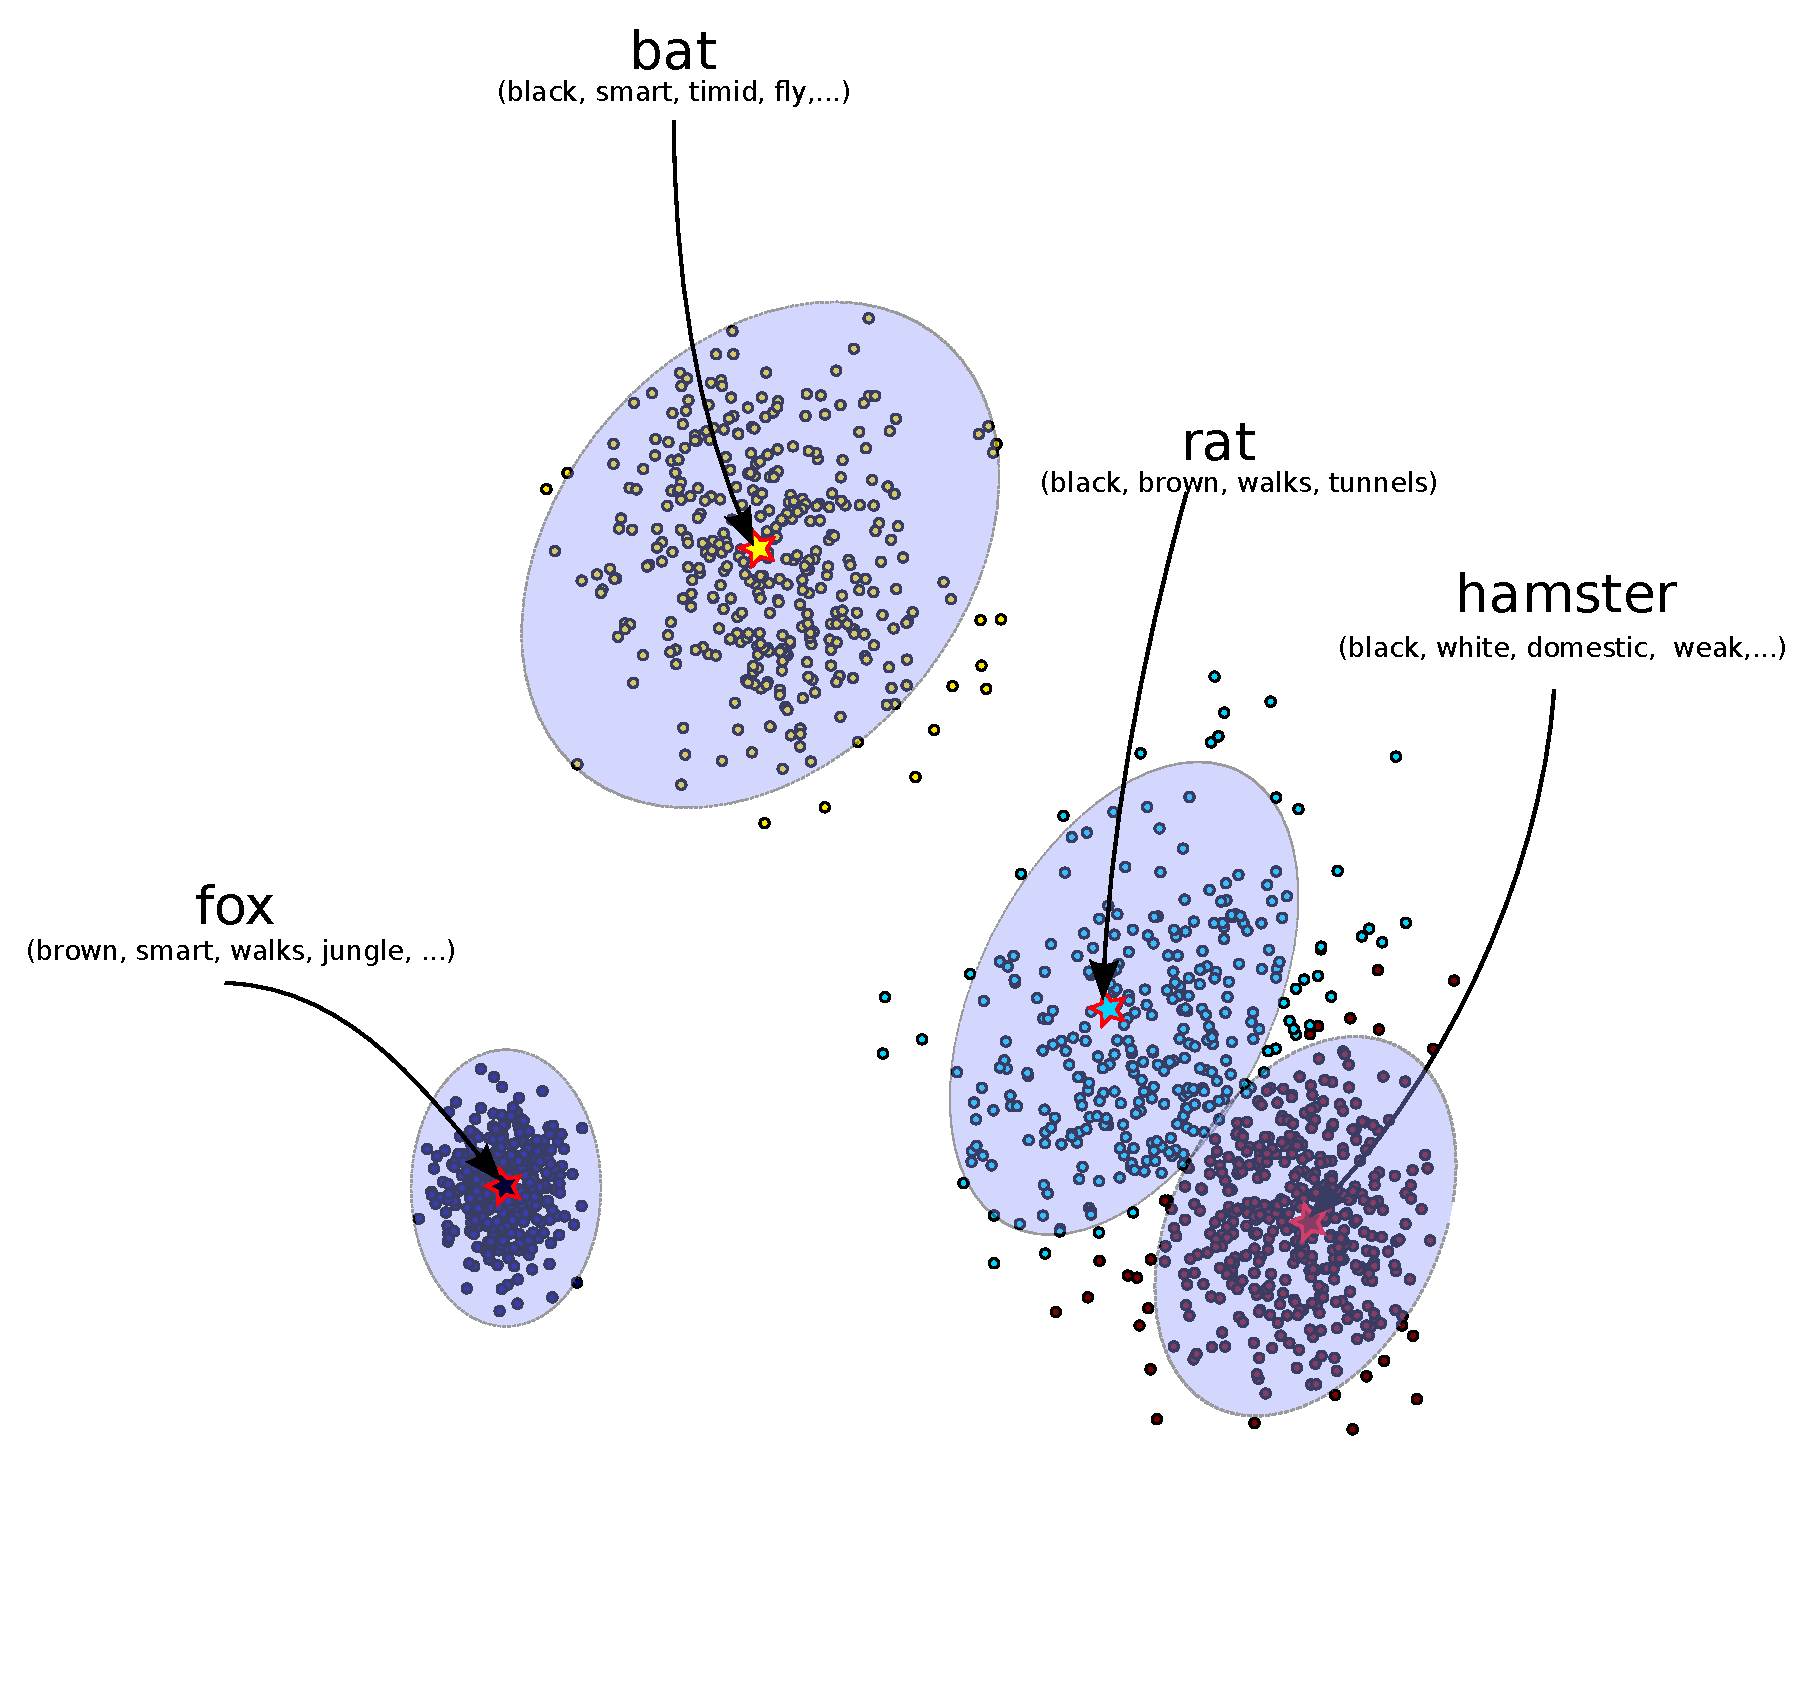
\includegraphics[width=0.98\columnwidth]{overview.pdf}
 % %LaTeX with PSTricks extensions
%%Creator: inkscape 0.48.4
%%Please note this file requires PSTricks extensions
\psset{xunit=.5pt,yunit=.5pt,runit=.5pt}
\begin{pspicture}(1080,1023.75)
{
\newrgbcolor{curcolor}{1 1 1}
\pscustom[linestyle=none,fillstyle=solid,fillcolor=curcolor]
{
\newpath
\moveto(0,0)
\lineto(1080,0)
\lineto(1080,1023.75)
\lineto(0,1023.75)
\closepath
}
}
{
\newrgbcolor{curcolor}{1 1 1}
\pscustom[linestyle=none,fillstyle=solid,fillcolor=curcolor]
{
\newpath
\moveto(135,102.375)
\lineto(972,102.375)
\lineto(972,921.375)
\lineto(135,921.375)
\closepath
}
}
{
\newrgbcolor{curcolor}{0.50196081 0 0}
\pscustom[linestyle=none,fillstyle=solid,fillcolor=curcolor]
{
\newpath
\moveto(739.96360779,280.63119729)
\curveto(740.70487279,280.63119729)(741.41588279,280.92570979)(741.94003279,281.44985979)
\curveto(742.46418279,281.97400979)(742.75869529,282.68501979)(742.75869529,283.42628479)
\curveto(742.75869529,284.16754979)(742.46418279,284.87855979)(741.94003279,285.40270979)
\curveto(741.41588279,285.92685979)(740.70487279,286.22137229)(739.96360779,286.22137229)
\curveto(739.22234279,286.22137229)(738.51133279,285.92685979)(737.98718279,285.40270979)
\curveto(737.46303279,284.87855979)(737.16852029,284.16754979)(737.16852029,283.42628479)
\curveto(737.16852029,282.68501979)(737.46303279,281.97400979)(737.98718279,281.44985979)
\curveto(738.51133279,280.92570979)(739.22234279,280.63119729)(739.96360779,280.63119729)
\closepath
}
}
{
\newrgbcolor{curcolor}{0 0 0}
\pscustom[linewidth=1.25,linecolor=curcolor]
{
\newpath
\moveto(739.96360779,280.63119729)
\curveto(740.70487279,280.63119729)(741.41588279,280.92570979)(741.94003279,281.44985979)
\curveto(742.46418279,281.97400979)(742.75869529,282.68501979)(742.75869529,283.42628479)
\curveto(742.75869529,284.16754979)(742.46418279,284.87855979)(741.94003279,285.40270979)
\curveto(741.41588279,285.92685979)(740.70487279,286.22137229)(739.96360779,286.22137229)
\curveto(739.22234279,286.22137229)(738.51133279,285.92685979)(737.98718279,285.40270979)
\curveto(737.46303279,284.87855979)(737.16852029,284.16754979)(737.16852029,283.42628479)
\curveto(737.16852029,282.68501979)(737.46303279,281.97400979)(737.98718279,281.44985979)
\curveto(738.51133279,280.92570979)(739.22234279,280.63119729)(739.96360779,280.63119729)
\closepath
}
}
{
\newrgbcolor{curcolor}{1 0.90196079 0}
\pscustom[linestyle=none,fillstyle=solid,fillcolor=curcolor]
{
\newpath
\moveto(346.40468597,562.21490701)
\curveto(347.14595097,562.21490701)(347.85696097,562.50941951)(348.38111097,563.03356951)
\curveto(348.90526097,563.55771951)(349.19977347,564.26872951)(349.19977347,565.00999451)
\curveto(349.19977347,565.75125951)(348.90526097,566.46226951)(348.38111097,566.98641951)
\curveto(347.85696097,567.51056951)(347.14595097,567.80508201)(346.40468597,567.80508201)
\curveto(345.66342097,567.80508201)(344.95241097,567.51056951)(344.42826097,566.98641951)
\curveto(343.90411097,566.46226951)(343.60959847,565.75125951)(343.60959847,565.00999451)
\curveto(343.60959847,564.26872951)(343.90411097,563.55771951)(344.42826097,563.03356951)
\curveto(344.95241097,562.50941951)(345.66342097,562.21490701)(346.40468597,562.21490701)
\closepath
}
}
{
\newrgbcolor{curcolor}{0 0 0}
\pscustom[linewidth=1.25,linecolor=curcolor]
{
\newpath
\moveto(346.40468597,562.21490701)
\curveto(347.14595097,562.21490701)(347.85696097,562.50941951)(348.38111097,563.03356951)
\curveto(348.90526097,563.55771951)(349.19977347,564.26872951)(349.19977347,565.00999451)
\curveto(349.19977347,565.75125951)(348.90526097,566.46226951)(348.38111097,566.98641951)
\curveto(347.85696097,567.51056951)(347.14595097,567.80508201)(346.40468597,567.80508201)
\curveto(345.66342097,567.80508201)(344.95241097,567.51056951)(344.42826097,566.98641951)
\curveto(343.90411097,566.46226951)(343.60959847,565.75125951)(343.60959847,565.00999451)
\curveto(343.60959847,564.26872951)(343.90411097,563.55771951)(344.42826097,563.03356951)
\curveto(344.95241097,562.50941951)(345.66342097,562.21490701)(346.40468597,562.21490701)
\closepath
}
}
{
\newrgbcolor{curcolor}{0 0 0.50196081}
\pscustom[linestyle=none,fillstyle=solid,fillcolor=curcolor]
{
\newpath
\moveto(327.76996613,308.12204202)
\curveto(328.51123113,308.12204202)(329.22224113,308.41655452)(329.74639113,308.94070452)
\curveto(330.27054113,309.46485452)(330.56505363,310.17586452)(330.56505363,310.91712952)
\curveto(330.56505363,311.65839452)(330.27054113,312.36940452)(329.74639113,312.89355452)
\curveto(329.22224113,313.41770452)(328.51123113,313.71221702)(327.76996613,313.71221702)
\curveto(327.02870113,313.71221702)(326.31769113,313.41770452)(325.79354113,312.89355452)
\curveto(325.26939113,312.36940452)(324.97487863,311.65839452)(324.97487863,310.91712952)
\curveto(324.97487863,310.17586452)(325.26939113,309.46485452)(325.79354113,308.94070452)
\curveto(326.31769113,308.41655452)(327.02870113,308.12204202)(327.76996613,308.12204202)
\closepath
}
}
{
\newrgbcolor{curcolor}{0 0 0}
\pscustom[linewidth=1.25,linecolor=curcolor]
{
\newpath
\moveto(327.76996613,308.12204202)
\curveto(328.51123113,308.12204202)(329.22224113,308.41655452)(329.74639113,308.94070452)
\curveto(330.27054113,309.46485452)(330.56505363,310.17586452)(330.56505363,310.91712952)
\curveto(330.56505363,311.65839452)(330.27054113,312.36940452)(329.74639113,312.89355452)
\curveto(329.22224113,313.41770452)(328.51123113,313.71221702)(327.76996613,313.71221702)
\curveto(327.02870113,313.71221702)(326.31769113,313.41770452)(325.79354113,312.89355452)
\curveto(325.26939113,312.36940452)(324.97487863,311.65839452)(324.97487863,310.91712952)
\curveto(324.97487863,310.17586452)(325.26939113,309.46485452)(325.79354113,308.94070452)
\curveto(326.31769113,308.41655452)(327.02870113,308.12204202)(327.76996613,308.12204202)
\closepath
}
}
{
\newrgbcolor{curcolor}{0.50196081 0 0}
\pscustom[linestyle=none,fillstyle=solid,fillcolor=curcolor]
{
\newpath
\moveto(729.09667969,287.36909707)
\curveto(729.83794469,287.36909707)(730.54895469,287.66360957)(731.07310469,288.18775957)
\curveto(731.59725469,288.71190957)(731.89176719,289.42291957)(731.89176719,290.16418457)
\curveto(731.89176719,290.90544957)(731.59725469,291.61645957)(731.07310469,292.14060957)
\curveto(730.54895469,292.66475957)(729.83794469,292.95927207)(729.09667969,292.95927207)
\curveto(728.35541469,292.95927207)(727.64440469,292.66475957)(727.12025469,292.14060957)
\curveto(726.59610469,291.61645957)(726.30159219,290.90544957)(726.30159219,290.16418457)
\curveto(726.30159219,289.42291957)(726.59610469,288.71190957)(727.12025469,288.18775957)
\curveto(727.64440469,287.66360957)(728.35541469,287.36909707)(729.09667969,287.36909707)
\closepath
}
}
{
\newrgbcolor{curcolor}{0 0 0}
\pscustom[linewidth=1.25,linecolor=curcolor]
{
\newpath
\moveto(729.09667969,287.36909707)
\curveto(729.83794469,287.36909707)(730.54895469,287.66360957)(731.07310469,288.18775957)
\curveto(731.59725469,288.71190957)(731.89176719,289.42291957)(731.89176719,290.16418457)
\curveto(731.89176719,290.90544957)(731.59725469,291.61645957)(731.07310469,292.14060957)
\curveto(730.54895469,292.66475957)(729.83794469,292.95927207)(729.09667969,292.95927207)
\curveto(728.35541469,292.95927207)(727.64440469,292.66475957)(727.12025469,292.14060957)
\curveto(726.59610469,291.61645957)(726.30159219,290.90544957)(726.30159219,290.16418457)
\curveto(726.30159219,289.42291957)(726.59610469,288.71190957)(727.12025469,288.18775957)
\curveto(727.64440469,287.66360957)(728.35541469,287.36909707)(729.09667969,287.36909707)
\closepath
}
}
{
\newrgbcolor{curcolor}{0.50196081 0 0}
\pscustom[linestyle=none,fillstyle=solid,fillcolor=curcolor]
{
\newpath
\moveto(845.90080261,253.19413979)
\curveto(846.64206761,253.19413979)(847.35307761,253.48865229)(847.87722761,254.01280229)
\curveto(848.40137761,254.53695229)(848.69589011,255.24796229)(848.69589011,255.98922729)
\curveto(848.69589011,256.73049229)(848.40137761,257.44150229)(847.87722761,257.96565229)
\curveto(847.35307761,258.48980229)(846.64206761,258.78431479)(845.90080261,258.78431479)
\curveto(845.15953761,258.78431479)(844.44852761,258.48980229)(843.92437761,257.96565229)
\curveto(843.40022761,257.44150229)(843.10571511,256.73049229)(843.10571511,255.98922729)
\curveto(843.10571511,255.24796229)(843.40022761,254.53695229)(843.92437761,254.01280229)
\curveto(844.44852761,253.48865229)(845.15953761,253.19413979)(845.90080261,253.19413979)
\closepath
}
}
{
\newrgbcolor{curcolor}{0 0 0}
\pscustom[linewidth=1.25,linecolor=curcolor]
{
\newpath
\moveto(845.90080261,253.19413979)
\curveto(846.64206761,253.19413979)(847.35307761,253.48865229)(847.87722761,254.01280229)
\curveto(848.40137761,254.53695229)(848.69589011,255.24796229)(848.69589011,255.98922729)
\curveto(848.69589011,256.73049229)(848.40137761,257.44150229)(847.87722761,257.96565229)
\curveto(847.35307761,258.48980229)(846.64206761,258.78431479)(845.90080261,258.78431479)
\curveto(845.15953761,258.78431479)(844.44852761,258.48980229)(843.92437761,257.96565229)
\curveto(843.40022761,257.44150229)(843.10571511,256.73049229)(843.10571511,255.98922729)
\curveto(843.10571511,255.24796229)(843.40022761,254.53695229)(843.92437761,254.01280229)
\curveto(844.44852761,253.48865229)(845.15953761,253.19413979)(845.90080261,253.19413979)
\closepath
}
}
{
\newrgbcolor{curcolor}{1 0.90196079 0}
\pscustom[linestyle=none,fillstyle=solid,fillcolor=curcolor]
{
\newpath
\moveto(414.84119415,664.55198129)
\curveto(415.58245915,664.55198129)(416.29346915,664.84649379)(416.81761915,665.37064379)
\curveto(417.34176915,665.89479379)(417.63628165,666.60580379)(417.63628165,667.34706879)
\curveto(417.63628165,668.08833379)(417.34176915,668.79934379)(416.81761915,669.32349379)
\curveto(416.29346915,669.84764379)(415.58245915,670.14215629)(414.84119415,670.14215629)
\curveto(414.09992915,670.14215629)(413.38891915,669.84764379)(412.86476915,669.32349379)
\curveto(412.34061915,668.79934379)(412.04610665,668.08833379)(412.04610665,667.34706879)
\curveto(412.04610665,666.60580379)(412.34061915,665.89479379)(412.86476915,665.37064379)
\curveto(413.38891915,664.84649379)(414.09992915,664.55198129)(414.84119415,664.55198129)
\closepath
}
}
{
\newrgbcolor{curcolor}{0 0 0}
\pscustom[linewidth=1.25,linecolor=curcolor]
{
\newpath
\moveto(414.84119415,664.55198129)
\curveto(415.58245915,664.55198129)(416.29346915,664.84649379)(416.81761915,665.37064379)
\curveto(417.34176915,665.89479379)(417.63628165,666.60580379)(417.63628165,667.34706879)
\curveto(417.63628165,668.08833379)(417.34176915,668.79934379)(416.81761915,669.32349379)
\curveto(416.29346915,669.84764379)(415.58245915,670.14215629)(414.84119415,670.14215629)
\curveto(414.09992915,670.14215629)(413.38891915,669.84764379)(412.86476915,669.32349379)
\curveto(412.34061915,668.79934379)(412.04610665,668.08833379)(412.04610665,667.34706879)
\curveto(412.04610665,666.60580379)(412.34061915,665.89479379)(412.86476915,665.37064379)
\curveto(413.38891915,664.84649379)(414.09992915,664.55198129)(414.84119415,664.55198129)
\closepath
}
}
{
\newrgbcolor{curcolor}{0 0.83137256 1}
\pscustom[linestyle=none,fillstyle=solid,fillcolor=curcolor]
{
\newpath
\moveto(756.88903809,466.8224891)
\curveto(757.63030309,466.8224891)(758.34131309,467.1170016)(758.86546309,467.6411516)
\curveto(759.38961309,468.1653016)(759.68412559,468.8763116)(759.68412559,469.6175766)
\curveto(759.68412559,470.3588416)(759.38961309,471.0698516)(758.86546309,471.5940016)
\curveto(758.34131309,472.1181516)(757.63030309,472.4126641)(756.88903809,472.4126641)
\curveto(756.14777309,472.4126641)(755.43676309,472.1181516)(754.91261309,471.5940016)
\curveto(754.38846309,471.0698516)(754.09395059,470.3588416)(754.09395059,469.6175766)
\curveto(754.09395059,468.8763116)(754.38846309,468.1653016)(754.91261309,467.6411516)
\curveto(755.43676309,467.1170016)(756.14777309,466.8224891)(756.88903809,466.8224891)
\closepath
}
}
{
\newrgbcolor{curcolor}{0 0 0}
\pscustom[linewidth=1.25,linecolor=curcolor]
{
\newpath
\moveto(756.88903809,466.8224891)
\curveto(757.63030309,466.8224891)(758.34131309,467.1170016)(758.86546309,467.6411516)
\curveto(759.38961309,468.1653016)(759.68412559,468.8763116)(759.68412559,469.6175766)
\curveto(759.68412559,470.3588416)(759.38961309,471.0698516)(758.86546309,471.5940016)
\curveto(758.34131309,472.1181516)(757.63030309,472.4126641)(756.88903809,472.4126641)
\curveto(756.14777309,472.4126641)(755.43676309,472.1181516)(754.91261309,471.5940016)
\curveto(754.38846309,471.0698516)(754.09395059,470.3588416)(754.09395059,469.6175766)
\curveto(754.09395059,468.8763116)(754.38846309,468.1653016)(754.91261309,467.6411516)
\curveto(755.43676309,467.1170016)(756.14777309,466.8224891)(756.88903809,466.8224891)
\closepath
}
}
{
\newrgbcolor{curcolor}{0 0 0.50196081}
\pscustom[linestyle=none,fillstyle=solid,fillcolor=curcolor]
{
\newpath
\moveto(310.6584549,294.14499124)
\curveto(311.3997199,294.14499124)(312.1107299,294.43950374)(312.6348799,294.96365374)
\curveto(313.1590299,295.48780374)(313.4535424,296.19881374)(313.4535424,296.94007874)
\curveto(313.4535424,297.68134374)(313.1590299,298.39235374)(312.6348799,298.91650374)
\curveto(312.1107299,299.44065374)(311.3997199,299.73516624)(310.6584549,299.73516624)
\curveto(309.9171899,299.73516624)(309.2061799,299.44065374)(308.6820299,298.91650374)
\curveto(308.1578799,298.39235374)(307.8633674,297.68134374)(307.8633674,296.94007874)
\curveto(307.8633674,296.19881374)(308.1578799,295.48780374)(308.6820299,294.96365374)
\curveto(309.2061799,294.43950374)(309.9171899,294.14499124)(310.6584549,294.14499124)
\closepath
}
}
{
\newrgbcolor{curcolor}{0 0 0}
\pscustom[linewidth=1.25,linecolor=curcolor]
{
\newpath
\moveto(310.6584549,294.14499124)
\curveto(311.3997199,294.14499124)(312.1107299,294.43950374)(312.6348799,294.96365374)
\curveto(313.1590299,295.48780374)(313.4535424,296.19881374)(313.4535424,296.94007874)
\curveto(313.4535424,297.68134374)(313.1590299,298.39235374)(312.6348799,298.91650374)
\curveto(312.1107299,299.44065374)(311.3997199,299.73516624)(310.6584549,299.73516624)
\curveto(309.9171899,299.73516624)(309.2061799,299.44065374)(308.6820299,298.91650374)
\curveto(308.1578799,298.39235374)(307.8633674,297.68134374)(307.8633674,296.94007874)
\curveto(307.8633674,296.19881374)(308.1578799,295.48780374)(308.6820299,294.96365374)
\curveto(309.2061799,294.43950374)(309.9171899,294.14499124)(310.6584549,294.14499124)
\closepath
}
}
{
\newrgbcolor{curcolor}{0.50196081 0 0}
\pscustom[linestyle=none,fillstyle=solid,fillcolor=curcolor]
{
\newpath
\moveto(726.23298645,280.67216714)
\curveto(726.97425145,280.67216714)(727.68526145,280.96667964)(728.20941145,281.49082964)
\curveto(728.73356145,282.01497964)(729.02807395,282.72598964)(729.02807395,283.46725464)
\curveto(729.02807395,284.20851964)(728.73356145,284.91952964)(728.20941145,285.44367964)
\curveto(727.68526145,285.96782964)(726.97425145,286.26234214)(726.23298645,286.26234214)
\curveto(725.49172145,286.26234214)(724.78071145,285.96782964)(724.25656145,285.44367964)
\curveto(723.73241145,284.91952964)(723.43789895,284.20851964)(723.43789895,283.46725464)
\curveto(723.43789895,282.72598964)(723.73241145,282.01497964)(724.25656145,281.49082964)
\curveto(724.78071145,280.96667964)(725.49172145,280.67216714)(726.23298645,280.67216714)
\closepath
}
}
{
\newrgbcolor{curcolor}{0 0 0}
\pscustom[linewidth=1.25,linecolor=curcolor]
{
\newpath
\moveto(726.23298645,280.67216714)
\curveto(726.97425145,280.67216714)(727.68526145,280.96667964)(728.20941145,281.49082964)
\curveto(728.73356145,282.01497964)(729.02807395,282.72598964)(729.02807395,283.46725464)
\curveto(729.02807395,284.20851964)(728.73356145,284.91952964)(728.20941145,285.44367964)
\curveto(727.68526145,285.96782964)(726.97425145,286.26234214)(726.23298645,286.26234214)
\curveto(725.49172145,286.26234214)(724.78071145,285.96782964)(724.25656145,285.44367964)
\curveto(723.73241145,284.91952964)(723.43789895,284.20851964)(723.43789895,283.46725464)
\curveto(723.43789895,282.72598964)(723.73241145,282.01497964)(724.25656145,281.49082964)
\curveto(724.78071145,280.96667964)(725.49172145,280.67216714)(726.23298645,280.67216714)
\closepath
}
}
{
\newrgbcolor{curcolor}{0 0.83137256 1}
\pscustom[linestyle=none,fillstyle=solid,fillcolor=curcolor]
{
\newpath
\moveto(652.86956787,366.57380898)
\curveto(653.61083287,366.57380898)(654.32184287,366.86832148)(654.84599287,367.39247148)
\curveto(655.37014287,367.91662148)(655.66465537,368.62763148)(655.66465537,369.36889648)
\curveto(655.66465537,370.11016148)(655.37014287,370.82117148)(654.84599287,371.34532148)
\curveto(654.32184287,371.86947148)(653.61083287,372.16398398)(652.86956787,372.16398398)
\curveto(652.12830287,372.16398398)(651.41729287,371.86947148)(650.89314287,371.34532148)
\curveto(650.36899287,370.82117148)(650.07448037,370.11016148)(650.07448037,369.36889648)
\curveto(650.07448037,368.62763148)(650.36899287,367.91662148)(650.89314287,367.39247148)
\curveto(651.41729287,366.86832148)(652.12830287,366.57380898)(652.86956787,366.57380898)
\closepath
}
}
{
\newrgbcolor{curcolor}{0 0 0}
\pscustom[linewidth=1.25,linecolor=curcolor]
{
\newpath
\moveto(652.86956787,366.57380898)
\curveto(653.61083287,366.57380898)(654.32184287,366.86832148)(654.84599287,367.39247148)
\curveto(655.37014287,367.91662148)(655.66465537,368.62763148)(655.66465537,369.36889648)
\curveto(655.66465537,370.11016148)(655.37014287,370.82117148)(654.84599287,371.34532148)
\curveto(654.32184287,371.86947148)(653.61083287,372.16398398)(652.86956787,372.16398398)
\curveto(652.12830287,372.16398398)(651.41729287,371.86947148)(650.89314287,371.34532148)
\curveto(650.36899287,370.82117148)(650.07448037,370.11016148)(650.07448037,369.36889648)
\curveto(650.07448037,368.62763148)(650.36899287,367.91662148)(650.89314287,367.39247148)
\curveto(651.41729287,366.86832148)(652.12830287,366.57380898)(652.86956787,366.57380898)
\closepath
}
}
{
\newrgbcolor{curcolor}{0.50196081 0 0}
\pscustom[linestyle=none,fillstyle=solid,fillcolor=curcolor]
{
\newpath
\moveto(739.97299194,287.70288308)
\curveto(740.71425694,287.70288308)(741.42526694,287.99739558)(741.94941694,288.52154558)
\curveto(742.47356694,289.04569558)(742.76807944,289.75670558)(742.76807944,290.49797058)
\curveto(742.76807944,291.23923558)(742.47356694,291.95024558)(741.94941694,292.47439558)
\curveto(741.42526694,292.99854558)(740.71425694,293.29305808)(739.97299194,293.29305808)
\curveto(739.23172694,293.29305808)(738.52071694,292.99854558)(737.99656694,292.47439558)
\curveto(737.47241694,291.95024558)(737.17790444,291.23923558)(737.17790444,290.49797058)
\curveto(737.17790444,289.75670558)(737.47241694,289.04569558)(737.99656694,288.52154558)
\curveto(738.52071694,287.99739558)(739.23172694,287.70288308)(739.97299194,287.70288308)
\closepath
}
}
{
\newrgbcolor{curcolor}{0 0 0}
\pscustom[linewidth=1.25,linecolor=curcolor]
{
\newpath
\moveto(739.97299194,287.70288308)
\curveto(740.71425694,287.70288308)(741.42526694,287.99739558)(741.94941694,288.52154558)
\curveto(742.47356694,289.04569558)(742.76807944,289.75670558)(742.76807944,290.49797058)
\curveto(742.76807944,291.23923558)(742.47356694,291.95024558)(741.94941694,292.47439558)
\curveto(741.42526694,292.99854558)(740.71425694,293.29305808)(739.97299194,293.29305808)
\curveto(739.23172694,293.29305808)(738.52071694,292.99854558)(737.99656694,292.47439558)
\curveto(737.47241694,291.95024558)(737.17790444,291.23923558)(737.17790444,290.49797058)
\curveto(737.17790444,289.75670558)(737.47241694,289.04569558)(737.99656694,288.52154558)
\curveto(738.52071694,287.99739558)(739.23172694,287.70288308)(739.97299194,287.70288308)
\closepath
}
}
{
\newrgbcolor{curcolor}{1 0.90196079 0}
\pscustom[linestyle=none,fillstyle=solid,fillcolor=curcolor]
{
\newpath
\moveto(377.7715683,728.05408318)
\curveto(378.5128333,728.05408318)(379.2238433,728.34859568)(379.7479933,728.87274568)
\curveto(380.2721433,729.39689568)(380.5666558,730.10790568)(380.5666558,730.84917068)
\curveto(380.5666558,731.59043568)(380.2721433,732.30144568)(379.7479933,732.82559568)
\curveto(379.2238433,733.34974568)(378.5128333,733.64425818)(377.7715683,733.64425818)
\curveto(377.0303033,733.64425818)(376.3192933,733.34974568)(375.7951433,732.82559568)
\curveto(375.2709933,732.30144568)(374.9764808,731.59043568)(374.9764808,730.84917068)
\curveto(374.9764808,730.10790568)(375.2709933,729.39689568)(375.7951433,728.87274568)
\curveto(376.3192933,728.34859568)(377.0303033,728.05408318)(377.7715683,728.05408318)
\closepath
}
}
{
\newrgbcolor{curcolor}{0 0 0}
\pscustom[linewidth=1.25,linecolor=curcolor]
{
\newpath
\moveto(377.7715683,728.05408318)
\curveto(378.5128333,728.05408318)(379.2238433,728.34859568)(379.7479933,728.87274568)
\curveto(380.2721433,729.39689568)(380.5666558,730.10790568)(380.5666558,730.84917068)
\curveto(380.5666558,731.59043568)(380.2721433,732.30144568)(379.7479933,732.82559568)
\curveto(379.2238433,733.34974568)(378.5128333,733.64425818)(377.7715683,733.64425818)
\curveto(377.0303033,733.64425818)(376.3192933,733.34974568)(375.7951433,732.82559568)
\curveto(375.2709933,732.30144568)(374.9764808,731.59043568)(374.9764808,730.84917068)
\curveto(374.9764808,730.10790568)(375.2709933,729.39689568)(375.7951433,728.87274568)
\curveto(376.3192933,728.34859568)(377.0303033,728.05408318)(377.7715683,728.05408318)
\closepath
}
}
{
\newrgbcolor{curcolor}{0 0 0.50196081}
\pscustom[linestyle=none,fillstyle=solid,fillcolor=curcolor]
{
\newpath
\moveto(304.17928696,289.43712075)
\curveto(304.92055196,289.43712075)(305.63156196,289.73163325)(306.15571196,290.25578325)
\curveto(306.67986196,290.77993325)(306.97437446,291.49094325)(306.97437446,292.23220825)
\curveto(306.97437446,292.97347325)(306.67986196,293.68448325)(306.15571196,294.20863325)
\curveto(305.63156196,294.73278325)(304.92055196,295.02729575)(304.17928696,295.02729575)
\curveto(303.43802196,295.02729575)(302.72701196,294.73278325)(302.20286196,294.20863325)
\curveto(301.67871196,293.68448325)(301.38419946,292.97347325)(301.38419946,292.23220825)
\curveto(301.38419946,291.49094325)(301.67871196,290.77993325)(302.20286196,290.25578325)
\curveto(302.72701196,289.73163325)(303.43802196,289.43712075)(304.17928696,289.43712075)
\closepath
}
}
{
\newrgbcolor{curcolor}{0 0 0}
\pscustom[linewidth=1.25,linecolor=curcolor]
{
\newpath
\moveto(304.17928696,289.43712075)
\curveto(304.92055196,289.43712075)(305.63156196,289.73163325)(306.15571196,290.25578325)
\curveto(306.67986196,290.77993325)(306.97437446,291.49094325)(306.97437446,292.23220825)
\curveto(306.97437446,292.97347325)(306.67986196,293.68448325)(306.15571196,294.20863325)
\curveto(305.63156196,294.73278325)(304.92055196,295.02729575)(304.17928696,295.02729575)
\curveto(303.43802196,295.02729575)(302.72701196,294.73278325)(302.20286196,294.20863325)
\curveto(301.67871196,293.68448325)(301.38419946,292.97347325)(301.38419946,292.23220825)
\curveto(301.38419946,291.49094325)(301.67871196,290.77993325)(302.20286196,290.25578325)
\curveto(302.72701196,289.73163325)(303.43802196,289.43712075)(304.17928696,289.43712075)
\closepath
}
}
{
\newrgbcolor{curcolor}{1 0.90196079 0}
\pscustom[linestyle=none,fillstyle=solid,fillcolor=curcolor]
{
\newpath
\moveto(491.91265106,708.48920663)
\curveto(492.65391606,708.48920663)(493.36492606,708.78371913)(493.88907606,709.30786913)
\curveto(494.41322606,709.83201913)(494.70773856,710.54302913)(494.70773856,711.28429413)
\curveto(494.70773856,712.02555913)(494.41322606,712.73656913)(493.88907606,713.26071913)
\curveto(493.36492606,713.78486913)(492.65391606,714.07938163)(491.91265106,714.07938163)
\curveto(491.17138606,714.07938163)(490.46037606,713.78486913)(489.93622606,713.26071913)
\curveto(489.41207606,712.73656913)(489.11756356,712.02555913)(489.11756356,711.28429413)
\curveto(489.11756356,710.54302913)(489.41207606,709.83201913)(489.93622606,709.30786913)
\curveto(490.46037606,708.78371913)(491.17138606,708.48920663)(491.91265106,708.48920663)
\closepath
}
}
{
\newrgbcolor{curcolor}{0 0 0}
\pscustom[linewidth=1.25,linecolor=curcolor]
{
\newpath
\moveto(491.91265106,708.48920663)
\curveto(492.65391606,708.48920663)(493.36492606,708.78371913)(493.88907606,709.30786913)
\curveto(494.41322606,709.83201913)(494.70773856,710.54302913)(494.70773856,711.28429413)
\curveto(494.70773856,712.02555913)(494.41322606,712.73656913)(493.88907606,713.26071913)
\curveto(493.36492606,713.78486913)(492.65391606,714.07938163)(491.91265106,714.07938163)
\curveto(491.17138606,714.07938163)(490.46037606,713.78486913)(489.93622606,713.26071913)
\curveto(489.41207606,712.73656913)(489.11756356,712.02555913)(489.11756356,711.28429413)
\curveto(489.11756356,710.54302913)(489.41207606,709.83201913)(489.93622606,709.30786913)
\curveto(490.46037606,708.78371913)(491.17138606,708.48920663)(491.91265106,708.48920663)
\closepath
}
}
{
\newrgbcolor{curcolor}{0 0 0.50196081}
\pscustom[linestyle=none,fillstyle=solid,fillcolor=curcolor]
{
\newpath
\moveto(288.55855942,355.95170815)
\curveto(289.29982442,355.95170815)(290.01083442,356.24622065)(290.53498442,356.77037065)
\curveto(291.05913442,357.29452065)(291.35364692,358.00553065)(291.35364692,358.74679565)
\curveto(291.35364692,359.48806065)(291.05913442,360.19907065)(290.53498442,360.72322065)
\curveto(290.01083442,361.24737065)(289.29982442,361.54188315)(288.55855942,361.54188315)
\curveto(287.81729442,361.54188315)(287.10628442,361.24737065)(286.58213442,360.72322065)
\curveto(286.05798442,360.19907065)(285.76347192,359.48806065)(285.76347192,358.74679565)
\curveto(285.76347192,358.00553065)(286.05798442,357.29452065)(286.58213442,356.77037065)
\curveto(287.10628442,356.24622065)(287.81729442,355.95170815)(288.55855942,355.95170815)
\closepath
}
}
{
\newrgbcolor{curcolor}{0 0 0}
\pscustom[linewidth=1.25,linecolor=curcolor]
{
\newpath
\moveto(288.55855942,355.95170815)
\curveto(289.29982442,355.95170815)(290.01083442,356.24622065)(290.53498442,356.77037065)
\curveto(291.05913442,357.29452065)(291.35364692,358.00553065)(291.35364692,358.74679565)
\curveto(291.35364692,359.48806065)(291.05913442,360.19907065)(290.53498442,360.72322065)
\curveto(290.01083442,361.24737065)(289.29982442,361.54188315)(288.55855942,361.54188315)
\curveto(287.81729442,361.54188315)(287.10628442,361.24737065)(286.58213442,360.72322065)
\curveto(286.05798442,360.19907065)(285.76347192,359.48806065)(285.76347192,358.74679565)
\curveto(285.76347192,358.00553065)(286.05798442,357.29452065)(286.58213442,356.77037065)
\curveto(287.10628442,356.24622065)(287.81729442,355.95170815)(288.55855942,355.95170815)
\closepath
}
}
{
\newrgbcolor{curcolor}{0 0.83137256 1}
\pscustom[linestyle=none,fillstyle=solid,fillcolor=curcolor]
{
\newpath
\moveto(766.12052917,439.44894631)
\curveto(766.86179417,439.44894631)(767.57280417,439.74345881)(768.09695417,440.26760881)
\curveto(768.62110417,440.79175881)(768.91561667,441.50276881)(768.91561667,442.24403381)
\curveto(768.91561667,442.98529881)(768.62110417,443.69630881)(768.09695417,444.22045881)
\curveto(767.57280417,444.74460881)(766.86179417,445.03912131)(766.12052917,445.03912131)
\curveto(765.37926417,445.03912131)(764.66825417,444.74460881)(764.14410417,444.22045881)
\curveto(763.61995417,443.69630881)(763.32544167,442.98529881)(763.32544167,442.24403381)
\curveto(763.32544167,441.50276881)(763.61995417,440.79175881)(764.14410417,440.26760881)
\curveto(764.66825417,439.74345881)(765.37926417,439.44894631)(766.12052917,439.44894631)
\closepath
}
}
{
\newrgbcolor{curcolor}{0 0 0}
\pscustom[linewidth=1.25,linecolor=curcolor]
{
\newpath
\moveto(766.12052917,439.44894631)
\curveto(766.86179417,439.44894631)(767.57280417,439.74345881)(768.09695417,440.26760881)
\curveto(768.62110417,440.79175881)(768.91561667,441.50276881)(768.91561667,442.24403381)
\curveto(768.91561667,442.98529881)(768.62110417,443.69630881)(768.09695417,444.22045881)
\curveto(767.57280417,444.74460881)(766.86179417,445.03912131)(766.12052917,445.03912131)
\curveto(765.37926417,445.03912131)(764.66825417,444.74460881)(764.14410417,444.22045881)
\curveto(763.61995417,443.69630881)(763.32544167,442.98529881)(763.32544167,442.24403381)
\curveto(763.32544167,441.50276881)(763.61995417,440.79175881)(764.14410417,440.26760881)
\curveto(764.66825417,439.74345881)(765.37926417,439.44894631)(766.12052917,439.44894631)
\closepath
}
}
{
\newrgbcolor{curcolor}{0.50196081 0 0}
\pscustom[linestyle=none,fillstyle=solid,fillcolor=curcolor]
{
\newpath
\moveto(776.75552368,338.71118386)
\curveto(777.49678868,338.71118386)(778.20779868,339.00569636)(778.73194868,339.52984636)
\curveto(779.25609868,340.05399636)(779.55061118,340.76500636)(779.55061118,341.50627136)
\curveto(779.55061118,342.24753636)(779.25609868,342.95854636)(778.73194868,343.48269636)
\curveto(778.20779868,344.00684636)(777.49678868,344.30135886)(776.75552368,344.30135886)
\curveto(776.01425868,344.30135886)(775.30324868,344.00684636)(774.77909868,343.48269636)
\curveto(774.25494868,342.95854636)(773.96043618,342.24753636)(773.96043618,341.50627136)
\curveto(773.96043618,340.76500636)(774.25494868,340.05399636)(774.77909868,339.52984636)
\curveto(775.30324868,339.00569636)(776.01425868,338.71118386)(776.75552368,338.71118386)
\closepath
}
}
{
\newrgbcolor{curcolor}{0 0 0}
\pscustom[linewidth=1.25,linecolor=curcolor]
{
\newpath
\moveto(776.75552368,338.71118386)
\curveto(777.49678868,338.71118386)(778.20779868,339.00569636)(778.73194868,339.52984636)
\curveto(779.25609868,340.05399636)(779.55061118,340.76500636)(779.55061118,341.50627136)
\curveto(779.55061118,342.24753636)(779.25609868,342.95854636)(778.73194868,343.48269636)
\curveto(778.20779868,344.00684636)(777.49678868,344.30135886)(776.75552368,344.30135886)
\curveto(776.01425868,344.30135886)(775.30324868,344.00684636)(774.77909868,343.48269636)
\curveto(774.25494868,342.95854636)(773.96043618,342.24753636)(773.96043618,341.50627136)
\curveto(773.96043618,340.76500636)(774.25494868,340.05399636)(774.77909868,339.52984636)
\curveto(775.30324868,339.00569636)(776.01425868,338.71118386)(776.75552368,338.71118386)
\closepath
}
}
{
\newrgbcolor{curcolor}{1 0.90196079 0}
\pscustom[linestyle=none,fillstyle=solid,fillcolor=curcolor]
{
\newpath
\moveto(372.68009186,709.69674905)
\curveto(373.42135686,709.69674905)(374.13236686,709.99126155)(374.65651686,710.51541155)
\curveto(375.18066686,711.03956155)(375.47517936,711.75057155)(375.47517936,712.49183655)
\curveto(375.47517936,713.23310155)(375.18066686,713.94411155)(374.65651686,714.46826155)
\curveto(374.13236686,714.99241155)(373.42135686,715.28692405)(372.68009186,715.28692405)
\curveto(371.93882686,715.28692405)(371.22781686,714.99241155)(370.70366686,714.46826155)
\curveto(370.17951686,713.94411155)(369.88500436,713.23310155)(369.88500436,712.49183655)
\curveto(369.88500436,711.75057155)(370.17951686,711.03956155)(370.70366686,710.51541155)
\curveto(371.22781686,709.99126155)(371.93882686,709.69674905)(372.68009186,709.69674905)
\closepath
}
}
{
\newrgbcolor{curcolor}{0 0 0}
\pscustom[linewidth=1.25,linecolor=curcolor]
{
\newpath
\moveto(372.68009186,709.69674905)
\curveto(373.42135686,709.69674905)(374.13236686,709.99126155)(374.65651686,710.51541155)
\curveto(375.18066686,711.03956155)(375.47517936,711.75057155)(375.47517936,712.49183655)
\curveto(375.47517936,713.23310155)(375.18066686,713.94411155)(374.65651686,714.46826155)
\curveto(374.13236686,714.99241155)(373.42135686,715.28692405)(372.68009186,715.28692405)
\curveto(371.93882686,715.28692405)(371.22781686,714.99241155)(370.70366686,714.46826155)
\curveto(370.17951686,713.94411155)(369.88500436,713.23310155)(369.88500436,712.49183655)
\curveto(369.88500436,711.75057155)(370.17951686,711.03956155)(370.70366686,710.51541155)
\curveto(371.22781686,709.99126155)(371.93882686,709.69674905)(372.68009186,709.69674905)
\closepath
}
}
{
\newrgbcolor{curcolor}{0.50196081 0 0}
\pscustom[linestyle=none,fillstyle=solid,fillcolor=curcolor]
{
\newpath
\moveto(802.06260681,198.27699502)
\curveto(802.80387181,198.27699502)(803.51488181,198.57150752)(804.03903181,199.09565752)
\curveto(804.56318181,199.61980752)(804.85769431,200.33081752)(804.85769431,201.07208252)
\curveto(804.85769431,201.81334752)(804.56318181,202.52435752)(804.03903181,203.04850752)
\curveto(803.51488181,203.57265752)(802.80387181,203.86717002)(802.06260681,203.86717002)
\curveto(801.32134181,203.86717002)(800.61033181,203.57265752)(800.08618181,203.04850752)
\curveto(799.56203181,202.52435752)(799.26751931,201.81334752)(799.26751931,201.07208252)
\curveto(799.26751931,200.33081752)(799.56203181,199.61980752)(800.08618181,199.09565752)
\curveto(800.61033181,198.57150752)(801.32134181,198.27699502)(802.06260681,198.27699502)
\closepath
}
}
{
\newrgbcolor{curcolor}{0 0 0}
\pscustom[linewidth=1.25,linecolor=curcolor]
{
\newpath
\moveto(802.06260681,198.27699502)
\curveto(802.80387181,198.27699502)(803.51488181,198.57150752)(804.03903181,199.09565752)
\curveto(804.56318181,199.61980752)(804.85769431,200.33081752)(804.85769431,201.07208252)
\curveto(804.85769431,201.81334752)(804.56318181,202.52435752)(804.03903181,203.04850752)
\curveto(803.51488181,203.57265752)(802.80387181,203.86717002)(802.06260681,203.86717002)
\curveto(801.32134181,203.86717002)(800.61033181,203.57265752)(800.08618181,203.04850752)
\curveto(799.56203181,202.52435752)(799.26751931,201.81334752)(799.26751931,201.07208252)
\curveto(799.26751931,200.33081752)(799.56203181,199.61980752)(800.08618181,199.09565752)
\curveto(800.61033181,198.57150752)(801.32134181,198.27699502)(802.06260681,198.27699502)
\closepath
}
}
{
\newrgbcolor{curcolor}{0.50196081 0 0}
\pscustom[linestyle=none,fillstyle=solid,fillcolor=curcolor]
{
\newpath
\moveto(760.68778992,243.35756143)
\curveto(761.42905492,243.35756143)(762.14006492,243.65207393)(762.66421492,244.17622393)
\curveto(763.18836492,244.70037393)(763.48287742,245.41138393)(763.48287742,246.15264893)
\curveto(763.48287742,246.89391393)(763.18836492,247.60492393)(762.66421492,248.12907393)
\curveto(762.14006492,248.65322393)(761.42905492,248.94773643)(760.68778992,248.94773643)
\curveto(759.94652492,248.94773643)(759.23551492,248.65322393)(758.71136492,248.12907393)
\curveto(758.18721492,247.60492393)(757.89270242,246.89391393)(757.89270242,246.15264893)
\curveto(757.89270242,245.41138393)(758.18721492,244.70037393)(758.71136492,244.17622393)
\curveto(759.23551492,243.65207393)(759.94652492,243.35756143)(760.68778992,243.35756143)
\closepath
}
}
{
\newrgbcolor{curcolor}{0 0 0}
\pscustom[linewidth=1.25,linecolor=curcolor]
{
\newpath
\moveto(760.68778992,243.35756143)
\curveto(761.42905492,243.35756143)(762.14006492,243.65207393)(762.66421492,244.17622393)
\curveto(763.18836492,244.70037393)(763.48287742,245.41138393)(763.48287742,246.15264893)
\curveto(763.48287742,246.89391393)(763.18836492,247.60492393)(762.66421492,248.12907393)
\curveto(762.14006492,248.65322393)(761.42905492,248.94773643)(760.68778992,248.94773643)
\curveto(759.94652492,248.94773643)(759.23551492,248.65322393)(758.71136492,248.12907393)
\curveto(758.18721492,247.60492393)(757.89270242,246.89391393)(757.89270242,246.15264893)
\curveto(757.89270242,245.41138393)(758.18721492,244.70037393)(758.71136492,244.17622393)
\curveto(759.23551492,243.65207393)(759.94652492,243.35756143)(760.68778992,243.35756143)
\closepath
}
}
{
\newrgbcolor{curcolor}{0 0.83137256 1}
\pscustom[linestyle=none,fillstyle=solid,fillcolor=curcolor]
{
\newpath
\moveto(720.49362183,439.12038644)
\curveto(721.23488683,439.12038644)(721.94589683,439.41489894)(722.47004683,439.93904894)
\curveto(722.99419683,440.46319894)(723.28870933,441.17420894)(723.28870933,441.91547394)
\curveto(723.28870933,442.65673894)(722.99419683,443.36774894)(722.47004683,443.89189894)
\curveto(721.94589683,444.41604894)(721.23488683,444.71056144)(720.49362183,444.71056144)
\curveto(719.75235683,444.71056144)(719.04134683,444.41604894)(718.51719683,443.89189894)
\curveto(717.99304683,443.36774894)(717.69853433,442.65673894)(717.69853433,441.91547394)
\curveto(717.69853433,441.17420894)(717.99304683,440.46319894)(718.51719683,439.93904894)
\curveto(719.04134683,439.41489894)(719.75235683,439.12038644)(720.49362183,439.12038644)
\closepath
}
}
{
\newrgbcolor{curcolor}{0 0 0}
\pscustom[linewidth=1.25,linecolor=curcolor]
{
\newpath
\moveto(720.49362183,439.12038644)
\curveto(721.23488683,439.12038644)(721.94589683,439.41489894)(722.47004683,439.93904894)
\curveto(722.99419683,440.46319894)(723.28870933,441.17420894)(723.28870933,441.91547394)
\curveto(723.28870933,442.65673894)(722.99419683,443.36774894)(722.47004683,443.89189894)
\curveto(721.94589683,444.41604894)(721.23488683,444.71056144)(720.49362183,444.71056144)
\curveto(719.75235683,444.71056144)(719.04134683,444.41604894)(718.51719683,443.89189894)
\curveto(717.99304683,443.36774894)(717.69853433,442.65673894)(717.69853433,441.91547394)
\curveto(717.69853433,441.17420894)(717.99304683,440.46319894)(718.51719683,439.93904894)
\curveto(719.04134683,439.41489894)(719.75235683,439.12038644)(720.49362183,439.12038644)
\closepath
}
}
{
\newrgbcolor{curcolor}{0.50196081 0 0}
\pscustom[linestyle=none,fillstyle=solid,fillcolor=curcolor]
{
\newpath
\moveto(738.95149231,307.00822671)
\curveto(739.69275731,307.00822671)(740.40376731,307.30273921)(740.92791731,307.82688921)
\curveto(741.45206731,308.35103921)(741.74657981,309.06204921)(741.74657981,309.80331421)
\curveto(741.74657981,310.54457921)(741.45206731,311.25558921)(740.92791731,311.77973921)
\curveto(740.40376731,312.30388921)(739.69275731,312.59840171)(738.95149231,312.59840171)
\curveto(738.21022731,312.59840171)(737.49921731,312.30388921)(736.97506731,311.77973921)
\curveto(736.45091731,311.25558921)(736.15640481,310.54457921)(736.15640481,309.80331421)
\curveto(736.15640481,309.06204921)(736.45091731,308.35103921)(736.97506731,307.82688921)
\curveto(737.49921731,307.30273921)(738.21022731,307.00822671)(738.95149231,307.00822671)
\closepath
}
}
{
\newrgbcolor{curcolor}{0 0 0}
\pscustom[linewidth=1.25,linecolor=curcolor]
{
\newpath
\moveto(738.95149231,307.00822671)
\curveto(739.69275731,307.00822671)(740.40376731,307.30273921)(740.92791731,307.82688921)
\curveto(741.45206731,308.35103921)(741.74657981,309.06204921)(741.74657981,309.80331421)
\curveto(741.74657981,310.54457921)(741.45206731,311.25558921)(740.92791731,311.77973921)
\curveto(740.40376731,312.30388921)(739.69275731,312.59840171)(738.95149231,312.59840171)
\curveto(738.21022731,312.59840171)(737.49921731,312.30388921)(736.97506731,311.77973921)
\curveto(736.45091731,311.25558921)(736.15640481,310.54457921)(736.15640481,309.80331421)
\curveto(736.15640481,309.06204921)(736.45091731,308.35103921)(736.97506731,307.82688921)
\curveto(737.49921731,307.30273921)(738.21022731,307.00822671)(738.95149231,307.00822671)
\closepath
}
}
{
\newrgbcolor{curcolor}{1 0.90196079 0}
\pscustom[linestyle=none,fillstyle=solid,fillcolor=curcolor]
{
\newpath
\moveto(460.44647217,632.02024301)
\curveto(461.18773717,632.02024301)(461.89874717,632.31475551)(462.42289717,632.83890551)
\curveto(462.94704717,633.36305551)(463.24155967,634.07406551)(463.24155967,634.81533051)
\curveto(463.24155967,635.55659551)(462.94704717,636.26760551)(462.42289717,636.79175551)
\curveto(461.89874717,637.31590551)(461.18773717,637.61041801)(460.44647217,637.61041801)
\curveto(459.70520717,637.61041801)(458.99419717,637.31590551)(458.47004717,636.79175551)
\curveto(457.94589717,636.26760551)(457.65138467,635.55659551)(457.65138467,634.81533051)
\curveto(457.65138467,634.07406551)(457.94589717,633.36305551)(458.47004717,632.83890551)
\curveto(458.99419717,632.31475551)(459.70520717,632.02024301)(460.44647217,632.02024301)
\closepath
}
}
{
\newrgbcolor{curcolor}{0 0 0}
\pscustom[linewidth=1.25,linecolor=curcolor]
{
\newpath
\moveto(460.44647217,632.02024301)
\curveto(461.18773717,632.02024301)(461.89874717,632.31475551)(462.42289717,632.83890551)
\curveto(462.94704717,633.36305551)(463.24155967,634.07406551)(463.24155967,634.81533051)
\curveto(463.24155967,635.55659551)(462.94704717,636.26760551)(462.42289717,636.79175551)
\curveto(461.89874717,637.31590551)(461.18773717,637.61041801)(460.44647217,637.61041801)
\curveto(459.70520717,637.61041801)(458.99419717,637.31590551)(458.47004717,636.79175551)
\curveto(457.94589717,636.26760551)(457.65138467,635.55659551)(457.65138467,634.81533051)
\curveto(457.65138467,634.07406551)(457.94589717,633.36305551)(458.47004717,632.83890551)
\curveto(458.99419717,632.31475551)(459.70520717,632.02024301)(460.44647217,632.02024301)
\closepath
}
}
{
\newrgbcolor{curcolor}{0 0 0.50196081}
\pscustom[linestyle=none,fillstyle=solid,fillcolor=curcolor]
{
\newpath
\moveto(296.40396118,374.59291299)
\curveto(297.14522618,374.59291299)(297.85623618,374.88742549)(298.38038618,375.41157549)
\curveto(298.90453618,375.93572549)(299.19904868,376.64673549)(299.19904868,377.38800049)
\curveto(299.19904868,378.12926549)(298.90453618,378.84027549)(298.38038618,379.36442549)
\curveto(297.85623618,379.88857549)(297.14522618,380.18308799)(296.40396118,380.18308799)
\curveto(295.66269618,380.18308799)(294.95168618,379.88857549)(294.42753618,379.36442549)
\curveto(293.90338618,378.84027549)(293.60887368,378.12926549)(293.60887368,377.38800049)
\curveto(293.60887368,376.64673549)(293.90338618,375.93572549)(294.42753618,375.41157549)
\curveto(294.95168618,374.88742549)(295.66269618,374.59291299)(296.40396118,374.59291299)
\closepath
}
}
{
\newrgbcolor{curcolor}{0 0 0}
\pscustom[linewidth=1.25,linecolor=curcolor]
{
\newpath
\moveto(296.40396118,374.59291299)
\curveto(297.14522618,374.59291299)(297.85623618,374.88742549)(298.38038618,375.41157549)
\curveto(298.90453618,375.93572549)(299.19904868,376.64673549)(299.19904868,377.38800049)
\curveto(299.19904868,378.12926549)(298.90453618,378.84027549)(298.38038618,379.36442549)
\curveto(297.85623618,379.88857549)(297.14522618,380.18308799)(296.40396118,380.18308799)
\curveto(295.66269618,380.18308799)(294.95168618,379.88857549)(294.42753618,379.36442549)
\curveto(293.90338618,378.84027549)(293.60887368,378.12926549)(293.60887368,377.38800049)
\curveto(293.60887368,376.64673549)(293.90338618,375.93572549)(294.42753618,375.41157549)
\curveto(294.95168618,374.88742549)(295.66269618,374.59291299)(296.40396118,374.59291299)
\closepath
}
}
{
\newrgbcolor{curcolor}{0 0 0.50196081}
\pscustom[linestyle=none,fillstyle=solid,fillcolor=curcolor]
{
\newpath
\moveto(300.99639893,296.09422524)
\curveto(301.73766393,296.09422524)(302.44867393,296.38873774)(302.97282393,296.91288774)
\curveto(303.49697393,297.43703774)(303.79148643,298.14804774)(303.79148643,298.88931274)
\curveto(303.79148643,299.63057774)(303.49697393,300.34158774)(302.97282393,300.86573774)
\curveto(302.44867393,301.38988774)(301.73766393,301.68440024)(300.99639893,301.68440024)
\curveto(300.25513393,301.68440024)(299.54412393,301.38988774)(299.01997393,300.86573774)
\curveto(298.49582393,300.34158774)(298.20131143,299.63057774)(298.20131143,298.88931274)
\curveto(298.20131143,298.14804774)(298.49582393,297.43703774)(299.01997393,296.91288774)
\curveto(299.54412393,296.38873774)(300.25513393,296.09422524)(300.99639893,296.09422524)
\closepath
}
}
{
\newrgbcolor{curcolor}{0 0 0}
\pscustom[linewidth=1.25,linecolor=curcolor]
{
\newpath
\moveto(300.99639893,296.09422524)
\curveto(301.73766393,296.09422524)(302.44867393,296.38873774)(302.97282393,296.91288774)
\curveto(303.49697393,297.43703774)(303.79148643,298.14804774)(303.79148643,298.88931274)
\curveto(303.79148643,299.63057774)(303.49697393,300.34158774)(302.97282393,300.86573774)
\curveto(302.44867393,301.38988774)(301.73766393,301.68440024)(300.99639893,301.68440024)
\curveto(300.25513393,301.68440024)(299.54412393,301.38988774)(299.01997393,300.86573774)
\curveto(298.49582393,300.34158774)(298.20131143,299.63057774)(298.20131143,298.88931274)
\curveto(298.20131143,298.14804774)(298.49582393,297.43703774)(299.01997393,296.91288774)
\curveto(299.54412393,296.38873774)(300.25513393,296.09422524)(300.99639893,296.09422524)
\closepath
}
}
{
\newrgbcolor{curcolor}{0 0 0.50196081}
\pscustom[linestyle=none,fillstyle=solid,fillcolor=curcolor]
{
\newpath
\moveto(285.99235535,293.32300027)
\curveto(286.73362035,293.32300027)(287.44463035,293.61751277)(287.96878035,294.14166277)
\curveto(288.49293035,294.66581277)(288.78744285,295.37682277)(288.78744285,296.11808777)
\curveto(288.78744285,296.85935277)(288.49293035,297.57036277)(287.96878035,298.09451277)
\curveto(287.44463035,298.61866277)(286.73362035,298.91317527)(285.99235535,298.91317527)
\curveto(285.25109035,298.91317527)(284.54008035,298.61866277)(284.01593035,298.09451277)
\curveto(283.49178035,297.57036277)(283.19726785,296.85935277)(283.19726785,296.11808777)
\curveto(283.19726785,295.37682277)(283.49178035,294.66581277)(284.01593035,294.14166277)
\curveto(284.54008035,293.61751277)(285.25109035,293.32300027)(285.99235535,293.32300027)
\closepath
}
}
{
\newrgbcolor{curcolor}{0 0 0}
\pscustom[linewidth=1.25,linecolor=curcolor]
{
\newpath
\moveto(285.99235535,293.32300027)
\curveto(286.73362035,293.32300027)(287.44463035,293.61751277)(287.96878035,294.14166277)
\curveto(288.49293035,294.66581277)(288.78744285,295.37682277)(288.78744285,296.11808777)
\curveto(288.78744285,296.85935277)(288.49293035,297.57036277)(287.96878035,298.09451277)
\curveto(287.44463035,298.61866277)(286.73362035,298.91317527)(285.99235535,298.91317527)
\curveto(285.25109035,298.91317527)(284.54008035,298.61866277)(284.01593035,298.09451277)
\curveto(283.49178035,297.57036277)(283.19726785,296.85935277)(283.19726785,296.11808777)
\curveto(283.19726785,295.37682277)(283.49178035,294.66581277)(284.01593035,294.14166277)
\curveto(284.54008035,293.61751277)(285.25109035,293.32300027)(285.99235535,293.32300027)
\closepath
}
}
{
\newrgbcolor{curcolor}{0 0.83137256 1}
\pscustom[linestyle=none,fillstyle=solid,fillcolor=curcolor]
{
\newpath
\moveto(758.48434448,377.37146218)
\curveto(759.22560948,377.37146218)(759.93661948,377.66597468)(760.46076948,378.19012468)
\curveto(760.98491948,378.71427468)(761.27943198,379.42528468)(761.27943198,380.16654968)
\curveto(761.27943198,380.90781468)(760.98491948,381.61882468)(760.46076948,382.14297468)
\curveto(759.93661948,382.66712468)(759.22560948,382.96163718)(758.48434448,382.96163718)
\curveto(757.74307948,382.96163718)(757.03206948,382.66712468)(756.50791948,382.14297468)
\curveto(755.98376948,381.61882468)(755.68925698,380.90781468)(755.68925698,380.16654968)
\curveto(755.68925698,379.42528468)(755.98376948,378.71427468)(756.50791948,378.19012468)
\curveto(757.03206948,377.66597468)(757.74307948,377.37146218)(758.48434448,377.37146218)
\closepath
}
}
{
\newrgbcolor{curcolor}{0 0 0}
\pscustom[linewidth=1.25,linecolor=curcolor]
{
\newpath
\moveto(758.48434448,377.37146218)
\curveto(759.22560948,377.37146218)(759.93661948,377.66597468)(760.46076948,378.19012468)
\curveto(760.98491948,378.71427468)(761.27943198,379.42528468)(761.27943198,380.16654968)
\curveto(761.27943198,380.90781468)(760.98491948,381.61882468)(760.46076948,382.14297468)
\curveto(759.93661948,382.66712468)(759.22560948,382.96163718)(758.48434448,382.96163718)
\curveto(757.74307948,382.96163718)(757.03206948,382.66712468)(756.50791948,382.14297468)
\curveto(755.98376948,381.61882468)(755.68925698,380.90781468)(755.68925698,380.16654968)
\curveto(755.68925698,379.42528468)(755.98376948,378.71427468)(756.50791948,378.19012468)
\curveto(757.03206948,377.66597468)(757.74307948,377.37146218)(758.48434448,377.37146218)
\closepath
}
}
{
\newrgbcolor{curcolor}{0 0.83137256 1}
\pscustom[linestyle=none,fillstyle=solid,fillcolor=curcolor]
{
\newpath
\moveto(711.52145386,355.94995339)
\curveto(712.26271886,355.94995339)(712.97372886,356.24446589)(713.49787886,356.76861589)
\curveto(714.02202886,357.29276589)(714.31654136,358.00377589)(714.31654136,358.74504089)
\curveto(714.31654136,359.48630589)(714.02202886,360.19731589)(713.49787886,360.72146589)
\curveto(712.97372886,361.24561589)(712.26271886,361.54012839)(711.52145386,361.54012839)
\curveto(710.78018886,361.54012839)(710.06917886,361.24561589)(709.54502886,360.72146589)
\curveto(709.02087886,360.19731589)(708.72636636,359.48630589)(708.72636636,358.74504089)
\curveto(708.72636636,358.00377589)(709.02087886,357.29276589)(709.54502886,356.76861589)
\curveto(710.06917886,356.24446589)(710.78018886,355.94995339)(711.52145386,355.94995339)
\closepath
}
}
{
\newrgbcolor{curcolor}{0 0 0}
\pscustom[linewidth=1.25,linecolor=curcolor]
{
\newpath
\moveto(711.52145386,355.94995339)
\curveto(712.26271886,355.94995339)(712.97372886,356.24446589)(713.49787886,356.76861589)
\curveto(714.02202886,357.29276589)(714.31654136,358.00377589)(714.31654136,358.74504089)
\curveto(714.31654136,359.48630589)(714.02202886,360.19731589)(713.49787886,360.72146589)
\curveto(712.97372886,361.24561589)(712.26271886,361.54012839)(711.52145386,361.54012839)
\curveto(710.78018886,361.54012839)(710.06917886,361.24561589)(709.54502886,360.72146589)
\curveto(709.02087886,360.19731589)(708.72636636,359.48630589)(708.72636636,358.74504089)
\curveto(708.72636636,358.00377589)(709.02087886,357.29276589)(709.54502886,356.76861589)
\curveto(710.06917886,356.24446589)(710.78018886,355.94995339)(711.52145386,355.94995339)
\closepath
}
}
{
\newrgbcolor{curcolor}{0 0.83137256 1}
\pscustom[linestyle=none,fillstyle=solid,fillcolor=curcolor]
{
\newpath
\moveto(691.90582275,389.3937095)
\curveto(692.64708775,389.3937095)(693.35809775,389.688222)(693.88224775,390.212372)
\curveto(694.40639775,390.736522)(694.70091025,391.447532)(694.70091025,392.188797)
\curveto(694.70091025,392.930062)(694.40639775,393.641072)(693.88224775,394.165222)
\curveto(693.35809775,394.689372)(692.64708775,394.9838845)(691.90582275,394.9838845)
\curveto(691.16455775,394.9838845)(690.45354775,394.689372)(689.92939775,394.165222)
\curveto(689.40524775,393.641072)(689.11073525,392.930062)(689.11073525,392.188797)
\curveto(689.11073525,391.447532)(689.40524775,390.736522)(689.92939775,390.212372)
\curveto(690.45354775,389.688222)(691.16455775,389.3937095)(691.90582275,389.3937095)
\closepath
}
}
{
\newrgbcolor{curcolor}{0 0 0}
\pscustom[linewidth=1.25,linecolor=curcolor]
{
\newpath
\moveto(691.90582275,389.3937095)
\curveto(692.64708775,389.3937095)(693.35809775,389.688222)(693.88224775,390.212372)
\curveto(694.40639775,390.736522)(694.70091025,391.447532)(694.70091025,392.188797)
\curveto(694.70091025,392.930062)(694.40639775,393.641072)(693.88224775,394.165222)
\curveto(693.35809775,394.689372)(692.64708775,394.9838845)(691.90582275,394.9838845)
\curveto(691.16455775,394.9838845)(690.45354775,394.689372)(689.92939775,394.165222)
\curveto(689.40524775,393.641072)(689.11073525,392.930062)(689.11073525,392.188797)
\curveto(689.11073525,391.447532)(689.40524775,390.736522)(689.92939775,390.212372)
\curveto(690.45354775,389.688222)(691.16455775,389.3937095)(691.90582275,389.3937095)
\closepath
}
}
{
\newrgbcolor{curcolor}{1 0.90196079 0}
\pscustom[linestyle=none,fillstyle=solid,fillcolor=curcolor]
{
\newpath
\moveto(485.18375397,679.00949319)
\curveto(485.92501897,679.00949319)(486.63602897,679.30400569)(487.16017897,679.82815569)
\curveto(487.68432897,680.35230569)(487.97884147,681.06331569)(487.97884147,681.80458069)
\curveto(487.97884147,682.54584569)(487.68432897,683.25685569)(487.16017897,683.78100569)
\curveto(486.63602897,684.30515569)(485.92501897,684.59966819)(485.18375397,684.59966819)
\curveto(484.44248897,684.59966819)(483.73147897,684.30515569)(483.20732897,683.78100569)
\curveto(482.68317897,683.25685569)(482.38866647,682.54584569)(482.38866647,681.80458069)
\curveto(482.38866647,681.06331569)(482.68317897,680.35230569)(483.20732897,679.82815569)
\curveto(483.73147897,679.30400569)(484.44248897,679.00949319)(485.18375397,679.00949319)
\closepath
}
}
{
\newrgbcolor{curcolor}{0 0 0}
\pscustom[linewidth=1.25,linecolor=curcolor]
{
\newpath
\moveto(485.18375397,679.00949319)
\curveto(485.92501897,679.00949319)(486.63602897,679.30400569)(487.16017897,679.82815569)
\curveto(487.68432897,680.35230569)(487.97884147,681.06331569)(487.97884147,681.80458069)
\curveto(487.97884147,682.54584569)(487.68432897,683.25685569)(487.16017897,683.78100569)
\curveto(486.63602897,684.30515569)(485.92501897,684.59966819)(485.18375397,684.59966819)
\curveto(484.44248897,684.59966819)(483.73147897,684.30515569)(483.20732897,683.78100569)
\curveto(482.68317897,683.25685569)(482.38866647,682.54584569)(482.38866647,681.80458069)
\curveto(482.38866647,681.06331569)(482.68317897,680.35230569)(483.20732897,679.82815569)
\curveto(483.73147897,679.30400569)(484.44248897,679.00949319)(485.18375397,679.00949319)
\closepath
}
}
{
\newrgbcolor{curcolor}{0 0.83137256 1}
\pscustom[linestyle=none,fillstyle=solid,fillcolor=curcolor]
{
\newpath
\moveto(639.41059113,390.29966195)
\curveto(640.15185613,390.29966195)(640.86286613,390.59417445)(641.38701613,391.11832445)
\curveto(641.91116613,391.64247445)(642.20567863,392.35348445)(642.20567863,393.09474945)
\curveto(642.20567863,393.83601445)(641.91116613,394.54702445)(641.38701613,395.07117445)
\curveto(640.86286613,395.59532445)(640.15185613,395.88983695)(639.41059113,395.88983695)
\curveto(638.66932613,395.88983695)(637.95831613,395.59532445)(637.43416613,395.07117445)
\curveto(636.91001613,394.54702445)(636.61550363,393.83601445)(636.61550363,393.09474945)
\curveto(636.61550363,392.35348445)(636.91001613,391.64247445)(637.43416613,391.11832445)
\curveto(637.95831613,390.59417445)(638.66932613,390.29966195)(639.41059113,390.29966195)
\closepath
}
}
{
\newrgbcolor{curcolor}{0 0 0}
\pscustom[linewidth=1.25,linecolor=curcolor]
{
\newpath
\moveto(639.41059113,390.29966195)
\curveto(640.15185613,390.29966195)(640.86286613,390.59417445)(641.38701613,391.11832445)
\curveto(641.91116613,391.64247445)(642.20567863,392.35348445)(642.20567863,393.09474945)
\curveto(642.20567863,393.83601445)(641.91116613,394.54702445)(641.38701613,395.07117445)
\curveto(640.86286613,395.59532445)(640.15185613,395.88983695)(639.41059113,395.88983695)
\curveto(638.66932613,395.88983695)(637.95831613,395.59532445)(637.43416613,395.07117445)
\curveto(636.91001613,394.54702445)(636.61550363,393.83601445)(636.61550363,393.09474945)
\curveto(636.61550363,392.35348445)(636.91001613,391.64247445)(637.43416613,391.11832445)
\curveto(637.95831613,390.59417445)(638.66932613,390.29966195)(639.41059113,390.29966195)
\closepath
}
}
{
\newrgbcolor{curcolor}{0.50196081 0 0}
\pscustom[linestyle=none,fillstyle=solid,fillcolor=curcolor]
{
\newpath
\moveto(782.53112793,317.92138894)
\curveto(783.27239293,317.92138894)(783.98340293,318.21590144)(784.50755293,318.74005144)
\curveto(785.03170293,319.26420144)(785.32621543,319.97521144)(785.32621543,320.71647644)
\curveto(785.32621543,321.45774144)(785.03170293,322.16875144)(784.50755293,322.69290144)
\curveto(783.98340293,323.21705144)(783.27239293,323.51156394)(782.53112793,323.51156394)
\curveto(781.78986293,323.51156394)(781.07885293,323.21705144)(780.55470293,322.69290144)
\curveto(780.03055293,322.16875144)(779.73604043,321.45774144)(779.73604043,320.71647644)
\curveto(779.73604043,319.97521144)(780.03055293,319.26420144)(780.55470293,318.74005144)
\curveto(781.07885293,318.21590144)(781.78986293,317.92138894)(782.53112793,317.92138894)
\closepath
}
}
{
\newrgbcolor{curcolor}{0 0 0}
\pscustom[linewidth=1.25,linecolor=curcolor]
{
\newpath
\moveto(782.53112793,317.92138894)
\curveto(783.27239293,317.92138894)(783.98340293,318.21590144)(784.50755293,318.74005144)
\curveto(785.03170293,319.26420144)(785.32621543,319.97521144)(785.32621543,320.71647644)
\curveto(785.32621543,321.45774144)(785.03170293,322.16875144)(784.50755293,322.69290144)
\curveto(783.98340293,323.21705144)(783.27239293,323.51156394)(782.53112793,323.51156394)
\curveto(781.78986293,323.51156394)(781.07885293,323.21705144)(780.55470293,322.69290144)
\curveto(780.03055293,322.16875144)(779.73604043,321.45774144)(779.73604043,320.71647644)
\curveto(779.73604043,319.97521144)(780.03055293,319.26420144)(780.55470293,318.74005144)
\curveto(781.07885293,318.21590144)(781.78986293,317.92138894)(782.53112793,317.92138894)
\closepath
}
}
{
\newrgbcolor{curcolor}{0.50196081 0 0}
\pscustom[linestyle=none,fillstyle=solid,fillcolor=curcolor]
{
\newpath
\moveto(826.89002991,342.56730874)
\curveto(827.63129491,342.56730874)(828.34230491,342.86182124)(828.86645491,343.38597124)
\curveto(829.39060491,343.91012124)(829.68511741,344.62113124)(829.68511741,345.36239624)
\curveto(829.68511741,346.10366124)(829.39060491,346.81467124)(828.86645491,347.33882124)
\curveto(828.34230491,347.86297124)(827.63129491,348.15748374)(826.89002991,348.15748374)
\curveto(826.14876491,348.15748374)(825.43775491,347.86297124)(824.91360491,347.33882124)
\curveto(824.38945491,346.81467124)(824.09494241,346.10366124)(824.09494241,345.36239624)
\curveto(824.09494241,344.62113124)(824.38945491,343.91012124)(824.91360491,343.38597124)
\curveto(825.43775491,342.86182124)(826.14876491,342.56730874)(826.89002991,342.56730874)
\closepath
}
}
{
\newrgbcolor{curcolor}{0 0 0}
\pscustom[linewidth=1.25,linecolor=curcolor]
{
\newpath
\moveto(826.89002991,342.56730874)
\curveto(827.63129491,342.56730874)(828.34230491,342.86182124)(828.86645491,343.38597124)
\curveto(829.39060491,343.91012124)(829.68511741,344.62113124)(829.68511741,345.36239624)
\curveto(829.68511741,346.10366124)(829.39060491,346.81467124)(828.86645491,347.33882124)
\curveto(828.34230491,347.86297124)(827.63129491,348.15748374)(826.89002991,348.15748374)
\curveto(826.14876491,348.15748374)(825.43775491,347.86297124)(824.91360491,347.33882124)
\curveto(824.38945491,346.81467124)(824.09494241,346.10366124)(824.09494241,345.36239624)
\curveto(824.09494241,344.62113124)(824.38945491,343.91012124)(824.91360491,343.38597124)
\curveto(825.43775491,342.86182124)(826.14876491,342.56730874)(826.89002991,342.56730874)
\closepath
}
}
{
\newrgbcolor{curcolor}{0 0 0.50196081}
\pscustom[linestyle=none,fillstyle=solid,fillcolor=curcolor]
{
\newpath
\moveto(314.62331772,296.94803079)
\curveto(315.36458272,296.94803079)(316.07559272,297.24254329)(316.59974272,297.76669329)
\curveto(317.12389272,298.29084329)(317.41840522,299.00185329)(317.41840522,299.74311829)
\curveto(317.41840522,300.48438329)(317.12389272,301.19539329)(316.59974272,301.71954329)
\curveto(316.07559272,302.24369329)(315.36458272,302.53820579)(314.62331772,302.53820579)
\curveto(313.88205272,302.53820579)(313.17104272,302.24369329)(312.64689272,301.71954329)
\curveto(312.12274272,301.19539329)(311.82823022,300.48438329)(311.82823022,299.74311829)
\curveto(311.82823022,299.00185329)(312.12274272,298.29084329)(312.64689272,297.76669329)
\curveto(313.17104272,297.24254329)(313.88205272,296.94803079)(314.62331772,296.94803079)
\closepath
}
}
{
\newrgbcolor{curcolor}{0 0 0}
\pscustom[linewidth=1.25,linecolor=curcolor]
{
\newpath
\moveto(314.62331772,296.94803079)
\curveto(315.36458272,296.94803079)(316.07559272,297.24254329)(316.59974272,297.76669329)
\curveto(317.12389272,298.29084329)(317.41840522,299.00185329)(317.41840522,299.74311829)
\curveto(317.41840522,300.48438329)(317.12389272,301.19539329)(316.59974272,301.71954329)
\curveto(316.07559272,302.24369329)(315.36458272,302.53820579)(314.62331772,302.53820579)
\curveto(313.88205272,302.53820579)(313.17104272,302.24369329)(312.64689272,301.71954329)
\curveto(312.12274272,301.19539329)(311.82823022,300.48438329)(311.82823022,299.74311829)
\curveto(311.82823022,299.00185329)(312.12274272,298.29084329)(312.64689272,297.76669329)
\curveto(313.17104272,297.24254329)(313.88205272,296.94803079)(314.62331772,296.94803079)
\closepath
}
}
{
\newrgbcolor{curcolor}{0.50196081 0 0}
\pscustom[linestyle=none,fillstyle=solid,fillcolor=curcolor]
{
\newpath
\moveto(756.28517151,266.64972146)
\curveto(757.02643651,266.64972146)(757.73744651,266.94423396)(758.26159651,267.46838396)
\curveto(758.78574651,267.99253396)(759.08025901,268.70354396)(759.08025901,269.44480896)
\curveto(759.08025901,270.18607396)(758.78574651,270.89708396)(758.26159651,271.42123396)
\curveto(757.73744651,271.94538396)(757.02643651,272.23989646)(756.28517151,272.23989646)
\curveto(755.54390651,272.23989646)(754.83289651,271.94538396)(754.30874651,271.42123396)
\curveto(753.78459651,270.89708396)(753.49008401,270.18607396)(753.49008401,269.44480896)
\curveto(753.49008401,268.70354396)(753.78459651,267.99253396)(754.30874651,267.46838396)
\curveto(754.83289651,266.94423396)(755.54390651,266.64972146)(756.28517151,266.64972146)
\closepath
}
}
{
\newrgbcolor{curcolor}{0 0 0}
\pscustom[linewidth=1.25,linecolor=curcolor]
{
\newpath
\moveto(756.28517151,266.64972146)
\curveto(757.02643651,266.64972146)(757.73744651,266.94423396)(758.26159651,267.46838396)
\curveto(758.78574651,267.99253396)(759.08025901,268.70354396)(759.08025901,269.44480896)
\curveto(759.08025901,270.18607396)(758.78574651,270.89708396)(758.26159651,271.42123396)
\curveto(757.73744651,271.94538396)(757.02643651,272.23989646)(756.28517151,272.23989646)
\curveto(755.54390651,272.23989646)(754.83289651,271.94538396)(754.30874651,271.42123396)
\curveto(753.78459651,270.89708396)(753.49008401,270.18607396)(753.49008401,269.44480896)
\curveto(753.49008401,268.70354396)(753.78459651,267.99253396)(754.30874651,267.46838396)
\curveto(754.83289651,266.94423396)(755.54390651,266.64972146)(756.28517151,266.64972146)
\closepath
}
}
{
\newrgbcolor{curcolor}{0.50196081 0 0}
\pscustom[linestyle=none,fillstyle=solid,fillcolor=curcolor]
{
\newpath
\moveto(773.59863281,214.92952188)
\curveto(774.33989781,214.92952188)(775.05090781,215.22403438)(775.57505781,215.74818437)
\curveto(776.09920781,216.27233438)(776.39372031,216.98334438)(776.39372031,217.72460938)
\curveto(776.39372031,218.46587437)(776.09920781,219.17688437)(775.57505781,219.70103438)
\curveto(775.05090781,220.22518437)(774.33989781,220.51969687)(773.59863281,220.51969687)
\curveto(772.85736781,220.51969687)(772.14635781,220.22518437)(771.62220781,219.70103438)
\curveto(771.09805781,219.17688437)(770.80354531,218.46587437)(770.80354531,217.72460938)
\curveto(770.80354531,216.98334438)(771.09805781,216.27233438)(771.62220781,215.74818437)
\curveto(772.14635781,215.22403438)(772.85736781,214.92952188)(773.59863281,214.92952188)
\closepath
}
}
{
\newrgbcolor{curcolor}{0 0 0}
\pscustom[linewidth=1.25,linecolor=curcolor]
{
\newpath
\moveto(773.59863281,214.92952188)
\curveto(774.33989781,214.92952188)(775.05090781,215.22403438)(775.57505781,215.74818437)
\curveto(776.09920781,216.27233438)(776.39372031,216.98334438)(776.39372031,217.72460938)
\curveto(776.39372031,218.46587437)(776.09920781,219.17688437)(775.57505781,219.70103438)
\curveto(775.05090781,220.22518437)(774.33989781,220.51969687)(773.59863281,220.51969687)
\curveto(772.85736781,220.51969687)(772.14635781,220.22518437)(771.62220781,219.70103438)
\curveto(771.09805781,219.17688437)(770.80354531,218.46587437)(770.80354531,217.72460938)
\curveto(770.80354531,216.98334438)(771.09805781,216.27233438)(771.62220781,215.74818437)
\curveto(772.14635781,215.22403438)(772.85736781,214.92952188)(773.59863281,214.92952188)
\closepath
}
}
{
\newrgbcolor{curcolor}{1 0.90196079 0}
\pscustom[linestyle=none,fillstyle=solid,fillcolor=curcolor]
{
\newpath
\moveto(451.24233246,764.57029183)
\curveto(451.98359746,764.57029183)(452.69460746,764.86480433)(453.21875746,765.38895433)
\curveto(453.74290746,765.91310433)(454.03741996,766.62411433)(454.03741996,767.36537933)
\curveto(454.03741996,768.10664433)(453.74290746,768.81765433)(453.21875746,769.34180433)
\curveto(452.69460746,769.86595433)(451.98359746,770.16046683)(451.24233246,770.16046683)
\curveto(450.50106746,770.16046683)(449.79005746,769.86595433)(449.26590746,769.34180433)
\curveto(448.74175746,768.81765433)(448.44724496,768.10664433)(448.44724496,767.36537933)
\curveto(448.44724496,766.62411433)(448.74175746,765.91310433)(449.26590746,765.38895433)
\curveto(449.79005746,764.86480433)(450.50106746,764.57029183)(451.24233246,764.57029183)
\closepath
}
}
{
\newrgbcolor{curcolor}{0 0 0}
\pscustom[linewidth=1.25,linecolor=curcolor]
{
\newpath
\moveto(451.24233246,764.57029183)
\curveto(451.98359746,764.57029183)(452.69460746,764.86480433)(453.21875746,765.38895433)
\curveto(453.74290746,765.91310433)(454.03741996,766.62411433)(454.03741996,767.36537933)
\curveto(454.03741996,768.10664433)(453.74290746,768.81765433)(453.21875746,769.34180433)
\curveto(452.69460746,769.86595433)(451.98359746,770.16046683)(451.24233246,770.16046683)
\curveto(450.50106746,770.16046683)(449.79005746,769.86595433)(449.26590746,769.34180433)
\curveto(448.74175746,768.81765433)(448.44724496,768.10664433)(448.44724496,767.36537933)
\curveto(448.44724496,766.62411433)(448.74175746,765.91310433)(449.26590746,765.38895433)
\curveto(449.79005746,764.86480433)(450.50106746,764.57029183)(451.24233246,764.57029183)
\closepath
}
}
{
\newrgbcolor{curcolor}{0 0 0.50196081}
\pscustom[linestyle=none,fillstyle=solid,fillcolor=curcolor]
{
\newpath
\moveto(309.36794281,349.72734292)
\curveto(310.10920781,349.72734292)(310.82021781,350.02185542)(311.34436781,350.54600542)
\curveto(311.86851781,351.07015542)(312.16303031,351.78116542)(312.16303031,352.52243042)
\curveto(312.16303031,353.26369542)(311.86851781,353.97470542)(311.34436781,354.49885542)
\curveto(310.82021781,355.02300542)(310.10920781,355.31751792)(309.36794281,355.31751792)
\curveto(308.62667781,355.31751792)(307.91566781,355.02300542)(307.39151781,354.49885542)
\curveto(306.86736781,353.97470542)(306.57285531,353.26369542)(306.57285531,352.52243042)
\curveto(306.57285531,351.78116542)(306.86736781,351.07015542)(307.39151781,350.54600542)
\curveto(307.91566781,350.02185542)(308.62667781,349.72734292)(309.36794281,349.72734292)
\closepath
}
}
{
\newrgbcolor{curcolor}{0 0 0}
\pscustom[linewidth=1.25,linecolor=curcolor]
{
\newpath
\moveto(309.36794281,349.72734292)
\curveto(310.10920781,349.72734292)(310.82021781,350.02185542)(311.34436781,350.54600542)
\curveto(311.86851781,351.07015542)(312.16303031,351.78116542)(312.16303031,352.52243042)
\curveto(312.16303031,353.26369542)(311.86851781,353.97470542)(311.34436781,354.49885542)
\curveto(310.82021781,355.02300542)(310.10920781,355.31751792)(309.36794281,355.31751792)
\curveto(308.62667781,355.31751792)(307.91566781,355.02300542)(307.39151781,354.49885542)
\curveto(306.86736781,353.97470542)(306.57285531,353.26369542)(306.57285531,352.52243042)
\curveto(306.57285531,351.78116542)(306.86736781,351.07015542)(307.39151781,350.54600542)
\curveto(307.91566781,350.02185542)(308.62667781,349.72734292)(309.36794281,349.72734292)
\closepath
}
}
{
\newrgbcolor{curcolor}{0 0 0.50196081}
\pscustom[linestyle=none,fillstyle=solid,fillcolor=curcolor]
{
\newpath
\moveto(308.21920395,327.96876748)
\curveto(308.96046895,327.96876748)(309.67147895,328.26327998)(310.19562895,328.78742998)
\curveto(310.71977895,329.31157998)(311.01429145,330.02258998)(311.01429145,330.76385498)
\curveto(311.01429145,331.50511998)(310.71977895,332.21612998)(310.19562895,332.74027998)
\curveto(309.67147895,333.26442998)(308.96046895,333.55894248)(308.21920395,333.55894248)
\curveto(307.47793895,333.55894248)(306.76692895,333.26442998)(306.24277895,332.74027998)
\curveto(305.71862895,332.21612998)(305.42411645,331.50511998)(305.42411645,330.76385498)
\curveto(305.42411645,330.02258998)(305.71862895,329.31157998)(306.24277895,328.78742998)
\curveto(306.76692895,328.26327998)(307.47793895,327.96876748)(308.21920395,327.96876748)
\closepath
}
}
{
\newrgbcolor{curcolor}{0 0 0}
\pscustom[linewidth=1.25,linecolor=curcolor]
{
\newpath
\moveto(308.21920395,327.96876748)
\curveto(308.96046895,327.96876748)(309.67147895,328.26327998)(310.19562895,328.78742998)
\curveto(310.71977895,329.31157998)(311.01429145,330.02258998)(311.01429145,330.76385498)
\curveto(311.01429145,331.50511998)(310.71977895,332.21612998)(310.19562895,332.74027998)
\curveto(309.67147895,333.26442998)(308.96046895,333.55894248)(308.21920395,333.55894248)
\curveto(307.47793895,333.55894248)(306.76692895,333.26442998)(306.24277895,332.74027998)
\curveto(305.71862895,332.21612998)(305.42411645,331.50511998)(305.42411645,330.76385498)
\curveto(305.42411645,330.02258998)(305.71862895,329.31157998)(306.24277895,328.78742998)
\curveto(306.76692895,328.26327998)(307.47793895,327.96876748)(308.21920395,327.96876748)
\closepath
}
}
{
\newrgbcolor{curcolor}{1 0.90196079 0}
\pscustom[linestyle=none,fillstyle=solid,fillcolor=curcolor]
{
\newpath
\moveto(501.78188324,653.32418282)
\curveto(502.52314824,653.32418282)(503.23415824,653.61869532)(503.75830824,654.14284532)
\curveto(504.28245824,654.66699532)(504.57697074,655.37800532)(504.57697074,656.11927032)
\curveto(504.57697074,656.86053532)(504.28245824,657.57154532)(503.75830824,658.09569532)
\curveto(503.23415824,658.61984532)(502.52314824,658.91435782)(501.78188324,658.91435782)
\curveto(501.04061824,658.91435782)(500.32960824,658.61984532)(499.80545824,658.09569532)
\curveto(499.28130824,657.57154532)(498.98679574,656.86053532)(498.98679574,656.11927032)
\curveto(498.98679574,655.37800532)(499.28130824,654.66699532)(499.80545824,654.14284532)
\curveto(500.32960824,653.61869532)(501.04061824,653.32418282)(501.78188324,653.32418282)
\closepath
}
}
{
\newrgbcolor{curcolor}{0 0 0}
\pscustom[linewidth=1.25,linecolor=curcolor]
{
\newpath
\moveto(501.78188324,653.32418282)
\curveto(502.52314824,653.32418282)(503.23415824,653.61869532)(503.75830824,654.14284532)
\curveto(504.28245824,654.66699532)(504.57697074,655.37800532)(504.57697074,656.11927032)
\curveto(504.57697074,656.86053532)(504.28245824,657.57154532)(503.75830824,658.09569532)
\curveto(503.23415824,658.61984532)(502.52314824,658.91435782)(501.78188324,658.91435782)
\curveto(501.04061824,658.91435782)(500.32960824,658.61984532)(499.80545824,658.09569532)
\curveto(499.28130824,657.57154532)(498.98679574,656.86053532)(498.98679574,656.11927032)
\curveto(498.98679574,655.37800532)(499.28130824,654.66699532)(499.80545824,654.14284532)
\curveto(500.32960824,653.61869532)(501.04061824,653.32418282)(501.78188324,653.32418282)
\closepath
}
}
{
\newrgbcolor{curcolor}{0 0 0.50196081}
\pscustom[linestyle=none,fillstyle=solid,fillcolor=curcolor]
{
\newpath
\moveto(295.77079773,284.88542397)
\curveto(296.51206273,284.88542397)(297.22307273,285.17993647)(297.74722273,285.70408647)
\curveto(298.27137273,286.22823647)(298.56588523,286.93924647)(298.56588523,287.68051147)
\curveto(298.56588523,288.42177647)(298.27137273,289.13278647)(297.74722273,289.65693647)
\curveto(297.22307273,290.18108647)(296.51206273,290.47559897)(295.77079773,290.47559897)
\curveto(295.02953273,290.47559897)(294.31852273,290.18108647)(293.79437273,289.65693647)
\curveto(293.27022273,289.13278647)(292.97571023,288.42177647)(292.97571023,287.68051147)
\curveto(292.97571023,286.93924647)(293.27022273,286.22823647)(293.79437273,285.70408647)
\curveto(294.31852273,285.17993647)(295.02953273,284.88542397)(295.77079773,284.88542397)
\closepath
}
}
{
\newrgbcolor{curcolor}{0 0 0}
\pscustom[linewidth=1.25,linecolor=curcolor]
{
\newpath
\moveto(295.77079773,284.88542397)
\curveto(296.51206273,284.88542397)(297.22307273,285.17993647)(297.74722273,285.70408647)
\curveto(298.27137273,286.22823647)(298.56588523,286.93924647)(298.56588523,287.68051147)
\curveto(298.56588523,288.42177647)(298.27137273,289.13278647)(297.74722273,289.65693647)
\curveto(297.22307273,290.18108647)(296.51206273,290.47559897)(295.77079773,290.47559897)
\curveto(295.02953273,290.47559897)(294.31852273,290.18108647)(293.79437273,289.65693647)
\curveto(293.27022273,289.13278647)(292.97571023,288.42177647)(292.97571023,287.68051147)
\curveto(292.97571023,286.93924647)(293.27022273,286.22823647)(293.79437273,285.70408647)
\curveto(294.31852273,285.17993647)(295.02953273,284.88542397)(295.77079773,284.88542397)
\closepath
}
}
{
\newrgbcolor{curcolor}{0 0.83137256 1}
\pscustom[linestyle=none,fillstyle=solid,fillcolor=curcolor]
{
\newpath
\moveto(596.42093658,291.50285562)
\curveto(597.16220158,291.50285562)(597.87321158,291.79736812)(598.39736158,292.32151812)
\curveto(598.92151158,292.84566812)(599.21602408,293.55667812)(599.21602408,294.29794312)
\curveto(599.21602408,295.03920812)(598.92151158,295.75021812)(598.39736158,296.27436812)
\curveto(597.87321158,296.79851812)(597.16220158,297.09303062)(596.42093658,297.09303062)
\curveto(595.67967158,297.09303062)(594.96866158,296.79851812)(594.44451158,296.27436812)
\curveto(593.92036158,295.75021812)(593.62584908,295.03920812)(593.62584908,294.29794312)
\curveto(593.62584908,293.55667812)(593.92036158,292.84566812)(594.44451158,292.32151812)
\curveto(594.96866158,291.79736812)(595.67967158,291.50285562)(596.42093658,291.50285562)
\closepath
}
}
{
\newrgbcolor{curcolor}{0 0 0}
\pscustom[linewidth=1.25,linecolor=curcolor]
{
\newpath
\moveto(596.42093658,291.50285562)
\curveto(597.16220158,291.50285562)(597.87321158,291.79736812)(598.39736158,292.32151812)
\curveto(598.92151158,292.84566812)(599.21602408,293.55667812)(599.21602408,294.29794312)
\curveto(599.21602408,295.03920812)(598.92151158,295.75021812)(598.39736158,296.27436812)
\curveto(597.87321158,296.79851812)(597.16220158,297.09303062)(596.42093658,297.09303062)
\curveto(595.67967158,297.09303062)(594.96866158,296.79851812)(594.44451158,296.27436812)
\curveto(593.92036158,295.75021812)(593.62584908,295.03920812)(593.62584908,294.29794312)
\curveto(593.62584908,293.55667812)(593.92036158,292.84566812)(594.44451158,292.32151812)
\curveto(594.96866158,291.79736812)(595.67967158,291.50285562)(596.42093658,291.50285562)
\closepath
}
}
{
\newrgbcolor{curcolor}{0.50196081 0 0}
\pscustom[linestyle=none,fillstyle=solid,fillcolor=curcolor]
{
\newpath
\moveto(746.82487488,267.04057534)
\curveto(747.56613988,267.04057534)(748.27714988,267.33508784)(748.80129988,267.85923784)
\curveto(749.32544988,268.38338784)(749.61996238,269.09439784)(749.61996238,269.83566284)
\curveto(749.61996238,270.57692784)(749.32544988,271.28793784)(748.80129988,271.81208784)
\curveto(748.27714988,272.33623784)(747.56613988,272.63075034)(746.82487488,272.63075034)
\curveto(746.08360988,272.63075034)(745.37259988,272.33623784)(744.84844988,271.81208784)
\curveto(744.32429988,271.28793784)(744.02978738,270.57692784)(744.02978738,269.83566284)
\curveto(744.02978738,269.09439784)(744.32429988,268.38338784)(744.84844988,267.85923784)
\curveto(745.37259988,267.33508784)(746.08360988,267.04057534)(746.82487488,267.04057534)
\closepath
}
}
{
\newrgbcolor{curcolor}{0 0 0}
\pscustom[linewidth=1.25,linecolor=curcolor]
{
\newpath
\moveto(746.82487488,267.04057534)
\curveto(747.56613988,267.04057534)(748.27714988,267.33508784)(748.80129988,267.85923784)
\curveto(749.32544988,268.38338784)(749.61996238,269.09439784)(749.61996238,269.83566284)
\curveto(749.61996238,270.57692784)(749.32544988,271.28793784)(748.80129988,271.81208784)
\curveto(748.27714988,272.33623784)(747.56613988,272.63075034)(746.82487488,272.63075034)
\curveto(746.08360988,272.63075034)(745.37259988,272.33623784)(744.84844988,271.81208784)
\curveto(744.32429988,271.28793784)(744.02978738,270.57692784)(744.02978738,269.83566284)
\curveto(744.02978738,269.09439784)(744.32429988,268.38338784)(744.84844988,267.85923784)
\curveto(745.37259988,267.33508784)(746.08360988,267.04057534)(746.82487488,267.04057534)
\closepath
}
}
{
\newrgbcolor{curcolor}{0 0 0.50196081}
\pscustom[linestyle=none,fillstyle=solid,fillcolor=curcolor]
{
\newpath
\moveto(299.02574539,330.88586648)
\curveto(299.76701039,330.88586648)(300.47802039,331.18037898)(301.00217039,331.70452898)
\curveto(301.52632039,332.22867898)(301.82083289,332.93968898)(301.82083289,333.68095398)
\curveto(301.82083289,334.42221898)(301.52632039,335.13322898)(301.00217039,335.65737898)
\curveto(300.47802039,336.18152898)(299.76701039,336.47604148)(299.02574539,336.47604148)
\curveto(298.28448039,336.47604148)(297.57347039,336.18152898)(297.04932039,335.65737898)
\curveto(296.52517039,335.13322898)(296.23065789,334.42221898)(296.23065789,333.68095398)
\curveto(296.23065789,332.93968898)(296.52517039,332.22867898)(297.04932039,331.70452898)
\curveto(297.57347039,331.18037898)(298.28448039,330.88586648)(299.02574539,330.88586648)
\closepath
}
}
{
\newrgbcolor{curcolor}{0 0 0}
\pscustom[linewidth=1.25,linecolor=curcolor]
{
\newpath
\moveto(299.02574539,330.88586648)
\curveto(299.76701039,330.88586648)(300.47802039,331.18037898)(301.00217039,331.70452898)
\curveto(301.52632039,332.22867898)(301.82083289,332.93968898)(301.82083289,333.68095398)
\curveto(301.82083289,334.42221898)(301.52632039,335.13322898)(301.00217039,335.65737898)
\curveto(300.47802039,336.18152898)(299.76701039,336.47604148)(299.02574539,336.47604148)
\curveto(298.28448039,336.47604148)(297.57347039,336.18152898)(297.04932039,335.65737898)
\curveto(296.52517039,335.13322898)(296.23065789,334.42221898)(296.23065789,333.68095398)
\curveto(296.23065789,332.93968898)(296.52517039,332.22867898)(297.04932039,331.70452898)
\curveto(297.57347039,331.18037898)(298.28448039,330.88586648)(299.02574539,330.88586648)
\closepath
}
}
{
\newrgbcolor{curcolor}{1 0.90196079 0}
\pscustom[linestyle=none,fillstyle=solid,fillcolor=curcolor]
{
\newpath
\moveto(469.09980774,618.43808969)
\curveto(469.84107274,618.43808969)(470.55208274,618.73260219)(471.07623274,619.25675219)
\curveto(471.60038274,619.78090219)(471.89489524,620.49191219)(471.89489524,621.23317719)
\curveto(471.89489524,621.97444219)(471.60038274,622.68545219)(471.07623274,623.20960219)
\curveto(470.55208274,623.73375219)(469.84107274,624.02826469)(469.09980774,624.02826469)
\curveto(468.35854274,624.02826469)(467.64753274,623.73375219)(467.12338274,623.20960219)
\curveto(466.59923274,622.68545219)(466.30472024,621.97444219)(466.30472024,621.23317719)
\curveto(466.30472024,620.49191219)(466.59923274,619.78090219)(467.12338274,619.25675219)
\curveto(467.64753274,618.73260219)(468.35854274,618.43808969)(469.09980774,618.43808969)
\closepath
}
}
{
\newrgbcolor{curcolor}{0 0 0}
\pscustom[linewidth=1.25,linecolor=curcolor]
{
\newpath
\moveto(469.09980774,618.43808969)
\curveto(469.84107274,618.43808969)(470.55208274,618.73260219)(471.07623274,619.25675219)
\curveto(471.60038274,619.78090219)(471.89489524,620.49191219)(471.89489524,621.23317719)
\curveto(471.89489524,621.97444219)(471.60038274,622.68545219)(471.07623274,623.20960219)
\curveto(470.55208274,623.73375219)(469.84107274,624.02826469)(469.09980774,624.02826469)
\curveto(468.35854274,624.02826469)(467.64753274,623.73375219)(467.12338274,623.20960219)
\curveto(466.59923274,622.68545219)(466.30472024,621.97444219)(466.30472024,621.23317719)
\curveto(466.30472024,620.49191219)(466.59923274,619.78090219)(467.12338274,619.25675219)
\curveto(467.64753274,618.73260219)(468.35854274,618.43808969)(469.09980774,618.43808969)
\closepath
}
}
{
\newrgbcolor{curcolor}{0.50196081 0 0}
\pscustom[linestyle=none,fillstyle=solid,fillcolor=curcolor]
{
\newpath
\moveto(846.42105103,309.56773599)
\curveto(847.16231603,309.56773599)(847.87332603,309.86224849)(848.39747603,310.38639849)
\curveto(848.92162603,310.91054849)(849.21613853,311.62155849)(849.21613853,312.36282349)
\curveto(849.21613853,313.10408849)(848.92162603,313.81509849)(848.39747603,314.33924849)
\curveto(847.87332603,314.86339849)(847.16231603,315.15791099)(846.42105103,315.15791099)
\curveto(845.67978603,315.15791099)(844.96877603,314.86339849)(844.44462603,314.33924849)
\curveto(843.92047603,313.81509849)(843.62596353,313.10408849)(843.62596353,312.36282349)
\curveto(843.62596353,311.62155849)(843.92047603,310.91054849)(844.44462603,310.38639849)
\curveto(844.96877603,309.86224849)(845.67978603,309.56773599)(846.42105103,309.56773599)
\closepath
}
}
{
\newrgbcolor{curcolor}{0 0 0}
\pscustom[linewidth=1.25,linecolor=curcolor]
{
\newpath
\moveto(846.42105103,309.56773599)
\curveto(847.16231603,309.56773599)(847.87332603,309.86224849)(848.39747603,310.38639849)
\curveto(848.92162603,310.91054849)(849.21613853,311.62155849)(849.21613853,312.36282349)
\curveto(849.21613853,313.10408849)(848.92162603,313.81509849)(848.39747603,314.33924849)
\curveto(847.87332603,314.86339849)(847.16231603,315.15791099)(846.42105103,315.15791099)
\curveto(845.67978603,315.15791099)(844.96877603,314.86339849)(844.44462603,314.33924849)
\curveto(843.92047603,313.81509849)(843.62596353,313.10408849)(843.62596353,312.36282349)
\curveto(843.62596353,311.62155849)(843.92047603,310.91054849)(844.44462603,310.38639849)
\curveto(844.96877603,309.86224849)(845.67978603,309.56773599)(846.42105103,309.56773599)
\closepath
}
}
{
\newrgbcolor{curcolor}{0.50196081 0 0}
\pscustom[linestyle=none,fillstyle=solid,fillcolor=curcolor]
{
\newpath
\moveto(826.66816711,438.67688973)
\curveto(827.40943211,438.67688973)(828.12044211,438.97140223)(828.64459211,439.49555223)
\curveto(829.16874211,440.01970223)(829.46325461,440.73071223)(829.46325461,441.47197723)
\curveto(829.46325461,442.21324223)(829.16874211,442.92425223)(828.64459211,443.44840223)
\curveto(828.12044211,443.97255223)(827.40943211,444.26706473)(826.66816711,444.26706473)
\curveto(825.92690211,444.26706473)(825.21589211,443.97255223)(824.69174211,443.44840223)
\curveto(824.16759211,442.92425223)(823.87307961,442.21324223)(823.87307961,441.47197723)
\curveto(823.87307961,440.73071223)(824.16759211,440.01970223)(824.69174211,439.49555223)
\curveto(825.21589211,438.97140223)(825.92690211,438.67688973)(826.66816711,438.67688973)
\closepath
}
}
{
\newrgbcolor{curcolor}{0 0 0}
\pscustom[linewidth=1.25,linecolor=curcolor]
{
\newpath
\moveto(826.66816711,438.67688973)
\curveto(827.40943211,438.67688973)(828.12044211,438.97140223)(828.64459211,439.49555223)
\curveto(829.16874211,440.01970223)(829.46325461,440.73071223)(829.46325461,441.47197723)
\curveto(829.46325461,442.21324223)(829.16874211,442.92425223)(828.64459211,443.44840223)
\curveto(828.12044211,443.97255223)(827.40943211,444.26706473)(826.66816711,444.26706473)
\curveto(825.92690211,444.26706473)(825.21589211,443.97255223)(824.69174211,443.44840223)
\curveto(824.16759211,442.92425223)(823.87307961,442.21324223)(823.87307961,441.47197723)
\curveto(823.87307961,440.73071223)(824.16759211,440.01970223)(824.69174211,439.49555223)
\curveto(825.21589211,438.97140223)(825.92690211,438.67688973)(826.66816711,438.67688973)
\closepath
}
}
{
\newrgbcolor{curcolor}{0 0 0.50196081}
\pscustom[linestyle=none,fillstyle=solid,fillcolor=curcolor]
{
\newpath
\moveto(292.31967926,327.99173196)
\curveto(293.06094426,327.99173196)(293.77195426,328.28624446)(294.29610426,328.81039446)
\curveto(294.82025426,329.33454446)(295.11476676,330.04555446)(295.11476676,330.78681946)
\curveto(295.11476676,331.52808446)(294.82025426,332.23909446)(294.29610426,332.76324446)
\curveto(293.77195426,333.28739446)(293.06094426,333.58190696)(292.31967926,333.58190696)
\curveto(291.57841426,333.58190696)(290.86740426,333.28739446)(290.34325426,332.76324446)
\curveto(289.81910426,332.23909446)(289.52459176,331.52808446)(289.52459176,330.78681946)
\curveto(289.52459176,330.04555446)(289.81910426,329.33454446)(290.34325426,328.81039446)
\curveto(290.86740426,328.28624446)(291.57841426,327.99173196)(292.31967926,327.99173196)
\closepath
}
}
{
\newrgbcolor{curcolor}{0 0 0}
\pscustom[linewidth=1.25,linecolor=curcolor]
{
\newpath
\moveto(292.31967926,327.99173196)
\curveto(293.06094426,327.99173196)(293.77195426,328.28624446)(294.29610426,328.81039446)
\curveto(294.82025426,329.33454446)(295.11476676,330.04555446)(295.11476676,330.78681946)
\curveto(295.11476676,331.52808446)(294.82025426,332.23909446)(294.29610426,332.76324446)
\curveto(293.77195426,333.28739446)(293.06094426,333.58190696)(292.31967926,333.58190696)
\curveto(291.57841426,333.58190696)(290.86740426,333.28739446)(290.34325426,332.76324446)
\curveto(289.81910426,332.23909446)(289.52459176,331.52808446)(289.52459176,330.78681946)
\curveto(289.52459176,330.04555446)(289.81910426,329.33454446)(290.34325426,328.81039446)
\curveto(290.86740426,328.28624446)(291.57841426,327.99173196)(292.31967926,327.99173196)
\closepath
}
}
{
\newrgbcolor{curcolor}{0.50196081 0 0}
\pscustom[linestyle=none,fillstyle=solid,fillcolor=curcolor]
{
\newpath
\moveto(806.06155396,304.07434304)
\curveto(806.80281896,304.07434304)(807.51382896,304.36885554)(808.03797896,304.89300554)
\curveto(808.56212896,305.41715554)(808.85664146,306.12816554)(808.85664146,306.86943054)
\curveto(808.85664146,307.61069554)(808.56212896,308.32170554)(808.03797896,308.84585554)
\curveto(807.51382896,309.37000554)(806.80281896,309.66451804)(806.06155396,309.66451804)
\curveto(805.32028896,309.66451804)(804.60927896,309.37000554)(804.08512896,308.84585554)
\curveto(803.56097896,308.32170554)(803.26646646,307.61069554)(803.26646646,306.86943054)
\curveto(803.26646646,306.12816554)(803.56097896,305.41715554)(804.08512896,304.89300554)
\curveto(804.60927896,304.36885554)(805.32028896,304.07434304)(806.06155396,304.07434304)
\closepath
}
}
{
\newrgbcolor{curcolor}{0 0 0}
\pscustom[linewidth=1.25,linecolor=curcolor]
{
\newpath
\moveto(806.06155396,304.07434304)
\curveto(806.80281896,304.07434304)(807.51382896,304.36885554)(808.03797896,304.89300554)
\curveto(808.56212896,305.41715554)(808.85664146,306.12816554)(808.85664146,306.86943054)
\curveto(808.85664146,307.61069554)(808.56212896,308.32170554)(808.03797896,308.84585554)
\curveto(807.51382896,309.37000554)(806.80281896,309.66451804)(806.06155396,309.66451804)
\curveto(805.32028896,309.66451804)(804.60927896,309.37000554)(804.08512896,308.84585554)
\curveto(803.56097896,308.32170554)(803.26646646,307.61069554)(803.26646646,306.86943054)
\curveto(803.26646646,306.12816554)(803.56097896,305.41715554)(804.08512896,304.89300554)
\curveto(804.60927896,304.36885554)(805.32028896,304.07434304)(806.06155396,304.07434304)
\closepath
}
}
{
\newrgbcolor{curcolor}{0 0 0.50196081}
\pscustom[linestyle=none,fillstyle=solid,fillcolor=curcolor]
{
\newpath
\moveto(283.51963043,311.04379495)
\curveto(284.26089543,311.04379495)(284.97190543,311.33830745)(285.49605543,311.86245745)
\curveto(286.02020543,312.38660745)(286.31471793,313.09761745)(286.31471793,313.83888245)
\curveto(286.31471793,314.58014745)(286.02020543,315.29115745)(285.49605543,315.81530745)
\curveto(284.97190543,316.33945745)(284.26089543,316.63396995)(283.51963043,316.63396995)
\curveto(282.77836543,316.63396995)(282.06735543,316.33945745)(281.54320543,315.81530745)
\curveto(281.01905543,315.29115745)(280.72454293,314.58014745)(280.72454293,313.83888245)
\curveto(280.72454293,313.09761745)(281.01905543,312.38660745)(281.54320543,311.86245745)
\curveto(282.06735543,311.33830745)(282.77836543,311.04379495)(283.51963043,311.04379495)
\closepath
}
}
{
\newrgbcolor{curcolor}{0 0 0}
\pscustom[linewidth=1.25,linecolor=curcolor]
{
\newpath
\moveto(283.51963043,311.04379495)
\curveto(284.26089543,311.04379495)(284.97190543,311.33830745)(285.49605543,311.86245745)
\curveto(286.02020543,312.38660745)(286.31471793,313.09761745)(286.31471793,313.83888245)
\curveto(286.31471793,314.58014745)(286.02020543,315.29115745)(285.49605543,315.81530745)
\curveto(284.97190543,316.33945745)(284.26089543,316.63396995)(283.51963043,316.63396995)
\curveto(282.77836543,316.63396995)(282.06735543,316.33945745)(281.54320543,315.81530745)
\curveto(281.01905543,315.29115745)(280.72454293,314.58014745)(280.72454293,313.83888245)
\curveto(280.72454293,313.09761745)(281.01905543,312.38660745)(281.54320543,311.86245745)
\curveto(282.06735543,311.33830745)(282.77836543,311.04379495)(283.51963043,311.04379495)
\closepath
}
}
{
\newrgbcolor{curcolor}{0.50196081 0 0}
\pscustom[linestyle=none,fillstyle=solid,fillcolor=curcolor]
{
\newpath
\moveto(782.75527954,265.72397073)
\curveto(783.49654454,265.72397073)(784.20755454,266.01848323)(784.73170454,266.54263323)
\curveto(785.25585454,267.06678323)(785.55036704,267.77779323)(785.55036704,268.51905823)
\curveto(785.55036704,269.26032323)(785.25585454,269.97133323)(784.73170454,270.49548323)
\curveto(784.20755454,271.01963323)(783.49654454,271.31414573)(782.75527954,271.31414573)
\curveto(782.01401454,271.31414573)(781.30300454,271.01963323)(780.77885454,270.49548323)
\curveto(780.25470454,269.97133323)(779.96019204,269.26032323)(779.96019204,268.51905823)
\curveto(779.96019204,267.77779323)(780.25470454,267.06678323)(780.77885454,266.54263323)
\curveto(781.30300454,266.01848323)(782.01401454,265.72397073)(782.75527954,265.72397073)
\closepath
}
}
{
\newrgbcolor{curcolor}{0 0 0}
\pscustom[linewidth=1.25,linecolor=curcolor]
{
\newpath
\moveto(782.75527954,265.72397073)
\curveto(783.49654454,265.72397073)(784.20755454,266.01848323)(784.73170454,266.54263323)
\curveto(785.25585454,267.06678323)(785.55036704,267.77779323)(785.55036704,268.51905823)
\curveto(785.55036704,269.26032323)(785.25585454,269.97133323)(784.73170454,270.49548323)
\curveto(784.20755454,271.01963323)(783.49654454,271.31414573)(782.75527954,271.31414573)
\curveto(782.01401454,271.31414573)(781.30300454,271.01963323)(780.77885454,270.49548323)
\curveto(780.25470454,269.97133323)(779.96019204,269.26032323)(779.96019204,268.51905823)
\curveto(779.96019204,267.77779323)(780.25470454,267.06678323)(780.77885454,266.54263323)
\curveto(781.30300454,266.01848323)(782.01401454,265.72397073)(782.75527954,265.72397073)
\closepath
}
}
{
\newrgbcolor{curcolor}{0.50196081 0 0}
\pscustom[linestyle=none,fillstyle=solid,fillcolor=curcolor]
{
\newpath
\moveto(837.30125427,234.74183877)
\curveto(838.04251927,234.74183877)(838.75352927,235.03635127)(839.27767927,235.56050127)
\curveto(839.80182927,236.08465127)(840.09634177,236.79566127)(840.09634177,237.53692627)
\curveto(840.09634177,238.27819127)(839.80182927,238.98920127)(839.27767927,239.51335127)
\curveto(838.75352927,240.03750127)(838.04251927,240.33201377)(837.30125427,240.33201377)
\curveto(836.55998927,240.33201377)(835.84897927,240.03750127)(835.32482927,239.51335127)
\curveto(834.80067927,238.98920127)(834.50616677,238.27819127)(834.50616677,237.53692627)
\curveto(834.50616677,236.79566127)(834.80067927,236.08465127)(835.32482927,235.56050127)
\curveto(835.84897927,235.03635127)(836.55998927,234.74183877)(837.30125427,234.74183877)
\closepath
}
}
{
\newrgbcolor{curcolor}{0 0 0}
\pscustom[linewidth=1.25,linecolor=curcolor]
{
\newpath
\moveto(837.30125427,234.74183877)
\curveto(838.04251927,234.74183877)(838.75352927,235.03635127)(839.27767927,235.56050127)
\curveto(839.80182927,236.08465127)(840.09634177,236.79566127)(840.09634177,237.53692627)
\curveto(840.09634177,238.27819127)(839.80182927,238.98920127)(839.27767927,239.51335127)
\curveto(838.75352927,240.03750127)(838.04251927,240.33201377)(837.30125427,240.33201377)
\curveto(836.55998927,240.33201377)(835.84897927,240.03750127)(835.32482927,239.51335127)
\curveto(834.80067927,238.98920127)(834.50616677,238.27819127)(834.50616677,237.53692627)
\curveto(834.50616677,236.79566127)(834.80067927,236.08465127)(835.32482927,235.56050127)
\curveto(835.84897927,235.03635127)(836.55998927,234.74183877)(837.30125427,234.74183877)
\closepath
}
}
{
\newrgbcolor{curcolor}{0 0 0.50196081}
\pscustom[linestyle=none,fillstyle=solid,fillcolor=curcolor]
{
\newpath
\moveto(311.04326248,298.72674783)
\curveto(311.78452748,298.72674783)(312.49553748,299.02126033)(313.01968748,299.54541033)
\curveto(313.54383748,300.06956033)(313.83834998,300.78057033)(313.83834998,301.52183533)
\curveto(313.83834998,302.26310033)(313.54383748,302.97411033)(313.01968748,303.49826033)
\curveto(312.49553748,304.02241033)(311.78452748,304.31692283)(311.04326248,304.31692283)
\curveto(310.30199748,304.31692283)(309.59098748,304.02241033)(309.06683748,303.49826033)
\curveto(308.54268748,302.97411033)(308.24817498,302.26310033)(308.24817498,301.52183533)
\curveto(308.24817498,300.78057033)(308.54268748,300.06956033)(309.06683748,299.54541033)
\curveto(309.59098748,299.02126033)(310.30199748,298.72674783)(311.04326248,298.72674783)
\closepath
}
}
{
\newrgbcolor{curcolor}{0 0 0}
\pscustom[linewidth=1.25,linecolor=curcolor]
{
\newpath
\moveto(311.04326248,298.72674783)
\curveto(311.78452748,298.72674783)(312.49553748,299.02126033)(313.01968748,299.54541033)
\curveto(313.54383748,300.06956033)(313.83834998,300.78057033)(313.83834998,301.52183533)
\curveto(313.83834998,302.26310033)(313.54383748,302.97411033)(313.01968748,303.49826033)
\curveto(312.49553748,304.02241033)(311.78452748,304.31692283)(311.04326248,304.31692283)
\curveto(310.30199748,304.31692283)(309.59098748,304.02241033)(309.06683748,303.49826033)
\curveto(308.54268748,302.97411033)(308.24817498,302.26310033)(308.24817498,301.52183533)
\curveto(308.24817498,300.78057033)(308.54268748,300.06956033)(309.06683748,299.54541033)
\curveto(309.59098748,299.02126033)(310.30199748,298.72674783)(311.04326248,298.72674783)
\closepath
}
}
{
\newrgbcolor{curcolor}{0 0 0.50196081}
\pscustom[linestyle=none,fillstyle=solid,fillcolor=curcolor]
{
\newpath
\moveto(280.44303894,295.91409524)
\curveto(281.18430394,295.91409524)(281.89531394,296.20860774)(282.41946394,296.73275774)
\curveto(282.94361394,297.25690774)(283.23812644,297.96791774)(283.23812644,298.70918274)
\curveto(283.23812644,299.45044774)(282.94361394,300.16145774)(282.41946394,300.68560774)
\curveto(281.89531394,301.20975774)(281.18430394,301.50427024)(280.44303894,301.50427024)
\curveto(279.70177394,301.50427024)(278.99076394,301.20975774)(278.46661394,300.68560774)
\curveto(277.94246394,300.16145774)(277.64795144,299.45044774)(277.64795144,298.70918274)
\curveto(277.64795144,297.96791774)(277.94246394,297.25690774)(278.46661394,296.73275774)
\curveto(278.99076394,296.20860774)(279.70177394,295.91409524)(280.44303894,295.91409524)
\closepath
}
}
{
\newrgbcolor{curcolor}{0 0 0}
\pscustom[linewidth=1.25,linecolor=curcolor]
{
\newpath
\moveto(280.44303894,295.91409524)
\curveto(281.18430394,295.91409524)(281.89531394,296.20860774)(282.41946394,296.73275774)
\curveto(282.94361394,297.25690774)(283.23812644,297.96791774)(283.23812644,298.70918274)
\curveto(283.23812644,299.45044774)(282.94361394,300.16145774)(282.41946394,300.68560774)
\curveto(281.89531394,301.20975774)(281.18430394,301.50427024)(280.44303894,301.50427024)
\curveto(279.70177394,301.50427024)(278.99076394,301.20975774)(278.46661394,300.68560774)
\curveto(277.94246394,300.16145774)(277.64795144,299.45044774)(277.64795144,298.70918274)
\curveto(277.64795144,297.96791774)(277.94246394,297.25690774)(278.46661394,296.73275774)
\curveto(278.99076394,296.20860774)(279.70177394,295.91409524)(280.44303894,295.91409524)
\closepath
}
}
{
\newrgbcolor{curcolor}{1 0.90196079 0}
\pscustom[linestyle=none,fillstyle=solid,fillcolor=curcolor]
{
\newpath
\moveto(451.92245483,617.4619468)
\curveto(452.66371983,617.4619468)(453.37472983,617.7564593)(453.89887983,618.2806093)
\curveto(454.42302983,618.8047593)(454.71754233,619.5157693)(454.71754233,620.2570343)
\curveto(454.71754233,620.9982993)(454.42302983,621.7093093)(453.89887983,622.2334593)
\curveto(453.37472983,622.7576093)(452.66371983,623.0521218)(451.92245483,623.0521218)
\curveto(451.18118983,623.0521218)(450.47017983,622.7576093)(449.94602983,622.2334593)
\curveto(449.42187983,621.7093093)(449.12736733,620.9982993)(449.12736733,620.2570343)
\curveto(449.12736733,619.5157693)(449.42187983,618.8047593)(449.94602983,618.2806093)
\curveto(450.47017983,617.7564593)(451.18118983,617.4619468)(451.92245483,617.4619468)
\closepath
}
}
{
\newrgbcolor{curcolor}{0 0 0}
\pscustom[linewidth=1.25,linecolor=curcolor]
{
\newpath
\moveto(451.92245483,617.4619468)
\curveto(452.66371983,617.4619468)(453.37472983,617.7564593)(453.89887983,618.2806093)
\curveto(454.42302983,618.8047593)(454.71754233,619.5157693)(454.71754233,620.2570343)
\curveto(454.71754233,620.9982993)(454.42302983,621.7093093)(453.89887983,622.2334593)
\curveto(453.37472983,622.7576093)(452.66371983,623.0521218)(451.92245483,623.0521218)
\curveto(451.18118983,623.0521218)(450.47017983,622.7576093)(449.94602983,622.2334593)
\curveto(449.42187983,621.7093093)(449.12736733,620.9982993)(449.12736733,620.2570343)
\curveto(449.12736733,619.5157693)(449.42187983,618.8047593)(449.94602983,618.2806093)
\curveto(450.47017983,617.7564593)(451.18118983,617.4619468)(451.92245483,617.4619468)
\closepath
}
}
{
\newrgbcolor{curcolor}{1 0.90196079 0}
\pscustom[linestyle=none,fillstyle=solid,fillcolor=curcolor]
{
\newpath
\moveto(437.91946411,637.21898873)
\curveto(438.66072911,637.21898873)(439.37173911,637.51350123)(439.89588911,638.03765123)
\curveto(440.42003911,638.56180123)(440.71455161,639.27281123)(440.71455161,640.01407623)
\curveto(440.71455161,640.75534123)(440.42003911,641.46635123)(439.89588911,641.99050123)
\curveto(439.37173911,642.51465123)(438.66072911,642.80916373)(437.91946411,642.80916373)
\curveto(437.17819911,642.80916373)(436.46718911,642.51465123)(435.94303911,641.99050123)
\curveto(435.41888911,641.46635123)(435.12437661,640.75534123)(435.12437661,640.01407623)
\curveto(435.12437661,639.27281123)(435.41888911,638.56180123)(435.94303911,638.03765123)
\curveto(436.46718911,637.51350123)(437.17819911,637.21898873)(437.91946411,637.21898873)
\closepath
}
}
{
\newrgbcolor{curcolor}{0 0 0}
\pscustom[linewidth=1.25,linecolor=curcolor]
{
\newpath
\moveto(437.91946411,637.21898873)
\curveto(438.66072911,637.21898873)(439.37173911,637.51350123)(439.89588911,638.03765123)
\curveto(440.42003911,638.56180123)(440.71455161,639.27281123)(440.71455161,640.01407623)
\curveto(440.71455161,640.75534123)(440.42003911,641.46635123)(439.89588911,641.99050123)
\curveto(439.37173911,642.51465123)(438.66072911,642.80916373)(437.91946411,642.80916373)
\curveto(437.17819911,642.80916373)(436.46718911,642.51465123)(435.94303911,641.99050123)
\curveto(435.41888911,641.46635123)(435.12437661,640.75534123)(435.12437661,640.01407623)
\curveto(435.12437661,639.27281123)(435.41888911,638.56180123)(435.94303911,638.03765123)
\curveto(436.46718911,637.51350123)(437.17819911,637.21898873)(437.91946411,637.21898873)
\closepath
}
}
{
\newrgbcolor{curcolor}{0.50196081 0 0}
\pscustom[linestyle=none,fillstyle=solid,fillcolor=curcolor]
{
\newpath
\moveto(787.43003845,363.76512368)
\curveto(788.17130345,363.76512368)(788.88231345,364.05963618)(789.40646345,364.58378618)
\curveto(789.93061345,365.10793618)(790.22512595,365.81894618)(790.22512595,366.56021118)
\curveto(790.22512595,367.30147618)(789.93061345,368.01248618)(789.40646345,368.53663618)
\curveto(788.88231345,369.06078618)(788.17130345,369.35529868)(787.43003845,369.35529868)
\curveto(786.68877345,369.35529868)(785.97776345,369.06078618)(785.45361345,368.53663618)
\curveto(784.92946345,368.01248618)(784.63495095,367.30147618)(784.63495095,366.56021118)
\curveto(784.63495095,365.81894618)(784.92946345,365.10793618)(785.45361345,364.58378618)
\curveto(785.97776345,364.05963618)(786.68877345,363.76512368)(787.43003845,363.76512368)
\closepath
}
}
{
\newrgbcolor{curcolor}{0 0 0}
\pscustom[linewidth=1.25,linecolor=curcolor]
{
\newpath
\moveto(787.43003845,363.76512368)
\curveto(788.17130345,363.76512368)(788.88231345,364.05963618)(789.40646345,364.58378618)
\curveto(789.93061345,365.10793618)(790.22512595,365.81894618)(790.22512595,366.56021118)
\curveto(790.22512595,367.30147618)(789.93061345,368.01248618)(789.40646345,368.53663618)
\curveto(788.88231345,369.06078618)(788.17130345,369.35529868)(787.43003845,369.35529868)
\curveto(786.68877345,369.35529868)(785.97776345,369.06078618)(785.45361345,368.53663618)
\curveto(784.92946345,368.01248618)(784.63495095,367.30147618)(784.63495095,366.56021118)
\curveto(784.63495095,365.81894618)(784.92946345,365.10793618)(785.45361345,364.58378618)
\curveto(785.97776345,364.05963618)(786.68877345,363.76512368)(787.43003845,363.76512368)
\closepath
}
}
{
\newrgbcolor{curcolor}{1 0.90196079 0}
\pscustom[linestyle=none,fillstyle=solid,fillcolor=curcolor]
{
\newpath
\moveto(460.89817047,689.24699624)
\curveto(461.63943547,689.24699624)(462.35044547,689.54150874)(462.87459547,690.06565874)
\curveto(463.39874547,690.58980874)(463.69325797,691.30081874)(463.69325797,692.04208374)
\curveto(463.69325797,692.78334874)(463.39874547,693.49435874)(462.87459547,694.01850874)
\curveto(462.35044547,694.54265874)(461.63943547,694.83717124)(460.89817047,694.83717124)
\curveto(460.15690547,694.83717124)(459.44589547,694.54265874)(458.92174547,694.01850874)
\curveto(458.39759547,693.49435874)(458.10308297,692.78334874)(458.10308297,692.04208374)
\curveto(458.10308297,691.30081874)(458.39759547,690.58980874)(458.92174547,690.06565874)
\curveto(459.44589547,689.54150874)(460.15690547,689.24699624)(460.89817047,689.24699624)
\closepath
}
}
{
\newrgbcolor{curcolor}{0 0 0}
\pscustom[linewidth=1.25,linecolor=curcolor]
{
\newpath
\moveto(460.89817047,689.24699624)
\curveto(461.63943547,689.24699624)(462.35044547,689.54150874)(462.87459547,690.06565874)
\curveto(463.39874547,690.58980874)(463.69325797,691.30081874)(463.69325797,692.04208374)
\curveto(463.69325797,692.78334874)(463.39874547,693.49435874)(462.87459547,694.01850874)
\curveto(462.35044547,694.54265874)(461.63943547,694.83717124)(460.89817047,694.83717124)
\curveto(460.15690547,694.83717124)(459.44589547,694.54265874)(458.92174547,694.01850874)
\curveto(458.39759547,693.49435874)(458.10308297,692.78334874)(458.10308297,692.04208374)
\curveto(458.10308297,691.30081874)(458.39759547,690.58980874)(458.92174547,690.06565874)
\curveto(459.44589547,689.54150874)(460.15690547,689.24699624)(460.89817047,689.24699624)
\closepath
}
}
{
\newrgbcolor{curcolor}{0 0 0.50196081}
\pscustom[linestyle=none,fillstyle=solid,fillcolor=curcolor]
{
\newpath
\moveto(286.86328888,291.95360024)
\curveto(287.60455388,291.95360024)(288.31556388,292.24811274)(288.83971388,292.77226274)
\curveto(289.36386388,293.29641274)(289.65837638,294.00742274)(289.65837638,294.74868774)
\curveto(289.65837638,295.48995274)(289.36386388,296.20096274)(288.83971388,296.72511274)
\curveto(288.31556388,297.24926274)(287.60455388,297.54377524)(286.86328888,297.54377524)
\curveto(286.12202388,297.54377524)(285.41101388,297.24926274)(284.88686388,296.72511274)
\curveto(284.36271388,296.20096274)(284.06820138,295.48995274)(284.06820138,294.74868774)
\curveto(284.06820138,294.00742274)(284.36271388,293.29641274)(284.88686388,292.77226274)
\curveto(285.41101388,292.24811274)(286.12202388,291.95360024)(286.86328888,291.95360024)
\closepath
}
}
{
\newrgbcolor{curcolor}{0 0 0}
\pscustom[linewidth=1.25,linecolor=curcolor]
{
\newpath
\moveto(286.86328888,291.95360024)
\curveto(287.60455388,291.95360024)(288.31556388,292.24811274)(288.83971388,292.77226274)
\curveto(289.36386388,293.29641274)(289.65837638,294.00742274)(289.65837638,294.74868774)
\curveto(289.65837638,295.48995274)(289.36386388,296.20096274)(288.83971388,296.72511274)
\curveto(288.31556388,297.24926274)(287.60455388,297.54377524)(286.86328888,297.54377524)
\curveto(286.12202388,297.54377524)(285.41101388,297.24926274)(284.88686388,296.72511274)
\curveto(284.36271388,296.20096274)(284.06820138,295.48995274)(284.06820138,294.74868774)
\curveto(284.06820138,294.00742274)(284.36271388,293.29641274)(284.88686388,292.77226274)
\curveto(285.41101388,292.24811274)(286.12202388,291.95360024)(286.86328888,291.95360024)
\closepath
}
}
{
\newrgbcolor{curcolor}{0 0.83137256 1}
\pscustom[linestyle=none,fillstyle=solid,fillcolor=curcolor]
{
\newpath
\moveto(668.69621277,388.14645608)
\curveto(669.43747777,388.14645608)(670.14848777,388.44096858)(670.67263777,388.96511858)
\curveto(671.19678777,389.48926858)(671.49130027,390.20027858)(671.49130027,390.94154358)
\curveto(671.49130027,391.68280858)(671.19678777,392.39381858)(670.67263777,392.91796858)
\curveto(670.14848777,393.44211858)(669.43747777,393.73663108)(668.69621277,393.73663108)
\curveto(667.95494777,393.73663108)(667.24393777,393.44211858)(666.71978777,392.91796858)
\curveto(666.19563777,392.39381858)(665.90112527,391.68280858)(665.90112527,390.94154358)
\curveto(665.90112527,390.20027858)(666.19563777,389.48926858)(666.71978777,388.96511858)
\curveto(667.24393777,388.44096858)(667.95494777,388.14645608)(668.69621277,388.14645608)
\closepath
}
}
{
\newrgbcolor{curcolor}{0 0 0}
\pscustom[linewidth=1.25,linecolor=curcolor]
{
\newpath
\moveto(668.69621277,388.14645608)
\curveto(669.43747777,388.14645608)(670.14848777,388.44096858)(670.67263777,388.96511858)
\curveto(671.19678777,389.48926858)(671.49130027,390.20027858)(671.49130027,390.94154358)
\curveto(671.49130027,391.68280858)(671.19678777,392.39381858)(670.67263777,392.91796858)
\curveto(670.14848777,393.44211858)(669.43747777,393.73663108)(668.69621277,393.73663108)
\curveto(667.95494777,393.73663108)(667.24393777,393.44211858)(666.71978777,392.91796858)
\curveto(666.19563777,392.39381858)(665.90112527,391.68280858)(665.90112527,390.94154358)
\curveto(665.90112527,390.20027858)(666.19563777,389.48926858)(666.71978777,388.96511858)
\curveto(667.24393777,388.44096858)(667.95494777,388.14645608)(668.69621277,388.14645608)
\closepath
}
}
{
\newrgbcolor{curcolor}{0 0 0.50196081}
\pscustom[linestyle=none,fillstyle=solid,fillcolor=curcolor]
{
\newpath
\moveto(314.17640686,298.84492715)
\curveto(314.91767186,298.84492715)(315.62868186,299.13943965)(316.15283186,299.66358965)
\curveto(316.67698186,300.18773965)(316.97149436,300.89874965)(316.97149436,301.64001465)
\curveto(316.97149436,302.38127965)(316.67698186,303.09228965)(316.15283186,303.61643965)
\curveto(315.62868186,304.14058965)(314.91767186,304.43510215)(314.17640686,304.43510215)
\curveto(313.43514186,304.43510215)(312.72413186,304.14058965)(312.19998186,303.61643965)
\curveto(311.67583186,303.09228965)(311.38131936,302.38127965)(311.38131936,301.64001465)
\curveto(311.38131936,300.89874965)(311.67583186,300.18773965)(312.19998186,299.66358965)
\curveto(312.72413186,299.13943965)(313.43514186,298.84492715)(314.17640686,298.84492715)
\closepath
}
}
{
\newrgbcolor{curcolor}{0 0 0}
\pscustom[linewidth=1.25,linecolor=curcolor]
{
\newpath
\moveto(314.17640686,298.84492715)
\curveto(314.91767186,298.84492715)(315.62868186,299.13943965)(316.15283186,299.66358965)
\curveto(316.67698186,300.18773965)(316.97149436,300.89874965)(316.97149436,301.64001465)
\curveto(316.97149436,302.38127965)(316.67698186,303.09228965)(316.15283186,303.61643965)
\curveto(315.62868186,304.14058965)(314.91767186,304.43510215)(314.17640686,304.43510215)
\curveto(313.43514186,304.43510215)(312.72413186,304.14058965)(312.19998186,303.61643965)
\curveto(311.67583186,303.09228965)(311.38131936,302.38127965)(311.38131936,301.64001465)
\curveto(311.38131936,300.89874965)(311.67583186,300.18773965)(312.19998186,299.66358965)
\curveto(312.72413186,299.13943965)(313.43514186,298.84492715)(314.17640686,298.84492715)
\closepath
}
}
{
\newrgbcolor{curcolor}{0 0 0.50196081}
\pscustom[linestyle=none,fillstyle=solid,fillcolor=curcolor]
{
\newpath
\moveto(293.30217361,295.07196267)
\curveto(294.04343861,295.07196267)(294.75444861,295.36647517)(295.27859861,295.89062517)
\curveto(295.80274861,296.41477517)(296.09726111,297.12578517)(296.09726111,297.86705017)
\curveto(296.09726111,298.60831517)(295.80274861,299.31932517)(295.27859861,299.84347517)
\curveto(294.75444861,300.36762517)(294.04343861,300.66213767)(293.30217361,300.66213767)
\curveto(292.56090861,300.66213767)(291.84989861,300.36762517)(291.32574861,299.84347517)
\curveto(290.80159861,299.31932517)(290.50708611,298.60831517)(290.50708611,297.86705017)
\curveto(290.50708611,297.12578517)(290.80159861,296.41477517)(291.32574861,295.89062517)
\curveto(291.84989861,295.36647517)(292.56090861,295.07196267)(293.30217361,295.07196267)
\closepath
}
}
{
\newrgbcolor{curcolor}{0 0 0}
\pscustom[linewidth=1.25,linecolor=curcolor]
{
\newpath
\moveto(293.30217361,295.07196267)
\curveto(294.04343861,295.07196267)(294.75444861,295.36647517)(295.27859861,295.89062517)
\curveto(295.80274861,296.41477517)(296.09726111,297.12578517)(296.09726111,297.86705017)
\curveto(296.09726111,298.60831517)(295.80274861,299.31932517)(295.27859861,299.84347517)
\curveto(294.75444861,300.36762517)(294.04343861,300.66213767)(293.30217361,300.66213767)
\curveto(292.56090861,300.66213767)(291.84989861,300.36762517)(291.32574861,299.84347517)
\curveto(290.80159861,299.31932517)(290.50708611,298.60831517)(290.50708611,297.86705017)
\curveto(290.50708611,297.12578517)(290.80159861,296.41477517)(291.32574861,295.89062517)
\curveto(291.84989861,295.36647517)(292.56090861,295.07196267)(293.30217361,295.07196267)
\closepath
}
}
{
\newrgbcolor{curcolor}{0 0.83137256 1}
\pscustom[linestyle=none,fillstyle=solid,fillcolor=curcolor]
{
\newpath
\moveto(725.4775238,404.97342904)
\curveto(726.2187888,404.97342904)(726.9297988,405.26794154)(727.4539488,405.79209154)
\curveto(727.9780988,406.31624154)(728.2726113,407.02725154)(728.2726113,407.76851654)
\curveto(728.2726113,408.50978154)(727.9780988,409.22079154)(727.4539488,409.74494154)
\curveto(726.9297988,410.26909154)(726.2187888,410.56360404)(725.4775238,410.56360404)
\curveto(724.7362588,410.56360404)(724.0252488,410.26909154)(723.5010988,409.74494154)
\curveto(722.9769488,409.22079154)(722.6824363,408.50978154)(722.6824363,407.76851654)
\curveto(722.6824363,407.02725154)(722.9769488,406.31624154)(723.5010988,405.79209154)
\curveto(724.0252488,405.26794154)(724.7362588,404.97342904)(725.4775238,404.97342904)
\closepath
}
}
{
\newrgbcolor{curcolor}{0 0 0}
\pscustom[linewidth=1.25,linecolor=curcolor]
{
\newpath
\moveto(725.4775238,404.97342904)
\curveto(726.2187888,404.97342904)(726.9297988,405.26794154)(727.4539488,405.79209154)
\curveto(727.9780988,406.31624154)(728.2726113,407.02725154)(728.2726113,407.76851654)
\curveto(728.2726113,408.50978154)(727.9780988,409.22079154)(727.4539488,409.74494154)
\curveto(726.9297988,410.26909154)(726.2187888,410.56360404)(725.4775238,410.56360404)
\curveto(724.7362588,410.56360404)(724.0252488,410.26909154)(723.5010988,409.74494154)
\curveto(722.9769488,409.22079154)(722.6824363,408.50978154)(722.6824363,407.76851654)
\curveto(722.6824363,407.02725154)(722.9769488,406.31624154)(723.5010988,405.79209154)
\curveto(724.0252488,405.26794154)(724.7362588,404.97342904)(725.4775238,404.97342904)
\closepath
}
}
{
\newrgbcolor{curcolor}{0 0 0.50196081}
\pscustom[linestyle=none,fillstyle=solid,fillcolor=curcolor]
{
\newpath
\moveto(266.9187355,330.52461465)
\curveto(267.6600005,330.52461465)(268.3710105,330.81912715)(268.8951605,331.34327715)
\curveto(269.4193105,331.86742715)(269.713823,332.57843715)(269.713823,333.31970215)
\curveto(269.713823,334.06096715)(269.4193105,334.77197715)(268.8951605,335.29612715)
\curveto(268.3710105,335.82027715)(267.6600005,336.11478965)(266.9187355,336.11478965)
\curveto(266.1774705,336.11478965)(265.4664605,335.82027715)(264.9423105,335.29612715)
\curveto(264.4181605,334.77197715)(264.123648,334.06096715)(264.123648,333.31970215)
\curveto(264.123648,332.57843715)(264.4181605,331.86742715)(264.9423105,331.34327715)
\curveto(265.4664605,330.81912715)(266.1774705,330.52461465)(266.9187355,330.52461465)
\closepath
}
}
{
\newrgbcolor{curcolor}{0 0 0}
\pscustom[linewidth=1.25,linecolor=curcolor]
{
\newpath
\moveto(266.9187355,330.52461465)
\curveto(267.6600005,330.52461465)(268.3710105,330.81912715)(268.8951605,331.34327715)
\curveto(269.4193105,331.86742715)(269.713823,332.57843715)(269.713823,333.31970215)
\curveto(269.713823,334.06096715)(269.4193105,334.77197715)(268.8951605,335.29612715)
\curveto(268.3710105,335.82027715)(267.6600005,336.11478965)(266.9187355,336.11478965)
\curveto(266.1774705,336.11478965)(265.4664605,335.82027715)(264.9423105,335.29612715)
\curveto(264.4181605,334.77197715)(264.123648,334.06096715)(264.123648,333.31970215)
\curveto(264.123648,332.57843715)(264.4181605,331.86742715)(264.9423105,331.34327715)
\curveto(265.4664605,330.81912715)(266.1774705,330.52461465)(266.9187355,330.52461465)
\closepath
}
}
{
\newrgbcolor{curcolor}{0 0 0.50196081}
\pscustom[linestyle=none,fillstyle=solid,fillcolor=curcolor]
{
\newpath
\moveto(324.99332428,309.41903909)
\curveto(325.73458928,309.41903909)(326.44559928,309.71355159)(326.96974928,310.23770159)
\curveto(327.49389928,310.76185159)(327.78841178,311.47286159)(327.78841178,312.21412659)
\curveto(327.78841178,312.95539159)(327.49389928,313.66640159)(326.96974928,314.19055159)
\curveto(326.44559928,314.71470159)(325.73458928,315.00921409)(324.99332428,315.00921409)
\curveto(324.25205928,315.00921409)(323.54104928,314.71470159)(323.01689928,314.19055159)
\curveto(322.49274928,313.66640159)(322.19823678,312.95539159)(322.19823678,312.21412659)
\curveto(322.19823678,311.47286159)(322.49274928,310.76185159)(323.01689928,310.23770159)
\curveto(323.54104928,309.71355159)(324.25205928,309.41903909)(324.99332428,309.41903909)
\closepath
}
}
{
\newrgbcolor{curcolor}{0 0 0}
\pscustom[linewidth=1.25,linecolor=curcolor]
{
\newpath
\moveto(324.99332428,309.41903909)
\curveto(325.73458928,309.41903909)(326.44559928,309.71355159)(326.96974928,310.23770159)
\curveto(327.49389928,310.76185159)(327.78841178,311.47286159)(327.78841178,312.21412659)
\curveto(327.78841178,312.95539159)(327.49389928,313.66640159)(326.96974928,314.19055159)
\curveto(326.44559928,314.71470159)(325.73458928,315.00921409)(324.99332428,315.00921409)
\curveto(324.25205928,315.00921409)(323.54104928,314.71470159)(323.01689928,314.19055159)
\curveto(322.49274928,313.66640159)(322.19823678,312.95539159)(322.19823678,312.21412659)
\curveto(322.19823678,311.47286159)(322.49274928,310.76185159)(323.01689928,310.23770159)
\curveto(323.54104928,309.71355159)(324.25205928,309.41903909)(324.99332428,309.41903909)
\closepath
}
}
{
\newrgbcolor{curcolor}{0 0.83137256 1}
\pscustom[linestyle=none,fillstyle=solid,fillcolor=curcolor]
{
\newpath
\moveto(739.47097778,470.45556863)
\curveto(740.21224278,470.45556863)(740.92325278,470.75008113)(741.44740278,471.27423113)
\curveto(741.97155278,471.79838113)(742.26606528,472.50939113)(742.26606528,473.25065613)
\curveto(742.26606528,473.99192113)(741.97155278,474.70293113)(741.44740278,475.22708113)
\curveto(740.92325278,475.75123113)(740.21224278,476.04574363)(739.47097778,476.04574363)
\curveto(738.72971278,476.04574363)(738.01870278,475.75123113)(737.49455278,475.22708113)
\curveto(736.97040278,474.70293113)(736.67589028,473.99192113)(736.67589028,473.25065613)
\curveto(736.67589028,472.50939113)(736.97040278,471.79838113)(737.49455278,471.27423113)
\curveto(738.01870278,470.75008113)(738.72971278,470.45556863)(739.47097778,470.45556863)
\closepath
}
}
{
\newrgbcolor{curcolor}{0 0 0}
\pscustom[linewidth=1.25,linecolor=curcolor]
{
\newpath
\moveto(739.47097778,470.45556863)
\curveto(740.21224278,470.45556863)(740.92325278,470.75008113)(741.44740278,471.27423113)
\curveto(741.97155278,471.79838113)(742.26606528,472.50939113)(742.26606528,473.25065613)
\curveto(742.26606528,473.99192113)(741.97155278,474.70293113)(741.44740278,475.22708113)
\curveto(740.92325278,475.75123113)(740.21224278,476.04574363)(739.47097778,476.04574363)
\curveto(738.72971278,476.04574363)(738.01870278,475.75123113)(737.49455278,475.22708113)
\curveto(736.97040278,474.70293113)(736.67589028,473.99192113)(736.67589028,473.25065613)
\curveto(736.67589028,472.50939113)(736.97040278,471.79838113)(737.49455278,471.27423113)
\curveto(738.01870278,470.75008113)(738.72971278,470.45556863)(739.47097778,470.45556863)
\closepath
}
}
{
\newrgbcolor{curcolor}{0.50196081 0 0}
\pscustom[linestyle=none,fillstyle=solid,fillcolor=curcolor]
{
\newpath
\moveto(756.14639282,234.67683633)
\curveto(756.88765782,234.67683633)(757.59866782,234.97134883)(758.12281782,235.49549883)
\curveto(758.64696782,236.01964883)(758.94148032,236.73065883)(758.94148032,237.47192383)
\curveto(758.94148032,238.21318883)(758.64696782,238.92419883)(758.12281782,239.44834883)
\curveto(757.59866782,239.97249883)(756.88765782,240.26701133)(756.14639282,240.26701133)
\curveto(755.40512782,240.26701133)(754.69411782,239.97249883)(754.16996782,239.44834883)
\curveto(753.64581782,238.92419883)(753.35130532,238.21318883)(753.35130532,237.47192383)
\curveto(753.35130532,236.73065883)(753.64581782,236.01964883)(754.16996782,235.49549883)
\curveto(754.69411782,234.97134883)(755.40512782,234.67683633)(756.14639282,234.67683633)
\closepath
}
}
{
\newrgbcolor{curcolor}{0 0 0}
\pscustom[linewidth=1.25,linecolor=curcolor]
{
\newpath
\moveto(756.14639282,234.67683633)
\curveto(756.88765782,234.67683633)(757.59866782,234.97134883)(758.12281782,235.49549883)
\curveto(758.64696782,236.01964883)(758.94148032,236.73065883)(758.94148032,237.47192383)
\curveto(758.94148032,238.21318883)(758.64696782,238.92419883)(758.12281782,239.44834883)
\curveto(757.59866782,239.97249883)(756.88765782,240.26701133)(756.14639282,240.26701133)
\curveto(755.40512782,240.26701133)(754.69411782,239.97249883)(754.16996782,239.44834883)
\curveto(753.64581782,238.92419883)(753.35130532,238.21318883)(753.35130532,237.47192383)
\curveto(753.35130532,236.73065883)(753.64581782,236.01964883)(754.16996782,235.49549883)
\curveto(754.69411782,234.97134883)(755.40512782,234.67683633)(756.14639282,234.67683633)
\closepath
}
}
{
\newrgbcolor{curcolor}{1 0.90196079 0}
\pscustom[linestyle=none,fillstyle=solid,fillcolor=curcolor]
{
\newpath
\moveto(405.39485931,631.044329)
\curveto(406.13612431,631.044329)(406.84713431,631.3388415)(407.37128431,631.8629915)
\curveto(407.89543431,632.3871415)(408.18994681,633.0981515)(408.18994681,633.8394165)
\curveto(408.18994681,634.5806815)(407.89543431,635.2916915)(407.37128431,635.8158415)
\curveto(406.84713431,636.3399915)(406.13612431,636.634504)(405.39485931,636.634504)
\curveto(404.65359431,636.634504)(403.94258431,636.3399915)(403.41843431,635.8158415)
\curveto(402.89428431,635.2916915)(402.59977181,634.5806815)(402.59977181,633.8394165)
\curveto(402.59977181,633.0981515)(402.89428431,632.3871415)(403.41843431,631.8629915)
\curveto(403.94258431,631.3388415)(404.65359431,631.044329)(405.39485931,631.044329)
\closepath
}
}
{
\newrgbcolor{curcolor}{0 0 0}
\pscustom[linewidth=1.25,linecolor=curcolor]
{
\newpath
\moveto(405.39485931,631.044329)
\curveto(406.13612431,631.044329)(406.84713431,631.3388415)(407.37128431,631.8629915)
\curveto(407.89543431,632.3871415)(408.18994681,633.0981515)(408.18994681,633.8394165)
\curveto(408.18994681,634.5806815)(407.89543431,635.2916915)(407.37128431,635.8158415)
\curveto(406.84713431,636.3399915)(406.13612431,636.634504)(405.39485931,636.634504)
\curveto(404.65359431,636.634504)(403.94258431,636.3399915)(403.41843431,635.8158415)
\curveto(402.89428431,635.2916915)(402.59977181,634.5806815)(402.59977181,633.8394165)
\curveto(402.59977181,633.0981515)(402.89428431,632.3871415)(403.41843431,631.8629915)
\curveto(403.94258431,631.3388415)(404.65359431,631.044329)(405.39485931,631.044329)
\closepath
}
}
{
\newrgbcolor{curcolor}{0.50196081 0 0}
\pscustom[linestyle=none,fillstyle=solid,fillcolor=curcolor]
{
\newpath
\moveto(764.92538452,297.54594644)
\curveto(765.66664952,297.54594644)(766.37765952,297.84045894)(766.90180952,298.36460894)
\curveto(767.42595952,298.88875894)(767.72047202,299.59976894)(767.72047202,300.34103394)
\curveto(767.72047202,301.08229894)(767.42595952,301.79330894)(766.90180952,302.31745894)
\curveto(766.37765952,302.84160894)(765.66664952,303.13612144)(764.92538452,303.13612144)
\curveto(764.18411952,303.13612144)(763.47310952,302.84160894)(762.94895952,302.31745894)
\curveto(762.42480952,301.79330894)(762.13029702,301.08229894)(762.13029702,300.34103394)
\curveto(762.13029702,299.59976894)(762.42480952,298.88875894)(762.94895952,298.36460894)
\curveto(763.47310952,297.84045894)(764.18411952,297.54594644)(764.92538452,297.54594644)
\closepath
}
}
{
\newrgbcolor{curcolor}{0 0 0}
\pscustom[linewidth=1.25,linecolor=curcolor]
{
\newpath
\moveto(764.92538452,297.54594644)
\curveto(765.66664952,297.54594644)(766.37765952,297.84045894)(766.90180952,298.36460894)
\curveto(767.42595952,298.88875894)(767.72047202,299.59976894)(767.72047202,300.34103394)
\curveto(767.72047202,301.08229894)(767.42595952,301.79330894)(766.90180952,302.31745894)
\curveto(766.37765952,302.84160894)(765.66664952,303.13612144)(764.92538452,303.13612144)
\curveto(764.18411952,303.13612144)(763.47310952,302.84160894)(762.94895952,302.31745894)
\curveto(762.42480952,301.79330894)(762.13029702,301.08229894)(762.13029702,300.34103394)
\curveto(762.13029702,299.59976894)(762.42480952,298.88875894)(762.94895952,298.36460894)
\curveto(763.47310952,297.84045894)(764.18411952,297.54594644)(764.92538452,297.54594644)
\closepath
}
}
{
\newrgbcolor{curcolor}{0.50196081 0 0}
\pscustom[linestyle=none,fillstyle=solid,fillcolor=curcolor]
{
\newpath
\moveto(789.46876526,258.87727578)
\curveto(790.21003026,258.87727578)(790.92104026,259.17178828)(791.44519026,259.69593828)
\curveto(791.96934026,260.22008828)(792.26385276,260.93109828)(792.26385276,261.67236328)
\curveto(792.26385276,262.41362828)(791.96934026,263.12463828)(791.44519026,263.64878828)
\curveto(790.92104026,264.17293828)(790.21003026,264.46745078)(789.46876526,264.46745078)
\curveto(788.72750026,264.46745078)(788.01649026,264.17293828)(787.49234026,263.64878828)
\curveto(786.96819026,263.12463828)(786.67367776,262.41362828)(786.67367776,261.67236328)
\curveto(786.67367776,260.93109828)(786.96819026,260.22008828)(787.49234026,259.69593828)
\curveto(788.01649026,259.17178828)(788.72750026,258.87727578)(789.46876526,258.87727578)
\closepath
}
}
{
\newrgbcolor{curcolor}{0 0 0}
\pscustom[linewidth=1.25,linecolor=curcolor]
{
\newpath
\moveto(789.46876526,258.87727578)
\curveto(790.21003026,258.87727578)(790.92104026,259.17178828)(791.44519026,259.69593828)
\curveto(791.96934026,260.22008828)(792.26385276,260.93109828)(792.26385276,261.67236328)
\curveto(792.26385276,262.41362828)(791.96934026,263.12463828)(791.44519026,263.64878828)
\curveto(790.92104026,264.17293828)(790.21003026,264.46745078)(789.46876526,264.46745078)
\curveto(788.72750026,264.46745078)(788.01649026,264.17293828)(787.49234026,263.64878828)
\curveto(786.96819026,263.12463828)(786.67367776,262.41362828)(786.67367776,261.67236328)
\curveto(786.67367776,260.93109828)(786.96819026,260.22008828)(787.49234026,259.69593828)
\curveto(788.01649026,259.17178828)(788.72750026,258.87727578)(789.46876526,258.87727578)
\closepath
}
}
{
\newrgbcolor{curcolor}{1 0.90196079 0}
\pscustom[linestyle=none,fillstyle=solid,fillcolor=curcolor]
{
\newpath
\moveto(391.21482849,784.94865258)
\curveto(391.95609349,784.94865258)(392.66710349,785.24316508)(393.19125349,785.76731508)
\curveto(393.71540349,786.29146508)(394.00991599,787.00247508)(394.00991599,787.74374008)
\curveto(394.00991599,788.48500508)(393.71540349,789.19601508)(393.19125349,789.72016508)
\curveto(392.66710349,790.24431508)(391.95609349,790.53882758)(391.21482849,790.53882758)
\curveto(390.47356349,790.53882758)(389.76255349,790.24431508)(389.23840349,789.72016508)
\curveto(388.71425349,789.19601508)(388.41974099,788.48500508)(388.41974099,787.74374008)
\curveto(388.41974099,787.00247508)(388.71425349,786.29146508)(389.23840349,785.76731508)
\curveto(389.76255349,785.24316508)(390.47356349,784.94865258)(391.21482849,784.94865258)
\closepath
}
}
{
\newrgbcolor{curcolor}{0 0 0}
\pscustom[linewidth=1.25,linecolor=curcolor]
{
\newpath
\moveto(391.21482849,784.94865258)
\curveto(391.95609349,784.94865258)(392.66710349,785.24316508)(393.19125349,785.76731508)
\curveto(393.71540349,786.29146508)(394.00991599,787.00247508)(394.00991599,787.74374008)
\curveto(394.00991599,788.48500508)(393.71540349,789.19601508)(393.19125349,789.72016508)
\curveto(392.66710349,790.24431508)(391.95609349,790.53882758)(391.21482849,790.53882758)
\curveto(390.47356349,790.53882758)(389.76255349,790.24431508)(389.23840349,789.72016508)
\curveto(388.71425349,789.19601508)(388.41974099,788.48500508)(388.41974099,787.74374008)
\curveto(388.41974099,787.00247508)(388.71425349,786.29146508)(389.23840349,785.76731508)
\curveto(389.76255349,785.24316508)(390.47356349,784.94865258)(391.21482849,784.94865258)
\closepath
}
}
{
\newrgbcolor{curcolor}{0 0 0.50196081}
\pscustom[linestyle=none,fillstyle=solid,fillcolor=curcolor]
{
\newpath
\moveto(283.9850235,325.65316995)
\curveto(284.7262885,325.65316995)(285.4372985,325.94768245)(285.9614485,326.47183245)
\curveto(286.4855985,326.99598245)(286.780111,327.70699245)(286.780111,328.44825745)
\curveto(286.780111,329.18952245)(286.4855985,329.90053245)(285.9614485,330.42468245)
\curveto(285.4372985,330.94883245)(284.7262885,331.24334495)(283.9850235,331.24334495)
\curveto(283.2437585,331.24334495)(282.5327485,330.94883245)(282.0085985,330.42468245)
\curveto(281.4844485,329.90053245)(281.189936,329.18952245)(281.189936,328.44825745)
\curveto(281.189936,327.70699245)(281.4844485,326.99598245)(282.0085985,326.47183245)
\curveto(282.5327485,325.94768245)(283.2437585,325.65316995)(283.9850235,325.65316995)
\closepath
}
}
{
\newrgbcolor{curcolor}{0 0 0}
\pscustom[linewidth=1.25,linecolor=curcolor]
{
\newpath
\moveto(283.9850235,325.65316995)
\curveto(284.7262885,325.65316995)(285.4372985,325.94768245)(285.9614485,326.47183245)
\curveto(286.4855985,326.99598245)(286.780111,327.70699245)(286.780111,328.44825745)
\curveto(286.780111,329.18952245)(286.4855985,329.90053245)(285.9614485,330.42468245)
\curveto(285.4372985,330.94883245)(284.7262885,331.24334495)(283.9850235,331.24334495)
\curveto(283.2437585,331.24334495)(282.5327485,330.94883245)(282.0085985,330.42468245)
\curveto(281.4844485,329.90053245)(281.189936,329.18952245)(281.189936,328.44825745)
\curveto(281.189936,327.70699245)(281.4844485,326.99598245)(282.0085985,326.47183245)
\curveto(282.5327485,325.94768245)(283.2437585,325.65316995)(283.9850235,325.65316995)
\closepath
}
}
{
\newrgbcolor{curcolor}{0 0.83137256 1}
\pscustom[linestyle=none,fillstyle=solid,fillcolor=curcolor]
{
\newpath
\moveto(743.05984497,495.84863503)
\curveto(743.80110997,495.84863503)(744.51211997,496.14314753)(745.03626997,496.66729753)
\curveto(745.56041997,497.19144753)(745.85493247,497.90245753)(745.85493247,498.64372253)
\curveto(745.85493247,499.38498753)(745.56041997,500.09599753)(745.03626997,500.62014753)
\curveto(744.51211997,501.14429753)(743.80110997,501.43881003)(743.05984497,501.43881003)
\curveto(742.31857997,501.43881003)(741.60756997,501.14429753)(741.08341997,500.62014753)
\curveto(740.55926997,500.09599753)(740.26475747,499.38498753)(740.26475747,498.64372253)
\curveto(740.26475747,497.90245753)(740.55926997,497.19144753)(741.08341997,496.66729753)
\curveto(741.60756997,496.14314753)(742.31857997,495.84863503)(743.05984497,495.84863503)
\closepath
}
}
{
\newrgbcolor{curcolor}{0 0 0}
\pscustom[linewidth=1.25,linecolor=curcolor]
{
\newpath
\moveto(743.05984497,495.84863503)
\curveto(743.80110997,495.84863503)(744.51211997,496.14314753)(745.03626997,496.66729753)
\curveto(745.56041997,497.19144753)(745.85493247,497.90245753)(745.85493247,498.64372253)
\curveto(745.85493247,499.38498753)(745.56041997,500.09599753)(745.03626997,500.62014753)
\curveto(744.51211997,501.14429753)(743.80110997,501.43881003)(743.05984497,501.43881003)
\curveto(742.31857997,501.43881003)(741.60756997,501.14429753)(741.08341997,500.62014753)
\curveto(740.55926997,500.09599753)(740.26475747,499.38498753)(740.26475747,498.64372253)
\curveto(740.26475747,497.90245753)(740.55926997,497.19144753)(741.08341997,496.66729753)
\curveto(741.60756997,496.14314753)(742.31857997,495.84863503)(743.05984497,495.84863503)
\closepath
}
}
{
\newrgbcolor{curcolor}{0 0 0.50196081}
\pscustom[linestyle=none,fillstyle=solid,fillcolor=curcolor]
{
\newpath
\moveto(268.73428345,275.8831199)
\curveto(269.47554845,275.8831199)(270.18655845,276.1776324)(270.71070845,276.7017824)
\curveto(271.23485845,277.2259324)(271.52937095,277.9369424)(271.52937095,278.6782074)
\curveto(271.52937095,279.4194724)(271.23485845,280.1304824)(270.71070845,280.6546324)
\curveto(270.18655845,281.1787824)(269.47554845,281.4732949)(268.73428345,281.4732949)
\curveto(267.99301845,281.4732949)(267.28200845,281.1787824)(266.75785845,280.6546324)
\curveto(266.23370845,280.1304824)(265.93919595,279.4194724)(265.93919595,278.6782074)
\curveto(265.93919595,277.9369424)(266.23370845,277.2259324)(266.75785845,276.7017824)
\curveto(267.28200845,276.1776324)(267.99301845,275.8831199)(268.73428345,275.8831199)
\closepath
}
}
{
\newrgbcolor{curcolor}{0 0 0}
\pscustom[linewidth=1.25,linecolor=curcolor]
{
\newpath
\moveto(268.73428345,275.8831199)
\curveto(269.47554845,275.8831199)(270.18655845,276.1776324)(270.71070845,276.7017824)
\curveto(271.23485845,277.2259324)(271.52937095,277.9369424)(271.52937095,278.6782074)
\curveto(271.52937095,279.4194724)(271.23485845,280.1304824)(270.71070845,280.6546324)
\curveto(270.18655845,281.1787824)(269.47554845,281.4732949)(268.73428345,281.4732949)
\curveto(267.99301845,281.4732949)(267.28200845,281.1787824)(266.75785845,280.6546324)
\curveto(266.23370845,280.1304824)(265.93919595,279.4194724)(265.93919595,278.6782074)
\curveto(265.93919595,277.9369424)(266.23370845,277.2259324)(266.75785845,276.7017824)
\curveto(267.28200845,276.1776324)(267.99301845,275.8831199)(268.73428345,275.8831199)
\closepath
}
}
{
\newrgbcolor{curcolor}{1 0.90196079 0}
\pscustom[linestyle=none,fillstyle=solid,fillcolor=curcolor]
{
\newpath
\moveto(451.10454559,569.40267404)
\curveto(451.84581059,569.40267404)(452.55682059,569.69718654)(453.08097059,570.22133654)
\curveto(453.60512059,570.74548654)(453.89963309,571.45649654)(453.89963309,572.19776154)
\curveto(453.89963309,572.93902654)(453.60512059,573.65003654)(453.08097059,574.17418654)
\curveto(452.55682059,574.69833654)(451.84581059,574.99284904)(451.10454559,574.99284904)
\curveto(450.36328059,574.99284904)(449.65227059,574.69833654)(449.12812059,574.17418654)
\curveto(448.60397059,573.65003654)(448.30945809,572.93902654)(448.30945809,572.19776154)
\curveto(448.30945809,571.45649654)(448.60397059,570.74548654)(449.12812059,570.22133654)
\curveto(449.65227059,569.69718654)(450.36328059,569.40267404)(451.10454559,569.40267404)
\closepath
}
}
{
\newrgbcolor{curcolor}{0 0 0}
\pscustom[linewidth=1.25,linecolor=curcolor]
{
\newpath
\moveto(451.10454559,569.40267404)
\curveto(451.84581059,569.40267404)(452.55682059,569.69718654)(453.08097059,570.22133654)
\curveto(453.60512059,570.74548654)(453.89963309,571.45649654)(453.89963309,572.19776154)
\curveto(453.89963309,572.93902654)(453.60512059,573.65003654)(453.08097059,574.17418654)
\curveto(452.55682059,574.69833654)(451.84581059,574.99284904)(451.10454559,574.99284904)
\curveto(450.36328059,574.99284904)(449.65227059,574.69833654)(449.12812059,574.17418654)
\curveto(448.60397059,573.65003654)(448.30945809,572.93902654)(448.30945809,572.19776154)
\curveto(448.30945809,571.45649654)(448.60397059,570.74548654)(449.12812059,570.22133654)
\curveto(449.65227059,569.69718654)(450.36328059,569.40267404)(451.10454559,569.40267404)
\closepath
}
}
{
\newrgbcolor{curcolor}{0 0 0.50196081}
\pscustom[linestyle=none,fillstyle=solid,fillcolor=curcolor]
{
\newpath
\moveto(324.74449158,331.45273049)
\curveto(325.48575658,331.45273049)(326.19676658,331.74724299)(326.72091658,332.27139299)
\curveto(327.24506658,332.79554299)(327.53957908,333.50655299)(327.53957908,334.24781799)
\curveto(327.53957908,334.98908299)(327.24506658,335.70009299)(326.72091658,336.22424299)
\curveto(326.19676658,336.74839299)(325.48575658,337.04290549)(324.74449158,337.04290549)
\curveto(324.00322658,337.04290549)(323.29221658,336.74839299)(322.76806658,336.22424299)
\curveto(322.24391658,335.70009299)(321.94940408,334.98908299)(321.94940408,334.24781799)
\curveto(321.94940408,333.50655299)(322.24391658,332.79554299)(322.76806658,332.27139299)
\curveto(323.29221658,331.74724299)(324.00322658,331.45273049)(324.74449158,331.45273049)
\closepath
}
}
{
\newrgbcolor{curcolor}{0 0 0}
\pscustom[linewidth=1.25,linecolor=curcolor]
{
\newpath
\moveto(324.74449158,331.45273049)
\curveto(325.48575658,331.45273049)(326.19676658,331.74724299)(326.72091658,332.27139299)
\curveto(327.24506658,332.79554299)(327.53957908,333.50655299)(327.53957908,334.24781799)
\curveto(327.53957908,334.98908299)(327.24506658,335.70009299)(326.72091658,336.22424299)
\curveto(326.19676658,336.74839299)(325.48575658,337.04290549)(324.74449158,337.04290549)
\curveto(324.00322658,337.04290549)(323.29221658,336.74839299)(322.76806658,336.22424299)
\curveto(322.24391658,335.70009299)(321.94940408,334.98908299)(321.94940408,334.24781799)
\curveto(321.94940408,333.50655299)(322.24391658,332.79554299)(322.76806658,332.27139299)
\curveto(323.29221658,331.74724299)(324.00322658,331.45273049)(324.74449158,331.45273049)
\closepath
}
}
{
\newrgbcolor{curcolor}{0 0.83137256 1}
\pscustom[linestyle=none,fillstyle=solid,fillcolor=curcolor]
{
\newpath
\moveto(647.55142212,341.59639199)
\curveto(648.29268712,341.59639199)(649.00369712,341.89090449)(649.52784712,342.41505449)
\curveto(650.05199712,342.93920449)(650.34650962,343.65021449)(650.34650962,344.39147949)
\curveto(650.34650962,345.13274449)(650.05199712,345.84375449)(649.52784712,346.36790449)
\curveto(649.00369712,346.89205449)(648.29268712,347.18656699)(647.55142212,347.18656699)
\curveto(646.81015712,347.18656699)(646.09914712,346.89205449)(645.57499712,346.36790449)
\curveto(645.05084712,345.84375449)(644.75633462,345.13274449)(644.75633462,344.39147949)
\curveto(644.75633462,343.65021449)(645.05084712,342.93920449)(645.57499712,342.41505449)
\curveto(646.09914712,341.89090449)(646.81015712,341.59639199)(647.55142212,341.59639199)
\closepath
}
}
{
\newrgbcolor{curcolor}{0 0 0}
\pscustom[linewidth=1.25,linecolor=curcolor]
{
\newpath
\moveto(647.55142212,341.59639199)
\curveto(648.29268712,341.59639199)(649.00369712,341.89090449)(649.52784712,342.41505449)
\curveto(650.05199712,342.93920449)(650.34650962,343.65021449)(650.34650962,344.39147949)
\curveto(650.34650962,345.13274449)(650.05199712,345.84375449)(649.52784712,346.36790449)
\curveto(649.00369712,346.89205449)(648.29268712,347.18656699)(647.55142212,347.18656699)
\curveto(646.81015712,347.18656699)(646.09914712,346.89205449)(645.57499712,346.36790449)
\curveto(645.05084712,345.84375449)(644.75633462,345.13274449)(644.75633462,344.39147949)
\curveto(644.75633462,343.65021449)(645.05084712,342.93920449)(645.57499712,342.41505449)
\curveto(646.09914712,341.89090449)(646.81015712,341.59639199)(647.55142212,341.59639199)
\closepath
}
}
{
\newrgbcolor{curcolor}{0.50196081 0 0}
\pscustom[linestyle=none,fillstyle=solid,fillcolor=curcolor]
{
\newpath
\moveto(804.94689941,273.43904336)
\curveto(805.68816441,273.43904336)(806.39917441,273.73355586)(806.92332441,274.25770586)
\curveto(807.44747441,274.78185586)(807.74198691,275.49286586)(807.74198691,276.23413086)
\curveto(807.74198691,276.97539586)(807.44747441,277.68640586)(806.92332441,278.21055586)
\curveto(806.39917441,278.73470586)(805.68816441,279.02921836)(804.94689941,279.02921836)
\curveto(804.20563441,279.02921836)(803.49462441,278.73470586)(802.97047441,278.21055586)
\curveto(802.44632441,277.68640586)(802.15181191,276.97539586)(802.15181191,276.23413086)
\curveto(802.15181191,275.49286586)(802.44632441,274.78185586)(802.97047441,274.25770586)
\curveto(803.49462441,273.73355586)(804.20563441,273.43904336)(804.94689941,273.43904336)
\closepath
}
}
{
\newrgbcolor{curcolor}{0 0 0}
\pscustom[linewidth=1.25,linecolor=curcolor]
{
\newpath
\moveto(804.94689941,273.43904336)
\curveto(805.68816441,273.43904336)(806.39917441,273.73355586)(806.92332441,274.25770586)
\curveto(807.44747441,274.78185586)(807.74198691,275.49286586)(807.74198691,276.23413086)
\curveto(807.74198691,276.97539586)(807.44747441,277.68640586)(806.92332441,278.21055586)
\curveto(806.39917441,278.73470586)(805.68816441,279.02921836)(804.94689941,279.02921836)
\curveto(804.20563441,279.02921836)(803.49462441,278.73470586)(802.97047441,278.21055586)
\curveto(802.44632441,277.68640586)(802.15181191,276.97539586)(802.15181191,276.23413086)
\curveto(802.15181191,275.49286586)(802.44632441,274.78185586)(802.97047441,274.25770586)
\curveto(803.49462441,273.73355586)(804.20563441,273.43904336)(804.94689941,273.43904336)
\closepath
}
}
{
\newrgbcolor{curcolor}{0 0 0.50196081}
\pscustom[linestyle=none,fillstyle=solid,fillcolor=curcolor]
{
\newpath
\moveto(280.10284424,247.75514443)
\curveto(280.84410924,247.75514443)(281.55511924,248.04965693)(282.07926924,248.57380693)
\curveto(282.60341924,249.09795693)(282.89793174,249.80896693)(282.89793174,250.55023193)
\curveto(282.89793174,251.29149693)(282.60341924,252.00250693)(282.07926924,252.52665693)
\curveto(281.55511924,253.05080693)(280.84410924,253.34531943)(280.10284424,253.34531943)
\curveto(279.36157924,253.34531943)(278.65056924,253.05080693)(278.12641924,252.52665693)
\curveto(277.60226924,252.00250693)(277.30775674,251.29149693)(277.30775674,250.55023193)
\curveto(277.30775674,249.80896693)(277.60226924,249.09795693)(278.12641924,248.57380693)
\curveto(278.65056924,248.04965693)(279.36157924,247.75514443)(280.10284424,247.75514443)
\closepath
}
}
{
\newrgbcolor{curcolor}{0 0 0}
\pscustom[linewidth=1.25,linecolor=curcolor]
{
\newpath
\moveto(280.10284424,247.75514443)
\curveto(280.84410924,247.75514443)(281.55511924,248.04965693)(282.07926924,248.57380693)
\curveto(282.60341924,249.09795693)(282.89793174,249.80896693)(282.89793174,250.55023193)
\curveto(282.89793174,251.29149693)(282.60341924,252.00250693)(282.07926924,252.52665693)
\curveto(281.55511924,253.05080693)(280.84410924,253.34531943)(280.10284424,253.34531943)
\curveto(279.36157924,253.34531943)(278.65056924,253.05080693)(278.12641924,252.52665693)
\curveto(277.60226924,252.00250693)(277.30775674,251.29149693)(277.30775674,250.55023193)
\curveto(277.30775674,249.80896693)(277.60226924,249.09795693)(278.12641924,248.57380693)
\curveto(278.65056924,248.04965693)(279.36157924,247.75514443)(280.10284424,247.75514443)
\closepath
}
}
{
\newrgbcolor{curcolor}{0 0.83137256 1}
\pscustom[linestyle=none,fillstyle=solid,fillcolor=curcolor]
{
\newpath
\moveto(741.45240784,472.26621469)
\curveto(742.19367284,472.26621469)(742.90468284,472.56072719)(743.42883284,473.08487719)
\curveto(743.95298284,473.60902719)(744.24749534,474.32003719)(744.24749534,475.06130219)
\curveto(744.24749534,475.80256719)(743.95298284,476.51357719)(743.42883284,477.03772719)
\curveto(742.90468284,477.56187719)(742.19367284,477.85638969)(741.45240784,477.85638969)
\curveto(740.71114284,477.85638969)(740.00013284,477.56187719)(739.47598284,477.03772719)
\curveto(738.95183284,476.51357719)(738.65732034,475.80256719)(738.65732034,475.06130219)
\curveto(738.65732034,474.32003719)(738.95183284,473.60902719)(739.47598284,473.08487719)
\curveto(740.00013284,472.56072719)(740.71114284,472.26621469)(741.45240784,472.26621469)
\closepath
}
}
{
\newrgbcolor{curcolor}{0 0 0}
\pscustom[linewidth=1.25,linecolor=curcolor]
{
\newpath
\moveto(741.45240784,472.26621469)
\curveto(742.19367284,472.26621469)(742.90468284,472.56072719)(743.42883284,473.08487719)
\curveto(743.95298284,473.60902719)(744.24749534,474.32003719)(744.24749534,475.06130219)
\curveto(744.24749534,475.80256719)(743.95298284,476.51357719)(743.42883284,477.03772719)
\curveto(742.90468284,477.56187719)(742.19367284,477.85638969)(741.45240784,477.85638969)
\curveto(740.71114284,477.85638969)(740.00013284,477.56187719)(739.47598284,477.03772719)
\curveto(738.95183284,476.51357719)(738.65732034,475.80256719)(738.65732034,475.06130219)
\curveto(738.65732034,474.32003719)(738.95183284,473.60902719)(739.47598284,473.08487719)
\curveto(740.00013284,472.56072719)(740.71114284,472.26621469)(741.45240784,472.26621469)
\closepath
}
}
{
\newrgbcolor{curcolor}{0 0 0.50196081}
\pscustom[linestyle=none,fillstyle=solid,fillcolor=curcolor]
{
\newpath
\moveto(311.73370361,301.45036538)
\curveto(312.47496861,301.45036538)(313.18597861,301.74487788)(313.71012861,302.26902788)
\curveto(314.23427861,302.79317788)(314.52879111,303.50418788)(314.52879111,304.24545288)
\curveto(314.52879111,304.98671788)(314.23427861,305.69772788)(313.71012861,306.22187788)
\curveto(313.18597861,306.74602788)(312.47496861,307.04054038)(311.73370361,307.04054038)
\curveto(310.99243861,307.04054038)(310.28142861,306.74602788)(309.75727861,306.22187788)
\curveto(309.23312861,305.69772788)(308.93861611,304.98671788)(308.93861611,304.24545288)
\curveto(308.93861611,303.50418788)(309.23312861,302.79317788)(309.75727861,302.26902788)
\curveto(310.28142861,301.74487788)(310.99243861,301.45036538)(311.73370361,301.45036538)
\closepath
}
}
{
\newrgbcolor{curcolor}{0 0 0}
\pscustom[linewidth=1.25,linecolor=curcolor]
{
\newpath
\moveto(311.73370361,301.45036538)
\curveto(312.47496861,301.45036538)(313.18597861,301.74487788)(313.71012861,302.26902788)
\curveto(314.23427861,302.79317788)(314.52879111,303.50418788)(314.52879111,304.24545288)
\curveto(314.52879111,304.98671788)(314.23427861,305.69772788)(313.71012861,306.22187788)
\curveto(313.18597861,306.74602788)(312.47496861,307.04054038)(311.73370361,307.04054038)
\curveto(310.99243861,307.04054038)(310.28142861,306.74602788)(309.75727861,306.22187788)
\curveto(309.23312861,305.69772788)(308.93861611,304.98671788)(308.93861611,304.24545288)
\curveto(308.93861611,303.50418788)(309.23312861,302.79317788)(309.75727861,302.26902788)
\curveto(310.28142861,301.74487788)(310.99243861,301.45036538)(311.73370361,301.45036538)
\closepath
}
}
{
\newrgbcolor{curcolor}{0 0 0.50196081}
\pscustom[linestyle=none,fillstyle=solid,fillcolor=curcolor]
{
\newpath
\moveto(314.14865494,335.61311562)
\curveto(314.88991994,335.61311562)(315.60092994,335.90762812)(316.12507994,336.43177812)
\curveto(316.64922994,336.95592813)(316.94374244,337.66693813)(316.94374244,338.40820312)
\curveto(316.94374244,339.14946812)(316.64922994,339.86047812)(316.12507994,340.38462813)
\curveto(315.60092994,340.90877813)(314.88991994,341.20329063)(314.14865494,341.20329063)
\curveto(313.40738994,341.20329063)(312.69637994,340.90877813)(312.17222994,340.38462813)
\curveto(311.64807994,339.86047812)(311.35356744,339.14946812)(311.35356744,338.40820312)
\curveto(311.35356744,337.66693813)(311.64807994,336.95592813)(312.17222994,336.43177812)
\curveto(312.69637994,335.90762812)(313.40738994,335.61311562)(314.14865494,335.61311562)
\closepath
}
}
{
\newrgbcolor{curcolor}{0 0 0}
\pscustom[linewidth=1.25,linecolor=curcolor]
{
\newpath
\moveto(314.14865494,335.61311562)
\curveto(314.88991994,335.61311562)(315.60092994,335.90762812)(316.12507994,336.43177812)
\curveto(316.64922994,336.95592813)(316.94374244,337.66693813)(316.94374244,338.40820312)
\curveto(316.94374244,339.14946812)(316.64922994,339.86047812)(316.12507994,340.38462813)
\curveto(315.60092994,340.90877813)(314.88991994,341.20329063)(314.14865494,341.20329063)
\curveto(313.40738994,341.20329063)(312.69637994,340.90877813)(312.17222994,340.38462813)
\curveto(311.64807994,339.86047812)(311.35356744,339.14946812)(311.35356744,338.40820312)
\curveto(311.35356744,337.66693813)(311.64807994,336.95592813)(312.17222994,336.43177812)
\curveto(312.69637994,335.90762812)(313.40738994,335.61311562)(314.14865494,335.61311562)
\closepath
}
}
{
\newrgbcolor{curcolor}{0.50196081 0 0}
\pscustom[linestyle=none,fillstyle=solid,fillcolor=curcolor]
{
\newpath
\moveto(737.1963501,326.50400002)
\curveto(737.9376151,326.50400002)(738.6486251,326.79851252)(739.1727751,327.32266252)
\curveto(739.6969251,327.84681252)(739.9914376,328.55782252)(739.9914376,329.29908752)
\curveto(739.9914376,330.04035252)(739.6969251,330.75136252)(739.1727751,331.27551252)
\curveto(738.6486251,331.79966252)(737.9376151,332.09417502)(737.1963501,332.09417502)
\curveto(736.4550851,332.09417502)(735.7440751,331.79966252)(735.2199251,331.27551252)
\curveto(734.6957751,330.75136252)(734.4012626,330.04035252)(734.4012626,329.29908752)
\curveto(734.4012626,328.55782252)(734.6957751,327.84681252)(735.2199251,327.32266252)
\curveto(735.7440751,326.79851252)(736.4550851,326.50400002)(737.1963501,326.50400002)
\closepath
}
}
{
\newrgbcolor{curcolor}{0 0 0}
\pscustom[linewidth=1.25,linecolor=curcolor]
{
\newpath
\moveto(737.1963501,326.50400002)
\curveto(737.9376151,326.50400002)(738.6486251,326.79851252)(739.1727751,327.32266252)
\curveto(739.6969251,327.84681252)(739.9914376,328.55782252)(739.9914376,329.29908752)
\curveto(739.9914376,330.04035252)(739.6969251,330.75136252)(739.1727751,331.27551252)
\curveto(738.6486251,331.79966252)(737.9376151,332.09417502)(737.1963501,332.09417502)
\curveto(736.4550851,332.09417502)(735.7440751,331.79966252)(735.2199251,331.27551252)
\curveto(734.6957751,330.75136252)(734.4012626,330.04035252)(734.4012626,329.29908752)
\curveto(734.4012626,328.55782252)(734.6957751,327.84681252)(735.2199251,327.32266252)
\curveto(735.7440751,326.79851252)(736.4550851,326.50400002)(737.1963501,326.50400002)
\closepath
}
}
{
\newrgbcolor{curcolor}{0 0 0.50196081}
\pscustom[linestyle=none,fillstyle=solid,fillcolor=curcolor]
{
\newpath
\moveto(308.44079971,301.12069924)
\curveto(309.18206471,301.12069924)(309.89307471,301.41521174)(310.41722471,301.93936174)
\curveto(310.94137471,302.46351174)(311.23588721,303.17452174)(311.23588721,303.91578674)
\curveto(311.23588721,304.65705174)(310.94137471,305.36806174)(310.41722471,305.89221174)
\curveto(309.89307471,306.41636174)(309.18206471,306.71087424)(308.44079971,306.71087424)
\curveto(307.69953471,306.71087424)(306.98852471,306.41636174)(306.46437471,305.89221174)
\curveto(305.94022471,305.36806174)(305.64571221,304.65705174)(305.64571221,303.91578674)
\curveto(305.64571221,303.17452174)(305.94022471,302.46351174)(306.46437471,301.93936174)
\curveto(306.98852471,301.41521174)(307.69953471,301.12069924)(308.44079971,301.12069924)
\closepath
}
}
{
\newrgbcolor{curcolor}{0 0 0}
\pscustom[linewidth=1.25,linecolor=curcolor]
{
\newpath
\moveto(308.44079971,301.12069924)
\curveto(309.18206471,301.12069924)(309.89307471,301.41521174)(310.41722471,301.93936174)
\curveto(310.94137471,302.46351174)(311.23588721,303.17452174)(311.23588721,303.91578674)
\curveto(311.23588721,304.65705174)(310.94137471,305.36806174)(310.41722471,305.89221174)
\curveto(309.89307471,306.41636174)(309.18206471,306.71087424)(308.44079971,306.71087424)
\curveto(307.69953471,306.71087424)(306.98852471,306.41636174)(306.46437471,305.89221174)
\curveto(305.94022471,305.36806174)(305.64571221,304.65705174)(305.64571221,303.91578674)
\curveto(305.64571221,303.17452174)(305.94022471,302.46351174)(306.46437471,301.93936174)
\curveto(306.98852471,301.41521174)(307.69953471,301.12069924)(308.44079971,301.12069924)
\closepath
}
}
{
\newrgbcolor{curcolor}{0 0 0.50196081}
\pscustom[linestyle=none,fillstyle=solid,fillcolor=curcolor]
{
\newpath
\moveto(323.27129364,329.29780801)
\curveto(324.01255864,329.29780801)(324.72356864,329.59232051)(325.24771864,330.11647051)
\curveto(325.77186864,330.64062051)(326.06638114,331.35163051)(326.06638114,332.09289551)
\curveto(326.06638114,332.83416051)(325.77186864,333.54517051)(325.24771864,334.06932051)
\curveto(324.72356864,334.59347051)(324.01255864,334.88798301)(323.27129364,334.88798301)
\curveto(322.53002864,334.88798301)(321.81901864,334.59347051)(321.29486864,334.06932051)
\curveto(320.77071864,333.54517051)(320.47620614,332.83416051)(320.47620614,332.09289551)
\curveto(320.47620614,331.35163051)(320.77071864,330.64062051)(321.29486864,330.11647051)
\curveto(321.81901864,329.59232051)(322.53002864,329.29780801)(323.27129364,329.29780801)
\closepath
}
}
{
\newrgbcolor{curcolor}{0 0 0}
\pscustom[linewidth=1.25,linecolor=curcolor]
{
\newpath
\moveto(323.27129364,329.29780801)
\curveto(324.01255864,329.29780801)(324.72356864,329.59232051)(325.24771864,330.11647051)
\curveto(325.77186864,330.64062051)(326.06638114,331.35163051)(326.06638114,332.09289551)
\curveto(326.06638114,332.83416051)(325.77186864,333.54517051)(325.24771864,334.06932051)
\curveto(324.72356864,334.59347051)(324.01255864,334.88798301)(323.27129364,334.88798301)
\curveto(322.53002864,334.88798301)(321.81901864,334.59347051)(321.29486864,334.06932051)
\curveto(320.77071864,333.54517051)(320.47620614,332.83416051)(320.47620614,332.09289551)
\curveto(320.47620614,331.35163051)(320.77071864,330.64062051)(321.29486864,330.11647051)
\curveto(321.81901864,329.59232051)(322.53002864,329.29780801)(323.27129364,329.29780801)
\closepath
}
}
{
\newrgbcolor{curcolor}{0 0.83137256 1}
\pscustom[linestyle=none,fillstyle=solid,fillcolor=curcolor]
{
\newpath
\moveto(678.9805603,381.14919503)
\curveto(679.7218253,381.14919503)(680.4328353,381.44370753)(680.9569853,381.96785753)
\curveto(681.4811353,382.49200753)(681.7756478,383.20301753)(681.7756478,383.94428253)
\curveto(681.7756478,384.68554753)(681.4811353,385.39655753)(680.9569853,385.92070753)
\curveto(680.4328353,386.44485753)(679.7218253,386.73937003)(678.9805603,386.73937003)
\curveto(678.2392953,386.73937003)(677.5282853,386.44485753)(677.0041353,385.92070753)
\curveto(676.4799853,385.39655753)(676.1854728,384.68554753)(676.1854728,383.94428253)
\curveto(676.1854728,383.20301753)(676.4799853,382.49200753)(677.0041353,381.96785753)
\curveto(677.5282853,381.44370753)(678.2392953,381.14919503)(678.9805603,381.14919503)
\closepath
}
}
{
\newrgbcolor{curcolor}{0 0 0}
\pscustom[linewidth=1.25,linecolor=curcolor]
{
\newpath
\moveto(678.9805603,381.14919503)
\curveto(679.7218253,381.14919503)(680.4328353,381.44370753)(680.9569853,381.96785753)
\curveto(681.4811353,382.49200753)(681.7756478,383.20301753)(681.7756478,383.94428253)
\curveto(681.7756478,384.68554753)(681.4811353,385.39655753)(680.9569853,385.92070753)
\curveto(680.4328353,386.44485753)(679.7218253,386.73937003)(678.9805603,386.73937003)
\curveto(678.2392953,386.73937003)(677.5282853,386.44485753)(677.0041353,385.92070753)
\curveto(676.4799853,385.39655753)(676.1854728,384.68554753)(676.1854728,383.94428253)
\curveto(676.1854728,383.20301753)(676.4799853,382.49200753)(677.0041353,381.96785753)
\curveto(677.5282853,381.44370753)(678.2392953,381.14919503)(678.9805603,381.14919503)
\closepath
}
}
{
\newrgbcolor{curcolor}{0 0.83137256 1}
\pscustom[linestyle=none,fillstyle=solid,fillcolor=curcolor]
{
\newpath
\moveto(725.73860168,486.8382438)
\curveto(726.47986668,486.8382438)(727.19087668,487.1327563)(727.71502668,487.6569063)
\curveto(728.23917668,488.1810563)(728.53368918,488.8920663)(728.53368918,489.6333313)
\curveto(728.53368918,490.3745963)(728.23917668,491.0856063)(727.71502668,491.6097563)
\curveto(727.19087668,492.1339063)(726.47986668,492.4284188)(725.73860168,492.4284188)
\curveto(724.99733668,492.4284188)(724.28632668,492.1339063)(723.76217668,491.6097563)
\curveto(723.23802668,491.0856063)(722.94351418,490.3745963)(722.94351418,489.6333313)
\curveto(722.94351418,488.8920663)(723.23802668,488.1810563)(723.76217668,487.6569063)
\curveto(724.28632668,487.1327563)(724.99733668,486.8382438)(725.73860168,486.8382438)
\closepath
}
}
{
\newrgbcolor{curcolor}{0 0 0}
\pscustom[linewidth=1.25,linecolor=curcolor]
{
\newpath
\moveto(725.73860168,486.8382438)
\curveto(726.47986668,486.8382438)(727.19087668,487.1327563)(727.71502668,487.6569063)
\curveto(728.23917668,488.1810563)(728.53368918,488.8920663)(728.53368918,489.6333313)
\curveto(728.53368918,490.3745963)(728.23917668,491.0856063)(727.71502668,491.6097563)
\curveto(727.19087668,492.1339063)(726.47986668,492.4284188)(725.73860168,492.4284188)
\curveto(724.99733668,492.4284188)(724.28632668,492.1339063)(723.76217668,491.6097563)
\curveto(723.23802668,491.0856063)(722.94351418,490.3745963)(722.94351418,489.6333313)
\curveto(722.94351418,488.8920663)(723.23802668,488.1810563)(723.76217668,487.6569063)
\curveto(724.28632668,487.1327563)(724.99733668,486.8382438)(725.73860168,486.8382438)
\closepath
}
}
{
\newrgbcolor{curcolor}{0.50196081 0 0}
\pscustom[linestyle=none,fillstyle=solid,fillcolor=curcolor]
{
\newpath
\moveto(805.88775635,389.92414315)
\curveto(806.62902135,389.92414315)(807.34003135,390.21865565)(807.86418135,390.74280565)
\curveto(808.38833135,391.26695565)(808.68284385,391.97796565)(808.68284385,392.71923065)
\curveto(808.68284385,393.46049565)(808.38833135,394.17150565)(807.86418135,394.69565565)
\curveto(807.34003135,395.21980565)(806.62902135,395.51431815)(805.88775635,395.51431815)
\curveto(805.14649135,395.51431815)(804.43548135,395.21980565)(803.91133135,394.69565565)
\curveto(803.38718135,394.17150565)(803.09266885,393.46049565)(803.09266885,392.71923065)
\curveto(803.09266885,391.97796565)(803.38718135,391.26695565)(803.91133135,390.74280565)
\curveto(804.43548135,390.21865565)(805.14649135,389.92414315)(805.88775635,389.92414315)
\closepath
}
}
{
\newrgbcolor{curcolor}{0 0 0}
\pscustom[linewidth=1.25,linecolor=curcolor]
{
\newpath
\moveto(805.88775635,389.92414315)
\curveto(806.62902135,389.92414315)(807.34003135,390.21865565)(807.86418135,390.74280565)
\curveto(808.38833135,391.26695565)(808.68284385,391.97796565)(808.68284385,392.71923065)
\curveto(808.68284385,393.46049565)(808.38833135,394.17150565)(807.86418135,394.69565565)
\curveto(807.34003135,395.21980565)(806.62902135,395.51431815)(805.88775635,395.51431815)
\curveto(805.14649135,395.51431815)(804.43548135,395.21980565)(803.91133135,394.69565565)
\curveto(803.38718135,394.17150565)(803.09266885,393.46049565)(803.09266885,392.71923065)
\curveto(803.09266885,391.97796565)(803.38718135,391.26695565)(803.91133135,390.74280565)
\curveto(804.43548135,390.21865565)(805.14649135,389.92414315)(805.88775635,389.92414315)
\closepath
}
}
{
\newrgbcolor{curcolor}{0.50196081 0 0}
\pscustom[linestyle=none,fillstyle=solid,fillcolor=curcolor]
{
\newpath
\moveto(798.47549438,279.71704324)
\curveto(799.21675938,279.71704324)(799.92776938,280.01155574)(800.45191938,280.53570574)
\curveto(800.97606938,281.05985574)(801.27058188,281.77086574)(801.27058188,282.51213074)
\curveto(801.27058188,283.25339574)(800.97606938,283.96440574)(800.45191938,284.48855574)
\curveto(799.92776938,285.01270574)(799.21675938,285.30721824)(798.47549438,285.30721824)
\curveto(797.73422938,285.30721824)(797.02321938,285.01270574)(796.49906938,284.48855574)
\curveto(795.97491938,283.96440574)(795.68040688,283.25339574)(795.68040688,282.51213074)
\curveto(795.68040688,281.77086574)(795.97491938,281.05985574)(796.49906938,280.53570574)
\curveto(797.02321938,280.01155574)(797.73422938,279.71704324)(798.47549438,279.71704324)
\closepath
}
}
{
\newrgbcolor{curcolor}{0 0 0}
\pscustom[linewidth=1.25,linecolor=curcolor]
{
\newpath
\moveto(798.47549438,279.71704324)
\curveto(799.21675938,279.71704324)(799.92776938,280.01155574)(800.45191938,280.53570574)
\curveto(800.97606938,281.05985574)(801.27058188,281.77086574)(801.27058188,282.51213074)
\curveto(801.27058188,283.25339574)(800.97606938,283.96440574)(800.45191938,284.48855574)
\curveto(799.92776938,285.01270574)(799.21675938,285.30721824)(798.47549438,285.30721824)
\curveto(797.73422938,285.30721824)(797.02321938,285.01270574)(796.49906938,284.48855574)
\curveto(795.97491938,283.96440574)(795.68040688,283.25339574)(795.68040688,282.51213074)
\curveto(795.68040688,281.77086574)(795.97491938,281.05985574)(796.49906938,280.53570574)
\curveto(797.02321938,280.01155574)(797.73422938,279.71704324)(798.47549438,279.71704324)
\closepath
}
}
{
\newrgbcolor{curcolor}{0.50196081 0 0}
\pscustom[linestyle=none,fillstyle=solid,fillcolor=curcolor]
{
\newpath
\moveto(786.94755554,343.99736245)
\curveto(787.68882054,343.99736245)(788.39983054,344.29187495)(788.92398054,344.81602495)
\curveto(789.44813054,345.34017495)(789.74264304,346.05118495)(789.74264304,346.79244995)
\curveto(789.74264304,347.53371495)(789.44813054,348.24472495)(788.92398054,348.76887495)
\curveto(788.39983054,349.29302495)(787.68882054,349.58753745)(786.94755554,349.58753745)
\curveto(786.20629054,349.58753745)(785.49528054,349.29302495)(784.97113054,348.76887495)
\curveto(784.44698054,348.24472495)(784.15246804,347.53371495)(784.15246804,346.79244995)
\curveto(784.15246804,346.05118495)(784.44698054,345.34017495)(784.97113054,344.81602495)
\curveto(785.49528054,344.29187495)(786.20629054,343.99736245)(786.94755554,343.99736245)
\closepath
}
}
{
\newrgbcolor{curcolor}{0 0 0}
\pscustom[linewidth=1.25,linecolor=curcolor]
{
\newpath
\moveto(786.94755554,343.99736245)
\curveto(787.68882054,343.99736245)(788.39983054,344.29187495)(788.92398054,344.81602495)
\curveto(789.44813054,345.34017495)(789.74264304,346.05118495)(789.74264304,346.79244995)
\curveto(789.74264304,347.53371495)(789.44813054,348.24472495)(788.92398054,348.76887495)
\curveto(788.39983054,349.29302495)(787.68882054,349.58753745)(786.94755554,349.58753745)
\curveto(786.20629054,349.58753745)(785.49528054,349.29302495)(784.97113054,348.76887495)
\curveto(784.44698054,348.24472495)(784.15246804,347.53371495)(784.15246804,346.79244995)
\curveto(784.15246804,346.05118495)(784.44698054,345.34017495)(784.97113054,344.81602495)
\curveto(785.49528054,344.29187495)(786.20629054,343.99736245)(786.94755554,343.99736245)
\closepath
}
}
{
\newrgbcolor{curcolor}{0.50196081 0 0}
\pscustom[linestyle=none,fillstyle=solid,fillcolor=curcolor]
{
\newpath
\moveto(690.48858643,265.18098672)
\curveto(691.22985143,265.18098672)(691.94086143,265.47549922)(692.46501143,265.99964922)
\curveto(692.98916143,266.52379922)(693.28367393,267.23480922)(693.28367393,267.97607422)
\curveto(693.28367393,268.71733922)(692.98916143,269.42834922)(692.46501143,269.95249922)
\curveto(691.94086143,270.47664922)(691.22985143,270.77116172)(690.48858643,270.77116172)
\curveto(689.74732143,270.77116172)(689.03631143,270.47664922)(688.51216143,269.95249922)
\curveto(687.98801143,269.42834922)(687.69349893,268.71733922)(687.69349893,267.97607422)
\curveto(687.69349893,267.23480922)(687.98801143,266.52379922)(688.51216143,265.99964922)
\curveto(689.03631143,265.47549922)(689.74732143,265.18098672)(690.48858643,265.18098672)
\closepath
}
}
{
\newrgbcolor{curcolor}{0 0 0}
\pscustom[linewidth=1.25,linecolor=curcolor]
{
\newpath
\moveto(690.48858643,265.18098672)
\curveto(691.22985143,265.18098672)(691.94086143,265.47549922)(692.46501143,265.99964922)
\curveto(692.98916143,266.52379922)(693.28367393,267.23480922)(693.28367393,267.97607422)
\curveto(693.28367393,268.71733922)(692.98916143,269.42834922)(692.46501143,269.95249922)
\curveto(691.94086143,270.47664922)(691.22985143,270.77116172)(690.48858643,270.77116172)
\curveto(689.74732143,270.77116172)(689.03631143,270.47664922)(688.51216143,269.95249922)
\curveto(687.98801143,269.42834922)(687.69349893,268.71733922)(687.69349893,267.97607422)
\curveto(687.69349893,267.23480922)(687.98801143,266.52379922)(688.51216143,265.99964922)
\curveto(689.03631143,265.47549922)(689.74732143,265.18098672)(690.48858643,265.18098672)
\closepath
}
}
{
\newrgbcolor{curcolor}{0 0 0.50196081}
\pscustom[linestyle=none,fillstyle=solid,fillcolor=curcolor]
{
\newpath
\moveto(304.47750092,249.85879739)
\curveto(305.21876592,249.85879739)(305.92977592,250.15330989)(306.45392592,250.67745989)
\curveto(306.97807592,251.20160989)(307.27258842,251.91261989)(307.27258842,252.65388489)
\curveto(307.27258842,253.39514989)(306.97807592,254.10615989)(306.45392592,254.63030989)
\curveto(305.92977592,255.15445989)(305.21876592,255.44897239)(304.47750092,255.44897239)
\curveto(303.73623592,255.44897239)(303.02522592,255.15445989)(302.50107592,254.63030989)
\curveto(301.97692592,254.10615989)(301.68241342,253.39514989)(301.68241342,252.65388489)
\curveto(301.68241342,251.91261989)(301.97692592,251.20160989)(302.50107592,250.67745989)
\curveto(303.02522592,250.15330989)(303.73623592,249.85879739)(304.47750092,249.85879739)
\closepath
}
}
{
\newrgbcolor{curcolor}{0 0 0}
\pscustom[linewidth=1.25,linecolor=curcolor]
{
\newpath
\moveto(304.47750092,249.85879739)
\curveto(305.21876592,249.85879739)(305.92977592,250.15330989)(306.45392592,250.67745989)
\curveto(306.97807592,251.20160989)(307.27258842,251.91261989)(307.27258842,252.65388489)
\curveto(307.27258842,253.39514989)(306.97807592,254.10615989)(306.45392592,254.63030989)
\curveto(305.92977592,255.15445989)(305.21876592,255.44897239)(304.47750092,255.44897239)
\curveto(303.73623592,255.44897239)(303.02522592,255.15445989)(302.50107592,254.63030989)
\curveto(301.97692592,254.10615989)(301.68241342,253.39514989)(301.68241342,252.65388489)
\curveto(301.68241342,251.91261989)(301.97692592,251.20160989)(302.50107592,250.67745989)
\curveto(303.02522592,250.15330989)(303.73623592,249.85879739)(304.47750092,249.85879739)
\closepath
}
}
{
\newrgbcolor{curcolor}{0 0.83137256 1}
\pscustom[linestyle=none,fillstyle=solid,fillcolor=curcolor]
{
\newpath
\moveto(606.20834351,363.442324)
\curveto(606.94960851,363.442324)(607.66061851,363.7368365)(608.18476851,364.2609865)
\curveto(608.70891851,364.7851365)(609.00343101,365.4961465)(609.00343101,366.2374115)
\curveto(609.00343101,366.9786765)(608.70891851,367.6896865)(608.18476851,368.2138365)
\curveto(607.66061851,368.7379865)(606.94960851,369.032499)(606.20834351,369.032499)
\curveto(605.46707851,369.032499)(604.75606851,368.7379865)(604.23191851,368.2138365)
\curveto(603.70776851,367.6896865)(603.41325601,366.9786765)(603.41325601,366.2374115)
\curveto(603.41325601,365.4961465)(603.70776851,364.7851365)(604.23191851,364.2609865)
\curveto(604.75606851,363.7368365)(605.46707851,363.442324)(606.20834351,363.442324)
\closepath
}
}
{
\newrgbcolor{curcolor}{0 0 0}
\pscustom[linewidth=1.25,linecolor=curcolor]
{
\newpath
\moveto(606.20834351,363.442324)
\curveto(606.94960851,363.442324)(607.66061851,363.7368365)(608.18476851,364.2609865)
\curveto(608.70891851,364.7851365)(609.00343101,365.4961465)(609.00343101,366.2374115)
\curveto(609.00343101,366.9786765)(608.70891851,367.6896865)(608.18476851,368.2138365)
\curveto(607.66061851,368.7379865)(606.94960851,369.032499)(606.20834351,369.032499)
\curveto(605.46707851,369.032499)(604.75606851,368.7379865)(604.23191851,368.2138365)
\curveto(603.70776851,367.6896865)(603.41325601,366.9786765)(603.41325601,366.2374115)
\curveto(603.41325601,365.4961465)(603.70776851,364.7851365)(604.23191851,364.2609865)
\curveto(604.75606851,363.7368365)(605.46707851,363.442324)(606.20834351,363.442324)
\closepath
}
}
{
\newrgbcolor{curcolor}{0 0 0.50196081}
\pscustom[linestyle=none,fillstyle=solid,fillcolor=curcolor]
{
\newpath
\moveto(322.34256744,309.90739663)
\curveto(323.08383244,309.90739663)(323.79484244,310.20190913)(324.31899244,310.72605913)
\curveto(324.84314244,311.25020913)(325.13765494,311.96121913)(325.13765494,312.70248413)
\curveto(325.13765494,313.44374913)(324.84314244,314.15475913)(324.31899244,314.67890913)
\curveto(323.79484244,315.20305913)(323.08383244,315.49757163)(322.34256744,315.49757163)
\curveto(321.60130244,315.49757163)(320.89029244,315.20305913)(320.36614244,314.67890913)
\curveto(319.84199244,314.15475913)(319.54747994,313.44374913)(319.54747994,312.70248413)
\curveto(319.54747994,311.96121913)(319.84199244,311.25020913)(320.36614244,310.72605913)
\curveto(320.89029244,310.20190913)(321.60130244,309.90739663)(322.34256744,309.90739663)
\closepath
}
}
{
\newrgbcolor{curcolor}{0 0 0}
\pscustom[linewidth=1.25,linecolor=curcolor]
{
\newpath
\moveto(322.34256744,309.90739663)
\curveto(323.08383244,309.90739663)(323.79484244,310.20190913)(324.31899244,310.72605913)
\curveto(324.84314244,311.25020913)(325.13765494,311.96121913)(325.13765494,312.70248413)
\curveto(325.13765494,313.44374913)(324.84314244,314.15475913)(324.31899244,314.67890913)
\curveto(323.79484244,315.20305913)(323.08383244,315.49757163)(322.34256744,315.49757163)
\curveto(321.60130244,315.49757163)(320.89029244,315.20305913)(320.36614244,314.67890913)
\curveto(319.84199244,314.15475913)(319.54747994,313.44374913)(319.54747994,312.70248413)
\curveto(319.54747994,311.96121913)(319.84199244,311.25020913)(320.36614244,310.72605913)
\curveto(320.89029244,310.20190913)(321.60130244,309.90739663)(322.34256744,309.90739663)
\closepath
}
}
{
\newrgbcolor{curcolor}{0 0.83137256 1}
\pscustom[linestyle=none,fillstyle=solid,fillcolor=curcolor]
{
\newpath
\moveto(773.72650146,408.31365426)
\curveto(774.46776646,408.31365426)(775.17877646,408.60816676)(775.70292646,409.13231676)
\curveto(776.22707646,409.65646676)(776.52158896,410.36747676)(776.52158896,411.10874176)
\curveto(776.52158896,411.85000676)(776.22707646,412.56101676)(775.70292646,413.08516676)
\curveto(775.17877646,413.60931676)(774.46776646,413.90382926)(773.72650146,413.90382926)
\curveto(772.98523646,413.90382926)(772.27422646,413.60931676)(771.75007646,413.08516676)
\curveto(771.22592646,412.56101676)(770.93141396,411.85000676)(770.93141396,411.10874176)
\curveto(770.93141396,410.36747676)(771.22592646,409.65646676)(771.75007646,409.13231676)
\curveto(772.27422646,408.60816676)(772.98523646,408.31365426)(773.72650146,408.31365426)
\closepath
}
}
{
\newrgbcolor{curcolor}{0 0 0}
\pscustom[linewidth=1.25,linecolor=curcolor]
{
\newpath
\moveto(773.72650146,408.31365426)
\curveto(774.46776646,408.31365426)(775.17877646,408.60816676)(775.70292646,409.13231676)
\curveto(776.22707646,409.65646676)(776.52158896,410.36747676)(776.52158896,411.10874176)
\curveto(776.52158896,411.85000676)(776.22707646,412.56101676)(775.70292646,413.08516676)
\curveto(775.17877646,413.60931676)(774.46776646,413.90382926)(773.72650146,413.90382926)
\curveto(772.98523646,413.90382926)(772.27422646,413.60931676)(771.75007646,413.08516676)
\curveto(771.22592646,412.56101676)(770.93141396,411.85000676)(770.93141396,411.10874176)
\curveto(770.93141396,410.36747676)(771.22592646,409.65646676)(771.75007646,409.13231676)
\curveto(772.27422646,408.60816676)(772.98523646,408.31365426)(773.72650146,408.31365426)
\closepath
}
}
{
\newrgbcolor{curcolor}{0 0.83137256 1}
\pscustom[linestyle=none,fillstyle=solid,fillcolor=curcolor]
{
\newpath
\moveto(599.84039307,443.89695962)
\curveto(600.58165807,443.89695962)(601.29266807,444.19147212)(601.81681807,444.71562212)
\curveto(602.34096807,445.23977212)(602.63548057,445.95078212)(602.63548057,446.69204712)
\curveto(602.63548057,447.43331212)(602.34096807,448.14432212)(601.81681807,448.66847212)
\curveto(601.29266807,449.19262212)(600.58165807,449.48713462)(599.84039307,449.48713462)
\curveto(599.09912807,449.48713462)(598.38811807,449.19262212)(597.86396807,448.66847212)
\curveto(597.33981807,448.14432212)(597.04530557,447.43331212)(597.04530557,446.69204712)
\curveto(597.04530557,445.95078212)(597.33981807,445.23977212)(597.86396807,444.71562212)
\curveto(598.38811807,444.19147212)(599.09912807,443.89695962)(599.84039307,443.89695962)
\closepath
}
}
{
\newrgbcolor{curcolor}{0 0 0}
\pscustom[linewidth=1.25,linecolor=curcolor]
{
\newpath
\moveto(599.84039307,443.89695962)
\curveto(600.58165807,443.89695962)(601.29266807,444.19147212)(601.81681807,444.71562212)
\curveto(602.34096807,445.23977212)(602.63548057,445.95078212)(602.63548057,446.69204712)
\curveto(602.63548057,447.43331212)(602.34096807,448.14432212)(601.81681807,448.66847212)
\curveto(601.29266807,449.19262212)(600.58165807,449.48713462)(599.84039307,449.48713462)
\curveto(599.09912807,449.48713462)(598.38811807,449.19262212)(597.86396807,448.66847212)
\curveto(597.33981807,448.14432212)(597.04530557,447.43331212)(597.04530557,446.69204712)
\curveto(597.04530557,445.95078212)(597.33981807,445.23977212)(597.86396807,444.71562212)
\curveto(598.38811807,444.19147212)(599.09912807,443.89695962)(599.84039307,443.89695962)
\closepath
}
}
{
\newrgbcolor{curcolor}{0 0.83137256 1}
\pscustom[linestyle=none,fillstyle=solid,fillcolor=curcolor]
{
\newpath
\moveto(553.21697235,397.19430764)
\curveto(553.95823735,397.19430764)(554.66924735,397.48882014)(555.19339735,398.01297014)
\curveto(555.71754735,398.53712014)(556.01205985,399.24813014)(556.01205985,399.98939514)
\curveto(556.01205985,400.73066014)(555.71754735,401.44167014)(555.19339735,401.96582014)
\curveto(554.66924735,402.48997014)(553.95823735,402.78448264)(553.21697235,402.78448264)
\curveto(552.47570735,402.78448264)(551.76469735,402.48997014)(551.24054735,401.96582014)
\curveto(550.71639735,401.44167014)(550.42188485,400.73066014)(550.42188485,399.98939514)
\curveto(550.42188485,399.24813014)(550.71639735,398.53712014)(551.24054735,398.01297014)
\curveto(551.76469735,397.48882014)(552.47570735,397.19430764)(553.21697235,397.19430764)
\closepath
}
}
{
\newrgbcolor{curcolor}{0 0 0}
\pscustom[linewidth=1.25,linecolor=curcolor]
{
\newpath
\moveto(553.21697235,397.19430764)
\curveto(553.95823735,397.19430764)(554.66924735,397.48882014)(555.19339735,398.01297014)
\curveto(555.71754735,398.53712014)(556.01205985,399.24813014)(556.01205985,399.98939514)
\curveto(556.01205985,400.73066014)(555.71754735,401.44167014)(555.19339735,401.96582014)
\curveto(554.66924735,402.48997014)(553.95823735,402.78448264)(553.21697235,402.78448264)
\curveto(552.47570735,402.78448264)(551.76469735,402.48997014)(551.24054735,401.96582014)
\curveto(550.71639735,401.44167014)(550.42188485,400.73066014)(550.42188485,399.98939514)
\curveto(550.42188485,399.24813014)(550.71639735,398.53712014)(551.24054735,398.01297014)
\curveto(551.76469735,397.48882014)(552.47570735,397.19430764)(553.21697235,397.19430764)
\closepath
}
}
{
\newrgbcolor{curcolor}{0.50196081 0 0}
\pscustom[linestyle=none,fillstyle=solid,fillcolor=curcolor]
{
\newpath
\moveto(755.63430786,321.02495034)
\curveto(756.37557286,321.02495034)(757.08658286,321.31946284)(757.61073286,321.84361284)
\curveto(758.13488286,322.36776284)(758.42939536,323.07877284)(758.42939536,323.82003784)
\curveto(758.42939536,324.56130284)(758.13488286,325.27231284)(757.61073286,325.79646284)
\curveto(757.08658286,326.32061284)(756.37557286,326.61512534)(755.63430786,326.61512534)
\curveto(754.89304286,326.61512534)(754.18203286,326.32061284)(753.65788286,325.79646284)
\curveto(753.13373286,325.27231284)(752.83922036,324.56130284)(752.83922036,323.82003784)
\curveto(752.83922036,323.07877284)(753.13373286,322.36776284)(753.65788286,321.84361284)
\curveto(754.18203286,321.31946284)(754.89304286,321.02495034)(755.63430786,321.02495034)
\closepath
}
}
{
\newrgbcolor{curcolor}{0 0 0}
\pscustom[linewidth=1.25,linecolor=curcolor]
{
\newpath
\moveto(755.63430786,321.02495034)
\curveto(756.37557286,321.02495034)(757.08658286,321.31946284)(757.61073286,321.84361284)
\curveto(758.13488286,322.36776284)(758.42939536,323.07877284)(758.42939536,323.82003784)
\curveto(758.42939536,324.56130284)(758.13488286,325.27231284)(757.61073286,325.79646284)
\curveto(757.08658286,326.32061284)(756.37557286,326.61512534)(755.63430786,326.61512534)
\curveto(754.89304286,326.61512534)(754.18203286,326.32061284)(753.65788286,325.79646284)
\curveto(753.13373286,325.27231284)(752.83922036,324.56130284)(752.83922036,323.82003784)
\curveto(752.83922036,323.07877284)(753.13373286,322.36776284)(753.65788286,321.84361284)
\curveto(754.18203286,321.31946284)(754.89304286,321.02495034)(755.63430786,321.02495034)
\closepath
}
}
{
\newrgbcolor{curcolor}{0 0 0.50196081}
\pscustom[linestyle=none,fillstyle=solid,fillcolor=curcolor]
{
\newpath
\moveto(311.31275177,270.61296304)
\curveto(312.05401677,270.61296304)(312.76502677,270.90747554)(313.28917677,271.43162554)
\curveto(313.81332677,271.95577554)(314.10783927,272.66678554)(314.10783927,273.40805054)
\curveto(314.10783927,274.14931554)(313.81332677,274.86032554)(313.28917677,275.38447554)
\curveto(312.76502677,275.90862554)(312.05401677,276.20313804)(311.31275177,276.20313804)
\curveto(310.57148677,276.20313804)(309.86047677,275.90862554)(309.33632677,275.38447554)
\curveto(308.81217677,274.86032554)(308.51766427,274.14931554)(308.51766427,273.40805054)
\curveto(308.51766427,272.66678554)(308.81217677,271.95577554)(309.33632677,271.43162554)
\curveto(309.86047677,270.90747554)(310.57148677,270.61296304)(311.31275177,270.61296304)
\closepath
}
}
{
\newrgbcolor{curcolor}{0 0 0}
\pscustom[linewidth=1.25,linecolor=curcolor]
{
\newpath
\moveto(311.31275177,270.61296304)
\curveto(312.05401677,270.61296304)(312.76502677,270.90747554)(313.28917677,271.43162554)
\curveto(313.81332677,271.95577554)(314.10783927,272.66678554)(314.10783927,273.40805054)
\curveto(314.10783927,274.14931554)(313.81332677,274.86032554)(313.28917677,275.38447554)
\curveto(312.76502677,275.90862554)(312.05401677,276.20313804)(311.31275177,276.20313804)
\curveto(310.57148677,276.20313804)(309.86047677,275.90862554)(309.33632677,275.38447554)
\curveto(308.81217677,274.86032554)(308.51766427,274.14931554)(308.51766427,273.40805054)
\curveto(308.51766427,272.66678554)(308.81217677,271.95577554)(309.33632677,271.43162554)
\curveto(309.86047677,270.90747554)(310.57148677,270.61296304)(311.31275177,270.61296304)
\closepath
}
}
{
\newrgbcolor{curcolor}{0 0.83137256 1}
\pscustom[linestyle=none,fillstyle=solid,fillcolor=curcolor]
{
\newpath
\moveto(594.94155884,321.56884988)
\curveto(595.68282384,321.56884988)(596.39383384,321.86336238)(596.91798384,322.38751238)
\curveto(597.44213384,322.91166238)(597.73664634,323.62267238)(597.73664634,324.36393738)
\curveto(597.73664634,325.10520238)(597.44213384,325.81621238)(596.91798384,326.34036238)
\curveto(596.39383384,326.86451238)(595.68282384,327.15902488)(594.94155884,327.15902488)
\curveto(594.20029384,327.15902488)(593.48928384,326.86451238)(592.96513384,326.34036238)
\curveto(592.44098384,325.81621238)(592.14647134,325.10520238)(592.14647134,324.36393738)
\curveto(592.14647134,323.62267238)(592.44098384,322.91166238)(592.96513384,322.38751238)
\curveto(593.48928384,321.86336238)(594.20029384,321.56884988)(594.94155884,321.56884988)
\closepath
}
}
{
\newrgbcolor{curcolor}{0 0 0}
\pscustom[linewidth=1.25,linecolor=curcolor]
{
\newpath
\moveto(594.94155884,321.56884988)
\curveto(595.68282384,321.56884988)(596.39383384,321.86336238)(596.91798384,322.38751238)
\curveto(597.44213384,322.91166238)(597.73664634,323.62267238)(597.73664634,324.36393738)
\curveto(597.73664634,325.10520238)(597.44213384,325.81621238)(596.91798384,326.34036238)
\curveto(596.39383384,326.86451238)(595.68282384,327.15902488)(594.94155884,327.15902488)
\curveto(594.20029384,327.15902488)(593.48928384,326.86451238)(592.96513384,326.34036238)
\curveto(592.44098384,325.81621238)(592.14647134,325.10520238)(592.14647134,324.36393738)
\curveto(592.14647134,323.62267238)(592.44098384,322.91166238)(592.96513384,322.38751238)
\curveto(593.48928384,321.86336238)(594.20029384,321.56884988)(594.94155884,321.56884988)
\closepath
}
}
{
\newrgbcolor{curcolor}{0 0.83137256 1}
\pscustom[linestyle=none,fillstyle=solid,fillcolor=curcolor]
{
\newpath
\moveto(750.34767151,368.13928445)
\curveto(751.08893651,368.13928445)(751.79994651,368.43379695)(752.32409651,368.95794695)
\curveto(752.84824651,369.48209695)(753.14275901,370.19310695)(753.14275901,370.93437195)
\curveto(753.14275901,371.67563695)(752.84824651,372.38664695)(752.32409651,372.91079695)
\curveto(751.79994651,373.43494695)(751.08893651,373.72945945)(750.34767151,373.72945945)
\curveto(749.60640651,373.72945945)(748.89539651,373.43494695)(748.37124651,372.91079695)
\curveto(747.84709651,372.38664695)(747.55258401,371.67563695)(747.55258401,370.93437195)
\curveto(747.55258401,370.19310695)(747.84709651,369.48209695)(748.37124651,368.95794695)
\curveto(748.89539651,368.43379695)(749.60640651,368.13928445)(750.34767151,368.13928445)
\closepath
}
}
{
\newrgbcolor{curcolor}{0 0 0}
\pscustom[linewidth=1.25,linecolor=curcolor]
{
\newpath
\moveto(750.34767151,368.13928445)
\curveto(751.08893651,368.13928445)(751.79994651,368.43379695)(752.32409651,368.95794695)
\curveto(752.84824651,369.48209695)(753.14275901,370.19310695)(753.14275901,370.93437195)
\curveto(753.14275901,371.67563695)(752.84824651,372.38664695)(752.32409651,372.91079695)
\curveto(751.79994651,373.43494695)(751.08893651,373.72945945)(750.34767151,373.72945945)
\curveto(749.60640651,373.72945945)(748.89539651,373.43494695)(748.37124651,372.91079695)
\curveto(747.84709651,372.38664695)(747.55258401,371.67563695)(747.55258401,370.93437195)
\curveto(747.55258401,370.19310695)(747.84709651,369.48209695)(748.37124651,368.95794695)
\curveto(748.89539651,368.43379695)(749.60640651,368.13928445)(750.34767151,368.13928445)
\closepath
}
}
{
\newrgbcolor{curcolor}{0 0 0.50196081}
\pscustom[linestyle=none,fillstyle=solid,fillcolor=curcolor]
{
\newpath
\moveto(297.50068665,325.70733865)
\curveto(298.24195165,325.70733865)(298.95296165,326.00185115)(299.47711165,326.52600115)
\curveto(300.00126165,327.05015115)(300.29577415,327.76116115)(300.29577415,328.50242615)
\curveto(300.29577415,329.24369115)(300.00126165,329.95470115)(299.47711165,330.47885115)
\curveto(298.95296165,331.00300115)(298.24195165,331.29751365)(297.50068665,331.29751365)
\curveto(296.75942165,331.29751365)(296.04841165,331.00300115)(295.52426165,330.47885115)
\curveto(295.00011165,329.95470115)(294.70559915,329.24369115)(294.70559915,328.50242615)
\curveto(294.70559915,327.76116115)(295.00011165,327.05015115)(295.52426165,326.52600115)
\curveto(296.04841165,326.00185115)(296.75942165,325.70733865)(297.50068665,325.70733865)
\closepath
}
}
{
\newrgbcolor{curcolor}{0 0 0}
\pscustom[linewidth=1.25,linecolor=curcolor]
{
\newpath
\moveto(297.50068665,325.70733865)
\curveto(298.24195165,325.70733865)(298.95296165,326.00185115)(299.47711165,326.52600115)
\curveto(300.00126165,327.05015115)(300.29577415,327.76116115)(300.29577415,328.50242615)
\curveto(300.29577415,329.24369115)(300.00126165,329.95470115)(299.47711165,330.47885115)
\curveto(298.95296165,331.00300115)(298.24195165,331.29751365)(297.50068665,331.29751365)
\curveto(296.75942165,331.29751365)(296.04841165,331.00300115)(295.52426165,330.47885115)
\curveto(295.00011165,329.95470115)(294.70559915,329.24369115)(294.70559915,328.50242615)
\curveto(294.70559915,327.76116115)(295.00011165,327.05015115)(295.52426165,326.52600115)
\curveto(296.04841165,326.00185115)(296.75942165,325.70733865)(297.50068665,325.70733865)
\closepath
}
}
{
\newrgbcolor{curcolor}{0.50196081 0 0}
\pscustom[linestyle=none,fillstyle=solid,fillcolor=curcolor]
{
\newpath
\moveto(786.68571472,263.19887002)
\curveto(787.42697972,263.19887002)(788.13798972,263.49338252)(788.66213972,264.01753252)
\curveto(789.18628972,264.54168252)(789.48080222,265.25269252)(789.48080222,265.99395752)
\curveto(789.48080222,266.73522252)(789.18628972,267.44623252)(788.66213972,267.97038252)
\curveto(788.13798972,268.49453252)(787.42697972,268.78904502)(786.68571472,268.78904502)
\curveto(785.94444972,268.78904502)(785.23343972,268.49453252)(784.70928972,267.97038252)
\curveto(784.18513972,267.44623252)(783.89062722,266.73522252)(783.89062722,265.99395752)
\curveto(783.89062722,265.25269252)(784.18513972,264.54168252)(784.70928972,264.01753252)
\curveto(785.23343972,263.49338252)(785.94444972,263.19887002)(786.68571472,263.19887002)
\closepath
}
}
{
\newrgbcolor{curcolor}{0 0 0}
\pscustom[linewidth=1.25,linecolor=curcolor]
{
\newpath
\moveto(786.68571472,263.19887002)
\curveto(787.42697972,263.19887002)(788.13798972,263.49338252)(788.66213972,264.01753252)
\curveto(789.18628972,264.54168252)(789.48080222,265.25269252)(789.48080222,265.99395752)
\curveto(789.48080222,266.73522252)(789.18628972,267.44623252)(788.66213972,267.97038252)
\curveto(788.13798972,268.49453252)(787.42697972,268.78904502)(786.68571472,268.78904502)
\curveto(785.94444972,268.78904502)(785.23343972,268.49453252)(784.70928972,267.97038252)
\curveto(784.18513972,267.44623252)(783.89062722,266.73522252)(783.89062722,265.99395752)
\curveto(783.89062722,265.25269252)(784.18513972,264.54168252)(784.70928972,264.01753252)
\curveto(785.23343972,263.49338252)(785.94444972,263.19887002)(786.68571472,263.19887002)
\closepath
}
}
{
\newrgbcolor{curcolor}{0 0 0.50196081}
\pscustom[linestyle=none,fillstyle=solid,fillcolor=curcolor]
{
\newpath
\moveto(317.25975037,341.94337686)
\curveto(318.00101537,341.94337686)(318.71202537,342.23788936)(319.23617537,342.76203936)
\curveto(319.76032537,343.28618936)(320.05483787,343.99719936)(320.05483787,344.73846436)
\curveto(320.05483787,345.47972936)(319.76032537,346.19073936)(319.23617537,346.71488936)
\curveto(318.71202537,347.23903936)(318.00101537,347.53355186)(317.25975037,347.53355186)
\curveto(316.51848537,347.53355186)(315.80747537,347.23903936)(315.28332537,346.71488936)
\curveto(314.75917537,346.19073936)(314.46466287,345.47972936)(314.46466287,344.73846436)
\curveto(314.46466287,343.99719936)(314.75917537,343.28618936)(315.28332537,342.76203936)
\curveto(315.80747537,342.23788936)(316.51848537,341.94337686)(317.25975037,341.94337686)
\closepath
}
}
{
\newrgbcolor{curcolor}{0 0 0}
\pscustom[linewidth=1.25,linecolor=curcolor]
{
\newpath
\moveto(317.25975037,341.94337686)
\curveto(318.00101537,341.94337686)(318.71202537,342.23788936)(319.23617537,342.76203936)
\curveto(319.76032537,343.28618936)(320.05483787,343.99719936)(320.05483787,344.73846436)
\curveto(320.05483787,345.47972936)(319.76032537,346.19073936)(319.23617537,346.71488936)
\curveto(318.71202537,347.23903936)(318.00101537,347.53355186)(317.25975037,347.53355186)
\curveto(316.51848537,347.53355186)(315.80747537,347.23903936)(315.28332537,346.71488936)
\curveto(314.75917537,346.19073936)(314.46466287,345.47972936)(314.46466287,344.73846436)
\curveto(314.46466287,343.99719936)(314.75917537,343.28618936)(315.28332537,342.76203936)
\curveto(315.80747537,342.23788936)(316.51848537,341.94337686)(317.25975037,341.94337686)
\closepath
}
}
{
\newrgbcolor{curcolor}{1 0.90196079 0}
\pscustom[linestyle=none,fillstyle=solid,fillcolor=curcolor]
{
\newpath
\moveto(505.52837372,744.63512261)
\curveto(506.26963872,744.63512261)(506.98064872,744.92963511)(507.50479872,745.45378511)
\curveto(508.02894872,745.97793511)(508.32346122,746.68894511)(508.32346122,747.43021011)
\curveto(508.32346122,748.17147511)(508.02894872,748.88248511)(507.50479872,749.40663511)
\curveto(506.98064872,749.93078511)(506.26963872,750.22529761)(505.52837372,750.22529761)
\curveto(504.78710872,750.22529761)(504.07609872,749.93078511)(503.55194872,749.40663511)
\curveto(503.02779872,748.88248511)(502.73328622,748.17147511)(502.73328622,747.43021011)
\curveto(502.73328622,746.68894511)(503.02779872,745.97793511)(503.55194872,745.45378511)
\curveto(504.07609872,744.92963511)(504.78710872,744.63512261)(505.52837372,744.63512261)
\closepath
}
}
{
\newrgbcolor{curcolor}{0 0 0}
\pscustom[linewidth=1.25,linecolor=curcolor]
{
\newpath
\moveto(505.52837372,744.63512261)
\curveto(506.26963872,744.63512261)(506.98064872,744.92963511)(507.50479872,745.45378511)
\curveto(508.02894872,745.97793511)(508.32346122,746.68894511)(508.32346122,747.43021011)
\curveto(508.32346122,748.17147511)(508.02894872,748.88248511)(507.50479872,749.40663511)
\curveto(506.98064872,749.93078511)(506.26963872,750.22529761)(505.52837372,750.22529761)
\curveto(504.78710872,750.22529761)(504.07609872,749.93078511)(503.55194872,749.40663511)
\curveto(503.02779872,748.88248511)(502.73328622,748.17147511)(502.73328622,747.43021011)
\curveto(502.73328622,746.68894511)(503.02779872,745.97793511)(503.55194872,745.45378511)
\curveto(504.07609872,744.92963511)(504.78710872,744.63512261)(505.52837372,744.63512261)
\closepath
}
}
{
\newrgbcolor{curcolor}{0.50196081 0 0}
\pscustom[linestyle=none,fillstyle=solid,fillcolor=curcolor]
{
\newpath
\moveto(790.21530151,237.04339822)
\curveto(790.95656651,237.04339822)(791.66757651,237.33791072)(792.19172651,237.86206072)
\curveto(792.71587651,238.38621072)(793.01038901,239.09722072)(793.01038901,239.83848572)
\curveto(793.01038901,240.57975072)(792.71587651,241.29076072)(792.19172651,241.81491072)
\curveto(791.66757651,242.33906072)(790.95656651,242.63357322)(790.21530151,242.63357322)
\curveto(789.47403651,242.63357322)(788.76302651,242.33906072)(788.23887651,241.81491072)
\curveto(787.71472651,241.29076072)(787.42021401,240.57975072)(787.42021401,239.83848572)
\curveto(787.42021401,239.09722072)(787.71472651,238.38621072)(788.23887651,237.86206072)
\curveto(788.76302651,237.33791072)(789.47403651,237.04339822)(790.21530151,237.04339822)
\closepath
}
}
{
\newrgbcolor{curcolor}{0 0 0}
\pscustom[linewidth=1.25,linecolor=curcolor]
{
\newpath
\moveto(790.21530151,237.04339822)
\curveto(790.95656651,237.04339822)(791.66757651,237.33791072)(792.19172651,237.86206072)
\curveto(792.71587651,238.38621072)(793.01038901,239.09722072)(793.01038901,239.83848572)
\curveto(793.01038901,240.57975072)(792.71587651,241.29076072)(792.19172651,241.81491072)
\curveto(791.66757651,242.33906072)(790.95656651,242.63357322)(790.21530151,242.63357322)
\curveto(789.47403651,242.63357322)(788.76302651,242.33906072)(788.23887651,241.81491072)
\curveto(787.71472651,241.29076072)(787.42021401,240.57975072)(787.42021401,239.83848572)
\curveto(787.42021401,239.09722072)(787.71472651,238.38621072)(788.23887651,237.86206072)
\curveto(788.76302651,237.33791072)(789.47403651,237.04339822)(790.21530151,237.04339822)
\closepath
}
}
{
\newrgbcolor{curcolor}{1 0.90196079 0}
\pscustom[linestyle=none,fillstyle=solid,fillcolor=curcolor]
{
\newpath
\moveto(544.17644501,624.99265511)
\curveto(544.91771001,624.99265511)(545.62872001,625.28716761)(546.15287001,625.81131761)
\curveto(546.67702001,626.33546761)(546.97153251,627.04647761)(546.97153251,627.78774261)
\curveto(546.97153251,628.52900761)(546.67702001,629.24001761)(546.15287001,629.76416761)
\curveto(545.62872001,630.28831761)(544.91771001,630.58283011)(544.17644501,630.58283011)
\curveto(543.43518001,630.58283011)(542.72417001,630.28831761)(542.20002001,629.76416761)
\curveto(541.67587001,629.24001761)(541.38135751,628.52900761)(541.38135751,627.78774261)
\curveto(541.38135751,627.04647761)(541.67587001,626.33546761)(542.20002001,625.81131761)
\curveto(542.72417001,625.28716761)(543.43518001,624.99265511)(544.17644501,624.99265511)
\closepath
}
}
{
\newrgbcolor{curcolor}{0 0 0}
\pscustom[linewidth=1.25,linecolor=curcolor]
{
\newpath
\moveto(544.17644501,624.99265511)
\curveto(544.91771001,624.99265511)(545.62872001,625.28716761)(546.15287001,625.81131761)
\curveto(546.67702001,626.33546761)(546.97153251,627.04647761)(546.97153251,627.78774261)
\curveto(546.97153251,628.52900761)(546.67702001,629.24001761)(546.15287001,629.76416761)
\curveto(545.62872001,630.28831761)(544.91771001,630.58283011)(544.17644501,630.58283011)
\curveto(543.43518001,630.58283011)(542.72417001,630.28831761)(542.20002001,629.76416761)
\curveto(541.67587001,629.24001761)(541.38135751,628.52900761)(541.38135751,627.78774261)
\curveto(541.38135751,627.04647761)(541.67587001,626.33546761)(542.20002001,625.81131761)
\curveto(542.72417001,625.28716761)(543.43518001,624.99265511)(544.17644501,624.99265511)
\closepath
}
}
{
\newrgbcolor{curcolor}{0 0 0.50196081}
\pscustom[linestyle=none,fillstyle=solid,fillcolor=curcolor]
{
\newpath
\moveto(307.35189438,318.05894692)
\curveto(308.09315938,318.05894692)(308.80416938,318.35345942)(309.32831938,318.87760942)
\curveto(309.85246938,319.40175942)(310.14698188,320.11276942)(310.14698188,320.85403442)
\curveto(310.14698188,321.59529942)(309.85246938,322.30630942)(309.32831938,322.83045942)
\curveto(308.80416938,323.35460942)(308.09315938,323.64912192)(307.35189438,323.64912192)
\curveto(306.61062938,323.64912192)(305.89961938,323.35460942)(305.37546938,322.83045942)
\curveto(304.85131938,322.30630942)(304.55680688,321.59529942)(304.55680688,320.85403442)
\curveto(304.55680688,320.11276942)(304.85131938,319.40175942)(305.37546938,318.87760942)
\curveto(305.89961938,318.35345942)(306.61062938,318.05894692)(307.35189438,318.05894692)
\closepath
}
}
{
\newrgbcolor{curcolor}{0 0 0}
\pscustom[linewidth=1.25,linecolor=curcolor]
{
\newpath
\moveto(307.35189438,318.05894692)
\curveto(308.09315938,318.05894692)(308.80416938,318.35345942)(309.32831938,318.87760942)
\curveto(309.85246938,319.40175942)(310.14698188,320.11276942)(310.14698188,320.85403442)
\curveto(310.14698188,321.59529942)(309.85246938,322.30630942)(309.32831938,322.83045942)
\curveto(308.80416938,323.35460942)(308.09315938,323.64912192)(307.35189438,323.64912192)
\curveto(306.61062938,323.64912192)(305.89961938,323.35460942)(305.37546938,322.83045942)
\curveto(304.85131938,322.30630942)(304.55680688,321.59529942)(304.55680688,320.85403442)
\curveto(304.55680688,320.11276942)(304.85131938,319.40175942)(305.37546938,318.87760942)
\curveto(305.89961938,318.35345942)(306.61062938,318.05894692)(307.35189438,318.05894692)
\closepath
}
}
{
\newrgbcolor{curcolor}{0 0 0.50196081}
\pscustom[linestyle=none,fillstyle=solid,fillcolor=curcolor]
{
\newpath
\moveto(349.2937851,343.92221292)
\curveto(350.0350501,343.92221292)(350.7460601,344.21672542)(351.2702101,344.74087542)
\curveto(351.7943601,345.26502542)(352.0888726,345.97603542)(352.0888726,346.71730042)
\curveto(352.0888726,347.45856542)(351.7943601,348.16957542)(351.2702101,348.69372542)
\curveto(350.7460601,349.21787542)(350.0350501,349.51238792)(349.2937851,349.51238792)
\curveto(348.5525201,349.51238792)(347.8415101,349.21787542)(347.3173601,348.69372542)
\curveto(346.7932101,348.16957542)(346.4986976,347.45856542)(346.4986976,346.71730042)
\curveto(346.4986976,345.97603542)(346.7932101,345.26502542)(347.3173601,344.74087542)
\curveto(347.8415101,344.21672542)(348.5525201,343.92221292)(349.2937851,343.92221292)
\closepath
}
}
{
\newrgbcolor{curcolor}{0 0 0}
\pscustom[linewidth=1.25,linecolor=curcolor]
{
\newpath
\moveto(349.2937851,343.92221292)
\curveto(350.0350501,343.92221292)(350.7460601,344.21672542)(351.2702101,344.74087542)
\curveto(351.7943601,345.26502542)(352.0888726,345.97603542)(352.0888726,346.71730042)
\curveto(352.0888726,347.45856542)(351.7943601,348.16957542)(351.2702101,348.69372542)
\curveto(350.7460601,349.21787542)(350.0350501,349.51238792)(349.2937851,349.51238792)
\curveto(348.5525201,349.51238792)(347.8415101,349.21787542)(347.3173601,348.69372542)
\curveto(346.7932101,348.16957542)(346.4986976,347.45856542)(346.4986976,346.71730042)
\curveto(346.4986976,345.97603542)(346.7932101,345.26502542)(347.3173601,344.74087542)
\curveto(347.8415101,344.21672542)(348.5525201,343.92221292)(349.2937851,343.92221292)
\closepath
}
}
{
\newrgbcolor{curcolor}{1 0.90196079 0}
\pscustom[linestyle=none,fillstyle=solid,fillcolor=curcolor]
{
\newpath
\moveto(507.20165253,717.60522683)
\curveto(507.94291753,717.60522683)(508.65392753,717.89973933)(509.17807753,718.42388933)
\curveto(509.70222753,718.94803933)(509.99674003,719.65904933)(509.99674003,720.40031433)
\curveto(509.99674003,721.14157933)(509.70222753,721.85258933)(509.17807753,722.37673933)
\curveto(508.65392753,722.90088933)(507.94291753,723.19540183)(507.20165253,723.19540183)
\curveto(506.46038753,723.19540183)(505.74937753,722.90088933)(505.22522753,722.37673933)
\curveto(504.70107753,721.85258933)(504.40656503,721.14157933)(504.40656503,720.40031433)
\curveto(504.40656503,719.65904933)(504.70107753,718.94803933)(505.22522753,718.42388933)
\curveto(505.74937753,717.89973933)(506.46038753,717.60522683)(507.20165253,717.60522683)
\closepath
}
}
{
\newrgbcolor{curcolor}{0 0 0}
\pscustom[linewidth=1.25,linecolor=curcolor]
{
\newpath
\moveto(507.20165253,717.60522683)
\curveto(507.94291753,717.60522683)(508.65392753,717.89973933)(509.17807753,718.42388933)
\curveto(509.70222753,718.94803933)(509.99674003,719.65904933)(509.99674003,720.40031433)
\curveto(509.99674003,721.14157933)(509.70222753,721.85258933)(509.17807753,722.37673933)
\curveto(508.65392753,722.90088933)(507.94291753,723.19540183)(507.20165253,723.19540183)
\curveto(506.46038753,723.19540183)(505.74937753,722.90088933)(505.22522753,722.37673933)
\curveto(504.70107753,721.85258933)(504.40656503,721.14157933)(504.40656503,720.40031433)
\curveto(504.40656503,719.65904933)(504.70107753,718.94803933)(505.22522753,718.42388933)
\curveto(505.74937753,717.89973933)(506.46038753,717.60522683)(507.20165253,717.60522683)
\closepath
}
}
{
\newrgbcolor{curcolor}{1 0.90196079 0}
\pscustom[linestyle=none,fillstyle=solid,fillcolor=curcolor]
{
\newpath
\moveto(440.03177643,771.17267449)
\curveto(440.77304143,771.17267449)(441.48405143,771.46718699)(442.00820143,771.99133699)
\curveto(442.53235143,772.51548699)(442.82686393,773.22649699)(442.82686393,773.96776199)
\curveto(442.82686393,774.70902699)(442.53235143,775.42003699)(442.00820143,775.94418699)
\curveto(441.48405143,776.46833699)(440.77304143,776.76284949)(440.03177643,776.76284949)
\curveto(439.29051143,776.76284949)(438.57950143,776.46833699)(438.05535143,775.94418699)
\curveto(437.53120143,775.42003699)(437.23668893,774.70902699)(437.23668893,773.96776199)
\curveto(437.23668893,773.22649699)(437.53120143,772.51548699)(438.05535143,771.99133699)
\curveto(438.57950143,771.46718699)(439.29051143,771.17267449)(440.03177643,771.17267449)
\closepath
}
}
{
\newrgbcolor{curcolor}{0 0 0}
\pscustom[linewidth=1.25,linecolor=curcolor]
{
\newpath
\moveto(440.03177643,771.17267449)
\curveto(440.77304143,771.17267449)(441.48405143,771.46718699)(442.00820143,771.99133699)
\curveto(442.53235143,772.51548699)(442.82686393,773.22649699)(442.82686393,773.96776199)
\curveto(442.82686393,774.70902699)(442.53235143,775.42003699)(442.00820143,775.94418699)
\curveto(441.48405143,776.46833699)(440.77304143,776.76284949)(440.03177643,776.76284949)
\curveto(439.29051143,776.76284949)(438.57950143,776.46833699)(438.05535143,775.94418699)
\curveto(437.53120143,775.42003699)(437.23668893,774.70902699)(437.23668893,773.96776199)
\curveto(437.23668893,773.22649699)(437.53120143,772.51548699)(438.05535143,771.99133699)
\curveto(438.57950143,771.46718699)(439.29051143,771.17267449)(440.03177643,771.17267449)
\closepath
}
}
{
\newrgbcolor{curcolor}{0.50196081 0 0}
\pscustom[linestyle=none,fillstyle=solid,fillcolor=curcolor]
{
\newpath
\moveto(711.64390564,322.73248513)
\curveto(712.38517064,322.73248513)(713.09618064,323.02699763)(713.62033064,323.55114763)
\curveto(714.14448064,324.07529763)(714.43899314,324.78630763)(714.43899314,325.52757263)
\curveto(714.43899314,326.26883763)(714.14448064,326.97984763)(713.62033064,327.50399763)
\curveto(713.09618064,328.02814763)(712.38517064,328.32266013)(711.64390564,328.32266013)
\curveto(710.90264064,328.32266013)(710.19163064,328.02814763)(709.66748064,327.50399763)
\curveto(709.14333064,326.97984763)(708.84881814,326.26883763)(708.84881814,325.52757263)
\curveto(708.84881814,324.78630763)(709.14333064,324.07529763)(709.66748064,323.55114763)
\curveto(710.19163064,323.02699763)(710.90264064,322.73248513)(711.64390564,322.73248513)
\closepath
}
}
{
\newrgbcolor{curcolor}{0 0 0}
\pscustom[linewidth=1.25,linecolor=curcolor]
{
\newpath
\moveto(711.64390564,322.73248513)
\curveto(712.38517064,322.73248513)(713.09618064,323.02699763)(713.62033064,323.55114763)
\curveto(714.14448064,324.07529763)(714.43899314,324.78630763)(714.43899314,325.52757263)
\curveto(714.43899314,326.26883763)(714.14448064,326.97984763)(713.62033064,327.50399763)
\curveto(713.09618064,328.02814763)(712.38517064,328.32266013)(711.64390564,328.32266013)
\curveto(710.90264064,328.32266013)(710.19163064,328.02814763)(709.66748064,327.50399763)
\curveto(709.14333064,326.97984763)(708.84881814,326.26883763)(708.84881814,325.52757263)
\curveto(708.84881814,324.78630763)(709.14333064,324.07529763)(709.66748064,323.55114763)
\curveto(710.19163064,323.02699763)(710.90264064,322.73248513)(711.64390564,322.73248513)
\closepath
}
}
{
\newrgbcolor{curcolor}{0 0.83137256 1}
\pscustom[linestyle=none,fillstyle=solid,fillcolor=curcolor]
{
\newpath
\moveto(702.5113678,338.0705436)
\curveto(703.2526328,338.0705436)(703.9636428,338.3650561)(704.4877928,338.8892061)
\curveto(705.0119428,339.4133561)(705.3064553,340.1243661)(705.3064553,340.8656311)
\curveto(705.3064553,341.6068961)(705.0119428,342.3179061)(704.4877928,342.8420561)
\curveto(703.9636428,343.3662061)(703.2526328,343.6607186)(702.5113678,343.6607186)
\curveto(701.7701028,343.6607186)(701.0590928,343.3662061)(700.5349428,342.8420561)
\curveto(700.0107928,342.3179061)(699.7162803,341.6068961)(699.7162803,340.8656311)
\curveto(699.7162803,340.1243661)(700.0107928,339.4133561)(700.5349428,338.8892061)
\curveto(701.0590928,338.3650561)(701.7701028,338.0705436)(702.5113678,338.0705436)
\closepath
}
}
{
\newrgbcolor{curcolor}{0 0 0}
\pscustom[linewidth=1.25,linecolor=curcolor]
{
\newpath
\moveto(702.5113678,338.0705436)
\curveto(703.2526328,338.0705436)(703.9636428,338.3650561)(704.4877928,338.8892061)
\curveto(705.0119428,339.4133561)(705.3064553,340.1243661)(705.3064553,340.8656311)
\curveto(705.3064553,341.6068961)(705.0119428,342.3179061)(704.4877928,342.8420561)
\curveto(703.9636428,343.3662061)(703.2526328,343.6607186)(702.5113678,343.6607186)
\curveto(701.7701028,343.6607186)(701.0590928,343.3662061)(700.5349428,342.8420561)
\curveto(700.0107928,342.3179061)(699.7162803,341.6068961)(699.7162803,340.8656311)
\curveto(699.7162803,340.1243661)(700.0107928,339.4133561)(700.5349428,338.8892061)
\curveto(701.0590928,338.3650561)(701.7701028,338.0705436)(702.5113678,338.0705436)
\closepath
}
}
{
\newrgbcolor{curcolor}{1 0.90196079 0}
\pscustom[linestyle=none,fillstyle=solid,fillcolor=curcolor]
{
\newpath
\moveto(476.14730835,684.65364297)
\curveto(476.88857335,684.65364297)(477.59958335,684.94815547)(478.12373335,685.47230547)
\curveto(478.64788335,685.99645547)(478.94239585,686.70746547)(478.94239585,687.44873047)
\curveto(478.94239585,688.18999547)(478.64788335,688.90100547)(478.12373335,689.42515547)
\curveto(477.59958335,689.94930547)(476.88857335,690.24381797)(476.14730835,690.24381797)
\curveto(475.40604335,690.24381797)(474.69503335,689.94930547)(474.17088335,689.42515547)
\curveto(473.64673335,688.90100547)(473.35222085,688.18999547)(473.35222085,687.44873047)
\curveto(473.35222085,686.70746547)(473.64673335,685.99645547)(474.17088335,685.47230547)
\curveto(474.69503335,684.94815547)(475.40604335,684.65364297)(476.14730835,684.65364297)
\closepath
}
}
{
\newrgbcolor{curcolor}{0 0 0}
\pscustom[linewidth=1.25,linecolor=curcolor]
{
\newpath
\moveto(476.14730835,684.65364297)
\curveto(476.88857335,684.65364297)(477.59958335,684.94815547)(478.12373335,685.47230547)
\curveto(478.64788335,685.99645547)(478.94239585,686.70746547)(478.94239585,687.44873047)
\curveto(478.94239585,688.18999547)(478.64788335,688.90100547)(478.12373335,689.42515547)
\curveto(477.59958335,689.94930547)(476.88857335,690.24381797)(476.14730835,690.24381797)
\curveto(475.40604335,690.24381797)(474.69503335,689.94930547)(474.17088335,689.42515547)
\curveto(473.64673335,688.90100547)(473.35222085,688.18999547)(473.35222085,687.44873047)
\curveto(473.35222085,686.70746547)(473.64673335,685.99645547)(474.17088335,685.47230547)
\curveto(474.69503335,684.94815547)(475.40604335,684.65364297)(476.14730835,684.65364297)
\closepath
}
}
{
\newrgbcolor{curcolor}{0 0 0.50196081}
\pscustom[linestyle=none,fillstyle=solid,fillcolor=curcolor]
{
\newpath
\moveto(298.62159729,304.41819985)
\curveto(299.36286229,304.41819985)(300.07387229,304.71271235)(300.59802229,305.23686235)
\curveto(301.12217229,305.76101235)(301.41668479,306.47202235)(301.41668479,307.21328735)
\curveto(301.41668479,307.95455235)(301.12217229,308.66556235)(300.59802229,309.18971235)
\curveto(300.07387229,309.71386235)(299.36286229,310.00837485)(298.62159729,310.00837485)
\curveto(297.88033229,310.00837485)(297.16932229,309.71386235)(296.64517229,309.18971235)
\curveto(296.12102229,308.66556235)(295.82650979,307.95455235)(295.82650979,307.21328735)
\curveto(295.82650979,306.47202235)(296.12102229,305.76101235)(296.64517229,305.23686235)
\curveto(297.16932229,304.71271235)(297.88033229,304.41819985)(298.62159729,304.41819985)
\closepath
}
}
{
\newrgbcolor{curcolor}{0 0 0}
\pscustom[linewidth=1.25,linecolor=curcolor]
{
\newpath
\moveto(298.62159729,304.41819985)
\curveto(299.36286229,304.41819985)(300.07387229,304.71271235)(300.59802229,305.23686235)
\curveto(301.12217229,305.76101235)(301.41668479,306.47202235)(301.41668479,307.21328735)
\curveto(301.41668479,307.95455235)(301.12217229,308.66556235)(300.59802229,309.18971235)
\curveto(300.07387229,309.71386235)(299.36286229,310.00837485)(298.62159729,310.00837485)
\curveto(297.88033229,310.00837485)(297.16932229,309.71386235)(296.64517229,309.18971235)
\curveto(296.12102229,308.66556235)(295.82650979,307.95455235)(295.82650979,307.21328735)
\curveto(295.82650979,306.47202235)(296.12102229,305.76101235)(296.64517229,305.23686235)
\curveto(297.16932229,304.71271235)(297.88033229,304.41819985)(298.62159729,304.41819985)
\closepath
}
}
{
\newrgbcolor{curcolor}{0 0 0.50196081}
\pscustom[linestyle=none,fillstyle=solid,fillcolor=curcolor]
{
\newpath
\moveto(298.35594177,330.45472939)
\curveto(299.09720677,330.45472939)(299.80821677,330.74924189)(300.33236677,331.27339189)
\curveto(300.85651677,331.79754189)(301.15102927,332.50855189)(301.15102927,333.24981689)
\curveto(301.15102927,333.99108189)(300.85651677,334.70209189)(300.33236677,335.22624189)
\curveto(299.80821677,335.75039189)(299.09720677,336.04490439)(298.35594177,336.04490439)
\curveto(297.61467677,336.04490439)(296.90366677,335.75039189)(296.37951677,335.22624189)
\curveto(295.85536677,334.70209189)(295.56085427,333.99108189)(295.56085427,333.24981689)
\curveto(295.56085427,332.50855189)(295.85536677,331.79754189)(296.37951677,331.27339189)
\curveto(296.90366677,330.74924189)(297.61467677,330.45472939)(298.35594177,330.45472939)
\closepath
}
}
{
\newrgbcolor{curcolor}{0 0 0}
\pscustom[linewidth=1.25,linecolor=curcolor]
{
\newpath
\moveto(298.35594177,330.45472939)
\curveto(299.09720677,330.45472939)(299.80821677,330.74924189)(300.33236677,331.27339189)
\curveto(300.85651677,331.79754189)(301.15102927,332.50855189)(301.15102927,333.24981689)
\curveto(301.15102927,333.99108189)(300.85651677,334.70209189)(300.33236677,335.22624189)
\curveto(299.80821677,335.75039189)(299.09720677,336.04490439)(298.35594177,336.04490439)
\curveto(297.61467677,336.04490439)(296.90366677,335.75039189)(296.37951677,335.22624189)
\curveto(295.85536677,334.70209189)(295.56085427,333.99108189)(295.56085427,333.24981689)
\curveto(295.56085427,332.50855189)(295.85536677,331.79754189)(296.37951677,331.27339189)
\curveto(296.90366677,330.74924189)(297.61467677,330.45472939)(298.35594177,330.45472939)
\closepath
}
}
{
\newrgbcolor{curcolor}{0 0 0.50196081}
\pscustom[linestyle=none,fillstyle=solid,fillcolor=curcolor]
{
\newpath
\moveto(315.34929276,326.93765481)
\curveto(316.09055776,326.93765481)(316.80156776,327.23216731)(317.32571776,327.75631731)
\curveto(317.84986776,328.28046731)(318.14438026,328.99147731)(318.14438026,329.73274231)
\curveto(318.14438026,330.47400731)(317.84986776,331.18501731)(317.32571776,331.70916731)
\curveto(316.80156776,332.23331731)(316.09055776,332.52782981)(315.34929276,332.52782981)
\curveto(314.60802776,332.52782981)(313.89701776,332.23331731)(313.37286776,331.70916731)
\curveto(312.84871776,331.18501731)(312.55420526,330.47400731)(312.55420526,329.73274231)
\curveto(312.55420526,328.99147731)(312.84871776,328.28046731)(313.37286776,327.75631731)
\curveto(313.89701776,327.23216731)(314.60802776,326.93765481)(315.34929276,326.93765481)
\closepath
}
}
{
\newrgbcolor{curcolor}{0 0 0}
\pscustom[linewidth=1.25,linecolor=curcolor]
{
\newpath
\moveto(315.34929276,326.93765481)
\curveto(316.09055776,326.93765481)(316.80156776,327.23216731)(317.32571776,327.75631731)
\curveto(317.84986776,328.28046731)(318.14438026,328.99147731)(318.14438026,329.73274231)
\curveto(318.14438026,330.47400731)(317.84986776,331.18501731)(317.32571776,331.70916731)
\curveto(316.80156776,332.23331731)(316.09055776,332.52782981)(315.34929276,332.52782981)
\curveto(314.60802776,332.52782981)(313.89701776,332.23331731)(313.37286776,331.70916731)
\curveto(312.84871776,331.18501731)(312.55420526,330.47400731)(312.55420526,329.73274231)
\curveto(312.55420526,328.99147731)(312.84871776,328.28046731)(313.37286776,327.75631731)
\curveto(313.89701776,327.23216731)(314.60802776,326.93765481)(315.34929276,326.93765481)
\closepath
}
}
{
\newrgbcolor{curcolor}{1 0.90196079 0}
\pscustom[linestyle=none,fillstyle=solid,fillcolor=curcolor]
{
\newpath
\moveto(423.56689453,689.22658761)
\curveto(424.30815953,689.22658761)(425.01916953,689.52110011)(425.54331953,690.04525011)
\curveto(426.06746953,690.56940011)(426.36198203,691.28041011)(426.36198203,692.02167511)
\curveto(426.36198203,692.76294011)(426.06746953,693.47395011)(425.54331953,693.99810011)
\curveto(425.01916953,694.52225011)(424.30815953,694.81676261)(423.56689453,694.81676261)
\curveto(422.82562953,694.81676261)(422.11461953,694.52225011)(421.59046953,693.99810011)
\curveto(421.06631953,693.47395011)(420.77180703,692.76294011)(420.77180703,692.02167511)
\curveto(420.77180703,691.28041011)(421.06631953,690.56940011)(421.59046953,690.04525011)
\curveto(422.11461953,689.52110011)(422.82562953,689.22658761)(423.56689453,689.22658761)
\closepath
}
}
{
\newrgbcolor{curcolor}{0 0 0}
\pscustom[linewidth=1.25,linecolor=curcolor]
{
\newpath
\moveto(423.56689453,689.22658761)
\curveto(424.30815953,689.22658761)(425.01916953,689.52110011)(425.54331953,690.04525011)
\curveto(426.06746953,690.56940011)(426.36198203,691.28041011)(426.36198203,692.02167511)
\curveto(426.36198203,692.76294011)(426.06746953,693.47395011)(425.54331953,693.99810011)
\curveto(425.01916953,694.52225011)(424.30815953,694.81676261)(423.56689453,694.81676261)
\curveto(422.82562953,694.81676261)(422.11461953,694.52225011)(421.59046953,693.99810011)
\curveto(421.06631953,693.47395011)(420.77180703,692.76294011)(420.77180703,692.02167511)
\curveto(420.77180703,691.28041011)(421.06631953,690.56940011)(421.59046953,690.04525011)
\curveto(422.11461953,689.52110011)(422.82562953,689.22658761)(423.56689453,689.22658761)
\closepath
}
}
{
\newrgbcolor{curcolor}{1 0.90196079 0}
\pscustom[linestyle=none,fillstyle=solid,fillcolor=curcolor]
{
\newpath
\moveto(409.64057922,766.27494653)
\curveto(410.38184422,766.27494653)(411.09285422,766.56945903)(411.61700422,767.09360903)
\curveto(412.14115422,767.61775903)(412.43566672,768.32876903)(412.43566672,769.07003403)
\curveto(412.43566672,769.81129903)(412.14115422,770.52230903)(411.61700422,771.04645903)
\curveto(411.09285422,771.57060903)(410.38184422,771.86512153)(409.64057922,771.86512153)
\curveto(408.89931422,771.86512153)(408.18830422,771.57060903)(407.66415422,771.04645903)
\curveto(407.14000422,770.52230903)(406.84549172,769.81129903)(406.84549172,769.07003403)
\curveto(406.84549172,768.32876903)(407.14000422,767.61775903)(407.66415422,767.09360903)
\curveto(408.18830422,766.56945903)(408.89931422,766.27494653)(409.64057922,766.27494653)
\closepath
}
}
{
\newrgbcolor{curcolor}{0 0 0}
\pscustom[linewidth=1.25,linecolor=curcolor]
{
\newpath
\moveto(409.64057922,766.27494653)
\curveto(410.38184422,766.27494653)(411.09285422,766.56945903)(411.61700422,767.09360903)
\curveto(412.14115422,767.61775903)(412.43566672,768.32876903)(412.43566672,769.07003403)
\curveto(412.43566672,769.81129903)(412.14115422,770.52230903)(411.61700422,771.04645903)
\curveto(411.09285422,771.57060903)(410.38184422,771.86512153)(409.64057922,771.86512153)
\curveto(408.89931422,771.86512153)(408.18830422,771.57060903)(407.66415422,771.04645903)
\curveto(407.14000422,770.52230903)(406.84549172,769.81129903)(406.84549172,769.07003403)
\curveto(406.84549172,768.32876903)(407.14000422,767.61775903)(407.66415422,767.09360903)
\curveto(408.18830422,766.56945903)(408.89931422,766.27494653)(409.64057922,766.27494653)
\closepath
}
}
{
\newrgbcolor{curcolor}{0 0.83137256 1}
\pscustom[linestyle=none,fillstyle=solid,fillcolor=curcolor]
{
\newpath
\moveto(650.4850769,460.80102761)
\curveto(651.2263419,460.80102761)(651.9373519,461.09554011)(652.4615019,461.61969011)
\curveto(652.9856519,462.14384011)(653.2801644,462.85485011)(653.2801644,463.59611511)
\curveto(653.2801644,464.33738011)(652.9856519,465.04839011)(652.4615019,465.57254011)
\curveto(651.9373519,466.09669011)(651.2263419,466.39120261)(650.4850769,466.39120261)
\curveto(649.7438119,466.39120261)(649.0328019,466.09669011)(648.5086519,465.57254011)
\curveto(647.9845019,465.04839011)(647.6899894,464.33738011)(647.6899894,463.59611511)
\curveto(647.6899894,462.85485011)(647.9845019,462.14384011)(648.5086519,461.61969011)
\curveto(649.0328019,461.09554011)(649.7438119,460.80102761)(650.4850769,460.80102761)
\closepath
}
}
{
\newrgbcolor{curcolor}{0 0 0}
\pscustom[linewidth=1.25,linecolor=curcolor]
{
\newpath
\moveto(650.4850769,460.80102761)
\curveto(651.2263419,460.80102761)(651.9373519,461.09554011)(652.4615019,461.61969011)
\curveto(652.9856519,462.14384011)(653.2801644,462.85485011)(653.2801644,463.59611511)
\curveto(653.2801644,464.33738011)(652.9856519,465.04839011)(652.4615019,465.57254011)
\curveto(651.9373519,466.09669011)(651.2263419,466.39120261)(650.4850769,466.39120261)
\curveto(649.7438119,466.39120261)(649.0328019,466.09669011)(648.5086519,465.57254011)
\curveto(647.9845019,465.04839011)(647.6899894,464.33738011)(647.6899894,463.59611511)
\curveto(647.6899894,462.85485011)(647.9845019,462.14384011)(648.5086519,461.61969011)
\curveto(649.0328019,461.09554011)(649.7438119,460.80102761)(650.4850769,460.80102761)
\closepath
}
}
{
\newrgbcolor{curcolor}{0.50196081 0 0}
\pscustom[linestyle=none,fillstyle=solid,fillcolor=curcolor]
{
\newpath
\moveto(820.18356323,270.39636453)
\curveto(820.92482823,270.39636453)(821.63583823,270.69087703)(822.15998823,271.21502703)
\curveto(822.68413823,271.73917703)(822.97865073,272.45018703)(822.97865073,273.19145203)
\curveto(822.97865073,273.93271703)(822.68413823,274.64372703)(822.15998823,275.16787703)
\curveto(821.63583823,275.69202703)(820.92482823,275.98653953)(820.18356323,275.98653953)
\curveto(819.44229823,275.98653953)(818.73128823,275.69202703)(818.20713823,275.16787703)
\curveto(817.68298823,274.64372703)(817.38847573,273.93271703)(817.38847573,273.19145203)
\curveto(817.38847573,272.45018703)(817.68298823,271.73917703)(818.20713823,271.21502703)
\curveto(818.73128823,270.69087703)(819.44229823,270.39636453)(820.18356323,270.39636453)
\closepath
}
}
{
\newrgbcolor{curcolor}{0 0 0}
\pscustom[linewidth=1.25,linecolor=curcolor]
{
\newpath
\moveto(820.18356323,270.39636453)
\curveto(820.92482823,270.39636453)(821.63583823,270.69087703)(822.15998823,271.21502703)
\curveto(822.68413823,271.73917703)(822.97865073,272.45018703)(822.97865073,273.19145203)
\curveto(822.97865073,273.93271703)(822.68413823,274.64372703)(822.15998823,275.16787703)
\curveto(821.63583823,275.69202703)(820.92482823,275.98653953)(820.18356323,275.98653953)
\curveto(819.44229823,275.98653953)(818.73128823,275.69202703)(818.20713823,275.16787703)
\curveto(817.68298823,274.64372703)(817.38847573,273.93271703)(817.38847573,273.19145203)
\curveto(817.38847573,272.45018703)(817.68298823,271.73917703)(818.20713823,271.21502703)
\curveto(818.73128823,270.69087703)(819.44229823,270.39636453)(820.18356323,270.39636453)
\closepath
}
}
{
\newrgbcolor{curcolor}{0 0 0.50196081}
\pscustom[linestyle=none,fillstyle=solid,fillcolor=curcolor]
{
\newpath
\moveto(300.05208969,320.88334878)
\curveto(300.79335469,320.88334878)(301.50436469,321.17786128)(302.02851469,321.70201128)
\curveto(302.55266469,322.22616128)(302.84717719,322.93717128)(302.84717719,323.67843628)
\curveto(302.84717719,324.41970128)(302.55266469,325.13071128)(302.02851469,325.65486128)
\curveto(301.50436469,326.17901128)(300.79335469,326.47352378)(300.05208969,326.47352378)
\curveto(299.31082469,326.47352378)(298.59981469,326.17901128)(298.07566469,325.65486128)
\curveto(297.55151469,325.13071128)(297.25700219,324.41970128)(297.25700219,323.67843628)
\curveto(297.25700219,322.93717128)(297.55151469,322.22616128)(298.07566469,321.70201128)
\curveto(298.59981469,321.17786128)(299.31082469,320.88334878)(300.05208969,320.88334878)
\closepath
}
}
{
\newrgbcolor{curcolor}{0 0 0}
\pscustom[linewidth=1.25,linecolor=curcolor]
{
\newpath
\moveto(300.05208969,320.88334878)
\curveto(300.79335469,320.88334878)(301.50436469,321.17786128)(302.02851469,321.70201128)
\curveto(302.55266469,322.22616128)(302.84717719,322.93717128)(302.84717719,323.67843628)
\curveto(302.84717719,324.41970128)(302.55266469,325.13071128)(302.02851469,325.65486128)
\curveto(301.50436469,326.17901128)(300.79335469,326.47352378)(300.05208969,326.47352378)
\curveto(299.31082469,326.47352378)(298.59981469,326.17901128)(298.07566469,325.65486128)
\curveto(297.55151469,325.13071128)(297.25700219,324.41970128)(297.25700219,323.67843628)
\curveto(297.25700219,322.93717128)(297.55151469,322.22616128)(298.07566469,321.70201128)
\curveto(298.59981469,321.17786128)(299.31082469,320.88334878)(300.05208969,320.88334878)
\closepath
}
}
{
\newrgbcolor{curcolor}{0 0.83137256 1}
\pscustom[linestyle=none,fillstyle=solid,fillcolor=curcolor]
{
\newpath
\moveto(627.27062225,341.51353677)
\curveto(628.01188725,341.51353677)(628.72289725,341.80804927)(629.24704725,342.33219927)
\curveto(629.77119725,342.85634927)(630.06570975,343.56735927)(630.06570975,344.30862427)
\curveto(630.06570975,345.04988927)(629.77119725,345.76089927)(629.24704725,346.28504927)
\curveto(628.72289725,346.80919927)(628.01188725,347.10371177)(627.27062225,347.10371177)
\curveto(626.52935725,347.10371177)(625.81834725,346.80919927)(625.29419725,346.28504927)
\curveto(624.77004725,345.76089927)(624.47553475,345.04988927)(624.47553475,344.30862427)
\curveto(624.47553475,343.56735927)(624.77004725,342.85634927)(625.29419725,342.33219927)
\curveto(625.81834725,341.80804927)(626.52935725,341.51353677)(627.27062225,341.51353677)
\closepath
}
}
{
\newrgbcolor{curcolor}{0 0 0}
\pscustom[linewidth=1.25,linecolor=curcolor]
{
\newpath
\moveto(627.27062225,341.51353677)
\curveto(628.01188725,341.51353677)(628.72289725,341.80804927)(629.24704725,342.33219927)
\curveto(629.77119725,342.85634927)(630.06570975,343.56735927)(630.06570975,344.30862427)
\curveto(630.06570975,345.04988927)(629.77119725,345.76089927)(629.24704725,346.28504927)
\curveto(628.72289725,346.80919927)(628.01188725,347.10371177)(627.27062225,347.10371177)
\curveto(626.52935725,347.10371177)(625.81834725,346.80919927)(625.29419725,346.28504927)
\curveto(624.77004725,345.76089927)(624.47553475,345.04988927)(624.47553475,344.30862427)
\curveto(624.47553475,343.56735927)(624.77004725,342.85634927)(625.29419725,342.33219927)
\curveto(625.81834725,341.80804927)(626.52935725,341.51353677)(627.27062225,341.51353677)
\closepath
}
}
{
\newrgbcolor{curcolor}{0 0.83137256 1}
\pscustom[linestyle=none,fillstyle=solid,fillcolor=curcolor]
{
\newpath
\moveto(731.06506348,578.99637063)
\curveto(731.80632848,578.99637063)(732.51733848,579.29088313)(733.04148848,579.81503313)
\curveto(733.56563848,580.33918313)(733.86015098,581.05019313)(733.86015098,581.79145813)
\curveto(733.86015098,582.53272313)(733.56563848,583.24373313)(733.04148848,583.76788313)
\curveto(732.51733848,584.29203313)(731.80632848,584.58654563)(731.06506348,584.58654563)
\curveto(730.32379848,584.58654563)(729.61278848,584.29203313)(729.08863848,583.76788313)
\curveto(728.56448848,583.24373313)(728.26997598,582.53272313)(728.26997598,581.79145813)
\curveto(728.26997598,581.05019313)(728.56448848,580.33918313)(729.08863848,579.81503313)
\curveto(729.61278848,579.29088313)(730.32379848,578.99637063)(731.06506348,578.99637063)
\closepath
}
}
{
\newrgbcolor{curcolor}{0 0 0}
\pscustom[linewidth=1.25,linecolor=curcolor]
{
\newpath
\moveto(731.06506348,578.99637063)
\curveto(731.80632848,578.99637063)(732.51733848,579.29088313)(733.04148848,579.81503313)
\curveto(733.56563848,580.33918313)(733.86015098,581.05019313)(733.86015098,581.79145813)
\curveto(733.86015098,582.53272313)(733.56563848,583.24373313)(733.04148848,583.76788313)
\curveto(732.51733848,584.29203313)(731.80632848,584.58654563)(731.06506348,584.58654563)
\curveto(730.32379848,584.58654563)(729.61278848,584.29203313)(729.08863848,583.76788313)
\curveto(728.56448848,583.24373313)(728.26997598,582.53272313)(728.26997598,581.79145813)
\curveto(728.26997598,581.05019313)(728.56448848,580.33918313)(729.08863848,579.81503313)
\curveto(729.61278848,579.29088313)(730.32379848,578.99637063)(731.06506348,578.99637063)
\closepath
}
}
{
\newrgbcolor{curcolor}{1 0.90196079 0}
\pscustom[linestyle=none,fillstyle=solid,fillcolor=curcolor]
{
\newpath
\moveto(402.18948364,629.51997598)
\curveto(402.93074864,629.51997598)(403.64175864,629.81448848)(404.16590864,630.33863848)
\curveto(404.69005864,630.86278848)(404.98457114,631.57379848)(404.98457114,632.31506348)
\curveto(404.98457114,633.05632848)(404.69005864,633.76733848)(404.16590864,634.29148848)
\curveto(403.64175864,634.81563848)(402.93074864,635.11015098)(402.18948364,635.11015098)
\curveto(401.44821864,635.11015098)(400.73720864,634.81563848)(400.21305864,634.29148848)
\curveto(399.68890864,633.76733848)(399.39439614,633.05632848)(399.39439614,632.31506348)
\curveto(399.39439614,631.57379848)(399.68890864,630.86278848)(400.21305864,630.33863848)
\curveto(400.73720864,629.81448848)(401.44821864,629.51997598)(402.18948364,629.51997598)
\closepath
}
}
{
\newrgbcolor{curcolor}{0 0 0}
\pscustom[linewidth=1.25,linecolor=curcolor]
{
\newpath
\moveto(402.18948364,629.51997598)
\curveto(402.93074864,629.51997598)(403.64175864,629.81448848)(404.16590864,630.33863848)
\curveto(404.69005864,630.86278848)(404.98457114,631.57379848)(404.98457114,632.31506348)
\curveto(404.98457114,633.05632848)(404.69005864,633.76733848)(404.16590864,634.29148848)
\curveto(403.64175864,634.81563848)(402.93074864,635.11015098)(402.18948364,635.11015098)
\curveto(401.44821864,635.11015098)(400.73720864,634.81563848)(400.21305864,634.29148848)
\curveto(399.68890864,633.76733848)(399.39439614,633.05632848)(399.39439614,632.31506348)
\curveto(399.39439614,631.57379848)(399.68890864,630.86278848)(400.21305864,630.33863848)
\curveto(400.73720864,629.81448848)(401.44821864,629.51997598)(402.18948364,629.51997598)
\closepath
}
}
{
\newrgbcolor{curcolor}{0 0 0.50196081}
\pscustom[linestyle=none,fillstyle=solid,fillcolor=curcolor]
{
\newpath
\moveto(307.02653885,285.03434976)
\curveto(307.76780385,285.03434976)(308.47881385,285.32886226)(309.00296385,285.85301226)
\curveto(309.52711385,286.37716226)(309.82162635,287.08817226)(309.82162635,287.82943726)
\curveto(309.82162635,288.57070226)(309.52711385,289.28171226)(309.00296385,289.80586226)
\curveto(308.47881385,290.33001226)(307.76780385,290.62452476)(307.02653885,290.62452476)
\curveto(306.28527385,290.62452476)(305.57426385,290.33001226)(305.05011385,289.80586226)
\curveto(304.52596385,289.28171226)(304.23145135,288.57070226)(304.23145135,287.82943726)
\curveto(304.23145135,287.08817226)(304.52596385,286.37716226)(305.05011385,285.85301226)
\curveto(305.57426385,285.32886226)(306.28527385,285.03434976)(307.02653885,285.03434976)
\closepath
}
}
{
\newrgbcolor{curcolor}{0 0 0}
\pscustom[linewidth=1.25,linecolor=curcolor]
{
\newpath
\moveto(307.02653885,285.03434976)
\curveto(307.76780385,285.03434976)(308.47881385,285.32886226)(309.00296385,285.85301226)
\curveto(309.52711385,286.37716226)(309.82162635,287.08817226)(309.82162635,287.82943726)
\curveto(309.82162635,288.57070226)(309.52711385,289.28171226)(309.00296385,289.80586226)
\curveto(308.47881385,290.33001226)(307.76780385,290.62452476)(307.02653885,290.62452476)
\curveto(306.28527385,290.62452476)(305.57426385,290.33001226)(305.05011385,289.80586226)
\curveto(304.52596385,289.28171226)(304.23145135,288.57070226)(304.23145135,287.82943726)
\curveto(304.23145135,287.08817226)(304.52596385,286.37716226)(305.05011385,285.85301226)
\curveto(305.57426385,285.32886226)(306.28527385,285.03434976)(307.02653885,285.03434976)
\closepath
}
}
{
\newrgbcolor{curcolor}{0 0 0.50196081}
\pscustom[linestyle=none,fillstyle=solid,fillcolor=curcolor]
{
\newpath
\moveto(330.25829315,315.19189675)
\curveto(330.99955815,315.19189675)(331.71056815,315.48640925)(332.23471815,316.01055925)
\curveto(332.75886815,316.53470925)(333.05338065,317.24571925)(333.05338065,317.98698425)
\curveto(333.05338065,318.72824925)(332.75886815,319.43925925)(332.23471815,319.96340925)
\curveto(331.71056815,320.48755925)(330.99955815,320.78207175)(330.25829315,320.78207175)
\curveto(329.51702815,320.78207175)(328.80601815,320.48755925)(328.28186815,319.96340925)
\curveto(327.75771815,319.43925925)(327.46320565,318.72824925)(327.46320565,317.98698425)
\curveto(327.46320565,317.24571925)(327.75771815,316.53470925)(328.28186815,316.01055925)
\curveto(328.80601815,315.48640925)(329.51702815,315.19189675)(330.25829315,315.19189675)
\closepath
}
}
{
\newrgbcolor{curcolor}{0 0 0}
\pscustom[linewidth=1.25,linecolor=curcolor]
{
\newpath
\moveto(330.25829315,315.19189675)
\curveto(330.99955815,315.19189675)(331.71056815,315.48640925)(332.23471815,316.01055925)
\curveto(332.75886815,316.53470925)(333.05338065,317.24571925)(333.05338065,317.98698425)
\curveto(333.05338065,318.72824925)(332.75886815,319.43925925)(332.23471815,319.96340925)
\curveto(331.71056815,320.48755925)(330.99955815,320.78207175)(330.25829315,320.78207175)
\curveto(329.51702815,320.78207175)(328.80601815,320.48755925)(328.28186815,319.96340925)
\curveto(327.75771815,319.43925925)(327.46320565,318.72824925)(327.46320565,317.98698425)
\curveto(327.46320565,317.24571925)(327.75771815,316.53470925)(328.28186815,316.01055925)
\curveto(328.80601815,315.48640925)(329.51702815,315.19189675)(330.25829315,315.19189675)
\closepath
}
}
{
\newrgbcolor{curcolor}{1 0.90196079 0}
\pscustom[linestyle=none,fillstyle=solid,fillcolor=curcolor]
{
\newpath
\moveto(414.59445953,656.86784585)
\curveto(415.33572453,656.86784585)(416.04673453,657.16235835)(416.57088453,657.68650835)
\curveto(417.09503453,658.21065835)(417.38954703,658.92166835)(417.38954703,659.66293335)
\curveto(417.38954703,660.40419835)(417.09503453,661.11520835)(416.57088453,661.63935835)
\curveto(416.04673453,662.16350835)(415.33572453,662.45802085)(414.59445953,662.45802085)
\curveto(413.85319453,662.45802085)(413.14218453,662.16350835)(412.61803453,661.63935835)
\curveto(412.09388453,661.11520835)(411.79937203,660.40419835)(411.79937203,659.66293335)
\curveto(411.79937203,658.92166835)(412.09388453,658.21065835)(412.61803453,657.68650835)
\curveto(413.14218453,657.16235835)(413.85319453,656.86784585)(414.59445953,656.86784585)
\closepath
}
}
{
\newrgbcolor{curcolor}{0 0 0}
\pscustom[linewidth=1.25,linecolor=curcolor]
{
\newpath
\moveto(414.59445953,656.86784585)
\curveto(415.33572453,656.86784585)(416.04673453,657.16235835)(416.57088453,657.68650835)
\curveto(417.09503453,658.21065835)(417.38954703,658.92166835)(417.38954703,659.66293335)
\curveto(417.38954703,660.40419835)(417.09503453,661.11520835)(416.57088453,661.63935835)
\curveto(416.04673453,662.16350835)(415.33572453,662.45802085)(414.59445953,662.45802085)
\curveto(413.85319453,662.45802085)(413.14218453,662.16350835)(412.61803453,661.63935835)
\curveto(412.09388453,661.11520835)(411.79937203,660.40419835)(411.79937203,659.66293335)
\curveto(411.79937203,658.92166835)(412.09388453,658.21065835)(412.61803453,657.68650835)
\curveto(413.14218453,657.16235835)(413.85319453,656.86784585)(414.59445953,656.86784585)
\closepath
}
}
{
\newrgbcolor{curcolor}{1 0.90196079 0}
\pscustom[linestyle=none,fillstyle=solid,fillcolor=curcolor]
{
\newpath
\moveto(521.19419098,829.81313546)
\curveto(521.93545598,829.81313546)(522.64646598,830.10764796)(523.17061598,830.63179796)
\curveto(523.69476598,831.15594796)(523.98927848,831.86695796)(523.98927848,832.60822296)
\curveto(523.98927848,833.34948796)(523.69476598,834.06049796)(523.17061598,834.58464796)
\curveto(522.64646598,835.10879796)(521.93545598,835.40331046)(521.19419098,835.40331046)
\curveto(520.45292598,835.40331046)(519.74191598,835.10879796)(519.21776598,834.58464796)
\curveto(518.69361598,834.06049796)(518.39910348,833.34948796)(518.39910348,832.60822296)
\curveto(518.39910348,831.86695796)(518.69361598,831.15594796)(519.21776598,830.63179796)
\curveto(519.74191598,830.10764796)(520.45292598,829.81313546)(521.19419098,829.81313546)
\closepath
}
}
{
\newrgbcolor{curcolor}{0 0 0}
\pscustom[linewidth=1.25,linecolor=curcolor]
{
\newpath
\moveto(521.19419098,829.81313546)
\curveto(521.93545598,829.81313546)(522.64646598,830.10764796)(523.17061598,830.63179796)
\curveto(523.69476598,831.15594796)(523.98927848,831.86695796)(523.98927848,832.60822296)
\curveto(523.98927848,833.34948796)(523.69476598,834.06049796)(523.17061598,834.58464796)
\curveto(522.64646598,835.10879796)(521.93545598,835.40331046)(521.19419098,835.40331046)
\curveto(520.45292598,835.40331046)(519.74191598,835.10879796)(519.21776598,834.58464796)
\curveto(518.69361598,834.06049796)(518.39910348,833.34948796)(518.39910348,832.60822296)
\curveto(518.39910348,831.86695796)(518.69361598,831.15594796)(519.21776598,830.63179796)
\curveto(519.74191598,830.10764796)(520.45292598,829.81313546)(521.19419098,829.81313546)
\closepath
}
}
{
\newrgbcolor{curcolor}{0 0 0.50196081}
\pscustom[linestyle=none,fillstyle=solid,fillcolor=curcolor]
{
\newpath
\moveto(334.20856476,291.30243142)
\curveto(334.94982976,291.30243142)(335.66083976,291.59694392)(336.18498976,292.12109392)
\curveto(336.70913976,292.64524392)(337.00365226,293.35625392)(337.00365226,294.09751892)
\curveto(337.00365226,294.83878392)(336.70913976,295.54979392)(336.18498976,296.07394392)
\curveto(335.66083976,296.59809392)(334.94982976,296.89260642)(334.20856476,296.89260642)
\curveto(333.46729976,296.89260642)(332.75628976,296.59809392)(332.23213976,296.07394392)
\curveto(331.70798976,295.54979392)(331.41347726,294.83878392)(331.41347726,294.09751892)
\curveto(331.41347726,293.35625392)(331.70798976,292.64524392)(332.23213976,292.12109392)
\curveto(332.75628976,291.59694392)(333.46729976,291.30243142)(334.20856476,291.30243142)
\closepath
}
}
{
\newrgbcolor{curcolor}{0 0 0}
\pscustom[linewidth=1.25,linecolor=curcolor]
{
\newpath
\moveto(334.20856476,291.30243142)
\curveto(334.94982976,291.30243142)(335.66083976,291.59694392)(336.18498976,292.12109392)
\curveto(336.70913976,292.64524392)(337.00365226,293.35625392)(337.00365226,294.09751892)
\curveto(337.00365226,294.83878392)(336.70913976,295.54979392)(336.18498976,296.07394392)
\curveto(335.66083976,296.59809392)(334.94982976,296.89260642)(334.20856476,296.89260642)
\curveto(333.46729976,296.89260642)(332.75628976,296.59809392)(332.23213976,296.07394392)
\curveto(331.70798976,295.54979392)(331.41347726,294.83878392)(331.41347726,294.09751892)
\curveto(331.41347726,293.35625392)(331.70798976,292.64524392)(332.23213976,292.12109392)
\curveto(332.75628976,291.59694392)(333.46729976,291.30243142)(334.20856476,291.30243142)
\closepath
}
}
{
\newrgbcolor{curcolor}{0 0.83137256 1}
\pscustom[linestyle=none,fillstyle=solid,fillcolor=curcolor]
{
\newpath
\moveto(622.21878052,421.94719155)
\curveto(622.96004552,421.94719155)(623.67105552,422.24170405)(624.19520552,422.76585405)
\curveto(624.71935552,423.29000405)(625.01386802,424.00101405)(625.01386802,424.74227905)
\curveto(625.01386802,425.48354405)(624.71935552,426.19455405)(624.19520552,426.71870405)
\curveto(623.67105552,427.24285405)(622.96004552,427.53736655)(622.21878052,427.53736655)
\curveto(621.47751552,427.53736655)(620.76650552,427.24285405)(620.24235552,426.71870405)
\curveto(619.71820552,426.19455405)(619.42369302,425.48354405)(619.42369302,424.74227905)
\curveto(619.42369302,424.00101405)(619.71820552,423.29000405)(620.24235552,422.76585405)
\curveto(620.76650552,422.24170405)(621.47751552,421.94719155)(622.21878052,421.94719155)
\closepath
}
}
{
\newrgbcolor{curcolor}{0 0 0}
\pscustom[linewidth=1.25,linecolor=curcolor]
{
\newpath
\moveto(622.21878052,421.94719155)
\curveto(622.96004552,421.94719155)(623.67105552,422.24170405)(624.19520552,422.76585405)
\curveto(624.71935552,423.29000405)(625.01386802,424.00101405)(625.01386802,424.74227905)
\curveto(625.01386802,425.48354405)(624.71935552,426.19455405)(624.19520552,426.71870405)
\curveto(623.67105552,427.24285405)(622.96004552,427.53736655)(622.21878052,427.53736655)
\curveto(621.47751552,427.53736655)(620.76650552,427.24285405)(620.24235552,426.71870405)
\curveto(619.71820552,426.19455405)(619.42369302,425.48354405)(619.42369302,424.74227905)
\curveto(619.42369302,424.00101405)(619.71820552,423.29000405)(620.24235552,422.76585405)
\curveto(620.76650552,422.24170405)(621.47751552,421.94719155)(622.21878052,421.94719155)
\closepath
}
}
{
\newrgbcolor{curcolor}{0 0.83137256 1}
\pscustom[linestyle=none,fillstyle=solid,fillcolor=curcolor]
{
\newpath
\moveto(680.12016296,331.85693582)
\curveto(680.86142796,331.85693582)(681.57243796,332.15144832)(682.09658796,332.67559832)
\curveto(682.62073796,333.19974832)(682.91525046,333.91075832)(682.91525046,334.65202332)
\curveto(682.91525046,335.39328832)(682.62073796,336.10429832)(682.09658796,336.62844832)
\curveto(681.57243796,337.15259832)(680.86142796,337.44711082)(680.12016296,337.44711082)
\curveto(679.37889796,337.44711082)(678.66788796,337.15259832)(678.14373796,336.62844832)
\curveto(677.61958796,336.10429832)(677.32507546,335.39328832)(677.32507546,334.65202332)
\curveto(677.32507546,333.91075832)(677.61958796,333.19974832)(678.14373796,332.67559832)
\curveto(678.66788796,332.15144832)(679.37889796,331.85693582)(680.12016296,331.85693582)
\closepath
}
}
{
\newrgbcolor{curcolor}{0 0 0}
\pscustom[linewidth=1.25,linecolor=curcolor]
{
\newpath
\moveto(680.12016296,331.85693582)
\curveto(680.86142796,331.85693582)(681.57243796,332.15144832)(682.09658796,332.67559832)
\curveto(682.62073796,333.19974832)(682.91525046,333.91075832)(682.91525046,334.65202332)
\curveto(682.91525046,335.39328832)(682.62073796,336.10429832)(682.09658796,336.62844832)
\curveto(681.57243796,337.15259832)(680.86142796,337.44711082)(680.12016296,337.44711082)
\curveto(679.37889796,337.44711082)(678.66788796,337.15259832)(678.14373796,336.62844832)
\curveto(677.61958796,336.10429832)(677.32507546,335.39328832)(677.32507546,334.65202332)
\curveto(677.32507546,333.91075832)(677.61958796,333.19974832)(678.14373796,332.67559832)
\curveto(678.66788796,332.15144832)(679.37889796,331.85693582)(680.12016296,331.85693582)
\closepath
}
}
{
\newrgbcolor{curcolor}{0.50196081 0 0}
\pscustom[linestyle=none,fillstyle=solid,fillcolor=curcolor]
{
\newpath
\moveto(796.77864075,339.69278176)
\curveto(797.51990575,339.69278176)(798.23091575,339.98729426)(798.75506575,340.51144426)
\curveto(799.27921575,341.03559426)(799.57372825,341.74660426)(799.57372825,342.48786926)
\curveto(799.57372825,343.22913426)(799.27921575,343.94014426)(798.75506575,344.46429426)
\curveto(798.23091575,344.98844426)(797.51990575,345.28295676)(796.77864075,345.28295676)
\curveto(796.03737575,345.28295676)(795.32636575,344.98844426)(794.80221575,344.46429426)
\curveto(794.27806575,343.94014426)(793.98355325,343.22913426)(793.98355325,342.48786926)
\curveto(793.98355325,341.74660426)(794.27806575,341.03559426)(794.80221575,340.51144426)
\curveto(795.32636575,339.98729426)(796.03737575,339.69278176)(796.77864075,339.69278176)
\closepath
}
}
{
\newrgbcolor{curcolor}{0 0 0}
\pscustom[linewidth=1.25,linecolor=curcolor]
{
\newpath
\moveto(796.77864075,339.69278176)
\curveto(797.51990575,339.69278176)(798.23091575,339.98729426)(798.75506575,340.51144426)
\curveto(799.27921575,341.03559426)(799.57372825,341.74660426)(799.57372825,342.48786926)
\curveto(799.57372825,343.22913426)(799.27921575,343.94014426)(798.75506575,344.46429426)
\curveto(798.23091575,344.98844426)(797.51990575,345.28295676)(796.77864075,345.28295676)
\curveto(796.03737575,345.28295676)(795.32636575,344.98844426)(794.80221575,344.46429426)
\curveto(794.27806575,343.94014426)(793.98355325,343.22913426)(793.98355325,342.48786926)
\curveto(793.98355325,341.74660426)(794.27806575,341.03559426)(794.80221575,340.51144426)
\curveto(795.32636575,339.98729426)(796.03737575,339.69278176)(796.77864075,339.69278176)
\closepath
}
}
{
\newrgbcolor{curcolor}{0 0 0.50196081}
\pscustom[linestyle=none,fillstyle=solid,fillcolor=curcolor]
{
\newpath
\moveto(269.31119919,353.58941873)
\curveto(270.05246419,353.58941873)(270.76347419,353.88393123)(271.28762419,354.40808123)
\curveto(271.81177419,354.93223123)(272.10628669,355.64324123)(272.10628669,356.38450623)
\curveto(272.10628669,357.12577123)(271.81177419,357.83678123)(271.28762419,358.36093123)
\curveto(270.76347419,358.88508123)(270.05246419,359.17959373)(269.31119919,359.17959373)
\curveto(268.56993419,359.17959373)(267.85892419,358.88508123)(267.33477419,358.36093123)
\curveto(266.81062419,357.83678123)(266.51611169,357.12577123)(266.51611169,356.38450623)
\curveto(266.51611169,355.64324123)(266.81062419,354.93223123)(267.33477419,354.40808123)
\curveto(267.85892419,353.88393123)(268.56993419,353.58941873)(269.31119919,353.58941873)
\closepath
}
}
{
\newrgbcolor{curcolor}{0 0 0}
\pscustom[linewidth=1.25,linecolor=curcolor]
{
\newpath
\moveto(269.31119919,353.58941873)
\curveto(270.05246419,353.58941873)(270.76347419,353.88393123)(271.28762419,354.40808123)
\curveto(271.81177419,354.93223123)(272.10628669,355.64324123)(272.10628669,356.38450623)
\curveto(272.10628669,357.12577123)(271.81177419,357.83678123)(271.28762419,358.36093123)
\curveto(270.76347419,358.88508123)(270.05246419,359.17959373)(269.31119919,359.17959373)
\curveto(268.56993419,359.17959373)(267.85892419,358.88508123)(267.33477419,358.36093123)
\curveto(266.81062419,357.83678123)(266.51611169,357.12577123)(266.51611169,356.38450623)
\curveto(266.51611169,355.64324123)(266.81062419,354.93223123)(267.33477419,354.40808123)
\curveto(267.85892419,353.88393123)(268.56993419,353.58941873)(269.31119919,353.58941873)
\closepath
}
}
{
\newrgbcolor{curcolor}{1 0.90196079 0}
\pscustom[linestyle=none,fillstyle=solid,fillcolor=curcolor]
{
\newpath
\moveto(442.39562988,650.59583505)
\curveto(443.13689488,650.59583505)(443.84790488,650.89034755)(444.37205488,651.41449755)
\curveto(444.89620488,651.93864755)(445.19071738,652.64965755)(445.19071738,653.39092255)
\curveto(445.19071738,654.13218755)(444.89620488,654.84319755)(444.37205488,655.36734755)
\curveto(443.84790488,655.89149755)(443.13689488,656.18601005)(442.39562988,656.18601005)
\curveto(441.65436488,656.18601005)(440.94335488,655.89149755)(440.41920488,655.36734755)
\curveto(439.89505488,654.84319755)(439.60054238,654.13218755)(439.60054238,653.39092255)
\curveto(439.60054238,652.64965755)(439.89505488,651.93864755)(440.41920488,651.41449755)
\curveto(440.94335488,650.89034755)(441.65436488,650.59583505)(442.39562988,650.59583505)
\closepath
}
}
{
\newrgbcolor{curcolor}{0 0 0}
\pscustom[linewidth=1.25,linecolor=curcolor]
{
\newpath
\moveto(442.39562988,650.59583505)
\curveto(443.13689488,650.59583505)(443.84790488,650.89034755)(444.37205488,651.41449755)
\curveto(444.89620488,651.93864755)(445.19071738,652.64965755)(445.19071738,653.39092255)
\curveto(445.19071738,654.13218755)(444.89620488,654.84319755)(444.37205488,655.36734755)
\curveto(443.84790488,655.89149755)(443.13689488,656.18601005)(442.39562988,656.18601005)
\curveto(441.65436488,656.18601005)(440.94335488,655.89149755)(440.41920488,655.36734755)
\curveto(439.89505488,654.84319755)(439.60054238,654.13218755)(439.60054238,653.39092255)
\curveto(439.60054238,652.64965755)(439.89505488,651.93864755)(440.41920488,651.41449755)
\curveto(440.94335488,650.89034755)(441.65436488,650.59583505)(442.39562988,650.59583505)
\closepath
}
}
{
\newrgbcolor{curcolor}{0.50196081 0 0}
\pscustom[linestyle=none,fillstyle=solid,fillcolor=curcolor]
{
\newpath
\moveto(753.24623108,322.40327676)
\curveto(753.98749608,322.40327676)(754.69850608,322.69778926)(755.22265608,323.22193926)
\curveto(755.74680608,323.74608926)(756.04131858,324.45709926)(756.04131858,325.19836426)
\curveto(756.04131858,325.93962926)(755.74680608,326.65063926)(755.22265608,327.17478926)
\curveto(754.69850608,327.69893926)(753.98749608,327.99345176)(753.24623108,327.99345176)
\curveto(752.50496608,327.99345176)(751.79395608,327.69893926)(751.26980608,327.17478926)
\curveto(750.74565608,326.65063926)(750.45114358,325.93962926)(750.45114358,325.19836426)
\curveto(750.45114358,324.45709926)(750.74565608,323.74608926)(751.26980608,323.22193926)
\curveto(751.79395608,322.69778926)(752.50496608,322.40327676)(753.24623108,322.40327676)
\closepath
}
}
{
\newrgbcolor{curcolor}{0 0 0}
\pscustom[linewidth=1.25,linecolor=curcolor]
{
\newpath
\moveto(753.24623108,322.40327676)
\curveto(753.98749608,322.40327676)(754.69850608,322.69778926)(755.22265608,323.22193926)
\curveto(755.74680608,323.74608926)(756.04131858,324.45709926)(756.04131858,325.19836426)
\curveto(756.04131858,325.93962926)(755.74680608,326.65063926)(755.22265608,327.17478926)
\curveto(754.69850608,327.69893926)(753.98749608,327.99345176)(753.24623108,327.99345176)
\curveto(752.50496608,327.99345176)(751.79395608,327.69893926)(751.26980608,327.17478926)
\curveto(750.74565608,326.65063926)(750.45114358,325.93962926)(750.45114358,325.19836426)
\curveto(750.45114358,324.45709926)(750.74565608,323.74608926)(751.26980608,323.22193926)
\curveto(751.79395608,322.69778926)(752.50496608,322.40327676)(753.24623108,322.40327676)
\closepath
}
}
{
\newrgbcolor{curcolor}{0 0 0.50196081}
\pscustom[linestyle=none,fillstyle=solid,fillcolor=curcolor]
{
\newpath
\moveto(317.61829376,302.37947305)
\curveto(318.35955876,302.37947305)(319.07056876,302.67398555)(319.59471876,303.19813555)
\curveto(320.11886876,303.72228555)(320.41338126,304.43329555)(320.41338126,305.17456055)
\curveto(320.41338126,305.91582555)(320.11886876,306.62683555)(319.59471876,307.15098555)
\curveto(319.07056876,307.67513555)(318.35955876,307.96964805)(317.61829376,307.96964805)
\curveto(316.87702876,307.96964805)(316.16601876,307.67513555)(315.64186876,307.15098555)
\curveto(315.11771876,306.62683555)(314.82320626,305.91582555)(314.82320626,305.17456055)
\curveto(314.82320626,304.43329555)(315.11771876,303.72228555)(315.64186876,303.19813555)
\curveto(316.16601876,302.67398555)(316.87702876,302.37947305)(317.61829376,302.37947305)
\closepath
}
}
{
\newrgbcolor{curcolor}{0 0 0}
\pscustom[linewidth=1.25,linecolor=curcolor]
{
\newpath
\moveto(317.61829376,302.37947305)
\curveto(318.35955876,302.37947305)(319.07056876,302.67398555)(319.59471876,303.19813555)
\curveto(320.11886876,303.72228555)(320.41338126,304.43329555)(320.41338126,305.17456055)
\curveto(320.41338126,305.91582555)(320.11886876,306.62683555)(319.59471876,307.15098555)
\curveto(319.07056876,307.67513555)(318.35955876,307.96964805)(317.61829376,307.96964805)
\curveto(316.87702876,307.96964805)(316.16601876,307.67513555)(315.64186876,307.15098555)
\curveto(315.11771876,306.62683555)(314.82320626,305.91582555)(314.82320626,305.17456055)
\curveto(314.82320626,304.43329555)(315.11771876,303.72228555)(315.64186876,303.19813555)
\curveto(316.16601876,302.67398555)(316.87702876,302.37947305)(317.61829376,302.37947305)
\closepath
}
}
{
\newrgbcolor{curcolor}{1 0.90196079 0}
\pscustom[linestyle=none,fillstyle=solid,fillcolor=curcolor]
{
\newpath
\moveto(509.20681,684.90365823)
\curveto(509.948075,684.90365823)(510.659085,685.19817073)(511.183235,685.72232073)
\curveto(511.707385,686.24647073)(512.0018975,686.95748073)(512.0018975,687.69874573)
\curveto(512.0018975,688.44001073)(511.707385,689.15102073)(511.183235,689.67517073)
\curveto(510.659085,690.19932073)(509.948075,690.49383323)(509.20681,690.49383323)
\curveto(508.465545,690.49383323)(507.754535,690.19932073)(507.230385,689.67517073)
\curveto(506.706235,689.15102073)(506.4117225,688.44001073)(506.4117225,687.69874573)
\curveto(506.4117225,686.95748073)(506.706235,686.24647073)(507.230385,685.72232073)
\curveto(507.754535,685.19817073)(508.465545,684.90365823)(509.20681,684.90365823)
\closepath
}
}
{
\newrgbcolor{curcolor}{0 0 0}
\pscustom[linewidth=1.25,linecolor=curcolor]
{
\newpath
\moveto(509.20681,684.90365823)
\curveto(509.948075,684.90365823)(510.659085,685.19817073)(511.183235,685.72232073)
\curveto(511.707385,686.24647073)(512.0018975,686.95748073)(512.0018975,687.69874573)
\curveto(512.0018975,688.44001073)(511.707385,689.15102073)(511.183235,689.67517073)
\curveto(510.659085,690.19932073)(509.948075,690.49383323)(509.20681,690.49383323)
\curveto(508.465545,690.49383323)(507.754535,690.19932073)(507.230385,689.67517073)
\curveto(506.706235,689.15102073)(506.4117225,688.44001073)(506.4117225,687.69874573)
\curveto(506.4117225,686.95748073)(506.706235,686.24647073)(507.230385,685.72232073)
\curveto(507.754535,685.19817073)(508.465545,684.90365823)(509.20681,684.90365823)
\closepath
}
}
{
\newrgbcolor{curcolor}{0 0 0.50196081}
\pscustom[linestyle=none,fillstyle=solid,fillcolor=curcolor]
{
\newpath
\moveto(287.30600357,289.6746238)
\curveto(288.04726857,289.6746238)(288.75827857,289.9691363)(289.28242857,290.4932863)
\curveto(289.80657857,291.0174363)(290.10109107,291.7284463)(290.10109107,292.4697113)
\curveto(290.10109107,293.2109763)(289.80657857,293.9219863)(289.28242857,294.4461363)
\curveto(288.75827857,294.9702863)(288.04726857,295.2647988)(287.30600357,295.2647988)
\curveto(286.56473857,295.2647988)(285.85372857,294.9702863)(285.32957857,294.4461363)
\curveto(284.80542857,293.9219863)(284.51091607,293.2109763)(284.51091607,292.4697113)
\curveto(284.51091607,291.7284463)(284.80542857,291.0174363)(285.32957857,290.4932863)
\curveto(285.85372857,289.9691363)(286.56473857,289.6746238)(287.30600357,289.6746238)
\closepath
}
}
{
\newrgbcolor{curcolor}{0 0 0}
\pscustom[linewidth=1.25,linecolor=curcolor]
{
\newpath
\moveto(287.30600357,289.6746238)
\curveto(288.04726857,289.6746238)(288.75827857,289.9691363)(289.28242857,290.4932863)
\curveto(289.80657857,291.0174363)(290.10109107,291.7284463)(290.10109107,292.4697113)
\curveto(290.10109107,293.2109763)(289.80657857,293.9219863)(289.28242857,294.4461363)
\curveto(288.75827857,294.9702863)(288.04726857,295.2647988)(287.30600357,295.2647988)
\curveto(286.56473857,295.2647988)(285.85372857,294.9702863)(285.32957857,294.4461363)
\curveto(284.80542857,293.9219863)(284.51091607,293.2109763)(284.51091607,292.4697113)
\curveto(284.51091607,291.7284463)(284.80542857,291.0174363)(285.32957857,290.4932863)
\curveto(285.85372857,289.9691363)(286.56473857,289.6746238)(287.30600357,289.6746238)
\closepath
}
}
{
\newrgbcolor{curcolor}{0.50196081 0 0}
\pscustom[linestyle=none,fillstyle=solid,fillcolor=curcolor]
{
\newpath
\moveto(736.41464233,256.32257302)
\curveto(737.15590733,256.32257302)(737.86691733,256.61708552)(738.39106733,257.14123552)
\curveto(738.91521733,257.66538552)(739.20972983,258.37639552)(739.20972983,259.11766052)
\curveto(739.20972983,259.85892552)(738.91521733,260.56993552)(738.39106733,261.09408552)
\curveto(737.86691733,261.61823552)(737.15590733,261.91274802)(736.41464233,261.91274802)
\curveto(735.67337733,261.91274802)(734.96236733,261.61823552)(734.43821733,261.09408552)
\curveto(733.91406733,260.56993552)(733.61955483,259.85892552)(733.61955483,259.11766052)
\curveto(733.61955483,258.37639552)(733.91406733,257.66538552)(734.43821733,257.14123552)
\curveto(734.96236733,256.61708552)(735.67337733,256.32257302)(736.41464233,256.32257302)
\closepath
}
}
{
\newrgbcolor{curcolor}{0 0 0}
\pscustom[linewidth=1.25,linecolor=curcolor]
{
\newpath
\moveto(736.41464233,256.32257302)
\curveto(737.15590733,256.32257302)(737.86691733,256.61708552)(738.39106733,257.14123552)
\curveto(738.91521733,257.66538552)(739.20972983,258.37639552)(739.20972983,259.11766052)
\curveto(739.20972983,259.85892552)(738.91521733,260.56993552)(738.39106733,261.09408552)
\curveto(737.86691733,261.61823552)(737.15590733,261.91274802)(736.41464233,261.91274802)
\curveto(735.67337733,261.91274802)(734.96236733,261.61823552)(734.43821733,261.09408552)
\curveto(733.91406733,260.56993552)(733.61955483,259.85892552)(733.61955483,259.11766052)
\curveto(733.61955483,258.37639552)(733.91406733,257.66538552)(734.43821733,257.14123552)
\curveto(734.96236733,256.61708552)(735.67337733,256.32257302)(736.41464233,256.32257302)
\closepath
}
}
{
\newrgbcolor{curcolor}{0.50196081 0 0}
\pscustom[linestyle=none,fillstyle=solid,fillcolor=curcolor]
{
\newpath
\moveto(737.19436646,294.88565286)
\curveto(737.93563146,294.88565286)(738.64664146,295.18016536)(739.17079146,295.70431536)
\curveto(739.69494146,296.22846536)(739.98945396,296.93947536)(739.98945396,297.68074036)
\curveto(739.98945396,298.42200536)(739.69494146,299.13301536)(739.17079146,299.65716536)
\curveto(738.64664146,300.18131536)(737.93563146,300.47582786)(737.19436646,300.47582786)
\curveto(736.45310146,300.47582786)(735.74209146,300.18131536)(735.21794146,299.65716536)
\curveto(734.69379146,299.13301536)(734.39927896,298.42200536)(734.39927896,297.68074036)
\curveto(734.39927896,296.93947536)(734.69379146,296.22846536)(735.21794146,295.70431536)
\curveto(735.74209146,295.18016536)(736.45310146,294.88565286)(737.19436646,294.88565286)
\closepath
}
}
{
\newrgbcolor{curcolor}{0 0 0}
\pscustom[linewidth=1.25,linecolor=curcolor]
{
\newpath
\moveto(737.19436646,294.88565286)
\curveto(737.93563146,294.88565286)(738.64664146,295.18016536)(739.17079146,295.70431536)
\curveto(739.69494146,296.22846536)(739.98945396,296.93947536)(739.98945396,297.68074036)
\curveto(739.98945396,298.42200536)(739.69494146,299.13301536)(739.17079146,299.65716536)
\curveto(738.64664146,300.18131536)(737.93563146,300.47582786)(737.19436646,300.47582786)
\curveto(736.45310146,300.47582786)(735.74209146,300.18131536)(735.21794146,299.65716536)
\curveto(734.69379146,299.13301536)(734.39927896,298.42200536)(734.39927896,297.68074036)
\curveto(734.39927896,296.93947536)(734.69379146,296.22846536)(735.21794146,295.70431536)
\curveto(735.74209146,295.18016536)(736.45310146,294.88565286)(737.19436646,294.88565286)
\closepath
}
}
{
\newrgbcolor{curcolor}{0 0 0.50196081}
\pscustom[linestyle=none,fillstyle=solid,fillcolor=curcolor]
{
\newpath
\moveto(337.15579987,321.30884011)
\curveto(337.89706487,321.30884011)(338.60807487,321.60335261)(339.13222487,322.12750261)
\curveto(339.65637487,322.65165261)(339.95088737,323.36266261)(339.95088737,324.10392761)
\curveto(339.95088737,324.84519261)(339.65637487,325.55620261)(339.13222487,326.08035261)
\curveto(338.60807487,326.60450261)(337.89706487,326.89901511)(337.15579987,326.89901511)
\curveto(336.41453487,326.89901511)(335.70352487,326.60450261)(335.17937487,326.08035261)
\curveto(334.65522487,325.55620261)(334.36071237,324.84519261)(334.36071237,324.10392761)
\curveto(334.36071237,323.36266261)(334.65522487,322.65165261)(335.17937487,322.12750261)
\curveto(335.70352487,321.60335261)(336.41453487,321.30884011)(337.15579987,321.30884011)
\closepath
}
}
{
\newrgbcolor{curcolor}{0 0 0}
\pscustom[linewidth=1.25,linecolor=curcolor]
{
\newpath
\moveto(337.15579987,321.30884011)
\curveto(337.89706487,321.30884011)(338.60807487,321.60335261)(339.13222487,322.12750261)
\curveto(339.65637487,322.65165261)(339.95088737,323.36266261)(339.95088737,324.10392761)
\curveto(339.95088737,324.84519261)(339.65637487,325.55620261)(339.13222487,326.08035261)
\curveto(338.60807487,326.60450261)(337.89706487,326.89901511)(337.15579987,326.89901511)
\curveto(336.41453487,326.89901511)(335.70352487,326.60450261)(335.17937487,326.08035261)
\curveto(334.65522487,325.55620261)(334.36071237,324.84519261)(334.36071237,324.10392761)
\curveto(334.36071237,323.36266261)(334.65522487,322.65165261)(335.17937487,322.12750261)
\curveto(335.70352487,321.60335261)(336.41453487,321.30884011)(337.15579987,321.30884011)
\closepath
}
}
{
\newrgbcolor{curcolor}{0.50196081 0 0}
\pscustom[linestyle=none,fillstyle=solid,fillcolor=curcolor]
{
\newpath
\moveto(816.02905273,324.40355142)
\curveto(816.77031773,324.40355142)(817.48132773,324.69806392)(818.00547773,325.22221392)
\curveto(818.52962773,325.74636392)(818.82414023,326.45737392)(818.82414023,327.19863892)
\curveto(818.82414023,327.93990392)(818.52962773,328.65091392)(818.00547773,329.17506392)
\curveto(817.48132773,329.69921392)(816.77031773,329.99372642)(816.02905273,329.99372642)
\curveto(815.28778773,329.99372642)(814.57677773,329.69921392)(814.05262773,329.17506392)
\curveto(813.52847773,328.65091392)(813.23396523,327.93990392)(813.23396523,327.19863892)
\curveto(813.23396523,326.45737392)(813.52847773,325.74636392)(814.05262773,325.22221392)
\curveto(814.57677773,324.69806392)(815.28778773,324.40355142)(816.02905273,324.40355142)
\closepath
}
}
{
\newrgbcolor{curcolor}{0 0 0}
\pscustom[linewidth=1.25,linecolor=curcolor]
{
\newpath
\moveto(816.02905273,324.40355142)
\curveto(816.77031773,324.40355142)(817.48132773,324.69806392)(818.00547773,325.22221392)
\curveto(818.52962773,325.74636392)(818.82414023,326.45737392)(818.82414023,327.19863892)
\curveto(818.82414023,327.93990392)(818.52962773,328.65091392)(818.00547773,329.17506392)
\curveto(817.48132773,329.69921392)(816.77031773,329.99372642)(816.02905273,329.99372642)
\curveto(815.28778773,329.99372642)(814.57677773,329.69921392)(814.05262773,329.17506392)
\curveto(813.52847773,328.65091392)(813.23396523,327.93990392)(813.23396523,327.19863892)
\curveto(813.23396523,326.45737392)(813.52847773,325.74636392)(814.05262773,325.22221392)
\curveto(814.57677773,324.69806392)(815.28778773,324.40355142)(816.02905273,324.40355142)
\closepath
}
}
{
\newrgbcolor{curcolor}{1 0.90196079 0}
\pscustom[linestyle=none,fillstyle=solid,fillcolor=curcolor]
{
\newpath
\moveto(448.77403259,776.25573953)
\curveto(449.51529759,776.25573953)(450.22630759,776.55025203)(450.75045759,777.07440203)
\curveto(451.27460759,777.59855203)(451.56912009,778.30956203)(451.56912009,779.05082703)
\curveto(451.56912009,779.79209203)(451.27460759,780.50310203)(450.75045759,781.02725203)
\curveto(450.22630759,781.55140203)(449.51529759,781.84591453)(448.77403259,781.84591453)
\curveto(448.03276759,781.84591453)(447.32175759,781.55140203)(446.79760759,781.02725203)
\curveto(446.27345759,780.50310203)(445.97894509,779.79209203)(445.97894509,779.05082703)
\curveto(445.97894509,778.30956203)(446.27345759,777.59855203)(446.79760759,777.07440203)
\curveto(447.32175759,776.55025203)(448.03276759,776.25573953)(448.77403259,776.25573953)
\closepath
}
}
{
\newrgbcolor{curcolor}{0 0 0}
\pscustom[linewidth=1.25,linecolor=curcolor]
{
\newpath
\moveto(448.77403259,776.25573953)
\curveto(449.51529759,776.25573953)(450.22630759,776.55025203)(450.75045759,777.07440203)
\curveto(451.27460759,777.59855203)(451.56912009,778.30956203)(451.56912009,779.05082703)
\curveto(451.56912009,779.79209203)(451.27460759,780.50310203)(450.75045759,781.02725203)
\curveto(450.22630759,781.55140203)(449.51529759,781.84591453)(448.77403259,781.84591453)
\curveto(448.03276759,781.84591453)(447.32175759,781.55140203)(446.79760759,781.02725203)
\curveto(446.27345759,780.50310203)(445.97894509,779.79209203)(445.97894509,779.05082703)
\curveto(445.97894509,778.30956203)(446.27345759,777.59855203)(446.79760759,777.07440203)
\curveto(447.32175759,776.55025203)(448.03276759,776.25573953)(448.77403259,776.25573953)
\closepath
}
}
{
\newrgbcolor{curcolor}{1 0.90196079 0}
\pscustom[linestyle=none,fillstyle=solid,fillcolor=curcolor]
{
\newpath
\moveto(435.43933868,696.14541848)
\curveto(436.18060368,696.14541848)(436.89161368,696.43993098)(437.41576368,696.96408098)
\curveto(437.93991368,697.48823098)(438.23442618,698.19924098)(438.23442618,698.94050598)
\curveto(438.23442618,699.68177098)(437.93991368,700.39278098)(437.41576368,700.91693098)
\curveto(436.89161368,701.44108098)(436.18060368,701.73559348)(435.43933868,701.73559348)
\curveto(434.69807368,701.73559348)(433.98706368,701.44108098)(433.46291368,700.91693098)
\curveto(432.93876368,700.39278098)(432.64425118,699.68177098)(432.64425118,698.94050598)
\curveto(432.64425118,698.19924098)(432.93876368,697.48823098)(433.46291368,696.96408098)
\curveto(433.98706368,696.43993098)(434.69807368,696.14541848)(435.43933868,696.14541848)
\closepath
}
}
{
\newrgbcolor{curcolor}{0 0 0}
\pscustom[linewidth=1.25,linecolor=curcolor]
{
\newpath
\moveto(435.43933868,696.14541848)
\curveto(436.18060368,696.14541848)(436.89161368,696.43993098)(437.41576368,696.96408098)
\curveto(437.93991368,697.48823098)(438.23442618,698.19924098)(438.23442618,698.94050598)
\curveto(438.23442618,699.68177098)(437.93991368,700.39278098)(437.41576368,700.91693098)
\curveto(436.89161368,701.44108098)(436.18060368,701.73559348)(435.43933868,701.73559348)
\curveto(434.69807368,701.73559348)(433.98706368,701.44108098)(433.46291368,700.91693098)
\curveto(432.93876368,700.39278098)(432.64425118,699.68177098)(432.64425118,698.94050598)
\curveto(432.64425118,698.19924098)(432.93876368,697.48823098)(433.46291368,696.96408098)
\curveto(433.98706368,696.43993098)(434.69807368,696.14541848)(435.43933868,696.14541848)
\closepath
}
}
{
\newrgbcolor{curcolor}{0 0 0.50196081}
\pscustom[linestyle=none,fillstyle=solid,fillcolor=curcolor]
{
\newpath
\moveto(293.26406479,301.86105569)
\curveto(294.00532979,301.86105569)(294.71633979,302.15556819)(295.24048979,302.67971819)
\curveto(295.76463979,303.20386819)(296.05915229,303.91487819)(296.05915229,304.65614319)
\curveto(296.05915229,305.39740819)(295.76463979,306.10841819)(295.24048979,306.63256819)
\curveto(294.71633979,307.15671819)(294.00532979,307.45123069)(293.26406479,307.45123069)
\curveto(292.52279979,307.45123069)(291.81178979,307.15671819)(291.28763979,306.63256819)
\curveto(290.76348979,306.10841819)(290.46897729,305.39740819)(290.46897729,304.65614319)
\curveto(290.46897729,303.91487819)(290.76348979,303.20386819)(291.28763979,302.67971819)
\curveto(291.81178979,302.15556819)(292.52279979,301.86105569)(293.26406479,301.86105569)
\closepath
}
}
{
\newrgbcolor{curcolor}{0 0 0}
\pscustom[linewidth=1.25,linecolor=curcolor]
{
\newpath
\moveto(293.26406479,301.86105569)
\curveto(294.00532979,301.86105569)(294.71633979,302.15556819)(295.24048979,302.67971819)
\curveto(295.76463979,303.20386819)(296.05915229,303.91487819)(296.05915229,304.65614319)
\curveto(296.05915229,305.39740819)(295.76463979,306.10841819)(295.24048979,306.63256819)
\curveto(294.71633979,307.15671819)(294.00532979,307.45123069)(293.26406479,307.45123069)
\curveto(292.52279979,307.45123069)(291.81178979,307.15671819)(291.28763979,306.63256819)
\curveto(290.76348979,306.10841819)(290.46897729,305.39740819)(290.46897729,304.65614319)
\curveto(290.46897729,303.91487819)(290.76348979,303.20386819)(291.28763979,302.67971819)
\curveto(291.81178979,302.15556819)(292.52279979,301.86105569)(293.26406479,301.86105569)
\closepath
}
}
{
\newrgbcolor{curcolor}{0 0 0.50196081}
\pscustom[linestyle=none,fillstyle=solid,fillcolor=curcolor]
{
\newpath
\moveto(311.48866653,343.91328652)
\curveto(312.22993153,343.91328652)(312.94094153,344.20779902)(313.46509153,344.73194902)
\curveto(313.98924153,345.25609902)(314.28375403,345.96710902)(314.28375403,346.70837402)
\curveto(314.28375403,347.44963902)(313.98924153,348.16064902)(313.46509153,348.68479902)
\curveto(312.94094153,349.20894902)(312.22993153,349.50346152)(311.48866653,349.50346152)
\curveto(310.74740153,349.50346152)(310.03639153,349.20894902)(309.51224153,348.68479902)
\curveto(308.98809153,348.16064902)(308.69357903,347.44963902)(308.69357903,346.70837402)
\curveto(308.69357903,345.96710902)(308.98809153,345.25609902)(309.51224153,344.73194902)
\curveto(310.03639153,344.20779902)(310.74740153,343.91328652)(311.48866653,343.91328652)
\closepath
}
}
{
\newrgbcolor{curcolor}{0 0 0}
\pscustom[linewidth=1.25,linecolor=curcolor]
{
\newpath
\moveto(311.48866653,343.91328652)
\curveto(312.22993153,343.91328652)(312.94094153,344.20779902)(313.46509153,344.73194902)
\curveto(313.98924153,345.25609902)(314.28375403,345.96710902)(314.28375403,346.70837402)
\curveto(314.28375403,347.44963902)(313.98924153,348.16064902)(313.46509153,348.68479902)
\curveto(312.94094153,349.20894902)(312.22993153,349.50346152)(311.48866653,349.50346152)
\curveto(310.74740153,349.50346152)(310.03639153,349.20894902)(309.51224153,348.68479902)
\curveto(308.98809153,348.16064902)(308.69357903,347.44963902)(308.69357903,346.70837402)
\curveto(308.69357903,345.96710902)(308.98809153,345.25609902)(309.51224153,344.73194902)
\curveto(310.03639153,344.20779902)(310.74740153,343.91328652)(311.48866653,343.91328652)
\closepath
}
}
{
\newrgbcolor{curcolor}{0.50196081 0 0}
\pscustom[linestyle=none,fillstyle=solid,fillcolor=curcolor]
{
\newpath
\moveto(820.46478271,252.85440286)
\curveto(821.20604771,252.85440286)(821.91705771,253.14891536)(822.44120771,253.67306536)
\curveto(822.96535771,254.19721536)(823.25987021,254.90822536)(823.25987021,255.64949036)
\curveto(823.25987021,256.39075536)(822.96535771,257.10176536)(822.44120771,257.62591536)
\curveto(821.91705771,258.15006536)(821.20604771,258.44457786)(820.46478271,258.44457786)
\curveto(819.72351771,258.44457786)(819.01250771,258.15006536)(818.48835771,257.62591536)
\curveto(817.96420771,257.10176536)(817.66969521,256.39075536)(817.66969521,255.64949036)
\curveto(817.66969521,254.90822536)(817.96420771,254.19721536)(818.48835771,253.67306536)
\curveto(819.01250771,253.14891536)(819.72351771,252.85440286)(820.46478271,252.85440286)
\closepath
}
}
{
\newrgbcolor{curcolor}{0 0 0}
\pscustom[linewidth=1.25,linecolor=curcolor]
{
\newpath
\moveto(820.46478271,252.85440286)
\curveto(821.20604771,252.85440286)(821.91705771,253.14891536)(822.44120771,253.67306536)
\curveto(822.96535771,254.19721536)(823.25987021,254.90822536)(823.25987021,255.64949036)
\curveto(823.25987021,256.39075536)(822.96535771,257.10176536)(822.44120771,257.62591536)
\curveto(821.91705771,258.15006536)(821.20604771,258.44457786)(820.46478271,258.44457786)
\curveto(819.72351771,258.44457786)(819.01250771,258.15006536)(818.48835771,257.62591536)
\curveto(817.96420771,257.10176536)(817.66969521,256.39075536)(817.66969521,255.64949036)
\curveto(817.66969521,254.90822536)(817.96420771,254.19721536)(818.48835771,253.67306536)
\curveto(819.01250771,253.14891536)(819.72351771,252.85440286)(820.46478271,252.85440286)
\closepath
}
}
{
\newrgbcolor{curcolor}{1 0.90196079 0}
\pscustom[linestyle=none,fillstyle=solid,fillcolor=curcolor]
{
\newpath
\moveto(459.27433014,770.61998208)
\curveto(460.01559514,770.61998208)(460.72660514,770.91449458)(461.25075514,771.43864458)
\curveto(461.77490514,771.96279458)(462.06941764,772.67380458)(462.06941764,773.41506958)
\curveto(462.06941764,774.15633458)(461.77490514,774.86734458)(461.25075514,775.39149458)
\curveto(460.72660514,775.91564458)(460.01559514,776.21015708)(459.27433014,776.21015708)
\curveto(458.53306514,776.21015708)(457.82205514,775.91564458)(457.29790514,775.39149458)
\curveto(456.77375514,774.86734458)(456.47924264,774.15633458)(456.47924264,773.41506958)
\curveto(456.47924264,772.67380458)(456.77375514,771.96279458)(457.29790514,771.43864458)
\curveto(457.82205514,770.91449458)(458.53306514,770.61998208)(459.27433014,770.61998208)
\closepath
}
}
{
\newrgbcolor{curcolor}{0 0 0}
\pscustom[linewidth=1.25,linecolor=curcolor]
{
\newpath
\moveto(459.27433014,770.61998208)
\curveto(460.01559514,770.61998208)(460.72660514,770.91449458)(461.25075514,771.43864458)
\curveto(461.77490514,771.96279458)(462.06941764,772.67380458)(462.06941764,773.41506958)
\curveto(462.06941764,774.15633458)(461.77490514,774.86734458)(461.25075514,775.39149458)
\curveto(460.72660514,775.91564458)(460.01559514,776.21015708)(459.27433014,776.21015708)
\curveto(458.53306514,776.21015708)(457.82205514,775.91564458)(457.29790514,775.39149458)
\curveto(456.77375514,774.86734458)(456.47924264,774.15633458)(456.47924264,773.41506958)
\curveto(456.47924264,772.67380458)(456.77375514,771.96279458)(457.29790514,771.43864458)
\curveto(457.82205514,770.91449458)(458.53306514,770.61998208)(459.27433014,770.61998208)
\closepath
}
}
{
\newrgbcolor{curcolor}{1 0.90196079 0}
\pscustom[linestyle=none,fillstyle=solid,fillcolor=curcolor]
{
\newpath
\moveto(403.4670639,772.93460687)
\curveto(404.2083289,772.93460687)(404.9193389,773.22911937)(405.4434889,773.75326937)
\curveto(405.9676389,774.27741937)(406.2621514,774.98842937)(406.2621514,775.72969437)
\curveto(406.2621514,776.47095937)(405.9676389,777.18196937)(405.4434889,777.70611937)
\curveto(404.9193389,778.23026937)(404.2083289,778.52478187)(403.4670639,778.52478187)
\curveto(402.7257989,778.52478187)(402.0147889,778.23026937)(401.4906389,777.70611937)
\curveto(400.9664889,777.18196937)(400.6719764,776.47095937)(400.6719764,775.72969437)
\curveto(400.6719764,774.98842937)(400.9664889,774.27741937)(401.4906389,773.75326937)
\curveto(402.0147889,773.22911937)(402.7257989,772.93460687)(403.4670639,772.93460687)
\closepath
}
}
{
\newrgbcolor{curcolor}{0 0 0}
\pscustom[linewidth=1.25,linecolor=curcolor]
{
\newpath
\moveto(403.4670639,772.93460687)
\curveto(404.2083289,772.93460687)(404.9193389,773.22911937)(405.4434889,773.75326937)
\curveto(405.9676389,774.27741937)(406.2621514,774.98842937)(406.2621514,775.72969437)
\curveto(406.2621514,776.47095937)(405.9676389,777.18196937)(405.4434889,777.70611937)
\curveto(404.9193389,778.23026937)(404.2083289,778.52478187)(403.4670639,778.52478187)
\curveto(402.7257989,778.52478187)(402.0147889,778.23026937)(401.4906389,777.70611937)
\curveto(400.9664889,777.18196937)(400.6719764,776.47095937)(400.6719764,775.72969437)
\curveto(400.6719764,774.98842937)(400.9664889,774.27741937)(401.4906389,773.75326937)
\curveto(402.0147889,773.22911937)(402.7257989,772.93460687)(403.4670639,772.93460687)
\closepath
}
}
{
\newrgbcolor{curcolor}{0 0 0.50196081}
\pscustom[linestyle=none,fillstyle=solid,fillcolor=curcolor]
{
\newpath
\moveto(326.39888763,336.56938394)
\curveto(327.14015263,336.56938394)(327.85116263,336.86389644)(328.37531263,337.38804644)
\curveto(328.89946263,337.91219644)(329.19397513,338.62320644)(329.19397513,339.36447144)
\curveto(329.19397513,340.10573644)(328.89946263,340.81674644)(328.37531263,341.34089644)
\curveto(327.85116263,341.86504644)(327.14015263,342.15955894)(326.39888763,342.15955894)
\curveto(325.65762263,342.15955894)(324.94661263,341.86504644)(324.42246263,341.34089644)
\curveto(323.89831263,340.81674644)(323.60380013,340.10573644)(323.60380013,339.36447144)
\curveto(323.60380013,338.62320644)(323.89831263,337.91219644)(324.42246263,337.38804644)
\curveto(324.94661263,336.86389644)(325.65762263,336.56938394)(326.39888763,336.56938394)
\closepath
}
}
{
\newrgbcolor{curcolor}{0 0 0}
\pscustom[linewidth=1.25,linecolor=curcolor]
{
\newpath
\moveto(326.39888763,336.56938394)
\curveto(327.14015263,336.56938394)(327.85116263,336.86389644)(328.37531263,337.38804644)
\curveto(328.89946263,337.91219644)(329.19397513,338.62320644)(329.19397513,339.36447144)
\curveto(329.19397513,340.10573644)(328.89946263,340.81674644)(328.37531263,341.34089644)
\curveto(327.85116263,341.86504644)(327.14015263,342.15955894)(326.39888763,342.15955894)
\curveto(325.65762263,342.15955894)(324.94661263,341.86504644)(324.42246263,341.34089644)
\curveto(323.89831263,340.81674644)(323.60380013,340.10573644)(323.60380013,339.36447144)
\curveto(323.60380013,338.62320644)(323.89831263,337.91219644)(324.42246263,337.38804644)
\curveto(324.94661263,336.86389644)(325.65762263,336.56938394)(326.39888763,336.56938394)
\closepath
}
}
{
\newrgbcolor{curcolor}{0 0 0.50196081}
\pscustom[linestyle=none,fillstyle=solid,fillcolor=curcolor]
{
\newpath
\moveto(328.41468811,299.26050027)
\curveto(329.15595311,299.26050027)(329.86696311,299.55501277)(330.39111311,300.07916277)
\curveto(330.91526311,300.60331277)(331.20977561,301.31432277)(331.20977561,302.05558777)
\curveto(331.20977561,302.79685277)(330.91526311,303.50786277)(330.39111311,304.03201277)
\curveto(329.86696311,304.55616277)(329.15595311,304.85067527)(328.41468811,304.85067527)
\curveto(327.67342311,304.85067527)(326.96241311,304.55616277)(326.43826311,304.03201277)
\curveto(325.91411311,303.50786277)(325.61960061,302.79685277)(325.61960061,302.05558777)
\curveto(325.61960061,301.31432277)(325.91411311,300.60331277)(326.43826311,300.07916277)
\curveto(326.96241311,299.55501277)(327.67342311,299.26050027)(328.41468811,299.26050027)
\closepath
}
}
{
\newrgbcolor{curcolor}{0 0 0}
\pscustom[linewidth=1.25,linecolor=curcolor]
{
\newpath
\moveto(328.41468811,299.26050027)
\curveto(329.15595311,299.26050027)(329.86696311,299.55501277)(330.39111311,300.07916277)
\curveto(330.91526311,300.60331277)(331.20977561,301.31432277)(331.20977561,302.05558777)
\curveto(331.20977561,302.79685277)(330.91526311,303.50786277)(330.39111311,304.03201277)
\curveto(329.86696311,304.55616277)(329.15595311,304.85067527)(328.41468811,304.85067527)
\curveto(327.67342311,304.85067527)(326.96241311,304.55616277)(326.43826311,304.03201277)
\curveto(325.91411311,303.50786277)(325.61960061,302.79685277)(325.61960061,302.05558777)
\curveto(325.61960061,301.31432277)(325.91411311,300.60331277)(326.43826311,300.07916277)
\curveto(326.96241311,299.55501277)(327.67342311,299.26050027)(328.41468811,299.26050027)
\closepath
}
}
{
\newrgbcolor{curcolor}{0.50196081 0 0}
\pscustom[linestyle=none,fillstyle=solid,fillcolor=curcolor]
{
\newpath
\moveto(791.251297,385.58969338)
\curveto(791.992562,385.58969338)(792.703572,385.88420588)(793.227722,386.40835588)
\curveto(793.751872,386.93250588)(794.0463845,387.64351588)(794.0463845,388.38478088)
\curveto(794.0463845,389.12604588)(793.751872,389.83705588)(793.227722,390.36120588)
\curveto(792.703572,390.88535588)(791.992562,391.17986838)(791.251297,391.17986838)
\curveto(790.510032,391.17986838)(789.799022,390.88535588)(789.274872,390.36120588)
\curveto(788.750722,389.83705588)(788.4562095,389.12604588)(788.4562095,388.38478088)
\curveto(788.4562095,387.64351588)(788.750722,386.93250588)(789.274872,386.40835588)
\curveto(789.799022,385.88420588)(790.510032,385.58969338)(791.251297,385.58969338)
\closepath
}
}
{
\newrgbcolor{curcolor}{0 0 0}
\pscustom[linewidth=1.25,linecolor=curcolor]
{
\newpath
\moveto(791.251297,385.58969338)
\curveto(791.992562,385.58969338)(792.703572,385.88420588)(793.227722,386.40835588)
\curveto(793.751872,386.93250588)(794.0463845,387.64351588)(794.0463845,388.38478088)
\curveto(794.0463845,389.12604588)(793.751872,389.83705588)(793.227722,390.36120588)
\curveto(792.703572,390.88535588)(791.992562,391.17986838)(791.251297,391.17986838)
\curveto(790.510032,391.17986838)(789.799022,390.88535588)(789.274872,390.36120588)
\curveto(788.750722,389.83705588)(788.4562095,389.12604588)(788.4562095,388.38478088)
\curveto(788.4562095,387.64351588)(788.750722,386.93250588)(789.274872,386.40835588)
\curveto(789.799022,385.88420588)(790.510032,385.58969338)(791.251297,385.58969338)
\closepath
}
}
{
\newrgbcolor{curcolor}{0.50196081 0 0}
\pscustom[linestyle=none,fillstyle=solid,fillcolor=curcolor]
{
\newpath
\moveto(759.82521057,247.56051858)
\curveto(760.56647557,247.56051858)(761.27748557,247.85503108)(761.80163557,248.37918108)
\curveto(762.32578557,248.90333108)(762.62029807,249.61434108)(762.62029807,250.35560608)
\curveto(762.62029807,251.09687108)(762.32578557,251.80788108)(761.80163557,252.33203108)
\curveto(761.27748557,252.85618108)(760.56647557,253.15069358)(759.82521057,253.15069358)
\curveto(759.08394557,253.15069358)(758.37293557,252.85618108)(757.84878557,252.33203108)
\curveto(757.32463557,251.80788108)(757.03012307,251.09687108)(757.03012307,250.35560608)
\curveto(757.03012307,249.61434108)(757.32463557,248.90333108)(757.84878557,248.37918108)
\curveto(758.37293557,247.85503108)(759.08394557,247.56051858)(759.82521057,247.56051858)
\closepath
}
}
{
\newrgbcolor{curcolor}{0 0 0}
\pscustom[linewidth=1.25,linecolor=curcolor]
{
\newpath
\moveto(759.82521057,247.56051858)
\curveto(760.56647557,247.56051858)(761.27748557,247.85503108)(761.80163557,248.37918108)
\curveto(762.32578557,248.90333108)(762.62029807,249.61434108)(762.62029807,250.35560608)
\curveto(762.62029807,251.09687108)(762.32578557,251.80788108)(761.80163557,252.33203108)
\curveto(761.27748557,252.85618108)(760.56647557,253.15069358)(759.82521057,253.15069358)
\curveto(759.08394557,253.15069358)(758.37293557,252.85618108)(757.84878557,252.33203108)
\curveto(757.32463557,251.80788108)(757.03012307,251.09687108)(757.03012307,250.35560608)
\curveto(757.03012307,249.61434108)(757.32463557,248.90333108)(757.84878557,248.37918108)
\curveto(758.37293557,247.85503108)(759.08394557,247.56051858)(759.82521057,247.56051858)
\closepath
}
}
{
\newrgbcolor{curcolor}{0 0 0.50196081}
\pscustom[linestyle=none,fillstyle=solid,fillcolor=curcolor]
{
\newpath
\moveto(293.42061996,337.97960122)
\curveto(294.16188496,337.97960122)(294.87289496,338.27411372)(295.39704496,338.79826372)
\curveto(295.92119496,339.32241372)(296.21570746,340.03342372)(296.21570746,340.77468872)
\curveto(296.21570746,341.51595372)(295.92119496,342.22696372)(295.39704496,342.75111372)
\curveto(294.87289496,343.27526372)(294.16188496,343.56977622)(293.42061996,343.56977622)
\curveto(292.67935496,343.56977622)(291.96834496,343.27526372)(291.44419496,342.75111372)
\curveto(290.92004496,342.22696372)(290.62553246,341.51595372)(290.62553246,340.77468872)
\curveto(290.62553246,340.03342372)(290.92004496,339.32241372)(291.44419496,338.79826372)
\curveto(291.96834496,338.27411372)(292.67935496,337.97960122)(293.42061996,337.97960122)
\closepath
}
}
{
\newrgbcolor{curcolor}{0 0 0}
\pscustom[linewidth=1.25,linecolor=curcolor]
{
\newpath
\moveto(293.42061996,337.97960122)
\curveto(294.16188496,337.97960122)(294.87289496,338.27411372)(295.39704496,338.79826372)
\curveto(295.92119496,339.32241372)(296.21570746,340.03342372)(296.21570746,340.77468872)
\curveto(296.21570746,341.51595372)(295.92119496,342.22696372)(295.39704496,342.75111372)
\curveto(294.87289496,343.27526372)(294.16188496,343.56977622)(293.42061996,343.56977622)
\curveto(292.67935496,343.56977622)(291.96834496,343.27526372)(291.44419496,342.75111372)
\curveto(290.92004496,342.22696372)(290.62553246,341.51595372)(290.62553246,340.77468872)
\curveto(290.62553246,340.03342372)(290.92004496,339.32241372)(291.44419496,338.79826372)
\curveto(291.96834496,338.27411372)(292.67935496,337.97960122)(293.42061996,337.97960122)
\closepath
}
}
{
\newrgbcolor{curcolor}{1 0.90196079 0}
\pscustom[linestyle=none,fillstyle=solid,fillcolor=curcolor]
{
\newpath
\moveto(408.48075867,731.25797112)
\curveto(409.22202367,731.25797112)(409.93303367,731.55248362)(410.45718367,732.07663362)
\curveto(410.98133367,732.60078362)(411.27584617,733.31179362)(411.27584617,734.05305862)
\curveto(411.27584617,734.79432362)(410.98133367,735.50533362)(410.45718367,736.02948362)
\curveto(409.93303367,736.55363362)(409.22202367,736.84814612)(408.48075867,736.84814612)
\curveto(407.73949367,736.84814612)(407.02848367,736.55363362)(406.50433367,736.02948362)
\curveto(405.98018367,735.50533362)(405.68567117,734.79432362)(405.68567117,734.05305862)
\curveto(405.68567117,733.31179362)(405.98018367,732.60078362)(406.50433367,732.07663362)
\curveto(407.02848367,731.55248362)(407.73949367,731.25797112)(408.48075867,731.25797112)
\closepath
}
}
{
\newrgbcolor{curcolor}{0 0 0}
\pscustom[linewidth=1.25,linecolor=curcolor]
{
\newpath
\moveto(408.48075867,731.25797112)
\curveto(409.22202367,731.25797112)(409.93303367,731.55248362)(410.45718367,732.07663362)
\curveto(410.98133367,732.60078362)(411.27584617,733.31179362)(411.27584617,734.05305862)
\curveto(411.27584617,734.79432362)(410.98133367,735.50533362)(410.45718367,736.02948362)
\curveto(409.93303367,736.55363362)(409.22202367,736.84814612)(408.48075867,736.84814612)
\curveto(407.73949367,736.84814612)(407.02848367,736.55363362)(406.50433367,736.02948362)
\curveto(405.98018367,735.50533362)(405.68567117,734.79432362)(405.68567117,734.05305862)
\curveto(405.68567117,733.31179362)(405.98018367,732.60078362)(406.50433367,732.07663362)
\curveto(407.02848367,731.55248362)(407.73949367,731.25797112)(408.48075867,731.25797112)
\closepath
}
}
{
\newrgbcolor{curcolor}{0.50196081 0 0}
\pscustom[linestyle=none,fillstyle=solid,fillcolor=curcolor]
{
\newpath
\moveto(852.94540405,295.26765664)
\curveto(853.68666905,295.26765664)(854.39767905,295.56216914)(854.92182905,296.08631914)
\curveto(855.44597905,296.61046914)(855.74049155,297.32147914)(855.74049155,298.06274414)
\curveto(855.74049155,298.80400914)(855.44597905,299.51501914)(854.92182905,300.03916914)
\curveto(854.39767905,300.56331914)(853.68666905,300.85783164)(852.94540405,300.85783164)
\curveto(852.20413905,300.85783164)(851.49312905,300.56331914)(850.96897905,300.03916914)
\curveto(850.44482905,299.51501914)(850.15031655,298.80400914)(850.15031655,298.06274414)
\curveto(850.15031655,297.32147914)(850.44482905,296.61046914)(850.96897905,296.08631914)
\curveto(851.49312905,295.56216914)(852.20413905,295.26765664)(852.94540405,295.26765664)
\closepath
}
}
{
\newrgbcolor{curcolor}{0 0 0}
\pscustom[linewidth=1.25,linecolor=curcolor]
{
\newpath
\moveto(852.94540405,295.26765664)
\curveto(853.68666905,295.26765664)(854.39767905,295.56216914)(854.92182905,296.08631914)
\curveto(855.44597905,296.61046914)(855.74049155,297.32147914)(855.74049155,298.06274414)
\curveto(855.74049155,298.80400914)(855.44597905,299.51501914)(854.92182905,300.03916914)
\curveto(854.39767905,300.56331914)(853.68666905,300.85783164)(852.94540405,300.85783164)
\curveto(852.20413905,300.85783164)(851.49312905,300.56331914)(850.96897905,300.03916914)
\curveto(850.44482905,299.51501914)(850.15031655,298.80400914)(850.15031655,298.06274414)
\curveto(850.15031655,297.32147914)(850.44482905,296.61046914)(850.96897905,296.08631914)
\curveto(851.49312905,295.56216914)(852.20413905,295.26765664)(852.94540405,295.26765664)
\closepath
}
}
{
\newrgbcolor{curcolor}{0 0 0.50196081}
\pscustom[linestyle=none,fillstyle=solid,fillcolor=curcolor]
{
\newpath
\moveto(278.42948914,328.09068521)
\curveto(279.17075414,328.09068521)(279.88176414,328.38519771)(280.40591414,328.90934771)
\curveto(280.93006414,329.43349771)(281.22457664,330.14450771)(281.22457664,330.88577271)
\curveto(281.22457664,331.62703771)(280.93006414,332.33804771)(280.40591414,332.86219771)
\curveto(279.88176414,333.38634771)(279.17075414,333.68086021)(278.42948914,333.68086021)
\curveto(277.68822414,333.68086021)(276.97721414,333.38634771)(276.45306414,332.86219771)
\curveto(275.92891414,332.33804771)(275.63440164,331.62703771)(275.63440164,330.88577271)
\curveto(275.63440164,330.14450771)(275.92891414,329.43349771)(276.45306414,328.90934771)
\curveto(276.97721414,328.38519771)(277.68822414,328.09068521)(278.42948914,328.09068521)
\closepath
}
}
{
\newrgbcolor{curcolor}{0 0 0}
\pscustom[linewidth=1.25,linecolor=curcolor]
{
\newpath
\moveto(278.42948914,328.09068521)
\curveto(279.17075414,328.09068521)(279.88176414,328.38519771)(280.40591414,328.90934771)
\curveto(280.93006414,329.43349771)(281.22457664,330.14450771)(281.22457664,330.88577271)
\curveto(281.22457664,331.62703771)(280.93006414,332.33804771)(280.40591414,332.86219771)
\curveto(279.88176414,333.38634771)(279.17075414,333.68086021)(278.42948914,333.68086021)
\curveto(277.68822414,333.68086021)(276.97721414,333.38634771)(276.45306414,332.86219771)
\curveto(275.92891414,332.33804771)(275.63440164,331.62703771)(275.63440164,330.88577271)
\curveto(275.63440164,330.14450771)(275.92891414,329.43349771)(276.45306414,328.90934771)
\curveto(276.97721414,328.38519771)(277.68822414,328.09068521)(278.42948914,328.09068521)
\closepath
}
}
{
\newrgbcolor{curcolor}{0 0 0.50196081}
\pscustom[linestyle=none,fillstyle=solid,fillcolor=curcolor]
{
\newpath
\moveto(317.59683609,307.16623147)
\curveto(318.33810109,307.16623147)(319.04911109,307.46074397)(319.57326109,307.98489397)
\curveto(320.09741109,308.50904397)(320.39192359,309.22005397)(320.39192359,309.96131897)
\curveto(320.39192359,310.70258397)(320.09741109,311.41359397)(319.57326109,311.93774397)
\curveto(319.04911109,312.46189397)(318.33810109,312.75640647)(317.59683609,312.75640647)
\curveto(316.85557109,312.75640647)(316.14456109,312.46189397)(315.62041109,311.93774397)
\curveto(315.09626109,311.41359397)(314.80174859,310.70258397)(314.80174859,309.96131897)
\curveto(314.80174859,309.22005397)(315.09626109,308.50904397)(315.62041109,307.98489397)
\curveto(316.14456109,307.46074397)(316.85557109,307.16623147)(317.59683609,307.16623147)
\closepath
}
}
{
\newrgbcolor{curcolor}{0 0 0}
\pscustom[linewidth=1.25,linecolor=curcolor]
{
\newpath
\moveto(317.59683609,307.16623147)
\curveto(318.33810109,307.16623147)(319.04911109,307.46074397)(319.57326109,307.98489397)
\curveto(320.09741109,308.50904397)(320.39192359,309.22005397)(320.39192359,309.96131897)
\curveto(320.39192359,310.70258397)(320.09741109,311.41359397)(319.57326109,311.93774397)
\curveto(319.04911109,312.46189397)(318.33810109,312.75640647)(317.59683609,312.75640647)
\curveto(316.85557109,312.75640647)(316.14456109,312.46189397)(315.62041109,311.93774397)
\curveto(315.09626109,311.41359397)(314.80174859,310.70258397)(314.80174859,309.96131897)
\curveto(314.80174859,309.22005397)(315.09626109,308.50904397)(315.62041109,307.98489397)
\curveto(316.14456109,307.46074397)(316.85557109,307.16623147)(317.59683609,307.16623147)
\closepath
}
}
{
\newrgbcolor{curcolor}{0.50196081 0 0}
\pscustom[linestyle=none,fillstyle=solid,fillcolor=curcolor]
{
\newpath
\moveto(739.11392212,256.41221841)
\curveto(739.85518712,256.41221841)(740.56619712,256.70673091)(741.09034712,257.23088091)
\curveto(741.61449712,257.75503091)(741.90900962,258.46604091)(741.90900962,259.20730591)
\curveto(741.90900962,259.94857091)(741.61449712,260.65958091)(741.09034712,261.18373091)
\curveto(740.56619712,261.70788091)(739.85518712,262.00239341)(739.11392212,262.00239341)
\curveto(738.37265712,262.00239341)(737.66164712,261.70788091)(737.13749712,261.18373091)
\curveto(736.61334712,260.65958091)(736.31883462,259.94857091)(736.31883462,259.20730591)
\curveto(736.31883462,258.46604091)(736.61334712,257.75503091)(737.13749712,257.23088091)
\curveto(737.66164712,256.70673091)(738.37265712,256.41221841)(739.11392212,256.41221841)
\closepath
}
}
{
\newrgbcolor{curcolor}{0 0 0}
\pscustom[linewidth=1.25,linecolor=curcolor]
{
\newpath
\moveto(739.11392212,256.41221841)
\curveto(739.85518712,256.41221841)(740.56619712,256.70673091)(741.09034712,257.23088091)
\curveto(741.61449712,257.75503091)(741.90900962,258.46604091)(741.90900962,259.20730591)
\curveto(741.90900962,259.94857091)(741.61449712,260.65958091)(741.09034712,261.18373091)
\curveto(740.56619712,261.70788091)(739.85518712,262.00239341)(739.11392212,262.00239341)
\curveto(738.37265712,262.00239341)(737.66164712,261.70788091)(737.13749712,261.18373091)
\curveto(736.61334712,260.65958091)(736.31883462,259.94857091)(736.31883462,259.20730591)
\curveto(736.31883462,258.46604091)(736.61334712,257.75503091)(737.13749712,257.23088091)
\curveto(737.66164712,256.70673091)(738.37265712,256.41221841)(739.11392212,256.41221841)
\closepath
}
}
{
\newrgbcolor{curcolor}{1 0.90196079 0}
\pscustom[linestyle=none,fillstyle=solid,fillcolor=curcolor]
{
\newpath
\moveto(402.97016144,744.41497643)
\curveto(403.71142644,744.41497643)(404.42243644,744.70948893)(404.94658644,745.23363893)
\curveto(405.47073644,745.75778893)(405.76524894,746.46879893)(405.76524894,747.21006393)
\curveto(405.76524894,747.95132893)(405.47073644,748.66233893)(404.94658644,749.18648893)
\curveto(404.42243644,749.71063893)(403.71142644,750.00515143)(402.97016144,750.00515143)
\curveto(402.22889644,750.00515143)(401.51788644,749.71063893)(400.99373644,749.18648893)
\curveto(400.46958644,748.66233893)(400.17507394,747.95132893)(400.17507394,747.21006393)
\curveto(400.17507394,746.46879893)(400.46958644,745.75778893)(400.99373644,745.23363893)
\curveto(401.51788644,744.70948893)(402.22889644,744.41497643)(402.97016144,744.41497643)
\closepath
}
}
{
\newrgbcolor{curcolor}{0 0 0}
\pscustom[linewidth=1.25,linecolor=curcolor]
{
\newpath
\moveto(402.97016144,744.41497643)
\curveto(403.71142644,744.41497643)(404.42243644,744.70948893)(404.94658644,745.23363893)
\curveto(405.47073644,745.75778893)(405.76524894,746.46879893)(405.76524894,747.21006393)
\curveto(405.76524894,747.95132893)(405.47073644,748.66233893)(404.94658644,749.18648893)
\curveto(404.42243644,749.71063893)(403.71142644,750.00515143)(402.97016144,750.00515143)
\curveto(402.22889644,750.00515143)(401.51788644,749.71063893)(400.99373644,749.18648893)
\curveto(400.46958644,748.66233893)(400.17507394,747.95132893)(400.17507394,747.21006393)
\curveto(400.17507394,746.46879893)(400.46958644,745.75778893)(400.99373644,745.23363893)
\curveto(401.51788644,744.70948893)(402.22889644,744.41497643)(402.97016144,744.41497643)
\closepath
}
}
{
\newrgbcolor{curcolor}{0 0 0.50196081}
\pscustom[linestyle=none,fillstyle=solid,fillcolor=curcolor]
{
\newpath
\moveto(316.26644135,297.44272073)
\curveto(317.00770635,297.44272073)(317.71871635,297.73723323)(318.24286635,298.26138323)
\curveto(318.76701635,298.78553323)(319.06152885,299.49654323)(319.06152885,300.23780823)
\curveto(319.06152885,300.97907323)(318.76701635,301.69008323)(318.24286635,302.21423323)
\curveto(317.71871635,302.73838323)(317.00770635,303.03289573)(316.26644135,303.03289573)
\curveto(315.52517635,303.03289573)(314.81416635,302.73838323)(314.29001635,302.21423323)
\curveto(313.76586635,301.69008323)(313.47135385,300.97907323)(313.47135385,300.23780823)
\curveto(313.47135385,299.49654323)(313.76586635,298.78553323)(314.29001635,298.26138323)
\curveto(314.81416635,297.73723323)(315.52517635,297.44272073)(316.26644135,297.44272073)
\closepath
}
}
{
\newrgbcolor{curcolor}{0 0 0}
\pscustom[linewidth=1.25,linecolor=curcolor]
{
\newpath
\moveto(316.26644135,297.44272073)
\curveto(317.00770635,297.44272073)(317.71871635,297.73723323)(318.24286635,298.26138323)
\curveto(318.76701635,298.78553323)(319.06152885,299.49654323)(319.06152885,300.23780823)
\curveto(319.06152885,300.97907323)(318.76701635,301.69008323)(318.24286635,302.21423323)
\curveto(317.71871635,302.73838323)(317.00770635,303.03289573)(316.26644135,303.03289573)
\curveto(315.52517635,303.03289573)(314.81416635,302.73838323)(314.29001635,302.21423323)
\curveto(313.76586635,301.69008323)(313.47135385,300.97907323)(313.47135385,300.23780823)
\curveto(313.47135385,299.49654323)(313.76586635,298.78553323)(314.29001635,298.26138323)
\curveto(314.81416635,297.73723323)(315.52517635,297.44272073)(316.26644135,297.44272073)
\closepath
}
}
{
\newrgbcolor{curcolor}{0 0 0.50196081}
\pscustom[linestyle=none,fillstyle=solid,fillcolor=curcolor]
{
\newpath
\moveto(322.40550995,310.26201089)
\curveto(323.14677495,310.26201089)(323.85778495,310.55652339)(324.38193495,311.08067339)
\curveto(324.90608495,311.60482339)(325.20059745,312.31583339)(325.20059745,313.05709839)
\curveto(325.20059745,313.79836339)(324.90608495,314.50937339)(324.38193495,315.03352339)
\curveto(323.85778495,315.55767339)(323.14677495,315.85218589)(322.40550995,315.85218589)
\curveto(321.66424495,315.85218589)(320.95323495,315.55767339)(320.42908495,315.03352339)
\curveto(319.90493495,314.50937339)(319.61042245,313.79836339)(319.61042245,313.05709839)
\curveto(319.61042245,312.31583339)(319.90493495,311.60482339)(320.42908495,311.08067339)
\curveto(320.95323495,310.55652339)(321.66424495,310.26201089)(322.40550995,310.26201089)
\closepath
}
}
{
\newrgbcolor{curcolor}{0 0 0}
\pscustom[linewidth=1.25,linecolor=curcolor]
{
\newpath
\moveto(322.40550995,310.26201089)
\curveto(323.14677495,310.26201089)(323.85778495,310.55652339)(324.38193495,311.08067339)
\curveto(324.90608495,311.60482339)(325.20059745,312.31583339)(325.20059745,313.05709839)
\curveto(325.20059745,313.79836339)(324.90608495,314.50937339)(324.38193495,315.03352339)
\curveto(323.85778495,315.55767339)(323.14677495,315.85218589)(322.40550995,315.85218589)
\curveto(321.66424495,315.85218589)(320.95323495,315.55767339)(320.42908495,315.03352339)
\curveto(319.90493495,314.50937339)(319.61042245,313.79836339)(319.61042245,313.05709839)
\curveto(319.61042245,312.31583339)(319.90493495,311.60482339)(320.42908495,311.08067339)
\curveto(320.95323495,310.55652339)(321.66424495,310.26201089)(322.40550995,310.26201089)
\closepath
}
}
{
\newrgbcolor{curcolor}{0 0.83137256 1}
\pscustom[linestyle=none,fillstyle=solid,fillcolor=curcolor]
{
\newpath
\moveto(705.63537598,458.93491586)
\curveto(706.37664098,458.93491586)(707.08765098,459.22942836)(707.61180098,459.75357836)
\curveto(708.13595098,460.27772836)(708.43046348,460.98873836)(708.43046348,461.73000336)
\curveto(708.43046348,462.47126836)(708.13595098,463.18227836)(707.61180098,463.70642836)
\curveto(707.08765098,464.23057836)(706.37664098,464.52509086)(705.63537598,464.52509086)
\curveto(704.89411098,464.52509086)(704.18310098,464.23057836)(703.65895098,463.70642836)
\curveto(703.13480098,463.18227836)(702.84028848,462.47126836)(702.84028848,461.73000336)
\curveto(702.84028848,460.98873836)(703.13480098,460.27772836)(703.65895098,459.75357836)
\curveto(704.18310098,459.22942836)(704.89411098,458.93491586)(705.63537598,458.93491586)
\closepath
}
}
{
\newrgbcolor{curcolor}{0 0 0}
\pscustom[linewidth=1.25,linecolor=curcolor]
{
\newpath
\moveto(705.63537598,458.93491586)
\curveto(706.37664098,458.93491586)(707.08765098,459.22942836)(707.61180098,459.75357836)
\curveto(708.13595098,460.27772836)(708.43046348,460.98873836)(708.43046348,461.73000336)
\curveto(708.43046348,462.47126836)(708.13595098,463.18227836)(707.61180098,463.70642836)
\curveto(707.08765098,464.23057836)(706.37664098,464.52509086)(705.63537598,464.52509086)
\curveto(704.89411098,464.52509086)(704.18310098,464.23057836)(703.65895098,463.70642836)
\curveto(703.13480098,463.18227836)(702.84028848,462.47126836)(702.84028848,461.73000336)
\curveto(702.84028848,460.98873836)(703.13480098,460.27772836)(703.65895098,459.75357836)
\curveto(704.18310098,459.22942836)(704.89411098,458.93491586)(705.63537598,458.93491586)
\closepath
}
}
{
\newrgbcolor{curcolor}{0 0.83137256 1}
\pscustom[linestyle=none,fillstyle=solid,fillcolor=curcolor]
{
\newpath
\moveto(589.6679306,327.44142373)
\curveto(590.4091956,327.44142373)(591.1202056,327.73593623)(591.6443556,328.26008623)
\curveto(592.1685056,328.78423623)(592.4630181,329.49524623)(592.4630181,330.23651123)
\curveto(592.4630181,330.97777623)(592.1685056,331.68878623)(591.6443556,332.21293623)
\curveto(591.1202056,332.73708623)(590.4091956,333.03159873)(589.6679306,333.03159873)
\curveto(588.9266656,333.03159873)(588.2156556,332.73708623)(587.6915056,332.21293623)
\curveto(587.1673556,331.68878623)(586.8728431,330.97777623)(586.8728431,330.23651123)
\curveto(586.8728431,329.49524623)(587.1673556,328.78423623)(587.6915056,328.26008623)
\curveto(588.2156556,327.73593623)(588.9266656,327.44142373)(589.6679306,327.44142373)
\closepath
}
}
{
\newrgbcolor{curcolor}{0 0 0}
\pscustom[linewidth=1.25,linecolor=curcolor]
{
\newpath
\moveto(589.6679306,327.44142373)
\curveto(590.4091956,327.44142373)(591.1202056,327.73593623)(591.6443556,328.26008623)
\curveto(592.1685056,328.78423623)(592.4630181,329.49524623)(592.4630181,330.23651123)
\curveto(592.4630181,330.97777623)(592.1685056,331.68878623)(591.6443556,332.21293623)
\curveto(591.1202056,332.73708623)(590.4091956,333.03159873)(589.6679306,333.03159873)
\curveto(588.9266656,333.03159873)(588.2156556,332.73708623)(587.6915056,332.21293623)
\curveto(587.1673556,331.68878623)(586.8728431,330.97777623)(586.8728431,330.23651123)
\curveto(586.8728431,329.49524623)(587.1673556,328.78423623)(587.6915056,328.26008623)
\curveto(588.2156556,327.73593623)(588.9266656,327.44142373)(589.6679306,327.44142373)
\closepath
}
}
{
\newrgbcolor{curcolor}{0 0.83137256 1}
\pscustom[linestyle=none,fillstyle=solid,fillcolor=curcolor]
{
\newpath
\moveto(700.21408081,426.59704049)
\curveto(700.95534581,426.59704049)(701.66635581,426.89155299)(702.19050581,427.41570299)
\curveto(702.71465581,427.93985299)(703.00916831,428.65086299)(703.00916831,429.39212799)
\curveto(703.00916831,430.13339299)(702.71465581,430.84440299)(702.19050581,431.36855299)
\curveto(701.66635581,431.89270299)(700.95534581,432.18721549)(700.21408081,432.18721549)
\curveto(699.47281581,432.18721549)(698.76180581,431.89270299)(698.23765581,431.36855299)
\curveto(697.71350581,430.84440299)(697.41899331,430.13339299)(697.41899331,429.39212799)
\curveto(697.41899331,428.65086299)(697.71350581,427.93985299)(698.23765581,427.41570299)
\curveto(698.76180581,426.89155299)(699.47281581,426.59704049)(700.21408081,426.59704049)
\closepath
}
}
{
\newrgbcolor{curcolor}{0 0 0}
\pscustom[linewidth=1.25,linecolor=curcolor]
{
\newpath
\moveto(700.21408081,426.59704049)
\curveto(700.95534581,426.59704049)(701.66635581,426.89155299)(702.19050581,427.41570299)
\curveto(702.71465581,427.93985299)(703.00916831,428.65086299)(703.00916831,429.39212799)
\curveto(703.00916831,430.13339299)(702.71465581,430.84440299)(702.19050581,431.36855299)
\curveto(701.66635581,431.89270299)(700.95534581,432.18721549)(700.21408081,432.18721549)
\curveto(699.47281581,432.18721549)(698.76180581,431.89270299)(698.23765581,431.36855299)
\curveto(697.71350581,430.84440299)(697.41899331,430.13339299)(697.41899331,429.39212799)
\curveto(697.41899331,428.65086299)(697.71350581,427.93985299)(698.23765581,427.41570299)
\curveto(698.76180581,426.89155299)(699.47281581,426.59704049)(700.21408081,426.59704049)
\closepath
}
}
{
\newrgbcolor{curcolor}{1 0.90196079 0}
\pscustom[linestyle=none,fillstyle=solid,fillcolor=curcolor]
{
\newpath
\moveto(480.03772736,572.94294198)
\curveto(480.77899236,572.94294198)(481.49000236,573.23745448)(482.01415236,573.76160448)
\curveto(482.53830236,574.28575448)(482.83281486,574.99676448)(482.83281486,575.73802948)
\curveto(482.83281486,576.47929448)(482.53830236,577.19030448)(482.01415236,577.71445448)
\curveto(481.49000236,578.23860448)(480.77899236,578.53311698)(480.03772736,578.53311698)
\curveto(479.29646236,578.53311698)(478.58545236,578.23860448)(478.06130236,577.71445448)
\curveto(477.53715236,577.19030448)(477.24263986,576.47929448)(477.24263986,575.73802948)
\curveto(477.24263986,574.99676448)(477.53715236,574.28575448)(478.06130236,573.76160448)
\curveto(478.58545236,573.23745448)(479.29646236,572.94294198)(480.03772736,572.94294198)
\closepath
}
}
{
\newrgbcolor{curcolor}{0 0 0}
\pscustom[linewidth=1.25,linecolor=curcolor]
{
\newpath
\moveto(480.03772736,572.94294198)
\curveto(480.77899236,572.94294198)(481.49000236,573.23745448)(482.01415236,573.76160448)
\curveto(482.53830236,574.28575448)(482.83281486,574.99676448)(482.83281486,575.73802948)
\curveto(482.83281486,576.47929448)(482.53830236,577.19030448)(482.01415236,577.71445448)
\curveto(481.49000236,578.23860448)(480.77899236,578.53311698)(480.03772736,578.53311698)
\curveto(479.29646236,578.53311698)(478.58545236,578.23860448)(478.06130236,577.71445448)
\curveto(477.53715236,577.19030448)(477.24263986,576.47929448)(477.24263986,575.73802948)
\curveto(477.24263986,574.99676448)(477.53715236,574.28575448)(478.06130236,573.76160448)
\curveto(478.58545236,573.23745448)(479.29646236,572.94294198)(480.03772736,572.94294198)
\closepath
}
}
{
\newrgbcolor{curcolor}{0 0 0.50196081}
\pscustom[linestyle=none,fillstyle=solid,fillcolor=curcolor]
{
\newpath
\moveto(328.58921051,325.07242043)
\curveto(329.33047551,325.07242043)(330.04148551,325.36693293)(330.56563551,325.89108293)
\curveto(331.08978551,326.41523293)(331.38429801,327.12624293)(331.38429801,327.86750793)
\curveto(331.38429801,328.60877293)(331.08978551,329.31978293)(330.56563551,329.84393293)
\curveto(330.04148551,330.36808293)(329.33047551,330.66259543)(328.58921051,330.66259543)
\curveto(327.84794551,330.66259543)(327.13693551,330.36808293)(326.61278551,329.84393293)
\curveto(326.08863551,329.31978293)(325.79412301,328.60877293)(325.79412301,327.86750793)
\curveto(325.79412301,327.12624293)(326.08863551,326.41523293)(326.61278551,325.89108293)
\curveto(327.13693551,325.36693293)(327.84794551,325.07242043)(328.58921051,325.07242043)
\closepath
}
}
{
\newrgbcolor{curcolor}{0 0 0}
\pscustom[linewidth=1.25,linecolor=curcolor]
{
\newpath
\moveto(328.58921051,325.07242043)
\curveto(329.33047551,325.07242043)(330.04148551,325.36693293)(330.56563551,325.89108293)
\curveto(331.08978551,326.41523293)(331.38429801,327.12624293)(331.38429801,327.86750793)
\curveto(331.38429801,328.60877293)(331.08978551,329.31978293)(330.56563551,329.84393293)
\curveto(330.04148551,330.36808293)(329.33047551,330.66259543)(328.58921051,330.66259543)
\curveto(327.84794551,330.66259543)(327.13693551,330.36808293)(326.61278551,329.84393293)
\curveto(326.08863551,329.31978293)(325.79412301,328.60877293)(325.79412301,327.86750793)
\curveto(325.79412301,327.12624293)(326.08863551,326.41523293)(326.61278551,325.89108293)
\curveto(327.13693551,325.36693293)(327.84794551,325.07242043)(328.58921051,325.07242043)
\closepath
}
}
{
\newrgbcolor{curcolor}{0 0 0.50196081}
\pscustom[linestyle=none,fillstyle=solid,fillcolor=curcolor]
{
\newpath
\moveto(318.79924774,302.74339517)
\curveto(319.54051274,302.74339517)(320.25152274,303.03790767)(320.77567274,303.56205767)
\curveto(321.29982274,304.08620767)(321.59433524,304.79721767)(321.59433524,305.53848267)
\curveto(321.59433524,306.27974767)(321.29982274,306.99075767)(320.77567274,307.51490767)
\curveto(320.25152274,308.03905767)(319.54051274,308.33357017)(318.79924774,308.33357017)
\curveto(318.05798274,308.33357017)(317.34697274,308.03905767)(316.82282274,307.51490767)
\curveto(316.29867274,306.99075767)(316.00416024,306.27974767)(316.00416024,305.53848267)
\curveto(316.00416024,304.79721767)(316.29867274,304.08620767)(316.82282274,303.56205767)
\curveto(317.34697274,303.03790767)(318.05798274,302.74339517)(318.79924774,302.74339517)
\closepath
}
}
{
\newrgbcolor{curcolor}{0 0 0}
\pscustom[linewidth=1.25,linecolor=curcolor]
{
\newpath
\moveto(318.79924774,302.74339517)
\curveto(319.54051274,302.74339517)(320.25152274,303.03790767)(320.77567274,303.56205767)
\curveto(321.29982274,304.08620767)(321.59433524,304.79721767)(321.59433524,305.53848267)
\curveto(321.59433524,306.27974767)(321.29982274,306.99075767)(320.77567274,307.51490767)
\curveto(320.25152274,308.03905767)(319.54051274,308.33357017)(318.79924774,308.33357017)
\curveto(318.05798274,308.33357017)(317.34697274,308.03905767)(316.82282274,307.51490767)
\curveto(316.29867274,306.99075767)(316.00416024,306.27974767)(316.00416024,305.53848267)
\curveto(316.00416024,304.79721767)(316.29867274,304.08620767)(316.82282274,303.56205767)
\curveto(317.34697274,303.03790767)(318.05798274,302.74339517)(318.79924774,302.74339517)
\closepath
}
}
{
\newrgbcolor{curcolor}{0.50196081 0 0}
\pscustom[linestyle=none,fillstyle=solid,fillcolor=curcolor]
{
\newpath
\moveto(786.08047485,351.18493875)
\curveto(786.82173985,351.18493875)(787.53274985,351.47945125)(788.05689985,352.00360125)
\curveto(788.58104985,352.52775125)(788.87556235,353.23876125)(788.87556235,353.98002625)
\curveto(788.87556235,354.72129125)(788.58104985,355.43230125)(788.05689985,355.95645125)
\curveto(787.53274985,356.48060125)(786.82173985,356.77511375)(786.08047485,356.77511375)
\curveto(785.33920985,356.77511375)(784.62819985,356.48060125)(784.10404985,355.95645125)
\curveto(783.57989985,355.43230125)(783.28538735,354.72129125)(783.28538735,353.98002625)
\curveto(783.28538735,353.23876125)(783.57989985,352.52775125)(784.10404985,352.00360125)
\curveto(784.62819985,351.47945125)(785.33920985,351.18493875)(786.08047485,351.18493875)
\closepath
}
}
{
\newrgbcolor{curcolor}{0 0 0}
\pscustom[linewidth=1.25,linecolor=curcolor]
{
\newpath
\moveto(786.08047485,351.18493875)
\curveto(786.82173985,351.18493875)(787.53274985,351.47945125)(788.05689985,352.00360125)
\curveto(788.58104985,352.52775125)(788.87556235,353.23876125)(788.87556235,353.98002625)
\curveto(788.87556235,354.72129125)(788.58104985,355.43230125)(788.05689985,355.95645125)
\curveto(787.53274985,356.48060125)(786.82173985,356.77511375)(786.08047485,356.77511375)
\curveto(785.33920985,356.77511375)(784.62819985,356.48060125)(784.10404985,355.95645125)
\curveto(783.57989985,355.43230125)(783.28538735,354.72129125)(783.28538735,353.98002625)
\curveto(783.28538735,353.23876125)(783.57989985,352.52775125)(784.10404985,352.00360125)
\curveto(784.62819985,351.47945125)(785.33920985,351.18493875)(786.08047485,351.18493875)
\closepath
}
}
{
\newrgbcolor{curcolor}{0.50196081 0 0}
\pscustom[linestyle=none,fillstyle=solid,fillcolor=curcolor]
{
\newpath
\moveto(830.5368042,204.31871255)
\curveto(831.2780692,204.31871255)(831.9890792,204.61322505)(832.5132292,205.13737505)
\curveto(833.0373792,205.66152505)(833.3318917,206.37253505)(833.3318917,207.11380005)
\curveto(833.3318917,207.85506505)(833.0373792,208.56607505)(832.5132292,209.09022505)
\curveto(831.9890792,209.61437505)(831.2780692,209.90888755)(830.5368042,209.90888755)
\curveto(829.7955392,209.90888755)(829.0845292,209.61437505)(828.5603792,209.09022505)
\curveto(828.0362292,208.56607505)(827.7417167,207.85506505)(827.7417167,207.11380005)
\curveto(827.7417167,206.37253505)(828.0362292,205.66152505)(828.5603792,205.13737505)
\curveto(829.0845292,204.61322505)(829.7955392,204.31871255)(830.5368042,204.31871255)
\closepath
}
}
{
\newrgbcolor{curcolor}{0 0 0}
\pscustom[linewidth=1.25,linecolor=curcolor]
{
\newpath
\moveto(830.5368042,204.31871255)
\curveto(831.2780692,204.31871255)(831.9890792,204.61322505)(832.5132292,205.13737505)
\curveto(833.0373792,205.66152505)(833.3318917,206.37253505)(833.3318917,207.11380005)
\curveto(833.3318917,207.85506505)(833.0373792,208.56607505)(832.5132292,209.09022505)
\curveto(831.9890792,209.61437505)(831.2780692,209.90888755)(830.5368042,209.90888755)
\curveto(829.7955392,209.90888755)(829.0845292,209.61437505)(828.5603792,209.09022505)
\curveto(828.0362292,208.56607505)(827.7417167,207.85506505)(827.7417167,207.11380005)
\curveto(827.7417167,206.37253505)(828.0362292,205.66152505)(828.5603792,205.13737505)
\curveto(829.0845292,204.61322505)(829.7955392,204.31871255)(830.5368042,204.31871255)
\closepath
}
}
{
\newrgbcolor{curcolor}{0.50196081 0 0}
\pscustom[linestyle=none,fillstyle=solid,fillcolor=curcolor]
{
\newpath
\moveto(702.87315369,295.34082253)
\curveto(703.61441869,295.34082253)(704.32542869,295.63533503)(704.84957869,296.15948503)
\curveto(705.37372869,296.68363503)(705.66824119,297.39464503)(705.66824119,298.13591003)
\curveto(705.66824119,298.87717503)(705.37372869,299.58818503)(704.84957869,300.11233503)
\curveto(704.32542869,300.63648503)(703.61441869,300.93099753)(702.87315369,300.93099753)
\curveto(702.13188869,300.93099753)(701.42087869,300.63648503)(700.89672869,300.11233503)
\curveto(700.37257869,299.58818503)(700.07806619,298.87717503)(700.07806619,298.13591003)
\curveto(700.07806619,297.39464503)(700.37257869,296.68363503)(700.89672869,296.15948503)
\curveto(701.42087869,295.63533503)(702.13188869,295.34082253)(702.87315369,295.34082253)
\closepath
}
}
{
\newrgbcolor{curcolor}{0 0 0}
\pscustom[linewidth=1.25,linecolor=curcolor]
{
\newpath
\moveto(702.87315369,295.34082253)
\curveto(703.61441869,295.34082253)(704.32542869,295.63533503)(704.84957869,296.15948503)
\curveto(705.37372869,296.68363503)(705.66824119,297.39464503)(705.66824119,298.13591003)
\curveto(705.66824119,298.87717503)(705.37372869,299.58818503)(704.84957869,300.11233503)
\curveto(704.32542869,300.63648503)(703.61441869,300.93099753)(702.87315369,300.93099753)
\curveto(702.13188869,300.93099753)(701.42087869,300.63648503)(700.89672869,300.11233503)
\curveto(700.37257869,299.58818503)(700.07806619,298.87717503)(700.07806619,298.13591003)
\curveto(700.07806619,297.39464503)(700.37257869,296.68363503)(700.89672869,296.15948503)
\curveto(701.42087869,295.63533503)(702.13188869,295.34082253)(702.87315369,295.34082253)
\closepath
}
}
{
\newrgbcolor{curcolor}{0.50196081 0 0}
\pscustom[linestyle=none,fillstyle=solid,fillcolor=curcolor]
{
\newpath
\moveto(836.84303284,315.35501321)
\curveto(837.58429784,315.35501321)(838.29530784,315.64952571)(838.81945784,316.17367571)
\curveto(839.34360784,316.69782571)(839.63812034,317.40883571)(839.63812034,318.15010071)
\curveto(839.63812034,318.89136571)(839.34360784,319.60237571)(838.81945784,320.12652571)
\curveto(838.29530784,320.65067571)(837.58429784,320.94518821)(836.84303284,320.94518821)
\curveto(836.10176784,320.94518821)(835.39075784,320.65067571)(834.86660784,320.12652571)
\curveto(834.34245784,319.60237571)(834.04794534,318.89136571)(834.04794534,318.15010071)
\curveto(834.04794534,317.40883571)(834.34245784,316.69782571)(834.86660784,316.17367571)
\curveto(835.39075784,315.64952571)(836.10176784,315.35501321)(836.84303284,315.35501321)
\closepath
}
}
{
\newrgbcolor{curcolor}{0 0 0}
\pscustom[linewidth=1.25,linecolor=curcolor]
{
\newpath
\moveto(836.84303284,315.35501321)
\curveto(837.58429784,315.35501321)(838.29530784,315.64952571)(838.81945784,316.17367571)
\curveto(839.34360784,316.69782571)(839.63812034,317.40883571)(839.63812034,318.15010071)
\curveto(839.63812034,318.89136571)(839.34360784,319.60237571)(838.81945784,320.12652571)
\curveto(838.29530784,320.65067571)(837.58429784,320.94518821)(836.84303284,320.94518821)
\curveto(836.10176784,320.94518821)(835.39075784,320.65067571)(834.86660784,320.12652571)
\curveto(834.34245784,319.60237571)(834.04794534,318.89136571)(834.04794534,318.15010071)
\curveto(834.04794534,317.40883571)(834.34245784,316.69782571)(834.86660784,316.17367571)
\curveto(835.39075784,315.64952571)(836.10176784,315.35501321)(836.84303284,315.35501321)
\closepath
}
}
{
\newrgbcolor{curcolor}{0 0 0.50196081}
\pscustom[linestyle=none,fillstyle=solid,fillcolor=curcolor]
{
\newpath
\moveto(288.01267624,328.34894021)
\curveto(288.75394124,328.34894021)(289.46495124,328.64345271)(289.98910124,329.16760271)
\curveto(290.51325124,329.69175271)(290.80776374,330.40276271)(290.80776374,331.14402771)
\curveto(290.80776374,331.88529271)(290.51325124,332.59630271)(289.98910124,333.12045271)
\curveto(289.46495124,333.64460271)(288.75394124,333.93911521)(288.01267624,333.93911521)
\curveto(287.27141124,333.93911521)(286.56040124,333.64460271)(286.03625124,333.12045271)
\curveto(285.51210124,332.59630271)(285.21758874,331.88529271)(285.21758874,331.14402771)
\curveto(285.21758874,330.40276271)(285.51210124,329.69175271)(286.03625124,329.16760271)
\curveto(286.56040124,328.64345271)(287.27141124,328.34894021)(288.01267624,328.34894021)
\closepath
}
}
{
\newrgbcolor{curcolor}{0 0 0}
\pscustom[linewidth=1.25,linecolor=curcolor]
{
\newpath
\moveto(288.01267624,328.34894021)
\curveto(288.75394124,328.34894021)(289.46495124,328.64345271)(289.98910124,329.16760271)
\curveto(290.51325124,329.69175271)(290.80776374,330.40276271)(290.80776374,331.14402771)
\curveto(290.80776374,331.88529271)(290.51325124,332.59630271)(289.98910124,333.12045271)
\curveto(289.46495124,333.64460271)(288.75394124,333.93911521)(288.01267624,333.93911521)
\curveto(287.27141124,333.93911521)(286.56040124,333.64460271)(286.03625124,333.12045271)
\curveto(285.51210124,332.59630271)(285.21758874,331.88529271)(285.21758874,331.14402771)
\curveto(285.21758874,330.40276271)(285.51210124,329.69175271)(286.03625124,329.16760271)
\curveto(286.56040124,328.64345271)(287.27141124,328.34894021)(288.01267624,328.34894021)
\closepath
}
}
{
\newrgbcolor{curcolor}{0 0 0.50196081}
\pscustom[linestyle=none,fillstyle=solid,fillcolor=curcolor]
{
\newpath
\moveto(317.53614426,267.86561807)
\curveto(318.27740926,267.86561807)(318.98841926,268.16013057)(319.51256926,268.68428057)
\curveto(320.03671926,269.20843057)(320.33123176,269.91944057)(320.33123176,270.66070557)
\curveto(320.33123176,271.40197057)(320.03671926,272.11298057)(319.51256926,272.63713057)
\curveto(318.98841926,273.16128057)(318.27740926,273.45579307)(317.53614426,273.45579307)
\curveto(316.79487926,273.45579307)(316.08386926,273.16128057)(315.55971926,272.63713057)
\curveto(315.03556926,272.11298057)(314.74105676,271.40197057)(314.74105676,270.66070557)
\curveto(314.74105676,269.91944057)(315.03556926,269.20843057)(315.55971926,268.68428057)
\curveto(316.08386926,268.16013057)(316.79487926,267.86561807)(317.53614426,267.86561807)
\closepath
}
}
{
\newrgbcolor{curcolor}{0 0 0}
\pscustom[linewidth=1.25,linecolor=curcolor]
{
\newpath
\moveto(317.53614426,267.86561807)
\curveto(318.27740926,267.86561807)(318.98841926,268.16013057)(319.51256926,268.68428057)
\curveto(320.03671926,269.20843057)(320.33123176,269.91944057)(320.33123176,270.66070557)
\curveto(320.33123176,271.40197057)(320.03671926,272.11298057)(319.51256926,272.63713057)
\curveto(318.98841926,273.16128057)(318.27740926,273.45579307)(317.53614426,273.45579307)
\curveto(316.79487926,273.45579307)(316.08386926,273.16128057)(315.55971926,272.63713057)
\curveto(315.03556926,272.11298057)(314.74105676,271.40197057)(314.74105676,270.66070557)
\curveto(314.74105676,269.91944057)(315.03556926,269.20843057)(315.55971926,268.68428057)
\curveto(316.08386926,268.16013057)(316.79487926,267.86561807)(317.53614426,267.86561807)
\closepath
}
}
{
\newrgbcolor{curcolor}{1 0.90196079 0}
\pscustom[linestyle=none,fillstyle=solid,fillcolor=curcolor]
{
\newpath
\moveto(538.76411438,705.0864013)
\curveto(539.50537938,705.0864013)(540.21638938,705.3809138)(540.74053938,705.9050638)
\curveto(541.26468938,706.4292138)(541.55920188,707.1402238)(541.55920188,707.8814888)
\curveto(541.55920188,708.6227538)(541.26468938,709.3337638)(540.74053938,709.8579138)
\curveto(540.21638938,710.3820638)(539.50537938,710.6765763)(538.76411438,710.6765763)
\curveto(538.02284938,710.6765763)(537.31183938,710.3820638)(536.78768938,709.8579138)
\curveto(536.26353938,709.3337638)(535.96902688,708.6227538)(535.96902688,707.8814888)
\curveto(535.96902688,707.1402238)(536.26353938,706.4292138)(536.78768938,705.9050638)
\curveto(537.31183938,705.3809138)(538.02284938,705.0864013)(538.76411438,705.0864013)
\closepath
}
}
{
\newrgbcolor{curcolor}{0 0 0}
\pscustom[linewidth=1.25,linecolor=curcolor]
{
\newpath
\moveto(538.76411438,705.0864013)
\curveto(539.50537938,705.0864013)(540.21638938,705.3809138)(540.74053938,705.9050638)
\curveto(541.26468938,706.4292138)(541.55920188,707.1402238)(541.55920188,707.8814888)
\curveto(541.55920188,708.6227538)(541.26468938,709.3337638)(540.74053938,709.8579138)
\curveto(540.21638938,710.3820638)(539.50537938,710.6765763)(538.76411438,710.6765763)
\curveto(538.02284938,710.6765763)(537.31183938,710.3820638)(536.78768938,709.8579138)
\curveto(536.26353938,709.3337638)(535.96902688,708.6227538)(535.96902688,707.8814888)
\curveto(535.96902688,707.1402238)(536.26353938,706.4292138)(536.78768938,705.9050638)
\curveto(537.31183938,705.3809138)(538.02284938,705.0864013)(538.76411438,705.0864013)
\closepath
}
}
{
\newrgbcolor{curcolor}{0.50196081 0 0}
\pscustom[linestyle=none,fillstyle=solid,fillcolor=curcolor]
{
\newpath
\moveto(806.90765381,388.24735482)
\curveto(807.64891881,388.24735482)(808.35992881,388.54186732)(808.88407881,389.06601732)
\curveto(809.40822881,389.59016732)(809.70274131,390.30117732)(809.70274131,391.04244232)
\curveto(809.70274131,391.78370732)(809.40822881,392.49471732)(808.88407881,393.01886732)
\curveto(808.35992881,393.54301732)(807.64891881,393.83752982)(806.90765381,393.83752982)
\curveto(806.16638881,393.83752982)(805.45537881,393.54301732)(804.93122881,393.01886732)
\curveto(804.40707881,392.49471732)(804.11256631,391.78370732)(804.11256631,391.04244232)
\curveto(804.11256631,390.30117732)(804.40707881,389.59016732)(804.93122881,389.06601732)
\curveto(805.45537881,388.54186732)(806.16638881,388.24735482)(806.90765381,388.24735482)
\closepath
}
}
{
\newrgbcolor{curcolor}{0 0 0}
\pscustom[linewidth=1.25,linecolor=curcolor]
{
\newpath
\moveto(806.90765381,388.24735482)
\curveto(807.64891881,388.24735482)(808.35992881,388.54186732)(808.88407881,389.06601732)
\curveto(809.40822881,389.59016732)(809.70274131,390.30117732)(809.70274131,391.04244232)
\curveto(809.70274131,391.78370732)(809.40822881,392.49471732)(808.88407881,393.01886732)
\curveto(808.35992881,393.54301732)(807.64891881,393.83752982)(806.90765381,393.83752982)
\curveto(806.16638881,393.83752982)(805.45537881,393.54301732)(804.93122881,393.01886732)
\curveto(804.40707881,392.49471732)(804.11256631,391.78370732)(804.11256631,391.04244232)
\curveto(804.11256631,390.30117732)(804.40707881,389.59016732)(804.93122881,389.06601732)
\curveto(805.45537881,388.54186732)(806.16638881,388.24735482)(806.90765381,388.24735482)
\closepath
}
}
{
\newrgbcolor{curcolor}{0 0 0.50196081}
\pscustom[linestyle=none,fillstyle=solid,fillcolor=curcolor]
{
\newpath
\moveto(262.14988708,326.95131143)
\curveto(262.89115208,326.95131143)(263.60216208,327.24582393)(264.12631208,327.76997393)
\curveto(264.65046208,328.29412393)(264.94497458,329.00513393)(264.94497458,329.74639893)
\curveto(264.94497458,330.48766393)(264.65046208,331.19867393)(264.12631208,331.72282393)
\curveto(263.60216208,332.24697393)(262.89115208,332.54148643)(262.14988708,332.54148643)
\curveto(261.40862208,332.54148643)(260.69761208,332.24697393)(260.17346208,331.72282393)
\curveto(259.64931208,331.19867393)(259.35479958,330.48766393)(259.35479958,329.74639893)
\curveto(259.35479958,329.00513393)(259.64931208,328.29412393)(260.17346208,327.76997393)
\curveto(260.69761208,327.24582393)(261.40862208,326.95131143)(262.14988708,326.95131143)
\closepath
}
}
{
\newrgbcolor{curcolor}{0 0 0}
\pscustom[linewidth=1.25,linecolor=curcolor]
{
\newpath
\moveto(262.14988708,326.95131143)
\curveto(262.89115208,326.95131143)(263.60216208,327.24582393)(264.12631208,327.76997393)
\curveto(264.65046208,328.29412393)(264.94497458,329.00513393)(264.94497458,329.74639893)
\curveto(264.94497458,330.48766393)(264.65046208,331.19867393)(264.12631208,331.72282393)
\curveto(263.60216208,332.24697393)(262.89115208,332.54148643)(262.14988708,332.54148643)
\curveto(261.40862208,332.54148643)(260.69761208,332.24697393)(260.17346208,331.72282393)
\curveto(259.64931208,331.19867393)(259.35479958,330.48766393)(259.35479958,329.74639893)
\curveto(259.35479958,329.00513393)(259.64931208,328.29412393)(260.17346208,327.76997393)
\curveto(260.69761208,327.24582393)(261.40862208,326.95131143)(262.14988708,326.95131143)
\closepath
}
}
{
\newrgbcolor{curcolor}{0 0 0.50196081}
\pscustom[linestyle=none,fillstyle=solid,fillcolor=curcolor]
{
\newpath
\moveto(318.51593018,279.71696694)
\curveto(319.25719518,279.71696694)(319.96820518,280.01147944)(320.49235518,280.53562944)
\curveto(321.01650518,281.05977944)(321.31101768,281.77078944)(321.31101768,282.51205444)
\curveto(321.31101768,283.25331944)(321.01650518,283.96432944)(320.49235518,284.48847944)
\curveto(319.96820518,285.01262944)(319.25719518,285.30714194)(318.51593018,285.30714194)
\curveto(317.77466518,285.30714194)(317.06365518,285.01262944)(316.53950518,284.48847944)
\curveto(316.01535518,283.96432944)(315.72084268,283.25331944)(315.72084268,282.51205444)
\curveto(315.72084268,281.77078944)(316.01535518,281.05977944)(316.53950518,280.53562944)
\curveto(317.06365518,280.01147944)(317.77466518,279.71696694)(318.51593018,279.71696694)
\closepath
}
}
{
\newrgbcolor{curcolor}{0 0 0}
\pscustom[linewidth=1.25,linecolor=curcolor]
{
\newpath
\moveto(318.51593018,279.71696694)
\curveto(319.25719518,279.71696694)(319.96820518,280.01147944)(320.49235518,280.53562944)
\curveto(321.01650518,281.05977944)(321.31101768,281.77078944)(321.31101768,282.51205444)
\curveto(321.31101768,283.25331944)(321.01650518,283.96432944)(320.49235518,284.48847944)
\curveto(319.96820518,285.01262944)(319.25719518,285.30714194)(318.51593018,285.30714194)
\curveto(317.77466518,285.30714194)(317.06365518,285.01262944)(316.53950518,284.48847944)
\curveto(316.01535518,283.96432944)(315.72084268,283.25331944)(315.72084268,282.51205444)
\curveto(315.72084268,281.77078944)(316.01535518,281.05977944)(316.53950518,280.53562944)
\curveto(317.06365518,280.01147944)(317.77466518,279.71696694)(318.51593018,279.71696694)
\closepath
}
}
{
\newrgbcolor{curcolor}{1 0.90196079 0}
\pscustom[linestyle=none,fillstyle=solid,fillcolor=curcolor]
{
\newpath
\moveto(460.59555054,748.07758172)
\curveto(461.33681554,748.07758172)(462.04782554,748.37209422)(462.57197554,748.89624422)
\curveto(463.09612554,749.42039422)(463.39063804,750.13140422)(463.39063804,750.87266922)
\curveto(463.39063804,751.61393422)(463.09612554,752.32494422)(462.57197554,752.84909422)
\curveto(462.04782554,753.37324422)(461.33681554,753.66775672)(460.59555054,753.66775672)
\curveto(459.85428554,753.66775672)(459.14327554,753.37324422)(458.61912554,752.84909422)
\curveto(458.09497554,752.32494422)(457.80046304,751.61393422)(457.80046304,750.87266922)
\curveto(457.80046304,750.13140422)(458.09497554,749.42039422)(458.61912554,748.89624422)
\curveto(459.14327554,748.37209422)(459.85428554,748.07758172)(460.59555054,748.07758172)
\closepath
}
}
{
\newrgbcolor{curcolor}{0 0 0}
\pscustom[linewidth=1.25,linecolor=curcolor]
{
\newpath
\moveto(460.59555054,748.07758172)
\curveto(461.33681554,748.07758172)(462.04782554,748.37209422)(462.57197554,748.89624422)
\curveto(463.09612554,749.42039422)(463.39063804,750.13140422)(463.39063804,750.87266922)
\curveto(463.39063804,751.61393422)(463.09612554,752.32494422)(462.57197554,752.84909422)
\curveto(462.04782554,753.37324422)(461.33681554,753.66775672)(460.59555054,753.66775672)
\curveto(459.85428554,753.66775672)(459.14327554,753.37324422)(458.61912554,752.84909422)
\curveto(458.09497554,752.32494422)(457.80046304,751.61393422)(457.80046304,750.87266922)
\curveto(457.80046304,750.13140422)(458.09497554,749.42039422)(458.61912554,748.89624422)
\curveto(459.14327554,748.37209422)(459.85428554,748.07758172)(460.59555054,748.07758172)
\closepath
}
}
{
\newrgbcolor{curcolor}{0.50196081 0 0}
\pscustom[linestyle=none,fillstyle=solid,fillcolor=curcolor]
{
\newpath
\moveto(761.27372742,338.31987222)
\curveto(762.01499242,338.31987222)(762.72600242,338.61438472)(763.25015242,339.13853472)
\curveto(763.77430242,339.66268472)(764.06881492,340.37369472)(764.06881492,341.11495972)
\curveto(764.06881492,341.85622472)(763.77430242,342.56723472)(763.25015242,343.09138472)
\curveto(762.72600242,343.61553472)(762.01499242,343.91004722)(761.27372742,343.91004722)
\curveto(760.53246242,343.91004722)(759.82145242,343.61553472)(759.29730242,343.09138472)
\curveto(758.77315242,342.56723472)(758.47863992,341.85622472)(758.47863992,341.11495972)
\curveto(758.47863992,340.37369472)(758.77315242,339.66268472)(759.29730242,339.13853472)
\curveto(759.82145242,338.61438472)(760.53246242,338.31987222)(761.27372742,338.31987222)
\closepath
}
}
{
\newrgbcolor{curcolor}{0 0 0}
\pscustom[linewidth=1.25,linecolor=curcolor]
{
\newpath
\moveto(761.27372742,338.31987222)
\curveto(762.01499242,338.31987222)(762.72600242,338.61438472)(763.25015242,339.13853472)
\curveto(763.77430242,339.66268472)(764.06881492,340.37369472)(764.06881492,341.11495972)
\curveto(764.06881492,341.85622472)(763.77430242,342.56723472)(763.25015242,343.09138472)
\curveto(762.72600242,343.61553472)(762.01499242,343.91004722)(761.27372742,343.91004722)
\curveto(760.53246242,343.91004722)(759.82145242,343.61553472)(759.29730242,343.09138472)
\curveto(758.77315242,342.56723472)(758.47863992,341.85622472)(758.47863992,341.11495972)
\curveto(758.47863992,340.37369472)(758.77315242,339.66268472)(759.29730242,339.13853472)
\curveto(759.82145242,338.61438472)(760.53246242,338.31987222)(761.27372742,338.31987222)
\closepath
}
}
{
\newrgbcolor{curcolor}{0.50196081 0 0}
\pscustom[linestyle=none,fillstyle=solid,fillcolor=curcolor]
{
\newpath
\moveto(794.70375061,259.52760537)
\curveto(795.44501561,259.52760537)(796.15602561,259.82211787)(796.68017561,260.34626787)
\curveto(797.20432561,260.87041787)(797.49883811,261.58142787)(797.49883811,262.32269287)
\curveto(797.49883811,263.06395787)(797.20432561,263.77496787)(796.68017561,264.29911787)
\curveto(796.15602561,264.82326787)(795.44501561,265.11778037)(794.70375061,265.11778037)
\curveto(793.96248561,265.11778037)(793.25147561,264.82326787)(792.72732561,264.29911787)
\curveto(792.20317561,263.77496787)(791.90866311,263.06395787)(791.90866311,262.32269287)
\curveto(791.90866311,261.58142787)(792.20317561,260.87041787)(792.72732561,260.34626787)
\curveto(793.25147561,259.82211787)(793.96248561,259.52760537)(794.70375061,259.52760537)
\closepath
}
}
{
\newrgbcolor{curcolor}{0 0 0}
\pscustom[linewidth=1.25,linecolor=curcolor]
{
\newpath
\moveto(794.70375061,259.52760537)
\curveto(795.44501561,259.52760537)(796.15602561,259.82211787)(796.68017561,260.34626787)
\curveto(797.20432561,260.87041787)(797.49883811,261.58142787)(797.49883811,262.32269287)
\curveto(797.49883811,263.06395787)(797.20432561,263.77496787)(796.68017561,264.29911787)
\curveto(796.15602561,264.82326787)(795.44501561,265.11778037)(794.70375061,265.11778037)
\curveto(793.96248561,265.11778037)(793.25147561,264.82326787)(792.72732561,264.29911787)
\curveto(792.20317561,263.77496787)(791.90866311,263.06395787)(791.90866311,262.32269287)
\curveto(791.90866311,261.58142787)(792.20317561,260.87041787)(792.72732561,260.34626787)
\curveto(793.25147561,259.82211787)(793.96248561,259.52760537)(794.70375061,259.52760537)
\closepath
}
}
{
\newrgbcolor{curcolor}{0 0 0.50196081}
\pscustom[linestyle=none,fillstyle=solid,fillcolor=curcolor]
{
\newpath
\moveto(316.46034241,318.4385093)
\curveto(317.20160741,318.4385093)(317.91261741,318.7330218)(318.43676741,319.2571718)
\curveto(318.96091741,319.7813218)(319.25542991,320.4923318)(319.25542991,321.2335968)
\curveto(319.25542991,321.9748618)(318.96091741,322.6858718)(318.43676741,323.2100218)
\curveto(317.91261741,323.7341718)(317.20160741,324.0286843)(316.46034241,324.0286843)
\curveto(315.71907741,324.0286843)(315.00806741,323.7341718)(314.48391741,323.2100218)
\curveto(313.95976741,322.6858718)(313.66525491,321.9748618)(313.66525491,321.2335968)
\curveto(313.66525491,320.4923318)(313.95976741,319.7813218)(314.48391741,319.2571718)
\curveto(315.00806741,318.7330218)(315.71907741,318.4385093)(316.46034241,318.4385093)
\closepath
}
}
{
\newrgbcolor{curcolor}{0 0 0}
\pscustom[linewidth=1.25,linecolor=curcolor]
{
\newpath
\moveto(316.46034241,318.4385093)
\curveto(317.20160741,318.4385093)(317.91261741,318.7330218)(318.43676741,319.2571718)
\curveto(318.96091741,319.7813218)(319.25542991,320.4923318)(319.25542991,321.2335968)
\curveto(319.25542991,321.9748618)(318.96091741,322.6858718)(318.43676741,323.2100218)
\curveto(317.91261741,323.7341718)(317.20160741,324.0286843)(316.46034241,324.0286843)
\curveto(315.71907741,324.0286843)(315.00806741,323.7341718)(314.48391741,323.2100218)
\curveto(313.95976741,322.6858718)(313.66525491,321.9748618)(313.66525491,321.2335968)
\curveto(313.66525491,320.4923318)(313.95976741,319.7813218)(314.48391741,319.2571718)
\curveto(315.00806741,318.7330218)(315.71907741,318.4385093)(316.46034241,318.4385093)
\closepath
}
}
{
\newrgbcolor{curcolor}{1 0.90196079 0}
\pscustom[linestyle=none,fillstyle=solid,fillcolor=curcolor]
{
\newpath
\moveto(456.65988922,607.80813058)
\curveto(457.40115422,607.80813058)(458.11216422,608.10264308)(458.63631422,608.62679308)
\curveto(459.16046422,609.15094308)(459.45497672,609.86195308)(459.45497672,610.60321808)
\curveto(459.45497672,611.34448308)(459.16046422,612.05549308)(458.63631422,612.57964308)
\curveto(458.11216422,613.10379308)(457.40115422,613.39830558)(456.65988922,613.39830558)
\curveto(455.91862422,613.39830558)(455.20761422,613.10379308)(454.68346422,612.57964308)
\curveto(454.15931422,612.05549308)(453.86480172,611.34448308)(453.86480172,610.60321808)
\curveto(453.86480172,609.86195308)(454.15931422,609.15094308)(454.68346422,608.62679308)
\curveto(455.20761422,608.10264308)(455.91862422,607.80813058)(456.65988922,607.80813058)
\closepath
}
}
{
\newrgbcolor{curcolor}{0 0 0}
\pscustom[linewidth=1.25,linecolor=curcolor]
{
\newpath
\moveto(456.65988922,607.80813058)
\curveto(457.40115422,607.80813058)(458.11216422,608.10264308)(458.63631422,608.62679308)
\curveto(459.16046422,609.15094308)(459.45497672,609.86195308)(459.45497672,610.60321808)
\curveto(459.45497672,611.34448308)(459.16046422,612.05549308)(458.63631422,612.57964308)
\curveto(458.11216422,613.10379308)(457.40115422,613.39830558)(456.65988922,613.39830558)
\curveto(455.91862422,613.39830558)(455.20761422,613.10379308)(454.68346422,612.57964308)
\curveto(454.15931422,612.05549308)(453.86480172,611.34448308)(453.86480172,610.60321808)
\curveto(453.86480172,609.86195308)(454.15931422,609.15094308)(454.68346422,608.62679308)
\curveto(455.20761422,608.10264308)(455.91862422,607.80813058)(456.65988922,607.80813058)
\closepath
}
}
{
\newrgbcolor{curcolor}{0.50196081 0 0}
\pscustom[linestyle=none,fillstyle=solid,fillcolor=curcolor]
{
\newpath
\moveto(743.03367615,295.59144814)
\curveto(743.77494115,295.59144814)(744.48595115,295.88596064)(745.01010115,296.41011064)
\curveto(745.53425115,296.93426064)(745.82876365,297.64527064)(745.82876365,298.38653564)
\curveto(745.82876365,299.12780064)(745.53425115,299.83881064)(745.01010115,300.36296064)
\curveto(744.48595115,300.88711064)(743.77494115,301.18162314)(743.03367615,301.18162314)
\curveto(742.29241115,301.18162314)(741.58140115,300.88711064)(741.05725115,300.36296064)
\curveto(740.53310115,299.83881064)(740.23858865,299.12780064)(740.23858865,298.38653564)
\curveto(740.23858865,297.64527064)(740.53310115,296.93426064)(741.05725115,296.41011064)
\curveto(741.58140115,295.88596064)(742.29241115,295.59144814)(743.03367615,295.59144814)
\closepath
}
}
{
\newrgbcolor{curcolor}{0 0 0}
\pscustom[linewidth=1.25,linecolor=curcolor]
{
\newpath
\moveto(743.03367615,295.59144814)
\curveto(743.77494115,295.59144814)(744.48595115,295.88596064)(745.01010115,296.41011064)
\curveto(745.53425115,296.93426064)(745.82876365,297.64527064)(745.82876365,298.38653564)
\curveto(745.82876365,299.12780064)(745.53425115,299.83881064)(745.01010115,300.36296064)
\curveto(744.48595115,300.88711064)(743.77494115,301.18162314)(743.03367615,301.18162314)
\curveto(742.29241115,301.18162314)(741.58140115,300.88711064)(741.05725115,300.36296064)
\curveto(740.53310115,299.83881064)(740.23858865,299.12780064)(740.23858865,298.38653564)
\curveto(740.23858865,297.64527064)(740.53310115,296.93426064)(741.05725115,296.41011064)
\curveto(741.58140115,295.88596064)(742.29241115,295.59144814)(743.03367615,295.59144814)
\closepath
}
}
{
\newrgbcolor{curcolor}{1 0.90196079 0}
\pscustom[linestyle=none,fillstyle=solid,fillcolor=curcolor]
{
\newpath
\moveto(510.22789001,681.88123544)
\curveto(510.96915501,681.88123544)(511.68016501,682.17574794)(512.20431501,682.69989794)
\curveto(512.72846501,683.22404794)(513.02297751,683.93505794)(513.02297751,684.67632294)
\curveto(513.02297751,685.41758794)(512.72846501,686.12859794)(512.20431501,686.65274794)
\curveto(511.68016501,687.17689794)(510.96915501,687.47141044)(510.22789001,687.47141044)
\curveto(509.48662501,687.47141044)(508.77561501,687.17689794)(508.25146501,686.65274794)
\curveto(507.72731501,686.12859794)(507.43280251,685.41758794)(507.43280251,684.67632294)
\curveto(507.43280251,683.93505794)(507.72731501,683.22404794)(508.25146501,682.69989794)
\curveto(508.77561501,682.17574794)(509.48662501,681.88123544)(510.22789001,681.88123544)
\closepath
}
}
{
\newrgbcolor{curcolor}{0 0 0}
\pscustom[linewidth=1.25,linecolor=curcolor]
{
\newpath
\moveto(510.22789001,681.88123544)
\curveto(510.96915501,681.88123544)(511.68016501,682.17574794)(512.20431501,682.69989794)
\curveto(512.72846501,683.22404794)(513.02297751,683.93505794)(513.02297751,684.67632294)
\curveto(513.02297751,685.41758794)(512.72846501,686.12859794)(512.20431501,686.65274794)
\curveto(511.68016501,687.17689794)(510.96915501,687.47141044)(510.22789001,687.47141044)
\curveto(509.48662501,687.47141044)(508.77561501,687.17689794)(508.25146501,686.65274794)
\curveto(507.72731501,686.12859794)(507.43280251,685.41758794)(507.43280251,684.67632294)
\curveto(507.43280251,683.93505794)(507.72731501,683.22404794)(508.25146501,682.69989794)
\curveto(508.77561501,682.17574794)(509.48662501,681.88123544)(510.22789001,681.88123544)
\closepath
}
}
{
\newrgbcolor{curcolor}{1 0.90196079 0}
\pscustom[linestyle=none,fillstyle=solid,fillcolor=curcolor]
{
\newpath
\moveto(469.72957611,708.45357736)
\curveto(470.47084111,708.45357736)(471.18185111,708.74808986)(471.70600111,709.27223986)
\curveto(472.23015111,709.79638986)(472.52466361,710.50739986)(472.52466361,711.24866486)
\curveto(472.52466361,711.98992986)(472.23015111,712.70093986)(471.70600111,713.22508986)
\curveto(471.18185111,713.74923986)(470.47084111,714.04375236)(469.72957611,714.04375236)
\curveto(468.98831111,714.04375236)(468.27730111,713.74923986)(467.75315111,713.22508986)
\curveto(467.22900111,712.70093986)(466.93448861,711.98992986)(466.93448861,711.24866486)
\curveto(466.93448861,710.50739986)(467.22900111,709.79638986)(467.75315111,709.27223986)
\curveto(468.27730111,708.74808986)(468.98831111,708.45357736)(469.72957611,708.45357736)
\closepath
}
}
{
\newrgbcolor{curcolor}{0 0 0}
\pscustom[linewidth=1.25,linecolor=curcolor]
{
\newpath
\moveto(469.72957611,708.45357736)
\curveto(470.47084111,708.45357736)(471.18185111,708.74808986)(471.70600111,709.27223986)
\curveto(472.23015111,709.79638986)(472.52466361,710.50739986)(472.52466361,711.24866486)
\curveto(472.52466361,711.98992986)(472.23015111,712.70093986)(471.70600111,713.22508986)
\curveto(471.18185111,713.74923986)(470.47084111,714.04375236)(469.72957611,714.04375236)
\curveto(468.98831111,714.04375236)(468.27730111,713.74923986)(467.75315111,713.22508986)
\curveto(467.22900111,712.70093986)(466.93448861,711.98992986)(466.93448861,711.24866486)
\curveto(466.93448861,710.50739986)(467.22900111,709.79638986)(467.75315111,709.27223986)
\curveto(468.27730111,708.74808986)(468.98831111,708.45357736)(469.72957611,708.45357736)
\closepath
}
}
{
\newrgbcolor{curcolor}{0.50196081 0 0}
\pscustom[linestyle=none,fillstyle=solid,fillcolor=curcolor]
{
\newpath
\moveto(737.37228394,296.65559609)
\curveto(738.11354894,296.65559609)(738.82455894,296.95010859)(739.34870894,297.47425859)
\curveto(739.87285894,297.99840859)(740.16737144,298.70941859)(740.16737144,299.45068359)
\curveto(740.16737144,300.19194859)(739.87285894,300.90295859)(739.34870894,301.42710859)
\curveto(738.82455894,301.95125859)(738.11354894,302.24577109)(737.37228394,302.24577109)
\curveto(736.63101894,302.24577109)(735.92000894,301.95125859)(735.39585894,301.42710859)
\curveto(734.87170894,300.90295859)(734.57719644,300.19194859)(734.57719644,299.45068359)
\curveto(734.57719644,298.70941859)(734.87170894,297.99840859)(735.39585894,297.47425859)
\curveto(735.92000894,296.95010859)(736.63101894,296.65559609)(737.37228394,296.65559609)
\closepath
}
}
{
\newrgbcolor{curcolor}{0 0 0}
\pscustom[linewidth=1.25,linecolor=curcolor]
{
\newpath
\moveto(737.37228394,296.65559609)
\curveto(738.11354894,296.65559609)(738.82455894,296.95010859)(739.34870894,297.47425859)
\curveto(739.87285894,297.99840859)(740.16737144,298.70941859)(740.16737144,299.45068359)
\curveto(740.16737144,300.19194859)(739.87285894,300.90295859)(739.34870894,301.42710859)
\curveto(738.82455894,301.95125859)(738.11354894,302.24577109)(737.37228394,302.24577109)
\curveto(736.63101894,302.24577109)(735.92000894,301.95125859)(735.39585894,301.42710859)
\curveto(734.87170894,300.90295859)(734.57719644,300.19194859)(734.57719644,299.45068359)
\curveto(734.57719644,298.70941859)(734.87170894,297.99840859)(735.39585894,297.47425859)
\curveto(735.92000894,296.95010859)(736.63101894,296.65559609)(737.37228394,296.65559609)
\closepath
}
}
{
\newrgbcolor{curcolor}{0.50196081 0 0}
\pscustom[linestyle=none,fillstyle=solid,fillcolor=curcolor]
{
\newpath
\moveto(826.0358429,299.01414712)
\curveto(826.7771079,299.01414712)(827.4881179,299.30865962)(828.0122679,299.83280962)
\curveto(828.5364179,300.35695962)(828.8309304,301.06796962)(828.8309304,301.80923462)
\curveto(828.8309304,302.55049962)(828.5364179,303.26150962)(828.0122679,303.78565962)
\curveto(827.4881179,304.30980962)(826.7771079,304.60432212)(826.0358429,304.60432212)
\curveto(825.2945779,304.60432212)(824.5835679,304.30980962)(824.0594179,303.78565962)
\curveto(823.5352679,303.26150962)(823.2407554,302.55049962)(823.2407554,301.80923462)
\curveto(823.2407554,301.06796962)(823.5352679,300.35695962)(824.0594179,299.83280962)
\curveto(824.5835679,299.30865962)(825.2945779,299.01414712)(826.0358429,299.01414712)
\closepath
}
}
{
\newrgbcolor{curcolor}{0 0 0}
\pscustom[linewidth=1.25,linecolor=curcolor]
{
\newpath
\moveto(826.0358429,299.01414712)
\curveto(826.7771079,299.01414712)(827.4881179,299.30865962)(828.0122679,299.83280962)
\curveto(828.5364179,300.35695962)(828.8309304,301.06796962)(828.8309304,301.80923462)
\curveto(828.8309304,302.55049962)(828.5364179,303.26150962)(828.0122679,303.78565962)
\curveto(827.4881179,304.30980962)(826.7771079,304.60432212)(826.0358429,304.60432212)
\curveto(825.2945779,304.60432212)(824.5835679,304.30980962)(824.0594179,303.78565962)
\curveto(823.5352679,303.26150962)(823.2407554,302.55049962)(823.2407554,301.80923462)
\curveto(823.2407554,301.06796962)(823.5352679,300.35695962)(824.0594179,299.83280962)
\curveto(824.5835679,299.30865962)(825.2945779,299.01414712)(826.0358429,299.01414712)
\closepath
}
}
{
\newrgbcolor{curcolor}{0 0.83137256 1}
\pscustom[linestyle=none,fillstyle=solid,fillcolor=curcolor]
{
\newpath
\moveto(739.10751343,395.65660317)
\curveto(739.84877843,395.65660317)(740.55978843,395.95111567)(741.08393843,396.47526567)
\curveto(741.60808843,396.99941567)(741.90260093,397.71042567)(741.90260093,398.45169067)
\curveto(741.90260093,399.19295567)(741.60808843,399.90396567)(741.08393843,400.42811567)
\curveto(740.55978843,400.95226567)(739.84877843,401.24677817)(739.10751343,401.24677817)
\curveto(738.36624843,401.24677817)(737.65523843,400.95226567)(737.13108843,400.42811567)
\curveto(736.60693843,399.90396567)(736.31242593,399.19295567)(736.31242593,398.45169067)
\curveto(736.31242593,397.71042567)(736.60693843,396.99941567)(737.13108843,396.47526567)
\curveto(737.65523843,395.95111567)(738.36624843,395.65660317)(739.10751343,395.65660317)
\closepath
}
}
{
\newrgbcolor{curcolor}{0 0 0}
\pscustom[linewidth=1.25,linecolor=curcolor]
{
\newpath
\moveto(739.10751343,395.65660317)
\curveto(739.84877843,395.65660317)(740.55978843,395.95111567)(741.08393843,396.47526567)
\curveto(741.60808843,396.99941567)(741.90260093,397.71042567)(741.90260093,398.45169067)
\curveto(741.90260093,399.19295567)(741.60808843,399.90396567)(741.08393843,400.42811567)
\curveto(740.55978843,400.95226567)(739.84877843,401.24677817)(739.10751343,401.24677817)
\curveto(738.36624843,401.24677817)(737.65523843,400.95226567)(737.13108843,400.42811567)
\curveto(736.60693843,399.90396567)(736.31242593,399.19295567)(736.31242593,398.45169067)
\curveto(736.31242593,397.71042567)(736.60693843,396.99941567)(737.13108843,396.47526567)
\curveto(737.65523843,395.95111567)(738.36624843,395.65660317)(739.10751343,395.65660317)
\closepath
}
}
{
\newrgbcolor{curcolor}{0.50196081 0 0}
\pscustom[linestyle=none,fillstyle=solid,fillcolor=curcolor]
{
\newpath
\moveto(739.30160522,292.87507852)
\curveto(740.04287022,292.87507852)(740.75388022,293.16959102)(741.27803022,293.69374102)
\curveto(741.80218022,294.21789102)(742.09669272,294.92890102)(742.09669272,295.67016602)
\curveto(742.09669272,296.41143102)(741.80218022,297.12244102)(741.27803022,297.64659102)
\curveto(740.75388022,298.17074102)(740.04287022,298.46525352)(739.30160522,298.46525352)
\curveto(738.56034022,298.46525352)(737.84933022,298.17074102)(737.32518022,297.64659102)
\curveto(736.80103022,297.12244102)(736.50651772,296.41143102)(736.50651772,295.67016602)
\curveto(736.50651772,294.92890102)(736.80103022,294.21789102)(737.32518022,293.69374102)
\curveto(737.84933022,293.16959102)(738.56034022,292.87507852)(739.30160522,292.87507852)
\closepath
}
}
{
\newrgbcolor{curcolor}{0 0 0}
\pscustom[linewidth=1.25,linecolor=curcolor]
{
\newpath
\moveto(739.30160522,292.87507852)
\curveto(740.04287022,292.87507852)(740.75388022,293.16959102)(741.27803022,293.69374102)
\curveto(741.80218022,294.21789102)(742.09669272,294.92890102)(742.09669272,295.67016602)
\curveto(742.09669272,296.41143102)(741.80218022,297.12244102)(741.27803022,297.64659102)
\curveto(740.75388022,298.17074102)(740.04287022,298.46525352)(739.30160522,298.46525352)
\curveto(738.56034022,298.46525352)(737.84933022,298.17074102)(737.32518022,297.64659102)
\curveto(736.80103022,297.12244102)(736.50651772,296.41143102)(736.50651772,295.67016602)
\curveto(736.50651772,294.92890102)(736.80103022,294.21789102)(737.32518022,293.69374102)
\curveto(737.84933022,293.16959102)(738.56034022,292.87507852)(739.30160522,292.87507852)
\closepath
}
}
{
\newrgbcolor{curcolor}{0 0 0.50196081}
\pscustom[linestyle=none,fillstyle=solid,fillcolor=curcolor]
{
\newpath
\moveto(284.53569412,261.11207803)
\curveto(285.27695912,261.11207803)(285.98796912,261.40659053)(286.51211912,261.93074053)
\curveto(287.03626912,262.45489053)(287.33078162,263.16590053)(287.33078162,263.90716553)
\curveto(287.33078162,264.64843053)(287.03626912,265.35944053)(286.51211912,265.88359053)
\curveto(285.98796912,266.40774053)(285.27695912,266.70225303)(284.53569412,266.70225303)
\curveto(283.79442912,266.70225303)(283.08341912,266.40774053)(282.55926912,265.88359053)
\curveto(282.03511912,265.35944053)(281.74060662,264.64843053)(281.74060662,263.90716553)
\curveto(281.74060662,263.16590053)(282.03511912,262.45489053)(282.55926912,261.93074053)
\curveto(283.08341912,261.40659053)(283.79442912,261.11207803)(284.53569412,261.11207803)
\closepath
}
}
{
\newrgbcolor{curcolor}{0 0 0}
\pscustom[linewidth=1.25,linecolor=curcolor]
{
\newpath
\moveto(284.53569412,261.11207803)
\curveto(285.27695912,261.11207803)(285.98796912,261.40659053)(286.51211912,261.93074053)
\curveto(287.03626912,262.45489053)(287.33078162,263.16590053)(287.33078162,263.90716553)
\curveto(287.33078162,264.64843053)(287.03626912,265.35944053)(286.51211912,265.88359053)
\curveto(285.98796912,266.40774053)(285.27695912,266.70225303)(284.53569412,266.70225303)
\curveto(283.79442912,266.70225303)(283.08341912,266.40774053)(282.55926912,265.88359053)
\curveto(282.03511912,265.35944053)(281.74060662,264.64843053)(281.74060662,263.90716553)
\curveto(281.74060662,263.16590053)(282.03511912,262.45489053)(282.55926912,261.93074053)
\curveto(283.08341912,261.40659053)(283.79442912,261.11207803)(284.53569412,261.11207803)
\closepath
}
}
{
\newrgbcolor{curcolor}{1 0.90196079 0}
\pscustom[linestyle=none,fillstyle=solid,fillcolor=curcolor]
{
\newpath
\moveto(332.96489716,690.19708474)
\curveto(333.70616216,690.19708474)(334.41717216,690.49159724)(334.94132216,691.01574724)
\curveto(335.46547216,691.53989724)(335.75998466,692.25090724)(335.75998466,692.99217224)
\curveto(335.75998466,693.73343724)(335.46547216,694.44444724)(334.94132216,694.96859724)
\curveto(334.41717216,695.49274724)(333.70616216,695.78725974)(332.96489716,695.78725974)
\curveto(332.22363216,695.78725974)(331.51262216,695.49274724)(330.98847216,694.96859724)
\curveto(330.46432216,694.44444724)(330.16980966,693.73343724)(330.16980966,692.99217224)
\curveto(330.16980966,692.25090724)(330.46432216,691.53989724)(330.98847216,691.01574724)
\curveto(331.51262216,690.49159724)(332.22363216,690.19708474)(332.96489716,690.19708474)
\closepath
}
}
{
\newrgbcolor{curcolor}{0 0 0}
\pscustom[linewidth=1.25,linecolor=curcolor]
{
\newpath
\moveto(332.96489716,690.19708474)
\curveto(333.70616216,690.19708474)(334.41717216,690.49159724)(334.94132216,691.01574724)
\curveto(335.46547216,691.53989724)(335.75998466,692.25090724)(335.75998466,692.99217224)
\curveto(335.75998466,693.73343724)(335.46547216,694.44444724)(334.94132216,694.96859724)
\curveto(334.41717216,695.49274724)(333.70616216,695.78725974)(332.96489716,695.78725974)
\curveto(332.22363216,695.78725974)(331.51262216,695.49274724)(330.98847216,694.96859724)
\curveto(330.46432216,694.44444724)(330.16980966,693.73343724)(330.16980966,692.99217224)
\curveto(330.16980966,692.25090724)(330.46432216,691.53989724)(330.98847216,691.01574724)
\curveto(331.51262216,690.49159724)(332.22363216,690.19708474)(332.96489716,690.19708474)
\closepath
}
}
{
\newrgbcolor{curcolor}{0 0 0.50196081}
\pscustom[linestyle=none,fillstyle=solid,fillcolor=curcolor]
{
\newpath
\moveto(297.18639374,283.64938577)
\curveto(297.92765874,283.64938577)(298.63866874,283.94389827)(299.16281874,284.46804827)
\curveto(299.68696874,284.99219827)(299.98148124,285.70320827)(299.98148124,286.44447327)
\curveto(299.98148124,287.18573827)(299.68696874,287.89674827)(299.16281874,288.42089827)
\curveto(298.63866874,288.94504827)(297.92765874,289.23956077)(297.18639374,289.23956077)
\curveto(296.44512874,289.23956077)(295.73411874,288.94504827)(295.20996874,288.42089827)
\curveto(294.68581874,287.89674827)(294.39130624,287.18573827)(294.39130624,286.44447327)
\curveto(294.39130624,285.70320827)(294.68581874,284.99219827)(295.20996874,284.46804827)
\curveto(295.73411874,283.94389827)(296.44512874,283.64938577)(297.18639374,283.64938577)
\closepath
}
}
{
\newrgbcolor{curcolor}{0 0 0}
\pscustom[linewidth=1.25,linecolor=curcolor]
{
\newpath
\moveto(297.18639374,283.64938577)
\curveto(297.92765874,283.64938577)(298.63866874,283.94389827)(299.16281874,284.46804827)
\curveto(299.68696874,284.99219827)(299.98148124,285.70320827)(299.98148124,286.44447327)
\curveto(299.98148124,287.18573827)(299.68696874,287.89674827)(299.16281874,288.42089827)
\curveto(298.63866874,288.94504827)(297.92765874,289.23956077)(297.18639374,289.23956077)
\curveto(296.44512874,289.23956077)(295.73411874,288.94504827)(295.20996874,288.42089827)
\curveto(294.68581874,287.89674827)(294.39130624,287.18573827)(294.39130624,286.44447327)
\curveto(294.39130624,285.70320827)(294.68581874,284.99219827)(295.20996874,284.46804827)
\curveto(295.73411874,283.94389827)(296.44512874,283.64938577)(297.18639374,283.64938577)
\closepath
}
}
{
\newrgbcolor{curcolor}{0 0 0.50196081}
\pscustom[linestyle=none,fillstyle=solid,fillcolor=curcolor]
{
\newpath
\moveto(276.32555008,307.69304116)
\curveto(277.06681508,307.69304116)(277.77782508,307.98755366)(278.30197508,308.51170366)
\curveto(278.82612508,309.03585366)(279.12063758,309.74686366)(279.12063758,310.48812866)
\curveto(279.12063758,311.22939366)(278.82612508,311.94040366)(278.30197508,312.46455366)
\curveto(277.77782508,312.98870366)(277.06681508,313.28321616)(276.32555008,313.28321616)
\curveto(275.58428508,313.28321616)(274.87327508,312.98870366)(274.34912508,312.46455366)
\curveto(273.82497508,311.94040366)(273.53046258,311.22939366)(273.53046258,310.48812866)
\curveto(273.53046258,309.74686366)(273.82497508,309.03585366)(274.34912508,308.51170366)
\curveto(274.87327508,307.98755366)(275.58428508,307.69304116)(276.32555008,307.69304116)
\closepath
}
}
{
\newrgbcolor{curcolor}{0 0 0}
\pscustom[linewidth=1.25,linecolor=curcolor]
{
\newpath
\moveto(276.32555008,307.69304116)
\curveto(277.06681508,307.69304116)(277.77782508,307.98755366)(278.30197508,308.51170366)
\curveto(278.82612508,309.03585366)(279.12063758,309.74686366)(279.12063758,310.48812866)
\curveto(279.12063758,311.22939366)(278.82612508,311.94040366)(278.30197508,312.46455366)
\curveto(277.77782508,312.98870366)(277.06681508,313.28321616)(276.32555008,313.28321616)
\curveto(275.58428508,313.28321616)(274.87327508,312.98870366)(274.34912508,312.46455366)
\curveto(273.82497508,311.94040366)(273.53046258,311.22939366)(273.53046258,310.48812866)
\curveto(273.53046258,309.74686366)(273.82497508,309.03585366)(274.34912508,308.51170366)
\curveto(274.87327508,307.98755366)(275.58428508,307.69304116)(276.32555008,307.69304116)
\closepath
}
}
{
\newrgbcolor{curcolor}{0.50196081 0 0}
\pscustom[linestyle=none,fillstyle=solid,fillcolor=curcolor]
{
\newpath
\moveto(818.86611938,347.40083535)
\curveto(819.60738438,347.40083535)(820.31839438,347.69534785)(820.84254438,348.21949785)
\curveto(821.36669438,348.74364785)(821.66120688,349.45465785)(821.66120688,350.19592285)
\curveto(821.66120688,350.93718785)(821.36669438,351.64819785)(820.84254438,352.17234785)
\curveto(820.31839438,352.69649785)(819.60738438,352.99101035)(818.86611938,352.99101035)
\curveto(818.12485438,352.99101035)(817.41384438,352.69649785)(816.88969438,352.17234785)
\curveto(816.36554438,351.64819785)(816.07103188,350.93718785)(816.07103188,350.19592285)
\curveto(816.07103188,349.45465785)(816.36554438,348.74364785)(816.88969438,348.21949785)
\curveto(817.41384438,347.69534785)(818.12485438,347.40083535)(818.86611938,347.40083535)
\closepath
}
}
{
\newrgbcolor{curcolor}{0 0 0}
\pscustom[linewidth=1.25,linecolor=curcolor]
{
\newpath
\moveto(818.86611938,347.40083535)
\curveto(819.60738438,347.40083535)(820.31839438,347.69534785)(820.84254438,348.21949785)
\curveto(821.36669438,348.74364785)(821.66120688,349.45465785)(821.66120688,350.19592285)
\curveto(821.66120688,350.93718785)(821.36669438,351.64819785)(820.84254438,352.17234785)
\curveto(820.31839438,352.69649785)(819.60738438,352.99101035)(818.86611938,352.99101035)
\curveto(818.12485438,352.99101035)(817.41384438,352.69649785)(816.88969438,352.17234785)
\curveto(816.36554438,351.64819785)(816.07103188,350.93718785)(816.07103188,350.19592285)
\curveto(816.07103188,349.45465785)(816.36554438,348.74364785)(816.88969438,348.21949785)
\curveto(817.41384438,347.69534785)(818.12485438,347.40083535)(818.86611938,347.40083535)
\closepath
}
}
{
\newrgbcolor{curcolor}{0.50196081 0 0}
\pscustom[linestyle=none,fillstyle=solid,fillcolor=curcolor]
{
\newpath
\moveto(683.70918274,225.4911979)
\curveto(684.45044774,225.4911979)(685.16145774,225.7857104)(685.68560774,226.3098604)
\curveto(686.20975774,226.8340104)(686.50427024,227.5450204)(686.50427024,228.2862854)
\curveto(686.50427024,229.0275504)(686.20975774,229.7385604)(685.68560774,230.2627104)
\curveto(685.16145774,230.7868604)(684.45044774,231.0813729)(683.70918274,231.0813729)
\curveto(682.96791774,231.0813729)(682.25690774,230.7868604)(681.73275774,230.2627104)
\curveto(681.20860774,229.7385604)(680.91409524,229.0275504)(680.91409524,228.2862854)
\curveto(680.91409524,227.5450204)(681.20860774,226.8340104)(681.73275774,226.3098604)
\curveto(682.25690774,225.7857104)(682.96791774,225.4911979)(683.70918274,225.4911979)
\closepath
}
}
{
\newrgbcolor{curcolor}{0 0 0}
\pscustom[linewidth=1.25,linecolor=curcolor]
{
\newpath
\moveto(683.70918274,225.4911979)
\curveto(684.45044774,225.4911979)(685.16145774,225.7857104)(685.68560774,226.3098604)
\curveto(686.20975774,226.8340104)(686.50427024,227.5450204)(686.50427024,228.2862854)
\curveto(686.50427024,229.0275504)(686.20975774,229.7385604)(685.68560774,230.2627104)
\curveto(685.16145774,230.7868604)(684.45044774,231.0813729)(683.70918274,231.0813729)
\curveto(682.96791774,231.0813729)(682.25690774,230.7868604)(681.73275774,230.2627104)
\curveto(681.20860774,229.7385604)(680.91409524,229.0275504)(680.91409524,228.2862854)
\curveto(680.91409524,227.5450204)(681.20860774,226.8340104)(681.73275774,226.3098604)
\curveto(682.25690774,225.7857104)(682.96791774,225.4911979)(683.70918274,225.4911979)
\closepath
}
}
{
\newrgbcolor{curcolor}{0 0.83137256 1}
\pscustom[linestyle=none,fillstyle=solid,fillcolor=curcolor]
{
\newpath
\moveto(730.19309998,372.23214944)
\curveto(730.93436498,372.23214944)(731.64537498,372.52666194)(732.16952498,373.05081194)
\curveto(732.69367498,373.57496194)(732.98818748,374.28597194)(732.98818748,375.02723694)
\curveto(732.98818748,375.76850194)(732.69367498,376.47951194)(732.16952498,377.00366194)
\curveto(731.64537498,377.52781194)(730.93436498,377.82232444)(730.19309998,377.82232444)
\curveto(729.45183498,377.82232444)(728.74082498,377.52781194)(728.21667498,377.00366194)
\curveto(727.69252498,376.47951194)(727.39801248,375.76850194)(727.39801248,375.02723694)
\curveto(727.39801248,374.28597194)(727.69252498,373.57496194)(728.21667498,373.05081194)
\curveto(728.74082498,372.52666194)(729.45183498,372.23214944)(730.19309998,372.23214944)
\closepath
}
}
{
\newrgbcolor{curcolor}{0 0 0}
\pscustom[linewidth=1.25,linecolor=curcolor]
{
\newpath
\moveto(730.19309998,372.23214944)
\curveto(730.93436498,372.23214944)(731.64537498,372.52666194)(732.16952498,373.05081194)
\curveto(732.69367498,373.57496194)(732.98818748,374.28597194)(732.98818748,375.02723694)
\curveto(732.98818748,375.76850194)(732.69367498,376.47951194)(732.16952498,377.00366194)
\curveto(731.64537498,377.52781194)(730.93436498,377.82232444)(730.19309998,377.82232444)
\curveto(729.45183498,377.82232444)(728.74082498,377.52781194)(728.21667498,377.00366194)
\curveto(727.69252498,376.47951194)(727.39801248,375.76850194)(727.39801248,375.02723694)
\curveto(727.39801248,374.28597194)(727.69252498,373.57496194)(728.21667498,373.05081194)
\curveto(728.74082498,372.52666194)(729.45183498,372.23214944)(730.19309998,372.23214944)
\closepath
}
}
{
\newrgbcolor{curcolor}{1 0.90196079 0}
\pscustom[linestyle=none,fillstyle=solid,fillcolor=curcolor]
{
\newpath
\moveto(434.14466858,655.3304847)
\curveto(434.88593358,655.3304847)(435.59694358,655.6249972)(436.12109358,656.1491472)
\curveto(436.64524358,656.6732972)(436.93975608,657.3843072)(436.93975608,658.1255722)
\curveto(436.93975608,658.8668372)(436.64524358,659.5778472)(436.12109358,660.1019972)
\curveto(435.59694358,660.6261472)(434.88593358,660.9206597)(434.14466858,660.9206597)
\curveto(433.40340358,660.9206597)(432.69239358,660.6261472)(432.16824358,660.1019972)
\curveto(431.64409358,659.5778472)(431.34958108,658.8668372)(431.34958108,658.1255722)
\curveto(431.34958108,657.3843072)(431.64409358,656.6732972)(432.16824358,656.1491472)
\curveto(432.69239358,655.6249972)(433.40340358,655.3304847)(434.14466858,655.3304847)
\closepath
}
}
{
\newrgbcolor{curcolor}{0 0 0}
\pscustom[linewidth=1.25,linecolor=curcolor]
{
\newpath
\moveto(434.14466858,655.3304847)
\curveto(434.88593358,655.3304847)(435.59694358,655.6249972)(436.12109358,656.1491472)
\curveto(436.64524358,656.6732972)(436.93975608,657.3843072)(436.93975608,658.1255722)
\curveto(436.93975608,658.8668372)(436.64524358,659.5778472)(436.12109358,660.1019972)
\curveto(435.59694358,660.6261472)(434.88593358,660.9206597)(434.14466858,660.9206597)
\curveto(433.40340358,660.9206597)(432.69239358,660.6261472)(432.16824358,660.1019972)
\curveto(431.64409358,659.5778472)(431.34958108,658.8668372)(431.34958108,658.1255722)
\curveto(431.34958108,657.3843072)(431.64409358,656.6732972)(432.16824358,656.1491472)
\curveto(432.69239358,655.6249972)(433.40340358,655.3304847)(434.14466858,655.3304847)
\closepath
}
}
{
\newrgbcolor{curcolor}{1 0.90196079 0}
\pscustom[linestyle=none,fillstyle=solid,fillcolor=curcolor]
{
\newpath
\moveto(426.63734436,722.89302667)
\curveto(427.37860936,722.89302667)(428.08961936,723.18753917)(428.61376936,723.71168917)
\curveto(429.13791936,724.23583917)(429.43243186,724.94684917)(429.43243186,725.68811417)
\curveto(429.43243186,726.42937917)(429.13791936,727.14038917)(428.61376936,727.66453917)
\curveto(428.08961936,728.18868917)(427.37860936,728.48320167)(426.63734436,728.48320167)
\curveto(425.89607936,728.48320167)(425.18506936,728.18868917)(424.66091936,727.66453917)
\curveto(424.13676936,727.14038917)(423.84225686,726.42937917)(423.84225686,725.68811417)
\curveto(423.84225686,724.94684917)(424.13676936,724.23583917)(424.66091936,723.71168917)
\curveto(425.18506936,723.18753917)(425.89607936,722.89302667)(426.63734436,722.89302667)
\closepath
}
}
{
\newrgbcolor{curcolor}{0 0 0}
\pscustom[linewidth=1.25,linecolor=curcolor]
{
\newpath
\moveto(426.63734436,722.89302667)
\curveto(427.37860936,722.89302667)(428.08961936,723.18753917)(428.61376936,723.71168917)
\curveto(429.13791936,724.23583917)(429.43243186,724.94684917)(429.43243186,725.68811417)
\curveto(429.43243186,726.42937917)(429.13791936,727.14038917)(428.61376936,727.66453917)
\curveto(428.08961936,728.18868917)(427.37860936,728.48320167)(426.63734436,728.48320167)
\curveto(425.89607936,728.48320167)(425.18506936,728.18868917)(424.66091936,727.66453917)
\curveto(424.13676936,727.14038917)(423.84225686,726.42937917)(423.84225686,725.68811417)
\curveto(423.84225686,724.94684917)(424.13676936,724.23583917)(424.66091936,723.71168917)
\curveto(425.18506936,723.18753917)(425.89607936,722.89302667)(426.63734436,722.89302667)
\closepath
}
}
{
\newrgbcolor{curcolor}{0.50196081 0 0}
\pscustom[linestyle=none,fillstyle=solid,fillcolor=curcolor]
{
\newpath
\moveto(753.69033813,289.03268655)
\curveto(754.43160313,289.03268655)(755.14261313,289.32719905)(755.66676313,289.85134905)
\curveto(756.19091313,290.37549905)(756.48542563,291.08650905)(756.48542563,291.82777405)
\curveto(756.48542563,292.56903905)(756.19091313,293.28004905)(755.66676313,293.80419905)
\curveto(755.14261313,294.32834905)(754.43160313,294.62286155)(753.69033813,294.62286155)
\curveto(752.94907313,294.62286155)(752.23806313,294.32834905)(751.71391313,293.80419905)
\curveto(751.18976313,293.28004905)(750.89525063,292.56903905)(750.89525063,291.82777405)
\curveto(750.89525063,291.08650905)(751.18976313,290.37549905)(751.71391313,289.85134905)
\curveto(752.23806313,289.32719905)(752.94907313,289.03268655)(753.69033813,289.03268655)
\closepath
}
}
{
\newrgbcolor{curcolor}{0 0 0}
\pscustom[linewidth=1.25,linecolor=curcolor]
{
\newpath
\moveto(753.69033813,289.03268655)
\curveto(754.43160313,289.03268655)(755.14261313,289.32719905)(755.66676313,289.85134905)
\curveto(756.19091313,290.37549905)(756.48542563,291.08650905)(756.48542563,291.82777405)
\curveto(756.48542563,292.56903905)(756.19091313,293.28004905)(755.66676313,293.80419905)
\curveto(755.14261313,294.32834905)(754.43160313,294.62286155)(753.69033813,294.62286155)
\curveto(752.94907313,294.62286155)(752.23806313,294.32834905)(751.71391313,293.80419905)
\curveto(751.18976313,293.28004905)(750.89525063,292.56903905)(750.89525063,291.82777405)
\curveto(750.89525063,291.08650905)(751.18976313,290.37549905)(751.71391313,289.85134905)
\curveto(752.23806313,289.32719905)(752.94907313,289.03268655)(753.69033813,289.03268655)
\closepath
}
}
{
\newrgbcolor{curcolor}{0.50196081 0 0}
\pscustom[linestyle=none,fillstyle=solid,fillcolor=curcolor]
{
\newpath
\moveto(733.24104309,279.85719521)
\curveto(733.98230809,279.85719521)(734.69331809,280.15170771)(735.21746809,280.67585771)
\curveto(735.74161809,281.20000771)(736.03613059,281.91101771)(736.03613059,282.65228271)
\curveto(736.03613059,283.39354771)(735.74161809,284.10455771)(735.21746809,284.62870771)
\curveto(734.69331809,285.15285771)(733.98230809,285.44737021)(733.24104309,285.44737021)
\curveto(732.49977809,285.44737021)(731.78876809,285.15285771)(731.26461809,284.62870771)
\curveto(730.74046809,284.10455771)(730.44595559,283.39354771)(730.44595559,282.65228271)
\curveto(730.44595559,281.91101771)(730.74046809,281.20000771)(731.26461809,280.67585771)
\curveto(731.78876809,280.15170771)(732.49977809,279.85719521)(733.24104309,279.85719521)
\closepath
}
}
{
\newrgbcolor{curcolor}{0 0 0}
\pscustom[linewidth=1.25,linecolor=curcolor]
{
\newpath
\moveto(733.24104309,279.85719521)
\curveto(733.98230809,279.85719521)(734.69331809,280.15170771)(735.21746809,280.67585771)
\curveto(735.74161809,281.20000771)(736.03613059,281.91101771)(736.03613059,282.65228271)
\curveto(736.03613059,283.39354771)(735.74161809,284.10455771)(735.21746809,284.62870771)
\curveto(734.69331809,285.15285771)(733.98230809,285.44737021)(733.24104309,285.44737021)
\curveto(732.49977809,285.44737021)(731.78876809,285.15285771)(731.26461809,284.62870771)
\curveto(730.74046809,284.10455771)(730.44595559,283.39354771)(730.44595559,282.65228271)
\curveto(730.44595559,281.91101771)(730.74046809,281.20000771)(731.26461809,280.67585771)
\curveto(731.78876809,280.15170771)(732.49977809,279.85719521)(733.24104309,279.85719521)
\closepath
}
}
{
\newrgbcolor{curcolor}{0 0 0.50196081}
\pscustom[linestyle=none,fillstyle=solid,fillcolor=curcolor]
{
\newpath
\moveto(310.68799973,307.48376687)
\curveto(311.42926473,307.48376687)(312.14027473,307.77827937)(312.66442473,308.30242937)
\curveto(313.18857473,308.82657937)(313.48308723,309.53758937)(313.48308723,310.27885437)
\curveto(313.48308723,311.02011937)(313.18857473,311.73112937)(312.66442473,312.25527937)
\curveto(312.14027473,312.77942937)(311.42926473,313.07394187)(310.68799973,313.07394187)
\curveto(309.94673473,313.07394187)(309.23572473,312.77942937)(308.71157473,312.25527937)
\curveto(308.18742473,311.73112937)(307.89291223,311.02011937)(307.89291223,310.27885437)
\curveto(307.89291223,309.53758937)(308.18742473,308.82657937)(308.71157473,308.30242937)
\curveto(309.23572473,307.77827937)(309.94673473,307.48376687)(310.68799973,307.48376687)
\closepath
}
}
{
\newrgbcolor{curcolor}{0 0 0}
\pscustom[linewidth=1.25,linecolor=curcolor]
{
\newpath
\moveto(310.68799973,307.48376687)
\curveto(311.42926473,307.48376687)(312.14027473,307.77827937)(312.66442473,308.30242937)
\curveto(313.18857473,308.82657937)(313.48308723,309.53758937)(313.48308723,310.27885437)
\curveto(313.48308723,311.02011937)(313.18857473,311.73112937)(312.66442473,312.25527937)
\curveto(312.14027473,312.77942937)(311.42926473,313.07394187)(310.68799973,313.07394187)
\curveto(309.94673473,313.07394187)(309.23572473,312.77942937)(308.71157473,312.25527937)
\curveto(308.18742473,311.73112937)(307.89291223,311.02011937)(307.89291223,310.27885437)
\curveto(307.89291223,309.53758937)(308.18742473,308.82657937)(308.71157473,308.30242937)
\curveto(309.23572473,307.77827937)(309.94673473,307.48376687)(310.68799973,307.48376687)
\closepath
}
}
{
\newrgbcolor{curcolor}{1 0.90196079 0}
\pscustom[linestyle=none,fillstyle=solid,fillcolor=curcolor]
{
\newpath
\moveto(440.01731873,808.29644998)
\curveto(440.75858373,808.29644998)(441.46959373,808.59096248)(441.99374373,809.11511248)
\curveto(442.51789373,809.63926248)(442.81240623,810.35027248)(442.81240623,811.09153748)
\curveto(442.81240623,811.83280248)(442.51789373,812.54381248)(441.99374373,813.06796248)
\curveto(441.46959373,813.59211248)(440.75858373,813.88662498)(440.01731873,813.88662498)
\curveto(439.27605373,813.88662498)(438.56504373,813.59211248)(438.04089373,813.06796248)
\curveto(437.51674373,812.54381248)(437.22223123,811.83280248)(437.22223123,811.09153748)
\curveto(437.22223123,810.35027248)(437.51674373,809.63926248)(438.04089373,809.11511248)
\curveto(438.56504373,808.59096248)(439.27605373,808.29644998)(440.01731873,808.29644998)
\closepath
}
}
{
\newrgbcolor{curcolor}{0 0 0}
\pscustom[linewidth=1.25,linecolor=curcolor]
{
\newpath
\moveto(440.01731873,808.29644998)
\curveto(440.75858373,808.29644998)(441.46959373,808.59096248)(441.99374373,809.11511248)
\curveto(442.51789373,809.63926248)(442.81240623,810.35027248)(442.81240623,811.09153748)
\curveto(442.81240623,811.83280248)(442.51789373,812.54381248)(441.99374373,813.06796248)
\curveto(441.46959373,813.59211248)(440.75858373,813.88662498)(440.01731873,813.88662498)
\curveto(439.27605373,813.88662498)(438.56504373,813.59211248)(438.04089373,813.06796248)
\curveto(437.51674373,812.54381248)(437.22223123,811.83280248)(437.22223123,811.09153748)
\curveto(437.22223123,810.35027248)(437.51674373,809.63926248)(438.04089373,809.11511248)
\curveto(438.56504373,808.59096248)(439.27605373,808.29644998)(440.01731873,808.29644998)
\closepath
}
}
{
\newrgbcolor{curcolor}{0 0 0.50196081}
\pscustom[linestyle=none,fillstyle=solid,fillcolor=curcolor]
{
\newpath
\moveto(299.1579628,281.41916116)
\curveto(299.8992278,281.41916116)(300.6102378,281.71367366)(301.1343878,282.23782366)
\curveto(301.6585378,282.76197366)(301.9530503,283.47298366)(301.9530503,284.21424866)
\curveto(301.9530503,284.95551366)(301.6585378,285.66652366)(301.1343878,286.19067366)
\curveto(300.6102378,286.71482366)(299.8992278,287.00933616)(299.1579628,287.00933616)
\curveto(298.4166978,287.00933616)(297.7056878,286.71482366)(297.1815378,286.19067366)
\curveto(296.6573878,285.66652366)(296.3628753,284.95551366)(296.3628753,284.21424866)
\curveto(296.3628753,283.47298366)(296.6573878,282.76197366)(297.1815378,282.23782366)
\curveto(297.7056878,281.71367366)(298.4166978,281.41916116)(299.1579628,281.41916116)
\closepath
}
}
{
\newrgbcolor{curcolor}{0 0 0}
\pscustom[linewidth=1.25,linecolor=curcolor]
{
\newpath
\moveto(299.1579628,281.41916116)
\curveto(299.8992278,281.41916116)(300.6102378,281.71367366)(301.1343878,282.23782366)
\curveto(301.6585378,282.76197366)(301.9530503,283.47298366)(301.9530503,284.21424866)
\curveto(301.9530503,284.95551366)(301.6585378,285.66652366)(301.1343878,286.19067366)
\curveto(300.6102378,286.71482366)(299.8992278,287.00933616)(299.1579628,287.00933616)
\curveto(298.4166978,287.00933616)(297.7056878,286.71482366)(297.1815378,286.19067366)
\curveto(296.6573878,285.66652366)(296.3628753,284.95551366)(296.3628753,284.21424866)
\curveto(296.3628753,283.47298366)(296.6573878,282.76197366)(297.1815378,282.23782366)
\curveto(297.7056878,281.71367366)(298.4166978,281.41916116)(299.1579628,281.41916116)
\closepath
}
}
{
\newrgbcolor{curcolor}{1 0.90196079 0}
\pscustom[linestyle=none,fillstyle=solid,fillcolor=curcolor]
{
\newpath
\moveto(451.85436249,726.59208138)
\curveto(452.59562749,726.59208138)(453.30663749,726.88659388)(453.83078749,727.41074388)
\curveto(454.35493749,727.93489388)(454.64944999,728.64590388)(454.64944999,729.38716888)
\curveto(454.64944999,730.12843388)(454.35493749,730.83944388)(453.83078749,731.36359388)
\curveto(453.30663749,731.88774388)(452.59562749,732.18225638)(451.85436249,732.18225638)
\curveto(451.11309749,732.18225638)(450.40208749,731.88774388)(449.87793749,731.36359388)
\curveto(449.35378749,730.83944388)(449.05927499,730.12843388)(449.05927499,729.38716888)
\curveto(449.05927499,728.64590388)(449.35378749,727.93489388)(449.87793749,727.41074388)
\curveto(450.40208749,726.88659388)(451.11309749,726.59208138)(451.85436249,726.59208138)
\closepath
}
}
{
\newrgbcolor{curcolor}{0 0 0}
\pscustom[linewidth=1.25,linecolor=curcolor]
{
\newpath
\moveto(451.85436249,726.59208138)
\curveto(452.59562749,726.59208138)(453.30663749,726.88659388)(453.83078749,727.41074388)
\curveto(454.35493749,727.93489388)(454.64944999,728.64590388)(454.64944999,729.38716888)
\curveto(454.64944999,730.12843388)(454.35493749,730.83944388)(453.83078749,731.36359388)
\curveto(453.30663749,731.88774388)(452.59562749,732.18225638)(451.85436249,732.18225638)
\curveto(451.11309749,732.18225638)(450.40208749,731.88774388)(449.87793749,731.36359388)
\curveto(449.35378749,730.83944388)(449.05927499,730.12843388)(449.05927499,729.38716888)
\curveto(449.05927499,728.64590388)(449.35378749,727.93489388)(449.87793749,727.41074388)
\curveto(450.40208749,726.88659388)(451.11309749,726.59208138)(451.85436249,726.59208138)
\closepath
}
}
{
\newrgbcolor{curcolor}{0 0 0.50196081}
\pscustom[linestyle=none,fillstyle=solid,fillcolor=curcolor]
{
\newpath
\moveto(265.75628281,311.63095315)
\curveto(266.49754781,311.63095315)(267.20855781,311.92546565)(267.73270781,312.44961565)
\curveto(268.25685781,312.97376565)(268.55137031,313.68477565)(268.55137031,314.42604065)
\curveto(268.55137031,315.16730565)(268.25685781,315.87831565)(267.73270781,316.40246565)
\curveto(267.20855781,316.92661565)(266.49754781,317.22112815)(265.75628281,317.22112815)
\curveto(265.01501781,317.22112815)(264.30400781,316.92661565)(263.77985781,316.40246565)
\curveto(263.25570781,315.87831565)(262.96119531,315.16730565)(262.96119531,314.42604065)
\curveto(262.96119531,313.68477565)(263.25570781,312.97376565)(263.77985781,312.44961565)
\curveto(264.30400781,311.92546565)(265.01501781,311.63095315)(265.75628281,311.63095315)
\closepath
}
}
{
\newrgbcolor{curcolor}{0 0 0}
\pscustom[linewidth=1.25,linecolor=curcolor]
{
\newpath
\moveto(265.75628281,311.63095315)
\curveto(266.49754781,311.63095315)(267.20855781,311.92546565)(267.73270781,312.44961565)
\curveto(268.25685781,312.97376565)(268.55137031,313.68477565)(268.55137031,314.42604065)
\curveto(268.55137031,315.16730565)(268.25685781,315.87831565)(267.73270781,316.40246565)
\curveto(267.20855781,316.92661565)(266.49754781,317.22112815)(265.75628281,317.22112815)
\curveto(265.01501781,317.22112815)(264.30400781,316.92661565)(263.77985781,316.40246565)
\curveto(263.25570781,315.87831565)(262.96119531,315.16730565)(262.96119531,314.42604065)
\curveto(262.96119531,313.68477565)(263.25570781,312.97376565)(263.77985781,312.44961565)
\curveto(264.30400781,311.92546565)(265.01501781,311.63095315)(265.75628281,311.63095315)
\closepath
}
}
{
\newrgbcolor{curcolor}{0 0.83137256 1}
\pscustom[linestyle=none,fillstyle=solid,fillcolor=curcolor]
{
\newpath
\moveto(701.38137817,382.67625649)
\curveto(702.12264317,382.67625649)(702.83365317,382.97076899)(703.35780317,383.49491899)
\curveto(703.88195317,384.01906899)(704.17646567,384.73007899)(704.17646567,385.47134399)
\curveto(704.17646567,386.21260899)(703.88195317,386.92361899)(703.35780317,387.44776899)
\curveto(702.83365317,387.97191899)(702.12264317,388.26643149)(701.38137817,388.26643149)
\curveto(700.64011317,388.26643149)(699.92910317,387.97191899)(699.40495317,387.44776899)
\curveto(698.88080317,386.92361899)(698.58629067,386.21260899)(698.58629067,385.47134399)
\curveto(698.58629067,384.73007899)(698.88080317,384.01906899)(699.40495317,383.49491899)
\curveto(699.92910317,382.97076899)(700.64011317,382.67625649)(701.38137817,382.67625649)
\closepath
}
}
{
\newrgbcolor{curcolor}{0 0 0}
\pscustom[linewidth=1.25,linecolor=curcolor]
{
\newpath
\moveto(701.38137817,382.67625649)
\curveto(702.12264317,382.67625649)(702.83365317,382.97076899)(703.35780317,383.49491899)
\curveto(703.88195317,384.01906899)(704.17646567,384.73007899)(704.17646567,385.47134399)
\curveto(704.17646567,386.21260899)(703.88195317,386.92361899)(703.35780317,387.44776899)
\curveto(702.83365317,387.97191899)(702.12264317,388.26643149)(701.38137817,388.26643149)
\curveto(700.64011317,388.26643149)(699.92910317,387.97191899)(699.40495317,387.44776899)
\curveto(698.88080317,386.92361899)(698.58629067,386.21260899)(698.58629067,385.47134399)
\curveto(698.58629067,384.73007899)(698.88080317,384.01906899)(699.40495317,383.49491899)
\curveto(699.92910317,382.97076899)(700.64011317,382.67625649)(701.38137817,382.67625649)
\closepath
}
}
{
\newrgbcolor{curcolor}{0.50196081 0 0}
\pscustom[linestyle=none,fillstyle=solid,fillcolor=curcolor]
{
\newpath
\moveto(790.59669495,307.12579568)
\curveto(791.33795995,307.12579568)(792.04896995,307.42030818)(792.57311995,307.94445818)
\curveto(793.09726995,308.46860818)(793.39178245,309.17961818)(793.39178245,309.92088318)
\curveto(793.39178245,310.66214818)(793.09726995,311.37315818)(792.57311995,311.89730818)
\curveto(792.04896995,312.42145818)(791.33795995,312.71597068)(790.59669495,312.71597068)
\curveto(789.85542995,312.71597068)(789.14441995,312.42145818)(788.62026995,311.89730818)
\curveto(788.09611995,311.37315818)(787.80160745,310.66214818)(787.80160745,309.92088318)
\curveto(787.80160745,309.17961818)(788.09611995,308.46860818)(788.62026995,307.94445818)
\curveto(789.14441995,307.42030818)(789.85542995,307.12579568)(790.59669495,307.12579568)
\closepath
}
}
{
\newrgbcolor{curcolor}{0 0 0}
\pscustom[linewidth=1.25,linecolor=curcolor]
{
\newpath
\moveto(790.59669495,307.12579568)
\curveto(791.33795995,307.12579568)(792.04896995,307.42030818)(792.57311995,307.94445818)
\curveto(793.09726995,308.46860818)(793.39178245,309.17961818)(793.39178245,309.92088318)
\curveto(793.39178245,310.66214818)(793.09726995,311.37315818)(792.57311995,311.89730818)
\curveto(792.04896995,312.42145818)(791.33795995,312.71597068)(790.59669495,312.71597068)
\curveto(789.85542995,312.71597068)(789.14441995,312.42145818)(788.62026995,311.89730818)
\curveto(788.09611995,311.37315818)(787.80160745,310.66214818)(787.80160745,309.92088318)
\curveto(787.80160745,309.17961818)(788.09611995,308.46860818)(788.62026995,307.94445818)
\curveto(789.14441995,307.42030818)(789.85542995,307.12579568)(790.59669495,307.12579568)
\closepath
}
}
{
\newrgbcolor{curcolor}{0.50196081 0 0}
\pscustom[linestyle=none,fillstyle=solid,fillcolor=curcolor]
{
\newpath
\moveto(694.12620544,169.26820596)
\curveto(694.86747044,169.26820596)(695.57848044,169.56271846)(696.10263044,170.08686846)
\curveto(696.62678044,170.61101846)(696.92129294,171.32202846)(696.92129294,172.06329346)
\curveto(696.92129294,172.80455846)(696.62678044,173.51556846)(696.10263044,174.03971846)
\curveto(695.57848044,174.56386846)(694.86747044,174.85838096)(694.12620544,174.85838096)
\curveto(693.38494044,174.85838096)(692.67393044,174.56386846)(692.14978044,174.03971846)
\curveto(691.62563044,173.51556846)(691.33111794,172.80455846)(691.33111794,172.06329346)
\curveto(691.33111794,171.32202846)(691.62563044,170.61101846)(692.14978044,170.08686846)
\curveto(692.67393044,169.56271846)(693.38494044,169.26820596)(694.12620544,169.26820596)
\closepath
}
}
{
\newrgbcolor{curcolor}{0 0 0}
\pscustom[linewidth=1.25,linecolor=curcolor]
{
\newpath
\moveto(694.12620544,169.26820596)
\curveto(694.86747044,169.26820596)(695.57848044,169.56271846)(696.10263044,170.08686846)
\curveto(696.62678044,170.61101846)(696.92129294,171.32202846)(696.92129294,172.06329346)
\curveto(696.92129294,172.80455846)(696.62678044,173.51556846)(696.10263044,174.03971846)
\curveto(695.57848044,174.56386846)(694.86747044,174.85838096)(694.12620544,174.85838096)
\curveto(693.38494044,174.85838096)(692.67393044,174.56386846)(692.14978044,174.03971846)
\curveto(691.62563044,173.51556846)(691.33111794,172.80455846)(691.33111794,172.06329346)
\curveto(691.33111794,171.32202846)(691.62563044,170.61101846)(692.14978044,170.08686846)
\curveto(692.67393044,169.56271846)(693.38494044,169.26820596)(694.12620544,169.26820596)
\closepath
}
}
{
\newrgbcolor{curcolor}{0.50196081 0 0}
\pscustom[linestyle=none,fillstyle=solid,fillcolor=curcolor]
{
\newpath
\moveto(799.33761597,371.59829934)
\curveto(800.07888097,371.59829934)(800.78989097,371.89281184)(801.31404097,372.41696184)
\curveto(801.83819097,372.94111184)(802.13270347,373.65212184)(802.13270347,374.39338684)
\curveto(802.13270347,375.13465184)(801.83819097,375.84566184)(801.31404097,376.36981184)
\curveto(800.78989097,376.89396184)(800.07888097,377.18847434)(799.33761597,377.18847434)
\curveto(798.59635097,377.18847434)(797.88534097,376.89396184)(797.36119097,376.36981184)
\curveto(796.83704097,375.84566184)(796.54252847,375.13465184)(796.54252847,374.39338684)
\curveto(796.54252847,373.65212184)(796.83704097,372.94111184)(797.36119097,372.41696184)
\curveto(797.88534097,371.89281184)(798.59635097,371.59829934)(799.33761597,371.59829934)
\closepath
}
}
{
\newrgbcolor{curcolor}{0 0 0}
\pscustom[linewidth=1.25,linecolor=curcolor]
{
\newpath
\moveto(799.33761597,371.59829934)
\curveto(800.07888097,371.59829934)(800.78989097,371.89281184)(801.31404097,372.41696184)
\curveto(801.83819097,372.94111184)(802.13270347,373.65212184)(802.13270347,374.39338684)
\curveto(802.13270347,375.13465184)(801.83819097,375.84566184)(801.31404097,376.36981184)
\curveto(800.78989097,376.89396184)(800.07888097,377.18847434)(799.33761597,377.18847434)
\curveto(798.59635097,377.18847434)(797.88534097,376.89396184)(797.36119097,376.36981184)
\curveto(796.83704097,375.84566184)(796.54252847,375.13465184)(796.54252847,374.39338684)
\curveto(796.54252847,373.65212184)(796.83704097,372.94111184)(797.36119097,372.41696184)
\curveto(797.88534097,371.89281184)(798.59635097,371.59829934)(799.33761597,371.59829934)
\closepath
}
}
{
\newrgbcolor{curcolor}{1 0.90196079 0}
\pscustom[linestyle=none,fillstyle=solid,fillcolor=curcolor]
{
\newpath
\moveto(414.18895721,723.02160104)
\curveto(414.93022221,723.02160104)(415.64123221,723.31611354)(416.16538221,723.84026354)
\curveto(416.68953221,724.36441354)(416.98404471,725.07542354)(416.98404471,725.81668854)
\curveto(416.98404471,726.55795354)(416.68953221,727.26896354)(416.16538221,727.79311354)
\curveto(415.64123221,728.31726354)(414.93022221,728.61177604)(414.18895721,728.61177604)
\curveto(413.44769221,728.61177604)(412.73668221,728.31726354)(412.21253221,727.79311354)
\curveto(411.68838221,727.26896354)(411.39386971,726.55795354)(411.39386971,725.81668854)
\curveto(411.39386971,725.07542354)(411.68838221,724.36441354)(412.21253221,723.84026354)
\curveto(412.73668221,723.31611354)(413.44769221,723.02160104)(414.18895721,723.02160104)
\closepath
}
}
{
\newrgbcolor{curcolor}{0 0 0}
\pscustom[linewidth=1.25,linecolor=curcolor]
{
\newpath
\moveto(414.18895721,723.02160104)
\curveto(414.93022221,723.02160104)(415.64123221,723.31611354)(416.16538221,723.84026354)
\curveto(416.68953221,724.36441354)(416.98404471,725.07542354)(416.98404471,725.81668854)
\curveto(416.98404471,726.55795354)(416.68953221,727.26896354)(416.16538221,727.79311354)
\curveto(415.64123221,728.31726354)(414.93022221,728.61177604)(414.18895721,728.61177604)
\curveto(413.44769221,728.61177604)(412.73668221,728.31726354)(412.21253221,727.79311354)
\curveto(411.68838221,727.26896354)(411.39386971,726.55795354)(411.39386971,725.81668854)
\curveto(411.39386971,725.07542354)(411.68838221,724.36441354)(412.21253221,723.84026354)
\curveto(412.73668221,723.31611354)(413.44769221,723.02160104)(414.18895721,723.02160104)
\closepath
}
}
{
\newrgbcolor{curcolor}{0 0.83137256 1}
\pscustom[linestyle=none,fillstyle=solid,fillcolor=curcolor]
{
\newpath
\moveto(583.2264328,329.97300942)
\curveto(583.9676978,329.97300942)(584.6787078,330.26752192)(585.2028578,330.79167192)
\curveto(585.7270078,331.31582192)(586.0215203,332.02683192)(586.0215203,332.76809692)
\curveto(586.0215203,333.50936192)(585.7270078,334.22037192)(585.2028578,334.74452192)
\curveto(584.6787078,335.26867192)(583.9676978,335.56318442)(583.2264328,335.56318442)
\curveto(582.4851678,335.56318442)(581.7741578,335.26867192)(581.2500078,334.74452192)
\curveto(580.7258578,334.22037192)(580.4313453,333.50936192)(580.4313453,332.76809692)
\curveto(580.4313453,332.02683192)(580.7258578,331.31582192)(581.2500078,330.79167192)
\curveto(581.7741578,330.26752192)(582.4851678,329.97300942)(583.2264328,329.97300942)
\closepath
}
}
{
\newrgbcolor{curcolor}{0 0 0}
\pscustom[linewidth=1.25,linecolor=curcolor]
{
\newpath
\moveto(583.2264328,329.97300942)
\curveto(583.9676978,329.97300942)(584.6787078,330.26752192)(585.2028578,330.79167192)
\curveto(585.7270078,331.31582192)(586.0215203,332.02683192)(586.0215203,332.76809692)
\curveto(586.0215203,333.50936192)(585.7270078,334.22037192)(585.2028578,334.74452192)
\curveto(584.6787078,335.26867192)(583.9676978,335.56318442)(583.2264328,335.56318442)
\curveto(582.4851678,335.56318442)(581.7741578,335.26867192)(581.2500078,334.74452192)
\curveto(580.7258578,334.22037192)(580.4313453,333.50936192)(580.4313453,332.76809692)
\curveto(580.4313453,332.02683192)(580.7258578,331.31582192)(581.2500078,330.79167192)
\curveto(581.7741578,330.26752192)(582.4851678,329.97300942)(583.2264328,329.97300942)
\closepath
}
}
{
\newrgbcolor{curcolor}{0 0 0.50196081}
\pscustom[linestyle=none,fillstyle=solid,fillcolor=curcolor]
{
\newpath
\moveto(319.32012558,259.13392861)
\curveto(320.06139058,259.13392861)(320.77240058,259.42844111)(321.29655058,259.95259111)
\curveto(321.82070058,260.47674111)(322.11521308,261.18775111)(322.11521308,261.92901611)
\curveto(322.11521308,262.67028111)(321.82070058,263.38129111)(321.29655058,263.90544111)
\curveto(320.77240058,264.42959111)(320.06139058,264.72410361)(319.32012558,264.72410361)
\curveto(318.57886058,264.72410361)(317.86785058,264.42959111)(317.34370058,263.90544111)
\curveto(316.81955058,263.38129111)(316.52503808,262.67028111)(316.52503808,261.92901611)
\curveto(316.52503808,261.18775111)(316.81955058,260.47674111)(317.34370058,259.95259111)
\curveto(317.86785058,259.42844111)(318.57886058,259.13392861)(319.32012558,259.13392861)
\closepath
}
}
{
\newrgbcolor{curcolor}{0 0 0}
\pscustom[linewidth=1.25,linecolor=curcolor]
{
\newpath
\moveto(319.32012558,259.13392861)
\curveto(320.06139058,259.13392861)(320.77240058,259.42844111)(321.29655058,259.95259111)
\curveto(321.82070058,260.47674111)(322.11521308,261.18775111)(322.11521308,261.92901611)
\curveto(322.11521308,262.67028111)(321.82070058,263.38129111)(321.29655058,263.90544111)
\curveto(320.77240058,264.42959111)(320.06139058,264.72410361)(319.32012558,264.72410361)
\curveto(318.57886058,264.72410361)(317.86785058,264.42959111)(317.34370058,263.90544111)
\curveto(316.81955058,263.38129111)(316.52503808,262.67028111)(316.52503808,261.92901611)
\curveto(316.52503808,261.18775111)(316.81955058,260.47674111)(317.34370058,259.95259111)
\curveto(317.86785058,259.42844111)(318.57886058,259.13392861)(319.32012558,259.13392861)
\closepath
}
}
{
\newrgbcolor{curcolor}{0.50196081 0 0}
\pscustom[linestyle=none,fillstyle=solid,fillcolor=curcolor]
{
\newpath
\moveto(745.3855896,252.41220315)
\curveto(746.1268546,252.41220315)(746.8378646,252.70671565)(747.3620146,253.23086565)
\curveto(747.8861646,253.75501565)(748.1806771,254.46602565)(748.1806771,255.20729065)
\curveto(748.1806771,255.94855565)(747.8861646,256.65956565)(747.3620146,257.18371565)
\curveto(746.8378646,257.70786565)(746.1268546,258.00237815)(745.3855896,258.00237815)
\curveto(744.6443246,258.00237815)(743.9333146,257.70786565)(743.4091646,257.18371565)
\curveto(742.8850146,256.65956565)(742.5905021,255.94855565)(742.5905021,255.20729065)
\curveto(742.5905021,254.46602565)(742.8850146,253.75501565)(743.4091646,253.23086565)
\curveto(743.9333146,252.70671565)(744.6443246,252.41220315)(745.3855896,252.41220315)
\closepath
}
}
{
\newrgbcolor{curcolor}{0 0 0}
\pscustom[linewidth=1.25,linecolor=curcolor]
{
\newpath
\moveto(745.3855896,252.41220315)
\curveto(746.1268546,252.41220315)(746.8378646,252.70671565)(747.3620146,253.23086565)
\curveto(747.8861646,253.75501565)(748.1806771,254.46602565)(748.1806771,255.20729065)
\curveto(748.1806771,255.94855565)(747.8861646,256.65956565)(747.3620146,257.18371565)
\curveto(746.8378646,257.70786565)(746.1268546,258.00237815)(745.3855896,258.00237815)
\curveto(744.6443246,258.00237815)(743.9333146,257.70786565)(743.4091646,257.18371565)
\curveto(742.8850146,256.65956565)(742.5905021,255.94855565)(742.5905021,255.20729065)
\curveto(742.5905021,254.46602565)(742.8850146,253.75501565)(743.4091646,253.23086565)
\curveto(743.9333146,252.70671565)(744.6443246,252.41220315)(745.3855896,252.41220315)
\closepath
}
}
{
\newrgbcolor{curcolor}{0 0.83137256 1}
\pscustom[linestyle=none,fillstyle=solid,fillcolor=curcolor]
{
\newpath
\moveto(721.24450684,415.52385171)
\curveto(721.98577184,415.52385171)(722.69678184,415.81836421)(723.22093184,416.34251421)
\curveto(723.74508184,416.86666421)(724.03959434,417.57767421)(724.03959434,418.31893921)
\curveto(724.03959434,419.06020421)(723.74508184,419.77121421)(723.22093184,420.29536421)
\curveto(722.69678184,420.81951421)(721.98577184,421.11402671)(721.24450684,421.11402671)
\curveto(720.50324184,421.11402671)(719.79223184,420.81951421)(719.26808184,420.29536421)
\curveto(718.74393184,419.77121421)(718.44941934,419.06020421)(718.44941934,418.31893921)
\curveto(718.44941934,417.57767421)(718.74393184,416.86666421)(719.26808184,416.34251421)
\curveto(719.79223184,415.81836421)(720.50324184,415.52385171)(721.24450684,415.52385171)
\closepath
}
}
{
\newrgbcolor{curcolor}{0 0 0}
\pscustom[linewidth=1.25,linecolor=curcolor]
{
\newpath
\moveto(721.24450684,415.52385171)
\curveto(721.98577184,415.52385171)(722.69678184,415.81836421)(723.22093184,416.34251421)
\curveto(723.74508184,416.86666421)(724.03959434,417.57767421)(724.03959434,418.31893921)
\curveto(724.03959434,419.06020421)(723.74508184,419.77121421)(723.22093184,420.29536421)
\curveto(722.69678184,420.81951421)(721.98577184,421.11402671)(721.24450684,421.11402671)
\curveto(720.50324184,421.11402671)(719.79223184,420.81951421)(719.26808184,420.29536421)
\curveto(718.74393184,419.77121421)(718.44941934,419.06020421)(718.44941934,418.31893921)
\curveto(718.44941934,417.57767421)(718.74393184,416.86666421)(719.26808184,416.34251421)
\curveto(719.79223184,415.81836421)(720.50324184,415.52385171)(721.24450684,415.52385171)
\closepath
}
}
{
\newrgbcolor{curcolor}{1 0.90196079 0}
\pscustom[linestyle=none,fillstyle=solid,fillcolor=curcolor]
{
\newpath
\moveto(393.06999207,747.50493844)
\curveto(393.81125707,747.50493844)(394.52226707,747.79945094)(395.04641707,748.32360094)
\curveto(395.57056707,748.84775094)(395.86507957,749.55876094)(395.86507957,750.30002594)
\curveto(395.86507957,751.04129094)(395.57056707,751.75230094)(395.04641707,752.27645094)
\curveto(394.52226707,752.80060094)(393.81125707,753.09511344)(393.06999207,753.09511344)
\curveto(392.32872707,753.09511344)(391.61771707,752.80060094)(391.09356707,752.27645094)
\curveto(390.56941707,751.75230094)(390.27490457,751.04129094)(390.27490457,750.30002594)
\curveto(390.27490457,749.55876094)(390.56941707,748.84775094)(391.09356707,748.32360094)
\curveto(391.61771707,747.79945094)(392.32872707,747.50493844)(393.06999207,747.50493844)
\closepath
}
}
{
\newrgbcolor{curcolor}{0 0 0}
\pscustom[linewidth=1.25,linecolor=curcolor]
{
\newpath
\moveto(393.06999207,747.50493844)
\curveto(393.81125707,747.50493844)(394.52226707,747.79945094)(395.04641707,748.32360094)
\curveto(395.57056707,748.84775094)(395.86507957,749.55876094)(395.86507957,750.30002594)
\curveto(395.86507957,751.04129094)(395.57056707,751.75230094)(395.04641707,752.27645094)
\curveto(394.52226707,752.80060094)(393.81125707,753.09511344)(393.06999207,753.09511344)
\curveto(392.32872707,753.09511344)(391.61771707,752.80060094)(391.09356707,752.27645094)
\curveto(390.56941707,751.75230094)(390.27490457,751.04129094)(390.27490457,750.30002594)
\curveto(390.27490457,749.55876094)(390.56941707,748.84775094)(391.09356707,748.32360094)
\curveto(391.61771707,747.79945094)(392.32872707,747.50493844)(393.06999207,747.50493844)
\closepath
}
}
{
\newrgbcolor{curcolor}{0.50196081 0 0}
\pscustom[linestyle=none,fillstyle=solid,fillcolor=curcolor]
{
\newpath
\moveto(776.07177734,263.20077737)
\curveto(776.81304234,263.20077737)(777.52405234,263.49528987)(778.04820234,264.01943987)
\curveto(778.57235234,264.54358987)(778.86686484,265.25459987)(778.86686484,265.99586487)
\curveto(778.86686484,266.73712987)(778.57235234,267.44813987)(778.04820234,267.97228987)
\curveto(777.52405234,268.49643987)(776.81304234,268.79095237)(776.07177734,268.79095237)
\curveto(775.33051234,268.79095237)(774.61950234,268.49643987)(774.09535234,267.97228987)
\curveto(773.57120234,267.44813987)(773.27668984,266.73712987)(773.27668984,265.99586487)
\curveto(773.27668984,265.25459987)(773.57120234,264.54358987)(774.09535234,264.01943987)
\curveto(774.61950234,263.49528987)(775.33051234,263.20077737)(776.07177734,263.20077737)
\closepath
}
}
{
\newrgbcolor{curcolor}{0 0 0}
\pscustom[linewidth=1.25,linecolor=curcolor]
{
\newpath
\moveto(776.07177734,263.20077737)
\curveto(776.81304234,263.20077737)(777.52405234,263.49528987)(778.04820234,264.01943987)
\curveto(778.57235234,264.54358987)(778.86686484,265.25459987)(778.86686484,265.99586487)
\curveto(778.86686484,266.73712987)(778.57235234,267.44813987)(778.04820234,267.97228987)
\curveto(777.52405234,268.49643987)(776.81304234,268.79095237)(776.07177734,268.79095237)
\curveto(775.33051234,268.79095237)(774.61950234,268.49643987)(774.09535234,267.97228987)
\curveto(773.57120234,267.44813987)(773.27668984,266.73712987)(773.27668984,265.99586487)
\curveto(773.27668984,265.25459987)(773.57120234,264.54358987)(774.09535234,264.01943987)
\curveto(774.61950234,263.49528987)(775.33051234,263.20077737)(776.07177734,263.20077737)
\closepath
}
}
{
\newrgbcolor{curcolor}{0 0 0.50196081}
\pscustom[linestyle=none,fillstyle=solid,fillcolor=curcolor]
{
\newpath
\moveto(333.32740784,306.90316995)
\curveto(334.06867284,306.90316995)(334.77968284,307.19768245)(335.30383284,307.72183245)
\curveto(335.82798284,308.24598245)(336.12249534,308.95699245)(336.12249534,309.69825745)
\curveto(336.12249534,310.43952245)(335.82798284,311.15053245)(335.30383284,311.67468245)
\curveto(334.77968284,312.19883245)(334.06867284,312.49334495)(333.32740784,312.49334495)
\curveto(332.58614284,312.49334495)(331.87513284,312.19883245)(331.35098284,311.67468245)
\curveto(330.82683284,311.15053245)(330.53232034,310.43952245)(330.53232034,309.69825745)
\curveto(330.53232034,308.95699245)(330.82683284,308.24598245)(331.35098284,307.72183245)
\curveto(331.87513284,307.19768245)(332.58614284,306.90316995)(333.32740784,306.90316995)
\closepath
}
}
{
\newrgbcolor{curcolor}{0 0 0}
\pscustom[linewidth=1.25,linecolor=curcolor]
{
\newpath
\moveto(333.32740784,306.90316995)
\curveto(334.06867284,306.90316995)(334.77968284,307.19768245)(335.30383284,307.72183245)
\curveto(335.82798284,308.24598245)(336.12249534,308.95699245)(336.12249534,309.69825745)
\curveto(336.12249534,310.43952245)(335.82798284,311.15053245)(335.30383284,311.67468245)
\curveto(334.77968284,312.19883245)(334.06867284,312.49334495)(333.32740784,312.49334495)
\curveto(332.58614284,312.49334495)(331.87513284,312.19883245)(331.35098284,311.67468245)
\curveto(330.82683284,311.15053245)(330.53232034,310.43952245)(330.53232034,309.69825745)
\curveto(330.53232034,308.95699245)(330.82683284,308.24598245)(331.35098284,307.72183245)
\curveto(331.87513284,307.19768245)(332.58614284,306.90316995)(333.32740784,306.90316995)
\closepath
}
}
{
\newrgbcolor{curcolor}{1 0.90196079 0}
\pscustom[linestyle=none,fillstyle=solid,fillcolor=curcolor]
{
\newpath
\moveto(515.54958344,761.69908364)
\curveto(516.29084844,761.69908364)(517.00185844,761.99359614)(517.52600844,762.51774614)
\curveto(518.05015844,763.04189614)(518.34467094,763.75290614)(518.34467094,764.49417114)
\curveto(518.34467094,765.23543614)(518.05015844,765.94644614)(517.52600844,766.47059614)
\curveto(517.00185844,766.99474614)(516.29084844,767.28925864)(515.54958344,767.28925864)
\curveto(514.80831844,767.28925864)(514.09730844,766.99474614)(513.57315844,766.47059614)
\curveto(513.04900844,765.94644614)(512.75449594,765.23543614)(512.75449594,764.49417114)
\curveto(512.75449594,763.75290614)(513.04900844,763.04189614)(513.57315844,762.51774614)
\curveto(514.09730844,761.99359614)(514.80831844,761.69908364)(515.54958344,761.69908364)
\closepath
}
}
{
\newrgbcolor{curcolor}{0 0 0}
\pscustom[linewidth=1.25,linecolor=curcolor]
{
\newpath
\moveto(515.54958344,761.69908364)
\curveto(516.29084844,761.69908364)(517.00185844,761.99359614)(517.52600844,762.51774614)
\curveto(518.05015844,763.04189614)(518.34467094,763.75290614)(518.34467094,764.49417114)
\curveto(518.34467094,765.23543614)(518.05015844,765.94644614)(517.52600844,766.47059614)
\curveto(517.00185844,766.99474614)(516.29084844,767.28925864)(515.54958344,767.28925864)
\curveto(514.80831844,767.28925864)(514.09730844,766.99474614)(513.57315844,766.47059614)
\curveto(513.04900844,765.94644614)(512.75449594,765.23543614)(512.75449594,764.49417114)
\curveto(512.75449594,763.75290614)(513.04900844,763.04189614)(513.57315844,762.51774614)
\curveto(514.09730844,761.99359614)(514.80831844,761.69908364)(515.54958344,761.69908364)
\closepath
}
}
{
\newrgbcolor{curcolor}{0.50196081 0 0}
\pscustom[linestyle=none,fillstyle=solid,fillcolor=curcolor]
{
\newpath
\moveto(768.69041443,301.16342385)
\curveto(769.43167943,301.16342385)(770.14268943,301.45793635)(770.66683943,301.98208635)
\curveto(771.19098943,302.50623635)(771.48550193,303.21724635)(771.48550193,303.95851135)
\curveto(771.48550193,304.69977635)(771.19098943,305.41078635)(770.66683943,305.93493635)
\curveto(770.14268943,306.45908635)(769.43167943,306.75359885)(768.69041443,306.75359885)
\curveto(767.94914943,306.75359885)(767.23813943,306.45908635)(766.71398943,305.93493635)
\curveto(766.18983943,305.41078635)(765.89532693,304.69977635)(765.89532693,303.95851135)
\curveto(765.89532693,303.21724635)(766.18983943,302.50623635)(766.71398943,301.98208635)
\curveto(767.23813943,301.45793635)(767.94914943,301.16342385)(768.69041443,301.16342385)
\closepath
}
}
{
\newrgbcolor{curcolor}{0 0 0}
\pscustom[linewidth=1.25,linecolor=curcolor]
{
\newpath
\moveto(768.69041443,301.16342385)
\curveto(769.43167943,301.16342385)(770.14268943,301.45793635)(770.66683943,301.98208635)
\curveto(771.19098943,302.50623635)(771.48550193,303.21724635)(771.48550193,303.95851135)
\curveto(771.48550193,304.69977635)(771.19098943,305.41078635)(770.66683943,305.93493635)
\curveto(770.14268943,306.45908635)(769.43167943,306.75359885)(768.69041443,306.75359885)
\curveto(767.94914943,306.75359885)(767.23813943,306.45908635)(766.71398943,305.93493635)
\curveto(766.18983943,305.41078635)(765.89532693,304.69977635)(765.89532693,303.95851135)
\curveto(765.89532693,303.21724635)(766.18983943,302.50623635)(766.71398943,301.98208635)
\curveto(767.23813943,301.45793635)(767.94914943,301.16342385)(768.69041443,301.16342385)
\closepath
}
}
{
\newrgbcolor{curcolor}{1 0.90196079 0}
\pscustom[linestyle=none,fillstyle=solid,fillcolor=curcolor]
{
\newpath
\moveto(444.51972961,691.07034524)
\curveto(445.26099461,691.07034524)(445.97200461,691.36485774)(446.49615461,691.88900774)
\curveto(447.02030461,692.41315774)(447.31481711,693.12416774)(447.31481711,693.86543274)
\curveto(447.31481711,694.60669774)(447.02030461,695.31770774)(446.49615461,695.84185774)
\curveto(445.97200461,696.36600774)(445.26099461,696.66052024)(444.51972961,696.66052024)
\curveto(443.77846461,696.66052024)(443.06745461,696.36600774)(442.54330461,695.84185774)
\curveto(442.01915461,695.31770774)(441.72464211,694.60669774)(441.72464211,693.86543274)
\curveto(441.72464211,693.12416774)(442.01915461,692.41315774)(442.54330461,691.88900774)
\curveto(443.06745461,691.36485774)(443.77846461,691.07034524)(444.51972961,691.07034524)
\closepath
}
}
{
\newrgbcolor{curcolor}{0 0 0}
\pscustom[linewidth=1.25,linecolor=curcolor]
{
\newpath
\moveto(444.51972961,691.07034524)
\curveto(445.26099461,691.07034524)(445.97200461,691.36485774)(446.49615461,691.88900774)
\curveto(447.02030461,692.41315774)(447.31481711,693.12416774)(447.31481711,693.86543274)
\curveto(447.31481711,694.60669774)(447.02030461,695.31770774)(446.49615461,695.84185774)
\curveto(445.97200461,696.36600774)(445.26099461,696.66052024)(444.51972961,696.66052024)
\curveto(443.77846461,696.66052024)(443.06745461,696.36600774)(442.54330461,695.84185774)
\curveto(442.01915461,695.31770774)(441.72464211,694.60669774)(441.72464211,693.86543274)
\curveto(441.72464211,693.12416774)(442.01915461,692.41315774)(442.54330461,691.88900774)
\curveto(443.06745461,691.36485774)(443.77846461,691.07034524)(444.51972961,691.07034524)
\closepath
}
}
{
\newrgbcolor{curcolor}{0.50196081 0 0}
\pscustom[linestyle=none,fillstyle=solid,fillcolor=curcolor]
{
\newpath
\moveto(802.75566101,278.49832375)
\curveto(803.49692601,278.49832375)(804.20793601,278.79283625)(804.73208601,279.31698625)
\curveto(805.25623601,279.84113625)(805.55074851,280.55214625)(805.55074851,281.29341125)
\curveto(805.55074851,282.03467625)(805.25623601,282.74568625)(804.73208601,283.26983625)
\curveto(804.20793601,283.79398625)(803.49692601,284.08849875)(802.75566101,284.08849875)
\curveto(802.01439601,284.08849875)(801.30338601,283.79398625)(800.77923601,283.26983625)
\curveto(800.25508601,282.74568625)(799.96057351,282.03467625)(799.96057351,281.29341125)
\curveto(799.96057351,280.55214625)(800.25508601,279.84113625)(800.77923601,279.31698625)
\curveto(801.30338601,278.79283625)(802.01439601,278.49832375)(802.75566101,278.49832375)
\closepath
}
}
{
\newrgbcolor{curcolor}{0 0 0}
\pscustom[linewidth=1.25,linecolor=curcolor]
{
\newpath
\moveto(802.75566101,278.49832375)
\curveto(803.49692601,278.49832375)(804.20793601,278.79283625)(804.73208601,279.31698625)
\curveto(805.25623601,279.84113625)(805.55074851,280.55214625)(805.55074851,281.29341125)
\curveto(805.55074851,282.03467625)(805.25623601,282.74568625)(804.73208601,283.26983625)
\curveto(804.20793601,283.79398625)(803.49692601,284.08849875)(802.75566101,284.08849875)
\curveto(802.01439601,284.08849875)(801.30338601,283.79398625)(800.77923601,283.26983625)
\curveto(800.25508601,282.74568625)(799.96057351,282.03467625)(799.96057351,281.29341125)
\curveto(799.96057351,280.55214625)(800.25508601,279.84113625)(800.77923601,279.31698625)
\curveto(801.30338601,278.79283625)(802.01439601,278.49832375)(802.75566101,278.49832375)
\closepath
}
}
{
\newrgbcolor{curcolor}{0 0 0.50196081}
\pscustom[linestyle=none,fillstyle=solid,fillcolor=curcolor]
{
\newpath
\moveto(302.91330338,295.50905068)
\curveto(303.65456838,295.50905068)(304.36557838,295.80356318)(304.88972838,296.32771318)
\curveto(305.41387838,296.85186318)(305.70839088,297.56287318)(305.70839088,298.30413818)
\curveto(305.70839088,299.04540318)(305.41387838,299.75641318)(304.88972838,300.28056318)
\curveto(304.36557838,300.80471318)(303.65456838,301.09922568)(302.91330338,301.09922568)
\curveto(302.17203838,301.09922568)(301.46102838,300.80471318)(300.93687838,300.28056318)
\curveto(300.41272838,299.75641318)(300.11821588,299.04540318)(300.11821588,298.30413818)
\curveto(300.11821588,297.56287318)(300.41272838,296.85186318)(300.93687838,296.32771318)
\curveto(301.46102838,295.80356318)(302.17203838,295.50905068)(302.91330338,295.50905068)
\closepath
}
}
{
\newrgbcolor{curcolor}{0 0 0}
\pscustom[linewidth=1.25,linecolor=curcolor]
{
\newpath
\moveto(302.91330338,295.50905068)
\curveto(303.65456838,295.50905068)(304.36557838,295.80356318)(304.88972838,296.32771318)
\curveto(305.41387838,296.85186318)(305.70839088,297.56287318)(305.70839088,298.30413818)
\curveto(305.70839088,299.04540318)(305.41387838,299.75641318)(304.88972838,300.28056318)
\curveto(304.36557838,300.80471318)(303.65456838,301.09922568)(302.91330338,301.09922568)
\curveto(302.17203838,301.09922568)(301.46102838,300.80471318)(300.93687838,300.28056318)
\curveto(300.41272838,299.75641318)(300.11821588,299.04540318)(300.11821588,298.30413818)
\curveto(300.11821588,297.56287318)(300.41272838,296.85186318)(300.93687838,296.32771318)
\curveto(301.46102838,295.80356318)(302.17203838,295.50905068)(302.91330338,295.50905068)
\closepath
}
}
{
\newrgbcolor{curcolor}{0 0.83137256 1}
\pscustom[linestyle=none,fillstyle=solid,fillcolor=curcolor]
{
\newpath
\moveto(529.74391937,388.6508735)
\curveto(530.48518437,388.6508735)(531.19619437,388.945386)(531.72034437,389.469536)
\curveto(532.24449437,389.993686)(532.53900687,390.704696)(532.53900687,391.445961)
\curveto(532.53900687,392.187226)(532.24449437,392.898236)(531.72034437,393.422386)
\curveto(531.19619437,393.946536)(530.48518437,394.2410485)(529.74391937,394.2410485)
\curveto(529.00265437,394.2410485)(528.29164437,393.946536)(527.76749437,393.422386)
\curveto(527.24334437,392.898236)(526.94883187,392.187226)(526.94883187,391.445961)
\curveto(526.94883187,390.704696)(527.24334437,389.993686)(527.76749437,389.469536)
\curveto(528.29164437,388.945386)(529.00265437,388.6508735)(529.74391937,388.6508735)
\closepath
}
}
{
\newrgbcolor{curcolor}{0 0 0}
\pscustom[linewidth=1.25,linecolor=curcolor]
{
\newpath
\moveto(529.74391937,388.6508735)
\curveto(530.48518437,388.6508735)(531.19619437,388.945386)(531.72034437,389.469536)
\curveto(532.24449437,389.993686)(532.53900687,390.704696)(532.53900687,391.445961)
\curveto(532.53900687,392.187226)(532.24449437,392.898236)(531.72034437,393.422386)
\curveto(531.19619437,393.946536)(530.48518437,394.2410485)(529.74391937,394.2410485)
\curveto(529.00265437,394.2410485)(528.29164437,393.946536)(527.76749437,393.422386)
\curveto(527.24334437,392.898236)(526.94883187,392.187226)(526.94883187,391.445961)
\curveto(526.94883187,390.704696)(527.24334437,389.993686)(527.76749437,389.469536)
\curveto(528.29164437,388.945386)(529.00265437,388.6508735)(529.74391937,388.6508735)
\closepath
}
}
{
\newrgbcolor{curcolor}{0 0 0.50196081}
\pscustom[linestyle=none,fillstyle=solid,fillcolor=curcolor]
{
\newpath
\moveto(322.44907379,330.40284951)
\curveto(323.19033879,330.40284951)(323.90134879,330.69736201)(324.42549879,331.22151201)
\curveto(324.94964879,331.74566201)(325.24416129,332.45667201)(325.24416129,333.19793701)
\curveto(325.24416129,333.93920201)(324.94964879,334.65021201)(324.42549879,335.17436201)
\curveto(323.90134879,335.69851201)(323.19033879,335.99302451)(322.44907379,335.99302451)
\curveto(321.70780879,335.99302451)(320.99679879,335.69851201)(320.47264879,335.17436201)
\curveto(319.94849879,334.65021201)(319.65398629,333.93920201)(319.65398629,333.19793701)
\curveto(319.65398629,332.45667201)(319.94849879,331.74566201)(320.47264879,331.22151201)
\curveto(320.99679879,330.69736201)(321.70780879,330.40284951)(322.44907379,330.40284951)
\closepath
}
}
{
\newrgbcolor{curcolor}{0 0 0}
\pscustom[linewidth=1.25,linecolor=curcolor]
{
\newpath
\moveto(322.44907379,330.40284951)
\curveto(323.19033879,330.40284951)(323.90134879,330.69736201)(324.42549879,331.22151201)
\curveto(324.94964879,331.74566201)(325.24416129,332.45667201)(325.24416129,333.19793701)
\curveto(325.24416129,333.93920201)(324.94964879,334.65021201)(324.42549879,335.17436201)
\curveto(323.90134879,335.69851201)(323.19033879,335.99302451)(322.44907379,335.99302451)
\curveto(321.70780879,335.99302451)(320.99679879,335.69851201)(320.47264879,335.17436201)
\curveto(319.94849879,334.65021201)(319.65398629,333.93920201)(319.65398629,333.19793701)
\curveto(319.65398629,332.45667201)(319.94849879,331.74566201)(320.47264879,331.22151201)
\curveto(320.99679879,330.69736201)(321.70780879,330.40284951)(322.44907379,330.40284951)
\closepath
}
}
{
\newrgbcolor{curcolor}{1 0.90196079 0}
\pscustom[linestyle=none,fillstyle=solid,fillcolor=curcolor]
{
\newpath
\moveto(457.89726257,675.16202767)
\curveto(458.63852757,675.16202767)(459.34953757,675.45654017)(459.87368757,675.98069017)
\curveto(460.39783757,676.50484017)(460.69235007,677.21585017)(460.69235007,677.95711517)
\curveto(460.69235007,678.69838017)(460.39783757,679.40939017)(459.87368757,679.93354017)
\curveto(459.34953757,680.45769017)(458.63852757,680.75220267)(457.89726257,680.75220267)
\curveto(457.15599757,680.75220267)(456.44498757,680.45769017)(455.92083757,679.93354017)
\curveto(455.39668757,679.40939017)(455.10217507,678.69838017)(455.10217507,677.95711517)
\curveto(455.10217507,677.21585017)(455.39668757,676.50484017)(455.92083757,675.98069017)
\curveto(456.44498757,675.45654017)(457.15599757,675.16202767)(457.89726257,675.16202767)
\closepath
}
}
{
\newrgbcolor{curcolor}{0 0 0}
\pscustom[linewidth=1.25,linecolor=curcolor]
{
\newpath
\moveto(457.89726257,675.16202767)
\curveto(458.63852757,675.16202767)(459.34953757,675.45654017)(459.87368757,675.98069017)
\curveto(460.39783757,676.50484017)(460.69235007,677.21585017)(460.69235007,677.95711517)
\curveto(460.69235007,678.69838017)(460.39783757,679.40939017)(459.87368757,679.93354017)
\curveto(459.34953757,680.45769017)(458.63852757,680.75220267)(457.89726257,680.75220267)
\curveto(457.15599757,680.75220267)(456.44498757,680.45769017)(455.92083757,679.93354017)
\curveto(455.39668757,679.40939017)(455.10217507,678.69838017)(455.10217507,677.95711517)
\curveto(455.10217507,677.21585017)(455.39668757,676.50484017)(455.92083757,675.98069017)
\curveto(456.44498757,675.45654017)(457.15599757,675.16202767)(457.89726257,675.16202767)
\closepath
}
}
{
\newrgbcolor{curcolor}{0.50196081 0 0}
\pscustom[linestyle=none,fillstyle=solid,fillcolor=curcolor]
{
\newpath
\moveto(741.93733215,340.00207742)
\curveto(742.67859715,340.00207742)(743.38960715,340.29658992)(743.91375715,340.82073992)
\curveto(744.43790715,341.34488992)(744.73241965,342.05589992)(744.73241965,342.79716492)
\curveto(744.73241965,343.53842992)(744.43790715,344.24943992)(743.91375715,344.77358992)
\curveto(743.38960715,345.29773992)(742.67859715,345.59225242)(741.93733215,345.59225242)
\curveto(741.19606715,345.59225242)(740.48505715,345.29773992)(739.96090715,344.77358992)
\curveto(739.43675715,344.24943992)(739.14224465,343.53842992)(739.14224465,342.79716492)
\curveto(739.14224465,342.05589992)(739.43675715,341.34488992)(739.96090715,340.82073992)
\curveto(740.48505715,340.29658992)(741.19606715,340.00207742)(741.93733215,340.00207742)
\closepath
}
}
{
\newrgbcolor{curcolor}{0 0 0}
\pscustom[linewidth=1.25,linecolor=curcolor]
{
\newpath
\moveto(741.93733215,340.00207742)
\curveto(742.67859715,340.00207742)(743.38960715,340.29658992)(743.91375715,340.82073992)
\curveto(744.43790715,341.34488992)(744.73241965,342.05589992)(744.73241965,342.79716492)
\curveto(744.73241965,343.53842992)(744.43790715,344.24943992)(743.91375715,344.77358992)
\curveto(743.38960715,345.29773992)(742.67859715,345.59225242)(741.93733215,345.59225242)
\curveto(741.19606715,345.59225242)(740.48505715,345.29773992)(739.96090715,344.77358992)
\curveto(739.43675715,344.24943992)(739.14224465,343.53842992)(739.14224465,342.79716492)
\curveto(739.14224465,342.05589992)(739.43675715,341.34488992)(739.96090715,340.82073992)
\curveto(740.48505715,340.29658992)(741.19606715,340.00207742)(741.93733215,340.00207742)
\closepath
}
}
{
\newrgbcolor{curcolor}{1 0.90196079 0}
\pscustom[linestyle=none,fillstyle=solid,fillcolor=curcolor]
{
\newpath
\moveto(454.47685242,633.01347573)
\curveto(455.21811742,633.01347573)(455.92912742,633.30798823)(456.45327742,633.83213823)
\curveto(456.97742742,634.35628823)(457.27193992,635.06729823)(457.27193992,635.80856323)
\curveto(457.27193992,636.54982823)(456.97742742,637.26083823)(456.45327742,637.78498823)
\curveto(455.92912742,638.30913823)(455.21811742,638.60365073)(454.47685242,638.60365073)
\curveto(453.73558742,638.60365073)(453.02457742,638.30913823)(452.50042742,637.78498823)
\curveto(451.97627742,637.26083823)(451.68176492,636.54982823)(451.68176492,635.80856323)
\curveto(451.68176492,635.06729823)(451.97627742,634.35628823)(452.50042742,633.83213823)
\curveto(453.02457742,633.30798823)(453.73558742,633.01347573)(454.47685242,633.01347573)
\closepath
}
}
{
\newrgbcolor{curcolor}{0 0 0}
\pscustom[linewidth=1.25,linecolor=curcolor]
{
\newpath
\moveto(454.47685242,633.01347573)
\curveto(455.21811742,633.01347573)(455.92912742,633.30798823)(456.45327742,633.83213823)
\curveto(456.97742742,634.35628823)(457.27193992,635.06729823)(457.27193992,635.80856323)
\curveto(457.27193992,636.54982823)(456.97742742,637.26083823)(456.45327742,637.78498823)
\curveto(455.92912742,638.30913823)(455.21811742,638.60365073)(454.47685242,638.60365073)
\curveto(453.73558742,638.60365073)(453.02457742,638.30913823)(452.50042742,637.78498823)
\curveto(451.97627742,637.26083823)(451.68176492,636.54982823)(451.68176492,635.80856323)
\curveto(451.68176492,635.06729823)(451.97627742,634.35628823)(452.50042742,633.83213823)
\curveto(453.02457742,633.30798823)(453.73558742,633.01347573)(454.47685242,633.01347573)
\closepath
}
}
{
\newrgbcolor{curcolor}{0.50196081 0 0}
\pscustom[linestyle=none,fillstyle=solid,fillcolor=curcolor]
{
\newpath
\moveto(787.25791931,266.99998696)
\curveto(787.99918431,266.99998696)(788.71019431,267.29449946)(789.23434431,267.81864946)
\curveto(789.75849431,268.34279946)(790.05300681,269.05380946)(790.05300681,269.79507446)
\curveto(790.05300681,270.53633946)(789.75849431,271.24734946)(789.23434431,271.77149946)
\curveto(788.71019431,272.29564946)(787.99918431,272.59016196)(787.25791931,272.59016196)
\curveto(786.51665431,272.59016196)(785.80564431,272.29564946)(785.28149431,271.77149946)
\curveto(784.75734431,271.24734946)(784.46283181,270.53633946)(784.46283181,269.79507446)
\curveto(784.46283181,269.05380946)(784.75734431,268.34279946)(785.28149431,267.81864946)
\curveto(785.80564431,267.29449946)(786.51665431,266.99998696)(787.25791931,266.99998696)
\closepath
}
}
{
\newrgbcolor{curcolor}{0 0 0}
\pscustom[linewidth=1.25,linecolor=curcolor]
{
\newpath
\moveto(787.25791931,266.99998696)
\curveto(787.99918431,266.99998696)(788.71019431,267.29449946)(789.23434431,267.81864946)
\curveto(789.75849431,268.34279946)(790.05300681,269.05380946)(790.05300681,269.79507446)
\curveto(790.05300681,270.53633946)(789.75849431,271.24734946)(789.23434431,271.77149946)
\curveto(788.71019431,272.29564946)(787.99918431,272.59016196)(787.25791931,272.59016196)
\curveto(786.51665431,272.59016196)(785.80564431,272.29564946)(785.28149431,271.77149946)
\curveto(784.75734431,271.24734946)(784.46283181,270.53633946)(784.46283181,269.79507446)
\curveto(784.46283181,269.05380946)(784.75734431,268.34279946)(785.28149431,267.81864946)
\curveto(785.80564431,267.29449946)(786.51665431,266.99998696)(787.25791931,266.99998696)
\closepath
}
}
{
\newrgbcolor{curcolor}{0.50196081 0 0}
\pscustom[linestyle=none,fillstyle=solid,fillcolor=curcolor]
{
\newpath
\moveto(704.22531128,212.92177041)
\curveto(704.96657628,212.92177041)(705.67758628,213.21628291)(706.20173628,213.74043291)
\curveto(706.72588628,214.26458291)(707.02039878,214.97559291)(707.02039878,215.71685791)
\curveto(707.02039878,216.45812291)(706.72588628,217.16913291)(706.20173628,217.69328291)
\curveto(705.67758628,218.21743291)(704.96657628,218.51194541)(704.22531128,218.51194541)
\curveto(703.48404628,218.51194541)(702.77303628,218.21743291)(702.24888628,217.69328291)
\curveto(701.72473628,217.16913291)(701.43022378,216.45812291)(701.43022378,215.71685791)
\curveto(701.43022378,214.97559291)(701.72473628,214.26458291)(702.24888628,213.74043291)
\curveto(702.77303628,213.21628291)(703.48404628,212.92177041)(704.22531128,212.92177041)
\closepath
}
}
{
\newrgbcolor{curcolor}{0 0 0}
\pscustom[linewidth=1.25,linecolor=curcolor]
{
\newpath
\moveto(704.22531128,212.92177041)
\curveto(704.96657628,212.92177041)(705.67758628,213.21628291)(706.20173628,213.74043291)
\curveto(706.72588628,214.26458291)(707.02039878,214.97559291)(707.02039878,215.71685791)
\curveto(707.02039878,216.45812291)(706.72588628,217.16913291)(706.20173628,217.69328291)
\curveto(705.67758628,218.21743291)(704.96657628,218.51194541)(704.22531128,218.51194541)
\curveto(703.48404628,218.51194541)(702.77303628,218.21743291)(702.24888628,217.69328291)
\curveto(701.72473628,217.16913291)(701.43022378,216.45812291)(701.43022378,215.71685791)
\curveto(701.43022378,214.97559291)(701.72473628,214.26458291)(702.24888628,213.74043291)
\curveto(702.77303628,213.21628291)(703.48404628,212.92177041)(704.22531128,212.92177041)
\closepath
}
}
{
\newrgbcolor{curcolor}{1 0.90196079 0}
\pscustom[linestyle=none,fillstyle=solid,fillcolor=curcolor]
{
\newpath
\moveto(460.17837524,701.9570144)
\curveto(460.91964024,701.9570144)(461.63065024,702.2515269)(462.15480024,702.7756769)
\curveto(462.67895024,703.2998269)(462.97346274,704.0108369)(462.97346274,704.7521019)
\curveto(462.97346274,705.4933669)(462.67895024,706.2043769)(462.15480024,706.7285269)
\curveto(461.63065024,707.2526769)(460.91964024,707.5471894)(460.17837524,707.5471894)
\curveto(459.43711024,707.5471894)(458.72610024,707.2526769)(458.20195024,706.7285269)
\curveto(457.67780024,706.2043769)(457.38328774,705.4933669)(457.38328774,704.7521019)
\curveto(457.38328774,704.0108369)(457.67780024,703.2998269)(458.20195024,702.7756769)
\curveto(458.72610024,702.2515269)(459.43711024,701.9570144)(460.17837524,701.9570144)
\closepath
}
}
{
\newrgbcolor{curcolor}{0 0 0}
\pscustom[linewidth=1.25,linecolor=curcolor]
{
\newpath
\moveto(460.17837524,701.9570144)
\curveto(460.91964024,701.9570144)(461.63065024,702.2515269)(462.15480024,702.7756769)
\curveto(462.67895024,703.2998269)(462.97346274,704.0108369)(462.97346274,704.7521019)
\curveto(462.97346274,705.4933669)(462.67895024,706.2043769)(462.15480024,706.7285269)
\curveto(461.63065024,707.2526769)(460.91964024,707.5471894)(460.17837524,707.5471894)
\curveto(459.43711024,707.5471894)(458.72610024,707.2526769)(458.20195024,706.7285269)
\curveto(457.67780024,706.2043769)(457.38328774,705.4933669)(457.38328774,704.7521019)
\curveto(457.38328774,704.0108369)(457.67780024,703.2998269)(458.20195024,702.7756769)
\curveto(458.72610024,702.2515269)(459.43711024,701.9570144)(460.17837524,701.9570144)
\closepath
}
}
{
\newrgbcolor{curcolor}{0.50196081 0 0}
\pscustom[linestyle=none,fillstyle=solid,fillcolor=curcolor]
{
\newpath
\moveto(775.08934021,336.66498025)
\curveto(775.83060521,336.66498025)(776.54161521,336.95949275)(777.06576521,337.48364275)
\curveto(777.58991521,338.00779275)(777.88442771,338.71880275)(777.88442771,339.46006775)
\curveto(777.88442771,340.20133275)(777.58991521,340.91234275)(777.06576521,341.43649275)
\curveto(776.54161521,341.96064275)(775.83060521,342.25515525)(775.08934021,342.25515525)
\curveto(774.34807521,342.25515525)(773.63706521,341.96064275)(773.11291521,341.43649275)
\curveto(772.58876521,340.91234275)(772.29425271,340.20133275)(772.29425271,339.46006775)
\curveto(772.29425271,338.71880275)(772.58876521,338.00779275)(773.11291521,337.48364275)
\curveto(773.63706521,336.95949275)(774.34807521,336.66498025)(775.08934021,336.66498025)
\closepath
}
}
{
\newrgbcolor{curcolor}{0 0 0}
\pscustom[linewidth=1.25,linecolor=curcolor]
{
\newpath
\moveto(775.08934021,336.66498025)
\curveto(775.83060521,336.66498025)(776.54161521,336.95949275)(777.06576521,337.48364275)
\curveto(777.58991521,338.00779275)(777.88442771,338.71880275)(777.88442771,339.46006775)
\curveto(777.88442771,340.20133275)(777.58991521,340.91234275)(777.06576521,341.43649275)
\curveto(776.54161521,341.96064275)(775.83060521,342.25515525)(775.08934021,342.25515525)
\curveto(774.34807521,342.25515525)(773.63706521,341.96064275)(773.11291521,341.43649275)
\curveto(772.58876521,340.91234275)(772.29425271,340.20133275)(772.29425271,339.46006775)
\curveto(772.29425271,338.71880275)(772.58876521,338.00779275)(773.11291521,337.48364275)
\curveto(773.63706521,336.95949275)(774.34807521,336.66498025)(775.08934021,336.66498025)
\closepath
}
}
{
\newrgbcolor{curcolor}{0.50196081 0 0}
\pscustom[linestyle=none,fillstyle=solid,fillcolor=curcolor]
{
\newpath
\moveto(843.40057373,304.87268289)
\curveto(844.14183873,304.87268289)(844.85284873,305.16719539)(845.37699873,305.69134539)
\curveto(845.90114873,306.21549539)(846.19566123,306.92650539)(846.19566123,307.66777039)
\curveto(846.19566123,308.40903539)(845.90114873,309.12004539)(845.37699873,309.64419539)
\curveto(844.85284873,310.16834539)(844.14183873,310.46285789)(843.40057373,310.46285789)
\curveto(842.65930873,310.46285789)(841.94829873,310.16834539)(841.42414873,309.64419539)
\curveto(840.89999873,309.12004539)(840.60548623,308.40903539)(840.60548623,307.66777039)
\curveto(840.60548623,306.92650539)(840.89999873,306.21549539)(841.42414873,305.69134539)
\curveto(841.94829873,305.16719539)(842.65930873,304.87268289)(843.40057373,304.87268289)
\closepath
}
}
{
\newrgbcolor{curcolor}{0 0 0}
\pscustom[linewidth=1.25,linecolor=curcolor]
{
\newpath
\moveto(843.40057373,304.87268289)
\curveto(844.14183873,304.87268289)(844.85284873,305.16719539)(845.37699873,305.69134539)
\curveto(845.90114873,306.21549539)(846.19566123,306.92650539)(846.19566123,307.66777039)
\curveto(846.19566123,308.40903539)(845.90114873,309.12004539)(845.37699873,309.64419539)
\curveto(844.85284873,310.16834539)(844.14183873,310.46285789)(843.40057373,310.46285789)
\curveto(842.65930873,310.46285789)(841.94829873,310.16834539)(841.42414873,309.64419539)
\curveto(840.89999873,309.12004539)(840.60548623,308.40903539)(840.60548623,307.66777039)
\curveto(840.60548623,306.92650539)(840.89999873,306.21549539)(841.42414873,305.69134539)
\curveto(841.94829873,305.16719539)(842.65930873,304.87268289)(843.40057373,304.87268289)
\closepath
}
}
{
\newrgbcolor{curcolor}{0 0.83137256 1}
\pscustom[linestyle=none,fillstyle=solid,fillcolor=curcolor]
{
\newpath
\moveto(677.13592529,423.59281381)
\curveto(677.87719029,423.59281381)(678.58820029,423.88732631)(679.11235029,424.41147631)
\curveto(679.63650029,424.93562631)(679.93101279,425.64663631)(679.93101279,426.38790131)
\curveto(679.93101279,427.12916631)(679.63650029,427.84017631)(679.11235029,428.36432631)
\curveto(678.58820029,428.88847631)(677.87719029,429.18298881)(677.13592529,429.18298881)
\curveto(676.39466029,429.18298881)(675.68365029,428.88847631)(675.15950029,428.36432631)
\curveto(674.63535029,427.84017631)(674.34083779,427.12916631)(674.34083779,426.38790131)
\curveto(674.34083779,425.64663631)(674.63535029,424.93562631)(675.15950029,424.41147631)
\curveto(675.68365029,423.88732631)(676.39466029,423.59281381)(677.13592529,423.59281381)
\closepath
}
}
{
\newrgbcolor{curcolor}{0 0 0}
\pscustom[linewidth=1.25,linecolor=curcolor]
{
\newpath
\moveto(677.13592529,423.59281381)
\curveto(677.87719029,423.59281381)(678.58820029,423.88732631)(679.11235029,424.41147631)
\curveto(679.63650029,424.93562631)(679.93101279,425.64663631)(679.93101279,426.38790131)
\curveto(679.93101279,427.12916631)(679.63650029,427.84017631)(679.11235029,428.36432631)
\curveto(678.58820029,428.88847631)(677.87719029,429.18298881)(677.13592529,429.18298881)
\curveto(676.39466029,429.18298881)(675.68365029,428.88847631)(675.15950029,428.36432631)
\curveto(674.63535029,427.84017631)(674.34083779,427.12916631)(674.34083779,426.38790131)
\curveto(674.34083779,425.64663631)(674.63535029,424.93562631)(675.15950029,424.41147631)
\curveto(675.68365029,423.88732631)(676.39466029,423.59281381)(677.13592529,423.59281381)
\closepath
}
}
{
\newrgbcolor{curcolor}{0 0.83137256 1}
\pscustom[linestyle=none,fillstyle=solid,fillcolor=curcolor]
{
\newpath
\moveto(627.0174408,334.91075356)
\curveto(627.7587058,334.91075356)(628.4697158,335.20526606)(628.9938658,335.72941606)
\curveto(629.5180158,336.25356606)(629.8125283,336.96457606)(629.8125283,337.70584106)
\curveto(629.8125283,338.44710606)(629.5180158,339.15811606)(628.9938658,339.68226606)
\curveto(628.4697158,340.20641606)(627.7587058,340.50092856)(627.0174408,340.50092856)
\curveto(626.2761758,340.50092856)(625.5651658,340.20641606)(625.0410158,339.68226606)
\curveto(624.5168658,339.15811606)(624.2223533,338.44710606)(624.2223533,337.70584106)
\curveto(624.2223533,336.96457606)(624.5168658,336.25356606)(625.0410158,335.72941606)
\curveto(625.5651658,335.20526606)(626.2761758,334.91075356)(627.0174408,334.91075356)
\closepath
}
}
{
\newrgbcolor{curcolor}{0 0 0}
\pscustom[linewidth=1.25,linecolor=curcolor]
{
\newpath
\moveto(627.0174408,334.91075356)
\curveto(627.7587058,334.91075356)(628.4697158,335.20526606)(628.9938658,335.72941606)
\curveto(629.5180158,336.25356606)(629.8125283,336.96457606)(629.8125283,337.70584106)
\curveto(629.8125283,338.44710606)(629.5180158,339.15811606)(628.9938658,339.68226606)
\curveto(628.4697158,340.20641606)(627.7587058,340.50092856)(627.0174408,340.50092856)
\curveto(626.2761758,340.50092856)(625.5651658,340.20641606)(625.0410158,339.68226606)
\curveto(624.5168658,339.15811606)(624.2223533,338.44710606)(624.2223533,337.70584106)
\curveto(624.2223533,336.96457606)(624.5168658,336.25356606)(625.0410158,335.72941606)
\curveto(625.5651658,335.20526606)(626.2761758,334.91075356)(627.0174408,334.91075356)
\closepath
}
}
{
\newrgbcolor{curcolor}{0.50196081 0 0}
\pscustom[linestyle=none,fillstyle=solid,fillcolor=curcolor]
{
\newpath
\moveto(847.55340576,318.63733132)
\curveto(848.29467076,318.63733132)(849.00568076,318.93184382)(849.52983076,319.45599382)
\curveto(850.05398076,319.98014382)(850.34849326,320.69115382)(850.34849326,321.43241882)
\curveto(850.34849326,322.17368382)(850.05398076,322.88469382)(849.52983076,323.40884382)
\curveto(849.00568076,323.93299382)(848.29467076,324.22750632)(847.55340576,324.22750632)
\curveto(846.81214076,324.22750632)(846.10113076,323.93299382)(845.57698076,323.40884382)
\curveto(845.05283076,322.88469382)(844.75831826,322.17368382)(844.75831826,321.43241882)
\curveto(844.75831826,320.69115382)(845.05283076,319.98014382)(845.57698076,319.45599382)
\curveto(846.10113076,318.93184382)(846.81214076,318.63733132)(847.55340576,318.63733132)
\closepath
}
}
{
\newrgbcolor{curcolor}{0 0 0}
\pscustom[linewidth=1.25,linecolor=curcolor]
{
\newpath
\moveto(847.55340576,318.63733132)
\curveto(848.29467076,318.63733132)(849.00568076,318.93184382)(849.52983076,319.45599382)
\curveto(850.05398076,319.98014382)(850.34849326,320.69115382)(850.34849326,321.43241882)
\curveto(850.34849326,322.17368382)(850.05398076,322.88469382)(849.52983076,323.40884382)
\curveto(849.00568076,323.93299382)(848.29467076,324.22750632)(847.55340576,324.22750632)
\curveto(846.81214076,324.22750632)(846.10113076,323.93299382)(845.57698076,323.40884382)
\curveto(845.05283076,322.88469382)(844.75831826,322.17368382)(844.75831826,321.43241882)
\curveto(844.75831826,320.69115382)(845.05283076,319.98014382)(845.57698076,319.45599382)
\curveto(846.10113076,318.93184382)(846.81214076,318.63733132)(847.55340576,318.63733132)
\closepath
}
}
{
\newrgbcolor{curcolor}{0 0 0.50196081}
\pscustom[linestyle=none,fillstyle=solid,fillcolor=curcolor]
{
\newpath
\moveto(289.70380783,295.25605996)
\curveto(290.44507283,295.25605996)(291.15608283,295.55057246)(291.68023283,296.07472246)
\curveto(292.20438283,296.59887246)(292.49889533,297.30988246)(292.49889533,298.05114746)
\curveto(292.49889533,298.79241246)(292.20438283,299.50342246)(291.68023283,300.02757246)
\curveto(291.15608283,300.55172246)(290.44507283,300.84623496)(289.70380783,300.84623496)
\curveto(288.96254283,300.84623496)(288.25153283,300.55172246)(287.72738283,300.02757246)
\curveto(287.20323283,299.50342246)(286.90872033,298.79241246)(286.90872033,298.05114746)
\curveto(286.90872033,297.30988246)(287.20323283,296.59887246)(287.72738283,296.07472246)
\curveto(288.25153283,295.55057246)(288.96254283,295.25605996)(289.70380783,295.25605996)
\closepath
}
}
{
\newrgbcolor{curcolor}{0 0 0}
\pscustom[linewidth=1.25,linecolor=curcolor]
{
\newpath
\moveto(289.70380783,295.25605996)
\curveto(290.44507283,295.25605996)(291.15608283,295.55057246)(291.68023283,296.07472246)
\curveto(292.20438283,296.59887246)(292.49889533,297.30988246)(292.49889533,298.05114746)
\curveto(292.49889533,298.79241246)(292.20438283,299.50342246)(291.68023283,300.02757246)
\curveto(291.15608283,300.55172246)(290.44507283,300.84623496)(289.70380783,300.84623496)
\curveto(288.96254283,300.84623496)(288.25153283,300.55172246)(287.72738283,300.02757246)
\curveto(287.20323283,299.50342246)(286.90872033,298.79241246)(286.90872033,298.05114746)
\curveto(286.90872033,297.30988246)(287.20323283,296.59887246)(287.72738283,296.07472246)
\curveto(288.25153283,295.55057246)(288.96254283,295.25605996)(289.70380783,295.25605996)
\closepath
}
}
{
\newrgbcolor{curcolor}{1 0.90196079 0}
\pscustom[linestyle=none,fillstyle=solid,fillcolor=curcolor]
{
\newpath
\moveto(486.85012817,634.32401498)
\curveto(487.59139317,634.32401498)(488.30240317,634.61852748)(488.82655317,635.14267748)
\curveto(489.35070317,635.66682748)(489.64521567,636.37783748)(489.64521567,637.11910248)
\curveto(489.64521567,637.86036748)(489.35070317,638.57137748)(488.82655317,639.09552748)
\curveto(488.30240317,639.61967748)(487.59139317,639.91418998)(486.85012817,639.91418998)
\curveto(486.10886317,639.91418998)(485.39785317,639.61967748)(484.87370317,639.09552748)
\curveto(484.34955317,638.57137748)(484.05504067,637.86036748)(484.05504067,637.11910248)
\curveto(484.05504067,636.37783748)(484.34955317,635.66682748)(484.87370317,635.14267748)
\curveto(485.39785317,634.61852748)(486.10886317,634.32401498)(486.85012817,634.32401498)
\closepath
}
}
{
\newrgbcolor{curcolor}{0 0 0}
\pscustom[linewidth=1.25,linecolor=curcolor]
{
\newpath
\moveto(486.85012817,634.32401498)
\curveto(487.59139317,634.32401498)(488.30240317,634.61852748)(488.82655317,635.14267748)
\curveto(489.35070317,635.66682748)(489.64521567,636.37783748)(489.64521567,637.11910248)
\curveto(489.64521567,637.86036748)(489.35070317,638.57137748)(488.82655317,639.09552748)
\curveto(488.30240317,639.61967748)(487.59139317,639.91418998)(486.85012817,639.91418998)
\curveto(486.10886317,639.91418998)(485.39785317,639.61967748)(484.87370317,639.09552748)
\curveto(484.34955317,638.57137748)(484.05504067,637.86036748)(484.05504067,637.11910248)
\curveto(484.05504067,636.37783748)(484.34955317,635.66682748)(484.87370317,635.14267748)
\curveto(485.39785317,634.61852748)(486.10886317,634.32401498)(486.85012817,634.32401498)
\closepath
}
}
{
\newrgbcolor{curcolor}{1 0.90196079 0}
\pscustom[linestyle=none,fillstyle=solid,fillcolor=curcolor]
{
\newpath
\moveto(486.26255035,708.07311852)
\curveto(487.00381535,708.07311852)(487.71482535,708.36763102)(488.23897535,708.89178102)
\curveto(488.76312535,709.41593102)(489.05763785,710.12694102)(489.05763785,710.86820602)
\curveto(489.05763785,711.60947102)(488.76312535,712.32048102)(488.23897535,712.84463102)
\curveto(487.71482535,713.36878102)(487.00381535,713.66329352)(486.26255035,713.66329352)
\curveto(485.52128535,713.66329352)(484.81027535,713.36878102)(484.28612535,712.84463102)
\curveto(483.76197535,712.32048102)(483.46746285,711.60947102)(483.46746285,710.86820602)
\curveto(483.46746285,710.12694102)(483.76197535,709.41593102)(484.28612535,708.89178102)
\curveto(484.81027535,708.36763102)(485.52128535,708.07311852)(486.26255035,708.07311852)
\closepath
}
}
{
\newrgbcolor{curcolor}{0 0 0}
\pscustom[linewidth=1.25,linecolor=curcolor]
{
\newpath
\moveto(486.26255035,708.07311852)
\curveto(487.00381535,708.07311852)(487.71482535,708.36763102)(488.23897535,708.89178102)
\curveto(488.76312535,709.41593102)(489.05763785,710.12694102)(489.05763785,710.86820602)
\curveto(489.05763785,711.60947102)(488.76312535,712.32048102)(488.23897535,712.84463102)
\curveto(487.71482535,713.36878102)(487.00381535,713.66329352)(486.26255035,713.66329352)
\curveto(485.52128535,713.66329352)(484.81027535,713.36878102)(484.28612535,712.84463102)
\curveto(483.76197535,712.32048102)(483.46746285,711.60947102)(483.46746285,710.86820602)
\curveto(483.46746285,710.12694102)(483.76197535,709.41593102)(484.28612535,708.89178102)
\curveto(484.81027535,708.36763102)(485.52128535,708.07311852)(486.26255035,708.07311852)
\closepath
}
}
{
\newrgbcolor{curcolor}{0 0.83137256 1}
\pscustom[linestyle=none,fillstyle=solid,fillcolor=curcolor]
{
\newpath
\moveto(743.90563965,471.24082406)
\curveto(744.64690465,471.24082406)(745.35791465,471.53533656)(745.88206465,472.05948656)
\curveto(746.40621465,472.58363656)(746.70072715,473.29464656)(746.70072715,474.03591156)
\curveto(746.70072715,474.77717656)(746.40621465,475.48818656)(745.88206465,476.01233656)
\curveto(745.35791465,476.53648656)(744.64690465,476.83099906)(743.90563965,476.83099906)
\curveto(743.16437465,476.83099906)(742.45336465,476.53648656)(741.92921465,476.01233656)
\curveto(741.40506465,475.48818656)(741.11055215,474.77717656)(741.11055215,474.03591156)
\curveto(741.11055215,473.29464656)(741.40506465,472.58363656)(741.92921465,472.05948656)
\curveto(742.45336465,471.53533656)(743.16437465,471.24082406)(743.90563965,471.24082406)
\closepath
}
}
{
\newrgbcolor{curcolor}{0 0 0}
\pscustom[linewidth=1.25,linecolor=curcolor]
{
\newpath
\moveto(743.90563965,471.24082406)
\curveto(744.64690465,471.24082406)(745.35791465,471.53533656)(745.88206465,472.05948656)
\curveto(746.40621465,472.58363656)(746.70072715,473.29464656)(746.70072715,474.03591156)
\curveto(746.70072715,474.77717656)(746.40621465,475.48818656)(745.88206465,476.01233656)
\curveto(745.35791465,476.53648656)(744.64690465,476.83099906)(743.90563965,476.83099906)
\curveto(743.16437465,476.83099906)(742.45336465,476.53648656)(741.92921465,476.01233656)
\curveto(741.40506465,475.48818656)(741.11055215,474.77717656)(741.11055215,474.03591156)
\curveto(741.11055215,473.29464656)(741.40506465,472.58363656)(741.92921465,472.05948656)
\curveto(742.45336465,471.53533656)(743.16437465,471.24082406)(743.90563965,471.24082406)
\closepath
}
}
{
\newrgbcolor{curcolor}{0 0 0.50196081}
\pscustom[linestyle=none,fillstyle=solid,fillcolor=curcolor]
{
\newpath
\moveto(324.3384552,287.61270364)
\curveto(325.0797202,287.61270364)(325.7907302,287.90721614)(326.3148802,288.43136614)
\curveto(326.8390302,288.95551614)(327.1335427,289.66652614)(327.1335427,290.40779114)
\curveto(327.1335427,291.14905614)(326.8390302,291.86006614)(326.3148802,292.38421614)
\curveto(325.7907302,292.90836614)(325.0797202,293.20287864)(324.3384552,293.20287864)
\curveto(323.5971902,293.20287864)(322.8861802,292.90836614)(322.3620302,292.38421614)
\curveto(321.8378802,291.86006614)(321.5433677,291.14905614)(321.5433677,290.40779114)
\curveto(321.5433677,289.66652614)(321.8378802,288.95551614)(322.3620302,288.43136614)
\curveto(322.8861802,287.90721614)(323.5971902,287.61270364)(324.3384552,287.61270364)
\closepath
}
}
{
\newrgbcolor{curcolor}{0 0 0}
\pscustom[linewidth=1.25,linecolor=curcolor]
{
\newpath
\moveto(324.3384552,287.61270364)
\curveto(325.0797202,287.61270364)(325.7907302,287.90721614)(326.3148802,288.43136614)
\curveto(326.8390302,288.95551614)(327.1335427,289.66652614)(327.1335427,290.40779114)
\curveto(327.1335427,291.14905614)(326.8390302,291.86006614)(326.3148802,292.38421614)
\curveto(325.7907302,292.90836614)(325.0797202,293.20287864)(324.3384552,293.20287864)
\curveto(323.5971902,293.20287864)(322.8861802,292.90836614)(322.3620302,292.38421614)
\curveto(321.8378802,291.86006614)(321.5433677,291.14905614)(321.5433677,290.40779114)
\curveto(321.5433677,289.66652614)(321.8378802,288.95551614)(322.3620302,288.43136614)
\curveto(322.8861802,287.90721614)(323.5971902,287.61270364)(324.3384552,287.61270364)
\closepath
}
}
{
\newrgbcolor{curcolor}{0 0.83137256 1}
\pscustom[linestyle=none,fillstyle=solid,fillcolor=curcolor]
{
\newpath
\moveto(609.07783508,431.29319985)
\curveto(609.81910008,431.29319985)(610.53011008,431.58771235)(611.05426008,432.11186235)
\curveto(611.57841008,432.63601235)(611.87292258,433.34702235)(611.87292258,434.08828735)
\curveto(611.87292258,434.82955235)(611.57841008,435.54056235)(611.05426008,436.06471235)
\curveto(610.53011008,436.58886235)(609.81910008,436.88337485)(609.07783508,436.88337485)
\curveto(608.33657008,436.88337485)(607.62556008,436.58886235)(607.10141008,436.06471235)
\curveto(606.57726008,435.54056235)(606.28274758,434.82955235)(606.28274758,434.08828735)
\curveto(606.28274758,433.34702235)(606.57726008,432.63601235)(607.10141008,432.11186235)
\curveto(607.62556008,431.58771235)(608.33657008,431.29319985)(609.07783508,431.29319985)
\closepath
}
}
{
\newrgbcolor{curcolor}{0 0 0}
\pscustom[linewidth=1.25,linecolor=curcolor]
{
\newpath
\moveto(609.07783508,431.29319985)
\curveto(609.81910008,431.29319985)(610.53011008,431.58771235)(611.05426008,432.11186235)
\curveto(611.57841008,432.63601235)(611.87292258,433.34702235)(611.87292258,434.08828735)
\curveto(611.87292258,434.82955235)(611.57841008,435.54056235)(611.05426008,436.06471235)
\curveto(610.53011008,436.58886235)(609.81910008,436.88337485)(609.07783508,436.88337485)
\curveto(608.33657008,436.88337485)(607.62556008,436.58886235)(607.10141008,436.06471235)
\curveto(606.57726008,435.54056235)(606.28274758,434.82955235)(606.28274758,434.08828735)
\curveto(606.28274758,433.34702235)(606.57726008,432.63601235)(607.10141008,432.11186235)
\curveto(607.62556008,431.58771235)(608.33657008,431.29319985)(609.07783508,431.29319985)
\closepath
}
}
{
\newrgbcolor{curcolor}{0.50196081 0 0}
\pscustom[linestyle=none,fillstyle=solid,fillcolor=curcolor]
{
\newpath
\moveto(833.44078064,348.87590249)
\curveto(834.18204564,348.87590249)(834.89305564,349.17041499)(835.41720564,349.69456499)
\curveto(835.94135564,350.21871499)(836.23586814,350.92972499)(836.23586814,351.67098999)
\curveto(836.23586814,352.41225499)(835.94135564,353.12326499)(835.41720564,353.64741499)
\curveto(834.89305564,354.17156499)(834.18204564,354.46607749)(833.44078064,354.46607749)
\curveto(832.69951564,354.46607749)(831.98850564,354.17156499)(831.46435564,353.64741499)
\curveto(830.94020564,353.12326499)(830.64569314,352.41225499)(830.64569314,351.67098999)
\curveto(830.64569314,350.92972499)(830.94020564,350.21871499)(831.46435564,349.69456499)
\curveto(831.98850564,349.17041499)(832.69951564,348.87590249)(833.44078064,348.87590249)
\closepath
}
}
{
\newrgbcolor{curcolor}{0 0 0}
\pscustom[linewidth=1.25,linecolor=curcolor]
{
\newpath
\moveto(833.44078064,348.87590249)
\curveto(834.18204564,348.87590249)(834.89305564,349.17041499)(835.41720564,349.69456499)
\curveto(835.94135564,350.21871499)(836.23586814,350.92972499)(836.23586814,351.67098999)
\curveto(836.23586814,352.41225499)(835.94135564,353.12326499)(835.41720564,353.64741499)
\curveto(834.89305564,354.17156499)(834.18204564,354.46607749)(833.44078064,354.46607749)
\curveto(832.69951564,354.46607749)(831.98850564,354.17156499)(831.46435564,353.64741499)
\curveto(830.94020564,353.12326499)(830.64569314,352.41225499)(830.64569314,351.67098999)
\curveto(830.64569314,350.92972499)(830.94020564,350.21871499)(831.46435564,349.69456499)
\curveto(831.98850564,349.17041499)(832.69951564,348.87590249)(833.44078064,348.87590249)
\closepath
}
}
{
\newrgbcolor{curcolor}{1 0.90196079 0}
\pscustom[linestyle=none,fillstyle=solid,fillcolor=curcolor]
{
\newpath
\moveto(466.8365097,660.81479867)
\curveto(467.5777747,660.81479867)(468.2887847,661.10931117)(468.8129347,661.63346117)
\curveto(469.3370847,662.15761117)(469.6315972,662.86862117)(469.6315972,663.60988617)
\curveto(469.6315972,664.35115117)(469.3370847,665.06216117)(468.8129347,665.58631117)
\curveto(468.2887847,666.11046117)(467.5777747,666.40497367)(466.8365097,666.40497367)
\curveto(466.0952447,666.40497367)(465.3842347,666.11046117)(464.8600847,665.58631117)
\curveto(464.3359347,665.06216117)(464.0414222,664.35115117)(464.0414222,663.60988617)
\curveto(464.0414222,662.86862117)(464.3359347,662.15761117)(464.8600847,661.63346117)
\curveto(465.3842347,661.10931117)(466.0952447,660.81479867)(466.8365097,660.81479867)
\closepath
}
}
{
\newrgbcolor{curcolor}{0 0 0}
\pscustom[linewidth=1.25,linecolor=curcolor]
{
\newpath
\moveto(466.8365097,660.81479867)
\curveto(467.5777747,660.81479867)(468.2887847,661.10931117)(468.8129347,661.63346117)
\curveto(469.3370847,662.15761117)(469.6315972,662.86862117)(469.6315972,663.60988617)
\curveto(469.6315972,664.35115117)(469.3370847,665.06216117)(468.8129347,665.58631117)
\curveto(468.2887847,666.11046117)(467.5777747,666.40497367)(466.8365097,666.40497367)
\curveto(466.0952447,666.40497367)(465.3842347,666.11046117)(464.8600847,665.58631117)
\curveto(464.3359347,665.06216117)(464.0414222,664.35115117)(464.0414222,663.60988617)
\curveto(464.0414222,662.86862117)(464.3359347,662.15761117)(464.8600847,661.63346117)
\curveto(465.3842347,661.10931117)(466.0952447,660.81479867)(466.8365097,660.81479867)
\closepath
}
}
{
\newrgbcolor{curcolor}{0 0 0.50196081}
\pscustom[linestyle=none,fillstyle=solid,fillcolor=curcolor]
{
\newpath
\moveto(306.83599472,301.63995583)
\curveto(307.57725972,301.63995583)(308.28826972,301.93446833)(308.81241972,302.45861833)
\curveto(309.33656972,302.98276833)(309.63108222,303.69377833)(309.63108222,304.43504333)
\curveto(309.63108222,305.17630833)(309.33656972,305.88731833)(308.81241972,306.41146833)
\curveto(308.28826972,306.93561833)(307.57725972,307.23013083)(306.83599472,307.23013083)
\curveto(306.09472972,307.23013083)(305.38371972,306.93561833)(304.85956972,306.41146833)
\curveto(304.33541972,305.88731833)(304.04090722,305.17630833)(304.04090722,304.43504333)
\curveto(304.04090722,303.69377833)(304.33541972,302.98276833)(304.85956972,302.45861833)
\curveto(305.38371972,301.93446833)(306.09472972,301.63995583)(306.83599472,301.63995583)
\closepath
}
}
{
\newrgbcolor{curcolor}{0 0 0}
\pscustom[linewidth=1.25,linecolor=curcolor]
{
\newpath
\moveto(306.83599472,301.63995583)
\curveto(307.57725972,301.63995583)(308.28826972,301.93446833)(308.81241972,302.45861833)
\curveto(309.33656972,302.98276833)(309.63108222,303.69377833)(309.63108222,304.43504333)
\curveto(309.63108222,305.17630833)(309.33656972,305.88731833)(308.81241972,306.41146833)
\curveto(308.28826972,306.93561833)(307.57725972,307.23013083)(306.83599472,307.23013083)
\curveto(306.09472972,307.23013083)(305.38371972,306.93561833)(304.85956972,306.41146833)
\curveto(304.33541972,305.88731833)(304.04090722,305.17630833)(304.04090722,304.43504333)
\curveto(304.04090722,303.69377833)(304.33541972,302.98276833)(304.85956972,302.45861833)
\curveto(305.38371972,301.93446833)(306.09472972,301.63995583)(306.83599472,301.63995583)
\closepath
}
}
{
\newrgbcolor{curcolor}{1 0.90196079 0}
\pscustom[linestyle=none,fillstyle=solid,fillcolor=curcolor]
{
\newpath
\moveto(496.17416382,675.74659188)
\curveto(496.91542882,675.74659188)(497.62643882,676.04110438)(498.15058882,676.56525438)
\curveto(498.67473882,677.08940438)(498.96925132,677.80041438)(498.96925132,678.54167938)
\curveto(498.96925132,679.28294438)(498.67473882,679.99395438)(498.15058882,680.51810438)
\curveto(497.62643882,681.04225438)(496.91542882,681.33676688)(496.17416382,681.33676688)
\curveto(495.43289882,681.33676688)(494.72188882,681.04225438)(494.19773882,680.51810438)
\curveto(493.67358882,679.99395438)(493.37907632,679.28294438)(493.37907632,678.54167938)
\curveto(493.37907632,677.80041438)(493.67358882,677.08940438)(494.19773882,676.56525438)
\curveto(494.72188882,676.04110438)(495.43289882,675.74659188)(496.17416382,675.74659188)
\closepath
}
}
{
\newrgbcolor{curcolor}{0 0 0}
\pscustom[linewidth=1.25,linecolor=curcolor]
{
\newpath
\moveto(496.17416382,675.74659188)
\curveto(496.91542882,675.74659188)(497.62643882,676.04110438)(498.15058882,676.56525438)
\curveto(498.67473882,677.08940438)(498.96925132,677.80041438)(498.96925132,678.54167938)
\curveto(498.96925132,679.28294438)(498.67473882,679.99395438)(498.15058882,680.51810438)
\curveto(497.62643882,681.04225438)(496.91542882,681.33676688)(496.17416382,681.33676688)
\curveto(495.43289882,681.33676688)(494.72188882,681.04225438)(494.19773882,680.51810438)
\curveto(493.67358882,679.99395438)(493.37907632,679.28294438)(493.37907632,678.54167938)
\curveto(493.37907632,677.80041438)(493.67358882,677.08940438)(494.19773882,676.56525438)
\curveto(494.72188882,676.04110438)(495.43289882,675.74659188)(496.17416382,675.74659188)
\closepath
}
}
{
\newrgbcolor{curcolor}{1 0.90196079 0}
\pscustom[linestyle=none,fillstyle=solid,fillcolor=curcolor]
{
\newpath
\moveto(501.76109314,798.39149316)
\curveto(502.50235814,798.39149316)(503.21336814,798.68600566)(503.73751814,799.21015566)
\curveto(504.26166814,799.73430566)(504.55618064,800.44531566)(504.55618064,801.18658066)
\curveto(504.55618064,801.92784566)(504.26166814,802.63885566)(503.73751814,803.16300566)
\curveto(503.21336814,803.68715566)(502.50235814,803.98166816)(501.76109314,803.98166816)
\curveto(501.01982814,803.98166816)(500.30881814,803.68715566)(499.78466814,803.16300566)
\curveto(499.26051814,802.63885566)(498.96600564,801.92784566)(498.96600564,801.18658066)
\curveto(498.96600564,800.44531566)(499.26051814,799.73430566)(499.78466814,799.21015566)
\curveto(500.30881814,798.68600566)(501.01982814,798.39149316)(501.76109314,798.39149316)
\closepath
}
}
{
\newrgbcolor{curcolor}{0 0 0}
\pscustom[linewidth=1.25,linecolor=curcolor]
{
\newpath
\moveto(501.76109314,798.39149316)
\curveto(502.50235814,798.39149316)(503.21336814,798.68600566)(503.73751814,799.21015566)
\curveto(504.26166814,799.73430566)(504.55618064,800.44531566)(504.55618064,801.18658066)
\curveto(504.55618064,801.92784566)(504.26166814,802.63885566)(503.73751814,803.16300566)
\curveto(503.21336814,803.68715566)(502.50235814,803.98166816)(501.76109314,803.98166816)
\curveto(501.01982814,803.98166816)(500.30881814,803.68715566)(499.78466814,803.16300566)
\curveto(499.26051814,802.63885566)(498.96600564,801.92784566)(498.96600564,801.18658066)
\curveto(498.96600564,800.44531566)(499.26051814,799.73430566)(499.78466814,799.21015566)
\curveto(500.30881814,798.68600566)(501.01982814,798.39149316)(501.76109314,798.39149316)
\closepath
}
}
{
\newrgbcolor{curcolor}{0 0 0.50196081}
\pscustom[linestyle=none,fillstyle=solid,fillcolor=curcolor]
{
\newpath
\moveto(314.26395416,288.00699075)
\curveto(315.00521916,288.00699075)(315.71622916,288.30150325)(316.24037916,288.82565325)
\curveto(316.76452916,289.34980325)(317.05904166,290.06081325)(317.05904166,290.80207825)
\curveto(317.05904166,291.54334325)(316.76452916,292.25435325)(316.24037916,292.77850325)
\curveto(315.71622916,293.30265325)(315.00521916,293.59716575)(314.26395416,293.59716575)
\curveto(313.52268916,293.59716575)(312.81167916,293.30265325)(312.28752916,292.77850325)
\curveto(311.76337916,292.25435325)(311.46886666,291.54334325)(311.46886666,290.80207825)
\curveto(311.46886666,290.06081325)(311.76337916,289.34980325)(312.28752916,288.82565325)
\curveto(312.81167916,288.30150325)(313.52268916,288.00699075)(314.26395416,288.00699075)
\closepath
}
}
{
\newrgbcolor{curcolor}{0 0 0}
\pscustom[linewidth=1.25,linecolor=curcolor]
{
\newpath
\moveto(314.26395416,288.00699075)
\curveto(315.00521916,288.00699075)(315.71622916,288.30150325)(316.24037916,288.82565325)
\curveto(316.76452916,289.34980325)(317.05904166,290.06081325)(317.05904166,290.80207825)
\curveto(317.05904166,291.54334325)(316.76452916,292.25435325)(316.24037916,292.77850325)
\curveto(315.71622916,293.30265325)(315.00521916,293.59716575)(314.26395416,293.59716575)
\curveto(313.52268916,293.59716575)(312.81167916,293.30265325)(312.28752916,292.77850325)
\curveto(311.76337916,292.25435325)(311.46886666,291.54334325)(311.46886666,290.80207825)
\curveto(311.46886666,290.06081325)(311.76337916,289.34980325)(312.28752916,288.82565325)
\curveto(312.81167916,288.30150325)(313.52268916,288.00699075)(314.26395416,288.00699075)
\closepath
}
}
{
\newrgbcolor{curcolor}{0 0.83137256 1}
\pscustom[linestyle=none,fillstyle=solid,fillcolor=curcolor]
{
\newpath
\moveto(729.62654114,437.67843087)
\curveto(730.36780614,437.67843087)(731.07881614,437.97294337)(731.60296614,438.49709337)
\curveto(732.12711614,439.02124337)(732.42162864,439.73225337)(732.42162864,440.47351837)
\curveto(732.42162864,441.21478337)(732.12711614,441.92579337)(731.60296614,442.44994337)
\curveto(731.07881614,442.97409337)(730.36780614,443.26860587)(729.62654114,443.26860587)
\curveto(728.88527614,443.26860587)(728.17426614,442.97409337)(727.65011614,442.44994337)
\curveto(727.12596614,441.92579337)(726.83145364,441.21478337)(726.83145364,440.47351837)
\curveto(726.83145364,439.73225337)(727.12596614,439.02124337)(727.65011614,438.49709337)
\curveto(728.17426614,437.97294337)(728.88527614,437.67843087)(729.62654114,437.67843087)
\closepath
}
}
{
\newrgbcolor{curcolor}{0 0 0}
\pscustom[linewidth=1.25,linecolor=curcolor]
{
\newpath
\moveto(729.62654114,437.67843087)
\curveto(730.36780614,437.67843087)(731.07881614,437.97294337)(731.60296614,438.49709337)
\curveto(732.12711614,439.02124337)(732.42162864,439.73225337)(732.42162864,440.47351837)
\curveto(732.42162864,441.21478337)(732.12711614,441.92579337)(731.60296614,442.44994337)
\curveto(731.07881614,442.97409337)(730.36780614,443.26860587)(729.62654114,443.26860587)
\curveto(728.88527614,443.26860587)(728.17426614,442.97409337)(727.65011614,442.44994337)
\curveto(727.12596614,441.92579337)(726.83145364,441.21478337)(726.83145364,440.47351837)
\curveto(726.83145364,439.73225337)(727.12596614,439.02124337)(727.65011614,438.49709337)
\curveto(728.17426614,437.97294337)(728.88527614,437.67843087)(729.62654114,437.67843087)
\closepath
}
}
{
\newrgbcolor{curcolor}{0 0 0.50196081}
\pscustom[linestyle=none,fillstyle=solid,fillcolor=curcolor]
{
\newpath
\moveto(286.26178741,326.43297036)
\curveto(287.00305241,326.43297036)(287.71406241,326.72748286)(288.23821241,327.25163286)
\curveto(288.76236241,327.77578286)(289.05687491,328.48679286)(289.05687491,329.22805786)
\curveto(289.05687491,329.96932286)(288.76236241,330.68033286)(288.23821241,331.20448286)
\curveto(287.71406241,331.72863286)(287.00305241,332.02314536)(286.26178741,332.02314536)
\curveto(285.52052241,332.02314536)(284.80951241,331.72863286)(284.28536241,331.20448286)
\curveto(283.76121241,330.68033286)(283.46669991,329.96932286)(283.46669991,329.22805786)
\curveto(283.46669991,328.48679286)(283.76121241,327.77578286)(284.28536241,327.25163286)
\curveto(284.80951241,326.72748286)(285.52052241,326.43297036)(286.26178741,326.43297036)
\closepath
}
}
{
\newrgbcolor{curcolor}{0 0 0}
\pscustom[linewidth=1.25,linecolor=curcolor]
{
\newpath
\moveto(286.26178741,326.43297036)
\curveto(287.00305241,326.43297036)(287.71406241,326.72748286)(288.23821241,327.25163286)
\curveto(288.76236241,327.77578286)(289.05687491,328.48679286)(289.05687491,329.22805786)
\curveto(289.05687491,329.96932286)(288.76236241,330.68033286)(288.23821241,331.20448286)
\curveto(287.71406241,331.72863286)(287.00305241,332.02314536)(286.26178741,332.02314536)
\curveto(285.52052241,332.02314536)(284.80951241,331.72863286)(284.28536241,331.20448286)
\curveto(283.76121241,330.68033286)(283.46669991,329.96932286)(283.46669991,329.22805786)
\curveto(283.46669991,328.48679286)(283.76121241,327.77578286)(284.28536241,327.25163286)
\curveto(284.80951241,326.72748286)(285.52052241,326.43297036)(286.26178741,326.43297036)
\closepath
}
}
{
\newrgbcolor{curcolor}{0.50196081 0 0}
\pscustom[linestyle=none,fillstyle=solid,fillcolor=curcolor]
{
\newpath
\moveto(822.35710144,224.60420449)
\curveto(823.09836644,224.60420449)(823.80937644,224.89871699)(824.33352644,225.42286699)
\curveto(824.85767644,225.94701699)(825.15218894,226.65802699)(825.15218894,227.39929199)
\curveto(825.15218894,228.14055699)(824.85767644,228.85156699)(824.33352644,229.37571699)
\curveto(823.80937644,229.89986699)(823.09836644,230.19437949)(822.35710144,230.19437949)
\curveto(821.61583644,230.19437949)(820.90482644,229.89986699)(820.38067644,229.37571699)
\curveto(819.85652644,228.85156699)(819.56201394,228.14055699)(819.56201394,227.39929199)
\curveto(819.56201394,226.65802699)(819.85652644,225.94701699)(820.38067644,225.42286699)
\curveto(820.90482644,224.89871699)(821.61583644,224.60420449)(822.35710144,224.60420449)
\closepath
}
}
{
\newrgbcolor{curcolor}{0 0 0}
\pscustom[linewidth=1.25,linecolor=curcolor]
{
\newpath
\moveto(822.35710144,224.60420449)
\curveto(823.09836644,224.60420449)(823.80937644,224.89871699)(824.33352644,225.42286699)
\curveto(824.85767644,225.94701699)(825.15218894,226.65802699)(825.15218894,227.39929199)
\curveto(825.15218894,228.14055699)(824.85767644,228.85156699)(824.33352644,229.37571699)
\curveto(823.80937644,229.89986699)(823.09836644,230.19437949)(822.35710144,230.19437949)
\curveto(821.61583644,230.19437949)(820.90482644,229.89986699)(820.38067644,229.37571699)
\curveto(819.85652644,228.85156699)(819.56201394,228.14055699)(819.56201394,227.39929199)
\curveto(819.56201394,226.65802699)(819.85652644,225.94701699)(820.38067644,225.42286699)
\curveto(820.90482644,224.89871699)(821.61583644,224.60420449)(822.35710144,224.60420449)
\closepath
}
}
{
\newrgbcolor{curcolor}{0.50196081 0 0}
\pscustom[linestyle=none,fillstyle=solid,fillcolor=curcolor]
{
\newpath
\moveto(740.90545654,265.74899514)
\curveto(741.64672154,265.74899514)(742.35773154,266.04350764)(742.88188154,266.56765764)
\curveto(743.40603154,267.09180764)(743.70054404,267.80281764)(743.70054404,268.54408264)
\curveto(743.70054404,269.28534764)(743.40603154,269.99635764)(742.88188154,270.52050764)
\curveto(742.35773154,271.04465764)(741.64672154,271.33917014)(740.90545654,271.33917014)
\curveto(740.16419154,271.33917014)(739.45318154,271.04465764)(738.92903154,270.52050764)
\curveto(738.40488154,269.99635764)(738.11036904,269.28534764)(738.11036904,268.54408264)
\curveto(738.11036904,267.80281764)(738.40488154,267.09180764)(738.92903154,266.56765764)
\curveto(739.45318154,266.04350764)(740.16419154,265.74899514)(740.90545654,265.74899514)
\closepath
}
}
{
\newrgbcolor{curcolor}{0 0 0}
\pscustom[linewidth=1.25,linecolor=curcolor]
{
\newpath
\moveto(740.90545654,265.74899514)
\curveto(741.64672154,265.74899514)(742.35773154,266.04350764)(742.88188154,266.56765764)
\curveto(743.40603154,267.09180764)(743.70054404,267.80281764)(743.70054404,268.54408264)
\curveto(743.70054404,269.28534764)(743.40603154,269.99635764)(742.88188154,270.52050764)
\curveto(742.35773154,271.04465764)(741.64672154,271.33917014)(740.90545654,271.33917014)
\curveto(740.16419154,271.33917014)(739.45318154,271.04465764)(738.92903154,270.52050764)
\curveto(738.40488154,269.99635764)(738.11036904,269.28534764)(738.11036904,268.54408264)
\curveto(738.11036904,267.80281764)(738.40488154,267.09180764)(738.92903154,266.56765764)
\curveto(739.45318154,266.04350764)(740.16419154,265.74899514)(740.90545654,265.74899514)
\closepath
}
}
{
\newrgbcolor{curcolor}{1 0.90196079 0}
\pscustom[linestyle=none,fillstyle=solid,fillcolor=curcolor]
{
\newpath
\moveto(498.55712891,646.43319924)
\curveto(499.29839391,646.43319924)(500.00940391,646.72771174)(500.53355391,647.25186174)
\curveto(501.05770391,647.77601174)(501.35221641,648.48702174)(501.35221641,649.22828674)
\curveto(501.35221641,649.96955174)(501.05770391,650.68056174)(500.53355391,651.20471174)
\curveto(500.00940391,651.72886174)(499.29839391,652.02337424)(498.55712891,652.02337424)
\curveto(497.81586391,652.02337424)(497.10485391,651.72886174)(496.58070391,651.20471174)
\curveto(496.05655391,650.68056174)(495.76204141,649.96955174)(495.76204141,649.22828674)
\curveto(495.76204141,648.48702174)(496.05655391,647.77601174)(496.58070391,647.25186174)
\curveto(497.10485391,646.72771174)(497.81586391,646.43319924)(498.55712891,646.43319924)
\closepath
}
}
{
\newrgbcolor{curcolor}{0 0 0}
\pscustom[linewidth=1.25,linecolor=curcolor]
{
\newpath
\moveto(498.55712891,646.43319924)
\curveto(499.29839391,646.43319924)(500.00940391,646.72771174)(500.53355391,647.25186174)
\curveto(501.05770391,647.77601174)(501.35221641,648.48702174)(501.35221641,649.22828674)
\curveto(501.35221641,649.96955174)(501.05770391,650.68056174)(500.53355391,651.20471174)
\curveto(500.00940391,651.72886174)(499.29839391,652.02337424)(498.55712891,652.02337424)
\curveto(497.81586391,652.02337424)(497.10485391,651.72886174)(496.58070391,651.20471174)
\curveto(496.05655391,650.68056174)(495.76204141,649.96955174)(495.76204141,649.22828674)
\curveto(495.76204141,648.48702174)(496.05655391,647.77601174)(496.58070391,647.25186174)
\curveto(497.10485391,646.72771174)(497.81586391,646.43319924)(498.55712891,646.43319924)
\closepath
}
}
{
\newrgbcolor{curcolor}{0.50196081 0 0}
\pscustom[linestyle=none,fillstyle=solid,fillcolor=curcolor]
{
\newpath
\moveto(804.99465942,271.5030082)
\curveto(805.73592442,271.5030082)(806.44693442,271.7975207)(806.97108442,272.3216707)
\curveto(807.49523442,272.8458207)(807.78974692,273.5568307)(807.78974692,274.2980957)
\curveto(807.78974692,275.0393607)(807.49523442,275.7503707)(806.97108442,276.2745207)
\curveto(806.44693442,276.7986707)(805.73592442,277.0931832)(804.99465942,277.0931832)
\curveto(804.25339442,277.0931832)(803.54238442,276.7986707)(803.01823442,276.2745207)
\curveto(802.49408442,275.7503707)(802.19957192,275.0393607)(802.19957192,274.2980957)
\curveto(802.19957192,273.5568307)(802.49408442,272.8458207)(803.01823442,272.3216707)
\curveto(803.54238442,271.7975207)(804.25339442,271.5030082)(804.99465942,271.5030082)
\closepath
}
}
{
\newrgbcolor{curcolor}{0 0 0}
\pscustom[linewidth=1.25,linecolor=curcolor]
{
\newpath
\moveto(804.99465942,271.5030082)
\curveto(805.73592442,271.5030082)(806.44693442,271.7975207)(806.97108442,272.3216707)
\curveto(807.49523442,272.8458207)(807.78974692,273.5568307)(807.78974692,274.2980957)
\curveto(807.78974692,275.0393607)(807.49523442,275.7503707)(806.97108442,276.2745207)
\curveto(806.44693442,276.7986707)(805.73592442,277.0931832)(804.99465942,277.0931832)
\curveto(804.25339442,277.0931832)(803.54238442,276.7986707)(803.01823442,276.2745207)
\curveto(802.49408442,275.7503707)(802.19957192,275.0393607)(802.19957192,274.2980957)
\curveto(802.19957192,273.5568307)(802.49408442,272.8458207)(803.01823442,272.3216707)
\curveto(803.54238442,271.7975207)(804.25339442,271.5030082)(804.99465942,271.5030082)
\closepath
}
}
{
\newrgbcolor{curcolor}{0 0 0.50196081}
\pscustom[linestyle=none,fillstyle=solid,fillcolor=curcolor]
{
\newpath
\moveto(256.2597084,331.41527017)
\curveto(257.0009734,331.41527017)(257.7119834,331.70978267)(258.2361334,332.23393267)
\curveto(258.7602834,332.75808267)(259.0547959,333.46909267)(259.0547959,334.21035767)
\curveto(259.0547959,334.95162267)(258.7602834,335.66263267)(258.2361334,336.18678267)
\curveto(257.7119834,336.71093267)(257.0009734,337.00544517)(256.2597084,337.00544517)
\curveto(255.5184434,337.00544517)(254.8074334,336.71093267)(254.2832834,336.18678267)
\curveto(253.7591334,335.66263267)(253.4646209,334.95162267)(253.4646209,334.21035767)
\curveto(253.4646209,333.46909267)(253.7591334,332.75808267)(254.2832834,332.23393267)
\curveto(254.8074334,331.70978267)(255.5184434,331.41527017)(256.2597084,331.41527017)
\closepath
}
}
{
\newrgbcolor{curcolor}{0 0 0}
\pscustom[linewidth=1.25,linecolor=curcolor]
{
\newpath
\moveto(256.2597084,331.41527017)
\curveto(257.0009734,331.41527017)(257.7119834,331.70978267)(258.2361334,332.23393267)
\curveto(258.7602834,332.75808267)(259.0547959,333.46909267)(259.0547959,334.21035767)
\curveto(259.0547959,334.95162267)(258.7602834,335.66263267)(258.2361334,336.18678267)
\curveto(257.7119834,336.71093267)(257.0009734,337.00544517)(256.2597084,337.00544517)
\curveto(255.5184434,337.00544517)(254.8074334,336.71093267)(254.2832834,336.18678267)
\curveto(253.7591334,335.66263267)(253.4646209,334.95162267)(253.4646209,334.21035767)
\curveto(253.4646209,333.46909267)(253.7591334,332.75808267)(254.2832834,332.23393267)
\curveto(254.8074334,331.70978267)(255.5184434,331.41527017)(256.2597084,331.41527017)
\closepath
}
}
{
\newrgbcolor{curcolor}{0 0.83137256 1}
\pscustom[linestyle=none,fillstyle=solid,fillcolor=curcolor]
{
\newpath
\moveto(700.92605591,447.53492196)
\curveto(701.66732091,447.53492196)(702.37833091,447.82943446)(702.90248091,448.35358446)
\curveto(703.42663091,448.87773446)(703.72114341,449.58874446)(703.72114341,450.33000946)
\curveto(703.72114341,451.07127446)(703.42663091,451.78228446)(702.90248091,452.30643446)
\curveto(702.37833091,452.83058446)(701.66732091,453.12509696)(700.92605591,453.12509696)
\curveto(700.18479091,453.12509696)(699.47378091,452.83058446)(698.94963091,452.30643446)
\curveto(698.42548091,451.78228446)(698.13096841,451.07127446)(698.13096841,450.33000946)
\curveto(698.13096841,449.58874446)(698.42548091,448.87773446)(698.94963091,448.35358446)
\curveto(699.47378091,447.82943446)(700.18479091,447.53492196)(700.92605591,447.53492196)
\closepath
}
}
{
\newrgbcolor{curcolor}{0 0 0}
\pscustom[linewidth=1.25,linecolor=curcolor]
{
\newpath
\moveto(700.92605591,447.53492196)
\curveto(701.66732091,447.53492196)(702.37833091,447.82943446)(702.90248091,448.35358446)
\curveto(703.42663091,448.87773446)(703.72114341,449.58874446)(703.72114341,450.33000946)
\curveto(703.72114341,451.07127446)(703.42663091,451.78228446)(702.90248091,452.30643446)
\curveto(702.37833091,452.83058446)(701.66732091,453.12509696)(700.92605591,453.12509696)
\curveto(700.18479091,453.12509696)(699.47378091,452.83058446)(698.94963091,452.30643446)
\curveto(698.42548091,451.78228446)(698.13096841,451.07127446)(698.13096841,450.33000946)
\curveto(698.13096841,449.58874446)(698.42548091,448.87773446)(698.94963091,448.35358446)
\curveto(699.47378091,447.82943446)(700.18479091,447.53492196)(700.92605591,447.53492196)
\closepath
}
}
{
\newrgbcolor{curcolor}{0 0.83137256 1}
\pscustom[linestyle=none,fillstyle=solid,fillcolor=curcolor]
{
\newpath
\moveto(728.77067566,433.79079659)
\curveto(729.51194066,433.79079659)(730.22295066,434.08530909)(730.74710066,434.60945909)
\curveto(731.27125066,435.13360909)(731.56576316,435.84461909)(731.56576316,436.58588409)
\curveto(731.56576316,437.32714909)(731.27125066,438.03815909)(730.74710066,438.56230909)
\curveto(730.22295066,439.08645909)(729.51194066,439.38097159)(728.77067566,439.38097159)
\curveto(728.02941066,439.38097159)(727.31840066,439.08645909)(726.79425066,438.56230909)
\curveto(726.27010066,438.03815909)(725.97558816,437.32714909)(725.97558816,436.58588409)
\curveto(725.97558816,435.84461909)(726.27010066,435.13360909)(726.79425066,434.60945909)
\curveto(727.31840066,434.08530909)(728.02941066,433.79079659)(728.77067566,433.79079659)
\closepath
}
}
{
\newrgbcolor{curcolor}{0 0 0}
\pscustom[linewidth=1.25,linecolor=curcolor]
{
\newpath
\moveto(728.77067566,433.79079659)
\curveto(729.51194066,433.79079659)(730.22295066,434.08530909)(730.74710066,434.60945909)
\curveto(731.27125066,435.13360909)(731.56576316,435.84461909)(731.56576316,436.58588409)
\curveto(731.56576316,437.32714909)(731.27125066,438.03815909)(730.74710066,438.56230909)
\curveto(730.22295066,439.08645909)(729.51194066,439.38097159)(728.77067566,439.38097159)
\curveto(728.02941066,439.38097159)(727.31840066,439.08645909)(726.79425066,438.56230909)
\curveto(726.27010066,438.03815909)(725.97558816,437.32714909)(725.97558816,436.58588409)
\curveto(725.97558816,435.84461909)(726.27010066,435.13360909)(726.79425066,434.60945909)
\curveto(727.31840066,434.08530909)(728.02941066,433.79079659)(728.77067566,433.79079659)
\closepath
}
}
{
\newrgbcolor{curcolor}{0 0 0.50196081}
\pscustom[linestyle=none,fillstyle=solid,fillcolor=curcolor]
{
\newpath
\moveto(302.95965195,281.78193887)
\curveto(303.70091695,281.78193887)(304.41192695,282.07645137)(304.93607695,282.60060137)
\curveto(305.46022695,283.12475137)(305.75473945,283.83576137)(305.75473945,284.57702637)
\curveto(305.75473945,285.31829137)(305.46022695,286.02930137)(304.93607695,286.55345137)
\curveto(304.41192695,287.07760137)(303.70091695,287.37211387)(302.95965195,287.37211387)
\curveto(302.21838695,287.37211387)(301.50737695,287.07760137)(300.98322695,286.55345137)
\curveto(300.45907695,286.02930137)(300.16456445,285.31829137)(300.16456445,284.57702637)
\curveto(300.16456445,283.83576137)(300.45907695,283.12475137)(300.98322695,282.60060137)
\curveto(301.50737695,282.07645137)(302.21838695,281.78193887)(302.95965195,281.78193887)
\closepath
}
}
{
\newrgbcolor{curcolor}{0 0 0}
\pscustom[linewidth=1.25,linecolor=curcolor]
{
\newpath
\moveto(302.95965195,281.78193887)
\curveto(303.70091695,281.78193887)(304.41192695,282.07645137)(304.93607695,282.60060137)
\curveto(305.46022695,283.12475137)(305.75473945,283.83576137)(305.75473945,284.57702637)
\curveto(305.75473945,285.31829137)(305.46022695,286.02930137)(304.93607695,286.55345137)
\curveto(304.41192695,287.07760137)(303.70091695,287.37211387)(302.95965195,287.37211387)
\curveto(302.21838695,287.37211387)(301.50737695,287.07760137)(300.98322695,286.55345137)
\curveto(300.45907695,286.02930137)(300.16456445,285.31829137)(300.16456445,284.57702637)
\curveto(300.16456445,283.83576137)(300.45907695,283.12475137)(300.98322695,282.60060137)
\curveto(301.50737695,282.07645137)(302.21838695,281.78193887)(302.95965195,281.78193887)
\closepath
}
}
{
\newrgbcolor{curcolor}{1 0.90196079 0}
\pscustom[linestyle=none,fillstyle=solid,fillcolor=curcolor]
{
\newpath
\moveto(497.42141724,696.75634225)
\curveto(498.16268224,696.75634225)(498.87369224,697.05085475)(499.39784224,697.57500475)
\curveto(499.92199224,698.09915475)(500.21650474,698.81016475)(500.21650474,699.55142975)
\curveto(500.21650474,700.29269475)(499.92199224,701.00370475)(499.39784224,701.52785475)
\curveto(498.87369224,702.05200475)(498.16268224,702.34651725)(497.42141724,702.34651725)
\curveto(496.68015224,702.34651725)(495.96914224,702.05200475)(495.44499224,701.52785475)
\curveto(494.92084224,701.00370475)(494.62632974,700.29269475)(494.62632974,699.55142975)
\curveto(494.62632974,698.81016475)(494.92084224,698.09915475)(495.44499224,697.57500475)
\curveto(495.96914224,697.05085475)(496.68015224,696.75634225)(497.42141724,696.75634225)
\closepath
}
}
{
\newrgbcolor{curcolor}{0 0 0}
\pscustom[linewidth=1.25,linecolor=curcolor]
{
\newpath
\moveto(497.42141724,696.75634225)
\curveto(498.16268224,696.75634225)(498.87369224,697.05085475)(499.39784224,697.57500475)
\curveto(499.92199224,698.09915475)(500.21650474,698.81016475)(500.21650474,699.55142975)
\curveto(500.21650474,700.29269475)(499.92199224,701.00370475)(499.39784224,701.52785475)
\curveto(498.87369224,702.05200475)(498.16268224,702.34651725)(497.42141724,702.34651725)
\curveto(496.68015224,702.34651725)(495.96914224,702.05200475)(495.44499224,701.52785475)
\curveto(494.92084224,701.00370475)(494.62632974,700.29269475)(494.62632974,699.55142975)
\curveto(494.62632974,698.81016475)(494.92084224,698.09915475)(495.44499224,697.57500475)
\curveto(495.96914224,697.05085475)(496.68015224,696.75634225)(497.42141724,696.75634225)
\closepath
}
}
{
\newrgbcolor{curcolor}{0 0 0.50196081}
\pscustom[linestyle=none,fillstyle=solid,fillcolor=curcolor]
{
\newpath
\moveto(308.52464676,261.02884133)
\curveto(309.26591176,261.02884133)(309.97692176,261.32335383)(310.50107176,261.84750383)
\curveto(311.02522176,262.37165383)(311.31973426,263.08266383)(311.31973426,263.82392883)
\curveto(311.31973426,264.56519383)(311.02522176,265.27620383)(310.50107176,265.80035383)
\curveto(309.97692176,266.32450383)(309.26591176,266.61901633)(308.52464676,266.61901633)
\curveto(307.78338176,266.61901633)(307.07237176,266.32450383)(306.54822176,265.80035383)
\curveto(306.02407176,265.27620383)(305.72955926,264.56519383)(305.72955926,263.82392883)
\curveto(305.72955926,263.08266383)(306.02407176,262.37165383)(306.54822176,261.84750383)
\curveto(307.07237176,261.32335383)(307.78338176,261.02884133)(308.52464676,261.02884133)
\closepath
}
}
{
\newrgbcolor{curcolor}{0 0 0}
\pscustom[linewidth=1.25,linecolor=curcolor]
{
\newpath
\moveto(308.52464676,261.02884133)
\curveto(309.26591176,261.02884133)(309.97692176,261.32335383)(310.50107176,261.84750383)
\curveto(311.02522176,262.37165383)(311.31973426,263.08266383)(311.31973426,263.82392883)
\curveto(311.31973426,264.56519383)(311.02522176,265.27620383)(310.50107176,265.80035383)
\curveto(309.97692176,266.32450383)(309.26591176,266.61901633)(308.52464676,266.61901633)
\curveto(307.78338176,266.61901633)(307.07237176,266.32450383)(306.54822176,265.80035383)
\curveto(306.02407176,265.27620383)(305.72955926,264.56519383)(305.72955926,263.82392883)
\curveto(305.72955926,263.08266383)(306.02407176,262.37165383)(306.54822176,261.84750383)
\curveto(307.07237176,261.32335383)(307.78338176,261.02884133)(308.52464676,261.02884133)
\closepath
}
}
{
\newrgbcolor{curcolor}{1 0.90196079 0}
\pscustom[linestyle=none,fillstyle=solid,fillcolor=curcolor]
{
\newpath
\moveto(444.47933197,635.72473367)
\curveto(445.22059697,635.72473367)(445.93160697,636.01924617)(446.45575697,636.54339617)
\curveto(446.97990697,637.06754617)(447.27441947,637.77855617)(447.27441947,638.51982117)
\curveto(447.27441947,639.26108617)(446.97990697,639.97209617)(446.45575697,640.49624617)
\curveto(445.93160697,641.02039617)(445.22059697,641.31490867)(444.47933197,641.31490867)
\curveto(443.73806697,641.31490867)(443.02705697,641.02039617)(442.50290697,640.49624617)
\curveto(441.97875697,639.97209617)(441.68424447,639.26108617)(441.68424447,638.51982117)
\curveto(441.68424447,637.77855617)(441.97875697,637.06754617)(442.50290697,636.54339617)
\curveto(443.02705697,636.01924617)(443.73806697,635.72473367)(444.47933197,635.72473367)
\closepath
}
}
{
\newrgbcolor{curcolor}{0 0 0}
\pscustom[linewidth=1.25,linecolor=curcolor]
{
\newpath
\moveto(444.47933197,635.72473367)
\curveto(445.22059697,635.72473367)(445.93160697,636.01924617)(446.45575697,636.54339617)
\curveto(446.97990697,637.06754617)(447.27441947,637.77855617)(447.27441947,638.51982117)
\curveto(447.27441947,639.26108617)(446.97990697,639.97209617)(446.45575697,640.49624617)
\curveto(445.93160697,641.02039617)(445.22059697,641.31490867)(444.47933197,641.31490867)
\curveto(443.73806697,641.31490867)(443.02705697,641.02039617)(442.50290697,640.49624617)
\curveto(441.97875697,639.97209617)(441.68424447,639.26108617)(441.68424447,638.51982117)
\curveto(441.68424447,637.77855617)(441.97875697,637.06754617)(442.50290697,636.54339617)
\curveto(443.02705697,636.01924617)(443.73806697,635.72473367)(444.47933197,635.72473367)
\closepath
}
}
{
\newrgbcolor{curcolor}{0.50196081 0 0}
\pscustom[linestyle=none,fillstyle=solid,fillcolor=curcolor]
{
\newpath
\moveto(705.74935913,279.07525857)
\curveto(706.49062413,279.07525857)(707.20163413,279.36977107)(707.72578413,279.89392107)
\curveto(708.24993413,280.41807107)(708.54444663,281.12908107)(708.54444663,281.87034607)
\curveto(708.54444663,282.61161107)(708.24993413,283.32262107)(707.72578413,283.84677107)
\curveto(707.20163413,284.37092107)(706.49062413,284.66543357)(705.74935913,284.66543357)
\curveto(705.00809413,284.66543357)(704.29708413,284.37092107)(703.77293413,283.84677107)
\curveto(703.24878413,283.32262107)(702.95427163,282.61161107)(702.95427163,281.87034607)
\curveto(702.95427163,281.12908107)(703.24878413,280.41807107)(703.77293413,279.89392107)
\curveto(704.29708413,279.36977107)(705.00809413,279.07525857)(705.74935913,279.07525857)
\closepath
}
}
{
\newrgbcolor{curcolor}{0 0 0}
\pscustom[linewidth=1.25,linecolor=curcolor]
{
\newpath
\moveto(705.74935913,279.07525857)
\curveto(706.49062413,279.07525857)(707.20163413,279.36977107)(707.72578413,279.89392107)
\curveto(708.24993413,280.41807107)(708.54444663,281.12908107)(708.54444663,281.87034607)
\curveto(708.54444663,282.61161107)(708.24993413,283.32262107)(707.72578413,283.84677107)
\curveto(707.20163413,284.37092107)(706.49062413,284.66543357)(705.74935913,284.66543357)
\curveto(705.00809413,284.66543357)(704.29708413,284.37092107)(703.77293413,283.84677107)
\curveto(703.24878413,283.32262107)(702.95427163,282.61161107)(702.95427163,281.87034607)
\curveto(702.95427163,281.12908107)(703.24878413,280.41807107)(703.77293413,279.89392107)
\curveto(704.29708413,279.36977107)(705.00809413,279.07525857)(705.74935913,279.07525857)
\closepath
}
}
{
\newrgbcolor{curcolor}{0 0 0.50196081}
\pscustom[linestyle=none,fillstyle=solid,fillcolor=curcolor]
{
\newpath
\moveto(316.75149918,333.49885781)
\curveto(317.49276418,333.49885781)(318.20377418,333.79337031)(318.72792418,334.31752031)
\curveto(319.25207418,334.84167031)(319.54658668,335.55268031)(319.54658668,336.29394531)
\curveto(319.54658668,337.03521031)(319.25207418,337.74622031)(318.72792418,338.27037031)
\curveto(318.20377418,338.79452031)(317.49276418,339.08903281)(316.75149918,339.08903281)
\curveto(316.01023418,339.08903281)(315.29922418,338.79452031)(314.77507418,338.27037031)
\curveto(314.25092418,337.74622031)(313.95641168,337.03521031)(313.95641168,336.29394531)
\curveto(313.95641168,335.55268031)(314.25092418,334.84167031)(314.77507418,334.31752031)
\curveto(315.29922418,333.79337031)(316.01023418,333.49885781)(316.75149918,333.49885781)
\closepath
}
}
{
\newrgbcolor{curcolor}{0 0 0}
\pscustom[linewidth=1.25,linecolor=curcolor]
{
\newpath
\moveto(316.75149918,333.49885781)
\curveto(317.49276418,333.49885781)(318.20377418,333.79337031)(318.72792418,334.31752031)
\curveto(319.25207418,334.84167031)(319.54658668,335.55268031)(319.54658668,336.29394531)
\curveto(319.54658668,337.03521031)(319.25207418,337.74622031)(318.72792418,338.27037031)
\curveto(318.20377418,338.79452031)(317.49276418,339.08903281)(316.75149918,339.08903281)
\curveto(316.01023418,339.08903281)(315.29922418,338.79452031)(314.77507418,338.27037031)
\curveto(314.25092418,337.74622031)(313.95641168,337.03521031)(313.95641168,336.29394531)
\curveto(313.95641168,335.55268031)(314.25092418,334.84167031)(314.77507418,334.31752031)
\curveto(315.29922418,333.79337031)(316.01023418,333.49885781)(316.75149918,333.49885781)
\closepath
}
}
{
\newrgbcolor{curcolor}{0 0.83137256 1}
\pscustom[linestyle=none,fillstyle=solid,fillcolor=curcolor]
{
\newpath
\moveto(735.86479187,480.6096824)
\curveto(736.60605687,480.6096824)(737.31706687,480.9041949)(737.84121687,481.4283449)
\curveto(738.36536687,481.9524949)(738.65987937,482.6635049)(738.65987937,483.4047699)
\curveto(738.65987937,484.1460349)(738.36536687,484.8570449)(737.84121687,485.3811949)
\curveto(737.31706687,485.9053449)(736.60605687,486.1998574)(735.86479187,486.1998574)
\curveto(735.12352687,486.1998574)(734.41251687,485.9053449)(733.88836687,485.3811949)
\curveto(733.36421687,484.8570449)(733.06970437,484.1460349)(733.06970437,483.4047699)
\curveto(733.06970437,482.6635049)(733.36421687,481.9524949)(733.88836687,481.4283449)
\curveto(734.41251687,480.9041949)(735.12352687,480.6096824)(735.86479187,480.6096824)
\closepath
}
}
{
\newrgbcolor{curcolor}{0 0 0}
\pscustom[linewidth=1.25,linecolor=curcolor]
{
\newpath
\moveto(735.86479187,480.6096824)
\curveto(736.60605687,480.6096824)(737.31706687,480.9041949)(737.84121687,481.4283449)
\curveto(738.36536687,481.9524949)(738.65987937,482.6635049)(738.65987937,483.4047699)
\curveto(738.65987937,484.1460349)(738.36536687,484.8570449)(737.84121687,485.3811949)
\curveto(737.31706687,485.9053449)(736.60605687,486.1998574)(735.86479187,486.1998574)
\curveto(735.12352687,486.1998574)(734.41251687,485.9053449)(733.88836687,485.3811949)
\curveto(733.36421687,484.8570449)(733.06970437,484.1460349)(733.06970437,483.4047699)
\curveto(733.06970437,482.6635049)(733.36421687,481.9524949)(733.88836687,481.4283449)
\curveto(734.41251687,480.9041949)(735.12352687,480.6096824)(735.86479187,480.6096824)
\closepath
}
}
{
\newrgbcolor{curcolor}{1 0.90196079 0}
\pscustom[linestyle=none,fillstyle=solid,fillcolor=curcolor]
{
\newpath
\moveto(463.98979187,773.33974679)
\curveto(464.73105687,773.33974679)(465.44206687,773.63425929)(465.96621687,774.15840929)
\curveto(466.49036687,774.68255929)(466.78487937,775.39356929)(466.78487937,776.13483429)
\curveto(466.78487937,776.87609929)(466.49036687,777.58710929)(465.96621687,778.11125929)
\curveto(465.44206687,778.63540929)(464.73105687,778.92992179)(463.98979187,778.92992179)
\curveto(463.24852687,778.92992179)(462.53751687,778.63540929)(462.01336687,778.11125929)
\curveto(461.48921687,777.58710929)(461.19470437,776.87609929)(461.19470437,776.13483429)
\curveto(461.19470437,775.39356929)(461.48921687,774.68255929)(462.01336687,774.15840929)
\curveto(462.53751687,773.63425929)(463.24852687,773.33974679)(463.98979187,773.33974679)
\closepath
}
}
{
\newrgbcolor{curcolor}{0 0 0}
\pscustom[linewidth=1.25,linecolor=curcolor]
{
\newpath
\moveto(463.98979187,773.33974679)
\curveto(464.73105687,773.33974679)(465.44206687,773.63425929)(465.96621687,774.15840929)
\curveto(466.49036687,774.68255929)(466.78487937,775.39356929)(466.78487937,776.13483429)
\curveto(466.78487937,776.87609929)(466.49036687,777.58710929)(465.96621687,778.11125929)
\curveto(465.44206687,778.63540929)(464.73105687,778.92992179)(463.98979187,778.92992179)
\curveto(463.24852687,778.92992179)(462.53751687,778.63540929)(462.01336687,778.11125929)
\curveto(461.48921687,777.58710929)(461.19470437,776.87609929)(461.19470437,776.13483429)
\curveto(461.19470437,775.39356929)(461.48921687,774.68255929)(462.01336687,774.15840929)
\curveto(462.53751687,773.63425929)(463.24852687,773.33974679)(463.98979187,773.33974679)
\closepath
}
}
{
\newrgbcolor{curcolor}{1 0.90196079 0}
\pscustom[linestyle=none,fillstyle=solid,fillcolor=curcolor]
{
\newpath
\moveto(514.73243713,575.63009103)
\curveto(515.47370213,575.63009103)(516.18471213,575.92460353)(516.70886213,576.44875353)
\curveto(517.23301213,576.97290353)(517.52752463,577.68391353)(517.52752463,578.42517853)
\curveto(517.52752463,579.16644353)(517.23301213,579.87745353)(516.70886213,580.40160353)
\curveto(516.18471213,580.92575353)(515.47370213,581.22026603)(514.73243713,581.22026603)
\curveto(513.99117213,581.22026603)(513.28016213,580.92575353)(512.75601213,580.40160353)
\curveto(512.23186213,579.87745353)(511.93734963,579.16644353)(511.93734963,578.42517853)
\curveto(511.93734963,577.68391353)(512.23186213,576.97290353)(512.75601213,576.44875353)
\curveto(513.28016213,575.92460353)(513.99117213,575.63009103)(514.73243713,575.63009103)
\closepath
}
}
{
\newrgbcolor{curcolor}{0 0 0}
\pscustom[linewidth=1.25,linecolor=curcolor]
{
\newpath
\moveto(514.73243713,575.63009103)
\curveto(515.47370213,575.63009103)(516.18471213,575.92460353)(516.70886213,576.44875353)
\curveto(517.23301213,576.97290353)(517.52752463,577.68391353)(517.52752463,578.42517853)
\curveto(517.52752463,579.16644353)(517.23301213,579.87745353)(516.70886213,580.40160353)
\curveto(516.18471213,580.92575353)(515.47370213,581.22026603)(514.73243713,581.22026603)
\curveto(513.99117213,581.22026603)(513.28016213,580.92575353)(512.75601213,580.40160353)
\curveto(512.23186213,579.87745353)(511.93734963,579.16644353)(511.93734963,578.42517853)
\curveto(511.93734963,577.68391353)(512.23186213,576.97290353)(512.75601213,576.44875353)
\curveto(513.28016213,575.92460353)(513.99117213,575.63009103)(514.73243713,575.63009103)
\closepath
}
}
{
\newrgbcolor{curcolor}{0 0.83137256 1}
\pscustom[linestyle=none,fillstyle=solid,fillcolor=curcolor]
{
\newpath
\moveto(604.05010223,379.61007913)
\curveto(604.79136723,379.61007913)(605.50237723,379.90459163)(606.02652723,380.42874163)
\curveto(606.55067723,380.95289163)(606.84518973,381.66390163)(606.84518973,382.40516663)
\curveto(606.84518973,383.14643163)(606.55067723,383.85744163)(606.02652723,384.38159163)
\curveto(605.50237723,384.90574163)(604.79136723,385.20025413)(604.05010223,385.20025413)
\curveto(603.30883723,385.20025413)(602.59782723,384.90574163)(602.07367723,384.38159163)
\curveto(601.54952723,383.85744163)(601.25501473,383.14643163)(601.25501473,382.40516663)
\curveto(601.25501473,381.66390163)(601.54952723,380.95289163)(602.07367723,380.42874163)
\curveto(602.59782723,379.90459163)(603.30883723,379.61007913)(604.05010223,379.61007913)
\closepath
}
}
{
\newrgbcolor{curcolor}{0 0 0}
\pscustom[linewidth=1.25,linecolor=curcolor]
{
\newpath
\moveto(604.05010223,379.61007913)
\curveto(604.79136723,379.61007913)(605.50237723,379.90459163)(606.02652723,380.42874163)
\curveto(606.55067723,380.95289163)(606.84518973,381.66390163)(606.84518973,382.40516663)
\curveto(606.84518973,383.14643163)(606.55067723,383.85744163)(606.02652723,384.38159163)
\curveto(605.50237723,384.90574163)(604.79136723,385.20025413)(604.05010223,385.20025413)
\curveto(603.30883723,385.20025413)(602.59782723,384.90574163)(602.07367723,384.38159163)
\curveto(601.54952723,383.85744163)(601.25501473,383.14643163)(601.25501473,382.40516663)
\curveto(601.25501473,381.66390163)(601.54952723,380.95289163)(602.07367723,380.42874163)
\curveto(602.59782723,379.90459163)(603.30883723,379.61007913)(604.05010223,379.61007913)
\closepath
}
}
{
\newrgbcolor{curcolor}{0 0.83137256 1}
\pscustom[linestyle=none,fillstyle=solid,fillcolor=curcolor]
{
\newpath
\moveto(792.54348755,451.17830117)
\curveto(793.28475255,451.17830117)(793.99576255,451.47281367)(794.51991255,451.99696367)
\curveto(795.04406255,452.52111367)(795.33857505,453.23212367)(795.33857505,453.97338867)
\curveto(795.33857505,454.71465367)(795.04406255,455.42566367)(794.51991255,455.94981367)
\curveto(793.99576255,456.47396367)(793.28475255,456.76847617)(792.54348755,456.76847617)
\curveto(791.80222255,456.76847617)(791.09121255,456.47396367)(790.56706255,455.94981367)
\curveto(790.04291255,455.42566367)(789.74840005,454.71465367)(789.74840005,453.97338867)
\curveto(789.74840005,453.23212367)(790.04291255,452.52111367)(790.56706255,451.99696367)
\curveto(791.09121255,451.47281367)(791.80222255,451.17830117)(792.54348755,451.17830117)
\closepath
}
}
{
\newrgbcolor{curcolor}{0 0 0}
\pscustom[linewidth=1.25,linecolor=curcolor]
{
\newpath
\moveto(792.54348755,451.17830117)
\curveto(793.28475255,451.17830117)(793.99576255,451.47281367)(794.51991255,451.99696367)
\curveto(795.04406255,452.52111367)(795.33857505,453.23212367)(795.33857505,453.97338867)
\curveto(795.33857505,454.71465367)(795.04406255,455.42566367)(794.51991255,455.94981367)
\curveto(793.99576255,456.47396367)(793.28475255,456.76847617)(792.54348755,456.76847617)
\curveto(791.80222255,456.76847617)(791.09121255,456.47396367)(790.56706255,455.94981367)
\curveto(790.04291255,455.42566367)(789.74840005,454.71465367)(789.74840005,453.97338867)
\curveto(789.74840005,453.23212367)(790.04291255,452.52111367)(790.56706255,451.99696367)
\curveto(791.09121255,451.47281367)(791.80222255,451.17830117)(792.54348755,451.17830117)
\closepath
}
}
{
\newrgbcolor{curcolor}{0 0.83137256 1}
\pscustom[linestyle=none,fillstyle=solid,fillcolor=curcolor]
{
\newpath
\moveto(687.98881531,417.83677896)
\curveto(688.73008031,417.83677896)(689.44109031,418.13129146)(689.96524031,418.65544146)
\curveto(690.48939031,419.17959146)(690.78390281,419.89060146)(690.78390281,420.63186646)
\curveto(690.78390281,421.37313146)(690.48939031,422.08414146)(689.96524031,422.60829146)
\curveto(689.44109031,423.13244146)(688.73008031,423.42695396)(687.98881531,423.42695396)
\curveto(687.24755031,423.42695396)(686.53654031,423.13244146)(686.01239031,422.60829146)
\curveto(685.48824031,422.08414146)(685.19372781,421.37313146)(685.19372781,420.63186646)
\curveto(685.19372781,419.89060146)(685.48824031,419.17959146)(686.01239031,418.65544146)
\curveto(686.53654031,418.13129146)(687.24755031,417.83677896)(687.98881531,417.83677896)
\closepath
}
}
{
\newrgbcolor{curcolor}{0 0 0}
\pscustom[linewidth=1.25,linecolor=curcolor]
{
\newpath
\moveto(687.98881531,417.83677896)
\curveto(688.73008031,417.83677896)(689.44109031,418.13129146)(689.96524031,418.65544146)
\curveto(690.48939031,419.17959146)(690.78390281,419.89060146)(690.78390281,420.63186646)
\curveto(690.78390281,421.37313146)(690.48939031,422.08414146)(689.96524031,422.60829146)
\curveto(689.44109031,423.13244146)(688.73008031,423.42695396)(687.98881531,423.42695396)
\curveto(687.24755031,423.42695396)(686.53654031,423.13244146)(686.01239031,422.60829146)
\curveto(685.48824031,422.08414146)(685.19372781,421.37313146)(685.19372781,420.63186646)
\curveto(685.19372781,419.89060146)(685.48824031,419.17959146)(686.01239031,418.65544146)
\curveto(686.53654031,418.13129146)(687.24755031,417.83677896)(687.98881531,417.83677896)
\closepath
}
}
{
\newrgbcolor{curcolor}{0.50196081 0 0}
\pscustom[linestyle=none,fillstyle=solid,fillcolor=curcolor]
{
\newpath
\moveto(749.70703125,321.68962319)
\curveto(750.44829625,321.68962319)(751.15930625,321.98413569)(751.68345625,322.50828569)
\curveto(752.20760625,323.03243569)(752.50211875,323.74344569)(752.50211875,324.48471069)
\curveto(752.50211875,325.22597569)(752.20760625,325.93698569)(751.68345625,326.46113569)
\curveto(751.15930625,326.98528569)(750.44829625,327.27979819)(749.70703125,327.27979819)
\curveto(748.96576625,327.27979819)(748.25475625,326.98528569)(747.73060625,326.46113569)
\curveto(747.20645625,325.93698569)(746.91194375,325.22597569)(746.91194375,324.48471069)
\curveto(746.91194375,323.74344569)(747.20645625,323.03243569)(747.73060625,322.50828569)
\curveto(748.25475625,321.98413569)(748.96576625,321.68962319)(749.70703125,321.68962319)
\closepath
}
}
{
\newrgbcolor{curcolor}{0 0 0}
\pscustom[linewidth=1.25,linecolor=curcolor]
{
\newpath
\moveto(749.70703125,321.68962319)
\curveto(750.44829625,321.68962319)(751.15930625,321.98413569)(751.68345625,322.50828569)
\curveto(752.20760625,323.03243569)(752.50211875,323.74344569)(752.50211875,324.48471069)
\curveto(752.50211875,325.22597569)(752.20760625,325.93698569)(751.68345625,326.46113569)
\curveto(751.15930625,326.98528569)(750.44829625,327.27979819)(749.70703125,327.27979819)
\curveto(748.96576625,327.27979819)(748.25475625,326.98528569)(747.73060625,326.46113569)
\curveto(747.20645625,325.93698569)(746.91194375,325.22597569)(746.91194375,324.48471069)
\curveto(746.91194375,323.74344569)(747.20645625,323.03243569)(747.73060625,322.50828569)
\curveto(748.25475625,321.98413569)(748.96576625,321.68962319)(749.70703125,321.68962319)
\closepath
}
}
{
\newrgbcolor{curcolor}{0 0.83137256 1}
\pscustom[linestyle=none,fillstyle=solid,fillcolor=curcolor]
{
\newpath
\moveto(762.37937927,599.82389291)
\curveto(763.12064427,599.82389291)(763.83165427,600.11840541)(764.35580427,600.64255541)
\curveto(764.87995427,601.16670541)(765.17446677,601.87771541)(765.17446677,602.61898041)
\curveto(765.17446677,603.36024541)(764.87995427,604.07125541)(764.35580427,604.59540541)
\curveto(763.83165427,605.11955541)(763.12064427,605.41406791)(762.37937927,605.41406791)
\curveto(761.63811427,605.41406791)(760.92710427,605.11955541)(760.40295427,604.59540541)
\curveto(759.87880427,604.07125541)(759.58429177,603.36024541)(759.58429177,602.61898041)
\curveto(759.58429177,601.87771541)(759.87880427,601.16670541)(760.40295427,600.64255541)
\curveto(760.92710427,600.11840541)(761.63811427,599.82389291)(762.37937927,599.82389291)
\closepath
}
}
{
\newrgbcolor{curcolor}{0 0 0}
\pscustom[linewidth=1.25,linecolor=curcolor]
{
\newpath
\moveto(762.37937927,599.82389291)
\curveto(763.12064427,599.82389291)(763.83165427,600.11840541)(764.35580427,600.64255541)
\curveto(764.87995427,601.16670541)(765.17446677,601.87771541)(765.17446677,602.61898041)
\curveto(765.17446677,603.36024541)(764.87995427,604.07125541)(764.35580427,604.59540541)
\curveto(763.83165427,605.11955541)(763.12064427,605.41406791)(762.37937927,605.41406791)
\curveto(761.63811427,605.41406791)(760.92710427,605.11955541)(760.40295427,604.59540541)
\curveto(759.87880427,604.07125541)(759.58429177,603.36024541)(759.58429177,602.61898041)
\curveto(759.58429177,601.87771541)(759.87880427,601.16670541)(760.40295427,600.64255541)
\curveto(760.92710427,600.11840541)(761.63811427,599.82389291)(762.37937927,599.82389291)
\closepath
}
}
{
\newrgbcolor{curcolor}{0.50196081 0 0}
\pscustom[linestyle=none,fillstyle=solid,fillcolor=curcolor]
{
\newpath
\moveto(758.50372314,297.82716592)
\curveto(759.24498814,297.82716592)(759.95599814,298.12167842)(760.48014814,298.64582842)
\curveto(761.00429814,299.16997842)(761.29881064,299.88098842)(761.29881064,300.62225342)
\curveto(761.29881064,301.36351842)(761.00429814,302.07452842)(760.48014814,302.59867842)
\curveto(759.95599814,303.12282842)(759.24498814,303.41734092)(758.50372314,303.41734092)
\curveto(757.76245814,303.41734092)(757.05144814,303.12282842)(756.52729814,302.59867842)
\curveto(756.00314814,302.07452842)(755.70863564,301.36351842)(755.70863564,300.62225342)
\curveto(755.70863564,299.88098842)(756.00314814,299.16997842)(756.52729814,298.64582842)
\curveto(757.05144814,298.12167842)(757.76245814,297.82716592)(758.50372314,297.82716592)
\closepath
}
}
{
\newrgbcolor{curcolor}{0 0 0}
\pscustom[linewidth=1.25,linecolor=curcolor]
{
\newpath
\moveto(758.50372314,297.82716592)
\curveto(759.24498814,297.82716592)(759.95599814,298.12167842)(760.48014814,298.64582842)
\curveto(761.00429814,299.16997842)(761.29881064,299.88098842)(761.29881064,300.62225342)
\curveto(761.29881064,301.36351842)(761.00429814,302.07452842)(760.48014814,302.59867842)
\curveto(759.95599814,303.12282842)(759.24498814,303.41734092)(758.50372314,303.41734092)
\curveto(757.76245814,303.41734092)(757.05144814,303.12282842)(756.52729814,302.59867842)
\curveto(756.00314814,302.07452842)(755.70863564,301.36351842)(755.70863564,300.62225342)
\curveto(755.70863564,299.88098842)(756.00314814,299.16997842)(756.52729814,298.64582842)
\curveto(757.05144814,298.12167842)(757.76245814,297.82716592)(758.50372314,297.82716592)
\closepath
}
}
{
\newrgbcolor{curcolor}{1 0.90196079 0}
\pscustom[linestyle=none,fillstyle=solid,fillcolor=curcolor]
{
\newpath
\moveto(534.93419647,607.98227151)
\curveto(535.67546147,607.98227151)(536.38647147,608.27678401)(536.91062147,608.80093401)
\curveto(537.43477147,609.32508401)(537.72928397,610.03609401)(537.72928397,610.77735901)
\curveto(537.72928397,611.51862401)(537.43477147,612.22963401)(536.91062147,612.75378401)
\curveto(536.38647147,613.27793401)(535.67546147,613.57244651)(534.93419647,613.57244651)
\curveto(534.19293147,613.57244651)(533.48192147,613.27793401)(532.95777147,612.75378401)
\curveto(532.43362147,612.22963401)(532.13910897,611.51862401)(532.13910897,610.77735901)
\curveto(532.13910897,610.03609401)(532.43362147,609.32508401)(532.95777147,608.80093401)
\curveto(533.48192147,608.27678401)(534.19293147,607.98227151)(534.93419647,607.98227151)
\closepath
}
}
{
\newrgbcolor{curcolor}{0 0 0}
\pscustom[linewidth=1.25,linecolor=curcolor]
{
\newpath
\moveto(534.93419647,607.98227151)
\curveto(535.67546147,607.98227151)(536.38647147,608.27678401)(536.91062147,608.80093401)
\curveto(537.43477147,609.32508401)(537.72928397,610.03609401)(537.72928397,610.77735901)
\curveto(537.72928397,611.51862401)(537.43477147,612.22963401)(536.91062147,612.75378401)
\curveto(536.38647147,613.27793401)(535.67546147,613.57244651)(534.93419647,613.57244651)
\curveto(534.19293147,613.57244651)(533.48192147,613.27793401)(532.95777147,612.75378401)
\curveto(532.43362147,612.22963401)(532.13910897,611.51862401)(532.13910897,610.77735901)
\curveto(532.13910897,610.03609401)(532.43362147,609.32508401)(532.95777147,608.80093401)
\curveto(533.48192147,608.27678401)(534.19293147,607.98227151)(534.93419647,607.98227151)
\closepath
}
}
{
\newrgbcolor{curcolor}{0 0.83137256 1}
\pscustom[linestyle=none,fillstyle=solid,fillcolor=curcolor]
{
\newpath
\moveto(734.29298401,361.256121)
\curveto(735.03424901,361.256121)(735.74525901,361.5506335)(736.26940901,362.0747835)
\curveto(736.79355901,362.5989335)(737.08807151,363.3099435)(737.08807151,364.0512085)
\curveto(737.08807151,364.7924735)(736.79355901,365.5034835)(736.26940901,366.0276335)
\curveto(735.74525901,366.5517835)(735.03424901,366.846296)(734.29298401,366.846296)
\curveto(733.55171901,366.846296)(732.84070901,366.5517835)(732.31655901,366.0276335)
\curveto(731.79240901,365.5034835)(731.49789651,364.7924735)(731.49789651,364.0512085)
\curveto(731.49789651,363.3099435)(731.79240901,362.5989335)(732.31655901,362.0747835)
\curveto(732.84070901,361.5506335)(733.55171901,361.256121)(734.29298401,361.256121)
\closepath
}
}
{
\newrgbcolor{curcolor}{0 0 0}
\pscustom[linewidth=1.25,linecolor=curcolor]
{
\newpath
\moveto(734.29298401,361.256121)
\curveto(735.03424901,361.256121)(735.74525901,361.5506335)(736.26940901,362.0747835)
\curveto(736.79355901,362.5989335)(737.08807151,363.3099435)(737.08807151,364.0512085)
\curveto(737.08807151,364.7924735)(736.79355901,365.5034835)(736.26940901,366.0276335)
\curveto(735.74525901,366.5517835)(735.03424901,366.846296)(734.29298401,366.846296)
\curveto(733.55171901,366.846296)(732.84070901,366.5517835)(732.31655901,366.0276335)
\curveto(731.79240901,365.5034835)(731.49789651,364.7924735)(731.49789651,364.0512085)
\curveto(731.49789651,363.3099435)(731.79240901,362.5989335)(732.31655901,362.0747835)
\curveto(732.84070901,361.5506335)(733.55171901,361.256121)(734.29298401,361.256121)
\closepath
}
}
{
\newrgbcolor{curcolor}{0 0.83137256 1}
\pscustom[linestyle=none,fillstyle=solid,fillcolor=curcolor]
{
\newpath
\moveto(709.85366821,511.62256082)
\curveto(710.59493321,511.62256082)(711.30594321,511.91707332)(711.83009321,512.44122332)
\curveto(712.35424321,512.96537332)(712.64875571,513.67638332)(712.64875571,514.41764832)
\curveto(712.64875571,515.15891332)(712.35424321,515.86992332)(711.83009321,516.39407332)
\curveto(711.30594321,516.91822332)(710.59493321,517.21273582)(709.85366821,517.21273582)
\curveto(709.11240321,517.21273582)(708.40139321,516.91822332)(707.87724321,516.39407332)
\curveto(707.35309321,515.86992332)(707.05858071,515.15891332)(707.05858071,514.41764832)
\curveto(707.05858071,513.67638332)(707.35309321,512.96537332)(707.87724321,512.44122332)
\curveto(708.40139321,511.91707332)(709.11240321,511.62256082)(709.85366821,511.62256082)
\closepath
}
}
{
\newrgbcolor{curcolor}{0 0 0}
\pscustom[linewidth=1.25,linecolor=curcolor]
{
\newpath
\moveto(709.85366821,511.62256082)
\curveto(710.59493321,511.62256082)(711.30594321,511.91707332)(711.83009321,512.44122332)
\curveto(712.35424321,512.96537332)(712.64875571,513.67638332)(712.64875571,514.41764832)
\curveto(712.64875571,515.15891332)(712.35424321,515.86992332)(711.83009321,516.39407332)
\curveto(711.30594321,516.91822332)(710.59493321,517.21273582)(709.85366821,517.21273582)
\curveto(709.11240321,517.21273582)(708.40139321,516.91822332)(707.87724321,516.39407332)
\curveto(707.35309321,515.86992332)(707.05858071,515.15891332)(707.05858071,514.41764832)
\curveto(707.05858071,513.67638332)(707.35309321,512.96537332)(707.87724321,512.44122332)
\curveto(708.40139321,511.91707332)(709.11240321,511.62256082)(709.85366821,511.62256082)
\closepath
}
}
{
\newrgbcolor{curcolor}{1 0.90196079 0}
\pscustom[linestyle=none,fillstyle=solid,fillcolor=curcolor]
{
\newpath
\moveto(600.57109833,649.18531259)
\curveto(601.31236333,649.18531259)(602.02337333,649.47982509)(602.54752333,650.00397509)
\curveto(603.07167333,650.52812509)(603.36618583,651.23913509)(603.36618583,651.98040009)
\curveto(603.36618583,652.72166509)(603.07167333,653.43267509)(602.54752333,653.95682509)
\curveto(602.02337333,654.48097509)(601.31236333,654.77548759)(600.57109833,654.77548759)
\curveto(599.82983333,654.77548759)(599.11882333,654.48097509)(598.59467333,653.95682509)
\curveto(598.07052333,653.43267509)(597.77601083,652.72166509)(597.77601083,651.98040009)
\curveto(597.77601083,651.23913509)(598.07052333,650.52812509)(598.59467333,650.00397509)
\curveto(599.11882333,649.47982509)(599.82983333,649.18531259)(600.57109833,649.18531259)
\closepath
}
}
{
\newrgbcolor{curcolor}{0 0 0}
\pscustom[linewidth=1.25,linecolor=curcolor]
{
\newpath
\moveto(600.57109833,649.18531259)
\curveto(601.31236333,649.18531259)(602.02337333,649.47982509)(602.54752333,650.00397509)
\curveto(603.07167333,650.52812509)(603.36618583,651.23913509)(603.36618583,651.98040009)
\curveto(603.36618583,652.72166509)(603.07167333,653.43267509)(602.54752333,653.95682509)
\curveto(602.02337333,654.48097509)(601.31236333,654.77548759)(600.57109833,654.77548759)
\curveto(599.82983333,654.77548759)(599.11882333,654.48097509)(598.59467333,653.95682509)
\curveto(598.07052333,653.43267509)(597.77601083,652.72166509)(597.77601083,651.98040009)
\curveto(597.77601083,651.23913509)(598.07052333,650.52812509)(598.59467333,650.00397509)
\curveto(599.11882333,649.47982509)(599.82983333,649.18531259)(600.57109833,649.18531259)
\closepath
}
}
{
\newrgbcolor{curcolor}{1 0.90196079 0}
\pscustom[linestyle=none,fillstyle=solid,fillcolor=curcolor]
{
\newpath
\moveto(358.18553925,676.19035562)
\curveto(358.92680425,676.19035562)(359.63781425,676.48486812)(360.16196425,677.00901812)
\curveto(360.68611425,677.53316812)(360.98062675,678.24417812)(360.98062675,678.98544312)
\curveto(360.98062675,679.72670812)(360.68611425,680.43771812)(360.16196425,680.96186812)
\curveto(359.63781425,681.48601812)(358.92680425,681.78053062)(358.18553925,681.78053062)
\curveto(357.44427425,681.78053062)(356.73326425,681.48601812)(356.20911425,680.96186812)
\curveto(355.68496425,680.43771812)(355.39045175,679.72670812)(355.39045175,678.98544312)
\curveto(355.39045175,678.24417812)(355.68496425,677.53316812)(356.20911425,677.00901812)
\curveto(356.73326425,676.48486812)(357.44427425,676.19035562)(358.18553925,676.19035562)
\closepath
}
}
{
\newrgbcolor{curcolor}{0 0 0}
\pscustom[linewidth=1.25,linecolor=curcolor]
{
\newpath
\moveto(358.18553925,676.19035562)
\curveto(358.92680425,676.19035562)(359.63781425,676.48486812)(360.16196425,677.00901812)
\curveto(360.68611425,677.53316812)(360.98062675,678.24417812)(360.98062675,678.98544312)
\curveto(360.98062675,679.72670812)(360.68611425,680.43771812)(360.16196425,680.96186812)
\curveto(359.63781425,681.48601812)(358.92680425,681.78053062)(358.18553925,681.78053062)
\curveto(357.44427425,681.78053062)(356.73326425,681.48601812)(356.20911425,680.96186812)
\curveto(355.68496425,680.43771812)(355.39045175,679.72670812)(355.39045175,678.98544312)
\curveto(355.39045175,678.24417812)(355.68496425,677.53316812)(356.20911425,677.00901812)
\curveto(356.73326425,676.48486812)(357.44427425,676.19035562)(358.18553925,676.19035562)
\closepath
}
}
{
\newrgbcolor{curcolor}{0 0 0.50196081}
\pscustom[linestyle=none,fillstyle=solid,fillcolor=curcolor]
{
\newpath
\moveto(281.60488129,305.61525186)
\curveto(282.34614629,305.61525186)(283.05715629,305.90976436)(283.58130629,306.43391436)
\curveto(284.10545629,306.95806436)(284.39996879,307.66907436)(284.39996879,308.41033936)
\curveto(284.39996879,309.15160436)(284.10545629,309.86261436)(283.58130629,310.38676436)
\curveto(283.05715629,310.91091436)(282.34614629,311.20542686)(281.60488129,311.20542686)
\curveto(280.86361629,311.20542686)(280.15260629,310.91091436)(279.62845629,310.38676436)
\curveto(279.10430629,309.86261436)(278.80979379,309.15160436)(278.80979379,308.41033936)
\curveto(278.80979379,307.66907436)(279.10430629,306.95806436)(279.62845629,306.43391436)
\curveto(280.15260629,305.90976436)(280.86361629,305.61525186)(281.60488129,305.61525186)
\closepath
}
}
{
\newrgbcolor{curcolor}{0 0 0}
\pscustom[linewidth=1.25,linecolor=curcolor]
{
\newpath
\moveto(281.60488129,305.61525186)
\curveto(282.34614629,305.61525186)(283.05715629,305.90976436)(283.58130629,306.43391436)
\curveto(284.10545629,306.95806436)(284.39996879,307.66907436)(284.39996879,308.41033936)
\curveto(284.39996879,309.15160436)(284.10545629,309.86261436)(283.58130629,310.38676436)
\curveto(283.05715629,310.91091436)(282.34614629,311.20542686)(281.60488129,311.20542686)
\curveto(280.86361629,311.20542686)(280.15260629,310.91091436)(279.62845629,310.38676436)
\curveto(279.10430629,309.86261436)(278.80979379,309.15160436)(278.80979379,308.41033936)
\curveto(278.80979379,307.66907436)(279.10430629,306.95806436)(279.62845629,306.43391436)
\curveto(280.15260629,305.90976436)(280.86361629,305.61525186)(281.60488129,305.61525186)
\closepath
}
}
{
\newrgbcolor{curcolor}{0 0 0.50196081}
\pscustom[linestyle=none,fillstyle=solid,fillcolor=curcolor]
{
\newpath
\moveto(335.92876434,315.84070046)
\curveto(336.67002934,315.84070046)(337.38103934,316.13521296)(337.90518934,316.65936296)
\curveto(338.42933934,317.18351296)(338.72385184,317.89452296)(338.72385184,318.63578796)
\curveto(338.72385184,319.37705296)(338.42933934,320.08806296)(337.90518934,320.61221296)
\curveto(337.38103934,321.13636296)(336.67002934,321.43087546)(335.92876434,321.43087546)
\curveto(335.18749934,321.43087546)(334.47648934,321.13636296)(333.95233934,320.61221296)
\curveto(333.42818934,320.08806296)(333.13367684,319.37705296)(333.13367684,318.63578796)
\curveto(333.13367684,317.89452296)(333.42818934,317.18351296)(333.95233934,316.65936296)
\curveto(334.47648934,316.13521296)(335.18749934,315.84070046)(335.92876434,315.84070046)
\closepath
}
}
{
\newrgbcolor{curcolor}{0 0 0}
\pscustom[linewidth=1.25,linecolor=curcolor]
{
\newpath
\moveto(335.92876434,315.84070046)
\curveto(336.67002934,315.84070046)(337.38103934,316.13521296)(337.90518934,316.65936296)
\curveto(338.42933934,317.18351296)(338.72385184,317.89452296)(338.72385184,318.63578796)
\curveto(338.72385184,319.37705296)(338.42933934,320.08806296)(337.90518934,320.61221296)
\curveto(337.38103934,321.13636296)(336.67002934,321.43087546)(335.92876434,321.43087546)
\curveto(335.18749934,321.43087546)(334.47648934,321.13636296)(333.95233934,320.61221296)
\curveto(333.42818934,320.08806296)(333.13367684,319.37705296)(333.13367684,318.63578796)
\curveto(333.13367684,317.89452296)(333.42818934,317.18351296)(333.95233934,316.65936296)
\curveto(334.47648934,316.13521296)(335.18749934,315.84070046)(335.92876434,315.84070046)
\closepath
}
}
{
\newrgbcolor{curcolor}{0 0 0.50196081}
\pscustom[linestyle=none,fillstyle=solid,fillcolor=curcolor]
{
\newpath
\moveto(330.64838409,330.85641702)
\curveto(331.38964909,330.85641702)(332.10065909,331.15092952)(332.62480909,331.67507952)
\curveto(333.14895909,332.19922952)(333.44347159,332.91023952)(333.44347159,333.65150452)
\curveto(333.44347159,334.39276952)(333.14895909,335.10377952)(332.62480909,335.62792952)
\curveto(332.10065909,336.15207952)(331.38964909,336.44659202)(330.64838409,336.44659202)
\curveto(329.90711909,336.44659202)(329.19610909,336.15207952)(328.67195909,335.62792952)
\curveto(328.14780909,335.10377952)(327.85329659,334.39276952)(327.85329659,333.65150452)
\curveto(327.85329659,332.91023952)(328.14780909,332.19922952)(328.67195909,331.67507952)
\curveto(329.19610909,331.15092952)(329.90711909,330.85641702)(330.64838409,330.85641702)
\closepath
}
}
{
\newrgbcolor{curcolor}{0 0 0}
\pscustom[linewidth=1.25,linecolor=curcolor]
{
\newpath
\moveto(330.64838409,330.85641702)
\curveto(331.38964909,330.85641702)(332.10065909,331.15092952)(332.62480909,331.67507952)
\curveto(333.14895909,332.19922952)(333.44347159,332.91023952)(333.44347159,333.65150452)
\curveto(333.44347159,334.39276952)(333.14895909,335.10377952)(332.62480909,335.62792952)
\curveto(332.10065909,336.15207952)(331.38964909,336.44659202)(330.64838409,336.44659202)
\curveto(329.90711909,336.44659202)(329.19610909,336.15207952)(328.67195909,335.62792952)
\curveto(328.14780909,335.10377952)(327.85329659,334.39276952)(327.85329659,333.65150452)
\curveto(327.85329659,332.91023952)(328.14780909,332.19922952)(328.67195909,331.67507952)
\curveto(329.19610909,331.15092952)(329.90711909,330.85641702)(330.64838409,330.85641702)
\closepath
}
}
{
\newrgbcolor{curcolor}{0.50196081 0 0}
\pscustom[linestyle=none,fillstyle=solid,fillcolor=curcolor]
{
\newpath
\moveto(787.29972839,239.03665383)
\curveto(788.04099339,239.03665383)(788.75200339,239.33116633)(789.27615339,239.85531633)
\curveto(789.80030339,240.37946633)(790.09481589,241.09047633)(790.09481589,241.83174133)
\curveto(790.09481589,242.57300633)(789.80030339,243.28401633)(789.27615339,243.80816633)
\curveto(788.75200339,244.33231633)(788.04099339,244.62682883)(787.29972839,244.62682883)
\curveto(786.55846339,244.62682883)(785.84745339,244.33231633)(785.32330339,243.80816633)
\curveto(784.79915339,243.28401633)(784.50464089,242.57300633)(784.50464089,241.83174133)
\curveto(784.50464089,241.09047633)(784.79915339,240.37946633)(785.32330339,239.85531633)
\curveto(785.84745339,239.33116633)(786.55846339,239.03665383)(787.29972839,239.03665383)
\closepath
}
}
{
\newrgbcolor{curcolor}{0 0 0}
\pscustom[linewidth=1.25,linecolor=curcolor]
{
\newpath
\moveto(787.29972839,239.03665383)
\curveto(788.04099339,239.03665383)(788.75200339,239.33116633)(789.27615339,239.85531633)
\curveto(789.80030339,240.37946633)(790.09481589,241.09047633)(790.09481589,241.83174133)
\curveto(790.09481589,242.57300633)(789.80030339,243.28401633)(789.27615339,243.80816633)
\curveto(788.75200339,244.33231633)(788.04099339,244.62682883)(787.29972839,244.62682883)
\curveto(786.55846339,244.62682883)(785.84745339,244.33231633)(785.32330339,243.80816633)
\curveto(784.79915339,243.28401633)(784.50464089,242.57300633)(784.50464089,241.83174133)
\curveto(784.50464089,241.09047633)(784.79915339,240.37946633)(785.32330339,239.85531633)
\curveto(785.84745339,239.33116633)(786.55846339,239.03665383)(787.29972839,239.03665383)
\closepath
}
}
{
\newrgbcolor{curcolor}{0 0 0.50196081}
\pscustom[linestyle=none,fillstyle=solid,fillcolor=curcolor]
{
\newpath
\moveto(285.90797424,326.43922646)
\curveto(286.64923924,326.43922646)(287.36024924,326.73373896)(287.88439924,327.25788896)
\curveto(288.40854924,327.78203896)(288.70306174,328.49304896)(288.70306174,329.23431396)
\curveto(288.70306174,329.97557896)(288.40854924,330.68658896)(287.88439924,331.21073896)
\curveto(287.36024924,331.73488896)(286.64923924,332.02940146)(285.90797424,332.02940146)
\curveto(285.16670924,332.02940146)(284.45569924,331.73488896)(283.93154924,331.21073896)
\curveto(283.40739924,330.68658896)(283.11288674,329.97557896)(283.11288674,329.23431396)
\curveto(283.11288674,328.49304896)(283.40739924,327.78203896)(283.93154924,327.25788896)
\curveto(284.45569924,326.73373896)(285.16670924,326.43922646)(285.90797424,326.43922646)
\closepath
}
}
{
\newrgbcolor{curcolor}{0 0 0}
\pscustom[linewidth=1.25,linecolor=curcolor]
{
\newpath
\moveto(285.90797424,326.43922646)
\curveto(286.64923924,326.43922646)(287.36024924,326.73373896)(287.88439924,327.25788896)
\curveto(288.40854924,327.78203896)(288.70306174,328.49304896)(288.70306174,329.23431396)
\curveto(288.70306174,329.97557896)(288.40854924,330.68658896)(287.88439924,331.21073896)
\curveto(287.36024924,331.73488896)(286.64923924,332.02940146)(285.90797424,332.02940146)
\curveto(285.16670924,332.02940146)(284.45569924,331.73488896)(283.93154924,331.21073896)
\curveto(283.40739924,330.68658896)(283.11288674,329.97557896)(283.11288674,329.23431396)
\curveto(283.11288674,328.49304896)(283.40739924,327.78203896)(283.93154924,327.25788896)
\curveto(284.45569924,326.73373896)(285.16670924,326.43922646)(285.90797424,326.43922646)
\closepath
}
}
{
\newrgbcolor{curcolor}{1 0.90196079 0}
\pscustom[linestyle=none,fillstyle=solid,fillcolor=curcolor]
{
\newpath
\moveto(374.8474884,646.750048)
\curveto(375.5887534,646.750048)(376.2997634,647.0445605)(376.8239134,647.5687105)
\curveto(377.3480634,648.0928605)(377.6425759,648.8038705)(377.6425759,649.5451355)
\curveto(377.6425759,650.2864005)(377.3480634,650.9974105)(376.8239134,651.5215605)
\curveto(376.2997634,652.0457105)(375.5887534,652.340223)(374.8474884,652.340223)
\curveto(374.1062234,652.340223)(373.3952134,652.0457105)(372.8710634,651.5215605)
\curveto(372.3469134,650.9974105)(372.0524009,650.2864005)(372.0524009,649.5451355)
\curveto(372.0524009,648.8038705)(372.3469134,648.0928605)(372.8710634,647.5687105)
\curveto(373.3952134,647.0445605)(374.1062234,646.750048)(374.8474884,646.750048)
\closepath
}
}
{
\newrgbcolor{curcolor}{0 0 0}
\pscustom[linewidth=1.25,linecolor=curcolor]
{
\newpath
\moveto(374.8474884,646.750048)
\curveto(375.5887534,646.750048)(376.2997634,647.0445605)(376.8239134,647.5687105)
\curveto(377.3480634,648.0928605)(377.6425759,648.8038705)(377.6425759,649.5451355)
\curveto(377.6425759,650.2864005)(377.3480634,650.9974105)(376.8239134,651.5215605)
\curveto(376.2997634,652.0457105)(375.5887534,652.340223)(374.8474884,652.340223)
\curveto(374.1062234,652.340223)(373.3952134,652.0457105)(372.8710634,651.5215605)
\curveto(372.3469134,650.9974105)(372.0524009,650.2864005)(372.0524009,649.5451355)
\curveto(372.0524009,648.8038705)(372.3469134,648.0928605)(372.8710634,647.5687105)
\curveto(373.3952134,647.0445605)(374.1062234,646.750048)(374.8474884,646.750048)
\closepath
}
}
{
\newrgbcolor{curcolor}{0.50196081 0 0}
\pscustom[linestyle=none,fillstyle=solid,fillcolor=curcolor]
{
\newpath
\moveto(770.90843201,273.04071267)
\curveto(771.64969701,273.04071267)(772.36070701,273.33522517)(772.88485701,273.85937517)
\curveto(773.40900701,274.38352517)(773.70351951,275.09453517)(773.70351951,275.83580017)
\curveto(773.70351951,276.57706517)(773.40900701,277.28807517)(772.88485701,277.81222517)
\curveto(772.36070701,278.33637517)(771.64969701,278.63088767)(770.90843201,278.63088767)
\curveto(770.16716701,278.63088767)(769.45615701,278.33637517)(768.93200701,277.81222517)
\curveto(768.40785701,277.28807517)(768.11334451,276.57706517)(768.11334451,275.83580017)
\curveto(768.11334451,275.09453517)(768.40785701,274.38352517)(768.93200701,273.85937517)
\curveto(769.45615701,273.33522517)(770.16716701,273.04071267)(770.90843201,273.04071267)
\closepath
}
}
{
\newrgbcolor{curcolor}{0 0 0}
\pscustom[linewidth=1.25,linecolor=curcolor]
{
\newpath
\moveto(770.90843201,273.04071267)
\curveto(771.64969701,273.04071267)(772.36070701,273.33522517)(772.88485701,273.85937517)
\curveto(773.40900701,274.38352517)(773.70351951,275.09453517)(773.70351951,275.83580017)
\curveto(773.70351951,276.57706517)(773.40900701,277.28807517)(772.88485701,277.81222517)
\curveto(772.36070701,278.33637517)(771.64969701,278.63088767)(770.90843201,278.63088767)
\curveto(770.16716701,278.63088767)(769.45615701,278.33637517)(768.93200701,277.81222517)
\curveto(768.40785701,277.28807517)(768.11334451,276.57706517)(768.11334451,275.83580017)
\curveto(768.11334451,275.09453517)(768.40785701,274.38352517)(768.93200701,273.85937517)
\curveto(769.45615701,273.33522517)(770.16716701,273.04071267)(770.90843201,273.04071267)
\closepath
}
}
{
\newrgbcolor{curcolor}{0 0 0.50196081}
\pscustom[linestyle=none,fillstyle=solid,fillcolor=curcolor]
{
\newpath
\moveto(295.31345367,314.29193337)
\curveto(296.05471867,314.29193337)(296.76572867,314.58644587)(297.28987867,315.11059587)
\curveto(297.81402867,315.63474587)(298.10854117,316.34575587)(298.10854117,317.08702087)
\curveto(298.10854117,317.82828587)(297.81402867,318.53929587)(297.28987867,319.06344587)
\curveto(296.76572867,319.58759587)(296.05471867,319.88210837)(295.31345367,319.88210837)
\curveto(294.57218867,319.88210837)(293.86117867,319.58759587)(293.33702867,319.06344587)
\curveto(292.81287867,318.53929587)(292.51836617,317.82828587)(292.51836617,317.08702087)
\curveto(292.51836617,316.34575587)(292.81287867,315.63474587)(293.33702867,315.11059587)
\curveto(293.86117867,314.58644587)(294.57218867,314.29193337)(295.31345367,314.29193337)
\closepath
}
}
{
\newrgbcolor{curcolor}{0 0 0}
\pscustom[linewidth=1.25,linecolor=curcolor]
{
\newpath
\moveto(295.31345367,314.29193337)
\curveto(296.05471867,314.29193337)(296.76572867,314.58644587)(297.28987867,315.11059587)
\curveto(297.81402867,315.63474587)(298.10854117,316.34575587)(298.10854117,317.08702087)
\curveto(298.10854117,317.82828587)(297.81402867,318.53929587)(297.28987867,319.06344587)
\curveto(296.76572867,319.58759587)(296.05471867,319.88210837)(295.31345367,319.88210837)
\curveto(294.57218867,319.88210837)(293.86117867,319.58759587)(293.33702867,319.06344587)
\curveto(292.81287867,318.53929587)(292.51836617,317.82828587)(292.51836617,317.08702087)
\curveto(292.51836617,316.34575587)(292.81287867,315.63474587)(293.33702867,315.11059587)
\curveto(293.86117867,314.58644587)(294.57218867,314.29193337)(295.31345367,314.29193337)
\closepath
}
}
{
\newrgbcolor{curcolor}{0 0 0.50196081}
\pscustom[linestyle=none,fillstyle=solid,fillcolor=curcolor]
{
\newpath
\moveto(301.99865341,313.8026603)
\curveto(302.73991841,313.8026603)(303.45092841,314.0971728)(303.97507841,314.6213228)
\curveto(304.49922841,315.1454728)(304.79374091,315.8564828)(304.79374091,316.5977478)
\curveto(304.79374091,317.3390128)(304.49922841,318.0500228)(303.97507841,318.5741728)
\curveto(303.45092841,319.0983228)(302.73991841,319.3928353)(301.99865341,319.3928353)
\curveto(301.25738841,319.3928353)(300.54637841,319.0983228)(300.02222841,318.5741728)
\curveto(299.49807841,318.0500228)(299.20356591,317.3390128)(299.20356591,316.5977478)
\curveto(299.20356591,315.8564828)(299.49807841,315.1454728)(300.02222841,314.6213228)
\curveto(300.54637841,314.0971728)(301.25738841,313.8026603)(301.99865341,313.8026603)
\closepath
}
}
{
\newrgbcolor{curcolor}{0 0 0}
\pscustom[linewidth=1.25,linecolor=curcolor]
{
\newpath
\moveto(301.99865341,313.8026603)
\curveto(302.73991841,313.8026603)(303.45092841,314.0971728)(303.97507841,314.6213228)
\curveto(304.49922841,315.1454728)(304.79374091,315.8564828)(304.79374091,316.5977478)
\curveto(304.79374091,317.3390128)(304.49922841,318.0500228)(303.97507841,318.5741728)
\curveto(303.45092841,319.0983228)(302.73991841,319.3928353)(301.99865341,319.3928353)
\curveto(301.25738841,319.3928353)(300.54637841,319.0983228)(300.02222841,318.5741728)
\curveto(299.49807841,318.0500228)(299.20356591,317.3390128)(299.20356591,316.5977478)
\curveto(299.20356591,315.8564828)(299.49807841,315.1454728)(300.02222841,314.6213228)
\curveto(300.54637841,314.0971728)(301.25738841,313.8026603)(301.99865341,313.8026603)
\closepath
}
}
{
\newrgbcolor{curcolor}{0 0.83137256 1}
\pscustom[linestyle=none,fillstyle=solid,fillcolor=curcolor]
{
\newpath
\moveto(688.28399658,324.38531716)
\curveto(689.02526158,324.38531716)(689.73627158,324.67982966)(690.26042158,325.20397966)
\curveto(690.78457158,325.72812966)(691.07908408,326.43913966)(691.07908408,327.18040466)
\curveto(691.07908408,327.92166966)(690.78457158,328.63267966)(690.26042158,329.15682966)
\curveto(689.73627158,329.68097966)(689.02526158,329.97549216)(688.28399658,329.97549216)
\curveto(687.54273158,329.97549216)(686.83172158,329.68097966)(686.30757158,329.15682966)
\curveto(685.78342158,328.63267966)(685.48890908,327.92166966)(685.48890908,327.18040466)
\curveto(685.48890908,326.43913966)(685.78342158,325.72812966)(686.30757158,325.20397966)
\curveto(686.83172158,324.67982966)(687.54273158,324.38531716)(688.28399658,324.38531716)
\closepath
}
}
{
\newrgbcolor{curcolor}{0 0 0}
\pscustom[linewidth=1.25,linecolor=curcolor]
{
\newpath
\moveto(688.28399658,324.38531716)
\curveto(689.02526158,324.38531716)(689.73627158,324.67982966)(690.26042158,325.20397966)
\curveto(690.78457158,325.72812966)(691.07908408,326.43913966)(691.07908408,327.18040466)
\curveto(691.07908408,327.92166966)(690.78457158,328.63267966)(690.26042158,329.15682966)
\curveto(689.73627158,329.68097966)(689.02526158,329.97549216)(688.28399658,329.97549216)
\curveto(687.54273158,329.97549216)(686.83172158,329.68097966)(686.30757158,329.15682966)
\curveto(685.78342158,328.63267966)(685.48890908,327.92166966)(685.48890908,327.18040466)
\curveto(685.48890908,326.43913966)(685.78342158,325.72812966)(686.30757158,325.20397966)
\curveto(686.83172158,324.67982966)(687.54273158,324.38531716)(688.28399658,324.38531716)
\closepath
}
}
{
\newrgbcolor{curcolor}{0 0.83137256 1}
\pscustom[linestyle=none,fillstyle=solid,fillcolor=curcolor]
{
\newpath
\moveto(727.47673035,400.13479073)
\curveto(728.21799535,400.13479073)(728.92900535,400.42930323)(729.45315535,400.95345323)
\curveto(729.97730535,401.47760323)(730.27181785,402.18861323)(730.27181785,402.92987823)
\curveto(730.27181785,403.67114323)(729.97730535,404.38215323)(729.45315535,404.90630323)
\curveto(728.92900535,405.43045323)(728.21799535,405.72496573)(727.47673035,405.72496573)
\curveto(726.73546535,405.72496573)(726.02445535,405.43045323)(725.50030535,404.90630323)
\curveto(724.97615535,404.38215323)(724.68164285,403.67114323)(724.68164285,402.92987823)
\curveto(724.68164285,402.18861323)(724.97615535,401.47760323)(725.50030535,400.95345323)
\curveto(726.02445535,400.42930323)(726.73546535,400.13479073)(727.47673035,400.13479073)
\closepath
}
}
{
\newrgbcolor{curcolor}{0 0 0}
\pscustom[linewidth=1.25,linecolor=curcolor]
{
\newpath
\moveto(727.47673035,400.13479073)
\curveto(728.21799535,400.13479073)(728.92900535,400.42930323)(729.45315535,400.95345323)
\curveto(729.97730535,401.47760323)(730.27181785,402.18861323)(730.27181785,402.92987823)
\curveto(730.27181785,403.67114323)(729.97730535,404.38215323)(729.45315535,404.90630323)
\curveto(728.92900535,405.43045323)(728.21799535,405.72496573)(727.47673035,405.72496573)
\curveto(726.73546535,405.72496573)(726.02445535,405.43045323)(725.50030535,404.90630323)
\curveto(724.97615535,404.38215323)(724.68164285,403.67114323)(724.68164285,402.92987823)
\curveto(724.68164285,402.18861323)(724.97615535,401.47760323)(725.50030535,400.95345323)
\curveto(726.02445535,400.42930323)(726.73546535,400.13479073)(727.47673035,400.13479073)
\closepath
}
}
{
\newrgbcolor{curcolor}{1 0.90196079 0}
\pscustom[linestyle=none,fillstyle=solid,fillcolor=curcolor]
{
\newpath
\moveto(471.33358002,596.63675149)
\curveto(472.07484502,596.63675149)(472.78585502,596.93126399)(473.31000502,597.45541399)
\curveto(473.83415502,597.97956399)(474.12866752,598.69057399)(474.12866752,599.43183899)
\curveto(474.12866752,600.17310399)(473.83415502,600.88411399)(473.31000502,601.40826399)
\curveto(472.78585502,601.93241399)(472.07484502,602.22692649)(471.33358002,602.22692649)
\curveto(470.59231502,602.22692649)(469.88130502,601.93241399)(469.35715502,601.40826399)
\curveto(468.83300502,600.88411399)(468.53849252,600.17310399)(468.53849252,599.43183899)
\curveto(468.53849252,598.69057399)(468.83300502,597.97956399)(469.35715502,597.45541399)
\curveto(469.88130502,596.93126399)(470.59231502,596.63675149)(471.33358002,596.63675149)
\closepath
}
}
{
\newrgbcolor{curcolor}{0 0 0}
\pscustom[linewidth=1.25,linecolor=curcolor]
{
\newpath
\moveto(471.33358002,596.63675149)
\curveto(472.07484502,596.63675149)(472.78585502,596.93126399)(473.31000502,597.45541399)
\curveto(473.83415502,597.97956399)(474.12866752,598.69057399)(474.12866752,599.43183899)
\curveto(474.12866752,600.17310399)(473.83415502,600.88411399)(473.31000502,601.40826399)
\curveto(472.78585502,601.93241399)(472.07484502,602.22692649)(471.33358002,602.22692649)
\curveto(470.59231502,602.22692649)(469.88130502,601.93241399)(469.35715502,601.40826399)
\curveto(468.83300502,600.88411399)(468.53849252,600.17310399)(468.53849252,599.43183899)
\curveto(468.53849252,598.69057399)(468.83300502,597.97956399)(469.35715502,597.45541399)
\curveto(469.88130502,596.93126399)(470.59231502,596.63675149)(471.33358002,596.63675149)
\closepath
}
}
{
\newrgbcolor{curcolor}{1 0.90196079 0}
\pscustom[linestyle=none,fillstyle=solid,fillcolor=curcolor]
{
\newpath
\moveto(595.91953278,749.26643212)
\curveto(596.66079778,749.26643212)(597.37180778,749.56094462)(597.89595778,750.08509462)
\curveto(598.42010778,750.60924462)(598.71462028,751.32025462)(598.71462028,752.06151962)
\curveto(598.71462028,752.80278462)(598.42010778,753.51379462)(597.89595778,754.03794462)
\curveto(597.37180778,754.56209462)(596.66079778,754.85660712)(595.91953278,754.85660712)
\curveto(595.17826778,754.85660712)(594.46725778,754.56209462)(593.94310778,754.03794462)
\curveto(593.41895778,753.51379462)(593.12444528,752.80278462)(593.12444528,752.06151962)
\curveto(593.12444528,751.32025462)(593.41895778,750.60924462)(593.94310778,750.08509462)
\curveto(594.46725778,749.56094462)(595.17826778,749.26643212)(595.91953278,749.26643212)
\closepath
}
}
{
\newrgbcolor{curcolor}{0 0 0}
\pscustom[linewidth=1.25,linecolor=curcolor]
{
\newpath
\moveto(595.91953278,749.26643212)
\curveto(596.66079778,749.26643212)(597.37180778,749.56094462)(597.89595778,750.08509462)
\curveto(598.42010778,750.60924462)(598.71462028,751.32025462)(598.71462028,752.06151962)
\curveto(598.71462028,752.80278462)(598.42010778,753.51379462)(597.89595778,754.03794462)
\curveto(597.37180778,754.56209462)(596.66079778,754.85660712)(595.91953278,754.85660712)
\curveto(595.17826778,754.85660712)(594.46725778,754.56209462)(593.94310778,754.03794462)
\curveto(593.41895778,753.51379462)(593.12444528,752.80278462)(593.12444528,752.06151962)
\curveto(593.12444528,751.32025462)(593.41895778,750.60924462)(593.94310778,750.08509462)
\curveto(594.46725778,749.56094462)(595.17826778,749.26643212)(595.91953278,749.26643212)
\closepath
}
}
{
\newrgbcolor{curcolor}{1 0.90196079 0}
\pscustom[linestyle=none,fillstyle=solid,fillcolor=curcolor]
{
\newpath
\moveto(408.05271149,797.10567315)
\curveto(408.79397649,797.10567315)(409.50498649,797.40018565)(410.02913649,797.92433565)
\curveto(410.55328649,798.44848565)(410.84779899,799.15949565)(410.84779899,799.90076065)
\curveto(410.84779899,800.64202565)(410.55328649,801.35303565)(410.02913649,801.87718565)
\curveto(409.50498649,802.40133565)(408.79397649,802.69584815)(408.05271149,802.69584815)
\curveto(407.31144649,802.69584815)(406.60043649,802.40133565)(406.07628649,801.87718565)
\curveto(405.55213649,801.35303565)(405.25762399,800.64202565)(405.25762399,799.90076065)
\curveto(405.25762399,799.15949565)(405.55213649,798.44848565)(406.07628649,797.92433565)
\curveto(406.60043649,797.40018565)(407.31144649,797.10567315)(408.05271149,797.10567315)
\closepath
}
}
{
\newrgbcolor{curcolor}{0 0 0}
\pscustom[linewidth=1.25,linecolor=curcolor]
{
\newpath
\moveto(408.05271149,797.10567315)
\curveto(408.79397649,797.10567315)(409.50498649,797.40018565)(410.02913649,797.92433565)
\curveto(410.55328649,798.44848565)(410.84779899,799.15949565)(410.84779899,799.90076065)
\curveto(410.84779899,800.64202565)(410.55328649,801.35303565)(410.02913649,801.87718565)
\curveto(409.50498649,802.40133565)(408.79397649,802.69584815)(408.05271149,802.69584815)
\curveto(407.31144649,802.69584815)(406.60043649,802.40133565)(406.07628649,801.87718565)
\curveto(405.55213649,801.35303565)(405.25762399,800.64202565)(405.25762399,799.90076065)
\curveto(405.25762399,799.15949565)(405.55213649,798.44848565)(406.07628649,797.92433565)
\curveto(406.60043649,797.40018565)(407.31144649,797.10567315)(408.05271149,797.10567315)
\closepath
}
}
{
\newrgbcolor{curcolor}{0 0 0.50196081}
\pscustom[linestyle=none,fillstyle=solid,fillcolor=curcolor]
{
\newpath
\moveto(269.02923584,310.20852883)
\curveto(269.77050084,310.20852883)(270.48151084,310.50304133)(271.00566084,311.02719133)
\curveto(271.52981084,311.55134133)(271.82432334,312.26235133)(271.82432334,313.00361633)
\curveto(271.82432334,313.74488133)(271.52981084,314.45589133)(271.00566084,314.98004133)
\curveto(270.48151084,315.50419133)(269.77050084,315.79870383)(269.02923584,315.79870383)
\curveto(268.28797084,315.79870383)(267.57696084,315.50419133)(267.05281084,314.98004133)
\curveto(266.52866084,314.45589133)(266.23414834,313.74488133)(266.23414834,313.00361633)
\curveto(266.23414834,312.26235133)(266.52866084,311.55134133)(267.05281084,311.02719133)
\curveto(267.57696084,310.50304133)(268.28797084,310.20852883)(269.02923584,310.20852883)
\closepath
}
}
{
\newrgbcolor{curcolor}{0 0 0}
\pscustom[linewidth=1.25,linecolor=curcolor]
{
\newpath
\moveto(269.02923584,310.20852883)
\curveto(269.77050084,310.20852883)(270.48151084,310.50304133)(271.00566084,311.02719133)
\curveto(271.52981084,311.55134133)(271.82432334,312.26235133)(271.82432334,313.00361633)
\curveto(271.82432334,313.74488133)(271.52981084,314.45589133)(271.00566084,314.98004133)
\curveto(270.48151084,315.50419133)(269.77050084,315.79870383)(269.02923584,315.79870383)
\curveto(268.28797084,315.79870383)(267.57696084,315.50419133)(267.05281084,314.98004133)
\curveto(266.52866084,314.45589133)(266.23414834,313.74488133)(266.23414834,313.00361633)
\curveto(266.23414834,312.26235133)(266.52866084,311.55134133)(267.05281084,311.02719133)
\curveto(267.57696084,310.50304133)(268.28797084,310.20852883)(269.02923584,310.20852883)
\closepath
}
}
{
\newrgbcolor{curcolor}{0 0 0.50196081}
\pscustom[linestyle=none,fillstyle=solid,fillcolor=curcolor]
{
\newpath
\moveto(280.66015244,313.08641274)
\curveto(281.40141744,313.08641274)(282.11242744,313.38092524)(282.63657744,313.90507524)
\curveto(283.16072744,314.42922524)(283.45523994,315.14023524)(283.45523994,315.88150024)
\curveto(283.45523994,316.62276524)(283.16072744,317.33377524)(282.63657744,317.85792524)
\curveto(282.11242744,318.38207524)(281.40141744,318.67658774)(280.66015244,318.67658774)
\curveto(279.91888744,318.67658774)(279.20787744,318.38207524)(278.68372744,317.85792524)
\curveto(278.15957744,317.33377524)(277.86506494,316.62276524)(277.86506494,315.88150024)
\curveto(277.86506494,315.14023524)(278.15957744,314.42922524)(278.68372744,313.90507524)
\curveto(279.20787744,313.38092524)(279.91888744,313.08641274)(280.66015244,313.08641274)
\closepath
}
}
{
\newrgbcolor{curcolor}{0 0 0}
\pscustom[linewidth=1.25,linecolor=curcolor]
{
\newpath
\moveto(280.66015244,313.08641274)
\curveto(281.40141744,313.08641274)(282.11242744,313.38092524)(282.63657744,313.90507524)
\curveto(283.16072744,314.42922524)(283.45523994,315.14023524)(283.45523994,315.88150024)
\curveto(283.45523994,316.62276524)(283.16072744,317.33377524)(282.63657744,317.85792524)
\curveto(282.11242744,318.38207524)(281.40141744,318.67658774)(280.66015244,318.67658774)
\curveto(279.91888744,318.67658774)(279.20787744,318.38207524)(278.68372744,317.85792524)
\curveto(278.15957744,317.33377524)(277.86506494,316.62276524)(277.86506494,315.88150024)
\curveto(277.86506494,315.14023524)(278.15957744,314.42922524)(278.68372744,313.90507524)
\curveto(279.20787744,313.38092524)(279.91888744,313.08641274)(280.66015244,313.08641274)
\closepath
}
}
{
\newrgbcolor{curcolor}{0 0 0.50196081}
\pscustom[linestyle=none,fillstyle=solid,fillcolor=curcolor]
{
\newpath
\moveto(309.5306778,319.12935098)
\curveto(310.2719428,319.12935098)(310.9829528,319.42386348)(311.5071028,319.94801348)
\curveto(312.0312528,320.47216348)(312.3257653,321.18317348)(312.3257653,321.92443848)
\curveto(312.3257653,322.66570348)(312.0312528,323.37671348)(311.5071028,323.90086348)
\curveto(310.9829528,324.42501348)(310.2719428,324.71952598)(309.5306778,324.71952598)
\curveto(308.7894128,324.71952598)(308.0784028,324.42501348)(307.5542528,323.90086348)
\curveto(307.0301028,323.37671348)(306.7355903,322.66570348)(306.7355903,321.92443848)
\curveto(306.7355903,321.18317348)(307.0301028,320.47216348)(307.5542528,319.94801348)
\curveto(308.0784028,319.42386348)(308.7894128,319.12935098)(309.5306778,319.12935098)
\closepath
}
}
{
\newrgbcolor{curcolor}{0 0 0}
\pscustom[linewidth=1.25,linecolor=curcolor]
{
\newpath
\moveto(309.5306778,319.12935098)
\curveto(310.2719428,319.12935098)(310.9829528,319.42386348)(311.5071028,319.94801348)
\curveto(312.0312528,320.47216348)(312.3257653,321.18317348)(312.3257653,321.92443848)
\curveto(312.3257653,322.66570348)(312.0312528,323.37671348)(311.5071028,323.90086348)
\curveto(310.9829528,324.42501348)(310.2719428,324.71952598)(309.5306778,324.71952598)
\curveto(308.7894128,324.71952598)(308.0784028,324.42501348)(307.5542528,323.90086348)
\curveto(307.0301028,323.37671348)(306.7355903,322.66570348)(306.7355903,321.92443848)
\curveto(306.7355903,321.18317348)(307.0301028,320.47216348)(307.5542528,319.94801348)
\curveto(308.0784028,319.42386348)(308.7894128,319.12935098)(309.5306778,319.12935098)
\closepath
}
}
{
\newrgbcolor{curcolor}{0 0 0.50196081}
\pscustom[linestyle=none,fillstyle=solid,fillcolor=curcolor]
{
\newpath
\moveto(310.586586,253.12204202)
\curveto(311.327851,253.12204202)(312.038861,253.41655452)(312.563011,253.94070452)
\curveto(313.087161,254.46485452)(313.3816735,255.17586452)(313.3816735,255.91712952)
\curveto(313.3816735,256.65839452)(313.087161,257.36940452)(312.563011,257.89355452)
\curveto(312.038861,258.41770452)(311.327851,258.71221702)(310.586586,258.71221702)
\curveto(309.845321,258.71221702)(309.134311,258.41770452)(308.610161,257.89355452)
\curveto(308.086011,257.36940452)(307.7914985,256.65839452)(307.7914985,255.91712952)
\curveto(307.7914985,255.17586452)(308.086011,254.46485452)(308.610161,253.94070452)
\curveto(309.134311,253.41655452)(309.845321,253.12204202)(310.586586,253.12204202)
\closepath
}
}
{
\newrgbcolor{curcolor}{0 0 0}
\pscustom[linewidth=1.25,linecolor=curcolor]
{
\newpath
\moveto(310.586586,253.12204202)
\curveto(311.327851,253.12204202)(312.038861,253.41655452)(312.563011,253.94070452)
\curveto(313.087161,254.46485452)(313.3816735,255.17586452)(313.3816735,255.91712952)
\curveto(313.3816735,256.65839452)(313.087161,257.36940452)(312.563011,257.89355452)
\curveto(312.038861,258.41770452)(311.327851,258.71221702)(310.586586,258.71221702)
\curveto(309.845321,258.71221702)(309.134311,258.41770452)(308.610161,257.89355452)
\curveto(308.086011,257.36940452)(307.7914985,256.65839452)(307.7914985,255.91712952)
\curveto(307.7914985,255.17586452)(308.086011,254.46485452)(308.610161,253.94070452)
\curveto(309.134311,253.41655452)(309.845321,253.12204202)(310.586586,253.12204202)
\closepath
}
}
{
\newrgbcolor{curcolor}{1 0.90196079 0}
\pscustom[linestyle=none,fillstyle=solid,fillcolor=curcolor]
{
\newpath
\moveto(447.49980927,707.9064544)
\curveto(448.24107427,707.9064544)(448.95208427,708.2009669)(449.47623427,708.7251169)
\curveto(450.00038427,709.2492669)(450.29489677,709.9602769)(450.29489677,710.7015419)
\curveto(450.29489677,711.4428069)(450.00038427,712.1538169)(449.47623427,712.6779669)
\curveto(448.95208427,713.2021169)(448.24107427,713.4966294)(447.49980927,713.4966294)
\curveto(446.75854427,713.4966294)(446.04753427,713.2021169)(445.52338427,712.6779669)
\curveto(444.99923427,712.1538169)(444.70472177,711.4428069)(444.70472177,710.7015419)
\curveto(444.70472177,709.9602769)(444.99923427,709.2492669)(445.52338427,708.7251169)
\curveto(446.04753427,708.2009669)(446.75854427,707.9064544)(447.49980927,707.9064544)
\closepath
}
}
{
\newrgbcolor{curcolor}{0 0 0}
\pscustom[linewidth=1.25,linecolor=curcolor]
{
\newpath
\moveto(447.49980927,707.9064544)
\curveto(448.24107427,707.9064544)(448.95208427,708.2009669)(449.47623427,708.7251169)
\curveto(450.00038427,709.2492669)(450.29489677,709.9602769)(450.29489677,710.7015419)
\curveto(450.29489677,711.4428069)(450.00038427,712.1538169)(449.47623427,712.6779669)
\curveto(448.95208427,713.2021169)(448.24107427,713.4966294)(447.49980927,713.4966294)
\curveto(446.75854427,713.4966294)(446.04753427,713.2021169)(445.52338427,712.6779669)
\curveto(444.99923427,712.1538169)(444.70472177,711.4428069)(444.70472177,710.7015419)
\curveto(444.70472177,709.9602769)(444.99923427,709.2492669)(445.52338427,708.7251169)
\curveto(446.04753427,708.2009669)(446.75854427,707.9064544)(447.49980927,707.9064544)
\closepath
}
}
{
\newrgbcolor{curcolor}{0 0.83137256 1}
\pscustom[linestyle=none,fillstyle=solid,fillcolor=curcolor]
{
\newpath
\moveto(719.82521057,430.26212533)
\curveto(720.56647557,430.26212533)(721.27748557,430.55663783)(721.80163557,431.08078783)
\curveto(722.32578557,431.60493783)(722.62029807,432.31594783)(722.62029807,433.05721283)
\curveto(722.62029807,433.79847783)(722.32578557,434.50948783)(721.80163557,435.03363783)
\curveto(721.27748557,435.55778783)(720.56647557,435.85230033)(719.82521057,435.85230033)
\curveto(719.08394557,435.85230033)(718.37293557,435.55778783)(717.84878557,435.03363783)
\curveto(717.32463557,434.50948783)(717.03012307,433.79847783)(717.03012307,433.05721283)
\curveto(717.03012307,432.31594783)(717.32463557,431.60493783)(717.84878557,431.08078783)
\curveto(718.37293557,430.55663783)(719.08394557,430.26212533)(719.82521057,430.26212533)
\closepath
}
}
{
\newrgbcolor{curcolor}{0 0 0}
\pscustom[linewidth=1.25,linecolor=curcolor]
{
\newpath
\moveto(719.82521057,430.26212533)
\curveto(720.56647557,430.26212533)(721.27748557,430.55663783)(721.80163557,431.08078783)
\curveto(722.32578557,431.60493783)(722.62029807,432.31594783)(722.62029807,433.05721283)
\curveto(722.62029807,433.79847783)(722.32578557,434.50948783)(721.80163557,435.03363783)
\curveto(721.27748557,435.55778783)(720.56647557,435.85230033)(719.82521057,435.85230033)
\curveto(719.08394557,435.85230033)(718.37293557,435.55778783)(717.84878557,435.03363783)
\curveto(717.32463557,434.50948783)(717.03012307,433.79847783)(717.03012307,433.05721283)
\curveto(717.03012307,432.31594783)(717.32463557,431.60493783)(717.84878557,431.08078783)
\curveto(718.37293557,430.55663783)(719.08394557,430.26212533)(719.82521057,430.26212533)
\closepath
}
}
{
\newrgbcolor{curcolor}{0 0.83137256 1}
\pscustom[linestyle=none,fillstyle=solid,fillcolor=curcolor]
{
\newpath
\moveto(625.74424744,291.42717202)
\curveto(626.48551244,291.42717202)(627.19652244,291.72168452)(627.72067244,292.24583452)
\curveto(628.24482244,292.76998452)(628.53933494,293.48099452)(628.53933494,294.22225952)
\curveto(628.53933494,294.96352452)(628.24482244,295.67453452)(627.72067244,296.19868452)
\curveto(627.19652244,296.72283452)(626.48551244,297.01734702)(625.74424744,297.01734702)
\curveto(625.00298244,297.01734702)(624.29197244,296.72283452)(623.76782244,296.19868452)
\curveto(623.24367244,295.67453452)(622.94915994,294.96352452)(622.94915994,294.22225952)
\curveto(622.94915994,293.48099452)(623.24367244,292.76998452)(623.76782244,292.24583452)
\curveto(624.29197244,291.72168452)(625.00298244,291.42717202)(625.74424744,291.42717202)
\closepath
}
}
{
\newrgbcolor{curcolor}{0 0 0}
\pscustom[linewidth=1.25,linecolor=curcolor]
{
\newpath
\moveto(625.74424744,291.42717202)
\curveto(626.48551244,291.42717202)(627.19652244,291.72168452)(627.72067244,292.24583452)
\curveto(628.24482244,292.76998452)(628.53933494,293.48099452)(628.53933494,294.22225952)
\curveto(628.53933494,294.96352452)(628.24482244,295.67453452)(627.72067244,296.19868452)
\curveto(627.19652244,296.72283452)(626.48551244,297.01734702)(625.74424744,297.01734702)
\curveto(625.00298244,297.01734702)(624.29197244,296.72283452)(623.76782244,296.19868452)
\curveto(623.24367244,295.67453452)(622.94915994,294.96352452)(622.94915994,294.22225952)
\curveto(622.94915994,293.48099452)(623.24367244,292.76998452)(623.76782244,292.24583452)
\curveto(624.29197244,291.72168452)(625.00298244,291.42717202)(625.74424744,291.42717202)
\closepath
}
}
{
\newrgbcolor{curcolor}{0 0 0.50196081}
\pscustom[linestyle=none,fillstyle=solid,fillcolor=curcolor]
{
\newpath
\moveto(301.26998901,296.47874673)
\curveto(302.01125401,296.47874673)(302.72226401,296.77325923)(303.24641401,297.29740923)
\curveto(303.77056401,297.82155923)(304.06507651,298.53256923)(304.06507651,299.27383423)
\curveto(304.06507651,300.01509923)(303.77056401,300.72610923)(303.24641401,301.25025923)
\curveto(302.72226401,301.77440923)(302.01125401,302.06892173)(301.26998901,302.06892173)
\curveto(300.52872401,302.06892173)(299.81771401,301.77440923)(299.29356401,301.25025923)
\curveto(298.76941401,300.72610923)(298.47490151,300.01509923)(298.47490151,299.27383423)
\curveto(298.47490151,298.53256923)(298.76941401,297.82155923)(299.29356401,297.29740923)
\curveto(299.81771401,296.77325923)(300.52872401,296.47874673)(301.26998901,296.47874673)
\closepath
}
}
{
\newrgbcolor{curcolor}{0 0 0}
\pscustom[linewidth=1.25,linecolor=curcolor]
{
\newpath
\moveto(301.26998901,296.47874673)
\curveto(302.01125401,296.47874673)(302.72226401,296.77325923)(303.24641401,297.29740923)
\curveto(303.77056401,297.82155923)(304.06507651,298.53256923)(304.06507651,299.27383423)
\curveto(304.06507651,300.01509923)(303.77056401,300.72610923)(303.24641401,301.25025923)
\curveto(302.72226401,301.77440923)(302.01125401,302.06892173)(301.26998901,302.06892173)
\curveto(300.52872401,302.06892173)(299.81771401,301.77440923)(299.29356401,301.25025923)
\curveto(298.76941401,300.72610923)(298.47490151,300.01509923)(298.47490151,299.27383423)
\curveto(298.47490151,298.53256923)(298.76941401,297.82155923)(299.29356401,297.29740923)
\curveto(299.81771401,296.77325923)(300.52872401,296.47874673)(301.26998901,296.47874673)
\closepath
}
}
{
\newrgbcolor{curcolor}{0 0 0.50196081}
\pscustom[linestyle=none,fillstyle=solid,fillcolor=curcolor]
{
\newpath
\moveto(284.92334366,340.41292031)
\curveto(285.66460866,340.41292031)(286.37561866,340.70743281)(286.89976866,341.23158281)
\curveto(287.42391866,341.75573281)(287.71843116,342.46674281)(287.71843116,343.20800781)
\curveto(287.71843116,343.94927281)(287.42391866,344.66028281)(286.89976866,345.18443281)
\curveto(286.37561866,345.70858281)(285.66460866,346.00309531)(284.92334366,346.00309531)
\curveto(284.18207866,346.00309531)(283.47106866,345.70858281)(282.94691866,345.18443281)
\curveto(282.42276866,344.66028281)(282.12825616,343.94927281)(282.12825616,343.20800781)
\curveto(282.12825616,342.46674281)(282.42276866,341.75573281)(282.94691866,341.23158281)
\curveto(283.47106866,340.70743281)(284.18207866,340.41292031)(284.92334366,340.41292031)
\closepath
}
}
{
\newrgbcolor{curcolor}{0 0 0}
\pscustom[linewidth=1.25,linecolor=curcolor]
{
\newpath
\moveto(284.92334366,340.41292031)
\curveto(285.66460866,340.41292031)(286.37561866,340.70743281)(286.89976866,341.23158281)
\curveto(287.42391866,341.75573281)(287.71843116,342.46674281)(287.71843116,343.20800781)
\curveto(287.71843116,343.94927281)(287.42391866,344.66028281)(286.89976866,345.18443281)
\curveto(286.37561866,345.70858281)(285.66460866,346.00309531)(284.92334366,346.00309531)
\curveto(284.18207866,346.00309531)(283.47106866,345.70858281)(282.94691866,345.18443281)
\curveto(282.42276866,344.66028281)(282.12825616,343.94927281)(282.12825616,343.20800781)
\curveto(282.12825616,342.46674281)(282.42276866,341.75573281)(282.94691866,341.23158281)
\curveto(283.47106866,340.70743281)(284.18207866,340.41292031)(284.92334366,340.41292031)
\closepath
}
}
{
\newrgbcolor{curcolor}{0.50196081 0 0}
\pscustom[linestyle=none,fillstyle=solid,fillcolor=curcolor]
{
\newpath
\moveto(822.88970947,279.32641824)
\curveto(823.63097447,279.32641824)(824.34198447,279.62093074)(824.86613447,280.14508074)
\curveto(825.39028447,280.66923074)(825.68479697,281.38024074)(825.68479697,282.12150574)
\curveto(825.68479697,282.86277074)(825.39028447,283.57378074)(824.86613447,284.09793074)
\curveto(824.34198447,284.62208074)(823.63097447,284.91659324)(822.88970947,284.91659324)
\curveto(822.14844447,284.91659324)(821.43743447,284.62208074)(820.91328447,284.09793074)
\curveto(820.38913447,283.57378074)(820.09462197,282.86277074)(820.09462197,282.12150574)
\curveto(820.09462197,281.38024074)(820.38913447,280.66923074)(820.91328447,280.14508074)
\curveto(821.43743447,279.62093074)(822.14844447,279.32641824)(822.88970947,279.32641824)
\closepath
}
}
{
\newrgbcolor{curcolor}{0 0 0}
\pscustom[linewidth=1.25,linecolor=curcolor]
{
\newpath
\moveto(822.88970947,279.32641824)
\curveto(823.63097447,279.32641824)(824.34198447,279.62093074)(824.86613447,280.14508074)
\curveto(825.39028447,280.66923074)(825.68479697,281.38024074)(825.68479697,282.12150574)
\curveto(825.68479697,282.86277074)(825.39028447,283.57378074)(824.86613447,284.09793074)
\curveto(824.34198447,284.62208074)(823.63097447,284.91659324)(822.88970947,284.91659324)
\curveto(822.14844447,284.91659324)(821.43743447,284.62208074)(820.91328447,284.09793074)
\curveto(820.38913447,283.57378074)(820.09462197,282.86277074)(820.09462197,282.12150574)
\curveto(820.09462197,281.38024074)(820.38913447,280.66923074)(820.91328447,280.14508074)
\curveto(821.43743447,279.62093074)(822.14844447,279.32641824)(822.88970947,279.32641824)
\closepath
}
}
{
\newrgbcolor{curcolor}{1 0.90196079 0}
\pscustom[linestyle=none,fillstyle=solid,fillcolor=curcolor]
{
\newpath
\moveto(412.33283997,793.72739633)
\curveto(413.07410497,793.72739633)(413.78511497,794.02190883)(414.30926497,794.54605883)
\curveto(414.83341497,795.07020883)(415.12792747,795.78121883)(415.12792747,796.52248383)
\curveto(415.12792747,797.26374883)(414.83341497,797.97475883)(414.30926497,798.49890883)
\curveto(413.78511497,799.02305883)(413.07410497,799.31757133)(412.33283997,799.31757133)
\curveto(411.59157497,799.31757133)(410.88056497,799.02305883)(410.35641497,798.49890883)
\curveto(409.83226497,797.97475883)(409.53775247,797.26374883)(409.53775247,796.52248383)
\curveto(409.53775247,795.78121883)(409.83226497,795.07020883)(410.35641497,794.54605883)
\curveto(410.88056497,794.02190883)(411.59157497,793.72739633)(412.33283997,793.72739633)
\closepath
}
}
{
\newrgbcolor{curcolor}{0 0 0}
\pscustom[linewidth=1.25,linecolor=curcolor]
{
\newpath
\moveto(412.33283997,793.72739633)
\curveto(413.07410497,793.72739633)(413.78511497,794.02190883)(414.30926497,794.54605883)
\curveto(414.83341497,795.07020883)(415.12792747,795.78121883)(415.12792747,796.52248383)
\curveto(415.12792747,797.26374883)(414.83341497,797.97475883)(414.30926497,798.49890883)
\curveto(413.78511497,799.02305883)(413.07410497,799.31757133)(412.33283997,799.31757133)
\curveto(411.59157497,799.31757133)(410.88056497,799.02305883)(410.35641497,798.49890883)
\curveto(409.83226497,797.97475883)(409.53775247,797.26374883)(409.53775247,796.52248383)
\curveto(409.53775247,795.78121883)(409.83226497,795.07020883)(410.35641497,794.54605883)
\curveto(410.88056497,794.02190883)(411.59157497,793.72739633)(412.33283997,793.72739633)
\closepath
}
}
{
\newrgbcolor{curcolor}{1 0.90196079 0}
\pscustom[linestyle=none,fillstyle=solid,fillcolor=curcolor]
{
\newpath
\moveto(460.62202454,686.12542947)
\curveto(461.36328954,686.12542947)(462.07429954,686.41994197)(462.59844954,686.94409197)
\curveto(463.12259954,687.46824197)(463.41711204,688.17925197)(463.41711204,688.92051697)
\curveto(463.41711204,689.66178197)(463.12259954,690.37279197)(462.59844954,690.89694197)
\curveto(462.07429954,691.42109197)(461.36328954,691.71560447)(460.62202454,691.71560447)
\curveto(459.88075954,691.71560447)(459.16974954,691.42109197)(458.64559954,690.89694197)
\curveto(458.12144954,690.37279197)(457.82693704,689.66178197)(457.82693704,688.92051697)
\curveto(457.82693704,688.17925197)(458.12144954,687.46824197)(458.64559954,686.94409197)
\curveto(459.16974954,686.41994197)(459.88075954,686.12542947)(460.62202454,686.12542947)
\closepath
}
}
{
\newrgbcolor{curcolor}{0 0 0}
\pscustom[linewidth=1.25,linecolor=curcolor]
{
\newpath
\moveto(460.62202454,686.12542947)
\curveto(461.36328954,686.12542947)(462.07429954,686.41994197)(462.59844954,686.94409197)
\curveto(463.12259954,687.46824197)(463.41711204,688.17925197)(463.41711204,688.92051697)
\curveto(463.41711204,689.66178197)(463.12259954,690.37279197)(462.59844954,690.89694197)
\curveto(462.07429954,691.42109197)(461.36328954,691.71560447)(460.62202454,691.71560447)
\curveto(459.88075954,691.71560447)(459.16974954,691.42109197)(458.64559954,690.89694197)
\curveto(458.12144954,690.37279197)(457.82693704,689.66178197)(457.82693704,688.92051697)
\curveto(457.82693704,688.17925197)(458.12144954,687.46824197)(458.64559954,686.94409197)
\curveto(459.16974954,686.41994197)(459.88075954,686.12542947)(460.62202454,686.12542947)
\closepath
}
}
{
\newrgbcolor{curcolor}{0.50196081 0 0}
\pscustom[linestyle=none,fillstyle=solid,fillcolor=curcolor]
{
\newpath
\moveto(710.99212646,308.91458352)
\curveto(711.73339146,308.91458352)(712.44440146,309.20909602)(712.96855146,309.73324602)
\curveto(713.49270146,310.25739602)(713.78721396,310.96840602)(713.78721396,311.70967102)
\curveto(713.78721396,312.45093602)(713.49270146,313.16194602)(712.96855146,313.68609602)
\curveto(712.44440146,314.21024602)(711.73339146,314.50475852)(710.99212646,314.50475852)
\curveto(710.25086146,314.50475852)(709.53985146,314.21024602)(709.01570146,313.68609602)
\curveto(708.49155146,313.16194602)(708.19703896,312.45093602)(708.19703896,311.70967102)
\curveto(708.19703896,310.96840602)(708.49155146,310.25739602)(709.01570146,309.73324602)
\curveto(709.53985146,309.20909602)(710.25086146,308.91458352)(710.99212646,308.91458352)
\closepath
}
}
{
\newrgbcolor{curcolor}{0 0 0}
\pscustom[linewidth=1.25,linecolor=curcolor]
{
\newpath
\moveto(710.99212646,308.91458352)
\curveto(711.73339146,308.91458352)(712.44440146,309.20909602)(712.96855146,309.73324602)
\curveto(713.49270146,310.25739602)(713.78721396,310.96840602)(713.78721396,311.70967102)
\curveto(713.78721396,312.45093602)(713.49270146,313.16194602)(712.96855146,313.68609602)
\curveto(712.44440146,314.21024602)(711.73339146,314.50475852)(710.99212646,314.50475852)
\curveto(710.25086146,314.50475852)(709.53985146,314.21024602)(709.01570146,313.68609602)
\curveto(708.49155146,313.16194602)(708.19703896,312.45093602)(708.19703896,311.70967102)
\curveto(708.19703896,310.96840602)(708.49155146,310.25739602)(709.01570146,309.73324602)
\curveto(709.53985146,309.20909602)(710.25086146,308.91458352)(710.99212646,308.91458352)
\closepath
}
}
{
\newrgbcolor{curcolor}{0 0.83137256 1}
\pscustom[linestyle=none,fillstyle=solid,fillcolor=curcolor]
{
\newpath
\moveto(668.28079224,425.71489175)
\curveto(669.02205724,425.71489175)(669.73306724,426.00940425)(670.25721724,426.53355425)
\curveto(670.78136724,427.05770425)(671.07587974,427.76871425)(671.07587974,428.50997925)
\curveto(671.07587974,429.25124425)(670.78136724,429.96225425)(670.25721724,430.48640425)
\curveto(669.73306724,431.01055425)(669.02205724,431.30506675)(668.28079224,431.30506675)
\curveto(667.53952724,431.30506675)(666.82851724,431.01055425)(666.30436724,430.48640425)
\curveto(665.78021724,429.96225425)(665.48570474,429.25124425)(665.48570474,428.50997925)
\curveto(665.48570474,427.76871425)(665.78021724,427.05770425)(666.30436724,426.53355425)
\curveto(666.82851724,426.00940425)(667.53952724,425.71489175)(668.28079224,425.71489175)
\closepath
}
}
{
\newrgbcolor{curcolor}{0 0 0}
\pscustom[linewidth=1.25,linecolor=curcolor]
{
\newpath
\moveto(668.28079224,425.71489175)
\curveto(669.02205724,425.71489175)(669.73306724,426.00940425)(670.25721724,426.53355425)
\curveto(670.78136724,427.05770425)(671.07587974,427.76871425)(671.07587974,428.50997925)
\curveto(671.07587974,429.25124425)(670.78136724,429.96225425)(670.25721724,430.48640425)
\curveto(669.73306724,431.01055425)(669.02205724,431.30506675)(668.28079224,431.30506675)
\curveto(667.53952724,431.30506675)(666.82851724,431.01055425)(666.30436724,430.48640425)
\curveto(665.78021724,429.96225425)(665.48570474,429.25124425)(665.48570474,428.50997925)
\curveto(665.48570474,427.76871425)(665.78021724,427.05770425)(666.30436724,426.53355425)
\curveto(666.82851724,426.00940425)(667.53952724,425.71489175)(668.28079224,425.71489175)
\closepath
}
}
{
\newrgbcolor{curcolor}{0 0.83137256 1}
\pscustom[linestyle=none,fillstyle=solid,fillcolor=curcolor]
{
\newpath
\moveto(716.30004883,467.84982522)
\curveto(717.04131383,467.84982522)(717.75232383,468.14433772)(718.27647383,468.66848772)
\curveto(718.80062383,469.19263772)(719.09513633,469.90364772)(719.09513633,470.64491272)
\curveto(719.09513633,471.38617772)(718.80062383,472.09718772)(718.27647383,472.62133772)
\curveto(717.75232383,473.14548772)(717.04131383,473.44000022)(716.30004883,473.44000022)
\curveto(715.55878383,473.44000022)(714.84777383,473.14548772)(714.32362383,472.62133772)
\curveto(713.79947383,472.09718772)(713.50496133,471.38617772)(713.50496133,470.64491272)
\curveto(713.50496133,469.90364772)(713.79947383,469.19263772)(714.32362383,468.66848772)
\curveto(714.84777383,468.14433772)(715.55878383,467.84982522)(716.30004883,467.84982522)
\closepath
}
}
{
\newrgbcolor{curcolor}{0 0 0}
\pscustom[linewidth=1.25,linecolor=curcolor]
{
\newpath
\moveto(716.30004883,467.84982522)
\curveto(717.04131383,467.84982522)(717.75232383,468.14433772)(718.27647383,468.66848772)
\curveto(718.80062383,469.19263772)(719.09513633,469.90364772)(719.09513633,470.64491272)
\curveto(719.09513633,471.38617772)(718.80062383,472.09718772)(718.27647383,472.62133772)
\curveto(717.75232383,473.14548772)(717.04131383,473.44000022)(716.30004883,473.44000022)
\curveto(715.55878383,473.44000022)(714.84777383,473.14548772)(714.32362383,472.62133772)
\curveto(713.79947383,472.09718772)(713.50496133,471.38617772)(713.50496133,470.64491272)
\curveto(713.50496133,469.90364772)(713.79947383,469.19263772)(714.32362383,468.66848772)
\curveto(714.84777383,468.14433772)(715.55878383,467.84982522)(716.30004883,467.84982522)
\closepath
}
}
{
\newrgbcolor{curcolor}{0 0.83137256 1}
\pscustom[linestyle=none,fillstyle=solid,fillcolor=curcolor]
{
\newpath
\moveto(770.27816772,419.15628274)
\curveto(771.01943272,419.15628274)(771.73044272,419.45079524)(772.25459272,419.97494524)
\curveto(772.77874272,420.49909524)(773.07325522,421.21010524)(773.07325522,421.95137024)
\curveto(773.07325522,422.69263524)(772.77874272,423.40364524)(772.25459272,423.92779524)
\curveto(771.73044272,424.45194524)(771.01943272,424.74645774)(770.27816772,424.74645774)
\curveto(769.53690272,424.74645774)(768.82589272,424.45194524)(768.30174272,423.92779524)
\curveto(767.77759272,423.40364524)(767.48308022,422.69263524)(767.48308022,421.95137024)
\curveto(767.48308022,421.21010524)(767.77759272,420.49909524)(768.30174272,419.97494524)
\curveto(768.82589272,419.45079524)(769.53690272,419.15628274)(770.27816772,419.15628274)
\closepath
}
}
{
\newrgbcolor{curcolor}{0 0 0}
\pscustom[linewidth=1.25,linecolor=curcolor]
{
\newpath
\moveto(770.27816772,419.15628274)
\curveto(771.01943272,419.15628274)(771.73044272,419.45079524)(772.25459272,419.97494524)
\curveto(772.77874272,420.49909524)(773.07325522,421.21010524)(773.07325522,421.95137024)
\curveto(773.07325522,422.69263524)(772.77874272,423.40364524)(772.25459272,423.92779524)
\curveto(771.73044272,424.45194524)(771.01943272,424.74645774)(770.27816772,424.74645774)
\curveto(769.53690272,424.74645774)(768.82589272,424.45194524)(768.30174272,423.92779524)
\curveto(767.77759272,423.40364524)(767.48308022,422.69263524)(767.48308022,421.95137024)
\curveto(767.48308022,421.21010524)(767.77759272,420.49909524)(768.30174272,419.97494524)
\curveto(768.82589272,419.45079524)(769.53690272,419.15628274)(770.27816772,419.15628274)
\closepath
}
}
{
\newrgbcolor{curcolor}{1 0.90196079 0}
\pscustom[linestyle=none,fillstyle=solid,fillcolor=curcolor]
{
\newpath
\moveto(534.66049194,696.92731698)
\curveto(535.40175694,696.92731698)(536.11276694,697.22182948)(536.63691694,697.74597948)
\curveto(537.16106694,698.27012948)(537.45557944,698.98113948)(537.45557944,699.72240448)
\curveto(537.45557944,700.46366948)(537.16106694,701.17467948)(536.63691694,701.69882948)
\curveto(536.11276694,702.22297948)(535.40175694,702.51749198)(534.66049194,702.51749198)
\curveto(533.91922694,702.51749198)(533.20821694,702.22297948)(532.68406694,701.69882948)
\curveto(532.15991694,701.17467948)(531.86540444,700.46366948)(531.86540444,699.72240448)
\curveto(531.86540444,698.98113948)(532.15991694,698.27012948)(532.68406694,697.74597948)
\curveto(533.20821694,697.22182948)(533.91922694,696.92731698)(534.66049194,696.92731698)
\closepath
}
}
{
\newrgbcolor{curcolor}{0 0 0}
\pscustom[linewidth=1.25,linecolor=curcolor]
{
\newpath
\moveto(534.66049194,696.92731698)
\curveto(535.40175694,696.92731698)(536.11276694,697.22182948)(536.63691694,697.74597948)
\curveto(537.16106694,698.27012948)(537.45557944,698.98113948)(537.45557944,699.72240448)
\curveto(537.45557944,700.46366948)(537.16106694,701.17467948)(536.63691694,701.69882948)
\curveto(536.11276694,702.22297948)(535.40175694,702.51749198)(534.66049194,702.51749198)
\curveto(533.91922694,702.51749198)(533.20821694,702.22297948)(532.68406694,701.69882948)
\curveto(532.15991694,701.17467948)(531.86540444,700.46366948)(531.86540444,699.72240448)
\curveto(531.86540444,698.98113948)(532.15991694,698.27012948)(532.68406694,697.74597948)
\curveto(533.20821694,697.22182948)(533.91922694,696.92731698)(534.66049194,696.92731698)
\closepath
}
}
{
\newrgbcolor{curcolor}{1 0.90196079 0}
\pscustom[linestyle=none,fillstyle=solid,fillcolor=curcolor]
{
\newpath
\moveto(454.45510864,722.93153604)
\curveto(455.19637364,722.93153604)(455.90738364,723.22604854)(456.43153364,723.75019854)
\curveto(456.95568364,724.27434854)(457.25019614,724.98535854)(457.25019614,725.72662354)
\curveto(457.25019614,726.46788854)(456.95568364,727.17889854)(456.43153364,727.70304854)
\curveto(455.90738364,728.22719854)(455.19637364,728.52171104)(454.45510864,728.52171104)
\curveto(453.71384364,728.52171104)(453.00283364,728.22719854)(452.47868364,727.70304854)
\curveto(451.95453364,727.17889854)(451.66002114,726.46788854)(451.66002114,725.72662354)
\curveto(451.66002114,724.98535854)(451.95453364,724.27434854)(452.47868364,723.75019854)
\curveto(453.00283364,723.22604854)(453.71384364,722.93153604)(454.45510864,722.93153604)
\closepath
}
}
{
\newrgbcolor{curcolor}{0 0 0}
\pscustom[linewidth=1.25,linecolor=curcolor]
{
\newpath
\moveto(454.45510864,722.93153604)
\curveto(455.19637364,722.93153604)(455.90738364,723.22604854)(456.43153364,723.75019854)
\curveto(456.95568364,724.27434854)(457.25019614,724.98535854)(457.25019614,725.72662354)
\curveto(457.25019614,726.46788854)(456.95568364,727.17889854)(456.43153364,727.70304854)
\curveto(455.90738364,728.22719854)(455.19637364,728.52171104)(454.45510864,728.52171104)
\curveto(453.71384364,728.52171104)(453.00283364,728.22719854)(452.47868364,727.70304854)
\curveto(451.95453364,727.17889854)(451.66002114,726.46788854)(451.66002114,725.72662354)
\curveto(451.66002114,724.98535854)(451.95453364,724.27434854)(452.47868364,723.75019854)
\curveto(453.00283364,723.22604854)(453.71384364,722.93153604)(454.45510864,722.93153604)
\closepath
}
}
{
\newrgbcolor{curcolor}{1 0.90196079 0}
\pscustom[linestyle=none,fillstyle=solid,fillcolor=curcolor]
{
\newpath
\moveto(587.30384827,760.31812509)
\curveto(588.04511327,760.31812509)(588.75612327,760.61263759)(589.28027327,761.13678759)
\curveto(589.80442327,761.66093759)(590.09893577,762.37194759)(590.09893577,763.11321259)
\curveto(590.09893577,763.85447759)(589.80442327,764.56548759)(589.28027327,765.08963759)
\curveto(588.75612327,765.61378759)(588.04511327,765.90830009)(587.30384827,765.90830009)
\curveto(586.56258327,765.90830009)(585.85157327,765.61378759)(585.32742327,765.08963759)
\curveto(584.80327327,764.56548759)(584.50876077,763.85447759)(584.50876077,763.11321259)
\curveto(584.50876077,762.37194759)(584.80327327,761.66093759)(585.32742327,761.13678759)
\curveto(585.85157327,760.61263759)(586.56258327,760.31812509)(587.30384827,760.31812509)
\closepath
}
}
{
\newrgbcolor{curcolor}{0 0 0}
\pscustom[linewidth=1.25,linecolor=curcolor]
{
\newpath
\moveto(587.30384827,760.31812509)
\curveto(588.04511327,760.31812509)(588.75612327,760.61263759)(589.28027327,761.13678759)
\curveto(589.80442327,761.66093759)(590.09893577,762.37194759)(590.09893577,763.11321259)
\curveto(590.09893577,763.85447759)(589.80442327,764.56548759)(589.28027327,765.08963759)
\curveto(588.75612327,765.61378759)(588.04511327,765.90830009)(587.30384827,765.90830009)
\curveto(586.56258327,765.90830009)(585.85157327,765.61378759)(585.32742327,765.08963759)
\curveto(584.80327327,764.56548759)(584.50876077,763.85447759)(584.50876077,763.11321259)
\curveto(584.50876077,762.37194759)(584.80327327,761.66093759)(585.32742327,761.13678759)
\curveto(585.85157327,760.61263759)(586.56258327,760.31812509)(587.30384827,760.31812509)
\closepath
}
}
{
\newrgbcolor{curcolor}{0 0 0.50196081}
\pscustom[linestyle=none,fillstyle=solid,fillcolor=curcolor]
{
\newpath
\moveto(316.48220062,308.55333169)
\curveto(317.22346562,308.55333169)(317.93447562,308.84784419)(318.45862562,309.37199419)
\curveto(318.98277562,309.89614419)(319.27728812,310.60715419)(319.27728812,311.34841919)
\curveto(319.27728812,312.08968419)(318.98277562,312.80069419)(318.45862562,313.32484419)
\curveto(317.93447562,313.84899419)(317.22346562,314.14350669)(316.48220062,314.14350669)
\curveto(315.74093562,314.14350669)(315.02992562,313.84899419)(314.50577562,313.32484419)
\curveto(313.98162562,312.80069419)(313.68711312,312.08968419)(313.68711312,311.34841919)
\curveto(313.68711312,310.60715419)(313.98162562,309.89614419)(314.50577562,309.37199419)
\curveto(315.02992562,308.84784419)(315.74093562,308.55333169)(316.48220062,308.55333169)
\closepath
}
}
{
\newrgbcolor{curcolor}{0 0 0}
\pscustom[linewidth=1.25,linecolor=curcolor]
{
\newpath
\moveto(316.48220062,308.55333169)
\curveto(317.22346562,308.55333169)(317.93447562,308.84784419)(318.45862562,309.37199419)
\curveto(318.98277562,309.89614419)(319.27728812,310.60715419)(319.27728812,311.34841919)
\curveto(319.27728812,312.08968419)(318.98277562,312.80069419)(318.45862562,313.32484419)
\curveto(317.93447562,313.84899419)(317.22346562,314.14350669)(316.48220062,314.14350669)
\curveto(315.74093562,314.14350669)(315.02992562,313.84899419)(314.50577562,313.32484419)
\curveto(313.98162562,312.80069419)(313.68711312,312.08968419)(313.68711312,311.34841919)
\curveto(313.68711312,310.60715419)(313.98162562,309.89614419)(314.50577562,309.37199419)
\curveto(315.02992562,308.84784419)(315.74093562,308.55333169)(316.48220062,308.55333169)
\closepath
}
}
{
\newrgbcolor{curcolor}{0.50196081 0 0}
\pscustom[linestyle=none,fillstyle=solid,fillcolor=curcolor]
{
\newpath
\moveto(754.24278259,291.77743752)
\curveto(754.98404759,291.77743752)(755.69505759,292.07195002)(756.21920759,292.59610002)
\curveto(756.74335759,293.12025002)(757.03787009,293.83126002)(757.03787009,294.57252502)
\curveto(757.03787009,295.31379002)(756.74335759,296.02480002)(756.21920759,296.54895002)
\curveto(755.69505759,297.07310002)(754.98404759,297.36761252)(754.24278259,297.36761252)
\curveto(753.50151759,297.36761252)(752.79050759,297.07310002)(752.26635759,296.54895002)
\curveto(751.74220759,296.02480002)(751.44769509,295.31379002)(751.44769509,294.57252502)
\curveto(751.44769509,293.83126002)(751.74220759,293.12025002)(752.26635759,292.59610002)
\curveto(752.79050759,292.07195002)(753.50151759,291.77743752)(754.24278259,291.77743752)
\closepath
}
}
{
\newrgbcolor{curcolor}{0 0 0}
\pscustom[linewidth=1.25,linecolor=curcolor]
{
\newpath
\moveto(754.24278259,291.77743752)
\curveto(754.98404759,291.77743752)(755.69505759,292.07195002)(756.21920759,292.59610002)
\curveto(756.74335759,293.12025002)(757.03787009,293.83126002)(757.03787009,294.57252502)
\curveto(757.03787009,295.31379002)(756.74335759,296.02480002)(756.21920759,296.54895002)
\curveto(755.69505759,297.07310002)(754.98404759,297.36761252)(754.24278259,297.36761252)
\curveto(753.50151759,297.36761252)(752.79050759,297.07310002)(752.26635759,296.54895002)
\curveto(751.74220759,296.02480002)(751.44769509,295.31379002)(751.44769509,294.57252502)
\curveto(751.44769509,293.83126002)(751.74220759,293.12025002)(752.26635759,292.59610002)
\curveto(752.79050759,292.07195002)(753.50151759,291.77743752)(754.24278259,291.77743752)
\closepath
}
}
{
\newrgbcolor{curcolor}{0 0 0.50196081}
\pscustom[linestyle=none,fillstyle=solid,fillcolor=curcolor]
{
\newpath
\moveto(287.48138428,297.40831216)
\curveto(288.22264928,297.40831216)(288.93365928,297.70282466)(289.45780928,298.22697466)
\curveto(289.98195928,298.75112466)(290.27647178,299.46213466)(290.27647178,300.20339966)
\curveto(290.27647178,300.94466466)(289.98195928,301.65567466)(289.45780928,302.17982466)
\curveto(288.93365928,302.70397466)(288.22264928,302.99848716)(287.48138428,302.99848716)
\curveto(286.74011928,302.99848716)(286.02910928,302.70397466)(285.50495928,302.17982466)
\curveto(284.98080928,301.65567466)(284.68629678,300.94466466)(284.68629678,300.20339966)
\curveto(284.68629678,299.46213466)(284.98080928,298.75112466)(285.50495928,298.22697466)
\curveto(286.02910928,297.70282466)(286.74011928,297.40831216)(287.48138428,297.40831216)
\closepath
}
}
{
\newrgbcolor{curcolor}{0 0 0}
\pscustom[linewidth=1.25,linecolor=curcolor]
{
\newpath
\moveto(287.48138428,297.40831216)
\curveto(288.22264928,297.40831216)(288.93365928,297.70282466)(289.45780928,298.22697466)
\curveto(289.98195928,298.75112466)(290.27647178,299.46213466)(290.27647178,300.20339966)
\curveto(290.27647178,300.94466466)(289.98195928,301.65567466)(289.45780928,302.17982466)
\curveto(288.93365928,302.70397466)(288.22264928,302.99848716)(287.48138428,302.99848716)
\curveto(286.74011928,302.99848716)(286.02910928,302.70397466)(285.50495928,302.17982466)
\curveto(284.98080928,301.65567466)(284.68629678,300.94466466)(284.68629678,300.20339966)
\curveto(284.68629678,299.46213466)(284.98080928,298.75112466)(285.50495928,298.22697466)
\curveto(286.02910928,297.70282466)(286.74011928,297.40831216)(287.48138428,297.40831216)
\closepath
}
}
{
\newrgbcolor{curcolor}{0 0.83137256 1}
\pscustom[linestyle=none,fillstyle=solid,fillcolor=curcolor]
{
\newpath
\moveto(604.60018158,440.86694558)
\curveto(605.34144658,440.86694558)(606.05245658,441.16145808)(606.57660658,441.68560808)
\curveto(607.10075658,442.20975808)(607.39526908,442.92076808)(607.39526908,443.66203308)
\curveto(607.39526908,444.40329808)(607.10075658,445.11430808)(606.57660658,445.63845808)
\curveto(606.05245658,446.16260808)(605.34144658,446.45712058)(604.60018158,446.45712058)
\curveto(603.85891658,446.45712058)(603.14790658,446.16260808)(602.62375658,445.63845808)
\curveto(602.09960658,445.11430808)(601.80509408,444.40329808)(601.80509408,443.66203308)
\curveto(601.80509408,442.92076808)(602.09960658,442.20975808)(602.62375658,441.68560808)
\curveto(603.14790658,441.16145808)(603.85891658,440.86694558)(604.60018158,440.86694558)
\closepath
}
}
{
\newrgbcolor{curcolor}{0 0 0}
\pscustom[linewidth=1.25,linecolor=curcolor]
{
\newpath
\moveto(604.60018158,440.86694558)
\curveto(605.34144658,440.86694558)(606.05245658,441.16145808)(606.57660658,441.68560808)
\curveto(607.10075658,442.20975808)(607.39526908,442.92076808)(607.39526908,443.66203308)
\curveto(607.39526908,444.40329808)(607.10075658,445.11430808)(606.57660658,445.63845808)
\curveto(606.05245658,446.16260808)(605.34144658,446.45712058)(604.60018158,446.45712058)
\curveto(603.85891658,446.45712058)(603.14790658,446.16260808)(602.62375658,445.63845808)
\curveto(602.09960658,445.11430808)(601.80509408,444.40329808)(601.80509408,443.66203308)
\curveto(601.80509408,442.92076808)(602.09960658,442.20975808)(602.62375658,441.68560808)
\curveto(603.14790658,441.16145808)(603.85891658,440.86694558)(604.60018158,440.86694558)
\closepath
}
}
{
\newrgbcolor{curcolor}{0.50196081 0 0}
\pscustom[linestyle=none,fillstyle=solid,fillcolor=curcolor]
{
\newpath
\moveto(736.19796753,278.08183511)
\curveto(736.93923253,278.08183511)(737.65024253,278.37634761)(738.17439253,278.90049761)
\curveto(738.69854253,279.42464761)(738.99305503,280.13565761)(738.99305503,280.87692261)
\curveto(738.99305503,281.61818761)(738.69854253,282.32919761)(738.17439253,282.85334761)
\curveto(737.65024253,283.37749761)(736.93923253,283.67201011)(736.19796753,283.67201011)
\curveto(735.45670253,283.67201011)(734.74569253,283.37749761)(734.22154253,282.85334761)
\curveto(733.69739253,282.32919761)(733.40288003,281.61818761)(733.40288003,280.87692261)
\curveto(733.40288003,280.13565761)(733.69739253,279.42464761)(734.22154253,278.90049761)
\curveto(734.74569253,278.37634761)(735.45670253,278.08183511)(736.19796753,278.08183511)
\closepath
}
}
{
\newrgbcolor{curcolor}{0 0 0}
\pscustom[linewidth=1.25,linecolor=curcolor]
{
\newpath
\moveto(736.19796753,278.08183511)
\curveto(736.93923253,278.08183511)(737.65024253,278.37634761)(738.17439253,278.90049761)
\curveto(738.69854253,279.42464761)(738.99305503,280.13565761)(738.99305503,280.87692261)
\curveto(738.99305503,281.61818761)(738.69854253,282.32919761)(738.17439253,282.85334761)
\curveto(737.65024253,283.37749761)(736.93923253,283.67201011)(736.19796753,283.67201011)
\curveto(735.45670253,283.67201011)(734.74569253,283.37749761)(734.22154253,282.85334761)
\curveto(733.69739253,282.32919761)(733.40288003,281.61818761)(733.40288003,280.87692261)
\curveto(733.40288003,280.13565761)(733.69739253,279.42464761)(734.22154253,278.90049761)
\curveto(734.74569253,278.37634761)(735.45670253,278.08183511)(736.19796753,278.08183511)
\closepath
}
}
{
\newrgbcolor{curcolor}{1 0.90196079 0}
\pscustom[linestyle=none,fillstyle=solid,fillcolor=curcolor]
{
\newpath
\moveto(394.28264618,703.54226907)
\curveto(395.02391118,703.54226907)(395.73492118,703.83678157)(396.25907118,704.36093157)
\curveto(396.78322118,704.88508157)(397.07773368,705.59609157)(397.07773368,706.33735657)
\curveto(397.07773368,707.07862157)(396.78322118,707.78963157)(396.25907118,708.31378157)
\curveto(395.73492118,708.83793157)(395.02391118,709.13244407)(394.28264618,709.13244407)
\curveto(393.54138118,709.13244407)(392.83037118,708.83793157)(392.30622118,708.31378157)
\curveto(391.78207118,707.78963157)(391.48755868,707.07862157)(391.48755868,706.33735657)
\curveto(391.48755868,705.59609157)(391.78207118,704.88508157)(392.30622118,704.36093157)
\curveto(392.83037118,703.83678157)(393.54138118,703.54226907)(394.28264618,703.54226907)
\closepath
}
}
{
\newrgbcolor{curcolor}{0 0 0}
\pscustom[linewidth=1.25,linecolor=curcolor]
{
\newpath
\moveto(394.28264618,703.54226907)
\curveto(395.02391118,703.54226907)(395.73492118,703.83678157)(396.25907118,704.36093157)
\curveto(396.78322118,704.88508157)(397.07773368,705.59609157)(397.07773368,706.33735657)
\curveto(397.07773368,707.07862157)(396.78322118,707.78963157)(396.25907118,708.31378157)
\curveto(395.73492118,708.83793157)(395.02391118,709.13244407)(394.28264618,709.13244407)
\curveto(393.54138118,709.13244407)(392.83037118,708.83793157)(392.30622118,708.31378157)
\curveto(391.78207118,707.78963157)(391.48755868,707.07862157)(391.48755868,706.33735657)
\curveto(391.48755868,705.59609157)(391.78207118,704.88508157)(392.30622118,704.36093157)
\curveto(392.83037118,703.83678157)(393.54138118,703.54226907)(394.28264618,703.54226907)
\closepath
}
}
{
\newrgbcolor{curcolor}{0 0 0.50196081}
\pscustom[linestyle=none,fillstyle=solid,fillcolor=curcolor]
{
\newpath
\moveto(333.26602936,319.07632668)
\curveto(334.00729436,319.07632668)(334.71830436,319.37083918)(335.24245436,319.89498918)
\curveto(335.76660436,320.41913918)(336.06111686,321.13014918)(336.06111686,321.87141418)
\curveto(336.06111686,322.61267918)(335.76660436,323.32368918)(335.24245436,323.84783918)
\curveto(334.71830436,324.37198918)(334.00729436,324.66650168)(333.26602936,324.66650168)
\curveto(332.52476436,324.66650168)(331.81375436,324.37198918)(331.28960436,323.84783918)
\curveto(330.76545436,323.32368918)(330.47094186,322.61267918)(330.47094186,321.87141418)
\curveto(330.47094186,321.13014918)(330.76545436,320.41913918)(331.28960436,319.89498918)
\curveto(331.81375436,319.37083918)(332.52476436,319.07632668)(333.26602936,319.07632668)
\closepath
}
}
{
\newrgbcolor{curcolor}{0 0 0}
\pscustom[linewidth=1.25,linecolor=curcolor]
{
\newpath
\moveto(333.26602936,319.07632668)
\curveto(334.00729436,319.07632668)(334.71830436,319.37083918)(335.24245436,319.89498918)
\curveto(335.76660436,320.41913918)(336.06111686,321.13014918)(336.06111686,321.87141418)
\curveto(336.06111686,322.61267918)(335.76660436,323.32368918)(335.24245436,323.84783918)
\curveto(334.71830436,324.37198918)(334.00729436,324.66650168)(333.26602936,324.66650168)
\curveto(332.52476436,324.66650168)(331.81375436,324.37198918)(331.28960436,323.84783918)
\curveto(330.76545436,323.32368918)(330.47094186,322.61267918)(330.47094186,321.87141418)
\curveto(330.47094186,321.13014918)(330.76545436,320.41913918)(331.28960436,319.89498918)
\curveto(331.81375436,319.37083918)(332.52476436,319.07632668)(333.26602936,319.07632668)
\closepath
}
}
{
\newrgbcolor{curcolor}{0 0 0.50196081}
\pscustom[linestyle=none,fillstyle=solid,fillcolor=curcolor]
{
\newpath
\moveto(305.31496048,298.24975808)
\curveto(306.05622548,298.24975808)(306.76723548,298.54427058)(307.29138548,299.06842058)
\curveto(307.81553548,299.59257058)(308.11004798,300.30358058)(308.11004798,301.04484558)
\curveto(308.11004798,301.78611058)(307.81553548,302.49712058)(307.29138548,303.02127058)
\curveto(306.76723548,303.54542058)(306.05622548,303.83993308)(305.31496048,303.83993308)
\curveto(304.57369548,303.83993308)(303.86268548,303.54542058)(303.33853548,303.02127058)
\curveto(302.81438548,302.49712058)(302.51987298,301.78611058)(302.51987298,301.04484558)
\curveto(302.51987298,300.30358058)(302.81438548,299.59257058)(303.33853548,299.06842058)
\curveto(303.86268548,298.54427058)(304.57369548,298.24975808)(305.31496048,298.24975808)
\closepath
}
}
{
\newrgbcolor{curcolor}{0 0 0}
\pscustom[linewidth=1.25,linecolor=curcolor]
{
\newpath
\moveto(305.31496048,298.24975808)
\curveto(306.05622548,298.24975808)(306.76723548,298.54427058)(307.29138548,299.06842058)
\curveto(307.81553548,299.59257058)(308.11004798,300.30358058)(308.11004798,301.04484558)
\curveto(308.11004798,301.78611058)(307.81553548,302.49712058)(307.29138548,303.02127058)
\curveto(306.76723548,303.54542058)(306.05622548,303.83993308)(305.31496048,303.83993308)
\curveto(304.57369548,303.83993308)(303.86268548,303.54542058)(303.33853548,303.02127058)
\curveto(302.81438548,302.49712058)(302.51987298,301.78611058)(302.51987298,301.04484558)
\curveto(302.51987298,300.30358058)(302.81438548,299.59257058)(303.33853548,299.06842058)
\curveto(303.86268548,298.54427058)(304.57369548,298.24975808)(305.31496048,298.24975808)
\closepath
}
}
{
\newrgbcolor{curcolor}{0 0.83137256 1}
\pscustom[linestyle=none,fillstyle=solid,fillcolor=curcolor]
{
\newpath
\moveto(603.46336365,395.88483651)
\curveto(604.20462865,395.88483651)(604.91563865,396.17934901)(605.43978865,396.70349901)
\curveto(605.96393865,397.22764901)(606.25845115,397.93865901)(606.25845115,398.67992401)
\curveto(606.25845115,399.42118901)(605.96393865,400.13219901)(605.43978865,400.65634901)
\curveto(604.91563865,401.18049901)(604.20462865,401.47501151)(603.46336365,401.47501151)
\curveto(602.72209865,401.47501151)(602.01108865,401.18049901)(601.48693865,400.65634901)
\curveto(600.96278865,400.13219901)(600.66827615,399.42118901)(600.66827615,398.67992401)
\curveto(600.66827615,397.93865901)(600.96278865,397.22764901)(601.48693865,396.70349901)
\curveto(602.01108865,396.17934901)(602.72209865,395.88483651)(603.46336365,395.88483651)
\closepath
}
}
{
\newrgbcolor{curcolor}{0 0 0}
\pscustom[linewidth=1.25,linecolor=curcolor]
{
\newpath
\moveto(603.46336365,395.88483651)
\curveto(604.20462865,395.88483651)(604.91563865,396.17934901)(605.43978865,396.70349901)
\curveto(605.96393865,397.22764901)(606.25845115,397.93865901)(606.25845115,398.67992401)
\curveto(606.25845115,399.42118901)(605.96393865,400.13219901)(605.43978865,400.65634901)
\curveto(604.91563865,401.18049901)(604.20462865,401.47501151)(603.46336365,401.47501151)
\curveto(602.72209865,401.47501151)(602.01108865,401.18049901)(601.48693865,400.65634901)
\curveto(600.96278865,400.13219901)(600.66827615,399.42118901)(600.66827615,398.67992401)
\curveto(600.66827615,397.93865901)(600.96278865,397.22764901)(601.48693865,396.70349901)
\curveto(602.01108865,396.17934901)(602.72209865,395.88483651)(603.46336365,395.88483651)
\closepath
}
}
{
\newrgbcolor{curcolor}{0.50196081 0 0}
\pscustom[linestyle=none,fillstyle=solid,fillcolor=curcolor]
{
\newpath
\moveto(789.05464172,303.02789529)
\curveto(789.79590672,303.02789529)(790.50691672,303.32240779)(791.03106672,303.84655779)
\curveto(791.55521672,304.37070779)(791.84972922,305.08171779)(791.84972922,305.82298279)
\curveto(791.84972922,306.56424779)(791.55521672,307.27525779)(791.03106672,307.79940779)
\curveto(790.50691672,308.32355779)(789.79590672,308.61807029)(789.05464172,308.61807029)
\curveto(788.31337672,308.61807029)(787.60236672,308.32355779)(787.07821672,307.79940779)
\curveto(786.55406672,307.27525779)(786.25955422,306.56424779)(786.25955422,305.82298279)
\curveto(786.25955422,305.08171779)(786.55406672,304.37070779)(787.07821672,303.84655779)
\curveto(787.60236672,303.32240779)(788.31337672,303.02789529)(789.05464172,303.02789529)
\closepath
}
}
{
\newrgbcolor{curcolor}{0 0 0}
\pscustom[linewidth=1.25,linecolor=curcolor]
{
\newpath
\moveto(789.05464172,303.02789529)
\curveto(789.79590672,303.02789529)(790.50691672,303.32240779)(791.03106672,303.84655779)
\curveto(791.55521672,304.37070779)(791.84972922,305.08171779)(791.84972922,305.82298279)
\curveto(791.84972922,306.56424779)(791.55521672,307.27525779)(791.03106672,307.79940779)
\curveto(790.50691672,308.32355779)(789.79590672,308.61807029)(789.05464172,308.61807029)
\curveto(788.31337672,308.61807029)(787.60236672,308.32355779)(787.07821672,307.79940779)
\curveto(786.55406672,307.27525779)(786.25955422,306.56424779)(786.25955422,305.82298279)
\curveto(786.25955422,305.08171779)(786.55406672,304.37070779)(787.07821672,303.84655779)
\curveto(787.60236672,303.32240779)(788.31337672,303.02789529)(789.05464172,303.02789529)
\closepath
}
}
{
\newrgbcolor{curcolor}{0 0.83137256 1}
\pscustom[linestyle=none,fillstyle=solid,fillcolor=curcolor]
{
\newpath
\moveto(724.20379639,440.99504312)
\curveto(724.94506139,440.99504312)(725.65607139,441.28955562)(726.18022139,441.81370562)
\curveto(726.70437139,442.33785562)(726.99888389,443.04886562)(726.99888389,443.79013062)
\curveto(726.99888389,444.53139562)(726.70437139,445.24240562)(726.18022139,445.76655562)
\curveto(725.65607139,446.29070562)(724.94506139,446.58521812)(724.20379639,446.58521812)
\curveto(723.46253139,446.58521812)(722.75152139,446.29070562)(722.22737139,445.76655562)
\curveto(721.70322139,445.24240562)(721.40870889,444.53139562)(721.40870889,443.79013062)
\curveto(721.40870889,443.04886562)(721.70322139,442.33785562)(722.22737139,441.81370562)
\curveto(722.75152139,441.28955562)(723.46253139,440.99504312)(724.20379639,440.99504312)
\closepath
}
}
{
\newrgbcolor{curcolor}{0 0 0}
\pscustom[linewidth=1.25,linecolor=curcolor]
{
\newpath
\moveto(724.20379639,440.99504312)
\curveto(724.94506139,440.99504312)(725.65607139,441.28955562)(726.18022139,441.81370562)
\curveto(726.70437139,442.33785562)(726.99888389,443.04886562)(726.99888389,443.79013062)
\curveto(726.99888389,444.53139562)(726.70437139,445.24240562)(726.18022139,445.76655562)
\curveto(725.65607139,446.29070562)(724.94506139,446.58521812)(724.20379639,446.58521812)
\curveto(723.46253139,446.58521812)(722.75152139,446.29070562)(722.22737139,445.76655562)
\curveto(721.70322139,445.24240562)(721.40870889,444.53139562)(721.40870889,443.79013062)
\curveto(721.40870889,443.04886562)(721.70322139,442.33785562)(722.22737139,441.81370562)
\curveto(722.75152139,441.28955562)(723.46253139,440.99504312)(724.20379639,440.99504312)
\closepath
}
}
{
\newrgbcolor{curcolor}{0 0 0.50196081}
\pscustom[linestyle=none,fillstyle=solid,fillcolor=curcolor]
{
\newpath
\moveto(310.93053818,346.25146707)
\curveto(311.67180318,346.25146707)(312.38281318,346.54597957)(312.90696318,347.07012957)
\curveto(313.43111318,347.59427957)(313.72562568,348.30528957)(313.72562568,349.04655457)
\curveto(313.72562568,349.78781957)(313.43111318,350.49882957)(312.90696318,351.02297957)
\curveto(312.38281318,351.54712957)(311.67180318,351.84164207)(310.93053818,351.84164207)
\curveto(310.18927318,351.84164207)(309.47826318,351.54712957)(308.95411318,351.02297957)
\curveto(308.42996318,350.49882957)(308.13545068,349.78781957)(308.13545068,349.04655457)
\curveto(308.13545068,348.30528957)(308.42996318,347.59427957)(308.95411318,347.07012957)
\curveto(309.47826318,346.54597957)(310.18927318,346.25146707)(310.93053818,346.25146707)
\closepath
}
}
{
\newrgbcolor{curcolor}{0 0 0}
\pscustom[linewidth=1.25,linecolor=curcolor]
{
\newpath
\moveto(310.93053818,346.25146707)
\curveto(311.67180318,346.25146707)(312.38281318,346.54597957)(312.90696318,347.07012957)
\curveto(313.43111318,347.59427957)(313.72562568,348.30528957)(313.72562568,349.04655457)
\curveto(313.72562568,349.78781957)(313.43111318,350.49882957)(312.90696318,351.02297957)
\curveto(312.38281318,351.54712957)(311.67180318,351.84164207)(310.93053818,351.84164207)
\curveto(310.18927318,351.84164207)(309.47826318,351.54712957)(308.95411318,351.02297957)
\curveto(308.42996318,350.49882957)(308.13545068,349.78781957)(308.13545068,349.04655457)
\curveto(308.13545068,348.30528957)(308.42996318,347.59427957)(308.95411318,347.07012957)
\curveto(309.47826318,346.54597957)(310.18927318,346.25146707)(310.93053818,346.25146707)
\closepath
}
}
{
\newrgbcolor{curcolor}{0 0 0.50196081}
\pscustom[linestyle=none,fillstyle=solid,fillcolor=curcolor]
{
\newpath
\moveto(296.16901398,281.1061271)
\curveto(296.91027898,281.1061271)(297.62128898,281.4006396)(298.14543898,281.9247896)
\curveto(298.66958898,282.4489396)(298.96410148,283.1599496)(298.96410148,283.9012146)
\curveto(298.96410148,284.6424796)(298.66958898,285.3534896)(298.14543898,285.8776396)
\curveto(297.62128898,286.4017896)(296.91027898,286.6963021)(296.16901398,286.6963021)
\curveto(295.42774898,286.6963021)(294.71673898,286.4017896)(294.19258898,285.8776396)
\curveto(293.66843898,285.3534896)(293.37392648,284.6424796)(293.37392648,283.9012146)
\curveto(293.37392648,283.1599496)(293.66843898,282.4489396)(294.19258898,281.9247896)
\curveto(294.71673898,281.4006396)(295.42774898,281.1061271)(296.16901398,281.1061271)
\closepath
}
}
{
\newrgbcolor{curcolor}{0 0 0}
\pscustom[linewidth=1.25,linecolor=curcolor]
{
\newpath
\moveto(296.16901398,281.1061271)
\curveto(296.91027898,281.1061271)(297.62128898,281.4006396)(298.14543898,281.9247896)
\curveto(298.66958898,282.4489396)(298.96410148,283.1599496)(298.96410148,283.9012146)
\curveto(298.96410148,284.6424796)(298.66958898,285.3534896)(298.14543898,285.8776396)
\curveto(297.62128898,286.4017896)(296.91027898,286.6963021)(296.16901398,286.6963021)
\curveto(295.42774898,286.6963021)(294.71673898,286.4017896)(294.19258898,285.8776396)
\curveto(293.66843898,285.3534896)(293.37392648,284.6424796)(293.37392648,283.9012146)
\curveto(293.37392648,283.1599496)(293.66843898,282.4489396)(294.19258898,281.9247896)
\curveto(294.71673898,281.4006396)(295.42774898,281.1061271)(296.16901398,281.1061271)
\closepath
}
}
{
\newrgbcolor{curcolor}{0 0.83137256 1}
\pscustom[linestyle=none,fillstyle=solid,fillcolor=curcolor]
{
\newpath
\moveto(710.13717651,351.13550027)
\curveto(710.87844151,351.13550027)(711.58945151,351.43001277)(712.11360151,351.95416277)
\curveto(712.63775151,352.47831277)(712.93226401,353.18932277)(712.93226401,353.93058777)
\curveto(712.93226401,354.67185277)(712.63775151,355.38286277)(712.11360151,355.90701277)
\curveto(711.58945151,356.43116277)(710.87844151,356.72567527)(710.13717651,356.72567527)
\curveto(709.39591151,356.72567527)(708.68490151,356.43116277)(708.16075151,355.90701277)
\curveto(707.63660151,355.38286277)(707.34208901,354.67185277)(707.34208901,353.93058777)
\curveto(707.34208901,353.18932277)(707.63660151,352.47831277)(708.16075151,351.95416277)
\curveto(708.68490151,351.43001277)(709.39591151,351.13550027)(710.13717651,351.13550027)
\closepath
}
}
{
\newrgbcolor{curcolor}{0 0 0}
\pscustom[linewidth=1.25,linecolor=curcolor]
{
\newpath
\moveto(710.13717651,351.13550027)
\curveto(710.87844151,351.13550027)(711.58945151,351.43001277)(712.11360151,351.95416277)
\curveto(712.63775151,352.47831277)(712.93226401,353.18932277)(712.93226401,353.93058777)
\curveto(712.93226401,354.67185277)(712.63775151,355.38286277)(712.11360151,355.90701277)
\curveto(711.58945151,356.43116277)(710.87844151,356.72567527)(710.13717651,356.72567527)
\curveto(709.39591151,356.72567527)(708.68490151,356.43116277)(708.16075151,355.90701277)
\curveto(707.63660151,355.38286277)(707.34208901,354.67185277)(707.34208901,353.93058777)
\curveto(707.34208901,353.18932277)(707.63660151,352.47831277)(708.16075151,351.95416277)
\curveto(708.68490151,351.43001277)(709.39591151,351.13550027)(710.13717651,351.13550027)
\closepath
}
}
{
\newrgbcolor{curcolor}{0.50196081 0 0}
\pscustom[linestyle=none,fillstyle=solid,fillcolor=curcolor]
{
\newpath
\moveto(682.13249207,254.19092019)
\curveto(682.87375707,254.19092019)(683.58476707,254.48543269)(684.10891707,255.00958269)
\curveto(684.63306707,255.53373269)(684.92757957,256.24474269)(684.92757957,256.98600769)
\curveto(684.92757957,257.72727269)(684.63306707,258.43828269)(684.10891707,258.96243269)
\curveto(683.58476707,259.48658269)(682.87375707,259.78109519)(682.13249207,259.78109519)
\curveto(681.39122707,259.78109519)(680.68021707,259.48658269)(680.15606707,258.96243269)
\curveto(679.63191707,258.43828269)(679.33740457,257.72727269)(679.33740457,256.98600769)
\curveto(679.33740457,256.24474269)(679.63191707,255.53373269)(680.15606707,255.00958269)
\curveto(680.68021707,254.48543269)(681.39122707,254.19092019)(682.13249207,254.19092019)
\closepath
}
}
{
\newrgbcolor{curcolor}{0 0 0}
\pscustom[linewidth=1.25,linecolor=curcolor]
{
\newpath
\moveto(682.13249207,254.19092019)
\curveto(682.87375707,254.19092019)(683.58476707,254.48543269)(684.10891707,255.00958269)
\curveto(684.63306707,255.53373269)(684.92757957,256.24474269)(684.92757957,256.98600769)
\curveto(684.92757957,257.72727269)(684.63306707,258.43828269)(684.10891707,258.96243269)
\curveto(683.58476707,259.48658269)(682.87375707,259.78109519)(682.13249207,259.78109519)
\curveto(681.39122707,259.78109519)(680.68021707,259.48658269)(680.15606707,258.96243269)
\curveto(679.63191707,258.43828269)(679.33740457,257.72727269)(679.33740457,256.98600769)
\curveto(679.33740457,256.24474269)(679.63191707,255.53373269)(680.15606707,255.00958269)
\curveto(680.68021707,254.48543269)(681.39122707,254.19092019)(682.13249207,254.19092019)
\closepath
}
}
{
\newrgbcolor{curcolor}{0 0.83137256 1}
\pscustom[linestyle=none,fillstyle=solid,fillcolor=curcolor]
{
\newpath
\moveto(659.29000854,281.23674233)
\curveto(660.03127354,281.23674233)(660.74228354,281.53125483)(661.26643354,282.05540483)
\curveto(661.79058354,282.57955483)(662.08509604,283.29056483)(662.08509604,284.03182983)
\curveto(662.08509604,284.77309483)(661.79058354,285.48410483)(661.26643354,286.00825483)
\curveto(660.74228354,286.53240483)(660.03127354,286.82691733)(659.29000854,286.82691733)
\curveto(658.54874354,286.82691733)(657.83773354,286.53240483)(657.31358354,286.00825483)
\curveto(656.78943354,285.48410483)(656.49492104,284.77309483)(656.49492104,284.03182983)
\curveto(656.49492104,283.29056483)(656.78943354,282.57955483)(657.31358354,282.05540483)
\curveto(657.83773354,281.53125483)(658.54874354,281.23674233)(659.29000854,281.23674233)
\closepath
}
}
{
\newrgbcolor{curcolor}{0 0 0}
\pscustom[linewidth=1.25,linecolor=curcolor]
{
\newpath
\moveto(659.29000854,281.23674233)
\curveto(660.03127354,281.23674233)(660.74228354,281.53125483)(661.26643354,282.05540483)
\curveto(661.79058354,282.57955483)(662.08509604,283.29056483)(662.08509604,284.03182983)
\curveto(662.08509604,284.77309483)(661.79058354,285.48410483)(661.26643354,286.00825483)
\curveto(660.74228354,286.53240483)(660.03127354,286.82691733)(659.29000854,286.82691733)
\curveto(658.54874354,286.82691733)(657.83773354,286.53240483)(657.31358354,286.00825483)
\curveto(656.78943354,285.48410483)(656.49492104,284.77309483)(656.49492104,284.03182983)
\curveto(656.49492104,283.29056483)(656.78943354,282.57955483)(657.31358354,282.05540483)
\curveto(657.83773354,281.53125483)(658.54874354,281.23674233)(659.29000854,281.23674233)
\closepath
}
}
{
\newrgbcolor{curcolor}{0 0.83137256 1}
\pscustom[linestyle=none,fillstyle=solid,fillcolor=curcolor]
{
\newpath
\moveto(710.31204224,363.38479836)
\curveto(711.05330724,363.38479836)(711.76431724,363.67931086)(712.28846724,364.20346086)
\curveto(712.81261724,364.72761086)(713.10712974,365.43862086)(713.10712974,366.17988586)
\curveto(713.10712974,366.92115086)(712.81261724,367.63216086)(712.28846724,368.15631086)
\curveto(711.76431724,368.68046086)(711.05330724,368.97497336)(710.31204224,368.97497336)
\curveto(709.57077724,368.97497336)(708.85976724,368.68046086)(708.33561724,368.15631086)
\curveto(707.81146724,367.63216086)(707.51695474,366.92115086)(707.51695474,366.17988586)
\curveto(707.51695474,365.43862086)(707.81146724,364.72761086)(708.33561724,364.20346086)
\curveto(708.85976724,363.67931086)(709.57077724,363.38479836)(710.31204224,363.38479836)
\closepath
}
}
{
\newrgbcolor{curcolor}{0 0 0}
\pscustom[linewidth=1.25,linecolor=curcolor]
{
\newpath
\moveto(710.31204224,363.38479836)
\curveto(711.05330724,363.38479836)(711.76431724,363.67931086)(712.28846724,364.20346086)
\curveto(712.81261724,364.72761086)(713.10712974,365.43862086)(713.10712974,366.17988586)
\curveto(713.10712974,366.92115086)(712.81261724,367.63216086)(712.28846724,368.15631086)
\curveto(711.76431724,368.68046086)(711.05330724,368.97497336)(710.31204224,368.97497336)
\curveto(709.57077724,368.97497336)(708.85976724,368.68046086)(708.33561724,368.15631086)
\curveto(707.81146724,367.63216086)(707.51695474,366.92115086)(707.51695474,366.17988586)
\curveto(707.51695474,365.43862086)(707.81146724,364.72761086)(708.33561724,364.20346086)
\curveto(708.85976724,363.67931086)(709.57077724,363.38479836)(710.31204224,363.38479836)
\closepath
}
}
{
\newrgbcolor{curcolor}{0.50196081 0 0}
\pscustom[linestyle=none,fillstyle=solid,fillcolor=curcolor]
{
\newpath
\moveto(766.65481567,227.14685281)
\curveto(767.39608067,227.14685281)(768.10709067,227.44136531)(768.63124067,227.96551531)
\curveto(769.15539067,228.48966531)(769.44990317,229.20067531)(769.44990317,229.94194031)
\curveto(769.44990317,230.68320531)(769.15539067,231.39421531)(768.63124067,231.91836531)
\curveto(768.10709067,232.44251531)(767.39608067,232.73702781)(766.65481567,232.73702781)
\curveto(765.91355067,232.73702781)(765.20254067,232.44251531)(764.67839067,231.91836531)
\curveto(764.15424067,231.39421531)(763.85972817,230.68320531)(763.85972817,229.94194031)
\curveto(763.85972817,229.20067531)(764.15424067,228.48966531)(764.67839067,227.96551531)
\curveto(765.20254067,227.44136531)(765.91355067,227.14685281)(766.65481567,227.14685281)
\closepath
}
}
{
\newrgbcolor{curcolor}{0 0 0}
\pscustom[linewidth=1.25,linecolor=curcolor]
{
\newpath
\moveto(766.65481567,227.14685281)
\curveto(767.39608067,227.14685281)(768.10709067,227.44136531)(768.63124067,227.96551531)
\curveto(769.15539067,228.48966531)(769.44990317,229.20067531)(769.44990317,229.94194031)
\curveto(769.44990317,230.68320531)(769.15539067,231.39421531)(768.63124067,231.91836531)
\curveto(768.10709067,232.44251531)(767.39608067,232.73702781)(766.65481567,232.73702781)
\curveto(765.91355067,232.73702781)(765.20254067,232.44251531)(764.67839067,231.91836531)
\curveto(764.15424067,231.39421531)(763.85972817,230.68320531)(763.85972817,229.94194031)
\curveto(763.85972817,229.20067531)(764.15424067,228.48966531)(764.67839067,227.96551531)
\curveto(765.20254067,227.44136531)(765.91355067,227.14685281)(766.65481567,227.14685281)
\closepath
}
}
{
\newrgbcolor{curcolor}{0 0.83137256 1}
\pscustom[linestyle=none,fillstyle=solid,fillcolor=curcolor]
{
\newpath
\moveto(671.11473083,442.34815438)
\curveto(671.85599583,442.34815438)(672.56700583,442.64266688)(673.09115583,443.16681688)
\curveto(673.61530583,443.69096688)(673.90981833,444.40197688)(673.90981833,445.14324188)
\curveto(673.90981833,445.88450688)(673.61530583,446.59551688)(673.09115583,447.11966688)
\curveto(672.56700583,447.64381688)(671.85599583,447.93832938)(671.11473083,447.93832938)
\curveto(670.37346583,447.93832938)(669.66245583,447.64381688)(669.13830583,447.11966688)
\curveto(668.61415583,446.59551688)(668.31964333,445.88450688)(668.31964333,445.14324188)
\curveto(668.31964333,444.40197688)(668.61415583,443.69096688)(669.13830583,443.16681688)
\curveto(669.66245583,442.64266688)(670.37346583,442.34815438)(671.11473083,442.34815438)
\closepath
}
}
{
\newrgbcolor{curcolor}{0 0 0}
\pscustom[linewidth=1.25,linecolor=curcolor]
{
\newpath
\moveto(671.11473083,442.34815438)
\curveto(671.85599583,442.34815438)(672.56700583,442.64266688)(673.09115583,443.16681688)
\curveto(673.61530583,443.69096688)(673.90981833,444.40197688)(673.90981833,445.14324188)
\curveto(673.90981833,445.88450688)(673.61530583,446.59551688)(673.09115583,447.11966688)
\curveto(672.56700583,447.64381688)(671.85599583,447.93832938)(671.11473083,447.93832938)
\curveto(670.37346583,447.93832938)(669.66245583,447.64381688)(669.13830583,447.11966688)
\curveto(668.61415583,446.59551688)(668.31964333,445.88450688)(668.31964333,445.14324188)
\curveto(668.31964333,444.40197688)(668.61415583,443.69096688)(669.13830583,443.16681688)
\curveto(669.66245583,442.64266688)(670.37346583,442.34815438)(671.11473083,442.34815438)
\closepath
}
}
{
\newrgbcolor{curcolor}{0.50196081 0 0}
\pscustom[linestyle=none,fillstyle=solid,fillcolor=curcolor]
{
\newpath
\moveto(812.93708801,308.79304727)
\curveto(813.67835301,308.79304727)(814.38936301,309.08755977)(814.91351301,309.61170977)
\curveto(815.43766301,310.13585977)(815.73217551,310.84686977)(815.73217551,311.58813477)
\curveto(815.73217551,312.32939977)(815.43766301,313.04040977)(814.91351301,313.56455977)
\curveto(814.38936301,314.08870977)(813.67835301,314.38322227)(812.93708801,314.38322227)
\curveto(812.19582301,314.38322227)(811.48481301,314.08870977)(810.96066301,313.56455977)
\curveto(810.43651301,313.04040977)(810.14200051,312.32939977)(810.14200051,311.58813477)
\curveto(810.14200051,310.84686977)(810.43651301,310.13585977)(810.96066301,309.61170977)
\curveto(811.48481301,309.08755977)(812.19582301,308.79304727)(812.93708801,308.79304727)
\closepath
}
}
{
\newrgbcolor{curcolor}{0 0 0}
\pscustom[linewidth=1.25,linecolor=curcolor]
{
\newpath
\moveto(812.93708801,308.79304727)
\curveto(813.67835301,308.79304727)(814.38936301,309.08755977)(814.91351301,309.61170977)
\curveto(815.43766301,310.13585977)(815.73217551,310.84686977)(815.73217551,311.58813477)
\curveto(815.73217551,312.32939977)(815.43766301,313.04040977)(814.91351301,313.56455977)
\curveto(814.38936301,314.08870977)(813.67835301,314.38322227)(812.93708801,314.38322227)
\curveto(812.19582301,314.38322227)(811.48481301,314.08870977)(810.96066301,313.56455977)
\curveto(810.43651301,313.04040977)(810.14200051,312.32939977)(810.14200051,311.58813477)
\curveto(810.14200051,310.84686977)(810.43651301,310.13585977)(810.96066301,309.61170977)
\curveto(811.48481301,309.08755977)(812.19582301,308.79304727)(812.93708801,308.79304727)
\closepath
}
}
{
\newrgbcolor{curcolor}{0 0.83137256 1}
\pscustom[linestyle=none,fillstyle=solid,fillcolor=curcolor]
{
\newpath
\moveto(664.9382782,345.71702798)
\curveto(665.6795432,345.71702798)(666.3905532,346.01154048)(666.9147032,346.53569048)
\curveto(667.4388532,347.05984048)(667.7333657,347.77085048)(667.7333657,348.51211548)
\curveto(667.7333657,349.25338048)(667.4388532,349.96439048)(666.9147032,350.48854048)
\curveto(666.3905532,351.01269048)(665.6795432,351.30720298)(664.9382782,351.30720298)
\curveto(664.1970132,351.30720298)(663.4860032,351.01269048)(662.9618532,350.48854048)
\curveto(662.4377032,349.96439048)(662.1431907,349.25338048)(662.1431907,348.51211548)
\curveto(662.1431907,347.77085048)(662.4377032,347.05984048)(662.9618532,346.53569048)
\curveto(663.4860032,346.01154048)(664.1970132,345.71702798)(664.9382782,345.71702798)
\closepath
}
}
{
\newrgbcolor{curcolor}{0 0 0}
\pscustom[linewidth=1.25,linecolor=curcolor]
{
\newpath
\moveto(664.9382782,345.71702798)
\curveto(665.6795432,345.71702798)(666.3905532,346.01154048)(666.9147032,346.53569048)
\curveto(667.4388532,347.05984048)(667.7333657,347.77085048)(667.7333657,348.51211548)
\curveto(667.7333657,349.25338048)(667.4388532,349.96439048)(666.9147032,350.48854048)
\curveto(666.3905532,351.01269048)(665.6795432,351.30720298)(664.9382782,351.30720298)
\curveto(664.1970132,351.30720298)(663.4860032,351.01269048)(662.9618532,350.48854048)
\curveto(662.4377032,349.96439048)(662.1431907,349.25338048)(662.1431907,348.51211548)
\curveto(662.1431907,347.77085048)(662.4377032,347.05984048)(662.9618532,346.53569048)
\curveto(663.4860032,346.01154048)(664.1970132,345.71702798)(664.9382782,345.71702798)
\closepath
}
}
{
\newrgbcolor{curcolor}{0.50196081 0 0}
\pscustom[linestyle=none,fillstyle=solid,fillcolor=curcolor]
{
\newpath
\moveto(735.18798828,312.45668252)
\curveto(735.92925328,312.45668252)(736.64026328,312.75119502)(737.16441328,313.27534502)
\curveto(737.68856328,313.79949502)(737.98307578,314.51050502)(737.98307578,315.25177002)
\curveto(737.98307578,315.99303502)(737.68856328,316.70404502)(737.16441328,317.22819502)
\curveto(736.64026328,317.75234502)(735.92925328,318.04685752)(735.18798828,318.04685752)
\curveto(734.44672328,318.04685752)(733.73571328,317.75234502)(733.21156328,317.22819502)
\curveto(732.68741328,316.70404502)(732.39290078,315.99303502)(732.39290078,315.25177002)
\curveto(732.39290078,314.51050502)(732.68741328,313.79949502)(733.21156328,313.27534502)
\curveto(733.73571328,312.75119502)(734.44672328,312.45668252)(735.18798828,312.45668252)
\closepath
}
}
{
\newrgbcolor{curcolor}{0 0 0}
\pscustom[linewidth=1.25,linecolor=curcolor]
{
\newpath
\moveto(735.18798828,312.45668252)
\curveto(735.92925328,312.45668252)(736.64026328,312.75119502)(737.16441328,313.27534502)
\curveto(737.68856328,313.79949502)(737.98307578,314.51050502)(737.98307578,315.25177002)
\curveto(737.98307578,315.99303502)(737.68856328,316.70404502)(737.16441328,317.22819502)
\curveto(736.64026328,317.75234502)(735.92925328,318.04685752)(735.18798828,318.04685752)
\curveto(734.44672328,318.04685752)(733.73571328,317.75234502)(733.21156328,317.22819502)
\curveto(732.68741328,316.70404502)(732.39290078,315.99303502)(732.39290078,315.25177002)
\curveto(732.39290078,314.51050502)(732.68741328,313.79949502)(733.21156328,313.27534502)
\curveto(733.73571328,312.75119502)(734.44672328,312.45668252)(735.18798828,312.45668252)
\closepath
}
}
{
\newrgbcolor{curcolor}{0 0 0.50196081}
\pscustom[linestyle=none,fillstyle=solid,fillcolor=curcolor]
{
\newpath
\moveto(320.37395477,334.52287515)
\curveto(321.11521977,334.52287515)(321.82622977,334.81738765)(322.35037977,335.34153765)
\curveto(322.87452977,335.86568765)(323.16904227,336.57669765)(323.16904227,337.31796265)
\curveto(323.16904227,338.05922765)(322.87452977,338.77023765)(322.35037977,339.29438765)
\curveto(321.82622977,339.81853765)(321.11521977,340.11305015)(320.37395477,340.11305015)
\curveto(319.63268977,340.11305015)(318.92167977,339.81853765)(318.39752977,339.29438765)
\curveto(317.87337977,338.77023765)(317.57886727,338.05922765)(317.57886727,337.31796265)
\curveto(317.57886727,336.57669765)(317.87337977,335.86568765)(318.39752977,335.34153765)
\curveto(318.92167977,334.81738765)(319.63268977,334.52287515)(320.37395477,334.52287515)
\closepath
}
}
{
\newrgbcolor{curcolor}{0 0 0}
\pscustom[linewidth=1.25,linecolor=curcolor]
{
\newpath
\moveto(320.37395477,334.52287515)
\curveto(321.11521977,334.52287515)(321.82622977,334.81738765)(322.35037977,335.34153765)
\curveto(322.87452977,335.86568765)(323.16904227,336.57669765)(323.16904227,337.31796265)
\curveto(323.16904227,338.05922765)(322.87452977,338.77023765)(322.35037977,339.29438765)
\curveto(321.82622977,339.81853765)(321.11521977,340.11305015)(320.37395477,340.11305015)
\curveto(319.63268977,340.11305015)(318.92167977,339.81853765)(318.39752977,339.29438765)
\curveto(317.87337977,338.77023765)(317.57886727,338.05922765)(317.57886727,337.31796265)
\curveto(317.57886727,336.57669765)(317.87337977,335.86568765)(318.39752977,335.34153765)
\curveto(318.92167977,334.81738765)(319.63268977,334.52287515)(320.37395477,334.52287515)
\closepath
}
}
{
\newrgbcolor{curcolor}{0 0.83137256 1}
\pscustom[linestyle=none,fillstyle=solid,fillcolor=curcolor]
{
\newpath
\moveto(669.84634399,427.35051949)
\curveto(670.58760899,427.35051949)(671.29861899,427.64503199)(671.82276899,428.16918199)
\curveto(672.34691899,428.69333199)(672.64143149,429.40434199)(672.64143149,430.14560699)
\curveto(672.64143149,430.88687199)(672.34691899,431.59788199)(671.82276899,432.12203199)
\curveto(671.29861899,432.64618199)(670.58760899,432.94069449)(669.84634399,432.94069449)
\curveto(669.10507899,432.94069449)(668.39406899,432.64618199)(667.86991899,432.12203199)
\curveto(667.34576899,431.59788199)(667.05125649,430.88687199)(667.05125649,430.14560699)
\curveto(667.05125649,429.40434199)(667.34576899,428.69333199)(667.86991899,428.16918199)
\curveto(668.39406899,427.64503199)(669.10507899,427.35051949)(669.84634399,427.35051949)
\closepath
}
}
{
\newrgbcolor{curcolor}{0 0 0}
\pscustom[linewidth=1.25,linecolor=curcolor]
{
\newpath
\moveto(669.84634399,427.35051949)
\curveto(670.58760899,427.35051949)(671.29861899,427.64503199)(671.82276899,428.16918199)
\curveto(672.34691899,428.69333199)(672.64143149,429.40434199)(672.64143149,430.14560699)
\curveto(672.64143149,430.88687199)(672.34691899,431.59788199)(671.82276899,432.12203199)
\curveto(671.29861899,432.64618199)(670.58760899,432.94069449)(669.84634399,432.94069449)
\curveto(669.10507899,432.94069449)(668.39406899,432.64618199)(667.86991899,432.12203199)
\curveto(667.34576899,431.59788199)(667.05125649,430.88687199)(667.05125649,430.14560699)
\curveto(667.05125649,429.40434199)(667.34576899,428.69333199)(667.86991899,428.16918199)
\curveto(668.39406899,427.64503199)(669.10507899,427.35051949)(669.84634399,427.35051949)
\closepath
}
}
{
\newrgbcolor{curcolor}{1 0.90196079 0}
\pscustom[linestyle=none,fillstyle=solid,fillcolor=curcolor]
{
\newpath
\moveto(466.77963257,780.14678796)
\curveto(467.52089757,780.14678796)(468.23190757,780.44130046)(468.75605757,780.96545046)
\curveto(469.28020757,781.48960046)(469.57472007,782.20061046)(469.57472007,782.94187546)
\curveto(469.57472007,783.68314046)(469.28020757,784.39415046)(468.75605757,784.91830046)
\curveto(468.23190757,785.44245046)(467.52089757,785.73696296)(466.77963257,785.73696296)
\curveto(466.03836757,785.73696296)(465.32735757,785.44245046)(464.80320757,784.91830046)
\curveto(464.27905757,784.39415046)(463.98454507,783.68314046)(463.98454507,782.94187546)
\curveto(463.98454507,782.20061046)(464.27905757,781.48960046)(464.80320757,780.96545046)
\curveto(465.32735757,780.44130046)(466.03836757,780.14678796)(466.77963257,780.14678796)
\closepath
}
}
{
\newrgbcolor{curcolor}{0 0 0}
\pscustom[linewidth=1.25,linecolor=curcolor]
{
\newpath
\moveto(466.77963257,780.14678796)
\curveto(467.52089757,780.14678796)(468.23190757,780.44130046)(468.75605757,780.96545046)
\curveto(469.28020757,781.48960046)(469.57472007,782.20061046)(469.57472007,782.94187546)
\curveto(469.57472007,783.68314046)(469.28020757,784.39415046)(468.75605757,784.91830046)
\curveto(468.23190757,785.44245046)(467.52089757,785.73696296)(466.77963257,785.73696296)
\curveto(466.03836757,785.73696296)(465.32735757,785.44245046)(464.80320757,784.91830046)
\curveto(464.27905757,784.39415046)(463.98454507,783.68314046)(463.98454507,782.94187546)
\curveto(463.98454507,782.20061046)(464.27905757,781.48960046)(464.80320757,780.96545046)
\curveto(465.32735757,780.44130046)(466.03836757,780.14678796)(466.77963257,780.14678796)
\closepath
}
}
{
\newrgbcolor{curcolor}{0 0 0.50196081}
\pscustom[linestyle=none,fillstyle=solid,fillcolor=curcolor]
{
\newpath
\moveto(273.38764191,297.69014199)
\curveto(274.12890691,297.69014199)(274.83991691,297.98465449)(275.36406691,298.50880449)
\curveto(275.88821691,299.03295449)(276.18272941,299.74396449)(276.18272941,300.48522949)
\curveto(276.18272941,301.22649449)(275.88821691,301.93750449)(275.36406691,302.46165449)
\curveto(274.83991691,302.98580449)(274.12890691,303.28031699)(273.38764191,303.28031699)
\curveto(272.64637691,303.28031699)(271.93536691,302.98580449)(271.41121691,302.46165449)
\curveto(270.88706691,301.93750449)(270.59255441,301.22649449)(270.59255441,300.48522949)
\curveto(270.59255441,299.74396449)(270.88706691,299.03295449)(271.41121691,298.50880449)
\curveto(271.93536691,297.98465449)(272.64637691,297.69014199)(273.38764191,297.69014199)
\closepath
}
}
{
\newrgbcolor{curcolor}{0 0 0}
\pscustom[linewidth=1.25,linecolor=curcolor]
{
\newpath
\moveto(273.38764191,297.69014199)
\curveto(274.12890691,297.69014199)(274.83991691,297.98465449)(275.36406691,298.50880449)
\curveto(275.88821691,299.03295449)(276.18272941,299.74396449)(276.18272941,300.48522949)
\curveto(276.18272941,301.22649449)(275.88821691,301.93750449)(275.36406691,302.46165449)
\curveto(274.83991691,302.98580449)(274.12890691,303.28031699)(273.38764191,303.28031699)
\curveto(272.64637691,303.28031699)(271.93536691,302.98580449)(271.41121691,302.46165449)
\curveto(270.88706691,301.93750449)(270.59255441,301.22649449)(270.59255441,300.48522949)
\curveto(270.59255441,299.74396449)(270.88706691,299.03295449)(271.41121691,298.50880449)
\curveto(271.93536691,297.98465449)(272.64637691,297.69014199)(273.38764191,297.69014199)
\closepath
}
}
{
\newrgbcolor{curcolor}{0 0 0.50196081}
\pscustom[linestyle=none,fillstyle=solid,fillcolor=curcolor]
{
\newpath
\moveto(287.07056046,305.07959207)
\curveto(287.81182546,305.07959207)(288.52283546,305.37410457)(289.04698546,305.89825457)
\curveto(289.57113546,306.42240457)(289.86564796,307.13341457)(289.86564796,307.87467957)
\curveto(289.86564796,308.61594457)(289.57113546,309.32695457)(289.04698546,309.85110457)
\curveto(288.52283546,310.37525457)(287.81182546,310.66976707)(287.07056046,310.66976707)
\curveto(286.32929546,310.66976707)(285.61828546,310.37525457)(285.09413546,309.85110457)
\curveto(284.56998546,309.32695457)(284.27547296,308.61594457)(284.27547296,307.87467957)
\curveto(284.27547296,307.13341457)(284.56998546,306.42240457)(285.09413546,305.89825457)
\curveto(285.61828546,305.37410457)(286.32929546,305.07959207)(287.07056046,305.07959207)
\closepath
}
}
{
\newrgbcolor{curcolor}{0 0 0}
\pscustom[linewidth=1.25,linecolor=curcolor]
{
\newpath
\moveto(287.07056046,305.07959207)
\curveto(287.81182546,305.07959207)(288.52283546,305.37410457)(289.04698546,305.89825457)
\curveto(289.57113546,306.42240457)(289.86564796,307.13341457)(289.86564796,307.87467957)
\curveto(289.86564796,308.61594457)(289.57113546,309.32695457)(289.04698546,309.85110457)
\curveto(288.52283546,310.37525457)(287.81182546,310.66976707)(287.07056046,310.66976707)
\curveto(286.32929546,310.66976707)(285.61828546,310.37525457)(285.09413546,309.85110457)
\curveto(284.56998546,309.32695457)(284.27547296,308.61594457)(284.27547296,307.87467957)
\curveto(284.27547296,307.13341457)(284.56998546,306.42240457)(285.09413546,305.89825457)
\curveto(285.61828546,305.37410457)(286.32929546,305.07959207)(287.07056046,305.07959207)
\closepath
}
}
{
\newrgbcolor{curcolor}{0.50196081 0 0}
\pscustom[linestyle=none,fillstyle=solid,fillcolor=curcolor]
{
\newpath
\moveto(752.710495,166.87883218)
\curveto(753.45176,166.87883218)(754.16277,167.17334468)(754.68692,167.69749468)
\curveto(755.21107,168.22164468)(755.5055825,168.93265468)(755.5055825,169.67391968)
\curveto(755.5055825,170.41518468)(755.21107,171.12619468)(754.68692,171.65034468)
\curveto(754.16277,172.17449468)(753.45176,172.46900718)(752.710495,172.46900718)
\curveto(751.96923,172.46900718)(751.25822,172.17449468)(750.73407,171.65034468)
\curveto(750.20992,171.12619468)(749.9154075,170.41518468)(749.9154075,169.67391968)
\curveto(749.9154075,168.93265468)(750.20992,168.22164468)(750.73407,167.69749468)
\curveto(751.25822,167.17334468)(751.96923,166.87883218)(752.710495,166.87883218)
\closepath
}
}
{
\newrgbcolor{curcolor}{0 0 0}
\pscustom[linewidth=1.25,linecolor=curcolor]
{
\newpath
\moveto(752.710495,166.87883218)
\curveto(753.45176,166.87883218)(754.16277,167.17334468)(754.68692,167.69749468)
\curveto(755.21107,168.22164468)(755.5055825,168.93265468)(755.5055825,169.67391968)
\curveto(755.5055825,170.41518468)(755.21107,171.12619468)(754.68692,171.65034468)
\curveto(754.16277,172.17449468)(753.45176,172.46900718)(752.710495,172.46900718)
\curveto(751.96923,172.46900718)(751.25822,172.17449468)(750.73407,171.65034468)
\curveto(750.20992,171.12619468)(749.9154075,170.41518468)(749.9154075,169.67391968)
\curveto(749.9154075,168.93265468)(750.20992,168.22164468)(750.73407,167.69749468)
\curveto(751.25822,167.17334468)(751.96923,166.87883218)(752.710495,166.87883218)
\closepath
}
}
{
\newrgbcolor{curcolor}{0.50196081 0 0}
\pscustom[linestyle=none,fillstyle=solid,fillcolor=curcolor]
{
\newpath
\moveto(810.10658264,245.81018289)
\curveto(810.84784764,245.81018289)(811.55885764,246.10469539)(812.08300764,246.62884539)
\curveto(812.60715764,247.15299539)(812.90167014,247.86400539)(812.90167014,248.60527039)
\curveto(812.90167014,249.34653539)(812.60715764,250.05754539)(812.08300764,250.58169539)
\curveto(811.55885764,251.10584539)(810.84784764,251.40035789)(810.10658264,251.40035789)
\curveto(809.36531764,251.40035789)(808.65430764,251.10584539)(808.13015764,250.58169539)
\curveto(807.60600764,250.05754539)(807.31149514,249.34653539)(807.31149514,248.60527039)
\curveto(807.31149514,247.86400539)(807.60600764,247.15299539)(808.13015764,246.62884539)
\curveto(808.65430764,246.10469539)(809.36531764,245.81018289)(810.10658264,245.81018289)
\closepath
}
}
{
\newrgbcolor{curcolor}{0 0 0}
\pscustom[linewidth=1.25,linecolor=curcolor]
{
\newpath
\moveto(810.10658264,245.81018289)
\curveto(810.84784764,245.81018289)(811.55885764,246.10469539)(812.08300764,246.62884539)
\curveto(812.60715764,247.15299539)(812.90167014,247.86400539)(812.90167014,248.60527039)
\curveto(812.90167014,249.34653539)(812.60715764,250.05754539)(812.08300764,250.58169539)
\curveto(811.55885764,251.10584539)(810.84784764,251.40035789)(810.10658264,251.40035789)
\curveto(809.36531764,251.40035789)(808.65430764,251.10584539)(808.13015764,250.58169539)
\curveto(807.60600764,250.05754539)(807.31149514,249.34653539)(807.31149514,248.60527039)
\curveto(807.31149514,247.86400539)(807.60600764,247.15299539)(808.13015764,246.62884539)
\curveto(808.65430764,246.10469539)(809.36531764,245.81018289)(810.10658264,245.81018289)
\closepath
}
}
{
\newrgbcolor{curcolor}{1 0.90196079 0}
\pscustom[linestyle=none,fillstyle=solid,fillcolor=curcolor]
{
\newpath
\moveto(504.23358917,590.76375802)
\curveto(504.97485417,590.76375802)(505.68586417,591.05827052)(506.21001417,591.58242052)
\curveto(506.73416417,592.10657052)(507.02867667,592.81758052)(507.02867667,593.55884552)
\curveto(507.02867667,594.30011052)(506.73416417,595.01112052)(506.21001417,595.53527052)
\curveto(505.68586417,596.05942052)(504.97485417,596.35393302)(504.23358917,596.35393302)
\curveto(503.49232417,596.35393302)(502.78131417,596.05942052)(502.25716417,595.53527052)
\curveto(501.73301417,595.01112052)(501.43850167,594.30011052)(501.43850167,593.55884552)
\curveto(501.43850167,592.81758052)(501.73301417,592.10657052)(502.25716417,591.58242052)
\curveto(502.78131417,591.05827052)(503.49232417,590.76375802)(504.23358917,590.76375802)
\closepath
}
}
{
\newrgbcolor{curcolor}{0 0 0}
\pscustom[linewidth=1.25,linecolor=curcolor]
{
\newpath
\moveto(504.23358917,590.76375802)
\curveto(504.97485417,590.76375802)(505.68586417,591.05827052)(506.21001417,591.58242052)
\curveto(506.73416417,592.10657052)(507.02867667,592.81758052)(507.02867667,593.55884552)
\curveto(507.02867667,594.30011052)(506.73416417,595.01112052)(506.21001417,595.53527052)
\curveto(505.68586417,596.05942052)(504.97485417,596.35393302)(504.23358917,596.35393302)
\curveto(503.49232417,596.35393302)(502.78131417,596.05942052)(502.25716417,595.53527052)
\curveto(501.73301417,595.01112052)(501.43850167,594.30011052)(501.43850167,593.55884552)
\curveto(501.43850167,592.81758052)(501.73301417,592.10657052)(502.25716417,591.58242052)
\curveto(502.78131417,591.05827052)(503.49232417,590.76375802)(504.23358917,590.76375802)
\closepath
}
}
{
\newrgbcolor{curcolor}{0.50196081 0 0}
\pscustom[linestyle=none,fillstyle=solid,fillcolor=curcolor]
{
\newpath
\moveto(721.19995117,307.12671121)
\curveto(721.94121617,307.12671121)(722.65222617,307.42122371)(723.17637617,307.94537371)
\curveto(723.70052617,308.46952371)(723.99503867,309.18053371)(723.99503867,309.92179871)
\curveto(723.99503867,310.66306371)(723.70052617,311.37407371)(723.17637617,311.89822371)
\curveto(722.65222617,312.42237371)(721.94121617,312.71688621)(721.19995117,312.71688621)
\curveto(720.45868617,312.71688621)(719.74767617,312.42237371)(719.22352617,311.89822371)
\curveto(718.69937617,311.37407371)(718.40486367,310.66306371)(718.40486367,309.92179871)
\curveto(718.40486367,309.18053371)(718.69937617,308.46952371)(719.22352617,307.94537371)
\curveto(719.74767617,307.42122371)(720.45868617,307.12671121)(721.19995117,307.12671121)
\closepath
}
}
{
\newrgbcolor{curcolor}{0 0 0}
\pscustom[linewidth=1.25,linecolor=curcolor]
{
\newpath
\moveto(721.19995117,307.12671121)
\curveto(721.94121617,307.12671121)(722.65222617,307.42122371)(723.17637617,307.94537371)
\curveto(723.70052617,308.46952371)(723.99503867,309.18053371)(723.99503867,309.92179871)
\curveto(723.99503867,310.66306371)(723.70052617,311.37407371)(723.17637617,311.89822371)
\curveto(722.65222617,312.42237371)(721.94121617,312.71688621)(721.19995117,312.71688621)
\curveto(720.45868617,312.71688621)(719.74767617,312.42237371)(719.22352617,311.89822371)
\curveto(718.69937617,311.37407371)(718.40486367,310.66306371)(718.40486367,309.92179871)
\curveto(718.40486367,309.18053371)(718.69937617,308.46952371)(719.22352617,307.94537371)
\curveto(719.74767617,307.42122371)(720.45868617,307.12671121)(721.19995117,307.12671121)
\closepath
}
}
{
\newrgbcolor{curcolor}{1 0.90196079 0}
\pscustom[linestyle=none,fillstyle=solid,fillcolor=curcolor]
{
\newpath
\moveto(452.73769379,610.21570046)
\curveto(453.47895879,610.21570046)(454.18996879,610.51021296)(454.71411879,611.03436296)
\curveto(455.23826879,611.55851296)(455.53278129,612.26952296)(455.53278129,613.01078796)
\curveto(455.53278129,613.75205296)(455.23826879,614.46306296)(454.71411879,614.98721296)
\curveto(454.18996879,615.51136296)(453.47895879,615.80587546)(452.73769379,615.80587546)
\curveto(451.99642879,615.80587546)(451.28541879,615.51136296)(450.76126879,614.98721296)
\curveto(450.23711879,614.46306296)(449.94260629,613.75205296)(449.94260629,613.01078796)
\curveto(449.94260629,612.26952296)(450.23711879,611.55851296)(450.76126879,611.03436296)
\curveto(451.28541879,610.51021296)(451.99642879,610.21570046)(452.73769379,610.21570046)
\closepath
}
}
{
\newrgbcolor{curcolor}{0 0 0}
\pscustom[linewidth=1.25,linecolor=curcolor]
{
\newpath
\moveto(452.73769379,610.21570046)
\curveto(453.47895879,610.21570046)(454.18996879,610.51021296)(454.71411879,611.03436296)
\curveto(455.23826879,611.55851296)(455.53278129,612.26952296)(455.53278129,613.01078796)
\curveto(455.53278129,613.75205296)(455.23826879,614.46306296)(454.71411879,614.98721296)
\curveto(454.18996879,615.51136296)(453.47895879,615.80587546)(452.73769379,615.80587546)
\curveto(451.99642879,615.80587546)(451.28541879,615.51136296)(450.76126879,614.98721296)
\curveto(450.23711879,614.46306296)(449.94260629,613.75205296)(449.94260629,613.01078796)
\curveto(449.94260629,612.26952296)(450.23711879,611.55851296)(450.76126879,611.03436296)
\curveto(451.28541879,610.51021296)(451.99642879,610.21570046)(452.73769379,610.21570046)
\closepath
}
}
{
\newrgbcolor{curcolor}{1 0.90196079 0}
\pscustom[linestyle=none,fillstyle=solid,fillcolor=curcolor]
{
\newpath
\moveto(408.52752686,702.93851693)
\curveto(409.26879186,702.93851693)(409.97980186,703.23302943)(410.50395186,703.75717943)
\curveto(411.02810186,704.28132943)(411.32261436,704.99233943)(411.32261436,705.73360443)
\curveto(411.32261436,706.47486943)(411.02810186,707.18587943)(410.50395186,707.71002943)
\curveto(409.97980186,708.23417943)(409.26879186,708.52869193)(408.52752686,708.52869193)
\curveto(407.78626186,708.52869193)(407.07525186,708.23417943)(406.55110186,707.71002943)
\curveto(406.02695186,707.18587943)(405.73243936,706.47486943)(405.73243936,705.73360443)
\curveto(405.73243936,704.99233943)(406.02695186,704.28132943)(406.55110186,703.75717943)
\curveto(407.07525186,703.23302943)(407.78626186,702.93851693)(408.52752686,702.93851693)
\closepath
}
}
{
\newrgbcolor{curcolor}{0 0 0}
\pscustom[linewidth=1.25,linecolor=curcolor]
{
\newpath
\moveto(408.52752686,702.93851693)
\curveto(409.26879186,702.93851693)(409.97980186,703.23302943)(410.50395186,703.75717943)
\curveto(411.02810186,704.28132943)(411.32261436,704.99233943)(411.32261436,705.73360443)
\curveto(411.32261436,706.47486943)(411.02810186,707.18587943)(410.50395186,707.71002943)
\curveto(409.97980186,708.23417943)(409.26879186,708.52869193)(408.52752686,708.52869193)
\curveto(407.78626186,708.52869193)(407.07525186,708.23417943)(406.55110186,707.71002943)
\curveto(406.02695186,707.18587943)(405.73243936,706.47486943)(405.73243936,705.73360443)
\curveto(405.73243936,704.99233943)(406.02695186,704.28132943)(406.55110186,703.75717943)
\curveto(407.07525186,703.23302943)(407.78626186,702.93851693)(408.52752686,702.93851693)
\closepath
}
}
{
\newrgbcolor{curcolor}{0 0.83137256 1}
\pscustom[linestyle=none,fillstyle=solid,fillcolor=curcolor]
{
\newpath
\moveto(530.99777222,422.5571235)
\curveto(531.73903722,422.5571235)(532.45004722,422.851636)(532.97419722,423.375786)
\curveto(533.49834722,423.899936)(533.79285972,424.610946)(533.79285972,425.352211)
\curveto(533.79285972,426.093476)(533.49834722,426.804486)(532.97419722,427.328636)
\curveto(532.45004722,427.852786)(531.73903722,428.1472985)(530.99777222,428.1472985)
\curveto(530.25650722,428.1472985)(529.54549722,427.852786)(529.02134722,427.328636)
\curveto(528.49719722,426.804486)(528.20268472,426.093476)(528.20268472,425.352211)
\curveto(528.20268472,424.610946)(528.49719722,423.899936)(529.02134722,423.375786)
\curveto(529.54549722,422.851636)(530.25650722,422.5571235)(530.99777222,422.5571235)
\closepath
}
}
{
\newrgbcolor{curcolor}{0 0 0}
\pscustom[linewidth=1.25,linecolor=curcolor]
{
\newpath
\moveto(530.99777222,422.5571235)
\curveto(531.73903722,422.5571235)(532.45004722,422.851636)(532.97419722,423.375786)
\curveto(533.49834722,423.899936)(533.79285972,424.610946)(533.79285972,425.352211)
\curveto(533.79285972,426.093476)(533.49834722,426.804486)(532.97419722,427.328636)
\curveto(532.45004722,427.852786)(531.73903722,428.1472985)(530.99777222,428.1472985)
\curveto(530.25650722,428.1472985)(529.54549722,427.852786)(529.02134722,427.328636)
\curveto(528.49719722,426.804486)(528.20268472,426.093476)(528.20268472,425.352211)
\curveto(528.20268472,424.610946)(528.49719722,423.899936)(529.02134722,423.375786)
\curveto(529.54549722,422.851636)(530.25650722,422.5571235)(530.99777222,422.5571235)
\closepath
}
}
{
\newrgbcolor{curcolor}{1 0.90196079 0}
\pscustom[linestyle=none,fillstyle=solid,fillcolor=curcolor]
{
\newpath
\moveto(425.16727448,628.27249368)
\curveto(425.90853948,628.27249368)(426.61954948,628.56700618)(427.14369948,629.09115618)
\curveto(427.66784948,629.61530618)(427.96236198,630.32631618)(427.96236198,631.06758118)
\curveto(427.96236198,631.80884618)(427.66784948,632.51985618)(427.14369948,633.04400618)
\curveto(426.61954948,633.56815618)(425.90853948,633.86266868)(425.16727448,633.86266868)
\curveto(424.42600948,633.86266868)(423.71499948,633.56815618)(423.19084948,633.04400618)
\curveto(422.66669948,632.51985618)(422.37218698,631.80884618)(422.37218698,631.06758118)
\curveto(422.37218698,630.32631618)(422.66669948,629.61530618)(423.19084948,629.09115618)
\curveto(423.71499948,628.56700618)(424.42600948,628.27249368)(425.16727448,628.27249368)
\closepath
}
}
{
\newrgbcolor{curcolor}{0 0 0}
\pscustom[linewidth=1.25,linecolor=curcolor]
{
\newpath
\moveto(425.16727448,628.27249368)
\curveto(425.90853948,628.27249368)(426.61954948,628.56700618)(427.14369948,629.09115618)
\curveto(427.66784948,629.61530618)(427.96236198,630.32631618)(427.96236198,631.06758118)
\curveto(427.96236198,631.80884618)(427.66784948,632.51985618)(427.14369948,633.04400618)
\curveto(426.61954948,633.56815618)(425.90853948,633.86266868)(425.16727448,633.86266868)
\curveto(424.42600948,633.86266868)(423.71499948,633.56815618)(423.19084948,633.04400618)
\curveto(422.66669948,632.51985618)(422.37218698,631.80884618)(422.37218698,631.06758118)
\curveto(422.37218698,630.32631618)(422.66669948,629.61530618)(423.19084948,629.09115618)
\curveto(423.71499948,628.56700618)(424.42600948,628.27249368)(425.16727448,628.27249368)
\closepath
}
}
{
\newrgbcolor{curcolor}{0.50196081 0 0}
\pscustom[linestyle=none,fillstyle=solid,fillcolor=curcolor]
{
\newpath
\moveto(770.32188416,288.4146293)
\curveto(771.06314916,288.4146293)(771.77415916,288.7091418)(772.29830916,289.2332918)
\curveto(772.82245916,289.7574418)(773.11697166,290.4684518)(773.11697166,291.2097168)
\curveto(773.11697166,291.9509818)(772.82245916,292.6619918)(772.29830916,293.1861418)
\curveto(771.77415916,293.7102918)(771.06314916,294.0048043)(770.32188416,294.0048043)
\curveto(769.58061916,294.0048043)(768.86960916,293.7102918)(768.34545916,293.1861418)
\curveto(767.82130916,292.6619918)(767.52679666,291.9509818)(767.52679666,291.2097168)
\curveto(767.52679666,290.4684518)(767.82130916,289.7574418)(768.34545916,289.2332918)
\curveto(768.86960916,288.7091418)(769.58061916,288.4146293)(770.32188416,288.4146293)
\closepath
}
}
{
\newrgbcolor{curcolor}{0 0 0}
\pscustom[linewidth=1.25,linecolor=curcolor]
{
\newpath
\moveto(770.32188416,288.4146293)
\curveto(771.06314916,288.4146293)(771.77415916,288.7091418)(772.29830916,289.2332918)
\curveto(772.82245916,289.7574418)(773.11697166,290.4684518)(773.11697166,291.2097168)
\curveto(773.11697166,291.9509818)(772.82245916,292.6619918)(772.29830916,293.1861418)
\curveto(771.77415916,293.7102918)(771.06314916,294.0048043)(770.32188416,294.0048043)
\curveto(769.58061916,294.0048043)(768.86960916,293.7102918)(768.34545916,293.1861418)
\curveto(767.82130916,292.6619918)(767.52679666,291.9509818)(767.52679666,291.2097168)
\curveto(767.52679666,290.4684518)(767.82130916,289.7574418)(768.34545916,289.2332918)
\curveto(768.86960916,288.7091418)(769.58061916,288.4146293)(770.32188416,288.4146293)
\closepath
}
}
{
\newrgbcolor{curcolor}{0 0 0.50196081}
\pscustom[linestyle=none,fillstyle=solid,fillcolor=curcolor]
{
\newpath
\moveto(281.96805954,282.25045999)
\curveto(282.70932454,282.25045999)(283.42033454,282.54497249)(283.94448454,283.06912249)
\curveto(284.46863454,283.59327249)(284.76314704,284.30428249)(284.76314704,285.04554749)
\curveto(284.76314704,285.78681249)(284.46863454,286.49782249)(283.94448454,287.02197249)
\curveto(283.42033454,287.54612249)(282.70932454,287.84063499)(281.96805954,287.84063499)
\curveto(281.22679454,287.84063499)(280.51578454,287.54612249)(279.99163454,287.02197249)
\curveto(279.46748454,286.49782249)(279.17297204,285.78681249)(279.17297204,285.04554749)
\curveto(279.17297204,284.30428249)(279.46748454,283.59327249)(279.99163454,283.06912249)
\curveto(280.51578454,282.54497249)(281.22679454,282.25045999)(281.96805954,282.25045999)
\closepath
}
}
{
\newrgbcolor{curcolor}{0 0 0}
\pscustom[linewidth=1.25,linecolor=curcolor]
{
\newpath
\moveto(281.96805954,282.25045999)
\curveto(282.70932454,282.25045999)(283.42033454,282.54497249)(283.94448454,283.06912249)
\curveto(284.46863454,283.59327249)(284.76314704,284.30428249)(284.76314704,285.04554749)
\curveto(284.76314704,285.78681249)(284.46863454,286.49782249)(283.94448454,287.02197249)
\curveto(283.42033454,287.54612249)(282.70932454,287.84063499)(281.96805954,287.84063499)
\curveto(281.22679454,287.84063499)(280.51578454,287.54612249)(279.99163454,287.02197249)
\curveto(279.46748454,286.49782249)(279.17297204,285.78681249)(279.17297204,285.04554749)
\curveto(279.17297204,284.30428249)(279.46748454,283.59327249)(279.99163454,283.06912249)
\curveto(280.51578454,282.54497249)(281.22679454,282.25045999)(281.96805954,282.25045999)
\closepath
}
}
{
\newrgbcolor{curcolor}{1 0.90196079 0}
\pscustom[linestyle=none,fillstyle=solid,fillcolor=curcolor]
{
\newpath
\moveto(484.0378952,784.39094384)
\curveto(484.7791602,784.39094384)(485.4901702,784.68545634)(486.0143202,785.20960634)
\curveto(486.5384702,785.73375634)(486.8329827,786.44476634)(486.8329827,787.18603134)
\curveto(486.8329827,787.92729634)(486.5384702,788.63830634)(486.0143202,789.16245634)
\curveto(485.4901702,789.68660634)(484.7791602,789.98111884)(484.0378952,789.98111884)
\curveto(483.2966302,789.98111884)(482.5856202,789.68660634)(482.0614702,789.16245634)
\curveto(481.5373202,788.63830634)(481.2428077,787.92729634)(481.2428077,787.18603134)
\curveto(481.2428077,786.44476634)(481.5373202,785.73375634)(482.0614702,785.20960634)
\curveto(482.5856202,784.68545634)(483.2966302,784.39094384)(484.0378952,784.39094384)
\closepath
}
}
{
\newrgbcolor{curcolor}{0 0 0}
\pscustom[linewidth=1.25,linecolor=curcolor]
{
\newpath
\moveto(484.0378952,784.39094384)
\curveto(484.7791602,784.39094384)(485.4901702,784.68545634)(486.0143202,785.20960634)
\curveto(486.5384702,785.73375634)(486.8329827,786.44476634)(486.8329827,787.18603134)
\curveto(486.8329827,787.92729634)(486.5384702,788.63830634)(486.0143202,789.16245634)
\curveto(485.4901702,789.68660634)(484.7791602,789.98111884)(484.0378952,789.98111884)
\curveto(483.2966302,789.98111884)(482.5856202,789.68660634)(482.0614702,789.16245634)
\curveto(481.5373202,788.63830634)(481.2428077,787.92729634)(481.2428077,787.18603134)
\curveto(481.2428077,786.44476634)(481.5373202,785.73375634)(482.0614702,785.20960634)
\curveto(482.5856202,784.68545634)(483.2966302,784.39094384)(484.0378952,784.39094384)
\closepath
}
}
{
\newrgbcolor{curcolor}{1 0.90196079 0}
\pscustom[linestyle=none,fillstyle=solid,fillcolor=curcolor]
{
\newpath
\moveto(393.31676483,757.33844598)
\curveto(394.05802983,757.33844598)(394.76903983,757.63295848)(395.29318983,758.15710848)
\curveto(395.81733983,758.68125848)(396.11185233,759.39226848)(396.11185233,760.13353348)
\curveto(396.11185233,760.87479848)(395.81733983,761.58580848)(395.29318983,762.10995848)
\curveto(394.76903983,762.63410848)(394.05802983,762.92862098)(393.31676483,762.92862098)
\curveto(392.57549983,762.92862098)(391.86448983,762.63410848)(391.34033983,762.10995848)
\curveto(390.81618983,761.58580848)(390.52167733,760.87479848)(390.52167733,760.13353348)
\curveto(390.52167733,759.39226848)(390.81618983,758.68125848)(391.34033983,758.15710848)
\curveto(391.86448983,757.63295848)(392.57549983,757.33844598)(393.31676483,757.33844598)
\closepath
}
}
{
\newrgbcolor{curcolor}{0 0 0}
\pscustom[linewidth=1.25,linecolor=curcolor]
{
\newpath
\moveto(393.31676483,757.33844598)
\curveto(394.05802983,757.33844598)(394.76903983,757.63295848)(395.29318983,758.15710848)
\curveto(395.81733983,758.68125848)(396.11185233,759.39226848)(396.11185233,760.13353348)
\curveto(396.11185233,760.87479848)(395.81733983,761.58580848)(395.29318983,762.10995848)
\curveto(394.76903983,762.63410848)(394.05802983,762.92862098)(393.31676483,762.92862098)
\curveto(392.57549983,762.92862098)(391.86448983,762.63410848)(391.34033983,762.10995848)
\curveto(390.81618983,761.58580848)(390.52167733,760.87479848)(390.52167733,760.13353348)
\curveto(390.52167733,759.39226848)(390.81618983,758.68125848)(391.34033983,758.15710848)
\curveto(391.86448983,757.63295848)(392.57549983,757.33844598)(393.31676483,757.33844598)
\closepath
}
}
{
\newrgbcolor{curcolor}{0 0.83137256 1}
\pscustom[linestyle=none,fillstyle=solid,fillcolor=curcolor]
{
\newpath
\moveto(684.95658875,372.77971108)
\curveto(685.69785375,372.77971108)(686.40886375,373.07422358)(686.93301375,373.59837358)
\curveto(687.45716375,374.12252358)(687.75167625,374.83353358)(687.75167625,375.57479858)
\curveto(687.75167625,376.31606358)(687.45716375,377.02707358)(686.93301375,377.55122358)
\curveto(686.40886375,378.07537358)(685.69785375,378.36988608)(684.95658875,378.36988608)
\curveto(684.21532375,378.36988608)(683.50431375,378.07537358)(682.98016375,377.55122358)
\curveto(682.45601375,377.02707358)(682.16150125,376.31606358)(682.16150125,375.57479858)
\curveto(682.16150125,374.83353358)(682.45601375,374.12252358)(682.98016375,373.59837358)
\curveto(683.50431375,373.07422358)(684.21532375,372.77971108)(684.95658875,372.77971108)
\closepath
}
}
{
\newrgbcolor{curcolor}{0 0 0}
\pscustom[linewidth=1.25,linecolor=curcolor]
{
\newpath
\moveto(684.95658875,372.77971108)
\curveto(685.69785375,372.77971108)(686.40886375,373.07422358)(686.93301375,373.59837358)
\curveto(687.45716375,374.12252358)(687.75167625,374.83353358)(687.75167625,375.57479858)
\curveto(687.75167625,376.31606358)(687.45716375,377.02707358)(686.93301375,377.55122358)
\curveto(686.40886375,378.07537358)(685.69785375,378.36988608)(684.95658875,378.36988608)
\curveto(684.21532375,378.36988608)(683.50431375,378.07537358)(682.98016375,377.55122358)
\curveto(682.45601375,377.02707358)(682.16150125,376.31606358)(682.16150125,375.57479858)
\curveto(682.16150125,374.83353358)(682.45601375,374.12252358)(682.98016375,373.59837358)
\curveto(683.50431375,373.07422358)(684.21532375,372.77971108)(684.95658875,372.77971108)
\closepath
}
}
{
\newrgbcolor{curcolor}{1 0.90196079 0}
\pscustom[linestyle=none,fillstyle=solid,fillcolor=curcolor]
{
\newpath
\moveto(543.96656036,609.57029183)
\curveto(544.70782536,609.57029183)(545.41883536,609.86480433)(545.94298536,610.38895433)
\curveto(546.46713536,610.91310433)(546.76164786,611.62411433)(546.76164786,612.36537933)
\curveto(546.76164786,613.10664433)(546.46713536,613.81765433)(545.94298536,614.34180433)
\curveto(545.41883536,614.86595433)(544.70782536,615.16046683)(543.96656036,615.16046683)
\curveto(543.22529536,615.16046683)(542.51428536,614.86595433)(541.99013536,614.34180433)
\curveto(541.46598536,613.81765433)(541.17147286,613.10664433)(541.17147286,612.36537933)
\curveto(541.17147286,611.62411433)(541.46598536,610.91310433)(541.99013536,610.38895433)
\curveto(542.51428536,609.86480433)(543.22529536,609.57029183)(543.96656036,609.57029183)
\closepath
}
}
{
\newrgbcolor{curcolor}{0 0 0}
\pscustom[linewidth=1.25,linecolor=curcolor]
{
\newpath
\moveto(543.96656036,609.57029183)
\curveto(544.70782536,609.57029183)(545.41883536,609.86480433)(545.94298536,610.38895433)
\curveto(546.46713536,610.91310433)(546.76164786,611.62411433)(546.76164786,612.36537933)
\curveto(546.76164786,613.10664433)(546.46713536,613.81765433)(545.94298536,614.34180433)
\curveto(545.41883536,614.86595433)(544.70782536,615.16046683)(543.96656036,615.16046683)
\curveto(543.22529536,615.16046683)(542.51428536,614.86595433)(541.99013536,614.34180433)
\curveto(541.46598536,613.81765433)(541.17147286,613.10664433)(541.17147286,612.36537933)
\curveto(541.17147286,611.62411433)(541.46598536,610.91310433)(541.99013536,610.38895433)
\curveto(542.51428536,609.86480433)(543.22529536,609.57029183)(543.96656036,609.57029183)
\closepath
}
}
{
\newrgbcolor{curcolor}{1 0.90196079 0}
\pscustom[linestyle=none,fillstyle=solid,fillcolor=curcolor]
{
\newpath
\moveto(442.74711609,760.62276681)
\curveto(443.48838109,760.62276681)(444.19939109,760.91727931)(444.72354109,761.44142931)
\curveto(445.24769109,761.96557931)(445.54220359,762.67658931)(445.54220359,763.41785431)
\curveto(445.54220359,764.15911931)(445.24769109,764.87012931)(444.72354109,765.39427931)
\curveto(444.19939109,765.91842931)(443.48838109,766.21294181)(442.74711609,766.21294181)
\curveto(442.00585109,766.21294181)(441.29484109,765.91842931)(440.77069109,765.39427931)
\curveto(440.24654109,764.87012931)(439.95202859,764.15911931)(439.95202859,763.41785431)
\curveto(439.95202859,762.67658931)(440.24654109,761.96557931)(440.77069109,761.44142931)
\curveto(441.29484109,760.91727931)(442.00585109,760.62276681)(442.74711609,760.62276681)
\closepath
}
}
{
\newrgbcolor{curcolor}{0 0 0}
\pscustom[linewidth=1.25,linecolor=curcolor]
{
\newpath
\moveto(442.74711609,760.62276681)
\curveto(443.48838109,760.62276681)(444.19939109,760.91727931)(444.72354109,761.44142931)
\curveto(445.24769109,761.96557931)(445.54220359,762.67658931)(445.54220359,763.41785431)
\curveto(445.54220359,764.15911931)(445.24769109,764.87012931)(444.72354109,765.39427931)
\curveto(444.19939109,765.91842931)(443.48838109,766.21294181)(442.74711609,766.21294181)
\curveto(442.00585109,766.21294181)(441.29484109,765.91842931)(440.77069109,765.39427931)
\curveto(440.24654109,764.87012931)(439.95202859,764.15911931)(439.95202859,763.41785431)
\curveto(439.95202859,762.67658931)(440.24654109,761.96557931)(440.77069109,761.44142931)
\curveto(441.29484109,760.91727931)(442.00585109,760.62276681)(442.74711609,760.62276681)
\closepath
}
}
{
\newrgbcolor{curcolor}{0 0.83137256 1}
\pscustom[linestyle=none,fillstyle=solid,fillcolor=curcolor]
{
\newpath
\moveto(723.2762146,378.8619407)
\curveto(724.0174796,378.8619407)(724.7284896,379.1564532)(725.2526396,379.6806032)
\curveto(725.7767896,380.2047532)(726.0713021,380.9157632)(726.0713021,381.6570282)
\curveto(726.0713021,382.3982932)(725.7767896,383.1093032)(725.2526396,383.6334532)
\curveto(724.7284896,384.1576032)(724.0174796,384.4521157)(723.2762146,384.4521157)
\curveto(722.5349496,384.4521157)(721.8239396,384.1576032)(721.2997896,383.6334532)
\curveto(720.7756396,383.1093032)(720.4811271,382.3982932)(720.4811271,381.6570282)
\curveto(720.4811271,380.9157632)(720.7756396,380.2047532)(721.2997896,379.6806032)
\curveto(721.8239396,379.1564532)(722.5349496,378.8619407)(723.2762146,378.8619407)
\closepath
}
}
{
\newrgbcolor{curcolor}{0 0 0}
\pscustom[linewidth=1.25,linecolor=curcolor]
{
\newpath
\moveto(723.2762146,378.8619407)
\curveto(724.0174796,378.8619407)(724.7284896,379.1564532)(725.2526396,379.6806032)
\curveto(725.7767896,380.2047532)(726.0713021,380.9157632)(726.0713021,381.6570282)
\curveto(726.0713021,382.3982932)(725.7767896,383.1093032)(725.2526396,383.6334532)
\curveto(724.7284896,384.1576032)(724.0174796,384.4521157)(723.2762146,384.4521157)
\curveto(722.5349496,384.4521157)(721.8239396,384.1576032)(721.2997896,383.6334532)
\curveto(720.7756396,383.1093032)(720.4811271,382.3982932)(720.4811271,381.6570282)
\curveto(720.4811271,380.9157632)(720.7756396,380.2047532)(721.2997896,379.6806032)
\curveto(721.8239396,379.1564532)(722.5349496,378.8619407)(723.2762146,378.8619407)
\closepath
}
}
{
\newrgbcolor{curcolor}{0 0.83137256 1}
\pscustom[linestyle=none,fillstyle=solid,fillcolor=curcolor]
{
\newpath
\moveto(715.90789795,366.33973916)
\curveto(716.64916295,366.33973916)(717.36017295,366.63425166)(717.88432295,367.15840166)
\curveto(718.40847295,367.68255166)(718.70298545,368.39356166)(718.70298545,369.13482666)
\curveto(718.70298545,369.87609166)(718.40847295,370.58710166)(717.88432295,371.11125166)
\curveto(717.36017295,371.63540166)(716.64916295,371.92991416)(715.90789795,371.92991416)
\curveto(715.16663295,371.92991416)(714.45562295,371.63540166)(713.93147295,371.11125166)
\curveto(713.40732295,370.58710166)(713.11281045,369.87609166)(713.11281045,369.13482666)
\curveto(713.11281045,368.39356166)(713.40732295,367.68255166)(713.93147295,367.15840166)
\curveto(714.45562295,366.63425166)(715.16663295,366.33973916)(715.90789795,366.33973916)
\closepath
}
}
{
\newrgbcolor{curcolor}{0 0 0}
\pscustom[linewidth=1.25,linecolor=curcolor]
{
\newpath
\moveto(715.90789795,366.33973916)
\curveto(716.64916295,366.33973916)(717.36017295,366.63425166)(717.88432295,367.15840166)
\curveto(718.40847295,367.68255166)(718.70298545,368.39356166)(718.70298545,369.13482666)
\curveto(718.70298545,369.87609166)(718.40847295,370.58710166)(717.88432295,371.11125166)
\curveto(717.36017295,371.63540166)(716.64916295,371.92991416)(715.90789795,371.92991416)
\curveto(715.16663295,371.92991416)(714.45562295,371.63540166)(713.93147295,371.11125166)
\curveto(713.40732295,370.58710166)(713.11281045,369.87609166)(713.11281045,369.13482666)
\curveto(713.11281045,368.39356166)(713.40732295,367.68255166)(713.93147295,367.15840166)
\curveto(714.45562295,366.63425166)(715.16663295,366.33973916)(715.90789795,366.33973916)
\closepath
}
}
{
\newrgbcolor{curcolor}{1 0.90196079 0}
\pscustom[linestyle=none,fillstyle=solid,fillcolor=curcolor]
{
\newpath
\moveto(512.47753143,643.04719766)
\curveto(513.21879643,643.04719766)(513.92980643,643.34171016)(514.45395643,643.86586016)
\curveto(514.97810643,644.39001016)(515.27261893,645.10102016)(515.27261893,645.84228516)
\curveto(515.27261893,646.58355016)(514.97810643,647.29456016)(514.45395643,647.81871016)
\curveto(513.92980643,648.34286016)(513.21879643,648.63737266)(512.47753143,648.63737266)
\curveto(511.73626643,648.63737266)(511.02525643,648.34286016)(510.50110643,647.81871016)
\curveto(509.97695643,647.29456016)(509.68244393,646.58355016)(509.68244393,645.84228516)
\curveto(509.68244393,645.10102016)(509.97695643,644.39001016)(510.50110643,643.86586016)
\curveto(511.02525643,643.34171016)(511.73626643,643.04719766)(512.47753143,643.04719766)
\closepath
}
}
{
\newrgbcolor{curcolor}{0 0 0}
\pscustom[linewidth=1.25,linecolor=curcolor]
{
\newpath
\moveto(512.47753143,643.04719766)
\curveto(513.21879643,643.04719766)(513.92980643,643.34171016)(514.45395643,643.86586016)
\curveto(514.97810643,644.39001016)(515.27261893,645.10102016)(515.27261893,645.84228516)
\curveto(515.27261893,646.58355016)(514.97810643,647.29456016)(514.45395643,647.81871016)
\curveto(513.92980643,648.34286016)(513.21879643,648.63737266)(512.47753143,648.63737266)
\curveto(511.73626643,648.63737266)(511.02525643,648.34286016)(510.50110643,647.81871016)
\curveto(509.97695643,647.29456016)(509.68244393,646.58355016)(509.68244393,645.84228516)
\curveto(509.68244393,645.10102016)(509.97695643,644.39001016)(510.50110643,643.86586016)
\curveto(511.02525643,643.34171016)(511.73626643,643.04719766)(512.47753143,643.04719766)
\closepath
}
}
{
\newrgbcolor{curcolor}{0 0 0.50196081}
\pscustom[linestyle=none,fillstyle=solid,fillcolor=curcolor]
{
\newpath
\moveto(286.16611481,328.70538552)
\curveto(286.90737981,328.70538552)(287.61838981,328.99989802)(288.14253981,329.52404802)
\curveto(288.66668981,330.04819802)(288.96120231,330.75920802)(288.96120231,331.50047302)
\curveto(288.96120231,332.24173802)(288.66668981,332.95274802)(288.14253981,333.47689802)
\curveto(287.61838981,334.00104802)(286.90737981,334.29556052)(286.16611481,334.29556052)
\curveto(285.42484981,334.29556052)(284.71383981,334.00104802)(284.18968981,333.47689802)
\curveto(283.66553981,332.95274802)(283.37102731,332.24173802)(283.37102731,331.50047302)
\curveto(283.37102731,330.75920802)(283.66553981,330.04819802)(284.18968981,329.52404802)
\curveto(284.71383981,328.99989802)(285.42484981,328.70538552)(286.16611481,328.70538552)
\closepath
}
}
{
\newrgbcolor{curcolor}{0 0 0}
\pscustom[linewidth=1.25,linecolor=curcolor]
{
\newpath
\moveto(286.16611481,328.70538552)
\curveto(286.90737981,328.70538552)(287.61838981,328.99989802)(288.14253981,329.52404802)
\curveto(288.66668981,330.04819802)(288.96120231,330.75920802)(288.96120231,331.50047302)
\curveto(288.96120231,332.24173802)(288.66668981,332.95274802)(288.14253981,333.47689802)
\curveto(287.61838981,334.00104802)(286.90737981,334.29556052)(286.16611481,334.29556052)
\curveto(285.42484981,334.29556052)(284.71383981,334.00104802)(284.18968981,333.47689802)
\curveto(283.66553981,332.95274802)(283.37102731,332.24173802)(283.37102731,331.50047302)
\curveto(283.37102731,330.75920802)(283.66553981,330.04819802)(284.18968981,329.52404802)
\curveto(284.71383981,328.99989802)(285.42484981,328.70538552)(286.16611481,328.70538552)
\closepath
}
}
{
\newrgbcolor{curcolor}{0 0 0.50196081}
\pscustom[linestyle=none,fillstyle=solid,fillcolor=curcolor]
{
\newpath
\moveto(285.85882187,307.45523293)
\curveto(286.60008687,307.45523293)(287.31109687,307.74974543)(287.83524687,308.27389543)
\curveto(288.35939687,308.79804543)(288.65390937,309.50905543)(288.65390937,310.25032043)
\curveto(288.65390937,310.99158543)(288.35939687,311.70259543)(287.83524687,312.22674543)
\curveto(287.31109687,312.75089543)(286.60008687,313.04540793)(285.85882187,313.04540793)
\curveto(285.11755687,313.04540793)(284.40654687,312.75089543)(283.88239687,312.22674543)
\curveto(283.35824687,311.70259543)(283.06373437,310.99158543)(283.06373437,310.25032043)
\curveto(283.06373437,309.50905543)(283.35824687,308.79804543)(283.88239687,308.27389543)
\curveto(284.40654687,307.74974543)(285.11755687,307.45523293)(285.85882187,307.45523293)
\closepath
}
}
{
\newrgbcolor{curcolor}{0 0 0}
\pscustom[linewidth=1.25,linecolor=curcolor]
{
\newpath
\moveto(285.85882187,307.45523293)
\curveto(286.60008687,307.45523293)(287.31109687,307.74974543)(287.83524687,308.27389543)
\curveto(288.35939687,308.79804543)(288.65390937,309.50905543)(288.65390937,310.25032043)
\curveto(288.65390937,310.99158543)(288.35939687,311.70259543)(287.83524687,312.22674543)
\curveto(287.31109687,312.75089543)(286.60008687,313.04540793)(285.85882187,313.04540793)
\curveto(285.11755687,313.04540793)(284.40654687,312.75089543)(283.88239687,312.22674543)
\curveto(283.35824687,311.70259543)(283.06373437,310.99158543)(283.06373437,310.25032043)
\curveto(283.06373437,309.50905543)(283.35824687,308.79804543)(283.88239687,308.27389543)
\curveto(284.40654687,307.74974543)(285.11755687,307.45523293)(285.85882187,307.45523293)
\closepath
}
}
{
\newrgbcolor{curcolor}{1 0.90196079 0}
\pscustom[linestyle=none,fillstyle=solid,fillcolor=curcolor]
{
\newpath
\moveto(571.5329361,609.08887704)
\curveto(572.2742011,609.08887704)(572.9852111,609.38338954)(573.5093611,609.90753954)
\curveto(574.0335111,610.43168954)(574.3280236,611.14269954)(574.3280236,611.88396454)
\curveto(574.3280236,612.62522954)(574.0335111,613.33623954)(573.5093611,613.86038954)
\curveto(572.9852111,614.38453954)(572.2742011,614.67905204)(571.5329361,614.67905204)
\curveto(570.7916711,614.67905204)(570.0806611,614.38453954)(569.5565111,613.86038954)
\curveto(569.0323611,613.33623954)(568.7378486,612.62522954)(568.7378486,611.88396454)
\curveto(568.7378486,611.14269954)(569.0323611,610.43168954)(569.5565111,609.90753954)
\curveto(570.0806611,609.38338954)(570.7916711,609.08887704)(571.5329361,609.08887704)
\closepath
}
}
{
\newrgbcolor{curcolor}{0 0 0}
\pscustom[linewidth=1.25,linecolor=curcolor]
{
\newpath
\moveto(571.5329361,609.08887704)
\curveto(572.2742011,609.08887704)(572.9852111,609.38338954)(573.5093611,609.90753954)
\curveto(574.0335111,610.43168954)(574.3280236,611.14269954)(574.3280236,611.88396454)
\curveto(574.3280236,612.62522954)(574.0335111,613.33623954)(573.5093611,613.86038954)
\curveto(572.9852111,614.38453954)(572.2742011,614.67905204)(571.5329361,614.67905204)
\curveto(570.7916711,614.67905204)(570.0806611,614.38453954)(569.5565111,613.86038954)
\curveto(569.0323611,613.33623954)(568.7378486,612.62522954)(568.7378486,611.88396454)
\curveto(568.7378486,611.14269954)(569.0323611,610.43168954)(569.5565111,609.90753954)
\curveto(570.0806611,609.38338954)(570.7916711,609.08887704)(571.5329361,609.08887704)
\closepath
}
}
{
\newrgbcolor{curcolor}{0.50196081 0 0}
\pscustom[linestyle=none,fillstyle=solid,fillcolor=curcolor]
{
\newpath
\moveto(676.64024353,255.46701272)
\curveto(677.38150853,255.46701272)(678.09251853,255.76152522)(678.61666853,256.28567522)
\curveto(679.14081853,256.80982522)(679.43533103,257.52083522)(679.43533103,258.26210022)
\curveto(679.43533103,259.00336522)(679.14081853,259.71437522)(678.61666853,260.23852522)
\curveto(678.09251853,260.76267522)(677.38150853,261.05718772)(676.64024353,261.05718772)
\curveto(675.89897853,261.05718772)(675.18796853,260.76267522)(674.66381853,260.23852522)
\curveto(674.13966853,259.71437522)(673.84515603,259.00336522)(673.84515603,258.26210022)
\curveto(673.84515603,257.52083522)(674.13966853,256.80982522)(674.66381853,256.28567522)
\curveto(675.18796853,255.76152522)(675.89897853,255.46701272)(676.64024353,255.46701272)
\closepath
}
}
{
\newrgbcolor{curcolor}{0 0 0}
\pscustom[linewidth=1.25,linecolor=curcolor]
{
\newpath
\moveto(676.64024353,255.46701272)
\curveto(677.38150853,255.46701272)(678.09251853,255.76152522)(678.61666853,256.28567522)
\curveto(679.14081853,256.80982522)(679.43533103,257.52083522)(679.43533103,258.26210022)
\curveto(679.43533103,259.00336522)(679.14081853,259.71437522)(678.61666853,260.23852522)
\curveto(678.09251853,260.76267522)(677.38150853,261.05718772)(676.64024353,261.05718772)
\curveto(675.89897853,261.05718772)(675.18796853,260.76267522)(674.66381853,260.23852522)
\curveto(674.13966853,259.71437522)(673.84515603,259.00336522)(673.84515603,258.26210022)
\curveto(673.84515603,257.52083522)(674.13966853,256.80982522)(674.66381853,256.28567522)
\curveto(675.18796853,255.76152522)(675.89897853,255.46701272)(676.64024353,255.46701272)
\closepath
}
}
{
\newrgbcolor{curcolor}{0 0.83137256 1}
\pscustom[linestyle=none,fillstyle=solid,fillcolor=curcolor]
{
\newpath
\moveto(802.6058197,498.2564338)
\curveto(803.3470847,498.2564338)(804.0580947,498.5509463)(804.5822447,499.0750963)
\curveto(805.1063947,499.5992463)(805.4009072,500.3102563)(805.4009072,501.0515213)
\curveto(805.4009072,501.7927863)(805.1063947,502.5037963)(804.5822447,503.0279463)
\curveto(804.0580947,503.5520963)(803.3470847,503.8466088)(802.6058197,503.8466088)
\curveto(801.8645547,503.8466088)(801.1535447,503.5520963)(800.6293947,503.0279463)
\curveto(800.1052447,502.5037963)(799.8107322,501.7927863)(799.8107322,501.0515213)
\curveto(799.8107322,500.3102563)(800.1052447,499.5992463)(800.6293947,499.0750963)
\curveto(801.1535447,498.5509463)(801.8645547,498.2564338)(802.6058197,498.2564338)
\closepath
}
}
{
\newrgbcolor{curcolor}{0 0 0}
\pscustom[linewidth=1.25,linecolor=curcolor]
{
\newpath
\moveto(802.6058197,498.2564338)
\curveto(803.3470847,498.2564338)(804.0580947,498.5509463)(804.5822447,499.0750963)
\curveto(805.1063947,499.5992463)(805.4009072,500.3102563)(805.4009072,501.0515213)
\curveto(805.4009072,501.7927863)(805.1063947,502.5037963)(804.5822447,503.0279463)
\curveto(804.0580947,503.5520963)(803.3470847,503.8466088)(802.6058197,503.8466088)
\curveto(801.8645547,503.8466088)(801.1535447,503.5520963)(800.6293947,503.0279463)
\curveto(800.1052447,502.5037963)(799.8107322,501.7927863)(799.8107322,501.0515213)
\curveto(799.8107322,500.3102563)(800.1052447,499.5992463)(800.6293947,499.0750963)
\curveto(801.1535447,498.5509463)(801.8645547,498.2564338)(802.6058197,498.2564338)
\closepath
}
}
{
\newrgbcolor{curcolor}{1 0.90196079 0}
\pscustom[linestyle=none,fillstyle=solid,fillcolor=curcolor]
{
\newpath
\moveto(487.44430542,613.04673989)
\curveto(488.18557042,613.04673989)(488.89658042,613.34125239)(489.42073042,613.86540239)
\curveto(489.94488042,614.38955239)(490.23939292,615.10056239)(490.23939292,615.84182739)
\curveto(490.23939292,616.58309239)(489.94488042,617.29410239)(489.42073042,617.81825239)
\curveto(488.89658042,618.34240239)(488.18557042,618.63691489)(487.44430542,618.63691489)
\curveto(486.70304042,618.63691489)(485.99203042,618.34240239)(485.46788042,617.81825239)
\curveto(484.94373042,617.29410239)(484.64921792,616.58309239)(484.64921792,615.84182739)
\curveto(484.64921792,615.10056239)(484.94373042,614.38955239)(485.46788042,613.86540239)
\curveto(485.99203042,613.34125239)(486.70304042,613.04673989)(487.44430542,613.04673989)
\closepath
}
}
{
\newrgbcolor{curcolor}{0 0 0}
\pscustom[linewidth=1.25,linecolor=curcolor]
{
\newpath
\moveto(487.44430542,613.04673989)
\curveto(488.18557042,613.04673989)(488.89658042,613.34125239)(489.42073042,613.86540239)
\curveto(489.94488042,614.38955239)(490.23939292,615.10056239)(490.23939292,615.84182739)
\curveto(490.23939292,616.58309239)(489.94488042,617.29410239)(489.42073042,617.81825239)
\curveto(488.89658042,618.34240239)(488.18557042,618.63691489)(487.44430542,618.63691489)
\curveto(486.70304042,618.63691489)(485.99203042,618.34240239)(485.46788042,617.81825239)
\curveto(484.94373042,617.29410239)(484.64921792,616.58309239)(484.64921792,615.84182739)
\curveto(484.64921792,615.10056239)(484.94373042,614.38955239)(485.46788042,613.86540239)
\curveto(485.99203042,613.34125239)(486.70304042,613.04673989)(487.44430542,613.04673989)
\closepath
}
}
{
\newrgbcolor{curcolor}{0 0.83137256 1}
\pscustom[linestyle=none,fillstyle=solid,fillcolor=curcolor]
{
\newpath
\moveto(611.84608459,286.42038186)
\curveto(612.58734959,286.42038186)(613.29835959,286.71489436)(613.82250959,287.23904436)
\curveto(614.34665959,287.76319436)(614.64117209,288.47420436)(614.64117209,289.21546936)
\curveto(614.64117209,289.95673436)(614.34665959,290.66774436)(613.82250959,291.19189436)
\curveto(613.29835959,291.71604436)(612.58734959,292.01055686)(611.84608459,292.01055686)
\curveto(611.10481959,292.01055686)(610.39380959,291.71604436)(609.86965959,291.19189436)
\curveto(609.34550959,290.66774436)(609.05099709,289.95673436)(609.05099709,289.21546936)
\curveto(609.05099709,288.47420436)(609.34550959,287.76319436)(609.86965959,287.23904436)
\curveto(610.39380959,286.71489436)(611.10481959,286.42038186)(611.84608459,286.42038186)
\closepath
}
}
{
\newrgbcolor{curcolor}{0 0 0}
\pscustom[linewidth=1.25,linecolor=curcolor]
{
\newpath
\moveto(611.84608459,286.42038186)
\curveto(612.58734959,286.42038186)(613.29835959,286.71489436)(613.82250959,287.23904436)
\curveto(614.34665959,287.76319436)(614.64117209,288.47420436)(614.64117209,289.21546936)
\curveto(614.64117209,289.95673436)(614.34665959,290.66774436)(613.82250959,291.19189436)
\curveto(613.29835959,291.71604436)(612.58734959,292.01055686)(611.84608459,292.01055686)
\curveto(611.10481959,292.01055686)(610.39380959,291.71604436)(609.86965959,291.19189436)
\curveto(609.34550959,290.66774436)(609.05099709,289.95673436)(609.05099709,289.21546936)
\curveto(609.05099709,288.47420436)(609.34550959,287.76319436)(609.86965959,287.23904436)
\curveto(610.39380959,286.71489436)(611.10481959,286.42038186)(611.84608459,286.42038186)
\closepath
}
}
{
\newrgbcolor{curcolor}{0.50196081 0 0}
\pscustom[linestyle=none,fillstyle=solid,fillcolor=curcolor]
{
\newpath
\moveto(797.79464722,290.90341409)
\curveto(798.53591222,290.90341409)(799.24692222,291.19792659)(799.77107222,291.72207659)
\curveto(800.29522222,292.24622659)(800.58973472,292.95723659)(800.58973472,293.69850159)
\curveto(800.58973472,294.43976659)(800.29522222,295.15077659)(799.77107222,295.67492659)
\curveto(799.24692222,296.19907659)(798.53591222,296.49358909)(797.79464722,296.49358909)
\curveto(797.05338222,296.49358909)(796.34237222,296.19907659)(795.81822222,295.67492659)
\curveto(795.29407222,295.15077659)(794.99955972,294.43976659)(794.99955972,293.69850159)
\curveto(794.99955972,292.95723659)(795.29407222,292.24622659)(795.81822222,291.72207659)
\curveto(796.34237222,291.19792659)(797.05338222,290.90341409)(797.79464722,290.90341409)
\closepath
}
}
{
\newrgbcolor{curcolor}{0 0 0}
\pscustom[linewidth=1.25,linecolor=curcolor]
{
\newpath
\moveto(797.79464722,290.90341409)
\curveto(798.53591222,290.90341409)(799.24692222,291.19792659)(799.77107222,291.72207659)
\curveto(800.29522222,292.24622659)(800.58973472,292.95723659)(800.58973472,293.69850159)
\curveto(800.58973472,294.43976659)(800.29522222,295.15077659)(799.77107222,295.67492659)
\curveto(799.24692222,296.19907659)(798.53591222,296.49358909)(797.79464722,296.49358909)
\curveto(797.05338222,296.49358909)(796.34237222,296.19907659)(795.81822222,295.67492659)
\curveto(795.29407222,295.15077659)(794.99955972,294.43976659)(794.99955972,293.69850159)
\curveto(794.99955972,292.95723659)(795.29407222,292.24622659)(795.81822222,291.72207659)
\curveto(796.34237222,291.19792659)(797.05338222,290.90341409)(797.79464722,290.90341409)
\closepath
}
}
{
\newrgbcolor{curcolor}{1 0.90196079 0}
\pscustom[linestyle=none,fillstyle=solid,fillcolor=curcolor]
{
\newpath
\moveto(432.11566925,721.21200402)
\curveto(432.85693425,721.21200402)(433.56794425,721.50651652)(434.09209425,722.03066652)
\curveto(434.61624425,722.55481652)(434.91075675,723.26582652)(434.91075675,724.00709152)
\curveto(434.91075675,724.74835652)(434.61624425,725.45936652)(434.09209425,725.98351652)
\curveto(433.56794425,726.50766652)(432.85693425,726.80217902)(432.11566925,726.80217902)
\curveto(431.37440425,726.80217902)(430.66339425,726.50766652)(430.13924425,725.98351652)
\curveto(429.61509425,725.45936652)(429.32058175,724.74835652)(429.32058175,724.00709152)
\curveto(429.32058175,723.26582652)(429.61509425,722.55481652)(430.13924425,722.03066652)
\curveto(430.66339425,721.50651652)(431.37440425,721.21200402)(432.11566925,721.21200402)
\closepath
}
}
{
\newrgbcolor{curcolor}{0 0 0}
\pscustom[linewidth=1.25,linecolor=curcolor]
{
\newpath
\moveto(432.11566925,721.21200402)
\curveto(432.85693425,721.21200402)(433.56794425,721.50651652)(434.09209425,722.03066652)
\curveto(434.61624425,722.55481652)(434.91075675,723.26582652)(434.91075675,724.00709152)
\curveto(434.91075675,724.74835652)(434.61624425,725.45936652)(434.09209425,725.98351652)
\curveto(433.56794425,726.50766652)(432.85693425,726.80217902)(432.11566925,726.80217902)
\curveto(431.37440425,726.80217902)(430.66339425,726.50766652)(430.13924425,725.98351652)
\curveto(429.61509425,725.45936652)(429.32058175,724.74835652)(429.32058175,724.00709152)
\curveto(429.32058175,723.26582652)(429.61509425,722.55481652)(430.13924425,722.03066652)
\curveto(430.66339425,721.50651652)(431.37440425,721.21200402)(432.11566925,721.21200402)
\closepath
}
}
{
\newrgbcolor{curcolor}{0 0 0.50196081}
\pscustom[linestyle=none,fillstyle=solid,fillcolor=curcolor]
{
\newpath
\moveto(286.71504974,306.64148171)
\curveto(287.45631474,306.64148171)(288.16732474,306.93599421)(288.69147474,307.46014421)
\curveto(289.21562474,307.98429421)(289.51013724,308.69530421)(289.51013724,309.43656921)
\curveto(289.51013724,310.17783421)(289.21562474,310.88884421)(288.69147474,311.41299421)
\curveto(288.16732474,311.93714421)(287.45631474,312.23165671)(286.71504974,312.23165671)
\curveto(285.97378474,312.23165671)(285.26277474,311.93714421)(284.73862474,311.41299421)
\curveto(284.21447474,310.88884421)(283.91996224,310.17783421)(283.91996224,309.43656921)
\curveto(283.91996224,308.69530421)(284.21447474,307.98429421)(284.73862474,307.46014421)
\curveto(285.26277474,306.93599421)(285.97378474,306.64148171)(286.71504974,306.64148171)
\closepath
}
}
{
\newrgbcolor{curcolor}{0 0 0}
\pscustom[linewidth=1.25,linecolor=curcolor]
{
\newpath
\moveto(286.71504974,306.64148171)
\curveto(287.45631474,306.64148171)(288.16732474,306.93599421)(288.69147474,307.46014421)
\curveto(289.21562474,307.98429421)(289.51013724,308.69530421)(289.51013724,309.43656921)
\curveto(289.51013724,310.17783421)(289.21562474,310.88884421)(288.69147474,311.41299421)
\curveto(288.16732474,311.93714421)(287.45631474,312.23165671)(286.71504974,312.23165671)
\curveto(285.97378474,312.23165671)(285.26277474,311.93714421)(284.73862474,311.41299421)
\curveto(284.21447474,310.88884421)(283.91996224,310.17783421)(283.91996224,309.43656921)
\curveto(283.91996224,308.69530421)(284.21447474,307.98429421)(284.73862474,307.46014421)
\curveto(285.26277474,306.93599421)(285.97378474,306.64148171)(286.71504974,306.64148171)
\closepath
}
}
{
\newrgbcolor{curcolor}{0.50196081 0 0}
\pscustom[linestyle=none,fillstyle=solid,fillcolor=curcolor]
{
\newpath
\moveto(826.70341492,300.2744468)
\curveto(827.44467992,300.2744468)(828.15568992,300.5689593)(828.67983992,301.0931093)
\curveto(829.20398992,301.6172593)(829.49850242,302.3282693)(829.49850242,303.0695343)
\curveto(829.49850242,303.8107993)(829.20398992,304.5218093)(828.67983992,305.0459593)
\curveto(828.15568992,305.5701093)(827.44467992,305.8646218)(826.70341492,305.8646218)
\curveto(825.96214992,305.8646218)(825.25113992,305.5701093)(824.72698992,305.0459593)
\curveto(824.20283992,304.5218093)(823.90832742,303.8107993)(823.90832742,303.0695343)
\curveto(823.90832742,302.3282693)(824.20283992,301.6172593)(824.72698992,301.0931093)
\curveto(825.25113992,300.5689593)(825.96214992,300.2744468)(826.70341492,300.2744468)
\closepath
}
}
{
\newrgbcolor{curcolor}{0 0 0}
\pscustom[linewidth=1.25,linecolor=curcolor]
{
\newpath
\moveto(826.70341492,300.2744468)
\curveto(827.44467992,300.2744468)(828.15568992,300.5689593)(828.67983992,301.0931093)
\curveto(829.20398992,301.6172593)(829.49850242,302.3282693)(829.49850242,303.0695343)
\curveto(829.49850242,303.8107993)(829.20398992,304.5218093)(828.67983992,305.0459593)
\curveto(828.15568992,305.5701093)(827.44467992,305.8646218)(826.70341492,305.8646218)
\curveto(825.96214992,305.8646218)(825.25113992,305.5701093)(824.72698992,305.0459593)
\curveto(824.20283992,304.5218093)(823.90832742,303.8107993)(823.90832742,303.0695343)
\curveto(823.90832742,302.3282693)(824.20283992,301.6172593)(824.72698992,301.0931093)
\curveto(825.25113992,300.5689593)(825.96214992,300.2744468)(826.70341492,300.2744468)
\closepath
}
}
{
\newrgbcolor{curcolor}{0 0.83137256 1}
\pscustom[linestyle=none,fillstyle=solid,fillcolor=curcolor]
{
\newpath
\moveto(687.00744629,427.04339822)
\curveto(687.74871129,427.04339822)(688.45972129,427.33791072)(688.98387129,427.86206072)
\curveto(689.50802129,428.38621072)(689.80253379,429.09722072)(689.80253379,429.83848572)
\curveto(689.80253379,430.57975072)(689.50802129,431.29076072)(688.98387129,431.81491072)
\curveto(688.45972129,432.33906072)(687.74871129,432.63357322)(687.00744629,432.63357322)
\curveto(686.26618129,432.63357322)(685.55517129,432.33906072)(685.03102129,431.81491072)
\curveto(684.50687129,431.29076072)(684.21235879,430.57975072)(684.21235879,429.83848572)
\curveto(684.21235879,429.09722072)(684.50687129,428.38621072)(685.03102129,427.86206072)
\curveto(685.55517129,427.33791072)(686.26618129,427.04339822)(687.00744629,427.04339822)
\closepath
}
}
{
\newrgbcolor{curcolor}{0 0 0}
\pscustom[linewidth=1.25,linecolor=curcolor]
{
\newpath
\moveto(687.00744629,427.04339822)
\curveto(687.74871129,427.04339822)(688.45972129,427.33791072)(688.98387129,427.86206072)
\curveto(689.50802129,428.38621072)(689.80253379,429.09722072)(689.80253379,429.83848572)
\curveto(689.80253379,430.57975072)(689.50802129,431.29076072)(688.98387129,431.81491072)
\curveto(688.45972129,432.33906072)(687.74871129,432.63357322)(687.00744629,432.63357322)
\curveto(686.26618129,432.63357322)(685.55517129,432.33906072)(685.03102129,431.81491072)
\curveto(684.50687129,431.29076072)(684.21235879,430.57975072)(684.21235879,429.83848572)
\curveto(684.21235879,429.09722072)(684.50687129,428.38621072)(685.03102129,427.86206072)
\curveto(685.55517129,427.33791072)(686.26618129,427.04339822)(687.00744629,427.04339822)
\closepath
}
}
{
\newrgbcolor{curcolor}{0 0.83137256 1}
\pscustom[linestyle=none,fillstyle=solid,fillcolor=curcolor]
{
\newpath
\moveto(643.02955627,518.48077615)
\curveto(643.77082127,518.48077615)(644.48183127,518.77528865)(645.00598127,519.29943865)
\curveto(645.53013127,519.82358865)(645.82464377,520.53459865)(645.82464377,521.27586365)
\curveto(645.82464377,522.01712865)(645.53013127,522.72813865)(645.00598127,523.25228865)
\curveto(644.48183127,523.77643865)(643.77082127,524.07095115)(643.02955627,524.07095115)
\curveto(642.28829127,524.07095115)(641.57728127,523.77643865)(641.05313127,523.25228865)
\curveto(640.52898127,522.72813865)(640.23446877,522.01712865)(640.23446877,521.27586365)
\curveto(640.23446877,520.53459865)(640.52898127,519.82358865)(641.05313127,519.29943865)
\curveto(641.57728127,518.77528865)(642.28829127,518.48077615)(643.02955627,518.48077615)
\closepath
}
}
{
\newrgbcolor{curcolor}{0 0 0}
\pscustom[linewidth=1.25,linecolor=curcolor]
{
\newpath
\moveto(643.02955627,518.48077615)
\curveto(643.77082127,518.48077615)(644.48183127,518.77528865)(645.00598127,519.29943865)
\curveto(645.53013127,519.82358865)(645.82464377,520.53459865)(645.82464377,521.27586365)
\curveto(645.82464377,522.01712865)(645.53013127,522.72813865)(645.00598127,523.25228865)
\curveto(644.48183127,523.77643865)(643.77082127,524.07095115)(643.02955627,524.07095115)
\curveto(642.28829127,524.07095115)(641.57728127,523.77643865)(641.05313127,523.25228865)
\curveto(640.52898127,522.72813865)(640.23446877,522.01712865)(640.23446877,521.27586365)
\curveto(640.23446877,520.53459865)(640.52898127,519.82358865)(641.05313127,519.29943865)
\curveto(641.57728127,518.77528865)(642.28829127,518.48077615)(643.02955627,518.48077615)
\closepath
}
}
{
\newrgbcolor{curcolor}{0 0 0.50196081}
\pscustom[linestyle=none,fillstyle=solid,fillcolor=curcolor]
{
\newpath
\moveto(285.67026138,285.51523049)
\curveto(286.41152638,285.51523049)(287.12253638,285.80974299)(287.64668638,286.33389299)
\curveto(288.17083638,286.85804299)(288.46534888,287.56905299)(288.46534888,288.31031799)
\curveto(288.46534888,289.05158299)(288.17083638,289.76259299)(287.64668638,290.28674299)
\curveto(287.12253638,290.81089299)(286.41152638,291.10540549)(285.67026138,291.10540549)
\curveto(284.92899638,291.10540549)(284.21798638,290.81089299)(283.69383638,290.28674299)
\curveto(283.16968638,289.76259299)(282.87517388,289.05158299)(282.87517388,288.31031799)
\curveto(282.87517388,287.56905299)(283.16968638,286.85804299)(283.69383638,286.33389299)
\curveto(284.21798638,285.80974299)(284.92899638,285.51523049)(285.67026138,285.51523049)
\closepath
}
}
{
\newrgbcolor{curcolor}{0 0 0}
\pscustom[linewidth=1.25,linecolor=curcolor]
{
\newpath
\moveto(285.67026138,285.51523049)
\curveto(286.41152638,285.51523049)(287.12253638,285.80974299)(287.64668638,286.33389299)
\curveto(288.17083638,286.85804299)(288.46534888,287.56905299)(288.46534888,288.31031799)
\curveto(288.46534888,289.05158299)(288.17083638,289.76259299)(287.64668638,290.28674299)
\curveto(287.12253638,290.81089299)(286.41152638,291.10540549)(285.67026138,291.10540549)
\curveto(284.92899638,291.10540549)(284.21798638,290.81089299)(283.69383638,290.28674299)
\curveto(283.16968638,289.76259299)(282.87517388,289.05158299)(282.87517388,288.31031799)
\curveto(282.87517388,287.56905299)(283.16968638,286.85804299)(283.69383638,286.33389299)
\curveto(284.21798638,285.80974299)(284.92899638,285.51523049)(285.67026138,285.51523049)
\closepath
}
}
{
\newrgbcolor{curcolor}{0.50196081 0 0}
\pscustom[linestyle=none,fillstyle=solid,fillcolor=curcolor]
{
\newpath
\moveto(790.92079163,292.62163003)
\curveto(791.66205663,292.62163003)(792.37306663,292.91614253)(792.89721663,293.44029253)
\curveto(793.42136663,293.96444253)(793.71587913,294.67545253)(793.71587913,295.41671753)
\curveto(793.71587913,296.15798253)(793.42136663,296.86899253)(792.89721663,297.39314253)
\curveto(792.37306663,297.91729253)(791.66205663,298.21180503)(790.92079163,298.21180503)
\curveto(790.17952663,298.21180503)(789.46851663,297.91729253)(788.94436663,297.39314253)
\curveto(788.42021663,296.86899253)(788.12570413,296.15798253)(788.12570413,295.41671753)
\curveto(788.12570413,294.67545253)(788.42021663,293.96444253)(788.94436663,293.44029253)
\curveto(789.46851663,292.91614253)(790.17952663,292.62163003)(790.92079163,292.62163003)
\closepath
}
}
{
\newrgbcolor{curcolor}{0 0 0}
\pscustom[linewidth=1.25,linecolor=curcolor]
{
\newpath
\moveto(790.92079163,292.62163003)
\curveto(791.66205663,292.62163003)(792.37306663,292.91614253)(792.89721663,293.44029253)
\curveto(793.42136663,293.96444253)(793.71587913,294.67545253)(793.71587913,295.41671753)
\curveto(793.71587913,296.15798253)(793.42136663,296.86899253)(792.89721663,297.39314253)
\curveto(792.37306663,297.91729253)(791.66205663,298.21180503)(790.92079163,298.21180503)
\curveto(790.17952663,298.21180503)(789.46851663,297.91729253)(788.94436663,297.39314253)
\curveto(788.42021663,296.86899253)(788.12570413,296.15798253)(788.12570413,295.41671753)
\curveto(788.12570413,294.67545253)(788.42021663,293.96444253)(788.94436663,293.44029253)
\curveto(789.46851663,292.91614253)(790.17952663,292.62163003)(790.92079163,292.62163003)
\closepath
}
}
{
\newrgbcolor{curcolor}{0.50196081 0 0}
\pscustom[linestyle=none,fillstyle=solid,fillcolor=curcolor]
{
\newpath
\moveto(792.06611633,243.1752189)
\curveto(792.80738133,243.1752189)(793.51839133,243.4697314)(794.04254133,243.9938814)
\curveto(794.56669133,244.5180314)(794.86120383,245.2290414)(794.86120383,245.9703064)
\curveto(794.86120383,246.7115714)(794.56669133,247.4225814)(794.04254133,247.9467314)
\curveto(793.51839133,248.4708814)(792.80738133,248.7653939)(792.06611633,248.7653939)
\curveto(791.32485133,248.7653939)(790.61384133,248.4708814)(790.08969133,247.9467314)
\curveto(789.56554133,247.4225814)(789.27102883,246.7115714)(789.27102883,245.9703064)
\curveto(789.27102883,245.2290414)(789.56554133,244.5180314)(790.08969133,243.9938814)
\curveto(790.61384133,243.4697314)(791.32485133,243.1752189)(792.06611633,243.1752189)
\closepath
}
}
{
\newrgbcolor{curcolor}{0 0 0}
\pscustom[linewidth=1.25,linecolor=curcolor]
{
\newpath
\moveto(792.06611633,243.1752189)
\curveto(792.80738133,243.1752189)(793.51839133,243.4697314)(794.04254133,243.9938814)
\curveto(794.56669133,244.5180314)(794.86120383,245.2290414)(794.86120383,245.9703064)
\curveto(794.86120383,246.7115714)(794.56669133,247.4225814)(794.04254133,247.9467314)
\curveto(793.51839133,248.4708814)(792.80738133,248.7653939)(792.06611633,248.7653939)
\curveto(791.32485133,248.7653939)(790.61384133,248.4708814)(790.08969133,247.9467314)
\curveto(789.56554133,247.4225814)(789.27102883,246.7115714)(789.27102883,245.9703064)
\curveto(789.27102883,245.2290414)(789.56554133,244.5180314)(790.08969133,243.9938814)
\curveto(790.61384133,243.4697314)(791.32485133,243.1752189)(792.06611633,243.1752189)
\closepath
}
}
{
\newrgbcolor{curcolor}{1 0.90196079 0}
\pscustom[linestyle=none,fillstyle=solid,fillcolor=curcolor]
{
\newpath
\moveto(471.90940857,685.48295815)
\curveto(472.65067357,685.48295815)(473.36168357,685.77747065)(473.88583357,686.30162065)
\curveto(474.40998357,686.82577065)(474.70449607,687.53678065)(474.70449607,688.27804565)
\curveto(474.70449607,689.01931065)(474.40998357,689.73032065)(473.88583357,690.25447065)
\curveto(473.36168357,690.77862065)(472.65067357,691.07313315)(471.90940857,691.07313315)
\curveto(471.16814357,691.07313315)(470.45713357,690.77862065)(469.93298357,690.25447065)
\curveto(469.40883357,689.73032065)(469.11432107,689.01931065)(469.11432107,688.27804565)
\curveto(469.11432107,687.53678065)(469.40883357,686.82577065)(469.93298357,686.30162065)
\curveto(470.45713357,685.77747065)(471.16814357,685.48295815)(471.90940857,685.48295815)
\closepath
}
}
{
\newrgbcolor{curcolor}{0 0 0}
\pscustom[linewidth=1.25,linecolor=curcolor]
{
\newpath
\moveto(471.90940857,685.48295815)
\curveto(472.65067357,685.48295815)(473.36168357,685.77747065)(473.88583357,686.30162065)
\curveto(474.40998357,686.82577065)(474.70449607,687.53678065)(474.70449607,688.27804565)
\curveto(474.70449607,689.01931065)(474.40998357,689.73032065)(473.88583357,690.25447065)
\curveto(473.36168357,690.77862065)(472.65067357,691.07313315)(471.90940857,691.07313315)
\curveto(471.16814357,691.07313315)(470.45713357,690.77862065)(469.93298357,690.25447065)
\curveto(469.40883357,689.73032065)(469.11432107,689.01931065)(469.11432107,688.27804565)
\curveto(469.11432107,687.53678065)(469.40883357,686.82577065)(469.93298357,686.30162065)
\curveto(470.45713357,685.77747065)(471.16814357,685.48295815)(471.90940857,685.48295815)
\closepath
}
}
{
\newrgbcolor{curcolor}{0 0 0.50196081}
\pscustom[linestyle=none,fillstyle=solid,fillcolor=curcolor]
{
\newpath
\moveto(325.65429688,307.89605935)
\curveto(326.39556187,307.89605935)(327.10657187,308.19057185)(327.63072188,308.71472185)
\curveto(328.15487188,309.23887185)(328.44938438,309.94988185)(328.44938438,310.69114685)
\curveto(328.44938438,311.43241185)(328.15487188,312.14342185)(327.63072188,312.66757185)
\curveto(327.10657187,313.19172185)(326.39556187,313.48623435)(325.65429688,313.48623435)
\curveto(324.91303188,313.48623435)(324.20202188,313.19172185)(323.67787187,312.66757185)
\curveto(323.15372187,312.14342185)(322.85920937,311.43241185)(322.85920937,310.69114685)
\curveto(322.85920937,309.94988185)(323.15372187,309.23887185)(323.67787187,308.71472185)
\curveto(324.20202188,308.19057185)(324.91303188,307.89605935)(325.65429688,307.89605935)
\closepath
}
}
{
\newrgbcolor{curcolor}{0 0 0}
\pscustom[linewidth=1.25,linecolor=curcolor]
{
\newpath
\moveto(325.65429688,307.89605935)
\curveto(326.39556187,307.89605935)(327.10657187,308.19057185)(327.63072188,308.71472185)
\curveto(328.15487188,309.23887185)(328.44938438,309.94988185)(328.44938438,310.69114685)
\curveto(328.44938438,311.43241185)(328.15487188,312.14342185)(327.63072188,312.66757185)
\curveto(327.10657187,313.19172185)(326.39556187,313.48623435)(325.65429688,313.48623435)
\curveto(324.91303188,313.48623435)(324.20202188,313.19172185)(323.67787187,312.66757185)
\curveto(323.15372187,312.14342185)(322.85920937,311.43241185)(322.85920937,310.69114685)
\curveto(322.85920937,309.94988185)(323.15372187,309.23887185)(323.67787187,308.71472185)
\curveto(324.20202188,308.19057185)(324.91303188,307.89605935)(325.65429688,307.89605935)
\closepath
}
}
{
\newrgbcolor{curcolor}{0.50196081 0 0}
\pscustom[linestyle=none,fillstyle=solid,fillcolor=curcolor]
{
\newpath
\moveto(824.49455261,263.34764321)
\curveto(825.23581761,263.34764321)(825.94682761,263.64215571)(826.47097761,264.16630571)
\curveto(826.99512761,264.69045571)(827.28964011,265.40146571)(827.28964011,266.14273071)
\curveto(827.28964011,266.88399571)(826.99512761,267.59500571)(826.47097761,268.11915571)
\curveto(825.94682761,268.64330571)(825.23581761,268.93781821)(824.49455261,268.93781821)
\curveto(823.75328761,268.93781821)(823.04227761,268.64330571)(822.51812761,268.11915571)
\curveto(821.99397761,267.59500571)(821.69946511,266.88399571)(821.69946511,266.14273071)
\curveto(821.69946511,265.40146571)(821.99397761,264.69045571)(822.51812761,264.16630571)
\curveto(823.04227761,263.64215571)(823.75328761,263.34764321)(824.49455261,263.34764321)
\closepath
}
}
{
\newrgbcolor{curcolor}{0 0 0}
\pscustom[linewidth=1.25,linecolor=curcolor]
{
\newpath
\moveto(824.49455261,263.34764321)
\curveto(825.23581761,263.34764321)(825.94682761,263.64215571)(826.47097761,264.16630571)
\curveto(826.99512761,264.69045571)(827.28964011,265.40146571)(827.28964011,266.14273071)
\curveto(827.28964011,266.88399571)(826.99512761,267.59500571)(826.47097761,268.11915571)
\curveto(825.94682761,268.64330571)(825.23581761,268.93781821)(824.49455261,268.93781821)
\curveto(823.75328761,268.93781821)(823.04227761,268.64330571)(822.51812761,268.11915571)
\curveto(821.99397761,267.59500571)(821.69946511,266.88399571)(821.69946511,266.14273071)
\curveto(821.69946511,265.40146571)(821.99397761,264.69045571)(822.51812761,264.16630571)
\curveto(823.04227761,263.64215571)(823.75328761,263.34764321)(824.49455261,263.34764321)
\closepath
}
}
{
\newrgbcolor{curcolor}{0 0.83137256 1}
\pscustom[linestyle=none,fillstyle=solid,fillcolor=curcolor]
{
\newpath
\moveto(782.49275208,433.06424935)
\curveto(783.23401708,433.06424935)(783.94502708,433.35876185)(784.46917708,433.88291185)
\curveto(784.99332708,434.40706185)(785.28783958,435.11807185)(785.28783958,435.85933685)
\curveto(785.28783958,436.60060185)(784.99332708,437.31161185)(784.46917708,437.83576185)
\curveto(783.94502708,438.35991185)(783.23401708,438.65442435)(782.49275208,438.65442435)
\curveto(781.75148708,438.65442435)(781.04047708,438.35991185)(780.51632708,437.83576185)
\curveto(779.99217708,437.31161185)(779.69766458,436.60060185)(779.69766458,435.85933685)
\curveto(779.69766458,435.11807185)(779.99217708,434.40706185)(780.51632708,433.88291185)
\curveto(781.04047708,433.35876185)(781.75148708,433.06424935)(782.49275208,433.06424935)
\closepath
}
}
{
\newrgbcolor{curcolor}{0 0 0}
\pscustom[linewidth=1.25,linecolor=curcolor]
{
\newpath
\moveto(782.49275208,433.06424935)
\curveto(783.23401708,433.06424935)(783.94502708,433.35876185)(784.46917708,433.88291185)
\curveto(784.99332708,434.40706185)(785.28783958,435.11807185)(785.28783958,435.85933685)
\curveto(785.28783958,436.60060185)(784.99332708,437.31161185)(784.46917708,437.83576185)
\curveto(783.94502708,438.35991185)(783.23401708,438.65442435)(782.49275208,438.65442435)
\curveto(781.75148708,438.65442435)(781.04047708,438.35991185)(780.51632708,437.83576185)
\curveto(779.99217708,437.31161185)(779.69766458,436.60060185)(779.69766458,435.85933685)
\curveto(779.69766458,435.11807185)(779.99217708,434.40706185)(780.51632708,433.88291185)
\curveto(781.04047708,433.35876185)(781.75148708,433.06424935)(782.49275208,433.06424935)
\closepath
}
}
{
\newrgbcolor{curcolor}{0 0.83137256 1}
\pscustom[linestyle=none,fillstyle=solid,fillcolor=curcolor]
{
\newpath
\moveto(684.35829163,354.34503396)
\curveto(685.09955663,354.34503396)(685.81056663,354.63954646)(686.33471663,355.16369646)
\curveto(686.85886663,355.68784646)(687.15337913,356.39885646)(687.15337913,357.14012146)
\curveto(687.15337913,357.88138646)(686.85886663,358.59239646)(686.33471663,359.11654646)
\curveto(685.81056663,359.64069646)(685.09955663,359.93520896)(684.35829163,359.93520896)
\curveto(683.61702663,359.93520896)(682.90601663,359.64069646)(682.38186663,359.11654646)
\curveto(681.85771663,358.59239646)(681.56320413,357.88138646)(681.56320413,357.14012146)
\curveto(681.56320413,356.39885646)(681.85771663,355.68784646)(682.38186663,355.16369646)
\curveto(682.90601663,354.63954646)(683.61702663,354.34503396)(684.35829163,354.34503396)
\closepath
}
}
{
\newrgbcolor{curcolor}{0 0 0}
\pscustom[linewidth=1.25,linecolor=curcolor]
{
\newpath
\moveto(684.35829163,354.34503396)
\curveto(685.09955663,354.34503396)(685.81056663,354.63954646)(686.33471663,355.16369646)
\curveto(686.85886663,355.68784646)(687.15337913,356.39885646)(687.15337913,357.14012146)
\curveto(687.15337913,357.88138646)(686.85886663,358.59239646)(686.33471663,359.11654646)
\curveto(685.81056663,359.64069646)(685.09955663,359.93520896)(684.35829163,359.93520896)
\curveto(683.61702663,359.93520896)(682.90601663,359.64069646)(682.38186663,359.11654646)
\curveto(681.85771663,358.59239646)(681.56320413,357.88138646)(681.56320413,357.14012146)
\curveto(681.56320413,356.39885646)(681.85771663,355.68784646)(682.38186663,355.16369646)
\curveto(682.90601663,354.63954646)(683.61702663,354.34503396)(684.35829163,354.34503396)
\closepath
}
}
{
\newrgbcolor{curcolor}{0 0.83137256 1}
\pscustom[linestyle=none,fillstyle=solid,fillcolor=curcolor]
{
\newpath
\moveto(704.43908691,462.90307839)
\curveto(705.18035191,462.90307839)(705.89136191,463.19759089)(706.41551191,463.72174089)
\curveto(706.93966191,464.24589089)(707.23417441,464.95690089)(707.23417441,465.69816589)
\curveto(707.23417441,466.43943089)(706.93966191,467.15044089)(706.41551191,467.67459089)
\curveto(705.89136191,468.19874089)(705.18035191,468.49325339)(704.43908691,468.49325339)
\curveto(703.69782191,468.49325339)(702.98681191,468.19874089)(702.46266191,467.67459089)
\curveto(701.93851191,467.15044089)(701.64399941,466.43943089)(701.64399941,465.69816589)
\curveto(701.64399941,464.95690089)(701.93851191,464.24589089)(702.46266191,463.72174089)
\curveto(702.98681191,463.19759089)(703.69782191,462.90307839)(704.43908691,462.90307839)
\closepath
}
}
{
\newrgbcolor{curcolor}{0 0 0}
\pscustom[linewidth=1.25,linecolor=curcolor]
{
\newpath
\moveto(704.43908691,462.90307839)
\curveto(705.18035191,462.90307839)(705.89136191,463.19759089)(706.41551191,463.72174089)
\curveto(706.93966191,464.24589089)(707.23417441,464.95690089)(707.23417441,465.69816589)
\curveto(707.23417441,466.43943089)(706.93966191,467.15044089)(706.41551191,467.67459089)
\curveto(705.89136191,468.19874089)(705.18035191,468.49325339)(704.43908691,468.49325339)
\curveto(703.69782191,468.49325339)(702.98681191,468.19874089)(702.46266191,467.67459089)
\curveto(701.93851191,467.15044089)(701.64399941,466.43943089)(701.64399941,465.69816589)
\curveto(701.64399941,464.95690089)(701.93851191,464.24589089)(702.46266191,463.72174089)
\curveto(702.98681191,463.19759089)(703.69782191,462.90307839)(704.43908691,462.90307839)
\closepath
}
}
{
\newrgbcolor{curcolor}{0 0 0.50196081}
\pscustom[linestyle=none,fillstyle=solid,fillcolor=curcolor]
{
\newpath
\moveto(268.56641769,285.26956399)
\curveto(269.30768269,285.26956399)(270.01869269,285.56407649)(270.54284269,286.08822649)
\curveto(271.06699269,286.61237649)(271.36150519,287.32338649)(271.36150519,288.06465149)
\curveto(271.36150519,288.80591649)(271.06699269,289.51692649)(270.54284269,290.04107649)
\curveto(270.01869269,290.56522649)(269.30768269,290.85973899)(268.56641769,290.85973899)
\curveto(267.82515269,290.85973899)(267.11414269,290.56522649)(266.58999269,290.04107649)
\curveto(266.06584269,289.51692649)(265.77133019,288.80591649)(265.77133019,288.06465149)
\curveto(265.77133019,287.32338649)(266.06584269,286.61237649)(266.58999269,286.08822649)
\curveto(267.11414269,285.56407649)(267.82515269,285.26956399)(268.56641769,285.26956399)
\closepath
}
}
{
\newrgbcolor{curcolor}{0 0 0}
\pscustom[linewidth=1.25,linecolor=curcolor]
{
\newpath
\moveto(268.56641769,285.26956399)
\curveto(269.30768269,285.26956399)(270.01869269,285.56407649)(270.54284269,286.08822649)
\curveto(271.06699269,286.61237649)(271.36150519,287.32338649)(271.36150519,288.06465149)
\curveto(271.36150519,288.80591649)(271.06699269,289.51692649)(270.54284269,290.04107649)
\curveto(270.01869269,290.56522649)(269.30768269,290.85973899)(268.56641769,290.85973899)
\curveto(267.82515269,290.85973899)(267.11414269,290.56522649)(266.58999269,290.04107649)
\curveto(266.06584269,289.51692649)(265.77133019,288.80591649)(265.77133019,288.06465149)
\curveto(265.77133019,287.32338649)(266.06584269,286.61237649)(266.58999269,286.08822649)
\curveto(267.11414269,285.56407649)(267.82515269,285.26956399)(268.56641769,285.26956399)
\closepath
}
}
{
\newrgbcolor{curcolor}{0 0.83137256 1}
\pscustom[linestyle=none,fillstyle=solid,fillcolor=curcolor]
{
\newpath
\moveto(626.84303284,437.7303489)
\curveto(627.58429784,437.7303489)(628.29530784,438.0248614)(628.81945784,438.5490114)
\curveto(629.34360784,439.0731614)(629.63812034,439.7841714)(629.63812034,440.5254364)
\curveto(629.63812034,441.2667014)(629.34360784,441.9777114)(628.81945784,442.5018614)
\curveto(628.29530784,443.0260114)(627.58429784,443.3205239)(626.84303284,443.3205239)
\curveto(626.10176784,443.3205239)(625.39075784,443.0260114)(624.86660784,442.5018614)
\curveto(624.34245784,441.9777114)(624.04794534,441.2667014)(624.04794534,440.5254364)
\curveto(624.04794534,439.7841714)(624.34245784,439.0731614)(624.86660784,438.5490114)
\curveto(625.39075784,438.0248614)(626.10176784,437.7303489)(626.84303284,437.7303489)
\closepath
}
}
{
\newrgbcolor{curcolor}{0 0 0}
\pscustom[linewidth=1.25,linecolor=curcolor]
{
\newpath
\moveto(626.84303284,437.7303489)
\curveto(627.58429784,437.7303489)(628.29530784,438.0248614)(628.81945784,438.5490114)
\curveto(629.34360784,439.0731614)(629.63812034,439.7841714)(629.63812034,440.5254364)
\curveto(629.63812034,441.2667014)(629.34360784,441.9777114)(628.81945784,442.5018614)
\curveto(628.29530784,443.0260114)(627.58429784,443.3205239)(626.84303284,443.3205239)
\curveto(626.10176784,443.3205239)(625.39075784,443.0260114)(624.86660784,442.5018614)
\curveto(624.34245784,441.9777114)(624.04794534,441.2667014)(624.04794534,440.5254364)
\curveto(624.04794534,439.7841714)(624.34245784,439.0731614)(624.86660784,438.5490114)
\curveto(625.39075784,438.0248614)(626.10176784,437.7303489)(626.84303284,437.7303489)
\closepath
}
}
{
\newrgbcolor{curcolor}{0.50196081 0 0}
\pscustom[linestyle=none,fillstyle=solid,fillcolor=curcolor]
{
\newpath
\moveto(765.49354553,328.32208474)
\curveto(766.23481053,328.32208474)(766.94582053,328.61659724)(767.46997053,329.14074724)
\curveto(767.99412053,329.66489724)(768.28863303,330.37590724)(768.28863303,331.11717224)
\curveto(768.28863303,331.85843724)(767.99412053,332.56944724)(767.46997053,333.09359724)
\curveto(766.94582053,333.61774724)(766.23481053,333.91225974)(765.49354553,333.91225974)
\curveto(764.75228053,333.91225974)(764.04127053,333.61774724)(763.51712053,333.09359724)
\curveto(762.99297053,332.56944724)(762.69845803,331.85843724)(762.69845803,331.11717224)
\curveto(762.69845803,330.37590724)(762.99297053,329.66489724)(763.51712053,329.14074724)
\curveto(764.04127053,328.61659724)(764.75228053,328.32208474)(765.49354553,328.32208474)
\closepath
}
}
{
\newrgbcolor{curcolor}{0 0 0}
\pscustom[linewidth=1.25,linecolor=curcolor]
{
\newpath
\moveto(765.49354553,328.32208474)
\curveto(766.23481053,328.32208474)(766.94582053,328.61659724)(767.46997053,329.14074724)
\curveto(767.99412053,329.66489724)(768.28863303,330.37590724)(768.28863303,331.11717224)
\curveto(768.28863303,331.85843724)(767.99412053,332.56944724)(767.46997053,333.09359724)
\curveto(766.94582053,333.61774724)(766.23481053,333.91225974)(765.49354553,333.91225974)
\curveto(764.75228053,333.91225974)(764.04127053,333.61774724)(763.51712053,333.09359724)
\curveto(762.99297053,332.56944724)(762.69845803,331.85843724)(762.69845803,331.11717224)
\curveto(762.69845803,330.37590724)(762.99297053,329.66489724)(763.51712053,329.14074724)
\curveto(764.04127053,328.61659724)(764.75228053,328.32208474)(765.49354553,328.32208474)
\closepath
}
}
{
\newrgbcolor{curcolor}{0 0 0.50196081}
\pscustom[linestyle=none,fillstyle=solid,fillcolor=curcolor]
{
\newpath
\moveto(286.35103226,284.58009561)
\curveto(287.09229726,284.58009561)(287.80330726,284.87460811)(288.32745726,285.39875811)
\curveto(288.85160726,285.92290811)(289.14611976,286.63391811)(289.14611976,287.37518311)
\curveto(289.14611976,288.11644811)(288.85160726,288.82745811)(288.32745726,289.35160811)
\curveto(287.80330726,289.87575811)(287.09229726,290.17027061)(286.35103226,290.17027061)
\curveto(285.60976726,290.17027061)(284.89875726,289.87575811)(284.37460726,289.35160811)
\curveto(283.85045726,288.82745811)(283.55594476,288.11644811)(283.55594476,287.37518311)
\curveto(283.55594476,286.63391811)(283.85045726,285.92290811)(284.37460726,285.39875811)
\curveto(284.89875726,284.87460811)(285.60976726,284.58009561)(286.35103226,284.58009561)
\closepath
}
}
{
\newrgbcolor{curcolor}{0 0 0}
\pscustom[linewidth=1.25,linecolor=curcolor]
{
\newpath
\moveto(286.35103226,284.58009561)
\curveto(287.09229726,284.58009561)(287.80330726,284.87460811)(288.32745726,285.39875811)
\curveto(288.85160726,285.92290811)(289.14611976,286.63391811)(289.14611976,287.37518311)
\curveto(289.14611976,288.11644811)(288.85160726,288.82745811)(288.32745726,289.35160811)
\curveto(287.80330726,289.87575811)(287.09229726,290.17027061)(286.35103226,290.17027061)
\curveto(285.60976726,290.17027061)(284.89875726,289.87575811)(284.37460726,289.35160811)
\curveto(283.85045726,288.82745811)(283.55594476,288.11644811)(283.55594476,287.37518311)
\curveto(283.55594476,286.63391811)(283.85045726,285.92290811)(284.37460726,285.39875811)
\curveto(284.89875726,284.87460811)(285.60976726,284.58009561)(286.35103226,284.58009561)
\closepath
}
}
{
\newrgbcolor{curcolor}{0 0 0.50196081}
\pscustom[linestyle=none,fillstyle=solid,fillcolor=curcolor]
{
\newpath
\moveto(305.06759644,299.15498574)
\curveto(305.80886144,299.15498574)(306.51987144,299.44949824)(307.04402144,299.97364824)
\curveto(307.56817144,300.49779824)(307.86268394,301.20880824)(307.86268394,301.95007324)
\curveto(307.86268394,302.69133824)(307.56817144,303.40234824)(307.04402144,303.92649824)
\curveto(306.51987144,304.45064824)(305.80886144,304.74516074)(305.06759644,304.74516074)
\curveto(304.32633144,304.74516074)(303.61532144,304.45064824)(303.09117144,303.92649824)
\curveto(302.56702144,303.40234824)(302.27250894,302.69133824)(302.27250894,301.95007324)
\curveto(302.27250894,301.20880824)(302.56702144,300.49779824)(303.09117144,299.97364824)
\curveto(303.61532144,299.44949824)(304.32633144,299.15498574)(305.06759644,299.15498574)
\closepath
}
}
{
\newrgbcolor{curcolor}{0 0 0}
\pscustom[linewidth=1.25,linecolor=curcolor]
{
\newpath
\moveto(305.06759644,299.15498574)
\curveto(305.80886144,299.15498574)(306.51987144,299.44949824)(307.04402144,299.97364824)
\curveto(307.56817144,300.49779824)(307.86268394,301.20880824)(307.86268394,301.95007324)
\curveto(307.86268394,302.69133824)(307.56817144,303.40234824)(307.04402144,303.92649824)
\curveto(306.51987144,304.45064824)(305.80886144,304.74516074)(305.06759644,304.74516074)
\curveto(304.32633144,304.74516074)(303.61532144,304.45064824)(303.09117144,303.92649824)
\curveto(302.56702144,303.40234824)(302.27250894,302.69133824)(302.27250894,301.95007324)
\curveto(302.27250894,301.20880824)(302.56702144,300.49779824)(303.09117144,299.97364824)
\curveto(303.61532144,299.44949824)(304.32633144,299.15498574)(305.06759644,299.15498574)
\closepath
}
}
{
\newrgbcolor{curcolor}{0 0 0.50196081}
\pscustom[linestyle=none,fillstyle=solid,fillcolor=curcolor]
{
\newpath
\moveto(301.0317421,247.40587075)
\curveto(301.7730071,247.40587075)(302.4840171,247.70038325)(303.0081671,248.22453325)
\curveto(303.5323171,248.74868325)(303.8268296,249.45969325)(303.8268296,250.20095825)
\curveto(303.8268296,250.94222325)(303.5323171,251.65323325)(303.0081671,252.17738325)
\curveto(302.4840171,252.70153325)(301.7730071,252.99604575)(301.0317421,252.99604575)
\curveto(300.2904771,252.99604575)(299.5794671,252.70153325)(299.0553171,252.17738325)
\curveto(298.5311671,251.65323325)(298.2366546,250.94222325)(298.2366546,250.20095825)
\curveto(298.2366546,249.45969325)(298.5311671,248.74868325)(299.0553171,248.22453325)
\curveto(299.5794671,247.70038325)(300.2904771,247.40587075)(301.0317421,247.40587075)
\closepath
}
}
{
\newrgbcolor{curcolor}{0 0 0}
\pscustom[linewidth=1.25,linecolor=curcolor]
{
\newpath
\moveto(301.0317421,247.40587075)
\curveto(301.7730071,247.40587075)(302.4840171,247.70038325)(303.0081671,248.22453325)
\curveto(303.5323171,248.74868325)(303.8268296,249.45969325)(303.8268296,250.20095825)
\curveto(303.8268296,250.94222325)(303.5323171,251.65323325)(303.0081671,252.17738325)
\curveto(302.4840171,252.70153325)(301.7730071,252.99604575)(301.0317421,252.99604575)
\curveto(300.2904771,252.99604575)(299.5794671,252.70153325)(299.0553171,252.17738325)
\curveto(298.5311671,251.65323325)(298.2366546,250.94222325)(298.2366546,250.20095825)
\curveto(298.2366546,249.45969325)(298.5311671,248.74868325)(299.0553171,248.22453325)
\curveto(299.5794671,247.70038325)(300.2904771,247.40587075)(301.0317421,247.40587075)
\closepath
}
}
{
\newrgbcolor{curcolor}{1 0.90196079 0}
\pscustom[linestyle=none,fillstyle=solid,fillcolor=curcolor]
{
\newpath
\moveto(461.22001648,629.97384866)
\curveto(461.96128148,629.97384866)(462.67229148,630.26836116)(463.19644148,630.79251116)
\curveto(463.72059148,631.31666116)(464.01510398,632.02767116)(464.01510398,632.76893616)
\curveto(464.01510398,633.51020116)(463.72059148,634.22121116)(463.19644148,634.74536116)
\curveto(462.67229148,635.26951116)(461.96128148,635.56402366)(461.22001648,635.56402366)
\curveto(460.47875148,635.56402366)(459.76774148,635.26951116)(459.24359148,634.74536116)
\curveto(458.71944148,634.22121116)(458.42492898,633.51020116)(458.42492898,632.76893616)
\curveto(458.42492898,632.02767116)(458.71944148,631.31666116)(459.24359148,630.79251116)
\curveto(459.76774148,630.26836116)(460.47875148,629.97384866)(461.22001648,629.97384866)
\closepath
}
}
{
\newrgbcolor{curcolor}{0 0 0}
\pscustom[linewidth=1.25,linecolor=curcolor]
{
\newpath
\moveto(461.22001648,629.97384866)
\curveto(461.96128148,629.97384866)(462.67229148,630.26836116)(463.19644148,630.79251116)
\curveto(463.72059148,631.31666116)(464.01510398,632.02767116)(464.01510398,632.76893616)
\curveto(464.01510398,633.51020116)(463.72059148,634.22121116)(463.19644148,634.74536116)
\curveto(462.67229148,635.26951116)(461.96128148,635.56402366)(461.22001648,635.56402366)
\curveto(460.47875148,635.56402366)(459.76774148,635.26951116)(459.24359148,634.74536116)
\curveto(458.71944148,634.22121116)(458.42492898,633.51020116)(458.42492898,632.76893616)
\curveto(458.42492898,632.02767116)(458.71944148,631.31666116)(459.24359148,630.79251116)
\curveto(459.76774148,630.26836116)(460.47875148,629.97384866)(461.22001648,629.97384866)
\closepath
}
}
{
\newrgbcolor{curcolor}{0.50196081 0 0}
\pscustom[linestyle=none,fillstyle=solid,fillcolor=curcolor]
{
\newpath
\moveto(810.20858765,409.81035073)
\curveto(810.94985265,409.81035073)(811.66086265,410.10486323)(812.18501265,410.62901323)
\curveto(812.70916265,411.15316323)(813.00367515,411.86417323)(813.00367515,412.60543823)
\curveto(813.00367515,413.34670323)(812.70916265,414.05771323)(812.18501265,414.58186323)
\curveto(811.66086265,415.10601323)(810.94985265,415.40052573)(810.20858765,415.40052573)
\curveto(809.46732265,415.40052573)(808.75631265,415.10601323)(808.23216265,414.58186323)
\curveto(807.70801265,414.05771323)(807.41350015,413.34670323)(807.41350015,412.60543823)
\curveto(807.41350015,411.86417323)(807.70801265,411.15316323)(808.23216265,410.62901323)
\curveto(808.75631265,410.10486323)(809.46732265,409.81035073)(810.20858765,409.81035073)
\closepath
}
}
{
\newrgbcolor{curcolor}{0 0 0}
\pscustom[linewidth=1.25,linecolor=curcolor]
{
\newpath
\moveto(810.20858765,409.81035073)
\curveto(810.94985265,409.81035073)(811.66086265,410.10486323)(812.18501265,410.62901323)
\curveto(812.70916265,411.15316323)(813.00367515,411.86417323)(813.00367515,412.60543823)
\curveto(813.00367515,413.34670323)(812.70916265,414.05771323)(812.18501265,414.58186323)
\curveto(811.66086265,415.10601323)(810.94985265,415.40052573)(810.20858765,415.40052573)
\curveto(809.46732265,415.40052573)(808.75631265,415.10601323)(808.23216265,414.58186323)
\curveto(807.70801265,414.05771323)(807.41350015,413.34670323)(807.41350015,412.60543823)
\curveto(807.41350015,411.86417323)(807.70801265,411.15316323)(808.23216265,410.62901323)
\curveto(808.75631265,410.10486323)(809.46732265,409.81035073)(810.20858765,409.81035073)
\closepath
}
}
{
\newrgbcolor{curcolor}{0 0 0.50196081}
\pscustom[linestyle=none,fillstyle=solid,fillcolor=curcolor]
{
\newpath
\moveto(296.07322693,337.07048257)
\curveto(296.81449193,337.07048257)(297.52550193,337.36499507)(298.04965193,337.88914507)
\curveto(298.57380193,338.41329507)(298.86831443,339.12430507)(298.86831443,339.86557007)
\curveto(298.86831443,340.60683507)(298.57380193,341.31784507)(298.04965193,341.84199507)
\curveto(297.52550193,342.36614507)(296.81449193,342.66065757)(296.07322693,342.66065757)
\curveto(295.33196193,342.66065757)(294.62095193,342.36614507)(294.09680193,341.84199507)
\curveto(293.57265193,341.31784507)(293.27813943,340.60683507)(293.27813943,339.86557007)
\curveto(293.27813943,339.12430507)(293.57265193,338.41329507)(294.09680193,337.88914507)
\curveto(294.62095193,337.36499507)(295.33196193,337.07048257)(296.07322693,337.07048257)
\closepath
}
}
{
\newrgbcolor{curcolor}{0 0 0}
\pscustom[linewidth=1.25,linecolor=curcolor]
{
\newpath
\moveto(296.07322693,337.07048257)
\curveto(296.81449193,337.07048257)(297.52550193,337.36499507)(298.04965193,337.88914507)
\curveto(298.57380193,338.41329507)(298.86831443,339.12430507)(298.86831443,339.86557007)
\curveto(298.86831443,340.60683507)(298.57380193,341.31784507)(298.04965193,341.84199507)
\curveto(297.52550193,342.36614507)(296.81449193,342.66065757)(296.07322693,342.66065757)
\curveto(295.33196193,342.66065757)(294.62095193,342.36614507)(294.09680193,341.84199507)
\curveto(293.57265193,341.31784507)(293.27813943,340.60683507)(293.27813943,339.86557007)
\curveto(293.27813943,339.12430507)(293.57265193,338.41329507)(294.09680193,337.88914507)
\curveto(294.62095193,337.36499507)(295.33196193,337.07048257)(296.07322693,337.07048257)
\closepath
}
}
{
\newrgbcolor{curcolor}{1 0.90196079 0}
\pscustom[linestyle=none,fillstyle=solid,fillcolor=curcolor]
{
\newpath
\moveto(474.50958252,579.61309274)
\curveto(475.25084752,579.61309274)(475.96185752,579.90760524)(476.48600752,580.43175524)
\curveto(477.01015752,580.95590524)(477.30467002,581.66691524)(477.30467002,582.40818024)
\curveto(477.30467002,583.14944524)(477.01015752,583.86045524)(476.48600752,584.38460524)
\curveto(475.96185752,584.90875524)(475.25084752,585.20326774)(474.50958252,585.20326774)
\curveto(473.76831752,585.20326774)(473.05730752,584.90875524)(472.53315752,584.38460524)
\curveto(472.00900752,583.86045524)(471.71449502,583.14944524)(471.71449502,582.40818024)
\curveto(471.71449502,581.66691524)(472.00900752,580.95590524)(472.53315752,580.43175524)
\curveto(473.05730752,579.90760524)(473.76831752,579.61309274)(474.50958252,579.61309274)
\closepath
}
}
{
\newrgbcolor{curcolor}{0 0 0}
\pscustom[linewidth=1.25,linecolor=curcolor]
{
\newpath
\moveto(474.50958252,579.61309274)
\curveto(475.25084752,579.61309274)(475.96185752,579.90760524)(476.48600752,580.43175524)
\curveto(477.01015752,580.95590524)(477.30467002,581.66691524)(477.30467002,582.40818024)
\curveto(477.30467002,583.14944524)(477.01015752,583.86045524)(476.48600752,584.38460524)
\curveto(475.96185752,584.90875524)(475.25084752,585.20326774)(474.50958252,585.20326774)
\curveto(473.76831752,585.20326774)(473.05730752,584.90875524)(472.53315752,584.38460524)
\curveto(472.00900752,583.86045524)(471.71449502,583.14944524)(471.71449502,582.40818024)
\curveto(471.71449502,581.66691524)(472.00900752,580.95590524)(472.53315752,580.43175524)
\curveto(473.05730752,579.90760524)(473.76831752,579.61309274)(474.50958252,579.61309274)
\closepath
}
}
{
\newrgbcolor{curcolor}{0 0 0.50196081}
\pscustom[linestyle=none,fillstyle=solid,fillcolor=curcolor]
{
\newpath
\moveto(297.77423859,283.10411294)
\curveto(298.51550359,283.10411294)(299.22651359,283.39862544)(299.75066359,283.92277544)
\curveto(300.27481359,284.44692544)(300.56932609,285.15793544)(300.56932609,285.89920044)
\curveto(300.56932609,286.64046544)(300.27481359,287.35147544)(299.75066359,287.87562544)
\curveto(299.22651359,288.39977544)(298.51550359,288.69428794)(297.77423859,288.69428794)
\curveto(297.03297359,288.69428794)(296.32196359,288.39977544)(295.79781359,287.87562544)
\curveto(295.27366359,287.35147544)(294.97915109,286.64046544)(294.97915109,285.89920044)
\curveto(294.97915109,285.15793544)(295.27366359,284.44692544)(295.79781359,283.92277544)
\curveto(296.32196359,283.39862544)(297.03297359,283.10411294)(297.77423859,283.10411294)
\closepath
}
}
{
\newrgbcolor{curcolor}{0 0 0}
\pscustom[linewidth=1.25,linecolor=curcolor]
{
\newpath
\moveto(297.77423859,283.10411294)
\curveto(298.51550359,283.10411294)(299.22651359,283.39862544)(299.75066359,283.92277544)
\curveto(300.27481359,284.44692544)(300.56932609,285.15793544)(300.56932609,285.89920044)
\curveto(300.56932609,286.64046544)(300.27481359,287.35147544)(299.75066359,287.87562544)
\curveto(299.22651359,288.39977544)(298.51550359,288.69428794)(297.77423859,288.69428794)
\curveto(297.03297359,288.69428794)(296.32196359,288.39977544)(295.79781359,287.87562544)
\curveto(295.27366359,287.35147544)(294.97915109,286.64046544)(294.97915109,285.89920044)
\curveto(294.97915109,285.15793544)(295.27366359,284.44692544)(295.79781359,283.92277544)
\curveto(296.32196359,283.39862544)(297.03297359,283.10411294)(297.77423859,283.10411294)
\closepath
}
}
{
\newrgbcolor{curcolor}{0.50196081 0 0}
\pscustom[linestyle=none,fillstyle=solid,fillcolor=curcolor]
{
\newpath
\moveto(785.7698822,258.58514626)
\curveto(786.5111472,258.58514626)(787.2221572,258.87965876)(787.7463072,259.40380876)
\curveto(788.2704572,259.92795876)(788.5649697,260.63896876)(788.5649697,261.38023376)
\curveto(788.5649697,262.12149876)(788.2704572,262.83250876)(787.7463072,263.35665876)
\curveto(787.2221572,263.88080876)(786.5111472,264.17532126)(785.7698822,264.17532126)
\curveto(785.0286172,264.17532126)(784.3176072,263.88080876)(783.7934572,263.35665876)
\curveto(783.2693072,262.83250876)(782.9747947,262.12149876)(782.9747947,261.38023376)
\curveto(782.9747947,260.63896876)(783.2693072,259.92795876)(783.7934572,259.40380876)
\curveto(784.3176072,258.87965876)(785.0286172,258.58514626)(785.7698822,258.58514626)
\closepath
}
}
{
\newrgbcolor{curcolor}{0 0 0}
\pscustom[linewidth=1.25,linecolor=curcolor]
{
\newpath
\moveto(785.7698822,258.58514626)
\curveto(786.5111472,258.58514626)(787.2221572,258.87965876)(787.7463072,259.40380876)
\curveto(788.2704572,259.92795876)(788.5649697,260.63896876)(788.5649697,261.38023376)
\curveto(788.5649697,262.12149876)(788.2704572,262.83250876)(787.7463072,263.35665876)
\curveto(787.2221572,263.88080876)(786.5111472,264.17532126)(785.7698822,264.17532126)
\curveto(785.0286172,264.17532126)(784.3176072,263.88080876)(783.7934572,263.35665876)
\curveto(783.2693072,262.83250876)(782.9747947,262.12149876)(782.9747947,261.38023376)
\curveto(782.9747947,260.63896876)(783.2693072,259.92795876)(783.7934572,259.40380876)
\curveto(784.3176072,258.87965876)(785.0286172,258.58514626)(785.7698822,258.58514626)
\closepath
}
}
{
\newrgbcolor{curcolor}{0 0 0.50196081}
\pscustom[linestyle=none,fillstyle=solid,fillcolor=curcolor]
{
\newpath
\moveto(300.38827896,276.08827432)
\curveto(301.12954396,276.08827432)(301.84055396,276.38278682)(302.36470396,276.90693682)
\curveto(302.88885396,277.43108682)(303.18336646,278.14209682)(303.18336646,278.88336182)
\curveto(303.18336646,279.62462682)(302.88885396,280.33563682)(302.36470396,280.85978682)
\curveto(301.84055396,281.38393682)(301.12954396,281.67844932)(300.38827896,281.67844932)
\curveto(299.64701396,281.67844932)(298.93600396,281.38393682)(298.41185396,280.85978682)
\curveto(297.88770396,280.33563682)(297.59319146,279.62462682)(297.59319146,278.88336182)
\curveto(297.59319146,278.14209682)(297.88770396,277.43108682)(298.41185396,276.90693682)
\curveto(298.93600396,276.38278682)(299.64701396,276.08827432)(300.38827896,276.08827432)
\closepath
}
}
{
\newrgbcolor{curcolor}{0 0 0}
\pscustom[linewidth=1.25,linecolor=curcolor]
{
\newpath
\moveto(300.38827896,276.08827432)
\curveto(301.12954396,276.08827432)(301.84055396,276.38278682)(302.36470396,276.90693682)
\curveto(302.88885396,277.43108682)(303.18336646,278.14209682)(303.18336646,278.88336182)
\curveto(303.18336646,279.62462682)(302.88885396,280.33563682)(302.36470396,280.85978682)
\curveto(301.84055396,281.38393682)(301.12954396,281.67844932)(300.38827896,281.67844932)
\curveto(299.64701396,281.67844932)(298.93600396,281.38393682)(298.41185396,280.85978682)
\curveto(297.88770396,280.33563682)(297.59319146,279.62462682)(297.59319146,278.88336182)
\curveto(297.59319146,278.14209682)(297.88770396,277.43108682)(298.41185396,276.90693682)
\curveto(298.93600396,276.38278682)(299.64701396,276.08827432)(300.38827896,276.08827432)
\closepath
}
}
{
\newrgbcolor{curcolor}{1 0.90196079 0}
\pscustom[linestyle=none,fillstyle=solid,fillcolor=curcolor]
{
\newpath
\moveto(536.70082092,724.47824319)
\curveto(537.44208592,724.47824319)(538.15309592,724.77275569)(538.67724592,725.29690569)
\curveto(539.20139592,725.82105569)(539.49590842,726.53206569)(539.49590842,727.27333069)
\curveto(539.49590842,728.01459569)(539.20139592,728.72560569)(538.67724592,729.24975569)
\curveto(538.15309592,729.77390569)(537.44208592,730.06841819)(536.70082092,730.06841819)
\curveto(535.95955592,730.06841819)(535.24854592,729.77390569)(534.72439592,729.24975569)
\curveto(534.20024592,728.72560569)(533.90573342,728.01459569)(533.90573342,727.27333069)
\curveto(533.90573342,726.53206569)(534.20024592,725.82105569)(534.72439592,725.29690569)
\curveto(535.24854592,724.77275569)(535.95955592,724.47824319)(536.70082092,724.47824319)
\closepath
}
}
{
\newrgbcolor{curcolor}{0 0 0}
\pscustom[linewidth=1.25,linecolor=curcolor]
{
\newpath
\moveto(536.70082092,724.47824319)
\curveto(537.44208592,724.47824319)(538.15309592,724.77275569)(538.67724592,725.29690569)
\curveto(539.20139592,725.82105569)(539.49590842,726.53206569)(539.49590842,727.27333069)
\curveto(539.49590842,728.01459569)(539.20139592,728.72560569)(538.67724592,729.24975569)
\curveto(538.15309592,729.77390569)(537.44208592,730.06841819)(536.70082092,730.06841819)
\curveto(535.95955592,730.06841819)(535.24854592,729.77390569)(534.72439592,729.24975569)
\curveto(534.20024592,728.72560569)(533.90573342,728.01459569)(533.90573342,727.27333069)
\curveto(533.90573342,726.53206569)(534.20024592,725.82105569)(534.72439592,725.29690569)
\curveto(535.24854592,724.77275569)(535.95955592,724.47824319)(536.70082092,724.47824319)
\closepath
}
}
{
\newrgbcolor{curcolor}{0 0 0.50196081}
\pscustom[linestyle=none,fillstyle=solid,fillcolor=curcolor]
{
\newpath
\moveto(317.66450882,293.83088906)
\curveto(318.40577382,293.83088906)(319.11678382,294.12540156)(319.64093382,294.64955156)
\curveto(320.16508382,295.17370156)(320.45959632,295.88471156)(320.45959632,296.62597656)
\curveto(320.45959632,297.36724156)(320.16508382,298.07825156)(319.64093382,298.60240156)
\curveto(319.11678382,299.12655156)(318.40577382,299.42106406)(317.66450882,299.42106406)
\curveto(316.92324382,299.42106406)(316.21223382,299.12655156)(315.68808382,298.60240156)
\curveto(315.16393382,298.07825156)(314.86942132,297.36724156)(314.86942132,296.62597656)
\curveto(314.86942132,295.88471156)(315.16393382,295.17370156)(315.68808382,294.64955156)
\curveto(316.21223382,294.12540156)(316.92324382,293.83088906)(317.66450882,293.83088906)
\closepath
}
}
{
\newrgbcolor{curcolor}{0 0 0}
\pscustom[linewidth=1.25,linecolor=curcolor]
{
\newpath
\moveto(317.66450882,293.83088906)
\curveto(318.40577382,293.83088906)(319.11678382,294.12540156)(319.64093382,294.64955156)
\curveto(320.16508382,295.17370156)(320.45959632,295.88471156)(320.45959632,296.62597656)
\curveto(320.45959632,297.36724156)(320.16508382,298.07825156)(319.64093382,298.60240156)
\curveto(319.11678382,299.12655156)(318.40577382,299.42106406)(317.66450882,299.42106406)
\curveto(316.92324382,299.42106406)(316.21223382,299.12655156)(315.68808382,298.60240156)
\curveto(315.16393382,298.07825156)(314.86942132,297.36724156)(314.86942132,296.62597656)
\curveto(314.86942132,295.88471156)(315.16393382,295.17370156)(315.68808382,294.64955156)
\curveto(316.21223382,294.12540156)(316.92324382,293.83088906)(317.66450882,293.83088906)
\closepath
}
}
{
\newrgbcolor{curcolor}{0 0 0.50196081}
\pscustom[linestyle=none,fillstyle=solid,fillcolor=curcolor]
{
\newpath
\moveto(322.79308319,300.97497781)
\curveto(323.53434819,300.97497781)(324.24535819,301.26949031)(324.76950819,301.79364031)
\curveto(325.29365819,302.31779031)(325.58817069,303.02880031)(325.58817069,303.77006531)
\curveto(325.58817069,304.51133031)(325.29365819,305.22234031)(324.76950819,305.74649031)
\curveto(324.24535819,306.27064031)(323.53434819,306.56515281)(322.79308319,306.56515281)
\curveto(322.05181819,306.56515281)(321.34080819,306.27064031)(320.81665819,305.74649031)
\curveto(320.29250819,305.22234031)(319.99799569,304.51133031)(319.99799569,303.77006531)
\curveto(319.99799569,303.02880031)(320.29250819,302.31779031)(320.81665819,301.79364031)
\curveto(321.34080819,301.26949031)(322.05181819,300.97497781)(322.79308319,300.97497781)
\closepath
}
}
{
\newrgbcolor{curcolor}{0 0 0}
\pscustom[linewidth=1.25,linecolor=curcolor]
{
\newpath
\moveto(322.79308319,300.97497781)
\curveto(323.53434819,300.97497781)(324.24535819,301.26949031)(324.76950819,301.79364031)
\curveto(325.29365819,302.31779031)(325.58817069,303.02880031)(325.58817069,303.77006531)
\curveto(325.58817069,304.51133031)(325.29365819,305.22234031)(324.76950819,305.74649031)
\curveto(324.24535819,306.27064031)(323.53434819,306.56515281)(322.79308319,306.56515281)
\curveto(322.05181819,306.56515281)(321.34080819,306.27064031)(320.81665819,305.74649031)
\curveto(320.29250819,305.22234031)(319.99799569,304.51133031)(319.99799569,303.77006531)
\curveto(319.99799569,303.02880031)(320.29250819,302.31779031)(320.81665819,301.79364031)
\curveto(321.34080819,301.26949031)(322.05181819,300.97497781)(322.79308319,300.97497781)
\closepath
}
}
{
\newrgbcolor{curcolor}{0 0 0.50196081}
\pscustom[linestyle=none,fillstyle=solid,fillcolor=curcolor]
{
\newpath
\moveto(296.72121048,275.26758035)
\curveto(297.46247548,275.26758035)(298.17348548,275.56209285)(298.69763548,276.08624285)
\curveto(299.22178548,276.61039285)(299.51629798,277.32140285)(299.51629798,278.06266785)
\curveto(299.51629798,278.80393285)(299.22178548,279.51494285)(298.69763548,280.03909285)
\curveto(298.17348548,280.56324285)(297.46247548,280.85775535)(296.72121048,280.85775535)
\curveto(295.97994548,280.85775535)(295.26893548,280.56324285)(294.74478548,280.03909285)
\curveto(294.22063548,279.51494285)(293.92612298,278.80393285)(293.92612298,278.06266785)
\curveto(293.92612298,277.32140285)(294.22063548,276.61039285)(294.74478548,276.08624285)
\curveto(295.26893548,275.56209285)(295.97994548,275.26758035)(296.72121048,275.26758035)
\closepath
}
}
{
\newrgbcolor{curcolor}{0 0 0}
\pscustom[linewidth=1.25,linecolor=curcolor]
{
\newpath
\moveto(296.72121048,275.26758035)
\curveto(297.46247548,275.26758035)(298.17348548,275.56209285)(298.69763548,276.08624285)
\curveto(299.22178548,276.61039285)(299.51629798,277.32140285)(299.51629798,278.06266785)
\curveto(299.51629798,278.80393285)(299.22178548,279.51494285)(298.69763548,280.03909285)
\curveto(298.17348548,280.56324285)(297.46247548,280.85775535)(296.72121048,280.85775535)
\curveto(295.97994548,280.85775535)(295.26893548,280.56324285)(294.74478548,280.03909285)
\curveto(294.22063548,279.51494285)(293.92612298,278.80393285)(293.92612298,278.06266785)
\curveto(293.92612298,277.32140285)(294.22063548,276.61039285)(294.74478548,276.08624285)
\curveto(295.26893548,275.56209285)(295.97994548,275.26758035)(296.72121048,275.26758035)
\closepath
}
}
{
\newrgbcolor{curcolor}{0.50196081 0 0}
\pscustom[linestyle=none,fillstyle=solid,fillcolor=curcolor]
{
\newpath
\moveto(760.14671326,290.62242349)
\curveto(760.88797826,290.62242349)(761.59898826,290.91693599)(762.12313826,291.44108599)
\curveto(762.64728826,291.96523599)(762.94180076,292.67624599)(762.94180076,293.41751099)
\curveto(762.94180076,294.15877599)(762.64728826,294.86978599)(762.12313826,295.39393599)
\curveto(761.59898826,295.91808599)(760.88797826,296.21259849)(760.14671326,296.21259849)
\curveto(759.40544826,296.21259849)(758.69443826,295.91808599)(758.17028826,295.39393599)
\curveto(757.64613826,294.86978599)(757.35162576,294.15877599)(757.35162576,293.41751099)
\curveto(757.35162576,292.67624599)(757.64613826,291.96523599)(758.17028826,291.44108599)
\curveto(758.69443826,290.91693599)(759.40544826,290.62242349)(760.14671326,290.62242349)
\closepath
}
}
{
\newrgbcolor{curcolor}{0 0 0}
\pscustom[linewidth=1.25,linecolor=curcolor]
{
\newpath
\moveto(760.14671326,290.62242349)
\curveto(760.88797826,290.62242349)(761.59898826,290.91693599)(762.12313826,291.44108599)
\curveto(762.64728826,291.96523599)(762.94180076,292.67624599)(762.94180076,293.41751099)
\curveto(762.94180076,294.15877599)(762.64728826,294.86978599)(762.12313826,295.39393599)
\curveto(761.59898826,295.91808599)(760.88797826,296.21259849)(760.14671326,296.21259849)
\curveto(759.40544826,296.21259849)(758.69443826,295.91808599)(758.17028826,295.39393599)
\curveto(757.64613826,294.86978599)(757.35162576,294.15877599)(757.35162576,293.41751099)
\curveto(757.35162576,292.67624599)(757.64613826,291.96523599)(758.17028826,291.44108599)
\curveto(758.69443826,290.91693599)(759.40544826,290.62242349)(760.14671326,290.62242349)
\closepath
}
}
{
\newrgbcolor{curcolor}{0 0.83137256 1}
\pscustom[linestyle=none,fillstyle=solid,fillcolor=curcolor]
{
\newpath
\moveto(678.42025757,320.73610146)
\curveto(679.16152257,320.73610146)(679.87253257,321.03061396)(680.39668257,321.55476396)
\curveto(680.92083257,322.07891396)(681.21534507,322.78992396)(681.21534507,323.53118896)
\curveto(681.21534507,324.27245396)(680.92083257,324.98346396)(680.39668257,325.50761396)
\curveto(679.87253257,326.03176396)(679.16152257,326.32627646)(678.42025757,326.32627646)
\curveto(677.67899257,326.32627646)(676.96798257,326.03176396)(676.44383257,325.50761396)
\curveto(675.91968257,324.98346396)(675.62517007,324.27245396)(675.62517007,323.53118896)
\curveto(675.62517007,322.78992396)(675.91968257,322.07891396)(676.44383257,321.55476396)
\curveto(676.96798257,321.03061396)(677.67899257,320.73610146)(678.42025757,320.73610146)
\closepath
}
}
{
\newrgbcolor{curcolor}{0 0 0}
\pscustom[linewidth=1.25,linecolor=curcolor]
{
\newpath
\moveto(678.42025757,320.73610146)
\curveto(679.16152257,320.73610146)(679.87253257,321.03061396)(680.39668257,321.55476396)
\curveto(680.92083257,322.07891396)(681.21534507,322.78992396)(681.21534507,323.53118896)
\curveto(681.21534507,324.27245396)(680.92083257,324.98346396)(680.39668257,325.50761396)
\curveto(679.87253257,326.03176396)(679.16152257,326.32627646)(678.42025757,326.32627646)
\curveto(677.67899257,326.32627646)(676.96798257,326.03176396)(676.44383257,325.50761396)
\curveto(675.91968257,324.98346396)(675.62517007,324.27245396)(675.62517007,323.53118896)
\curveto(675.62517007,322.78992396)(675.91968257,322.07891396)(676.44383257,321.55476396)
\curveto(676.96798257,321.03061396)(677.67899257,320.73610146)(678.42025757,320.73610146)
\closepath
}
}
{
\newrgbcolor{curcolor}{0 0.83137256 1}
\pscustom[linestyle=none,fillstyle=solid,fillcolor=curcolor]
{
\newpath
\moveto(625.9853363,409.71734841)
\curveto(626.7266013,409.71734841)(627.4376113,410.01186091)(627.9617613,410.53601091)
\curveto(628.4859113,411.06016091)(628.7804238,411.77117091)(628.7804238,412.51243591)
\curveto(628.7804238,413.25370091)(628.4859113,413.96471091)(627.9617613,414.48886091)
\curveto(627.4376113,415.01301091)(626.7266013,415.30752341)(625.9853363,415.30752341)
\curveto(625.2440713,415.30752341)(624.5330613,415.01301091)(624.0089113,414.48886091)
\curveto(623.4847613,413.96471091)(623.1902488,413.25370091)(623.1902488,412.51243591)
\curveto(623.1902488,411.77117091)(623.4847613,411.06016091)(624.0089113,410.53601091)
\curveto(624.5330613,410.01186091)(625.2440713,409.71734841)(625.9853363,409.71734841)
\closepath
}
}
{
\newrgbcolor{curcolor}{0 0 0}
\pscustom[linewidth=1.25,linecolor=curcolor]
{
\newpath
\moveto(625.9853363,409.71734841)
\curveto(626.7266013,409.71734841)(627.4376113,410.01186091)(627.9617613,410.53601091)
\curveto(628.4859113,411.06016091)(628.7804238,411.77117091)(628.7804238,412.51243591)
\curveto(628.7804238,413.25370091)(628.4859113,413.96471091)(627.9617613,414.48886091)
\curveto(627.4376113,415.01301091)(626.7266013,415.30752341)(625.9853363,415.30752341)
\curveto(625.2440713,415.30752341)(624.5330613,415.01301091)(624.0089113,414.48886091)
\curveto(623.4847613,413.96471091)(623.1902488,413.25370091)(623.1902488,412.51243591)
\curveto(623.1902488,411.77117091)(623.4847613,411.06016091)(624.0089113,410.53601091)
\curveto(624.5330613,410.01186091)(625.2440713,409.71734841)(625.9853363,409.71734841)
\closepath
}
}
{
\newrgbcolor{curcolor}{1 0.90196079 0}
\pscustom[linestyle=none,fillstyle=solid,fillcolor=curcolor]
{
\newpath
\moveto(448.85379791,736.70093377)
\curveto(449.59506291,736.70093377)(450.30607291,736.99544627)(450.83022291,737.51959627)
\curveto(451.35437291,738.04374627)(451.64888541,738.75475627)(451.64888541,739.49602127)
\curveto(451.64888541,740.23728627)(451.35437291,740.94829627)(450.83022291,741.47244627)
\curveto(450.30607291,741.99659627)(449.59506291,742.29110877)(448.85379791,742.29110877)
\curveto(448.11253291,742.29110877)(447.40152291,741.99659627)(446.87737291,741.47244627)
\curveto(446.35322291,740.94829627)(446.05871041,740.23728627)(446.05871041,739.49602127)
\curveto(446.05871041,738.75475627)(446.35322291,738.04374627)(446.87737291,737.51959627)
\curveto(447.40152291,736.99544627)(448.11253291,736.70093377)(448.85379791,736.70093377)
\closepath
}
}
{
\newrgbcolor{curcolor}{0 0 0}
\pscustom[linewidth=1.25,linecolor=curcolor]
{
\newpath
\moveto(448.85379791,736.70093377)
\curveto(449.59506291,736.70093377)(450.30607291,736.99544627)(450.83022291,737.51959627)
\curveto(451.35437291,738.04374627)(451.64888541,738.75475627)(451.64888541,739.49602127)
\curveto(451.64888541,740.23728627)(451.35437291,740.94829627)(450.83022291,741.47244627)
\curveto(450.30607291,741.99659627)(449.59506291,742.29110877)(448.85379791,742.29110877)
\curveto(448.11253291,742.29110877)(447.40152291,741.99659627)(446.87737291,741.47244627)
\curveto(446.35322291,740.94829627)(446.05871041,740.23728627)(446.05871041,739.49602127)
\curveto(446.05871041,738.75475627)(446.35322291,738.04374627)(446.87737291,737.51959627)
\curveto(447.40152291,736.99544627)(448.11253291,736.70093377)(448.85379791,736.70093377)
\closepath
}
}
{
\newrgbcolor{curcolor}{1 0.90196079 0}
\pscustom[linestyle=none,fillstyle=solid,fillcolor=curcolor]
{
\newpath
\moveto(365.98960876,679.52546914)
\curveto(366.73087376,679.52546914)(367.44188376,679.81998164)(367.96603376,680.34413164)
\curveto(368.49018376,680.86828164)(368.78469626,681.57929164)(368.78469626,682.32055664)
\curveto(368.78469626,683.06182164)(368.49018376,683.77283164)(367.96603376,684.29698164)
\curveto(367.44188376,684.82113164)(366.73087376,685.11564414)(365.98960876,685.11564414)
\curveto(365.24834376,685.11564414)(364.53733376,684.82113164)(364.01318376,684.29698164)
\curveto(363.48903376,683.77283164)(363.19452126,683.06182164)(363.19452126,682.32055664)
\curveto(363.19452126,681.57929164)(363.48903376,680.86828164)(364.01318376,680.34413164)
\curveto(364.53733376,679.81998164)(365.24834376,679.52546914)(365.98960876,679.52546914)
\closepath
}
}
{
\newrgbcolor{curcolor}{0 0 0}
\pscustom[linewidth=1.25,linecolor=curcolor]
{
\newpath
\moveto(365.98960876,679.52546914)
\curveto(366.73087376,679.52546914)(367.44188376,679.81998164)(367.96603376,680.34413164)
\curveto(368.49018376,680.86828164)(368.78469626,681.57929164)(368.78469626,682.32055664)
\curveto(368.78469626,683.06182164)(368.49018376,683.77283164)(367.96603376,684.29698164)
\curveto(367.44188376,684.82113164)(366.73087376,685.11564414)(365.98960876,685.11564414)
\curveto(365.24834376,685.11564414)(364.53733376,684.82113164)(364.01318376,684.29698164)
\curveto(363.48903376,683.77283164)(363.19452126,683.06182164)(363.19452126,682.32055664)
\curveto(363.19452126,681.57929164)(363.48903376,680.86828164)(364.01318376,680.34413164)
\curveto(364.53733376,679.81998164)(365.24834376,679.52546914)(365.98960876,679.52546914)
\closepath
}
}
{
\newrgbcolor{curcolor}{1 0.90196079 0}
\pscustom[linestyle=none,fillstyle=solid,fillcolor=curcolor]
{
\newpath
\moveto(385.97057343,739.38758691)
\curveto(386.71183843,739.38758691)(387.42284843,739.68209941)(387.94699843,740.20624941)
\curveto(388.47114843,740.73039941)(388.76566093,741.44140941)(388.76566093,742.18267441)
\curveto(388.76566093,742.92393941)(388.47114843,743.63494941)(387.94699843,744.15909941)
\curveto(387.42284843,744.68324941)(386.71183843,744.97776191)(385.97057343,744.97776191)
\curveto(385.22930843,744.97776191)(384.51829843,744.68324941)(383.99414843,744.15909941)
\curveto(383.46999843,743.63494941)(383.17548593,742.92393941)(383.17548593,742.18267441)
\curveto(383.17548593,741.44140941)(383.46999843,740.73039941)(383.99414843,740.20624941)
\curveto(384.51829843,739.68209941)(385.22930843,739.38758691)(385.97057343,739.38758691)
\closepath
}
}
{
\newrgbcolor{curcolor}{0 0 0}
\pscustom[linewidth=1.25,linecolor=curcolor]
{
\newpath
\moveto(385.97057343,739.38758691)
\curveto(386.71183843,739.38758691)(387.42284843,739.68209941)(387.94699843,740.20624941)
\curveto(388.47114843,740.73039941)(388.76566093,741.44140941)(388.76566093,742.18267441)
\curveto(388.76566093,742.92393941)(388.47114843,743.63494941)(387.94699843,744.15909941)
\curveto(387.42284843,744.68324941)(386.71183843,744.97776191)(385.97057343,744.97776191)
\curveto(385.22930843,744.97776191)(384.51829843,744.68324941)(383.99414843,744.15909941)
\curveto(383.46999843,743.63494941)(383.17548593,742.92393941)(383.17548593,742.18267441)
\curveto(383.17548593,741.44140941)(383.46999843,740.73039941)(383.99414843,740.20624941)
\curveto(384.51829843,739.68209941)(385.22930843,739.38758691)(385.97057343,739.38758691)
\closepath
}
}
{
\newrgbcolor{curcolor}{0 0 0.50196081}
\pscustom[linestyle=none,fillstyle=solid,fillcolor=curcolor]
{
\newpath
\moveto(312.22389221,346.88447793)
\curveto(312.96515721,346.88447793)(313.67616721,347.17899043)(314.20031721,347.70314043)
\curveto(314.72446721,348.22729043)(315.01897971,348.93830043)(315.01897971,349.67956543)
\curveto(315.01897971,350.42083043)(314.72446721,351.13184043)(314.20031721,351.65599043)
\curveto(313.67616721,352.18014043)(312.96515721,352.47465293)(312.22389221,352.47465293)
\curveto(311.48262721,352.47465293)(310.77161721,352.18014043)(310.24746721,351.65599043)
\curveto(309.72331721,351.13184043)(309.42880471,350.42083043)(309.42880471,349.67956543)
\curveto(309.42880471,348.93830043)(309.72331721,348.22729043)(310.24746721,347.70314043)
\curveto(310.77161721,347.17899043)(311.48262721,346.88447793)(312.22389221,346.88447793)
\closepath
}
}
{
\newrgbcolor{curcolor}{0 0 0}
\pscustom[linewidth=1.25,linecolor=curcolor]
{
\newpath
\moveto(312.22389221,346.88447793)
\curveto(312.96515721,346.88447793)(313.67616721,347.17899043)(314.20031721,347.70314043)
\curveto(314.72446721,348.22729043)(315.01897971,348.93830043)(315.01897971,349.67956543)
\curveto(315.01897971,350.42083043)(314.72446721,351.13184043)(314.20031721,351.65599043)
\curveto(313.67616721,352.18014043)(312.96515721,352.47465293)(312.22389221,352.47465293)
\curveto(311.48262721,352.47465293)(310.77161721,352.18014043)(310.24746721,351.65599043)
\curveto(309.72331721,351.13184043)(309.42880471,350.42083043)(309.42880471,349.67956543)
\curveto(309.42880471,348.93830043)(309.72331721,348.22729043)(310.24746721,347.70314043)
\curveto(310.77161721,347.17899043)(311.48262721,346.88447793)(312.22389221,346.88447793)
\closepath
}
}
{
\newrgbcolor{curcolor}{0 0 0.50196081}
\pscustom[linestyle=none,fillstyle=solid,fillcolor=curcolor]
{
\newpath
\moveto(284.26944733,280.37103494)
\curveto(285.01071233,280.37103494)(285.72172233,280.66554744)(286.24587233,281.18969744)
\curveto(286.77002233,281.71384744)(287.06453483,282.42485744)(287.06453483,283.16612244)
\curveto(287.06453483,283.90738744)(286.77002233,284.61839744)(286.24587233,285.14254744)
\curveto(285.72172233,285.66669744)(285.01071233,285.96120994)(284.26944733,285.96120994)
\curveto(283.52818233,285.96120994)(282.81717233,285.66669744)(282.29302233,285.14254744)
\curveto(281.76887233,284.61839744)(281.47435983,283.90738744)(281.47435983,283.16612244)
\curveto(281.47435983,282.42485744)(281.76887233,281.71384744)(282.29302233,281.18969744)
\curveto(282.81717233,280.66554744)(283.52818233,280.37103494)(284.26944733,280.37103494)
\closepath
}
}
{
\newrgbcolor{curcolor}{0 0 0}
\pscustom[linewidth=1.25,linecolor=curcolor]
{
\newpath
\moveto(284.26944733,280.37103494)
\curveto(285.01071233,280.37103494)(285.72172233,280.66554744)(286.24587233,281.18969744)
\curveto(286.77002233,281.71384744)(287.06453483,282.42485744)(287.06453483,283.16612244)
\curveto(287.06453483,283.90738744)(286.77002233,284.61839744)(286.24587233,285.14254744)
\curveto(285.72172233,285.66669744)(285.01071233,285.96120994)(284.26944733,285.96120994)
\curveto(283.52818233,285.96120994)(282.81717233,285.66669744)(282.29302233,285.14254744)
\curveto(281.76887233,284.61839744)(281.47435983,283.90738744)(281.47435983,283.16612244)
\curveto(281.47435983,282.42485744)(281.76887233,281.71384744)(282.29302233,281.18969744)
\curveto(282.81717233,280.66554744)(283.52818233,280.37103494)(284.26944733,280.37103494)
\closepath
}
}
{
\newrgbcolor{curcolor}{0 0.83137256 1}
\pscustom[linestyle=none,fillstyle=solid,fillcolor=curcolor]
{
\newpath
\moveto(680.31097412,377.33117898)
\curveto(681.05223912,377.33117898)(681.76324912,377.62569148)(682.28739912,378.14984148)
\curveto(682.81154912,378.67399148)(683.10606162,379.38500148)(683.10606162,380.12626648)
\curveto(683.10606162,380.86753148)(682.81154912,381.57854148)(682.28739912,382.10269148)
\curveto(681.76324912,382.62684148)(681.05223912,382.92135398)(680.31097412,382.92135398)
\curveto(679.56970912,382.92135398)(678.85869912,382.62684148)(678.33454912,382.10269148)
\curveto(677.81039912,381.57854148)(677.51588662,380.86753148)(677.51588662,380.12626648)
\curveto(677.51588662,379.38500148)(677.81039912,378.67399148)(678.33454912,378.14984148)
\curveto(678.85869912,377.62569148)(679.56970912,377.33117898)(680.31097412,377.33117898)
\closepath
}
}
{
\newrgbcolor{curcolor}{0 0 0}
\pscustom[linewidth=1.25,linecolor=curcolor]
{
\newpath
\moveto(680.31097412,377.33117898)
\curveto(681.05223912,377.33117898)(681.76324912,377.62569148)(682.28739912,378.14984148)
\curveto(682.81154912,378.67399148)(683.10606162,379.38500148)(683.10606162,380.12626648)
\curveto(683.10606162,380.86753148)(682.81154912,381.57854148)(682.28739912,382.10269148)
\curveto(681.76324912,382.62684148)(681.05223912,382.92135398)(680.31097412,382.92135398)
\curveto(679.56970912,382.92135398)(678.85869912,382.62684148)(678.33454912,382.10269148)
\curveto(677.81039912,381.57854148)(677.51588662,380.86753148)(677.51588662,380.12626648)
\curveto(677.51588662,379.38500148)(677.81039912,378.67399148)(678.33454912,378.14984148)
\curveto(678.85869912,377.62569148)(679.56970912,377.33117898)(680.31097412,377.33117898)
\closepath
}
}
{
\newrgbcolor{curcolor}{0.50196081 0 0}
\pscustom[linestyle=none,fillstyle=solid,fillcolor=curcolor]
{
\newpath
\moveto(744.20623779,340.46899636)
\curveto(744.94750279,340.46899636)(745.65851279,340.76350886)(746.18266279,341.28765886)
\curveto(746.70681279,341.81180886)(747.00132529,342.52281886)(747.00132529,343.26408386)
\curveto(747.00132529,344.00534886)(746.70681279,344.71635886)(746.18266279,345.24050886)
\curveto(745.65851279,345.76465886)(744.94750279,346.05917136)(744.20623779,346.05917136)
\curveto(743.46497279,346.05917136)(742.75396279,345.76465886)(742.22981279,345.24050886)
\curveto(741.70566279,344.71635886)(741.41115029,344.00534886)(741.41115029,343.26408386)
\curveto(741.41115029,342.52281886)(741.70566279,341.81180886)(742.22981279,341.28765886)
\curveto(742.75396279,340.76350886)(743.46497279,340.46899636)(744.20623779,340.46899636)
\closepath
}
}
{
\newrgbcolor{curcolor}{0 0 0}
\pscustom[linewidth=1.25,linecolor=curcolor]
{
\newpath
\moveto(744.20623779,340.46899636)
\curveto(744.94750279,340.46899636)(745.65851279,340.76350886)(746.18266279,341.28765886)
\curveto(746.70681279,341.81180886)(747.00132529,342.52281886)(747.00132529,343.26408386)
\curveto(747.00132529,344.00534886)(746.70681279,344.71635886)(746.18266279,345.24050886)
\curveto(745.65851279,345.76465886)(744.94750279,346.05917136)(744.20623779,346.05917136)
\curveto(743.46497279,346.05917136)(742.75396279,345.76465886)(742.22981279,345.24050886)
\curveto(741.70566279,344.71635886)(741.41115029,344.00534886)(741.41115029,343.26408386)
\curveto(741.41115029,342.52281886)(741.70566279,341.81180886)(742.22981279,341.28765886)
\curveto(742.75396279,340.76350886)(743.46497279,340.46899636)(744.20623779,340.46899636)
\closepath
}
}
{
\newrgbcolor{curcolor}{1 0.90196079 0}
\pscustom[linestyle=none,fillstyle=solid,fillcolor=curcolor]
{
\newpath
\moveto(566.17259979,671.48080667)
\curveto(566.91386479,671.48080667)(567.62487479,671.77531917)(568.14902479,672.29946917)
\curveto(568.67317479,672.82361917)(568.96768729,673.53462917)(568.96768729,674.27589417)
\curveto(568.96768729,675.01715917)(568.67317479,675.72816917)(568.14902479,676.25231917)
\curveto(567.62487479,676.77646917)(566.91386479,677.07098167)(566.17259979,677.07098167)
\curveto(565.43133479,677.07098167)(564.72032479,676.77646917)(564.19617479,676.25231917)
\curveto(563.67202479,675.72816917)(563.37751229,675.01715917)(563.37751229,674.27589417)
\curveto(563.37751229,673.53462917)(563.67202479,672.82361917)(564.19617479,672.29946917)
\curveto(564.72032479,671.77531917)(565.43133479,671.48080667)(566.17259979,671.48080667)
\closepath
}
}
{
\newrgbcolor{curcolor}{0 0 0}
\pscustom[linewidth=1.25,linecolor=curcolor]
{
\newpath
\moveto(566.17259979,671.48080667)
\curveto(566.91386479,671.48080667)(567.62487479,671.77531917)(568.14902479,672.29946917)
\curveto(568.67317479,672.82361917)(568.96768729,673.53462917)(568.96768729,674.27589417)
\curveto(568.96768729,675.01715917)(568.67317479,675.72816917)(568.14902479,676.25231917)
\curveto(567.62487479,676.77646917)(566.91386479,677.07098167)(566.17259979,677.07098167)
\curveto(565.43133479,677.07098167)(564.72032479,676.77646917)(564.19617479,676.25231917)
\curveto(563.67202479,675.72816917)(563.37751229,675.01715917)(563.37751229,674.27589417)
\curveto(563.37751229,673.53462917)(563.67202479,672.82361917)(564.19617479,672.29946917)
\curveto(564.72032479,671.77531917)(565.43133479,671.48080667)(566.17259979,671.48080667)
\closepath
}
}
{
\newrgbcolor{curcolor}{0 0.83137256 1}
\pscustom[linestyle=none,fillstyle=solid,fillcolor=curcolor]
{
\newpath
\moveto(722.473526,341.47455056)
\curveto(723.214791,341.47455056)(723.925801,341.76906306)(724.449951,342.29321306)
\curveto(724.974101,342.81736306)(725.2686135,343.52837306)(725.2686135,344.26963806)
\curveto(725.2686135,345.01090306)(724.974101,345.72191306)(724.449951,346.24606306)
\curveto(723.925801,346.77021306)(723.214791,347.06472556)(722.473526,347.06472556)
\curveto(721.732261,347.06472556)(721.021251,346.77021306)(720.497101,346.24606306)
\curveto(719.972951,345.72191306)(719.6784385,345.01090306)(719.6784385,344.26963806)
\curveto(719.6784385,343.52837306)(719.972951,342.81736306)(720.497101,342.29321306)
\curveto(721.021251,341.76906306)(721.732261,341.47455056)(722.473526,341.47455056)
\closepath
}
}
{
\newrgbcolor{curcolor}{0 0 0}
\pscustom[linewidth=1.25,linecolor=curcolor]
{
\newpath
\moveto(722.473526,341.47455056)
\curveto(723.214791,341.47455056)(723.925801,341.76906306)(724.449951,342.29321306)
\curveto(724.974101,342.81736306)(725.2686135,343.52837306)(725.2686135,344.26963806)
\curveto(725.2686135,345.01090306)(724.974101,345.72191306)(724.449951,346.24606306)
\curveto(723.925801,346.77021306)(723.214791,347.06472556)(722.473526,347.06472556)
\curveto(721.732261,347.06472556)(721.021251,346.77021306)(720.497101,346.24606306)
\curveto(719.972951,345.72191306)(719.6784385,345.01090306)(719.6784385,344.26963806)
\curveto(719.6784385,343.52837306)(719.972951,342.81736306)(720.497101,342.29321306)
\curveto(721.021251,341.76906306)(721.732261,341.47455056)(722.473526,341.47455056)
\closepath
}
}
{
\newrgbcolor{curcolor}{0.50196081 0 0}
\pscustom[linestyle=none,fillstyle=solid,fillcolor=curcolor]
{
\newpath
\moveto(810.65567017,301.4223655)
\curveto(811.39693517,301.4223655)(812.10794517,301.716878)(812.63209517,302.241028)
\curveto(813.15624517,302.765178)(813.45075767,303.476188)(813.45075767,304.217453)
\curveto(813.45075767,304.958718)(813.15624517,305.669728)(812.63209517,306.193878)
\curveto(812.10794517,306.718028)(811.39693517,307.0125405)(810.65567017,307.0125405)
\curveto(809.91440517,307.0125405)(809.20339517,306.718028)(808.67924517,306.193878)
\curveto(808.15509517,305.669728)(807.86058267,304.958718)(807.86058267,304.217453)
\curveto(807.86058267,303.476188)(808.15509517,302.765178)(808.67924517,302.241028)
\curveto(809.20339517,301.716878)(809.91440517,301.4223655)(810.65567017,301.4223655)
\closepath
}
}
{
\newrgbcolor{curcolor}{0 0 0}
\pscustom[linewidth=1.25,linecolor=curcolor]
{
\newpath
\moveto(810.65567017,301.4223655)
\curveto(811.39693517,301.4223655)(812.10794517,301.716878)(812.63209517,302.241028)
\curveto(813.15624517,302.765178)(813.45075767,303.476188)(813.45075767,304.217453)
\curveto(813.45075767,304.958718)(813.15624517,305.669728)(812.63209517,306.193878)
\curveto(812.10794517,306.718028)(811.39693517,307.0125405)(810.65567017,307.0125405)
\curveto(809.91440517,307.0125405)(809.20339517,306.718028)(808.67924517,306.193878)
\curveto(808.15509517,305.669728)(807.86058267,304.958718)(807.86058267,304.217453)
\curveto(807.86058267,303.476188)(808.15509517,302.765178)(808.67924517,302.241028)
\curveto(809.20339517,301.716878)(809.91440517,301.4223655)(810.65567017,301.4223655)
\closepath
}
}
{
\newrgbcolor{curcolor}{0.50196081 0 0}
\pscustom[linestyle=none,fillstyle=solid,fillcolor=curcolor]
{
\newpath
\moveto(779.60075378,307.9155906)
\curveto(780.34201878,307.9155906)(781.05302878,308.2101031)(781.57717878,308.7342531)
\curveto(782.10132878,309.2584031)(782.39584128,309.9694131)(782.39584128,310.7106781)
\curveto(782.39584128,311.4519431)(782.10132878,312.1629531)(781.57717878,312.6871031)
\curveto(781.05302878,313.2112531)(780.34201878,313.5057656)(779.60075378,313.5057656)
\curveto(778.85948878,313.5057656)(778.14847878,313.2112531)(777.62432878,312.6871031)
\curveto(777.10017878,312.1629531)(776.80566628,311.4519431)(776.80566628,310.7106781)
\curveto(776.80566628,309.9694131)(777.10017878,309.2584031)(777.62432878,308.7342531)
\curveto(778.14847878,308.2101031)(778.85948878,307.9155906)(779.60075378,307.9155906)
\closepath
}
}
{
\newrgbcolor{curcolor}{0 0 0}
\pscustom[linewidth=1.25,linecolor=curcolor]
{
\newpath
\moveto(779.60075378,307.9155906)
\curveto(780.34201878,307.9155906)(781.05302878,308.2101031)(781.57717878,308.7342531)
\curveto(782.10132878,309.2584031)(782.39584128,309.9694131)(782.39584128,310.7106781)
\curveto(782.39584128,311.4519431)(782.10132878,312.1629531)(781.57717878,312.6871031)
\curveto(781.05302878,313.2112531)(780.34201878,313.5057656)(779.60075378,313.5057656)
\curveto(778.85948878,313.5057656)(778.14847878,313.2112531)(777.62432878,312.6871031)
\curveto(777.10017878,312.1629531)(776.80566628,311.4519431)(776.80566628,310.7106781)
\curveto(776.80566628,309.9694131)(777.10017878,309.2584031)(777.62432878,308.7342531)
\curveto(778.14847878,308.2101031)(778.85948878,307.9155906)(779.60075378,307.9155906)
\closepath
}
}
{
\newrgbcolor{curcolor}{0 0 0.50196081}
\pscustom[linestyle=none,fillstyle=solid,fillcolor=curcolor]
{
\newpath
\moveto(309.42510605,326.1490043)
\curveto(310.16637105,326.1490043)(310.87738105,326.4435168)(311.40153105,326.9676668)
\curveto(311.92568105,327.4918168)(312.22019355,328.2028268)(312.22019355,328.9440918)
\curveto(312.22019355,329.6853568)(311.92568105,330.3963668)(311.40153105,330.9205168)
\curveto(310.87738105,331.4446668)(310.16637105,331.7391793)(309.42510605,331.7391793)
\curveto(308.68384105,331.7391793)(307.97283105,331.4446668)(307.44868105,330.9205168)
\curveto(306.92453105,330.3963668)(306.63001855,329.6853568)(306.63001855,328.9440918)
\curveto(306.63001855,328.2028268)(306.92453105,327.4918168)(307.44868105,326.9676668)
\curveto(307.97283105,326.4435168)(308.68384105,326.1490043)(309.42510605,326.1490043)
\closepath
}
}
{
\newrgbcolor{curcolor}{0 0 0}
\pscustom[linewidth=1.25,linecolor=curcolor]
{
\newpath
\moveto(309.42510605,326.1490043)
\curveto(310.16637105,326.1490043)(310.87738105,326.4435168)(311.40153105,326.9676668)
\curveto(311.92568105,327.4918168)(312.22019355,328.2028268)(312.22019355,328.9440918)
\curveto(312.22019355,329.6853568)(311.92568105,330.3963668)(311.40153105,330.9205168)
\curveto(310.87738105,331.4446668)(310.16637105,331.7391793)(309.42510605,331.7391793)
\curveto(308.68384105,331.7391793)(307.97283105,331.4446668)(307.44868105,330.9205168)
\curveto(306.92453105,330.3963668)(306.63001855,329.6853568)(306.63001855,328.9440918)
\curveto(306.63001855,328.2028268)(306.92453105,327.4918168)(307.44868105,326.9676668)
\curveto(307.97283105,326.4435168)(308.68384105,326.1490043)(309.42510605,326.1490043)
\closepath
}
}
{
\newrgbcolor{curcolor}{0 0.83137256 1}
\pscustom[linestyle=none,fillstyle=solid,fillcolor=curcolor]
{
\newpath
\moveto(681.53945923,352.73927529)
\curveto(682.28072423,352.73927529)(682.99173423,353.03378779)(683.51588423,353.55793779)
\curveto(684.04003423,354.08208779)(684.33454673,354.79309779)(684.33454673,355.53436279)
\curveto(684.33454673,356.27562779)(684.04003423,356.98663779)(683.51588423,357.51078779)
\curveto(682.99173423,358.03493779)(682.28072423,358.32945029)(681.53945923,358.32945029)
\curveto(680.79819423,358.32945029)(680.08718423,358.03493779)(679.56303423,357.51078779)
\curveto(679.03888423,356.98663779)(678.74437173,356.27562779)(678.74437173,355.53436279)
\curveto(678.74437173,354.79309779)(679.03888423,354.08208779)(679.56303423,353.55793779)
\curveto(680.08718423,353.03378779)(680.79819423,352.73927529)(681.53945923,352.73927529)
\closepath
}
}
{
\newrgbcolor{curcolor}{0 0 0}
\pscustom[linewidth=1.25,linecolor=curcolor]
{
\newpath
\moveto(681.53945923,352.73927529)
\curveto(682.28072423,352.73927529)(682.99173423,353.03378779)(683.51588423,353.55793779)
\curveto(684.04003423,354.08208779)(684.33454673,354.79309779)(684.33454673,355.53436279)
\curveto(684.33454673,356.27562779)(684.04003423,356.98663779)(683.51588423,357.51078779)
\curveto(682.99173423,358.03493779)(682.28072423,358.32945029)(681.53945923,358.32945029)
\curveto(680.79819423,358.32945029)(680.08718423,358.03493779)(679.56303423,357.51078779)
\curveto(679.03888423,356.98663779)(678.74437173,356.27562779)(678.74437173,355.53436279)
\curveto(678.74437173,354.79309779)(679.03888423,354.08208779)(679.56303423,353.55793779)
\curveto(680.08718423,353.03378779)(680.79819423,352.73927529)(681.53945923,352.73927529)
\closepath
}
}
{
\newrgbcolor{curcolor}{0.50196081 0 0}
\pscustom[linestyle=none,fillstyle=solid,fillcolor=curcolor]
{
\newpath
\moveto(739.08042908,258.78312905)
\curveto(739.82169408,258.78312905)(740.53270408,259.07764155)(741.05685408,259.60179155)
\curveto(741.58100408,260.12594155)(741.87551658,260.83695155)(741.87551658,261.57821655)
\curveto(741.87551658,262.31948155)(741.58100408,263.03049155)(741.05685408,263.55464155)
\curveto(740.53270408,264.07879155)(739.82169408,264.37330405)(739.08042908,264.37330405)
\curveto(738.33916408,264.37330405)(737.62815408,264.07879155)(737.10400408,263.55464155)
\curveto(736.57985408,263.03049155)(736.28534158,262.31948155)(736.28534158,261.57821655)
\curveto(736.28534158,260.83695155)(736.57985408,260.12594155)(737.10400408,259.60179155)
\curveto(737.62815408,259.07764155)(738.33916408,258.78312905)(739.08042908,258.78312905)
\closepath
}
}
{
\newrgbcolor{curcolor}{0 0 0}
\pscustom[linewidth=1.25,linecolor=curcolor]
{
\newpath
\moveto(739.08042908,258.78312905)
\curveto(739.82169408,258.78312905)(740.53270408,259.07764155)(741.05685408,259.60179155)
\curveto(741.58100408,260.12594155)(741.87551658,260.83695155)(741.87551658,261.57821655)
\curveto(741.87551658,262.31948155)(741.58100408,263.03049155)(741.05685408,263.55464155)
\curveto(740.53270408,264.07879155)(739.82169408,264.37330405)(739.08042908,264.37330405)
\curveto(738.33916408,264.37330405)(737.62815408,264.07879155)(737.10400408,263.55464155)
\curveto(736.57985408,263.03049155)(736.28534158,262.31948155)(736.28534158,261.57821655)
\curveto(736.28534158,260.83695155)(736.57985408,260.12594155)(737.10400408,259.60179155)
\curveto(737.62815408,259.07764155)(738.33916408,258.78312905)(739.08042908,258.78312905)
\closepath
}
}
{
\newrgbcolor{curcolor}{0 0.83137256 1}
\pscustom[linestyle=none,fillstyle=solid,fillcolor=curcolor]
{
\newpath
\moveto(721.46682739,450.19811471)
\curveto(722.20809239,450.19811471)(722.91910239,450.49262721)(723.44325239,451.01677721)
\curveto(723.96740239,451.54092721)(724.26191489,452.25193721)(724.26191489,452.99320221)
\curveto(724.26191489,453.73446721)(723.96740239,454.44547721)(723.44325239,454.96962721)
\curveto(722.91910239,455.49377721)(722.20809239,455.78828971)(721.46682739,455.78828971)
\curveto(720.72556239,455.78828971)(720.01455239,455.49377721)(719.49040239,454.96962721)
\curveto(718.96625239,454.44547721)(718.67173989,453.73446721)(718.67173989,452.99320221)
\curveto(718.67173989,452.25193721)(718.96625239,451.54092721)(719.49040239,451.01677721)
\curveto(720.01455239,450.49262721)(720.72556239,450.19811471)(721.46682739,450.19811471)
\closepath
}
}
{
\newrgbcolor{curcolor}{0 0 0}
\pscustom[linewidth=1.25,linecolor=curcolor]
{
\newpath
\moveto(721.46682739,450.19811471)
\curveto(722.20809239,450.19811471)(722.91910239,450.49262721)(723.44325239,451.01677721)
\curveto(723.96740239,451.54092721)(724.26191489,452.25193721)(724.26191489,452.99320221)
\curveto(724.26191489,453.73446721)(723.96740239,454.44547721)(723.44325239,454.96962721)
\curveto(722.91910239,455.49377721)(722.20809239,455.78828971)(721.46682739,455.78828971)
\curveto(720.72556239,455.78828971)(720.01455239,455.49377721)(719.49040239,454.96962721)
\curveto(718.96625239,454.44547721)(718.67173989,453.73446721)(718.67173989,452.99320221)
\curveto(718.67173989,452.25193721)(718.96625239,451.54092721)(719.49040239,451.01677721)
\curveto(720.01455239,450.49262721)(720.72556239,450.19811471)(721.46682739,450.19811471)
\closepath
}
}
{
\newrgbcolor{curcolor}{0 0.83137256 1}
\pscustom[linestyle=none,fillstyle=solid,fillcolor=curcolor]
{
\newpath
\moveto(734.40864563,457.4115928)
\curveto(735.14991063,457.4115928)(735.86092063,457.7061053)(736.38507063,458.2302553)
\curveto(736.90922063,458.7544053)(737.20373313,459.4654153)(737.20373313,460.2066803)
\curveto(737.20373313,460.9479453)(736.90922063,461.6589553)(736.38507063,462.1831053)
\curveto(735.86092063,462.7072553)(735.14991063,463.0017678)(734.40864563,463.0017678)
\curveto(733.66738063,463.0017678)(732.95637063,462.7072553)(732.43222063,462.1831053)
\curveto(731.90807063,461.6589553)(731.61355813,460.9479453)(731.61355813,460.2066803)
\curveto(731.61355813,459.4654153)(731.90807063,458.7544053)(732.43222063,458.2302553)
\curveto(732.95637063,457.7061053)(733.66738063,457.4115928)(734.40864563,457.4115928)
\closepath
}
}
{
\newrgbcolor{curcolor}{0 0 0}
\pscustom[linewidth=1.25,linecolor=curcolor]
{
\newpath
\moveto(734.40864563,457.4115928)
\curveto(735.14991063,457.4115928)(735.86092063,457.7061053)(736.38507063,458.2302553)
\curveto(736.90922063,458.7544053)(737.20373313,459.4654153)(737.20373313,460.2066803)
\curveto(737.20373313,460.9479453)(736.90922063,461.6589553)(736.38507063,462.1831053)
\curveto(735.86092063,462.7072553)(735.14991063,463.0017678)(734.40864563,463.0017678)
\curveto(733.66738063,463.0017678)(732.95637063,462.7072553)(732.43222063,462.1831053)
\curveto(731.90807063,461.6589553)(731.61355813,460.9479453)(731.61355813,460.2066803)
\curveto(731.61355813,459.4654153)(731.90807063,458.7544053)(732.43222063,458.2302553)
\curveto(732.95637063,457.7061053)(733.66738063,457.4115928)(734.40864563,457.4115928)
\closepath
}
}
{
\newrgbcolor{curcolor}{0 0.83137256 1}
\pscustom[linestyle=none,fillstyle=solid,fillcolor=curcolor]
{
\newpath
\moveto(651.80908203,343.34260781)
\curveto(652.55034703,343.34260781)(653.26135703,343.63712031)(653.78550703,344.16127031)
\curveto(654.30965703,344.68542031)(654.60416953,345.39643031)(654.60416953,346.13769531)
\curveto(654.60416953,346.87896031)(654.30965703,347.58997031)(653.78550703,348.11412031)
\curveto(653.26135703,348.63827031)(652.55034703,348.93278281)(651.80908203,348.93278281)
\curveto(651.06781703,348.93278281)(650.35680703,348.63827031)(649.83265703,348.11412031)
\curveto(649.30850703,347.58997031)(649.01399453,346.87896031)(649.01399453,346.13769531)
\curveto(649.01399453,345.39643031)(649.30850703,344.68542031)(649.83265703,344.16127031)
\curveto(650.35680703,343.63712031)(651.06781703,343.34260781)(651.80908203,343.34260781)
\closepath
}
}
{
\newrgbcolor{curcolor}{0 0 0}
\pscustom[linewidth=1.25,linecolor=curcolor]
{
\newpath
\moveto(651.80908203,343.34260781)
\curveto(652.55034703,343.34260781)(653.26135703,343.63712031)(653.78550703,344.16127031)
\curveto(654.30965703,344.68542031)(654.60416953,345.39643031)(654.60416953,346.13769531)
\curveto(654.60416953,346.87896031)(654.30965703,347.58997031)(653.78550703,348.11412031)
\curveto(653.26135703,348.63827031)(652.55034703,348.93278281)(651.80908203,348.93278281)
\curveto(651.06781703,348.93278281)(650.35680703,348.63827031)(649.83265703,348.11412031)
\curveto(649.30850703,347.58997031)(649.01399453,346.87896031)(649.01399453,346.13769531)
\curveto(649.01399453,345.39643031)(649.30850703,344.68542031)(649.83265703,344.16127031)
\curveto(650.35680703,343.63712031)(651.06781703,343.34260781)(651.80908203,343.34260781)
\closepath
}
}
{
\newrgbcolor{curcolor}{0 0 0.50196081}
\pscustom[linestyle=none,fillstyle=solid,fillcolor=curcolor]
{
\newpath
\moveto(329.16770935,344.43116982)
\curveto(329.90897435,344.43116982)(330.61998435,344.72568232)(331.14413435,345.24983232)
\curveto(331.66828435,345.77398232)(331.96279685,346.48499232)(331.96279685,347.22625732)
\curveto(331.96279685,347.96752232)(331.66828435,348.67853232)(331.14413435,349.20268232)
\curveto(330.61998435,349.72683232)(329.90897435,350.02134482)(329.16770935,350.02134482)
\curveto(328.42644435,350.02134482)(327.71543435,349.72683232)(327.19128435,349.20268232)
\curveto(326.66713435,348.67853232)(326.37262185,347.96752232)(326.37262185,347.22625732)
\curveto(326.37262185,346.48499232)(326.66713435,345.77398232)(327.19128435,345.24983232)
\curveto(327.71543435,344.72568232)(328.42644435,344.43116982)(329.16770935,344.43116982)
\closepath
}
}
{
\newrgbcolor{curcolor}{0 0 0}
\pscustom[linewidth=1.25,linecolor=curcolor]
{
\newpath
\moveto(329.16770935,344.43116982)
\curveto(329.90897435,344.43116982)(330.61998435,344.72568232)(331.14413435,345.24983232)
\curveto(331.66828435,345.77398232)(331.96279685,346.48499232)(331.96279685,347.22625732)
\curveto(331.96279685,347.96752232)(331.66828435,348.67853232)(331.14413435,349.20268232)
\curveto(330.61998435,349.72683232)(329.90897435,350.02134482)(329.16770935,350.02134482)
\curveto(328.42644435,350.02134482)(327.71543435,349.72683232)(327.19128435,349.20268232)
\curveto(326.66713435,348.67853232)(326.37262185,347.96752232)(326.37262185,347.22625732)
\curveto(326.37262185,346.48499232)(326.66713435,345.77398232)(327.19128435,345.24983232)
\curveto(327.71543435,344.72568232)(328.42644435,344.43116982)(329.16770935,344.43116982)
\closepath
}
}
{
\newrgbcolor{curcolor}{1 0.90196079 0}
\pscustom[linestyle=none,fillstyle=solid,fillcolor=curcolor]
{
\newpath
\moveto(380.42022705,779.1110595)
\curveto(381.16149205,779.1110595)(381.87250205,779.405572)(382.39665205,779.929722)
\curveto(382.92080205,780.453872)(383.21531455,781.164882)(383.21531455,781.906147)
\curveto(383.21531455,782.647412)(382.92080205,783.358422)(382.39665205,783.882572)
\curveto(381.87250205,784.406722)(381.16149205,784.7012345)(380.42022705,784.7012345)
\curveto(379.67896205,784.7012345)(378.96795205,784.406722)(378.44380205,783.882572)
\curveto(377.91965205,783.358422)(377.62513955,782.647412)(377.62513955,781.906147)
\curveto(377.62513955,781.164882)(377.91965205,780.453872)(378.44380205,779.929722)
\curveto(378.96795205,779.405572)(379.67896205,779.1110595)(380.42022705,779.1110595)
\closepath
}
}
{
\newrgbcolor{curcolor}{0 0 0}
\pscustom[linewidth=1.25,linecolor=curcolor]
{
\newpath
\moveto(380.42022705,779.1110595)
\curveto(381.16149205,779.1110595)(381.87250205,779.405572)(382.39665205,779.929722)
\curveto(382.92080205,780.453872)(383.21531455,781.164882)(383.21531455,781.906147)
\curveto(383.21531455,782.647412)(382.92080205,783.358422)(382.39665205,783.882572)
\curveto(381.87250205,784.406722)(381.16149205,784.7012345)(380.42022705,784.7012345)
\curveto(379.67896205,784.7012345)(378.96795205,784.406722)(378.44380205,783.882572)
\curveto(377.91965205,783.358422)(377.62513955,782.647412)(377.62513955,781.906147)
\curveto(377.62513955,781.164882)(377.91965205,780.453872)(378.44380205,779.929722)
\curveto(378.96795205,779.405572)(379.67896205,779.1110595)(380.42022705,779.1110595)
\closepath
}
}
{
\newrgbcolor{curcolor}{0.50196081 0 0}
\pscustom[linestyle=none,fillstyle=solid,fillcolor=curcolor]
{
\newpath
\moveto(747.69851685,267.60988076)
\curveto(748.43978185,267.60988076)(749.15079185,267.90439326)(749.67494185,268.42854326)
\curveto(750.19909185,268.95269326)(750.49360435,269.66370326)(750.49360435,270.40496826)
\curveto(750.49360435,271.14623326)(750.19909185,271.85724326)(749.67494185,272.38139326)
\curveto(749.15079185,272.90554326)(748.43978185,273.20005576)(747.69851685,273.20005576)
\curveto(746.95725185,273.20005576)(746.24624185,272.90554326)(745.72209185,272.38139326)
\curveto(745.19794185,271.85724326)(744.90342935,271.14623326)(744.90342935,270.40496826)
\curveto(744.90342935,269.66370326)(745.19794185,268.95269326)(745.72209185,268.42854326)
\curveto(746.24624185,267.90439326)(746.95725185,267.60988076)(747.69851685,267.60988076)
\closepath
}
}
{
\newrgbcolor{curcolor}{0 0 0}
\pscustom[linewidth=1.25,linecolor=curcolor]
{
\newpath
\moveto(747.69851685,267.60988076)
\curveto(748.43978185,267.60988076)(749.15079185,267.90439326)(749.67494185,268.42854326)
\curveto(750.19909185,268.95269326)(750.49360435,269.66370326)(750.49360435,270.40496826)
\curveto(750.49360435,271.14623326)(750.19909185,271.85724326)(749.67494185,272.38139326)
\curveto(749.15079185,272.90554326)(748.43978185,273.20005576)(747.69851685,273.20005576)
\curveto(746.95725185,273.20005576)(746.24624185,272.90554326)(745.72209185,272.38139326)
\curveto(745.19794185,271.85724326)(744.90342935,271.14623326)(744.90342935,270.40496826)
\curveto(744.90342935,269.66370326)(745.19794185,268.95269326)(745.72209185,268.42854326)
\curveto(746.24624185,267.90439326)(746.95725185,267.60988076)(747.69851685,267.60988076)
\closepath
}
}
{
\newrgbcolor{curcolor}{0 0 0.50196081}
\pscustom[linestyle=none,fillstyle=solid,fillcolor=curcolor]
{
\newpath
\moveto(319.6383667,314.76655801)
\curveto(320.3796317,314.76655801)(321.0906417,315.06107051)(321.6147917,315.58522051)
\curveto(322.1389417,316.10937051)(322.4334542,316.82038051)(322.4334542,317.56164551)
\curveto(322.4334542,318.30291051)(322.1389417,319.01392051)(321.6147917,319.53807051)
\curveto(321.0906417,320.06222051)(320.3796317,320.35673301)(319.6383667,320.35673301)
\curveto(318.8971017,320.35673301)(318.1860917,320.06222051)(317.6619417,319.53807051)
\curveto(317.1377917,319.01392051)(316.8432792,318.30291051)(316.8432792,317.56164551)
\curveto(316.8432792,316.82038051)(317.1377917,316.10937051)(317.6619417,315.58522051)
\curveto(318.1860917,315.06107051)(318.8971017,314.76655801)(319.6383667,314.76655801)
\closepath
}
}
{
\newrgbcolor{curcolor}{0 0 0}
\pscustom[linewidth=1.25,linecolor=curcolor]
{
\newpath
\moveto(319.6383667,314.76655801)
\curveto(320.3796317,314.76655801)(321.0906417,315.06107051)(321.6147917,315.58522051)
\curveto(322.1389417,316.10937051)(322.4334542,316.82038051)(322.4334542,317.56164551)
\curveto(322.4334542,318.30291051)(322.1389417,319.01392051)(321.6147917,319.53807051)
\curveto(321.0906417,320.06222051)(320.3796317,320.35673301)(319.6383667,320.35673301)
\curveto(318.8971017,320.35673301)(318.1860917,320.06222051)(317.6619417,319.53807051)
\curveto(317.1377917,319.01392051)(316.8432792,318.30291051)(316.8432792,317.56164551)
\curveto(316.8432792,316.82038051)(317.1377917,316.10937051)(317.6619417,315.58522051)
\curveto(318.1860917,315.06107051)(318.8971017,314.76655801)(319.6383667,314.76655801)
\closepath
}
}
{
\newrgbcolor{curcolor}{0.50196081 0 0}
\pscustom[linestyle=none,fillstyle=solid,fillcolor=curcolor]
{
\newpath
\moveto(754.06723022,243.94967874)
\curveto(754.80849522,243.94967874)(755.51950522,244.24419124)(756.04365522,244.76834124)
\curveto(756.56780522,245.29249124)(756.86231772,246.00350124)(756.86231772,246.74476624)
\curveto(756.86231772,247.48603124)(756.56780522,248.19704124)(756.04365522,248.72119124)
\curveto(755.51950522,249.24534124)(754.80849522,249.53985374)(754.06723022,249.53985374)
\curveto(753.32596522,249.53985374)(752.61495522,249.24534124)(752.09080522,248.72119124)
\curveto(751.56665522,248.19704124)(751.27214272,247.48603124)(751.27214272,246.74476624)
\curveto(751.27214272,246.00350124)(751.56665522,245.29249124)(752.09080522,244.76834124)
\curveto(752.61495522,244.24419124)(753.32596522,243.94967874)(754.06723022,243.94967874)
\closepath
}
}
{
\newrgbcolor{curcolor}{0 0 0}
\pscustom[linewidth=1.25,linecolor=curcolor]
{
\newpath
\moveto(754.06723022,243.94967874)
\curveto(754.80849522,243.94967874)(755.51950522,244.24419124)(756.04365522,244.76834124)
\curveto(756.56780522,245.29249124)(756.86231772,246.00350124)(756.86231772,246.74476624)
\curveto(756.86231772,247.48603124)(756.56780522,248.19704124)(756.04365522,248.72119124)
\curveto(755.51950522,249.24534124)(754.80849522,249.53985374)(754.06723022,249.53985374)
\curveto(753.32596522,249.53985374)(752.61495522,249.24534124)(752.09080522,248.72119124)
\curveto(751.56665522,248.19704124)(751.27214272,247.48603124)(751.27214272,246.74476624)
\curveto(751.27214272,246.00350124)(751.56665522,245.29249124)(752.09080522,244.76834124)
\curveto(752.61495522,244.24419124)(753.32596522,243.94967874)(754.06723022,243.94967874)
\closepath
}
}
{
\newrgbcolor{curcolor}{1 0.90196079 0}
\pscustom[linestyle=none,fillstyle=solid,fillcolor=curcolor]
{
\newpath
\moveto(412.88612366,680.4924949)
\curveto(413.62738866,680.4924949)(414.33839866,680.7870074)(414.86254866,681.3111574)
\curveto(415.38669866,681.8353074)(415.68121116,682.5463174)(415.68121116,683.2875824)
\curveto(415.68121116,684.0288474)(415.38669866,684.7398574)(414.86254866,685.2640074)
\curveto(414.33839866,685.7881574)(413.62738866,686.0826699)(412.88612366,686.0826699)
\curveto(412.14485866,686.0826699)(411.43384866,685.7881574)(410.90969866,685.2640074)
\curveto(410.38554866,684.7398574)(410.09103616,684.0288474)(410.09103616,683.2875824)
\curveto(410.09103616,682.5463174)(410.38554866,681.8353074)(410.90969866,681.3111574)
\curveto(411.43384866,680.7870074)(412.14485866,680.4924949)(412.88612366,680.4924949)
\closepath
}
}
{
\newrgbcolor{curcolor}{0 0 0}
\pscustom[linewidth=1.25,linecolor=curcolor]
{
\newpath
\moveto(412.88612366,680.4924949)
\curveto(413.62738866,680.4924949)(414.33839866,680.7870074)(414.86254866,681.3111574)
\curveto(415.38669866,681.8353074)(415.68121116,682.5463174)(415.68121116,683.2875824)
\curveto(415.68121116,684.0288474)(415.38669866,684.7398574)(414.86254866,685.2640074)
\curveto(414.33839866,685.7881574)(413.62738866,686.0826699)(412.88612366,686.0826699)
\curveto(412.14485866,686.0826699)(411.43384866,685.7881574)(410.90969866,685.2640074)
\curveto(410.38554866,684.7398574)(410.09103616,684.0288474)(410.09103616,683.2875824)
\curveto(410.09103616,682.5463174)(410.38554866,681.8353074)(410.90969866,681.3111574)
\curveto(411.43384866,680.7870074)(412.14485866,680.4924949)(412.88612366,680.4924949)
\closepath
}
}
{
\newrgbcolor{curcolor}{0.50196081 0 0}
\pscustom[linestyle=none,fillstyle=solid,fillcolor=curcolor]
{
\newpath
\moveto(837.58399963,258.09038003)
\curveto(838.32526463,258.09038003)(839.03627463,258.38489253)(839.56042463,258.90904253)
\curveto(840.08457463,259.43319253)(840.37908713,260.14420253)(840.37908713,260.88546753)
\curveto(840.37908713,261.62673253)(840.08457463,262.33774253)(839.56042463,262.86189253)
\curveto(839.03627463,263.38604253)(838.32526463,263.68055503)(837.58399963,263.68055503)
\curveto(836.84273463,263.68055503)(836.13172463,263.38604253)(835.60757463,262.86189253)
\curveto(835.08342463,262.33774253)(834.78891213,261.62673253)(834.78891213,260.88546753)
\curveto(834.78891213,260.14420253)(835.08342463,259.43319253)(835.60757463,258.90904253)
\curveto(836.13172463,258.38489253)(836.84273463,258.09038003)(837.58399963,258.09038003)
\closepath
}
}
{
\newrgbcolor{curcolor}{0 0 0}
\pscustom[linewidth=1.25,linecolor=curcolor]
{
\newpath
\moveto(837.58399963,258.09038003)
\curveto(838.32526463,258.09038003)(839.03627463,258.38489253)(839.56042463,258.90904253)
\curveto(840.08457463,259.43319253)(840.37908713,260.14420253)(840.37908713,260.88546753)
\curveto(840.37908713,261.62673253)(840.08457463,262.33774253)(839.56042463,262.86189253)
\curveto(839.03627463,263.38604253)(838.32526463,263.68055503)(837.58399963,263.68055503)
\curveto(836.84273463,263.68055503)(836.13172463,263.38604253)(835.60757463,262.86189253)
\curveto(835.08342463,262.33774253)(834.78891213,261.62673253)(834.78891213,260.88546753)
\curveto(834.78891213,260.14420253)(835.08342463,259.43319253)(835.60757463,258.90904253)
\curveto(836.13172463,258.38489253)(836.84273463,258.09038003)(837.58399963,258.09038003)
\closepath
}
}
{
\newrgbcolor{curcolor}{1 0.90196079 0}
\pscustom[linestyle=none,fillstyle=solid,fillcolor=curcolor]
{
\newpath
\moveto(524.28653717,633.62558206)
\curveto(525.02780217,633.62558206)(525.73881217,633.92009456)(526.26296217,634.44424456)
\curveto(526.78711217,634.96839456)(527.08162467,635.67940456)(527.08162467,636.42066956)
\curveto(527.08162467,637.16193456)(526.78711217,637.87294456)(526.26296217,638.39709456)
\curveto(525.73881217,638.92124456)(525.02780217,639.21575706)(524.28653717,639.21575706)
\curveto(523.54527217,639.21575706)(522.83426217,638.92124456)(522.31011217,638.39709456)
\curveto(521.78596217,637.87294456)(521.49144967,637.16193456)(521.49144967,636.42066956)
\curveto(521.49144967,635.67940456)(521.78596217,634.96839456)(522.31011217,634.44424456)
\curveto(522.83426217,633.92009456)(523.54527217,633.62558206)(524.28653717,633.62558206)
\closepath
}
}
{
\newrgbcolor{curcolor}{0 0 0}
\pscustom[linewidth=1.25,linecolor=curcolor]
{
\newpath
\moveto(524.28653717,633.62558206)
\curveto(525.02780217,633.62558206)(525.73881217,633.92009456)(526.26296217,634.44424456)
\curveto(526.78711217,634.96839456)(527.08162467,635.67940456)(527.08162467,636.42066956)
\curveto(527.08162467,637.16193456)(526.78711217,637.87294456)(526.26296217,638.39709456)
\curveto(525.73881217,638.92124456)(525.02780217,639.21575706)(524.28653717,639.21575706)
\curveto(523.54527217,639.21575706)(522.83426217,638.92124456)(522.31011217,638.39709456)
\curveto(521.78596217,637.87294456)(521.49144967,637.16193456)(521.49144967,636.42066956)
\curveto(521.49144967,635.67940456)(521.78596217,634.96839456)(522.31011217,634.44424456)
\curveto(522.83426217,633.92009456)(523.54527217,633.62558206)(524.28653717,633.62558206)
\closepath
}
}
{
\newrgbcolor{curcolor}{1 0.90196079 0}
\pscustom[linestyle=none,fillstyle=solid,fillcolor=curcolor]
{
\newpath
\moveto(514.11655426,653.18120797)
\curveto(514.85781926,653.18120797)(515.56882926,653.47572047)(516.09297926,653.99987047)
\curveto(516.61712926,654.52402047)(516.91164176,655.23503047)(516.91164176,655.97629547)
\curveto(516.91164176,656.71756047)(516.61712926,657.42857047)(516.09297926,657.95272047)
\curveto(515.56882926,658.47687047)(514.85781926,658.77138297)(514.11655426,658.77138297)
\curveto(513.37528926,658.77138297)(512.66427926,658.47687047)(512.14012926,657.95272047)
\curveto(511.61597926,657.42857047)(511.32146676,656.71756047)(511.32146676,655.97629547)
\curveto(511.32146676,655.23503047)(511.61597926,654.52402047)(512.14012926,653.99987047)
\curveto(512.66427926,653.47572047)(513.37528926,653.18120797)(514.11655426,653.18120797)
\closepath
}
}
{
\newrgbcolor{curcolor}{0 0 0}
\pscustom[linewidth=1.25,linecolor=curcolor]
{
\newpath
\moveto(514.11655426,653.18120797)
\curveto(514.85781926,653.18120797)(515.56882926,653.47572047)(516.09297926,653.99987047)
\curveto(516.61712926,654.52402047)(516.91164176,655.23503047)(516.91164176,655.97629547)
\curveto(516.91164176,656.71756047)(516.61712926,657.42857047)(516.09297926,657.95272047)
\curveto(515.56882926,658.47687047)(514.85781926,658.77138297)(514.11655426,658.77138297)
\curveto(513.37528926,658.77138297)(512.66427926,658.47687047)(512.14012926,657.95272047)
\curveto(511.61597926,657.42857047)(511.32146676,656.71756047)(511.32146676,655.97629547)
\curveto(511.32146676,655.23503047)(511.61597926,654.52402047)(512.14012926,653.99987047)
\curveto(512.66427926,653.47572047)(513.37528926,653.18120797)(514.11655426,653.18120797)
\closepath
}
}
{
\newrgbcolor{curcolor}{1 0.90196079 0}
\pscustom[linestyle=none,fillstyle=solid,fillcolor=curcolor]
{
\newpath
\moveto(536.14379883,643.70149453)
\curveto(536.88506383,643.70149453)(537.59607383,643.99600703)(538.12022383,644.52015703)
\curveto(538.64437383,645.04430703)(538.93888633,645.75531703)(538.93888633,646.49658203)
\curveto(538.93888633,647.23784703)(538.64437383,647.94885703)(538.12022383,648.47300703)
\curveto(537.59607383,648.99715703)(536.88506383,649.29166953)(536.14379883,649.29166953)
\curveto(535.40253383,649.29166953)(534.69152383,648.99715703)(534.16737383,648.47300703)
\curveto(533.64322383,647.94885703)(533.34871133,647.23784703)(533.34871133,646.49658203)
\curveto(533.34871133,645.75531703)(533.64322383,645.04430703)(534.16737383,644.52015703)
\curveto(534.69152383,643.99600703)(535.40253383,643.70149453)(536.14379883,643.70149453)
\closepath
}
}
{
\newrgbcolor{curcolor}{0 0 0}
\pscustom[linewidth=1.25,linecolor=curcolor]
{
\newpath
\moveto(536.14379883,643.70149453)
\curveto(536.88506383,643.70149453)(537.59607383,643.99600703)(538.12022383,644.52015703)
\curveto(538.64437383,645.04430703)(538.93888633,645.75531703)(538.93888633,646.49658203)
\curveto(538.93888633,647.23784703)(538.64437383,647.94885703)(538.12022383,648.47300703)
\curveto(537.59607383,648.99715703)(536.88506383,649.29166953)(536.14379883,649.29166953)
\curveto(535.40253383,649.29166953)(534.69152383,648.99715703)(534.16737383,648.47300703)
\curveto(533.64322383,647.94885703)(533.34871133,647.23784703)(533.34871133,646.49658203)
\curveto(533.34871133,645.75531703)(533.64322383,645.04430703)(534.16737383,644.52015703)
\curveto(534.69152383,643.99600703)(535.40253383,643.70149453)(536.14379883,643.70149453)
\closepath
}
}
{
\newrgbcolor{curcolor}{0.50196081 0 0}
\pscustom[linestyle=none,fillstyle=solid,fillcolor=curcolor]
{
\newpath
\moveto(856.54197693,319.80340798)
\curveto(857.28324193,319.80340798)(857.99425193,320.09792048)(858.51840193,320.62207048)
\curveto(859.04255193,321.14622048)(859.33706443,321.85723048)(859.33706443,322.59849548)
\curveto(859.33706443,323.33976048)(859.04255193,324.05077048)(858.51840193,324.57492048)
\curveto(857.99425193,325.09907048)(857.28324193,325.39358298)(856.54197693,325.39358298)
\curveto(855.80071193,325.39358298)(855.08970193,325.09907048)(854.56555193,324.57492048)
\curveto(854.04140193,324.05077048)(853.74688943,323.33976048)(853.74688943,322.59849548)
\curveto(853.74688943,321.85723048)(854.04140193,321.14622048)(854.56555193,320.62207048)
\curveto(855.08970193,320.09792048)(855.80071193,319.80340798)(856.54197693,319.80340798)
\closepath
}
}
{
\newrgbcolor{curcolor}{0 0 0}
\pscustom[linewidth=1.25,linecolor=curcolor]
{
\newpath
\moveto(856.54197693,319.80340798)
\curveto(857.28324193,319.80340798)(857.99425193,320.09792048)(858.51840193,320.62207048)
\curveto(859.04255193,321.14622048)(859.33706443,321.85723048)(859.33706443,322.59849548)
\curveto(859.33706443,323.33976048)(859.04255193,324.05077048)(858.51840193,324.57492048)
\curveto(857.99425193,325.09907048)(857.28324193,325.39358298)(856.54197693,325.39358298)
\curveto(855.80071193,325.39358298)(855.08970193,325.09907048)(854.56555193,324.57492048)
\curveto(854.04140193,324.05077048)(853.74688943,323.33976048)(853.74688943,322.59849548)
\curveto(853.74688943,321.85723048)(854.04140193,321.14622048)(854.56555193,320.62207048)
\curveto(855.08970193,320.09792048)(855.80071193,319.80340798)(856.54197693,319.80340798)
\closepath
}
}
{
\newrgbcolor{curcolor}{0.50196081 0 0}
\pscustom[linestyle=none,fillstyle=solid,fillcolor=curcolor]
{
\newpath
\moveto(811.80297852,273.29347451)
\curveto(812.54424352,273.29347451)(813.25525352,273.58798701)(813.77940352,274.11213701)
\curveto(814.30355352,274.63628701)(814.59806602,275.34729701)(814.59806602,276.08856201)
\curveto(814.59806602,276.82982701)(814.30355352,277.54083701)(813.77940352,278.06498701)
\curveto(813.25525352,278.58913701)(812.54424352,278.88364951)(811.80297852,278.88364951)
\curveto(811.06171352,278.88364951)(810.35070352,278.58913701)(809.82655352,278.06498701)
\curveto(809.30240352,277.54083701)(809.00789102,276.82982701)(809.00789102,276.08856201)
\curveto(809.00789102,275.34729701)(809.30240352,274.63628701)(809.82655352,274.11213701)
\curveto(810.35070352,273.58798701)(811.06171352,273.29347451)(811.80297852,273.29347451)
\closepath
}
}
{
\newrgbcolor{curcolor}{0 0 0}
\pscustom[linewidth=1.25,linecolor=curcolor]
{
\newpath
\moveto(811.80297852,273.29347451)
\curveto(812.54424352,273.29347451)(813.25525352,273.58798701)(813.77940352,274.11213701)
\curveto(814.30355352,274.63628701)(814.59806602,275.34729701)(814.59806602,276.08856201)
\curveto(814.59806602,276.82982701)(814.30355352,277.54083701)(813.77940352,278.06498701)
\curveto(813.25525352,278.58913701)(812.54424352,278.88364951)(811.80297852,278.88364951)
\curveto(811.06171352,278.88364951)(810.35070352,278.58913701)(809.82655352,278.06498701)
\curveto(809.30240352,277.54083701)(809.00789102,276.82982701)(809.00789102,276.08856201)
\curveto(809.00789102,275.34729701)(809.30240352,274.63628701)(809.82655352,274.11213701)
\curveto(810.35070352,273.58798701)(811.06171352,273.29347451)(811.80297852,273.29347451)
\closepath
}
}
{
\newrgbcolor{curcolor}{0.50196081 0 0}
\pscustom[linestyle=none,fillstyle=solid,fillcolor=curcolor]
{
\newpath
\moveto(798.73649597,300.70497354)
\curveto(799.47776097,300.70497354)(800.18877097,300.99948604)(800.71292097,301.52363604)
\curveto(801.23707097,302.04778604)(801.53158347,302.75879604)(801.53158347,303.50006104)
\curveto(801.53158347,304.24132604)(801.23707097,304.95233604)(800.71292097,305.47648604)
\curveto(800.18877097,306.00063604)(799.47776097,306.29514854)(798.73649597,306.29514854)
\curveto(797.99523097,306.29514854)(797.28422097,306.00063604)(796.76007097,305.47648604)
\curveto(796.23592097,304.95233604)(795.94140847,304.24132604)(795.94140847,303.50006104)
\curveto(795.94140847,302.75879604)(796.23592097,302.04778604)(796.76007097,301.52363604)
\curveto(797.28422097,300.99948604)(797.99523097,300.70497354)(798.73649597,300.70497354)
\closepath
}
}
{
\newrgbcolor{curcolor}{0 0 0}
\pscustom[linewidth=1.25,linecolor=curcolor]
{
\newpath
\moveto(798.73649597,300.70497354)
\curveto(799.47776097,300.70497354)(800.18877097,300.99948604)(800.71292097,301.52363604)
\curveto(801.23707097,302.04778604)(801.53158347,302.75879604)(801.53158347,303.50006104)
\curveto(801.53158347,304.24132604)(801.23707097,304.95233604)(800.71292097,305.47648604)
\curveto(800.18877097,306.00063604)(799.47776097,306.29514854)(798.73649597,306.29514854)
\curveto(797.99523097,306.29514854)(797.28422097,306.00063604)(796.76007097,305.47648604)
\curveto(796.23592097,304.95233604)(795.94140847,304.24132604)(795.94140847,303.50006104)
\curveto(795.94140847,302.75879604)(796.23592097,302.04778604)(796.76007097,301.52363604)
\curveto(797.28422097,300.99948604)(797.99523097,300.70497354)(798.73649597,300.70497354)
\closepath
}
}
{
\newrgbcolor{curcolor}{0 0 0.50196081}
\pscustom[linestyle=none,fillstyle=solid,fillcolor=curcolor]
{
\newpath
\moveto(286.48448944,272.68480142)
\curveto(287.22575444,272.68480142)(287.93676444,272.97931392)(288.46091444,273.50346392)
\curveto(288.98506444,274.02761392)(289.27957694,274.73862392)(289.27957694,275.47988892)
\curveto(289.27957694,276.22115392)(288.98506444,276.93216392)(288.46091444,277.45631392)
\curveto(287.93676444,277.98046392)(287.22575444,278.27497642)(286.48448944,278.27497642)
\curveto(285.74322444,278.27497642)(285.03221444,277.98046392)(284.50806444,277.45631392)
\curveto(283.98391444,276.93216392)(283.68940194,276.22115392)(283.68940194,275.47988892)
\curveto(283.68940194,274.73862392)(283.98391444,274.02761392)(284.50806444,273.50346392)
\curveto(285.03221444,272.97931392)(285.74322444,272.68480142)(286.48448944,272.68480142)
\closepath
}
}
{
\newrgbcolor{curcolor}{0 0 0}
\pscustom[linewidth=1.25,linecolor=curcolor]
{
\newpath
\moveto(286.48448944,272.68480142)
\curveto(287.22575444,272.68480142)(287.93676444,272.97931392)(288.46091444,273.50346392)
\curveto(288.98506444,274.02761392)(289.27957694,274.73862392)(289.27957694,275.47988892)
\curveto(289.27957694,276.22115392)(288.98506444,276.93216392)(288.46091444,277.45631392)
\curveto(287.93676444,277.98046392)(287.22575444,278.27497642)(286.48448944,278.27497642)
\curveto(285.74322444,278.27497642)(285.03221444,277.98046392)(284.50806444,277.45631392)
\curveto(283.98391444,276.93216392)(283.68940194,276.22115392)(283.68940194,275.47988892)
\curveto(283.68940194,274.73862392)(283.98391444,274.02761392)(284.50806444,273.50346392)
\curveto(285.03221444,272.97931392)(285.74322444,272.68480142)(286.48448944,272.68480142)
\closepath
}
}
{
\newrgbcolor{curcolor}{0 0 0.50196081}
\pscustom[linestyle=none,fillstyle=solid,fillcolor=curcolor]
{
\newpath
\moveto(311.32808685,280.45625527)
\curveto(312.06935185,280.45625527)(312.78036185,280.75076777)(313.30451185,281.27491777)
\curveto(313.82866185,281.79906777)(314.12317435,282.51007777)(314.12317435,283.25134277)
\curveto(314.12317435,283.99260777)(313.82866185,284.70361777)(313.30451185,285.22776777)
\curveto(312.78036185,285.75191777)(312.06935185,286.04643027)(311.32808685,286.04643027)
\curveto(310.58682185,286.04643027)(309.87581185,285.75191777)(309.35166185,285.22776777)
\curveto(308.82751185,284.70361777)(308.53299935,283.99260777)(308.53299935,283.25134277)
\curveto(308.53299935,282.51007777)(308.82751185,281.79906777)(309.35166185,281.27491777)
\curveto(309.87581185,280.75076777)(310.58682185,280.45625527)(311.32808685,280.45625527)
\closepath
}
}
{
\newrgbcolor{curcolor}{0 0 0}
\pscustom[linewidth=1.25,linecolor=curcolor]
{
\newpath
\moveto(311.32808685,280.45625527)
\curveto(312.06935185,280.45625527)(312.78036185,280.75076777)(313.30451185,281.27491777)
\curveto(313.82866185,281.79906777)(314.12317435,282.51007777)(314.12317435,283.25134277)
\curveto(314.12317435,283.99260777)(313.82866185,284.70361777)(313.30451185,285.22776777)
\curveto(312.78036185,285.75191777)(312.06935185,286.04643027)(311.32808685,286.04643027)
\curveto(310.58682185,286.04643027)(309.87581185,285.75191777)(309.35166185,285.22776777)
\curveto(308.82751185,284.70361777)(308.53299935,283.99260777)(308.53299935,283.25134277)
\curveto(308.53299935,282.51007777)(308.82751185,281.79906777)(309.35166185,281.27491777)
\curveto(309.87581185,280.75076777)(310.58682185,280.45625527)(311.32808685,280.45625527)
\closepath
}
}
{
\newrgbcolor{curcolor}{0 0.83137256 1}
\pscustom[linestyle=none,fillstyle=solid,fillcolor=curcolor]
{
\newpath
\moveto(662.79853821,345.99847634)
\curveto(663.53980321,345.99847634)(664.25081321,346.29298884)(664.77496321,346.81713884)
\curveto(665.29911321,347.34128884)(665.59362571,348.05229884)(665.59362571,348.79356384)
\curveto(665.59362571,349.53482884)(665.29911321,350.24583884)(664.77496321,350.76998884)
\curveto(664.25081321,351.29413884)(663.53980321,351.58865134)(662.79853821,351.58865134)
\curveto(662.05727321,351.58865134)(661.34626321,351.29413884)(660.82211321,350.76998884)
\curveto(660.29796321,350.24583884)(660.00345071,349.53482884)(660.00345071,348.79356384)
\curveto(660.00345071,348.05229884)(660.29796321,347.34128884)(660.82211321,346.81713884)
\curveto(661.34626321,346.29298884)(662.05727321,345.99847634)(662.79853821,345.99847634)
\closepath
}
}
{
\newrgbcolor{curcolor}{0 0 0}
\pscustom[linewidth=1.25,linecolor=curcolor]
{
\newpath
\moveto(662.79853821,345.99847634)
\curveto(663.53980321,345.99847634)(664.25081321,346.29298884)(664.77496321,346.81713884)
\curveto(665.29911321,347.34128884)(665.59362571,348.05229884)(665.59362571,348.79356384)
\curveto(665.59362571,349.53482884)(665.29911321,350.24583884)(664.77496321,350.76998884)
\curveto(664.25081321,351.29413884)(663.53980321,351.58865134)(662.79853821,351.58865134)
\curveto(662.05727321,351.58865134)(661.34626321,351.29413884)(660.82211321,350.76998884)
\curveto(660.29796321,350.24583884)(660.00345071,349.53482884)(660.00345071,348.79356384)
\curveto(660.00345071,348.05229884)(660.29796321,347.34128884)(660.82211321,346.81713884)
\curveto(661.34626321,346.29298884)(662.05727321,345.99847634)(662.79853821,345.99847634)
\closepath
}
}
{
\newrgbcolor{curcolor}{1 0.90196079 0}
\pscustom[linestyle=none,fillstyle=solid,fillcolor=curcolor]
{
\newpath
\moveto(427.75482178,696.32886727)
\curveto(428.49608678,696.32886727)(429.20709678,696.62337977)(429.73124678,697.14752977)
\curveto(430.25539678,697.67167977)(430.54990928,698.38268977)(430.54990928,699.12395477)
\curveto(430.54990928,699.86521977)(430.25539678,700.57622977)(429.73124678,701.10037977)
\curveto(429.20709678,701.62452977)(428.49608678,701.91904227)(427.75482178,701.91904227)
\curveto(427.01355678,701.91904227)(426.30254678,701.62452977)(425.77839678,701.10037977)
\curveto(425.25424678,700.57622977)(424.95973428,699.86521977)(424.95973428,699.12395477)
\curveto(424.95973428,698.38268977)(425.25424678,697.67167977)(425.77839678,697.14752977)
\curveto(426.30254678,696.62337977)(427.01355678,696.32886727)(427.75482178,696.32886727)
\closepath
}
}
{
\newrgbcolor{curcolor}{0 0 0}
\pscustom[linewidth=1.25,linecolor=curcolor]
{
\newpath
\moveto(427.75482178,696.32886727)
\curveto(428.49608678,696.32886727)(429.20709678,696.62337977)(429.73124678,697.14752977)
\curveto(430.25539678,697.67167977)(430.54990928,698.38268977)(430.54990928,699.12395477)
\curveto(430.54990928,699.86521977)(430.25539678,700.57622977)(429.73124678,701.10037977)
\curveto(429.20709678,701.62452977)(428.49608678,701.91904227)(427.75482178,701.91904227)
\curveto(427.01355678,701.91904227)(426.30254678,701.62452977)(425.77839678,701.10037977)
\curveto(425.25424678,700.57622977)(424.95973428,699.86521977)(424.95973428,699.12395477)
\curveto(424.95973428,698.38268977)(425.25424678,697.67167977)(425.77839678,697.14752977)
\curveto(426.30254678,696.62337977)(427.01355678,696.32886727)(427.75482178,696.32886727)
\closepath
}
}
{
\newrgbcolor{curcolor}{0 0 0.50196081}
\pscustom[linestyle=none,fillstyle=solid,fillcolor=curcolor]
{
\newpath
\moveto(287.81763077,315.56199868)
\curveto(288.55889577,315.56199868)(289.26990577,315.85651118)(289.79405577,316.38066118)
\curveto(290.31820577,316.90481118)(290.61271827,317.61582118)(290.61271827,318.35708618)
\curveto(290.61271827,319.09835118)(290.31820577,319.80936118)(289.79405577,320.33351118)
\curveto(289.26990577,320.85766118)(288.55889577,321.15217368)(287.81763077,321.15217368)
\curveto(287.07636577,321.15217368)(286.36535577,320.85766118)(285.84120577,320.33351118)
\curveto(285.31705577,319.80936118)(285.02254327,319.09835118)(285.02254327,318.35708618)
\curveto(285.02254327,317.61582118)(285.31705577,316.90481118)(285.84120577,316.38066118)
\curveto(286.36535577,315.85651118)(287.07636577,315.56199868)(287.81763077,315.56199868)
\closepath
}
}
{
\newrgbcolor{curcolor}{0 0 0}
\pscustom[linewidth=1.25,linecolor=curcolor]
{
\newpath
\moveto(287.81763077,315.56199868)
\curveto(288.55889577,315.56199868)(289.26990577,315.85651118)(289.79405577,316.38066118)
\curveto(290.31820577,316.90481118)(290.61271827,317.61582118)(290.61271827,318.35708618)
\curveto(290.61271827,319.09835118)(290.31820577,319.80936118)(289.79405577,320.33351118)
\curveto(289.26990577,320.85766118)(288.55889577,321.15217368)(287.81763077,321.15217368)
\curveto(287.07636577,321.15217368)(286.36535577,320.85766118)(285.84120577,320.33351118)
\curveto(285.31705577,319.80936118)(285.02254327,319.09835118)(285.02254327,318.35708618)
\curveto(285.02254327,317.61582118)(285.31705577,316.90481118)(285.84120577,316.38066118)
\curveto(286.36535577,315.85651118)(287.07636577,315.56199868)(287.81763077,315.56199868)
\closepath
}
}
{
\newrgbcolor{curcolor}{1 0.90196079 0}
\pscustom[linestyle=none,fillstyle=solid,fillcolor=curcolor]
{
\newpath
\moveto(429.68639374,808.25929482)
\curveto(430.42765874,808.25929482)(431.13866874,808.55380732)(431.66281874,809.07795732)
\curveto(432.18696874,809.60210732)(432.48148124,810.31311732)(432.48148124,811.05438232)
\curveto(432.48148124,811.79564732)(432.18696874,812.50665732)(431.66281874,813.03080732)
\curveto(431.13866874,813.55495732)(430.42765874,813.84946982)(429.68639374,813.84946982)
\curveto(428.94512874,813.84946982)(428.23411874,813.55495732)(427.70996874,813.03080732)
\curveto(427.18581874,812.50665732)(426.89130624,811.79564732)(426.89130624,811.05438232)
\curveto(426.89130624,810.31311732)(427.18581874,809.60210732)(427.70996874,809.07795732)
\curveto(428.23411874,808.55380732)(428.94512874,808.25929482)(429.68639374,808.25929482)
\closepath
}
}
{
\newrgbcolor{curcolor}{0 0 0}
\pscustom[linewidth=1.25,linecolor=curcolor]
{
\newpath
\moveto(429.68639374,808.25929482)
\curveto(430.42765874,808.25929482)(431.13866874,808.55380732)(431.66281874,809.07795732)
\curveto(432.18696874,809.60210732)(432.48148124,810.31311732)(432.48148124,811.05438232)
\curveto(432.48148124,811.79564732)(432.18696874,812.50665732)(431.66281874,813.03080732)
\curveto(431.13866874,813.55495732)(430.42765874,813.84946982)(429.68639374,813.84946982)
\curveto(428.94512874,813.84946982)(428.23411874,813.55495732)(427.70996874,813.03080732)
\curveto(427.18581874,812.50665732)(426.89130624,811.79564732)(426.89130624,811.05438232)
\curveto(426.89130624,810.31311732)(427.18581874,809.60210732)(427.70996874,809.07795732)
\curveto(428.23411874,808.55380732)(428.94512874,808.25929482)(429.68639374,808.25929482)
\closepath
}
}
{
\newrgbcolor{curcolor}{1 0.90196079 0}
\pscustom[linestyle=none,fillstyle=solid,fillcolor=curcolor]
{
\newpath
\moveto(425.76091766,757.05299218)
\curveto(426.50218266,757.05299218)(427.21319266,757.34750468)(427.73734266,757.87165468)
\curveto(428.26149266,758.39580468)(428.55600516,759.10681468)(428.55600516,759.84807968)
\curveto(428.55600516,760.58934468)(428.26149266,761.30035468)(427.73734266,761.82450468)
\curveto(427.21319266,762.34865468)(426.50218266,762.64316718)(425.76091766,762.64316718)
\curveto(425.01965266,762.64316718)(424.30864266,762.34865468)(423.78449266,761.82450468)
\curveto(423.26034266,761.30035468)(422.96583016,760.58934468)(422.96583016,759.84807968)
\curveto(422.96583016,759.10681468)(423.26034266,758.39580468)(423.78449266,757.87165468)
\curveto(424.30864266,757.34750468)(425.01965266,757.05299218)(425.76091766,757.05299218)
\closepath
}
}
{
\newrgbcolor{curcolor}{0 0 0}
\pscustom[linewidth=1.25,linecolor=curcolor]
{
\newpath
\moveto(425.76091766,757.05299218)
\curveto(426.50218266,757.05299218)(427.21319266,757.34750468)(427.73734266,757.87165468)
\curveto(428.26149266,758.39580468)(428.55600516,759.10681468)(428.55600516,759.84807968)
\curveto(428.55600516,760.58934468)(428.26149266,761.30035468)(427.73734266,761.82450468)
\curveto(427.21319266,762.34865468)(426.50218266,762.64316718)(425.76091766,762.64316718)
\curveto(425.01965266,762.64316718)(424.30864266,762.34865468)(423.78449266,761.82450468)
\curveto(423.26034266,761.30035468)(422.96583016,760.58934468)(422.96583016,759.84807968)
\curveto(422.96583016,759.10681468)(423.26034266,758.39580468)(423.78449266,757.87165468)
\curveto(424.30864266,757.34750468)(425.01965266,757.05299218)(425.76091766,757.05299218)
\closepath
}
}
{
\newrgbcolor{curcolor}{0.50196081 0 0}
\pscustom[linestyle=none,fillstyle=solid,fillcolor=curcolor]
{
\newpath
\moveto(755.86334229,328.39906533)
\curveto(756.60460729,328.39906533)(757.31561729,328.69357783)(757.83976729,329.21772783)
\curveto(758.36391729,329.74187783)(758.65842979,330.45288783)(758.65842979,331.19415283)
\curveto(758.65842979,331.93541783)(758.36391729,332.64642783)(757.83976729,333.17057783)
\curveto(757.31561729,333.69472783)(756.60460729,333.98924033)(755.86334229,333.98924033)
\curveto(755.12207729,333.98924033)(754.41106729,333.69472783)(753.88691729,333.17057783)
\curveto(753.36276729,332.64642783)(753.06825479,331.93541783)(753.06825479,331.19415283)
\curveto(753.06825479,330.45288783)(753.36276729,329.74187783)(753.88691729,329.21772783)
\curveto(754.41106729,328.69357783)(755.12207729,328.39906533)(755.86334229,328.39906533)
\closepath
}
}
{
\newrgbcolor{curcolor}{0 0 0}
\pscustom[linewidth=1.25,linecolor=curcolor]
{
\newpath
\moveto(755.86334229,328.39906533)
\curveto(756.60460729,328.39906533)(757.31561729,328.69357783)(757.83976729,329.21772783)
\curveto(758.36391729,329.74187783)(758.65842979,330.45288783)(758.65842979,331.19415283)
\curveto(758.65842979,331.93541783)(758.36391729,332.64642783)(757.83976729,333.17057783)
\curveto(757.31561729,333.69472783)(756.60460729,333.98924033)(755.86334229,333.98924033)
\curveto(755.12207729,333.98924033)(754.41106729,333.69472783)(753.88691729,333.17057783)
\curveto(753.36276729,332.64642783)(753.06825479,331.93541783)(753.06825479,331.19415283)
\curveto(753.06825479,330.45288783)(753.36276729,329.74187783)(753.88691729,329.21772783)
\curveto(754.41106729,328.69357783)(755.12207729,328.39906533)(755.86334229,328.39906533)
\closepath
}
}
{
\newrgbcolor{curcolor}{0 0 0.50196081}
\pscustom[linestyle=none,fillstyle=solid,fillcolor=curcolor]
{
\newpath
\moveto(304.78853226,307.59973367)
\curveto(305.52979726,307.59973367)(306.24080726,307.89424617)(306.76495726,308.41839617)
\curveto(307.28910726,308.94254617)(307.58361976,309.65355617)(307.58361976,310.39482117)
\curveto(307.58361976,311.13608617)(307.28910726,311.84709617)(306.76495726,312.37124617)
\curveto(306.24080726,312.89539617)(305.52979726,313.18990867)(304.78853226,313.18990867)
\curveto(304.04726726,313.18990867)(303.33625726,312.89539617)(302.81210726,312.37124617)
\curveto(302.28795726,311.84709617)(301.99344476,311.13608617)(301.99344476,310.39482117)
\curveto(301.99344476,309.65355617)(302.28795726,308.94254617)(302.81210726,308.41839617)
\curveto(303.33625726,307.89424617)(304.04726726,307.59973367)(304.78853226,307.59973367)
\closepath
}
}
{
\newrgbcolor{curcolor}{0 0 0}
\pscustom[linewidth=1.25,linecolor=curcolor]
{
\newpath
\moveto(304.78853226,307.59973367)
\curveto(305.52979726,307.59973367)(306.24080726,307.89424617)(306.76495726,308.41839617)
\curveto(307.28910726,308.94254617)(307.58361976,309.65355617)(307.58361976,310.39482117)
\curveto(307.58361976,311.13608617)(307.28910726,311.84709617)(306.76495726,312.37124617)
\curveto(306.24080726,312.89539617)(305.52979726,313.18990867)(304.78853226,313.18990867)
\curveto(304.04726726,313.18990867)(303.33625726,312.89539617)(302.81210726,312.37124617)
\curveto(302.28795726,311.84709617)(301.99344476,311.13608617)(301.99344476,310.39482117)
\curveto(301.99344476,309.65355617)(302.28795726,308.94254617)(302.81210726,308.41839617)
\curveto(303.33625726,307.89424617)(304.04726726,307.59973367)(304.78853226,307.59973367)
\closepath
}
}
{
\newrgbcolor{curcolor}{0 0 0.50196081}
\pscustom[linestyle=none,fillstyle=solid,fillcolor=curcolor]
{
\newpath
\moveto(301.27603531,368.5393699)
\curveto(302.01730031,368.5393699)(302.72831031,368.8338824)(303.25246031,369.3580324)
\curveto(303.77661031,369.8821824)(304.07112281,370.5931924)(304.07112281,371.3344574)
\curveto(304.07112281,372.0757224)(303.77661031,372.7867324)(303.25246031,373.3108824)
\curveto(302.72831031,373.8350324)(302.01730031,374.1295449)(301.27603531,374.1295449)
\curveto(300.53477031,374.1295449)(299.82376031,373.8350324)(299.29961031,373.3108824)
\curveto(298.77546031,372.7867324)(298.48094781,372.0757224)(298.48094781,371.3344574)
\curveto(298.48094781,370.5931924)(298.77546031,369.8821824)(299.29961031,369.3580324)
\curveto(299.82376031,368.8338824)(300.53477031,368.5393699)(301.27603531,368.5393699)
\closepath
}
}
{
\newrgbcolor{curcolor}{0 0 0}
\pscustom[linewidth=1.25,linecolor=curcolor]
{
\newpath
\moveto(301.27603531,368.5393699)
\curveto(302.01730031,368.5393699)(302.72831031,368.8338824)(303.25246031,369.3580324)
\curveto(303.77661031,369.8821824)(304.07112281,370.5931924)(304.07112281,371.3344574)
\curveto(304.07112281,372.0757224)(303.77661031,372.7867324)(303.25246031,373.3108824)
\curveto(302.72831031,373.8350324)(302.01730031,374.1295449)(301.27603531,374.1295449)
\curveto(300.53477031,374.1295449)(299.82376031,373.8350324)(299.29961031,373.3108824)
\curveto(298.77546031,372.7867324)(298.48094781,372.0757224)(298.48094781,371.3344574)
\curveto(298.48094781,370.5931924)(298.77546031,369.8821824)(299.29961031,369.3580324)
\curveto(299.82376031,368.8338824)(300.53477031,368.5393699)(301.27603531,368.5393699)
\closepath
}
}
{
\newrgbcolor{curcolor}{0 0 0.50196081}
\pscustom[linestyle=none,fillstyle=solid,fillcolor=curcolor]
{
\newpath
\moveto(304.04764175,296.59387429)
\curveto(304.78890675,296.59387429)(305.49991675,296.88838679)(306.02406675,297.41253679)
\curveto(306.54821675,297.93668679)(306.84272925,298.64769679)(306.84272925,299.38896179)
\curveto(306.84272925,300.13022679)(306.54821675,300.84123679)(306.02406675,301.36538679)
\curveto(305.49991675,301.88953679)(304.78890675,302.18404929)(304.04764175,302.18404929)
\curveto(303.30637675,302.18404929)(302.59536675,301.88953679)(302.07121675,301.36538679)
\curveto(301.54706675,300.84123679)(301.25255425,300.13022679)(301.25255425,299.38896179)
\curveto(301.25255425,298.64769679)(301.54706675,297.93668679)(302.07121675,297.41253679)
\curveto(302.59536675,296.88838679)(303.30637675,296.59387429)(304.04764175,296.59387429)
\closepath
}
}
{
\newrgbcolor{curcolor}{0 0 0}
\pscustom[linewidth=1.25,linecolor=curcolor]
{
\newpath
\moveto(304.04764175,296.59387429)
\curveto(304.78890675,296.59387429)(305.49991675,296.88838679)(306.02406675,297.41253679)
\curveto(306.54821675,297.93668679)(306.84272925,298.64769679)(306.84272925,299.38896179)
\curveto(306.84272925,300.13022679)(306.54821675,300.84123679)(306.02406675,301.36538679)
\curveto(305.49991675,301.88953679)(304.78890675,302.18404929)(304.04764175,302.18404929)
\curveto(303.30637675,302.18404929)(302.59536675,301.88953679)(302.07121675,301.36538679)
\curveto(301.54706675,300.84123679)(301.25255425,300.13022679)(301.25255425,299.38896179)
\curveto(301.25255425,298.64769679)(301.54706675,297.93668679)(302.07121675,297.41253679)
\curveto(302.59536675,296.88838679)(303.30637675,296.59387429)(304.04764175,296.59387429)
\closepath
}
}
{
\newrgbcolor{curcolor}{1 0.90196079 0}
\pscustom[linestyle=none,fillstyle=solid,fillcolor=curcolor]
{
\newpath
\moveto(400.40409088,717.36856301)
\curveto(401.14535588,717.36856301)(401.85636588,717.66307551)(402.38051588,718.18722551)
\curveto(402.90466588,718.71137551)(403.19917838,719.42238551)(403.19917838,720.16365051)
\curveto(403.19917838,720.90491551)(402.90466588,721.61592551)(402.38051588,722.14007551)
\curveto(401.85636588,722.66422551)(401.14535588,722.95873801)(400.40409088,722.95873801)
\curveto(399.66282588,722.95873801)(398.95181588,722.66422551)(398.42766588,722.14007551)
\curveto(397.90351588,721.61592551)(397.60900338,720.90491551)(397.60900338,720.16365051)
\curveto(397.60900338,719.42238551)(397.90351588,718.71137551)(398.42766588,718.18722551)
\curveto(398.95181588,717.66307551)(399.66282588,717.36856301)(400.40409088,717.36856301)
\closepath
}
}
{
\newrgbcolor{curcolor}{0 0 0}
\pscustom[linewidth=1.25,linecolor=curcolor]
{
\newpath
\moveto(400.40409088,717.36856301)
\curveto(401.14535588,717.36856301)(401.85636588,717.66307551)(402.38051588,718.18722551)
\curveto(402.90466588,718.71137551)(403.19917838,719.42238551)(403.19917838,720.16365051)
\curveto(403.19917838,720.90491551)(402.90466588,721.61592551)(402.38051588,722.14007551)
\curveto(401.85636588,722.66422551)(401.14535588,722.95873801)(400.40409088,722.95873801)
\curveto(399.66282588,722.95873801)(398.95181588,722.66422551)(398.42766588,722.14007551)
\curveto(397.90351588,721.61592551)(397.60900338,720.90491551)(397.60900338,720.16365051)
\curveto(397.60900338,719.42238551)(397.90351588,718.71137551)(398.42766588,718.18722551)
\curveto(398.95181588,717.66307551)(399.66282588,717.36856301)(400.40409088,717.36856301)
\closepath
}
}
{
\newrgbcolor{curcolor}{0 0.83137256 1}
\pscustom[linestyle=none,fillstyle=solid,fillcolor=curcolor]
{
\newpath
\moveto(695.72395325,523.72213204)
\curveto(696.46521825,523.72213204)(697.17622825,524.01664454)(697.70037825,524.54079454)
\curveto(698.22452825,525.06494454)(698.51904075,525.77595454)(698.51904075,526.51721954)
\curveto(698.51904075,527.25848454)(698.22452825,527.96949454)(697.70037825,528.49364454)
\curveto(697.17622825,529.01779454)(696.46521825,529.31230704)(695.72395325,529.31230704)
\curveto(694.98268825,529.31230704)(694.27167825,529.01779454)(693.74752825,528.49364454)
\curveto(693.22337825,527.96949454)(692.92886575,527.25848454)(692.92886575,526.51721954)
\curveto(692.92886575,525.77595454)(693.22337825,525.06494454)(693.74752825,524.54079454)
\curveto(694.27167825,524.01664454)(694.98268825,523.72213204)(695.72395325,523.72213204)
\closepath
}
}
{
\newrgbcolor{curcolor}{0 0 0}
\pscustom[linewidth=1.25,linecolor=curcolor]
{
\newpath
\moveto(695.72395325,523.72213204)
\curveto(696.46521825,523.72213204)(697.17622825,524.01664454)(697.70037825,524.54079454)
\curveto(698.22452825,525.06494454)(698.51904075,525.77595454)(698.51904075,526.51721954)
\curveto(698.51904075,527.25848454)(698.22452825,527.96949454)(697.70037825,528.49364454)
\curveto(697.17622825,529.01779454)(696.46521825,529.31230704)(695.72395325,529.31230704)
\curveto(694.98268825,529.31230704)(694.27167825,529.01779454)(693.74752825,528.49364454)
\curveto(693.22337825,527.96949454)(692.92886575,527.25848454)(692.92886575,526.51721954)
\curveto(692.92886575,525.77595454)(693.22337825,525.06494454)(693.74752825,524.54079454)
\curveto(694.27167825,524.01664454)(694.98268825,523.72213204)(695.72395325,523.72213204)
\closepath
}
}
{
\newrgbcolor{curcolor}{0 0 0.50196081}
\pscustom[linestyle=none,fillstyle=solid,fillcolor=curcolor]
{
\newpath
\moveto(260.38181305,319.64113076)
\curveto(261.12307805,319.64113076)(261.83408805,319.93564326)(262.35823805,320.45979326)
\curveto(262.88238805,320.98394326)(263.17690055,321.69495326)(263.17690055,322.43621826)
\curveto(263.17690055,323.17748326)(262.88238805,323.88849326)(262.35823805,324.41264326)
\curveto(261.83408805,324.93679326)(261.12307805,325.23130576)(260.38181305,325.23130576)
\curveto(259.64054805,325.23130576)(258.92953805,324.93679326)(258.40538805,324.41264326)
\curveto(257.88123805,323.88849326)(257.58672555,323.17748326)(257.58672555,322.43621826)
\curveto(257.58672555,321.69495326)(257.88123805,320.98394326)(258.40538805,320.45979326)
\curveto(258.92953805,319.93564326)(259.64054805,319.64113076)(260.38181305,319.64113076)
\closepath
}
}
{
\newrgbcolor{curcolor}{0 0 0}
\pscustom[linewidth=1.25,linecolor=curcolor]
{
\newpath
\moveto(260.38181305,319.64113076)
\curveto(261.12307805,319.64113076)(261.83408805,319.93564326)(262.35823805,320.45979326)
\curveto(262.88238805,320.98394326)(263.17690055,321.69495326)(263.17690055,322.43621826)
\curveto(263.17690055,323.17748326)(262.88238805,323.88849326)(262.35823805,324.41264326)
\curveto(261.83408805,324.93679326)(261.12307805,325.23130576)(260.38181305,325.23130576)
\curveto(259.64054805,325.23130576)(258.92953805,324.93679326)(258.40538805,324.41264326)
\curveto(257.88123805,323.88849326)(257.58672555,323.17748326)(257.58672555,322.43621826)
\curveto(257.58672555,321.69495326)(257.88123805,320.98394326)(258.40538805,320.45979326)
\curveto(258.92953805,319.93564326)(259.64054805,319.64113076)(260.38181305,319.64113076)
\closepath
}
}
{
\newrgbcolor{curcolor}{0 0.83137256 1}
\pscustom[linestyle=none,fillstyle=solid,fillcolor=curcolor]
{
\newpath
\moveto(765.42289734,391.59902413)
\curveto(766.16416234,391.59902413)(766.87517234,391.89353663)(767.39932234,392.41768663)
\curveto(767.92347234,392.94183663)(768.21798484,393.65284663)(768.21798484,394.39411163)
\curveto(768.21798484,395.13537663)(767.92347234,395.84638663)(767.39932234,396.37053663)
\curveto(766.87517234,396.89468663)(766.16416234,397.18919913)(765.42289734,397.18919913)
\curveto(764.68163234,397.18919913)(763.97062234,396.89468663)(763.44647234,396.37053663)
\curveto(762.92232234,395.84638663)(762.62780984,395.13537663)(762.62780984,394.39411163)
\curveto(762.62780984,393.65284663)(762.92232234,392.94183663)(763.44647234,392.41768663)
\curveto(763.97062234,391.89353663)(764.68163234,391.59902413)(765.42289734,391.59902413)
\closepath
}
}
{
\newrgbcolor{curcolor}{0 0 0}
\pscustom[linewidth=1.25,linecolor=curcolor]
{
\newpath
\moveto(765.42289734,391.59902413)
\curveto(766.16416234,391.59902413)(766.87517234,391.89353663)(767.39932234,392.41768663)
\curveto(767.92347234,392.94183663)(768.21798484,393.65284663)(768.21798484,394.39411163)
\curveto(768.21798484,395.13537663)(767.92347234,395.84638663)(767.39932234,396.37053663)
\curveto(766.87517234,396.89468663)(766.16416234,397.18919913)(765.42289734,397.18919913)
\curveto(764.68163234,397.18919913)(763.97062234,396.89468663)(763.44647234,396.37053663)
\curveto(762.92232234,395.84638663)(762.62780984,395.13537663)(762.62780984,394.39411163)
\curveto(762.62780984,393.65284663)(762.92232234,392.94183663)(763.44647234,392.41768663)
\curveto(763.97062234,391.89353663)(764.68163234,391.59902413)(765.42289734,391.59902413)
\closepath
}
}
{
\newrgbcolor{curcolor}{1 0.90196079 0}
\pscustom[linestyle=none,fillstyle=solid,fillcolor=curcolor]
{
\newpath
\moveto(441.69670105,728.64831765)
\curveto(442.43796605,728.64831765)(443.14897605,728.94283015)(443.67312605,729.46698015)
\curveto(444.19727605,729.99113015)(444.49178855,730.70214015)(444.49178855,731.44340515)
\curveto(444.49178855,732.18467015)(444.19727605,732.89568015)(443.67312605,733.41983015)
\curveto(443.14897605,733.94398015)(442.43796605,734.23849265)(441.69670105,734.23849265)
\curveto(440.95543605,734.23849265)(440.24442605,733.94398015)(439.72027605,733.41983015)
\curveto(439.19612605,732.89568015)(438.90161355,732.18467015)(438.90161355,731.44340515)
\curveto(438.90161355,730.70214015)(439.19612605,729.99113015)(439.72027605,729.46698015)
\curveto(440.24442605,728.94283015)(440.95543605,728.64831765)(441.69670105,728.64831765)
\closepath
}
}
{
\newrgbcolor{curcolor}{0 0 0}
\pscustom[linewidth=1.25,linecolor=curcolor]
{
\newpath
\moveto(441.69670105,728.64831765)
\curveto(442.43796605,728.64831765)(443.14897605,728.94283015)(443.67312605,729.46698015)
\curveto(444.19727605,729.99113015)(444.49178855,730.70214015)(444.49178855,731.44340515)
\curveto(444.49178855,732.18467015)(444.19727605,732.89568015)(443.67312605,733.41983015)
\curveto(443.14897605,733.94398015)(442.43796605,734.23849265)(441.69670105,734.23849265)
\curveto(440.95543605,734.23849265)(440.24442605,733.94398015)(439.72027605,733.41983015)
\curveto(439.19612605,732.89568015)(438.90161355,732.18467015)(438.90161355,731.44340515)
\curveto(438.90161355,730.70214015)(439.19612605,729.99113015)(439.72027605,729.46698015)
\curveto(440.24442605,728.94283015)(440.95543605,728.64831765)(441.69670105,728.64831765)
\closepath
}
}
{
\newrgbcolor{curcolor}{0 0.83137256 1}
\pscustom[linestyle=none,fillstyle=solid,fillcolor=curcolor]
{
\newpath
\moveto(688.32931519,536.59738381)
\curveto(689.07058019,536.59738381)(689.78159019,536.89189631)(690.30574019,537.41604631)
\curveto(690.82989019,537.94019631)(691.12440269,538.65120631)(691.12440269,539.39247131)
\curveto(691.12440269,540.13373631)(690.82989019,540.84474631)(690.30574019,541.36889631)
\curveto(689.78159019,541.89304631)(689.07058019,542.18755881)(688.32931519,542.18755881)
\curveto(687.58805019,542.18755881)(686.87704019,541.89304631)(686.35289019,541.36889631)
\curveto(685.82874019,540.84474631)(685.53422769,540.13373631)(685.53422769,539.39247131)
\curveto(685.53422769,538.65120631)(685.82874019,537.94019631)(686.35289019,537.41604631)
\curveto(686.87704019,536.89189631)(687.58805019,536.59738381)(688.32931519,536.59738381)
\closepath
}
}
{
\newrgbcolor{curcolor}{0 0 0}
\pscustom[linewidth=1.25,linecolor=curcolor]
{
\newpath
\moveto(688.32931519,536.59738381)
\curveto(689.07058019,536.59738381)(689.78159019,536.89189631)(690.30574019,537.41604631)
\curveto(690.82989019,537.94019631)(691.12440269,538.65120631)(691.12440269,539.39247131)
\curveto(691.12440269,540.13373631)(690.82989019,540.84474631)(690.30574019,541.36889631)
\curveto(689.78159019,541.89304631)(689.07058019,542.18755881)(688.32931519,542.18755881)
\curveto(687.58805019,542.18755881)(686.87704019,541.89304631)(686.35289019,541.36889631)
\curveto(685.82874019,540.84474631)(685.53422769,540.13373631)(685.53422769,539.39247131)
\curveto(685.53422769,538.65120631)(685.82874019,537.94019631)(686.35289019,537.41604631)
\curveto(686.87704019,536.89189631)(687.58805019,536.59738381)(688.32931519,536.59738381)
\closepath
}
}
{
\newrgbcolor{curcolor}{0 0 0.50196081}
\pscustom[linestyle=none,fillstyle=solid,fillcolor=curcolor]
{
\newpath
\moveto(283.53591919,285.25468667)
\curveto(284.27718419,285.25468667)(284.98819419,285.54919917)(285.51234419,286.07334917)
\curveto(286.03649419,286.59749917)(286.33100669,287.30850917)(286.33100669,288.04977417)
\curveto(286.33100669,288.79103917)(286.03649419,289.50204917)(285.51234419,290.02619917)
\curveto(284.98819419,290.55034917)(284.27718419,290.84486167)(283.53591919,290.84486167)
\curveto(282.79465419,290.84486167)(282.08364419,290.55034917)(281.55949419,290.02619917)
\curveto(281.03534419,289.50204917)(280.74083169,288.79103917)(280.74083169,288.04977417)
\curveto(280.74083169,287.30850917)(281.03534419,286.59749917)(281.55949419,286.07334917)
\curveto(282.08364419,285.54919917)(282.79465419,285.25468667)(283.53591919,285.25468667)
\closepath
}
}
{
\newrgbcolor{curcolor}{0 0 0}
\pscustom[linewidth=1.25,linecolor=curcolor]
{
\newpath
\moveto(283.53591919,285.25468667)
\curveto(284.27718419,285.25468667)(284.98819419,285.54919917)(285.51234419,286.07334917)
\curveto(286.03649419,286.59749917)(286.33100669,287.30850917)(286.33100669,288.04977417)
\curveto(286.33100669,288.79103917)(286.03649419,289.50204917)(285.51234419,290.02619917)
\curveto(284.98819419,290.55034917)(284.27718419,290.84486167)(283.53591919,290.84486167)
\curveto(282.79465419,290.84486167)(282.08364419,290.55034917)(281.55949419,290.02619917)
\curveto(281.03534419,289.50204917)(280.74083169,288.79103917)(280.74083169,288.04977417)
\curveto(280.74083169,287.30850917)(281.03534419,286.59749917)(281.55949419,286.07334917)
\curveto(282.08364419,285.54919917)(282.79465419,285.25468667)(283.53591919,285.25468667)
\closepath
}
}
{
\newrgbcolor{curcolor}{0.50196081 0 0}
\pscustom[linestyle=none,fillstyle=solid,fillcolor=curcolor]
{
\newpath
\moveto(803.95896912,358.23427041)
\curveto(804.70023412,358.23427041)(805.41124412,358.52878291)(805.93539412,359.05293291)
\curveto(806.45954412,359.57708291)(806.75405662,360.28809291)(806.75405662,361.02935791)
\curveto(806.75405662,361.77062291)(806.45954412,362.48163291)(805.93539412,363.00578291)
\curveto(805.41124412,363.52993291)(804.70023412,363.82444541)(803.95896912,363.82444541)
\curveto(803.21770412,363.82444541)(802.50669412,363.52993291)(801.98254412,363.00578291)
\curveto(801.45839412,362.48163291)(801.16388162,361.77062291)(801.16388162,361.02935791)
\curveto(801.16388162,360.28809291)(801.45839412,359.57708291)(801.98254412,359.05293291)
\curveto(802.50669412,358.52878291)(803.21770412,358.23427041)(803.95896912,358.23427041)
\closepath
}
}
{
\newrgbcolor{curcolor}{0 0 0}
\pscustom[linewidth=1.25,linecolor=curcolor]
{
\newpath
\moveto(803.95896912,358.23427041)
\curveto(804.70023412,358.23427041)(805.41124412,358.52878291)(805.93539412,359.05293291)
\curveto(806.45954412,359.57708291)(806.75405662,360.28809291)(806.75405662,361.02935791)
\curveto(806.75405662,361.77062291)(806.45954412,362.48163291)(805.93539412,363.00578291)
\curveto(805.41124412,363.52993291)(804.70023412,363.82444541)(803.95896912,363.82444541)
\curveto(803.21770412,363.82444541)(802.50669412,363.52993291)(801.98254412,363.00578291)
\curveto(801.45839412,362.48163291)(801.16388162,361.77062291)(801.16388162,361.02935791)
\curveto(801.16388162,360.28809291)(801.45839412,359.57708291)(801.98254412,359.05293291)
\curveto(802.50669412,358.52878291)(803.21770412,358.23427041)(803.95896912,358.23427041)
\closepath
}
}
{
\newrgbcolor{curcolor}{0 0 0.50196081}
\pscustom[linestyle=none,fillstyle=solid,fillcolor=curcolor]
{
\newpath
\moveto(281.28347397,308.41630776)
\curveto(282.02473897,308.41630776)(282.73574897,308.71082026)(283.25989897,309.23497026)
\curveto(283.78404897,309.75912026)(284.07856147,310.47013026)(284.07856147,311.21139526)
\curveto(284.07856147,311.95266026)(283.78404897,312.66367026)(283.25989897,313.18782026)
\curveto(282.73574897,313.71197026)(282.02473897,314.00648276)(281.28347397,314.00648276)
\curveto(280.54220897,314.00648276)(279.83119897,313.71197026)(279.30704897,313.18782026)
\curveto(278.78289897,312.66367026)(278.48838647,311.95266026)(278.48838647,311.21139526)
\curveto(278.48838647,310.47013026)(278.78289897,309.75912026)(279.30704897,309.23497026)
\curveto(279.83119897,308.71082026)(280.54220897,308.41630776)(281.28347397,308.41630776)
\closepath
}
}
{
\newrgbcolor{curcolor}{0 0 0}
\pscustom[linewidth=1.25,linecolor=curcolor]
{
\newpath
\moveto(281.28347397,308.41630776)
\curveto(282.02473897,308.41630776)(282.73574897,308.71082026)(283.25989897,309.23497026)
\curveto(283.78404897,309.75912026)(284.07856147,310.47013026)(284.07856147,311.21139526)
\curveto(284.07856147,311.95266026)(283.78404897,312.66367026)(283.25989897,313.18782026)
\curveto(282.73574897,313.71197026)(282.02473897,314.00648276)(281.28347397,314.00648276)
\curveto(280.54220897,314.00648276)(279.83119897,313.71197026)(279.30704897,313.18782026)
\curveto(278.78289897,312.66367026)(278.48838647,311.95266026)(278.48838647,311.21139526)
\curveto(278.48838647,310.47013026)(278.78289897,309.75912026)(279.30704897,309.23497026)
\curveto(279.83119897,308.71082026)(280.54220897,308.41630776)(281.28347397,308.41630776)
\closepath
}
}
{
\newrgbcolor{curcolor}{0 0 0.50196081}
\pscustom[linestyle=none,fillstyle=solid,fillcolor=curcolor]
{
\newpath
\moveto(288.6964035,314.79135354)
\curveto(289.4376685,314.79135354)(290.1486785,315.08586604)(290.6728285,315.61001604)
\curveto(291.1969785,316.13416604)(291.491491,316.84517604)(291.491491,317.58644104)
\curveto(291.491491,318.32770604)(291.1969785,319.03871604)(290.6728285,319.56286604)
\curveto(290.1486785,320.08701604)(289.4376685,320.38152854)(288.6964035,320.38152854)
\curveto(287.9551385,320.38152854)(287.2441285,320.08701604)(286.7199785,319.56286604)
\curveto(286.1958285,319.03871604)(285.901316,318.32770604)(285.901316,317.58644104)
\curveto(285.901316,316.84517604)(286.1958285,316.13416604)(286.7199785,315.61001604)
\curveto(287.2441285,315.08586604)(287.9551385,314.79135354)(288.6964035,314.79135354)
\closepath
}
}
{
\newrgbcolor{curcolor}{0 0 0}
\pscustom[linewidth=1.25,linecolor=curcolor]
{
\newpath
\moveto(288.6964035,314.79135354)
\curveto(289.4376685,314.79135354)(290.1486785,315.08586604)(290.6728285,315.61001604)
\curveto(291.1969785,316.13416604)(291.491491,316.84517604)(291.491491,317.58644104)
\curveto(291.491491,318.32770604)(291.1969785,319.03871604)(290.6728285,319.56286604)
\curveto(290.1486785,320.08701604)(289.4376685,320.38152854)(288.6964035,320.38152854)
\curveto(287.9551385,320.38152854)(287.2441285,320.08701604)(286.7199785,319.56286604)
\curveto(286.1958285,319.03871604)(285.901316,318.32770604)(285.901316,317.58644104)
\curveto(285.901316,316.84517604)(286.1958285,316.13416604)(286.7199785,315.61001604)
\curveto(287.2441285,315.08586604)(287.9551385,314.79135354)(288.6964035,314.79135354)
\closepath
}
}
{
\newrgbcolor{curcolor}{0 0 0.50196081}
\pscustom[linestyle=none,fillstyle=solid,fillcolor=curcolor]
{
\newpath
\moveto(307.60492325,292.97014077)
\curveto(308.34618825,292.97014077)(309.05719825,293.26465327)(309.58134825,293.78880327)
\curveto(310.10549825,294.31295327)(310.40001075,295.02396327)(310.40001075,295.76522827)
\curveto(310.40001075,296.50649327)(310.10549825,297.21750327)(309.58134825,297.74165327)
\curveto(309.05719825,298.26580327)(308.34618825,298.56031577)(307.60492325,298.56031577)
\curveto(306.86365825,298.56031577)(306.15264825,298.26580327)(305.62849825,297.74165327)
\curveto(305.10434825,297.21750327)(304.80983575,296.50649327)(304.80983575,295.76522827)
\curveto(304.80983575,295.02396327)(305.10434825,294.31295327)(305.62849825,293.78880327)
\curveto(306.15264825,293.26465327)(306.86365825,292.97014077)(307.60492325,292.97014077)
\closepath
}
}
{
\newrgbcolor{curcolor}{0 0 0}
\pscustom[linewidth=1.25,linecolor=curcolor]
{
\newpath
\moveto(307.60492325,292.97014077)
\curveto(308.34618825,292.97014077)(309.05719825,293.26465327)(309.58134825,293.78880327)
\curveto(310.10549825,294.31295327)(310.40001075,295.02396327)(310.40001075,295.76522827)
\curveto(310.40001075,296.50649327)(310.10549825,297.21750327)(309.58134825,297.74165327)
\curveto(309.05719825,298.26580327)(308.34618825,298.56031577)(307.60492325,298.56031577)
\curveto(306.86365825,298.56031577)(306.15264825,298.26580327)(305.62849825,297.74165327)
\curveto(305.10434825,297.21750327)(304.80983575,296.50649327)(304.80983575,295.76522827)
\curveto(304.80983575,295.02396327)(305.10434825,294.31295327)(305.62849825,293.78880327)
\curveto(306.15264825,293.26465327)(306.86365825,292.97014077)(307.60492325,292.97014077)
\closepath
}
}
{
\newrgbcolor{curcolor}{1 0.90196079 0}
\pscustom[linestyle=none,fillstyle=solid,fillcolor=curcolor]
{
\newpath
\moveto(489.56726074,689.97258981)
\curveto(490.30852574,689.97258981)(491.01953574,690.26710231)(491.54368574,690.79125231)
\curveto(492.06783574,691.31540231)(492.36234824,692.02641231)(492.36234824,692.76767731)
\curveto(492.36234824,693.50894231)(492.06783574,694.21995231)(491.54368574,694.74410231)
\curveto(491.01953574,695.26825231)(490.30852574,695.56276481)(489.56726074,695.56276481)
\curveto(488.82599574,695.56276481)(488.11498574,695.26825231)(487.59083574,694.74410231)
\curveto(487.06668574,694.21995231)(486.77217324,693.50894231)(486.77217324,692.76767731)
\curveto(486.77217324,692.02641231)(487.06668574,691.31540231)(487.59083574,690.79125231)
\curveto(488.11498574,690.26710231)(488.82599574,689.97258981)(489.56726074,689.97258981)
\closepath
}
}
{
\newrgbcolor{curcolor}{0 0 0}
\pscustom[linewidth=1.25,linecolor=curcolor]
{
\newpath
\moveto(489.56726074,689.97258981)
\curveto(490.30852574,689.97258981)(491.01953574,690.26710231)(491.54368574,690.79125231)
\curveto(492.06783574,691.31540231)(492.36234824,692.02641231)(492.36234824,692.76767731)
\curveto(492.36234824,693.50894231)(492.06783574,694.21995231)(491.54368574,694.74410231)
\curveto(491.01953574,695.26825231)(490.30852574,695.56276481)(489.56726074,695.56276481)
\curveto(488.82599574,695.56276481)(488.11498574,695.26825231)(487.59083574,694.74410231)
\curveto(487.06668574,694.21995231)(486.77217324,693.50894231)(486.77217324,692.76767731)
\curveto(486.77217324,692.02641231)(487.06668574,691.31540231)(487.59083574,690.79125231)
\curveto(488.11498574,690.26710231)(488.82599574,689.97258981)(489.56726074,689.97258981)
\closepath
}
}
{
\newrgbcolor{curcolor}{1 0.90196079 0}
\pscustom[linestyle=none,fillstyle=solid,fillcolor=curcolor]
{
\newpath
\moveto(454.74502563,619.84700997)
\curveto(455.48629063,619.84700997)(456.19730063,620.14152247)(456.72145063,620.66567247)
\curveto(457.24560063,621.18982247)(457.54011313,621.90083247)(457.54011313,622.64209747)
\curveto(457.54011313,623.38336247)(457.24560063,624.09437247)(456.72145063,624.61852247)
\curveto(456.19730063,625.14267247)(455.48629063,625.43718497)(454.74502563,625.43718497)
\curveto(454.00376063,625.43718497)(453.29275063,625.14267247)(452.76860063,624.61852247)
\curveto(452.24445063,624.09437247)(451.94993813,623.38336247)(451.94993813,622.64209747)
\curveto(451.94993813,621.90083247)(452.24445063,621.18982247)(452.76860063,620.66567247)
\curveto(453.29275063,620.14152247)(454.00376063,619.84700997)(454.74502563,619.84700997)
\closepath
}
}
{
\newrgbcolor{curcolor}{0 0 0}
\pscustom[linewidth=1.25,linecolor=curcolor]
{
\newpath
\moveto(454.74502563,619.84700997)
\curveto(455.48629063,619.84700997)(456.19730063,620.14152247)(456.72145063,620.66567247)
\curveto(457.24560063,621.18982247)(457.54011313,621.90083247)(457.54011313,622.64209747)
\curveto(457.54011313,623.38336247)(457.24560063,624.09437247)(456.72145063,624.61852247)
\curveto(456.19730063,625.14267247)(455.48629063,625.43718497)(454.74502563,625.43718497)
\curveto(454.00376063,625.43718497)(453.29275063,625.14267247)(452.76860063,624.61852247)
\curveto(452.24445063,624.09437247)(451.94993813,623.38336247)(451.94993813,622.64209747)
\curveto(451.94993813,621.90083247)(452.24445063,621.18982247)(452.76860063,620.66567247)
\curveto(453.29275063,620.14152247)(454.00376063,619.84700997)(454.74502563,619.84700997)
\closepath
}
}
{
\newrgbcolor{curcolor}{0 0 0.50196081}
\pscustom[linestyle=none,fillstyle=solid,fillcolor=curcolor]
{
\newpath
\moveto(290.48892975,308.94990762)
\curveto(291.23019475,308.94990762)(291.94120475,309.24442012)(292.46535475,309.76857012)
\curveto(292.98950475,310.29272012)(293.28401725,311.00373012)(293.28401725,311.74499512)
\curveto(293.28401725,312.48626012)(292.98950475,313.19727012)(292.46535475,313.72142012)
\curveto(291.94120475,314.24557012)(291.23019475,314.54008262)(290.48892975,314.54008262)
\curveto(289.74766475,314.54008262)(289.03665475,314.24557012)(288.51250475,313.72142012)
\curveto(287.98835475,313.19727012)(287.69384225,312.48626012)(287.69384225,311.74499512)
\curveto(287.69384225,311.00373012)(287.98835475,310.29272012)(288.51250475,309.76857012)
\curveto(289.03665475,309.24442012)(289.74766475,308.94990762)(290.48892975,308.94990762)
\closepath
}
}
{
\newrgbcolor{curcolor}{0 0 0}
\pscustom[linewidth=1.25,linecolor=curcolor]
{
\newpath
\moveto(290.48892975,308.94990762)
\curveto(291.23019475,308.94990762)(291.94120475,309.24442012)(292.46535475,309.76857012)
\curveto(292.98950475,310.29272012)(293.28401725,311.00373012)(293.28401725,311.74499512)
\curveto(293.28401725,312.48626012)(292.98950475,313.19727012)(292.46535475,313.72142012)
\curveto(291.94120475,314.24557012)(291.23019475,314.54008262)(290.48892975,314.54008262)
\curveto(289.74766475,314.54008262)(289.03665475,314.24557012)(288.51250475,313.72142012)
\curveto(287.98835475,313.19727012)(287.69384225,312.48626012)(287.69384225,311.74499512)
\curveto(287.69384225,311.00373012)(287.98835475,310.29272012)(288.51250475,309.76857012)
\curveto(289.03665475,309.24442012)(289.74766475,308.94990762)(290.48892975,308.94990762)
\closepath
}
}
{
\newrgbcolor{curcolor}{1 0.90196079 0}
\pscustom[linestyle=none,fillstyle=solid,fillcolor=curcolor]
{
\newpath
\moveto(462.31525421,584.6664985)
\curveto(463.05651921,584.6664985)(463.76752921,584.961011)(464.29167921,585.485161)
\curveto(464.81582921,586.009311)(465.11034171,586.720321)(465.11034171,587.461586)
\curveto(465.11034171,588.202851)(464.81582921,588.913861)(464.29167921,589.438011)
\curveto(463.76752921,589.962161)(463.05651921,590.2566735)(462.31525421,590.2566735)
\curveto(461.57398921,590.2566735)(460.86297921,589.962161)(460.33882921,589.438011)
\curveto(459.81467921,588.913861)(459.52016671,588.202851)(459.52016671,587.461586)
\curveto(459.52016671,586.720321)(459.81467921,586.009311)(460.33882921,585.485161)
\curveto(460.86297921,584.961011)(461.57398921,584.6664985)(462.31525421,584.6664985)
\closepath
}
}
{
\newrgbcolor{curcolor}{0 0 0}
\pscustom[linewidth=1.25,linecolor=curcolor]
{
\newpath
\moveto(462.31525421,584.6664985)
\curveto(463.05651921,584.6664985)(463.76752921,584.961011)(464.29167921,585.485161)
\curveto(464.81582921,586.009311)(465.11034171,586.720321)(465.11034171,587.461586)
\curveto(465.11034171,588.202851)(464.81582921,588.913861)(464.29167921,589.438011)
\curveto(463.76752921,589.962161)(463.05651921,590.2566735)(462.31525421,590.2566735)
\curveto(461.57398921,590.2566735)(460.86297921,589.962161)(460.33882921,589.438011)
\curveto(459.81467921,588.913861)(459.52016671,588.202851)(459.52016671,587.461586)
\curveto(459.52016671,586.720321)(459.81467921,586.009311)(460.33882921,585.485161)
\curveto(460.86297921,584.961011)(461.57398921,584.6664985)(462.31525421,584.6664985)
\closepath
}
}
{
\newrgbcolor{curcolor}{1 0.90196079 0}
\pscustom[linestyle=none,fillstyle=solid,fillcolor=curcolor]
{
\newpath
\moveto(465.52947998,704.49849923)
\curveto(466.27074498,704.49849923)(466.98175498,704.79301173)(467.50590498,705.31716173)
\curveto(468.03005498,705.84131173)(468.32456748,706.55232173)(468.32456748,707.29358673)
\curveto(468.32456748,708.03485173)(468.03005498,708.74586173)(467.50590498,709.27001173)
\curveto(466.98175498,709.79416173)(466.27074498,710.08867423)(465.52947998,710.08867423)
\curveto(464.78821498,710.08867423)(464.07720498,709.79416173)(463.55305498,709.27001173)
\curveto(463.02890498,708.74586173)(462.73439248,708.03485173)(462.73439248,707.29358673)
\curveto(462.73439248,706.55232173)(463.02890498,705.84131173)(463.55305498,705.31716173)
\curveto(464.07720498,704.79301173)(464.78821498,704.49849923)(465.52947998,704.49849923)
\closepath
}
}
{
\newrgbcolor{curcolor}{0 0 0}
\pscustom[linewidth=1.25,linecolor=curcolor]
{
\newpath
\moveto(465.52947998,704.49849923)
\curveto(466.27074498,704.49849923)(466.98175498,704.79301173)(467.50590498,705.31716173)
\curveto(468.03005498,705.84131173)(468.32456748,706.55232173)(468.32456748,707.29358673)
\curveto(468.32456748,708.03485173)(468.03005498,708.74586173)(467.50590498,709.27001173)
\curveto(466.98175498,709.79416173)(466.27074498,710.08867423)(465.52947998,710.08867423)
\curveto(464.78821498,710.08867423)(464.07720498,709.79416173)(463.55305498,709.27001173)
\curveto(463.02890498,708.74586173)(462.73439248,708.03485173)(462.73439248,707.29358673)
\curveto(462.73439248,706.55232173)(463.02890498,705.84131173)(463.55305498,705.31716173)
\curveto(464.07720498,704.79301173)(464.78821498,704.49849923)(465.52947998,704.49849923)
\closepath
}
}
{
\newrgbcolor{curcolor}{0 0 0.50196081}
\pscustom[linestyle=none,fillstyle=solid,fillcolor=curcolor]
{
\newpath
\moveto(309.82177734,307.6018699)
\curveto(310.56304234,307.6018699)(311.27405234,307.8963824)(311.79820234,308.4205324)
\curveto(312.32235234,308.9446824)(312.61686484,309.6556924)(312.61686484,310.3969574)
\curveto(312.61686484,311.1382224)(312.32235234,311.8492324)(311.79820234,312.3733824)
\curveto(311.27405234,312.8975324)(310.56304234,313.1920449)(309.82177734,313.1920449)
\curveto(309.08051234,313.1920449)(308.36950234,312.8975324)(307.84535234,312.3733824)
\curveto(307.32120234,311.8492324)(307.02668984,311.1382224)(307.02668984,310.3969574)
\curveto(307.02668984,309.6556924)(307.32120234,308.9446824)(307.84535234,308.4205324)
\curveto(308.36950234,307.8963824)(309.08051234,307.6018699)(309.82177734,307.6018699)
\closepath
}
}
{
\newrgbcolor{curcolor}{0 0 0}
\pscustom[linewidth=1.25,linecolor=curcolor]
{
\newpath
\moveto(309.82177734,307.6018699)
\curveto(310.56304234,307.6018699)(311.27405234,307.8963824)(311.79820234,308.4205324)
\curveto(312.32235234,308.9446824)(312.61686484,309.6556924)(312.61686484,310.3969574)
\curveto(312.61686484,311.1382224)(312.32235234,311.8492324)(311.79820234,312.3733824)
\curveto(311.27405234,312.8975324)(310.56304234,313.1920449)(309.82177734,313.1920449)
\curveto(309.08051234,313.1920449)(308.36950234,312.8975324)(307.84535234,312.3733824)
\curveto(307.32120234,311.8492324)(307.02668984,311.1382224)(307.02668984,310.3969574)
\curveto(307.02668984,309.6556924)(307.32120234,308.9446824)(307.84535234,308.4205324)
\curveto(308.36950234,307.8963824)(309.08051234,307.6018699)(309.82177734,307.6018699)
\closepath
}
}
{
\newrgbcolor{curcolor}{0 0.83137256 1}
\pscustom[linestyle=none,fillstyle=solid,fillcolor=curcolor]
{
\newpath
\moveto(711.97273254,344.27156289)
\curveto(712.71399754,344.27156289)(713.42500754,344.56607539)(713.94915754,345.09022539)
\curveto(714.47330754,345.61437539)(714.76782004,346.32538539)(714.76782004,347.06665039)
\curveto(714.76782004,347.80791539)(714.47330754,348.51892539)(713.94915754,349.04307539)
\curveto(713.42500754,349.56722539)(712.71399754,349.86173789)(711.97273254,349.86173789)
\curveto(711.23146754,349.86173789)(710.52045754,349.56722539)(709.99630754,349.04307539)
\curveto(709.47215754,348.51892539)(709.17764504,347.80791539)(709.17764504,347.06665039)
\curveto(709.17764504,346.32538539)(709.47215754,345.61437539)(709.99630754,345.09022539)
\curveto(710.52045754,344.56607539)(711.23146754,344.27156289)(711.97273254,344.27156289)
\closepath
}
}
{
\newrgbcolor{curcolor}{0 0 0}
\pscustom[linewidth=1.25,linecolor=curcolor]
{
\newpath
\moveto(711.97273254,344.27156289)
\curveto(712.71399754,344.27156289)(713.42500754,344.56607539)(713.94915754,345.09022539)
\curveto(714.47330754,345.61437539)(714.76782004,346.32538539)(714.76782004,347.06665039)
\curveto(714.76782004,347.80791539)(714.47330754,348.51892539)(713.94915754,349.04307539)
\curveto(713.42500754,349.56722539)(712.71399754,349.86173789)(711.97273254,349.86173789)
\curveto(711.23146754,349.86173789)(710.52045754,349.56722539)(709.99630754,349.04307539)
\curveto(709.47215754,348.51892539)(709.17764504,347.80791539)(709.17764504,347.06665039)
\curveto(709.17764504,346.32538539)(709.47215754,345.61437539)(709.99630754,345.09022539)
\curveto(710.52045754,344.56607539)(711.23146754,344.27156289)(711.97273254,344.27156289)
\closepath
}
}
{
\newrgbcolor{curcolor}{0 0.83137256 1}
\pscustom[linestyle=none,fillstyle=solid,fillcolor=curcolor]
{
\newpath
\moveto(627.15549469,268.67280801)
\curveto(627.89675969,268.67280801)(628.60776969,268.96732051)(629.13191969,269.49147051)
\curveto(629.65606969,270.01562051)(629.95058219,270.72663051)(629.95058219,271.46789551)
\curveto(629.95058219,272.20916051)(629.65606969,272.92017051)(629.13191969,273.44432051)
\curveto(628.60776969,273.96847051)(627.89675969,274.26298301)(627.15549469,274.26298301)
\curveto(626.41422969,274.26298301)(625.70321969,273.96847051)(625.17906969,273.44432051)
\curveto(624.65491969,272.92017051)(624.36040719,272.20916051)(624.36040719,271.46789551)
\curveto(624.36040719,270.72663051)(624.65491969,270.01562051)(625.17906969,269.49147051)
\curveto(625.70321969,268.96732051)(626.41422969,268.67280801)(627.15549469,268.67280801)
\closepath
}
}
{
\newrgbcolor{curcolor}{0 0 0}
\pscustom[linewidth=1.25,linecolor=curcolor]
{
\newpath
\moveto(627.15549469,268.67280801)
\curveto(627.89675969,268.67280801)(628.60776969,268.96732051)(629.13191969,269.49147051)
\curveto(629.65606969,270.01562051)(629.95058219,270.72663051)(629.95058219,271.46789551)
\curveto(629.95058219,272.20916051)(629.65606969,272.92017051)(629.13191969,273.44432051)
\curveto(628.60776969,273.96847051)(627.89675969,274.26298301)(627.15549469,274.26298301)
\curveto(626.41422969,274.26298301)(625.70321969,273.96847051)(625.17906969,273.44432051)
\curveto(624.65491969,272.92017051)(624.36040719,272.20916051)(624.36040719,271.46789551)
\curveto(624.36040719,270.72663051)(624.65491969,270.01562051)(625.17906969,269.49147051)
\curveto(625.70321969,268.96732051)(626.41422969,268.67280801)(627.15549469,268.67280801)
\closepath
}
}
{
\newrgbcolor{curcolor}{1 0.90196079 0}
\pscustom[linestyle=none,fillstyle=solid,fillcolor=curcolor]
{
\newpath
\moveto(452.62516022,763.71290048)
\curveto(453.36642522,763.71290048)(454.07743522,764.00741298)(454.60158522,764.53156298)
\curveto(455.12573522,765.05571298)(455.42024772,765.76672298)(455.42024772,766.50798798)
\curveto(455.42024772,767.24925298)(455.12573522,767.96026298)(454.60158522,768.48441298)
\curveto(454.07743522,769.00856298)(453.36642522,769.30307548)(452.62516022,769.30307548)
\curveto(451.88389522,769.30307548)(451.17288522,769.00856298)(450.64873522,768.48441298)
\curveto(450.12458522,767.96026298)(449.83007272,767.24925298)(449.83007272,766.50798798)
\curveto(449.83007272,765.76672298)(450.12458522,765.05571298)(450.64873522,764.53156298)
\curveto(451.17288522,764.00741298)(451.88389522,763.71290048)(452.62516022,763.71290048)
\closepath
}
}
{
\newrgbcolor{curcolor}{0 0 0}
\pscustom[linewidth=1.25,linecolor=curcolor]
{
\newpath
\moveto(452.62516022,763.71290048)
\curveto(453.36642522,763.71290048)(454.07743522,764.00741298)(454.60158522,764.53156298)
\curveto(455.12573522,765.05571298)(455.42024772,765.76672298)(455.42024772,766.50798798)
\curveto(455.42024772,767.24925298)(455.12573522,767.96026298)(454.60158522,768.48441298)
\curveto(454.07743522,769.00856298)(453.36642522,769.30307548)(452.62516022,769.30307548)
\curveto(451.88389522,769.30307548)(451.17288522,769.00856298)(450.64873522,768.48441298)
\curveto(450.12458522,767.96026298)(449.83007272,767.24925298)(449.83007272,766.50798798)
\curveto(449.83007272,765.76672298)(450.12458522,765.05571298)(450.64873522,764.53156298)
\curveto(451.17288522,764.00741298)(451.88389522,763.71290048)(452.62516022,763.71290048)
\closepath
}
}
{
\newrgbcolor{curcolor}{0.50196081 0 0}
\pscustom[linestyle=none,fillstyle=solid,fillcolor=curcolor]
{
\newpath
\moveto(698.85192871,263.86613687)
\curveto(699.59319371,263.86613687)(700.30420371,264.16064937)(700.82835371,264.68479937)
\curveto(701.35250371,265.20894937)(701.64701621,265.91995937)(701.64701621,266.66122437)
\curveto(701.64701621,267.40248937)(701.35250371,268.11349937)(700.82835371,268.63764937)
\curveto(700.30420371,269.16179937)(699.59319371,269.45631187)(698.85192871,269.45631187)
\curveto(698.11066371,269.45631187)(697.39965371,269.16179937)(696.87550371,268.63764937)
\curveto(696.35135371,268.11349937)(696.05684121,267.40248937)(696.05684121,266.66122437)
\curveto(696.05684121,265.91995937)(696.35135371,265.20894937)(696.87550371,264.68479937)
\curveto(697.39965371,264.16064937)(698.11066371,263.86613687)(698.85192871,263.86613687)
\closepath
}
}
{
\newrgbcolor{curcolor}{0 0 0}
\pscustom[linewidth=1.25,linecolor=curcolor]
{
\newpath
\moveto(698.85192871,263.86613687)
\curveto(699.59319371,263.86613687)(700.30420371,264.16064937)(700.82835371,264.68479937)
\curveto(701.35250371,265.20894937)(701.64701621,265.91995937)(701.64701621,266.66122437)
\curveto(701.64701621,267.40248937)(701.35250371,268.11349937)(700.82835371,268.63764937)
\curveto(700.30420371,269.16179937)(699.59319371,269.45631187)(698.85192871,269.45631187)
\curveto(698.11066371,269.45631187)(697.39965371,269.16179937)(696.87550371,268.63764937)
\curveto(696.35135371,268.11349937)(696.05684121,267.40248937)(696.05684121,266.66122437)
\curveto(696.05684121,265.91995937)(696.35135371,265.20894937)(696.87550371,264.68479937)
\curveto(697.39965371,264.16064937)(698.11066371,263.86613687)(698.85192871,263.86613687)
\closepath
}
}
{
\newrgbcolor{curcolor}{1 0.90196079 0}
\pscustom[linestyle=none,fillstyle=solid,fillcolor=curcolor]
{
\newpath
\moveto(461.97952271,653.01927407)
\curveto(462.72078771,653.01927407)(463.43179771,653.31378657)(463.95594771,653.83793657)
\curveto(464.48009771,654.36208657)(464.77461021,655.07309657)(464.77461021,655.81436157)
\curveto(464.77461021,656.55562657)(464.48009771,657.26663657)(463.95594771,657.79078657)
\curveto(463.43179771,658.31493657)(462.72078771,658.60944907)(461.97952271,658.60944907)
\curveto(461.23825771,658.60944907)(460.52724771,658.31493657)(460.00309771,657.79078657)
\curveto(459.47894771,657.26663657)(459.18443521,656.55562657)(459.18443521,655.81436157)
\curveto(459.18443521,655.07309657)(459.47894771,654.36208657)(460.00309771,653.83793657)
\curveto(460.52724771,653.31378657)(461.23825771,653.01927407)(461.97952271,653.01927407)
\closepath
}
}
{
\newrgbcolor{curcolor}{0 0 0}
\pscustom[linewidth=1.25,linecolor=curcolor]
{
\newpath
\moveto(461.97952271,653.01927407)
\curveto(462.72078771,653.01927407)(463.43179771,653.31378657)(463.95594771,653.83793657)
\curveto(464.48009771,654.36208657)(464.77461021,655.07309657)(464.77461021,655.81436157)
\curveto(464.77461021,656.55562657)(464.48009771,657.26663657)(463.95594771,657.79078657)
\curveto(463.43179771,658.31493657)(462.72078771,658.60944907)(461.97952271,658.60944907)
\curveto(461.23825771,658.60944907)(460.52724771,658.31493657)(460.00309771,657.79078657)
\curveto(459.47894771,657.26663657)(459.18443521,656.55562657)(459.18443521,655.81436157)
\curveto(459.18443521,655.07309657)(459.47894771,654.36208657)(460.00309771,653.83793657)
\curveto(460.52724771,653.31378657)(461.23825771,653.01927407)(461.97952271,653.01927407)
\closepath
}
}
{
\newrgbcolor{curcolor}{0.50196081 0 0}
\pscustom[linestyle=none,fillstyle=solid,fillcolor=curcolor]
{
\newpath
\moveto(779.11560059,317.8991874)
\curveto(779.85686559,317.8991874)(780.56787559,318.1936999)(781.09202559,318.7178499)
\curveto(781.61617559,319.2419999)(781.91068809,319.9530099)(781.91068809,320.6942749)
\curveto(781.91068809,321.4355399)(781.61617559,322.1465499)(781.09202559,322.6706999)
\curveto(780.56787559,323.1948499)(779.85686559,323.4893624)(779.11560059,323.4893624)
\curveto(778.37433559,323.4893624)(777.66332559,323.1948499)(777.13917559,322.6706999)
\curveto(776.61502559,322.1465499)(776.32051309,321.4355399)(776.32051309,320.6942749)
\curveto(776.32051309,319.9530099)(776.61502559,319.2419999)(777.13917559,318.7178499)
\curveto(777.66332559,318.1936999)(778.37433559,317.8991874)(779.11560059,317.8991874)
\closepath
}
}
{
\newrgbcolor{curcolor}{0 0 0}
\pscustom[linewidth=1.25,linecolor=curcolor]
{
\newpath
\moveto(779.11560059,317.8991874)
\curveto(779.85686559,317.8991874)(780.56787559,318.1936999)(781.09202559,318.7178499)
\curveto(781.61617559,319.2419999)(781.91068809,319.9530099)(781.91068809,320.6942749)
\curveto(781.91068809,321.4355399)(781.61617559,322.1465499)(781.09202559,322.6706999)
\curveto(780.56787559,323.1948499)(779.85686559,323.4893624)(779.11560059,323.4893624)
\curveto(778.37433559,323.4893624)(777.66332559,323.1948499)(777.13917559,322.6706999)
\curveto(776.61502559,322.1465499)(776.32051309,321.4355399)(776.32051309,320.6942749)
\curveto(776.32051309,319.9530099)(776.61502559,319.2419999)(777.13917559,318.7178499)
\curveto(777.66332559,318.1936999)(778.37433559,317.8991874)(779.11560059,317.8991874)
\closepath
}
}
{
\newrgbcolor{curcolor}{1 0.90196079 0}
\pscustom[linestyle=none,fillstyle=solid,fillcolor=curcolor]
{
\newpath
\moveto(454.07569885,720.78092416)
\curveto(454.81696385,720.78092416)(455.52797385,721.07543666)(456.05212385,721.59958666)
\curveto(456.57627385,722.12373666)(456.87078635,722.83474666)(456.87078635,723.57601166)
\curveto(456.87078635,724.31727666)(456.57627385,725.02828666)(456.05212385,725.55243666)
\curveto(455.52797385,726.07658666)(454.81696385,726.37109916)(454.07569885,726.37109916)
\curveto(453.33443385,726.37109916)(452.62342385,726.07658666)(452.09927385,725.55243666)
\curveto(451.57512385,725.02828666)(451.28061135,724.31727666)(451.28061135,723.57601166)
\curveto(451.28061135,722.83474666)(451.57512385,722.12373666)(452.09927385,721.59958666)
\curveto(452.62342385,721.07543666)(453.33443385,720.78092416)(454.07569885,720.78092416)
\closepath
}
}
{
\newrgbcolor{curcolor}{0 0 0}
\pscustom[linewidth=1.25,linecolor=curcolor]
{
\newpath
\moveto(454.07569885,720.78092416)
\curveto(454.81696385,720.78092416)(455.52797385,721.07543666)(456.05212385,721.59958666)
\curveto(456.57627385,722.12373666)(456.87078635,722.83474666)(456.87078635,723.57601166)
\curveto(456.87078635,724.31727666)(456.57627385,725.02828666)(456.05212385,725.55243666)
\curveto(455.52797385,726.07658666)(454.81696385,726.37109916)(454.07569885,726.37109916)
\curveto(453.33443385,726.37109916)(452.62342385,726.07658666)(452.09927385,725.55243666)
\curveto(451.57512385,725.02828666)(451.28061135,724.31727666)(451.28061135,723.57601166)
\curveto(451.28061135,722.83474666)(451.57512385,722.12373666)(452.09927385,721.59958666)
\curveto(452.62342385,721.07543666)(453.33443385,720.78092416)(454.07569885,720.78092416)
\closepath
}
}
{
\newrgbcolor{curcolor}{1 0.90196079 0}
\pscustom[linestyle=none,fillstyle=solid,fillcolor=curcolor]
{
\newpath
\moveto(433.03150177,689.33271249)
\curveto(433.77276677,689.33271249)(434.48377677,689.62722499)(435.00792677,690.15137499)
\curveto(435.53207677,690.67552499)(435.82658927,691.38653499)(435.82658927,692.12779999)
\curveto(435.82658927,692.86906499)(435.53207677,693.58007499)(435.00792677,694.10422499)
\curveto(434.48377677,694.62837499)(433.77276677,694.92288749)(433.03150177,694.92288749)
\curveto(432.29023677,694.92288749)(431.57922677,694.62837499)(431.05507677,694.10422499)
\curveto(430.53092677,693.58007499)(430.23641427,692.86906499)(430.23641427,692.12779999)
\curveto(430.23641427,691.38653499)(430.53092677,690.67552499)(431.05507677,690.15137499)
\curveto(431.57922677,689.62722499)(432.29023677,689.33271249)(433.03150177,689.33271249)
\closepath
}
}
{
\newrgbcolor{curcolor}{0 0 0}
\pscustom[linewidth=1.25,linecolor=curcolor]
{
\newpath
\moveto(433.03150177,689.33271249)
\curveto(433.77276677,689.33271249)(434.48377677,689.62722499)(435.00792677,690.15137499)
\curveto(435.53207677,690.67552499)(435.82658927,691.38653499)(435.82658927,692.12779999)
\curveto(435.82658927,692.86906499)(435.53207677,693.58007499)(435.00792677,694.10422499)
\curveto(434.48377677,694.62837499)(433.77276677,694.92288749)(433.03150177,694.92288749)
\curveto(432.29023677,694.92288749)(431.57922677,694.62837499)(431.05507677,694.10422499)
\curveto(430.53092677,693.58007499)(430.23641427,692.86906499)(430.23641427,692.12779999)
\curveto(430.23641427,691.38653499)(430.53092677,690.67552499)(431.05507677,690.15137499)
\curveto(431.57922677,689.62722499)(432.29023677,689.33271249)(433.03150177,689.33271249)
\closepath
}
}
{
\newrgbcolor{curcolor}{0.50196081 0 0}
\pscustom[linestyle=none,fillstyle=solid,fillcolor=curcolor]
{
\newpath
\moveto(766.38000488,293.38655312)
\curveto(767.12126988,293.38655312)(767.83227988,293.68106562)(768.35642988,294.20521562)
\curveto(768.88057988,294.72936563)(769.17509238,295.44037563)(769.17509238,296.18164062)
\curveto(769.17509238,296.92290562)(768.88057988,297.63391562)(768.35642988,298.15806563)
\curveto(767.83227988,298.68221563)(767.12126988,298.97672813)(766.38000488,298.97672813)
\curveto(765.63873988,298.97672813)(764.92772988,298.68221563)(764.40357988,298.15806563)
\curveto(763.87942988,297.63391562)(763.58491738,296.92290562)(763.58491738,296.18164062)
\curveto(763.58491738,295.44037563)(763.87942988,294.72936563)(764.40357988,294.20521562)
\curveto(764.92772988,293.68106562)(765.63873988,293.38655312)(766.38000488,293.38655312)
\closepath
}
}
{
\newrgbcolor{curcolor}{0 0 0}
\pscustom[linewidth=1.25,linecolor=curcolor]
{
\newpath
\moveto(766.38000488,293.38655312)
\curveto(767.12126988,293.38655312)(767.83227988,293.68106562)(768.35642988,294.20521562)
\curveto(768.88057988,294.72936563)(769.17509238,295.44037563)(769.17509238,296.18164062)
\curveto(769.17509238,296.92290562)(768.88057988,297.63391562)(768.35642988,298.15806563)
\curveto(767.83227988,298.68221563)(767.12126988,298.97672813)(766.38000488,298.97672813)
\curveto(765.63873988,298.97672813)(764.92772988,298.68221563)(764.40357988,298.15806563)
\curveto(763.87942988,297.63391562)(763.58491738,296.92290562)(763.58491738,296.18164062)
\curveto(763.58491738,295.44037563)(763.87942988,294.72936563)(764.40357988,294.20521562)
\curveto(764.92772988,293.68106562)(765.63873988,293.38655312)(766.38000488,293.38655312)
\closepath
}
}
{
\newrgbcolor{curcolor}{0 0.83137256 1}
\pscustom[linestyle=none,fillstyle=solid,fillcolor=curcolor]
{
\newpath
\moveto(735.57884216,490.87869485)
\curveto(736.32010716,490.87869485)(737.03111716,491.17320735)(737.55526716,491.69735735)
\curveto(738.07941716,492.22150735)(738.37392966,492.93251735)(738.37392966,493.67378235)
\curveto(738.37392966,494.41504735)(738.07941716,495.12605735)(737.55526716,495.65020735)
\curveto(737.03111716,496.17435735)(736.32010716,496.46886985)(735.57884216,496.46886985)
\curveto(734.83757716,496.46886985)(734.12656716,496.17435735)(733.60241716,495.65020735)
\curveto(733.07826716,495.12605735)(732.78375466,494.41504735)(732.78375466,493.67378235)
\curveto(732.78375466,492.93251735)(733.07826716,492.22150735)(733.60241716,491.69735735)
\curveto(734.12656716,491.17320735)(734.83757716,490.87869485)(735.57884216,490.87869485)
\closepath
}
}
{
\newrgbcolor{curcolor}{0 0 0}
\pscustom[linewidth=1.25,linecolor=curcolor]
{
\newpath
\moveto(735.57884216,490.87869485)
\curveto(736.32010716,490.87869485)(737.03111716,491.17320735)(737.55526716,491.69735735)
\curveto(738.07941716,492.22150735)(738.37392966,492.93251735)(738.37392966,493.67378235)
\curveto(738.37392966,494.41504735)(738.07941716,495.12605735)(737.55526716,495.65020735)
\curveto(737.03111716,496.17435735)(736.32010716,496.46886985)(735.57884216,496.46886985)
\curveto(734.83757716,496.46886985)(734.12656716,496.17435735)(733.60241716,495.65020735)
\curveto(733.07826716,495.12605735)(732.78375466,494.41504735)(732.78375466,493.67378235)
\curveto(732.78375466,492.93251735)(733.07826716,492.22150735)(733.60241716,491.69735735)
\curveto(734.12656716,491.17320735)(734.83757716,490.87869485)(735.57884216,490.87869485)
\closepath
}
}
{
\newrgbcolor{curcolor}{0 0.83137256 1}
\pscustom[linestyle=none,fillstyle=solid,fillcolor=curcolor]
{
\newpath
\moveto(669.64614868,439.105738)
\curveto(670.38741368,439.105738)(671.09842368,439.4002505)(671.62257368,439.9244005)
\curveto(672.14672368,440.4485505)(672.44123618,441.1595605)(672.44123618,441.9008255)
\curveto(672.44123618,442.6420905)(672.14672368,443.3531005)(671.62257368,443.8772505)
\curveto(671.09842368,444.4014005)(670.38741368,444.695913)(669.64614868,444.695913)
\curveto(668.90488368,444.695913)(668.19387368,444.4014005)(667.66972368,443.8772505)
\curveto(667.14557368,443.3531005)(666.85106118,442.6420905)(666.85106118,441.9008255)
\curveto(666.85106118,441.1595605)(667.14557368,440.4485505)(667.66972368,439.9244005)
\curveto(668.19387368,439.4002505)(668.90488368,439.105738)(669.64614868,439.105738)
\closepath
}
}
{
\newrgbcolor{curcolor}{0 0 0}
\pscustom[linewidth=1.25,linecolor=curcolor]
{
\newpath
\moveto(669.64614868,439.105738)
\curveto(670.38741368,439.105738)(671.09842368,439.4002505)(671.62257368,439.9244005)
\curveto(672.14672368,440.4485505)(672.44123618,441.1595605)(672.44123618,441.9008255)
\curveto(672.44123618,442.6420905)(672.14672368,443.3531005)(671.62257368,443.8772505)
\curveto(671.09842368,444.4014005)(670.38741368,444.695913)(669.64614868,444.695913)
\curveto(668.90488368,444.695913)(668.19387368,444.4014005)(667.66972368,443.8772505)
\curveto(667.14557368,443.3531005)(666.85106118,442.6420905)(666.85106118,441.9008255)
\curveto(666.85106118,441.1595605)(667.14557368,440.4485505)(667.66972368,439.9244005)
\curveto(668.19387368,439.4002505)(668.90488368,439.105738)(669.64614868,439.105738)
\closepath
}
}
{
\newrgbcolor{curcolor}{0.50196081 0 0}
\pscustom[linestyle=none,fillstyle=solid,fillcolor=curcolor]
{
\newpath
\moveto(807.29255676,274.13270791)
\curveto(808.03382176,274.13270791)(808.74483176,274.42722041)(809.26898176,274.95137041)
\curveto(809.79313176,275.47552041)(810.08764426,276.18653041)(810.08764426,276.92779541)
\curveto(810.08764426,277.66906041)(809.79313176,278.38007041)(809.26898176,278.90422041)
\curveto(808.74483176,279.42837041)(808.03382176,279.72288291)(807.29255676,279.72288291)
\curveto(806.55129176,279.72288291)(805.84028176,279.42837041)(805.31613176,278.90422041)
\curveto(804.79198176,278.38007041)(804.49746926,277.66906041)(804.49746926,276.92779541)
\curveto(804.49746926,276.18653041)(804.79198176,275.47552041)(805.31613176,274.95137041)
\curveto(805.84028176,274.42722041)(806.55129176,274.13270791)(807.29255676,274.13270791)
\closepath
}
}
{
\newrgbcolor{curcolor}{0 0 0}
\pscustom[linewidth=1.25,linecolor=curcolor]
{
\newpath
\moveto(807.29255676,274.13270791)
\curveto(808.03382176,274.13270791)(808.74483176,274.42722041)(809.26898176,274.95137041)
\curveto(809.79313176,275.47552041)(810.08764426,276.18653041)(810.08764426,276.92779541)
\curveto(810.08764426,277.66906041)(809.79313176,278.38007041)(809.26898176,278.90422041)
\curveto(808.74483176,279.42837041)(808.03382176,279.72288291)(807.29255676,279.72288291)
\curveto(806.55129176,279.72288291)(805.84028176,279.42837041)(805.31613176,278.90422041)
\curveto(804.79198176,278.38007041)(804.49746926,277.66906041)(804.49746926,276.92779541)
\curveto(804.49746926,276.18653041)(804.79198176,275.47552041)(805.31613176,274.95137041)
\curveto(805.84028176,274.42722041)(806.55129176,274.13270791)(807.29255676,274.13270791)
\closepath
}
}
{
\newrgbcolor{curcolor}{0.50196081 0 0}
\pscustom[linestyle=none,fillstyle=solid,fillcolor=curcolor]
{
\newpath
\moveto(775.60371399,284.79730447)
\curveto(776.34497899,284.79730447)(777.05598899,285.09181697)(777.58013899,285.61596697)
\curveto(778.10428899,286.14011697)(778.39880149,286.85112697)(778.39880149,287.59239197)
\curveto(778.39880149,288.33365697)(778.10428899,289.04466697)(777.58013899,289.56881697)
\curveto(777.05598899,290.09296697)(776.34497899,290.38747947)(775.60371399,290.38747947)
\curveto(774.86244899,290.38747947)(774.15143899,290.09296697)(773.62728899,289.56881697)
\curveto(773.10313899,289.04466697)(772.80862649,288.33365697)(772.80862649,287.59239197)
\curveto(772.80862649,286.85112697)(773.10313899,286.14011697)(773.62728899,285.61596697)
\curveto(774.15143899,285.09181697)(774.86244899,284.79730447)(775.60371399,284.79730447)
\closepath
}
}
{
\newrgbcolor{curcolor}{0 0 0}
\pscustom[linewidth=1.25,linecolor=curcolor]
{
\newpath
\moveto(775.60371399,284.79730447)
\curveto(776.34497899,284.79730447)(777.05598899,285.09181697)(777.58013899,285.61596697)
\curveto(778.10428899,286.14011697)(778.39880149,286.85112697)(778.39880149,287.59239197)
\curveto(778.39880149,288.33365697)(778.10428899,289.04466697)(777.58013899,289.56881697)
\curveto(777.05598899,290.09296697)(776.34497899,290.38747947)(775.60371399,290.38747947)
\curveto(774.86244899,290.38747947)(774.15143899,290.09296697)(773.62728899,289.56881697)
\curveto(773.10313899,289.04466697)(772.80862649,288.33365697)(772.80862649,287.59239197)
\curveto(772.80862649,286.85112697)(773.10313899,286.14011697)(773.62728899,285.61596697)
\curveto(774.15143899,285.09181697)(774.86244899,284.79730447)(775.60371399,284.79730447)
\closepath
}
}
{
\newrgbcolor{curcolor}{0 0 0.50196081}
\pscustom[linestyle=none,fillstyle=solid,fillcolor=curcolor]
{
\newpath
\moveto(320.30639648,325.04091104)
\curveto(321.04766148,325.04091104)(321.75867148,325.33542354)(322.28282148,325.85957354)
\curveto(322.80697148,326.38372354)(323.10148398,327.09473354)(323.10148398,327.83599854)
\curveto(323.10148398,328.57726354)(322.80697148,329.28827354)(322.28282148,329.81242354)
\curveto(321.75867148,330.33657354)(321.04766148,330.63108604)(320.30639648,330.63108604)
\curveto(319.56513148,330.63108604)(318.85412148,330.33657354)(318.32997148,329.81242354)
\curveto(317.80582148,329.28827354)(317.51130898,328.57726354)(317.51130898,327.83599854)
\curveto(317.51130898,327.09473354)(317.80582148,326.38372354)(318.32997148,325.85957354)
\curveto(318.85412148,325.33542354)(319.56513148,325.04091104)(320.30639648,325.04091104)
\closepath
}
}
{
\newrgbcolor{curcolor}{0 0 0}
\pscustom[linewidth=1.25,linecolor=curcolor]
{
\newpath
\moveto(320.30639648,325.04091104)
\curveto(321.04766148,325.04091104)(321.75867148,325.33542354)(322.28282148,325.85957354)
\curveto(322.80697148,326.38372354)(323.10148398,327.09473354)(323.10148398,327.83599854)
\curveto(323.10148398,328.57726354)(322.80697148,329.28827354)(322.28282148,329.81242354)
\curveto(321.75867148,330.33657354)(321.04766148,330.63108604)(320.30639648,330.63108604)
\curveto(319.56513148,330.63108604)(318.85412148,330.33657354)(318.32997148,329.81242354)
\curveto(317.80582148,329.28827354)(317.51130898,328.57726354)(317.51130898,327.83599854)
\curveto(317.51130898,327.09473354)(317.80582148,326.38372354)(318.32997148,325.85957354)
\curveto(318.85412148,325.33542354)(319.56513148,325.04091104)(320.30639648,325.04091104)
\closepath
}
}
{
\newrgbcolor{curcolor}{0 0.83137256 1}
\pscustom[linestyle=none,fillstyle=solid,fillcolor=curcolor]
{
\newpath
\moveto(772.09449768,483.03136666)
\curveto(772.83576268,483.03136666)(773.54677268,483.32587916)(774.07092268,483.85002916)
\curveto(774.59507268,484.37417916)(774.88958518,485.08518916)(774.88958518,485.82645416)
\curveto(774.88958518,486.56771916)(774.59507268,487.27872916)(774.07092268,487.80287916)
\curveto(773.54677268,488.32702916)(772.83576268,488.62154166)(772.09449768,488.62154166)
\curveto(771.35323268,488.62154166)(770.64222268,488.32702916)(770.11807268,487.80287916)
\curveto(769.59392268,487.27872916)(769.29941018,486.56771916)(769.29941018,485.82645416)
\curveto(769.29941018,485.08518916)(769.59392268,484.37417916)(770.11807268,483.85002916)
\curveto(770.64222268,483.32587916)(771.35323268,483.03136666)(772.09449768,483.03136666)
\closepath
}
}
{
\newrgbcolor{curcolor}{0 0 0}
\pscustom[linewidth=1.25,linecolor=curcolor]
{
\newpath
\moveto(772.09449768,483.03136666)
\curveto(772.83576268,483.03136666)(773.54677268,483.32587916)(774.07092268,483.85002916)
\curveto(774.59507268,484.37417916)(774.88958518,485.08518916)(774.88958518,485.82645416)
\curveto(774.88958518,486.56771916)(774.59507268,487.27872916)(774.07092268,487.80287916)
\curveto(773.54677268,488.32702916)(772.83576268,488.62154166)(772.09449768,488.62154166)
\curveto(771.35323268,488.62154166)(770.64222268,488.32702916)(770.11807268,487.80287916)
\curveto(769.59392268,487.27872916)(769.29941018,486.56771916)(769.29941018,485.82645416)
\curveto(769.29941018,485.08518916)(769.59392268,484.37417916)(770.11807268,483.85002916)
\curveto(770.64222268,483.32587916)(771.35323268,483.03136666)(772.09449768,483.03136666)
\closepath
}
}
{
\newrgbcolor{curcolor}{0.50196081 0 0}
\pscustom[linestyle=none,fillstyle=solid,fillcolor=curcolor]
{
\newpath
\moveto(781.25404358,334.14941628)
\curveto(781.99530858,334.14941628)(782.70631858,334.44392878)(783.23046858,334.96807878)
\curveto(783.75461858,335.49222878)(784.04913108,336.20323878)(784.04913108,336.94450378)
\curveto(784.04913108,337.68576878)(783.75461858,338.39677878)(783.23046858,338.92092878)
\curveto(782.70631858,339.44507878)(781.99530858,339.73959128)(781.25404358,339.73959128)
\curveto(780.51277858,339.73959128)(779.80176858,339.44507878)(779.27761858,338.92092878)
\curveto(778.75346858,338.39677878)(778.45895608,337.68576878)(778.45895608,336.94450378)
\curveto(778.45895608,336.20323878)(778.75346858,335.49222878)(779.27761858,334.96807878)
\curveto(779.80176858,334.44392878)(780.51277858,334.14941628)(781.25404358,334.14941628)
\closepath
}
}
{
\newrgbcolor{curcolor}{0 0 0}
\pscustom[linewidth=1.25,linecolor=curcolor]
{
\newpath
\moveto(781.25404358,334.14941628)
\curveto(781.99530858,334.14941628)(782.70631858,334.44392878)(783.23046858,334.96807878)
\curveto(783.75461858,335.49222878)(784.04913108,336.20323878)(784.04913108,336.94450378)
\curveto(784.04913108,337.68576878)(783.75461858,338.39677878)(783.23046858,338.92092878)
\curveto(782.70631858,339.44507878)(781.99530858,339.73959128)(781.25404358,339.73959128)
\curveto(780.51277858,339.73959128)(779.80176858,339.44507878)(779.27761858,338.92092878)
\curveto(778.75346858,338.39677878)(778.45895608,337.68576878)(778.45895608,336.94450378)
\curveto(778.45895608,336.20323878)(778.75346858,335.49222878)(779.27761858,334.96807878)
\curveto(779.80176858,334.44392878)(780.51277858,334.14941628)(781.25404358,334.14941628)
\closepath
}
}
{
\newrgbcolor{curcolor}{1 0.90196079 0}
\pscustom[linestyle=none,fillstyle=solid,fillcolor=curcolor]
{
\newpath
\moveto(448.08887482,637.92394479)
\curveto(448.83013982,637.92394479)(449.54114982,638.21845729)(450.06529982,638.74260729)
\curveto(450.58944982,639.26675729)(450.88396232,639.97776729)(450.88396232,640.71903229)
\curveto(450.88396232,641.46029729)(450.58944982,642.17130729)(450.06529982,642.69545729)
\curveto(449.54114982,643.21960729)(448.83013982,643.51411979)(448.08887482,643.51411979)
\curveto(447.34760982,643.51411979)(446.63659982,643.21960729)(446.11244982,642.69545729)
\curveto(445.58829982,642.17130729)(445.29378732,641.46029729)(445.29378732,640.71903229)
\curveto(445.29378732,639.97776729)(445.58829982,639.26675729)(446.11244982,638.74260729)
\curveto(446.63659982,638.21845729)(447.34760982,637.92394479)(448.08887482,637.92394479)
\closepath
}
}
{
\newrgbcolor{curcolor}{0 0 0}
\pscustom[linewidth=1.25,linecolor=curcolor]
{
\newpath
\moveto(448.08887482,637.92394479)
\curveto(448.83013982,637.92394479)(449.54114982,638.21845729)(450.06529982,638.74260729)
\curveto(450.58944982,639.26675729)(450.88396232,639.97776729)(450.88396232,640.71903229)
\curveto(450.88396232,641.46029729)(450.58944982,642.17130729)(450.06529982,642.69545729)
\curveto(449.54114982,643.21960729)(448.83013982,643.51411979)(448.08887482,643.51411979)
\curveto(447.34760982,643.51411979)(446.63659982,643.21960729)(446.11244982,642.69545729)
\curveto(445.58829982,642.17130729)(445.29378732,641.46029729)(445.29378732,640.71903229)
\curveto(445.29378732,639.97776729)(445.58829982,639.26675729)(446.11244982,638.74260729)
\curveto(446.63659982,638.21845729)(447.34760982,637.92394479)(448.08887482,637.92394479)
\closepath
}
}
{
\newrgbcolor{curcolor}{1 0.90196079 0}
\pscustom[linestyle=none,fillstyle=solid,fillcolor=curcolor]
{
\newpath
\moveto(436.55845642,692.49563058)
\curveto(437.29972142,692.49563058)(438.01073142,692.79014308)(438.53488142,693.31429308)
\curveto(439.05903142,693.83844308)(439.35354392,694.54945308)(439.35354392,695.29071808)
\curveto(439.35354392,696.03198308)(439.05903142,696.74299308)(438.53488142,697.26714308)
\curveto(438.01073142,697.79129308)(437.29972142,698.08580558)(436.55845642,698.08580558)
\curveto(435.81719142,698.08580558)(435.10618142,697.79129308)(434.58203142,697.26714308)
\curveto(434.05788142,696.74299308)(433.76336892,696.03198308)(433.76336892,695.29071808)
\curveto(433.76336892,694.54945308)(434.05788142,693.83844308)(434.58203142,693.31429308)
\curveto(435.10618142,692.79014308)(435.81719142,692.49563058)(436.55845642,692.49563058)
\closepath
}
}
{
\newrgbcolor{curcolor}{0 0 0}
\pscustom[linewidth=1.25,linecolor=curcolor]
{
\newpath
\moveto(436.55845642,692.49563058)
\curveto(437.29972142,692.49563058)(438.01073142,692.79014308)(438.53488142,693.31429308)
\curveto(439.05903142,693.83844308)(439.35354392,694.54945308)(439.35354392,695.29071808)
\curveto(439.35354392,696.03198308)(439.05903142,696.74299308)(438.53488142,697.26714308)
\curveto(438.01073142,697.79129308)(437.29972142,698.08580558)(436.55845642,698.08580558)
\curveto(435.81719142,698.08580558)(435.10618142,697.79129308)(434.58203142,697.26714308)
\curveto(434.05788142,696.74299308)(433.76336892,696.03198308)(433.76336892,695.29071808)
\curveto(433.76336892,694.54945308)(434.05788142,693.83844308)(434.58203142,693.31429308)
\curveto(435.10618142,692.79014308)(435.81719142,692.49563058)(436.55845642,692.49563058)
\closepath
}
}
{
\newrgbcolor{curcolor}{0 0 0.50196081}
\pscustom[linestyle=none,fillstyle=solid,fillcolor=curcolor]
{
\newpath
\moveto(284.64422226,309.98742898)
\curveto(285.38548726,309.98742898)(286.09649726,310.28194148)(286.62064726,310.80609148)
\curveto(287.14479726,311.33024148)(287.43930976,312.04125148)(287.43930976,312.78251648)
\curveto(287.43930976,313.52378148)(287.14479726,314.23479148)(286.62064726,314.75894148)
\curveto(286.09649726,315.28309148)(285.38548726,315.57760398)(284.64422226,315.57760398)
\curveto(283.90295726,315.57760398)(283.19194726,315.28309148)(282.66779726,314.75894148)
\curveto(282.14364726,314.23479148)(281.84913476,313.52378148)(281.84913476,312.78251648)
\curveto(281.84913476,312.04125148)(282.14364726,311.33024148)(282.66779726,310.80609148)
\curveto(283.19194726,310.28194148)(283.90295726,309.98742898)(284.64422226,309.98742898)
\closepath
}
}
{
\newrgbcolor{curcolor}{0 0 0}
\pscustom[linewidth=1.25,linecolor=curcolor]
{
\newpath
\moveto(284.64422226,309.98742898)
\curveto(285.38548726,309.98742898)(286.09649726,310.28194148)(286.62064726,310.80609148)
\curveto(287.14479726,311.33024148)(287.43930976,312.04125148)(287.43930976,312.78251648)
\curveto(287.43930976,313.52378148)(287.14479726,314.23479148)(286.62064726,314.75894148)
\curveto(286.09649726,315.28309148)(285.38548726,315.57760398)(284.64422226,315.57760398)
\curveto(283.90295726,315.57760398)(283.19194726,315.28309148)(282.66779726,314.75894148)
\curveto(282.14364726,314.23479148)(281.84913476,313.52378148)(281.84913476,312.78251648)
\curveto(281.84913476,312.04125148)(282.14364726,311.33024148)(282.66779726,310.80609148)
\curveto(283.19194726,310.28194148)(283.90295726,309.98742898)(284.64422226,309.98742898)
\closepath
}
}
{
\newrgbcolor{curcolor}{0 0.83137256 1}
\pscustom[linestyle=none,fillstyle=solid,fillcolor=curcolor]
{
\newpath
\moveto(706.30554199,346.43113931)
\curveto(707.04680699,346.43113931)(707.75781699,346.72565181)(708.28196699,347.24980181)
\curveto(708.80611699,347.77395181)(709.10062949,348.48496181)(709.10062949,349.22622681)
\curveto(709.10062949,349.96749181)(708.80611699,350.67850181)(708.28196699,351.20265181)
\curveto(707.75781699,351.72680181)(707.04680699,352.02131431)(706.30554199,352.02131431)
\curveto(705.56427699,352.02131431)(704.85326699,351.72680181)(704.32911699,351.20265181)
\curveto(703.80496699,350.67850181)(703.51045449,349.96749181)(703.51045449,349.22622681)
\curveto(703.51045449,348.48496181)(703.80496699,347.77395181)(704.32911699,347.24980181)
\curveto(704.85326699,346.72565181)(705.56427699,346.43113931)(706.30554199,346.43113931)
\closepath
}
}
{
\newrgbcolor{curcolor}{0 0 0}
\pscustom[linewidth=1.25,linecolor=curcolor]
{
\newpath
\moveto(706.30554199,346.43113931)
\curveto(707.04680699,346.43113931)(707.75781699,346.72565181)(708.28196699,347.24980181)
\curveto(708.80611699,347.77395181)(709.10062949,348.48496181)(709.10062949,349.22622681)
\curveto(709.10062949,349.96749181)(708.80611699,350.67850181)(708.28196699,351.20265181)
\curveto(707.75781699,351.72680181)(707.04680699,352.02131431)(706.30554199,352.02131431)
\curveto(705.56427699,352.02131431)(704.85326699,351.72680181)(704.32911699,351.20265181)
\curveto(703.80496699,350.67850181)(703.51045449,349.96749181)(703.51045449,349.22622681)
\curveto(703.51045449,348.48496181)(703.80496699,347.77395181)(704.32911699,347.24980181)
\curveto(704.85326699,346.72565181)(705.56427699,346.43113931)(706.30554199,346.43113931)
\closepath
}
}
{
\newrgbcolor{curcolor}{0 0 0.50196081}
\pscustom[linestyle=none,fillstyle=solid,fillcolor=curcolor]
{
\newpath
\moveto(303.36830139,321.69313271)
\curveto(304.10956639,321.69313271)(304.82057639,321.98764521)(305.34472639,322.51179521)
\curveto(305.86887639,323.03594521)(306.16338889,323.74695521)(306.16338889,324.48822021)
\curveto(306.16338889,325.22948521)(305.86887639,325.94049521)(305.34472639,326.46464521)
\curveto(304.82057639,326.98879521)(304.10956639,327.28330771)(303.36830139,327.28330771)
\curveto(302.62703639,327.28330771)(301.91602639,326.98879521)(301.39187639,326.46464521)
\curveto(300.86772639,325.94049521)(300.57321389,325.22948521)(300.57321389,324.48822021)
\curveto(300.57321389,323.74695521)(300.86772639,323.03594521)(301.39187639,322.51179521)
\curveto(301.91602639,321.98764521)(302.62703639,321.69313271)(303.36830139,321.69313271)
\closepath
}
}
{
\newrgbcolor{curcolor}{0 0 0}
\pscustom[linewidth=1.25,linecolor=curcolor]
{
\newpath
\moveto(303.36830139,321.69313271)
\curveto(304.10956639,321.69313271)(304.82057639,321.98764521)(305.34472639,322.51179521)
\curveto(305.86887639,323.03594521)(306.16338889,323.74695521)(306.16338889,324.48822021)
\curveto(306.16338889,325.22948521)(305.86887639,325.94049521)(305.34472639,326.46464521)
\curveto(304.82057639,326.98879521)(304.10956639,327.28330771)(303.36830139,327.28330771)
\curveto(302.62703639,327.28330771)(301.91602639,326.98879521)(301.39187639,326.46464521)
\curveto(300.86772639,325.94049521)(300.57321389,325.22948521)(300.57321389,324.48822021)
\curveto(300.57321389,323.74695521)(300.86772639,323.03594521)(301.39187639,322.51179521)
\curveto(301.91602639,321.98764521)(302.62703639,321.69313271)(303.36830139,321.69313271)
\closepath
}
}
{
\newrgbcolor{curcolor}{0 0.83137256 1}
\pscustom[linestyle=none,fillstyle=solid,fillcolor=curcolor]
{
\newpath
\moveto(734.46495056,464.52134927)
\curveto(735.20621556,464.52134927)(735.91722556,464.81586177)(736.44137556,465.34001177)
\curveto(736.96552556,465.86416177)(737.26003806,466.57517177)(737.26003806,467.31643677)
\curveto(737.26003806,468.05770177)(736.96552556,468.76871177)(736.44137556,469.29286177)
\curveto(735.91722556,469.81701177)(735.20621556,470.11152427)(734.46495056,470.11152427)
\curveto(733.72368556,470.11152427)(733.01267556,469.81701177)(732.48852556,469.29286177)
\curveto(731.96437556,468.76871177)(731.66986306,468.05770177)(731.66986306,467.31643677)
\curveto(731.66986306,466.57517177)(731.96437556,465.86416177)(732.48852556,465.34001177)
\curveto(733.01267556,464.81586177)(733.72368556,464.52134927)(734.46495056,464.52134927)
\closepath
}
}
{
\newrgbcolor{curcolor}{0 0 0}
\pscustom[linewidth=1.25,linecolor=curcolor]
{
\newpath
\moveto(734.46495056,464.52134927)
\curveto(735.20621556,464.52134927)(735.91722556,464.81586177)(736.44137556,465.34001177)
\curveto(736.96552556,465.86416177)(737.26003806,466.57517177)(737.26003806,467.31643677)
\curveto(737.26003806,468.05770177)(736.96552556,468.76871177)(736.44137556,469.29286177)
\curveto(735.91722556,469.81701177)(735.20621556,470.11152427)(734.46495056,470.11152427)
\curveto(733.72368556,470.11152427)(733.01267556,469.81701177)(732.48852556,469.29286177)
\curveto(731.96437556,468.76871177)(731.66986306,468.05770177)(731.66986306,467.31643677)
\curveto(731.66986306,466.57517177)(731.96437556,465.86416177)(732.48852556,465.34001177)
\curveto(733.01267556,464.81586177)(733.72368556,464.52134927)(734.46495056,464.52134927)
\closepath
}
}
{
\newrgbcolor{curcolor}{0 0.83137256 1}
\pscustom[linestyle=none,fillstyle=solid,fillcolor=curcolor]
{
\newpath
\moveto(696.99539185,332.91658242)
\curveto(697.73665685,332.91658242)(698.44766685,333.21109492)(698.97181685,333.73524492)
\curveto(699.49596685,334.25939492)(699.79047935,334.97040492)(699.79047935,335.71166992)
\curveto(699.79047935,336.45293492)(699.49596685,337.16394492)(698.97181685,337.68809492)
\curveto(698.44766685,338.21224492)(697.73665685,338.50675742)(696.99539185,338.50675742)
\curveto(696.25412685,338.50675742)(695.54311685,338.21224492)(695.01896685,337.68809492)
\curveto(694.49481685,337.16394492)(694.20030435,336.45293492)(694.20030435,335.71166992)
\curveto(694.20030435,334.97040492)(694.49481685,334.25939492)(695.01896685,333.73524492)
\curveto(695.54311685,333.21109492)(696.25412685,332.91658242)(696.99539185,332.91658242)
\closepath
}
}
{
\newrgbcolor{curcolor}{0 0 0}
\pscustom[linewidth=1.25,linecolor=curcolor]
{
\newpath
\moveto(696.99539185,332.91658242)
\curveto(697.73665685,332.91658242)(698.44766685,333.21109492)(698.97181685,333.73524492)
\curveto(699.49596685,334.25939492)(699.79047935,334.97040492)(699.79047935,335.71166992)
\curveto(699.79047935,336.45293492)(699.49596685,337.16394492)(698.97181685,337.68809492)
\curveto(698.44766685,338.21224492)(697.73665685,338.50675742)(696.99539185,338.50675742)
\curveto(696.25412685,338.50675742)(695.54311685,338.21224492)(695.01896685,337.68809492)
\curveto(694.49481685,337.16394492)(694.20030435,336.45293492)(694.20030435,335.71166992)
\curveto(694.20030435,334.97040492)(694.49481685,334.25939492)(695.01896685,333.73524492)
\curveto(695.54311685,333.21109492)(696.25412685,332.91658242)(696.99539185,332.91658242)
\closepath
}
}
{
\newrgbcolor{curcolor}{1 0.90196079 0}
\pscustom[linestyle=none,fillstyle=solid,fillcolor=curcolor]
{
\newpath
\moveto(389.51343536,681.8867286)
\curveto(390.25470036,681.8867286)(390.96571036,682.1812411)(391.48986036,682.7053911)
\curveto(392.01401036,683.2295411)(392.30852286,683.9405511)(392.30852286,684.6818161)
\curveto(392.30852286,685.4230811)(392.01401036,686.1340911)(391.48986036,686.6582411)
\curveto(390.96571036,687.1823911)(390.25470036,687.4769036)(389.51343536,687.4769036)
\curveto(388.77217036,687.4769036)(388.06116036,687.1823911)(387.53701036,686.6582411)
\curveto(387.01286036,686.1340911)(386.71834786,685.4230811)(386.71834786,684.6818161)
\curveto(386.71834786,683.9405511)(387.01286036,683.2295411)(387.53701036,682.7053911)
\curveto(388.06116036,682.1812411)(388.77217036,681.8867286)(389.51343536,681.8867286)
\closepath
}
}
{
\newrgbcolor{curcolor}{0 0 0}
\pscustom[linewidth=1.25,linecolor=curcolor]
{
\newpath
\moveto(389.51343536,681.8867286)
\curveto(390.25470036,681.8867286)(390.96571036,682.1812411)(391.48986036,682.7053911)
\curveto(392.01401036,683.2295411)(392.30852286,683.9405511)(392.30852286,684.6818161)
\curveto(392.30852286,685.4230811)(392.01401036,686.1340911)(391.48986036,686.6582411)
\curveto(390.96571036,687.1823911)(390.25470036,687.4769036)(389.51343536,687.4769036)
\curveto(388.77217036,687.4769036)(388.06116036,687.1823911)(387.53701036,686.6582411)
\curveto(387.01286036,686.1340911)(386.71834786,685.4230811)(386.71834786,684.6818161)
\curveto(386.71834786,683.9405511)(387.01286036,683.2295411)(387.53701036,682.7053911)
\curveto(388.06116036,682.1812411)(388.77217036,681.8867286)(389.51343536,681.8867286)
\closepath
}
}
{
\newrgbcolor{curcolor}{0.50196081 0 0}
\pscustom[linestyle=none,fillstyle=solid,fillcolor=curcolor]
{
\newpath
\moveto(700.77438354,300.44137795)
\curveto(701.51564854,300.44137795)(702.22665854,300.73589045)(702.75080854,301.26004045)
\curveto(703.27495854,301.78419045)(703.56947104,302.49520045)(703.56947104,303.23646545)
\curveto(703.56947104,303.97773045)(703.27495854,304.68874045)(702.75080854,305.21289045)
\curveto(702.22665854,305.73704045)(701.51564854,306.03155295)(700.77438354,306.03155295)
\curveto(700.03311854,306.03155295)(699.32210854,305.73704045)(698.79795854,305.21289045)
\curveto(698.27380854,304.68874045)(697.97929604,303.97773045)(697.97929604,303.23646545)
\curveto(697.97929604,302.49520045)(698.27380854,301.78419045)(698.79795854,301.26004045)
\curveto(699.32210854,300.73589045)(700.03311854,300.44137795)(700.77438354,300.44137795)
\closepath
}
}
{
\newrgbcolor{curcolor}{0 0 0}
\pscustom[linewidth=1.25,linecolor=curcolor]
{
\newpath
\moveto(700.77438354,300.44137795)
\curveto(701.51564854,300.44137795)(702.22665854,300.73589045)(702.75080854,301.26004045)
\curveto(703.27495854,301.78419045)(703.56947104,302.49520045)(703.56947104,303.23646545)
\curveto(703.56947104,303.97773045)(703.27495854,304.68874045)(702.75080854,305.21289045)
\curveto(702.22665854,305.73704045)(701.51564854,306.03155295)(700.77438354,306.03155295)
\curveto(700.03311854,306.03155295)(699.32210854,305.73704045)(698.79795854,305.21289045)
\curveto(698.27380854,304.68874045)(697.97929604,303.97773045)(697.97929604,303.23646545)
\curveto(697.97929604,302.49520045)(698.27380854,301.78419045)(698.79795854,301.26004045)
\curveto(699.32210854,300.73589045)(700.03311854,300.44137795)(700.77438354,300.44137795)
\closepath
}
}
{
\newrgbcolor{curcolor}{0.50196081 0 0}
\pscustom[linestyle=none,fillstyle=solid,fillcolor=curcolor]
{
\newpath
\moveto(762.65670776,256.43297036)
\curveto(763.39797276,256.43297036)(764.10898276,256.72748286)(764.63313276,257.25163286)
\curveto(765.15728276,257.77578286)(765.45179526,258.48679286)(765.45179526,259.22805786)
\curveto(765.45179526,259.96932286)(765.15728276,260.68033286)(764.63313276,261.20448286)
\curveto(764.10898276,261.72863286)(763.39797276,262.02314536)(762.65670776,262.02314536)
\curveto(761.91544276,262.02314536)(761.20443276,261.72863286)(760.68028276,261.20448286)
\curveto(760.15613276,260.68033286)(759.86162026,259.96932286)(759.86162026,259.22805786)
\curveto(759.86162026,258.48679286)(760.15613276,257.77578286)(760.68028276,257.25163286)
\curveto(761.20443276,256.72748286)(761.91544276,256.43297036)(762.65670776,256.43297036)
\closepath
}
}
{
\newrgbcolor{curcolor}{0 0 0}
\pscustom[linewidth=1.25,linecolor=curcolor]
{
\newpath
\moveto(762.65670776,256.43297036)
\curveto(763.39797276,256.43297036)(764.10898276,256.72748286)(764.63313276,257.25163286)
\curveto(765.15728276,257.77578286)(765.45179526,258.48679286)(765.45179526,259.22805786)
\curveto(765.45179526,259.96932286)(765.15728276,260.68033286)(764.63313276,261.20448286)
\curveto(764.10898276,261.72863286)(763.39797276,262.02314536)(762.65670776,262.02314536)
\curveto(761.91544276,262.02314536)(761.20443276,261.72863286)(760.68028276,261.20448286)
\curveto(760.15613276,260.68033286)(759.86162026,259.96932286)(759.86162026,259.22805786)
\curveto(759.86162026,258.48679286)(760.15613276,257.77578286)(760.68028276,257.25163286)
\curveto(761.20443276,256.72748286)(761.91544276,256.43297036)(762.65670776,256.43297036)
\closepath
}
}
{
\newrgbcolor{curcolor}{0.50196081 0 0}
\pscustom[linestyle=none,fillstyle=solid,fillcolor=curcolor]
{
\newpath
\moveto(788.9894104,316.90362771)
\curveto(789.7306754,316.90362771)(790.4416854,317.19814021)(790.9658354,317.72229021)
\curveto(791.4899854,318.24644021)(791.7844979,318.95745021)(791.7844979,319.69871521)
\curveto(791.7844979,320.43998021)(791.4899854,321.15099021)(790.9658354,321.67514021)
\curveto(790.4416854,322.19929021)(789.7306754,322.49380271)(788.9894104,322.49380271)
\curveto(788.2481454,322.49380271)(787.5371354,322.19929021)(787.0129854,321.67514021)
\curveto(786.4888354,321.15099021)(786.1943229,320.43998021)(786.1943229,319.69871521)
\curveto(786.1943229,318.95745021)(786.4888354,318.24644021)(787.0129854,317.72229021)
\curveto(787.5371354,317.19814021)(788.2481454,316.90362771)(788.9894104,316.90362771)
\closepath
}
}
{
\newrgbcolor{curcolor}{0 0 0}
\pscustom[linewidth=1.25,linecolor=curcolor]
{
\newpath
\moveto(788.9894104,316.90362771)
\curveto(789.7306754,316.90362771)(790.4416854,317.19814021)(790.9658354,317.72229021)
\curveto(791.4899854,318.24644021)(791.7844979,318.95745021)(791.7844979,319.69871521)
\curveto(791.7844979,320.43998021)(791.4899854,321.15099021)(790.9658354,321.67514021)
\curveto(790.4416854,322.19929021)(789.7306754,322.49380271)(788.9894104,322.49380271)
\curveto(788.2481454,322.49380271)(787.5371354,322.19929021)(787.0129854,321.67514021)
\curveto(786.4888354,321.15099021)(786.1943229,320.43998021)(786.1943229,319.69871521)
\curveto(786.1943229,318.95745021)(786.4888354,318.24644021)(787.0129854,317.72229021)
\curveto(787.5371354,317.19814021)(788.2481454,316.90362771)(788.9894104,316.90362771)
\closepath
}
}
{
\newrgbcolor{curcolor}{0.50196081 0 0}
\pscustom[linestyle=none,fillstyle=solid,fillcolor=curcolor]
{
\newpath
\moveto(755.07278442,193.52792581)
\curveto(755.81404942,193.52792581)(756.52505942,193.82243831)(757.04920942,194.34658831)
\curveto(757.57335942,194.87073831)(757.86787192,195.58174831)(757.86787192,196.32301331)
\curveto(757.86787192,197.06427831)(757.57335942,197.77528831)(757.04920942,198.29943831)
\curveto(756.52505942,198.82358831)(755.81404942,199.11810081)(755.07278442,199.11810081)
\curveto(754.33151942,199.11810081)(753.62050942,198.82358831)(753.09635942,198.29943831)
\curveto(752.57220942,197.77528831)(752.27769692,197.06427831)(752.27769692,196.32301331)
\curveto(752.27769692,195.58174831)(752.57220942,194.87073831)(753.09635942,194.34658831)
\curveto(753.62050942,193.82243831)(754.33151942,193.52792581)(755.07278442,193.52792581)
\closepath
}
}
{
\newrgbcolor{curcolor}{0 0 0}
\pscustom[linewidth=1.25,linecolor=curcolor]
{
\newpath
\moveto(755.07278442,193.52792581)
\curveto(755.81404942,193.52792581)(756.52505942,193.82243831)(757.04920942,194.34658831)
\curveto(757.57335942,194.87073831)(757.86787192,195.58174831)(757.86787192,196.32301331)
\curveto(757.86787192,197.06427831)(757.57335942,197.77528831)(757.04920942,198.29943831)
\curveto(756.52505942,198.82358831)(755.81404942,199.11810081)(755.07278442,199.11810081)
\curveto(754.33151942,199.11810081)(753.62050942,198.82358831)(753.09635942,198.29943831)
\curveto(752.57220942,197.77528831)(752.27769692,197.06427831)(752.27769692,196.32301331)
\curveto(752.27769692,195.58174831)(752.57220942,194.87073831)(753.09635942,194.34658831)
\curveto(753.62050942,193.82243831)(754.33151942,193.52792581)(755.07278442,193.52792581)
\closepath
}
}
{
\newrgbcolor{curcolor}{0 0 0.50196081}
\pscustom[linestyle=none,fillstyle=solid,fillcolor=curcolor]
{
\newpath
\moveto(299.99616623,296.52688821)
\curveto(300.73743123,296.52688821)(301.44844123,296.82140071)(301.97259123,297.34555071)
\curveto(302.49674123,297.86970071)(302.79125373,298.58071071)(302.79125373,299.32197571)
\curveto(302.79125373,300.06324071)(302.49674123,300.77425071)(301.97259123,301.29840071)
\curveto(301.44844123,301.82255071)(300.73743123,302.11706321)(299.99616623,302.11706321)
\curveto(299.25490123,302.11706321)(298.54389123,301.82255071)(298.01974123,301.29840071)
\curveto(297.49559123,300.77425071)(297.20107873,300.06324071)(297.20107873,299.32197571)
\curveto(297.20107873,298.58071071)(297.49559123,297.86970071)(298.01974123,297.34555071)
\curveto(298.54389123,296.82140071)(299.25490123,296.52688821)(299.99616623,296.52688821)
\closepath
}
}
{
\newrgbcolor{curcolor}{0 0 0}
\pscustom[linewidth=1.25,linecolor=curcolor]
{
\newpath
\moveto(299.99616623,296.52688821)
\curveto(300.73743123,296.52688821)(301.44844123,296.82140071)(301.97259123,297.34555071)
\curveto(302.49674123,297.86970071)(302.79125373,298.58071071)(302.79125373,299.32197571)
\curveto(302.79125373,300.06324071)(302.49674123,300.77425071)(301.97259123,301.29840071)
\curveto(301.44844123,301.82255071)(300.73743123,302.11706321)(299.99616623,302.11706321)
\curveto(299.25490123,302.11706321)(298.54389123,301.82255071)(298.01974123,301.29840071)
\curveto(297.49559123,300.77425071)(297.20107873,300.06324071)(297.20107873,299.32197571)
\curveto(297.20107873,298.58071071)(297.49559123,297.86970071)(298.01974123,297.34555071)
\curveto(298.54389123,296.82140071)(299.25490123,296.52688821)(299.99616623,296.52688821)
\closepath
}
}
{
\newrgbcolor{curcolor}{0 0 0.50196081}
\pscustom[linestyle=none,fillstyle=solid,fillcolor=curcolor]
{
\newpath
\moveto(288.7743187,311.88814004)
\curveto(289.5155837,311.88814004)(290.2265937,312.18265254)(290.7507437,312.70680254)
\curveto(291.2748937,313.23095254)(291.5694062,313.94196254)(291.5694062,314.68322754)
\curveto(291.5694062,315.42449254)(291.2748937,316.13550254)(290.7507437,316.65965254)
\curveto(290.2265937,317.18380254)(289.5155837,317.47831504)(288.7743187,317.47831504)
\curveto(288.0330537,317.47831504)(287.3220437,317.18380254)(286.7978937,316.65965254)
\curveto(286.2737437,316.13550254)(285.9792312,315.42449254)(285.9792312,314.68322754)
\curveto(285.9792312,313.94196254)(286.2737437,313.23095254)(286.7978937,312.70680254)
\curveto(287.3220437,312.18265254)(288.0330537,311.88814004)(288.7743187,311.88814004)
\closepath
}
}
{
\newrgbcolor{curcolor}{0 0 0}
\pscustom[linewidth=1.25,linecolor=curcolor]
{
\newpath
\moveto(288.7743187,311.88814004)
\curveto(289.5155837,311.88814004)(290.2265937,312.18265254)(290.7507437,312.70680254)
\curveto(291.2748937,313.23095254)(291.5694062,313.94196254)(291.5694062,314.68322754)
\curveto(291.5694062,315.42449254)(291.2748937,316.13550254)(290.7507437,316.65965254)
\curveto(290.2265937,317.18380254)(289.5155837,317.47831504)(288.7743187,317.47831504)
\curveto(288.0330537,317.47831504)(287.3220437,317.18380254)(286.7978937,316.65965254)
\curveto(286.2737437,316.13550254)(285.9792312,315.42449254)(285.9792312,314.68322754)
\curveto(285.9792312,313.94196254)(286.2737437,313.23095254)(286.7978937,312.70680254)
\curveto(287.3220437,312.18265254)(288.0330537,311.88814004)(288.7743187,311.88814004)
\closepath
}
}
{
\newrgbcolor{curcolor}{0.50196081 0 0}
\pscustom[linestyle=none,fillstyle=solid,fillcolor=curcolor]
{
\newpath
\moveto(793.80378723,247.49704202)
\curveto(794.54505223,247.49704202)(795.25606223,247.79155452)(795.78021223,248.31570452)
\curveto(796.30436223,248.83985452)(796.59887473,249.55086452)(796.59887473,250.29212952)
\curveto(796.59887473,251.03339452)(796.30436223,251.74440452)(795.78021223,252.26855452)
\curveto(795.25606223,252.79270452)(794.54505223,253.08721702)(793.80378723,253.08721702)
\curveto(793.06252223,253.08721702)(792.35151223,252.79270452)(791.82736223,252.26855452)
\curveto(791.30321223,251.74440452)(791.00869973,251.03339452)(791.00869973,250.29212952)
\curveto(791.00869973,249.55086452)(791.30321223,248.83985452)(791.82736223,248.31570452)
\curveto(792.35151223,247.79155452)(793.06252223,247.49704202)(793.80378723,247.49704202)
\closepath
}
}
{
\newrgbcolor{curcolor}{0 0 0}
\pscustom[linewidth=1.25,linecolor=curcolor]
{
\newpath
\moveto(793.80378723,247.49704202)
\curveto(794.54505223,247.49704202)(795.25606223,247.79155452)(795.78021223,248.31570452)
\curveto(796.30436223,248.83985452)(796.59887473,249.55086452)(796.59887473,250.29212952)
\curveto(796.59887473,251.03339452)(796.30436223,251.74440452)(795.78021223,252.26855452)
\curveto(795.25606223,252.79270452)(794.54505223,253.08721702)(793.80378723,253.08721702)
\curveto(793.06252223,253.08721702)(792.35151223,252.79270452)(791.82736223,252.26855452)
\curveto(791.30321223,251.74440452)(791.00869973,251.03339452)(791.00869973,250.29212952)
\curveto(791.00869973,249.55086452)(791.30321223,248.83985452)(791.82736223,248.31570452)
\curveto(792.35151223,247.79155452)(793.06252223,247.49704202)(793.80378723,247.49704202)
\closepath
}
}
{
\newrgbcolor{curcolor}{0 0.83137256 1}
\pscustom[linestyle=none,fillstyle=solid,fillcolor=curcolor]
{
\newpath
\moveto(735.25215149,413.23922952)
\curveto(735.99341649,413.23922952)(736.70442649,413.53374202)(737.22857649,414.05789202)
\curveto(737.75272649,414.58204202)(738.04723899,415.29305202)(738.04723899,416.03431702)
\curveto(738.04723899,416.77558202)(737.75272649,417.48659202)(737.22857649,418.01074202)
\curveto(736.70442649,418.53489202)(735.99341649,418.82940452)(735.25215149,418.82940452)
\curveto(734.51088649,418.82940452)(733.79987649,418.53489202)(733.27572649,418.01074202)
\curveto(732.75157649,417.48659202)(732.45706399,416.77558202)(732.45706399,416.03431702)
\curveto(732.45706399,415.29305202)(732.75157649,414.58204202)(733.27572649,414.05789202)
\curveto(733.79987649,413.53374202)(734.51088649,413.23922952)(735.25215149,413.23922952)
\closepath
}
}
{
\newrgbcolor{curcolor}{0 0 0}
\pscustom[linewidth=1.25,linecolor=curcolor]
{
\newpath
\moveto(735.25215149,413.23922952)
\curveto(735.99341649,413.23922952)(736.70442649,413.53374202)(737.22857649,414.05789202)
\curveto(737.75272649,414.58204202)(738.04723899,415.29305202)(738.04723899,416.03431702)
\curveto(738.04723899,416.77558202)(737.75272649,417.48659202)(737.22857649,418.01074202)
\curveto(736.70442649,418.53489202)(735.99341649,418.82940452)(735.25215149,418.82940452)
\curveto(734.51088649,418.82940452)(733.79987649,418.53489202)(733.27572649,418.01074202)
\curveto(732.75157649,417.48659202)(732.45706399,416.77558202)(732.45706399,416.03431702)
\curveto(732.45706399,415.29305202)(732.75157649,414.58204202)(733.27572649,414.05789202)
\curveto(733.79987649,413.53374202)(734.51088649,413.23922952)(735.25215149,413.23922952)
\closepath
}
}
{
\newrgbcolor{curcolor}{0 0.83137256 1}
\pscustom[linestyle=none,fillstyle=solid,fillcolor=curcolor]
{
\newpath
\moveto(705.38948059,330.72725137)
\curveto(706.13074559,330.72725137)(706.84175559,331.02176387)(707.36590559,331.54591387)
\curveto(707.89005559,332.07006387)(708.18456809,332.78107387)(708.18456809,333.52233887)
\curveto(708.18456809,334.26360387)(707.89005559,334.97461387)(707.36590559,335.49876387)
\curveto(706.84175559,336.02291387)(706.13074559,336.31742637)(705.38948059,336.31742637)
\curveto(704.64821559,336.31742637)(703.93720559,336.02291387)(703.41305559,335.49876387)
\curveto(702.88890559,334.97461387)(702.59439309,334.26360387)(702.59439309,333.52233887)
\curveto(702.59439309,332.78107387)(702.88890559,332.07006387)(703.41305559,331.54591387)
\curveto(703.93720559,331.02176387)(704.64821559,330.72725137)(705.38948059,330.72725137)
\closepath
}
}
{
\newrgbcolor{curcolor}{0 0 0}
\pscustom[linewidth=1.25,linecolor=curcolor]
{
\newpath
\moveto(705.38948059,330.72725137)
\curveto(706.13074559,330.72725137)(706.84175559,331.02176387)(707.36590559,331.54591387)
\curveto(707.89005559,332.07006387)(708.18456809,332.78107387)(708.18456809,333.52233887)
\curveto(708.18456809,334.26360387)(707.89005559,334.97461387)(707.36590559,335.49876387)
\curveto(706.84175559,336.02291387)(706.13074559,336.31742637)(705.38948059,336.31742637)
\curveto(704.64821559,336.31742637)(703.93720559,336.02291387)(703.41305559,335.49876387)
\curveto(702.88890559,334.97461387)(702.59439309,334.26360387)(702.59439309,333.52233887)
\curveto(702.59439309,332.78107387)(702.88890559,332.07006387)(703.41305559,331.54591387)
\curveto(703.93720559,331.02176387)(704.64821559,330.72725137)(705.38948059,330.72725137)
\closepath
}
}
{
\newrgbcolor{curcolor}{0 0 0.50196081}
\pscustom[linestyle=none,fillstyle=solid,fillcolor=curcolor]
{
\newpath
\moveto(331.46354675,294.70910867)
\curveto(332.20481175,294.70910867)(332.91582175,295.00362117)(333.43997175,295.52777117)
\curveto(333.96412175,296.05192117)(334.25863425,296.76293117)(334.25863425,297.50419617)
\curveto(334.25863425,298.24546117)(333.96412175,298.95647117)(333.43997175,299.48062117)
\curveto(332.91582175,300.00477117)(332.20481175,300.29928367)(331.46354675,300.29928367)
\curveto(330.72228175,300.29928367)(330.01127175,300.00477117)(329.48712175,299.48062117)
\curveto(328.96297175,298.95647117)(328.66845925,298.24546117)(328.66845925,297.50419617)
\curveto(328.66845925,296.76293117)(328.96297175,296.05192117)(329.48712175,295.52777117)
\curveto(330.01127175,295.00362117)(330.72228175,294.70910867)(331.46354675,294.70910867)
\closepath
}
}
{
\newrgbcolor{curcolor}{0 0 0}
\pscustom[linewidth=1.25,linecolor=curcolor]
{
\newpath
\moveto(331.46354675,294.70910867)
\curveto(332.20481175,294.70910867)(332.91582175,295.00362117)(333.43997175,295.52777117)
\curveto(333.96412175,296.05192117)(334.25863425,296.76293117)(334.25863425,297.50419617)
\curveto(334.25863425,298.24546117)(333.96412175,298.95647117)(333.43997175,299.48062117)
\curveto(332.91582175,300.00477117)(332.20481175,300.29928367)(331.46354675,300.29928367)
\curveto(330.72228175,300.29928367)(330.01127175,300.00477117)(329.48712175,299.48062117)
\curveto(328.96297175,298.95647117)(328.66845925,298.24546117)(328.66845925,297.50419617)
\curveto(328.66845925,296.76293117)(328.96297175,296.05192117)(329.48712175,295.52777117)
\curveto(330.01127175,295.00362117)(330.72228175,294.70910867)(331.46354675,294.70910867)
\closepath
}
}
{
\newrgbcolor{curcolor}{0 0 0.50196081}
\pscustom[linestyle=none,fillstyle=solid,fillcolor=curcolor]
{
\newpath
\moveto(283.76859665,304.75595315)
\curveto(284.50986165,304.75595315)(285.22087165,305.05046565)(285.74502165,305.57461565)
\curveto(286.26917165,306.09876565)(286.56368415,306.80977565)(286.56368415,307.55104065)
\curveto(286.56368415,308.29230565)(286.26917165,309.00331565)(285.74502165,309.52746565)
\curveto(285.22087165,310.05161565)(284.50986165,310.34612815)(283.76859665,310.34612815)
\curveto(283.02733165,310.34612815)(282.31632165,310.05161565)(281.79217165,309.52746565)
\curveto(281.26802165,309.00331565)(280.97350915,308.29230565)(280.97350915,307.55104065)
\curveto(280.97350915,306.80977565)(281.26802165,306.09876565)(281.79217165,305.57461565)
\curveto(282.31632165,305.05046565)(283.02733165,304.75595315)(283.76859665,304.75595315)
\closepath
}
}
{
\newrgbcolor{curcolor}{0 0 0}
\pscustom[linewidth=1.25,linecolor=curcolor]
{
\newpath
\moveto(283.76859665,304.75595315)
\curveto(284.50986165,304.75595315)(285.22087165,305.05046565)(285.74502165,305.57461565)
\curveto(286.26917165,306.09876565)(286.56368415,306.80977565)(286.56368415,307.55104065)
\curveto(286.56368415,308.29230565)(286.26917165,309.00331565)(285.74502165,309.52746565)
\curveto(285.22087165,310.05161565)(284.50986165,310.34612815)(283.76859665,310.34612815)
\curveto(283.02733165,310.34612815)(282.31632165,310.05161565)(281.79217165,309.52746565)
\curveto(281.26802165,309.00331565)(280.97350915,308.29230565)(280.97350915,307.55104065)
\curveto(280.97350915,306.80977565)(281.26802165,306.09876565)(281.79217165,305.57461565)
\curveto(282.31632165,305.05046565)(283.02733165,304.75595315)(283.76859665,304.75595315)
\closepath
}
}
{
\newrgbcolor{curcolor}{0.50196081 0 0}
\pscustom[linestyle=none,fillstyle=solid,fillcolor=curcolor]
{
\newpath
\moveto(820.71159363,237.1456321)
\curveto(821.45285863,237.1456321)(822.16386863,237.4401446)(822.68801863,237.9642946)
\curveto(823.21216863,238.4884446)(823.50668113,239.1994546)(823.50668113,239.9407196)
\curveto(823.50668113,240.6819846)(823.21216863,241.3929946)(822.68801863,241.9171446)
\curveto(822.16386863,242.4412946)(821.45285863,242.7358071)(820.71159363,242.7358071)
\curveto(819.97032863,242.7358071)(819.25931863,242.4412946)(818.73516863,241.9171446)
\curveto(818.21101863,241.3929946)(817.91650613,240.6819846)(817.91650613,239.9407196)
\curveto(817.91650613,239.1994546)(818.21101863,238.4884446)(818.73516863,237.9642946)
\curveto(819.25931863,237.4401446)(819.97032863,237.1456321)(820.71159363,237.1456321)
\closepath
}
}
{
\newrgbcolor{curcolor}{0 0 0}
\pscustom[linewidth=1.25,linecolor=curcolor]
{
\newpath
\moveto(820.71159363,237.1456321)
\curveto(821.45285863,237.1456321)(822.16386863,237.4401446)(822.68801863,237.9642946)
\curveto(823.21216863,238.4884446)(823.50668113,239.1994546)(823.50668113,239.9407196)
\curveto(823.50668113,240.6819846)(823.21216863,241.3929946)(822.68801863,241.9171446)
\curveto(822.16386863,242.4412946)(821.45285863,242.7358071)(820.71159363,242.7358071)
\curveto(819.97032863,242.7358071)(819.25931863,242.4412946)(818.73516863,241.9171446)
\curveto(818.21101863,241.3929946)(817.91650613,240.6819846)(817.91650613,239.9407196)
\curveto(817.91650613,239.1994546)(818.21101863,238.4884446)(818.73516863,237.9642946)
\curveto(819.25931863,237.4401446)(819.97032863,237.1456321)(820.71159363,237.1456321)
\closepath
}
}
{
\newrgbcolor{curcolor}{1 0.90196079 0}
\pscustom[linestyle=none,fillstyle=solid,fillcolor=curcolor]
{
\newpath
\moveto(434.56386566,678.30411752)
\curveto(435.30513066,678.30411752)(436.01614066,678.59863002)(436.54029066,679.12278002)
\curveto(437.06444066,679.64693002)(437.35895316,680.35794002)(437.35895316,681.09920502)
\curveto(437.35895316,681.84047002)(437.06444066,682.55148002)(436.54029066,683.07563002)
\curveto(436.01614066,683.59978002)(435.30513066,683.89429252)(434.56386566,683.89429252)
\curveto(433.82260066,683.89429252)(433.11159066,683.59978002)(432.58744066,683.07563002)
\curveto(432.06329066,682.55148002)(431.76877816,681.84047002)(431.76877816,681.09920502)
\curveto(431.76877816,680.35794002)(432.06329066,679.64693002)(432.58744066,679.12278002)
\curveto(433.11159066,678.59863002)(433.82260066,678.30411752)(434.56386566,678.30411752)
\closepath
}
}
{
\newrgbcolor{curcolor}{0 0 0}
\pscustom[linewidth=1.25,linecolor=curcolor]
{
\newpath
\moveto(434.56386566,678.30411752)
\curveto(435.30513066,678.30411752)(436.01614066,678.59863002)(436.54029066,679.12278002)
\curveto(437.06444066,679.64693002)(437.35895316,680.35794002)(437.35895316,681.09920502)
\curveto(437.35895316,681.84047002)(437.06444066,682.55148002)(436.54029066,683.07563002)
\curveto(436.01614066,683.59978002)(435.30513066,683.89429252)(434.56386566,683.89429252)
\curveto(433.82260066,683.89429252)(433.11159066,683.59978002)(432.58744066,683.07563002)
\curveto(432.06329066,682.55148002)(431.76877816,681.84047002)(431.76877816,681.09920502)
\curveto(431.76877816,680.35794002)(432.06329066,679.64693002)(432.58744066,679.12278002)
\curveto(433.11159066,678.59863002)(433.82260066,678.30411752)(434.56386566,678.30411752)
\closepath
}
}
{
\newrgbcolor{curcolor}{0 0 0.50196081}
\pscustom[linestyle=none,fillstyle=solid,fillcolor=curcolor]
{
\newpath
\moveto(288.16579819,309.00926431)
\curveto(288.90706319,309.00926431)(289.61807319,309.30377681)(290.14222319,309.82792681)
\curveto(290.66637319,310.35207681)(290.96088569,311.06308681)(290.96088569,311.80435181)
\curveto(290.96088569,312.54561681)(290.66637319,313.25662681)(290.14222319,313.78077681)
\curveto(289.61807319,314.30492681)(288.90706319,314.59943931)(288.16579819,314.59943931)
\curveto(287.42453319,314.59943931)(286.71352319,314.30492681)(286.18937319,313.78077681)
\curveto(285.66522319,313.25662681)(285.37071069,312.54561681)(285.37071069,311.80435181)
\curveto(285.37071069,311.06308681)(285.66522319,310.35207681)(286.18937319,309.82792681)
\curveto(286.71352319,309.30377681)(287.42453319,309.00926431)(288.16579819,309.00926431)
\closepath
}
}
{
\newrgbcolor{curcolor}{0 0 0}
\pscustom[linewidth=1.25,linecolor=curcolor]
{
\newpath
\moveto(288.16579819,309.00926431)
\curveto(288.90706319,309.00926431)(289.61807319,309.30377681)(290.14222319,309.82792681)
\curveto(290.66637319,310.35207681)(290.96088569,311.06308681)(290.96088569,311.80435181)
\curveto(290.96088569,312.54561681)(290.66637319,313.25662681)(290.14222319,313.78077681)
\curveto(289.61807319,314.30492681)(288.90706319,314.59943931)(288.16579819,314.59943931)
\curveto(287.42453319,314.59943931)(286.71352319,314.30492681)(286.18937319,313.78077681)
\curveto(285.66522319,313.25662681)(285.37071069,312.54561681)(285.37071069,311.80435181)
\curveto(285.37071069,311.06308681)(285.66522319,310.35207681)(286.18937319,309.82792681)
\curveto(286.71352319,309.30377681)(287.42453319,309.00926431)(288.16579819,309.00926431)
\closepath
}
}
{
\newrgbcolor{curcolor}{0 0.83137256 1}
\pscustom[linestyle=none,fillstyle=solid,fillcolor=curcolor]
{
\newpath
\moveto(723.57574463,411.83744271)
\curveto(724.31700963,411.83744271)(725.02801963,412.13195521)(725.55216963,412.65610521)
\curveto(726.07631963,413.18025521)(726.37083213,413.89126521)(726.37083213,414.63253021)
\curveto(726.37083213,415.37379521)(726.07631963,416.08480521)(725.55216963,416.60895521)
\curveto(725.02801963,417.13310521)(724.31700963,417.42761771)(723.57574463,417.42761771)
\curveto(722.83447963,417.42761771)(722.12346963,417.13310521)(721.59931963,416.60895521)
\curveto(721.07516963,416.08480521)(720.78065713,415.37379521)(720.78065713,414.63253021)
\curveto(720.78065713,413.89126521)(721.07516963,413.18025521)(721.59931963,412.65610521)
\curveto(722.12346963,412.13195521)(722.83447963,411.83744271)(723.57574463,411.83744271)
\closepath
}
}
{
\newrgbcolor{curcolor}{0 0 0}
\pscustom[linewidth=1.25,linecolor=curcolor]
{
\newpath
\moveto(723.57574463,411.83744271)
\curveto(724.31700963,411.83744271)(725.02801963,412.13195521)(725.55216963,412.65610521)
\curveto(726.07631963,413.18025521)(726.37083213,413.89126521)(726.37083213,414.63253021)
\curveto(726.37083213,415.37379521)(726.07631963,416.08480521)(725.55216963,416.60895521)
\curveto(725.02801963,417.13310521)(724.31700963,417.42761771)(723.57574463,417.42761771)
\curveto(722.83447963,417.42761771)(722.12346963,417.13310521)(721.59931963,416.60895521)
\curveto(721.07516963,416.08480521)(720.78065713,415.37379521)(720.78065713,414.63253021)
\curveto(720.78065713,413.89126521)(721.07516963,413.18025521)(721.59931963,412.65610521)
\curveto(722.12346963,412.13195521)(722.83447963,411.83744271)(723.57574463,411.83744271)
\closepath
}
}
{
\newrgbcolor{curcolor}{0.50196081 0 0}
\pscustom[linestyle=none,fillstyle=solid,fillcolor=curcolor]
{
\newpath
\moveto(821.74850464,295.41826089)
\curveto(822.48976964,295.41826089)(823.20077964,295.71277339)(823.72492964,296.23692339)
\curveto(824.24907964,296.76107339)(824.54359214,297.47208339)(824.54359214,298.21334839)
\curveto(824.54359214,298.95461339)(824.24907964,299.66562339)(823.72492964,300.18977339)
\curveto(823.20077964,300.71392339)(822.48976964,301.00843589)(821.74850464,301.00843589)
\curveto(821.00723964,301.00843589)(820.29622964,300.71392339)(819.77207964,300.18977339)
\curveto(819.24792964,299.66562339)(818.95341714,298.95461339)(818.95341714,298.21334839)
\curveto(818.95341714,297.47208339)(819.24792964,296.76107339)(819.77207964,296.23692339)
\curveto(820.29622964,295.71277339)(821.00723964,295.41826089)(821.74850464,295.41826089)
\closepath
}
}
{
\newrgbcolor{curcolor}{0 0 0}
\pscustom[linewidth=1.25,linecolor=curcolor]
{
\newpath
\moveto(821.74850464,295.41826089)
\curveto(822.48976964,295.41826089)(823.20077964,295.71277339)(823.72492964,296.23692339)
\curveto(824.24907964,296.76107339)(824.54359214,297.47208339)(824.54359214,298.21334839)
\curveto(824.54359214,298.95461339)(824.24907964,299.66562339)(823.72492964,300.18977339)
\curveto(823.20077964,300.71392339)(822.48976964,301.00843589)(821.74850464,301.00843589)
\curveto(821.00723964,301.00843589)(820.29622964,300.71392339)(819.77207964,300.18977339)
\curveto(819.24792964,299.66562339)(818.95341714,298.95461339)(818.95341714,298.21334839)
\curveto(818.95341714,297.47208339)(819.24792964,296.76107339)(819.77207964,296.23692339)
\curveto(820.29622964,295.71277339)(821.00723964,295.41826089)(821.74850464,295.41826089)
\closepath
}
}
{
\newrgbcolor{curcolor}{0 0 0.50196081}
\pscustom[linestyle=none,fillstyle=solid,fillcolor=curcolor]
{
\newpath
\moveto(312.81158447,305.53430398)
\curveto(313.55284947,305.53430398)(314.26385947,305.82881648)(314.78800947,306.35296648)
\curveto(315.31215947,306.87711648)(315.60667197,307.58812648)(315.60667197,308.32939148)
\curveto(315.60667197,309.07065648)(315.31215947,309.78166648)(314.78800947,310.30581648)
\curveto(314.26385947,310.82996648)(313.55284947,311.12447898)(312.81158447,311.12447898)
\curveto(312.07031947,311.12447898)(311.35930947,310.82996648)(310.83515947,310.30581648)
\curveto(310.31100947,309.78166648)(310.01649697,309.07065648)(310.01649697,308.32939148)
\curveto(310.01649697,307.58812648)(310.31100947,306.87711648)(310.83515947,306.35296648)
\curveto(311.35930947,305.82881648)(312.07031947,305.53430398)(312.81158447,305.53430398)
\closepath
}
}
{
\newrgbcolor{curcolor}{0 0 0}
\pscustom[linewidth=1.25,linecolor=curcolor]
{
\newpath
\moveto(312.81158447,305.53430398)
\curveto(313.55284947,305.53430398)(314.26385947,305.82881648)(314.78800947,306.35296648)
\curveto(315.31215947,306.87711648)(315.60667197,307.58812648)(315.60667197,308.32939148)
\curveto(315.60667197,309.07065648)(315.31215947,309.78166648)(314.78800947,310.30581648)
\curveto(314.26385947,310.82996648)(313.55284947,311.12447898)(312.81158447,311.12447898)
\curveto(312.07031947,311.12447898)(311.35930947,310.82996648)(310.83515947,310.30581648)
\curveto(310.31100947,309.78166648)(310.01649697,309.07065648)(310.01649697,308.32939148)
\curveto(310.01649697,307.58812648)(310.31100947,306.87711648)(310.83515947,306.35296648)
\curveto(311.35930947,305.82881648)(312.07031947,305.53430398)(312.81158447,305.53430398)
\closepath
}
}
{
\newrgbcolor{curcolor}{0.50196081 0 0}
\pscustom[linestyle=none,fillstyle=solid,fillcolor=curcolor]
{
\newpath
\moveto(781.73751831,234.80020364)
\curveto(782.47878331,234.80020364)(783.18979331,235.09471614)(783.71394331,235.61886614)
\curveto(784.23809331,236.14301614)(784.53260581,236.85402614)(784.53260581,237.59529114)
\curveto(784.53260581,238.33655614)(784.23809331,239.04756614)(783.71394331,239.57171614)
\curveto(783.18979331,240.09586614)(782.47878331,240.39037864)(781.73751831,240.39037864)
\curveto(780.99625331,240.39037864)(780.28524331,240.09586614)(779.76109331,239.57171614)
\curveto(779.23694331,239.04756614)(778.94243081,238.33655614)(778.94243081,237.59529114)
\curveto(778.94243081,236.85402614)(779.23694331,236.14301614)(779.76109331,235.61886614)
\curveto(780.28524331,235.09471614)(780.99625331,234.80020364)(781.73751831,234.80020364)
\closepath
}
}
{
\newrgbcolor{curcolor}{0 0 0}
\pscustom[linewidth=1.25,linecolor=curcolor]
{
\newpath
\moveto(781.73751831,234.80020364)
\curveto(782.47878331,234.80020364)(783.18979331,235.09471614)(783.71394331,235.61886614)
\curveto(784.23809331,236.14301614)(784.53260581,236.85402614)(784.53260581,237.59529114)
\curveto(784.53260581,238.33655614)(784.23809331,239.04756614)(783.71394331,239.57171614)
\curveto(783.18979331,240.09586614)(782.47878331,240.39037864)(781.73751831,240.39037864)
\curveto(780.99625331,240.39037864)(780.28524331,240.09586614)(779.76109331,239.57171614)
\curveto(779.23694331,239.04756614)(778.94243081,238.33655614)(778.94243081,237.59529114)
\curveto(778.94243081,236.85402614)(779.23694331,236.14301614)(779.76109331,235.61886614)
\curveto(780.28524331,235.09471614)(780.99625331,234.80020364)(781.73751831,234.80020364)
\closepath
}
}
{
\newrgbcolor{curcolor}{0 0 0.50196081}
\pscustom[linestyle=none,fillstyle=solid,fillcolor=curcolor]
{
\newpath
\moveto(268.92652512,280.60235818)
\curveto(269.66779012,280.60235818)(270.37880012,280.89687068)(270.90295012,281.42102068)
\curveto(271.42710012,281.94517068)(271.72161262,282.65618068)(271.72161262,283.39744568)
\curveto(271.72161262,284.13871068)(271.42710012,284.84972068)(270.90295012,285.37387068)
\curveto(270.37880012,285.89802068)(269.66779012,286.19253318)(268.92652512,286.19253318)
\curveto(268.18526012,286.19253318)(267.47425012,285.89802068)(266.95010012,285.37387068)
\curveto(266.42595012,284.84972068)(266.13143762,284.13871068)(266.13143762,283.39744568)
\curveto(266.13143762,282.65618068)(266.42595012,281.94517068)(266.95010012,281.42102068)
\curveto(267.47425012,280.89687068)(268.18526012,280.60235818)(268.92652512,280.60235818)
\closepath
}
}
{
\newrgbcolor{curcolor}{0 0 0}
\pscustom[linewidth=1.25,linecolor=curcolor]
{
\newpath
\moveto(268.92652512,280.60235818)
\curveto(269.66779012,280.60235818)(270.37880012,280.89687068)(270.90295012,281.42102068)
\curveto(271.42710012,281.94517068)(271.72161262,282.65618068)(271.72161262,283.39744568)
\curveto(271.72161262,284.13871068)(271.42710012,284.84972068)(270.90295012,285.37387068)
\curveto(270.37880012,285.89802068)(269.66779012,286.19253318)(268.92652512,286.19253318)
\curveto(268.18526012,286.19253318)(267.47425012,285.89802068)(266.95010012,285.37387068)
\curveto(266.42595012,284.84972068)(266.13143762,284.13871068)(266.13143762,283.39744568)
\curveto(266.13143762,282.65618068)(266.42595012,281.94517068)(266.95010012,281.42102068)
\curveto(267.47425012,280.89687068)(268.18526012,280.60235818)(268.92652512,280.60235818)
\closepath
}
}
{
\newrgbcolor{curcolor}{0.50196081 0 0}
\pscustom[linestyle=none,fillstyle=solid,fillcolor=curcolor]
{
\newpath
\moveto(818.52615356,281.46760781)
\curveto(819.26741856,281.46760781)(819.97842856,281.76212031)(820.50257856,282.28627031)
\curveto(821.02672856,282.81042031)(821.32124106,283.52143031)(821.32124106,284.26269531)
\curveto(821.32124106,285.00396031)(821.02672856,285.71497031)(820.50257856,286.23912031)
\curveto(819.97842856,286.76327031)(819.26741856,287.05778281)(818.52615356,287.05778281)
\curveto(817.78488856,287.05778281)(817.07387856,286.76327031)(816.54972856,286.23912031)
\curveto(816.02557856,285.71497031)(815.73106606,285.00396031)(815.73106606,284.26269531)
\curveto(815.73106606,283.52143031)(816.02557856,282.81042031)(816.54972856,282.28627031)
\curveto(817.07387856,281.76212031)(817.78488856,281.46760781)(818.52615356,281.46760781)
\closepath
}
}
{
\newrgbcolor{curcolor}{0 0 0}
\pscustom[linewidth=1.25,linecolor=curcolor]
{
\newpath
\moveto(818.52615356,281.46760781)
\curveto(819.26741856,281.46760781)(819.97842856,281.76212031)(820.50257856,282.28627031)
\curveto(821.02672856,282.81042031)(821.32124106,283.52143031)(821.32124106,284.26269531)
\curveto(821.32124106,285.00396031)(821.02672856,285.71497031)(820.50257856,286.23912031)
\curveto(819.97842856,286.76327031)(819.26741856,287.05778281)(818.52615356,287.05778281)
\curveto(817.78488856,287.05778281)(817.07387856,286.76327031)(816.54972856,286.23912031)
\curveto(816.02557856,285.71497031)(815.73106606,285.00396031)(815.73106606,284.26269531)
\curveto(815.73106606,283.52143031)(816.02557856,282.81042031)(816.54972856,282.28627031)
\curveto(817.07387856,281.76212031)(817.78488856,281.46760781)(818.52615356,281.46760781)
\closepath
}
}
{
\newrgbcolor{curcolor}{0 0 0.50196081}
\pscustom[linestyle=none,fillstyle=solid,fillcolor=curcolor]
{
\newpath
\moveto(332.35839844,319.53767617)
\curveto(333.09966344,319.53767617)(333.81067344,319.83218867)(334.33482344,320.35633867)
\curveto(334.85897344,320.88048867)(335.15348594,321.59149867)(335.15348594,322.33276367)
\curveto(335.15348594,323.07402867)(334.85897344,323.78503867)(334.33482344,324.30918867)
\curveto(333.81067344,324.83333867)(333.09966344,325.12785117)(332.35839844,325.12785117)
\curveto(331.61713344,325.12785117)(330.90612344,324.83333867)(330.38197344,324.30918867)
\curveto(329.85782344,323.78503867)(329.56331094,323.07402867)(329.56331094,322.33276367)
\curveto(329.56331094,321.59149867)(329.85782344,320.88048867)(330.38197344,320.35633867)
\curveto(330.90612344,319.83218867)(331.61713344,319.53767617)(332.35839844,319.53767617)
\closepath
}
}
{
\newrgbcolor{curcolor}{0 0 0}
\pscustom[linewidth=1.25,linecolor=curcolor]
{
\newpath
\moveto(332.35839844,319.53767617)
\curveto(333.09966344,319.53767617)(333.81067344,319.83218867)(334.33482344,320.35633867)
\curveto(334.85897344,320.88048867)(335.15348594,321.59149867)(335.15348594,322.33276367)
\curveto(335.15348594,323.07402867)(334.85897344,323.78503867)(334.33482344,324.30918867)
\curveto(333.81067344,324.83333867)(333.09966344,325.12785117)(332.35839844,325.12785117)
\curveto(331.61713344,325.12785117)(330.90612344,324.83333867)(330.38197344,324.30918867)
\curveto(329.85782344,323.78503867)(329.56331094,323.07402867)(329.56331094,322.33276367)
\curveto(329.56331094,321.59149867)(329.85782344,320.88048867)(330.38197344,320.35633867)
\curveto(330.90612344,319.83218867)(331.61713344,319.53767617)(332.35839844,319.53767617)
\closepath
}
}
{
\newrgbcolor{curcolor}{1 0.90196079 0}
\pscustom[linestyle=none,fillstyle=solid,fillcolor=curcolor]
{
\newpath
\moveto(527.4710083,706.92798455)
\curveto(528.2122733,706.92798455)(528.9232833,707.22249705)(529.4474333,707.74664705)
\curveto(529.9715833,708.27079705)(530.2660958,708.98180705)(530.2660958,709.72307205)
\curveto(530.2660958,710.46433705)(529.9715833,711.17534705)(529.4474333,711.69949705)
\curveto(528.9232833,712.22364705)(528.2122733,712.51815955)(527.4710083,712.51815955)
\curveto(526.7297433,712.51815955)(526.0187333,712.22364705)(525.4945833,711.69949705)
\curveto(524.9704333,711.17534705)(524.6759208,710.46433705)(524.6759208,709.72307205)
\curveto(524.6759208,708.98180705)(524.9704333,708.27079705)(525.4945833,707.74664705)
\curveto(526.0187333,707.22249705)(526.7297433,706.92798455)(527.4710083,706.92798455)
\closepath
}
}
{
\newrgbcolor{curcolor}{0 0 0}
\pscustom[linewidth=1.25,linecolor=curcolor]
{
\newpath
\moveto(527.4710083,706.92798455)
\curveto(528.2122733,706.92798455)(528.9232833,707.22249705)(529.4474333,707.74664705)
\curveto(529.9715833,708.27079705)(530.2660958,708.98180705)(530.2660958,709.72307205)
\curveto(530.2660958,710.46433705)(529.9715833,711.17534705)(529.4474333,711.69949705)
\curveto(528.9232833,712.22364705)(528.2122733,712.51815955)(527.4710083,712.51815955)
\curveto(526.7297433,712.51815955)(526.0187333,712.22364705)(525.4945833,711.69949705)
\curveto(524.9704333,711.17534705)(524.6759208,710.46433705)(524.6759208,709.72307205)
\curveto(524.6759208,708.98180705)(524.9704333,708.27079705)(525.4945833,707.74664705)
\curveto(526.0187333,707.22249705)(526.7297433,706.92798455)(527.4710083,706.92798455)
\closepath
}
}
{
\newrgbcolor{curcolor}{0.50196081 0 0}
\pscustom[linestyle=none,fillstyle=solid,fillcolor=curcolor]
{
\newpath
\moveto(802.35824585,263.80334695)
\curveto(803.09951085,263.80334695)(803.81052085,264.09785945)(804.33467085,264.62200945)
\curveto(804.85882085,265.14615945)(805.15333335,265.85716945)(805.15333335,266.59843445)
\curveto(805.15333335,267.33969945)(804.85882085,268.05070945)(804.33467085,268.57485945)
\curveto(803.81052085,269.09900945)(803.09951085,269.39352195)(802.35824585,269.39352195)
\curveto(801.61698085,269.39352195)(800.90597085,269.09900945)(800.38182085,268.57485945)
\curveto(799.85767085,268.05070945)(799.56315835,267.33969945)(799.56315835,266.59843445)
\curveto(799.56315835,265.85716945)(799.85767085,265.14615945)(800.38182085,264.62200945)
\curveto(800.90597085,264.09785945)(801.61698085,263.80334695)(802.35824585,263.80334695)
\closepath
}
}
{
\newrgbcolor{curcolor}{0 0 0}
\pscustom[linewidth=1.25,linecolor=curcolor]
{
\newpath
\moveto(802.35824585,263.80334695)
\curveto(803.09951085,263.80334695)(803.81052085,264.09785945)(804.33467085,264.62200945)
\curveto(804.85882085,265.14615945)(805.15333335,265.85716945)(805.15333335,266.59843445)
\curveto(805.15333335,267.33969945)(804.85882085,268.05070945)(804.33467085,268.57485945)
\curveto(803.81052085,269.09900945)(803.09951085,269.39352195)(802.35824585,269.39352195)
\curveto(801.61698085,269.39352195)(800.90597085,269.09900945)(800.38182085,268.57485945)
\curveto(799.85767085,268.05070945)(799.56315835,267.33969945)(799.56315835,266.59843445)
\curveto(799.56315835,265.85716945)(799.85767085,265.14615945)(800.38182085,264.62200945)
\curveto(800.90597085,264.09785945)(801.61698085,263.80334695)(802.35824585,263.80334695)
\closepath
}
}
{
\newrgbcolor{curcolor}{1 0.90196079 0}
\pscustom[linestyle=none,fillstyle=solid,fillcolor=curcolor]
{
\newpath
\moveto(368.12805176,742.47064431)
\curveto(368.86931676,742.47064431)(369.58032676,742.76515681)(370.10447676,743.28930681)
\curveto(370.62862676,743.81345681)(370.92313926,744.52446681)(370.92313926,745.26573181)
\curveto(370.92313926,746.00699681)(370.62862676,746.71800681)(370.10447676,747.24215681)
\curveto(369.58032676,747.76630681)(368.86931676,748.06081931)(368.12805176,748.06081931)
\curveto(367.38678676,748.06081931)(366.67577676,747.76630681)(366.15162676,747.24215681)
\curveto(365.62747676,746.71800681)(365.33296426,746.00699681)(365.33296426,745.26573181)
\curveto(365.33296426,744.52446681)(365.62747676,743.81345681)(366.15162676,743.28930681)
\curveto(366.67577676,742.76515681)(367.38678676,742.47064431)(368.12805176,742.47064431)
\closepath
}
}
{
\newrgbcolor{curcolor}{0 0 0}
\pscustom[linewidth=1.25,linecolor=curcolor]
{
\newpath
\moveto(368.12805176,742.47064431)
\curveto(368.86931676,742.47064431)(369.58032676,742.76515681)(370.10447676,743.28930681)
\curveto(370.62862676,743.81345681)(370.92313926,744.52446681)(370.92313926,745.26573181)
\curveto(370.92313926,746.00699681)(370.62862676,746.71800681)(370.10447676,747.24215681)
\curveto(369.58032676,747.76630681)(368.86931676,748.06081931)(368.12805176,748.06081931)
\curveto(367.38678676,748.06081931)(366.67577676,747.76630681)(366.15162676,747.24215681)
\curveto(365.62747676,746.71800681)(365.33296426,746.00699681)(365.33296426,745.26573181)
\curveto(365.33296426,744.52446681)(365.62747676,743.81345681)(366.15162676,743.28930681)
\curveto(366.67577676,742.76515681)(367.38678676,742.47064431)(368.12805176,742.47064431)
\closepath
}
}
{
\newrgbcolor{curcolor}{0.50196081 0 0}
\pscustom[linestyle=none,fillstyle=solid,fillcolor=curcolor]
{
\newpath
\moveto(846.75094604,301.69595559)
\curveto(847.49221104,301.69595559)(848.20322104,301.99046809)(848.72737104,302.51461809)
\curveto(849.25152104,303.03876809)(849.54603354,303.74977809)(849.54603354,304.49104309)
\curveto(849.54603354,305.23230809)(849.25152104,305.94331809)(848.72737104,306.46746809)
\curveto(848.20322104,306.99161809)(847.49221104,307.28613059)(846.75094604,307.28613059)
\curveto(846.00968104,307.28613059)(845.29867104,306.99161809)(844.77452104,306.46746809)
\curveto(844.25037104,305.94331809)(843.95585854,305.23230809)(843.95585854,304.49104309)
\curveto(843.95585854,303.74977809)(844.25037104,303.03876809)(844.77452104,302.51461809)
\curveto(845.29867104,301.99046809)(846.00968104,301.69595559)(846.75094604,301.69595559)
\closepath
}
}
{
\newrgbcolor{curcolor}{0 0 0}
\pscustom[linewidth=1.25,linecolor=curcolor]
{
\newpath
\moveto(846.75094604,301.69595559)
\curveto(847.49221104,301.69595559)(848.20322104,301.99046809)(848.72737104,302.51461809)
\curveto(849.25152104,303.03876809)(849.54603354,303.74977809)(849.54603354,304.49104309)
\curveto(849.54603354,305.23230809)(849.25152104,305.94331809)(848.72737104,306.46746809)
\curveto(848.20322104,306.99161809)(847.49221104,307.28613059)(846.75094604,307.28613059)
\curveto(846.00968104,307.28613059)(845.29867104,306.99161809)(844.77452104,306.46746809)
\curveto(844.25037104,305.94331809)(843.95585854,305.23230809)(843.95585854,304.49104309)
\curveto(843.95585854,303.74977809)(844.25037104,303.03876809)(844.77452104,302.51461809)
\curveto(845.29867104,301.99046809)(846.00968104,301.69595559)(846.75094604,301.69595559)
\closepath
}
}
{
\newrgbcolor{curcolor}{0.50196081 0 0}
\pscustom[linestyle=none,fillstyle=solid,fillcolor=curcolor]
{
\newpath
\moveto(792.23075867,326.66528542)
\curveto(792.97202367,326.66528542)(793.68303367,326.95979792)(794.20718367,327.48394792)
\curveto(794.73133367,328.00809792)(795.02584617,328.71910792)(795.02584617,329.46037292)
\curveto(795.02584617,330.20163792)(794.73133367,330.91264792)(794.20718367,331.43679792)
\curveto(793.68303367,331.96094792)(792.97202367,332.25546042)(792.23075867,332.25546042)
\curveto(791.48949367,332.25546042)(790.77848367,331.96094792)(790.25433367,331.43679792)
\curveto(789.73018367,330.91264792)(789.43567117,330.20163792)(789.43567117,329.46037292)
\curveto(789.43567117,328.71910792)(789.73018367,328.00809792)(790.25433367,327.48394792)
\curveto(790.77848367,326.95979792)(791.48949367,326.66528542)(792.23075867,326.66528542)
\closepath
}
}
{
\newrgbcolor{curcolor}{0 0 0}
\pscustom[linewidth=1.25,linecolor=curcolor]
{
\newpath
\moveto(792.23075867,326.66528542)
\curveto(792.97202367,326.66528542)(793.68303367,326.95979792)(794.20718367,327.48394792)
\curveto(794.73133367,328.00809792)(795.02584617,328.71910792)(795.02584617,329.46037292)
\curveto(795.02584617,330.20163792)(794.73133367,330.91264792)(794.20718367,331.43679792)
\curveto(793.68303367,331.96094792)(792.97202367,332.25546042)(792.23075867,332.25546042)
\curveto(791.48949367,332.25546042)(790.77848367,331.96094792)(790.25433367,331.43679792)
\curveto(789.73018367,330.91264792)(789.43567117,330.20163792)(789.43567117,329.46037292)
\curveto(789.43567117,328.71910792)(789.73018367,328.00809792)(790.25433367,327.48394792)
\curveto(790.77848367,326.95979792)(791.48949367,326.66528542)(792.23075867,326.66528542)
\closepath
}
}
{
\newrgbcolor{curcolor}{0.50196081 0 0}
\pscustom[linestyle=none,fillstyle=solid,fillcolor=curcolor]
{
\newpath
\moveto(777.51945496,275.91317971)
\curveto(778.26071996,275.91317971)(778.97172996,276.20769221)(779.49587996,276.73184221)
\curveto(780.02002996,277.25599221)(780.31454246,277.96700221)(780.31454246,278.70826721)
\curveto(780.31454246,279.44953221)(780.02002996,280.16054221)(779.49587996,280.68469221)
\curveto(778.97172996,281.20884221)(778.26071996,281.50335471)(777.51945496,281.50335471)
\curveto(776.77818996,281.50335471)(776.06717996,281.20884221)(775.54302996,280.68469221)
\curveto(775.01887996,280.16054221)(774.72436746,279.44953221)(774.72436746,278.70826721)
\curveto(774.72436746,277.96700221)(775.01887996,277.25599221)(775.54302996,276.73184221)
\curveto(776.06717996,276.20769221)(776.77818996,275.91317971)(777.51945496,275.91317971)
\closepath
}
}
{
\newrgbcolor{curcolor}{0 0 0}
\pscustom[linewidth=1.25,linecolor=curcolor]
{
\newpath
\moveto(777.51945496,275.91317971)
\curveto(778.26071996,275.91317971)(778.97172996,276.20769221)(779.49587996,276.73184221)
\curveto(780.02002996,277.25599221)(780.31454246,277.96700221)(780.31454246,278.70826721)
\curveto(780.31454246,279.44953221)(780.02002996,280.16054221)(779.49587996,280.68469221)
\curveto(778.97172996,281.20884221)(778.26071996,281.50335471)(777.51945496,281.50335471)
\curveto(776.77818996,281.50335471)(776.06717996,281.20884221)(775.54302996,280.68469221)
\curveto(775.01887996,280.16054221)(774.72436746,279.44953221)(774.72436746,278.70826721)
\curveto(774.72436746,277.96700221)(775.01887996,277.25599221)(775.54302996,276.73184221)
\curveto(776.06717996,276.20769221)(776.77818996,275.91317971)(777.51945496,275.91317971)
\closepath
}
}
{
\newrgbcolor{curcolor}{0 0 0.50196081}
\pscustom[linestyle=none,fillstyle=solid,fillcolor=curcolor]
{
\newpath
\moveto(289.34232712,323.74917825)
\curveto(290.08359212,323.74917825)(290.79460212,324.04369075)(291.31875212,324.56784075)
\curveto(291.84290212,325.09199075)(292.13741462,325.80300075)(292.13741462,326.54426575)
\curveto(292.13741462,327.28553075)(291.84290212,327.99654075)(291.31875212,328.52069075)
\curveto(290.79460212,329.04484075)(290.08359212,329.33935325)(289.34232712,329.33935325)
\curveto(288.60106212,329.33935325)(287.89005212,329.04484075)(287.36590212,328.52069075)
\curveto(286.84175212,327.99654075)(286.54723962,327.28553075)(286.54723962,326.54426575)
\curveto(286.54723962,325.80300075)(286.84175212,325.09199075)(287.36590212,324.56784075)
\curveto(287.89005212,324.04369075)(288.60106212,323.74917825)(289.34232712,323.74917825)
\closepath
}
}
{
\newrgbcolor{curcolor}{0 0 0}
\pscustom[linewidth=1.25,linecolor=curcolor]
{
\newpath
\moveto(289.34232712,323.74917825)
\curveto(290.08359212,323.74917825)(290.79460212,324.04369075)(291.31875212,324.56784075)
\curveto(291.84290212,325.09199075)(292.13741462,325.80300075)(292.13741462,326.54426575)
\curveto(292.13741462,327.28553075)(291.84290212,327.99654075)(291.31875212,328.52069075)
\curveto(290.79460212,329.04484075)(290.08359212,329.33935325)(289.34232712,329.33935325)
\curveto(288.60106212,329.33935325)(287.89005212,329.04484075)(287.36590212,328.52069075)
\curveto(286.84175212,327.99654075)(286.54723962,327.28553075)(286.54723962,326.54426575)
\curveto(286.54723962,325.80300075)(286.84175212,325.09199075)(287.36590212,324.56784075)
\curveto(287.89005212,324.04369075)(288.60106212,323.74917825)(289.34232712,323.74917825)
\closepath
}
}
{
\newrgbcolor{curcolor}{0.50196081 0 0}
\pscustom[linestyle=none,fillstyle=solid,fillcolor=curcolor]
{
\newpath
\moveto(779.39193726,210.90852578)
\curveto(780.13320226,210.90852578)(780.84421226,211.20303828)(781.36836226,211.72718828)
\curveto(781.89251226,212.25133828)(782.18702476,212.96234828)(782.18702476,213.70361328)
\curveto(782.18702476,214.44487828)(781.89251226,215.15588828)(781.36836226,215.68003828)
\curveto(780.84421226,216.20418828)(780.13320226,216.49870078)(779.39193726,216.49870078)
\curveto(778.65067226,216.49870078)(777.93966226,216.20418828)(777.41551226,215.68003828)
\curveto(776.89136226,215.15588828)(776.59684976,214.44487828)(776.59684976,213.70361328)
\curveto(776.59684976,212.96234828)(776.89136226,212.25133828)(777.41551226,211.72718828)
\curveto(777.93966226,211.20303828)(778.65067226,210.90852578)(779.39193726,210.90852578)
\closepath
}
}
{
\newrgbcolor{curcolor}{0 0 0}
\pscustom[linewidth=1.25,linecolor=curcolor]
{
\newpath
\moveto(779.39193726,210.90852578)
\curveto(780.13320226,210.90852578)(780.84421226,211.20303828)(781.36836226,211.72718828)
\curveto(781.89251226,212.25133828)(782.18702476,212.96234828)(782.18702476,213.70361328)
\curveto(782.18702476,214.44487828)(781.89251226,215.15588828)(781.36836226,215.68003828)
\curveto(780.84421226,216.20418828)(780.13320226,216.49870078)(779.39193726,216.49870078)
\curveto(778.65067226,216.49870078)(777.93966226,216.20418828)(777.41551226,215.68003828)
\curveto(776.89136226,215.15588828)(776.59684976,214.44487828)(776.59684976,213.70361328)
\curveto(776.59684976,212.96234828)(776.89136226,212.25133828)(777.41551226,211.72718828)
\curveto(777.93966226,211.20303828)(778.65067226,210.90852578)(779.39193726,210.90852578)
\closepath
}
}
{
\newrgbcolor{curcolor}{0.50196081 0 0}
\pscustom[linestyle=none,fillstyle=solid,fillcolor=curcolor]
{
\newpath
\moveto(787.81082153,218.70485146)
\curveto(788.55208653,218.70485146)(789.26309653,218.99936396)(789.78724653,219.52351396)
\curveto(790.31139653,220.04766396)(790.60590903,220.75867396)(790.60590903,221.49993896)
\curveto(790.60590903,222.24120396)(790.31139653,222.95221396)(789.78724653,223.47636396)
\curveto(789.26309653,224.00051396)(788.55208653,224.29502646)(787.81082153,224.29502646)
\curveto(787.06955653,224.29502646)(786.35854653,224.00051396)(785.83439653,223.47636396)
\curveto(785.31024653,222.95221396)(785.01573403,222.24120396)(785.01573403,221.49993896)
\curveto(785.01573403,220.75867396)(785.31024653,220.04766396)(785.83439653,219.52351396)
\curveto(786.35854653,218.99936396)(787.06955653,218.70485146)(787.81082153,218.70485146)
\closepath
}
}
{
\newrgbcolor{curcolor}{0 0 0}
\pscustom[linewidth=1.25,linecolor=curcolor]
{
\newpath
\moveto(787.81082153,218.70485146)
\curveto(788.55208653,218.70485146)(789.26309653,218.99936396)(789.78724653,219.52351396)
\curveto(790.31139653,220.04766396)(790.60590903,220.75867396)(790.60590903,221.49993896)
\curveto(790.60590903,222.24120396)(790.31139653,222.95221396)(789.78724653,223.47636396)
\curveto(789.26309653,224.00051396)(788.55208653,224.29502646)(787.81082153,224.29502646)
\curveto(787.06955653,224.29502646)(786.35854653,224.00051396)(785.83439653,223.47636396)
\curveto(785.31024653,222.95221396)(785.01573403,222.24120396)(785.01573403,221.49993896)
\curveto(785.01573403,220.75867396)(785.31024653,220.04766396)(785.83439653,219.52351396)
\curveto(786.35854653,218.99936396)(787.06955653,218.70485146)(787.81082153,218.70485146)
\closepath
}
}
{
\newrgbcolor{curcolor}{0.50196081 0 0}
\pscustom[linestyle=none,fillstyle=solid,fillcolor=curcolor]
{
\newpath
\moveto(776.37084961,240.98565896)
\curveto(777.11211461,240.98565896)(777.82312461,241.28017146)(778.34727461,241.80432146)
\curveto(778.87142461,242.32847146)(779.16593711,243.03948146)(779.16593711,243.78074646)
\curveto(779.16593711,244.52201146)(778.87142461,245.23302146)(778.34727461,245.75717146)
\curveto(777.82312461,246.28132146)(777.11211461,246.57583396)(776.37084961,246.57583396)
\curveto(775.62958461,246.57583396)(774.91857461,246.28132146)(774.39442461,245.75717146)
\curveto(773.87027461,245.23302146)(773.57576211,244.52201146)(773.57576211,243.78074646)
\curveto(773.57576211,243.03948146)(773.87027461,242.32847146)(774.39442461,241.80432146)
\curveto(774.91857461,241.28017146)(775.62958461,240.98565896)(776.37084961,240.98565896)
\closepath
}
}
{
\newrgbcolor{curcolor}{0 0 0}
\pscustom[linewidth=1.25,linecolor=curcolor]
{
\newpath
\moveto(776.37084961,240.98565896)
\curveto(777.11211461,240.98565896)(777.82312461,241.28017146)(778.34727461,241.80432146)
\curveto(778.87142461,242.32847146)(779.16593711,243.03948146)(779.16593711,243.78074646)
\curveto(779.16593711,244.52201146)(778.87142461,245.23302146)(778.34727461,245.75717146)
\curveto(777.82312461,246.28132146)(777.11211461,246.57583396)(776.37084961,246.57583396)
\curveto(775.62958461,246.57583396)(774.91857461,246.28132146)(774.39442461,245.75717146)
\curveto(773.87027461,245.23302146)(773.57576211,244.52201146)(773.57576211,243.78074646)
\curveto(773.57576211,243.03948146)(773.87027461,242.32847146)(774.39442461,241.80432146)
\curveto(774.91857461,241.28017146)(775.62958461,240.98565896)(776.37084961,240.98565896)
\closepath
}
}
{
\newrgbcolor{curcolor}{0 0.83137256 1}
\pscustom[linestyle=none,fillstyle=solid,fillcolor=curcolor]
{
\newpath
\moveto(665.73974609,382.19751199)
\curveto(666.48101109,382.19751199)(667.19202109,382.49202449)(667.71617109,383.01617449)
\curveto(668.24032109,383.54032449)(668.53483359,384.25133449)(668.53483359,384.99259949)
\curveto(668.53483359,385.73386449)(668.24032109,386.44487449)(667.71617109,386.96902449)
\curveto(667.19202109,387.49317449)(666.48101109,387.78768699)(665.73974609,387.78768699)
\curveto(664.99848109,387.78768699)(664.28747109,387.49317449)(663.76332109,386.96902449)
\curveto(663.23917109,386.44487449)(662.94465859,385.73386449)(662.94465859,384.99259949)
\curveto(662.94465859,384.25133449)(663.23917109,383.54032449)(663.76332109,383.01617449)
\curveto(664.28747109,382.49202449)(664.99848109,382.19751199)(665.73974609,382.19751199)
\closepath
}
}
{
\newrgbcolor{curcolor}{0 0 0}
\pscustom[linewidth=1.25,linecolor=curcolor]
{
\newpath
\moveto(665.73974609,382.19751199)
\curveto(666.48101109,382.19751199)(667.19202109,382.49202449)(667.71617109,383.01617449)
\curveto(668.24032109,383.54032449)(668.53483359,384.25133449)(668.53483359,384.99259949)
\curveto(668.53483359,385.73386449)(668.24032109,386.44487449)(667.71617109,386.96902449)
\curveto(667.19202109,387.49317449)(666.48101109,387.78768699)(665.73974609,387.78768699)
\curveto(664.99848109,387.78768699)(664.28747109,387.49317449)(663.76332109,386.96902449)
\curveto(663.23917109,386.44487449)(662.94465859,385.73386449)(662.94465859,384.99259949)
\curveto(662.94465859,384.25133449)(663.23917109,383.54032449)(663.76332109,383.01617449)
\curveto(664.28747109,382.49202449)(664.99848109,382.19751199)(665.73974609,382.19751199)
\closepath
}
}
{
\newrgbcolor{curcolor}{0 0 0.50196081}
\pscustom[linestyle=none,fillstyle=solid,fillcolor=curcolor]
{
\newpath
\moveto(274.44814682,325.7823356)
\curveto(275.18941182,325.7823356)(275.90042182,326.0768481)(276.42457182,326.6009981)
\curveto(276.94872182,327.1251481)(277.24323432,327.8361581)(277.24323432,328.5774231)
\curveto(277.24323432,329.3186881)(276.94872182,330.0296981)(276.42457182,330.5538481)
\curveto(275.90042182,331.0779981)(275.18941182,331.3725106)(274.44814682,331.3725106)
\curveto(273.70688182,331.3725106)(272.99587182,331.0779981)(272.47172182,330.5538481)
\curveto(271.94757182,330.0296981)(271.65305932,329.3186881)(271.65305932,328.5774231)
\curveto(271.65305932,327.8361581)(271.94757182,327.1251481)(272.47172182,326.6009981)
\curveto(272.99587182,326.0768481)(273.70688182,325.7823356)(274.44814682,325.7823356)
\closepath
}
}
{
\newrgbcolor{curcolor}{0 0 0}
\pscustom[linewidth=1.25,linecolor=curcolor]
{
\newpath
\moveto(274.44814682,325.7823356)
\curveto(275.18941182,325.7823356)(275.90042182,326.0768481)(276.42457182,326.6009981)
\curveto(276.94872182,327.1251481)(277.24323432,327.8361581)(277.24323432,328.5774231)
\curveto(277.24323432,329.3186881)(276.94872182,330.0296981)(276.42457182,330.5538481)
\curveto(275.90042182,331.0779981)(275.18941182,331.3725106)(274.44814682,331.3725106)
\curveto(273.70688182,331.3725106)(272.99587182,331.0779981)(272.47172182,330.5538481)
\curveto(271.94757182,330.0296981)(271.65305932,329.3186881)(271.65305932,328.5774231)
\curveto(271.65305932,327.8361581)(271.94757182,327.1251481)(272.47172182,326.6009981)
\curveto(272.99587182,326.0768481)(273.70688182,325.7823356)(274.44814682,325.7823356)
\closepath
}
}
{
\newrgbcolor{curcolor}{0 0.83137256 1}
\pscustom[linestyle=none,fillstyle=solid,fillcolor=curcolor]
{
\newpath
\moveto(732.66937256,479.92780526)
\curveto(733.41063756,479.92780526)(734.12164756,480.22231776)(734.64579756,480.74646776)
\curveto(735.16994756,481.27061776)(735.46446006,481.98162776)(735.46446006,482.72289276)
\curveto(735.46446006,483.46415776)(735.16994756,484.17516776)(734.64579756,484.69931776)
\curveto(734.12164756,485.22346776)(733.41063756,485.51798026)(732.66937256,485.51798026)
\curveto(731.92810756,485.51798026)(731.21709756,485.22346776)(730.69294756,484.69931776)
\curveto(730.16879756,484.17516776)(729.87428506,483.46415776)(729.87428506,482.72289276)
\curveto(729.87428506,481.98162776)(730.16879756,481.27061776)(730.69294756,480.74646776)
\curveto(731.21709756,480.22231776)(731.92810756,479.92780526)(732.66937256,479.92780526)
\closepath
}
}
{
\newrgbcolor{curcolor}{0 0 0}
\pscustom[linewidth=1.25,linecolor=curcolor]
{
\newpath
\moveto(732.66937256,479.92780526)
\curveto(733.41063756,479.92780526)(734.12164756,480.22231776)(734.64579756,480.74646776)
\curveto(735.16994756,481.27061776)(735.46446006,481.98162776)(735.46446006,482.72289276)
\curveto(735.46446006,483.46415776)(735.16994756,484.17516776)(734.64579756,484.69931776)
\curveto(734.12164756,485.22346776)(733.41063756,485.51798026)(732.66937256,485.51798026)
\curveto(731.92810756,485.51798026)(731.21709756,485.22346776)(730.69294756,484.69931776)
\curveto(730.16879756,484.17516776)(729.87428506,483.46415776)(729.87428506,482.72289276)
\curveto(729.87428506,481.98162776)(730.16879756,481.27061776)(730.69294756,480.74646776)
\curveto(731.21709756,480.22231776)(731.92810756,479.92780526)(732.66937256,479.92780526)
\closepath
}
}
{
\newrgbcolor{curcolor}{0 0.83137256 1}
\pscustom[linestyle=none,fillstyle=solid,fillcolor=curcolor]
{
\newpath
\moveto(654.50126648,435.86789926)
\curveto(655.24253148,435.86789926)(655.95354148,436.16241176)(656.47769148,436.68656176)
\curveto(657.00184148,437.21071176)(657.29635398,437.92172176)(657.29635398,438.66298676)
\curveto(657.29635398,439.40425176)(657.00184148,440.11526176)(656.47769148,440.63941176)
\curveto(655.95354148,441.16356176)(655.24253148,441.45807426)(654.50126648,441.45807426)
\curveto(653.76000148,441.45807426)(653.04899148,441.16356176)(652.52484148,440.63941176)
\curveto(652.00069148,440.11526176)(651.70617898,439.40425176)(651.70617898,438.66298676)
\curveto(651.70617898,437.92172176)(652.00069148,437.21071176)(652.52484148,436.68656176)
\curveto(653.04899148,436.16241176)(653.76000148,435.86789926)(654.50126648,435.86789926)
\closepath
}
}
{
\newrgbcolor{curcolor}{0 0 0}
\pscustom[linewidth=1.25,linecolor=curcolor]
{
\newpath
\moveto(654.50126648,435.86789926)
\curveto(655.24253148,435.86789926)(655.95354148,436.16241176)(656.47769148,436.68656176)
\curveto(657.00184148,437.21071176)(657.29635398,437.92172176)(657.29635398,438.66298676)
\curveto(657.29635398,439.40425176)(657.00184148,440.11526176)(656.47769148,440.63941176)
\curveto(655.95354148,441.16356176)(655.24253148,441.45807426)(654.50126648,441.45807426)
\curveto(653.76000148,441.45807426)(653.04899148,441.16356176)(652.52484148,440.63941176)
\curveto(652.00069148,440.11526176)(651.70617898,439.40425176)(651.70617898,438.66298676)
\curveto(651.70617898,437.92172176)(652.00069148,437.21071176)(652.52484148,436.68656176)
\curveto(653.04899148,436.16241176)(653.76000148,435.86789926)(654.50126648,435.86789926)
\closepath
}
}
{
\newrgbcolor{curcolor}{0 0.83137256 1}
\pscustom[linestyle=none,fillstyle=solid,fillcolor=curcolor]
{
\newpath
\moveto(679.67750549,462.98017343)
\curveto(680.41877049,462.98017343)(681.12978049,463.27468593)(681.65393049,463.79883593)
\curveto(682.17808049,464.32298593)(682.47259299,465.03399593)(682.47259299,465.77526093)
\curveto(682.47259299,466.51652593)(682.17808049,467.22753593)(681.65393049,467.75168593)
\curveto(681.12978049,468.27583593)(680.41877049,468.57034843)(679.67750549,468.57034843)
\curveto(678.93624049,468.57034843)(678.22523049,468.27583593)(677.70108049,467.75168593)
\curveto(677.17693049,467.22753593)(676.88241799,466.51652593)(676.88241799,465.77526093)
\curveto(676.88241799,465.03399593)(677.17693049,464.32298593)(677.70108049,463.79883593)
\curveto(678.22523049,463.27468593)(678.93624049,462.98017343)(679.67750549,462.98017343)
\closepath
}
}
{
\newrgbcolor{curcolor}{0 0 0}
\pscustom[linewidth=1.25,linecolor=curcolor]
{
\newpath
\moveto(679.67750549,462.98017343)
\curveto(680.41877049,462.98017343)(681.12978049,463.27468593)(681.65393049,463.79883593)
\curveto(682.17808049,464.32298593)(682.47259299,465.03399593)(682.47259299,465.77526093)
\curveto(682.47259299,466.51652593)(682.17808049,467.22753593)(681.65393049,467.75168593)
\curveto(681.12978049,468.27583593)(680.41877049,468.57034843)(679.67750549,468.57034843)
\curveto(678.93624049,468.57034843)(678.22523049,468.27583593)(677.70108049,467.75168593)
\curveto(677.17693049,467.22753593)(676.88241799,466.51652593)(676.88241799,465.77526093)
\curveto(676.88241799,465.03399593)(677.17693049,464.32298593)(677.70108049,463.79883593)
\curveto(678.22523049,463.27468593)(678.93624049,462.98017343)(679.67750549,462.98017343)
\closepath
}
}
{
\newrgbcolor{curcolor}{0 0 0.50196081}
\pscustom[linestyle=none,fillstyle=solid,fillcolor=curcolor]
{
\newpath
\moveto(293.5962677,265.14749368)
\curveto(294.3375327,265.14749368)(295.0485427,265.44200618)(295.5726927,265.96615618)
\curveto(296.0968427,266.49030618)(296.3913552,267.20131618)(296.3913552,267.94258118)
\curveto(296.3913552,268.68384618)(296.0968427,269.39485618)(295.5726927,269.91900618)
\curveto(295.0485427,270.44315618)(294.3375327,270.73766868)(293.5962677,270.73766868)
\curveto(292.8550027,270.73766868)(292.1439927,270.44315618)(291.6198427,269.91900618)
\curveto(291.0956927,269.39485618)(290.8011802,268.68384618)(290.8011802,267.94258118)
\curveto(290.8011802,267.20131618)(291.0956927,266.49030618)(291.6198427,265.96615618)
\curveto(292.1439927,265.44200618)(292.8550027,265.14749368)(293.5962677,265.14749368)
\closepath
}
}
{
\newrgbcolor{curcolor}{0 0 0}
\pscustom[linewidth=1.25,linecolor=curcolor]
{
\newpath
\moveto(293.5962677,265.14749368)
\curveto(294.3375327,265.14749368)(295.0485427,265.44200618)(295.5726927,265.96615618)
\curveto(296.0968427,266.49030618)(296.3913552,267.20131618)(296.3913552,267.94258118)
\curveto(296.3913552,268.68384618)(296.0968427,269.39485618)(295.5726927,269.91900618)
\curveto(295.0485427,270.44315618)(294.3375327,270.73766868)(293.5962677,270.73766868)
\curveto(292.8550027,270.73766868)(292.1439927,270.44315618)(291.6198427,269.91900618)
\curveto(291.0956927,269.39485618)(290.8011802,268.68384618)(290.8011802,267.94258118)
\curveto(290.8011802,267.20131618)(291.0956927,266.49030618)(291.6198427,265.96615618)
\curveto(292.1439927,265.44200618)(292.8550027,265.14749368)(293.5962677,265.14749368)
\closepath
}
}
{
\newrgbcolor{curcolor}{0 0 0.50196081}
\pscustom[linestyle=none,fillstyle=solid,fillcolor=curcolor]
{
\newpath
\moveto(322.94010162,277.90071328)
\curveto(323.68136662,277.90071328)(324.39237662,278.19522578)(324.91652662,278.71937578)
\curveto(325.44067662,279.24352578)(325.73518912,279.95453578)(325.73518912,280.69580078)
\curveto(325.73518912,281.43706578)(325.44067662,282.14807578)(324.91652662,282.67222578)
\curveto(324.39237662,283.19637578)(323.68136662,283.49088828)(322.94010162,283.49088828)
\curveto(322.19883662,283.49088828)(321.48782662,283.19637578)(320.96367662,282.67222578)
\curveto(320.43952662,282.14807578)(320.14501412,281.43706578)(320.14501412,280.69580078)
\curveto(320.14501412,279.95453578)(320.43952662,279.24352578)(320.96367662,278.71937578)
\curveto(321.48782662,278.19522578)(322.19883662,277.90071328)(322.94010162,277.90071328)
\closepath
}
}
{
\newrgbcolor{curcolor}{0 0 0}
\pscustom[linewidth=1.25,linecolor=curcolor]
{
\newpath
\moveto(322.94010162,277.90071328)
\curveto(323.68136662,277.90071328)(324.39237662,278.19522578)(324.91652662,278.71937578)
\curveto(325.44067662,279.24352578)(325.73518912,279.95453578)(325.73518912,280.69580078)
\curveto(325.73518912,281.43706578)(325.44067662,282.14807578)(324.91652662,282.67222578)
\curveto(324.39237662,283.19637578)(323.68136662,283.49088828)(322.94010162,283.49088828)
\curveto(322.19883662,283.49088828)(321.48782662,283.19637578)(320.96367662,282.67222578)
\curveto(320.43952662,282.14807578)(320.14501412,281.43706578)(320.14501412,280.69580078)
\curveto(320.14501412,279.95453578)(320.43952662,279.24352578)(320.96367662,278.71937578)
\curveto(321.48782662,278.19522578)(322.19883662,277.90071328)(322.94010162,277.90071328)
\closepath
}
}
{
\newrgbcolor{curcolor}{0.50196081 0 0}
\pscustom[linestyle=none,fillstyle=solid,fillcolor=curcolor]
{
\newpath
\moveto(753.22929382,280.14123757)
\curveto(753.97055882,280.14123757)(754.68156882,280.43575007)(755.20571882,280.95990007)
\curveto(755.72986882,281.48405007)(756.02438132,282.19506007)(756.02438132,282.93632507)
\curveto(756.02438132,283.67759007)(755.72986882,284.38860007)(755.20571882,284.91275007)
\curveto(754.68156882,285.43690007)(753.97055882,285.73141257)(753.22929382,285.73141257)
\curveto(752.48802882,285.73141257)(751.77701882,285.43690007)(751.25286882,284.91275007)
\curveto(750.72871882,284.38860007)(750.43420632,283.67759007)(750.43420632,282.93632507)
\curveto(750.43420632,282.19506007)(750.72871882,281.48405007)(751.25286882,280.95990007)
\curveto(751.77701882,280.43575007)(752.48802882,280.14123757)(753.22929382,280.14123757)
\closepath
}
}
{
\newrgbcolor{curcolor}{0 0 0}
\pscustom[linewidth=1.25,linecolor=curcolor]
{
\newpath
\moveto(753.22929382,280.14123757)
\curveto(753.97055882,280.14123757)(754.68156882,280.43575007)(755.20571882,280.95990007)
\curveto(755.72986882,281.48405007)(756.02438132,282.19506007)(756.02438132,282.93632507)
\curveto(756.02438132,283.67759007)(755.72986882,284.38860007)(755.20571882,284.91275007)
\curveto(754.68156882,285.43690007)(753.97055882,285.73141257)(753.22929382,285.73141257)
\curveto(752.48802882,285.73141257)(751.77701882,285.43690007)(751.25286882,284.91275007)
\curveto(750.72871882,284.38860007)(750.43420632,283.67759007)(750.43420632,282.93632507)
\curveto(750.43420632,282.19506007)(750.72871882,281.48405007)(751.25286882,280.95990007)
\curveto(751.77701882,280.43575007)(752.48802882,280.14123757)(753.22929382,280.14123757)
\closepath
}
}
{
\newrgbcolor{curcolor}{0.50196081 0 0}
\pscustom[linestyle=none,fillstyle=solid,fillcolor=curcolor]
{
\newpath
\moveto(816.05194092,260.74739297)
\curveto(816.79320592,260.74739297)(817.50421592,261.04190547)(818.02836592,261.56605547)
\curveto(818.55251592,262.09020547)(818.84702842,262.80121547)(818.84702842,263.54248047)
\curveto(818.84702842,264.28374547)(818.55251592,264.99475547)(818.02836592,265.51890547)
\curveto(817.50421592,266.04305547)(816.79320592,266.33756797)(816.05194092,266.33756797)
\curveto(815.31067592,266.33756797)(814.59966592,266.04305547)(814.07551592,265.51890547)
\curveto(813.55136592,264.99475547)(813.25685342,264.28374547)(813.25685342,263.54248047)
\curveto(813.25685342,262.80121547)(813.55136592,262.09020547)(814.07551592,261.56605547)
\curveto(814.59966592,261.04190547)(815.31067592,260.74739297)(816.05194092,260.74739297)
\closepath
}
}
{
\newrgbcolor{curcolor}{0 0 0}
\pscustom[linewidth=1.25,linecolor=curcolor]
{
\newpath
\moveto(816.05194092,260.74739297)
\curveto(816.79320592,260.74739297)(817.50421592,261.04190547)(818.02836592,261.56605547)
\curveto(818.55251592,262.09020547)(818.84702842,262.80121547)(818.84702842,263.54248047)
\curveto(818.84702842,264.28374547)(818.55251592,264.99475547)(818.02836592,265.51890547)
\curveto(817.50421592,266.04305547)(816.79320592,266.33756797)(816.05194092,266.33756797)
\curveto(815.31067592,266.33756797)(814.59966592,266.04305547)(814.07551592,265.51890547)
\curveto(813.55136592,264.99475547)(813.25685342,264.28374547)(813.25685342,263.54248047)
\curveto(813.25685342,262.80121547)(813.55136592,262.09020547)(814.07551592,261.56605547)
\curveto(814.59966592,261.04190547)(815.31067592,260.74739297)(816.05194092,260.74739297)
\closepath
}
}
{
\newrgbcolor{curcolor}{0.50196081 0 0}
\pscustom[linestyle=none,fillstyle=solid,fillcolor=curcolor]
{
\newpath
\moveto(763.27827454,331.67856057)
\curveto(764.01953954,331.67856057)(764.73054954,331.97307307)(765.25469954,332.49722307)
\curveto(765.77884954,333.02137307)(766.07336204,333.73238307)(766.07336204,334.47364807)
\curveto(766.07336204,335.21491307)(765.77884954,335.92592307)(765.25469954,336.45007307)
\curveto(764.73054954,336.97422307)(764.01953954,337.26873557)(763.27827454,337.26873557)
\curveto(762.53700954,337.26873557)(761.82599954,336.97422307)(761.30184954,336.45007307)
\curveto(760.77769954,335.92592307)(760.48318704,335.21491307)(760.48318704,334.47364807)
\curveto(760.48318704,333.73238307)(760.77769954,333.02137307)(761.30184954,332.49722307)
\curveto(761.82599954,331.97307307)(762.53700954,331.67856057)(763.27827454,331.67856057)
\closepath
}
}
{
\newrgbcolor{curcolor}{0 0 0}
\pscustom[linewidth=1.25,linecolor=curcolor]
{
\newpath
\moveto(763.27827454,331.67856057)
\curveto(764.01953954,331.67856057)(764.73054954,331.97307307)(765.25469954,332.49722307)
\curveto(765.77884954,333.02137307)(766.07336204,333.73238307)(766.07336204,334.47364807)
\curveto(766.07336204,335.21491307)(765.77884954,335.92592307)(765.25469954,336.45007307)
\curveto(764.73054954,336.97422307)(764.01953954,337.26873557)(763.27827454,337.26873557)
\curveto(762.53700954,337.26873557)(761.82599954,336.97422307)(761.30184954,336.45007307)
\curveto(760.77769954,335.92592307)(760.48318704,335.21491307)(760.48318704,334.47364807)
\curveto(760.48318704,333.73238307)(760.77769954,333.02137307)(761.30184954,332.49722307)
\curveto(761.82599954,331.97307307)(762.53700954,331.67856057)(763.27827454,331.67856057)
\closepath
}
}
{
\newrgbcolor{curcolor}{1 0.90196079 0}
\pscustom[linestyle=none,fillstyle=solid,fillcolor=curcolor]
{
\newpath
\moveto(511.34605408,643.34958871)
\curveto(512.08731908,643.34958871)(512.79832908,643.64410121)(513.32247908,644.16825121)
\curveto(513.84662908,644.69240121)(514.14114158,645.40341121)(514.14114158,646.14467621)
\curveto(514.14114158,646.88594121)(513.84662908,647.59695121)(513.32247908,648.12110121)
\curveto(512.79832908,648.64525121)(512.08731908,648.93976371)(511.34605408,648.93976371)
\curveto(510.60478908,648.93976371)(509.89377908,648.64525121)(509.36962908,648.12110121)
\curveto(508.84547908,647.59695121)(508.55096658,646.88594121)(508.55096658,646.14467621)
\curveto(508.55096658,645.40341121)(508.84547908,644.69240121)(509.36962908,644.16825121)
\curveto(509.89377908,643.64410121)(510.60478908,643.34958871)(511.34605408,643.34958871)
\closepath
}
}
{
\newrgbcolor{curcolor}{0 0 0}
\pscustom[linewidth=1.25,linecolor=curcolor]
{
\newpath
\moveto(511.34605408,643.34958871)
\curveto(512.08731908,643.34958871)(512.79832908,643.64410121)(513.32247908,644.16825121)
\curveto(513.84662908,644.69240121)(514.14114158,645.40341121)(514.14114158,646.14467621)
\curveto(514.14114158,646.88594121)(513.84662908,647.59695121)(513.32247908,648.12110121)
\curveto(512.79832908,648.64525121)(512.08731908,648.93976371)(511.34605408,648.93976371)
\curveto(510.60478908,648.93976371)(509.89377908,648.64525121)(509.36962908,648.12110121)
\curveto(508.84547908,647.59695121)(508.55096658,646.88594121)(508.55096658,646.14467621)
\curveto(508.55096658,645.40341121)(508.84547908,644.69240121)(509.36962908,644.16825121)
\curveto(509.89377908,643.64410121)(510.60478908,643.34958871)(511.34605408,643.34958871)
\closepath
}
}
{
\newrgbcolor{curcolor}{0 0.83137256 1}
\pscustom[linestyle=none,fillstyle=solid,fillcolor=curcolor]
{
\newpath
\moveto(765.70968628,434.22746499)
\curveto(766.45095128,434.22746499)(767.16196128,434.52197749)(767.68611128,435.04612749)
\curveto(768.21026128,435.57027749)(768.50477378,436.28128749)(768.50477378,437.02255249)
\curveto(768.50477378,437.76381749)(768.21026128,438.47482749)(767.68611128,438.99897749)
\curveto(767.16196128,439.52312749)(766.45095128,439.81763999)(765.70968628,439.81763999)
\curveto(764.96842128,439.81763999)(764.25741128,439.52312749)(763.73326128,438.99897749)
\curveto(763.20911128,438.47482749)(762.91459878,437.76381749)(762.91459878,437.02255249)
\curveto(762.91459878,436.28128749)(763.20911128,435.57027749)(763.73326128,435.04612749)
\curveto(764.25741128,434.52197749)(764.96842128,434.22746499)(765.70968628,434.22746499)
\closepath
}
}
{
\newrgbcolor{curcolor}{0 0 0}
\pscustom[linewidth=1.25,linecolor=curcolor]
{
\newpath
\moveto(765.70968628,434.22746499)
\curveto(766.45095128,434.22746499)(767.16196128,434.52197749)(767.68611128,435.04612749)
\curveto(768.21026128,435.57027749)(768.50477378,436.28128749)(768.50477378,437.02255249)
\curveto(768.50477378,437.76381749)(768.21026128,438.47482749)(767.68611128,438.99897749)
\curveto(767.16196128,439.52312749)(766.45095128,439.81763999)(765.70968628,439.81763999)
\curveto(764.96842128,439.81763999)(764.25741128,439.52312749)(763.73326128,438.99897749)
\curveto(763.20911128,438.47482749)(762.91459878,437.76381749)(762.91459878,437.02255249)
\curveto(762.91459878,436.28128749)(763.20911128,435.57027749)(763.73326128,435.04612749)
\curveto(764.25741128,434.52197749)(764.96842128,434.22746499)(765.70968628,434.22746499)
\closepath
}
}
{
\newrgbcolor{curcolor}{0.50196081 0 0}
\pscustom[linestyle=none,fillstyle=solid,fillcolor=curcolor]
{
\newpath
\moveto(761.62223816,249.27125771)
\curveto(762.36350316,249.27125771)(763.07451316,249.56577021)(763.59866316,250.08992021)
\curveto(764.12281316,250.61407021)(764.41732566,251.32508021)(764.41732566,252.06634521)
\curveto(764.41732566,252.80761021)(764.12281316,253.51862021)(763.59866316,254.04277021)
\curveto(763.07451316,254.56692021)(762.36350316,254.86143271)(761.62223816,254.86143271)
\curveto(760.88097316,254.86143271)(760.16996316,254.56692021)(759.64581316,254.04277021)
\curveto(759.12166316,253.51862021)(758.82715066,252.80761021)(758.82715066,252.06634521)
\curveto(758.82715066,251.32508021)(759.12166316,250.61407021)(759.64581316,250.08992021)
\curveto(760.16996316,249.56577021)(760.88097316,249.27125771)(761.62223816,249.27125771)
\closepath
}
}
{
\newrgbcolor{curcolor}{0 0 0}
\pscustom[linewidth=1.25,linecolor=curcolor]
{
\newpath
\moveto(761.62223816,249.27125771)
\curveto(762.36350316,249.27125771)(763.07451316,249.56577021)(763.59866316,250.08992021)
\curveto(764.12281316,250.61407021)(764.41732566,251.32508021)(764.41732566,252.06634521)
\curveto(764.41732566,252.80761021)(764.12281316,253.51862021)(763.59866316,254.04277021)
\curveto(763.07451316,254.56692021)(762.36350316,254.86143271)(761.62223816,254.86143271)
\curveto(760.88097316,254.86143271)(760.16996316,254.56692021)(759.64581316,254.04277021)
\curveto(759.12166316,253.51862021)(758.82715066,252.80761021)(758.82715066,252.06634521)
\curveto(758.82715066,251.32508021)(759.12166316,250.61407021)(759.64581316,250.08992021)
\curveto(760.16996316,249.56577021)(760.88097316,249.27125771)(761.62223816,249.27125771)
\closepath
}
}
{
\newrgbcolor{curcolor}{0 0.83137256 1}
\pscustom[linestyle=none,fillstyle=solid,fillcolor=curcolor]
{
\newpath
\moveto(574.25354004,377.48994668)
\curveto(574.99480504,377.48994668)(575.70581504,377.78445918)(576.22996504,378.30860918)
\curveto(576.75411504,378.83275918)(577.04862754,379.54376918)(577.04862754,380.28503418)
\curveto(577.04862754,381.02629918)(576.75411504,381.73730918)(576.22996504,382.26145918)
\curveto(575.70581504,382.78560918)(574.99480504,383.08012168)(574.25354004,383.08012168)
\curveto(573.51227504,383.08012168)(572.80126504,382.78560918)(572.27711504,382.26145918)
\curveto(571.75296504,381.73730918)(571.45845254,381.02629918)(571.45845254,380.28503418)
\curveto(571.45845254,379.54376918)(571.75296504,378.83275918)(572.27711504,378.30860918)
\curveto(572.80126504,377.78445918)(573.51227504,377.48994668)(574.25354004,377.48994668)
\closepath
}
}
{
\newrgbcolor{curcolor}{0 0 0}
\pscustom[linewidth=1.25,linecolor=curcolor]
{
\newpath
\moveto(574.25354004,377.48994668)
\curveto(574.99480504,377.48994668)(575.70581504,377.78445918)(576.22996504,378.30860918)
\curveto(576.75411504,378.83275918)(577.04862754,379.54376918)(577.04862754,380.28503418)
\curveto(577.04862754,381.02629918)(576.75411504,381.73730918)(576.22996504,382.26145918)
\curveto(575.70581504,382.78560918)(574.99480504,383.08012168)(574.25354004,383.08012168)
\curveto(573.51227504,383.08012168)(572.80126504,382.78560918)(572.27711504,382.26145918)
\curveto(571.75296504,381.73730918)(571.45845254,381.02629918)(571.45845254,380.28503418)
\curveto(571.45845254,379.54376918)(571.75296504,378.83275918)(572.27711504,378.30860918)
\curveto(572.80126504,377.78445918)(573.51227504,377.48994668)(574.25354004,377.48994668)
\closepath
}
}
{
\newrgbcolor{curcolor}{0.50196081 0 0}
\pscustom[linestyle=none,fillstyle=solid,fillcolor=curcolor]
{
\newpath
\moveto(788.95042419,348.87948831)
\curveto(789.69168919,348.87948831)(790.40269919,349.17400081)(790.92684919,349.69815081)
\curveto(791.45099919,350.22230081)(791.74551169,350.93331081)(791.74551169,351.67457581)
\curveto(791.74551169,352.41584081)(791.45099919,353.12685081)(790.92684919,353.65100081)
\curveto(790.40269919,354.17515081)(789.69168919,354.46966331)(788.95042419,354.46966331)
\curveto(788.20915919,354.46966331)(787.49814919,354.17515081)(786.97399919,353.65100081)
\curveto(786.44984919,353.12685081)(786.15533669,352.41584081)(786.15533669,351.67457581)
\curveto(786.15533669,350.93331081)(786.44984919,350.22230081)(786.97399919,349.69815081)
\curveto(787.49814919,349.17400081)(788.20915919,348.87948831)(788.95042419,348.87948831)
\closepath
}
}
{
\newrgbcolor{curcolor}{0 0 0}
\pscustom[linewidth=1.25,linecolor=curcolor]
{
\newpath
\moveto(788.95042419,348.87948831)
\curveto(789.69168919,348.87948831)(790.40269919,349.17400081)(790.92684919,349.69815081)
\curveto(791.45099919,350.22230081)(791.74551169,350.93331081)(791.74551169,351.67457581)
\curveto(791.74551169,352.41584081)(791.45099919,353.12685081)(790.92684919,353.65100081)
\curveto(790.40269919,354.17515081)(789.69168919,354.46966331)(788.95042419,354.46966331)
\curveto(788.20915919,354.46966331)(787.49814919,354.17515081)(786.97399919,353.65100081)
\curveto(786.44984919,353.12685081)(786.15533669,352.41584081)(786.15533669,351.67457581)
\curveto(786.15533669,350.93331081)(786.44984919,350.22230081)(786.97399919,349.69815081)
\curveto(787.49814919,349.17400081)(788.20915919,348.87948831)(788.95042419,348.87948831)
\closepath
}
}
{
\newrgbcolor{curcolor}{0.50196081 0 0}
\pscustom[linestyle=none,fillstyle=solid,fillcolor=curcolor]
{
\newpath
\moveto(775.13275146,363.86758645)
\curveto(775.87401646,363.86758645)(776.58502646,364.16209895)(777.10917646,364.68624895)
\curveto(777.63332646,365.21039895)(777.92783896,365.92140895)(777.92783896,366.66267395)
\curveto(777.92783896,367.40393895)(777.63332646,368.11494895)(777.10917646,368.63909895)
\curveto(776.58502646,369.16324895)(775.87401646,369.45776145)(775.13275146,369.45776145)
\curveto(774.39148646,369.45776145)(773.68047646,369.16324895)(773.15632646,368.63909895)
\curveto(772.63217646,368.11494895)(772.33766396,367.40393895)(772.33766396,366.66267395)
\curveto(772.33766396,365.92140895)(772.63217646,365.21039895)(773.15632646,364.68624895)
\curveto(773.68047646,364.16209895)(774.39148646,363.86758645)(775.13275146,363.86758645)
\closepath
}
}
{
\newrgbcolor{curcolor}{0 0 0}
\pscustom[linewidth=1.25,linecolor=curcolor]
{
\newpath
\moveto(775.13275146,363.86758645)
\curveto(775.87401646,363.86758645)(776.58502646,364.16209895)(777.10917646,364.68624895)
\curveto(777.63332646,365.21039895)(777.92783896,365.92140895)(777.92783896,366.66267395)
\curveto(777.92783896,367.40393895)(777.63332646,368.11494895)(777.10917646,368.63909895)
\curveto(776.58502646,369.16324895)(775.87401646,369.45776145)(775.13275146,369.45776145)
\curveto(774.39148646,369.45776145)(773.68047646,369.16324895)(773.15632646,368.63909895)
\curveto(772.63217646,368.11494895)(772.33766396,367.40393895)(772.33766396,366.66267395)
\curveto(772.33766396,365.92140895)(772.63217646,365.21039895)(773.15632646,364.68624895)
\curveto(773.68047646,364.16209895)(774.39148646,363.86758645)(775.13275146,363.86758645)
\closepath
}
}
{
\newrgbcolor{curcolor}{0.50196081 0 0}
\pscustom[linestyle=none,fillstyle=solid,fillcolor=curcolor]
{
\newpath
\moveto(809.39712524,368.40631326)
\curveto(810.13839024,368.40631326)(810.84940024,368.70082576)(811.37355024,369.22497576)
\curveto(811.89770024,369.74912576)(812.19221274,370.46013576)(812.19221274,371.20140076)
\curveto(812.19221274,371.94266576)(811.89770024,372.65367576)(811.37355024,373.17782576)
\curveto(810.84940024,373.70197576)(810.13839024,373.99648826)(809.39712524,373.99648826)
\curveto(808.65586024,373.99648826)(807.94485024,373.70197576)(807.42070024,373.17782576)
\curveto(806.89655024,372.65367576)(806.60203774,371.94266576)(806.60203774,371.20140076)
\curveto(806.60203774,370.46013576)(806.89655024,369.74912576)(807.42070024,369.22497576)
\curveto(807.94485024,368.70082576)(808.65586024,368.40631326)(809.39712524,368.40631326)
\closepath
}
}
{
\newrgbcolor{curcolor}{0 0 0}
\pscustom[linewidth=1.25,linecolor=curcolor]
{
\newpath
\moveto(809.39712524,368.40631326)
\curveto(810.13839024,368.40631326)(810.84940024,368.70082576)(811.37355024,369.22497576)
\curveto(811.89770024,369.74912576)(812.19221274,370.46013576)(812.19221274,371.20140076)
\curveto(812.19221274,371.94266576)(811.89770024,372.65367576)(811.37355024,373.17782576)
\curveto(810.84940024,373.70197576)(810.13839024,373.99648826)(809.39712524,373.99648826)
\curveto(808.65586024,373.99648826)(807.94485024,373.70197576)(807.42070024,373.17782576)
\curveto(806.89655024,372.65367576)(806.60203774,371.94266576)(806.60203774,371.20140076)
\curveto(806.60203774,370.46013576)(806.89655024,369.74912576)(807.42070024,369.22497576)
\curveto(807.94485024,368.70082576)(808.65586024,368.40631326)(809.39712524,368.40631326)
\closepath
}
}
{
\newrgbcolor{curcolor}{1 0.90196079 0}
\pscustom[linestyle=none,fillstyle=solid,fillcolor=curcolor]
{
\newpath
\moveto(456.3269043,675.2794822)
\curveto(457.0681693,675.2794822)(457.7791793,675.5739947)(458.3033293,676.0981447)
\curveto(458.8274793,676.6222947)(459.1219918,677.3333047)(459.1219918,678.0745697)
\curveto(459.1219918,678.8158347)(458.8274793,679.5268447)(458.3033293,680.0509947)
\curveto(457.7791793,680.5751447)(457.0681693,680.8696572)(456.3269043,680.8696572)
\curveto(455.5856393,680.8696572)(454.8746293,680.5751447)(454.3504793,680.0509947)
\curveto(453.8263293,679.5268447)(453.5318168,678.8158347)(453.5318168,678.0745697)
\curveto(453.5318168,677.3333047)(453.8263293,676.6222947)(454.3504793,676.0981447)
\curveto(454.8746293,675.5739947)(455.5856393,675.2794822)(456.3269043,675.2794822)
\closepath
}
}
{
\newrgbcolor{curcolor}{0 0 0}
\pscustom[linewidth=1.25,linecolor=curcolor]
{
\newpath
\moveto(456.3269043,675.2794822)
\curveto(457.0681693,675.2794822)(457.7791793,675.5739947)(458.3033293,676.0981447)
\curveto(458.8274793,676.6222947)(459.1219918,677.3333047)(459.1219918,678.0745697)
\curveto(459.1219918,678.8158347)(458.8274793,679.5268447)(458.3033293,680.0509947)
\curveto(457.7791793,680.5751447)(457.0681693,680.8696572)(456.3269043,680.8696572)
\curveto(455.5856393,680.8696572)(454.8746293,680.5751447)(454.3504793,680.0509947)
\curveto(453.8263293,679.5268447)(453.5318168,678.8158347)(453.5318168,678.0745697)
\curveto(453.5318168,677.3333047)(453.8263293,676.6222947)(454.3504793,676.0981447)
\curveto(454.8746293,675.5739947)(455.5856393,675.2794822)(456.3269043,675.2794822)
\closepath
}
}
{
\newrgbcolor{curcolor}{1 0.90196079 0}
\pscustom[linestyle=none,fillstyle=solid,fillcolor=curcolor]
{
\newpath
\moveto(497.51564026,716.5323623)
\curveto(498.25690526,716.5323623)(498.96791526,716.8268748)(499.49206526,717.3510248)
\curveto(500.01621526,717.8751748)(500.31072776,718.5861848)(500.31072776,719.3274498)
\curveto(500.31072776,720.0687148)(500.01621526,720.7797248)(499.49206526,721.3038748)
\curveto(498.96791526,721.8280248)(498.25690526,722.1225373)(497.51564026,722.1225373)
\curveto(496.77437526,722.1225373)(496.06336526,721.8280248)(495.53921526,721.3038748)
\curveto(495.01506526,720.7797248)(494.72055276,720.0687148)(494.72055276,719.3274498)
\curveto(494.72055276,718.5861848)(495.01506526,717.8751748)(495.53921526,717.3510248)
\curveto(496.06336526,716.8268748)(496.77437526,716.5323623)(497.51564026,716.5323623)
\closepath
}
}
{
\newrgbcolor{curcolor}{0 0 0}
\pscustom[linewidth=1.25,linecolor=curcolor]
{
\newpath
\moveto(497.51564026,716.5323623)
\curveto(498.25690526,716.5323623)(498.96791526,716.8268748)(499.49206526,717.3510248)
\curveto(500.01621526,717.8751748)(500.31072776,718.5861848)(500.31072776,719.3274498)
\curveto(500.31072776,720.0687148)(500.01621526,720.7797248)(499.49206526,721.3038748)
\curveto(498.96791526,721.8280248)(498.25690526,722.1225373)(497.51564026,722.1225373)
\curveto(496.77437526,722.1225373)(496.06336526,721.8280248)(495.53921526,721.3038748)
\curveto(495.01506526,720.7797248)(494.72055276,720.0687148)(494.72055276,719.3274498)
\curveto(494.72055276,718.5861848)(495.01506526,717.8751748)(495.53921526,717.3510248)
\curveto(496.06336526,716.8268748)(496.77437526,716.5323623)(497.51564026,716.5323623)
\closepath
}
}
{
\newrgbcolor{curcolor}{0 0 0.50196081}
\pscustom[linestyle=none,fillstyle=solid,fillcolor=curcolor]
{
\newpath
\moveto(295.13429642,296.35797341)
\curveto(295.87556142,296.35797341)(296.58657142,296.65248591)(297.11072142,297.17663591)
\curveto(297.63487142,297.70078591)(297.92938392,298.41179591)(297.92938392,299.15306091)
\curveto(297.92938392,299.89432591)(297.63487142,300.60533591)(297.11072142,301.12948591)
\curveto(296.58657142,301.65363591)(295.87556142,301.94814841)(295.13429642,301.94814841)
\curveto(294.39303142,301.94814841)(293.68202142,301.65363591)(293.15787142,301.12948591)
\curveto(292.63372142,300.60533591)(292.33920892,299.89432591)(292.33920892,299.15306091)
\curveto(292.33920892,298.41179591)(292.63372142,297.70078591)(293.15787142,297.17663591)
\curveto(293.68202142,296.65248591)(294.39303142,296.35797341)(295.13429642,296.35797341)
\closepath
}
}
{
\newrgbcolor{curcolor}{0 0 0}
\pscustom[linewidth=1.25,linecolor=curcolor]
{
\newpath
\moveto(295.13429642,296.35797341)
\curveto(295.87556142,296.35797341)(296.58657142,296.65248591)(297.11072142,297.17663591)
\curveto(297.63487142,297.70078591)(297.92938392,298.41179591)(297.92938392,299.15306091)
\curveto(297.92938392,299.89432591)(297.63487142,300.60533591)(297.11072142,301.12948591)
\curveto(296.58657142,301.65363591)(295.87556142,301.94814841)(295.13429642,301.94814841)
\curveto(294.39303142,301.94814841)(293.68202142,301.65363591)(293.15787142,301.12948591)
\curveto(292.63372142,300.60533591)(292.33920892,299.89432591)(292.33920892,299.15306091)
\curveto(292.33920892,298.41179591)(292.63372142,297.70078591)(293.15787142,297.17663591)
\curveto(293.68202142,296.65248591)(294.39303142,296.35797341)(295.13429642,296.35797341)
\closepath
}
}
{
\newrgbcolor{curcolor}{0 0 0.50196081}
\pscustom[linestyle=none,fillstyle=solid,fillcolor=curcolor]
{
\newpath
\moveto(302.0132637,292.96991189)
\curveto(302.7545287,292.96991189)(303.4655387,293.26442439)(303.9896887,293.78857439)
\curveto(304.5138387,294.31272439)(304.8083512,295.02373439)(304.8083512,295.76499939)
\curveto(304.8083512,296.50626439)(304.5138387,297.21727439)(303.9896887,297.74142439)
\curveto(303.4655387,298.26557439)(302.7545287,298.56008689)(302.0132637,298.56008689)
\curveto(301.2719987,298.56008689)(300.5609887,298.26557439)(300.0368387,297.74142439)
\curveto(299.5126887,297.21727439)(299.2181762,296.50626439)(299.2181762,295.76499939)
\curveto(299.2181762,295.02373439)(299.5126887,294.31272439)(300.0368387,293.78857439)
\curveto(300.5609887,293.26442439)(301.2719987,292.96991189)(302.0132637,292.96991189)
\closepath
}
}
{
\newrgbcolor{curcolor}{0 0 0}
\pscustom[linewidth=1.25,linecolor=curcolor]
{
\newpath
\moveto(302.0132637,292.96991189)
\curveto(302.7545287,292.96991189)(303.4655387,293.26442439)(303.9896887,293.78857439)
\curveto(304.5138387,294.31272439)(304.8083512,295.02373439)(304.8083512,295.76499939)
\curveto(304.8083512,296.50626439)(304.5138387,297.21727439)(303.9896887,297.74142439)
\curveto(303.4655387,298.26557439)(302.7545287,298.56008689)(302.0132637,298.56008689)
\curveto(301.2719987,298.56008689)(300.5609887,298.26557439)(300.0368387,297.74142439)
\curveto(299.5126887,297.21727439)(299.2181762,296.50626439)(299.2181762,295.76499939)
\curveto(299.2181762,295.02373439)(299.5126887,294.31272439)(300.0368387,293.78857439)
\curveto(300.5609887,293.26442439)(301.2719987,292.96991189)(302.0132637,292.96991189)
\closepath
}
}
{
\newrgbcolor{curcolor}{0 0 0.50196081}
\pscustom[linestyle=none,fillstyle=solid,fillcolor=curcolor]
{
\newpath
\moveto(301.73875809,339.31215127)
\curveto(302.48002309,339.31215127)(303.19103309,339.60666377)(303.71518309,340.13081377)
\curveto(304.23933309,340.65496377)(304.53384559,341.36597377)(304.53384559,342.10723877)
\curveto(304.53384559,342.84850377)(304.23933309,343.55951377)(303.71518309,344.08366377)
\curveto(303.19103309,344.60781377)(302.48002309,344.90232627)(301.73875809,344.90232627)
\curveto(300.99749309,344.90232627)(300.28648309,344.60781377)(299.76233309,344.08366377)
\curveto(299.23818309,343.55951377)(298.94367059,342.84850377)(298.94367059,342.10723877)
\curveto(298.94367059,341.36597377)(299.23818309,340.65496377)(299.76233309,340.13081377)
\curveto(300.28648309,339.60666377)(300.99749309,339.31215127)(301.73875809,339.31215127)
\closepath
}
}
{
\newrgbcolor{curcolor}{0 0 0}
\pscustom[linewidth=1.25,linecolor=curcolor]
{
\newpath
\moveto(301.73875809,339.31215127)
\curveto(302.48002309,339.31215127)(303.19103309,339.60666377)(303.71518309,340.13081377)
\curveto(304.23933309,340.65496377)(304.53384559,341.36597377)(304.53384559,342.10723877)
\curveto(304.53384559,342.84850377)(304.23933309,343.55951377)(303.71518309,344.08366377)
\curveto(303.19103309,344.60781377)(302.48002309,344.90232627)(301.73875809,344.90232627)
\curveto(300.99749309,344.90232627)(300.28648309,344.60781377)(299.76233309,344.08366377)
\curveto(299.23818309,343.55951377)(298.94367059,342.84850377)(298.94367059,342.10723877)
\curveto(298.94367059,341.36597377)(299.23818309,340.65496377)(299.76233309,340.13081377)
\curveto(300.28648309,339.60666377)(300.99749309,339.31215127)(301.73875809,339.31215127)
\closepath
}
}
{
\newrgbcolor{curcolor}{0.50196081 0 0}
\pscustom[linestyle=none,fillstyle=solid,fillcolor=curcolor]
{
\newpath
\moveto(777.17636108,239.46824868)
\curveto(777.91762608,239.46824868)(778.62863608,239.76276118)(779.15278608,240.28691118)
\curveto(779.67693608,240.81106118)(779.97144858,241.52207118)(779.97144858,242.26333618)
\curveto(779.97144858,243.00460118)(779.67693608,243.71561118)(779.15278608,244.23976118)
\curveto(778.62863608,244.76391118)(777.91762608,245.05842368)(777.17636108,245.05842368)
\curveto(776.43509608,245.05842368)(775.72408608,244.76391118)(775.19993608,244.23976118)
\curveto(774.67578608,243.71561118)(774.38127358,243.00460118)(774.38127358,242.26333618)
\curveto(774.38127358,241.52207118)(774.67578608,240.81106118)(775.19993608,240.28691118)
\curveto(775.72408608,239.76276118)(776.43509608,239.46824868)(777.17636108,239.46824868)
\closepath
}
}
{
\newrgbcolor{curcolor}{0 0 0}
\pscustom[linewidth=1.25,linecolor=curcolor]
{
\newpath
\moveto(777.17636108,239.46824868)
\curveto(777.91762608,239.46824868)(778.62863608,239.76276118)(779.15278608,240.28691118)
\curveto(779.67693608,240.81106118)(779.97144858,241.52207118)(779.97144858,242.26333618)
\curveto(779.97144858,243.00460118)(779.67693608,243.71561118)(779.15278608,244.23976118)
\curveto(778.62863608,244.76391118)(777.91762608,245.05842368)(777.17636108,245.05842368)
\curveto(776.43509608,245.05842368)(775.72408608,244.76391118)(775.19993608,244.23976118)
\curveto(774.67578608,243.71561118)(774.38127358,243.00460118)(774.38127358,242.26333618)
\curveto(774.38127358,241.52207118)(774.67578608,240.81106118)(775.19993608,240.28691118)
\curveto(775.72408608,239.76276118)(776.43509608,239.46824868)(777.17636108,239.46824868)
\closepath
}
}
{
\newrgbcolor{curcolor}{0.50196081 0 0}
\pscustom[linestyle=none,fillstyle=solid,fillcolor=curcolor]
{
\newpath
\moveto(800.52871704,265.71222146)
\curveto(801.26998204,265.71222146)(801.98099204,266.00673396)(802.50514204,266.53088396)
\curveto(803.02929204,267.05503396)(803.32380454,267.76604396)(803.32380454,268.50730896)
\curveto(803.32380454,269.24857396)(803.02929204,269.95958396)(802.50514204,270.48373396)
\curveto(801.98099204,271.00788396)(801.26998204,271.30239646)(800.52871704,271.30239646)
\curveto(799.78745204,271.30239646)(799.07644204,271.00788396)(798.55229204,270.48373396)
\curveto(798.02814204,269.95958396)(797.73362954,269.24857396)(797.73362954,268.50730896)
\curveto(797.73362954,267.76604396)(798.02814204,267.05503396)(798.55229204,266.53088396)
\curveto(799.07644204,266.00673396)(799.78745204,265.71222146)(800.52871704,265.71222146)
\closepath
}
}
{
\newrgbcolor{curcolor}{0 0 0}
\pscustom[linewidth=1.25,linecolor=curcolor]
{
\newpath
\moveto(800.52871704,265.71222146)
\curveto(801.26998204,265.71222146)(801.98099204,266.00673396)(802.50514204,266.53088396)
\curveto(803.02929204,267.05503396)(803.32380454,267.76604396)(803.32380454,268.50730896)
\curveto(803.32380454,269.24857396)(803.02929204,269.95958396)(802.50514204,270.48373396)
\curveto(801.98099204,271.00788396)(801.26998204,271.30239646)(800.52871704,271.30239646)
\curveto(799.78745204,271.30239646)(799.07644204,271.00788396)(798.55229204,270.48373396)
\curveto(798.02814204,269.95958396)(797.73362954,269.24857396)(797.73362954,268.50730896)
\curveto(797.73362954,267.76604396)(798.02814204,267.05503396)(798.55229204,266.53088396)
\curveto(799.07644204,266.00673396)(799.78745204,265.71222146)(800.52871704,265.71222146)
\closepath
}
}
{
\newrgbcolor{curcolor}{0 0.83137256 1}
\pscustom[linestyle=none,fillstyle=solid,fillcolor=curcolor]
{
\newpath
\moveto(626.71298981,354.99276956)
\curveto(627.45425481,354.99276956)(628.16526481,355.28728206)(628.68941481,355.81143206)
\curveto(629.21356481,356.33558206)(629.50807731,357.04659206)(629.50807731,357.78785706)
\curveto(629.50807731,358.52912206)(629.21356481,359.24013206)(628.68941481,359.76428206)
\curveto(628.16526481,360.28843206)(627.45425481,360.58294456)(626.71298981,360.58294456)
\curveto(625.97172481,360.58294456)(625.26071481,360.28843206)(624.73656481,359.76428206)
\curveto(624.21241481,359.24013206)(623.91790231,358.52912206)(623.91790231,357.78785706)
\curveto(623.91790231,357.04659206)(624.21241481,356.33558206)(624.73656481,355.81143206)
\curveto(625.26071481,355.28728206)(625.97172481,354.99276956)(626.71298981,354.99276956)
\closepath
}
}
{
\newrgbcolor{curcolor}{0 0 0}
\pscustom[linewidth=1.25,linecolor=curcolor]
{
\newpath
\moveto(626.71298981,354.99276956)
\curveto(627.45425481,354.99276956)(628.16526481,355.28728206)(628.68941481,355.81143206)
\curveto(629.21356481,356.33558206)(629.50807731,357.04659206)(629.50807731,357.78785706)
\curveto(629.50807731,358.52912206)(629.21356481,359.24013206)(628.68941481,359.76428206)
\curveto(628.16526481,360.28843206)(627.45425481,360.58294456)(626.71298981,360.58294456)
\curveto(625.97172481,360.58294456)(625.26071481,360.28843206)(624.73656481,359.76428206)
\curveto(624.21241481,359.24013206)(623.91790231,358.52912206)(623.91790231,357.78785706)
\curveto(623.91790231,357.04659206)(624.21241481,356.33558206)(624.73656481,355.81143206)
\curveto(625.26071481,355.28728206)(625.97172481,354.99276956)(626.71298981,354.99276956)
\closepath
}
}
{
\newrgbcolor{curcolor}{0.50196081 0 0}
\pscustom[linestyle=none,fillstyle=solid,fillcolor=curcolor]
{
\newpath
\moveto(814.70855713,259.1932853)
\curveto(815.44982213,259.1932853)(816.16083213,259.4877978)(816.68498213,260.0119478)
\curveto(817.20913213,260.5360978)(817.50364463,261.2471078)(817.50364463,261.9883728)
\curveto(817.50364463,262.7296378)(817.20913213,263.4406478)(816.68498213,263.9647978)
\curveto(816.16083213,264.4889478)(815.44982213,264.7834603)(814.70855713,264.7834603)
\curveto(813.96729213,264.7834603)(813.25628213,264.4889478)(812.73213213,263.9647978)
\curveto(812.20798213,263.4406478)(811.91346963,262.7296378)(811.91346963,261.9883728)
\curveto(811.91346963,261.2471078)(812.20798213,260.5360978)(812.73213213,260.0119478)
\curveto(813.25628213,259.4877978)(813.96729213,259.1932853)(814.70855713,259.1932853)
\closepath
}
}
{
\newrgbcolor{curcolor}{0 0 0}
\pscustom[linewidth=1.25,linecolor=curcolor]
{
\newpath
\moveto(814.70855713,259.1932853)
\curveto(815.44982213,259.1932853)(816.16083213,259.4877978)(816.68498213,260.0119478)
\curveto(817.20913213,260.5360978)(817.50364463,261.2471078)(817.50364463,261.9883728)
\curveto(817.50364463,262.7296378)(817.20913213,263.4406478)(816.68498213,263.9647978)
\curveto(816.16083213,264.4889478)(815.44982213,264.7834603)(814.70855713,264.7834603)
\curveto(813.96729213,264.7834603)(813.25628213,264.4889478)(812.73213213,263.9647978)
\curveto(812.20798213,263.4406478)(811.91346963,262.7296378)(811.91346963,261.9883728)
\curveto(811.91346963,261.2471078)(812.20798213,260.5360978)(812.73213213,260.0119478)
\curveto(813.25628213,259.4877978)(813.96729213,259.1932853)(814.70855713,259.1932853)
\closepath
}
}
{
\newrgbcolor{curcolor}{0 0 0.50196081}
\pscustom[linestyle=none,fillstyle=solid,fillcolor=curcolor]
{
\newpath
\moveto(314.75343704,275.19777139)
\curveto(315.49470204,275.19777139)(316.20571204,275.49228389)(316.72986204,276.01643389)
\curveto(317.25401204,276.54058389)(317.54852454,277.25159389)(317.54852454,277.99285889)
\curveto(317.54852454,278.73412389)(317.25401204,279.44513389)(316.72986204,279.96928389)
\curveto(316.20571204,280.49343389)(315.49470204,280.78794639)(314.75343704,280.78794639)
\curveto(314.01217204,280.78794639)(313.30116204,280.49343389)(312.77701204,279.96928389)
\curveto(312.25286204,279.44513389)(311.95834954,278.73412389)(311.95834954,277.99285889)
\curveto(311.95834954,277.25159389)(312.25286204,276.54058389)(312.77701204,276.01643389)
\curveto(313.30116204,275.49228389)(314.01217204,275.19777139)(314.75343704,275.19777139)
\closepath
}
}
{
\newrgbcolor{curcolor}{0 0 0}
\pscustom[linewidth=1.25,linecolor=curcolor]
{
\newpath
\moveto(314.75343704,275.19777139)
\curveto(315.49470204,275.19777139)(316.20571204,275.49228389)(316.72986204,276.01643389)
\curveto(317.25401204,276.54058389)(317.54852454,277.25159389)(317.54852454,277.99285889)
\curveto(317.54852454,278.73412389)(317.25401204,279.44513389)(316.72986204,279.96928389)
\curveto(316.20571204,280.49343389)(315.49470204,280.78794639)(314.75343704,280.78794639)
\curveto(314.01217204,280.78794639)(313.30116204,280.49343389)(312.77701204,279.96928389)
\curveto(312.25286204,279.44513389)(311.95834954,278.73412389)(311.95834954,277.99285889)
\curveto(311.95834954,277.25159389)(312.25286204,276.54058389)(312.77701204,276.01643389)
\curveto(313.30116204,275.49228389)(314.01217204,275.19777139)(314.75343704,275.19777139)
\closepath
}
}
{
\newrgbcolor{curcolor}{0.50196081 0 0}
\pscustom[linestyle=none,fillstyle=solid,fillcolor=curcolor]
{
\newpath
\moveto(794.75196838,372.77368386)
\curveto(795.49323338,372.77368386)(796.20424338,373.06819636)(796.72839338,373.59234636)
\curveto(797.25254338,374.11649636)(797.54705588,374.82750636)(797.54705588,375.56877136)
\curveto(797.54705588,376.31003636)(797.25254338,377.02104636)(796.72839338,377.54519636)
\curveto(796.20424338,378.06934636)(795.49323338,378.36385886)(794.75196838,378.36385886)
\curveto(794.01070338,378.36385886)(793.29969338,378.06934636)(792.77554338,377.54519636)
\curveto(792.25139338,377.02104636)(791.95688088,376.31003636)(791.95688088,375.56877136)
\curveto(791.95688088,374.82750636)(792.25139338,374.11649636)(792.77554338,373.59234636)
\curveto(793.29969338,373.06819636)(794.01070338,372.77368386)(794.75196838,372.77368386)
\closepath
}
}
{
\newrgbcolor{curcolor}{0 0 0}
\pscustom[linewidth=1.25,linecolor=curcolor]
{
\newpath
\moveto(794.75196838,372.77368386)
\curveto(795.49323338,372.77368386)(796.20424338,373.06819636)(796.72839338,373.59234636)
\curveto(797.25254338,374.11649636)(797.54705588,374.82750636)(797.54705588,375.56877136)
\curveto(797.54705588,376.31003636)(797.25254338,377.02104636)(796.72839338,377.54519636)
\curveto(796.20424338,378.06934636)(795.49323338,378.36385886)(794.75196838,378.36385886)
\curveto(794.01070338,378.36385886)(793.29969338,378.06934636)(792.77554338,377.54519636)
\curveto(792.25139338,377.02104636)(791.95688088,376.31003636)(791.95688088,375.56877136)
\curveto(791.95688088,374.82750636)(792.25139338,374.11649636)(792.77554338,373.59234636)
\curveto(793.29969338,373.06819636)(794.01070338,372.77368386)(794.75196838,372.77368386)
\closepath
}
}
{
\newrgbcolor{curcolor}{0 0.83137256 1}
\pscustom[linestyle=none,fillstyle=solid,fillcolor=curcolor]
{
\newpath
\moveto(666.67778015,437.27277596)
\curveto(667.41904515,437.27277596)(668.13005515,437.56728846)(668.65420515,438.09143846)
\curveto(669.17835515,438.61558846)(669.47286765,439.32659846)(669.47286765,440.06786346)
\curveto(669.47286765,440.80912846)(669.17835515,441.52013846)(668.65420515,442.04428846)
\curveto(668.13005515,442.56843846)(667.41904515,442.86295096)(666.67778015,442.86295096)
\curveto(665.93651515,442.86295096)(665.22550515,442.56843846)(664.70135515,442.04428846)
\curveto(664.17720515,441.52013846)(663.88269265,440.80912846)(663.88269265,440.06786346)
\curveto(663.88269265,439.32659846)(664.17720515,438.61558846)(664.70135515,438.09143846)
\curveto(665.22550515,437.56728846)(665.93651515,437.27277596)(666.67778015,437.27277596)
\closepath
}
}
{
\newrgbcolor{curcolor}{0 0 0}
\pscustom[linewidth=1.25,linecolor=curcolor]
{
\newpath
\moveto(666.67778015,437.27277596)
\curveto(667.41904515,437.27277596)(668.13005515,437.56728846)(668.65420515,438.09143846)
\curveto(669.17835515,438.61558846)(669.47286765,439.32659846)(669.47286765,440.06786346)
\curveto(669.47286765,440.80912846)(669.17835515,441.52013846)(668.65420515,442.04428846)
\curveto(668.13005515,442.56843846)(667.41904515,442.86295096)(666.67778015,442.86295096)
\curveto(665.93651515,442.86295096)(665.22550515,442.56843846)(664.70135515,442.04428846)
\curveto(664.17720515,441.52013846)(663.88269265,440.80912846)(663.88269265,440.06786346)
\curveto(663.88269265,439.32659846)(664.17720515,438.61558846)(664.70135515,438.09143846)
\curveto(665.22550515,437.56728846)(665.93651515,437.27277596)(666.67778015,437.27277596)
\closepath
}
}
{
\newrgbcolor{curcolor}{0 0.83137256 1}
\pscustom[linestyle=none,fillstyle=solid,fillcolor=curcolor]
{
\newpath
\moveto(735.67726135,384.49518044)
\curveto(736.41852635,384.49518044)(737.12953635,384.78969294)(737.65368635,385.31384294)
\curveto(738.17783635,385.83799294)(738.47234885,386.54900294)(738.47234885,387.29026794)
\curveto(738.47234885,388.03153294)(738.17783635,388.74254294)(737.65368635,389.26669294)
\curveto(737.12953635,389.79084294)(736.41852635,390.08535544)(735.67726135,390.08535544)
\curveto(734.93599635,390.08535544)(734.22498635,389.79084294)(733.70083635,389.26669294)
\curveto(733.17668635,388.74254294)(732.88217385,388.03153294)(732.88217385,387.29026794)
\curveto(732.88217385,386.54900294)(733.17668635,385.83799294)(733.70083635,385.31384294)
\curveto(734.22498635,384.78969294)(734.93599635,384.49518044)(735.67726135,384.49518044)
\closepath
}
}
{
\newrgbcolor{curcolor}{0 0 0}
\pscustom[linewidth=1.25,linecolor=curcolor]
{
\newpath
\moveto(735.67726135,384.49518044)
\curveto(736.41852635,384.49518044)(737.12953635,384.78969294)(737.65368635,385.31384294)
\curveto(738.17783635,385.83799294)(738.47234885,386.54900294)(738.47234885,387.29026794)
\curveto(738.47234885,388.03153294)(738.17783635,388.74254294)(737.65368635,389.26669294)
\curveto(737.12953635,389.79084294)(736.41852635,390.08535544)(735.67726135,390.08535544)
\curveto(734.93599635,390.08535544)(734.22498635,389.79084294)(733.70083635,389.26669294)
\curveto(733.17668635,388.74254294)(732.88217385,388.03153294)(732.88217385,387.29026794)
\curveto(732.88217385,386.54900294)(733.17668635,385.83799294)(733.70083635,385.31384294)
\curveto(734.22498635,384.78969294)(734.93599635,384.49518044)(735.67726135,384.49518044)
\closepath
}
}
{
\newrgbcolor{curcolor}{0 0.83137256 1}
\pscustom[linestyle=none,fillstyle=solid,fillcolor=curcolor]
{
\newpath
\moveto(761.35559082,450.8962806)
\curveto(762.09685582,450.8962806)(762.80786582,451.1907931)(763.33201582,451.7149431)
\curveto(763.85616582,452.2390931)(764.15067832,452.9501031)(764.15067832,453.6913681)
\curveto(764.15067832,454.4326331)(763.85616582,455.1436431)(763.33201582,455.6677931)
\curveto(762.80786582,456.1919431)(762.09685582,456.4864556)(761.35559082,456.4864556)
\curveto(760.61432582,456.4864556)(759.90331582,456.1919431)(759.37916582,455.6677931)
\curveto(758.85501582,455.1436431)(758.56050332,454.4326331)(758.56050332,453.6913681)
\curveto(758.56050332,452.9501031)(758.85501582,452.2390931)(759.37916582,451.7149431)
\curveto(759.90331582,451.1907931)(760.61432582,450.8962806)(761.35559082,450.8962806)
\closepath
}
}
{
\newrgbcolor{curcolor}{0 0 0}
\pscustom[linewidth=1.25,linecolor=curcolor]
{
\newpath
\moveto(761.35559082,450.8962806)
\curveto(762.09685582,450.8962806)(762.80786582,451.1907931)(763.33201582,451.7149431)
\curveto(763.85616582,452.2390931)(764.15067832,452.9501031)(764.15067832,453.6913681)
\curveto(764.15067832,454.4326331)(763.85616582,455.1436431)(763.33201582,455.6677931)
\curveto(762.80786582,456.1919431)(762.09685582,456.4864556)(761.35559082,456.4864556)
\curveto(760.61432582,456.4864556)(759.90331582,456.1919431)(759.37916582,455.6677931)
\curveto(758.85501582,455.1436431)(758.56050332,454.4326331)(758.56050332,453.6913681)
\curveto(758.56050332,452.9501031)(758.85501582,452.2390931)(759.37916582,451.7149431)
\curveto(759.90331582,451.1907931)(760.61432582,450.8962806)(761.35559082,450.8962806)
\closepath
}
}
{
\newrgbcolor{curcolor}{1 0.90196079 0}
\pscustom[linestyle=none,fillstyle=solid,fillcolor=curcolor]
{
\newpath
\moveto(462.07077026,584.96377786)
\curveto(462.81203526,584.96377786)(463.52304526,585.25829036)(464.04719526,585.78244036)
\curveto(464.57134526,586.30659036)(464.86585776,587.01760036)(464.86585776,587.75886536)
\curveto(464.86585776,588.50013036)(464.57134526,589.21114036)(464.04719526,589.73529036)
\curveto(463.52304526,590.25944036)(462.81203526,590.55395286)(462.07077026,590.55395286)
\curveto(461.32950526,590.55395286)(460.61849526,590.25944036)(460.09434526,589.73529036)
\curveto(459.57019526,589.21114036)(459.27568276,588.50013036)(459.27568276,587.75886536)
\curveto(459.27568276,587.01760036)(459.57019526,586.30659036)(460.09434526,585.78244036)
\curveto(460.61849526,585.25829036)(461.32950526,584.96377786)(462.07077026,584.96377786)
\closepath
}
}
{
\newrgbcolor{curcolor}{0 0 0}
\pscustom[linewidth=1.25,linecolor=curcolor]
{
\newpath
\moveto(462.07077026,584.96377786)
\curveto(462.81203526,584.96377786)(463.52304526,585.25829036)(464.04719526,585.78244036)
\curveto(464.57134526,586.30659036)(464.86585776,587.01760036)(464.86585776,587.75886536)
\curveto(464.86585776,588.50013036)(464.57134526,589.21114036)(464.04719526,589.73529036)
\curveto(463.52304526,590.25944036)(462.81203526,590.55395286)(462.07077026,590.55395286)
\curveto(461.32950526,590.55395286)(460.61849526,590.25944036)(460.09434526,589.73529036)
\curveto(459.57019526,589.21114036)(459.27568276,588.50013036)(459.27568276,587.75886536)
\curveto(459.27568276,587.01760036)(459.57019526,586.30659036)(460.09434526,585.78244036)
\curveto(460.61849526,585.25829036)(461.32950526,584.96377786)(462.07077026,584.96377786)
\closepath
}
}
{
\newrgbcolor{curcolor}{0 0.83137256 1}
\pscustom[linestyle=none,fillstyle=solid,fillcolor=curcolor]
{
\newpath
\moveto(606.73095703,357.32492288)
\curveto(607.47222203,357.32492288)(608.18323203,357.61943538)(608.70738203,358.14358538)
\curveto(609.23153203,358.66773538)(609.52604453,359.37874538)(609.52604453,360.12001038)
\curveto(609.52604453,360.86127538)(609.23153203,361.57228538)(608.70738203,362.09643538)
\curveto(608.18323203,362.62058538)(607.47222203,362.91509788)(606.73095703,362.91509788)
\curveto(605.98969203,362.91509788)(605.27868203,362.62058538)(604.75453203,362.09643538)
\curveto(604.23038203,361.57228538)(603.93586953,360.86127538)(603.93586953,360.12001038)
\curveto(603.93586953,359.37874538)(604.23038203,358.66773538)(604.75453203,358.14358538)
\curveto(605.27868203,357.61943538)(605.98969203,357.32492288)(606.73095703,357.32492288)
\closepath
}
}
{
\newrgbcolor{curcolor}{0 0 0}
\pscustom[linewidth=1.25,linecolor=curcolor]
{
\newpath
\moveto(606.73095703,357.32492288)
\curveto(607.47222203,357.32492288)(608.18323203,357.61943538)(608.70738203,358.14358538)
\curveto(609.23153203,358.66773538)(609.52604453,359.37874538)(609.52604453,360.12001038)
\curveto(609.52604453,360.86127538)(609.23153203,361.57228538)(608.70738203,362.09643538)
\curveto(608.18323203,362.62058538)(607.47222203,362.91509788)(606.73095703,362.91509788)
\curveto(605.98969203,362.91509788)(605.27868203,362.62058538)(604.75453203,362.09643538)
\curveto(604.23038203,361.57228538)(603.93586953,360.86127538)(603.93586953,360.12001038)
\curveto(603.93586953,359.37874538)(604.23038203,358.66773538)(604.75453203,358.14358538)
\curveto(605.27868203,357.61943538)(605.98969203,357.32492288)(606.73095703,357.32492288)
\closepath
}
}
{
\newrgbcolor{curcolor}{0 0.83137256 1}
\pscustom[linestyle=none,fillstyle=solid,fillcolor=curcolor]
{
\newpath
\moveto(655.79048157,452.04850991)
\curveto(656.53174657,452.04850991)(657.24275657,452.34302241)(657.76690657,452.86717241)
\curveto(658.29105657,453.39132241)(658.58556907,454.10233241)(658.58556907,454.84359741)
\curveto(658.58556907,455.58486241)(658.29105657,456.29587241)(657.76690657,456.82002241)
\curveto(657.24275657,457.34417241)(656.53174657,457.63868491)(655.79048157,457.63868491)
\curveto(655.04921657,457.63868491)(654.33820657,457.34417241)(653.81405657,456.82002241)
\curveto(653.28990657,456.29587241)(652.99539407,455.58486241)(652.99539407,454.84359741)
\curveto(652.99539407,454.10233241)(653.28990657,453.39132241)(653.81405657,452.86717241)
\curveto(654.33820657,452.34302241)(655.04921657,452.04850991)(655.79048157,452.04850991)
\closepath
}
}
{
\newrgbcolor{curcolor}{0 0 0}
\pscustom[linewidth=1.25,linecolor=curcolor]
{
\newpath
\moveto(655.79048157,452.04850991)
\curveto(656.53174657,452.04850991)(657.24275657,452.34302241)(657.76690657,452.86717241)
\curveto(658.29105657,453.39132241)(658.58556907,454.10233241)(658.58556907,454.84359741)
\curveto(658.58556907,455.58486241)(658.29105657,456.29587241)(657.76690657,456.82002241)
\curveto(657.24275657,457.34417241)(656.53174657,457.63868491)(655.79048157,457.63868491)
\curveto(655.04921657,457.63868491)(654.33820657,457.34417241)(653.81405657,456.82002241)
\curveto(653.28990657,456.29587241)(652.99539407,455.58486241)(652.99539407,454.84359741)
\curveto(652.99539407,454.10233241)(653.28990657,453.39132241)(653.81405657,452.86717241)
\curveto(654.33820657,452.34302241)(655.04921657,452.04850991)(655.79048157,452.04850991)
\closepath
}
}
{
\newrgbcolor{curcolor}{0.50196081 0 0}
\pscustom[linestyle=none,fillstyle=solid,fillcolor=curcolor]
{
\newpath
\moveto(762.27989197,367.86096414)
\curveto(763.02115697,367.86096414)(763.73216697,368.15547664)(764.25631697,368.67962664)
\curveto(764.78046697,369.20377664)(765.07497947,369.91478664)(765.07497947,370.65605164)
\curveto(765.07497947,371.39731664)(764.78046697,372.10832664)(764.25631697,372.63247664)
\curveto(763.73216697,373.15662664)(763.02115697,373.45113914)(762.27989197,373.45113914)
\curveto(761.53862697,373.45113914)(760.82761697,373.15662664)(760.30346697,372.63247664)
\curveto(759.77931697,372.10832664)(759.48480447,371.39731664)(759.48480447,370.65605164)
\curveto(759.48480447,369.91478664)(759.77931697,369.20377664)(760.30346697,368.67962664)
\curveto(760.82761697,368.15547664)(761.53862697,367.86096414)(762.27989197,367.86096414)
\closepath
}
}
{
\newrgbcolor{curcolor}{0 0 0}
\pscustom[linewidth=1.25,linecolor=curcolor]
{
\newpath
\moveto(762.27989197,367.86096414)
\curveto(763.02115697,367.86096414)(763.73216697,368.15547664)(764.25631697,368.67962664)
\curveto(764.78046697,369.20377664)(765.07497947,369.91478664)(765.07497947,370.65605164)
\curveto(765.07497947,371.39731664)(764.78046697,372.10832664)(764.25631697,372.63247664)
\curveto(763.73216697,373.15662664)(763.02115697,373.45113914)(762.27989197,373.45113914)
\curveto(761.53862697,373.45113914)(760.82761697,373.15662664)(760.30346697,372.63247664)
\curveto(759.77931697,372.10832664)(759.48480447,371.39731664)(759.48480447,370.65605164)
\curveto(759.48480447,369.91478664)(759.77931697,369.20377664)(760.30346697,368.67962664)
\curveto(760.82761697,368.15547664)(761.53862697,367.86096414)(762.27989197,367.86096414)
\closepath
}
}
{
\newrgbcolor{curcolor}{0 0.83137256 1}
\pscustom[linestyle=none,fillstyle=solid,fillcolor=curcolor]
{
\newpath
\moveto(582.94155121,323.70324929)
\curveto(583.68281621,323.70324929)(584.39382621,323.99776179)(584.91797621,324.52191179)
\curveto(585.44212621,325.04606179)(585.73663871,325.75707179)(585.73663871,326.49833679)
\curveto(585.73663871,327.23960179)(585.44212621,327.95061179)(584.91797621,328.47476179)
\curveto(584.39382621,328.99891179)(583.68281621,329.29342429)(582.94155121,329.29342429)
\curveto(582.20028621,329.29342429)(581.48927621,328.99891179)(580.96512621,328.47476179)
\curveto(580.44097621,327.95061179)(580.14646371,327.23960179)(580.14646371,326.49833679)
\curveto(580.14646371,325.75707179)(580.44097621,325.04606179)(580.96512621,324.52191179)
\curveto(581.48927621,323.99776179)(582.20028621,323.70324929)(582.94155121,323.70324929)
\closepath
}
}
{
\newrgbcolor{curcolor}{0 0 0}
\pscustom[linewidth=1.25,linecolor=curcolor]
{
\newpath
\moveto(582.94155121,323.70324929)
\curveto(583.68281621,323.70324929)(584.39382621,323.99776179)(584.91797621,324.52191179)
\curveto(585.44212621,325.04606179)(585.73663871,325.75707179)(585.73663871,326.49833679)
\curveto(585.73663871,327.23960179)(585.44212621,327.95061179)(584.91797621,328.47476179)
\curveto(584.39382621,328.99891179)(583.68281621,329.29342429)(582.94155121,329.29342429)
\curveto(582.20028621,329.29342429)(581.48927621,328.99891179)(580.96512621,328.47476179)
\curveto(580.44097621,327.95061179)(580.14646371,327.23960179)(580.14646371,326.49833679)
\curveto(580.14646371,325.75707179)(580.44097621,325.04606179)(580.96512621,324.52191179)
\curveto(581.48927621,323.99776179)(582.20028621,323.70324929)(582.94155121,323.70324929)
\closepath
}
}
{
\newrgbcolor{curcolor}{0.50196081 0 0}
\pscustom[linestyle=none,fillstyle=solid,fillcolor=curcolor]
{
\newpath
\moveto(720.78208923,307.67137368)
\curveto(721.52335423,307.67137368)(722.23436423,307.96588618)(722.75851423,308.49003618)
\curveto(723.28266423,309.01418618)(723.57717673,309.72519618)(723.57717673,310.46646118)
\curveto(723.57717673,311.20772618)(723.28266423,311.91873618)(722.75851423,312.44288618)
\curveto(722.23436423,312.96703618)(721.52335423,313.26154868)(720.78208923,313.26154868)
\curveto(720.04082423,313.26154868)(719.32981423,312.96703618)(718.80566423,312.44288618)
\curveto(718.28151423,311.91873618)(717.98700173,311.20772618)(717.98700173,310.46646118)
\curveto(717.98700173,309.72519618)(718.28151423,309.01418618)(718.80566423,308.49003618)
\curveto(719.32981423,307.96588618)(720.04082423,307.67137368)(720.78208923,307.67137368)
\closepath
}
}
{
\newrgbcolor{curcolor}{0 0 0}
\pscustom[linewidth=1.25,linecolor=curcolor]
{
\newpath
\moveto(720.78208923,307.67137368)
\curveto(721.52335423,307.67137368)(722.23436423,307.96588618)(722.75851423,308.49003618)
\curveto(723.28266423,309.01418618)(723.57717673,309.72519618)(723.57717673,310.46646118)
\curveto(723.57717673,311.20772618)(723.28266423,311.91873618)(722.75851423,312.44288618)
\curveto(722.23436423,312.96703618)(721.52335423,313.26154868)(720.78208923,313.26154868)
\curveto(720.04082423,313.26154868)(719.32981423,312.96703618)(718.80566423,312.44288618)
\curveto(718.28151423,311.91873618)(717.98700173,311.20772618)(717.98700173,310.46646118)
\curveto(717.98700173,309.72519618)(718.28151423,309.01418618)(718.80566423,308.49003618)
\curveto(719.32981423,307.96588618)(720.04082423,307.67137368)(720.78208923,307.67137368)
\closepath
}
}
{
\newrgbcolor{curcolor}{0 0.83137256 1}
\pscustom[linestyle=none,fillstyle=solid,fillcolor=curcolor]
{
\newpath
\moveto(672.44682312,358.86834939)
\curveto(673.18808812,358.86834939)(673.89909812,359.16286189)(674.42324812,359.68701189)
\curveto(674.94739812,360.21116189)(675.24191062,360.92217189)(675.24191062,361.66343689)
\curveto(675.24191062,362.40470189)(674.94739812,363.11571189)(674.42324812,363.63986189)
\curveto(673.89909812,364.16401189)(673.18808812,364.45852439)(672.44682312,364.45852439)
\curveto(671.70555812,364.45852439)(670.99454812,364.16401189)(670.47039812,363.63986189)
\curveto(669.94624812,363.11571189)(669.65173562,362.40470189)(669.65173562,361.66343689)
\curveto(669.65173562,360.92217189)(669.94624812,360.21116189)(670.47039812,359.68701189)
\curveto(670.99454812,359.16286189)(671.70555812,358.86834939)(672.44682312,358.86834939)
\closepath
}
}
{
\newrgbcolor{curcolor}{0 0 0}
\pscustom[linewidth=1.25,linecolor=curcolor]
{
\newpath
\moveto(672.44682312,358.86834939)
\curveto(673.18808812,358.86834939)(673.89909812,359.16286189)(674.42324812,359.68701189)
\curveto(674.94739812,360.21116189)(675.24191062,360.92217189)(675.24191062,361.66343689)
\curveto(675.24191062,362.40470189)(674.94739812,363.11571189)(674.42324812,363.63986189)
\curveto(673.89909812,364.16401189)(673.18808812,364.45852439)(672.44682312,364.45852439)
\curveto(671.70555812,364.45852439)(670.99454812,364.16401189)(670.47039812,363.63986189)
\curveto(669.94624812,363.11571189)(669.65173562,362.40470189)(669.65173562,361.66343689)
\curveto(669.65173562,360.92217189)(669.94624812,360.21116189)(670.47039812,359.68701189)
\curveto(670.99454812,359.16286189)(671.70555812,358.86834939)(672.44682312,358.86834939)
\closepath
}
}
{
\newrgbcolor{curcolor}{0.50196081 0 0}
\pscustom[linestyle=none,fillstyle=solid,fillcolor=curcolor]
{
\newpath
\moveto(771.38671875,333.1196769)
\curveto(772.12798375,333.1196769)(772.83899375,333.4141894)(773.36314375,333.9383394)
\curveto(773.88729375,334.4624894)(774.18180625,335.1734994)(774.18180625,335.9147644)
\curveto(774.18180625,336.6560294)(773.88729375,337.3670394)(773.36314375,337.8911894)
\curveto(772.83899375,338.4153394)(772.12798375,338.7098519)(771.38671875,338.7098519)
\curveto(770.64545375,338.7098519)(769.93444375,338.4153394)(769.41029375,337.8911894)
\curveto(768.88614375,337.3670394)(768.59163125,336.6560294)(768.59163125,335.9147644)
\curveto(768.59163125,335.1734994)(768.88614375,334.4624894)(769.41029375,333.9383394)
\curveto(769.93444375,333.4141894)(770.64545375,333.1196769)(771.38671875,333.1196769)
\closepath
}
}
{
\newrgbcolor{curcolor}{0 0 0}
\pscustom[linewidth=1.25,linecolor=curcolor]
{
\newpath
\moveto(771.38671875,333.1196769)
\curveto(772.12798375,333.1196769)(772.83899375,333.4141894)(773.36314375,333.9383394)
\curveto(773.88729375,334.4624894)(774.18180625,335.1734994)(774.18180625,335.9147644)
\curveto(774.18180625,336.6560294)(773.88729375,337.3670394)(773.36314375,337.8911894)
\curveto(772.83899375,338.4153394)(772.12798375,338.7098519)(771.38671875,338.7098519)
\curveto(770.64545375,338.7098519)(769.93444375,338.4153394)(769.41029375,337.8911894)
\curveto(768.88614375,337.3670394)(768.59163125,336.6560294)(768.59163125,335.9147644)
\curveto(768.59163125,335.1734994)(768.88614375,334.4624894)(769.41029375,333.9383394)
\curveto(769.93444375,333.4141894)(770.64545375,333.1196769)(771.38671875,333.1196769)
\closepath
}
}
{
\newrgbcolor{curcolor}{0.50196081 0 0}
\pscustom[linestyle=none,fillstyle=solid,fillcolor=curcolor]
{
\newpath
\moveto(822.46299744,260.14154275)
\curveto(823.20426244,260.14154275)(823.91527244,260.43605525)(824.43942244,260.96020525)
\curveto(824.96357244,261.48435525)(825.25808494,262.19536525)(825.25808494,262.93663025)
\curveto(825.25808494,263.67789525)(824.96357244,264.38890525)(824.43942244,264.91305525)
\curveto(823.91527244,265.43720525)(823.20426244,265.73171775)(822.46299744,265.73171775)
\curveto(821.72173244,265.73171775)(821.01072244,265.43720525)(820.48657244,264.91305525)
\curveto(819.96242244,264.38890525)(819.66790994,263.67789525)(819.66790994,262.93663025)
\curveto(819.66790994,262.19536525)(819.96242244,261.48435525)(820.48657244,260.96020525)
\curveto(821.01072244,260.43605525)(821.72173244,260.14154275)(822.46299744,260.14154275)
\closepath
}
}
{
\newrgbcolor{curcolor}{0 0 0}
\pscustom[linewidth=1.25,linecolor=curcolor]
{
\newpath
\moveto(822.46299744,260.14154275)
\curveto(823.20426244,260.14154275)(823.91527244,260.43605525)(824.43942244,260.96020525)
\curveto(824.96357244,261.48435525)(825.25808494,262.19536525)(825.25808494,262.93663025)
\curveto(825.25808494,263.67789525)(824.96357244,264.38890525)(824.43942244,264.91305525)
\curveto(823.91527244,265.43720525)(823.20426244,265.73171775)(822.46299744,265.73171775)
\curveto(821.72173244,265.73171775)(821.01072244,265.43720525)(820.48657244,264.91305525)
\curveto(819.96242244,264.38890525)(819.66790994,263.67789525)(819.66790994,262.93663025)
\curveto(819.66790994,262.19536525)(819.96242244,261.48435525)(820.48657244,260.96020525)
\curveto(821.01072244,260.43605525)(821.72173244,260.14154275)(822.46299744,260.14154275)
\closepath
}
}
{
\newrgbcolor{curcolor}{0.50196081 0 0}
\pscustom[linestyle=none,fillstyle=solid,fillcolor=curcolor]
{
\newpath
\moveto(841.2134552,225.4798301)
\curveto(841.9547202,225.4798301)(842.6657302,225.7743426)(843.1898802,226.2984926)
\curveto(843.7140302,226.8226426)(844.0085427,227.5336526)(844.0085427,228.2749176)
\curveto(844.0085427,229.0161826)(843.7140302,229.7271926)(843.1898802,230.2513426)
\curveto(842.6657302,230.7754926)(841.9547202,231.0700051)(841.2134552,231.0700051)
\curveto(840.4721902,231.0700051)(839.7611802,230.7754926)(839.2370302,230.2513426)
\curveto(838.7128802,229.7271926)(838.4183677,229.0161826)(838.4183677,228.2749176)
\curveto(838.4183677,227.5336526)(838.7128802,226.8226426)(839.2370302,226.2984926)
\curveto(839.7611802,225.7743426)(840.4721902,225.4798301)(841.2134552,225.4798301)
\closepath
}
}
{
\newrgbcolor{curcolor}{0 0 0}
\pscustom[linewidth=1.25,linecolor=curcolor]
{
\newpath
\moveto(841.2134552,225.4798301)
\curveto(841.9547202,225.4798301)(842.6657302,225.7743426)(843.1898802,226.2984926)
\curveto(843.7140302,226.8226426)(844.0085427,227.5336526)(844.0085427,228.2749176)
\curveto(844.0085427,229.0161826)(843.7140302,229.7271926)(843.1898802,230.2513426)
\curveto(842.6657302,230.7754926)(841.9547202,231.0700051)(841.2134552,231.0700051)
\curveto(840.4721902,231.0700051)(839.7611802,230.7754926)(839.2370302,230.2513426)
\curveto(838.7128802,229.7271926)(838.4183677,229.0161826)(838.4183677,228.2749176)
\curveto(838.4183677,227.5336526)(838.7128802,226.8226426)(839.2370302,226.2984926)
\curveto(839.7611802,225.7743426)(840.4721902,225.4798301)(841.2134552,225.4798301)
\closepath
}
}
{
\newrgbcolor{curcolor}{1 0.90196079 0}
\pscustom[linestyle=none,fillstyle=solid,fillcolor=curcolor]
{
\newpath
\moveto(490.65753937,745.32289346)
\curveto(491.39880437,745.32289346)(492.10981437,745.61740596)(492.63396437,746.14155596)
\curveto(493.15811437,746.66570596)(493.45262687,747.37671596)(493.45262687,748.11798096)
\curveto(493.45262687,748.85924596)(493.15811437,749.57025596)(492.63396437,750.09440596)
\curveto(492.10981437,750.61855596)(491.39880437,750.91306846)(490.65753937,750.91306846)
\curveto(489.91627437,750.91306846)(489.20526437,750.61855596)(488.68111437,750.09440596)
\curveto(488.15696437,749.57025596)(487.86245187,748.85924596)(487.86245187,748.11798096)
\curveto(487.86245187,747.37671596)(488.15696437,746.66570596)(488.68111437,746.14155596)
\curveto(489.20526437,745.61740596)(489.91627437,745.32289346)(490.65753937,745.32289346)
\closepath
}
}
{
\newrgbcolor{curcolor}{0 0 0}
\pscustom[linewidth=1.25,linecolor=curcolor]
{
\newpath
\moveto(490.65753937,745.32289346)
\curveto(491.39880437,745.32289346)(492.10981437,745.61740596)(492.63396437,746.14155596)
\curveto(493.15811437,746.66570596)(493.45262687,747.37671596)(493.45262687,748.11798096)
\curveto(493.45262687,748.85924596)(493.15811437,749.57025596)(492.63396437,750.09440596)
\curveto(492.10981437,750.61855596)(491.39880437,750.91306846)(490.65753937,750.91306846)
\curveto(489.91627437,750.91306846)(489.20526437,750.61855596)(488.68111437,750.09440596)
\curveto(488.15696437,749.57025596)(487.86245187,748.85924596)(487.86245187,748.11798096)
\curveto(487.86245187,747.37671596)(488.15696437,746.66570596)(488.68111437,746.14155596)
\curveto(489.20526437,745.61740596)(489.91627437,745.32289346)(490.65753937,745.32289346)
\closepath
}
}
{
\newrgbcolor{curcolor}{0 0 0.50196081}
\pscustom[linestyle=none,fillstyle=solid,fillcolor=curcolor]
{
\newpath
\moveto(308.52138519,295.74296792)
\curveto(309.26265019,295.74296792)(309.97366019,296.03748042)(310.49781019,296.56163042)
\curveto(311.02196019,297.08578042)(311.31647269,297.79679042)(311.31647269,298.53805542)
\curveto(311.31647269,299.27932042)(311.02196019,299.99033042)(310.49781019,300.51448042)
\curveto(309.97366019,301.03863042)(309.26265019,301.33314292)(308.52138519,301.33314292)
\curveto(307.78012019,301.33314292)(307.06911019,301.03863042)(306.54496019,300.51448042)
\curveto(306.02081019,299.99033042)(305.72629769,299.27932042)(305.72629769,298.53805542)
\curveto(305.72629769,297.79679042)(306.02081019,297.08578042)(306.54496019,296.56163042)
\curveto(307.06911019,296.03748042)(307.78012019,295.74296792)(308.52138519,295.74296792)
\closepath
}
}
{
\newrgbcolor{curcolor}{0 0 0}
\pscustom[linewidth=1.25,linecolor=curcolor]
{
\newpath
\moveto(308.52138519,295.74296792)
\curveto(309.26265019,295.74296792)(309.97366019,296.03748042)(310.49781019,296.56163042)
\curveto(311.02196019,297.08578042)(311.31647269,297.79679042)(311.31647269,298.53805542)
\curveto(311.31647269,299.27932042)(311.02196019,299.99033042)(310.49781019,300.51448042)
\curveto(309.97366019,301.03863042)(309.26265019,301.33314292)(308.52138519,301.33314292)
\curveto(307.78012019,301.33314292)(307.06911019,301.03863042)(306.54496019,300.51448042)
\curveto(306.02081019,299.99033042)(305.72629769,299.27932042)(305.72629769,298.53805542)
\curveto(305.72629769,297.79679042)(306.02081019,297.08578042)(306.54496019,296.56163042)
\curveto(307.06911019,296.03748042)(307.78012019,295.74296792)(308.52138519,295.74296792)
\closepath
}
}
{
\newrgbcolor{curcolor}{0 0 0.50196081}
\pscustom[linestyle=none,fillstyle=solid,fillcolor=curcolor]
{
\newpath
\moveto(272.70805359,322.55563577)
\curveto(273.44931859,322.55563577)(274.16032859,322.85014827)(274.68447859,323.37429827)
\curveto(275.20862859,323.89844827)(275.50314109,324.60945827)(275.50314109,325.35072327)
\curveto(275.50314109,326.09198827)(275.20862859,326.80299827)(274.68447859,327.32714827)
\curveto(274.16032859,327.85129827)(273.44931859,328.14581077)(272.70805359,328.14581077)
\curveto(271.96678859,328.14581077)(271.25577859,327.85129827)(270.73162859,327.32714827)
\curveto(270.20747859,326.80299827)(269.91296609,326.09198827)(269.91296609,325.35072327)
\curveto(269.91296609,324.60945827)(270.20747859,323.89844827)(270.73162859,323.37429827)
\curveto(271.25577859,322.85014827)(271.96678859,322.55563577)(272.70805359,322.55563577)
\closepath
}
}
{
\newrgbcolor{curcolor}{0 0 0}
\pscustom[linewidth=1.25,linecolor=curcolor]
{
\newpath
\moveto(272.70805359,322.55563577)
\curveto(273.44931859,322.55563577)(274.16032859,322.85014827)(274.68447859,323.37429827)
\curveto(275.20862859,323.89844827)(275.50314109,324.60945827)(275.50314109,325.35072327)
\curveto(275.50314109,326.09198827)(275.20862859,326.80299827)(274.68447859,327.32714827)
\curveto(274.16032859,327.85129827)(273.44931859,328.14581077)(272.70805359,328.14581077)
\curveto(271.96678859,328.14581077)(271.25577859,327.85129827)(270.73162859,327.32714827)
\curveto(270.20747859,326.80299827)(269.91296609,326.09198827)(269.91296609,325.35072327)
\curveto(269.91296609,324.60945827)(270.20747859,323.89844827)(270.73162859,323.37429827)
\curveto(271.25577859,322.85014827)(271.96678859,322.55563577)(272.70805359,322.55563577)
\closepath
}
}
{
\newrgbcolor{curcolor}{0 0.83137256 1}
\pscustom[linestyle=none,fillstyle=solid,fillcolor=curcolor]
{
\newpath
\moveto(712.70103455,365.23019631)
\curveto(713.44229955,365.23019631)(714.15330955,365.52470881)(714.67745955,366.04885881)
\curveto(715.20160955,366.57300881)(715.49612205,367.28401881)(715.49612205,368.02528381)
\curveto(715.49612205,368.76654881)(715.20160955,369.47755881)(714.67745955,370.00170881)
\curveto(714.15330955,370.52585881)(713.44229955,370.82037131)(712.70103455,370.82037131)
\curveto(711.95976955,370.82037131)(711.24875955,370.52585881)(710.72460955,370.00170881)
\curveto(710.20045955,369.47755881)(709.90594705,368.76654881)(709.90594705,368.02528381)
\curveto(709.90594705,367.28401881)(710.20045955,366.57300881)(710.72460955,366.04885881)
\curveto(711.24875955,365.52470881)(711.95976955,365.23019631)(712.70103455,365.23019631)
\closepath
}
}
{
\newrgbcolor{curcolor}{0 0 0}
\pscustom[linewidth=1.25,linecolor=curcolor]
{
\newpath
\moveto(712.70103455,365.23019631)
\curveto(713.44229955,365.23019631)(714.15330955,365.52470881)(714.67745955,366.04885881)
\curveto(715.20160955,366.57300881)(715.49612205,367.28401881)(715.49612205,368.02528381)
\curveto(715.49612205,368.76654881)(715.20160955,369.47755881)(714.67745955,370.00170881)
\curveto(714.15330955,370.52585881)(713.44229955,370.82037131)(712.70103455,370.82037131)
\curveto(711.95976955,370.82037131)(711.24875955,370.52585881)(710.72460955,370.00170881)
\curveto(710.20045955,369.47755881)(709.90594705,368.76654881)(709.90594705,368.02528381)
\curveto(709.90594705,367.28401881)(710.20045955,366.57300881)(710.72460955,366.04885881)
\curveto(711.24875955,365.52470881)(711.95976955,365.23019631)(712.70103455,365.23019631)
\closepath
}
}
{
\newrgbcolor{curcolor}{0 0 0.50196081}
\pscustom[linestyle=none,fillstyle=solid,fillcolor=curcolor]
{
\newpath
\moveto(280.48053741,328.71049722)
\curveto(281.22180241,328.71049722)(281.93281241,329.00500972)(282.45696241,329.52915972)
\curveto(282.98111241,330.05330972)(283.27562491,330.76431972)(283.27562491,331.50558472)
\curveto(283.27562491,332.24684972)(282.98111241,332.95785972)(282.45696241,333.48200972)
\curveto(281.93281241,334.00615972)(281.22180241,334.30067222)(280.48053741,334.30067222)
\curveto(279.73927241,334.30067222)(279.02826241,334.00615972)(278.50411241,333.48200972)
\curveto(277.97996241,332.95785972)(277.68544991,332.24684972)(277.68544991,331.50558472)
\curveto(277.68544991,330.76431972)(277.97996241,330.05330972)(278.50411241,329.52915972)
\curveto(279.02826241,329.00500972)(279.73927241,328.71049722)(280.48053741,328.71049722)
\closepath
}
}
{
\newrgbcolor{curcolor}{0 0 0}
\pscustom[linewidth=1.25,linecolor=curcolor]
{
\newpath
\moveto(280.48053741,328.71049722)
\curveto(281.22180241,328.71049722)(281.93281241,329.00500972)(282.45696241,329.52915972)
\curveto(282.98111241,330.05330972)(283.27562491,330.76431972)(283.27562491,331.50558472)
\curveto(283.27562491,332.24684972)(282.98111241,332.95785972)(282.45696241,333.48200972)
\curveto(281.93281241,334.00615972)(281.22180241,334.30067222)(280.48053741,334.30067222)
\curveto(279.73927241,334.30067222)(279.02826241,334.00615972)(278.50411241,333.48200972)
\curveto(277.97996241,332.95785972)(277.68544991,332.24684972)(277.68544991,331.50558472)
\curveto(277.68544991,330.76431972)(277.97996241,330.05330972)(278.50411241,329.52915972)
\curveto(279.02826241,329.00500972)(279.73927241,328.71049722)(280.48053741,328.71049722)
\closepath
}
}
{
\newrgbcolor{curcolor}{0 0 0.50196081}
\pscustom[linestyle=none,fillstyle=solid,fillcolor=curcolor]
{
\newpath
\moveto(298.09274673,281.76927407)
\curveto(298.83401173,281.76927407)(299.54502173,282.06378657)(300.06917173,282.58793657)
\curveto(300.59332173,283.11208657)(300.88783423,283.82309657)(300.88783423,284.56436157)
\curveto(300.88783423,285.30562657)(300.59332173,286.01663657)(300.06917173,286.54078657)
\curveto(299.54502173,287.06493657)(298.83401173,287.35944907)(298.09274673,287.35944907)
\curveto(297.35148173,287.35944907)(296.64047173,287.06493657)(296.11632173,286.54078657)
\curveto(295.59217173,286.01663657)(295.29765923,285.30562657)(295.29765923,284.56436157)
\curveto(295.29765923,283.82309657)(295.59217173,283.11208657)(296.11632173,282.58793657)
\curveto(296.64047173,282.06378657)(297.35148173,281.76927407)(298.09274673,281.76927407)
\closepath
}
}
{
\newrgbcolor{curcolor}{0 0 0}
\pscustom[linewidth=1.25,linecolor=curcolor]
{
\newpath
\moveto(298.09274673,281.76927407)
\curveto(298.83401173,281.76927407)(299.54502173,282.06378657)(300.06917173,282.58793657)
\curveto(300.59332173,283.11208657)(300.88783423,283.82309657)(300.88783423,284.56436157)
\curveto(300.88783423,285.30562657)(300.59332173,286.01663657)(300.06917173,286.54078657)
\curveto(299.54502173,287.06493657)(298.83401173,287.35944907)(298.09274673,287.35944907)
\curveto(297.35148173,287.35944907)(296.64047173,287.06493657)(296.11632173,286.54078657)
\curveto(295.59217173,286.01663657)(295.29765923,285.30562657)(295.29765923,284.56436157)
\curveto(295.29765923,283.82309657)(295.59217173,283.11208657)(296.11632173,282.58793657)
\curveto(296.64047173,282.06378657)(297.35148173,281.76927407)(298.09274673,281.76927407)
\closepath
}
}
{
\newrgbcolor{curcolor}{0.50196081 0 0}
\pscustom[linestyle=none,fillstyle=solid,fillcolor=curcolor]
{
\newpath
\moveto(768.3605957,219.38875039)
\curveto(769.1018607,219.38875039)(769.8128707,219.68326289)(770.3370207,220.20741289)
\curveto(770.8611707,220.73156289)(771.1556832,221.44257289)(771.1556832,222.18383789)
\curveto(771.1556832,222.92510289)(770.8611707,223.63611289)(770.3370207,224.16026289)
\curveto(769.8128707,224.68441289)(769.1018607,224.97892539)(768.3605957,224.97892539)
\curveto(767.6193307,224.97892539)(766.9083207,224.68441289)(766.3841707,224.16026289)
\curveto(765.8600207,223.63611289)(765.5655082,222.92510289)(765.5655082,222.18383789)
\curveto(765.5655082,221.44257289)(765.8600207,220.73156289)(766.3841707,220.20741289)
\curveto(766.9083207,219.68326289)(767.6193307,219.38875039)(768.3605957,219.38875039)
\closepath
}
}
{
\newrgbcolor{curcolor}{0 0 0}
\pscustom[linewidth=1.25,linecolor=curcolor]
{
\newpath
\moveto(768.3605957,219.38875039)
\curveto(769.1018607,219.38875039)(769.8128707,219.68326289)(770.3370207,220.20741289)
\curveto(770.8611707,220.73156289)(771.1556832,221.44257289)(771.1556832,222.18383789)
\curveto(771.1556832,222.92510289)(770.8611707,223.63611289)(770.3370207,224.16026289)
\curveto(769.8128707,224.68441289)(769.1018607,224.97892539)(768.3605957,224.97892539)
\curveto(767.6193307,224.97892539)(766.9083207,224.68441289)(766.3841707,224.16026289)
\curveto(765.8600207,223.63611289)(765.5655082,222.92510289)(765.5655082,222.18383789)
\curveto(765.5655082,221.44257289)(765.8600207,220.73156289)(766.3841707,220.20741289)
\curveto(766.9083207,219.68326289)(767.6193307,219.38875039)(768.3605957,219.38875039)
\closepath
}
}
{
\newrgbcolor{curcolor}{0 0.83137256 1}
\pscustom[linestyle=none,fillstyle=solid,fillcolor=curcolor]
{
\newpath
\moveto(727.657547,394.30974801)
\curveto(728.398812,394.30974801)(729.109822,394.60426051)(729.633972,395.12841051)
\curveto(730.158122,395.65256051)(730.4526345,396.36357051)(730.4526345,397.10483551)
\curveto(730.4526345,397.84610051)(730.158122,398.55711051)(729.633972,399.08126051)
\curveto(729.109822,399.60541051)(728.398812,399.89992301)(727.657547,399.89992301)
\curveto(726.916282,399.89992301)(726.205272,399.60541051)(725.681122,399.08126051)
\curveto(725.156972,398.55711051)(724.8624595,397.84610051)(724.8624595,397.10483551)
\curveto(724.8624595,396.36357051)(725.156972,395.65256051)(725.681122,395.12841051)
\curveto(726.205272,394.60426051)(726.916282,394.30974801)(727.657547,394.30974801)
\closepath
}
}
{
\newrgbcolor{curcolor}{0 0 0}
\pscustom[linewidth=1.25,linecolor=curcolor]
{
\newpath
\moveto(727.657547,394.30974801)
\curveto(728.398812,394.30974801)(729.109822,394.60426051)(729.633972,395.12841051)
\curveto(730.158122,395.65256051)(730.4526345,396.36357051)(730.4526345,397.10483551)
\curveto(730.4526345,397.84610051)(730.158122,398.55711051)(729.633972,399.08126051)
\curveto(729.109822,399.60541051)(728.398812,399.89992301)(727.657547,399.89992301)
\curveto(726.916282,399.89992301)(726.205272,399.60541051)(725.681122,399.08126051)
\curveto(725.156972,398.55711051)(724.8624595,397.84610051)(724.8624595,397.10483551)
\curveto(724.8624595,396.36357051)(725.156972,395.65256051)(725.681122,395.12841051)
\curveto(726.205272,394.60426051)(726.916282,394.30974801)(727.657547,394.30974801)
\closepath
}
}
{
\newrgbcolor{curcolor}{1 0.90196079 0}
\pscustom[linestyle=none,fillstyle=solid,fillcolor=curcolor]
{
\newpath
\moveto(472.50049591,627.76521523)
\curveto(473.24176091,627.76521523)(473.95277091,628.05972773)(474.47692091,628.58387773)
\curveto(475.00107091,629.10802773)(475.29558341,629.81903773)(475.29558341,630.56030273)
\curveto(475.29558341,631.30156773)(475.00107091,632.01257773)(474.47692091,632.53672773)
\curveto(473.95277091,633.06087773)(473.24176091,633.35539023)(472.50049591,633.35539023)
\curveto(471.75923091,633.35539023)(471.04822091,633.06087773)(470.52407091,632.53672773)
\curveto(469.99992091,632.01257773)(469.70540841,631.30156773)(469.70540841,630.56030273)
\curveto(469.70540841,629.81903773)(469.99992091,629.10802773)(470.52407091,628.58387773)
\curveto(471.04822091,628.05972773)(471.75923091,627.76521523)(472.50049591,627.76521523)
\closepath
}
}
{
\newrgbcolor{curcolor}{0 0 0}
\pscustom[linewidth=1.25,linecolor=curcolor]
{
\newpath
\moveto(472.50049591,627.76521523)
\curveto(473.24176091,627.76521523)(473.95277091,628.05972773)(474.47692091,628.58387773)
\curveto(475.00107091,629.10802773)(475.29558341,629.81903773)(475.29558341,630.56030273)
\curveto(475.29558341,631.30156773)(475.00107091,632.01257773)(474.47692091,632.53672773)
\curveto(473.95277091,633.06087773)(473.24176091,633.35539023)(472.50049591,633.35539023)
\curveto(471.75923091,633.35539023)(471.04822091,633.06087773)(470.52407091,632.53672773)
\curveto(469.99992091,632.01257773)(469.70540841,631.30156773)(469.70540841,630.56030273)
\curveto(469.70540841,629.81903773)(469.99992091,629.10802773)(470.52407091,628.58387773)
\curveto(471.04822091,628.05972773)(471.75923091,627.76521523)(472.50049591,627.76521523)
\closepath
}
}
{
\newrgbcolor{curcolor}{0 0 0.50196081}
\pscustom[linestyle=none,fillstyle=solid,fillcolor=curcolor]
{
\newpath
\moveto(286.47478104,325.05784829)
\curveto(287.21604604,325.05784829)(287.92705604,325.35236079)(288.45120604,325.87651079)
\curveto(288.97535604,326.40066079)(289.26986854,327.11167079)(289.26986854,327.85293579)
\curveto(289.26986854,328.59420079)(288.97535604,329.30521079)(288.45120604,329.82936079)
\curveto(287.92705604,330.35351079)(287.21604604,330.64802329)(286.47478104,330.64802329)
\curveto(285.73351604,330.64802329)(285.02250604,330.35351079)(284.49835604,329.82936079)
\curveto(283.97420604,329.30521079)(283.67969354,328.59420079)(283.67969354,327.85293579)
\curveto(283.67969354,327.11167079)(283.97420604,326.40066079)(284.49835604,325.87651079)
\curveto(285.02250604,325.35236079)(285.73351604,325.05784829)(286.47478104,325.05784829)
\closepath
}
}
{
\newrgbcolor{curcolor}{0 0 0}
\pscustom[linewidth=1.25,linecolor=curcolor]
{
\newpath
\moveto(286.47478104,325.05784829)
\curveto(287.21604604,325.05784829)(287.92705604,325.35236079)(288.45120604,325.87651079)
\curveto(288.97535604,326.40066079)(289.26986854,327.11167079)(289.26986854,327.85293579)
\curveto(289.26986854,328.59420079)(288.97535604,329.30521079)(288.45120604,329.82936079)
\curveto(287.92705604,330.35351079)(287.21604604,330.64802329)(286.47478104,330.64802329)
\curveto(285.73351604,330.64802329)(285.02250604,330.35351079)(284.49835604,329.82936079)
\curveto(283.97420604,329.30521079)(283.67969354,328.59420079)(283.67969354,327.85293579)
\curveto(283.67969354,327.11167079)(283.97420604,326.40066079)(284.49835604,325.87651079)
\curveto(285.02250604,325.35236079)(285.73351604,325.05784829)(286.47478104,325.05784829)
\closepath
}
}
{
\newrgbcolor{curcolor}{1 0.90196079 0}
\pscustom[linestyle=none,fillstyle=solid,fillcolor=curcolor]
{
\newpath
\moveto(431.46781921,643.76317819)
\curveto(432.20908421,643.76317819)(432.92009421,644.05769069)(433.44424421,644.58184069)
\curveto(433.96839421,645.10599069)(434.26290671,645.81700069)(434.26290671,646.55826569)
\curveto(434.26290671,647.29953069)(433.96839421,648.01054069)(433.44424421,648.53469069)
\curveto(432.92009421,649.05884069)(432.20908421,649.35335319)(431.46781921,649.35335319)
\curveto(430.72655421,649.35335319)(430.01554421,649.05884069)(429.49139421,648.53469069)
\curveto(428.96724421,648.01054069)(428.67273171,647.29953069)(428.67273171,646.55826569)
\curveto(428.67273171,645.81700069)(428.96724421,645.10599069)(429.49139421,644.58184069)
\curveto(430.01554421,644.05769069)(430.72655421,643.76317819)(431.46781921,643.76317819)
\closepath
}
}
{
\newrgbcolor{curcolor}{0 0 0}
\pscustom[linewidth=1.25,linecolor=curcolor]
{
\newpath
\moveto(431.46781921,643.76317819)
\curveto(432.20908421,643.76317819)(432.92009421,644.05769069)(433.44424421,644.58184069)
\curveto(433.96839421,645.10599069)(434.26290671,645.81700069)(434.26290671,646.55826569)
\curveto(434.26290671,647.29953069)(433.96839421,648.01054069)(433.44424421,648.53469069)
\curveto(432.92009421,649.05884069)(432.20908421,649.35335319)(431.46781921,649.35335319)
\curveto(430.72655421,649.35335319)(430.01554421,649.05884069)(429.49139421,648.53469069)
\curveto(428.96724421,648.01054069)(428.67273171,647.29953069)(428.67273171,646.55826569)
\curveto(428.67273171,645.81700069)(428.96724421,645.10599069)(429.49139421,644.58184069)
\curveto(430.01554421,644.05769069)(430.72655421,643.76317819)(431.46781921,643.76317819)
\closepath
}
}
{
\newrgbcolor{curcolor}{0 0 0.50196081}
\pscustom[linestyle=none,fillstyle=solid,fillcolor=curcolor]
{
\newpath
\moveto(306.09811783,318.53952249)
\curveto(306.83938283,318.53952249)(307.55039283,318.83403499)(308.07454283,319.35818499)
\curveto(308.59869283,319.88233499)(308.89320533,320.59334499)(308.89320533,321.33460999)
\curveto(308.89320533,322.07587499)(308.59869283,322.78688499)(308.07454283,323.31103499)
\curveto(307.55039283,323.83518499)(306.83938283,324.12969749)(306.09811783,324.12969749)
\curveto(305.35685283,324.12969749)(304.64584283,323.83518499)(304.12169283,323.31103499)
\curveto(303.59754283,322.78688499)(303.30303033,322.07587499)(303.30303033,321.33460999)
\curveto(303.30303033,320.59334499)(303.59754283,319.88233499)(304.12169283,319.35818499)
\curveto(304.64584283,318.83403499)(305.35685283,318.53952249)(306.09811783,318.53952249)
\closepath
}
}
{
\newrgbcolor{curcolor}{0 0 0}
\pscustom[linewidth=1.25,linecolor=curcolor]
{
\newpath
\moveto(306.09811783,318.53952249)
\curveto(306.83938283,318.53952249)(307.55039283,318.83403499)(308.07454283,319.35818499)
\curveto(308.59869283,319.88233499)(308.89320533,320.59334499)(308.89320533,321.33460999)
\curveto(308.89320533,322.07587499)(308.59869283,322.78688499)(308.07454283,323.31103499)
\curveto(307.55039283,323.83518499)(306.83938283,324.12969749)(306.09811783,324.12969749)
\curveto(305.35685283,324.12969749)(304.64584283,323.83518499)(304.12169283,323.31103499)
\curveto(303.59754283,322.78688499)(303.30303033,322.07587499)(303.30303033,321.33460999)
\curveto(303.30303033,320.59334499)(303.59754283,319.88233499)(304.12169283,319.35818499)
\curveto(304.64584283,318.83403499)(305.35685283,318.53952249)(306.09811783,318.53952249)
\closepath
}
}
{
\newrgbcolor{curcolor}{0 0 0.50196081}
\pscustom[linestyle=none,fillstyle=solid,fillcolor=curcolor]
{
\newpath
\moveto(282.24086761,306.92094644)
\curveto(282.98213261,306.92094644)(283.69314261,307.21545894)(284.21729261,307.73960894)
\curveto(284.74144261,308.26375894)(285.03595511,308.97476894)(285.03595511,309.71603394)
\curveto(285.03595511,310.45729894)(284.74144261,311.16830894)(284.21729261,311.69245894)
\curveto(283.69314261,312.21660894)(282.98213261,312.51112144)(282.24086761,312.51112144)
\curveto(281.49960261,312.51112144)(280.78859261,312.21660894)(280.26444261,311.69245894)
\curveto(279.74029261,311.16830894)(279.44578011,310.45729894)(279.44578011,309.71603394)
\curveto(279.44578011,308.97476894)(279.74029261,308.26375894)(280.26444261,307.73960894)
\curveto(280.78859261,307.21545894)(281.49960261,306.92094644)(282.24086761,306.92094644)
\closepath
}
}
{
\newrgbcolor{curcolor}{0 0 0}
\pscustom[linewidth=1.25,linecolor=curcolor]
{
\newpath
\moveto(282.24086761,306.92094644)
\curveto(282.98213261,306.92094644)(283.69314261,307.21545894)(284.21729261,307.73960894)
\curveto(284.74144261,308.26375894)(285.03595511,308.97476894)(285.03595511,309.71603394)
\curveto(285.03595511,310.45729894)(284.74144261,311.16830894)(284.21729261,311.69245894)
\curveto(283.69314261,312.21660894)(282.98213261,312.51112144)(282.24086761,312.51112144)
\curveto(281.49960261,312.51112144)(280.78859261,312.21660894)(280.26444261,311.69245894)
\curveto(279.74029261,311.16830894)(279.44578011,310.45729894)(279.44578011,309.71603394)
\curveto(279.44578011,308.97476894)(279.74029261,308.26375894)(280.26444261,307.73960894)
\curveto(280.78859261,307.21545894)(281.49960261,306.92094644)(282.24086761,306.92094644)
\closepath
}
}
{
\newrgbcolor{curcolor}{1 0.90196079 0}
\pscustom[linestyle=none,fillstyle=solid,fillcolor=curcolor]
{
\newpath
\moveto(402.92392731,726.42249902)
\curveto(403.66519231,726.42249902)(404.37620231,726.71701152)(404.90035231,727.24116152)
\curveto(405.42450231,727.76531152)(405.71901481,728.47632152)(405.71901481,729.21758652)
\curveto(405.71901481,729.95885152)(405.42450231,730.66986152)(404.90035231,731.19401152)
\curveto(404.37620231,731.71816152)(403.66519231,732.01267402)(402.92392731,732.01267402)
\curveto(402.18266231,732.01267402)(401.47165231,731.71816152)(400.94750231,731.19401152)
\curveto(400.42335231,730.66986152)(400.12883981,729.95885152)(400.12883981,729.21758652)
\curveto(400.12883981,728.47632152)(400.42335231,727.76531152)(400.94750231,727.24116152)
\curveto(401.47165231,726.71701152)(402.18266231,726.42249902)(402.92392731,726.42249902)
\closepath
}
}
{
\newrgbcolor{curcolor}{0 0 0}
\pscustom[linewidth=1.25,linecolor=curcolor]
{
\newpath
\moveto(402.92392731,726.42249902)
\curveto(403.66519231,726.42249902)(404.37620231,726.71701152)(404.90035231,727.24116152)
\curveto(405.42450231,727.76531152)(405.71901481,728.47632152)(405.71901481,729.21758652)
\curveto(405.71901481,729.95885152)(405.42450231,730.66986152)(404.90035231,731.19401152)
\curveto(404.37620231,731.71816152)(403.66519231,732.01267402)(402.92392731,732.01267402)
\curveto(402.18266231,732.01267402)(401.47165231,731.71816152)(400.94750231,731.19401152)
\curveto(400.42335231,730.66986152)(400.12883981,729.95885152)(400.12883981,729.21758652)
\curveto(400.12883981,728.47632152)(400.42335231,727.76531152)(400.94750231,727.24116152)
\curveto(401.47165231,726.71701152)(402.18266231,726.42249902)(402.92392731,726.42249902)
\closepath
}
}
{
\newrgbcolor{curcolor}{1 0.90196079 0}
\pscustom[linestyle=none,fillstyle=solid,fillcolor=curcolor]
{
\newpath
\moveto(485.36155701,664.97094949)
\curveto(486.10282201,664.97094949)(486.81383201,665.26546199)(487.33798201,665.78961199)
\curveto(487.86213201,666.31376199)(488.15664451,667.02477199)(488.15664451,667.76603699)
\curveto(488.15664451,668.50730199)(487.86213201,669.21831199)(487.33798201,669.74246199)
\curveto(486.81383201,670.26661199)(486.10282201,670.56112449)(485.36155701,670.56112449)
\curveto(484.62029201,670.56112449)(483.90928201,670.26661199)(483.38513201,669.74246199)
\curveto(482.86098201,669.21831199)(482.56646951,668.50730199)(482.56646951,667.76603699)
\curveto(482.56646951,667.02477199)(482.86098201,666.31376199)(483.38513201,665.78961199)
\curveto(483.90928201,665.26546199)(484.62029201,664.97094949)(485.36155701,664.97094949)
\closepath
}
}
{
\newrgbcolor{curcolor}{0 0 0}
\pscustom[linewidth=1.25,linecolor=curcolor]
{
\newpath
\moveto(485.36155701,664.97094949)
\curveto(486.10282201,664.97094949)(486.81383201,665.26546199)(487.33798201,665.78961199)
\curveto(487.86213201,666.31376199)(488.15664451,667.02477199)(488.15664451,667.76603699)
\curveto(488.15664451,668.50730199)(487.86213201,669.21831199)(487.33798201,669.74246199)
\curveto(486.81383201,670.26661199)(486.10282201,670.56112449)(485.36155701,670.56112449)
\curveto(484.62029201,670.56112449)(483.90928201,670.26661199)(483.38513201,669.74246199)
\curveto(482.86098201,669.21831199)(482.56646951,668.50730199)(482.56646951,667.76603699)
\curveto(482.56646951,667.02477199)(482.86098201,666.31376199)(483.38513201,665.78961199)
\curveto(483.90928201,665.26546199)(484.62029201,664.97094949)(485.36155701,664.97094949)
\closepath
}
}
{
\newrgbcolor{curcolor}{0 0 0.50196081}
\pscustom[linestyle=none,fillstyle=solid,fillcolor=curcolor]
{
\newpath
\moveto(298.56744766,261.68130715)
\curveto(299.30871266,261.68130715)(300.01972266,261.97581965)(300.54387266,262.49996965)
\curveto(301.06802266,263.02411965)(301.36253516,263.73512965)(301.36253516,264.47639465)
\curveto(301.36253516,265.21765965)(301.06802266,265.92866965)(300.54387266,266.45281965)
\curveto(300.01972266,266.97696965)(299.30871266,267.27148215)(298.56744766,267.27148215)
\curveto(297.82618266,267.27148215)(297.11517266,266.97696965)(296.59102266,266.45281965)
\curveto(296.06687266,265.92866965)(295.77236016,265.21765965)(295.77236016,264.47639465)
\curveto(295.77236016,263.73512965)(296.06687266,263.02411965)(296.59102266,262.49996965)
\curveto(297.11517266,261.97581965)(297.82618266,261.68130715)(298.56744766,261.68130715)
\closepath
}
}
{
\newrgbcolor{curcolor}{0 0 0}
\pscustom[linewidth=1.25,linecolor=curcolor]
{
\newpath
\moveto(298.56744766,261.68130715)
\curveto(299.30871266,261.68130715)(300.01972266,261.97581965)(300.54387266,262.49996965)
\curveto(301.06802266,263.02411965)(301.36253516,263.73512965)(301.36253516,264.47639465)
\curveto(301.36253516,265.21765965)(301.06802266,265.92866965)(300.54387266,266.45281965)
\curveto(300.01972266,266.97696965)(299.30871266,267.27148215)(298.56744766,267.27148215)
\curveto(297.82618266,267.27148215)(297.11517266,266.97696965)(296.59102266,266.45281965)
\curveto(296.06687266,265.92866965)(295.77236016,265.21765965)(295.77236016,264.47639465)
\curveto(295.77236016,263.73512965)(296.06687266,263.02411965)(296.59102266,262.49996965)
\curveto(297.11517266,261.97581965)(297.82618266,261.68130715)(298.56744766,261.68130715)
\closepath
}
}
{
\newrgbcolor{curcolor}{1 0.90196079 0}
\pscustom[linestyle=none,fillstyle=solid,fillcolor=curcolor]
{
\newpath
\moveto(481.37699127,644.79230721)
\curveto(482.11825627,644.79230721)(482.82926627,645.08681971)(483.35341627,645.61096971)
\curveto(483.87756627,646.13511971)(484.17207877,646.84612971)(484.17207877,647.58739471)
\curveto(484.17207877,648.32865971)(483.87756627,649.03966971)(483.35341627,649.56381971)
\curveto(482.82926627,650.08796971)(482.11825627,650.38248221)(481.37699127,650.38248221)
\curveto(480.63572627,650.38248221)(479.92471627,650.08796971)(479.40056627,649.56381971)
\curveto(478.87641627,649.03966971)(478.58190377,648.32865971)(478.58190377,647.58739471)
\curveto(478.58190377,646.84612971)(478.87641627,646.13511971)(479.40056627,645.61096971)
\curveto(479.92471627,645.08681971)(480.63572627,644.79230721)(481.37699127,644.79230721)
\closepath
}
}
{
\newrgbcolor{curcolor}{0 0 0}
\pscustom[linewidth=1.25,linecolor=curcolor]
{
\newpath
\moveto(481.37699127,644.79230721)
\curveto(482.11825627,644.79230721)(482.82926627,645.08681971)(483.35341627,645.61096971)
\curveto(483.87756627,646.13511971)(484.17207877,646.84612971)(484.17207877,647.58739471)
\curveto(484.17207877,648.32865971)(483.87756627,649.03966971)(483.35341627,649.56381971)
\curveto(482.82926627,650.08796971)(482.11825627,650.38248221)(481.37699127,650.38248221)
\curveto(480.63572627,650.38248221)(479.92471627,650.08796971)(479.40056627,649.56381971)
\curveto(478.87641627,649.03966971)(478.58190377,648.32865971)(478.58190377,647.58739471)
\curveto(478.58190377,646.84612971)(478.87641627,646.13511971)(479.40056627,645.61096971)
\curveto(479.92471627,645.08681971)(480.63572627,644.79230721)(481.37699127,644.79230721)
\closepath
}
}
{
\newrgbcolor{curcolor}{0 0 0.50196081}
\pscustom[linestyle=none,fillstyle=solid,fillcolor=curcolor]
{
\newpath
\moveto(285.93574524,308.95921548)
\curveto(286.67701024,308.95921548)(287.38802024,309.25372798)(287.91217024,309.77787798)
\curveto(288.43632024,310.30202798)(288.73083274,311.01303798)(288.73083274,311.75430298)
\curveto(288.73083274,312.49556798)(288.43632024,313.20657798)(287.91217024,313.73072798)
\curveto(287.38802024,314.25487798)(286.67701024,314.54939048)(285.93574524,314.54939048)
\curveto(285.19448024,314.54939048)(284.48347024,314.25487798)(283.95932024,313.73072798)
\curveto(283.43517024,313.20657798)(283.14065774,312.49556798)(283.14065774,311.75430298)
\curveto(283.14065774,311.01303798)(283.43517024,310.30202798)(283.95932024,309.77787798)
\curveto(284.48347024,309.25372798)(285.19448024,308.95921548)(285.93574524,308.95921548)
\closepath
}
}
{
\newrgbcolor{curcolor}{0 0 0}
\pscustom[linewidth=1.25,linecolor=curcolor]
{
\newpath
\moveto(285.93574524,308.95921548)
\curveto(286.67701024,308.95921548)(287.38802024,309.25372798)(287.91217024,309.77787798)
\curveto(288.43632024,310.30202798)(288.73083274,311.01303798)(288.73083274,311.75430298)
\curveto(288.73083274,312.49556798)(288.43632024,313.20657798)(287.91217024,313.73072798)
\curveto(287.38802024,314.25487798)(286.67701024,314.54939048)(285.93574524,314.54939048)
\curveto(285.19448024,314.54939048)(284.48347024,314.25487798)(283.95932024,313.73072798)
\curveto(283.43517024,313.20657798)(283.14065774,312.49556798)(283.14065774,311.75430298)
\curveto(283.14065774,311.01303798)(283.43517024,310.30202798)(283.95932024,309.77787798)
\curveto(284.48347024,309.25372798)(285.19448024,308.95921548)(285.93574524,308.95921548)
\closepath
}
}
{
\newrgbcolor{curcolor}{1 0.90196079 0}
\pscustom[linestyle=none,fillstyle=solid,fillcolor=curcolor]
{
\newpath
\moveto(503.68946075,615.19758065)
\curveto(504.43072575,615.19758065)(505.14173575,615.49209315)(505.66588575,616.01624315)
\curveto(506.19003575,616.54039315)(506.48454825,617.25140315)(506.48454825,617.99266815)
\curveto(506.48454825,618.73393315)(506.19003575,619.44494315)(505.66588575,619.96909315)
\curveto(505.14173575,620.49324315)(504.43072575,620.78775565)(503.68946075,620.78775565)
\curveto(502.94819575,620.78775565)(502.23718575,620.49324315)(501.71303575,619.96909315)
\curveto(501.18888575,619.44494315)(500.89437325,618.73393315)(500.89437325,617.99266815)
\curveto(500.89437325,617.25140315)(501.18888575,616.54039315)(501.71303575,616.01624315)
\curveto(502.23718575,615.49209315)(502.94819575,615.19758065)(503.68946075,615.19758065)
\closepath
}
}
{
\newrgbcolor{curcolor}{0 0 0}
\pscustom[linewidth=1.25,linecolor=curcolor]
{
\newpath
\moveto(503.68946075,615.19758065)
\curveto(504.43072575,615.19758065)(505.14173575,615.49209315)(505.66588575,616.01624315)
\curveto(506.19003575,616.54039315)(506.48454825,617.25140315)(506.48454825,617.99266815)
\curveto(506.48454825,618.73393315)(506.19003575,619.44494315)(505.66588575,619.96909315)
\curveto(505.14173575,620.49324315)(504.43072575,620.78775565)(503.68946075,620.78775565)
\curveto(502.94819575,620.78775565)(502.23718575,620.49324315)(501.71303575,619.96909315)
\curveto(501.18888575,619.44494315)(500.89437325,618.73393315)(500.89437325,617.99266815)
\curveto(500.89437325,617.25140315)(501.18888575,616.54039315)(501.71303575,616.01624315)
\curveto(502.23718575,615.49209315)(502.94819575,615.19758065)(503.68946075,615.19758065)
\closepath
}
}
{
\newrgbcolor{curcolor}{0 0 0.50196081}
\pscustom[linestyle=none,fillstyle=solid,fillcolor=curcolor]
{
\newpath
\moveto(303.78231049,271.71998818)
\curveto(304.52357549,271.71998818)(305.23458549,272.01450068)(305.75873549,272.53865068)
\curveto(306.28288549,273.06280068)(306.57739799,273.77381068)(306.57739799,274.51507568)
\curveto(306.57739799,275.25634068)(306.28288549,275.96735068)(305.75873549,276.49150068)
\curveto(305.23458549,277.01565068)(304.52357549,277.31016318)(303.78231049,277.31016318)
\curveto(303.04104549,277.31016318)(302.33003549,277.01565068)(301.80588549,276.49150068)
\curveto(301.28173549,275.96735068)(300.98722299,275.25634068)(300.98722299,274.51507568)
\curveto(300.98722299,273.77381068)(301.28173549,273.06280068)(301.80588549,272.53865068)
\curveto(302.33003549,272.01450068)(303.04104549,271.71998818)(303.78231049,271.71998818)
\closepath
}
}
{
\newrgbcolor{curcolor}{0 0 0}
\pscustom[linewidth=1.25,linecolor=curcolor]
{
\newpath
\moveto(303.78231049,271.71998818)
\curveto(304.52357549,271.71998818)(305.23458549,272.01450068)(305.75873549,272.53865068)
\curveto(306.28288549,273.06280068)(306.57739799,273.77381068)(306.57739799,274.51507568)
\curveto(306.57739799,275.25634068)(306.28288549,275.96735068)(305.75873549,276.49150068)
\curveto(305.23458549,277.01565068)(304.52357549,277.31016318)(303.78231049,277.31016318)
\curveto(303.04104549,277.31016318)(302.33003549,277.01565068)(301.80588549,276.49150068)
\curveto(301.28173549,275.96735068)(300.98722299,275.25634068)(300.98722299,274.51507568)
\curveto(300.98722299,273.77381068)(301.28173549,273.06280068)(301.80588549,272.53865068)
\curveto(302.33003549,272.01450068)(303.04104549,271.71998818)(303.78231049,271.71998818)
\closepath
}
}
{
\newrgbcolor{curcolor}{0 0 0.50196081}
\pscustom[linestyle=none,fillstyle=solid,fillcolor=curcolor]
{
\newpath
\moveto(289.54292297,300.41398843)
\curveto(290.28418797,300.41398843)(290.99519797,300.70850093)(291.51934797,301.23265093)
\curveto(292.04349797,301.75680093)(292.33801047,302.46781093)(292.33801047,303.20907593)
\curveto(292.33801047,303.95034093)(292.04349797,304.66135093)(291.51934797,305.18550093)
\curveto(290.99519797,305.70965093)(290.28418797,306.00416343)(289.54292297,306.00416343)
\curveto(288.80165797,306.00416343)(288.09064797,305.70965093)(287.56649797,305.18550093)
\curveto(287.04234797,304.66135093)(286.74783547,303.95034093)(286.74783547,303.20907593)
\curveto(286.74783547,302.46781093)(287.04234797,301.75680093)(287.56649797,301.23265093)
\curveto(288.09064797,300.70850093)(288.80165797,300.41398843)(289.54292297,300.41398843)
\closepath
}
}
{
\newrgbcolor{curcolor}{0 0 0}
\pscustom[linewidth=1.25,linecolor=curcolor]
{
\newpath
\moveto(289.54292297,300.41398843)
\curveto(290.28418797,300.41398843)(290.99519797,300.70850093)(291.51934797,301.23265093)
\curveto(292.04349797,301.75680093)(292.33801047,302.46781093)(292.33801047,303.20907593)
\curveto(292.33801047,303.95034093)(292.04349797,304.66135093)(291.51934797,305.18550093)
\curveto(290.99519797,305.70965093)(290.28418797,306.00416343)(289.54292297,306.00416343)
\curveto(288.80165797,306.00416343)(288.09064797,305.70965093)(287.56649797,305.18550093)
\curveto(287.04234797,304.66135093)(286.74783547,303.95034093)(286.74783547,303.20907593)
\curveto(286.74783547,302.46781093)(287.04234797,301.75680093)(287.56649797,301.23265093)
\curveto(288.09064797,300.70850093)(288.80165797,300.41398843)(289.54292297,300.41398843)
\closepath
}
}
{
\newrgbcolor{curcolor}{0 0 0.50196081}
\pscustom[linestyle=none,fillstyle=solid,fillcolor=curcolor]
{
\newpath
\moveto(289.50029373,290.33677896)
\curveto(290.24155873,290.33677896)(290.95256873,290.63129146)(291.47671873,291.15544146)
\curveto(292.00086873,291.67959146)(292.29538123,292.39060146)(292.29538123,293.13186646)
\curveto(292.29538123,293.87313146)(292.00086873,294.58414146)(291.47671873,295.10829146)
\curveto(290.95256873,295.63244146)(290.24155873,295.92695396)(289.50029373,295.92695396)
\curveto(288.75902873,295.92695396)(288.04801873,295.63244146)(287.52386873,295.10829146)
\curveto(286.99971873,294.58414146)(286.70520623,293.87313146)(286.70520623,293.13186646)
\curveto(286.70520623,292.39060146)(286.99971873,291.67959146)(287.52386873,291.15544146)
\curveto(288.04801873,290.63129146)(288.75902873,290.33677896)(289.50029373,290.33677896)
\closepath
}
}
{
\newrgbcolor{curcolor}{0 0 0}
\pscustom[linewidth=1.25,linecolor=curcolor]
{
\newpath
\moveto(289.50029373,290.33677896)
\curveto(290.24155873,290.33677896)(290.95256873,290.63129146)(291.47671873,291.15544146)
\curveto(292.00086873,291.67959146)(292.29538123,292.39060146)(292.29538123,293.13186646)
\curveto(292.29538123,293.87313146)(292.00086873,294.58414146)(291.47671873,295.10829146)
\curveto(290.95256873,295.63244146)(290.24155873,295.92695396)(289.50029373,295.92695396)
\curveto(288.75902873,295.92695396)(288.04801873,295.63244146)(287.52386873,295.10829146)
\curveto(286.99971873,294.58414146)(286.70520623,293.87313146)(286.70520623,293.13186646)
\curveto(286.70520623,292.39060146)(286.99971873,291.67959146)(287.52386873,291.15544146)
\curveto(288.04801873,290.63129146)(288.75902873,290.33677896)(289.50029373,290.33677896)
\closepath
}
}
{
\newrgbcolor{curcolor}{1 0.90196079 0}
\pscustom[linestyle=none,fillstyle=solid,fillcolor=curcolor]
{
\newpath
\moveto(461.96434021,734.61137612)
\curveto(462.70560521,734.61137612)(463.41661521,734.90588862)(463.94076521,735.43003862)
\curveto(464.46491521,735.95418862)(464.75942771,736.66519862)(464.75942771,737.40646362)
\curveto(464.75942771,738.14772862)(464.46491521,738.85873862)(463.94076521,739.38288862)
\curveto(463.41661521,739.90703862)(462.70560521,740.20155112)(461.96434021,740.20155112)
\curveto(461.22307521,740.20155112)(460.51206521,739.90703862)(459.98791521,739.38288862)
\curveto(459.46376521,738.85873862)(459.16925271,738.14772862)(459.16925271,737.40646362)
\curveto(459.16925271,736.66519862)(459.46376521,735.95418862)(459.98791521,735.43003862)
\curveto(460.51206521,734.90588862)(461.22307521,734.61137612)(461.96434021,734.61137612)
\closepath
}
}
{
\newrgbcolor{curcolor}{0 0 0}
\pscustom[linewidth=1.25,linecolor=curcolor]
{
\newpath
\moveto(461.96434021,734.61137612)
\curveto(462.70560521,734.61137612)(463.41661521,734.90588862)(463.94076521,735.43003862)
\curveto(464.46491521,735.95418862)(464.75942771,736.66519862)(464.75942771,737.40646362)
\curveto(464.75942771,738.14772862)(464.46491521,738.85873862)(463.94076521,739.38288862)
\curveto(463.41661521,739.90703862)(462.70560521,740.20155112)(461.96434021,740.20155112)
\curveto(461.22307521,740.20155112)(460.51206521,739.90703862)(459.98791521,739.38288862)
\curveto(459.46376521,738.85873862)(459.16925271,738.14772862)(459.16925271,737.40646362)
\curveto(459.16925271,736.66519862)(459.46376521,735.95418862)(459.98791521,735.43003862)
\curveto(460.51206521,734.90588862)(461.22307521,734.61137612)(461.96434021,734.61137612)
\closepath
}
}
{
\newrgbcolor{curcolor}{0.50196081 0 0}
\pscustom[linestyle=none,fillstyle=solid,fillcolor=curcolor]
{
\newpath
\moveto(794.88975525,288.25433572)
\curveto(795.63102025,288.25433572)(796.34203025,288.54884822)(796.86618025,289.07299822)
\curveto(797.39033025,289.59714822)(797.68484275,290.30815822)(797.68484275,291.04942322)
\curveto(797.68484275,291.79068822)(797.39033025,292.50169822)(796.86618025,293.02584822)
\curveto(796.34203025,293.54999822)(795.63102025,293.84451072)(794.88975525,293.84451072)
\curveto(794.14849025,293.84451072)(793.43748025,293.54999822)(792.91333025,293.02584822)
\curveto(792.38918025,292.50169822)(792.09466775,291.79068822)(792.09466775,291.04942322)
\curveto(792.09466775,290.30815822)(792.38918025,289.59714822)(792.91333025,289.07299822)
\curveto(793.43748025,288.54884822)(794.14849025,288.25433572)(794.88975525,288.25433572)
\closepath
}
}
{
\newrgbcolor{curcolor}{0 0 0}
\pscustom[linewidth=1.25,linecolor=curcolor]
{
\newpath
\moveto(794.88975525,288.25433572)
\curveto(795.63102025,288.25433572)(796.34203025,288.54884822)(796.86618025,289.07299822)
\curveto(797.39033025,289.59714822)(797.68484275,290.30815822)(797.68484275,291.04942322)
\curveto(797.68484275,291.79068822)(797.39033025,292.50169822)(796.86618025,293.02584822)
\curveto(796.34203025,293.54999822)(795.63102025,293.84451072)(794.88975525,293.84451072)
\curveto(794.14849025,293.84451072)(793.43748025,293.54999822)(792.91333025,293.02584822)
\curveto(792.38918025,292.50169822)(792.09466775,291.79068822)(792.09466775,291.04942322)
\curveto(792.09466775,290.30815822)(792.38918025,289.59714822)(792.91333025,289.07299822)
\curveto(793.43748025,288.54884822)(794.14849025,288.25433572)(794.88975525,288.25433572)
\closepath
}
}
{
\newrgbcolor{curcolor}{1 0.90196079 0}
\pscustom[linestyle=none,fillstyle=solid,fillcolor=curcolor]
{
\newpath
\moveto(442.97489166,760.35631021)
\curveto(443.71615666,760.35631021)(444.42716666,760.65082271)(444.95131666,761.17497271)
\curveto(445.47546666,761.69912271)(445.76997916,762.41013271)(445.76997916,763.15139771)
\curveto(445.76997916,763.89266271)(445.47546666,764.60367271)(444.95131666,765.12782271)
\curveto(444.42716666,765.65197271)(443.71615666,765.94648521)(442.97489166,765.94648521)
\curveto(442.23362666,765.94648521)(441.52261666,765.65197271)(440.99846666,765.12782271)
\curveto(440.47431666,764.60367271)(440.17980416,763.89266271)(440.17980416,763.15139771)
\curveto(440.17980416,762.41013271)(440.47431666,761.69912271)(440.99846666,761.17497271)
\curveto(441.52261666,760.65082271)(442.23362666,760.35631021)(442.97489166,760.35631021)
\closepath
}
}
{
\newrgbcolor{curcolor}{0 0 0}
\pscustom[linewidth=1.25,linecolor=curcolor]
{
\newpath
\moveto(442.97489166,760.35631021)
\curveto(443.71615666,760.35631021)(444.42716666,760.65082271)(444.95131666,761.17497271)
\curveto(445.47546666,761.69912271)(445.76997916,762.41013271)(445.76997916,763.15139771)
\curveto(445.76997916,763.89266271)(445.47546666,764.60367271)(444.95131666,765.12782271)
\curveto(444.42716666,765.65197271)(443.71615666,765.94648521)(442.97489166,765.94648521)
\curveto(442.23362666,765.94648521)(441.52261666,765.65197271)(440.99846666,765.12782271)
\curveto(440.47431666,764.60367271)(440.17980416,763.89266271)(440.17980416,763.15139771)
\curveto(440.17980416,762.41013271)(440.47431666,761.69912271)(440.99846666,761.17497271)
\curveto(441.52261666,760.65082271)(442.23362666,760.35631021)(442.97489166,760.35631021)
\closepath
}
}
{
\newrgbcolor{curcolor}{1 0.90196079 0}
\pscustom[linestyle=none,fillstyle=solid,fillcolor=curcolor]
{
\newpath
\moveto(499.28226471,724.74551995)
\curveto(500.02352971,724.74551995)(500.73453971,725.04003245)(501.25868971,725.56418245)
\curveto(501.78283971,726.08833245)(502.07735221,726.79934245)(502.07735221,727.54060745)
\curveto(502.07735221,728.28187245)(501.78283971,728.99288245)(501.25868971,729.51703245)
\curveto(500.73453971,730.04118245)(500.02352971,730.33569495)(499.28226471,730.33569495)
\curveto(498.54099971,730.33569495)(497.82998971,730.04118245)(497.30583971,729.51703245)
\curveto(496.78168971,728.99288245)(496.48717721,728.28187245)(496.48717721,727.54060745)
\curveto(496.48717721,726.79934245)(496.78168971,726.08833245)(497.30583971,725.56418245)
\curveto(497.82998971,725.04003245)(498.54099971,724.74551995)(499.28226471,724.74551995)
\closepath
}
}
{
\newrgbcolor{curcolor}{0 0 0}
\pscustom[linewidth=1.25,linecolor=curcolor]
{
\newpath
\moveto(499.28226471,724.74551995)
\curveto(500.02352971,724.74551995)(500.73453971,725.04003245)(501.25868971,725.56418245)
\curveto(501.78283971,726.08833245)(502.07735221,726.79934245)(502.07735221,727.54060745)
\curveto(502.07735221,728.28187245)(501.78283971,728.99288245)(501.25868971,729.51703245)
\curveto(500.73453971,730.04118245)(500.02352971,730.33569495)(499.28226471,730.33569495)
\curveto(498.54099971,730.33569495)(497.82998971,730.04118245)(497.30583971,729.51703245)
\curveto(496.78168971,728.99288245)(496.48717721,728.28187245)(496.48717721,727.54060745)
\curveto(496.48717721,726.79934245)(496.78168971,726.08833245)(497.30583971,725.56418245)
\curveto(497.82998971,725.04003245)(498.54099971,724.74551995)(499.28226471,724.74551995)
\closepath
}
}
{
\newrgbcolor{curcolor}{0.50196081 0 0}
\pscustom[linestyle=none,fillstyle=solid,fillcolor=curcolor]
{
\newpath
\moveto(729.12666321,337.24450906)
\curveto(729.86792821,337.24450906)(730.57893821,337.53902156)(731.10308821,338.06317156)
\curveto(731.62723821,338.58732156)(731.92175071,339.29833156)(731.92175071,340.03959656)
\curveto(731.92175071,340.78086156)(731.62723821,341.49187156)(731.10308821,342.01602156)
\curveto(730.57893821,342.54017156)(729.86792821,342.83468406)(729.12666321,342.83468406)
\curveto(728.38539821,342.83468406)(727.67438821,342.54017156)(727.15023821,342.01602156)
\curveto(726.62608821,341.49187156)(726.33157571,340.78086156)(726.33157571,340.03959656)
\curveto(726.33157571,339.29833156)(726.62608821,338.58732156)(727.15023821,338.06317156)
\curveto(727.67438821,337.53902156)(728.38539821,337.24450906)(729.12666321,337.24450906)
\closepath
}
}
{
\newrgbcolor{curcolor}{0 0 0}
\pscustom[linewidth=1.25,linecolor=curcolor]
{
\newpath
\moveto(729.12666321,337.24450906)
\curveto(729.86792821,337.24450906)(730.57893821,337.53902156)(731.10308821,338.06317156)
\curveto(731.62723821,338.58732156)(731.92175071,339.29833156)(731.92175071,340.03959656)
\curveto(731.92175071,340.78086156)(731.62723821,341.49187156)(731.10308821,342.01602156)
\curveto(730.57893821,342.54017156)(729.86792821,342.83468406)(729.12666321,342.83468406)
\curveto(728.38539821,342.83468406)(727.67438821,342.54017156)(727.15023821,342.01602156)
\curveto(726.62608821,341.49187156)(726.33157571,340.78086156)(726.33157571,340.03959656)
\curveto(726.33157571,339.29833156)(726.62608821,338.58732156)(727.15023821,338.06317156)
\curveto(727.67438821,337.53902156)(728.38539821,337.24450906)(729.12666321,337.24450906)
\closepath
}
}
{
\newrgbcolor{curcolor}{0 0.83137256 1}
\pscustom[linestyle=none,fillstyle=solid,fillcolor=curcolor]
{
\newpath
\moveto(646.41952515,447.11530526)
\curveto(647.16079015,447.11530526)(647.87180015,447.40981776)(648.39595015,447.93396776)
\curveto(648.92010015,448.45811776)(649.21461265,449.16912776)(649.21461265,449.91039276)
\curveto(649.21461265,450.65165776)(648.92010015,451.36266776)(648.39595015,451.88681776)
\curveto(647.87180015,452.41096776)(647.16079015,452.70548026)(646.41952515,452.70548026)
\curveto(645.67826015,452.70548026)(644.96725015,452.41096776)(644.44310015,451.88681776)
\curveto(643.91895015,451.36266776)(643.62443765,450.65165776)(643.62443765,449.91039276)
\curveto(643.62443765,449.16912776)(643.91895015,448.45811776)(644.44310015,447.93396776)
\curveto(644.96725015,447.40981776)(645.67826015,447.11530526)(646.41952515,447.11530526)
\closepath
}
}
{
\newrgbcolor{curcolor}{0 0 0}
\pscustom[linewidth=1.25,linecolor=curcolor]
{
\newpath
\moveto(646.41952515,447.11530526)
\curveto(647.16079015,447.11530526)(647.87180015,447.40981776)(648.39595015,447.93396776)
\curveto(648.92010015,448.45811776)(649.21461265,449.16912776)(649.21461265,449.91039276)
\curveto(649.21461265,450.65165776)(648.92010015,451.36266776)(648.39595015,451.88681776)
\curveto(647.87180015,452.41096776)(647.16079015,452.70548026)(646.41952515,452.70548026)
\curveto(645.67826015,452.70548026)(644.96725015,452.41096776)(644.44310015,451.88681776)
\curveto(643.91895015,451.36266776)(643.62443765,450.65165776)(643.62443765,449.91039276)
\curveto(643.62443765,449.16912776)(643.91895015,448.45811776)(644.44310015,447.93396776)
\curveto(644.96725015,447.40981776)(645.67826015,447.11530526)(646.41952515,447.11530526)
\closepath
}
}
{
\newrgbcolor{curcolor}{0 0 0.50196081}
\pscustom[linestyle=none,fillstyle=solid,fillcolor=curcolor]
{
\newpath
\moveto(296.95320129,329.22006448)
\curveto(297.69446629,329.22006448)(298.40547629,329.51457698)(298.92962629,330.03872698)
\curveto(299.45377629,330.56287698)(299.74828879,331.27388698)(299.74828879,332.01515198)
\curveto(299.74828879,332.75641698)(299.45377629,333.46742698)(298.92962629,333.99157698)
\curveto(298.40547629,334.51572698)(297.69446629,334.81023948)(296.95320129,334.81023948)
\curveto(296.21193629,334.81023948)(295.50092629,334.51572698)(294.97677629,333.99157698)
\curveto(294.45262629,333.46742698)(294.15811379,332.75641698)(294.15811379,332.01515198)
\curveto(294.15811379,331.27388698)(294.45262629,330.56287698)(294.97677629,330.03872698)
\curveto(295.50092629,329.51457698)(296.21193629,329.22006448)(296.95320129,329.22006448)
\closepath
}
}
{
\newrgbcolor{curcolor}{0 0 0}
\pscustom[linewidth=1.25,linecolor=curcolor]
{
\newpath
\moveto(296.95320129,329.22006448)
\curveto(297.69446629,329.22006448)(298.40547629,329.51457698)(298.92962629,330.03872698)
\curveto(299.45377629,330.56287698)(299.74828879,331.27388698)(299.74828879,332.01515198)
\curveto(299.74828879,332.75641698)(299.45377629,333.46742698)(298.92962629,333.99157698)
\curveto(298.40547629,334.51572698)(297.69446629,334.81023948)(296.95320129,334.81023948)
\curveto(296.21193629,334.81023948)(295.50092629,334.51572698)(294.97677629,333.99157698)
\curveto(294.45262629,333.46742698)(294.15811379,332.75641698)(294.15811379,332.01515198)
\curveto(294.15811379,331.27388698)(294.45262629,330.56287698)(294.97677629,330.03872698)
\curveto(295.50092629,329.51457698)(296.21193629,329.22006448)(296.95320129,329.22006448)
\closepath
}
}
{
\newrgbcolor{curcolor}{0.50196081 0 0}
\pscustom[linestyle=none,fillstyle=solid,fillcolor=curcolor]
{
\newpath
\moveto(819.87243652,195.0086387)
\curveto(820.61370152,195.0086387)(821.32471152,195.3031512)(821.84886152,195.8273012)
\curveto(822.37301152,196.3514512)(822.66752402,197.0624612)(822.66752402,197.8037262)
\curveto(822.66752402,198.5449912)(822.37301152,199.2560012)(821.84886152,199.7801512)
\curveto(821.32471152,200.3043012)(820.61370152,200.5988137)(819.87243652,200.5988137)
\curveto(819.13117152,200.5988137)(818.42016152,200.3043012)(817.89601152,199.7801512)
\curveto(817.37186152,199.2560012)(817.07734902,198.5449912)(817.07734902,197.8037262)
\curveto(817.07734902,197.0624612)(817.37186152,196.3514512)(817.89601152,195.8273012)
\curveto(818.42016152,195.3031512)(819.13117152,195.0086387)(819.87243652,195.0086387)
\closepath
}
}
{
\newrgbcolor{curcolor}{0 0 0}
\pscustom[linewidth=1.25,linecolor=curcolor]
{
\newpath
\moveto(819.87243652,195.0086387)
\curveto(820.61370152,195.0086387)(821.32471152,195.3031512)(821.84886152,195.8273012)
\curveto(822.37301152,196.3514512)(822.66752402,197.0624612)(822.66752402,197.8037262)
\curveto(822.66752402,198.5449912)(822.37301152,199.2560012)(821.84886152,199.7801512)
\curveto(821.32471152,200.3043012)(820.61370152,200.5988137)(819.87243652,200.5988137)
\curveto(819.13117152,200.5988137)(818.42016152,200.3043012)(817.89601152,199.7801512)
\curveto(817.37186152,199.2560012)(817.07734902,198.5449912)(817.07734902,197.8037262)
\curveto(817.07734902,197.0624612)(817.37186152,196.3514512)(817.89601152,195.8273012)
\curveto(818.42016152,195.3031512)(819.13117152,195.0086387)(819.87243652,195.0086387)
\closepath
}
}
{
\newrgbcolor{curcolor}{0 0.83137256 1}
\pscustom[linestyle=none,fillstyle=solid,fillcolor=curcolor]
{
\newpath
\moveto(636.88167572,334.21579202)
\curveto(637.62294072,334.21579202)(638.33395072,334.51030452)(638.85810072,335.03445452)
\curveto(639.38225072,335.55860452)(639.67676322,336.26961452)(639.67676322,337.01087952)
\curveto(639.67676322,337.75214452)(639.38225072,338.46315452)(638.85810072,338.98730452)
\curveto(638.33395072,339.51145452)(637.62294072,339.80596702)(636.88167572,339.80596702)
\curveto(636.14041072,339.80596702)(635.42940072,339.51145452)(634.90525072,338.98730452)
\curveto(634.38110072,338.46315452)(634.08658822,337.75214452)(634.08658822,337.01087952)
\curveto(634.08658822,336.26961452)(634.38110072,335.55860452)(634.90525072,335.03445452)
\curveto(635.42940072,334.51030452)(636.14041072,334.21579202)(636.88167572,334.21579202)
\closepath
}
}
{
\newrgbcolor{curcolor}{0 0 0}
\pscustom[linewidth=1.25,linecolor=curcolor]
{
\newpath
\moveto(636.88167572,334.21579202)
\curveto(637.62294072,334.21579202)(638.33395072,334.51030452)(638.85810072,335.03445452)
\curveto(639.38225072,335.55860452)(639.67676322,336.26961452)(639.67676322,337.01087952)
\curveto(639.67676322,337.75214452)(639.38225072,338.46315452)(638.85810072,338.98730452)
\curveto(638.33395072,339.51145452)(637.62294072,339.80596702)(636.88167572,339.80596702)
\curveto(636.14041072,339.80596702)(635.42940072,339.51145452)(634.90525072,338.98730452)
\curveto(634.38110072,338.46315452)(634.08658822,337.75214452)(634.08658822,337.01087952)
\curveto(634.08658822,336.26961452)(634.38110072,335.55860452)(634.90525072,335.03445452)
\curveto(635.42940072,334.51030452)(636.14041072,334.21579202)(636.88167572,334.21579202)
\closepath
}
}
{
\newrgbcolor{curcolor}{0 0.83137256 1}
\pscustom[linestyle=none,fillstyle=solid,fillcolor=curcolor]
{
\newpath
\moveto(670.38505554,472.28029092)
\curveto(671.12632054,472.28029092)(671.83733054,472.57480342)(672.36148054,473.09895342)
\curveto(672.88563054,473.62310342)(673.18014304,474.33411342)(673.18014304,475.07537842)
\curveto(673.18014304,475.81664342)(672.88563054,476.52765342)(672.36148054,477.05180342)
\curveto(671.83733054,477.57595342)(671.12632054,477.87046592)(670.38505554,477.87046592)
\curveto(669.64379054,477.87046592)(668.93278054,477.57595342)(668.40863054,477.05180342)
\curveto(667.88448054,476.52765342)(667.58996804,475.81664342)(667.58996804,475.07537842)
\curveto(667.58996804,474.33411342)(667.88448054,473.62310342)(668.40863054,473.09895342)
\curveto(668.93278054,472.57480342)(669.64379054,472.28029092)(670.38505554,472.28029092)
\closepath
}
}
{
\newrgbcolor{curcolor}{0 0 0}
\pscustom[linewidth=1.25,linecolor=curcolor]
{
\newpath
\moveto(670.38505554,472.28029092)
\curveto(671.12632054,472.28029092)(671.83733054,472.57480342)(672.36148054,473.09895342)
\curveto(672.88563054,473.62310342)(673.18014304,474.33411342)(673.18014304,475.07537842)
\curveto(673.18014304,475.81664342)(672.88563054,476.52765342)(672.36148054,477.05180342)
\curveto(671.83733054,477.57595342)(671.12632054,477.87046592)(670.38505554,477.87046592)
\curveto(669.64379054,477.87046592)(668.93278054,477.57595342)(668.40863054,477.05180342)
\curveto(667.88448054,476.52765342)(667.58996804,475.81664342)(667.58996804,475.07537842)
\curveto(667.58996804,474.33411342)(667.88448054,473.62310342)(668.40863054,473.09895342)
\curveto(668.93278054,472.57480342)(669.64379054,472.28029092)(670.38505554,472.28029092)
\closepath
}
}
{
\newrgbcolor{curcolor}{1 0.90196079 0}
\pscustom[linestyle=none,fillstyle=solid,fillcolor=curcolor]
{
\newpath
\moveto(421.13193512,759.81971581)
\curveto(421.87320012,759.81971581)(422.58421012,760.11422831)(423.10836012,760.63837831)
\curveto(423.63251012,761.16252831)(423.92702262,761.87353831)(423.92702262,762.61480331)
\curveto(423.92702262,763.35606831)(423.63251012,764.06707831)(423.10836012,764.59122831)
\curveto(422.58421012,765.11537831)(421.87320012,765.40989081)(421.13193512,765.40989081)
\curveto(420.39067012,765.40989081)(419.67966012,765.11537831)(419.15551012,764.59122831)
\curveto(418.63136012,764.06707831)(418.33684762,763.35606831)(418.33684762,762.61480331)
\curveto(418.33684762,761.87353831)(418.63136012,761.16252831)(419.15551012,760.63837831)
\curveto(419.67966012,760.11422831)(420.39067012,759.81971581)(421.13193512,759.81971581)
\closepath
}
}
{
\newrgbcolor{curcolor}{0 0 0}
\pscustom[linewidth=1.25,linecolor=curcolor]
{
\newpath
\moveto(421.13193512,759.81971581)
\curveto(421.87320012,759.81971581)(422.58421012,760.11422831)(423.10836012,760.63837831)
\curveto(423.63251012,761.16252831)(423.92702262,761.87353831)(423.92702262,762.61480331)
\curveto(423.92702262,763.35606831)(423.63251012,764.06707831)(423.10836012,764.59122831)
\curveto(422.58421012,765.11537831)(421.87320012,765.40989081)(421.13193512,765.40989081)
\curveto(420.39067012,765.40989081)(419.67966012,765.11537831)(419.15551012,764.59122831)
\curveto(418.63136012,764.06707831)(418.33684762,763.35606831)(418.33684762,762.61480331)
\curveto(418.33684762,761.87353831)(418.63136012,761.16252831)(419.15551012,760.63837831)
\curveto(419.67966012,760.11422831)(420.39067012,759.81971581)(421.13193512,759.81971581)
\closepath
}
}
{
\newrgbcolor{curcolor}{1 0.90196079 0}
\pscustom[linestyle=none,fillstyle=solid,fillcolor=curcolor]
{
\newpath
\moveto(504.30534363,777.74196465)
\curveto(505.04660863,777.74196465)(505.75761863,778.03647715)(506.28176863,778.56062715)
\curveto(506.80591863,779.08477715)(507.10043113,779.79578715)(507.10043113,780.53705215)
\curveto(507.10043113,781.27831715)(506.80591863,781.98932715)(506.28176863,782.51347715)
\curveto(505.75761863,783.03762715)(505.04660863,783.33213965)(504.30534363,783.33213965)
\curveto(503.56407863,783.33213965)(502.85306863,783.03762715)(502.32891863,782.51347715)
\curveto(501.80476863,781.98932715)(501.51025613,781.27831715)(501.51025613,780.53705215)
\curveto(501.51025613,779.79578715)(501.80476863,779.08477715)(502.32891863,778.56062715)
\curveto(502.85306863,778.03647715)(503.56407863,777.74196465)(504.30534363,777.74196465)
\closepath
}
}
{
\newrgbcolor{curcolor}{0 0 0}
\pscustom[linewidth=1.25,linecolor=curcolor]
{
\newpath
\moveto(504.30534363,777.74196465)
\curveto(505.04660863,777.74196465)(505.75761863,778.03647715)(506.28176863,778.56062715)
\curveto(506.80591863,779.08477715)(507.10043113,779.79578715)(507.10043113,780.53705215)
\curveto(507.10043113,781.27831715)(506.80591863,781.98932715)(506.28176863,782.51347715)
\curveto(505.75761863,783.03762715)(505.04660863,783.33213965)(504.30534363,783.33213965)
\curveto(503.56407863,783.33213965)(502.85306863,783.03762715)(502.32891863,782.51347715)
\curveto(501.80476863,781.98932715)(501.51025613,781.27831715)(501.51025613,780.53705215)
\curveto(501.51025613,779.79578715)(501.80476863,779.08477715)(502.32891863,778.56062715)
\curveto(502.85306863,778.03647715)(503.56407863,777.74196465)(504.30534363,777.74196465)
\closepath
}
}
{
\newrgbcolor{curcolor}{0.50196081 0 0}
\pscustom[linestyle=none,fillstyle=solid,fillcolor=curcolor]
{
\newpath
\moveto(786.68182373,190.11285623)
\curveto(787.42308873,190.11285623)(788.13409873,190.40736873)(788.65824873,190.93151873)
\curveto(789.18239873,191.45566873)(789.47691123,192.16667873)(789.47691123,192.90794373)
\curveto(789.47691123,193.64920873)(789.18239873,194.36021873)(788.65824873,194.88436873)
\curveto(788.13409873,195.40851873)(787.42308873,195.70303123)(786.68182373,195.70303123)
\curveto(785.94055873,195.70303123)(785.22954873,195.40851873)(784.70539873,194.88436873)
\curveto(784.18124873,194.36021873)(783.88673623,193.64920873)(783.88673623,192.90794373)
\curveto(783.88673623,192.16667873)(784.18124873,191.45566873)(784.70539873,190.93151873)
\curveto(785.22954873,190.40736873)(785.94055873,190.11285623)(786.68182373,190.11285623)
\closepath
}
}
{
\newrgbcolor{curcolor}{0 0 0}
\pscustom[linewidth=1.25,linecolor=curcolor]
{
\newpath
\moveto(786.68182373,190.11285623)
\curveto(787.42308873,190.11285623)(788.13409873,190.40736873)(788.65824873,190.93151873)
\curveto(789.18239873,191.45566873)(789.47691123,192.16667873)(789.47691123,192.90794373)
\curveto(789.47691123,193.64920873)(789.18239873,194.36021873)(788.65824873,194.88436873)
\curveto(788.13409873,195.40851873)(787.42308873,195.70303123)(786.68182373,195.70303123)
\curveto(785.94055873,195.70303123)(785.22954873,195.40851873)(784.70539873,194.88436873)
\curveto(784.18124873,194.36021873)(783.88673623,193.64920873)(783.88673623,192.90794373)
\curveto(783.88673623,192.16667873)(784.18124873,191.45566873)(784.70539873,190.93151873)
\curveto(785.22954873,190.40736873)(785.94055873,190.11285623)(786.68182373,190.11285623)
\closepath
}
}
{
\newrgbcolor{curcolor}{0 0 0.50196081}
\pscustom[linestyle=none,fillstyle=solid,fillcolor=curcolor]
{
\newpath
\moveto(338.76953125,290.95636208)
\curveto(339.51079625,290.95636208)(340.22180625,291.25087458)(340.74595625,291.77502458)
\curveto(341.27010625,292.29917458)(341.56461875,293.01018458)(341.56461875,293.75144958)
\curveto(341.56461875,294.49271458)(341.27010625,295.20372458)(340.74595625,295.72787458)
\curveto(340.22180625,296.25202458)(339.51079625,296.54653708)(338.76953125,296.54653708)
\curveto(338.02826625,296.54653708)(337.31725625,296.25202458)(336.79310625,295.72787458)
\curveto(336.26895625,295.20372458)(335.97444375,294.49271458)(335.97444375,293.75144958)
\curveto(335.97444375,293.01018458)(336.26895625,292.29917458)(336.79310625,291.77502458)
\curveto(337.31725625,291.25087458)(338.02826625,290.95636208)(338.76953125,290.95636208)
\closepath
}
}
{
\newrgbcolor{curcolor}{0 0 0}
\pscustom[linewidth=1.25,linecolor=curcolor]
{
\newpath
\moveto(338.76953125,290.95636208)
\curveto(339.51079625,290.95636208)(340.22180625,291.25087458)(340.74595625,291.77502458)
\curveto(341.27010625,292.29917458)(341.56461875,293.01018458)(341.56461875,293.75144958)
\curveto(341.56461875,294.49271458)(341.27010625,295.20372458)(340.74595625,295.72787458)
\curveto(340.22180625,296.25202458)(339.51079625,296.54653708)(338.76953125,296.54653708)
\curveto(338.02826625,296.54653708)(337.31725625,296.25202458)(336.79310625,295.72787458)
\curveto(336.26895625,295.20372458)(335.97444375,294.49271458)(335.97444375,293.75144958)
\curveto(335.97444375,293.01018458)(336.26895625,292.29917458)(336.79310625,291.77502458)
\curveto(337.31725625,291.25087458)(338.02826625,290.95636208)(338.76953125,290.95636208)
\closepath
}
}
{
\newrgbcolor{curcolor}{0 0.83137256 1}
\pscustom[linestyle=none,fillstyle=solid,fillcolor=curcolor]
{
\newpath
\moveto(610.19184113,357.0461448)
\curveto(610.93310613,357.0461448)(611.64411613,357.3406573)(612.16826613,357.8648073)
\curveto(612.69241613,358.3889573)(612.98692863,359.0999673)(612.98692863,359.8412323)
\curveto(612.98692863,360.5824973)(612.69241613,361.2935073)(612.16826613,361.8176573)
\curveto(611.64411613,362.3418073)(610.93310613,362.6363198)(610.19184113,362.6363198)
\curveto(609.45057613,362.6363198)(608.73956613,362.3418073)(608.21541613,361.8176573)
\curveto(607.69126613,361.2935073)(607.39675363,360.5824973)(607.39675363,359.8412323)
\curveto(607.39675363,359.0999673)(607.69126613,358.3889573)(608.21541613,357.8648073)
\curveto(608.73956613,357.3406573)(609.45057613,357.0461448)(610.19184113,357.0461448)
\closepath
}
}
{
\newrgbcolor{curcolor}{0 0 0}
\pscustom[linewidth=1.25,linecolor=curcolor]
{
\newpath
\moveto(610.19184113,357.0461448)
\curveto(610.93310613,357.0461448)(611.64411613,357.3406573)(612.16826613,357.8648073)
\curveto(612.69241613,358.3889573)(612.98692863,359.0999673)(612.98692863,359.8412323)
\curveto(612.98692863,360.5824973)(612.69241613,361.2935073)(612.16826613,361.8176573)
\curveto(611.64411613,362.3418073)(610.93310613,362.6363198)(610.19184113,362.6363198)
\curveto(609.45057613,362.6363198)(608.73956613,362.3418073)(608.21541613,361.8176573)
\curveto(607.69126613,361.2935073)(607.39675363,360.5824973)(607.39675363,359.8412323)
\curveto(607.39675363,359.0999673)(607.69126613,358.3889573)(608.21541613,357.8648073)
\curveto(608.73956613,357.3406573)(609.45057613,357.0461448)(610.19184113,357.0461448)
\closepath
}
}
{
\newrgbcolor{curcolor}{0 0.83137256 1}
\pscustom[linestyle=none,fillstyle=solid,fillcolor=curcolor]
{
\newpath
\moveto(701.45080566,383.98088296)
\curveto(702.19207066,383.98088296)(702.90308066,384.27539546)(703.42723066,384.79954546)
\curveto(703.95138066,385.32369546)(704.24589316,386.03470546)(704.24589316,386.77597046)
\curveto(704.24589316,387.51723546)(703.95138066,388.22824546)(703.42723066,388.75239546)
\curveto(702.90308066,389.27654546)(702.19207066,389.57105796)(701.45080566,389.57105796)
\curveto(700.70954066,389.57105796)(699.99853066,389.27654546)(699.47438066,388.75239546)
\curveto(698.95023066,388.22824546)(698.65571816,387.51723546)(698.65571816,386.77597046)
\curveto(698.65571816,386.03470546)(698.95023066,385.32369546)(699.47438066,384.79954546)
\curveto(699.99853066,384.27539546)(700.70954066,383.98088296)(701.45080566,383.98088296)
\closepath
}
}
{
\newrgbcolor{curcolor}{0 0 0}
\pscustom[linewidth=1.25,linecolor=curcolor]
{
\newpath
\moveto(701.45080566,383.98088296)
\curveto(702.19207066,383.98088296)(702.90308066,384.27539546)(703.42723066,384.79954546)
\curveto(703.95138066,385.32369546)(704.24589316,386.03470546)(704.24589316,386.77597046)
\curveto(704.24589316,387.51723546)(703.95138066,388.22824546)(703.42723066,388.75239546)
\curveto(702.90308066,389.27654546)(702.19207066,389.57105796)(701.45080566,389.57105796)
\curveto(700.70954066,389.57105796)(699.99853066,389.27654546)(699.47438066,388.75239546)
\curveto(698.95023066,388.22824546)(698.65571816,387.51723546)(698.65571816,386.77597046)
\curveto(698.65571816,386.03470546)(698.95023066,385.32369546)(699.47438066,384.79954546)
\curveto(699.99853066,384.27539546)(700.70954066,383.98088296)(701.45080566,383.98088296)
\closepath
}
}
{
\newrgbcolor{curcolor}{0 0.83137256 1}
\pscustom[linestyle=none,fillstyle=solid,fillcolor=curcolor]
{
\newpath
\moveto(648.24333191,374.59489663)
\curveto(648.98459691,374.59489663)(649.69560691,374.88940913)(650.21975691,375.41355913)
\curveto(650.74390691,375.93770913)(651.03841941,376.64871913)(651.03841941,377.38998413)
\curveto(651.03841941,378.13124913)(650.74390691,378.84225913)(650.21975691,379.36640913)
\curveto(649.69560691,379.89055913)(648.98459691,380.18507163)(648.24333191,380.18507163)
\curveto(647.50206691,380.18507163)(646.79105691,379.89055913)(646.26690691,379.36640913)
\curveto(645.74275691,378.84225913)(645.44824441,378.13124913)(645.44824441,377.38998413)
\curveto(645.44824441,376.64871913)(645.74275691,375.93770913)(646.26690691,375.41355913)
\curveto(646.79105691,374.88940913)(647.50206691,374.59489663)(648.24333191,374.59489663)
\closepath
}
}
{
\newrgbcolor{curcolor}{0 0 0}
\pscustom[linewidth=1.25,linecolor=curcolor]
{
\newpath
\moveto(648.24333191,374.59489663)
\curveto(648.98459691,374.59489663)(649.69560691,374.88940913)(650.21975691,375.41355913)
\curveto(650.74390691,375.93770913)(651.03841941,376.64871913)(651.03841941,377.38998413)
\curveto(651.03841941,378.13124913)(650.74390691,378.84225913)(650.21975691,379.36640913)
\curveto(649.69560691,379.89055913)(648.98459691,380.18507163)(648.24333191,380.18507163)
\curveto(647.50206691,380.18507163)(646.79105691,379.89055913)(646.26690691,379.36640913)
\curveto(645.74275691,378.84225913)(645.44824441,378.13124913)(645.44824441,377.38998413)
\curveto(645.44824441,376.64871913)(645.74275691,375.93770913)(646.26690691,375.41355913)
\curveto(646.79105691,374.88940913)(647.50206691,374.59489663)(648.24333191,374.59489663)
\closepath
}
}
{
\newrgbcolor{curcolor}{1 0.90196079 0}
\pscustom[linestyle=none,fillstyle=solid,fillcolor=curcolor]
{
\newpath
\moveto(456.31984711,710.96734841)
\curveto(457.06111211,710.96734841)(457.77212211,711.26186091)(458.29627211,711.78601091)
\curveto(458.82042211,712.31016091)(459.11493461,713.02117091)(459.11493461,713.76243591)
\curveto(459.11493461,714.50370091)(458.82042211,715.21471091)(458.29627211,715.73886091)
\curveto(457.77212211,716.26301091)(457.06111211,716.55752341)(456.31984711,716.55752341)
\curveto(455.57858211,716.55752341)(454.86757211,716.26301091)(454.34342211,715.73886091)
\curveto(453.81927211,715.21471091)(453.52475961,714.50370091)(453.52475961,713.76243591)
\curveto(453.52475961,713.02117091)(453.81927211,712.31016091)(454.34342211,711.78601091)
\curveto(454.86757211,711.26186091)(455.57858211,710.96734841)(456.31984711,710.96734841)
\closepath
}
}
{
\newrgbcolor{curcolor}{0 0 0}
\pscustom[linewidth=1.25,linecolor=curcolor]
{
\newpath
\moveto(456.31984711,710.96734841)
\curveto(457.06111211,710.96734841)(457.77212211,711.26186091)(458.29627211,711.78601091)
\curveto(458.82042211,712.31016091)(459.11493461,713.02117091)(459.11493461,713.76243591)
\curveto(459.11493461,714.50370091)(458.82042211,715.21471091)(458.29627211,715.73886091)
\curveto(457.77212211,716.26301091)(457.06111211,716.55752341)(456.31984711,716.55752341)
\curveto(455.57858211,716.55752341)(454.86757211,716.26301091)(454.34342211,715.73886091)
\curveto(453.81927211,715.21471091)(453.52475961,714.50370091)(453.52475961,713.76243591)
\curveto(453.52475961,713.02117091)(453.81927211,712.31016091)(454.34342211,711.78601091)
\curveto(454.86757211,711.26186091)(455.57858211,710.96734841)(456.31984711,710.96734841)
\closepath
}
}
{
\newrgbcolor{curcolor}{0 0.83137256 1}
\pscustom[linestyle=none,fillstyle=solid,fillcolor=curcolor]
{
\newpath
\moveto(673.93600464,346.06157144)
\curveto(674.67726964,346.06157144)(675.38827964,346.35608394)(675.91242964,346.88023394)
\curveto(676.43657964,347.40438394)(676.73109214,348.11539394)(676.73109214,348.85665894)
\curveto(676.73109214,349.59792394)(676.43657964,350.30893394)(675.91242964,350.83308394)
\curveto(675.38827964,351.35723394)(674.67726964,351.65174644)(673.93600464,351.65174644)
\curveto(673.19473964,351.65174644)(672.48372964,351.35723394)(671.95957964,350.83308394)
\curveto(671.43542964,350.30893394)(671.14091714,349.59792394)(671.14091714,348.85665894)
\curveto(671.14091714,348.11539394)(671.43542964,347.40438394)(671.95957964,346.88023394)
\curveto(672.48372964,346.35608394)(673.19473964,346.06157144)(673.93600464,346.06157144)
\closepath
}
}
{
\newrgbcolor{curcolor}{0 0 0}
\pscustom[linewidth=1.25,linecolor=curcolor]
{
\newpath
\moveto(673.93600464,346.06157144)
\curveto(674.67726964,346.06157144)(675.38827964,346.35608394)(675.91242964,346.88023394)
\curveto(676.43657964,347.40438394)(676.73109214,348.11539394)(676.73109214,348.85665894)
\curveto(676.73109214,349.59792394)(676.43657964,350.30893394)(675.91242964,350.83308394)
\curveto(675.38827964,351.35723394)(674.67726964,351.65174644)(673.93600464,351.65174644)
\curveto(673.19473964,351.65174644)(672.48372964,351.35723394)(671.95957964,350.83308394)
\curveto(671.43542964,350.30893394)(671.14091714,349.59792394)(671.14091714,348.85665894)
\curveto(671.14091714,348.11539394)(671.43542964,347.40438394)(671.95957964,346.88023394)
\curveto(672.48372964,346.35608394)(673.19473964,346.06157144)(673.93600464,346.06157144)
\closepath
}
}
{
\newrgbcolor{curcolor}{0.50196081 0 0}
\pscustom[linestyle=none,fillstyle=solid,fillcolor=curcolor]
{
\newpath
\moveto(821.21131897,219.55026467)
\curveto(821.95258397,219.55026467)(822.66359397,219.84477717)(823.18774397,220.36892717)
\curveto(823.71189397,220.89307717)(824.00640647,221.60408717)(824.00640647,222.34535217)
\curveto(824.00640647,223.08661717)(823.71189397,223.79762717)(823.18774397,224.32177717)
\curveto(822.66359397,224.84592717)(821.95258397,225.14043967)(821.21131897,225.14043967)
\curveto(820.47005397,225.14043967)(819.75904397,224.84592717)(819.23489397,224.32177717)
\curveto(818.71074397,223.79762717)(818.41623147,223.08661717)(818.41623147,222.34535217)
\curveto(818.41623147,221.60408717)(818.71074397,220.89307717)(819.23489397,220.36892717)
\curveto(819.75904397,219.84477717)(820.47005397,219.55026467)(821.21131897,219.55026467)
\closepath
}
}
{
\newrgbcolor{curcolor}{0 0 0}
\pscustom[linewidth=1.25,linecolor=curcolor]
{
\newpath
\moveto(821.21131897,219.55026467)
\curveto(821.95258397,219.55026467)(822.66359397,219.84477717)(823.18774397,220.36892717)
\curveto(823.71189397,220.89307717)(824.00640647,221.60408717)(824.00640647,222.34535217)
\curveto(824.00640647,223.08661717)(823.71189397,223.79762717)(823.18774397,224.32177717)
\curveto(822.66359397,224.84592717)(821.95258397,225.14043967)(821.21131897,225.14043967)
\curveto(820.47005397,225.14043967)(819.75904397,224.84592717)(819.23489397,224.32177717)
\curveto(818.71074397,223.79762717)(818.41623147,223.08661717)(818.41623147,222.34535217)
\curveto(818.41623147,221.60408717)(818.71074397,220.89307717)(819.23489397,220.36892717)
\curveto(819.75904397,219.84477717)(820.47005397,219.55026467)(821.21131897,219.55026467)
\closepath
}
}
{
\newrgbcolor{curcolor}{0.50196081 0 0}
\pscustom[linestyle=none,fillstyle=solid,fillcolor=curcolor]
{
\newpath
\moveto(748.43200684,292.98768838)
\curveto(749.17327184,292.98768838)(749.88428184,293.28220088)(750.40843184,293.80635088)
\curveto(750.93258184,294.33050088)(751.22709434,295.04151088)(751.22709434,295.78277588)
\curveto(751.22709434,296.52404088)(750.93258184,297.23505088)(750.40843184,297.75920088)
\curveto(749.88428184,298.28335088)(749.17327184,298.57786338)(748.43200684,298.57786338)
\curveto(747.69074184,298.57786338)(746.97973184,298.28335088)(746.45558184,297.75920088)
\curveto(745.93143184,297.23505088)(745.63691934,296.52404088)(745.63691934,295.78277588)
\curveto(745.63691934,295.04151088)(745.93143184,294.33050088)(746.45558184,293.80635088)
\curveto(746.97973184,293.28220088)(747.69074184,292.98768838)(748.43200684,292.98768838)
\closepath
}
}
{
\newrgbcolor{curcolor}{0 0 0}
\pscustom[linewidth=1.25,linecolor=curcolor]
{
\newpath
\moveto(748.43200684,292.98768838)
\curveto(749.17327184,292.98768838)(749.88428184,293.28220088)(750.40843184,293.80635088)
\curveto(750.93258184,294.33050088)(751.22709434,295.04151088)(751.22709434,295.78277588)
\curveto(751.22709434,296.52404088)(750.93258184,297.23505088)(750.40843184,297.75920088)
\curveto(749.88428184,298.28335088)(749.17327184,298.57786338)(748.43200684,298.57786338)
\curveto(747.69074184,298.57786338)(746.97973184,298.28335088)(746.45558184,297.75920088)
\curveto(745.93143184,297.23505088)(745.63691934,296.52404088)(745.63691934,295.78277588)
\curveto(745.63691934,295.04151088)(745.93143184,294.33050088)(746.45558184,293.80635088)
\curveto(746.97973184,293.28220088)(747.69074184,292.98768838)(748.43200684,292.98768838)
\closepath
}
}
{
\newrgbcolor{curcolor}{0 0.83137256 1}
\pscustom[linestyle=none,fillstyle=solid,fillcolor=curcolor]
{
\newpath
\moveto(704.13841248,384.46943124)
\curveto(704.87967748,384.46943124)(705.59068748,384.76394374)(706.11483748,385.28809374)
\curveto(706.63898748,385.81224374)(706.93349998,386.52325374)(706.93349998,387.26451874)
\curveto(706.93349998,388.00578374)(706.63898748,388.71679374)(706.11483748,389.24094374)
\curveto(705.59068748,389.76509374)(704.87967748,390.05960624)(704.13841248,390.05960624)
\curveto(703.39714748,390.05960624)(702.68613748,389.76509374)(702.16198748,389.24094374)
\curveto(701.63783748,388.71679374)(701.34332498,388.00578374)(701.34332498,387.26451874)
\curveto(701.34332498,386.52325374)(701.63783748,385.81224374)(702.16198748,385.28809374)
\curveto(702.68613748,384.76394374)(703.39714748,384.46943124)(704.13841248,384.46943124)
\closepath
}
}
{
\newrgbcolor{curcolor}{0 0 0}
\pscustom[linewidth=1.25,linecolor=curcolor]
{
\newpath
\moveto(704.13841248,384.46943124)
\curveto(704.87967748,384.46943124)(705.59068748,384.76394374)(706.11483748,385.28809374)
\curveto(706.63898748,385.81224374)(706.93349998,386.52325374)(706.93349998,387.26451874)
\curveto(706.93349998,388.00578374)(706.63898748,388.71679374)(706.11483748,389.24094374)
\curveto(705.59068748,389.76509374)(704.87967748,390.05960624)(704.13841248,390.05960624)
\curveto(703.39714748,390.05960624)(702.68613748,389.76509374)(702.16198748,389.24094374)
\curveto(701.63783748,388.71679374)(701.34332498,388.00578374)(701.34332498,387.26451874)
\curveto(701.34332498,386.52325374)(701.63783748,385.81224374)(702.16198748,385.28809374)
\curveto(702.68613748,384.76394374)(703.39714748,384.46943124)(704.13841248,384.46943124)
\closepath
}
}
{
\newrgbcolor{curcolor}{1 0.90196079 0}
\pscustom[linestyle=none,fillstyle=solid,fillcolor=curcolor]
{
\newpath
\moveto(512.29354858,811.56787713)
\curveto(513.03481358,811.56787713)(513.74582358,811.86238963)(514.26997358,812.38653963)
\curveto(514.79412358,812.91068963)(515.08863608,813.62169963)(515.08863608,814.36296463)
\curveto(515.08863608,815.10422963)(514.79412358,815.81523963)(514.26997358,816.33938963)
\curveto(513.74582358,816.86353963)(513.03481358,817.15805213)(512.29354858,817.15805213)
\curveto(511.55228358,817.15805213)(510.84127358,816.86353963)(510.31712358,816.33938963)
\curveto(509.79297358,815.81523963)(509.49846108,815.10422963)(509.49846108,814.36296463)
\curveto(509.49846108,813.62169963)(509.79297358,812.91068963)(510.31712358,812.38653963)
\curveto(510.84127358,811.86238963)(511.55228358,811.56787713)(512.29354858,811.56787713)
\closepath
}
}
{
\newrgbcolor{curcolor}{0 0 0}
\pscustom[linewidth=1.25,linecolor=curcolor]
{
\newpath
\moveto(512.29354858,811.56787713)
\curveto(513.03481358,811.56787713)(513.74582358,811.86238963)(514.26997358,812.38653963)
\curveto(514.79412358,812.91068963)(515.08863608,813.62169963)(515.08863608,814.36296463)
\curveto(515.08863608,815.10422963)(514.79412358,815.81523963)(514.26997358,816.33938963)
\curveto(513.74582358,816.86353963)(513.03481358,817.15805213)(512.29354858,817.15805213)
\curveto(511.55228358,817.15805213)(510.84127358,816.86353963)(510.31712358,816.33938963)
\curveto(509.79297358,815.81523963)(509.49846108,815.10422963)(509.49846108,814.36296463)
\curveto(509.49846108,813.62169963)(509.79297358,812.91068963)(510.31712358,812.38653963)
\curveto(510.84127358,811.86238963)(511.55228358,811.56787713)(512.29354858,811.56787713)
\closepath
}
}
{
\newrgbcolor{curcolor}{0.50196081 0 0}
\pscustom[linestyle=none,fillstyle=solid,fillcolor=curcolor]
{
\newpath
\moveto(806.43058777,282.6156791)
\curveto(807.17185277,282.6156791)(807.88286277,282.9101916)(808.40701277,283.4343416)
\curveto(808.93116277,283.9584916)(809.22567527,284.6695016)(809.22567527,285.4107666)
\curveto(809.22567527,286.1520316)(808.93116277,286.8630416)(808.40701277,287.3871916)
\curveto(807.88286277,287.9113416)(807.17185277,288.2058541)(806.43058777,288.2058541)
\curveto(805.68932277,288.2058541)(804.97831277,287.9113416)(804.45416277,287.3871916)
\curveto(803.93001277,286.8630416)(803.63550027,286.1520316)(803.63550027,285.4107666)
\curveto(803.63550027,284.6695016)(803.93001277,283.9584916)(804.45416277,283.4343416)
\curveto(804.97831277,282.9101916)(805.68932277,282.6156791)(806.43058777,282.6156791)
\closepath
}
}
{
\newrgbcolor{curcolor}{0 0 0}
\pscustom[linewidth=1.25,linecolor=curcolor]
{
\newpath
\moveto(806.43058777,282.6156791)
\curveto(807.17185277,282.6156791)(807.88286277,282.9101916)(808.40701277,283.4343416)
\curveto(808.93116277,283.9584916)(809.22567527,284.6695016)(809.22567527,285.4107666)
\curveto(809.22567527,286.1520316)(808.93116277,286.8630416)(808.40701277,287.3871916)
\curveto(807.88286277,287.9113416)(807.17185277,288.2058541)(806.43058777,288.2058541)
\curveto(805.68932277,288.2058541)(804.97831277,287.9113416)(804.45416277,287.3871916)
\curveto(803.93001277,286.8630416)(803.63550027,286.1520316)(803.63550027,285.4107666)
\curveto(803.63550027,284.6695016)(803.93001277,283.9584916)(804.45416277,283.4343416)
\curveto(804.97831277,282.9101916)(805.68932277,282.6156791)(806.43058777,282.6156791)
\closepath
}
}
{
\newrgbcolor{curcolor}{0.50196081 0 0}
\pscustom[linestyle=none,fillstyle=solid,fillcolor=curcolor]
{
\newpath
\moveto(779.88327026,280.5416282)
\curveto(780.62453526,280.5416282)(781.33554526,280.8361407)(781.85969526,281.3602907)
\curveto(782.38384526,281.8844407)(782.67835776,282.5954507)(782.67835776,283.3367157)
\curveto(782.67835776,284.0779807)(782.38384526,284.7889907)(781.85969526,285.3131407)
\curveto(781.33554526,285.8372907)(780.62453526,286.1318032)(779.88327026,286.1318032)
\curveto(779.14200526,286.1318032)(778.43099526,285.8372907)(777.90684526,285.3131407)
\curveto(777.38269526,284.7889907)(777.08818276,284.0779807)(777.08818276,283.3367157)
\curveto(777.08818276,282.5954507)(777.38269526,281.8844407)(777.90684526,281.3602907)
\curveto(778.43099526,280.8361407)(779.14200526,280.5416282)(779.88327026,280.5416282)
\closepath
}
}
{
\newrgbcolor{curcolor}{0 0 0}
\pscustom[linewidth=1.25,linecolor=curcolor]
{
\newpath
\moveto(779.88327026,280.5416282)
\curveto(780.62453526,280.5416282)(781.33554526,280.8361407)(781.85969526,281.3602907)
\curveto(782.38384526,281.8844407)(782.67835776,282.5954507)(782.67835776,283.3367157)
\curveto(782.67835776,284.0779807)(782.38384526,284.7889907)(781.85969526,285.3131407)
\curveto(781.33554526,285.8372907)(780.62453526,286.1318032)(779.88327026,286.1318032)
\curveto(779.14200526,286.1318032)(778.43099526,285.8372907)(777.90684526,285.3131407)
\curveto(777.38269526,284.7889907)(777.08818276,284.0779807)(777.08818276,283.3367157)
\curveto(777.08818276,282.5954507)(777.38269526,281.8844407)(777.90684526,281.3602907)
\curveto(778.43099526,280.8361407)(779.14200526,280.5416282)(779.88327026,280.5416282)
\closepath
}
}
{
\newrgbcolor{curcolor}{1 0.90196079 0}
\pscustom[linestyle=none,fillstyle=solid,fillcolor=curcolor]
{
\newpath
\moveto(485.3130722,679.07579263)
\curveto(486.0543372,679.07579263)(486.7653472,679.37030513)(487.2894972,679.89445513)
\curveto(487.8136472,680.41860513)(488.1081597,681.12961513)(488.1081597,681.87088013)
\curveto(488.1081597,682.61214513)(487.8136472,683.32315513)(487.2894972,683.84730513)
\curveto(486.7653472,684.37145513)(486.0543372,684.66596763)(485.3130722,684.66596763)
\curveto(484.5718072,684.66596763)(483.8607972,684.37145513)(483.3366472,683.84730513)
\curveto(482.8124972,683.32315513)(482.5179847,682.61214513)(482.5179847,681.87088013)
\curveto(482.5179847,681.12961513)(482.8124972,680.41860513)(483.3366472,679.89445513)
\curveto(483.8607972,679.37030513)(484.5718072,679.07579263)(485.3130722,679.07579263)
\closepath
}
}
{
\newrgbcolor{curcolor}{0 0 0}
\pscustom[linewidth=1.25,linecolor=curcolor]
{
\newpath
\moveto(485.3130722,679.07579263)
\curveto(486.0543372,679.07579263)(486.7653472,679.37030513)(487.2894972,679.89445513)
\curveto(487.8136472,680.41860513)(488.1081597,681.12961513)(488.1081597,681.87088013)
\curveto(488.1081597,682.61214513)(487.8136472,683.32315513)(487.2894972,683.84730513)
\curveto(486.7653472,684.37145513)(486.0543372,684.66596763)(485.3130722,684.66596763)
\curveto(484.5718072,684.66596763)(483.8607972,684.37145513)(483.3366472,683.84730513)
\curveto(482.8124972,683.32315513)(482.5179847,682.61214513)(482.5179847,681.87088013)
\curveto(482.5179847,681.12961513)(482.8124972,680.41860513)(483.3366472,679.89445513)
\curveto(483.8607972,679.37030513)(484.5718072,679.07579263)(485.3130722,679.07579263)
\closepath
}
}
{
\newrgbcolor{curcolor}{0.50196081 0 0}
\pscustom[linestyle=none,fillstyle=solid,fillcolor=curcolor]
{
\newpath
\moveto(761.22756958,277.49658425)
\curveto(761.96883458,277.49658425)(762.67984458,277.79109675)(763.20399458,278.31524675)
\curveto(763.72814458,278.83939675)(764.02265708,279.55040675)(764.02265708,280.29167175)
\curveto(764.02265708,281.03293675)(763.72814458,281.74394675)(763.20399458,282.26809675)
\curveto(762.67984458,282.79224675)(761.96883458,283.08675925)(761.22756958,283.08675925)
\curveto(760.48630458,283.08675925)(759.77529458,282.79224675)(759.25114458,282.26809675)
\curveto(758.72699458,281.74394675)(758.43248208,281.03293675)(758.43248208,280.29167175)
\curveto(758.43248208,279.55040675)(758.72699458,278.83939675)(759.25114458,278.31524675)
\curveto(759.77529458,277.79109675)(760.48630458,277.49658425)(761.22756958,277.49658425)
\closepath
}
}
{
\newrgbcolor{curcolor}{0 0 0}
\pscustom[linewidth=1.25,linecolor=curcolor]
{
\newpath
\moveto(761.22756958,277.49658425)
\curveto(761.96883458,277.49658425)(762.67984458,277.79109675)(763.20399458,278.31524675)
\curveto(763.72814458,278.83939675)(764.02265708,279.55040675)(764.02265708,280.29167175)
\curveto(764.02265708,281.03293675)(763.72814458,281.74394675)(763.20399458,282.26809675)
\curveto(762.67984458,282.79224675)(761.96883458,283.08675925)(761.22756958,283.08675925)
\curveto(760.48630458,283.08675925)(759.77529458,282.79224675)(759.25114458,282.26809675)
\curveto(758.72699458,281.74394675)(758.43248208,281.03293675)(758.43248208,280.29167175)
\curveto(758.43248208,279.55040675)(758.72699458,278.83939675)(759.25114458,278.31524675)
\curveto(759.77529458,277.79109675)(760.48630458,277.49658425)(761.22756958,277.49658425)
\closepath
}
}
{
\newrgbcolor{curcolor}{1 0.90196079 0}
\pscustom[linestyle=none,fillstyle=solid,fillcolor=curcolor]
{
\newpath
\moveto(445.19199371,717.91744073)
\curveto(445.93325871,717.91744073)(446.64426871,718.21195323)(447.16841871,718.73610323)
\curveto(447.69256871,719.26025323)(447.98708121,719.97126323)(447.98708121,720.71252823)
\curveto(447.98708121,721.45379323)(447.69256871,722.16480323)(447.16841871,722.68895323)
\curveto(446.64426871,723.21310323)(445.93325871,723.50761573)(445.19199371,723.50761573)
\curveto(444.45072871,723.50761573)(443.73971871,723.21310323)(443.21556871,722.68895323)
\curveto(442.69141871,722.16480323)(442.39690621,721.45379323)(442.39690621,720.71252823)
\curveto(442.39690621,719.97126323)(442.69141871,719.26025323)(443.21556871,718.73610323)
\curveto(443.73971871,718.21195323)(444.45072871,717.91744073)(445.19199371,717.91744073)
\closepath
}
}
{
\newrgbcolor{curcolor}{0 0 0}
\pscustom[linewidth=1.25,linecolor=curcolor]
{
\newpath
\moveto(445.19199371,717.91744073)
\curveto(445.93325871,717.91744073)(446.64426871,718.21195323)(447.16841871,718.73610323)
\curveto(447.69256871,719.26025323)(447.98708121,719.97126323)(447.98708121,720.71252823)
\curveto(447.98708121,721.45379323)(447.69256871,722.16480323)(447.16841871,722.68895323)
\curveto(446.64426871,723.21310323)(445.93325871,723.50761573)(445.19199371,723.50761573)
\curveto(444.45072871,723.50761573)(443.73971871,723.21310323)(443.21556871,722.68895323)
\curveto(442.69141871,722.16480323)(442.39690621,721.45379323)(442.39690621,720.71252823)
\curveto(442.39690621,719.97126323)(442.69141871,719.26025323)(443.21556871,718.73610323)
\curveto(443.73971871,718.21195323)(444.45072871,717.91744073)(445.19199371,717.91744073)
\closepath
}
}
{
\newrgbcolor{curcolor}{0.50196081 0 0}
\pscustom[linestyle=none,fillstyle=solid,fillcolor=curcolor]
{
\newpath
\moveto(786.04888916,223.01408608)
\curveto(786.79015416,223.01408608)(787.50116416,223.30859858)(788.02531416,223.83274858)
\curveto(788.54946416,224.35689858)(788.84397666,225.06790858)(788.84397666,225.80917358)
\curveto(788.84397666,226.55043858)(788.54946416,227.26144858)(788.02531416,227.78559858)
\curveto(787.50116416,228.30974858)(786.79015416,228.60426108)(786.04888916,228.60426108)
\curveto(785.30762416,228.60426108)(784.59661416,228.30974858)(784.07246416,227.78559858)
\curveto(783.54831416,227.26144858)(783.25380166,226.55043858)(783.25380166,225.80917358)
\curveto(783.25380166,225.06790858)(783.54831416,224.35689858)(784.07246416,223.83274858)
\curveto(784.59661416,223.30859858)(785.30762416,223.01408608)(786.04888916,223.01408608)
\closepath
}
}
{
\newrgbcolor{curcolor}{0 0 0}
\pscustom[linewidth=1.25,linecolor=curcolor]
{
\newpath
\moveto(786.04888916,223.01408608)
\curveto(786.79015416,223.01408608)(787.50116416,223.30859858)(788.02531416,223.83274858)
\curveto(788.54946416,224.35689858)(788.84397666,225.06790858)(788.84397666,225.80917358)
\curveto(788.84397666,226.55043858)(788.54946416,227.26144858)(788.02531416,227.78559858)
\curveto(787.50116416,228.30974858)(786.79015416,228.60426108)(786.04888916,228.60426108)
\curveto(785.30762416,228.60426108)(784.59661416,228.30974858)(784.07246416,227.78559858)
\curveto(783.54831416,227.26144858)(783.25380166,226.55043858)(783.25380166,225.80917358)
\curveto(783.25380166,225.06790858)(783.54831416,224.35689858)(784.07246416,223.83274858)
\curveto(784.59661416,223.30859858)(785.30762416,223.01408608)(786.04888916,223.01408608)
\closepath
}
}
{
\newrgbcolor{curcolor}{0 0.83137256 1}
\pscustom[linestyle=none,fillstyle=solid,fillcolor=curcolor]
{
\newpath
\moveto(659.53552246,469.58120187)
\curveto(660.27678746,469.58120187)(660.98779746,469.87571437)(661.51194746,470.39986437)
\curveto(662.03609746,470.92401437)(662.33060996,471.63502437)(662.33060996,472.37628937)
\curveto(662.33060996,473.11755437)(662.03609746,473.82856437)(661.51194746,474.35271437)
\curveto(660.98779746,474.87686437)(660.27678746,475.17137687)(659.53552246,475.17137687)
\curveto(658.79425746,475.17137687)(658.08324746,474.87686437)(657.55909746,474.35271437)
\curveto(657.03494746,473.82856437)(656.74043496,473.11755437)(656.74043496,472.37628937)
\curveto(656.74043496,471.63502437)(657.03494746,470.92401437)(657.55909746,470.39986437)
\curveto(658.08324746,469.87571437)(658.79425746,469.58120187)(659.53552246,469.58120187)
\closepath
}
}
{
\newrgbcolor{curcolor}{0 0 0}
\pscustom[linewidth=1.25,linecolor=curcolor]
{
\newpath
\moveto(659.53552246,469.58120187)
\curveto(660.27678746,469.58120187)(660.98779746,469.87571437)(661.51194746,470.39986437)
\curveto(662.03609746,470.92401437)(662.33060996,471.63502437)(662.33060996,472.37628937)
\curveto(662.33060996,473.11755437)(662.03609746,473.82856437)(661.51194746,474.35271437)
\curveto(660.98779746,474.87686437)(660.27678746,475.17137687)(659.53552246,475.17137687)
\curveto(658.79425746,475.17137687)(658.08324746,474.87686437)(657.55909746,474.35271437)
\curveto(657.03494746,473.82856437)(656.74043496,473.11755437)(656.74043496,472.37628937)
\curveto(656.74043496,471.63502437)(657.03494746,470.92401437)(657.55909746,470.39986437)
\curveto(658.08324746,469.87571437)(658.79425746,469.58120187)(659.53552246,469.58120187)
\closepath
}
}
{
\newrgbcolor{curcolor}{1 0.90196079 0}
\pscustom[linestyle=none,fillstyle=solid,fillcolor=curcolor]
{
\newpath
\moveto(370.84037781,638.7648948)
\curveto(371.58164281,638.7648948)(372.29265281,639.0594073)(372.81680281,639.5835573)
\curveto(373.34095281,640.1077073)(373.63546531,640.8187173)(373.63546531,641.5599823)
\curveto(373.63546531,642.3012473)(373.34095281,643.0122573)(372.81680281,643.5364073)
\curveto(372.29265281,644.0605573)(371.58164281,644.3550698)(370.84037781,644.3550698)
\curveto(370.09911281,644.3550698)(369.38810281,644.0605573)(368.86395281,643.5364073)
\curveto(368.33980281,643.0122573)(368.04529031,642.3012473)(368.04529031,641.5599823)
\curveto(368.04529031,640.8187173)(368.33980281,640.1077073)(368.86395281,639.5835573)
\curveto(369.38810281,639.0594073)(370.09911281,638.7648948)(370.84037781,638.7648948)
\closepath
}
}
{
\newrgbcolor{curcolor}{0 0 0}
\pscustom[linewidth=1.25,linecolor=curcolor]
{
\newpath
\moveto(370.84037781,638.7648948)
\curveto(371.58164281,638.7648948)(372.29265281,639.0594073)(372.81680281,639.5835573)
\curveto(373.34095281,640.1077073)(373.63546531,640.8187173)(373.63546531,641.5599823)
\curveto(373.63546531,642.3012473)(373.34095281,643.0122573)(372.81680281,643.5364073)
\curveto(372.29265281,644.0605573)(371.58164281,644.3550698)(370.84037781,644.3550698)
\curveto(370.09911281,644.3550698)(369.38810281,644.0605573)(368.86395281,643.5364073)
\curveto(368.33980281,643.0122573)(368.04529031,642.3012473)(368.04529031,641.5599823)
\curveto(368.04529031,640.8187173)(368.33980281,640.1077073)(368.86395281,639.5835573)
\curveto(369.38810281,639.0594073)(370.09911281,638.7648948)(370.84037781,638.7648948)
\closepath
}
}
{
\newrgbcolor{curcolor}{0 0.83137256 1}
\pscustom[linestyle=none,fillstyle=solid,fillcolor=curcolor]
{
\newpath
\moveto(661.66671753,379.86947854)
\curveto(662.40798253,379.86947854)(663.11899253,380.16399104)(663.64314253,380.68814104)
\curveto(664.16729253,381.21229104)(664.46180503,381.92330104)(664.46180503,382.66456604)
\curveto(664.46180503,383.40583104)(664.16729253,384.11684104)(663.64314253,384.64099104)
\curveto(663.11899253,385.16514104)(662.40798253,385.45965354)(661.66671753,385.45965354)
\curveto(660.92545253,385.45965354)(660.21444253,385.16514104)(659.69029253,384.64099104)
\curveto(659.16614253,384.11684104)(658.87163003,383.40583104)(658.87163003,382.66456604)
\curveto(658.87163003,381.92330104)(659.16614253,381.21229104)(659.69029253,380.68814104)
\curveto(660.21444253,380.16399104)(660.92545253,379.86947854)(661.66671753,379.86947854)
\closepath
}
}
{
\newrgbcolor{curcolor}{0 0 0}
\pscustom[linewidth=1.25,linecolor=curcolor]
{
\newpath
\moveto(661.66671753,379.86947854)
\curveto(662.40798253,379.86947854)(663.11899253,380.16399104)(663.64314253,380.68814104)
\curveto(664.16729253,381.21229104)(664.46180503,381.92330104)(664.46180503,382.66456604)
\curveto(664.46180503,383.40583104)(664.16729253,384.11684104)(663.64314253,384.64099104)
\curveto(663.11899253,385.16514104)(662.40798253,385.45965354)(661.66671753,385.45965354)
\curveto(660.92545253,385.45965354)(660.21444253,385.16514104)(659.69029253,384.64099104)
\curveto(659.16614253,384.11684104)(658.87163003,383.40583104)(658.87163003,382.66456604)
\curveto(658.87163003,381.92330104)(659.16614253,381.21229104)(659.69029253,380.68814104)
\curveto(660.21444253,380.16399104)(660.92545253,379.86947854)(661.66671753,379.86947854)
\closepath
}
}
{
\newrgbcolor{curcolor}{0 0 0.50196081}
\pscustom[linestyle=none,fillstyle=solid,fillcolor=curcolor]
{
\newpath
\moveto(296.09727859,352.68716653)
\curveto(296.83854359,352.68716653)(297.54955359,352.98167903)(298.07370359,353.50582903)
\curveto(298.59785359,354.02997903)(298.89236609,354.74098903)(298.89236609,355.48225403)
\curveto(298.89236609,356.22351903)(298.59785359,356.93452903)(298.07370359,357.45867903)
\curveto(297.54955359,357.98282903)(296.83854359,358.27734153)(296.09727859,358.27734153)
\curveto(295.35601359,358.27734153)(294.64500359,357.98282903)(294.12085359,357.45867903)
\curveto(293.59670359,356.93452903)(293.30219109,356.22351903)(293.30219109,355.48225403)
\curveto(293.30219109,354.74098903)(293.59670359,354.02997903)(294.12085359,353.50582903)
\curveto(294.64500359,352.98167903)(295.35601359,352.68716653)(296.09727859,352.68716653)
\closepath
}
}
{
\newrgbcolor{curcolor}{0 0 0}
\pscustom[linewidth=1.25,linecolor=curcolor]
{
\newpath
\moveto(296.09727859,352.68716653)
\curveto(296.83854359,352.68716653)(297.54955359,352.98167903)(298.07370359,353.50582903)
\curveto(298.59785359,354.02997903)(298.89236609,354.74098903)(298.89236609,355.48225403)
\curveto(298.89236609,356.22351903)(298.59785359,356.93452903)(298.07370359,357.45867903)
\curveto(297.54955359,357.98282903)(296.83854359,358.27734153)(296.09727859,358.27734153)
\curveto(295.35601359,358.27734153)(294.64500359,357.98282903)(294.12085359,357.45867903)
\curveto(293.59670359,356.93452903)(293.30219109,356.22351903)(293.30219109,355.48225403)
\curveto(293.30219109,354.74098903)(293.59670359,354.02997903)(294.12085359,353.50582903)
\curveto(294.64500359,352.98167903)(295.35601359,352.68716653)(296.09727859,352.68716653)
\closepath
}
}
{
\newrgbcolor{curcolor}{0.50196081 0 0}
\pscustom[linestyle=none,fillstyle=solid,fillcolor=curcolor]
{
\newpath
\moveto(836.75140381,261.70137246)
\curveto(837.49266881,261.70137246)(838.20367881,261.99588496)(838.72782881,262.52003496)
\curveto(839.25197881,263.04418496)(839.54649131,263.75519496)(839.54649131,264.49645996)
\curveto(839.54649131,265.23772496)(839.25197881,265.94873496)(838.72782881,266.47288496)
\curveto(838.20367881,266.99703496)(837.49266881,267.29154746)(836.75140381,267.29154746)
\curveto(836.01013881,267.29154746)(835.29912881,266.99703496)(834.77497881,266.47288496)
\curveto(834.25082881,265.94873496)(833.95631631,265.23772496)(833.95631631,264.49645996)
\curveto(833.95631631,263.75519496)(834.25082881,263.04418496)(834.77497881,262.52003496)
\curveto(835.29912881,261.99588496)(836.01013881,261.70137246)(836.75140381,261.70137246)
\closepath
}
}
{
\newrgbcolor{curcolor}{0 0 0}
\pscustom[linewidth=1.25,linecolor=curcolor]
{
\newpath
\moveto(836.75140381,261.70137246)
\curveto(837.49266881,261.70137246)(838.20367881,261.99588496)(838.72782881,262.52003496)
\curveto(839.25197881,263.04418496)(839.54649131,263.75519496)(839.54649131,264.49645996)
\curveto(839.54649131,265.23772496)(839.25197881,265.94873496)(838.72782881,266.47288496)
\curveto(838.20367881,266.99703496)(837.49266881,267.29154746)(836.75140381,267.29154746)
\curveto(836.01013881,267.29154746)(835.29912881,266.99703496)(834.77497881,266.47288496)
\curveto(834.25082881,265.94873496)(833.95631631,265.23772496)(833.95631631,264.49645996)
\curveto(833.95631631,263.75519496)(834.25082881,263.04418496)(834.77497881,262.52003496)
\curveto(835.29912881,261.99588496)(836.01013881,261.70137246)(836.75140381,261.70137246)
\closepath
}
}
{
\newrgbcolor{curcolor}{0.50196081 0 0}
\pscustom[linestyle=none,fillstyle=solid,fillcolor=curcolor]
{
\newpath
\moveto(796.46102905,259.80478127)
\curveto(797.20229405,259.80478127)(797.91330405,260.09929377)(798.43745405,260.62344377)
\curveto(798.96160405,261.14759377)(799.25611655,261.85860377)(799.25611655,262.59986877)
\curveto(799.25611655,263.34113377)(798.96160405,264.05214377)(798.43745405,264.57629377)
\curveto(797.91330405,265.10044377)(797.20229405,265.39495627)(796.46102905,265.39495627)
\curveto(795.71976405,265.39495627)(795.00875405,265.10044377)(794.48460405,264.57629377)
\curveto(793.96045405,264.05214377)(793.66594155,263.34113377)(793.66594155,262.59986877)
\curveto(793.66594155,261.85860377)(793.96045405,261.14759377)(794.48460405,260.62344377)
\curveto(795.00875405,260.09929377)(795.71976405,259.80478127)(796.46102905,259.80478127)
\closepath
}
}
{
\newrgbcolor{curcolor}{0 0 0}
\pscustom[linewidth=1.25,linecolor=curcolor]
{
\newpath
\moveto(796.46102905,259.80478127)
\curveto(797.20229405,259.80478127)(797.91330405,260.09929377)(798.43745405,260.62344377)
\curveto(798.96160405,261.14759377)(799.25611655,261.85860377)(799.25611655,262.59986877)
\curveto(799.25611655,263.34113377)(798.96160405,264.05214377)(798.43745405,264.57629377)
\curveto(797.91330405,265.10044377)(797.20229405,265.39495627)(796.46102905,265.39495627)
\curveto(795.71976405,265.39495627)(795.00875405,265.10044377)(794.48460405,264.57629377)
\curveto(793.96045405,264.05214377)(793.66594155,263.34113377)(793.66594155,262.59986877)
\curveto(793.66594155,261.85860377)(793.96045405,261.14759377)(794.48460405,260.62344377)
\curveto(795.00875405,260.09929377)(795.71976405,259.80478127)(796.46102905,259.80478127)
\closepath
}
}
{
\newrgbcolor{curcolor}{0 0 0.50196081}
\pscustom[linestyle=none,fillstyle=solid,fillcolor=curcolor]
{
\newpath
\moveto(304.02444839,306.73784097)
\curveto(304.76571339,306.73784097)(305.47672339,307.03235347)(306.00087339,307.55650347)
\curveto(306.52502339,308.08065347)(306.81953589,308.79166347)(306.81953589,309.53292847)
\curveto(306.81953589,310.27419347)(306.52502339,310.98520347)(306.00087339,311.50935347)
\curveto(305.47672339,312.03350347)(304.76571339,312.32801597)(304.02444839,312.32801597)
\curveto(303.28318339,312.32801597)(302.57217339,312.03350347)(302.04802339,311.50935347)
\curveto(301.52387339,310.98520347)(301.22936089,310.27419347)(301.22936089,309.53292847)
\curveto(301.22936089,308.79166347)(301.52387339,308.08065347)(302.04802339,307.55650347)
\curveto(302.57217339,307.03235347)(303.28318339,306.73784097)(304.02444839,306.73784097)
\closepath
}
}
{
\newrgbcolor{curcolor}{0 0 0}
\pscustom[linewidth=1.25,linecolor=curcolor]
{
\newpath
\moveto(304.02444839,306.73784097)
\curveto(304.76571339,306.73784097)(305.47672339,307.03235347)(306.00087339,307.55650347)
\curveto(306.52502339,308.08065347)(306.81953589,308.79166347)(306.81953589,309.53292847)
\curveto(306.81953589,310.27419347)(306.52502339,310.98520347)(306.00087339,311.50935347)
\curveto(305.47672339,312.03350347)(304.76571339,312.32801597)(304.02444839,312.32801597)
\curveto(303.28318339,312.32801597)(302.57217339,312.03350347)(302.04802339,311.50935347)
\curveto(301.52387339,310.98520347)(301.22936089,310.27419347)(301.22936089,309.53292847)
\curveto(301.22936089,308.79166347)(301.52387339,308.08065347)(302.04802339,307.55650347)
\curveto(302.57217339,307.03235347)(303.28318339,306.73784097)(304.02444839,306.73784097)
\closepath
}
}
{
\newrgbcolor{curcolor}{0.50196081 0 0}
\pscustom[linestyle=none,fillstyle=solid,fillcolor=curcolor]
{
\newpath
\moveto(780.77720642,272.47949441)
\curveto(781.51847142,272.47949441)(782.22948142,272.77400691)(782.75363142,273.29815691)
\curveto(783.27778142,273.82230691)(783.57229392,274.53331691)(783.57229392,275.27458191)
\curveto(783.57229392,276.01584691)(783.27778142,276.72685691)(782.75363142,277.25100691)
\curveto(782.22948142,277.77515691)(781.51847142,278.06966941)(780.77720642,278.06966941)
\curveto(780.03594142,278.06966941)(779.32493142,277.77515691)(778.80078142,277.25100691)
\curveto(778.27663142,276.72685691)(777.98211892,276.01584691)(777.98211892,275.27458191)
\curveto(777.98211892,274.53331691)(778.27663142,273.82230691)(778.80078142,273.29815691)
\curveto(779.32493142,272.77400691)(780.03594142,272.47949441)(780.77720642,272.47949441)
\closepath
}
}
{
\newrgbcolor{curcolor}{0 0 0}
\pscustom[linewidth=1.25,linecolor=curcolor]
{
\newpath
\moveto(780.77720642,272.47949441)
\curveto(781.51847142,272.47949441)(782.22948142,272.77400691)(782.75363142,273.29815691)
\curveto(783.27778142,273.82230691)(783.57229392,274.53331691)(783.57229392,275.27458191)
\curveto(783.57229392,276.01584691)(783.27778142,276.72685691)(782.75363142,277.25100691)
\curveto(782.22948142,277.77515691)(781.51847142,278.06966941)(780.77720642,278.06966941)
\curveto(780.03594142,278.06966941)(779.32493142,277.77515691)(778.80078142,277.25100691)
\curveto(778.27663142,276.72685691)(777.98211892,276.01584691)(777.98211892,275.27458191)
\curveto(777.98211892,274.53331691)(778.27663142,273.82230691)(778.80078142,273.29815691)
\curveto(779.32493142,272.77400691)(780.03594142,272.47949441)(780.77720642,272.47949441)
\closepath
}
}
{
\newrgbcolor{curcolor}{0 0 0.50196081}
\pscustom[linestyle=none,fillstyle=solid,fillcolor=curcolor]
{
\newpath
\moveto(288.46473694,302.52031167)
\curveto(289.20600194,302.52031167)(289.91701194,302.81482417)(290.44116194,303.33897417)
\curveto(290.96531194,303.86312417)(291.25982444,304.57413417)(291.25982444,305.31539917)
\curveto(291.25982444,306.05666417)(290.96531194,306.76767417)(290.44116194,307.29182417)
\curveto(289.91701194,307.81597417)(289.20600194,308.11048667)(288.46473694,308.11048667)
\curveto(287.72347194,308.11048667)(287.01246194,307.81597417)(286.48831194,307.29182417)
\curveto(285.96416194,306.76767417)(285.66964944,306.05666417)(285.66964944,305.31539917)
\curveto(285.66964944,304.57413417)(285.96416194,303.86312417)(286.48831194,303.33897417)
\curveto(287.01246194,302.81482417)(287.72347194,302.52031167)(288.46473694,302.52031167)
\closepath
}
}
{
\newrgbcolor{curcolor}{0 0 0}
\pscustom[linewidth=1.25,linecolor=curcolor]
{
\newpath
\moveto(288.46473694,302.52031167)
\curveto(289.20600194,302.52031167)(289.91701194,302.81482417)(290.44116194,303.33897417)
\curveto(290.96531194,303.86312417)(291.25982444,304.57413417)(291.25982444,305.31539917)
\curveto(291.25982444,306.05666417)(290.96531194,306.76767417)(290.44116194,307.29182417)
\curveto(289.91701194,307.81597417)(289.20600194,308.11048667)(288.46473694,308.11048667)
\curveto(287.72347194,308.11048667)(287.01246194,307.81597417)(286.48831194,307.29182417)
\curveto(285.96416194,306.76767417)(285.66964944,306.05666417)(285.66964944,305.31539917)
\curveto(285.66964944,304.57413417)(285.96416194,303.86312417)(286.48831194,303.33897417)
\curveto(287.01246194,302.81482417)(287.72347194,302.52031167)(288.46473694,302.52031167)
\closepath
}
}
{
\newrgbcolor{curcolor}{0 0.83137256 1}
\pscustom[linestyle=none,fillstyle=solid,fillcolor=curcolor]
{
\newpath
\moveto(676.41815186,409.66005166)
\curveto(677.15941686,409.66005166)(677.87042686,409.95456416)(678.39457686,410.47871416)
\curveto(678.91872686,411.00286416)(679.21323936,411.71387416)(679.21323936,412.45513916)
\curveto(679.21323936,413.19640416)(678.91872686,413.90741416)(678.39457686,414.43156416)
\curveto(677.87042686,414.95571416)(677.15941686,415.25022666)(676.41815186,415.25022666)
\curveto(675.67688686,415.25022666)(674.96587686,414.95571416)(674.44172686,414.43156416)
\curveto(673.91757686,413.90741416)(673.62306436,413.19640416)(673.62306436,412.45513916)
\curveto(673.62306436,411.71387416)(673.91757686,411.00286416)(674.44172686,410.47871416)
\curveto(674.96587686,409.95456416)(675.67688686,409.66005166)(676.41815186,409.66005166)
\closepath
}
}
{
\newrgbcolor{curcolor}{0 0 0}
\pscustom[linewidth=1.25,linecolor=curcolor]
{
\newpath
\moveto(676.41815186,409.66005166)
\curveto(677.15941686,409.66005166)(677.87042686,409.95456416)(678.39457686,410.47871416)
\curveto(678.91872686,411.00286416)(679.21323936,411.71387416)(679.21323936,412.45513916)
\curveto(679.21323936,413.19640416)(678.91872686,413.90741416)(678.39457686,414.43156416)
\curveto(677.87042686,414.95571416)(677.15941686,415.25022666)(676.41815186,415.25022666)
\curveto(675.67688686,415.25022666)(674.96587686,414.95571416)(674.44172686,414.43156416)
\curveto(673.91757686,413.90741416)(673.62306436,413.19640416)(673.62306436,412.45513916)
\curveto(673.62306436,411.71387416)(673.91757686,411.00286416)(674.44172686,410.47871416)
\curveto(674.96587686,409.95456416)(675.67688686,409.66005166)(676.41815186,409.66005166)
\closepath
}
}
{
\newrgbcolor{curcolor}{0.50196081 0 0}
\pscustom[linestyle=none,fillstyle=solid,fillcolor=curcolor]
{
\newpath
\moveto(855.07919312,327.9155906)
\curveto(855.82045812,327.9155906)(856.53146812,328.2101031)(857.05561812,328.7342531)
\curveto(857.57976812,329.2584031)(857.87428062,329.9694131)(857.87428062,330.7106781)
\curveto(857.87428062,331.4519431)(857.57976812,332.1629531)(857.05561812,332.6871031)
\curveto(856.53146812,333.2112531)(855.82045812,333.5057656)(855.07919312,333.5057656)
\curveto(854.33792812,333.5057656)(853.62691812,333.2112531)(853.10276812,332.6871031)
\curveto(852.57861812,332.1629531)(852.28410562,331.4519431)(852.28410562,330.7106781)
\curveto(852.28410562,329.9694131)(852.57861812,329.2584031)(853.10276812,328.7342531)
\curveto(853.62691812,328.2101031)(854.33792812,327.9155906)(855.07919312,327.9155906)
\closepath
}
}
{
\newrgbcolor{curcolor}{0 0 0}
\pscustom[linewidth=1.25,linecolor=curcolor]
{
\newpath
\moveto(855.07919312,327.9155906)
\curveto(855.82045812,327.9155906)(856.53146812,328.2101031)(857.05561812,328.7342531)
\curveto(857.57976812,329.2584031)(857.87428062,329.9694131)(857.87428062,330.7106781)
\curveto(857.87428062,331.4519431)(857.57976812,332.1629531)(857.05561812,332.6871031)
\curveto(856.53146812,333.2112531)(855.82045812,333.5057656)(855.07919312,333.5057656)
\curveto(854.33792812,333.5057656)(853.62691812,333.2112531)(853.10276812,332.6871031)
\curveto(852.57861812,332.1629531)(852.28410562,331.4519431)(852.28410562,330.7106781)
\curveto(852.28410562,329.9694131)(852.57861812,329.2584031)(853.10276812,328.7342531)
\curveto(853.62691812,328.2101031)(854.33792812,327.9155906)(855.07919312,327.9155906)
\closepath
}
}
{
\newrgbcolor{curcolor}{0 0 0.50196081}
\pscustom[linestyle=none,fillstyle=solid,fillcolor=curcolor]
{
\newpath
\moveto(301.38332367,339.9392875)
\curveto(302.12458867,339.9392875)(302.83559867,340.2338)(303.35974867,340.75795)
\curveto(303.88389867,341.2821)(304.17841117,341.99311)(304.17841117,342.734375)
\curveto(304.17841117,343.47564)(303.88389867,344.18665)(303.35974867,344.7108)
\curveto(302.83559867,345.23495)(302.12458867,345.5294625)(301.38332367,345.5294625)
\curveto(300.64205867,345.5294625)(299.93104867,345.23495)(299.40689867,344.7108)
\curveto(298.88274867,344.18665)(298.58823617,343.47564)(298.58823617,342.734375)
\curveto(298.58823617,341.99311)(298.88274867,341.2821)(299.40689867,340.75795)
\curveto(299.93104867,340.2338)(300.64205867,339.9392875)(301.38332367,339.9392875)
\closepath
}
}
{
\newrgbcolor{curcolor}{0 0 0}
\pscustom[linewidth=1.25,linecolor=curcolor]
{
\newpath
\moveto(301.38332367,339.9392875)
\curveto(302.12458867,339.9392875)(302.83559867,340.2338)(303.35974867,340.75795)
\curveto(303.88389867,341.2821)(304.17841117,341.99311)(304.17841117,342.734375)
\curveto(304.17841117,343.47564)(303.88389867,344.18665)(303.35974867,344.7108)
\curveto(302.83559867,345.23495)(302.12458867,345.5294625)(301.38332367,345.5294625)
\curveto(300.64205867,345.5294625)(299.93104867,345.23495)(299.40689867,344.7108)
\curveto(298.88274867,344.18665)(298.58823617,343.47564)(298.58823617,342.734375)
\curveto(298.58823617,341.99311)(298.88274867,341.2821)(299.40689867,340.75795)
\curveto(299.93104867,340.2338)(300.64205867,339.9392875)(301.38332367,339.9392875)
\closepath
}
}
{
\newrgbcolor{curcolor}{0 0.83137256 1}
\pscustom[linestyle=none,fillstyle=solid,fillcolor=curcolor]
{
\newpath
\moveto(751.99455261,397.50150521)
\curveto(752.73581761,397.50150521)(753.44682761,397.79601771)(753.97097761,398.32016771)
\curveto(754.49512761,398.84431771)(754.78964011,399.55532771)(754.78964011,400.29659271)
\curveto(754.78964011,401.03785771)(754.49512761,401.74886771)(753.97097761,402.27301771)
\curveto(753.44682761,402.79716771)(752.73581761,403.09168021)(751.99455261,403.09168021)
\curveto(751.25328761,403.09168021)(750.54227761,402.79716771)(750.01812761,402.27301771)
\curveto(749.49397761,401.74886771)(749.19946511,401.03785771)(749.19946511,400.29659271)
\curveto(749.19946511,399.55532771)(749.49397761,398.84431771)(750.01812761,398.32016771)
\curveto(750.54227761,397.79601771)(751.25328761,397.50150521)(751.99455261,397.50150521)
\closepath
}
}
{
\newrgbcolor{curcolor}{0 0 0}
\pscustom[linewidth=1.25,linecolor=curcolor]
{
\newpath
\moveto(751.99455261,397.50150521)
\curveto(752.73581761,397.50150521)(753.44682761,397.79601771)(753.97097761,398.32016771)
\curveto(754.49512761,398.84431771)(754.78964011,399.55532771)(754.78964011,400.29659271)
\curveto(754.78964011,401.03785771)(754.49512761,401.74886771)(753.97097761,402.27301771)
\curveto(753.44682761,402.79716771)(752.73581761,403.09168021)(751.99455261,403.09168021)
\curveto(751.25328761,403.09168021)(750.54227761,402.79716771)(750.01812761,402.27301771)
\curveto(749.49397761,401.74886771)(749.19946511,401.03785771)(749.19946511,400.29659271)
\curveto(749.19946511,399.55532771)(749.49397761,398.84431771)(750.01812761,398.32016771)
\curveto(750.54227761,397.79601771)(751.25328761,397.50150521)(751.99455261,397.50150521)
\closepath
}
}
{
\newrgbcolor{curcolor}{1 0.90196079 0}
\pscustom[linestyle=none,fillstyle=solid,fillcolor=curcolor]
{
\newpath
\moveto(560.46730042,582.82411416)
\curveto(561.20856542,582.82411416)(561.91957542,583.11862666)(562.44372542,583.64277666)
\curveto(562.96787542,584.16692666)(563.26238792,584.87793666)(563.26238792,585.61920166)
\curveto(563.26238792,586.36046666)(562.96787542,587.07147666)(562.44372542,587.59562666)
\curveto(561.91957542,588.11977666)(561.20856542,588.41428916)(560.46730042,588.41428916)
\curveto(559.72603542,588.41428916)(559.01502542,588.11977666)(558.49087542,587.59562666)
\curveto(557.96672542,587.07147666)(557.67221292,586.36046666)(557.67221292,585.61920166)
\curveto(557.67221292,584.87793666)(557.96672542,584.16692666)(558.49087542,583.64277666)
\curveto(559.01502542,583.11862666)(559.72603542,582.82411416)(560.46730042,582.82411416)
\closepath
}
}
{
\newrgbcolor{curcolor}{0 0 0}
\pscustom[linewidth=1.25,linecolor=curcolor]
{
\newpath
\moveto(560.46730042,582.82411416)
\curveto(561.20856542,582.82411416)(561.91957542,583.11862666)(562.44372542,583.64277666)
\curveto(562.96787542,584.16692666)(563.26238792,584.87793666)(563.26238792,585.61920166)
\curveto(563.26238792,586.36046666)(562.96787542,587.07147666)(562.44372542,587.59562666)
\curveto(561.91957542,588.11977666)(561.20856542,588.41428916)(560.46730042,588.41428916)
\curveto(559.72603542,588.41428916)(559.01502542,588.11977666)(558.49087542,587.59562666)
\curveto(557.96672542,587.07147666)(557.67221292,586.36046666)(557.67221292,585.61920166)
\curveto(557.67221292,584.87793666)(557.96672542,584.16692666)(558.49087542,583.64277666)
\curveto(559.01502542,583.11862666)(559.72603542,582.82411416)(560.46730042,582.82411416)
\closepath
}
}
{
\newrgbcolor{curcolor}{0 0 0.50196081}
\pscustom[linestyle=none,fillstyle=solid,fillcolor=curcolor]
{
\newpath
\moveto(285.0274086,302.86348184)
\curveto(285.7686736,302.86348184)(286.4796836,303.15799434)(287.0038336,303.68214434)
\curveto(287.5279836,304.20629434)(287.8224961,304.91730434)(287.8224961,305.65856934)
\curveto(287.8224961,306.39983434)(287.5279836,307.11084434)(287.0038336,307.63499434)
\curveto(286.4796836,308.15914434)(285.7686736,308.45365684)(285.0274086,308.45365684)
\curveto(284.2861436,308.45365684)(283.5751336,308.15914434)(283.0509836,307.63499434)
\curveto(282.5268336,307.11084434)(282.2323211,306.39983434)(282.2323211,305.65856934)
\curveto(282.2323211,304.91730434)(282.5268336,304.20629434)(283.0509836,303.68214434)
\curveto(283.5751336,303.15799434)(284.2861436,302.86348184)(285.0274086,302.86348184)
\closepath
}
}
{
\newrgbcolor{curcolor}{0 0 0}
\pscustom[linewidth=1.25,linecolor=curcolor]
{
\newpath
\moveto(285.0274086,302.86348184)
\curveto(285.7686736,302.86348184)(286.4796836,303.15799434)(287.0038336,303.68214434)
\curveto(287.5279836,304.20629434)(287.8224961,304.91730434)(287.8224961,305.65856934)
\curveto(287.8224961,306.39983434)(287.5279836,307.11084434)(287.0038336,307.63499434)
\curveto(286.4796836,308.15914434)(285.7686736,308.45365684)(285.0274086,308.45365684)
\curveto(284.2861436,308.45365684)(283.5751336,308.15914434)(283.0509836,307.63499434)
\curveto(282.5268336,307.11084434)(282.2323211,306.39983434)(282.2323211,305.65856934)
\curveto(282.2323211,304.91730434)(282.5268336,304.20629434)(283.0509836,303.68214434)
\curveto(283.5751336,303.15799434)(284.2861436,302.86348184)(285.0274086,302.86348184)
\closepath
}
}
{
\newrgbcolor{curcolor}{0.50196081 0 0}
\pscustom[linestyle=none,fillstyle=solid,fillcolor=curcolor]
{
\newpath
\moveto(824.57565308,261.18348916)
\curveto(825.31691808,261.18348916)(826.02792808,261.47800166)(826.55207808,262.00215166)
\curveto(827.07622808,262.52630166)(827.37074058,263.23731166)(827.37074058,263.97857666)
\curveto(827.37074058,264.71984166)(827.07622808,265.43085166)(826.55207808,265.95500166)
\curveto(826.02792808,266.47915166)(825.31691808,266.77366416)(824.57565308,266.77366416)
\curveto(823.83438808,266.77366416)(823.12337808,266.47915166)(822.59922808,265.95500166)
\curveto(822.07507808,265.43085166)(821.78056558,264.71984166)(821.78056558,263.97857666)
\curveto(821.78056558,263.23731166)(822.07507808,262.52630166)(822.59922808,262.00215166)
\curveto(823.12337808,261.47800166)(823.83438808,261.18348916)(824.57565308,261.18348916)
\closepath
}
}
{
\newrgbcolor{curcolor}{0 0 0}
\pscustom[linewidth=1.25,linecolor=curcolor]
{
\newpath
\moveto(824.57565308,261.18348916)
\curveto(825.31691808,261.18348916)(826.02792808,261.47800166)(826.55207808,262.00215166)
\curveto(827.07622808,262.52630166)(827.37074058,263.23731166)(827.37074058,263.97857666)
\curveto(827.37074058,264.71984166)(827.07622808,265.43085166)(826.55207808,265.95500166)
\curveto(826.02792808,266.47915166)(825.31691808,266.77366416)(824.57565308,266.77366416)
\curveto(823.83438808,266.77366416)(823.12337808,266.47915166)(822.59922808,265.95500166)
\curveto(822.07507808,265.43085166)(821.78056558,264.71984166)(821.78056558,263.97857666)
\curveto(821.78056558,263.23731166)(822.07507808,262.52630166)(822.59922808,262.00215166)
\curveto(823.12337808,261.47800166)(823.83438808,261.18348916)(824.57565308,261.18348916)
\closepath
}
}
{
\newrgbcolor{curcolor}{0.50196081 0 0}
\pscustom[linestyle=none,fillstyle=solid,fillcolor=curcolor]
{
\newpath
\moveto(730.16464233,329.88077004)
\curveto(730.90590733,329.88077004)(731.61691733,330.17528254)(732.14106733,330.69943254)
\curveto(732.66521733,331.22358254)(732.95972983,331.93459254)(732.95972983,332.67585754)
\curveto(732.95972983,333.41712254)(732.66521733,334.12813254)(732.14106733,334.65228254)
\curveto(731.61691733,335.17643254)(730.90590733,335.47094504)(730.16464233,335.47094504)
\curveto(729.42337733,335.47094504)(728.71236733,335.17643254)(728.18821733,334.65228254)
\curveto(727.66406733,334.12813254)(727.36955483,333.41712254)(727.36955483,332.67585754)
\curveto(727.36955483,331.93459254)(727.66406733,331.22358254)(728.18821733,330.69943254)
\curveto(728.71236733,330.17528254)(729.42337733,329.88077004)(730.16464233,329.88077004)
\closepath
}
}
{
\newrgbcolor{curcolor}{0 0 0}
\pscustom[linewidth=1.25,linecolor=curcolor]
{
\newpath
\moveto(730.16464233,329.88077004)
\curveto(730.90590733,329.88077004)(731.61691733,330.17528254)(732.14106733,330.69943254)
\curveto(732.66521733,331.22358254)(732.95972983,331.93459254)(732.95972983,332.67585754)
\curveto(732.95972983,333.41712254)(732.66521733,334.12813254)(732.14106733,334.65228254)
\curveto(731.61691733,335.17643254)(730.90590733,335.47094504)(730.16464233,335.47094504)
\curveto(729.42337733,335.47094504)(728.71236733,335.17643254)(728.18821733,334.65228254)
\curveto(727.66406733,334.12813254)(727.36955483,333.41712254)(727.36955483,332.67585754)
\curveto(727.36955483,331.93459254)(727.66406733,331.22358254)(728.18821733,330.69943254)
\curveto(728.71236733,330.17528254)(729.42337733,329.88077004)(730.16464233,329.88077004)
\closepath
}
}
{
\newrgbcolor{curcolor}{0 0 0.50196081}
\pscustom[linestyle=none,fillstyle=solid,fillcolor=curcolor]
{
\newpath
\moveto(295.75115204,317.87118752)
\curveto(296.49241704,317.87118752)(297.20342704,318.16570002)(297.72757704,318.68985002)
\curveto(298.25172704,319.21400002)(298.54623954,319.92501002)(298.54623954,320.66627502)
\curveto(298.54623954,321.40754002)(298.25172704,322.11855002)(297.72757704,322.64270002)
\curveto(297.20342704,323.16685002)(296.49241704,323.46136252)(295.75115204,323.46136252)
\curveto(295.00988704,323.46136252)(294.29887704,323.16685002)(293.77472704,322.64270002)
\curveto(293.25057704,322.11855002)(292.95606454,321.40754002)(292.95606454,320.66627502)
\curveto(292.95606454,319.92501002)(293.25057704,319.21400002)(293.77472704,318.68985002)
\curveto(294.29887704,318.16570002)(295.00988704,317.87118752)(295.75115204,317.87118752)
\closepath
}
}
{
\newrgbcolor{curcolor}{0 0 0}
\pscustom[linewidth=1.25,linecolor=curcolor]
{
\newpath
\moveto(295.75115204,317.87118752)
\curveto(296.49241704,317.87118752)(297.20342704,318.16570002)(297.72757704,318.68985002)
\curveto(298.25172704,319.21400002)(298.54623954,319.92501002)(298.54623954,320.66627502)
\curveto(298.54623954,321.40754002)(298.25172704,322.11855002)(297.72757704,322.64270002)
\curveto(297.20342704,323.16685002)(296.49241704,323.46136252)(295.75115204,323.46136252)
\curveto(295.00988704,323.46136252)(294.29887704,323.16685002)(293.77472704,322.64270002)
\curveto(293.25057704,322.11855002)(292.95606454,321.40754002)(292.95606454,320.66627502)
\curveto(292.95606454,319.92501002)(293.25057704,319.21400002)(293.77472704,318.68985002)
\curveto(294.29887704,318.16570002)(295.00988704,317.87118752)(295.75115204,317.87118752)
\closepath
}
}
{
\newrgbcolor{curcolor}{0.50196081 0 0}
\pscustom[linestyle=none,fillstyle=solid,fillcolor=curcolor]
{
\newpath
\moveto(837.84454346,275.91996987)
\curveto(838.58580846,275.91996987)(839.29681846,276.21448237)(839.82096846,276.73863237)
\curveto(840.34511846,277.26278237)(840.63963096,277.97379237)(840.63963096,278.71505737)
\curveto(840.63963096,279.45632237)(840.34511846,280.16733237)(839.82096846,280.69148237)
\curveto(839.29681846,281.21563237)(838.58580846,281.51014487)(837.84454346,281.51014487)
\curveto(837.10327846,281.51014487)(836.39226846,281.21563237)(835.86811846,280.69148237)
\curveto(835.34396846,280.16733237)(835.04945596,279.45632237)(835.04945596,278.71505737)
\curveto(835.04945596,277.97379237)(835.34396846,277.26278237)(835.86811846,276.73863237)
\curveto(836.39226846,276.21448237)(837.10327846,275.91996987)(837.84454346,275.91996987)
\closepath
}
}
{
\newrgbcolor{curcolor}{0 0 0}
\pscustom[linewidth=1.25,linecolor=curcolor]
{
\newpath
\moveto(837.84454346,275.91996987)
\curveto(838.58580846,275.91996987)(839.29681846,276.21448237)(839.82096846,276.73863237)
\curveto(840.34511846,277.26278237)(840.63963096,277.97379237)(840.63963096,278.71505737)
\curveto(840.63963096,279.45632237)(840.34511846,280.16733237)(839.82096846,280.69148237)
\curveto(839.29681846,281.21563237)(838.58580846,281.51014487)(837.84454346,281.51014487)
\curveto(837.10327846,281.51014487)(836.39226846,281.21563237)(835.86811846,280.69148237)
\curveto(835.34396846,280.16733237)(835.04945596,279.45632237)(835.04945596,278.71505737)
\curveto(835.04945596,277.97379237)(835.34396846,277.26278237)(835.86811846,276.73863237)
\curveto(836.39226846,276.21448237)(837.10327846,275.91996987)(837.84454346,275.91996987)
\closepath
}
}
{
\newrgbcolor{curcolor}{0 0.83137256 1}
\pscustom[linestyle=none,fillstyle=solid,fillcolor=curcolor]
{
\newpath
\moveto(777.53059387,400.00928719)
\curveto(778.27185887,400.00928719)(778.98286887,400.30379969)(779.50701887,400.82794969)
\curveto(780.03116887,401.35209969)(780.32568137,402.06310969)(780.32568137,402.80437469)
\curveto(780.32568137,403.54563969)(780.03116887,404.25664969)(779.50701887,404.78079969)
\curveto(778.98286887,405.30494969)(778.27185887,405.59946219)(777.53059387,405.59946219)
\curveto(776.78932887,405.59946219)(776.07831887,405.30494969)(775.55416887,404.78079969)
\curveto(775.03001887,404.25664969)(774.73550637,403.54563969)(774.73550637,402.80437469)
\curveto(774.73550637,402.06310969)(775.03001887,401.35209969)(775.55416887,400.82794969)
\curveto(776.07831887,400.30379969)(776.78932887,400.00928719)(777.53059387,400.00928719)
\closepath
}
}
{
\newrgbcolor{curcolor}{0 0 0}
\pscustom[linewidth=1.25,linecolor=curcolor]
{
\newpath
\moveto(777.53059387,400.00928719)
\curveto(778.27185887,400.00928719)(778.98286887,400.30379969)(779.50701887,400.82794969)
\curveto(780.03116887,401.35209969)(780.32568137,402.06310969)(780.32568137,402.80437469)
\curveto(780.32568137,403.54563969)(780.03116887,404.25664969)(779.50701887,404.78079969)
\curveto(778.98286887,405.30494969)(778.27185887,405.59946219)(777.53059387,405.59946219)
\curveto(776.78932887,405.59946219)(776.07831887,405.30494969)(775.55416887,404.78079969)
\curveto(775.03001887,404.25664969)(774.73550637,403.54563969)(774.73550637,402.80437469)
\curveto(774.73550637,402.06310969)(775.03001887,401.35209969)(775.55416887,400.82794969)
\curveto(776.07831887,400.30379969)(776.78932887,400.00928719)(777.53059387,400.00928719)
\closepath
}
}
{
\newrgbcolor{curcolor}{0 0.83137256 1}
\pscustom[linestyle=none,fillstyle=solid,fillcolor=curcolor]
{
\newpath
\moveto(653.56781006,295.92515786)
\curveto(654.30907506,295.92515786)(655.02008506,296.21967036)(655.54423506,296.74382036)
\curveto(656.06838506,297.26797036)(656.36289756,297.97898036)(656.36289756,298.72024536)
\curveto(656.36289756,299.46151036)(656.06838506,300.17252036)(655.54423506,300.69667036)
\curveto(655.02008506,301.22082036)(654.30907506,301.51533286)(653.56781006,301.51533286)
\curveto(652.82654506,301.51533286)(652.11553506,301.22082036)(651.59138506,300.69667036)
\curveto(651.06723506,300.17252036)(650.77272256,299.46151036)(650.77272256,298.72024536)
\curveto(650.77272256,297.97898036)(651.06723506,297.26797036)(651.59138506,296.74382036)
\curveto(652.11553506,296.21967036)(652.82654506,295.92515786)(653.56781006,295.92515786)
\closepath
}
}
{
\newrgbcolor{curcolor}{0 0 0}
\pscustom[linewidth=1.25,linecolor=curcolor]
{
\newpath
\moveto(653.56781006,295.92515786)
\curveto(654.30907506,295.92515786)(655.02008506,296.21967036)(655.54423506,296.74382036)
\curveto(656.06838506,297.26797036)(656.36289756,297.97898036)(656.36289756,298.72024536)
\curveto(656.36289756,299.46151036)(656.06838506,300.17252036)(655.54423506,300.69667036)
\curveto(655.02008506,301.22082036)(654.30907506,301.51533286)(653.56781006,301.51533286)
\curveto(652.82654506,301.51533286)(652.11553506,301.22082036)(651.59138506,300.69667036)
\curveto(651.06723506,300.17252036)(650.77272256,299.46151036)(650.77272256,298.72024536)
\curveto(650.77272256,297.97898036)(651.06723506,297.26797036)(651.59138506,296.74382036)
\curveto(652.11553506,296.21967036)(652.82654506,295.92515786)(653.56781006,295.92515786)
\closepath
}
}
{
\newrgbcolor{curcolor}{1 0.90196079 0}
\pscustom[linestyle=none,fillstyle=solid,fillcolor=curcolor]
{
\newpath
\moveto(452.85015106,735.17854531)
\curveto(453.59141606,735.17854531)(454.30242606,735.47305781)(454.82657606,735.99720781)
\curveto(455.35072606,736.52135781)(455.64523856,737.23236781)(455.64523856,737.97363281)
\curveto(455.64523856,738.71489781)(455.35072606,739.42590781)(454.82657606,739.95005781)
\curveto(454.30242606,740.47420781)(453.59141606,740.76872031)(452.85015106,740.76872031)
\curveto(452.10888606,740.76872031)(451.39787606,740.47420781)(450.87372606,739.95005781)
\curveto(450.34957606,739.42590781)(450.05506356,738.71489781)(450.05506356,737.97363281)
\curveto(450.05506356,737.23236781)(450.34957606,736.52135781)(450.87372606,735.99720781)
\curveto(451.39787606,735.47305781)(452.10888606,735.17854531)(452.85015106,735.17854531)
\closepath
}
}
{
\newrgbcolor{curcolor}{0 0 0}
\pscustom[linewidth=1.25,linecolor=curcolor]
{
\newpath
\moveto(452.85015106,735.17854531)
\curveto(453.59141606,735.17854531)(454.30242606,735.47305781)(454.82657606,735.99720781)
\curveto(455.35072606,736.52135781)(455.64523856,737.23236781)(455.64523856,737.97363281)
\curveto(455.64523856,738.71489781)(455.35072606,739.42590781)(454.82657606,739.95005781)
\curveto(454.30242606,740.47420781)(453.59141606,740.76872031)(452.85015106,740.76872031)
\curveto(452.10888606,740.76872031)(451.39787606,740.47420781)(450.87372606,739.95005781)
\curveto(450.34957606,739.42590781)(450.05506356,738.71489781)(450.05506356,737.97363281)
\curveto(450.05506356,737.23236781)(450.34957606,736.52135781)(450.87372606,735.99720781)
\curveto(451.39787606,735.47305781)(452.10888606,735.17854531)(452.85015106,735.17854531)
\closepath
}
}
{
\newrgbcolor{curcolor}{1 0.90196079 0}
\pscustom[linestyle=none,fillstyle=solid,fillcolor=curcolor]
{
\newpath
\moveto(473.92932892,634.62476571)
\curveto(474.67059392,634.62476571)(475.38160392,634.91927821)(475.90575392,635.44342821)
\curveto(476.42990392,635.96757821)(476.72441642,636.67858821)(476.72441642,637.41985321)
\curveto(476.72441642,638.16111821)(476.42990392,638.87212821)(475.90575392,639.39627821)
\curveto(475.38160392,639.92042821)(474.67059392,640.21494071)(473.92932892,640.21494071)
\curveto(473.18806392,640.21494071)(472.47705392,639.92042821)(471.95290392,639.39627821)
\curveto(471.42875392,638.87212821)(471.13424142,638.16111821)(471.13424142,637.41985321)
\curveto(471.13424142,636.67858821)(471.42875392,635.96757821)(471.95290392,635.44342821)
\curveto(472.47705392,634.91927821)(473.18806392,634.62476571)(473.92932892,634.62476571)
\closepath
}
}
{
\newrgbcolor{curcolor}{0 0 0}
\pscustom[linewidth=1.25,linecolor=curcolor]
{
\newpath
\moveto(473.92932892,634.62476571)
\curveto(474.67059392,634.62476571)(475.38160392,634.91927821)(475.90575392,635.44342821)
\curveto(476.42990392,635.96757821)(476.72441642,636.67858821)(476.72441642,637.41985321)
\curveto(476.72441642,638.16111821)(476.42990392,638.87212821)(475.90575392,639.39627821)
\curveto(475.38160392,639.92042821)(474.67059392,640.21494071)(473.92932892,640.21494071)
\curveto(473.18806392,640.21494071)(472.47705392,639.92042821)(471.95290392,639.39627821)
\curveto(471.42875392,638.87212821)(471.13424142,638.16111821)(471.13424142,637.41985321)
\curveto(471.13424142,636.67858821)(471.42875392,635.96757821)(471.95290392,635.44342821)
\curveto(472.47705392,634.91927821)(473.18806392,634.62476571)(473.92932892,634.62476571)
\closepath
}
}
{
\newrgbcolor{curcolor}{0 0.83137256 1}
\pscustom[linestyle=none,fillstyle=solid,fillcolor=curcolor]
{
\newpath
\moveto(751.8547821,413.31567605)
\curveto(752.5960471,413.31567605)(753.3070571,413.61018855)(753.8312071,414.13433855)
\curveto(754.3553571,414.65848855)(754.6498696,415.36949855)(754.6498696,416.11076355)
\curveto(754.6498696,416.85202855)(754.3553571,417.56303855)(753.8312071,418.08718855)
\curveto(753.3070571,418.61133855)(752.5960471,418.90585105)(751.8547821,418.90585105)
\curveto(751.1135171,418.90585105)(750.4025071,418.61133855)(749.8783571,418.08718855)
\curveto(749.3542071,417.56303855)(749.0596946,416.85202855)(749.0596946,416.11076355)
\curveto(749.0596946,415.36949855)(749.3542071,414.65848855)(749.8783571,414.13433855)
\curveto(750.4025071,413.61018855)(751.1135171,413.31567605)(751.8547821,413.31567605)
\closepath
}
}
{
\newrgbcolor{curcolor}{0 0 0}
\pscustom[linewidth=1.25,linecolor=curcolor]
{
\newpath
\moveto(751.8547821,413.31567605)
\curveto(752.5960471,413.31567605)(753.3070571,413.61018855)(753.8312071,414.13433855)
\curveto(754.3553571,414.65848855)(754.6498696,415.36949855)(754.6498696,416.11076355)
\curveto(754.6498696,416.85202855)(754.3553571,417.56303855)(753.8312071,418.08718855)
\curveto(753.3070571,418.61133855)(752.5960471,418.90585105)(751.8547821,418.90585105)
\curveto(751.1135171,418.90585105)(750.4025071,418.61133855)(749.8783571,418.08718855)
\curveto(749.3542071,417.56303855)(749.0596946,416.85202855)(749.0596946,416.11076355)
\curveto(749.0596946,415.36949855)(749.3542071,414.65848855)(749.8783571,414.13433855)
\curveto(750.4025071,413.61018855)(751.1135171,413.31567605)(751.8547821,413.31567605)
\closepath
}
}
{
\newrgbcolor{curcolor}{0 0 0.50196081}
\pscustom[linestyle=none,fillstyle=solid,fillcolor=curcolor]
{
\newpath
\moveto(303.71623993,321.61493142)
\curveto(304.45750493,321.61493142)(305.16851493,321.90944392)(305.69266493,322.43359392)
\curveto(306.21681493,322.95774392)(306.51132743,323.66875392)(306.51132743,324.41001892)
\curveto(306.51132743,325.15128392)(306.21681493,325.86229392)(305.69266493,326.38644392)
\curveto(305.16851493,326.91059392)(304.45750493,327.20510642)(303.71623993,327.20510642)
\curveto(302.97497493,327.20510642)(302.26396493,326.91059392)(301.73981493,326.38644392)
\curveto(301.21566493,325.86229392)(300.92115243,325.15128392)(300.92115243,324.41001892)
\curveto(300.92115243,323.66875392)(301.21566493,322.95774392)(301.73981493,322.43359392)
\curveto(302.26396493,321.90944392)(302.97497493,321.61493142)(303.71623993,321.61493142)
\closepath
}
}
{
\newrgbcolor{curcolor}{0 0 0}
\pscustom[linewidth=1.25,linecolor=curcolor]
{
\newpath
\moveto(303.71623993,321.61493142)
\curveto(304.45750493,321.61493142)(305.16851493,321.90944392)(305.69266493,322.43359392)
\curveto(306.21681493,322.95774392)(306.51132743,323.66875392)(306.51132743,324.41001892)
\curveto(306.51132743,325.15128392)(306.21681493,325.86229392)(305.69266493,326.38644392)
\curveto(305.16851493,326.91059392)(304.45750493,327.20510642)(303.71623993,327.20510642)
\curveto(302.97497493,327.20510642)(302.26396493,326.91059392)(301.73981493,326.38644392)
\curveto(301.21566493,325.86229392)(300.92115243,325.15128392)(300.92115243,324.41001892)
\curveto(300.92115243,323.66875392)(301.21566493,322.95774392)(301.73981493,322.43359392)
\curveto(302.26396493,321.90944392)(302.97497493,321.61493142)(303.71623993,321.61493142)
\closepath
}
}
{
\newrgbcolor{curcolor}{0 0 0.50196081}
\pscustom[linestyle=none,fillstyle=solid,fillcolor=curcolor]
{
\newpath
\moveto(333.37856293,307.38206704)
\curveto(334.11982793,307.38206704)(334.83083793,307.67657954)(335.35498793,308.20072954)
\curveto(335.87913793,308.72487954)(336.17365043,309.43588954)(336.17365043,310.17715454)
\curveto(336.17365043,310.91841954)(335.87913793,311.62942954)(335.35498793,312.15357954)
\curveto(334.83083793,312.67772954)(334.11982793,312.97224204)(333.37856293,312.97224204)
\curveto(332.63729793,312.97224204)(331.92628793,312.67772954)(331.40213793,312.15357954)
\curveto(330.87798793,311.62942954)(330.58347543,310.91841954)(330.58347543,310.17715454)
\curveto(330.58347543,309.43588954)(330.87798793,308.72487954)(331.40213793,308.20072954)
\curveto(331.92628793,307.67657954)(332.63729793,307.38206704)(333.37856293,307.38206704)
\closepath
}
}
{
\newrgbcolor{curcolor}{0 0 0}
\pscustom[linewidth=1.25,linecolor=curcolor]
{
\newpath
\moveto(333.37856293,307.38206704)
\curveto(334.11982793,307.38206704)(334.83083793,307.67657954)(335.35498793,308.20072954)
\curveto(335.87913793,308.72487954)(336.17365043,309.43588954)(336.17365043,310.17715454)
\curveto(336.17365043,310.91841954)(335.87913793,311.62942954)(335.35498793,312.15357954)
\curveto(334.83083793,312.67772954)(334.11982793,312.97224204)(333.37856293,312.97224204)
\curveto(332.63729793,312.97224204)(331.92628793,312.67772954)(331.40213793,312.15357954)
\curveto(330.87798793,311.62942954)(330.58347543,310.91841954)(330.58347543,310.17715454)
\curveto(330.58347543,309.43588954)(330.87798793,308.72487954)(331.40213793,308.20072954)
\curveto(331.92628793,307.67657954)(332.63729793,307.38206704)(333.37856293,307.38206704)
\closepath
}
}
{
\newrgbcolor{curcolor}{0 0 0.50196081}
\pscustom[linestyle=none,fillstyle=solid,fillcolor=curcolor]
{
\newpath
\moveto(321.85173035,320.62501748)
\curveto(322.59299535,320.62501748)(323.30400535,320.91952998)(323.82815535,321.44367998)
\curveto(324.35230535,321.96782998)(324.64681785,322.67883998)(324.64681785,323.42010498)
\curveto(324.64681785,324.16136998)(324.35230535,324.87237998)(323.82815535,325.39652998)
\curveto(323.30400535,325.92067998)(322.59299535,326.21519248)(321.85173035,326.21519248)
\curveto(321.11046535,326.21519248)(320.39945535,325.92067998)(319.87530535,325.39652998)
\curveto(319.35115535,324.87237998)(319.05664285,324.16136998)(319.05664285,323.42010498)
\curveto(319.05664285,322.67883998)(319.35115535,321.96782998)(319.87530535,321.44367998)
\curveto(320.39945535,320.91952998)(321.11046535,320.62501748)(321.85173035,320.62501748)
\closepath
}
}
{
\newrgbcolor{curcolor}{0 0 0}
\pscustom[linewidth=1.25,linecolor=curcolor]
{
\newpath
\moveto(321.85173035,320.62501748)
\curveto(322.59299535,320.62501748)(323.30400535,320.91952998)(323.82815535,321.44367998)
\curveto(324.35230535,321.96782998)(324.64681785,322.67883998)(324.64681785,323.42010498)
\curveto(324.64681785,324.16136998)(324.35230535,324.87237998)(323.82815535,325.39652998)
\curveto(323.30400535,325.92067998)(322.59299535,326.21519248)(321.85173035,326.21519248)
\curveto(321.11046535,326.21519248)(320.39945535,325.92067998)(319.87530535,325.39652998)
\curveto(319.35115535,324.87237998)(319.05664285,324.16136998)(319.05664285,323.42010498)
\curveto(319.05664285,322.67883998)(319.35115535,321.96782998)(319.87530535,321.44367998)
\curveto(320.39945535,320.91952998)(321.11046535,320.62501748)(321.85173035,320.62501748)
\closepath
}
}
{
\newrgbcolor{curcolor}{0.50196081 0 0}
\pscustom[linestyle=none,fillstyle=solid,fillcolor=curcolor]
{
\newpath
\moveto(797.8326416,313.96600564)
\curveto(798.5739066,313.96600564)(799.2849166,314.26051814)(799.8090666,314.78466814)
\curveto(800.3332166,315.30881814)(800.6277291,316.01982814)(800.6277291,316.76109314)
\curveto(800.6277291,317.50235814)(800.3332166,318.21336814)(799.8090666,318.73751814)
\curveto(799.2849166,319.26166814)(798.5739066,319.55618064)(797.8326416,319.55618064)
\curveto(797.0913766,319.55618064)(796.3803666,319.26166814)(795.8562166,318.73751814)
\curveto(795.3320666,318.21336814)(795.0375541,317.50235814)(795.0375541,316.76109314)
\curveto(795.0375541,316.01982814)(795.3320666,315.30881814)(795.8562166,314.78466814)
\curveto(796.3803666,314.26051814)(797.0913766,313.96600564)(797.8326416,313.96600564)
\closepath
}
}
{
\newrgbcolor{curcolor}{0 0 0}
\pscustom[linewidth=1.25,linecolor=curcolor]
{
\newpath
\moveto(797.8326416,313.96600564)
\curveto(798.5739066,313.96600564)(799.2849166,314.26051814)(799.8090666,314.78466814)
\curveto(800.3332166,315.30881814)(800.6277291,316.01982814)(800.6277291,316.76109314)
\curveto(800.6277291,317.50235814)(800.3332166,318.21336814)(799.8090666,318.73751814)
\curveto(799.2849166,319.26166814)(798.5739066,319.55618064)(797.8326416,319.55618064)
\curveto(797.0913766,319.55618064)(796.3803666,319.26166814)(795.8562166,318.73751814)
\curveto(795.3320666,318.21336814)(795.0375541,317.50235814)(795.0375541,316.76109314)
\curveto(795.0375541,316.01982814)(795.3320666,315.30881814)(795.8562166,314.78466814)
\curveto(796.3803666,314.26051814)(797.0913766,313.96600564)(797.8326416,313.96600564)
\closepath
}
}
{
\newrgbcolor{curcolor}{0 0.83137256 1}
\pscustom[linestyle=none,fillstyle=solid,fillcolor=curcolor]
{
\newpath
\moveto(651.34506226,396.27004464)
\curveto(652.08632726,396.27004464)(652.79733726,396.56455714)(653.32148726,397.08870714)
\curveto(653.84563726,397.61285714)(654.14014976,398.32386714)(654.14014976,399.06513214)
\curveto(654.14014976,399.80639714)(653.84563726,400.51740714)(653.32148726,401.04155714)
\curveto(652.79733726,401.56570714)(652.08632726,401.86021964)(651.34506226,401.86021964)
\curveto(650.60379726,401.86021964)(649.89278726,401.56570714)(649.36863726,401.04155714)
\curveto(648.84448726,400.51740714)(648.54997476,399.80639714)(648.54997476,399.06513214)
\curveto(648.54997476,398.32386714)(648.84448726,397.61285714)(649.36863726,397.08870714)
\curveto(649.89278726,396.56455714)(650.60379726,396.27004464)(651.34506226,396.27004464)
\closepath
}
}
{
\newrgbcolor{curcolor}{0 0 0}
\pscustom[linewidth=1.25,linecolor=curcolor]
{
\newpath
\moveto(651.34506226,396.27004464)
\curveto(652.08632726,396.27004464)(652.79733726,396.56455714)(653.32148726,397.08870714)
\curveto(653.84563726,397.61285714)(654.14014976,398.32386714)(654.14014976,399.06513214)
\curveto(654.14014976,399.80639714)(653.84563726,400.51740714)(653.32148726,401.04155714)
\curveto(652.79733726,401.56570714)(652.08632726,401.86021964)(651.34506226,401.86021964)
\curveto(650.60379726,401.86021964)(649.89278726,401.56570714)(649.36863726,401.04155714)
\curveto(648.84448726,400.51740714)(648.54997476,399.80639714)(648.54997476,399.06513214)
\curveto(648.54997476,398.32386714)(648.84448726,397.61285714)(649.36863726,397.08870714)
\curveto(649.89278726,396.56455714)(650.60379726,396.27004464)(651.34506226,396.27004464)
\closepath
}
}
{
\newrgbcolor{curcolor}{0.50196081 0 0}
\pscustom[linestyle=none,fillstyle=solid,fillcolor=curcolor]
{
\newpath
\moveto(823.88763428,299.16543801)
\curveto(824.62889928,299.16543801)(825.33990928,299.45995051)(825.86405928,299.98410051)
\curveto(826.38820928,300.50825051)(826.68272178,301.21926051)(826.68272178,301.96052551)
\curveto(826.68272178,302.70179051)(826.38820928,303.41280051)(825.86405928,303.93695051)
\curveto(825.33990928,304.46110051)(824.62889928,304.75561301)(823.88763428,304.75561301)
\curveto(823.14636928,304.75561301)(822.43535928,304.46110051)(821.91120928,303.93695051)
\curveto(821.38705928,303.41280051)(821.09254678,302.70179051)(821.09254678,301.96052551)
\curveto(821.09254678,301.21926051)(821.38705928,300.50825051)(821.91120928,299.98410051)
\curveto(822.43535928,299.45995051)(823.14636928,299.16543801)(823.88763428,299.16543801)
\closepath
}
}
{
\newrgbcolor{curcolor}{0 0 0}
\pscustom[linewidth=1.25,linecolor=curcolor]
{
\newpath
\moveto(823.88763428,299.16543801)
\curveto(824.62889928,299.16543801)(825.33990928,299.45995051)(825.86405928,299.98410051)
\curveto(826.38820928,300.50825051)(826.68272178,301.21926051)(826.68272178,301.96052551)
\curveto(826.68272178,302.70179051)(826.38820928,303.41280051)(825.86405928,303.93695051)
\curveto(825.33990928,304.46110051)(824.62889928,304.75561301)(823.88763428,304.75561301)
\curveto(823.14636928,304.75561301)(822.43535928,304.46110051)(821.91120928,303.93695051)
\curveto(821.38705928,303.41280051)(821.09254678,302.70179051)(821.09254678,301.96052551)
\curveto(821.09254678,301.21926051)(821.38705928,300.50825051)(821.91120928,299.98410051)
\curveto(822.43535928,299.45995051)(823.14636928,299.16543801)(823.88763428,299.16543801)
\closepath
}
}
{
\newrgbcolor{curcolor}{0 0.83137256 1}
\pscustom[linestyle=none,fillstyle=solid,fillcolor=curcolor]
{
\newpath
\moveto(769.30900574,470.12441476)
\curveto(770.05027074,470.12441476)(770.76128074,470.41892726)(771.28543074,470.94307726)
\curveto(771.80958074,471.46722726)(772.10409324,472.17823726)(772.10409324,472.91950226)
\curveto(772.10409324,473.66076726)(771.80958074,474.37177726)(771.28543074,474.89592726)
\curveto(770.76128074,475.42007726)(770.05027074,475.71458976)(769.30900574,475.71458976)
\curveto(768.56774074,475.71458976)(767.85673074,475.42007726)(767.33258074,474.89592726)
\curveto(766.80843074,474.37177726)(766.51391824,473.66076726)(766.51391824,472.91950226)
\curveto(766.51391824,472.17823726)(766.80843074,471.46722726)(767.33258074,470.94307726)
\curveto(767.85673074,470.41892726)(768.56774074,470.12441476)(769.30900574,470.12441476)
\closepath
}
}
{
\newrgbcolor{curcolor}{0 0 0}
\pscustom[linewidth=1.25,linecolor=curcolor]
{
\newpath
\moveto(769.30900574,470.12441476)
\curveto(770.05027074,470.12441476)(770.76128074,470.41892726)(771.28543074,470.94307726)
\curveto(771.80958074,471.46722726)(772.10409324,472.17823726)(772.10409324,472.91950226)
\curveto(772.10409324,473.66076726)(771.80958074,474.37177726)(771.28543074,474.89592726)
\curveto(770.76128074,475.42007726)(770.05027074,475.71458976)(769.30900574,475.71458976)
\curveto(768.56774074,475.71458976)(767.85673074,475.42007726)(767.33258074,474.89592726)
\curveto(766.80843074,474.37177726)(766.51391824,473.66076726)(766.51391824,472.91950226)
\curveto(766.51391824,472.17823726)(766.80843074,471.46722726)(767.33258074,470.94307726)
\curveto(767.85673074,470.41892726)(768.56774074,470.12441476)(769.30900574,470.12441476)
\closepath
}
}
{
\newrgbcolor{curcolor}{0 0 0.50196081}
\pscustom[linestyle=none,fillstyle=solid,fillcolor=curcolor]
{
\newpath
\moveto(275.27011871,306.23605569)
\curveto(276.01138371,306.23605569)(276.72239371,306.53056819)(277.24654371,307.05471819)
\curveto(277.77069371,307.57886819)(278.06520621,308.28987819)(278.06520621,309.03114319)
\curveto(278.06520621,309.77240819)(277.77069371,310.48341819)(277.24654371,311.00756819)
\curveto(276.72239371,311.53171819)(276.01138371,311.82623069)(275.27011871,311.82623069)
\curveto(274.52885371,311.82623069)(273.81784371,311.53171819)(273.29369371,311.00756819)
\curveto(272.76954371,310.48341819)(272.47503121,309.77240819)(272.47503121,309.03114319)
\curveto(272.47503121,308.28987819)(272.76954371,307.57886819)(273.29369371,307.05471819)
\curveto(273.81784371,306.53056819)(274.52885371,306.23605569)(275.27011871,306.23605569)
\closepath
}
}
{
\newrgbcolor{curcolor}{0 0 0}
\pscustom[linewidth=1.25,linecolor=curcolor]
{
\newpath
\moveto(275.27011871,306.23605569)
\curveto(276.01138371,306.23605569)(276.72239371,306.53056819)(277.24654371,307.05471819)
\curveto(277.77069371,307.57886819)(278.06520621,308.28987819)(278.06520621,309.03114319)
\curveto(278.06520621,309.77240819)(277.77069371,310.48341819)(277.24654371,311.00756819)
\curveto(276.72239371,311.53171819)(276.01138371,311.82623069)(275.27011871,311.82623069)
\curveto(274.52885371,311.82623069)(273.81784371,311.53171819)(273.29369371,311.00756819)
\curveto(272.76954371,310.48341819)(272.47503121,309.77240819)(272.47503121,309.03114319)
\curveto(272.47503121,308.28987819)(272.76954371,307.57886819)(273.29369371,307.05471819)
\curveto(273.81784371,306.53056819)(274.52885371,306.23605569)(275.27011871,306.23605569)
\closepath
}
}
{
\newrgbcolor{curcolor}{0 0.83137256 1}
\pscustom[linestyle=none,fillstyle=solid,fillcolor=curcolor]
{
\newpath
\moveto(685.85876465,383.65983804)
\curveto(686.60002965,383.65983804)(687.31103965,383.95435054)(687.83518965,384.47850054)
\curveto(688.35933965,385.00265054)(688.65385215,385.71366054)(688.65385215,386.45492554)
\curveto(688.65385215,387.19619054)(688.35933965,387.90720054)(687.83518965,388.43135054)
\curveto(687.31103965,388.95550054)(686.60002965,389.25001304)(685.85876465,389.25001304)
\curveto(685.11749965,389.25001304)(684.40648965,388.95550054)(683.88233965,388.43135054)
\curveto(683.35818965,387.90720054)(683.06367715,387.19619054)(683.06367715,386.45492554)
\curveto(683.06367715,385.71366054)(683.35818965,385.00265054)(683.88233965,384.47850054)
\curveto(684.40648965,383.95435054)(685.11749965,383.65983804)(685.85876465,383.65983804)
\closepath
}
}
{
\newrgbcolor{curcolor}{0 0 0}
\pscustom[linewidth=1.25,linecolor=curcolor]
{
\newpath
\moveto(685.85876465,383.65983804)
\curveto(686.60002965,383.65983804)(687.31103965,383.95435054)(687.83518965,384.47850054)
\curveto(688.35933965,385.00265054)(688.65385215,385.71366054)(688.65385215,386.45492554)
\curveto(688.65385215,387.19619054)(688.35933965,387.90720054)(687.83518965,388.43135054)
\curveto(687.31103965,388.95550054)(686.60002965,389.25001304)(685.85876465,389.25001304)
\curveto(685.11749965,389.25001304)(684.40648965,388.95550054)(683.88233965,388.43135054)
\curveto(683.35818965,387.90720054)(683.06367715,387.19619054)(683.06367715,386.45492554)
\curveto(683.06367715,385.71366054)(683.35818965,385.00265054)(683.88233965,384.47850054)
\curveto(684.40648965,383.95435054)(685.11749965,383.65983804)(685.85876465,383.65983804)
\closepath
}
}
{
\newrgbcolor{curcolor}{1 0.90196079 0}
\pscustom[linestyle=none,fillstyle=solid,fillcolor=curcolor]
{
\newpath
\moveto(478.33953857,687.51016458)
\curveto(479.08080357,687.51016458)(479.79181357,687.80467708)(480.31596357,688.32882708)
\curveto(480.84011357,688.85297708)(481.13462607,689.56398708)(481.13462607,690.30525208)
\curveto(481.13462607,691.04651708)(480.84011357,691.75752708)(480.31596357,692.28167708)
\curveto(479.79181357,692.80582708)(479.08080357,693.10033958)(478.33953857,693.10033958)
\curveto(477.59827357,693.10033958)(476.88726357,692.80582708)(476.36311357,692.28167708)
\curveto(475.83896357,691.75752708)(475.54445107,691.04651708)(475.54445107,690.30525208)
\curveto(475.54445107,689.56398708)(475.83896357,688.85297708)(476.36311357,688.32882708)
\curveto(476.88726357,687.80467708)(477.59827357,687.51016458)(478.33953857,687.51016458)
\closepath
}
}
{
\newrgbcolor{curcolor}{0 0 0}
\pscustom[linewidth=1.25,linecolor=curcolor]
{
\newpath
\moveto(478.33953857,687.51016458)
\curveto(479.08080357,687.51016458)(479.79181357,687.80467708)(480.31596357,688.32882708)
\curveto(480.84011357,688.85297708)(481.13462607,689.56398708)(481.13462607,690.30525208)
\curveto(481.13462607,691.04651708)(480.84011357,691.75752708)(480.31596357,692.28167708)
\curveto(479.79181357,692.80582708)(479.08080357,693.10033958)(478.33953857,693.10033958)
\curveto(477.59827357,693.10033958)(476.88726357,692.80582708)(476.36311357,692.28167708)
\curveto(475.83896357,691.75752708)(475.54445107,691.04651708)(475.54445107,690.30525208)
\curveto(475.54445107,689.56398708)(475.83896357,688.85297708)(476.36311357,688.32882708)
\curveto(476.88726357,687.80467708)(477.59827357,687.51016458)(478.33953857,687.51016458)
\closepath
}
}
{
\newrgbcolor{curcolor}{1 0.90196079 0}
\pscustom[linestyle=none,fillstyle=solid,fillcolor=curcolor]
{
\newpath
\moveto(544.77092743,648.10052712)
\curveto(545.51219243,648.10052712)(546.22320243,648.39503962)(546.74735243,648.91918962)
\curveto(547.27150243,649.44333962)(547.56601493,650.15434962)(547.56601493,650.89561462)
\curveto(547.56601493,651.63687962)(547.27150243,652.34788962)(546.74735243,652.87203962)
\curveto(546.22320243,653.39618962)(545.51219243,653.69070212)(544.77092743,653.69070212)
\curveto(544.02966243,653.69070212)(543.31865243,653.39618962)(542.79450243,652.87203962)
\curveto(542.27035243,652.34788962)(541.97583993,651.63687962)(541.97583993,650.89561462)
\curveto(541.97583993,650.15434962)(542.27035243,649.44333962)(542.79450243,648.91918962)
\curveto(543.31865243,648.39503962)(544.02966243,648.10052712)(544.77092743,648.10052712)
\closepath
}
}
{
\newrgbcolor{curcolor}{0 0 0}
\pscustom[linewidth=1.25,linecolor=curcolor]
{
\newpath
\moveto(544.77092743,648.10052712)
\curveto(545.51219243,648.10052712)(546.22320243,648.39503962)(546.74735243,648.91918962)
\curveto(547.27150243,649.44333962)(547.56601493,650.15434962)(547.56601493,650.89561462)
\curveto(547.56601493,651.63687962)(547.27150243,652.34788962)(546.74735243,652.87203962)
\curveto(546.22320243,653.39618962)(545.51219243,653.69070212)(544.77092743,653.69070212)
\curveto(544.02966243,653.69070212)(543.31865243,653.39618962)(542.79450243,652.87203962)
\curveto(542.27035243,652.34788962)(541.97583993,651.63687962)(541.97583993,650.89561462)
\curveto(541.97583993,650.15434962)(542.27035243,649.44333962)(542.79450243,648.91918962)
\curveto(543.31865243,648.39503962)(544.02966243,648.10052712)(544.77092743,648.10052712)
\closepath
}
}
{
\newrgbcolor{curcolor}{0.50196081 0 0}
\pscustom[linestyle=none,fillstyle=solid,fillcolor=curcolor]
{
\newpath
\moveto(799.03884888,345.00123818)
\curveto(799.78011388,345.00123818)(800.49112388,345.29575068)(801.01527388,345.81990068)
\curveto(801.53942388,346.34405068)(801.83393638,347.05506068)(801.83393638,347.79632568)
\curveto(801.83393638,348.53759068)(801.53942388,349.24860068)(801.01527388,349.77275068)
\curveto(800.49112388,350.29690068)(799.78011388,350.59141318)(799.03884888,350.59141318)
\curveto(798.29758388,350.59141318)(797.58657388,350.29690068)(797.06242388,349.77275068)
\curveto(796.53827388,349.24860068)(796.24376138,348.53759068)(796.24376138,347.79632568)
\curveto(796.24376138,347.05506068)(796.53827388,346.34405068)(797.06242388,345.81990068)
\curveto(797.58657388,345.29575068)(798.29758388,345.00123818)(799.03884888,345.00123818)
\closepath
}
}
{
\newrgbcolor{curcolor}{0 0 0}
\pscustom[linewidth=1.25,linecolor=curcolor]
{
\newpath
\moveto(799.03884888,345.00123818)
\curveto(799.78011388,345.00123818)(800.49112388,345.29575068)(801.01527388,345.81990068)
\curveto(801.53942388,346.34405068)(801.83393638,347.05506068)(801.83393638,347.79632568)
\curveto(801.83393638,348.53759068)(801.53942388,349.24860068)(801.01527388,349.77275068)
\curveto(800.49112388,350.29690068)(799.78011388,350.59141318)(799.03884888,350.59141318)
\curveto(798.29758388,350.59141318)(797.58657388,350.29690068)(797.06242388,349.77275068)
\curveto(796.53827388,349.24860068)(796.24376138,348.53759068)(796.24376138,347.79632568)
\curveto(796.24376138,347.05506068)(796.53827388,346.34405068)(797.06242388,345.81990068)
\curveto(797.58657388,345.29575068)(798.29758388,345.00123818)(799.03884888,345.00123818)
\closepath
}
}
{
\newrgbcolor{curcolor}{1 0.90196079 0}
\pscustom[linestyle=none,fillstyle=solid,fillcolor=curcolor]
{
\newpath
\moveto(450.29094696,736.85582955)
\curveto(451.03221196,736.85582955)(451.74322196,737.15034205)(452.26737196,737.67449205)
\curveto(452.79152196,738.19864205)(453.08603446,738.90965205)(453.08603446,739.65091705)
\curveto(453.08603446,740.39218205)(452.79152196,741.10319205)(452.26737196,741.62734205)
\curveto(451.74322196,742.15149205)(451.03221196,742.44600455)(450.29094696,742.44600455)
\curveto(449.54968196,742.44600455)(448.83867196,742.15149205)(448.31452196,741.62734205)
\curveto(447.79037196,741.10319205)(447.49585946,740.39218205)(447.49585946,739.65091705)
\curveto(447.49585946,738.90965205)(447.79037196,738.19864205)(448.31452196,737.67449205)
\curveto(448.83867196,737.15034205)(449.54968196,736.85582955)(450.29094696,736.85582955)
\closepath
}
}
{
\newrgbcolor{curcolor}{0 0 0}
\pscustom[linewidth=1.25,linecolor=curcolor]
{
\newpath
\moveto(450.29094696,736.85582955)
\curveto(451.03221196,736.85582955)(451.74322196,737.15034205)(452.26737196,737.67449205)
\curveto(452.79152196,738.19864205)(453.08603446,738.90965205)(453.08603446,739.65091705)
\curveto(453.08603446,740.39218205)(452.79152196,741.10319205)(452.26737196,741.62734205)
\curveto(451.74322196,742.15149205)(451.03221196,742.44600455)(450.29094696,742.44600455)
\curveto(449.54968196,742.44600455)(448.83867196,742.15149205)(448.31452196,741.62734205)
\curveto(447.79037196,741.10319205)(447.49585946,740.39218205)(447.49585946,739.65091705)
\curveto(447.49585946,738.90965205)(447.79037196,738.19864205)(448.31452196,737.67449205)
\curveto(448.83867196,737.15034205)(449.54968196,736.85582955)(450.29094696,736.85582955)
\closepath
}
}
{
\newrgbcolor{curcolor}{0 0.83137256 1}
\pscustom[linestyle=none,fillstyle=solid,fillcolor=curcolor]
{
\newpath
\moveto(612.63900757,496.45868142)
\curveto(613.38027257,496.45868142)(614.09128257,496.75319392)(614.61543257,497.27734392)
\curveto(615.13958257,497.80149392)(615.43409507,498.51250392)(615.43409507,499.25376892)
\curveto(615.43409507,499.99503392)(615.13958257,500.70604392)(614.61543257,501.23019392)
\curveto(614.09128257,501.75434392)(613.38027257,502.04885642)(612.63900757,502.04885642)
\curveto(611.89774257,502.04885642)(611.18673257,501.75434392)(610.66258257,501.23019392)
\curveto(610.13843257,500.70604392)(609.84392007,499.99503392)(609.84392007,499.25376892)
\curveto(609.84392007,498.51250392)(610.13843257,497.80149392)(610.66258257,497.27734392)
\curveto(611.18673257,496.75319392)(611.89774257,496.45868142)(612.63900757,496.45868142)
\closepath
}
}
{
\newrgbcolor{curcolor}{0 0 0}
\pscustom[linewidth=1.25,linecolor=curcolor]
{
\newpath
\moveto(612.63900757,496.45868142)
\curveto(613.38027257,496.45868142)(614.09128257,496.75319392)(614.61543257,497.27734392)
\curveto(615.13958257,497.80149392)(615.43409507,498.51250392)(615.43409507,499.25376892)
\curveto(615.43409507,499.99503392)(615.13958257,500.70604392)(614.61543257,501.23019392)
\curveto(614.09128257,501.75434392)(613.38027257,502.04885642)(612.63900757,502.04885642)
\curveto(611.89774257,502.04885642)(611.18673257,501.75434392)(610.66258257,501.23019392)
\curveto(610.13843257,500.70604392)(609.84392007,499.99503392)(609.84392007,499.25376892)
\curveto(609.84392007,498.51250392)(610.13843257,497.80149392)(610.66258257,497.27734392)
\curveto(611.18673257,496.75319392)(611.89774257,496.45868142)(612.63900757,496.45868142)
\closepath
}
}
{
\newrgbcolor{curcolor}{0 0 0.50196081}
\pscustom[linestyle=none,fillstyle=solid,fillcolor=curcolor]
{
\newpath
\moveto(282.63637543,291.17982705)
\curveto(283.37764043,291.17982705)(284.08865043,291.47433955)(284.61280043,291.99848955)
\curveto(285.13695043,292.52263955)(285.43146293,293.23364955)(285.43146293,293.97491455)
\curveto(285.43146293,294.71617955)(285.13695043,295.42718955)(284.61280043,295.95133955)
\curveto(284.08865043,296.47548955)(283.37764043,296.77000205)(282.63637543,296.77000205)
\curveto(281.89511043,296.77000205)(281.18410043,296.47548955)(280.65995043,295.95133955)
\curveto(280.13580043,295.42718955)(279.84128793,294.71617955)(279.84128793,293.97491455)
\curveto(279.84128793,293.23364955)(280.13580043,292.52263955)(280.65995043,291.99848955)
\curveto(281.18410043,291.47433955)(281.89511043,291.17982705)(282.63637543,291.17982705)
\closepath
}
}
{
\newrgbcolor{curcolor}{0 0 0}
\pscustom[linewidth=1.25,linecolor=curcolor]
{
\newpath
\moveto(282.63637543,291.17982705)
\curveto(283.37764043,291.17982705)(284.08865043,291.47433955)(284.61280043,291.99848955)
\curveto(285.13695043,292.52263955)(285.43146293,293.23364955)(285.43146293,293.97491455)
\curveto(285.43146293,294.71617955)(285.13695043,295.42718955)(284.61280043,295.95133955)
\curveto(284.08865043,296.47548955)(283.37764043,296.77000205)(282.63637543,296.77000205)
\curveto(281.89511043,296.77000205)(281.18410043,296.47548955)(280.65995043,295.95133955)
\curveto(280.13580043,295.42718955)(279.84128793,294.71617955)(279.84128793,293.97491455)
\curveto(279.84128793,293.23364955)(280.13580043,292.52263955)(280.65995043,291.99848955)
\curveto(281.18410043,291.47433955)(281.89511043,291.17982705)(282.63637543,291.17982705)
\closepath
}
}
{
\newrgbcolor{curcolor}{0 0 0.50196081}
\pscustom[linestyle=none,fillstyle=solid,fillcolor=curcolor]
{
\newpath
\moveto(319.23620224,271.52414163)
\curveto(319.97746724,271.52414163)(320.68847724,271.81865413)(321.21262724,272.34280413)
\curveto(321.73677724,272.86695413)(322.03128974,273.57796413)(322.03128974,274.31922913)
\curveto(322.03128974,275.06049413)(321.73677724,275.77150413)(321.21262724,276.29565413)
\curveto(320.68847724,276.81980413)(319.97746724,277.11431663)(319.23620224,277.11431663)
\curveto(318.49493724,277.11431663)(317.78392724,276.81980413)(317.25977724,276.29565413)
\curveto(316.73562724,275.77150413)(316.44111474,275.06049413)(316.44111474,274.31922913)
\curveto(316.44111474,273.57796413)(316.73562724,272.86695413)(317.25977724,272.34280413)
\curveto(317.78392724,271.81865413)(318.49493724,271.52414163)(319.23620224,271.52414163)
\closepath
}
}
{
\newrgbcolor{curcolor}{0 0 0}
\pscustom[linewidth=1.25,linecolor=curcolor]
{
\newpath
\moveto(319.23620224,271.52414163)
\curveto(319.97746724,271.52414163)(320.68847724,271.81865413)(321.21262724,272.34280413)
\curveto(321.73677724,272.86695413)(322.03128974,273.57796413)(322.03128974,274.31922913)
\curveto(322.03128974,275.06049413)(321.73677724,275.77150413)(321.21262724,276.29565413)
\curveto(320.68847724,276.81980413)(319.97746724,277.11431663)(319.23620224,277.11431663)
\curveto(318.49493724,277.11431663)(317.78392724,276.81980413)(317.25977724,276.29565413)
\curveto(316.73562724,275.77150413)(316.44111474,275.06049413)(316.44111474,274.31922913)
\curveto(316.44111474,273.57796413)(316.73562724,272.86695413)(317.25977724,272.34280413)
\curveto(317.78392724,271.81865413)(318.49493724,271.52414163)(319.23620224,271.52414163)
\closepath
}
}
{
\newrgbcolor{curcolor}{0 0 0.50196081}
\pscustom[linestyle=none,fillstyle=solid,fillcolor=curcolor]
{
\newpath
\moveto(330.36521912,322.27945168)
\curveto(331.10648412,322.27945168)(331.81749412,322.57396418)(332.34164412,323.09811418)
\curveto(332.86579412,323.62226418)(333.16030662,324.33327418)(333.16030662,325.07453918)
\curveto(333.16030662,325.81580418)(332.86579412,326.52681418)(332.34164412,327.05096418)
\curveto(331.81749412,327.57511418)(331.10648412,327.86962668)(330.36521912,327.86962668)
\curveto(329.62395412,327.86962668)(328.91294412,327.57511418)(328.38879412,327.05096418)
\curveto(327.86464412,326.52681418)(327.57013162,325.81580418)(327.57013162,325.07453918)
\curveto(327.57013162,324.33327418)(327.86464412,323.62226418)(328.38879412,323.09811418)
\curveto(328.91294412,322.57396418)(329.62395412,322.27945168)(330.36521912,322.27945168)
\closepath
}
}
{
\newrgbcolor{curcolor}{0 0 0}
\pscustom[linewidth=1.25,linecolor=curcolor]
{
\newpath
\moveto(330.36521912,322.27945168)
\curveto(331.10648412,322.27945168)(331.81749412,322.57396418)(332.34164412,323.09811418)
\curveto(332.86579412,323.62226418)(333.16030662,324.33327418)(333.16030662,325.07453918)
\curveto(333.16030662,325.81580418)(332.86579412,326.52681418)(332.34164412,327.05096418)
\curveto(331.81749412,327.57511418)(331.10648412,327.86962668)(330.36521912,327.86962668)
\curveto(329.62395412,327.86962668)(328.91294412,327.57511418)(328.38879412,327.05096418)
\curveto(327.86464412,326.52681418)(327.57013162,325.81580418)(327.57013162,325.07453918)
\curveto(327.57013162,324.33327418)(327.86464412,323.62226418)(328.38879412,323.09811418)
\curveto(328.91294412,322.57396418)(329.62395412,322.27945168)(330.36521912,322.27945168)
\closepath
}
}
{
\newrgbcolor{curcolor}{0 0.83137256 1}
\pscustom[linestyle=none,fillstyle=solid,fillcolor=curcolor]
{
\newpath
\moveto(710.66993713,323.36725076)
\curveto(711.41120213,323.36725076)(712.12221213,323.66176326)(712.64636213,324.18591326)
\curveto(713.17051213,324.71006326)(713.46502463,325.42107326)(713.46502463,326.16233826)
\curveto(713.46502463,326.90360326)(713.17051213,327.61461326)(712.64636213,328.13876326)
\curveto(712.12221213,328.66291326)(711.41120213,328.95742576)(710.66993713,328.95742576)
\curveto(709.92867213,328.95742576)(709.21766213,328.66291326)(708.69351213,328.13876326)
\curveto(708.16936213,327.61461326)(707.87484963,326.90360326)(707.87484963,326.16233826)
\curveto(707.87484963,325.42107326)(708.16936213,324.71006326)(708.69351213,324.18591326)
\curveto(709.21766213,323.66176326)(709.92867213,323.36725076)(710.66993713,323.36725076)
\closepath
}
}
{
\newrgbcolor{curcolor}{0 0 0}
\pscustom[linewidth=1.25,linecolor=curcolor]
{
\newpath
\moveto(710.66993713,323.36725076)
\curveto(711.41120213,323.36725076)(712.12221213,323.66176326)(712.64636213,324.18591326)
\curveto(713.17051213,324.71006326)(713.46502463,325.42107326)(713.46502463,326.16233826)
\curveto(713.46502463,326.90360326)(713.17051213,327.61461326)(712.64636213,328.13876326)
\curveto(712.12221213,328.66291326)(711.41120213,328.95742576)(710.66993713,328.95742576)
\curveto(709.92867213,328.95742576)(709.21766213,328.66291326)(708.69351213,328.13876326)
\curveto(708.16936213,327.61461326)(707.87484963,326.90360326)(707.87484963,326.16233826)
\curveto(707.87484963,325.42107326)(708.16936213,324.71006326)(708.69351213,324.18591326)
\curveto(709.21766213,323.66176326)(709.92867213,323.36725076)(710.66993713,323.36725076)
\closepath
}
}
{
\newrgbcolor{curcolor}{1 0.90196079 0}
\pscustom[linestyle=none,fillstyle=solid,fillcolor=curcolor]
{
\newpath
\moveto(445.08621216,653.12036355)
\curveto(445.82747716,653.12036355)(446.53848716,653.41487605)(447.06263716,653.93902605)
\curveto(447.58678716,654.46317605)(447.88129966,655.17418605)(447.88129966,655.91545105)
\curveto(447.88129966,656.65671605)(447.58678716,657.36772605)(447.06263716,657.89187605)
\curveto(446.53848716,658.41602605)(445.82747716,658.71053855)(445.08621216,658.71053855)
\curveto(444.34494716,658.71053855)(443.63393716,658.41602605)(443.10978716,657.89187605)
\curveto(442.58563716,657.36772605)(442.29112466,656.65671605)(442.29112466,655.91545105)
\curveto(442.29112466,655.17418605)(442.58563716,654.46317605)(443.10978716,653.93902605)
\curveto(443.63393716,653.41487605)(444.34494716,653.12036355)(445.08621216,653.12036355)
\closepath
}
}
{
\newrgbcolor{curcolor}{0 0 0}
\pscustom[linewidth=1.25,linecolor=curcolor]
{
\newpath
\moveto(445.08621216,653.12036355)
\curveto(445.82747716,653.12036355)(446.53848716,653.41487605)(447.06263716,653.93902605)
\curveto(447.58678716,654.46317605)(447.88129966,655.17418605)(447.88129966,655.91545105)
\curveto(447.88129966,656.65671605)(447.58678716,657.36772605)(447.06263716,657.89187605)
\curveto(446.53848716,658.41602605)(445.82747716,658.71053855)(445.08621216,658.71053855)
\curveto(444.34494716,658.71053855)(443.63393716,658.41602605)(443.10978716,657.89187605)
\curveto(442.58563716,657.36772605)(442.29112466,656.65671605)(442.29112466,655.91545105)
\curveto(442.29112466,655.17418605)(442.58563716,654.46317605)(443.10978716,653.93902605)
\curveto(443.63393716,653.41487605)(444.34494716,653.12036355)(445.08621216,653.12036355)
\closepath
}
}
{
\newrgbcolor{curcolor}{1 0.90196079 0}
\pscustom[linestyle=none,fillstyle=solid,fillcolor=curcolor]
{
\newpath
\moveto(457.25284576,724.68587716)
\curveto(457.99411076,724.68587716)(458.70512076,724.98038966)(459.22927076,725.50453966)
\curveto(459.75342076,726.02868966)(460.04793326,726.73969966)(460.04793326,727.48096466)
\curveto(460.04793326,728.22222966)(459.75342076,728.93323966)(459.22927076,729.45738966)
\curveto(458.70512076,729.98153966)(457.99411076,730.27605216)(457.25284576,730.27605216)
\curveto(456.51158076,730.27605216)(455.80057076,729.98153966)(455.27642076,729.45738966)
\curveto(454.75227076,728.93323966)(454.45775826,728.22222966)(454.45775826,727.48096466)
\curveto(454.45775826,726.73969966)(454.75227076,726.02868966)(455.27642076,725.50453966)
\curveto(455.80057076,724.98038966)(456.51158076,724.68587716)(457.25284576,724.68587716)
\closepath
}
}
{
\newrgbcolor{curcolor}{0 0 0}
\pscustom[linewidth=1.25,linecolor=curcolor]
{
\newpath
\moveto(457.25284576,724.68587716)
\curveto(457.99411076,724.68587716)(458.70512076,724.98038966)(459.22927076,725.50453966)
\curveto(459.75342076,726.02868966)(460.04793326,726.73969966)(460.04793326,727.48096466)
\curveto(460.04793326,728.22222966)(459.75342076,728.93323966)(459.22927076,729.45738966)
\curveto(458.70512076,729.98153966)(457.99411076,730.27605216)(457.25284576,730.27605216)
\curveto(456.51158076,730.27605216)(455.80057076,729.98153966)(455.27642076,729.45738966)
\curveto(454.75227076,728.93323966)(454.45775826,728.22222966)(454.45775826,727.48096466)
\curveto(454.45775826,726.73969966)(454.75227076,726.02868966)(455.27642076,725.50453966)
\curveto(455.80057076,724.98038966)(456.51158076,724.68587716)(457.25284576,724.68587716)
\closepath
}
}
{
\newrgbcolor{curcolor}{1 0.90196079 0}
\pscustom[linestyle=none,fillstyle=solid,fillcolor=curcolor]
{
\newpath
\moveto(413.06655884,780.60666879)
\curveto(413.80782384,780.60666879)(414.51883384,780.90118129)(415.04298384,781.42533129)
\curveto(415.56713384,781.94948129)(415.86164634,782.66049129)(415.86164634,783.40175629)
\curveto(415.86164634,784.14302129)(415.56713384,784.85403129)(415.04298384,785.37818129)
\curveto(414.51883384,785.90233129)(413.80782384,786.19684379)(413.06655884,786.19684379)
\curveto(412.32529384,786.19684379)(411.61428384,785.90233129)(411.09013384,785.37818129)
\curveto(410.56598384,784.85403129)(410.27147134,784.14302129)(410.27147134,783.40175629)
\curveto(410.27147134,782.66049129)(410.56598384,781.94948129)(411.09013384,781.42533129)
\curveto(411.61428384,780.90118129)(412.32529384,780.60666879)(413.06655884,780.60666879)
\closepath
}
}
{
\newrgbcolor{curcolor}{0 0 0}
\pscustom[linewidth=1.25,linecolor=curcolor]
{
\newpath
\moveto(413.06655884,780.60666879)
\curveto(413.80782384,780.60666879)(414.51883384,780.90118129)(415.04298384,781.42533129)
\curveto(415.56713384,781.94948129)(415.86164634,782.66049129)(415.86164634,783.40175629)
\curveto(415.86164634,784.14302129)(415.56713384,784.85403129)(415.04298384,785.37818129)
\curveto(414.51883384,785.90233129)(413.80782384,786.19684379)(413.06655884,786.19684379)
\curveto(412.32529384,786.19684379)(411.61428384,785.90233129)(411.09013384,785.37818129)
\curveto(410.56598384,784.85403129)(410.27147134,784.14302129)(410.27147134,783.40175629)
\curveto(410.27147134,782.66049129)(410.56598384,781.94948129)(411.09013384,781.42533129)
\curveto(411.61428384,780.90118129)(412.32529384,780.60666879)(413.06655884,780.60666879)
\closepath
}
}
{
\newrgbcolor{curcolor}{0.50196081 0 0}
\pscustom[linestyle=none,fillstyle=solid,fillcolor=curcolor]
{
\newpath
\moveto(754.73350525,313.95028909)
\curveto(755.47477025,313.95028909)(756.18578025,314.24480159)(756.70993025,314.76895159)
\curveto(757.23408025,315.29310159)(757.52859275,316.00411159)(757.52859275,316.74537659)
\curveto(757.52859275,317.48664159)(757.23408025,318.19765159)(756.70993025,318.72180159)
\curveto(756.18578025,319.24595159)(755.47477025,319.54046409)(754.73350525,319.54046409)
\curveto(753.99224025,319.54046409)(753.28123025,319.24595159)(752.75708025,318.72180159)
\curveto(752.23293025,318.19765159)(751.93841775,317.48664159)(751.93841775,316.74537659)
\curveto(751.93841775,316.00411159)(752.23293025,315.29310159)(752.75708025,314.76895159)
\curveto(753.28123025,314.24480159)(753.99224025,313.95028909)(754.73350525,313.95028909)
\closepath
}
}
{
\newrgbcolor{curcolor}{0 0 0}
\pscustom[linewidth=1.25,linecolor=curcolor]
{
\newpath
\moveto(754.73350525,313.95028909)
\curveto(755.47477025,313.95028909)(756.18578025,314.24480159)(756.70993025,314.76895159)
\curveto(757.23408025,315.29310159)(757.52859275,316.00411159)(757.52859275,316.74537659)
\curveto(757.52859275,317.48664159)(757.23408025,318.19765159)(756.70993025,318.72180159)
\curveto(756.18578025,319.24595159)(755.47477025,319.54046409)(754.73350525,319.54046409)
\curveto(753.99224025,319.54046409)(753.28123025,319.24595159)(752.75708025,318.72180159)
\curveto(752.23293025,318.19765159)(751.93841775,317.48664159)(751.93841775,316.74537659)
\curveto(751.93841775,316.00411159)(752.23293025,315.29310159)(752.75708025,314.76895159)
\curveto(753.28123025,314.24480159)(753.99224025,313.95028909)(754.73350525,313.95028909)
\closepath
}
}
{
\newrgbcolor{curcolor}{0 0 0.50196081}
\pscustom[linestyle=none,fillstyle=solid,fillcolor=curcolor]
{
\newpath
\moveto(309.72093582,350.21333535)
\curveto(310.46220082,350.21333535)(311.17321082,350.50784785)(311.69736082,351.03199785)
\curveto(312.22151082,351.55614785)(312.51602332,352.26715785)(312.51602332,353.00842285)
\curveto(312.51602332,353.74968785)(312.22151082,354.46069785)(311.69736082,354.98484785)
\curveto(311.17321082,355.50899785)(310.46220082,355.80351035)(309.72093582,355.80351035)
\curveto(308.97967082,355.80351035)(308.26866082,355.50899785)(307.74451082,354.98484785)
\curveto(307.22036082,354.46069785)(306.92584832,353.74968785)(306.92584832,353.00842285)
\curveto(306.92584832,352.26715785)(307.22036082,351.55614785)(307.74451082,351.03199785)
\curveto(308.26866082,350.50784785)(308.97967082,350.21333535)(309.72093582,350.21333535)
\closepath
}
}
{
\newrgbcolor{curcolor}{0 0 0}
\pscustom[linewidth=1.25,linecolor=curcolor]
{
\newpath
\moveto(309.72093582,350.21333535)
\curveto(310.46220082,350.21333535)(311.17321082,350.50784785)(311.69736082,351.03199785)
\curveto(312.22151082,351.55614785)(312.51602332,352.26715785)(312.51602332,353.00842285)
\curveto(312.51602332,353.74968785)(312.22151082,354.46069785)(311.69736082,354.98484785)
\curveto(311.17321082,355.50899785)(310.46220082,355.80351035)(309.72093582,355.80351035)
\curveto(308.97967082,355.80351035)(308.26866082,355.50899785)(307.74451082,354.98484785)
\curveto(307.22036082,354.46069785)(306.92584832,353.74968785)(306.92584832,353.00842285)
\curveto(306.92584832,352.26715785)(307.22036082,351.55614785)(307.74451082,351.03199785)
\curveto(308.26866082,350.50784785)(308.97967082,350.21333535)(309.72093582,350.21333535)
\closepath
}
}
{
\newrgbcolor{curcolor}{0.50196081 0 0}
\pscustom[linestyle=none,fillstyle=solid,fillcolor=curcolor]
{
\newpath
\moveto(744.97070312,336.8230613)
\curveto(745.71196812,336.8230613)(746.42297812,337.1175738)(746.94712812,337.6417238)
\curveto(747.47127813,338.1658738)(747.76579063,338.8768838)(747.76579063,339.6181488)
\curveto(747.76579063,340.3594138)(747.47127813,341.0704238)(746.94712812,341.5945738)
\curveto(746.42297812,342.1187238)(745.71196812,342.4132363)(744.97070312,342.4132363)
\curveto(744.22943813,342.4132363)(743.51842813,342.1187238)(742.99427813,341.5945738)
\curveto(742.47012812,341.0704238)(742.17561562,340.3594138)(742.17561562,339.6181488)
\curveto(742.17561562,338.8768838)(742.47012812,338.1658738)(742.99427813,337.6417238)
\curveto(743.51842813,337.1175738)(744.22943813,336.8230613)(744.97070312,336.8230613)
\closepath
}
}
{
\newrgbcolor{curcolor}{0 0 0}
\pscustom[linewidth=1.25,linecolor=curcolor]
{
\newpath
\moveto(744.97070312,336.8230613)
\curveto(745.71196812,336.8230613)(746.42297812,337.1175738)(746.94712812,337.6417238)
\curveto(747.47127813,338.1658738)(747.76579063,338.8768838)(747.76579063,339.6181488)
\curveto(747.76579063,340.3594138)(747.47127813,341.0704238)(746.94712812,341.5945738)
\curveto(746.42297812,342.1187238)(745.71196812,342.4132363)(744.97070312,342.4132363)
\curveto(744.22943813,342.4132363)(743.51842813,342.1187238)(742.99427813,341.5945738)
\curveto(742.47012812,341.0704238)(742.17561562,340.3594138)(742.17561562,339.6181488)
\curveto(742.17561562,338.8768838)(742.47012812,338.1658738)(742.99427813,337.6417238)
\curveto(743.51842813,337.1175738)(744.22943813,336.8230613)(744.97070312,336.8230613)
\closepath
}
}
{
\newrgbcolor{curcolor}{1 0.90196079 0}
\pscustom[linestyle=none,fillstyle=solid,fillcolor=curcolor]
{
\newpath
\moveto(405.22693634,737.17983087)
\curveto(405.96820134,737.17983087)(406.67921134,737.47434337)(407.20336134,737.99849337)
\curveto(407.72751134,738.52264337)(408.02202384,739.23365337)(408.02202384,739.97491837)
\curveto(408.02202384,740.71618337)(407.72751134,741.42719337)(407.20336134,741.95134337)
\curveto(406.67921134,742.47549337)(405.96820134,742.77000587)(405.22693634,742.77000587)
\curveto(404.48567134,742.77000587)(403.77466134,742.47549337)(403.25051134,741.95134337)
\curveto(402.72636134,741.42719337)(402.43184884,740.71618337)(402.43184884,739.97491837)
\curveto(402.43184884,739.23365337)(402.72636134,738.52264337)(403.25051134,737.99849337)
\curveto(403.77466134,737.47434337)(404.48567134,737.17983087)(405.22693634,737.17983087)
\closepath
}
}
{
\newrgbcolor{curcolor}{0 0 0}
\pscustom[linewidth=1.25,linecolor=curcolor]
{
\newpath
\moveto(405.22693634,737.17983087)
\curveto(405.96820134,737.17983087)(406.67921134,737.47434337)(407.20336134,737.99849337)
\curveto(407.72751134,738.52264337)(408.02202384,739.23365337)(408.02202384,739.97491837)
\curveto(408.02202384,740.71618337)(407.72751134,741.42719337)(407.20336134,741.95134337)
\curveto(406.67921134,742.47549337)(405.96820134,742.77000587)(405.22693634,742.77000587)
\curveto(404.48567134,742.77000587)(403.77466134,742.47549337)(403.25051134,741.95134337)
\curveto(402.72636134,741.42719337)(402.43184884,740.71618337)(402.43184884,739.97491837)
\curveto(402.43184884,739.23365337)(402.72636134,738.52264337)(403.25051134,737.99849337)
\curveto(403.77466134,737.47434337)(404.48567134,737.17983087)(405.22693634,737.17983087)
\closepath
}
}
{
\newrgbcolor{curcolor}{0 0.83137256 1}
\pscustom[linestyle=none,fillstyle=solid,fillcolor=curcolor]
{
\newpath
\moveto(641.57035828,382.03351815)
\curveto(642.31162328,382.03351815)(643.02263328,382.32803065)(643.54678328,382.85218065)
\curveto(644.07093328,383.37633065)(644.36544578,384.08734065)(644.36544578,384.82860565)
\curveto(644.36544578,385.56987065)(644.07093328,386.28088065)(643.54678328,386.80503065)
\curveto(643.02263328,387.32918065)(642.31162328,387.62369315)(641.57035828,387.62369315)
\curveto(640.82909328,387.62369315)(640.11808328,387.32918065)(639.59393328,386.80503065)
\curveto(639.06978328,386.28088065)(638.77527078,385.56987065)(638.77527078,384.82860565)
\curveto(638.77527078,384.08734065)(639.06978328,383.37633065)(639.59393328,382.85218065)
\curveto(640.11808328,382.32803065)(640.82909328,382.03351815)(641.57035828,382.03351815)
\closepath
}
}
{
\newrgbcolor{curcolor}{0 0 0}
\pscustom[linewidth=1.25,linecolor=curcolor]
{
\newpath
\moveto(641.57035828,382.03351815)
\curveto(642.31162328,382.03351815)(643.02263328,382.32803065)(643.54678328,382.85218065)
\curveto(644.07093328,383.37633065)(644.36544578,384.08734065)(644.36544578,384.82860565)
\curveto(644.36544578,385.56987065)(644.07093328,386.28088065)(643.54678328,386.80503065)
\curveto(643.02263328,387.32918065)(642.31162328,387.62369315)(641.57035828,387.62369315)
\curveto(640.82909328,387.62369315)(640.11808328,387.32918065)(639.59393328,386.80503065)
\curveto(639.06978328,386.28088065)(638.77527078,385.56987065)(638.77527078,384.82860565)
\curveto(638.77527078,384.08734065)(639.06978328,383.37633065)(639.59393328,382.85218065)
\curveto(640.11808328,382.32803065)(640.82909328,382.03351815)(641.57035828,382.03351815)
\closepath
}
}
{
\newrgbcolor{curcolor}{1 0.90196079 0}
\pscustom[linestyle=none,fillstyle=solid,fillcolor=curcolor]
{
\newpath
\moveto(518.96060944,627.11717446)
\curveto(519.70187444,627.11717446)(520.41288444,627.41168696)(520.93703444,627.93583696)
\curveto(521.46118444,628.45998696)(521.75569694,629.17099696)(521.75569694,629.91226196)
\curveto(521.75569694,630.65352696)(521.46118444,631.36453696)(520.93703444,631.88868696)
\curveto(520.41288444,632.41283696)(519.70187444,632.70734946)(518.96060944,632.70734946)
\curveto(518.21934444,632.70734946)(517.50833444,632.41283696)(516.98418444,631.88868696)
\curveto(516.46003444,631.36453696)(516.16552194,630.65352696)(516.16552194,629.91226196)
\curveto(516.16552194,629.17099696)(516.46003444,628.45998696)(516.98418444,627.93583696)
\curveto(517.50833444,627.41168696)(518.21934444,627.11717446)(518.96060944,627.11717446)
\closepath
}
}
{
\newrgbcolor{curcolor}{0 0 0}
\pscustom[linewidth=1.25,linecolor=curcolor]
{
\newpath
\moveto(518.96060944,627.11717446)
\curveto(519.70187444,627.11717446)(520.41288444,627.41168696)(520.93703444,627.93583696)
\curveto(521.46118444,628.45998696)(521.75569694,629.17099696)(521.75569694,629.91226196)
\curveto(521.75569694,630.65352696)(521.46118444,631.36453696)(520.93703444,631.88868696)
\curveto(520.41288444,632.41283696)(519.70187444,632.70734946)(518.96060944,632.70734946)
\curveto(518.21934444,632.70734946)(517.50833444,632.41283696)(516.98418444,631.88868696)
\curveto(516.46003444,631.36453696)(516.16552194,630.65352696)(516.16552194,629.91226196)
\curveto(516.16552194,629.17099696)(516.46003444,628.45998696)(516.98418444,627.93583696)
\curveto(517.50833444,627.41168696)(518.21934444,627.11717446)(518.96060944,627.11717446)
\closepath
}
}
{
\newrgbcolor{curcolor}{1 0.90196079 0}
\pscustom[linestyle=none,fillstyle=solid,fillcolor=curcolor]
{
\newpath
\moveto(438.70464325,782.23451455)
\curveto(439.44590825,782.23451455)(440.15691825,782.52902705)(440.68106825,783.05317705)
\curveto(441.20521825,783.57732705)(441.49973075,784.28833705)(441.49973075,785.02960205)
\curveto(441.49973075,785.77086705)(441.20521825,786.48187705)(440.68106825,787.00602705)
\curveto(440.15691825,787.53017705)(439.44590825,787.82468955)(438.70464325,787.82468955)
\curveto(437.96337825,787.82468955)(437.25236825,787.53017705)(436.72821825,787.00602705)
\curveto(436.20406825,786.48187705)(435.90955575,785.77086705)(435.90955575,785.02960205)
\curveto(435.90955575,784.28833705)(436.20406825,783.57732705)(436.72821825,783.05317705)
\curveto(437.25236825,782.52902705)(437.96337825,782.23451455)(438.70464325,782.23451455)
\closepath
}
}
{
\newrgbcolor{curcolor}{0 0 0}
\pscustom[linewidth=1.25,linecolor=curcolor]
{
\newpath
\moveto(438.70464325,782.23451455)
\curveto(439.44590825,782.23451455)(440.15691825,782.52902705)(440.68106825,783.05317705)
\curveto(441.20521825,783.57732705)(441.49973075,784.28833705)(441.49973075,785.02960205)
\curveto(441.49973075,785.77086705)(441.20521825,786.48187705)(440.68106825,787.00602705)
\curveto(440.15691825,787.53017705)(439.44590825,787.82468955)(438.70464325,787.82468955)
\curveto(437.96337825,787.82468955)(437.25236825,787.53017705)(436.72821825,787.00602705)
\curveto(436.20406825,786.48187705)(435.90955575,785.77086705)(435.90955575,785.02960205)
\curveto(435.90955575,784.28833705)(436.20406825,783.57732705)(436.72821825,783.05317705)
\curveto(437.25236825,782.52902705)(437.96337825,782.23451455)(438.70464325,782.23451455)
\closepath
}
}
{
\newrgbcolor{curcolor}{0 0 0.50196081}
\pscustom[linestyle=none,fillstyle=solid,fillcolor=curcolor]
{
\newpath
\moveto(313.44654083,346.54565652)
\curveto(314.18780583,346.54565652)(314.89881583,346.84016902)(315.42296583,347.36431902)
\curveto(315.94711583,347.88846902)(316.24162833,348.59947902)(316.24162833,349.34074402)
\curveto(316.24162833,350.08200902)(315.94711583,350.79301902)(315.42296583,351.31716902)
\curveto(314.89881583,351.84131902)(314.18780583,352.13583152)(313.44654083,352.13583152)
\curveto(312.70527583,352.13583152)(311.99426583,351.84131902)(311.47011583,351.31716902)
\curveto(310.94596583,350.79301902)(310.65145333,350.08200902)(310.65145333,349.34074402)
\curveto(310.65145333,348.59947902)(310.94596583,347.88846902)(311.47011583,347.36431902)
\curveto(311.99426583,346.84016902)(312.70527583,346.54565652)(313.44654083,346.54565652)
\closepath
}
}
{
\newrgbcolor{curcolor}{0 0 0}
\pscustom[linewidth=1.25,linecolor=curcolor]
{
\newpath
\moveto(313.44654083,346.54565652)
\curveto(314.18780583,346.54565652)(314.89881583,346.84016902)(315.42296583,347.36431902)
\curveto(315.94711583,347.88846902)(316.24162833,348.59947902)(316.24162833,349.34074402)
\curveto(316.24162833,350.08200902)(315.94711583,350.79301902)(315.42296583,351.31716902)
\curveto(314.89881583,351.84131902)(314.18780583,352.13583152)(313.44654083,352.13583152)
\curveto(312.70527583,352.13583152)(311.99426583,351.84131902)(311.47011583,351.31716902)
\curveto(310.94596583,350.79301902)(310.65145333,350.08200902)(310.65145333,349.34074402)
\curveto(310.65145333,348.59947902)(310.94596583,347.88846902)(311.47011583,347.36431902)
\curveto(311.99426583,346.84016902)(312.70527583,346.54565652)(313.44654083,346.54565652)
\closepath
}
}
{
\newrgbcolor{curcolor}{1 0.90196079 0}
\pscustom[linestyle=none,fillstyle=solid,fillcolor=curcolor]
{
\newpath
\moveto(379.26979065,702.9449447)
\curveto(380.01105565,702.9449447)(380.72206565,703.2394572)(381.24621565,703.7636072)
\curveto(381.77036565,704.2877572)(382.06487815,704.9987672)(382.06487815,705.7400322)
\curveto(382.06487815,706.4812972)(381.77036565,707.1923072)(381.24621565,707.7164572)
\curveto(380.72206565,708.2406072)(380.01105565,708.5351197)(379.26979065,708.5351197)
\curveto(378.52852565,708.5351197)(377.81751565,708.2406072)(377.29336565,707.7164572)
\curveto(376.76921565,707.1923072)(376.47470315,706.4812972)(376.47470315,705.7400322)
\curveto(376.47470315,704.9987672)(376.76921565,704.2877572)(377.29336565,703.7636072)
\curveto(377.81751565,703.2394572)(378.52852565,702.9449447)(379.26979065,702.9449447)
\closepath
}
}
{
\newrgbcolor{curcolor}{0 0 0}
\pscustom[linewidth=1.25,linecolor=curcolor]
{
\newpath
\moveto(379.26979065,702.9449447)
\curveto(380.01105565,702.9449447)(380.72206565,703.2394572)(381.24621565,703.7636072)
\curveto(381.77036565,704.2877572)(382.06487815,704.9987672)(382.06487815,705.7400322)
\curveto(382.06487815,706.4812972)(381.77036565,707.1923072)(381.24621565,707.7164572)
\curveto(380.72206565,708.2406072)(380.01105565,708.5351197)(379.26979065,708.5351197)
\curveto(378.52852565,708.5351197)(377.81751565,708.2406072)(377.29336565,707.7164572)
\curveto(376.76921565,707.1923072)(376.47470315,706.4812972)(376.47470315,705.7400322)
\curveto(376.47470315,704.9987672)(376.76921565,704.2877572)(377.29336565,703.7636072)
\curveto(377.81751565,703.2394572)(378.52852565,702.9449447)(379.26979065,702.9449447)
\closepath
}
}
{
\newrgbcolor{curcolor}{0.50196081 0 0}
\pscustom[linestyle=none,fillstyle=solid,fillcolor=curcolor]
{
\newpath
\moveto(755.53535461,206.00923379)
\curveto(756.27661961,206.00923379)(756.98762961,206.30374629)(757.51177961,206.82789629)
\curveto(758.03592961,207.35204629)(758.33044211,208.06305629)(758.33044211,208.80432129)
\curveto(758.33044211,209.54558629)(758.03592961,210.25659629)(757.51177961,210.78074629)
\curveto(756.98762961,211.30489629)(756.27661961,211.59940879)(755.53535461,211.59940879)
\curveto(754.79408961,211.59940879)(754.08307961,211.30489629)(753.55892961,210.78074629)
\curveto(753.03477961,210.25659629)(752.74026711,209.54558629)(752.74026711,208.80432129)
\curveto(752.74026711,208.06305629)(753.03477961,207.35204629)(753.55892961,206.82789629)
\curveto(754.08307961,206.30374629)(754.79408961,206.00923379)(755.53535461,206.00923379)
\closepath
}
}
{
\newrgbcolor{curcolor}{0 0 0}
\pscustom[linewidth=1.25,linecolor=curcolor]
{
\newpath
\moveto(755.53535461,206.00923379)
\curveto(756.27661961,206.00923379)(756.98762961,206.30374629)(757.51177961,206.82789629)
\curveto(758.03592961,207.35204629)(758.33044211,208.06305629)(758.33044211,208.80432129)
\curveto(758.33044211,209.54558629)(758.03592961,210.25659629)(757.51177961,210.78074629)
\curveto(756.98762961,211.30489629)(756.27661961,211.59940879)(755.53535461,211.59940879)
\curveto(754.79408961,211.59940879)(754.08307961,211.30489629)(753.55892961,210.78074629)
\curveto(753.03477961,210.25659629)(752.74026711,209.54558629)(752.74026711,208.80432129)
\curveto(752.74026711,208.06305629)(753.03477961,207.35204629)(753.55892961,206.82789629)
\curveto(754.08307961,206.30374629)(754.79408961,206.00923379)(755.53535461,206.00923379)
\closepath
}
}
{
\newrgbcolor{curcolor}{1 0.90196079 0}
\pscustom[linestyle=none,fillstyle=solid,fillcolor=curcolor]
{
\newpath
\moveto(402.58338928,647.57207711)
\curveto(403.32465428,647.57207711)(404.03566428,647.86658961)(404.55981428,648.39073961)
\curveto(405.08396428,648.91488961)(405.37847678,649.62589961)(405.37847678,650.36716461)
\curveto(405.37847678,651.10842961)(405.08396428,651.81943961)(404.55981428,652.34358961)
\curveto(404.03566428,652.86773961)(403.32465428,653.16225211)(402.58338928,653.16225211)
\curveto(401.84212428,653.16225211)(401.13111428,652.86773961)(400.60696428,652.34358961)
\curveto(400.08281428,651.81943961)(399.78830178,651.10842961)(399.78830178,650.36716461)
\curveto(399.78830178,649.62589961)(400.08281428,648.91488961)(400.60696428,648.39073961)
\curveto(401.13111428,647.86658961)(401.84212428,647.57207711)(402.58338928,647.57207711)
\closepath
}
}
{
\newrgbcolor{curcolor}{0 0 0}
\pscustom[linewidth=1.25,linecolor=curcolor]
{
\newpath
\moveto(402.58338928,647.57207711)
\curveto(403.32465428,647.57207711)(404.03566428,647.86658961)(404.55981428,648.39073961)
\curveto(405.08396428,648.91488961)(405.37847678,649.62589961)(405.37847678,650.36716461)
\curveto(405.37847678,651.10842961)(405.08396428,651.81943961)(404.55981428,652.34358961)
\curveto(404.03566428,652.86773961)(403.32465428,653.16225211)(402.58338928,653.16225211)
\curveto(401.84212428,653.16225211)(401.13111428,652.86773961)(400.60696428,652.34358961)
\curveto(400.08281428,651.81943961)(399.78830178,651.10842961)(399.78830178,650.36716461)
\curveto(399.78830178,649.62589961)(400.08281428,648.91488961)(400.60696428,648.39073961)
\curveto(401.13111428,647.86658961)(401.84212428,647.57207711)(402.58338928,647.57207711)
\closepath
}
}
{
\newrgbcolor{curcolor}{0.50196081 0 0}
\pscustom[linestyle=none,fillstyle=solid,fillcolor=curcolor]
{
\newpath
\moveto(752.66365051,256.97885354)
\curveto(753.40491551,256.97885354)(754.11592551,257.27336604)(754.64007551,257.79751604)
\curveto(755.16422551,258.32166604)(755.45873801,259.03267604)(755.45873801,259.77394104)
\curveto(755.45873801,260.51520604)(755.16422551,261.22621604)(754.64007551,261.75036604)
\curveto(754.11592551,262.27451604)(753.40491551,262.56902854)(752.66365051,262.56902854)
\curveto(751.92238551,262.56902854)(751.21137551,262.27451604)(750.68722551,261.75036604)
\curveto(750.16307551,261.22621604)(749.86856301,260.51520604)(749.86856301,259.77394104)
\curveto(749.86856301,259.03267604)(750.16307551,258.32166604)(750.68722551,257.79751604)
\curveto(751.21137551,257.27336604)(751.92238551,256.97885354)(752.66365051,256.97885354)
\closepath
}
}
{
\newrgbcolor{curcolor}{0 0 0}
\pscustom[linewidth=1.25,linecolor=curcolor]
{
\newpath
\moveto(752.66365051,256.97885354)
\curveto(753.40491551,256.97885354)(754.11592551,257.27336604)(754.64007551,257.79751604)
\curveto(755.16422551,258.32166604)(755.45873801,259.03267604)(755.45873801,259.77394104)
\curveto(755.45873801,260.51520604)(755.16422551,261.22621604)(754.64007551,261.75036604)
\curveto(754.11592551,262.27451604)(753.40491551,262.56902854)(752.66365051,262.56902854)
\curveto(751.92238551,262.56902854)(751.21137551,262.27451604)(750.68722551,261.75036604)
\curveto(750.16307551,261.22621604)(749.86856301,260.51520604)(749.86856301,259.77394104)
\curveto(749.86856301,259.03267604)(750.16307551,258.32166604)(750.68722551,257.79751604)
\curveto(751.21137551,257.27336604)(751.92238551,256.97885354)(752.66365051,256.97885354)
\closepath
}
}
{
\newrgbcolor{curcolor}{0 0.83137256 1}
\pscustom[linestyle=none,fillstyle=solid,fillcolor=curcolor]
{
\newpath
\moveto(691.25801086,335.04251321)
\curveto(691.99927586,335.04251321)(692.71028586,335.33702571)(693.23443586,335.86117571)
\curveto(693.75858586,336.38532571)(694.05309836,337.09633571)(694.05309836,337.83760071)
\curveto(694.05309836,338.57886571)(693.75858586,339.28987571)(693.23443586,339.81402571)
\curveto(692.71028586,340.33817571)(691.99927586,340.63268821)(691.25801086,340.63268821)
\curveto(690.51674586,340.63268821)(689.80573586,340.33817571)(689.28158586,339.81402571)
\curveto(688.75743586,339.28987571)(688.46292336,338.57886571)(688.46292336,337.83760071)
\curveto(688.46292336,337.09633571)(688.75743586,336.38532571)(689.28158586,335.86117571)
\curveto(689.80573586,335.33702571)(690.51674586,335.04251321)(691.25801086,335.04251321)
\closepath
}
}
{
\newrgbcolor{curcolor}{0 0 0}
\pscustom[linewidth=1.25,linecolor=curcolor]
{
\newpath
\moveto(691.25801086,335.04251321)
\curveto(691.99927586,335.04251321)(692.71028586,335.33702571)(693.23443586,335.86117571)
\curveto(693.75858586,336.38532571)(694.05309836,337.09633571)(694.05309836,337.83760071)
\curveto(694.05309836,338.57886571)(693.75858586,339.28987571)(693.23443586,339.81402571)
\curveto(692.71028586,340.33817571)(691.99927586,340.63268821)(691.25801086,340.63268821)
\curveto(690.51674586,340.63268821)(689.80573586,340.33817571)(689.28158586,339.81402571)
\curveto(688.75743586,339.28987571)(688.46292336,338.57886571)(688.46292336,337.83760071)
\curveto(688.46292336,337.09633571)(688.75743586,336.38532571)(689.28158586,335.86117571)
\curveto(689.80573586,335.33702571)(690.51674586,335.04251321)(691.25801086,335.04251321)
\closepath
}
}
{
\newrgbcolor{curcolor}{0 0.83137256 1}
\pscustom[linestyle=none,fillstyle=solid,fillcolor=curcolor]
{
\newpath
\moveto(668.66271973,459.99032815)
\curveto(669.40398473,459.99032815)(670.11499473,460.28484065)(670.63914473,460.80899065)
\curveto(671.16329473,461.33314065)(671.45780723,462.04415065)(671.45780723,462.78541565)
\curveto(671.45780723,463.52668065)(671.16329473,464.23769065)(670.63914473,464.76184065)
\curveto(670.11499473,465.28599065)(669.40398473,465.58050315)(668.66271973,465.58050315)
\curveto(667.92145473,465.58050315)(667.21044473,465.28599065)(666.68629473,464.76184065)
\curveto(666.16214473,464.23769065)(665.86763223,463.52668065)(665.86763223,462.78541565)
\curveto(665.86763223,462.04415065)(666.16214473,461.33314065)(666.68629473,460.80899065)
\curveto(667.21044473,460.28484065)(667.92145473,459.99032815)(668.66271973,459.99032815)
\closepath
}
}
{
\newrgbcolor{curcolor}{0 0 0}
\pscustom[linewidth=1.25,linecolor=curcolor]
{
\newpath
\moveto(668.66271973,459.99032815)
\curveto(669.40398473,459.99032815)(670.11499473,460.28484065)(670.63914473,460.80899065)
\curveto(671.16329473,461.33314065)(671.45780723,462.04415065)(671.45780723,462.78541565)
\curveto(671.45780723,463.52668065)(671.16329473,464.23769065)(670.63914473,464.76184065)
\curveto(670.11499473,465.28599065)(669.40398473,465.58050315)(668.66271973,465.58050315)
\curveto(667.92145473,465.58050315)(667.21044473,465.28599065)(666.68629473,464.76184065)
\curveto(666.16214473,464.23769065)(665.86763223,463.52668065)(665.86763223,462.78541565)
\curveto(665.86763223,462.04415065)(666.16214473,461.33314065)(666.68629473,460.80899065)
\curveto(667.21044473,460.28484065)(667.92145473,459.99032815)(668.66271973,459.99032815)
\closepath
}
}
{
\newrgbcolor{curcolor}{0.50196081 0 0}
\pscustom[linestyle=none,fillstyle=solid,fillcolor=curcolor]
{
\newpath
\moveto(766.45309448,359.20289834)
\curveto(767.19435948,359.20289834)(767.90536948,359.49741084)(768.42951948,360.02156084)
\curveto(768.95366948,360.54571084)(769.24818198,361.25672084)(769.24818198,361.99798584)
\curveto(769.24818198,362.73925084)(768.95366948,363.45026084)(768.42951948,363.97441084)
\curveto(767.90536948,364.49856084)(767.19435948,364.79307334)(766.45309448,364.79307334)
\curveto(765.71182948,364.79307334)(765.00081948,364.49856084)(764.47666948,363.97441084)
\curveto(763.95251948,363.45026084)(763.65800698,362.73925084)(763.65800698,361.99798584)
\curveto(763.65800698,361.25672084)(763.95251948,360.54571084)(764.47666948,360.02156084)
\curveto(765.00081948,359.49741084)(765.71182948,359.20289834)(766.45309448,359.20289834)
\closepath
}
}
{
\newrgbcolor{curcolor}{0 0 0}
\pscustom[linewidth=1.25,linecolor=curcolor]
{
\newpath
\moveto(766.45309448,359.20289834)
\curveto(767.19435948,359.20289834)(767.90536948,359.49741084)(768.42951948,360.02156084)
\curveto(768.95366948,360.54571084)(769.24818198,361.25672084)(769.24818198,361.99798584)
\curveto(769.24818198,362.73925084)(768.95366948,363.45026084)(768.42951948,363.97441084)
\curveto(767.90536948,364.49856084)(767.19435948,364.79307334)(766.45309448,364.79307334)
\curveto(765.71182948,364.79307334)(765.00081948,364.49856084)(764.47666948,363.97441084)
\curveto(763.95251948,363.45026084)(763.65800698,362.73925084)(763.65800698,361.99798584)
\curveto(763.65800698,361.25672084)(763.95251948,360.54571084)(764.47666948,360.02156084)
\curveto(765.00081948,359.49741084)(765.71182948,359.20289834)(766.45309448,359.20289834)
\closepath
}
}
{
\newrgbcolor{curcolor}{0 0.83137256 1}
\pscustom[linestyle=none,fillstyle=solid,fillcolor=curcolor]
{
\newpath
\moveto(712.78160095,367.88545449)
\curveto(713.52286595,367.88545449)(714.23387595,368.17996699)(714.75802595,368.70411699)
\curveto(715.28217595,369.22826699)(715.57668845,369.93927699)(715.57668845,370.68054199)
\curveto(715.57668845,371.42180699)(715.28217595,372.13281699)(714.75802595,372.65696699)
\curveto(714.23387595,373.18111699)(713.52286595,373.47562949)(712.78160095,373.47562949)
\curveto(712.04033595,373.47562949)(711.32932595,373.18111699)(710.80517595,372.65696699)
\curveto(710.28102595,372.13281699)(709.98651345,371.42180699)(709.98651345,370.68054199)
\curveto(709.98651345,369.93927699)(710.28102595,369.22826699)(710.80517595,368.70411699)
\curveto(711.32932595,368.17996699)(712.04033595,367.88545449)(712.78160095,367.88545449)
\closepath
}
}
{
\newrgbcolor{curcolor}{0 0 0}
\pscustom[linewidth=1.25,linecolor=curcolor]
{
\newpath
\moveto(712.78160095,367.88545449)
\curveto(713.52286595,367.88545449)(714.23387595,368.17996699)(714.75802595,368.70411699)
\curveto(715.28217595,369.22826699)(715.57668845,369.93927699)(715.57668845,370.68054199)
\curveto(715.57668845,371.42180699)(715.28217595,372.13281699)(714.75802595,372.65696699)
\curveto(714.23387595,373.18111699)(713.52286595,373.47562949)(712.78160095,373.47562949)
\curveto(712.04033595,373.47562949)(711.32932595,373.18111699)(710.80517595,372.65696699)
\curveto(710.28102595,372.13281699)(709.98651345,371.42180699)(709.98651345,370.68054199)
\curveto(709.98651345,369.93927699)(710.28102595,369.22826699)(710.80517595,368.70411699)
\curveto(711.32932595,368.17996699)(712.04033595,367.88545449)(712.78160095,367.88545449)
\closepath
}
}
{
\newrgbcolor{curcolor}{0.50196081 0 0}
\pscustom[linestyle=none,fillstyle=solid,fillcolor=curcolor]
{
\newpath
\moveto(743.42002869,230.60731729)
\curveto(744.16129369,230.60731729)(744.87230369,230.90182979)(745.39645369,231.42597979)
\curveto(745.92060369,231.95012979)(746.21511619,232.66113979)(746.21511619,233.40240479)
\curveto(746.21511619,234.14366979)(745.92060369,234.85467979)(745.39645369,235.37882979)
\curveto(744.87230369,235.90297979)(744.16129369,236.19749229)(743.42002869,236.19749229)
\curveto(742.67876369,236.19749229)(741.96775369,235.90297979)(741.44360369,235.37882979)
\curveto(740.91945369,234.85467979)(740.62494119,234.14366979)(740.62494119,233.40240479)
\curveto(740.62494119,232.66113979)(740.91945369,231.95012979)(741.44360369,231.42597979)
\curveto(741.96775369,230.90182979)(742.67876369,230.60731729)(743.42002869,230.60731729)
\closepath
}
}
{
\newrgbcolor{curcolor}{0 0 0}
\pscustom[linewidth=1.25,linecolor=curcolor]
{
\newpath
\moveto(743.42002869,230.60731729)
\curveto(744.16129369,230.60731729)(744.87230369,230.90182979)(745.39645369,231.42597979)
\curveto(745.92060369,231.95012979)(746.21511619,232.66113979)(746.21511619,233.40240479)
\curveto(746.21511619,234.14366979)(745.92060369,234.85467979)(745.39645369,235.37882979)
\curveto(744.87230369,235.90297979)(744.16129369,236.19749229)(743.42002869,236.19749229)
\curveto(742.67876369,236.19749229)(741.96775369,235.90297979)(741.44360369,235.37882979)
\curveto(740.91945369,234.85467979)(740.62494119,234.14366979)(740.62494119,233.40240479)
\curveto(740.62494119,232.66113979)(740.91945369,231.95012979)(741.44360369,231.42597979)
\curveto(741.96775369,230.90182979)(742.67876369,230.60731729)(743.42002869,230.60731729)
\closepath
}
}
{
\newrgbcolor{curcolor}{1 0.90196079 0}
\pscustom[linestyle=none,fillstyle=solid,fillcolor=curcolor]
{
\newpath
\moveto(450.60665131,748.87405236)
\curveto(451.34791631,748.87405236)(452.05892631,749.16856486)(452.58307631,749.69271486)
\curveto(453.10722631,750.21686486)(453.40173881,750.92787486)(453.40173881,751.66913986)
\curveto(453.40173881,752.41040486)(453.10722631,753.12141486)(452.58307631,753.64556486)
\curveto(452.05892631,754.16971486)(451.34791631,754.46422736)(450.60665131,754.46422736)
\curveto(449.86538631,754.46422736)(449.15437631,754.16971486)(448.63022631,753.64556486)
\curveto(448.10607631,753.12141486)(447.81156381,752.41040486)(447.81156381,751.66913986)
\curveto(447.81156381,750.92787486)(448.10607631,750.21686486)(448.63022631,749.69271486)
\curveto(449.15437631,749.16856486)(449.86538631,748.87405236)(450.60665131,748.87405236)
\closepath
}
}
{
\newrgbcolor{curcolor}{0 0 0}
\pscustom[linewidth=1.25,linecolor=curcolor]
{
\newpath
\moveto(450.60665131,748.87405236)
\curveto(451.34791631,748.87405236)(452.05892631,749.16856486)(452.58307631,749.69271486)
\curveto(453.10722631,750.21686486)(453.40173881,750.92787486)(453.40173881,751.66913986)
\curveto(453.40173881,752.41040486)(453.10722631,753.12141486)(452.58307631,753.64556486)
\curveto(452.05892631,754.16971486)(451.34791631,754.46422736)(450.60665131,754.46422736)
\curveto(449.86538631,754.46422736)(449.15437631,754.16971486)(448.63022631,753.64556486)
\curveto(448.10607631,753.12141486)(447.81156381,752.41040486)(447.81156381,751.66913986)
\curveto(447.81156381,750.92787486)(448.10607631,750.21686486)(448.63022631,749.69271486)
\curveto(449.15437631,749.16856486)(449.86538631,748.87405236)(450.60665131,748.87405236)
\closepath
}
}
{
\newrgbcolor{curcolor}{0.50196081 0 0}
\pscustom[linestyle=none,fillstyle=solid,fillcolor=curcolor]
{
\newpath
\moveto(755.93414307,325.0085624)
\curveto(756.67540807,325.0085624)(757.38641807,325.3030749)(757.91056807,325.8272249)
\curveto(758.43471807,326.3513749)(758.72923057,327.0623849)(758.72923057,327.8036499)
\curveto(758.72923057,328.5449149)(758.43471807,329.2559249)(757.91056807,329.7800749)
\curveto(757.38641807,330.3042249)(756.67540807,330.5987374)(755.93414307,330.5987374)
\curveto(755.19287807,330.5987374)(754.48186807,330.3042249)(753.95771807,329.7800749)
\curveto(753.43356807,329.2559249)(753.13905557,328.5449149)(753.13905557,327.8036499)
\curveto(753.13905557,327.0623849)(753.43356807,326.3513749)(753.95771807,325.8272249)
\curveto(754.48186807,325.3030749)(755.19287807,325.0085624)(755.93414307,325.0085624)
\closepath
}
}
{
\newrgbcolor{curcolor}{0 0 0}
\pscustom[linewidth=1.25,linecolor=curcolor]
{
\newpath
\moveto(755.93414307,325.0085624)
\curveto(756.67540807,325.0085624)(757.38641807,325.3030749)(757.91056807,325.8272249)
\curveto(758.43471807,326.3513749)(758.72923057,327.0623849)(758.72923057,327.8036499)
\curveto(758.72923057,328.5449149)(758.43471807,329.2559249)(757.91056807,329.7800749)
\curveto(757.38641807,330.3042249)(756.67540807,330.5987374)(755.93414307,330.5987374)
\curveto(755.19287807,330.5987374)(754.48186807,330.3042249)(753.95771807,329.7800749)
\curveto(753.43356807,329.2559249)(753.13905557,328.5449149)(753.13905557,327.8036499)
\curveto(753.13905557,327.0623849)(753.43356807,326.3513749)(753.95771807,325.8272249)
\curveto(754.48186807,325.3030749)(755.19287807,325.0085624)(755.93414307,325.0085624)
\closepath
}
}
{
\newrgbcolor{curcolor}{0 0.83137256 1}
\pscustom[linestyle=none,fillstyle=solid,fillcolor=curcolor]
{
\newpath
\moveto(703.98597717,437.79855569)
\curveto(704.72724217,437.79855569)(705.43825217,438.09306819)(705.96240217,438.61721819)
\curveto(706.48655217,439.14136819)(706.78106467,439.85237819)(706.78106467,440.59364319)
\curveto(706.78106467,441.33490819)(706.48655217,442.04591819)(705.96240217,442.57006819)
\curveto(705.43825217,443.09421819)(704.72724217,443.38873069)(703.98597717,443.38873069)
\curveto(703.24471217,443.38873069)(702.53370217,443.09421819)(702.00955217,442.57006819)
\curveto(701.48540217,442.04591819)(701.19088967,441.33490819)(701.19088967,440.59364319)
\curveto(701.19088967,439.85237819)(701.48540217,439.14136819)(702.00955217,438.61721819)
\curveto(702.53370217,438.09306819)(703.24471217,437.79855569)(703.98597717,437.79855569)
\closepath
}
}
{
\newrgbcolor{curcolor}{0 0 0}
\pscustom[linewidth=1.25,linecolor=curcolor]
{
\newpath
\moveto(703.98597717,437.79855569)
\curveto(704.72724217,437.79855569)(705.43825217,438.09306819)(705.96240217,438.61721819)
\curveto(706.48655217,439.14136819)(706.78106467,439.85237819)(706.78106467,440.59364319)
\curveto(706.78106467,441.33490819)(706.48655217,442.04591819)(705.96240217,442.57006819)
\curveto(705.43825217,443.09421819)(704.72724217,443.38873069)(703.98597717,443.38873069)
\curveto(703.24471217,443.38873069)(702.53370217,443.09421819)(702.00955217,442.57006819)
\curveto(701.48540217,442.04591819)(701.19088967,441.33490819)(701.19088967,440.59364319)
\curveto(701.19088967,439.85237819)(701.48540217,439.14136819)(702.00955217,438.61721819)
\curveto(702.53370217,438.09306819)(703.24471217,437.79855569)(703.98597717,437.79855569)
\closepath
}
}
{
\newrgbcolor{curcolor}{1 0.90196079 0}
\pscustom[linestyle=none,fillstyle=solid,fillcolor=curcolor]
{
\newpath
\moveto(411.12316132,567.9962333)
\curveto(411.86442632,567.9962333)(412.57543632,568.2907458)(413.09958632,568.8148958)
\curveto(413.62373632,569.3390458)(413.91824882,570.0500558)(413.91824882,570.7913208)
\curveto(413.91824882,571.5325858)(413.62373632,572.2435958)(413.09958632,572.7677458)
\curveto(412.57543632,573.2918958)(411.86442632,573.5864083)(411.12316132,573.5864083)
\curveto(410.38189632,573.5864083)(409.67088632,573.2918958)(409.14673632,572.7677458)
\curveto(408.62258632,572.2435958)(408.32807382,571.5325858)(408.32807382,570.7913208)
\curveto(408.32807382,570.0500558)(408.62258632,569.3390458)(409.14673632,568.8148958)
\curveto(409.67088632,568.2907458)(410.38189632,567.9962333)(411.12316132,567.9962333)
\closepath
}
}
{
\newrgbcolor{curcolor}{0 0 0}
\pscustom[linewidth=1.25,linecolor=curcolor]
{
\newpath
\moveto(411.12316132,567.9962333)
\curveto(411.86442632,567.9962333)(412.57543632,568.2907458)(413.09958632,568.8148958)
\curveto(413.62373632,569.3390458)(413.91824882,570.0500558)(413.91824882,570.7913208)
\curveto(413.91824882,571.5325858)(413.62373632,572.2435958)(413.09958632,572.7677458)
\curveto(412.57543632,573.2918958)(411.86442632,573.5864083)(411.12316132,573.5864083)
\curveto(410.38189632,573.5864083)(409.67088632,573.2918958)(409.14673632,572.7677458)
\curveto(408.62258632,572.2435958)(408.32807382,571.5325858)(408.32807382,570.7913208)
\curveto(408.32807382,570.0500558)(408.62258632,569.3390458)(409.14673632,568.8148958)
\curveto(409.67088632,568.2907458)(410.38189632,567.9962333)(411.12316132,567.9962333)
\closepath
}
}
{
\newrgbcolor{curcolor}{0 0 0.50196081}
\pscustom[linestyle=none,fillstyle=solid,fillcolor=curcolor]
{
\newpath
\moveto(335.91545105,305.23568948)
\curveto(336.65671605,305.23568948)(337.36772605,305.53020198)(337.89187605,306.05435198)
\curveto(338.41602605,306.57850198)(338.71053855,307.28951198)(338.71053855,308.03077698)
\curveto(338.71053855,308.77204198)(338.41602605,309.48305198)(337.89187605,310.00720198)
\curveto(337.36772605,310.53135198)(336.65671605,310.82586448)(335.91545105,310.82586448)
\curveto(335.17418605,310.82586448)(334.46317605,310.53135198)(333.93902605,310.00720198)
\curveto(333.41487605,309.48305198)(333.12036355,308.77204198)(333.12036355,308.03077698)
\curveto(333.12036355,307.28951198)(333.41487605,306.57850198)(333.93902605,306.05435198)
\curveto(334.46317605,305.53020198)(335.17418605,305.23568948)(335.91545105,305.23568948)
\closepath
}
}
{
\newrgbcolor{curcolor}{0 0 0}
\pscustom[linewidth=1.25,linecolor=curcolor]
{
\newpath
\moveto(335.91545105,305.23568948)
\curveto(336.65671605,305.23568948)(337.36772605,305.53020198)(337.89187605,306.05435198)
\curveto(338.41602605,306.57850198)(338.71053855,307.28951198)(338.71053855,308.03077698)
\curveto(338.71053855,308.77204198)(338.41602605,309.48305198)(337.89187605,310.00720198)
\curveto(337.36772605,310.53135198)(336.65671605,310.82586448)(335.91545105,310.82586448)
\curveto(335.17418605,310.82586448)(334.46317605,310.53135198)(333.93902605,310.00720198)
\curveto(333.41487605,309.48305198)(333.12036355,308.77204198)(333.12036355,308.03077698)
\curveto(333.12036355,307.28951198)(333.41487605,306.57850198)(333.93902605,306.05435198)
\curveto(334.46317605,305.53020198)(335.17418605,305.23568948)(335.91545105,305.23568948)
\closepath
}
}
{
\newrgbcolor{curcolor}{0.50196081 0 0}
\pscustom[linestyle=none,fillstyle=solid,fillcolor=curcolor]
{
\newpath
\moveto(843.38195801,286.438845)
\curveto(844.12322301,286.438845)(844.83423301,286.7333575)(845.35838301,287.2575075)
\curveto(845.88253301,287.7816575)(846.17704551,288.4926675)(846.17704551,289.2339325)
\curveto(846.17704551,289.9751975)(845.88253301,290.6862075)(845.35838301,291.2103575)
\curveto(844.83423301,291.7345075)(844.12322301,292.02902)(843.38195801,292.02902)
\curveto(842.64069301,292.02902)(841.92968301,291.7345075)(841.40553301,291.2103575)
\curveto(840.88138301,290.6862075)(840.58687051,289.9751975)(840.58687051,289.2339325)
\curveto(840.58687051,288.4926675)(840.88138301,287.7816575)(841.40553301,287.2575075)
\curveto(841.92968301,286.7333575)(842.64069301,286.438845)(843.38195801,286.438845)
\closepath
}
}
{
\newrgbcolor{curcolor}{0 0 0}
\pscustom[linewidth=1.25,linecolor=curcolor]
{
\newpath
\moveto(843.38195801,286.438845)
\curveto(844.12322301,286.438845)(844.83423301,286.7333575)(845.35838301,287.2575075)
\curveto(845.88253301,287.7816575)(846.17704551,288.4926675)(846.17704551,289.2339325)
\curveto(846.17704551,289.9751975)(845.88253301,290.6862075)(845.35838301,291.2103575)
\curveto(844.83423301,291.7345075)(844.12322301,292.02902)(843.38195801,292.02902)
\curveto(842.64069301,292.02902)(841.92968301,291.7345075)(841.40553301,291.2103575)
\curveto(840.88138301,290.6862075)(840.58687051,289.9751975)(840.58687051,289.2339325)
\curveto(840.58687051,288.4926675)(840.88138301,287.7816575)(841.40553301,287.2575075)
\curveto(841.92968301,286.7333575)(842.64069301,286.438845)(843.38195801,286.438845)
\closepath
}
}
{
\newrgbcolor{curcolor}{0.50196081 0 0}
\pscustom[linestyle=none,fillstyle=solid,fillcolor=curcolor]
{
\newpath
\moveto(760.03356934,366.40878518)
\curveto(760.77483434,366.40878518)(761.48584434,366.70329768)(762.00999434,367.22744768)
\curveto(762.53414434,367.75159768)(762.82865684,368.46260768)(762.82865684,369.20387268)
\curveto(762.82865684,369.94513768)(762.53414434,370.65614768)(762.00999434,371.18029768)
\curveto(761.48584434,371.70444768)(760.77483434,371.99896018)(760.03356934,371.99896018)
\curveto(759.29230434,371.99896018)(758.58129434,371.70444768)(758.05714434,371.18029768)
\curveto(757.53299434,370.65614768)(757.23848184,369.94513768)(757.23848184,369.20387268)
\curveto(757.23848184,368.46260768)(757.53299434,367.75159768)(758.05714434,367.22744768)
\curveto(758.58129434,366.70329768)(759.29230434,366.40878518)(760.03356934,366.40878518)
\closepath
}
}
{
\newrgbcolor{curcolor}{0 0 0}
\pscustom[linewidth=1.25,linecolor=curcolor]
{
\newpath
\moveto(760.03356934,366.40878518)
\curveto(760.77483434,366.40878518)(761.48584434,366.70329768)(762.00999434,367.22744768)
\curveto(762.53414434,367.75159768)(762.82865684,368.46260768)(762.82865684,369.20387268)
\curveto(762.82865684,369.94513768)(762.53414434,370.65614768)(762.00999434,371.18029768)
\curveto(761.48584434,371.70444768)(760.77483434,371.99896018)(760.03356934,371.99896018)
\curveto(759.29230434,371.99896018)(758.58129434,371.70444768)(758.05714434,371.18029768)
\curveto(757.53299434,370.65614768)(757.23848184,369.94513768)(757.23848184,369.20387268)
\curveto(757.23848184,368.46260768)(757.53299434,367.75159768)(758.05714434,367.22744768)
\curveto(758.58129434,366.70329768)(759.29230434,366.40878518)(760.03356934,366.40878518)
\closepath
}
}
{
\newrgbcolor{curcolor}{0.50196081 0 0}
\pscustom[linestyle=none,fillstyle=solid,fillcolor=curcolor]
{
\newpath
\moveto(789.36271667,356.45303567)
\curveto(790.10398167,356.45303567)(790.81499167,356.74754817)(791.33914167,357.27169817)
\curveto(791.86329167,357.79584817)(792.15780417,358.50685817)(792.15780417,359.24812317)
\curveto(792.15780417,359.98938817)(791.86329167,360.70039817)(791.33914167,361.22454817)
\curveto(790.81499167,361.74869817)(790.10398167,362.04321067)(789.36271667,362.04321067)
\curveto(788.62145167,362.04321067)(787.91044167,361.74869817)(787.38629167,361.22454817)
\curveto(786.86214167,360.70039817)(786.56762917,359.98938817)(786.56762917,359.24812317)
\curveto(786.56762917,358.50685817)(786.86214167,357.79584817)(787.38629167,357.27169817)
\curveto(787.91044167,356.74754817)(788.62145167,356.45303567)(789.36271667,356.45303567)
\closepath
}
}
{
\newrgbcolor{curcolor}{0 0 0}
\pscustom[linewidth=1.25,linecolor=curcolor]
{
\newpath
\moveto(789.36271667,356.45303567)
\curveto(790.10398167,356.45303567)(790.81499167,356.74754817)(791.33914167,357.27169817)
\curveto(791.86329167,357.79584817)(792.15780417,358.50685817)(792.15780417,359.24812317)
\curveto(792.15780417,359.98938817)(791.86329167,360.70039817)(791.33914167,361.22454817)
\curveto(790.81499167,361.74869817)(790.10398167,362.04321067)(789.36271667,362.04321067)
\curveto(788.62145167,362.04321067)(787.91044167,361.74869817)(787.38629167,361.22454817)
\curveto(786.86214167,360.70039817)(786.56762917,359.98938817)(786.56762917,359.24812317)
\curveto(786.56762917,358.50685817)(786.86214167,357.79584817)(787.38629167,357.27169817)
\curveto(787.91044167,356.74754817)(788.62145167,356.45303567)(789.36271667,356.45303567)
\closepath
}
}
{
\newrgbcolor{curcolor}{0 0.83137256 1}
\pscustom[linestyle=none,fillstyle=solid,fillcolor=curcolor]
{
\newpath
\moveto(694.6937561,470.93683083)
\curveto(695.4350211,470.93683083)(696.1460311,471.23134333)(696.6701811,471.75549333)
\curveto(697.1943311,472.27964333)(697.4888436,472.99065333)(697.4888436,473.73191833)
\curveto(697.4888436,474.47318333)(697.1943311,475.18419333)(696.6701811,475.70834333)
\curveto(696.1460311,476.23249333)(695.4350211,476.52700583)(694.6937561,476.52700583)
\curveto(693.9524911,476.52700583)(693.2414811,476.23249333)(692.7173311,475.70834333)
\curveto(692.1931811,475.18419333)(691.8986686,474.47318333)(691.8986686,473.73191833)
\curveto(691.8986686,472.99065333)(692.1931811,472.27964333)(692.7173311,471.75549333)
\curveto(693.2414811,471.23134333)(693.9524911,470.93683083)(694.6937561,470.93683083)
\closepath
}
}
{
\newrgbcolor{curcolor}{0 0 0}
\pscustom[linewidth=1.25,linecolor=curcolor]
{
\newpath
\moveto(694.6937561,470.93683083)
\curveto(695.4350211,470.93683083)(696.1460311,471.23134333)(696.6701811,471.75549333)
\curveto(697.1943311,472.27964333)(697.4888436,472.99065333)(697.4888436,473.73191833)
\curveto(697.4888436,474.47318333)(697.1943311,475.18419333)(696.6701811,475.70834333)
\curveto(696.1460311,476.23249333)(695.4350211,476.52700583)(694.6937561,476.52700583)
\curveto(693.9524911,476.52700583)(693.2414811,476.23249333)(692.7173311,475.70834333)
\curveto(692.1931811,475.18419333)(691.8986686,474.47318333)(691.8986686,473.73191833)
\curveto(691.8986686,472.99065333)(692.1931811,472.27964333)(692.7173311,471.75549333)
\curveto(693.2414811,471.23134333)(693.9524911,470.93683083)(694.6937561,470.93683083)
\closepath
}
}
{
\newrgbcolor{curcolor}{0.50196081 0 0}
\pscustom[linestyle=none,fillstyle=solid,fillcolor=curcolor]
{
\newpath
\moveto(716.12953186,205.16954263)
\curveto(716.87079686,205.16954263)(717.58180686,205.46405513)(718.10595686,205.98820513)
\curveto(718.63010686,206.51235513)(718.92461936,207.22336513)(718.92461936,207.96463013)
\curveto(718.92461936,208.70589513)(718.63010686,209.41690513)(718.10595686,209.94105513)
\curveto(717.58180686,210.46520513)(716.87079686,210.75971763)(716.12953186,210.75971763)
\curveto(715.38826686,210.75971763)(714.67725686,210.46520513)(714.15310686,209.94105513)
\curveto(713.62895686,209.41690513)(713.33444436,208.70589513)(713.33444436,207.96463013)
\curveto(713.33444436,207.22336513)(713.62895686,206.51235513)(714.15310686,205.98820513)
\curveto(714.67725686,205.46405513)(715.38826686,205.16954263)(716.12953186,205.16954263)
\closepath
}
}
{
\newrgbcolor{curcolor}{0 0 0}
\pscustom[linewidth=1.25,linecolor=curcolor]
{
\newpath
\moveto(716.12953186,205.16954263)
\curveto(716.87079686,205.16954263)(717.58180686,205.46405513)(718.10595686,205.98820513)
\curveto(718.63010686,206.51235513)(718.92461936,207.22336513)(718.92461936,207.96463013)
\curveto(718.92461936,208.70589513)(718.63010686,209.41690513)(718.10595686,209.94105513)
\curveto(717.58180686,210.46520513)(716.87079686,210.75971763)(716.12953186,210.75971763)
\curveto(715.38826686,210.75971763)(714.67725686,210.46520513)(714.15310686,209.94105513)
\curveto(713.62895686,209.41690513)(713.33444436,208.70589513)(713.33444436,207.96463013)
\curveto(713.33444436,207.22336513)(713.62895686,206.51235513)(714.15310686,205.98820513)
\curveto(714.67725686,205.46405513)(715.38826686,205.16954263)(716.12953186,205.16954263)
\closepath
}
}
{
\newrgbcolor{curcolor}{1 0.90196079 0}
\pscustom[linestyle=none,fillstyle=solid,fillcolor=curcolor]
{
\newpath
\moveto(416.88148499,759.55219109)
\curveto(417.62274999,759.55219109)(418.33375999,759.84670359)(418.85790999,760.37085359)
\curveto(419.38205999,760.89500359)(419.67657249,761.60601359)(419.67657249,762.34727859)
\curveto(419.67657249,763.08854359)(419.38205999,763.79955359)(418.85790999,764.32370359)
\curveto(418.33375999,764.84785359)(417.62274999,765.14236609)(416.88148499,765.14236609)
\curveto(416.14021999,765.14236609)(415.42920999,764.84785359)(414.90505999,764.32370359)
\curveto(414.38090999,763.79955359)(414.08639749,763.08854359)(414.08639749,762.34727859)
\curveto(414.08639749,761.60601359)(414.38090999,760.89500359)(414.90505999,760.37085359)
\curveto(415.42920999,759.84670359)(416.14021999,759.55219109)(416.88148499,759.55219109)
\closepath
}
}
{
\newrgbcolor{curcolor}{0 0 0}
\pscustom[linewidth=1.25,linecolor=curcolor]
{
\newpath
\moveto(416.88148499,759.55219109)
\curveto(417.62274999,759.55219109)(418.33375999,759.84670359)(418.85790999,760.37085359)
\curveto(419.38205999,760.89500359)(419.67657249,761.60601359)(419.67657249,762.34727859)
\curveto(419.67657249,763.08854359)(419.38205999,763.79955359)(418.85790999,764.32370359)
\curveto(418.33375999,764.84785359)(417.62274999,765.14236609)(416.88148499,765.14236609)
\curveto(416.14021999,765.14236609)(415.42920999,764.84785359)(414.90505999,764.32370359)
\curveto(414.38090999,763.79955359)(414.08639749,763.08854359)(414.08639749,762.34727859)
\curveto(414.08639749,761.60601359)(414.38090999,760.89500359)(414.90505999,760.37085359)
\curveto(415.42920999,759.84670359)(416.14021999,759.55219109)(416.88148499,759.55219109)
\closepath
}
}
{
\newrgbcolor{curcolor}{0 0.83137256 1}
\pscustom[linestyle=none,fillstyle=solid,fillcolor=curcolor]
{
\newpath
\moveto(738.89701843,471.82733376)
\curveto(739.63828343,471.82733376)(740.34929343,472.12184626)(740.87344343,472.64599626)
\curveto(741.39759343,473.17014626)(741.69210593,473.88115626)(741.69210593,474.62242126)
\curveto(741.69210593,475.36368626)(741.39759343,476.07469626)(740.87344343,476.59884626)
\curveto(740.34929343,477.12299626)(739.63828343,477.41750876)(738.89701843,477.41750876)
\curveto(738.15575343,477.41750876)(737.44474343,477.12299626)(736.92059343,476.59884626)
\curveto(736.39644343,476.07469626)(736.10193093,475.36368626)(736.10193093,474.62242126)
\curveto(736.10193093,473.88115626)(736.39644343,473.17014626)(736.92059343,472.64599626)
\curveto(737.44474343,472.12184626)(738.15575343,471.82733376)(738.89701843,471.82733376)
\closepath
}
}
{
\newrgbcolor{curcolor}{0 0 0}
\pscustom[linewidth=1.25,linecolor=curcolor]
{
\newpath
\moveto(738.89701843,471.82733376)
\curveto(739.63828343,471.82733376)(740.34929343,472.12184626)(740.87344343,472.64599626)
\curveto(741.39759343,473.17014626)(741.69210593,473.88115626)(741.69210593,474.62242126)
\curveto(741.69210593,475.36368626)(741.39759343,476.07469626)(740.87344343,476.59884626)
\curveto(740.34929343,477.12299626)(739.63828343,477.41750876)(738.89701843,477.41750876)
\curveto(738.15575343,477.41750876)(737.44474343,477.12299626)(736.92059343,476.59884626)
\curveto(736.39644343,476.07469626)(736.10193093,475.36368626)(736.10193093,474.62242126)
\curveto(736.10193093,473.88115626)(736.39644343,473.17014626)(736.92059343,472.64599626)
\curveto(737.44474343,472.12184626)(738.15575343,471.82733376)(738.89701843,471.82733376)
\closepath
}
}
{
\newrgbcolor{curcolor}{0 0 0.50196081}
\pscustom[linestyle=none,fillstyle=solid,fillcolor=curcolor]
{
\newpath
\moveto(277.99375534,323.60826333)
\curveto(278.73502034,323.60826333)(279.44603034,323.90277583)(279.97018034,324.42692583)
\curveto(280.49433034,324.95107583)(280.78884284,325.66208583)(280.78884284,326.40335083)
\curveto(280.78884284,327.14461583)(280.49433034,327.85562583)(279.97018034,328.37977583)
\curveto(279.44603034,328.90392583)(278.73502034,329.19843833)(277.99375534,329.19843833)
\curveto(277.25249034,329.19843833)(276.54148034,328.90392583)(276.01733034,328.37977583)
\curveto(275.49318034,327.85562583)(275.19866784,327.14461583)(275.19866784,326.40335083)
\curveto(275.19866784,325.66208583)(275.49318034,324.95107583)(276.01733034,324.42692583)
\curveto(276.54148034,323.90277583)(277.25249034,323.60826333)(277.99375534,323.60826333)
\closepath
}
}
{
\newrgbcolor{curcolor}{0 0 0}
\pscustom[linewidth=1.25,linecolor=curcolor]
{
\newpath
\moveto(277.99375534,323.60826333)
\curveto(278.73502034,323.60826333)(279.44603034,323.90277583)(279.97018034,324.42692583)
\curveto(280.49433034,324.95107583)(280.78884284,325.66208583)(280.78884284,326.40335083)
\curveto(280.78884284,327.14461583)(280.49433034,327.85562583)(279.97018034,328.37977583)
\curveto(279.44603034,328.90392583)(278.73502034,329.19843833)(277.99375534,329.19843833)
\curveto(277.25249034,329.19843833)(276.54148034,328.90392583)(276.01733034,328.37977583)
\curveto(275.49318034,327.85562583)(275.19866784,327.14461583)(275.19866784,326.40335083)
\curveto(275.19866784,325.66208583)(275.49318034,324.95107583)(276.01733034,324.42692583)
\curveto(276.54148034,323.90277583)(277.25249034,323.60826333)(277.99375534,323.60826333)
\closepath
}
}
{
\newrgbcolor{curcolor}{0.50196081 0 0}
\pscustom[linestyle=none,fillstyle=solid,fillcolor=curcolor]
{
\newpath
\moveto(797.14500427,300.94369729)
\curveto(797.88626927,300.94369729)(798.59727927,301.23820979)(799.12142927,301.76235979)
\curveto(799.64557927,302.28650979)(799.94009177,302.99751979)(799.94009177,303.73878479)
\curveto(799.94009177,304.48004979)(799.64557927,305.19105979)(799.12142927,305.71520979)
\curveto(798.59727927,306.23935979)(797.88626927,306.53387229)(797.14500427,306.53387229)
\curveto(796.40373927,306.53387229)(795.69272927,306.23935979)(795.16857927,305.71520979)
\curveto(794.64442927,305.19105979)(794.34991677,304.48004979)(794.34991677,303.73878479)
\curveto(794.34991677,302.99751979)(794.64442927,302.28650979)(795.16857927,301.76235979)
\curveto(795.69272927,301.23820979)(796.40373927,300.94369729)(797.14500427,300.94369729)
\closepath
}
}
{
\newrgbcolor{curcolor}{0 0 0}
\pscustom[linewidth=1.25,linecolor=curcolor]
{
\newpath
\moveto(797.14500427,300.94369729)
\curveto(797.88626927,300.94369729)(798.59727927,301.23820979)(799.12142927,301.76235979)
\curveto(799.64557927,302.28650979)(799.94009177,302.99751979)(799.94009177,303.73878479)
\curveto(799.94009177,304.48004979)(799.64557927,305.19105979)(799.12142927,305.71520979)
\curveto(798.59727927,306.23935979)(797.88626927,306.53387229)(797.14500427,306.53387229)
\curveto(796.40373927,306.53387229)(795.69272927,306.23935979)(795.16857927,305.71520979)
\curveto(794.64442927,305.19105979)(794.34991677,304.48004979)(794.34991677,303.73878479)
\curveto(794.34991677,302.99751979)(794.64442927,302.28650979)(795.16857927,301.76235979)
\curveto(795.69272927,301.23820979)(796.40373927,300.94369729)(797.14500427,300.94369729)
\closepath
}
}
{
\newrgbcolor{curcolor}{0 0.83137256 1}
\pscustom[linestyle=none,fillstyle=solid,fillcolor=curcolor]
{
\newpath
\moveto(750.85945129,407.60995706)
\curveto(751.60071629,407.60995706)(752.31172629,407.90446956)(752.83587629,408.42861956)
\curveto(753.36002629,408.95276956)(753.65453879,409.66377956)(753.65453879,410.40504456)
\curveto(753.65453879,411.14630956)(753.36002629,411.85731956)(752.83587629,412.38146956)
\curveto(752.31172629,412.90561956)(751.60071629,413.20013206)(750.85945129,413.20013206)
\curveto(750.11818629,413.20013206)(749.40717629,412.90561956)(748.88302629,412.38146956)
\curveto(748.35887629,411.85731956)(748.06436379,411.14630956)(748.06436379,410.40504456)
\curveto(748.06436379,409.66377956)(748.35887629,408.95276956)(748.88302629,408.42861956)
\curveto(749.40717629,407.90446956)(750.11818629,407.60995706)(750.85945129,407.60995706)
\closepath
}
}
{
\newrgbcolor{curcolor}{0 0 0}
\pscustom[linewidth=1.25,linecolor=curcolor]
{
\newpath
\moveto(750.85945129,407.60995706)
\curveto(751.60071629,407.60995706)(752.31172629,407.90446956)(752.83587629,408.42861956)
\curveto(753.36002629,408.95276956)(753.65453879,409.66377956)(753.65453879,410.40504456)
\curveto(753.65453879,411.14630956)(753.36002629,411.85731956)(752.83587629,412.38146956)
\curveto(752.31172629,412.90561956)(751.60071629,413.20013206)(750.85945129,413.20013206)
\curveto(750.11818629,413.20013206)(749.40717629,412.90561956)(748.88302629,412.38146956)
\curveto(748.35887629,411.85731956)(748.06436379,411.14630956)(748.06436379,410.40504456)
\curveto(748.06436379,409.66377956)(748.35887629,408.95276956)(748.88302629,408.42861956)
\curveto(749.40717629,407.90446956)(750.11818629,407.60995706)(750.85945129,407.60995706)
\closepath
}
}
{
\newrgbcolor{curcolor}{1 0.90196079 0}
\pscustom[linestyle=none,fillstyle=solid,fillcolor=curcolor]
{
\newpath
\moveto(459.76821899,797.27880319)
\curveto(460.50948399,797.27880319)(461.22049399,797.57331569)(461.74464399,798.09746569)
\curveto(462.26879399,798.62161569)(462.56330649,799.33262569)(462.56330649,800.07389069)
\curveto(462.56330649,800.81515569)(462.26879399,801.52616569)(461.74464399,802.05031569)
\curveto(461.22049399,802.57446569)(460.50948399,802.86897819)(459.76821899,802.86897819)
\curveto(459.02695399,802.86897819)(458.31594399,802.57446569)(457.79179399,802.05031569)
\curveto(457.26764399,801.52616569)(456.97313149,800.81515569)(456.97313149,800.07389069)
\curveto(456.97313149,799.33262569)(457.26764399,798.62161569)(457.79179399,798.09746569)
\curveto(458.31594399,797.57331569)(459.02695399,797.27880319)(459.76821899,797.27880319)
\closepath
}
}
{
\newrgbcolor{curcolor}{0 0 0}
\pscustom[linewidth=1.25,linecolor=curcolor]
{
\newpath
\moveto(459.76821899,797.27880319)
\curveto(460.50948399,797.27880319)(461.22049399,797.57331569)(461.74464399,798.09746569)
\curveto(462.26879399,798.62161569)(462.56330649,799.33262569)(462.56330649,800.07389069)
\curveto(462.56330649,800.81515569)(462.26879399,801.52616569)(461.74464399,802.05031569)
\curveto(461.22049399,802.57446569)(460.50948399,802.86897819)(459.76821899,802.86897819)
\curveto(459.02695399,802.86897819)(458.31594399,802.57446569)(457.79179399,802.05031569)
\curveto(457.26764399,801.52616569)(456.97313149,800.81515569)(456.97313149,800.07389069)
\curveto(456.97313149,799.33262569)(457.26764399,798.62161569)(457.79179399,798.09746569)
\curveto(458.31594399,797.57331569)(459.02695399,797.27880319)(459.76821899,797.27880319)
\closepath
}
}
{
\newrgbcolor{curcolor}{0 0.83137256 1}
\pscustom[linestyle=none,fillstyle=solid,fillcolor=curcolor]
{
\newpath
\moveto(652.07649231,521.22403939)
\curveto(652.81775731,521.22403939)(653.52876731,521.51855189)(654.05291731,522.04270189)
\curveto(654.57706731,522.56685189)(654.87157981,523.27786189)(654.87157981,524.01912689)
\curveto(654.87157981,524.76039189)(654.57706731,525.47140189)(654.05291731,525.99555189)
\curveto(653.52876731,526.51970189)(652.81775731,526.81421439)(652.07649231,526.81421439)
\curveto(651.33522731,526.81421439)(650.62421731,526.51970189)(650.10006731,525.99555189)
\curveto(649.57591731,525.47140189)(649.28140481,524.76039189)(649.28140481,524.01912689)
\curveto(649.28140481,523.27786189)(649.57591731,522.56685189)(650.10006731,522.04270189)
\curveto(650.62421731,521.51855189)(651.33522731,521.22403939)(652.07649231,521.22403939)
\closepath
}
}
{
\newrgbcolor{curcolor}{0 0 0}
\pscustom[linewidth=1.25,linecolor=curcolor]
{
\newpath
\moveto(652.07649231,521.22403939)
\curveto(652.81775731,521.22403939)(653.52876731,521.51855189)(654.05291731,522.04270189)
\curveto(654.57706731,522.56685189)(654.87157981,523.27786189)(654.87157981,524.01912689)
\curveto(654.87157981,524.76039189)(654.57706731,525.47140189)(654.05291731,525.99555189)
\curveto(653.52876731,526.51970189)(652.81775731,526.81421439)(652.07649231,526.81421439)
\curveto(651.33522731,526.81421439)(650.62421731,526.51970189)(650.10006731,525.99555189)
\curveto(649.57591731,525.47140189)(649.28140481,524.76039189)(649.28140481,524.01912689)
\curveto(649.28140481,523.27786189)(649.57591731,522.56685189)(650.10006731,522.04270189)
\curveto(650.62421731,521.51855189)(651.33522731,521.22403939)(652.07649231,521.22403939)
\closepath
}
}
{
\newrgbcolor{curcolor}{0 0.83137256 1}
\pscustom[linestyle=none,fillstyle=solid,fillcolor=curcolor]
{
\newpath
\moveto(721.65122986,367.85180886)
\curveto(722.39249486,367.85180886)(723.10350486,368.14632136)(723.62765486,368.67047136)
\curveto(724.15180486,369.19462136)(724.44631736,369.90563136)(724.44631736,370.64689636)
\curveto(724.44631736,371.38816136)(724.15180486,372.09917136)(723.62765486,372.62332136)
\curveto(723.10350486,373.14747136)(722.39249486,373.44198386)(721.65122986,373.44198386)
\curveto(720.90996486,373.44198386)(720.19895486,373.14747136)(719.67480486,372.62332136)
\curveto(719.15065486,372.09917136)(718.85614236,371.38816136)(718.85614236,370.64689636)
\curveto(718.85614236,369.90563136)(719.15065486,369.19462136)(719.67480486,368.67047136)
\curveto(720.19895486,368.14632136)(720.90996486,367.85180886)(721.65122986,367.85180886)
\closepath
}
}
{
\newrgbcolor{curcolor}{0 0 0}
\pscustom[linewidth=1.25,linecolor=curcolor]
{
\newpath
\moveto(721.65122986,367.85180886)
\curveto(722.39249486,367.85180886)(723.10350486,368.14632136)(723.62765486,368.67047136)
\curveto(724.15180486,369.19462136)(724.44631736,369.90563136)(724.44631736,370.64689636)
\curveto(724.44631736,371.38816136)(724.15180486,372.09917136)(723.62765486,372.62332136)
\curveto(723.10350486,373.14747136)(722.39249486,373.44198386)(721.65122986,373.44198386)
\curveto(720.90996486,373.44198386)(720.19895486,373.14747136)(719.67480486,372.62332136)
\curveto(719.15065486,372.09917136)(718.85614236,371.38816136)(718.85614236,370.64689636)
\curveto(718.85614236,369.90563136)(719.15065486,369.19462136)(719.67480486,368.67047136)
\curveto(720.19895486,368.14632136)(720.90996486,367.85180886)(721.65122986,367.85180886)
\closepath
}
}
{
\newrgbcolor{curcolor}{1 0.90196079 0}
\pscustom[linestyle=none,fillstyle=solid,fillcolor=curcolor]
{
\newpath
\moveto(483.91300201,678.78297646)
\curveto(484.65426701,678.78297646)(485.36527701,679.07748896)(485.88942701,679.60163896)
\curveto(486.41357701,680.12578896)(486.70808951,680.83679896)(486.70808951,681.57806396)
\curveto(486.70808951,682.31932896)(486.41357701,683.03033896)(485.88942701,683.55448896)
\curveto(485.36527701,684.07863896)(484.65426701,684.37315146)(483.91300201,684.37315146)
\curveto(483.17173701,684.37315146)(482.46072701,684.07863896)(481.93657701,683.55448896)
\curveto(481.41242701,683.03033896)(481.11791451,682.31932896)(481.11791451,681.57806396)
\curveto(481.11791451,680.83679896)(481.41242701,680.12578896)(481.93657701,679.60163896)
\curveto(482.46072701,679.07748896)(483.17173701,678.78297646)(483.91300201,678.78297646)
\closepath
}
}
{
\newrgbcolor{curcolor}{0 0 0}
\pscustom[linewidth=1.25,linecolor=curcolor]
{
\newpath
\moveto(483.91300201,678.78297646)
\curveto(484.65426701,678.78297646)(485.36527701,679.07748896)(485.88942701,679.60163896)
\curveto(486.41357701,680.12578896)(486.70808951,680.83679896)(486.70808951,681.57806396)
\curveto(486.70808951,682.31932896)(486.41357701,683.03033896)(485.88942701,683.55448896)
\curveto(485.36527701,684.07863896)(484.65426701,684.37315146)(483.91300201,684.37315146)
\curveto(483.17173701,684.37315146)(482.46072701,684.07863896)(481.93657701,683.55448896)
\curveto(481.41242701,683.03033896)(481.11791451,682.31932896)(481.11791451,681.57806396)
\curveto(481.11791451,680.83679896)(481.41242701,680.12578896)(481.93657701,679.60163896)
\curveto(482.46072701,679.07748896)(483.17173701,678.78297646)(483.91300201,678.78297646)
\closepath
}
}
{
\newrgbcolor{curcolor}{0 0 0.50196081}
\pscustom[linestyle=none,fillstyle=solid,fillcolor=curcolor]
{
\newpath
\moveto(277.17857361,315.67727883)
\curveto(277.91983861,315.67727883)(278.63084861,315.97179133)(279.15499861,316.49594133)
\curveto(279.67914861,317.02009133)(279.97366111,317.73110133)(279.97366111,318.47236633)
\curveto(279.97366111,319.21363133)(279.67914861,319.92464133)(279.15499861,320.44879133)
\curveto(278.63084861,320.97294133)(277.91983861,321.26745383)(277.17857361,321.26745383)
\curveto(276.43730861,321.26745383)(275.72629861,320.97294133)(275.20214861,320.44879133)
\curveto(274.67799861,319.92464133)(274.38348611,319.21363133)(274.38348611,318.47236633)
\curveto(274.38348611,317.73110133)(274.67799861,317.02009133)(275.20214861,316.49594133)
\curveto(275.72629861,315.97179133)(276.43730861,315.67727883)(277.17857361,315.67727883)
\closepath
}
}
{
\newrgbcolor{curcolor}{0 0 0}
\pscustom[linewidth=1.25,linecolor=curcolor]
{
\newpath
\moveto(277.17857361,315.67727883)
\curveto(277.91983861,315.67727883)(278.63084861,315.97179133)(279.15499861,316.49594133)
\curveto(279.67914861,317.02009133)(279.97366111,317.73110133)(279.97366111,318.47236633)
\curveto(279.97366111,319.21363133)(279.67914861,319.92464133)(279.15499861,320.44879133)
\curveto(278.63084861,320.97294133)(277.91983861,321.26745383)(277.17857361,321.26745383)
\curveto(276.43730861,321.26745383)(275.72629861,320.97294133)(275.20214861,320.44879133)
\curveto(274.67799861,319.92464133)(274.38348611,319.21363133)(274.38348611,318.47236633)
\curveto(274.38348611,317.73110133)(274.67799861,317.02009133)(275.20214861,316.49594133)
\curveto(275.72629861,315.97179133)(276.43730861,315.67727883)(277.17857361,315.67727883)
\closepath
}
}
{
\newrgbcolor{curcolor}{0.50196081 0 0}
\pscustom[linestyle=none,fillstyle=solid,fillcolor=curcolor]
{
\newpath
\moveto(633.47763062,233.62077554)
\curveto(634.21889562,233.62077554)(634.92990562,233.91528804)(635.45405562,234.43943804)
\curveto(635.97820562,234.96358804)(636.27271812,235.67459804)(636.27271812,236.41586304)
\curveto(636.27271812,237.15712804)(635.97820562,237.86813804)(635.45405562,238.39228804)
\curveto(634.92990562,238.91643804)(634.21889562,239.21095054)(633.47763062,239.21095054)
\curveto(632.73636562,239.21095054)(632.02535562,238.91643804)(631.50120562,238.39228804)
\curveto(630.97705562,237.86813804)(630.68254312,237.15712804)(630.68254312,236.41586304)
\curveto(630.68254312,235.67459804)(630.97705562,234.96358804)(631.50120562,234.43943804)
\curveto(632.02535562,233.91528804)(632.73636562,233.62077554)(633.47763062,233.62077554)
\closepath
}
}
{
\newrgbcolor{curcolor}{0 0 0}
\pscustom[linewidth=1.25,linecolor=curcolor]
{
\newpath
\moveto(633.47763062,233.62077554)
\curveto(634.21889562,233.62077554)(634.92990562,233.91528804)(635.45405562,234.43943804)
\curveto(635.97820562,234.96358804)(636.27271812,235.67459804)(636.27271812,236.41586304)
\curveto(636.27271812,237.15712804)(635.97820562,237.86813804)(635.45405562,238.39228804)
\curveto(634.92990562,238.91643804)(634.21889562,239.21095054)(633.47763062,239.21095054)
\curveto(632.73636562,239.21095054)(632.02535562,238.91643804)(631.50120562,238.39228804)
\curveto(630.97705562,237.86813804)(630.68254312,237.15712804)(630.68254312,236.41586304)
\curveto(630.68254312,235.67459804)(630.97705562,234.96358804)(631.50120562,234.43943804)
\curveto(632.02535562,233.91528804)(632.73636562,233.62077554)(633.47763062,233.62077554)
\closepath
}
}
{
\newrgbcolor{curcolor}{0 0 0.50196081}
\pscustom[linestyle=none,fillstyle=solid,fillcolor=curcolor]
{
\newpath
\moveto(288.14693451,308.03369363)
\curveto(288.88819951,308.03369363)(289.59920951,308.32820613)(290.12335951,308.85235613)
\curveto(290.64750951,309.37650613)(290.94202201,310.08751613)(290.94202201,310.82878113)
\curveto(290.94202201,311.57004613)(290.64750951,312.28105613)(290.12335951,312.80520613)
\curveto(289.59920951,313.32935613)(288.88819951,313.62386863)(288.14693451,313.62386863)
\curveto(287.40566951,313.62386863)(286.69465951,313.32935613)(286.17050951,312.80520613)
\curveto(285.64635951,312.28105613)(285.35184701,311.57004613)(285.35184701,310.82878113)
\curveto(285.35184701,310.08751613)(285.64635951,309.37650613)(286.17050951,308.85235613)
\curveto(286.69465951,308.32820613)(287.40566951,308.03369363)(288.14693451,308.03369363)
\closepath
}
}
{
\newrgbcolor{curcolor}{0 0 0}
\pscustom[linewidth=1.25,linecolor=curcolor]
{
\newpath
\moveto(288.14693451,308.03369363)
\curveto(288.88819951,308.03369363)(289.59920951,308.32820613)(290.12335951,308.85235613)
\curveto(290.64750951,309.37650613)(290.94202201,310.08751613)(290.94202201,310.82878113)
\curveto(290.94202201,311.57004613)(290.64750951,312.28105613)(290.12335951,312.80520613)
\curveto(289.59920951,313.32935613)(288.88819951,313.62386863)(288.14693451,313.62386863)
\curveto(287.40566951,313.62386863)(286.69465951,313.32935613)(286.17050951,312.80520613)
\curveto(285.64635951,312.28105613)(285.35184701,311.57004613)(285.35184701,310.82878113)
\curveto(285.35184701,310.08751613)(285.64635951,309.37650613)(286.17050951,308.85235613)
\curveto(286.69465951,308.32820613)(287.40566951,308.03369363)(288.14693451,308.03369363)
\closepath
}
}
{
\newrgbcolor{curcolor}{0.50196081 0 0}
\pscustom[linestyle=none,fillstyle=solid,fillcolor=curcolor]
{
\newpath
\moveto(797.36053467,294.82431252)
\curveto(798.10179967,294.82431252)(798.81280967,295.11882502)(799.33695967,295.64297502)
\curveto(799.86110967,296.16712502)(800.15562217,296.87813502)(800.15562217,297.61940002)
\curveto(800.15562217,298.36066502)(799.86110967,299.07167502)(799.33695967,299.59582502)
\curveto(798.81280967,300.11997502)(798.10179967,300.41448752)(797.36053467,300.41448752)
\curveto(796.61926967,300.41448752)(795.90825967,300.11997502)(795.38410967,299.59582502)
\curveto(794.85995967,299.07167502)(794.56544717,298.36066502)(794.56544717,297.61940002)
\curveto(794.56544717,296.87813502)(794.85995967,296.16712502)(795.38410967,295.64297502)
\curveto(795.90825967,295.11882502)(796.61926967,294.82431252)(797.36053467,294.82431252)
\closepath
}
}
{
\newrgbcolor{curcolor}{0 0 0}
\pscustom[linewidth=1.25,linecolor=curcolor]
{
\newpath
\moveto(797.36053467,294.82431252)
\curveto(798.10179967,294.82431252)(798.81280967,295.11882502)(799.33695967,295.64297502)
\curveto(799.86110967,296.16712502)(800.15562217,296.87813502)(800.15562217,297.61940002)
\curveto(800.15562217,298.36066502)(799.86110967,299.07167502)(799.33695967,299.59582502)
\curveto(798.81280967,300.11997502)(798.10179967,300.41448752)(797.36053467,300.41448752)
\curveto(796.61926967,300.41448752)(795.90825967,300.11997502)(795.38410967,299.59582502)
\curveto(794.85995967,299.07167502)(794.56544717,298.36066502)(794.56544717,297.61940002)
\curveto(794.56544717,296.87813502)(794.85995967,296.16712502)(795.38410967,295.64297502)
\curveto(795.90825967,295.11882502)(796.61926967,294.82431252)(797.36053467,294.82431252)
\closepath
}
}
{
\newrgbcolor{curcolor}{0.50196081 0 0}
\pscustom[linestyle=none,fillstyle=solid,fillcolor=curcolor]
{
\newpath
\moveto(716.65870667,298.26562722)
\curveto(717.39997167,298.26562722)(718.11098167,298.56013972)(718.63513167,299.08428972)
\curveto(719.15928167,299.60843972)(719.45379417,300.31944972)(719.45379417,301.06071472)
\curveto(719.45379417,301.80197972)(719.15928167,302.51298972)(718.63513167,303.03713972)
\curveto(718.11098167,303.56128972)(717.39997167,303.85580222)(716.65870667,303.85580222)
\curveto(715.91744167,303.85580222)(715.20643167,303.56128972)(714.68228167,303.03713972)
\curveto(714.15813167,302.51298972)(713.86361917,301.80197972)(713.86361917,301.06071472)
\curveto(713.86361917,300.31944972)(714.15813167,299.60843972)(714.68228167,299.08428972)
\curveto(715.20643167,298.56013972)(715.91744167,298.26562722)(716.65870667,298.26562722)
\closepath
}
}
{
\newrgbcolor{curcolor}{0 0 0}
\pscustom[linewidth=1.25,linecolor=curcolor]
{
\newpath
\moveto(716.65870667,298.26562722)
\curveto(717.39997167,298.26562722)(718.11098167,298.56013972)(718.63513167,299.08428972)
\curveto(719.15928167,299.60843972)(719.45379417,300.31944972)(719.45379417,301.06071472)
\curveto(719.45379417,301.80197972)(719.15928167,302.51298972)(718.63513167,303.03713972)
\curveto(718.11098167,303.56128972)(717.39997167,303.85580222)(716.65870667,303.85580222)
\curveto(715.91744167,303.85580222)(715.20643167,303.56128972)(714.68228167,303.03713972)
\curveto(714.15813167,302.51298972)(713.86361917,301.80197972)(713.86361917,301.06071472)
\curveto(713.86361917,300.31944972)(714.15813167,299.60843972)(714.68228167,299.08428972)
\curveto(715.20643167,298.56013972)(715.91744167,298.26562722)(716.65870667,298.26562722)
\closepath
}
}
{
\newrgbcolor{curcolor}{0.50196081 0 0}
\pscustom[linestyle=none,fillstyle=solid,fillcolor=curcolor]
{
\newpath
\moveto(774.40109253,308.60574563)
\curveto(775.14235753,308.60574563)(775.85336753,308.90025813)(776.37751753,309.42440813)
\curveto(776.90166753,309.94855813)(777.19618003,310.65956813)(777.19618003,311.40083313)
\curveto(777.19618003,312.14209813)(776.90166753,312.85310813)(776.37751753,313.37725813)
\curveto(775.85336753,313.90140813)(775.14235753,314.19592063)(774.40109253,314.19592063)
\curveto(773.65982753,314.19592063)(772.94881753,313.90140813)(772.42466753,313.37725813)
\curveto(771.90051753,312.85310813)(771.60600503,312.14209813)(771.60600503,311.40083313)
\curveto(771.60600503,310.65956813)(771.90051753,309.94855813)(772.42466753,309.42440813)
\curveto(772.94881753,308.90025813)(773.65982753,308.60574563)(774.40109253,308.60574563)
\closepath
}
}
{
\newrgbcolor{curcolor}{0 0 0}
\pscustom[linewidth=1.25,linecolor=curcolor]
{
\newpath
\moveto(774.40109253,308.60574563)
\curveto(775.14235753,308.60574563)(775.85336753,308.90025813)(776.37751753,309.42440813)
\curveto(776.90166753,309.94855813)(777.19618003,310.65956813)(777.19618003,311.40083313)
\curveto(777.19618003,312.14209813)(776.90166753,312.85310813)(776.37751753,313.37725813)
\curveto(775.85336753,313.90140813)(775.14235753,314.19592063)(774.40109253,314.19592063)
\curveto(773.65982753,314.19592063)(772.94881753,313.90140813)(772.42466753,313.37725813)
\curveto(771.90051753,312.85310813)(771.60600503,312.14209813)(771.60600503,311.40083313)
\curveto(771.60600503,310.65956813)(771.90051753,309.94855813)(772.42466753,309.42440813)
\curveto(772.94881753,308.90025813)(773.65982753,308.60574563)(774.40109253,308.60574563)
\closepath
}
}
{
\newrgbcolor{curcolor}{0.50196081 0 0}
\pscustom[linestyle=none,fillstyle=solid,fillcolor=curcolor]
{
\newpath
\moveto(809.31762695,300.78714211)
\curveto(810.05889195,300.78714211)(810.76990195,301.08165461)(811.29405195,301.60580461)
\curveto(811.81820195,302.12995461)(812.11271445,302.84096461)(812.11271445,303.58222961)
\curveto(812.11271445,304.32349461)(811.81820195,305.03450461)(811.29405195,305.55865461)
\curveto(810.76990195,306.08280461)(810.05889195,306.37731711)(809.31762695,306.37731711)
\curveto(808.57636195,306.37731711)(807.86535195,306.08280461)(807.34120195,305.55865461)
\curveto(806.81705195,305.03450461)(806.52253945,304.32349461)(806.52253945,303.58222961)
\curveto(806.52253945,302.84096461)(806.81705195,302.12995461)(807.34120195,301.60580461)
\curveto(807.86535195,301.08165461)(808.57636195,300.78714211)(809.31762695,300.78714211)
\closepath
}
}
{
\newrgbcolor{curcolor}{0 0 0}
\pscustom[linewidth=1.25,linecolor=curcolor]
{
\newpath
\moveto(809.31762695,300.78714211)
\curveto(810.05889195,300.78714211)(810.76990195,301.08165461)(811.29405195,301.60580461)
\curveto(811.81820195,302.12995461)(812.11271445,302.84096461)(812.11271445,303.58222961)
\curveto(812.11271445,304.32349461)(811.81820195,305.03450461)(811.29405195,305.55865461)
\curveto(810.76990195,306.08280461)(810.05889195,306.37731711)(809.31762695,306.37731711)
\curveto(808.57636195,306.37731711)(807.86535195,306.08280461)(807.34120195,305.55865461)
\curveto(806.81705195,305.03450461)(806.52253945,304.32349461)(806.52253945,303.58222961)
\curveto(806.52253945,302.84096461)(806.81705195,302.12995461)(807.34120195,301.60580461)
\curveto(807.86535195,301.08165461)(808.57636195,300.78714211)(809.31762695,300.78714211)
\closepath
}
}
{
\newrgbcolor{curcolor}{0 0.83137256 1}
\pscustom[linestyle=none,fillstyle=solid,fillcolor=curcolor]
{
\newpath
\moveto(757.11898804,439.40942605)
\curveto(757.86025304,439.40942605)(758.57126304,439.70393855)(759.09541304,440.22808855)
\curveto(759.61956304,440.75223855)(759.91407554,441.46324855)(759.91407554,442.20451355)
\curveto(759.91407554,442.94577855)(759.61956304,443.65678855)(759.09541304,444.18093855)
\curveto(758.57126304,444.70508855)(757.86025304,444.99960105)(757.11898804,444.99960105)
\curveto(756.37772304,444.99960105)(755.66671304,444.70508855)(755.14256304,444.18093855)
\curveto(754.61841304,443.65678855)(754.32390054,442.94577855)(754.32390054,442.20451355)
\curveto(754.32390054,441.46324855)(754.61841304,440.75223855)(755.14256304,440.22808855)
\curveto(755.66671304,439.70393855)(756.37772304,439.40942605)(757.11898804,439.40942605)
\closepath
}
}
{
\newrgbcolor{curcolor}{0 0 0}
\pscustom[linewidth=1.25,linecolor=curcolor]
{
\newpath
\moveto(757.11898804,439.40942605)
\curveto(757.86025304,439.40942605)(758.57126304,439.70393855)(759.09541304,440.22808855)
\curveto(759.61956304,440.75223855)(759.91407554,441.46324855)(759.91407554,442.20451355)
\curveto(759.91407554,442.94577855)(759.61956304,443.65678855)(759.09541304,444.18093855)
\curveto(758.57126304,444.70508855)(757.86025304,444.99960105)(757.11898804,444.99960105)
\curveto(756.37772304,444.99960105)(755.66671304,444.70508855)(755.14256304,444.18093855)
\curveto(754.61841304,443.65678855)(754.32390054,442.94577855)(754.32390054,442.20451355)
\curveto(754.32390054,441.46324855)(754.61841304,440.75223855)(755.14256304,440.22808855)
\curveto(755.66671304,439.70393855)(756.37772304,439.40942605)(757.11898804,439.40942605)
\closepath
}
}
{
\newrgbcolor{curcolor}{0 0 0.50196081}
\pscustom[linestyle=none,fillstyle=solid,fillcolor=curcolor]
{
\newpath
\moveto(285.80789566,305.06952126)
\curveto(286.54916066,305.06952126)(287.26017066,305.36403376)(287.78432066,305.88818376)
\curveto(288.30847066,306.41233376)(288.60298316,307.12334376)(288.60298316,307.86460876)
\curveto(288.60298316,308.60587376)(288.30847066,309.31688376)(287.78432066,309.84103376)
\curveto(287.26017066,310.36518376)(286.54916066,310.65969626)(285.80789566,310.65969626)
\curveto(285.06663066,310.65969626)(284.35562066,310.36518376)(283.83147066,309.84103376)
\curveto(283.30732066,309.31688376)(283.01280816,308.60587376)(283.01280816,307.86460876)
\curveto(283.01280816,307.12334376)(283.30732066,306.41233376)(283.83147066,305.88818376)
\curveto(284.35562066,305.36403376)(285.06663066,305.06952126)(285.80789566,305.06952126)
\closepath
}
}
{
\newrgbcolor{curcolor}{0 0 0}
\pscustom[linewidth=1.25,linecolor=curcolor]
{
\newpath
\moveto(285.80789566,305.06952126)
\curveto(286.54916066,305.06952126)(287.26017066,305.36403376)(287.78432066,305.88818376)
\curveto(288.30847066,306.41233376)(288.60298316,307.12334376)(288.60298316,307.86460876)
\curveto(288.60298316,308.60587376)(288.30847066,309.31688376)(287.78432066,309.84103376)
\curveto(287.26017066,310.36518376)(286.54916066,310.65969626)(285.80789566,310.65969626)
\curveto(285.06663066,310.65969626)(284.35562066,310.36518376)(283.83147066,309.84103376)
\curveto(283.30732066,309.31688376)(283.01280816,308.60587376)(283.01280816,307.86460876)
\curveto(283.01280816,307.12334376)(283.30732066,306.41233376)(283.83147066,305.88818376)
\curveto(284.35562066,305.36403376)(285.06663066,305.06952126)(285.80789566,305.06952126)
\closepath
}
}
{
\newrgbcolor{curcolor}{1 0.90196079 0}
\pscustom[linestyle=none,fillstyle=solid,fillcolor=curcolor]
{
\newpath
\moveto(549.25411224,554.58303292)
\curveto(549.99537724,554.58303292)(550.70638724,554.87754542)(551.23053724,555.40169542)
\curveto(551.75468724,555.92584542)(552.04919974,556.63685542)(552.04919974,557.37812042)
\curveto(552.04919974,558.11938542)(551.75468724,558.83039542)(551.23053724,559.35454542)
\curveto(550.70638724,559.87869542)(549.99537724,560.17320792)(549.25411224,560.17320792)
\curveto(548.51284724,560.17320792)(547.80183724,559.87869542)(547.27768724,559.35454542)
\curveto(546.75353724,558.83039542)(546.45902474,558.11938542)(546.45902474,557.37812042)
\curveto(546.45902474,556.63685542)(546.75353724,555.92584542)(547.27768724,555.40169542)
\curveto(547.80183724,554.87754542)(548.51284724,554.58303292)(549.25411224,554.58303292)
\closepath
}
}
{
\newrgbcolor{curcolor}{0 0 0}
\pscustom[linewidth=1.25,linecolor=curcolor]
{
\newpath
\moveto(549.25411224,554.58303292)
\curveto(549.99537724,554.58303292)(550.70638724,554.87754542)(551.23053724,555.40169542)
\curveto(551.75468724,555.92584542)(552.04919974,556.63685542)(552.04919974,557.37812042)
\curveto(552.04919974,558.11938542)(551.75468724,558.83039542)(551.23053724,559.35454542)
\curveto(550.70638724,559.87869542)(549.99537724,560.17320792)(549.25411224,560.17320792)
\curveto(548.51284724,560.17320792)(547.80183724,559.87869542)(547.27768724,559.35454542)
\curveto(546.75353724,558.83039542)(546.45902474,558.11938542)(546.45902474,557.37812042)
\curveto(546.45902474,556.63685542)(546.75353724,555.92584542)(547.27768724,555.40169542)
\curveto(547.80183724,554.87754542)(548.51284724,554.58303292)(549.25411224,554.58303292)
\closepath
}
}
{
\newrgbcolor{curcolor}{1 0.90196079 0}
\pscustom[linestyle=none,fillstyle=solid,fillcolor=curcolor]
{
\newpath
\moveto(432.36064911,669.62938149)
\curveto(433.10191411,669.62938149)(433.81292411,669.92389399)(434.33707411,670.44804399)
\curveto(434.86122411,670.97219399)(435.15573661,671.68320399)(435.15573661,672.42446899)
\curveto(435.15573661,673.16573399)(434.86122411,673.87674399)(434.33707411,674.40089399)
\curveto(433.81292411,674.92504399)(433.10191411,675.21955649)(432.36064911,675.21955649)
\curveto(431.61938411,675.21955649)(430.90837411,674.92504399)(430.38422411,674.40089399)
\curveto(429.86007411,673.87674399)(429.56556161,673.16573399)(429.56556161,672.42446899)
\curveto(429.56556161,671.68320399)(429.86007411,670.97219399)(430.38422411,670.44804399)
\curveto(430.90837411,669.92389399)(431.61938411,669.62938149)(432.36064911,669.62938149)
\closepath
}
}
{
\newrgbcolor{curcolor}{0 0 0}
\pscustom[linewidth=1.25,linecolor=curcolor]
{
\newpath
\moveto(432.36064911,669.62938149)
\curveto(433.10191411,669.62938149)(433.81292411,669.92389399)(434.33707411,670.44804399)
\curveto(434.86122411,670.97219399)(435.15573661,671.68320399)(435.15573661,672.42446899)
\curveto(435.15573661,673.16573399)(434.86122411,673.87674399)(434.33707411,674.40089399)
\curveto(433.81292411,674.92504399)(433.10191411,675.21955649)(432.36064911,675.21955649)
\curveto(431.61938411,675.21955649)(430.90837411,674.92504399)(430.38422411,674.40089399)
\curveto(429.86007411,673.87674399)(429.56556161,673.16573399)(429.56556161,672.42446899)
\curveto(429.56556161,671.68320399)(429.86007411,670.97219399)(430.38422411,670.44804399)
\curveto(430.90837411,669.92389399)(431.61938411,669.62938149)(432.36064911,669.62938149)
\closepath
}
}
{
\newrgbcolor{curcolor}{0 0.83137256 1}
\pscustom[linestyle=none,fillstyle=solid,fillcolor=curcolor]
{
\newpath
\moveto(686.40449524,365.86778481)
\curveto(687.14576024,365.86778481)(687.85677024,366.16229731)(688.38092024,366.68644731)
\curveto(688.90507024,367.21059731)(689.19958274,367.92160731)(689.19958274,368.66287231)
\curveto(689.19958274,369.40413731)(688.90507024,370.11514731)(688.38092024,370.63929731)
\curveto(687.85677024,371.16344731)(687.14576024,371.45795981)(686.40449524,371.45795981)
\curveto(685.66323024,371.45795981)(684.95222024,371.16344731)(684.42807024,370.63929731)
\curveto(683.90392024,370.11514731)(683.60940774,369.40413731)(683.60940774,368.66287231)
\curveto(683.60940774,367.92160731)(683.90392024,367.21059731)(684.42807024,366.68644731)
\curveto(684.95222024,366.16229731)(685.66323024,365.86778481)(686.40449524,365.86778481)
\closepath
}
}
{
\newrgbcolor{curcolor}{0 0 0}
\pscustom[linewidth=1.25,linecolor=curcolor]
{
\newpath
\moveto(686.40449524,365.86778481)
\curveto(687.14576024,365.86778481)(687.85677024,366.16229731)(688.38092024,366.68644731)
\curveto(688.90507024,367.21059731)(689.19958274,367.92160731)(689.19958274,368.66287231)
\curveto(689.19958274,369.40413731)(688.90507024,370.11514731)(688.38092024,370.63929731)
\curveto(687.85677024,371.16344731)(687.14576024,371.45795981)(686.40449524,371.45795981)
\curveto(685.66323024,371.45795981)(684.95222024,371.16344731)(684.42807024,370.63929731)
\curveto(683.90392024,370.11514731)(683.60940774,369.40413731)(683.60940774,368.66287231)
\curveto(683.60940774,367.92160731)(683.90392024,367.21059731)(684.42807024,366.68644731)
\curveto(684.95222024,366.16229731)(685.66323024,365.86778481)(686.40449524,365.86778481)
\closepath
}
}
{
\newrgbcolor{curcolor}{0.50196081 0 0}
\pscustom[linestyle=none,fillstyle=solid,fillcolor=curcolor]
{
\newpath
\moveto(779.14718628,336.10757668)
\curveto(779.88845128,336.10757668)(780.59946128,336.40208918)(781.12361128,336.92623918)
\curveto(781.64776128,337.45038918)(781.94227378,338.16139918)(781.94227378,338.90266418)
\curveto(781.94227378,339.64392918)(781.64776128,340.35493918)(781.12361128,340.87908918)
\curveto(780.59946128,341.40323918)(779.88845128,341.69775168)(779.14718628,341.69775168)
\curveto(778.40592128,341.69775168)(777.69491128,341.40323918)(777.17076128,340.87908918)
\curveto(776.64661128,340.35493918)(776.35209878,339.64392918)(776.35209878,338.90266418)
\curveto(776.35209878,338.16139918)(776.64661128,337.45038918)(777.17076128,336.92623918)
\curveto(777.69491128,336.40208918)(778.40592128,336.10757668)(779.14718628,336.10757668)
\closepath
}
}
{
\newrgbcolor{curcolor}{0 0 0}
\pscustom[linewidth=1.25,linecolor=curcolor]
{
\newpath
\moveto(779.14718628,336.10757668)
\curveto(779.88845128,336.10757668)(780.59946128,336.40208918)(781.12361128,336.92623918)
\curveto(781.64776128,337.45038918)(781.94227378,338.16139918)(781.94227378,338.90266418)
\curveto(781.94227378,339.64392918)(781.64776128,340.35493918)(781.12361128,340.87908918)
\curveto(780.59946128,341.40323918)(779.88845128,341.69775168)(779.14718628,341.69775168)
\curveto(778.40592128,341.69775168)(777.69491128,341.40323918)(777.17076128,340.87908918)
\curveto(776.64661128,340.35493918)(776.35209878,339.64392918)(776.35209878,338.90266418)
\curveto(776.35209878,338.16139918)(776.64661128,337.45038918)(777.17076128,336.92623918)
\curveto(777.69491128,336.40208918)(778.40592128,336.10757668)(779.14718628,336.10757668)
\closepath
}
}
{
\newrgbcolor{curcolor}{0.50196081 0 0}
\pscustom[linestyle=none,fillstyle=solid,fillcolor=curcolor]
{
\newpath
\moveto(769.76638794,244.89824136)
\curveto(770.50765294,244.89824136)(771.21866294,245.19275386)(771.74281294,245.71690386)
\curveto(772.26696294,246.24105386)(772.56147544,246.95206386)(772.56147544,247.69332886)
\curveto(772.56147544,248.43459386)(772.26696294,249.14560386)(771.74281294,249.66975386)
\curveto(771.21866294,250.19390386)(770.50765294,250.48841636)(769.76638794,250.48841636)
\curveto(769.02512294,250.48841636)(768.31411294,250.19390386)(767.78996294,249.66975386)
\curveto(767.26581294,249.14560386)(766.97130044,248.43459386)(766.97130044,247.69332886)
\curveto(766.97130044,246.95206386)(767.26581294,246.24105386)(767.78996294,245.71690386)
\curveto(768.31411294,245.19275386)(769.02512294,244.89824136)(769.76638794,244.89824136)
\closepath
}
}
{
\newrgbcolor{curcolor}{0 0 0}
\pscustom[linewidth=1.25,linecolor=curcolor]
{
\newpath
\moveto(769.76638794,244.89824136)
\curveto(770.50765294,244.89824136)(771.21866294,245.19275386)(771.74281294,245.71690386)
\curveto(772.26696294,246.24105386)(772.56147544,246.95206386)(772.56147544,247.69332886)
\curveto(772.56147544,248.43459386)(772.26696294,249.14560386)(771.74281294,249.66975386)
\curveto(771.21866294,250.19390386)(770.50765294,250.48841636)(769.76638794,250.48841636)
\curveto(769.02512294,250.48841636)(768.31411294,250.19390386)(767.78996294,249.66975386)
\curveto(767.26581294,249.14560386)(766.97130044,248.43459386)(766.97130044,247.69332886)
\curveto(766.97130044,246.95206386)(767.26581294,246.24105386)(767.78996294,245.71690386)
\curveto(768.31411294,245.19275386)(769.02512294,244.89824136)(769.76638794,244.89824136)
\closepath
}
}
{
\newrgbcolor{curcolor}{0 0.83137256 1}
\pscustom[linestyle=none,fillstyle=solid,fillcolor=curcolor]
{
\newpath
\moveto(733.56147766,467.07845529)
\curveto(734.30274266,467.07845529)(735.01375266,467.37296779)(735.53790266,467.89711779)
\curveto(736.06205266,468.42126779)(736.35656516,469.13227779)(736.35656516,469.87354279)
\curveto(736.35656516,470.61480779)(736.06205266,471.32581779)(735.53790266,471.84996779)
\curveto(735.01375266,472.37411779)(734.30274266,472.66863029)(733.56147766,472.66863029)
\curveto(732.82021266,472.66863029)(732.10920266,472.37411779)(731.58505266,471.84996779)
\curveto(731.06090266,471.32581779)(730.76639016,470.61480779)(730.76639016,469.87354279)
\curveto(730.76639016,469.13227779)(731.06090266,468.42126779)(731.58505266,467.89711779)
\curveto(732.10920266,467.37296779)(732.82021266,467.07845529)(733.56147766,467.07845529)
\closepath
}
}
{
\newrgbcolor{curcolor}{0 0 0}
\pscustom[linewidth=1.25,linecolor=curcolor]
{
\newpath
\moveto(733.56147766,467.07845529)
\curveto(734.30274266,467.07845529)(735.01375266,467.37296779)(735.53790266,467.89711779)
\curveto(736.06205266,468.42126779)(736.35656516,469.13227779)(736.35656516,469.87354279)
\curveto(736.35656516,470.61480779)(736.06205266,471.32581779)(735.53790266,471.84996779)
\curveto(735.01375266,472.37411779)(734.30274266,472.66863029)(733.56147766,472.66863029)
\curveto(732.82021266,472.66863029)(732.10920266,472.37411779)(731.58505266,471.84996779)
\curveto(731.06090266,471.32581779)(730.76639016,470.61480779)(730.76639016,469.87354279)
\curveto(730.76639016,469.13227779)(731.06090266,468.42126779)(731.58505266,467.89711779)
\curveto(732.10920266,467.37296779)(732.82021266,467.07845529)(733.56147766,467.07845529)
\closepath
}
}
{
\newrgbcolor{curcolor}{0.50196081 0 0}
\pscustom[linestyle=none,fillstyle=solid,fillcolor=curcolor]
{
\newpath
\moveto(782.37213135,296.0859092)
\curveto(783.11339635,296.0859092)(783.82440635,296.3804217)(784.34855635,296.9045717)
\curveto(784.87270635,297.4287217)(785.16721885,298.1397317)(785.16721885,298.8809967)
\curveto(785.16721885,299.6222617)(784.87270635,300.3332717)(784.34855635,300.8574217)
\curveto(783.82440635,301.3815717)(783.11339635,301.6760842)(782.37213135,301.6760842)
\curveto(781.63086635,301.6760842)(780.91985635,301.3815717)(780.39570635,300.8574217)
\curveto(779.87155635,300.3332717)(779.57704385,299.6222617)(779.57704385,298.8809967)
\curveto(779.57704385,298.1397317)(779.87155635,297.4287217)(780.39570635,296.9045717)
\curveto(780.91985635,296.3804217)(781.63086635,296.0859092)(782.37213135,296.0859092)
\closepath
}
}
{
\newrgbcolor{curcolor}{0 0 0}
\pscustom[linewidth=1.25,linecolor=curcolor]
{
\newpath
\moveto(782.37213135,296.0859092)
\curveto(783.11339635,296.0859092)(783.82440635,296.3804217)(784.34855635,296.9045717)
\curveto(784.87270635,297.4287217)(785.16721885,298.1397317)(785.16721885,298.8809967)
\curveto(785.16721885,299.6222617)(784.87270635,300.3332717)(784.34855635,300.8574217)
\curveto(783.82440635,301.3815717)(783.11339635,301.6760842)(782.37213135,301.6760842)
\curveto(781.63086635,301.6760842)(780.91985635,301.3815717)(780.39570635,300.8574217)
\curveto(779.87155635,300.3332717)(779.57704385,299.6222617)(779.57704385,298.8809967)
\curveto(779.57704385,298.1397317)(779.87155635,297.4287217)(780.39570635,296.9045717)
\curveto(780.91985635,296.3804217)(781.63086635,296.0859092)(782.37213135,296.0859092)
\closepath
}
}
{
\newrgbcolor{curcolor}{1 0.90196079 0}
\pscustom[linestyle=none,fillstyle=solid,fillcolor=curcolor]
{
\newpath
\moveto(411.64417267,774.35272057)
\curveto(412.38543767,774.35272057)(413.09644767,774.64723307)(413.62059767,775.17138307)
\curveto(414.14474767,775.69553307)(414.43926017,776.40654307)(414.43926017,777.14780807)
\curveto(414.43926017,777.88907307)(414.14474767,778.60008307)(413.62059767,779.12423307)
\curveto(413.09644767,779.64838307)(412.38543767,779.94289557)(411.64417267,779.94289557)
\curveto(410.90290767,779.94289557)(410.19189767,779.64838307)(409.66774767,779.12423307)
\curveto(409.14359767,778.60008307)(408.84908517,777.88907307)(408.84908517,777.14780807)
\curveto(408.84908517,776.40654307)(409.14359767,775.69553307)(409.66774767,775.17138307)
\curveto(410.19189767,774.64723307)(410.90290767,774.35272057)(411.64417267,774.35272057)
\closepath
}
}
{
\newrgbcolor{curcolor}{0 0 0}
\pscustom[linewidth=1.25,linecolor=curcolor]
{
\newpath
\moveto(411.64417267,774.35272057)
\curveto(412.38543767,774.35272057)(413.09644767,774.64723307)(413.62059767,775.17138307)
\curveto(414.14474767,775.69553307)(414.43926017,776.40654307)(414.43926017,777.14780807)
\curveto(414.43926017,777.88907307)(414.14474767,778.60008307)(413.62059767,779.12423307)
\curveto(413.09644767,779.64838307)(412.38543767,779.94289557)(411.64417267,779.94289557)
\curveto(410.90290767,779.94289557)(410.19189767,779.64838307)(409.66774767,779.12423307)
\curveto(409.14359767,778.60008307)(408.84908517,777.88907307)(408.84908517,777.14780807)
\curveto(408.84908517,776.40654307)(409.14359767,775.69553307)(409.66774767,775.17138307)
\curveto(410.19189767,774.64723307)(410.90290767,774.35272057)(411.64417267,774.35272057)
\closepath
}
}
{
\newrgbcolor{curcolor}{0.50196081 0 0}
\pscustom[linestyle=none,fillstyle=solid,fillcolor=curcolor]
{
\newpath
\moveto(733.32382202,221.35736306)
\curveto(734.06508702,221.35736306)(734.77609702,221.65187556)(735.30024702,222.17602556)
\curveto(735.82439702,222.70017556)(736.11890952,223.41118556)(736.11890952,224.15245056)
\curveto(736.11890952,224.89371556)(735.82439702,225.60472556)(735.30024702,226.12887556)
\curveto(734.77609702,226.65302556)(734.06508702,226.94753806)(733.32382202,226.94753806)
\curveto(732.58255702,226.94753806)(731.87154702,226.65302556)(731.34739702,226.12887556)
\curveto(730.82324702,225.60472556)(730.52873452,224.89371556)(730.52873452,224.15245056)
\curveto(730.52873452,223.41118556)(730.82324702,222.70017556)(731.34739702,222.17602556)
\curveto(731.87154702,221.65187556)(732.58255702,221.35736306)(733.32382202,221.35736306)
\closepath
}
}
{
\newrgbcolor{curcolor}{0 0 0}
\pscustom[linewidth=1.25,linecolor=curcolor]
{
\newpath
\moveto(733.32382202,221.35736306)
\curveto(734.06508702,221.35736306)(734.77609702,221.65187556)(735.30024702,222.17602556)
\curveto(735.82439702,222.70017556)(736.11890952,223.41118556)(736.11890952,224.15245056)
\curveto(736.11890952,224.89371556)(735.82439702,225.60472556)(735.30024702,226.12887556)
\curveto(734.77609702,226.65302556)(734.06508702,226.94753806)(733.32382202,226.94753806)
\curveto(732.58255702,226.94753806)(731.87154702,226.65302556)(731.34739702,226.12887556)
\curveto(730.82324702,225.60472556)(730.52873452,224.89371556)(730.52873452,224.15245056)
\curveto(730.52873452,223.41118556)(730.82324702,222.70017556)(731.34739702,222.17602556)
\curveto(731.87154702,221.65187556)(732.58255702,221.35736306)(733.32382202,221.35736306)
\closepath
}
}
{
\newrgbcolor{curcolor}{1 0.90196079 0}
\pscustom[linestyle=none,fillstyle=solid,fillcolor=curcolor]
{
\newpath
\moveto(484.52571869,652.42849191)
\curveto(485.26698369,652.42849191)(485.97799369,652.72300441)(486.50214369,653.24715441)
\curveto(487.02629369,653.77130441)(487.32080619,654.48231441)(487.32080619,655.22357941)
\curveto(487.32080619,655.96484441)(487.02629369,656.67585441)(486.50214369,657.20000441)
\curveto(485.97799369,657.72415441)(485.26698369,658.01866691)(484.52571869,658.01866691)
\curveto(483.78445369,658.01866691)(483.07344369,657.72415441)(482.54929369,657.20000441)
\curveto(482.02514369,656.67585441)(481.73063119,655.96484441)(481.73063119,655.22357941)
\curveto(481.73063119,654.48231441)(482.02514369,653.77130441)(482.54929369,653.24715441)
\curveto(483.07344369,652.72300441)(483.78445369,652.42849191)(484.52571869,652.42849191)
\closepath
}
}
{
\newrgbcolor{curcolor}{0 0 0}
\pscustom[linewidth=1.25,linecolor=curcolor]
{
\newpath
\moveto(484.52571869,652.42849191)
\curveto(485.26698369,652.42849191)(485.97799369,652.72300441)(486.50214369,653.24715441)
\curveto(487.02629369,653.77130441)(487.32080619,654.48231441)(487.32080619,655.22357941)
\curveto(487.32080619,655.96484441)(487.02629369,656.67585441)(486.50214369,657.20000441)
\curveto(485.97799369,657.72415441)(485.26698369,658.01866691)(484.52571869,658.01866691)
\curveto(483.78445369,658.01866691)(483.07344369,657.72415441)(482.54929369,657.20000441)
\curveto(482.02514369,656.67585441)(481.73063119,655.96484441)(481.73063119,655.22357941)
\curveto(481.73063119,654.48231441)(482.02514369,653.77130441)(482.54929369,653.24715441)
\curveto(483.07344369,652.72300441)(483.78445369,652.42849191)(484.52571869,652.42849191)
\closepath
}
}
{
\newrgbcolor{curcolor}{0 0 0.50196081}
\pscustom[linestyle=none,fillstyle=solid,fillcolor=curcolor]
{
\newpath
\moveto(313.06541443,349.22929604)
\curveto(313.80667943,349.22929604)(314.51768943,349.52380854)(315.04183943,350.04795854)
\curveto(315.56598943,350.57210854)(315.86050193,351.28311854)(315.86050193,352.02438354)
\curveto(315.86050193,352.76564854)(315.56598943,353.47665854)(315.04183943,354.00080854)
\curveto(314.51768943,354.52495854)(313.80667943,354.81947104)(313.06541443,354.81947104)
\curveto(312.32414943,354.81947104)(311.61313943,354.52495854)(311.08898943,354.00080854)
\curveto(310.56483943,353.47665854)(310.27032693,352.76564854)(310.27032693,352.02438354)
\curveto(310.27032693,351.28311854)(310.56483943,350.57210854)(311.08898943,350.04795854)
\curveto(311.61313943,349.52380854)(312.32414943,349.22929604)(313.06541443,349.22929604)
\closepath
}
}
{
\newrgbcolor{curcolor}{0 0 0}
\pscustom[linewidth=1.25,linecolor=curcolor]
{
\newpath
\moveto(313.06541443,349.22929604)
\curveto(313.80667943,349.22929604)(314.51768943,349.52380854)(315.04183943,350.04795854)
\curveto(315.56598943,350.57210854)(315.86050193,351.28311854)(315.86050193,352.02438354)
\curveto(315.86050193,352.76564854)(315.56598943,353.47665854)(315.04183943,354.00080854)
\curveto(314.51768943,354.52495854)(313.80667943,354.81947104)(313.06541443,354.81947104)
\curveto(312.32414943,354.81947104)(311.61313943,354.52495854)(311.08898943,354.00080854)
\curveto(310.56483943,353.47665854)(310.27032693,352.76564854)(310.27032693,352.02438354)
\curveto(310.27032693,351.28311854)(310.56483943,350.57210854)(311.08898943,350.04795854)
\curveto(311.61313943,349.52380854)(312.32414943,349.22929604)(313.06541443,349.22929604)
\closepath
}
}
{
\newrgbcolor{curcolor}{1 0.90196079 0}
\pscustom[linestyle=none,fillstyle=solid,fillcolor=curcolor]
{
\newpath
\moveto(511.81007385,613.98931344)
\curveto(512.55133885,613.98931344)(513.26234885,614.28382594)(513.78649885,614.80797594)
\curveto(514.31064885,615.33212594)(514.60516135,616.04313594)(514.60516135,616.78440094)
\curveto(514.60516135,617.52566594)(514.31064885,618.23667594)(513.78649885,618.76082594)
\curveto(513.26234885,619.28497594)(512.55133885,619.57948844)(511.81007385,619.57948844)
\curveto(511.06880885,619.57948844)(510.35779885,619.28497594)(509.83364885,618.76082594)
\curveto(509.30949885,618.23667594)(509.01498635,617.52566594)(509.01498635,616.78440094)
\curveto(509.01498635,616.04313594)(509.30949885,615.33212594)(509.83364885,614.80797594)
\curveto(510.35779885,614.28382594)(511.06880885,613.98931344)(511.81007385,613.98931344)
\closepath
}
}
{
\newrgbcolor{curcolor}{0 0 0}
\pscustom[linewidth=1.25,linecolor=curcolor]
{
\newpath
\moveto(511.81007385,613.98931344)
\curveto(512.55133885,613.98931344)(513.26234885,614.28382594)(513.78649885,614.80797594)
\curveto(514.31064885,615.33212594)(514.60516135,616.04313594)(514.60516135,616.78440094)
\curveto(514.60516135,617.52566594)(514.31064885,618.23667594)(513.78649885,618.76082594)
\curveto(513.26234885,619.28497594)(512.55133885,619.57948844)(511.81007385,619.57948844)
\curveto(511.06880885,619.57948844)(510.35779885,619.28497594)(509.83364885,618.76082594)
\curveto(509.30949885,618.23667594)(509.01498635,617.52566594)(509.01498635,616.78440094)
\curveto(509.01498635,616.04313594)(509.30949885,615.33212594)(509.83364885,614.80797594)
\curveto(510.35779885,614.28382594)(511.06880885,613.98931344)(511.81007385,613.98931344)
\closepath
}
}
{
\newrgbcolor{curcolor}{0 0 0.50196081}
\pscustom[linestyle=none,fillstyle=solid,fillcolor=curcolor]
{
\newpath
\moveto(293.08216095,325.06593545)
\curveto(293.82342595,325.06593545)(294.53443595,325.36044795)(295.05858595,325.88459795)
\curveto(295.58273595,326.40874795)(295.87724845,327.11975795)(295.87724845,327.86102295)
\curveto(295.87724845,328.60228795)(295.58273595,329.31329795)(295.05858595,329.83744795)
\curveto(294.53443595,330.36159795)(293.82342595,330.65611045)(293.08216095,330.65611045)
\curveto(292.34089595,330.65611045)(291.62988595,330.36159795)(291.10573595,329.83744795)
\curveto(290.58158595,329.31329795)(290.28707345,328.60228795)(290.28707345,327.86102295)
\curveto(290.28707345,327.11975795)(290.58158595,326.40874795)(291.10573595,325.88459795)
\curveto(291.62988595,325.36044795)(292.34089595,325.06593545)(293.08216095,325.06593545)
\closepath
}
}
{
\newrgbcolor{curcolor}{0 0 0}
\pscustom[linewidth=1.25,linecolor=curcolor]
{
\newpath
\moveto(293.08216095,325.06593545)
\curveto(293.82342595,325.06593545)(294.53443595,325.36044795)(295.05858595,325.88459795)
\curveto(295.58273595,326.40874795)(295.87724845,327.11975795)(295.87724845,327.86102295)
\curveto(295.87724845,328.60228795)(295.58273595,329.31329795)(295.05858595,329.83744795)
\curveto(294.53443595,330.36159795)(293.82342595,330.65611045)(293.08216095,330.65611045)
\curveto(292.34089595,330.65611045)(291.62988595,330.36159795)(291.10573595,329.83744795)
\curveto(290.58158595,329.31329795)(290.28707345,328.60228795)(290.28707345,327.86102295)
\curveto(290.28707345,327.11975795)(290.58158595,326.40874795)(291.10573595,325.88459795)
\curveto(291.62988595,325.36044795)(292.34089595,325.06593545)(293.08216095,325.06593545)
\closepath
}
}
{
\newrgbcolor{curcolor}{1 0.90196079 0}
\pscustom[linestyle=none,fillstyle=solid,fillcolor=curcolor]
{
\newpath
\moveto(473.99757385,635.86381753)
\curveto(474.73883885,635.86381753)(475.44984885,636.15833003)(475.97399885,636.68248003)
\curveto(476.49814885,637.20663003)(476.79266135,637.91764003)(476.79266135,638.65890503)
\curveto(476.79266135,639.40017003)(476.49814885,640.11118003)(475.97399885,640.63533003)
\curveto(475.44984885,641.15948003)(474.73883885,641.45399253)(473.99757385,641.45399253)
\curveto(473.25630885,641.45399253)(472.54529885,641.15948003)(472.02114885,640.63533003)
\curveto(471.49699885,640.11118003)(471.20248635,639.40017003)(471.20248635,638.65890503)
\curveto(471.20248635,637.91764003)(471.49699885,637.20663003)(472.02114885,636.68248003)
\curveto(472.54529885,636.15833003)(473.25630885,635.86381753)(473.99757385,635.86381753)
\closepath
}
}
{
\newrgbcolor{curcolor}{0 0 0}
\pscustom[linewidth=1.25,linecolor=curcolor]
{
\newpath
\moveto(473.99757385,635.86381753)
\curveto(474.73883885,635.86381753)(475.44984885,636.15833003)(475.97399885,636.68248003)
\curveto(476.49814885,637.20663003)(476.79266135,637.91764003)(476.79266135,638.65890503)
\curveto(476.79266135,639.40017003)(476.49814885,640.11118003)(475.97399885,640.63533003)
\curveto(475.44984885,641.15948003)(474.73883885,641.45399253)(473.99757385,641.45399253)
\curveto(473.25630885,641.45399253)(472.54529885,641.15948003)(472.02114885,640.63533003)
\curveto(471.49699885,640.11118003)(471.20248635,639.40017003)(471.20248635,638.65890503)
\curveto(471.20248635,637.91764003)(471.49699885,637.20663003)(472.02114885,636.68248003)
\curveto(472.54529885,636.15833003)(473.25630885,635.86381753)(473.99757385,635.86381753)
\closepath
}
}
{
\newrgbcolor{curcolor}{0.50196081 0 0}
\pscustom[linestyle=none,fillstyle=solid,fillcolor=curcolor]
{
\newpath
\moveto(827.55065918,317.32568582)
\curveto(828.29192418,317.32568582)(829.00293418,317.62019832)(829.52708418,318.14434832)
\curveto(830.05123418,318.66849832)(830.34574668,319.37950832)(830.34574668,320.12077332)
\curveto(830.34574668,320.86203832)(830.05123418,321.57304832)(829.52708418,322.09719832)
\curveto(829.00293418,322.62134832)(828.29192418,322.91586082)(827.55065918,322.91586082)
\curveto(826.80939418,322.91586082)(826.09838418,322.62134832)(825.57423418,322.09719832)
\curveto(825.05008418,321.57304832)(824.75557168,320.86203832)(824.75557168,320.12077332)
\curveto(824.75557168,319.37950832)(825.05008418,318.66849832)(825.57423418,318.14434832)
\curveto(826.09838418,317.62019832)(826.80939418,317.32568582)(827.55065918,317.32568582)
\closepath
}
}
{
\newrgbcolor{curcolor}{0 0 0}
\pscustom[linewidth=1.25,linecolor=curcolor]
{
\newpath
\moveto(827.55065918,317.32568582)
\curveto(828.29192418,317.32568582)(829.00293418,317.62019832)(829.52708418,318.14434832)
\curveto(830.05123418,318.66849832)(830.34574668,319.37950832)(830.34574668,320.12077332)
\curveto(830.34574668,320.86203832)(830.05123418,321.57304832)(829.52708418,322.09719832)
\curveto(829.00293418,322.62134832)(828.29192418,322.91586082)(827.55065918,322.91586082)
\curveto(826.80939418,322.91586082)(826.09838418,322.62134832)(825.57423418,322.09719832)
\curveto(825.05008418,321.57304832)(824.75557168,320.86203832)(824.75557168,320.12077332)
\curveto(824.75557168,319.37950832)(825.05008418,318.66849832)(825.57423418,318.14434832)
\curveto(826.09838418,317.62019832)(826.80939418,317.32568582)(827.55065918,317.32568582)
\closepath
}
}
{
\newrgbcolor{curcolor}{0.50196081 0 0}
\pscustom[linestyle=none,fillstyle=solid,fillcolor=curcolor]
{
\newpath
\moveto(787.95417786,304.51791604)
\curveto(788.69544286,304.51791604)(789.40645286,304.81242854)(789.93060286,305.33657854)
\curveto(790.45475286,305.86072854)(790.74926536,306.57173854)(790.74926536,307.31300354)
\curveto(790.74926536,308.05426854)(790.45475286,308.76527854)(789.93060286,309.28942854)
\curveto(789.40645286,309.81357854)(788.69544286,310.10809104)(787.95417786,310.10809104)
\curveto(787.21291286,310.10809104)(786.50190286,309.81357854)(785.97775286,309.28942854)
\curveto(785.45360286,308.76527854)(785.15909036,308.05426854)(785.15909036,307.31300354)
\curveto(785.15909036,306.57173854)(785.45360286,305.86072854)(785.97775286,305.33657854)
\curveto(786.50190286,304.81242854)(787.21291286,304.51791604)(787.95417786,304.51791604)
\closepath
}
}
{
\newrgbcolor{curcolor}{0 0 0}
\pscustom[linewidth=1.25,linecolor=curcolor]
{
\newpath
\moveto(787.95417786,304.51791604)
\curveto(788.69544286,304.51791604)(789.40645286,304.81242854)(789.93060286,305.33657854)
\curveto(790.45475286,305.86072854)(790.74926536,306.57173854)(790.74926536,307.31300354)
\curveto(790.74926536,308.05426854)(790.45475286,308.76527854)(789.93060286,309.28942854)
\curveto(789.40645286,309.81357854)(788.69544286,310.10809104)(787.95417786,310.10809104)
\curveto(787.21291286,310.10809104)(786.50190286,309.81357854)(785.97775286,309.28942854)
\curveto(785.45360286,308.76527854)(785.15909036,308.05426854)(785.15909036,307.31300354)
\curveto(785.15909036,306.57173854)(785.45360286,305.86072854)(785.97775286,305.33657854)
\curveto(786.50190286,304.81242854)(787.21291286,304.51791604)(787.95417786,304.51791604)
\closepath
}
}
{
\newrgbcolor{curcolor}{0.50196081 0 0}
\pscustom[linestyle=none,fillstyle=solid,fillcolor=curcolor]
{
\newpath
\moveto(749.39094543,332.74118264)
\curveto(750.13221043,332.74118264)(750.84322043,333.03569514)(751.36737043,333.55984514)
\curveto(751.89152043,334.08399514)(752.18603293,334.79500514)(752.18603293,335.53627014)
\curveto(752.18603293,336.27753514)(751.89152043,336.98854514)(751.36737043,337.51269514)
\curveto(750.84322043,338.03684514)(750.13221043,338.33135764)(749.39094543,338.33135764)
\curveto(748.64968043,338.33135764)(747.93867043,338.03684514)(747.41452043,337.51269514)
\curveto(746.89037043,336.98854514)(746.59585793,336.27753514)(746.59585793,335.53627014)
\curveto(746.59585793,334.79500514)(746.89037043,334.08399514)(747.41452043,333.55984514)
\curveto(747.93867043,333.03569514)(748.64968043,332.74118264)(749.39094543,332.74118264)
\closepath
}
}
{
\newrgbcolor{curcolor}{0 0 0}
\pscustom[linewidth=1.25,linecolor=curcolor]
{
\newpath
\moveto(749.39094543,332.74118264)
\curveto(750.13221043,332.74118264)(750.84322043,333.03569514)(751.36737043,333.55984514)
\curveto(751.89152043,334.08399514)(752.18603293,334.79500514)(752.18603293,335.53627014)
\curveto(752.18603293,336.27753514)(751.89152043,336.98854514)(751.36737043,337.51269514)
\curveto(750.84322043,338.03684514)(750.13221043,338.33135764)(749.39094543,338.33135764)
\curveto(748.64968043,338.33135764)(747.93867043,338.03684514)(747.41452043,337.51269514)
\curveto(746.89037043,336.98854514)(746.59585793,336.27753514)(746.59585793,335.53627014)
\curveto(746.59585793,334.79500514)(746.89037043,334.08399514)(747.41452043,333.55984514)
\curveto(747.93867043,333.03569514)(748.64968043,332.74118264)(749.39094543,332.74118264)
\closepath
}
}
{
\newrgbcolor{curcolor}{0 0 0.50196081}
\pscustom[linestyle=none,fillstyle=solid,fillcolor=curcolor]
{
\newpath
\moveto(301.73936844,285.12475808)
\curveto(302.48063344,285.12475808)(303.19164344,285.41927058)(303.71579344,285.94342058)
\curveto(304.23994344,286.46757058)(304.53445594,287.17858058)(304.53445594,287.91984558)
\curveto(304.53445594,288.66111058)(304.23994344,289.37212058)(303.71579344,289.89627058)
\curveto(303.19164344,290.42042058)(302.48063344,290.71493308)(301.73936844,290.71493308)
\curveto(300.99810344,290.71493308)(300.28709344,290.42042058)(299.76294344,289.89627058)
\curveto(299.23879344,289.37212058)(298.94428094,288.66111058)(298.94428094,287.91984558)
\curveto(298.94428094,287.17858058)(299.23879344,286.46757058)(299.76294344,285.94342058)
\curveto(300.28709344,285.41927058)(300.99810344,285.12475808)(301.73936844,285.12475808)
\closepath
}
}
{
\newrgbcolor{curcolor}{0 0 0}
\pscustom[linewidth=1.25,linecolor=curcolor]
{
\newpath
\moveto(301.73936844,285.12475808)
\curveto(302.48063344,285.12475808)(303.19164344,285.41927058)(303.71579344,285.94342058)
\curveto(304.23994344,286.46757058)(304.53445594,287.17858058)(304.53445594,287.91984558)
\curveto(304.53445594,288.66111058)(304.23994344,289.37212058)(303.71579344,289.89627058)
\curveto(303.19164344,290.42042058)(302.48063344,290.71493308)(301.73936844,290.71493308)
\curveto(300.99810344,290.71493308)(300.28709344,290.42042058)(299.76294344,289.89627058)
\curveto(299.23879344,289.37212058)(298.94428094,288.66111058)(298.94428094,287.91984558)
\curveto(298.94428094,287.17858058)(299.23879344,286.46757058)(299.76294344,285.94342058)
\curveto(300.28709344,285.41927058)(300.99810344,285.12475808)(301.73936844,285.12475808)
\closepath
}
}
{
\newrgbcolor{curcolor}{0 0.83137256 1}
\pscustom[linestyle=none,fillstyle=solid,fillcolor=curcolor]
{
\newpath
\moveto(578.09711456,310.90394814)
\curveto(578.83837956,310.90394814)(579.54938956,311.19846064)(580.07353956,311.72261064)
\curveto(580.59768956,312.24676064)(580.89220206,312.95777064)(580.89220206,313.69903564)
\curveto(580.89220206,314.44030064)(580.59768956,315.15131064)(580.07353956,315.67546064)
\curveto(579.54938956,316.19961064)(578.83837956,316.49412314)(578.09711456,316.49412314)
\curveto(577.35584956,316.49412314)(576.64483956,316.19961064)(576.12068956,315.67546064)
\curveto(575.59653956,315.15131064)(575.30202706,314.44030064)(575.30202706,313.69903564)
\curveto(575.30202706,312.95777064)(575.59653956,312.24676064)(576.12068956,311.72261064)
\curveto(576.64483956,311.19846064)(577.35584956,310.90394814)(578.09711456,310.90394814)
\closepath
}
}
{
\newrgbcolor{curcolor}{0 0 0}
\pscustom[linewidth=1.25,linecolor=curcolor]
{
\newpath
\moveto(578.09711456,310.90394814)
\curveto(578.83837956,310.90394814)(579.54938956,311.19846064)(580.07353956,311.72261064)
\curveto(580.59768956,312.24676064)(580.89220206,312.95777064)(580.89220206,313.69903564)
\curveto(580.89220206,314.44030064)(580.59768956,315.15131064)(580.07353956,315.67546064)
\curveto(579.54938956,316.19961064)(578.83837956,316.49412314)(578.09711456,316.49412314)
\curveto(577.35584956,316.49412314)(576.64483956,316.19961064)(576.12068956,315.67546064)
\curveto(575.59653956,315.15131064)(575.30202706,314.44030064)(575.30202706,313.69903564)
\curveto(575.30202706,312.95777064)(575.59653956,312.24676064)(576.12068956,311.72261064)
\curveto(576.64483956,311.19846064)(577.35584956,310.90394814)(578.09711456,310.90394814)
\closepath
}
}
{
\newrgbcolor{curcolor}{0.50196081 0 0}
\pscustom[linestyle=none,fillstyle=solid,fillcolor=curcolor]
{
\newpath
\moveto(777.53425598,268.17025979)
\curveto(778.27552098,268.17025979)(778.98653098,268.46477229)(779.51068098,268.98892229)
\curveto(780.03483098,269.51307229)(780.32934348,270.22408229)(780.32934348,270.96534729)
\curveto(780.32934348,271.70661229)(780.03483098,272.41762229)(779.51068098,272.94177229)
\curveto(778.98653098,273.46592229)(778.27552098,273.76043479)(777.53425598,273.76043479)
\curveto(776.79299098,273.76043479)(776.08198098,273.46592229)(775.55783098,272.94177229)
\curveto(775.03368098,272.41762229)(774.73916848,271.70661229)(774.73916848,270.96534729)
\curveto(774.73916848,270.22408229)(775.03368098,269.51307229)(775.55783098,268.98892229)
\curveto(776.08198098,268.46477229)(776.79299098,268.17025979)(777.53425598,268.17025979)
\closepath
}
}
{
\newrgbcolor{curcolor}{0 0 0}
\pscustom[linewidth=1.25,linecolor=curcolor]
{
\newpath
\moveto(777.53425598,268.17025979)
\curveto(778.27552098,268.17025979)(778.98653098,268.46477229)(779.51068098,268.98892229)
\curveto(780.03483098,269.51307229)(780.32934348,270.22408229)(780.32934348,270.96534729)
\curveto(780.32934348,271.70661229)(780.03483098,272.41762229)(779.51068098,272.94177229)
\curveto(778.98653098,273.46592229)(778.27552098,273.76043479)(777.53425598,273.76043479)
\curveto(776.79299098,273.76043479)(776.08198098,273.46592229)(775.55783098,272.94177229)
\curveto(775.03368098,272.41762229)(774.73916848,271.70661229)(774.73916848,270.96534729)
\curveto(774.73916848,270.22408229)(775.03368098,269.51307229)(775.55783098,268.98892229)
\curveto(776.08198098,268.46477229)(776.79299098,268.17025979)(777.53425598,268.17025979)
\closepath
}
}
{
\newrgbcolor{curcolor}{0 0.83137256 1}
\pscustom[linestyle=none,fillstyle=solid,fillcolor=curcolor]
{
\newpath
\moveto(694.06806946,336.00061257)
\curveto(694.80933446,336.00061257)(695.52034446,336.29512507)(696.04449446,336.81927507)
\curveto(696.56864446,337.34342507)(696.86315696,338.05443507)(696.86315696,338.79570007)
\curveto(696.86315696,339.53696507)(696.56864446,340.24797507)(696.04449446,340.77212507)
\curveto(695.52034446,341.29627507)(694.80933446,341.59078757)(694.06806946,341.59078757)
\curveto(693.32680446,341.59078757)(692.61579446,341.29627507)(692.09164446,340.77212507)
\curveto(691.56749446,340.24797507)(691.27298196,339.53696507)(691.27298196,338.79570007)
\curveto(691.27298196,338.05443507)(691.56749446,337.34342507)(692.09164446,336.81927507)
\curveto(692.61579446,336.29512507)(693.32680446,336.00061257)(694.06806946,336.00061257)
\closepath
}
}
{
\newrgbcolor{curcolor}{0 0 0}
\pscustom[linewidth=1.25,linecolor=curcolor]
{
\newpath
\moveto(694.06806946,336.00061257)
\curveto(694.80933446,336.00061257)(695.52034446,336.29512507)(696.04449446,336.81927507)
\curveto(696.56864446,337.34342507)(696.86315696,338.05443507)(696.86315696,338.79570007)
\curveto(696.86315696,339.53696507)(696.56864446,340.24797507)(696.04449446,340.77212507)
\curveto(695.52034446,341.29627507)(694.80933446,341.59078757)(694.06806946,341.59078757)
\curveto(693.32680446,341.59078757)(692.61579446,341.29627507)(692.09164446,340.77212507)
\curveto(691.56749446,340.24797507)(691.27298196,339.53696507)(691.27298196,338.79570007)
\curveto(691.27298196,338.05443507)(691.56749446,337.34342507)(692.09164446,336.81927507)
\curveto(692.61579446,336.29512507)(693.32680446,336.00061257)(694.06806946,336.00061257)
\closepath
}
}
{
\newrgbcolor{curcolor}{1 0.90196079 0}
\pscustom[linestyle=none,fillstyle=solid,fillcolor=curcolor]
{
\newpath
\moveto(453.62781525,742.46606667)
\curveto(454.36908025,742.46606667)(455.08009025,742.76057917)(455.60424025,743.28472917)
\curveto(456.12839025,743.80887917)(456.42290275,744.51988917)(456.42290275,745.26115417)
\curveto(456.42290275,746.00241917)(456.12839025,746.71342917)(455.60424025,747.23757917)
\curveto(455.08009025,747.76172917)(454.36908025,748.05624167)(453.62781525,748.05624167)
\curveto(452.88655025,748.05624167)(452.17554025,747.76172917)(451.65139025,747.23757917)
\curveto(451.12724025,746.71342917)(450.83272775,746.00241917)(450.83272775,745.26115417)
\curveto(450.83272775,744.51988917)(451.12724025,743.80887917)(451.65139025,743.28472917)
\curveto(452.17554025,742.76057917)(452.88655025,742.46606667)(453.62781525,742.46606667)
\closepath
}
}
{
\newrgbcolor{curcolor}{0 0 0}
\pscustom[linewidth=1.25,linecolor=curcolor]
{
\newpath
\moveto(453.62781525,742.46606667)
\curveto(454.36908025,742.46606667)(455.08009025,742.76057917)(455.60424025,743.28472917)
\curveto(456.12839025,743.80887917)(456.42290275,744.51988917)(456.42290275,745.26115417)
\curveto(456.42290275,746.00241917)(456.12839025,746.71342917)(455.60424025,747.23757917)
\curveto(455.08009025,747.76172917)(454.36908025,748.05624167)(453.62781525,748.05624167)
\curveto(452.88655025,748.05624167)(452.17554025,747.76172917)(451.65139025,747.23757917)
\curveto(451.12724025,746.71342917)(450.83272775,746.00241917)(450.83272775,745.26115417)
\curveto(450.83272775,744.51988917)(451.12724025,743.80887917)(451.65139025,743.28472917)
\curveto(452.17554025,742.76057917)(452.88655025,742.46606667)(453.62781525,742.46606667)
\closepath
}
}
{
\newrgbcolor{curcolor}{1 0.90196079 0}
\pscustom[linestyle=none,fillstyle=solid,fillcolor=curcolor]
{
\newpath
\moveto(484.72293854,646.57296975)
\curveto(485.46420354,646.57296975)(486.17521354,646.86748225)(486.69936354,647.39163225)
\curveto(487.22351354,647.91578225)(487.51802604,648.62679225)(487.51802604,649.36805725)
\curveto(487.51802604,650.10932225)(487.22351354,650.82033225)(486.69936354,651.34448225)
\curveto(486.17521354,651.86863225)(485.46420354,652.16314475)(484.72293854,652.16314475)
\curveto(483.98167354,652.16314475)(483.27066354,651.86863225)(482.74651354,651.34448225)
\curveto(482.22236354,650.82033225)(481.92785104,650.10932225)(481.92785104,649.36805725)
\curveto(481.92785104,648.62679225)(482.22236354,647.91578225)(482.74651354,647.39163225)
\curveto(483.27066354,646.86748225)(483.98167354,646.57296975)(484.72293854,646.57296975)
\closepath
}
}
{
\newrgbcolor{curcolor}{0 0 0}
\pscustom[linewidth=1.25,linecolor=curcolor]
{
\newpath
\moveto(484.72293854,646.57296975)
\curveto(485.46420354,646.57296975)(486.17521354,646.86748225)(486.69936354,647.39163225)
\curveto(487.22351354,647.91578225)(487.51802604,648.62679225)(487.51802604,649.36805725)
\curveto(487.51802604,650.10932225)(487.22351354,650.82033225)(486.69936354,651.34448225)
\curveto(486.17521354,651.86863225)(485.46420354,652.16314475)(484.72293854,652.16314475)
\curveto(483.98167354,652.16314475)(483.27066354,651.86863225)(482.74651354,651.34448225)
\curveto(482.22236354,650.82033225)(481.92785104,650.10932225)(481.92785104,649.36805725)
\curveto(481.92785104,648.62679225)(482.22236354,647.91578225)(482.74651354,647.39163225)
\curveto(483.27066354,646.86748225)(483.98167354,646.57296975)(484.72293854,646.57296975)
\closepath
}
}
{
\newrgbcolor{curcolor}{0.50196081 0 0}
\pscustom[linestyle=none,fillstyle=solid,fillcolor=curcolor]
{
\newpath
\moveto(805.6917572,331.73387368)
\curveto(806.4330222,331.73387368)(807.1440322,332.02838618)(807.6681822,332.55253618)
\curveto(808.1923322,333.07668618)(808.4868447,333.78769618)(808.4868447,334.52896118)
\curveto(808.4868447,335.27022618)(808.1923322,335.98123618)(807.6681822,336.50538618)
\curveto(807.1440322,337.02953618)(806.4330222,337.32404868)(805.6917572,337.32404868)
\curveto(804.9504922,337.32404868)(804.2394822,337.02953618)(803.7153322,336.50538618)
\curveto(803.1911822,335.98123618)(802.8966697,335.27022618)(802.8966697,334.52896118)
\curveto(802.8966697,333.78769618)(803.1911822,333.07668618)(803.7153322,332.55253618)
\curveto(804.2394822,332.02838618)(804.9504922,331.73387368)(805.6917572,331.73387368)
\closepath
}
}
{
\newrgbcolor{curcolor}{0 0 0}
\pscustom[linewidth=1.25,linecolor=curcolor]
{
\newpath
\moveto(805.6917572,331.73387368)
\curveto(806.4330222,331.73387368)(807.1440322,332.02838618)(807.6681822,332.55253618)
\curveto(808.1923322,333.07668618)(808.4868447,333.78769618)(808.4868447,334.52896118)
\curveto(808.4868447,335.27022618)(808.1923322,335.98123618)(807.6681822,336.50538618)
\curveto(807.1440322,337.02953618)(806.4330222,337.32404868)(805.6917572,337.32404868)
\curveto(804.9504922,337.32404868)(804.2394822,337.02953618)(803.7153322,336.50538618)
\curveto(803.1911822,335.98123618)(802.8966697,335.27022618)(802.8966697,334.52896118)
\curveto(802.8966697,333.78769618)(803.1911822,333.07668618)(803.7153322,332.55253618)
\curveto(804.2394822,332.02838618)(804.9504922,331.73387368)(805.6917572,331.73387368)
\closepath
}
}
{
\newrgbcolor{curcolor}{0 0.83137256 1}
\pscustom[linestyle=none,fillstyle=solid,fillcolor=curcolor]
{
\newpath
\moveto(731.2878418,360.32747109)
\curveto(732.0291068,360.32747109)(732.7401168,360.62198359)(733.2642668,361.14613359)
\curveto(733.7884168,361.67028359)(734.0829293,362.38129359)(734.0829293,363.12255859)
\curveto(734.0829293,363.86382359)(733.7884168,364.57483359)(733.2642668,365.09898359)
\curveto(732.7401168,365.62313359)(732.0291068,365.91764609)(731.2878418,365.91764609)
\curveto(730.5465768,365.91764609)(729.8355668,365.62313359)(729.3114168,365.09898359)
\curveto(728.7872668,364.57483359)(728.4927543,363.86382359)(728.4927543,363.12255859)
\curveto(728.4927543,362.38129359)(728.7872668,361.67028359)(729.3114168,361.14613359)
\curveto(729.8355668,360.62198359)(730.5465768,360.32747109)(731.2878418,360.32747109)
\closepath
}
}
{
\newrgbcolor{curcolor}{0 0 0}
\pscustom[linewidth=1.25,linecolor=curcolor]
{
\newpath
\moveto(731.2878418,360.32747109)
\curveto(732.0291068,360.32747109)(732.7401168,360.62198359)(733.2642668,361.14613359)
\curveto(733.7884168,361.67028359)(734.0829293,362.38129359)(734.0829293,363.12255859)
\curveto(734.0829293,363.86382359)(733.7884168,364.57483359)(733.2642668,365.09898359)
\curveto(732.7401168,365.62313359)(732.0291068,365.91764609)(731.2878418,365.91764609)
\curveto(730.5465768,365.91764609)(729.8355668,365.62313359)(729.3114168,365.09898359)
\curveto(728.7872668,364.57483359)(728.4927543,363.86382359)(728.4927543,363.12255859)
\curveto(728.4927543,362.38129359)(728.7872668,361.67028359)(729.3114168,361.14613359)
\curveto(729.8355668,360.62198359)(730.5465768,360.32747109)(731.2878418,360.32747109)
\closepath
}
}
{
\newrgbcolor{curcolor}{0 0 0.50196081}
\pscustom[linestyle=none,fillstyle=solid,fillcolor=curcolor]
{
\newpath
\moveto(314.99177933,292.42143472)
\curveto(315.73304433,292.42143472)(316.44405433,292.71594722)(316.96820433,293.24009722)
\curveto(317.49235433,293.76424722)(317.78686683,294.47525722)(317.78686683,295.21652222)
\curveto(317.78686683,295.95778722)(317.49235433,296.66879722)(316.96820433,297.19294722)
\curveto(316.44405433,297.71709722)(315.73304433,298.01160972)(314.99177933,298.01160972)
\curveto(314.25051433,298.01160972)(313.53950433,297.71709722)(313.01535433,297.19294722)
\curveto(312.49120433,296.66879722)(312.19669183,295.95778722)(312.19669183,295.21652222)
\curveto(312.19669183,294.47525722)(312.49120433,293.76424722)(313.01535433,293.24009722)
\curveto(313.53950433,292.71594722)(314.25051433,292.42143472)(314.99177933,292.42143472)
\closepath
}
}
{
\newrgbcolor{curcolor}{0 0 0}
\pscustom[linewidth=1.25,linecolor=curcolor]
{
\newpath
\moveto(314.99177933,292.42143472)
\curveto(315.73304433,292.42143472)(316.44405433,292.71594722)(316.96820433,293.24009722)
\curveto(317.49235433,293.76424722)(317.78686683,294.47525722)(317.78686683,295.21652222)
\curveto(317.78686683,295.95778722)(317.49235433,296.66879722)(316.96820433,297.19294722)
\curveto(316.44405433,297.71709722)(315.73304433,298.01160972)(314.99177933,298.01160972)
\curveto(314.25051433,298.01160972)(313.53950433,297.71709722)(313.01535433,297.19294722)
\curveto(312.49120433,296.66879722)(312.19669183,295.95778722)(312.19669183,295.21652222)
\curveto(312.19669183,294.47525722)(312.49120433,293.76424722)(313.01535433,293.24009722)
\curveto(313.53950433,292.71594722)(314.25051433,292.42143472)(314.99177933,292.42143472)
\closepath
}
}
{
\newrgbcolor{curcolor}{0 0.83137256 1}
\pscustom[linestyle=none,fillstyle=solid,fillcolor=curcolor]
{
\newpath
\moveto(731.52290344,349.17177041)
\curveto(732.26416844,349.17177041)(732.97517844,349.46628291)(733.49932844,349.99043291)
\curveto(734.02347844,350.51458291)(734.31799094,351.22559291)(734.31799094,351.96685791)
\curveto(734.31799094,352.70812291)(734.02347844,353.41913291)(733.49932844,353.94328291)
\curveto(732.97517844,354.46743291)(732.26416844,354.76194541)(731.52290344,354.76194541)
\curveto(730.78163844,354.76194541)(730.07062844,354.46743291)(729.54647844,353.94328291)
\curveto(729.02232844,353.41913291)(728.72781594,352.70812291)(728.72781594,351.96685791)
\curveto(728.72781594,351.22559291)(729.02232844,350.51458291)(729.54647844,349.99043291)
\curveto(730.07062844,349.46628291)(730.78163844,349.17177041)(731.52290344,349.17177041)
\closepath
}
}
{
\newrgbcolor{curcolor}{0 0 0}
\pscustom[linewidth=1.25,linecolor=curcolor]
{
\newpath
\moveto(731.52290344,349.17177041)
\curveto(732.26416844,349.17177041)(732.97517844,349.46628291)(733.49932844,349.99043291)
\curveto(734.02347844,350.51458291)(734.31799094,351.22559291)(734.31799094,351.96685791)
\curveto(734.31799094,352.70812291)(734.02347844,353.41913291)(733.49932844,353.94328291)
\curveto(732.97517844,354.46743291)(732.26416844,354.76194541)(731.52290344,354.76194541)
\curveto(730.78163844,354.76194541)(730.07062844,354.46743291)(729.54647844,353.94328291)
\curveto(729.02232844,353.41913291)(728.72781594,352.70812291)(728.72781594,351.96685791)
\curveto(728.72781594,351.22559291)(729.02232844,350.51458291)(729.54647844,349.99043291)
\curveto(730.07062844,349.46628291)(730.78163844,349.17177041)(731.52290344,349.17177041)
\closepath
}
}
{
\newrgbcolor{curcolor}{0 0.83137256 1}
\pscustom[linestyle=none,fillstyle=solid,fillcolor=curcolor]
{
\newpath
\moveto(821.55342102,463.60627969)
\curveto(822.29468602,463.60627969)(823.00569602,463.90079219)(823.52984602,464.42494219)
\curveto(824.05399602,464.94909219)(824.34850852,465.66010219)(824.34850852,466.40136719)
\curveto(824.34850852,467.14263219)(824.05399602,467.85364219)(823.52984602,468.37779219)
\curveto(823.00569602,468.90194219)(822.29468602,469.19645469)(821.55342102,469.19645469)
\curveto(820.81215602,469.19645469)(820.10114602,468.90194219)(819.57699602,468.37779219)
\curveto(819.05284602,467.85364219)(818.75833352,467.14263219)(818.75833352,466.40136719)
\curveto(818.75833352,465.66010219)(819.05284602,464.94909219)(819.57699602,464.42494219)
\curveto(820.10114602,463.90079219)(820.81215602,463.60627969)(821.55342102,463.60627969)
\closepath
}
}
{
\newrgbcolor{curcolor}{0 0 0}
\pscustom[linewidth=1.25,linecolor=curcolor]
{
\newpath
\moveto(821.55342102,463.60627969)
\curveto(822.29468602,463.60627969)(823.00569602,463.90079219)(823.52984602,464.42494219)
\curveto(824.05399602,464.94909219)(824.34850852,465.66010219)(824.34850852,466.40136719)
\curveto(824.34850852,467.14263219)(824.05399602,467.85364219)(823.52984602,468.37779219)
\curveto(823.00569602,468.90194219)(822.29468602,469.19645469)(821.55342102,469.19645469)
\curveto(820.81215602,469.19645469)(820.10114602,468.90194219)(819.57699602,468.37779219)
\curveto(819.05284602,467.85364219)(818.75833352,467.14263219)(818.75833352,466.40136719)
\curveto(818.75833352,465.66010219)(819.05284602,464.94909219)(819.57699602,464.42494219)
\curveto(820.10114602,463.90079219)(820.81215602,463.60627969)(821.55342102,463.60627969)
\closepath
}
}
{
\newrgbcolor{curcolor}{0.50196081 0 0}
\pscustom[linestyle=none,fillstyle=solid,fillcolor=curcolor]
{
\newpath
\moveto(778.46054077,276.05050881)
\curveto(779.20180577,276.05050881)(779.91281577,276.34502131)(780.43696577,276.86917131)
\curveto(780.96111577,277.39332131)(781.25562827,278.10433131)(781.25562827,278.84559631)
\curveto(781.25562827,279.58686131)(780.96111577,280.29787131)(780.43696577,280.82202131)
\curveto(779.91281577,281.34617131)(779.20180577,281.64068381)(778.46054077,281.64068381)
\curveto(777.71927577,281.64068381)(777.00826577,281.34617131)(776.48411577,280.82202131)
\curveto(775.95996577,280.29787131)(775.66545327,279.58686131)(775.66545327,278.84559631)
\curveto(775.66545327,278.10433131)(775.95996577,277.39332131)(776.48411577,276.86917131)
\curveto(777.00826577,276.34502131)(777.71927577,276.05050881)(778.46054077,276.05050881)
\closepath
}
}
{
\newrgbcolor{curcolor}{0 0 0}
\pscustom[linewidth=1.25,linecolor=curcolor]
{
\newpath
\moveto(778.46054077,276.05050881)
\curveto(779.20180577,276.05050881)(779.91281577,276.34502131)(780.43696577,276.86917131)
\curveto(780.96111577,277.39332131)(781.25562827,278.10433131)(781.25562827,278.84559631)
\curveto(781.25562827,279.58686131)(780.96111577,280.29787131)(780.43696577,280.82202131)
\curveto(779.91281577,281.34617131)(779.20180577,281.64068381)(778.46054077,281.64068381)
\curveto(777.71927577,281.64068381)(777.00826577,281.34617131)(776.48411577,280.82202131)
\curveto(775.95996577,280.29787131)(775.66545327,279.58686131)(775.66545327,278.84559631)
\curveto(775.66545327,278.10433131)(775.95996577,277.39332131)(776.48411577,276.86917131)
\curveto(777.00826577,276.34502131)(777.71927577,276.05050881)(778.46054077,276.05050881)
\closepath
}
}
{
\newrgbcolor{curcolor}{1 0.90196079 0}
\pscustom[linestyle=none,fillstyle=solid,fillcolor=curcolor]
{
\newpath
\moveto(455.74764252,669.82118447)
\curveto(456.48890752,669.82118447)(457.19991752,670.11569697)(457.72406752,670.63984697)
\curveto(458.24821752,671.16399697)(458.54273002,671.87500697)(458.54273002,672.61627197)
\curveto(458.54273002,673.35753697)(458.24821752,674.06854697)(457.72406752,674.59269697)
\curveto(457.19991752,675.11684697)(456.48890752,675.41135947)(455.74764252,675.41135947)
\curveto(455.00637752,675.41135947)(454.29536752,675.11684697)(453.77121752,674.59269697)
\curveto(453.24706752,674.06854697)(452.95255502,673.35753697)(452.95255502,672.61627197)
\curveto(452.95255502,671.87500697)(453.24706752,671.16399697)(453.77121752,670.63984697)
\curveto(454.29536752,670.11569697)(455.00637752,669.82118447)(455.74764252,669.82118447)
\closepath
}
}
{
\newrgbcolor{curcolor}{0 0 0}
\pscustom[linewidth=1.25,linecolor=curcolor]
{
\newpath
\moveto(455.74764252,669.82118447)
\curveto(456.48890752,669.82118447)(457.19991752,670.11569697)(457.72406752,670.63984697)
\curveto(458.24821752,671.16399697)(458.54273002,671.87500697)(458.54273002,672.61627197)
\curveto(458.54273002,673.35753697)(458.24821752,674.06854697)(457.72406752,674.59269697)
\curveto(457.19991752,675.11684697)(456.48890752,675.41135947)(455.74764252,675.41135947)
\curveto(455.00637752,675.41135947)(454.29536752,675.11684697)(453.77121752,674.59269697)
\curveto(453.24706752,674.06854697)(452.95255502,673.35753697)(452.95255502,672.61627197)
\curveto(452.95255502,671.87500697)(453.24706752,671.16399697)(453.77121752,670.63984697)
\curveto(454.29536752,670.11569697)(455.00637752,669.82118447)(455.74764252,669.82118447)
\closepath
}
}
{
\newrgbcolor{curcolor}{0 0.83137256 1}
\pscustom[linestyle=none,fillstyle=solid,fillcolor=curcolor]
{
\newpath
\moveto(698.55285645,358.50480874)
\curveto(699.29412145,358.50480874)(700.00513145,358.79932124)(700.52928145,359.32347124)
\curveto(701.05343145,359.84762124)(701.34794395,360.55863124)(701.34794395,361.29989624)
\curveto(701.34794395,362.04116124)(701.05343145,362.75217124)(700.52928145,363.27632124)
\curveto(700.00513145,363.80047124)(699.29412145,364.09498374)(698.55285645,364.09498374)
\curveto(697.81159145,364.09498374)(697.10058145,363.80047124)(696.57643145,363.27632124)
\curveto(696.05228145,362.75217124)(695.75776895,362.04116124)(695.75776895,361.29989624)
\curveto(695.75776895,360.55863124)(696.05228145,359.84762124)(696.57643145,359.32347124)
\curveto(697.10058145,358.79932124)(697.81159145,358.50480874)(698.55285645,358.50480874)
\closepath
}
}
{
\newrgbcolor{curcolor}{0 0 0}
\pscustom[linewidth=1.25,linecolor=curcolor]
{
\newpath
\moveto(698.55285645,358.50480874)
\curveto(699.29412145,358.50480874)(700.00513145,358.79932124)(700.52928145,359.32347124)
\curveto(701.05343145,359.84762124)(701.34794395,360.55863124)(701.34794395,361.29989624)
\curveto(701.34794395,362.04116124)(701.05343145,362.75217124)(700.52928145,363.27632124)
\curveto(700.00513145,363.80047124)(699.29412145,364.09498374)(698.55285645,364.09498374)
\curveto(697.81159145,364.09498374)(697.10058145,363.80047124)(696.57643145,363.27632124)
\curveto(696.05228145,362.75217124)(695.75776895,362.04116124)(695.75776895,361.29989624)
\curveto(695.75776895,360.55863124)(696.05228145,359.84762124)(696.57643145,359.32347124)
\curveto(697.10058145,358.79932124)(697.81159145,358.50480874)(698.55285645,358.50480874)
\closepath
}
}
{
\newrgbcolor{curcolor}{0 0.83137256 1}
\pscustom[linestyle=none,fillstyle=solid,fillcolor=curcolor]
{
\newpath
\moveto(677.03773499,396.21648629)
\curveto(677.77899999,396.21648629)(678.49000999,396.51099879)(679.01415999,397.03514879)
\curveto(679.53830999,397.55929879)(679.83282249,398.27030879)(679.83282249,399.01157379)
\curveto(679.83282249,399.75283879)(679.53830999,400.46384879)(679.01415999,400.98799879)
\curveto(678.49000999,401.51214879)(677.77899999,401.80666129)(677.03773499,401.80666129)
\curveto(676.29646999,401.80666129)(675.58545999,401.51214879)(675.06130999,400.98799879)
\curveto(674.53715999,400.46384879)(674.24264749,399.75283879)(674.24264749,399.01157379)
\curveto(674.24264749,398.27030879)(674.53715999,397.55929879)(675.06130999,397.03514879)
\curveto(675.58545999,396.51099879)(676.29646999,396.21648629)(677.03773499,396.21648629)
\closepath
}
}
{
\newrgbcolor{curcolor}{0 0 0}
\pscustom[linewidth=1.25,linecolor=curcolor]
{
\newpath
\moveto(677.03773499,396.21648629)
\curveto(677.77899999,396.21648629)(678.49000999,396.51099879)(679.01415999,397.03514879)
\curveto(679.53830999,397.55929879)(679.83282249,398.27030879)(679.83282249,399.01157379)
\curveto(679.83282249,399.75283879)(679.53830999,400.46384879)(679.01415999,400.98799879)
\curveto(678.49000999,401.51214879)(677.77899999,401.80666129)(677.03773499,401.80666129)
\curveto(676.29646999,401.80666129)(675.58545999,401.51214879)(675.06130999,400.98799879)
\curveto(674.53715999,400.46384879)(674.24264749,399.75283879)(674.24264749,399.01157379)
\curveto(674.24264749,398.27030879)(674.53715999,397.55929879)(675.06130999,397.03514879)
\curveto(675.58545999,396.51099879)(676.29646999,396.21648629)(677.03773499,396.21648629)
\closepath
}
}
{
\newrgbcolor{curcolor}{0.50196081 0 0}
\pscustom[linestyle=none,fillstyle=solid,fillcolor=curcolor]
{
\newpath
\moveto(761.94198608,293.12845071)
\curveto(762.68325108,293.12845071)(763.39426108,293.42296321)(763.91841108,293.94711321)
\curveto(764.44256108,294.47126321)(764.73707358,295.18227321)(764.73707358,295.92353821)
\curveto(764.73707358,296.66480321)(764.44256108,297.37581321)(763.91841108,297.89996321)
\curveto(763.39426108,298.42411321)(762.68325108,298.71862571)(761.94198608,298.71862571)
\curveto(761.20072108,298.71862571)(760.48971108,298.42411321)(759.96556108,297.89996321)
\curveto(759.44141108,297.37581321)(759.14689858,296.66480321)(759.14689858,295.92353821)
\curveto(759.14689858,295.18227321)(759.44141108,294.47126321)(759.96556108,293.94711321)
\curveto(760.48971108,293.42296321)(761.20072108,293.12845071)(761.94198608,293.12845071)
\closepath
}
}
{
\newrgbcolor{curcolor}{0 0 0}
\pscustom[linewidth=1.25,linecolor=curcolor]
{
\newpath
\moveto(761.94198608,293.12845071)
\curveto(762.68325108,293.12845071)(763.39426108,293.42296321)(763.91841108,293.94711321)
\curveto(764.44256108,294.47126321)(764.73707358,295.18227321)(764.73707358,295.92353821)
\curveto(764.73707358,296.66480321)(764.44256108,297.37581321)(763.91841108,297.89996321)
\curveto(763.39426108,298.42411321)(762.68325108,298.71862571)(761.94198608,298.71862571)
\curveto(761.20072108,298.71862571)(760.48971108,298.42411321)(759.96556108,297.89996321)
\curveto(759.44141108,297.37581321)(759.14689858,296.66480321)(759.14689858,295.92353821)
\curveto(759.14689858,295.18227321)(759.44141108,294.47126321)(759.96556108,293.94711321)
\curveto(760.48971108,293.42296321)(761.20072108,293.12845071)(761.94198608,293.12845071)
\closepath
}
}
{
\newrgbcolor{curcolor}{0 0.83137256 1}
\pscustom[linestyle=none,fillstyle=solid,fillcolor=curcolor]
{
\newpath
\moveto(679.05067444,388.91816934)
\curveto(679.79193944,388.91816934)(680.50294944,389.21268184)(681.02709944,389.73683184)
\curveto(681.55124944,390.26098184)(681.84576194,390.97199184)(681.84576194,391.71325684)
\curveto(681.84576194,392.45452184)(681.55124944,393.16553184)(681.02709944,393.68968184)
\curveto(680.50294944,394.21383184)(679.79193944,394.50834434)(679.05067444,394.50834434)
\curveto(678.30940944,394.50834434)(677.59839944,394.21383184)(677.07424944,393.68968184)
\curveto(676.55009944,393.16553184)(676.25558694,392.45452184)(676.25558694,391.71325684)
\curveto(676.25558694,390.97199184)(676.55009944,390.26098184)(677.07424944,389.73683184)
\curveto(677.59839944,389.21268184)(678.30940944,388.91816934)(679.05067444,388.91816934)
\closepath
}
}
{
\newrgbcolor{curcolor}{0 0 0}
\pscustom[linewidth=1.25,linecolor=curcolor]
{
\newpath
\moveto(679.05067444,388.91816934)
\curveto(679.79193944,388.91816934)(680.50294944,389.21268184)(681.02709944,389.73683184)
\curveto(681.55124944,390.26098184)(681.84576194,390.97199184)(681.84576194,391.71325684)
\curveto(681.84576194,392.45452184)(681.55124944,393.16553184)(681.02709944,393.68968184)
\curveto(680.50294944,394.21383184)(679.79193944,394.50834434)(679.05067444,394.50834434)
\curveto(678.30940944,394.50834434)(677.59839944,394.21383184)(677.07424944,393.68968184)
\curveto(676.55009944,393.16553184)(676.25558694,392.45452184)(676.25558694,391.71325684)
\curveto(676.25558694,390.97199184)(676.55009944,390.26098184)(677.07424944,389.73683184)
\curveto(677.59839944,389.21268184)(678.30940944,388.91816934)(679.05067444,388.91816934)
\closepath
}
}
{
\newrgbcolor{curcolor}{0.50196081 0 0}
\pscustom[linestyle=none,fillstyle=solid,fillcolor=curcolor]
{
\newpath
\moveto(808.49304199,236.20988687)
\curveto(809.23430699,236.20988687)(809.94531699,236.50439937)(810.46946699,237.02854937)
\curveto(810.99361699,237.55269937)(811.28812949,238.26370937)(811.28812949,239.00497437)
\curveto(811.28812949,239.74623937)(810.99361699,240.45724937)(810.46946699,240.98139937)
\curveto(809.94531699,241.50554937)(809.23430699,241.80006187)(808.49304199,241.80006187)
\curveto(807.75177699,241.80006187)(807.04076699,241.50554937)(806.51661699,240.98139937)
\curveto(805.99246699,240.45724937)(805.69795449,239.74623937)(805.69795449,239.00497437)
\curveto(805.69795449,238.26370937)(805.99246699,237.55269937)(806.51661699,237.02854937)
\curveto(807.04076699,236.50439937)(807.75177699,236.20988687)(808.49304199,236.20988687)
\closepath
}
}
{
\newrgbcolor{curcolor}{0 0 0}
\pscustom[linewidth=1.25,linecolor=curcolor]
{
\newpath
\moveto(808.49304199,236.20988687)
\curveto(809.23430699,236.20988687)(809.94531699,236.50439937)(810.46946699,237.02854937)
\curveto(810.99361699,237.55269937)(811.28812949,238.26370937)(811.28812949,239.00497437)
\curveto(811.28812949,239.74623937)(810.99361699,240.45724937)(810.46946699,240.98139937)
\curveto(809.94531699,241.50554937)(809.23430699,241.80006187)(808.49304199,241.80006187)
\curveto(807.75177699,241.80006187)(807.04076699,241.50554937)(806.51661699,240.98139937)
\curveto(805.99246699,240.45724937)(805.69795449,239.74623937)(805.69795449,239.00497437)
\curveto(805.69795449,238.26370937)(805.99246699,237.55269937)(806.51661699,237.02854937)
\curveto(807.04076699,236.50439937)(807.75177699,236.20988687)(808.49304199,236.20988687)
\closepath
}
}
{
\newrgbcolor{curcolor}{1 0.90196079 0}
\pscustom[linestyle=none,fillstyle=solid,fillcolor=curcolor]
{
\newpath
\moveto(492.58213043,667.95728524)
\curveto(493.32339543,667.95728524)(494.03440543,668.25179774)(494.55855543,668.77594774)
\curveto(495.08270543,669.30009774)(495.37721793,670.01110774)(495.37721793,670.75237274)
\curveto(495.37721793,671.49363774)(495.08270543,672.20464774)(494.55855543,672.72879774)
\curveto(494.03440543,673.25294774)(493.32339543,673.54746024)(492.58213043,673.54746024)
\curveto(491.84086543,673.54746024)(491.12985543,673.25294774)(490.60570543,672.72879774)
\curveto(490.08155543,672.20464774)(489.78704293,671.49363774)(489.78704293,670.75237274)
\curveto(489.78704293,670.01110774)(490.08155543,669.30009774)(490.60570543,668.77594774)
\curveto(491.12985543,668.25179774)(491.84086543,667.95728524)(492.58213043,667.95728524)
\closepath
}
}
{
\newrgbcolor{curcolor}{0 0 0}
\pscustom[linewidth=1.25,linecolor=curcolor]
{
\newpath
\moveto(492.58213043,667.95728524)
\curveto(493.32339543,667.95728524)(494.03440543,668.25179774)(494.55855543,668.77594774)
\curveto(495.08270543,669.30009774)(495.37721793,670.01110774)(495.37721793,670.75237274)
\curveto(495.37721793,671.49363774)(495.08270543,672.20464774)(494.55855543,672.72879774)
\curveto(494.03440543,673.25294774)(493.32339543,673.54746024)(492.58213043,673.54746024)
\curveto(491.84086543,673.54746024)(491.12985543,673.25294774)(490.60570543,672.72879774)
\curveto(490.08155543,672.20464774)(489.78704293,671.49363774)(489.78704293,670.75237274)
\curveto(489.78704293,670.01110774)(490.08155543,669.30009774)(490.60570543,668.77594774)
\curveto(491.12985543,668.25179774)(491.84086543,667.95728524)(492.58213043,667.95728524)
\closepath
}
}
{
\newrgbcolor{curcolor}{1 0.90196079 0}
\pscustom[linestyle=none,fillstyle=solid,fillcolor=curcolor]
{
\newpath
\moveto(519.54647064,751.83627923)
\curveto(520.28773564,751.83627923)(520.99874564,752.13079173)(521.52289564,752.65494173)
\curveto(522.04704564,753.17909173)(522.34155814,753.89010173)(522.34155814,754.63136673)
\curveto(522.34155814,755.37263173)(522.04704564,756.08364173)(521.52289564,756.60779173)
\curveto(520.99874564,757.13194173)(520.28773564,757.42645423)(519.54647064,757.42645423)
\curveto(518.80520564,757.42645423)(518.09419564,757.13194173)(517.57004564,756.60779173)
\curveto(517.04589564,756.08364173)(516.75138314,755.37263173)(516.75138314,754.63136673)
\curveto(516.75138314,753.89010173)(517.04589564,753.17909173)(517.57004564,752.65494173)
\curveto(518.09419564,752.13079173)(518.80520564,751.83627923)(519.54647064,751.83627923)
\closepath
}
}
{
\newrgbcolor{curcolor}{0 0 0}
\pscustom[linewidth=1.25,linecolor=curcolor]
{
\newpath
\moveto(519.54647064,751.83627923)
\curveto(520.28773564,751.83627923)(520.99874564,752.13079173)(521.52289564,752.65494173)
\curveto(522.04704564,753.17909173)(522.34155814,753.89010173)(522.34155814,754.63136673)
\curveto(522.34155814,755.37263173)(522.04704564,756.08364173)(521.52289564,756.60779173)
\curveto(520.99874564,757.13194173)(520.28773564,757.42645423)(519.54647064,757.42645423)
\curveto(518.80520564,757.42645423)(518.09419564,757.13194173)(517.57004564,756.60779173)
\curveto(517.04589564,756.08364173)(516.75138314,755.37263173)(516.75138314,754.63136673)
\curveto(516.75138314,753.89010173)(517.04589564,753.17909173)(517.57004564,752.65494173)
\curveto(518.09419564,752.13079173)(518.80520564,751.83627923)(519.54647064,751.83627923)
\closepath
}
}
{
\newrgbcolor{curcolor}{1 0.90196079 0}
\pscustom[linestyle=none,fillstyle=solid,fillcolor=curcolor]
{
\newpath
\moveto(412.13993073,698.26993783)
\curveto(412.88119573,698.26993783)(413.59220573,698.56445033)(414.11635573,699.08860033)
\curveto(414.64050573,699.61275033)(414.93501823,700.32376033)(414.93501823,701.06502533)
\curveto(414.93501823,701.80629033)(414.64050573,702.51730033)(414.11635573,703.04145033)
\curveto(413.59220573,703.56560033)(412.88119573,703.86011283)(412.13993073,703.86011283)
\curveto(411.39866573,703.86011283)(410.68765573,703.56560033)(410.16350573,703.04145033)
\curveto(409.63935573,702.51730033)(409.34484323,701.80629033)(409.34484323,701.06502533)
\curveto(409.34484323,700.32376033)(409.63935573,699.61275033)(410.16350573,699.08860033)
\curveto(410.68765573,698.56445033)(411.39866573,698.26993783)(412.13993073,698.26993783)
\closepath
}
}
{
\newrgbcolor{curcolor}{0 0 0}
\pscustom[linewidth=1.25,linecolor=curcolor]
{
\newpath
\moveto(412.13993073,698.26993783)
\curveto(412.88119573,698.26993783)(413.59220573,698.56445033)(414.11635573,699.08860033)
\curveto(414.64050573,699.61275033)(414.93501823,700.32376033)(414.93501823,701.06502533)
\curveto(414.93501823,701.80629033)(414.64050573,702.51730033)(414.11635573,703.04145033)
\curveto(413.59220573,703.56560033)(412.88119573,703.86011283)(412.13993073,703.86011283)
\curveto(411.39866573,703.86011283)(410.68765573,703.56560033)(410.16350573,703.04145033)
\curveto(409.63935573,702.51730033)(409.34484323,701.80629033)(409.34484323,701.06502533)
\curveto(409.34484323,700.32376033)(409.63935573,699.61275033)(410.16350573,699.08860033)
\curveto(410.68765573,698.56445033)(411.39866573,698.26993783)(412.13993073,698.26993783)
\closepath
}
}
{
\newrgbcolor{curcolor}{0 0.83137256 1}
\pscustom[linestyle=none,fillstyle=solid,fillcolor=curcolor]
{
\newpath
\moveto(666.07536316,430.45110543)
\curveto(666.81662816,430.45110543)(667.52763816,430.74561793)(668.05178816,431.26976793)
\curveto(668.57593816,431.79391793)(668.87045066,432.50492793)(668.87045066,433.24619293)
\curveto(668.87045066,433.98745793)(668.57593816,434.69846793)(668.05178816,435.22261793)
\curveto(667.52763816,435.74676793)(666.81662816,436.04128043)(666.07536316,436.04128043)
\curveto(665.33409816,436.04128043)(664.62308816,435.74676793)(664.09893816,435.22261793)
\curveto(663.57478816,434.69846793)(663.28027566,433.98745793)(663.28027566,433.24619293)
\curveto(663.28027566,432.50492793)(663.57478816,431.79391793)(664.09893816,431.26976793)
\curveto(664.62308816,430.74561793)(665.33409816,430.45110543)(666.07536316,430.45110543)
\closepath
}
}
{
\newrgbcolor{curcolor}{0 0 0}
\pscustom[linewidth=1.25,linecolor=curcolor]
{
\newpath
\moveto(666.07536316,430.45110543)
\curveto(666.81662816,430.45110543)(667.52763816,430.74561793)(668.05178816,431.26976793)
\curveto(668.57593816,431.79391793)(668.87045066,432.50492793)(668.87045066,433.24619293)
\curveto(668.87045066,433.98745793)(668.57593816,434.69846793)(668.05178816,435.22261793)
\curveto(667.52763816,435.74676793)(666.81662816,436.04128043)(666.07536316,436.04128043)
\curveto(665.33409816,436.04128043)(664.62308816,435.74676793)(664.09893816,435.22261793)
\curveto(663.57478816,434.69846793)(663.28027566,433.98745793)(663.28027566,433.24619293)
\curveto(663.28027566,432.50492793)(663.57478816,431.79391793)(664.09893816,431.26976793)
\curveto(664.62308816,430.74561793)(665.33409816,430.45110543)(666.07536316,430.45110543)
\closepath
}
}
{
\newrgbcolor{curcolor}{0 0 0.50196081}
\pscustom[linestyle=none,fillstyle=solid,fillcolor=curcolor]
{
\newpath
\moveto(308.56365204,323.65075906)
\curveto(309.30491704,323.65075906)(310.01592704,323.94527156)(310.54007704,324.46942156)
\curveto(311.06422704,324.99357156)(311.35873954,325.70458156)(311.35873954,326.44584656)
\curveto(311.35873954,327.18711156)(311.06422704,327.89812156)(310.54007704,328.42227156)
\curveto(310.01592704,328.94642156)(309.30491704,329.24093406)(308.56365204,329.24093406)
\curveto(307.82238704,329.24093406)(307.11137704,328.94642156)(306.58722704,328.42227156)
\curveto(306.06307704,327.89812156)(305.76856454,327.18711156)(305.76856454,326.44584656)
\curveto(305.76856454,325.70458156)(306.06307704,324.99357156)(306.58722704,324.46942156)
\curveto(307.11137704,323.94527156)(307.82238704,323.65075906)(308.56365204,323.65075906)
\closepath
}
}
{
\newrgbcolor{curcolor}{0 0 0}
\pscustom[linewidth=1.25,linecolor=curcolor]
{
\newpath
\moveto(308.56365204,323.65075906)
\curveto(309.30491704,323.65075906)(310.01592704,323.94527156)(310.54007704,324.46942156)
\curveto(311.06422704,324.99357156)(311.35873954,325.70458156)(311.35873954,326.44584656)
\curveto(311.35873954,327.18711156)(311.06422704,327.89812156)(310.54007704,328.42227156)
\curveto(310.01592704,328.94642156)(309.30491704,329.24093406)(308.56365204,329.24093406)
\curveto(307.82238704,329.24093406)(307.11137704,328.94642156)(306.58722704,328.42227156)
\curveto(306.06307704,327.89812156)(305.76856454,327.18711156)(305.76856454,326.44584656)
\curveto(305.76856454,325.70458156)(306.06307704,324.99357156)(306.58722704,324.46942156)
\curveto(307.11137704,323.94527156)(307.82238704,323.65075906)(308.56365204,323.65075906)
\closepath
}
}
{
\newrgbcolor{curcolor}{0 0 0.50196081}
\pscustom[linestyle=none,fillstyle=solid,fillcolor=curcolor]
{
\newpath
\moveto(292.57965088,269.37517007)
\curveto(293.32091588,269.37517007)(294.03192588,269.66968257)(294.55607588,270.19383257)
\curveto(295.08022588,270.71798257)(295.37473838,271.42899257)(295.37473838,272.17025757)
\curveto(295.37473838,272.91152257)(295.08022588,273.62253257)(294.55607588,274.14668257)
\curveto(294.03192588,274.67083257)(293.32091588,274.96534507)(292.57965088,274.96534507)
\curveto(291.83838588,274.96534507)(291.12737588,274.67083257)(290.60322588,274.14668257)
\curveto(290.07907588,273.62253257)(289.78456338,272.91152257)(289.78456338,272.17025757)
\curveto(289.78456338,271.42899257)(290.07907588,270.71798257)(290.60322588,270.19383257)
\curveto(291.12737588,269.66968257)(291.83838588,269.37517007)(292.57965088,269.37517007)
\closepath
}
}
{
\newrgbcolor{curcolor}{0 0 0}
\pscustom[linewidth=1.25,linecolor=curcolor]
{
\newpath
\moveto(292.57965088,269.37517007)
\curveto(293.32091588,269.37517007)(294.03192588,269.66968257)(294.55607588,270.19383257)
\curveto(295.08022588,270.71798257)(295.37473838,271.42899257)(295.37473838,272.17025757)
\curveto(295.37473838,272.91152257)(295.08022588,273.62253257)(294.55607588,274.14668257)
\curveto(294.03192588,274.67083257)(293.32091588,274.96534507)(292.57965088,274.96534507)
\curveto(291.83838588,274.96534507)(291.12737588,274.67083257)(290.60322588,274.14668257)
\curveto(290.07907588,273.62253257)(289.78456338,272.91152257)(289.78456338,272.17025757)
\curveto(289.78456338,271.42899257)(290.07907588,270.71798257)(290.60322588,270.19383257)
\curveto(291.12737588,269.66968257)(291.83838588,269.37517007)(292.57965088,269.37517007)
\closepath
}
}
{
\newrgbcolor{curcolor}{0.50196081 0 0}
\pscustom[linestyle=none,fillstyle=solid,fillcolor=curcolor]
{
\newpath
\moveto(799.26361084,315.14581521)
\curveto(800.00487584,315.14581521)(800.71588584,315.44032771)(801.24003584,315.96447771)
\curveto(801.76418584,316.48862771)(802.05869834,317.19963771)(802.05869834,317.94090271)
\curveto(802.05869834,318.68216771)(801.76418584,319.39317771)(801.24003584,319.91732771)
\curveto(800.71588584,320.44147771)(800.00487584,320.73599021)(799.26361084,320.73599021)
\curveto(798.52234584,320.73599021)(797.81133584,320.44147771)(797.28718584,319.91732771)
\curveto(796.76303584,319.39317771)(796.46852334,318.68216771)(796.46852334,317.94090271)
\curveto(796.46852334,317.19963771)(796.76303584,316.48862771)(797.28718584,315.96447771)
\curveto(797.81133584,315.44032771)(798.52234584,315.14581521)(799.26361084,315.14581521)
\closepath
}
}
{
\newrgbcolor{curcolor}{0 0 0}
\pscustom[linewidth=1.25,linecolor=curcolor]
{
\newpath
\moveto(799.26361084,315.14581521)
\curveto(800.00487584,315.14581521)(800.71588584,315.44032771)(801.24003584,315.96447771)
\curveto(801.76418584,316.48862771)(802.05869834,317.19963771)(802.05869834,317.94090271)
\curveto(802.05869834,318.68216771)(801.76418584,319.39317771)(801.24003584,319.91732771)
\curveto(800.71588584,320.44147771)(800.00487584,320.73599021)(799.26361084,320.73599021)
\curveto(798.52234584,320.73599021)(797.81133584,320.44147771)(797.28718584,319.91732771)
\curveto(796.76303584,319.39317771)(796.46852334,318.68216771)(796.46852334,317.94090271)
\curveto(796.46852334,317.19963771)(796.76303584,316.48862771)(797.28718584,315.96447771)
\curveto(797.81133584,315.44032771)(798.52234584,315.14581521)(799.26361084,315.14581521)
\closepath
}
}
{
\newrgbcolor{curcolor}{1 0.90196079 0}
\pscustom[linestyle=none,fillstyle=solid,fillcolor=curcolor]
{
\newpath
\moveto(406.8957901,725.77976068)
\curveto(407.6370551,725.77976068)(408.3480651,726.07427318)(408.8722151,726.59842318)
\curveto(409.3963651,727.12257318)(409.6908776,727.83358318)(409.6908776,728.57484818)
\curveto(409.6908776,729.31611318)(409.3963651,730.02712318)(408.8722151,730.55127318)
\curveto(408.3480651,731.07542318)(407.6370551,731.36993568)(406.8957901,731.36993568)
\curveto(406.1545251,731.36993568)(405.4435151,731.07542318)(404.9193651,730.55127318)
\curveto(404.3952151,730.02712318)(404.1007026,729.31611318)(404.1007026,728.57484818)
\curveto(404.1007026,727.83358318)(404.3952151,727.12257318)(404.9193651,726.59842318)
\curveto(405.4435151,726.07427318)(406.1545251,725.77976068)(406.8957901,725.77976068)
\closepath
}
}
{
\newrgbcolor{curcolor}{0 0 0}
\pscustom[linewidth=1.25,linecolor=curcolor]
{
\newpath
\moveto(406.8957901,725.77976068)
\curveto(407.6370551,725.77976068)(408.3480651,726.07427318)(408.8722151,726.59842318)
\curveto(409.3963651,727.12257318)(409.6908776,727.83358318)(409.6908776,728.57484818)
\curveto(409.6908776,729.31611318)(409.3963651,730.02712318)(408.8722151,730.55127318)
\curveto(408.3480651,731.07542318)(407.6370551,731.36993568)(406.8957901,731.36993568)
\curveto(406.1545251,731.36993568)(405.4435151,731.07542318)(404.9193651,730.55127318)
\curveto(404.3952151,730.02712318)(404.1007026,729.31611318)(404.1007026,728.57484818)
\curveto(404.1007026,727.83358318)(404.3952151,727.12257318)(404.9193651,726.59842318)
\curveto(405.4435151,726.07427318)(406.1545251,725.77976068)(406.8957901,725.77976068)
\closepath
}
}
{
\newrgbcolor{curcolor}{0 0.83137256 1}
\pscustom[linestyle=none,fillstyle=solid,fillcolor=curcolor]
{
\newpath
\moveto(585.58303833,349.18100198)
\curveto(586.32430333,349.18100198)(587.03531333,349.47551448)(587.55946333,349.99966448)
\curveto(588.08361333,350.52381448)(588.37812583,351.23482448)(588.37812583,351.97608948)
\curveto(588.37812583,352.71735448)(588.08361333,353.42836448)(587.55946333,353.95251448)
\curveto(587.03531333,354.47666448)(586.32430333,354.77117698)(585.58303833,354.77117698)
\curveto(584.84177333,354.77117698)(584.13076333,354.47666448)(583.60661333,353.95251448)
\curveto(583.08246333,353.42836448)(582.78795083,352.71735448)(582.78795083,351.97608948)
\curveto(582.78795083,351.23482448)(583.08246333,350.52381448)(583.60661333,349.99966448)
\curveto(584.13076333,349.47551448)(584.84177333,349.18100198)(585.58303833,349.18100198)
\closepath
}
}
{
\newrgbcolor{curcolor}{0 0 0}
\pscustom[linewidth=1.25,linecolor=curcolor]
{
\newpath
\moveto(585.58303833,349.18100198)
\curveto(586.32430333,349.18100198)(587.03531333,349.47551448)(587.55946333,349.99966448)
\curveto(588.08361333,350.52381448)(588.37812583,351.23482448)(588.37812583,351.97608948)
\curveto(588.37812583,352.71735448)(588.08361333,353.42836448)(587.55946333,353.95251448)
\curveto(587.03531333,354.47666448)(586.32430333,354.77117698)(585.58303833,354.77117698)
\curveto(584.84177333,354.77117698)(584.13076333,354.47666448)(583.60661333,353.95251448)
\curveto(583.08246333,353.42836448)(582.78795083,352.71735448)(582.78795083,351.97608948)
\curveto(582.78795083,351.23482448)(583.08246333,350.52381448)(583.60661333,349.99966448)
\curveto(584.13076333,349.47551448)(584.84177333,349.18100198)(585.58303833,349.18100198)
\closepath
}
}
{
\newrgbcolor{curcolor}{0 0 0.50196081}
\pscustom[linestyle=none,fillstyle=solid,fillcolor=curcolor]
{
\newpath
\moveto(295.53583145,310.90669473)
\curveto(296.27709645,310.90669473)(296.98810645,311.20120723)(297.51225645,311.72535723)
\curveto(298.03640645,312.24950723)(298.33091895,312.96051723)(298.33091895,313.70178223)
\curveto(298.33091895,314.44304723)(298.03640645,315.15405723)(297.51225645,315.67820723)
\curveto(296.98810645,316.20235723)(296.27709645,316.49686973)(295.53583145,316.49686973)
\curveto(294.79456645,316.49686973)(294.08355645,316.20235723)(293.55940645,315.67820723)
\curveto(293.03525645,315.15405723)(292.74074395,314.44304723)(292.74074395,313.70178223)
\curveto(292.74074395,312.96051723)(293.03525645,312.24950723)(293.55940645,311.72535723)
\curveto(294.08355645,311.20120723)(294.79456645,310.90669473)(295.53583145,310.90669473)
\closepath
}
}
{
\newrgbcolor{curcolor}{0 0 0}
\pscustom[linewidth=1.25,linecolor=curcolor]
{
\newpath
\moveto(295.53583145,310.90669473)
\curveto(296.27709645,310.90669473)(296.98810645,311.20120723)(297.51225645,311.72535723)
\curveto(298.03640645,312.24950723)(298.33091895,312.96051723)(298.33091895,313.70178223)
\curveto(298.33091895,314.44304723)(298.03640645,315.15405723)(297.51225645,315.67820723)
\curveto(296.98810645,316.20235723)(296.27709645,316.49686973)(295.53583145,316.49686973)
\curveto(294.79456645,316.49686973)(294.08355645,316.20235723)(293.55940645,315.67820723)
\curveto(293.03525645,315.15405723)(292.74074395,314.44304723)(292.74074395,313.70178223)
\curveto(292.74074395,312.96051723)(293.03525645,312.24950723)(293.55940645,311.72535723)
\curveto(294.08355645,311.20120723)(294.79456645,310.90669473)(295.53583145,310.90669473)
\closepath
}
}
{
\newrgbcolor{curcolor}{0 0 0.50196081}
\pscustom[linestyle=none,fillstyle=solid,fillcolor=curcolor]
{
\newpath
\moveto(290.6810379,311.68260415)
\curveto(291.4223029,311.68260415)(292.1333129,311.97711665)(292.6574629,312.50126665)
\curveto(293.1816129,313.02541665)(293.4761254,313.73642665)(293.4761254,314.47769165)
\curveto(293.4761254,315.21895665)(293.1816129,315.92996665)(292.6574629,316.45411665)
\curveto(292.1333129,316.97826665)(291.4223029,317.27277915)(290.6810379,317.27277915)
\curveto(289.9397729,317.27277915)(289.2287629,316.97826665)(288.7046129,316.45411665)
\curveto(288.1804629,315.92996665)(287.8859504,315.21895665)(287.8859504,314.47769165)
\curveto(287.8859504,313.73642665)(288.1804629,313.02541665)(288.7046129,312.50126665)
\curveto(289.2287629,311.97711665)(289.9397729,311.68260415)(290.6810379,311.68260415)
\closepath
}
}
{
\newrgbcolor{curcolor}{0 0 0}
\pscustom[linewidth=1.25,linecolor=curcolor]
{
\newpath
\moveto(290.6810379,311.68260415)
\curveto(291.4223029,311.68260415)(292.1333129,311.97711665)(292.6574629,312.50126665)
\curveto(293.1816129,313.02541665)(293.4761254,313.73642665)(293.4761254,314.47769165)
\curveto(293.4761254,315.21895665)(293.1816129,315.92996665)(292.6574629,316.45411665)
\curveto(292.1333129,316.97826665)(291.4223029,317.27277915)(290.6810379,317.27277915)
\curveto(289.9397729,317.27277915)(289.2287629,316.97826665)(288.7046129,316.45411665)
\curveto(288.1804629,315.92996665)(287.8859504,315.21895665)(287.8859504,314.47769165)
\curveto(287.8859504,313.73642665)(288.1804629,313.02541665)(288.7046129,312.50126665)
\curveto(289.2287629,311.97711665)(289.9397729,311.68260415)(290.6810379,311.68260415)
\closepath
}
}
{
\newrgbcolor{curcolor}{0 0.83137256 1}
\pscustom[linestyle=none,fillstyle=solid,fillcolor=curcolor]
{
\newpath
\moveto(707.0350647,423.34832986)
\curveto(707.7763297,423.34832986)(708.4873397,423.64284236)(709.0114897,424.16699236)
\curveto(709.5356397,424.69114236)(709.8301522,425.40215236)(709.8301522,426.14341736)
\curveto(709.8301522,426.88468236)(709.5356397,427.59569236)(709.0114897,428.11984236)
\curveto(708.4873397,428.64399236)(707.7763297,428.93850486)(707.0350647,428.93850486)
\curveto(706.2937997,428.93850486)(705.5827897,428.64399236)(705.0586397,428.11984236)
\curveto(704.5344897,427.59569236)(704.2399772,426.88468236)(704.2399772,426.14341736)
\curveto(704.2399772,425.40215236)(704.5344897,424.69114236)(705.0586397,424.16699236)
\curveto(705.5827897,423.64284236)(706.2937997,423.34832986)(707.0350647,423.34832986)
\closepath
}
}
{
\newrgbcolor{curcolor}{0 0 0}
\pscustom[linewidth=1.25,linecolor=curcolor]
{
\newpath
\moveto(707.0350647,423.34832986)
\curveto(707.7763297,423.34832986)(708.4873397,423.64284236)(709.0114897,424.16699236)
\curveto(709.5356397,424.69114236)(709.8301522,425.40215236)(709.8301522,426.14341736)
\curveto(709.8301522,426.88468236)(709.5356397,427.59569236)(709.0114897,428.11984236)
\curveto(708.4873397,428.64399236)(707.7763297,428.93850486)(707.0350647,428.93850486)
\curveto(706.2937997,428.93850486)(705.5827897,428.64399236)(705.0586397,428.11984236)
\curveto(704.5344897,427.59569236)(704.2399772,426.88468236)(704.2399772,426.14341736)
\curveto(704.2399772,425.40215236)(704.5344897,424.69114236)(705.0586397,424.16699236)
\curveto(705.5827897,423.64284236)(706.2937997,423.34832986)(707.0350647,423.34832986)
\closepath
}
}
{
\newrgbcolor{curcolor}{0 0 0.50196081}
\pscustom[linestyle=none,fillstyle=solid,fillcolor=curcolor]
{
\newpath
\moveto(299.44944382,270.57123025)
\curveto(300.19070882,270.57123025)(300.90171882,270.86574275)(301.42586882,271.38989275)
\curveto(301.95001882,271.91404275)(302.24453132,272.62505275)(302.24453132,273.36631775)
\curveto(302.24453132,274.10758275)(301.95001882,274.81859275)(301.42586882,275.34274275)
\curveto(300.90171882,275.86689275)(300.19070882,276.16140525)(299.44944382,276.16140525)
\curveto(298.70817882,276.16140525)(297.99716882,275.86689275)(297.47301882,275.34274275)
\curveto(296.94886882,274.81859275)(296.65435632,274.10758275)(296.65435632,273.36631775)
\curveto(296.65435632,272.62505275)(296.94886882,271.91404275)(297.47301882,271.38989275)
\curveto(297.99716882,270.86574275)(298.70817882,270.57123025)(299.44944382,270.57123025)
\closepath
}
}
{
\newrgbcolor{curcolor}{0 0 0}
\pscustom[linewidth=1.25,linecolor=curcolor]
{
\newpath
\moveto(299.44944382,270.57123025)
\curveto(300.19070882,270.57123025)(300.90171882,270.86574275)(301.42586882,271.38989275)
\curveto(301.95001882,271.91404275)(302.24453132,272.62505275)(302.24453132,273.36631775)
\curveto(302.24453132,274.10758275)(301.95001882,274.81859275)(301.42586882,275.34274275)
\curveto(300.90171882,275.86689275)(300.19070882,276.16140525)(299.44944382,276.16140525)
\curveto(298.70817882,276.16140525)(297.99716882,275.86689275)(297.47301882,275.34274275)
\curveto(296.94886882,274.81859275)(296.65435632,274.10758275)(296.65435632,273.36631775)
\curveto(296.65435632,272.62505275)(296.94886882,271.91404275)(297.47301882,271.38989275)
\curveto(297.99716882,270.86574275)(298.70817882,270.57123025)(299.44944382,270.57123025)
\closepath
}
}
{
\newrgbcolor{curcolor}{0 0.83137256 1}
\pscustom[linestyle=none,fillstyle=solid,fillcolor=curcolor]
{
\newpath
\moveto(798.78242493,422.83433755)
\curveto(799.52368993,422.83433755)(800.23469993,423.12885005)(800.75884993,423.65300005)
\curveto(801.28299993,424.17715005)(801.57751243,424.88816005)(801.57751243,425.62942505)
\curveto(801.57751243,426.37069005)(801.28299993,427.08170005)(800.75884993,427.60585005)
\curveto(800.23469993,428.13000005)(799.52368993,428.42451255)(798.78242493,428.42451255)
\curveto(798.04115993,428.42451255)(797.33014993,428.13000005)(796.80599993,427.60585005)
\curveto(796.28184993,427.08170005)(795.98733743,426.37069005)(795.98733743,425.62942505)
\curveto(795.98733743,424.88816005)(796.28184993,424.17715005)(796.80599993,423.65300005)
\curveto(797.33014993,423.12885005)(798.04115993,422.83433755)(798.78242493,422.83433755)
\closepath
}
}
{
\newrgbcolor{curcolor}{0 0 0}
\pscustom[linewidth=1.25,linecolor=curcolor]
{
\newpath
\moveto(798.78242493,422.83433755)
\curveto(799.52368993,422.83433755)(800.23469993,423.12885005)(800.75884993,423.65300005)
\curveto(801.28299993,424.17715005)(801.57751243,424.88816005)(801.57751243,425.62942505)
\curveto(801.57751243,426.37069005)(801.28299993,427.08170005)(800.75884993,427.60585005)
\curveto(800.23469993,428.13000005)(799.52368993,428.42451255)(798.78242493,428.42451255)
\curveto(798.04115993,428.42451255)(797.33014993,428.13000005)(796.80599993,427.60585005)
\curveto(796.28184993,427.08170005)(795.98733743,426.37069005)(795.98733743,425.62942505)
\curveto(795.98733743,424.88816005)(796.28184993,424.17715005)(796.80599993,423.65300005)
\curveto(797.33014993,423.12885005)(798.04115993,422.83433755)(798.78242493,422.83433755)
\closepath
}
}
{
\newrgbcolor{curcolor}{0.50196081 0 0}
\pscustom[linestyle=none,fillstyle=solid,fillcolor=curcolor]
{
\newpath
\moveto(729.64302063,277.29074319)
\curveto(730.38428563,277.29074319)(731.09529563,277.58525569)(731.61944563,278.10940569)
\curveto(732.14359563,278.63355569)(732.43810813,279.34456569)(732.43810813,280.08583069)
\curveto(732.43810813,280.82709569)(732.14359563,281.53810569)(731.61944563,282.06225569)
\curveto(731.09529563,282.58640569)(730.38428563,282.88091819)(729.64302063,282.88091819)
\curveto(728.90175563,282.88091819)(728.19074563,282.58640569)(727.66659563,282.06225569)
\curveto(727.14244563,281.53810569)(726.84793313,280.82709569)(726.84793313,280.08583069)
\curveto(726.84793313,279.34456569)(727.14244563,278.63355569)(727.66659563,278.10940569)
\curveto(728.19074563,277.58525569)(728.90175563,277.29074319)(729.64302063,277.29074319)
\closepath
}
}
{
\newrgbcolor{curcolor}{0 0 0}
\pscustom[linewidth=1.25,linecolor=curcolor]
{
\newpath
\moveto(729.64302063,277.29074319)
\curveto(730.38428563,277.29074319)(731.09529563,277.58525569)(731.61944563,278.10940569)
\curveto(732.14359563,278.63355569)(732.43810813,279.34456569)(732.43810813,280.08583069)
\curveto(732.43810813,280.82709569)(732.14359563,281.53810569)(731.61944563,282.06225569)
\curveto(731.09529563,282.58640569)(730.38428563,282.88091819)(729.64302063,282.88091819)
\curveto(728.90175563,282.88091819)(728.19074563,282.58640569)(727.66659563,282.06225569)
\curveto(727.14244563,281.53810569)(726.84793313,280.82709569)(726.84793313,280.08583069)
\curveto(726.84793313,279.34456569)(727.14244563,278.63355569)(727.66659563,278.10940569)
\curveto(728.19074563,277.58525569)(728.90175563,277.29074319)(729.64302063,277.29074319)
\closepath
}
}
{
\newrgbcolor{curcolor}{0.50196081 0 0}
\pscustom[linestyle=none,fillstyle=solid,fillcolor=curcolor]
{
\newpath
\moveto(752.07244873,298.12181313)
\curveto(752.81371373,298.12181313)(753.52472373,298.41632563)(754.04887373,298.94047563)
\curveto(754.57302373,299.46462563)(754.86753623,300.17563563)(754.86753623,300.91690063)
\curveto(754.86753623,301.65816563)(754.57302373,302.36917563)(754.04887373,302.89332563)
\curveto(753.52472373,303.41747563)(752.81371373,303.71198813)(752.07244873,303.71198813)
\curveto(751.33118373,303.71198813)(750.62017373,303.41747563)(750.09602373,302.89332563)
\curveto(749.57187373,302.36917563)(749.27736123,301.65816563)(749.27736123,300.91690063)
\curveto(749.27736123,300.17563563)(749.57187373,299.46462563)(750.09602373,298.94047563)
\curveto(750.62017373,298.41632563)(751.33118373,298.12181313)(752.07244873,298.12181313)
\closepath
}
}
{
\newrgbcolor{curcolor}{0 0 0}
\pscustom[linewidth=1.25,linecolor=curcolor]
{
\newpath
\moveto(752.07244873,298.12181313)
\curveto(752.81371373,298.12181313)(753.52472373,298.41632563)(754.04887373,298.94047563)
\curveto(754.57302373,299.46462563)(754.86753623,300.17563563)(754.86753623,300.91690063)
\curveto(754.86753623,301.65816563)(754.57302373,302.36917563)(754.04887373,302.89332563)
\curveto(753.52472373,303.41747563)(752.81371373,303.71198813)(752.07244873,303.71198813)
\curveto(751.33118373,303.71198813)(750.62017373,303.41747563)(750.09602373,302.89332563)
\curveto(749.57187373,302.36917563)(749.27736123,301.65816563)(749.27736123,300.91690063)
\curveto(749.27736123,300.17563563)(749.57187373,299.46462563)(750.09602373,298.94047563)
\curveto(750.62017373,298.41632563)(751.33118373,298.12181313)(752.07244873,298.12181313)
\closepath
}
}
{
\newrgbcolor{curcolor}{0 0.83137256 1}
\pscustom[linestyle=none,fillstyle=solid,fillcolor=curcolor]
{
\newpath
\moveto(713.32611084,434.03409799)
\curveto(714.06737584,434.03409799)(714.77838584,434.32861049)(715.30253584,434.85276049)
\curveto(715.82668584,435.37691049)(716.12119834,436.08792049)(716.12119834,436.82918549)
\curveto(716.12119834,437.57045049)(715.82668584,438.28146049)(715.30253584,438.80561049)
\curveto(714.77838584,439.32976049)(714.06737584,439.62427299)(713.32611084,439.62427299)
\curveto(712.58484584,439.62427299)(711.87383584,439.32976049)(711.34968584,438.80561049)
\curveto(710.82553584,438.28146049)(710.53102334,437.57045049)(710.53102334,436.82918549)
\curveto(710.53102334,436.08792049)(710.82553584,435.37691049)(711.34968584,434.85276049)
\curveto(711.87383584,434.32861049)(712.58484584,434.03409799)(713.32611084,434.03409799)
\closepath
}
}
{
\newrgbcolor{curcolor}{0 0 0}
\pscustom[linewidth=1.25,linecolor=curcolor]
{
\newpath
\moveto(713.32611084,434.03409799)
\curveto(714.06737584,434.03409799)(714.77838584,434.32861049)(715.30253584,434.85276049)
\curveto(715.82668584,435.37691049)(716.12119834,436.08792049)(716.12119834,436.82918549)
\curveto(716.12119834,437.57045049)(715.82668584,438.28146049)(715.30253584,438.80561049)
\curveto(714.77838584,439.32976049)(714.06737584,439.62427299)(713.32611084,439.62427299)
\curveto(712.58484584,439.62427299)(711.87383584,439.32976049)(711.34968584,438.80561049)
\curveto(710.82553584,438.28146049)(710.53102334,437.57045049)(710.53102334,436.82918549)
\curveto(710.53102334,436.08792049)(710.82553584,435.37691049)(711.34968584,434.85276049)
\curveto(711.87383584,434.32861049)(712.58484584,434.03409799)(713.32611084,434.03409799)
\closepath
}
}
{
\newrgbcolor{curcolor}{0 0 0.50196081}
\pscustom[linestyle=none,fillstyle=solid,fillcolor=curcolor]
{
\newpath
\moveto(302.00469971,320.7457145)
\curveto(302.74596471,320.7457145)(303.45697471,321.040227)(303.98112471,321.564377)
\curveto(304.50527471,322.088527)(304.79978721,322.799537)(304.79978721,323.540802)
\curveto(304.79978721,324.282067)(304.50527471,324.993077)(303.98112471,325.517227)
\curveto(303.45697471,326.041377)(302.74596471,326.3358895)(302.00469971,326.3358895)
\curveto(301.26343471,326.3358895)(300.55242471,326.041377)(300.02827471,325.517227)
\curveto(299.50412471,324.993077)(299.20961221,324.282067)(299.20961221,323.540802)
\curveto(299.20961221,322.799537)(299.50412471,322.088527)(300.02827471,321.564377)
\curveto(300.55242471,321.040227)(301.26343471,320.7457145)(302.00469971,320.7457145)
\closepath
}
}
{
\newrgbcolor{curcolor}{0 0 0}
\pscustom[linewidth=1.25,linecolor=curcolor]
{
\newpath
\moveto(302.00469971,320.7457145)
\curveto(302.74596471,320.7457145)(303.45697471,321.040227)(303.98112471,321.564377)
\curveto(304.50527471,322.088527)(304.79978721,322.799537)(304.79978721,323.540802)
\curveto(304.79978721,324.282067)(304.50527471,324.993077)(303.98112471,325.517227)
\curveto(303.45697471,326.041377)(302.74596471,326.3358895)(302.00469971,326.3358895)
\curveto(301.26343471,326.3358895)(300.55242471,326.041377)(300.02827471,325.517227)
\curveto(299.50412471,324.993077)(299.20961221,324.282067)(299.20961221,323.540802)
\curveto(299.20961221,322.799537)(299.50412471,322.088527)(300.02827471,321.564377)
\curveto(300.55242471,321.040227)(301.26343471,320.7457145)(302.00469971,320.7457145)
\closepath
}
}
{
\newrgbcolor{curcolor}{0 0 0.50196081}
\pscustom[linestyle=none,fillstyle=solid,fillcolor=curcolor]
{
\newpath
\moveto(292.80263901,287.11244424)
\curveto(293.54390401,287.11244424)(294.25491401,287.40695674)(294.77906401,287.93110674)
\curveto(295.30321401,288.45525674)(295.59772651,289.16626674)(295.59772651,289.90753174)
\curveto(295.59772651,290.64879674)(295.30321401,291.35980674)(294.77906401,291.88395674)
\curveto(294.25491401,292.40810674)(293.54390401,292.70261924)(292.80263901,292.70261924)
\curveto(292.06137401,292.70261924)(291.35036401,292.40810674)(290.82621401,291.88395674)
\curveto(290.30206401,291.35980674)(290.00755151,290.64879674)(290.00755151,289.90753174)
\curveto(290.00755151,289.16626674)(290.30206401,288.45525674)(290.82621401,287.93110674)
\curveto(291.35036401,287.40695674)(292.06137401,287.11244424)(292.80263901,287.11244424)
\closepath
}
}
{
\newrgbcolor{curcolor}{0 0 0}
\pscustom[linewidth=1.25,linecolor=curcolor]
{
\newpath
\moveto(292.80263901,287.11244424)
\curveto(293.54390401,287.11244424)(294.25491401,287.40695674)(294.77906401,287.93110674)
\curveto(295.30321401,288.45525674)(295.59772651,289.16626674)(295.59772651,289.90753174)
\curveto(295.59772651,290.64879674)(295.30321401,291.35980674)(294.77906401,291.88395674)
\curveto(294.25491401,292.40810674)(293.54390401,292.70261924)(292.80263901,292.70261924)
\curveto(292.06137401,292.70261924)(291.35036401,292.40810674)(290.82621401,291.88395674)
\curveto(290.30206401,291.35980674)(290.00755151,290.64879674)(290.00755151,289.90753174)
\curveto(290.00755151,289.16626674)(290.30206401,288.45525674)(290.82621401,287.93110674)
\curveto(291.35036401,287.40695674)(292.06137401,287.11244424)(292.80263901,287.11244424)
\closepath
}
}
{
\newrgbcolor{curcolor}{0.50196081 0 0}
\pscustom[linestyle=none,fillstyle=solid,fillcolor=curcolor]
{
\newpath
\moveto(758.75022888,315.82956155)
\curveto(759.49149388,315.82956155)(760.20250388,316.12407405)(760.72665388,316.64822405)
\curveto(761.25080388,317.17237405)(761.54531638,317.88338405)(761.54531638,318.62464905)
\curveto(761.54531638,319.36591405)(761.25080388,320.07692405)(760.72665388,320.60107405)
\curveto(760.20250388,321.12522405)(759.49149388,321.41973655)(758.75022888,321.41973655)
\curveto(758.00896388,321.41973655)(757.29795388,321.12522405)(756.77380388,320.60107405)
\curveto(756.24965388,320.07692405)(755.95514138,319.36591405)(755.95514138,318.62464905)
\curveto(755.95514138,317.88338405)(756.24965388,317.17237405)(756.77380388,316.64822405)
\curveto(757.29795388,316.12407405)(758.00896388,315.82956155)(758.75022888,315.82956155)
\closepath
}
}
{
\newrgbcolor{curcolor}{0 0 0}
\pscustom[linewidth=1.25,linecolor=curcolor]
{
\newpath
\moveto(758.75022888,315.82956155)
\curveto(759.49149388,315.82956155)(760.20250388,316.12407405)(760.72665388,316.64822405)
\curveto(761.25080388,317.17237405)(761.54531638,317.88338405)(761.54531638,318.62464905)
\curveto(761.54531638,319.36591405)(761.25080388,320.07692405)(760.72665388,320.60107405)
\curveto(760.20250388,321.12522405)(759.49149388,321.41973655)(758.75022888,321.41973655)
\curveto(758.00896388,321.41973655)(757.29795388,321.12522405)(756.77380388,320.60107405)
\curveto(756.24965388,320.07692405)(755.95514138,319.36591405)(755.95514138,318.62464905)
\curveto(755.95514138,317.88338405)(756.24965388,317.17237405)(756.77380388,316.64822405)
\curveto(757.29795388,316.12407405)(758.00896388,315.82956155)(758.75022888,315.82956155)
\closepath
}
}
{
\newrgbcolor{curcolor}{0.50196081 0 0}
\pscustom[linestyle=none,fillstyle=solid,fillcolor=curcolor]
{
\newpath
\moveto(748.24653625,347.68907388)
\curveto(748.98780125,347.68907388)(749.69881125,347.98358638)(750.22296125,348.50773638)
\curveto(750.74711125,349.03188638)(751.04162375,349.74289638)(751.04162375,350.48416138)
\curveto(751.04162375,351.22542638)(750.74711125,351.93643638)(750.22296125,352.46058638)
\curveto(749.69881125,352.98473638)(748.98780125,353.27924888)(748.24653625,353.27924888)
\curveto(747.50527125,353.27924888)(746.79426125,352.98473638)(746.27011125,352.46058638)
\curveto(745.74596125,351.93643638)(745.45144875,351.22542638)(745.45144875,350.48416138)
\curveto(745.45144875,349.74289638)(745.74596125,349.03188638)(746.27011125,348.50773638)
\curveto(746.79426125,347.98358638)(747.50527125,347.68907388)(748.24653625,347.68907388)
\closepath
}
}
{
\newrgbcolor{curcolor}{0 0 0}
\pscustom[linewidth=1.25,linecolor=curcolor]
{
\newpath
\moveto(748.24653625,347.68907388)
\curveto(748.98780125,347.68907388)(749.69881125,347.98358638)(750.22296125,348.50773638)
\curveto(750.74711125,349.03188638)(751.04162375,349.74289638)(751.04162375,350.48416138)
\curveto(751.04162375,351.22542638)(750.74711125,351.93643638)(750.22296125,352.46058638)
\curveto(749.69881125,352.98473638)(748.98780125,353.27924888)(748.24653625,353.27924888)
\curveto(747.50527125,353.27924888)(746.79426125,352.98473638)(746.27011125,352.46058638)
\curveto(745.74596125,351.93643638)(745.45144875,351.22542638)(745.45144875,350.48416138)
\curveto(745.45144875,349.74289638)(745.74596125,349.03188638)(746.27011125,348.50773638)
\curveto(746.79426125,347.98358638)(747.50527125,347.68907388)(748.24653625,347.68907388)
\closepath
}
}
{
\newrgbcolor{curcolor}{1 0.90196079 0}
\pscustom[linestyle=none,fillstyle=solid,fillcolor=curcolor]
{
\newpath
\moveto(570.61729431,661.29815896)
\curveto(571.35855931,661.29815896)(572.06956931,661.59267146)(572.59371931,662.11682146)
\curveto(573.11786931,662.64097146)(573.41238181,663.35198146)(573.41238181,664.09324646)
\curveto(573.41238181,664.83451146)(573.11786931,665.54552146)(572.59371931,666.06967146)
\curveto(572.06956931,666.59382146)(571.35855931,666.88833396)(570.61729431,666.88833396)
\curveto(569.87602931,666.88833396)(569.16501931,666.59382146)(568.64086931,666.06967146)
\curveto(568.11671931,665.54552146)(567.82220681,664.83451146)(567.82220681,664.09324646)
\curveto(567.82220681,663.35198146)(568.11671931,662.64097146)(568.64086931,662.11682146)
\curveto(569.16501931,661.59267146)(569.87602931,661.29815896)(570.61729431,661.29815896)
\closepath
}
}
{
\newrgbcolor{curcolor}{0 0 0}
\pscustom[linewidth=1.25,linecolor=curcolor]
{
\newpath
\moveto(570.61729431,661.29815896)
\curveto(571.35855931,661.29815896)(572.06956931,661.59267146)(572.59371931,662.11682146)
\curveto(573.11786931,662.64097146)(573.41238181,663.35198146)(573.41238181,664.09324646)
\curveto(573.41238181,664.83451146)(573.11786931,665.54552146)(572.59371931,666.06967146)
\curveto(572.06956931,666.59382146)(571.35855931,666.88833396)(570.61729431,666.88833396)
\curveto(569.87602931,666.88833396)(569.16501931,666.59382146)(568.64086931,666.06967146)
\curveto(568.11671931,665.54552146)(567.82220681,664.83451146)(567.82220681,664.09324646)
\curveto(567.82220681,663.35198146)(568.11671931,662.64097146)(568.64086931,662.11682146)
\curveto(569.16501931,661.59267146)(569.87602931,661.29815896)(570.61729431,661.29815896)
\closepath
}
}
{
\newrgbcolor{curcolor}{0 0 0.50196081}
\pscustom[linestyle=none,fillstyle=solid,fillcolor=curcolor]
{
\newpath
\moveto(318.7301445,334.08929666)
\curveto(319.4714095,334.08929666)(320.1824195,334.38380916)(320.7065695,334.90795916)
\curveto(321.2307195,335.43210916)(321.525232,336.14311916)(321.525232,336.88438416)
\curveto(321.525232,337.62564916)(321.2307195,338.33665916)(320.7065695,338.86080916)
\curveto(320.1824195,339.38495916)(319.4714095,339.67947166)(318.7301445,339.67947166)
\curveto(317.9888795,339.67947166)(317.2778695,339.38495916)(316.7537195,338.86080916)
\curveto(316.2295695,338.33665916)(315.935057,337.62564916)(315.935057,336.88438416)
\curveto(315.935057,336.14311916)(316.2295695,335.43210916)(316.7537195,334.90795916)
\curveto(317.2778695,334.38380916)(317.9888795,334.08929666)(318.7301445,334.08929666)
\closepath
}
}
{
\newrgbcolor{curcolor}{0 0 0}
\pscustom[linewidth=1.25,linecolor=curcolor]
{
\newpath
\moveto(318.7301445,334.08929666)
\curveto(319.4714095,334.08929666)(320.1824195,334.38380916)(320.7065695,334.90795916)
\curveto(321.2307195,335.43210916)(321.525232,336.14311916)(321.525232,336.88438416)
\curveto(321.525232,337.62564916)(321.2307195,338.33665916)(320.7065695,338.86080916)
\curveto(320.1824195,339.38495916)(319.4714095,339.67947166)(318.7301445,339.67947166)
\curveto(317.9888795,339.67947166)(317.2778695,339.38495916)(316.7537195,338.86080916)
\curveto(316.2295695,338.33665916)(315.935057,337.62564916)(315.935057,336.88438416)
\curveto(315.935057,336.14311916)(316.2295695,335.43210916)(316.7537195,334.90795916)
\curveto(317.2778695,334.38380916)(317.9888795,334.08929666)(318.7301445,334.08929666)
\closepath
}
}
{
\newrgbcolor{curcolor}{0.50196081 0 0}
\pscustom[linestyle=none,fillstyle=solid,fillcolor=curcolor]
{
\newpath
\moveto(817.39006042,347.89178689)
\curveto(818.13132542,347.89178689)(818.84233542,348.18629939)(819.36648542,348.71044939)
\curveto(819.89063542,349.23459939)(820.18514792,349.94560939)(820.18514792,350.68687439)
\curveto(820.18514792,351.42813939)(819.89063542,352.13914939)(819.36648542,352.66329939)
\curveto(818.84233542,353.18744939)(818.13132542,353.48196189)(817.39006042,353.48196189)
\curveto(816.64879542,353.48196189)(815.93778542,353.18744939)(815.41363542,352.66329939)
\curveto(814.88948542,352.13914939)(814.59497292,351.42813939)(814.59497292,350.68687439)
\curveto(814.59497292,349.94560939)(814.88948542,349.23459939)(815.41363542,348.71044939)
\curveto(815.93778542,348.18629939)(816.64879542,347.89178689)(817.39006042,347.89178689)
\closepath
}
}
{
\newrgbcolor{curcolor}{0 0 0}
\pscustom[linewidth=1.25,linecolor=curcolor]
{
\newpath
\moveto(817.39006042,347.89178689)
\curveto(818.13132542,347.89178689)(818.84233542,348.18629939)(819.36648542,348.71044939)
\curveto(819.89063542,349.23459939)(820.18514792,349.94560939)(820.18514792,350.68687439)
\curveto(820.18514792,351.42813939)(819.89063542,352.13914939)(819.36648542,352.66329939)
\curveto(818.84233542,353.18744939)(818.13132542,353.48196189)(817.39006042,353.48196189)
\curveto(816.64879542,353.48196189)(815.93778542,353.18744939)(815.41363542,352.66329939)
\curveto(814.88948542,352.13914939)(814.59497292,351.42813939)(814.59497292,350.68687439)
\curveto(814.59497292,349.94560939)(814.88948542,349.23459939)(815.41363542,348.71044939)
\curveto(815.93778542,348.18629939)(816.64879542,347.89178689)(817.39006042,347.89178689)
\closepath
}
}
{
\newrgbcolor{curcolor}{0 0 0.50196081}
\pscustom[linestyle=none,fillstyle=solid,fillcolor=curcolor]
{
\newpath
\moveto(319.73796844,308.14027627)
\curveto(320.47923344,308.14027627)(321.19024344,308.43478877)(321.71439344,308.95893877)
\curveto(322.23854344,309.48308877)(322.53305594,310.19409877)(322.53305594,310.93536377)
\curveto(322.53305594,311.67662877)(322.23854344,312.38763877)(321.71439344,312.91178877)
\curveto(321.19024344,313.43593877)(320.47923344,313.73045127)(319.73796844,313.73045127)
\curveto(318.99670344,313.73045127)(318.28569344,313.43593877)(317.76154344,312.91178877)
\curveto(317.23739344,312.38763877)(316.94288094,311.67662877)(316.94288094,310.93536377)
\curveto(316.94288094,310.19409877)(317.23739344,309.48308877)(317.76154344,308.95893877)
\curveto(318.28569344,308.43478877)(318.99670344,308.14027627)(319.73796844,308.14027627)
\closepath
}
}
{
\newrgbcolor{curcolor}{0 0 0}
\pscustom[linewidth=1.25,linecolor=curcolor]
{
\newpath
\moveto(319.73796844,308.14027627)
\curveto(320.47923344,308.14027627)(321.19024344,308.43478877)(321.71439344,308.95893877)
\curveto(322.23854344,309.48308877)(322.53305594,310.19409877)(322.53305594,310.93536377)
\curveto(322.53305594,311.67662877)(322.23854344,312.38763877)(321.71439344,312.91178877)
\curveto(321.19024344,313.43593877)(320.47923344,313.73045127)(319.73796844,313.73045127)
\curveto(318.99670344,313.73045127)(318.28569344,313.43593877)(317.76154344,312.91178877)
\curveto(317.23739344,312.38763877)(316.94288094,311.67662877)(316.94288094,310.93536377)
\curveto(316.94288094,310.19409877)(317.23739344,309.48308877)(317.76154344,308.95893877)
\curveto(318.28569344,308.43478877)(318.99670344,308.14027627)(319.73796844,308.14027627)
\closepath
}
}
{
\newrgbcolor{curcolor}{0.50196081 0 0}
\pscustom[linestyle=none,fillstyle=solid,fillcolor=curcolor]
{
\newpath
\moveto(782.35305786,271.57144387)
\curveto(783.09432286,271.57144387)(783.80533286,271.86595637)(784.32948286,272.39010637)
\curveto(784.85363286,272.91425637)(785.14814536,273.62526637)(785.14814536,274.36653137)
\curveto(785.14814536,275.10779637)(784.85363286,275.81880637)(784.32948286,276.34295637)
\curveto(783.80533286,276.86710637)(783.09432286,277.16161887)(782.35305786,277.16161887)
\curveto(781.61179286,277.16161887)(780.90078286,276.86710637)(780.37663286,276.34295637)
\curveto(779.85248286,275.81880637)(779.55797036,275.10779637)(779.55797036,274.36653137)
\curveto(779.55797036,273.62526637)(779.85248286,272.91425637)(780.37663286,272.39010637)
\curveto(780.90078286,271.86595637)(781.61179286,271.57144387)(782.35305786,271.57144387)
\closepath
}
}
{
\newrgbcolor{curcolor}{0 0 0}
\pscustom[linewidth=1.25,linecolor=curcolor]
{
\newpath
\moveto(782.35305786,271.57144387)
\curveto(783.09432286,271.57144387)(783.80533286,271.86595637)(784.32948286,272.39010637)
\curveto(784.85363286,272.91425637)(785.14814536,273.62526637)(785.14814536,274.36653137)
\curveto(785.14814536,275.10779637)(784.85363286,275.81880637)(784.32948286,276.34295637)
\curveto(783.80533286,276.86710637)(783.09432286,277.16161887)(782.35305786,277.16161887)
\curveto(781.61179286,277.16161887)(780.90078286,276.86710637)(780.37663286,276.34295637)
\curveto(779.85248286,275.81880637)(779.55797036,275.10779637)(779.55797036,274.36653137)
\curveto(779.55797036,273.62526637)(779.85248286,272.91425637)(780.37663286,272.39010637)
\curveto(780.90078286,271.86595637)(781.61179286,271.57144387)(782.35305786,271.57144387)
\closepath
}
}
{
\newrgbcolor{curcolor}{0 0.83137256 1}
\pscustom[linestyle=none,fillstyle=solid,fillcolor=curcolor]
{
\newpath
\moveto(760.90164185,390.08878549)
\curveto(761.64290685,390.08878549)(762.35391685,390.38329799)(762.87806685,390.90744799)
\curveto(763.40221685,391.43159799)(763.69672935,392.14260799)(763.69672935,392.88387299)
\curveto(763.69672935,393.62513799)(763.40221685,394.33614799)(762.87806685,394.86029799)
\curveto(762.35391685,395.38444799)(761.64290685,395.67896049)(760.90164185,395.67896049)
\curveto(760.16037685,395.67896049)(759.44936685,395.38444799)(758.92521685,394.86029799)
\curveto(758.40106685,394.33614799)(758.10655435,393.62513799)(758.10655435,392.88387299)
\curveto(758.10655435,392.14260799)(758.40106685,391.43159799)(758.92521685,390.90744799)
\curveto(759.44936685,390.38329799)(760.16037685,390.08878549)(760.90164185,390.08878549)
\closepath
}
}
{
\newrgbcolor{curcolor}{0 0 0}
\pscustom[linewidth=1.25,linecolor=curcolor]
{
\newpath
\moveto(760.90164185,390.08878549)
\curveto(761.64290685,390.08878549)(762.35391685,390.38329799)(762.87806685,390.90744799)
\curveto(763.40221685,391.43159799)(763.69672935,392.14260799)(763.69672935,392.88387299)
\curveto(763.69672935,393.62513799)(763.40221685,394.33614799)(762.87806685,394.86029799)
\curveto(762.35391685,395.38444799)(761.64290685,395.67896049)(760.90164185,395.67896049)
\curveto(760.16037685,395.67896049)(759.44936685,395.38444799)(758.92521685,394.86029799)
\curveto(758.40106685,394.33614799)(758.10655435,393.62513799)(758.10655435,392.88387299)
\curveto(758.10655435,392.14260799)(758.40106685,391.43159799)(758.92521685,390.90744799)
\curveto(759.44936685,390.38329799)(760.16037685,390.08878549)(760.90164185,390.08878549)
\closepath
}
}
{
\newrgbcolor{curcolor}{0.50196081 0 0}
\pscustom[linestyle=none,fillstyle=solid,fillcolor=curcolor]
{
\newpath
\moveto(769.94537354,286.38727029)
\curveto(770.68663854,286.38727029)(771.39764854,286.68178279)(771.92179854,287.20593279)
\curveto(772.44594854,287.73008279)(772.74046104,288.44109279)(772.74046104,289.18235779)
\curveto(772.74046104,289.92362279)(772.44594854,290.63463279)(771.92179854,291.15878279)
\curveto(771.39764854,291.68293279)(770.68663854,291.97744529)(769.94537354,291.97744529)
\curveto(769.20410854,291.97744529)(768.49309854,291.68293279)(767.96894854,291.15878279)
\curveto(767.44479854,290.63463279)(767.15028604,289.92362279)(767.15028604,289.18235779)
\curveto(767.15028604,288.44109279)(767.44479854,287.73008279)(767.96894854,287.20593279)
\curveto(768.49309854,286.68178279)(769.20410854,286.38727029)(769.94537354,286.38727029)
\closepath
}
}
{
\newrgbcolor{curcolor}{0 0 0}
\pscustom[linewidth=1.25,linecolor=curcolor]
{
\newpath
\moveto(769.94537354,286.38727029)
\curveto(770.68663854,286.38727029)(771.39764854,286.68178279)(771.92179854,287.20593279)
\curveto(772.44594854,287.73008279)(772.74046104,288.44109279)(772.74046104,289.18235779)
\curveto(772.74046104,289.92362279)(772.44594854,290.63463279)(771.92179854,291.15878279)
\curveto(771.39764854,291.68293279)(770.68663854,291.97744529)(769.94537354,291.97744529)
\curveto(769.20410854,291.97744529)(768.49309854,291.68293279)(767.96894854,291.15878279)
\curveto(767.44479854,290.63463279)(767.15028604,289.92362279)(767.15028604,289.18235779)
\curveto(767.15028604,288.44109279)(767.44479854,287.73008279)(767.96894854,287.20593279)
\curveto(768.49309854,286.68178279)(769.20410854,286.38727029)(769.94537354,286.38727029)
\closepath
}
}
{
\newrgbcolor{curcolor}{0 0 0.50196081}
\pscustom[linestyle=none,fillstyle=solid,fillcolor=curcolor]
{
\newpath
\moveto(295.71855545,280.81819375)
\curveto(296.45982045,280.81819375)(297.17083045,281.11270625)(297.69498045,281.63685625)
\curveto(298.21913045,282.16100625)(298.51364295,282.87201625)(298.51364295,283.61328125)
\curveto(298.51364295,284.35454625)(298.21913045,285.06555625)(297.69498045,285.58970625)
\curveto(297.17083045,286.11385625)(296.45982045,286.40836875)(295.71855545,286.40836875)
\curveto(294.97729045,286.40836875)(294.26628045,286.11385625)(293.74213045,285.58970625)
\curveto(293.21798045,285.06555625)(292.92346795,284.35454625)(292.92346795,283.61328125)
\curveto(292.92346795,282.87201625)(293.21798045,282.16100625)(293.74213045,281.63685625)
\curveto(294.26628045,281.11270625)(294.97729045,280.81819375)(295.71855545,280.81819375)
\closepath
}
}
{
\newrgbcolor{curcolor}{0 0 0}
\pscustom[linewidth=1.25,linecolor=curcolor]
{
\newpath
\moveto(295.71855545,280.81819375)
\curveto(296.45982045,280.81819375)(297.17083045,281.11270625)(297.69498045,281.63685625)
\curveto(298.21913045,282.16100625)(298.51364295,282.87201625)(298.51364295,283.61328125)
\curveto(298.51364295,284.35454625)(298.21913045,285.06555625)(297.69498045,285.58970625)
\curveto(297.17083045,286.11385625)(296.45982045,286.40836875)(295.71855545,286.40836875)
\curveto(294.97729045,286.40836875)(294.26628045,286.11385625)(293.74213045,285.58970625)
\curveto(293.21798045,285.06555625)(292.92346795,284.35454625)(292.92346795,283.61328125)
\curveto(292.92346795,282.87201625)(293.21798045,282.16100625)(293.74213045,281.63685625)
\curveto(294.26628045,281.11270625)(294.97729045,280.81819375)(295.71855545,280.81819375)
\closepath
}
}
{
\newrgbcolor{curcolor}{0 0.83137256 1}
\pscustom[linestyle=none,fillstyle=solid,fillcolor=curcolor]
{
\newpath
\moveto(653.81439209,350.39827187)
\curveto(654.55565709,350.39827187)(655.26666709,350.69278437)(655.79081709,351.21693437)
\curveto(656.31496709,351.74108438)(656.60947959,352.45209438)(656.60947959,353.19335938)
\curveto(656.60947959,353.93462437)(656.31496709,354.64563437)(655.79081709,355.16978438)
\curveto(655.26666709,355.69393438)(654.55565709,355.98844688)(653.81439209,355.98844688)
\curveto(653.07312709,355.98844688)(652.36211709,355.69393438)(651.83796709,355.16978438)
\curveto(651.31381709,354.64563437)(651.01930459,353.93462437)(651.01930459,353.19335938)
\curveto(651.01930459,352.45209438)(651.31381709,351.74108438)(651.83796709,351.21693437)
\curveto(652.36211709,350.69278437)(653.07312709,350.39827187)(653.81439209,350.39827187)
\closepath
}
}
{
\newrgbcolor{curcolor}{0 0 0}
\pscustom[linewidth=1.25,linecolor=curcolor]
{
\newpath
\moveto(653.81439209,350.39827187)
\curveto(654.55565709,350.39827187)(655.26666709,350.69278437)(655.79081709,351.21693437)
\curveto(656.31496709,351.74108438)(656.60947959,352.45209438)(656.60947959,353.19335938)
\curveto(656.60947959,353.93462437)(656.31496709,354.64563437)(655.79081709,355.16978438)
\curveto(655.26666709,355.69393438)(654.55565709,355.98844688)(653.81439209,355.98844688)
\curveto(653.07312709,355.98844688)(652.36211709,355.69393438)(651.83796709,355.16978438)
\curveto(651.31381709,354.64563437)(651.01930459,353.93462437)(651.01930459,353.19335938)
\curveto(651.01930459,352.45209438)(651.31381709,351.74108438)(651.83796709,351.21693437)
\curveto(652.36211709,350.69278437)(653.07312709,350.39827187)(653.81439209,350.39827187)
\closepath
}
}
{
\newrgbcolor{curcolor}{0 0.83137256 1}
\pscustom[linestyle=none,fillstyle=solid,fillcolor=curcolor]
{
\newpath
\moveto(694.73487854,381.97595437)
\curveto(695.47614354,381.97595437)(696.18715354,382.27046687)(696.71130354,382.79461687)
\curveto(697.23545354,383.31876687)(697.52996604,384.02977687)(697.52996604,384.77104187)
\curveto(697.52996604,385.51230687)(697.23545354,386.22331687)(696.71130354,386.74746687)
\curveto(696.18715354,387.27161687)(695.47614354,387.56612937)(694.73487854,387.56612937)
\curveto(693.99361354,387.56612937)(693.28260354,387.27161687)(692.75845354,386.74746687)
\curveto(692.23430354,386.22331687)(691.93979104,385.51230687)(691.93979104,384.77104187)
\curveto(691.93979104,384.02977687)(692.23430354,383.31876687)(692.75845354,382.79461687)
\curveto(693.28260354,382.27046687)(693.99361354,381.97595437)(694.73487854,381.97595437)
\closepath
}
}
{
\newrgbcolor{curcolor}{0 0 0}
\pscustom[linewidth=1.25,linecolor=curcolor]
{
\newpath
\moveto(694.73487854,381.97595437)
\curveto(695.47614354,381.97595437)(696.18715354,382.27046687)(696.71130354,382.79461687)
\curveto(697.23545354,383.31876687)(697.52996604,384.02977687)(697.52996604,384.77104187)
\curveto(697.52996604,385.51230687)(697.23545354,386.22331687)(696.71130354,386.74746687)
\curveto(696.18715354,387.27161687)(695.47614354,387.56612937)(694.73487854,387.56612937)
\curveto(693.99361354,387.56612937)(693.28260354,387.27161687)(692.75845354,386.74746687)
\curveto(692.23430354,386.22331687)(691.93979104,385.51230687)(691.93979104,384.77104187)
\curveto(691.93979104,384.02977687)(692.23430354,383.31876687)(692.75845354,382.79461687)
\curveto(693.28260354,382.27046687)(693.99361354,381.97595437)(694.73487854,381.97595437)
\closepath
}
}
{
\newrgbcolor{curcolor}{0 0 0.50196081}
\pscustom[linestyle=none,fillstyle=solid,fillcolor=curcolor]
{
\newpath
\moveto(271.33691788,322.07956155)
\curveto(272.07818288,322.07956155)(272.78919288,322.37407405)(273.31334288,322.89822405)
\curveto(273.83749288,323.42237405)(274.13200538,324.13338405)(274.13200538,324.87464905)
\curveto(274.13200538,325.61591405)(273.83749288,326.32692405)(273.31334288,326.85107405)
\curveto(272.78919288,327.37522405)(272.07818288,327.66973655)(271.33691788,327.66973655)
\curveto(270.59565288,327.66973655)(269.88464288,327.37522405)(269.36049288,326.85107405)
\curveto(268.83634288,326.32692405)(268.54183038,325.61591405)(268.54183038,324.87464905)
\curveto(268.54183038,324.13338405)(268.83634288,323.42237405)(269.36049288,322.89822405)
\curveto(269.88464288,322.37407405)(270.59565288,322.07956155)(271.33691788,322.07956155)
\closepath
}
}
{
\newrgbcolor{curcolor}{0 0 0}
\pscustom[linewidth=1.25,linecolor=curcolor]
{
\newpath
\moveto(271.33691788,322.07956155)
\curveto(272.07818288,322.07956155)(272.78919288,322.37407405)(273.31334288,322.89822405)
\curveto(273.83749288,323.42237405)(274.13200538,324.13338405)(274.13200538,324.87464905)
\curveto(274.13200538,325.61591405)(273.83749288,326.32692405)(273.31334288,326.85107405)
\curveto(272.78919288,327.37522405)(272.07818288,327.66973655)(271.33691788,327.66973655)
\curveto(270.59565288,327.66973655)(269.88464288,327.37522405)(269.36049288,326.85107405)
\curveto(268.83634288,326.32692405)(268.54183038,325.61591405)(268.54183038,324.87464905)
\curveto(268.54183038,324.13338405)(268.83634288,323.42237405)(269.36049288,322.89822405)
\curveto(269.88464288,322.37407405)(270.59565288,322.07956155)(271.33691788,322.07956155)
\closepath
}
}
{
\newrgbcolor{curcolor}{1 0.90196079 0}
\pscustom[linestyle=none,fillstyle=solid,fillcolor=curcolor]
{
\newpath
\moveto(419.9930954,677.05755074)
\curveto(420.7343604,677.05755074)(421.4453704,677.35206324)(421.9695204,677.87621324)
\curveto(422.4936704,678.40036324)(422.7881829,679.11137324)(422.7881829,679.85263824)
\curveto(422.7881829,680.59390324)(422.4936704,681.30491324)(421.9695204,681.82906324)
\curveto(421.4453704,682.35321324)(420.7343604,682.64772574)(419.9930954,682.64772574)
\curveto(419.2518304,682.64772574)(418.5408204,682.35321324)(418.0166704,681.82906324)
\curveto(417.4925204,681.30491324)(417.1980079,680.59390324)(417.1980079,679.85263824)
\curveto(417.1980079,679.11137324)(417.4925204,678.40036324)(418.0166704,677.87621324)
\curveto(418.5408204,677.35206324)(419.2518304,677.05755074)(419.9930954,677.05755074)
\closepath
}
}
{
\newrgbcolor{curcolor}{0 0 0}
\pscustom[linewidth=1.25,linecolor=curcolor]
{
\newpath
\moveto(419.9930954,677.05755074)
\curveto(420.7343604,677.05755074)(421.4453704,677.35206324)(421.9695204,677.87621324)
\curveto(422.4936704,678.40036324)(422.7881829,679.11137324)(422.7881829,679.85263824)
\curveto(422.7881829,680.59390324)(422.4936704,681.30491324)(421.9695204,681.82906324)
\curveto(421.4453704,682.35321324)(420.7343604,682.64772574)(419.9930954,682.64772574)
\curveto(419.2518304,682.64772574)(418.5408204,682.35321324)(418.0166704,681.82906324)
\curveto(417.4925204,681.30491324)(417.1980079,680.59390324)(417.1980079,679.85263824)
\curveto(417.1980079,679.11137324)(417.4925204,678.40036324)(418.0166704,677.87621324)
\curveto(418.5408204,677.35206324)(419.2518304,677.05755074)(419.9930954,677.05755074)
\closepath
}
}
{
\newrgbcolor{curcolor}{0 0 0.50196081}
\pscustom[linestyle=none,fillstyle=solid,fillcolor=curcolor]
{
\newpath
\moveto(258.80897522,305.75700601)
\curveto(259.55024022,305.75700601)(260.26125022,306.05151851)(260.78540022,306.57566851)
\curveto(261.30955022,307.09981851)(261.60406272,307.81082851)(261.60406272,308.55209351)
\curveto(261.60406272,309.29335851)(261.30955022,310.00436851)(260.78540022,310.52851851)
\curveto(260.26125022,311.05266851)(259.55024022,311.34718101)(258.80897522,311.34718101)
\curveto(258.06771022,311.34718101)(257.35670022,311.05266851)(256.83255022,310.52851851)
\curveto(256.30840022,310.00436851)(256.01388772,309.29335851)(256.01388772,308.55209351)
\curveto(256.01388772,307.81082851)(256.30840022,307.09981851)(256.83255022,306.57566851)
\curveto(257.35670022,306.05151851)(258.06771022,305.75700601)(258.80897522,305.75700601)
\closepath
}
}
{
\newrgbcolor{curcolor}{0 0 0}
\pscustom[linewidth=1.25,linecolor=curcolor]
{
\newpath
\moveto(258.80897522,305.75700601)
\curveto(259.55024022,305.75700601)(260.26125022,306.05151851)(260.78540022,306.57566851)
\curveto(261.30955022,307.09981851)(261.60406272,307.81082851)(261.60406272,308.55209351)
\curveto(261.60406272,309.29335851)(261.30955022,310.00436851)(260.78540022,310.52851851)
\curveto(260.26125022,311.05266851)(259.55024022,311.34718101)(258.80897522,311.34718101)
\curveto(258.06771022,311.34718101)(257.35670022,311.05266851)(256.83255022,310.52851851)
\curveto(256.30840022,310.00436851)(256.01388772,309.29335851)(256.01388772,308.55209351)
\curveto(256.01388772,307.81082851)(256.30840022,307.09981851)(256.83255022,306.57566851)
\curveto(257.35670022,306.05151851)(258.06771022,305.75700601)(258.80897522,305.75700601)
\closepath
}
}
{
\newrgbcolor{curcolor}{1 0.90196079 0}
\pscustom[linestyle=none,fillstyle=solid,fillcolor=curcolor]
{
\newpath
\moveto(505.2003479,648.43942483)
\curveto(505.9416129,648.43942483)(506.6526229,648.73393733)(507.1767729,649.25808733)
\curveto(507.7009229,649.78223733)(507.9954354,650.49324733)(507.9954354,651.23451233)
\curveto(507.9954354,651.97577733)(507.7009229,652.68678733)(507.1767729,653.21093733)
\curveto(506.6526229,653.73508733)(505.9416129,654.02959983)(505.2003479,654.02959983)
\curveto(504.4590829,654.02959983)(503.7480729,653.73508733)(503.2239229,653.21093733)
\curveto(502.6997729,652.68678733)(502.4052604,651.97577733)(502.4052604,651.23451233)
\curveto(502.4052604,650.49324733)(502.6997729,649.78223733)(503.2239229,649.25808733)
\curveto(503.7480729,648.73393733)(504.4590829,648.43942483)(505.2003479,648.43942483)
\closepath
}
}
{
\newrgbcolor{curcolor}{0 0 0}
\pscustom[linewidth=1.25,linecolor=curcolor]
{
\newpath
\moveto(505.2003479,648.43942483)
\curveto(505.9416129,648.43942483)(506.6526229,648.73393733)(507.1767729,649.25808733)
\curveto(507.7009229,649.78223733)(507.9954354,650.49324733)(507.9954354,651.23451233)
\curveto(507.9954354,651.97577733)(507.7009229,652.68678733)(507.1767729,653.21093733)
\curveto(506.6526229,653.73508733)(505.9416129,654.02959983)(505.2003479,654.02959983)
\curveto(504.4590829,654.02959983)(503.7480729,653.73508733)(503.2239229,653.21093733)
\curveto(502.6997729,652.68678733)(502.4052604,651.97577733)(502.4052604,651.23451233)
\curveto(502.4052604,650.49324733)(502.6997729,649.78223733)(503.2239229,649.25808733)
\curveto(503.7480729,648.73393733)(504.4590829,648.43942483)(505.2003479,648.43942483)
\closepath
}
}
{
\newrgbcolor{curcolor}{1 0.90196079 0}
\pscustom[linestyle=none,fillstyle=solid,fillcolor=curcolor]
{
\newpath
\moveto(442.864151,583.00031503)
\curveto(443.605416,583.00031503)(444.316426,583.29482753)(444.840576,583.81897753)
\curveto(445.364726,584.34312753)(445.6592385,585.05413753)(445.6592385,585.79540253)
\curveto(445.6592385,586.53666753)(445.364726,587.24767753)(444.840576,587.77182753)
\curveto(444.316426,588.29597753)(443.605416,588.59049003)(442.864151,588.59049003)
\curveto(442.122886,588.59049003)(441.411876,588.29597753)(440.887726,587.77182753)
\curveto(440.363576,587.24767753)(440.0690635,586.53666753)(440.0690635,585.79540253)
\curveto(440.0690635,585.05413753)(440.363576,584.34312753)(440.887726,583.81897753)
\curveto(441.411876,583.29482753)(442.122886,583.00031503)(442.864151,583.00031503)
\closepath
}
}
{
\newrgbcolor{curcolor}{0 0 0}
\pscustom[linewidth=1.25,linecolor=curcolor]
{
\newpath
\moveto(442.864151,583.00031503)
\curveto(443.605416,583.00031503)(444.316426,583.29482753)(444.840576,583.81897753)
\curveto(445.364726,584.34312753)(445.6592385,585.05413753)(445.6592385,585.79540253)
\curveto(445.6592385,586.53666753)(445.364726,587.24767753)(444.840576,587.77182753)
\curveto(444.316426,588.29597753)(443.605416,588.59049003)(442.864151,588.59049003)
\curveto(442.122886,588.59049003)(441.411876,588.29597753)(440.887726,587.77182753)
\curveto(440.363576,587.24767753)(440.0690635,586.53666753)(440.0690635,585.79540253)
\curveto(440.0690635,585.05413753)(440.363576,584.34312753)(440.887726,583.81897753)
\curveto(441.411876,583.29482753)(442.122886,583.00031503)(442.864151,583.00031503)
\closepath
}
}
{
\newrgbcolor{curcolor}{0 0 0.50196081}
\pscustom[linestyle=none,fillstyle=solid,fillcolor=curcolor]
{
\newpath
\moveto(272.76983261,323.35267861)
\curveto(273.51109761,323.35267861)(274.22210761,323.64719111)(274.74625761,324.17134111)
\curveto(275.27040761,324.69549111)(275.56492011,325.40650111)(275.56492011,326.14776611)
\curveto(275.56492011,326.88903111)(275.27040761,327.60004111)(274.74625761,328.12419111)
\curveto(274.22210761,328.64834111)(273.51109761,328.94285361)(272.76983261,328.94285361)
\curveto(272.02856761,328.94285361)(271.31755761,328.64834111)(270.79340761,328.12419111)
\curveto(270.26925761,327.60004111)(269.97474511,326.88903111)(269.97474511,326.14776611)
\curveto(269.97474511,325.40650111)(270.26925761,324.69549111)(270.79340761,324.17134111)
\curveto(271.31755761,323.64719111)(272.02856761,323.35267861)(272.76983261,323.35267861)
\closepath
}
}
{
\newrgbcolor{curcolor}{0 0 0}
\pscustom[linewidth=1.25,linecolor=curcolor]
{
\newpath
\moveto(272.76983261,323.35267861)
\curveto(273.51109761,323.35267861)(274.22210761,323.64719111)(274.74625761,324.17134111)
\curveto(275.27040761,324.69549111)(275.56492011,325.40650111)(275.56492011,326.14776611)
\curveto(275.56492011,326.88903111)(275.27040761,327.60004111)(274.74625761,328.12419111)
\curveto(274.22210761,328.64834111)(273.51109761,328.94285361)(272.76983261,328.94285361)
\curveto(272.02856761,328.94285361)(271.31755761,328.64834111)(270.79340761,328.12419111)
\curveto(270.26925761,327.60004111)(269.97474511,326.88903111)(269.97474511,326.14776611)
\curveto(269.97474511,325.40650111)(270.26925761,324.69549111)(270.79340761,324.17134111)
\curveto(271.31755761,323.64719111)(272.02856761,323.35267861)(272.76983261,323.35267861)
\closepath
}
}
{
\newrgbcolor{curcolor}{0.50196081 0 0}
\pscustom[linestyle=none,fillstyle=solid,fillcolor=curcolor]
{
\newpath
\moveto(789.25033569,202.6295646)
\curveto(789.99160069,202.6295646)(790.70261069,202.9240771)(791.22676069,203.4482271)
\curveto(791.75091069,203.9723771)(792.04542319,204.6833871)(792.04542319,205.4246521)
\curveto(792.04542319,206.1659171)(791.75091069,206.8769271)(791.22676069,207.4010771)
\curveto(790.70261069,207.9252271)(789.99160069,208.2197396)(789.25033569,208.2197396)
\curveto(788.50907069,208.2197396)(787.79806069,207.9252271)(787.27391069,207.4010771)
\curveto(786.74976069,206.8769271)(786.45524819,206.1659171)(786.45524819,205.4246521)
\curveto(786.45524819,204.6833871)(786.74976069,203.9723771)(787.27391069,203.4482271)
\curveto(787.79806069,202.9240771)(788.50907069,202.6295646)(789.25033569,202.6295646)
\closepath
}
}
{
\newrgbcolor{curcolor}{0 0 0}
\pscustom[linewidth=1.25,linecolor=curcolor]
{
\newpath
\moveto(789.25033569,202.6295646)
\curveto(789.99160069,202.6295646)(790.70261069,202.9240771)(791.22676069,203.4482271)
\curveto(791.75091069,203.9723771)(792.04542319,204.6833871)(792.04542319,205.4246521)
\curveto(792.04542319,206.1659171)(791.75091069,206.8769271)(791.22676069,207.4010771)
\curveto(790.70261069,207.9252271)(789.99160069,208.2197396)(789.25033569,208.2197396)
\curveto(788.50907069,208.2197396)(787.79806069,207.9252271)(787.27391069,207.4010771)
\curveto(786.74976069,206.8769271)(786.45524819,206.1659171)(786.45524819,205.4246521)
\curveto(786.45524819,204.6833871)(786.74976069,203.9723771)(787.27391069,203.4482271)
\curveto(787.79806069,202.9240771)(788.50907069,202.6295646)(789.25033569,202.6295646)
\closepath
}
}
{
\newrgbcolor{curcolor}{0.50196081 0 0}
\pscustom[linestyle=none,fillstyle=solid,fillcolor=curcolor]
{
\newpath
\moveto(755.23674011,263.8657554)
\curveto(755.97800511,263.8657554)(756.68901511,264.1602679)(757.21316511,264.6844179)
\curveto(757.73731511,265.2085679)(758.03182761,265.9195779)(758.03182761,266.6608429)
\curveto(758.03182761,267.4021079)(757.73731511,268.1131179)(757.21316511,268.6372679)
\curveto(756.68901511,269.1614179)(755.97800511,269.4559304)(755.23674011,269.4559304)
\curveto(754.49547511,269.4559304)(753.78446511,269.1614179)(753.26031511,268.6372679)
\curveto(752.73616511,268.1131179)(752.44165261,267.4021079)(752.44165261,266.6608429)
\curveto(752.44165261,265.9195779)(752.73616511,265.2085679)(753.26031511,264.6844179)
\curveto(753.78446511,264.1602679)(754.49547511,263.8657554)(755.23674011,263.8657554)
\closepath
}
}
{
\newrgbcolor{curcolor}{0 0 0}
\pscustom[linewidth=1.25,linecolor=curcolor]
{
\newpath
\moveto(755.23674011,263.8657554)
\curveto(755.97800511,263.8657554)(756.68901511,264.1602679)(757.21316511,264.6844179)
\curveto(757.73731511,265.2085679)(758.03182761,265.9195779)(758.03182761,266.6608429)
\curveto(758.03182761,267.4021079)(757.73731511,268.1131179)(757.21316511,268.6372679)
\curveto(756.68901511,269.1614179)(755.97800511,269.4559304)(755.23674011,269.4559304)
\curveto(754.49547511,269.4559304)(753.78446511,269.1614179)(753.26031511,268.6372679)
\curveto(752.73616511,268.1131179)(752.44165261,267.4021079)(752.44165261,266.6608429)
\curveto(752.44165261,265.9195779)(752.73616511,265.2085679)(753.26031511,264.6844179)
\curveto(753.78446511,264.1602679)(754.49547511,263.8657554)(755.23674011,263.8657554)
\closepath
}
}
{
\newrgbcolor{curcolor}{0 0 0.50196081}
\pscustom[linestyle=none,fillstyle=solid,fillcolor=curcolor]
{
\newpath
\moveto(317.61695862,316.43487771)
\curveto(318.35822362,316.43487771)(319.06923362,316.72939021)(319.59338362,317.25354021)
\curveto(320.11753362,317.77769021)(320.41204612,318.48870021)(320.41204612,319.22996521)
\curveto(320.41204612,319.97123021)(320.11753362,320.68224021)(319.59338362,321.20639021)
\curveto(319.06923362,321.73054021)(318.35822362,322.02505271)(317.61695862,322.02505271)
\curveto(316.87569362,322.02505271)(316.16468362,321.73054021)(315.64053362,321.20639021)
\curveto(315.11638362,320.68224021)(314.82187112,319.97123021)(314.82187112,319.22996521)
\curveto(314.82187112,318.48870021)(315.11638362,317.77769021)(315.64053362,317.25354021)
\curveto(316.16468362,316.72939021)(316.87569362,316.43487771)(317.61695862,316.43487771)
\closepath
}
}
{
\newrgbcolor{curcolor}{0 0 0}
\pscustom[linewidth=1.25,linecolor=curcolor]
{
\newpath
\moveto(317.61695862,316.43487771)
\curveto(318.35822362,316.43487771)(319.06923362,316.72939021)(319.59338362,317.25354021)
\curveto(320.11753362,317.77769021)(320.41204612,318.48870021)(320.41204612,319.22996521)
\curveto(320.41204612,319.97123021)(320.11753362,320.68224021)(319.59338362,321.20639021)
\curveto(319.06923362,321.73054021)(318.35822362,322.02505271)(317.61695862,322.02505271)
\curveto(316.87569362,322.02505271)(316.16468362,321.73054021)(315.64053362,321.20639021)
\curveto(315.11638362,320.68224021)(314.82187112,319.97123021)(314.82187112,319.22996521)
\curveto(314.82187112,318.48870021)(315.11638362,317.77769021)(315.64053362,317.25354021)
\curveto(316.16468362,316.72939021)(316.87569362,316.43487771)(317.61695862,316.43487771)
\closepath
}
}
{
\newrgbcolor{curcolor}{1 0.90196079 0}
\pscustom[linestyle=none,fillstyle=solid,fillcolor=curcolor]
{
\newpath
\moveto(480.21286011,583.66483529)
\curveto(480.95412511,583.66483529)(481.66513511,583.95934779)(482.18928511,584.48349779)
\curveto(482.71343511,585.00764779)(483.00794761,585.71865779)(483.00794761,586.45992279)
\curveto(483.00794761,587.20118779)(482.71343511,587.91219779)(482.18928511,588.43634779)
\curveto(481.66513511,588.96049779)(480.95412511,589.25501029)(480.21286011,589.25501029)
\curveto(479.47159511,589.25501029)(478.76058511,588.96049779)(478.23643511,588.43634779)
\curveto(477.71228511,587.91219779)(477.41777261,587.20118779)(477.41777261,586.45992279)
\curveto(477.41777261,585.71865779)(477.71228511,585.00764779)(478.23643511,584.48349779)
\curveto(478.76058511,583.95934779)(479.47159511,583.66483529)(480.21286011,583.66483529)
\closepath
}
}
{
\newrgbcolor{curcolor}{0 0 0}
\pscustom[linewidth=1.25,linecolor=curcolor]
{
\newpath
\moveto(480.21286011,583.66483529)
\curveto(480.95412511,583.66483529)(481.66513511,583.95934779)(482.18928511,584.48349779)
\curveto(482.71343511,585.00764779)(483.00794761,585.71865779)(483.00794761,586.45992279)
\curveto(483.00794761,587.20118779)(482.71343511,587.91219779)(482.18928511,588.43634779)
\curveto(481.66513511,588.96049779)(480.95412511,589.25501029)(480.21286011,589.25501029)
\curveto(479.47159511,589.25501029)(478.76058511,588.96049779)(478.23643511,588.43634779)
\curveto(477.71228511,587.91219779)(477.41777261,587.20118779)(477.41777261,586.45992279)
\curveto(477.41777261,585.71865779)(477.71228511,585.00764779)(478.23643511,584.48349779)
\curveto(478.76058511,583.95934779)(479.47159511,583.66483529)(480.21286011,583.66483529)
\closepath
}
}
{
\newrgbcolor{curcolor}{0.50196081 0 0}
\pscustom[linestyle=none,fillstyle=solid,fillcolor=curcolor]
{
\newpath
\moveto(718.47877502,268.06398232)
\curveto(719.22004002,268.06398232)(719.93105002,268.35849482)(720.45520002,268.88264482)
\curveto(720.97935002,269.40679482)(721.27386252,270.11780482)(721.27386252,270.85906982)
\curveto(721.27386252,271.60033482)(720.97935002,272.31134482)(720.45520002,272.83549482)
\curveto(719.93105002,273.35964482)(719.22004002,273.65415732)(718.47877502,273.65415732)
\curveto(717.73751002,273.65415732)(717.02650002,273.35964482)(716.50235002,272.83549482)
\curveto(715.97820002,272.31134482)(715.68368752,271.60033482)(715.68368752,270.85906982)
\curveto(715.68368752,270.11780482)(715.97820002,269.40679482)(716.50235002,268.88264482)
\curveto(717.02650002,268.35849482)(717.73751002,268.06398232)(718.47877502,268.06398232)
\closepath
}
}
{
\newrgbcolor{curcolor}{0 0 0}
\pscustom[linewidth=1.25,linecolor=curcolor]
{
\newpath
\moveto(718.47877502,268.06398232)
\curveto(719.22004002,268.06398232)(719.93105002,268.35849482)(720.45520002,268.88264482)
\curveto(720.97935002,269.40679482)(721.27386252,270.11780482)(721.27386252,270.85906982)
\curveto(721.27386252,271.60033482)(720.97935002,272.31134482)(720.45520002,272.83549482)
\curveto(719.93105002,273.35964482)(719.22004002,273.65415732)(718.47877502,273.65415732)
\curveto(717.73751002,273.65415732)(717.02650002,273.35964482)(716.50235002,272.83549482)
\curveto(715.97820002,272.31134482)(715.68368752,271.60033482)(715.68368752,270.85906982)
\curveto(715.68368752,270.11780482)(715.97820002,269.40679482)(716.50235002,268.88264482)
\curveto(717.02650002,268.35849482)(717.73751002,268.06398232)(718.47877502,268.06398232)
\closepath
}
}
{
\newrgbcolor{curcolor}{0 0 0.50196081}
\pscustom[linestyle=none,fillstyle=solid,fillcolor=curcolor]
{
\newpath
\moveto(285.89727402,311.56549294)
\curveto(286.63853902,311.56549294)(287.34954902,311.86000544)(287.87369902,312.38415544)
\curveto(288.39784902,312.90830544)(288.69236152,313.61931544)(288.69236152,314.36058044)
\curveto(288.69236152,315.10184544)(288.39784902,315.81285544)(287.87369902,316.33700544)
\curveto(287.34954902,316.86115544)(286.63853902,317.15566794)(285.89727402,317.15566794)
\curveto(285.15600902,317.15566794)(284.44499902,316.86115544)(283.92084902,316.33700544)
\curveto(283.39669902,315.81285544)(283.10218652,315.10184544)(283.10218652,314.36058044)
\curveto(283.10218652,313.61931544)(283.39669902,312.90830544)(283.92084902,312.38415544)
\curveto(284.44499902,311.86000544)(285.15600902,311.56549294)(285.89727402,311.56549294)
\closepath
}
}
{
\newrgbcolor{curcolor}{0 0 0}
\pscustom[linewidth=1.25,linecolor=curcolor]
{
\newpath
\moveto(285.89727402,311.56549294)
\curveto(286.63853902,311.56549294)(287.34954902,311.86000544)(287.87369902,312.38415544)
\curveto(288.39784902,312.90830544)(288.69236152,313.61931544)(288.69236152,314.36058044)
\curveto(288.69236152,315.10184544)(288.39784902,315.81285544)(287.87369902,316.33700544)
\curveto(287.34954902,316.86115544)(286.63853902,317.15566794)(285.89727402,317.15566794)
\curveto(285.15600902,317.15566794)(284.44499902,316.86115544)(283.92084902,316.33700544)
\curveto(283.39669902,315.81285544)(283.10218652,315.10184544)(283.10218652,314.36058044)
\curveto(283.10218652,313.61931544)(283.39669902,312.90830544)(283.92084902,312.38415544)
\curveto(284.44499902,311.86000544)(285.15600902,311.56549294)(285.89727402,311.56549294)
\closepath
}
}
{
\newrgbcolor{curcolor}{0 0 0.50196081}
\pscustom[linestyle=none,fillstyle=solid,fillcolor=curcolor]
{
\newpath
\moveto(272.79338837,300.18693765)
\curveto(273.53465337,300.18693765)(274.24566337,300.48145015)(274.76981337,301.00560015)
\curveto(275.29396337,301.52975015)(275.58847587,302.24076015)(275.58847587,302.98202515)
\curveto(275.58847587,303.72329015)(275.29396337,304.43430015)(274.76981337,304.95845015)
\curveto(274.24566337,305.48260015)(273.53465337,305.77711265)(272.79338837,305.77711265)
\curveto(272.05212337,305.77711265)(271.34111337,305.48260015)(270.81696337,304.95845015)
\curveto(270.29281337,304.43430015)(269.99830087,303.72329015)(269.99830087,302.98202515)
\curveto(269.99830087,302.24076015)(270.29281337,301.52975015)(270.81696337,301.00560015)
\curveto(271.34111337,300.48145015)(272.05212337,300.18693765)(272.79338837,300.18693765)
\closepath
}
}
{
\newrgbcolor{curcolor}{0 0 0}
\pscustom[linewidth=1.25,linecolor=curcolor]
{
\newpath
\moveto(272.79338837,300.18693765)
\curveto(273.53465337,300.18693765)(274.24566337,300.48145015)(274.76981337,301.00560015)
\curveto(275.29396337,301.52975015)(275.58847587,302.24076015)(275.58847587,302.98202515)
\curveto(275.58847587,303.72329015)(275.29396337,304.43430015)(274.76981337,304.95845015)
\curveto(274.24566337,305.48260015)(273.53465337,305.77711265)(272.79338837,305.77711265)
\curveto(272.05212337,305.77711265)(271.34111337,305.48260015)(270.81696337,304.95845015)
\curveto(270.29281337,304.43430015)(269.99830087,303.72329015)(269.99830087,302.98202515)
\curveto(269.99830087,302.24076015)(270.29281337,301.52975015)(270.81696337,301.00560015)
\curveto(271.34111337,300.48145015)(272.05212337,300.18693765)(272.79338837,300.18693765)
\closepath
}
}
{
\newrgbcolor{curcolor}{0 0 0.50196081}
\pscustom[linestyle=none,fillstyle=solid,fillcolor=curcolor]
{
\newpath
\moveto(281.59009933,262.75369485)
\curveto(282.33136433,262.75369485)(283.04237433,263.04820735)(283.56652433,263.57235735)
\curveto(284.09067433,264.09650735)(284.38518683,264.80751735)(284.38518683,265.54878235)
\curveto(284.38518683,266.29004735)(284.09067433,267.00105735)(283.56652433,267.52520735)
\curveto(283.04237433,268.04935735)(282.33136433,268.34386985)(281.59009933,268.34386985)
\curveto(280.84883433,268.34386985)(280.13782433,268.04935735)(279.61367433,267.52520735)
\curveto(279.08952433,267.00105735)(278.79501183,266.29004735)(278.79501183,265.54878235)
\curveto(278.79501183,264.80751735)(279.08952433,264.09650735)(279.61367433,263.57235735)
\curveto(280.13782433,263.04820735)(280.84883433,262.75369485)(281.59009933,262.75369485)
\closepath
}
}
{
\newrgbcolor{curcolor}{0 0 0}
\pscustom[linewidth=1.25,linecolor=curcolor]
{
\newpath
\moveto(281.59009933,262.75369485)
\curveto(282.33136433,262.75369485)(283.04237433,263.04820735)(283.56652433,263.57235735)
\curveto(284.09067433,264.09650735)(284.38518683,264.80751735)(284.38518683,265.54878235)
\curveto(284.38518683,266.29004735)(284.09067433,267.00105735)(283.56652433,267.52520735)
\curveto(283.04237433,268.04935735)(282.33136433,268.34386985)(281.59009933,268.34386985)
\curveto(280.84883433,268.34386985)(280.13782433,268.04935735)(279.61367433,267.52520735)
\curveto(279.08952433,267.00105735)(278.79501183,266.29004735)(278.79501183,265.54878235)
\curveto(278.79501183,264.80751735)(279.08952433,264.09650735)(279.61367433,263.57235735)
\curveto(280.13782433,263.04820735)(280.84883433,262.75369485)(281.59009933,262.75369485)
\closepath
}
}
{
\newrgbcolor{curcolor}{1 0.90196079 0}
\pscustom[linestyle=none,fillstyle=solid,fillcolor=curcolor]
{
\newpath
\moveto(498.53912354,630.94075997)
\curveto(499.28038854,630.94075997)(499.99139854,631.23527247)(500.51554854,631.75942247)
\curveto(501.03969854,632.28357247)(501.33421104,632.99458247)(501.33421104,633.73584747)
\curveto(501.33421104,634.47711247)(501.03969854,635.18812247)(500.51554854,635.71227247)
\curveto(499.99139854,636.23642247)(499.28038854,636.53093497)(498.53912354,636.53093497)
\curveto(497.79785854,636.53093497)(497.08684854,636.23642247)(496.56269854,635.71227247)
\curveto(496.03854854,635.18812247)(495.74403604,634.47711247)(495.74403604,633.73584747)
\curveto(495.74403604,632.99458247)(496.03854854,632.28357247)(496.56269854,631.75942247)
\curveto(497.08684854,631.23527247)(497.79785854,630.94075997)(498.53912354,630.94075997)
\closepath
}
}
{
\newrgbcolor{curcolor}{0 0 0}
\pscustom[linewidth=1.25,linecolor=curcolor]
{
\newpath
\moveto(498.53912354,630.94075997)
\curveto(499.28038854,630.94075997)(499.99139854,631.23527247)(500.51554854,631.75942247)
\curveto(501.03969854,632.28357247)(501.33421104,632.99458247)(501.33421104,633.73584747)
\curveto(501.33421104,634.47711247)(501.03969854,635.18812247)(500.51554854,635.71227247)
\curveto(499.99139854,636.23642247)(499.28038854,636.53093497)(498.53912354,636.53093497)
\curveto(497.79785854,636.53093497)(497.08684854,636.23642247)(496.56269854,635.71227247)
\curveto(496.03854854,635.18812247)(495.74403604,634.47711247)(495.74403604,633.73584747)
\curveto(495.74403604,632.99458247)(496.03854854,632.28357247)(496.56269854,631.75942247)
\curveto(497.08684854,631.23527247)(497.79785854,630.94075997)(498.53912354,630.94075997)
\closepath
}
}
{
\newrgbcolor{curcolor}{0 0.83137256 1}
\pscustom[linestyle=none,fillstyle=solid,fillcolor=curcolor]
{
\newpath
\moveto(727.03323364,377.62887795)
\curveto(727.77449864,377.62887795)(728.48550864,377.92339045)(729.00965864,378.44754045)
\curveto(729.53380864,378.97169045)(729.82832114,379.68270045)(729.82832114,380.42396545)
\curveto(729.82832114,381.16523045)(729.53380864,381.87624045)(729.00965864,382.40039045)
\curveto(728.48550864,382.92454045)(727.77449864,383.21905295)(727.03323364,383.21905295)
\curveto(726.29196864,383.21905295)(725.58095864,382.92454045)(725.05680864,382.40039045)
\curveto(724.53265864,381.87624045)(724.23814614,381.16523045)(724.23814614,380.42396545)
\curveto(724.23814614,379.68270045)(724.53265864,378.97169045)(725.05680864,378.44754045)
\curveto(725.58095864,377.92339045)(726.29196864,377.62887795)(727.03323364,377.62887795)
\closepath
}
}
{
\newrgbcolor{curcolor}{0 0 0}
\pscustom[linewidth=1.25,linecolor=curcolor]
{
\newpath
\moveto(727.03323364,377.62887795)
\curveto(727.77449864,377.62887795)(728.48550864,377.92339045)(729.00965864,378.44754045)
\curveto(729.53380864,378.97169045)(729.82832114,379.68270045)(729.82832114,380.42396545)
\curveto(729.82832114,381.16523045)(729.53380864,381.87624045)(729.00965864,382.40039045)
\curveto(728.48550864,382.92454045)(727.77449864,383.21905295)(727.03323364,383.21905295)
\curveto(726.29196864,383.21905295)(725.58095864,382.92454045)(725.05680864,382.40039045)
\curveto(724.53265864,381.87624045)(724.23814614,381.16523045)(724.23814614,380.42396545)
\curveto(724.23814614,379.68270045)(724.53265864,378.97169045)(725.05680864,378.44754045)
\curveto(725.58095864,377.92339045)(726.29196864,377.62887795)(727.03323364,377.62887795)
\closepath
}
}
{
\newrgbcolor{curcolor}{0 0 0.50196081}
\pscustom[linestyle=none,fillstyle=solid,fillcolor=curcolor]
{
\newpath
\moveto(322.64152527,305.73419412)
\curveto(323.38279027,305.73419412)(324.09380027,306.02870662)(324.61795027,306.55285662)
\curveto(325.14210027,307.07700662)(325.43661277,307.78801662)(325.43661277,308.52928162)
\curveto(325.43661277,309.27054662)(325.14210027,309.98155662)(324.61795027,310.50570662)
\curveto(324.09380027,311.02985662)(323.38279027,311.32436912)(322.64152527,311.32436912)
\curveto(321.90026027,311.32436912)(321.18925027,311.02985662)(320.66510027,310.50570662)
\curveto(320.14095027,309.98155662)(319.84643777,309.27054662)(319.84643777,308.52928162)
\curveto(319.84643777,307.78801662)(320.14095027,307.07700662)(320.66510027,306.55285662)
\curveto(321.18925027,306.02870662)(321.90026027,305.73419412)(322.64152527,305.73419412)
\closepath
}
}
{
\newrgbcolor{curcolor}{0 0 0}
\pscustom[linewidth=1.25,linecolor=curcolor]
{
\newpath
\moveto(322.64152527,305.73419412)
\curveto(323.38279027,305.73419412)(324.09380027,306.02870662)(324.61795027,306.55285662)
\curveto(325.14210027,307.07700662)(325.43661277,307.78801662)(325.43661277,308.52928162)
\curveto(325.43661277,309.27054662)(325.14210027,309.98155662)(324.61795027,310.50570662)
\curveto(324.09380027,311.02985662)(323.38279027,311.32436912)(322.64152527,311.32436912)
\curveto(321.90026027,311.32436912)(321.18925027,311.02985662)(320.66510027,310.50570662)
\curveto(320.14095027,309.98155662)(319.84643777,309.27054662)(319.84643777,308.52928162)
\curveto(319.84643777,307.78801662)(320.14095027,307.07700662)(320.66510027,306.55285662)
\curveto(321.18925027,306.02870662)(321.90026027,305.73419412)(322.64152527,305.73419412)
\closepath
}
}
{
\newrgbcolor{curcolor}{1 0.90196079 0}
\pscustom[linestyle=none,fillstyle=solid,fillcolor=curcolor]
{
\newpath
\moveto(491.65775299,718.51379235)
\curveto(492.39901799,718.51379235)(493.11002799,718.80830485)(493.63417799,719.33245485)
\curveto(494.15832799,719.85660485)(494.45284049,720.56761485)(494.45284049,721.30887985)
\curveto(494.45284049,722.05014485)(494.15832799,722.76115485)(493.63417799,723.28530485)
\curveto(493.11002799,723.80945485)(492.39901799,724.10396735)(491.65775299,724.10396735)
\curveto(490.91648799,724.10396735)(490.20547799,723.80945485)(489.68132799,723.28530485)
\curveto(489.15717799,722.76115485)(488.86266549,722.05014485)(488.86266549,721.30887985)
\curveto(488.86266549,720.56761485)(489.15717799,719.85660485)(489.68132799,719.33245485)
\curveto(490.20547799,718.80830485)(490.91648799,718.51379235)(491.65775299,718.51379235)
\closepath
}
}
{
\newrgbcolor{curcolor}{0 0 0}
\pscustom[linewidth=1.25,linecolor=curcolor]
{
\newpath
\moveto(491.65775299,718.51379235)
\curveto(492.39901799,718.51379235)(493.11002799,718.80830485)(493.63417799,719.33245485)
\curveto(494.15832799,719.85660485)(494.45284049,720.56761485)(494.45284049,721.30887985)
\curveto(494.45284049,722.05014485)(494.15832799,722.76115485)(493.63417799,723.28530485)
\curveto(493.11002799,723.80945485)(492.39901799,724.10396735)(491.65775299,724.10396735)
\curveto(490.91648799,724.10396735)(490.20547799,723.80945485)(489.68132799,723.28530485)
\curveto(489.15717799,722.76115485)(488.86266549,722.05014485)(488.86266549,721.30887985)
\curveto(488.86266549,720.56761485)(489.15717799,719.85660485)(489.68132799,719.33245485)
\curveto(490.20547799,718.80830485)(490.91648799,718.51379235)(491.65775299,718.51379235)
\closepath
}
}
{
\newrgbcolor{curcolor}{0.50196081 0 0}
\pscustom[linestyle=none,fillstyle=solid,fillcolor=curcolor]
{
\newpath
\moveto(767.97271729,238.28874429)
\curveto(768.71398229,238.28874429)(769.42499229,238.58325679)(769.94914229,239.10740679)
\curveto(770.47329229,239.63155679)(770.76780479,240.34256679)(770.76780479,241.08383179)
\curveto(770.76780479,241.82509679)(770.47329229,242.53610679)(769.94914229,243.06025679)
\curveto(769.42499229,243.58440679)(768.71398229,243.87891929)(767.97271729,243.87891929)
\curveto(767.23145229,243.87891929)(766.52044229,243.58440679)(765.99629229,243.06025679)
\curveto(765.47214229,242.53610679)(765.17762979,241.82509679)(765.17762979,241.08383179)
\curveto(765.17762979,240.34256679)(765.47214229,239.63155679)(765.99629229,239.10740679)
\curveto(766.52044229,238.58325679)(767.23145229,238.28874429)(767.97271729,238.28874429)
\closepath
}
}
{
\newrgbcolor{curcolor}{0 0 0}
\pscustom[linewidth=1.25,linecolor=curcolor]
{
\newpath
\moveto(767.97271729,238.28874429)
\curveto(768.71398229,238.28874429)(769.42499229,238.58325679)(769.94914229,239.10740679)
\curveto(770.47329229,239.63155679)(770.76780479,240.34256679)(770.76780479,241.08383179)
\curveto(770.76780479,241.82509679)(770.47329229,242.53610679)(769.94914229,243.06025679)
\curveto(769.42499229,243.58440679)(768.71398229,243.87891929)(767.97271729,243.87891929)
\curveto(767.23145229,243.87891929)(766.52044229,243.58440679)(765.99629229,243.06025679)
\curveto(765.47214229,242.53610679)(765.17762979,241.82509679)(765.17762979,241.08383179)
\curveto(765.17762979,240.34256679)(765.47214229,239.63155679)(765.99629229,239.10740679)
\curveto(766.52044229,238.58325679)(767.23145229,238.28874429)(767.97271729,238.28874429)
\closepath
}
}
{
\newrgbcolor{curcolor}{0.50196081 0 0}
\pscustom[linestyle=none,fillstyle=solid,fillcolor=curcolor]
{
\newpath
\moveto(761.51168823,289.57124551)
\curveto(762.25295323,289.57124551)(762.96396323,289.86575801)(763.48811323,290.38990801)
\curveto(764.01226323,290.91405801)(764.30677573,291.62506801)(764.30677573,292.36633301)
\curveto(764.30677573,293.10759801)(764.01226323,293.81860801)(763.48811323,294.34275801)
\curveto(762.96396323,294.86690801)(762.25295323,295.16142051)(761.51168823,295.16142051)
\curveto(760.77042323,295.16142051)(760.05941323,294.86690801)(759.53526323,294.34275801)
\curveto(759.01111323,293.81860801)(758.71660073,293.10759801)(758.71660073,292.36633301)
\curveto(758.71660073,291.62506801)(759.01111323,290.91405801)(759.53526323,290.38990801)
\curveto(760.05941323,289.86575801)(760.77042323,289.57124551)(761.51168823,289.57124551)
\closepath
}
}
{
\newrgbcolor{curcolor}{0 0 0}
\pscustom[linewidth=1.25,linecolor=curcolor]
{
\newpath
\moveto(761.51168823,289.57124551)
\curveto(762.25295323,289.57124551)(762.96396323,289.86575801)(763.48811323,290.38990801)
\curveto(764.01226323,290.91405801)(764.30677573,291.62506801)(764.30677573,292.36633301)
\curveto(764.30677573,293.10759801)(764.01226323,293.81860801)(763.48811323,294.34275801)
\curveto(762.96396323,294.86690801)(762.25295323,295.16142051)(761.51168823,295.16142051)
\curveto(760.77042323,295.16142051)(760.05941323,294.86690801)(759.53526323,294.34275801)
\curveto(759.01111323,293.81860801)(758.71660073,293.10759801)(758.71660073,292.36633301)
\curveto(758.71660073,291.62506801)(759.01111323,290.91405801)(759.53526323,290.38990801)
\curveto(760.05941323,289.86575801)(760.77042323,289.57124551)(761.51168823,289.57124551)
\closepath
}
}
{
\newrgbcolor{curcolor}{0.50196081 0 0}
\pscustom[linestyle=none,fillstyle=solid,fillcolor=curcolor]
{
\newpath
\moveto(768.89122009,292.18904336)
\curveto(769.63248509,292.18904336)(770.34349509,292.48355586)(770.86764509,293.00770586)
\curveto(771.39179509,293.53185586)(771.68630759,294.24286586)(771.68630759,294.98413086)
\curveto(771.68630759,295.72539586)(771.39179509,296.43640586)(770.86764509,296.96055586)
\curveto(770.34349509,297.48470586)(769.63248509,297.77921836)(768.89122009,297.77921836)
\curveto(768.14995509,297.77921836)(767.43894509,297.48470586)(766.91479509,296.96055586)
\curveto(766.39064509,296.43640586)(766.09613259,295.72539586)(766.09613259,294.98413086)
\curveto(766.09613259,294.24286586)(766.39064509,293.53185586)(766.91479509,293.00770586)
\curveto(767.43894509,292.48355586)(768.14995509,292.18904336)(768.89122009,292.18904336)
\closepath
}
}
{
\newrgbcolor{curcolor}{0 0 0}
\pscustom[linewidth=1.25,linecolor=curcolor]
{
\newpath
\moveto(768.89122009,292.18904336)
\curveto(769.63248509,292.18904336)(770.34349509,292.48355586)(770.86764509,293.00770586)
\curveto(771.39179509,293.53185586)(771.68630759,294.24286586)(771.68630759,294.98413086)
\curveto(771.68630759,295.72539586)(771.39179509,296.43640586)(770.86764509,296.96055586)
\curveto(770.34349509,297.48470586)(769.63248509,297.77921836)(768.89122009,297.77921836)
\curveto(768.14995509,297.77921836)(767.43894509,297.48470586)(766.91479509,296.96055586)
\curveto(766.39064509,296.43640586)(766.09613259,295.72539586)(766.09613259,294.98413086)
\curveto(766.09613259,294.24286586)(766.39064509,293.53185586)(766.91479509,293.00770586)
\curveto(767.43894509,292.48355586)(768.14995509,292.18904336)(768.89122009,292.18904336)
\closepath
}
}
{
\newrgbcolor{curcolor}{1 0.90196079 0}
\pscustom[linestyle=none,fillstyle=solid,fillcolor=curcolor]
{
\newpath
\moveto(471.05358124,629.33812936)
\curveto(471.79484624,629.33812936)(472.50585624,629.63264186)(473.03000624,630.15679186)
\curveto(473.55415624,630.68094186)(473.84866874,631.39195186)(473.84866874,632.13321686)
\curveto(473.84866874,632.87448186)(473.55415624,633.58549186)(473.03000624,634.10964186)
\curveto(472.50585624,634.63379186)(471.79484624,634.92830436)(471.05358124,634.92830436)
\curveto(470.31231624,634.92830436)(469.60130624,634.63379186)(469.07715624,634.10964186)
\curveto(468.55300624,633.58549186)(468.25849374,632.87448186)(468.25849374,632.13321686)
\curveto(468.25849374,631.39195186)(468.55300624,630.68094186)(469.07715624,630.15679186)
\curveto(469.60130624,629.63264186)(470.31231624,629.33812936)(471.05358124,629.33812936)
\closepath
}
}
{
\newrgbcolor{curcolor}{0 0 0}
\pscustom[linewidth=1.25,linecolor=curcolor]
{
\newpath
\moveto(471.05358124,629.33812936)
\curveto(471.79484624,629.33812936)(472.50585624,629.63264186)(473.03000624,630.15679186)
\curveto(473.55415624,630.68094186)(473.84866874,631.39195186)(473.84866874,632.13321686)
\curveto(473.84866874,632.87448186)(473.55415624,633.58549186)(473.03000624,634.10964186)
\curveto(472.50585624,634.63379186)(471.79484624,634.92830436)(471.05358124,634.92830436)
\curveto(470.31231624,634.92830436)(469.60130624,634.63379186)(469.07715624,634.10964186)
\curveto(468.55300624,633.58549186)(468.25849374,632.87448186)(468.25849374,632.13321686)
\curveto(468.25849374,631.39195186)(468.55300624,630.68094186)(469.07715624,630.15679186)
\curveto(469.60130624,629.63264186)(470.31231624,629.33812936)(471.05358124,629.33812936)
\closepath
}
}
{
\newrgbcolor{curcolor}{0 0 0.50196081}
\pscustom[linestyle=none,fillstyle=solid,fillcolor=curcolor]
{
\newpath
\moveto(311.38284683,362.0675071)
\curveto(312.12411183,362.0675071)(312.83512183,362.3620196)(313.35927183,362.8861696)
\curveto(313.88342183,363.4103196)(314.17793433,364.1213296)(314.17793433,364.8625946)
\curveto(314.17793433,365.6038596)(313.88342183,366.3148696)(313.35927183,366.8390196)
\curveto(312.83512183,367.3631696)(312.12411183,367.6576821)(311.38284683,367.6576821)
\curveto(310.64158183,367.6576821)(309.93057183,367.3631696)(309.40642183,366.8390196)
\curveto(308.88227183,366.3148696)(308.58775933,365.6038596)(308.58775933,364.8625946)
\curveto(308.58775933,364.1213296)(308.88227183,363.4103196)(309.40642183,362.8861696)
\curveto(309.93057183,362.3620196)(310.64158183,362.0675071)(311.38284683,362.0675071)
\closepath
}
}
{
\newrgbcolor{curcolor}{0 0 0}
\pscustom[linewidth=1.25,linecolor=curcolor]
{
\newpath
\moveto(311.38284683,362.0675071)
\curveto(312.12411183,362.0675071)(312.83512183,362.3620196)(313.35927183,362.8861696)
\curveto(313.88342183,363.4103196)(314.17793433,364.1213296)(314.17793433,364.8625946)
\curveto(314.17793433,365.6038596)(313.88342183,366.3148696)(313.35927183,366.8390196)
\curveto(312.83512183,367.3631696)(312.12411183,367.6576821)(311.38284683,367.6576821)
\curveto(310.64158183,367.6576821)(309.93057183,367.3631696)(309.40642183,366.8390196)
\curveto(308.88227183,366.3148696)(308.58775933,365.6038596)(308.58775933,364.8625946)
\curveto(308.58775933,364.1213296)(308.88227183,363.4103196)(309.40642183,362.8861696)
\curveto(309.93057183,362.3620196)(310.64158183,362.0675071)(311.38284683,362.0675071)
\closepath
}
}
{
\newrgbcolor{curcolor}{0 0.83137256 1}
\pscustom[linestyle=none,fillstyle=solid,fillcolor=curcolor]
{
\newpath
\moveto(709.49188232,414.79097207)
\curveto(710.23314732,414.79097207)(710.94415732,415.08548457)(711.46830732,415.60963457)
\curveto(711.99245732,416.13378457)(712.28696982,416.84479457)(712.28696982,417.58605957)
\curveto(712.28696982,418.32732457)(711.99245732,419.03833457)(711.46830732,419.56248457)
\curveto(710.94415732,420.08663457)(710.23314732,420.38114707)(709.49188232,420.38114707)
\curveto(708.75061732,420.38114707)(708.03960732,420.08663457)(707.51545732,419.56248457)
\curveto(706.99130732,419.03833457)(706.69679482,418.32732457)(706.69679482,417.58605957)
\curveto(706.69679482,416.84479457)(706.99130732,416.13378457)(707.51545732,415.60963457)
\curveto(708.03960732,415.08548457)(708.75061732,414.79097207)(709.49188232,414.79097207)
\closepath
}
}
{
\newrgbcolor{curcolor}{0 0 0}
\pscustom[linewidth=1.25,linecolor=curcolor]
{
\newpath
\moveto(709.49188232,414.79097207)
\curveto(710.23314732,414.79097207)(710.94415732,415.08548457)(711.46830732,415.60963457)
\curveto(711.99245732,416.13378457)(712.28696982,416.84479457)(712.28696982,417.58605957)
\curveto(712.28696982,418.32732457)(711.99245732,419.03833457)(711.46830732,419.56248457)
\curveto(710.94415732,420.08663457)(710.23314732,420.38114707)(709.49188232,420.38114707)
\curveto(708.75061732,420.38114707)(708.03960732,420.08663457)(707.51545732,419.56248457)
\curveto(706.99130732,419.03833457)(706.69679482,418.32732457)(706.69679482,417.58605957)
\curveto(706.69679482,416.84479457)(706.99130732,416.13378457)(707.51545732,415.60963457)
\curveto(708.03960732,415.08548457)(708.75061732,414.79097207)(709.49188232,414.79097207)
\closepath
}
}
{
\newrgbcolor{curcolor}{0 0.83137256 1}
\pscustom[linestyle=none,fillstyle=solid,fillcolor=curcolor]
{
\newpath
\moveto(679.8349762,380.87213357)
\curveto(680.5762412,380.87213357)(681.2872512,381.16664607)(681.8114012,381.69079607)
\curveto(682.3355512,382.21494607)(682.6300637,382.92595607)(682.6300637,383.66722107)
\curveto(682.6300637,384.40848607)(682.3355512,385.11949607)(681.8114012,385.64364607)
\curveto(681.2872512,386.16779607)(680.5762412,386.46230857)(679.8349762,386.46230857)
\curveto(679.0937112,386.46230857)(678.3827012,386.16779607)(677.8585512,385.64364607)
\curveto(677.3344012,385.11949607)(677.0398887,384.40848607)(677.0398887,383.66722107)
\curveto(677.0398887,382.92595607)(677.3344012,382.21494607)(677.8585512,381.69079607)
\curveto(678.3827012,381.16664607)(679.0937112,380.87213357)(679.8349762,380.87213357)
\closepath
}
}
{
\newrgbcolor{curcolor}{0 0 0}
\pscustom[linewidth=1.25,linecolor=curcolor]
{
\newpath
\moveto(679.8349762,380.87213357)
\curveto(680.5762412,380.87213357)(681.2872512,381.16664607)(681.8114012,381.69079607)
\curveto(682.3355512,382.21494607)(682.6300637,382.92595607)(682.6300637,383.66722107)
\curveto(682.6300637,384.40848607)(682.3355512,385.11949607)(681.8114012,385.64364607)
\curveto(681.2872512,386.16779607)(680.5762412,386.46230857)(679.8349762,386.46230857)
\curveto(679.0937112,386.46230857)(678.3827012,386.16779607)(677.8585512,385.64364607)
\curveto(677.3344012,385.11949607)(677.0398887,384.40848607)(677.0398887,383.66722107)
\curveto(677.0398887,382.92595607)(677.3344012,382.21494607)(677.8585512,381.69079607)
\curveto(678.3827012,381.16664607)(679.0937112,380.87213357)(679.8349762,380.87213357)
\closepath
}
}
{
\newrgbcolor{curcolor}{0 0 0.50196081}
\pscustom[linestyle=none,fillstyle=solid,fillcolor=curcolor]
{
\newpath
\moveto(306.95013046,304.4201072)
\curveto(307.69139546,304.4201072)(308.40240546,304.7146197)(308.92655546,305.2387697)
\curveto(309.45070546,305.7629197)(309.74521796,306.4739297)(309.74521796,307.2151947)
\curveto(309.74521796,307.9564597)(309.45070546,308.6674697)(308.92655546,309.1916197)
\curveto(308.40240546,309.7157697)(307.69139546,310.0102822)(306.95013046,310.0102822)
\curveto(306.20886546,310.0102822)(305.49785546,309.7157697)(304.97370546,309.1916197)
\curveto(304.44955546,308.6674697)(304.15504296,307.9564597)(304.15504296,307.2151947)
\curveto(304.15504296,306.4739297)(304.44955546,305.7629197)(304.97370546,305.2387697)
\curveto(305.49785546,304.7146197)(306.20886546,304.4201072)(306.95013046,304.4201072)
\closepath
}
}
{
\newrgbcolor{curcolor}{0 0 0}
\pscustom[linewidth=1.25,linecolor=curcolor]
{
\newpath
\moveto(306.95013046,304.4201072)
\curveto(307.69139546,304.4201072)(308.40240546,304.7146197)(308.92655546,305.2387697)
\curveto(309.45070546,305.7629197)(309.74521796,306.4739297)(309.74521796,307.2151947)
\curveto(309.74521796,307.9564597)(309.45070546,308.6674697)(308.92655546,309.1916197)
\curveto(308.40240546,309.7157697)(307.69139546,310.0102822)(306.95013046,310.0102822)
\curveto(306.20886546,310.0102822)(305.49785546,309.7157697)(304.97370546,309.1916197)
\curveto(304.44955546,308.6674697)(304.15504296,307.9564597)(304.15504296,307.2151947)
\curveto(304.15504296,306.4739297)(304.44955546,305.7629197)(304.97370546,305.2387697)
\curveto(305.49785546,304.7146197)(306.20886546,304.4201072)(306.95013046,304.4201072)
\closepath
}
}
{
\newrgbcolor{curcolor}{1 0.90196079 0}
\pscustom[linestyle=none,fillstyle=solid,fillcolor=curcolor]
{
\newpath
\moveto(472.38433838,670.12048562)
\curveto(473.12560338,670.12048562)(473.83661338,670.41499812)(474.36076338,670.93914812)
\curveto(474.88491338,671.46329812)(475.17942588,672.17430812)(475.17942588,672.91557312)
\curveto(475.17942588,673.65683812)(474.88491338,674.36784812)(474.36076338,674.89199812)
\curveto(473.83661338,675.41614812)(473.12560338,675.71066062)(472.38433838,675.71066062)
\curveto(471.64307338,675.71066062)(470.93206338,675.41614812)(470.40791338,674.89199812)
\curveto(469.88376338,674.36784812)(469.58925088,673.65683812)(469.58925088,672.91557312)
\curveto(469.58925088,672.17430812)(469.88376338,671.46329812)(470.40791338,670.93914812)
\curveto(470.93206338,670.41499812)(471.64307338,670.12048562)(472.38433838,670.12048562)
\closepath
}
}
{
\newrgbcolor{curcolor}{0 0 0}
\pscustom[linewidth=1.25,linecolor=curcolor]
{
\newpath
\moveto(472.38433838,670.12048562)
\curveto(473.12560338,670.12048562)(473.83661338,670.41499812)(474.36076338,670.93914812)
\curveto(474.88491338,671.46329812)(475.17942588,672.17430812)(475.17942588,672.91557312)
\curveto(475.17942588,673.65683812)(474.88491338,674.36784812)(474.36076338,674.89199812)
\curveto(473.83661338,675.41614812)(473.12560338,675.71066062)(472.38433838,675.71066062)
\curveto(471.64307338,675.71066062)(470.93206338,675.41614812)(470.40791338,674.89199812)
\curveto(469.88376338,674.36784812)(469.58925088,673.65683812)(469.58925088,672.91557312)
\curveto(469.58925088,672.17430812)(469.88376338,671.46329812)(470.40791338,670.93914812)
\curveto(470.93206338,670.41499812)(471.64307338,670.12048562)(472.38433838,670.12048562)
\closepath
}
}
{
\newrgbcolor{curcolor}{1 0.90196079 0}
\pscustom[linestyle=none,fillstyle=solid,fillcolor=curcolor]
{
\newpath
\moveto(439.28821564,709.02244409)
\curveto(440.02948064,709.02244409)(440.74049064,709.31695659)(441.26464064,709.84110659)
\curveto(441.78879064,710.36525659)(442.08330314,711.07626659)(442.08330314,711.81753159)
\curveto(442.08330314,712.55879659)(441.78879064,713.26980659)(441.26464064,713.79395659)
\curveto(440.74049064,714.31810659)(440.02948064,714.61261909)(439.28821564,714.61261909)
\curveto(438.54695064,714.61261909)(437.83594064,714.31810659)(437.31179064,713.79395659)
\curveto(436.78764064,713.26980659)(436.49312814,712.55879659)(436.49312814,711.81753159)
\curveto(436.49312814,711.07626659)(436.78764064,710.36525659)(437.31179064,709.84110659)
\curveto(437.83594064,709.31695659)(438.54695064,709.02244409)(439.28821564,709.02244409)
\closepath
}
}
{
\newrgbcolor{curcolor}{0 0 0}
\pscustom[linewidth=1.25,linecolor=curcolor]
{
\newpath
\moveto(439.28821564,709.02244409)
\curveto(440.02948064,709.02244409)(440.74049064,709.31695659)(441.26464064,709.84110659)
\curveto(441.78879064,710.36525659)(442.08330314,711.07626659)(442.08330314,711.81753159)
\curveto(442.08330314,712.55879659)(441.78879064,713.26980659)(441.26464064,713.79395659)
\curveto(440.74049064,714.31810659)(440.02948064,714.61261909)(439.28821564,714.61261909)
\curveto(438.54695064,714.61261909)(437.83594064,714.31810659)(437.31179064,713.79395659)
\curveto(436.78764064,713.26980659)(436.49312814,712.55879659)(436.49312814,711.81753159)
\curveto(436.49312814,711.07626659)(436.78764064,710.36525659)(437.31179064,709.84110659)
\curveto(437.83594064,709.31695659)(438.54695064,709.02244409)(439.28821564,709.02244409)
\closepath
}
}
{
\newrgbcolor{curcolor}{0 0.83137256 1}
\pscustom[linestyle=none,fillstyle=solid,fillcolor=curcolor]
{
\newpath
\moveto(760.36247253,489.86909707)
\curveto(761.10373753,489.86909707)(761.81474753,490.16360957)(762.33889753,490.68775957)
\curveto(762.86304753,491.21190957)(763.15756003,491.92291957)(763.15756003,492.66418457)
\curveto(763.15756003,493.40544957)(762.86304753,494.11645957)(762.33889753,494.64060957)
\curveto(761.81474753,495.16475957)(761.10373753,495.45927207)(760.36247253,495.45927207)
\curveto(759.62120753,495.45927207)(758.91019753,495.16475957)(758.38604753,494.64060957)
\curveto(757.86189753,494.11645957)(757.56738503,493.40544957)(757.56738503,492.66418457)
\curveto(757.56738503,491.92291957)(757.86189753,491.21190957)(758.38604753,490.68775957)
\curveto(758.91019753,490.16360957)(759.62120753,489.86909707)(760.36247253,489.86909707)
\closepath
}
}
{
\newrgbcolor{curcolor}{0 0 0}
\pscustom[linewidth=1.25,linecolor=curcolor]
{
\newpath
\moveto(760.36247253,489.86909707)
\curveto(761.10373753,489.86909707)(761.81474753,490.16360957)(762.33889753,490.68775957)
\curveto(762.86304753,491.21190957)(763.15756003,491.92291957)(763.15756003,492.66418457)
\curveto(763.15756003,493.40544957)(762.86304753,494.11645957)(762.33889753,494.64060957)
\curveto(761.81474753,495.16475957)(761.10373753,495.45927207)(760.36247253,495.45927207)
\curveto(759.62120753,495.45927207)(758.91019753,495.16475957)(758.38604753,494.64060957)
\curveto(757.86189753,494.11645957)(757.56738503,493.40544957)(757.56738503,492.66418457)
\curveto(757.56738503,491.92291957)(757.86189753,491.21190957)(758.38604753,490.68775957)
\curveto(758.91019753,490.16360957)(759.62120753,489.86909707)(760.36247253,489.86909707)
\closepath
}
}
{
\newrgbcolor{curcolor}{0.50196081 0 0}
\pscustom[linestyle=none,fillstyle=solid,fillcolor=curcolor]
{
\newpath
\moveto(769.39720154,351.097277)
\curveto(770.13846654,351.097277)(770.84947654,351.3917895)(771.37362654,351.9159395)
\curveto(771.89777654,352.4400895)(772.19228904,353.1510995)(772.19228904,353.8923645)
\curveto(772.19228904,354.6336295)(771.89777654,355.3446395)(771.37362654,355.8687895)
\curveto(770.84947654,356.3929395)(770.13846654,356.687452)(769.39720154,356.687452)
\curveto(768.65593654,356.687452)(767.94492654,356.3929395)(767.42077654,355.8687895)
\curveto(766.89662654,355.3446395)(766.60211404,354.6336295)(766.60211404,353.8923645)
\curveto(766.60211404,353.1510995)(766.89662654,352.4400895)(767.42077654,351.9159395)
\curveto(767.94492654,351.3917895)(768.65593654,351.097277)(769.39720154,351.097277)
\closepath
}
}
{
\newrgbcolor{curcolor}{0 0 0}
\pscustom[linewidth=1.25,linecolor=curcolor]
{
\newpath
\moveto(769.39720154,351.097277)
\curveto(770.13846654,351.097277)(770.84947654,351.3917895)(771.37362654,351.9159395)
\curveto(771.89777654,352.4400895)(772.19228904,353.1510995)(772.19228904,353.8923645)
\curveto(772.19228904,354.6336295)(771.89777654,355.3446395)(771.37362654,355.8687895)
\curveto(770.84947654,356.3929395)(770.13846654,356.687452)(769.39720154,356.687452)
\curveto(768.65593654,356.687452)(767.94492654,356.3929395)(767.42077654,355.8687895)
\curveto(766.89662654,355.3446395)(766.60211404,354.6336295)(766.60211404,353.8923645)
\curveto(766.60211404,353.1510995)(766.89662654,352.4400895)(767.42077654,351.9159395)
\curveto(767.94492654,351.3917895)(768.65593654,351.097277)(769.39720154,351.097277)
\closepath
}
}
{
\newrgbcolor{curcolor}{0 0.83137256 1}
\pscustom[linestyle=none,fillstyle=solid,fillcolor=curcolor]
{
\newpath
\moveto(636.17420197,283.31491311)
\curveto(636.91546697,283.31491311)(637.62647697,283.60942561)(638.15062697,284.13357561)
\curveto(638.67477697,284.65772561)(638.96928947,285.36873561)(638.96928947,286.11000061)
\curveto(638.96928947,286.85126561)(638.67477697,287.56227561)(638.15062697,288.08642561)
\curveto(637.62647697,288.61057561)(636.91546697,288.90508811)(636.17420197,288.90508811)
\curveto(635.43293697,288.90508811)(634.72192697,288.61057561)(634.19777697,288.08642561)
\curveto(633.67362697,287.56227561)(633.37911447,286.85126561)(633.37911447,286.11000061)
\curveto(633.37911447,285.36873561)(633.67362697,284.65772561)(634.19777697,284.13357561)
\curveto(634.72192697,283.60942561)(635.43293697,283.31491311)(636.17420197,283.31491311)
\closepath
}
}
{
\newrgbcolor{curcolor}{0 0 0}
\pscustom[linewidth=1.25,linecolor=curcolor]
{
\newpath
\moveto(636.17420197,283.31491311)
\curveto(636.91546697,283.31491311)(637.62647697,283.60942561)(638.15062697,284.13357561)
\curveto(638.67477697,284.65772561)(638.96928947,285.36873561)(638.96928947,286.11000061)
\curveto(638.96928947,286.85126561)(638.67477697,287.56227561)(638.15062697,288.08642561)
\curveto(637.62647697,288.61057561)(636.91546697,288.90508811)(636.17420197,288.90508811)
\curveto(635.43293697,288.90508811)(634.72192697,288.61057561)(634.19777697,288.08642561)
\curveto(633.67362697,287.56227561)(633.37911447,286.85126561)(633.37911447,286.11000061)
\curveto(633.37911447,285.36873561)(633.67362697,284.65772561)(634.19777697,284.13357561)
\curveto(634.72192697,283.60942561)(635.43293697,283.31491311)(636.17420197,283.31491311)
\closepath
}
}
{
\newrgbcolor{curcolor}{1 0.90196079 0}
\pscustom[linestyle=none,fillstyle=solid,fillcolor=curcolor]
{
\newpath
\moveto(467.76699066,673.41626962)
\curveto(468.50825566,673.41626962)(469.21926566,673.71078212)(469.74341566,674.23493212)
\curveto(470.26756566,674.75908212)(470.56207816,675.47009212)(470.56207816,676.21135712)
\curveto(470.56207816,676.95262212)(470.26756566,677.66363212)(469.74341566,678.18778212)
\curveto(469.21926566,678.71193212)(468.50825566,679.00644462)(467.76699066,679.00644462)
\curveto(467.02572566,679.00644462)(466.31471566,678.71193212)(465.79056566,678.18778212)
\curveto(465.26641566,677.66363212)(464.97190316,676.95262212)(464.97190316,676.21135712)
\curveto(464.97190316,675.47009212)(465.26641566,674.75908212)(465.79056566,674.23493212)
\curveto(466.31471566,673.71078212)(467.02572566,673.41626962)(467.76699066,673.41626962)
\closepath
}
}
{
\newrgbcolor{curcolor}{0 0 0}
\pscustom[linewidth=1.25,linecolor=curcolor]
{
\newpath
\moveto(467.76699066,673.41626962)
\curveto(468.50825566,673.41626962)(469.21926566,673.71078212)(469.74341566,674.23493212)
\curveto(470.26756566,674.75908212)(470.56207816,675.47009212)(470.56207816,676.21135712)
\curveto(470.56207816,676.95262212)(470.26756566,677.66363212)(469.74341566,678.18778212)
\curveto(469.21926566,678.71193212)(468.50825566,679.00644462)(467.76699066,679.00644462)
\curveto(467.02572566,679.00644462)(466.31471566,678.71193212)(465.79056566,678.18778212)
\curveto(465.26641566,677.66363212)(464.97190316,676.95262212)(464.97190316,676.21135712)
\curveto(464.97190316,675.47009212)(465.26641566,674.75908212)(465.79056566,674.23493212)
\curveto(466.31471566,673.71078212)(467.02572566,673.41626962)(467.76699066,673.41626962)
\closepath
}
}
{
\newrgbcolor{curcolor}{1 0.90196079 0}
\pscustom[linestyle=none,fillstyle=solid,fillcolor=curcolor]
{
\newpath
\moveto(460.5255127,611.37758096)
\curveto(461.2667777,611.37758096)(461.9777877,611.67209346)(462.5019377,612.19624346)
\curveto(463.0260877,612.72039346)(463.3206002,613.43140346)(463.3206002,614.17266846)
\curveto(463.3206002,614.91393346)(463.0260877,615.62494346)(462.5019377,616.14909346)
\curveto(461.9777877,616.67324346)(461.2667777,616.96775596)(460.5255127,616.96775596)
\curveto(459.7842477,616.96775596)(459.0732377,616.67324346)(458.5490877,616.14909346)
\curveto(458.0249377,615.62494346)(457.7304252,614.91393346)(457.7304252,614.17266846)
\curveto(457.7304252,613.43140346)(458.0249377,612.72039346)(458.5490877,612.19624346)
\curveto(459.0732377,611.67209346)(459.7842477,611.37758096)(460.5255127,611.37758096)
\closepath
}
}
{
\newrgbcolor{curcolor}{0 0 0}
\pscustom[linewidth=1.25,linecolor=curcolor]
{
\newpath
\moveto(460.5255127,611.37758096)
\curveto(461.2667777,611.37758096)(461.9777877,611.67209346)(462.5019377,612.19624346)
\curveto(463.0260877,612.72039346)(463.3206002,613.43140346)(463.3206002,614.17266846)
\curveto(463.3206002,614.91393346)(463.0260877,615.62494346)(462.5019377,616.14909346)
\curveto(461.9777877,616.67324346)(461.2667777,616.96775596)(460.5255127,616.96775596)
\curveto(459.7842477,616.96775596)(459.0732377,616.67324346)(458.5490877,616.14909346)
\curveto(458.0249377,615.62494346)(457.7304252,614.91393346)(457.7304252,614.17266846)
\curveto(457.7304252,613.43140346)(458.0249377,612.72039346)(458.5490877,612.19624346)
\curveto(459.0732377,611.67209346)(459.7842477,611.37758096)(460.5255127,611.37758096)
\closepath
}
}
{
\newrgbcolor{curcolor}{0.50196081 0 0}
\pscustom[linestyle=none,fillstyle=solid,fillcolor=curcolor]
{
\newpath
\moveto(805.8265686,354.35304482)
\curveto(806.5678336,354.35304482)(807.2788436,354.64755732)(807.8029936,355.17170732)
\curveto(808.3271436,355.69585732)(808.6216561,356.40686732)(808.6216561,357.14813232)
\curveto(808.6216561,357.88939732)(808.3271436,358.60040732)(807.8029936,359.12455732)
\curveto(807.2788436,359.64870732)(806.5678336,359.94321982)(805.8265686,359.94321982)
\curveto(805.0853036,359.94321982)(804.3742936,359.64870732)(803.8501436,359.12455732)
\curveto(803.3259936,358.60040732)(803.0314811,357.88939732)(803.0314811,357.14813232)
\curveto(803.0314811,356.40686732)(803.3259936,355.69585732)(803.8501436,355.17170732)
\curveto(804.3742936,354.64755732)(805.0853036,354.35304482)(805.8265686,354.35304482)
\closepath
}
}
{
\newrgbcolor{curcolor}{0 0 0}
\pscustom[linewidth=1.25,linecolor=curcolor]
{
\newpath
\moveto(805.8265686,354.35304482)
\curveto(806.5678336,354.35304482)(807.2788436,354.64755732)(807.8029936,355.17170732)
\curveto(808.3271436,355.69585732)(808.6216561,356.40686732)(808.6216561,357.14813232)
\curveto(808.6216561,357.88939732)(808.3271436,358.60040732)(807.8029936,359.12455732)
\curveto(807.2788436,359.64870732)(806.5678336,359.94321982)(805.8265686,359.94321982)
\curveto(805.0853036,359.94321982)(804.3742936,359.64870732)(803.8501436,359.12455732)
\curveto(803.3259936,358.60040732)(803.0314811,357.88939732)(803.0314811,357.14813232)
\curveto(803.0314811,356.40686732)(803.3259936,355.69585732)(803.8501436,355.17170732)
\curveto(804.3742936,354.64755732)(805.0853036,354.35304482)(805.8265686,354.35304482)
\closepath
}
}
{
\newrgbcolor{curcolor}{1 0.90196079 0}
\pscustom[linestyle=none,fillstyle=solid,fillcolor=curcolor]
{
\newpath
\moveto(505.13851166,663.39330514)
\curveto(505.87977666,663.39330514)(506.59078666,663.68781764)(507.11493666,664.21196764)
\curveto(507.63908666,664.73611764)(507.93359916,665.44712764)(507.93359916,666.18839264)
\curveto(507.93359916,666.92965764)(507.63908666,667.64066764)(507.11493666,668.16481764)
\curveto(506.59078666,668.68896764)(505.87977666,668.98348014)(505.13851166,668.98348014)
\curveto(504.39724666,668.98348014)(503.68623666,668.68896764)(503.16208666,668.16481764)
\curveto(502.63793666,667.64066764)(502.34342416,666.92965764)(502.34342416,666.18839264)
\curveto(502.34342416,665.44712764)(502.63793666,664.73611764)(503.16208666,664.21196764)
\curveto(503.68623666,663.68781764)(504.39724666,663.39330514)(505.13851166,663.39330514)
\closepath
}
}
{
\newrgbcolor{curcolor}{0 0 0}
\pscustom[linewidth=1.25,linecolor=curcolor]
{
\newpath
\moveto(505.13851166,663.39330514)
\curveto(505.87977666,663.39330514)(506.59078666,663.68781764)(507.11493666,664.21196764)
\curveto(507.63908666,664.73611764)(507.93359916,665.44712764)(507.93359916,666.18839264)
\curveto(507.93359916,666.92965764)(507.63908666,667.64066764)(507.11493666,668.16481764)
\curveto(506.59078666,668.68896764)(505.87977666,668.98348014)(505.13851166,668.98348014)
\curveto(504.39724666,668.98348014)(503.68623666,668.68896764)(503.16208666,668.16481764)
\curveto(502.63793666,667.64066764)(502.34342416,666.92965764)(502.34342416,666.18839264)
\curveto(502.34342416,665.44712764)(502.63793666,664.73611764)(503.16208666,664.21196764)
\curveto(503.68623666,663.68781764)(504.39724666,663.39330514)(505.13851166,663.39330514)
\closepath
}
}
{
\newrgbcolor{curcolor}{0 0 0.50196081}
\pscustom[linestyle=none,fillstyle=solid,fillcolor=curcolor]
{
\newpath
\moveto(305.46161652,316.33020242)
\curveto(306.20288152,316.33020242)(306.91389152,316.62471492)(307.43804152,317.14886492)
\curveto(307.96219152,317.67301492)(308.25670402,318.38402492)(308.25670402,319.12528992)
\curveto(308.25670402,319.86655492)(307.96219152,320.57756492)(307.43804152,321.10171492)
\curveto(306.91389152,321.62586492)(306.20288152,321.92037742)(305.46161652,321.92037742)
\curveto(304.72035152,321.92037742)(304.00934152,321.62586492)(303.48519152,321.10171492)
\curveto(302.96104152,320.57756492)(302.66652902,319.86655492)(302.66652902,319.12528992)
\curveto(302.66652902,318.38402492)(302.96104152,317.67301492)(303.48519152,317.14886492)
\curveto(304.00934152,316.62471492)(304.72035152,316.33020242)(305.46161652,316.33020242)
\closepath
}
}
{
\newrgbcolor{curcolor}{0 0 0}
\pscustom[linewidth=1.25,linecolor=curcolor]
{
\newpath
\moveto(305.46161652,316.33020242)
\curveto(306.20288152,316.33020242)(306.91389152,316.62471492)(307.43804152,317.14886492)
\curveto(307.96219152,317.67301492)(308.25670402,318.38402492)(308.25670402,319.12528992)
\curveto(308.25670402,319.86655492)(307.96219152,320.57756492)(307.43804152,321.10171492)
\curveto(306.91389152,321.62586492)(306.20288152,321.92037742)(305.46161652,321.92037742)
\curveto(304.72035152,321.92037742)(304.00934152,321.62586492)(303.48519152,321.10171492)
\curveto(302.96104152,320.57756492)(302.66652902,319.86655492)(302.66652902,319.12528992)
\curveto(302.66652902,318.38402492)(302.96104152,317.67301492)(303.48519152,317.14886492)
\curveto(304.00934152,316.62471492)(304.72035152,316.33020242)(305.46161652,316.33020242)
\closepath
}
}
{
\newrgbcolor{curcolor}{0.50196081 0 0}
\pscustom[linestyle=none,fillstyle=solid,fillcolor=curcolor]
{
\newpath
\moveto(733.28048706,273.11105569)
\curveto(734.02175206,273.11105569)(734.73276206,273.40556819)(735.25691206,273.92971819)
\curveto(735.78106206,274.45386819)(736.07557456,275.16487819)(736.07557456,275.90614319)
\curveto(736.07557456,276.64740819)(735.78106206,277.35841819)(735.25691206,277.88256819)
\curveto(734.73276206,278.40671819)(734.02175206,278.70123069)(733.28048706,278.70123069)
\curveto(732.53922206,278.70123069)(731.82821206,278.40671819)(731.30406206,277.88256819)
\curveto(730.77991206,277.35841819)(730.48539956,276.64740819)(730.48539956,275.90614319)
\curveto(730.48539956,275.16487819)(730.77991206,274.45386819)(731.30406206,273.92971819)
\curveto(731.82821206,273.40556819)(732.53922206,273.11105569)(733.28048706,273.11105569)
\closepath
}
}
{
\newrgbcolor{curcolor}{0 0 0}
\pscustom[linewidth=1.25,linecolor=curcolor]
{
\newpath
\moveto(733.28048706,273.11105569)
\curveto(734.02175206,273.11105569)(734.73276206,273.40556819)(735.25691206,273.92971819)
\curveto(735.78106206,274.45386819)(736.07557456,275.16487819)(736.07557456,275.90614319)
\curveto(736.07557456,276.64740819)(735.78106206,277.35841819)(735.25691206,277.88256819)
\curveto(734.73276206,278.40671819)(734.02175206,278.70123069)(733.28048706,278.70123069)
\curveto(732.53922206,278.70123069)(731.82821206,278.40671819)(731.30406206,277.88256819)
\curveto(730.77991206,277.35841819)(730.48539956,276.64740819)(730.48539956,275.90614319)
\curveto(730.48539956,275.16487819)(730.77991206,274.45386819)(731.30406206,273.92971819)
\curveto(731.82821206,273.40556819)(732.53922206,273.11105569)(733.28048706,273.11105569)
\closepath
}
}
{
\newrgbcolor{curcolor}{0 0.83137256 1}
\pscustom[linestyle=none,fillstyle=solid,fillcolor=curcolor]
{
\newpath
\moveto(720.04600525,439.014376)
\curveto(720.78727025,439.014376)(721.49828025,439.3088885)(722.02243025,439.8330385)
\curveto(722.54658025,440.3571885)(722.84109275,441.0681985)(722.84109275,441.8094635)
\curveto(722.84109275,442.5507285)(722.54658025,443.2617385)(722.02243025,443.7858885)
\curveto(721.49828025,444.3100385)(720.78727025,444.604551)(720.04600525,444.604551)
\curveto(719.30474025,444.604551)(718.59373025,444.3100385)(718.06958025,443.7858885)
\curveto(717.54543025,443.2617385)(717.25091775,442.5507285)(717.25091775,441.8094635)
\curveto(717.25091775,441.0681985)(717.54543025,440.3571885)(718.06958025,439.8330385)
\curveto(718.59373025,439.3088885)(719.30474025,439.014376)(720.04600525,439.014376)
\closepath
}
}
{
\newrgbcolor{curcolor}{0 0 0}
\pscustom[linewidth=1.25,linecolor=curcolor]
{
\newpath
\moveto(720.04600525,439.014376)
\curveto(720.78727025,439.014376)(721.49828025,439.3088885)(722.02243025,439.8330385)
\curveto(722.54658025,440.3571885)(722.84109275,441.0681985)(722.84109275,441.8094635)
\curveto(722.84109275,442.5507285)(722.54658025,443.2617385)(722.02243025,443.7858885)
\curveto(721.49828025,444.3100385)(720.78727025,444.604551)(720.04600525,444.604551)
\curveto(719.30474025,444.604551)(718.59373025,444.3100385)(718.06958025,443.7858885)
\curveto(717.54543025,443.2617385)(717.25091775,442.5507285)(717.25091775,441.8094635)
\curveto(717.25091775,441.0681985)(717.54543025,440.3571885)(718.06958025,439.8330385)
\curveto(718.59373025,439.3088885)(719.30474025,439.014376)(720.04600525,439.014376)
\closepath
}
}
{
\newrgbcolor{curcolor}{0 0.83137256 1}
\pscustom[linestyle=none,fillstyle=solid,fillcolor=curcolor]
{
\newpath
\moveto(658.19351196,351.12649758)
\curveto(658.93477696,351.12649758)(659.64578696,351.42101008)(660.16993696,351.94516008)
\curveto(660.69408696,352.46931008)(660.98859946,353.18032008)(660.98859946,353.92158508)
\curveto(660.98859946,354.66285008)(660.69408696,355.37386008)(660.16993696,355.89801008)
\curveto(659.64578696,356.42216008)(658.93477696,356.71667258)(658.19351196,356.71667258)
\curveto(657.45224696,356.71667258)(656.74123696,356.42216008)(656.21708696,355.89801008)
\curveto(655.69293696,355.37386008)(655.39842446,354.66285008)(655.39842446,353.92158508)
\curveto(655.39842446,353.18032008)(655.69293696,352.46931008)(656.21708696,351.94516008)
\curveto(656.74123696,351.42101008)(657.45224696,351.12649758)(658.19351196,351.12649758)
\closepath
}
}
{
\newrgbcolor{curcolor}{0 0 0}
\pscustom[linewidth=1.25,linecolor=curcolor]
{
\newpath
\moveto(658.19351196,351.12649758)
\curveto(658.93477696,351.12649758)(659.64578696,351.42101008)(660.16993696,351.94516008)
\curveto(660.69408696,352.46931008)(660.98859946,353.18032008)(660.98859946,353.92158508)
\curveto(660.98859946,354.66285008)(660.69408696,355.37386008)(660.16993696,355.89801008)
\curveto(659.64578696,356.42216008)(658.93477696,356.71667258)(658.19351196,356.71667258)
\curveto(657.45224696,356.71667258)(656.74123696,356.42216008)(656.21708696,355.89801008)
\curveto(655.69293696,355.37386008)(655.39842446,354.66285008)(655.39842446,353.92158508)
\curveto(655.39842446,353.18032008)(655.69293696,352.46931008)(656.21708696,351.94516008)
\curveto(656.74123696,351.42101008)(657.45224696,351.12649758)(658.19351196,351.12649758)
\closepath
}
}
{
\newrgbcolor{curcolor}{0.50196081 0 0}
\pscustom[linestyle=none,fillstyle=solid,fillcolor=curcolor]
{
\newpath
\moveto(827.29850769,403.08984597)
\curveto(828.03977269,403.08984597)(828.75078269,403.38435847)(829.27493269,403.90850847)
\curveto(829.79908269,404.43265847)(830.09359519,405.14366847)(830.09359519,405.88493347)
\curveto(830.09359519,406.62619847)(829.79908269,407.33720847)(829.27493269,407.86135847)
\curveto(828.75078269,408.38550847)(828.03977269,408.68002097)(827.29850769,408.68002097)
\curveto(826.55724269,408.68002097)(825.84623269,408.38550847)(825.32208269,407.86135847)
\curveto(824.79793269,407.33720847)(824.50342019,406.62619847)(824.50342019,405.88493347)
\curveto(824.50342019,405.14366847)(824.79793269,404.43265847)(825.32208269,403.90850847)
\curveto(825.84623269,403.38435847)(826.55724269,403.08984597)(827.29850769,403.08984597)
\closepath
}
}
{
\newrgbcolor{curcolor}{0 0 0}
\pscustom[linewidth=1.25,linecolor=curcolor]
{
\newpath
\moveto(827.29850769,403.08984597)
\curveto(828.03977269,403.08984597)(828.75078269,403.38435847)(829.27493269,403.90850847)
\curveto(829.79908269,404.43265847)(830.09359519,405.14366847)(830.09359519,405.88493347)
\curveto(830.09359519,406.62619847)(829.79908269,407.33720847)(829.27493269,407.86135847)
\curveto(828.75078269,408.38550847)(828.03977269,408.68002097)(827.29850769,408.68002097)
\curveto(826.55724269,408.68002097)(825.84623269,408.38550847)(825.32208269,407.86135847)
\curveto(824.79793269,407.33720847)(824.50342019,406.62619847)(824.50342019,405.88493347)
\curveto(824.50342019,405.14366847)(824.79793269,404.43265847)(825.32208269,403.90850847)
\curveto(825.84623269,403.38435847)(826.55724269,403.08984597)(827.29850769,403.08984597)
\closepath
}
}
{
\newrgbcolor{curcolor}{0.50196081 0 0}
\pscustom[linestyle=none,fillstyle=solid,fillcolor=curcolor]
{
\newpath
\moveto(712.31132507,250.06997903)
\curveto(713.05259007,250.06997903)(713.76360007,250.36449153)(714.28775007,250.88864153)
\curveto(714.81190007,251.41279153)(715.10641257,252.12380153)(715.10641257,252.86506653)
\curveto(715.10641257,253.60633153)(714.81190007,254.31734153)(714.28775007,254.84149153)
\curveto(713.76360007,255.36564153)(713.05259007,255.66015403)(712.31132507,255.66015403)
\curveto(711.57006007,255.66015403)(710.85905007,255.36564153)(710.33490007,254.84149153)
\curveto(709.81075007,254.31734153)(709.51623757,253.60633153)(709.51623757,252.86506653)
\curveto(709.51623757,252.12380153)(709.81075007,251.41279153)(710.33490007,250.88864153)
\curveto(710.85905007,250.36449153)(711.57006007,250.06997903)(712.31132507,250.06997903)
\closepath
}
}
{
\newrgbcolor{curcolor}{0 0 0}
\pscustom[linewidth=1.25,linecolor=curcolor]
{
\newpath
\moveto(712.31132507,250.06997903)
\curveto(713.05259007,250.06997903)(713.76360007,250.36449153)(714.28775007,250.88864153)
\curveto(714.81190007,251.41279153)(715.10641257,252.12380153)(715.10641257,252.86506653)
\curveto(715.10641257,253.60633153)(714.81190007,254.31734153)(714.28775007,254.84149153)
\curveto(713.76360007,255.36564153)(713.05259007,255.66015403)(712.31132507,255.66015403)
\curveto(711.57006007,255.66015403)(710.85905007,255.36564153)(710.33490007,254.84149153)
\curveto(709.81075007,254.31734153)(709.51623757,253.60633153)(709.51623757,252.86506653)
\curveto(709.51623757,252.12380153)(709.81075007,251.41279153)(710.33490007,250.88864153)
\curveto(710.85905007,250.36449153)(711.57006007,250.06997903)(712.31132507,250.06997903)
\closepath
}
}
{
\newrgbcolor{curcolor}{1 0.90196079 0}
\pscustom[linestyle=none,fillstyle=solid,fillcolor=curcolor]
{
\newpath
\moveto(340.48717499,737.04780419)
\curveto(341.22843999,737.04780419)(341.93944999,737.34231669)(342.46359999,737.86646669)
\curveto(342.98774999,738.39061669)(343.28226249,739.10162669)(343.28226249,739.84289169)
\curveto(343.28226249,740.58415669)(342.98774999,741.29516669)(342.46359999,741.81931669)
\curveto(341.93944999,742.34346669)(341.22843999,742.63797919)(340.48717499,742.63797919)
\curveto(339.74590999,742.63797919)(339.03489999,742.34346669)(338.51074999,741.81931669)
\curveto(337.98659999,741.29516669)(337.69208749,740.58415669)(337.69208749,739.84289169)
\curveto(337.69208749,739.10162669)(337.98659999,738.39061669)(338.51074999,737.86646669)
\curveto(339.03489999,737.34231669)(339.74590999,737.04780419)(340.48717499,737.04780419)
\closepath
}
}
{
\newrgbcolor{curcolor}{0 0 0}
\pscustom[linewidth=1.25,linecolor=curcolor]
{
\newpath
\moveto(340.48717499,737.04780419)
\curveto(341.22843999,737.04780419)(341.93944999,737.34231669)(342.46359999,737.86646669)
\curveto(342.98774999,738.39061669)(343.28226249,739.10162669)(343.28226249,739.84289169)
\curveto(343.28226249,740.58415669)(342.98774999,741.29516669)(342.46359999,741.81931669)
\curveto(341.93944999,742.34346669)(341.22843999,742.63797919)(340.48717499,742.63797919)
\curveto(339.74590999,742.63797919)(339.03489999,742.34346669)(338.51074999,741.81931669)
\curveto(337.98659999,741.29516669)(337.69208749,740.58415669)(337.69208749,739.84289169)
\curveto(337.69208749,739.10162669)(337.98659999,738.39061669)(338.51074999,737.86646669)
\curveto(339.03489999,737.34231669)(339.74590999,737.04780419)(340.48717499,737.04780419)
\closepath
}
}
{
\newrgbcolor{curcolor}{0 0 0.50196081}
\pscustom[linestyle=none,fillstyle=solid,fillcolor=curcolor]
{
\newpath
\moveto(295.65141678,344.92608865)
\curveto(296.39268178,344.92608865)(297.10369178,345.22060115)(297.62784178,345.74475115)
\curveto(298.15199178,346.26890115)(298.44650428,346.97991115)(298.44650428,347.72117615)
\curveto(298.44650428,348.46244115)(298.15199178,349.17345115)(297.62784178,349.69760115)
\curveto(297.10369178,350.22175115)(296.39268178,350.51626365)(295.65141678,350.51626365)
\curveto(294.91015178,350.51626365)(294.19914178,350.22175115)(293.67499178,349.69760115)
\curveto(293.15084178,349.17345115)(292.85632928,348.46244115)(292.85632928,347.72117615)
\curveto(292.85632928,346.97991115)(293.15084178,346.26890115)(293.67499178,345.74475115)
\curveto(294.19914178,345.22060115)(294.91015178,344.92608865)(295.65141678,344.92608865)
\closepath
}
}
{
\newrgbcolor{curcolor}{0 0 0}
\pscustom[linewidth=1.25,linecolor=curcolor]
{
\newpath
\moveto(295.65141678,344.92608865)
\curveto(296.39268178,344.92608865)(297.10369178,345.22060115)(297.62784178,345.74475115)
\curveto(298.15199178,346.26890115)(298.44650428,346.97991115)(298.44650428,347.72117615)
\curveto(298.44650428,348.46244115)(298.15199178,349.17345115)(297.62784178,349.69760115)
\curveto(297.10369178,350.22175115)(296.39268178,350.51626365)(295.65141678,350.51626365)
\curveto(294.91015178,350.51626365)(294.19914178,350.22175115)(293.67499178,349.69760115)
\curveto(293.15084178,349.17345115)(292.85632928,348.46244115)(292.85632928,347.72117615)
\curveto(292.85632928,346.97991115)(293.15084178,346.26890115)(293.67499178,345.74475115)
\curveto(294.19914178,345.22060115)(294.91015178,344.92608865)(295.65141678,344.92608865)
\closepath
}
}
{
\newrgbcolor{curcolor}{0.50196081 0 0}
\pscustom[linestyle=none,fillstyle=solid,fillcolor=curcolor]
{
\newpath
\moveto(752.73933411,247.54716714)
\curveto(753.48059911,247.54716714)(754.19160911,247.84167964)(754.71575911,248.36582964)
\curveto(755.23990911,248.88997964)(755.53442161,249.60098964)(755.53442161,250.34225464)
\curveto(755.53442161,251.08351964)(755.23990911,251.79452964)(754.71575911,252.31867964)
\curveto(754.19160911,252.84282964)(753.48059911,253.13734214)(752.73933411,253.13734214)
\curveto(751.99806911,253.13734214)(751.28705911,252.84282964)(750.76290911,252.31867964)
\curveto(750.23875911,251.79452964)(749.94424661,251.08351964)(749.94424661,250.34225464)
\curveto(749.94424661,249.60098964)(750.23875911,248.88997964)(750.76290911,248.36582964)
\curveto(751.28705911,247.84167964)(751.99806911,247.54716714)(752.73933411,247.54716714)
\closepath
}
}
{
\newrgbcolor{curcolor}{0 0 0}
\pscustom[linewidth=1.25,linecolor=curcolor]
{
\newpath
\moveto(752.73933411,247.54716714)
\curveto(753.48059911,247.54716714)(754.19160911,247.84167964)(754.71575911,248.36582964)
\curveto(755.23990911,248.88997964)(755.53442161,249.60098964)(755.53442161,250.34225464)
\curveto(755.53442161,251.08351964)(755.23990911,251.79452964)(754.71575911,252.31867964)
\curveto(754.19160911,252.84282964)(753.48059911,253.13734214)(752.73933411,253.13734214)
\curveto(751.99806911,253.13734214)(751.28705911,252.84282964)(750.76290911,252.31867964)
\curveto(750.23875911,251.79452964)(749.94424661,251.08351964)(749.94424661,250.34225464)
\curveto(749.94424661,249.60098964)(750.23875911,248.88997964)(750.76290911,248.36582964)
\curveto(751.28705911,247.84167964)(751.99806911,247.54716714)(752.73933411,247.54716714)
\closepath
}
}
{
\newrgbcolor{curcolor}{0 0 0.50196081}
\pscustom[linestyle=none,fillstyle=solid,fillcolor=curcolor]
{
\newpath
\moveto(282.73714066,334.12706216)
\curveto(283.47840566,334.12706216)(284.18941566,334.42157466)(284.71356566,334.94572466)
\curveto(285.23771566,335.46987466)(285.53222816,336.18088466)(285.53222816,336.92214966)
\curveto(285.53222816,337.66341466)(285.23771566,338.37442466)(284.71356566,338.89857466)
\curveto(284.18941566,339.42272466)(283.47840566,339.71723716)(282.73714066,339.71723716)
\curveto(281.99587566,339.71723716)(281.28486566,339.42272466)(280.76071566,338.89857466)
\curveto(280.23656566,338.37442466)(279.94205316,337.66341466)(279.94205316,336.92214966)
\curveto(279.94205316,336.18088466)(280.23656566,335.46987466)(280.76071566,334.94572466)
\curveto(281.28486566,334.42157466)(281.99587566,334.12706216)(282.73714066,334.12706216)
\closepath
}
}
{
\newrgbcolor{curcolor}{0 0 0}
\pscustom[linewidth=1.25,linecolor=curcolor]
{
\newpath
\moveto(282.73714066,334.12706216)
\curveto(283.47840566,334.12706216)(284.18941566,334.42157466)(284.71356566,334.94572466)
\curveto(285.23771566,335.46987466)(285.53222816,336.18088466)(285.53222816,336.92214966)
\curveto(285.53222816,337.66341466)(285.23771566,338.37442466)(284.71356566,338.89857466)
\curveto(284.18941566,339.42272466)(283.47840566,339.71723716)(282.73714066,339.71723716)
\curveto(281.99587566,339.71723716)(281.28486566,339.42272466)(280.76071566,338.89857466)
\curveto(280.23656566,338.37442466)(279.94205316,337.66341466)(279.94205316,336.92214966)
\curveto(279.94205316,336.18088466)(280.23656566,335.46987466)(280.76071566,334.94572466)
\curveto(281.28486566,334.42157466)(281.99587566,334.12706216)(282.73714066,334.12706216)
\closepath
}
}
{
\newrgbcolor{curcolor}{1 0.90196079 0}
\pscustom[linestyle=none,fillstyle=solid,fillcolor=curcolor]
{
\newpath
\moveto(461.44504547,670.96284707)
\curveto(462.18631047,670.96284707)(462.89732047,671.25735957)(463.42147047,671.78150957)
\curveto(463.94562047,672.30565957)(464.24013297,673.01666957)(464.24013297,673.75793457)
\curveto(464.24013297,674.49919957)(463.94562047,675.21020957)(463.42147047,675.73435957)
\curveto(462.89732047,676.25850957)(462.18631047,676.55302207)(461.44504547,676.55302207)
\curveto(460.70378047,676.55302207)(459.99277047,676.25850957)(459.46862047,675.73435957)
\curveto(458.94447047,675.21020957)(458.64995797,674.49919957)(458.64995797,673.75793457)
\curveto(458.64995797,673.01666957)(458.94447047,672.30565957)(459.46862047,671.78150957)
\curveto(459.99277047,671.25735957)(460.70378047,670.96284707)(461.44504547,670.96284707)
\closepath
}
}
{
\newrgbcolor{curcolor}{0 0 0}
\pscustom[linewidth=1.25,linecolor=curcolor]
{
\newpath
\moveto(461.44504547,670.96284707)
\curveto(462.18631047,670.96284707)(462.89732047,671.25735957)(463.42147047,671.78150957)
\curveto(463.94562047,672.30565957)(464.24013297,673.01666957)(464.24013297,673.75793457)
\curveto(464.24013297,674.49919957)(463.94562047,675.21020957)(463.42147047,675.73435957)
\curveto(462.89732047,676.25850957)(462.18631047,676.55302207)(461.44504547,676.55302207)
\curveto(460.70378047,676.55302207)(459.99277047,676.25850957)(459.46862047,675.73435957)
\curveto(458.94447047,675.21020957)(458.64995797,674.49919957)(458.64995797,673.75793457)
\curveto(458.64995797,673.01666957)(458.94447047,672.30565957)(459.46862047,671.78150957)
\curveto(459.99277047,671.25735957)(460.70378047,670.96284707)(461.44504547,670.96284707)
\closepath
}
}
{
\newrgbcolor{curcolor}{0 0 0.50196081}
\pscustom[linestyle=none,fillstyle=solid,fillcolor=curcolor]
{
\newpath
\moveto(321.94858551,289.21808083)
\curveto(322.68985051,289.21808083)(323.40086051,289.51259333)(323.92501051,290.03674333)
\curveto(324.44916051,290.56089333)(324.74367301,291.27190333)(324.74367301,292.01316833)
\curveto(324.74367301,292.75443333)(324.44916051,293.46544333)(323.92501051,293.98959333)
\curveto(323.40086051,294.51374333)(322.68985051,294.80825583)(321.94858551,294.80825583)
\curveto(321.20732051,294.80825583)(320.49631051,294.51374333)(319.97216051,293.98959333)
\curveto(319.44801051,293.46544333)(319.15349801,292.75443333)(319.15349801,292.01316833)
\curveto(319.15349801,291.27190333)(319.44801051,290.56089333)(319.97216051,290.03674333)
\curveto(320.49631051,289.51259333)(321.20732051,289.21808083)(321.94858551,289.21808083)
\closepath
}
}
{
\newrgbcolor{curcolor}{0 0 0}
\pscustom[linewidth=1.25,linecolor=curcolor]
{
\newpath
\moveto(321.94858551,289.21808083)
\curveto(322.68985051,289.21808083)(323.40086051,289.51259333)(323.92501051,290.03674333)
\curveto(324.44916051,290.56089333)(324.74367301,291.27190333)(324.74367301,292.01316833)
\curveto(324.74367301,292.75443333)(324.44916051,293.46544333)(323.92501051,293.98959333)
\curveto(323.40086051,294.51374333)(322.68985051,294.80825583)(321.94858551,294.80825583)
\curveto(321.20732051,294.80825583)(320.49631051,294.51374333)(319.97216051,293.98959333)
\curveto(319.44801051,293.46544333)(319.15349801,292.75443333)(319.15349801,292.01316833)
\curveto(319.15349801,291.27190333)(319.44801051,290.56089333)(319.97216051,290.03674333)
\curveto(320.49631051,289.51259333)(321.20732051,289.21808083)(321.94858551,289.21808083)
\closepath
}
}
{
\newrgbcolor{curcolor}{0 0 0.50196081}
\pscustom[linestyle=none,fillstyle=solid,fillcolor=curcolor]
{
\newpath
\moveto(300.69293976,337.70921548)
\curveto(301.43420476,337.70921548)(302.14521476,338.00372798)(302.66936476,338.52787798)
\curveto(303.19351476,339.05202798)(303.48802726,339.76303798)(303.48802726,340.50430298)
\curveto(303.48802726,341.24556798)(303.19351476,341.95657798)(302.66936476,342.48072798)
\curveto(302.14521476,343.00487798)(301.43420476,343.29939048)(300.69293976,343.29939048)
\curveto(299.95167476,343.29939048)(299.24066476,343.00487798)(298.71651476,342.48072798)
\curveto(298.19236476,341.95657798)(297.89785226,341.24556798)(297.89785226,340.50430298)
\curveto(297.89785226,339.76303798)(298.19236476,339.05202798)(298.71651476,338.52787798)
\curveto(299.24066476,338.00372798)(299.95167476,337.70921548)(300.69293976,337.70921548)
\closepath
}
}
{
\newrgbcolor{curcolor}{0 0 0}
\pscustom[linewidth=1.25,linecolor=curcolor]
{
\newpath
\moveto(300.69293976,337.70921548)
\curveto(301.43420476,337.70921548)(302.14521476,338.00372798)(302.66936476,338.52787798)
\curveto(303.19351476,339.05202798)(303.48802726,339.76303798)(303.48802726,340.50430298)
\curveto(303.48802726,341.24556798)(303.19351476,341.95657798)(302.66936476,342.48072798)
\curveto(302.14521476,343.00487798)(301.43420476,343.29939048)(300.69293976,343.29939048)
\curveto(299.95167476,343.29939048)(299.24066476,343.00487798)(298.71651476,342.48072798)
\curveto(298.19236476,341.95657798)(297.89785226,341.24556798)(297.89785226,340.50430298)
\curveto(297.89785226,339.76303798)(298.19236476,339.05202798)(298.71651476,338.52787798)
\curveto(299.24066476,338.00372798)(299.95167476,337.70921548)(300.69293976,337.70921548)
\closepath
}
}
{
\newrgbcolor{curcolor}{1 0.90196079 0}
\pscustom[linestyle=none,fillstyle=solid,fillcolor=curcolor]
{
\newpath
\moveto(469.66720581,631.56339486)
\curveto(470.40847081,631.56339486)(471.11948081,631.85790736)(471.64363081,632.38205736)
\curveto(472.16778081,632.90620736)(472.46229331,633.61721736)(472.46229331,634.35848236)
\curveto(472.46229331,635.09974736)(472.16778081,635.81075736)(471.64363081,636.33490736)
\curveto(471.11948081,636.85905736)(470.40847081,637.15356986)(469.66720581,637.15356986)
\curveto(468.92594081,637.15356986)(468.21493081,636.85905736)(467.69078081,636.33490736)
\curveto(467.16663081,635.81075736)(466.87211831,635.09974736)(466.87211831,634.35848236)
\curveto(466.87211831,633.61721736)(467.16663081,632.90620736)(467.69078081,632.38205736)
\curveto(468.21493081,631.85790736)(468.92594081,631.56339486)(469.66720581,631.56339486)
\closepath
}
}
{
\newrgbcolor{curcolor}{0 0 0}
\pscustom[linewidth=1.25,linecolor=curcolor]
{
\newpath
\moveto(469.66720581,631.56339486)
\curveto(470.40847081,631.56339486)(471.11948081,631.85790736)(471.64363081,632.38205736)
\curveto(472.16778081,632.90620736)(472.46229331,633.61721736)(472.46229331,634.35848236)
\curveto(472.46229331,635.09974736)(472.16778081,635.81075736)(471.64363081,636.33490736)
\curveto(471.11948081,636.85905736)(470.40847081,637.15356986)(469.66720581,637.15356986)
\curveto(468.92594081,637.15356986)(468.21493081,636.85905736)(467.69078081,636.33490736)
\curveto(467.16663081,635.81075736)(466.87211831,635.09974736)(466.87211831,634.35848236)
\curveto(466.87211831,633.61721736)(467.16663081,632.90620736)(467.69078081,632.38205736)
\curveto(468.21493081,631.85790736)(468.92594081,631.56339486)(469.66720581,631.56339486)
\closepath
}
}
{
\newrgbcolor{curcolor}{0.50196081 0 0}
\pscustom[linestyle=none,fillstyle=solid,fillcolor=curcolor]
{
\newpath
\moveto(742.5818634,316.64491494)
\curveto(743.3231284,316.64491494)(744.0341384,316.93942744)(744.5582884,317.46357744)
\curveto(745.0824384,317.98772744)(745.3769509,318.69873744)(745.3769509,319.44000244)
\curveto(745.3769509,320.18126744)(745.0824384,320.89227744)(744.5582884,321.41642744)
\curveto(744.0341384,321.94057744)(743.3231284,322.23508994)(742.5818634,322.23508994)
\curveto(741.8405984,322.23508994)(741.1295884,321.94057744)(740.6054384,321.41642744)
\curveto(740.0812884,320.89227744)(739.7867759,320.18126744)(739.7867759,319.44000244)
\curveto(739.7867759,318.69873744)(740.0812884,317.98772744)(740.6054384,317.46357744)
\curveto(741.1295884,316.93942744)(741.8405984,316.64491494)(742.5818634,316.64491494)
\closepath
}
}
{
\newrgbcolor{curcolor}{0 0 0}
\pscustom[linewidth=1.25,linecolor=curcolor]
{
\newpath
\moveto(742.5818634,316.64491494)
\curveto(743.3231284,316.64491494)(744.0341384,316.93942744)(744.5582884,317.46357744)
\curveto(745.0824384,317.98772744)(745.3769509,318.69873744)(745.3769509,319.44000244)
\curveto(745.3769509,320.18126744)(745.0824384,320.89227744)(744.5582884,321.41642744)
\curveto(744.0341384,321.94057744)(743.3231284,322.23508994)(742.5818634,322.23508994)
\curveto(741.8405984,322.23508994)(741.1295884,321.94057744)(740.6054384,321.41642744)
\curveto(740.0812884,320.89227744)(739.7867759,320.18126744)(739.7867759,319.44000244)
\curveto(739.7867759,318.69873744)(740.0812884,317.98772744)(740.6054384,317.46357744)
\curveto(741.1295884,316.93942744)(741.8405984,316.64491494)(742.5818634,316.64491494)
\closepath
}
}
{
\newrgbcolor{curcolor}{1 0.90196079 0}
\pscustom[linestyle=none,fillstyle=solid,fillcolor=curcolor]
{
\newpath
\moveto(459.86560822,609.83667214)
\curveto(460.60687322,609.83667214)(461.31788322,610.13118464)(461.84203322,610.65533464)
\curveto(462.36618322,611.17948464)(462.66069572,611.89049464)(462.66069572,612.63175964)
\curveto(462.66069572,613.37302464)(462.36618322,614.08403464)(461.84203322,614.60818464)
\curveto(461.31788322,615.13233464)(460.60687322,615.42684714)(459.86560822,615.42684714)
\curveto(459.12434322,615.42684714)(458.41333322,615.13233464)(457.88918322,614.60818464)
\curveto(457.36503322,614.08403464)(457.07052072,613.37302464)(457.07052072,612.63175964)
\curveto(457.07052072,611.89049464)(457.36503322,611.17948464)(457.88918322,610.65533464)
\curveto(458.41333322,610.13118464)(459.12434322,609.83667214)(459.86560822,609.83667214)
\closepath
}
}
{
\newrgbcolor{curcolor}{0 0 0}
\pscustom[linewidth=1.25,linecolor=curcolor]
{
\newpath
\moveto(459.86560822,609.83667214)
\curveto(460.60687322,609.83667214)(461.31788322,610.13118464)(461.84203322,610.65533464)
\curveto(462.36618322,611.17948464)(462.66069572,611.89049464)(462.66069572,612.63175964)
\curveto(462.66069572,613.37302464)(462.36618322,614.08403464)(461.84203322,614.60818464)
\curveto(461.31788322,615.13233464)(460.60687322,615.42684714)(459.86560822,615.42684714)
\curveto(459.12434322,615.42684714)(458.41333322,615.13233464)(457.88918322,614.60818464)
\curveto(457.36503322,614.08403464)(457.07052072,613.37302464)(457.07052072,612.63175964)
\curveto(457.07052072,611.89049464)(457.36503322,611.17948464)(457.88918322,610.65533464)
\curveto(458.41333322,610.13118464)(459.12434322,609.83667214)(459.86560822,609.83667214)
\closepath
}
}
{
\newrgbcolor{curcolor}{0 0 0.50196081}
\pscustom[linestyle=none,fillstyle=solid,fillcolor=curcolor]
{
\newpath
\moveto(276.05865479,338.98172219)
\curveto(276.79991979,338.98172219)(277.51092979,339.27623469)(278.03507979,339.80038469)
\curveto(278.55922979,340.32453469)(278.85374229,341.03554469)(278.85374229,341.77680969)
\curveto(278.85374229,342.51807469)(278.55922979,343.22908469)(278.03507979,343.75323469)
\curveto(277.51092979,344.27738469)(276.79991979,344.57189719)(276.05865479,344.57189719)
\curveto(275.31738979,344.57189719)(274.60637979,344.27738469)(274.08222979,343.75323469)
\curveto(273.55807979,343.22908469)(273.26356729,342.51807469)(273.26356729,341.77680969)
\curveto(273.26356729,341.03554469)(273.55807979,340.32453469)(274.08222979,339.80038469)
\curveto(274.60637979,339.27623469)(275.31738979,338.98172219)(276.05865479,338.98172219)
\closepath
}
}
{
\newrgbcolor{curcolor}{0 0 0}
\pscustom[linewidth=1.25,linecolor=curcolor]
{
\newpath
\moveto(276.05865479,338.98172219)
\curveto(276.79991979,338.98172219)(277.51092979,339.27623469)(278.03507979,339.80038469)
\curveto(278.55922979,340.32453469)(278.85374229,341.03554469)(278.85374229,341.77680969)
\curveto(278.85374229,342.51807469)(278.55922979,343.22908469)(278.03507979,343.75323469)
\curveto(277.51092979,344.27738469)(276.79991979,344.57189719)(276.05865479,344.57189719)
\curveto(275.31738979,344.57189719)(274.60637979,344.27738469)(274.08222979,343.75323469)
\curveto(273.55807979,343.22908469)(273.26356729,342.51807469)(273.26356729,341.77680969)
\curveto(273.26356729,341.03554469)(273.55807979,340.32453469)(274.08222979,339.80038469)
\curveto(274.60637979,339.27623469)(275.31738979,338.98172219)(276.05865479,338.98172219)
\closepath
}
}
{
\newrgbcolor{curcolor}{0.50196081 0 0}
\pscustom[linestyle=none,fillstyle=solid,fillcolor=curcolor]
{
\newpath
\moveto(737.10586548,306.26924355)
\curveto(737.84713048,306.26924355)(738.55814048,306.56375605)(739.08229048,307.08790605)
\curveto(739.60644048,307.61205605)(739.90095298,308.32306605)(739.90095298,309.06433105)
\curveto(739.90095298,309.80559605)(739.60644048,310.51660605)(739.08229048,311.04075605)
\curveto(738.55814048,311.56490605)(737.84713048,311.85941855)(737.10586548,311.85941855)
\curveto(736.36460048,311.85941855)(735.65359048,311.56490605)(735.12944048,311.04075605)
\curveto(734.60529048,310.51660605)(734.31077798,309.80559605)(734.31077798,309.06433105)
\curveto(734.31077798,308.32306605)(734.60529048,307.61205605)(735.12944048,307.08790605)
\curveto(735.65359048,306.56375605)(736.36460048,306.26924355)(737.10586548,306.26924355)
\closepath
}
}
{
\newrgbcolor{curcolor}{0 0 0}
\pscustom[linewidth=1.25,linecolor=curcolor]
{
\newpath
\moveto(737.10586548,306.26924355)
\curveto(737.84713048,306.26924355)(738.55814048,306.56375605)(739.08229048,307.08790605)
\curveto(739.60644048,307.61205605)(739.90095298,308.32306605)(739.90095298,309.06433105)
\curveto(739.90095298,309.80559605)(739.60644048,310.51660605)(739.08229048,311.04075605)
\curveto(738.55814048,311.56490605)(737.84713048,311.85941855)(737.10586548,311.85941855)
\curveto(736.36460048,311.85941855)(735.65359048,311.56490605)(735.12944048,311.04075605)
\curveto(734.60529048,310.51660605)(734.31077798,309.80559605)(734.31077798,309.06433105)
\curveto(734.31077798,308.32306605)(734.60529048,307.61205605)(735.12944048,307.08790605)
\curveto(735.65359048,306.56375605)(736.36460048,306.26924355)(737.10586548,306.26924355)
\closepath
}
}
{
\newrgbcolor{curcolor}{1 0.90196079 0}
\pscustom[linestyle=none,fillstyle=solid,fillcolor=curcolor]
{
\newpath
\moveto(452.87284851,670.65206368)
\curveto(453.61411351,670.65206368)(454.32512351,670.94657618)(454.84927351,671.47072618)
\curveto(455.37342351,671.99487618)(455.66793601,672.70588618)(455.66793601,673.44715118)
\curveto(455.66793601,674.18841618)(455.37342351,674.89942618)(454.84927351,675.42357618)
\curveto(454.32512351,675.94772618)(453.61411351,676.24223868)(452.87284851,676.24223868)
\curveto(452.13158351,676.24223868)(451.42057351,675.94772618)(450.89642351,675.42357618)
\curveto(450.37227351,674.89942618)(450.07776101,674.18841618)(450.07776101,673.44715118)
\curveto(450.07776101,672.70588618)(450.37227351,671.99487618)(450.89642351,671.47072618)
\curveto(451.42057351,670.94657618)(452.13158351,670.65206368)(452.87284851,670.65206368)
\closepath
}
}
{
\newrgbcolor{curcolor}{0 0 0}
\pscustom[linewidth=1.25,linecolor=curcolor]
{
\newpath
\moveto(452.87284851,670.65206368)
\curveto(453.61411351,670.65206368)(454.32512351,670.94657618)(454.84927351,671.47072618)
\curveto(455.37342351,671.99487618)(455.66793601,672.70588618)(455.66793601,673.44715118)
\curveto(455.66793601,674.18841618)(455.37342351,674.89942618)(454.84927351,675.42357618)
\curveto(454.32512351,675.94772618)(453.61411351,676.24223868)(452.87284851,676.24223868)
\curveto(452.13158351,676.24223868)(451.42057351,675.94772618)(450.89642351,675.42357618)
\curveto(450.37227351,674.89942618)(450.07776101,674.18841618)(450.07776101,673.44715118)
\curveto(450.07776101,672.70588618)(450.37227351,671.99487618)(450.89642351,671.47072618)
\curveto(451.42057351,670.94657618)(452.13158351,670.65206368)(452.87284851,670.65206368)
\closepath
}
}
{
\newrgbcolor{curcolor}{0 0.83137256 1}
\pscustom[linestyle=none,fillstyle=solid,fillcolor=curcolor]
{
\newpath
\moveto(712.35435486,414.21354135)
\curveto(713.09561986,414.21354135)(713.80662986,414.50805385)(714.33077986,415.03220385)
\curveto(714.85492986,415.55635385)(715.14944236,416.26736385)(715.14944236,417.00862885)
\curveto(715.14944236,417.74989385)(714.85492986,418.46090385)(714.33077986,418.98505385)
\curveto(713.80662986,419.50920385)(713.09561986,419.80371635)(712.35435486,419.80371635)
\curveto(711.61308986,419.80371635)(710.90207986,419.50920385)(710.37792986,418.98505385)
\curveto(709.85377986,418.46090385)(709.55926736,417.74989385)(709.55926736,417.00862885)
\curveto(709.55926736,416.26736385)(709.85377986,415.55635385)(710.37792986,415.03220385)
\curveto(710.90207986,414.50805385)(711.61308986,414.21354135)(712.35435486,414.21354135)
\closepath
}
}
{
\newrgbcolor{curcolor}{0 0 0}
\pscustom[linewidth=1.25,linecolor=curcolor]
{
\newpath
\moveto(712.35435486,414.21354135)
\curveto(713.09561986,414.21354135)(713.80662986,414.50805385)(714.33077986,415.03220385)
\curveto(714.85492986,415.55635385)(715.14944236,416.26736385)(715.14944236,417.00862885)
\curveto(715.14944236,417.74989385)(714.85492986,418.46090385)(714.33077986,418.98505385)
\curveto(713.80662986,419.50920385)(713.09561986,419.80371635)(712.35435486,419.80371635)
\curveto(711.61308986,419.80371635)(710.90207986,419.50920385)(710.37792986,418.98505385)
\curveto(709.85377986,418.46090385)(709.55926736,417.74989385)(709.55926736,417.00862885)
\curveto(709.55926736,416.26736385)(709.85377986,415.55635385)(710.37792986,415.03220385)
\curveto(710.90207986,414.50805385)(711.61308986,414.21354135)(712.35435486,414.21354135)
\closepath
}
}
{
\newrgbcolor{curcolor}{0 0 0.50196081}
\pscustom[linestyle=none,fillstyle=solid,fillcolor=curcolor]
{
\newpath
\moveto(301.13258362,319.98643716)
\curveto(301.87384862,319.98643716)(302.58485862,320.28094966)(303.10900862,320.80509966)
\curveto(303.63315862,321.32924966)(303.92767112,322.04025966)(303.92767112,322.78152466)
\curveto(303.92767112,323.52278966)(303.63315862,324.23379966)(303.10900862,324.75794966)
\curveto(302.58485862,325.28209966)(301.87384862,325.57661216)(301.13258362,325.57661216)
\curveto(300.39131862,325.57661216)(299.68030862,325.28209966)(299.15615862,324.75794966)
\curveto(298.63200862,324.23379966)(298.33749612,323.52278966)(298.33749612,322.78152466)
\curveto(298.33749612,322.04025966)(298.63200862,321.32924966)(299.15615862,320.80509966)
\curveto(299.68030862,320.28094966)(300.39131862,319.98643716)(301.13258362,319.98643716)
\closepath
}
}
{
\newrgbcolor{curcolor}{0 0 0}
\pscustom[linewidth=1.25,linecolor=curcolor]
{
\newpath
\moveto(301.13258362,319.98643716)
\curveto(301.87384862,319.98643716)(302.58485862,320.28094966)(303.10900862,320.80509966)
\curveto(303.63315862,321.32924966)(303.92767112,322.04025966)(303.92767112,322.78152466)
\curveto(303.92767112,323.52278966)(303.63315862,324.23379966)(303.10900862,324.75794966)
\curveto(302.58485862,325.28209966)(301.87384862,325.57661216)(301.13258362,325.57661216)
\curveto(300.39131862,325.57661216)(299.68030862,325.28209966)(299.15615862,324.75794966)
\curveto(298.63200862,324.23379966)(298.33749612,323.52278966)(298.33749612,322.78152466)
\curveto(298.33749612,322.04025966)(298.63200862,321.32924966)(299.15615862,320.80509966)
\curveto(299.68030862,320.28094966)(300.39131862,319.98643716)(301.13258362,319.98643716)
\closepath
}
}
{
\newrgbcolor{curcolor}{0 0 0.50196081}
\pscustom[linestyle=none,fillstyle=solid,fillcolor=curcolor]
{
\newpath
\moveto(330.54611206,274.89946206)
\curveto(331.28737706,274.89946206)(331.99838706,275.19397456)(332.52253706,275.71812456)
\curveto(333.04668706,276.24227456)(333.34119956,276.95328456)(333.34119956,277.69454956)
\curveto(333.34119956,278.43581456)(333.04668706,279.14682456)(332.52253706,279.67097456)
\curveto(331.99838706,280.19512456)(331.28737706,280.48963706)(330.54611206,280.48963706)
\curveto(329.80484706,280.48963706)(329.09383706,280.19512456)(328.56968706,279.67097456)
\curveto(328.04553706,279.14682456)(327.75102456,278.43581456)(327.75102456,277.69454956)
\curveto(327.75102456,276.95328456)(328.04553706,276.24227456)(328.56968706,275.71812456)
\curveto(329.09383706,275.19397456)(329.80484706,274.89946206)(330.54611206,274.89946206)
\closepath
}
}
{
\newrgbcolor{curcolor}{0 0 0}
\pscustom[linewidth=1.25,linecolor=curcolor]
{
\newpath
\moveto(330.54611206,274.89946206)
\curveto(331.28737706,274.89946206)(331.99838706,275.19397456)(332.52253706,275.71812456)
\curveto(333.04668706,276.24227456)(333.34119956,276.95328456)(333.34119956,277.69454956)
\curveto(333.34119956,278.43581456)(333.04668706,279.14682456)(332.52253706,279.67097456)
\curveto(331.99838706,280.19512456)(331.28737706,280.48963706)(330.54611206,280.48963706)
\curveto(329.80484706,280.48963706)(329.09383706,280.19512456)(328.56968706,279.67097456)
\curveto(328.04553706,279.14682456)(327.75102456,278.43581456)(327.75102456,277.69454956)
\curveto(327.75102456,276.95328456)(328.04553706,276.24227456)(328.56968706,275.71812456)
\curveto(329.09383706,275.19397456)(329.80484706,274.89946206)(330.54611206,274.89946206)
\closepath
}
}
{
\newrgbcolor{curcolor}{1 0.90196079 0}
\pscustom[linestyle=none,fillstyle=solid,fillcolor=curcolor]
{
\newpath
\moveto(407.06535339,744.9934562)
\curveto(407.80661839,744.9934562)(408.51762839,745.2879687)(409.04177839,745.8121187)
\curveto(409.56592839,746.3362687)(409.86044089,747.0472787)(409.86044089,747.7885437)
\curveto(409.86044089,748.5298087)(409.56592839,749.2408187)(409.04177839,749.7649687)
\curveto(408.51762839,750.2891187)(407.80661839,750.5836312)(407.06535339,750.5836312)
\curveto(406.32408839,750.5836312)(405.61307839,750.2891187)(405.08892839,749.7649687)
\curveto(404.56477839,749.2408187)(404.27026589,748.5298087)(404.27026589,747.7885437)
\curveto(404.27026589,747.0472787)(404.56477839,746.3362687)(405.08892839,745.8121187)
\curveto(405.61307839,745.2879687)(406.32408839,744.9934562)(407.06535339,744.9934562)
\closepath
}
}
{
\newrgbcolor{curcolor}{0 0 0}
\pscustom[linewidth=1.25,linecolor=curcolor]
{
\newpath
\moveto(407.06535339,744.9934562)
\curveto(407.80661839,744.9934562)(408.51762839,745.2879687)(409.04177839,745.8121187)
\curveto(409.56592839,746.3362687)(409.86044089,747.0472787)(409.86044089,747.7885437)
\curveto(409.86044089,748.5298087)(409.56592839,749.2408187)(409.04177839,749.7649687)
\curveto(408.51762839,750.2891187)(407.80661839,750.5836312)(407.06535339,750.5836312)
\curveto(406.32408839,750.5836312)(405.61307839,750.2891187)(405.08892839,749.7649687)
\curveto(404.56477839,749.2408187)(404.27026589,748.5298087)(404.27026589,747.7885437)
\curveto(404.27026589,747.0472787)(404.56477839,746.3362687)(405.08892839,745.8121187)
\curveto(405.61307839,745.2879687)(406.32408839,744.9934562)(407.06535339,744.9934562)
\closepath
}
}
{
\newrgbcolor{curcolor}{0.50196081 0 0}
\pscustom[linestyle=none,fillstyle=solid,fillcolor=curcolor]
{
\newpath
\moveto(781.42494202,307.37329324)
\curveto(782.16620702,307.37329324)(782.87721702,307.66780574)(783.40136702,308.19195574)
\curveto(783.92551702,308.71610574)(784.22002952,309.42711574)(784.22002952,310.16838074)
\curveto(784.22002952,310.90964574)(783.92551702,311.62065574)(783.40136702,312.14480574)
\curveto(782.87721702,312.66895574)(782.16620702,312.96346824)(781.42494202,312.96346824)
\curveto(780.68367702,312.96346824)(779.97266702,312.66895574)(779.44851702,312.14480574)
\curveto(778.92436702,311.62065574)(778.62985452,310.90964574)(778.62985452,310.16838074)
\curveto(778.62985452,309.42711574)(778.92436702,308.71610574)(779.44851702,308.19195574)
\curveto(779.97266702,307.66780574)(780.68367702,307.37329324)(781.42494202,307.37329324)
\closepath
}
}
{
\newrgbcolor{curcolor}{0 0 0}
\pscustom[linewidth=1.25,linecolor=curcolor]
{
\newpath
\moveto(781.42494202,307.37329324)
\curveto(782.16620702,307.37329324)(782.87721702,307.66780574)(783.40136702,308.19195574)
\curveto(783.92551702,308.71610574)(784.22002952,309.42711574)(784.22002952,310.16838074)
\curveto(784.22002952,310.90964574)(783.92551702,311.62065574)(783.40136702,312.14480574)
\curveto(782.87721702,312.66895574)(782.16620702,312.96346824)(781.42494202,312.96346824)
\curveto(780.68367702,312.96346824)(779.97266702,312.66895574)(779.44851702,312.14480574)
\curveto(778.92436702,311.62065574)(778.62985452,310.90964574)(778.62985452,310.16838074)
\curveto(778.62985452,309.42711574)(778.92436702,308.71610574)(779.44851702,308.19195574)
\curveto(779.97266702,307.66780574)(780.68367702,307.37329324)(781.42494202,307.37329324)
\closepath
}
}
{
\newrgbcolor{curcolor}{0 0 0.50196081}
\pscustom[linestyle=none,fillstyle=solid,fillcolor=curcolor]
{
\newpath
\moveto(282.10515976,301.91148599)
\curveto(282.84642476,301.91148599)(283.55743476,302.20599849)(284.08158476,302.73014849)
\curveto(284.60573476,303.25429849)(284.90024726,303.96530849)(284.90024726,304.70657349)
\curveto(284.90024726,305.44783849)(284.60573476,306.15884849)(284.08158476,306.68299849)
\curveto(283.55743476,307.20714849)(282.84642476,307.50166099)(282.10515976,307.50166099)
\curveto(281.36389476,307.50166099)(280.65288476,307.20714849)(280.12873476,306.68299849)
\curveto(279.60458476,306.15884849)(279.31007226,305.44783849)(279.31007226,304.70657349)
\curveto(279.31007226,303.96530849)(279.60458476,303.25429849)(280.12873476,302.73014849)
\curveto(280.65288476,302.20599849)(281.36389476,301.91148599)(282.10515976,301.91148599)
\closepath
}
}
{
\newrgbcolor{curcolor}{0 0 0}
\pscustom[linewidth=1.25,linecolor=curcolor]
{
\newpath
\moveto(282.10515976,301.91148599)
\curveto(282.84642476,301.91148599)(283.55743476,302.20599849)(284.08158476,302.73014849)
\curveto(284.60573476,303.25429849)(284.90024726,303.96530849)(284.90024726,304.70657349)
\curveto(284.90024726,305.44783849)(284.60573476,306.15884849)(284.08158476,306.68299849)
\curveto(283.55743476,307.20714849)(282.84642476,307.50166099)(282.10515976,307.50166099)
\curveto(281.36389476,307.50166099)(280.65288476,307.20714849)(280.12873476,306.68299849)
\curveto(279.60458476,306.15884849)(279.31007226,305.44783849)(279.31007226,304.70657349)
\curveto(279.31007226,303.96530849)(279.60458476,303.25429849)(280.12873476,302.73014849)
\curveto(280.65288476,302.20599849)(281.36389476,301.91148599)(282.10515976,301.91148599)
\closepath
}
}
{
\newrgbcolor{curcolor}{0 0.83137256 1}
\pscustom[linestyle=none,fillstyle=solid,fillcolor=curcolor]
{
\newpath
\moveto(779.05311584,535.25754769)
\curveto(779.79438084,535.25754769)(780.50539084,535.55206019)(781.02954084,536.07621019)
\curveto(781.55369084,536.60036019)(781.84820334,537.31137019)(781.84820334,538.05263519)
\curveto(781.84820334,538.79390019)(781.55369084,539.50491019)(781.02954084,540.02906019)
\curveto(780.50539084,540.55321019)(779.79438084,540.84772269)(779.05311584,540.84772269)
\curveto(778.31185084,540.84772269)(777.60084084,540.55321019)(777.07669084,540.02906019)
\curveto(776.55254084,539.50491019)(776.25802834,538.79390019)(776.25802834,538.05263519)
\curveto(776.25802834,537.31137019)(776.55254084,536.60036019)(777.07669084,536.07621019)
\curveto(777.60084084,535.55206019)(778.31185084,535.25754769)(779.05311584,535.25754769)
\closepath
}
}
{
\newrgbcolor{curcolor}{0 0 0}
\pscustom[linewidth=1.25,linecolor=curcolor]
{
\newpath
\moveto(779.05311584,535.25754769)
\curveto(779.79438084,535.25754769)(780.50539084,535.55206019)(781.02954084,536.07621019)
\curveto(781.55369084,536.60036019)(781.84820334,537.31137019)(781.84820334,538.05263519)
\curveto(781.84820334,538.79390019)(781.55369084,539.50491019)(781.02954084,540.02906019)
\curveto(780.50539084,540.55321019)(779.79438084,540.84772269)(779.05311584,540.84772269)
\curveto(778.31185084,540.84772269)(777.60084084,540.55321019)(777.07669084,540.02906019)
\curveto(776.55254084,539.50491019)(776.25802834,538.79390019)(776.25802834,538.05263519)
\curveto(776.25802834,537.31137019)(776.55254084,536.60036019)(777.07669084,536.07621019)
\curveto(777.60084084,535.55206019)(778.31185084,535.25754769)(779.05311584,535.25754769)
\closepath
}
}
{
\newrgbcolor{curcolor}{1 0.90196079 0}
\pscustom[linestyle=none,fillstyle=solid,fillcolor=curcolor]
{
\newpath
\moveto(533.42918396,620.45110543)
\curveto(534.17044896,620.45110543)(534.88145896,620.74561793)(535.40560896,621.26976793)
\curveto(535.92975896,621.79391793)(536.22427146,622.50492793)(536.22427146,623.24619293)
\curveto(536.22427146,623.98745793)(535.92975896,624.69846793)(535.40560896,625.22261793)
\curveto(534.88145896,625.74676793)(534.17044896,626.04128043)(533.42918396,626.04128043)
\curveto(532.68791896,626.04128043)(531.97690896,625.74676793)(531.45275896,625.22261793)
\curveto(530.92860896,624.69846793)(530.63409646,623.98745793)(530.63409646,623.24619293)
\curveto(530.63409646,622.50492793)(530.92860896,621.79391793)(531.45275896,621.26976793)
\curveto(531.97690896,620.74561793)(532.68791896,620.45110543)(533.42918396,620.45110543)
\closepath
}
}
{
\newrgbcolor{curcolor}{0 0 0}
\pscustom[linewidth=1.25,linecolor=curcolor]
{
\newpath
\moveto(533.42918396,620.45110543)
\curveto(534.17044896,620.45110543)(534.88145896,620.74561793)(535.40560896,621.26976793)
\curveto(535.92975896,621.79391793)(536.22427146,622.50492793)(536.22427146,623.24619293)
\curveto(536.22427146,623.98745793)(535.92975896,624.69846793)(535.40560896,625.22261793)
\curveto(534.88145896,625.74676793)(534.17044896,626.04128043)(533.42918396,626.04128043)
\curveto(532.68791896,626.04128043)(531.97690896,625.74676793)(531.45275896,625.22261793)
\curveto(530.92860896,624.69846793)(530.63409646,623.98745793)(530.63409646,623.24619293)
\curveto(530.63409646,622.50492793)(530.92860896,621.79391793)(531.45275896,621.26976793)
\curveto(531.97690896,620.74561793)(532.68791896,620.45110543)(533.42918396,620.45110543)
\closepath
}
}
{
\newrgbcolor{curcolor}{1 0.90196079 0}
\pscustom[linestyle=none,fillstyle=solid,fillcolor=curcolor]
{
\newpath
\moveto(400.78765869,639.68164285)
\curveto(401.52892369,639.68164285)(402.23993369,639.97615535)(402.76408369,640.50030535)
\curveto(403.28823369,641.02445535)(403.58274619,641.73546535)(403.58274619,642.47673035)
\curveto(403.58274619,643.21799535)(403.28823369,643.92900535)(402.76408369,644.45315535)
\curveto(402.23993369,644.97730535)(401.52892369,645.27181785)(400.78765869,645.27181785)
\curveto(400.04639369,645.27181785)(399.33538369,644.97730535)(398.81123369,644.45315535)
\curveto(398.28708369,643.92900535)(397.99257119,643.21799535)(397.99257119,642.47673035)
\curveto(397.99257119,641.73546535)(398.28708369,641.02445535)(398.81123369,640.50030535)
\curveto(399.33538369,639.97615535)(400.04639369,639.68164285)(400.78765869,639.68164285)
\closepath
}
}
{
\newrgbcolor{curcolor}{0 0 0}
\pscustom[linewidth=1.25,linecolor=curcolor]
{
\newpath
\moveto(400.78765869,639.68164285)
\curveto(401.52892369,639.68164285)(402.23993369,639.97615535)(402.76408369,640.50030535)
\curveto(403.28823369,641.02445535)(403.58274619,641.73546535)(403.58274619,642.47673035)
\curveto(403.58274619,643.21799535)(403.28823369,643.92900535)(402.76408369,644.45315535)
\curveto(402.23993369,644.97730535)(401.52892369,645.27181785)(400.78765869,645.27181785)
\curveto(400.04639369,645.27181785)(399.33538369,644.97730535)(398.81123369,644.45315535)
\curveto(398.28708369,643.92900535)(397.99257119,643.21799535)(397.99257119,642.47673035)
\curveto(397.99257119,641.73546535)(398.28708369,641.02445535)(398.81123369,640.50030535)
\curveto(399.33538369,639.97615535)(400.04639369,639.68164285)(400.78765869,639.68164285)
\closepath
}
}
{
\newrgbcolor{curcolor}{0 0.83137256 1}
\pscustom[linestyle=none,fillstyle=solid,fillcolor=curcolor]
{
\newpath
\moveto(737.24555969,431.73936685)
\curveto(737.98682469,431.73936685)(738.69783469,432.03387935)(739.22198469,432.55802935)
\curveto(739.74613469,433.08217935)(740.04064719,433.79318935)(740.04064719,434.53445435)
\curveto(740.04064719,435.27571935)(739.74613469,435.98672935)(739.22198469,436.51087935)
\curveto(738.69783469,437.03502935)(737.98682469,437.32954185)(737.24555969,437.32954185)
\curveto(736.50429469,437.32954185)(735.79328469,437.03502935)(735.26913469,436.51087935)
\curveto(734.74498469,435.98672935)(734.45047219,435.27571935)(734.45047219,434.53445435)
\curveto(734.45047219,433.79318935)(734.74498469,433.08217935)(735.26913469,432.55802935)
\curveto(735.79328469,432.03387935)(736.50429469,431.73936685)(737.24555969,431.73936685)
\closepath
}
}
{
\newrgbcolor{curcolor}{0 0 0}
\pscustom[linewidth=1.25,linecolor=curcolor]
{
\newpath
\moveto(737.24555969,431.73936685)
\curveto(737.98682469,431.73936685)(738.69783469,432.03387935)(739.22198469,432.55802935)
\curveto(739.74613469,433.08217935)(740.04064719,433.79318935)(740.04064719,434.53445435)
\curveto(740.04064719,435.27571935)(739.74613469,435.98672935)(739.22198469,436.51087935)
\curveto(738.69783469,437.03502935)(737.98682469,437.32954185)(737.24555969,437.32954185)
\curveto(736.50429469,437.32954185)(735.79328469,437.03502935)(735.26913469,436.51087935)
\curveto(734.74498469,435.98672935)(734.45047219,435.27571935)(734.45047219,434.53445435)
\curveto(734.45047219,433.79318935)(734.74498469,433.08217935)(735.26913469,432.55802935)
\curveto(735.79328469,432.03387935)(736.50429469,431.73936685)(737.24555969,431.73936685)
\closepath
}
}
{
\newrgbcolor{curcolor}{0 0.83137256 1}
\pscustom[linestyle=none,fillstyle=solid,fillcolor=curcolor]
{
\newpath
\moveto(616.82762146,375.34257729)
\curveto(617.56888646,375.34257729)(618.27989646,375.63708979)(618.80404646,376.16123979)
\curveto(619.32819646,376.68538979)(619.62270896,377.39639979)(619.62270896,378.13766479)
\curveto(619.62270896,378.87892979)(619.32819646,379.58993979)(618.80404646,380.11408979)
\curveto(618.27989646,380.63823979)(617.56888646,380.93275229)(616.82762146,380.93275229)
\curveto(616.08635646,380.93275229)(615.37534646,380.63823979)(614.85119646,380.11408979)
\curveto(614.32704646,379.58993979)(614.03253396,378.87892979)(614.03253396,378.13766479)
\curveto(614.03253396,377.39639979)(614.32704646,376.68538979)(614.85119646,376.16123979)
\curveto(615.37534646,375.63708979)(616.08635646,375.34257729)(616.82762146,375.34257729)
\closepath
}
}
{
\newrgbcolor{curcolor}{0 0 0}
\pscustom[linewidth=1.25,linecolor=curcolor]
{
\newpath
\moveto(616.82762146,375.34257729)
\curveto(617.56888646,375.34257729)(618.27989646,375.63708979)(618.80404646,376.16123979)
\curveto(619.32819646,376.68538979)(619.62270896,377.39639979)(619.62270896,378.13766479)
\curveto(619.62270896,378.87892979)(619.32819646,379.58993979)(618.80404646,380.11408979)
\curveto(618.27989646,380.63823979)(617.56888646,380.93275229)(616.82762146,380.93275229)
\curveto(616.08635646,380.93275229)(615.37534646,380.63823979)(614.85119646,380.11408979)
\curveto(614.32704646,379.58993979)(614.03253396,378.87892979)(614.03253396,378.13766479)
\curveto(614.03253396,377.39639979)(614.32704646,376.68538979)(614.85119646,376.16123979)
\curveto(615.37534646,375.63708979)(616.08635646,375.34257729)(616.82762146,375.34257729)
\closepath
}
}
{
\newrgbcolor{curcolor}{0.50196081 0 0}
\pscustom[linestyle=none,fillstyle=solid,fillcolor=curcolor]
{
\newpath
\moveto(763.28315735,212.00113137)
\curveto(764.02442235,212.00113137)(764.73543235,212.29564387)(765.25958235,212.81979387)
\curveto(765.78373235,213.34394387)(766.07824485,214.05495387)(766.07824485,214.79621887)
\curveto(766.07824485,215.53748387)(765.78373235,216.24849387)(765.25958235,216.77264387)
\curveto(764.73543235,217.29679387)(764.02442235,217.59130637)(763.28315735,217.59130637)
\curveto(762.54189235,217.59130637)(761.83088235,217.29679387)(761.30673235,216.77264387)
\curveto(760.78258235,216.24849387)(760.48806985,215.53748387)(760.48806985,214.79621887)
\curveto(760.48806985,214.05495387)(760.78258235,213.34394387)(761.30673235,212.81979387)
\curveto(761.83088235,212.29564387)(762.54189235,212.00113137)(763.28315735,212.00113137)
\closepath
}
}
{
\newrgbcolor{curcolor}{0 0 0}
\pscustom[linewidth=1.25,linecolor=curcolor]
{
\newpath
\moveto(763.28315735,212.00113137)
\curveto(764.02442235,212.00113137)(764.73543235,212.29564387)(765.25958235,212.81979387)
\curveto(765.78373235,213.34394387)(766.07824485,214.05495387)(766.07824485,214.79621887)
\curveto(766.07824485,215.53748387)(765.78373235,216.24849387)(765.25958235,216.77264387)
\curveto(764.73543235,217.29679387)(764.02442235,217.59130637)(763.28315735,217.59130637)
\curveto(762.54189235,217.59130637)(761.83088235,217.29679387)(761.30673235,216.77264387)
\curveto(760.78258235,216.24849387)(760.48806985,215.53748387)(760.48806985,214.79621887)
\curveto(760.48806985,214.05495387)(760.78258235,213.34394387)(761.30673235,212.81979387)
\curveto(761.83088235,212.29564387)(762.54189235,212.00113137)(763.28315735,212.00113137)
\closepath
}
}
{
\newrgbcolor{curcolor}{0 0 0.50196081}
\pscustom[linestyle=none,fillstyle=solid,fillcolor=curcolor]
{
\newpath
\moveto(344.41181183,285.99817117)
\curveto(345.15307683,285.99817117)(345.86408683,286.29268367)(346.38823683,286.81683367)
\curveto(346.91238683,287.34098367)(347.20689933,288.05199367)(347.20689933,288.79325867)
\curveto(347.20689933,289.53452367)(346.91238683,290.24553367)(346.38823683,290.76968367)
\curveto(345.86408683,291.29383367)(345.15307683,291.58834617)(344.41181183,291.58834617)
\curveto(343.67054683,291.58834617)(342.95953683,291.29383367)(342.43538683,290.76968367)
\curveto(341.91123683,290.24553367)(341.61672433,289.53452367)(341.61672433,288.79325867)
\curveto(341.61672433,288.05199367)(341.91123683,287.34098367)(342.43538683,286.81683367)
\curveto(342.95953683,286.29268367)(343.67054683,285.99817117)(344.41181183,285.99817117)
\closepath
}
}
{
\newrgbcolor{curcolor}{0 0 0}
\pscustom[linewidth=1.25,linecolor=curcolor]
{
\newpath
\moveto(344.41181183,285.99817117)
\curveto(345.15307683,285.99817117)(345.86408683,286.29268367)(346.38823683,286.81683367)
\curveto(346.91238683,287.34098367)(347.20689933,288.05199367)(347.20689933,288.79325867)
\curveto(347.20689933,289.53452367)(346.91238683,290.24553367)(346.38823683,290.76968367)
\curveto(345.86408683,291.29383367)(345.15307683,291.58834617)(344.41181183,291.58834617)
\curveto(343.67054683,291.58834617)(342.95953683,291.29383367)(342.43538683,290.76968367)
\curveto(341.91123683,290.24553367)(341.61672433,289.53452367)(341.61672433,288.79325867)
\curveto(341.61672433,288.05199367)(341.91123683,287.34098367)(342.43538683,286.81683367)
\curveto(342.95953683,286.29268367)(343.67054683,285.99817117)(344.41181183,285.99817117)
\closepath
}
}
{
\newrgbcolor{curcolor}{0 0 0.50196081}
\pscustom[linestyle=none,fillstyle=solid,fillcolor=curcolor]
{
\newpath
\moveto(264.18172836,302.00395425)
\curveto(264.92299336,302.00395425)(265.63400336,302.29846675)(266.15815336,302.82261675)
\curveto(266.68230336,303.34676675)(266.97681586,304.05777675)(266.97681586,304.79904175)
\curveto(266.97681586,305.54030675)(266.68230336,306.25131675)(266.15815336,306.77546675)
\curveto(265.63400336,307.29961675)(264.92299336,307.59412925)(264.18172836,307.59412925)
\curveto(263.44046336,307.59412925)(262.72945336,307.29961675)(262.20530336,306.77546675)
\curveto(261.68115336,306.25131675)(261.38664086,305.54030675)(261.38664086,304.79904175)
\curveto(261.38664086,304.05777675)(261.68115336,303.34676675)(262.20530336,302.82261675)
\curveto(262.72945336,302.29846675)(263.44046336,302.00395425)(264.18172836,302.00395425)
\closepath
}
}
{
\newrgbcolor{curcolor}{0 0 0}
\pscustom[linewidth=1.25,linecolor=curcolor]
{
\newpath
\moveto(264.18172836,302.00395425)
\curveto(264.92299336,302.00395425)(265.63400336,302.29846675)(266.15815336,302.82261675)
\curveto(266.68230336,303.34676675)(266.97681586,304.05777675)(266.97681586,304.79904175)
\curveto(266.97681586,305.54030675)(266.68230336,306.25131675)(266.15815336,306.77546675)
\curveto(265.63400336,307.29961675)(264.92299336,307.59412925)(264.18172836,307.59412925)
\curveto(263.44046336,307.59412925)(262.72945336,307.29961675)(262.20530336,306.77546675)
\curveto(261.68115336,306.25131675)(261.38664086,305.54030675)(261.38664086,304.79904175)
\curveto(261.38664086,304.05777675)(261.68115336,303.34676675)(262.20530336,302.82261675)
\curveto(262.72945336,302.29846675)(263.44046336,302.00395425)(264.18172836,302.00395425)
\closepath
}
}
{
\newrgbcolor{curcolor}{0.50196081 0 0}
\pscustom[linestyle=none,fillstyle=solid,fillcolor=curcolor]
{
\newpath
\moveto(822.33894348,335.15046914)
\curveto(823.08020848,335.15046914)(823.79121848,335.44498164)(824.31536848,335.96913164)
\curveto(824.83951848,336.49328164)(825.13403098,337.20429164)(825.13403098,337.94555664)
\curveto(825.13403098,338.68682164)(824.83951848,339.39783164)(824.31536848,339.92198164)
\curveto(823.79121848,340.44613164)(823.08020848,340.74064414)(822.33894348,340.74064414)
\curveto(821.59767848,340.74064414)(820.88666848,340.44613164)(820.36251848,339.92198164)
\curveto(819.83836848,339.39783164)(819.54385598,338.68682164)(819.54385598,337.94555664)
\curveto(819.54385598,337.20429164)(819.83836848,336.49328164)(820.36251848,335.96913164)
\curveto(820.88666848,335.44498164)(821.59767848,335.15046914)(822.33894348,335.15046914)
\closepath
}
}
{
\newrgbcolor{curcolor}{0 0 0}
\pscustom[linewidth=1.25,linecolor=curcolor]
{
\newpath
\moveto(822.33894348,335.15046914)
\curveto(823.08020848,335.15046914)(823.79121848,335.44498164)(824.31536848,335.96913164)
\curveto(824.83951848,336.49328164)(825.13403098,337.20429164)(825.13403098,337.94555664)
\curveto(825.13403098,338.68682164)(824.83951848,339.39783164)(824.31536848,339.92198164)
\curveto(823.79121848,340.44613164)(823.08020848,340.74064414)(822.33894348,340.74064414)
\curveto(821.59767848,340.74064414)(820.88666848,340.44613164)(820.36251848,339.92198164)
\curveto(819.83836848,339.39783164)(819.54385598,338.68682164)(819.54385598,337.94555664)
\curveto(819.54385598,337.20429164)(819.83836848,336.49328164)(820.36251848,335.96913164)
\curveto(820.88666848,335.44498164)(821.59767848,335.15046914)(822.33894348,335.15046914)
\closepath
}
}
{
\newrgbcolor{curcolor}{0 0.83137256 1}
\pscustom[linestyle=none,fillstyle=solid,fillcolor=curcolor]
{
\newpath
\moveto(765.6943512,542.27456887)
\curveto(766.4356162,542.27456887)(767.1466262,542.56908137)(767.6707762,543.09323137)
\curveto(768.1949262,543.61738137)(768.4894387,544.32839137)(768.4894387,545.06965637)
\curveto(768.4894387,545.81092137)(768.1949262,546.52193137)(767.6707762,547.04608137)
\curveto(767.1466262,547.57023137)(766.4356162,547.86474387)(765.6943512,547.86474387)
\curveto(764.9530862,547.86474387)(764.2420762,547.57023137)(763.7179262,547.04608137)
\curveto(763.1937762,546.52193137)(762.8992637,545.81092137)(762.8992637,545.06965637)
\curveto(762.8992637,544.32839137)(763.1937762,543.61738137)(763.7179262,543.09323137)
\curveto(764.2420762,542.56908137)(764.9530862,542.27456887)(765.6943512,542.27456887)
\closepath
}
}
{
\newrgbcolor{curcolor}{0 0 0}
\pscustom[linewidth=1.25,linecolor=curcolor]
{
\newpath
\moveto(765.6943512,542.27456887)
\curveto(766.4356162,542.27456887)(767.1466262,542.56908137)(767.6707762,543.09323137)
\curveto(768.1949262,543.61738137)(768.4894387,544.32839137)(768.4894387,545.06965637)
\curveto(768.4894387,545.81092137)(768.1949262,546.52193137)(767.6707762,547.04608137)
\curveto(767.1466262,547.57023137)(766.4356162,547.86474387)(765.6943512,547.86474387)
\curveto(764.9530862,547.86474387)(764.2420762,547.57023137)(763.7179262,547.04608137)
\curveto(763.1937762,546.52193137)(762.8992637,545.81092137)(762.8992637,545.06965637)
\curveto(762.8992637,544.32839137)(763.1937762,543.61738137)(763.7179262,543.09323137)
\curveto(764.2420762,542.56908137)(764.9530862,542.27456887)(765.6943512,542.27456887)
\closepath
}
}
{
\newrgbcolor{curcolor}{1 0.90196079 0}
\pscustom[linestyle=none,fillstyle=solid,fillcolor=curcolor]
{
\newpath
\moveto(513.42372894,673.92507394)
\curveto(514.16499394,673.92507394)(514.87600394,674.21958644)(515.40015394,674.74373644)
\curveto(515.92430394,675.26788644)(516.21881644,675.97889644)(516.21881644,676.72016144)
\curveto(516.21881644,677.46142644)(515.92430394,678.17243644)(515.40015394,678.69658644)
\curveto(514.87600394,679.22073644)(514.16499394,679.51524894)(513.42372894,679.51524894)
\curveto(512.68246394,679.51524894)(511.97145394,679.22073644)(511.44730394,678.69658644)
\curveto(510.92315394,678.17243644)(510.62864144,677.46142644)(510.62864144,676.72016144)
\curveto(510.62864144,675.97889644)(510.92315394,675.26788644)(511.44730394,674.74373644)
\curveto(511.97145394,674.21958644)(512.68246394,673.92507394)(513.42372894,673.92507394)
\closepath
}
}
{
\newrgbcolor{curcolor}{0 0 0}
\pscustom[linewidth=1.25,linecolor=curcolor]
{
\newpath
\moveto(513.42372894,673.92507394)
\curveto(514.16499394,673.92507394)(514.87600394,674.21958644)(515.40015394,674.74373644)
\curveto(515.92430394,675.26788644)(516.21881644,675.97889644)(516.21881644,676.72016144)
\curveto(516.21881644,677.46142644)(515.92430394,678.17243644)(515.40015394,678.69658644)
\curveto(514.87600394,679.22073644)(514.16499394,679.51524894)(513.42372894,679.51524894)
\curveto(512.68246394,679.51524894)(511.97145394,679.22073644)(511.44730394,678.69658644)
\curveto(510.92315394,678.17243644)(510.62864144,677.46142644)(510.62864144,676.72016144)
\curveto(510.62864144,675.97889644)(510.92315394,675.26788644)(511.44730394,674.74373644)
\curveto(511.97145394,674.21958644)(512.68246394,673.92507394)(513.42372894,673.92507394)
\closepath
}
}
{
\newrgbcolor{curcolor}{0.50196081 0 0}
\pscustom[linestyle=none,fillstyle=solid,fillcolor=curcolor]
{
\newpath
\moveto(815.46791077,258.97516091)
\curveto(816.20917577,258.97516091)(816.92018577,259.26967341)(817.44433577,259.79382341)
\curveto(817.96848577,260.31797341)(818.26299827,261.02898341)(818.26299827,261.77024841)
\curveto(818.26299827,262.51151341)(817.96848577,263.22252341)(817.44433577,263.74667341)
\curveto(816.92018577,264.27082341)(816.20917577,264.56533591)(815.46791077,264.56533591)
\curveto(814.72664577,264.56533591)(814.01563577,264.27082341)(813.49148577,263.74667341)
\curveto(812.96733577,263.22252341)(812.67282327,262.51151341)(812.67282327,261.77024841)
\curveto(812.67282327,261.02898341)(812.96733577,260.31797341)(813.49148577,259.79382341)
\curveto(814.01563577,259.26967341)(814.72664577,258.97516091)(815.46791077,258.97516091)
\closepath
}
}
{
\newrgbcolor{curcolor}{0 0 0}
\pscustom[linewidth=1.25,linecolor=curcolor]
{
\newpath
\moveto(815.46791077,258.97516091)
\curveto(816.20917577,258.97516091)(816.92018577,259.26967341)(817.44433577,259.79382341)
\curveto(817.96848577,260.31797341)(818.26299827,261.02898341)(818.26299827,261.77024841)
\curveto(818.26299827,262.51151341)(817.96848577,263.22252341)(817.44433577,263.74667341)
\curveto(816.92018577,264.27082341)(816.20917577,264.56533591)(815.46791077,264.56533591)
\curveto(814.72664577,264.56533591)(814.01563577,264.27082341)(813.49148577,263.74667341)
\curveto(812.96733577,263.22252341)(812.67282327,262.51151341)(812.67282327,261.77024841)
\curveto(812.67282327,261.02898341)(812.96733577,260.31797341)(813.49148577,259.79382341)
\curveto(814.01563577,259.26967341)(814.72664577,258.97516091)(815.46791077,258.97516091)
\closepath
}
}
{
\newrgbcolor{curcolor}{1 0.90196079 0}
\pscustom[linestyle=none,fillstyle=solid,fillcolor=curcolor]
{
\newpath
\moveto(425.75866699,686.81661447)
\curveto(426.49993199,686.81661447)(427.21094199,687.11112697)(427.73509199,687.63527697)
\curveto(428.25924199,688.15942697)(428.55375449,688.87043697)(428.55375449,689.61170197)
\curveto(428.55375449,690.35296697)(428.25924199,691.06397697)(427.73509199,691.58812697)
\curveto(427.21094199,692.11227697)(426.49993199,692.40678947)(425.75866699,692.40678947)
\curveto(425.01740199,692.40678947)(424.30639199,692.11227697)(423.78224199,691.58812697)
\curveto(423.25809199,691.06397697)(422.96357949,690.35296697)(422.96357949,689.61170197)
\curveto(422.96357949,688.87043697)(423.25809199,688.15942697)(423.78224199,687.63527697)
\curveto(424.30639199,687.11112697)(425.01740199,686.81661447)(425.75866699,686.81661447)
\closepath
}
}
{
\newrgbcolor{curcolor}{0 0 0}
\pscustom[linewidth=1.25,linecolor=curcolor]
{
\newpath
\moveto(425.75866699,686.81661447)
\curveto(426.49993199,686.81661447)(427.21094199,687.11112697)(427.73509199,687.63527697)
\curveto(428.25924199,688.15942697)(428.55375449,688.87043697)(428.55375449,689.61170197)
\curveto(428.55375449,690.35296697)(428.25924199,691.06397697)(427.73509199,691.58812697)
\curveto(427.21094199,692.11227697)(426.49993199,692.40678947)(425.75866699,692.40678947)
\curveto(425.01740199,692.40678947)(424.30639199,692.11227697)(423.78224199,691.58812697)
\curveto(423.25809199,691.06397697)(422.96357949,690.35296697)(422.96357949,689.61170197)
\curveto(422.96357949,688.87043697)(423.25809199,688.15942697)(423.78224199,687.63527697)
\curveto(424.30639199,687.11112697)(425.01740199,686.81661447)(425.75866699,686.81661447)
\closepath
}
}
{
\newrgbcolor{curcolor}{0.50196081 0 0}
\pscustom[linestyle=none,fillstyle=solid,fillcolor=curcolor]
{
\newpath
\moveto(786.05484009,400.28562386)
\curveto(786.79610509,400.28562386)(787.50711509,400.58013636)(788.03126509,401.10428636)
\curveto(788.55541509,401.62843636)(788.84992759,402.33944636)(788.84992759,403.08071136)
\curveto(788.84992759,403.82197636)(788.55541509,404.53298636)(788.03126509,405.05713636)
\curveto(787.50711509,405.58128636)(786.79610509,405.87579886)(786.05484009,405.87579886)
\curveto(785.31357509,405.87579886)(784.60256509,405.58128636)(784.07841509,405.05713636)
\curveto(783.55426509,404.53298636)(783.25975259,403.82197636)(783.25975259,403.08071136)
\curveto(783.25975259,402.33944636)(783.55426509,401.62843636)(784.07841509,401.10428636)
\curveto(784.60256509,400.58013636)(785.31357509,400.28562386)(786.05484009,400.28562386)
\closepath
}
}
{
\newrgbcolor{curcolor}{0 0 0}
\pscustom[linewidth=1.25,linecolor=curcolor]
{
\newpath
\moveto(786.05484009,400.28562386)
\curveto(786.79610509,400.28562386)(787.50711509,400.58013636)(788.03126509,401.10428636)
\curveto(788.55541509,401.62843636)(788.84992759,402.33944636)(788.84992759,403.08071136)
\curveto(788.84992759,403.82197636)(788.55541509,404.53298636)(788.03126509,405.05713636)
\curveto(787.50711509,405.58128636)(786.79610509,405.87579886)(786.05484009,405.87579886)
\curveto(785.31357509,405.87579886)(784.60256509,405.58128636)(784.07841509,405.05713636)
\curveto(783.55426509,404.53298636)(783.25975259,403.82197636)(783.25975259,403.08071136)
\curveto(783.25975259,402.33944636)(783.55426509,401.62843636)(784.07841509,401.10428636)
\curveto(784.60256509,400.58013636)(785.31357509,400.28562386)(786.05484009,400.28562386)
\closepath
}
}
{
\newrgbcolor{curcolor}{0.50196081 0 0}
\pscustom[linestyle=none,fillstyle=solid,fillcolor=curcolor]
{
\newpath
\moveto(798.96583557,312.78909524)
\curveto(799.70710057,312.78909524)(800.41811057,313.08360774)(800.94226057,313.60775774)
\curveto(801.46641057,314.13190774)(801.76092307,314.84291774)(801.76092307,315.58418274)
\curveto(801.76092307,316.32544774)(801.46641057,317.03645774)(800.94226057,317.56060774)
\curveto(800.41811057,318.08475774)(799.70710057,318.37927024)(798.96583557,318.37927024)
\curveto(798.22457057,318.37927024)(797.51356057,318.08475774)(796.98941057,317.56060774)
\curveto(796.46526057,317.03645774)(796.17074807,316.32544774)(796.17074807,315.58418274)
\curveto(796.17074807,314.84291774)(796.46526057,314.13190774)(796.98941057,313.60775774)
\curveto(797.51356057,313.08360774)(798.22457057,312.78909524)(798.96583557,312.78909524)
\closepath
}
}
{
\newrgbcolor{curcolor}{0 0 0}
\pscustom[linewidth=1.25,linecolor=curcolor]
{
\newpath
\moveto(798.96583557,312.78909524)
\curveto(799.70710057,312.78909524)(800.41811057,313.08360774)(800.94226057,313.60775774)
\curveto(801.46641057,314.13190774)(801.76092307,314.84291774)(801.76092307,315.58418274)
\curveto(801.76092307,316.32544774)(801.46641057,317.03645774)(800.94226057,317.56060774)
\curveto(800.41811057,318.08475774)(799.70710057,318.37927024)(798.96583557,318.37927024)
\curveto(798.22457057,318.37927024)(797.51356057,318.08475774)(796.98941057,317.56060774)
\curveto(796.46526057,317.03645774)(796.17074807,316.32544774)(796.17074807,315.58418274)
\curveto(796.17074807,314.84291774)(796.46526057,314.13190774)(796.98941057,313.60775774)
\curveto(797.51356057,313.08360774)(798.22457057,312.78909524)(798.96583557,312.78909524)
\closepath
}
}
{
\newrgbcolor{curcolor}{1 0.90196079 0}
\pscustom[linestyle=none,fillstyle=solid,fillcolor=curcolor]
{
\newpath
\moveto(474.36347961,723.76491387)
\curveto(475.10474461,723.76491387)(475.81575461,724.05942637)(476.33990461,724.58357637)
\curveto(476.86405461,725.10772637)(477.15856711,725.81873637)(477.15856711,726.56000137)
\curveto(477.15856711,727.30126637)(476.86405461,728.01227637)(476.33990461,728.53642637)
\curveto(475.81575461,729.06057637)(475.10474461,729.35508887)(474.36347961,729.35508887)
\curveto(473.62221461,729.35508887)(472.91120461,729.06057637)(472.38705461,728.53642637)
\curveto(471.86290461,728.01227637)(471.56839211,727.30126637)(471.56839211,726.56000137)
\curveto(471.56839211,725.81873637)(471.86290461,725.10772637)(472.38705461,724.58357637)
\curveto(472.91120461,724.05942637)(473.62221461,723.76491387)(474.36347961,723.76491387)
\closepath
}
}
{
\newrgbcolor{curcolor}{0 0 0}
\pscustom[linewidth=1.25,linecolor=curcolor]
{
\newpath
\moveto(474.36347961,723.76491387)
\curveto(475.10474461,723.76491387)(475.81575461,724.05942637)(476.33990461,724.58357637)
\curveto(476.86405461,725.10772637)(477.15856711,725.81873637)(477.15856711,726.56000137)
\curveto(477.15856711,727.30126637)(476.86405461,728.01227637)(476.33990461,728.53642637)
\curveto(475.81575461,729.06057637)(475.10474461,729.35508887)(474.36347961,729.35508887)
\curveto(473.62221461,729.35508887)(472.91120461,729.06057637)(472.38705461,728.53642637)
\curveto(471.86290461,728.01227637)(471.56839211,727.30126637)(471.56839211,726.56000137)
\curveto(471.56839211,725.81873637)(471.86290461,725.10772637)(472.38705461,724.58357637)
\curveto(472.91120461,724.05942637)(473.62221461,723.76491387)(474.36347961,723.76491387)
\closepath
}
}
{
\newrgbcolor{curcolor}{1 0.90196079 0}
\pscustom[linestyle=none,fillstyle=solid,fillcolor=curcolor]
{
\newpath
\moveto(481.33743286,721.46144708)
\curveto(482.07869786,721.46144708)(482.78970786,721.75595958)(483.31385786,722.28010958)
\curveto(483.83800786,722.80425958)(484.13252036,723.51526958)(484.13252036,724.25653458)
\curveto(484.13252036,724.99779958)(483.83800786,725.70880958)(483.31385786,726.23295958)
\curveto(482.78970786,726.75710958)(482.07869786,727.05162208)(481.33743286,727.05162208)
\curveto(480.59616786,727.05162208)(479.88515786,726.75710958)(479.36100786,726.23295958)
\curveto(478.83685786,725.70880958)(478.54234536,724.99779958)(478.54234536,724.25653458)
\curveto(478.54234536,723.51526958)(478.83685786,722.80425958)(479.36100786,722.28010958)
\curveto(479.88515786,721.75595958)(480.59616786,721.46144708)(481.33743286,721.46144708)
\closepath
}
}
{
\newrgbcolor{curcolor}{0 0 0}
\pscustom[linewidth=1.25,linecolor=curcolor]
{
\newpath
\moveto(481.33743286,721.46144708)
\curveto(482.07869786,721.46144708)(482.78970786,721.75595958)(483.31385786,722.28010958)
\curveto(483.83800786,722.80425958)(484.13252036,723.51526958)(484.13252036,724.25653458)
\curveto(484.13252036,724.99779958)(483.83800786,725.70880958)(483.31385786,726.23295958)
\curveto(482.78970786,726.75710958)(482.07869786,727.05162208)(481.33743286,727.05162208)
\curveto(480.59616786,727.05162208)(479.88515786,726.75710958)(479.36100786,726.23295958)
\curveto(478.83685786,725.70880958)(478.54234536,724.99779958)(478.54234536,724.25653458)
\curveto(478.54234536,723.51526958)(478.83685786,722.80425958)(479.36100786,722.28010958)
\curveto(479.88515786,721.75595958)(480.59616786,721.46144708)(481.33743286,721.46144708)
\closepath
}
}
{
\newrgbcolor{curcolor}{0 0 0.50196081}
\pscustom[linestyle=none,fillstyle=solid,fillcolor=curcolor]
{
\newpath
\moveto(312.26142883,324.01536782)
\curveto(313.00269383,324.01536782)(313.71370383,324.30988032)(314.23785383,324.83403032)
\curveto(314.76200383,325.35818032)(315.05651633,326.06919032)(315.05651633,326.81045532)
\curveto(315.05651633,327.55172032)(314.76200383,328.26273032)(314.23785383,328.78688032)
\curveto(313.71370383,329.31103032)(313.00269383,329.60554282)(312.26142883,329.60554282)
\curveto(311.52016383,329.60554282)(310.80915383,329.31103032)(310.28500383,328.78688032)
\curveto(309.76085383,328.26273032)(309.46634133,327.55172032)(309.46634133,326.81045532)
\curveto(309.46634133,326.06919032)(309.76085383,325.35818032)(310.28500383,324.83403032)
\curveto(310.80915383,324.30988032)(311.52016383,324.01536782)(312.26142883,324.01536782)
\closepath
}
}
{
\newrgbcolor{curcolor}{0 0 0}
\pscustom[linewidth=1.25,linecolor=curcolor]
{
\newpath
\moveto(312.26142883,324.01536782)
\curveto(313.00269383,324.01536782)(313.71370383,324.30988032)(314.23785383,324.83403032)
\curveto(314.76200383,325.35818032)(315.05651633,326.06919032)(315.05651633,326.81045532)
\curveto(315.05651633,327.55172032)(314.76200383,328.26273032)(314.23785383,328.78688032)
\curveto(313.71370383,329.31103032)(313.00269383,329.60554282)(312.26142883,329.60554282)
\curveto(311.52016383,329.60554282)(310.80915383,329.31103032)(310.28500383,328.78688032)
\curveto(309.76085383,328.26273032)(309.46634133,327.55172032)(309.46634133,326.81045532)
\curveto(309.46634133,326.06919032)(309.76085383,325.35818032)(310.28500383,324.83403032)
\curveto(310.80915383,324.30988032)(311.52016383,324.01536782)(312.26142883,324.01536782)
\closepath
}
}
{
\newrgbcolor{curcolor}{0 0 0.50196081}
\pscustom[linestyle=none,fillstyle=solid,fillcolor=curcolor]
{
\newpath
\moveto(304.83350754,299.6570762)
\curveto(305.57477254,299.6570762)(306.28578254,299.9515887)(306.80993254,300.4757387)
\curveto(307.33408254,300.9998887)(307.62859504,301.7108987)(307.62859504,302.4521637)
\curveto(307.62859504,303.1934287)(307.33408254,303.9044387)(306.80993254,304.4285887)
\curveto(306.28578254,304.9527387)(305.57477254,305.2472512)(304.83350754,305.2472512)
\curveto(304.09224254,305.2472512)(303.38123254,304.9527387)(302.85708254,304.4285887)
\curveto(302.33293254,303.9044387)(302.03842004,303.1934287)(302.03842004,302.4521637)
\curveto(302.03842004,301.7108987)(302.33293254,300.9998887)(302.85708254,300.4757387)
\curveto(303.38123254,299.9515887)(304.09224254,299.6570762)(304.83350754,299.6570762)
\closepath
}
}
{
\newrgbcolor{curcolor}{0 0 0}
\pscustom[linewidth=1.25,linecolor=curcolor]
{
\newpath
\moveto(304.83350754,299.6570762)
\curveto(305.57477254,299.6570762)(306.28578254,299.9515887)(306.80993254,300.4757387)
\curveto(307.33408254,300.9998887)(307.62859504,301.7108987)(307.62859504,302.4521637)
\curveto(307.62859504,303.1934287)(307.33408254,303.9044387)(306.80993254,304.4285887)
\curveto(306.28578254,304.9527387)(305.57477254,305.2472512)(304.83350754,305.2472512)
\curveto(304.09224254,305.2472512)(303.38123254,304.9527387)(302.85708254,304.4285887)
\curveto(302.33293254,303.9044387)(302.03842004,303.1934287)(302.03842004,302.4521637)
\curveto(302.03842004,301.7108987)(302.33293254,300.9998887)(302.85708254,300.4757387)
\curveto(303.38123254,299.9515887)(304.09224254,299.6570762)(304.83350754,299.6570762)
\closepath
}
}
{
\newrgbcolor{curcolor}{0 0 0.50196081}
\pscustom[linestyle=none,fillstyle=solid,fillcolor=curcolor]
{
\newpath
\moveto(251.2805748,289.57032998)
\curveto(252.0218398,289.57032998)(252.7328498,289.86484248)(253.2569998,290.38899248)
\curveto(253.7811498,290.91314248)(254.0756623,291.62415248)(254.0756623,292.36541748)
\curveto(254.0756623,293.10668248)(253.7811498,293.81769248)(253.2569998,294.34184248)
\curveto(252.7328498,294.86599248)(252.0218398,295.16050498)(251.2805748,295.16050498)
\curveto(250.5393098,295.16050498)(249.8282998,294.86599248)(249.3041498,294.34184248)
\curveto(248.7799998,293.81769248)(248.4854873,293.10668248)(248.4854873,292.36541748)
\curveto(248.4854873,291.62415248)(248.7799998,290.91314248)(249.3041498,290.38899248)
\curveto(249.8282998,289.86484248)(250.5393098,289.57032998)(251.2805748,289.57032998)
\closepath
}
}
{
\newrgbcolor{curcolor}{0 0 0}
\pscustom[linewidth=1.25,linecolor=curcolor]
{
\newpath
\moveto(251.2805748,289.57032998)
\curveto(252.0218398,289.57032998)(252.7328498,289.86484248)(253.2569998,290.38899248)
\curveto(253.7811498,290.91314248)(254.0756623,291.62415248)(254.0756623,292.36541748)
\curveto(254.0756623,293.10668248)(253.7811498,293.81769248)(253.2569998,294.34184248)
\curveto(252.7328498,294.86599248)(252.0218398,295.16050498)(251.2805748,295.16050498)
\curveto(250.5393098,295.16050498)(249.8282998,294.86599248)(249.3041498,294.34184248)
\curveto(248.7799998,293.81769248)(248.4854873,293.10668248)(248.4854873,292.36541748)
\curveto(248.4854873,291.62415248)(248.7799998,290.91314248)(249.3041498,290.38899248)
\curveto(249.8282998,289.86484248)(250.5393098,289.57032998)(251.2805748,289.57032998)
\closepath
}
}
{
\newrgbcolor{curcolor}{0 0 0.50196081}
\pscustom[linestyle=none,fillstyle=solid,fillcolor=curcolor]
{
\newpath
\moveto(295.38766861,284.14232095)
\curveto(296.12893361,284.14232095)(296.83994361,284.43683345)(297.36409361,284.96098345)
\curveto(297.88824361,285.48513345)(298.18275611,286.19614345)(298.18275611,286.93740845)
\curveto(298.18275611,287.67867345)(297.88824361,288.38968345)(297.36409361,288.91383345)
\curveto(296.83994361,289.43798345)(296.12893361,289.73249595)(295.38766861,289.73249595)
\curveto(294.64640361,289.73249595)(293.93539361,289.43798345)(293.41124361,288.91383345)
\curveto(292.88709361,288.38968345)(292.59258111,287.67867345)(292.59258111,286.93740845)
\curveto(292.59258111,286.19614345)(292.88709361,285.48513345)(293.41124361,284.96098345)
\curveto(293.93539361,284.43683345)(294.64640361,284.14232095)(295.38766861,284.14232095)
\closepath
}
}
{
\newrgbcolor{curcolor}{0 0 0}
\pscustom[linewidth=1.25,linecolor=curcolor]
{
\newpath
\moveto(295.38766861,284.14232095)
\curveto(296.12893361,284.14232095)(296.83994361,284.43683345)(297.36409361,284.96098345)
\curveto(297.88824361,285.48513345)(298.18275611,286.19614345)(298.18275611,286.93740845)
\curveto(298.18275611,287.67867345)(297.88824361,288.38968345)(297.36409361,288.91383345)
\curveto(296.83994361,289.43798345)(296.12893361,289.73249595)(295.38766861,289.73249595)
\curveto(294.64640361,289.73249595)(293.93539361,289.43798345)(293.41124361,288.91383345)
\curveto(292.88709361,288.38968345)(292.59258111,287.67867345)(292.59258111,286.93740845)
\curveto(292.59258111,286.19614345)(292.88709361,285.48513345)(293.41124361,284.96098345)
\curveto(293.93539361,284.43683345)(294.64640361,284.14232095)(295.38766861,284.14232095)
\closepath
}
}
{
\newrgbcolor{curcolor}{0 0.83137256 1}
\pscustom[linestyle=none,fillstyle=solid,fillcolor=curcolor]
{
\newpath
\moveto(703.15887451,327.20773538)
\curveto(703.90013951,327.20773538)(704.61114951,327.50224788)(705.13529951,328.02639788)
\curveto(705.65944951,328.55054788)(705.95396201,329.26155788)(705.95396201,330.00282288)
\curveto(705.95396201,330.74408788)(705.65944951,331.45509788)(705.13529951,331.97924788)
\curveto(704.61114951,332.50339788)(703.90013951,332.79791038)(703.15887451,332.79791038)
\curveto(702.41760951,332.79791038)(701.70659951,332.50339788)(701.18244951,331.97924788)
\curveto(700.65829951,331.45509788)(700.36378701,330.74408788)(700.36378701,330.00282288)
\curveto(700.36378701,329.26155788)(700.65829951,328.55054788)(701.18244951,328.02639788)
\curveto(701.70659951,327.50224788)(702.41760951,327.20773538)(703.15887451,327.20773538)
\closepath
}
}
{
\newrgbcolor{curcolor}{0 0 0}
\pscustom[linewidth=1.25,linecolor=curcolor]
{
\newpath
\moveto(703.15887451,327.20773538)
\curveto(703.90013951,327.20773538)(704.61114951,327.50224788)(705.13529951,328.02639788)
\curveto(705.65944951,328.55054788)(705.95396201,329.26155788)(705.95396201,330.00282288)
\curveto(705.95396201,330.74408788)(705.65944951,331.45509788)(705.13529951,331.97924788)
\curveto(704.61114951,332.50339788)(703.90013951,332.79791038)(703.15887451,332.79791038)
\curveto(702.41760951,332.79791038)(701.70659951,332.50339788)(701.18244951,331.97924788)
\curveto(700.65829951,331.45509788)(700.36378701,330.74408788)(700.36378701,330.00282288)
\curveto(700.36378701,329.26155788)(700.65829951,328.55054788)(701.18244951,328.02639788)
\curveto(701.70659951,327.50224788)(702.41760951,327.20773538)(703.15887451,327.20773538)
\closepath
}
}
{
\newrgbcolor{curcolor}{0.50196081 0 0}
\pscustom[linestyle=none,fillstyle=solid,fillcolor=curcolor]
{
\newpath
\moveto(789.54116821,305.20227273)
\curveto(790.28243321,305.20227273)(790.99344321,305.49678523)(791.51759321,306.02093523)
\curveto(792.04174321,306.54508523)(792.33625571,307.25609523)(792.33625571,307.99736023)
\curveto(792.33625571,308.73862523)(792.04174321,309.44963523)(791.51759321,309.97378523)
\curveto(790.99344321,310.49793523)(790.28243321,310.79244773)(789.54116821,310.79244773)
\curveto(788.79990321,310.79244773)(788.08889321,310.49793523)(787.56474321,309.97378523)
\curveto(787.04059321,309.44963523)(786.74608071,308.73862523)(786.74608071,307.99736023)
\curveto(786.74608071,307.25609523)(787.04059321,306.54508523)(787.56474321,306.02093523)
\curveto(788.08889321,305.49678523)(788.79990321,305.20227273)(789.54116821,305.20227273)
\closepath
}
}
{
\newrgbcolor{curcolor}{0 0 0}
\pscustom[linewidth=1.25,linecolor=curcolor]
{
\newpath
\moveto(789.54116821,305.20227273)
\curveto(790.28243321,305.20227273)(790.99344321,305.49678523)(791.51759321,306.02093523)
\curveto(792.04174321,306.54508523)(792.33625571,307.25609523)(792.33625571,307.99736023)
\curveto(792.33625571,308.73862523)(792.04174321,309.44963523)(791.51759321,309.97378523)
\curveto(790.99344321,310.49793523)(790.28243321,310.79244773)(789.54116821,310.79244773)
\curveto(788.79990321,310.79244773)(788.08889321,310.49793523)(787.56474321,309.97378523)
\curveto(787.04059321,309.44963523)(786.74608071,308.73862523)(786.74608071,307.99736023)
\curveto(786.74608071,307.25609523)(787.04059321,306.54508523)(787.56474321,306.02093523)
\curveto(788.08889321,305.49678523)(788.79990321,305.20227273)(789.54116821,305.20227273)
\closepath
}
}
{
\newrgbcolor{curcolor}{0.50196081 0 0}
\pscustom[linestyle=none,fillstyle=solid,fillcolor=curcolor]
{
\newpath
\moveto(713.19252014,319.84834512)
\curveto(713.93378514,319.84834512)(714.64479514,320.14285762)(715.16894514,320.66700762)
\curveto(715.69309514,321.19115762)(715.98760764,321.90216762)(715.98760764,322.64343262)
\curveto(715.98760764,323.38469762)(715.69309514,324.09570762)(715.16894514,324.61985762)
\curveto(714.64479514,325.14400762)(713.93378514,325.43852012)(713.19252014,325.43852012)
\curveto(712.45125514,325.43852012)(711.74024514,325.14400762)(711.21609514,324.61985762)
\curveto(710.69194514,324.09570762)(710.39743264,323.38469762)(710.39743264,322.64343262)
\curveto(710.39743264,321.90216762)(710.69194514,321.19115762)(711.21609514,320.66700762)
\curveto(711.74024514,320.14285762)(712.45125514,319.84834512)(713.19252014,319.84834512)
\closepath
}
}
{
\newrgbcolor{curcolor}{0 0 0}
\pscustom[linewidth=1.25,linecolor=curcolor]
{
\newpath
\moveto(713.19252014,319.84834512)
\curveto(713.93378514,319.84834512)(714.64479514,320.14285762)(715.16894514,320.66700762)
\curveto(715.69309514,321.19115762)(715.98760764,321.90216762)(715.98760764,322.64343262)
\curveto(715.98760764,323.38469762)(715.69309514,324.09570762)(715.16894514,324.61985762)
\curveto(714.64479514,325.14400762)(713.93378514,325.43852012)(713.19252014,325.43852012)
\curveto(712.45125514,325.43852012)(711.74024514,325.14400762)(711.21609514,324.61985762)
\curveto(710.69194514,324.09570762)(710.39743264,323.38469762)(710.39743264,322.64343262)
\curveto(710.39743264,321.90216762)(710.69194514,321.19115762)(711.21609514,320.66700762)
\curveto(711.74024514,320.14285762)(712.45125514,319.84834512)(713.19252014,319.84834512)
\closepath
}
}
{
\newrgbcolor{curcolor}{0 0 0.50196081}
\pscustom[linestyle=none,fillstyle=solid,fillcolor=curcolor]
{
\newpath
\moveto(320.80101013,296.7878135)
\curveto(321.54227513,296.7878135)(322.25328513,297.082326)(322.77743513,297.606476)
\curveto(323.30158513,298.130626)(323.59609763,298.841636)(323.59609763,299.582901)
\curveto(323.59609763,300.324166)(323.30158513,301.035176)(322.77743513,301.559326)
\curveto(322.25328513,302.083476)(321.54227513,302.3779885)(320.80101013,302.3779885)
\curveto(320.05974513,302.3779885)(319.34873513,302.083476)(318.82458513,301.559326)
\curveto(318.30043513,301.035176)(318.00592263,300.324166)(318.00592263,299.582901)
\curveto(318.00592263,298.841636)(318.30043513,298.130626)(318.82458513,297.606476)
\curveto(319.34873513,297.082326)(320.05974513,296.7878135)(320.80101013,296.7878135)
\closepath
}
}
{
\newrgbcolor{curcolor}{0 0 0}
\pscustom[linewidth=1.25,linecolor=curcolor]
{
\newpath
\moveto(320.80101013,296.7878135)
\curveto(321.54227513,296.7878135)(322.25328513,297.082326)(322.77743513,297.606476)
\curveto(323.30158513,298.130626)(323.59609763,298.841636)(323.59609763,299.582901)
\curveto(323.59609763,300.324166)(323.30158513,301.035176)(322.77743513,301.559326)
\curveto(322.25328513,302.083476)(321.54227513,302.3779885)(320.80101013,302.3779885)
\curveto(320.05974513,302.3779885)(319.34873513,302.083476)(318.82458513,301.559326)
\curveto(318.30043513,301.035176)(318.00592263,300.324166)(318.00592263,299.582901)
\curveto(318.00592263,298.841636)(318.30043513,298.130626)(318.82458513,297.606476)
\curveto(319.34873513,297.082326)(320.05974513,296.7878135)(320.80101013,296.7878135)
\closepath
}
}
{
\newrgbcolor{curcolor}{0 0 0.50196081}
\pscustom[linestyle=none,fillstyle=solid,fillcolor=curcolor]
{
\newpath
\moveto(313.01086426,273.13905557)
\curveto(313.75212926,273.13905557)(314.46313926,273.43356807)(314.98728926,273.95771807)
\curveto(315.51143926,274.48186807)(315.80595176,275.19287807)(315.80595176,275.93414307)
\curveto(315.80595176,276.67540807)(315.51143926,277.38641807)(314.98728926,277.91056807)
\curveto(314.46313926,278.43471807)(313.75212926,278.72923057)(313.01086426,278.72923057)
\curveto(312.26959926,278.72923057)(311.55858926,278.43471807)(311.03443926,277.91056807)
\curveto(310.51028926,277.38641807)(310.21577676,276.67540807)(310.21577676,275.93414307)
\curveto(310.21577676,275.19287807)(310.51028926,274.48186807)(311.03443926,273.95771807)
\curveto(311.55858926,273.43356807)(312.26959926,273.13905557)(313.01086426,273.13905557)
\closepath
}
}
{
\newrgbcolor{curcolor}{0 0 0}
\pscustom[linewidth=1.25,linecolor=curcolor]
{
\newpath
\moveto(313.01086426,273.13905557)
\curveto(313.75212926,273.13905557)(314.46313926,273.43356807)(314.98728926,273.95771807)
\curveto(315.51143926,274.48186807)(315.80595176,275.19287807)(315.80595176,275.93414307)
\curveto(315.80595176,276.67540807)(315.51143926,277.38641807)(314.98728926,277.91056807)
\curveto(314.46313926,278.43471807)(313.75212926,278.72923057)(313.01086426,278.72923057)
\curveto(312.26959926,278.72923057)(311.55858926,278.43471807)(311.03443926,277.91056807)
\curveto(310.51028926,277.38641807)(310.21577676,276.67540807)(310.21577676,275.93414307)
\curveto(310.21577676,275.19287807)(310.51028926,274.48186807)(311.03443926,273.95771807)
\curveto(311.55858926,273.43356807)(312.26959926,273.13905557)(313.01086426,273.13905557)
\closepath
}
}
{
\newrgbcolor{curcolor}{1 0.90196079 0}
\pscustom[linestyle=none,fillstyle=solid,fillcolor=curcolor]
{
\newpath
\moveto(465.68504333,737.21305688)
\curveto(466.42630833,737.21305688)(467.13731833,737.50756938)(467.66146833,738.03171938)
\curveto(468.18561833,738.55586938)(468.48013083,739.26687938)(468.48013083,740.00814438)
\curveto(468.48013083,740.74940938)(468.18561833,741.46041938)(467.66146833,741.98456938)
\curveto(467.13731833,742.50871938)(466.42630833,742.80323188)(465.68504333,742.80323188)
\curveto(464.94377833,742.80323188)(464.23276833,742.50871938)(463.70861833,741.98456938)
\curveto(463.18446833,741.46041938)(462.88995583,740.74940938)(462.88995583,740.00814438)
\curveto(462.88995583,739.26687938)(463.18446833,738.55586938)(463.70861833,738.03171938)
\curveto(464.23276833,737.50756938)(464.94377833,737.21305688)(465.68504333,737.21305688)
\closepath
}
}
{
\newrgbcolor{curcolor}{0 0 0}
\pscustom[linewidth=1.25,linecolor=curcolor]
{
\newpath
\moveto(465.68504333,737.21305688)
\curveto(466.42630833,737.21305688)(467.13731833,737.50756938)(467.66146833,738.03171938)
\curveto(468.18561833,738.55586938)(468.48013083,739.26687938)(468.48013083,740.00814438)
\curveto(468.48013083,740.74940938)(468.18561833,741.46041938)(467.66146833,741.98456938)
\curveto(467.13731833,742.50871938)(466.42630833,742.80323188)(465.68504333,742.80323188)
\curveto(464.94377833,742.80323188)(464.23276833,742.50871938)(463.70861833,741.98456938)
\curveto(463.18446833,741.46041938)(462.88995583,740.74940938)(462.88995583,740.00814438)
\curveto(462.88995583,739.26687938)(463.18446833,738.55586938)(463.70861833,738.03171938)
\curveto(464.23276833,737.50756938)(464.94377833,737.21305688)(465.68504333,737.21305688)
\closepath
}
}
{
\newrgbcolor{curcolor}{0 0 0.50196081}
\pscustom[linestyle=none,fillstyle=solid,fillcolor=curcolor]
{
\newpath
\moveto(328.78887177,300.26002725)
\curveto(329.53013677,300.26002725)(330.24114677,300.55453975)(330.76529677,301.07868975)
\curveto(331.28944677,301.60283975)(331.58395927,302.31384975)(331.58395927,303.05511475)
\curveto(331.58395927,303.79637975)(331.28944677,304.50738975)(330.76529677,305.03153975)
\curveto(330.24114677,305.55568975)(329.53013677,305.85020225)(328.78887177,305.85020225)
\curveto(328.04760677,305.85020225)(327.33659677,305.55568975)(326.81244677,305.03153975)
\curveto(326.28829677,304.50738975)(325.99378427,303.79637975)(325.99378427,303.05511475)
\curveto(325.99378427,302.31384975)(326.28829677,301.60283975)(326.81244677,301.07868975)
\curveto(327.33659677,300.55453975)(328.04760677,300.26002725)(328.78887177,300.26002725)
\closepath
}
}
{
\newrgbcolor{curcolor}{0 0 0}
\pscustom[linewidth=1.25,linecolor=curcolor]
{
\newpath
\moveto(328.78887177,300.26002725)
\curveto(329.53013677,300.26002725)(330.24114677,300.55453975)(330.76529677,301.07868975)
\curveto(331.28944677,301.60283975)(331.58395927,302.31384975)(331.58395927,303.05511475)
\curveto(331.58395927,303.79637975)(331.28944677,304.50738975)(330.76529677,305.03153975)
\curveto(330.24114677,305.55568975)(329.53013677,305.85020225)(328.78887177,305.85020225)
\curveto(328.04760677,305.85020225)(327.33659677,305.55568975)(326.81244677,305.03153975)
\curveto(326.28829677,304.50738975)(325.99378427,303.79637975)(325.99378427,303.05511475)
\curveto(325.99378427,302.31384975)(326.28829677,301.60283975)(326.81244677,301.07868975)
\curveto(327.33659677,300.55453975)(328.04760677,300.26002725)(328.78887177,300.26002725)
\closepath
}
}
{
\newrgbcolor{curcolor}{0 0.83137256 1}
\pscustom[linestyle=none,fillstyle=solid,fillcolor=curcolor]
{
\newpath
\moveto(692.61772156,470.78183969)
\curveto(693.35898656,470.78183969)(694.06999656,471.07635219)(694.59414656,471.60050219)
\curveto(695.11829656,472.12465219)(695.41280906,472.83566219)(695.41280906,473.57692719)
\curveto(695.41280906,474.31819219)(695.11829656,475.02920219)(694.59414656,475.55335219)
\curveto(694.06999656,476.07750219)(693.35898656,476.37201469)(692.61772156,476.37201469)
\curveto(691.87645656,476.37201469)(691.16544656,476.07750219)(690.64129656,475.55335219)
\curveto(690.11714656,475.02920219)(689.82263406,474.31819219)(689.82263406,473.57692719)
\curveto(689.82263406,472.83566219)(690.11714656,472.12465219)(690.64129656,471.60050219)
\curveto(691.16544656,471.07635219)(691.87645656,470.78183969)(692.61772156,470.78183969)
\closepath
}
}
{
\newrgbcolor{curcolor}{0 0 0}
\pscustom[linewidth=1.25,linecolor=curcolor]
{
\newpath
\moveto(692.61772156,470.78183969)
\curveto(693.35898656,470.78183969)(694.06999656,471.07635219)(694.59414656,471.60050219)
\curveto(695.11829656,472.12465219)(695.41280906,472.83566219)(695.41280906,473.57692719)
\curveto(695.41280906,474.31819219)(695.11829656,475.02920219)(694.59414656,475.55335219)
\curveto(694.06999656,476.07750219)(693.35898656,476.37201469)(692.61772156,476.37201469)
\curveto(691.87645656,476.37201469)(691.16544656,476.07750219)(690.64129656,475.55335219)
\curveto(690.11714656,475.02920219)(689.82263406,474.31819219)(689.82263406,473.57692719)
\curveto(689.82263406,472.83566219)(690.11714656,472.12465219)(690.64129656,471.60050219)
\curveto(691.16544656,471.07635219)(691.87645656,470.78183969)(692.61772156,470.78183969)
\closepath
}
}
{
\newrgbcolor{curcolor}{0 0.83137256 1}
\pscustom[linestyle=none,fillstyle=solid,fillcolor=curcolor]
{
\newpath
\moveto(617.17990875,336.64018472)
\curveto(617.92117375,336.64018472)(618.63218375,336.93469722)(619.15633375,337.45884722)
\curveto(619.68048375,337.98299722)(619.97499625,338.69400722)(619.97499625,339.43527222)
\curveto(619.97499625,340.17653722)(619.68048375,340.88754722)(619.15633375,341.41169722)
\curveto(618.63218375,341.93584722)(617.92117375,342.23035972)(617.17990875,342.23035972)
\curveto(616.43864375,342.23035972)(615.72763375,341.93584722)(615.20348375,341.41169722)
\curveto(614.67933375,340.88754722)(614.38482125,340.17653722)(614.38482125,339.43527222)
\curveto(614.38482125,338.69400722)(614.67933375,337.98299722)(615.20348375,337.45884722)
\curveto(615.72763375,336.93469722)(616.43864375,336.64018472)(617.17990875,336.64018472)
\closepath
}
}
{
\newrgbcolor{curcolor}{0 0 0}
\pscustom[linewidth=1.25,linecolor=curcolor]
{
\newpath
\moveto(617.17990875,336.64018472)
\curveto(617.92117375,336.64018472)(618.63218375,336.93469722)(619.15633375,337.45884722)
\curveto(619.68048375,337.98299722)(619.97499625,338.69400722)(619.97499625,339.43527222)
\curveto(619.97499625,340.17653722)(619.68048375,340.88754722)(619.15633375,341.41169722)
\curveto(618.63218375,341.93584722)(617.92117375,342.23035972)(617.17990875,342.23035972)
\curveto(616.43864375,342.23035972)(615.72763375,341.93584722)(615.20348375,341.41169722)
\curveto(614.67933375,340.88754722)(614.38482125,340.17653722)(614.38482125,339.43527222)
\curveto(614.38482125,338.69400722)(614.67933375,337.98299722)(615.20348375,337.45884722)
\curveto(615.72763375,336.93469722)(616.43864375,336.64018472)(617.17990875,336.64018472)
\closepath
}
}
{
\newrgbcolor{curcolor}{0 0.83137256 1}
\pscustom[linestyle=none,fillstyle=solid,fillcolor=curcolor]
{
\newpath
\moveto(654.64958191,294.01338418)
\curveto(655.39084691,294.01338418)(656.10185691,294.30789668)(656.62600691,294.83204668)
\curveto(657.15015691,295.35619668)(657.44466941,296.06720668)(657.44466941,296.80847168)
\curveto(657.44466941,297.54973668)(657.15015691,298.26074668)(656.62600691,298.78489668)
\curveto(656.10185691,299.30904668)(655.39084691,299.60355918)(654.64958191,299.60355918)
\curveto(653.90831691,299.60355918)(653.19730691,299.30904668)(652.67315691,298.78489668)
\curveto(652.14900691,298.26074668)(651.85449441,297.54973668)(651.85449441,296.80847168)
\curveto(651.85449441,296.06720668)(652.14900691,295.35619668)(652.67315691,294.83204668)
\curveto(653.19730691,294.30789668)(653.90831691,294.01338418)(654.64958191,294.01338418)
\closepath
}
}
{
\newrgbcolor{curcolor}{0 0 0}
\pscustom[linewidth=1.25,linecolor=curcolor]
{
\newpath
\moveto(654.64958191,294.01338418)
\curveto(655.39084691,294.01338418)(656.10185691,294.30789668)(656.62600691,294.83204668)
\curveto(657.15015691,295.35619668)(657.44466941,296.06720668)(657.44466941,296.80847168)
\curveto(657.44466941,297.54973668)(657.15015691,298.26074668)(656.62600691,298.78489668)
\curveto(656.10185691,299.30904668)(655.39084691,299.60355918)(654.64958191,299.60355918)
\curveto(653.90831691,299.60355918)(653.19730691,299.30904668)(652.67315691,298.78489668)
\curveto(652.14900691,298.26074668)(651.85449441,297.54973668)(651.85449441,296.80847168)
\curveto(651.85449441,296.06720668)(652.14900691,295.35619668)(652.67315691,294.83204668)
\curveto(653.19730691,294.30789668)(653.90831691,294.01338418)(654.64958191,294.01338418)
\closepath
}
}
{
\newrgbcolor{curcolor}{1 0.90196079 0}
\pscustom[linestyle=none,fillstyle=solid,fillcolor=curcolor]
{
\newpath
\moveto(327.82436371,727.25799401)
\curveto(328.56562871,727.25799401)(329.27663871,727.55250651)(329.80078871,728.07665651)
\curveto(330.32493871,728.60080651)(330.61945121,729.31181651)(330.61945121,730.05308151)
\curveto(330.61945121,730.79434651)(330.32493871,731.50535651)(329.80078871,732.02950651)
\curveto(329.27663871,732.55365651)(328.56562871,732.84816901)(327.82436371,732.84816901)
\curveto(327.08309871,732.84816901)(326.37208871,732.55365651)(325.84793871,732.02950651)
\curveto(325.32378871,731.50535651)(325.02927621,730.79434651)(325.02927621,730.05308151)
\curveto(325.02927621,729.31181651)(325.32378871,728.60080651)(325.84793871,728.07665651)
\curveto(326.37208871,727.55250651)(327.08309871,727.25799401)(327.82436371,727.25799401)
\closepath
}
}
{
\newrgbcolor{curcolor}{0 0 0}
\pscustom[linewidth=1.25,linecolor=curcolor]
{
\newpath
\moveto(327.82436371,727.25799401)
\curveto(328.56562871,727.25799401)(329.27663871,727.55250651)(329.80078871,728.07665651)
\curveto(330.32493871,728.60080651)(330.61945121,729.31181651)(330.61945121,730.05308151)
\curveto(330.61945121,730.79434651)(330.32493871,731.50535651)(329.80078871,732.02950651)
\curveto(329.27663871,732.55365651)(328.56562871,732.84816901)(327.82436371,732.84816901)
\curveto(327.08309871,732.84816901)(326.37208871,732.55365651)(325.84793871,732.02950651)
\curveto(325.32378871,731.50535651)(325.02927621,730.79434651)(325.02927621,730.05308151)
\curveto(325.02927621,729.31181651)(325.32378871,728.60080651)(325.84793871,728.07665651)
\curveto(326.37208871,727.55250651)(327.08309871,727.25799401)(327.82436371,727.25799401)
\closepath
}
}
{
\newrgbcolor{curcolor}{0.50196081 0 0}
\pscustom[linestyle=none,fillstyle=solid,fillcolor=curcolor]
{
\newpath
\moveto(812.71568298,287.33835061)
\curveto(813.45694798,287.33835061)(814.16795798,287.63286311)(814.69210798,288.15701311)
\curveto(815.21625798,288.68116311)(815.51077048,289.39217311)(815.51077048,290.13343811)
\curveto(815.51077048,290.87470311)(815.21625798,291.58571311)(814.69210798,292.10986311)
\curveto(814.16795798,292.63401311)(813.45694798,292.92852561)(812.71568298,292.92852561)
\curveto(811.97441798,292.92852561)(811.26340798,292.63401311)(810.73925798,292.10986311)
\curveto(810.21510798,291.58571311)(809.92059548,290.87470311)(809.92059548,290.13343811)
\curveto(809.92059548,289.39217311)(810.21510798,288.68116311)(810.73925798,288.15701311)
\curveto(811.26340798,287.63286311)(811.97441798,287.33835061)(812.71568298,287.33835061)
\closepath
}
}
{
\newrgbcolor{curcolor}{0 0 0}
\pscustom[linewidth=1.25,linecolor=curcolor]
{
\newpath
\moveto(812.71568298,287.33835061)
\curveto(813.45694798,287.33835061)(814.16795798,287.63286311)(814.69210798,288.15701311)
\curveto(815.21625798,288.68116311)(815.51077048,289.39217311)(815.51077048,290.13343811)
\curveto(815.51077048,290.87470311)(815.21625798,291.58571311)(814.69210798,292.10986311)
\curveto(814.16795798,292.63401311)(813.45694798,292.92852561)(812.71568298,292.92852561)
\curveto(811.97441798,292.92852561)(811.26340798,292.63401311)(810.73925798,292.10986311)
\curveto(810.21510798,291.58571311)(809.92059548,290.87470311)(809.92059548,290.13343811)
\curveto(809.92059548,289.39217311)(810.21510798,288.68116311)(810.73925798,288.15701311)
\curveto(811.26340798,287.63286311)(811.97441798,287.33835061)(812.71568298,287.33835061)
\closepath
}
}
{
\newrgbcolor{curcolor}{1 0.90196079 0}
\pscustom[linestyle=none,fillstyle=solid,fillcolor=curcolor]
{
\newpath
\moveto(591.76643372,607.5135978)
\curveto(592.50769872,607.5135978)(593.21870872,607.8081103)(593.74285872,608.3322603)
\curveto(594.26700872,608.8564103)(594.56152122,609.5674203)(594.56152122,610.3086853)
\curveto(594.56152122,611.0499503)(594.26700872,611.7609603)(593.74285872,612.2851103)
\curveto(593.21870872,612.8092603)(592.50769872,613.1037728)(591.76643372,613.1037728)
\curveto(591.02516872,613.1037728)(590.31415872,612.8092603)(589.79000872,612.2851103)
\curveto(589.26585872,611.7609603)(588.97134622,611.0499503)(588.97134622,610.3086853)
\curveto(588.97134622,609.5674203)(589.26585872,608.8564103)(589.79000872,608.3322603)
\curveto(590.31415872,607.8081103)(591.02516872,607.5135978)(591.76643372,607.5135978)
\closepath
}
}
{
\newrgbcolor{curcolor}{0 0 0}
\pscustom[linewidth=1.25,linecolor=curcolor]
{
\newpath
\moveto(591.76643372,607.5135978)
\curveto(592.50769872,607.5135978)(593.21870872,607.8081103)(593.74285872,608.3322603)
\curveto(594.26700872,608.8564103)(594.56152122,609.5674203)(594.56152122,610.3086853)
\curveto(594.56152122,611.0499503)(594.26700872,611.7609603)(593.74285872,612.2851103)
\curveto(593.21870872,612.8092603)(592.50769872,613.1037728)(591.76643372,613.1037728)
\curveto(591.02516872,613.1037728)(590.31415872,612.8092603)(589.79000872,612.2851103)
\curveto(589.26585872,611.7609603)(588.97134622,611.0499503)(588.97134622,610.3086853)
\curveto(588.97134622,609.5674203)(589.26585872,608.8564103)(589.79000872,608.3322603)
\curveto(590.31415872,607.8081103)(591.02516872,607.5135978)(591.76643372,607.5135978)
\closepath
}
}
{
\newrgbcolor{curcolor}{1 0.90196079 0}
\pscustom[linestyle=none,fillstyle=solid,fillcolor=curcolor]
{
\newpath
\moveto(425.11993408,777.92743524)
\curveto(425.86119908,777.92743524)(426.57220908,778.22194774)(427.09635908,778.74609774)
\curveto(427.62050908,779.27024774)(427.91502158,779.98125774)(427.91502158,780.72252274)
\curveto(427.91502158,781.46378774)(427.62050908,782.17479774)(427.09635908,782.69894774)
\curveto(426.57220908,783.22309774)(425.86119908,783.51761024)(425.11993408,783.51761024)
\curveto(424.37866908,783.51761024)(423.66765908,783.22309774)(423.14350908,782.69894774)
\curveto(422.61935908,782.17479774)(422.32484658,781.46378774)(422.32484658,780.72252274)
\curveto(422.32484658,779.98125774)(422.61935908,779.27024774)(423.14350908,778.74609774)
\curveto(423.66765908,778.22194774)(424.37866908,777.92743524)(425.11993408,777.92743524)
\closepath
}
}
{
\newrgbcolor{curcolor}{0 0 0}
\pscustom[linewidth=1.25,linecolor=curcolor]
{
\newpath
\moveto(425.11993408,777.92743524)
\curveto(425.86119908,777.92743524)(426.57220908,778.22194774)(427.09635908,778.74609774)
\curveto(427.62050908,779.27024774)(427.91502158,779.98125774)(427.91502158,780.72252274)
\curveto(427.91502158,781.46378774)(427.62050908,782.17479774)(427.09635908,782.69894774)
\curveto(426.57220908,783.22309774)(425.86119908,783.51761024)(425.11993408,783.51761024)
\curveto(424.37866908,783.51761024)(423.66765908,783.22309774)(423.14350908,782.69894774)
\curveto(422.61935908,782.17479774)(422.32484658,781.46378774)(422.32484658,780.72252274)
\curveto(422.32484658,779.98125774)(422.61935908,779.27024774)(423.14350908,778.74609774)
\curveto(423.66765908,778.22194774)(424.37866908,777.92743524)(425.11993408,777.92743524)
\closepath
}
}
{
\newrgbcolor{curcolor}{0.50196081 0 0}
\pscustom[linestyle=none,fillstyle=solid,fillcolor=curcolor]
{
\newpath
\moveto(775.02655029,362.5350364)
\curveto(775.76781529,362.5350364)(776.47882529,362.8295489)(777.00297529,363.3536989)
\curveto(777.52712529,363.8778489)(777.82163779,364.5888589)(777.82163779,365.3301239)
\curveto(777.82163779,366.0713889)(777.52712529,366.7823989)(777.00297529,367.3065489)
\curveto(776.47882529,367.8306989)(775.76781529,368.1252114)(775.02655029,368.1252114)
\curveto(774.28528529,368.1252114)(773.57427529,367.8306989)(773.05012529,367.3065489)
\curveto(772.52597529,366.7823989)(772.23146279,366.0713889)(772.23146279,365.3301239)
\curveto(772.23146279,364.5888589)(772.52597529,363.8778489)(773.05012529,363.3536989)
\curveto(773.57427529,362.8295489)(774.28528529,362.5350364)(775.02655029,362.5350364)
\closepath
}
}
{
\newrgbcolor{curcolor}{0 0 0}
\pscustom[linewidth=1.25,linecolor=curcolor]
{
\newpath
\moveto(775.02655029,362.5350364)
\curveto(775.76781529,362.5350364)(776.47882529,362.8295489)(777.00297529,363.3536989)
\curveto(777.52712529,363.8778489)(777.82163779,364.5888589)(777.82163779,365.3301239)
\curveto(777.82163779,366.0713889)(777.52712529,366.7823989)(777.00297529,367.3065489)
\curveto(776.47882529,367.8306989)(775.76781529,368.1252114)(775.02655029,368.1252114)
\curveto(774.28528529,368.1252114)(773.57427529,367.8306989)(773.05012529,367.3065489)
\curveto(772.52597529,366.7823989)(772.23146279,366.0713889)(772.23146279,365.3301239)
\curveto(772.23146279,364.5888589)(772.52597529,363.8778489)(773.05012529,363.3536989)
\curveto(773.57427529,362.8295489)(774.28528529,362.5350364)(775.02655029,362.5350364)
\closepath
}
}
{
\newrgbcolor{curcolor}{0.50196081 0 0}
\pscustom[linestyle=none,fillstyle=solid,fillcolor=curcolor]
{
\newpath
\moveto(784.45098877,278.63099893)
\curveto(785.19225377,278.63099893)(785.90326377,278.92551143)(786.42741377,279.44966143)
\curveto(786.95156377,279.97381143)(787.24607627,280.68482143)(787.24607627,281.42608643)
\curveto(787.24607627,282.16735143)(786.95156377,282.87836143)(786.42741377,283.40251143)
\curveto(785.90326377,283.92666143)(785.19225377,284.22117393)(784.45098877,284.22117393)
\curveto(783.70972377,284.22117393)(782.99871377,283.92666143)(782.47456377,283.40251143)
\curveto(781.95041377,282.87836143)(781.65590127,282.16735143)(781.65590127,281.42608643)
\curveto(781.65590127,280.68482143)(781.95041377,279.97381143)(782.47456377,279.44966143)
\curveto(782.99871377,278.92551143)(783.70972377,278.63099893)(784.45098877,278.63099893)
\closepath
}
}
{
\newrgbcolor{curcolor}{0 0 0}
\pscustom[linewidth=1.25,linecolor=curcolor]
{
\newpath
\moveto(784.45098877,278.63099893)
\curveto(785.19225377,278.63099893)(785.90326377,278.92551143)(786.42741377,279.44966143)
\curveto(786.95156377,279.97381143)(787.24607627,280.68482143)(787.24607627,281.42608643)
\curveto(787.24607627,282.16735143)(786.95156377,282.87836143)(786.42741377,283.40251143)
\curveto(785.90326377,283.92666143)(785.19225377,284.22117393)(784.45098877,284.22117393)
\curveto(783.70972377,284.22117393)(782.99871377,283.92666143)(782.47456377,283.40251143)
\curveto(781.95041377,282.87836143)(781.65590127,282.16735143)(781.65590127,281.42608643)
\curveto(781.65590127,280.68482143)(781.95041377,279.97381143)(782.47456377,279.44966143)
\curveto(782.99871377,278.92551143)(783.70972377,278.63099893)(784.45098877,278.63099893)
\closepath
}
}
{
\newrgbcolor{curcolor}{0.50196081 0 0}
\pscustom[linestyle=none,fillstyle=solid,fillcolor=curcolor]
{
\newpath
\moveto(802.20420837,223.89474709)
\curveto(802.94547337,223.89474709)(803.65648337,224.18925959)(804.18063337,224.71340959)
\curveto(804.70478337,225.23755959)(804.99929587,225.94856959)(804.99929587,226.68983459)
\curveto(804.99929587,227.43109959)(804.70478337,228.14210959)(804.18063337,228.66625959)
\curveto(803.65648337,229.19040959)(802.94547337,229.48492209)(802.20420837,229.48492209)
\curveto(801.46294337,229.48492209)(800.75193337,229.19040959)(800.22778337,228.66625959)
\curveto(799.70363337,228.14210959)(799.40912087,227.43109959)(799.40912087,226.68983459)
\curveto(799.40912087,225.94856959)(799.70363337,225.23755959)(800.22778337,224.71340959)
\curveto(800.75193337,224.18925959)(801.46294337,223.89474709)(802.20420837,223.89474709)
\closepath
}
}
{
\newrgbcolor{curcolor}{0 0 0}
\pscustom[linewidth=1.25,linecolor=curcolor]
{
\newpath
\moveto(802.20420837,223.89474709)
\curveto(802.94547337,223.89474709)(803.65648337,224.18925959)(804.18063337,224.71340959)
\curveto(804.70478337,225.23755959)(804.99929587,225.94856959)(804.99929587,226.68983459)
\curveto(804.99929587,227.43109959)(804.70478337,228.14210959)(804.18063337,228.66625959)
\curveto(803.65648337,229.19040959)(802.94547337,229.48492209)(802.20420837,229.48492209)
\curveto(801.46294337,229.48492209)(800.75193337,229.19040959)(800.22778337,228.66625959)
\curveto(799.70363337,228.14210959)(799.40912087,227.43109959)(799.40912087,226.68983459)
\curveto(799.40912087,225.94856959)(799.70363337,225.23755959)(800.22778337,224.71340959)
\curveto(800.75193337,224.18925959)(801.46294337,223.89474709)(802.20420837,223.89474709)
\closepath
}
}
{
\newrgbcolor{curcolor}{1 0.90196079 0}
\pscustom[linestyle=none,fillstyle=solid,fillcolor=curcolor]
{
\newpath
\moveto(455.03940582,665.19044717)
\curveto(455.78067082,665.19044717)(456.49168082,665.48495967)(457.01583082,666.00910967)
\curveto(457.53998082,666.53325967)(457.83449332,667.24426967)(457.83449332,667.98553467)
\curveto(457.83449332,668.72679967)(457.53998082,669.43780967)(457.01583082,669.96195967)
\curveto(456.49168082,670.48610967)(455.78067082,670.78062217)(455.03940582,670.78062217)
\curveto(454.29814082,670.78062217)(453.58713082,670.48610967)(453.06298082,669.96195967)
\curveto(452.53883082,669.43780967)(452.24431832,668.72679967)(452.24431832,667.98553467)
\curveto(452.24431832,667.24426967)(452.53883082,666.53325967)(453.06298082,666.00910967)
\curveto(453.58713082,665.48495967)(454.29814082,665.19044717)(455.03940582,665.19044717)
\closepath
}
}
{
\newrgbcolor{curcolor}{0 0 0}
\pscustom[linewidth=1.25,linecolor=curcolor]
{
\newpath
\moveto(455.03940582,665.19044717)
\curveto(455.78067082,665.19044717)(456.49168082,665.48495967)(457.01583082,666.00910967)
\curveto(457.53998082,666.53325967)(457.83449332,667.24426967)(457.83449332,667.98553467)
\curveto(457.83449332,668.72679967)(457.53998082,669.43780967)(457.01583082,669.96195967)
\curveto(456.49168082,670.48610967)(455.78067082,670.78062217)(455.03940582,670.78062217)
\curveto(454.29814082,670.78062217)(453.58713082,670.48610967)(453.06298082,669.96195967)
\curveto(452.53883082,669.43780967)(452.24431832,668.72679967)(452.24431832,667.98553467)
\curveto(452.24431832,667.24426967)(452.53883082,666.53325967)(453.06298082,666.00910967)
\curveto(453.58713082,665.48495967)(454.29814082,665.19044717)(455.03940582,665.19044717)
\closepath
}
}
{
\newrgbcolor{curcolor}{0 0 0.50196081}
\pscustom[linestyle=none,fillstyle=solid,fillcolor=curcolor]
{
\newpath
\moveto(319.88008499,281.21461709)
\curveto(320.62134999,281.21461709)(321.33235999,281.50912959)(321.85650999,282.03327959)
\curveto(322.38065999,282.55742959)(322.67517249,283.26843959)(322.67517249,284.00970459)
\curveto(322.67517249,284.75096959)(322.38065999,285.46197959)(321.85650999,285.98612959)
\curveto(321.33235999,286.51027959)(320.62134999,286.80479209)(319.88008499,286.80479209)
\curveto(319.13881999,286.80479209)(318.42780999,286.51027959)(317.90365999,285.98612959)
\curveto(317.37950999,285.46197959)(317.08499749,284.75096959)(317.08499749,284.00970459)
\curveto(317.08499749,283.26843959)(317.37950999,282.55742959)(317.90365999,282.03327959)
\curveto(318.42780999,281.50912959)(319.13881999,281.21461709)(319.88008499,281.21461709)
\closepath
}
}
{
\newrgbcolor{curcolor}{0 0 0}
\pscustom[linewidth=1.25,linecolor=curcolor]
{
\newpath
\moveto(319.88008499,281.21461709)
\curveto(320.62134999,281.21461709)(321.33235999,281.50912959)(321.85650999,282.03327959)
\curveto(322.38065999,282.55742959)(322.67517249,283.26843959)(322.67517249,284.00970459)
\curveto(322.67517249,284.75096959)(322.38065999,285.46197959)(321.85650999,285.98612959)
\curveto(321.33235999,286.51027959)(320.62134999,286.80479209)(319.88008499,286.80479209)
\curveto(319.13881999,286.80479209)(318.42780999,286.51027959)(317.90365999,285.98612959)
\curveto(317.37950999,285.46197959)(317.08499749,284.75096959)(317.08499749,284.00970459)
\curveto(317.08499749,283.26843959)(317.37950999,282.55742959)(317.90365999,282.03327959)
\curveto(318.42780999,281.50912959)(319.13881999,281.21461709)(319.88008499,281.21461709)
\closepath
}
}
{
\newrgbcolor{curcolor}{1 0.90196079 0}
\pscustom[linestyle=none,fillstyle=solid,fillcolor=curcolor]
{
\newpath
\moveto(403.4740448,689.72555001)
\curveto(404.2153098,689.72555001)(404.9263198,690.02006251)(405.4504698,690.54421251)
\curveto(405.9746198,691.06836251)(406.2691323,691.77937251)(406.2691323,692.52063751)
\curveto(406.2691323,693.26190251)(405.9746198,693.97291251)(405.4504698,694.49706251)
\curveto(404.9263198,695.02121251)(404.2153098,695.31572501)(403.4740448,695.31572501)
\curveto(402.7327798,695.31572501)(402.0217698,695.02121251)(401.4976198,694.49706251)
\curveto(400.9734698,693.97291251)(400.6789573,693.26190251)(400.6789573,692.52063751)
\curveto(400.6789573,691.77937251)(400.9734698,691.06836251)(401.4976198,690.54421251)
\curveto(402.0217698,690.02006251)(402.7327798,689.72555001)(403.4740448,689.72555001)
\closepath
}
}
{
\newrgbcolor{curcolor}{0 0 0}
\pscustom[linewidth=1.25,linecolor=curcolor]
{
\newpath
\moveto(403.4740448,689.72555001)
\curveto(404.2153098,689.72555001)(404.9263198,690.02006251)(405.4504698,690.54421251)
\curveto(405.9746198,691.06836251)(406.2691323,691.77937251)(406.2691323,692.52063751)
\curveto(406.2691323,693.26190251)(405.9746198,693.97291251)(405.4504698,694.49706251)
\curveto(404.9263198,695.02121251)(404.2153098,695.31572501)(403.4740448,695.31572501)
\curveto(402.7327798,695.31572501)(402.0217698,695.02121251)(401.4976198,694.49706251)
\curveto(400.9734698,693.97291251)(400.6789573,693.26190251)(400.6789573,692.52063751)
\curveto(400.6789573,691.77937251)(400.9734698,691.06836251)(401.4976198,690.54421251)
\curveto(402.0217698,690.02006251)(402.7327798,689.72555001)(403.4740448,689.72555001)
\closepath
}
}
{
\newrgbcolor{curcolor}{0 0.83137256 1}
\pscustom[linestyle=none,fillstyle=solid,fillcolor=curcolor]
{
\newpath
\moveto(746.07444763,466.96927865)
\curveto(746.81571263,466.96927865)(747.52672263,467.26379115)(748.05087263,467.78794115)
\curveto(748.57502263,468.31209115)(748.86953513,469.02310115)(748.86953513,469.76436615)
\curveto(748.86953513,470.50563115)(748.57502263,471.21664115)(748.05087263,471.74079115)
\curveto(747.52672263,472.26494115)(746.81571263,472.55945365)(746.07444763,472.55945365)
\curveto(745.33318263,472.55945365)(744.62217263,472.26494115)(744.09802263,471.74079115)
\curveto(743.57387263,471.21664115)(743.27936013,470.50563115)(743.27936013,469.76436615)
\curveto(743.27936013,469.02310115)(743.57387263,468.31209115)(744.09802263,467.78794115)
\curveto(744.62217263,467.26379115)(745.33318263,466.96927865)(746.07444763,466.96927865)
\closepath
}
}
{
\newrgbcolor{curcolor}{0 0 0}
\pscustom[linewidth=1.25,linecolor=curcolor]
{
\newpath
\moveto(746.07444763,466.96927865)
\curveto(746.81571263,466.96927865)(747.52672263,467.26379115)(748.05087263,467.78794115)
\curveto(748.57502263,468.31209115)(748.86953513,469.02310115)(748.86953513,469.76436615)
\curveto(748.86953513,470.50563115)(748.57502263,471.21664115)(748.05087263,471.74079115)
\curveto(747.52672263,472.26494115)(746.81571263,472.55945365)(746.07444763,472.55945365)
\curveto(745.33318263,472.55945365)(744.62217263,472.26494115)(744.09802263,471.74079115)
\curveto(743.57387263,471.21664115)(743.27936013,470.50563115)(743.27936013,469.76436615)
\curveto(743.27936013,469.02310115)(743.57387263,468.31209115)(744.09802263,467.78794115)
\curveto(744.62217263,467.26379115)(745.33318263,466.96927865)(746.07444763,466.96927865)
\closepath
}
}
{
\newrgbcolor{curcolor}{1 0.90196079 0}
\pscustom[linestyle=none,fillstyle=solid,fillcolor=curcolor]
{
\newpath
\moveto(483.37589264,718.36976846)
\curveto(484.11715764,718.36976846)(484.82816764,718.66428096)(485.35231764,719.18843096)
\curveto(485.87646764,719.71258096)(486.17098014,720.42359096)(486.17098014,721.16485596)
\curveto(486.17098014,721.90612096)(485.87646764,722.61713096)(485.35231764,723.14128096)
\curveto(484.82816764,723.66543096)(484.11715764,723.95994346)(483.37589264,723.95994346)
\curveto(482.63462764,723.95994346)(481.92361764,723.66543096)(481.39946764,723.14128096)
\curveto(480.87531764,722.61713096)(480.58080514,721.90612096)(480.58080514,721.16485596)
\curveto(480.58080514,720.42359096)(480.87531764,719.71258096)(481.39946764,719.18843096)
\curveto(481.92361764,718.66428096)(482.63462764,718.36976846)(483.37589264,718.36976846)
\closepath
}
}
{
\newrgbcolor{curcolor}{0 0 0}
\pscustom[linewidth=1.25,linecolor=curcolor]
{
\newpath
\moveto(483.37589264,718.36976846)
\curveto(484.11715764,718.36976846)(484.82816764,718.66428096)(485.35231764,719.18843096)
\curveto(485.87646764,719.71258096)(486.17098014,720.42359096)(486.17098014,721.16485596)
\curveto(486.17098014,721.90612096)(485.87646764,722.61713096)(485.35231764,723.14128096)
\curveto(484.82816764,723.66543096)(484.11715764,723.95994346)(483.37589264,723.95994346)
\curveto(482.63462764,723.95994346)(481.92361764,723.66543096)(481.39946764,723.14128096)
\curveto(480.87531764,722.61713096)(480.58080514,721.90612096)(480.58080514,721.16485596)
\curveto(480.58080514,720.42359096)(480.87531764,719.71258096)(481.39946764,719.18843096)
\curveto(481.92361764,718.66428096)(482.63462764,718.36976846)(483.37589264,718.36976846)
\closepath
}
}
{
\newrgbcolor{curcolor}{0 0.83137256 1}
\pscustom[linestyle=none,fillstyle=solid,fillcolor=curcolor]
{
\newpath
\moveto(635.8441925,281.96893533)
\curveto(636.5854575,281.96893533)(637.2964675,282.26344783)(637.8206175,282.78759783)
\curveto(638.3447675,283.31174783)(638.63928,284.02275783)(638.63928,284.76402283)
\curveto(638.63928,285.50528783)(638.3447675,286.21629783)(637.8206175,286.74044783)
\curveto(637.2964675,287.26459783)(636.5854575,287.55911033)(635.8441925,287.55911033)
\curveto(635.1029275,287.55911033)(634.3919175,287.26459783)(633.8677675,286.74044783)
\curveto(633.3436175,286.21629783)(633.049105,285.50528783)(633.049105,284.76402283)
\curveto(633.049105,284.02275783)(633.3436175,283.31174783)(633.8677675,282.78759783)
\curveto(634.3919175,282.26344783)(635.1029275,281.96893533)(635.8441925,281.96893533)
\closepath
}
}
{
\newrgbcolor{curcolor}{0 0 0}
\pscustom[linewidth=1.25,linecolor=curcolor]
{
\newpath
\moveto(635.8441925,281.96893533)
\curveto(636.5854575,281.96893533)(637.2964675,282.26344783)(637.8206175,282.78759783)
\curveto(638.3447675,283.31174783)(638.63928,284.02275783)(638.63928,284.76402283)
\curveto(638.63928,285.50528783)(638.3447675,286.21629783)(637.8206175,286.74044783)
\curveto(637.2964675,287.26459783)(636.5854575,287.55911033)(635.8441925,287.55911033)
\curveto(635.1029275,287.55911033)(634.3919175,287.26459783)(633.8677675,286.74044783)
\curveto(633.3436175,286.21629783)(633.049105,285.50528783)(633.049105,284.76402283)
\curveto(633.049105,284.02275783)(633.3436175,283.31174783)(633.8677675,282.78759783)
\curveto(634.3919175,282.26344783)(635.1029275,281.96893533)(635.8441925,281.96893533)
\closepath
}
}
{
\newrgbcolor{curcolor}{0 0.83137256 1}
\pscustom[linestyle=none,fillstyle=solid,fillcolor=curcolor]
{
\newpath
\moveto(688.645401,459.54908212)
\curveto(689.386666,459.54908212)(690.097676,459.84359462)(690.621826,460.36774462)
\curveto(691.145976,460.89189462)(691.4404885,461.60290462)(691.4404885,462.34416962)
\curveto(691.4404885,463.08543462)(691.145976,463.79644462)(690.621826,464.32059462)
\curveto(690.097676,464.84474462)(689.386666,465.13925712)(688.645401,465.13925712)
\curveto(687.904136,465.13925712)(687.193126,464.84474462)(686.668976,464.32059462)
\curveto(686.144826,463.79644462)(685.8503135,463.08543462)(685.8503135,462.34416962)
\curveto(685.8503135,461.60290462)(686.144826,460.89189462)(686.668976,460.36774462)
\curveto(687.193126,459.84359462)(687.904136,459.54908212)(688.645401,459.54908212)
\closepath
}
}
{
\newrgbcolor{curcolor}{0 0 0}
\pscustom[linewidth=1.25,linecolor=curcolor]
{
\newpath
\moveto(688.645401,459.54908212)
\curveto(689.386666,459.54908212)(690.097676,459.84359462)(690.621826,460.36774462)
\curveto(691.145976,460.89189462)(691.4404885,461.60290462)(691.4404885,462.34416962)
\curveto(691.4404885,463.08543462)(691.145976,463.79644462)(690.621826,464.32059462)
\curveto(690.097676,464.84474462)(689.386666,465.13925712)(688.645401,465.13925712)
\curveto(687.904136,465.13925712)(687.193126,464.84474462)(686.668976,464.32059462)
\curveto(686.144826,463.79644462)(685.8503135,463.08543462)(685.8503135,462.34416962)
\curveto(685.8503135,461.60290462)(686.144826,460.89189462)(686.668976,460.36774462)
\curveto(687.193126,459.84359462)(687.904136,459.54908212)(688.645401,459.54908212)
\closepath
}
}
{
\newrgbcolor{curcolor}{0.50196081 0 0}
\pscustom[linestyle=none,fillstyle=solid,fillcolor=curcolor]
{
\newpath
\moveto(711.58798218,237.71379312)
\curveto(712.32924718,237.71379312)(713.04025718,238.00830562)(713.56440718,238.53245562)
\curveto(714.08855718,239.05660562)(714.38306968,239.76761562)(714.38306968,240.50888062)
\curveto(714.38306968,241.25014562)(714.08855718,241.96115562)(713.56440718,242.48530562)
\curveto(713.04025718,243.00945562)(712.32924718,243.30396812)(711.58798218,243.30396812)
\curveto(710.84671718,243.30396812)(710.13570718,243.00945562)(709.61155718,242.48530562)
\curveto(709.08740718,241.96115562)(708.79289468,241.25014562)(708.79289468,240.50888062)
\curveto(708.79289468,239.76761562)(709.08740718,239.05660562)(709.61155718,238.53245562)
\curveto(710.13570718,238.00830562)(710.84671718,237.71379312)(711.58798218,237.71379312)
\closepath
}
}
{
\newrgbcolor{curcolor}{0 0 0}
\pscustom[linewidth=1.25,linecolor=curcolor]
{
\newpath
\moveto(711.58798218,237.71379312)
\curveto(712.32924718,237.71379312)(713.04025718,238.00830562)(713.56440718,238.53245562)
\curveto(714.08855718,239.05660562)(714.38306968,239.76761562)(714.38306968,240.50888062)
\curveto(714.38306968,241.25014562)(714.08855718,241.96115562)(713.56440718,242.48530562)
\curveto(713.04025718,243.00945562)(712.32924718,243.30396812)(711.58798218,243.30396812)
\curveto(710.84671718,243.30396812)(710.13570718,243.00945562)(709.61155718,242.48530562)
\curveto(709.08740718,241.96115562)(708.79289468,241.25014562)(708.79289468,240.50888062)
\curveto(708.79289468,239.76761562)(709.08740718,239.05660562)(709.61155718,238.53245562)
\curveto(710.13570718,238.00830562)(710.84671718,237.71379312)(711.58798218,237.71379312)
\closepath
}
}
{
\newrgbcolor{curcolor}{0.50196081 0 0}
\pscustom[linestyle=none,fillstyle=solid,fillcolor=curcolor]
{
\newpath
\moveto(742.4016571,347.1230491)
\curveto(743.1429221,347.1230491)(743.8539321,347.4175616)(744.3780821,347.9417116)
\curveto(744.9022321,348.4658616)(745.1967446,349.1768716)(745.1967446,349.9181366)
\curveto(745.1967446,350.6594016)(744.9022321,351.3704116)(744.3780821,351.8945616)
\curveto(743.8539321,352.4187116)(743.1429221,352.7132241)(742.4016571,352.7132241)
\curveto(741.6603921,352.7132241)(740.9493821,352.4187116)(740.4252321,351.8945616)
\curveto(739.9010821,351.3704116)(739.6065696,350.6594016)(739.6065696,349.9181366)
\curveto(739.6065696,349.1768716)(739.9010821,348.4658616)(740.4252321,347.9417116)
\curveto(740.9493821,347.4175616)(741.6603921,347.1230491)(742.4016571,347.1230491)
\closepath
}
}
{
\newrgbcolor{curcolor}{0 0 0}
\pscustom[linewidth=1.25,linecolor=curcolor]
{
\newpath
\moveto(742.4016571,347.1230491)
\curveto(743.1429221,347.1230491)(743.8539321,347.4175616)(744.3780821,347.9417116)
\curveto(744.9022321,348.4658616)(745.1967446,349.1768716)(745.1967446,349.9181366)
\curveto(745.1967446,350.6594016)(744.9022321,351.3704116)(744.3780821,351.8945616)
\curveto(743.8539321,352.4187116)(743.1429221,352.7132241)(742.4016571,352.7132241)
\curveto(741.6603921,352.7132241)(740.9493821,352.4187116)(740.4252321,351.8945616)
\curveto(739.9010821,351.3704116)(739.6065696,350.6594016)(739.6065696,349.9181366)
\curveto(739.6065696,349.1768716)(739.9010821,348.4658616)(740.4252321,347.9417116)
\curveto(740.9493821,347.4175616)(741.6603921,347.1230491)(742.4016571,347.1230491)
\closepath
}
}
{
\newrgbcolor{curcolor}{1 0.90196079 0}
\pscustom[linestyle=none,fillstyle=solid,fillcolor=curcolor]
{
\newpath
\moveto(408.67092133,720.998648)
\curveto(409.41218633,720.998648)(410.12319633,721.2931605)(410.64734633,721.8173105)
\curveto(411.17149633,722.3414605)(411.46600883,723.0524705)(411.46600883,723.7937355)
\curveto(411.46600883,724.5350005)(411.17149633,725.2460105)(410.64734633,725.7701605)
\curveto(410.12319633,726.2943105)(409.41218633,726.588823)(408.67092133,726.588823)
\curveto(407.92965633,726.588823)(407.21864633,726.2943105)(406.69449633,725.7701605)
\curveto(406.17034633,725.2460105)(405.87583383,724.5350005)(405.87583383,723.7937355)
\curveto(405.87583383,723.0524705)(406.17034633,722.3414605)(406.69449633,721.8173105)
\curveto(407.21864633,721.2931605)(407.92965633,720.998648)(408.67092133,720.998648)
\closepath
}
}
{
\newrgbcolor{curcolor}{0 0 0}
\pscustom[linewidth=1.25,linecolor=curcolor]
{
\newpath
\moveto(408.67092133,720.998648)
\curveto(409.41218633,720.998648)(410.12319633,721.2931605)(410.64734633,721.8173105)
\curveto(411.17149633,722.3414605)(411.46600883,723.0524705)(411.46600883,723.7937355)
\curveto(411.46600883,724.5350005)(411.17149633,725.2460105)(410.64734633,725.7701605)
\curveto(410.12319633,726.2943105)(409.41218633,726.588823)(408.67092133,726.588823)
\curveto(407.92965633,726.588823)(407.21864633,726.2943105)(406.69449633,725.7701605)
\curveto(406.17034633,725.2460105)(405.87583383,724.5350005)(405.87583383,723.7937355)
\curveto(405.87583383,723.0524705)(406.17034633,722.3414605)(406.69449633,721.8173105)
\curveto(407.21864633,721.2931605)(407.92965633,720.998648)(408.67092133,720.998648)
\closepath
}
}
{
\newrgbcolor{curcolor}{0 0 0.50196081}
\pscustom[linestyle=none,fillstyle=solid,fillcolor=curcolor]
{
\newpath
\moveto(285.17763138,349.42987283)
\curveto(285.91889638,349.42987283)(286.62990638,349.72438533)(287.15405638,350.24853533)
\curveto(287.67820638,350.77268533)(287.97271888,351.48369533)(287.97271888,352.22496033)
\curveto(287.97271888,352.96622533)(287.67820638,353.67723533)(287.15405638,354.20138533)
\curveto(286.62990638,354.72553533)(285.91889638,355.02004783)(285.17763138,355.02004783)
\curveto(284.43636638,355.02004783)(283.72535638,354.72553533)(283.20120638,354.20138533)
\curveto(282.67705638,353.67723533)(282.38254388,352.96622533)(282.38254388,352.22496033)
\curveto(282.38254388,351.48369533)(282.67705638,350.77268533)(283.20120638,350.24853533)
\curveto(283.72535638,349.72438533)(284.43636638,349.42987283)(285.17763138,349.42987283)
\closepath
}
}
{
\newrgbcolor{curcolor}{0 0 0}
\pscustom[linewidth=1.25,linecolor=curcolor]
{
\newpath
\moveto(285.17763138,349.42987283)
\curveto(285.91889638,349.42987283)(286.62990638,349.72438533)(287.15405638,350.24853533)
\curveto(287.67820638,350.77268533)(287.97271888,351.48369533)(287.97271888,352.22496033)
\curveto(287.97271888,352.96622533)(287.67820638,353.67723533)(287.15405638,354.20138533)
\curveto(286.62990638,354.72553533)(285.91889638,355.02004783)(285.17763138,355.02004783)
\curveto(284.43636638,355.02004783)(283.72535638,354.72553533)(283.20120638,354.20138533)
\curveto(282.67705638,353.67723533)(282.38254388,352.96622533)(282.38254388,352.22496033)
\curveto(282.38254388,351.48369533)(282.67705638,350.77268533)(283.20120638,350.24853533)
\curveto(283.72535638,349.72438533)(284.43636638,349.42987283)(285.17763138,349.42987283)
\closepath
}
}
{
\newrgbcolor{curcolor}{0 0 0.50196081}
\pscustom[linestyle=none,fillstyle=solid,fillcolor=curcolor]
{
\newpath
\moveto(302.1405983,315.89898904)
\curveto(302.8818633,315.89898904)(303.5928733,316.19350154)(304.1170233,316.71765154)
\curveto(304.6411733,317.24180154)(304.9356858,317.95281154)(304.9356858,318.69407654)
\curveto(304.9356858,319.43534154)(304.6411733,320.14635154)(304.1170233,320.67050154)
\curveto(303.5928733,321.19465154)(302.8818633,321.48916404)(302.1405983,321.48916404)
\curveto(301.3993333,321.48916404)(300.6883233,321.19465154)(300.1641733,320.67050154)
\curveto(299.6400233,320.14635154)(299.3455108,319.43534154)(299.3455108,318.69407654)
\curveto(299.3455108,317.95281154)(299.6400233,317.24180154)(300.1641733,316.71765154)
\curveto(300.6883233,316.19350154)(301.3993333,315.89898904)(302.1405983,315.89898904)
\closepath
}
}
{
\newrgbcolor{curcolor}{0 0 0}
\pscustom[linewidth=1.25,linecolor=curcolor]
{
\newpath
\moveto(302.1405983,315.89898904)
\curveto(302.8818633,315.89898904)(303.5928733,316.19350154)(304.1170233,316.71765154)
\curveto(304.6411733,317.24180154)(304.9356858,317.95281154)(304.9356858,318.69407654)
\curveto(304.9356858,319.43534154)(304.6411733,320.14635154)(304.1170233,320.67050154)
\curveto(303.5928733,321.19465154)(302.8818633,321.48916404)(302.1405983,321.48916404)
\curveto(301.3993333,321.48916404)(300.6883233,321.19465154)(300.1641733,320.67050154)
\curveto(299.6400233,320.14635154)(299.3455108,319.43534154)(299.3455108,318.69407654)
\curveto(299.3455108,317.95281154)(299.6400233,317.24180154)(300.1641733,316.71765154)
\curveto(300.6883233,316.19350154)(301.3993333,315.89898904)(302.1405983,315.89898904)
\closepath
}
}
{
\newrgbcolor{curcolor}{0.50196081 0 0}
\pscustom[linestyle=none,fillstyle=solid,fillcolor=curcolor]
{
\newpath
\moveto(712.88024902,320.46327432)
\curveto(713.62151402,320.46327432)(714.33252402,320.75778682)(714.85667402,321.28193682)
\curveto(715.38082402,321.80608682)(715.67533652,322.51709682)(715.67533652,323.25836182)
\curveto(715.67533652,323.99962682)(715.38082402,324.71063682)(714.85667402,325.23478682)
\curveto(714.33252402,325.75893682)(713.62151402,326.05344932)(712.88024902,326.05344932)
\curveto(712.13898402,326.05344932)(711.42797402,325.75893682)(710.90382402,325.23478682)
\curveto(710.37967402,324.71063682)(710.08516152,323.99962682)(710.08516152,323.25836182)
\curveto(710.08516152,322.51709682)(710.37967402,321.80608682)(710.90382402,321.28193682)
\curveto(711.42797402,320.75778682)(712.13898402,320.46327432)(712.88024902,320.46327432)
\closepath
}
}
{
\newrgbcolor{curcolor}{0 0 0}
\pscustom[linewidth=1.25,linecolor=curcolor]
{
\newpath
\moveto(712.88024902,320.46327432)
\curveto(713.62151402,320.46327432)(714.33252402,320.75778682)(714.85667402,321.28193682)
\curveto(715.38082402,321.80608682)(715.67533652,322.51709682)(715.67533652,323.25836182)
\curveto(715.67533652,323.99962682)(715.38082402,324.71063682)(714.85667402,325.23478682)
\curveto(714.33252402,325.75893682)(713.62151402,326.05344932)(712.88024902,326.05344932)
\curveto(712.13898402,326.05344932)(711.42797402,325.75893682)(710.90382402,325.23478682)
\curveto(710.37967402,324.71063682)(710.08516152,323.99962682)(710.08516152,323.25836182)
\curveto(710.08516152,322.51709682)(710.37967402,321.80608682)(710.90382402,321.28193682)
\curveto(711.42797402,320.75778682)(712.13898402,320.46327432)(712.88024902,320.46327432)
\closepath
}
}
{
\newrgbcolor{curcolor}{1 0.90196079 0}
\pscustom[linestyle=none,fillstyle=solid,fillcolor=curcolor]
{
\newpath
\moveto(421.61903381,695.02004464)
\curveto(422.36029881,695.02004464)(423.07130881,695.31455714)(423.59545881,695.83870714)
\curveto(424.11960881,696.36285714)(424.41412131,697.07386714)(424.41412131,697.81513214)
\curveto(424.41412131,698.55639714)(424.11960881,699.26740714)(423.59545881,699.79155714)
\curveto(423.07130881,700.31570714)(422.36029881,700.61021964)(421.61903381,700.61021964)
\curveto(420.87776881,700.61021964)(420.16675881,700.31570714)(419.64260881,699.79155714)
\curveto(419.11845881,699.26740714)(418.82394631,698.55639714)(418.82394631,697.81513214)
\curveto(418.82394631,697.07386714)(419.11845881,696.36285714)(419.64260881,695.83870714)
\curveto(420.16675881,695.31455714)(420.87776881,695.02004464)(421.61903381,695.02004464)
\closepath
}
}
{
\newrgbcolor{curcolor}{0 0 0}
\pscustom[linewidth=1.25,linecolor=curcolor]
{
\newpath
\moveto(421.61903381,695.02004464)
\curveto(422.36029881,695.02004464)(423.07130881,695.31455714)(423.59545881,695.83870714)
\curveto(424.11960881,696.36285714)(424.41412131,697.07386714)(424.41412131,697.81513214)
\curveto(424.41412131,698.55639714)(424.11960881,699.26740714)(423.59545881,699.79155714)
\curveto(423.07130881,700.31570714)(422.36029881,700.61021964)(421.61903381,700.61021964)
\curveto(420.87776881,700.61021964)(420.16675881,700.31570714)(419.64260881,699.79155714)
\curveto(419.11845881,699.26740714)(418.82394631,698.55639714)(418.82394631,697.81513214)
\curveto(418.82394631,697.07386714)(419.11845881,696.36285714)(419.64260881,695.83870714)
\curveto(420.16675881,695.31455714)(420.87776881,695.02004464)(421.61903381,695.02004464)
\closepath
}
}
{
\newrgbcolor{curcolor}{0.50196081 0 0}
\pscustom[linestyle=none,fillstyle=solid,fillcolor=curcolor]
{
\newpath
\moveto(752.70362854,271.70305093)
\curveto(753.44489354,271.70305093)(754.15590354,271.99756343)(754.68005354,272.52171343)
\curveto(755.20420354,273.04586343)(755.49871604,273.75687343)(755.49871604,274.49813843)
\curveto(755.49871604,275.23940343)(755.20420354,275.95041343)(754.68005354,276.47456343)
\curveto(754.15590354,276.99871343)(753.44489354,277.29322593)(752.70362854,277.29322593)
\curveto(751.96236354,277.29322593)(751.25135354,276.99871343)(750.72720354,276.47456343)
\curveto(750.20305354,275.95041343)(749.90854104,275.23940343)(749.90854104,274.49813843)
\curveto(749.90854104,273.75687343)(750.20305354,273.04586343)(750.72720354,272.52171343)
\curveto(751.25135354,271.99756343)(751.96236354,271.70305093)(752.70362854,271.70305093)
\closepath
}
}
{
\newrgbcolor{curcolor}{0 0 0}
\pscustom[linewidth=1.25,linecolor=curcolor]
{
\newpath
\moveto(752.70362854,271.70305093)
\curveto(753.44489354,271.70305093)(754.15590354,271.99756343)(754.68005354,272.52171343)
\curveto(755.20420354,273.04586343)(755.49871604,273.75687343)(755.49871604,274.49813843)
\curveto(755.49871604,275.23940343)(755.20420354,275.95041343)(754.68005354,276.47456343)
\curveto(754.15590354,276.99871343)(753.44489354,277.29322593)(752.70362854,277.29322593)
\curveto(751.96236354,277.29322593)(751.25135354,276.99871343)(750.72720354,276.47456343)
\curveto(750.20305354,275.95041343)(749.90854104,275.23940343)(749.90854104,274.49813843)
\curveto(749.90854104,273.75687343)(750.20305354,273.04586343)(750.72720354,272.52171343)
\curveto(751.25135354,271.99756343)(751.96236354,271.70305093)(752.70362854,271.70305093)
\closepath
}
}
{
\newrgbcolor{curcolor}{0 0.83137256 1}
\pscustom[linestyle=none,fillstyle=solid,fillcolor=curcolor]
{
\newpath
\moveto(715.93040466,342.1621116)
\curveto(716.67166966,342.1621116)(717.38267966,342.4566241)(717.90682966,342.9807741)
\curveto(718.43097966,343.5049241)(718.72549216,344.2159341)(718.72549216,344.9571991)
\curveto(718.72549216,345.6984641)(718.43097966,346.4094741)(717.90682966,346.9336241)
\curveto(717.38267966,347.4577741)(716.67166966,347.7522866)(715.93040466,347.7522866)
\curveto(715.18913966,347.7522866)(714.47812966,347.4577741)(713.95397966,346.9336241)
\curveto(713.42982966,346.4094741)(713.13531716,345.6984641)(713.13531716,344.9571991)
\curveto(713.13531716,344.2159341)(713.42982966,343.5049241)(713.95397966,342.9807741)
\curveto(714.47812966,342.4566241)(715.18913966,342.1621116)(715.93040466,342.1621116)
\closepath
}
}
{
\newrgbcolor{curcolor}{0 0 0}
\pscustom[linewidth=1.25,linecolor=curcolor]
{
\newpath
\moveto(715.93040466,342.1621116)
\curveto(716.67166966,342.1621116)(717.38267966,342.4566241)(717.90682966,342.9807741)
\curveto(718.43097966,343.5049241)(718.72549216,344.2159341)(718.72549216,344.9571991)
\curveto(718.72549216,345.6984641)(718.43097966,346.4094741)(717.90682966,346.9336241)
\curveto(717.38267966,347.4577741)(716.67166966,347.7522866)(715.93040466,347.7522866)
\curveto(715.18913966,347.7522866)(714.47812966,347.4577741)(713.95397966,346.9336241)
\curveto(713.42982966,346.4094741)(713.13531716,345.6984641)(713.13531716,344.9571991)
\curveto(713.13531716,344.2159341)(713.42982966,343.5049241)(713.95397966,342.9807741)
\curveto(714.47812966,342.4566241)(715.18913966,342.1621116)(715.93040466,342.1621116)
\closepath
}
}
{
\newrgbcolor{curcolor}{0 0 0.50196081}
\pscustom[linestyle=none,fillstyle=solid,fillcolor=curcolor]
{
\newpath
\moveto(269.4017601,278.07367166)
\curveto(270.1430251,278.07367166)(270.8540351,278.36818416)(271.3781851,278.89233416)
\curveto(271.9023351,279.41648416)(272.1968476,280.12749416)(272.1968476,280.86875916)
\curveto(272.1968476,281.61002416)(271.9023351,282.32103416)(271.3781851,282.84518416)
\curveto(270.8540351,283.36933416)(270.1430251,283.66384666)(269.4017601,283.66384666)
\curveto(268.6604951,283.66384666)(267.9494851,283.36933416)(267.4253351,282.84518416)
\curveto(266.9011851,282.32103416)(266.6066726,281.61002416)(266.6066726,280.86875916)
\curveto(266.6066726,280.12749416)(266.9011851,279.41648416)(267.4253351,278.89233416)
\curveto(267.9494851,278.36818416)(268.6604951,278.07367166)(269.4017601,278.07367166)
\closepath
}
}
{
\newrgbcolor{curcolor}{0 0 0}
\pscustom[linewidth=1.25,linecolor=curcolor]
{
\newpath
\moveto(269.4017601,278.07367166)
\curveto(270.1430251,278.07367166)(270.8540351,278.36818416)(271.3781851,278.89233416)
\curveto(271.9023351,279.41648416)(272.1968476,280.12749416)(272.1968476,280.86875916)
\curveto(272.1968476,281.61002416)(271.9023351,282.32103416)(271.3781851,282.84518416)
\curveto(270.8540351,283.36933416)(270.1430251,283.66384666)(269.4017601,283.66384666)
\curveto(268.6604951,283.66384666)(267.9494851,283.36933416)(267.4253351,282.84518416)
\curveto(266.9011851,282.32103416)(266.6066726,281.61002416)(266.6066726,280.86875916)
\curveto(266.6066726,280.12749416)(266.9011851,279.41648416)(267.4253351,278.89233416)
\curveto(267.9494851,278.36818416)(268.6604951,278.07367166)(269.4017601,278.07367166)
\closepath
}
}
{
\newrgbcolor{curcolor}{0 0.83137256 1}
\pscustom[linestyle=none,fillstyle=solid,fillcolor=curcolor]
{
\newpath
\moveto(738.41041565,376.16372903)
\curveto(739.15168065,376.16372903)(739.86269065,376.45824153)(740.38684065,376.98239153)
\curveto(740.91099065,377.50654153)(741.20550315,378.21755153)(741.20550315,378.95881653)
\curveto(741.20550315,379.70008153)(740.91099065,380.41109153)(740.38684065,380.93524153)
\curveto(739.86269065,381.45939153)(739.15168065,381.75390403)(738.41041565,381.75390403)
\curveto(737.66915065,381.75390403)(736.95814065,381.45939153)(736.43399065,380.93524153)
\curveto(735.90984065,380.41109153)(735.61532815,379.70008153)(735.61532815,378.95881653)
\curveto(735.61532815,378.21755153)(735.90984065,377.50654153)(736.43399065,376.98239153)
\curveto(736.95814065,376.45824153)(737.66915065,376.16372903)(738.41041565,376.16372903)
\closepath
}
}
{
\newrgbcolor{curcolor}{0 0 0}
\pscustom[linewidth=1.25,linecolor=curcolor]
{
\newpath
\moveto(738.41041565,376.16372903)
\curveto(739.15168065,376.16372903)(739.86269065,376.45824153)(740.38684065,376.98239153)
\curveto(740.91099065,377.50654153)(741.20550315,378.21755153)(741.20550315,378.95881653)
\curveto(741.20550315,379.70008153)(740.91099065,380.41109153)(740.38684065,380.93524153)
\curveto(739.86269065,381.45939153)(739.15168065,381.75390403)(738.41041565,381.75390403)
\curveto(737.66915065,381.75390403)(736.95814065,381.45939153)(736.43399065,380.93524153)
\curveto(735.90984065,380.41109153)(735.61532815,379.70008153)(735.61532815,378.95881653)
\curveto(735.61532815,378.21755153)(735.90984065,377.50654153)(736.43399065,376.98239153)
\curveto(736.95814065,376.45824153)(737.66915065,376.16372903)(738.41041565,376.16372903)
\closepath
}
}
{
\newrgbcolor{curcolor}{1 0.90196079 0}
\pscustom[linestyle=none,fillstyle=solid,fillcolor=curcolor]
{
\newpath
\moveto(397.07748413,683.93052896)
\curveto(397.81874913,683.93052896)(398.52975913,684.22504146)(399.05390913,684.74919146)
\curveto(399.57805913,685.27334146)(399.87257163,685.98435146)(399.87257163,686.72561646)
\curveto(399.87257163,687.46688146)(399.57805913,688.17789146)(399.05390913,688.70204146)
\curveto(398.52975913,689.22619146)(397.81874913,689.52070396)(397.07748413,689.52070396)
\curveto(396.33621913,689.52070396)(395.62520913,689.22619146)(395.10105913,688.70204146)
\curveto(394.57690913,688.17789146)(394.28239663,687.46688146)(394.28239663,686.72561646)
\curveto(394.28239663,685.98435146)(394.57690913,685.27334146)(395.10105913,684.74919146)
\curveto(395.62520913,684.22504146)(396.33621913,683.93052896)(397.07748413,683.93052896)
\closepath
}
}
{
\newrgbcolor{curcolor}{0 0 0}
\pscustom[linewidth=1.25,linecolor=curcolor]
{
\newpath
\moveto(397.07748413,683.93052896)
\curveto(397.81874913,683.93052896)(398.52975913,684.22504146)(399.05390913,684.74919146)
\curveto(399.57805913,685.27334146)(399.87257163,685.98435146)(399.87257163,686.72561646)
\curveto(399.87257163,687.46688146)(399.57805913,688.17789146)(399.05390913,688.70204146)
\curveto(398.52975913,689.22619146)(397.81874913,689.52070396)(397.07748413,689.52070396)
\curveto(396.33621913,689.52070396)(395.62520913,689.22619146)(395.10105913,688.70204146)
\curveto(394.57690913,688.17789146)(394.28239663,687.46688146)(394.28239663,686.72561646)
\curveto(394.28239663,685.98435146)(394.57690913,685.27334146)(395.10105913,684.74919146)
\curveto(395.62520913,684.22504146)(396.33621913,683.93052896)(397.07748413,683.93052896)
\closepath
}
}
{
\newrgbcolor{curcolor}{0 0.83137256 1}
\pscustom[linestyle=none,fillstyle=solid,fillcolor=curcolor]
{
\newpath
\moveto(686.60102844,318.00096353)
\curveto(687.34229344,318.00096353)(688.05330344,318.29547603)(688.57745344,318.81962603)
\curveto(689.10160344,319.34377603)(689.39611594,320.05478603)(689.39611594,320.79605103)
\curveto(689.39611594,321.53731603)(689.10160344,322.24832603)(688.57745344,322.77247603)
\curveto(688.05330344,323.29662603)(687.34229344,323.59113853)(686.60102844,323.59113853)
\curveto(685.85976344,323.59113853)(685.14875344,323.29662603)(684.62460344,322.77247603)
\curveto(684.10045344,322.24832603)(683.80594094,321.53731603)(683.80594094,320.79605103)
\curveto(683.80594094,320.05478603)(684.10045344,319.34377603)(684.62460344,318.81962603)
\curveto(685.14875344,318.29547603)(685.85976344,318.00096353)(686.60102844,318.00096353)
\closepath
}
}
{
\newrgbcolor{curcolor}{0 0 0}
\pscustom[linewidth=1.25,linecolor=curcolor]
{
\newpath
\moveto(686.60102844,318.00096353)
\curveto(687.34229344,318.00096353)(688.05330344,318.29547603)(688.57745344,318.81962603)
\curveto(689.10160344,319.34377603)(689.39611594,320.05478603)(689.39611594,320.79605103)
\curveto(689.39611594,321.53731603)(689.10160344,322.24832603)(688.57745344,322.77247603)
\curveto(688.05330344,323.29662603)(687.34229344,323.59113853)(686.60102844,323.59113853)
\curveto(685.85976344,323.59113853)(685.14875344,323.29662603)(684.62460344,322.77247603)
\curveto(684.10045344,322.24832603)(683.80594094,321.53731603)(683.80594094,320.79605103)
\curveto(683.80594094,320.05478603)(684.10045344,319.34377603)(684.62460344,318.81962603)
\curveto(685.14875344,318.29547603)(685.85976344,318.00096353)(686.60102844,318.00096353)
\closepath
}
}
{
\newrgbcolor{curcolor}{1 0.90196079 0}
\pscustom[linestyle=none,fillstyle=solid,fillcolor=curcolor]
{
\newpath
\moveto(473.24047089,719.40000375)
\curveto(473.98173589,719.40000375)(474.69274589,719.69451625)(475.21689589,720.21866625)
\curveto(475.74104589,720.74281625)(476.03555839,721.45382625)(476.03555839,722.19509125)
\curveto(476.03555839,722.93635625)(475.74104589,723.64736625)(475.21689589,724.17151625)
\curveto(474.69274589,724.69566625)(473.98173589,724.99017875)(473.24047089,724.99017875)
\curveto(472.49920589,724.99017875)(471.78819589,724.69566625)(471.26404589,724.17151625)
\curveto(470.73989589,723.64736625)(470.44538339,722.93635625)(470.44538339,722.19509125)
\curveto(470.44538339,721.45382625)(470.73989589,720.74281625)(471.26404589,720.21866625)
\curveto(471.78819589,719.69451625)(472.49920589,719.40000375)(473.24047089,719.40000375)
\closepath
}
}
{
\newrgbcolor{curcolor}{0 0 0}
\pscustom[linewidth=1.25,linecolor=curcolor]
{
\newpath
\moveto(473.24047089,719.40000375)
\curveto(473.98173589,719.40000375)(474.69274589,719.69451625)(475.21689589,720.21866625)
\curveto(475.74104589,720.74281625)(476.03555839,721.45382625)(476.03555839,722.19509125)
\curveto(476.03555839,722.93635625)(475.74104589,723.64736625)(475.21689589,724.17151625)
\curveto(474.69274589,724.69566625)(473.98173589,724.99017875)(473.24047089,724.99017875)
\curveto(472.49920589,724.99017875)(471.78819589,724.69566625)(471.26404589,724.17151625)
\curveto(470.73989589,723.64736625)(470.44538339,722.93635625)(470.44538339,722.19509125)
\curveto(470.44538339,721.45382625)(470.73989589,720.74281625)(471.26404589,720.21866625)
\curveto(471.78819589,719.69451625)(472.49920589,719.40000375)(473.24047089,719.40000375)
\closepath
}
}
{
\newrgbcolor{curcolor}{0.50196081 0 0}
\pscustom[linestyle=none,fillstyle=solid,fillcolor=curcolor]
{
\newpath
\moveto(806.08169556,328.25685342)
\curveto(806.82296056,328.25685342)(807.53397056,328.55136592)(808.05812056,329.07551592)
\curveto(808.58227056,329.59966592)(808.87678306,330.31067592)(808.87678306,331.05194092)
\curveto(808.87678306,331.79320592)(808.58227056,332.50421592)(808.05812056,333.02836592)
\curveto(807.53397056,333.55251592)(806.82296056,333.84702842)(806.08169556,333.84702842)
\curveto(805.34043056,333.84702842)(804.62942056,333.55251592)(804.10527056,333.02836592)
\curveto(803.58112056,332.50421592)(803.28660806,331.79320592)(803.28660806,331.05194092)
\curveto(803.28660806,330.31067592)(803.58112056,329.59966592)(804.10527056,329.07551592)
\curveto(804.62942056,328.55136592)(805.34043056,328.25685342)(806.08169556,328.25685342)
\closepath
}
}
{
\newrgbcolor{curcolor}{0 0 0}
\pscustom[linewidth=1.25,linecolor=curcolor]
{
\newpath
\moveto(806.08169556,328.25685342)
\curveto(806.82296056,328.25685342)(807.53397056,328.55136592)(808.05812056,329.07551592)
\curveto(808.58227056,329.59966592)(808.87678306,330.31067592)(808.87678306,331.05194092)
\curveto(808.87678306,331.79320592)(808.58227056,332.50421592)(808.05812056,333.02836592)
\curveto(807.53397056,333.55251592)(806.82296056,333.84702842)(806.08169556,333.84702842)
\curveto(805.34043056,333.84702842)(804.62942056,333.55251592)(804.10527056,333.02836592)
\curveto(803.58112056,332.50421592)(803.28660806,331.79320592)(803.28660806,331.05194092)
\curveto(803.28660806,330.31067592)(803.58112056,329.59966592)(804.10527056,329.07551592)
\curveto(804.62942056,328.55136592)(805.34043056,328.25685342)(806.08169556,328.25685342)
\closepath
}
}
{
\newrgbcolor{curcolor}{1 0.90196079 0}
\pscustom[linestyle=none,fillstyle=solid,fillcolor=curcolor]
{
\newpath
\moveto(488.13652039,641.82859261)
\curveto(488.87778539,641.82859261)(489.58879539,642.12310511)(490.11294539,642.64725511)
\curveto(490.63709539,643.17140511)(490.93160789,643.88241511)(490.93160789,644.62368011)
\curveto(490.93160789,645.36494511)(490.63709539,646.07595511)(490.11294539,646.60010511)
\curveto(489.58879539,647.12425511)(488.87778539,647.41876761)(488.13652039,647.41876761)
\curveto(487.39525539,647.41876761)(486.68424539,647.12425511)(486.16009539,646.60010511)
\curveto(485.63594539,646.07595511)(485.34143289,645.36494511)(485.34143289,644.62368011)
\curveto(485.34143289,643.88241511)(485.63594539,643.17140511)(486.16009539,642.64725511)
\curveto(486.68424539,642.12310511)(487.39525539,641.82859261)(488.13652039,641.82859261)
\closepath
}
}
{
\newrgbcolor{curcolor}{0 0 0}
\pscustom[linewidth=1.25,linecolor=curcolor]
{
\newpath
\moveto(488.13652039,641.82859261)
\curveto(488.87778539,641.82859261)(489.58879539,642.12310511)(490.11294539,642.64725511)
\curveto(490.63709539,643.17140511)(490.93160789,643.88241511)(490.93160789,644.62368011)
\curveto(490.93160789,645.36494511)(490.63709539,646.07595511)(490.11294539,646.60010511)
\curveto(489.58879539,647.12425511)(488.87778539,647.41876761)(488.13652039,647.41876761)
\curveto(487.39525539,647.41876761)(486.68424539,647.12425511)(486.16009539,646.60010511)
\curveto(485.63594539,646.07595511)(485.34143289,645.36494511)(485.34143289,644.62368011)
\curveto(485.34143289,643.88241511)(485.63594539,643.17140511)(486.16009539,642.64725511)
\curveto(486.68424539,642.12310511)(487.39525539,641.82859261)(488.13652039,641.82859261)
\closepath
}
}
{
\newrgbcolor{curcolor}{1 0.90196079 0}
\pscustom[linestyle=none,fillstyle=solid,fillcolor=curcolor]
{
\newpath
\moveto(381.82697296,727.16564019)
\curveto(382.56823796,727.16564019)(383.27924796,727.46015269)(383.80339796,727.98430269)
\curveto(384.32754796,728.50845269)(384.62206046,729.21946269)(384.62206046,729.96072769)
\curveto(384.62206046,730.70199269)(384.32754796,731.41300269)(383.80339796,731.93715269)
\curveto(383.27924796,732.46130269)(382.56823796,732.75581519)(381.82697296,732.75581519)
\curveto(381.08570796,732.75581519)(380.37469796,732.46130269)(379.85054796,731.93715269)
\curveto(379.32639796,731.41300269)(379.03188546,730.70199269)(379.03188546,729.96072769)
\curveto(379.03188546,729.21946269)(379.32639796,728.50845269)(379.85054796,727.98430269)
\curveto(380.37469796,727.46015269)(381.08570796,727.16564019)(381.82697296,727.16564019)
\closepath
}
}
{
\newrgbcolor{curcolor}{0 0 0}
\pscustom[linewidth=1.25,linecolor=curcolor]
{
\newpath
\moveto(381.82697296,727.16564019)
\curveto(382.56823796,727.16564019)(383.27924796,727.46015269)(383.80339796,727.98430269)
\curveto(384.32754796,728.50845269)(384.62206046,729.21946269)(384.62206046,729.96072769)
\curveto(384.62206046,730.70199269)(384.32754796,731.41300269)(383.80339796,731.93715269)
\curveto(383.27924796,732.46130269)(382.56823796,732.75581519)(381.82697296,732.75581519)
\curveto(381.08570796,732.75581519)(380.37469796,732.46130269)(379.85054796,731.93715269)
\curveto(379.32639796,731.41300269)(379.03188546,730.70199269)(379.03188546,729.96072769)
\curveto(379.03188546,729.21946269)(379.32639796,728.50845269)(379.85054796,727.98430269)
\curveto(380.37469796,727.46015269)(381.08570796,727.16564019)(381.82697296,727.16564019)
\closepath
}
}
{
\newrgbcolor{curcolor}{0 0 0.50196081}
\pscustom[linestyle=none,fillstyle=solid,fillcolor=curcolor]
{
\newpath
\moveto(306.26972198,280.74281533)
\curveto(307.01098698,280.74281533)(307.72199698,281.03732783)(308.24614698,281.56147783)
\curveto(308.77029698,282.08562783)(309.06480948,282.79663783)(309.06480948,283.53790283)
\curveto(309.06480948,284.27916783)(308.77029698,284.99017783)(308.24614698,285.51432783)
\curveto(307.72199698,286.03847783)(307.01098698,286.33299033)(306.26972198,286.33299033)
\curveto(305.52845698,286.33299033)(304.81744698,286.03847783)(304.29329698,285.51432783)
\curveto(303.76914698,284.99017783)(303.47463448,284.27916783)(303.47463448,283.53790283)
\curveto(303.47463448,282.79663783)(303.76914698,282.08562783)(304.29329698,281.56147783)
\curveto(304.81744698,281.03732783)(305.52845698,280.74281533)(306.26972198,280.74281533)
\closepath
}
}
{
\newrgbcolor{curcolor}{0 0 0}
\pscustom[linewidth=1.25,linecolor=curcolor]
{
\newpath
\moveto(306.26972198,280.74281533)
\curveto(307.01098698,280.74281533)(307.72199698,281.03732783)(308.24614698,281.56147783)
\curveto(308.77029698,282.08562783)(309.06480948,282.79663783)(309.06480948,283.53790283)
\curveto(309.06480948,284.27916783)(308.77029698,284.99017783)(308.24614698,285.51432783)
\curveto(307.72199698,286.03847783)(307.01098698,286.33299033)(306.26972198,286.33299033)
\curveto(305.52845698,286.33299033)(304.81744698,286.03847783)(304.29329698,285.51432783)
\curveto(303.76914698,284.99017783)(303.47463448,284.27916783)(303.47463448,283.53790283)
\curveto(303.47463448,282.79663783)(303.76914698,282.08562783)(304.29329698,281.56147783)
\curveto(304.81744698,281.03732783)(305.52845698,280.74281533)(306.26972198,280.74281533)
\closepath
}
}
{
\newrgbcolor{curcolor}{0.50196081 0 0}
\pscustom[linestyle=none,fillstyle=solid,fillcolor=curcolor]
{
\newpath
\moveto(739.21600342,250.20616372)
\curveto(739.95726842,250.20616372)(740.66827842,250.50067622)(741.19242842,251.02482622)
\curveto(741.71657842,251.54897622)(742.01109092,252.25998622)(742.01109092,253.00125122)
\curveto(742.01109092,253.74251622)(741.71657842,254.45352622)(741.19242842,254.97767622)
\curveto(740.66827842,255.50182622)(739.95726842,255.79633872)(739.21600342,255.79633872)
\curveto(738.47473842,255.79633872)(737.76372842,255.50182622)(737.23957842,254.97767622)
\curveto(736.71542842,254.45352622)(736.42091592,253.74251622)(736.42091592,253.00125122)
\curveto(736.42091592,252.25998622)(736.71542842,251.54897622)(737.23957842,251.02482622)
\curveto(737.76372842,250.50067622)(738.47473842,250.20616372)(739.21600342,250.20616372)
\closepath
}
}
{
\newrgbcolor{curcolor}{0 0 0}
\pscustom[linewidth=1.25,linecolor=curcolor]
{
\newpath
\moveto(739.21600342,250.20616372)
\curveto(739.95726842,250.20616372)(740.66827842,250.50067622)(741.19242842,251.02482622)
\curveto(741.71657842,251.54897622)(742.01109092,252.25998622)(742.01109092,253.00125122)
\curveto(742.01109092,253.74251622)(741.71657842,254.45352622)(741.19242842,254.97767622)
\curveto(740.66827842,255.50182622)(739.95726842,255.79633872)(739.21600342,255.79633872)
\curveto(738.47473842,255.79633872)(737.76372842,255.50182622)(737.23957842,254.97767622)
\curveto(736.71542842,254.45352622)(736.42091592,253.74251622)(736.42091592,253.00125122)
\curveto(736.42091592,252.25998622)(736.71542842,251.54897622)(737.23957842,251.02482622)
\curveto(737.76372842,250.50067622)(738.47473842,250.20616372)(739.21600342,250.20616372)
\closepath
}
}
{
\newrgbcolor{curcolor}{0.50196081 0 0}
\pscustom[linestyle=none,fillstyle=solid,fillcolor=curcolor]
{
\newpath
\moveto(771.86141968,282.6786979)
\curveto(772.60268468,282.6786979)(773.31369468,282.9732104)(773.83784468,283.4973604)
\curveto(774.36199468,284.0215104)(774.65650718,284.7325204)(774.65650718,285.4737854)
\curveto(774.65650718,286.2150504)(774.36199468,286.9260604)(773.83784468,287.4502104)
\curveto(773.31369468,287.9743604)(772.60268468,288.2688729)(771.86141968,288.2688729)
\curveto(771.12015468,288.2688729)(770.40914468,287.9743604)(769.88499468,287.4502104)
\curveto(769.36084468,286.9260604)(769.06633218,286.2150504)(769.06633218,285.4737854)
\curveto(769.06633218,284.7325204)(769.36084468,284.0215104)(769.88499468,283.4973604)
\curveto(770.40914468,282.9732104)(771.12015468,282.6786979)(771.86141968,282.6786979)
\closepath
}
}
{
\newrgbcolor{curcolor}{0 0 0}
\pscustom[linewidth=1.25,linecolor=curcolor]
{
\newpath
\moveto(771.86141968,282.6786979)
\curveto(772.60268468,282.6786979)(773.31369468,282.9732104)(773.83784468,283.4973604)
\curveto(774.36199468,284.0215104)(774.65650718,284.7325204)(774.65650718,285.4737854)
\curveto(774.65650718,286.2150504)(774.36199468,286.9260604)(773.83784468,287.4502104)
\curveto(773.31369468,287.9743604)(772.60268468,288.2688729)(771.86141968,288.2688729)
\curveto(771.12015468,288.2688729)(770.40914468,287.9743604)(769.88499468,287.4502104)
\curveto(769.36084468,286.9260604)(769.06633218,286.2150504)(769.06633218,285.4737854)
\curveto(769.06633218,284.7325204)(769.36084468,284.0215104)(769.88499468,283.4973604)
\curveto(770.40914468,282.9732104)(771.12015468,282.6786979)(771.86141968,282.6786979)
\closepath
}
}
{
\newrgbcolor{curcolor}{1 0.90196079 0}
\pscustom[linestyle=none,fillstyle=solid,fillcolor=curcolor]
{
\newpath
\moveto(504.46884155,734.41863854)
\curveto(505.21010655,734.41863854)(505.92111655,734.71315104)(506.44526655,735.23730104)
\curveto(506.96941655,735.76145104)(507.26392905,736.47246104)(507.26392905,737.21372604)
\curveto(507.26392905,737.95499104)(506.96941655,738.66600104)(506.44526655,739.19015104)
\curveto(505.92111655,739.71430104)(505.21010655,740.00881354)(504.46884155,740.00881354)
\curveto(503.72757655,740.00881354)(503.01656655,739.71430104)(502.49241655,739.19015104)
\curveto(501.96826655,738.66600104)(501.67375405,737.95499104)(501.67375405,737.21372604)
\curveto(501.67375405,736.47246104)(501.96826655,735.76145104)(502.49241655,735.23730104)
\curveto(503.01656655,734.71315104)(503.72757655,734.41863854)(504.46884155,734.41863854)
\closepath
}
}
{
\newrgbcolor{curcolor}{0 0 0}
\pscustom[linewidth=1.25,linecolor=curcolor]
{
\newpath
\moveto(504.46884155,734.41863854)
\curveto(505.21010655,734.41863854)(505.92111655,734.71315104)(506.44526655,735.23730104)
\curveto(506.96941655,735.76145104)(507.26392905,736.47246104)(507.26392905,737.21372604)
\curveto(507.26392905,737.95499104)(506.96941655,738.66600104)(506.44526655,739.19015104)
\curveto(505.92111655,739.71430104)(505.21010655,740.00881354)(504.46884155,740.00881354)
\curveto(503.72757655,740.00881354)(503.01656655,739.71430104)(502.49241655,739.19015104)
\curveto(501.96826655,738.66600104)(501.67375405,737.95499104)(501.67375405,737.21372604)
\curveto(501.67375405,736.47246104)(501.96826655,735.76145104)(502.49241655,735.23730104)
\curveto(503.01656655,734.71315104)(503.72757655,734.41863854)(504.46884155,734.41863854)
\closepath
}
}
{
\newrgbcolor{curcolor}{1 0.90196079 0}
\pscustom[linestyle=none,fillstyle=solid,fillcolor=curcolor]
{
\newpath
\moveto(505.56770325,649.02051766)
\curveto(506.30896825,649.02051766)(507.01997825,649.31503016)(507.54412825,649.83918016)
\curveto(508.06827825,650.36333016)(508.36279075,651.07434016)(508.36279075,651.81560516)
\curveto(508.36279075,652.55687016)(508.06827825,653.26788016)(507.54412825,653.79203016)
\curveto(507.01997825,654.31618016)(506.30896825,654.61069266)(505.56770325,654.61069266)
\curveto(504.82643825,654.61069266)(504.11542825,654.31618016)(503.59127825,653.79203016)
\curveto(503.06712825,653.26788016)(502.77261575,652.55687016)(502.77261575,651.81560516)
\curveto(502.77261575,651.07434016)(503.06712825,650.36333016)(503.59127825,649.83918016)
\curveto(504.11542825,649.31503016)(504.82643825,649.02051766)(505.56770325,649.02051766)
\closepath
}
}
{
\newrgbcolor{curcolor}{0 0 0}
\pscustom[linewidth=1.25,linecolor=curcolor]
{
\newpath
\moveto(505.56770325,649.02051766)
\curveto(506.30896825,649.02051766)(507.01997825,649.31503016)(507.54412825,649.83918016)
\curveto(508.06827825,650.36333016)(508.36279075,651.07434016)(508.36279075,651.81560516)
\curveto(508.36279075,652.55687016)(508.06827825,653.26788016)(507.54412825,653.79203016)
\curveto(507.01997825,654.31618016)(506.30896825,654.61069266)(505.56770325,654.61069266)
\curveto(504.82643825,654.61069266)(504.11542825,654.31618016)(503.59127825,653.79203016)
\curveto(503.06712825,653.26788016)(502.77261575,652.55687016)(502.77261575,651.81560516)
\curveto(502.77261575,651.07434016)(503.06712825,650.36333016)(503.59127825,649.83918016)
\curveto(504.11542825,649.31503016)(504.82643825,649.02051766)(505.56770325,649.02051766)
\closepath
}
}
{
\newrgbcolor{curcolor}{0 0.83137256 1}
\pscustom[linestyle=none,fillstyle=solid,fillcolor=curcolor]
{
\newpath
\moveto(646.83792114,374.55255349)
\curveto(647.57918614,374.55255349)(648.29019614,374.84706599)(648.81434614,375.37121599)
\curveto(649.33849614,375.89536599)(649.63300864,376.60637599)(649.63300864,377.34764099)
\curveto(649.63300864,378.08890599)(649.33849614,378.79991599)(648.81434614,379.32406599)
\curveto(648.29019614,379.84821599)(647.57918614,380.14272849)(646.83792114,380.14272849)
\curveto(646.09665614,380.14272849)(645.38564614,379.84821599)(644.86149614,379.32406599)
\curveto(644.33734614,378.79991599)(644.04283364,378.08890599)(644.04283364,377.34764099)
\curveto(644.04283364,376.60637599)(644.33734614,375.89536599)(644.86149614,375.37121599)
\curveto(645.38564614,374.84706599)(646.09665614,374.55255349)(646.83792114,374.55255349)
\closepath
}
}
{
\newrgbcolor{curcolor}{0 0 0}
\pscustom[linewidth=1.25,linecolor=curcolor]
{
\newpath
\moveto(646.83792114,374.55255349)
\curveto(647.57918614,374.55255349)(648.29019614,374.84706599)(648.81434614,375.37121599)
\curveto(649.33849614,375.89536599)(649.63300864,376.60637599)(649.63300864,377.34764099)
\curveto(649.63300864,378.08890599)(649.33849614,378.79991599)(648.81434614,379.32406599)
\curveto(648.29019614,379.84821599)(647.57918614,380.14272849)(646.83792114,380.14272849)
\curveto(646.09665614,380.14272849)(645.38564614,379.84821599)(644.86149614,379.32406599)
\curveto(644.33734614,378.79991599)(644.04283364,378.08890599)(644.04283364,377.34764099)
\curveto(644.04283364,376.60637599)(644.33734614,375.89536599)(644.86149614,375.37121599)
\curveto(645.38564614,374.84706599)(646.09665614,374.55255349)(646.83792114,374.55255349)
\closepath
}
}
{
\newrgbcolor{curcolor}{0 0 0.50196081}
\pscustom[linestyle=none,fillstyle=solid,fillcolor=curcolor]
{
\newpath
\moveto(318.40137482,298.34070046)
\curveto(319.14263982,298.34070046)(319.85364982,298.63521296)(320.37779982,299.15936296)
\curveto(320.90194982,299.68351296)(321.19646232,300.39452296)(321.19646232,301.13578796)
\curveto(321.19646232,301.87705296)(320.90194982,302.58806296)(320.37779982,303.11221296)
\curveto(319.85364982,303.63636296)(319.14263982,303.93087546)(318.40137482,303.93087546)
\curveto(317.66010982,303.93087546)(316.94909982,303.63636296)(316.42494982,303.11221296)
\curveto(315.90079982,302.58806296)(315.60628732,301.87705296)(315.60628732,301.13578796)
\curveto(315.60628732,300.39452296)(315.90079982,299.68351296)(316.42494982,299.15936296)
\curveto(316.94909982,298.63521296)(317.66010982,298.34070046)(318.40137482,298.34070046)
\closepath
}
}
{
\newrgbcolor{curcolor}{0 0 0}
\pscustom[linewidth=1.25,linecolor=curcolor]
{
\newpath
\moveto(318.40137482,298.34070046)
\curveto(319.14263982,298.34070046)(319.85364982,298.63521296)(320.37779982,299.15936296)
\curveto(320.90194982,299.68351296)(321.19646232,300.39452296)(321.19646232,301.13578796)
\curveto(321.19646232,301.87705296)(320.90194982,302.58806296)(320.37779982,303.11221296)
\curveto(319.85364982,303.63636296)(319.14263982,303.93087546)(318.40137482,303.93087546)
\curveto(317.66010982,303.93087546)(316.94909982,303.63636296)(316.42494982,303.11221296)
\curveto(315.90079982,302.58806296)(315.60628732,301.87705296)(315.60628732,301.13578796)
\curveto(315.60628732,300.39452296)(315.90079982,299.68351296)(316.42494982,299.15936296)
\curveto(316.94909982,298.63521296)(317.66010982,298.34070046)(318.40137482,298.34070046)
\closepath
}
}
{
\newrgbcolor{curcolor}{0 0 0.50196081}
\pscustom[linestyle=none,fillstyle=solid,fillcolor=curcolor]
{
\newpath
\moveto(348.98612976,297.25709756)
\curveto(349.72739476,297.25709756)(350.43840476,297.55161006)(350.96255476,298.07576006)
\curveto(351.48670476,298.59991006)(351.78121726,299.31092006)(351.78121726,300.05218506)
\curveto(351.78121726,300.79345006)(351.48670476,301.50446006)(350.96255476,302.02861006)
\curveto(350.43840476,302.55276006)(349.72739476,302.84727256)(348.98612976,302.84727256)
\curveto(348.24486476,302.84727256)(347.53385476,302.55276006)(347.00970476,302.02861006)
\curveto(346.48555476,301.50446006)(346.19104226,300.79345006)(346.19104226,300.05218506)
\curveto(346.19104226,299.31092006)(346.48555476,298.59991006)(347.00970476,298.07576006)
\curveto(347.53385476,297.55161006)(348.24486476,297.25709756)(348.98612976,297.25709756)
\closepath
}
}
{
\newrgbcolor{curcolor}{0 0 0}
\pscustom[linewidth=1.25,linecolor=curcolor]
{
\newpath
\moveto(348.98612976,297.25709756)
\curveto(349.72739476,297.25709756)(350.43840476,297.55161006)(350.96255476,298.07576006)
\curveto(351.48670476,298.59991006)(351.78121726,299.31092006)(351.78121726,300.05218506)
\curveto(351.78121726,300.79345006)(351.48670476,301.50446006)(350.96255476,302.02861006)
\curveto(350.43840476,302.55276006)(349.72739476,302.84727256)(348.98612976,302.84727256)
\curveto(348.24486476,302.84727256)(347.53385476,302.55276006)(347.00970476,302.02861006)
\curveto(346.48555476,301.50446006)(346.19104226,300.79345006)(346.19104226,300.05218506)
\curveto(346.19104226,299.31092006)(346.48555476,298.59991006)(347.00970476,298.07576006)
\curveto(347.53385476,297.55161006)(348.24486476,297.25709756)(348.98612976,297.25709756)
\closepath
}
}
{
\newrgbcolor{curcolor}{1 0.90196079 0}
\pscustom[linestyle=none,fillstyle=solid,fillcolor=curcolor]
{
\newpath
\moveto(541.87175751,686.31059487)
\curveto(542.61302251,686.31059487)(543.32403251,686.60510737)(543.84818251,687.12925737)
\curveto(544.37233251,687.65340737)(544.66684501,688.36441737)(544.66684501,689.10568237)
\curveto(544.66684501,689.84694737)(544.37233251,690.55795737)(543.84818251,691.08210737)
\curveto(543.32403251,691.60625737)(542.61302251,691.90076987)(541.87175751,691.90076987)
\curveto(541.13049251,691.90076987)(540.41948251,691.60625737)(539.89533251,691.08210737)
\curveto(539.37118251,690.55795737)(539.07667001,689.84694737)(539.07667001,689.10568237)
\curveto(539.07667001,688.36441737)(539.37118251,687.65340737)(539.89533251,687.12925737)
\curveto(540.41948251,686.60510737)(541.13049251,686.31059487)(541.87175751,686.31059487)
\closepath
}
}
{
\newrgbcolor{curcolor}{0 0 0}
\pscustom[linewidth=1.25,linecolor=curcolor]
{
\newpath
\moveto(541.87175751,686.31059487)
\curveto(542.61302251,686.31059487)(543.32403251,686.60510737)(543.84818251,687.12925737)
\curveto(544.37233251,687.65340737)(544.66684501,688.36441737)(544.66684501,689.10568237)
\curveto(544.66684501,689.84694737)(544.37233251,690.55795737)(543.84818251,691.08210737)
\curveto(543.32403251,691.60625737)(542.61302251,691.90076987)(541.87175751,691.90076987)
\curveto(541.13049251,691.90076987)(540.41948251,691.60625737)(539.89533251,691.08210737)
\curveto(539.37118251,690.55795737)(539.07667001,689.84694737)(539.07667001,689.10568237)
\curveto(539.07667001,688.36441737)(539.37118251,687.65340737)(539.89533251,687.12925737)
\curveto(540.41948251,686.60510737)(541.13049251,686.31059487)(541.87175751,686.31059487)
\closepath
}
}
{
\newrgbcolor{curcolor}{0 0.83137256 1}
\pscustom[linestyle=none,fillstyle=solid,fillcolor=curcolor]
{
\newpath
\moveto(707.9977417,428.94327004)
\curveto(708.7390067,428.94327004)(709.4500167,429.23778254)(709.9741667,429.76193254)
\curveto(710.4983167,430.28608254)(710.7928292,430.99709254)(710.7928292,431.73835754)
\curveto(710.7928292,432.47962254)(710.4983167,433.19063254)(709.9741667,433.71478254)
\curveto(709.4500167,434.23893254)(708.7390067,434.53344504)(707.9977417,434.53344504)
\curveto(707.2564767,434.53344504)(706.5454667,434.23893254)(706.0213167,433.71478254)
\curveto(705.4971667,433.19063254)(705.2026542,432.47962254)(705.2026542,431.73835754)
\curveto(705.2026542,430.99709254)(705.4971667,430.28608254)(706.0213167,429.76193254)
\curveto(706.5454667,429.23778254)(707.2564767,428.94327004)(707.9977417,428.94327004)
\closepath
}
}
{
\newrgbcolor{curcolor}{0 0 0}
\pscustom[linewidth=1.25,linecolor=curcolor]
{
\newpath
\moveto(707.9977417,428.94327004)
\curveto(708.7390067,428.94327004)(709.4500167,429.23778254)(709.9741667,429.76193254)
\curveto(710.4983167,430.28608254)(710.7928292,430.99709254)(710.7928292,431.73835754)
\curveto(710.7928292,432.47962254)(710.4983167,433.19063254)(709.9741667,433.71478254)
\curveto(709.4500167,434.23893254)(708.7390067,434.53344504)(707.9977417,434.53344504)
\curveto(707.2564767,434.53344504)(706.5454667,434.23893254)(706.0213167,433.71478254)
\curveto(705.4971667,433.19063254)(705.2026542,432.47962254)(705.2026542,431.73835754)
\curveto(705.2026542,430.99709254)(705.4971667,430.28608254)(706.0213167,429.76193254)
\curveto(706.5454667,429.23778254)(707.2564767,428.94327004)(707.9977417,428.94327004)
\closepath
}
}
{
\newrgbcolor{curcolor}{0 0 0.50196081}
\pscustom[linestyle=none,fillstyle=solid,fillcolor=curcolor]
{
\newpath
\moveto(331.41769409,242.37512429)
\curveto(332.15895909,242.37512429)(332.86996909,242.66963679)(333.39411909,243.19378679)
\curveto(333.91826909,243.71793679)(334.21278159,244.42894679)(334.21278159,245.17021179)
\curveto(334.21278159,245.91147679)(333.91826909,246.62248679)(333.39411909,247.14663679)
\curveto(332.86996909,247.67078679)(332.15895909,247.96529929)(331.41769409,247.96529929)
\curveto(330.67642909,247.96529929)(329.96541909,247.67078679)(329.44126909,247.14663679)
\curveto(328.91711909,246.62248679)(328.62260659,245.91147679)(328.62260659,245.17021179)
\curveto(328.62260659,244.42894679)(328.91711909,243.71793679)(329.44126909,243.19378679)
\curveto(329.96541909,242.66963679)(330.67642909,242.37512429)(331.41769409,242.37512429)
\closepath
}
}
{
\newrgbcolor{curcolor}{0 0 0}
\pscustom[linewidth=1.25,linecolor=curcolor]
{
\newpath
\moveto(331.41769409,242.37512429)
\curveto(332.15895909,242.37512429)(332.86996909,242.66963679)(333.39411909,243.19378679)
\curveto(333.91826909,243.71793679)(334.21278159,244.42894679)(334.21278159,245.17021179)
\curveto(334.21278159,245.91147679)(333.91826909,246.62248679)(333.39411909,247.14663679)
\curveto(332.86996909,247.67078679)(332.15895909,247.96529929)(331.41769409,247.96529929)
\curveto(330.67642909,247.96529929)(329.96541909,247.67078679)(329.44126909,247.14663679)
\curveto(328.91711909,246.62248679)(328.62260659,245.91147679)(328.62260659,245.17021179)
\curveto(328.62260659,244.42894679)(328.91711909,243.71793679)(329.44126909,243.19378679)
\curveto(329.96541909,242.66963679)(330.67642909,242.37512429)(331.41769409,242.37512429)
\closepath
}
}
{
\newrgbcolor{curcolor}{0 0.83137256 1}
\pscustom[linestyle=none,fillstyle=solid,fillcolor=curcolor]
{
\newpath
\moveto(736.52603149,422.65249093)
\curveto(737.26729649,422.65249093)(737.97830649,422.94700343)(738.50245649,423.47115343)
\curveto(739.02660649,423.99530343)(739.32111899,424.70631343)(739.32111899,425.44757843)
\curveto(739.32111899,426.18884343)(739.02660649,426.89985343)(738.50245649,427.42400343)
\curveto(737.97830649,427.94815343)(737.26729649,428.24266593)(736.52603149,428.24266593)
\curveto(735.78476649,428.24266593)(735.07375649,427.94815343)(734.54960649,427.42400343)
\curveto(734.02545649,426.89985343)(733.73094399,426.18884343)(733.73094399,425.44757843)
\curveto(733.73094399,424.70631343)(734.02545649,423.99530343)(734.54960649,423.47115343)
\curveto(735.07375649,422.94700343)(735.78476649,422.65249093)(736.52603149,422.65249093)
\closepath
}
}
{
\newrgbcolor{curcolor}{0 0 0}
\pscustom[linewidth=1.25,linecolor=curcolor]
{
\newpath
\moveto(736.52603149,422.65249093)
\curveto(737.26729649,422.65249093)(737.97830649,422.94700343)(738.50245649,423.47115343)
\curveto(739.02660649,423.99530343)(739.32111899,424.70631343)(739.32111899,425.44757843)
\curveto(739.32111899,426.18884343)(739.02660649,426.89985343)(738.50245649,427.42400343)
\curveto(737.97830649,427.94815343)(737.26729649,428.24266593)(736.52603149,428.24266593)
\curveto(735.78476649,428.24266593)(735.07375649,427.94815343)(734.54960649,427.42400343)
\curveto(734.02545649,426.89985343)(733.73094399,426.18884343)(733.73094399,425.44757843)
\curveto(733.73094399,424.70631343)(734.02545649,423.99530343)(734.54960649,423.47115343)
\curveto(735.07375649,422.94700343)(735.78476649,422.65249093)(736.52603149,422.65249093)
\closepath
}
}
{
\newrgbcolor{curcolor}{0.50196081 0 0}
\pscustom[linestyle=none,fillstyle=solid,fillcolor=curcolor]
{
\newpath
\moveto(742.20100403,340.76623757)
\curveto(742.94226903,340.76623757)(743.65327903,341.06075007)(744.17742903,341.58490007)
\curveto(744.70157903,342.10905007)(744.99609153,342.82006007)(744.99609153,343.56132507)
\curveto(744.99609153,344.30259007)(744.70157903,345.01360007)(744.17742903,345.53775007)
\curveto(743.65327903,346.06190007)(742.94226903,346.35641257)(742.20100403,346.35641257)
\curveto(741.45973903,346.35641257)(740.74872903,346.06190007)(740.22457903,345.53775007)
\curveto(739.70042903,345.01360007)(739.40591653,344.30259007)(739.40591653,343.56132507)
\curveto(739.40591653,342.82006007)(739.70042903,342.10905007)(740.22457903,341.58490007)
\curveto(740.74872903,341.06075007)(741.45973903,340.76623757)(742.20100403,340.76623757)
\closepath
}
}
{
\newrgbcolor{curcolor}{0 0 0}
\pscustom[linewidth=1.25,linecolor=curcolor]
{
\newpath
\moveto(742.20100403,340.76623757)
\curveto(742.94226903,340.76623757)(743.65327903,341.06075007)(744.17742903,341.58490007)
\curveto(744.70157903,342.10905007)(744.99609153,342.82006007)(744.99609153,343.56132507)
\curveto(744.99609153,344.30259007)(744.70157903,345.01360007)(744.17742903,345.53775007)
\curveto(743.65327903,346.06190007)(742.94226903,346.35641257)(742.20100403,346.35641257)
\curveto(741.45973903,346.35641257)(740.74872903,346.06190007)(740.22457903,345.53775007)
\curveto(739.70042903,345.01360007)(739.40591653,344.30259007)(739.40591653,343.56132507)
\curveto(739.40591653,342.82006007)(739.70042903,342.10905007)(740.22457903,341.58490007)
\curveto(740.74872903,341.06075007)(741.45973903,340.76623757)(742.20100403,340.76623757)
\closepath
}
}
{
\newrgbcolor{curcolor}{1 0.90196079 0}
\pscustom[linestyle=none,fillstyle=solid,fillcolor=curcolor]
{
\newpath
\moveto(512.56519318,640.59266885)
\curveto(513.30645818,640.59266885)(514.01746818,640.88718135)(514.54161818,641.41133135)
\curveto(515.06576818,641.93548135)(515.36028068,642.64649135)(515.36028068,643.38775635)
\curveto(515.36028068,644.12902135)(515.06576818,644.84003135)(514.54161818,645.36418135)
\curveto(514.01746818,645.88833135)(513.30645818,646.18284385)(512.56519318,646.18284385)
\curveto(511.82392818,646.18284385)(511.11291818,645.88833135)(510.58876818,645.36418135)
\curveto(510.06461818,644.84003135)(509.77010568,644.12902135)(509.77010568,643.38775635)
\curveto(509.77010568,642.64649135)(510.06461818,641.93548135)(510.58876818,641.41133135)
\curveto(511.11291818,640.88718135)(511.82392818,640.59266885)(512.56519318,640.59266885)
\closepath
}
}
{
\newrgbcolor{curcolor}{0 0 0}
\pscustom[linewidth=1.25,linecolor=curcolor]
{
\newpath
\moveto(512.56519318,640.59266885)
\curveto(513.30645818,640.59266885)(514.01746818,640.88718135)(514.54161818,641.41133135)
\curveto(515.06576818,641.93548135)(515.36028068,642.64649135)(515.36028068,643.38775635)
\curveto(515.36028068,644.12902135)(515.06576818,644.84003135)(514.54161818,645.36418135)
\curveto(514.01746818,645.88833135)(513.30645818,646.18284385)(512.56519318,646.18284385)
\curveto(511.82392818,646.18284385)(511.11291818,645.88833135)(510.58876818,645.36418135)
\curveto(510.06461818,644.84003135)(509.77010568,644.12902135)(509.77010568,643.38775635)
\curveto(509.77010568,642.64649135)(510.06461818,641.93548135)(510.58876818,641.41133135)
\curveto(511.11291818,640.88718135)(511.82392818,640.59266885)(512.56519318,640.59266885)
\closepath
}
}
{
\newrgbcolor{curcolor}{0.50196081 0 0}
\pscustom[linestyle=none,fillstyle=solid,fillcolor=curcolor]
{
\newpath
\moveto(850.08392334,181.29167397)
\curveto(850.82518834,181.29167397)(851.53619834,181.58618647)(852.06034834,182.11033647)
\curveto(852.58449834,182.63448647)(852.87901084,183.34549647)(852.87901084,184.08676147)
\curveto(852.87901084,184.82802647)(852.58449834,185.53903647)(852.06034834,186.06318647)
\curveto(851.53619834,186.58733647)(850.82518834,186.88184897)(850.08392334,186.88184897)
\curveto(849.34265834,186.88184897)(848.63164834,186.58733647)(848.10749834,186.06318647)
\curveto(847.58334834,185.53903647)(847.28883584,184.82802647)(847.28883584,184.08676147)
\curveto(847.28883584,183.34549647)(847.58334834,182.63448647)(848.10749834,182.11033647)
\curveto(848.63164834,181.58618647)(849.34265834,181.29167397)(850.08392334,181.29167397)
\closepath
}
}
{
\newrgbcolor{curcolor}{0 0 0}
\pscustom[linewidth=1.25,linecolor=curcolor]
{
\newpath
\moveto(850.08392334,181.29167397)
\curveto(850.82518834,181.29167397)(851.53619834,181.58618647)(852.06034834,182.11033647)
\curveto(852.58449834,182.63448647)(852.87901084,183.34549647)(852.87901084,184.08676147)
\curveto(852.87901084,184.82802647)(852.58449834,185.53903647)(852.06034834,186.06318647)
\curveto(851.53619834,186.58733647)(850.82518834,186.88184897)(850.08392334,186.88184897)
\curveto(849.34265834,186.88184897)(848.63164834,186.58733647)(848.10749834,186.06318647)
\curveto(847.58334834,185.53903647)(847.28883584,184.82802647)(847.28883584,184.08676147)
\curveto(847.28883584,183.34549647)(847.58334834,182.63448647)(848.10749834,182.11033647)
\curveto(848.63164834,181.58618647)(849.34265834,181.29167397)(850.08392334,181.29167397)
\closepath
}
}
{
\newrgbcolor{curcolor}{0 0.83137256 1}
\pscustom[linestyle=none,fillstyle=solid,fillcolor=curcolor]
{
\newpath
\moveto(626.31866455,309.81607278)
\curveto(627.05992955,309.81607278)(627.77093955,310.11058528)(628.29508955,310.63473528)
\curveto(628.81923955,311.15888528)(629.11375205,311.86989528)(629.11375205,312.61116028)
\curveto(629.11375205,313.35242528)(628.81923955,314.06343528)(628.29508955,314.58758528)
\curveto(627.77093955,315.11173528)(627.05992955,315.40624778)(626.31866455,315.40624778)
\curveto(625.57739955,315.40624778)(624.86638955,315.11173528)(624.34223955,314.58758528)
\curveto(623.81808955,314.06343528)(623.52357705,313.35242528)(623.52357705,312.61116028)
\curveto(623.52357705,311.86989528)(623.81808955,311.15888528)(624.34223955,310.63473528)
\curveto(624.86638955,310.11058528)(625.57739955,309.81607278)(626.31866455,309.81607278)
\closepath
}
}
{
\newrgbcolor{curcolor}{0 0 0}
\pscustom[linewidth=1.25,linecolor=curcolor]
{
\newpath
\moveto(626.31866455,309.81607278)
\curveto(627.05992955,309.81607278)(627.77093955,310.11058528)(628.29508955,310.63473528)
\curveto(628.81923955,311.15888528)(629.11375205,311.86989528)(629.11375205,312.61116028)
\curveto(629.11375205,313.35242528)(628.81923955,314.06343528)(628.29508955,314.58758528)
\curveto(627.77093955,315.11173528)(627.05992955,315.40624778)(626.31866455,315.40624778)
\curveto(625.57739955,315.40624778)(624.86638955,315.11173528)(624.34223955,314.58758528)
\curveto(623.81808955,314.06343528)(623.52357705,313.35242528)(623.52357705,312.61116028)
\curveto(623.52357705,311.86989528)(623.81808955,311.15888528)(624.34223955,310.63473528)
\curveto(624.86638955,310.11058528)(625.57739955,309.81607278)(626.31866455,309.81607278)
\closepath
}
}
{
\newrgbcolor{curcolor}{1 0.90196079 0}
\pscustom[linestyle=none,fillstyle=solid,fillcolor=curcolor]
{
\newpath
\moveto(468.01544189,629.86112435)
\curveto(468.75670689,629.86112435)(469.46771689,630.15563685)(469.99186689,630.67978685)
\curveto(470.51601689,631.20393685)(470.81052939,631.91494685)(470.81052939,632.65621185)
\curveto(470.81052939,633.39747685)(470.51601689,634.10848685)(469.99186689,634.63263685)
\curveto(469.46771689,635.15678685)(468.75670689,635.45129935)(468.01544189,635.45129935)
\curveto(467.27417689,635.45129935)(466.56316689,635.15678685)(466.03901689,634.63263685)
\curveto(465.51486689,634.10848685)(465.22035439,633.39747685)(465.22035439,632.65621185)
\curveto(465.22035439,631.91494685)(465.51486689,631.20393685)(466.03901689,630.67978685)
\curveto(466.56316689,630.15563685)(467.27417689,629.86112435)(468.01544189,629.86112435)
\closepath
}
}
{
\newrgbcolor{curcolor}{0 0 0}
\pscustom[linewidth=1.25,linecolor=curcolor]
{
\newpath
\moveto(468.01544189,629.86112435)
\curveto(468.75670689,629.86112435)(469.46771689,630.15563685)(469.99186689,630.67978685)
\curveto(470.51601689,631.20393685)(470.81052939,631.91494685)(470.81052939,632.65621185)
\curveto(470.81052939,633.39747685)(470.51601689,634.10848685)(469.99186689,634.63263685)
\curveto(469.46771689,635.15678685)(468.75670689,635.45129935)(468.01544189,635.45129935)
\curveto(467.27417689,635.45129935)(466.56316689,635.15678685)(466.03901689,634.63263685)
\curveto(465.51486689,634.10848685)(465.22035439,633.39747685)(465.22035439,632.65621185)
\curveto(465.22035439,631.91494685)(465.51486689,631.20393685)(466.03901689,630.67978685)
\curveto(466.56316689,630.15563685)(467.27417689,629.86112435)(468.01544189,629.86112435)
\closepath
}
}
{
\newrgbcolor{curcolor}{0 0.83137256 1}
\pscustom[linestyle=none,fillstyle=solid,fillcolor=curcolor]
{
\newpath
\moveto(582.09945679,436.46604379)
\curveto(582.84072179,436.46604379)(583.55173179,436.76055629)(584.07588179,437.28470629)
\curveto(584.60003179,437.80885629)(584.89454429,438.51986629)(584.89454429,439.26113129)
\curveto(584.89454429,440.00239629)(584.60003179,440.71340629)(584.07588179,441.23755629)
\curveto(583.55173179,441.76170629)(582.84072179,442.05621879)(582.09945679,442.05621879)
\curveto(581.35819179,442.05621879)(580.64718179,441.76170629)(580.12303179,441.23755629)
\curveto(579.59888179,440.71340629)(579.30436929,440.00239629)(579.30436929,439.26113129)
\curveto(579.30436929,438.51986629)(579.59888179,437.80885629)(580.12303179,437.28470629)
\curveto(580.64718179,436.76055629)(581.35819179,436.46604379)(582.09945679,436.46604379)
\closepath
}
}
{
\newrgbcolor{curcolor}{0 0 0}
\pscustom[linewidth=1.25,linecolor=curcolor]
{
\newpath
\moveto(582.09945679,436.46604379)
\curveto(582.84072179,436.46604379)(583.55173179,436.76055629)(584.07588179,437.28470629)
\curveto(584.60003179,437.80885629)(584.89454429,438.51986629)(584.89454429,439.26113129)
\curveto(584.89454429,440.00239629)(584.60003179,440.71340629)(584.07588179,441.23755629)
\curveto(583.55173179,441.76170629)(582.84072179,442.05621879)(582.09945679,442.05621879)
\curveto(581.35819179,442.05621879)(580.64718179,441.76170629)(580.12303179,441.23755629)
\curveto(579.59888179,440.71340629)(579.30436929,440.00239629)(579.30436929,439.26113129)
\curveto(579.30436929,438.51986629)(579.59888179,437.80885629)(580.12303179,437.28470629)
\curveto(580.64718179,436.76055629)(581.35819179,436.46604379)(582.09945679,436.46604379)
\closepath
}
}
{
\newrgbcolor{curcolor}{0.50196081 0 0}
\pscustom[linestyle=none,fillstyle=solid,fillcolor=curcolor]
{
\newpath
\moveto(813.5458374,261.5987571)
\curveto(814.2871024,261.5987571)(814.9981124,261.8932696)(815.5222624,262.4174196)
\curveto(816.0464124,262.9415696)(816.3409249,263.6525796)(816.3409249,264.3938446)
\curveto(816.3409249,265.1351096)(816.0464124,265.8461196)(815.5222624,266.3702696)
\curveto(814.9981124,266.8944196)(814.2871024,267.1889321)(813.5458374,267.1889321)
\curveto(812.8045724,267.1889321)(812.0935624,266.8944196)(811.5694124,266.3702696)
\curveto(811.0452624,265.8461196)(810.7507499,265.1351096)(810.7507499,264.3938446)
\curveto(810.7507499,263.6525796)(811.0452624,262.9415696)(811.5694124,262.4174196)
\curveto(812.0935624,261.8932696)(812.8045724,261.5987571)(813.5458374,261.5987571)
\closepath
}
}
{
\newrgbcolor{curcolor}{0 0 0}
\pscustom[linewidth=1.25,linecolor=curcolor]
{
\newpath
\moveto(813.5458374,261.5987571)
\curveto(814.2871024,261.5987571)(814.9981124,261.8932696)(815.5222624,262.4174196)
\curveto(816.0464124,262.9415696)(816.3409249,263.6525796)(816.3409249,264.3938446)
\curveto(816.3409249,265.1351096)(816.0464124,265.8461196)(815.5222624,266.3702696)
\curveto(814.9981124,266.8944196)(814.2871024,267.1889321)(813.5458374,267.1889321)
\curveto(812.8045724,267.1889321)(812.0935624,266.8944196)(811.5694124,266.3702696)
\curveto(811.0452624,265.8461196)(810.7507499,265.1351096)(810.7507499,264.3938446)
\curveto(810.7507499,263.6525796)(811.0452624,262.9415696)(811.5694124,262.4174196)
\curveto(812.0935624,261.8932696)(812.8045724,261.5987571)(813.5458374,261.5987571)
\closepath
}
}
{
\newrgbcolor{curcolor}{1 0.90196079 0}
\pscustom[linestyle=none,fillstyle=solid,fillcolor=curcolor]
{
\newpath
\moveto(490.02632141,717.12005456)
\curveto(490.76758641,717.12005456)(491.47859641,717.41456706)(492.00274641,717.93871706)
\curveto(492.52689641,718.46286706)(492.82140891,719.17387706)(492.82140891,719.91514206)
\curveto(492.82140891,720.65640706)(492.52689641,721.36741706)(492.00274641,721.89156706)
\curveto(491.47859641,722.41571706)(490.76758641,722.71022956)(490.02632141,722.71022956)
\curveto(489.28505641,722.71022956)(488.57404641,722.41571706)(488.04989641,721.89156706)
\curveto(487.52574641,721.36741706)(487.23123391,720.65640706)(487.23123391,719.91514206)
\curveto(487.23123391,719.17387706)(487.52574641,718.46286706)(488.04989641,717.93871706)
\curveto(488.57404641,717.41456706)(489.28505641,717.12005456)(490.02632141,717.12005456)
\closepath
}
}
{
\newrgbcolor{curcolor}{0 0 0}
\pscustom[linewidth=1.25,linecolor=curcolor]
{
\newpath
\moveto(490.02632141,717.12005456)
\curveto(490.76758641,717.12005456)(491.47859641,717.41456706)(492.00274641,717.93871706)
\curveto(492.52689641,718.46286706)(492.82140891,719.17387706)(492.82140891,719.91514206)
\curveto(492.82140891,720.65640706)(492.52689641,721.36741706)(492.00274641,721.89156706)
\curveto(491.47859641,722.41571706)(490.76758641,722.71022956)(490.02632141,722.71022956)
\curveto(489.28505641,722.71022956)(488.57404641,722.41571706)(488.04989641,721.89156706)
\curveto(487.52574641,721.36741706)(487.23123391,720.65640706)(487.23123391,719.91514206)
\curveto(487.23123391,719.17387706)(487.52574641,718.46286706)(488.04989641,717.93871706)
\curveto(488.57404641,717.41456706)(489.28505641,717.12005456)(490.02632141,717.12005456)
\closepath
}
}
{
\newrgbcolor{curcolor}{0 0.83137256 1}
\pscustom[linestyle=none,fillstyle=solid,fillcolor=curcolor]
{
\newpath
\moveto(585.84217072,333.27073892)
\curveto(586.58343572,333.27073892)(587.29444572,333.56525142)(587.81859572,334.08940142)
\curveto(588.34274572,334.61355142)(588.63725822,335.32456142)(588.63725822,336.06582642)
\curveto(588.63725822,336.80709142)(588.34274572,337.51810142)(587.81859572,338.04225142)
\curveto(587.29444572,338.56640142)(586.58343572,338.86091392)(585.84217072,338.86091392)
\curveto(585.10090572,338.86091392)(584.38989572,338.56640142)(583.86574572,338.04225142)
\curveto(583.34159572,337.51810142)(583.04708322,336.80709142)(583.04708322,336.06582642)
\curveto(583.04708322,335.32456142)(583.34159572,334.61355142)(583.86574572,334.08940142)
\curveto(584.38989572,333.56525142)(585.10090572,333.27073892)(585.84217072,333.27073892)
\closepath
}
}
{
\newrgbcolor{curcolor}{0 0 0}
\pscustom[linewidth=1.25,linecolor=curcolor]
{
\newpath
\moveto(585.84217072,333.27073892)
\curveto(586.58343572,333.27073892)(587.29444572,333.56525142)(587.81859572,334.08940142)
\curveto(588.34274572,334.61355142)(588.63725822,335.32456142)(588.63725822,336.06582642)
\curveto(588.63725822,336.80709142)(588.34274572,337.51810142)(587.81859572,338.04225142)
\curveto(587.29444572,338.56640142)(586.58343572,338.86091392)(585.84217072,338.86091392)
\curveto(585.10090572,338.86091392)(584.38989572,338.56640142)(583.86574572,338.04225142)
\curveto(583.34159572,337.51810142)(583.04708322,336.80709142)(583.04708322,336.06582642)
\curveto(583.04708322,335.32456142)(583.34159572,334.61355142)(583.86574572,334.08940142)
\curveto(584.38989572,333.56525142)(585.10090572,333.27073892)(585.84217072,333.27073892)
\closepath
}
}
{
\newrgbcolor{curcolor}{0 0 0.50196081}
\pscustom[linestyle=none,fillstyle=solid,fillcolor=curcolor]
{
\newpath
\moveto(312.41701126,323.65091165)
\curveto(313.15827626,323.65091165)(313.86928626,323.94542415)(314.39343626,324.46957415)
\curveto(314.91758626,324.99372415)(315.21209876,325.70473415)(315.21209876,326.44599915)
\curveto(315.21209876,327.18726415)(314.91758626,327.89827415)(314.39343626,328.42242415)
\curveto(313.86928626,328.94657415)(313.15827626,329.24108665)(312.41701126,329.24108665)
\curveto(311.67574626,329.24108665)(310.96473626,328.94657415)(310.44058626,328.42242415)
\curveto(309.91643626,327.89827415)(309.62192376,327.18726415)(309.62192376,326.44599915)
\curveto(309.62192376,325.70473415)(309.91643626,324.99372415)(310.44058626,324.46957415)
\curveto(310.96473626,323.94542415)(311.67574626,323.65091165)(312.41701126,323.65091165)
\closepath
}
}
{
\newrgbcolor{curcolor}{0 0 0}
\pscustom[linewidth=1.25,linecolor=curcolor]
{
\newpath
\moveto(312.41701126,323.65091165)
\curveto(313.15827626,323.65091165)(313.86928626,323.94542415)(314.39343626,324.46957415)
\curveto(314.91758626,324.99372415)(315.21209876,325.70473415)(315.21209876,326.44599915)
\curveto(315.21209876,327.18726415)(314.91758626,327.89827415)(314.39343626,328.42242415)
\curveto(313.86928626,328.94657415)(313.15827626,329.24108665)(312.41701126,329.24108665)
\curveto(311.67574626,329.24108665)(310.96473626,328.94657415)(310.44058626,328.42242415)
\curveto(309.91643626,327.89827415)(309.62192376,327.18726415)(309.62192376,326.44599915)
\curveto(309.62192376,325.70473415)(309.91643626,324.99372415)(310.44058626,324.46957415)
\curveto(310.96473626,323.94542415)(311.67574626,323.65091165)(312.41701126,323.65091165)
\closepath
}
}
{
\newrgbcolor{curcolor}{0.50196081 0 0}
\pscustom[linestyle=none,fillstyle=solid,fillcolor=curcolor]
{
\newpath
\moveto(778.10630798,304.93257363)
\curveto(778.84757298,304.93257363)(779.55858298,305.22708613)(780.08273298,305.75123613)
\curveto(780.60688298,306.27538613)(780.90139548,306.98639613)(780.90139548,307.72766113)
\curveto(780.90139548,308.46892613)(780.60688298,309.17993613)(780.08273298,309.70408613)
\curveto(779.55858298,310.22823613)(778.84757298,310.52274863)(778.10630798,310.52274863)
\curveto(777.36504298,310.52274863)(776.65403298,310.22823613)(776.12988298,309.70408613)
\curveto(775.60573298,309.17993613)(775.31122048,308.46892613)(775.31122048,307.72766113)
\curveto(775.31122048,306.98639613)(775.60573298,306.27538613)(776.12988298,305.75123613)
\curveto(776.65403298,305.22708613)(777.36504298,304.93257363)(778.10630798,304.93257363)
\closepath
}
}
{
\newrgbcolor{curcolor}{0 0 0}
\pscustom[linewidth=1.25,linecolor=curcolor]
{
\newpath
\moveto(778.10630798,304.93257363)
\curveto(778.84757298,304.93257363)(779.55858298,305.22708613)(780.08273298,305.75123613)
\curveto(780.60688298,306.27538613)(780.90139548,306.98639613)(780.90139548,307.72766113)
\curveto(780.90139548,308.46892613)(780.60688298,309.17993613)(780.08273298,309.70408613)
\curveto(779.55858298,310.22823613)(778.84757298,310.52274863)(778.10630798,310.52274863)
\curveto(777.36504298,310.52274863)(776.65403298,310.22823613)(776.12988298,309.70408613)
\curveto(775.60573298,309.17993613)(775.31122048,308.46892613)(775.31122048,307.72766113)
\curveto(775.31122048,306.98639613)(775.60573298,306.27538613)(776.12988298,305.75123613)
\curveto(776.65403298,305.22708613)(777.36504298,304.93257363)(778.10630798,304.93257363)
\closepath
}
}
{
\newrgbcolor{curcolor}{1 0.90196079 0}
\pscustom[linestyle=none,fillstyle=solid,fillcolor=curcolor]
{
\newpath
\moveto(484.29336548,623.47360452)
\curveto(485.03463048,623.47360452)(485.74564048,623.76811702)(486.26979048,624.29226702)
\curveto(486.79394048,624.81641702)(487.08845298,625.52742702)(487.08845298,626.26869202)
\curveto(487.08845298,627.00995702)(486.79394048,627.72096702)(486.26979048,628.24511702)
\curveto(485.74564048,628.76926702)(485.03463048,629.06377952)(484.29336548,629.06377952)
\curveto(483.55210048,629.06377952)(482.84109048,628.76926702)(482.31694048,628.24511702)
\curveto(481.79279048,627.72096702)(481.49827798,627.00995702)(481.49827798,626.26869202)
\curveto(481.49827798,625.52742702)(481.79279048,624.81641702)(482.31694048,624.29226702)
\curveto(482.84109048,623.76811702)(483.55210048,623.47360452)(484.29336548,623.47360452)
\closepath
}
}
{
\newrgbcolor{curcolor}{0 0 0}
\pscustom[linewidth=1.25,linecolor=curcolor]
{
\newpath
\moveto(484.29336548,623.47360452)
\curveto(485.03463048,623.47360452)(485.74564048,623.76811702)(486.26979048,624.29226702)
\curveto(486.79394048,624.81641702)(487.08845298,625.52742702)(487.08845298,626.26869202)
\curveto(487.08845298,627.00995702)(486.79394048,627.72096702)(486.26979048,628.24511702)
\curveto(485.74564048,628.76926702)(485.03463048,629.06377952)(484.29336548,629.06377952)
\curveto(483.55210048,629.06377952)(482.84109048,628.76926702)(482.31694048,628.24511702)
\curveto(481.79279048,627.72096702)(481.49827798,627.00995702)(481.49827798,626.26869202)
\curveto(481.49827798,625.52742702)(481.79279048,624.81641702)(482.31694048,624.29226702)
\curveto(482.84109048,623.76811702)(483.55210048,623.47360452)(484.29336548,623.47360452)
\closepath
}
}
{
\newrgbcolor{curcolor}{0 0 0.50196081}
\pscustom[linestyle=none,fillstyle=solid,fillcolor=curcolor]
{
\newpath
\moveto(323.88713837,323.94822915)
\curveto(324.62840337,323.94822915)(325.33941337,324.24274165)(325.86356337,324.76689165)
\curveto(326.38771337,325.29104165)(326.68222587,326.00205165)(326.68222587,326.74331665)
\curveto(326.68222587,327.48458165)(326.38771337,328.19559165)(325.86356337,328.71974165)
\curveto(325.33941337,329.24389165)(324.62840337,329.53840415)(323.88713837,329.53840415)
\curveto(323.14587337,329.53840415)(322.43486337,329.24389165)(321.91071337,328.71974165)
\curveto(321.38656337,328.19559165)(321.09205087,327.48458165)(321.09205087,326.74331665)
\curveto(321.09205087,326.00205165)(321.38656337,325.29104165)(321.91071337,324.76689165)
\curveto(322.43486337,324.24274165)(323.14587337,323.94822915)(323.88713837,323.94822915)
\closepath
}
}
{
\newrgbcolor{curcolor}{0 0 0}
\pscustom[linewidth=1.25,linecolor=curcolor]
{
\newpath
\moveto(323.88713837,323.94822915)
\curveto(324.62840337,323.94822915)(325.33941337,324.24274165)(325.86356337,324.76689165)
\curveto(326.38771337,325.29104165)(326.68222587,326.00205165)(326.68222587,326.74331665)
\curveto(326.68222587,327.48458165)(326.38771337,328.19559165)(325.86356337,328.71974165)
\curveto(325.33941337,329.24389165)(324.62840337,329.53840415)(323.88713837,329.53840415)
\curveto(323.14587337,329.53840415)(322.43486337,329.24389165)(321.91071337,328.71974165)
\curveto(321.38656337,328.19559165)(321.09205087,327.48458165)(321.09205087,326.74331665)
\curveto(321.09205087,326.00205165)(321.38656337,325.29104165)(321.91071337,324.76689165)
\curveto(322.43486337,324.24274165)(323.14587337,323.94822915)(323.88713837,323.94822915)
\closepath
}
}
{
\newrgbcolor{curcolor}{0 0 0.50196081}
\pscustom[linestyle=none,fillstyle=solid,fillcolor=curcolor]
{
\newpath
\moveto(302.859478,345.83207925)
\curveto(303.600743,345.83207925)(304.311753,346.12659175)(304.835903,346.65074175)
\curveto(305.360053,347.17489175)(305.6545655,347.88590175)(305.6545655,348.62716675)
\curveto(305.6545655,349.36843175)(305.360053,350.07944175)(304.835903,350.60359175)
\curveto(304.311753,351.12774175)(303.600743,351.42225425)(302.859478,351.42225425)
\curveto(302.118213,351.42225425)(301.407203,351.12774175)(300.883053,350.60359175)
\curveto(300.358903,350.07944175)(300.0643905,349.36843175)(300.0643905,348.62716675)
\curveto(300.0643905,347.88590175)(300.358903,347.17489175)(300.883053,346.65074175)
\curveto(301.407203,346.12659175)(302.118213,345.83207925)(302.859478,345.83207925)
\closepath
}
}
{
\newrgbcolor{curcolor}{0 0 0}
\pscustom[linewidth=1.25,linecolor=curcolor]
{
\newpath
\moveto(302.859478,345.83207925)
\curveto(303.600743,345.83207925)(304.311753,346.12659175)(304.835903,346.65074175)
\curveto(305.360053,347.17489175)(305.6545655,347.88590175)(305.6545655,348.62716675)
\curveto(305.6545655,349.36843175)(305.360053,350.07944175)(304.835903,350.60359175)
\curveto(304.311753,351.12774175)(303.600743,351.42225425)(302.859478,351.42225425)
\curveto(302.118213,351.42225425)(301.407203,351.12774175)(300.883053,350.60359175)
\curveto(300.358903,350.07944175)(300.0643905,349.36843175)(300.0643905,348.62716675)
\curveto(300.0643905,347.88590175)(300.358903,347.17489175)(300.883053,346.65074175)
\curveto(301.407203,346.12659175)(302.118213,345.83207925)(302.859478,345.83207925)
\closepath
}
}
{
\newrgbcolor{curcolor}{0.50196081 0 0}
\pscustom[linestyle=none,fillstyle=solid,fillcolor=curcolor]
{
\newpath
\moveto(797.32589722,302.05209573)
\curveto(798.06716222,302.05209573)(798.77817222,302.34660823)(799.30232222,302.87075823)
\curveto(799.82647222,303.39490823)(800.12098472,304.10591823)(800.12098472,304.84718323)
\curveto(800.12098472,305.58844823)(799.82647222,306.29945823)(799.30232222,306.82360823)
\curveto(798.77817222,307.34775823)(798.06716222,307.64227073)(797.32589722,307.64227073)
\curveto(796.58463222,307.64227073)(795.87362222,307.34775823)(795.34947222,306.82360823)
\curveto(794.82532222,306.29945823)(794.53080972,305.58844823)(794.53080972,304.84718323)
\curveto(794.53080972,304.10591823)(794.82532222,303.39490823)(795.34947222,302.87075823)
\curveto(795.87362222,302.34660823)(796.58463222,302.05209573)(797.32589722,302.05209573)
\closepath
}
}
{
\newrgbcolor{curcolor}{0 0 0}
\pscustom[linewidth=1.25,linecolor=curcolor]
{
\newpath
\moveto(797.32589722,302.05209573)
\curveto(798.06716222,302.05209573)(798.77817222,302.34660823)(799.30232222,302.87075823)
\curveto(799.82647222,303.39490823)(800.12098472,304.10591823)(800.12098472,304.84718323)
\curveto(800.12098472,305.58844823)(799.82647222,306.29945823)(799.30232222,306.82360823)
\curveto(798.77817222,307.34775823)(798.06716222,307.64227073)(797.32589722,307.64227073)
\curveto(796.58463222,307.64227073)(795.87362222,307.34775823)(795.34947222,306.82360823)
\curveto(794.82532222,306.29945823)(794.53080972,305.58844823)(794.53080972,304.84718323)
\curveto(794.53080972,304.10591823)(794.82532222,303.39490823)(795.34947222,302.87075823)
\curveto(795.87362222,302.34660823)(796.58463222,302.05209573)(797.32589722,302.05209573)
\closepath
}
}
{
\newrgbcolor{curcolor}{0 0.83137256 1}
\pscustom[linestyle=none,fillstyle=solid,fillcolor=curcolor]
{
\newpath
\moveto(713.35281372,394.6494468)
\curveto(714.09407872,394.6494468)(714.80508872,394.9439593)(715.32923872,395.4681093)
\curveto(715.85338872,395.9922593)(716.14790122,396.7032693)(716.14790122,397.4445343)
\curveto(716.14790122,398.1857993)(715.85338872,398.8968093)(715.32923872,399.4209593)
\curveto(714.80508872,399.9451093)(714.09407872,400.2396218)(713.35281372,400.2396218)
\curveto(712.61154872,400.2396218)(711.90053872,399.9451093)(711.37638872,399.4209593)
\curveto(710.85223872,398.8968093)(710.55772622,398.1857993)(710.55772622,397.4445343)
\curveto(710.55772622,396.7032693)(710.85223872,395.9922593)(711.37638872,395.4681093)
\curveto(711.90053872,394.9439593)(712.61154872,394.6494468)(713.35281372,394.6494468)
\closepath
}
}
{
\newrgbcolor{curcolor}{0 0 0}
\pscustom[linewidth=1.25,linecolor=curcolor]
{
\newpath
\moveto(713.35281372,394.6494468)
\curveto(714.09407872,394.6494468)(714.80508872,394.9439593)(715.32923872,395.4681093)
\curveto(715.85338872,395.9922593)(716.14790122,396.7032693)(716.14790122,397.4445343)
\curveto(716.14790122,398.1857993)(715.85338872,398.8968093)(715.32923872,399.4209593)
\curveto(714.80508872,399.9451093)(714.09407872,400.2396218)(713.35281372,400.2396218)
\curveto(712.61154872,400.2396218)(711.90053872,399.9451093)(711.37638872,399.4209593)
\curveto(710.85223872,398.8968093)(710.55772622,398.1857993)(710.55772622,397.4445343)
\curveto(710.55772622,396.7032693)(710.85223872,395.9922593)(711.37638872,395.4681093)
\curveto(711.90053872,394.9439593)(712.61154872,394.6494468)(713.35281372,394.6494468)
\closepath
}
}
{
\newrgbcolor{curcolor}{0.50196081 0 0}
\pscustom[linestyle=none,fillstyle=solid,fillcolor=curcolor]
{
\newpath
\moveto(755.60829163,333.00035317)
\curveto(756.34955663,333.00035317)(757.06056663,333.29486567)(757.58471663,333.81901567)
\curveto(758.10886663,334.34316567)(758.40337913,335.05417567)(758.40337913,335.79544067)
\curveto(758.40337913,336.53670567)(758.10886663,337.24771567)(757.58471663,337.77186567)
\curveto(757.06056663,338.29601567)(756.34955663,338.59052817)(755.60829163,338.59052817)
\curveto(754.86702663,338.59052817)(754.15601663,338.29601567)(753.63186663,337.77186567)
\curveto(753.10771663,337.24771567)(752.81320413,336.53670567)(752.81320413,335.79544067)
\curveto(752.81320413,335.05417567)(753.10771663,334.34316567)(753.63186663,333.81901567)
\curveto(754.15601663,333.29486567)(754.86702663,333.00035317)(755.60829163,333.00035317)
\closepath
}
}
{
\newrgbcolor{curcolor}{0 0 0}
\pscustom[linewidth=1.25,linecolor=curcolor]
{
\newpath
\moveto(755.60829163,333.00035317)
\curveto(756.34955663,333.00035317)(757.06056663,333.29486567)(757.58471663,333.81901567)
\curveto(758.10886663,334.34316567)(758.40337913,335.05417567)(758.40337913,335.79544067)
\curveto(758.40337913,336.53670567)(758.10886663,337.24771567)(757.58471663,337.77186567)
\curveto(757.06056663,338.29601567)(756.34955663,338.59052817)(755.60829163,338.59052817)
\curveto(754.86702663,338.59052817)(754.15601663,338.29601567)(753.63186663,337.77186567)
\curveto(753.10771663,337.24771567)(752.81320413,336.53670567)(752.81320413,335.79544067)
\curveto(752.81320413,335.05417567)(753.10771663,334.34316567)(753.63186663,333.81901567)
\curveto(754.15601663,333.29486567)(754.86702663,333.00035317)(755.60829163,333.00035317)
\closepath
}
}
{
\newrgbcolor{curcolor}{0 0.83137256 1}
\pscustom[linestyle=none,fillstyle=solid,fillcolor=curcolor]
{
\newpath
\moveto(630.69709778,344.19656594)
\curveto(631.43836278,344.19656594)(632.14937278,344.49107844)(632.67352278,345.01522844)
\curveto(633.19767278,345.53937844)(633.49218528,346.25038844)(633.49218528,346.99165344)
\curveto(633.49218528,347.73291844)(633.19767278,348.44392844)(632.67352278,348.96807844)
\curveto(632.14937278,349.49222844)(631.43836278,349.78674094)(630.69709778,349.78674094)
\curveto(629.95583278,349.78674094)(629.24482278,349.49222844)(628.72067278,348.96807844)
\curveto(628.19652278,348.44392844)(627.90201028,347.73291844)(627.90201028,346.99165344)
\curveto(627.90201028,346.25038844)(628.19652278,345.53937844)(628.72067278,345.01522844)
\curveto(629.24482278,344.49107844)(629.95583278,344.19656594)(630.69709778,344.19656594)
\closepath
}
}
{
\newrgbcolor{curcolor}{0 0 0}
\pscustom[linewidth=1.25,linecolor=curcolor]
{
\newpath
\moveto(630.69709778,344.19656594)
\curveto(631.43836278,344.19656594)(632.14937278,344.49107844)(632.67352278,345.01522844)
\curveto(633.19767278,345.53937844)(633.49218528,346.25038844)(633.49218528,346.99165344)
\curveto(633.49218528,347.73291844)(633.19767278,348.44392844)(632.67352278,348.96807844)
\curveto(632.14937278,349.49222844)(631.43836278,349.78674094)(630.69709778,349.78674094)
\curveto(629.95583278,349.78674094)(629.24482278,349.49222844)(628.72067278,348.96807844)
\curveto(628.19652278,348.44392844)(627.90201028,347.73291844)(627.90201028,346.99165344)
\curveto(627.90201028,346.25038844)(628.19652278,345.53937844)(628.72067278,345.01522844)
\curveto(629.24482278,344.49107844)(629.95583278,344.19656594)(630.69709778,344.19656594)
\closepath
}
}
{
\newrgbcolor{curcolor}{1 0.90196079 0}
\pscustom[linestyle=none,fillstyle=solid,fillcolor=curcolor]
{
\newpath
\moveto(434.22962189,763.09947808)
\curveto(434.97088689,763.09947808)(435.68189689,763.39399058)(436.20604689,763.91814058)
\curveto(436.73019689,764.44229058)(437.02470939,765.15330058)(437.02470939,765.89456558)
\curveto(437.02470939,766.63583058)(436.73019689,767.34684058)(436.20604689,767.87099058)
\curveto(435.68189689,768.39514058)(434.97088689,768.68965308)(434.22962189,768.68965308)
\curveto(433.48835689,768.68965308)(432.77734689,768.39514058)(432.25319689,767.87099058)
\curveto(431.72904689,767.34684058)(431.43453439,766.63583058)(431.43453439,765.89456558)
\curveto(431.43453439,765.15330058)(431.72904689,764.44229058)(432.25319689,763.91814058)
\curveto(432.77734689,763.39399058)(433.48835689,763.09947808)(434.22962189,763.09947808)
\closepath
}
}
{
\newrgbcolor{curcolor}{0 0 0}
\pscustom[linewidth=1.25,linecolor=curcolor]
{
\newpath
\moveto(434.22962189,763.09947808)
\curveto(434.97088689,763.09947808)(435.68189689,763.39399058)(436.20604689,763.91814058)
\curveto(436.73019689,764.44229058)(437.02470939,765.15330058)(437.02470939,765.89456558)
\curveto(437.02470939,766.63583058)(436.73019689,767.34684058)(436.20604689,767.87099058)
\curveto(435.68189689,768.39514058)(434.97088689,768.68965308)(434.22962189,768.68965308)
\curveto(433.48835689,768.68965308)(432.77734689,768.39514058)(432.25319689,767.87099058)
\curveto(431.72904689,767.34684058)(431.43453439,766.63583058)(431.43453439,765.89456558)
\curveto(431.43453439,765.15330058)(431.72904689,764.44229058)(432.25319689,763.91814058)
\curveto(432.77734689,763.39399058)(433.48835689,763.09947808)(434.22962189,763.09947808)
\closepath
}
}
{
\newrgbcolor{curcolor}{0.50196081 0 0}
\pscustom[linestyle=none,fillstyle=solid,fillcolor=curcolor]
{
\newpath
\moveto(813.36608887,343.39547952)
\curveto(814.10735387,343.39547952)(814.81836387,343.68999202)(815.34251387,344.21414202)
\curveto(815.86666387,344.73829202)(816.16117637,345.44930202)(816.16117637,346.19056702)
\curveto(816.16117637,346.93183202)(815.86666387,347.64284202)(815.34251387,348.16699202)
\curveto(814.81836387,348.69114202)(814.10735387,348.98565452)(813.36608887,348.98565452)
\curveto(812.62482387,348.98565452)(811.91381387,348.69114202)(811.38966387,348.16699202)
\curveto(810.86551387,347.64284202)(810.57100137,346.93183202)(810.57100137,346.19056702)
\curveto(810.57100137,345.44930202)(810.86551387,344.73829202)(811.38966387,344.21414202)
\curveto(811.91381387,343.68999202)(812.62482387,343.39547952)(813.36608887,343.39547952)
\closepath
}
}
{
\newrgbcolor{curcolor}{0 0 0}
\pscustom[linewidth=1.25,linecolor=curcolor]
{
\newpath
\moveto(813.36608887,343.39547952)
\curveto(814.10735387,343.39547952)(814.81836387,343.68999202)(815.34251387,344.21414202)
\curveto(815.86666387,344.73829202)(816.16117637,345.44930202)(816.16117637,346.19056702)
\curveto(816.16117637,346.93183202)(815.86666387,347.64284202)(815.34251387,348.16699202)
\curveto(814.81836387,348.69114202)(814.10735387,348.98565452)(813.36608887,348.98565452)
\curveto(812.62482387,348.98565452)(811.91381387,348.69114202)(811.38966387,348.16699202)
\curveto(810.86551387,347.64284202)(810.57100137,346.93183202)(810.57100137,346.19056702)
\curveto(810.57100137,345.44930202)(810.86551387,344.73829202)(811.38966387,344.21414202)
\curveto(811.91381387,343.68999202)(812.62482387,343.39547952)(813.36608887,343.39547952)
\closepath
}
}
{
\newrgbcolor{curcolor}{0 0 0.50196081}
\pscustom[linestyle=none,fillstyle=solid,fillcolor=curcolor]
{
\newpath
\moveto(299.79536057,320.04426797)
\curveto(300.53662557,320.04426797)(301.24763557,320.33878047)(301.77178557,320.86293047)
\curveto(302.29593557,321.38708047)(302.59044807,322.09809047)(302.59044807,322.83935547)
\curveto(302.59044807,323.58062047)(302.29593557,324.29163047)(301.77178557,324.81578047)
\curveto(301.24763557,325.33993047)(300.53662557,325.63444297)(299.79536057,325.63444297)
\curveto(299.05409557,325.63444297)(298.34308557,325.33993047)(297.81893557,324.81578047)
\curveto(297.29478557,324.29163047)(297.00027307,323.58062047)(297.00027307,322.83935547)
\curveto(297.00027307,322.09809047)(297.29478557,321.38708047)(297.81893557,320.86293047)
\curveto(298.34308557,320.33878047)(299.05409557,320.04426797)(299.79536057,320.04426797)
\closepath
}
}
{
\newrgbcolor{curcolor}{0 0 0}
\pscustom[linewidth=1.25,linecolor=curcolor]
{
\newpath
\moveto(299.79536057,320.04426797)
\curveto(300.53662557,320.04426797)(301.24763557,320.33878047)(301.77178557,320.86293047)
\curveto(302.29593557,321.38708047)(302.59044807,322.09809047)(302.59044807,322.83935547)
\curveto(302.59044807,323.58062047)(302.29593557,324.29163047)(301.77178557,324.81578047)
\curveto(301.24763557,325.33993047)(300.53662557,325.63444297)(299.79536057,325.63444297)
\curveto(299.05409557,325.63444297)(298.34308557,325.33993047)(297.81893557,324.81578047)
\curveto(297.29478557,324.29163047)(297.00027307,323.58062047)(297.00027307,322.83935547)
\curveto(297.00027307,322.09809047)(297.29478557,321.38708047)(297.81893557,320.86293047)
\curveto(298.34308557,320.33878047)(299.05409557,320.04426797)(299.79536057,320.04426797)
\closepath
}
}
{
\newrgbcolor{curcolor}{1 0.90196079 0}
\pscustom[linestyle=none,fillstyle=solid,fillcolor=curcolor]
{
\newpath
\moveto(485.01823425,614.7483619)
\curveto(485.75949925,614.7483619)(486.47050925,615.0428744)(486.99465925,615.5670244)
\curveto(487.51880925,616.0911744)(487.81332175,616.8021844)(487.81332175,617.5434494)
\curveto(487.81332175,618.2847144)(487.51880925,618.9957244)(486.99465925,619.5198744)
\curveto(486.47050925,620.0440244)(485.75949925,620.3385369)(485.01823425,620.3385369)
\curveto(484.27696925,620.3385369)(483.56595925,620.0440244)(483.04180925,619.5198744)
\curveto(482.51765925,618.9957244)(482.22314675,618.2847144)(482.22314675,617.5434494)
\curveto(482.22314675,616.8021844)(482.51765925,616.0911744)(483.04180925,615.5670244)
\curveto(483.56595925,615.0428744)(484.27696925,614.7483619)(485.01823425,614.7483619)
\closepath
}
}
{
\newrgbcolor{curcolor}{0 0 0}
\pscustom[linewidth=1.25,linecolor=curcolor]
{
\newpath
\moveto(485.01823425,614.7483619)
\curveto(485.75949925,614.7483619)(486.47050925,615.0428744)(486.99465925,615.5670244)
\curveto(487.51880925,616.0911744)(487.81332175,616.8021844)(487.81332175,617.5434494)
\curveto(487.81332175,618.2847144)(487.51880925,618.9957244)(486.99465925,619.5198744)
\curveto(486.47050925,620.0440244)(485.75949925,620.3385369)(485.01823425,620.3385369)
\curveto(484.27696925,620.3385369)(483.56595925,620.0440244)(483.04180925,619.5198744)
\curveto(482.51765925,618.9957244)(482.22314675,618.2847144)(482.22314675,617.5434494)
\curveto(482.22314675,616.8021844)(482.51765925,616.0911744)(483.04180925,615.5670244)
\curveto(483.56595925,615.0428744)(484.27696925,614.7483619)(485.01823425,614.7483619)
\closepath
}
}
{
\newrgbcolor{curcolor}{1 0.90196079 0}
\pscustom[linestyle=none,fillstyle=solid,fillcolor=curcolor]
{
\newpath
\moveto(499.06978607,699.87684091)
\curveto(499.81105107,699.87684091)(500.52206107,700.17135341)(501.04621107,700.69550341)
\curveto(501.57036107,701.21965341)(501.86487357,701.93066341)(501.86487357,702.67192841)
\curveto(501.86487357,703.41319341)(501.57036107,704.12420341)(501.04621107,704.64835341)
\curveto(500.52206107,705.17250341)(499.81105107,705.46701591)(499.06978607,705.46701591)
\curveto(498.32852107,705.46701591)(497.61751107,705.17250341)(497.09336107,704.64835341)
\curveto(496.56921107,704.12420341)(496.27469857,703.41319341)(496.27469857,702.67192841)
\curveto(496.27469857,701.93066341)(496.56921107,701.21965341)(497.09336107,700.69550341)
\curveto(497.61751107,700.17135341)(498.32852107,699.87684091)(499.06978607,699.87684091)
\closepath
}
}
{
\newrgbcolor{curcolor}{0 0 0}
\pscustom[linewidth=1.25,linecolor=curcolor]
{
\newpath
\moveto(499.06978607,699.87684091)
\curveto(499.81105107,699.87684091)(500.52206107,700.17135341)(501.04621107,700.69550341)
\curveto(501.57036107,701.21965341)(501.86487357,701.93066341)(501.86487357,702.67192841)
\curveto(501.86487357,703.41319341)(501.57036107,704.12420341)(501.04621107,704.64835341)
\curveto(500.52206107,705.17250341)(499.81105107,705.46701591)(499.06978607,705.46701591)
\curveto(498.32852107,705.46701591)(497.61751107,705.17250341)(497.09336107,704.64835341)
\curveto(496.56921107,704.12420341)(496.27469857,703.41319341)(496.27469857,702.67192841)
\curveto(496.27469857,701.93066341)(496.56921107,701.21965341)(497.09336107,700.69550341)
\curveto(497.61751107,700.17135341)(498.32852107,699.87684091)(499.06978607,699.87684091)
\closepath
}
}
{
\newrgbcolor{curcolor}{1 0.90196079 0}
\pscustom[linestyle=none,fillstyle=solid,fillcolor=curcolor]
{
\newpath
\moveto(537.00702667,598.38041146)
\curveto(537.74829167,598.38041146)(538.45930167,598.67492396)(538.98345167,599.19907396)
\curveto(539.50760167,599.72322396)(539.80211417,600.43423396)(539.80211417,601.17549896)
\curveto(539.80211417,601.91676396)(539.50760167,602.62777396)(538.98345167,603.15192396)
\curveto(538.45930167,603.67607396)(537.74829167,603.97058646)(537.00702667,603.97058646)
\curveto(536.26576167,603.97058646)(535.55475167,603.67607396)(535.03060167,603.15192396)
\curveto(534.50645167,602.62777396)(534.21193917,601.91676396)(534.21193917,601.17549896)
\curveto(534.21193917,600.43423396)(534.50645167,599.72322396)(535.03060167,599.19907396)
\curveto(535.55475167,598.67492396)(536.26576167,598.38041146)(537.00702667,598.38041146)
\closepath
}
}
{
\newrgbcolor{curcolor}{0 0 0}
\pscustom[linewidth=1.25,linecolor=curcolor]
{
\newpath
\moveto(537.00702667,598.38041146)
\curveto(537.74829167,598.38041146)(538.45930167,598.67492396)(538.98345167,599.19907396)
\curveto(539.50760167,599.72322396)(539.80211417,600.43423396)(539.80211417,601.17549896)
\curveto(539.80211417,601.91676396)(539.50760167,602.62777396)(538.98345167,603.15192396)
\curveto(538.45930167,603.67607396)(537.74829167,603.97058646)(537.00702667,603.97058646)
\curveto(536.26576167,603.97058646)(535.55475167,603.67607396)(535.03060167,603.15192396)
\curveto(534.50645167,602.62777396)(534.21193917,601.91676396)(534.21193917,601.17549896)
\curveto(534.21193917,600.43423396)(534.50645167,599.72322396)(535.03060167,599.19907396)
\curveto(535.55475167,598.67492396)(536.26576167,598.38041146)(537.00702667,598.38041146)
\closepath
}
}
{
\newrgbcolor{curcolor}{0.50196081 0 0}
\pscustom[linestyle=none,fillstyle=solid,fillcolor=curcolor]
{
\newpath
\moveto(859.89044189,391.4766105)
\curveto(860.63170689,391.4766105)(861.34271689,391.771123)(861.86686689,392.295273)
\curveto(862.39101689,392.819423)(862.68552939,393.530433)(862.68552939,394.271698)
\curveto(862.68552939,395.012963)(862.39101689,395.723973)(861.86686689,396.248123)
\curveto(861.34271689,396.772273)(860.63170689,397.0667855)(859.89044189,397.0667855)
\curveto(859.14917689,397.0667855)(858.43816689,396.772273)(857.91401689,396.248123)
\curveto(857.38986689,395.723973)(857.09535439,395.012963)(857.09535439,394.271698)
\curveto(857.09535439,393.530433)(857.38986689,392.819423)(857.91401689,392.295273)
\curveto(858.43816689,391.771123)(859.14917689,391.4766105)(859.89044189,391.4766105)
\closepath
}
}
{
\newrgbcolor{curcolor}{0 0 0}
\pscustom[linewidth=1.25,linecolor=curcolor]
{
\newpath
\moveto(859.89044189,391.4766105)
\curveto(860.63170689,391.4766105)(861.34271689,391.771123)(861.86686689,392.295273)
\curveto(862.39101689,392.819423)(862.68552939,393.530433)(862.68552939,394.271698)
\curveto(862.68552939,395.012963)(862.39101689,395.723973)(861.86686689,396.248123)
\curveto(861.34271689,396.772273)(860.63170689,397.0667855)(859.89044189,397.0667855)
\curveto(859.14917689,397.0667855)(858.43816689,396.772273)(857.91401689,396.248123)
\curveto(857.38986689,395.723973)(857.09535439,395.012963)(857.09535439,394.271698)
\curveto(857.09535439,393.530433)(857.38986689,392.819423)(857.91401689,392.295273)
\curveto(858.43816689,391.771123)(859.14917689,391.4766105)(859.89044189,391.4766105)
\closepath
}
}
{
\newrgbcolor{curcolor}{1 0.90196079 0}
\pscustom[linestyle=none,fillstyle=solid,fillcolor=curcolor]
{
\newpath
\moveto(485.96595764,638.33112557)
\curveto(486.70722264,638.33112557)(487.41823264,638.62563807)(487.94238264,639.14978807)
\curveto(488.46653264,639.67393807)(488.76104514,640.38494807)(488.76104514,641.12621307)
\curveto(488.76104514,641.86747807)(488.46653264,642.57848807)(487.94238264,643.10263807)
\curveto(487.41823264,643.62678807)(486.70722264,643.92130057)(485.96595764,643.92130057)
\curveto(485.22469264,643.92130057)(484.51368264,643.62678807)(483.98953264,643.10263807)
\curveto(483.46538264,642.57848807)(483.17087014,641.86747807)(483.17087014,641.12621307)
\curveto(483.17087014,640.38494807)(483.46538264,639.67393807)(483.98953264,639.14978807)
\curveto(484.51368264,638.62563807)(485.22469264,638.33112557)(485.96595764,638.33112557)
\closepath
}
}
{
\newrgbcolor{curcolor}{0 0 0}
\pscustom[linewidth=1.25,linecolor=curcolor]
{
\newpath
\moveto(485.96595764,638.33112557)
\curveto(486.70722264,638.33112557)(487.41823264,638.62563807)(487.94238264,639.14978807)
\curveto(488.46653264,639.67393807)(488.76104514,640.38494807)(488.76104514,641.12621307)
\curveto(488.76104514,641.86747807)(488.46653264,642.57848807)(487.94238264,643.10263807)
\curveto(487.41823264,643.62678807)(486.70722264,643.92130057)(485.96595764,643.92130057)
\curveto(485.22469264,643.92130057)(484.51368264,643.62678807)(483.98953264,643.10263807)
\curveto(483.46538264,642.57848807)(483.17087014,641.86747807)(483.17087014,641.12621307)
\curveto(483.17087014,640.38494807)(483.46538264,639.67393807)(483.98953264,639.14978807)
\curveto(484.51368264,638.62563807)(485.22469264,638.33112557)(485.96595764,638.33112557)
\closepath
}
}
{
\newrgbcolor{curcolor}{0 0 0.50196081}
\pscustom[linestyle=none,fillstyle=solid,fillcolor=curcolor]
{
\newpath
\moveto(316.0925293,325.35524209)
\curveto(316.8337943,325.35524209)(317.5448043,325.64975459)(318.0689543,326.17390459)
\curveto(318.5931043,326.69805459)(318.8876168,327.40906459)(318.8876168,328.15032959)
\curveto(318.8876168,328.89159459)(318.5931043,329.60260459)(318.0689543,330.12675459)
\curveto(317.5448043,330.65090459)(316.8337943,330.94541709)(316.0925293,330.94541709)
\curveto(315.3512643,330.94541709)(314.6402543,330.65090459)(314.1161043,330.12675459)
\curveto(313.5919543,329.60260459)(313.2974418,328.89159459)(313.2974418,328.15032959)
\curveto(313.2974418,327.40906459)(313.5919543,326.69805459)(314.1161043,326.17390459)
\curveto(314.6402543,325.64975459)(315.3512643,325.35524209)(316.0925293,325.35524209)
\closepath
}
}
{
\newrgbcolor{curcolor}{0 0 0}
\pscustom[linewidth=1.25,linecolor=curcolor]
{
\newpath
\moveto(316.0925293,325.35524209)
\curveto(316.8337943,325.35524209)(317.5448043,325.64975459)(318.0689543,326.17390459)
\curveto(318.5931043,326.69805459)(318.8876168,327.40906459)(318.8876168,328.15032959)
\curveto(318.8876168,328.89159459)(318.5931043,329.60260459)(318.0689543,330.12675459)
\curveto(317.5448043,330.65090459)(316.8337943,330.94541709)(316.0925293,330.94541709)
\curveto(315.3512643,330.94541709)(314.6402543,330.65090459)(314.1161043,330.12675459)
\curveto(313.5919543,329.60260459)(313.2974418,328.89159459)(313.2974418,328.15032959)
\curveto(313.2974418,327.40906459)(313.5919543,326.69805459)(314.1161043,326.17390459)
\curveto(314.6402543,325.64975459)(315.3512643,325.35524209)(316.0925293,325.35524209)
\closepath
}
}
{
\newrgbcolor{curcolor}{1 0.90196079 0}
\pscustom[linestyle=none,fillstyle=solid,fillcolor=curcolor]
{
\newpath
\moveto(475.19634247,709.48867639)
\curveto(475.93760747,709.48867639)(476.64861747,709.78318889)(477.17276747,710.30733889)
\curveto(477.69691747,710.83148889)(477.99142997,711.54249889)(477.99142997,712.28376389)
\curveto(477.99142997,713.02502889)(477.69691747,713.73603889)(477.17276747,714.26018889)
\curveto(476.64861747,714.78433889)(475.93760747,715.07885139)(475.19634247,715.07885139)
\curveto(474.45507747,715.07885139)(473.74406747,714.78433889)(473.21991747,714.26018889)
\curveto(472.69576747,713.73603889)(472.40125497,713.02502889)(472.40125497,712.28376389)
\curveto(472.40125497,711.54249889)(472.69576747,710.83148889)(473.21991747,710.30733889)
\curveto(473.74406747,709.78318889)(474.45507747,709.48867639)(475.19634247,709.48867639)
\closepath
}
}
{
\newrgbcolor{curcolor}{0 0 0}
\pscustom[linewidth=1.25,linecolor=curcolor]
{
\newpath
\moveto(475.19634247,709.48867639)
\curveto(475.93760747,709.48867639)(476.64861747,709.78318889)(477.17276747,710.30733889)
\curveto(477.69691747,710.83148889)(477.99142997,711.54249889)(477.99142997,712.28376389)
\curveto(477.99142997,713.02502889)(477.69691747,713.73603889)(477.17276747,714.26018889)
\curveto(476.64861747,714.78433889)(475.93760747,715.07885139)(475.19634247,715.07885139)
\curveto(474.45507747,715.07885139)(473.74406747,714.78433889)(473.21991747,714.26018889)
\curveto(472.69576747,713.73603889)(472.40125497,713.02502889)(472.40125497,712.28376389)
\curveto(472.40125497,711.54249889)(472.69576747,710.83148889)(473.21991747,710.30733889)
\curveto(473.74406747,709.78318889)(474.45507747,709.48867639)(475.19634247,709.48867639)
\closepath
}
}
{
\newrgbcolor{curcolor}{0 0 0.50196081}
\pscustom[linestyle=none,fillstyle=solid,fillcolor=curcolor]
{
\newpath
\moveto(299.76835251,234.14552529)
\curveto(300.50961751,234.14552529)(301.22062751,234.44003779)(301.74477751,234.96418779)
\curveto(302.26892751,235.48833779)(302.56344001,236.19934779)(302.56344001,236.94061279)
\curveto(302.56344001,237.68187779)(302.26892751,238.39288779)(301.74477751,238.91703779)
\curveto(301.22062751,239.44118779)(300.50961751,239.73570029)(299.76835251,239.73570029)
\curveto(299.02708751,239.73570029)(298.31607751,239.44118779)(297.79192751,238.91703779)
\curveto(297.26777751,238.39288779)(296.97326501,237.68187779)(296.97326501,236.94061279)
\curveto(296.97326501,236.19934779)(297.26777751,235.48833779)(297.79192751,234.96418779)
\curveto(298.31607751,234.44003779)(299.02708751,234.14552529)(299.76835251,234.14552529)
\closepath
}
}
{
\newrgbcolor{curcolor}{0 0 0}
\pscustom[linewidth=1.25,linecolor=curcolor]
{
\newpath
\moveto(299.76835251,234.14552529)
\curveto(300.50961751,234.14552529)(301.22062751,234.44003779)(301.74477751,234.96418779)
\curveto(302.26892751,235.48833779)(302.56344001,236.19934779)(302.56344001,236.94061279)
\curveto(302.56344001,237.68187779)(302.26892751,238.39288779)(301.74477751,238.91703779)
\curveto(301.22062751,239.44118779)(300.50961751,239.73570029)(299.76835251,239.73570029)
\curveto(299.02708751,239.73570029)(298.31607751,239.44118779)(297.79192751,238.91703779)
\curveto(297.26777751,238.39288779)(296.97326501,237.68187779)(296.97326501,236.94061279)
\curveto(296.97326501,236.19934779)(297.26777751,235.48833779)(297.79192751,234.96418779)
\curveto(298.31607751,234.44003779)(299.02708751,234.14552529)(299.76835251,234.14552529)
\closepath
}
}
{
\newrgbcolor{curcolor}{0.50196081 0 0}
\pscustom[linestyle=none,fillstyle=solid,fillcolor=curcolor]
{
\newpath
\moveto(745.77941895,338.91870339)
\curveto(746.52068395,338.91870339)(747.23169395,339.21321589)(747.75584395,339.73736589)
\curveto(748.27999395,340.26151589)(748.57450645,340.97252589)(748.57450645,341.71379089)
\curveto(748.57450645,342.45505589)(748.27999395,343.16606589)(747.75584395,343.69021589)
\curveto(747.23169395,344.21436589)(746.52068395,344.50887839)(745.77941895,344.50887839)
\curveto(745.03815395,344.50887839)(744.32714395,344.21436589)(743.80299395,343.69021589)
\curveto(743.27884395,343.16606589)(742.98433145,342.45505589)(742.98433145,341.71379089)
\curveto(742.98433145,340.97252589)(743.27884395,340.26151589)(743.80299395,339.73736589)
\curveto(744.32714395,339.21321589)(745.03815395,338.91870339)(745.77941895,338.91870339)
\closepath
}
}
{
\newrgbcolor{curcolor}{0 0 0}
\pscustom[linewidth=1.25,linecolor=curcolor]
{
\newpath
\moveto(745.77941895,338.91870339)
\curveto(746.52068395,338.91870339)(747.23169395,339.21321589)(747.75584395,339.73736589)
\curveto(748.27999395,340.26151589)(748.57450645,340.97252589)(748.57450645,341.71379089)
\curveto(748.57450645,342.45505589)(748.27999395,343.16606589)(747.75584395,343.69021589)
\curveto(747.23169395,344.21436589)(746.52068395,344.50887839)(745.77941895,344.50887839)
\curveto(745.03815395,344.50887839)(744.32714395,344.21436589)(743.80299395,343.69021589)
\curveto(743.27884395,343.16606589)(742.98433145,342.45505589)(742.98433145,341.71379089)
\curveto(742.98433145,340.97252589)(743.27884395,340.26151589)(743.80299395,339.73736589)
\curveto(744.32714395,339.21321589)(745.03815395,338.91870339)(745.77941895,338.91870339)
\closepath
}
}
{
\newrgbcolor{curcolor}{0 0.83137256 1}
\pscustom[linestyle=none,fillstyle=solid,fillcolor=curcolor]
{
\newpath
\moveto(698.39111328,378.28775247)
\curveto(699.13237828,378.28775247)(699.84338828,378.58226497)(700.36753828,379.10641497)
\curveto(700.89168828,379.63056497)(701.18620078,380.34157497)(701.18620078,381.08283997)
\curveto(701.18620078,381.82410497)(700.89168828,382.53511497)(700.36753828,383.05926497)
\curveto(699.84338828,383.58341497)(699.13237828,383.87792747)(698.39111328,383.87792747)
\curveto(697.64984828,383.87792747)(696.93883828,383.58341497)(696.41468828,383.05926497)
\curveto(695.89053828,382.53511497)(695.59602578,381.82410497)(695.59602578,381.08283997)
\curveto(695.59602578,380.34157497)(695.89053828,379.63056497)(696.41468828,379.10641497)
\curveto(696.93883828,378.58226497)(697.64984828,378.28775247)(698.39111328,378.28775247)
\closepath
}
}
{
\newrgbcolor{curcolor}{0 0 0}
\pscustom[linewidth=1.25,linecolor=curcolor]
{
\newpath
\moveto(698.39111328,378.28775247)
\curveto(699.13237828,378.28775247)(699.84338828,378.58226497)(700.36753828,379.10641497)
\curveto(700.89168828,379.63056497)(701.18620078,380.34157497)(701.18620078,381.08283997)
\curveto(701.18620078,381.82410497)(700.89168828,382.53511497)(700.36753828,383.05926497)
\curveto(699.84338828,383.58341497)(699.13237828,383.87792747)(698.39111328,383.87792747)
\curveto(697.64984828,383.87792747)(696.93883828,383.58341497)(696.41468828,383.05926497)
\curveto(695.89053828,382.53511497)(695.59602578,381.82410497)(695.59602578,381.08283997)
\curveto(695.59602578,380.34157497)(695.89053828,379.63056497)(696.41468828,379.10641497)
\curveto(696.93883828,378.58226497)(697.64984828,378.28775247)(698.39111328,378.28775247)
\closepath
}
}
{
\newrgbcolor{curcolor}{1 0.90196079 0}
\pscustom[linestyle=none,fillstyle=solid,fillcolor=curcolor]
{
\newpath
\moveto(419.56474304,679.92803414)
\curveto(420.30600804,679.92803414)(421.01701804,680.22254664)(421.54116804,680.74669664)
\curveto(422.06531804,681.27084664)(422.35983054,681.98185664)(422.35983054,682.72312164)
\curveto(422.35983054,683.46438664)(422.06531804,684.17539664)(421.54116804,684.69954664)
\curveto(421.01701804,685.22369664)(420.30600804,685.51820914)(419.56474304,685.51820914)
\curveto(418.82347804,685.51820914)(418.11246804,685.22369664)(417.58831804,684.69954664)
\curveto(417.06416804,684.17539664)(416.76965554,683.46438664)(416.76965554,682.72312164)
\curveto(416.76965554,681.98185664)(417.06416804,681.27084664)(417.58831804,680.74669664)
\curveto(418.11246804,680.22254664)(418.82347804,679.92803414)(419.56474304,679.92803414)
\closepath
}
}
{
\newrgbcolor{curcolor}{0 0 0}
\pscustom[linewidth=1.25,linecolor=curcolor]
{
\newpath
\moveto(419.56474304,679.92803414)
\curveto(420.30600804,679.92803414)(421.01701804,680.22254664)(421.54116804,680.74669664)
\curveto(422.06531804,681.27084664)(422.35983054,681.98185664)(422.35983054,682.72312164)
\curveto(422.35983054,683.46438664)(422.06531804,684.17539664)(421.54116804,684.69954664)
\curveto(421.01701804,685.22369664)(420.30600804,685.51820914)(419.56474304,685.51820914)
\curveto(418.82347804,685.51820914)(418.11246804,685.22369664)(417.58831804,684.69954664)
\curveto(417.06416804,684.17539664)(416.76965554,683.46438664)(416.76965554,682.72312164)
\curveto(416.76965554,681.98185664)(417.06416804,681.27084664)(417.58831804,680.74669664)
\curveto(418.11246804,680.22254664)(418.82347804,679.92803414)(419.56474304,679.92803414)
\closepath
}
}
{
\newrgbcolor{curcolor}{0.50196081 0 0}
\pscustom[linestyle=none,fillstyle=solid,fillcolor=curcolor]
{
\newpath
\moveto(843.14552307,371.84526284)
\curveto(843.88678807,371.84526284)(844.59779807,372.13977534)(845.12194807,372.66392534)
\curveto(845.64609807,373.18807534)(845.94061057,373.89908534)(845.94061057,374.64035034)
\curveto(845.94061057,375.38161534)(845.64609807,376.09262534)(845.12194807,376.61677534)
\curveto(844.59779807,377.14092534)(843.88678807,377.43543784)(843.14552307,377.43543784)
\curveto(842.40425807,377.43543784)(841.69324807,377.14092534)(841.16909807,376.61677534)
\curveto(840.64494807,376.09262534)(840.35043557,375.38161534)(840.35043557,374.64035034)
\curveto(840.35043557,373.89908534)(840.64494807,373.18807534)(841.16909807,372.66392534)
\curveto(841.69324807,372.13977534)(842.40425807,371.84526284)(843.14552307,371.84526284)
\closepath
}
}
{
\newrgbcolor{curcolor}{0 0 0}
\pscustom[linewidth=1.25,linecolor=curcolor]
{
\newpath
\moveto(843.14552307,371.84526284)
\curveto(843.88678807,371.84526284)(844.59779807,372.13977534)(845.12194807,372.66392534)
\curveto(845.64609807,373.18807534)(845.94061057,373.89908534)(845.94061057,374.64035034)
\curveto(845.94061057,375.38161534)(845.64609807,376.09262534)(845.12194807,376.61677534)
\curveto(844.59779807,377.14092534)(843.88678807,377.43543784)(843.14552307,377.43543784)
\curveto(842.40425807,377.43543784)(841.69324807,377.14092534)(841.16909807,376.61677534)
\curveto(840.64494807,376.09262534)(840.35043557,375.38161534)(840.35043557,374.64035034)
\curveto(840.35043557,373.89908534)(840.64494807,373.18807534)(841.16909807,372.66392534)
\curveto(841.69324807,372.13977534)(842.40425807,371.84526284)(843.14552307,371.84526284)
\closepath
}
}
{
\newrgbcolor{curcolor}{0.50196081 0 0}
\pscustom[linestyle=none,fillstyle=solid,fillcolor=curcolor]
{
\newpath
\moveto(829.77050781,294.82385476)
\curveto(830.51177281,294.82385476)(831.22278281,295.11836726)(831.74693281,295.64251726)
\curveto(832.27108281,296.16666726)(832.56559531,296.87767726)(832.56559531,297.61894226)
\curveto(832.56559531,298.36020726)(832.27108281,299.07121726)(831.74693281,299.59536726)
\curveto(831.22278281,300.11951726)(830.51177281,300.41402976)(829.77050781,300.41402976)
\curveto(829.02924281,300.41402976)(828.31823281,300.11951726)(827.79408281,299.59536726)
\curveto(827.26993281,299.07121726)(826.97542031,298.36020726)(826.97542031,297.61894226)
\curveto(826.97542031,296.87767726)(827.26993281,296.16666726)(827.79408281,295.64251726)
\curveto(828.31823281,295.11836726)(829.02924281,294.82385476)(829.77050781,294.82385476)
\closepath
}
}
{
\newrgbcolor{curcolor}{0 0 0}
\pscustom[linewidth=1.25,linecolor=curcolor]
{
\newpath
\moveto(829.77050781,294.82385476)
\curveto(830.51177281,294.82385476)(831.22278281,295.11836726)(831.74693281,295.64251726)
\curveto(832.27108281,296.16666726)(832.56559531,296.87767726)(832.56559531,297.61894226)
\curveto(832.56559531,298.36020726)(832.27108281,299.07121726)(831.74693281,299.59536726)
\curveto(831.22278281,300.11951726)(830.51177281,300.41402976)(829.77050781,300.41402976)
\curveto(829.02924281,300.41402976)(828.31823281,300.11951726)(827.79408281,299.59536726)
\curveto(827.26993281,299.07121726)(826.97542031,298.36020726)(826.97542031,297.61894226)
\curveto(826.97542031,296.87767726)(827.26993281,296.16666726)(827.79408281,295.64251726)
\curveto(828.31823281,295.11836726)(829.02924281,294.82385476)(829.77050781,294.82385476)
\closepath
}
}
{
\newrgbcolor{curcolor}{1 0.90196079 0}
\pscustom[linestyle=none,fillstyle=solid,fillcolor=curcolor]
{
\newpath
\moveto(422.99377441,720.3985389)
\curveto(423.73503941,720.3985389)(424.44604941,720.6930514)(424.97019941,721.2172014)
\curveto(425.49434941,721.7413514)(425.78886191,722.4523614)(425.78886191,723.1936264)
\curveto(425.78886191,723.9348914)(425.49434941,724.6459014)(424.97019941,725.1700514)
\curveto(424.44604941,725.6942014)(423.73503941,725.9887139)(422.99377441,725.9887139)
\curveto(422.25250941,725.9887139)(421.54149941,725.6942014)(421.01734941,725.1700514)
\curveto(420.49319941,724.6459014)(420.19868691,723.9348914)(420.19868691,723.1936264)
\curveto(420.19868691,722.4523614)(420.49319941,721.7413514)(421.01734941,721.2172014)
\curveto(421.54149941,720.6930514)(422.25250941,720.3985389)(422.99377441,720.3985389)
\closepath
}
}
{
\newrgbcolor{curcolor}{0 0 0}
\pscustom[linewidth=1.25,linecolor=curcolor]
{
\newpath
\moveto(422.99377441,720.3985389)
\curveto(423.73503941,720.3985389)(424.44604941,720.6930514)(424.97019941,721.2172014)
\curveto(425.49434941,721.7413514)(425.78886191,722.4523614)(425.78886191,723.1936264)
\curveto(425.78886191,723.9348914)(425.49434941,724.6459014)(424.97019941,725.1700514)
\curveto(424.44604941,725.6942014)(423.73503941,725.9887139)(422.99377441,725.9887139)
\curveto(422.25250941,725.9887139)(421.54149941,725.6942014)(421.01734941,725.1700514)
\curveto(420.49319941,724.6459014)(420.19868691,723.9348914)(420.19868691,723.1936264)
\curveto(420.19868691,722.4523614)(420.49319941,721.7413514)(421.01734941,721.2172014)
\curveto(421.54149941,720.6930514)(422.25250941,720.3985389)(422.99377441,720.3985389)
\closepath
}
}
{
\newrgbcolor{curcolor}{0 0.83137256 1}
\pscustom[linestyle=none,fillstyle=solid,fillcolor=curcolor]
{
\newpath
\moveto(709.70275879,322.13167031)
\curveto(710.44402379,322.13167031)(711.15503379,322.42618281)(711.67918379,322.95033281)
\curveto(712.20333379,323.47448281)(712.49784629,324.18549281)(712.49784629,324.92675781)
\curveto(712.49784629,325.66802281)(712.20333379,326.37903281)(711.67918379,326.90318281)
\curveto(711.15503379,327.42733281)(710.44402379,327.72184531)(709.70275879,327.72184531)
\curveto(708.96149379,327.72184531)(708.25048379,327.42733281)(707.72633379,326.90318281)
\curveto(707.20218379,326.37903281)(706.90767129,325.66802281)(706.90767129,324.92675781)
\curveto(706.90767129,324.18549281)(707.20218379,323.47448281)(707.72633379,322.95033281)
\curveto(708.25048379,322.42618281)(708.96149379,322.13167031)(709.70275879,322.13167031)
\closepath
}
}
{
\newrgbcolor{curcolor}{0 0 0}
\pscustom[linewidth=1.25,linecolor=curcolor]
{
\newpath
\moveto(709.70275879,322.13167031)
\curveto(710.44402379,322.13167031)(711.15503379,322.42618281)(711.67918379,322.95033281)
\curveto(712.20333379,323.47448281)(712.49784629,324.18549281)(712.49784629,324.92675781)
\curveto(712.49784629,325.66802281)(712.20333379,326.37903281)(711.67918379,326.90318281)
\curveto(711.15503379,327.42733281)(710.44402379,327.72184531)(709.70275879,327.72184531)
\curveto(708.96149379,327.72184531)(708.25048379,327.42733281)(707.72633379,326.90318281)
\curveto(707.20218379,326.37903281)(706.90767129,325.66802281)(706.90767129,324.92675781)
\curveto(706.90767129,324.18549281)(707.20218379,323.47448281)(707.72633379,322.95033281)
\curveto(708.25048379,322.42618281)(708.96149379,322.13167031)(709.70275879,322.13167031)
\closepath
}
}
{
\newrgbcolor{curcolor}{0.50196081 0 0}
\pscustom[linestyle=none,fillstyle=solid,fillcolor=curcolor]
{
\newpath
\moveto(711.03683472,288.97172769)
\curveto(711.77809972,288.97172769)(712.48910972,289.26624019)(713.01325972,289.79039019)
\curveto(713.53740972,290.31454019)(713.83192222,291.02555019)(713.83192222,291.76681519)
\curveto(713.83192222,292.50808019)(713.53740972,293.21909019)(713.01325972,293.74324019)
\curveto(712.48910972,294.26739019)(711.77809972,294.56190269)(711.03683472,294.56190269)
\curveto(710.29556972,294.56190269)(709.58455972,294.26739019)(709.06040972,293.74324019)
\curveto(708.53625972,293.21909019)(708.24174722,292.50808019)(708.24174722,291.76681519)
\curveto(708.24174722,291.02555019)(708.53625972,290.31454019)(709.06040972,289.79039019)
\curveto(709.58455972,289.26624019)(710.29556972,288.97172769)(711.03683472,288.97172769)
\closepath
}
}
{
\newrgbcolor{curcolor}{0 0 0}
\pscustom[linewidth=1.25,linecolor=curcolor]
{
\newpath
\moveto(711.03683472,288.97172769)
\curveto(711.77809972,288.97172769)(712.48910972,289.26624019)(713.01325972,289.79039019)
\curveto(713.53740972,290.31454019)(713.83192222,291.02555019)(713.83192222,291.76681519)
\curveto(713.83192222,292.50808019)(713.53740972,293.21909019)(713.01325972,293.74324019)
\curveto(712.48910972,294.26739019)(711.77809972,294.56190269)(711.03683472,294.56190269)
\curveto(710.29556972,294.56190269)(709.58455972,294.26739019)(709.06040972,293.74324019)
\curveto(708.53625972,293.21909019)(708.24174722,292.50808019)(708.24174722,291.76681519)
\curveto(708.24174722,291.02555019)(708.53625972,290.31454019)(709.06040972,289.79039019)
\curveto(709.58455972,289.26624019)(710.29556972,288.97172769)(711.03683472,288.97172769)
\closepath
}
}
{
\newrgbcolor{curcolor}{0 0 0.50196081}
\pscustom[linestyle=none,fillstyle=solid,fillcolor=curcolor]
{
\newpath
\moveto(295.33496857,319.19938882)
\curveto(296.07623357,319.19938882)(296.78724357,319.49390132)(297.31139357,320.01805132)
\curveto(297.83554357,320.54220132)(298.13005607,321.25321132)(298.13005607,321.99447632)
\curveto(298.13005607,322.73574132)(297.83554357,323.44675132)(297.31139357,323.97090132)
\curveto(296.78724357,324.49505132)(296.07623357,324.78956382)(295.33496857,324.78956382)
\curveto(294.59370357,324.78956382)(293.88269357,324.49505132)(293.35854357,323.97090132)
\curveto(292.83439357,323.44675132)(292.53988107,322.73574132)(292.53988107,321.99447632)
\curveto(292.53988107,321.25321132)(292.83439357,320.54220132)(293.35854357,320.01805132)
\curveto(293.88269357,319.49390132)(294.59370357,319.19938882)(295.33496857,319.19938882)
\closepath
}
}
{
\newrgbcolor{curcolor}{0 0 0}
\pscustom[linewidth=1.25,linecolor=curcolor]
{
\newpath
\moveto(295.33496857,319.19938882)
\curveto(296.07623357,319.19938882)(296.78724357,319.49390132)(297.31139357,320.01805132)
\curveto(297.83554357,320.54220132)(298.13005607,321.25321132)(298.13005607,321.99447632)
\curveto(298.13005607,322.73574132)(297.83554357,323.44675132)(297.31139357,323.97090132)
\curveto(296.78724357,324.49505132)(296.07623357,324.78956382)(295.33496857,324.78956382)
\curveto(294.59370357,324.78956382)(293.88269357,324.49505132)(293.35854357,323.97090132)
\curveto(292.83439357,323.44675132)(292.53988107,322.73574132)(292.53988107,321.99447632)
\curveto(292.53988107,321.25321132)(292.83439357,320.54220132)(293.35854357,320.01805132)
\curveto(293.88269357,319.49390132)(294.59370357,319.19938882)(295.33496857,319.19938882)
\closepath
}
}
{
\newrgbcolor{curcolor}{0 0 0.50196081}
\pscustom[linestyle=none,fillstyle=solid,fillcolor=curcolor]
{
\newpath
\moveto(282.27794647,335.82788308)
\curveto(283.01921147,335.82788308)(283.73022147,336.12239558)(284.25437147,336.64654558)
\curveto(284.77852147,337.17069558)(285.07303397,337.88170558)(285.07303397,338.62297058)
\curveto(285.07303397,339.36423558)(284.77852147,340.07524558)(284.25437147,340.59939558)
\curveto(283.73022147,341.12354558)(283.01921147,341.41805808)(282.27794647,341.41805808)
\curveto(281.53668147,341.41805808)(280.82567147,341.12354558)(280.30152147,340.59939558)
\curveto(279.77737147,340.07524558)(279.48285897,339.36423558)(279.48285897,338.62297058)
\curveto(279.48285897,337.88170558)(279.77737147,337.17069558)(280.30152147,336.64654558)
\curveto(280.82567147,336.12239558)(281.53668147,335.82788308)(282.27794647,335.82788308)
\closepath
}
}
{
\newrgbcolor{curcolor}{0 0 0}
\pscustom[linewidth=1.25,linecolor=curcolor]
{
\newpath
\moveto(282.27794647,335.82788308)
\curveto(283.01921147,335.82788308)(283.73022147,336.12239558)(284.25437147,336.64654558)
\curveto(284.77852147,337.17069558)(285.07303397,337.88170558)(285.07303397,338.62297058)
\curveto(285.07303397,339.36423558)(284.77852147,340.07524558)(284.25437147,340.59939558)
\curveto(283.73022147,341.12354558)(283.01921147,341.41805808)(282.27794647,341.41805808)
\curveto(281.53668147,341.41805808)(280.82567147,341.12354558)(280.30152147,340.59939558)
\curveto(279.77737147,340.07524558)(279.48285897,339.36423558)(279.48285897,338.62297058)
\curveto(279.48285897,337.88170558)(279.77737147,337.17069558)(280.30152147,336.64654558)
\curveto(280.82567147,336.12239558)(281.53668147,335.82788308)(282.27794647,335.82788308)
\closepath
}
}
{
\newrgbcolor{curcolor}{1 0.90196079 0}
\pscustom[linestyle=none,fillstyle=solid,fillcolor=curcolor]
{
\newpath
\moveto(454.85450745,628.03674539)
\curveto(455.59577245,628.03674539)(456.30678245,628.33125789)(456.83093245,628.85540789)
\curveto(457.35508245,629.37955789)(457.64959495,630.09056789)(457.64959495,630.83183289)
\curveto(457.64959495,631.57309789)(457.35508245,632.28410789)(456.83093245,632.80825789)
\curveto(456.30678245,633.33240789)(455.59577245,633.62692039)(454.85450745,633.62692039)
\curveto(454.11324245,633.62692039)(453.40223245,633.33240789)(452.87808245,632.80825789)
\curveto(452.35393245,632.28410789)(452.05941995,631.57309789)(452.05941995,630.83183289)
\curveto(452.05941995,630.09056789)(452.35393245,629.37955789)(452.87808245,628.85540789)
\curveto(453.40223245,628.33125789)(454.11324245,628.03674539)(454.85450745,628.03674539)
\closepath
}
}
{
\newrgbcolor{curcolor}{0 0 0}
\pscustom[linewidth=1.25,linecolor=curcolor]
{
\newpath
\moveto(454.85450745,628.03674539)
\curveto(455.59577245,628.03674539)(456.30678245,628.33125789)(456.83093245,628.85540789)
\curveto(457.35508245,629.37955789)(457.64959495,630.09056789)(457.64959495,630.83183289)
\curveto(457.64959495,631.57309789)(457.35508245,632.28410789)(456.83093245,632.80825789)
\curveto(456.30678245,633.33240789)(455.59577245,633.62692039)(454.85450745,633.62692039)
\curveto(454.11324245,633.62692039)(453.40223245,633.33240789)(452.87808245,632.80825789)
\curveto(452.35393245,632.28410789)(452.05941995,631.57309789)(452.05941995,630.83183289)
\curveto(452.05941995,630.09056789)(452.35393245,629.37955789)(452.87808245,628.85540789)
\curveto(453.40223245,628.33125789)(454.11324245,628.03674539)(454.85450745,628.03674539)
\closepath
}
}
{
\newrgbcolor{curcolor}{0.50196081 0 0}
\pscustom[linestyle=none,fillstyle=solid,fillcolor=curcolor]
{
\newpath
\moveto(811.59103394,343.05284341)
\curveto(812.33229894,343.05284341)(813.04330894,343.34735591)(813.56745894,343.87150591)
\curveto(814.09160894,344.39565591)(814.38612144,345.10666591)(814.38612144,345.84793091)
\curveto(814.38612144,346.58919591)(814.09160894,347.30020591)(813.56745894,347.82435591)
\curveto(813.04330894,348.34850591)(812.33229894,348.64301841)(811.59103394,348.64301841)
\curveto(810.84976894,348.64301841)(810.13875894,348.34850591)(809.61460894,347.82435591)
\curveto(809.09045894,347.30020591)(808.79594644,346.58919591)(808.79594644,345.84793091)
\curveto(808.79594644,345.10666591)(809.09045894,344.39565591)(809.61460894,343.87150591)
\curveto(810.13875894,343.34735591)(810.84976894,343.05284341)(811.59103394,343.05284341)
\closepath
}
}
{
\newrgbcolor{curcolor}{0 0 0}
\pscustom[linewidth=1.25,linecolor=curcolor]
{
\newpath
\moveto(811.59103394,343.05284341)
\curveto(812.33229894,343.05284341)(813.04330894,343.34735591)(813.56745894,343.87150591)
\curveto(814.09160894,344.39565591)(814.38612144,345.10666591)(814.38612144,345.84793091)
\curveto(814.38612144,346.58919591)(814.09160894,347.30020591)(813.56745894,347.82435591)
\curveto(813.04330894,348.34850591)(812.33229894,348.64301841)(811.59103394,348.64301841)
\curveto(810.84976894,348.64301841)(810.13875894,348.34850591)(809.61460894,347.82435591)
\curveto(809.09045894,347.30020591)(808.79594644,346.58919591)(808.79594644,345.84793091)
\curveto(808.79594644,345.10666591)(809.09045894,344.39565591)(809.61460894,343.87150591)
\curveto(810.13875894,343.34735591)(810.84976894,343.05284341)(811.59103394,343.05284341)
\closepath
}
}
{
\newrgbcolor{curcolor}{1 0.90196079 0}
\pscustom[linestyle=none,fillstyle=solid,fillcolor=curcolor]
{
\newpath
\moveto(426.55498505,791.13246758)
\curveto(427.29625005,791.13246758)(428.00726005,791.42698008)(428.53141005,791.95113008)
\curveto(429.05556005,792.47528008)(429.35007255,793.18629008)(429.35007255,793.92755508)
\curveto(429.35007255,794.66882008)(429.05556005,795.37983008)(428.53141005,795.90398008)
\curveto(428.00726005,796.42813008)(427.29625005,796.72264258)(426.55498505,796.72264258)
\curveto(425.81372005,796.72264258)(425.10271005,796.42813008)(424.57856005,795.90398008)
\curveto(424.05441005,795.37983008)(423.75989755,794.66882008)(423.75989755,793.92755508)
\curveto(423.75989755,793.18629008)(424.05441005,792.47528008)(424.57856005,791.95113008)
\curveto(425.10271005,791.42698008)(425.81372005,791.13246758)(426.55498505,791.13246758)
\closepath
}
}
{
\newrgbcolor{curcolor}{0 0 0}
\pscustom[linewidth=1.25,linecolor=curcolor]
{
\newpath
\moveto(426.55498505,791.13246758)
\curveto(427.29625005,791.13246758)(428.00726005,791.42698008)(428.53141005,791.95113008)
\curveto(429.05556005,792.47528008)(429.35007255,793.18629008)(429.35007255,793.92755508)
\curveto(429.35007255,794.66882008)(429.05556005,795.37983008)(428.53141005,795.90398008)
\curveto(428.00726005,796.42813008)(427.29625005,796.72264258)(426.55498505,796.72264258)
\curveto(425.81372005,796.72264258)(425.10271005,796.42813008)(424.57856005,795.90398008)
\curveto(424.05441005,795.37983008)(423.75989755,794.66882008)(423.75989755,793.92755508)
\curveto(423.75989755,793.18629008)(424.05441005,792.47528008)(424.57856005,791.95113008)
\curveto(425.10271005,791.42698008)(425.81372005,791.13246758)(426.55498505,791.13246758)
\closepath
}
}
{
\newrgbcolor{curcolor}{0 0 0.50196081}
\pscustom[linestyle=none,fillstyle=solid,fillcolor=curcolor]
{
\newpath
\moveto(306.13327026,297.31088479)
\curveto(306.87453526,297.31088479)(307.58554526,297.60539729)(308.10969526,298.12954729)
\curveto(308.63384526,298.65369729)(308.92835776,299.36470729)(308.92835776,300.10597229)
\curveto(308.92835776,300.84723729)(308.63384526,301.55824729)(308.10969526,302.08239729)
\curveto(307.58554526,302.60654729)(306.87453526,302.90105979)(306.13327026,302.90105979)
\curveto(305.39200526,302.90105979)(304.68099526,302.60654729)(304.15684526,302.08239729)
\curveto(303.63269526,301.55824729)(303.33818276,300.84723729)(303.33818276,300.10597229)
\curveto(303.33818276,299.36470729)(303.63269526,298.65369729)(304.15684526,298.12954729)
\curveto(304.68099526,297.60539729)(305.39200526,297.31088479)(306.13327026,297.31088479)
\closepath
}
}
{
\newrgbcolor{curcolor}{0 0 0}
\pscustom[linewidth=1.25,linecolor=curcolor]
{
\newpath
\moveto(306.13327026,297.31088479)
\curveto(306.87453526,297.31088479)(307.58554526,297.60539729)(308.10969526,298.12954729)
\curveto(308.63384526,298.65369729)(308.92835776,299.36470729)(308.92835776,300.10597229)
\curveto(308.92835776,300.84723729)(308.63384526,301.55824729)(308.10969526,302.08239729)
\curveto(307.58554526,302.60654729)(306.87453526,302.90105979)(306.13327026,302.90105979)
\curveto(305.39200526,302.90105979)(304.68099526,302.60654729)(304.15684526,302.08239729)
\curveto(303.63269526,301.55824729)(303.33818276,300.84723729)(303.33818276,300.10597229)
\curveto(303.33818276,299.36470729)(303.63269526,298.65369729)(304.15684526,298.12954729)
\curveto(304.68099526,297.60539729)(305.39200526,297.31088479)(306.13327026,297.31088479)
\closepath
}
}
{
\newrgbcolor{curcolor}{0 0.83137256 1}
\pscustom[linestyle=none,fillstyle=solid,fillcolor=curcolor]
{
\newpath
\moveto(654.62051392,413.80353768)
\curveto(655.36177892,413.80353768)(656.07278892,414.09805018)(656.59693892,414.62220018)
\curveto(657.12108892,415.14635018)(657.41560142,415.85736018)(657.41560142,416.59862518)
\curveto(657.41560142,417.33989018)(657.12108892,418.05090018)(656.59693892,418.57505018)
\curveto(656.07278892,419.09920018)(655.36177892,419.39371268)(654.62051392,419.39371268)
\curveto(653.87924892,419.39371268)(653.16823892,419.09920018)(652.64408892,418.57505018)
\curveto(652.11993892,418.05090018)(651.82542642,417.33989018)(651.82542642,416.59862518)
\curveto(651.82542642,415.85736018)(652.11993892,415.14635018)(652.64408892,414.62220018)
\curveto(653.16823892,414.09805018)(653.87924892,413.80353768)(654.62051392,413.80353768)
\closepath
}
}
{
\newrgbcolor{curcolor}{0 0 0}
\pscustom[linewidth=1.25,linecolor=curcolor]
{
\newpath
\moveto(654.62051392,413.80353768)
\curveto(655.36177892,413.80353768)(656.07278892,414.09805018)(656.59693892,414.62220018)
\curveto(657.12108892,415.14635018)(657.41560142,415.85736018)(657.41560142,416.59862518)
\curveto(657.41560142,417.33989018)(657.12108892,418.05090018)(656.59693892,418.57505018)
\curveto(656.07278892,419.09920018)(655.36177892,419.39371268)(654.62051392,419.39371268)
\curveto(653.87924892,419.39371268)(653.16823892,419.09920018)(652.64408892,418.57505018)
\curveto(652.11993892,418.05090018)(651.82542642,417.33989018)(651.82542642,416.59862518)
\curveto(651.82542642,415.85736018)(652.11993892,415.14635018)(652.64408892,414.62220018)
\curveto(653.16823892,414.09805018)(653.87924892,413.80353768)(654.62051392,413.80353768)
\closepath
}
}
{
\newrgbcolor{curcolor}{0 0 0.50196081}
\pscustom[linestyle=none,fillstyle=solid,fillcolor=curcolor]
{
\newpath
\moveto(312.8222084,299.04161294)
\curveto(313.5634734,299.04161294)(314.2744834,299.33612544)(314.7986334,299.86027544)
\curveto(315.3227834,300.38442544)(315.6172959,301.09543544)(315.6172959,301.83670044)
\curveto(315.6172959,302.57796544)(315.3227834,303.28897544)(314.7986334,303.81312544)
\curveto(314.2744834,304.33727544)(313.5634734,304.63178794)(312.8222084,304.63178794)
\curveto(312.0809434,304.63178794)(311.3699334,304.33727544)(310.8457834,303.81312544)
\curveto(310.3216334,303.28897544)(310.0271209,302.57796544)(310.0271209,301.83670044)
\curveto(310.0271209,301.09543544)(310.3216334,300.38442544)(310.8457834,299.86027544)
\curveto(311.3699334,299.33612544)(312.0809434,299.04161294)(312.8222084,299.04161294)
\closepath
}
}
{
\newrgbcolor{curcolor}{0 0 0}
\pscustom[linewidth=1.25,linecolor=curcolor]
{
\newpath
\moveto(312.8222084,299.04161294)
\curveto(313.5634734,299.04161294)(314.2744834,299.33612544)(314.7986334,299.86027544)
\curveto(315.3227834,300.38442544)(315.6172959,301.09543544)(315.6172959,301.83670044)
\curveto(315.6172959,302.57796544)(315.3227834,303.28897544)(314.7986334,303.81312544)
\curveto(314.2744834,304.33727544)(313.5634734,304.63178794)(312.8222084,304.63178794)
\curveto(312.0809434,304.63178794)(311.3699334,304.33727544)(310.8457834,303.81312544)
\curveto(310.3216334,303.28897544)(310.0271209,302.57796544)(310.0271209,301.83670044)
\curveto(310.0271209,301.09543544)(310.3216334,300.38442544)(310.8457834,299.86027544)
\curveto(311.3699334,299.33612544)(312.0809434,299.04161294)(312.8222084,299.04161294)
\closepath
}
}
{
\newrgbcolor{curcolor}{0 0 0.50196081}
\pscustom[linestyle=none,fillstyle=solid,fillcolor=curcolor]
{
\newpath
\moveto(312.30396271,299.17245706)
\curveto(313.04522771,299.17245706)(313.75623771,299.46696956)(314.28038771,299.99111956)
\curveto(314.80453771,300.51526956)(315.09905021,301.22627956)(315.09905021,301.96754456)
\curveto(315.09905021,302.70880956)(314.80453771,303.41981956)(314.28038771,303.94396956)
\curveto(313.75623771,304.46811956)(313.04522771,304.76263206)(312.30396271,304.76263206)
\curveto(311.56269771,304.76263206)(310.85168771,304.46811956)(310.32753771,303.94396956)
\curveto(309.80338771,303.41981956)(309.50887521,302.70880956)(309.50887521,301.96754456)
\curveto(309.50887521,301.22627956)(309.80338771,300.51526956)(310.32753771,299.99111956)
\curveto(310.85168771,299.46696956)(311.56269771,299.17245706)(312.30396271,299.17245706)
\closepath
}
}
{
\newrgbcolor{curcolor}{0 0 0}
\pscustom[linewidth=1.25,linecolor=curcolor]
{
\newpath
\moveto(312.30396271,299.17245706)
\curveto(313.04522771,299.17245706)(313.75623771,299.46696956)(314.28038771,299.99111956)
\curveto(314.80453771,300.51526956)(315.09905021,301.22627956)(315.09905021,301.96754456)
\curveto(315.09905021,302.70880956)(314.80453771,303.41981956)(314.28038771,303.94396956)
\curveto(313.75623771,304.46811956)(313.04522771,304.76263206)(312.30396271,304.76263206)
\curveto(311.56269771,304.76263206)(310.85168771,304.46811956)(310.32753771,303.94396956)
\curveto(309.80338771,303.41981956)(309.50887521,302.70880956)(309.50887521,301.96754456)
\curveto(309.50887521,301.22627956)(309.80338771,300.51526956)(310.32753771,299.99111956)
\curveto(310.85168771,299.46696956)(311.56269771,299.17245706)(312.30396271,299.17245706)
\closepath
}
}
{
\newrgbcolor{curcolor}{0.50196081 0 0}
\pscustom[linestyle=none,fillstyle=solid,fillcolor=curcolor]
{
\newpath
\moveto(858.08639526,276.48279031)
\curveto(858.82766026,276.48279031)(859.53867026,276.77730281)(860.06282026,277.30145281)
\curveto(860.58697026,277.82560281)(860.88148276,278.53661281)(860.88148276,279.27787781)
\curveto(860.88148276,280.01914281)(860.58697026,280.73015281)(860.06282026,281.25430281)
\curveto(859.53867026,281.77845281)(858.82766026,282.07296531)(858.08639526,282.07296531)
\curveto(857.34513026,282.07296531)(856.63412026,281.77845281)(856.10997026,281.25430281)
\curveto(855.58582026,280.73015281)(855.29130776,280.01914281)(855.29130776,279.27787781)
\curveto(855.29130776,278.53661281)(855.58582026,277.82560281)(856.10997026,277.30145281)
\curveto(856.63412026,276.77730281)(857.34513026,276.48279031)(858.08639526,276.48279031)
\closepath
}
}
{
\newrgbcolor{curcolor}{0 0 0}
\pscustom[linewidth=1.25,linecolor=curcolor]
{
\newpath
\moveto(858.08639526,276.48279031)
\curveto(858.82766026,276.48279031)(859.53867026,276.77730281)(860.06282026,277.30145281)
\curveto(860.58697026,277.82560281)(860.88148276,278.53661281)(860.88148276,279.27787781)
\curveto(860.88148276,280.01914281)(860.58697026,280.73015281)(860.06282026,281.25430281)
\curveto(859.53867026,281.77845281)(858.82766026,282.07296531)(858.08639526,282.07296531)
\curveto(857.34513026,282.07296531)(856.63412026,281.77845281)(856.10997026,281.25430281)
\curveto(855.58582026,280.73015281)(855.29130776,280.01914281)(855.29130776,279.27787781)
\curveto(855.29130776,278.53661281)(855.58582026,277.82560281)(856.10997026,277.30145281)
\curveto(856.63412026,276.77730281)(857.34513026,276.48279031)(858.08639526,276.48279031)
\closepath
}
}
{
\newrgbcolor{curcolor}{0 0.83137256 1}
\pscustom[linestyle=none,fillstyle=solid,fillcolor=curcolor]
{
\newpath
\moveto(675.15602112,500.61796029)
\curveto(675.89728612,500.61796029)(676.60829612,500.91247279)(677.13244612,501.43662279)
\curveto(677.65659612,501.96077279)(677.95110862,502.67178279)(677.95110862,503.41304779)
\curveto(677.95110862,504.15431279)(677.65659612,504.86532279)(677.13244612,505.38947279)
\curveto(676.60829612,505.91362279)(675.89728612,506.20813529)(675.15602112,506.20813529)
\curveto(674.41475612,506.20813529)(673.70374612,505.91362279)(673.17959612,505.38947279)
\curveto(672.65544612,504.86532279)(672.36093362,504.15431279)(672.36093362,503.41304779)
\curveto(672.36093362,502.67178279)(672.65544612,501.96077279)(673.17959612,501.43662279)
\curveto(673.70374612,500.91247279)(674.41475612,500.61796029)(675.15602112,500.61796029)
\closepath
}
}
{
\newrgbcolor{curcolor}{0 0 0}
\pscustom[linewidth=1.25,linecolor=curcolor]
{
\newpath
\moveto(675.15602112,500.61796029)
\curveto(675.89728612,500.61796029)(676.60829612,500.91247279)(677.13244612,501.43662279)
\curveto(677.65659612,501.96077279)(677.95110862,502.67178279)(677.95110862,503.41304779)
\curveto(677.95110862,504.15431279)(677.65659612,504.86532279)(677.13244612,505.38947279)
\curveto(676.60829612,505.91362279)(675.89728612,506.20813529)(675.15602112,506.20813529)
\curveto(674.41475612,506.20813529)(673.70374612,505.91362279)(673.17959612,505.38947279)
\curveto(672.65544612,504.86532279)(672.36093362,504.15431279)(672.36093362,503.41304779)
\curveto(672.36093362,502.67178279)(672.65544612,501.96077279)(673.17959612,501.43662279)
\curveto(673.70374612,500.91247279)(674.41475612,500.61796029)(675.15602112,500.61796029)
\closepath
}
}
{
\newrgbcolor{curcolor}{1 0.90196079 0}
\pscustom[linestyle=none,fillstyle=solid,fillcolor=curcolor]
{
\newpath
\moveto(423.88782501,762.07809289)
\curveto(424.62909001,762.07809289)(425.34010001,762.37260539)(425.86425001,762.89675539)
\curveto(426.38840001,763.42090539)(426.68291251,764.13191539)(426.68291251,764.87318039)
\curveto(426.68291251,765.61444539)(426.38840001,766.32545539)(425.86425001,766.84960539)
\curveto(425.34010001,767.37375539)(424.62909001,767.66826789)(423.88782501,767.66826789)
\curveto(423.14656001,767.66826789)(422.43555001,767.37375539)(421.91140001,766.84960539)
\curveto(421.38725001,766.32545539)(421.09273751,765.61444539)(421.09273751,764.87318039)
\curveto(421.09273751,764.13191539)(421.38725001,763.42090539)(421.91140001,762.89675539)
\curveto(422.43555001,762.37260539)(423.14656001,762.07809289)(423.88782501,762.07809289)
\closepath
}
}
{
\newrgbcolor{curcolor}{0 0 0}
\pscustom[linewidth=1.25,linecolor=curcolor]
{
\newpath
\moveto(423.88782501,762.07809289)
\curveto(424.62909001,762.07809289)(425.34010001,762.37260539)(425.86425001,762.89675539)
\curveto(426.38840001,763.42090539)(426.68291251,764.13191539)(426.68291251,764.87318039)
\curveto(426.68291251,765.61444539)(426.38840001,766.32545539)(425.86425001,766.84960539)
\curveto(425.34010001,767.37375539)(424.62909001,767.66826789)(423.88782501,767.66826789)
\curveto(423.14656001,767.66826789)(422.43555001,767.37375539)(421.91140001,766.84960539)
\curveto(421.38725001,766.32545539)(421.09273751,765.61444539)(421.09273751,764.87318039)
\curveto(421.09273751,764.13191539)(421.38725001,763.42090539)(421.91140001,762.89675539)
\curveto(422.43555001,762.37260539)(423.14656001,762.07809289)(423.88782501,762.07809289)
\closepath
}
}
{
\newrgbcolor{curcolor}{0 0.83137256 1}
\pscustom[linestyle=none,fillstyle=solid,fillcolor=curcolor]
{
\newpath
\moveto(584.38770294,359.25950845)
\curveto(585.12896794,359.25950845)(585.83997794,359.55402095)(586.36412794,360.07817095)
\curveto(586.88827794,360.60232095)(587.18279044,361.31333095)(587.18279044,362.05459595)
\curveto(587.18279044,362.79586095)(586.88827794,363.50687095)(586.36412794,364.03102095)
\curveto(585.83997794,364.55517095)(585.12896794,364.84968345)(584.38770294,364.84968345)
\curveto(583.64643794,364.84968345)(582.93542794,364.55517095)(582.41127794,364.03102095)
\curveto(581.88712794,363.50687095)(581.59261544,362.79586095)(581.59261544,362.05459595)
\curveto(581.59261544,361.31333095)(581.88712794,360.60232095)(582.41127794,360.07817095)
\curveto(582.93542794,359.55402095)(583.64643794,359.25950845)(584.38770294,359.25950845)
\closepath
}
}
{
\newrgbcolor{curcolor}{0 0 0}
\pscustom[linewidth=1.25,linecolor=curcolor]
{
\newpath
\moveto(584.38770294,359.25950845)
\curveto(585.12896794,359.25950845)(585.83997794,359.55402095)(586.36412794,360.07817095)
\curveto(586.88827794,360.60232095)(587.18279044,361.31333095)(587.18279044,362.05459595)
\curveto(587.18279044,362.79586095)(586.88827794,363.50687095)(586.36412794,364.03102095)
\curveto(585.83997794,364.55517095)(585.12896794,364.84968345)(584.38770294,364.84968345)
\curveto(583.64643794,364.84968345)(582.93542794,364.55517095)(582.41127794,364.03102095)
\curveto(581.88712794,363.50687095)(581.59261544,362.79586095)(581.59261544,362.05459595)
\curveto(581.59261544,361.31333095)(581.88712794,360.60232095)(582.41127794,360.07817095)
\curveto(582.93542794,359.55402095)(583.64643794,359.25950845)(584.38770294,359.25950845)
\closepath
}
}
{
\newrgbcolor{curcolor}{0 0 0.50196081}
\pscustom[linestyle=none,fillstyle=solid,fillcolor=curcolor]
{
\newpath
\moveto(327.96356201,316.95100625)
\curveto(328.70482701,316.95100625)(329.41583701,317.24551875)(329.93998701,317.76966875)
\curveto(330.46413701,318.29381875)(330.75864951,319.00482875)(330.75864951,319.74609375)
\curveto(330.75864951,320.48735875)(330.46413701,321.19836875)(329.93998701,321.72251875)
\curveto(329.41583701,322.24666875)(328.70482701,322.54118125)(327.96356201,322.54118125)
\curveto(327.22229701,322.54118125)(326.51128701,322.24666875)(325.98713701,321.72251875)
\curveto(325.46298701,321.19836875)(325.16847451,320.48735875)(325.16847451,319.74609375)
\curveto(325.16847451,319.00482875)(325.46298701,318.29381875)(325.98713701,317.76966875)
\curveto(326.51128701,317.24551875)(327.22229701,316.95100625)(327.96356201,316.95100625)
\closepath
}
}
{
\newrgbcolor{curcolor}{0 0 0}
\pscustom[linewidth=1.25,linecolor=curcolor]
{
\newpath
\moveto(327.96356201,316.95100625)
\curveto(328.70482701,316.95100625)(329.41583701,317.24551875)(329.93998701,317.76966875)
\curveto(330.46413701,318.29381875)(330.75864951,319.00482875)(330.75864951,319.74609375)
\curveto(330.75864951,320.48735875)(330.46413701,321.19836875)(329.93998701,321.72251875)
\curveto(329.41583701,322.24666875)(328.70482701,322.54118125)(327.96356201,322.54118125)
\curveto(327.22229701,322.54118125)(326.51128701,322.24666875)(325.98713701,321.72251875)
\curveto(325.46298701,321.19836875)(325.16847451,320.48735875)(325.16847451,319.74609375)
\curveto(325.16847451,319.00482875)(325.46298701,318.29381875)(325.98713701,317.76966875)
\curveto(326.51128701,317.24551875)(327.22229701,316.95100625)(327.96356201,316.95100625)
\closepath
}
}
{
\newrgbcolor{curcolor}{0 0 0.50196081}
\pscustom[linestyle=none,fillstyle=solid,fillcolor=curcolor]
{
\newpath
\moveto(318.60528946,306.49621804)
\curveto(319.34655446,306.49621804)(320.05756446,306.79073054)(320.58171446,307.31488054)
\curveto(321.10586446,307.83903054)(321.40037696,308.55004054)(321.40037696,309.29130554)
\curveto(321.40037696,310.03257054)(321.10586446,310.74358054)(320.58171446,311.26773054)
\curveto(320.05756446,311.79188054)(319.34655446,312.08639304)(318.60528946,312.08639304)
\curveto(317.86402446,312.08639304)(317.15301446,311.79188054)(316.62886446,311.26773054)
\curveto(316.10471446,310.74358054)(315.81020196,310.03257054)(315.81020196,309.29130554)
\curveto(315.81020196,308.55004054)(316.10471446,307.83903054)(316.62886446,307.31488054)
\curveto(317.15301446,306.79073054)(317.86402446,306.49621804)(318.60528946,306.49621804)
\closepath
}
}
{
\newrgbcolor{curcolor}{0 0 0}
\pscustom[linewidth=1.25,linecolor=curcolor]
{
\newpath
\moveto(318.60528946,306.49621804)
\curveto(319.34655446,306.49621804)(320.05756446,306.79073054)(320.58171446,307.31488054)
\curveto(321.10586446,307.83903054)(321.40037696,308.55004054)(321.40037696,309.29130554)
\curveto(321.40037696,310.03257054)(321.10586446,310.74358054)(320.58171446,311.26773054)
\curveto(320.05756446,311.79188054)(319.34655446,312.08639304)(318.60528946,312.08639304)
\curveto(317.86402446,312.08639304)(317.15301446,311.79188054)(316.62886446,311.26773054)
\curveto(316.10471446,310.74358054)(315.81020196,310.03257054)(315.81020196,309.29130554)
\curveto(315.81020196,308.55004054)(316.10471446,307.83903054)(316.62886446,307.31488054)
\curveto(317.15301446,306.79073054)(317.86402446,306.49621804)(318.60528946,306.49621804)
\closepath
}
}
{
\newrgbcolor{curcolor}{1 0.90196079 0}
\pscustom[linestyle=none,fillstyle=solid,fillcolor=curcolor]
{
\newpath
\moveto(469.51480865,639.56262429)
\curveto(470.25607365,639.56262429)(470.96708365,639.85713679)(471.49123365,640.38128679)
\curveto(472.01538365,640.90543679)(472.30989615,641.61644679)(472.30989615,642.35771179)
\curveto(472.30989615,643.09897679)(472.01538365,643.80998679)(471.49123365,644.33413679)
\curveto(470.96708365,644.85828679)(470.25607365,645.15279929)(469.51480865,645.15279929)
\curveto(468.77354365,645.15279929)(468.06253365,644.85828679)(467.53838365,644.33413679)
\curveto(467.01423365,643.80998679)(466.71972115,643.09897679)(466.71972115,642.35771179)
\curveto(466.71972115,641.61644679)(467.01423365,640.90543679)(467.53838365,640.38128679)
\curveto(468.06253365,639.85713679)(468.77354365,639.56262429)(469.51480865,639.56262429)
\closepath
}
}
{
\newrgbcolor{curcolor}{0 0 0}
\pscustom[linewidth=1.25,linecolor=curcolor]
{
\newpath
\moveto(469.51480865,639.56262429)
\curveto(470.25607365,639.56262429)(470.96708365,639.85713679)(471.49123365,640.38128679)
\curveto(472.01538365,640.90543679)(472.30989615,641.61644679)(472.30989615,642.35771179)
\curveto(472.30989615,643.09897679)(472.01538365,643.80998679)(471.49123365,644.33413679)
\curveto(470.96708365,644.85828679)(470.25607365,645.15279929)(469.51480865,645.15279929)
\curveto(468.77354365,645.15279929)(468.06253365,644.85828679)(467.53838365,644.33413679)
\curveto(467.01423365,643.80998679)(466.71972115,643.09897679)(466.71972115,642.35771179)
\curveto(466.71972115,641.61644679)(467.01423365,640.90543679)(467.53838365,640.38128679)
\curveto(468.06253365,639.85713679)(468.77354365,639.56262429)(469.51480865,639.56262429)
\closepath
}
}
{
\newrgbcolor{curcolor}{0.50196081 0 0}
\pscustom[linestyle=none,fillstyle=solid,fillcolor=curcolor]
{
\newpath
\moveto(783.17832947,280.02656777)
\curveto(783.91959447,280.02656777)(784.63060447,280.32108027)(785.15475447,280.84523027)
\curveto(785.67890447,281.36938027)(785.97341697,282.08039027)(785.97341697,282.82165527)
\curveto(785.97341697,283.56292027)(785.67890447,284.27393027)(785.15475447,284.79808027)
\curveto(784.63060447,285.32223027)(783.91959447,285.61674277)(783.17832947,285.61674277)
\curveto(782.43706447,285.61674277)(781.72605447,285.32223027)(781.20190447,284.79808027)
\curveto(780.67775447,284.27393027)(780.38324197,283.56292027)(780.38324197,282.82165527)
\curveto(780.38324197,282.08039027)(780.67775447,281.36938027)(781.20190447,280.84523027)
\curveto(781.72605447,280.32108027)(782.43706447,280.02656777)(783.17832947,280.02656777)
\closepath
}
}
{
\newrgbcolor{curcolor}{0 0 0}
\pscustom[linewidth=1.25,linecolor=curcolor]
{
\newpath
\moveto(783.17832947,280.02656777)
\curveto(783.91959447,280.02656777)(784.63060447,280.32108027)(785.15475447,280.84523027)
\curveto(785.67890447,281.36938027)(785.97341697,282.08039027)(785.97341697,282.82165527)
\curveto(785.97341697,283.56292027)(785.67890447,284.27393027)(785.15475447,284.79808027)
\curveto(784.63060447,285.32223027)(783.91959447,285.61674277)(783.17832947,285.61674277)
\curveto(782.43706447,285.61674277)(781.72605447,285.32223027)(781.20190447,284.79808027)
\curveto(780.67775447,284.27393027)(780.38324197,283.56292027)(780.38324197,282.82165527)
\curveto(780.38324197,282.08039027)(780.67775447,281.36938027)(781.20190447,280.84523027)
\curveto(781.72605447,280.32108027)(782.43706447,280.02656777)(783.17832947,280.02656777)
\closepath
}
}
{
\newrgbcolor{curcolor}{0 0 0.50196081}
\pscustom[linestyle=none,fillstyle=solid,fillcolor=curcolor]
{
\newpath
\moveto(315.01022339,321.02372964)
\curveto(315.75148839,321.02372964)(316.46249839,321.31824214)(316.98664839,321.84239214)
\curveto(317.51079839,322.36654214)(317.80531089,323.07755214)(317.80531089,323.81881714)
\curveto(317.80531089,324.56008214)(317.51079839,325.27109214)(316.98664839,325.79524214)
\curveto(316.46249839,326.31939214)(315.75148839,326.61390464)(315.01022339,326.61390464)
\curveto(314.26895839,326.61390464)(313.55794839,326.31939214)(313.03379839,325.79524214)
\curveto(312.50964839,325.27109214)(312.21513589,324.56008214)(312.21513589,323.81881714)
\curveto(312.21513589,323.07755214)(312.50964839,322.36654214)(313.03379839,321.84239214)
\curveto(313.55794839,321.31824214)(314.26895839,321.02372964)(315.01022339,321.02372964)
\closepath
}
}
{
\newrgbcolor{curcolor}{0 0 0}
\pscustom[linewidth=1.25,linecolor=curcolor]
{
\newpath
\moveto(315.01022339,321.02372964)
\curveto(315.75148839,321.02372964)(316.46249839,321.31824214)(316.98664839,321.84239214)
\curveto(317.51079839,322.36654214)(317.80531089,323.07755214)(317.80531089,323.81881714)
\curveto(317.80531089,324.56008214)(317.51079839,325.27109214)(316.98664839,325.79524214)
\curveto(316.46249839,326.31939214)(315.75148839,326.61390464)(315.01022339,326.61390464)
\curveto(314.26895839,326.61390464)(313.55794839,326.31939214)(313.03379839,325.79524214)
\curveto(312.50964839,325.27109214)(312.21513589,324.56008214)(312.21513589,323.81881714)
\curveto(312.21513589,323.07755214)(312.50964839,322.36654214)(313.03379839,321.84239214)
\curveto(313.55794839,321.31824214)(314.26895839,321.02372964)(315.01022339,321.02372964)
\closepath
}
}
{
\newrgbcolor{curcolor}{0.50196081 0 0}
\pscustom[linestyle=none,fillstyle=solid,fillcolor=curcolor]
{
\newpath
\moveto(785.49247742,294.16261514)
\curveto(786.23374242,294.16261514)(786.94475242,294.45712764)(787.46890242,294.98127764)
\curveto(787.99305242,295.50542764)(788.28756492,296.21643764)(788.28756492,296.95770264)
\curveto(788.28756492,297.69896764)(787.99305242,298.40997764)(787.46890242,298.93412764)
\curveto(786.94475242,299.45827764)(786.23374242,299.75279014)(785.49247742,299.75279014)
\curveto(784.75121242,299.75279014)(784.04020242,299.45827764)(783.51605242,298.93412764)
\curveto(782.99190242,298.40997764)(782.69738992,297.69896764)(782.69738992,296.95770264)
\curveto(782.69738992,296.21643764)(782.99190242,295.50542764)(783.51605242,294.98127764)
\curveto(784.04020242,294.45712764)(784.75121242,294.16261514)(785.49247742,294.16261514)
\closepath
}
}
{
\newrgbcolor{curcolor}{0 0 0}
\pscustom[linewidth=1.25,linecolor=curcolor]
{
\newpath
\moveto(785.49247742,294.16261514)
\curveto(786.23374242,294.16261514)(786.94475242,294.45712764)(787.46890242,294.98127764)
\curveto(787.99305242,295.50542764)(788.28756492,296.21643764)(788.28756492,296.95770264)
\curveto(788.28756492,297.69896764)(787.99305242,298.40997764)(787.46890242,298.93412764)
\curveto(786.94475242,299.45827764)(786.23374242,299.75279014)(785.49247742,299.75279014)
\curveto(784.75121242,299.75279014)(784.04020242,299.45827764)(783.51605242,298.93412764)
\curveto(782.99190242,298.40997764)(782.69738992,297.69896764)(782.69738992,296.95770264)
\curveto(782.69738992,296.21643764)(782.99190242,295.50542764)(783.51605242,294.98127764)
\curveto(784.04020242,294.45712764)(784.75121242,294.16261514)(785.49247742,294.16261514)
\closepath
}
}
{
\newrgbcolor{curcolor}{0.50196081 0 0}
\pscustom[linestyle=none,fillstyle=solid,fillcolor=curcolor]
{
\newpath
\moveto(690.34812927,199.21556313)
\curveto(691.08939427,199.21556313)(691.80040427,199.51007563)(692.32455427,200.03422563)
\curveto(692.84870427,200.55837563)(693.14321677,201.26938563)(693.14321677,202.01065063)
\curveto(693.14321677,202.75191563)(692.84870427,203.46292563)(692.32455427,203.98707563)
\curveto(691.80040427,204.51122563)(691.08939427,204.80573813)(690.34812927,204.80573813)
\curveto(689.60686427,204.80573813)(688.89585427,204.51122563)(688.37170427,203.98707563)
\curveto(687.84755427,203.46292563)(687.55304177,202.75191563)(687.55304177,202.01065063)
\curveto(687.55304177,201.26938563)(687.84755427,200.55837563)(688.37170427,200.03422563)
\curveto(688.89585427,199.51007563)(689.60686427,199.21556313)(690.34812927,199.21556313)
\closepath
}
}
{
\newrgbcolor{curcolor}{0 0 0}
\pscustom[linewidth=1.25,linecolor=curcolor]
{
\newpath
\moveto(690.34812927,199.21556313)
\curveto(691.08939427,199.21556313)(691.80040427,199.51007563)(692.32455427,200.03422563)
\curveto(692.84870427,200.55837563)(693.14321677,201.26938563)(693.14321677,202.01065063)
\curveto(693.14321677,202.75191563)(692.84870427,203.46292563)(692.32455427,203.98707563)
\curveto(691.80040427,204.51122563)(691.08939427,204.80573813)(690.34812927,204.80573813)
\curveto(689.60686427,204.80573813)(688.89585427,204.51122563)(688.37170427,203.98707563)
\curveto(687.84755427,203.46292563)(687.55304177,202.75191563)(687.55304177,202.01065063)
\curveto(687.55304177,201.26938563)(687.84755427,200.55837563)(688.37170427,200.03422563)
\curveto(688.89585427,199.51007563)(689.60686427,199.21556313)(690.34812927,199.21556313)
\closepath
}
}
{
\newrgbcolor{curcolor}{0.50196081 0 0}
\pscustom[linestyle=none,fillstyle=solid,fillcolor=curcolor]
{
\newpath
\moveto(781.37252808,297.87248452)
\curveto(782.11379308,297.87248452)(782.82480308,298.16699702)(783.34895308,298.69114702)
\curveto(783.87310308,299.21529702)(784.16761558,299.92630702)(784.16761558,300.66757202)
\curveto(784.16761558,301.40883702)(783.87310308,302.11984702)(783.34895308,302.64399702)
\curveto(782.82480308,303.16814702)(782.11379308,303.46265952)(781.37252808,303.46265952)
\curveto(780.63126308,303.46265952)(779.92025308,303.16814702)(779.39610308,302.64399702)
\curveto(778.87195308,302.11984702)(778.57744058,301.40883702)(778.57744058,300.66757202)
\curveto(778.57744058,299.92630702)(778.87195308,299.21529702)(779.39610308,298.69114702)
\curveto(779.92025308,298.16699702)(780.63126308,297.87248452)(781.37252808,297.87248452)
\closepath
}
}
{
\newrgbcolor{curcolor}{0 0 0}
\pscustom[linewidth=1.25,linecolor=curcolor]
{
\newpath
\moveto(781.37252808,297.87248452)
\curveto(782.11379308,297.87248452)(782.82480308,298.16699702)(783.34895308,298.69114702)
\curveto(783.87310308,299.21529702)(784.16761558,299.92630702)(784.16761558,300.66757202)
\curveto(784.16761558,301.40883702)(783.87310308,302.11984702)(783.34895308,302.64399702)
\curveto(782.82480308,303.16814702)(782.11379308,303.46265952)(781.37252808,303.46265952)
\curveto(780.63126308,303.46265952)(779.92025308,303.16814702)(779.39610308,302.64399702)
\curveto(778.87195308,302.11984702)(778.57744058,301.40883702)(778.57744058,300.66757202)
\curveto(778.57744058,299.92630702)(778.87195308,299.21529702)(779.39610308,298.69114702)
\curveto(779.92025308,298.16699702)(780.63126308,297.87248452)(781.37252808,297.87248452)
\closepath
}
}
{
\newrgbcolor{curcolor}{0 0.83137256 1}
\pscustom[linestyle=none,fillstyle=solid,fillcolor=curcolor]
{
\newpath
\moveto(706.59309387,447.44417031)
\curveto(707.33435887,447.44417031)(708.04536887,447.73868281)(708.56951887,448.26283281)
\curveto(709.09366887,448.78698281)(709.38818137,449.49799281)(709.38818137,450.23925781)
\curveto(709.38818137,450.98052281)(709.09366887,451.69153281)(708.56951887,452.21568281)
\curveto(708.04536887,452.73983281)(707.33435887,453.03434531)(706.59309387,453.03434531)
\curveto(705.85182887,453.03434531)(705.14081887,452.73983281)(704.61666887,452.21568281)
\curveto(704.09251887,451.69153281)(703.79800637,450.98052281)(703.79800637,450.23925781)
\curveto(703.79800637,449.49799281)(704.09251887,448.78698281)(704.61666887,448.26283281)
\curveto(705.14081887,447.73868281)(705.85182887,447.44417031)(706.59309387,447.44417031)
\closepath
}
}
{
\newrgbcolor{curcolor}{0 0 0}
\pscustom[linewidth=1.25,linecolor=curcolor]
{
\newpath
\moveto(706.59309387,447.44417031)
\curveto(707.33435887,447.44417031)(708.04536887,447.73868281)(708.56951887,448.26283281)
\curveto(709.09366887,448.78698281)(709.38818137,449.49799281)(709.38818137,450.23925781)
\curveto(709.38818137,450.98052281)(709.09366887,451.69153281)(708.56951887,452.21568281)
\curveto(708.04536887,452.73983281)(707.33435887,453.03434531)(706.59309387,453.03434531)
\curveto(705.85182887,453.03434531)(705.14081887,452.73983281)(704.61666887,452.21568281)
\curveto(704.09251887,451.69153281)(703.79800637,450.98052281)(703.79800637,450.23925781)
\curveto(703.79800637,449.49799281)(704.09251887,448.78698281)(704.61666887,448.26283281)
\curveto(705.14081887,447.73868281)(705.85182887,447.44417031)(706.59309387,447.44417031)
\closepath
}
}
{
\newrgbcolor{curcolor}{0.50196081 0 0}
\pscustom[linestyle=none,fillstyle=solid,fillcolor=curcolor]
{
\newpath
\moveto(758.75617981,297.56830056)
\curveto(759.49744481,297.56830056)(760.20845481,297.86281306)(760.73260481,298.38696306)
\curveto(761.25675481,298.91111306)(761.55126731,299.62212306)(761.55126731,300.36338806)
\curveto(761.55126731,301.10465306)(761.25675481,301.81566306)(760.73260481,302.33981306)
\curveto(760.20845481,302.86396306)(759.49744481,303.15847556)(758.75617981,303.15847556)
\curveto(758.01491481,303.15847556)(757.30390481,302.86396306)(756.77975481,302.33981306)
\curveto(756.25560481,301.81566306)(755.96109231,301.10465306)(755.96109231,300.36338806)
\curveto(755.96109231,299.62212306)(756.25560481,298.91111306)(756.77975481,298.38696306)
\curveto(757.30390481,297.86281306)(758.01491481,297.56830056)(758.75617981,297.56830056)
\closepath
}
}
{
\newrgbcolor{curcolor}{0 0 0}
\pscustom[linewidth=1.25,linecolor=curcolor]
{
\newpath
\moveto(758.75617981,297.56830056)
\curveto(759.49744481,297.56830056)(760.20845481,297.86281306)(760.73260481,298.38696306)
\curveto(761.25675481,298.91111306)(761.55126731,299.62212306)(761.55126731,300.36338806)
\curveto(761.55126731,301.10465306)(761.25675481,301.81566306)(760.73260481,302.33981306)
\curveto(760.20845481,302.86396306)(759.49744481,303.15847556)(758.75617981,303.15847556)
\curveto(758.01491481,303.15847556)(757.30390481,302.86396306)(756.77975481,302.33981306)
\curveto(756.25560481,301.81566306)(755.96109231,301.10465306)(755.96109231,300.36338806)
\curveto(755.96109231,299.62212306)(756.25560481,298.91111306)(756.77975481,298.38696306)
\curveto(757.30390481,297.86281306)(758.01491481,297.56830056)(758.75617981,297.56830056)
\closepath
}
}
{
\newrgbcolor{curcolor}{1 0.90196079 0}
\pscustom[linestyle=none,fillstyle=solid,fillcolor=curcolor]
{
\newpath
\moveto(457.08637238,782.33539422)
\curveto(457.82763738,782.33539422)(458.53864738,782.62990672)(459.06279738,783.15405672)
\curveto(459.58694738,783.67820672)(459.88145988,784.38921672)(459.88145988,785.13048172)
\curveto(459.88145988,785.87174672)(459.58694738,786.58275672)(459.06279738,787.10690672)
\curveto(458.53864738,787.63105672)(457.82763738,787.92556922)(457.08637238,787.92556922)
\curveto(456.34510738,787.92556922)(455.63409738,787.63105672)(455.10994738,787.10690672)
\curveto(454.58579738,786.58275672)(454.29128488,785.87174672)(454.29128488,785.13048172)
\curveto(454.29128488,784.38921672)(454.58579738,783.67820672)(455.10994738,783.15405672)
\curveto(455.63409738,782.62990672)(456.34510738,782.33539422)(457.08637238,782.33539422)
\closepath
}
}
{
\newrgbcolor{curcolor}{0 0 0}
\pscustom[linewidth=1.25,linecolor=curcolor]
{
\newpath
\moveto(457.08637238,782.33539422)
\curveto(457.82763738,782.33539422)(458.53864738,782.62990672)(459.06279738,783.15405672)
\curveto(459.58694738,783.67820672)(459.88145988,784.38921672)(459.88145988,785.13048172)
\curveto(459.88145988,785.87174672)(459.58694738,786.58275672)(459.06279738,787.10690672)
\curveto(458.53864738,787.63105672)(457.82763738,787.92556922)(457.08637238,787.92556922)
\curveto(456.34510738,787.92556922)(455.63409738,787.63105672)(455.10994738,787.10690672)
\curveto(454.58579738,786.58275672)(454.29128488,785.87174672)(454.29128488,785.13048172)
\curveto(454.29128488,784.38921672)(454.58579738,783.67820672)(455.10994738,783.15405672)
\curveto(455.63409738,782.62990672)(456.34510738,782.33539422)(457.08637238,782.33539422)
\closepath
}
}
{
\newrgbcolor{curcolor}{0 0 0.50196081}
\pscustom[linestyle=none,fillstyle=solid,fillcolor=curcolor]
{
\newpath
\moveto(300.62202454,273.46208413)
\curveto(301.36328954,273.46208413)(302.07429954,273.75659663)(302.59844954,274.28074663)
\curveto(303.12259954,274.80489663)(303.41711204,275.51590663)(303.41711204,276.25717163)
\curveto(303.41711204,276.99843663)(303.12259954,277.70944663)(302.59844954,278.23359663)
\curveto(302.07429954,278.75774663)(301.36328954,279.05225913)(300.62202454,279.05225913)
\curveto(299.88075954,279.05225913)(299.16974954,278.75774663)(298.64559954,278.23359663)
\curveto(298.12144954,277.70944663)(297.82693704,276.99843663)(297.82693704,276.25717163)
\curveto(297.82693704,275.51590663)(298.12144954,274.80489663)(298.64559954,274.28074663)
\curveto(299.16974954,273.75659663)(299.88075954,273.46208413)(300.62202454,273.46208413)
\closepath
}
}
{
\newrgbcolor{curcolor}{0 0 0}
\pscustom[linewidth=1.25,linecolor=curcolor]
{
\newpath
\moveto(300.62202454,273.46208413)
\curveto(301.36328954,273.46208413)(302.07429954,273.75659663)(302.59844954,274.28074663)
\curveto(303.12259954,274.80489663)(303.41711204,275.51590663)(303.41711204,276.25717163)
\curveto(303.41711204,276.99843663)(303.12259954,277.70944663)(302.59844954,278.23359663)
\curveto(302.07429954,278.75774663)(301.36328954,279.05225913)(300.62202454,279.05225913)
\curveto(299.88075954,279.05225913)(299.16974954,278.75774663)(298.64559954,278.23359663)
\curveto(298.12144954,277.70944663)(297.82693704,276.99843663)(297.82693704,276.25717163)
\curveto(297.82693704,275.51590663)(298.12144954,274.80489663)(298.64559954,274.28074663)
\curveto(299.16974954,273.75659663)(299.88075954,273.46208413)(300.62202454,273.46208413)
\closepath
}
}
{
\newrgbcolor{curcolor}{0 0.83137256 1}
\pscustom[linestyle=none,fillstyle=solid,fillcolor=curcolor]
{
\newpath
\moveto(654.67948914,292.10771401)
\curveto(655.42075414,292.10771401)(656.13176414,292.40222651)(656.65591414,292.92637651)
\curveto(657.18006414,293.45052651)(657.47457664,294.16153651)(657.47457664,294.90280151)
\curveto(657.47457664,295.64406651)(657.18006414,296.35507651)(656.65591414,296.87922651)
\curveto(656.13176414,297.40337651)(655.42075414,297.69788901)(654.67948914,297.69788901)
\curveto(653.93822414,297.69788901)(653.22721414,297.40337651)(652.70306414,296.87922651)
\curveto(652.17891414,296.35507651)(651.88440164,295.64406651)(651.88440164,294.90280151)
\curveto(651.88440164,294.16153651)(652.17891414,293.45052651)(652.70306414,292.92637651)
\curveto(653.22721414,292.40222651)(653.93822414,292.10771401)(654.67948914,292.10771401)
\closepath
}
}
{
\newrgbcolor{curcolor}{0 0 0}
\pscustom[linewidth=1.25,linecolor=curcolor]
{
\newpath
\moveto(654.67948914,292.10771401)
\curveto(655.42075414,292.10771401)(656.13176414,292.40222651)(656.65591414,292.92637651)
\curveto(657.18006414,293.45052651)(657.47457664,294.16153651)(657.47457664,294.90280151)
\curveto(657.47457664,295.64406651)(657.18006414,296.35507651)(656.65591414,296.87922651)
\curveto(656.13176414,297.40337651)(655.42075414,297.69788901)(654.67948914,297.69788901)
\curveto(653.93822414,297.69788901)(653.22721414,297.40337651)(652.70306414,296.87922651)
\curveto(652.17891414,296.35507651)(651.88440164,295.64406651)(651.88440164,294.90280151)
\curveto(651.88440164,294.16153651)(652.17891414,293.45052651)(652.70306414,292.92637651)
\curveto(653.22721414,292.40222651)(653.93822414,292.10771401)(654.67948914,292.10771401)
\closepath
}
}
{
\newrgbcolor{curcolor}{0 0 0.50196081}
\pscustom[linestyle=none,fillstyle=solid,fillcolor=curcolor]
{
\newpath
\moveto(316.73353195,331.63163979)
\curveto(317.47479695,331.63163979)(318.18580695,331.92615229)(318.70995695,332.45030229)
\curveto(319.23410695,332.97445229)(319.52861945,333.68546229)(319.52861945,334.42672729)
\curveto(319.52861945,335.16799229)(319.23410695,335.87900229)(318.70995695,336.40315229)
\curveto(318.18580695,336.92730229)(317.47479695,337.22181479)(316.73353195,337.22181479)
\curveto(315.99226695,337.22181479)(315.28125695,336.92730229)(314.75710695,336.40315229)
\curveto(314.23295695,335.87900229)(313.93844445,335.16799229)(313.93844445,334.42672729)
\curveto(313.93844445,333.68546229)(314.23295695,332.97445229)(314.75710695,332.45030229)
\curveto(315.28125695,331.92615229)(315.99226695,331.63163979)(316.73353195,331.63163979)
\closepath
}
}
{
\newrgbcolor{curcolor}{0 0 0}
\pscustom[linewidth=1.25,linecolor=curcolor]
{
\newpath
\moveto(316.73353195,331.63163979)
\curveto(317.47479695,331.63163979)(318.18580695,331.92615229)(318.70995695,332.45030229)
\curveto(319.23410695,332.97445229)(319.52861945,333.68546229)(319.52861945,334.42672729)
\curveto(319.52861945,335.16799229)(319.23410695,335.87900229)(318.70995695,336.40315229)
\curveto(318.18580695,336.92730229)(317.47479695,337.22181479)(316.73353195,337.22181479)
\curveto(315.99226695,337.22181479)(315.28125695,336.92730229)(314.75710695,336.40315229)
\curveto(314.23295695,335.87900229)(313.93844445,335.16799229)(313.93844445,334.42672729)
\curveto(313.93844445,333.68546229)(314.23295695,332.97445229)(314.75710695,332.45030229)
\curveto(315.28125695,331.92615229)(315.99226695,331.63163979)(316.73353195,331.63163979)
\closepath
}
}
{
\newrgbcolor{curcolor}{0 0.83137256 1}
\pscustom[linestyle=none,fillstyle=solid,fillcolor=curcolor]
{
\newpath
\moveto(602.65602112,384.54656442)
\curveto(603.39728612,384.54656442)(604.10829612,384.84107692)(604.63244612,385.36522692)
\curveto(605.15659612,385.88937692)(605.45110862,386.60038692)(605.45110862,387.34165192)
\curveto(605.45110862,388.08291692)(605.15659612,388.79392692)(604.63244612,389.31807692)
\curveto(604.10829612,389.84222692)(603.39728612,390.13673942)(602.65602112,390.13673942)
\curveto(601.91475612,390.13673942)(601.20374612,389.84222692)(600.67959612,389.31807692)
\curveto(600.15544612,388.79392692)(599.86093362,388.08291692)(599.86093362,387.34165192)
\curveto(599.86093362,386.60038692)(600.15544612,385.88937692)(600.67959612,385.36522692)
\curveto(601.20374612,384.84107692)(601.91475612,384.54656442)(602.65602112,384.54656442)
\closepath
}
}
{
\newrgbcolor{curcolor}{0 0 0}
\pscustom[linewidth=1.25,linecolor=curcolor]
{
\newpath
\moveto(602.65602112,384.54656442)
\curveto(603.39728612,384.54656442)(604.10829612,384.84107692)(604.63244612,385.36522692)
\curveto(605.15659612,385.88937692)(605.45110862,386.60038692)(605.45110862,387.34165192)
\curveto(605.45110862,388.08291692)(605.15659612,388.79392692)(604.63244612,389.31807692)
\curveto(604.10829612,389.84222692)(603.39728612,390.13673942)(602.65602112,390.13673942)
\curveto(601.91475612,390.13673942)(601.20374612,389.84222692)(600.67959612,389.31807692)
\curveto(600.15544612,388.79392692)(599.86093362,388.08291692)(599.86093362,387.34165192)
\curveto(599.86093362,386.60038692)(600.15544612,385.88937692)(600.67959612,385.36522692)
\curveto(601.20374612,384.84107692)(601.91475612,384.54656442)(602.65602112,384.54656442)
\closepath
}
}
{
\newrgbcolor{curcolor}{0 0 0.50196081}
\pscustom[linestyle=none,fillstyle=solid,fillcolor=curcolor]
{
\newpath
\moveto(291.8683815,269.79623635)
\curveto(292.6096465,269.79623635)(293.3206565,270.09074885)(293.8448065,270.61489885)
\curveto(294.3689565,271.13904885)(294.663469,271.85005885)(294.663469,272.59132385)
\curveto(294.663469,273.33258885)(294.3689565,274.04359885)(293.8448065,274.56774885)
\curveto(293.3206565,275.09189885)(292.6096465,275.38641135)(291.8683815,275.38641135)
\curveto(291.1271165,275.38641135)(290.4161065,275.09189885)(289.8919565,274.56774885)
\curveto(289.3678065,274.04359885)(289.073294,273.33258885)(289.073294,272.59132385)
\curveto(289.073294,271.85005885)(289.3678065,271.13904885)(289.8919565,270.61489885)
\curveto(290.4161065,270.09074885)(291.1271165,269.79623635)(291.8683815,269.79623635)
\closepath
}
}
{
\newrgbcolor{curcolor}{0 0 0}
\pscustom[linewidth=1.25,linecolor=curcolor]
{
\newpath
\moveto(291.8683815,269.79623635)
\curveto(292.6096465,269.79623635)(293.3206565,270.09074885)(293.8448065,270.61489885)
\curveto(294.3689565,271.13904885)(294.663469,271.85005885)(294.663469,272.59132385)
\curveto(294.663469,273.33258885)(294.3689565,274.04359885)(293.8448065,274.56774885)
\curveto(293.3206565,275.09189885)(292.6096465,275.38641135)(291.8683815,275.38641135)
\curveto(291.1271165,275.38641135)(290.4161065,275.09189885)(289.8919565,274.56774885)
\curveto(289.3678065,274.04359885)(289.073294,273.33258885)(289.073294,272.59132385)
\curveto(289.073294,271.85005885)(289.3678065,271.13904885)(289.8919565,270.61489885)
\curveto(290.4161065,270.09074885)(291.1271165,269.79623635)(291.8683815,269.79623635)
\closepath
}
}
{
\newrgbcolor{curcolor}{0 0 0.50196081}
\pscustom[linestyle=none,fillstyle=solid,fillcolor=curcolor]
{
\newpath
\moveto(305.83065033,333.82440408)
\curveto(306.57191533,333.82440408)(307.28292533,334.11891658)(307.80707533,334.64306658)
\curveto(308.33122533,335.16721658)(308.62573783,335.87822658)(308.62573783,336.61949158)
\curveto(308.62573783,337.36075658)(308.33122533,338.07176658)(307.80707533,338.59591658)
\curveto(307.28292533,339.12006658)(306.57191533,339.41457908)(305.83065033,339.41457908)
\curveto(305.08938533,339.41457908)(304.37837533,339.12006658)(303.85422533,338.59591658)
\curveto(303.33007533,338.07176658)(303.03556283,337.36075658)(303.03556283,336.61949158)
\curveto(303.03556283,335.87822658)(303.33007533,335.16721658)(303.85422533,334.64306658)
\curveto(304.37837533,334.11891658)(305.08938533,333.82440408)(305.83065033,333.82440408)
\closepath
}
}
{
\newrgbcolor{curcolor}{0 0 0}
\pscustom[linewidth=1.25,linecolor=curcolor]
{
\newpath
\moveto(305.83065033,333.82440408)
\curveto(306.57191533,333.82440408)(307.28292533,334.11891658)(307.80707533,334.64306658)
\curveto(308.33122533,335.16721658)(308.62573783,335.87822658)(308.62573783,336.61949158)
\curveto(308.62573783,337.36075658)(308.33122533,338.07176658)(307.80707533,338.59591658)
\curveto(307.28292533,339.12006658)(306.57191533,339.41457908)(305.83065033,339.41457908)
\curveto(305.08938533,339.41457908)(304.37837533,339.12006658)(303.85422533,338.59591658)
\curveto(303.33007533,338.07176658)(303.03556283,337.36075658)(303.03556283,336.61949158)
\curveto(303.03556283,335.87822658)(303.33007533,335.16721658)(303.85422533,334.64306658)
\curveto(304.37837533,334.11891658)(305.08938533,333.82440408)(305.83065033,333.82440408)
\closepath
}
}
{
\newrgbcolor{curcolor}{0.50196081 0 0}
\pscustom[linestyle=none,fillstyle=solid,fillcolor=curcolor]
{
\newpath
\moveto(799.13711548,344.81988748)
\curveto(799.87838048,344.81988748)(800.58939048,345.11439998)(801.11354048,345.63854998)
\curveto(801.63769048,346.16269998)(801.93220298,346.87370998)(801.93220298,347.61497498)
\curveto(801.93220298,348.35623998)(801.63769048,349.06724998)(801.11354048,349.59139998)
\curveto(800.58939048,350.11554998)(799.87838048,350.41006248)(799.13711548,350.41006248)
\curveto(798.39585048,350.41006248)(797.68484048,350.11554998)(797.16069048,349.59139998)
\curveto(796.63654048,349.06724998)(796.34202798,348.35623998)(796.34202798,347.61497498)
\curveto(796.34202798,346.87370998)(796.63654048,346.16269998)(797.16069048,345.63854998)
\curveto(797.68484048,345.11439998)(798.39585048,344.81988748)(799.13711548,344.81988748)
\closepath
}
}
{
\newrgbcolor{curcolor}{0 0 0}
\pscustom[linewidth=1.25,linecolor=curcolor]
{
\newpath
\moveto(799.13711548,344.81988748)
\curveto(799.87838048,344.81988748)(800.58939048,345.11439998)(801.11354048,345.63854998)
\curveto(801.63769048,346.16269998)(801.93220298,346.87370998)(801.93220298,347.61497498)
\curveto(801.93220298,348.35623998)(801.63769048,349.06724998)(801.11354048,349.59139998)
\curveto(800.58939048,350.11554998)(799.87838048,350.41006248)(799.13711548,350.41006248)
\curveto(798.39585048,350.41006248)(797.68484048,350.11554998)(797.16069048,349.59139998)
\curveto(796.63654048,349.06724998)(796.34202798,348.35623998)(796.34202798,347.61497498)
\curveto(796.34202798,346.87370998)(796.63654048,346.16269998)(797.16069048,345.63854998)
\curveto(797.68484048,345.11439998)(798.39585048,344.81988748)(799.13711548,344.81988748)
\closepath
}
}
{
\newrgbcolor{curcolor}{0 0 0.50196081}
\pscustom[linestyle=none,fillstyle=solid,fillcolor=curcolor]
{
\newpath
\moveto(313.17222595,320.1661094)
\curveto(313.91349095,320.1661094)(314.62450095,320.4606219)(315.14865095,320.9847719)
\curveto(315.67280095,321.5089219)(315.96731345,322.2199319)(315.96731345,322.9611969)
\curveto(315.96731345,323.7024619)(315.67280095,324.4134719)(315.14865095,324.9376219)
\curveto(314.62450095,325.4617719)(313.91349095,325.7562844)(313.17222595,325.7562844)
\curveto(312.43096095,325.7562844)(311.71995095,325.4617719)(311.19580095,324.9376219)
\curveto(310.67165095,324.4134719)(310.37713845,323.7024619)(310.37713845,322.9611969)
\curveto(310.37713845,322.2199319)(310.67165095,321.5089219)(311.19580095,320.9847719)
\curveto(311.71995095,320.4606219)(312.43096095,320.1661094)(313.17222595,320.1661094)
\closepath
}
}
{
\newrgbcolor{curcolor}{0 0 0}
\pscustom[linewidth=1.25,linecolor=curcolor]
{
\newpath
\moveto(313.17222595,320.1661094)
\curveto(313.91349095,320.1661094)(314.62450095,320.4606219)(315.14865095,320.9847719)
\curveto(315.67280095,321.5089219)(315.96731345,322.2199319)(315.96731345,322.9611969)
\curveto(315.96731345,323.7024619)(315.67280095,324.4134719)(315.14865095,324.9376219)
\curveto(314.62450095,325.4617719)(313.91349095,325.7562844)(313.17222595,325.7562844)
\curveto(312.43096095,325.7562844)(311.71995095,325.4617719)(311.19580095,324.9376219)
\curveto(310.67165095,324.4134719)(310.37713845,323.7024619)(310.37713845,322.9611969)
\curveto(310.37713845,322.2199319)(310.67165095,321.5089219)(311.19580095,320.9847719)
\curveto(311.71995095,320.4606219)(312.43096095,320.1661094)(313.17222595,320.1661094)
\closepath
}
}
{
\newrgbcolor{curcolor}{0.50196081 0 0}
\pscustom[linestyle=none,fillstyle=solid,fillcolor=curcolor]
{
\newpath
\moveto(798.00712585,278.56408914)
\curveto(798.74839085,278.56408914)(799.45940085,278.85860164)(799.98355085,279.38275164)
\curveto(800.50770085,279.90690164)(800.80221335,280.61791164)(800.80221335,281.35917664)
\curveto(800.80221335,282.10044164)(800.50770085,282.81145164)(799.98355085,283.33560164)
\curveto(799.45940085,283.85975164)(798.74839085,284.15426414)(798.00712585,284.15426414)
\curveto(797.26586085,284.15426414)(796.55485085,283.85975164)(796.03070085,283.33560164)
\curveto(795.50655085,282.81145164)(795.21203835,282.10044164)(795.21203835,281.35917664)
\curveto(795.21203835,280.61791164)(795.50655085,279.90690164)(796.03070085,279.38275164)
\curveto(796.55485085,278.85860164)(797.26586085,278.56408914)(798.00712585,278.56408914)
\closepath
}
}
{
\newrgbcolor{curcolor}{0 0 0}
\pscustom[linewidth=1.25,linecolor=curcolor]
{
\newpath
\moveto(798.00712585,278.56408914)
\curveto(798.74839085,278.56408914)(799.45940085,278.85860164)(799.98355085,279.38275164)
\curveto(800.50770085,279.90690164)(800.80221335,280.61791164)(800.80221335,281.35917664)
\curveto(800.80221335,282.10044164)(800.50770085,282.81145164)(799.98355085,283.33560164)
\curveto(799.45940085,283.85975164)(798.74839085,284.15426414)(798.00712585,284.15426414)
\curveto(797.26586085,284.15426414)(796.55485085,283.85975164)(796.03070085,283.33560164)
\curveto(795.50655085,282.81145164)(795.21203835,282.10044164)(795.21203835,281.35917664)
\curveto(795.21203835,280.61791164)(795.50655085,279.90690164)(796.03070085,279.38275164)
\curveto(796.55485085,278.85860164)(797.26586085,278.56408914)(798.00712585,278.56408914)
\closepath
}
}
{
\newrgbcolor{curcolor}{1 0.90196079 0}
\pscustom[linestyle=none,fillstyle=solid,fillcolor=curcolor]
{
\newpath
\moveto(495.03185272,772.11948235)
\curveto(495.77311772,772.11948235)(496.48412772,772.41399485)(497.00827772,772.93814485)
\curveto(497.53242772,773.46229485)(497.82694022,774.17330485)(497.82694022,774.91456985)
\curveto(497.82694022,775.65583485)(497.53242772,776.36684485)(497.00827772,776.89099485)
\curveto(496.48412772,777.41514485)(495.77311772,777.70965735)(495.03185272,777.70965735)
\curveto(494.29058772,777.70965735)(493.57957772,777.41514485)(493.05542772,776.89099485)
\curveto(492.53127772,776.36684485)(492.23676522,775.65583485)(492.23676522,774.91456985)
\curveto(492.23676522,774.17330485)(492.53127772,773.46229485)(493.05542772,772.93814485)
\curveto(493.57957772,772.41399485)(494.29058772,772.11948235)(495.03185272,772.11948235)
\closepath
}
}
{
\newrgbcolor{curcolor}{0 0 0}
\pscustom[linewidth=1.25,linecolor=curcolor]
{
\newpath
\moveto(495.03185272,772.11948235)
\curveto(495.77311772,772.11948235)(496.48412772,772.41399485)(497.00827772,772.93814485)
\curveto(497.53242772,773.46229485)(497.82694022,774.17330485)(497.82694022,774.91456985)
\curveto(497.82694022,775.65583485)(497.53242772,776.36684485)(497.00827772,776.89099485)
\curveto(496.48412772,777.41514485)(495.77311772,777.70965735)(495.03185272,777.70965735)
\curveto(494.29058772,777.70965735)(493.57957772,777.41514485)(493.05542772,776.89099485)
\curveto(492.53127772,776.36684485)(492.23676522,775.65583485)(492.23676522,774.91456985)
\curveto(492.23676522,774.17330485)(492.53127772,773.46229485)(493.05542772,772.93814485)
\curveto(493.57957772,772.41399485)(494.29058772,772.11948235)(495.03185272,772.11948235)
\closepath
}
}
{
\newrgbcolor{curcolor}{0 0 0.50196081}
\pscustom[linestyle=none,fillstyle=solid,fillcolor=curcolor]
{
\newpath
\moveto(311.93162918,341.21972878)
\curveto(312.67289418,341.21972878)(313.38390418,341.51424128)(313.90805418,342.03839128)
\curveto(314.43220418,342.56254128)(314.72671668,343.27355128)(314.72671668,344.01481628)
\curveto(314.72671668,344.75608128)(314.43220418,345.46709128)(313.90805418,345.99124128)
\curveto(313.38390418,346.51539128)(312.67289418,346.80990378)(311.93162918,346.80990378)
\curveto(311.19036418,346.80990378)(310.47935418,346.51539128)(309.95520418,345.99124128)
\curveto(309.43105418,345.46709128)(309.13654168,344.75608128)(309.13654168,344.01481628)
\curveto(309.13654168,343.27355128)(309.43105418,342.56254128)(309.95520418,342.03839128)
\curveto(310.47935418,341.51424128)(311.19036418,341.21972878)(311.93162918,341.21972878)
\closepath
}
}
{
\newrgbcolor{curcolor}{0 0 0}
\pscustom[linewidth=1.25,linecolor=curcolor]
{
\newpath
\moveto(311.93162918,341.21972878)
\curveto(312.67289418,341.21972878)(313.38390418,341.51424128)(313.90805418,342.03839128)
\curveto(314.43220418,342.56254128)(314.72671668,343.27355128)(314.72671668,344.01481628)
\curveto(314.72671668,344.75608128)(314.43220418,345.46709128)(313.90805418,345.99124128)
\curveto(313.38390418,346.51539128)(312.67289418,346.80990378)(311.93162918,346.80990378)
\curveto(311.19036418,346.80990378)(310.47935418,346.51539128)(309.95520418,345.99124128)
\curveto(309.43105418,345.46709128)(309.13654168,344.75608128)(309.13654168,344.01481628)
\curveto(309.13654168,343.27355128)(309.43105418,342.56254128)(309.95520418,342.03839128)
\curveto(310.47935418,341.51424128)(311.19036418,341.21972878)(311.93162918,341.21972878)
\closepath
}
}
{
\newrgbcolor{curcolor}{0 0.83137256 1}
\pscustom[linestyle=none,fillstyle=solid,fillcolor=curcolor]
{
\newpath
\moveto(650.85029602,404.44387277)
\curveto(651.59156102,404.44387277)(652.30257102,404.73838527)(652.82672102,405.26253527)
\curveto(653.35087102,405.78668527)(653.64538352,406.49769527)(653.64538352,407.23896027)
\curveto(653.64538352,407.98022527)(653.35087102,408.69123527)(652.82672102,409.21538527)
\curveto(652.30257102,409.73953527)(651.59156102,410.03404777)(650.85029602,410.03404777)
\curveto(650.10903102,410.03404777)(649.39802102,409.73953527)(648.87387102,409.21538527)
\curveto(648.34972102,408.69123527)(648.05520852,407.98022527)(648.05520852,407.23896027)
\curveto(648.05520852,406.49769527)(648.34972102,405.78668527)(648.87387102,405.26253527)
\curveto(649.39802102,404.73838527)(650.10903102,404.44387277)(650.85029602,404.44387277)
\closepath
}
}
{
\newrgbcolor{curcolor}{0 0 0}
\pscustom[linewidth=1.25,linecolor=curcolor]
{
\newpath
\moveto(650.85029602,404.44387277)
\curveto(651.59156102,404.44387277)(652.30257102,404.73838527)(652.82672102,405.26253527)
\curveto(653.35087102,405.78668527)(653.64538352,406.49769527)(653.64538352,407.23896027)
\curveto(653.64538352,407.98022527)(653.35087102,408.69123527)(652.82672102,409.21538527)
\curveto(652.30257102,409.73953527)(651.59156102,410.03404777)(650.85029602,410.03404777)
\curveto(650.10903102,410.03404777)(649.39802102,409.73953527)(648.87387102,409.21538527)
\curveto(648.34972102,408.69123527)(648.05520852,407.98022527)(648.05520852,407.23896027)
\curveto(648.05520852,406.49769527)(648.34972102,405.78668527)(648.87387102,405.26253527)
\curveto(649.39802102,404.73838527)(650.10903102,404.44387277)(650.85029602,404.44387277)
\closepath
}
}
{
\newrgbcolor{curcolor}{0 0 0.50196081}
\pscustom[linestyle=none,fillstyle=solid,fillcolor=curcolor]
{
\newpath
\moveto(289.30580139,307.86302407)
\curveto(290.04706639,307.86302407)(290.75807639,308.15753657)(291.28222639,308.68168657)
\curveto(291.80637639,309.20583657)(292.10088889,309.91684657)(292.10088889,310.65811157)
\curveto(292.10088889,311.39937657)(291.80637639,312.11038657)(291.28222639,312.63453657)
\curveto(290.75807639,313.15868657)(290.04706639,313.45319907)(289.30580139,313.45319907)
\curveto(288.56453639,313.45319907)(287.85352639,313.15868657)(287.32937639,312.63453657)
\curveto(286.80522639,312.11038657)(286.51071389,311.39937657)(286.51071389,310.65811157)
\curveto(286.51071389,309.91684657)(286.80522639,309.20583657)(287.32937639,308.68168657)
\curveto(287.85352639,308.15753657)(288.56453639,307.86302407)(289.30580139,307.86302407)
\closepath
}
}
{
\newrgbcolor{curcolor}{0 0 0}
\pscustom[linewidth=1.25,linecolor=curcolor]
{
\newpath
\moveto(289.30580139,307.86302407)
\curveto(290.04706639,307.86302407)(290.75807639,308.15753657)(291.28222639,308.68168657)
\curveto(291.80637639,309.20583657)(292.10088889,309.91684657)(292.10088889,310.65811157)
\curveto(292.10088889,311.39937657)(291.80637639,312.11038657)(291.28222639,312.63453657)
\curveto(290.75807639,313.15868657)(290.04706639,313.45319907)(289.30580139,313.45319907)
\curveto(288.56453639,313.45319907)(287.85352639,313.15868657)(287.32937639,312.63453657)
\curveto(286.80522639,312.11038657)(286.51071389,311.39937657)(286.51071389,310.65811157)
\curveto(286.51071389,309.91684657)(286.80522639,309.20583657)(287.32937639,308.68168657)
\curveto(287.85352639,308.15753657)(288.56453639,307.86302407)(289.30580139,307.86302407)
\closepath
}
}
{
\newrgbcolor{curcolor}{0.50196081 0 0}
\pscustom[linestyle=none,fillstyle=solid,fillcolor=curcolor]
{
\newpath
\moveto(824.74761963,314.93272622)
\curveto(825.48888463,314.93272622)(826.19989463,315.22723872)(826.72404463,315.75138872)
\curveto(827.24819463,316.27553872)(827.54270713,316.98654872)(827.54270713,317.72781372)
\curveto(827.54270713,318.46907872)(827.24819463,319.18008872)(826.72404463,319.70423872)
\curveto(826.19989463,320.22838872)(825.48888463,320.52290122)(824.74761963,320.52290122)
\curveto(824.00635463,320.52290122)(823.29534463,320.22838872)(822.77119463,319.70423872)
\curveto(822.24704463,319.18008872)(821.95253213,318.46907872)(821.95253213,317.72781372)
\curveto(821.95253213,316.98654872)(822.24704463,316.27553872)(822.77119463,315.75138872)
\curveto(823.29534463,315.22723872)(824.00635463,314.93272622)(824.74761963,314.93272622)
\closepath
}
}
{
\newrgbcolor{curcolor}{0 0 0}
\pscustom[linewidth=1.25,linecolor=curcolor]
{
\newpath
\moveto(824.74761963,314.93272622)
\curveto(825.48888463,314.93272622)(826.19989463,315.22723872)(826.72404463,315.75138872)
\curveto(827.24819463,316.27553872)(827.54270713,316.98654872)(827.54270713,317.72781372)
\curveto(827.54270713,318.46907872)(827.24819463,319.18008872)(826.72404463,319.70423872)
\curveto(826.19989463,320.22838872)(825.48888463,320.52290122)(824.74761963,320.52290122)
\curveto(824.00635463,320.52290122)(823.29534463,320.22838872)(822.77119463,319.70423872)
\curveto(822.24704463,319.18008872)(821.95253213,318.46907872)(821.95253213,317.72781372)
\curveto(821.95253213,316.98654872)(822.24704463,316.27553872)(822.77119463,315.75138872)
\curveto(823.29534463,315.22723872)(824.00635463,314.93272622)(824.74761963,314.93272622)
\closepath
}
}
{
\newrgbcolor{curcolor}{1 0.90196079 0}
\pscustom[linestyle=none,fillstyle=solid,fillcolor=curcolor]
{
\newpath
\moveto(368.12526703,754.49956735)
\curveto(368.86653203,754.49956735)(369.57754203,754.79407985)(370.10169203,755.31822985)
\curveto(370.62584203,755.84237985)(370.92035453,756.55338985)(370.92035453,757.29465485)
\curveto(370.92035453,758.03591985)(370.62584203,758.74692985)(370.10169203,759.27107985)
\curveto(369.57754203,759.79522985)(368.86653203,760.08974235)(368.12526703,760.08974235)
\curveto(367.38400203,760.08974235)(366.67299203,759.79522985)(366.14884203,759.27107985)
\curveto(365.62469203,758.74692985)(365.33017953,758.03591985)(365.33017953,757.29465485)
\curveto(365.33017953,756.55338985)(365.62469203,755.84237985)(366.14884203,755.31822985)
\curveto(366.67299203,754.79407985)(367.38400203,754.49956735)(368.12526703,754.49956735)
\closepath
}
}
{
\newrgbcolor{curcolor}{0 0 0}
\pscustom[linewidth=1.25,linecolor=curcolor]
{
\newpath
\moveto(368.12526703,754.49956735)
\curveto(368.86653203,754.49956735)(369.57754203,754.79407985)(370.10169203,755.31822985)
\curveto(370.62584203,755.84237985)(370.92035453,756.55338985)(370.92035453,757.29465485)
\curveto(370.92035453,758.03591985)(370.62584203,758.74692985)(370.10169203,759.27107985)
\curveto(369.57754203,759.79522985)(368.86653203,760.08974235)(368.12526703,760.08974235)
\curveto(367.38400203,760.08974235)(366.67299203,759.79522985)(366.14884203,759.27107985)
\curveto(365.62469203,758.74692985)(365.33017953,758.03591985)(365.33017953,757.29465485)
\curveto(365.33017953,756.55338985)(365.62469203,755.84237985)(366.14884203,755.31822985)
\curveto(366.67299203,754.79407985)(367.38400203,754.49956735)(368.12526703,754.49956735)
\closepath
}
}
{
\newrgbcolor{curcolor}{1 0.90196079 0}
\pscustom[linestyle=none,fillstyle=solid,fillcolor=curcolor]
{
\newpath
\moveto(437.31609344,769.71248467)
\curveto(438.05735844,769.71248467)(438.76836844,770.00699717)(439.29251844,770.53114717)
\curveto(439.81666844,771.05529717)(440.11118094,771.76630717)(440.11118094,772.50757217)
\curveto(440.11118094,773.24883717)(439.81666844,773.95984717)(439.29251844,774.48399717)
\curveto(438.76836844,775.00814717)(438.05735844,775.30265967)(437.31609344,775.30265967)
\curveto(436.57482844,775.30265967)(435.86381844,775.00814717)(435.33966844,774.48399717)
\curveto(434.81551844,773.95984717)(434.52100594,773.24883717)(434.52100594,772.50757217)
\curveto(434.52100594,771.76630717)(434.81551844,771.05529717)(435.33966844,770.53114717)
\curveto(435.86381844,770.00699717)(436.57482844,769.71248467)(437.31609344,769.71248467)
\closepath
}
}
{
\newrgbcolor{curcolor}{0 0 0}
\pscustom[linewidth=1.25,linecolor=curcolor]
{
\newpath
\moveto(437.31609344,769.71248467)
\curveto(438.05735844,769.71248467)(438.76836844,770.00699717)(439.29251844,770.53114717)
\curveto(439.81666844,771.05529717)(440.11118094,771.76630717)(440.11118094,772.50757217)
\curveto(440.11118094,773.24883717)(439.81666844,773.95984717)(439.29251844,774.48399717)
\curveto(438.76836844,775.00814717)(438.05735844,775.30265967)(437.31609344,775.30265967)
\curveto(436.57482844,775.30265967)(435.86381844,775.00814717)(435.33966844,774.48399717)
\curveto(434.81551844,773.95984717)(434.52100594,773.24883717)(434.52100594,772.50757217)
\curveto(434.52100594,771.76630717)(434.81551844,771.05529717)(435.33966844,770.53114717)
\curveto(435.86381844,770.00699717)(436.57482844,769.71248467)(437.31609344,769.71248467)
\closepath
}
}
{
\newrgbcolor{curcolor}{1 0.90196079 0}
\pscustom[linestyle=none,fillstyle=solid,fillcolor=curcolor]
{
\newpath
\moveto(475.81195831,752.99686273)
\curveto(476.55322331,752.99686273)(477.26423331,753.29137523)(477.78838331,753.81552523)
\curveto(478.31253331,754.33967523)(478.60704581,755.05068523)(478.60704581,755.79195023)
\curveto(478.60704581,756.53321523)(478.31253331,757.24422523)(477.78838331,757.76837523)
\curveto(477.26423331,758.29252523)(476.55322331,758.58703773)(475.81195831,758.58703773)
\curveto(475.07069331,758.58703773)(474.35968331,758.29252523)(473.83553331,757.76837523)
\curveto(473.31138331,757.24422523)(473.01687081,756.53321523)(473.01687081,755.79195023)
\curveto(473.01687081,755.05068523)(473.31138331,754.33967523)(473.83553331,753.81552523)
\curveto(474.35968331,753.29137523)(475.07069331,752.99686273)(475.81195831,752.99686273)
\closepath
}
}
{
\newrgbcolor{curcolor}{0 0 0}
\pscustom[linewidth=1.25,linecolor=curcolor]
{
\newpath
\moveto(475.81195831,752.99686273)
\curveto(476.55322331,752.99686273)(477.26423331,753.29137523)(477.78838331,753.81552523)
\curveto(478.31253331,754.33967523)(478.60704581,755.05068523)(478.60704581,755.79195023)
\curveto(478.60704581,756.53321523)(478.31253331,757.24422523)(477.78838331,757.76837523)
\curveto(477.26423331,758.29252523)(476.55322331,758.58703773)(475.81195831,758.58703773)
\curveto(475.07069331,758.58703773)(474.35968331,758.29252523)(473.83553331,757.76837523)
\curveto(473.31138331,757.24422523)(473.01687081,756.53321523)(473.01687081,755.79195023)
\curveto(473.01687081,755.05068523)(473.31138331,754.33967523)(473.83553331,753.81552523)
\curveto(474.35968331,753.29137523)(475.07069331,752.99686273)(475.81195831,752.99686273)
\closepath
}
}
{
\newrgbcolor{curcolor}{0.50196081 0 0}
\pscustom[linestyle=none,fillstyle=solid,fillcolor=curcolor]
{
\newpath
\moveto(796.19941711,307.95259316)
\curveto(796.94068211,307.95259316)(797.65169211,308.24710566)(798.17584211,308.77125566)
\curveto(798.69999211,309.29540566)(798.99450461,310.00641566)(798.99450461,310.74768066)
\curveto(798.99450461,311.48894566)(798.69999211,312.19995566)(798.17584211,312.72410566)
\curveto(797.65169211,313.24825566)(796.94068211,313.54276816)(796.19941711,313.54276816)
\curveto(795.45815211,313.54276816)(794.74714211,313.24825566)(794.22299211,312.72410566)
\curveto(793.69884211,312.19995566)(793.40432961,311.48894566)(793.40432961,310.74768066)
\curveto(793.40432961,310.00641566)(793.69884211,309.29540566)(794.22299211,308.77125566)
\curveto(794.74714211,308.24710566)(795.45815211,307.95259316)(796.19941711,307.95259316)
\closepath
}
}
{
\newrgbcolor{curcolor}{0 0 0}
\pscustom[linewidth=1.25,linecolor=curcolor]
{
\newpath
\moveto(796.19941711,307.95259316)
\curveto(796.94068211,307.95259316)(797.65169211,308.24710566)(798.17584211,308.77125566)
\curveto(798.69999211,309.29540566)(798.99450461,310.00641566)(798.99450461,310.74768066)
\curveto(798.99450461,311.48894566)(798.69999211,312.19995566)(798.17584211,312.72410566)
\curveto(797.65169211,313.24825566)(796.94068211,313.54276816)(796.19941711,313.54276816)
\curveto(795.45815211,313.54276816)(794.74714211,313.24825566)(794.22299211,312.72410566)
\curveto(793.69884211,312.19995566)(793.40432961,311.48894566)(793.40432961,310.74768066)
\curveto(793.40432961,310.00641566)(793.69884211,309.29540566)(794.22299211,308.77125566)
\curveto(794.74714211,308.24710566)(795.45815211,307.95259316)(796.19941711,307.95259316)
\closepath
}
}
{
\newrgbcolor{curcolor}{0.50196081 0 0}
\pscustom[linestyle=none,fillstyle=solid,fillcolor=curcolor]
{
\newpath
\moveto(817.2328186,304.16772683)
\curveto(817.9740836,304.16772683)(818.6850936,304.46223933)(819.2092436,304.98638933)
\curveto(819.7333936,305.51053933)(820.0279061,306.22154933)(820.0279061,306.96281433)
\curveto(820.0279061,307.70407933)(819.7333936,308.41508933)(819.2092436,308.93923933)
\curveto(818.6850936,309.46338933)(817.9740836,309.75790183)(817.2328186,309.75790183)
\curveto(816.4915536,309.75790183)(815.7805436,309.46338933)(815.2563936,308.93923933)
\curveto(814.7322436,308.41508933)(814.4377311,307.70407933)(814.4377311,306.96281433)
\curveto(814.4377311,306.22154933)(814.7322436,305.51053933)(815.2563936,304.98638933)
\curveto(815.7805436,304.46223933)(816.4915536,304.16772683)(817.2328186,304.16772683)
\closepath
}
}
{
\newrgbcolor{curcolor}{0 0 0}
\pscustom[linewidth=1.25,linecolor=curcolor]
{
\newpath
\moveto(817.2328186,304.16772683)
\curveto(817.9740836,304.16772683)(818.6850936,304.46223933)(819.2092436,304.98638933)
\curveto(819.7333936,305.51053933)(820.0279061,306.22154933)(820.0279061,306.96281433)
\curveto(820.0279061,307.70407933)(819.7333936,308.41508933)(819.2092436,308.93923933)
\curveto(818.6850936,309.46338933)(817.9740836,309.75790183)(817.2328186,309.75790183)
\curveto(816.4915536,309.75790183)(815.7805436,309.46338933)(815.2563936,308.93923933)
\curveto(814.7322436,308.41508933)(814.4377311,307.70407933)(814.4377311,306.96281433)
\curveto(814.4377311,306.22154933)(814.7322436,305.51053933)(815.2563936,304.98638933)
\curveto(815.7805436,304.46223933)(816.4915536,304.16772683)(817.2328186,304.16772683)
\closepath
}
}
{
\newrgbcolor{curcolor}{1 0.90196079 0}
\pscustom[linestyle=none,fillstyle=solid,fillcolor=curcolor]
{
\newpath
\moveto(428.00765991,662.02871163)
\curveto(428.74892491,662.02871163)(429.45993491,662.32322413)(429.98408491,662.84737413)
\curveto(430.50823491,663.37152413)(430.80274741,664.08253413)(430.80274741,664.82379913)
\curveto(430.80274741,665.56506413)(430.50823491,666.27607413)(429.98408491,666.80022413)
\curveto(429.45993491,667.32437413)(428.74892491,667.61888663)(428.00765991,667.61888663)
\curveto(427.26639491,667.61888663)(426.55538491,667.32437413)(426.03123491,666.80022413)
\curveto(425.50708491,666.27607413)(425.21257241,665.56506413)(425.21257241,664.82379913)
\curveto(425.21257241,664.08253413)(425.50708491,663.37152413)(426.03123491,662.84737413)
\curveto(426.55538491,662.32322413)(427.26639491,662.02871163)(428.00765991,662.02871163)
\closepath
}
}
{
\newrgbcolor{curcolor}{0 0 0}
\pscustom[linewidth=1.25,linecolor=curcolor]
{
\newpath
\moveto(428.00765991,662.02871163)
\curveto(428.74892491,662.02871163)(429.45993491,662.32322413)(429.98408491,662.84737413)
\curveto(430.50823491,663.37152413)(430.80274741,664.08253413)(430.80274741,664.82379913)
\curveto(430.80274741,665.56506413)(430.50823491,666.27607413)(429.98408491,666.80022413)
\curveto(429.45993491,667.32437413)(428.74892491,667.61888663)(428.00765991,667.61888663)
\curveto(427.26639491,667.61888663)(426.55538491,667.32437413)(426.03123491,666.80022413)
\curveto(425.50708491,666.27607413)(425.21257241,665.56506413)(425.21257241,664.82379913)
\curveto(425.21257241,664.08253413)(425.50708491,663.37152413)(426.03123491,662.84737413)
\curveto(426.55538491,662.32322413)(427.26639491,662.02871163)(428.00765991,662.02871163)
\closepath
}
}
{
\newrgbcolor{curcolor}{1 0.90196079 0}
\pscustom[linestyle=none,fillstyle=solid,fillcolor=curcolor]
{
\newpath
\moveto(458.20709229,631.93330605)
\curveto(458.94835729,631.93330605)(459.65936729,632.22781855)(460.18351729,632.75196855)
\curveto(460.70766729,633.27611855)(461.00217979,633.98712855)(461.00217979,634.72839355)
\curveto(461.00217979,635.46965855)(460.70766729,636.18066855)(460.18351729,636.70481855)
\curveto(459.65936729,637.22896855)(458.94835729,637.52348105)(458.20709229,637.52348105)
\curveto(457.46582729,637.52348105)(456.75481729,637.22896855)(456.23066729,636.70481855)
\curveto(455.70651729,636.18066855)(455.41200479,635.46965855)(455.41200479,634.72839355)
\curveto(455.41200479,633.98712855)(455.70651729,633.27611855)(456.23066729,632.75196855)
\curveto(456.75481729,632.22781855)(457.46582729,631.93330605)(458.20709229,631.93330605)
\closepath
}
}
{
\newrgbcolor{curcolor}{0 0 0}
\pscustom[linewidth=1.25,linecolor=curcolor]
{
\newpath
\moveto(458.20709229,631.93330605)
\curveto(458.94835729,631.93330605)(459.65936729,632.22781855)(460.18351729,632.75196855)
\curveto(460.70766729,633.27611855)(461.00217979,633.98712855)(461.00217979,634.72839355)
\curveto(461.00217979,635.46965855)(460.70766729,636.18066855)(460.18351729,636.70481855)
\curveto(459.65936729,637.22896855)(458.94835729,637.52348105)(458.20709229,637.52348105)
\curveto(457.46582729,637.52348105)(456.75481729,637.22896855)(456.23066729,636.70481855)
\curveto(455.70651729,636.18066855)(455.41200479,635.46965855)(455.41200479,634.72839355)
\curveto(455.41200479,633.98712855)(455.70651729,633.27611855)(456.23066729,632.75196855)
\curveto(456.75481729,632.22781855)(457.46582729,631.93330605)(458.20709229,631.93330605)
\closepath
}
}
{
\newrgbcolor{curcolor}{0 0 0.50196081}
\pscustom[linestyle=none,fillstyle=solid,fillcolor=curcolor]
{
\newpath
\moveto(335.53726196,279.81538613)
\curveto(336.27852696,279.81538613)(336.98953696,280.10989863)(337.51368696,280.63404863)
\curveto(338.03783696,281.15819863)(338.33234946,281.86920863)(338.33234946,282.61047363)
\curveto(338.33234946,283.35173863)(338.03783696,284.06274863)(337.51368696,284.58689863)
\curveto(336.98953696,285.11104863)(336.27852696,285.40556113)(335.53726196,285.40556113)
\curveto(334.79599696,285.40556113)(334.08498696,285.11104863)(333.56083696,284.58689863)
\curveto(333.03668696,284.06274863)(332.74217446,283.35173863)(332.74217446,282.61047363)
\curveto(332.74217446,281.86920863)(333.03668696,281.15819863)(333.56083696,280.63404863)
\curveto(334.08498696,280.10989863)(334.79599696,279.81538613)(335.53726196,279.81538613)
\closepath
}
}
{
\newrgbcolor{curcolor}{0 0 0}
\pscustom[linewidth=1.25,linecolor=curcolor]
{
\newpath
\moveto(335.53726196,279.81538613)
\curveto(336.27852696,279.81538613)(336.98953696,280.10989863)(337.51368696,280.63404863)
\curveto(338.03783696,281.15819863)(338.33234946,281.86920863)(338.33234946,282.61047363)
\curveto(338.33234946,283.35173863)(338.03783696,284.06274863)(337.51368696,284.58689863)
\curveto(336.98953696,285.11104863)(336.27852696,285.40556113)(335.53726196,285.40556113)
\curveto(334.79599696,285.40556113)(334.08498696,285.11104863)(333.56083696,284.58689863)
\curveto(333.03668696,284.06274863)(332.74217446,283.35173863)(332.74217446,282.61047363)
\curveto(332.74217446,281.86920863)(333.03668696,281.15819863)(333.56083696,280.63404863)
\curveto(334.08498696,280.10989863)(334.79599696,279.81538613)(335.53726196,279.81538613)
\closepath
}
}
{
\newrgbcolor{curcolor}{0.50196081 0 0}
\pscustom[linestyle=none,fillstyle=solid,fillcolor=curcolor]
{
\newpath
\moveto(814.34745789,231.43983682)
\curveto(815.08872289,231.43983682)(815.79973289,231.73434932)(816.32388289,232.25849932)
\curveto(816.84803289,232.78264932)(817.14254539,233.49365932)(817.14254539,234.23492432)
\curveto(817.14254539,234.97618932)(816.84803289,235.68719932)(816.32388289,236.21134932)
\curveto(815.79973289,236.73549932)(815.08872289,237.03001182)(814.34745789,237.03001182)
\curveto(813.60619289,237.03001182)(812.89518289,236.73549932)(812.37103289,236.21134932)
\curveto(811.84688289,235.68719932)(811.55237039,234.97618932)(811.55237039,234.23492432)
\curveto(811.55237039,233.49365932)(811.84688289,232.78264932)(812.37103289,232.25849932)
\curveto(812.89518289,231.73434932)(813.60619289,231.43983682)(814.34745789,231.43983682)
\closepath
}
}
{
\newrgbcolor{curcolor}{0 0 0}
\pscustom[linewidth=1.25,linecolor=curcolor]
{
\newpath
\moveto(814.34745789,231.43983682)
\curveto(815.08872289,231.43983682)(815.79973289,231.73434932)(816.32388289,232.25849932)
\curveto(816.84803289,232.78264932)(817.14254539,233.49365932)(817.14254539,234.23492432)
\curveto(817.14254539,234.97618932)(816.84803289,235.68719932)(816.32388289,236.21134932)
\curveto(815.79973289,236.73549932)(815.08872289,237.03001182)(814.34745789,237.03001182)
\curveto(813.60619289,237.03001182)(812.89518289,236.73549932)(812.37103289,236.21134932)
\curveto(811.84688289,235.68719932)(811.55237039,234.97618932)(811.55237039,234.23492432)
\curveto(811.55237039,233.49365932)(811.84688289,232.78264932)(812.37103289,232.25849932)
\curveto(812.89518289,231.73434932)(813.60619289,231.43983682)(814.34745789,231.43983682)
\closepath
}
}
{
\newrgbcolor{curcolor}{0.50196081 0 0}
\pscustom[linestyle=none,fillstyle=solid,fillcolor=curcolor]
{
\newpath
\moveto(802.97073364,277.27830728)
\curveto(803.71199864,277.27830728)(804.42300864,277.57281978)(804.94715864,278.09696978)
\curveto(805.47130864,278.62111978)(805.76582114,279.33212978)(805.76582114,280.07339478)
\curveto(805.76582114,280.81465978)(805.47130864,281.52566978)(804.94715864,282.04981978)
\curveto(804.42300864,282.57396978)(803.71199864,282.86848228)(802.97073364,282.86848228)
\curveto(802.22946864,282.86848228)(801.51845864,282.57396978)(800.99430864,282.04981978)
\curveto(800.47015864,281.52566978)(800.17564614,280.81465978)(800.17564614,280.07339478)
\curveto(800.17564614,279.33212978)(800.47015864,278.62111978)(800.99430864,278.09696978)
\curveto(801.51845864,277.57281978)(802.22946864,277.27830728)(802.97073364,277.27830728)
\closepath
}
}
{
\newrgbcolor{curcolor}{0 0 0}
\pscustom[linewidth=1.25,linecolor=curcolor]
{
\newpath
\moveto(802.97073364,277.27830728)
\curveto(803.71199864,277.27830728)(804.42300864,277.57281978)(804.94715864,278.09696978)
\curveto(805.47130864,278.62111978)(805.76582114,279.33212978)(805.76582114,280.07339478)
\curveto(805.76582114,280.81465978)(805.47130864,281.52566978)(804.94715864,282.04981978)
\curveto(804.42300864,282.57396978)(803.71199864,282.86848228)(802.97073364,282.86848228)
\curveto(802.22946864,282.86848228)(801.51845864,282.57396978)(800.99430864,282.04981978)
\curveto(800.47015864,281.52566978)(800.17564614,280.81465978)(800.17564614,280.07339478)
\curveto(800.17564614,279.33212978)(800.47015864,278.62111978)(800.99430864,278.09696978)
\curveto(801.51845864,277.57281978)(802.22946864,277.27830728)(802.97073364,277.27830728)
\closepath
}
}
{
\newrgbcolor{curcolor}{0 0 0.50196081}
\pscustom[linestyle=none,fillstyle=solid,fillcolor=curcolor]
{
\newpath
\moveto(302.54219055,276.03845437)
\curveto(303.28345555,276.03845437)(303.99446555,276.33296687)(304.51861555,276.85711687)
\curveto(305.04276555,277.38126687)(305.33727805,278.09227687)(305.33727805,278.83354187)
\curveto(305.33727805,279.57480687)(305.04276555,280.28581687)(304.51861555,280.80996687)
\curveto(303.99446555,281.33411687)(303.28345555,281.62862937)(302.54219055,281.62862937)
\curveto(301.80092555,281.62862937)(301.08991555,281.33411687)(300.56576555,280.80996687)
\curveto(300.04161555,280.28581687)(299.74710305,279.57480687)(299.74710305,278.83354187)
\curveto(299.74710305,278.09227687)(300.04161555,277.38126687)(300.56576555,276.85711687)
\curveto(301.08991555,276.33296687)(301.80092555,276.03845437)(302.54219055,276.03845437)
\closepath
}
}
{
\newrgbcolor{curcolor}{0 0 0}
\pscustom[linewidth=1.25,linecolor=curcolor]
{
\newpath
\moveto(302.54219055,276.03845437)
\curveto(303.28345555,276.03845437)(303.99446555,276.33296687)(304.51861555,276.85711687)
\curveto(305.04276555,277.38126687)(305.33727805,278.09227687)(305.33727805,278.83354187)
\curveto(305.33727805,279.57480687)(305.04276555,280.28581687)(304.51861555,280.80996687)
\curveto(303.99446555,281.33411687)(303.28345555,281.62862937)(302.54219055,281.62862937)
\curveto(301.80092555,281.62862937)(301.08991555,281.33411687)(300.56576555,280.80996687)
\curveto(300.04161555,280.28581687)(299.74710305,279.57480687)(299.74710305,278.83354187)
\curveto(299.74710305,278.09227687)(300.04161555,277.38126687)(300.56576555,276.85711687)
\curveto(301.08991555,276.33296687)(301.80092555,276.03845437)(302.54219055,276.03845437)
\closepath
}
}
{
\newrgbcolor{curcolor}{1 0.90196079 0}
\pscustom[linestyle=none,fillstyle=solid,fillcolor=curcolor]
{
\newpath
\moveto(497.75283813,637.03279336)
\curveto(498.49410313,637.03279336)(499.20511313,637.32730586)(499.72926313,637.85145586)
\curveto(500.25341313,638.37560586)(500.54792563,639.08661586)(500.54792563,639.82788086)
\curveto(500.54792563,640.56914586)(500.25341313,641.28015586)(499.72926313,641.80430586)
\curveto(499.20511313,642.32845586)(498.49410313,642.62296836)(497.75283813,642.62296836)
\curveto(497.01157313,642.62296836)(496.30056313,642.32845586)(495.77641313,641.80430586)
\curveto(495.25226313,641.28015586)(494.95775063,640.56914586)(494.95775063,639.82788086)
\curveto(494.95775063,639.08661586)(495.25226313,638.37560586)(495.77641313,637.85145586)
\curveto(496.30056313,637.32730586)(497.01157313,637.03279336)(497.75283813,637.03279336)
\closepath
}
}
{
\newrgbcolor{curcolor}{0 0 0}
\pscustom[linewidth=1.25,linecolor=curcolor]
{
\newpath
\moveto(497.75283813,637.03279336)
\curveto(498.49410313,637.03279336)(499.20511313,637.32730586)(499.72926313,637.85145586)
\curveto(500.25341313,638.37560586)(500.54792563,639.08661586)(500.54792563,639.82788086)
\curveto(500.54792563,640.56914586)(500.25341313,641.28015586)(499.72926313,641.80430586)
\curveto(499.20511313,642.32845586)(498.49410313,642.62296836)(497.75283813,642.62296836)
\curveto(497.01157313,642.62296836)(496.30056313,642.32845586)(495.77641313,641.80430586)
\curveto(495.25226313,641.28015586)(494.95775063,640.56914586)(494.95775063,639.82788086)
\curveto(494.95775063,639.08661586)(495.25226313,638.37560586)(495.77641313,637.85145586)
\curveto(496.30056313,637.32730586)(497.01157313,637.03279336)(497.75283813,637.03279336)
\closepath
}
}
{
\newrgbcolor{curcolor}{1 0.90196079 0}
\pscustom[linestyle=none,fillstyle=solid,fillcolor=curcolor]
{
\newpath
\moveto(397.25048065,695.54223855)
\curveto(397.99174565,695.54223855)(398.70275565,695.83675105)(399.22690565,696.36090105)
\curveto(399.75105565,696.88505105)(400.04556815,697.59606105)(400.04556815,698.33732605)
\curveto(400.04556815,699.07859105)(399.75105565,699.78960105)(399.22690565,700.31375105)
\curveto(398.70275565,700.83790105)(397.99174565,701.13241355)(397.25048065,701.13241355)
\curveto(396.50921565,701.13241355)(395.79820565,700.83790105)(395.27405565,700.31375105)
\curveto(394.74990565,699.78960105)(394.45539315,699.07859105)(394.45539315,698.33732605)
\curveto(394.45539315,697.59606105)(394.74990565,696.88505105)(395.27405565,696.36090105)
\curveto(395.79820565,695.83675105)(396.50921565,695.54223855)(397.25048065,695.54223855)
\closepath
}
}
{
\newrgbcolor{curcolor}{0 0 0}
\pscustom[linewidth=1.25,linecolor=curcolor]
{
\newpath
\moveto(397.25048065,695.54223855)
\curveto(397.99174565,695.54223855)(398.70275565,695.83675105)(399.22690565,696.36090105)
\curveto(399.75105565,696.88505105)(400.04556815,697.59606105)(400.04556815,698.33732605)
\curveto(400.04556815,699.07859105)(399.75105565,699.78960105)(399.22690565,700.31375105)
\curveto(398.70275565,700.83790105)(397.99174565,701.13241355)(397.25048065,701.13241355)
\curveto(396.50921565,701.13241355)(395.79820565,700.83790105)(395.27405565,700.31375105)
\curveto(394.74990565,699.78960105)(394.45539315,699.07859105)(394.45539315,698.33732605)
\curveto(394.45539315,697.59606105)(394.74990565,696.88505105)(395.27405565,696.36090105)
\curveto(395.79820565,695.83675105)(396.50921565,695.54223855)(397.25048065,695.54223855)
\closepath
}
}
{
\newrgbcolor{curcolor}{0 0.83137256 1}
\pscustom[linestyle=none,fillstyle=solid,fillcolor=curcolor]
{
\newpath
\moveto(701.88804626,383.57782205)
\curveto(702.62931126,383.57782205)(703.34032126,383.87233455)(703.86447126,384.39648455)
\curveto(704.38862126,384.92063455)(704.68313376,385.63164455)(704.68313376,386.37290955)
\curveto(704.68313376,387.11417455)(704.38862126,387.82518455)(703.86447126,388.34933455)
\curveto(703.34032126,388.87348455)(702.62931126,389.16799705)(701.88804626,389.16799705)
\curveto(701.14678126,389.16799705)(700.43577126,388.87348455)(699.91162126,388.34933455)
\curveto(699.38747126,387.82518455)(699.09295876,387.11417455)(699.09295876,386.37290955)
\curveto(699.09295876,385.63164455)(699.38747126,384.92063455)(699.91162126,384.39648455)
\curveto(700.43577126,383.87233455)(701.14678126,383.57782205)(701.88804626,383.57782205)
\closepath
}
}
{
\newrgbcolor{curcolor}{0 0 0}
\pscustom[linewidth=1.25,linecolor=curcolor]
{
\newpath
\moveto(701.88804626,383.57782205)
\curveto(702.62931126,383.57782205)(703.34032126,383.87233455)(703.86447126,384.39648455)
\curveto(704.38862126,384.92063455)(704.68313376,385.63164455)(704.68313376,386.37290955)
\curveto(704.68313376,387.11417455)(704.38862126,387.82518455)(703.86447126,388.34933455)
\curveto(703.34032126,388.87348455)(702.62931126,389.16799705)(701.88804626,389.16799705)
\curveto(701.14678126,389.16799705)(700.43577126,388.87348455)(699.91162126,388.34933455)
\curveto(699.38747126,387.82518455)(699.09295876,387.11417455)(699.09295876,386.37290955)
\curveto(699.09295876,385.63164455)(699.38747126,384.92063455)(699.91162126,384.39648455)
\curveto(700.43577126,383.87233455)(701.14678126,383.57782205)(701.88804626,383.57782205)
\closepath
}
}
{
\newrgbcolor{curcolor}{1 0.90196079 0}
\pscustom[linestyle=none,fillstyle=solid,fillcolor=curcolor]
{
\newpath
\moveto(439.46510315,822.05659707)
\curveto(440.20636815,822.05659707)(440.91737815,822.35110957)(441.44152815,822.87525957)
\curveto(441.96567815,823.39940957)(442.26019065,824.11041957)(442.26019065,824.85168457)
\curveto(442.26019065,825.59294957)(441.96567815,826.30395957)(441.44152815,826.82810957)
\curveto(440.91737815,827.35225957)(440.20636815,827.64677207)(439.46510315,827.64677207)
\curveto(438.72383815,827.64677207)(438.01282815,827.35225957)(437.48867815,826.82810957)
\curveto(436.96452815,826.30395957)(436.67001565,825.59294957)(436.67001565,824.85168457)
\curveto(436.67001565,824.11041957)(436.96452815,823.39940957)(437.48867815,822.87525957)
\curveto(438.01282815,822.35110957)(438.72383815,822.05659707)(439.46510315,822.05659707)
\closepath
}
}
{
\newrgbcolor{curcolor}{0 0 0}
\pscustom[linewidth=1.25,linecolor=curcolor]
{
\newpath
\moveto(439.46510315,822.05659707)
\curveto(440.20636815,822.05659707)(440.91737815,822.35110957)(441.44152815,822.87525957)
\curveto(441.96567815,823.39940957)(442.26019065,824.11041957)(442.26019065,824.85168457)
\curveto(442.26019065,825.59294957)(441.96567815,826.30395957)(441.44152815,826.82810957)
\curveto(440.91737815,827.35225957)(440.20636815,827.64677207)(439.46510315,827.64677207)
\curveto(438.72383815,827.64677207)(438.01282815,827.35225957)(437.48867815,826.82810957)
\curveto(436.96452815,826.30395957)(436.67001565,825.59294957)(436.67001565,824.85168457)
\curveto(436.67001565,824.11041957)(436.96452815,823.39940957)(437.48867815,822.87525957)
\curveto(438.01282815,822.35110957)(438.72383815,822.05659707)(439.46510315,822.05659707)
\closepath
}
}
{
\newrgbcolor{curcolor}{0.50196081 0 0}
\pscustom[linestyle=none,fillstyle=solid,fillcolor=curcolor]
{
\newpath
\moveto(824.76593018,309.79265054)
\curveto(825.50719518,309.79265054)(826.21820518,310.08716304)(826.74235518,310.61131304)
\curveto(827.26650518,311.13546304)(827.56101768,311.84647304)(827.56101768,312.58773804)
\curveto(827.56101768,313.32900304)(827.26650518,314.04001304)(826.74235518,314.56416304)
\curveto(826.21820518,315.08831304)(825.50719518,315.38282554)(824.76593018,315.38282554)
\curveto(824.02466518,315.38282554)(823.31365518,315.08831304)(822.78950518,314.56416304)
\curveto(822.26535518,314.04001304)(821.97084268,313.32900304)(821.97084268,312.58773804)
\curveto(821.97084268,311.84647304)(822.26535518,311.13546304)(822.78950518,310.61131304)
\curveto(823.31365518,310.08716304)(824.02466518,309.79265054)(824.76593018,309.79265054)
\closepath
}
}
{
\newrgbcolor{curcolor}{0 0 0}
\pscustom[linewidth=1.25,linecolor=curcolor]
{
\newpath
\moveto(824.76593018,309.79265054)
\curveto(825.50719518,309.79265054)(826.21820518,310.08716304)(826.74235518,310.61131304)
\curveto(827.26650518,311.13546304)(827.56101768,311.84647304)(827.56101768,312.58773804)
\curveto(827.56101768,313.32900304)(827.26650518,314.04001304)(826.74235518,314.56416304)
\curveto(826.21820518,315.08831304)(825.50719518,315.38282554)(824.76593018,315.38282554)
\curveto(824.02466518,315.38282554)(823.31365518,315.08831304)(822.78950518,314.56416304)
\curveto(822.26535518,314.04001304)(821.97084268,313.32900304)(821.97084268,312.58773804)
\curveto(821.97084268,311.84647304)(822.26535518,311.13546304)(822.78950518,310.61131304)
\curveto(823.31365518,310.08716304)(824.02466518,309.79265054)(824.76593018,309.79265054)
\closepath
}
}
{
\newrgbcolor{curcolor}{0 0.83137256 1}
\pscustom[linestyle=none,fillstyle=solid,fillcolor=curcolor]
{
\newpath
\moveto(631.78104401,394.03276284)
\curveto(632.52230901,394.03276284)(633.23331901,394.32727534)(633.75746901,394.85142534)
\curveto(634.28161901,395.37557534)(634.57613151,396.08658534)(634.57613151,396.82785034)
\curveto(634.57613151,397.56911534)(634.28161901,398.28012534)(633.75746901,398.80427534)
\curveto(633.23331901,399.32842534)(632.52230901,399.62293784)(631.78104401,399.62293784)
\curveto(631.03977901,399.62293784)(630.32876901,399.32842534)(629.80461901,398.80427534)
\curveto(629.28046901,398.28012534)(628.98595651,397.56911534)(628.98595651,396.82785034)
\curveto(628.98595651,396.08658534)(629.28046901,395.37557534)(629.80461901,394.85142534)
\curveto(630.32876901,394.32727534)(631.03977901,394.03276284)(631.78104401,394.03276284)
\closepath
}
}
{
\newrgbcolor{curcolor}{0 0 0}
\pscustom[linewidth=1.25,linecolor=curcolor]
{
\newpath
\moveto(631.78104401,394.03276284)
\curveto(632.52230901,394.03276284)(633.23331901,394.32727534)(633.75746901,394.85142534)
\curveto(634.28161901,395.37557534)(634.57613151,396.08658534)(634.57613151,396.82785034)
\curveto(634.57613151,397.56911534)(634.28161901,398.28012534)(633.75746901,398.80427534)
\curveto(633.23331901,399.32842534)(632.52230901,399.62293784)(631.78104401,399.62293784)
\curveto(631.03977901,399.62293784)(630.32876901,399.32842534)(629.80461901,398.80427534)
\curveto(629.28046901,398.28012534)(628.98595651,397.56911534)(628.98595651,396.82785034)
\curveto(628.98595651,396.08658534)(629.28046901,395.37557534)(629.80461901,394.85142534)
\curveto(630.32876901,394.32727534)(631.03977901,394.03276284)(631.78104401,394.03276284)
\closepath
}
}
{
\newrgbcolor{curcolor}{0.50196081 0 0}
\pscustom[linestyle=none,fillstyle=solid,fillcolor=curcolor]
{
\newpath
\moveto(808.00430298,292.93466409)
\curveto(808.74556798,292.93466409)(809.45657798,293.22917659)(809.98072798,293.75332659)
\curveto(810.50487798,294.27747659)(810.79939048,294.98848659)(810.79939048,295.72975159)
\curveto(810.79939048,296.47101659)(810.50487798,297.18202659)(809.98072798,297.70617659)
\curveto(809.45657798,298.23032659)(808.74556798,298.52483909)(808.00430298,298.52483909)
\curveto(807.26303798,298.52483909)(806.55202798,298.23032659)(806.02787798,297.70617659)
\curveto(805.50372798,297.18202659)(805.20921548,296.47101659)(805.20921548,295.72975159)
\curveto(805.20921548,294.98848659)(805.50372798,294.27747659)(806.02787798,293.75332659)
\curveto(806.55202798,293.22917659)(807.26303798,292.93466409)(808.00430298,292.93466409)
\closepath
}
}
{
\newrgbcolor{curcolor}{0 0 0}
\pscustom[linewidth=1.25,linecolor=curcolor]
{
\newpath
\moveto(808.00430298,292.93466409)
\curveto(808.74556798,292.93466409)(809.45657798,293.22917659)(809.98072798,293.75332659)
\curveto(810.50487798,294.27747659)(810.79939048,294.98848659)(810.79939048,295.72975159)
\curveto(810.79939048,296.47101659)(810.50487798,297.18202659)(809.98072798,297.70617659)
\curveto(809.45657798,298.23032659)(808.74556798,298.52483909)(808.00430298,298.52483909)
\curveto(807.26303798,298.52483909)(806.55202798,298.23032659)(806.02787798,297.70617659)
\curveto(805.50372798,297.18202659)(805.20921548,296.47101659)(805.20921548,295.72975159)
\curveto(805.20921548,294.98848659)(805.50372798,294.27747659)(806.02787798,293.75332659)
\curveto(806.55202798,293.22917659)(807.26303798,292.93466409)(808.00430298,292.93466409)
\closepath
}
}
{
\newrgbcolor{curcolor}{1 0.90196079 0}
\pscustom[linestyle=none,fillstyle=solid,fillcolor=curcolor]
{
\newpath
\moveto(369.62871552,673.76844247)
\curveto(370.36998052,673.76844247)(371.08099052,674.06295497)(371.60514052,674.58710497)
\curveto(372.12929052,675.11125497)(372.42380302,675.82226497)(372.42380302,676.56352997)
\curveto(372.42380302,677.30479497)(372.12929052,678.01580497)(371.60514052,678.53995497)
\curveto(371.08099052,679.06410497)(370.36998052,679.35861747)(369.62871552,679.35861747)
\curveto(368.88745052,679.35861747)(368.17644052,679.06410497)(367.65229052,678.53995497)
\curveto(367.12814052,678.01580497)(366.83362802,677.30479497)(366.83362802,676.56352997)
\curveto(366.83362802,675.82226497)(367.12814052,675.11125497)(367.65229052,674.58710497)
\curveto(368.17644052,674.06295497)(368.88745052,673.76844247)(369.62871552,673.76844247)
\closepath
}
}
{
\newrgbcolor{curcolor}{0 0 0}
\pscustom[linewidth=1.25,linecolor=curcolor]
{
\newpath
\moveto(369.62871552,673.76844247)
\curveto(370.36998052,673.76844247)(371.08099052,674.06295497)(371.60514052,674.58710497)
\curveto(372.12929052,675.11125497)(372.42380302,675.82226497)(372.42380302,676.56352997)
\curveto(372.42380302,677.30479497)(372.12929052,678.01580497)(371.60514052,678.53995497)
\curveto(371.08099052,679.06410497)(370.36998052,679.35861747)(369.62871552,679.35861747)
\curveto(368.88745052,679.35861747)(368.17644052,679.06410497)(367.65229052,678.53995497)
\curveto(367.12814052,678.01580497)(366.83362802,677.30479497)(366.83362802,676.56352997)
\curveto(366.83362802,675.82226497)(367.12814052,675.11125497)(367.65229052,674.58710497)
\curveto(368.17644052,674.06295497)(368.88745052,673.76844247)(369.62871552,673.76844247)
\closepath
}
}
{
\newrgbcolor{curcolor}{0 0 0.50196081}
\pscustom[linestyle=none,fillstyle=solid,fillcolor=curcolor]
{
\newpath
\moveto(312.05007553,274.68507607)
\curveto(312.79134053,274.68507607)(313.50235053,274.97958857)(314.02650053,275.50373857)
\curveto(314.55065053,276.02788857)(314.84516303,276.73889857)(314.84516303,277.48016357)
\curveto(314.84516303,278.22142857)(314.55065053,278.93243857)(314.02650053,279.45658857)
\curveto(313.50235053,279.98073857)(312.79134053,280.27525107)(312.05007553,280.27525107)
\curveto(311.30881053,280.27525107)(310.59780053,279.98073857)(310.07365053,279.45658857)
\curveto(309.54950053,278.93243857)(309.25498803,278.22142857)(309.25498803,277.48016357)
\curveto(309.25498803,276.73889857)(309.54950053,276.02788857)(310.07365053,275.50373857)
\curveto(310.59780053,274.97958857)(311.30881053,274.68507607)(312.05007553,274.68507607)
\closepath
}
}
{
\newrgbcolor{curcolor}{0 0 0}
\pscustom[linewidth=1.25,linecolor=curcolor]
{
\newpath
\moveto(312.05007553,274.68507607)
\curveto(312.79134053,274.68507607)(313.50235053,274.97958857)(314.02650053,275.50373857)
\curveto(314.55065053,276.02788857)(314.84516303,276.73889857)(314.84516303,277.48016357)
\curveto(314.84516303,278.22142857)(314.55065053,278.93243857)(314.02650053,279.45658857)
\curveto(313.50235053,279.98073857)(312.79134053,280.27525107)(312.05007553,280.27525107)
\curveto(311.30881053,280.27525107)(310.59780053,279.98073857)(310.07365053,279.45658857)
\curveto(309.54950053,278.93243857)(309.25498803,278.22142857)(309.25498803,277.48016357)
\curveto(309.25498803,276.73889857)(309.54950053,276.02788857)(310.07365053,275.50373857)
\curveto(310.59780053,274.97958857)(311.30881053,274.68507607)(312.05007553,274.68507607)
\closepath
}
}
{
\newrgbcolor{curcolor}{0.50196081 0 0}
\pscustom[linestyle=none,fillstyle=solid,fillcolor=curcolor]
{
\newpath
\moveto(814.35165405,217.43516763)
\curveto(815.09291905,217.43516763)(815.80392905,217.72968013)(816.32807905,218.25383013)
\curveto(816.85222905,218.77798013)(817.14674155,219.48899013)(817.14674155,220.23025513)
\curveto(817.14674155,220.97152013)(816.85222905,221.68253013)(816.32807905,222.20668013)
\curveto(815.80392905,222.73083013)(815.09291905,223.02534263)(814.35165405,223.02534263)
\curveto(813.61038905,223.02534263)(812.89937905,222.73083013)(812.37522905,222.20668013)
\curveto(811.85107905,221.68253013)(811.55656655,220.97152013)(811.55656655,220.23025513)
\curveto(811.55656655,219.48899013)(811.85107905,218.77798013)(812.37522905,218.25383013)
\curveto(812.89937905,217.72968013)(813.61038905,217.43516763)(814.35165405,217.43516763)
\closepath
}
}
{
\newrgbcolor{curcolor}{0 0 0}
\pscustom[linewidth=1.25,linecolor=curcolor]
{
\newpath
\moveto(814.35165405,217.43516763)
\curveto(815.09291905,217.43516763)(815.80392905,217.72968013)(816.32807905,218.25383013)
\curveto(816.85222905,218.77798013)(817.14674155,219.48899013)(817.14674155,220.23025513)
\curveto(817.14674155,220.97152013)(816.85222905,221.68253013)(816.32807905,222.20668013)
\curveto(815.80392905,222.73083013)(815.09291905,223.02534263)(814.35165405,223.02534263)
\curveto(813.61038905,223.02534263)(812.89937905,222.73083013)(812.37522905,222.20668013)
\curveto(811.85107905,221.68253013)(811.55656655,220.97152013)(811.55656655,220.23025513)
\curveto(811.55656655,219.48899013)(811.85107905,218.77798013)(812.37522905,218.25383013)
\curveto(812.89937905,217.72968013)(813.61038905,217.43516763)(814.35165405,217.43516763)
\closepath
}
}
{
\newrgbcolor{curcolor}{0 0 0.50196081}
\pscustom[linestyle=none,fillstyle=solid,fillcolor=curcolor]
{
\newpath
\moveto(259.02311325,303.85766824)
\curveto(259.76437825,303.85766824)(260.47538825,304.15218074)(260.99953825,304.67633074)
\curveto(261.52368825,305.20048074)(261.81820075,305.91149074)(261.81820075,306.65275574)
\curveto(261.81820075,307.39402074)(261.52368825,308.10503074)(260.99953825,308.62918074)
\curveto(260.47538825,309.15333074)(259.76437825,309.44784324)(259.02311325,309.44784324)
\curveto(258.28184825,309.44784324)(257.57083825,309.15333074)(257.04668825,308.62918074)
\curveto(256.52253825,308.10503074)(256.22802575,307.39402074)(256.22802575,306.65275574)
\curveto(256.22802575,305.91149074)(256.52253825,305.20048074)(257.04668825,304.67633074)
\curveto(257.57083825,304.15218074)(258.28184825,303.85766824)(259.02311325,303.85766824)
\closepath
}
}
{
\newrgbcolor{curcolor}{0 0 0}
\pscustom[linewidth=1.25,linecolor=curcolor]
{
\newpath
\moveto(259.02311325,303.85766824)
\curveto(259.76437825,303.85766824)(260.47538825,304.15218074)(260.99953825,304.67633074)
\curveto(261.52368825,305.20048074)(261.81820075,305.91149074)(261.81820075,306.65275574)
\curveto(261.81820075,307.39402074)(261.52368825,308.10503074)(260.99953825,308.62918074)
\curveto(260.47538825,309.15333074)(259.76437825,309.44784324)(259.02311325,309.44784324)
\curveto(258.28184825,309.44784324)(257.57083825,309.15333074)(257.04668825,308.62918074)
\curveto(256.52253825,308.10503074)(256.22802575,307.39402074)(256.22802575,306.65275574)
\curveto(256.22802575,305.91149074)(256.52253825,305.20048074)(257.04668825,304.67633074)
\curveto(257.57083825,304.15218074)(258.28184825,303.85766824)(259.02311325,303.85766824)
\closepath
}
}
{
\newrgbcolor{curcolor}{0 0 0.50196081}
\pscustom[linestyle=none,fillstyle=solid,fillcolor=curcolor]
{
\newpath
\moveto(303.86993408,300.98123391)
\curveto(304.61119908,300.98123391)(305.32220908,301.27574641)(305.84635908,301.79989641)
\curveto(306.37050908,302.32404641)(306.66502158,303.03505641)(306.66502158,303.77632141)
\curveto(306.66502158,304.51758641)(306.37050908,305.22859641)(305.84635908,305.75274641)
\curveto(305.32220908,306.27689641)(304.61119908,306.57140891)(303.86993408,306.57140891)
\curveto(303.12866908,306.57140891)(302.41765908,306.27689641)(301.89350908,305.75274641)
\curveto(301.36935908,305.22859641)(301.07484658,304.51758641)(301.07484658,303.77632141)
\curveto(301.07484658,303.03505641)(301.36935908,302.32404641)(301.89350908,301.79989641)
\curveto(302.41765908,301.27574641)(303.12866908,300.98123391)(303.86993408,300.98123391)
\closepath
}
}
{
\newrgbcolor{curcolor}{0 0 0}
\pscustom[linewidth=1.25,linecolor=curcolor]
{
\newpath
\moveto(303.86993408,300.98123391)
\curveto(304.61119908,300.98123391)(305.32220908,301.27574641)(305.84635908,301.79989641)
\curveto(306.37050908,302.32404641)(306.66502158,303.03505641)(306.66502158,303.77632141)
\curveto(306.66502158,304.51758641)(306.37050908,305.22859641)(305.84635908,305.75274641)
\curveto(305.32220908,306.27689641)(304.61119908,306.57140891)(303.86993408,306.57140891)
\curveto(303.12866908,306.57140891)(302.41765908,306.27689641)(301.89350908,305.75274641)
\curveto(301.36935908,305.22859641)(301.07484658,304.51758641)(301.07484658,303.77632141)
\curveto(301.07484658,303.03505641)(301.36935908,302.32404641)(301.89350908,301.79989641)
\curveto(302.41765908,301.27574641)(303.12866908,300.98123391)(303.86993408,300.98123391)
\closepath
}
}
{
\newrgbcolor{curcolor}{0.50196081 0 0}
\pscustom[linestyle=none,fillstyle=solid,fillcolor=curcolor]
{
\newpath
\moveto(755.34408569,233.70683511)
\curveto(756.08535069,233.70683511)(756.79636069,234.00134761)(757.32051069,234.52549761)
\curveto(757.84466069,235.04964761)(758.13917319,235.76065761)(758.13917319,236.50192261)
\curveto(758.13917319,237.24318761)(757.84466069,237.95419761)(757.32051069,238.47834761)
\curveto(756.79636069,239.00249761)(756.08535069,239.29701011)(755.34408569,239.29701011)
\curveto(754.60282069,239.29701011)(753.89181069,239.00249761)(753.36766069,238.47834761)
\curveto(752.84351069,237.95419761)(752.54899819,237.24318761)(752.54899819,236.50192261)
\curveto(752.54899819,235.76065761)(752.84351069,235.04964761)(753.36766069,234.52549761)
\curveto(753.89181069,234.00134761)(754.60282069,233.70683511)(755.34408569,233.70683511)
\closepath
}
}
{
\newrgbcolor{curcolor}{0 0 0}
\pscustom[linewidth=1.25,linecolor=curcolor]
{
\newpath
\moveto(755.34408569,233.70683511)
\curveto(756.08535069,233.70683511)(756.79636069,234.00134761)(757.32051069,234.52549761)
\curveto(757.84466069,235.04964761)(758.13917319,235.76065761)(758.13917319,236.50192261)
\curveto(758.13917319,237.24318761)(757.84466069,237.95419761)(757.32051069,238.47834761)
\curveto(756.79636069,239.00249761)(756.08535069,239.29701011)(755.34408569,239.29701011)
\curveto(754.60282069,239.29701011)(753.89181069,239.00249761)(753.36766069,238.47834761)
\curveto(752.84351069,237.95419761)(752.54899819,237.24318761)(752.54899819,236.50192261)
\curveto(752.54899819,235.76065761)(752.84351069,235.04964761)(753.36766069,234.52549761)
\curveto(753.89181069,234.00134761)(754.60282069,233.70683511)(755.34408569,233.70683511)
\closepath
}
}
{
\newrgbcolor{curcolor}{0 0 0.50196081}
\pscustom[linestyle=none,fillstyle=solid,fillcolor=curcolor]
{
\newpath
\moveto(288.29273224,297.91589578)
\curveto(289.03399724,297.91589578)(289.74500724,298.21040828)(290.26915724,298.73455828)
\curveto(290.79330724,299.25870828)(291.08781974,299.96971828)(291.08781974,300.71098328)
\curveto(291.08781974,301.45224828)(290.79330724,302.16325828)(290.26915724,302.68740828)
\curveto(289.74500724,303.21155828)(289.03399724,303.50607078)(288.29273224,303.50607078)
\curveto(287.55146724,303.50607078)(286.84045724,303.21155828)(286.31630724,302.68740828)
\curveto(285.79215724,302.16325828)(285.49764474,301.45224828)(285.49764474,300.71098328)
\curveto(285.49764474,299.96971828)(285.79215724,299.25870828)(286.31630724,298.73455828)
\curveto(286.84045724,298.21040828)(287.55146724,297.91589578)(288.29273224,297.91589578)
\closepath
}
}
{
\newrgbcolor{curcolor}{0 0 0}
\pscustom[linewidth=1.25,linecolor=curcolor]
{
\newpath
\moveto(288.29273224,297.91589578)
\curveto(289.03399724,297.91589578)(289.74500724,298.21040828)(290.26915724,298.73455828)
\curveto(290.79330724,299.25870828)(291.08781974,299.96971828)(291.08781974,300.71098328)
\curveto(291.08781974,301.45224828)(290.79330724,302.16325828)(290.26915724,302.68740828)
\curveto(289.74500724,303.21155828)(289.03399724,303.50607078)(288.29273224,303.50607078)
\curveto(287.55146724,303.50607078)(286.84045724,303.21155828)(286.31630724,302.68740828)
\curveto(285.79215724,302.16325828)(285.49764474,301.45224828)(285.49764474,300.71098328)
\curveto(285.49764474,299.96971828)(285.79215724,299.25870828)(286.31630724,298.73455828)
\curveto(286.84045724,298.21040828)(287.55146724,297.91589578)(288.29273224,297.91589578)
\closepath
}
}
{
\newrgbcolor{curcolor}{0.50196081 0 0}
\pscustom[linestyle=none,fillstyle=solid,fillcolor=curcolor]
{
\newpath
\moveto(801.11755371,289.93959268)
\curveto(801.85881871,289.93959268)(802.56982871,290.23410518)(803.09397871,290.75825518)
\curveto(803.61812871,291.28240518)(803.91264121,291.99341518)(803.91264121,292.73468018)
\curveto(803.91264121,293.47594518)(803.61812871,294.18695518)(803.09397871,294.71110518)
\curveto(802.56982871,295.23525518)(801.85881871,295.52976768)(801.11755371,295.52976768)
\curveto(800.37628871,295.52976768)(799.66527871,295.23525518)(799.14112871,294.71110518)
\curveto(798.61697871,294.18695518)(798.32246621,293.47594518)(798.32246621,292.73468018)
\curveto(798.32246621,291.99341518)(798.61697871,291.28240518)(799.14112871,290.75825518)
\curveto(799.66527871,290.23410518)(800.37628871,289.93959268)(801.11755371,289.93959268)
\closepath
}
}
{
\newrgbcolor{curcolor}{0 0 0}
\pscustom[linewidth=1.25,linecolor=curcolor]
{
\newpath
\moveto(801.11755371,289.93959268)
\curveto(801.85881871,289.93959268)(802.56982871,290.23410518)(803.09397871,290.75825518)
\curveto(803.61812871,291.28240518)(803.91264121,291.99341518)(803.91264121,292.73468018)
\curveto(803.91264121,293.47594518)(803.61812871,294.18695518)(803.09397871,294.71110518)
\curveto(802.56982871,295.23525518)(801.85881871,295.52976768)(801.11755371,295.52976768)
\curveto(800.37628871,295.52976768)(799.66527871,295.23525518)(799.14112871,294.71110518)
\curveto(798.61697871,294.18695518)(798.32246621,293.47594518)(798.32246621,292.73468018)
\curveto(798.32246621,291.99341518)(798.61697871,291.28240518)(799.14112871,290.75825518)
\curveto(799.66527871,290.23410518)(800.37628871,289.93959268)(801.11755371,289.93959268)
\closepath
}
}
{
\newrgbcolor{curcolor}{0.50196081 0 0}
\pscustom[linestyle=none,fillstyle=solid,fillcolor=curcolor]
{
\newpath
\moveto(755.08331299,359.61427529)
\curveto(755.82457799,359.61427529)(756.53558799,359.90878779)(757.05973799,360.43293779)
\curveto(757.58388799,360.95708779)(757.87840049,361.66809779)(757.87840049,362.40936279)
\curveto(757.87840049,363.15062779)(757.58388799,363.86163779)(757.05973799,364.38578779)
\curveto(756.53558799,364.90993779)(755.82457799,365.20445029)(755.08331299,365.20445029)
\curveto(754.34204799,365.20445029)(753.63103799,364.90993779)(753.10688799,364.38578779)
\curveto(752.58273799,363.86163779)(752.28822549,363.15062779)(752.28822549,362.40936279)
\curveto(752.28822549,361.66809779)(752.58273799,360.95708779)(753.10688799,360.43293779)
\curveto(753.63103799,359.90878779)(754.34204799,359.61427529)(755.08331299,359.61427529)
\closepath
}
}
{
\newrgbcolor{curcolor}{0 0 0}
\pscustom[linewidth=1.25,linecolor=curcolor]
{
\newpath
\moveto(755.08331299,359.61427529)
\curveto(755.82457799,359.61427529)(756.53558799,359.90878779)(757.05973799,360.43293779)
\curveto(757.58388799,360.95708779)(757.87840049,361.66809779)(757.87840049,362.40936279)
\curveto(757.87840049,363.15062779)(757.58388799,363.86163779)(757.05973799,364.38578779)
\curveto(756.53558799,364.90993779)(755.82457799,365.20445029)(755.08331299,365.20445029)
\curveto(754.34204799,365.20445029)(753.63103799,364.90993779)(753.10688799,364.38578779)
\curveto(752.58273799,363.86163779)(752.28822549,363.15062779)(752.28822549,362.40936279)
\curveto(752.28822549,361.66809779)(752.58273799,360.95708779)(753.10688799,360.43293779)
\curveto(753.63103799,359.90878779)(754.34204799,359.61427529)(755.08331299,359.61427529)
\closepath
}
}
{
\newrgbcolor{curcolor}{0 0 0.50196081}
\pscustom[linestyle=none,fillstyle=solid,fillcolor=curcolor]
{
\newpath
\moveto(308.25387955,272.21109231)
\curveto(308.99514455,272.21109231)(309.70615455,272.50560481)(310.23030455,273.02975481)
\curveto(310.75445455,273.55390481)(311.04896705,274.26491481)(311.04896705,275.00617981)
\curveto(311.04896705,275.74744481)(310.75445455,276.45845481)(310.23030455,276.98260481)
\curveto(309.70615455,277.50675481)(308.99514455,277.80126731)(308.25387955,277.80126731)
\curveto(307.51261455,277.80126731)(306.80160455,277.50675481)(306.27745455,276.98260481)
\curveto(305.75330455,276.45845481)(305.45879205,275.74744481)(305.45879205,275.00617981)
\curveto(305.45879205,274.26491481)(305.75330455,273.55390481)(306.27745455,273.02975481)
\curveto(306.80160455,272.50560481)(307.51261455,272.21109231)(308.25387955,272.21109231)
\closepath
}
}
{
\newrgbcolor{curcolor}{0 0 0}
\pscustom[linewidth=1.25,linecolor=curcolor]
{
\newpath
\moveto(308.25387955,272.21109231)
\curveto(308.99514455,272.21109231)(309.70615455,272.50560481)(310.23030455,273.02975481)
\curveto(310.75445455,273.55390481)(311.04896705,274.26491481)(311.04896705,275.00617981)
\curveto(311.04896705,275.74744481)(310.75445455,276.45845481)(310.23030455,276.98260481)
\curveto(309.70615455,277.50675481)(308.99514455,277.80126731)(308.25387955,277.80126731)
\curveto(307.51261455,277.80126731)(306.80160455,277.50675481)(306.27745455,276.98260481)
\curveto(305.75330455,276.45845481)(305.45879205,275.74744481)(305.45879205,275.00617981)
\curveto(305.45879205,274.26491481)(305.75330455,273.55390481)(306.27745455,273.02975481)
\curveto(306.80160455,272.50560481)(307.51261455,272.21109231)(308.25387955,272.21109231)
\closepath
}
}
{
\newrgbcolor{curcolor}{0 0.83137256 1}
\pscustom[linestyle=none,fillstyle=solid,fillcolor=curcolor]
{
\newpath
\moveto(706.93443298,366.79750283)
\curveto(707.67569798,366.79750283)(708.38670798,367.09201533)(708.91085798,367.61616533)
\curveto(709.43500798,368.14031533)(709.72952048,368.85132533)(709.72952048,369.59259033)
\curveto(709.72952048,370.33385533)(709.43500798,371.04486533)(708.91085798,371.56901533)
\curveto(708.38670798,372.09316533)(707.67569798,372.38767783)(706.93443298,372.38767783)
\curveto(706.19316798,372.38767783)(705.48215798,372.09316533)(704.95800798,371.56901533)
\curveto(704.43385798,371.04486533)(704.13934548,370.33385533)(704.13934548,369.59259033)
\curveto(704.13934548,368.85132533)(704.43385798,368.14031533)(704.95800798,367.61616533)
\curveto(705.48215798,367.09201533)(706.19316798,366.79750283)(706.93443298,366.79750283)
\closepath
}
}
{
\newrgbcolor{curcolor}{0 0 0}
\pscustom[linewidth=1.25,linecolor=curcolor]
{
\newpath
\moveto(706.93443298,366.79750283)
\curveto(707.67569798,366.79750283)(708.38670798,367.09201533)(708.91085798,367.61616533)
\curveto(709.43500798,368.14031533)(709.72952048,368.85132533)(709.72952048,369.59259033)
\curveto(709.72952048,370.33385533)(709.43500798,371.04486533)(708.91085798,371.56901533)
\curveto(708.38670798,372.09316533)(707.67569798,372.38767783)(706.93443298,372.38767783)
\curveto(706.19316798,372.38767783)(705.48215798,372.09316533)(704.95800798,371.56901533)
\curveto(704.43385798,371.04486533)(704.13934548,370.33385533)(704.13934548,369.59259033)
\curveto(704.13934548,368.85132533)(704.43385798,368.14031533)(704.95800798,367.61616533)
\curveto(705.48215798,367.09201533)(706.19316798,366.79750283)(706.93443298,366.79750283)
\closepath
}
}
{
\newrgbcolor{curcolor}{0 0.83137256 1}
\pscustom[linestyle=none,fillstyle=solid,fillcolor=curcolor]
{
\newpath
\moveto(696.953125,317.17195352)
\curveto(697.69439,317.17195352)(698.4054,317.46646602)(698.92955,317.99061602)
\curveto(699.4537,318.51476602)(699.7482125,319.22577602)(699.7482125,319.96704102)
\curveto(699.7482125,320.70830602)(699.4537,321.41931602)(698.92955,321.94346602)
\curveto(698.4054,322.46761602)(697.69439,322.76212852)(696.953125,322.76212852)
\curveto(696.21186,322.76212852)(695.50085,322.46761602)(694.9767,321.94346602)
\curveto(694.45255,321.41931602)(694.1580375,320.70830602)(694.1580375,319.96704102)
\curveto(694.1580375,319.22577602)(694.45255,318.51476602)(694.9767,317.99061602)
\curveto(695.50085,317.46646602)(696.21186,317.17195352)(696.953125,317.17195352)
\closepath
}
}
{
\newrgbcolor{curcolor}{0 0 0}
\pscustom[linewidth=1.25,linecolor=curcolor]
{
\newpath
\moveto(696.953125,317.17195352)
\curveto(697.69439,317.17195352)(698.4054,317.46646602)(698.92955,317.99061602)
\curveto(699.4537,318.51476602)(699.7482125,319.22577602)(699.7482125,319.96704102)
\curveto(699.7482125,320.70830602)(699.4537,321.41931602)(698.92955,321.94346602)
\curveto(698.4054,322.46761602)(697.69439,322.76212852)(696.953125,322.76212852)
\curveto(696.21186,322.76212852)(695.50085,322.46761602)(694.9767,321.94346602)
\curveto(694.45255,321.41931602)(694.1580375,320.70830602)(694.1580375,319.96704102)
\curveto(694.1580375,319.22577602)(694.45255,318.51476602)(694.9767,317.99061602)
\curveto(695.50085,317.46646602)(696.21186,317.17195352)(696.953125,317.17195352)
\closepath
}
}
{
\newrgbcolor{curcolor}{0.50196081 0 0}
\pscustom[linestyle=none,fillstyle=solid,fillcolor=curcolor]
{
\newpath
\moveto(765.59783936,292.81648477)
\curveto(766.33910436,292.81648477)(767.05011436,293.11099727)(767.57426436,293.63514727)
\curveto(768.09841436,294.15929727)(768.39292686,294.87030727)(768.39292686,295.61157227)
\curveto(768.39292686,296.35283727)(768.09841436,297.06384727)(767.57426436,297.58799727)
\curveto(767.05011436,298.11214727)(766.33910436,298.40665977)(765.59783936,298.40665977)
\curveto(764.85657436,298.40665977)(764.14556436,298.11214727)(763.62141436,297.58799727)
\curveto(763.09726436,297.06384727)(762.80275186,296.35283727)(762.80275186,295.61157227)
\curveto(762.80275186,294.87030727)(763.09726436,294.15929727)(763.62141436,293.63514727)
\curveto(764.14556436,293.11099727)(764.85657436,292.81648477)(765.59783936,292.81648477)
\closepath
}
}
{
\newrgbcolor{curcolor}{0 0 0}
\pscustom[linewidth=1.25,linecolor=curcolor]
{
\newpath
\moveto(765.59783936,292.81648477)
\curveto(766.33910436,292.81648477)(767.05011436,293.11099727)(767.57426436,293.63514727)
\curveto(768.09841436,294.15929727)(768.39292686,294.87030727)(768.39292686,295.61157227)
\curveto(768.39292686,296.35283727)(768.09841436,297.06384727)(767.57426436,297.58799727)
\curveto(767.05011436,298.11214727)(766.33910436,298.40665977)(765.59783936,298.40665977)
\curveto(764.85657436,298.40665977)(764.14556436,298.11214727)(763.62141436,297.58799727)
\curveto(763.09726436,297.06384727)(762.80275186,296.35283727)(762.80275186,295.61157227)
\curveto(762.80275186,294.87030727)(763.09726436,294.15929727)(763.62141436,293.63514727)
\curveto(764.14556436,293.11099727)(764.85657436,292.81648477)(765.59783936,292.81648477)
\closepath
}
}
{
\newrgbcolor{curcolor}{0 0 0.50196081}
\pscustom[linestyle=none,fillstyle=solid,fillcolor=curcolor]
{
\newpath
\moveto(310.1102066,353.55211099)
\curveto(310.8514716,353.55211099)(311.5624816,353.84662349)(312.0866316,354.37077349)
\curveto(312.6107816,354.89492349)(312.9052941,355.60593349)(312.9052941,356.34719849)
\curveto(312.9052941,357.08846349)(312.6107816,357.79947349)(312.0866316,358.32362349)
\curveto(311.5624816,358.84777349)(310.8514716,359.14228599)(310.1102066,359.14228599)
\curveto(309.3689416,359.14228599)(308.6579316,358.84777349)(308.1337816,358.32362349)
\curveto(307.6096316,357.79947349)(307.3151191,357.08846349)(307.3151191,356.34719849)
\curveto(307.3151191,355.60593349)(307.6096316,354.89492349)(308.1337816,354.37077349)
\curveto(308.6579316,353.84662349)(309.3689416,353.55211099)(310.1102066,353.55211099)
\closepath
}
}
{
\newrgbcolor{curcolor}{0 0 0}
\pscustom[linewidth=1.25,linecolor=curcolor]
{
\newpath
\moveto(310.1102066,353.55211099)
\curveto(310.8514716,353.55211099)(311.5624816,353.84662349)(312.0866316,354.37077349)
\curveto(312.6107816,354.89492349)(312.9052941,355.60593349)(312.9052941,356.34719849)
\curveto(312.9052941,357.08846349)(312.6107816,357.79947349)(312.0866316,358.32362349)
\curveto(311.5624816,358.84777349)(310.8514716,359.14228599)(310.1102066,359.14228599)
\curveto(309.3689416,359.14228599)(308.6579316,358.84777349)(308.1337816,358.32362349)
\curveto(307.6096316,357.79947349)(307.3151191,357.08846349)(307.3151191,356.34719849)
\curveto(307.3151191,355.60593349)(307.6096316,354.89492349)(308.1337816,354.37077349)
\curveto(308.6579316,353.84662349)(309.3689416,353.55211099)(310.1102066,353.55211099)
\closepath
}
}
{
\newrgbcolor{curcolor}{0 0 0.50196081}
\pscustom[linestyle=none,fillstyle=solid,fillcolor=curcolor]
{
\newpath
\moveto(285.07965088,321.36682351)
\curveto(285.82091588,321.36682351)(286.53192588,321.66133601)(287.05607588,322.18548601)
\curveto(287.58022588,322.70963601)(287.87473838,323.42064601)(287.87473838,324.16191101)
\curveto(287.87473838,324.90317601)(287.58022588,325.61418601)(287.05607588,326.13833601)
\curveto(286.53192588,326.66248601)(285.82091588,326.95699851)(285.07965088,326.95699851)
\curveto(284.33838588,326.95699851)(283.62737588,326.66248601)(283.10322588,326.13833601)
\curveto(282.57907588,325.61418601)(282.28456338,324.90317601)(282.28456338,324.16191101)
\curveto(282.28456338,323.42064601)(282.57907588,322.70963601)(283.10322588,322.18548601)
\curveto(283.62737588,321.66133601)(284.33838588,321.36682351)(285.07965088,321.36682351)
\closepath
}
}
{
\newrgbcolor{curcolor}{0 0 0}
\pscustom[linewidth=1.25,linecolor=curcolor]
{
\newpath
\moveto(285.07965088,321.36682351)
\curveto(285.82091588,321.36682351)(286.53192588,321.66133601)(287.05607588,322.18548601)
\curveto(287.58022588,322.70963601)(287.87473838,323.42064601)(287.87473838,324.16191101)
\curveto(287.87473838,324.90317601)(287.58022588,325.61418601)(287.05607588,326.13833601)
\curveto(286.53192588,326.66248601)(285.82091588,326.95699851)(285.07965088,326.95699851)
\curveto(284.33838588,326.95699851)(283.62737588,326.66248601)(283.10322588,326.13833601)
\curveto(282.57907588,325.61418601)(282.28456338,324.90317601)(282.28456338,324.16191101)
\curveto(282.28456338,323.42064601)(282.57907588,322.70963601)(283.10322588,322.18548601)
\curveto(283.62737588,321.66133601)(284.33838588,321.36682351)(285.07965088,321.36682351)
\closepath
}
}
{
\newrgbcolor{curcolor}{1 0.90196079 0}
\pscustom[linestyle=none,fillstyle=solid,fillcolor=curcolor]
{
\newpath
\moveto(519.87564087,625.11331399)
\curveto(520.61690587,625.11331399)(521.32791587,625.40782649)(521.85206587,625.93197649)
\curveto(522.37621587,626.45612649)(522.67072837,627.16713649)(522.67072837,627.90840149)
\curveto(522.67072837,628.64966649)(522.37621587,629.36067649)(521.85206587,629.88482649)
\curveto(521.32791587,630.40897649)(520.61690587,630.70348899)(519.87564087,630.70348899)
\curveto(519.13437587,630.70348899)(518.42336587,630.40897649)(517.89921587,629.88482649)
\curveto(517.37506587,629.36067649)(517.08055337,628.64966649)(517.08055337,627.90840149)
\curveto(517.08055337,627.16713649)(517.37506587,626.45612649)(517.89921587,625.93197649)
\curveto(518.42336587,625.40782649)(519.13437587,625.11331399)(519.87564087,625.11331399)
\closepath
}
}
{
\newrgbcolor{curcolor}{0 0 0}
\pscustom[linewidth=1.25,linecolor=curcolor]
{
\newpath
\moveto(519.87564087,625.11331399)
\curveto(520.61690587,625.11331399)(521.32791587,625.40782649)(521.85206587,625.93197649)
\curveto(522.37621587,626.45612649)(522.67072837,627.16713649)(522.67072837,627.90840149)
\curveto(522.67072837,628.64966649)(522.37621587,629.36067649)(521.85206587,629.88482649)
\curveto(521.32791587,630.40897649)(520.61690587,630.70348899)(519.87564087,630.70348899)
\curveto(519.13437587,630.70348899)(518.42336587,630.40897649)(517.89921587,629.88482649)
\curveto(517.37506587,629.36067649)(517.08055337,628.64966649)(517.08055337,627.90840149)
\curveto(517.08055337,627.16713649)(517.37506587,626.45612649)(517.89921587,625.93197649)
\curveto(518.42336587,625.40782649)(519.13437587,625.11331399)(519.87564087,625.11331399)
\closepath
}
}
{
\newrgbcolor{curcolor}{0.50196081 0 0}
\pscustom[linestyle=none,fillstyle=solid,fillcolor=curcolor]
{
\newpath
\moveto(775.33927917,328.5518821)
\curveto(776.08054417,328.5518821)(776.79155417,328.8463946)(777.31570417,329.3705446)
\curveto(777.83985417,329.8946946)(778.13436667,330.6057046)(778.13436667,331.3469696)
\curveto(778.13436667,332.0882346)(777.83985417,332.7992446)(777.31570417,333.3233946)
\curveto(776.79155417,333.8475446)(776.08054417,334.1420571)(775.33927917,334.1420571)
\curveto(774.59801417,334.1420571)(773.88700417,333.8475446)(773.36285417,333.3233946)
\curveto(772.83870417,332.7992446)(772.54419167,332.0882346)(772.54419167,331.3469696)
\curveto(772.54419167,330.6057046)(772.83870417,329.8946946)(773.36285417,329.3705446)
\curveto(773.88700417,328.8463946)(774.59801417,328.5518821)(775.33927917,328.5518821)
\closepath
}
}
{
\newrgbcolor{curcolor}{0 0 0}
\pscustom[linewidth=1.25,linecolor=curcolor]
{
\newpath
\moveto(775.33927917,328.5518821)
\curveto(776.08054417,328.5518821)(776.79155417,328.8463946)(777.31570417,329.3705446)
\curveto(777.83985417,329.8946946)(778.13436667,330.6057046)(778.13436667,331.3469696)
\curveto(778.13436667,332.0882346)(777.83985417,332.7992446)(777.31570417,333.3233946)
\curveto(776.79155417,333.8475446)(776.08054417,334.1420571)(775.33927917,334.1420571)
\curveto(774.59801417,334.1420571)(773.88700417,333.8475446)(773.36285417,333.3233946)
\curveto(772.83870417,332.7992446)(772.54419167,332.0882346)(772.54419167,331.3469696)
\curveto(772.54419167,330.6057046)(772.83870417,329.8946946)(773.36285417,329.3705446)
\curveto(773.88700417,328.8463946)(774.59801417,328.5518821)(775.33927917,328.5518821)
\closepath
}
}
{
\newrgbcolor{curcolor}{0 0 0.50196081}
\pscustom[linestyle=none,fillstyle=solid,fillcolor=curcolor]
{
\newpath
\moveto(318.55960846,298.10006936)
\curveto(319.30087346,298.10006936)(320.01188346,298.39458186)(320.53603346,298.91873186)
\curveto(321.06018346,299.44288186)(321.35469596,300.15389186)(321.35469596,300.89515686)
\curveto(321.35469596,301.63642186)(321.06018346,302.34743186)(320.53603346,302.87158186)
\curveto(320.01188346,303.39573186)(319.30087346,303.69024436)(318.55960846,303.69024436)
\curveto(317.81834346,303.69024436)(317.10733346,303.39573186)(316.58318346,302.87158186)
\curveto(316.05903346,302.34743186)(315.76452096,301.63642186)(315.76452096,300.89515686)
\curveto(315.76452096,300.15389186)(316.05903346,299.44288186)(316.58318346,298.91873186)
\curveto(317.10733346,298.39458186)(317.81834346,298.10006936)(318.55960846,298.10006936)
\closepath
}
}
{
\newrgbcolor{curcolor}{0 0 0}
\pscustom[linewidth=1.25,linecolor=curcolor]
{
\newpath
\moveto(318.55960846,298.10006936)
\curveto(319.30087346,298.10006936)(320.01188346,298.39458186)(320.53603346,298.91873186)
\curveto(321.06018346,299.44288186)(321.35469596,300.15389186)(321.35469596,300.89515686)
\curveto(321.35469596,301.63642186)(321.06018346,302.34743186)(320.53603346,302.87158186)
\curveto(320.01188346,303.39573186)(319.30087346,303.69024436)(318.55960846,303.69024436)
\curveto(317.81834346,303.69024436)(317.10733346,303.39573186)(316.58318346,302.87158186)
\curveto(316.05903346,302.34743186)(315.76452096,301.63642186)(315.76452096,300.89515686)
\curveto(315.76452096,300.15389186)(316.05903346,299.44288186)(316.58318346,298.91873186)
\curveto(317.10733346,298.39458186)(317.81834346,298.10006936)(318.55960846,298.10006936)
\closepath
}
}
{
\newrgbcolor{curcolor}{1 0.90196079 0}
\pscustom[linestyle=none,fillstyle=solid,fillcolor=curcolor]
{
\newpath
\moveto(521.24782562,783.143061)
\curveto(521.98909062,783.143061)(522.70010062,783.4375735)(523.22425062,783.9617235)
\curveto(523.74840062,784.4858735)(524.04291312,785.1968835)(524.04291312,785.9381485)
\curveto(524.04291312,786.6794135)(523.74840062,787.3904235)(523.22425062,787.9145735)
\curveto(522.70010062,788.4387235)(521.98909062,788.733236)(521.24782562,788.733236)
\curveto(520.50656062,788.733236)(519.79555062,788.4387235)(519.27140062,787.9145735)
\curveto(518.74725062,787.3904235)(518.45273812,786.6794135)(518.45273812,785.9381485)
\curveto(518.45273812,785.1968835)(518.74725062,784.4858735)(519.27140062,783.9617235)
\curveto(519.79555062,783.4375735)(520.50656062,783.143061)(521.24782562,783.143061)
\closepath
}
}
{
\newrgbcolor{curcolor}{0 0 0}
\pscustom[linewidth=1.25,linecolor=curcolor]
{
\newpath
\moveto(521.24782562,783.143061)
\curveto(521.98909062,783.143061)(522.70010062,783.4375735)(523.22425062,783.9617235)
\curveto(523.74840062,784.4858735)(524.04291312,785.1968835)(524.04291312,785.9381485)
\curveto(524.04291312,786.6794135)(523.74840062,787.3904235)(523.22425062,787.9145735)
\curveto(522.70010062,788.4387235)(521.98909062,788.733236)(521.24782562,788.733236)
\curveto(520.50656062,788.733236)(519.79555062,788.4387235)(519.27140062,787.9145735)
\curveto(518.74725062,787.3904235)(518.45273812,786.6794135)(518.45273812,785.9381485)
\curveto(518.45273812,785.1968835)(518.74725062,784.4858735)(519.27140062,783.9617235)
\curveto(519.79555062,783.4375735)(520.50656062,783.143061)(521.24782562,783.143061)
\closepath
}
}
{
\newrgbcolor{curcolor}{0 0.83137256 1}
\pscustom[linestyle=none,fillstyle=solid,fillcolor=curcolor]
{
\newpath
\moveto(628.78551483,409.55106576)
\curveto(629.52677983,409.55106576)(630.23778983,409.84557826)(630.76193983,410.36972826)
\curveto(631.28608983,410.89387826)(631.58060233,411.60488826)(631.58060233,412.34615326)
\curveto(631.58060233,413.08741826)(631.28608983,413.79842826)(630.76193983,414.32257826)
\curveto(630.23778983,414.84672826)(629.52677983,415.14124076)(628.78551483,415.14124076)
\curveto(628.04424983,415.14124076)(627.33323983,414.84672826)(626.80908983,414.32257826)
\curveto(626.28493983,413.79842826)(625.99042733,413.08741826)(625.99042733,412.34615326)
\curveto(625.99042733,411.60488826)(626.28493983,410.89387826)(626.80908983,410.36972826)
\curveto(627.33323983,409.84557826)(628.04424983,409.55106576)(628.78551483,409.55106576)
\closepath
}
}
{
\newrgbcolor{curcolor}{0 0 0}
\pscustom[linewidth=1.25,linecolor=curcolor]
{
\newpath
\moveto(628.78551483,409.55106576)
\curveto(629.52677983,409.55106576)(630.23778983,409.84557826)(630.76193983,410.36972826)
\curveto(631.28608983,410.89387826)(631.58060233,411.60488826)(631.58060233,412.34615326)
\curveto(631.58060233,413.08741826)(631.28608983,413.79842826)(630.76193983,414.32257826)
\curveto(630.23778983,414.84672826)(629.52677983,415.14124076)(628.78551483,415.14124076)
\curveto(628.04424983,415.14124076)(627.33323983,414.84672826)(626.80908983,414.32257826)
\curveto(626.28493983,413.79842826)(625.99042733,413.08741826)(625.99042733,412.34615326)
\curveto(625.99042733,411.60488826)(626.28493983,410.89387826)(626.80908983,410.36972826)
\curveto(627.33323983,409.84557826)(628.04424983,409.55106576)(628.78551483,409.55106576)
\closepath
}
}
{
\newrgbcolor{curcolor}{0 0.83137256 1}
\pscustom[linestyle=none,fillstyle=solid,fillcolor=curcolor]
{
\newpath
\moveto(671.74964905,314.26553567)
\curveto(672.49091405,314.26553567)(673.20192405,314.56004817)(673.72607405,315.08419817)
\curveto(674.25022405,315.60834817)(674.54473655,316.31935817)(674.54473655,317.06062317)
\curveto(674.54473655,317.80188817)(674.25022405,318.51289817)(673.72607405,319.03704817)
\curveto(673.20192405,319.56119817)(672.49091405,319.85571067)(671.74964905,319.85571067)
\curveto(671.00838405,319.85571067)(670.29737405,319.56119817)(669.77322405,319.03704817)
\curveto(669.24907405,318.51289817)(668.95456155,317.80188817)(668.95456155,317.06062317)
\curveto(668.95456155,316.31935817)(669.24907405,315.60834817)(669.77322405,315.08419817)
\curveto(670.29737405,314.56004817)(671.00838405,314.26553567)(671.74964905,314.26553567)
\closepath
}
}
{
\newrgbcolor{curcolor}{0 0 0}
\pscustom[linewidth=1.25,linecolor=curcolor]
{
\newpath
\moveto(671.74964905,314.26553567)
\curveto(672.49091405,314.26553567)(673.20192405,314.56004817)(673.72607405,315.08419817)
\curveto(674.25022405,315.60834817)(674.54473655,316.31935817)(674.54473655,317.06062317)
\curveto(674.54473655,317.80188817)(674.25022405,318.51289817)(673.72607405,319.03704817)
\curveto(673.20192405,319.56119817)(672.49091405,319.85571067)(671.74964905,319.85571067)
\curveto(671.00838405,319.85571067)(670.29737405,319.56119817)(669.77322405,319.03704817)
\curveto(669.24907405,318.51289817)(668.95456155,317.80188817)(668.95456155,317.06062317)
\curveto(668.95456155,316.31935817)(669.24907405,315.60834817)(669.77322405,315.08419817)
\curveto(670.29737405,314.56004817)(671.00838405,314.26553567)(671.74964905,314.26553567)
\closepath
}
}
{
\newrgbcolor{curcolor}{0.50196081 0 0}
\pscustom[linestyle=none,fillstyle=solid,fillcolor=curcolor]
{
\newpath
\moveto(791.16218567,249.20953591)
\curveto(791.90345067,249.20953591)(792.61446067,249.50404841)(793.13861067,250.02819841)
\curveto(793.66276067,250.55234841)(793.95727317,251.26335841)(793.95727317,252.00462341)
\curveto(793.95727317,252.74588841)(793.66276067,253.45689841)(793.13861067,253.98104841)
\curveto(792.61446067,254.50519841)(791.90345067,254.79971091)(791.16218567,254.79971091)
\curveto(790.42092067,254.79971091)(789.70991067,254.50519841)(789.18576067,253.98104841)
\curveto(788.66161067,253.45689841)(788.36709817,252.74588841)(788.36709817,252.00462341)
\curveto(788.36709817,251.26335841)(788.66161067,250.55234841)(789.18576067,250.02819841)
\curveto(789.70991067,249.50404841)(790.42092067,249.20953591)(791.16218567,249.20953591)
\closepath
}
}
{
\newrgbcolor{curcolor}{0 0 0}
\pscustom[linewidth=1.25,linecolor=curcolor]
{
\newpath
\moveto(791.16218567,249.20953591)
\curveto(791.90345067,249.20953591)(792.61446067,249.50404841)(793.13861067,250.02819841)
\curveto(793.66276067,250.55234841)(793.95727317,251.26335841)(793.95727317,252.00462341)
\curveto(793.95727317,252.74588841)(793.66276067,253.45689841)(793.13861067,253.98104841)
\curveto(792.61446067,254.50519841)(791.90345067,254.79971091)(791.16218567,254.79971091)
\curveto(790.42092067,254.79971091)(789.70991067,254.50519841)(789.18576067,253.98104841)
\curveto(788.66161067,253.45689841)(788.36709817,252.74588841)(788.36709817,252.00462341)
\curveto(788.36709817,251.26335841)(788.66161067,250.55234841)(789.18576067,250.02819841)
\curveto(789.70991067,249.50404841)(790.42092067,249.20953591)(791.16218567,249.20953591)
\closepath
}
}
{
\newrgbcolor{curcolor}{1 0.90196079 0}
\pscustom[linestyle=none,fillstyle=solid,fillcolor=curcolor]
{
\newpath
\moveto(405.61798096,622.38099893)
\curveto(406.35924596,622.38099893)(407.07025596,622.67551143)(407.59440596,623.19966143)
\curveto(408.11855596,623.72381143)(408.41306846,624.43482143)(408.41306846,625.17608643)
\curveto(408.41306846,625.91735143)(408.11855596,626.62836143)(407.59440596,627.15251143)
\curveto(407.07025596,627.67666143)(406.35924596,627.97117393)(405.61798096,627.97117393)
\curveto(404.87671596,627.97117393)(404.16570596,627.67666143)(403.64155596,627.15251143)
\curveto(403.11740596,626.62836143)(402.82289346,625.91735143)(402.82289346,625.17608643)
\curveto(402.82289346,624.43482143)(403.11740596,623.72381143)(403.64155596,623.19966143)
\curveto(404.16570596,622.67551143)(404.87671596,622.38099893)(405.61798096,622.38099893)
\closepath
}
}
{
\newrgbcolor{curcolor}{0 0 0}
\pscustom[linewidth=1.25,linecolor=curcolor]
{
\newpath
\moveto(405.61798096,622.38099893)
\curveto(406.35924596,622.38099893)(407.07025596,622.67551143)(407.59440596,623.19966143)
\curveto(408.11855596,623.72381143)(408.41306846,624.43482143)(408.41306846,625.17608643)
\curveto(408.41306846,625.91735143)(408.11855596,626.62836143)(407.59440596,627.15251143)
\curveto(407.07025596,627.67666143)(406.35924596,627.97117393)(405.61798096,627.97117393)
\curveto(404.87671596,627.97117393)(404.16570596,627.67666143)(403.64155596,627.15251143)
\curveto(403.11740596,626.62836143)(402.82289346,625.91735143)(402.82289346,625.17608643)
\curveto(402.82289346,624.43482143)(403.11740596,623.72381143)(403.64155596,623.19966143)
\curveto(404.16570596,622.67551143)(404.87671596,622.38099893)(405.61798096,622.38099893)
\closepath
}
}
{
\newrgbcolor{curcolor}{0 0.83137256 1}
\pscustom[linestyle=none,fillstyle=solid,fillcolor=curcolor]
{
\newpath
\moveto(691.10099792,411.73677285)
\curveto(691.84226292,411.73677285)(692.55327292,412.03128535)(693.07742292,412.55543535)
\curveto(693.60157292,413.07958535)(693.89608542,413.79059535)(693.89608542,414.53186035)
\curveto(693.89608542,415.27312535)(693.60157292,415.98413535)(693.07742292,416.50828535)
\curveto(692.55327292,417.03243535)(691.84226292,417.32694785)(691.10099792,417.32694785)
\curveto(690.35973292,417.32694785)(689.64872292,417.03243535)(689.12457292,416.50828535)
\curveto(688.60042292,415.98413535)(688.30591042,415.27312535)(688.30591042,414.53186035)
\curveto(688.30591042,413.79059535)(688.60042292,413.07958535)(689.12457292,412.55543535)
\curveto(689.64872292,412.03128535)(690.35973292,411.73677285)(691.10099792,411.73677285)
\closepath
}
}
{
\newrgbcolor{curcolor}{0 0 0}
\pscustom[linewidth=1.25,linecolor=curcolor]
{
\newpath
\moveto(691.10099792,411.73677285)
\curveto(691.84226292,411.73677285)(692.55327292,412.03128535)(693.07742292,412.55543535)
\curveto(693.60157292,413.07958535)(693.89608542,413.79059535)(693.89608542,414.53186035)
\curveto(693.89608542,415.27312535)(693.60157292,415.98413535)(693.07742292,416.50828535)
\curveto(692.55327292,417.03243535)(691.84226292,417.32694785)(691.10099792,417.32694785)
\curveto(690.35973292,417.32694785)(689.64872292,417.03243535)(689.12457292,416.50828535)
\curveto(688.60042292,415.98413535)(688.30591042,415.27312535)(688.30591042,414.53186035)
\curveto(688.30591042,413.79059535)(688.60042292,413.07958535)(689.12457292,412.55543535)
\curveto(689.64872292,412.03128535)(690.35973292,411.73677285)(691.10099792,411.73677285)
\closepath
}
}
{
\newrgbcolor{curcolor}{0 0.83137256 1}
\pscustom[linestyle=none,fillstyle=solid,fillcolor=curcolor]
{
\newpath
\moveto(616.43280029,376.98663552)
\curveto(617.17406529,376.98663552)(617.88507529,377.28114802)(618.40922529,377.80529802)
\curveto(618.93337529,378.32944802)(619.22788779,379.04045802)(619.22788779,379.78172302)
\curveto(619.22788779,380.52298802)(618.93337529,381.23399802)(618.40922529,381.75814802)
\curveto(617.88507529,382.28229802)(617.17406529,382.57681052)(616.43280029,382.57681052)
\curveto(615.69153529,382.57681052)(614.98052529,382.28229802)(614.45637529,381.75814802)
\curveto(613.93222529,381.23399802)(613.63771279,380.52298802)(613.63771279,379.78172302)
\curveto(613.63771279,379.04045802)(613.93222529,378.32944802)(614.45637529,377.80529802)
\curveto(614.98052529,377.28114802)(615.69153529,376.98663552)(616.43280029,376.98663552)
\closepath
}
}
{
\newrgbcolor{curcolor}{0 0 0}
\pscustom[linewidth=1.25,linecolor=curcolor]
{
\newpath
\moveto(616.43280029,376.98663552)
\curveto(617.17406529,376.98663552)(617.88507529,377.28114802)(618.40922529,377.80529802)
\curveto(618.93337529,378.32944802)(619.22788779,379.04045802)(619.22788779,379.78172302)
\curveto(619.22788779,380.52298802)(618.93337529,381.23399802)(618.40922529,381.75814802)
\curveto(617.88507529,382.28229802)(617.17406529,382.57681052)(616.43280029,382.57681052)
\curveto(615.69153529,382.57681052)(614.98052529,382.28229802)(614.45637529,381.75814802)
\curveto(613.93222529,381.23399802)(613.63771279,380.52298802)(613.63771279,379.78172302)
\curveto(613.63771279,379.04045802)(613.93222529,378.32944802)(614.45637529,377.80529802)
\curveto(614.98052529,377.28114802)(615.69153529,376.98663552)(616.43280029,376.98663552)
\closepath
}
}
{
\newrgbcolor{curcolor}{0 0 0.50196081}
\pscustom[linestyle=none,fillstyle=solid,fillcolor=curcolor]
{
\newpath
\moveto(310.49142838,238.64129861)
\curveto(311.23269338,238.64129861)(311.94370338,238.93581111)(312.46785338,239.45996111)
\curveto(312.99200338,239.98411111)(313.28651588,240.69512111)(313.28651588,241.43638611)
\curveto(313.28651588,242.17765111)(312.99200338,242.88866111)(312.46785338,243.41281111)
\curveto(311.94370338,243.93696111)(311.23269338,244.23147361)(310.49142838,244.23147361)
\curveto(309.75016338,244.23147361)(309.03915338,243.93696111)(308.51500338,243.41281111)
\curveto(307.99085338,242.88866111)(307.69634088,242.17765111)(307.69634088,241.43638611)
\curveto(307.69634088,240.69512111)(307.99085338,239.98411111)(308.51500338,239.45996111)
\curveto(309.03915338,238.93581111)(309.75016338,238.64129861)(310.49142838,238.64129861)
\closepath
}
}
{
\newrgbcolor{curcolor}{0 0 0}
\pscustom[linewidth=1.25,linecolor=curcolor]
{
\newpath
\moveto(310.49142838,238.64129861)
\curveto(311.23269338,238.64129861)(311.94370338,238.93581111)(312.46785338,239.45996111)
\curveto(312.99200338,239.98411111)(313.28651588,240.69512111)(313.28651588,241.43638611)
\curveto(313.28651588,242.17765111)(312.99200338,242.88866111)(312.46785338,243.41281111)
\curveto(311.94370338,243.93696111)(311.23269338,244.23147361)(310.49142838,244.23147361)
\curveto(309.75016338,244.23147361)(309.03915338,243.93696111)(308.51500338,243.41281111)
\curveto(307.99085338,242.88866111)(307.69634088,242.17765111)(307.69634088,241.43638611)
\curveto(307.69634088,240.69512111)(307.99085338,239.98411111)(308.51500338,239.45996111)
\curveto(309.03915338,238.93581111)(309.75016338,238.64129861)(310.49142838,238.64129861)
\closepath
}
}
{
\newrgbcolor{curcolor}{0.50196081 0 0}
\pscustom[linestyle=none,fillstyle=solid,fillcolor=curcolor]
{
\newpath
\moveto(786.04988098,315.0792106)
\curveto(786.79114598,315.0792106)(787.50215598,315.3737231)(788.02630598,315.8978731)
\curveto(788.55045598,316.4220231)(788.84496848,317.1330331)(788.84496848,317.8742981)
\curveto(788.84496848,318.6155631)(788.55045598,319.3265731)(788.02630598,319.8507231)
\curveto(787.50215598,320.3748731)(786.79114598,320.6693856)(786.04988098,320.6693856)
\curveto(785.30861598,320.6693856)(784.59760598,320.3748731)(784.07345598,319.8507231)
\curveto(783.54930598,319.3265731)(783.25479348,318.6155631)(783.25479348,317.8742981)
\curveto(783.25479348,317.1330331)(783.54930598,316.4220231)(784.07345598,315.8978731)
\curveto(784.59760598,315.3737231)(785.30861598,315.0792106)(786.04988098,315.0792106)
\closepath
}
}
{
\newrgbcolor{curcolor}{0 0 0}
\pscustom[linewidth=1.25,linecolor=curcolor]
{
\newpath
\moveto(786.04988098,315.0792106)
\curveto(786.79114598,315.0792106)(787.50215598,315.3737231)(788.02630598,315.8978731)
\curveto(788.55045598,316.4220231)(788.84496848,317.1330331)(788.84496848,317.8742981)
\curveto(788.84496848,318.6155631)(788.55045598,319.3265731)(788.02630598,319.8507231)
\curveto(787.50215598,320.3748731)(786.79114598,320.6693856)(786.04988098,320.6693856)
\curveto(785.30861598,320.6693856)(784.59760598,320.3748731)(784.07345598,319.8507231)
\curveto(783.54930598,319.3265731)(783.25479348,318.6155631)(783.25479348,317.8742981)
\curveto(783.25479348,317.1330331)(783.54930598,316.4220231)(784.07345598,315.8978731)
\curveto(784.59760598,315.3737231)(785.30861598,315.0792106)(786.04988098,315.0792106)
\closepath
}
}
{
\newrgbcolor{curcolor}{1 0.90196079 0}
\pscustom[linestyle=none,fillstyle=solid,fillcolor=curcolor]
{
\newpath
\moveto(442.28431702,640.67739327)
\curveto(443.02558202,640.67739327)(443.73659202,640.97190577)(444.26074202,641.49605577)
\curveto(444.78489202,642.02020577)(445.07940452,642.73121577)(445.07940452,643.47248077)
\curveto(445.07940452,644.21374577)(444.78489202,644.92475577)(444.26074202,645.44890577)
\curveto(443.73659202,645.97305577)(443.02558202,646.26756827)(442.28431702,646.26756827)
\curveto(441.54305202,646.26756827)(440.83204202,645.97305577)(440.30789202,645.44890577)
\curveto(439.78374202,644.92475577)(439.48922952,644.21374577)(439.48922952,643.47248077)
\curveto(439.48922952,642.73121577)(439.78374202,642.02020577)(440.30789202,641.49605577)
\curveto(440.83204202,640.97190577)(441.54305202,640.67739327)(442.28431702,640.67739327)
\closepath
}
}
{
\newrgbcolor{curcolor}{0 0 0}
\pscustom[linewidth=1.25,linecolor=curcolor]
{
\newpath
\moveto(442.28431702,640.67739327)
\curveto(443.02558202,640.67739327)(443.73659202,640.97190577)(444.26074202,641.49605577)
\curveto(444.78489202,642.02020577)(445.07940452,642.73121577)(445.07940452,643.47248077)
\curveto(445.07940452,644.21374577)(444.78489202,644.92475577)(444.26074202,645.44890577)
\curveto(443.73659202,645.97305577)(443.02558202,646.26756827)(442.28431702,646.26756827)
\curveto(441.54305202,646.26756827)(440.83204202,645.97305577)(440.30789202,645.44890577)
\curveto(439.78374202,644.92475577)(439.48922952,644.21374577)(439.48922952,643.47248077)
\curveto(439.48922952,642.73121577)(439.78374202,642.02020577)(440.30789202,641.49605577)
\curveto(440.83204202,640.97190577)(441.54305202,640.67739327)(442.28431702,640.67739327)
\closepath
}
}
{
\newrgbcolor{curcolor}{1 0.90196079 0}
\pscustom[linestyle=none,fillstyle=solid,fillcolor=curcolor]
{
\newpath
\moveto(417.9883194,756.38715585)
\curveto(418.7295844,756.38715585)(419.4405944,756.68166835)(419.9647444,757.20581835)
\curveto(420.4888944,757.72996835)(420.7834069,758.44097835)(420.7834069,759.18224335)
\curveto(420.7834069,759.92350835)(420.4888944,760.63451835)(419.9647444,761.15866835)
\curveto(419.4405944,761.68281835)(418.7295844,761.97733085)(417.9883194,761.97733085)
\curveto(417.2470544,761.97733085)(416.5360444,761.68281835)(416.0118944,761.15866835)
\curveto(415.4877444,760.63451835)(415.1932319,759.92350835)(415.1932319,759.18224335)
\curveto(415.1932319,758.44097835)(415.4877444,757.72996835)(416.0118944,757.20581835)
\curveto(416.5360444,756.68166835)(417.2470544,756.38715585)(417.9883194,756.38715585)
\closepath
}
}
{
\newrgbcolor{curcolor}{0 0 0}
\pscustom[linewidth=1.25,linecolor=curcolor]
{
\newpath
\moveto(417.9883194,756.38715585)
\curveto(418.7295844,756.38715585)(419.4405944,756.68166835)(419.9647444,757.20581835)
\curveto(420.4888944,757.72996835)(420.7834069,758.44097835)(420.7834069,759.18224335)
\curveto(420.7834069,759.92350835)(420.4888944,760.63451835)(419.9647444,761.15866835)
\curveto(419.4405944,761.68281835)(418.7295844,761.97733085)(417.9883194,761.97733085)
\curveto(417.2470544,761.97733085)(416.5360444,761.68281835)(416.0118944,761.15866835)
\curveto(415.4877444,760.63451835)(415.1932319,759.92350835)(415.1932319,759.18224335)
\curveto(415.1932319,758.44097835)(415.4877444,757.72996835)(416.0118944,757.20581835)
\curveto(416.5360444,756.68166835)(417.2470544,756.38715585)(417.9883194,756.38715585)
\closepath
}
}
{
\newrgbcolor{curcolor}{1 0.90196079 0}
\pscustom[linestyle=none,fillstyle=solid,fillcolor=curcolor]
{
\newpath
\moveto(447.66960144,612.59153207)
\curveto(448.41086644,612.59153207)(449.12187644,612.88604457)(449.64602644,613.41019457)
\curveto(450.17017644,613.93434457)(450.46468894,614.64535457)(450.46468894,615.38661957)
\curveto(450.46468894,616.12788457)(450.17017644,616.83889457)(449.64602644,617.36304457)
\curveto(449.12187644,617.88719457)(448.41086644,618.18170707)(447.66960144,618.18170707)
\curveto(446.92833644,618.18170707)(446.21732644,617.88719457)(445.69317644,617.36304457)
\curveto(445.16902644,616.83889457)(444.87451394,616.12788457)(444.87451394,615.38661957)
\curveto(444.87451394,614.64535457)(445.16902644,613.93434457)(445.69317644,613.41019457)
\curveto(446.21732644,612.88604457)(446.92833644,612.59153207)(447.66960144,612.59153207)
\closepath
}
}
{
\newrgbcolor{curcolor}{0 0 0}
\pscustom[linewidth=1.25,linecolor=curcolor]
{
\newpath
\moveto(447.66960144,612.59153207)
\curveto(448.41086644,612.59153207)(449.12187644,612.88604457)(449.64602644,613.41019457)
\curveto(450.17017644,613.93434457)(450.46468894,614.64535457)(450.46468894,615.38661957)
\curveto(450.46468894,616.12788457)(450.17017644,616.83889457)(449.64602644,617.36304457)
\curveto(449.12187644,617.88719457)(448.41086644,618.18170707)(447.66960144,618.18170707)
\curveto(446.92833644,618.18170707)(446.21732644,617.88719457)(445.69317644,617.36304457)
\curveto(445.16902644,616.83889457)(444.87451394,616.12788457)(444.87451394,615.38661957)
\curveto(444.87451394,614.64535457)(445.16902644,613.93434457)(445.69317644,613.41019457)
\curveto(446.21732644,612.88604457)(446.92833644,612.59153207)(447.66960144,612.59153207)
\closepath
}
}
{
\newrgbcolor{curcolor}{1 0.90196079 0}
\pscustom[linestyle=none,fillstyle=solid,fillcolor=curcolor]
{
\newpath
\moveto(498.60645294,621.43445809)
\curveto(499.34771794,621.43445809)(500.05872794,621.72897059)(500.58287794,622.25312059)
\curveto(501.10702794,622.77727059)(501.40154044,623.48828059)(501.40154044,624.22954559)
\curveto(501.40154044,624.97081059)(501.10702794,625.68182059)(500.58287794,626.20597059)
\curveto(500.05872794,626.73012059)(499.34771794,627.02463309)(498.60645294,627.02463309)
\curveto(497.86518794,627.02463309)(497.15417794,626.73012059)(496.63002794,626.20597059)
\curveto(496.10587794,625.68182059)(495.81136544,624.97081059)(495.81136544,624.22954559)
\curveto(495.81136544,623.48828059)(496.10587794,622.77727059)(496.63002794,622.25312059)
\curveto(497.15417794,621.72897059)(497.86518794,621.43445809)(498.60645294,621.43445809)
\closepath
}
}
{
\newrgbcolor{curcolor}{0 0 0}
\pscustom[linewidth=1.25,linecolor=curcolor]
{
\newpath
\moveto(498.60645294,621.43445809)
\curveto(499.34771794,621.43445809)(500.05872794,621.72897059)(500.58287794,622.25312059)
\curveto(501.10702794,622.77727059)(501.40154044,623.48828059)(501.40154044,624.22954559)
\curveto(501.40154044,624.97081059)(501.10702794,625.68182059)(500.58287794,626.20597059)
\curveto(500.05872794,626.73012059)(499.34771794,627.02463309)(498.60645294,627.02463309)
\curveto(497.86518794,627.02463309)(497.15417794,626.73012059)(496.63002794,626.20597059)
\curveto(496.10587794,625.68182059)(495.81136544,624.97081059)(495.81136544,624.22954559)
\curveto(495.81136544,623.48828059)(496.10587794,622.77727059)(496.63002794,622.25312059)
\curveto(497.15417794,621.72897059)(497.86518794,621.43445809)(498.60645294,621.43445809)
\closepath
}
}
{
\newrgbcolor{curcolor}{0.50196081 0 0}
\pscustom[linestyle=none,fillstyle=solid,fillcolor=curcolor]
{
\newpath
\moveto(731.79786682,241.80848916)
\curveto(732.53913182,241.80848916)(733.25014182,242.10300166)(733.77429182,242.62715166)
\curveto(734.29844182,243.15130166)(734.59295432,243.86231166)(734.59295432,244.60357666)
\curveto(734.59295432,245.34484166)(734.29844182,246.05585166)(733.77429182,246.58000166)
\curveto(733.25014182,247.10415166)(732.53913182,247.39866416)(731.79786682,247.39866416)
\curveto(731.05660182,247.39866416)(730.34559182,247.10415166)(729.82144182,246.58000166)
\curveto(729.29729182,246.05585166)(729.00277932,245.34484166)(729.00277932,244.60357666)
\curveto(729.00277932,243.86231166)(729.29729182,243.15130166)(729.82144182,242.62715166)
\curveto(730.34559182,242.10300166)(731.05660182,241.80848916)(731.79786682,241.80848916)
\closepath
}
}
{
\newrgbcolor{curcolor}{0 0 0}
\pscustom[linewidth=1.25,linecolor=curcolor]
{
\newpath
\moveto(731.79786682,241.80848916)
\curveto(732.53913182,241.80848916)(733.25014182,242.10300166)(733.77429182,242.62715166)
\curveto(734.29844182,243.15130166)(734.59295432,243.86231166)(734.59295432,244.60357666)
\curveto(734.59295432,245.34484166)(734.29844182,246.05585166)(733.77429182,246.58000166)
\curveto(733.25014182,247.10415166)(732.53913182,247.39866416)(731.79786682,247.39866416)
\curveto(731.05660182,247.39866416)(730.34559182,247.10415166)(729.82144182,246.58000166)
\curveto(729.29729182,246.05585166)(729.00277932,245.34484166)(729.00277932,244.60357666)
\curveto(729.00277932,243.86231166)(729.29729182,243.15130166)(729.82144182,242.62715166)
\curveto(730.34559182,242.10300166)(731.05660182,241.80848916)(731.79786682,241.80848916)
\closepath
}
}
{
\newrgbcolor{curcolor}{0 0 0.50196081}
\pscustom[linestyle=none,fillstyle=solid,fillcolor=curcolor]
{
\newpath
\moveto(272.53173828,282.02333291)
\curveto(273.27300328,282.02333291)(273.98401328,282.31784541)(274.50816328,282.84199541)
\curveto(275.03231328,283.36614541)(275.32682578,284.07715541)(275.32682578,284.81842041)
\curveto(275.32682578,285.55968541)(275.03231328,286.27069541)(274.50816328,286.79484541)
\curveto(273.98401328,287.31899541)(273.27300328,287.61350791)(272.53173828,287.61350791)
\curveto(271.79047328,287.61350791)(271.07946328,287.31899541)(270.55531328,286.79484541)
\curveto(270.03116328,286.27069541)(269.73665078,285.55968541)(269.73665078,284.81842041)
\curveto(269.73665078,284.07715541)(270.03116328,283.36614541)(270.55531328,282.84199541)
\curveto(271.07946328,282.31784541)(271.79047328,282.02333291)(272.53173828,282.02333291)
\closepath
}
}
{
\newrgbcolor{curcolor}{0 0 0}
\pscustom[linewidth=1.25,linecolor=curcolor]
{
\newpath
\moveto(272.53173828,282.02333291)
\curveto(273.27300328,282.02333291)(273.98401328,282.31784541)(274.50816328,282.84199541)
\curveto(275.03231328,283.36614541)(275.32682578,284.07715541)(275.32682578,284.81842041)
\curveto(275.32682578,285.55968541)(275.03231328,286.27069541)(274.50816328,286.79484541)
\curveto(273.98401328,287.31899541)(273.27300328,287.61350791)(272.53173828,287.61350791)
\curveto(271.79047328,287.61350791)(271.07946328,287.31899541)(270.55531328,286.79484541)
\curveto(270.03116328,286.27069541)(269.73665078,285.55968541)(269.73665078,284.81842041)
\curveto(269.73665078,284.07715541)(270.03116328,283.36614541)(270.55531328,282.84199541)
\curveto(271.07946328,282.31784541)(271.79047328,282.02333291)(272.53173828,282.02333291)
\closepath
}
}
{
\newrgbcolor{curcolor}{0.50196081 0 0}
\pscustom[linestyle=none,fillstyle=solid,fillcolor=curcolor]
{
\newpath
\moveto(659.70504761,264.29673989)
\curveto(660.44631261,264.29673989)(661.15732261,264.59125239)(661.68147261,265.11540239)
\curveto(662.20562261,265.63955239)(662.50013511,266.35056239)(662.50013511,267.09182739)
\curveto(662.50013511,267.83309239)(662.20562261,268.54410239)(661.68147261,269.06825239)
\curveto(661.15732261,269.59240239)(660.44631261,269.88691489)(659.70504761,269.88691489)
\curveto(658.96378261,269.88691489)(658.25277261,269.59240239)(657.72862261,269.06825239)
\curveto(657.20447261,268.54410239)(656.90996011,267.83309239)(656.90996011,267.09182739)
\curveto(656.90996011,266.35056239)(657.20447261,265.63955239)(657.72862261,265.11540239)
\curveto(658.25277261,264.59125239)(658.96378261,264.29673989)(659.70504761,264.29673989)
\closepath
}
}
{
\newrgbcolor{curcolor}{0 0 0}
\pscustom[linewidth=1.25,linecolor=curcolor]
{
\newpath
\moveto(659.70504761,264.29673989)
\curveto(660.44631261,264.29673989)(661.15732261,264.59125239)(661.68147261,265.11540239)
\curveto(662.20562261,265.63955239)(662.50013511,266.35056239)(662.50013511,267.09182739)
\curveto(662.50013511,267.83309239)(662.20562261,268.54410239)(661.68147261,269.06825239)
\curveto(661.15732261,269.59240239)(660.44631261,269.88691489)(659.70504761,269.88691489)
\curveto(658.96378261,269.88691489)(658.25277261,269.59240239)(657.72862261,269.06825239)
\curveto(657.20447261,268.54410239)(656.90996011,267.83309239)(656.90996011,267.09182739)
\curveto(656.90996011,266.35056239)(657.20447261,265.63955239)(657.72862261,265.11540239)
\curveto(658.25277261,264.59125239)(658.96378261,264.29673989)(659.70504761,264.29673989)
\closepath
}
}
{
\newrgbcolor{curcolor}{0.50196081 0 0}
\pscustom[linestyle=none,fillstyle=solid,fillcolor=curcolor]
{
\newpath
\moveto(781.10580444,275.39979775)
\curveto(781.84706944,275.39979775)(782.55807944,275.69431025)(783.08222944,276.21846025)
\curveto(783.60637944,276.74261025)(783.90089194,277.45362025)(783.90089194,278.19488525)
\curveto(783.90089194,278.93615025)(783.60637944,279.64716025)(783.08222944,280.17131025)
\curveto(782.55807944,280.69546025)(781.84706944,280.98997275)(781.10580444,280.98997275)
\curveto(780.36453944,280.98997275)(779.65352944,280.69546025)(779.12937944,280.17131025)
\curveto(778.60522944,279.64716025)(778.31071694,278.93615025)(778.31071694,278.19488525)
\curveto(778.31071694,277.45362025)(778.60522944,276.74261025)(779.12937944,276.21846025)
\curveto(779.65352944,275.69431025)(780.36453944,275.39979775)(781.10580444,275.39979775)
\closepath
}
}
{
\newrgbcolor{curcolor}{0 0 0}
\pscustom[linewidth=1.25,linecolor=curcolor]
{
\newpath
\moveto(781.10580444,275.39979775)
\curveto(781.84706944,275.39979775)(782.55807944,275.69431025)(783.08222944,276.21846025)
\curveto(783.60637944,276.74261025)(783.90089194,277.45362025)(783.90089194,278.19488525)
\curveto(783.90089194,278.93615025)(783.60637944,279.64716025)(783.08222944,280.17131025)
\curveto(782.55807944,280.69546025)(781.84706944,280.98997275)(781.10580444,280.98997275)
\curveto(780.36453944,280.98997275)(779.65352944,280.69546025)(779.12937944,280.17131025)
\curveto(778.60522944,279.64716025)(778.31071694,278.93615025)(778.31071694,278.19488525)
\curveto(778.31071694,277.45362025)(778.60522944,276.74261025)(779.12937944,276.21846025)
\curveto(779.65352944,275.69431025)(780.36453944,275.39979775)(781.10580444,275.39979775)
\closepath
}
}
{
\newrgbcolor{curcolor}{0 0 0.50196081}
\pscustom[linestyle=none,fillstyle=solid,fillcolor=curcolor]
{
\newpath
\moveto(275.10347366,328.47307046)
\curveto(275.84473866,328.47307046)(276.55574866,328.76758296)(277.07989866,329.29173296)
\curveto(277.60404866,329.81588296)(277.89856116,330.52689296)(277.89856116,331.26815796)
\curveto(277.89856116,332.00942296)(277.60404866,332.72043296)(277.07989866,333.24458296)
\curveto(276.55574866,333.76873296)(275.84473866,334.06324546)(275.10347366,334.06324546)
\curveto(274.36220866,334.06324546)(273.65119866,333.76873296)(273.12704866,333.24458296)
\curveto(272.60289866,332.72043296)(272.30838616,332.00942296)(272.30838616,331.26815796)
\curveto(272.30838616,330.52689296)(272.60289866,329.81588296)(273.12704866,329.29173296)
\curveto(273.65119866,328.76758296)(274.36220866,328.47307046)(275.10347366,328.47307046)
\closepath
}
}
{
\newrgbcolor{curcolor}{0 0 0}
\pscustom[linewidth=1.25,linecolor=curcolor]
{
\newpath
\moveto(275.10347366,328.47307046)
\curveto(275.84473866,328.47307046)(276.55574866,328.76758296)(277.07989866,329.29173296)
\curveto(277.60404866,329.81588296)(277.89856116,330.52689296)(277.89856116,331.26815796)
\curveto(277.89856116,332.00942296)(277.60404866,332.72043296)(277.07989866,333.24458296)
\curveto(276.55574866,333.76873296)(275.84473866,334.06324546)(275.10347366,334.06324546)
\curveto(274.36220866,334.06324546)(273.65119866,333.76873296)(273.12704866,333.24458296)
\curveto(272.60289866,332.72043296)(272.30838616,332.00942296)(272.30838616,331.26815796)
\curveto(272.30838616,330.52689296)(272.60289866,329.81588296)(273.12704866,329.29173296)
\curveto(273.65119866,328.76758296)(274.36220866,328.47307046)(275.10347366,328.47307046)
\closepath
}
}
{
\newrgbcolor{curcolor}{0 0.83137256 1}
\pscustom[linestyle=none,fillstyle=solid,fillcolor=curcolor]
{
\newpath
\moveto(638.95458221,497.2087272)
\curveto(639.69584721,497.2087272)(640.40685721,497.5032397)(640.93100721,498.0273897)
\curveto(641.45515721,498.5515397)(641.74966971,499.2625497)(641.74966971,500.0038147)
\curveto(641.74966971,500.7450797)(641.45515721,501.4560897)(640.93100721,501.9802397)
\curveto(640.40685721,502.5043897)(639.69584721,502.7989022)(638.95458221,502.7989022)
\curveto(638.21331721,502.7989022)(637.50230721,502.5043897)(636.97815721,501.9802397)
\curveto(636.45400721,501.4560897)(636.15949471,500.7450797)(636.15949471,500.0038147)
\curveto(636.15949471,499.2625497)(636.45400721,498.5515397)(636.97815721,498.0273897)
\curveto(637.50230721,497.5032397)(638.21331721,497.2087272)(638.95458221,497.2087272)
\closepath
}
}
{
\newrgbcolor{curcolor}{0 0 0}
\pscustom[linewidth=1.25,linecolor=curcolor]
{
\newpath
\moveto(638.95458221,497.2087272)
\curveto(639.69584721,497.2087272)(640.40685721,497.5032397)(640.93100721,498.0273897)
\curveto(641.45515721,498.5515397)(641.74966971,499.2625497)(641.74966971,500.0038147)
\curveto(641.74966971,500.7450797)(641.45515721,501.4560897)(640.93100721,501.9802397)
\curveto(640.40685721,502.5043897)(639.69584721,502.7989022)(638.95458221,502.7989022)
\curveto(638.21331721,502.7989022)(637.50230721,502.5043897)(636.97815721,501.9802397)
\curveto(636.45400721,501.4560897)(636.15949471,500.7450797)(636.15949471,500.0038147)
\curveto(636.15949471,499.2625497)(636.45400721,498.5515397)(636.97815721,498.0273897)
\curveto(637.50230721,497.5032397)(638.21331721,497.2087272)(638.95458221,497.2087272)
\closepath
}
}
{
\newrgbcolor{curcolor}{1 0.90196079 0}
\pscustom[linestyle=none,fillstyle=solid,fillcolor=curcolor]
{
\newpath
\moveto(597.92598724,754.38939889)
\curveto(598.66725224,754.38939889)(599.37826224,754.68391139)(599.90241224,755.20806139)
\curveto(600.42656224,755.73221139)(600.72107474,756.44322139)(600.72107474,757.18448639)
\curveto(600.72107474,757.92575139)(600.42656224,758.63676139)(599.90241224,759.16091139)
\curveto(599.37826224,759.68506139)(598.66725224,759.97957389)(597.92598724,759.97957389)
\curveto(597.18472224,759.97957389)(596.47371224,759.68506139)(595.94956224,759.16091139)
\curveto(595.42541224,758.63676139)(595.13089974,757.92575139)(595.13089974,757.18448639)
\curveto(595.13089974,756.44322139)(595.42541224,755.73221139)(595.94956224,755.20806139)
\curveto(596.47371224,754.68391139)(597.18472224,754.38939889)(597.92598724,754.38939889)
\closepath
}
}
{
\newrgbcolor{curcolor}{0 0 0}
\pscustom[linewidth=1.25,linecolor=curcolor]
{
\newpath
\moveto(597.92598724,754.38939889)
\curveto(598.66725224,754.38939889)(599.37826224,754.68391139)(599.90241224,755.20806139)
\curveto(600.42656224,755.73221139)(600.72107474,756.44322139)(600.72107474,757.18448639)
\curveto(600.72107474,757.92575139)(600.42656224,758.63676139)(599.90241224,759.16091139)
\curveto(599.37826224,759.68506139)(598.66725224,759.97957389)(597.92598724,759.97957389)
\curveto(597.18472224,759.97957389)(596.47371224,759.68506139)(595.94956224,759.16091139)
\curveto(595.42541224,758.63676139)(595.13089974,757.92575139)(595.13089974,757.18448639)
\curveto(595.13089974,756.44322139)(595.42541224,755.73221139)(595.94956224,755.20806139)
\curveto(596.47371224,754.68391139)(597.18472224,754.38939889)(597.92598724,754.38939889)
\closepath
}
}
{
\newrgbcolor{curcolor}{0 0 0.50196081}
\pscustom[linestyle=none,fillstyle=solid,fillcolor=curcolor]
{
\newpath
\moveto(290.14053345,312.02112039)
\curveto(290.88179845,312.02112039)(291.59280845,312.31563289)(292.11695845,312.83978289)
\curveto(292.64110845,313.36393289)(292.93562095,314.07494289)(292.93562095,314.81620789)
\curveto(292.93562095,315.55747289)(292.64110845,316.26848289)(292.11695845,316.79263289)
\curveto(291.59280845,317.31678289)(290.88179845,317.61129539)(290.14053345,317.61129539)
\curveto(289.39926845,317.61129539)(288.68825845,317.31678289)(288.16410845,316.79263289)
\curveto(287.63995845,316.26848289)(287.34544595,315.55747289)(287.34544595,314.81620789)
\curveto(287.34544595,314.07494289)(287.63995845,313.36393289)(288.16410845,312.83978289)
\curveto(288.68825845,312.31563289)(289.39926845,312.02112039)(290.14053345,312.02112039)
\closepath
}
}
{
\newrgbcolor{curcolor}{0 0 0}
\pscustom[linewidth=1.25,linecolor=curcolor]
{
\newpath
\moveto(290.14053345,312.02112039)
\curveto(290.88179845,312.02112039)(291.59280845,312.31563289)(292.11695845,312.83978289)
\curveto(292.64110845,313.36393289)(292.93562095,314.07494289)(292.93562095,314.81620789)
\curveto(292.93562095,315.55747289)(292.64110845,316.26848289)(292.11695845,316.79263289)
\curveto(291.59280845,317.31678289)(290.88179845,317.61129539)(290.14053345,317.61129539)
\curveto(289.39926845,317.61129539)(288.68825845,317.31678289)(288.16410845,316.79263289)
\curveto(287.63995845,316.26848289)(287.34544595,315.55747289)(287.34544595,314.81620789)
\curveto(287.34544595,314.07494289)(287.63995845,313.36393289)(288.16410845,312.83978289)
\curveto(288.68825845,312.31563289)(289.39926845,312.02112039)(290.14053345,312.02112039)
\closepath
}
}
{
\newrgbcolor{curcolor}{0 0 0.50196081}
\pscustom[linestyle=none,fillstyle=solid,fillcolor=curcolor]
{
\newpath
\moveto(334.80678558,335.71069558)
\curveto(335.54805058,335.71069558)(336.25906058,336.00520808)(336.78321058,336.52935808)
\curveto(337.30736058,337.05350808)(337.60187308,337.76451808)(337.60187308,338.50578308)
\curveto(337.60187308,339.24704808)(337.30736058,339.95805808)(336.78321058,340.48220808)
\curveto(336.25906058,341.00635808)(335.54805058,341.30087058)(334.80678558,341.30087058)
\curveto(334.06552058,341.30087058)(333.35451058,341.00635808)(332.83036058,340.48220808)
\curveto(332.30621058,339.95805808)(332.01169808,339.24704808)(332.01169808,338.50578308)
\curveto(332.01169808,337.76451808)(332.30621058,337.05350808)(332.83036058,336.52935808)
\curveto(333.35451058,336.00520808)(334.06552058,335.71069558)(334.80678558,335.71069558)
\closepath
}
}
{
\newrgbcolor{curcolor}{0 0 0}
\pscustom[linewidth=1.25,linecolor=curcolor]
{
\newpath
\moveto(334.80678558,335.71069558)
\curveto(335.54805058,335.71069558)(336.25906058,336.00520808)(336.78321058,336.52935808)
\curveto(337.30736058,337.05350808)(337.60187308,337.76451808)(337.60187308,338.50578308)
\curveto(337.60187308,339.24704808)(337.30736058,339.95805808)(336.78321058,340.48220808)
\curveto(336.25906058,341.00635808)(335.54805058,341.30087058)(334.80678558,341.30087058)
\curveto(334.06552058,341.30087058)(333.35451058,341.00635808)(332.83036058,340.48220808)
\curveto(332.30621058,339.95805808)(332.01169808,339.24704808)(332.01169808,338.50578308)
\curveto(332.01169808,337.76451808)(332.30621058,337.05350808)(332.83036058,336.52935808)
\curveto(333.35451058,336.00520808)(334.06552058,335.71069558)(334.80678558,335.71069558)
\closepath
}
}
{
\newrgbcolor{curcolor}{1 0.90196079 0}
\pscustom[linestyle=none,fillstyle=solid,fillcolor=curcolor]
{
\newpath
\moveto(435.47325134,746.54477914)
\curveto(436.21451634,746.54477914)(436.92552634,746.83929164)(437.44967634,747.36344164)
\curveto(437.97382634,747.88759164)(438.26833884,748.59860164)(438.26833884,749.33986664)
\curveto(438.26833884,750.08113164)(437.97382634,750.79214164)(437.44967634,751.31629164)
\curveto(436.92552634,751.84044164)(436.21451634,752.13495414)(435.47325134,752.13495414)
\curveto(434.73198634,752.13495414)(434.02097634,751.84044164)(433.49682634,751.31629164)
\curveto(432.97267634,750.79214164)(432.67816384,750.08113164)(432.67816384,749.33986664)
\curveto(432.67816384,748.59860164)(432.97267634,747.88759164)(433.49682634,747.36344164)
\curveto(434.02097634,746.83929164)(434.73198634,746.54477914)(435.47325134,746.54477914)
\closepath
}
}
{
\newrgbcolor{curcolor}{0 0 0}
\pscustom[linewidth=1.25,linecolor=curcolor]
{
\newpath
\moveto(435.47325134,746.54477914)
\curveto(436.21451634,746.54477914)(436.92552634,746.83929164)(437.44967634,747.36344164)
\curveto(437.97382634,747.88759164)(438.26833884,748.59860164)(438.26833884,749.33986664)
\curveto(438.26833884,750.08113164)(437.97382634,750.79214164)(437.44967634,751.31629164)
\curveto(436.92552634,751.84044164)(436.21451634,752.13495414)(435.47325134,752.13495414)
\curveto(434.73198634,752.13495414)(434.02097634,751.84044164)(433.49682634,751.31629164)
\curveto(432.97267634,750.79214164)(432.67816384,750.08113164)(432.67816384,749.33986664)
\curveto(432.67816384,748.59860164)(432.97267634,747.88759164)(433.49682634,747.36344164)
\curveto(434.02097634,746.83929164)(434.73198634,746.54477914)(435.47325134,746.54477914)
\closepath
}
}
{
\newrgbcolor{curcolor}{0 0.83137256 1}
\pscustom[linestyle=none,fillstyle=solid,fillcolor=curcolor]
{
\newpath
\moveto(767.66181946,443.72709115)
\curveto(768.40308446,443.72709115)(769.11409446,444.02160365)(769.63824446,444.54575365)
\curveto(770.16239446,445.06990365)(770.45690696,445.78091365)(770.45690696,446.52217865)
\curveto(770.45690696,447.26344365)(770.16239446,447.97445365)(769.63824446,448.49860365)
\curveto(769.11409446,449.02275365)(768.40308446,449.31726615)(767.66181946,449.31726615)
\curveto(766.92055446,449.31726615)(766.20954446,449.02275365)(765.68539446,448.49860365)
\curveto(765.16124446,447.97445365)(764.86673196,447.26344365)(764.86673196,446.52217865)
\curveto(764.86673196,445.78091365)(765.16124446,445.06990365)(765.68539446,444.54575365)
\curveto(766.20954446,444.02160365)(766.92055446,443.72709115)(767.66181946,443.72709115)
\closepath
}
}
{
\newrgbcolor{curcolor}{0 0 0}
\pscustom[linewidth=1.25,linecolor=curcolor]
{
\newpath
\moveto(767.66181946,443.72709115)
\curveto(768.40308446,443.72709115)(769.11409446,444.02160365)(769.63824446,444.54575365)
\curveto(770.16239446,445.06990365)(770.45690696,445.78091365)(770.45690696,446.52217865)
\curveto(770.45690696,447.26344365)(770.16239446,447.97445365)(769.63824446,448.49860365)
\curveto(769.11409446,449.02275365)(768.40308446,449.31726615)(767.66181946,449.31726615)
\curveto(766.92055446,449.31726615)(766.20954446,449.02275365)(765.68539446,448.49860365)
\curveto(765.16124446,447.97445365)(764.86673196,447.26344365)(764.86673196,446.52217865)
\curveto(764.86673196,445.78091365)(765.16124446,445.06990365)(765.68539446,444.54575365)
\curveto(766.20954446,444.02160365)(766.92055446,443.72709115)(767.66181946,443.72709115)
\closepath
}
}
{
\newrgbcolor{curcolor}{0.50196081 0 0}
\pscustom[linestyle=none,fillstyle=solid,fillcolor=curcolor]
{
\newpath
\moveto(872.44285583,432.45645364)
\curveto(873.18412083,432.45645364)(873.89513083,432.75096614)(874.41928083,433.27511614)
\curveto(874.94343083,433.79926614)(875.23794333,434.51027614)(875.23794333,435.25154114)
\curveto(875.23794333,435.99280614)(874.94343083,436.70381614)(874.41928083,437.22796614)
\curveto(873.89513083,437.75211614)(873.18412083,438.04662864)(872.44285583,438.04662864)
\curveto(871.70159083,438.04662864)(870.99058083,437.75211614)(870.46643083,437.22796614)
\curveto(869.94228083,436.70381614)(869.64776833,435.99280614)(869.64776833,435.25154114)
\curveto(869.64776833,434.51027614)(869.94228083,433.79926614)(870.46643083,433.27511614)
\curveto(870.99058083,432.75096614)(871.70159083,432.45645364)(872.44285583,432.45645364)
\closepath
}
}
{
\newrgbcolor{curcolor}{0 0 0}
\pscustom[linewidth=1.25,linecolor=curcolor]
{
\newpath
\moveto(872.44285583,432.45645364)
\curveto(873.18412083,432.45645364)(873.89513083,432.75096614)(874.41928083,433.27511614)
\curveto(874.94343083,433.79926614)(875.23794333,434.51027614)(875.23794333,435.25154114)
\curveto(875.23794333,435.99280614)(874.94343083,436.70381614)(874.41928083,437.22796614)
\curveto(873.89513083,437.75211614)(873.18412083,438.04662864)(872.44285583,438.04662864)
\curveto(871.70159083,438.04662864)(870.99058083,437.75211614)(870.46643083,437.22796614)
\curveto(869.94228083,436.70381614)(869.64776833,435.99280614)(869.64776833,435.25154114)
\curveto(869.64776833,434.51027614)(869.94228083,433.79926614)(870.46643083,433.27511614)
\curveto(870.99058083,432.75096614)(871.70159083,432.45645364)(872.44285583,432.45645364)
\closepath
}
}
{
\newrgbcolor{curcolor}{1 0.90196079 0}
\pscustom[linestyle=none,fillstyle=solid,fillcolor=curcolor]
{
\newpath
\moveto(489.08699036,605.35409768)
\curveto(489.82825536,605.35409768)(490.53926536,605.64861018)(491.06341536,606.17276018)
\curveto(491.58756536,606.69691018)(491.88207786,607.40792018)(491.88207786,608.14918518)
\curveto(491.88207786,608.89045018)(491.58756536,609.60146018)(491.06341536,610.12561018)
\curveto(490.53926536,610.64976018)(489.82825536,610.94427268)(489.08699036,610.94427268)
\curveto(488.34572536,610.94427268)(487.63471536,610.64976018)(487.11056536,610.12561018)
\curveto(486.58641536,609.60146018)(486.29190286,608.89045018)(486.29190286,608.14918518)
\curveto(486.29190286,607.40792018)(486.58641536,606.69691018)(487.11056536,606.17276018)
\curveto(487.63471536,605.64861018)(488.34572536,605.35409768)(489.08699036,605.35409768)
\closepath
}
}
{
\newrgbcolor{curcolor}{0 0 0}
\pscustom[linewidth=1.25,linecolor=curcolor]
{
\newpath
\moveto(489.08699036,605.35409768)
\curveto(489.82825536,605.35409768)(490.53926536,605.64861018)(491.06341536,606.17276018)
\curveto(491.58756536,606.69691018)(491.88207786,607.40792018)(491.88207786,608.14918518)
\curveto(491.88207786,608.89045018)(491.58756536,609.60146018)(491.06341536,610.12561018)
\curveto(490.53926536,610.64976018)(489.82825536,610.94427268)(489.08699036,610.94427268)
\curveto(488.34572536,610.94427268)(487.63471536,610.64976018)(487.11056536,610.12561018)
\curveto(486.58641536,609.60146018)(486.29190286,608.89045018)(486.29190286,608.14918518)
\curveto(486.29190286,607.40792018)(486.58641536,606.69691018)(487.11056536,606.17276018)
\curveto(487.63471536,605.64861018)(488.34572536,605.35409768)(489.08699036,605.35409768)
\closepath
}
}
{
\newrgbcolor{curcolor}{0.50196081 0 0}
\pscustom[linestyle=none,fillstyle=solid,fillcolor=curcolor]
{
\newpath
\moveto(808.58222961,229.36708291)
\curveto(809.32349461,229.36708291)(810.03450461,229.66159541)(810.55865461,230.18574541)
\curveto(811.08280461,230.70989541)(811.37731711,231.42090541)(811.37731711,232.16217041)
\curveto(811.37731711,232.90343541)(811.08280461,233.61444541)(810.55865461,234.13859541)
\curveto(810.03450461,234.66274541)(809.32349461,234.95725791)(808.58222961,234.95725791)
\curveto(807.84096461,234.95725791)(807.12995461,234.66274541)(806.60580461,234.13859541)
\curveto(806.08165461,233.61444541)(805.78714211,232.90343541)(805.78714211,232.16217041)
\curveto(805.78714211,231.42090541)(806.08165461,230.70989541)(806.60580461,230.18574541)
\curveto(807.12995461,229.66159541)(807.84096461,229.36708291)(808.58222961,229.36708291)
\closepath
}
}
{
\newrgbcolor{curcolor}{0 0 0}
\pscustom[linewidth=1.25,linecolor=curcolor]
{
\newpath
\moveto(808.58222961,229.36708291)
\curveto(809.32349461,229.36708291)(810.03450461,229.66159541)(810.55865461,230.18574541)
\curveto(811.08280461,230.70989541)(811.37731711,231.42090541)(811.37731711,232.16217041)
\curveto(811.37731711,232.90343541)(811.08280461,233.61444541)(810.55865461,234.13859541)
\curveto(810.03450461,234.66274541)(809.32349461,234.95725791)(808.58222961,234.95725791)
\curveto(807.84096461,234.95725791)(807.12995461,234.66274541)(806.60580461,234.13859541)
\curveto(806.08165461,233.61444541)(805.78714211,232.90343541)(805.78714211,232.16217041)
\curveto(805.78714211,231.42090541)(806.08165461,230.70989541)(806.60580461,230.18574541)
\curveto(807.12995461,229.66159541)(807.84096461,229.36708291)(808.58222961,229.36708291)
\closepath
}
}
{
\newrgbcolor{curcolor}{1 0.90196079 0}
\pscustom[linestyle=none,fillstyle=solid,fillcolor=curcolor]
{
\newpath
\moveto(504.67376709,720.34097512)
\curveto(505.41503209,720.34097512)(506.12604209,720.63548762)(506.65019209,721.15963762)
\curveto(507.17434209,721.68378762)(507.46885459,722.39479762)(507.46885459,723.13606262)
\curveto(507.46885459,723.87732762)(507.17434209,724.58833762)(506.65019209,725.11248762)
\curveto(506.12604209,725.63663762)(505.41503209,725.93115012)(504.67376709,725.93115012)
\curveto(503.93250209,725.93115012)(503.22149209,725.63663762)(502.69734209,725.11248762)
\curveto(502.17319209,724.58833762)(501.87867959,723.87732762)(501.87867959,723.13606262)
\curveto(501.87867959,722.39479762)(502.17319209,721.68378762)(502.69734209,721.15963762)
\curveto(503.22149209,720.63548762)(503.93250209,720.34097512)(504.67376709,720.34097512)
\closepath
}
}
{
\newrgbcolor{curcolor}{0 0 0}
\pscustom[linewidth=1.25,linecolor=curcolor]
{
\newpath
\moveto(504.67376709,720.34097512)
\curveto(505.41503209,720.34097512)(506.12604209,720.63548762)(506.65019209,721.15963762)
\curveto(507.17434209,721.68378762)(507.46885459,722.39479762)(507.46885459,723.13606262)
\curveto(507.46885459,723.87732762)(507.17434209,724.58833762)(506.65019209,725.11248762)
\curveto(506.12604209,725.63663762)(505.41503209,725.93115012)(504.67376709,725.93115012)
\curveto(503.93250209,725.93115012)(503.22149209,725.63663762)(502.69734209,725.11248762)
\curveto(502.17319209,724.58833762)(501.87867959,723.87732762)(501.87867959,723.13606262)
\curveto(501.87867959,722.39479762)(502.17319209,721.68378762)(502.69734209,721.15963762)
\curveto(503.22149209,720.63548762)(503.93250209,720.34097512)(504.67376709,720.34097512)
\closepath
}
}
{
\newrgbcolor{curcolor}{1 0.90196079 0}
\pscustom[linestyle=none,fillstyle=solid,fillcolor=curcolor]
{
\newpath
\moveto(467.82680511,606.95722421)
\curveto(468.56807011,606.95722421)(469.27908011,607.25173671)(469.80323011,607.77588671)
\curveto(470.32738011,608.30003671)(470.62189261,609.01104671)(470.62189261,609.75231171)
\curveto(470.62189261,610.49357671)(470.32738011,611.20458671)(469.80323011,611.72873671)
\curveto(469.27908011,612.25288671)(468.56807011,612.54739921)(467.82680511,612.54739921)
\curveto(467.08554011,612.54739921)(466.37453011,612.25288671)(465.85038011,611.72873671)
\curveto(465.32623011,611.20458671)(465.03171761,610.49357671)(465.03171761,609.75231171)
\curveto(465.03171761,609.01104671)(465.32623011,608.30003671)(465.85038011,607.77588671)
\curveto(466.37453011,607.25173671)(467.08554011,606.95722421)(467.82680511,606.95722421)
\closepath
}
}
{
\newrgbcolor{curcolor}{0 0 0}
\pscustom[linewidth=1.25,linecolor=curcolor]
{
\newpath
\moveto(467.82680511,606.95722421)
\curveto(468.56807011,606.95722421)(469.27908011,607.25173671)(469.80323011,607.77588671)
\curveto(470.32738011,608.30003671)(470.62189261,609.01104671)(470.62189261,609.75231171)
\curveto(470.62189261,610.49357671)(470.32738011,611.20458671)(469.80323011,611.72873671)
\curveto(469.27908011,612.25288671)(468.56807011,612.54739921)(467.82680511,612.54739921)
\curveto(467.08554011,612.54739921)(466.37453011,612.25288671)(465.85038011,611.72873671)
\curveto(465.32623011,611.20458671)(465.03171761,610.49357671)(465.03171761,609.75231171)
\curveto(465.03171761,609.01104671)(465.32623011,608.30003671)(465.85038011,607.77588671)
\curveto(466.37453011,607.25173671)(467.08554011,606.95722421)(467.82680511,606.95722421)
\closepath
}
}
{
\newrgbcolor{curcolor}{0 0 0.50196081}
\pscustom[linestyle=none,fillstyle=solid,fillcolor=curcolor]
{
\newpath
\moveto(288.48220825,379.41179116)
\curveto(289.22347325,379.41179116)(289.93448325,379.70630366)(290.45863325,380.23045366)
\curveto(290.98278325,380.75460366)(291.27729575,381.46561366)(291.27729575,382.20687866)
\curveto(291.27729575,382.94814366)(290.98278325,383.65915366)(290.45863325,384.18330366)
\curveto(289.93448325,384.70745366)(289.22347325,385.00196616)(288.48220825,385.00196616)
\curveto(287.74094325,385.00196616)(287.02993325,384.70745366)(286.50578325,384.18330366)
\curveto(285.98163325,383.65915366)(285.68712075,382.94814366)(285.68712075,382.20687866)
\curveto(285.68712075,381.46561366)(285.98163325,380.75460366)(286.50578325,380.23045366)
\curveto(287.02993325,379.70630366)(287.74094325,379.41179116)(288.48220825,379.41179116)
\closepath
}
}
{
\newrgbcolor{curcolor}{0 0 0}
\pscustom[linewidth=1.25,linecolor=curcolor]
{
\newpath
\moveto(288.48220825,379.41179116)
\curveto(289.22347325,379.41179116)(289.93448325,379.70630366)(290.45863325,380.23045366)
\curveto(290.98278325,380.75460366)(291.27729575,381.46561366)(291.27729575,382.20687866)
\curveto(291.27729575,382.94814366)(290.98278325,383.65915366)(290.45863325,384.18330366)
\curveto(289.93448325,384.70745366)(289.22347325,385.00196616)(288.48220825,385.00196616)
\curveto(287.74094325,385.00196616)(287.02993325,384.70745366)(286.50578325,384.18330366)
\curveto(285.98163325,383.65915366)(285.68712075,382.94814366)(285.68712075,382.20687866)
\curveto(285.68712075,381.46561366)(285.98163325,380.75460366)(286.50578325,380.23045366)
\curveto(287.02993325,379.70630366)(287.74094325,379.41179116)(288.48220825,379.41179116)
\closepath
}
}
{
\newrgbcolor{curcolor}{0 0.83137256 1}
\pscustom[linestyle=none,fillstyle=solid,fillcolor=curcolor]
{
\newpath
\moveto(684.35409546,568.80170663)
\curveto(685.09536046,568.80170663)(685.80637046,569.09621913)(686.33052046,569.62036913)
\curveto(686.85467046,570.14451913)(687.14918296,570.85552913)(687.14918296,571.59679413)
\curveto(687.14918296,572.33805913)(686.85467046,573.04906913)(686.33052046,573.57321913)
\curveto(685.80637046,574.09736913)(685.09536046,574.39188163)(684.35409546,574.39188163)
\curveto(683.61283046,574.39188163)(682.90182046,574.09736913)(682.37767046,573.57321913)
\curveto(681.85352046,573.04906913)(681.55900796,572.33805913)(681.55900796,571.59679413)
\curveto(681.55900796,570.85552913)(681.85352046,570.14451913)(682.37767046,569.62036913)
\curveto(682.90182046,569.09621913)(683.61283046,568.80170663)(684.35409546,568.80170663)
\closepath
}
}
{
\newrgbcolor{curcolor}{0 0 0}
\pscustom[linewidth=1.25,linecolor=curcolor]
{
\newpath
\moveto(684.35409546,568.80170663)
\curveto(685.09536046,568.80170663)(685.80637046,569.09621913)(686.33052046,569.62036913)
\curveto(686.85467046,570.14451913)(687.14918296,570.85552913)(687.14918296,571.59679413)
\curveto(687.14918296,572.33805913)(686.85467046,573.04906913)(686.33052046,573.57321913)
\curveto(685.80637046,574.09736913)(685.09536046,574.39188163)(684.35409546,574.39188163)
\curveto(683.61283046,574.39188163)(682.90182046,574.09736913)(682.37767046,573.57321913)
\curveto(681.85352046,573.04906913)(681.55900796,572.33805913)(681.55900796,571.59679413)
\curveto(681.55900796,570.85552913)(681.85352046,570.14451913)(682.37767046,569.62036913)
\curveto(682.90182046,569.09621913)(683.61283046,568.80170663)(684.35409546,568.80170663)
\closepath
}
}
{
\newrgbcolor{curcolor}{0 0 0.50196081}
\pscustom[linestyle=none,fillstyle=solid,fillcolor=curcolor]
{
\newpath
\moveto(293.07617188,268.33314736)
\curveto(293.81743687,268.33314736)(294.52844687,268.62765986)(295.05259688,269.15180986)
\curveto(295.57674688,269.67595986)(295.87125938,270.38696986)(295.87125938,271.12823486)
\curveto(295.87125938,271.86949986)(295.57674688,272.58050986)(295.05259688,273.10465986)
\curveto(294.52844687,273.62880986)(293.81743687,273.92332236)(293.07617188,273.92332236)
\curveto(292.33490688,273.92332236)(291.62389688,273.62880986)(291.09974687,273.10465986)
\curveto(290.57559687,272.58050986)(290.28108437,271.86949986)(290.28108437,271.12823486)
\curveto(290.28108437,270.38696986)(290.57559687,269.67595986)(291.09974687,269.15180986)
\curveto(291.62389688,268.62765986)(292.33490688,268.33314736)(293.07617188,268.33314736)
\closepath
}
}
{
\newrgbcolor{curcolor}{0 0 0}
\pscustom[linewidth=1.25,linecolor=curcolor]
{
\newpath
\moveto(293.07617188,268.33314736)
\curveto(293.81743687,268.33314736)(294.52844687,268.62765986)(295.05259688,269.15180986)
\curveto(295.57674688,269.67595986)(295.87125938,270.38696986)(295.87125938,271.12823486)
\curveto(295.87125938,271.86949986)(295.57674688,272.58050986)(295.05259688,273.10465986)
\curveto(294.52844687,273.62880986)(293.81743687,273.92332236)(293.07617188,273.92332236)
\curveto(292.33490688,273.92332236)(291.62389688,273.62880986)(291.09974687,273.10465986)
\curveto(290.57559687,272.58050986)(290.28108437,271.86949986)(290.28108437,271.12823486)
\curveto(290.28108437,270.38696986)(290.57559687,269.67595986)(291.09974687,269.15180986)
\curveto(291.62389688,268.62765986)(292.33490688,268.33314736)(293.07617188,268.33314736)
\closepath
}
}
{
\newrgbcolor{curcolor}{0 0 0.50196081}
\pscustom[linestyle=none,fillstyle=solid,fillcolor=curcolor]
{
\newpath
\moveto(318.74137878,307.25747903)
\curveto(319.48264378,307.25747903)(320.19365378,307.55199153)(320.71780378,308.07614153)
\curveto(321.24195378,308.60029153)(321.53646628,309.31130153)(321.53646628,310.05256653)
\curveto(321.53646628,310.79383153)(321.24195378,311.50484153)(320.71780378,312.02899153)
\curveto(320.19365378,312.55314153)(319.48264378,312.84765403)(318.74137878,312.84765403)
\curveto(318.00011378,312.84765403)(317.28910378,312.55314153)(316.76495378,312.02899153)
\curveto(316.24080378,311.50484153)(315.94629128,310.79383153)(315.94629128,310.05256653)
\curveto(315.94629128,309.31130153)(316.24080378,308.60029153)(316.76495378,308.07614153)
\curveto(317.28910378,307.55199153)(318.00011378,307.25747903)(318.74137878,307.25747903)
\closepath
}
}
{
\newrgbcolor{curcolor}{0 0 0}
\pscustom[linewidth=1.25,linecolor=curcolor]
{
\newpath
\moveto(318.74137878,307.25747903)
\curveto(319.48264378,307.25747903)(320.19365378,307.55199153)(320.71780378,308.07614153)
\curveto(321.24195378,308.60029153)(321.53646628,309.31130153)(321.53646628,310.05256653)
\curveto(321.53646628,310.79383153)(321.24195378,311.50484153)(320.71780378,312.02899153)
\curveto(320.19365378,312.55314153)(319.48264378,312.84765403)(318.74137878,312.84765403)
\curveto(318.00011378,312.84765403)(317.28910378,312.55314153)(316.76495378,312.02899153)
\curveto(316.24080378,311.50484153)(315.94629128,310.79383153)(315.94629128,310.05256653)
\curveto(315.94629128,309.31130153)(316.24080378,308.60029153)(316.76495378,308.07614153)
\curveto(317.28910378,307.55199153)(318.00011378,307.25747903)(318.74137878,307.25747903)
\closepath
}
}
{
\newrgbcolor{curcolor}{0.50196081 0 0}
\pscustom[linestyle=none,fillstyle=solid,fillcolor=curcolor]
{
\newpath
\moveto(819.81781006,331.02243264)
\curveto(820.55907506,331.02243264)(821.27008506,331.31694514)(821.79423506,331.84109514)
\curveto(822.31838506,332.36524514)(822.61289756,333.07625514)(822.61289756,333.81752014)
\curveto(822.61289756,334.55878514)(822.31838506,335.26979514)(821.79423506,335.79394514)
\curveto(821.27008506,336.31809514)(820.55907506,336.61260764)(819.81781006,336.61260764)
\curveto(819.07654506,336.61260764)(818.36553506,336.31809514)(817.84138506,335.79394514)
\curveto(817.31723506,335.26979514)(817.02272256,334.55878514)(817.02272256,333.81752014)
\curveto(817.02272256,333.07625514)(817.31723506,332.36524514)(817.84138506,331.84109514)
\curveto(818.36553506,331.31694514)(819.07654506,331.02243264)(819.81781006,331.02243264)
\closepath
}
}
{
\newrgbcolor{curcolor}{0 0 0}
\pscustom[linewidth=1.25,linecolor=curcolor]
{
\newpath
\moveto(819.81781006,331.02243264)
\curveto(820.55907506,331.02243264)(821.27008506,331.31694514)(821.79423506,331.84109514)
\curveto(822.31838506,332.36524514)(822.61289756,333.07625514)(822.61289756,333.81752014)
\curveto(822.61289756,334.55878514)(822.31838506,335.26979514)(821.79423506,335.79394514)
\curveto(821.27008506,336.31809514)(820.55907506,336.61260764)(819.81781006,336.61260764)
\curveto(819.07654506,336.61260764)(818.36553506,336.31809514)(817.84138506,335.79394514)
\curveto(817.31723506,335.26979514)(817.02272256,334.55878514)(817.02272256,333.81752014)
\curveto(817.02272256,333.07625514)(817.31723506,332.36524514)(817.84138506,331.84109514)
\curveto(818.36553506,331.31694514)(819.07654506,331.02243264)(819.81781006,331.02243264)
\closepath
}
}
{
\newrgbcolor{curcolor}{0 0.83137256 1}
\pscustom[linestyle=none,fillstyle=solid,fillcolor=curcolor]
{
\newpath
\moveto(777.60444641,427.57837136)
\curveto(778.34571141,427.57837136)(779.05672141,427.87288386)(779.58087141,428.39703386)
\curveto(780.10502141,428.92118386)(780.39953391,429.63219386)(780.39953391,430.37345886)
\curveto(780.39953391,431.11472386)(780.10502141,431.82573386)(779.58087141,432.34988386)
\curveto(779.05672141,432.87403386)(778.34571141,433.16854636)(777.60444641,433.16854636)
\curveto(776.86318141,433.16854636)(776.15217141,432.87403386)(775.62802141,432.34988386)
\curveto(775.10387141,431.82573386)(774.80935891,431.11472386)(774.80935891,430.37345886)
\curveto(774.80935891,429.63219386)(775.10387141,428.92118386)(775.62802141,428.39703386)
\curveto(776.15217141,427.87288386)(776.86318141,427.57837136)(777.60444641,427.57837136)
\closepath
}
}
{
\newrgbcolor{curcolor}{0 0 0}
\pscustom[linewidth=1.25,linecolor=curcolor]
{
\newpath
\moveto(777.60444641,427.57837136)
\curveto(778.34571141,427.57837136)(779.05672141,427.87288386)(779.58087141,428.39703386)
\curveto(780.10502141,428.92118386)(780.39953391,429.63219386)(780.39953391,430.37345886)
\curveto(780.39953391,431.11472386)(780.10502141,431.82573386)(779.58087141,432.34988386)
\curveto(779.05672141,432.87403386)(778.34571141,433.16854636)(777.60444641,433.16854636)
\curveto(776.86318141,433.16854636)(776.15217141,432.87403386)(775.62802141,432.34988386)
\curveto(775.10387141,431.82573386)(774.80935891,431.11472386)(774.80935891,430.37345886)
\curveto(774.80935891,429.63219386)(775.10387141,428.92118386)(775.62802141,428.39703386)
\curveto(776.15217141,427.87288386)(776.86318141,427.57837136)(777.60444641,427.57837136)
\closepath
}
}
{
\newrgbcolor{curcolor}{0 0.83137256 1}
\pscustom[linestyle=none,fillstyle=solid,fillcolor=curcolor]
{
\newpath
\moveto(692.21099854,368.67494424)
\curveto(692.95226354,368.67494424)(693.66327354,368.96945674)(694.18742354,369.49360674)
\curveto(694.71157354,370.01775674)(695.00608604,370.72876674)(695.00608604,371.47003174)
\curveto(695.00608604,372.21129674)(694.71157354,372.92230674)(694.18742354,373.44645674)
\curveto(693.66327354,373.97060674)(692.95226354,374.26511924)(692.21099854,374.26511924)
\curveto(691.46973354,374.26511924)(690.75872354,373.97060674)(690.23457354,373.44645674)
\curveto(689.71042354,372.92230674)(689.41591104,372.21129674)(689.41591104,371.47003174)
\curveto(689.41591104,370.72876674)(689.71042354,370.01775674)(690.23457354,369.49360674)
\curveto(690.75872354,368.96945674)(691.46973354,368.67494424)(692.21099854,368.67494424)
\closepath
}
}
{
\newrgbcolor{curcolor}{0 0 0}
\pscustom[linewidth=1.25,linecolor=curcolor]
{
\newpath
\moveto(692.21099854,368.67494424)
\curveto(692.95226354,368.67494424)(693.66327354,368.96945674)(694.18742354,369.49360674)
\curveto(694.71157354,370.01775674)(695.00608604,370.72876674)(695.00608604,371.47003174)
\curveto(695.00608604,372.21129674)(694.71157354,372.92230674)(694.18742354,373.44645674)
\curveto(693.66327354,373.97060674)(692.95226354,374.26511924)(692.21099854,374.26511924)
\curveto(691.46973354,374.26511924)(690.75872354,373.97060674)(690.23457354,373.44645674)
\curveto(689.71042354,372.92230674)(689.41591104,372.21129674)(689.41591104,371.47003174)
\curveto(689.41591104,370.72876674)(689.71042354,370.01775674)(690.23457354,369.49360674)
\curveto(690.75872354,368.96945674)(691.46973354,368.67494424)(692.21099854,368.67494424)
\closepath
}
}
{
\newrgbcolor{curcolor}{1 0.90196079 0}
\pscustom[linestyle=none,fillstyle=solid,fillcolor=curcolor]
{
\newpath
\moveto(492.43808746,783.5292991)
\curveto(493.17935246,783.5292991)(493.89036246,783.8238116)(494.41451246,784.3479616)
\curveto(494.93866246,784.8721116)(495.23317496,785.5831216)(495.23317496,786.3243866)
\curveto(495.23317496,787.0656516)(494.93866246,787.7766616)(494.41451246,788.3008116)
\curveto(493.89036246,788.8249616)(493.17935246,789.1194741)(492.43808746,789.1194741)
\curveto(491.69682246,789.1194741)(490.98581246,788.8249616)(490.46166246,788.3008116)
\curveto(489.93751246,787.7766616)(489.64299996,787.0656516)(489.64299996,786.3243866)
\curveto(489.64299996,785.5831216)(489.93751246,784.8721116)(490.46166246,784.3479616)
\curveto(490.98581246,783.8238116)(491.69682246,783.5292991)(492.43808746,783.5292991)
\closepath
}
}
{
\newrgbcolor{curcolor}{0 0 0}
\pscustom[linewidth=1.25,linecolor=curcolor]
{
\newpath
\moveto(492.43808746,783.5292991)
\curveto(493.17935246,783.5292991)(493.89036246,783.8238116)(494.41451246,784.3479616)
\curveto(494.93866246,784.8721116)(495.23317496,785.5831216)(495.23317496,786.3243866)
\curveto(495.23317496,787.0656516)(494.93866246,787.7766616)(494.41451246,788.3008116)
\curveto(493.89036246,788.8249616)(493.17935246,789.1194741)(492.43808746,789.1194741)
\curveto(491.69682246,789.1194741)(490.98581246,788.8249616)(490.46166246,788.3008116)
\curveto(489.93751246,787.7766616)(489.64299996,787.0656516)(489.64299996,786.3243866)
\curveto(489.64299996,785.5831216)(489.93751246,784.8721116)(490.46166246,784.3479616)
\curveto(490.98581246,783.8238116)(491.69682246,783.5292991)(492.43808746,783.5292991)
\closepath
}
}
{
\newrgbcolor{curcolor}{0 0.83137256 1}
\pscustom[linestyle=none,fillstyle=solid,fillcolor=curcolor]
{
\newpath
\moveto(728.73321533,614.8775657)
\curveto(729.47448033,614.8775657)(730.18549033,615.1720782)(730.70964033,615.6962282)
\curveto(731.23379033,616.2203782)(731.52830283,616.9313882)(731.52830283,617.6726532)
\curveto(731.52830283,618.4139182)(731.23379033,619.1249282)(730.70964033,619.6490782)
\curveto(730.18549033,620.1732282)(729.47448033,620.4677407)(728.73321533,620.4677407)
\curveto(727.99195033,620.4677407)(727.28094033,620.1732282)(726.75679033,619.6490782)
\curveto(726.23264033,619.1249282)(725.93812783,618.4139182)(725.93812783,617.6726532)
\curveto(725.93812783,616.9313882)(726.23264033,616.2203782)(726.75679033,615.6962282)
\curveto(727.28094033,615.1720782)(727.99195033,614.8775657)(728.73321533,614.8775657)
\closepath
}
}
{
\newrgbcolor{curcolor}{0 0 0}
\pscustom[linewidth=1.25,linecolor=curcolor]
{
\newpath
\moveto(728.73321533,614.8775657)
\curveto(729.47448033,614.8775657)(730.18549033,615.1720782)(730.70964033,615.6962282)
\curveto(731.23379033,616.2203782)(731.52830283,616.9313882)(731.52830283,617.6726532)
\curveto(731.52830283,618.4139182)(731.23379033,619.1249282)(730.70964033,619.6490782)
\curveto(730.18549033,620.1732282)(729.47448033,620.4677407)(728.73321533,620.4677407)
\curveto(727.99195033,620.4677407)(727.28094033,620.1732282)(726.75679033,619.6490782)
\curveto(726.23264033,619.1249282)(725.93812783,618.4139182)(725.93812783,617.6726532)
\curveto(725.93812783,616.9313882)(726.23264033,616.2203782)(726.75679033,615.6962282)
\curveto(727.28094033,615.1720782)(727.99195033,614.8775657)(728.73321533,614.8775657)
\closepath
}
}
{
\newrgbcolor{curcolor}{0.50196081 0 0}
\pscustom[linestyle=none,fillstyle=solid,fillcolor=curcolor]
{
\newpath
\moveto(742.57522583,247.3019584)
\curveto(743.31649083,247.3019584)(744.02750083,247.5964709)(744.55165083,248.1206209)
\curveto(745.07580083,248.6447709)(745.37031333,249.3557809)(745.37031333,250.0970459)
\curveto(745.37031333,250.8383109)(745.07580083,251.5493209)(744.55165083,252.0734709)
\curveto(744.02750083,252.5976209)(743.31649083,252.8921334)(742.57522583,252.8921334)
\curveto(741.83396083,252.8921334)(741.12295083,252.5976209)(740.59880083,252.0734709)
\curveto(740.07465083,251.5493209)(739.78013833,250.8383109)(739.78013833,250.0970459)
\curveto(739.78013833,249.3557809)(740.07465083,248.6447709)(740.59880083,248.1206209)
\curveto(741.12295083,247.5964709)(741.83396083,247.3019584)(742.57522583,247.3019584)
\closepath
}
}
{
\newrgbcolor{curcolor}{0 0 0}
\pscustom[linewidth=1.25,linecolor=curcolor]
{
\newpath
\moveto(742.57522583,247.3019584)
\curveto(743.31649083,247.3019584)(744.02750083,247.5964709)(744.55165083,248.1206209)
\curveto(745.07580083,248.6447709)(745.37031333,249.3557809)(745.37031333,250.0970459)
\curveto(745.37031333,250.8383109)(745.07580083,251.5493209)(744.55165083,252.0734709)
\curveto(744.02750083,252.5976209)(743.31649083,252.8921334)(742.57522583,252.8921334)
\curveto(741.83396083,252.8921334)(741.12295083,252.5976209)(740.59880083,252.0734709)
\curveto(740.07465083,251.5493209)(739.78013833,250.8383109)(739.78013833,250.0970459)
\curveto(739.78013833,249.3557809)(740.07465083,248.6447709)(740.59880083,248.1206209)
\curveto(741.12295083,247.5964709)(741.83396083,247.3019584)(742.57522583,247.3019584)
\closepath
}
}
{
\newrgbcolor{curcolor}{1 0.90196079 0}
\pscustom[linestyle=none,fillstyle=solid,fillcolor=curcolor]
{
\newpath
\moveto(438.43296051,661.71323617)
\curveto(439.17422551,661.71323617)(439.88523551,662.00774867)(440.40938551,662.53189867)
\curveto(440.93353551,663.05604867)(441.22804801,663.76705867)(441.22804801,664.50832367)
\curveto(441.22804801,665.24958867)(440.93353551,665.96059867)(440.40938551,666.48474867)
\curveto(439.88523551,667.00889867)(439.17422551,667.30341117)(438.43296051,667.30341117)
\curveto(437.69169551,667.30341117)(436.98068551,667.00889867)(436.45653551,666.48474867)
\curveto(435.93238551,665.96059867)(435.63787301,665.24958867)(435.63787301,664.50832367)
\curveto(435.63787301,663.76705867)(435.93238551,663.05604867)(436.45653551,662.53189867)
\curveto(436.98068551,662.00774867)(437.69169551,661.71323617)(438.43296051,661.71323617)
\closepath
}
}
{
\newrgbcolor{curcolor}{0 0 0}
\pscustom[linewidth=1.25,linecolor=curcolor]
{
\newpath
\moveto(438.43296051,661.71323617)
\curveto(439.17422551,661.71323617)(439.88523551,662.00774867)(440.40938551,662.53189867)
\curveto(440.93353551,663.05604867)(441.22804801,663.76705867)(441.22804801,664.50832367)
\curveto(441.22804801,665.24958867)(440.93353551,665.96059867)(440.40938551,666.48474867)
\curveto(439.88523551,667.00889867)(439.17422551,667.30341117)(438.43296051,667.30341117)
\curveto(437.69169551,667.30341117)(436.98068551,667.00889867)(436.45653551,666.48474867)
\curveto(435.93238551,665.96059867)(435.63787301,665.24958867)(435.63787301,664.50832367)
\curveto(435.63787301,663.76705867)(435.93238551,663.05604867)(436.45653551,662.53189867)
\curveto(436.98068551,662.00774867)(437.69169551,661.71323617)(438.43296051,661.71323617)
\closepath
}
}
{
\newrgbcolor{curcolor}{0 0 0.50196081}
\pscustom[linestyle=none,fillstyle=solid,fillcolor=curcolor]
{
\newpath
\moveto(304.57708359,280.69993813)
\curveto(305.31834859,280.69993813)(306.02935859,280.99445063)(306.55350859,281.51860063)
\curveto(307.07765859,282.04275063)(307.37217109,282.75376063)(307.37217109,283.49502563)
\curveto(307.37217109,284.23629063)(307.07765859,284.94730063)(306.55350859,285.47145063)
\curveto(306.02935859,285.99560063)(305.31834859,286.29011313)(304.57708359,286.29011313)
\curveto(303.83581859,286.29011313)(303.12480859,285.99560063)(302.60065859,285.47145063)
\curveto(302.07650859,284.94730063)(301.78199609,284.23629063)(301.78199609,283.49502563)
\curveto(301.78199609,282.75376063)(302.07650859,282.04275063)(302.60065859,281.51860063)
\curveto(303.12480859,280.99445063)(303.83581859,280.69993813)(304.57708359,280.69993813)
\closepath
}
}
{
\newrgbcolor{curcolor}{0 0 0}
\pscustom[linewidth=1.25,linecolor=curcolor]
{
\newpath
\moveto(304.57708359,280.69993813)
\curveto(305.31834859,280.69993813)(306.02935859,280.99445063)(306.55350859,281.51860063)
\curveto(307.07765859,282.04275063)(307.37217109,282.75376063)(307.37217109,283.49502563)
\curveto(307.37217109,284.23629063)(307.07765859,284.94730063)(306.55350859,285.47145063)
\curveto(306.02935859,285.99560063)(305.31834859,286.29011313)(304.57708359,286.29011313)
\curveto(303.83581859,286.29011313)(303.12480859,285.99560063)(302.60065859,285.47145063)
\curveto(302.07650859,284.94730063)(301.78199609,284.23629063)(301.78199609,283.49502563)
\curveto(301.78199609,282.75376063)(302.07650859,282.04275063)(302.60065859,281.51860063)
\curveto(303.12480859,280.99445063)(303.83581859,280.69993813)(304.57708359,280.69993813)
\closepath
}
}
{
\newrgbcolor{curcolor}{0 0 0.50196081}
\pscustom[linestyle=none,fillstyle=solid,fillcolor=curcolor]
{
\newpath
\moveto(301.87835693,345.71809609)
\curveto(302.61962193,345.71809609)(303.33063193,346.01260859)(303.85478193,346.53675859)
\curveto(304.37893193,347.06090859)(304.67344443,347.77191859)(304.67344443,348.51318359)
\curveto(304.67344443,349.25444859)(304.37893193,349.96545859)(303.85478193,350.48960859)
\curveto(303.33063193,351.01375859)(302.61962193,351.30827109)(301.87835693,351.30827109)
\curveto(301.13709193,351.30827109)(300.42608193,351.01375859)(299.90193193,350.48960859)
\curveto(299.37778193,349.96545859)(299.08326943,349.25444859)(299.08326943,348.51318359)
\curveto(299.08326943,347.77191859)(299.37778193,347.06090859)(299.90193193,346.53675859)
\curveto(300.42608193,346.01260859)(301.13709193,345.71809609)(301.87835693,345.71809609)
\closepath
}
}
{
\newrgbcolor{curcolor}{0 0 0}
\pscustom[linewidth=1.25,linecolor=curcolor]
{
\newpath
\moveto(301.87835693,345.71809609)
\curveto(302.61962193,345.71809609)(303.33063193,346.01260859)(303.85478193,346.53675859)
\curveto(304.37893193,347.06090859)(304.67344443,347.77191859)(304.67344443,348.51318359)
\curveto(304.67344443,349.25444859)(304.37893193,349.96545859)(303.85478193,350.48960859)
\curveto(303.33063193,351.01375859)(302.61962193,351.30827109)(301.87835693,351.30827109)
\curveto(301.13709193,351.30827109)(300.42608193,351.01375859)(299.90193193,350.48960859)
\curveto(299.37778193,349.96545859)(299.08326943,349.25444859)(299.08326943,348.51318359)
\curveto(299.08326943,347.77191859)(299.37778193,347.06090859)(299.90193193,346.53675859)
\curveto(300.42608193,346.01260859)(301.13709193,345.71809609)(301.87835693,345.71809609)
\closepath
}
}
{
\newrgbcolor{curcolor}{0 0.83137256 1}
\pscustom[linestyle=none,fillstyle=solid,fillcolor=curcolor]
{
\newpath
\moveto(734.57443237,593.22419961)
\curveto(735.31569737,593.22419961)(736.02670737,593.51871211)(736.55085737,594.04286211)
\curveto(737.07500737,594.56701211)(737.36951987,595.27802211)(737.36951987,596.01928711)
\curveto(737.36951987,596.76055211)(737.07500737,597.47156211)(736.55085737,597.99571211)
\curveto(736.02670737,598.51986211)(735.31569737,598.81437461)(734.57443237,598.81437461)
\curveto(733.83316737,598.81437461)(733.12215737,598.51986211)(732.59800737,597.99571211)
\curveto(732.07385737,597.47156211)(731.77934487,596.76055211)(731.77934487,596.01928711)
\curveto(731.77934487,595.27802211)(732.07385737,594.56701211)(732.59800737,594.04286211)
\curveto(733.12215737,593.51871211)(733.83316737,593.22419961)(734.57443237,593.22419961)
\closepath
}
}
{
\newrgbcolor{curcolor}{0 0 0}
\pscustom[linewidth=1.25,linecolor=curcolor]
{
\newpath
\moveto(734.57443237,593.22419961)
\curveto(735.31569737,593.22419961)(736.02670737,593.51871211)(736.55085737,594.04286211)
\curveto(737.07500737,594.56701211)(737.36951987,595.27802211)(737.36951987,596.01928711)
\curveto(737.36951987,596.76055211)(737.07500737,597.47156211)(736.55085737,597.99571211)
\curveto(736.02670737,598.51986211)(735.31569737,598.81437461)(734.57443237,598.81437461)
\curveto(733.83316737,598.81437461)(733.12215737,598.51986211)(732.59800737,597.99571211)
\curveto(732.07385737,597.47156211)(731.77934487,596.76055211)(731.77934487,596.01928711)
\curveto(731.77934487,595.27802211)(732.07385737,594.56701211)(732.59800737,594.04286211)
\curveto(733.12215737,593.51871211)(733.83316737,593.22419961)(734.57443237,593.22419961)
\closepath
}
}
{
\newrgbcolor{curcolor}{0.50196081 0 0}
\pscustom[linestyle=none,fillstyle=solid,fillcolor=curcolor]
{
\newpath
\moveto(823.32382202,252.25938638)
\curveto(824.06508702,252.25938638)(824.77609702,252.55389888)(825.30024702,253.07804888)
\curveto(825.82439702,253.60219888)(826.11890952,254.31320888)(826.11890952,255.05447388)
\curveto(826.11890952,255.79573888)(825.82439702,256.50674888)(825.30024702,257.03089888)
\curveto(824.77609702,257.55504888)(824.06508702,257.84956138)(823.32382202,257.84956138)
\curveto(822.58255702,257.84956138)(821.87154702,257.55504888)(821.34739702,257.03089888)
\curveto(820.82324702,256.50674888)(820.52873452,255.79573888)(820.52873452,255.05447388)
\curveto(820.52873452,254.31320888)(820.82324702,253.60219888)(821.34739702,253.07804888)
\curveto(821.87154702,252.55389888)(822.58255702,252.25938638)(823.32382202,252.25938638)
\closepath
}
}
{
\newrgbcolor{curcolor}{0 0 0}
\pscustom[linewidth=1.25,linecolor=curcolor]
{
\newpath
\moveto(823.32382202,252.25938638)
\curveto(824.06508702,252.25938638)(824.77609702,252.55389888)(825.30024702,253.07804888)
\curveto(825.82439702,253.60219888)(826.11890952,254.31320888)(826.11890952,255.05447388)
\curveto(826.11890952,255.79573888)(825.82439702,256.50674888)(825.30024702,257.03089888)
\curveto(824.77609702,257.55504888)(824.06508702,257.84956138)(823.32382202,257.84956138)
\curveto(822.58255702,257.84956138)(821.87154702,257.55504888)(821.34739702,257.03089888)
\curveto(820.82324702,256.50674888)(820.52873452,255.79573888)(820.52873452,255.05447388)
\curveto(820.52873452,254.31320888)(820.82324702,253.60219888)(821.34739702,253.07804888)
\curveto(821.87154702,252.55389888)(822.58255702,252.25938638)(823.32382202,252.25938638)
\closepath
}
}
{
\newrgbcolor{curcolor}{0 0.83137256 1}
\pscustom[linestyle=none,fillstyle=solid,fillcolor=curcolor]
{
\newpath
\moveto(713.11698914,423.37522347)
\curveto(713.85825414,423.37522347)(714.56926414,423.66973597)(715.09341414,424.19388597)
\curveto(715.61756414,424.71803597)(715.91207664,425.42904597)(715.91207664,426.17031097)
\curveto(715.91207664,426.91157597)(715.61756414,427.62258597)(715.09341414,428.14673597)
\curveto(714.56926414,428.67088597)(713.85825414,428.96539847)(713.11698914,428.96539847)
\curveto(712.37572414,428.96539847)(711.66471414,428.67088597)(711.14056414,428.14673597)
\curveto(710.61641414,427.62258597)(710.32190164,426.91157597)(710.32190164,426.17031097)
\curveto(710.32190164,425.42904597)(710.61641414,424.71803597)(711.14056414,424.19388597)
\curveto(711.66471414,423.66973597)(712.37572414,423.37522347)(713.11698914,423.37522347)
\closepath
}
}
{
\newrgbcolor{curcolor}{0 0 0}
\pscustom[linewidth=1.25,linecolor=curcolor]
{
\newpath
\moveto(713.11698914,423.37522347)
\curveto(713.85825414,423.37522347)(714.56926414,423.66973597)(715.09341414,424.19388597)
\curveto(715.61756414,424.71803597)(715.91207664,425.42904597)(715.91207664,426.17031097)
\curveto(715.91207664,426.91157597)(715.61756414,427.62258597)(715.09341414,428.14673597)
\curveto(714.56926414,428.67088597)(713.85825414,428.96539847)(713.11698914,428.96539847)
\curveto(712.37572414,428.96539847)(711.66471414,428.67088597)(711.14056414,428.14673597)
\curveto(710.61641414,427.62258597)(710.32190164,426.91157597)(710.32190164,426.17031097)
\curveto(710.32190164,425.42904597)(710.61641414,424.71803597)(711.14056414,424.19388597)
\curveto(711.66471414,423.66973597)(712.37572414,423.37522347)(713.11698914,423.37522347)
\closepath
}
}
{
\newrgbcolor{curcolor}{0.50196081 0 0}
\pscustom[linestyle=none,fillstyle=solid,fillcolor=curcolor]
{
\newpath
\moveto(778.38691711,333.42599709)
\curveto(779.12818211,333.42599709)(779.83919211,333.72050959)(780.36334211,334.24465959)
\curveto(780.88749211,334.76880959)(781.18200461,335.47981959)(781.18200461,336.22108459)
\curveto(781.18200461,336.96234959)(780.88749211,337.67335959)(780.36334211,338.19750959)
\curveto(779.83919211,338.72165959)(779.12818211,339.01617209)(778.38691711,339.01617209)
\curveto(777.64565211,339.01617209)(776.93464211,338.72165959)(776.41049211,338.19750959)
\curveto(775.88634211,337.67335959)(775.59182961,336.96234959)(775.59182961,336.22108459)
\curveto(775.59182961,335.47981959)(775.88634211,334.76880959)(776.41049211,334.24465959)
\curveto(776.93464211,333.72050959)(777.64565211,333.42599709)(778.38691711,333.42599709)
\closepath
}
}
{
\newrgbcolor{curcolor}{0 0 0}
\pscustom[linewidth=1.25,linecolor=curcolor]
{
\newpath
\moveto(778.38691711,333.42599709)
\curveto(779.12818211,333.42599709)(779.83919211,333.72050959)(780.36334211,334.24465959)
\curveto(780.88749211,334.76880959)(781.18200461,335.47981959)(781.18200461,336.22108459)
\curveto(781.18200461,336.96234959)(780.88749211,337.67335959)(780.36334211,338.19750959)
\curveto(779.83919211,338.72165959)(779.12818211,339.01617209)(778.38691711,339.01617209)
\curveto(777.64565211,339.01617209)(776.93464211,338.72165959)(776.41049211,338.19750959)
\curveto(775.88634211,337.67335959)(775.59182961,336.96234959)(775.59182961,336.22108459)
\curveto(775.59182961,335.47981959)(775.88634211,334.76880959)(776.41049211,334.24465959)
\curveto(776.93464211,333.72050959)(777.64565211,333.42599709)(778.38691711,333.42599709)
\closepath
}
}
{
\newrgbcolor{curcolor}{0.50196081 0 0}
\pscustom[linestyle=none,fillstyle=solid,fillcolor=curcolor]
{
\newpath
\moveto(699.2931366,272.98181375)
\curveto(700.0344016,272.98181375)(700.7454116,273.27632625)(701.2695616,273.80047625)
\curveto(701.7937116,274.32462625)(702.0882241,275.03563625)(702.0882241,275.77690125)
\curveto(702.0882241,276.51816625)(701.7937116,277.22917625)(701.2695616,277.75332625)
\curveto(700.7454116,278.27747625)(700.0344016,278.57198875)(699.2931366,278.57198875)
\curveto(698.5518716,278.57198875)(697.8408616,278.27747625)(697.3167116,277.75332625)
\curveto(696.7925616,277.22917625)(696.4980491,276.51816625)(696.4980491,275.77690125)
\curveto(696.4980491,275.03563625)(696.7925616,274.32462625)(697.3167116,273.80047625)
\curveto(697.8408616,273.27632625)(698.5518716,272.98181375)(699.2931366,272.98181375)
\closepath
}
}
{
\newrgbcolor{curcolor}{0 0 0}
\pscustom[linewidth=1.25,linecolor=curcolor]
{
\newpath
\moveto(699.2931366,272.98181375)
\curveto(700.0344016,272.98181375)(700.7454116,273.27632625)(701.2695616,273.80047625)
\curveto(701.7937116,274.32462625)(702.0882241,275.03563625)(702.0882241,275.77690125)
\curveto(702.0882241,276.51816625)(701.7937116,277.22917625)(701.2695616,277.75332625)
\curveto(700.7454116,278.27747625)(700.0344016,278.57198875)(699.2931366,278.57198875)
\curveto(698.5518716,278.57198875)(697.8408616,278.27747625)(697.3167116,277.75332625)
\curveto(696.7925616,277.22917625)(696.4980491,276.51816625)(696.4980491,275.77690125)
\curveto(696.4980491,275.03563625)(696.7925616,274.32462625)(697.3167116,273.80047625)
\curveto(697.8408616,273.27632625)(698.5518716,272.98181375)(699.2931366,272.98181375)
\closepath
}
}
{
\newrgbcolor{curcolor}{0 0 0.50196081}
\pscustom[linestyle=none,fillstyle=solid,fillcolor=curcolor]
{
\newpath
\moveto(326.41048431,310.07776101)
\curveto(327.15174931,310.07776101)(327.86275931,310.37227351)(328.38690931,310.89642351)
\curveto(328.91105931,311.42057351)(329.20557181,312.13158351)(329.20557181,312.87284851)
\curveto(329.20557181,313.61411351)(328.91105931,314.32512351)(328.38690931,314.84927351)
\curveto(327.86275931,315.37342351)(327.15174931,315.66793601)(326.41048431,315.66793601)
\curveto(325.66921931,315.66793601)(324.95820931,315.37342351)(324.43405931,314.84927351)
\curveto(323.90990931,314.32512351)(323.61539681,313.61411351)(323.61539681,312.87284851)
\curveto(323.61539681,312.13158351)(323.90990931,311.42057351)(324.43405931,310.89642351)
\curveto(324.95820931,310.37227351)(325.66921931,310.07776101)(326.41048431,310.07776101)
\closepath
}
}
{
\newrgbcolor{curcolor}{0 0 0}
\pscustom[linewidth=1.25,linecolor=curcolor]
{
\newpath
\moveto(326.41048431,310.07776101)
\curveto(327.15174931,310.07776101)(327.86275931,310.37227351)(328.38690931,310.89642351)
\curveto(328.91105931,311.42057351)(329.20557181,312.13158351)(329.20557181,312.87284851)
\curveto(329.20557181,313.61411351)(328.91105931,314.32512351)(328.38690931,314.84927351)
\curveto(327.86275931,315.37342351)(327.15174931,315.66793601)(326.41048431,315.66793601)
\curveto(325.66921931,315.66793601)(324.95820931,315.37342351)(324.43405931,314.84927351)
\curveto(323.90990931,314.32512351)(323.61539681,313.61411351)(323.61539681,312.87284851)
\curveto(323.61539681,312.13158351)(323.90990931,311.42057351)(324.43405931,310.89642351)
\curveto(324.95820931,310.37227351)(325.66921931,310.07776101)(326.41048431,310.07776101)
\closepath
}
}
{
\newrgbcolor{curcolor}{0 0 0.50196081}
\pscustom[linestyle=none,fillstyle=solid,fillcolor=curcolor]
{
\newpath
\moveto(314.0814209,324.10661538)
\curveto(314.8226859,324.10661538)(315.5336959,324.40112788)(316.0578459,324.92527788)
\curveto(316.5819959,325.44942788)(316.8765084,326.16043788)(316.8765084,326.90170288)
\curveto(316.8765084,327.64296788)(316.5819959,328.35397788)(316.0578459,328.87812788)
\curveto(315.5336959,329.40227788)(314.8226859,329.69679038)(314.0814209,329.69679038)
\curveto(313.3401559,329.69679038)(312.6291459,329.40227788)(312.1049959,328.87812788)
\curveto(311.5808459,328.35397788)(311.2863334,327.64296788)(311.2863334,326.90170288)
\curveto(311.2863334,326.16043788)(311.5808459,325.44942788)(312.1049959,324.92527788)
\curveto(312.6291459,324.40112788)(313.3401559,324.10661538)(314.0814209,324.10661538)
\closepath
}
}
{
\newrgbcolor{curcolor}{0 0 0}
\pscustom[linewidth=1.25,linecolor=curcolor]
{
\newpath
\moveto(314.0814209,324.10661538)
\curveto(314.8226859,324.10661538)(315.5336959,324.40112788)(316.0578459,324.92527788)
\curveto(316.5819959,325.44942788)(316.8765084,326.16043788)(316.8765084,326.90170288)
\curveto(316.8765084,327.64296788)(316.5819959,328.35397788)(316.0578459,328.87812788)
\curveto(315.5336959,329.40227788)(314.8226859,329.69679038)(314.0814209,329.69679038)
\curveto(313.3401559,329.69679038)(312.6291459,329.40227788)(312.1049959,328.87812788)
\curveto(311.5808459,328.35397788)(311.2863334,327.64296788)(311.2863334,326.90170288)
\curveto(311.2863334,326.16043788)(311.5808459,325.44942788)(312.1049959,324.92527788)
\curveto(312.6291459,324.40112788)(313.3401559,324.10661538)(314.0814209,324.10661538)
\closepath
}
}
{
\newrgbcolor{curcolor}{0 0 0.50196081}
\pscustom[linestyle=none,fillstyle=solid,fillcolor=curcolor]
{
\newpath
\moveto(301.78915024,276.30632241)
\curveto(302.53041524,276.30632241)(303.24142524,276.60083491)(303.76557524,277.12498491)
\curveto(304.28972524,277.64913491)(304.58423774,278.36014491)(304.58423774,279.10140991)
\curveto(304.58423774,279.84267491)(304.28972524,280.55368491)(303.76557524,281.07783491)
\curveto(303.24142524,281.60198491)(302.53041524,281.89649741)(301.78915024,281.89649741)
\curveto(301.04788524,281.89649741)(300.33687524,281.60198491)(299.81272524,281.07783491)
\curveto(299.28857524,280.55368491)(298.99406274,279.84267491)(298.99406274,279.10140991)
\curveto(298.99406274,278.36014491)(299.28857524,277.64913491)(299.81272524,277.12498491)
\curveto(300.33687524,276.60083491)(301.04788524,276.30632241)(301.78915024,276.30632241)
\closepath
}
}
{
\newrgbcolor{curcolor}{0 0 0}
\pscustom[linewidth=1.25,linecolor=curcolor]
{
\newpath
\moveto(301.78915024,276.30632241)
\curveto(302.53041524,276.30632241)(303.24142524,276.60083491)(303.76557524,277.12498491)
\curveto(304.28972524,277.64913491)(304.58423774,278.36014491)(304.58423774,279.10140991)
\curveto(304.58423774,279.84267491)(304.28972524,280.55368491)(303.76557524,281.07783491)
\curveto(303.24142524,281.60198491)(302.53041524,281.89649741)(301.78915024,281.89649741)
\curveto(301.04788524,281.89649741)(300.33687524,281.60198491)(299.81272524,281.07783491)
\curveto(299.28857524,280.55368491)(298.99406274,279.84267491)(298.99406274,279.10140991)
\curveto(298.99406274,278.36014491)(299.28857524,277.64913491)(299.81272524,277.12498491)
\curveto(300.33687524,276.60083491)(301.04788524,276.30632241)(301.78915024,276.30632241)
\closepath
}
}
{
\newrgbcolor{curcolor}{0 0.83137256 1}
\pscustom[linestyle=none,fillstyle=solid,fillcolor=curcolor]
{
\newpath
\moveto(663.84269714,349.75427468)
\curveto(664.58396214,349.75427468)(665.29497214,350.04878718)(665.81912214,350.57293718)
\curveto(666.34327214,351.09708718)(666.63778464,351.80809718)(666.63778464,352.54936218)
\curveto(666.63778464,353.29062718)(666.34327214,354.00163718)(665.81912214,354.52578718)
\curveto(665.29497214,355.04993718)(664.58396214,355.34444968)(663.84269714,355.34444968)
\curveto(663.10143214,355.34444968)(662.39042214,355.04993718)(661.86627214,354.52578718)
\curveto(661.34212214,354.00163718)(661.04760964,353.29062718)(661.04760964,352.54936218)
\curveto(661.04760964,351.80809718)(661.34212214,351.09708718)(661.86627214,350.57293718)
\curveto(662.39042214,350.04878718)(663.10143214,349.75427468)(663.84269714,349.75427468)
\closepath
}
}
{
\newrgbcolor{curcolor}{0 0 0}
\pscustom[linewidth=1.25,linecolor=curcolor]
{
\newpath
\moveto(663.84269714,349.75427468)
\curveto(664.58396214,349.75427468)(665.29497214,350.04878718)(665.81912214,350.57293718)
\curveto(666.34327214,351.09708718)(666.63778464,351.80809718)(666.63778464,352.54936218)
\curveto(666.63778464,353.29062718)(666.34327214,354.00163718)(665.81912214,354.52578718)
\curveto(665.29497214,355.04993718)(664.58396214,355.34444968)(663.84269714,355.34444968)
\curveto(663.10143214,355.34444968)(662.39042214,355.04993718)(661.86627214,354.52578718)
\curveto(661.34212214,354.00163718)(661.04760964,353.29062718)(661.04760964,352.54936218)
\curveto(661.04760964,351.80809718)(661.34212214,351.09708718)(661.86627214,350.57293718)
\curveto(662.39042214,350.04878718)(663.10143214,349.75427468)(663.84269714,349.75427468)
\closepath
}
}
{
\newrgbcolor{curcolor}{0.50196081 0 0}
\pscustom[linestyle=none,fillstyle=solid,fillcolor=curcolor]
{
\newpath
\moveto(802.51953125,306.95176919)
\curveto(803.26079625,306.95176919)(803.97180625,307.24628169)(804.49595625,307.77043169)
\curveto(805.02010625,308.29458169)(805.31461875,309.00559169)(805.31461875,309.74685669)
\curveto(805.31461875,310.48812169)(805.02010625,311.19913169)(804.49595625,311.72328169)
\curveto(803.97180625,312.24743169)(803.26079625,312.54194419)(802.51953125,312.54194419)
\curveto(801.77826625,312.54194419)(801.06725625,312.24743169)(800.54310625,311.72328169)
\curveto(800.01895625,311.19913169)(799.72444375,310.48812169)(799.72444375,309.74685669)
\curveto(799.72444375,309.00559169)(800.01895625,308.29458169)(800.54310625,307.77043169)
\curveto(801.06725625,307.24628169)(801.77826625,306.95176919)(802.51953125,306.95176919)
\closepath
}
}
{
\newrgbcolor{curcolor}{0 0 0}
\pscustom[linewidth=1.25,linecolor=curcolor]
{
\newpath
\moveto(802.51953125,306.95176919)
\curveto(803.26079625,306.95176919)(803.97180625,307.24628169)(804.49595625,307.77043169)
\curveto(805.02010625,308.29458169)(805.31461875,309.00559169)(805.31461875,309.74685669)
\curveto(805.31461875,310.48812169)(805.02010625,311.19913169)(804.49595625,311.72328169)
\curveto(803.97180625,312.24743169)(803.26079625,312.54194419)(802.51953125,312.54194419)
\curveto(801.77826625,312.54194419)(801.06725625,312.24743169)(800.54310625,311.72328169)
\curveto(800.01895625,311.19913169)(799.72444375,310.48812169)(799.72444375,309.74685669)
\curveto(799.72444375,309.00559169)(800.01895625,308.29458169)(800.54310625,307.77043169)
\curveto(801.06725625,307.24628169)(801.77826625,306.95176919)(802.51953125,306.95176919)
\closepath
}
}
{
\newrgbcolor{curcolor}{0 0.83137256 1}
\pscustom[linestyle=none,fillstyle=solid,fillcolor=curcolor]
{
\newpath
\moveto(792.72186279,452.81022866)
\curveto(793.46312779,452.81022866)(794.17413779,453.10474116)(794.69828779,453.62889116)
\curveto(795.22243779,454.15304116)(795.51695029,454.86405116)(795.51695029,455.60531616)
\curveto(795.51695029,456.34658116)(795.22243779,457.05759116)(794.69828779,457.58174116)
\curveto(794.17413779,458.10589116)(793.46312779,458.40040366)(792.72186279,458.40040366)
\curveto(791.98059779,458.40040366)(791.26958779,458.10589116)(790.74543779,457.58174116)
\curveto(790.22128779,457.05759116)(789.92677529,456.34658116)(789.92677529,455.60531616)
\curveto(789.92677529,454.86405116)(790.22128779,454.15304116)(790.74543779,453.62889116)
\curveto(791.26958779,453.10474116)(791.98059779,452.81022866)(792.72186279,452.81022866)
\closepath
}
}
{
\newrgbcolor{curcolor}{0 0 0}
\pscustom[linewidth=1.25,linecolor=curcolor]
{
\newpath
\moveto(792.72186279,452.81022866)
\curveto(793.46312779,452.81022866)(794.17413779,453.10474116)(794.69828779,453.62889116)
\curveto(795.22243779,454.15304116)(795.51695029,454.86405116)(795.51695029,455.60531616)
\curveto(795.51695029,456.34658116)(795.22243779,457.05759116)(794.69828779,457.58174116)
\curveto(794.17413779,458.10589116)(793.46312779,458.40040366)(792.72186279,458.40040366)
\curveto(791.98059779,458.40040366)(791.26958779,458.10589116)(790.74543779,457.58174116)
\curveto(790.22128779,457.05759116)(789.92677529,456.34658116)(789.92677529,455.60531616)
\curveto(789.92677529,454.86405116)(790.22128779,454.15304116)(790.74543779,453.62889116)
\curveto(791.26958779,453.10474116)(791.98059779,452.81022866)(792.72186279,452.81022866)
\closepath
}
}
{
\newrgbcolor{curcolor}{0 0 0.50196081}
\pscustom[linestyle=none,fillstyle=solid,fillcolor=curcolor]
{
\newpath
\moveto(335.71914673,310.69459756)
\curveto(336.46041173,310.69459756)(337.17142173,310.98911006)(337.69557173,311.51326006)
\curveto(338.21972173,312.03741006)(338.51423423,312.74842006)(338.51423423,313.48968506)
\curveto(338.51423423,314.23095006)(338.21972173,314.94196006)(337.69557173,315.46611006)
\curveto(337.17142173,315.99026006)(336.46041173,316.28477256)(335.71914673,316.28477256)
\curveto(334.97788173,316.28477256)(334.26687173,315.99026006)(333.74272173,315.46611006)
\curveto(333.21857173,314.94196006)(332.92405923,314.23095006)(332.92405923,313.48968506)
\curveto(332.92405923,312.74842006)(333.21857173,312.03741006)(333.74272173,311.51326006)
\curveto(334.26687173,310.98911006)(334.97788173,310.69459756)(335.71914673,310.69459756)
\closepath
}
}
{
\newrgbcolor{curcolor}{0 0 0}
\pscustom[linewidth=1.25,linecolor=curcolor]
{
\newpath
\moveto(335.71914673,310.69459756)
\curveto(336.46041173,310.69459756)(337.17142173,310.98911006)(337.69557173,311.51326006)
\curveto(338.21972173,312.03741006)(338.51423423,312.74842006)(338.51423423,313.48968506)
\curveto(338.51423423,314.23095006)(338.21972173,314.94196006)(337.69557173,315.46611006)
\curveto(337.17142173,315.99026006)(336.46041173,316.28477256)(335.71914673,316.28477256)
\curveto(334.97788173,316.28477256)(334.26687173,315.99026006)(333.74272173,315.46611006)
\curveto(333.21857173,314.94196006)(332.92405923,314.23095006)(332.92405923,313.48968506)
\curveto(332.92405923,312.74842006)(333.21857173,312.03741006)(333.74272173,311.51326006)
\curveto(334.26687173,310.98911006)(334.97788173,310.69459756)(335.71914673,310.69459756)
\closepath
}
}
{
\newrgbcolor{curcolor}{0.50196081 0 0}
\pscustom[linestyle=none,fillstyle=solid,fillcolor=curcolor]
{
\newpath
\moveto(800.22338867,259.53264077)
\curveto(800.96465367,259.53264077)(801.67566367,259.82715327)(802.19981367,260.35130327)
\curveto(802.72396367,260.87545327)(803.01847617,261.58646327)(803.01847617,262.32772827)
\curveto(803.01847617,263.06899327)(802.72396367,263.78000327)(802.19981367,264.30415327)
\curveto(801.67566367,264.82830327)(800.96465367,265.12281577)(800.22338867,265.12281577)
\curveto(799.48212367,265.12281577)(798.77111367,264.82830327)(798.24696367,264.30415327)
\curveto(797.72281367,263.78000327)(797.42830117,263.06899327)(797.42830117,262.32772827)
\curveto(797.42830117,261.58646327)(797.72281367,260.87545327)(798.24696367,260.35130327)
\curveto(798.77111367,259.82715327)(799.48212367,259.53264077)(800.22338867,259.53264077)
\closepath
}
}
{
\newrgbcolor{curcolor}{0 0 0}
\pscustom[linewidth=1.25,linecolor=curcolor]
{
\newpath
\moveto(800.22338867,259.53264077)
\curveto(800.96465367,259.53264077)(801.67566367,259.82715327)(802.19981367,260.35130327)
\curveto(802.72396367,260.87545327)(803.01847617,261.58646327)(803.01847617,262.32772827)
\curveto(803.01847617,263.06899327)(802.72396367,263.78000327)(802.19981367,264.30415327)
\curveto(801.67566367,264.82830327)(800.96465367,265.12281577)(800.22338867,265.12281577)
\curveto(799.48212367,265.12281577)(798.77111367,264.82830327)(798.24696367,264.30415327)
\curveto(797.72281367,263.78000327)(797.42830117,263.06899327)(797.42830117,262.32772827)
\curveto(797.42830117,261.58646327)(797.72281367,260.87545327)(798.24696367,260.35130327)
\curveto(798.77111367,259.82715327)(799.48212367,259.53264077)(800.22338867,259.53264077)
\closepath
}
}
{
\newrgbcolor{curcolor}{0.50196081 0 0}
\pscustom[linestyle=none,fillstyle=solid,fillcolor=curcolor]
{
\newpath
\moveto(777.75886536,286.65139993)
\curveto(778.50013036,286.65139993)(779.21114036,286.94591243)(779.73529036,287.47006243)
\curveto(780.25944036,287.99421243)(780.55395286,288.70522243)(780.55395286,289.44648743)
\curveto(780.55395286,290.18775243)(780.25944036,290.89876243)(779.73529036,291.42291243)
\curveto(779.21114036,291.94706243)(778.50013036,292.24157493)(777.75886536,292.24157493)
\curveto(777.01760036,292.24157493)(776.30659036,291.94706243)(775.78244036,291.42291243)
\curveto(775.25829036,290.89876243)(774.96377786,290.18775243)(774.96377786,289.44648743)
\curveto(774.96377786,288.70522243)(775.25829036,287.99421243)(775.78244036,287.47006243)
\curveto(776.30659036,286.94591243)(777.01760036,286.65139993)(777.75886536,286.65139993)
\closepath
}
}
{
\newrgbcolor{curcolor}{0 0 0}
\pscustom[linewidth=1.25,linecolor=curcolor]
{
\newpath
\moveto(777.75886536,286.65139993)
\curveto(778.50013036,286.65139993)(779.21114036,286.94591243)(779.73529036,287.47006243)
\curveto(780.25944036,287.99421243)(780.55395286,288.70522243)(780.55395286,289.44648743)
\curveto(780.55395286,290.18775243)(780.25944036,290.89876243)(779.73529036,291.42291243)
\curveto(779.21114036,291.94706243)(778.50013036,292.24157493)(777.75886536,292.24157493)
\curveto(777.01760036,292.24157493)(776.30659036,291.94706243)(775.78244036,291.42291243)
\curveto(775.25829036,290.89876243)(774.96377786,290.18775243)(774.96377786,289.44648743)
\curveto(774.96377786,288.70522243)(775.25829036,287.99421243)(775.78244036,287.47006243)
\curveto(776.30659036,286.94591243)(777.01760036,286.65139993)(777.75886536,286.65139993)
\closepath
}
}
{
\newrgbcolor{curcolor}{1 0.90196079 0}
\pscustom[linestyle=none,fillstyle=solid,fillcolor=curcolor]
{
\newpath
\moveto(528.60301971,683.7422355)
\curveto(529.34428471,683.7422355)(530.05529471,684.036748)(530.57944471,684.560898)
\curveto(531.10359471,685.085048)(531.39810721,685.796058)(531.39810721,686.537323)
\curveto(531.39810721,687.278588)(531.10359471,687.989598)(530.57944471,688.513748)
\curveto(530.05529471,689.037898)(529.34428471,689.3324105)(528.60301971,689.3324105)
\curveto(527.86175471,689.3324105)(527.15074471,689.037898)(526.62659471,688.513748)
\curveto(526.10244471,687.989598)(525.80793221,687.278588)(525.80793221,686.537323)
\curveto(525.80793221,685.796058)(526.10244471,685.085048)(526.62659471,684.560898)
\curveto(527.15074471,684.036748)(527.86175471,683.7422355)(528.60301971,683.7422355)
\closepath
}
}
{
\newrgbcolor{curcolor}{0 0 0}
\pscustom[linewidth=1.25,linecolor=curcolor]
{
\newpath
\moveto(528.60301971,683.7422355)
\curveto(529.34428471,683.7422355)(530.05529471,684.036748)(530.57944471,684.560898)
\curveto(531.10359471,685.085048)(531.39810721,685.796058)(531.39810721,686.537323)
\curveto(531.39810721,687.278588)(531.10359471,687.989598)(530.57944471,688.513748)
\curveto(530.05529471,689.037898)(529.34428471,689.3324105)(528.60301971,689.3324105)
\curveto(527.86175471,689.3324105)(527.15074471,689.037898)(526.62659471,688.513748)
\curveto(526.10244471,687.989598)(525.80793221,687.278588)(525.80793221,686.537323)
\curveto(525.80793221,685.796058)(526.10244471,685.085048)(526.62659471,684.560898)
\curveto(527.15074471,684.036748)(527.86175471,683.7422355)(528.60301971,683.7422355)
\closepath
}
}
{
\newrgbcolor{curcolor}{0.50196081 0 0}
\pscustom[linestyle=none,fillstyle=solid,fillcolor=curcolor]
{
\newpath
\moveto(741.73561096,293.87475808)
\curveto(742.47687596,293.87475808)(743.18788596,294.16927058)(743.71203596,294.69342058)
\curveto(744.23618596,295.21757058)(744.53069846,295.92858058)(744.53069846,296.66984558)
\curveto(744.53069846,297.41111058)(744.23618596,298.12212058)(743.71203596,298.64627058)
\curveto(743.18788596,299.17042058)(742.47687596,299.46493308)(741.73561096,299.46493308)
\curveto(740.99434596,299.46493308)(740.28333596,299.17042058)(739.75918596,298.64627058)
\curveto(739.23503596,298.12212058)(738.94052346,297.41111058)(738.94052346,296.66984558)
\curveto(738.94052346,295.92858058)(739.23503596,295.21757058)(739.75918596,294.69342058)
\curveto(740.28333596,294.16927058)(740.99434596,293.87475808)(741.73561096,293.87475808)
\closepath
}
}
{
\newrgbcolor{curcolor}{0 0 0}
\pscustom[linewidth=1.25,linecolor=curcolor]
{
\newpath
\moveto(741.73561096,293.87475808)
\curveto(742.47687596,293.87475808)(743.18788596,294.16927058)(743.71203596,294.69342058)
\curveto(744.23618596,295.21757058)(744.53069846,295.92858058)(744.53069846,296.66984558)
\curveto(744.53069846,297.41111058)(744.23618596,298.12212058)(743.71203596,298.64627058)
\curveto(743.18788596,299.17042058)(742.47687596,299.46493308)(741.73561096,299.46493308)
\curveto(740.99434596,299.46493308)(740.28333596,299.17042058)(739.75918596,298.64627058)
\curveto(739.23503596,298.12212058)(738.94052346,297.41111058)(738.94052346,296.66984558)
\curveto(738.94052346,295.92858058)(739.23503596,295.21757058)(739.75918596,294.69342058)
\curveto(740.28333596,294.16927058)(740.99434596,293.87475808)(741.73561096,293.87475808)
\closepath
}
}
{
\newrgbcolor{curcolor}{0 0 0.50196081}
\pscustom[linestyle=none,fillstyle=solid,fillcolor=curcolor]
{
\newpath
\moveto(281.56894684,308.8253196)
\curveto(282.31021184,308.8253196)(283.02122184,309.1198321)(283.54537184,309.6439821)
\curveto(284.06952184,310.1681321)(284.36403434,310.8791421)(284.36403434,311.6204071)
\curveto(284.36403434,312.3616721)(284.06952184,313.0726821)(283.54537184,313.5968321)
\curveto(283.02122184,314.1209821)(282.31021184,314.4154946)(281.56894684,314.4154946)
\curveto(280.82768184,314.4154946)(280.11667184,314.1209821)(279.59252184,313.5968321)
\curveto(279.06837184,313.0726821)(278.77385934,312.3616721)(278.77385934,311.6204071)
\curveto(278.77385934,310.8791421)(279.06837184,310.1681321)(279.59252184,309.6439821)
\curveto(280.11667184,309.1198321)(280.82768184,308.8253196)(281.56894684,308.8253196)
\closepath
}
}
{
\newrgbcolor{curcolor}{0 0 0}
\pscustom[linewidth=1.25,linecolor=curcolor]
{
\newpath
\moveto(281.56894684,308.8253196)
\curveto(282.31021184,308.8253196)(283.02122184,309.1198321)(283.54537184,309.6439821)
\curveto(284.06952184,310.1681321)(284.36403434,310.8791421)(284.36403434,311.6204071)
\curveto(284.36403434,312.3616721)(284.06952184,313.0726821)(283.54537184,313.5968321)
\curveto(283.02122184,314.1209821)(282.31021184,314.4154946)(281.56894684,314.4154946)
\curveto(280.82768184,314.4154946)(280.11667184,314.1209821)(279.59252184,313.5968321)
\curveto(279.06837184,313.0726821)(278.77385934,312.3616721)(278.77385934,311.6204071)
\curveto(278.77385934,310.8791421)(279.06837184,310.1681321)(279.59252184,309.6439821)
\curveto(280.11667184,309.1198321)(280.82768184,308.8253196)(281.56894684,308.8253196)
\closepath
}
}
{
\newrgbcolor{curcolor}{1 0.90196079 0}
\pscustom[linestyle=none,fillstyle=solid,fillcolor=curcolor]
{
\newpath
\moveto(450.67070007,673.02911599)
\curveto(451.41196507,673.02911599)(452.12297507,673.32362849)(452.64712507,673.84777849)
\curveto(453.17127507,674.37192849)(453.46578757,675.08293849)(453.46578757,675.82420349)
\curveto(453.46578757,676.56546849)(453.17127507,677.27647849)(452.64712507,677.80062849)
\curveto(452.12297507,678.32477849)(451.41196507,678.61929099)(450.67070007,678.61929099)
\curveto(449.92943507,678.61929099)(449.21842507,678.32477849)(448.69427507,677.80062849)
\curveto(448.17012507,677.27647849)(447.87561257,676.56546849)(447.87561257,675.82420349)
\curveto(447.87561257,675.08293849)(448.17012507,674.37192849)(448.69427507,673.84777849)
\curveto(449.21842507,673.32362849)(449.92943507,673.02911599)(450.67070007,673.02911599)
\closepath
}
}
{
\newrgbcolor{curcolor}{0 0 0}
\pscustom[linewidth=1.25,linecolor=curcolor]
{
\newpath
\moveto(450.67070007,673.02911599)
\curveto(451.41196507,673.02911599)(452.12297507,673.32362849)(452.64712507,673.84777849)
\curveto(453.17127507,674.37192849)(453.46578757,675.08293849)(453.46578757,675.82420349)
\curveto(453.46578757,676.56546849)(453.17127507,677.27647849)(452.64712507,677.80062849)
\curveto(452.12297507,678.32477849)(451.41196507,678.61929099)(450.67070007,678.61929099)
\curveto(449.92943507,678.61929099)(449.21842507,678.32477849)(448.69427507,677.80062849)
\curveto(448.17012507,677.27647849)(447.87561257,676.56546849)(447.87561257,675.82420349)
\curveto(447.87561257,675.08293849)(448.17012507,674.37192849)(448.69427507,673.84777849)
\curveto(449.21842507,673.32362849)(449.92943507,673.02911599)(450.67070007,673.02911599)
\closepath
}
}
{
\newrgbcolor{curcolor}{0 0 0.50196081}
\pscustom[linestyle=none,fillstyle=solid,fillcolor=curcolor]
{
\newpath
\moveto(312.10975647,291.50331338)
\curveto(312.85102147,291.50331338)(313.56203147,291.79782588)(314.08618147,292.32197588)
\curveto(314.61033147,292.84612588)(314.90484397,293.55713588)(314.90484397,294.29840088)
\curveto(314.90484397,295.03966588)(314.61033147,295.75067588)(314.08618147,296.27482588)
\curveto(313.56203147,296.79897588)(312.85102147,297.09348838)(312.10975647,297.09348838)
\curveto(311.36849147,297.09348838)(310.65748147,296.79897588)(310.13333147,296.27482588)
\curveto(309.60918147,295.75067588)(309.31466897,295.03966588)(309.31466897,294.29840088)
\curveto(309.31466897,293.55713588)(309.60918147,292.84612588)(310.13333147,292.32197588)
\curveto(310.65748147,291.79782588)(311.36849147,291.50331338)(312.10975647,291.50331338)
\closepath
}
}
{
\newrgbcolor{curcolor}{0 0 0}
\pscustom[linewidth=1.25,linecolor=curcolor]
{
\newpath
\moveto(312.10975647,291.50331338)
\curveto(312.85102147,291.50331338)(313.56203147,291.79782588)(314.08618147,292.32197588)
\curveto(314.61033147,292.84612588)(314.90484397,293.55713588)(314.90484397,294.29840088)
\curveto(314.90484397,295.03966588)(314.61033147,295.75067588)(314.08618147,296.27482588)
\curveto(313.56203147,296.79897588)(312.85102147,297.09348838)(312.10975647,297.09348838)
\curveto(311.36849147,297.09348838)(310.65748147,296.79897588)(310.13333147,296.27482588)
\curveto(309.60918147,295.75067588)(309.31466897,295.03966588)(309.31466897,294.29840088)
\curveto(309.31466897,293.55713588)(309.60918147,292.84612588)(310.13333147,292.32197588)
\curveto(310.65748147,291.79782588)(311.36849147,291.50331338)(312.10975647,291.50331338)
\closepath
}
}
{
\newrgbcolor{curcolor}{0.50196081 0 0}
\pscustom[linestyle=none,fillstyle=solid,fillcolor=curcolor]
{
\newpath
\moveto(832.91770935,269.83156045)
\curveto(833.65897435,269.83156045)(834.36998435,270.12607295)(834.89413435,270.65022295)
\curveto(835.41828435,271.17437295)(835.71279685,271.88538295)(835.71279685,272.62664795)
\curveto(835.71279685,273.36791295)(835.41828435,274.07892295)(834.89413435,274.60307295)
\curveto(834.36998435,275.12722295)(833.65897435,275.42173545)(832.91770935,275.42173545)
\curveto(832.17644435,275.42173545)(831.46543435,275.12722295)(830.94128435,274.60307295)
\curveto(830.41713435,274.07892295)(830.12262185,273.36791295)(830.12262185,272.62664795)
\curveto(830.12262185,271.88538295)(830.41713435,271.17437295)(830.94128435,270.65022295)
\curveto(831.46543435,270.12607295)(832.17644435,269.83156045)(832.91770935,269.83156045)
\closepath
}
}
{
\newrgbcolor{curcolor}{0 0 0}
\pscustom[linewidth=1.25,linecolor=curcolor]
{
\newpath
\moveto(832.91770935,269.83156045)
\curveto(833.65897435,269.83156045)(834.36998435,270.12607295)(834.89413435,270.65022295)
\curveto(835.41828435,271.17437295)(835.71279685,271.88538295)(835.71279685,272.62664795)
\curveto(835.71279685,273.36791295)(835.41828435,274.07892295)(834.89413435,274.60307295)
\curveto(834.36998435,275.12722295)(833.65897435,275.42173545)(832.91770935,275.42173545)
\curveto(832.17644435,275.42173545)(831.46543435,275.12722295)(830.94128435,274.60307295)
\curveto(830.41713435,274.07892295)(830.12262185,273.36791295)(830.12262185,272.62664795)
\curveto(830.12262185,271.88538295)(830.41713435,271.17437295)(830.94128435,270.65022295)
\curveto(831.46543435,270.12607295)(832.17644435,269.83156045)(832.91770935,269.83156045)
\closepath
}
}
{
\newrgbcolor{curcolor}{1 0.90196079 0}
\pscustom[linestyle=none,fillstyle=solid,fillcolor=curcolor]
{
\newpath
\moveto(416.99523926,756.51899178)
\curveto(417.73650426,756.51899178)(418.44751426,756.81350428)(418.97166426,757.33765428)
\curveto(419.49581426,757.86180428)(419.79032676,758.57281428)(419.79032676,759.31407928)
\curveto(419.79032676,760.05534428)(419.49581426,760.76635428)(418.97166426,761.29050428)
\curveto(418.44751426,761.81465428)(417.73650426,762.10916678)(416.99523926,762.10916678)
\curveto(416.25397426,762.10916678)(415.54296426,761.81465428)(415.01881426,761.29050428)
\curveto(414.49466426,760.76635428)(414.20015176,760.05534428)(414.20015176,759.31407928)
\curveto(414.20015176,758.57281428)(414.49466426,757.86180428)(415.01881426,757.33765428)
\curveto(415.54296426,756.81350428)(416.25397426,756.51899178)(416.99523926,756.51899178)
\closepath
}
}
{
\newrgbcolor{curcolor}{0 0 0}
\pscustom[linewidth=1.25,linecolor=curcolor]
{
\newpath
\moveto(416.99523926,756.51899178)
\curveto(417.73650426,756.51899178)(418.44751426,756.81350428)(418.97166426,757.33765428)
\curveto(419.49581426,757.86180428)(419.79032676,758.57281428)(419.79032676,759.31407928)
\curveto(419.79032676,760.05534428)(419.49581426,760.76635428)(418.97166426,761.29050428)
\curveto(418.44751426,761.81465428)(417.73650426,762.10916678)(416.99523926,762.10916678)
\curveto(416.25397426,762.10916678)(415.54296426,761.81465428)(415.01881426,761.29050428)
\curveto(414.49466426,760.76635428)(414.20015176,760.05534428)(414.20015176,759.31407928)
\curveto(414.20015176,758.57281428)(414.49466426,757.86180428)(415.01881426,757.33765428)
\curveto(415.54296426,756.81350428)(416.25397426,756.51899178)(416.99523926,756.51899178)
\closepath
}
}
{
\newrgbcolor{curcolor}{0.50196081 0 0}
\pscustom[linestyle=none,fillstyle=solid,fillcolor=curcolor]
{
\newpath
\moveto(847.89756775,219.35075601)
\curveto(848.63883275,219.35075601)(849.34984275,219.64526851)(849.87399275,220.16941851)
\curveto(850.39814275,220.69356851)(850.69265525,221.40457851)(850.69265525,222.14584351)
\curveto(850.69265525,222.88710851)(850.39814275,223.59811851)(849.87399275,224.12226851)
\curveto(849.34984275,224.64641851)(848.63883275,224.94093101)(847.89756775,224.94093101)
\curveto(847.15630275,224.94093101)(846.44529275,224.64641851)(845.92114275,224.12226851)
\curveto(845.39699275,223.59811851)(845.10248025,222.88710851)(845.10248025,222.14584351)
\curveto(845.10248025,221.40457851)(845.39699275,220.69356851)(845.92114275,220.16941851)
\curveto(846.44529275,219.64526851)(847.15630275,219.35075601)(847.89756775,219.35075601)
\closepath
}
}
{
\newrgbcolor{curcolor}{0 0 0}
\pscustom[linewidth=1.25,linecolor=curcolor]
{
\newpath
\moveto(847.89756775,219.35075601)
\curveto(848.63883275,219.35075601)(849.34984275,219.64526851)(849.87399275,220.16941851)
\curveto(850.39814275,220.69356851)(850.69265525,221.40457851)(850.69265525,222.14584351)
\curveto(850.69265525,222.88710851)(850.39814275,223.59811851)(849.87399275,224.12226851)
\curveto(849.34984275,224.64641851)(848.63883275,224.94093101)(847.89756775,224.94093101)
\curveto(847.15630275,224.94093101)(846.44529275,224.64641851)(845.92114275,224.12226851)
\curveto(845.39699275,223.59811851)(845.10248025,222.88710851)(845.10248025,222.14584351)
\curveto(845.10248025,221.40457851)(845.39699275,220.69356851)(845.92114275,220.16941851)
\curveto(846.44529275,219.64526851)(847.15630275,219.35075601)(847.89756775,219.35075601)
\closepath
}
}
{
\newrgbcolor{curcolor}{0 0 0.50196081}
\pscustom[linestyle=none,fillstyle=solid,fillcolor=curcolor]
{
\newpath
\moveto(314.3926239,328.28599771)
\curveto(315.1338889,328.28599771)(315.8448989,328.58051021)(316.3690489,329.10466021)
\curveto(316.8931989,329.62881021)(317.1877114,330.33982021)(317.1877114,331.08108521)
\curveto(317.1877114,331.82235021)(316.8931989,332.53336021)(316.3690489,333.05751021)
\curveto(315.8448989,333.58166021)(315.1338889,333.87617271)(314.3926239,333.87617271)
\curveto(313.6513589,333.87617271)(312.9403489,333.58166021)(312.4161989,333.05751021)
\curveto(311.8920489,332.53336021)(311.5975364,331.82235021)(311.5975364,331.08108521)
\curveto(311.5975364,330.33982021)(311.8920489,329.62881021)(312.4161989,329.10466021)
\curveto(312.9403489,328.58051021)(313.6513589,328.28599771)(314.3926239,328.28599771)
\closepath
}
}
{
\newrgbcolor{curcolor}{0 0 0}
\pscustom[linewidth=1.25,linecolor=curcolor]
{
\newpath
\moveto(314.3926239,328.28599771)
\curveto(315.1338889,328.28599771)(315.8448989,328.58051021)(316.3690489,329.10466021)
\curveto(316.8931989,329.62881021)(317.1877114,330.33982021)(317.1877114,331.08108521)
\curveto(317.1877114,331.82235021)(316.8931989,332.53336021)(316.3690489,333.05751021)
\curveto(315.8448989,333.58166021)(315.1338889,333.87617271)(314.3926239,333.87617271)
\curveto(313.6513589,333.87617271)(312.9403489,333.58166021)(312.4161989,333.05751021)
\curveto(311.8920489,332.53336021)(311.5975364,331.82235021)(311.5975364,331.08108521)
\curveto(311.5975364,330.33982021)(311.8920489,329.62881021)(312.4161989,329.10466021)
\curveto(312.9403489,328.58051021)(313.6513589,328.28599771)(314.3926239,328.28599771)
\closepath
}
}
{
\newrgbcolor{curcolor}{1 0.90196079 0}
\pscustom[linestyle=none,fillstyle=solid,fillcolor=curcolor]
{
\newpath
\moveto(469.61807251,559.53492959)
\curveto(470.35933751,559.53492959)(471.07034751,559.82944209)(471.59449751,560.35359209)
\curveto(472.11864751,560.87774209)(472.41316001,561.58875209)(472.41316001,562.33001709)
\curveto(472.41316001,563.07128209)(472.11864751,563.78229209)(471.59449751,564.30644209)
\curveto(471.07034751,564.83059209)(470.35933751,565.12510459)(469.61807251,565.12510459)
\curveto(468.87680751,565.12510459)(468.16579751,564.83059209)(467.64164751,564.30644209)
\curveto(467.11749751,563.78229209)(466.82298501,563.07128209)(466.82298501,562.33001709)
\curveto(466.82298501,561.58875209)(467.11749751,560.87774209)(467.64164751,560.35359209)
\curveto(468.16579751,559.82944209)(468.87680751,559.53492959)(469.61807251,559.53492959)
\closepath
}
}
{
\newrgbcolor{curcolor}{0 0 0}
\pscustom[linewidth=1.25,linecolor=curcolor]
{
\newpath
\moveto(469.61807251,559.53492959)
\curveto(470.35933751,559.53492959)(471.07034751,559.82944209)(471.59449751,560.35359209)
\curveto(472.11864751,560.87774209)(472.41316001,561.58875209)(472.41316001,562.33001709)
\curveto(472.41316001,563.07128209)(472.11864751,563.78229209)(471.59449751,564.30644209)
\curveto(471.07034751,564.83059209)(470.35933751,565.12510459)(469.61807251,565.12510459)
\curveto(468.87680751,565.12510459)(468.16579751,564.83059209)(467.64164751,564.30644209)
\curveto(467.11749751,563.78229209)(466.82298501,563.07128209)(466.82298501,562.33001709)
\curveto(466.82298501,561.58875209)(467.11749751,560.87774209)(467.64164751,560.35359209)
\curveto(468.16579751,559.82944209)(468.87680751,559.53492959)(469.61807251,559.53492959)
\closepath
}
}
{
\newrgbcolor{curcolor}{0.50196081 0 0}
\pscustom[linestyle=none,fillstyle=solid,fillcolor=curcolor]
{
\newpath
\moveto(726.70257568,242.8740104)
\curveto(727.44384068,242.8740104)(728.15485068,243.1685229)(728.67900068,243.6926729)
\curveto(729.20315068,244.2168229)(729.49766318,244.9278329)(729.49766318,245.6690979)
\curveto(729.49766318,246.4103629)(729.20315068,247.1213729)(728.67900068,247.6455229)
\curveto(728.15485068,248.1696729)(727.44384068,248.4641854)(726.70257568,248.4641854)
\curveto(725.96131068,248.4641854)(725.25030068,248.1696729)(724.72615068,247.6455229)
\curveto(724.20200068,247.1213729)(723.90748818,246.4103629)(723.90748818,245.6690979)
\curveto(723.90748818,244.9278329)(724.20200068,244.2168229)(724.72615068,243.6926729)
\curveto(725.25030068,243.1685229)(725.96131068,242.8740104)(726.70257568,242.8740104)
\closepath
}
}
{
\newrgbcolor{curcolor}{0 0 0}
\pscustom[linewidth=1.25,linecolor=curcolor]
{
\newpath
\moveto(726.70257568,242.8740104)
\curveto(727.44384068,242.8740104)(728.15485068,243.1685229)(728.67900068,243.6926729)
\curveto(729.20315068,244.2168229)(729.49766318,244.9278329)(729.49766318,245.6690979)
\curveto(729.49766318,246.4103629)(729.20315068,247.1213729)(728.67900068,247.6455229)
\curveto(728.15485068,248.1696729)(727.44384068,248.4641854)(726.70257568,248.4641854)
\curveto(725.96131068,248.4641854)(725.25030068,248.1696729)(724.72615068,247.6455229)
\curveto(724.20200068,247.1213729)(723.90748818,246.4103629)(723.90748818,245.6690979)
\curveto(723.90748818,244.9278329)(724.20200068,244.2168229)(724.72615068,243.6926729)
\curveto(725.25030068,243.1685229)(725.96131068,242.8740104)(726.70257568,242.8740104)
\closepath
}
}
{
\newrgbcolor{curcolor}{1 0.90196079 0}
\pscustom[linestyle=none,fillstyle=solid,fillcolor=curcolor]
{
\newpath
\moveto(483.33423615,771.20321115)
\curveto(484.07550115,771.20321115)(484.78651115,771.49772365)(485.31066115,772.02187365)
\curveto(485.83481115,772.54602365)(486.12932365,773.25703365)(486.12932365,773.99829865)
\curveto(486.12932365,774.73956365)(485.83481115,775.45057365)(485.31066115,775.97472365)
\curveto(484.78651115,776.49887365)(484.07550115,776.79338615)(483.33423615,776.79338615)
\curveto(482.59297115,776.79338615)(481.88196115,776.49887365)(481.35781115,775.97472365)
\curveto(480.83366115,775.45057365)(480.53914865,774.73956365)(480.53914865,773.99829865)
\curveto(480.53914865,773.25703365)(480.83366115,772.54602365)(481.35781115,772.02187365)
\curveto(481.88196115,771.49772365)(482.59297115,771.20321115)(483.33423615,771.20321115)
\closepath
}
}
{
\newrgbcolor{curcolor}{0 0 0}
\pscustom[linewidth=1.25,linecolor=curcolor]
{
\newpath
\moveto(483.33423615,771.20321115)
\curveto(484.07550115,771.20321115)(484.78651115,771.49772365)(485.31066115,772.02187365)
\curveto(485.83481115,772.54602365)(486.12932365,773.25703365)(486.12932365,773.99829865)
\curveto(486.12932365,774.73956365)(485.83481115,775.45057365)(485.31066115,775.97472365)
\curveto(484.78651115,776.49887365)(484.07550115,776.79338615)(483.33423615,776.79338615)
\curveto(482.59297115,776.79338615)(481.88196115,776.49887365)(481.35781115,775.97472365)
\curveto(480.83366115,775.45057365)(480.53914865,774.73956365)(480.53914865,773.99829865)
\curveto(480.53914865,773.25703365)(480.83366115,772.54602365)(481.35781115,772.02187365)
\curveto(481.88196115,771.49772365)(482.59297115,771.20321115)(483.33423615,771.20321115)
\closepath
}
}
{
\newrgbcolor{curcolor}{0 0 0.50196081}
\pscustom[linestyle=none,fillstyle=solid,fillcolor=curcolor]
{
\newpath
\moveto(331.77761078,345.37187417)
\curveto(332.51887578,345.37187417)(333.22988578,345.66638667)(333.75403578,346.19053667)
\curveto(334.27818578,346.71468667)(334.57269828,347.42569667)(334.57269828,348.16696167)
\curveto(334.57269828,348.90822667)(334.27818578,349.61923667)(333.75403578,350.14338667)
\curveto(333.22988578,350.66753667)(332.51887578,350.96204917)(331.77761078,350.96204917)
\curveto(331.03634578,350.96204917)(330.32533578,350.66753667)(329.80118578,350.14338667)
\curveto(329.27703578,349.61923667)(328.98252328,348.90822667)(328.98252328,348.16696167)
\curveto(328.98252328,347.42569667)(329.27703578,346.71468667)(329.80118578,346.19053667)
\curveto(330.32533578,345.66638667)(331.03634578,345.37187417)(331.77761078,345.37187417)
\closepath
}
}
{
\newrgbcolor{curcolor}{0 0 0}
\pscustom[linewidth=1.25,linecolor=curcolor]
{
\newpath
\moveto(331.77761078,345.37187417)
\curveto(332.51887578,345.37187417)(333.22988578,345.66638667)(333.75403578,346.19053667)
\curveto(334.27818578,346.71468667)(334.57269828,347.42569667)(334.57269828,348.16696167)
\curveto(334.57269828,348.90822667)(334.27818578,349.61923667)(333.75403578,350.14338667)
\curveto(333.22988578,350.66753667)(332.51887578,350.96204917)(331.77761078,350.96204917)
\curveto(331.03634578,350.96204917)(330.32533578,350.66753667)(329.80118578,350.14338667)
\curveto(329.27703578,349.61923667)(328.98252328,348.90822667)(328.98252328,348.16696167)
\curveto(328.98252328,347.42569667)(329.27703578,346.71468667)(329.80118578,346.19053667)
\curveto(330.32533578,345.66638667)(331.03634578,345.37187417)(331.77761078,345.37187417)
\closepath
}
}
{
\newrgbcolor{curcolor}{0.50196081 0 0}
\pscustom[linestyle=none,fillstyle=solid,fillcolor=curcolor]
{
\newpath
\moveto(798.35136414,302.70906289)
\curveto(799.09262914,302.70906289)(799.80363914,303.00357539)(800.32778914,303.52772539)
\curveto(800.85193914,304.05187539)(801.14645164,304.76288539)(801.14645164,305.50415039)
\curveto(801.14645164,306.24541539)(800.85193914,306.95642539)(800.32778914,307.48057539)
\curveto(799.80363914,308.00472539)(799.09262914,308.29923789)(798.35136414,308.29923789)
\curveto(797.61009914,308.29923789)(796.89908914,308.00472539)(796.37493914,307.48057539)
\curveto(795.85078914,306.95642539)(795.55627664,306.24541539)(795.55627664,305.50415039)
\curveto(795.55627664,304.76288539)(795.85078914,304.05187539)(796.37493914,303.52772539)
\curveto(796.89908914,303.00357539)(797.61009914,302.70906289)(798.35136414,302.70906289)
\closepath
}
}
{
\newrgbcolor{curcolor}{0 0 0}
\pscustom[linewidth=1.25,linecolor=curcolor]
{
\newpath
\moveto(798.35136414,302.70906289)
\curveto(799.09262914,302.70906289)(799.80363914,303.00357539)(800.32778914,303.52772539)
\curveto(800.85193914,304.05187539)(801.14645164,304.76288539)(801.14645164,305.50415039)
\curveto(801.14645164,306.24541539)(800.85193914,306.95642539)(800.32778914,307.48057539)
\curveto(799.80363914,308.00472539)(799.09262914,308.29923789)(798.35136414,308.29923789)
\curveto(797.61009914,308.29923789)(796.89908914,308.00472539)(796.37493914,307.48057539)
\curveto(795.85078914,306.95642539)(795.55627664,306.24541539)(795.55627664,305.50415039)
\curveto(795.55627664,304.76288539)(795.85078914,304.05187539)(796.37493914,303.52772539)
\curveto(796.89908914,303.00357539)(797.61009914,302.70906289)(798.35136414,302.70906289)
\closepath
}
}
{
\newrgbcolor{curcolor}{0.50196081 0 0}
\pscustom[linestyle=none,fillstyle=solid,fillcolor=curcolor]
{
\newpath
\moveto(786.74575806,254.55774148)
\curveto(787.48702306,254.55774148)(788.19803306,254.85225398)(788.72218306,255.37640398)
\curveto(789.24633306,255.90055398)(789.54084556,256.61156398)(789.54084556,257.35282898)
\curveto(789.54084556,258.09409398)(789.24633306,258.80510398)(788.72218306,259.32925398)
\curveto(788.19803306,259.85340398)(787.48702306,260.14791648)(786.74575806,260.14791648)
\curveto(786.00449306,260.14791648)(785.29348306,259.85340398)(784.76933306,259.32925398)
\curveto(784.24518306,258.80510398)(783.95067056,258.09409398)(783.95067056,257.35282898)
\curveto(783.95067056,256.61156398)(784.24518306,255.90055398)(784.76933306,255.37640398)
\curveto(785.29348306,254.85225398)(786.00449306,254.55774148)(786.74575806,254.55774148)
\closepath
}
}
{
\newrgbcolor{curcolor}{0 0 0}
\pscustom[linewidth=1.25,linecolor=curcolor]
{
\newpath
\moveto(786.74575806,254.55774148)
\curveto(787.48702306,254.55774148)(788.19803306,254.85225398)(788.72218306,255.37640398)
\curveto(789.24633306,255.90055398)(789.54084556,256.61156398)(789.54084556,257.35282898)
\curveto(789.54084556,258.09409398)(789.24633306,258.80510398)(788.72218306,259.32925398)
\curveto(788.19803306,259.85340398)(787.48702306,260.14791648)(786.74575806,260.14791648)
\curveto(786.00449306,260.14791648)(785.29348306,259.85340398)(784.76933306,259.32925398)
\curveto(784.24518306,258.80510398)(783.95067056,258.09409398)(783.95067056,257.35282898)
\curveto(783.95067056,256.61156398)(784.24518306,255.90055398)(784.76933306,255.37640398)
\curveto(785.29348306,254.85225398)(786.00449306,254.55774148)(786.74575806,254.55774148)
\closepath
}
}
{
\newrgbcolor{curcolor}{1 0.90196079 0}
\pscustom[linestyle=none,fillstyle=solid,fillcolor=curcolor]
{
\newpath
\moveto(450.1202774,683.32574685)
\curveto(450.8615424,683.32574685)(451.5725524,683.62025935)(452.0967024,684.14440935)
\curveto(452.6208524,684.66855935)(452.9153649,685.37956935)(452.9153649,686.12083435)
\curveto(452.9153649,686.86209935)(452.6208524,687.57310935)(452.0967024,688.09725935)
\curveto(451.5725524,688.62140935)(450.8615424,688.91592185)(450.1202774,688.91592185)
\curveto(449.3790124,688.91592185)(448.6680024,688.62140935)(448.1438524,688.09725935)
\curveto(447.6197024,687.57310935)(447.3251899,686.86209935)(447.3251899,686.12083435)
\curveto(447.3251899,685.37956935)(447.6197024,684.66855935)(448.1438524,684.14440935)
\curveto(448.6680024,683.62025935)(449.3790124,683.32574685)(450.1202774,683.32574685)
\closepath
}
}
{
\newrgbcolor{curcolor}{0 0 0}
\pscustom[linewidth=1.25,linecolor=curcolor]
{
\newpath
\moveto(450.1202774,683.32574685)
\curveto(450.8615424,683.32574685)(451.5725524,683.62025935)(452.0967024,684.14440935)
\curveto(452.6208524,684.66855935)(452.9153649,685.37956935)(452.9153649,686.12083435)
\curveto(452.9153649,686.86209935)(452.6208524,687.57310935)(452.0967024,688.09725935)
\curveto(451.5725524,688.62140935)(450.8615424,688.91592185)(450.1202774,688.91592185)
\curveto(449.3790124,688.91592185)(448.6680024,688.62140935)(448.1438524,688.09725935)
\curveto(447.6197024,687.57310935)(447.3251899,686.86209935)(447.3251899,686.12083435)
\curveto(447.3251899,685.37956935)(447.6197024,684.66855935)(448.1438524,684.14440935)
\curveto(448.6680024,683.62025935)(449.3790124,683.32574685)(450.1202774,683.32574685)
\closepath
}
}
{
\newrgbcolor{curcolor}{1 0.90196079 0}
\pscustom[linestyle=none,fillstyle=solid,fillcolor=curcolor]
{
\newpath
\moveto(456.25202179,661.7299064)
\curveto(456.99328679,661.7299064)(457.70429679,662.0244189)(458.22844679,662.5485689)
\curveto(458.75259679,663.0727189)(459.04710929,663.7837289)(459.04710929,664.5249939)
\curveto(459.04710929,665.2662589)(458.75259679,665.9772689)(458.22844679,666.5014189)
\curveto(457.70429679,667.0255689)(456.99328679,667.3200814)(456.25202179,667.3200814)
\curveto(455.51075679,667.3200814)(454.79974679,667.0255689)(454.27559679,666.5014189)
\curveto(453.75144679,665.9772689)(453.45693429,665.2662589)(453.45693429,664.5249939)
\curveto(453.45693429,663.7837289)(453.75144679,663.0727189)(454.27559679,662.5485689)
\curveto(454.79974679,662.0244189)(455.51075679,661.7299064)(456.25202179,661.7299064)
\closepath
}
}
{
\newrgbcolor{curcolor}{0 0 0}
\pscustom[linewidth=1.25,linecolor=curcolor]
{
\newpath
\moveto(456.25202179,661.7299064)
\curveto(456.99328679,661.7299064)(457.70429679,662.0244189)(458.22844679,662.5485689)
\curveto(458.75259679,663.0727189)(459.04710929,663.7837289)(459.04710929,664.5249939)
\curveto(459.04710929,665.2662589)(458.75259679,665.9772689)(458.22844679,666.5014189)
\curveto(457.70429679,667.0255689)(456.99328679,667.3200814)(456.25202179,667.3200814)
\curveto(455.51075679,667.3200814)(454.79974679,667.0255689)(454.27559679,666.5014189)
\curveto(453.75144679,665.9772689)(453.45693429,665.2662589)(453.45693429,664.5249939)
\curveto(453.45693429,663.7837289)(453.75144679,663.0727189)(454.27559679,662.5485689)
\curveto(454.79974679,662.0244189)(455.51075679,661.7299064)(456.25202179,661.7299064)
\closepath
}
}
{
\newrgbcolor{curcolor}{0 0 0.50196081}
\pscustom[linestyle=none,fillstyle=solid,fillcolor=curcolor]
{
\newpath
\moveto(338.347435,331.44601663)
\curveto(339.0887,331.44601663)(339.79971,331.74052913)(340.32386,332.26467913)
\curveto(340.84801,332.78882913)(341.1425225,333.49983913)(341.1425225,334.24110413)
\curveto(341.1425225,334.98236913)(340.84801,335.69337913)(340.32386,336.21752913)
\curveto(339.79971,336.74167913)(339.0887,337.03619163)(338.347435,337.03619163)
\curveto(337.60617,337.03619163)(336.89516,336.74167913)(336.37101,336.21752913)
\curveto(335.84686,335.69337913)(335.5523475,334.98236913)(335.5523475,334.24110413)
\curveto(335.5523475,333.49983913)(335.84686,332.78882913)(336.37101,332.26467913)
\curveto(336.89516,331.74052913)(337.60617,331.44601663)(338.347435,331.44601663)
\closepath
}
}
{
\newrgbcolor{curcolor}{0 0 0}
\pscustom[linewidth=1.25,linecolor=curcolor]
{
\newpath
\moveto(338.347435,331.44601663)
\curveto(339.0887,331.44601663)(339.79971,331.74052913)(340.32386,332.26467913)
\curveto(340.84801,332.78882913)(341.1425225,333.49983913)(341.1425225,334.24110413)
\curveto(341.1425225,334.98236913)(340.84801,335.69337913)(340.32386,336.21752913)
\curveto(339.79971,336.74167913)(339.0887,337.03619163)(338.347435,337.03619163)
\curveto(337.60617,337.03619163)(336.89516,336.74167913)(336.37101,336.21752913)
\curveto(335.84686,335.69337913)(335.5523475,334.98236913)(335.5523475,334.24110413)
\curveto(335.5523475,333.49983913)(335.84686,332.78882913)(336.37101,332.26467913)
\curveto(336.89516,331.74052913)(337.60617,331.44601663)(338.347435,331.44601663)
\closepath
}
}
{
\newrgbcolor{curcolor}{1 0.90196079 0}
\pscustom[linestyle=none,fillstyle=solid,fillcolor=curcolor]
{
\newpath
\moveto(547.60551453,653.42195352)
\curveto(548.34677953,653.42195352)(549.05778953,653.71646602)(549.58193953,654.24061602)
\curveto(550.10608953,654.76476602)(550.40060203,655.47577602)(550.40060203,656.21704102)
\curveto(550.40060203,656.95830602)(550.10608953,657.66931602)(549.58193953,658.19346602)
\curveto(549.05778953,658.71761602)(548.34677953,659.01212852)(547.60551453,659.01212852)
\curveto(546.86424953,659.01212852)(546.15323953,658.71761602)(545.62908953,658.19346602)
\curveto(545.10493953,657.66931602)(544.81042703,656.95830602)(544.81042703,656.21704102)
\curveto(544.81042703,655.47577602)(545.10493953,654.76476602)(545.62908953,654.24061602)
\curveto(546.15323953,653.71646602)(546.86424953,653.42195352)(547.60551453,653.42195352)
\closepath
}
}
{
\newrgbcolor{curcolor}{0 0 0}
\pscustom[linewidth=1.25,linecolor=curcolor]
{
\newpath
\moveto(547.60551453,653.42195352)
\curveto(548.34677953,653.42195352)(549.05778953,653.71646602)(549.58193953,654.24061602)
\curveto(550.10608953,654.76476602)(550.40060203,655.47577602)(550.40060203,656.21704102)
\curveto(550.40060203,656.95830602)(550.10608953,657.66931602)(549.58193953,658.19346602)
\curveto(549.05778953,658.71761602)(548.34677953,659.01212852)(547.60551453,659.01212852)
\curveto(546.86424953,659.01212852)(546.15323953,658.71761602)(545.62908953,658.19346602)
\curveto(545.10493953,657.66931602)(544.81042703,656.95830602)(544.81042703,656.21704102)
\curveto(544.81042703,655.47577602)(545.10493953,654.76476602)(545.62908953,654.24061602)
\curveto(546.15323953,653.71646602)(546.86424953,653.42195352)(547.60551453,653.42195352)
\closepath
}
}
{
\newrgbcolor{curcolor}{0 0 0.50196081}
\pscustom[linestyle=none,fillstyle=solid,fillcolor=curcolor]
{
\newpath
\moveto(323.50875854,308.56714089)
\curveto(324.25002354,308.56714089)(324.96103354,308.86165339)(325.48518354,309.38580339)
\curveto(326.00933354,309.90995339)(326.30384604,310.62096339)(326.30384604,311.36222839)
\curveto(326.30384604,312.10349339)(326.00933354,312.81450339)(325.48518354,313.33865339)
\curveto(324.96103354,313.86280339)(324.25002354,314.15731589)(323.50875854,314.15731589)
\curveto(322.76749354,314.15731589)(322.05648354,313.86280339)(321.53233354,313.33865339)
\curveto(321.00818354,312.81450339)(320.71367104,312.10349339)(320.71367104,311.36222839)
\curveto(320.71367104,310.62096339)(321.00818354,309.90995339)(321.53233354,309.38580339)
\curveto(322.05648354,308.86165339)(322.76749354,308.56714089)(323.50875854,308.56714089)
\closepath
}
}
{
\newrgbcolor{curcolor}{0 0 0}
\pscustom[linewidth=1.25,linecolor=curcolor]
{
\newpath
\moveto(323.50875854,308.56714089)
\curveto(324.25002354,308.56714089)(324.96103354,308.86165339)(325.48518354,309.38580339)
\curveto(326.00933354,309.90995339)(326.30384604,310.62096339)(326.30384604,311.36222839)
\curveto(326.30384604,312.10349339)(326.00933354,312.81450339)(325.48518354,313.33865339)
\curveto(324.96103354,313.86280339)(324.25002354,314.15731589)(323.50875854,314.15731589)
\curveto(322.76749354,314.15731589)(322.05648354,313.86280339)(321.53233354,313.33865339)
\curveto(321.00818354,312.81450339)(320.71367104,312.10349339)(320.71367104,311.36222839)
\curveto(320.71367104,310.62096339)(321.00818354,309.90995339)(321.53233354,309.38580339)
\curveto(322.05648354,308.86165339)(322.76749354,308.56714089)(323.50875854,308.56714089)
\closepath
}
}
{
\newrgbcolor{curcolor}{0 0.83137256 1}
\pscustom[linestyle=none,fillstyle=solid,fillcolor=curcolor]
{
\newpath
\moveto(668.03718567,533.56767495)
\curveto(668.77845067,533.56767495)(669.48946067,533.86218745)(670.01361067,534.38633745)
\curveto(670.53776067,534.91048745)(670.83227317,535.62149745)(670.83227317,536.36276245)
\curveto(670.83227317,537.10402745)(670.53776067,537.81503745)(670.01361067,538.33918745)
\curveto(669.48946067,538.86333745)(668.77845067,539.15784995)(668.03718567,539.15784995)
\curveto(667.29592067,539.15784995)(666.58491067,538.86333745)(666.06076067,538.33918745)
\curveto(665.53661067,537.81503745)(665.24209817,537.10402745)(665.24209817,536.36276245)
\curveto(665.24209817,535.62149745)(665.53661067,534.91048745)(666.06076067,534.38633745)
\curveto(666.58491067,533.86218745)(667.29592067,533.56767495)(668.03718567,533.56767495)
\closepath
}
}
{
\newrgbcolor{curcolor}{0 0 0}
\pscustom[linewidth=1.25,linecolor=curcolor]
{
\newpath
\moveto(668.03718567,533.56767495)
\curveto(668.77845067,533.56767495)(669.48946067,533.86218745)(670.01361067,534.38633745)
\curveto(670.53776067,534.91048745)(670.83227317,535.62149745)(670.83227317,536.36276245)
\curveto(670.83227317,537.10402745)(670.53776067,537.81503745)(670.01361067,538.33918745)
\curveto(669.48946067,538.86333745)(668.77845067,539.15784995)(668.03718567,539.15784995)
\curveto(667.29592067,539.15784995)(666.58491067,538.86333745)(666.06076067,538.33918745)
\curveto(665.53661067,537.81503745)(665.24209817,537.10402745)(665.24209817,536.36276245)
\curveto(665.24209817,535.62149745)(665.53661067,534.91048745)(666.06076067,534.38633745)
\curveto(666.58491067,533.86218745)(667.29592067,533.56767495)(668.03718567,533.56767495)
\closepath
}
}
{
\newrgbcolor{curcolor}{0.50196081 0 0}
\pscustom[linestyle=none,fillstyle=solid,fillcolor=curcolor]
{
\newpath
\moveto(793.9263916,360.03946145)
\curveto(794.6676566,360.03946145)(795.3786666,360.33397395)(795.9028166,360.85812395)
\curveto(796.4269666,361.38227395)(796.7214791,362.09328395)(796.7214791,362.83454895)
\curveto(796.7214791,363.57581395)(796.4269666,364.28682395)(795.9028166,364.81097395)
\curveto(795.3786666,365.33512395)(794.6676566,365.62963645)(793.9263916,365.62963645)
\curveto(793.1851266,365.62963645)(792.4741166,365.33512395)(791.9499666,364.81097395)
\curveto(791.4258166,364.28682395)(791.1313041,363.57581395)(791.1313041,362.83454895)
\curveto(791.1313041,362.09328395)(791.4258166,361.38227395)(791.9499666,360.85812395)
\curveto(792.4741166,360.33397395)(793.1851266,360.03946145)(793.9263916,360.03946145)
\closepath
}
}
{
\newrgbcolor{curcolor}{0 0 0}
\pscustom[linewidth=1.25,linecolor=curcolor]
{
\newpath
\moveto(793.9263916,360.03946145)
\curveto(794.6676566,360.03946145)(795.3786666,360.33397395)(795.9028166,360.85812395)
\curveto(796.4269666,361.38227395)(796.7214791,362.09328395)(796.7214791,362.83454895)
\curveto(796.7214791,363.57581395)(796.4269666,364.28682395)(795.9028166,364.81097395)
\curveto(795.3786666,365.33512395)(794.6676566,365.62963645)(793.9263916,365.62963645)
\curveto(793.1851266,365.62963645)(792.4741166,365.33512395)(791.9499666,364.81097395)
\curveto(791.4258166,364.28682395)(791.1313041,363.57581395)(791.1313041,362.83454895)
\curveto(791.1313041,362.09328395)(791.4258166,361.38227395)(791.9499666,360.85812395)
\curveto(792.4741166,360.33397395)(793.1851266,360.03946145)(793.9263916,360.03946145)
\closepath
}
}
{
\newrgbcolor{curcolor}{1 0.90196079 0}
\pscustom[linestyle=none,fillstyle=solid,fillcolor=curcolor]
{
\newpath
\moveto(394.22412872,692.30100472)
\curveto(394.96539372,692.30100472)(395.67640372,692.59551722)(396.20055372,693.11966722)
\curveto(396.72470372,693.64381722)(397.01921622,694.35482722)(397.01921622,695.09609222)
\curveto(397.01921622,695.83735722)(396.72470372,696.54836722)(396.20055372,697.07251722)
\curveto(395.67640372,697.59666722)(394.96539372,697.89117972)(394.22412872,697.89117972)
\curveto(393.48286372,697.89117972)(392.77185372,697.59666722)(392.24770372,697.07251722)
\curveto(391.72355372,696.54836722)(391.42904122,695.83735722)(391.42904122,695.09609222)
\curveto(391.42904122,694.35482722)(391.72355372,693.64381722)(392.24770372,693.11966722)
\curveto(392.77185372,692.59551722)(393.48286372,692.30100472)(394.22412872,692.30100472)
\closepath
}
}
{
\newrgbcolor{curcolor}{0 0 0}
\pscustom[linewidth=1.25,linecolor=curcolor]
{
\newpath
\moveto(394.22412872,692.30100472)
\curveto(394.96539372,692.30100472)(395.67640372,692.59551722)(396.20055372,693.11966722)
\curveto(396.72470372,693.64381722)(397.01921622,694.35482722)(397.01921622,695.09609222)
\curveto(397.01921622,695.83735722)(396.72470372,696.54836722)(396.20055372,697.07251722)
\curveto(395.67640372,697.59666722)(394.96539372,697.89117972)(394.22412872,697.89117972)
\curveto(393.48286372,697.89117972)(392.77185372,697.59666722)(392.24770372,697.07251722)
\curveto(391.72355372,696.54836722)(391.42904122,695.83735722)(391.42904122,695.09609222)
\curveto(391.42904122,694.35482722)(391.72355372,693.64381722)(392.24770372,693.11966722)
\curveto(392.77185372,692.59551722)(393.48286372,692.30100472)(394.22412872,692.30100472)
\closepath
}
}
{
\newrgbcolor{curcolor}{0 0.83137256 1}
\pscustom[linestyle=none,fillstyle=solid,fillcolor=curcolor]
{
\newpath
\moveto(746.88743591,370.35104592)
\curveto(747.62870091,370.35104592)(748.33971091,370.64555842)(748.86386091,371.16970842)
\curveto(749.38801091,371.69385842)(749.68252341,372.40486842)(749.68252341,373.14613342)
\curveto(749.68252341,373.88739842)(749.38801091,374.59840842)(748.86386091,375.12255842)
\curveto(748.33971091,375.64670842)(747.62870091,375.94122092)(746.88743591,375.94122092)
\curveto(746.14617091,375.94122092)(745.43516091,375.64670842)(744.91101091,375.12255842)
\curveto(744.38686091,374.59840842)(744.09234841,373.88739842)(744.09234841,373.14613342)
\curveto(744.09234841,372.40486842)(744.38686091,371.69385842)(744.91101091,371.16970842)
\curveto(745.43516091,370.64555842)(746.14617091,370.35104592)(746.88743591,370.35104592)
\closepath
}
}
{
\newrgbcolor{curcolor}{0 0 0}
\pscustom[linewidth=1.25,linecolor=curcolor]
{
\newpath
\moveto(746.88743591,370.35104592)
\curveto(747.62870091,370.35104592)(748.33971091,370.64555842)(748.86386091,371.16970842)
\curveto(749.38801091,371.69385842)(749.68252341,372.40486842)(749.68252341,373.14613342)
\curveto(749.68252341,373.88739842)(749.38801091,374.59840842)(748.86386091,375.12255842)
\curveto(748.33971091,375.64670842)(747.62870091,375.94122092)(746.88743591,375.94122092)
\curveto(746.14617091,375.94122092)(745.43516091,375.64670842)(744.91101091,375.12255842)
\curveto(744.38686091,374.59840842)(744.09234841,373.88739842)(744.09234841,373.14613342)
\curveto(744.09234841,372.40486842)(744.38686091,371.69385842)(744.91101091,371.16970842)
\curveto(745.43516091,370.64555842)(746.14617091,370.35104592)(746.88743591,370.35104592)
\closepath
}
}
{
\newrgbcolor{curcolor}{0.50196081 0 0}
\pscustom[linestyle=none,fillstyle=solid,fillcolor=curcolor]
{
\newpath
\moveto(768.70307922,348.91412576)
\curveto(769.44434422,348.91412576)(770.15535422,349.20863826)(770.67950422,349.73278826)
\curveto(771.20365422,350.25693826)(771.49816672,350.96794826)(771.49816672,351.70921326)
\curveto(771.49816672,352.45047826)(771.20365422,353.16148826)(770.67950422,353.68563826)
\curveto(770.15535422,354.20978826)(769.44434422,354.50430076)(768.70307922,354.50430076)
\curveto(767.96181422,354.50430076)(767.25080422,354.20978826)(766.72665422,353.68563826)
\curveto(766.20250422,353.16148826)(765.90799172,352.45047826)(765.90799172,351.70921326)
\curveto(765.90799172,350.96794826)(766.20250422,350.25693826)(766.72665422,349.73278826)
\curveto(767.25080422,349.20863826)(767.96181422,348.91412576)(768.70307922,348.91412576)
\closepath
}
}
{
\newrgbcolor{curcolor}{0 0 0}
\pscustom[linewidth=1.25,linecolor=curcolor]
{
\newpath
\moveto(768.70307922,348.91412576)
\curveto(769.44434422,348.91412576)(770.15535422,349.20863826)(770.67950422,349.73278826)
\curveto(771.20365422,350.25693826)(771.49816672,350.96794826)(771.49816672,351.70921326)
\curveto(771.49816672,352.45047826)(771.20365422,353.16148826)(770.67950422,353.68563826)
\curveto(770.15535422,354.20978826)(769.44434422,354.50430076)(768.70307922,354.50430076)
\curveto(767.96181422,354.50430076)(767.25080422,354.20978826)(766.72665422,353.68563826)
\curveto(766.20250422,353.16148826)(765.90799172,352.45047826)(765.90799172,351.70921326)
\curveto(765.90799172,350.96794826)(766.20250422,350.25693826)(766.72665422,349.73278826)
\curveto(767.25080422,349.20863826)(767.96181422,348.91412576)(768.70307922,348.91412576)
\closepath
}
}
{
\newrgbcolor{curcolor}{0 0.83137256 1}
\pscustom[linestyle=none,fillstyle=solid,fillcolor=curcolor]
{
\newpath
\moveto(696.25442505,497.53297646)
\curveto(696.99569005,497.53297646)(697.70670005,497.82748896)(698.23085005,498.35163896)
\curveto(698.75500005,498.87578896)(699.04951255,499.58679896)(699.04951255,500.32806396)
\curveto(699.04951255,501.06932896)(698.75500005,501.78033896)(698.23085005,502.30448896)
\curveto(697.70670005,502.82863896)(696.99569005,503.12315146)(696.25442505,503.12315146)
\curveto(695.51316005,503.12315146)(694.80215005,502.82863896)(694.27800005,502.30448896)
\curveto(693.75385005,501.78033896)(693.45933755,501.06932896)(693.45933755,500.32806396)
\curveto(693.45933755,499.58679896)(693.75385005,498.87578896)(694.27800005,498.35163896)
\curveto(694.80215005,497.82748896)(695.51316005,497.53297646)(696.25442505,497.53297646)
\closepath
}
}
{
\newrgbcolor{curcolor}{0 0 0}
\pscustom[linewidth=1.25,linecolor=curcolor]
{
\newpath
\moveto(696.25442505,497.53297646)
\curveto(696.99569005,497.53297646)(697.70670005,497.82748896)(698.23085005,498.35163896)
\curveto(698.75500005,498.87578896)(699.04951255,499.58679896)(699.04951255,500.32806396)
\curveto(699.04951255,501.06932896)(698.75500005,501.78033896)(698.23085005,502.30448896)
\curveto(697.70670005,502.82863896)(696.99569005,503.12315146)(696.25442505,503.12315146)
\curveto(695.51316005,503.12315146)(694.80215005,502.82863896)(694.27800005,502.30448896)
\curveto(693.75385005,501.78033896)(693.45933755,501.06932896)(693.45933755,500.32806396)
\curveto(693.45933755,499.58679896)(693.75385005,498.87578896)(694.27800005,498.35163896)
\curveto(694.80215005,497.82748896)(695.51316005,497.53297646)(696.25442505,497.53297646)
\closepath
}
}
{
\newrgbcolor{curcolor}{0.50196081 0 0}
\pscustom[linestyle=none,fillstyle=solid,fillcolor=curcolor]
{
\newpath
\moveto(759.34806824,184.7187217)
\curveto(760.08933324,184.7187217)(760.80034324,185.0132342)(761.32449324,185.5373842)
\curveto(761.84864324,186.0615342)(762.14315574,186.7725442)(762.14315574,187.5138092)
\curveto(762.14315574,188.2550742)(761.84864324,188.9660842)(761.32449324,189.4902342)
\curveto(760.80034324,190.0143842)(760.08933324,190.3088967)(759.34806824,190.3088967)
\curveto(758.60680324,190.3088967)(757.89579324,190.0143842)(757.37164324,189.4902342)
\curveto(756.84749324,188.9660842)(756.55298074,188.2550742)(756.55298074,187.5138092)
\curveto(756.55298074,186.7725442)(756.84749324,186.0615342)(757.37164324,185.5373842)
\curveto(757.89579324,185.0132342)(758.60680324,184.7187217)(759.34806824,184.7187217)
\closepath
}
}
{
\newrgbcolor{curcolor}{0 0 0}
\pscustom[linewidth=1.25,linecolor=curcolor]
{
\newpath
\moveto(759.34806824,184.7187217)
\curveto(760.08933324,184.7187217)(760.80034324,185.0132342)(761.32449324,185.5373842)
\curveto(761.84864324,186.0615342)(762.14315574,186.7725442)(762.14315574,187.5138092)
\curveto(762.14315574,188.2550742)(761.84864324,188.9660842)(761.32449324,189.4902342)
\curveto(760.80034324,190.0143842)(760.08933324,190.3088967)(759.34806824,190.3088967)
\curveto(758.60680324,190.3088967)(757.89579324,190.0143842)(757.37164324,189.4902342)
\curveto(756.84749324,188.9660842)(756.55298074,188.2550742)(756.55298074,187.5138092)
\curveto(756.55298074,186.7725442)(756.84749324,186.0615342)(757.37164324,185.5373842)
\curveto(757.89579324,185.0132342)(758.60680324,184.7187217)(759.34806824,184.7187217)
\closepath
}
}
{
\newrgbcolor{curcolor}{0.50196081 0 0}
\pscustom[linestyle=none,fillstyle=solid,fillcolor=curcolor]
{
\newpath
\moveto(722.04650879,250.25834878)
\curveto(722.78777379,250.25834878)(723.49878379,250.55286128)(724.02293379,251.07701128)
\curveto(724.54708379,251.60116128)(724.84159629,252.31217128)(724.84159629,253.05343628)
\curveto(724.84159629,253.79470128)(724.54708379,254.50571128)(724.02293379,255.02986128)
\curveto(723.49878379,255.55401128)(722.78777379,255.84852378)(722.04650879,255.84852378)
\curveto(721.30524379,255.84852378)(720.59423379,255.55401128)(720.07008379,255.02986128)
\curveto(719.54593379,254.50571128)(719.25142129,253.79470128)(719.25142129,253.05343628)
\curveto(719.25142129,252.31217128)(719.54593379,251.60116128)(720.07008379,251.07701128)
\curveto(720.59423379,250.55286128)(721.30524379,250.25834878)(722.04650879,250.25834878)
\closepath
}
}
{
\newrgbcolor{curcolor}{0 0 0}
\pscustom[linewidth=1.25,linecolor=curcolor]
{
\newpath
\moveto(722.04650879,250.25834878)
\curveto(722.78777379,250.25834878)(723.49878379,250.55286128)(724.02293379,251.07701128)
\curveto(724.54708379,251.60116128)(724.84159629,252.31217128)(724.84159629,253.05343628)
\curveto(724.84159629,253.79470128)(724.54708379,254.50571128)(724.02293379,255.02986128)
\curveto(723.49878379,255.55401128)(722.78777379,255.84852378)(722.04650879,255.84852378)
\curveto(721.30524379,255.84852378)(720.59423379,255.55401128)(720.07008379,255.02986128)
\curveto(719.54593379,254.50571128)(719.25142129,253.79470128)(719.25142129,253.05343628)
\curveto(719.25142129,252.31217128)(719.54593379,251.60116128)(720.07008379,251.07701128)
\curveto(720.59423379,250.55286128)(721.30524379,250.25834878)(722.04650879,250.25834878)
\closepath
}
}
{
\newrgbcolor{curcolor}{0.50196081 0 0}
\pscustom[linestyle=none,fillstyle=solid,fillcolor=curcolor]
{
\newpath
\moveto(830.02326965,374.86780007)
\curveto(830.76453465,374.86780007)(831.47554465,375.16231257)(831.99969465,375.68646257)
\curveto(832.52384465,376.21061257)(832.81835715,376.92162257)(832.81835715,377.66288757)
\curveto(832.81835715,378.40415257)(832.52384465,379.11516257)(831.99969465,379.63931257)
\curveto(831.47554465,380.16346257)(830.76453465,380.45797507)(830.02326965,380.45797507)
\curveto(829.28200465,380.45797507)(828.57099465,380.16346257)(828.04684465,379.63931257)
\curveto(827.52269465,379.11516257)(827.22818215,378.40415257)(827.22818215,377.66288757)
\curveto(827.22818215,376.92162257)(827.52269465,376.21061257)(828.04684465,375.68646257)
\curveto(828.57099465,375.16231257)(829.28200465,374.86780007)(830.02326965,374.86780007)
\closepath
}
}
{
\newrgbcolor{curcolor}{0 0 0}
\pscustom[linewidth=1.25,linecolor=curcolor]
{
\newpath
\moveto(830.02326965,374.86780007)
\curveto(830.76453465,374.86780007)(831.47554465,375.16231257)(831.99969465,375.68646257)
\curveto(832.52384465,376.21061257)(832.81835715,376.92162257)(832.81835715,377.66288757)
\curveto(832.81835715,378.40415257)(832.52384465,379.11516257)(831.99969465,379.63931257)
\curveto(831.47554465,380.16346257)(830.76453465,380.45797507)(830.02326965,380.45797507)
\curveto(829.28200465,380.45797507)(828.57099465,380.16346257)(828.04684465,379.63931257)
\curveto(827.52269465,379.11516257)(827.22818215,378.40415257)(827.22818215,377.66288757)
\curveto(827.22818215,376.92162257)(827.52269465,376.21061257)(828.04684465,375.68646257)
\curveto(828.57099465,375.16231257)(829.28200465,374.86780007)(830.02326965,374.86780007)
\closepath
}
}
{
\newrgbcolor{curcolor}{0 0 0.50196081}
\pscustom[linestyle=none,fillstyle=solid,fillcolor=curcolor]
{
\newpath
\moveto(291.64011002,311.40237649)
\curveto(292.38137502,311.40237649)(293.09238502,311.69688899)(293.61653502,312.22103899)
\curveto(294.14068502,312.74518899)(294.43519752,313.45619899)(294.43519752,314.19746399)
\curveto(294.43519752,314.93872899)(294.14068502,315.64973899)(293.61653502,316.17388899)
\curveto(293.09238502,316.69803899)(292.38137502,316.99255149)(291.64011002,316.99255149)
\curveto(290.89884502,316.99255149)(290.18783502,316.69803899)(289.66368502,316.17388899)
\curveto(289.13953502,315.64973899)(288.84502252,314.93872899)(288.84502252,314.19746399)
\curveto(288.84502252,313.45619899)(289.13953502,312.74518899)(289.66368502,312.22103899)
\curveto(290.18783502,311.69688899)(290.89884502,311.40237649)(291.64011002,311.40237649)
\closepath
}
}
{
\newrgbcolor{curcolor}{0 0 0}
\pscustom[linewidth=1.25,linecolor=curcolor]
{
\newpath
\moveto(291.64011002,311.40237649)
\curveto(292.38137502,311.40237649)(293.09238502,311.69688899)(293.61653502,312.22103899)
\curveto(294.14068502,312.74518899)(294.43519752,313.45619899)(294.43519752,314.19746399)
\curveto(294.43519752,314.93872899)(294.14068502,315.64973899)(293.61653502,316.17388899)
\curveto(293.09238502,316.69803899)(292.38137502,316.99255149)(291.64011002,316.99255149)
\curveto(290.89884502,316.99255149)(290.18783502,316.69803899)(289.66368502,316.17388899)
\curveto(289.13953502,315.64973899)(288.84502252,314.93872899)(288.84502252,314.19746399)
\curveto(288.84502252,313.45619899)(289.13953502,312.74518899)(289.66368502,312.22103899)
\curveto(290.18783502,311.69688899)(290.89884502,311.40237649)(291.64011002,311.40237649)
\closepath
}
}
{
\newrgbcolor{curcolor}{0 0 0.50196081}
\pscustom[linestyle=none,fillstyle=solid,fillcolor=curcolor]
{
\newpath
\moveto(292.7822113,275.60365518)
\curveto(293.5234763,275.60365518)(294.2344863,275.89816768)(294.7586363,276.42231768)
\curveto(295.2827863,276.94646768)(295.5772988,277.65747768)(295.5772988,278.39874268)
\curveto(295.5772988,279.14000768)(295.2827863,279.85101768)(294.7586363,280.37516768)
\curveto(294.2344863,280.89931768)(293.5234763,281.19383018)(292.7822113,281.19383018)
\curveto(292.0409463,281.19383018)(291.3299363,280.89931768)(290.8057863,280.37516768)
\curveto(290.2816363,279.85101768)(289.9871238,279.14000768)(289.9871238,278.39874268)
\curveto(289.9871238,277.65747768)(290.2816363,276.94646768)(290.8057863,276.42231768)
\curveto(291.3299363,275.89816768)(292.0409463,275.60365518)(292.7822113,275.60365518)
\closepath
}
}
{
\newrgbcolor{curcolor}{0 0 0}
\pscustom[linewidth=1.25,linecolor=curcolor]
{
\newpath
\moveto(292.7822113,275.60365518)
\curveto(293.5234763,275.60365518)(294.2344863,275.89816768)(294.7586363,276.42231768)
\curveto(295.2827863,276.94646768)(295.5772988,277.65747768)(295.5772988,278.39874268)
\curveto(295.5772988,279.14000768)(295.2827863,279.85101768)(294.7586363,280.37516768)
\curveto(294.2344863,280.89931768)(293.5234763,281.19383018)(292.7822113,281.19383018)
\curveto(292.0409463,281.19383018)(291.3299363,280.89931768)(290.8057863,280.37516768)
\curveto(290.2816363,279.85101768)(289.9871238,279.14000768)(289.9871238,278.39874268)
\curveto(289.9871238,277.65747768)(290.2816363,276.94646768)(290.8057863,276.42231768)
\curveto(291.3299363,275.89816768)(292.0409463,275.60365518)(292.7822113,275.60365518)
\closepath
}
}
{
\newrgbcolor{curcolor}{0 0.83137256 1}
\pscustom[linestyle=none,fillstyle=solid,fillcolor=curcolor]
{
\newpath
\moveto(710.76377869,481.05146249)
\curveto(711.50504369,481.05146249)(712.21605369,481.34597499)(712.74020369,481.87012499)
\curveto(713.26435369,482.39427499)(713.55886619,483.10528499)(713.55886619,483.84654999)
\curveto(713.55886619,484.58781499)(713.26435369,485.29882499)(712.74020369,485.82297499)
\curveto(712.21605369,486.34712499)(711.50504369,486.64163749)(710.76377869,486.64163749)
\curveto(710.02251369,486.64163749)(709.31150369,486.34712499)(708.78735369,485.82297499)
\curveto(708.26320369,485.29882499)(707.96869119,484.58781499)(707.96869119,483.84654999)
\curveto(707.96869119,483.10528499)(708.26320369,482.39427499)(708.78735369,481.87012499)
\curveto(709.31150369,481.34597499)(710.02251369,481.05146249)(710.76377869,481.05146249)
\closepath
}
}
{
\newrgbcolor{curcolor}{0 0 0}
\pscustom[linewidth=1.25,linecolor=curcolor]
{
\newpath
\moveto(710.76377869,481.05146249)
\curveto(711.50504369,481.05146249)(712.21605369,481.34597499)(712.74020369,481.87012499)
\curveto(713.26435369,482.39427499)(713.55886619,483.10528499)(713.55886619,483.84654999)
\curveto(713.55886619,484.58781499)(713.26435369,485.29882499)(712.74020369,485.82297499)
\curveto(712.21605369,486.34712499)(711.50504369,486.64163749)(710.76377869,486.64163749)
\curveto(710.02251369,486.64163749)(709.31150369,486.34712499)(708.78735369,485.82297499)
\curveto(708.26320369,485.29882499)(707.96869119,484.58781499)(707.96869119,483.84654999)
\curveto(707.96869119,483.10528499)(708.26320369,482.39427499)(708.78735369,481.87012499)
\curveto(709.31150369,481.34597499)(710.02251369,481.05146249)(710.76377869,481.05146249)
\closepath
}
}
{
\newrgbcolor{curcolor}{0.50196081 0 0}
\pscustom[linestyle=none,fillstyle=solid,fillcolor=curcolor]
{
\newpath
\moveto(688.93081665,235.82345803)
\curveto(689.67208165,235.82345803)(690.38309165,236.11797053)(690.90724165,236.64212053)
\curveto(691.43139165,237.16627053)(691.72590415,237.87728053)(691.72590415,238.61854553)
\curveto(691.72590415,239.35981053)(691.43139165,240.07082053)(690.90724165,240.59497053)
\curveto(690.38309165,241.11912053)(689.67208165,241.41363303)(688.93081665,241.41363303)
\curveto(688.18955165,241.41363303)(687.47854165,241.11912053)(686.95439165,240.59497053)
\curveto(686.43024165,240.07082053)(686.13572915,239.35981053)(686.13572915,238.61854553)
\curveto(686.13572915,237.87728053)(686.43024165,237.16627053)(686.95439165,236.64212053)
\curveto(687.47854165,236.11797053)(688.18955165,235.82345803)(688.93081665,235.82345803)
\closepath
}
}
{
\newrgbcolor{curcolor}{0 0 0}
\pscustom[linewidth=1.25,linecolor=curcolor]
{
\newpath
\moveto(688.93081665,235.82345803)
\curveto(689.67208165,235.82345803)(690.38309165,236.11797053)(690.90724165,236.64212053)
\curveto(691.43139165,237.16627053)(691.72590415,237.87728053)(691.72590415,238.61854553)
\curveto(691.72590415,239.35981053)(691.43139165,240.07082053)(690.90724165,240.59497053)
\curveto(690.38309165,241.11912053)(689.67208165,241.41363303)(688.93081665,241.41363303)
\curveto(688.18955165,241.41363303)(687.47854165,241.11912053)(686.95439165,240.59497053)
\curveto(686.43024165,240.07082053)(686.13572915,239.35981053)(686.13572915,238.61854553)
\curveto(686.13572915,237.87728053)(686.43024165,237.16627053)(686.95439165,236.64212053)
\curveto(687.47854165,236.11797053)(688.18955165,235.82345803)(688.93081665,235.82345803)
\closepath
}
}
{
\newrgbcolor{curcolor}{1 0.90196079 0}
\pscustom[linestyle=none,fillstyle=solid,fillcolor=curcolor]
{
\newpath
\moveto(432.74307251,792.65937646)
\curveto(433.48433751,792.65937646)(434.19534751,792.95388896)(434.71949751,793.47803896)
\curveto(435.24364751,794.00218896)(435.53816001,794.71319896)(435.53816001,795.45446396)
\curveto(435.53816001,796.19572896)(435.24364751,796.90673896)(434.71949751,797.43088896)
\curveto(434.19534751,797.95503896)(433.48433751,798.24955146)(432.74307251,798.24955146)
\curveto(432.00180751,798.24955146)(431.29079751,797.95503896)(430.76664751,797.43088896)
\curveto(430.24249751,796.90673896)(429.94798501,796.19572896)(429.94798501,795.45446396)
\curveto(429.94798501,794.71319896)(430.24249751,794.00218896)(430.76664751,793.47803896)
\curveto(431.29079751,792.95388896)(432.00180751,792.65937646)(432.74307251,792.65937646)
\closepath
}
}
{
\newrgbcolor{curcolor}{0 0 0}
\pscustom[linewidth=1.25,linecolor=curcolor]
{
\newpath
\moveto(432.74307251,792.65937646)
\curveto(433.48433751,792.65937646)(434.19534751,792.95388896)(434.71949751,793.47803896)
\curveto(435.24364751,794.00218896)(435.53816001,794.71319896)(435.53816001,795.45446396)
\curveto(435.53816001,796.19572896)(435.24364751,796.90673896)(434.71949751,797.43088896)
\curveto(434.19534751,797.95503896)(433.48433751,798.24955146)(432.74307251,798.24955146)
\curveto(432.00180751,798.24955146)(431.29079751,797.95503896)(430.76664751,797.43088896)
\curveto(430.24249751,796.90673896)(429.94798501,796.19572896)(429.94798501,795.45446396)
\curveto(429.94798501,794.71319896)(430.24249751,794.00218896)(430.76664751,793.47803896)
\curveto(431.29079751,792.95388896)(432.00180751,792.65937646)(432.74307251,792.65937646)
\closepath
}
}
{
\newrgbcolor{curcolor}{0.50196081 0 0}
\pscustom[linestyle=none,fillstyle=solid,fillcolor=curcolor]
{
\newpath
\moveto(732.03262329,321.43617471)
\curveto(732.77388829,321.43617471)(733.48489829,321.73068721)(734.00904829,322.25483721)
\curveto(734.53319829,322.77898721)(734.82771079,323.48999721)(734.82771079,324.23126221)
\curveto(734.82771079,324.97252721)(734.53319829,325.68353721)(734.00904829,326.20768721)
\curveto(733.48489829,326.73183721)(732.77388829,327.02634971)(732.03262329,327.02634971)
\curveto(731.29135829,327.02634971)(730.58034829,326.73183721)(730.05619829,326.20768721)
\curveto(729.53204829,325.68353721)(729.23753579,324.97252721)(729.23753579,324.23126221)
\curveto(729.23753579,323.48999721)(729.53204829,322.77898721)(730.05619829,322.25483721)
\curveto(730.58034829,321.73068721)(731.29135829,321.43617471)(732.03262329,321.43617471)
\closepath
}
}
{
\newrgbcolor{curcolor}{0 0 0}
\pscustom[linewidth=1.25,linecolor=curcolor]
{
\newpath
\moveto(732.03262329,321.43617471)
\curveto(732.77388829,321.43617471)(733.48489829,321.73068721)(734.00904829,322.25483721)
\curveto(734.53319829,322.77898721)(734.82771079,323.48999721)(734.82771079,324.23126221)
\curveto(734.82771079,324.97252721)(734.53319829,325.68353721)(734.00904829,326.20768721)
\curveto(733.48489829,326.73183721)(732.77388829,327.02634971)(732.03262329,327.02634971)
\curveto(731.29135829,327.02634971)(730.58034829,326.73183721)(730.05619829,326.20768721)
\curveto(729.53204829,325.68353721)(729.23753579,324.97252721)(729.23753579,324.23126221)
\curveto(729.23753579,323.48999721)(729.53204829,322.77898721)(730.05619829,322.25483721)
\curveto(730.58034829,321.73068721)(731.29135829,321.43617471)(732.03262329,321.43617471)
\closepath
}
}
{
\newrgbcolor{curcolor}{1 0.90196079 0}
\pscustom[linestyle=none,fillstyle=solid,fillcolor=curcolor]
{
\newpath
\moveto(421.86199188,632.45351632)
\curveto(422.60325688,632.45351632)(423.31426688,632.74802882)(423.83841688,633.27217882)
\curveto(424.36256688,633.79632882)(424.65707938,634.50733882)(424.65707938,635.24860382)
\curveto(424.65707938,635.98986882)(424.36256688,636.70087882)(423.83841688,637.22502882)
\curveto(423.31426688,637.74917882)(422.60325688,638.04369132)(421.86199188,638.04369132)
\curveto(421.12072688,638.04369132)(420.40971688,637.74917882)(419.88556688,637.22502882)
\curveto(419.36141688,636.70087882)(419.06690438,635.98986882)(419.06690438,635.24860382)
\curveto(419.06690438,634.50733882)(419.36141688,633.79632882)(419.88556688,633.27217882)
\curveto(420.40971688,632.74802882)(421.12072688,632.45351632)(421.86199188,632.45351632)
\closepath
}
}
{
\newrgbcolor{curcolor}{0 0 0}
\pscustom[linewidth=1.25,linecolor=curcolor]
{
\newpath
\moveto(421.86199188,632.45351632)
\curveto(422.60325688,632.45351632)(423.31426688,632.74802882)(423.83841688,633.27217882)
\curveto(424.36256688,633.79632882)(424.65707938,634.50733882)(424.65707938,635.24860382)
\curveto(424.65707938,635.98986882)(424.36256688,636.70087882)(423.83841688,637.22502882)
\curveto(423.31426688,637.74917882)(422.60325688,638.04369132)(421.86199188,638.04369132)
\curveto(421.12072688,638.04369132)(420.40971688,637.74917882)(419.88556688,637.22502882)
\curveto(419.36141688,636.70087882)(419.06690438,635.98986882)(419.06690438,635.24860382)
\curveto(419.06690438,634.50733882)(419.36141688,633.79632882)(419.88556688,633.27217882)
\curveto(420.40971688,632.74802882)(421.12072688,632.45351632)(421.86199188,632.45351632)
\closepath
}
}
{
\newrgbcolor{curcolor}{0 0.83137256 1}
\pscustom[linestyle=none,fillstyle=solid,fillcolor=curcolor]
{
\newpath
\moveto(724.45831299,396.71670754)
\curveto(725.19957799,396.71670754)(725.91058799,397.01122004)(726.43473799,397.53537004)
\curveto(726.95888799,398.05952004)(727.25340049,398.77053004)(727.25340049,399.51179504)
\curveto(727.25340049,400.25306004)(726.95888799,400.96407004)(726.43473799,401.48822004)
\curveto(725.91058799,402.01237004)(725.19957799,402.30688254)(724.45831299,402.30688254)
\curveto(723.71704799,402.30688254)(723.00603799,402.01237004)(722.48188799,401.48822004)
\curveto(721.95773799,400.96407004)(721.66322549,400.25306004)(721.66322549,399.51179504)
\curveto(721.66322549,398.77053004)(721.95773799,398.05952004)(722.48188799,397.53537004)
\curveto(723.00603799,397.01122004)(723.71704799,396.71670754)(724.45831299,396.71670754)
\closepath
}
}
{
\newrgbcolor{curcolor}{0 0 0}
\pscustom[linewidth=1.25,linecolor=curcolor]
{
\newpath
\moveto(724.45831299,396.71670754)
\curveto(725.19957799,396.71670754)(725.91058799,397.01122004)(726.43473799,397.53537004)
\curveto(726.95888799,398.05952004)(727.25340049,398.77053004)(727.25340049,399.51179504)
\curveto(727.25340049,400.25306004)(726.95888799,400.96407004)(726.43473799,401.48822004)
\curveto(725.91058799,402.01237004)(725.19957799,402.30688254)(724.45831299,402.30688254)
\curveto(723.71704799,402.30688254)(723.00603799,402.01237004)(722.48188799,401.48822004)
\curveto(721.95773799,400.96407004)(721.66322549,400.25306004)(721.66322549,399.51179504)
\curveto(721.66322549,398.77053004)(721.95773799,398.05952004)(722.48188799,397.53537004)
\curveto(723.00603799,397.01122004)(723.71704799,396.71670754)(724.45831299,396.71670754)
\closepath
}
}
{
\newrgbcolor{curcolor}{0.50196081 0 0}
\pscustom[linestyle=none,fillstyle=solid,fillcolor=curcolor]
{
\newpath
\moveto(754.08729553,196.19623025)
\curveto(754.82856053,196.19623025)(755.53957053,196.49074275)(756.06372053,197.01489275)
\curveto(756.58787053,197.53904275)(756.88238303,198.25005275)(756.88238303,198.99131775)
\curveto(756.88238303,199.73258275)(756.58787053,200.44359275)(756.06372053,200.96774275)
\curveto(755.53957053,201.49189275)(754.82856053,201.78640525)(754.08729553,201.78640525)
\curveto(753.34603053,201.78640525)(752.63502053,201.49189275)(752.11087053,200.96774275)
\curveto(751.58672053,200.44359275)(751.29220803,199.73258275)(751.29220803,198.99131775)
\curveto(751.29220803,198.25005275)(751.58672053,197.53904275)(752.11087053,197.01489275)
\curveto(752.63502053,196.49074275)(753.34603053,196.19623025)(754.08729553,196.19623025)
\closepath
}
}
{
\newrgbcolor{curcolor}{0 0 0}
\pscustom[linewidth=1.25,linecolor=curcolor]
{
\newpath
\moveto(754.08729553,196.19623025)
\curveto(754.82856053,196.19623025)(755.53957053,196.49074275)(756.06372053,197.01489275)
\curveto(756.58787053,197.53904275)(756.88238303,198.25005275)(756.88238303,198.99131775)
\curveto(756.88238303,199.73258275)(756.58787053,200.44359275)(756.06372053,200.96774275)
\curveto(755.53957053,201.49189275)(754.82856053,201.78640525)(754.08729553,201.78640525)
\curveto(753.34603053,201.78640525)(752.63502053,201.49189275)(752.11087053,200.96774275)
\curveto(751.58672053,200.44359275)(751.29220803,199.73258275)(751.29220803,198.99131775)
\curveto(751.29220803,198.25005275)(751.58672053,197.53904275)(752.11087053,197.01489275)
\curveto(752.63502053,196.49074275)(753.34603053,196.19623025)(754.08729553,196.19623025)
\closepath
}
}
{
\newrgbcolor{curcolor}{1 0.90196079 0}
\pscustom[linestyle=none,fillstyle=solid,fillcolor=curcolor]
{
\newpath
\moveto(428.21369171,764.13638909)
\curveto(428.95495671,764.13638909)(429.66596671,764.43090159)(430.19011671,764.95505159)
\curveto(430.71426671,765.47920159)(431.00877921,766.19021159)(431.00877921,766.93147659)
\curveto(431.00877921,767.67274159)(430.71426671,768.38375159)(430.19011671,768.90790159)
\curveto(429.66596671,769.43205159)(428.95495671,769.72656409)(428.21369171,769.72656409)
\curveto(427.47242671,769.72656409)(426.76141671,769.43205159)(426.23726671,768.90790159)
\curveto(425.71311671,768.38375159)(425.41860421,767.67274159)(425.41860421,766.93147659)
\curveto(425.41860421,766.19021159)(425.71311671,765.47920159)(426.23726671,764.95505159)
\curveto(426.76141671,764.43090159)(427.47242671,764.13638909)(428.21369171,764.13638909)
\closepath
}
}
{
\newrgbcolor{curcolor}{0 0 0}
\pscustom[linewidth=1.25,linecolor=curcolor]
{
\newpath
\moveto(428.21369171,764.13638909)
\curveto(428.95495671,764.13638909)(429.66596671,764.43090159)(430.19011671,764.95505159)
\curveto(430.71426671,765.47920159)(431.00877921,766.19021159)(431.00877921,766.93147659)
\curveto(431.00877921,767.67274159)(430.71426671,768.38375159)(430.19011671,768.90790159)
\curveto(429.66596671,769.43205159)(428.95495671,769.72656409)(428.21369171,769.72656409)
\curveto(427.47242671,769.72656409)(426.76141671,769.43205159)(426.23726671,768.90790159)
\curveto(425.71311671,768.38375159)(425.41860421,767.67274159)(425.41860421,766.93147659)
\curveto(425.41860421,766.19021159)(425.71311671,765.47920159)(426.23726671,764.95505159)
\curveto(426.76141671,764.43090159)(427.47242671,764.13638909)(428.21369171,764.13638909)
\closepath
}
}
{
\newrgbcolor{curcolor}{1 0.90196079 0}
\pscustom[linestyle=none,fillstyle=solid,fillcolor=curcolor]
{
\newpath
\moveto(410.96954346,752.06954797)
\curveto(411.71080846,752.06954797)(412.42181846,752.36406047)(412.94596846,752.88821047)
\curveto(413.47011846,753.41236047)(413.76463096,754.12337047)(413.76463096,754.86463547)
\curveto(413.76463096,755.60590047)(413.47011846,756.31691047)(412.94596846,756.84106047)
\curveto(412.42181846,757.36521047)(411.71080846,757.65972297)(410.96954346,757.65972297)
\curveto(410.22827846,757.65972297)(409.51726846,757.36521047)(408.99311846,756.84106047)
\curveto(408.46896846,756.31691047)(408.17445596,755.60590047)(408.17445596,754.86463547)
\curveto(408.17445596,754.12337047)(408.46896846,753.41236047)(408.99311846,752.88821047)
\curveto(409.51726846,752.36406047)(410.22827846,752.06954797)(410.96954346,752.06954797)
\closepath
}
}
{
\newrgbcolor{curcolor}{0 0 0}
\pscustom[linewidth=1.25,linecolor=curcolor]
{
\newpath
\moveto(410.96954346,752.06954797)
\curveto(411.71080846,752.06954797)(412.42181846,752.36406047)(412.94596846,752.88821047)
\curveto(413.47011846,753.41236047)(413.76463096,754.12337047)(413.76463096,754.86463547)
\curveto(413.76463096,755.60590047)(413.47011846,756.31691047)(412.94596846,756.84106047)
\curveto(412.42181846,757.36521047)(411.71080846,757.65972297)(410.96954346,757.65972297)
\curveto(410.22827846,757.65972297)(409.51726846,757.36521047)(408.99311846,756.84106047)
\curveto(408.46896846,756.31691047)(408.17445596,755.60590047)(408.17445596,754.86463547)
\curveto(408.17445596,754.12337047)(408.46896846,753.41236047)(408.99311846,752.88821047)
\curveto(409.51726846,752.36406047)(410.22827846,752.06954797)(410.96954346,752.06954797)
\closepath
}
}
{
\newrgbcolor{curcolor}{0 0.83137256 1}
\pscustom[linestyle=none,fillstyle=solid,fillcolor=curcolor]
{
\newpath
\moveto(692.11875916,454.73428567)
\curveto(692.86002416,454.73428567)(693.57103416,455.02879817)(694.09518416,455.55294817)
\curveto(694.61933416,456.07709817)(694.91384666,456.78810817)(694.91384666,457.52937317)
\curveto(694.91384666,458.27063817)(694.61933416,458.98164817)(694.09518416,459.50579817)
\curveto(693.57103416,460.02994817)(692.86002416,460.32446067)(692.11875916,460.32446067)
\curveto(691.37749416,460.32446067)(690.66648416,460.02994817)(690.14233416,459.50579817)
\curveto(689.61818416,458.98164817)(689.32367166,458.27063817)(689.32367166,457.52937317)
\curveto(689.32367166,456.78810817)(689.61818416,456.07709817)(690.14233416,455.55294817)
\curveto(690.66648416,455.02879817)(691.37749416,454.73428567)(692.11875916,454.73428567)
\closepath
}
}
{
\newrgbcolor{curcolor}{0 0 0}
\pscustom[linewidth=1.25,linecolor=curcolor]
{
\newpath
\moveto(692.11875916,454.73428567)
\curveto(692.86002416,454.73428567)(693.57103416,455.02879817)(694.09518416,455.55294817)
\curveto(694.61933416,456.07709817)(694.91384666,456.78810817)(694.91384666,457.52937317)
\curveto(694.91384666,458.27063817)(694.61933416,458.98164817)(694.09518416,459.50579817)
\curveto(693.57103416,460.02994817)(692.86002416,460.32446067)(692.11875916,460.32446067)
\curveto(691.37749416,460.32446067)(690.66648416,460.02994817)(690.14233416,459.50579817)
\curveto(689.61818416,458.98164817)(689.32367166,458.27063817)(689.32367166,457.52937317)
\curveto(689.32367166,456.78810817)(689.61818416,456.07709817)(690.14233416,455.55294817)
\curveto(690.66648416,455.02879817)(691.37749416,454.73428567)(692.11875916,454.73428567)
\closepath
}
}
{
\newrgbcolor{curcolor}{0.50196081 0 0}
\pscustom[linestyle=none,fillstyle=solid,fillcolor=curcolor]
{
\newpath
\moveto(790.90263367,405.1043876)
\curveto(791.64389867,405.1043876)(792.35490867,405.3989001)(792.87905867,405.9230501)
\curveto(793.40320867,406.4472001)(793.69772117,407.1582101)(793.69772117,407.8994751)
\curveto(793.69772117,408.6407401)(793.40320867,409.3517501)(792.87905867,409.8759001)
\curveto(792.35490867,410.4000501)(791.64389867,410.6945626)(790.90263367,410.6945626)
\curveto(790.16136867,410.6945626)(789.45035867,410.4000501)(788.92620867,409.8759001)
\curveto(788.40205867,409.3517501)(788.10754617,408.6407401)(788.10754617,407.8994751)
\curveto(788.10754617,407.1582101)(788.40205867,406.4472001)(788.92620867,405.9230501)
\curveto(789.45035867,405.3989001)(790.16136867,405.1043876)(790.90263367,405.1043876)
\closepath
}
}
{
\newrgbcolor{curcolor}{0 0 0}
\pscustom[linewidth=1.25,linecolor=curcolor]
{
\newpath
\moveto(790.90263367,405.1043876)
\curveto(791.64389867,405.1043876)(792.35490867,405.3989001)(792.87905867,405.9230501)
\curveto(793.40320867,406.4472001)(793.69772117,407.1582101)(793.69772117,407.8994751)
\curveto(793.69772117,408.6407401)(793.40320867,409.3517501)(792.87905867,409.8759001)
\curveto(792.35490867,410.4000501)(791.64389867,410.6945626)(790.90263367,410.6945626)
\curveto(790.16136867,410.6945626)(789.45035867,410.4000501)(788.92620867,409.8759001)
\curveto(788.40205867,409.3517501)(788.10754617,408.6407401)(788.10754617,407.8994751)
\curveto(788.10754617,407.1582101)(788.40205867,406.4472001)(788.92620867,405.9230501)
\curveto(789.45035867,405.3989001)(790.16136867,405.1043876)(790.90263367,405.1043876)
\closepath
}
}
{
\newrgbcolor{curcolor}{0.50196081 0 0}
\pscustom[linestyle=none,fillstyle=solid,fillcolor=curcolor]
{
\newpath
\moveto(769.03808594,287.84089883)
\curveto(769.77935094,287.84089883)(770.49036094,288.13541133)(771.01451094,288.65956133)
\curveto(771.53866094,289.18371133)(771.83317344,289.89472133)(771.83317344,290.63598633)
\curveto(771.83317344,291.37725133)(771.53866094,292.08826133)(771.01451094,292.61241133)
\curveto(770.49036094,293.13656133)(769.77935094,293.43107383)(769.03808594,293.43107383)
\curveto(768.29682094,293.43107383)(767.58581094,293.13656133)(767.06166094,292.61241133)
\curveto(766.53751094,292.08826133)(766.24299844,291.37725133)(766.24299844,290.63598633)
\curveto(766.24299844,289.89472133)(766.53751094,289.18371133)(767.06166094,288.65956133)
\curveto(767.58581094,288.13541133)(768.29682094,287.84089883)(769.03808594,287.84089883)
\closepath
}
}
{
\newrgbcolor{curcolor}{0 0 0}
\pscustom[linewidth=1.25,linecolor=curcolor]
{
\newpath
\moveto(769.03808594,287.84089883)
\curveto(769.77935094,287.84089883)(770.49036094,288.13541133)(771.01451094,288.65956133)
\curveto(771.53866094,289.18371133)(771.83317344,289.89472133)(771.83317344,290.63598633)
\curveto(771.83317344,291.37725133)(771.53866094,292.08826133)(771.01451094,292.61241133)
\curveto(770.49036094,293.13656133)(769.77935094,293.43107383)(769.03808594,293.43107383)
\curveto(768.29682094,293.43107383)(767.58581094,293.13656133)(767.06166094,292.61241133)
\curveto(766.53751094,292.08826133)(766.24299844,291.37725133)(766.24299844,290.63598633)
\curveto(766.24299844,289.89472133)(766.53751094,289.18371133)(767.06166094,288.65956133)
\curveto(767.58581094,288.13541133)(768.29682094,287.84089883)(769.03808594,287.84089883)
\closepath
}
}
{
\newrgbcolor{curcolor}{1 0.90196079 0}
\pscustom[linestyle=none,fillstyle=solid,fillcolor=curcolor]
{
\newpath
\moveto(481.40155792,672.90712197)
\curveto(482.14282292,672.90712197)(482.85383292,673.20163447)(483.37798292,673.72578447)
\curveto(483.90213292,674.24993447)(484.19664542,674.96094447)(484.19664542,675.70220947)
\curveto(484.19664542,676.44347447)(483.90213292,677.15448447)(483.37798292,677.67863447)
\curveto(482.85383292,678.20278447)(482.14282292,678.49729697)(481.40155792,678.49729697)
\curveto(480.66029292,678.49729697)(479.94928292,678.20278447)(479.42513292,677.67863447)
\curveto(478.90098292,677.15448447)(478.60647042,676.44347447)(478.60647042,675.70220947)
\curveto(478.60647042,674.96094447)(478.90098292,674.24993447)(479.42513292,673.72578447)
\curveto(479.94928292,673.20163447)(480.66029292,672.90712197)(481.40155792,672.90712197)
\closepath
}
}
{
\newrgbcolor{curcolor}{0 0 0}
\pscustom[linewidth=1.25,linecolor=curcolor]
{
\newpath
\moveto(481.40155792,672.90712197)
\curveto(482.14282292,672.90712197)(482.85383292,673.20163447)(483.37798292,673.72578447)
\curveto(483.90213292,674.24993447)(484.19664542,674.96094447)(484.19664542,675.70220947)
\curveto(484.19664542,676.44347447)(483.90213292,677.15448447)(483.37798292,677.67863447)
\curveto(482.85383292,678.20278447)(482.14282292,678.49729697)(481.40155792,678.49729697)
\curveto(480.66029292,678.49729697)(479.94928292,678.20278447)(479.42513292,677.67863447)
\curveto(478.90098292,677.15448447)(478.60647042,676.44347447)(478.60647042,675.70220947)
\curveto(478.60647042,674.96094447)(478.90098292,674.24993447)(479.42513292,673.72578447)
\curveto(479.94928292,673.20163447)(480.66029292,672.90712197)(481.40155792,672.90712197)
\closepath
}
}
{
\newrgbcolor{curcolor}{1 0.90196079 0}
\pscustom[linestyle=none,fillstyle=solid,fillcolor=curcolor]
{
\newpath
\moveto(361.49372101,667.08070596)
\curveto(362.23498601,667.08070596)(362.94599601,667.37521846)(363.47014601,667.89936846)
\curveto(363.99429601,668.42351846)(364.28880851,669.13452846)(364.28880851,669.87579346)
\curveto(364.28880851,670.61705846)(363.99429601,671.32806846)(363.47014601,671.85221846)
\curveto(362.94599601,672.37636846)(362.23498601,672.67088096)(361.49372101,672.67088096)
\curveto(360.75245601,672.67088096)(360.04144601,672.37636846)(359.51729601,671.85221846)
\curveto(358.99314601,671.32806846)(358.69863351,670.61705846)(358.69863351,669.87579346)
\curveto(358.69863351,669.13452846)(358.99314601,668.42351846)(359.51729601,667.89936846)
\curveto(360.04144601,667.37521846)(360.75245601,667.08070596)(361.49372101,667.08070596)
\closepath
}
}
{
\newrgbcolor{curcolor}{0 0 0}
\pscustom[linewidth=1.25,linecolor=curcolor]
{
\newpath
\moveto(361.49372101,667.08070596)
\curveto(362.23498601,667.08070596)(362.94599601,667.37521846)(363.47014601,667.89936846)
\curveto(363.99429601,668.42351846)(364.28880851,669.13452846)(364.28880851,669.87579346)
\curveto(364.28880851,670.61705846)(363.99429601,671.32806846)(363.47014601,671.85221846)
\curveto(362.94599601,672.37636846)(362.23498601,672.67088096)(361.49372101,672.67088096)
\curveto(360.75245601,672.67088096)(360.04144601,672.37636846)(359.51729601,671.85221846)
\curveto(358.99314601,671.32806846)(358.69863351,670.61705846)(358.69863351,669.87579346)
\curveto(358.69863351,669.13452846)(358.99314601,668.42351846)(359.51729601,667.89936846)
\curveto(360.04144601,667.37521846)(360.75245601,667.08070596)(361.49372101,667.08070596)
\closepath
}
}
{
\newrgbcolor{curcolor}{1 0.90196079 0}
\pscustom[linestyle=none,fillstyle=solid,fillcolor=curcolor]
{
\newpath
\moveto(489.61105347,749.12635644)
\curveto(490.35231847,749.12635644)(491.06332847,749.42086894)(491.58747847,749.94501894)
\curveto(492.11162847,750.46916894)(492.40614097,751.18017894)(492.40614097,751.92144394)
\curveto(492.40614097,752.66270894)(492.11162847,753.37371894)(491.58747847,753.89786894)
\curveto(491.06332847,754.42201894)(490.35231847,754.71653144)(489.61105347,754.71653144)
\curveto(488.86978847,754.71653144)(488.15877847,754.42201894)(487.63462847,753.89786894)
\curveto(487.11047847,753.37371894)(486.81596597,752.66270894)(486.81596597,751.92144394)
\curveto(486.81596597,751.18017894)(487.11047847,750.46916894)(487.63462847,749.94501894)
\curveto(488.15877847,749.42086894)(488.86978847,749.12635644)(489.61105347,749.12635644)
\closepath
}
}
{
\newrgbcolor{curcolor}{0 0 0}
\pscustom[linewidth=1.25,linecolor=curcolor]
{
\newpath
\moveto(489.61105347,749.12635644)
\curveto(490.35231847,749.12635644)(491.06332847,749.42086894)(491.58747847,749.94501894)
\curveto(492.11162847,750.46916894)(492.40614097,751.18017894)(492.40614097,751.92144394)
\curveto(492.40614097,752.66270894)(492.11162847,753.37371894)(491.58747847,753.89786894)
\curveto(491.06332847,754.42201894)(490.35231847,754.71653144)(489.61105347,754.71653144)
\curveto(488.86978847,754.71653144)(488.15877847,754.42201894)(487.63462847,753.89786894)
\curveto(487.11047847,753.37371894)(486.81596597,752.66270894)(486.81596597,751.92144394)
\curveto(486.81596597,751.18017894)(487.11047847,750.46916894)(487.63462847,749.94501894)
\curveto(488.15877847,749.42086894)(488.86978847,749.12635644)(489.61105347,749.12635644)
\closepath
}
}
{
\newrgbcolor{curcolor}{1 0.90196079 0}
\pscustom[linestyle=none,fillstyle=solid,fillcolor=curcolor]
{
\newpath
\moveto(529.46525574,651.76023324)
\curveto(530.20652074,651.76023324)(530.91753074,652.05474574)(531.44168074,652.57889574)
\curveto(531.96583074,653.10304574)(532.26034324,653.81405574)(532.26034324,654.55532074)
\curveto(532.26034324,655.29658574)(531.96583074,656.00759574)(531.44168074,656.53174574)
\curveto(530.91753074,657.05589574)(530.20652074,657.35040824)(529.46525574,657.35040824)
\curveto(528.72399074,657.35040824)(528.01298074,657.05589574)(527.48883074,656.53174574)
\curveto(526.96468074,656.00759574)(526.67016824,655.29658574)(526.67016824,654.55532074)
\curveto(526.67016824,653.81405574)(526.96468074,653.10304574)(527.48883074,652.57889574)
\curveto(528.01298074,652.05474574)(528.72399074,651.76023324)(529.46525574,651.76023324)
\closepath
}
}
{
\newrgbcolor{curcolor}{0 0 0}
\pscustom[linewidth=1.25,linecolor=curcolor]
{
\newpath
\moveto(529.46525574,651.76023324)
\curveto(530.20652074,651.76023324)(530.91753074,652.05474574)(531.44168074,652.57889574)
\curveto(531.96583074,653.10304574)(532.26034324,653.81405574)(532.26034324,654.55532074)
\curveto(532.26034324,655.29658574)(531.96583074,656.00759574)(531.44168074,656.53174574)
\curveto(530.91753074,657.05589574)(530.20652074,657.35040824)(529.46525574,657.35040824)
\curveto(528.72399074,657.35040824)(528.01298074,657.05589574)(527.48883074,656.53174574)
\curveto(526.96468074,656.00759574)(526.67016824,655.29658574)(526.67016824,654.55532074)
\curveto(526.67016824,653.81405574)(526.96468074,653.10304574)(527.48883074,652.57889574)
\curveto(528.01298074,652.05474574)(528.72399074,651.76023324)(529.46525574,651.76023324)
\closepath
}
}
{
\newrgbcolor{curcolor}{0.50196081 0 0}
\pscustom[linestyle=none,fillstyle=solid,fillcolor=curcolor]
{
\newpath
\moveto(818.24455261,300.77386697)
\curveto(818.98581761,300.77386697)(819.69682761,301.06837947)(820.22097761,301.59252947)
\curveto(820.74512761,302.11667947)(821.03964011,302.82768947)(821.03964011,303.56895447)
\curveto(821.03964011,304.31021947)(820.74512761,305.02122947)(820.22097761,305.54537947)
\curveto(819.69682761,306.06952947)(818.98581761,306.36404197)(818.24455261,306.36404197)
\curveto(817.50328761,306.36404197)(816.79227761,306.06952947)(816.26812761,305.54537947)
\curveto(815.74397761,305.02122947)(815.44946511,304.31021947)(815.44946511,303.56895447)
\curveto(815.44946511,302.82768947)(815.74397761,302.11667947)(816.26812761,301.59252947)
\curveto(816.79227761,301.06837947)(817.50328761,300.77386697)(818.24455261,300.77386697)
\closepath
}
}
{
\newrgbcolor{curcolor}{0 0 0}
\pscustom[linewidth=1.25,linecolor=curcolor]
{
\newpath
\moveto(818.24455261,300.77386697)
\curveto(818.98581761,300.77386697)(819.69682761,301.06837947)(820.22097761,301.59252947)
\curveto(820.74512761,302.11667947)(821.03964011,302.82768947)(821.03964011,303.56895447)
\curveto(821.03964011,304.31021947)(820.74512761,305.02122947)(820.22097761,305.54537947)
\curveto(819.69682761,306.06952947)(818.98581761,306.36404197)(818.24455261,306.36404197)
\curveto(817.50328761,306.36404197)(816.79227761,306.06952947)(816.26812761,305.54537947)
\curveto(815.74397761,305.02122947)(815.44946511,304.31021947)(815.44946511,303.56895447)
\curveto(815.44946511,302.82768947)(815.74397761,302.11667947)(816.26812761,301.59252947)
\curveto(816.79227761,301.06837947)(817.50328761,300.77386697)(818.24455261,300.77386697)
\closepath
}
}
{
\newrgbcolor{curcolor}{0.50196081 0 0}
\pscustom[linestyle=none,fillstyle=solid,fillcolor=curcolor]
{
\newpath
\moveto(743.03733826,317.88934548)
\curveto(743.77860326,317.88934548)(744.48961326,318.18385798)(745.01376326,318.70800798)
\curveto(745.53791326,319.23215798)(745.83242576,319.94316798)(745.83242576,320.68443298)
\curveto(745.83242576,321.42569798)(745.53791326,322.13670798)(745.01376326,322.66085798)
\curveto(744.48961326,323.18500798)(743.77860326,323.47952048)(743.03733826,323.47952048)
\curveto(742.29607326,323.47952048)(741.58506326,323.18500798)(741.06091326,322.66085798)
\curveto(740.53676326,322.13670798)(740.24225076,321.42569798)(740.24225076,320.68443298)
\curveto(740.24225076,319.94316798)(740.53676326,319.23215798)(741.06091326,318.70800798)
\curveto(741.58506326,318.18385798)(742.29607326,317.88934548)(743.03733826,317.88934548)
\closepath
}
}
{
\newrgbcolor{curcolor}{0 0 0}
\pscustom[linewidth=1.25,linecolor=curcolor]
{
\newpath
\moveto(743.03733826,317.88934548)
\curveto(743.77860326,317.88934548)(744.48961326,318.18385798)(745.01376326,318.70800798)
\curveto(745.53791326,319.23215798)(745.83242576,319.94316798)(745.83242576,320.68443298)
\curveto(745.83242576,321.42569798)(745.53791326,322.13670798)(745.01376326,322.66085798)
\curveto(744.48961326,323.18500798)(743.77860326,323.47952048)(743.03733826,323.47952048)
\curveto(742.29607326,323.47952048)(741.58506326,323.18500798)(741.06091326,322.66085798)
\curveto(740.53676326,322.13670798)(740.24225076,321.42569798)(740.24225076,320.68443298)
\curveto(740.24225076,319.94316798)(740.53676326,319.23215798)(741.06091326,318.70800798)
\curveto(741.58506326,318.18385798)(742.29607326,317.88934548)(743.03733826,317.88934548)
\closepath
}
}
{
\newrgbcolor{curcolor}{1 0.90196079 0}
\pscustom[linestyle=none,fillstyle=solid,fillcolor=curcolor]
{
\newpath
\moveto(349.01100159,672.42441018)
\curveto(349.75226659,672.42441018)(350.46327659,672.71892268)(350.98742659,673.24307268)
\curveto(351.51157659,673.76722268)(351.80608909,674.47823268)(351.80608909,675.21949768)
\curveto(351.80608909,675.96076268)(351.51157659,676.67177268)(350.98742659,677.19592268)
\curveto(350.46327659,677.72007268)(349.75226659,678.01458518)(349.01100159,678.01458518)
\curveto(348.26973659,678.01458518)(347.55872659,677.72007268)(347.03457659,677.19592268)
\curveto(346.51042659,676.67177268)(346.21591409,675.96076268)(346.21591409,675.21949768)
\curveto(346.21591409,674.47823268)(346.51042659,673.76722268)(347.03457659,673.24307268)
\curveto(347.55872659,672.71892268)(348.26973659,672.42441018)(349.01100159,672.42441018)
\closepath
}
}
{
\newrgbcolor{curcolor}{0 0 0}
\pscustom[linewidth=1.25,linecolor=curcolor]
{
\newpath
\moveto(349.01100159,672.42441018)
\curveto(349.75226659,672.42441018)(350.46327659,672.71892268)(350.98742659,673.24307268)
\curveto(351.51157659,673.76722268)(351.80608909,674.47823268)(351.80608909,675.21949768)
\curveto(351.80608909,675.96076268)(351.51157659,676.67177268)(350.98742659,677.19592268)
\curveto(350.46327659,677.72007268)(349.75226659,678.01458518)(349.01100159,678.01458518)
\curveto(348.26973659,678.01458518)(347.55872659,677.72007268)(347.03457659,677.19592268)
\curveto(346.51042659,676.67177268)(346.21591409,675.96076268)(346.21591409,675.21949768)
\curveto(346.21591409,674.47823268)(346.51042659,673.76722268)(347.03457659,673.24307268)
\curveto(347.55872659,672.71892268)(348.26973659,672.42441018)(349.01100159,672.42441018)
\closepath
}
}
{
\newrgbcolor{curcolor}{0.50196081 0 0}
\pscustom[linestyle=none,fillstyle=solid,fillcolor=curcolor]
{
\newpath
\moveto(778.03245544,267.12655862)
\curveto(778.77372044,267.12655862)(779.48473044,267.42107112)(780.00888044,267.94522112)
\curveto(780.53303044,268.46937112)(780.82754294,269.18038112)(780.82754294,269.92164612)
\curveto(780.82754294,270.66291112)(780.53303044,271.37392112)(780.00888044,271.89807112)
\curveto(779.48473044,272.42222112)(778.77372044,272.71673362)(778.03245544,272.71673362)
\curveto(777.29119044,272.71673362)(776.58018044,272.42222112)(776.05603044,271.89807112)
\curveto(775.53188044,271.37392112)(775.23736794,270.66291112)(775.23736794,269.92164612)
\curveto(775.23736794,269.18038112)(775.53188044,268.46937112)(776.05603044,267.94522112)
\curveto(776.58018044,267.42107112)(777.29119044,267.12655862)(778.03245544,267.12655862)
\closepath
}
}
{
\newrgbcolor{curcolor}{0 0 0}
\pscustom[linewidth=1.25,linecolor=curcolor]
{
\newpath
\moveto(778.03245544,267.12655862)
\curveto(778.77372044,267.12655862)(779.48473044,267.42107112)(780.00888044,267.94522112)
\curveto(780.53303044,268.46937112)(780.82754294,269.18038112)(780.82754294,269.92164612)
\curveto(780.82754294,270.66291112)(780.53303044,271.37392112)(780.00888044,271.89807112)
\curveto(779.48473044,272.42222112)(778.77372044,272.71673362)(778.03245544,272.71673362)
\curveto(777.29119044,272.71673362)(776.58018044,272.42222112)(776.05603044,271.89807112)
\curveto(775.53188044,271.37392112)(775.23736794,270.66291112)(775.23736794,269.92164612)
\curveto(775.23736794,269.18038112)(775.53188044,268.46937112)(776.05603044,267.94522112)
\curveto(776.58018044,267.42107112)(777.29119044,267.12655862)(778.03245544,267.12655862)
\closepath
}
}
{
\newrgbcolor{curcolor}{0.50196081 0 0}
\pscustom[linestyle=none,fillstyle=solid,fillcolor=curcolor]
{
\newpath
\moveto(772.69462585,348.7359031)
\curveto(773.43589085,348.7359031)(774.14690085,349.0304156)(774.67105085,349.5545656)
\curveto(775.19520085,350.0787156)(775.48971335,350.7897256)(775.48971335,351.5309906)
\curveto(775.48971335,352.2722556)(775.19520085,352.9832656)(774.67105085,353.5074156)
\curveto(774.14690085,354.0315656)(773.43589085,354.3260781)(772.69462585,354.3260781)
\curveto(771.95336085,354.3260781)(771.24235085,354.0315656)(770.71820085,353.5074156)
\curveto(770.19405085,352.9832656)(769.89953835,352.2722556)(769.89953835,351.5309906)
\curveto(769.89953835,350.7897256)(770.19405085,350.0787156)(770.71820085,349.5545656)
\curveto(771.24235085,349.0304156)(771.95336085,348.7359031)(772.69462585,348.7359031)
\closepath
}
}
{
\newrgbcolor{curcolor}{0 0 0}
\pscustom[linewidth=1.25,linecolor=curcolor]
{
\newpath
\moveto(772.69462585,348.7359031)
\curveto(773.43589085,348.7359031)(774.14690085,349.0304156)(774.67105085,349.5545656)
\curveto(775.19520085,350.0787156)(775.48971335,350.7897256)(775.48971335,351.5309906)
\curveto(775.48971335,352.2722556)(775.19520085,352.9832656)(774.67105085,353.5074156)
\curveto(774.14690085,354.0315656)(773.43589085,354.3260781)(772.69462585,354.3260781)
\curveto(771.95336085,354.3260781)(771.24235085,354.0315656)(770.71820085,353.5074156)
\curveto(770.19405085,352.9832656)(769.89953835,352.2722556)(769.89953835,351.5309906)
\curveto(769.89953835,350.7897256)(770.19405085,350.0787156)(770.71820085,349.5545656)
\curveto(771.24235085,349.0304156)(771.95336085,348.7359031)(772.69462585,348.7359031)
\closepath
}
}
{
\newrgbcolor{curcolor}{0.50196081 0 0}
\pscustom[linestyle=none,fillstyle=solid,fillcolor=curcolor]
{
\newpath
\moveto(780.50338745,268.0050071)
\curveto(781.24465245,268.0050071)(781.95566245,268.2995196)(782.47981245,268.8236696)
\curveto(783.00396245,269.3478196)(783.29847495,270.0588296)(783.29847495,270.8000946)
\curveto(783.29847495,271.5413596)(783.00396245,272.2523696)(782.47981245,272.7765196)
\curveto(781.95566245,273.3006696)(781.24465245,273.5951821)(780.50338745,273.5951821)
\curveto(779.76212245,273.5951821)(779.05111245,273.3006696)(778.52696245,272.7765196)
\curveto(778.00281245,272.2523696)(777.70829995,271.5413596)(777.70829995,270.8000946)
\curveto(777.70829995,270.0588296)(778.00281245,269.3478196)(778.52696245,268.8236696)
\curveto(779.05111245,268.2995196)(779.76212245,268.0050071)(780.50338745,268.0050071)
\closepath
}
}
{
\newrgbcolor{curcolor}{0 0 0}
\pscustom[linewidth=1.25,linecolor=curcolor]
{
\newpath
\moveto(780.50338745,268.0050071)
\curveto(781.24465245,268.0050071)(781.95566245,268.2995196)(782.47981245,268.8236696)
\curveto(783.00396245,269.3478196)(783.29847495,270.0588296)(783.29847495,270.8000946)
\curveto(783.29847495,271.5413596)(783.00396245,272.2523696)(782.47981245,272.7765196)
\curveto(781.95566245,273.3006696)(781.24465245,273.5951821)(780.50338745,273.5951821)
\curveto(779.76212245,273.5951821)(779.05111245,273.3006696)(778.52696245,272.7765196)
\curveto(778.00281245,272.2523696)(777.70829995,271.5413596)(777.70829995,270.8000946)
\curveto(777.70829995,270.0588296)(778.00281245,269.3478196)(778.52696245,268.8236696)
\curveto(779.05111245,268.2995196)(779.76212245,268.0050071)(780.50338745,268.0050071)
\closepath
}
}
{
\newrgbcolor{curcolor}{1 0.90196079 0}
\pscustom[linestyle=none,fillstyle=solid,fillcolor=curcolor]
{
\newpath
\moveto(434.1827774,700.77894052)
\curveto(434.9240424,700.77894052)(435.6350524,701.07345302)(436.1592024,701.59760302)
\curveto(436.6833524,702.12175302)(436.9778649,702.83276302)(436.9778649,703.57402802)
\curveto(436.9778649,704.31529302)(436.6833524,705.02630302)(436.1592024,705.55045302)
\curveto(435.6350524,706.07460302)(434.9240424,706.36911552)(434.1827774,706.36911552)
\curveto(433.4415124,706.36911552)(432.7305024,706.07460302)(432.2063524,705.55045302)
\curveto(431.6822024,705.02630302)(431.3876899,704.31529302)(431.3876899,703.57402802)
\curveto(431.3876899,702.83276302)(431.6822024,702.12175302)(432.2063524,701.59760302)
\curveto(432.7305024,701.07345302)(433.4415124,700.77894052)(434.1827774,700.77894052)
\closepath
}
}
{
\newrgbcolor{curcolor}{0 0 0}
\pscustom[linewidth=1.25,linecolor=curcolor]
{
\newpath
\moveto(434.1827774,700.77894052)
\curveto(434.9240424,700.77894052)(435.6350524,701.07345302)(436.1592024,701.59760302)
\curveto(436.6833524,702.12175302)(436.9778649,702.83276302)(436.9778649,703.57402802)
\curveto(436.9778649,704.31529302)(436.6833524,705.02630302)(436.1592024,705.55045302)
\curveto(435.6350524,706.07460302)(434.9240424,706.36911552)(434.1827774,706.36911552)
\curveto(433.4415124,706.36911552)(432.7305024,706.07460302)(432.2063524,705.55045302)
\curveto(431.6822024,705.02630302)(431.3876899,704.31529302)(431.3876899,703.57402802)
\curveto(431.3876899,702.83276302)(431.6822024,702.12175302)(432.2063524,701.59760302)
\curveto(432.7305024,701.07345302)(433.4415124,700.77894052)(434.1827774,700.77894052)
\closepath
}
}
{
\newrgbcolor{curcolor}{0.50196081 0 0}
\pscustom[linestyle=none,fillstyle=solid,fillcolor=curcolor]
{
\newpath
\moveto(771.20056152,252.83105691)
\curveto(771.94182652,252.83105691)(772.65283652,253.12556941)(773.17698652,253.64971941)
\curveto(773.70113652,254.17386941)(773.99564902,254.88487941)(773.99564902,255.62614441)
\curveto(773.99564902,256.36740941)(773.70113652,257.07841941)(773.17698652,257.60256941)
\curveto(772.65283652,258.12671941)(771.94182652,258.42123191)(771.20056152,258.42123191)
\curveto(770.45929652,258.42123191)(769.74828652,258.12671941)(769.22413652,257.60256941)
\curveto(768.69998652,257.07841941)(768.40547402,256.36740941)(768.40547402,255.62614441)
\curveto(768.40547402,254.88487941)(768.69998652,254.17386941)(769.22413652,253.64971941)
\curveto(769.74828652,253.12556941)(770.45929652,252.83105691)(771.20056152,252.83105691)
\closepath
}
}
{
\newrgbcolor{curcolor}{0 0 0}
\pscustom[linewidth=1.25,linecolor=curcolor]
{
\newpath
\moveto(771.20056152,252.83105691)
\curveto(771.94182652,252.83105691)(772.65283652,253.12556941)(773.17698652,253.64971941)
\curveto(773.70113652,254.17386941)(773.99564902,254.88487941)(773.99564902,255.62614441)
\curveto(773.99564902,256.36740941)(773.70113652,257.07841941)(773.17698652,257.60256941)
\curveto(772.65283652,258.12671941)(771.94182652,258.42123191)(771.20056152,258.42123191)
\curveto(770.45929652,258.42123191)(769.74828652,258.12671941)(769.22413652,257.60256941)
\curveto(768.69998652,257.07841941)(768.40547402,256.36740941)(768.40547402,255.62614441)
\curveto(768.40547402,254.88487941)(768.69998652,254.17386941)(769.22413652,253.64971941)
\curveto(769.74828652,253.12556941)(770.45929652,252.83105691)(771.20056152,252.83105691)
\closepath
}
}
{
\newrgbcolor{curcolor}{1 0.90196079 0}
\pscustom[linestyle=none,fillstyle=solid,fillcolor=curcolor]
{
\newpath
\moveto(409.79984283,661.68214639)
\curveto(410.54110783,661.68214639)(411.25211783,661.97665889)(411.77626783,662.50080889)
\curveto(412.30041783,663.02495889)(412.59493033,663.73596889)(412.59493033,664.47723389)
\curveto(412.59493033,665.21849889)(412.30041783,665.92950889)(411.77626783,666.45365889)
\curveto(411.25211783,666.97780889)(410.54110783,667.27232139)(409.79984283,667.27232139)
\curveto(409.05857783,667.27232139)(408.34756783,666.97780889)(407.82341783,666.45365889)
\curveto(407.29926783,665.92950889)(407.00475533,665.21849889)(407.00475533,664.47723389)
\curveto(407.00475533,663.73596889)(407.29926783,663.02495889)(407.82341783,662.50080889)
\curveto(408.34756783,661.97665889)(409.05857783,661.68214639)(409.79984283,661.68214639)
\closepath
}
}
{
\newrgbcolor{curcolor}{0 0 0}
\pscustom[linewidth=1.25,linecolor=curcolor]
{
\newpath
\moveto(409.79984283,661.68214639)
\curveto(410.54110783,661.68214639)(411.25211783,661.97665889)(411.77626783,662.50080889)
\curveto(412.30041783,663.02495889)(412.59493033,663.73596889)(412.59493033,664.47723389)
\curveto(412.59493033,665.21849889)(412.30041783,665.92950889)(411.77626783,666.45365889)
\curveto(411.25211783,666.97780889)(410.54110783,667.27232139)(409.79984283,667.27232139)
\curveto(409.05857783,667.27232139)(408.34756783,666.97780889)(407.82341783,666.45365889)
\curveto(407.29926783,665.92950889)(407.00475533,665.21849889)(407.00475533,664.47723389)
\curveto(407.00475533,663.73596889)(407.29926783,663.02495889)(407.82341783,662.50080889)
\curveto(408.34756783,661.97665889)(409.05857783,661.68214639)(409.79984283,661.68214639)
\closepath
}
}
{
\newrgbcolor{curcolor}{1 0.90196079 0}
\pscustom[linestyle=none,fillstyle=solid,fillcolor=curcolor]
{
\newpath
\moveto(458.52642059,692.72386392)
\curveto(459.26768559,692.72386392)(459.97869559,693.01837642)(460.50284559,693.54252642)
\curveto(461.02699559,694.06667642)(461.32150809,694.77768642)(461.32150809,695.51895142)
\curveto(461.32150809,696.26021642)(461.02699559,696.97122642)(460.50284559,697.49537642)
\curveto(459.97869559,698.01952642)(459.26768559,698.31403892)(458.52642059,698.31403892)
\curveto(457.78515559,698.31403892)(457.07414559,698.01952642)(456.54999559,697.49537642)
\curveto(456.02584559,696.97122642)(455.73133309,696.26021642)(455.73133309,695.51895142)
\curveto(455.73133309,694.77768642)(456.02584559,694.06667642)(456.54999559,693.54252642)
\curveto(457.07414559,693.01837642)(457.78515559,692.72386392)(458.52642059,692.72386392)
\closepath
}
}
{
\newrgbcolor{curcolor}{0 0 0}
\pscustom[linewidth=1.25,linecolor=curcolor]
{
\newpath
\moveto(458.52642059,692.72386392)
\curveto(459.26768559,692.72386392)(459.97869559,693.01837642)(460.50284559,693.54252642)
\curveto(461.02699559,694.06667642)(461.32150809,694.77768642)(461.32150809,695.51895142)
\curveto(461.32150809,696.26021642)(461.02699559,696.97122642)(460.50284559,697.49537642)
\curveto(459.97869559,698.01952642)(459.26768559,698.31403892)(458.52642059,698.31403892)
\curveto(457.78515559,698.31403892)(457.07414559,698.01952642)(456.54999559,697.49537642)
\curveto(456.02584559,696.97122642)(455.73133309,696.26021642)(455.73133309,695.51895142)
\curveto(455.73133309,694.77768642)(456.02584559,694.06667642)(456.54999559,693.54252642)
\curveto(457.07414559,693.01837642)(457.78515559,692.72386392)(458.52642059,692.72386392)
\closepath
}
}
{
\newrgbcolor{curcolor}{0 0 0.50196081}
\pscustom[linestyle=none,fillstyle=solid,fillcolor=curcolor]
{
\newpath
\moveto(307.88793564,356.37185891)
\curveto(308.62920064,356.37185891)(309.34021064,356.66637141)(309.86436064,357.19052141)
\curveto(310.38851064,357.71467141)(310.68302314,358.42568141)(310.68302314,359.16694641)
\curveto(310.68302314,359.90821141)(310.38851064,360.61922141)(309.86436064,361.14337141)
\curveto(309.34021064,361.66752141)(308.62920064,361.96203391)(307.88793564,361.96203391)
\curveto(307.14667064,361.96203391)(306.43566064,361.66752141)(305.91151064,361.14337141)
\curveto(305.38736064,360.61922141)(305.09284814,359.90821141)(305.09284814,359.16694641)
\curveto(305.09284814,358.42568141)(305.38736064,357.71467141)(305.91151064,357.19052141)
\curveto(306.43566064,356.66637141)(307.14667064,356.37185891)(307.88793564,356.37185891)
\closepath
}
}
{
\newrgbcolor{curcolor}{0 0 0}
\pscustom[linewidth=1.25,linecolor=curcolor]
{
\newpath
\moveto(307.88793564,356.37185891)
\curveto(308.62920064,356.37185891)(309.34021064,356.66637141)(309.86436064,357.19052141)
\curveto(310.38851064,357.71467141)(310.68302314,358.42568141)(310.68302314,359.16694641)
\curveto(310.68302314,359.90821141)(310.38851064,360.61922141)(309.86436064,361.14337141)
\curveto(309.34021064,361.66752141)(308.62920064,361.96203391)(307.88793564,361.96203391)
\curveto(307.14667064,361.96203391)(306.43566064,361.66752141)(305.91151064,361.14337141)
\curveto(305.38736064,360.61922141)(305.09284814,359.90821141)(305.09284814,359.16694641)
\curveto(305.09284814,358.42568141)(305.38736064,357.71467141)(305.91151064,357.19052141)
\curveto(306.43566064,356.66637141)(307.14667064,356.37185891)(307.88793564,356.37185891)
\closepath
}
}
{
\newrgbcolor{curcolor}{0.50196081 0 0}
\pscustom[linestyle=none,fillstyle=solid,fillcolor=curcolor]
{
\newpath
\moveto(717.95814514,208.51342996)
\curveto(718.69941014,208.51342996)(719.41042014,208.80794246)(719.93457014,209.33209246)
\curveto(720.45872014,209.85624246)(720.75323264,210.56725246)(720.75323264,211.30851746)
\curveto(720.75323264,212.04978246)(720.45872014,212.76079246)(719.93457014,213.28494246)
\curveto(719.41042014,213.80909246)(718.69941014,214.10360496)(717.95814514,214.10360496)
\curveto(717.21688014,214.10360496)(716.50587014,213.80909246)(715.98172014,213.28494246)
\curveto(715.45757014,212.76079246)(715.16305764,212.04978246)(715.16305764,211.30851746)
\curveto(715.16305764,210.56725246)(715.45757014,209.85624246)(715.98172014,209.33209246)
\curveto(716.50587014,208.80794246)(717.21688014,208.51342996)(717.95814514,208.51342996)
\closepath
}
}
{
\newrgbcolor{curcolor}{0 0 0}
\pscustom[linewidth=1.25,linecolor=curcolor]
{
\newpath
\moveto(717.95814514,208.51342996)
\curveto(718.69941014,208.51342996)(719.41042014,208.80794246)(719.93457014,209.33209246)
\curveto(720.45872014,209.85624246)(720.75323264,210.56725246)(720.75323264,211.30851746)
\curveto(720.75323264,212.04978246)(720.45872014,212.76079246)(719.93457014,213.28494246)
\curveto(719.41042014,213.80909246)(718.69941014,214.10360496)(717.95814514,214.10360496)
\curveto(717.21688014,214.10360496)(716.50587014,213.80909246)(715.98172014,213.28494246)
\curveto(715.45757014,212.76079246)(715.16305764,212.04978246)(715.16305764,211.30851746)
\curveto(715.16305764,210.56725246)(715.45757014,209.85624246)(715.98172014,209.33209246)
\curveto(716.50587014,208.80794246)(717.21688014,208.51342996)(717.95814514,208.51342996)
\closepath
}
}
{
\newrgbcolor{curcolor}{1 0.90196079 0}
\pscustom[linestyle=none,fillstyle=solid,fillcolor=curcolor]
{
\newpath
\moveto(488.62941742,685.35203774)
\curveto(489.37068242,685.35203774)(490.08169242,685.64655024)(490.60584242,686.17070024)
\curveto(491.12999242,686.69485024)(491.42450492,687.40586024)(491.42450492,688.14712524)
\curveto(491.42450492,688.88839024)(491.12999242,689.59940024)(490.60584242,690.12355024)
\curveto(490.08169242,690.64770024)(489.37068242,690.94221274)(488.62941742,690.94221274)
\curveto(487.88815242,690.94221274)(487.17714242,690.64770024)(486.65299242,690.12355024)
\curveto(486.12884242,689.59940024)(485.83432992,688.88839024)(485.83432992,688.14712524)
\curveto(485.83432992,687.40586024)(486.12884242,686.69485024)(486.65299242,686.17070024)
\curveto(487.17714242,685.64655024)(487.88815242,685.35203774)(488.62941742,685.35203774)
\closepath
}
}
{
\newrgbcolor{curcolor}{0 0 0}
\pscustom[linewidth=1.25,linecolor=curcolor]
{
\newpath
\moveto(488.62941742,685.35203774)
\curveto(489.37068242,685.35203774)(490.08169242,685.64655024)(490.60584242,686.17070024)
\curveto(491.12999242,686.69485024)(491.42450492,687.40586024)(491.42450492,688.14712524)
\curveto(491.42450492,688.88839024)(491.12999242,689.59940024)(490.60584242,690.12355024)
\curveto(490.08169242,690.64770024)(489.37068242,690.94221274)(488.62941742,690.94221274)
\curveto(487.88815242,690.94221274)(487.17714242,690.64770024)(486.65299242,690.12355024)
\curveto(486.12884242,689.59940024)(485.83432992,688.88839024)(485.83432992,688.14712524)
\curveto(485.83432992,687.40586024)(486.12884242,686.69485024)(486.65299242,686.17070024)
\curveto(487.17714242,685.64655024)(487.88815242,685.35203774)(488.62941742,685.35203774)
\closepath
}
}
{
\newrgbcolor{curcolor}{1 0.90196079 0}
\pscustom[linestyle=none,fillstyle=solid,fillcolor=curcolor]
{
\newpath
\moveto(481.64989471,666.7506965)
\curveto(482.39115971,666.7506965)(483.10216971,667.045209)(483.62631971,667.569359)
\curveto(484.15046971,668.093509)(484.44498221,668.804519)(484.44498221,669.545784)
\curveto(484.44498221,670.287049)(484.15046971,670.998059)(483.62631971,671.522209)
\curveto(483.10216971,672.046359)(482.39115971,672.3408715)(481.64989471,672.3408715)
\curveto(480.90862971,672.3408715)(480.19761971,672.046359)(479.67346971,671.522209)
\curveto(479.14931971,670.998059)(478.85480721,670.287049)(478.85480721,669.545784)
\curveto(478.85480721,668.804519)(479.14931971,668.093509)(479.67346971,667.569359)
\curveto(480.19761971,667.045209)(480.90862971,666.7506965)(481.64989471,666.7506965)
\closepath
}
}
{
\newrgbcolor{curcolor}{0 0 0}
\pscustom[linewidth=1.25,linecolor=curcolor]
{
\newpath
\moveto(481.64989471,666.7506965)
\curveto(482.39115971,666.7506965)(483.10216971,667.045209)(483.62631971,667.569359)
\curveto(484.15046971,668.093509)(484.44498221,668.804519)(484.44498221,669.545784)
\curveto(484.44498221,670.287049)(484.15046971,670.998059)(483.62631971,671.522209)
\curveto(483.10216971,672.046359)(482.39115971,672.3408715)(481.64989471,672.3408715)
\curveto(480.90862971,672.3408715)(480.19761971,672.046359)(479.67346971,671.522209)
\curveto(479.14931971,670.998059)(478.85480721,670.287049)(478.85480721,669.545784)
\curveto(478.85480721,668.804519)(479.14931971,668.093509)(479.67346971,667.569359)
\curveto(480.19761971,667.045209)(480.90862971,666.7506965)(481.64989471,666.7506965)
\closepath
}
}
{
\newrgbcolor{curcolor}{0.50196081 0 0}
\pscustom[linestyle=none,fillstyle=solid,fillcolor=curcolor]
{
\newpath
\moveto(760.10650635,323.63778909)
\curveto(760.84777135,323.63778909)(761.55878135,323.93230159)(762.08293135,324.45645159)
\curveto(762.60708135,324.98060159)(762.90159385,325.69161159)(762.90159385,326.43287659)
\curveto(762.90159385,327.17414159)(762.60708135,327.88515159)(762.08293135,328.40930159)
\curveto(761.55878135,328.93345159)(760.84777135,329.22796409)(760.10650635,329.22796409)
\curveto(759.36524135,329.22796409)(758.65423135,328.93345159)(758.13008135,328.40930159)
\curveto(757.60593135,327.88515159)(757.31141885,327.17414159)(757.31141885,326.43287659)
\curveto(757.31141885,325.69161159)(757.60593135,324.98060159)(758.13008135,324.45645159)
\curveto(758.65423135,323.93230159)(759.36524135,323.63778909)(760.10650635,323.63778909)
\closepath
}
}
{
\newrgbcolor{curcolor}{0 0 0}
\pscustom[linewidth=1.25,linecolor=curcolor]
{
\newpath
\moveto(760.10650635,323.63778909)
\curveto(760.84777135,323.63778909)(761.55878135,323.93230159)(762.08293135,324.45645159)
\curveto(762.60708135,324.98060159)(762.90159385,325.69161159)(762.90159385,326.43287659)
\curveto(762.90159385,327.17414159)(762.60708135,327.88515159)(762.08293135,328.40930159)
\curveto(761.55878135,328.93345159)(760.84777135,329.22796409)(760.10650635,329.22796409)
\curveto(759.36524135,329.22796409)(758.65423135,328.93345159)(758.13008135,328.40930159)
\curveto(757.60593135,327.88515159)(757.31141885,327.17414159)(757.31141885,326.43287659)
\curveto(757.31141885,325.69161159)(757.60593135,324.98060159)(758.13008135,324.45645159)
\curveto(758.65423135,323.93230159)(759.36524135,323.63778909)(760.10650635,323.63778909)
\closepath
}
}
{
\newrgbcolor{curcolor}{0 0 0.50196081}
\pscustom[linestyle=none,fillstyle=solid,fillcolor=curcolor]
{
\newpath
\moveto(286.87648773,338.54051431)
\curveto(287.61775273,338.54051431)(288.32876273,338.83502681)(288.85291273,339.35917681)
\curveto(289.37706273,339.88332681)(289.67157523,340.59433681)(289.67157523,341.33560181)
\curveto(289.67157523,342.07686681)(289.37706273,342.78787681)(288.85291273,343.31202681)
\curveto(288.32876273,343.83617681)(287.61775273,344.13068931)(286.87648773,344.13068931)
\curveto(286.13522273,344.13068931)(285.42421273,343.83617681)(284.90006273,343.31202681)
\curveto(284.37591273,342.78787681)(284.08140023,342.07686681)(284.08140023,341.33560181)
\curveto(284.08140023,340.59433681)(284.37591273,339.88332681)(284.90006273,339.35917681)
\curveto(285.42421273,338.83502681)(286.13522273,338.54051431)(286.87648773,338.54051431)
\closepath
}
}
{
\newrgbcolor{curcolor}{0 0 0}
\pscustom[linewidth=1.25,linecolor=curcolor]
{
\newpath
\moveto(286.87648773,338.54051431)
\curveto(287.61775273,338.54051431)(288.32876273,338.83502681)(288.85291273,339.35917681)
\curveto(289.37706273,339.88332681)(289.67157523,340.59433681)(289.67157523,341.33560181)
\curveto(289.67157523,342.07686681)(289.37706273,342.78787681)(288.85291273,343.31202681)
\curveto(288.32876273,343.83617681)(287.61775273,344.13068931)(286.87648773,344.13068931)
\curveto(286.13522273,344.13068931)(285.42421273,343.83617681)(284.90006273,343.31202681)
\curveto(284.37591273,342.78787681)(284.08140023,342.07686681)(284.08140023,341.33560181)
\curveto(284.08140023,340.59433681)(284.37591273,339.88332681)(284.90006273,339.35917681)
\curveto(285.42421273,338.83502681)(286.13522273,338.54051431)(286.87648773,338.54051431)
\closepath
}
}
{
\newrgbcolor{curcolor}{0.50196081 0 0}
\pscustom[linestyle=none,fillstyle=solid,fillcolor=curcolor]
{
\newpath
\moveto(762.17605591,231.71281655)
\curveto(762.91732091,231.71281655)(763.62833091,232.00732905)(764.15248091,232.53147905)
\curveto(764.67663091,233.05562905)(764.97114341,233.76663905)(764.97114341,234.50790405)
\curveto(764.97114341,235.24916905)(764.67663091,235.96017905)(764.15248091,236.48432905)
\curveto(763.62833091,237.00847905)(762.91732091,237.30299155)(762.17605591,237.30299155)
\curveto(761.43479091,237.30299155)(760.72378091,237.00847905)(760.19963091,236.48432905)
\curveto(759.67548091,235.96017905)(759.38096841,235.24916905)(759.38096841,234.50790405)
\curveto(759.38096841,233.76663905)(759.67548091,233.05562905)(760.19963091,232.53147905)
\curveto(760.72378091,232.00732905)(761.43479091,231.71281655)(762.17605591,231.71281655)
\closepath
}
}
{
\newrgbcolor{curcolor}{0 0 0}
\pscustom[linewidth=1.25,linecolor=curcolor]
{
\newpath
\moveto(762.17605591,231.71281655)
\curveto(762.91732091,231.71281655)(763.62833091,232.00732905)(764.15248091,232.53147905)
\curveto(764.67663091,233.05562905)(764.97114341,233.76663905)(764.97114341,234.50790405)
\curveto(764.97114341,235.24916905)(764.67663091,235.96017905)(764.15248091,236.48432905)
\curveto(763.62833091,237.00847905)(762.91732091,237.30299155)(762.17605591,237.30299155)
\curveto(761.43479091,237.30299155)(760.72378091,237.00847905)(760.19963091,236.48432905)
\curveto(759.67548091,235.96017905)(759.38096841,235.24916905)(759.38096841,234.50790405)
\curveto(759.38096841,233.76663905)(759.67548091,233.05562905)(760.19963091,232.53147905)
\curveto(760.72378091,232.00732905)(761.43479091,231.71281655)(762.17605591,231.71281655)
\closepath
}
}
{
\newrgbcolor{curcolor}{0.50196081 0 0}
\pscustom[linestyle=none,fillstyle=solid,fillcolor=curcolor]
{
\newpath
\moveto(805.21263123,240.11018594)
\curveto(805.95389623,240.11018594)(806.66490623,240.40469844)(807.18905623,240.92884844)
\curveto(807.71320623,241.45299844)(808.00771873,242.16400844)(808.00771873,242.90527344)
\curveto(808.00771873,243.64653844)(807.71320623,244.35754844)(807.18905623,244.88169844)
\curveto(806.66490623,245.40584844)(805.95389623,245.70036094)(805.21263123,245.70036094)
\curveto(804.47136623,245.70036094)(803.76035623,245.40584844)(803.23620623,244.88169844)
\curveto(802.71205623,244.35754844)(802.41754373,243.64653844)(802.41754373,242.90527344)
\curveto(802.41754373,242.16400844)(802.71205623,241.45299844)(803.23620623,240.92884844)
\curveto(803.76035623,240.40469844)(804.47136623,240.11018594)(805.21263123,240.11018594)
\closepath
}
}
{
\newrgbcolor{curcolor}{0 0 0}
\pscustom[linewidth=1.25,linecolor=curcolor]
{
\newpath
\moveto(805.21263123,240.11018594)
\curveto(805.95389623,240.11018594)(806.66490623,240.40469844)(807.18905623,240.92884844)
\curveto(807.71320623,241.45299844)(808.00771873,242.16400844)(808.00771873,242.90527344)
\curveto(808.00771873,243.64653844)(807.71320623,244.35754844)(807.18905623,244.88169844)
\curveto(806.66490623,245.40584844)(805.95389623,245.70036094)(805.21263123,245.70036094)
\curveto(804.47136623,245.70036094)(803.76035623,245.40584844)(803.23620623,244.88169844)
\curveto(802.71205623,244.35754844)(802.41754373,243.64653844)(802.41754373,242.90527344)
\curveto(802.41754373,242.16400844)(802.71205623,241.45299844)(803.23620623,240.92884844)
\curveto(803.76035623,240.40469844)(804.47136623,240.11018594)(805.21263123,240.11018594)
\closepath
}
}
{
\newrgbcolor{curcolor}{0 0.83137256 1}
\pscustom[linestyle=none,fillstyle=solid,fillcolor=curcolor]
{
\newpath
\moveto(648.09921265,361.80963357)
\curveto(648.84047765,361.80963357)(649.55148765,362.10414607)(650.07563765,362.62829607)
\curveto(650.59978765,363.15244607)(650.89430015,363.86345607)(650.89430015,364.60472107)
\curveto(650.89430015,365.34598607)(650.59978765,366.05699607)(650.07563765,366.58114607)
\curveto(649.55148765,367.10529607)(648.84047765,367.39980857)(648.09921265,367.39980857)
\curveto(647.35794765,367.39980857)(646.64693765,367.10529607)(646.12278765,366.58114607)
\curveto(645.59863765,366.05699607)(645.30412515,365.34598607)(645.30412515,364.60472107)
\curveto(645.30412515,363.86345607)(645.59863765,363.15244607)(646.12278765,362.62829607)
\curveto(646.64693765,362.10414607)(647.35794765,361.80963357)(648.09921265,361.80963357)
\closepath
}
}
{
\newrgbcolor{curcolor}{0 0 0}
\pscustom[linewidth=1.25,linecolor=curcolor]
{
\newpath
\moveto(648.09921265,361.80963357)
\curveto(648.84047765,361.80963357)(649.55148765,362.10414607)(650.07563765,362.62829607)
\curveto(650.59978765,363.15244607)(650.89430015,363.86345607)(650.89430015,364.60472107)
\curveto(650.89430015,365.34598607)(650.59978765,366.05699607)(650.07563765,366.58114607)
\curveto(649.55148765,367.10529607)(648.84047765,367.39980857)(648.09921265,367.39980857)
\curveto(647.35794765,367.39980857)(646.64693765,367.10529607)(646.12278765,366.58114607)
\curveto(645.59863765,366.05699607)(645.30412515,365.34598607)(645.30412515,364.60472107)
\curveto(645.30412515,363.86345607)(645.59863765,363.15244607)(646.12278765,362.62829607)
\curveto(646.64693765,362.10414607)(647.35794765,361.80963357)(648.09921265,361.80963357)
\closepath
}
}
{
\newrgbcolor{curcolor}{0 0.83137256 1}
\pscustom[linestyle=none,fillstyle=solid,fillcolor=curcolor]
{
\newpath
\moveto(590.26042938,420.2196296)
\curveto(591.00169438,420.2196296)(591.71270438,420.5141421)(592.23685438,421.0382921)
\curveto(592.76100438,421.5624421)(593.05551688,422.2734521)(593.05551688,423.0147171)
\curveto(593.05551688,423.7559821)(592.76100438,424.4669921)(592.23685438,424.9911421)
\curveto(591.71270438,425.5152921)(591.00169438,425.8098046)(590.26042938,425.8098046)
\curveto(589.51916438,425.8098046)(588.80815438,425.5152921)(588.28400438,424.9911421)
\curveto(587.75985438,424.4669921)(587.46534188,423.7559821)(587.46534188,423.0147171)
\curveto(587.46534188,422.2734521)(587.75985438,421.5624421)(588.28400438,421.0382921)
\curveto(588.80815438,420.5141421)(589.51916438,420.2196296)(590.26042938,420.2196296)
\closepath
}
}
{
\newrgbcolor{curcolor}{0 0 0}
\pscustom[linewidth=1.25,linecolor=curcolor]
{
\newpath
\moveto(590.26042938,420.2196296)
\curveto(591.00169438,420.2196296)(591.71270438,420.5141421)(592.23685438,421.0382921)
\curveto(592.76100438,421.5624421)(593.05551688,422.2734521)(593.05551688,423.0147171)
\curveto(593.05551688,423.7559821)(592.76100438,424.4669921)(592.23685438,424.9911421)
\curveto(591.71270438,425.5152921)(591.00169438,425.8098046)(590.26042938,425.8098046)
\curveto(589.51916438,425.8098046)(588.80815438,425.5152921)(588.28400438,424.9911421)
\curveto(587.75985438,424.4669921)(587.46534188,423.7559821)(587.46534188,423.0147171)
\curveto(587.46534188,422.2734521)(587.75985438,421.5624421)(588.28400438,421.0382921)
\curveto(588.80815438,420.5141421)(589.51916438,420.2196296)(590.26042938,420.2196296)
\closepath
}
}
{
\newrgbcolor{curcolor}{0 0 0.50196081}
\pscustom[linestyle=none,fillstyle=solid,fillcolor=curcolor]
{
\newpath
\moveto(313.86636734,287.65428384)
\curveto(314.60763234,287.65428384)(315.31864234,287.94879634)(315.84279234,288.47294634)
\curveto(316.36694234,288.99709634)(316.66145484,289.70810634)(316.66145484,290.44937134)
\curveto(316.66145484,291.19063634)(316.36694234,291.90164634)(315.84279234,292.42579634)
\curveto(315.31864234,292.94994634)(314.60763234,293.24445884)(313.86636734,293.24445884)
\curveto(313.12510234,293.24445884)(312.41409234,292.94994634)(311.88994234,292.42579634)
\curveto(311.36579234,291.90164634)(311.07127984,291.19063634)(311.07127984,290.44937134)
\curveto(311.07127984,289.70810634)(311.36579234,288.99709634)(311.88994234,288.47294634)
\curveto(312.41409234,287.94879634)(313.12510234,287.65428384)(313.86636734,287.65428384)
\closepath
}
}
{
\newrgbcolor{curcolor}{0 0 0}
\pscustom[linewidth=1.25,linecolor=curcolor]
{
\newpath
\moveto(313.86636734,287.65428384)
\curveto(314.60763234,287.65428384)(315.31864234,287.94879634)(315.84279234,288.47294634)
\curveto(316.36694234,288.99709634)(316.66145484,289.70810634)(316.66145484,290.44937134)
\curveto(316.66145484,291.19063634)(316.36694234,291.90164634)(315.84279234,292.42579634)
\curveto(315.31864234,292.94994634)(314.60763234,293.24445884)(313.86636734,293.24445884)
\curveto(313.12510234,293.24445884)(312.41409234,292.94994634)(311.88994234,292.42579634)
\curveto(311.36579234,291.90164634)(311.07127984,291.19063634)(311.07127984,290.44937134)
\curveto(311.07127984,289.70810634)(311.36579234,288.99709634)(311.88994234,288.47294634)
\curveto(312.41409234,287.94879634)(313.12510234,287.65428384)(313.86636734,287.65428384)
\closepath
}
}
{
\newrgbcolor{curcolor}{1 0.90196079 0}
\pscustom[linestyle=none,fillstyle=solid,fillcolor=curcolor]
{
\newpath
\moveto(429.45991516,627.43558724)
\curveto(430.20118016,627.43558724)(430.91219016,627.73009974)(431.43634016,628.25424974)
\curveto(431.96049016,628.77839974)(432.25500266,629.48940974)(432.25500266,630.23067474)
\curveto(432.25500266,630.97193974)(431.96049016,631.68294974)(431.43634016,632.20709974)
\curveto(430.91219016,632.73124974)(430.20118016,633.02576224)(429.45991516,633.02576224)
\curveto(428.71865016,633.02576224)(428.00764016,632.73124974)(427.48349016,632.20709974)
\curveto(426.95934016,631.68294974)(426.66482766,630.97193974)(426.66482766,630.23067474)
\curveto(426.66482766,629.48940974)(426.95934016,628.77839974)(427.48349016,628.25424974)
\curveto(428.00764016,627.73009974)(428.71865016,627.43558724)(429.45991516,627.43558724)
\closepath
}
}
{
\newrgbcolor{curcolor}{0 0 0}
\pscustom[linewidth=1.25,linecolor=curcolor]
{
\newpath
\moveto(429.45991516,627.43558724)
\curveto(430.20118016,627.43558724)(430.91219016,627.73009974)(431.43634016,628.25424974)
\curveto(431.96049016,628.77839974)(432.25500266,629.48940974)(432.25500266,630.23067474)
\curveto(432.25500266,630.97193974)(431.96049016,631.68294974)(431.43634016,632.20709974)
\curveto(430.91219016,632.73124974)(430.20118016,633.02576224)(429.45991516,633.02576224)
\curveto(428.71865016,633.02576224)(428.00764016,632.73124974)(427.48349016,632.20709974)
\curveto(426.95934016,631.68294974)(426.66482766,630.97193974)(426.66482766,630.23067474)
\curveto(426.66482766,629.48940974)(426.95934016,628.77839974)(427.48349016,628.25424974)
\curveto(428.00764016,627.73009974)(428.71865016,627.43558724)(429.45991516,627.43558724)
\closepath
}
}
{
\newrgbcolor{curcolor}{0.50196081 0 0}
\pscustom[linestyle=none,fillstyle=solid,fillcolor=curcolor]
{
\newpath
\moveto(819.83314514,225.44984658)
\curveto(820.57441014,225.44984658)(821.28542014,225.74435908)(821.80957014,226.26850908)
\curveto(822.33372014,226.79265908)(822.62823264,227.50366908)(822.62823264,228.24493408)
\curveto(822.62823264,228.98619908)(822.33372014,229.69720908)(821.80957014,230.22135908)
\curveto(821.28542014,230.74550908)(820.57441014,231.04002158)(819.83314514,231.04002158)
\curveto(819.09188014,231.04002158)(818.38087014,230.74550908)(817.85672014,230.22135908)
\curveto(817.33257014,229.69720908)(817.03805764,228.98619908)(817.03805764,228.24493408)
\curveto(817.03805764,227.50366908)(817.33257014,226.79265908)(817.85672014,226.26850908)
\curveto(818.38087014,225.74435908)(819.09188014,225.44984658)(819.83314514,225.44984658)
\closepath
}
}
{
\newrgbcolor{curcolor}{0 0 0}
\pscustom[linewidth=1.25,linecolor=curcolor]
{
\newpath
\moveto(819.83314514,225.44984658)
\curveto(820.57441014,225.44984658)(821.28542014,225.74435908)(821.80957014,226.26850908)
\curveto(822.33372014,226.79265908)(822.62823264,227.50366908)(822.62823264,228.24493408)
\curveto(822.62823264,228.98619908)(822.33372014,229.69720908)(821.80957014,230.22135908)
\curveto(821.28542014,230.74550908)(820.57441014,231.04002158)(819.83314514,231.04002158)
\curveto(819.09188014,231.04002158)(818.38087014,230.74550908)(817.85672014,230.22135908)
\curveto(817.33257014,229.69720908)(817.03805764,228.98619908)(817.03805764,228.24493408)
\curveto(817.03805764,227.50366908)(817.33257014,226.79265908)(817.85672014,226.26850908)
\curveto(818.38087014,225.74435908)(819.09188014,225.44984658)(819.83314514,225.44984658)
\closepath
}
}
{
\newrgbcolor{curcolor}{0 0.83137256 1}
\pscustom[linestyle=none,fillstyle=solid,fillcolor=curcolor]
{
\newpath
\moveto(677.2277832,449.72192605)
\curveto(677.9690482,449.72192605)(678.6800582,450.01643855)(679.2042082,450.54058855)
\curveto(679.7283582,451.06473855)(680.0228707,451.77574855)(680.0228707,452.51701355)
\curveto(680.0228707,453.25827855)(679.7283582,453.96928855)(679.2042082,454.49343855)
\curveto(678.6800582,455.01758855)(677.9690482,455.31210105)(677.2277832,455.31210105)
\curveto(676.4865182,455.31210105)(675.7755082,455.01758855)(675.2513582,454.49343855)
\curveto(674.7272082,453.96928855)(674.4326957,453.25827855)(674.4326957,452.51701355)
\curveto(674.4326957,451.77574855)(674.7272082,451.06473855)(675.2513582,450.54058855)
\curveto(675.7755082,450.01643855)(676.4865182,449.72192605)(677.2277832,449.72192605)
\closepath
}
}
{
\newrgbcolor{curcolor}{0 0 0}
\pscustom[linewidth=1.25,linecolor=curcolor]
{
\newpath
\moveto(677.2277832,449.72192605)
\curveto(677.9690482,449.72192605)(678.6800582,450.01643855)(679.2042082,450.54058855)
\curveto(679.7283582,451.06473855)(680.0228707,451.77574855)(680.0228707,452.51701355)
\curveto(680.0228707,453.25827855)(679.7283582,453.96928855)(679.2042082,454.49343855)
\curveto(678.6800582,455.01758855)(677.9690482,455.31210105)(677.2277832,455.31210105)
\curveto(676.4865182,455.31210105)(675.7755082,455.01758855)(675.2513582,454.49343855)
\curveto(674.7272082,453.96928855)(674.4326957,453.25827855)(674.4326957,452.51701355)
\curveto(674.4326957,451.77574855)(674.7272082,451.06473855)(675.2513582,450.54058855)
\curveto(675.7755082,450.01643855)(676.4865182,449.72192605)(677.2277832,449.72192605)
\closepath
}
}
{
\newrgbcolor{curcolor}{0 0.83137256 1}
\pscustom[linestyle=none,fillstyle=solid,fillcolor=curcolor]
{
\newpath
\moveto(664.98580933,477.40800698)
\curveto(665.72707433,477.40800698)(666.43808433,477.70251948)(666.96223433,478.22666948)
\curveto(667.48638433,478.75081948)(667.78089683,479.46182948)(667.78089683,480.20309448)
\curveto(667.78089683,480.94435948)(667.48638433,481.65536948)(666.96223433,482.17951948)
\curveto(666.43808433,482.70366948)(665.72707433,482.99818198)(664.98580933,482.99818198)
\curveto(664.24454433,482.99818198)(663.53353433,482.70366948)(663.00938433,482.17951948)
\curveto(662.48523433,481.65536948)(662.19072183,480.94435948)(662.19072183,480.20309448)
\curveto(662.19072183,479.46182948)(662.48523433,478.75081948)(663.00938433,478.22666948)
\curveto(663.53353433,477.70251948)(664.24454433,477.40800698)(664.98580933,477.40800698)
\closepath
}
}
{
\newrgbcolor{curcolor}{0 0 0}
\pscustom[linewidth=1.25,linecolor=curcolor]
{
\newpath
\moveto(664.98580933,477.40800698)
\curveto(665.72707433,477.40800698)(666.43808433,477.70251948)(666.96223433,478.22666948)
\curveto(667.48638433,478.75081948)(667.78089683,479.46182948)(667.78089683,480.20309448)
\curveto(667.78089683,480.94435948)(667.48638433,481.65536948)(666.96223433,482.17951948)
\curveto(666.43808433,482.70366948)(665.72707433,482.99818198)(664.98580933,482.99818198)
\curveto(664.24454433,482.99818198)(663.53353433,482.70366948)(663.00938433,482.17951948)
\curveto(662.48523433,481.65536948)(662.19072183,480.94435948)(662.19072183,480.20309448)
\curveto(662.19072183,479.46182948)(662.48523433,478.75081948)(663.00938433,478.22666948)
\curveto(663.53353433,477.70251948)(664.24454433,477.40800698)(664.98580933,477.40800698)
\closepath
}
}
{
\newrgbcolor{curcolor}{0 0.83137256 1}
\pscustom[linestyle=none,fillstyle=solid,fillcolor=curcolor]
{
\newpath
\moveto(747.88787842,365.26162942)
\curveto(748.62914342,365.26162942)(749.34015342,365.55614192)(749.86430342,366.08029192)
\curveto(750.38845342,366.60444192)(750.68296592,367.31545192)(750.68296592,368.05671692)
\curveto(750.68296592,368.79798192)(750.38845342,369.50899192)(749.86430342,370.03314192)
\curveto(749.34015342,370.55729192)(748.62914342,370.85180442)(747.88787842,370.85180442)
\curveto(747.14661342,370.85180442)(746.43560342,370.55729192)(745.91145342,370.03314192)
\curveto(745.38730342,369.50899192)(745.09279092,368.79798192)(745.09279092,368.05671692)
\curveto(745.09279092,367.31545192)(745.38730342,366.60444192)(745.91145342,366.08029192)
\curveto(746.43560342,365.55614192)(747.14661342,365.26162942)(747.88787842,365.26162942)
\closepath
}
}
{
\newrgbcolor{curcolor}{0 0 0}
\pscustom[linewidth=1.25,linecolor=curcolor]
{
\newpath
\moveto(747.88787842,365.26162942)
\curveto(748.62914342,365.26162942)(749.34015342,365.55614192)(749.86430342,366.08029192)
\curveto(750.38845342,366.60444192)(750.68296592,367.31545192)(750.68296592,368.05671692)
\curveto(750.68296592,368.79798192)(750.38845342,369.50899192)(749.86430342,370.03314192)
\curveto(749.34015342,370.55729192)(748.62914342,370.85180442)(747.88787842,370.85180442)
\curveto(747.14661342,370.85180442)(746.43560342,370.55729192)(745.91145342,370.03314192)
\curveto(745.38730342,369.50899192)(745.09279092,368.79798192)(745.09279092,368.05671692)
\curveto(745.09279092,367.31545192)(745.38730342,366.60444192)(745.91145342,366.08029192)
\curveto(746.43560342,365.55614192)(747.14661342,365.26162942)(747.88787842,365.26162942)
\closepath
}
}
{
\newrgbcolor{curcolor}{0 0.83137256 1}
\pscustom[linestyle=none,fillstyle=solid,fillcolor=curcolor]
{
\newpath
\moveto(705.0276947,431.16651376)
\curveto(705.7689597,431.16651376)(706.4799697,431.46102626)(707.0041197,431.98517626)
\curveto(707.5282697,432.50932626)(707.8227822,433.22033626)(707.8227822,433.96160126)
\curveto(707.8227822,434.70286626)(707.5282697,435.41387626)(707.0041197,435.93802626)
\curveto(706.4799697,436.46217626)(705.7689597,436.75668876)(705.0276947,436.75668876)
\curveto(704.2864297,436.75668876)(703.5754197,436.46217626)(703.0512697,435.93802626)
\curveto(702.5271197,435.41387626)(702.2326072,434.70286626)(702.2326072,433.96160126)
\curveto(702.2326072,433.22033626)(702.5271197,432.50932626)(703.0512697,431.98517626)
\curveto(703.5754197,431.46102626)(704.2864297,431.16651376)(705.0276947,431.16651376)
\closepath
}
}
{
\newrgbcolor{curcolor}{0 0 0}
\pscustom[linewidth=1.25,linecolor=curcolor]
{
\newpath
\moveto(705.0276947,431.16651376)
\curveto(705.7689597,431.16651376)(706.4799697,431.46102626)(707.0041197,431.98517626)
\curveto(707.5282697,432.50932626)(707.8227822,433.22033626)(707.8227822,433.96160126)
\curveto(707.8227822,434.70286626)(707.5282697,435.41387626)(707.0041197,435.93802626)
\curveto(706.4799697,436.46217626)(705.7689597,436.75668876)(705.0276947,436.75668876)
\curveto(704.2864297,436.75668876)(703.5754197,436.46217626)(703.0512697,435.93802626)
\curveto(702.5271197,435.41387626)(702.2326072,434.70286626)(702.2326072,433.96160126)
\curveto(702.2326072,433.22033626)(702.5271197,432.50932626)(703.0512697,431.98517626)
\curveto(703.5754197,431.46102626)(704.2864297,431.16651376)(705.0276947,431.16651376)
\closepath
}
}
{
\newrgbcolor{curcolor}{0.50196081 0 0}
\pscustom[linestyle=none,fillstyle=solid,fillcolor=curcolor]
{
\newpath
\moveto(766.53434753,297.59919961)
\curveto(767.27561253,297.59919961)(767.98662253,297.89371211)(768.51077253,298.41786211)
\curveto(769.03492253,298.94201211)(769.32943503,299.65302211)(769.32943503,300.39428711)
\curveto(769.32943503,301.13555211)(769.03492253,301.84656211)(768.51077253,302.37071211)
\curveto(767.98662253,302.89486211)(767.27561253,303.18937461)(766.53434753,303.18937461)
\curveto(765.79308253,303.18937461)(765.08207253,302.89486211)(764.55792253,302.37071211)
\curveto(764.03377253,301.84656211)(763.73926003,301.13555211)(763.73926003,300.39428711)
\curveto(763.73926003,299.65302211)(764.03377253,298.94201211)(764.55792253,298.41786211)
\curveto(765.08207253,297.89371211)(765.79308253,297.59919961)(766.53434753,297.59919961)
\closepath
}
}
{
\newrgbcolor{curcolor}{0 0 0}
\pscustom[linewidth=1.25,linecolor=curcolor]
{
\newpath
\moveto(766.53434753,297.59919961)
\curveto(767.27561253,297.59919961)(767.98662253,297.89371211)(768.51077253,298.41786211)
\curveto(769.03492253,298.94201211)(769.32943503,299.65302211)(769.32943503,300.39428711)
\curveto(769.32943503,301.13555211)(769.03492253,301.84656211)(768.51077253,302.37071211)
\curveto(767.98662253,302.89486211)(767.27561253,303.18937461)(766.53434753,303.18937461)
\curveto(765.79308253,303.18937461)(765.08207253,302.89486211)(764.55792253,302.37071211)
\curveto(764.03377253,301.84656211)(763.73926003,301.13555211)(763.73926003,300.39428711)
\curveto(763.73926003,299.65302211)(764.03377253,298.94201211)(764.55792253,298.41786211)
\curveto(765.08207253,297.89371211)(765.79308253,297.59919961)(766.53434753,297.59919961)
\closepath
}
}
{
\newrgbcolor{curcolor}{0 0.83137256 1}
\pscustom[linestyle=none,fillstyle=solid,fillcolor=curcolor]
{
\newpath
\moveto(711.3433075,461.90057595)
\curveto(712.0845725,461.90057595)(712.7955825,462.19508845)(713.3197325,462.71923845)
\curveto(713.8438825,463.24338845)(714.138395,463.95439845)(714.138395,464.69566345)
\curveto(714.138395,465.43692845)(713.8438825,466.14793845)(713.3197325,466.67208845)
\curveto(712.7955825,467.19623845)(712.0845725,467.49075095)(711.3433075,467.49075095)
\curveto(710.6020425,467.49075095)(709.8910325,467.19623845)(709.3668825,466.67208845)
\curveto(708.8427325,466.14793845)(708.54822,465.43692845)(708.54822,464.69566345)
\curveto(708.54822,463.95439845)(708.8427325,463.24338845)(709.3668825,462.71923845)
\curveto(709.8910325,462.19508845)(710.6020425,461.90057595)(711.3433075,461.90057595)
\closepath
}
}
{
\newrgbcolor{curcolor}{0 0 0}
\pscustom[linewidth=1.25,linecolor=curcolor]
{
\newpath
\moveto(711.3433075,461.90057595)
\curveto(712.0845725,461.90057595)(712.7955825,462.19508845)(713.3197325,462.71923845)
\curveto(713.8438825,463.24338845)(714.138395,463.95439845)(714.138395,464.69566345)
\curveto(714.138395,465.43692845)(713.8438825,466.14793845)(713.3197325,466.67208845)
\curveto(712.7955825,467.19623845)(712.0845725,467.49075095)(711.3433075,467.49075095)
\curveto(710.6020425,467.49075095)(709.8910325,467.19623845)(709.3668825,466.67208845)
\curveto(708.8427325,466.14793845)(708.54822,465.43692845)(708.54822,464.69566345)
\curveto(708.54822,463.95439845)(708.8427325,463.24338845)(709.3668825,462.71923845)
\curveto(709.8910325,462.19508845)(710.6020425,461.90057595)(711.3433075,461.90057595)
\closepath
}
}
{
\newrgbcolor{curcolor}{0 0.83137256 1}
\pscustom[linestyle=none,fillstyle=solid,fillcolor=curcolor]
{
\newpath
\moveto(632.91511536,350.12285073)
\curveto(633.65638036,350.12285073)(634.36739036,350.41736323)(634.89154036,350.94151323)
\curveto(635.41569036,351.46566323)(635.71020286,352.17667323)(635.71020286,352.91793823)
\curveto(635.71020286,353.65920323)(635.41569036,354.37021323)(634.89154036,354.89436323)
\curveto(634.36739036,355.41851323)(633.65638036,355.71302573)(632.91511536,355.71302573)
\curveto(632.17385036,355.71302573)(631.46284036,355.41851323)(630.93869036,354.89436323)
\curveto(630.41454036,354.37021323)(630.12002786,353.65920323)(630.12002786,352.91793823)
\curveto(630.12002786,352.17667323)(630.41454036,351.46566323)(630.93869036,350.94151323)
\curveto(631.46284036,350.41736323)(632.17385036,350.12285073)(632.91511536,350.12285073)
\closepath
}
}
{
\newrgbcolor{curcolor}{0 0 0}
\pscustom[linewidth=1.25,linecolor=curcolor]
{
\newpath
\moveto(632.91511536,350.12285073)
\curveto(633.65638036,350.12285073)(634.36739036,350.41736323)(634.89154036,350.94151323)
\curveto(635.41569036,351.46566323)(635.71020286,352.17667323)(635.71020286,352.91793823)
\curveto(635.71020286,353.65920323)(635.41569036,354.37021323)(634.89154036,354.89436323)
\curveto(634.36739036,355.41851323)(633.65638036,355.71302573)(632.91511536,355.71302573)
\curveto(632.17385036,355.71302573)(631.46284036,355.41851323)(630.93869036,354.89436323)
\curveto(630.41454036,354.37021323)(630.12002786,353.65920323)(630.12002786,352.91793823)
\curveto(630.12002786,352.17667323)(630.41454036,351.46566323)(630.93869036,350.94151323)
\curveto(631.46284036,350.41736323)(632.17385036,350.12285073)(632.91511536,350.12285073)
\closepath
}
}
{
\newrgbcolor{curcolor}{0.50196081 0 0}
\pscustom[linestyle=none,fillstyle=solid,fillcolor=curcolor]
{
\newpath
\moveto(787.9850769,259.23173745)
\curveto(788.7263419,259.23173745)(789.4373519,259.52624995)(789.9615019,260.05039995)
\curveto(790.4856519,260.57454995)(790.7801644,261.28555995)(790.7801644,262.02682495)
\curveto(790.7801644,262.76808995)(790.4856519,263.47909995)(789.9615019,264.00324995)
\curveto(789.4373519,264.52739995)(788.7263419,264.82191245)(787.9850769,264.82191245)
\curveto(787.2438119,264.82191245)(786.5328019,264.52739995)(786.0086519,264.00324995)
\curveto(785.4845019,263.47909995)(785.1899894,262.76808995)(785.1899894,262.02682495)
\curveto(785.1899894,261.28555995)(785.4845019,260.57454995)(786.0086519,260.05039995)
\curveto(786.5328019,259.52624995)(787.2438119,259.23173745)(787.9850769,259.23173745)
\closepath
}
}
{
\newrgbcolor{curcolor}{0 0 0}
\pscustom[linewidth=1.25,linecolor=curcolor]
{
\newpath
\moveto(787.9850769,259.23173745)
\curveto(788.7263419,259.23173745)(789.4373519,259.52624995)(789.9615019,260.05039995)
\curveto(790.4856519,260.57454995)(790.7801644,261.28555995)(790.7801644,262.02682495)
\curveto(790.7801644,262.76808995)(790.4856519,263.47909995)(789.9615019,264.00324995)
\curveto(789.4373519,264.52739995)(788.7263419,264.82191245)(787.9850769,264.82191245)
\curveto(787.2438119,264.82191245)(786.5328019,264.52739995)(786.0086519,264.00324995)
\curveto(785.4845019,263.47909995)(785.1899894,262.76808995)(785.1899894,262.02682495)
\curveto(785.1899894,261.28555995)(785.4845019,260.57454995)(786.0086519,260.05039995)
\curveto(786.5328019,259.52624995)(787.2438119,259.23173745)(787.9850769,259.23173745)
\closepath
}
}
{
\newrgbcolor{curcolor}{0.50196081 0 0}
\pscustom[linestyle=none,fillstyle=solid,fillcolor=curcolor]
{
\newpath
\moveto(736.05102539,256.31112893)
\curveto(736.79229039,256.31112893)(737.50330039,256.60564143)(738.02745039,257.12979143)
\curveto(738.55160039,257.65394143)(738.84611289,258.36495143)(738.84611289,259.10621643)
\curveto(738.84611289,259.84748143)(738.55160039,260.55849143)(738.02745039,261.08264143)
\curveto(737.50330039,261.60679143)(736.79229039,261.90130393)(736.05102539,261.90130393)
\curveto(735.30976039,261.90130393)(734.59875039,261.60679143)(734.07460039,261.08264143)
\curveto(733.55045039,260.55849143)(733.25593789,259.84748143)(733.25593789,259.10621643)
\curveto(733.25593789,258.36495143)(733.55045039,257.65394143)(734.07460039,257.12979143)
\curveto(734.59875039,256.60564143)(735.30976039,256.31112893)(736.05102539,256.31112893)
\closepath
}
}
{
\newrgbcolor{curcolor}{0 0 0}
\pscustom[linewidth=1.25,linecolor=curcolor]
{
\newpath
\moveto(736.05102539,256.31112893)
\curveto(736.79229039,256.31112893)(737.50330039,256.60564143)(738.02745039,257.12979143)
\curveto(738.55160039,257.65394143)(738.84611289,258.36495143)(738.84611289,259.10621643)
\curveto(738.84611289,259.84748143)(738.55160039,260.55849143)(738.02745039,261.08264143)
\curveto(737.50330039,261.60679143)(736.79229039,261.90130393)(736.05102539,261.90130393)
\curveto(735.30976039,261.90130393)(734.59875039,261.60679143)(734.07460039,261.08264143)
\curveto(733.55045039,260.55849143)(733.25593789,259.84748143)(733.25593789,259.10621643)
\curveto(733.25593789,258.36495143)(733.55045039,257.65394143)(734.07460039,257.12979143)
\curveto(734.59875039,256.60564143)(735.30976039,256.31112893)(736.05102539,256.31112893)
\closepath
}
}
{
\newrgbcolor{curcolor}{1 0.90196079 0}
\pscustom[linestyle=none,fillstyle=solid,fillcolor=curcolor]
{
\newpath
\moveto(378.00800323,646.18078073)
\curveto(378.74926823,646.18078073)(379.46027823,646.47529323)(379.98442823,646.99944323)
\curveto(380.50857823,647.52359323)(380.80309073,648.23460323)(380.80309073,648.97586823)
\curveto(380.80309073,649.71713323)(380.50857823,650.42814323)(379.98442823,650.95229323)
\curveto(379.46027823,651.47644323)(378.74926823,651.77095573)(378.00800323,651.77095573)
\curveto(377.26673823,651.77095573)(376.55572823,651.47644323)(376.03157823,650.95229323)
\curveto(375.50742823,650.42814323)(375.21291573,649.71713323)(375.21291573,648.97586823)
\curveto(375.21291573,648.23460323)(375.50742823,647.52359323)(376.03157823,646.99944323)
\curveto(376.55572823,646.47529323)(377.26673823,646.18078073)(378.00800323,646.18078073)
\closepath
}
}
{
\newrgbcolor{curcolor}{0 0 0}
\pscustom[linewidth=1.25,linecolor=curcolor]
{
\newpath
\moveto(378.00800323,646.18078073)
\curveto(378.74926823,646.18078073)(379.46027823,646.47529323)(379.98442823,646.99944323)
\curveto(380.50857823,647.52359323)(380.80309073,648.23460323)(380.80309073,648.97586823)
\curveto(380.80309073,649.71713323)(380.50857823,650.42814323)(379.98442823,650.95229323)
\curveto(379.46027823,651.47644323)(378.74926823,651.77095573)(378.00800323,651.77095573)
\curveto(377.26673823,651.77095573)(376.55572823,651.47644323)(376.03157823,650.95229323)
\curveto(375.50742823,650.42814323)(375.21291573,649.71713323)(375.21291573,648.97586823)
\curveto(375.21291573,648.23460323)(375.50742823,647.52359323)(376.03157823,646.99944323)
\curveto(376.55572823,646.47529323)(377.26673823,646.18078073)(378.00800323,646.18078073)
\closepath
}
}
{
\newrgbcolor{curcolor}{0 0.83137256 1}
\pscustom[linestyle=none,fillstyle=solid,fillcolor=curcolor]
{
\newpath
\moveto(658.74801636,386.91041787)
\curveto(659.48928136,386.91041787)(660.20029136,387.20493037)(660.72444136,387.72908037)
\curveto(661.24859136,388.25323037)(661.54310386,388.96424037)(661.54310386,389.70550537)
\curveto(661.54310386,390.44677037)(661.24859136,391.15778037)(660.72444136,391.68193037)
\curveto(660.20029136,392.20608037)(659.48928136,392.50059287)(658.74801636,392.50059287)
\curveto(658.00675136,392.50059287)(657.29574136,392.20608037)(656.77159136,391.68193037)
\curveto(656.24744136,391.15778037)(655.95292886,390.44677037)(655.95292886,389.70550537)
\curveto(655.95292886,388.96424037)(656.24744136,388.25323037)(656.77159136,387.72908037)
\curveto(657.29574136,387.20493037)(658.00675136,386.91041787)(658.74801636,386.91041787)
\closepath
}
}
{
\newrgbcolor{curcolor}{0 0 0}
\pscustom[linewidth=1.25,linecolor=curcolor]
{
\newpath
\moveto(658.74801636,386.91041787)
\curveto(659.48928136,386.91041787)(660.20029136,387.20493037)(660.72444136,387.72908037)
\curveto(661.24859136,388.25323037)(661.54310386,388.96424037)(661.54310386,389.70550537)
\curveto(661.54310386,390.44677037)(661.24859136,391.15778037)(660.72444136,391.68193037)
\curveto(660.20029136,392.20608037)(659.48928136,392.50059287)(658.74801636,392.50059287)
\curveto(658.00675136,392.50059287)(657.29574136,392.20608037)(656.77159136,391.68193037)
\curveto(656.24744136,391.15778037)(655.95292886,390.44677037)(655.95292886,389.70550537)
\curveto(655.95292886,388.96424037)(656.24744136,388.25323037)(656.77159136,387.72908037)
\curveto(657.29574136,387.20493037)(658.00675136,386.91041787)(658.74801636,386.91041787)
\closepath
}
}
{
\newrgbcolor{curcolor}{1 0.90196079 0}
\pscustom[linestyle=none,fillstyle=solid,fillcolor=curcolor]
{
\newpath
\moveto(455.74169159,640.82784493)
\curveto(456.48295659,640.82784493)(457.19396659,641.12235743)(457.71811659,641.64650743)
\curveto(458.24226659,642.17065743)(458.53677909,642.88166743)(458.53677909,643.62293243)
\curveto(458.53677909,644.36419743)(458.24226659,645.07520743)(457.71811659,645.59935743)
\curveto(457.19396659,646.12350743)(456.48295659,646.41801993)(455.74169159,646.41801993)
\curveto(455.00042659,646.41801993)(454.28941659,646.12350743)(453.76526659,645.59935743)
\curveto(453.24111659,645.07520743)(452.94660409,644.36419743)(452.94660409,643.62293243)
\curveto(452.94660409,642.88166743)(453.24111659,642.17065743)(453.76526659,641.64650743)
\curveto(454.28941659,641.12235743)(455.00042659,640.82784493)(455.74169159,640.82784493)
\closepath
}
}
{
\newrgbcolor{curcolor}{0 0 0}
\pscustom[linewidth=1.25,linecolor=curcolor]
{
\newpath
\moveto(455.74169159,640.82784493)
\curveto(456.48295659,640.82784493)(457.19396659,641.12235743)(457.71811659,641.64650743)
\curveto(458.24226659,642.17065743)(458.53677909,642.88166743)(458.53677909,643.62293243)
\curveto(458.53677909,644.36419743)(458.24226659,645.07520743)(457.71811659,645.59935743)
\curveto(457.19396659,646.12350743)(456.48295659,646.41801993)(455.74169159,646.41801993)
\curveto(455.00042659,646.41801993)(454.28941659,646.12350743)(453.76526659,645.59935743)
\curveto(453.24111659,645.07520743)(452.94660409,644.36419743)(452.94660409,643.62293243)
\curveto(452.94660409,642.88166743)(453.24111659,642.17065743)(453.76526659,641.64650743)
\curveto(454.28941659,641.12235743)(455.00042659,640.82784493)(455.74169159,640.82784493)
\closepath
}
}
{
\newrgbcolor{curcolor}{0 0.83137256 1}
\pscustom[linestyle=none,fillstyle=solid,fillcolor=curcolor]
{
\newpath
\moveto(675.47042847,338.53250344)
\curveto(676.21169347,338.53250344)(676.92270347,338.82701594)(677.44685347,339.35116594)
\curveto(677.97100347,339.87531594)(678.26551597,340.58632594)(678.26551597,341.32759094)
\curveto(678.26551597,342.06885594)(677.97100347,342.77986594)(677.44685347,343.30401594)
\curveto(676.92270347,343.82816594)(676.21169347,344.12267844)(675.47042847,344.12267844)
\curveto(674.72916347,344.12267844)(674.01815347,343.82816594)(673.49400347,343.30401594)
\curveto(672.96985347,342.77986594)(672.67534097,342.06885594)(672.67534097,341.32759094)
\curveto(672.67534097,340.58632594)(672.96985347,339.87531594)(673.49400347,339.35116594)
\curveto(674.01815347,338.82701594)(674.72916347,338.53250344)(675.47042847,338.53250344)
\closepath
}
}
{
\newrgbcolor{curcolor}{0 0 0}
\pscustom[linewidth=1.25,linecolor=curcolor]
{
\newpath
\moveto(675.47042847,338.53250344)
\curveto(676.21169347,338.53250344)(676.92270347,338.82701594)(677.44685347,339.35116594)
\curveto(677.97100347,339.87531594)(678.26551597,340.58632594)(678.26551597,341.32759094)
\curveto(678.26551597,342.06885594)(677.97100347,342.77986594)(677.44685347,343.30401594)
\curveto(676.92270347,343.82816594)(676.21169347,344.12267844)(675.47042847,344.12267844)
\curveto(674.72916347,344.12267844)(674.01815347,343.82816594)(673.49400347,343.30401594)
\curveto(672.96985347,342.77986594)(672.67534097,342.06885594)(672.67534097,341.32759094)
\curveto(672.67534097,340.58632594)(672.96985347,339.87531594)(673.49400347,339.35116594)
\curveto(674.01815347,338.82701594)(674.72916347,338.53250344)(675.47042847,338.53250344)
\closepath
}
}
{
\newrgbcolor{curcolor}{0.50196081 0 0}
\pscustom[linestyle=none,fillstyle=solid,fillcolor=curcolor]
{
\newpath
\moveto(742.90153503,323.38846047)
\curveto(743.64280003,323.38846047)(744.35381003,323.68297297)(744.87796003,324.20712297)
\curveto(745.40211003,324.73127297)(745.69662253,325.44228297)(745.69662253,326.18354797)
\curveto(745.69662253,326.92481297)(745.40211003,327.63582297)(744.87796003,328.15997297)
\curveto(744.35381003,328.68412297)(743.64280003,328.97863547)(742.90153503,328.97863547)
\curveto(742.16027003,328.97863547)(741.44926003,328.68412297)(740.92511003,328.15997297)
\curveto(740.40096003,327.63582297)(740.10644753,326.92481297)(740.10644753,326.18354797)
\curveto(740.10644753,325.44228297)(740.40096003,324.73127297)(740.92511003,324.20712297)
\curveto(741.44926003,323.68297297)(742.16027003,323.38846047)(742.90153503,323.38846047)
\closepath
}
}
{
\newrgbcolor{curcolor}{0 0 0}
\pscustom[linewidth=1.25,linecolor=curcolor]
{
\newpath
\moveto(742.90153503,323.38846047)
\curveto(743.64280003,323.38846047)(744.35381003,323.68297297)(744.87796003,324.20712297)
\curveto(745.40211003,324.73127297)(745.69662253,325.44228297)(745.69662253,326.18354797)
\curveto(745.69662253,326.92481297)(745.40211003,327.63582297)(744.87796003,328.15997297)
\curveto(744.35381003,328.68412297)(743.64280003,328.97863547)(742.90153503,328.97863547)
\curveto(742.16027003,328.97863547)(741.44926003,328.68412297)(740.92511003,328.15997297)
\curveto(740.40096003,327.63582297)(740.10644753,326.92481297)(740.10644753,326.18354797)
\curveto(740.10644753,325.44228297)(740.40096003,324.73127297)(740.92511003,324.20712297)
\curveto(741.44926003,323.68297297)(742.16027003,323.38846047)(742.90153503,323.38846047)
\closepath
}
}
{
\newrgbcolor{curcolor}{0 0 0.50196081}
\pscustom[linestyle=none,fillstyle=solid,fillcolor=curcolor]
{
\newpath
\moveto(285.08319855,292.76727517)
\curveto(285.82446355,292.76727517)(286.53547355,293.06178767)(287.05962355,293.58593767)
\curveto(287.58377355,294.11008767)(287.87828605,294.82109767)(287.87828605,295.56236267)
\curveto(287.87828605,296.30362767)(287.58377355,297.01463767)(287.05962355,297.53878767)
\curveto(286.53547355,298.06293767)(285.82446355,298.35745017)(285.08319855,298.35745017)
\curveto(284.34193355,298.35745017)(283.63092355,298.06293767)(283.10677355,297.53878767)
\curveto(282.58262355,297.01463767)(282.28811105,296.30362767)(282.28811105,295.56236267)
\curveto(282.28811105,294.82109767)(282.58262355,294.11008767)(283.10677355,293.58593767)
\curveto(283.63092355,293.06178767)(284.34193355,292.76727517)(285.08319855,292.76727517)
\closepath
}
}
{
\newrgbcolor{curcolor}{0 0 0}
\pscustom[linewidth=1.25,linecolor=curcolor]
{
\newpath
\moveto(285.08319855,292.76727517)
\curveto(285.82446355,292.76727517)(286.53547355,293.06178767)(287.05962355,293.58593767)
\curveto(287.58377355,294.11008767)(287.87828605,294.82109767)(287.87828605,295.56236267)
\curveto(287.87828605,296.30362767)(287.58377355,297.01463767)(287.05962355,297.53878767)
\curveto(286.53547355,298.06293767)(285.82446355,298.35745017)(285.08319855,298.35745017)
\curveto(284.34193355,298.35745017)(283.63092355,298.06293767)(283.10677355,297.53878767)
\curveto(282.58262355,297.01463767)(282.28811105,296.30362767)(282.28811105,295.56236267)
\curveto(282.28811105,294.82109767)(282.58262355,294.11008767)(283.10677355,293.58593767)
\curveto(283.63092355,293.06178767)(284.34193355,292.76727517)(285.08319855,292.76727517)
\closepath
}
}
{
\newrgbcolor{curcolor}{0 0.83137256 1}
\pscustom[linestyle=none,fillstyle=solid,fillcolor=curcolor]
{
\newpath
\moveto(662.07756042,365.06425698)
\curveto(662.81882542,365.06425698)(663.52983542,365.35876948)(664.05398542,365.88291948)
\curveto(664.57813542,366.40706948)(664.87264792,367.11807948)(664.87264792,367.85934448)
\curveto(664.87264792,368.60060948)(664.57813542,369.31161948)(664.05398542,369.83576948)
\curveto(663.52983542,370.35991948)(662.81882542,370.65443198)(662.07756042,370.65443198)
\curveto(661.33629542,370.65443198)(660.62528542,370.35991948)(660.10113542,369.83576948)
\curveto(659.57698542,369.31161948)(659.28247292,368.60060948)(659.28247292,367.85934448)
\curveto(659.28247292,367.11807948)(659.57698542,366.40706948)(660.10113542,365.88291948)
\curveto(660.62528542,365.35876948)(661.33629542,365.06425698)(662.07756042,365.06425698)
\closepath
}
}
{
\newrgbcolor{curcolor}{0 0 0}
\pscustom[linewidth=1.25,linecolor=curcolor]
{
\newpath
\moveto(662.07756042,365.06425698)
\curveto(662.81882542,365.06425698)(663.52983542,365.35876948)(664.05398542,365.88291948)
\curveto(664.57813542,366.40706948)(664.87264792,367.11807948)(664.87264792,367.85934448)
\curveto(664.87264792,368.60060948)(664.57813542,369.31161948)(664.05398542,369.83576948)
\curveto(663.52983542,370.35991948)(662.81882542,370.65443198)(662.07756042,370.65443198)
\curveto(661.33629542,370.65443198)(660.62528542,370.35991948)(660.10113542,369.83576948)
\curveto(659.57698542,369.31161948)(659.28247292,368.60060948)(659.28247292,367.85934448)
\curveto(659.28247292,367.11807948)(659.57698542,366.40706948)(660.10113542,365.88291948)
\curveto(660.62528542,365.35876948)(661.33629542,365.06425698)(662.07756042,365.06425698)
\closepath
}
}
{
\newrgbcolor{curcolor}{0 0.83137256 1}
\pscustom[linestyle=none,fillstyle=solid,fillcolor=curcolor]
{
\newpath
\moveto(710.04348755,403.47337563)
\curveto(710.78475255,403.47337563)(711.49576255,403.76788813)(712.01991255,404.29203813)
\curveto(712.54406255,404.81618813)(712.83857505,405.52719813)(712.83857505,406.26846313)
\curveto(712.83857505,407.00972813)(712.54406255,407.72073813)(712.01991255,408.24488813)
\curveto(711.49576255,408.76903813)(710.78475255,409.06355063)(710.04348755,409.06355063)
\curveto(709.30222255,409.06355063)(708.59121255,408.76903813)(708.06706255,408.24488813)
\curveto(707.54291255,407.72073813)(707.24840005,407.00972813)(707.24840005,406.26846313)
\curveto(707.24840005,405.52719813)(707.54291255,404.81618813)(708.06706255,404.29203813)
\curveto(708.59121255,403.76788813)(709.30222255,403.47337563)(710.04348755,403.47337563)
\closepath
}
}
{
\newrgbcolor{curcolor}{0 0 0}
\pscustom[linewidth=1.25,linecolor=curcolor]
{
\newpath
\moveto(710.04348755,403.47337563)
\curveto(710.78475255,403.47337563)(711.49576255,403.76788813)(712.01991255,404.29203813)
\curveto(712.54406255,404.81618813)(712.83857505,405.52719813)(712.83857505,406.26846313)
\curveto(712.83857505,407.00972813)(712.54406255,407.72073813)(712.01991255,408.24488813)
\curveto(711.49576255,408.76903813)(710.78475255,409.06355063)(710.04348755,409.06355063)
\curveto(709.30222255,409.06355063)(708.59121255,408.76903813)(708.06706255,408.24488813)
\curveto(707.54291255,407.72073813)(707.24840005,407.00972813)(707.24840005,406.26846313)
\curveto(707.24840005,405.52719813)(707.54291255,404.81618813)(708.06706255,404.29203813)
\curveto(708.59121255,403.76788813)(709.30222255,403.47337563)(710.04348755,403.47337563)
\closepath
}
}
{
\newrgbcolor{curcolor}{1 0.90196079 0}
\pscustom[linestyle=none,fillstyle=solid,fillcolor=curcolor]
{
\newpath
\moveto(502.04551697,635.36203225)
\curveto(502.78678197,635.36203225)(503.49779197,635.65654475)(504.02194197,636.18069475)
\curveto(504.54609197,636.70484475)(504.84060447,637.41585475)(504.84060447,638.15711975)
\curveto(504.84060447,638.89838475)(504.54609197,639.60939475)(504.02194197,640.13354475)
\curveto(503.49779197,640.65769475)(502.78678197,640.95220725)(502.04551697,640.95220725)
\curveto(501.30425197,640.95220725)(500.59324197,640.65769475)(500.06909197,640.13354475)
\curveto(499.54494197,639.60939475)(499.25042947,638.89838475)(499.25042947,638.15711975)
\curveto(499.25042947,637.41585475)(499.54494197,636.70484475)(500.06909197,636.18069475)
\curveto(500.59324197,635.65654475)(501.30425197,635.36203225)(502.04551697,635.36203225)
\closepath
}
}
{
\newrgbcolor{curcolor}{0 0 0}
\pscustom[linewidth=1.25,linecolor=curcolor]
{
\newpath
\moveto(502.04551697,635.36203225)
\curveto(502.78678197,635.36203225)(503.49779197,635.65654475)(504.02194197,636.18069475)
\curveto(504.54609197,636.70484475)(504.84060447,637.41585475)(504.84060447,638.15711975)
\curveto(504.84060447,638.89838475)(504.54609197,639.60939475)(504.02194197,640.13354475)
\curveto(503.49779197,640.65769475)(502.78678197,640.95220725)(502.04551697,640.95220725)
\curveto(501.30425197,640.95220725)(500.59324197,640.65769475)(500.06909197,640.13354475)
\curveto(499.54494197,639.60939475)(499.25042947,638.89838475)(499.25042947,638.15711975)
\curveto(499.25042947,637.41585475)(499.54494197,636.70484475)(500.06909197,636.18069475)
\curveto(500.59324197,635.65654475)(501.30425197,635.36203225)(502.04551697,635.36203225)
\closepath
}
}
{
\newrgbcolor{curcolor}{1 0.90196079 0}
\pscustom[linestyle=none,fillstyle=solid,fillcolor=curcolor]
{
\newpath
\moveto(472.44289398,594.87314065)
\curveto(473.18415898,594.87314065)(473.89516898,595.16765315)(474.41931898,595.69180315)
\curveto(474.94346898,596.21595315)(475.23798148,596.92696315)(475.23798148,597.66822815)
\curveto(475.23798148,598.40949315)(474.94346898,599.12050315)(474.41931898,599.64465315)
\curveto(473.89516898,600.16880315)(473.18415898,600.46331565)(472.44289398,600.46331565)
\curveto(471.70162898,600.46331565)(470.99061898,600.16880315)(470.46646898,599.64465315)
\curveto(469.94231898,599.12050315)(469.64780648,598.40949315)(469.64780648,597.66822815)
\curveto(469.64780648,596.92696315)(469.94231898,596.21595315)(470.46646898,595.69180315)
\curveto(470.99061898,595.16765315)(471.70162898,594.87314065)(472.44289398,594.87314065)
\closepath
}
}
{
\newrgbcolor{curcolor}{0 0 0}
\pscustom[linewidth=1.25,linecolor=curcolor]
{
\newpath
\moveto(472.44289398,594.87314065)
\curveto(473.18415898,594.87314065)(473.89516898,595.16765315)(474.41931898,595.69180315)
\curveto(474.94346898,596.21595315)(475.23798148,596.92696315)(475.23798148,597.66822815)
\curveto(475.23798148,598.40949315)(474.94346898,599.12050315)(474.41931898,599.64465315)
\curveto(473.89516898,600.16880315)(473.18415898,600.46331565)(472.44289398,600.46331565)
\curveto(471.70162898,600.46331565)(470.99061898,600.16880315)(470.46646898,599.64465315)
\curveto(469.94231898,599.12050315)(469.64780648,598.40949315)(469.64780648,597.66822815)
\curveto(469.64780648,596.92696315)(469.94231898,596.21595315)(470.46646898,595.69180315)
\curveto(470.99061898,595.16765315)(471.70162898,594.87314065)(472.44289398,594.87314065)
\closepath
}
}
{
\newrgbcolor{curcolor}{1 0.90196079 0}
\pscustom[linestyle=none,fillstyle=solid,fillcolor=curcolor]
{
\newpath
\moveto(525.09738922,783.27594598)
\curveto(525.83865422,783.27594598)(526.54966422,783.57045848)(527.07381422,784.09460848)
\curveto(527.59796422,784.61875848)(527.89247672,785.32976848)(527.89247672,786.07103348)
\curveto(527.89247672,786.81229848)(527.59796422,787.52330848)(527.07381422,788.04745848)
\curveto(526.54966422,788.57160848)(525.83865422,788.86612098)(525.09738922,788.86612098)
\curveto(524.35612422,788.86612098)(523.64511422,788.57160848)(523.12096422,788.04745848)
\curveto(522.59681422,787.52330848)(522.30230172,786.81229848)(522.30230172,786.07103348)
\curveto(522.30230172,785.32976848)(522.59681422,784.61875848)(523.12096422,784.09460848)
\curveto(523.64511422,783.57045848)(524.35612422,783.27594598)(525.09738922,783.27594598)
\closepath
}
}
{
\newrgbcolor{curcolor}{0 0 0}
\pscustom[linewidth=1.25,linecolor=curcolor]
{
\newpath
\moveto(525.09738922,783.27594598)
\curveto(525.83865422,783.27594598)(526.54966422,783.57045848)(527.07381422,784.09460848)
\curveto(527.59796422,784.61875848)(527.89247672,785.32976848)(527.89247672,786.07103348)
\curveto(527.89247672,786.81229848)(527.59796422,787.52330848)(527.07381422,788.04745848)
\curveto(526.54966422,788.57160848)(525.83865422,788.86612098)(525.09738922,788.86612098)
\curveto(524.35612422,788.86612098)(523.64511422,788.57160848)(523.12096422,788.04745848)
\curveto(522.59681422,787.52330848)(522.30230172,786.81229848)(522.30230172,786.07103348)
\curveto(522.30230172,785.32976848)(522.59681422,784.61875848)(523.12096422,784.09460848)
\curveto(523.64511422,783.57045848)(524.35612422,783.27594598)(525.09738922,783.27594598)
\closepath
}
}
{
\newrgbcolor{curcolor}{0.50196081 0 0}
\pscustom[linestyle=none,fillstyle=solid,fillcolor=curcolor]
{
\newpath
\moveto(784.0196991,292.68533547)
\curveto(784.7609641,292.68533547)(785.4719741,292.97984797)(785.9961241,293.50399797)
\curveto(786.5202741,294.02814797)(786.8147866,294.73915797)(786.8147866,295.48042297)
\curveto(786.8147866,296.22168797)(786.5202741,296.93269797)(785.9961241,297.45684797)
\curveto(785.4719741,297.98099797)(784.7609641,298.27551047)(784.0196991,298.27551047)
\curveto(783.2784341,298.27551047)(782.5674241,297.98099797)(782.0432741,297.45684797)
\curveto(781.5191241,296.93269797)(781.2246116,296.22168797)(781.2246116,295.48042297)
\curveto(781.2246116,294.73915797)(781.5191241,294.02814797)(782.0432741,293.50399797)
\curveto(782.5674241,292.97984797)(783.2784341,292.68533547)(784.0196991,292.68533547)
\closepath
}
}
{
\newrgbcolor{curcolor}{0 0 0}
\pscustom[linewidth=1.25,linecolor=curcolor]
{
\newpath
\moveto(784.0196991,292.68533547)
\curveto(784.7609641,292.68533547)(785.4719741,292.97984797)(785.9961241,293.50399797)
\curveto(786.5202741,294.02814797)(786.8147866,294.73915797)(786.8147866,295.48042297)
\curveto(786.8147866,296.22168797)(786.5202741,296.93269797)(785.9961241,297.45684797)
\curveto(785.4719741,297.98099797)(784.7609641,298.27551047)(784.0196991,298.27551047)
\curveto(783.2784341,298.27551047)(782.5674241,297.98099797)(782.0432741,297.45684797)
\curveto(781.5191241,296.93269797)(781.2246116,296.22168797)(781.2246116,295.48042297)
\curveto(781.2246116,294.73915797)(781.5191241,294.02814797)(782.0432741,293.50399797)
\curveto(782.5674241,292.97984797)(783.2784341,292.68533547)(784.0196991,292.68533547)
\closepath
}
}
{
\newrgbcolor{curcolor}{0.50196081 0 0}
\pscustom[linestyle=none,fillstyle=solid,fillcolor=curcolor]
{
\newpath
\moveto(745.71624756,227.57135232)
\curveto(746.45751256,227.57135232)(747.16852256,227.86586482)(747.69267256,228.39001482)
\curveto(748.21682256,228.91416482)(748.51133506,229.62517482)(748.51133506,230.36643982)
\curveto(748.51133506,231.10770482)(748.21682256,231.81871482)(747.69267256,232.34286482)
\curveto(747.16852256,232.86701482)(746.45751256,233.16152732)(745.71624756,233.16152732)
\curveto(744.97498256,233.16152732)(744.26397256,232.86701482)(743.73982256,232.34286482)
\curveto(743.21567256,231.81871482)(742.92116006,231.10770482)(742.92116006,230.36643982)
\curveto(742.92116006,229.62517482)(743.21567256,228.91416482)(743.73982256,228.39001482)
\curveto(744.26397256,227.86586482)(744.97498256,227.57135232)(745.71624756,227.57135232)
\closepath
}
}
{
\newrgbcolor{curcolor}{0 0 0}
\pscustom[linewidth=1.25,linecolor=curcolor]
{
\newpath
\moveto(745.71624756,227.57135232)
\curveto(746.45751256,227.57135232)(747.16852256,227.86586482)(747.69267256,228.39001482)
\curveto(748.21682256,228.91416482)(748.51133506,229.62517482)(748.51133506,230.36643982)
\curveto(748.51133506,231.10770482)(748.21682256,231.81871482)(747.69267256,232.34286482)
\curveto(747.16852256,232.86701482)(746.45751256,233.16152732)(745.71624756,233.16152732)
\curveto(744.97498256,233.16152732)(744.26397256,232.86701482)(743.73982256,232.34286482)
\curveto(743.21567256,231.81871482)(742.92116006,231.10770482)(742.92116006,230.36643982)
\curveto(742.92116006,229.62517482)(743.21567256,228.91416482)(743.73982256,228.39001482)
\curveto(744.26397256,227.86586482)(744.97498256,227.57135232)(745.71624756,227.57135232)
\closepath
}
}
{
\newrgbcolor{curcolor}{0 0 0.50196081}
\pscustom[linestyle=none,fillstyle=solid,fillcolor=curcolor]
{
\newpath
\moveto(268.71934891,300.82620461)
\curveto(269.46061391,300.82620461)(270.17162391,301.12071711)(270.69577391,301.64486711)
\curveto(271.21992391,302.16901711)(271.51443641,302.88002711)(271.51443641,303.62129211)
\curveto(271.51443641,304.36255711)(271.21992391,305.07356711)(270.69577391,305.59771711)
\curveto(270.17162391,306.12186711)(269.46061391,306.41637961)(268.71934891,306.41637961)
\curveto(267.97808391,306.41637961)(267.26707391,306.12186711)(266.74292391,305.59771711)
\curveto(266.21877391,305.07356711)(265.92426141,304.36255711)(265.92426141,303.62129211)
\curveto(265.92426141,302.88002711)(266.21877391,302.16901711)(266.74292391,301.64486711)
\curveto(267.26707391,301.12071711)(267.97808391,300.82620461)(268.71934891,300.82620461)
\closepath
}
}
{
\newrgbcolor{curcolor}{0 0 0}
\pscustom[linewidth=1.25,linecolor=curcolor]
{
\newpath
\moveto(268.71934891,300.82620461)
\curveto(269.46061391,300.82620461)(270.17162391,301.12071711)(270.69577391,301.64486711)
\curveto(271.21992391,302.16901711)(271.51443641,302.88002711)(271.51443641,303.62129211)
\curveto(271.51443641,304.36255711)(271.21992391,305.07356711)(270.69577391,305.59771711)
\curveto(270.17162391,306.12186711)(269.46061391,306.41637961)(268.71934891,306.41637961)
\curveto(267.97808391,306.41637961)(267.26707391,306.12186711)(266.74292391,305.59771711)
\curveto(266.21877391,305.07356711)(265.92426141,304.36255711)(265.92426141,303.62129211)
\curveto(265.92426141,302.88002711)(266.21877391,302.16901711)(266.74292391,301.64486711)
\curveto(267.26707391,301.12071711)(267.97808391,300.82620461)(268.71934891,300.82620461)
\closepath
}
}
{
\newrgbcolor{curcolor}{0 0 0.50196081}
\pscustom[linestyle=none,fillstyle=solid,fillcolor=curcolor]
{
\newpath
\moveto(301.24937057,324.56781228)
\curveto(301.99063557,324.56781228)(302.70164557,324.86232478)(303.22579557,325.38647478)
\curveto(303.74994557,325.91062478)(304.04445807,326.62163478)(304.04445807,327.36289978)
\curveto(304.04445807,328.10416478)(303.74994557,328.81517478)(303.22579557,329.33932478)
\curveto(302.70164557,329.86347478)(301.99063557,330.15798728)(301.24937057,330.15798728)
\curveto(300.50810557,330.15798728)(299.79709557,329.86347478)(299.27294557,329.33932478)
\curveto(298.74879557,328.81517478)(298.45428307,328.10416478)(298.45428307,327.36289978)
\curveto(298.45428307,326.62163478)(298.74879557,325.91062478)(299.27294557,325.38647478)
\curveto(299.79709557,324.86232478)(300.50810557,324.56781228)(301.24937057,324.56781228)
\closepath
}
}
{
\newrgbcolor{curcolor}{0 0 0}
\pscustom[linewidth=1.25,linecolor=curcolor]
{
\newpath
\moveto(301.24937057,324.56781228)
\curveto(301.99063557,324.56781228)(302.70164557,324.86232478)(303.22579557,325.38647478)
\curveto(303.74994557,325.91062478)(304.04445807,326.62163478)(304.04445807,327.36289978)
\curveto(304.04445807,328.10416478)(303.74994557,328.81517478)(303.22579557,329.33932478)
\curveto(302.70164557,329.86347478)(301.99063557,330.15798728)(301.24937057,330.15798728)
\curveto(300.50810557,330.15798728)(299.79709557,329.86347478)(299.27294557,329.33932478)
\curveto(298.74879557,328.81517478)(298.45428307,328.10416478)(298.45428307,327.36289978)
\curveto(298.45428307,326.62163478)(298.74879557,325.91062478)(299.27294557,325.38647478)
\curveto(299.79709557,324.86232478)(300.50810557,324.56781228)(301.24937057,324.56781228)
\closepath
}
}
{
\newrgbcolor{curcolor}{1 0.90196079 0}
\pscustom[linestyle=none,fillstyle=solid,fillcolor=curcolor]
{
\newpath
\moveto(494.8664856,536.42270883)
\curveto(495.6077506,536.42270883)(496.3187606,536.71722133)(496.8429106,537.24137133)
\curveto(497.3670606,537.76552133)(497.6615731,538.47653133)(497.6615731,539.21779633)
\curveto(497.6615731,539.95906133)(497.3670606,540.67007133)(496.8429106,541.19422133)
\curveto(496.3187606,541.71837133)(495.6077506,542.01288383)(494.8664856,542.01288383)
\curveto(494.1252206,542.01288383)(493.4142106,541.71837133)(492.8900606,541.19422133)
\curveto(492.3659106,540.67007133)(492.0713981,539.95906133)(492.0713981,539.21779633)
\curveto(492.0713981,538.47653133)(492.3659106,537.76552133)(492.8900606,537.24137133)
\curveto(493.4142106,536.71722133)(494.1252206,536.42270883)(494.8664856,536.42270883)
\closepath
}
}
{
\newrgbcolor{curcolor}{0 0 0}
\pscustom[linewidth=1.25,linecolor=curcolor]
{
\newpath
\moveto(494.8664856,536.42270883)
\curveto(495.6077506,536.42270883)(496.3187606,536.71722133)(496.8429106,537.24137133)
\curveto(497.3670606,537.76552133)(497.6615731,538.47653133)(497.6615731,539.21779633)
\curveto(497.6615731,539.95906133)(497.3670606,540.67007133)(496.8429106,541.19422133)
\curveto(496.3187606,541.71837133)(495.6077506,542.01288383)(494.8664856,542.01288383)
\curveto(494.1252206,542.01288383)(493.4142106,541.71837133)(492.8900606,541.19422133)
\curveto(492.3659106,540.67007133)(492.0713981,539.95906133)(492.0713981,539.21779633)
\curveto(492.0713981,538.47653133)(492.3659106,537.76552133)(492.8900606,537.24137133)
\curveto(493.4142106,536.71722133)(494.1252206,536.42270883)(494.8664856,536.42270883)
\closepath
}
}
{
\newrgbcolor{curcolor}{0 0 0.50196081}
\pscustom[linestyle=none,fillstyle=solid,fillcolor=curcolor]
{
\newpath
\moveto(273.50498199,359.41842874)
\curveto(274.24624699,359.41842874)(274.95725699,359.71294124)(275.48140699,360.23709124)
\curveto(276.00555699,360.76124124)(276.30006949,361.47225124)(276.30006949,362.21351624)
\curveto(276.30006949,362.95478124)(276.00555699,363.66579124)(275.48140699,364.18994124)
\curveto(274.95725699,364.71409124)(274.24624699,365.00860374)(273.50498199,365.00860374)
\curveto(272.76371699,365.00860374)(272.05270699,364.71409124)(271.52855699,364.18994124)
\curveto(271.00440699,363.66579124)(270.70989449,362.95478124)(270.70989449,362.21351624)
\curveto(270.70989449,361.47225124)(271.00440699,360.76124124)(271.52855699,360.23709124)
\curveto(272.05270699,359.71294124)(272.76371699,359.41842874)(273.50498199,359.41842874)
\closepath
}
}
{
\newrgbcolor{curcolor}{0 0 0}
\pscustom[linewidth=1.25,linecolor=curcolor]
{
\newpath
\moveto(273.50498199,359.41842874)
\curveto(274.24624699,359.41842874)(274.95725699,359.71294124)(275.48140699,360.23709124)
\curveto(276.00555699,360.76124124)(276.30006949,361.47225124)(276.30006949,362.21351624)
\curveto(276.30006949,362.95478124)(276.00555699,363.66579124)(275.48140699,364.18994124)
\curveto(274.95725699,364.71409124)(274.24624699,365.00860374)(273.50498199,365.00860374)
\curveto(272.76371699,365.00860374)(272.05270699,364.71409124)(271.52855699,364.18994124)
\curveto(271.00440699,363.66579124)(270.70989449,362.95478124)(270.70989449,362.21351624)
\curveto(270.70989449,361.47225124)(271.00440699,360.76124124)(271.52855699,360.23709124)
\curveto(272.05270699,359.71294124)(272.76371699,359.41842874)(273.50498199,359.41842874)
\closepath
}
}
{
\newrgbcolor{curcolor}{0.50196081 0 0}
\pscustom[linestyle=none,fillstyle=solid,fillcolor=curcolor]
{
\newpath
\moveto(813.56460571,358.81929238)
\curveto(814.30587071,358.81929238)(815.01688071,359.11380488)(815.54103071,359.63795488)
\curveto(816.06518071,360.16210488)(816.35969321,360.87311488)(816.35969321,361.61437988)
\curveto(816.35969321,362.35564488)(816.06518071,363.06665488)(815.54103071,363.59080488)
\curveto(815.01688071,364.11495488)(814.30587071,364.40946738)(813.56460571,364.40946738)
\curveto(812.82334071,364.40946738)(812.11233071,364.11495488)(811.58818071,363.59080488)
\curveto(811.06403071,363.06665488)(810.76951821,362.35564488)(810.76951821,361.61437988)
\curveto(810.76951821,360.87311488)(811.06403071,360.16210488)(811.58818071,359.63795488)
\curveto(812.11233071,359.11380488)(812.82334071,358.81929238)(813.56460571,358.81929238)
\closepath
}
}
{
\newrgbcolor{curcolor}{0 0 0}
\pscustom[linewidth=1.25,linecolor=curcolor]
{
\newpath
\moveto(813.56460571,358.81929238)
\curveto(814.30587071,358.81929238)(815.01688071,359.11380488)(815.54103071,359.63795488)
\curveto(816.06518071,360.16210488)(816.35969321,360.87311488)(816.35969321,361.61437988)
\curveto(816.35969321,362.35564488)(816.06518071,363.06665488)(815.54103071,363.59080488)
\curveto(815.01688071,364.11495488)(814.30587071,364.40946738)(813.56460571,364.40946738)
\curveto(812.82334071,364.40946738)(812.11233071,364.11495488)(811.58818071,363.59080488)
\curveto(811.06403071,363.06665488)(810.76951821,362.35564488)(810.76951821,361.61437988)
\curveto(810.76951821,360.87311488)(811.06403071,360.16210488)(811.58818071,359.63795488)
\curveto(812.11233071,359.11380488)(812.82334071,358.81929238)(813.56460571,358.81929238)
\closepath
}
}
{
\newrgbcolor{curcolor}{0.50196081 0 0}
\pscustom[linestyle=none,fillstyle=solid,fillcolor=curcolor]
{
\newpath
\moveto(745.13328552,317.83578713)
\curveto(745.87455052,317.83578713)(746.58556052,318.13029963)(747.10971052,318.65444963)
\curveto(747.63386052,319.17859963)(747.92837302,319.88960963)(747.92837302,320.63087463)
\curveto(747.92837302,321.37213963)(747.63386052,322.08314963)(747.10971052,322.60729963)
\curveto(746.58556052,323.13144963)(745.87455052,323.42596213)(745.13328552,323.42596213)
\curveto(744.39202052,323.42596213)(743.68101052,323.13144963)(743.15686052,322.60729963)
\curveto(742.63271052,322.08314963)(742.33819802,321.37213963)(742.33819802,320.63087463)
\curveto(742.33819802,319.88960963)(742.63271052,319.17859963)(743.15686052,318.65444963)
\curveto(743.68101052,318.13029963)(744.39202052,317.83578713)(745.13328552,317.83578713)
\closepath
}
}
{
\newrgbcolor{curcolor}{0 0 0}
\pscustom[linewidth=1.25,linecolor=curcolor]
{
\newpath
\moveto(745.13328552,317.83578713)
\curveto(745.87455052,317.83578713)(746.58556052,318.13029963)(747.10971052,318.65444963)
\curveto(747.63386052,319.17859963)(747.92837302,319.88960963)(747.92837302,320.63087463)
\curveto(747.92837302,321.37213963)(747.63386052,322.08314963)(747.10971052,322.60729963)
\curveto(746.58556052,323.13144963)(745.87455052,323.42596213)(745.13328552,323.42596213)
\curveto(744.39202052,323.42596213)(743.68101052,323.13144963)(743.15686052,322.60729963)
\curveto(742.63271052,322.08314963)(742.33819802,321.37213963)(742.33819802,320.63087463)
\curveto(742.33819802,319.88960963)(742.63271052,319.17859963)(743.15686052,318.65444963)
\curveto(743.68101052,318.13029963)(744.39202052,317.83578713)(745.13328552,317.83578713)
\closepath
}
}
{
\newrgbcolor{curcolor}{0 0 0.50196081}
\pscustom[linestyle=none,fillstyle=solid,fillcolor=curcolor]
{
\newpath
\moveto(272.60696411,320.77882607)
\curveto(273.34822911,320.77882607)(274.05923911,321.07333857)(274.58338911,321.59748857)
\curveto(275.10753911,322.12163857)(275.40205161,322.83264857)(275.40205161,323.57391357)
\curveto(275.40205161,324.31517857)(275.10753911,325.02618857)(274.58338911,325.55033857)
\curveto(274.05923911,326.07448857)(273.34822911,326.36900107)(272.60696411,326.36900107)
\curveto(271.86569911,326.36900107)(271.15468911,326.07448857)(270.63053911,325.55033857)
\curveto(270.10638911,325.02618857)(269.81187661,324.31517857)(269.81187661,323.57391357)
\curveto(269.81187661,322.83264857)(270.10638911,322.12163857)(270.63053911,321.59748857)
\curveto(271.15468911,321.07333857)(271.86569911,320.77882607)(272.60696411,320.77882607)
\closepath
}
}
{
\newrgbcolor{curcolor}{0 0 0}
\pscustom[linewidth=1.25,linecolor=curcolor]
{
\newpath
\moveto(272.60696411,320.77882607)
\curveto(273.34822911,320.77882607)(274.05923911,321.07333857)(274.58338911,321.59748857)
\curveto(275.10753911,322.12163857)(275.40205161,322.83264857)(275.40205161,323.57391357)
\curveto(275.40205161,324.31517857)(275.10753911,325.02618857)(274.58338911,325.55033857)
\curveto(274.05923911,326.07448857)(273.34822911,326.36900107)(272.60696411,326.36900107)
\curveto(271.86569911,326.36900107)(271.15468911,326.07448857)(270.63053911,325.55033857)
\curveto(270.10638911,325.02618857)(269.81187661,324.31517857)(269.81187661,323.57391357)
\curveto(269.81187661,322.83264857)(270.10638911,322.12163857)(270.63053911,321.59748857)
\curveto(271.15468911,321.07333857)(271.86569911,320.77882607)(272.60696411,320.77882607)
\closepath
}
}
{
\newrgbcolor{curcolor}{0 0 0.50196081}
\pscustom[linestyle=none,fillstyle=solid,fillcolor=curcolor]
{
\newpath
\moveto(283.54738235,312.70555337)
\curveto(284.28864735,312.70555337)(284.99965735,313.00006587)(285.52380735,313.52421587)
\curveto(286.04795735,314.04836587)(286.34246985,314.75937587)(286.34246985,315.50064087)
\curveto(286.34246985,316.24190587)(286.04795735,316.95291587)(285.52380735,317.47706587)
\curveto(284.99965735,318.00121587)(284.28864735,318.29572837)(283.54738235,318.29572837)
\curveto(282.80611735,318.29572837)(282.09510735,318.00121587)(281.57095735,317.47706587)
\curveto(281.04680735,316.95291587)(280.75229485,316.24190587)(280.75229485,315.50064087)
\curveto(280.75229485,314.75937587)(281.04680735,314.04836587)(281.57095735,313.52421587)
\curveto(282.09510735,313.00006587)(282.80611735,312.70555337)(283.54738235,312.70555337)
\closepath
}
}
{
\newrgbcolor{curcolor}{0 0 0}
\pscustom[linewidth=1.25,linecolor=curcolor]
{
\newpath
\moveto(283.54738235,312.70555337)
\curveto(284.28864735,312.70555337)(284.99965735,313.00006587)(285.52380735,313.52421587)
\curveto(286.04795735,314.04836587)(286.34246985,314.75937587)(286.34246985,315.50064087)
\curveto(286.34246985,316.24190587)(286.04795735,316.95291587)(285.52380735,317.47706587)
\curveto(284.99965735,318.00121587)(284.28864735,318.29572837)(283.54738235,318.29572837)
\curveto(282.80611735,318.29572837)(282.09510735,318.00121587)(281.57095735,317.47706587)
\curveto(281.04680735,316.95291587)(280.75229485,316.24190587)(280.75229485,315.50064087)
\curveto(280.75229485,314.75937587)(281.04680735,314.04836587)(281.57095735,313.52421587)
\curveto(282.09510735,313.00006587)(282.80611735,312.70555337)(283.54738235,312.70555337)
\closepath
}
}
{
\newrgbcolor{curcolor}{0.50196081 0 0}
\pscustom[linestyle=none,fillstyle=solid,fillcolor=curcolor]
{
\newpath
\moveto(752.49526978,257.08322366)
\curveto(753.23653478,257.08322366)(753.94754478,257.37773616)(754.47169478,257.90188616)
\curveto(754.99584478,258.42603616)(755.29035728,259.13704616)(755.29035728,259.87831116)
\curveto(755.29035728,260.61957616)(754.99584478,261.33058616)(754.47169478,261.85473616)
\curveto(753.94754478,262.37888616)(753.23653478,262.67339866)(752.49526978,262.67339866)
\curveto(751.75400478,262.67339866)(751.04299478,262.37888616)(750.51884478,261.85473616)
\curveto(749.99469478,261.33058616)(749.70018228,260.61957616)(749.70018228,259.87831116)
\curveto(749.70018228,259.13704616)(749.99469478,258.42603616)(750.51884478,257.90188616)
\curveto(751.04299478,257.37773616)(751.75400478,257.08322366)(752.49526978,257.08322366)
\closepath
}
}
{
\newrgbcolor{curcolor}{0 0 0}
\pscustom[linewidth=1.25,linecolor=curcolor]
{
\newpath
\moveto(752.49526978,257.08322366)
\curveto(753.23653478,257.08322366)(753.94754478,257.37773616)(754.47169478,257.90188616)
\curveto(754.99584478,258.42603616)(755.29035728,259.13704616)(755.29035728,259.87831116)
\curveto(755.29035728,260.61957616)(754.99584478,261.33058616)(754.47169478,261.85473616)
\curveto(753.94754478,262.37888616)(753.23653478,262.67339866)(752.49526978,262.67339866)
\curveto(751.75400478,262.67339866)(751.04299478,262.37888616)(750.51884478,261.85473616)
\curveto(749.99469478,261.33058616)(749.70018228,260.61957616)(749.70018228,259.87831116)
\curveto(749.70018228,259.13704616)(749.99469478,258.42603616)(750.51884478,257.90188616)
\curveto(751.04299478,257.37773616)(751.75400478,257.08322366)(752.49526978,257.08322366)
\closepath
}
}
{
\newrgbcolor{curcolor}{1 0.90196079 0}
\pscustom[linestyle=none,fillstyle=solid,fillcolor=curcolor]
{
\newpath
\moveto(464.4115448,736.57596429)
\curveto(465.1528098,736.57596429)(465.8638198,736.87047679)(466.3879698,737.39462679)
\curveto(466.9121198,737.91877679)(467.2066323,738.62978679)(467.2066323,739.37105179)
\curveto(467.2066323,740.11231679)(466.9121198,740.82332679)(466.3879698,741.34747679)
\curveto(465.8638198,741.87162679)(465.1528098,742.16613929)(464.4115448,742.16613929)
\curveto(463.6702798,742.16613929)(462.9592698,741.87162679)(462.4351198,741.34747679)
\curveto(461.9109698,740.82332679)(461.6164573,740.11231679)(461.6164573,739.37105179)
\curveto(461.6164573,738.62978679)(461.9109698,737.91877679)(462.4351198,737.39462679)
\curveto(462.9592698,736.87047679)(463.6702798,736.57596429)(464.4115448,736.57596429)
\closepath
}
}
{
\newrgbcolor{curcolor}{0 0 0}
\pscustom[linewidth=1.25,linecolor=curcolor]
{
\newpath
\moveto(464.4115448,736.57596429)
\curveto(465.1528098,736.57596429)(465.8638198,736.87047679)(466.3879698,737.39462679)
\curveto(466.9121198,737.91877679)(467.2066323,738.62978679)(467.2066323,739.37105179)
\curveto(467.2066323,740.11231679)(466.9121198,740.82332679)(466.3879698,741.34747679)
\curveto(465.8638198,741.87162679)(465.1528098,742.16613929)(464.4115448,742.16613929)
\curveto(463.6702798,742.16613929)(462.9592698,741.87162679)(462.4351198,741.34747679)
\curveto(461.9109698,740.82332679)(461.6164573,740.11231679)(461.6164573,739.37105179)
\curveto(461.6164573,738.62978679)(461.9109698,737.91877679)(462.4351198,737.39462679)
\curveto(462.9592698,736.87047679)(463.6702798,736.57596429)(464.4115448,736.57596429)
\closepath
}
}
{
\newrgbcolor{curcolor}{0 0.83137256 1}
\pscustom[linestyle=none,fillstyle=solid,fillcolor=curcolor]
{
\newpath
\moveto(743.4047699,442.49582131)
\curveto(744.1460349,442.49582131)(744.8570449,442.79033381)(745.3811949,443.31448381)
\curveto(745.9053449,443.83863381)(746.1998574,444.54964381)(746.1998574,445.29090881)
\curveto(746.1998574,446.03217381)(745.9053449,446.74318381)(745.3811949,447.26733381)
\curveto(744.8570449,447.79148381)(744.1460349,448.08599631)(743.4047699,448.08599631)
\curveto(742.6635049,448.08599631)(741.9524949,447.79148381)(741.4283449,447.26733381)
\curveto(740.9041949,446.74318381)(740.6096824,446.03217381)(740.6096824,445.29090881)
\curveto(740.6096824,444.54964381)(740.9041949,443.83863381)(741.4283449,443.31448381)
\curveto(741.9524949,442.79033381)(742.6635049,442.49582131)(743.4047699,442.49582131)
\closepath
}
}
{
\newrgbcolor{curcolor}{0 0 0}
\pscustom[linewidth=1.25,linecolor=curcolor]
{
\newpath
\moveto(743.4047699,442.49582131)
\curveto(744.1460349,442.49582131)(744.8570449,442.79033381)(745.3811949,443.31448381)
\curveto(745.9053449,443.83863381)(746.1998574,444.54964381)(746.1998574,445.29090881)
\curveto(746.1998574,446.03217381)(745.9053449,446.74318381)(745.3811949,447.26733381)
\curveto(744.8570449,447.79148381)(744.1460349,448.08599631)(743.4047699,448.08599631)
\curveto(742.6635049,448.08599631)(741.9524949,447.79148381)(741.4283449,447.26733381)
\curveto(740.9041949,446.74318381)(740.6096824,446.03217381)(740.6096824,445.29090881)
\curveto(740.6096824,444.54964381)(740.9041949,443.83863381)(741.4283449,443.31448381)
\curveto(741.9524949,442.79033381)(742.6635049,442.49582131)(743.4047699,442.49582131)
\closepath
}
}
{
\newrgbcolor{curcolor}{1 0.90196079 0}
\pscustom[linestyle=none,fillstyle=solid,fillcolor=curcolor]
{
\newpath
\moveto(505.48137665,654.44921334)
\curveto(506.22264165,654.44921334)(506.93365165,654.74372584)(507.45780165,655.26787584)
\curveto(507.98195165,655.79202584)(508.27646415,656.50303584)(508.27646415,657.24430084)
\curveto(508.27646415,657.98556584)(507.98195165,658.69657584)(507.45780165,659.22072584)
\curveto(506.93365165,659.74487584)(506.22264165,660.03938834)(505.48137665,660.03938834)
\curveto(504.74011165,660.03938834)(504.02910165,659.74487584)(503.50495165,659.22072584)
\curveto(502.98080165,658.69657584)(502.68628915,657.98556584)(502.68628915,657.24430084)
\curveto(502.68628915,656.50303584)(502.98080165,655.79202584)(503.50495165,655.26787584)
\curveto(504.02910165,654.74372584)(504.74011165,654.44921334)(505.48137665,654.44921334)
\closepath
}
}
{
\newrgbcolor{curcolor}{0 0 0}
\pscustom[linewidth=1.25,linecolor=curcolor]
{
\newpath
\moveto(505.48137665,654.44921334)
\curveto(506.22264165,654.44921334)(506.93365165,654.74372584)(507.45780165,655.26787584)
\curveto(507.98195165,655.79202584)(508.27646415,656.50303584)(508.27646415,657.24430084)
\curveto(508.27646415,657.98556584)(507.98195165,658.69657584)(507.45780165,659.22072584)
\curveto(506.93365165,659.74487584)(506.22264165,660.03938834)(505.48137665,660.03938834)
\curveto(504.74011165,660.03938834)(504.02910165,659.74487584)(503.50495165,659.22072584)
\curveto(502.98080165,658.69657584)(502.68628915,657.98556584)(502.68628915,657.24430084)
\curveto(502.68628915,656.50303584)(502.98080165,655.79202584)(503.50495165,655.26787584)
\curveto(504.02910165,654.74372584)(504.74011165,654.44921334)(505.48137665,654.44921334)
\closepath
}
}
{
\newrgbcolor{curcolor}{0 0.83137256 1}
\pscustom[linestyle=none,fillstyle=solid,fillcolor=curcolor]
{
\newpath
\moveto(647.45239258,313.36465676)
\curveto(648.19365758,313.36465676)(648.90466758,313.65916926)(649.42881758,314.18331926)
\curveto(649.95296758,314.70746926)(650.24748008,315.41847926)(650.24748008,316.15974426)
\curveto(650.24748008,316.90100926)(649.95296758,317.61201926)(649.42881758,318.13616926)
\curveto(648.90466758,318.66031926)(648.19365758,318.95483176)(647.45239258,318.95483176)
\curveto(646.71112758,318.95483176)(646.00011758,318.66031926)(645.47596758,318.13616926)
\curveto(644.95181758,317.61201926)(644.65730508,316.90100926)(644.65730508,316.15974426)
\curveto(644.65730508,315.41847926)(644.95181758,314.70746926)(645.47596758,314.18331926)
\curveto(646.00011758,313.65916926)(646.71112758,313.36465676)(647.45239258,313.36465676)
\closepath
}
}
{
\newrgbcolor{curcolor}{0 0 0}
\pscustom[linewidth=1.25,linecolor=curcolor]
{
\newpath
\moveto(647.45239258,313.36465676)
\curveto(648.19365758,313.36465676)(648.90466758,313.65916926)(649.42881758,314.18331926)
\curveto(649.95296758,314.70746926)(650.24748008,315.41847926)(650.24748008,316.15974426)
\curveto(650.24748008,316.90100926)(649.95296758,317.61201926)(649.42881758,318.13616926)
\curveto(648.90466758,318.66031926)(648.19365758,318.95483176)(647.45239258,318.95483176)
\curveto(646.71112758,318.95483176)(646.00011758,318.66031926)(645.47596758,318.13616926)
\curveto(644.95181758,317.61201926)(644.65730508,316.90100926)(644.65730508,316.15974426)
\curveto(644.65730508,315.41847926)(644.95181758,314.70746926)(645.47596758,314.18331926)
\curveto(646.00011758,313.65916926)(646.71112758,313.36465676)(647.45239258,313.36465676)
\closepath
}
}
{
\newrgbcolor{curcolor}{0 0.83137256 1}
\pscustom[linestyle=none,fillstyle=solid,fillcolor=curcolor]
{
\newpath
\moveto(674.25621033,327.5992759)
\curveto(674.99747533,327.5992759)(675.70848533,327.8937884)(676.23263533,328.4179384)
\curveto(676.75678533,328.9420884)(677.05129783,329.6530984)(677.05129783,330.3943634)
\curveto(677.05129783,331.1356284)(676.75678533,331.8466384)(676.23263533,332.3707884)
\curveto(675.70848533,332.8949384)(674.99747533,333.1894509)(674.25621033,333.1894509)
\curveto(673.51494533,333.1894509)(672.80393533,332.8949384)(672.27978533,332.3707884)
\curveto(671.75563533,331.8466384)(671.46112283,331.1356284)(671.46112283,330.3943634)
\curveto(671.46112283,329.6530984)(671.75563533,328.9420884)(672.27978533,328.4179384)
\curveto(672.80393533,327.8937884)(673.51494533,327.5992759)(674.25621033,327.5992759)
\closepath
}
}
{
\newrgbcolor{curcolor}{0 0 0}
\pscustom[linewidth=1.25,linecolor=curcolor]
{
\newpath
\moveto(674.25621033,327.5992759)
\curveto(674.99747533,327.5992759)(675.70848533,327.8937884)(676.23263533,328.4179384)
\curveto(676.75678533,328.9420884)(677.05129783,329.6530984)(677.05129783,330.3943634)
\curveto(677.05129783,331.1356284)(676.75678533,331.8466384)(676.23263533,332.3707884)
\curveto(675.70848533,332.8949384)(674.99747533,333.1894509)(674.25621033,333.1894509)
\curveto(673.51494533,333.1894509)(672.80393533,332.8949384)(672.27978533,332.3707884)
\curveto(671.75563533,331.8466384)(671.46112283,331.1356284)(671.46112283,330.3943634)
\curveto(671.46112283,329.6530984)(671.75563533,328.9420884)(672.27978533,328.4179384)
\curveto(672.80393533,327.8937884)(673.51494533,327.5992759)(674.25621033,327.5992759)
\closepath
}
}
{
\newrgbcolor{curcolor}{0 0 0.50196081}
\pscustom[linestyle=none,fillstyle=solid,fillcolor=curcolor]
{
\newpath
\moveto(308.51680756,334.66737588)
\curveto(309.25807256,334.66737588)(309.96908256,334.96188838)(310.49323256,335.48603838)
\curveto(311.01738256,336.01018838)(311.31189506,336.72119838)(311.31189506,337.46246338)
\curveto(311.31189506,338.20372838)(311.01738256,338.91473838)(310.49323256,339.43888838)
\curveto(309.96908256,339.96303838)(309.25807256,340.25755088)(308.51680756,340.25755088)
\curveto(307.77554256,340.25755088)(307.06453256,339.96303838)(306.54038256,339.43888838)
\curveto(306.01623256,338.91473838)(305.72172006,338.20372838)(305.72172006,337.46246338)
\curveto(305.72172006,336.72119838)(306.01623256,336.01018838)(306.54038256,335.48603838)
\curveto(307.06453256,334.96188838)(307.77554256,334.66737588)(308.51680756,334.66737588)
\closepath
}
}
{
\newrgbcolor{curcolor}{0 0 0}
\pscustom[linewidth=1.25,linecolor=curcolor]
{
\newpath
\moveto(308.51680756,334.66737588)
\curveto(309.25807256,334.66737588)(309.96908256,334.96188838)(310.49323256,335.48603838)
\curveto(311.01738256,336.01018838)(311.31189506,336.72119838)(311.31189506,337.46246338)
\curveto(311.31189506,338.20372838)(311.01738256,338.91473838)(310.49323256,339.43888838)
\curveto(309.96908256,339.96303838)(309.25807256,340.25755088)(308.51680756,340.25755088)
\curveto(307.77554256,340.25755088)(307.06453256,339.96303838)(306.54038256,339.43888838)
\curveto(306.01623256,338.91473838)(305.72172006,338.20372838)(305.72172006,337.46246338)
\curveto(305.72172006,336.72119838)(306.01623256,336.01018838)(306.54038256,335.48603838)
\curveto(307.06453256,334.96188838)(307.77554256,334.66737588)(308.51680756,334.66737588)
\closepath
}
}
{
\newrgbcolor{curcolor}{0.50196081 0 0}
\pscustom[linestyle=none,fillstyle=solid,fillcolor=curcolor]
{
\newpath
\moveto(792.96722412,207.20224221)
\curveto(793.70848912,207.20224221)(794.41949912,207.49675471)(794.94364912,208.02090471)
\curveto(795.46779912,208.54505471)(795.76231162,209.25606471)(795.76231162,209.99732971)
\curveto(795.76231162,210.73859471)(795.46779912,211.44960471)(794.94364912,211.97375471)
\curveto(794.41949912,212.49790471)(793.70848912,212.79241721)(792.96722412,212.79241721)
\curveto(792.22595912,212.79241721)(791.51494912,212.49790471)(790.99079912,211.97375471)
\curveto(790.46664912,211.44960471)(790.17213662,210.73859471)(790.17213662,209.99732971)
\curveto(790.17213662,209.25606471)(790.46664912,208.54505471)(790.99079912,208.02090471)
\curveto(791.51494912,207.49675471)(792.22595912,207.20224221)(792.96722412,207.20224221)
\closepath
}
}
{
\newrgbcolor{curcolor}{0 0 0}
\pscustom[linewidth=1.25,linecolor=curcolor]
{
\newpath
\moveto(792.96722412,207.20224221)
\curveto(793.70848912,207.20224221)(794.41949912,207.49675471)(794.94364912,208.02090471)
\curveto(795.46779912,208.54505471)(795.76231162,209.25606471)(795.76231162,209.99732971)
\curveto(795.76231162,210.73859471)(795.46779912,211.44960471)(794.94364912,211.97375471)
\curveto(794.41949912,212.49790471)(793.70848912,212.79241721)(792.96722412,212.79241721)
\curveto(792.22595912,212.79241721)(791.51494912,212.49790471)(790.99079912,211.97375471)
\curveto(790.46664912,211.44960471)(790.17213662,210.73859471)(790.17213662,209.99732971)
\curveto(790.17213662,209.25606471)(790.46664912,208.54505471)(790.99079912,208.02090471)
\curveto(791.51494912,207.49675471)(792.22595912,207.20224221)(792.96722412,207.20224221)
\closepath
}
}
{
\newrgbcolor{curcolor}{1 0.90196079 0}
\pscustom[linestyle=none,fillstyle=solid,fillcolor=curcolor]
{
\newpath
\moveto(466.37813568,776.61529382)
\curveto(467.11940068,776.61529382)(467.83041068,776.90980632)(468.35456068,777.43395632)
\curveto(468.87871068,777.95810632)(469.17322318,778.66911632)(469.17322318,779.41038132)
\curveto(469.17322318,780.15164632)(468.87871068,780.86265632)(468.35456068,781.38680632)
\curveto(467.83041068,781.91095632)(467.11940068,782.20546882)(466.37813568,782.20546882)
\curveto(465.63687068,782.20546882)(464.92586068,781.91095632)(464.40171068,781.38680632)
\curveto(463.87756068,780.86265632)(463.58304818,780.15164632)(463.58304818,779.41038132)
\curveto(463.58304818,778.66911632)(463.87756068,777.95810632)(464.40171068,777.43395632)
\curveto(464.92586068,776.90980632)(465.63687068,776.61529382)(466.37813568,776.61529382)
\closepath
}
}
{
\newrgbcolor{curcolor}{0 0 0}
\pscustom[linewidth=1.25,linecolor=curcolor]
{
\newpath
\moveto(466.37813568,776.61529382)
\curveto(467.11940068,776.61529382)(467.83041068,776.90980632)(468.35456068,777.43395632)
\curveto(468.87871068,777.95810632)(469.17322318,778.66911632)(469.17322318,779.41038132)
\curveto(469.17322318,780.15164632)(468.87871068,780.86265632)(468.35456068,781.38680632)
\curveto(467.83041068,781.91095632)(467.11940068,782.20546882)(466.37813568,782.20546882)
\curveto(465.63687068,782.20546882)(464.92586068,781.91095632)(464.40171068,781.38680632)
\curveto(463.87756068,780.86265632)(463.58304818,780.15164632)(463.58304818,779.41038132)
\curveto(463.58304818,778.66911632)(463.87756068,777.95810632)(464.40171068,777.43395632)
\curveto(464.92586068,776.90980632)(465.63687068,776.61529382)(466.37813568,776.61529382)
\closepath
}
}
{
\newrgbcolor{curcolor}{1 0.90196079 0}
\pscustom[linestyle=none,fillstyle=solid,fillcolor=curcolor]
{
\newpath
\moveto(408.7890625,550.00882943)
\curveto(409.5303275,550.00882943)(410.2413375,550.30334193)(410.7654875,550.82749193)
\curveto(411.2896375,551.35164193)(411.58415,552.06265193)(411.58415,552.80391693)
\curveto(411.58415,553.54518193)(411.2896375,554.25619193)(410.7654875,554.78034193)
\curveto(410.2413375,555.30449193)(409.5303275,555.59900443)(408.7890625,555.59900443)
\curveto(408.0477975,555.59900443)(407.3367875,555.30449193)(406.8126375,554.78034193)
\curveto(406.2884875,554.25619193)(405.993975,553.54518193)(405.993975,552.80391693)
\curveto(405.993975,552.06265193)(406.2884875,551.35164193)(406.8126375,550.82749193)
\curveto(407.3367875,550.30334193)(408.0477975,550.00882943)(408.7890625,550.00882943)
\closepath
}
}
{
\newrgbcolor{curcolor}{0 0 0}
\pscustom[linewidth=1.25,linecolor=curcolor]
{
\newpath
\moveto(408.7890625,550.00882943)
\curveto(409.5303275,550.00882943)(410.2413375,550.30334193)(410.7654875,550.82749193)
\curveto(411.2896375,551.35164193)(411.58415,552.06265193)(411.58415,552.80391693)
\curveto(411.58415,553.54518193)(411.2896375,554.25619193)(410.7654875,554.78034193)
\curveto(410.2413375,555.30449193)(409.5303275,555.59900443)(408.7890625,555.59900443)
\curveto(408.0477975,555.59900443)(407.3367875,555.30449193)(406.8126375,554.78034193)
\curveto(406.2884875,554.25619193)(405.993975,553.54518193)(405.993975,552.80391693)
\curveto(405.993975,552.06265193)(406.2884875,551.35164193)(406.8126375,550.82749193)
\curveto(407.3367875,550.30334193)(408.0477975,550.00882943)(408.7890625,550.00882943)
\closepath
}
}
{
\newrgbcolor{curcolor}{0.50196081 0 0}
\pscustom[linestyle=none,fillstyle=solid,fillcolor=curcolor]
{
\newpath
\moveto(714.16740417,265.54429849)
\curveto(714.90866917,265.54429849)(715.61967917,265.83881099)(716.14382917,266.36296099)
\curveto(716.66797917,266.88711099)(716.96249167,267.59812099)(716.96249167,268.33938599)
\curveto(716.96249167,269.08065099)(716.66797917,269.79166099)(716.14382917,270.31581099)
\curveto(715.61967917,270.83996099)(714.90866917,271.13447349)(714.16740417,271.13447349)
\curveto(713.42613917,271.13447349)(712.71512917,270.83996099)(712.19097917,270.31581099)
\curveto(711.66682917,269.79166099)(711.37231667,269.08065099)(711.37231667,268.33938599)
\curveto(711.37231667,267.59812099)(711.66682917,266.88711099)(712.19097917,266.36296099)
\curveto(712.71512917,265.83881099)(713.42613917,265.54429849)(714.16740417,265.54429849)
\closepath
}
}
{
\newrgbcolor{curcolor}{0 0 0}
\pscustom[linewidth=1.25,linecolor=curcolor]
{
\newpath
\moveto(714.16740417,265.54429849)
\curveto(714.90866917,265.54429849)(715.61967917,265.83881099)(716.14382917,266.36296099)
\curveto(716.66797917,266.88711099)(716.96249167,267.59812099)(716.96249167,268.33938599)
\curveto(716.96249167,269.08065099)(716.66797917,269.79166099)(716.14382917,270.31581099)
\curveto(715.61967917,270.83996099)(714.90866917,271.13447349)(714.16740417,271.13447349)
\curveto(713.42613917,271.13447349)(712.71512917,270.83996099)(712.19097917,270.31581099)
\curveto(711.66682917,269.79166099)(711.37231667,269.08065099)(711.37231667,268.33938599)
\curveto(711.37231667,267.59812099)(711.66682917,266.88711099)(712.19097917,266.36296099)
\curveto(712.71512917,265.83881099)(713.42613917,265.54429849)(714.16740417,265.54429849)
\closepath
}
}
{
\newrgbcolor{curcolor}{0 0.83137256 1}
\pscustom[linestyle=none,fillstyle=solid,fillcolor=curcolor]
{
\newpath
\moveto(736.19255066,366.02289041)
\curveto(736.93381566,366.02289041)(737.64482566,366.31740291)(738.16897566,366.84155291)
\curveto(738.69312566,367.36570291)(738.98763816,368.07671291)(738.98763816,368.81797791)
\curveto(738.98763816,369.55924291)(738.69312566,370.27025291)(738.16897566,370.79440291)
\curveto(737.64482566,371.31855291)(736.93381566,371.61306541)(736.19255066,371.61306541)
\curveto(735.45128566,371.61306541)(734.74027566,371.31855291)(734.21612566,370.79440291)
\curveto(733.69197566,370.27025291)(733.39746316,369.55924291)(733.39746316,368.81797791)
\curveto(733.39746316,368.07671291)(733.69197566,367.36570291)(734.21612566,366.84155291)
\curveto(734.74027566,366.31740291)(735.45128566,366.02289041)(736.19255066,366.02289041)
\closepath
}
}
{
\newrgbcolor{curcolor}{0 0 0}
\pscustom[linewidth=1.25,linecolor=curcolor]
{
\newpath
\moveto(736.19255066,366.02289041)
\curveto(736.93381566,366.02289041)(737.64482566,366.31740291)(738.16897566,366.84155291)
\curveto(738.69312566,367.36570291)(738.98763816,368.07671291)(738.98763816,368.81797791)
\curveto(738.98763816,369.55924291)(738.69312566,370.27025291)(738.16897566,370.79440291)
\curveto(737.64482566,371.31855291)(736.93381566,371.61306541)(736.19255066,371.61306541)
\curveto(735.45128566,371.61306541)(734.74027566,371.31855291)(734.21612566,370.79440291)
\curveto(733.69197566,370.27025291)(733.39746316,369.55924291)(733.39746316,368.81797791)
\curveto(733.39746316,368.07671291)(733.69197566,367.36570291)(734.21612566,366.84155291)
\curveto(734.74027566,366.31740291)(735.45128566,366.02289041)(736.19255066,366.02289041)
\closepath
}
}
{
\newrgbcolor{curcolor}{0.50196081 0 0}
\pscustom[linestyle=none,fillstyle=solid,fillcolor=curcolor]
{
\newpath
\moveto(798.8230896,324.29269631)
\curveto(799.5643546,324.29269631)(800.2753646,324.58720881)(800.7995146,325.11135881)
\curveto(801.3236646,325.63550881)(801.6181771,326.34651881)(801.6181771,327.08778381)
\curveto(801.6181771,327.82904881)(801.3236646,328.54005881)(800.7995146,329.06420881)
\curveto(800.2753646,329.58835881)(799.5643546,329.88287131)(798.8230896,329.88287131)
\curveto(798.0818246,329.88287131)(797.3708146,329.58835881)(796.8466646,329.06420881)
\curveto(796.3225146,328.54005881)(796.0280021,327.82904881)(796.0280021,327.08778381)
\curveto(796.0280021,326.34651881)(796.3225146,325.63550881)(796.8466646,325.11135881)
\curveto(797.3708146,324.58720881)(798.0818246,324.29269631)(798.8230896,324.29269631)
\closepath
}
}
{
\newrgbcolor{curcolor}{0 0 0}
\pscustom[linewidth=1.25,linecolor=curcolor]
{
\newpath
\moveto(798.8230896,324.29269631)
\curveto(799.5643546,324.29269631)(800.2753646,324.58720881)(800.7995146,325.11135881)
\curveto(801.3236646,325.63550881)(801.6181771,326.34651881)(801.6181771,327.08778381)
\curveto(801.6181771,327.82904881)(801.3236646,328.54005881)(800.7995146,329.06420881)
\curveto(800.2753646,329.58835881)(799.5643546,329.88287131)(798.8230896,329.88287131)
\curveto(798.0818246,329.88287131)(797.3708146,329.58835881)(796.8466646,329.06420881)
\curveto(796.3225146,328.54005881)(796.0280021,327.82904881)(796.0280021,327.08778381)
\curveto(796.0280021,326.34651881)(796.3225146,325.63550881)(796.8466646,325.11135881)
\curveto(797.3708146,324.58720881)(798.0818246,324.29269631)(798.8230896,324.29269631)
\closepath
}
}
{
\newrgbcolor{curcolor}{1 0.90196079 0}
\pscustom[linestyle=none,fillstyle=solid,fillcolor=curcolor]
{
\newpath
\moveto(472.27787018,712.69630273)
\curveto(473.01913518,712.69630273)(473.73014518,712.99081523)(474.25429518,713.51496523)
\curveto(474.77844518,714.03911523)(475.07295768,714.75012523)(475.07295768,715.49139023)
\curveto(475.07295768,716.23265523)(474.77844518,716.94366523)(474.25429518,717.46781523)
\curveto(473.73014518,717.99196523)(473.01913518,718.28647773)(472.27787018,718.28647773)
\curveto(471.53660518,718.28647773)(470.82559518,717.99196523)(470.30144518,717.46781523)
\curveto(469.77729518,716.94366523)(469.48278268,716.23265523)(469.48278268,715.49139023)
\curveto(469.48278268,714.75012523)(469.77729518,714.03911523)(470.30144518,713.51496523)
\curveto(470.82559518,712.99081523)(471.53660518,712.69630273)(472.27787018,712.69630273)
\closepath
}
}
{
\newrgbcolor{curcolor}{0 0 0}
\pscustom[linewidth=1.25,linecolor=curcolor]
{
\newpath
\moveto(472.27787018,712.69630273)
\curveto(473.01913518,712.69630273)(473.73014518,712.99081523)(474.25429518,713.51496523)
\curveto(474.77844518,714.03911523)(475.07295768,714.75012523)(475.07295768,715.49139023)
\curveto(475.07295768,716.23265523)(474.77844518,716.94366523)(474.25429518,717.46781523)
\curveto(473.73014518,717.99196523)(473.01913518,718.28647773)(472.27787018,718.28647773)
\curveto(471.53660518,718.28647773)(470.82559518,717.99196523)(470.30144518,717.46781523)
\curveto(469.77729518,716.94366523)(469.48278268,716.23265523)(469.48278268,715.49139023)
\curveto(469.48278268,714.75012523)(469.77729518,714.03911523)(470.30144518,713.51496523)
\curveto(470.82559518,712.99081523)(471.53660518,712.69630273)(472.27787018,712.69630273)
\closepath
}
}
{
\newrgbcolor{curcolor}{0.50196081 0 0}
\pscustom[linestyle=none,fillstyle=solid,fillcolor=curcolor]
{
\newpath
\moveto(740.19248962,293.13585122)
\curveto(740.93375462,293.13585122)(741.64476462,293.43036372)(742.16891462,293.95451372)
\curveto(742.69306462,294.47866372)(742.98757712,295.18967372)(742.98757712,295.93093872)
\curveto(742.98757712,296.67220372)(742.69306462,297.38321372)(742.16891462,297.90736372)
\curveto(741.64476462,298.43151372)(740.93375462,298.72602622)(740.19248962,298.72602622)
\curveto(739.45122462,298.72602622)(738.74021462,298.43151372)(738.21606462,297.90736372)
\curveto(737.69191462,297.38321372)(737.39740212,296.67220372)(737.39740212,295.93093872)
\curveto(737.39740212,295.18967372)(737.69191462,294.47866372)(738.21606462,293.95451372)
\curveto(738.74021462,293.43036372)(739.45122462,293.13585122)(740.19248962,293.13585122)
\closepath
}
}
{
\newrgbcolor{curcolor}{0 0 0}
\pscustom[linewidth=1.25,linecolor=curcolor]
{
\newpath
\moveto(740.19248962,293.13585122)
\curveto(740.93375462,293.13585122)(741.64476462,293.43036372)(742.16891462,293.95451372)
\curveto(742.69306462,294.47866372)(742.98757712,295.18967372)(742.98757712,295.93093872)
\curveto(742.98757712,296.67220372)(742.69306462,297.38321372)(742.16891462,297.90736372)
\curveto(741.64476462,298.43151372)(740.93375462,298.72602622)(740.19248962,298.72602622)
\curveto(739.45122462,298.72602622)(738.74021462,298.43151372)(738.21606462,297.90736372)
\curveto(737.69191462,297.38321372)(737.39740212,296.67220372)(737.39740212,295.93093872)
\curveto(737.39740212,295.18967372)(737.69191462,294.47866372)(738.21606462,293.95451372)
\curveto(738.74021462,293.43036372)(739.45122462,293.13585122)(740.19248962,293.13585122)
\closepath
}
}
{
\newrgbcolor{curcolor}{0 0 0.50196081}
\pscustom[linestyle=none,fillstyle=solid,fillcolor=curcolor]
{
\newpath
\moveto(261.3627243,298.63618691)
\curveto(262.1039893,298.63618691)(262.8149993,298.93069941)(263.3391493,299.45484941)
\curveto(263.8632993,299.97899941)(264.1578118,300.69000941)(264.1578118,301.43127441)
\curveto(264.1578118,302.17253941)(263.8632993,302.88354941)(263.3391493,303.40769941)
\curveto(262.8149993,303.93184941)(262.1039893,304.22636191)(261.3627243,304.22636191)
\curveto(260.6214593,304.22636191)(259.9104493,303.93184941)(259.3862993,303.40769941)
\curveto(258.8621493,302.88354941)(258.5676368,302.17253941)(258.5676368,301.43127441)
\curveto(258.5676368,300.69000941)(258.8621493,299.97899941)(259.3862993,299.45484941)
\curveto(259.9104493,298.93069941)(260.6214593,298.63618691)(261.3627243,298.63618691)
\closepath
}
}
{
\newrgbcolor{curcolor}{0 0 0}
\pscustom[linewidth=1.25,linecolor=curcolor]
{
\newpath
\moveto(261.3627243,298.63618691)
\curveto(262.1039893,298.63618691)(262.8149993,298.93069941)(263.3391493,299.45484941)
\curveto(263.8632993,299.97899941)(264.1578118,300.69000941)(264.1578118,301.43127441)
\curveto(264.1578118,302.17253941)(263.8632993,302.88354941)(263.3391493,303.40769941)
\curveto(262.8149993,303.93184941)(262.1039893,304.22636191)(261.3627243,304.22636191)
\curveto(260.6214593,304.22636191)(259.9104493,303.93184941)(259.3862993,303.40769941)
\curveto(258.8621493,302.88354941)(258.5676368,302.17253941)(258.5676368,301.43127441)
\curveto(258.5676368,300.69000941)(258.8621493,299.97899941)(259.3862993,299.45484941)
\curveto(259.9104493,298.93069941)(260.6214593,298.63618691)(261.3627243,298.63618691)
\closepath
}
}
{
\newrgbcolor{curcolor}{0.50196081 0 0}
\pscustom[linestyle=none,fillstyle=solid,fillcolor=curcolor]
{
\newpath
\moveto(744.53483582,333.84263833)
\curveto(745.27610082,333.84263833)(745.98711082,334.13715083)(746.51126082,334.66130083)
\curveto(747.03541082,335.18545083)(747.32992332,335.89646083)(747.32992332,336.63772583)
\curveto(747.32992332,337.37899083)(747.03541082,338.09000083)(746.51126082,338.61415083)
\curveto(745.98711082,339.13830083)(745.27610082,339.43281333)(744.53483582,339.43281333)
\curveto(743.79357082,339.43281333)(743.08256082,339.13830083)(742.55841082,338.61415083)
\curveto(742.03426082,338.09000083)(741.73974832,337.37899083)(741.73974832,336.63772583)
\curveto(741.73974832,335.89646083)(742.03426082,335.18545083)(742.55841082,334.66130083)
\curveto(743.08256082,334.13715083)(743.79357082,333.84263833)(744.53483582,333.84263833)
\closepath
}
}
{
\newrgbcolor{curcolor}{0 0 0}
\pscustom[linewidth=1.25,linecolor=curcolor]
{
\newpath
\moveto(744.53483582,333.84263833)
\curveto(745.27610082,333.84263833)(745.98711082,334.13715083)(746.51126082,334.66130083)
\curveto(747.03541082,335.18545083)(747.32992332,335.89646083)(747.32992332,336.63772583)
\curveto(747.32992332,337.37899083)(747.03541082,338.09000083)(746.51126082,338.61415083)
\curveto(745.98711082,339.13830083)(745.27610082,339.43281333)(744.53483582,339.43281333)
\curveto(743.79357082,339.43281333)(743.08256082,339.13830083)(742.55841082,338.61415083)
\curveto(742.03426082,338.09000083)(741.73974832,337.37899083)(741.73974832,336.63772583)
\curveto(741.73974832,335.89646083)(742.03426082,335.18545083)(742.55841082,334.66130083)
\curveto(743.08256082,334.13715083)(743.79357082,333.84263833)(744.53483582,333.84263833)
\closepath
}
}
{
\newrgbcolor{curcolor}{1 0.90196079 0}
\pscustom[linestyle=none,fillstyle=solid,fillcolor=curcolor]
{
\newpath
\moveto(456.3514328,634.5152076)
\curveto(457.0926978,634.5152076)(457.8037078,634.8097201)(458.3278578,635.3338701)
\curveto(458.8520078,635.8580201)(459.1465203,636.5690301)(459.1465203,637.3102951)
\curveto(459.1465203,638.0515601)(458.8520078,638.7625701)(458.3278578,639.2867201)
\curveto(457.8037078,639.8108701)(457.0926978,640.1053826)(456.3514328,640.1053826)
\curveto(455.6101678,640.1053826)(454.8991578,639.8108701)(454.3750078,639.2867201)
\curveto(453.8508578,638.7625701)(453.5563453,638.0515601)(453.5563453,637.3102951)
\curveto(453.5563453,636.5690301)(453.8508578,635.8580201)(454.3750078,635.3338701)
\curveto(454.8991578,634.8097201)(455.6101678,634.5152076)(456.3514328,634.5152076)
\closepath
}
}
{
\newrgbcolor{curcolor}{0 0 0}
\pscustom[linewidth=1.25,linecolor=curcolor]
{
\newpath
\moveto(456.3514328,634.5152076)
\curveto(457.0926978,634.5152076)(457.8037078,634.8097201)(458.3278578,635.3338701)
\curveto(458.8520078,635.8580201)(459.1465203,636.5690301)(459.1465203,637.3102951)
\curveto(459.1465203,638.0515601)(458.8520078,638.7625701)(458.3278578,639.2867201)
\curveto(457.8037078,639.8108701)(457.0926978,640.1053826)(456.3514328,640.1053826)
\curveto(455.6101678,640.1053826)(454.8991578,639.8108701)(454.3750078,639.2867201)
\curveto(453.8508578,638.7625701)(453.5563453,638.0515601)(453.5563453,637.3102951)
\curveto(453.5563453,636.5690301)(453.8508578,635.8580201)(454.3750078,635.3338701)
\curveto(454.8991578,634.8097201)(455.6101678,634.5152076)(456.3514328,634.5152076)
\closepath
}
}
{
\newrgbcolor{curcolor}{0 0.83137256 1}
\pscustom[linestyle=none,fillstyle=solid,fillcolor=curcolor]
{
\newpath
\moveto(659.40177917,312.07612832)
\curveto(660.14304417,312.07612832)(660.85405417,312.37064082)(661.37820417,312.89479082)
\curveto(661.90235417,313.41894082)(662.19686667,314.12995082)(662.19686667,314.87121582)
\curveto(662.19686667,315.61248082)(661.90235417,316.32349082)(661.37820417,316.84764082)
\curveto(660.85405417,317.37179082)(660.14304417,317.66630332)(659.40177917,317.66630332)
\curveto(658.66051417,317.66630332)(657.94950417,317.37179082)(657.42535417,316.84764082)
\curveto(656.90120417,316.32349082)(656.60669167,315.61248082)(656.60669167,314.87121582)
\curveto(656.60669167,314.12995082)(656.90120417,313.41894082)(657.42535417,312.89479082)
\curveto(657.94950417,312.37064082)(658.66051417,312.07612832)(659.40177917,312.07612832)
\closepath
}
}
{
\newrgbcolor{curcolor}{0 0 0}
\pscustom[linewidth=1.25,linecolor=curcolor]
{
\newpath
\moveto(659.40177917,312.07612832)
\curveto(660.14304417,312.07612832)(660.85405417,312.37064082)(661.37820417,312.89479082)
\curveto(661.90235417,313.41894082)(662.19686667,314.12995082)(662.19686667,314.87121582)
\curveto(662.19686667,315.61248082)(661.90235417,316.32349082)(661.37820417,316.84764082)
\curveto(660.85405417,317.37179082)(660.14304417,317.66630332)(659.40177917,317.66630332)
\curveto(658.66051417,317.66630332)(657.94950417,317.37179082)(657.42535417,316.84764082)
\curveto(656.90120417,316.32349082)(656.60669167,315.61248082)(656.60669167,314.87121582)
\curveto(656.60669167,314.12995082)(656.90120417,313.41894082)(657.42535417,312.89479082)
\curveto(657.94950417,312.37064082)(658.66051417,312.07612832)(659.40177917,312.07612832)
\closepath
}
}
{
\newrgbcolor{curcolor}{0 0 0.50196081}
\pscustom[linestyle=none,fillstyle=solid,fillcolor=curcolor]
{
\newpath
\moveto(306.72477722,281.07492288)
\curveto(307.46604222,281.07492288)(308.17705222,281.36943538)(308.70120222,281.89358538)
\curveto(309.22535222,282.41773538)(309.51986472,283.12874538)(309.51986472,283.87001038)
\curveto(309.51986472,284.61127538)(309.22535222,285.32228538)(308.70120222,285.84643538)
\curveto(308.17705222,286.37058538)(307.46604222,286.66509788)(306.72477722,286.66509788)
\curveto(305.98351222,286.66509788)(305.27250222,286.37058538)(304.74835222,285.84643538)
\curveto(304.22420222,285.32228538)(303.92968972,284.61127538)(303.92968972,283.87001038)
\curveto(303.92968972,283.12874538)(304.22420222,282.41773538)(304.74835222,281.89358538)
\curveto(305.27250222,281.36943538)(305.98351222,281.07492288)(306.72477722,281.07492288)
\closepath
}
}
{
\newrgbcolor{curcolor}{0 0 0}
\pscustom[linewidth=1.25,linecolor=curcolor]
{
\newpath
\moveto(306.72477722,281.07492288)
\curveto(307.46604222,281.07492288)(308.17705222,281.36943538)(308.70120222,281.89358538)
\curveto(309.22535222,282.41773538)(309.51986472,283.12874538)(309.51986472,283.87001038)
\curveto(309.51986472,284.61127538)(309.22535222,285.32228538)(308.70120222,285.84643538)
\curveto(308.17705222,286.37058538)(307.46604222,286.66509788)(306.72477722,286.66509788)
\curveto(305.98351222,286.66509788)(305.27250222,286.37058538)(304.74835222,285.84643538)
\curveto(304.22420222,285.32228538)(303.92968972,284.61127538)(303.92968972,283.87001038)
\curveto(303.92968972,283.12874538)(304.22420222,282.41773538)(304.74835222,281.89358538)
\curveto(305.27250222,281.36943538)(305.98351222,281.07492288)(306.72477722,281.07492288)
\closepath
}
}
{
\newrgbcolor{curcolor}{0 0.83137256 1}
\pscustom[linestyle=none,fillstyle=solid,fillcolor=curcolor]
{
\newpath
\moveto(670.41282654,396.55523141)
\curveto(671.15409154,396.55523141)(671.86510154,396.84974391)(672.38925154,397.37389391)
\curveto(672.91340154,397.89804391)(673.20791404,398.60905391)(673.20791404,399.35031891)
\curveto(673.20791404,400.09158391)(672.91340154,400.80259391)(672.38925154,401.32674391)
\curveto(671.86510154,401.85089391)(671.15409154,402.14540641)(670.41282654,402.14540641)
\curveto(669.67156154,402.14540641)(668.96055154,401.85089391)(668.43640154,401.32674391)
\curveto(667.91225154,400.80259391)(667.61773904,400.09158391)(667.61773904,399.35031891)
\curveto(667.61773904,398.60905391)(667.91225154,397.89804391)(668.43640154,397.37389391)
\curveto(668.96055154,396.84974391)(669.67156154,396.55523141)(670.41282654,396.55523141)
\closepath
}
}
{
\newrgbcolor{curcolor}{0 0 0}
\pscustom[linewidth=1.25,linecolor=curcolor]
{
\newpath
\moveto(670.41282654,396.55523141)
\curveto(671.15409154,396.55523141)(671.86510154,396.84974391)(672.38925154,397.37389391)
\curveto(672.91340154,397.89804391)(673.20791404,398.60905391)(673.20791404,399.35031891)
\curveto(673.20791404,400.09158391)(672.91340154,400.80259391)(672.38925154,401.32674391)
\curveto(671.86510154,401.85089391)(671.15409154,402.14540641)(670.41282654,402.14540641)
\curveto(669.67156154,402.14540641)(668.96055154,401.85089391)(668.43640154,401.32674391)
\curveto(667.91225154,400.80259391)(667.61773904,400.09158391)(667.61773904,399.35031891)
\curveto(667.61773904,398.60905391)(667.91225154,397.89804391)(668.43640154,397.37389391)
\curveto(668.96055154,396.84974391)(669.67156154,396.55523141)(670.41282654,396.55523141)
\closepath
}
}
{
\newrgbcolor{curcolor}{0.50196081 0 0}
\pscustom[linestyle=none,fillstyle=solid,fillcolor=curcolor]
{
\newpath
\moveto(725.83106995,316.60051187)
\curveto(726.57233495,316.60051187)(727.28334495,316.89502437)(727.80749495,317.41917437)
\curveto(728.33164495,317.94332437)(728.62615745,318.65433437)(728.62615745,319.39559937)
\curveto(728.62615745,320.13686437)(728.33164495,320.84787437)(727.80749495,321.37202437)
\curveto(727.28334495,321.89617437)(726.57233495,322.19068687)(725.83106995,322.19068687)
\curveto(725.08980495,322.19068687)(724.37879495,321.89617437)(723.85464495,321.37202437)
\curveto(723.33049495,320.84787437)(723.03598245,320.13686437)(723.03598245,319.39559937)
\curveto(723.03598245,318.65433437)(723.33049495,317.94332437)(723.85464495,317.41917437)
\curveto(724.37879495,316.89502437)(725.08980495,316.60051187)(725.83106995,316.60051187)
\closepath
}
}
{
\newrgbcolor{curcolor}{0 0 0}
\pscustom[linewidth=1.25,linecolor=curcolor]
{
\newpath
\moveto(725.83106995,316.60051187)
\curveto(726.57233495,316.60051187)(727.28334495,316.89502437)(727.80749495,317.41917437)
\curveto(728.33164495,317.94332437)(728.62615745,318.65433437)(728.62615745,319.39559937)
\curveto(728.62615745,320.13686437)(728.33164495,320.84787437)(727.80749495,321.37202437)
\curveto(727.28334495,321.89617437)(726.57233495,322.19068687)(725.83106995,322.19068687)
\curveto(725.08980495,322.19068687)(724.37879495,321.89617437)(723.85464495,321.37202437)
\curveto(723.33049495,320.84787437)(723.03598245,320.13686437)(723.03598245,319.39559937)
\curveto(723.03598245,318.65433437)(723.33049495,317.94332437)(723.85464495,317.41917437)
\curveto(724.37879495,316.89502437)(725.08980495,316.60051187)(725.83106995,316.60051187)
\closepath
}
}
{
\newrgbcolor{curcolor}{1 0.90196079 0}
\pscustom[linestyle=none,fillstyle=solid,fillcolor=curcolor]
{
\newpath
\moveto(532.01877594,597.89548715)
\curveto(532.76004094,597.89548715)(533.47105094,598.18999965)(533.99520094,598.71414965)
\curveto(534.51935094,599.23829965)(534.81386344,599.94930965)(534.81386344,600.69057465)
\curveto(534.81386344,601.43183965)(534.51935094,602.14284965)(533.99520094,602.66699965)
\curveto(533.47105094,603.19114965)(532.76004094,603.48566215)(532.01877594,603.48566215)
\curveto(531.27751094,603.48566215)(530.56650094,603.19114965)(530.04235094,602.66699965)
\curveto(529.51820094,602.14284965)(529.22368844,601.43183965)(529.22368844,600.69057465)
\curveto(529.22368844,599.94930965)(529.51820094,599.23829965)(530.04235094,598.71414965)
\curveto(530.56650094,598.18999965)(531.27751094,597.89548715)(532.01877594,597.89548715)
\closepath
}
}
{
\newrgbcolor{curcolor}{0 0 0}
\pscustom[linewidth=1.25,linecolor=curcolor]
{
\newpath
\moveto(532.01877594,597.89548715)
\curveto(532.76004094,597.89548715)(533.47105094,598.18999965)(533.99520094,598.71414965)
\curveto(534.51935094,599.23829965)(534.81386344,599.94930965)(534.81386344,600.69057465)
\curveto(534.81386344,601.43183965)(534.51935094,602.14284965)(533.99520094,602.66699965)
\curveto(533.47105094,603.19114965)(532.76004094,603.48566215)(532.01877594,603.48566215)
\curveto(531.27751094,603.48566215)(530.56650094,603.19114965)(530.04235094,602.66699965)
\curveto(529.51820094,602.14284965)(529.22368844,601.43183965)(529.22368844,600.69057465)
\curveto(529.22368844,599.94930965)(529.51820094,599.23829965)(530.04235094,598.71414965)
\curveto(530.56650094,598.18999965)(531.27751094,597.89548715)(532.01877594,597.89548715)
\closepath
}
}
{
\newrgbcolor{curcolor}{0.50196081 0 0}
\pscustom[linestyle=none,fillstyle=solid,fillcolor=curcolor]
{
\newpath
\moveto(770.7951355,323.6149772)
\curveto(771.5364005,323.6149772)(772.2474105,323.9094897)(772.7715605,324.4336397)
\curveto(773.2957105,324.9577897)(773.590223,325.6687997)(773.590223,326.4100647)
\curveto(773.590223,327.1513297)(773.2957105,327.8623397)(772.7715605,328.3864897)
\curveto(772.2474105,328.9106397)(771.5364005,329.2051522)(770.7951355,329.2051522)
\curveto(770.0538705,329.2051522)(769.3428605,328.9106397)(768.8187105,328.3864897)
\curveto(768.2945605,327.8623397)(768.000048,327.1513297)(768.000048,326.4100647)
\curveto(768.000048,325.6687997)(768.2945605,324.9577897)(768.8187105,324.4336397)
\curveto(769.3428605,323.9094897)(770.0538705,323.6149772)(770.7951355,323.6149772)
\closepath
}
}
{
\newrgbcolor{curcolor}{0 0 0}
\pscustom[linewidth=1.25,linecolor=curcolor]
{
\newpath
\moveto(770.7951355,323.6149772)
\curveto(771.5364005,323.6149772)(772.2474105,323.9094897)(772.7715605,324.4336397)
\curveto(773.2957105,324.9577897)(773.590223,325.6687997)(773.590223,326.4100647)
\curveto(773.590223,327.1513297)(773.2957105,327.8623397)(772.7715605,328.3864897)
\curveto(772.2474105,328.9106397)(771.5364005,329.2051522)(770.7951355,329.2051522)
\curveto(770.0538705,329.2051522)(769.3428605,328.9106397)(768.8187105,328.3864897)
\curveto(768.2945605,327.8623397)(768.000048,327.1513297)(768.000048,326.4100647)
\curveto(768.000048,325.6687997)(768.2945605,324.9577897)(768.8187105,324.4336397)
\curveto(769.3428605,323.9094897)(770.0538705,323.6149772)(770.7951355,323.6149772)
\closepath
}
}
{
\newrgbcolor{curcolor}{0 0.83137256 1}
\pscustom[linestyle=none,fillstyle=solid,fillcolor=curcolor]
{
\newpath
\moveto(649.12704468,357.59477456)
\curveto(649.86830968,357.59477456)(650.57931968,357.88928706)(651.10346968,358.41343706)
\curveto(651.62761968,358.93758706)(651.92213218,359.64859706)(651.92213218,360.38986206)
\curveto(651.92213218,361.13112706)(651.62761968,361.84213706)(651.10346968,362.36628706)
\curveto(650.57931968,362.89043706)(649.86830968,363.18494956)(649.12704468,363.18494956)
\curveto(648.38577968,363.18494956)(647.67476968,362.89043706)(647.15061968,362.36628706)
\curveto(646.62646968,361.84213706)(646.33195718,361.13112706)(646.33195718,360.38986206)
\curveto(646.33195718,359.64859706)(646.62646968,358.93758706)(647.15061968,358.41343706)
\curveto(647.67476968,357.88928706)(648.38577968,357.59477456)(649.12704468,357.59477456)
\closepath
}
}
{
\newrgbcolor{curcolor}{0 0 0}
\pscustom[linewidth=1.25,linecolor=curcolor]
{
\newpath
\moveto(649.12704468,357.59477456)
\curveto(649.86830968,357.59477456)(650.57931968,357.88928706)(651.10346968,358.41343706)
\curveto(651.62761968,358.93758706)(651.92213218,359.64859706)(651.92213218,360.38986206)
\curveto(651.92213218,361.13112706)(651.62761968,361.84213706)(651.10346968,362.36628706)
\curveto(650.57931968,362.89043706)(649.86830968,363.18494956)(649.12704468,363.18494956)
\curveto(648.38577968,363.18494956)(647.67476968,362.89043706)(647.15061968,362.36628706)
\curveto(646.62646968,361.84213706)(646.33195718,361.13112706)(646.33195718,360.38986206)
\curveto(646.33195718,359.64859706)(646.62646968,358.93758706)(647.15061968,358.41343706)
\curveto(647.67476968,357.88928706)(648.38577968,357.59477456)(649.12704468,357.59477456)
\closepath
}
}
{
\newrgbcolor{curcolor}{0 0 0.50196081}
\pscustom[linestyle=none,fillstyle=solid,fillcolor=curcolor]
{
\newpath
\moveto(311.12360001,324.2651542)
\curveto(311.86486501,324.2651542)(312.57587501,324.5596667)(313.10002501,325.0838167)
\curveto(313.62417501,325.6079667)(313.91868751,326.3189767)(313.91868751,327.0602417)
\curveto(313.91868751,327.8015067)(313.62417501,328.5125167)(313.10002501,329.0366667)
\curveto(312.57587501,329.5608167)(311.86486501,329.8553292)(311.12360001,329.8553292)
\curveto(310.38233501,329.8553292)(309.67132501,329.5608167)(309.14717501,329.0366667)
\curveto(308.62302501,328.5125167)(308.32851251,327.8015067)(308.32851251,327.0602417)
\curveto(308.32851251,326.3189767)(308.62302501,325.6079667)(309.14717501,325.0838167)
\curveto(309.67132501,324.5596667)(310.38233501,324.2651542)(311.12360001,324.2651542)
\closepath
}
}
{
\newrgbcolor{curcolor}{0 0 0}
\pscustom[linewidth=1.25,linecolor=curcolor]
{
\newpath
\moveto(311.12360001,324.2651542)
\curveto(311.86486501,324.2651542)(312.57587501,324.5596667)(313.10002501,325.0838167)
\curveto(313.62417501,325.6079667)(313.91868751,326.3189767)(313.91868751,327.0602417)
\curveto(313.91868751,327.8015067)(313.62417501,328.5125167)(313.10002501,329.0366667)
\curveto(312.57587501,329.5608167)(311.86486501,329.8553292)(311.12360001,329.8553292)
\curveto(310.38233501,329.8553292)(309.67132501,329.5608167)(309.14717501,329.0366667)
\curveto(308.62302501,328.5125167)(308.32851251,327.8015067)(308.32851251,327.0602417)
\curveto(308.32851251,326.3189767)(308.62302501,325.6079667)(309.14717501,325.0838167)
\curveto(309.67132501,324.5596667)(310.38233501,324.2651542)(311.12360001,324.2651542)
\closepath
}
}
{
\newrgbcolor{curcolor}{0.50196081 0 0}
\pscustom[linestyle=none,fillstyle=solid,fillcolor=curcolor]
{
\newpath
\moveto(823.8571167,345.7217582)
\curveto(824.5983817,345.7217582)(825.3093917,346.0162707)(825.8335417,346.5404207)
\curveto(826.3576917,347.0645707)(826.6522042,347.7755807)(826.6522042,348.5168457)
\curveto(826.6522042,349.2581107)(826.3576917,349.9691207)(825.8335417,350.4932707)
\curveto(825.3093917,351.0174207)(824.5983817,351.3119332)(823.8571167,351.3119332)
\curveto(823.1158517,351.3119332)(822.4048417,351.0174207)(821.8806917,350.4932707)
\curveto(821.3565417,349.9691207)(821.0620292,349.2581107)(821.0620292,348.5168457)
\curveto(821.0620292,347.7755807)(821.3565417,347.0645707)(821.8806917,346.5404207)
\curveto(822.4048417,346.0162707)(823.1158517,345.7217582)(823.8571167,345.7217582)
\closepath
}
}
{
\newrgbcolor{curcolor}{0 0 0}
\pscustom[linewidth=1.25,linecolor=curcolor]
{
\newpath
\moveto(823.8571167,345.7217582)
\curveto(824.5983817,345.7217582)(825.3093917,346.0162707)(825.8335417,346.5404207)
\curveto(826.3576917,347.0645707)(826.6522042,347.7755807)(826.6522042,348.5168457)
\curveto(826.6522042,349.2581107)(826.3576917,349.9691207)(825.8335417,350.4932707)
\curveto(825.3093917,351.0174207)(824.5983817,351.3119332)(823.8571167,351.3119332)
\curveto(823.1158517,351.3119332)(822.4048417,351.0174207)(821.8806917,350.4932707)
\curveto(821.3565417,349.9691207)(821.0620292,349.2581107)(821.0620292,348.5168457)
\curveto(821.0620292,347.7755807)(821.3565417,347.0645707)(821.8806917,346.5404207)
\curveto(822.4048417,346.0162707)(823.1158517,345.7217582)(823.8571167,345.7217582)
\closepath
}
}
{
\newrgbcolor{curcolor}{0 0 0.50196081}
\pscustom[linestyle=none,fillstyle=solid,fillcolor=curcolor]
{
\newpath
\moveto(289.33132172,314.06137307)
\curveto(290.07258672,314.06137307)(290.78359672,314.35588557)(291.30774672,314.88003557)
\curveto(291.83189672,315.40418557)(292.12640922,316.11519557)(292.12640922,316.85646057)
\curveto(292.12640922,317.59772557)(291.83189672,318.30873557)(291.30774672,318.83288557)
\curveto(290.78359672,319.35703557)(290.07258672,319.65154807)(289.33132172,319.65154807)
\curveto(288.59005672,319.65154807)(287.87904672,319.35703557)(287.35489672,318.83288557)
\curveto(286.83074672,318.30873557)(286.53623422,317.59772557)(286.53623422,316.85646057)
\curveto(286.53623422,316.11519557)(286.83074672,315.40418557)(287.35489672,314.88003557)
\curveto(287.87904672,314.35588557)(288.59005672,314.06137307)(289.33132172,314.06137307)
\closepath
}
}
{
\newrgbcolor{curcolor}{0 0 0}
\pscustom[linewidth=1.25,linecolor=curcolor]
{
\newpath
\moveto(289.33132172,314.06137307)
\curveto(290.07258672,314.06137307)(290.78359672,314.35588557)(291.30774672,314.88003557)
\curveto(291.83189672,315.40418557)(292.12640922,316.11519557)(292.12640922,316.85646057)
\curveto(292.12640922,317.59772557)(291.83189672,318.30873557)(291.30774672,318.83288557)
\curveto(290.78359672,319.35703557)(290.07258672,319.65154807)(289.33132172,319.65154807)
\curveto(288.59005672,319.65154807)(287.87904672,319.35703557)(287.35489672,318.83288557)
\curveto(286.83074672,318.30873557)(286.53623422,317.59772557)(286.53623422,316.85646057)
\curveto(286.53623422,316.11519557)(286.83074672,315.40418557)(287.35489672,314.88003557)
\curveto(287.87904672,314.35588557)(288.59005672,314.06137307)(289.33132172,314.06137307)
\closepath
}
}
{
\newrgbcolor{curcolor}{0.50196081 0 0}
\pscustom[linestyle=none,fillstyle=solid,fillcolor=curcolor]
{
\newpath
\moveto(779.79736328,374.84163125)
\curveto(780.53862828,374.84163125)(781.24963828,375.13614375)(781.77378828,375.66029375)
\curveto(782.29793828,376.18444375)(782.59245078,376.89545375)(782.59245078,377.63671875)
\curveto(782.59245078,378.37798375)(782.29793828,379.08899375)(781.77378828,379.61314375)
\curveto(781.24963828,380.13729375)(780.53862828,380.43180625)(779.79736328,380.43180625)
\curveto(779.05609828,380.43180625)(778.34508828,380.13729375)(777.82093828,379.61314375)
\curveto(777.29678828,379.08899375)(777.00227578,378.37798375)(777.00227578,377.63671875)
\curveto(777.00227578,376.89545375)(777.29678828,376.18444375)(777.82093828,375.66029375)
\curveto(778.34508828,375.13614375)(779.05609828,374.84163125)(779.79736328,374.84163125)
\closepath
}
}
{
\newrgbcolor{curcolor}{0 0 0}
\pscustom[linewidth=1.25,linecolor=curcolor]
{
\newpath
\moveto(779.79736328,374.84163125)
\curveto(780.53862828,374.84163125)(781.24963828,375.13614375)(781.77378828,375.66029375)
\curveto(782.29793828,376.18444375)(782.59245078,376.89545375)(782.59245078,377.63671875)
\curveto(782.59245078,378.37798375)(782.29793828,379.08899375)(781.77378828,379.61314375)
\curveto(781.24963828,380.13729375)(780.53862828,380.43180625)(779.79736328,380.43180625)
\curveto(779.05609828,380.43180625)(778.34508828,380.13729375)(777.82093828,379.61314375)
\curveto(777.29678828,379.08899375)(777.00227578,378.37798375)(777.00227578,377.63671875)
\curveto(777.00227578,376.89545375)(777.29678828,376.18444375)(777.82093828,375.66029375)
\curveto(778.34508828,375.13614375)(779.05609828,374.84163125)(779.79736328,374.84163125)
\closepath
}
}
{
\newrgbcolor{curcolor}{1 0.90196079 0}
\pscustom[linestyle=none,fillstyle=solid,fillcolor=curcolor]
{
\newpath
\moveto(518.61351013,640.2183326)
\curveto(519.35477513,640.2183326)(520.06578513,640.5128451)(520.58993513,641.0369951)
\curveto(521.11408513,641.5611451)(521.40859763,642.2721551)(521.40859763,643.0134201)
\curveto(521.40859763,643.7546851)(521.11408513,644.4656951)(520.58993513,644.9898451)
\curveto(520.06578513,645.5139951)(519.35477513,645.8085076)(518.61351013,645.8085076)
\curveto(517.87224513,645.8085076)(517.16123513,645.5139951)(516.63708513,644.9898451)
\curveto(516.11293513,644.4656951)(515.81842263,643.7546851)(515.81842263,643.0134201)
\curveto(515.81842263,642.2721551)(516.11293513,641.5611451)(516.63708513,641.0369951)
\curveto(517.16123513,640.5128451)(517.87224513,640.2183326)(518.61351013,640.2183326)
\closepath
}
}
{
\newrgbcolor{curcolor}{0 0 0}
\pscustom[linewidth=1.25,linecolor=curcolor]
{
\newpath
\moveto(518.61351013,640.2183326)
\curveto(519.35477513,640.2183326)(520.06578513,640.5128451)(520.58993513,641.0369951)
\curveto(521.11408513,641.5611451)(521.40859763,642.2721551)(521.40859763,643.0134201)
\curveto(521.40859763,643.7546851)(521.11408513,644.4656951)(520.58993513,644.9898451)
\curveto(520.06578513,645.5139951)(519.35477513,645.8085076)(518.61351013,645.8085076)
\curveto(517.87224513,645.8085076)(517.16123513,645.5139951)(516.63708513,644.9898451)
\curveto(516.11293513,644.4656951)(515.81842263,643.7546851)(515.81842263,643.0134201)
\curveto(515.81842263,642.2721551)(516.11293513,641.5611451)(516.63708513,641.0369951)
\curveto(517.16123513,640.5128451)(517.87224513,640.2183326)(518.61351013,640.2183326)
\closepath
}
}
{
\newrgbcolor{curcolor}{0.50196081 0 0}
\pscustom[linestyle=none,fillstyle=solid,fillcolor=curcolor]
{
\newpath
\moveto(741.06033325,266.24933083)
\curveto(741.80159825,266.24933083)(742.51260825,266.54384333)(743.03675825,267.06799333)
\curveto(743.56090825,267.59214333)(743.85542075,268.30315333)(743.85542075,269.04441833)
\curveto(743.85542075,269.78568333)(743.56090825,270.49669333)(743.03675825,271.02084333)
\curveto(742.51260825,271.54499333)(741.80159825,271.83950583)(741.06033325,271.83950583)
\curveto(740.31906825,271.83950583)(739.60805825,271.54499333)(739.08390825,271.02084333)
\curveto(738.55975825,270.49669333)(738.26524575,269.78568333)(738.26524575,269.04441833)
\curveto(738.26524575,268.30315333)(738.55975825,267.59214333)(739.08390825,267.06799333)
\curveto(739.60805825,266.54384333)(740.31906825,266.24933083)(741.06033325,266.24933083)
\closepath
}
}
{
\newrgbcolor{curcolor}{0 0 0}
\pscustom[linewidth=1.25,linecolor=curcolor]
{
\newpath
\moveto(741.06033325,266.24933083)
\curveto(741.80159825,266.24933083)(742.51260825,266.54384333)(743.03675825,267.06799333)
\curveto(743.56090825,267.59214333)(743.85542075,268.30315333)(743.85542075,269.04441833)
\curveto(743.85542075,269.78568333)(743.56090825,270.49669333)(743.03675825,271.02084333)
\curveto(742.51260825,271.54499333)(741.80159825,271.83950583)(741.06033325,271.83950583)
\curveto(740.31906825,271.83950583)(739.60805825,271.54499333)(739.08390825,271.02084333)
\curveto(738.55975825,270.49669333)(738.26524575,269.78568333)(738.26524575,269.04441833)
\curveto(738.26524575,268.30315333)(738.55975825,267.59214333)(739.08390825,267.06799333)
\curveto(739.60805825,266.54384333)(740.31906825,266.24933083)(741.06033325,266.24933083)
\closepath
}
}
{
\newrgbcolor{curcolor}{0 0 0.50196081}
\pscustom[linestyle=none,fillstyle=solid,fillcolor=curcolor]
{
\newpath
\moveto(304.95239258,300.057772)
\curveto(305.69365758,300.057772)(306.40466758,300.3522845)(306.92881758,300.8764345)
\curveto(307.45296758,301.4005845)(307.74748008,302.1115945)(307.74748008,302.8528595)
\curveto(307.74748008,303.5941245)(307.45296758,304.3051345)(306.92881758,304.8292845)
\curveto(306.40466758,305.3534345)(305.69365758,305.647947)(304.95239258,305.647947)
\curveto(304.21112758,305.647947)(303.50011758,305.3534345)(302.97596758,304.8292845)
\curveto(302.45181758,304.3051345)(302.15730508,303.5941245)(302.15730508,302.8528595)
\curveto(302.15730508,302.1115945)(302.45181758,301.4005845)(302.97596758,300.8764345)
\curveto(303.50011758,300.3522845)(304.21112758,300.057772)(304.95239258,300.057772)
\closepath
}
}
{
\newrgbcolor{curcolor}{0 0 0}
\pscustom[linewidth=1.25,linecolor=curcolor]
{
\newpath
\moveto(304.95239258,300.057772)
\curveto(305.69365758,300.057772)(306.40466758,300.3522845)(306.92881758,300.8764345)
\curveto(307.45296758,301.4005845)(307.74748008,302.1115945)(307.74748008,302.8528595)
\curveto(307.74748008,303.5941245)(307.45296758,304.3051345)(306.92881758,304.8292845)
\curveto(306.40466758,305.3534345)(305.69365758,305.647947)(304.95239258,305.647947)
\curveto(304.21112758,305.647947)(303.50011758,305.3534345)(302.97596758,304.8292845)
\curveto(302.45181758,304.3051345)(302.15730508,303.5941245)(302.15730508,302.8528595)
\curveto(302.15730508,302.1115945)(302.45181758,301.4005845)(302.97596758,300.8764345)
\curveto(303.50011758,300.3522845)(304.21112758,300.057772)(304.95239258,300.057772)
\closepath
}
}
{
\newrgbcolor{curcolor}{1 0.90196079 0}
\pscustom[linestyle=none,fillstyle=solid,fillcolor=curcolor]
{
\newpath
\moveto(486.21238708,641.09430154)
\curveto(486.95365208,641.09430154)(487.66466208,641.38881404)(488.18881208,641.91296404)
\curveto(488.71296208,642.43711404)(489.00747458,643.14812404)(489.00747458,643.88938904)
\curveto(489.00747458,644.63065404)(488.71296208,645.34166404)(488.18881208,645.86581404)
\curveto(487.66466208,646.38996404)(486.95365208,646.68447654)(486.21238708,646.68447654)
\curveto(485.47112208,646.68447654)(484.76011208,646.38996404)(484.23596208,645.86581404)
\curveto(483.71181208,645.34166404)(483.41729958,644.63065404)(483.41729958,643.88938904)
\curveto(483.41729958,643.14812404)(483.71181208,642.43711404)(484.23596208,641.91296404)
\curveto(484.76011208,641.38881404)(485.47112208,641.09430154)(486.21238708,641.09430154)
\closepath
}
}
{
\newrgbcolor{curcolor}{0 0 0}
\pscustom[linewidth=1.25,linecolor=curcolor]
{
\newpath
\moveto(486.21238708,641.09430154)
\curveto(486.95365208,641.09430154)(487.66466208,641.38881404)(488.18881208,641.91296404)
\curveto(488.71296208,642.43711404)(489.00747458,643.14812404)(489.00747458,643.88938904)
\curveto(489.00747458,644.63065404)(488.71296208,645.34166404)(488.18881208,645.86581404)
\curveto(487.66466208,646.38996404)(486.95365208,646.68447654)(486.21238708,646.68447654)
\curveto(485.47112208,646.68447654)(484.76011208,646.38996404)(484.23596208,645.86581404)
\curveto(483.71181208,645.34166404)(483.41729958,644.63065404)(483.41729958,643.88938904)
\curveto(483.41729958,643.14812404)(483.71181208,642.43711404)(484.23596208,641.91296404)
\curveto(484.76011208,641.38881404)(485.47112208,641.09430154)(486.21238708,641.09430154)
\closepath
}
}
{
\newrgbcolor{curcolor}{0 0 0.50196081}
\pscustom[linestyle=none,fillstyle=solid,fillcolor=curcolor]
{
\newpath
\moveto(301.93693161,323.60055764)
\curveto(302.67819661,323.60055764)(303.38920661,323.89507014)(303.91335661,324.41922014)
\curveto(304.43750661,324.94337014)(304.73201911,325.65438014)(304.73201911,326.39564514)
\curveto(304.73201911,327.13691014)(304.43750661,327.84792014)(303.91335661,328.37207014)
\curveto(303.38920661,328.89622014)(302.67819661,329.19073264)(301.93693161,329.19073264)
\curveto(301.19566661,329.19073264)(300.48465661,328.89622014)(299.96050661,328.37207014)
\curveto(299.43635661,327.84792014)(299.14184411,327.13691014)(299.14184411,326.39564514)
\curveto(299.14184411,325.65438014)(299.43635661,324.94337014)(299.96050661,324.41922014)
\curveto(300.48465661,323.89507014)(301.19566661,323.60055764)(301.93693161,323.60055764)
\closepath
}
}
{
\newrgbcolor{curcolor}{0 0 0}
\pscustom[linewidth=1.25,linecolor=curcolor]
{
\newpath
\moveto(301.93693161,323.60055764)
\curveto(302.67819661,323.60055764)(303.38920661,323.89507014)(303.91335661,324.41922014)
\curveto(304.43750661,324.94337014)(304.73201911,325.65438014)(304.73201911,326.39564514)
\curveto(304.73201911,327.13691014)(304.43750661,327.84792014)(303.91335661,328.37207014)
\curveto(303.38920661,328.89622014)(302.67819661,329.19073264)(301.93693161,329.19073264)
\curveto(301.19566661,329.19073264)(300.48465661,328.89622014)(299.96050661,328.37207014)
\curveto(299.43635661,327.84792014)(299.14184411,327.13691014)(299.14184411,326.39564514)
\curveto(299.14184411,325.65438014)(299.43635661,324.94337014)(299.96050661,324.41922014)
\curveto(300.48465661,323.89507014)(301.19566661,323.60055764)(301.93693161,323.60055764)
\closepath
}
}
{
\newrgbcolor{curcolor}{0 0 0.50196081}
\pscustom[linestyle=none,fillstyle=solid,fillcolor=curcolor]
{
\newpath
\moveto(294.52985764,275.89845498)
\curveto(295.27112264,275.89845498)(295.98213264,276.19296748)(296.50628264,276.71711748)
\curveto(297.03043264,277.24126748)(297.32494514,277.95227748)(297.32494514,278.69354248)
\curveto(297.32494514,279.43480748)(297.03043264,280.14581748)(296.50628264,280.66996748)
\curveto(295.98213264,281.19411748)(295.27112264,281.48862998)(294.52985764,281.48862998)
\curveto(293.78859264,281.48862998)(293.07758264,281.19411748)(292.55343264,280.66996748)
\curveto(292.02928264,280.14581748)(291.73477014,279.43480748)(291.73477014,278.69354248)
\curveto(291.73477014,277.95227748)(292.02928264,277.24126748)(292.55343264,276.71711748)
\curveto(293.07758264,276.19296748)(293.78859264,275.89845498)(294.52985764,275.89845498)
\closepath
}
}
{
\newrgbcolor{curcolor}{0 0 0}
\pscustom[linewidth=1.25,linecolor=curcolor]
{
\newpath
\moveto(294.52985764,275.89845498)
\curveto(295.27112264,275.89845498)(295.98213264,276.19296748)(296.50628264,276.71711748)
\curveto(297.03043264,277.24126748)(297.32494514,277.95227748)(297.32494514,278.69354248)
\curveto(297.32494514,279.43480748)(297.03043264,280.14581748)(296.50628264,280.66996748)
\curveto(295.98213264,281.19411748)(295.27112264,281.48862998)(294.52985764,281.48862998)
\curveto(293.78859264,281.48862998)(293.07758264,281.19411748)(292.55343264,280.66996748)
\curveto(292.02928264,280.14581748)(291.73477014,279.43480748)(291.73477014,278.69354248)
\curveto(291.73477014,277.95227748)(292.02928264,277.24126748)(292.55343264,276.71711748)
\curveto(293.07758264,276.19296748)(293.78859264,275.89845498)(294.52985764,275.89845498)
\closepath
}
}
{
\newrgbcolor{curcolor}{0 0 0.50196081}
\pscustom[linestyle=none,fillstyle=solid,fillcolor=curcolor]
{
\newpath
\moveto(322.22660065,336.63217385)
\curveto(322.96786565,336.63217385)(323.67887565,336.92668635)(324.20302565,337.45083635)
\curveto(324.72717565,337.97498635)(325.02168815,338.68599635)(325.02168815,339.42726135)
\curveto(325.02168815,340.16852635)(324.72717565,340.87953635)(324.20302565,341.40368635)
\curveto(323.67887565,341.92783635)(322.96786565,342.22234885)(322.22660065,342.22234885)
\curveto(321.48533565,342.22234885)(320.77432565,341.92783635)(320.25017565,341.40368635)
\curveto(319.72602565,340.87953635)(319.43151315,340.16852635)(319.43151315,339.42726135)
\curveto(319.43151315,338.68599635)(319.72602565,337.97498635)(320.25017565,337.45083635)
\curveto(320.77432565,336.92668635)(321.48533565,336.63217385)(322.22660065,336.63217385)
\closepath
}
}
{
\newrgbcolor{curcolor}{0 0 0}
\pscustom[linewidth=1.25,linecolor=curcolor]
{
\newpath
\moveto(322.22660065,336.63217385)
\curveto(322.96786565,336.63217385)(323.67887565,336.92668635)(324.20302565,337.45083635)
\curveto(324.72717565,337.97498635)(325.02168815,338.68599635)(325.02168815,339.42726135)
\curveto(325.02168815,340.16852635)(324.72717565,340.87953635)(324.20302565,341.40368635)
\curveto(323.67887565,341.92783635)(322.96786565,342.22234885)(322.22660065,342.22234885)
\curveto(321.48533565,342.22234885)(320.77432565,341.92783635)(320.25017565,341.40368635)
\curveto(319.72602565,340.87953635)(319.43151315,340.16852635)(319.43151315,339.42726135)
\curveto(319.43151315,338.68599635)(319.72602565,337.97498635)(320.25017565,337.45083635)
\curveto(320.77432565,336.92668635)(321.48533565,336.63217385)(322.22660065,336.63217385)
\closepath
}
}
{
\newrgbcolor{curcolor}{1 0.90196079 0}
\pscustom[linestyle=none,fillstyle=solid,fillcolor=curcolor]
{
\newpath
\moveto(420.24967194,712.57398446)
\curveto(420.99093694,712.57398446)(421.70194694,712.86849696)(422.22609694,713.39264696)
\curveto(422.75024694,713.91679696)(423.04475944,714.62780696)(423.04475944,715.36907196)
\curveto(423.04475944,716.11033696)(422.75024694,716.82134696)(422.22609694,717.34549696)
\curveto(421.70194694,717.86964696)(420.99093694,718.16415946)(420.24967194,718.16415946)
\curveto(419.50840694,718.16415946)(418.79739694,717.86964696)(418.27324694,717.34549696)
\curveto(417.74909694,716.82134696)(417.45458444,716.11033696)(417.45458444,715.36907196)
\curveto(417.45458444,714.62780696)(417.74909694,713.91679696)(418.27324694,713.39264696)
\curveto(418.79739694,712.86849696)(419.50840694,712.57398446)(420.24967194,712.57398446)
\closepath
}
}
{
\newrgbcolor{curcolor}{0 0 0}
\pscustom[linewidth=1.25,linecolor=curcolor]
{
\newpath
\moveto(420.24967194,712.57398446)
\curveto(420.99093694,712.57398446)(421.70194694,712.86849696)(422.22609694,713.39264696)
\curveto(422.75024694,713.91679696)(423.04475944,714.62780696)(423.04475944,715.36907196)
\curveto(423.04475944,716.11033696)(422.75024694,716.82134696)(422.22609694,717.34549696)
\curveto(421.70194694,717.86964696)(420.99093694,718.16415946)(420.24967194,718.16415946)
\curveto(419.50840694,718.16415946)(418.79739694,717.86964696)(418.27324694,717.34549696)
\curveto(417.74909694,716.82134696)(417.45458444,716.11033696)(417.45458444,715.36907196)
\curveto(417.45458444,714.62780696)(417.74909694,713.91679696)(418.27324694,713.39264696)
\curveto(418.79739694,712.86849696)(419.50840694,712.57398446)(420.24967194,712.57398446)
\closepath
}
}
{
\newrgbcolor{curcolor}{0 0.83137256 1}
\pscustom[linestyle=none,fillstyle=solid,fillcolor=curcolor]
{
\newpath
\moveto(843.51142883,467.12167581)
\curveto(844.25269383,467.12167581)(844.96370383,467.41618831)(845.48785383,467.94033831)
\curveto(846.01200383,468.46448831)(846.30651633,469.17549831)(846.30651633,469.91676331)
\curveto(846.30651633,470.65802831)(846.01200383,471.36903831)(845.48785383,471.89318831)
\curveto(844.96370383,472.41733831)(844.25269383,472.71185081)(843.51142883,472.71185081)
\curveto(842.77016383,472.71185081)(842.05915383,472.41733831)(841.53500383,471.89318831)
\curveto(841.01085383,471.36903831)(840.71634133,470.65802831)(840.71634133,469.91676331)
\curveto(840.71634133,469.17549831)(841.01085383,468.46448831)(841.53500383,467.94033831)
\curveto(842.05915383,467.41618831)(842.77016383,467.12167581)(843.51142883,467.12167581)
\closepath
}
}
{
\newrgbcolor{curcolor}{0 0 0}
\pscustom[linewidth=1.25,linecolor=curcolor]
{
\newpath
\moveto(843.51142883,467.12167581)
\curveto(844.25269383,467.12167581)(844.96370383,467.41618831)(845.48785383,467.94033831)
\curveto(846.01200383,468.46448831)(846.30651633,469.17549831)(846.30651633,469.91676331)
\curveto(846.30651633,470.65802831)(846.01200383,471.36903831)(845.48785383,471.89318831)
\curveto(844.96370383,472.41733831)(844.25269383,472.71185081)(843.51142883,472.71185081)
\curveto(842.77016383,472.71185081)(842.05915383,472.41733831)(841.53500383,471.89318831)
\curveto(841.01085383,471.36903831)(840.71634133,470.65802831)(840.71634133,469.91676331)
\curveto(840.71634133,469.17549831)(841.01085383,468.46448831)(841.53500383,467.94033831)
\curveto(842.05915383,467.41618831)(842.77016383,467.12167581)(843.51142883,467.12167581)
\closepath
}
}
{
\newrgbcolor{curcolor}{0 0 0.50196081}
\pscustom[linestyle=none,fillstyle=solid,fillcolor=curcolor]
{
\newpath
\moveto(305.03768921,265.84794839)
\curveto(305.77895421,265.84794839)(306.48996421,266.14246089)(307.01411421,266.66661089)
\curveto(307.53826421,267.19076089)(307.83277671,267.90177089)(307.83277671,268.64303589)
\curveto(307.83277671,269.38430089)(307.53826421,270.09531089)(307.01411421,270.61946089)
\curveto(306.48996421,271.14361089)(305.77895421,271.43812339)(305.03768921,271.43812339)
\curveto(304.29642421,271.43812339)(303.58541421,271.14361089)(303.06126421,270.61946089)
\curveto(302.53711421,270.09531089)(302.24260171,269.38430089)(302.24260171,268.64303589)
\curveto(302.24260171,267.90177089)(302.53711421,267.19076089)(303.06126421,266.66661089)
\curveto(303.58541421,266.14246089)(304.29642421,265.84794839)(305.03768921,265.84794839)
\closepath
}
}
{
\newrgbcolor{curcolor}{0 0 0}
\pscustom[linewidth=1.25,linecolor=curcolor]
{
\newpath
\moveto(305.03768921,265.84794839)
\curveto(305.77895421,265.84794839)(306.48996421,266.14246089)(307.01411421,266.66661089)
\curveto(307.53826421,267.19076089)(307.83277671,267.90177089)(307.83277671,268.64303589)
\curveto(307.83277671,269.38430089)(307.53826421,270.09531089)(307.01411421,270.61946089)
\curveto(306.48996421,271.14361089)(305.77895421,271.43812339)(305.03768921,271.43812339)
\curveto(304.29642421,271.43812339)(303.58541421,271.14361089)(303.06126421,270.61946089)
\curveto(302.53711421,270.09531089)(302.24260171,269.38430089)(302.24260171,268.64303589)
\curveto(302.24260171,267.90177089)(302.53711421,267.19076089)(303.06126421,266.66661089)
\curveto(303.58541421,266.14246089)(304.29642421,265.84794839)(305.03768921,265.84794839)
\closepath
}
}
{
\newrgbcolor{curcolor}{0 0.83137256 1}
\pscustom[linestyle=none,fillstyle=solid,fillcolor=curcolor]
{
\newpath
\moveto(691.56440735,390.45030435)
\curveto(692.30567235,390.45030435)(693.01668235,390.74481685)(693.54083235,391.26896685)
\curveto(694.06498235,391.79311685)(694.35949485,392.50412685)(694.35949485,393.24539185)
\curveto(694.35949485,393.98665685)(694.06498235,394.69766685)(693.54083235,395.22181685)
\curveto(693.01668235,395.74596685)(692.30567235,396.04047935)(691.56440735,396.04047935)
\curveto(690.82314235,396.04047935)(690.11213235,395.74596685)(689.58798235,395.22181685)
\curveto(689.06383235,394.69766685)(688.76931985,393.98665685)(688.76931985,393.24539185)
\curveto(688.76931985,392.50412685)(689.06383235,391.79311685)(689.58798235,391.26896685)
\curveto(690.11213235,390.74481685)(690.82314235,390.45030435)(691.56440735,390.45030435)
\closepath
}
}
{
\newrgbcolor{curcolor}{0 0 0}
\pscustom[linewidth=1.25,linecolor=curcolor]
{
\newpath
\moveto(691.56440735,390.45030435)
\curveto(692.30567235,390.45030435)(693.01668235,390.74481685)(693.54083235,391.26896685)
\curveto(694.06498235,391.79311685)(694.35949485,392.50412685)(694.35949485,393.24539185)
\curveto(694.35949485,393.98665685)(694.06498235,394.69766685)(693.54083235,395.22181685)
\curveto(693.01668235,395.74596685)(692.30567235,396.04047935)(691.56440735,396.04047935)
\curveto(690.82314235,396.04047935)(690.11213235,395.74596685)(689.58798235,395.22181685)
\curveto(689.06383235,394.69766685)(688.76931985,393.98665685)(688.76931985,393.24539185)
\curveto(688.76931985,392.50412685)(689.06383235,391.79311685)(689.58798235,391.26896685)
\curveto(690.11213235,390.74481685)(690.82314235,390.45030435)(691.56440735,390.45030435)
\closepath
}
}
{
\newrgbcolor{curcolor}{1 0.90196079 0}
\pscustom[linestyle=none,fillstyle=solid,fillcolor=curcolor]
{
\newpath
\moveto(449.83219147,672.39370187)
\curveto(450.57345647,672.39370187)(451.28446647,672.68821437)(451.80861647,673.21236437)
\curveto(452.33276647,673.73651437)(452.62727897,674.44752437)(452.62727897,675.18878937)
\curveto(452.62727897,675.93005437)(452.33276647,676.64106437)(451.80861647,677.16521437)
\curveto(451.28446647,677.68936437)(450.57345647,677.98387687)(449.83219147,677.98387687)
\curveto(449.09092647,677.98387687)(448.37991647,677.68936437)(447.85576647,677.16521437)
\curveto(447.33161647,676.64106437)(447.03710397,675.93005437)(447.03710397,675.18878937)
\curveto(447.03710397,674.44752437)(447.33161647,673.73651437)(447.85576647,673.21236437)
\curveto(448.37991647,672.68821437)(449.09092647,672.39370187)(449.83219147,672.39370187)
\closepath
}
}
{
\newrgbcolor{curcolor}{0 0 0}
\pscustom[linewidth=1.25,linecolor=curcolor]
{
\newpath
\moveto(449.83219147,672.39370187)
\curveto(450.57345647,672.39370187)(451.28446647,672.68821437)(451.80861647,673.21236437)
\curveto(452.33276647,673.73651437)(452.62727897,674.44752437)(452.62727897,675.18878937)
\curveto(452.62727897,675.93005437)(452.33276647,676.64106437)(451.80861647,677.16521437)
\curveto(451.28446647,677.68936437)(450.57345647,677.98387687)(449.83219147,677.98387687)
\curveto(449.09092647,677.98387687)(448.37991647,677.68936437)(447.85576647,677.16521437)
\curveto(447.33161647,676.64106437)(447.03710397,675.93005437)(447.03710397,675.18878937)
\curveto(447.03710397,674.44752437)(447.33161647,673.73651437)(447.85576647,673.21236437)
\curveto(448.37991647,672.68821437)(449.09092647,672.39370187)(449.83219147,672.39370187)
\closepath
}
}
{
\newrgbcolor{curcolor}{0 0 0.50196081}
\pscustom[linestyle=none,fillstyle=solid,fillcolor=curcolor]
{
\newpath
\moveto(309.94888306,291.13710244)
\curveto(310.69014806,291.13710244)(311.40115806,291.43161494)(311.92530806,291.95576494)
\curveto(312.44945806,292.47991494)(312.74397056,293.19092494)(312.74397056,293.93218994)
\curveto(312.74397056,294.67345494)(312.44945806,295.38446494)(311.92530806,295.90861494)
\curveto(311.40115806,296.43276494)(310.69014806,296.72727744)(309.94888306,296.72727744)
\curveto(309.20761806,296.72727744)(308.49660806,296.43276494)(307.97245806,295.90861494)
\curveto(307.44830806,295.38446494)(307.15379556,294.67345494)(307.15379556,293.93218994)
\curveto(307.15379556,293.19092494)(307.44830806,292.47991494)(307.97245806,291.95576494)
\curveto(308.49660806,291.43161494)(309.20761806,291.13710244)(309.94888306,291.13710244)
\closepath
}
}
{
\newrgbcolor{curcolor}{0 0 0}
\pscustom[linewidth=1.25,linecolor=curcolor]
{
\newpath
\moveto(309.94888306,291.13710244)
\curveto(310.69014806,291.13710244)(311.40115806,291.43161494)(311.92530806,291.95576494)
\curveto(312.44945806,292.47991494)(312.74397056,293.19092494)(312.74397056,293.93218994)
\curveto(312.74397056,294.67345494)(312.44945806,295.38446494)(311.92530806,295.90861494)
\curveto(311.40115806,296.43276494)(310.69014806,296.72727744)(309.94888306,296.72727744)
\curveto(309.20761806,296.72727744)(308.49660806,296.43276494)(307.97245806,295.90861494)
\curveto(307.44830806,295.38446494)(307.15379556,294.67345494)(307.15379556,293.93218994)
\curveto(307.15379556,293.19092494)(307.44830806,292.47991494)(307.97245806,291.95576494)
\curveto(308.49660806,291.43161494)(309.20761806,291.13710244)(309.94888306,291.13710244)
\closepath
}
}
{
\newrgbcolor{curcolor}{0.50196081 0 0}
\pscustom[linestyle=none,fillstyle=solid,fillcolor=curcolor]
{
\newpath
\moveto(788.30024719,313.57538064)
\curveto(789.04151219,313.57538064)(789.75252219,313.86989314)(790.27667219,314.39404314)
\curveto(790.80082219,314.91819314)(791.09533469,315.62920314)(791.09533469,316.37046814)
\curveto(791.09533469,317.11173314)(790.80082219,317.82274314)(790.27667219,318.34689314)
\curveto(789.75252219,318.87104314)(789.04151219,319.16555564)(788.30024719,319.16555564)
\curveto(787.55898219,319.16555564)(786.84797219,318.87104314)(786.32382219,318.34689314)
\curveto(785.79967219,317.82274314)(785.50515969,317.11173314)(785.50515969,316.37046814)
\curveto(785.50515969,315.62920314)(785.79967219,314.91819314)(786.32382219,314.39404314)
\curveto(786.84797219,313.86989314)(787.55898219,313.57538064)(788.30024719,313.57538064)
\closepath
}
}
{
\newrgbcolor{curcolor}{0 0 0}
\pscustom[linewidth=1.25,linecolor=curcolor]
{
\newpath
\moveto(788.30024719,313.57538064)
\curveto(789.04151219,313.57538064)(789.75252219,313.86989314)(790.27667219,314.39404314)
\curveto(790.80082219,314.91819314)(791.09533469,315.62920314)(791.09533469,316.37046814)
\curveto(791.09533469,317.11173314)(790.80082219,317.82274314)(790.27667219,318.34689314)
\curveto(789.75252219,318.87104314)(789.04151219,319.16555564)(788.30024719,319.16555564)
\curveto(787.55898219,319.16555564)(786.84797219,318.87104314)(786.32382219,318.34689314)
\curveto(785.79967219,317.82274314)(785.50515969,317.11173314)(785.50515969,316.37046814)
\curveto(785.50515969,315.62920314)(785.79967219,314.91819314)(786.32382219,314.39404314)
\curveto(786.84797219,313.86989314)(787.55898219,313.57538064)(788.30024719,313.57538064)
\closepath
}
}
{
\newrgbcolor{curcolor}{0 0.83137256 1}
\pscustom[linestyle=none,fillstyle=solid,fillcolor=curcolor]
{
\newpath
\moveto(693.10638428,324.27087625)
\curveto(693.84764928,324.27087625)(694.55865928,324.56538875)(695.08280928,325.08953875)
\curveto(695.60695928,325.61368875)(695.90147178,326.32469875)(695.90147178,327.06596375)
\curveto(695.90147178,327.80722875)(695.60695928,328.51823875)(695.08280928,329.04238875)
\curveto(694.55865928,329.56653875)(693.84764928,329.86105125)(693.10638428,329.86105125)
\curveto(692.36511928,329.86105125)(691.65410928,329.56653875)(691.12995928,329.04238875)
\curveto(690.60580928,328.51823875)(690.31129678,327.80722875)(690.31129678,327.06596375)
\curveto(690.31129678,326.32469875)(690.60580928,325.61368875)(691.12995928,325.08953875)
\curveto(691.65410928,324.56538875)(692.36511928,324.27087625)(693.10638428,324.27087625)
\closepath
}
}
{
\newrgbcolor{curcolor}{0 0 0}
\pscustom[linewidth=1.25,linecolor=curcolor]
{
\newpath
\moveto(693.10638428,324.27087625)
\curveto(693.84764928,324.27087625)(694.55865928,324.56538875)(695.08280928,325.08953875)
\curveto(695.60695928,325.61368875)(695.90147178,326.32469875)(695.90147178,327.06596375)
\curveto(695.90147178,327.80722875)(695.60695928,328.51823875)(695.08280928,329.04238875)
\curveto(694.55865928,329.56653875)(693.84764928,329.86105125)(693.10638428,329.86105125)
\curveto(692.36511928,329.86105125)(691.65410928,329.56653875)(691.12995928,329.04238875)
\curveto(690.60580928,328.51823875)(690.31129678,327.80722875)(690.31129678,327.06596375)
\curveto(690.31129678,326.32469875)(690.60580928,325.61368875)(691.12995928,325.08953875)
\curveto(691.65410928,324.56538875)(692.36511928,324.27087625)(693.10638428,324.27087625)
\closepath
}
}
{
\newrgbcolor{curcolor}{1 0.90196079 0}
\pscustom[linestyle=none,fillstyle=solid,fillcolor=curcolor]
{
\newpath
\moveto(485.24913788,750.2190574)
\curveto(485.99040288,750.2190574)(486.70141288,750.5135699)(487.22556288,751.0377199)
\curveto(487.74971288,751.5618699)(488.04422538,752.2728799)(488.04422538,753.0141449)
\curveto(488.04422538,753.7554099)(487.74971288,754.4664199)(487.22556288,754.9905699)
\curveto(486.70141288,755.5147199)(485.99040288,755.8092324)(485.24913788,755.8092324)
\curveto(484.50787288,755.8092324)(483.79686288,755.5147199)(483.27271288,754.9905699)
\curveto(482.74856288,754.4664199)(482.45405038,753.7554099)(482.45405038,753.0141449)
\curveto(482.45405038,752.2728799)(482.74856288,751.5618699)(483.27271288,751.0377199)
\curveto(483.79686288,750.5135699)(484.50787288,750.2190574)(485.24913788,750.2190574)
\closepath
}
}
{
\newrgbcolor{curcolor}{0 0 0}
\pscustom[linewidth=1.25,linecolor=curcolor]
{
\newpath
\moveto(485.24913788,750.2190574)
\curveto(485.99040288,750.2190574)(486.70141288,750.5135699)(487.22556288,751.0377199)
\curveto(487.74971288,751.5618699)(488.04422538,752.2728799)(488.04422538,753.0141449)
\curveto(488.04422538,753.7554099)(487.74971288,754.4664199)(487.22556288,754.9905699)
\curveto(486.70141288,755.5147199)(485.99040288,755.8092324)(485.24913788,755.8092324)
\curveto(484.50787288,755.8092324)(483.79686288,755.5147199)(483.27271288,754.9905699)
\curveto(482.74856288,754.4664199)(482.45405038,753.7554099)(482.45405038,753.0141449)
\curveto(482.45405038,752.2728799)(482.74856288,751.5618699)(483.27271288,751.0377199)
\curveto(483.79686288,750.5135699)(484.50787288,750.2190574)(485.24913788,750.2190574)
\closepath
}
}
{
\newrgbcolor{curcolor}{0 0.83137256 1}
\pscustom[linestyle=none,fillstyle=solid,fillcolor=curcolor]
{
\newpath
\moveto(679.89295959,293.34993203)
\curveto(680.63422459,293.34993203)(681.34523459,293.64444453)(681.86938459,294.16859453)
\curveto(682.39353459,294.69274453)(682.68804709,295.40375453)(682.68804709,296.14501953)
\curveto(682.68804709,296.88628453)(682.39353459,297.59729453)(681.86938459,298.12144453)
\curveto(681.34523459,298.64559453)(680.63422459,298.94010703)(679.89295959,298.94010703)
\curveto(679.15169459,298.94010703)(678.44068459,298.64559453)(677.91653459,298.12144453)
\curveto(677.39238459,297.59729453)(677.09787209,296.88628453)(677.09787209,296.14501953)
\curveto(677.09787209,295.40375453)(677.39238459,294.69274453)(677.91653459,294.16859453)
\curveto(678.44068459,293.64444453)(679.15169459,293.34993203)(679.89295959,293.34993203)
\closepath
}
}
{
\newrgbcolor{curcolor}{0 0 0}
\pscustom[linewidth=1.25,linecolor=curcolor]
{
\newpath
\moveto(679.89295959,293.34993203)
\curveto(680.63422459,293.34993203)(681.34523459,293.64444453)(681.86938459,294.16859453)
\curveto(682.39353459,294.69274453)(682.68804709,295.40375453)(682.68804709,296.14501953)
\curveto(682.68804709,296.88628453)(682.39353459,297.59729453)(681.86938459,298.12144453)
\curveto(681.34523459,298.64559453)(680.63422459,298.94010703)(679.89295959,298.94010703)
\curveto(679.15169459,298.94010703)(678.44068459,298.64559453)(677.91653459,298.12144453)
\curveto(677.39238459,297.59729453)(677.09787209,296.88628453)(677.09787209,296.14501953)
\curveto(677.09787209,295.40375453)(677.39238459,294.69274453)(677.91653459,294.16859453)
\curveto(678.44068459,293.64444453)(679.15169459,293.34993203)(679.89295959,293.34993203)
\closepath
}
}
{
\newrgbcolor{curcolor}{0 0.83137256 1}
\pscustom[linestyle=none,fillstyle=solid,fillcolor=curcolor]
{
\newpath
\moveto(653.37295532,371.12970193)
\curveto(654.11422032,371.12970193)(654.82523032,371.42421443)(655.34938032,371.94836443)
\curveto(655.87353032,372.47251443)(656.16804282,373.18352443)(656.16804282,373.92478943)
\curveto(656.16804282,374.66605443)(655.87353032,375.37706443)(655.34938032,375.90121443)
\curveto(654.82523032,376.42536443)(654.11422032,376.71987693)(653.37295532,376.71987693)
\curveto(652.63169032,376.71987693)(651.92068032,376.42536443)(651.39653032,375.90121443)
\curveto(650.87238032,375.37706443)(650.57786782,374.66605443)(650.57786782,373.92478943)
\curveto(650.57786782,373.18352443)(650.87238032,372.47251443)(651.39653032,371.94836443)
\curveto(651.92068032,371.42421443)(652.63169032,371.12970193)(653.37295532,371.12970193)
\closepath
}
}
{
\newrgbcolor{curcolor}{0 0 0}
\pscustom[linewidth=1.25,linecolor=curcolor]
{
\newpath
\moveto(653.37295532,371.12970193)
\curveto(654.11422032,371.12970193)(654.82523032,371.42421443)(655.34938032,371.94836443)
\curveto(655.87353032,372.47251443)(656.16804282,373.18352443)(656.16804282,373.92478943)
\curveto(656.16804282,374.66605443)(655.87353032,375.37706443)(655.34938032,375.90121443)
\curveto(654.82523032,376.42536443)(654.11422032,376.71987693)(653.37295532,376.71987693)
\curveto(652.63169032,376.71987693)(651.92068032,376.42536443)(651.39653032,375.90121443)
\curveto(650.87238032,375.37706443)(650.57786782,374.66605443)(650.57786782,373.92478943)
\curveto(650.57786782,373.18352443)(650.87238032,372.47251443)(651.39653032,371.94836443)
\curveto(651.92068032,371.42421443)(652.63169032,371.12970193)(653.37295532,371.12970193)
\closepath
}
}
{
\newrgbcolor{curcolor}{0 0 0.50196081}
\pscustom[linestyle=none,fillstyle=solid,fillcolor=curcolor]
{
\newpath
\moveto(288.50734711,302.58630593)
\curveto(289.24861211,302.58630593)(289.95962211,302.88081843)(290.48377211,303.40496843)
\curveto(291.00792211,303.92911843)(291.30243461,304.64012843)(291.30243461,305.38139343)
\curveto(291.30243461,306.12265843)(291.00792211,306.83366843)(290.48377211,307.35781843)
\curveto(289.95962211,307.88196843)(289.24861211,308.17648093)(288.50734711,308.17648093)
\curveto(287.76608211,308.17648093)(287.05507211,307.88196843)(286.53092211,307.35781843)
\curveto(286.00677211,306.83366843)(285.71225961,306.12265843)(285.71225961,305.38139343)
\curveto(285.71225961,304.64012843)(286.00677211,303.92911843)(286.53092211,303.40496843)
\curveto(287.05507211,302.88081843)(287.76608211,302.58630593)(288.50734711,302.58630593)
\closepath
}
}
{
\newrgbcolor{curcolor}{0 0 0}
\pscustom[linewidth=1.25,linecolor=curcolor]
{
\newpath
\moveto(288.50734711,302.58630593)
\curveto(289.24861211,302.58630593)(289.95962211,302.88081843)(290.48377211,303.40496843)
\curveto(291.00792211,303.92911843)(291.30243461,304.64012843)(291.30243461,305.38139343)
\curveto(291.30243461,306.12265843)(291.00792211,306.83366843)(290.48377211,307.35781843)
\curveto(289.95962211,307.88196843)(289.24861211,308.17648093)(288.50734711,308.17648093)
\curveto(287.76608211,308.17648093)(287.05507211,307.88196843)(286.53092211,307.35781843)
\curveto(286.00677211,306.83366843)(285.71225961,306.12265843)(285.71225961,305.38139343)
\curveto(285.71225961,304.64012843)(286.00677211,303.92911843)(286.53092211,303.40496843)
\curveto(287.05507211,302.88081843)(287.76608211,302.58630593)(288.50734711,302.58630593)
\closepath
}
}
{
\newrgbcolor{curcolor}{1 0.90196079 0}
\pscustom[linestyle=none,fillstyle=solid,fillcolor=curcolor]
{
\newpath
\moveto(525.25375366,702.13105996)
\curveto(525.99501866,702.13105996)(526.70602866,702.42557246)(527.23017866,702.94972246)
\curveto(527.75432866,703.47387246)(528.04884116,704.18488246)(528.04884116,704.92614746)
\curveto(528.04884116,705.66741246)(527.75432866,706.37842246)(527.23017866,706.90257246)
\curveto(526.70602866,707.42672246)(525.99501866,707.72123496)(525.25375366,707.72123496)
\curveto(524.51248866,707.72123496)(523.80147866,707.42672246)(523.27732866,706.90257246)
\curveto(522.75317866,706.37842246)(522.45866616,705.66741246)(522.45866616,704.92614746)
\curveto(522.45866616,704.18488246)(522.75317866,703.47387246)(523.27732866,702.94972246)
\curveto(523.80147866,702.42557246)(524.51248866,702.13105996)(525.25375366,702.13105996)
\closepath
}
}
{
\newrgbcolor{curcolor}{0 0 0}
\pscustom[linewidth=1.25,linecolor=curcolor]
{
\newpath
\moveto(525.25375366,702.13105996)
\curveto(525.99501866,702.13105996)(526.70602866,702.42557246)(527.23017866,702.94972246)
\curveto(527.75432866,703.47387246)(528.04884116,704.18488246)(528.04884116,704.92614746)
\curveto(528.04884116,705.66741246)(527.75432866,706.37842246)(527.23017866,706.90257246)
\curveto(526.70602866,707.42672246)(525.99501866,707.72123496)(525.25375366,707.72123496)
\curveto(524.51248866,707.72123496)(523.80147866,707.42672246)(523.27732866,706.90257246)
\curveto(522.75317866,706.37842246)(522.45866616,705.66741246)(522.45866616,704.92614746)
\curveto(522.45866616,704.18488246)(522.75317866,703.47387246)(523.27732866,702.94972246)
\curveto(523.80147866,702.42557246)(524.51248866,702.13105996)(525.25375366,702.13105996)
\closepath
}
}
{
\newrgbcolor{curcolor}{1 0.90196079 0}
\pscustom[linestyle=none,fillstyle=solid,fillcolor=curcolor]
{
\newpath
\moveto(401.03439331,755.52423318)
\curveto(401.77565831,755.52423318)(402.48666831,755.81874568)(403.01081831,756.34289568)
\curveto(403.53496831,756.86704568)(403.82948081,757.57805568)(403.82948081,758.31932068)
\curveto(403.82948081,759.06058568)(403.53496831,759.77159568)(403.01081831,760.29574568)
\curveto(402.48666831,760.81989568)(401.77565831,761.11440818)(401.03439331,761.11440818)
\curveto(400.29312831,761.11440818)(399.58211831,760.81989568)(399.05796831,760.29574568)
\curveto(398.53381831,759.77159568)(398.23930581,759.06058568)(398.23930581,758.31932068)
\curveto(398.23930581,757.57805568)(398.53381831,756.86704568)(399.05796831,756.34289568)
\curveto(399.58211831,755.81874568)(400.29312831,755.52423318)(401.03439331,755.52423318)
\closepath
}
}
{
\newrgbcolor{curcolor}{0 0 0}
\pscustom[linewidth=1.25,linecolor=curcolor]
{
\newpath
\moveto(401.03439331,755.52423318)
\curveto(401.77565831,755.52423318)(402.48666831,755.81874568)(403.01081831,756.34289568)
\curveto(403.53496831,756.86704568)(403.82948081,757.57805568)(403.82948081,758.31932068)
\curveto(403.82948081,759.06058568)(403.53496831,759.77159568)(403.01081831,760.29574568)
\curveto(402.48666831,760.81989568)(401.77565831,761.11440818)(401.03439331,761.11440818)
\curveto(400.29312831,761.11440818)(399.58211831,760.81989568)(399.05796831,760.29574568)
\curveto(398.53381831,759.77159568)(398.23930581,759.06058568)(398.23930581,758.31932068)
\curveto(398.23930581,757.57805568)(398.53381831,756.86704568)(399.05796831,756.34289568)
\curveto(399.58211831,755.81874568)(400.29312831,755.52423318)(401.03439331,755.52423318)
\closepath
}
}
{
\newrgbcolor{curcolor}{0.50196081 0 0}
\pscustom[linestyle=none,fillstyle=solid,fillcolor=curcolor]
{
\newpath
\moveto(821.34361267,256.59822305)
\curveto(822.08487767,256.59822305)(822.79588767,256.89273555)(823.32003767,257.41688555)
\curveto(823.84418767,257.94103555)(824.13870017,258.65204555)(824.13870017,259.39331055)
\curveto(824.13870017,260.13457555)(823.84418767,260.84558555)(823.32003767,261.36973555)
\curveto(822.79588767,261.89388555)(822.08487767,262.18839805)(821.34361267,262.18839805)
\curveto(820.60234767,262.18839805)(819.89133767,261.89388555)(819.36718767,261.36973555)
\curveto(818.84303767,260.84558555)(818.54852517,260.13457555)(818.54852517,259.39331055)
\curveto(818.54852517,258.65204555)(818.84303767,257.94103555)(819.36718767,257.41688555)
\curveto(819.89133767,256.89273555)(820.60234767,256.59822305)(821.34361267,256.59822305)
\closepath
}
}
{
\newrgbcolor{curcolor}{0 0 0}
\pscustom[linewidth=1.25,linecolor=curcolor]
{
\newpath
\moveto(821.34361267,256.59822305)
\curveto(822.08487767,256.59822305)(822.79588767,256.89273555)(823.32003767,257.41688555)
\curveto(823.84418767,257.94103555)(824.13870017,258.65204555)(824.13870017,259.39331055)
\curveto(824.13870017,260.13457555)(823.84418767,260.84558555)(823.32003767,261.36973555)
\curveto(822.79588767,261.89388555)(822.08487767,262.18839805)(821.34361267,262.18839805)
\curveto(820.60234767,262.18839805)(819.89133767,261.89388555)(819.36718767,261.36973555)
\curveto(818.84303767,260.84558555)(818.54852517,260.13457555)(818.54852517,259.39331055)
\curveto(818.54852517,258.65204555)(818.84303767,257.94103555)(819.36718767,257.41688555)
\curveto(819.89133767,256.89273555)(820.60234767,256.59822305)(821.34361267,256.59822305)
\closepath
}
}
{
\newrgbcolor{curcolor}{0.50196081 0 0}
\pscustom[linestyle=none,fillstyle=solid,fillcolor=curcolor]
{
\newpath
\moveto(811.68693542,305.97665627)
\curveto(812.42820042,305.97665627)(813.13921042,306.27116877)(813.66336042,306.79531877)
\curveto(814.18751042,307.31946877)(814.48202292,308.03047877)(814.48202292,308.77174377)
\curveto(814.48202292,309.51300877)(814.18751042,310.22401877)(813.66336042,310.74816877)
\curveto(813.13921042,311.27231877)(812.42820042,311.56683127)(811.68693542,311.56683127)
\curveto(810.94567042,311.56683127)(810.23466042,311.27231877)(809.71051042,310.74816877)
\curveto(809.18636042,310.22401877)(808.89184792,309.51300877)(808.89184792,308.77174377)
\curveto(808.89184792,308.03047877)(809.18636042,307.31946877)(809.71051042,306.79531877)
\curveto(810.23466042,306.27116877)(810.94567042,305.97665627)(811.68693542,305.97665627)
\closepath
}
}
{
\newrgbcolor{curcolor}{0 0 0}
\pscustom[linewidth=1.25,linecolor=curcolor]
{
\newpath
\moveto(811.68693542,305.97665627)
\curveto(812.42820042,305.97665627)(813.13921042,306.27116877)(813.66336042,306.79531877)
\curveto(814.18751042,307.31946877)(814.48202292,308.03047877)(814.48202292,308.77174377)
\curveto(814.48202292,309.51300877)(814.18751042,310.22401877)(813.66336042,310.74816877)
\curveto(813.13921042,311.27231877)(812.42820042,311.56683127)(811.68693542,311.56683127)
\curveto(810.94567042,311.56683127)(810.23466042,311.27231877)(809.71051042,310.74816877)
\curveto(809.18636042,310.22401877)(808.89184792,309.51300877)(808.89184792,308.77174377)
\curveto(808.89184792,308.03047877)(809.18636042,307.31946877)(809.71051042,306.79531877)
\curveto(810.23466042,306.27116877)(810.94567042,305.97665627)(811.68693542,305.97665627)
\closepath
}
}
{
\newrgbcolor{curcolor}{1 0.90196079 0}
\pscustom[linestyle=none,fillstyle=solid,fillcolor=curcolor]
{
\newpath
\moveto(431.46312714,694.42628701)
\curveto(432.20439214,694.42628701)(432.91540214,694.72079951)(433.43955214,695.24494951)
\curveto(433.96370214,695.76909951)(434.25821464,696.48010951)(434.25821464,697.22137451)
\curveto(434.25821464,697.96263951)(433.96370214,698.67364951)(433.43955214,699.19779951)
\curveto(432.91540214,699.72194951)(432.20439214,700.01646201)(431.46312714,700.01646201)
\curveto(430.72186214,700.01646201)(430.01085214,699.72194951)(429.48670214,699.19779951)
\curveto(428.96255214,698.67364951)(428.66803964,697.96263951)(428.66803964,697.22137451)
\curveto(428.66803964,696.48010951)(428.96255214,695.76909951)(429.48670214,695.24494951)
\curveto(430.01085214,694.72079951)(430.72186214,694.42628701)(431.46312714,694.42628701)
\closepath
}
}
{
\newrgbcolor{curcolor}{0 0 0}
\pscustom[linewidth=1.25,linecolor=curcolor]
{
\newpath
\moveto(431.46312714,694.42628701)
\curveto(432.20439214,694.42628701)(432.91540214,694.72079951)(433.43955214,695.24494951)
\curveto(433.96370214,695.76909951)(434.25821464,696.48010951)(434.25821464,697.22137451)
\curveto(434.25821464,697.96263951)(433.96370214,698.67364951)(433.43955214,699.19779951)
\curveto(432.91540214,699.72194951)(432.20439214,700.01646201)(431.46312714,700.01646201)
\curveto(430.72186214,700.01646201)(430.01085214,699.72194951)(429.48670214,699.19779951)
\curveto(428.96255214,698.67364951)(428.66803964,697.96263951)(428.66803964,697.22137451)
\curveto(428.66803964,696.48010951)(428.96255214,695.76909951)(429.48670214,695.24494951)
\curveto(430.01085214,694.72079951)(430.72186214,694.42628701)(431.46312714,694.42628701)
\closepath
}
}
{
\newrgbcolor{curcolor}{0 0.83137256 1}
\pscustom[linestyle=none,fillstyle=solid,fillcolor=curcolor]
{
\newpath
\moveto(599.95079041,380.33227761)
\curveto(600.69205541,380.33227761)(601.40306541,380.62679011)(601.92721541,381.15094011)
\curveto(602.45136541,381.67509011)(602.74587791,382.38610011)(602.74587791,383.12736511)
\curveto(602.74587791,383.86863011)(602.45136541,384.57964011)(601.92721541,385.10379011)
\curveto(601.40306541,385.62794011)(600.69205541,385.92245261)(599.95079041,385.92245261)
\curveto(599.20952541,385.92245261)(598.49851541,385.62794011)(597.97436541,385.10379011)
\curveto(597.45021541,384.57964011)(597.15570291,383.86863011)(597.15570291,383.12736511)
\curveto(597.15570291,382.38610011)(597.45021541,381.67509011)(597.97436541,381.15094011)
\curveto(598.49851541,380.62679011)(599.20952541,380.33227761)(599.95079041,380.33227761)
\closepath
}
}
{
\newrgbcolor{curcolor}{0 0 0}
\pscustom[linewidth=1.25,linecolor=curcolor]
{
\newpath
\moveto(599.95079041,380.33227761)
\curveto(600.69205541,380.33227761)(601.40306541,380.62679011)(601.92721541,381.15094011)
\curveto(602.45136541,381.67509011)(602.74587791,382.38610011)(602.74587791,383.12736511)
\curveto(602.74587791,383.86863011)(602.45136541,384.57964011)(601.92721541,385.10379011)
\curveto(601.40306541,385.62794011)(600.69205541,385.92245261)(599.95079041,385.92245261)
\curveto(599.20952541,385.92245261)(598.49851541,385.62794011)(597.97436541,385.10379011)
\curveto(597.45021541,384.57964011)(597.15570291,383.86863011)(597.15570291,383.12736511)
\curveto(597.15570291,382.38610011)(597.45021541,381.67509011)(597.97436541,381.15094011)
\curveto(598.49851541,380.62679011)(599.20952541,380.33227761)(599.95079041,380.33227761)
\closepath
}
}
{
\newrgbcolor{curcolor}{0 0 0.50196081}
\pscustom[linestyle=none,fillstyle=solid,fillcolor=curcolor]
{
\newpath
\moveto(292.04904556,285.25941689)
\curveto(292.79031056,285.25941689)(293.50132056,285.55392939)(294.02547056,286.07807939)
\curveto(294.54962056,286.60222939)(294.84413306,287.31323939)(294.84413306,288.05450439)
\curveto(294.84413306,288.79576939)(294.54962056,289.50677939)(294.02547056,290.03092939)
\curveto(293.50132056,290.55507939)(292.79031056,290.84959189)(292.04904556,290.84959189)
\curveto(291.30778056,290.84959189)(290.59677056,290.55507939)(290.07262056,290.03092939)
\curveto(289.54847056,289.50677939)(289.25395806,288.79576939)(289.25395806,288.05450439)
\curveto(289.25395806,287.31323939)(289.54847056,286.60222939)(290.07262056,286.07807939)
\curveto(290.59677056,285.55392939)(291.30778056,285.25941689)(292.04904556,285.25941689)
\closepath
}
}
{
\newrgbcolor{curcolor}{0 0 0}
\pscustom[linewidth=1.25,linecolor=curcolor]
{
\newpath
\moveto(292.04904556,285.25941689)
\curveto(292.79031056,285.25941689)(293.50132056,285.55392939)(294.02547056,286.07807939)
\curveto(294.54962056,286.60222939)(294.84413306,287.31323939)(294.84413306,288.05450439)
\curveto(294.84413306,288.79576939)(294.54962056,289.50677939)(294.02547056,290.03092939)
\curveto(293.50132056,290.55507939)(292.79031056,290.84959189)(292.04904556,290.84959189)
\curveto(291.30778056,290.84959189)(290.59677056,290.55507939)(290.07262056,290.03092939)
\curveto(289.54847056,289.50677939)(289.25395806,288.79576939)(289.25395806,288.05450439)
\curveto(289.25395806,287.31323939)(289.54847056,286.60222939)(290.07262056,286.07807939)
\curveto(290.59677056,285.55392939)(291.30778056,285.25941689)(292.04904556,285.25941689)
\closepath
}
}
{
\newrgbcolor{curcolor}{0 0 0.50196081}
\pscustom[linestyle=none,fillstyle=solid,fillcolor=curcolor]
{
\newpath
\moveto(301.23950958,308.31743081)
\curveto(301.98077458,308.31743081)(302.69178458,308.61194331)(303.21593458,309.13609331)
\curveto(303.74008458,309.66024331)(304.03459708,310.37125331)(304.03459708,311.11251831)
\curveto(304.03459708,311.85378331)(303.74008458,312.56479331)(303.21593458,313.08894331)
\curveto(302.69178458,313.61309331)(301.98077458,313.90760581)(301.23950958,313.90760581)
\curveto(300.49824458,313.90760581)(299.78723458,313.61309331)(299.26308458,313.08894331)
\curveto(298.73893458,312.56479331)(298.44442208,311.85378331)(298.44442208,311.11251831)
\curveto(298.44442208,310.37125331)(298.73893458,309.66024331)(299.26308458,309.13609331)
\curveto(299.78723458,308.61194331)(300.49824458,308.31743081)(301.23950958,308.31743081)
\closepath
}
}
{
\newrgbcolor{curcolor}{0 0 0}
\pscustom[linewidth=1.25,linecolor=curcolor]
{
\newpath
\moveto(301.23950958,308.31743081)
\curveto(301.98077458,308.31743081)(302.69178458,308.61194331)(303.21593458,309.13609331)
\curveto(303.74008458,309.66024331)(304.03459708,310.37125331)(304.03459708,311.11251831)
\curveto(304.03459708,311.85378331)(303.74008458,312.56479331)(303.21593458,313.08894331)
\curveto(302.69178458,313.61309331)(301.98077458,313.90760581)(301.23950958,313.90760581)
\curveto(300.49824458,313.90760581)(299.78723458,313.61309331)(299.26308458,313.08894331)
\curveto(298.73893458,312.56479331)(298.44442208,311.85378331)(298.44442208,311.11251831)
\curveto(298.44442208,310.37125331)(298.73893458,309.66024331)(299.26308458,309.13609331)
\curveto(299.78723458,308.61194331)(300.49824458,308.31743081)(301.23950958,308.31743081)
\closepath
}
}
{
\newrgbcolor{curcolor}{0.50196081 0 0}
\pscustom[linestyle=none,fillstyle=solid,fillcolor=curcolor]
{
\newpath
\moveto(773.13552856,292.76040872)
\curveto(773.87679356,292.76040872)(774.58780356,293.05492122)(775.11195356,293.57907122)
\curveto(775.63610356,294.10322122)(775.93061606,294.81423122)(775.93061606,295.55549622)
\curveto(775.93061606,296.29676122)(775.63610356,297.00777122)(775.11195356,297.53192122)
\curveto(774.58780356,298.05607122)(773.87679356,298.35058372)(773.13552856,298.35058372)
\curveto(772.39426356,298.35058372)(771.68325356,298.05607122)(771.15910356,297.53192122)
\curveto(770.63495356,297.00777122)(770.34044106,296.29676122)(770.34044106,295.55549622)
\curveto(770.34044106,294.81423122)(770.63495356,294.10322122)(771.15910356,293.57907122)
\curveto(771.68325356,293.05492122)(772.39426356,292.76040872)(773.13552856,292.76040872)
\closepath
}
}
{
\newrgbcolor{curcolor}{0 0 0}
\pscustom[linewidth=1.25,linecolor=curcolor]
{
\newpath
\moveto(773.13552856,292.76040872)
\curveto(773.87679356,292.76040872)(774.58780356,293.05492122)(775.11195356,293.57907122)
\curveto(775.63610356,294.10322122)(775.93061606,294.81423122)(775.93061606,295.55549622)
\curveto(775.93061606,296.29676122)(775.63610356,297.00777122)(775.11195356,297.53192122)
\curveto(774.58780356,298.05607122)(773.87679356,298.35058372)(773.13552856,298.35058372)
\curveto(772.39426356,298.35058372)(771.68325356,298.05607122)(771.15910356,297.53192122)
\curveto(770.63495356,297.00777122)(770.34044106,296.29676122)(770.34044106,295.55549622)
\curveto(770.34044106,294.81423122)(770.63495356,294.10322122)(771.15910356,293.57907122)
\curveto(771.68325356,293.05492122)(772.39426356,292.76040872)(773.13552856,292.76040872)
\closepath
}
}
{
\newrgbcolor{curcolor}{0 0.83137256 1}
\pscustom[linestyle=none,fillstyle=solid,fillcolor=curcolor]
{
\newpath
\moveto(678.69087219,391.11673196)
\curveto(679.43213719,391.11673196)(680.14314719,391.41124446)(680.66729719,391.93539446)
\curveto(681.19144719,392.45954446)(681.48595969,393.17055446)(681.48595969,393.91181946)
\curveto(681.48595969,394.65308446)(681.19144719,395.36409446)(680.66729719,395.88824446)
\curveto(680.14314719,396.41239446)(679.43213719,396.70690696)(678.69087219,396.70690696)
\curveto(677.94960719,396.70690696)(677.23859719,396.41239446)(676.71444719,395.88824446)
\curveto(676.19029719,395.36409446)(675.89578469,394.65308446)(675.89578469,393.91181946)
\curveto(675.89578469,393.17055446)(676.19029719,392.45954446)(676.71444719,391.93539446)
\curveto(677.23859719,391.41124446)(677.94960719,391.11673196)(678.69087219,391.11673196)
\closepath
}
}
{
\newrgbcolor{curcolor}{0 0 0}
\pscustom[linewidth=1.25,linecolor=curcolor]
{
\newpath
\moveto(678.69087219,391.11673196)
\curveto(679.43213719,391.11673196)(680.14314719,391.41124446)(680.66729719,391.93539446)
\curveto(681.19144719,392.45954446)(681.48595969,393.17055446)(681.48595969,393.91181946)
\curveto(681.48595969,394.65308446)(681.19144719,395.36409446)(680.66729719,395.88824446)
\curveto(680.14314719,396.41239446)(679.43213719,396.70690696)(678.69087219,396.70690696)
\curveto(677.94960719,396.70690696)(677.23859719,396.41239446)(676.71444719,395.88824446)
\curveto(676.19029719,395.36409446)(675.89578469,394.65308446)(675.89578469,393.91181946)
\curveto(675.89578469,393.17055446)(676.19029719,392.45954446)(676.71444719,391.93539446)
\curveto(677.23859719,391.41124446)(677.94960719,391.11673196)(678.69087219,391.11673196)
\closepath
}
}
{
\newrgbcolor{curcolor}{0.50196081 0 0}
\pscustom[linestyle=none,fillstyle=solid,fillcolor=curcolor]
{
\newpath
\moveto(791.67984009,233.1209739)
\curveto(792.42110509,233.1209739)(793.13211509,233.4154864)(793.65626509,233.9396364)
\curveto(794.18041509,234.4637864)(794.47492759,235.1747964)(794.47492759,235.9160614)
\curveto(794.47492759,236.6573264)(794.18041509,237.3683364)(793.65626509,237.8924864)
\curveto(793.13211509,238.4166364)(792.42110509,238.7111489)(791.67984009,238.7111489)
\curveto(790.93857509,238.7111489)(790.22756509,238.4166364)(789.70341509,237.8924864)
\curveto(789.17926509,237.3683364)(788.88475259,236.6573264)(788.88475259,235.9160614)
\curveto(788.88475259,235.1747964)(789.17926509,234.4637864)(789.70341509,233.9396364)
\curveto(790.22756509,233.4154864)(790.93857509,233.1209739)(791.67984009,233.1209739)
\closepath
}
}
{
\newrgbcolor{curcolor}{0 0 0}
\pscustom[linewidth=1.25,linecolor=curcolor]
{
\newpath
\moveto(791.67984009,233.1209739)
\curveto(792.42110509,233.1209739)(793.13211509,233.4154864)(793.65626509,233.9396364)
\curveto(794.18041509,234.4637864)(794.47492759,235.1747964)(794.47492759,235.9160614)
\curveto(794.47492759,236.6573264)(794.18041509,237.3683364)(793.65626509,237.8924864)
\curveto(793.13211509,238.4166364)(792.42110509,238.7111489)(791.67984009,238.7111489)
\curveto(790.93857509,238.7111489)(790.22756509,238.4166364)(789.70341509,237.8924864)
\curveto(789.17926509,237.3683364)(788.88475259,236.6573264)(788.88475259,235.9160614)
\curveto(788.88475259,235.1747964)(789.17926509,234.4637864)(789.70341509,233.9396364)
\curveto(790.22756509,233.4154864)(790.93857509,233.1209739)(791.67984009,233.1209739)
\closepath
}
}
{
\newrgbcolor{curcolor}{0 0 0.50196081}
\pscustom[linestyle=none,fillstyle=solid,fillcolor=curcolor]
{
\newpath
\moveto(297.96392441,298.88803323)
\curveto(298.70518941,298.88803323)(299.41619941,299.18254573)(299.94034941,299.70669573)
\curveto(300.46449941,300.23084573)(300.75901191,300.94185573)(300.75901191,301.68312073)
\curveto(300.75901191,302.42438573)(300.46449941,303.13539573)(299.94034941,303.65954573)
\curveto(299.41619941,304.18369573)(298.70518941,304.47820823)(297.96392441,304.47820823)
\curveto(297.22265941,304.47820823)(296.51164941,304.18369573)(295.98749941,303.65954573)
\curveto(295.46334941,303.13539573)(295.16883691,302.42438573)(295.16883691,301.68312073)
\curveto(295.16883691,300.94185573)(295.46334941,300.23084573)(295.98749941,299.70669573)
\curveto(296.51164941,299.18254573)(297.22265941,298.88803323)(297.96392441,298.88803323)
\closepath
}
}
{
\newrgbcolor{curcolor}{0 0 0}
\pscustom[linewidth=1.25,linecolor=curcolor]
{
\newpath
\moveto(297.96392441,298.88803323)
\curveto(298.70518941,298.88803323)(299.41619941,299.18254573)(299.94034941,299.70669573)
\curveto(300.46449941,300.23084573)(300.75901191,300.94185573)(300.75901191,301.68312073)
\curveto(300.75901191,302.42438573)(300.46449941,303.13539573)(299.94034941,303.65954573)
\curveto(299.41619941,304.18369573)(298.70518941,304.47820823)(297.96392441,304.47820823)
\curveto(297.22265941,304.47820823)(296.51164941,304.18369573)(295.98749941,303.65954573)
\curveto(295.46334941,303.13539573)(295.16883691,302.42438573)(295.16883691,301.68312073)
\curveto(295.16883691,300.94185573)(295.46334941,300.23084573)(295.98749941,299.70669573)
\curveto(296.51164941,299.18254573)(297.22265941,298.88803323)(297.96392441,298.88803323)
\closepath
}
}
{
\newrgbcolor{curcolor}{0 0 0.50196081}
\pscustom[linestyle=none,fillstyle=solid,fillcolor=curcolor]
{
\newpath
\moveto(267.57118225,293.29271157)
\curveto(268.31244725,293.29271157)(269.02345725,293.58722407)(269.54760725,294.11137407)
\curveto(270.07175725,294.63552407)(270.36626975,295.34653407)(270.36626975,296.08779907)
\curveto(270.36626975,296.82906407)(270.07175725,297.54007407)(269.54760725,298.06422407)
\curveto(269.02345725,298.58837407)(268.31244725,298.88288657)(267.57118225,298.88288657)
\curveto(266.82991725,298.88288657)(266.11890725,298.58837407)(265.59475725,298.06422407)
\curveto(265.07060725,297.54007407)(264.77609475,296.82906407)(264.77609475,296.08779907)
\curveto(264.77609475,295.34653407)(265.07060725,294.63552407)(265.59475725,294.11137407)
\curveto(266.11890725,293.58722407)(266.82991725,293.29271157)(267.57118225,293.29271157)
\closepath
}
}
{
\newrgbcolor{curcolor}{0 0 0}
\pscustom[linewidth=1.25,linecolor=curcolor]
{
\newpath
\moveto(267.57118225,293.29271157)
\curveto(268.31244725,293.29271157)(269.02345725,293.58722407)(269.54760725,294.11137407)
\curveto(270.07175725,294.63552407)(270.36626975,295.34653407)(270.36626975,296.08779907)
\curveto(270.36626975,296.82906407)(270.07175725,297.54007407)(269.54760725,298.06422407)
\curveto(269.02345725,298.58837407)(268.31244725,298.88288657)(267.57118225,298.88288657)
\curveto(266.82991725,298.88288657)(266.11890725,298.58837407)(265.59475725,298.06422407)
\curveto(265.07060725,297.54007407)(264.77609475,296.82906407)(264.77609475,296.08779907)
\curveto(264.77609475,295.34653407)(265.07060725,294.63552407)(265.59475725,294.11137407)
\curveto(266.11890725,293.58722407)(266.82991725,293.29271157)(267.57118225,293.29271157)
\closepath
}
}
{
\newrgbcolor{curcolor}{0 0 0.50196081}
\pscustom[linestyle=none,fillstyle=solid,fillcolor=curcolor]
{
\newpath
\moveto(299.0681076,328.74246438)
\curveto(299.8093726,328.74246438)(300.5203826,329.03697688)(301.0445326,329.56112688)
\curveto(301.5686826,330.08527688)(301.8631951,330.79628688)(301.8631951,331.53755188)
\curveto(301.8631951,332.27881688)(301.5686826,332.98982688)(301.0445326,333.51397688)
\curveto(300.5203826,334.03812688)(299.8093726,334.33263938)(299.0681076,334.33263938)
\curveto(298.3268426,334.33263938)(297.6158326,334.03812688)(297.0916826,333.51397688)
\curveto(296.5675326,332.98982688)(296.2730201,332.27881688)(296.2730201,331.53755188)
\curveto(296.2730201,330.79628688)(296.5675326,330.08527688)(297.0916826,329.56112688)
\curveto(297.6158326,329.03697688)(298.3268426,328.74246438)(299.0681076,328.74246438)
\closepath
}
}
{
\newrgbcolor{curcolor}{0 0 0}
\pscustom[linewidth=1.25,linecolor=curcolor]
{
\newpath
\moveto(299.0681076,328.74246438)
\curveto(299.8093726,328.74246438)(300.5203826,329.03697688)(301.0445326,329.56112688)
\curveto(301.5686826,330.08527688)(301.8631951,330.79628688)(301.8631951,331.53755188)
\curveto(301.8631951,332.27881688)(301.5686826,332.98982688)(301.0445326,333.51397688)
\curveto(300.5203826,334.03812688)(299.8093726,334.33263938)(299.0681076,334.33263938)
\curveto(298.3268426,334.33263938)(297.6158326,334.03812688)(297.0916826,333.51397688)
\curveto(296.5675326,332.98982688)(296.2730201,332.27881688)(296.2730201,331.53755188)
\curveto(296.2730201,330.79628688)(296.5675326,330.08527688)(297.0916826,329.56112688)
\curveto(297.6158326,329.03697688)(298.3268426,328.74246438)(299.0681076,328.74246438)
\closepath
}
}
{
\newrgbcolor{curcolor}{0.50196081 0 0}
\pscustom[linestyle=none,fillstyle=solid,fillcolor=curcolor]
{
\newpath
\moveto(799.89715576,270.87655862)
\curveto(800.63842076,270.87655862)(801.34943076,271.17107112)(801.87358076,271.69522112)
\curveto(802.39773076,272.21937112)(802.69224326,272.93038112)(802.69224326,273.67164612)
\curveto(802.69224326,274.41291112)(802.39773076,275.12392112)(801.87358076,275.64807112)
\curveto(801.34943076,276.17222112)(800.63842076,276.46673362)(799.89715576,276.46673362)
\curveto(799.15589076,276.46673362)(798.44488076,276.17222112)(797.92073076,275.64807112)
\curveto(797.39658076,275.12392112)(797.10206826,274.41291112)(797.10206826,273.67164612)
\curveto(797.10206826,272.93038112)(797.39658076,272.21937112)(797.92073076,271.69522112)
\curveto(798.44488076,271.17107112)(799.15589076,270.87655862)(799.89715576,270.87655862)
\closepath
}
}
{
\newrgbcolor{curcolor}{0 0 0}
\pscustom[linewidth=1.25,linecolor=curcolor]
{
\newpath
\moveto(799.89715576,270.87655862)
\curveto(800.63842076,270.87655862)(801.34943076,271.17107112)(801.87358076,271.69522112)
\curveto(802.39773076,272.21937112)(802.69224326,272.93038112)(802.69224326,273.67164612)
\curveto(802.69224326,274.41291112)(802.39773076,275.12392112)(801.87358076,275.64807112)
\curveto(801.34943076,276.17222112)(800.63842076,276.46673362)(799.89715576,276.46673362)
\curveto(799.15589076,276.46673362)(798.44488076,276.17222112)(797.92073076,275.64807112)
\curveto(797.39658076,275.12392112)(797.10206826,274.41291112)(797.10206826,273.67164612)
\curveto(797.10206826,272.93038112)(797.39658076,272.21937112)(797.92073076,271.69522112)
\curveto(798.44488076,271.17107112)(799.15589076,270.87655862)(799.89715576,270.87655862)
\closepath
}
}
{
\newrgbcolor{curcolor}{0 0.83137256 1}
\pscustom[linestyle=none,fillstyle=solid,fillcolor=curcolor]
{
\newpath
\moveto(643.07937622,340.55780251)
\curveto(643.82064122,340.55780251)(644.53165122,340.85231501)(645.05580122,341.37646501)
\curveto(645.57995122,341.90061501)(645.87446372,342.61162501)(645.87446372,343.35289001)
\curveto(645.87446372,344.09415501)(645.57995122,344.80516501)(645.05580122,345.32931501)
\curveto(644.53165122,345.85346501)(643.82064122,346.14797751)(643.07937622,346.14797751)
\curveto(642.33811122,346.14797751)(641.62710122,345.85346501)(641.10295122,345.32931501)
\curveto(640.57880122,344.80516501)(640.28428872,344.09415501)(640.28428872,343.35289001)
\curveto(640.28428872,342.61162501)(640.57880122,341.90061501)(641.10295122,341.37646501)
\curveto(641.62710122,340.85231501)(642.33811122,340.55780251)(643.07937622,340.55780251)
\closepath
}
}
{
\newrgbcolor{curcolor}{0 0 0}
\pscustom[linewidth=1.25,linecolor=curcolor]
{
\newpath
\moveto(643.07937622,340.55780251)
\curveto(643.82064122,340.55780251)(644.53165122,340.85231501)(645.05580122,341.37646501)
\curveto(645.57995122,341.90061501)(645.87446372,342.61162501)(645.87446372,343.35289001)
\curveto(645.87446372,344.09415501)(645.57995122,344.80516501)(645.05580122,345.32931501)
\curveto(644.53165122,345.85346501)(643.82064122,346.14797751)(643.07937622,346.14797751)
\curveto(642.33811122,346.14797751)(641.62710122,345.85346501)(641.10295122,345.32931501)
\curveto(640.57880122,344.80516501)(640.28428872,344.09415501)(640.28428872,343.35289001)
\curveto(640.28428872,342.61162501)(640.57880122,341.90061501)(641.10295122,341.37646501)
\curveto(641.62710122,340.85231501)(642.33811122,340.55780251)(643.07937622,340.55780251)
\closepath
}
}
{
\newrgbcolor{curcolor}{1 0.90196079 0}
\pscustom[linestyle=none,fillstyle=solid,fillcolor=curcolor]
{
\newpath
\moveto(515.8914566,717.70635446)
\curveto(516.6327216,717.70635446)(517.3437316,718.00086696)(517.8678816,718.52501696)
\curveto(518.3920316,719.04916696)(518.6865441,719.76017696)(518.6865441,720.50144196)
\curveto(518.6865441,721.24270696)(518.3920316,721.95371696)(517.8678816,722.47786696)
\curveto(517.3437316,723.00201696)(516.6327216,723.29652946)(515.8914566,723.29652946)
\curveto(515.1501916,723.29652946)(514.4391816,723.00201696)(513.9150316,722.47786696)
\curveto(513.3908816,721.95371696)(513.0963691,721.24270696)(513.0963691,720.50144196)
\curveto(513.0963691,719.76017696)(513.3908816,719.04916696)(513.9150316,718.52501696)
\curveto(514.4391816,718.00086696)(515.1501916,717.70635446)(515.8914566,717.70635446)
\closepath
}
}
{
\newrgbcolor{curcolor}{0 0 0}
\pscustom[linewidth=1.25,linecolor=curcolor]
{
\newpath
\moveto(515.8914566,717.70635446)
\curveto(516.6327216,717.70635446)(517.3437316,718.00086696)(517.8678816,718.52501696)
\curveto(518.3920316,719.04916696)(518.6865441,719.76017696)(518.6865441,720.50144196)
\curveto(518.6865441,721.24270696)(518.3920316,721.95371696)(517.8678816,722.47786696)
\curveto(517.3437316,723.00201696)(516.6327216,723.29652946)(515.8914566,723.29652946)
\curveto(515.1501916,723.29652946)(514.4391816,723.00201696)(513.9150316,722.47786696)
\curveto(513.3908816,721.95371696)(513.0963691,721.24270696)(513.0963691,720.50144196)
\curveto(513.0963691,719.76017696)(513.3908816,719.04916696)(513.9150316,718.52501696)
\curveto(514.4391816,718.00086696)(515.1501916,717.70635446)(515.8914566,717.70635446)
\closepath
}
}
{
\newrgbcolor{curcolor}{0 0.83137256 1}
\pscustom[linestyle=none,fillstyle=solid,fillcolor=curcolor]
{
\newpath
\moveto(677.36061096,420.54044564)
\curveto(678.10187596,420.54044564)(678.81288596,420.83495814)(679.33703596,421.35910814)
\curveto(679.86118596,421.88325814)(680.15569846,422.59426814)(680.15569846,423.33553314)
\curveto(680.15569846,424.07679814)(679.86118596,424.78780814)(679.33703596,425.31195814)
\curveto(678.81288596,425.83610814)(678.10187596,426.13062064)(677.36061096,426.13062064)
\curveto(676.61934596,426.13062064)(675.90833596,425.83610814)(675.38418596,425.31195814)
\curveto(674.86003596,424.78780814)(674.56552346,424.07679814)(674.56552346,423.33553314)
\curveto(674.56552346,422.59426814)(674.86003596,421.88325814)(675.38418596,421.35910814)
\curveto(675.90833596,420.83495814)(676.61934596,420.54044564)(677.36061096,420.54044564)
\closepath
}
}
{
\newrgbcolor{curcolor}{0 0 0}
\pscustom[linewidth=1.25,linecolor=curcolor]
{
\newpath
\moveto(677.36061096,420.54044564)
\curveto(678.10187596,420.54044564)(678.81288596,420.83495814)(679.33703596,421.35910814)
\curveto(679.86118596,421.88325814)(680.15569846,422.59426814)(680.15569846,423.33553314)
\curveto(680.15569846,424.07679814)(679.86118596,424.78780814)(679.33703596,425.31195814)
\curveto(678.81288596,425.83610814)(678.10187596,426.13062064)(677.36061096,426.13062064)
\curveto(676.61934596,426.13062064)(675.90833596,425.83610814)(675.38418596,425.31195814)
\curveto(674.86003596,424.78780814)(674.56552346,424.07679814)(674.56552346,423.33553314)
\curveto(674.56552346,422.59426814)(674.86003596,421.88325814)(675.38418596,421.35910814)
\curveto(675.90833596,420.83495814)(676.61934596,420.54044564)(677.36061096,420.54044564)
\closepath
}
}
{
\newrgbcolor{curcolor}{1 0.90196079 0}
\pscustom[linestyle=none,fillstyle=solid,fillcolor=curcolor]
{
\newpath
\moveto(543.85032654,647.16436227)
\curveto(544.59159154,647.16436227)(545.30260154,647.45887477)(545.82675154,647.98302477)
\curveto(546.35090154,648.50717477)(546.64541404,649.21818477)(546.64541404,649.95944977)
\curveto(546.64541404,650.70071477)(546.35090154,651.41172477)(545.82675154,651.93587477)
\curveto(545.30260154,652.46002477)(544.59159154,652.75453727)(543.85032654,652.75453727)
\curveto(543.10906154,652.75453727)(542.39805154,652.46002477)(541.87390154,651.93587477)
\curveto(541.34975154,651.41172477)(541.05523904,650.70071477)(541.05523904,649.95944977)
\curveto(541.05523904,649.21818477)(541.34975154,648.50717477)(541.87390154,647.98302477)
\curveto(542.39805154,647.45887477)(543.10906154,647.16436227)(543.85032654,647.16436227)
\closepath
}
}
{
\newrgbcolor{curcolor}{0 0 0}
\pscustom[linewidth=1.25,linecolor=curcolor]
{
\newpath
\moveto(543.85032654,647.16436227)
\curveto(544.59159154,647.16436227)(545.30260154,647.45887477)(545.82675154,647.98302477)
\curveto(546.35090154,648.50717477)(546.64541404,649.21818477)(546.64541404,649.95944977)
\curveto(546.64541404,650.70071477)(546.35090154,651.41172477)(545.82675154,651.93587477)
\curveto(545.30260154,652.46002477)(544.59159154,652.75453727)(543.85032654,652.75453727)
\curveto(543.10906154,652.75453727)(542.39805154,652.46002477)(541.87390154,651.93587477)
\curveto(541.34975154,651.41172477)(541.05523904,650.70071477)(541.05523904,649.95944977)
\curveto(541.05523904,649.21818477)(541.34975154,648.50717477)(541.87390154,647.98302477)
\curveto(542.39805154,647.45887477)(543.10906154,647.16436227)(543.85032654,647.16436227)
\closepath
}
}
{
\newrgbcolor{curcolor}{0.50196081 0 0}
\pscustom[linestyle=none,fillstyle=solid,fillcolor=curcolor]
{
\newpath
\moveto(772.41439819,231.49705728)
\curveto(773.15566319,231.49705728)(773.86667319,231.79156978)(774.39082319,232.31571978)
\curveto(774.91497319,232.83986978)(775.20948569,233.55087978)(775.20948569,234.29214478)
\curveto(775.20948569,235.03340978)(774.91497319,235.74441978)(774.39082319,236.26856978)
\curveto(773.86667319,236.79271978)(773.15566319,237.08723228)(772.41439819,237.08723228)
\curveto(771.67313319,237.08723228)(770.96212319,236.79271978)(770.43797319,236.26856978)
\curveto(769.91382319,235.74441978)(769.61931069,235.03340978)(769.61931069,234.29214478)
\curveto(769.61931069,233.55087978)(769.91382319,232.83986978)(770.43797319,232.31571978)
\curveto(770.96212319,231.79156978)(771.67313319,231.49705728)(772.41439819,231.49705728)
\closepath
}
}
{
\newrgbcolor{curcolor}{0 0 0}
\pscustom[linewidth=1.25,linecolor=curcolor]
{
\newpath
\moveto(772.41439819,231.49705728)
\curveto(773.15566319,231.49705728)(773.86667319,231.79156978)(774.39082319,232.31571978)
\curveto(774.91497319,232.83986978)(775.20948569,233.55087978)(775.20948569,234.29214478)
\curveto(775.20948569,235.03340978)(774.91497319,235.74441978)(774.39082319,236.26856978)
\curveto(773.86667319,236.79271978)(773.15566319,237.08723228)(772.41439819,237.08723228)
\curveto(771.67313319,237.08723228)(770.96212319,236.79271978)(770.43797319,236.26856978)
\curveto(769.91382319,235.74441978)(769.61931069,235.03340978)(769.61931069,234.29214478)
\curveto(769.61931069,233.55087978)(769.91382319,232.83986978)(770.43797319,232.31571978)
\curveto(770.96212319,231.79156978)(771.67313319,231.49705728)(772.41439819,231.49705728)
\closepath
}
}
{
\newrgbcolor{curcolor}{0 0 0.50196081}
\pscustom[linestyle=none,fillstyle=solid,fillcolor=curcolor]
{
\newpath
\moveto(321.68796539,297.55258401)
\curveto(322.42923039,297.55258401)(323.14024039,297.84709651)(323.66439039,298.37124651)
\curveto(324.18854039,298.89539651)(324.48305289,299.60640651)(324.48305289,300.34767151)
\curveto(324.48305289,301.08893651)(324.18854039,301.79994651)(323.66439039,302.32409651)
\curveto(323.14024039,302.84824651)(322.42923039,303.14275901)(321.68796539,303.14275901)
\curveto(320.94670039,303.14275901)(320.23569039,302.84824651)(319.71154039,302.32409651)
\curveto(319.18739039,301.79994651)(318.89287789,301.08893651)(318.89287789,300.34767151)
\curveto(318.89287789,299.60640651)(319.18739039,298.89539651)(319.71154039,298.37124651)
\curveto(320.23569039,297.84709651)(320.94670039,297.55258401)(321.68796539,297.55258401)
\closepath
}
}
{
\newrgbcolor{curcolor}{0 0 0}
\pscustom[linewidth=1.25,linecolor=curcolor]
{
\newpath
\moveto(321.68796539,297.55258401)
\curveto(322.42923039,297.55258401)(323.14024039,297.84709651)(323.66439039,298.37124651)
\curveto(324.18854039,298.89539651)(324.48305289,299.60640651)(324.48305289,300.34767151)
\curveto(324.48305289,301.08893651)(324.18854039,301.79994651)(323.66439039,302.32409651)
\curveto(323.14024039,302.84824651)(322.42923039,303.14275901)(321.68796539,303.14275901)
\curveto(320.94670039,303.14275901)(320.23569039,302.84824651)(319.71154039,302.32409651)
\curveto(319.18739039,301.79994651)(318.89287789,301.08893651)(318.89287789,300.34767151)
\curveto(318.89287789,299.60640651)(319.18739039,298.89539651)(319.71154039,298.37124651)
\curveto(320.23569039,297.84709651)(320.94670039,297.55258401)(321.68796539,297.55258401)
\closepath
}
}
{
\newrgbcolor{curcolor}{0.50196081 0 0}
\pscustom[linestyle=none,fillstyle=solid,fillcolor=curcolor]
{
\newpath
\moveto(719.87541199,294.4642051)
\curveto(720.61667699,294.4642051)(721.32768699,294.7587176)(721.85183699,295.2828676)
\curveto(722.37598699,295.8070176)(722.67049949,296.5180276)(722.67049949,297.2592926)
\curveto(722.67049949,298.0005576)(722.37598699,298.7115676)(721.85183699,299.2357176)
\curveto(721.32768699,299.7598676)(720.61667699,300.0543801)(719.87541199,300.0543801)
\curveto(719.13414699,300.0543801)(718.42313699,299.7598676)(717.89898699,299.2357176)
\curveto(717.37483699,298.7115676)(717.08032449,298.0005576)(717.08032449,297.2592926)
\curveto(717.08032449,296.5180276)(717.37483699,295.8070176)(717.89898699,295.2828676)
\curveto(718.42313699,294.7587176)(719.13414699,294.4642051)(719.87541199,294.4642051)
\closepath
}
}
{
\newrgbcolor{curcolor}{0 0 0}
\pscustom[linewidth=1.25,linecolor=curcolor]
{
\newpath
\moveto(719.87541199,294.4642051)
\curveto(720.61667699,294.4642051)(721.32768699,294.7587176)(721.85183699,295.2828676)
\curveto(722.37598699,295.8070176)(722.67049949,296.5180276)(722.67049949,297.2592926)
\curveto(722.67049949,298.0005576)(722.37598699,298.7115676)(721.85183699,299.2357176)
\curveto(721.32768699,299.7598676)(720.61667699,300.0543801)(719.87541199,300.0543801)
\curveto(719.13414699,300.0543801)(718.42313699,299.7598676)(717.89898699,299.2357176)
\curveto(717.37483699,298.7115676)(717.08032449,298.0005576)(717.08032449,297.2592926)
\curveto(717.08032449,296.5180276)(717.37483699,295.8070176)(717.89898699,295.2828676)
\curveto(718.42313699,294.7587176)(719.13414699,294.4642051)(719.87541199,294.4642051)
\closepath
}
}
{
\newrgbcolor{curcolor}{1 0.90196079 0}
\pscustom[linestyle=none,fillstyle=solid,fillcolor=curcolor]
{
\newpath
\moveto(388.23841095,680.93831857)
\curveto(388.97967595,680.93831857)(389.69068595,681.23283107)(390.21483595,681.75698107)
\curveto(390.73898595,682.28113107)(391.03349845,682.99214107)(391.03349845,683.73340607)
\curveto(391.03349845,684.47467107)(390.73898595,685.18568107)(390.21483595,685.70983107)
\curveto(389.69068595,686.23398107)(388.97967595,686.52849357)(388.23841095,686.52849357)
\curveto(387.49714595,686.52849357)(386.78613595,686.23398107)(386.26198595,685.70983107)
\curveto(385.73783595,685.18568107)(385.44332345,684.47467107)(385.44332345,683.73340607)
\curveto(385.44332345,682.99214107)(385.73783595,682.28113107)(386.26198595,681.75698107)
\curveto(386.78613595,681.23283107)(387.49714595,680.93831857)(388.23841095,680.93831857)
\closepath
}
}
{
\newrgbcolor{curcolor}{0 0 0}
\pscustom[linewidth=1.25,linecolor=curcolor]
{
\newpath
\moveto(388.23841095,680.93831857)
\curveto(388.97967595,680.93831857)(389.69068595,681.23283107)(390.21483595,681.75698107)
\curveto(390.73898595,682.28113107)(391.03349845,682.99214107)(391.03349845,683.73340607)
\curveto(391.03349845,684.47467107)(390.73898595,685.18568107)(390.21483595,685.70983107)
\curveto(389.69068595,686.23398107)(388.97967595,686.52849357)(388.23841095,686.52849357)
\curveto(387.49714595,686.52849357)(386.78613595,686.23398107)(386.26198595,685.70983107)
\curveto(385.73783595,685.18568107)(385.44332345,684.47467107)(385.44332345,683.73340607)
\curveto(385.44332345,682.99214107)(385.73783595,682.28113107)(386.26198595,681.75698107)
\curveto(386.78613595,681.23283107)(387.49714595,680.93831857)(388.23841095,680.93831857)
\closepath
}
}
{
\newrgbcolor{curcolor}{1 0.90196079 0}
\pscustom[linestyle=none,fillstyle=solid,fillcolor=curcolor]
{
\newpath
\moveto(371.42753601,703.64608605)
\curveto(372.16880101,703.64608605)(372.87981101,703.94059855)(373.40396101,704.46474855)
\curveto(373.92811101,704.98889855)(374.22262351,705.69990855)(374.22262351,706.44117355)
\curveto(374.22262351,707.18243855)(373.92811101,707.89344855)(373.40396101,708.41759855)
\curveto(372.87981101,708.94174855)(372.16880101,709.23626105)(371.42753601,709.23626105)
\curveto(370.68627101,709.23626105)(369.97526101,708.94174855)(369.45111101,708.41759855)
\curveto(368.92696101,707.89344855)(368.63244851,707.18243855)(368.63244851,706.44117355)
\curveto(368.63244851,705.69990855)(368.92696101,704.98889855)(369.45111101,704.46474855)
\curveto(369.97526101,703.94059855)(370.68627101,703.64608605)(371.42753601,703.64608605)
\closepath
}
}
{
\newrgbcolor{curcolor}{0 0 0}
\pscustom[linewidth=1.25,linecolor=curcolor]
{
\newpath
\moveto(371.42753601,703.64608605)
\curveto(372.16880101,703.64608605)(372.87981101,703.94059855)(373.40396101,704.46474855)
\curveto(373.92811101,704.98889855)(374.22262351,705.69990855)(374.22262351,706.44117355)
\curveto(374.22262351,707.18243855)(373.92811101,707.89344855)(373.40396101,708.41759855)
\curveto(372.87981101,708.94174855)(372.16880101,709.23626105)(371.42753601,709.23626105)
\curveto(370.68627101,709.23626105)(369.97526101,708.94174855)(369.45111101,708.41759855)
\curveto(368.92696101,707.89344855)(368.63244851,707.18243855)(368.63244851,706.44117355)
\curveto(368.63244851,705.69990855)(368.92696101,704.98889855)(369.45111101,704.46474855)
\curveto(369.97526101,703.94059855)(370.68627101,703.64608605)(371.42753601,703.64608605)
\closepath
}
}
{
\newrgbcolor{curcolor}{1 0.90196079 0}
\pscustom[linestyle=none,fillstyle=solid,fillcolor=curcolor]
{
\newpath
\moveto(480.04772186,658.10891946)
\curveto(480.78898686,658.10891946)(481.49999686,658.40343196)(482.02414686,658.92758196)
\curveto(482.54829686,659.45173196)(482.84280936,660.16274196)(482.84280936,660.90400696)
\curveto(482.84280936,661.64527196)(482.54829686,662.35628196)(482.02414686,662.88043196)
\curveto(481.49999686,663.40458196)(480.78898686,663.69909446)(480.04772186,663.69909446)
\curveto(479.30645686,663.69909446)(478.59544686,663.40458196)(478.07129686,662.88043196)
\curveto(477.54714686,662.35628196)(477.25263436,661.64527196)(477.25263436,660.90400696)
\curveto(477.25263436,660.16274196)(477.54714686,659.45173196)(478.07129686,658.92758196)
\curveto(478.59544686,658.40343196)(479.30645686,658.10891946)(480.04772186,658.10891946)
\closepath
}
}
{
\newrgbcolor{curcolor}{0 0 0}
\pscustom[linewidth=1.25,linecolor=curcolor]
{
\newpath
\moveto(480.04772186,658.10891946)
\curveto(480.78898686,658.10891946)(481.49999686,658.40343196)(482.02414686,658.92758196)
\curveto(482.54829686,659.45173196)(482.84280936,660.16274196)(482.84280936,660.90400696)
\curveto(482.84280936,661.64527196)(482.54829686,662.35628196)(482.02414686,662.88043196)
\curveto(481.49999686,663.40458196)(480.78898686,663.69909446)(480.04772186,663.69909446)
\curveto(479.30645686,663.69909446)(478.59544686,663.40458196)(478.07129686,662.88043196)
\curveto(477.54714686,662.35628196)(477.25263436,661.64527196)(477.25263436,660.90400696)
\curveto(477.25263436,660.16274196)(477.54714686,659.45173196)(478.07129686,658.92758196)
\curveto(478.59544686,658.40343196)(479.30645686,658.10891946)(480.04772186,658.10891946)
\closepath
}
}
{
\newrgbcolor{curcolor}{1 0.90196079 0}
\pscustom[linestyle=none,fillstyle=solid,fillcolor=curcolor]
{
\newpath
\moveto(588.33133698,648.66483529)
\curveto(589.07260198,648.66483529)(589.78361198,648.95934779)(590.30776198,649.48349779)
\curveto(590.83191198,650.00764779)(591.12642448,650.71865779)(591.12642448,651.45992279)
\curveto(591.12642448,652.20118779)(590.83191198,652.91219779)(590.30776198,653.43634779)
\curveto(589.78361198,653.96049779)(589.07260198,654.25501029)(588.33133698,654.25501029)
\curveto(587.59007198,654.25501029)(586.87906198,653.96049779)(586.35491198,653.43634779)
\curveto(585.83076198,652.91219779)(585.53624948,652.20118779)(585.53624948,651.45992279)
\curveto(585.53624948,650.71865779)(585.83076198,650.00764779)(586.35491198,649.48349779)
\curveto(586.87906198,648.95934779)(587.59007198,648.66483529)(588.33133698,648.66483529)
\closepath
}
}
{
\newrgbcolor{curcolor}{0 0 0}
\pscustom[linewidth=1.25,linecolor=curcolor]
{
\newpath
\moveto(588.33133698,648.66483529)
\curveto(589.07260198,648.66483529)(589.78361198,648.95934779)(590.30776198,649.48349779)
\curveto(590.83191198,650.00764779)(591.12642448,650.71865779)(591.12642448,651.45992279)
\curveto(591.12642448,652.20118779)(590.83191198,652.91219779)(590.30776198,653.43634779)
\curveto(589.78361198,653.96049779)(589.07260198,654.25501029)(588.33133698,654.25501029)
\curveto(587.59007198,654.25501029)(586.87906198,653.96049779)(586.35491198,653.43634779)
\curveto(585.83076198,652.91219779)(585.53624948,652.20118779)(585.53624948,651.45992279)
\curveto(585.53624948,650.71865779)(585.83076198,650.00764779)(586.35491198,649.48349779)
\curveto(586.87906198,648.95934779)(587.59007198,648.66483529)(588.33133698,648.66483529)
\closepath
}
}
{
\newrgbcolor{curcolor}{1 0.90196079 0}
\pscustom[linestyle=none,fillstyle=solid,fillcolor=curcolor]
{
\newpath
\moveto(433.32138062,789.3080314)
\curveto(434.06264562,789.3080314)(434.77365562,789.6025439)(435.29780562,790.1266939)
\curveto(435.82195562,790.6508439)(436.11646812,791.3618539)(436.11646812,792.1031189)
\curveto(436.11646812,792.8443839)(435.82195562,793.5553939)(435.29780562,794.0795439)
\curveto(434.77365562,794.6036939)(434.06264562,794.8982064)(433.32138062,794.8982064)
\curveto(432.58011562,794.8982064)(431.86910562,794.6036939)(431.34495562,794.0795439)
\curveto(430.82080562,793.5553939)(430.52629312,792.8443839)(430.52629312,792.1031189)
\curveto(430.52629312,791.3618539)(430.82080562,790.6508439)(431.34495562,790.1266939)
\curveto(431.86910562,789.6025439)(432.58011562,789.3080314)(433.32138062,789.3080314)
\closepath
}
}
{
\newrgbcolor{curcolor}{0 0 0}
\pscustom[linewidth=1.25,linecolor=curcolor]
{
\newpath
\moveto(433.32138062,789.3080314)
\curveto(434.06264562,789.3080314)(434.77365562,789.6025439)(435.29780562,790.1266939)
\curveto(435.82195562,790.6508439)(436.11646812,791.3618539)(436.11646812,792.1031189)
\curveto(436.11646812,792.8443839)(435.82195562,793.5553939)(435.29780562,794.0795439)
\curveto(434.77365562,794.6036939)(434.06264562,794.8982064)(433.32138062,794.8982064)
\curveto(432.58011562,794.8982064)(431.86910562,794.6036939)(431.34495562,794.0795439)
\curveto(430.82080562,793.5553939)(430.52629312,792.8443839)(430.52629312,792.1031189)
\curveto(430.52629312,791.3618539)(430.82080562,790.6508439)(431.34495562,790.1266939)
\curveto(431.86910562,789.6025439)(432.58011562,789.3080314)(433.32138062,789.3080314)
\closepath
}
}
{
\newrgbcolor{curcolor}{1 0.90196079 0}
\pscustom[linestyle=none,fillstyle=solid,fillcolor=curcolor]
{
\newpath
\moveto(519.34593201,673.43206246)
\curveto(520.08719701,673.43206246)(520.79820701,673.72657496)(521.32235701,674.25072496)
\curveto(521.84650701,674.77487496)(522.14101951,675.48588496)(522.14101951,676.22714996)
\curveto(522.14101951,676.96841496)(521.84650701,677.67942496)(521.32235701,678.20357496)
\curveto(520.79820701,678.72772496)(520.08719701,679.02223746)(519.34593201,679.02223746)
\curveto(518.60466701,679.02223746)(517.89365701,678.72772496)(517.36950701,678.20357496)
\curveto(516.84535701,677.67942496)(516.55084451,676.96841496)(516.55084451,676.22714996)
\curveto(516.55084451,675.48588496)(516.84535701,674.77487496)(517.36950701,674.25072496)
\curveto(517.89365701,673.72657496)(518.60466701,673.43206246)(519.34593201,673.43206246)
\closepath
}
}
{
\newrgbcolor{curcolor}{0 0 0}
\pscustom[linewidth=1.25,linecolor=curcolor]
{
\newpath
\moveto(519.34593201,673.43206246)
\curveto(520.08719701,673.43206246)(520.79820701,673.72657496)(521.32235701,674.25072496)
\curveto(521.84650701,674.77487496)(522.14101951,675.48588496)(522.14101951,676.22714996)
\curveto(522.14101951,676.96841496)(521.84650701,677.67942496)(521.32235701,678.20357496)
\curveto(520.79820701,678.72772496)(520.08719701,679.02223746)(519.34593201,679.02223746)
\curveto(518.60466701,679.02223746)(517.89365701,678.72772496)(517.36950701,678.20357496)
\curveto(516.84535701,677.67942496)(516.55084451,676.96841496)(516.55084451,676.22714996)
\curveto(516.55084451,675.48588496)(516.84535701,674.77487496)(517.36950701,674.25072496)
\curveto(517.89365701,673.72657496)(518.60466701,673.43206246)(519.34593201,673.43206246)
\closepath
}
}
{
\newrgbcolor{curcolor}{0 0 0.50196081}
\pscustom[linestyle=none,fillstyle=solid,fillcolor=curcolor]
{
\newpath
\moveto(292.40196228,286.97282632)
\curveto(293.14322728,286.97282632)(293.85423728,287.26733882)(294.37838728,287.79148882)
\curveto(294.90253728,288.31563882)(295.19704978,289.02664882)(295.19704978,289.76791382)
\curveto(295.19704978,290.50917882)(294.90253728,291.22018882)(294.37838728,291.74433882)
\curveto(293.85423728,292.26848882)(293.14322728,292.56300132)(292.40196228,292.56300132)
\curveto(291.66069728,292.56300132)(290.94968728,292.26848882)(290.42553728,291.74433882)
\curveto(289.90138728,291.22018882)(289.60687478,290.50917882)(289.60687478,289.76791382)
\curveto(289.60687478,289.02664882)(289.90138728,288.31563882)(290.42553728,287.79148882)
\curveto(290.94968728,287.26733882)(291.66069728,286.97282632)(292.40196228,286.97282632)
\closepath
}
}
{
\newrgbcolor{curcolor}{0 0 0}
\pscustom[linewidth=1.25,linecolor=curcolor]
{
\newpath
\moveto(292.40196228,286.97282632)
\curveto(293.14322728,286.97282632)(293.85423728,287.26733882)(294.37838728,287.79148882)
\curveto(294.90253728,288.31563882)(295.19704978,289.02664882)(295.19704978,289.76791382)
\curveto(295.19704978,290.50917882)(294.90253728,291.22018882)(294.37838728,291.74433882)
\curveto(293.85423728,292.26848882)(293.14322728,292.56300132)(292.40196228,292.56300132)
\curveto(291.66069728,292.56300132)(290.94968728,292.26848882)(290.42553728,291.74433882)
\curveto(289.90138728,291.22018882)(289.60687478,290.50917882)(289.60687478,289.76791382)
\curveto(289.60687478,289.02664882)(289.90138728,288.31563882)(290.42553728,287.79148882)
\curveto(290.94968728,287.26733882)(291.66069728,286.97282632)(292.40196228,286.97282632)
\closepath
}
}
{
\newrgbcolor{curcolor}{0 0 0.50196081}
\pscustom[linestyle=none,fillstyle=solid,fillcolor=curcolor]
{
\newpath
\moveto(301.45265579,306.48485024)
\curveto(302.19392079,306.48485024)(302.90493079,306.77936274)(303.42908079,307.30351274)
\curveto(303.95323079,307.82766274)(304.24774329,308.53867274)(304.24774329,309.27993774)
\curveto(304.24774329,310.02120274)(303.95323079,310.73221274)(303.42908079,311.25636274)
\curveto(302.90493079,311.78051274)(302.19392079,312.07502524)(301.45265579,312.07502524)
\curveto(300.71139079,312.07502524)(300.00038079,311.78051274)(299.47623079,311.25636274)
\curveto(298.95208079,310.73221274)(298.65756829,310.02120274)(298.65756829,309.27993774)
\curveto(298.65756829,308.53867274)(298.95208079,307.82766274)(299.47623079,307.30351274)
\curveto(300.00038079,306.77936274)(300.71139079,306.48485024)(301.45265579,306.48485024)
\closepath
}
}
{
\newrgbcolor{curcolor}{0 0 0}
\pscustom[linewidth=1.25,linecolor=curcolor]
{
\newpath
\moveto(301.45265579,306.48485024)
\curveto(302.19392079,306.48485024)(302.90493079,306.77936274)(303.42908079,307.30351274)
\curveto(303.95323079,307.82766274)(304.24774329,308.53867274)(304.24774329,309.27993774)
\curveto(304.24774329,310.02120274)(303.95323079,310.73221274)(303.42908079,311.25636274)
\curveto(302.90493079,311.78051274)(302.19392079,312.07502524)(301.45265579,312.07502524)
\curveto(300.71139079,312.07502524)(300.00038079,311.78051274)(299.47623079,311.25636274)
\curveto(298.95208079,310.73221274)(298.65756829,310.02120274)(298.65756829,309.27993774)
\curveto(298.65756829,308.53867274)(298.95208079,307.82766274)(299.47623079,307.30351274)
\curveto(300.00038079,306.77936274)(300.71139079,306.48485024)(301.45265579,306.48485024)
\closepath
}
}
{
\newrgbcolor{curcolor}{0.50196081 0 0}
\pscustom[linestyle=none,fillstyle=solid,fillcolor=curcolor]
{
\newpath
\moveto(793.95256042,242.41121133)
\curveto(794.69382542,242.41121133)(795.40483542,242.70572383)(795.92898542,243.22987383)
\curveto(796.45313542,243.75402383)(796.74764792,244.46503383)(796.74764792,245.20629883)
\curveto(796.74764792,245.94756383)(796.45313542,246.65857383)(795.92898542,247.18272383)
\curveto(795.40483542,247.70687383)(794.69382542,248.00138633)(793.95256042,248.00138633)
\curveto(793.21129542,248.00138633)(792.50028542,247.70687383)(791.97613542,247.18272383)
\curveto(791.45198542,246.65857383)(791.15747292,245.94756383)(791.15747292,245.20629883)
\curveto(791.15747292,244.46503383)(791.45198542,243.75402383)(791.97613542,243.22987383)
\curveto(792.50028542,242.70572383)(793.21129542,242.41121133)(793.95256042,242.41121133)
\closepath
}
}
{
\newrgbcolor{curcolor}{0 0 0}
\pscustom[linewidth=1.25,linecolor=curcolor]
{
\newpath
\moveto(793.95256042,242.41121133)
\curveto(794.69382542,242.41121133)(795.40483542,242.70572383)(795.92898542,243.22987383)
\curveto(796.45313542,243.75402383)(796.74764792,244.46503383)(796.74764792,245.20629883)
\curveto(796.74764792,245.94756383)(796.45313542,246.65857383)(795.92898542,247.18272383)
\curveto(795.40483542,247.70687383)(794.69382542,248.00138633)(793.95256042,248.00138633)
\curveto(793.21129542,248.00138633)(792.50028542,247.70687383)(791.97613542,247.18272383)
\curveto(791.45198542,246.65857383)(791.15747292,245.94756383)(791.15747292,245.20629883)
\curveto(791.15747292,244.46503383)(791.45198542,243.75402383)(791.97613542,243.22987383)
\curveto(792.50028542,242.70572383)(793.21129542,242.41121133)(793.95256042,242.41121133)
\closepath
}
}
{
\newrgbcolor{curcolor}{0 0 0.50196081}
\pscustom[linestyle=none,fillstyle=solid,fillcolor=curcolor]
{
\newpath
\moveto(325.49602509,366.07255776)
\curveto(326.23729009,366.07255776)(326.94830009,366.36707026)(327.47245009,366.89122026)
\curveto(327.99660009,367.41537026)(328.29111259,368.12638026)(328.29111259,368.86764526)
\curveto(328.29111259,369.60891026)(327.99660009,370.31992026)(327.47245009,370.84407026)
\curveto(326.94830009,371.36822026)(326.23729009,371.66273276)(325.49602509,371.66273276)
\curveto(324.75476009,371.66273276)(324.04375009,371.36822026)(323.51960009,370.84407026)
\curveto(322.99545009,370.31992026)(322.70093759,369.60891026)(322.70093759,368.86764526)
\curveto(322.70093759,368.12638026)(322.99545009,367.41537026)(323.51960009,366.89122026)
\curveto(324.04375009,366.36707026)(324.75476009,366.07255776)(325.49602509,366.07255776)
\closepath
}
}
{
\newrgbcolor{curcolor}{0 0 0}
\pscustom[linewidth=1.25,linecolor=curcolor]
{
\newpath
\moveto(325.49602509,366.07255776)
\curveto(326.23729009,366.07255776)(326.94830009,366.36707026)(327.47245009,366.89122026)
\curveto(327.99660009,367.41537026)(328.29111259,368.12638026)(328.29111259,368.86764526)
\curveto(328.29111259,369.60891026)(327.99660009,370.31992026)(327.47245009,370.84407026)
\curveto(326.94830009,371.36822026)(326.23729009,371.66273276)(325.49602509,371.66273276)
\curveto(324.75476009,371.66273276)(324.04375009,371.36822026)(323.51960009,370.84407026)
\curveto(322.99545009,370.31992026)(322.70093759,369.60891026)(322.70093759,368.86764526)
\curveto(322.70093759,368.12638026)(322.99545009,367.41537026)(323.51960009,366.89122026)
\curveto(324.04375009,366.36707026)(324.75476009,366.07255776)(325.49602509,366.07255776)
\closepath
}
}
{
\newrgbcolor{curcolor}{0 0 0.50196081}
\pscustom[linestyle=none,fillstyle=solid,fillcolor=curcolor]
{
\newpath
\moveto(328.70384216,300.29550393)
\curveto(329.44510716,300.29550393)(330.15611716,300.59001643)(330.68026716,301.11416643)
\curveto(331.20441716,301.63831643)(331.49892966,302.34932643)(331.49892966,303.09059143)
\curveto(331.49892966,303.83185643)(331.20441716,304.54286643)(330.68026716,305.06701643)
\curveto(330.15611716,305.59116643)(329.44510716,305.88567893)(328.70384216,305.88567893)
\curveto(327.96257716,305.88567893)(327.25156716,305.59116643)(326.72741716,305.06701643)
\curveto(326.20326716,304.54286643)(325.90875466,303.83185643)(325.90875466,303.09059143)
\curveto(325.90875466,302.34932643)(326.20326716,301.63831643)(326.72741716,301.11416643)
\curveto(327.25156716,300.59001643)(327.96257716,300.29550393)(328.70384216,300.29550393)
\closepath
}
}
{
\newrgbcolor{curcolor}{0 0 0}
\pscustom[linewidth=1.25,linecolor=curcolor]
{
\newpath
\moveto(328.70384216,300.29550393)
\curveto(329.44510716,300.29550393)(330.15611716,300.59001643)(330.68026716,301.11416643)
\curveto(331.20441716,301.63831643)(331.49892966,302.34932643)(331.49892966,303.09059143)
\curveto(331.49892966,303.83185643)(331.20441716,304.54286643)(330.68026716,305.06701643)
\curveto(330.15611716,305.59116643)(329.44510716,305.88567893)(328.70384216,305.88567893)
\curveto(327.96257716,305.88567893)(327.25156716,305.59116643)(326.72741716,305.06701643)
\curveto(326.20326716,304.54286643)(325.90875466,303.83185643)(325.90875466,303.09059143)
\curveto(325.90875466,302.34932643)(326.20326716,301.63831643)(326.72741716,301.11416643)
\curveto(327.25156716,300.59001643)(327.96257716,300.29550393)(328.70384216,300.29550393)
\closepath
}
}
{
\newrgbcolor{curcolor}{0 0.83137256 1}
\pscustom[linestyle=none,fillstyle=solid,fillcolor=curcolor]
{
\newpath
\moveto(716.03378296,367.31820901)
\curveto(716.77504796,367.31820901)(717.48605796,367.61272151)(718.01020796,368.13687151)
\curveto(718.53435796,368.66102151)(718.82887046,369.37203151)(718.82887046,370.11329651)
\curveto(718.82887046,370.85456151)(718.53435796,371.56557151)(718.01020796,372.08972151)
\curveto(717.48605796,372.61387151)(716.77504796,372.90838401)(716.03378296,372.90838401)
\curveto(715.29251796,372.90838401)(714.58150796,372.61387151)(714.05735796,372.08972151)
\curveto(713.53320796,371.56557151)(713.23869546,370.85456151)(713.23869546,370.11329651)
\curveto(713.23869546,369.37203151)(713.53320796,368.66102151)(714.05735796,368.13687151)
\curveto(714.58150796,367.61272151)(715.29251796,367.31820901)(716.03378296,367.31820901)
\closepath
}
}
{
\newrgbcolor{curcolor}{0 0 0}
\pscustom[linewidth=1.25,linecolor=curcolor]
{
\newpath
\moveto(716.03378296,367.31820901)
\curveto(716.77504796,367.31820901)(717.48605796,367.61272151)(718.01020796,368.13687151)
\curveto(718.53435796,368.66102151)(718.82887046,369.37203151)(718.82887046,370.11329651)
\curveto(718.82887046,370.85456151)(718.53435796,371.56557151)(718.01020796,372.08972151)
\curveto(717.48605796,372.61387151)(716.77504796,372.90838401)(716.03378296,372.90838401)
\curveto(715.29251796,372.90838401)(714.58150796,372.61387151)(714.05735796,372.08972151)
\curveto(713.53320796,371.56557151)(713.23869546,370.85456151)(713.23869546,370.11329651)
\curveto(713.23869546,369.37203151)(713.53320796,368.66102151)(714.05735796,368.13687151)
\curveto(714.58150796,367.61272151)(715.29251796,367.31820901)(716.03378296,367.31820901)
\closepath
}
}
{
\newrgbcolor{curcolor}{0 0 0.50196081}
\pscustom[linestyle=none,fillstyle=solid,fillcolor=curcolor]
{
\newpath
\moveto(282.78308868,287.36764749)
\curveto(283.52435368,287.36764749)(284.23536368,287.66215999)(284.75951368,288.18630999)
\curveto(285.28366368,288.71045999)(285.57817618,289.42146999)(285.57817618,290.16273499)
\curveto(285.57817618,290.90399999)(285.28366368,291.61500999)(284.75951368,292.13915999)
\curveto(284.23536368,292.66330999)(283.52435368,292.95782249)(282.78308868,292.95782249)
\curveto(282.04182368,292.95782249)(281.33081368,292.66330999)(280.80666368,292.13915999)
\curveto(280.28251368,291.61500999)(279.98800118,290.90399999)(279.98800118,290.16273499)
\curveto(279.98800118,289.42146999)(280.28251368,288.71045999)(280.80666368,288.18630999)
\curveto(281.33081368,287.66215999)(282.04182368,287.36764749)(282.78308868,287.36764749)
\closepath
}
}
{
\newrgbcolor{curcolor}{0 0 0}
\pscustom[linewidth=1.25,linecolor=curcolor]
{
\newpath
\moveto(282.78308868,287.36764749)
\curveto(283.52435368,287.36764749)(284.23536368,287.66215999)(284.75951368,288.18630999)
\curveto(285.28366368,288.71045999)(285.57817618,289.42146999)(285.57817618,290.16273499)
\curveto(285.57817618,290.90399999)(285.28366368,291.61500999)(284.75951368,292.13915999)
\curveto(284.23536368,292.66330999)(283.52435368,292.95782249)(282.78308868,292.95782249)
\curveto(282.04182368,292.95782249)(281.33081368,292.66330999)(280.80666368,292.13915999)
\curveto(280.28251368,291.61500999)(279.98800118,290.90399999)(279.98800118,290.16273499)
\curveto(279.98800118,289.42146999)(280.28251368,288.71045999)(280.80666368,288.18630999)
\curveto(281.33081368,287.66215999)(282.04182368,287.36764749)(282.78308868,287.36764749)
\closepath
}
}
{
\newrgbcolor{curcolor}{1 0.90196079 0}
\pscustom[linestyle=none,fillstyle=solid,fillcolor=curcolor]
{
\newpath
\moveto(436.145401,680.99187692)
\curveto(436.886666,680.99187692)(437.597676,681.28638942)(438.121826,681.81053942)
\curveto(438.645976,682.33468942)(438.9404885,683.04569942)(438.9404885,683.78696442)
\curveto(438.9404885,684.52822942)(438.645976,685.23923942)(438.121826,685.76338942)
\curveto(437.597676,686.28753942)(436.886666,686.58205192)(436.145401,686.58205192)
\curveto(435.404136,686.58205192)(434.693126,686.28753942)(434.168976,685.76338942)
\curveto(433.644826,685.23923942)(433.3503135,684.52822942)(433.3503135,683.78696442)
\curveto(433.3503135,683.04569942)(433.644826,682.33468942)(434.168976,681.81053942)
\curveto(434.693126,681.28638942)(435.404136,680.99187692)(436.145401,680.99187692)
\closepath
}
}
{
\newrgbcolor{curcolor}{0 0 0}
\pscustom[linewidth=1.25,linecolor=curcolor]
{
\newpath
\moveto(436.145401,680.99187692)
\curveto(436.886666,680.99187692)(437.597676,681.28638942)(438.121826,681.81053942)
\curveto(438.645976,682.33468942)(438.9404885,683.04569942)(438.9404885,683.78696442)
\curveto(438.9404885,684.52822942)(438.645976,685.23923942)(438.121826,685.76338942)
\curveto(437.597676,686.28753942)(436.886666,686.58205192)(436.145401,686.58205192)
\curveto(435.404136,686.58205192)(434.693126,686.28753942)(434.168976,685.76338942)
\curveto(433.644826,685.23923942)(433.3503135,684.52822942)(433.3503135,683.78696442)
\curveto(433.3503135,683.04569942)(433.644826,682.33468942)(434.168976,681.81053942)
\curveto(434.693126,681.28638942)(435.404136,680.99187692)(436.145401,680.99187692)
\closepath
}
}
{
\newrgbcolor{curcolor}{0 0.83137256 1}
\pscustom[linestyle=none,fillstyle=solid,fillcolor=curcolor]
{
\newpath
\moveto(710.83900452,386.06023629)
\curveto(711.58026952,386.06023629)(712.29127952,386.35474879)(712.81542952,386.87889879)
\curveto(713.33957952,387.40304879)(713.63409202,388.11405879)(713.63409202,388.85532379)
\curveto(713.63409202,389.59658879)(713.33957952,390.30759879)(712.81542952,390.83174879)
\curveto(712.29127952,391.35589879)(711.58026952,391.65041129)(710.83900452,391.65041129)
\curveto(710.09773952,391.65041129)(709.38672952,391.35589879)(708.86257952,390.83174879)
\curveto(708.33842952,390.30759879)(708.04391702,389.59658879)(708.04391702,388.85532379)
\curveto(708.04391702,388.11405879)(708.33842952,387.40304879)(708.86257952,386.87889879)
\curveto(709.38672952,386.35474879)(710.09773952,386.06023629)(710.83900452,386.06023629)
\closepath
}
}
{
\newrgbcolor{curcolor}{0 0 0}
\pscustom[linewidth=1.25,linecolor=curcolor]
{
\newpath
\moveto(710.83900452,386.06023629)
\curveto(711.58026952,386.06023629)(712.29127952,386.35474879)(712.81542952,386.87889879)
\curveto(713.33957952,387.40304879)(713.63409202,388.11405879)(713.63409202,388.85532379)
\curveto(713.63409202,389.59658879)(713.33957952,390.30759879)(712.81542952,390.83174879)
\curveto(712.29127952,391.35589879)(711.58026952,391.65041129)(710.83900452,391.65041129)
\curveto(710.09773952,391.65041129)(709.38672952,391.35589879)(708.86257952,390.83174879)
\curveto(708.33842952,390.30759879)(708.04391702,389.59658879)(708.04391702,388.85532379)
\curveto(708.04391702,388.11405879)(708.33842952,387.40304879)(708.86257952,386.87889879)
\curveto(709.38672952,386.35474879)(710.09773952,386.06023629)(710.83900452,386.06023629)
\closepath
}
}
{
\newrgbcolor{curcolor}{0.50196081 0 0}
\pscustom[linestyle=none,fillstyle=solid,fillcolor=curcolor]
{
\newpath
\moveto(769.15496826,335.53239663)
\curveto(769.89623326,335.53239663)(770.60724326,335.82690913)(771.13139326,336.35105913)
\curveto(771.65554326,336.87520913)(771.95005576,337.58621913)(771.95005576,338.32748413)
\curveto(771.95005576,339.06874913)(771.65554326,339.77975913)(771.13139326,340.30390913)
\curveto(770.60724326,340.82805913)(769.89623326,341.12257163)(769.15496826,341.12257163)
\curveto(768.41370326,341.12257163)(767.70269326,340.82805913)(767.17854326,340.30390913)
\curveto(766.65439326,339.77975913)(766.35988076,339.06874913)(766.35988076,338.32748413)
\curveto(766.35988076,337.58621913)(766.65439326,336.87520913)(767.17854326,336.35105913)
\curveto(767.70269326,335.82690913)(768.41370326,335.53239663)(769.15496826,335.53239663)
\closepath
}
}
{
\newrgbcolor{curcolor}{0 0 0}
\pscustom[linewidth=1.25,linecolor=curcolor]
{
\newpath
\moveto(769.15496826,335.53239663)
\curveto(769.89623326,335.53239663)(770.60724326,335.82690913)(771.13139326,336.35105913)
\curveto(771.65554326,336.87520913)(771.95005576,337.58621913)(771.95005576,338.32748413)
\curveto(771.95005576,339.06874913)(771.65554326,339.77975913)(771.13139326,340.30390913)
\curveto(770.60724326,340.82805913)(769.89623326,341.12257163)(769.15496826,341.12257163)
\curveto(768.41370326,341.12257163)(767.70269326,340.82805913)(767.17854326,340.30390913)
\curveto(766.65439326,339.77975913)(766.35988076,339.06874913)(766.35988076,338.32748413)
\curveto(766.35988076,337.58621913)(766.65439326,336.87520913)(767.17854326,336.35105913)
\curveto(767.70269326,335.82690913)(768.41370326,335.53239663)(769.15496826,335.53239663)
\closepath
}
}
{
\newrgbcolor{curcolor}{0 0 0.50196081}
\pscustom[linestyle=none,fillstyle=solid,fillcolor=curcolor]
{
\newpath
\moveto(301.48292542,284.55568154)
\curveto(302.22419042,284.55568154)(302.93520042,284.85019404)(303.45935042,285.37434404)
\curveto(303.98350042,285.89849404)(304.27801292,286.60950404)(304.27801292,287.35076904)
\curveto(304.27801292,288.09203404)(303.98350042,288.80304404)(303.45935042,289.32719404)
\curveto(302.93520042,289.85134404)(302.22419042,290.14585654)(301.48292542,290.14585654)
\curveto(300.74166042,290.14585654)(300.03065042,289.85134404)(299.50650042,289.32719404)
\curveto(298.98235042,288.80304404)(298.68783792,288.09203404)(298.68783792,287.35076904)
\curveto(298.68783792,286.60950404)(298.98235042,285.89849404)(299.50650042,285.37434404)
\curveto(300.03065042,284.85019404)(300.74166042,284.55568154)(301.48292542,284.55568154)
\closepath
}
}
{
\newrgbcolor{curcolor}{0 0 0}
\pscustom[linewidth=1.25,linecolor=curcolor]
{
\newpath
\moveto(301.48292542,284.55568154)
\curveto(302.22419042,284.55568154)(302.93520042,284.85019404)(303.45935042,285.37434404)
\curveto(303.98350042,285.89849404)(304.27801292,286.60950404)(304.27801292,287.35076904)
\curveto(304.27801292,288.09203404)(303.98350042,288.80304404)(303.45935042,289.32719404)
\curveto(302.93520042,289.85134404)(302.22419042,290.14585654)(301.48292542,290.14585654)
\curveto(300.74166042,290.14585654)(300.03065042,289.85134404)(299.50650042,289.32719404)
\curveto(298.98235042,288.80304404)(298.68783792,288.09203404)(298.68783792,287.35076904)
\curveto(298.68783792,286.60950404)(298.98235042,285.89849404)(299.50650042,285.37434404)
\curveto(300.03065042,284.85019404)(300.74166042,284.55568154)(301.48292542,284.55568154)
\closepath
}
}
{
\newrgbcolor{curcolor}{0 0 0.50196081}
\pscustom[linestyle=none,fillstyle=solid,fillcolor=curcolor]
{
\newpath
\moveto(283.98826599,319.92975076)
\curveto(284.72953099,319.92975076)(285.44054099,320.22426326)(285.96469099,320.74841326)
\curveto(286.48884099,321.27256326)(286.78335349,321.98357326)(286.78335349,322.72483826)
\curveto(286.78335349,323.46610326)(286.48884099,324.17711326)(285.96469099,324.70126326)
\curveto(285.44054099,325.22541326)(284.72953099,325.51992576)(283.98826599,325.51992576)
\curveto(283.24700099,325.51992576)(282.53599099,325.22541326)(282.01184099,324.70126326)
\curveto(281.48769099,324.17711326)(281.19317849,323.46610326)(281.19317849,322.72483826)
\curveto(281.19317849,321.98357326)(281.48769099,321.27256326)(282.01184099,320.74841326)
\curveto(282.53599099,320.22426326)(283.24700099,319.92975076)(283.98826599,319.92975076)
\closepath
}
}
{
\newrgbcolor{curcolor}{0 0 0}
\pscustom[linewidth=1.25,linecolor=curcolor]
{
\newpath
\moveto(283.98826599,319.92975076)
\curveto(284.72953099,319.92975076)(285.44054099,320.22426326)(285.96469099,320.74841326)
\curveto(286.48884099,321.27256326)(286.78335349,321.98357326)(286.78335349,322.72483826)
\curveto(286.78335349,323.46610326)(286.48884099,324.17711326)(285.96469099,324.70126326)
\curveto(285.44054099,325.22541326)(284.72953099,325.51992576)(283.98826599,325.51992576)
\curveto(283.24700099,325.51992576)(282.53599099,325.22541326)(282.01184099,324.70126326)
\curveto(281.48769099,324.17711326)(281.19317849,323.46610326)(281.19317849,322.72483826)
\curveto(281.19317849,321.98357326)(281.48769099,321.27256326)(282.01184099,320.74841326)
\curveto(282.53599099,320.22426326)(283.24700099,319.92975076)(283.98826599,319.92975076)
\closepath
}
}
{
\newrgbcolor{curcolor}{0 0 0.50196081}
\pscustom[linestyle=none,fillstyle=solid,fillcolor=curcolor]
{
\newpath
\moveto(300.91100693,351.82214578)
\curveto(301.65227193,351.82214578)(302.36328193,352.11665828)(302.88743193,352.64080828)
\curveto(303.41158193,353.16495828)(303.70609443,353.87596828)(303.70609443,354.61723328)
\curveto(303.70609443,355.35849828)(303.41158193,356.06950828)(302.88743193,356.59365828)
\curveto(302.36328193,357.11780828)(301.65227193,357.41232078)(300.91100693,357.41232078)
\curveto(300.16974193,357.41232078)(299.45873193,357.11780828)(298.93458193,356.59365828)
\curveto(298.41043193,356.06950828)(298.11591943,355.35849828)(298.11591943,354.61723328)
\curveto(298.11591943,353.87596828)(298.41043193,353.16495828)(298.93458193,352.64080828)
\curveto(299.45873193,352.11665828)(300.16974193,351.82214578)(300.91100693,351.82214578)
\closepath
}
}
{
\newrgbcolor{curcolor}{0 0 0}
\pscustom[linewidth=1.25,linecolor=curcolor]
{
\newpath
\moveto(300.91100693,351.82214578)
\curveto(301.65227193,351.82214578)(302.36328193,352.11665828)(302.88743193,352.64080828)
\curveto(303.41158193,353.16495828)(303.70609443,353.87596828)(303.70609443,354.61723328)
\curveto(303.70609443,355.35849828)(303.41158193,356.06950828)(302.88743193,356.59365828)
\curveto(302.36328193,357.11780828)(301.65227193,357.41232078)(300.91100693,357.41232078)
\curveto(300.16974193,357.41232078)(299.45873193,357.11780828)(298.93458193,356.59365828)
\curveto(298.41043193,356.06950828)(298.11591943,355.35849828)(298.11591943,354.61723328)
\curveto(298.11591943,353.87596828)(298.41043193,353.16495828)(298.93458193,352.64080828)
\curveto(299.45873193,352.11665828)(300.16974193,351.82214578)(300.91100693,351.82214578)
\closepath
}
}
{
\newrgbcolor{curcolor}{1 0.90196079 0}
\pscustom[linestyle=none,fillstyle=solid,fillcolor=curcolor]
{
\newpath
\moveto(417.44880676,630.81670602)
\curveto(418.19007176,630.81670602)(418.90108176,631.11121852)(419.42523176,631.63536852)
\curveto(419.94938176,632.15951852)(420.24389426,632.87052852)(420.24389426,633.61179352)
\curveto(420.24389426,634.35305852)(419.94938176,635.06406852)(419.42523176,635.58821852)
\curveto(418.90108176,636.11236852)(418.19007176,636.40688102)(417.44880676,636.40688102)
\curveto(416.70754176,636.40688102)(415.99653176,636.11236852)(415.47238176,635.58821852)
\curveto(414.94823176,635.06406852)(414.65371926,634.35305852)(414.65371926,633.61179352)
\curveto(414.65371926,632.87052852)(414.94823176,632.15951852)(415.47238176,631.63536852)
\curveto(415.99653176,631.11121852)(416.70754176,630.81670602)(417.44880676,630.81670602)
\closepath
}
}
{
\newrgbcolor{curcolor}{0 0 0}
\pscustom[linewidth=1.25,linecolor=curcolor]
{
\newpath
\moveto(417.44880676,630.81670602)
\curveto(418.19007176,630.81670602)(418.90108176,631.11121852)(419.42523176,631.63536852)
\curveto(419.94938176,632.15951852)(420.24389426,632.87052852)(420.24389426,633.61179352)
\curveto(420.24389426,634.35305852)(419.94938176,635.06406852)(419.42523176,635.58821852)
\curveto(418.90108176,636.11236852)(418.19007176,636.40688102)(417.44880676,636.40688102)
\curveto(416.70754176,636.40688102)(415.99653176,636.11236852)(415.47238176,635.58821852)
\curveto(414.94823176,635.06406852)(414.65371926,634.35305852)(414.65371926,633.61179352)
\curveto(414.65371926,632.87052852)(414.94823176,632.15951852)(415.47238176,631.63536852)
\curveto(415.99653176,631.11121852)(416.70754176,630.81670602)(417.44880676,630.81670602)
\closepath
}
}
{
\newrgbcolor{curcolor}{1 0.90196079 0}
\pscustom[linestyle=none,fillstyle=solid,fillcolor=curcolor]
{
\newpath
\moveto(454.88937378,687.50768502)
\curveto(455.63063878,687.50768502)(456.34164878,687.80219752)(456.86579878,688.32634752)
\curveto(457.38994878,688.85049752)(457.68446128,689.56150752)(457.68446128,690.30277252)
\curveto(457.68446128,691.04403752)(457.38994878,691.75504752)(456.86579878,692.27919752)
\curveto(456.34164878,692.80334752)(455.63063878,693.09786002)(454.88937378,693.09786002)
\curveto(454.14810878,693.09786002)(453.43709878,692.80334752)(452.91294878,692.27919752)
\curveto(452.38879878,691.75504752)(452.09428628,691.04403752)(452.09428628,690.30277252)
\curveto(452.09428628,689.56150752)(452.38879878,688.85049752)(452.91294878,688.32634752)
\curveto(453.43709878,687.80219752)(454.14810878,687.50768502)(454.88937378,687.50768502)
\closepath
}
}
{
\newrgbcolor{curcolor}{0 0 0}
\pscustom[linewidth=1.25,linecolor=curcolor]
{
\newpath
\moveto(454.88937378,687.50768502)
\curveto(455.63063878,687.50768502)(456.34164878,687.80219752)(456.86579878,688.32634752)
\curveto(457.38994878,688.85049752)(457.68446128,689.56150752)(457.68446128,690.30277252)
\curveto(457.68446128,691.04403752)(457.38994878,691.75504752)(456.86579878,692.27919752)
\curveto(456.34164878,692.80334752)(455.63063878,693.09786002)(454.88937378,693.09786002)
\curveto(454.14810878,693.09786002)(453.43709878,692.80334752)(452.91294878,692.27919752)
\curveto(452.38879878,691.75504752)(452.09428628,691.04403752)(452.09428628,690.30277252)
\curveto(452.09428628,689.56150752)(452.38879878,688.85049752)(452.91294878,688.32634752)
\curveto(453.43709878,687.80219752)(454.14810878,687.50768502)(454.88937378,687.50768502)
\closepath
}
}
{
\newrgbcolor{curcolor}{0 0.83137256 1}
\pscustom[linestyle=none,fillstyle=solid,fillcolor=curcolor]
{
\newpath
\moveto(817.04605103,458.91748269)
\curveto(817.78731603,458.91748269)(818.49832603,459.21199519)(819.02247603,459.73614519)
\curveto(819.54662603,460.26029519)(819.84113853,460.97130519)(819.84113853,461.71257019)
\curveto(819.84113853,462.45383519)(819.54662603,463.16484519)(819.02247603,463.68899519)
\curveto(818.49832603,464.21314519)(817.78731603,464.50765769)(817.04605103,464.50765769)
\curveto(816.30478603,464.50765769)(815.59377603,464.21314519)(815.06962603,463.68899519)
\curveto(814.54547603,463.16484519)(814.25096353,462.45383519)(814.25096353,461.71257019)
\curveto(814.25096353,460.97130519)(814.54547603,460.26029519)(815.06962603,459.73614519)
\curveto(815.59377603,459.21199519)(816.30478603,458.91748269)(817.04605103,458.91748269)
\closepath
}
}
{
\newrgbcolor{curcolor}{0 0 0}
\pscustom[linewidth=1.25,linecolor=curcolor]
{
\newpath
\moveto(817.04605103,458.91748269)
\curveto(817.78731603,458.91748269)(818.49832603,459.21199519)(819.02247603,459.73614519)
\curveto(819.54662603,460.26029519)(819.84113853,460.97130519)(819.84113853,461.71257019)
\curveto(819.84113853,462.45383519)(819.54662603,463.16484519)(819.02247603,463.68899519)
\curveto(818.49832603,464.21314519)(817.78731603,464.50765769)(817.04605103,464.50765769)
\curveto(816.30478603,464.50765769)(815.59377603,464.21314519)(815.06962603,463.68899519)
\curveto(814.54547603,463.16484519)(814.25096353,462.45383519)(814.25096353,461.71257019)
\curveto(814.25096353,460.97130519)(814.54547603,460.26029519)(815.06962603,459.73614519)
\curveto(815.59377603,459.21199519)(816.30478603,458.91748269)(817.04605103,458.91748269)
\closepath
}
}
{
\newrgbcolor{curcolor}{0.50196081 0 0}
\pscustom[linestyle=none,fillstyle=solid,fillcolor=curcolor]
{
\newpath
\moveto(806.09008789,276.51460488)
\curveto(806.83135289,276.51460488)(807.54236289,276.80911738)(808.06651289,277.33326738)
\curveto(808.59066289,277.85741738)(808.88517539,278.56842738)(808.88517539,279.30969238)
\curveto(808.88517539,280.05095738)(808.59066289,280.76196738)(808.06651289,281.28611738)
\curveto(807.54236289,281.81026738)(806.83135289,282.10477988)(806.09008789,282.10477988)
\curveto(805.34882289,282.10477988)(804.63781289,281.81026738)(804.11366289,281.28611738)
\curveto(803.58951289,280.76196738)(803.29500039,280.05095738)(803.29500039,279.30969238)
\curveto(803.29500039,278.56842738)(803.58951289,277.85741738)(804.11366289,277.33326738)
\curveto(804.63781289,276.80911738)(805.34882289,276.51460488)(806.09008789,276.51460488)
\closepath
}
}
{
\newrgbcolor{curcolor}{0 0 0}
\pscustom[linewidth=1.25,linecolor=curcolor]
{
\newpath
\moveto(806.09008789,276.51460488)
\curveto(806.83135289,276.51460488)(807.54236289,276.80911738)(808.06651289,277.33326738)
\curveto(808.59066289,277.85741738)(808.88517539,278.56842738)(808.88517539,279.30969238)
\curveto(808.88517539,280.05095738)(808.59066289,280.76196738)(808.06651289,281.28611738)
\curveto(807.54236289,281.81026738)(806.83135289,282.10477988)(806.09008789,282.10477988)
\curveto(805.34882289,282.10477988)(804.63781289,281.81026738)(804.11366289,281.28611738)
\curveto(803.58951289,280.76196738)(803.29500039,280.05095738)(803.29500039,279.30969238)
\curveto(803.29500039,278.56842738)(803.58951289,277.85741738)(804.11366289,277.33326738)
\curveto(804.63781289,276.80911738)(805.34882289,276.51460488)(806.09008789,276.51460488)
\closepath
}
}
{
\newrgbcolor{curcolor}{1 0.90196079 0}
\pscustom[linestyle=none,fillstyle=solid,fillcolor=curcolor]
{
\newpath
\moveto(496.84692383,680.86561044)
\curveto(497.58818883,680.86561044)(498.29919883,681.16012294)(498.82334883,681.68427294)
\curveto(499.34749883,682.20842294)(499.64201133,682.91943294)(499.64201133,683.66069794)
\curveto(499.64201133,684.40196294)(499.34749883,685.11297294)(498.82334883,685.63712294)
\curveto(498.29919883,686.16127294)(497.58818883,686.45578544)(496.84692383,686.45578544)
\curveto(496.10565883,686.45578544)(495.39464883,686.16127294)(494.87049883,685.63712294)
\curveto(494.34634883,685.11297294)(494.05183633,684.40196294)(494.05183633,683.66069794)
\curveto(494.05183633,682.91943294)(494.34634883,682.20842294)(494.87049883,681.68427294)
\curveto(495.39464883,681.16012294)(496.10565883,680.86561044)(496.84692383,680.86561044)
\closepath
}
}
{
\newrgbcolor{curcolor}{0 0 0}
\pscustom[linewidth=1.25,linecolor=curcolor]
{
\newpath
\moveto(496.84692383,680.86561044)
\curveto(497.58818883,680.86561044)(498.29919883,681.16012294)(498.82334883,681.68427294)
\curveto(499.34749883,682.20842294)(499.64201133,682.91943294)(499.64201133,683.66069794)
\curveto(499.64201133,684.40196294)(499.34749883,685.11297294)(498.82334883,685.63712294)
\curveto(498.29919883,686.16127294)(497.58818883,686.45578544)(496.84692383,686.45578544)
\curveto(496.10565883,686.45578544)(495.39464883,686.16127294)(494.87049883,685.63712294)
\curveto(494.34634883,685.11297294)(494.05183633,684.40196294)(494.05183633,683.66069794)
\curveto(494.05183633,682.91943294)(494.34634883,682.20842294)(494.87049883,681.68427294)
\curveto(495.39464883,681.16012294)(496.10565883,680.86561044)(496.84692383,680.86561044)
\closepath
}
}
{
\newrgbcolor{curcolor}{0.50196081 0 0}
\pscustom[linestyle=none,fillstyle=solid,fillcolor=curcolor]
{
\newpath
\moveto(784.80911255,327.55624612)
\curveto(785.55037755,327.55624612)(786.26138755,327.85075862)(786.78553755,328.37490862)
\curveto(787.30968755,328.89905862)(787.60420005,329.61006862)(787.60420005,330.35133362)
\curveto(787.60420005,331.09259862)(787.30968755,331.80360862)(786.78553755,332.32775862)
\curveto(786.26138755,332.85190862)(785.55037755,333.14642112)(784.80911255,333.14642112)
\curveto(784.06784755,333.14642112)(783.35683755,332.85190862)(782.83268755,332.32775862)
\curveto(782.30853755,331.80360862)(782.01402505,331.09259862)(782.01402505,330.35133362)
\curveto(782.01402505,329.61006862)(782.30853755,328.89905862)(782.83268755,328.37490862)
\curveto(783.35683755,327.85075862)(784.06784755,327.55624612)(784.80911255,327.55624612)
\closepath
}
}
{
\newrgbcolor{curcolor}{0 0 0}
\pscustom[linewidth=1.25,linecolor=curcolor]
{
\newpath
\moveto(784.80911255,327.55624612)
\curveto(785.55037755,327.55624612)(786.26138755,327.85075862)(786.78553755,328.37490862)
\curveto(787.30968755,328.89905862)(787.60420005,329.61006862)(787.60420005,330.35133362)
\curveto(787.60420005,331.09259862)(787.30968755,331.80360862)(786.78553755,332.32775862)
\curveto(786.26138755,332.85190862)(785.55037755,333.14642112)(784.80911255,333.14642112)
\curveto(784.06784755,333.14642112)(783.35683755,332.85190862)(782.83268755,332.32775862)
\curveto(782.30853755,331.80360862)(782.01402505,331.09259862)(782.01402505,330.35133362)
\curveto(782.01402505,329.61006862)(782.30853755,328.89905862)(782.83268755,328.37490862)
\curveto(783.35683755,327.85075862)(784.06784755,327.55624612)(784.80911255,327.55624612)
\closepath
}
}
{
\newrgbcolor{curcolor}{0.50196081 0 0}
\pscustom[linestyle=none,fillstyle=solid,fillcolor=curcolor]
{
\newpath
\moveto(752.49397278,280.84420999)
\curveto(753.23523778,280.84420999)(753.94624778,281.13872249)(754.47039778,281.66287249)
\curveto(754.99454778,282.18702249)(755.28906028,282.89803249)(755.28906028,283.63929749)
\curveto(755.28906028,284.38056249)(754.99454778,285.09157249)(754.47039778,285.61572249)
\curveto(753.94624778,286.13987249)(753.23523778,286.43438499)(752.49397278,286.43438499)
\curveto(751.75270778,286.43438499)(751.04169778,286.13987249)(750.51754778,285.61572249)
\curveto(749.99339778,285.09157249)(749.69888528,284.38056249)(749.69888528,283.63929749)
\curveto(749.69888528,282.89803249)(749.99339778,282.18702249)(750.51754778,281.66287249)
\curveto(751.04169778,281.13872249)(751.75270778,280.84420999)(752.49397278,280.84420999)
\closepath
}
}
{
\newrgbcolor{curcolor}{0 0 0}
\pscustom[linewidth=1.25,linecolor=curcolor]
{
\newpath
\moveto(752.49397278,280.84420999)
\curveto(753.23523778,280.84420999)(753.94624778,281.13872249)(754.47039778,281.66287249)
\curveto(754.99454778,282.18702249)(755.28906028,282.89803249)(755.28906028,283.63929749)
\curveto(755.28906028,284.38056249)(754.99454778,285.09157249)(754.47039778,285.61572249)
\curveto(753.94624778,286.13987249)(753.23523778,286.43438499)(752.49397278,286.43438499)
\curveto(751.75270778,286.43438499)(751.04169778,286.13987249)(750.51754778,285.61572249)
\curveto(749.99339778,285.09157249)(749.69888528,284.38056249)(749.69888528,283.63929749)
\curveto(749.69888528,282.89803249)(749.99339778,282.18702249)(750.51754778,281.66287249)
\curveto(751.04169778,281.13872249)(751.75270778,280.84420999)(752.49397278,280.84420999)
\closepath
}
}
{
\newrgbcolor{curcolor}{0 0 0.50196081}
\pscustom[linestyle=none,fillstyle=solid,fillcolor=curcolor]
{
\newpath
\moveto(319.28562164,308.27874978)
\curveto(320.02688664,308.27874978)(320.73789664,308.57326228)(321.26204664,309.09741228)
\curveto(321.78619664,309.62156228)(322.08070914,310.33257228)(322.08070914,311.07383728)
\curveto(322.08070914,311.81510228)(321.78619664,312.52611228)(321.26204664,313.05026228)
\curveto(320.73789664,313.57441228)(320.02688664,313.86892478)(319.28562164,313.86892478)
\curveto(318.54435664,313.86892478)(317.83334664,313.57441228)(317.30919664,313.05026228)
\curveto(316.78504664,312.52611228)(316.49053414,311.81510228)(316.49053414,311.07383728)
\curveto(316.49053414,310.33257228)(316.78504664,309.62156228)(317.30919664,309.09741228)
\curveto(317.83334664,308.57326228)(318.54435664,308.27874978)(319.28562164,308.27874978)
\closepath
}
}
{
\newrgbcolor{curcolor}{0 0 0}
\pscustom[linewidth=1.25,linecolor=curcolor]
{
\newpath
\moveto(319.28562164,308.27874978)
\curveto(320.02688664,308.27874978)(320.73789664,308.57326228)(321.26204664,309.09741228)
\curveto(321.78619664,309.62156228)(322.08070914,310.33257228)(322.08070914,311.07383728)
\curveto(322.08070914,311.81510228)(321.78619664,312.52611228)(321.26204664,313.05026228)
\curveto(320.73789664,313.57441228)(320.02688664,313.86892478)(319.28562164,313.86892478)
\curveto(318.54435664,313.86892478)(317.83334664,313.57441228)(317.30919664,313.05026228)
\curveto(316.78504664,312.52611228)(316.49053414,311.81510228)(316.49053414,311.07383728)
\curveto(316.49053414,310.33257228)(316.78504664,309.62156228)(317.30919664,309.09741228)
\curveto(317.83334664,308.57326228)(318.54435664,308.27874978)(319.28562164,308.27874978)
\closepath
}
}
{
\newrgbcolor{curcolor}{0.50196081 0 0}
\pscustom[linestyle=none,fillstyle=solid,fillcolor=curcolor]
{
\newpath
\moveto(801.58668518,239.67286904)
\curveto(802.32795018,239.67286904)(803.03896018,239.96738154)(803.56311018,240.49153154)
\curveto(804.08726018,241.01568154)(804.38177268,241.72669154)(804.38177268,242.46795654)
\curveto(804.38177268,243.20922154)(804.08726018,243.92023154)(803.56311018,244.44438154)
\curveto(803.03896018,244.96853154)(802.32795018,245.26304404)(801.58668518,245.26304404)
\curveto(800.84542018,245.26304404)(800.13441018,244.96853154)(799.61026018,244.44438154)
\curveto(799.08611018,243.92023154)(798.79159768,243.20922154)(798.79159768,242.46795654)
\curveto(798.79159768,241.72669154)(799.08611018,241.01568154)(799.61026018,240.49153154)
\curveto(800.13441018,239.96738154)(800.84542018,239.67286904)(801.58668518,239.67286904)
\closepath
}
}
{
\newrgbcolor{curcolor}{0 0 0}
\pscustom[linewidth=1.25,linecolor=curcolor]
{
\newpath
\moveto(801.58668518,239.67286904)
\curveto(802.32795018,239.67286904)(803.03896018,239.96738154)(803.56311018,240.49153154)
\curveto(804.08726018,241.01568154)(804.38177268,241.72669154)(804.38177268,242.46795654)
\curveto(804.38177268,243.20922154)(804.08726018,243.92023154)(803.56311018,244.44438154)
\curveto(803.03896018,244.96853154)(802.32795018,245.26304404)(801.58668518,245.26304404)
\curveto(800.84542018,245.26304404)(800.13441018,244.96853154)(799.61026018,244.44438154)
\curveto(799.08611018,243.92023154)(798.79159768,243.20922154)(798.79159768,242.46795654)
\curveto(798.79159768,241.72669154)(799.08611018,241.01568154)(799.61026018,240.49153154)
\curveto(800.13441018,239.96738154)(800.84542018,239.67286904)(801.58668518,239.67286904)
\closepath
}
}
{
\newrgbcolor{curcolor}{0.50196081 0 0}
\pscustom[linestyle=none,fillstyle=solid,fillcolor=curcolor]
{
\newpath
\moveto(729.47891235,272.65519937)
\curveto(730.22017735,272.65519937)(730.93118735,272.94971187)(731.45533735,273.47386187)
\curveto(731.97948735,273.99801187)(732.27399985,274.70902187)(732.27399985,275.45028687)
\curveto(732.27399985,276.19155187)(731.97948735,276.90256187)(731.45533735,277.42671187)
\curveto(730.93118735,277.95086187)(730.22017735,278.24537437)(729.47891235,278.24537437)
\curveto(728.73764735,278.24537437)(728.02663735,277.95086187)(727.50248735,277.42671187)
\curveto(726.97833735,276.90256187)(726.68382485,276.19155187)(726.68382485,275.45028687)
\curveto(726.68382485,274.70902187)(726.97833735,273.99801187)(727.50248735,273.47386187)
\curveto(728.02663735,272.94971187)(728.73764735,272.65519937)(729.47891235,272.65519937)
\closepath
}
}
{
\newrgbcolor{curcolor}{0 0 0}
\pscustom[linewidth=1.25,linecolor=curcolor]
{
\newpath
\moveto(729.47891235,272.65519937)
\curveto(730.22017735,272.65519937)(730.93118735,272.94971187)(731.45533735,273.47386187)
\curveto(731.97948735,273.99801187)(732.27399985,274.70902187)(732.27399985,275.45028687)
\curveto(732.27399985,276.19155187)(731.97948735,276.90256187)(731.45533735,277.42671187)
\curveto(730.93118735,277.95086187)(730.22017735,278.24537437)(729.47891235,278.24537437)
\curveto(728.73764735,278.24537437)(728.02663735,277.95086187)(727.50248735,277.42671187)
\curveto(726.97833735,276.90256187)(726.68382485,276.19155187)(726.68382485,275.45028687)
\curveto(726.68382485,274.70902187)(726.97833735,273.99801187)(727.50248735,273.47386187)
\curveto(728.02663735,272.94971187)(728.73764735,272.65519937)(729.47891235,272.65519937)
\closepath
}
}
{
\newrgbcolor{curcolor}{1 0.90196079 0}
\pscustom[linestyle=none,fillstyle=solid,fillcolor=curcolor]
{
\newpath
\moveto(457.13245392,691.36724313)
\curveto(457.87371892,691.36724313)(458.58472892,691.66175563)(459.10887892,692.18590563)
\curveto(459.63302892,692.71005563)(459.92754142,693.42106563)(459.92754142,694.16233063)
\curveto(459.92754142,694.90359563)(459.63302892,695.61460563)(459.10887892,696.13875563)
\curveto(458.58472892,696.66290563)(457.87371892,696.95741813)(457.13245392,696.95741813)
\curveto(456.39118892,696.95741813)(455.68017892,696.66290563)(455.15602892,696.13875563)
\curveto(454.63187892,695.61460563)(454.33736642,694.90359563)(454.33736642,694.16233063)
\curveto(454.33736642,693.42106563)(454.63187892,692.71005563)(455.15602892,692.18590563)
\curveto(455.68017892,691.66175563)(456.39118892,691.36724313)(457.13245392,691.36724313)
\closepath
}
}
{
\newrgbcolor{curcolor}{0 0 0}
\pscustom[linewidth=1.25,linecolor=curcolor]
{
\newpath
\moveto(457.13245392,691.36724313)
\curveto(457.87371892,691.36724313)(458.58472892,691.66175563)(459.10887892,692.18590563)
\curveto(459.63302892,692.71005563)(459.92754142,693.42106563)(459.92754142,694.16233063)
\curveto(459.92754142,694.90359563)(459.63302892,695.61460563)(459.10887892,696.13875563)
\curveto(458.58472892,696.66290563)(457.87371892,696.95741813)(457.13245392,696.95741813)
\curveto(456.39118892,696.95741813)(455.68017892,696.66290563)(455.15602892,696.13875563)
\curveto(454.63187892,695.61460563)(454.33736642,694.90359563)(454.33736642,694.16233063)
\curveto(454.33736642,693.42106563)(454.63187892,692.71005563)(455.15602892,692.18590563)
\curveto(455.68017892,691.66175563)(456.39118892,691.36724313)(457.13245392,691.36724313)
\closepath
}
}
{
\newrgbcolor{curcolor}{0.50196081 0 0}
\pscustom[linestyle=none,fillstyle=solid,fillcolor=curcolor]
{
\newpath
\moveto(809.16496277,382.07361062)
\curveto(809.90622777,382.07361062)(810.61723777,382.36812312)(811.14138777,382.89227312)
\curveto(811.66553777,383.41642312)(811.96005027,384.12743312)(811.96005027,384.86869812)
\curveto(811.96005027,385.60996312)(811.66553777,386.32097312)(811.14138777,386.84512312)
\curveto(810.61723777,387.36927312)(809.90622777,387.66378562)(809.16496277,387.66378562)
\curveto(808.42369777,387.66378562)(807.71268777,387.36927312)(807.18853777,386.84512312)
\curveto(806.66438777,386.32097312)(806.36987527,385.60996312)(806.36987527,384.86869812)
\curveto(806.36987527,384.12743312)(806.66438777,383.41642312)(807.18853777,382.89227312)
\curveto(807.71268777,382.36812312)(808.42369777,382.07361062)(809.16496277,382.07361062)
\closepath
}
}
{
\newrgbcolor{curcolor}{0 0 0}
\pscustom[linewidth=1.25,linecolor=curcolor]
{
\newpath
\moveto(809.16496277,382.07361062)
\curveto(809.90622777,382.07361062)(810.61723777,382.36812312)(811.14138777,382.89227312)
\curveto(811.66553777,383.41642312)(811.96005027,384.12743312)(811.96005027,384.86869812)
\curveto(811.96005027,385.60996312)(811.66553777,386.32097312)(811.14138777,386.84512312)
\curveto(810.61723777,387.36927312)(809.90622777,387.66378562)(809.16496277,387.66378562)
\curveto(808.42369777,387.66378562)(807.71268777,387.36927312)(807.18853777,386.84512312)
\curveto(806.66438777,386.32097312)(806.36987527,385.60996312)(806.36987527,384.86869812)
\curveto(806.36987527,384.12743312)(806.66438777,383.41642312)(807.18853777,382.89227312)
\curveto(807.71268777,382.36812312)(808.42369777,382.07361062)(809.16496277,382.07361062)
\closepath
}
}
{
\newrgbcolor{curcolor}{1 0.90196079 0}
\pscustom[linestyle=none,fillstyle=solid,fillcolor=curcolor]
{
\newpath
\moveto(449.08836365,640.6934913)
\curveto(449.82962865,640.6934913)(450.54063865,640.9880038)(451.06478865,641.5121538)
\curveto(451.58893865,642.0363038)(451.88345115,642.7473138)(451.88345115,643.4885788)
\curveto(451.88345115,644.2298438)(451.58893865,644.9408538)(451.06478865,645.4650038)
\curveto(450.54063865,645.9891538)(449.82962865,646.2836663)(449.08836365,646.2836663)
\curveto(448.34709865,646.2836663)(447.63608865,645.9891538)(447.11193865,645.4650038)
\curveto(446.58778865,644.9408538)(446.29327615,644.2298438)(446.29327615,643.4885788)
\curveto(446.29327615,642.7473138)(446.58778865,642.0363038)(447.11193865,641.5121538)
\curveto(447.63608865,640.9880038)(448.34709865,640.6934913)(449.08836365,640.6934913)
\closepath
}
}
{
\newrgbcolor{curcolor}{0 0 0}
\pscustom[linewidth=1.25,linecolor=curcolor]
{
\newpath
\moveto(449.08836365,640.6934913)
\curveto(449.82962865,640.6934913)(450.54063865,640.9880038)(451.06478865,641.5121538)
\curveto(451.58893865,642.0363038)(451.88345115,642.7473138)(451.88345115,643.4885788)
\curveto(451.88345115,644.2298438)(451.58893865,644.9408538)(451.06478865,645.4650038)
\curveto(450.54063865,645.9891538)(449.82962865,646.2836663)(449.08836365,646.2836663)
\curveto(448.34709865,646.2836663)(447.63608865,645.9891538)(447.11193865,645.4650038)
\curveto(446.58778865,644.9408538)(446.29327615,644.2298438)(446.29327615,643.4885788)
\curveto(446.29327615,642.7473138)(446.58778865,642.0363038)(447.11193865,641.5121538)
\curveto(447.63608865,640.9880038)(448.34709865,640.6934913)(449.08836365,640.6934913)
\closepath
}
}
{
\newrgbcolor{curcolor}{1 0.90196079 0}
\pscustom[linestyle=none,fillstyle=solid,fillcolor=curcolor]
{
\newpath
\moveto(448.74412537,611.33146127)
\curveto(449.48539037,611.33146127)(450.19640037,611.62597377)(450.72055037,612.15012377)
\curveto(451.24470037,612.67427377)(451.53921287,613.38528377)(451.53921287,614.12654877)
\curveto(451.53921287,614.86781377)(451.24470037,615.57882377)(450.72055037,616.10297377)
\curveto(450.19640037,616.62712377)(449.48539037,616.92163627)(448.74412537,616.92163627)
\curveto(448.00286037,616.92163627)(447.29185037,616.62712377)(446.76770037,616.10297377)
\curveto(446.24355037,615.57882377)(445.94903787,614.86781377)(445.94903787,614.12654877)
\curveto(445.94903787,613.38528377)(446.24355037,612.67427377)(446.76770037,612.15012377)
\curveto(447.29185037,611.62597377)(448.00286037,611.33146127)(448.74412537,611.33146127)
\closepath
}
}
{
\newrgbcolor{curcolor}{0 0 0}
\pscustom[linewidth=1.25,linecolor=curcolor]
{
\newpath
\moveto(448.74412537,611.33146127)
\curveto(449.48539037,611.33146127)(450.19640037,611.62597377)(450.72055037,612.15012377)
\curveto(451.24470037,612.67427377)(451.53921287,613.38528377)(451.53921287,614.12654877)
\curveto(451.53921287,614.86781377)(451.24470037,615.57882377)(450.72055037,616.10297377)
\curveto(450.19640037,616.62712377)(449.48539037,616.92163627)(448.74412537,616.92163627)
\curveto(448.00286037,616.92163627)(447.29185037,616.62712377)(446.76770037,616.10297377)
\curveto(446.24355037,615.57882377)(445.94903787,614.86781377)(445.94903787,614.12654877)
\curveto(445.94903787,613.38528377)(446.24355037,612.67427377)(446.76770037,612.15012377)
\curveto(447.29185037,611.62597377)(448.00286037,611.33146127)(448.74412537,611.33146127)
\closepath
}
}
{
\newrgbcolor{curcolor}{1 0.90196079 0}
\pscustom[linestyle=none,fillstyle=solid,fillcolor=curcolor]
{
\newpath
\moveto(368.66039276,673.50885232)
\curveto(369.40165776,673.50885232)(370.11266776,673.80336482)(370.63681776,674.32751482)
\curveto(371.16096776,674.85166482)(371.45548026,675.56267482)(371.45548026,676.30393982)
\curveto(371.45548026,677.04520482)(371.16096776,677.75621482)(370.63681776,678.28036482)
\curveto(370.11266776,678.80451482)(369.40165776,679.09902732)(368.66039276,679.09902732)
\curveto(367.91912776,679.09902732)(367.20811776,678.80451482)(366.68396776,678.28036482)
\curveto(366.15981776,677.75621482)(365.86530526,677.04520482)(365.86530526,676.30393982)
\curveto(365.86530526,675.56267482)(366.15981776,674.85166482)(366.68396776,674.32751482)
\curveto(367.20811776,673.80336482)(367.91912776,673.50885232)(368.66039276,673.50885232)
\closepath
}
}
{
\newrgbcolor{curcolor}{0 0 0}
\pscustom[linewidth=1.25,linecolor=curcolor]
{
\newpath
\moveto(368.66039276,673.50885232)
\curveto(369.40165776,673.50885232)(370.11266776,673.80336482)(370.63681776,674.32751482)
\curveto(371.16096776,674.85166482)(371.45548026,675.56267482)(371.45548026,676.30393982)
\curveto(371.45548026,677.04520482)(371.16096776,677.75621482)(370.63681776,678.28036482)
\curveto(370.11266776,678.80451482)(369.40165776,679.09902732)(368.66039276,679.09902732)
\curveto(367.91912776,679.09902732)(367.20811776,678.80451482)(366.68396776,678.28036482)
\curveto(366.15981776,677.75621482)(365.86530526,677.04520482)(365.86530526,676.30393982)
\curveto(365.86530526,675.56267482)(366.15981776,674.85166482)(366.68396776,674.32751482)
\curveto(367.20811776,673.80336482)(367.91912776,673.50885232)(368.66039276,673.50885232)
\closepath
}
}
{
\newrgbcolor{curcolor}{0.50196081 0 0}
\pscustom[linestyle=none,fillstyle=solid,fillcolor=curcolor]
{
\newpath
\moveto(813.95210266,288.69645913)
\curveto(814.69336766,288.69645913)(815.40437766,288.99097163)(815.92852766,289.51512163)
\curveto(816.45267766,290.03927163)(816.74719016,290.75028163)(816.74719016,291.49154663)
\curveto(816.74719016,292.23281163)(816.45267766,292.94382163)(815.92852766,293.46797163)
\curveto(815.40437766,293.99212163)(814.69336766,294.28663413)(813.95210266,294.28663413)
\curveto(813.21083766,294.28663413)(812.49982766,293.99212163)(811.97567766,293.46797163)
\curveto(811.45152766,292.94382163)(811.15701516,292.23281163)(811.15701516,291.49154663)
\curveto(811.15701516,290.75028163)(811.45152766,290.03927163)(811.97567766,289.51512163)
\curveto(812.49982766,288.99097163)(813.21083766,288.69645913)(813.95210266,288.69645913)
\closepath
}
}
{
\newrgbcolor{curcolor}{0 0 0}
\pscustom[linewidth=1.25,linecolor=curcolor]
{
\newpath
\moveto(813.95210266,288.69645913)
\curveto(814.69336766,288.69645913)(815.40437766,288.99097163)(815.92852766,289.51512163)
\curveto(816.45267766,290.03927163)(816.74719016,290.75028163)(816.74719016,291.49154663)
\curveto(816.74719016,292.23281163)(816.45267766,292.94382163)(815.92852766,293.46797163)
\curveto(815.40437766,293.99212163)(814.69336766,294.28663413)(813.95210266,294.28663413)
\curveto(813.21083766,294.28663413)(812.49982766,293.99212163)(811.97567766,293.46797163)
\curveto(811.45152766,292.94382163)(811.15701516,292.23281163)(811.15701516,291.49154663)
\curveto(811.15701516,290.75028163)(811.45152766,290.03927163)(811.97567766,289.51512163)
\curveto(812.49982766,288.99097163)(813.21083766,288.69645913)(813.95210266,288.69645913)
\closepath
}
}
{
\newrgbcolor{curcolor}{0.50196081 0 0}
\pscustom[linestyle=none,fillstyle=solid,fillcolor=curcolor]
{
\newpath
\moveto(825.29998779,229.69743569)
\curveto(826.04125279,229.69743569)(826.75226279,229.99194819)(827.27641279,230.51609819)
\curveto(827.80056279,231.04024819)(828.09507529,231.75125819)(828.09507529,232.49252319)
\curveto(828.09507529,233.23378819)(827.80056279,233.94479819)(827.27641279,234.46894819)
\curveto(826.75226279,234.99309819)(826.04125279,235.28761069)(825.29998779,235.28761069)
\curveto(824.55872279,235.28761069)(823.84771279,234.99309819)(823.32356279,234.46894819)
\curveto(822.79941279,233.94479819)(822.50490029,233.23378819)(822.50490029,232.49252319)
\curveto(822.50490029,231.75125819)(822.79941279,231.04024819)(823.32356279,230.51609819)
\curveto(823.84771279,229.99194819)(824.55872279,229.69743569)(825.29998779,229.69743569)
\closepath
}
}
{
\newrgbcolor{curcolor}{0 0 0}
\pscustom[linewidth=1.25,linecolor=curcolor]
{
\newpath
\moveto(825.29998779,229.69743569)
\curveto(826.04125279,229.69743569)(826.75226279,229.99194819)(827.27641279,230.51609819)
\curveto(827.80056279,231.04024819)(828.09507529,231.75125819)(828.09507529,232.49252319)
\curveto(828.09507529,233.23378819)(827.80056279,233.94479819)(827.27641279,234.46894819)
\curveto(826.75226279,234.99309819)(826.04125279,235.28761069)(825.29998779,235.28761069)
\curveto(824.55872279,235.28761069)(823.84771279,234.99309819)(823.32356279,234.46894819)
\curveto(822.79941279,233.94479819)(822.50490029,233.23378819)(822.50490029,232.49252319)
\curveto(822.50490029,231.75125819)(822.79941279,231.04024819)(823.32356279,230.51609819)
\curveto(823.84771279,229.99194819)(824.55872279,229.69743569)(825.29998779,229.69743569)
\closepath
}
}
{
\newrgbcolor{curcolor}{0 0.83137256 1}
\pscustom[linestyle=none,fillstyle=solid,fillcolor=curcolor]
{
\newpath
\moveto(625.61359406,390.47735055)
\curveto(626.35485906,390.47735055)(627.06586906,390.77186305)(627.59001906,391.29601305)
\curveto(628.11416906,391.82016305)(628.40868156,392.53117305)(628.40868156,393.27243805)
\curveto(628.40868156,394.01370305)(628.11416906,394.72471305)(627.59001906,395.24886305)
\curveto(627.06586906,395.77301305)(626.35485906,396.06752555)(625.61359406,396.06752555)
\curveto(624.87232906,396.06752555)(624.16131906,395.77301305)(623.63716906,395.24886305)
\curveto(623.11301906,394.72471305)(622.81850656,394.01370305)(622.81850656,393.27243805)
\curveto(622.81850656,392.53117305)(623.11301906,391.82016305)(623.63716906,391.29601305)
\curveto(624.16131906,390.77186305)(624.87232906,390.47735055)(625.61359406,390.47735055)
\closepath
}
}
{
\newrgbcolor{curcolor}{0 0 0}
\pscustom[linewidth=1.25,linecolor=curcolor]
{
\newpath
\moveto(625.61359406,390.47735055)
\curveto(626.35485906,390.47735055)(627.06586906,390.77186305)(627.59001906,391.29601305)
\curveto(628.11416906,391.82016305)(628.40868156,392.53117305)(628.40868156,393.27243805)
\curveto(628.40868156,394.01370305)(628.11416906,394.72471305)(627.59001906,395.24886305)
\curveto(627.06586906,395.77301305)(626.35485906,396.06752555)(625.61359406,396.06752555)
\curveto(624.87232906,396.06752555)(624.16131906,395.77301305)(623.63716906,395.24886305)
\curveto(623.11301906,394.72471305)(622.81850656,394.01370305)(622.81850656,393.27243805)
\curveto(622.81850656,392.53117305)(623.11301906,391.82016305)(623.63716906,391.29601305)
\curveto(624.16131906,390.77186305)(624.87232906,390.47735055)(625.61359406,390.47735055)
\closepath
}
}
{
\newrgbcolor{curcolor}{0 0.83137256 1}
\pscustom[linestyle=none,fillstyle=solid,fillcolor=curcolor]
{
\newpath
\moveto(631.64405823,414.35449441)
\curveto(632.38532323,414.35449441)(633.09633323,414.64900691)(633.62048323,415.17315691)
\curveto(634.14463323,415.69730691)(634.43914573,416.40831691)(634.43914573,417.14958191)
\curveto(634.43914573,417.89084691)(634.14463323,418.60185691)(633.62048323,419.12600691)
\curveto(633.09633323,419.65015691)(632.38532323,419.94466941)(631.64405823,419.94466941)
\curveto(630.90279323,419.94466941)(630.19178323,419.65015691)(629.66763323,419.12600691)
\curveto(629.14348323,418.60185691)(628.84897073,417.89084691)(628.84897073,417.14958191)
\curveto(628.84897073,416.40831691)(629.14348323,415.69730691)(629.66763323,415.17315691)
\curveto(630.19178323,414.64900691)(630.90279323,414.35449441)(631.64405823,414.35449441)
\closepath
}
}
{
\newrgbcolor{curcolor}{0 0 0}
\pscustom[linewidth=1.25,linecolor=curcolor]
{
\newpath
\moveto(631.64405823,414.35449441)
\curveto(632.38532323,414.35449441)(633.09633323,414.64900691)(633.62048323,415.17315691)
\curveto(634.14463323,415.69730691)(634.43914573,416.40831691)(634.43914573,417.14958191)
\curveto(634.43914573,417.89084691)(634.14463323,418.60185691)(633.62048323,419.12600691)
\curveto(633.09633323,419.65015691)(632.38532323,419.94466941)(631.64405823,419.94466941)
\curveto(630.90279323,419.94466941)(630.19178323,419.65015691)(629.66763323,419.12600691)
\curveto(629.14348323,418.60185691)(628.84897073,417.89084691)(628.84897073,417.14958191)
\curveto(628.84897073,416.40831691)(629.14348323,415.69730691)(629.66763323,415.17315691)
\curveto(630.19178323,414.64900691)(630.90279323,414.35449441)(631.64405823,414.35449441)
\closepath
}
}
{
\newrgbcolor{curcolor}{1 0.90196079 0}
\pscustom[linestyle=none,fillstyle=solid,fillcolor=curcolor]
{
\newpath
\moveto(518.22021484,778.91809304)
\curveto(518.96147984,778.91809304)(519.67248984,779.21260554)(520.19663984,779.73675554)
\curveto(520.72078984,780.26090554)(521.01530234,780.97191554)(521.01530234,781.71318054)
\curveto(521.01530234,782.45444554)(520.72078984,783.16545554)(520.19663984,783.68960554)
\curveto(519.67248984,784.21375554)(518.96147984,784.50826804)(518.22021484,784.50826804)
\curveto(517.47894984,784.50826804)(516.76793984,784.21375554)(516.24378984,783.68960554)
\curveto(515.71963984,783.16545554)(515.42512734,782.45444554)(515.42512734,781.71318054)
\curveto(515.42512734,780.97191554)(515.71963984,780.26090554)(516.24378984,779.73675554)
\curveto(516.76793984,779.21260554)(517.47894984,778.91809304)(518.22021484,778.91809304)
\closepath
}
}
{
\newrgbcolor{curcolor}{0 0 0}
\pscustom[linewidth=1.25,linecolor=curcolor]
{
\newpath
\moveto(518.22021484,778.91809304)
\curveto(518.96147984,778.91809304)(519.67248984,779.21260554)(520.19663984,779.73675554)
\curveto(520.72078984,780.26090554)(521.01530234,780.97191554)(521.01530234,781.71318054)
\curveto(521.01530234,782.45444554)(520.72078984,783.16545554)(520.19663984,783.68960554)
\curveto(519.67248984,784.21375554)(518.96147984,784.50826804)(518.22021484,784.50826804)
\curveto(517.47894984,784.50826804)(516.76793984,784.21375554)(516.24378984,783.68960554)
\curveto(515.71963984,783.16545554)(515.42512734,782.45444554)(515.42512734,781.71318054)
\curveto(515.42512734,780.97191554)(515.71963984,780.26090554)(516.24378984,779.73675554)
\curveto(516.76793984,779.21260554)(517.47894984,778.91809304)(518.22021484,778.91809304)
\closepath
}
}
{
\newrgbcolor{curcolor}{0.50196081 0 0}
\pscustom[linestyle=none,fillstyle=solid,fillcolor=curcolor]
{
\newpath
\moveto(754.24781799,295.88479836)
\curveto(754.98908299,295.88479836)(755.70009299,296.17931086)(756.22424299,296.70346086)
\curveto(756.74839299,297.22761086)(757.04290549,297.93862086)(757.04290549,298.67988586)
\curveto(757.04290549,299.42115086)(756.74839299,300.13216086)(756.22424299,300.65631086)
\curveto(755.70009299,301.18046086)(754.98908299,301.47497336)(754.24781799,301.47497336)
\curveto(753.50655299,301.47497336)(752.79554299,301.18046086)(752.27139299,300.65631086)
\curveto(751.74724299,300.13216086)(751.45273049,299.42115086)(751.45273049,298.67988586)
\curveto(751.45273049,297.93862086)(751.74724299,297.22761086)(752.27139299,296.70346086)
\curveto(752.79554299,296.17931086)(753.50655299,295.88479836)(754.24781799,295.88479836)
\closepath
}
}
{
\newrgbcolor{curcolor}{0 0 0}
\pscustom[linewidth=1.25,linecolor=curcolor]
{
\newpath
\moveto(754.24781799,295.88479836)
\curveto(754.98908299,295.88479836)(755.70009299,296.17931086)(756.22424299,296.70346086)
\curveto(756.74839299,297.22761086)(757.04290549,297.93862086)(757.04290549,298.67988586)
\curveto(757.04290549,299.42115086)(756.74839299,300.13216086)(756.22424299,300.65631086)
\curveto(755.70009299,301.18046086)(754.98908299,301.47497336)(754.24781799,301.47497336)
\curveto(753.50655299,301.47497336)(752.79554299,301.18046086)(752.27139299,300.65631086)
\curveto(751.74724299,300.13216086)(751.45273049,299.42115086)(751.45273049,298.67988586)
\curveto(751.45273049,297.93862086)(751.74724299,297.22761086)(752.27139299,296.70346086)
\curveto(752.79554299,296.17931086)(753.50655299,295.88479836)(754.24781799,295.88479836)
\closepath
}
}
{
\newrgbcolor{curcolor}{0 0 0.50196081}
\pscustom[linestyle=none,fillstyle=solid,fillcolor=curcolor]
{
\newpath
\moveto(292.16806412,304.44604714)
\curveto(292.90932912,304.44604714)(293.62033912,304.74055964)(294.14448912,305.26470964)
\curveto(294.66863912,305.78885964)(294.96315162,306.49986964)(294.96315162,307.24113464)
\curveto(294.96315162,307.98239964)(294.66863912,308.69340964)(294.14448912,309.21755964)
\curveto(293.62033912,309.74170964)(292.90932912,310.03622214)(292.16806412,310.03622214)
\curveto(291.42679912,310.03622214)(290.71578912,309.74170964)(290.19163912,309.21755964)
\curveto(289.66748912,308.69340964)(289.37297662,307.98239964)(289.37297662,307.24113464)
\curveto(289.37297662,306.49986964)(289.66748912,305.78885964)(290.19163912,305.26470964)
\curveto(290.71578912,304.74055964)(291.42679912,304.44604714)(292.16806412,304.44604714)
\closepath
}
}
{
\newrgbcolor{curcolor}{0 0 0}
\pscustom[linewidth=1.25,linecolor=curcolor]
{
\newpath
\moveto(292.16806412,304.44604714)
\curveto(292.90932912,304.44604714)(293.62033912,304.74055964)(294.14448912,305.26470964)
\curveto(294.66863912,305.78885964)(294.96315162,306.49986964)(294.96315162,307.24113464)
\curveto(294.96315162,307.98239964)(294.66863912,308.69340964)(294.14448912,309.21755964)
\curveto(293.62033912,309.74170964)(292.90932912,310.03622214)(292.16806412,310.03622214)
\curveto(291.42679912,310.03622214)(290.71578912,309.74170964)(290.19163912,309.21755964)
\curveto(289.66748912,308.69340964)(289.37297662,307.98239964)(289.37297662,307.24113464)
\curveto(289.37297662,306.49986964)(289.66748912,305.78885964)(290.19163912,305.26470964)
\curveto(290.71578912,304.74055964)(291.42679912,304.44604714)(292.16806412,304.44604714)
\closepath
}
}
{
\newrgbcolor{curcolor}{0 0 0.50196081}
\pscustom[linestyle=none,fillstyle=solid,fillcolor=curcolor]
{
\newpath
\moveto(298.12400818,287.87454446)
\curveto(298.86527318,287.87454446)(299.57628318,288.16905696)(300.10043318,288.69320696)
\curveto(300.62458318,289.21735696)(300.91909568,289.92836696)(300.91909568,290.66963196)
\curveto(300.91909568,291.41089696)(300.62458318,292.12190696)(300.10043318,292.64605696)
\curveto(299.57628318,293.17020696)(298.86527318,293.46471946)(298.12400818,293.46471946)
\curveto(297.38274318,293.46471946)(296.67173318,293.17020696)(296.14758318,292.64605696)
\curveto(295.62343318,292.12190696)(295.32892068,291.41089696)(295.32892068,290.66963196)
\curveto(295.32892068,289.92836696)(295.62343318,289.21735696)(296.14758318,288.69320696)
\curveto(296.67173318,288.16905696)(297.38274318,287.87454446)(298.12400818,287.87454446)
\closepath
}
}
{
\newrgbcolor{curcolor}{0 0 0}
\pscustom[linewidth=1.25,linecolor=curcolor]
{
\newpath
\moveto(298.12400818,287.87454446)
\curveto(298.86527318,287.87454446)(299.57628318,288.16905696)(300.10043318,288.69320696)
\curveto(300.62458318,289.21735696)(300.91909568,289.92836696)(300.91909568,290.66963196)
\curveto(300.91909568,291.41089696)(300.62458318,292.12190696)(300.10043318,292.64605696)
\curveto(299.57628318,293.17020696)(298.86527318,293.46471946)(298.12400818,293.46471946)
\curveto(297.38274318,293.46471946)(296.67173318,293.17020696)(296.14758318,292.64605696)
\curveto(295.62343318,292.12190696)(295.32892068,291.41089696)(295.32892068,290.66963196)
\curveto(295.32892068,289.92836696)(295.62343318,289.21735696)(296.14758318,288.69320696)
\curveto(296.67173318,288.16905696)(297.38274318,287.87454446)(298.12400818,287.87454446)
\closepath
}
}
{
\newrgbcolor{curcolor}{1 0.90196079 0}
\pscustom[linestyle=none,fillstyle=solid,fillcolor=curcolor]
{
\newpath
\moveto(427.76027679,662.69014199)
\curveto(428.50154179,662.69014199)(429.21255179,662.98465449)(429.73670179,663.50880449)
\curveto(430.26085179,664.03295449)(430.55536429,664.74396449)(430.55536429,665.48522949)
\curveto(430.55536429,666.22649449)(430.26085179,666.93750449)(429.73670179,667.46165449)
\curveto(429.21255179,667.98580449)(428.50154179,668.28031699)(427.76027679,668.28031699)
\curveto(427.01901179,668.28031699)(426.30800179,667.98580449)(425.78385179,667.46165449)
\curveto(425.25970179,666.93750449)(424.96518929,666.22649449)(424.96518929,665.48522949)
\curveto(424.96518929,664.74396449)(425.25970179,664.03295449)(425.78385179,663.50880449)
\curveto(426.30800179,662.98465449)(427.01901179,662.69014199)(427.76027679,662.69014199)
\closepath
}
}
{
\newrgbcolor{curcolor}{0 0 0}
\pscustom[linewidth=1.25,linecolor=curcolor]
{
\newpath
\moveto(427.76027679,662.69014199)
\curveto(428.50154179,662.69014199)(429.21255179,662.98465449)(429.73670179,663.50880449)
\curveto(430.26085179,664.03295449)(430.55536429,664.74396449)(430.55536429,665.48522949)
\curveto(430.55536429,666.22649449)(430.26085179,666.93750449)(429.73670179,667.46165449)
\curveto(429.21255179,667.98580449)(428.50154179,668.28031699)(427.76027679,668.28031699)
\curveto(427.01901179,668.28031699)(426.30800179,667.98580449)(425.78385179,667.46165449)
\curveto(425.25970179,666.93750449)(424.96518929,666.22649449)(424.96518929,665.48522949)
\curveto(424.96518929,664.74396449)(425.25970179,664.03295449)(425.78385179,663.50880449)
\curveto(426.30800179,662.98465449)(427.01901179,662.69014199)(427.76027679,662.69014199)
\closepath
}
}
{
\newrgbcolor{curcolor}{0.50196081 0 0}
\pscustom[linestyle=none,fillstyle=solid,fillcolor=curcolor]
{
\newpath
\moveto(769.97894287,367.55510171)
\curveto(770.72020787,367.55510171)(771.43121787,367.84961421)(771.95536787,368.37376421)
\curveto(772.47951787,368.89791421)(772.77403037,369.60892421)(772.77403037,370.35018921)
\curveto(772.77403037,371.09145421)(772.47951787,371.80246421)(771.95536787,372.32661421)
\curveto(771.43121787,372.85076421)(770.72020787,373.14527671)(769.97894287,373.14527671)
\curveto(769.23767787,373.14527671)(768.52666787,372.85076421)(768.00251787,372.32661421)
\curveto(767.47836787,371.80246421)(767.18385537,371.09145421)(767.18385537,370.35018921)
\curveto(767.18385537,369.60892421)(767.47836787,368.89791421)(768.00251787,368.37376421)
\curveto(768.52666787,367.84961421)(769.23767787,367.55510171)(769.97894287,367.55510171)
\closepath
}
}
{
\newrgbcolor{curcolor}{0 0 0}
\pscustom[linewidth=1.25,linecolor=curcolor]
{
\newpath
\moveto(769.97894287,367.55510171)
\curveto(770.72020787,367.55510171)(771.43121787,367.84961421)(771.95536787,368.37376421)
\curveto(772.47951787,368.89791421)(772.77403037,369.60892421)(772.77403037,370.35018921)
\curveto(772.77403037,371.09145421)(772.47951787,371.80246421)(771.95536787,372.32661421)
\curveto(771.43121787,372.85076421)(770.72020787,373.14527671)(769.97894287,373.14527671)
\curveto(769.23767787,373.14527671)(768.52666787,372.85076421)(768.00251787,372.32661421)
\curveto(767.47836787,371.80246421)(767.18385537,371.09145421)(767.18385537,370.35018921)
\curveto(767.18385537,369.60892421)(767.47836787,368.89791421)(768.00251787,368.37376421)
\curveto(768.52666787,367.84961421)(769.23767787,367.55510171)(769.97894287,367.55510171)
\closepath
}
}
{
\newrgbcolor{curcolor}{0 0.83137256 1}
\pscustom[linestyle=none,fillstyle=solid,fillcolor=curcolor]
{
\newpath
\moveto(628.58985901,304.77395852)
\curveto(629.33112401,304.77395852)(630.04213401,305.06847102)(630.56628401,305.59262102)
\curveto(631.09043401,306.11677102)(631.38494651,306.82778102)(631.38494651,307.56904602)
\curveto(631.38494651,308.31031102)(631.09043401,309.02132102)(630.56628401,309.54547102)
\curveto(630.04213401,310.06962102)(629.33112401,310.36413352)(628.58985901,310.36413352)
\curveto(627.84859401,310.36413352)(627.13758401,310.06962102)(626.61343401,309.54547102)
\curveto(626.08928401,309.02132102)(625.79477151,308.31031102)(625.79477151,307.56904602)
\curveto(625.79477151,306.82778102)(626.08928401,306.11677102)(626.61343401,305.59262102)
\curveto(627.13758401,305.06847102)(627.84859401,304.77395852)(628.58985901,304.77395852)
\closepath
}
}
{
\newrgbcolor{curcolor}{0 0 0}
\pscustom[linewidth=1.25,linecolor=curcolor]
{
\newpath
\moveto(628.58985901,304.77395852)
\curveto(629.33112401,304.77395852)(630.04213401,305.06847102)(630.56628401,305.59262102)
\curveto(631.09043401,306.11677102)(631.38494651,306.82778102)(631.38494651,307.56904602)
\curveto(631.38494651,308.31031102)(631.09043401,309.02132102)(630.56628401,309.54547102)
\curveto(630.04213401,310.06962102)(629.33112401,310.36413352)(628.58985901,310.36413352)
\curveto(627.84859401,310.36413352)(627.13758401,310.06962102)(626.61343401,309.54547102)
\curveto(626.08928401,309.02132102)(625.79477151,308.31031102)(625.79477151,307.56904602)
\curveto(625.79477151,306.82778102)(626.08928401,306.11677102)(626.61343401,305.59262102)
\curveto(627.13758401,305.06847102)(627.84859401,304.77395852)(628.58985901,304.77395852)
\closepath
}
}
{
\newrgbcolor{curcolor}{0 0.83137256 1}
\pscustom[linestyle=none,fillstyle=solid,fillcolor=curcolor]
{
\newpath
\moveto(744.22615051,471.07229073)
\curveto(744.96741551,471.07229073)(745.67842551,471.36680323)(746.20257551,471.89095323)
\curveto(746.72672551,472.41510323)(747.02123801,473.12611323)(747.02123801,473.86737823)
\curveto(747.02123801,474.60864323)(746.72672551,475.31965323)(746.20257551,475.84380323)
\curveto(745.67842551,476.36795323)(744.96741551,476.66246573)(744.22615051,476.66246573)
\curveto(743.48488551,476.66246573)(742.77387551,476.36795323)(742.24972551,475.84380323)
\curveto(741.72557551,475.31965323)(741.43106301,474.60864323)(741.43106301,473.86737823)
\curveto(741.43106301,473.12611323)(741.72557551,472.41510323)(742.24972551,471.89095323)
\curveto(742.77387551,471.36680323)(743.48488551,471.07229073)(744.22615051,471.07229073)
\closepath
}
}
{
\newrgbcolor{curcolor}{0 0 0}
\pscustom[linewidth=1.25,linecolor=curcolor]
{
\newpath
\moveto(744.22615051,471.07229073)
\curveto(744.96741551,471.07229073)(745.67842551,471.36680323)(746.20257551,471.89095323)
\curveto(746.72672551,472.41510323)(747.02123801,473.12611323)(747.02123801,473.86737823)
\curveto(747.02123801,474.60864323)(746.72672551,475.31965323)(746.20257551,475.84380323)
\curveto(745.67842551,476.36795323)(744.96741551,476.66246573)(744.22615051,476.66246573)
\curveto(743.48488551,476.66246573)(742.77387551,476.36795323)(742.24972551,475.84380323)
\curveto(741.72557551,475.31965323)(741.43106301,474.60864323)(741.43106301,473.86737823)
\curveto(741.43106301,473.12611323)(741.72557551,472.41510323)(742.24972551,471.89095323)
\curveto(742.77387551,471.36680323)(743.48488551,471.07229073)(744.22615051,471.07229073)
\closepath
}
}
{
\newrgbcolor{curcolor}{0 0 0.50196081}
\pscustom[linestyle=none,fillstyle=solid,fillcolor=curcolor]
{
\newpath
\moveto(317.0051384,312.19583352)
\curveto(317.7464034,312.19583352)(318.4574134,312.49034602)(318.9815634,313.01449602)
\curveto(319.5057134,313.53864602)(319.8002259,314.24965602)(319.8002259,314.99092102)
\curveto(319.8002259,315.73218602)(319.5057134,316.44319602)(318.9815634,316.96734602)
\curveto(318.4574134,317.49149602)(317.7464034,317.78600852)(317.0051384,317.78600852)
\curveto(316.2638734,317.78600852)(315.5528634,317.49149602)(315.0287134,316.96734602)
\curveto(314.5045634,316.44319602)(314.2100509,315.73218602)(314.2100509,314.99092102)
\curveto(314.2100509,314.24965602)(314.5045634,313.53864602)(315.0287134,313.01449602)
\curveto(315.5528634,312.49034602)(316.2638734,312.19583352)(317.0051384,312.19583352)
\closepath
}
}
{
\newrgbcolor{curcolor}{0 0 0}
\pscustom[linewidth=1.25,linecolor=curcolor]
{
\newpath
\moveto(317.0051384,312.19583352)
\curveto(317.7464034,312.19583352)(318.4574134,312.49034602)(318.9815634,313.01449602)
\curveto(319.5057134,313.53864602)(319.8002259,314.24965602)(319.8002259,314.99092102)
\curveto(319.8002259,315.73218602)(319.5057134,316.44319602)(318.9815634,316.96734602)
\curveto(318.4574134,317.49149602)(317.7464034,317.78600852)(317.0051384,317.78600852)
\curveto(316.2638734,317.78600852)(315.5528634,317.49149602)(315.0287134,316.96734602)
\curveto(314.5045634,316.44319602)(314.2100509,315.73218602)(314.2100509,314.99092102)
\curveto(314.2100509,314.24965602)(314.5045634,313.53864602)(315.0287134,313.01449602)
\curveto(315.5528634,312.49034602)(316.2638734,312.19583352)(317.0051384,312.19583352)
\closepath
}
}
{
\newrgbcolor{curcolor}{0 0.83137256 1}
\pscustom[linestyle=none,fillstyle=solid,fillcolor=curcolor]
{
\newpath
\moveto(646.20819092,335.28756936)
\curveto(646.94945592,335.28756936)(647.66046592,335.58208186)(648.18461592,336.10623186)
\curveto(648.70876592,336.63038186)(649.00327842,337.34139186)(649.00327842,338.08265686)
\curveto(649.00327842,338.82392186)(648.70876592,339.53493186)(648.18461592,340.05908186)
\curveto(647.66046592,340.58323186)(646.94945592,340.87774436)(646.20819092,340.87774436)
\curveto(645.46692592,340.87774436)(644.75591592,340.58323186)(644.23176592,340.05908186)
\curveto(643.70761592,339.53493186)(643.41310342,338.82392186)(643.41310342,338.08265686)
\curveto(643.41310342,337.34139186)(643.70761592,336.63038186)(644.23176592,336.10623186)
\curveto(644.75591592,335.58208186)(645.46692592,335.28756936)(646.20819092,335.28756936)
\closepath
}
}
{
\newrgbcolor{curcolor}{0 0 0}
\pscustom[linewidth=1.25,linecolor=curcolor]
{
\newpath
\moveto(646.20819092,335.28756936)
\curveto(646.94945592,335.28756936)(647.66046592,335.58208186)(648.18461592,336.10623186)
\curveto(648.70876592,336.63038186)(649.00327842,337.34139186)(649.00327842,338.08265686)
\curveto(649.00327842,338.82392186)(648.70876592,339.53493186)(648.18461592,340.05908186)
\curveto(647.66046592,340.58323186)(646.94945592,340.87774436)(646.20819092,340.87774436)
\curveto(645.46692592,340.87774436)(644.75591592,340.58323186)(644.23176592,340.05908186)
\curveto(643.70761592,339.53493186)(643.41310342,338.82392186)(643.41310342,338.08265686)
\curveto(643.41310342,337.34139186)(643.70761592,336.63038186)(644.23176592,336.10623186)
\curveto(644.75591592,335.58208186)(645.46692592,335.28756936)(646.20819092,335.28756936)
\closepath
}
}
{
\newrgbcolor{curcolor}{0.50196081 0 0}
\pscustom[linestyle=none,fillstyle=solid,fillcolor=curcolor]
{
\newpath
\moveto(782.93746948,353.02026589)
\curveto(783.67873448,353.02026589)(784.38974448,353.31477839)(784.91389448,353.83892839)
\curveto(785.43804448,354.36307839)(785.73255698,355.07408839)(785.73255698,355.81535339)
\curveto(785.73255698,356.55661839)(785.43804448,357.26762839)(784.91389448,357.79177839)
\curveto(784.38974448,358.31592839)(783.67873448,358.61044089)(782.93746948,358.61044089)
\curveto(782.19620448,358.61044089)(781.48519448,358.31592839)(780.96104448,357.79177839)
\curveto(780.43689448,357.26762839)(780.14238198,356.55661839)(780.14238198,355.81535339)
\curveto(780.14238198,355.07408839)(780.43689448,354.36307839)(780.96104448,353.83892839)
\curveto(781.48519448,353.31477839)(782.19620448,353.02026589)(782.93746948,353.02026589)
\closepath
}
}
{
\newrgbcolor{curcolor}{0 0 0}
\pscustom[linewidth=1.25,linecolor=curcolor]
{
\newpath
\moveto(782.93746948,353.02026589)
\curveto(783.67873448,353.02026589)(784.38974448,353.31477839)(784.91389448,353.83892839)
\curveto(785.43804448,354.36307839)(785.73255698,355.07408839)(785.73255698,355.81535339)
\curveto(785.73255698,356.55661839)(785.43804448,357.26762839)(784.91389448,357.79177839)
\curveto(784.38974448,358.31592839)(783.67873448,358.61044089)(782.93746948,358.61044089)
\curveto(782.19620448,358.61044089)(781.48519448,358.31592839)(780.96104448,357.79177839)
\curveto(780.43689448,357.26762839)(780.14238198,356.55661839)(780.14238198,355.81535339)
\curveto(780.14238198,355.07408839)(780.43689448,354.36307839)(780.96104448,353.83892839)
\curveto(781.48519448,353.31477839)(782.19620448,353.02026589)(782.93746948,353.02026589)
\closepath
}
}
{
\newrgbcolor{curcolor}{0.50196081 0 0}
\pscustom[linestyle=none,fillstyle=solid,fillcolor=curcolor]
{
\newpath
\moveto(828.60069275,226.78674539)
\curveto(829.34195775,226.78674539)(830.05296775,227.08125789)(830.57711775,227.60540789)
\curveto(831.10126775,228.12955789)(831.39578025,228.84056789)(831.39578025,229.58183289)
\curveto(831.39578025,230.32309789)(831.10126775,231.03410789)(830.57711775,231.55825789)
\curveto(830.05296775,232.08240789)(829.34195775,232.37692039)(828.60069275,232.37692039)
\curveto(827.85942775,232.37692039)(827.14841775,232.08240789)(826.62426775,231.55825789)
\curveto(826.10011775,231.03410789)(825.80560525,230.32309789)(825.80560525,229.58183289)
\curveto(825.80560525,228.84056789)(826.10011775,228.12955789)(826.62426775,227.60540789)
\curveto(827.14841775,227.08125789)(827.85942775,226.78674539)(828.60069275,226.78674539)
\closepath
}
}
{
\newrgbcolor{curcolor}{0 0 0}
\pscustom[linewidth=1.25,linecolor=curcolor]
{
\newpath
\moveto(828.60069275,226.78674539)
\curveto(829.34195775,226.78674539)(830.05296775,227.08125789)(830.57711775,227.60540789)
\curveto(831.10126775,228.12955789)(831.39578025,228.84056789)(831.39578025,229.58183289)
\curveto(831.39578025,230.32309789)(831.10126775,231.03410789)(830.57711775,231.55825789)
\curveto(830.05296775,232.08240789)(829.34195775,232.37692039)(828.60069275,232.37692039)
\curveto(827.85942775,232.37692039)(827.14841775,232.08240789)(826.62426775,231.55825789)
\curveto(826.10011775,231.03410789)(825.80560525,230.32309789)(825.80560525,229.58183289)
\curveto(825.80560525,228.84056789)(826.10011775,228.12955789)(826.62426775,227.60540789)
\curveto(827.14841775,227.08125789)(827.85942775,226.78674539)(828.60069275,226.78674539)
\closepath
}
}
{
\newrgbcolor{curcolor}{0 0 0.50196081}
\pscustom[linestyle=none,fillstyle=solid,fillcolor=curcolor]
{
\newpath
\moveto(329.91832733,289.01597817)
\curveto(330.65959233,289.01597817)(331.37060233,289.31049067)(331.89475233,289.83464067)
\curveto(332.41890233,290.35879067)(332.71341483,291.06980067)(332.71341483,291.81106567)
\curveto(332.71341483,292.55233067)(332.41890233,293.26334067)(331.89475233,293.78749067)
\curveto(331.37060233,294.31164067)(330.65959233,294.60615317)(329.91832733,294.60615317)
\curveto(329.17706233,294.60615317)(328.46605233,294.31164067)(327.94190233,293.78749067)
\curveto(327.41775233,293.26334067)(327.12323983,292.55233067)(327.12323983,291.81106567)
\curveto(327.12323983,291.06980067)(327.41775233,290.35879067)(327.94190233,289.83464067)
\curveto(328.46605233,289.31049067)(329.17706233,289.01597817)(329.91832733,289.01597817)
\closepath
}
}
{
\newrgbcolor{curcolor}{0 0 0}
\pscustom[linewidth=1.25,linecolor=curcolor]
{
\newpath
\moveto(329.91832733,289.01597817)
\curveto(330.65959233,289.01597817)(331.37060233,289.31049067)(331.89475233,289.83464067)
\curveto(332.41890233,290.35879067)(332.71341483,291.06980067)(332.71341483,291.81106567)
\curveto(332.71341483,292.55233067)(332.41890233,293.26334067)(331.89475233,293.78749067)
\curveto(331.37060233,294.31164067)(330.65959233,294.60615317)(329.91832733,294.60615317)
\curveto(329.17706233,294.60615317)(328.46605233,294.31164067)(327.94190233,293.78749067)
\curveto(327.41775233,293.26334067)(327.12323983,292.55233067)(327.12323983,291.81106567)
\curveto(327.12323983,291.06980067)(327.41775233,290.35879067)(327.94190233,289.83464067)
\curveto(328.46605233,289.31049067)(329.17706233,289.01597817)(329.91832733,289.01597817)
\closepath
}
}
{
\newrgbcolor{curcolor}{0 0.83137256 1}
\pscustom[linestyle=none,fillstyle=solid,fillcolor=curcolor]
{
\newpath
\moveto(701.51428223,329.40637429)
\curveto(702.25554723,329.40637429)(702.96655723,329.70088679)(703.49070723,330.22503679)
\curveto(704.01485723,330.74918679)(704.30936973,331.46019679)(704.30936973,332.20146179)
\curveto(704.30936973,332.94272679)(704.01485723,333.65373679)(703.49070723,334.17788679)
\curveto(702.96655723,334.70203679)(702.25554723,334.99654929)(701.51428223,334.99654929)
\curveto(700.77301723,334.99654929)(700.06200723,334.70203679)(699.53785723,334.17788679)
\curveto(699.01370723,333.65373679)(698.71919473,332.94272679)(698.71919473,332.20146179)
\curveto(698.71919473,331.46019679)(699.01370723,330.74918679)(699.53785723,330.22503679)
\curveto(700.06200723,329.70088679)(700.77301723,329.40637429)(701.51428223,329.40637429)
\closepath
}
}
{
\newrgbcolor{curcolor}{0 0 0}
\pscustom[linewidth=1.25,linecolor=curcolor]
{
\newpath
\moveto(701.51428223,329.40637429)
\curveto(702.25554723,329.40637429)(702.96655723,329.70088679)(703.49070723,330.22503679)
\curveto(704.01485723,330.74918679)(704.30936973,331.46019679)(704.30936973,332.20146179)
\curveto(704.30936973,332.94272679)(704.01485723,333.65373679)(703.49070723,334.17788679)
\curveto(702.96655723,334.70203679)(702.25554723,334.99654929)(701.51428223,334.99654929)
\curveto(700.77301723,334.99654929)(700.06200723,334.70203679)(699.53785723,334.17788679)
\curveto(699.01370723,333.65373679)(698.71919473,332.94272679)(698.71919473,332.20146179)
\curveto(698.71919473,331.46019679)(699.01370723,330.74918679)(699.53785723,330.22503679)
\curveto(700.06200723,329.70088679)(700.77301723,329.40637429)(701.51428223,329.40637429)
\closepath
}
}
{
\newrgbcolor{curcolor}{1 0.90196079 0}
\pscustom[linestyle=none,fillstyle=solid,fillcolor=curcolor]
{
\newpath
\moveto(593.07224274,765.01045068)
\curveto(593.81350774,765.01045068)(594.52451774,765.30496318)(595.04866774,765.82911318)
\curveto(595.57281774,766.35326318)(595.86733024,767.06427318)(595.86733024,767.80553818)
\curveto(595.86733024,768.54680318)(595.57281774,769.25781318)(595.04866774,769.78196318)
\curveto(594.52451774,770.30611318)(593.81350774,770.60062568)(593.07224274,770.60062568)
\curveto(592.33097774,770.60062568)(591.61996774,770.30611318)(591.09581774,769.78196318)
\curveto(590.57166774,769.25781318)(590.27715524,768.54680318)(590.27715524,767.80553818)
\curveto(590.27715524,767.06427318)(590.57166774,766.35326318)(591.09581774,765.82911318)
\curveto(591.61996774,765.30496318)(592.33097774,765.01045068)(593.07224274,765.01045068)
\closepath
}
}
{
\newrgbcolor{curcolor}{0 0 0}
\pscustom[linewidth=1.25,linecolor=curcolor]
{
\newpath
\moveto(593.07224274,765.01045068)
\curveto(593.81350774,765.01045068)(594.52451774,765.30496318)(595.04866774,765.82911318)
\curveto(595.57281774,766.35326318)(595.86733024,767.06427318)(595.86733024,767.80553818)
\curveto(595.86733024,768.54680318)(595.57281774,769.25781318)(595.04866774,769.78196318)
\curveto(594.52451774,770.30611318)(593.81350774,770.60062568)(593.07224274,770.60062568)
\curveto(592.33097774,770.60062568)(591.61996774,770.30611318)(591.09581774,769.78196318)
\curveto(590.57166774,769.25781318)(590.27715524,768.54680318)(590.27715524,767.80553818)
\curveto(590.27715524,767.06427318)(590.57166774,766.35326318)(591.09581774,765.82911318)
\curveto(591.61996774,765.30496318)(592.33097774,765.01045068)(593.07224274,765.01045068)
\closepath
}
}
{
\newrgbcolor{curcolor}{0 0 0.50196081}
\pscustom[linestyle=none,fillstyle=solid,fillcolor=curcolor]
{
\newpath
\moveto(282.1254158,342.28097756)
\curveto(282.8666808,342.28097756)(283.5776908,342.57549006)(284.1018408,343.09964006)
\curveto(284.6259908,343.62379006)(284.9205033,344.33480006)(284.9205033,345.07606506)
\curveto(284.9205033,345.81733006)(284.6259908,346.52834006)(284.1018408,347.05249006)
\curveto(283.5776908,347.57664006)(282.8666808,347.87115256)(282.1254158,347.87115256)
\curveto(281.3841508,347.87115256)(280.6731408,347.57664006)(280.1489908,347.05249006)
\curveto(279.6248408,346.52834006)(279.3303283,345.81733006)(279.3303283,345.07606506)
\curveto(279.3303283,344.33480006)(279.6248408,343.62379006)(280.1489908,343.09964006)
\curveto(280.6731408,342.57549006)(281.3841508,342.28097756)(282.1254158,342.28097756)
\closepath
}
}
{
\newrgbcolor{curcolor}{0 0 0}
\pscustom[linewidth=1.25,linecolor=curcolor]
{
\newpath
\moveto(282.1254158,342.28097756)
\curveto(282.8666808,342.28097756)(283.5776908,342.57549006)(284.1018408,343.09964006)
\curveto(284.6259908,343.62379006)(284.9205033,344.33480006)(284.9205033,345.07606506)
\curveto(284.9205033,345.81733006)(284.6259908,346.52834006)(284.1018408,347.05249006)
\curveto(283.5776908,347.57664006)(282.8666808,347.87115256)(282.1254158,347.87115256)
\curveto(281.3841508,347.87115256)(280.6731408,347.57664006)(280.1489908,347.05249006)
\curveto(279.6248408,346.52834006)(279.3303283,345.81733006)(279.3303283,345.07606506)
\curveto(279.3303283,344.33480006)(279.6248408,343.62379006)(280.1489908,343.09964006)
\curveto(280.6731408,342.57549006)(281.3841508,342.28097756)(282.1254158,342.28097756)
\closepath
}
}
{
\newrgbcolor{curcolor}{0 0 0.50196081}
\pscustom[linestyle=none,fillstyle=solid,fillcolor=curcolor]
{
\newpath
\moveto(329.7467804,262.38771279)
\curveto(330.4880454,262.38771279)(331.1990554,262.68222529)(331.7232054,263.20637529)
\curveto(332.2473554,263.73052529)(332.5418679,264.44153529)(332.5418679,265.18280029)
\curveto(332.5418679,265.92406529)(332.2473554,266.63507529)(331.7232054,267.15922529)
\curveto(331.1990554,267.68337529)(330.4880454,267.97788779)(329.7467804,267.97788779)
\curveto(329.0055154,267.97788779)(328.2945054,267.68337529)(327.7703554,267.15922529)
\curveto(327.2462054,266.63507529)(326.9516929,265.92406529)(326.9516929,265.18280029)
\curveto(326.9516929,264.44153529)(327.2462054,263.73052529)(327.7703554,263.20637529)
\curveto(328.2945054,262.68222529)(329.0055154,262.38771279)(329.7467804,262.38771279)
\closepath
}
}
{
\newrgbcolor{curcolor}{0 0 0}
\pscustom[linewidth=1.25,linecolor=curcolor]
{
\newpath
\moveto(329.7467804,262.38771279)
\curveto(330.4880454,262.38771279)(331.1990554,262.68222529)(331.7232054,263.20637529)
\curveto(332.2473554,263.73052529)(332.5418679,264.44153529)(332.5418679,265.18280029)
\curveto(332.5418679,265.92406529)(332.2473554,266.63507529)(331.7232054,267.15922529)
\curveto(331.1990554,267.68337529)(330.4880454,267.97788779)(329.7467804,267.97788779)
\curveto(329.0055154,267.97788779)(328.2945054,267.68337529)(327.7703554,267.15922529)
\curveto(327.2462054,266.63507529)(326.9516929,265.92406529)(326.9516929,265.18280029)
\curveto(326.9516929,264.44153529)(327.2462054,263.73052529)(327.7703554,263.20637529)
\curveto(328.2945054,262.68222529)(329.0055154,262.38771279)(329.7467804,262.38771279)
\closepath
}
}
{
\newrgbcolor{curcolor}{0.50196081 0 0}
\pscustom[linestyle=none,fillstyle=solid,fillcolor=curcolor]
{
\newpath
\moveto(777.57888794,297.92222817)
\curveto(778.32015294,297.92222817)(779.03116294,298.21674067)(779.55531294,298.74089067)
\curveto(780.07946294,299.26504067)(780.37397544,299.97605067)(780.37397544,300.71731567)
\curveto(780.37397544,301.45858067)(780.07946294,302.16959067)(779.55531294,302.69374067)
\curveto(779.03116294,303.21789067)(778.32015294,303.51240317)(777.57888794,303.51240317)
\curveto(776.83762294,303.51240317)(776.12661294,303.21789067)(775.60246294,302.69374067)
\curveto(775.07831294,302.16959067)(774.78380044,301.45858067)(774.78380044,300.71731567)
\curveto(774.78380044,299.97605067)(775.07831294,299.26504067)(775.60246294,298.74089067)
\curveto(776.12661294,298.21674067)(776.83762294,297.92222817)(777.57888794,297.92222817)
\closepath
}
}
{
\newrgbcolor{curcolor}{0 0 0}
\pscustom[linewidth=1.25,linecolor=curcolor]
{
\newpath
\moveto(777.57888794,297.92222817)
\curveto(778.32015294,297.92222817)(779.03116294,298.21674067)(779.55531294,298.74089067)
\curveto(780.07946294,299.26504067)(780.37397544,299.97605067)(780.37397544,300.71731567)
\curveto(780.37397544,301.45858067)(780.07946294,302.16959067)(779.55531294,302.69374067)
\curveto(779.03116294,303.21789067)(778.32015294,303.51240317)(777.57888794,303.51240317)
\curveto(776.83762294,303.51240317)(776.12661294,303.21789067)(775.60246294,302.69374067)
\curveto(775.07831294,302.16959067)(774.78380044,301.45858067)(774.78380044,300.71731567)
\curveto(774.78380044,299.97605067)(775.07831294,299.26504067)(775.60246294,298.74089067)
\curveto(776.12661294,298.21674067)(776.83762294,297.92222817)(777.57888794,297.92222817)
\closepath
}
}
{
\newrgbcolor{curcolor}{0 0 0.50196081}
\pscustom[linestyle=none,fillstyle=solid,fillcolor=curcolor]
{
\newpath
\moveto(303.02854538,315.47418435)
\curveto(303.76981038,315.47418435)(304.48082038,315.76869685)(305.00497038,316.29284685)
\curveto(305.52912038,316.81699685)(305.82363288,317.52800685)(305.82363288,318.26927185)
\curveto(305.82363288,319.01053685)(305.52912038,319.72154685)(305.00497038,320.24569685)
\curveto(304.48082038,320.76984685)(303.76981038,321.06435935)(303.02854538,321.06435935)
\curveto(302.28728038,321.06435935)(301.57627038,320.76984685)(301.05212038,320.24569685)
\curveto(300.52797038,319.72154685)(300.23345788,319.01053685)(300.23345788,318.26927185)
\curveto(300.23345788,317.52800685)(300.52797038,316.81699685)(301.05212038,316.29284685)
\curveto(301.57627038,315.76869685)(302.28728038,315.47418435)(303.02854538,315.47418435)
\closepath
}
}
{
\newrgbcolor{curcolor}{0 0 0}
\pscustom[linewidth=1.25,linecolor=curcolor]
{
\newpath
\moveto(303.02854538,315.47418435)
\curveto(303.76981038,315.47418435)(304.48082038,315.76869685)(305.00497038,316.29284685)
\curveto(305.52912038,316.81699685)(305.82363288,317.52800685)(305.82363288,318.26927185)
\curveto(305.82363288,319.01053685)(305.52912038,319.72154685)(305.00497038,320.24569685)
\curveto(304.48082038,320.76984685)(303.76981038,321.06435935)(303.02854538,321.06435935)
\curveto(302.28728038,321.06435935)(301.57627038,320.76984685)(301.05212038,320.24569685)
\curveto(300.52797038,319.72154685)(300.23345788,319.01053685)(300.23345788,318.26927185)
\curveto(300.23345788,317.52800685)(300.52797038,316.81699685)(301.05212038,316.29284685)
\curveto(301.57627038,315.76869685)(302.28728038,315.47418435)(303.02854538,315.47418435)
\closepath
}
}
{
\newrgbcolor{curcolor}{0.50196081 0 0}
\pscustom[linestyle=none,fillstyle=solid,fillcolor=curcolor]
{
\newpath
\moveto(795.7862854,323.91977151)
\curveto(796.5275504,323.91977151)(797.2385604,324.21428401)(797.7627104,324.73843401)
\curveto(798.2868604,325.26258401)(798.5813729,325.97359401)(798.5813729,326.71485901)
\curveto(798.5813729,327.45612401)(798.2868604,328.16713401)(797.7627104,328.69128401)
\curveto(797.2385604,329.21543401)(796.5275504,329.50994651)(795.7862854,329.50994651)
\curveto(795.0450204,329.50994651)(794.3340104,329.21543401)(793.8098604,328.69128401)
\curveto(793.2857104,328.16713401)(792.9911979,327.45612401)(792.9911979,326.71485901)
\curveto(792.9911979,325.97359401)(793.2857104,325.26258401)(793.8098604,324.73843401)
\curveto(794.3340104,324.21428401)(795.0450204,323.91977151)(795.7862854,323.91977151)
\closepath
}
}
{
\newrgbcolor{curcolor}{0 0 0}
\pscustom[linewidth=1.25,linecolor=curcolor]
{
\newpath
\moveto(795.7862854,323.91977151)
\curveto(796.5275504,323.91977151)(797.2385604,324.21428401)(797.7627104,324.73843401)
\curveto(798.2868604,325.26258401)(798.5813729,325.97359401)(798.5813729,326.71485901)
\curveto(798.5813729,327.45612401)(798.2868604,328.16713401)(797.7627104,328.69128401)
\curveto(797.2385604,329.21543401)(796.5275504,329.50994651)(795.7862854,329.50994651)
\curveto(795.0450204,329.50994651)(794.3340104,329.21543401)(793.8098604,328.69128401)
\curveto(793.2857104,328.16713401)(792.9911979,327.45612401)(792.9911979,326.71485901)
\curveto(792.9911979,325.97359401)(793.2857104,325.26258401)(793.8098604,324.73843401)
\curveto(794.3340104,324.21428401)(795.0450204,323.91977151)(795.7862854,323.91977151)
\closepath
}
}
{
\newrgbcolor{curcolor}{1 0.90196079 0}
\pscustom[linestyle=none,fillstyle=solid,fillcolor=curcolor]
{
\newpath
\moveto(457.65750885,695.94968636)
\curveto(458.39877385,695.94968636)(459.10978385,696.24419886)(459.63393385,696.76834886)
\curveto(460.15808385,697.29249886)(460.45259635,698.00350886)(460.45259635,698.74477386)
\curveto(460.45259635,699.48603886)(460.15808385,700.19704886)(459.63393385,700.72119886)
\curveto(459.10978385,701.24534886)(458.39877385,701.53986136)(457.65750885,701.53986136)
\curveto(456.91624385,701.53986136)(456.20523385,701.24534886)(455.68108385,700.72119886)
\curveto(455.15693385,700.19704886)(454.86242135,699.48603886)(454.86242135,698.74477386)
\curveto(454.86242135,698.00350886)(455.15693385,697.29249886)(455.68108385,696.76834886)
\curveto(456.20523385,696.24419886)(456.91624385,695.94968636)(457.65750885,695.94968636)
\closepath
}
}
{
\newrgbcolor{curcolor}{0 0 0}
\pscustom[linewidth=1.25,linecolor=curcolor]
{
\newpath
\moveto(457.65750885,695.94968636)
\curveto(458.39877385,695.94968636)(459.10978385,696.24419886)(459.63393385,696.76834886)
\curveto(460.15808385,697.29249886)(460.45259635,698.00350886)(460.45259635,698.74477386)
\curveto(460.45259635,699.48603886)(460.15808385,700.19704886)(459.63393385,700.72119886)
\curveto(459.10978385,701.24534886)(458.39877385,701.53986136)(457.65750885,701.53986136)
\curveto(456.91624385,701.53986136)(456.20523385,701.24534886)(455.68108385,700.72119886)
\curveto(455.15693385,700.19704886)(454.86242135,699.48603886)(454.86242135,698.74477386)
\curveto(454.86242135,698.00350886)(455.15693385,697.29249886)(455.68108385,696.76834886)
\curveto(456.20523385,696.24419886)(456.91624385,695.94968636)(457.65750885,695.94968636)
\closepath
}
}
{
\newrgbcolor{curcolor}{1 0.90196079 0}
\pscustom[linestyle=none,fillstyle=solid,fillcolor=curcolor]
{
\newpath
\moveto(407.24521637,727.5328811)
\curveto(407.98648137,727.5328811)(408.69749137,727.8273936)(409.22164137,728.3515436)
\curveto(409.74579137,728.8756936)(410.04030387,729.5867036)(410.04030387,730.3279686)
\curveto(410.04030387,731.0692336)(409.74579137,731.7802436)(409.22164137,732.3043936)
\curveto(408.69749137,732.8285436)(407.98648137,733.1230561)(407.24521637,733.1230561)
\curveto(406.50395137,733.1230561)(405.79294137,732.8285436)(405.26879137,732.3043936)
\curveto(404.74464137,731.7802436)(404.45012887,731.0692336)(404.45012887,730.3279686)
\curveto(404.45012887,729.5867036)(404.74464137,728.8756936)(405.26879137,728.3515436)
\curveto(405.79294137,727.8273936)(406.50395137,727.5328811)(407.24521637,727.5328811)
\closepath
}
}
{
\newrgbcolor{curcolor}{0 0 0}
\pscustom[linewidth=1.25,linecolor=curcolor]
{
\newpath
\moveto(407.24521637,727.5328811)
\curveto(407.98648137,727.5328811)(408.69749137,727.8273936)(409.22164137,728.3515436)
\curveto(409.74579137,728.8756936)(410.04030387,729.5867036)(410.04030387,730.3279686)
\curveto(410.04030387,731.0692336)(409.74579137,731.7802436)(409.22164137,732.3043936)
\curveto(408.69749137,732.8285436)(407.98648137,733.1230561)(407.24521637,733.1230561)
\curveto(406.50395137,733.1230561)(405.79294137,732.8285436)(405.26879137,732.3043936)
\curveto(404.74464137,731.7802436)(404.45012887,731.0692336)(404.45012887,730.3279686)
\curveto(404.45012887,729.5867036)(404.74464137,728.8756936)(405.26879137,728.3515436)
\curveto(405.79294137,727.8273936)(406.50395137,727.5328811)(407.24521637,727.5328811)
\closepath
}
}
{
\newrgbcolor{curcolor}{0 0 0.50196081}
\pscustom[linestyle=none,fillstyle=solid,fillcolor=curcolor]
{
\newpath
\moveto(290.46167374,318.00966104)
\curveto(291.20293874,318.00966104)(291.91394874,318.30417354)(292.43809874,318.82832354)
\curveto(292.96224874,319.35247354)(293.25676124,320.06348354)(293.25676124,320.80474854)
\curveto(293.25676124,321.54601354)(292.96224874,322.25702354)(292.43809874,322.78117354)
\curveto(291.91394874,323.30532354)(291.20293874,323.59983604)(290.46167374,323.59983604)
\curveto(289.72040874,323.59983604)(289.00939874,323.30532354)(288.48524874,322.78117354)
\curveto(287.96109874,322.25702354)(287.66658624,321.54601354)(287.66658624,320.80474854)
\curveto(287.66658624,320.06348354)(287.96109874,319.35247354)(288.48524874,318.82832354)
\curveto(289.00939874,318.30417354)(289.72040874,318.00966104)(290.46167374,318.00966104)
\closepath
}
}
{
\newrgbcolor{curcolor}{0 0 0}
\pscustom[linewidth=1.25,linecolor=curcolor]
{
\newpath
\moveto(290.46167374,318.00966104)
\curveto(291.20293874,318.00966104)(291.91394874,318.30417354)(292.43809874,318.82832354)
\curveto(292.96224874,319.35247354)(293.25676124,320.06348354)(293.25676124,320.80474854)
\curveto(293.25676124,321.54601354)(292.96224874,322.25702354)(292.43809874,322.78117354)
\curveto(291.91394874,323.30532354)(291.20293874,323.59983604)(290.46167374,323.59983604)
\curveto(289.72040874,323.59983604)(289.00939874,323.30532354)(288.48524874,322.78117354)
\curveto(287.96109874,322.25702354)(287.66658624,321.54601354)(287.66658624,320.80474854)
\curveto(287.66658624,320.06348354)(287.96109874,319.35247354)(288.48524874,318.82832354)
\curveto(289.00939874,318.30417354)(289.72040874,318.00966104)(290.46167374,318.00966104)
\closepath
}
}
{
\newrgbcolor{curcolor}{1 0.90196079 0}
\pscustom[linestyle=none,fillstyle=solid,fillcolor=curcolor]
{
\newpath
\moveto(500.46894073,699.20705636)
\curveto(501.21020573,699.20705636)(501.92121573,699.50156886)(502.44536573,700.02571886)
\curveto(502.96951573,700.54986886)(503.26402823,701.26087886)(503.26402823,702.00214386)
\curveto(503.26402823,702.74340886)(502.96951573,703.45441886)(502.44536573,703.97856886)
\curveto(501.92121573,704.50271886)(501.21020573,704.79723136)(500.46894073,704.79723136)
\curveto(499.72767573,704.79723136)(499.01666573,704.50271886)(498.49251573,703.97856886)
\curveto(497.96836573,703.45441886)(497.67385323,702.74340886)(497.67385323,702.00214386)
\curveto(497.67385323,701.26087886)(497.96836573,700.54986886)(498.49251573,700.02571886)
\curveto(499.01666573,699.50156886)(499.72767573,699.20705636)(500.46894073,699.20705636)
\closepath
}
}
{
\newrgbcolor{curcolor}{0 0 0}
\pscustom[linewidth=1.25,linecolor=curcolor]
{
\newpath
\moveto(500.46894073,699.20705636)
\curveto(501.21020573,699.20705636)(501.92121573,699.50156886)(502.44536573,700.02571886)
\curveto(502.96951573,700.54986886)(503.26402823,701.26087886)(503.26402823,702.00214386)
\curveto(503.26402823,702.74340886)(502.96951573,703.45441886)(502.44536573,703.97856886)
\curveto(501.92121573,704.50271886)(501.21020573,704.79723136)(500.46894073,704.79723136)
\curveto(499.72767573,704.79723136)(499.01666573,704.50271886)(498.49251573,703.97856886)
\curveto(497.96836573,703.45441886)(497.67385323,702.74340886)(497.67385323,702.00214386)
\curveto(497.67385323,701.26087886)(497.96836573,700.54986886)(498.49251573,700.02571886)
\curveto(499.01666573,699.50156886)(499.72767573,699.20705636)(500.46894073,699.20705636)
\closepath
}
}
{
\newrgbcolor{curcolor}{0.50196081 0 0}
\pscustom[linestyle=none,fillstyle=solid,fillcolor=curcolor]
{
\newpath
\moveto(747.86956787,285.22249062)
\curveto(748.61083287,285.22249062)(749.32184287,285.51700312)(749.84599287,286.04115312)
\curveto(750.37014287,286.56530313)(750.66465537,287.27631313)(750.66465537,288.01757812)
\curveto(750.66465537,288.75884312)(750.37014287,289.46985312)(749.84599287,289.99400313)
\curveto(749.32184287,290.51815313)(748.61083287,290.81266563)(747.86956787,290.81266563)
\curveto(747.12830287,290.81266563)(746.41729287,290.51815313)(745.89314287,289.99400313)
\curveto(745.36899287,289.46985312)(745.07448037,288.75884312)(745.07448037,288.01757812)
\curveto(745.07448037,287.27631313)(745.36899287,286.56530313)(745.89314287,286.04115312)
\curveto(746.41729287,285.51700312)(747.12830287,285.22249062)(747.86956787,285.22249062)
\closepath
}
}
{
\newrgbcolor{curcolor}{0 0 0}
\pscustom[linewidth=1.25,linecolor=curcolor]
{
\newpath
\moveto(747.86956787,285.22249062)
\curveto(748.61083287,285.22249062)(749.32184287,285.51700312)(749.84599287,286.04115312)
\curveto(750.37014287,286.56530313)(750.66465537,287.27631313)(750.66465537,288.01757812)
\curveto(750.66465537,288.75884312)(750.37014287,289.46985312)(749.84599287,289.99400313)
\curveto(749.32184287,290.51815313)(748.61083287,290.81266563)(747.86956787,290.81266563)
\curveto(747.12830287,290.81266563)(746.41729287,290.51815313)(745.89314287,289.99400313)
\curveto(745.36899287,289.46985312)(745.07448037,288.75884312)(745.07448037,288.01757812)
\curveto(745.07448037,287.27631313)(745.36899287,286.56530313)(745.89314287,286.04115312)
\curveto(746.41729287,285.51700312)(747.12830287,285.22249062)(747.86956787,285.22249062)
\closepath
}
}
{
\newrgbcolor{curcolor}{0.50196081 0 0}
\pscustom[linestyle=none,fillstyle=solid,fillcolor=curcolor]
{
\newpath
\moveto(760.14533997,328.66487344)
\curveto(760.88660497,328.66487344)(761.59761497,328.95938594)(762.12176497,329.48353594)
\curveto(762.64591497,330.00768594)(762.94042747,330.71869594)(762.94042747,331.45996094)
\curveto(762.94042747,332.20122594)(762.64591497,332.91223594)(762.12176497,333.43638594)
\curveto(761.59761497,333.96053594)(760.88660497,334.25504844)(760.14533997,334.25504844)
\curveto(759.40407497,334.25504844)(758.69306497,333.96053594)(758.16891497,333.43638594)
\curveto(757.64476497,332.91223594)(757.35025247,332.20122594)(757.35025247,331.45996094)
\curveto(757.35025247,330.71869594)(757.64476497,330.00768594)(758.16891497,329.48353594)
\curveto(758.69306497,328.95938594)(759.40407497,328.66487344)(760.14533997,328.66487344)
\closepath
}
}
{
\newrgbcolor{curcolor}{0 0 0}
\pscustom[linewidth=1.25,linecolor=curcolor]
{
\newpath
\moveto(760.14533997,328.66487344)
\curveto(760.88660497,328.66487344)(761.59761497,328.95938594)(762.12176497,329.48353594)
\curveto(762.64591497,330.00768594)(762.94042747,330.71869594)(762.94042747,331.45996094)
\curveto(762.94042747,332.20122594)(762.64591497,332.91223594)(762.12176497,333.43638594)
\curveto(761.59761497,333.96053594)(760.88660497,334.25504844)(760.14533997,334.25504844)
\curveto(759.40407497,334.25504844)(758.69306497,333.96053594)(758.16891497,333.43638594)
\curveto(757.64476497,332.91223594)(757.35025247,332.20122594)(757.35025247,331.45996094)
\curveto(757.35025247,330.71869594)(757.64476497,330.00768594)(758.16891497,329.48353594)
\curveto(758.69306497,328.95938594)(759.40407497,328.66487344)(760.14533997,328.66487344)
\closepath
}
}
{
\newrgbcolor{curcolor}{0 0.83137256 1}
\pscustom[linestyle=none,fillstyle=solid,fillcolor=curcolor]
{
\newpath
\moveto(608.8129425,432.83902963)
\curveto(609.5542075,432.83902963)(610.2652175,433.13354213)(610.7893675,433.65769213)
\curveto(611.3135175,434.18184213)(611.60803,434.89285213)(611.60803,435.63411713)
\curveto(611.60803,436.37538213)(611.3135175,437.08639213)(610.7893675,437.61054213)
\curveto(610.2652175,438.13469213)(609.5542075,438.42920463)(608.8129425,438.42920463)
\curveto(608.0716775,438.42920463)(607.3606675,438.13469213)(606.8365175,437.61054213)
\curveto(606.3123675,437.08639213)(606.017855,436.37538213)(606.017855,435.63411713)
\curveto(606.017855,434.89285213)(606.3123675,434.18184213)(606.8365175,433.65769213)
\curveto(607.3606675,433.13354213)(608.0716775,432.83902963)(608.8129425,432.83902963)
\closepath
}
}
{
\newrgbcolor{curcolor}{0 0 0}
\pscustom[linewidth=1.25,linecolor=curcolor]
{
\newpath
\moveto(608.8129425,432.83902963)
\curveto(609.5542075,432.83902963)(610.2652175,433.13354213)(610.7893675,433.65769213)
\curveto(611.3135175,434.18184213)(611.60803,434.89285213)(611.60803,435.63411713)
\curveto(611.60803,436.37538213)(611.3135175,437.08639213)(610.7893675,437.61054213)
\curveto(610.2652175,438.13469213)(609.5542075,438.42920463)(608.8129425,438.42920463)
\curveto(608.0716775,438.42920463)(607.3606675,438.13469213)(606.8365175,437.61054213)
\curveto(606.3123675,437.08639213)(606.017855,436.37538213)(606.017855,435.63411713)
\curveto(606.017855,434.89285213)(606.3123675,434.18184213)(606.8365175,433.65769213)
\curveto(607.3606675,433.13354213)(608.0716775,432.83902963)(608.8129425,432.83902963)
\closepath
}
}
{
\newrgbcolor{curcolor}{1 0.90196079 0}
\pscustom[linestyle=none,fillstyle=solid,fillcolor=curcolor]
{
\newpath
\moveto(418.67839813,710.13250192)
\curveto(419.41966313,710.13250192)(420.13067313,710.42701442)(420.65482313,710.95116442)
\curveto(421.17897313,711.47531442)(421.47348563,712.18632442)(421.47348563,712.92758942)
\curveto(421.47348563,713.66885442)(421.17897313,714.37986442)(420.65482313,714.90401442)
\curveto(420.13067313,715.42816442)(419.41966313,715.72267692)(418.67839813,715.72267692)
\curveto(417.93713313,715.72267692)(417.22612313,715.42816442)(416.70197313,714.90401442)
\curveto(416.17782313,714.37986442)(415.88331063,713.66885442)(415.88331063,712.92758942)
\curveto(415.88331063,712.18632442)(416.17782313,711.47531442)(416.70197313,710.95116442)
\curveto(417.22612313,710.42701442)(417.93713313,710.13250192)(418.67839813,710.13250192)
\closepath
}
}
{
\newrgbcolor{curcolor}{0 0 0}
\pscustom[linewidth=1.25,linecolor=curcolor]
{
\newpath
\moveto(418.67839813,710.13250192)
\curveto(419.41966313,710.13250192)(420.13067313,710.42701442)(420.65482313,710.95116442)
\curveto(421.17897313,711.47531442)(421.47348563,712.18632442)(421.47348563,712.92758942)
\curveto(421.47348563,713.66885442)(421.17897313,714.37986442)(420.65482313,714.90401442)
\curveto(420.13067313,715.42816442)(419.41966313,715.72267692)(418.67839813,715.72267692)
\curveto(417.93713313,715.72267692)(417.22612313,715.42816442)(416.70197313,714.90401442)
\curveto(416.17782313,714.37986442)(415.88331063,713.66885442)(415.88331063,712.92758942)
\curveto(415.88331063,712.18632442)(416.17782313,711.47531442)(416.70197313,710.95116442)
\curveto(417.22612313,710.42701442)(417.93713313,710.13250192)(418.67839813,710.13250192)
\closepath
}
}
{
\newrgbcolor{curcolor}{0.50196081 0 0}
\pscustom[linestyle=none,fillstyle=solid,fillcolor=curcolor]
{
\newpath
\moveto(775.92918396,346.56892617)
\curveto(776.67044896,346.56892617)(777.38145896,346.86343867)(777.90560896,347.38758867)
\curveto(778.42975896,347.91173867)(778.72427146,348.62274867)(778.72427146,349.36401367)
\curveto(778.72427146,350.10527867)(778.42975896,350.81628867)(777.90560896,351.34043867)
\curveto(777.38145896,351.86458867)(776.67044896,352.15910117)(775.92918396,352.15910117)
\curveto(775.18791896,352.15910117)(774.47690896,351.86458867)(773.95275896,351.34043867)
\curveto(773.42860896,350.81628867)(773.13409646,350.10527867)(773.13409646,349.36401367)
\curveto(773.13409646,348.62274867)(773.42860896,347.91173867)(773.95275896,347.38758867)
\curveto(774.47690896,346.86343867)(775.18791896,346.56892617)(775.92918396,346.56892617)
\closepath
}
}
{
\newrgbcolor{curcolor}{0 0 0}
\pscustom[linewidth=1.25,linecolor=curcolor]
{
\newpath
\moveto(775.92918396,346.56892617)
\curveto(776.67044896,346.56892617)(777.38145896,346.86343867)(777.90560896,347.38758867)
\curveto(778.42975896,347.91173867)(778.72427146,348.62274867)(778.72427146,349.36401367)
\curveto(778.72427146,350.10527867)(778.42975896,350.81628867)(777.90560896,351.34043867)
\curveto(777.38145896,351.86458867)(776.67044896,352.15910117)(775.92918396,352.15910117)
\curveto(775.18791896,352.15910117)(774.47690896,351.86458867)(773.95275896,351.34043867)
\curveto(773.42860896,350.81628867)(773.13409646,350.10527867)(773.13409646,349.36401367)
\curveto(773.13409646,348.62274867)(773.42860896,347.91173867)(773.95275896,347.38758867)
\curveto(774.47690896,346.86343867)(775.18791896,346.56892617)(775.92918396,346.56892617)
\closepath
}
}
{
\newrgbcolor{curcolor}{0 0 0.50196081}
\pscustom[linestyle=none,fillstyle=solid,fillcolor=curcolor]
{
\newpath
\moveto(285.30693054,294.69407876)
\curveto(286.04819554,294.69407876)(286.75920554,294.98859126)(287.28335554,295.51274126)
\curveto(287.80750554,296.03689126)(288.10201804,296.74790126)(288.10201804,297.48916626)
\curveto(288.10201804,298.23043126)(287.80750554,298.94144126)(287.28335554,299.46559126)
\curveto(286.75920554,299.98974126)(286.04819554,300.28425376)(285.30693054,300.28425376)
\curveto(284.56566554,300.28425376)(283.85465554,299.98974126)(283.33050554,299.46559126)
\curveto(282.80635554,298.94144126)(282.51184304,298.23043126)(282.51184304,297.48916626)
\curveto(282.51184304,296.74790126)(282.80635554,296.03689126)(283.33050554,295.51274126)
\curveto(283.85465554,294.98859126)(284.56566554,294.69407876)(285.30693054,294.69407876)
\closepath
}
}
{
\newrgbcolor{curcolor}{0 0 0}
\pscustom[linewidth=1.25,linecolor=curcolor]
{
\newpath
\moveto(285.30693054,294.69407876)
\curveto(286.04819554,294.69407876)(286.75920554,294.98859126)(287.28335554,295.51274126)
\curveto(287.80750554,296.03689126)(288.10201804,296.74790126)(288.10201804,297.48916626)
\curveto(288.10201804,298.23043126)(287.80750554,298.94144126)(287.28335554,299.46559126)
\curveto(286.75920554,299.98974126)(286.04819554,300.28425376)(285.30693054,300.28425376)
\curveto(284.56566554,300.28425376)(283.85465554,299.98974126)(283.33050554,299.46559126)
\curveto(282.80635554,298.94144126)(282.51184304,298.23043126)(282.51184304,297.48916626)
\curveto(282.51184304,296.74790126)(282.80635554,296.03689126)(283.33050554,295.51274126)
\curveto(283.85465554,294.98859126)(284.56566554,294.69407876)(285.30693054,294.69407876)
\closepath
}
}
{
\newrgbcolor{curcolor}{1 0.90196079 0}
\pscustom[linestyle=none,fillstyle=solid,fillcolor=curcolor]
{
\newpath
\moveto(467.15358734,659.58680947)
\curveto(467.89485234,659.58680947)(468.60586234,659.88132197)(469.13001234,660.40547197)
\curveto(469.65416234,660.92962197)(469.94867484,661.64063197)(469.94867484,662.38189697)
\curveto(469.94867484,663.12316197)(469.65416234,663.83417197)(469.13001234,664.35832197)
\curveto(468.60586234,664.88247197)(467.89485234,665.17698447)(467.15358734,665.17698447)
\curveto(466.41232234,665.17698447)(465.70131234,664.88247197)(465.17716234,664.35832197)
\curveto(464.65301234,663.83417197)(464.35849984,663.12316197)(464.35849984,662.38189697)
\curveto(464.35849984,661.64063197)(464.65301234,660.92962197)(465.17716234,660.40547197)
\curveto(465.70131234,659.88132197)(466.41232234,659.58680947)(467.15358734,659.58680947)
\closepath
}
}
{
\newrgbcolor{curcolor}{0 0 0}
\pscustom[linewidth=1.25,linecolor=curcolor]
{
\newpath
\moveto(467.15358734,659.58680947)
\curveto(467.89485234,659.58680947)(468.60586234,659.88132197)(469.13001234,660.40547197)
\curveto(469.65416234,660.92962197)(469.94867484,661.64063197)(469.94867484,662.38189697)
\curveto(469.94867484,663.12316197)(469.65416234,663.83417197)(469.13001234,664.35832197)
\curveto(468.60586234,664.88247197)(467.89485234,665.17698447)(467.15358734,665.17698447)
\curveto(466.41232234,665.17698447)(465.70131234,664.88247197)(465.17716234,664.35832197)
\curveto(464.65301234,663.83417197)(464.35849984,663.12316197)(464.35849984,662.38189697)
\curveto(464.35849984,661.64063197)(464.65301234,660.92962197)(465.17716234,660.40547197)
\curveto(465.70131234,659.88132197)(466.41232234,659.58680947)(467.15358734,659.58680947)
\closepath
}
}
{
\newrgbcolor{curcolor}{0.50196081 0 0}
\pscustom[linestyle=none,fillstyle=solid,fillcolor=curcolor]
{
\newpath
\moveto(748.6289978,299.08014138)
\curveto(749.3702628,299.08014138)(750.0812728,299.37465388)(750.6054228,299.89880388)
\curveto(751.1295728,300.42295388)(751.4240853,301.13396388)(751.4240853,301.87522888)
\curveto(751.4240853,302.61649388)(751.1295728,303.32750388)(750.6054228,303.85165388)
\curveto(750.0812728,304.37580388)(749.3702628,304.67031638)(748.6289978,304.67031638)
\curveto(747.8877328,304.67031638)(747.1767228,304.37580388)(746.6525728,303.85165388)
\curveto(746.1284228,303.32750388)(745.8339103,302.61649388)(745.8339103,301.87522888)
\curveto(745.8339103,301.13396388)(746.1284228,300.42295388)(746.6525728,299.89880388)
\curveto(747.1767228,299.37465388)(747.8877328,299.08014138)(748.6289978,299.08014138)
\closepath
}
}
{
\newrgbcolor{curcolor}{0 0 0}
\pscustom[linewidth=1.25,linecolor=curcolor]
{
\newpath
\moveto(748.6289978,299.08014138)
\curveto(749.3702628,299.08014138)(750.0812728,299.37465388)(750.6054228,299.89880388)
\curveto(751.1295728,300.42295388)(751.4240853,301.13396388)(751.4240853,301.87522888)
\curveto(751.4240853,302.61649388)(751.1295728,303.32750388)(750.6054228,303.85165388)
\curveto(750.0812728,304.37580388)(749.3702628,304.67031638)(748.6289978,304.67031638)
\curveto(747.8877328,304.67031638)(747.1767228,304.37580388)(746.6525728,303.85165388)
\curveto(746.1284228,303.32750388)(745.8339103,302.61649388)(745.8339103,301.87522888)
\curveto(745.8339103,301.13396388)(746.1284228,300.42295388)(746.6525728,299.89880388)
\curveto(747.1767228,299.37465388)(747.8877328,299.08014138)(748.6289978,299.08014138)
\closepath
}
}
{
\newrgbcolor{curcolor}{0 0 0.50196081}
\pscustom[linestyle=none,fillstyle=solid,fillcolor=curcolor]
{
\newpath
\moveto(304.78113174,285.81094583)
\curveto(305.52239674,285.81094583)(306.23340674,286.10545833)(306.75755674,286.62960833)
\curveto(307.28170674,287.15375833)(307.57621924,287.86476833)(307.57621924,288.60603333)
\curveto(307.57621924,289.34729833)(307.28170674,290.05830833)(306.75755674,290.58245833)
\curveto(306.23340674,291.10660833)(305.52239674,291.40112083)(304.78113174,291.40112083)
\curveto(304.03986674,291.40112083)(303.32885674,291.10660833)(302.80470674,290.58245833)
\curveto(302.28055674,290.05830833)(301.98604424,289.34729833)(301.98604424,288.60603333)
\curveto(301.98604424,287.86476833)(302.28055674,287.15375833)(302.80470674,286.62960833)
\curveto(303.32885674,286.10545833)(304.03986674,285.81094583)(304.78113174,285.81094583)
\closepath
}
}
{
\newrgbcolor{curcolor}{0 0 0}
\pscustom[linewidth=1.25,linecolor=curcolor]
{
\newpath
\moveto(304.78113174,285.81094583)
\curveto(305.52239674,285.81094583)(306.23340674,286.10545833)(306.75755674,286.62960833)
\curveto(307.28170674,287.15375833)(307.57621924,287.86476833)(307.57621924,288.60603333)
\curveto(307.57621924,289.34729833)(307.28170674,290.05830833)(306.75755674,290.58245833)
\curveto(306.23340674,291.10660833)(305.52239674,291.40112083)(304.78113174,291.40112083)
\curveto(304.03986674,291.40112083)(303.32885674,291.10660833)(302.80470674,290.58245833)
\curveto(302.28055674,290.05830833)(301.98604424,289.34729833)(301.98604424,288.60603333)
\curveto(301.98604424,287.86476833)(302.28055674,287.15375833)(302.80470674,286.62960833)
\curveto(303.32885674,286.10545833)(304.03986674,285.81094583)(304.78113174,285.81094583)
\closepath
}
}
{
\newrgbcolor{curcolor}{0.50196081 0 0}
\pscustom[linestyle=none,fillstyle=solid,fillcolor=curcolor]
{
\newpath
\moveto(806.04362488,265.20044167)
\curveto(806.78488988,265.20044167)(807.49589988,265.49495417)(808.02004988,266.01910417)
\curveto(808.54419988,266.54325417)(808.83871238,267.25426417)(808.83871238,267.99552917)
\curveto(808.83871238,268.73679417)(808.54419988,269.44780417)(808.02004988,269.97195417)
\curveto(807.49589988,270.49610417)(806.78488988,270.79061667)(806.04362488,270.79061667)
\curveto(805.30235988,270.79061667)(804.59134988,270.49610417)(804.06719988,269.97195417)
\curveto(803.54304988,269.44780417)(803.24853738,268.73679417)(803.24853738,267.99552917)
\curveto(803.24853738,267.25426417)(803.54304988,266.54325417)(804.06719988,266.01910417)
\curveto(804.59134988,265.49495417)(805.30235988,265.20044167)(806.04362488,265.20044167)
\closepath
}
}
{
\newrgbcolor{curcolor}{0 0 0}
\pscustom[linewidth=1.25,linecolor=curcolor]
{
\newpath
\moveto(806.04362488,265.20044167)
\curveto(806.78488988,265.20044167)(807.49589988,265.49495417)(808.02004988,266.01910417)
\curveto(808.54419988,266.54325417)(808.83871238,267.25426417)(808.83871238,267.99552917)
\curveto(808.83871238,268.73679417)(808.54419988,269.44780417)(808.02004988,269.97195417)
\curveto(807.49589988,270.49610417)(806.78488988,270.79061667)(806.04362488,270.79061667)
\curveto(805.30235988,270.79061667)(804.59134988,270.49610417)(804.06719988,269.97195417)
\curveto(803.54304988,269.44780417)(803.24853738,268.73679417)(803.24853738,267.99552917)
\curveto(803.24853738,267.25426417)(803.54304988,266.54325417)(804.06719988,266.01910417)
\curveto(804.59134988,265.49495417)(805.30235988,265.20044167)(806.04362488,265.20044167)
\closepath
}
}
{
\newrgbcolor{curcolor}{0 0 0.50196081}
\pscustom[linestyle=none,fillstyle=solid,fillcolor=curcolor]
{
\newpath
\moveto(286.87072754,295.78973611)
\curveto(287.61199254,295.78973611)(288.32300254,296.08424861)(288.84715254,296.60839861)
\curveto(289.37130254,297.13254861)(289.66581504,297.84355861)(289.66581504,298.58482361)
\curveto(289.66581504,299.32608861)(289.37130254,300.03709861)(288.84715254,300.56124861)
\curveto(288.32300254,301.08539861)(287.61199254,301.37991111)(286.87072754,301.37991111)
\curveto(286.12946254,301.37991111)(285.41845254,301.08539861)(284.89430254,300.56124861)
\curveto(284.37015254,300.03709861)(284.07564004,299.32608861)(284.07564004,298.58482361)
\curveto(284.07564004,297.84355861)(284.37015254,297.13254861)(284.89430254,296.60839861)
\curveto(285.41845254,296.08424861)(286.12946254,295.78973611)(286.87072754,295.78973611)
\closepath
}
}
{
\newrgbcolor{curcolor}{0 0 0}
\pscustom[linewidth=1.25,linecolor=curcolor]
{
\newpath
\moveto(286.87072754,295.78973611)
\curveto(287.61199254,295.78973611)(288.32300254,296.08424861)(288.84715254,296.60839861)
\curveto(289.37130254,297.13254861)(289.66581504,297.84355861)(289.66581504,298.58482361)
\curveto(289.66581504,299.32608861)(289.37130254,300.03709861)(288.84715254,300.56124861)
\curveto(288.32300254,301.08539861)(287.61199254,301.37991111)(286.87072754,301.37991111)
\curveto(286.12946254,301.37991111)(285.41845254,301.08539861)(284.89430254,300.56124861)
\curveto(284.37015254,300.03709861)(284.07564004,299.32608861)(284.07564004,298.58482361)
\curveto(284.07564004,297.84355861)(284.37015254,297.13254861)(284.89430254,296.60839861)
\curveto(285.41845254,296.08424861)(286.12946254,295.78973611)(286.87072754,295.78973611)
\closepath
}
}
{
\newrgbcolor{curcolor}{1 0.90196079 0}
\pscustom[linestyle=none,fillstyle=solid,fillcolor=curcolor]
{
\newpath
\moveto(515.56682587,666.70198281)
\curveto(516.30809087,666.70198281)(517.01910087,666.99649531)(517.54325087,667.52064531)
\curveto(518.06740087,668.04479531)(518.36191337,668.75580531)(518.36191337,669.49707031)
\curveto(518.36191337,670.23833531)(518.06740087,670.94934531)(517.54325087,671.47349531)
\curveto(517.01910087,671.99764531)(516.30809087,672.29215781)(515.56682587,672.29215781)
\curveto(514.82556087,672.29215781)(514.11455087,671.99764531)(513.59040087,671.47349531)
\curveto(513.06625087,670.94934531)(512.77173837,670.23833531)(512.77173837,669.49707031)
\curveto(512.77173837,668.75580531)(513.06625087,668.04479531)(513.59040087,667.52064531)
\curveto(514.11455087,666.99649531)(514.82556087,666.70198281)(515.56682587,666.70198281)
\closepath
}
}
{
\newrgbcolor{curcolor}{0 0 0}
\pscustom[linewidth=1.25,linecolor=curcolor]
{
\newpath
\moveto(515.56682587,666.70198281)
\curveto(516.30809087,666.70198281)(517.01910087,666.99649531)(517.54325087,667.52064531)
\curveto(518.06740087,668.04479531)(518.36191337,668.75580531)(518.36191337,669.49707031)
\curveto(518.36191337,670.23833531)(518.06740087,670.94934531)(517.54325087,671.47349531)
\curveto(517.01910087,671.99764531)(516.30809087,672.29215781)(515.56682587,672.29215781)
\curveto(514.82556087,672.29215781)(514.11455087,671.99764531)(513.59040087,671.47349531)
\curveto(513.06625087,670.94934531)(512.77173837,670.23833531)(512.77173837,669.49707031)
\curveto(512.77173837,668.75580531)(513.06625087,668.04479531)(513.59040087,667.52064531)
\curveto(514.11455087,666.99649531)(514.82556087,666.70198281)(515.56682587,666.70198281)
\closepath
}
}
{
\newrgbcolor{curcolor}{0.50196081 0 0}
\pscustom[linestyle=none,fillstyle=solid,fillcolor=curcolor]
{
\newpath
\moveto(782.24441528,301.70106729)
\curveto(782.98568028,301.70106729)(783.69669028,301.99557979)(784.22084028,302.51972979)
\curveto(784.74499028,303.04387979)(785.03950278,303.75488979)(785.03950278,304.49615479)
\curveto(785.03950278,305.23741979)(784.74499028,305.94842979)(784.22084028,306.47257979)
\curveto(783.69669028,306.99672979)(782.98568028,307.29124229)(782.24441528,307.29124229)
\curveto(781.50315028,307.29124229)(780.79214028,306.99672979)(780.26799028,306.47257979)
\curveto(779.74384028,305.94842979)(779.44932778,305.23741979)(779.44932778,304.49615479)
\curveto(779.44932778,303.75488979)(779.74384028,303.04387979)(780.26799028,302.51972979)
\curveto(780.79214028,301.99557979)(781.50315028,301.70106729)(782.24441528,301.70106729)
\closepath
}
}
{
\newrgbcolor{curcolor}{0 0 0}
\pscustom[linewidth=1.25,linecolor=curcolor]
{
\newpath
\moveto(782.24441528,301.70106729)
\curveto(782.98568028,301.70106729)(783.69669028,301.99557979)(784.22084028,302.51972979)
\curveto(784.74499028,303.04387979)(785.03950278,303.75488979)(785.03950278,304.49615479)
\curveto(785.03950278,305.23741979)(784.74499028,305.94842979)(784.22084028,306.47257979)
\curveto(783.69669028,306.99672979)(782.98568028,307.29124229)(782.24441528,307.29124229)
\curveto(781.50315028,307.29124229)(780.79214028,306.99672979)(780.26799028,306.47257979)
\curveto(779.74384028,305.94842979)(779.44932778,305.23741979)(779.44932778,304.49615479)
\curveto(779.44932778,303.75488979)(779.74384028,303.04387979)(780.26799028,302.51972979)
\curveto(780.79214028,301.99557979)(781.50315028,301.70106729)(782.24441528,301.70106729)
\closepath
}
}
{
\newrgbcolor{curcolor}{0.50196081 0 0}
\pscustom[linestyle=none,fillstyle=solid,fillcolor=curcolor]
{
\newpath
\moveto(824.17663574,269.34091409)
\curveto(824.91790074,269.34091409)(825.62891074,269.63542659)(826.15306074,270.15957659)
\curveto(826.67721074,270.68372659)(826.97172324,271.39473659)(826.97172324,272.13600159)
\curveto(826.97172324,272.87726659)(826.67721074,273.58827659)(826.15306074,274.11242659)
\curveto(825.62891074,274.63657659)(824.91790074,274.93108909)(824.17663574,274.93108909)
\curveto(823.43537074,274.93108909)(822.72436074,274.63657659)(822.20021074,274.11242659)
\curveto(821.67606074,273.58827659)(821.38154824,272.87726659)(821.38154824,272.13600159)
\curveto(821.38154824,271.39473659)(821.67606074,270.68372659)(822.20021074,270.15957659)
\curveto(822.72436074,269.63542659)(823.43537074,269.34091409)(824.17663574,269.34091409)
\closepath
}
}
{
\newrgbcolor{curcolor}{0 0 0}
\pscustom[linewidth=1.25,linecolor=curcolor]
{
\newpath
\moveto(824.17663574,269.34091409)
\curveto(824.91790074,269.34091409)(825.62891074,269.63542659)(826.15306074,270.15957659)
\curveto(826.67721074,270.68372659)(826.97172324,271.39473659)(826.97172324,272.13600159)
\curveto(826.97172324,272.87726659)(826.67721074,273.58827659)(826.15306074,274.11242659)
\curveto(825.62891074,274.63657659)(824.91790074,274.93108909)(824.17663574,274.93108909)
\curveto(823.43537074,274.93108909)(822.72436074,274.63657659)(822.20021074,274.11242659)
\curveto(821.67606074,273.58827659)(821.38154824,272.87726659)(821.38154824,272.13600159)
\curveto(821.38154824,271.39473659)(821.67606074,270.68372659)(822.20021074,270.15957659)
\curveto(822.72436074,269.63542659)(823.43537074,269.34091409)(824.17663574,269.34091409)
\closepath
}
}
{
\newrgbcolor{curcolor}{1 0.90196079 0}
\pscustom[linestyle=none,fillstyle=solid,fillcolor=curcolor]
{
\newpath
\moveto(532.60257721,728.91023477)
\curveto(533.34384221,728.91023477)(534.05485221,729.20474727)(534.57900221,729.72889727)
\curveto(535.10315221,730.25304727)(535.39766471,730.96405727)(535.39766471,731.70532227)
\curveto(535.39766471,732.44658727)(535.10315221,733.15759727)(534.57900221,733.68174727)
\curveto(534.05485221,734.20589727)(533.34384221,734.50040977)(532.60257721,734.50040977)
\curveto(531.86131221,734.50040977)(531.15030221,734.20589727)(530.62615221,733.68174727)
\curveto(530.10200221,733.15759727)(529.80748971,732.44658727)(529.80748971,731.70532227)
\curveto(529.80748971,730.96405727)(530.10200221,730.25304727)(530.62615221,729.72889727)
\curveto(531.15030221,729.20474727)(531.86131221,728.91023477)(532.60257721,728.91023477)
\closepath
}
}
{
\newrgbcolor{curcolor}{0 0 0}
\pscustom[linewidth=1.25,linecolor=curcolor]
{
\newpath
\moveto(532.60257721,728.91023477)
\curveto(533.34384221,728.91023477)(534.05485221,729.20474727)(534.57900221,729.72889727)
\curveto(535.10315221,730.25304727)(535.39766471,730.96405727)(535.39766471,731.70532227)
\curveto(535.39766471,732.44658727)(535.10315221,733.15759727)(534.57900221,733.68174727)
\curveto(534.05485221,734.20589727)(533.34384221,734.50040977)(532.60257721,734.50040977)
\curveto(531.86131221,734.50040977)(531.15030221,734.20589727)(530.62615221,733.68174727)
\curveto(530.10200221,733.15759727)(529.80748971,732.44658727)(529.80748971,731.70532227)
\curveto(529.80748971,730.96405727)(530.10200221,730.25304727)(530.62615221,729.72889727)
\curveto(531.15030221,729.20474727)(531.86131221,728.91023477)(532.60257721,728.91023477)
\closepath
}
}
{
\newrgbcolor{curcolor}{0.50196081 0 0}
\pscustom[linestyle=none,fillstyle=solid,fillcolor=curcolor]
{
\newpath
\moveto(735.16189575,212.8891166)
\curveto(735.90316075,212.8891166)(736.61417075,213.1836291)(737.13832075,213.7077791)
\curveto(737.66247075,214.2319291)(737.95698325,214.9429391)(737.95698325,215.6842041)
\curveto(737.95698325,216.4254691)(737.66247075,217.1364791)(737.13832075,217.6606291)
\curveto(736.61417075,218.1847791)(735.90316075,218.4792916)(735.16189575,218.4792916)
\curveto(734.42063075,218.4792916)(733.70962075,218.1847791)(733.18547075,217.6606291)
\curveto(732.66132075,217.1364791)(732.36680825,216.4254691)(732.36680825,215.6842041)
\curveto(732.36680825,214.9429391)(732.66132075,214.2319291)(733.18547075,213.7077791)
\curveto(733.70962075,213.1836291)(734.42063075,212.8891166)(735.16189575,212.8891166)
\closepath
}
}
{
\newrgbcolor{curcolor}{0 0 0}
\pscustom[linewidth=1.25,linecolor=curcolor]
{
\newpath
\moveto(735.16189575,212.8891166)
\curveto(735.90316075,212.8891166)(736.61417075,213.1836291)(737.13832075,213.7077791)
\curveto(737.66247075,214.2319291)(737.95698325,214.9429391)(737.95698325,215.6842041)
\curveto(737.95698325,216.4254691)(737.66247075,217.1364791)(737.13832075,217.6606291)
\curveto(736.61417075,218.1847791)(735.90316075,218.4792916)(735.16189575,218.4792916)
\curveto(734.42063075,218.4792916)(733.70962075,218.1847791)(733.18547075,217.6606291)
\curveto(732.66132075,217.1364791)(732.36680825,216.4254691)(732.36680825,215.6842041)
\curveto(732.36680825,214.9429391)(732.66132075,214.2319291)(733.18547075,213.7077791)
\curveto(733.70962075,213.1836291)(734.42063075,212.8891166)(735.16189575,212.8891166)
\closepath
}
}
{
\newrgbcolor{curcolor}{0.50196081 0 0}
\pscustom[linestyle=none,fillstyle=solid,fillcolor=curcolor]
{
\newpath
\moveto(829.04541016,278.60330422)
\curveto(829.78667516,278.60330422)(830.49768516,278.89781672)(831.02183516,279.42196672)
\curveto(831.54598516,279.94611672)(831.84049766,280.65712672)(831.84049766,281.39839172)
\curveto(831.84049766,282.13965672)(831.54598516,282.85066672)(831.02183516,283.37481672)
\curveto(830.49768516,283.89896672)(829.78667516,284.19347922)(829.04541016,284.19347922)
\curveto(828.30414516,284.19347922)(827.59313516,283.89896672)(827.06898516,283.37481672)
\curveto(826.54483516,282.85066672)(826.25032266,282.13965672)(826.25032266,281.39839172)
\curveto(826.25032266,280.65712672)(826.54483516,279.94611672)(827.06898516,279.42196672)
\curveto(827.59313516,278.89781672)(828.30414516,278.60330422)(829.04541016,278.60330422)
\closepath
}
}
{
\newrgbcolor{curcolor}{0 0 0}
\pscustom[linewidth=1.25,linecolor=curcolor]
{
\newpath
\moveto(829.04541016,278.60330422)
\curveto(829.78667516,278.60330422)(830.49768516,278.89781672)(831.02183516,279.42196672)
\curveto(831.54598516,279.94611672)(831.84049766,280.65712672)(831.84049766,281.39839172)
\curveto(831.84049766,282.13965672)(831.54598516,282.85066672)(831.02183516,283.37481672)
\curveto(830.49768516,283.89896672)(829.78667516,284.19347922)(829.04541016,284.19347922)
\curveto(828.30414516,284.19347922)(827.59313516,283.89896672)(827.06898516,283.37481672)
\curveto(826.54483516,282.85066672)(826.25032266,282.13965672)(826.25032266,281.39839172)
\curveto(826.25032266,280.65712672)(826.54483516,279.94611672)(827.06898516,279.42196672)
\curveto(827.59313516,278.89781672)(828.30414516,278.60330422)(829.04541016,278.60330422)
\closepath
}
}
{
\newrgbcolor{curcolor}{0.50196081 0 0}
\pscustom[linestyle=none,fillstyle=solid,fillcolor=curcolor]
{
\newpath
\moveto(778.08326721,200.14573892)
\curveto(778.82453221,200.14573892)(779.53554221,200.44025142)(780.05969221,200.96440142)
\curveto(780.58384221,201.48855142)(780.87835471,202.19956142)(780.87835471,202.94082642)
\curveto(780.87835471,203.68209142)(780.58384221,204.39310142)(780.05969221,204.91725142)
\curveto(779.53554221,205.44140142)(778.82453221,205.73591392)(778.08326721,205.73591392)
\curveto(777.34200221,205.73591392)(776.63099221,205.44140142)(776.10684221,204.91725142)
\curveto(775.58269221,204.39310142)(775.28817971,203.68209142)(775.28817971,202.94082642)
\curveto(775.28817971,202.19956142)(775.58269221,201.48855142)(776.10684221,200.96440142)
\curveto(776.63099221,200.44025142)(777.34200221,200.14573892)(778.08326721,200.14573892)
\closepath
}
}
{
\newrgbcolor{curcolor}{0 0 0}
\pscustom[linewidth=1.25,linecolor=curcolor]
{
\newpath
\moveto(778.08326721,200.14573892)
\curveto(778.82453221,200.14573892)(779.53554221,200.44025142)(780.05969221,200.96440142)
\curveto(780.58384221,201.48855142)(780.87835471,202.19956142)(780.87835471,202.94082642)
\curveto(780.87835471,203.68209142)(780.58384221,204.39310142)(780.05969221,204.91725142)
\curveto(779.53554221,205.44140142)(778.82453221,205.73591392)(778.08326721,205.73591392)
\curveto(777.34200221,205.73591392)(776.63099221,205.44140142)(776.10684221,204.91725142)
\curveto(775.58269221,204.39310142)(775.28817971,203.68209142)(775.28817971,202.94082642)
\curveto(775.28817971,202.19956142)(775.58269221,201.48855142)(776.10684221,200.96440142)
\curveto(776.63099221,200.44025142)(777.34200221,200.14573892)(778.08326721,200.14573892)
\closepath
}
}
{
\newrgbcolor{curcolor}{0.50196081 0 0}
\pscustom[linestyle=none,fillstyle=solid,fillcolor=curcolor]
{
\newpath
\moveto(760.77941895,271.03662332)
\curveto(761.52068395,271.03662332)(762.23169395,271.33113582)(762.75584395,271.85528582)
\curveto(763.27999395,272.37943582)(763.57450645,273.09044582)(763.57450645,273.83171082)
\curveto(763.57450645,274.57297582)(763.27999395,275.28398582)(762.75584395,275.80813582)
\curveto(762.23169395,276.33228582)(761.52068395,276.62679832)(760.77941895,276.62679832)
\curveto(760.03815395,276.62679832)(759.32714395,276.33228582)(758.80299395,275.80813582)
\curveto(758.27884395,275.28398582)(757.98433145,274.57297582)(757.98433145,273.83171082)
\curveto(757.98433145,273.09044582)(758.27884395,272.37943582)(758.80299395,271.85528582)
\curveto(759.32714395,271.33113582)(760.03815395,271.03662332)(760.77941895,271.03662332)
\closepath
}
}
{
\newrgbcolor{curcolor}{0 0 0}
\pscustom[linewidth=1.25,linecolor=curcolor]
{
\newpath
\moveto(760.77941895,271.03662332)
\curveto(761.52068395,271.03662332)(762.23169395,271.33113582)(762.75584395,271.85528582)
\curveto(763.27999395,272.37943582)(763.57450645,273.09044582)(763.57450645,273.83171082)
\curveto(763.57450645,274.57297582)(763.27999395,275.28398582)(762.75584395,275.80813582)
\curveto(762.23169395,276.33228582)(761.52068395,276.62679832)(760.77941895,276.62679832)
\curveto(760.03815395,276.62679832)(759.32714395,276.33228582)(758.80299395,275.80813582)
\curveto(758.27884395,275.28398582)(757.98433145,274.57297582)(757.98433145,273.83171082)
\curveto(757.98433145,273.09044582)(758.27884395,272.37943582)(758.80299395,271.85528582)
\curveto(759.32714395,271.33113582)(760.03815395,271.03662332)(760.77941895,271.03662332)
\closepath
}
}
{
\newrgbcolor{curcolor}{0 0 0.50196081}
\pscustom[linestyle=none,fillstyle=solid,fillcolor=curcolor]
{
\newpath
\moveto(306.66852951,327.56265481)
\curveto(307.40979451,327.56265481)(308.12080451,327.85716731)(308.64495451,328.38131731)
\curveto(309.16910451,328.90546731)(309.46361701,329.61647731)(309.46361701,330.35774231)
\curveto(309.46361701,331.09900731)(309.16910451,331.81001731)(308.64495451,332.33416731)
\curveto(308.12080451,332.85831731)(307.40979451,333.15282981)(306.66852951,333.15282981)
\curveto(305.92726451,333.15282981)(305.21625451,332.85831731)(304.69210451,332.33416731)
\curveto(304.16795451,331.81001731)(303.87344201,331.09900731)(303.87344201,330.35774231)
\curveto(303.87344201,329.61647731)(304.16795451,328.90546731)(304.69210451,328.38131731)
\curveto(305.21625451,327.85716731)(305.92726451,327.56265481)(306.66852951,327.56265481)
\closepath
}
}
{
\newrgbcolor{curcolor}{0 0 0}
\pscustom[linewidth=1.25,linecolor=curcolor]
{
\newpath
\moveto(306.66852951,327.56265481)
\curveto(307.40979451,327.56265481)(308.12080451,327.85716731)(308.64495451,328.38131731)
\curveto(309.16910451,328.90546731)(309.46361701,329.61647731)(309.46361701,330.35774231)
\curveto(309.46361701,331.09900731)(309.16910451,331.81001731)(308.64495451,332.33416731)
\curveto(308.12080451,332.85831731)(307.40979451,333.15282981)(306.66852951,333.15282981)
\curveto(305.92726451,333.15282981)(305.21625451,332.85831731)(304.69210451,332.33416731)
\curveto(304.16795451,331.81001731)(303.87344201,331.09900731)(303.87344201,330.35774231)
\curveto(303.87344201,329.61647731)(304.16795451,328.90546731)(304.69210451,328.38131731)
\curveto(305.21625451,327.85716731)(305.92726451,327.56265481)(306.66852951,327.56265481)
\closepath
}
}
{
\newrgbcolor{curcolor}{0 0 0.50196081}
\pscustom[linestyle=none,fillstyle=solid,fillcolor=curcolor]
{
\newpath
\moveto(288.90426636,310.89227517)
\curveto(289.64553136,310.89227517)(290.35654136,311.18678767)(290.88069136,311.71093767)
\curveto(291.40484136,312.23508767)(291.69935386,312.94609767)(291.69935386,313.68736267)
\curveto(291.69935386,314.42862767)(291.40484136,315.13963767)(290.88069136,315.66378767)
\curveto(290.35654136,316.18793767)(289.64553136,316.48245017)(288.90426636,316.48245017)
\curveto(288.16300136,316.48245017)(287.45199136,316.18793767)(286.92784136,315.66378767)
\curveto(286.40369136,315.13963767)(286.10917886,314.42862767)(286.10917886,313.68736267)
\curveto(286.10917886,312.94609767)(286.40369136,312.23508767)(286.92784136,311.71093767)
\curveto(287.45199136,311.18678767)(288.16300136,310.89227517)(288.90426636,310.89227517)
\closepath
}
}
{
\newrgbcolor{curcolor}{0 0 0}
\pscustom[linewidth=1.25,linecolor=curcolor]
{
\newpath
\moveto(288.90426636,310.89227517)
\curveto(289.64553136,310.89227517)(290.35654136,311.18678767)(290.88069136,311.71093767)
\curveto(291.40484136,312.23508767)(291.69935386,312.94609767)(291.69935386,313.68736267)
\curveto(291.69935386,314.42862767)(291.40484136,315.13963767)(290.88069136,315.66378767)
\curveto(290.35654136,316.18793767)(289.64553136,316.48245017)(288.90426636,316.48245017)
\curveto(288.16300136,316.48245017)(287.45199136,316.18793767)(286.92784136,315.66378767)
\curveto(286.40369136,315.13963767)(286.10917886,314.42862767)(286.10917886,313.68736267)
\curveto(286.10917886,312.94609767)(286.40369136,312.23508767)(286.92784136,311.71093767)
\curveto(287.45199136,311.18678767)(288.16300136,310.89227517)(288.90426636,310.89227517)
\closepath
}
}
{
\newrgbcolor{curcolor}{0 0 0.50196081}
\pscustom[linestyle=none,fillstyle=solid,fillcolor=curcolor]
{
\newpath
\moveto(296.21219635,299.13431008)
\curveto(296.95346135,299.13431008)(297.66447135,299.42882258)(298.18862135,299.95297258)
\curveto(298.71277135,300.47712258)(299.00728385,301.18813258)(299.00728385,301.92939758)
\curveto(299.00728385,302.67066258)(298.71277135,303.38167258)(298.18862135,303.90582258)
\curveto(297.66447135,304.42997258)(296.95346135,304.72448508)(296.21219635,304.72448508)
\curveto(295.47093135,304.72448508)(294.75992135,304.42997258)(294.23577135,303.90582258)
\curveto(293.71162135,303.38167258)(293.41710885,302.67066258)(293.41710885,301.92939758)
\curveto(293.41710885,301.18813258)(293.71162135,300.47712258)(294.23577135,299.95297258)
\curveto(294.75992135,299.42882258)(295.47093135,299.13431008)(296.21219635,299.13431008)
\closepath
}
}
{
\newrgbcolor{curcolor}{0 0 0}
\pscustom[linewidth=1.25,linecolor=curcolor]
{
\newpath
\moveto(296.21219635,299.13431008)
\curveto(296.95346135,299.13431008)(297.66447135,299.42882258)(298.18862135,299.95297258)
\curveto(298.71277135,300.47712258)(299.00728385,301.18813258)(299.00728385,301.92939758)
\curveto(299.00728385,302.67066258)(298.71277135,303.38167258)(298.18862135,303.90582258)
\curveto(297.66447135,304.42997258)(296.95346135,304.72448508)(296.21219635,304.72448508)
\curveto(295.47093135,304.72448508)(294.75992135,304.42997258)(294.23577135,303.90582258)
\curveto(293.71162135,303.38167258)(293.41710885,302.67066258)(293.41710885,301.92939758)
\curveto(293.41710885,301.18813258)(293.71162135,300.47712258)(294.23577135,299.95297258)
\curveto(294.75992135,299.42882258)(295.47093135,299.13431008)(296.21219635,299.13431008)
\closepath
}
}
{
\newrgbcolor{curcolor}{0.50196081 0 0}
\pscustom[linestyle=none,fillstyle=solid,fillcolor=curcolor]
{
\newpath
\moveto(754.95506287,360.03465493)
\curveto(755.69632787,360.03465493)(756.40733787,360.32916743)(756.93148787,360.85331743)
\curveto(757.45563787,361.37746743)(757.75015037,362.08847743)(757.75015037,362.82974243)
\curveto(757.75015037,363.57100743)(757.45563787,364.28201743)(756.93148787,364.80616743)
\curveto(756.40733787,365.33031743)(755.69632787,365.62482993)(754.95506287,365.62482993)
\curveto(754.21379787,365.62482993)(753.50278787,365.33031743)(752.97863787,364.80616743)
\curveto(752.45448787,364.28201743)(752.15997537,363.57100743)(752.15997537,362.82974243)
\curveto(752.15997537,362.08847743)(752.45448787,361.37746743)(752.97863787,360.85331743)
\curveto(753.50278787,360.32916743)(754.21379787,360.03465493)(754.95506287,360.03465493)
\closepath
}
}
{
\newrgbcolor{curcolor}{0 0 0}
\pscustom[linewidth=1.25,linecolor=curcolor]
{
\newpath
\moveto(754.95506287,360.03465493)
\curveto(755.69632787,360.03465493)(756.40733787,360.32916743)(756.93148787,360.85331743)
\curveto(757.45563787,361.37746743)(757.75015037,362.08847743)(757.75015037,362.82974243)
\curveto(757.75015037,363.57100743)(757.45563787,364.28201743)(756.93148787,364.80616743)
\curveto(756.40733787,365.33031743)(755.69632787,365.62482993)(754.95506287,365.62482993)
\curveto(754.21379787,365.62482993)(753.50278787,365.33031743)(752.97863787,364.80616743)
\curveto(752.45448787,364.28201743)(752.15997537,363.57100743)(752.15997537,362.82974243)
\curveto(752.15997537,362.08847743)(752.45448787,361.37746743)(752.97863787,360.85331743)
\curveto(753.50278787,360.32916743)(754.21379787,360.03465493)(754.95506287,360.03465493)
\closepath
}
}
{
\newrgbcolor{curcolor}{1 0.90196079 0}
\pscustom[linestyle=none,fillstyle=solid,fillcolor=curcolor]
{
\newpath
\moveto(588.8860321,621.45425637)
\curveto(589.6272971,621.45425637)(590.3383071,621.74876887)(590.8624571,622.27291887)
\curveto(591.3866071,622.79706887)(591.6811196,623.50807887)(591.6811196,624.24934387)
\curveto(591.6811196,624.99060887)(591.3866071,625.70161887)(590.8624571,626.22576887)
\curveto(590.3383071,626.74991887)(589.6272971,627.04443137)(588.8860321,627.04443137)
\curveto(588.1447671,627.04443137)(587.4337571,626.74991887)(586.9096071,626.22576887)
\curveto(586.3854571,625.70161887)(586.0909446,624.99060887)(586.0909446,624.24934387)
\curveto(586.0909446,623.50807887)(586.3854571,622.79706887)(586.9096071,622.27291887)
\curveto(587.4337571,621.74876887)(588.1447671,621.45425637)(588.8860321,621.45425637)
\closepath
}
}
{
\newrgbcolor{curcolor}{0 0 0}
\pscustom[linewidth=1.25,linecolor=curcolor]
{
\newpath
\moveto(588.8860321,621.45425637)
\curveto(589.6272971,621.45425637)(590.3383071,621.74876887)(590.8624571,622.27291887)
\curveto(591.3866071,622.79706887)(591.6811196,623.50807887)(591.6811196,624.24934387)
\curveto(591.6811196,624.99060887)(591.3866071,625.70161887)(590.8624571,626.22576887)
\curveto(590.3383071,626.74991887)(589.6272971,627.04443137)(588.8860321,627.04443137)
\curveto(588.1447671,627.04443137)(587.4337571,626.74991887)(586.9096071,626.22576887)
\curveto(586.3854571,625.70161887)(586.0909446,624.99060887)(586.0909446,624.24934387)
\curveto(586.0909446,623.50807887)(586.3854571,622.79706887)(586.9096071,622.27291887)
\curveto(587.4337571,621.74876887)(588.1447671,621.45425637)(588.8860321,621.45425637)
\closepath
}
}
{
\newrgbcolor{curcolor}{0 0 0.50196081}
\pscustom[linestyle=none,fillstyle=solid,fillcolor=curcolor]
{
\newpath
\moveto(343.45535278,316.25451882)
\curveto(344.19661778,316.25451882)(344.90762778,316.54903132)(345.43177778,317.07318132)
\curveto(345.95592778,317.59733132)(346.25044028,318.30834132)(346.25044028,319.04960632)
\curveto(346.25044028,319.79087132)(345.95592778,320.50188132)(345.43177778,321.02603132)
\curveto(344.90762778,321.55018132)(344.19661778,321.84469382)(343.45535278,321.84469382)
\curveto(342.71408778,321.84469382)(342.00307778,321.55018132)(341.47892778,321.02603132)
\curveto(340.95477778,320.50188132)(340.66026528,319.79087132)(340.66026528,319.04960632)
\curveto(340.66026528,318.30834132)(340.95477778,317.59733132)(341.47892778,317.07318132)
\curveto(342.00307778,316.54903132)(342.71408778,316.25451882)(343.45535278,316.25451882)
\closepath
}
}
{
\newrgbcolor{curcolor}{0 0 0}
\pscustom[linewidth=1.25,linecolor=curcolor]
{
\newpath
\moveto(343.45535278,316.25451882)
\curveto(344.19661778,316.25451882)(344.90762778,316.54903132)(345.43177778,317.07318132)
\curveto(345.95592778,317.59733132)(346.25044028,318.30834132)(346.25044028,319.04960632)
\curveto(346.25044028,319.79087132)(345.95592778,320.50188132)(345.43177778,321.02603132)
\curveto(344.90762778,321.55018132)(344.19661778,321.84469382)(343.45535278,321.84469382)
\curveto(342.71408778,321.84469382)(342.00307778,321.55018132)(341.47892778,321.02603132)
\curveto(340.95477778,320.50188132)(340.66026528,319.79087132)(340.66026528,319.04960632)
\curveto(340.66026528,318.30834132)(340.95477778,317.59733132)(341.47892778,317.07318132)
\curveto(342.00307778,316.54903132)(342.71408778,316.25451882)(343.45535278,316.25451882)
\closepath
}
}
{
\newrgbcolor{curcolor}{0.50196081 0 0}
\pscustom[linestyle=none,fillstyle=solid,fillcolor=curcolor]
{
\newpath
\moveto(754.12506104,280.75021584)
\curveto(754.86632604,280.75021584)(755.57733604,281.04472834)(756.10148604,281.56887834)
\curveto(756.62563604,282.09302834)(756.92014854,282.80403834)(756.92014854,283.54530334)
\curveto(756.92014854,284.28656834)(756.62563604,284.99757834)(756.10148604,285.52172834)
\curveto(755.57733604,286.04587834)(754.86632604,286.34039084)(754.12506104,286.34039084)
\curveto(753.38379604,286.34039084)(752.67278604,286.04587834)(752.14863604,285.52172834)
\curveto(751.62448604,284.99757834)(751.32997354,284.28656834)(751.32997354,283.54530334)
\curveto(751.32997354,282.80403834)(751.62448604,282.09302834)(752.14863604,281.56887834)
\curveto(752.67278604,281.04472834)(753.38379604,280.75021584)(754.12506104,280.75021584)
\closepath
}
}
{
\newrgbcolor{curcolor}{0 0 0}
\pscustom[linewidth=1.25,linecolor=curcolor]
{
\newpath
\moveto(754.12506104,280.75021584)
\curveto(754.86632604,280.75021584)(755.57733604,281.04472834)(756.10148604,281.56887834)
\curveto(756.62563604,282.09302834)(756.92014854,282.80403834)(756.92014854,283.54530334)
\curveto(756.92014854,284.28656834)(756.62563604,284.99757834)(756.10148604,285.52172834)
\curveto(755.57733604,286.04587834)(754.86632604,286.34039084)(754.12506104,286.34039084)
\curveto(753.38379604,286.34039084)(752.67278604,286.04587834)(752.14863604,285.52172834)
\curveto(751.62448604,284.99757834)(751.32997354,284.28656834)(751.32997354,283.54530334)
\curveto(751.32997354,282.80403834)(751.62448604,282.09302834)(752.14863604,281.56887834)
\curveto(752.67278604,281.04472834)(753.38379604,280.75021584)(754.12506104,280.75021584)
\closepath
}
}
{
\newrgbcolor{curcolor}{0 0.83137256 1}
\pscustom[linestyle=none,fillstyle=solid,fillcolor=curcolor]
{
\newpath
\moveto(671.91207886,331.84739907)
\curveto(672.65334386,331.84739907)(673.36435386,332.14191157)(673.88850386,332.66606157)
\curveto(674.41265386,333.19021157)(674.70716636,333.90122157)(674.70716636,334.64248657)
\curveto(674.70716636,335.38375157)(674.41265386,336.09476157)(673.88850386,336.61891157)
\curveto(673.36435386,337.14306157)(672.65334386,337.43757407)(671.91207886,337.43757407)
\curveto(671.17081386,337.43757407)(670.45980386,337.14306157)(669.93565386,336.61891157)
\curveto(669.41150386,336.09476157)(669.11699136,335.38375157)(669.11699136,334.64248657)
\curveto(669.11699136,333.90122157)(669.41150386,333.19021157)(669.93565386,332.66606157)
\curveto(670.45980386,332.14191157)(671.17081386,331.84739907)(671.91207886,331.84739907)
\closepath
}
}
{
\newrgbcolor{curcolor}{0 0 0}
\pscustom[linewidth=1.25,linecolor=curcolor]
{
\newpath
\moveto(671.91207886,331.84739907)
\curveto(672.65334386,331.84739907)(673.36435386,332.14191157)(673.88850386,332.66606157)
\curveto(674.41265386,333.19021157)(674.70716636,333.90122157)(674.70716636,334.64248657)
\curveto(674.70716636,335.38375157)(674.41265386,336.09476157)(673.88850386,336.61891157)
\curveto(673.36435386,337.14306157)(672.65334386,337.43757407)(671.91207886,337.43757407)
\curveto(671.17081386,337.43757407)(670.45980386,337.14306157)(669.93565386,336.61891157)
\curveto(669.41150386,336.09476157)(669.11699136,335.38375157)(669.11699136,334.64248657)
\curveto(669.11699136,333.90122157)(669.41150386,333.19021157)(669.93565386,332.66606157)
\curveto(670.45980386,332.14191157)(671.17081386,331.84739907)(671.91207886,331.84739907)
\closepath
}
}
{
\newrgbcolor{curcolor}{0 0 0.50196081}
\pscustom[linestyle=none,fillstyle=solid,fillcolor=curcolor]
{
\newpath
\moveto(307.71036148,288.782595)
\curveto(308.45162648,288.782595)(309.16263648,289.0771075)(309.68678648,289.6012575)
\curveto(310.21093648,290.1254075)(310.50544898,290.8364175)(310.50544898,291.5776825)
\curveto(310.50544898,292.3189475)(310.21093648,293.0299575)(309.68678648,293.5541075)
\curveto(309.16263648,294.0782575)(308.45162648,294.37277)(307.71036148,294.37277)
\curveto(306.96909648,294.37277)(306.25808648,294.0782575)(305.73393648,293.5541075)
\curveto(305.20978648,293.0299575)(304.91527398,292.3189475)(304.91527398,291.5776825)
\curveto(304.91527398,290.8364175)(305.20978648,290.1254075)(305.73393648,289.6012575)
\curveto(306.25808648,289.0771075)(306.96909648,288.782595)(307.71036148,288.782595)
\closepath
}
}
{
\newrgbcolor{curcolor}{0 0 0}
\pscustom[linewidth=1.25,linecolor=curcolor]
{
\newpath
\moveto(307.71036148,288.782595)
\curveto(308.45162648,288.782595)(309.16263648,289.0771075)(309.68678648,289.6012575)
\curveto(310.21093648,290.1254075)(310.50544898,290.8364175)(310.50544898,291.5776825)
\curveto(310.50544898,292.3189475)(310.21093648,293.0299575)(309.68678648,293.5541075)
\curveto(309.16263648,294.0782575)(308.45162648,294.37277)(307.71036148,294.37277)
\curveto(306.96909648,294.37277)(306.25808648,294.0782575)(305.73393648,293.5541075)
\curveto(305.20978648,293.0299575)(304.91527398,292.3189475)(304.91527398,291.5776825)
\curveto(304.91527398,290.8364175)(305.20978648,290.1254075)(305.73393648,289.6012575)
\curveto(306.25808648,289.0771075)(306.96909648,288.782595)(307.71036148,288.782595)
\closepath
}
}
{
\newrgbcolor{curcolor}{0.50196081 0 0}
\pscustom[linestyle=none,fillstyle=solid,fillcolor=curcolor]
{
\newpath
\moveto(710.50216675,256.30571206)
\curveto(711.24343175,256.30571206)(711.95444175,256.60022456)(712.47859175,257.12437456)
\curveto(713.00274175,257.64852456)(713.29725425,258.35953456)(713.29725425,259.10079956)
\curveto(713.29725425,259.84206456)(713.00274175,260.55307456)(712.47859175,261.07722456)
\curveto(711.95444175,261.60137456)(711.24343175,261.89588706)(710.50216675,261.89588706)
\curveto(709.76090175,261.89588706)(709.04989175,261.60137456)(708.52574175,261.07722456)
\curveto(708.00159175,260.55307456)(707.70707925,259.84206456)(707.70707925,259.10079956)
\curveto(707.70707925,258.35953456)(708.00159175,257.64852456)(708.52574175,257.12437456)
\curveto(709.04989175,256.60022456)(709.76090175,256.30571206)(710.50216675,256.30571206)
\closepath
}
}
{
\newrgbcolor{curcolor}{0 0 0}
\pscustom[linewidth=1.25,linecolor=curcolor]
{
\newpath
\moveto(710.50216675,256.30571206)
\curveto(711.24343175,256.30571206)(711.95444175,256.60022456)(712.47859175,257.12437456)
\curveto(713.00274175,257.64852456)(713.29725425,258.35953456)(713.29725425,259.10079956)
\curveto(713.29725425,259.84206456)(713.00274175,260.55307456)(712.47859175,261.07722456)
\curveto(711.95444175,261.60137456)(711.24343175,261.89588706)(710.50216675,261.89588706)
\curveto(709.76090175,261.89588706)(709.04989175,261.60137456)(708.52574175,261.07722456)
\curveto(708.00159175,260.55307456)(707.70707925,259.84206456)(707.70707925,259.10079956)
\curveto(707.70707925,258.35953456)(708.00159175,257.64852456)(708.52574175,257.12437456)
\curveto(709.04989175,256.60022456)(709.76090175,256.30571206)(710.50216675,256.30571206)
\closepath
}
}
{
\newrgbcolor{curcolor}{0.50196081 0 0}
\pscustom[linestyle=none,fillstyle=solid,fillcolor=curcolor]
{
\newpath
\moveto(740.45066833,263.00996621)
\curveto(741.19193333,263.00996621)(741.90294333,263.30447871)(742.42709333,263.82862871)
\curveto(742.95124333,264.35277871)(743.24575583,265.06378871)(743.24575583,265.80505371)
\curveto(743.24575583,266.54631871)(742.95124333,267.25732871)(742.42709333,267.78147871)
\curveto(741.90294333,268.30562871)(741.19193333,268.60014121)(740.45066833,268.60014121)
\curveto(739.70940333,268.60014121)(738.99839333,268.30562871)(738.47424333,267.78147871)
\curveto(737.95009333,267.25732871)(737.65558083,266.54631871)(737.65558083,265.80505371)
\curveto(737.65558083,265.06378871)(737.95009333,264.35277871)(738.47424333,263.82862871)
\curveto(738.99839333,263.30447871)(739.70940333,263.00996621)(740.45066833,263.00996621)
\closepath
}
}
{
\newrgbcolor{curcolor}{0 0 0}
\pscustom[linewidth=1.25,linecolor=curcolor]
{
\newpath
\moveto(740.45066833,263.00996621)
\curveto(741.19193333,263.00996621)(741.90294333,263.30447871)(742.42709333,263.82862871)
\curveto(742.95124333,264.35277871)(743.24575583,265.06378871)(743.24575583,265.80505371)
\curveto(743.24575583,266.54631871)(742.95124333,267.25732871)(742.42709333,267.78147871)
\curveto(741.90294333,268.30562871)(741.19193333,268.60014121)(740.45066833,268.60014121)
\curveto(739.70940333,268.60014121)(738.99839333,268.30562871)(738.47424333,267.78147871)
\curveto(737.95009333,267.25732871)(737.65558083,266.54631871)(737.65558083,265.80505371)
\curveto(737.65558083,265.06378871)(737.95009333,264.35277871)(738.47424333,263.82862871)
\curveto(738.99839333,263.30447871)(739.70940333,263.00996621)(740.45066833,263.00996621)
\closepath
}
}
{
\newrgbcolor{curcolor}{1 0.90196079 0}
\pscustom[linestyle=none,fillstyle=solid,fillcolor=curcolor]
{
\newpath
\moveto(412.7866745,695.0823005)
\curveto(413.5279395,695.0823005)(414.2389495,695.376813)(414.7630995,695.900963)
\curveto(415.2872495,696.425113)(415.581762,697.136123)(415.581762,697.877388)
\curveto(415.581762,698.618653)(415.2872495,699.329663)(414.7630995,699.853813)
\curveto(414.2389495,700.377963)(413.5279395,700.6724755)(412.7866745,700.6724755)
\curveto(412.0454095,700.6724755)(411.3343995,700.377963)(410.8102495,699.853813)
\curveto(410.2860995,699.329663)(409.991587,698.618653)(409.991587,697.877388)
\curveto(409.991587,697.136123)(410.2860995,696.425113)(410.8102495,695.900963)
\curveto(411.3343995,695.376813)(412.0454095,695.0823005)(412.7866745,695.0823005)
\closepath
}
}
{
\newrgbcolor{curcolor}{0 0 0}
\pscustom[linewidth=1.25,linecolor=curcolor]
{
\newpath
\moveto(412.7866745,695.0823005)
\curveto(413.5279395,695.0823005)(414.2389495,695.376813)(414.7630995,695.900963)
\curveto(415.2872495,696.425113)(415.581762,697.136123)(415.581762,697.877388)
\curveto(415.581762,698.618653)(415.2872495,699.329663)(414.7630995,699.853813)
\curveto(414.2389495,700.377963)(413.5279395,700.6724755)(412.7866745,700.6724755)
\curveto(412.0454095,700.6724755)(411.3343995,700.377963)(410.8102495,699.853813)
\curveto(410.2860995,699.329663)(409.991587,698.618653)(409.991587,697.877388)
\curveto(409.991587,697.136123)(410.2860995,696.425113)(410.8102495,695.900963)
\curveto(411.3343995,695.376813)(412.0454095,695.0823005)(412.7866745,695.0823005)
\closepath
}
}
{
\newrgbcolor{curcolor}{0 0.83137256 1}
\pscustom[linestyle=none,fillstyle=solid,fillcolor=curcolor]
{
\newpath
\moveto(710.04386902,328.2898887)
\curveto(710.78513402,328.2898887)(711.49614402,328.5844012)(712.02029402,329.1085512)
\curveto(712.54444402,329.6327012)(712.83895652,330.3437112)(712.83895652,331.0849762)
\curveto(712.83895652,331.8262412)(712.54444402,332.5372512)(712.02029402,333.0614012)
\curveto(711.49614402,333.5855512)(710.78513402,333.8800637)(710.04386902,333.8800637)
\curveto(709.30260402,333.8800637)(708.59159402,333.5855512)(708.06744402,333.0614012)
\curveto(707.54329402,332.5372512)(707.24878152,331.8262412)(707.24878152,331.0849762)
\curveto(707.24878152,330.3437112)(707.54329402,329.6327012)(708.06744402,329.1085512)
\curveto(708.59159402,328.5844012)(709.30260402,328.2898887)(710.04386902,328.2898887)
\closepath
}
}
{
\newrgbcolor{curcolor}{0 0 0}
\pscustom[linewidth=1.25,linecolor=curcolor]
{
\newpath
\moveto(710.04386902,328.2898887)
\curveto(710.78513402,328.2898887)(711.49614402,328.5844012)(712.02029402,329.1085512)
\curveto(712.54444402,329.6327012)(712.83895652,330.3437112)(712.83895652,331.0849762)
\curveto(712.83895652,331.8262412)(712.54444402,332.5372512)(712.02029402,333.0614012)
\curveto(711.49614402,333.5855512)(710.78513402,333.8800637)(710.04386902,333.8800637)
\curveto(709.30260402,333.8800637)(708.59159402,333.5855512)(708.06744402,333.0614012)
\curveto(707.54329402,332.5372512)(707.24878152,331.8262412)(707.24878152,331.0849762)
\curveto(707.24878152,330.3437112)(707.54329402,329.6327012)(708.06744402,329.1085512)
\curveto(708.59159402,328.5844012)(709.30260402,328.2898887)(710.04386902,328.2898887)
\closepath
}
}
{
\newrgbcolor{curcolor}{0.50196081 0 0}
\pscustom[linestyle=none,fillstyle=solid,fillcolor=curcolor]
{
\newpath
\moveto(800.66497803,206.11429055)
\curveto(801.40624303,206.11429055)(802.11725303,206.40880305)(802.64140303,206.93295305)
\curveto(803.16555303,207.45710305)(803.46006553,208.16811305)(803.46006553,208.90937805)
\curveto(803.46006553,209.65064305)(803.16555303,210.36165305)(802.64140303,210.88580305)
\curveto(802.11725303,211.40995305)(801.40624303,211.70446555)(800.66497803,211.70446555)
\curveto(799.92371303,211.70446555)(799.21270303,211.40995305)(798.68855303,210.88580305)
\curveto(798.16440303,210.36165305)(797.86989053,209.65064305)(797.86989053,208.90937805)
\curveto(797.86989053,208.16811305)(798.16440303,207.45710305)(798.68855303,206.93295305)
\curveto(799.21270303,206.40880305)(799.92371303,206.11429055)(800.66497803,206.11429055)
\closepath
}
}
{
\newrgbcolor{curcolor}{0 0 0}
\pscustom[linewidth=1.25,linecolor=curcolor]
{
\newpath
\moveto(800.66497803,206.11429055)
\curveto(801.40624303,206.11429055)(802.11725303,206.40880305)(802.64140303,206.93295305)
\curveto(803.16555303,207.45710305)(803.46006553,208.16811305)(803.46006553,208.90937805)
\curveto(803.46006553,209.65064305)(803.16555303,210.36165305)(802.64140303,210.88580305)
\curveto(802.11725303,211.40995305)(801.40624303,211.70446555)(800.66497803,211.70446555)
\curveto(799.92371303,211.70446555)(799.21270303,211.40995305)(798.68855303,210.88580305)
\curveto(798.16440303,210.36165305)(797.86989053,209.65064305)(797.86989053,208.90937805)
\curveto(797.86989053,208.16811305)(798.16440303,207.45710305)(798.68855303,206.93295305)
\curveto(799.21270303,206.40880305)(799.92371303,206.11429055)(800.66497803,206.11429055)
\closepath
}
}
{
\newrgbcolor{curcolor}{0 0.83137256 1}
\pscustom[linestyle=none,fillstyle=solid,fillcolor=curcolor]
{
\newpath
\moveto(725.03295898,356.86708291)
\curveto(725.77422398,356.86708291)(726.48523398,357.16159541)(727.00938398,357.68574541)
\curveto(727.53353398,358.20989541)(727.82804648,358.92090541)(727.82804648,359.66217041)
\curveto(727.82804648,360.40343541)(727.53353398,361.11444541)(727.00938398,361.63859541)
\curveto(726.48523398,362.16274541)(725.77422398,362.45725791)(725.03295898,362.45725791)
\curveto(724.29169398,362.45725791)(723.58068398,362.16274541)(723.05653398,361.63859541)
\curveto(722.53238398,361.11444541)(722.23787148,360.40343541)(722.23787148,359.66217041)
\curveto(722.23787148,358.92090541)(722.53238398,358.20989541)(723.05653398,357.68574541)
\curveto(723.58068398,357.16159541)(724.29169398,356.86708291)(725.03295898,356.86708291)
\closepath
}
}
{
\newrgbcolor{curcolor}{0 0 0}
\pscustom[linewidth=1.25,linecolor=curcolor]
{
\newpath
\moveto(725.03295898,356.86708291)
\curveto(725.77422398,356.86708291)(726.48523398,357.16159541)(727.00938398,357.68574541)
\curveto(727.53353398,358.20989541)(727.82804648,358.92090541)(727.82804648,359.66217041)
\curveto(727.82804648,360.40343541)(727.53353398,361.11444541)(727.00938398,361.63859541)
\curveto(726.48523398,362.16274541)(725.77422398,362.45725791)(725.03295898,362.45725791)
\curveto(724.29169398,362.45725791)(723.58068398,362.16274541)(723.05653398,361.63859541)
\curveto(722.53238398,361.11444541)(722.23787148,360.40343541)(722.23787148,359.66217041)
\curveto(722.23787148,358.92090541)(722.53238398,358.20989541)(723.05653398,357.68574541)
\curveto(723.58068398,357.16159541)(724.29169398,356.86708291)(725.03295898,356.86708291)
\closepath
}
}
{
\newrgbcolor{curcolor}{0 0 0.50196081}
\pscustom[linestyle=none,fillstyle=solid,fillcolor=curcolor]
{
\newpath
\moveto(284.03104782,307.10107644)
\curveto(284.77231282,307.10107644)(285.48332282,307.39558894)(286.00747282,307.91973894)
\curveto(286.53162282,308.44388894)(286.82613532,309.15489894)(286.82613532,309.89616394)
\curveto(286.82613532,310.63742894)(286.53162282,311.34843894)(286.00747282,311.87258894)
\curveto(285.48332282,312.39673894)(284.77231282,312.69125144)(284.03104782,312.69125144)
\curveto(283.28978282,312.69125144)(282.57877282,312.39673894)(282.05462282,311.87258894)
\curveto(281.53047282,311.34843894)(281.23596032,310.63742894)(281.23596032,309.89616394)
\curveto(281.23596032,309.15489894)(281.53047282,308.44388894)(282.05462282,307.91973894)
\curveto(282.57877282,307.39558894)(283.28978282,307.10107644)(284.03104782,307.10107644)
\closepath
}
}
{
\newrgbcolor{curcolor}{0 0 0}
\pscustom[linewidth=1.25,linecolor=curcolor]
{
\newpath
\moveto(284.03104782,307.10107644)
\curveto(284.77231282,307.10107644)(285.48332282,307.39558894)(286.00747282,307.91973894)
\curveto(286.53162282,308.44388894)(286.82613532,309.15489894)(286.82613532,309.89616394)
\curveto(286.82613532,310.63742894)(286.53162282,311.34843894)(286.00747282,311.87258894)
\curveto(285.48332282,312.39673894)(284.77231282,312.69125144)(284.03104782,312.69125144)
\curveto(283.28978282,312.69125144)(282.57877282,312.39673894)(282.05462282,311.87258894)
\curveto(281.53047282,311.34843894)(281.23596032,310.63742894)(281.23596032,309.89616394)
\curveto(281.23596032,309.15489894)(281.53047282,308.44388894)(282.05462282,307.91973894)
\curveto(282.57877282,307.39558894)(283.28978282,307.10107644)(284.03104782,307.10107644)
\closepath
}
}
{
\newrgbcolor{curcolor}{0 0.83137256 1}
\pscustom[linestyle=none,fillstyle=solid,fillcolor=curcolor]
{
\newpath
\moveto(765.67047119,497.87340005)
\curveto(766.41173619,497.87340005)(767.12274619,498.16791255)(767.64689619,498.69206255)
\curveto(768.17104619,499.21621255)(768.46555869,499.92722255)(768.46555869,500.66848755)
\curveto(768.46555869,501.40975255)(768.17104619,502.12076255)(767.64689619,502.64491255)
\curveto(767.12274619,503.16906255)(766.41173619,503.46357505)(765.67047119,503.46357505)
\curveto(764.92920619,503.46357505)(764.21819619,503.16906255)(763.69404619,502.64491255)
\curveto(763.16989619,502.12076255)(762.87538369,501.40975255)(762.87538369,500.66848755)
\curveto(762.87538369,499.92722255)(763.16989619,499.21621255)(763.69404619,498.69206255)
\curveto(764.21819619,498.16791255)(764.92920619,497.87340005)(765.67047119,497.87340005)
\closepath
}
}
{
\newrgbcolor{curcolor}{0 0 0}
\pscustom[linewidth=1.25,linecolor=curcolor]
{
\newpath
\moveto(765.67047119,497.87340005)
\curveto(766.41173619,497.87340005)(767.12274619,498.16791255)(767.64689619,498.69206255)
\curveto(768.17104619,499.21621255)(768.46555869,499.92722255)(768.46555869,500.66848755)
\curveto(768.46555869,501.40975255)(768.17104619,502.12076255)(767.64689619,502.64491255)
\curveto(767.12274619,503.16906255)(766.41173619,503.46357505)(765.67047119,503.46357505)
\curveto(764.92920619,503.46357505)(764.21819619,503.16906255)(763.69404619,502.64491255)
\curveto(763.16989619,502.12076255)(762.87538369,501.40975255)(762.87538369,500.66848755)
\curveto(762.87538369,499.92722255)(763.16989619,499.21621255)(763.69404619,498.69206255)
\curveto(764.21819619,498.16791255)(764.92920619,497.87340005)(765.67047119,497.87340005)
\closepath
}
}
{
\newrgbcolor{curcolor}{0.50196081 0 0}
\pscustom[linestyle=none,fillstyle=solid,fillcolor=curcolor]
{
\newpath
\moveto(803.06602478,272.3359092)
\curveto(803.80728978,272.3359092)(804.51829978,272.6304217)(805.04244978,273.1545717)
\curveto(805.56659978,273.6787217)(805.86111228,274.3897317)(805.86111228,275.1309967)
\curveto(805.86111228,275.8722617)(805.56659978,276.5832717)(805.04244978,277.1074217)
\curveto(804.51829978,277.6315717)(803.80728978,277.9260842)(803.06602478,277.9260842)
\curveto(802.32475978,277.9260842)(801.61374978,277.6315717)(801.08959978,277.1074217)
\curveto(800.56544978,276.5832717)(800.27093728,275.8722617)(800.27093728,275.1309967)
\curveto(800.27093728,274.3897317)(800.56544978,273.6787217)(801.08959978,273.1545717)
\curveto(801.61374978,272.6304217)(802.32475978,272.3359092)(803.06602478,272.3359092)
\closepath
}
}
{
\newrgbcolor{curcolor}{0 0 0}
\pscustom[linewidth=1.25,linecolor=curcolor]
{
\newpath
\moveto(803.06602478,272.3359092)
\curveto(803.80728978,272.3359092)(804.51829978,272.6304217)(805.04244978,273.1545717)
\curveto(805.56659978,273.6787217)(805.86111228,274.3897317)(805.86111228,275.1309967)
\curveto(805.86111228,275.8722617)(805.56659978,276.5832717)(805.04244978,277.1074217)
\curveto(804.51829978,277.6315717)(803.80728978,277.9260842)(803.06602478,277.9260842)
\curveto(802.32475978,277.9260842)(801.61374978,277.6315717)(801.08959978,277.1074217)
\curveto(800.56544978,276.5832717)(800.27093728,275.8722617)(800.27093728,275.1309967)
\curveto(800.27093728,274.3897317)(800.56544978,273.6787217)(801.08959978,273.1545717)
\curveto(801.61374978,272.6304217)(802.32475978,272.3359092)(803.06602478,272.3359092)
\closepath
}
}
{
\newrgbcolor{curcolor}{1 0.90196079 0}
\pscustom[linestyle=none,fillstyle=solid,fillcolor=curcolor]
{
\newpath
\moveto(466.67488098,737.98446496)
\curveto(467.41614598,737.98446496)(468.12715598,738.27897746)(468.65130598,738.80312746)
\curveto(469.17545598,739.32727746)(469.46996848,740.03828746)(469.46996848,740.77955246)
\curveto(469.46996848,741.52081746)(469.17545598,742.23182746)(468.65130598,742.75597746)
\curveto(468.12715598,743.28012746)(467.41614598,743.57463996)(466.67488098,743.57463996)
\curveto(465.93361598,743.57463996)(465.22260598,743.28012746)(464.69845598,742.75597746)
\curveto(464.17430598,742.23182746)(463.87979348,741.52081746)(463.87979348,740.77955246)
\curveto(463.87979348,740.03828746)(464.17430598,739.32727746)(464.69845598,738.80312746)
\curveto(465.22260598,738.27897746)(465.93361598,737.98446496)(466.67488098,737.98446496)
\closepath
}
}
{
\newrgbcolor{curcolor}{0 0 0}
\pscustom[linewidth=1.25,linecolor=curcolor]
{
\newpath
\moveto(466.67488098,737.98446496)
\curveto(467.41614598,737.98446496)(468.12715598,738.27897746)(468.65130598,738.80312746)
\curveto(469.17545598,739.32727746)(469.46996848,740.03828746)(469.46996848,740.77955246)
\curveto(469.46996848,741.52081746)(469.17545598,742.23182746)(468.65130598,742.75597746)
\curveto(468.12715598,743.28012746)(467.41614598,743.57463996)(466.67488098,743.57463996)
\curveto(465.93361598,743.57463996)(465.22260598,743.28012746)(464.69845598,742.75597746)
\curveto(464.17430598,742.23182746)(463.87979348,741.52081746)(463.87979348,740.77955246)
\curveto(463.87979348,740.03828746)(464.17430598,739.32727746)(464.69845598,738.80312746)
\curveto(465.22260598,738.27897746)(465.93361598,737.98446496)(466.67488098,737.98446496)
\closepath
}
}
{
\newrgbcolor{curcolor}{0.50196081 0 0}
\pscustom[linestyle=none,fillstyle=solid,fillcolor=curcolor]
{
\newpath
\moveto(792.28622437,323.02079995)
\curveto(793.02748937,323.02079995)(793.73849937,323.31531245)(794.26264937,323.83946245)
\curveto(794.78679937,324.36361245)(795.08131187,325.07462245)(795.08131187,325.81588745)
\curveto(795.08131187,326.55715245)(794.78679937,327.26816245)(794.26264937,327.79231245)
\curveto(793.73849937,328.31646245)(793.02748937,328.61097495)(792.28622437,328.61097495)
\curveto(791.54495937,328.61097495)(790.83394937,328.31646245)(790.30979937,327.79231245)
\curveto(789.78564937,327.26816245)(789.49113687,326.55715245)(789.49113687,325.81588745)
\curveto(789.49113687,325.07462245)(789.78564937,324.36361245)(790.30979937,323.83946245)
\curveto(790.83394937,323.31531245)(791.54495937,323.02079995)(792.28622437,323.02079995)
\closepath
}
}
{
\newrgbcolor{curcolor}{0 0 0}
\pscustom[linewidth=1.25,linecolor=curcolor]
{
\newpath
\moveto(792.28622437,323.02079995)
\curveto(793.02748937,323.02079995)(793.73849937,323.31531245)(794.26264937,323.83946245)
\curveto(794.78679937,324.36361245)(795.08131187,325.07462245)(795.08131187,325.81588745)
\curveto(795.08131187,326.55715245)(794.78679937,327.26816245)(794.26264937,327.79231245)
\curveto(793.73849937,328.31646245)(793.02748937,328.61097495)(792.28622437,328.61097495)
\curveto(791.54495937,328.61097495)(790.83394937,328.31646245)(790.30979937,327.79231245)
\curveto(789.78564937,327.26816245)(789.49113687,326.55715245)(789.49113687,325.81588745)
\curveto(789.49113687,325.07462245)(789.78564937,324.36361245)(790.30979937,323.83946245)
\curveto(790.83394937,323.31531245)(791.54495937,323.02079995)(792.28622437,323.02079995)
\closepath
}
}
{
\newrgbcolor{curcolor}{0.50196081 0 0}
\pscustom[linestyle=none,fillstyle=solid,fillcolor=curcolor]
{
\newpath
\moveto(841.49505615,231.14320596)
\curveto(842.23632115,231.14320596)(842.94733115,231.43771846)(843.47148115,231.96186846)
\curveto(843.99563115,232.48601846)(844.29014365,233.19702846)(844.29014365,233.93829346)
\curveto(844.29014365,234.67955846)(843.99563115,235.39056846)(843.47148115,235.91471846)
\curveto(842.94733115,236.43886846)(842.23632115,236.73338096)(841.49505615,236.73338096)
\curveto(840.75379115,236.73338096)(840.04278115,236.43886846)(839.51863115,235.91471846)
\curveto(838.99448115,235.39056846)(838.69996865,234.67955846)(838.69996865,233.93829346)
\curveto(838.69996865,233.19702846)(838.99448115,232.48601846)(839.51863115,231.96186846)
\curveto(840.04278115,231.43771846)(840.75379115,231.14320596)(841.49505615,231.14320596)
\closepath
}
}
{
\newrgbcolor{curcolor}{0 0 0}
\pscustom[linewidth=1.25,linecolor=curcolor]
{
\newpath
\moveto(841.49505615,231.14320596)
\curveto(842.23632115,231.14320596)(842.94733115,231.43771846)(843.47148115,231.96186846)
\curveto(843.99563115,232.48601846)(844.29014365,233.19702846)(844.29014365,233.93829346)
\curveto(844.29014365,234.67955846)(843.99563115,235.39056846)(843.47148115,235.91471846)
\curveto(842.94733115,236.43886846)(842.23632115,236.73338096)(841.49505615,236.73338096)
\curveto(840.75379115,236.73338096)(840.04278115,236.43886846)(839.51863115,235.91471846)
\curveto(838.99448115,235.39056846)(838.69996865,234.67955846)(838.69996865,233.93829346)
\curveto(838.69996865,233.19702846)(838.99448115,232.48601846)(839.51863115,231.96186846)
\curveto(840.04278115,231.43771846)(840.75379115,231.14320596)(841.49505615,231.14320596)
\closepath
}
}
{
\newrgbcolor{curcolor}{0 0 0.50196081}
\pscustom[linestyle=none,fillstyle=solid,fillcolor=curcolor]
{
\newpath
\moveto(269.45158005,304.26576455)
\curveto(270.19284505,304.26576455)(270.90385505,304.56027705)(271.42800505,305.08442705)
\curveto(271.95215505,305.60857705)(272.24666755,306.31958705)(272.24666755,307.06085205)
\curveto(272.24666755,307.80211705)(271.95215505,308.51312705)(271.42800505,309.03727705)
\curveto(270.90385505,309.56142705)(270.19284505,309.85593955)(269.45158005,309.85593955)
\curveto(268.71031505,309.85593955)(267.99930505,309.56142705)(267.47515505,309.03727705)
\curveto(266.95100505,308.51312705)(266.65649255,307.80211705)(266.65649255,307.06085205)
\curveto(266.65649255,306.31958705)(266.95100505,305.60857705)(267.47515505,305.08442705)
\curveto(267.99930505,304.56027705)(268.71031505,304.26576455)(269.45158005,304.26576455)
\closepath
}
}
{
\newrgbcolor{curcolor}{0 0 0}
\pscustom[linewidth=1.25,linecolor=curcolor]
{
\newpath
\moveto(269.45158005,304.26576455)
\curveto(270.19284505,304.26576455)(270.90385505,304.56027705)(271.42800505,305.08442705)
\curveto(271.95215505,305.60857705)(272.24666755,306.31958705)(272.24666755,307.06085205)
\curveto(272.24666755,307.80211705)(271.95215505,308.51312705)(271.42800505,309.03727705)
\curveto(270.90385505,309.56142705)(270.19284505,309.85593955)(269.45158005,309.85593955)
\curveto(268.71031505,309.85593955)(267.99930505,309.56142705)(267.47515505,309.03727705)
\curveto(266.95100505,308.51312705)(266.65649255,307.80211705)(266.65649255,307.06085205)
\curveto(266.65649255,306.31958705)(266.95100505,305.60857705)(267.47515505,305.08442705)
\curveto(267.99930505,304.56027705)(268.71031505,304.26576455)(269.45158005,304.26576455)
\closepath
}
}
{
\newrgbcolor{curcolor}{1 0.90196079 0}
\pscustom[linestyle=none,fillstyle=solid,fillcolor=curcolor]
{
\newpath
\moveto(481.36508942,715.39949258)
\curveto(482.10635442,715.39949258)(482.81736442,715.69400508)(483.34151442,716.21815508)
\curveto(483.86566442,716.74230508)(484.16017692,717.45331508)(484.16017692,718.19458008)
\curveto(484.16017692,718.93584508)(483.86566442,719.64685508)(483.34151442,720.17100508)
\curveto(482.81736442,720.69515508)(482.10635442,720.98966758)(481.36508942,720.98966758)
\curveto(480.62382442,720.98966758)(479.91281442,720.69515508)(479.38866442,720.17100508)
\curveto(478.86451442,719.64685508)(478.57000192,718.93584508)(478.57000192,718.19458008)
\curveto(478.57000192,717.45331508)(478.86451442,716.74230508)(479.38866442,716.21815508)
\curveto(479.91281442,715.69400508)(480.62382442,715.39949258)(481.36508942,715.39949258)
\closepath
}
}
{
\newrgbcolor{curcolor}{0 0 0}
\pscustom[linewidth=1.25,linecolor=curcolor]
{
\newpath
\moveto(481.36508942,715.39949258)
\curveto(482.10635442,715.39949258)(482.81736442,715.69400508)(483.34151442,716.21815508)
\curveto(483.86566442,716.74230508)(484.16017692,717.45331508)(484.16017692,718.19458008)
\curveto(484.16017692,718.93584508)(483.86566442,719.64685508)(483.34151442,720.17100508)
\curveto(482.81736442,720.69515508)(482.10635442,720.98966758)(481.36508942,720.98966758)
\curveto(480.62382442,720.98966758)(479.91281442,720.69515508)(479.38866442,720.17100508)
\curveto(478.86451442,719.64685508)(478.57000192,718.93584508)(478.57000192,718.19458008)
\curveto(478.57000192,717.45331508)(478.86451442,716.74230508)(479.38866442,716.21815508)
\curveto(479.91281442,715.69400508)(480.62382442,715.39949258)(481.36508942,715.39949258)
\closepath
}
}
{
\newrgbcolor{curcolor}{0.50196081 0 0}
\pscustom[linestyle=none,fillstyle=solid,fillcolor=curcolor]
{
\newpath
\moveto(727.09655762,212.56730874)
\curveto(727.83782262,212.56730874)(728.54883262,212.86182124)(729.07298262,213.38597124)
\curveto(729.59713262,213.91012124)(729.89164512,214.62113124)(729.89164512,215.36239624)
\curveto(729.89164512,216.10366124)(729.59713262,216.81467124)(729.07298262,217.33882124)
\curveto(728.54883262,217.86297124)(727.83782262,218.15748374)(727.09655762,218.15748374)
\curveto(726.35529262,218.15748374)(725.64428262,217.86297124)(725.12013262,217.33882124)
\curveto(724.59598262,216.81467124)(724.30147012,216.10366124)(724.30147012,215.36239624)
\curveto(724.30147012,214.62113124)(724.59598262,213.91012124)(725.12013262,213.38597124)
\curveto(725.64428262,212.86182124)(726.35529262,212.56730874)(727.09655762,212.56730874)
\closepath
}
}
{
\newrgbcolor{curcolor}{0 0 0}
\pscustom[linewidth=1.25,linecolor=curcolor]
{
\newpath
\moveto(727.09655762,212.56730874)
\curveto(727.83782262,212.56730874)(728.54883262,212.86182124)(729.07298262,213.38597124)
\curveto(729.59713262,213.91012124)(729.89164512,214.62113124)(729.89164512,215.36239624)
\curveto(729.89164512,216.10366124)(729.59713262,216.81467124)(729.07298262,217.33882124)
\curveto(728.54883262,217.86297124)(727.83782262,218.15748374)(727.09655762,218.15748374)
\curveto(726.35529262,218.15748374)(725.64428262,217.86297124)(725.12013262,217.33882124)
\curveto(724.59598262,216.81467124)(724.30147012,216.10366124)(724.30147012,215.36239624)
\curveto(724.30147012,214.62113124)(724.59598262,213.91012124)(725.12013262,213.38597124)
\curveto(725.64428262,212.86182124)(726.35529262,212.56730874)(727.09655762,212.56730874)
\closepath
}
}
{
\newrgbcolor{curcolor}{1 0.90196079 0}
\pscustom[linestyle=none,fillstyle=solid,fillcolor=curcolor]
{
\newpath
\moveto(524.16606903,717.48998483)
\curveto(524.90733403,717.48998483)(525.61834403,717.78449733)(526.14249403,718.30864733)
\curveto(526.66664403,718.83279733)(526.96115653,719.54380733)(526.96115653,720.28507233)
\curveto(526.96115653,721.02633733)(526.66664403,721.73734733)(526.14249403,722.26149733)
\curveto(525.61834403,722.78564733)(524.90733403,723.08015983)(524.16606903,723.08015983)
\curveto(523.42480403,723.08015983)(522.71379403,722.78564733)(522.18964403,722.26149733)
\curveto(521.66549403,721.73734733)(521.37098153,721.02633733)(521.37098153,720.28507233)
\curveto(521.37098153,719.54380733)(521.66549403,718.83279733)(522.18964403,718.30864733)
\curveto(522.71379403,717.78449733)(523.42480403,717.48998483)(524.16606903,717.48998483)
\closepath
}
}
{
\newrgbcolor{curcolor}{0 0 0}
\pscustom[linewidth=1.25,linecolor=curcolor]
{
\newpath
\moveto(524.16606903,717.48998483)
\curveto(524.90733403,717.48998483)(525.61834403,717.78449733)(526.14249403,718.30864733)
\curveto(526.66664403,718.83279733)(526.96115653,719.54380733)(526.96115653,720.28507233)
\curveto(526.96115653,721.02633733)(526.66664403,721.73734733)(526.14249403,722.26149733)
\curveto(525.61834403,722.78564733)(524.90733403,723.08015983)(524.16606903,723.08015983)
\curveto(523.42480403,723.08015983)(522.71379403,722.78564733)(522.18964403,722.26149733)
\curveto(521.66549403,721.73734733)(521.37098153,721.02633733)(521.37098153,720.28507233)
\curveto(521.37098153,719.54380733)(521.66549403,718.83279733)(522.18964403,718.30864733)
\curveto(522.71379403,717.78449733)(523.42480403,717.48998483)(524.16606903,717.48998483)
\closepath
}
}
{
\newrgbcolor{curcolor}{0 0 0.50196081}
\pscustom[linestyle=none,fillstyle=solid,fillcolor=curcolor]
{
\newpath
\moveto(315.2305603,315.89074929)
\curveto(315.9718253,315.89074929)(316.6828353,316.18526179)(317.2069853,316.70941179)
\curveto(317.7311353,317.23356179)(318.0256478,317.94457179)(318.0256478,318.68583679)
\curveto(318.0256478,319.42710179)(317.7311353,320.13811179)(317.2069853,320.66226179)
\curveto(316.6828353,321.18641179)(315.9718253,321.48092429)(315.2305603,321.48092429)
\curveto(314.4892953,321.48092429)(313.7782853,321.18641179)(313.2541353,320.66226179)
\curveto(312.7299853,320.13811179)(312.4354728,319.42710179)(312.4354728,318.68583679)
\curveto(312.4354728,317.94457179)(312.7299853,317.23356179)(313.2541353,316.70941179)
\curveto(313.7782853,316.18526179)(314.4892953,315.89074929)(315.2305603,315.89074929)
\closepath
}
}
{
\newrgbcolor{curcolor}{0 0 0}
\pscustom[linewidth=1.25,linecolor=curcolor]
{
\newpath
\moveto(315.2305603,315.89074929)
\curveto(315.9718253,315.89074929)(316.6828353,316.18526179)(317.2069853,316.70941179)
\curveto(317.7311353,317.23356179)(318.0256478,317.94457179)(318.0256478,318.68583679)
\curveto(318.0256478,319.42710179)(317.7311353,320.13811179)(317.2069853,320.66226179)
\curveto(316.6828353,321.18641179)(315.9718253,321.48092429)(315.2305603,321.48092429)
\curveto(314.4892953,321.48092429)(313.7782853,321.18641179)(313.2541353,320.66226179)
\curveto(312.7299853,320.13811179)(312.4354728,319.42710179)(312.4354728,318.68583679)
\curveto(312.4354728,317.94457179)(312.7299853,317.23356179)(313.2541353,316.70941179)
\curveto(313.7782853,316.18526179)(314.4892953,315.89074929)(315.2305603,315.89074929)
\closepath
}
}
{
\newrgbcolor{curcolor}{0 0.83137256 1}
\pscustom[linestyle=none,fillstyle=solid,fillcolor=curcolor]
{
\newpath
\moveto(728.44215393,466.91739877)
\curveto(729.18341893,466.91739877)(729.89442893,467.21191127)(730.41857893,467.73606127)
\curveto(730.94272893,468.26021127)(731.23724143,468.97122127)(731.23724143,469.71248627)
\curveto(731.23724143,470.45375127)(730.94272893,471.16476127)(730.41857893,471.68891127)
\curveto(729.89442893,472.21306127)(729.18341893,472.50757377)(728.44215393,472.50757377)
\curveto(727.70088893,472.50757377)(726.98987893,472.21306127)(726.46572893,471.68891127)
\curveto(725.94157893,471.16476127)(725.64706643,470.45375127)(725.64706643,469.71248627)
\curveto(725.64706643,468.97122127)(725.94157893,468.26021127)(726.46572893,467.73606127)
\curveto(726.98987893,467.21191127)(727.70088893,466.91739877)(728.44215393,466.91739877)
\closepath
}
}
{
\newrgbcolor{curcolor}{0 0 0}
\pscustom[linewidth=1.25,linecolor=curcolor]
{
\newpath
\moveto(728.44215393,466.91739877)
\curveto(729.18341893,466.91739877)(729.89442893,467.21191127)(730.41857893,467.73606127)
\curveto(730.94272893,468.26021127)(731.23724143,468.97122127)(731.23724143,469.71248627)
\curveto(731.23724143,470.45375127)(730.94272893,471.16476127)(730.41857893,471.68891127)
\curveto(729.89442893,472.21306127)(729.18341893,472.50757377)(728.44215393,472.50757377)
\curveto(727.70088893,472.50757377)(726.98987893,472.21306127)(726.46572893,471.68891127)
\curveto(725.94157893,471.16476127)(725.64706643,470.45375127)(725.64706643,469.71248627)
\curveto(725.64706643,468.97122127)(725.94157893,468.26021127)(726.46572893,467.73606127)
\curveto(726.98987893,467.21191127)(727.70088893,466.91739877)(728.44215393,466.91739877)
\closepath
}
}
{
\newrgbcolor{curcolor}{0.50196081 0 0}
\pscustom[linestyle=none,fillstyle=solid,fillcolor=curcolor]
{
\newpath
\moveto(806.84799194,292.08551248)
\curveto(807.58925694,292.08551248)(808.30026694,292.38002498)(808.82441694,292.90417498)
\curveto(809.34856694,293.42832498)(809.64307944,294.13933498)(809.64307944,294.88059998)
\curveto(809.64307944,295.62186498)(809.34856694,296.33287498)(808.82441694,296.85702498)
\curveto(808.30026694,297.38117498)(807.58925694,297.67568748)(806.84799194,297.67568748)
\curveto(806.10672694,297.67568748)(805.39571694,297.38117498)(804.87156694,296.85702498)
\curveto(804.34741694,296.33287498)(804.05290444,295.62186498)(804.05290444,294.88059998)
\curveto(804.05290444,294.13933498)(804.34741694,293.42832498)(804.87156694,292.90417498)
\curveto(805.39571694,292.38002498)(806.10672694,292.08551248)(806.84799194,292.08551248)
\closepath
}
}
{
\newrgbcolor{curcolor}{0 0 0}
\pscustom[linewidth=1.25,linecolor=curcolor]
{
\newpath
\moveto(806.84799194,292.08551248)
\curveto(807.58925694,292.08551248)(808.30026694,292.38002498)(808.82441694,292.90417498)
\curveto(809.34856694,293.42832498)(809.64307944,294.13933498)(809.64307944,294.88059998)
\curveto(809.64307944,295.62186498)(809.34856694,296.33287498)(808.82441694,296.85702498)
\curveto(808.30026694,297.38117498)(807.58925694,297.67568748)(806.84799194,297.67568748)
\curveto(806.10672694,297.67568748)(805.39571694,297.38117498)(804.87156694,296.85702498)
\curveto(804.34741694,296.33287498)(804.05290444,295.62186498)(804.05290444,294.88059998)
\curveto(804.05290444,294.13933498)(804.34741694,293.42832498)(804.87156694,292.90417498)
\curveto(805.39571694,292.38002498)(806.10672694,292.08551248)(806.84799194,292.08551248)
\closepath
}
}
{
\newrgbcolor{curcolor}{1 0.90196079 0}
\pscustom[linestyle=none,fillstyle=solid,fillcolor=curcolor]
{
\newpath
\moveto(446.99890137,676.26516183)
\curveto(447.74016637,676.26516183)(448.45117637,676.55967433)(448.97532637,677.08382433)
\curveto(449.49947637,677.60797433)(449.79398887,678.31898433)(449.79398887,679.06024933)
\curveto(449.79398887,679.80151433)(449.49947637,680.51252433)(448.97532637,681.03667433)
\curveto(448.45117637,681.56082433)(447.74016637,681.85533683)(446.99890137,681.85533683)
\curveto(446.25763637,681.85533683)(445.54662637,681.56082433)(445.02247637,681.03667433)
\curveto(444.49832637,680.51252433)(444.20381387,679.80151433)(444.20381387,679.06024933)
\curveto(444.20381387,678.31898433)(444.49832637,677.60797433)(445.02247637,677.08382433)
\curveto(445.54662637,676.55967433)(446.25763637,676.26516183)(446.99890137,676.26516183)
\closepath
}
}
{
\newrgbcolor{curcolor}{0 0 0}
\pscustom[linewidth=1.25,linecolor=curcolor]
{
\newpath
\moveto(446.99890137,676.26516183)
\curveto(447.74016637,676.26516183)(448.45117637,676.55967433)(448.97532637,677.08382433)
\curveto(449.49947637,677.60797433)(449.79398887,678.31898433)(449.79398887,679.06024933)
\curveto(449.79398887,679.80151433)(449.49947637,680.51252433)(448.97532637,681.03667433)
\curveto(448.45117637,681.56082433)(447.74016637,681.85533683)(446.99890137,681.85533683)
\curveto(446.25763637,681.85533683)(445.54662637,681.56082433)(445.02247637,681.03667433)
\curveto(444.49832637,680.51252433)(444.20381387,679.80151433)(444.20381387,679.06024933)
\curveto(444.20381387,678.31898433)(444.49832637,677.60797433)(445.02247637,677.08382433)
\curveto(445.54662637,676.55967433)(446.25763637,676.26516183)(446.99890137,676.26516183)
\closepath
}
}
{
\newrgbcolor{curcolor}{0 0.83137256 1}
\pscustom[linestyle=none,fillstyle=solid,fillcolor=curcolor]
{
\newpath
\moveto(725.89782715,357.22276528)
\curveto(726.63909215,357.22276528)(727.35010215,357.51727778)(727.87425215,358.04142778)
\curveto(728.39840215,358.56557778)(728.69291465,359.27658778)(728.69291465,360.01785278)
\curveto(728.69291465,360.75911778)(728.39840215,361.47012778)(727.87425215,361.99427778)
\curveto(727.35010215,362.51842778)(726.63909215,362.81294028)(725.89782715,362.81294028)
\curveto(725.15656215,362.81294028)(724.44555215,362.51842778)(723.92140215,361.99427778)
\curveto(723.39725215,361.47012778)(723.10273965,360.75911778)(723.10273965,360.01785278)
\curveto(723.10273965,359.27658778)(723.39725215,358.56557778)(723.92140215,358.04142778)
\curveto(724.44555215,357.51727778)(725.15656215,357.22276528)(725.89782715,357.22276528)
\closepath
}
}
{
\newrgbcolor{curcolor}{0 0 0}
\pscustom[linewidth=1.25,linecolor=curcolor]
{
\newpath
\moveto(725.89782715,357.22276528)
\curveto(726.63909215,357.22276528)(727.35010215,357.51727778)(727.87425215,358.04142778)
\curveto(728.39840215,358.56557778)(728.69291465,359.27658778)(728.69291465,360.01785278)
\curveto(728.69291465,360.75911778)(728.39840215,361.47012778)(727.87425215,361.99427778)
\curveto(727.35010215,362.51842778)(726.63909215,362.81294028)(725.89782715,362.81294028)
\curveto(725.15656215,362.81294028)(724.44555215,362.51842778)(723.92140215,361.99427778)
\curveto(723.39725215,361.47012778)(723.10273965,360.75911778)(723.10273965,360.01785278)
\curveto(723.10273965,359.27658778)(723.39725215,358.56557778)(723.92140215,358.04142778)
\curveto(724.44555215,357.51727778)(725.15656215,357.22276528)(725.89782715,357.22276528)
\closepath
}
}
{
\newrgbcolor{curcolor}{0 0.83137256 1}
\pscustom[linestyle=none,fillstyle=solid,fillcolor=curcolor]
{
\newpath
\moveto(649.55963135,320.75929482)
\curveto(650.30089635,320.75929482)(651.01190635,321.05380732)(651.53605635,321.57795732)
\curveto(652.06020635,322.10210732)(652.35471885,322.81311732)(652.35471885,323.55438232)
\curveto(652.35471885,324.29564732)(652.06020635,325.00665732)(651.53605635,325.53080732)
\curveto(651.01190635,326.05495732)(650.30089635,326.34946982)(649.55963135,326.34946982)
\curveto(648.81836635,326.34946982)(648.10735635,326.05495732)(647.58320635,325.53080732)
\curveto(647.05905635,325.00665732)(646.76454385,324.29564732)(646.76454385,323.55438232)
\curveto(646.76454385,322.81311732)(647.05905635,322.10210732)(647.58320635,321.57795732)
\curveto(648.10735635,321.05380732)(648.81836635,320.75929482)(649.55963135,320.75929482)
\closepath
}
}
{
\newrgbcolor{curcolor}{0 0 0}
\pscustom[linewidth=1.25,linecolor=curcolor]
{
\newpath
\moveto(649.55963135,320.75929482)
\curveto(650.30089635,320.75929482)(651.01190635,321.05380732)(651.53605635,321.57795732)
\curveto(652.06020635,322.10210732)(652.35471885,322.81311732)(652.35471885,323.55438232)
\curveto(652.35471885,324.29564732)(652.06020635,325.00665732)(651.53605635,325.53080732)
\curveto(651.01190635,326.05495732)(650.30089635,326.34946982)(649.55963135,326.34946982)
\curveto(648.81836635,326.34946982)(648.10735635,326.05495732)(647.58320635,325.53080732)
\curveto(647.05905635,325.00665732)(646.76454385,324.29564732)(646.76454385,323.55438232)
\curveto(646.76454385,322.81311732)(647.05905635,322.10210732)(647.58320635,321.57795732)
\curveto(648.10735635,321.05380732)(648.81836635,320.75929482)(649.55963135,320.75929482)
\closepath
}
}
{
\newrgbcolor{curcolor}{0.50196081 0 0}
\pscustom[linestyle=none,fillstyle=solid,fillcolor=curcolor]
{
\newpath
\moveto(795.12031555,309.72909768)
\curveto(795.86158055,309.72909768)(796.57259055,310.02361018)(797.09674055,310.54776018)
\curveto(797.62089055,311.07191018)(797.91540305,311.78292018)(797.91540305,312.52418518)
\curveto(797.91540305,313.26545018)(797.62089055,313.97646018)(797.09674055,314.50061018)
\curveto(796.57259055,315.02476018)(795.86158055,315.31927268)(795.12031555,315.31927268)
\curveto(794.37905055,315.31927268)(793.66804055,315.02476018)(793.14389055,314.50061018)
\curveto(792.61974055,313.97646018)(792.32522805,313.26545018)(792.32522805,312.52418518)
\curveto(792.32522805,311.78292018)(792.61974055,311.07191018)(793.14389055,310.54776018)
\curveto(793.66804055,310.02361018)(794.37905055,309.72909768)(795.12031555,309.72909768)
\closepath
}
}
{
\newrgbcolor{curcolor}{0 0 0}
\pscustom[linewidth=1.25,linecolor=curcolor]
{
\newpath
\moveto(795.12031555,309.72909768)
\curveto(795.86158055,309.72909768)(796.57259055,310.02361018)(797.09674055,310.54776018)
\curveto(797.62089055,311.07191018)(797.91540305,311.78292018)(797.91540305,312.52418518)
\curveto(797.91540305,313.26545018)(797.62089055,313.97646018)(797.09674055,314.50061018)
\curveto(796.57259055,315.02476018)(795.86158055,315.31927268)(795.12031555,315.31927268)
\curveto(794.37905055,315.31927268)(793.66804055,315.02476018)(793.14389055,314.50061018)
\curveto(792.61974055,313.97646018)(792.32522805,313.26545018)(792.32522805,312.52418518)
\curveto(792.32522805,311.78292018)(792.61974055,311.07191018)(793.14389055,310.54776018)
\curveto(793.66804055,310.02361018)(794.37905055,309.72909768)(795.12031555,309.72909768)
\closepath
}
}
{
\newrgbcolor{curcolor}{0 0 0.50196081}
\pscustom[linestyle=none,fillstyle=solid,fillcolor=curcolor]
{
\newpath
\moveto(346.19064331,251.22300942)
\curveto(346.93190831,251.22300942)(347.64291831,251.51752192)(348.16706831,252.04167192)
\curveto(348.69121831,252.56582192)(348.98573081,253.27683192)(348.98573081,254.01809692)
\curveto(348.98573081,254.75936192)(348.69121831,255.47037192)(348.16706831,255.99452192)
\curveto(347.64291831,256.51867192)(346.93190831,256.81318442)(346.19064331,256.81318442)
\curveto(345.44937831,256.81318442)(344.73836831,256.51867192)(344.21421831,255.99452192)
\curveto(343.69006831,255.47037192)(343.39555581,254.75936192)(343.39555581,254.01809692)
\curveto(343.39555581,253.27683192)(343.69006831,252.56582192)(344.21421831,252.04167192)
\curveto(344.73836831,251.51752192)(345.44937831,251.22300942)(346.19064331,251.22300942)
\closepath
}
}
{
\newrgbcolor{curcolor}{0 0 0}
\pscustom[linewidth=1.25,linecolor=curcolor]
{
\newpath
\moveto(346.19064331,251.22300942)
\curveto(346.93190831,251.22300942)(347.64291831,251.51752192)(348.16706831,252.04167192)
\curveto(348.69121831,252.56582192)(348.98573081,253.27683192)(348.98573081,254.01809692)
\curveto(348.98573081,254.75936192)(348.69121831,255.47037192)(348.16706831,255.99452192)
\curveto(347.64291831,256.51867192)(346.93190831,256.81318442)(346.19064331,256.81318442)
\curveto(345.44937831,256.81318442)(344.73836831,256.51867192)(344.21421831,255.99452192)
\curveto(343.69006831,255.47037192)(343.39555581,254.75936192)(343.39555581,254.01809692)
\curveto(343.39555581,253.27683192)(343.69006831,252.56582192)(344.21421831,252.04167192)
\curveto(344.73836831,251.51752192)(345.44937831,251.22300942)(346.19064331,251.22300942)
\closepath
}
}
{
\newrgbcolor{curcolor}{0.50196081 0 0}
\pscustom[linestyle=none,fillstyle=solid,fillcolor=curcolor]
{
\newpath
\moveto(716.70089722,257.12068398)
\curveto(717.44216222,257.12068398)(718.15317222,257.41519648)(718.67732222,257.93934648)
\curveto(719.20147222,258.46349648)(719.49598472,259.17450648)(719.49598472,259.91577148)
\curveto(719.49598472,260.65703648)(719.20147222,261.36804648)(718.67732222,261.89219648)
\curveto(718.15317222,262.41634648)(717.44216222,262.71085898)(716.70089722,262.71085898)
\curveto(715.95963222,262.71085898)(715.24862222,262.41634648)(714.72447222,261.89219648)
\curveto(714.20032222,261.36804648)(713.90580972,260.65703648)(713.90580972,259.91577148)
\curveto(713.90580972,259.17450648)(714.20032222,258.46349648)(714.72447222,257.93934648)
\curveto(715.24862222,257.41519648)(715.95963222,257.12068398)(716.70089722,257.12068398)
\closepath
}
}
{
\newrgbcolor{curcolor}{0 0 0}
\pscustom[linewidth=1.25,linecolor=curcolor]
{
\newpath
\moveto(716.70089722,257.12068398)
\curveto(717.44216222,257.12068398)(718.15317222,257.41519648)(718.67732222,257.93934648)
\curveto(719.20147222,258.46349648)(719.49598472,259.17450648)(719.49598472,259.91577148)
\curveto(719.49598472,260.65703648)(719.20147222,261.36804648)(718.67732222,261.89219648)
\curveto(718.15317222,262.41634648)(717.44216222,262.71085898)(716.70089722,262.71085898)
\curveto(715.95963222,262.71085898)(715.24862222,262.41634648)(714.72447222,261.89219648)
\curveto(714.20032222,261.36804648)(713.90580972,260.65703648)(713.90580972,259.91577148)
\curveto(713.90580972,259.17450648)(714.20032222,258.46349648)(714.72447222,257.93934648)
\curveto(715.24862222,257.41519648)(715.95963222,257.12068398)(716.70089722,257.12068398)
\closepath
}
}
{
\newrgbcolor{curcolor}{0 0.83137256 1}
\pscustom[linestyle=none,fillstyle=solid,fillcolor=curcolor]
{
\newpath
\moveto(748.43353271,462.48090585)
\curveto(749.17479771,462.48090585)(749.88580771,462.77541835)(750.40995771,463.29956835)
\curveto(750.93410771,463.82371835)(751.22862021,464.53472835)(751.22862021,465.27599335)
\curveto(751.22862021,466.01725835)(750.93410771,466.72826835)(750.40995771,467.25241835)
\curveto(749.88580771,467.77656835)(749.17479771,468.07108085)(748.43353271,468.07108085)
\curveto(747.69226771,468.07108085)(746.98125771,467.77656835)(746.45710771,467.25241835)
\curveto(745.93295771,466.72826835)(745.63844521,466.01725835)(745.63844521,465.27599335)
\curveto(745.63844521,464.53472835)(745.93295771,463.82371835)(746.45710771,463.29956835)
\curveto(746.98125771,462.77541835)(747.69226771,462.48090585)(748.43353271,462.48090585)
\closepath
}
}
{
\newrgbcolor{curcolor}{0 0 0}
\pscustom[linewidth=1.25,linecolor=curcolor]
{
\newpath
\moveto(748.43353271,462.48090585)
\curveto(749.17479771,462.48090585)(749.88580771,462.77541835)(750.40995771,463.29956835)
\curveto(750.93410771,463.82371835)(751.22862021,464.53472835)(751.22862021,465.27599335)
\curveto(751.22862021,466.01725835)(750.93410771,466.72826835)(750.40995771,467.25241835)
\curveto(749.88580771,467.77656835)(749.17479771,468.07108085)(748.43353271,468.07108085)
\curveto(747.69226771,468.07108085)(746.98125771,467.77656835)(746.45710771,467.25241835)
\curveto(745.93295771,466.72826835)(745.63844521,466.01725835)(745.63844521,465.27599335)
\curveto(745.63844521,464.53472835)(745.93295771,463.82371835)(746.45710771,463.29956835)
\curveto(746.98125771,462.77541835)(747.69226771,462.48090585)(748.43353271,462.48090585)
\closepath
}
}
{
\newrgbcolor{curcolor}{1 0.90196079 0}
\pscustom[linestyle=none,fillstyle=solid,fillcolor=curcolor]
{
\newpath
\moveto(438.25401306,637.4379905)
\curveto(438.99527806,637.4379905)(439.70628806,637.732503)(440.23043806,638.256653)
\curveto(440.75458806,638.780803)(441.04910056,639.491813)(441.04910056,640.233078)
\curveto(441.04910056,640.974343)(440.75458806,641.685353)(440.23043806,642.209503)
\curveto(439.70628806,642.733653)(438.99527806,643.0281655)(438.25401306,643.0281655)
\curveto(437.51274806,643.0281655)(436.80173806,642.733653)(436.27758806,642.209503)
\curveto(435.75343806,641.685353)(435.45892556,640.974343)(435.45892556,640.233078)
\curveto(435.45892556,639.491813)(435.75343806,638.780803)(436.27758806,638.256653)
\curveto(436.80173806,637.732503)(437.51274806,637.4379905)(438.25401306,637.4379905)
\closepath
}
}
{
\newrgbcolor{curcolor}{0 0 0}
\pscustom[linewidth=1.25,linecolor=curcolor]
{
\newpath
\moveto(438.25401306,637.4379905)
\curveto(438.99527806,637.4379905)(439.70628806,637.732503)(440.23043806,638.256653)
\curveto(440.75458806,638.780803)(441.04910056,639.491813)(441.04910056,640.233078)
\curveto(441.04910056,640.974343)(440.75458806,641.685353)(440.23043806,642.209503)
\curveto(439.70628806,642.733653)(438.99527806,643.0281655)(438.25401306,643.0281655)
\curveto(437.51274806,643.0281655)(436.80173806,642.733653)(436.27758806,642.209503)
\curveto(435.75343806,641.685353)(435.45892556,640.974343)(435.45892556,640.233078)
\curveto(435.45892556,639.491813)(435.75343806,638.780803)(436.27758806,638.256653)
\curveto(436.80173806,637.732503)(437.51274806,637.4379905)(438.25401306,637.4379905)
\closepath
}
}
{
\newrgbcolor{curcolor}{1 0.90196079 0}
\pscustom[linestyle=none,fillstyle=solid,fillcolor=curcolor]
{
\newpath
\moveto(464.05017853,697.30081399)
\curveto(464.79144353,697.30081399)(465.50245353,697.59532649)(466.02660353,698.11947649)
\curveto(466.55075353,698.64362649)(466.84526603,699.35463649)(466.84526603,700.09590149)
\curveto(466.84526603,700.83716649)(466.55075353,701.54817649)(466.02660353,702.07232649)
\curveto(465.50245353,702.59647649)(464.79144353,702.89098899)(464.05017853,702.89098899)
\curveto(463.30891353,702.89098899)(462.59790353,702.59647649)(462.07375353,702.07232649)
\curveto(461.54960353,701.54817649)(461.25509103,700.83716649)(461.25509103,700.09590149)
\curveto(461.25509103,699.35463649)(461.54960353,698.64362649)(462.07375353,698.11947649)
\curveto(462.59790353,697.59532649)(463.30891353,697.30081399)(464.05017853,697.30081399)
\closepath
}
}
{
\newrgbcolor{curcolor}{0 0 0}
\pscustom[linewidth=1.25,linecolor=curcolor]
{
\newpath
\moveto(464.05017853,697.30081399)
\curveto(464.79144353,697.30081399)(465.50245353,697.59532649)(466.02660353,698.11947649)
\curveto(466.55075353,698.64362649)(466.84526603,699.35463649)(466.84526603,700.09590149)
\curveto(466.84526603,700.83716649)(466.55075353,701.54817649)(466.02660353,702.07232649)
\curveto(465.50245353,702.59647649)(464.79144353,702.89098899)(464.05017853,702.89098899)
\curveto(463.30891353,702.89098899)(462.59790353,702.59647649)(462.07375353,702.07232649)
\curveto(461.54960353,701.54817649)(461.25509103,700.83716649)(461.25509103,700.09590149)
\curveto(461.25509103,699.35463649)(461.54960353,698.64362649)(462.07375353,698.11947649)
\curveto(462.59790353,697.59532649)(463.30891353,697.30081399)(464.05017853,697.30081399)
\closepath
}
}
{
\newrgbcolor{curcolor}{0 0 0.50196081}
\pscustom[linestyle=none,fillstyle=solid,fillcolor=curcolor]
{
\newpath
\moveto(277.35067368,307.96014626)
\curveto(278.09193868,307.96014626)(278.80294868,308.25465876)(279.32709868,308.77880876)
\curveto(279.85124868,309.30295876)(280.14576118,310.01396876)(280.14576118,310.75523376)
\curveto(280.14576118,311.49649876)(279.85124868,312.20750876)(279.32709868,312.73165876)
\curveto(278.80294868,313.25580876)(278.09193868,313.55032126)(277.35067368,313.55032126)
\curveto(276.60940868,313.55032126)(275.89839868,313.25580876)(275.37424868,312.73165876)
\curveto(274.85009868,312.20750876)(274.55558618,311.49649876)(274.55558618,310.75523376)
\curveto(274.55558618,310.01396876)(274.85009868,309.30295876)(275.37424868,308.77880876)
\curveto(275.89839868,308.25465876)(276.60940868,307.96014626)(277.35067368,307.96014626)
\closepath
}
}
{
\newrgbcolor{curcolor}{0 0 0}
\pscustom[linewidth=1.25,linecolor=curcolor]
{
\newpath
\moveto(277.35067368,307.96014626)
\curveto(278.09193868,307.96014626)(278.80294868,308.25465876)(279.32709868,308.77880876)
\curveto(279.85124868,309.30295876)(280.14576118,310.01396876)(280.14576118,310.75523376)
\curveto(280.14576118,311.49649876)(279.85124868,312.20750876)(279.32709868,312.73165876)
\curveto(278.80294868,313.25580876)(278.09193868,313.55032126)(277.35067368,313.55032126)
\curveto(276.60940868,313.55032126)(275.89839868,313.25580876)(275.37424868,312.73165876)
\curveto(274.85009868,312.20750876)(274.55558618,311.49649876)(274.55558618,310.75523376)
\curveto(274.55558618,310.01396876)(274.85009868,309.30295876)(275.37424868,308.77880876)
\curveto(275.89839868,308.25465876)(276.60940868,307.96014626)(277.35067368,307.96014626)
\closepath
}
}
{
\newrgbcolor{curcolor}{1 0.90196079 0}
\pscustom[linestyle=none,fillstyle=solid,fillcolor=curcolor]
{
\newpath
\moveto(537.74898529,667.38004525)
\curveto(538.49025029,667.38004525)(539.20126029,667.67455775)(539.72541029,668.19870775)
\curveto(540.24956029,668.72285775)(540.54407279,669.43386775)(540.54407279,670.17513275)
\curveto(540.54407279,670.91639775)(540.24956029,671.62740775)(539.72541029,672.15155775)
\curveto(539.20126029,672.67570775)(538.49025029,672.97022025)(537.74898529,672.97022025)
\curveto(537.00772029,672.97022025)(536.29671029,672.67570775)(535.77256029,672.15155775)
\curveto(535.24841029,671.62740775)(534.95389779,670.91639775)(534.95389779,670.17513275)
\curveto(534.95389779,669.43386775)(535.24841029,668.72285775)(535.77256029,668.19870775)
\curveto(536.29671029,667.67455775)(537.00772029,667.38004525)(537.74898529,667.38004525)
\closepath
}
}
{
\newrgbcolor{curcolor}{0 0 0}
\pscustom[linewidth=1.25,linecolor=curcolor]
{
\newpath
\moveto(537.74898529,667.38004525)
\curveto(538.49025029,667.38004525)(539.20126029,667.67455775)(539.72541029,668.19870775)
\curveto(540.24956029,668.72285775)(540.54407279,669.43386775)(540.54407279,670.17513275)
\curveto(540.54407279,670.91639775)(540.24956029,671.62740775)(539.72541029,672.15155775)
\curveto(539.20126029,672.67570775)(538.49025029,672.97022025)(537.74898529,672.97022025)
\curveto(537.00772029,672.97022025)(536.29671029,672.67570775)(535.77256029,672.15155775)
\curveto(535.24841029,671.62740775)(534.95389779,670.91639775)(534.95389779,670.17513275)
\curveto(534.95389779,669.43386775)(535.24841029,668.72285775)(535.77256029,668.19870775)
\curveto(536.29671029,667.67455775)(537.00772029,667.38004525)(537.74898529,667.38004525)
\closepath
}
}
{
\newrgbcolor{curcolor}{0.50196081 0 0}
\pscustom[linestyle=none,fillstyle=solid,fillcolor=curcolor]
{
\newpath
\moveto(792.46086121,222.55838235)
\curveto(793.20212621,222.55838235)(793.91313621,222.85289485)(794.43728621,223.37704485)
\curveto(794.96143621,223.90119485)(795.25594871,224.61220485)(795.25594871,225.35346985)
\curveto(795.25594871,226.09473485)(794.96143621,226.80574485)(794.43728621,227.32989485)
\curveto(793.91313621,227.85404485)(793.20212621,228.14855735)(792.46086121,228.14855735)
\curveto(791.71959621,228.14855735)(791.00858621,227.85404485)(790.48443621,227.32989485)
\curveto(789.96028621,226.80574485)(789.66577371,226.09473485)(789.66577371,225.35346985)
\curveto(789.66577371,224.61220485)(789.96028621,223.90119485)(790.48443621,223.37704485)
\curveto(791.00858621,222.85289485)(791.71959621,222.55838235)(792.46086121,222.55838235)
\closepath
}
}
{
\newrgbcolor{curcolor}{0 0 0}
\pscustom[linewidth=1.25,linecolor=curcolor]
{
\newpath
\moveto(792.46086121,222.55838235)
\curveto(793.20212621,222.55838235)(793.91313621,222.85289485)(794.43728621,223.37704485)
\curveto(794.96143621,223.90119485)(795.25594871,224.61220485)(795.25594871,225.35346985)
\curveto(795.25594871,226.09473485)(794.96143621,226.80574485)(794.43728621,227.32989485)
\curveto(793.91313621,227.85404485)(793.20212621,228.14855735)(792.46086121,228.14855735)
\curveto(791.71959621,228.14855735)(791.00858621,227.85404485)(790.48443621,227.32989485)
\curveto(789.96028621,226.80574485)(789.66577371,226.09473485)(789.66577371,225.35346985)
\curveto(789.66577371,224.61220485)(789.96028621,223.90119485)(790.48443621,223.37704485)
\curveto(791.00858621,222.85289485)(791.71959621,222.55838235)(792.46086121,222.55838235)
\closepath
}
}
{
\newrgbcolor{curcolor}{1 0.90196079 0}
\pscustom[linestyle=none,fillstyle=solid,fillcolor=curcolor]
{
\newpath
\moveto(418.73615265,727.89478143)
\curveto(419.47741765,727.89478143)(420.18842765,728.18929393)(420.71257765,728.71344393)
\curveto(421.23672765,729.23759393)(421.53124015,729.94860393)(421.53124015,730.68986893)
\curveto(421.53124015,731.43113393)(421.23672765,732.14214393)(420.71257765,732.66629393)
\curveto(420.18842765,733.19044393)(419.47741765,733.48495643)(418.73615265,733.48495643)
\curveto(417.99488765,733.48495643)(417.28387765,733.19044393)(416.75972765,732.66629393)
\curveto(416.23557765,732.14214393)(415.94106515,731.43113393)(415.94106515,730.68986893)
\curveto(415.94106515,729.94860393)(416.23557765,729.23759393)(416.75972765,728.71344393)
\curveto(417.28387765,728.18929393)(417.99488765,727.89478143)(418.73615265,727.89478143)
\closepath
}
}
{
\newrgbcolor{curcolor}{0 0 0}
\pscustom[linewidth=1.25,linecolor=curcolor]
{
\newpath
\moveto(418.73615265,727.89478143)
\curveto(419.47741765,727.89478143)(420.18842765,728.18929393)(420.71257765,728.71344393)
\curveto(421.23672765,729.23759393)(421.53124015,729.94860393)(421.53124015,730.68986893)
\curveto(421.53124015,731.43113393)(421.23672765,732.14214393)(420.71257765,732.66629393)
\curveto(420.18842765,733.19044393)(419.47741765,733.48495643)(418.73615265,733.48495643)
\curveto(417.99488765,733.48495643)(417.28387765,733.19044393)(416.75972765,732.66629393)
\curveto(416.23557765,732.14214393)(415.94106515,731.43113393)(415.94106515,730.68986893)
\curveto(415.94106515,729.94860393)(416.23557765,729.23759393)(416.75972765,728.71344393)
\curveto(417.28387765,728.18929393)(417.99488765,727.89478143)(418.73615265,727.89478143)
\closepath
}
}
{
\newrgbcolor{curcolor}{0.50196081 0 0}
\pscustom[linestyle=none,fillstyle=solid,fillcolor=curcolor]
{
\newpath
\moveto(787.23983765,277.88492043)
\curveto(787.98110265,277.88492043)(788.69211265,278.17943293)(789.21626265,278.70358293)
\curveto(789.74041265,279.22773293)(790.03492515,279.93874293)(790.03492515,280.68000793)
\curveto(790.03492515,281.42127293)(789.74041265,282.13228293)(789.21626265,282.65643293)
\curveto(788.69211265,283.18058293)(787.98110265,283.47509543)(787.23983765,283.47509543)
\curveto(786.49857265,283.47509543)(785.78756265,283.18058293)(785.26341265,282.65643293)
\curveto(784.73926265,282.13228293)(784.44475015,281.42127293)(784.44475015,280.68000793)
\curveto(784.44475015,279.93874293)(784.73926265,279.22773293)(785.26341265,278.70358293)
\curveto(785.78756265,278.17943293)(786.49857265,277.88492043)(787.23983765,277.88492043)
\closepath
}
}
{
\newrgbcolor{curcolor}{0 0 0}
\pscustom[linewidth=1.25,linecolor=curcolor]
{
\newpath
\moveto(787.23983765,277.88492043)
\curveto(787.98110265,277.88492043)(788.69211265,278.17943293)(789.21626265,278.70358293)
\curveto(789.74041265,279.22773293)(790.03492515,279.93874293)(790.03492515,280.68000793)
\curveto(790.03492515,281.42127293)(789.74041265,282.13228293)(789.21626265,282.65643293)
\curveto(788.69211265,283.18058293)(787.98110265,283.47509543)(787.23983765,283.47509543)
\curveto(786.49857265,283.47509543)(785.78756265,283.18058293)(785.26341265,282.65643293)
\curveto(784.73926265,282.13228293)(784.44475015,281.42127293)(784.44475015,280.68000793)
\curveto(784.44475015,279.93874293)(784.73926265,279.22773293)(785.26341265,278.70358293)
\curveto(785.78756265,278.17943293)(786.49857265,277.88492043)(787.23983765,277.88492043)
\closepath
}
}
{
\newrgbcolor{curcolor}{0.50196081 0 0}
\pscustom[linestyle=none,fillstyle=solid,fillcolor=curcolor]
{
\newpath
\moveto(781.53610229,325.35623391)
\curveto(782.27736729,325.35623391)(782.98837729,325.65074641)(783.51252729,326.17489641)
\curveto(784.03667729,326.69904641)(784.33118979,327.41005641)(784.33118979,328.15132141)
\curveto(784.33118979,328.89258641)(784.03667729,329.60359641)(783.51252729,330.12774641)
\curveto(782.98837729,330.65189641)(782.27736729,330.94640891)(781.53610229,330.94640891)
\curveto(780.79483729,330.94640891)(780.08382729,330.65189641)(779.55967729,330.12774641)
\curveto(779.03552729,329.60359641)(778.74101479,328.89258641)(778.74101479,328.15132141)
\curveto(778.74101479,327.41005641)(779.03552729,326.69904641)(779.55967729,326.17489641)
\curveto(780.08382729,325.65074641)(780.79483729,325.35623391)(781.53610229,325.35623391)
\closepath
}
}
{
\newrgbcolor{curcolor}{0 0 0}
\pscustom[linewidth=1.25,linecolor=curcolor]
{
\newpath
\moveto(781.53610229,325.35623391)
\curveto(782.27736729,325.35623391)(782.98837729,325.65074641)(783.51252729,326.17489641)
\curveto(784.03667729,326.69904641)(784.33118979,327.41005641)(784.33118979,328.15132141)
\curveto(784.33118979,328.89258641)(784.03667729,329.60359641)(783.51252729,330.12774641)
\curveto(782.98837729,330.65189641)(782.27736729,330.94640891)(781.53610229,330.94640891)
\curveto(780.79483729,330.94640891)(780.08382729,330.65189641)(779.55967729,330.12774641)
\curveto(779.03552729,329.60359641)(778.74101479,328.89258641)(778.74101479,328.15132141)
\curveto(778.74101479,327.41005641)(779.03552729,326.69904641)(779.55967729,326.17489641)
\curveto(780.08382729,325.65074641)(780.79483729,325.35623391)(781.53610229,325.35623391)
\closepath
}
}
{
\newrgbcolor{curcolor}{0 0.83137256 1}
\pscustom[linestyle=none,fillstyle=solid,fillcolor=curcolor]
{
\newpath
\moveto(755.56770325,403.26665719)
\curveto(756.30896825,403.26665719)(757.01997825,403.56116969)(757.54412825,404.08531969)
\curveto(758.06827825,404.60946969)(758.36279075,405.32047969)(758.36279075,406.06174469)
\curveto(758.36279075,406.80300969)(758.06827825,407.51401969)(757.54412825,408.03816969)
\curveto(757.01997825,408.56231969)(756.30896825,408.85683219)(755.56770325,408.85683219)
\curveto(754.82643825,408.85683219)(754.11542825,408.56231969)(753.59127825,408.03816969)
\curveto(753.06712825,407.51401969)(752.77261575,406.80300969)(752.77261575,406.06174469)
\curveto(752.77261575,405.32047969)(753.06712825,404.60946969)(753.59127825,404.08531969)
\curveto(754.11542825,403.56116969)(754.82643825,403.26665719)(755.56770325,403.26665719)
\closepath
}
}
{
\newrgbcolor{curcolor}{0 0 0}
\pscustom[linewidth=1.25,linecolor=curcolor]
{
\newpath
\moveto(755.56770325,403.26665719)
\curveto(756.30896825,403.26665719)(757.01997825,403.56116969)(757.54412825,404.08531969)
\curveto(758.06827825,404.60946969)(758.36279075,405.32047969)(758.36279075,406.06174469)
\curveto(758.36279075,406.80300969)(758.06827825,407.51401969)(757.54412825,408.03816969)
\curveto(757.01997825,408.56231969)(756.30896825,408.85683219)(755.56770325,408.85683219)
\curveto(754.82643825,408.85683219)(754.11542825,408.56231969)(753.59127825,408.03816969)
\curveto(753.06712825,407.51401969)(752.77261575,406.80300969)(752.77261575,406.06174469)
\curveto(752.77261575,405.32047969)(753.06712825,404.60946969)(753.59127825,404.08531969)
\curveto(754.11542825,403.56116969)(754.82643825,403.26665719)(755.56770325,403.26665719)
\closepath
}
}
{
\newrgbcolor{curcolor}{0 0.83137256 1}
\pscustom[linestyle=none,fillstyle=solid,fillcolor=curcolor]
{
\newpath
\moveto(668.69514465,365.8944877)
\curveto(669.43640965,365.8944877)(670.14741965,366.1890002)(670.67156965,366.7131502)
\curveto(671.19571965,367.2373002)(671.49023215,367.9483102)(671.49023215,368.6895752)
\curveto(671.49023215,369.4308402)(671.19571965,370.1418502)(670.67156965,370.6660002)
\curveto(670.14741965,371.1901502)(669.43640965,371.4846627)(668.69514465,371.4846627)
\curveto(667.95387965,371.4846627)(667.24286965,371.1901502)(666.71871965,370.6660002)
\curveto(666.19456965,370.1418502)(665.90005715,369.4308402)(665.90005715,368.6895752)
\curveto(665.90005715,367.9483102)(666.19456965,367.2373002)(666.71871965,366.7131502)
\curveto(667.24286965,366.1890002)(667.95387965,365.8944877)(668.69514465,365.8944877)
\closepath
}
}
{
\newrgbcolor{curcolor}{0 0 0}
\pscustom[linewidth=1.25,linecolor=curcolor]
{
\newpath
\moveto(668.69514465,365.8944877)
\curveto(669.43640965,365.8944877)(670.14741965,366.1890002)(670.67156965,366.7131502)
\curveto(671.19571965,367.2373002)(671.49023215,367.9483102)(671.49023215,368.6895752)
\curveto(671.49023215,369.4308402)(671.19571965,370.1418502)(670.67156965,370.6660002)
\curveto(670.14741965,371.1901502)(669.43640965,371.4846627)(668.69514465,371.4846627)
\curveto(667.95387965,371.4846627)(667.24286965,371.1901502)(666.71871965,370.6660002)
\curveto(666.19456965,370.1418502)(665.90005715,369.4308402)(665.90005715,368.6895752)
\curveto(665.90005715,367.9483102)(666.19456965,367.2373002)(666.71871965,366.7131502)
\curveto(667.24286965,366.1890002)(667.95387965,365.8944877)(668.69514465,365.8944877)
\closepath
}
}
{
\newrgbcolor{curcolor}{1 0.90196079 0}
\pscustom[linestyle=none,fillstyle=solid,fillcolor=curcolor]
{
\newpath
\moveto(443.35205078,686.82432015)
\curveto(444.09331578,686.82432015)(444.80432578,687.11883265)(445.32847578,687.64298265)
\curveto(445.85262578,688.16713265)(446.14713828,688.87814265)(446.14713828,689.61940765)
\curveto(446.14713828,690.36067265)(445.85262578,691.07168265)(445.32847578,691.59583265)
\curveto(444.80432578,692.11998265)(444.09331578,692.41449515)(443.35205078,692.41449515)
\curveto(442.61078578,692.41449515)(441.89977578,692.11998265)(441.37562578,691.59583265)
\curveto(440.85147578,691.07168265)(440.55696328,690.36067265)(440.55696328,689.61940765)
\curveto(440.55696328,688.87814265)(440.85147578,688.16713265)(441.37562578,687.64298265)
\curveto(441.89977578,687.11883265)(442.61078578,686.82432015)(443.35205078,686.82432015)
\closepath
}
}
{
\newrgbcolor{curcolor}{0 0 0}
\pscustom[linewidth=1.25,linecolor=curcolor]
{
\newpath
\moveto(443.35205078,686.82432015)
\curveto(444.09331578,686.82432015)(444.80432578,687.11883265)(445.32847578,687.64298265)
\curveto(445.85262578,688.16713265)(446.14713828,688.87814265)(446.14713828,689.61940765)
\curveto(446.14713828,690.36067265)(445.85262578,691.07168265)(445.32847578,691.59583265)
\curveto(444.80432578,692.11998265)(444.09331578,692.41449515)(443.35205078,692.41449515)
\curveto(442.61078578,692.41449515)(441.89977578,692.11998265)(441.37562578,691.59583265)
\curveto(440.85147578,691.07168265)(440.55696328,690.36067265)(440.55696328,689.61940765)
\curveto(440.55696328,688.87814265)(440.85147578,688.16713265)(441.37562578,687.64298265)
\curveto(441.89977578,687.11883265)(442.61078578,686.82432015)(443.35205078,686.82432015)
\closepath
}
}
{
\newrgbcolor{curcolor}{0 0.83137256 1}
\pscustom[linestyle=none,fillstyle=solid,fillcolor=curcolor]
{
\newpath
\moveto(642.99919128,338.93205483)
\curveto(643.74045628,338.93205483)(644.45146628,339.22656733)(644.97561628,339.75071733)
\curveto(645.49976628,340.27486733)(645.79427878,340.98587733)(645.79427878,341.72714233)
\curveto(645.79427878,342.46840733)(645.49976628,343.17941733)(644.97561628,343.70356733)
\curveto(644.45146628,344.22771733)(643.74045628,344.52222983)(642.99919128,344.52222983)
\curveto(642.25792628,344.52222983)(641.54691628,344.22771733)(641.02276628,343.70356733)
\curveto(640.49861628,343.17941733)(640.20410378,342.46840733)(640.20410378,341.72714233)
\curveto(640.20410378,340.98587733)(640.49861628,340.27486733)(641.02276628,339.75071733)
\curveto(641.54691628,339.22656733)(642.25792628,338.93205483)(642.99919128,338.93205483)
\closepath
}
}
{
\newrgbcolor{curcolor}{0 0 0}
\pscustom[linewidth=1.25,linecolor=curcolor]
{
\newpath
\moveto(642.99919128,338.93205483)
\curveto(643.74045628,338.93205483)(644.45146628,339.22656733)(644.97561628,339.75071733)
\curveto(645.49976628,340.27486733)(645.79427878,340.98587733)(645.79427878,341.72714233)
\curveto(645.79427878,342.46840733)(645.49976628,343.17941733)(644.97561628,343.70356733)
\curveto(644.45146628,344.22771733)(643.74045628,344.52222983)(642.99919128,344.52222983)
\curveto(642.25792628,344.52222983)(641.54691628,344.22771733)(641.02276628,343.70356733)
\curveto(640.49861628,343.17941733)(640.20410378,342.46840733)(640.20410378,341.72714233)
\curveto(640.20410378,340.98587733)(640.49861628,340.27486733)(641.02276628,339.75071733)
\curveto(641.54691628,339.22656733)(642.25792628,338.93205483)(642.99919128,338.93205483)
\closepath
}
}
{
\newrgbcolor{curcolor}{1 0.90196079 0}
\pscustom[linestyle=none,fillstyle=solid,fillcolor=curcolor]
{
\newpath
\moveto(523.25508118,732.82798608)
\curveto(523.99634618,732.82798608)(524.70735618,733.12249858)(525.23150618,733.64664858)
\curveto(525.75565618,734.17079858)(526.05016868,734.88180858)(526.05016868,735.62307358)
\curveto(526.05016868,736.36433858)(525.75565618,737.07534858)(525.23150618,737.59949858)
\curveto(524.70735618,738.12364858)(523.99634618,738.41816108)(523.25508118,738.41816108)
\curveto(522.51381618,738.41816108)(521.80280618,738.12364858)(521.27865618,737.59949858)
\curveto(520.75450618,737.07534858)(520.45999368,736.36433858)(520.45999368,735.62307358)
\curveto(520.45999368,734.88180858)(520.75450618,734.17079858)(521.27865618,733.64664858)
\curveto(521.80280618,733.12249858)(522.51381618,732.82798608)(523.25508118,732.82798608)
\closepath
}
}
{
\newrgbcolor{curcolor}{0 0 0}
\pscustom[linewidth=1.25,linecolor=curcolor]
{
\newpath
\moveto(523.25508118,732.82798608)
\curveto(523.99634618,732.82798608)(524.70735618,733.12249858)(525.23150618,733.64664858)
\curveto(525.75565618,734.17079858)(526.05016868,734.88180858)(526.05016868,735.62307358)
\curveto(526.05016868,736.36433858)(525.75565618,737.07534858)(525.23150618,737.59949858)
\curveto(524.70735618,738.12364858)(523.99634618,738.41816108)(523.25508118,738.41816108)
\curveto(522.51381618,738.41816108)(521.80280618,738.12364858)(521.27865618,737.59949858)
\curveto(520.75450618,737.07534858)(520.45999368,736.36433858)(520.45999368,735.62307358)
\curveto(520.45999368,734.88180858)(520.75450618,734.17079858)(521.27865618,733.64664858)
\curveto(521.80280618,733.12249858)(522.51381618,732.82798608)(523.25508118,732.82798608)
\closepath
}
}
{
\newrgbcolor{curcolor}{1 0.90196079 0}
\pscustom[linestyle=none,fillstyle=solid,fillcolor=curcolor]
{
\newpath
\moveto(360.51685333,665.09893258)
\curveto(361.25811833,665.09893258)(361.96912833,665.39344508)(362.49327833,665.91759508)
\curveto(363.01742833,666.44174508)(363.31194083,667.15275508)(363.31194083,667.89402008)
\curveto(363.31194083,668.63528508)(363.01742833,669.34629508)(362.49327833,669.87044508)
\curveto(361.96912833,670.39459508)(361.25811833,670.68910758)(360.51685333,670.68910758)
\curveto(359.77558833,670.68910758)(359.06457833,670.39459508)(358.54042833,669.87044508)
\curveto(358.01627833,669.34629508)(357.72176583,668.63528508)(357.72176583,667.89402008)
\curveto(357.72176583,667.15275508)(358.01627833,666.44174508)(358.54042833,665.91759508)
\curveto(359.06457833,665.39344508)(359.77558833,665.09893258)(360.51685333,665.09893258)
\closepath
}
}
{
\newrgbcolor{curcolor}{0 0 0}
\pscustom[linewidth=1.25,linecolor=curcolor]
{
\newpath
\moveto(360.51685333,665.09893258)
\curveto(361.25811833,665.09893258)(361.96912833,665.39344508)(362.49327833,665.91759508)
\curveto(363.01742833,666.44174508)(363.31194083,667.15275508)(363.31194083,667.89402008)
\curveto(363.31194083,668.63528508)(363.01742833,669.34629508)(362.49327833,669.87044508)
\curveto(361.96912833,670.39459508)(361.25811833,670.68910758)(360.51685333,670.68910758)
\curveto(359.77558833,670.68910758)(359.06457833,670.39459508)(358.54042833,669.87044508)
\curveto(358.01627833,669.34629508)(357.72176583,668.63528508)(357.72176583,667.89402008)
\curveto(357.72176583,667.15275508)(358.01627833,666.44174508)(358.54042833,665.91759508)
\curveto(359.06457833,665.39344508)(359.77558833,665.09893258)(360.51685333,665.09893258)
\closepath
}
}
{
\newrgbcolor{curcolor}{0 0.83137256 1}
\pscustom[linestyle=none,fillstyle=solid,fillcolor=curcolor]
{
\newpath
\moveto(630.61023712,454.3345054)
\curveto(631.35150212,454.3345054)(632.06251212,454.6290179)(632.58666212,455.1531679)
\curveto(633.11081212,455.6773179)(633.40532462,456.3883279)(633.40532462,457.1295929)
\curveto(633.40532462,457.8708579)(633.11081212,458.5818679)(632.58666212,459.1060179)
\curveto(632.06251212,459.6301679)(631.35150212,459.9246804)(630.61023712,459.9246804)
\curveto(629.86897212,459.9246804)(629.15796212,459.6301679)(628.63381212,459.1060179)
\curveto(628.10966212,458.5818679)(627.81514962,457.8708579)(627.81514962,457.1295929)
\curveto(627.81514962,456.3883279)(628.10966212,455.6773179)(628.63381212,455.1531679)
\curveto(629.15796212,454.6290179)(629.86897212,454.3345054)(630.61023712,454.3345054)
\closepath
}
}
{
\newrgbcolor{curcolor}{0 0 0}
\pscustom[linewidth=1.25,linecolor=curcolor]
{
\newpath
\moveto(630.61023712,454.3345054)
\curveto(631.35150212,454.3345054)(632.06251212,454.6290179)(632.58666212,455.1531679)
\curveto(633.11081212,455.6773179)(633.40532462,456.3883279)(633.40532462,457.1295929)
\curveto(633.40532462,457.8708579)(633.11081212,458.5818679)(632.58666212,459.1060179)
\curveto(632.06251212,459.6301679)(631.35150212,459.9246804)(630.61023712,459.9246804)
\curveto(629.86897212,459.9246804)(629.15796212,459.6301679)(628.63381212,459.1060179)
\curveto(628.10966212,458.5818679)(627.81514962,457.8708579)(627.81514962,457.1295929)
\curveto(627.81514962,456.3883279)(628.10966212,455.6773179)(628.63381212,455.1531679)
\curveto(629.15796212,454.6290179)(629.86897212,454.3345054)(630.61023712,454.3345054)
\closepath
}
}
{
\newrgbcolor{curcolor}{0 0.83137256 1}
\pscustom[linestyle=none,fillstyle=solid,fillcolor=curcolor]
{
\newpath
\moveto(691.04499817,361.80665811)
\curveto(691.78626317,361.80665811)(692.49727317,362.10117061)(693.02142317,362.62532061)
\curveto(693.54557317,363.14947061)(693.84008567,363.86048061)(693.84008567,364.60174561)
\curveto(693.84008567,365.34301061)(693.54557317,366.05402061)(693.02142317,366.57817061)
\curveto(692.49727317,367.10232061)(691.78626317,367.39683311)(691.04499817,367.39683311)
\curveto(690.30373317,367.39683311)(689.59272317,367.10232061)(689.06857317,366.57817061)
\curveto(688.54442317,366.05402061)(688.24991067,365.34301061)(688.24991067,364.60174561)
\curveto(688.24991067,363.86048061)(688.54442317,363.14947061)(689.06857317,362.62532061)
\curveto(689.59272317,362.10117061)(690.30373317,361.80665811)(691.04499817,361.80665811)
\closepath
}
}
{
\newrgbcolor{curcolor}{0 0 0}
\pscustom[linewidth=1.25,linecolor=curcolor]
{
\newpath
\moveto(691.04499817,361.80665811)
\curveto(691.78626317,361.80665811)(692.49727317,362.10117061)(693.02142317,362.62532061)
\curveto(693.54557317,363.14947061)(693.84008567,363.86048061)(693.84008567,364.60174561)
\curveto(693.84008567,365.34301061)(693.54557317,366.05402061)(693.02142317,366.57817061)
\curveto(692.49727317,367.10232061)(691.78626317,367.39683311)(691.04499817,367.39683311)
\curveto(690.30373317,367.39683311)(689.59272317,367.10232061)(689.06857317,366.57817061)
\curveto(688.54442317,366.05402061)(688.24991067,365.34301061)(688.24991067,364.60174561)
\curveto(688.24991067,363.86048061)(688.54442317,363.14947061)(689.06857317,362.62532061)
\curveto(689.59272317,362.10117061)(690.30373317,361.80665811)(691.04499817,361.80665811)
\closepath
}
}
{
\newrgbcolor{curcolor}{0 0.83137256 1}
\pscustom[linestyle=none,fillstyle=solid,fillcolor=curcolor]
{
\newpath
\moveto(659.75776672,360.25216897)
\curveto(660.49903172,360.25216897)(661.21004172,360.54668147)(661.73419172,361.07083147)
\curveto(662.25834172,361.59498147)(662.55285422,362.30599147)(662.55285422,363.04725647)
\curveto(662.55285422,363.78852147)(662.25834172,364.49953147)(661.73419172,365.02368147)
\curveto(661.21004172,365.54783147)(660.49903172,365.84234397)(659.75776672,365.84234397)
\curveto(659.01650172,365.84234397)(658.30549172,365.54783147)(657.78134172,365.02368147)
\curveto(657.25719172,364.49953147)(656.96267922,363.78852147)(656.96267922,363.04725647)
\curveto(656.96267922,362.30599147)(657.25719172,361.59498147)(657.78134172,361.07083147)
\curveto(658.30549172,360.54668147)(659.01650172,360.25216897)(659.75776672,360.25216897)
\closepath
}
}
{
\newrgbcolor{curcolor}{0 0 0}
\pscustom[linewidth=1.25,linecolor=curcolor]
{
\newpath
\moveto(659.75776672,360.25216897)
\curveto(660.49903172,360.25216897)(661.21004172,360.54668147)(661.73419172,361.07083147)
\curveto(662.25834172,361.59498147)(662.55285422,362.30599147)(662.55285422,363.04725647)
\curveto(662.55285422,363.78852147)(662.25834172,364.49953147)(661.73419172,365.02368147)
\curveto(661.21004172,365.54783147)(660.49903172,365.84234397)(659.75776672,365.84234397)
\curveto(659.01650172,365.84234397)(658.30549172,365.54783147)(657.78134172,365.02368147)
\curveto(657.25719172,364.49953147)(656.96267922,363.78852147)(656.96267922,363.04725647)
\curveto(656.96267922,362.30599147)(657.25719172,361.59498147)(657.78134172,361.07083147)
\curveto(658.30549172,360.54668147)(659.01650172,360.25216897)(659.75776672,360.25216897)
\closepath
}
}
{
\newrgbcolor{curcolor}{0 0 0.50196081}
\pscustom[linestyle=none,fillstyle=solid,fillcolor=curcolor]
{
\newpath
\moveto(313.38895798,297.6724418)
\curveto(314.13022298,297.6724418)(314.84123298,297.9669543)(315.36538298,298.4911043)
\curveto(315.88953298,299.0152543)(316.18404548,299.7262643)(316.18404548,300.4675293)
\curveto(316.18404548,301.2087943)(315.88953298,301.9198043)(315.36538298,302.4439543)
\curveto(314.84123298,302.9681043)(314.13022298,303.2626168)(313.38895798,303.2626168)
\curveto(312.64769298,303.2626168)(311.93668298,302.9681043)(311.41253298,302.4439543)
\curveto(310.88838298,301.9198043)(310.59387048,301.2087943)(310.59387048,300.4675293)
\curveto(310.59387048,299.7262643)(310.88838298,299.0152543)(311.41253298,298.4911043)
\curveto(311.93668298,297.9669543)(312.64769298,297.6724418)(313.38895798,297.6724418)
\closepath
}
}
{
\newrgbcolor{curcolor}{0 0 0}
\pscustom[linewidth=1.25,linecolor=curcolor]
{
\newpath
\moveto(313.38895798,297.6724418)
\curveto(314.13022298,297.6724418)(314.84123298,297.9669543)(315.36538298,298.4911043)
\curveto(315.88953298,299.0152543)(316.18404548,299.7262643)(316.18404548,300.4675293)
\curveto(316.18404548,301.2087943)(315.88953298,301.9198043)(315.36538298,302.4439543)
\curveto(314.84123298,302.9681043)(314.13022298,303.2626168)(313.38895798,303.2626168)
\curveto(312.64769298,303.2626168)(311.93668298,302.9681043)(311.41253298,302.4439543)
\curveto(310.88838298,301.9198043)(310.59387048,301.2087943)(310.59387048,300.4675293)
\curveto(310.59387048,299.7262643)(310.88838298,299.0152543)(311.41253298,298.4911043)
\curveto(311.93668298,297.9669543)(312.64769298,297.6724418)(313.38895798,297.6724418)
\closepath
}
}
{
\newrgbcolor{curcolor}{0 0.83137256 1}
\pscustom[linestyle=none,fillstyle=solid,fillcolor=curcolor]
{
\newpath
\moveto(726.66625977,575.36561807)
\curveto(727.40752477,575.36561807)(728.11853477,575.66013057)(728.64268477,576.18428057)
\curveto(729.16683477,576.70843057)(729.46134727,577.41944057)(729.46134727,578.16070557)
\curveto(729.46134727,578.90197057)(729.16683477,579.61298057)(728.64268477,580.13713057)
\curveto(728.11853477,580.66128057)(727.40752477,580.95579307)(726.66625977,580.95579307)
\curveto(725.92499477,580.95579307)(725.21398477,580.66128057)(724.68983477,580.13713057)
\curveto(724.16568477,579.61298057)(723.87117227,578.90197057)(723.87117227,578.16070557)
\curveto(723.87117227,577.41944057)(724.16568477,576.70843057)(724.68983477,576.18428057)
\curveto(725.21398477,575.66013057)(725.92499477,575.36561807)(726.66625977,575.36561807)
\closepath
}
}
{
\newrgbcolor{curcolor}{0 0 0}
\pscustom[linewidth=1.25,linecolor=curcolor]
{
\newpath
\moveto(726.66625977,575.36561807)
\curveto(727.40752477,575.36561807)(728.11853477,575.66013057)(728.64268477,576.18428057)
\curveto(729.16683477,576.70843057)(729.46134727,577.41944057)(729.46134727,578.16070557)
\curveto(729.46134727,578.90197057)(729.16683477,579.61298057)(728.64268477,580.13713057)
\curveto(728.11853477,580.66128057)(727.40752477,580.95579307)(726.66625977,580.95579307)
\curveto(725.92499477,580.95579307)(725.21398477,580.66128057)(724.68983477,580.13713057)
\curveto(724.16568477,579.61298057)(723.87117227,578.90197057)(723.87117227,578.16070557)
\curveto(723.87117227,577.41944057)(724.16568477,576.70843057)(724.68983477,576.18428057)
\curveto(725.21398477,575.66013057)(725.92499477,575.36561807)(726.66625977,575.36561807)
\closepath
}
}
{
\newrgbcolor{curcolor}{0.50196081 0 0}
\pscustom[linestyle=none,fillstyle=solid,fillcolor=curcolor]
{
\newpath
\moveto(801.11244202,183.79953225)
\curveto(801.85370702,183.79953225)(802.56471702,184.09404475)(803.08886702,184.61819475)
\curveto(803.61301702,185.14234475)(803.90752952,185.85335475)(803.90752952,186.59461975)
\curveto(803.90752952,187.33588475)(803.61301702,188.04689475)(803.08886702,188.57104475)
\curveto(802.56471702,189.09519475)(801.85370702,189.38970725)(801.11244202,189.38970725)
\curveto(800.37117702,189.38970725)(799.66016702,189.09519475)(799.13601702,188.57104475)
\curveto(798.61186702,188.04689475)(798.31735452,187.33588475)(798.31735452,186.59461975)
\curveto(798.31735452,185.85335475)(798.61186702,185.14234475)(799.13601702,184.61819475)
\curveto(799.66016702,184.09404475)(800.37117702,183.79953225)(801.11244202,183.79953225)
\closepath
}
}
{
\newrgbcolor{curcolor}{0 0 0}
\pscustom[linewidth=1.25,linecolor=curcolor]
{
\newpath
\moveto(801.11244202,183.79953225)
\curveto(801.85370702,183.79953225)(802.56471702,184.09404475)(803.08886702,184.61819475)
\curveto(803.61301702,185.14234475)(803.90752952,185.85335475)(803.90752952,186.59461975)
\curveto(803.90752952,187.33588475)(803.61301702,188.04689475)(803.08886702,188.57104475)
\curveto(802.56471702,189.09519475)(801.85370702,189.38970725)(801.11244202,189.38970725)
\curveto(800.37117702,189.38970725)(799.66016702,189.09519475)(799.13601702,188.57104475)
\curveto(798.61186702,188.04689475)(798.31735452,187.33588475)(798.31735452,186.59461975)
\curveto(798.31735452,185.85335475)(798.61186702,185.14234475)(799.13601702,184.61819475)
\curveto(799.66016702,184.09404475)(800.37117702,183.79953225)(801.11244202,183.79953225)
\closepath
}
}
{
\newrgbcolor{curcolor}{1 0.90196079 0}
\pscustom[linestyle=none,fillstyle=solid,fillcolor=curcolor]
{
\newpath
\moveto(408.83232117,789.18243249)
\curveto(409.57358617,789.18243249)(410.28459617,789.47694499)(410.80874617,790.00109499)
\curveto(411.33289617,790.52524499)(411.62740867,791.23625499)(411.62740867,791.97751999)
\curveto(411.62740867,792.71878499)(411.33289617,793.42979499)(410.80874617,793.95394499)
\curveto(410.28459617,794.47809499)(409.57358617,794.77260749)(408.83232117,794.77260749)
\curveto(408.09105617,794.77260749)(407.38004617,794.47809499)(406.85589617,793.95394499)
\curveto(406.33174617,793.42979499)(406.03723367,792.71878499)(406.03723367,791.97751999)
\curveto(406.03723367,791.23625499)(406.33174617,790.52524499)(406.85589617,790.00109499)
\curveto(407.38004617,789.47694499)(408.09105617,789.18243249)(408.83232117,789.18243249)
\closepath
}
}
{
\newrgbcolor{curcolor}{0 0 0}
\pscustom[linewidth=1.25,linecolor=curcolor]
{
\newpath
\moveto(408.83232117,789.18243249)
\curveto(409.57358617,789.18243249)(410.28459617,789.47694499)(410.80874617,790.00109499)
\curveto(411.33289617,790.52524499)(411.62740867,791.23625499)(411.62740867,791.97751999)
\curveto(411.62740867,792.71878499)(411.33289617,793.42979499)(410.80874617,793.95394499)
\curveto(410.28459617,794.47809499)(409.57358617,794.77260749)(408.83232117,794.77260749)
\curveto(408.09105617,794.77260749)(407.38004617,794.47809499)(406.85589617,793.95394499)
\curveto(406.33174617,793.42979499)(406.03723367,792.71878499)(406.03723367,791.97751999)
\curveto(406.03723367,791.23625499)(406.33174617,790.52524499)(406.85589617,790.00109499)
\curveto(407.38004617,789.47694499)(408.09105617,789.18243249)(408.83232117,789.18243249)
\closepath
}
}
{
\newrgbcolor{curcolor}{1 0.90196079 0}
\pscustom[linestyle=none,fillstyle=solid,fillcolor=curcolor]
{
\newpath
\moveto(445.58425903,707.9183944)
\curveto(446.32552403,707.9183944)(447.03653403,708.2129069)(447.56068403,708.7370569)
\curveto(448.08483403,709.2612069)(448.37934653,709.9722169)(448.37934653,710.7134819)
\curveto(448.37934653,711.4547469)(448.08483403,712.1657569)(447.56068403,712.6899069)
\curveto(447.03653403,713.2140569)(446.32552403,713.5085694)(445.58425903,713.5085694)
\curveto(444.84299403,713.5085694)(444.13198403,713.2140569)(443.60783403,712.6899069)
\curveto(443.08368403,712.1657569)(442.78917153,711.4547469)(442.78917153,710.7134819)
\curveto(442.78917153,709.9722169)(443.08368403,709.2612069)(443.60783403,708.7370569)
\curveto(444.13198403,708.2129069)(444.84299403,707.9183944)(445.58425903,707.9183944)
\closepath
}
}
{
\newrgbcolor{curcolor}{0 0 0}
\pscustom[linewidth=1.25,linecolor=curcolor]
{
\newpath
\moveto(445.58425903,707.9183944)
\curveto(446.32552403,707.9183944)(447.03653403,708.2129069)(447.56068403,708.7370569)
\curveto(448.08483403,709.2612069)(448.37934653,709.9722169)(448.37934653,710.7134819)
\curveto(448.37934653,711.4547469)(448.08483403,712.1657569)(447.56068403,712.6899069)
\curveto(447.03653403,713.2140569)(446.32552403,713.5085694)(445.58425903,713.5085694)
\curveto(444.84299403,713.5085694)(444.13198403,713.2140569)(443.60783403,712.6899069)
\curveto(443.08368403,712.1657569)(442.78917153,711.4547469)(442.78917153,710.7134819)
\curveto(442.78917153,709.9722169)(443.08368403,709.2612069)(443.60783403,708.7370569)
\curveto(444.13198403,708.2129069)(444.84299403,707.9183944)(445.58425903,707.9183944)
\closepath
}
}
{
\newrgbcolor{curcolor}{0 0.83137256 1}
\pscustom[linestyle=none,fillstyle=solid,fillcolor=curcolor]
{
\newpath
\moveto(763.2648468,480.10637124)
\curveto(764.0061118,480.10637124)(764.7171218,480.40088374)(765.2412718,480.92503374)
\curveto(765.7654218,481.44918374)(766.0599343,482.16019374)(766.0599343,482.90145874)
\curveto(766.0599343,483.64272374)(765.7654218,484.35373374)(765.2412718,484.87788374)
\curveto(764.7171218,485.40203374)(764.0061118,485.69654624)(763.2648468,485.69654624)
\curveto(762.5235818,485.69654624)(761.8125718,485.40203374)(761.2884218,484.87788374)
\curveto(760.7642718,484.35373374)(760.4697593,483.64272374)(760.4697593,482.90145874)
\curveto(760.4697593,482.16019374)(760.7642718,481.44918374)(761.2884218,480.92503374)
\curveto(761.8125718,480.40088374)(762.5235818,480.10637124)(763.2648468,480.10637124)
\closepath
}
}
{
\newrgbcolor{curcolor}{0 0 0}
\pscustom[linewidth=1.25,linecolor=curcolor]
{
\newpath
\moveto(763.2648468,480.10637124)
\curveto(764.0061118,480.10637124)(764.7171218,480.40088374)(765.2412718,480.92503374)
\curveto(765.7654218,481.44918374)(766.0599343,482.16019374)(766.0599343,482.90145874)
\curveto(766.0599343,483.64272374)(765.7654218,484.35373374)(765.2412718,484.87788374)
\curveto(764.7171218,485.40203374)(764.0061118,485.69654624)(763.2648468,485.69654624)
\curveto(762.5235818,485.69654624)(761.8125718,485.40203374)(761.2884218,484.87788374)
\curveto(760.7642718,484.35373374)(760.4697593,483.64272374)(760.4697593,482.90145874)
\curveto(760.4697593,482.16019374)(760.7642718,481.44918374)(761.2884218,480.92503374)
\curveto(761.8125718,480.40088374)(762.5235818,480.10637124)(763.2648468,480.10637124)
\closepath
}
}
{
\newrgbcolor{curcolor}{0.50196081 0 0}
\pscustom[linestyle=none,fillstyle=solid,fillcolor=curcolor]
{
\newpath
\moveto(776.796875,315.62082131)
\curveto(777.53814,315.62082131)(778.24915,315.91533381)(778.7733,316.43948381)
\curveto(779.29745,316.96363381)(779.5919625,317.67464381)(779.5919625,318.41590881)
\curveto(779.5919625,319.15717381)(779.29745,319.86818381)(778.7733,320.39233381)
\curveto(778.24915,320.91648381)(777.53814,321.21099631)(776.796875,321.21099631)
\curveto(776.05561,321.21099631)(775.3446,320.91648381)(774.82045,320.39233381)
\curveto(774.2963,319.86818381)(774.0017875,319.15717381)(774.0017875,318.41590881)
\curveto(774.0017875,317.67464381)(774.2963,316.96363381)(774.82045,316.43948381)
\curveto(775.3446,315.91533381)(776.05561,315.62082131)(776.796875,315.62082131)
\closepath
}
}
{
\newrgbcolor{curcolor}{0 0 0}
\pscustom[linewidth=1.25,linecolor=curcolor]
{
\newpath
\moveto(776.796875,315.62082131)
\curveto(777.53814,315.62082131)(778.24915,315.91533381)(778.7733,316.43948381)
\curveto(779.29745,316.96363381)(779.5919625,317.67464381)(779.5919625,318.41590881)
\curveto(779.5919625,319.15717381)(779.29745,319.86818381)(778.7733,320.39233381)
\curveto(778.24915,320.91648381)(777.53814,321.21099631)(776.796875,321.21099631)
\curveto(776.05561,321.21099631)(775.3446,320.91648381)(774.82045,320.39233381)
\curveto(774.2963,319.86818381)(774.0017875,319.15717381)(774.0017875,318.41590881)
\curveto(774.0017875,317.67464381)(774.2963,316.96363381)(774.82045,316.43948381)
\curveto(775.3446,315.91533381)(776.05561,315.62082131)(776.796875,315.62082131)
\closepath
}
}
{
\newrgbcolor{curcolor}{0 0 0.50196081}
\pscustom[linestyle=none,fillstyle=solid,fillcolor=curcolor]
{
\newpath
\moveto(326.15188599,281.20042642)
\curveto(326.89315099,281.20042642)(327.60416099,281.49493892)(328.12831099,282.01908892)
\curveto(328.65246099,282.54323892)(328.94697349,283.25424892)(328.94697349,283.99551392)
\curveto(328.94697349,284.73677892)(328.65246099,285.44778892)(328.12831099,285.97193892)
\curveto(327.60416099,286.49608892)(326.89315099,286.79060142)(326.15188599,286.79060142)
\curveto(325.41062099,286.79060142)(324.69961099,286.49608892)(324.17546099,285.97193892)
\curveto(323.65131099,285.44778892)(323.35679849,284.73677892)(323.35679849,283.99551392)
\curveto(323.35679849,283.25424892)(323.65131099,282.54323892)(324.17546099,282.01908892)
\curveto(324.69961099,281.49493892)(325.41062099,281.20042642)(326.15188599,281.20042642)
\closepath
}
}
{
\newrgbcolor{curcolor}{0 0 0}
\pscustom[linewidth=1.25,linecolor=curcolor]
{
\newpath
\moveto(326.15188599,281.20042642)
\curveto(326.89315099,281.20042642)(327.60416099,281.49493892)(328.12831099,282.01908892)
\curveto(328.65246099,282.54323892)(328.94697349,283.25424892)(328.94697349,283.99551392)
\curveto(328.94697349,284.73677892)(328.65246099,285.44778892)(328.12831099,285.97193892)
\curveto(327.60416099,286.49608892)(326.89315099,286.79060142)(326.15188599,286.79060142)
\curveto(325.41062099,286.79060142)(324.69961099,286.49608892)(324.17546099,285.97193892)
\curveto(323.65131099,285.44778892)(323.35679849,284.73677892)(323.35679849,283.99551392)
\curveto(323.35679849,283.25424892)(323.65131099,282.54323892)(324.17546099,282.01908892)
\curveto(324.69961099,281.49493892)(325.41062099,281.20042642)(326.15188599,281.20042642)
\closepath
}
}
{
\newrgbcolor{curcolor}{0 0.83137256 1}
\pscustom[linestyle=none,fillstyle=solid,fillcolor=curcolor]
{
\newpath
\moveto(720.10032654,379.79257424)
\curveto(720.84159154,379.79257424)(721.55260154,380.08708674)(722.07675154,380.61123674)
\curveto(722.60090154,381.13538674)(722.89541404,381.84639674)(722.89541404,382.58766174)
\curveto(722.89541404,383.32892674)(722.60090154,384.03993674)(722.07675154,384.56408674)
\curveto(721.55260154,385.08823674)(720.84159154,385.38274924)(720.10032654,385.38274924)
\curveto(719.35906154,385.38274924)(718.64805154,385.08823674)(718.12390154,384.56408674)
\curveto(717.59975154,384.03993674)(717.30523904,383.32892674)(717.30523904,382.58766174)
\curveto(717.30523904,381.84639674)(717.59975154,381.13538674)(718.12390154,380.61123674)
\curveto(718.64805154,380.08708674)(719.35906154,379.79257424)(720.10032654,379.79257424)
\closepath
}
}
{
\newrgbcolor{curcolor}{0 0 0}
\pscustom[linewidth=1.25,linecolor=curcolor]
{
\newpath
\moveto(720.10032654,379.79257424)
\curveto(720.84159154,379.79257424)(721.55260154,380.08708674)(722.07675154,380.61123674)
\curveto(722.60090154,381.13538674)(722.89541404,381.84639674)(722.89541404,382.58766174)
\curveto(722.89541404,383.32892674)(722.60090154,384.03993674)(722.07675154,384.56408674)
\curveto(721.55260154,385.08823674)(720.84159154,385.38274924)(720.10032654,385.38274924)
\curveto(719.35906154,385.38274924)(718.64805154,385.08823674)(718.12390154,384.56408674)
\curveto(717.59975154,384.03993674)(717.30523904,383.32892674)(717.30523904,382.58766174)
\curveto(717.30523904,381.84639674)(717.59975154,381.13538674)(718.12390154,380.61123674)
\curveto(718.64805154,380.08708674)(719.35906154,379.79257424)(720.10032654,379.79257424)
\closepath
}
}
{
\newrgbcolor{curcolor}{0.50196081 0 0}
\pscustom[linestyle=none,fillstyle=solid,fillcolor=curcolor]
{
\newpath
\moveto(731.977005,260.07081826)
\curveto(732.71827,260.07081826)(733.42928,260.36533076)(733.95343,260.88948076)
\curveto(734.47758,261.41363076)(734.7720925,262.12464076)(734.7720925,262.86590576)
\curveto(734.7720925,263.60717076)(734.47758,264.31818076)(733.95343,264.84233076)
\curveto(733.42928,265.36648076)(732.71827,265.66099326)(731.977005,265.66099326)
\curveto(731.23574,265.66099326)(730.52473,265.36648076)(730.00058,264.84233076)
\curveto(729.47643,264.31818076)(729.1819175,263.60717076)(729.1819175,262.86590576)
\curveto(729.1819175,262.12464076)(729.47643,261.41363076)(730.00058,260.88948076)
\curveto(730.52473,260.36533076)(731.23574,260.07081826)(731.977005,260.07081826)
\closepath
}
}
{
\newrgbcolor{curcolor}{0 0 0}
\pscustom[linewidth=1.25,linecolor=curcolor]
{
\newpath
\moveto(731.977005,260.07081826)
\curveto(732.71827,260.07081826)(733.42928,260.36533076)(733.95343,260.88948076)
\curveto(734.47758,261.41363076)(734.7720925,262.12464076)(734.7720925,262.86590576)
\curveto(734.7720925,263.60717076)(734.47758,264.31818076)(733.95343,264.84233076)
\curveto(733.42928,265.36648076)(732.71827,265.66099326)(731.977005,265.66099326)
\curveto(731.23574,265.66099326)(730.52473,265.36648076)(730.00058,264.84233076)
\curveto(729.47643,264.31818076)(729.1819175,263.60717076)(729.1819175,262.86590576)
\curveto(729.1819175,262.12464076)(729.47643,261.41363076)(730.00058,260.88948076)
\curveto(730.52473,260.36533076)(731.23574,260.07081826)(731.977005,260.07081826)
\closepath
}
}
{
\newrgbcolor{curcolor}{0.50196081 0 0}
\pscustom[linestyle=none,fillstyle=solid,fillcolor=curcolor]
{
\newpath
\moveto(704.47158813,283.97973855)
\curveto(705.21285313,283.97973855)(705.92386313,284.27425105)(706.44801313,284.79840105)
\curveto(706.97216313,285.32255105)(707.26667563,286.03356105)(707.26667563,286.77482605)
\curveto(707.26667563,287.51609105)(706.97216313,288.22710105)(706.44801313,288.75125105)
\curveto(705.92386313,289.27540105)(705.21285313,289.56991355)(704.47158813,289.56991355)
\curveto(703.73032313,289.56991355)(703.01931313,289.27540105)(702.49516313,288.75125105)
\curveto(701.97101313,288.22710105)(701.67650063,287.51609105)(701.67650063,286.77482605)
\curveto(701.67650063,286.03356105)(701.97101313,285.32255105)(702.49516313,284.79840105)
\curveto(703.01931313,284.27425105)(703.73032313,283.97973855)(704.47158813,283.97973855)
\closepath
}
}
{
\newrgbcolor{curcolor}{0 0 0}
\pscustom[linewidth=1.25,linecolor=curcolor]
{
\newpath
\moveto(704.47158813,283.97973855)
\curveto(705.21285313,283.97973855)(705.92386313,284.27425105)(706.44801313,284.79840105)
\curveto(706.97216313,285.32255105)(707.26667563,286.03356105)(707.26667563,286.77482605)
\curveto(707.26667563,287.51609105)(706.97216313,288.22710105)(706.44801313,288.75125105)
\curveto(705.92386313,289.27540105)(705.21285313,289.56991355)(704.47158813,289.56991355)
\curveto(703.73032313,289.56991355)(703.01931313,289.27540105)(702.49516313,288.75125105)
\curveto(701.97101313,288.22710105)(701.67650063,287.51609105)(701.67650063,286.77482605)
\curveto(701.67650063,286.03356105)(701.97101313,285.32255105)(702.49516313,284.79840105)
\curveto(703.01931313,284.27425105)(703.73032313,283.97973855)(704.47158813,283.97973855)
\closepath
}
}
{
\newrgbcolor{curcolor}{0 0.83137256 1}
\pscustom[linestyle=none,fillstyle=solid,fillcolor=curcolor]
{
\newpath
\moveto(653.39256287,437.78714974)
\curveto(654.13382787,437.78714974)(654.84483787,438.08166224)(655.36898787,438.60581224)
\curveto(655.89313787,439.12996224)(656.18765037,439.84097224)(656.18765037,440.58223724)
\curveto(656.18765037,441.32350224)(655.89313787,442.03451224)(655.36898787,442.55866224)
\curveto(654.84483787,443.08281224)(654.13382787,443.37732474)(653.39256287,443.37732474)
\curveto(652.65129787,443.37732474)(651.94028787,443.08281224)(651.41613787,442.55866224)
\curveto(650.89198787,442.03451224)(650.59747537,441.32350224)(650.59747537,440.58223724)
\curveto(650.59747537,439.84097224)(650.89198787,439.12996224)(651.41613787,438.60581224)
\curveto(651.94028787,438.08166224)(652.65129787,437.78714974)(653.39256287,437.78714974)
\closepath
}
}
{
\newrgbcolor{curcolor}{0 0 0}
\pscustom[linewidth=1.25,linecolor=curcolor]
{
\newpath
\moveto(653.39256287,437.78714974)
\curveto(654.13382787,437.78714974)(654.84483787,438.08166224)(655.36898787,438.60581224)
\curveto(655.89313787,439.12996224)(656.18765037,439.84097224)(656.18765037,440.58223724)
\curveto(656.18765037,441.32350224)(655.89313787,442.03451224)(655.36898787,442.55866224)
\curveto(654.84483787,443.08281224)(654.13382787,443.37732474)(653.39256287,443.37732474)
\curveto(652.65129787,443.37732474)(651.94028787,443.08281224)(651.41613787,442.55866224)
\curveto(650.89198787,442.03451224)(650.59747537,441.32350224)(650.59747537,440.58223724)
\curveto(650.59747537,439.84097224)(650.89198787,439.12996224)(651.41613787,438.60581224)
\curveto(651.94028787,438.08166224)(652.65129787,437.78714974)(653.39256287,437.78714974)
\closepath
}
}
{
\newrgbcolor{curcolor}{0.50196081 0 0}
\pscustom[linestyle=none,fillstyle=solid,fillcolor=curcolor]
{
\newpath
\moveto(770.68977356,300.0766929)
\curveto(771.43103856,300.0766929)(772.14204856,300.3712054)(772.66619856,300.8953554)
\curveto(773.19034856,301.4195054)(773.48486106,302.1305154)(773.48486106,302.8717804)
\curveto(773.48486106,303.6130454)(773.19034856,304.3240554)(772.66619856,304.8482054)
\curveto(772.14204856,305.3723554)(771.43103856,305.6668679)(770.68977356,305.6668679)
\curveto(769.94850856,305.6668679)(769.23749856,305.3723554)(768.71334856,304.8482054)
\curveto(768.18919856,304.3240554)(767.89468606,303.6130454)(767.89468606,302.8717804)
\curveto(767.89468606,302.1305154)(768.18919856,301.4195054)(768.71334856,300.8953554)
\curveto(769.23749856,300.3712054)(769.94850856,300.0766929)(770.68977356,300.0766929)
\closepath
}
}
{
\newrgbcolor{curcolor}{0 0 0}
\pscustom[linewidth=1.25,linecolor=curcolor]
{
\newpath
\moveto(770.68977356,300.0766929)
\curveto(771.43103856,300.0766929)(772.14204856,300.3712054)(772.66619856,300.8953554)
\curveto(773.19034856,301.4195054)(773.48486106,302.1305154)(773.48486106,302.8717804)
\curveto(773.48486106,303.6130454)(773.19034856,304.3240554)(772.66619856,304.8482054)
\curveto(772.14204856,305.3723554)(771.43103856,305.6668679)(770.68977356,305.6668679)
\curveto(769.94850856,305.6668679)(769.23749856,305.3723554)(768.71334856,304.8482054)
\curveto(768.18919856,304.3240554)(767.89468606,303.6130454)(767.89468606,302.8717804)
\curveto(767.89468606,302.1305154)(768.18919856,301.4195054)(768.71334856,300.8953554)
\curveto(769.23749856,300.3712054)(769.94850856,300.0766929)(770.68977356,300.0766929)
\closepath
}
}
{
\newrgbcolor{curcolor}{0 0.83137256 1}
\pscustom[linestyle=none,fillstyle=solid,fillcolor=curcolor]
{
\newpath
\moveto(679.00062561,322.76887734)
\curveto(679.74189061,322.76887734)(680.45290061,323.06338984)(680.97705061,323.58753984)
\curveto(681.50120061,324.11168984)(681.79571311,324.82269984)(681.79571311,325.56396484)
\curveto(681.79571311,326.30522984)(681.50120061,327.01623984)(680.97705061,327.54038984)
\curveto(680.45290061,328.06453984)(679.74189061,328.35905234)(679.00062561,328.35905234)
\curveto(678.25936061,328.35905234)(677.54835061,328.06453984)(677.02420061,327.54038984)
\curveto(676.50005061,327.01623984)(676.20553811,326.30522984)(676.20553811,325.56396484)
\curveto(676.20553811,324.82269984)(676.50005061,324.11168984)(677.02420061,323.58753984)
\curveto(677.54835061,323.06338984)(678.25936061,322.76887734)(679.00062561,322.76887734)
\closepath
}
}
{
\newrgbcolor{curcolor}{0 0 0}
\pscustom[linewidth=1.25,linecolor=curcolor]
{
\newpath
\moveto(679.00062561,322.76887734)
\curveto(679.74189061,322.76887734)(680.45290061,323.06338984)(680.97705061,323.58753984)
\curveto(681.50120061,324.11168984)(681.79571311,324.82269984)(681.79571311,325.56396484)
\curveto(681.79571311,326.30522984)(681.50120061,327.01623984)(680.97705061,327.54038984)
\curveto(680.45290061,328.06453984)(679.74189061,328.35905234)(679.00062561,328.35905234)
\curveto(678.25936061,328.35905234)(677.54835061,328.06453984)(677.02420061,327.54038984)
\curveto(676.50005061,327.01623984)(676.20553811,326.30522984)(676.20553811,325.56396484)
\curveto(676.20553811,324.82269984)(676.50005061,324.11168984)(677.02420061,323.58753984)
\curveto(677.54835061,323.06338984)(678.25936061,322.76887734)(679.00062561,322.76887734)
\closepath
}
}
{
\newrgbcolor{curcolor}{0.50196081 0 0}
\pscustom[linestyle=none,fillstyle=solid,fillcolor=curcolor]
{
\newpath
\moveto(789.73869324,190.22104104)
\curveto(790.47995824,190.22104104)(791.19096824,190.51555354)(791.71511824,191.03970354)
\curveto(792.23926824,191.56385354)(792.53378074,192.27486354)(792.53378074,193.01612854)
\curveto(792.53378074,193.75739354)(792.23926824,194.46840354)(791.71511824,194.99255354)
\curveto(791.19096824,195.51670354)(790.47995824,195.81121604)(789.73869324,195.81121604)
\curveto(788.99742824,195.81121604)(788.28641824,195.51670354)(787.76226824,194.99255354)
\curveto(787.23811824,194.46840354)(786.94360574,193.75739354)(786.94360574,193.01612854)
\curveto(786.94360574,192.27486354)(787.23811824,191.56385354)(787.76226824,191.03970354)
\curveto(788.28641824,190.51555354)(788.99742824,190.22104104)(789.73869324,190.22104104)
\closepath
}
}
{
\newrgbcolor{curcolor}{0 0 0}
\pscustom[linewidth=1.25,linecolor=curcolor]
{
\newpath
\moveto(789.73869324,190.22104104)
\curveto(790.47995824,190.22104104)(791.19096824,190.51555354)(791.71511824,191.03970354)
\curveto(792.23926824,191.56385354)(792.53378074,192.27486354)(792.53378074,193.01612854)
\curveto(792.53378074,193.75739354)(792.23926824,194.46840354)(791.71511824,194.99255354)
\curveto(791.19096824,195.51670354)(790.47995824,195.81121604)(789.73869324,195.81121604)
\curveto(788.99742824,195.81121604)(788.28641824,195.51670354)(787.76226824,194.99255354)
\curveto(787.23811824,194.46840354)(786.94360574,193.75739354)(786.94360574,193.01612854)
\curveto(786.94360574,192.27486354)(787.23811824,191.56385354)(787.76226824,191.03970354)
\curveto(788.28641824,190.51555354)(788.99742824,190.22104104)(789.73869324,190.22104104)
\closepath
}
}
{
\newrgbcolor{curcolor}{1 0.90196079 0}
\pscustom[linestyle=none,fillstyle=solid,fillcolor=curcolor]
{
\newpath
\moveto(433.26416016,564.27255471)
\curveto(434.00542516,564.27255471)(434.71643516,564.56706721)(435.24058516,565.09121721)
\curveto(435.76473516,565.61536721)(436.05924766,566.32637721)(436.05924766,567.06764221)
\curveto(436.05924766,567.80890721)(435.76473516,568.51991721)(435.24058516,569.04406721)
\curveto(434.71643516,569.56821721)(434.00542516,569.86272971)(433.26416016,569.86272971)
\curveto(432.52289516,569.86272971)(431.81188516,569.56821721)(431.28773516,569.04406721)
\curveto(430.76358516,568.51991721)(430.46907266,567.80890721)(430.46907266,567.06764221)
\curveto(430.46907266,566.32637721)(430.76358516,565.61536721)(431.28773516,565.09121721)
\curveto(431.81188516,564.56706721)(432.52289516,564.27255471)(433.26416016,564.27255471)
\closepath
}
}
{
\newrgbcolor{curcolor}{0 0 0}
\pscustom[linewidth=1.25,linecolor=curcolor]
{
\newpath
\moveto(433.26416016,564.27255471)
\curveto(434.00542516,564.27255471)(434.71643516,564.56706721)(435.24058516,565.09121721)
\curveto(435.76473516,565.61536721)(436.05924766,566.32637721)(436.05924766,567.06764221)
\curveto(436.05924766,567.80890721)(435.76473516,568.51991721)(435.24058516,569.04406721)
\curveto(434.71643516,569.56821721)(434.00542516,569.86272971)(433.26416016,569.86272971)
\curveto(432.52289516,569.86272971)(431.81188516,569.56821721)(431.28773516,569.04406721)
\curveto(430.76358516,568.51991721)(430.46907266,567.80890721)(430.46907266,567.06764221)
\curveto(430.46907266,566.32637721)(430.76358516,565.61536721)(431.28773516,565.09121721)
\curveto(431.81188516,564.56706721)(432.52289516,564.27255471)(433.26416016,564.27255471)
\closepath
}
}
{
\newrgbcolor{curcolor}{0 0 0.50196081}
\pscustom[linestyle=none,fillstyle=solid,fillcolor=curcolor]
{
\newpath
\moveto(287.49723434,306.33004983)
\curveto(288.23849934,306.33004983)(288.94950934,306.62456233)(289.47365934,307.14871233)
\curveto(289.99780934,307.67286233)(290.29232184,308.38387233)(290.29232184,309.12513733)
\curveto(290.29232184,309.86640233)(289.99780934,310.57741233)(289.47365934,311.10156233)
\curveto(288.94950934,311.62571233)(288.23849934,311.92022483)(287.49723434,311.92022483)
\curveto(286.75596934,311.92022483)(286.04495934,311.62571233)(285.52080934,311.10156233)
\curveto(284.99665934,310.57741233)(284.70214684,309.86640233)(284.70214684,309.12513733)
\curveto(284.70214684,308.38387233)(284.99665934,307.67286233)(285.52080934,307.14871233)
\curveto(286.04495934,306.62456233)(286.75596934,306.33004983)(287.49723434,306.33004983)
\closepath
}
}
{
\newrgbcolor{curcolor}{0 0 0}
\pscustom[linewidth=1.25,linecolor=curcolor]
{
\newpath
\moveto(287.49723434,306.33004983)
\curveto(288.23849934,306.33004983)(288.94950934,306.62456233)(289.47365934,307.14871233)
\curveto(289.99780934,307.67286233)(290.29232184,308.38387233)(290.29232184,309.12513733)
\curveto(290.29232184,309.86640233)(289.99780934,310.57741233)(289.47365934,311.10156233)
\curveto(288.94950934,311.62571233)(288.23849934,311.92022483)(287.49723434,311.92022483)
\curveto(286.75596934,311.92022483)(286.04495934,311.62571233)(285.52080934,311.10156233)
\curveto(284.99665934,310.57741233)(284.70214684,309.86640233)(284.70214684,309.12513733)
\curveto(284.70214684,308.38387233)(284.99665934,307.67286233)(285.52080934,307.14871233)
\curveto(286.04495934,306.62456233)(286.75596934,306.33004983)(287.49723434,306.33004983)
\closepath
}
}
{
\newrgbcolor{curcolor}{0.50196081 0 0}
\pscustom[linestyle=none,fillstyle=solid,fillcolor=curcolor]
{
\newpath
\moveto(752.86567688,299.3747886)
\curveto(753.60694188,299.3747886)(754.31795188,299.6693011)(754.84210188,300.1934511)
\curveto(755.36625188,300.7176011)(755.66076438,301.4286111)(755.66076438,302.1698761)
\curveto(755.66076438,302.9111411)(755.36625188,303.6221511)(754.84210188,304.1463011)
\curveto(754.31795188,304.6704511)(753.60694188,304.9649636)(752.86567688,304.9649636)
\curveto(752.12441188,304.9649636)(751.41340188,304.6704511)(750.88925188,304.1463011)
\curveto(750.36510188,303.6221511)(750.07058938,302.9111411)(750.07058938,302.1698761)
\curveto(750.07058938,301.4286111)(750.36510188,300.7176011)(750.88925188,300.1934511)
\curveto(751.41340188,299.6693011)(752.12441188,299.3747886)(752.86567688,299.3747886)
\closepath
}
}
{
\newrgbcolor{curcolor}{0 0 0}
\pscustom[linewidth=1.25,linecolor=curcolor]
{
\newpath
\moveto(752.86567688,299.3747886)
\curveto(753.60694188,299.3747886)(754.31795188,299.6693011)(754.84210188,300.1934511)
\curveto(755.36625188,300.7176011)(755.66076438,301.4286111)(755.66076438,302.1698761)
\curveto(755.66076438,302.9111411)(755.36625188,303.6221511)(754.84210188,304.1463011)
\curveto(754.31795188,304.6704511)(753.60694188,304.9649636)(752.86567688,304.9649636)
\curveto(752.12441188,304.9649636)(751.41340188,304.6704511)(750.88925188,304.1463011)
\curveto(750.36510188,303.6221511)(750.07058938,302.9111411)(750.07058938,302.1698761)
\curveto(750.07058938,301.4286111)(750.36510188,300.7176011)(750.88925188,300.1934511)
\curveto(751.41340188,299.6693011)(752.12441188,299.3747886)(752.86567688,299.3747886)
\closepath
}
}
{
\newrgbcolor{curcolor}{0 0.83137256 1}
\pscustom[linestyle=none,fillstyle=solid,fillcolor=curcolor]
{
\newpath
\moveto(712.41485596,355.98703225)
\curveto(713.15612096,355.98703225)(713.86713096,356.28154475)(714.39128096,356.80569475)
\curveto(714.91543096,357.32984475)(715.20994346,358.04085475)(715.20994346,358.78211975)
\curveto(715.20994346,359.52338475)(714.91543096,360.23439475)(714.39128096,360.75854475)
\curveto(713.86713096,361.28269475)(713.15612096,361.57720725)(712.41485596,361.57720725)
\curveto(711.67359096,361.57720725)(710.96258096,361.28269475)(710.43843096,360.75854475)
\curveto(709.91428096,360.23439475)(709.61976846,359.52338475)(709.61976846,358.78211975)
\curveto(709.61976846,358.04085475)(709.91428096,357.32984475)(710.43843096,356.80569475)
\curveto(710.96258096,356.28154475)(711.67359096,355.98703225)(712.41485596,355.98703225)
\closepath
}
}
{
\newrgbcolor{curcolor}{0 0 0}
\pscustom[linewidth=1.25,linecolor=curcolor]
{
\newpath
\moveto(712.41485596,355.98703225)
\curveto(713.15612096,355.98703225)(713.86713096,356.28154475)(714.39128096,356.80569475)
\curveto(714.91543096,357.32984475)(715.20994346,358.04085475)(715.20994346,358.78211975)
\curveto(715.20994346,359.52338475)(714.91543096,360.23439475)(714.39128096,360.75854475)
\curveto(713.86713096,361.28269475)(713.15612096,361.57720725)(712.41485596,361.57720725)
\curveto(711.67359096,361.57720725)(710.96258096,361.28269475)(710.43843096,360.75854475)
\curveto(709.91428096,360.23439475)(709.61976846,359.52338475)(709.61976846,358.78211975)
\curveto(709.61976846,358.04085475)(709.91428096,357.32984475)(710.43843096,356.80569475)
\curveto(710.96258096,356.28154475)(711.67359096,355.98703225)(712.41485596,355.98703225)
\closepath
}
}
{
\newrgbcolor{curcolor}{1 0.90196079 0}
\pscustom[linestyle=none,fillstyle=solid,fillcolor=curcolor]
{
\newpath
\moveto(464.31980133,734.54093774)
\curveto(465.06106633,734.54093774)(465.77207633,734.83545024)(466.29622633,735.35960024)
\curveto(466.82037633,735.88375024)(467.11488883,736.59476024)(467.11488883,737.33602524)
\curveto(467.11488883,738.07729024)(466.82037633,738.78830024)(466.29622633,739.31245024)
\curveto(465.77207633,739.83660024)(465.06106633,740.13111274)(464.31980133,740.13111274)
\curveto(463.57853633,740.13111274)(462.86752633,739.83660024)(462.34337633,739.31245024)
\curveto(461.81922633,738.78830024)(461.52471383,738.07729024)(461.52471383,737.33602524)
\curveto(461.52471383,736.59476024)(461.81922633,735.88375024)(462.34337633,735.35960024)
\curveto(462.86752633,734.83545024)(463.57853633,734.54093774)(464.31980133,734.54093774)
\closepath
}
}
{
\newrgbcolor{curcolor}{0 0 0}
\pscustom[linewidth=1.25,linecolor=curcolor]
{
\newpath
\moveto(464.31980133,734.54093774)
\curveto(465.06106633,734.54093774)(465.77207633,734.83545024)(466.29622633,735.35960024)
\curveto(466.82037633,735.88375024)(467.11488883,736.59476024)(467.11488883,737.33602524)
\curveto(467.11488883,738.07729024)(466.82037633,738.78830024)(466.29622633,739.31245024)
\curveto(465.77207633,739.83660024)(465.06106633,740.13111274)(464.31980133,740.13111274)
\curveto(463.57853633,740.13111274)(462.86752633,739.83660024)(462.34337633,739.31245024)
\curveto(461.81922633,738.78830024)(461.52471383,738.07729024)(461.52471383,737.33602524)
\curveto(461.52471383,736.59476024)(461.81922633,735.88375024)(462.34337633,735.35960024)
\curveto(462.86752633,734.83545024)(463.57853633,734.54093774)(464.31980133,734.54093774)
\closepath
}
}
{
\newrgbcolor{curcolor}{0.50196081 0 0}
\pscustom[linestyle=none,fillstyle=solid,fillcolor=curcolor]
{
\newpath
\moveto(736.17240906,284.6230491)
\curveto(736.91367406,284.6230491)(737.62468406,284.9175616)(738.14883406,285.4417116)
\curveto(738.67298406,285.9658616)(738.96749656,286.6768716)(738.96749656,287.4181366)
\curveto(738.96749656,288.1594016)(738.67298406,288.8704116)(738.14883406,289.3945616)
\curveto(737.62468406,289.9187116)(736.91367406,290.2132241)(736.17240906,290.2132241)
\curveto(735.43114406,290.2132241)(734.72013406,289.9187116)(734.19598406,289.3945616)
\curveto(733.67183406,288.8704116)(733.37732156,288.1594016)(733.37732156,287.4181366)
\curveto(733.37732156,286.6768716)(733.67183406,285.9658616)(734.19598406,285.4417116)
\curveto(734.72013406,284.9175616)(735.43114406,284.6230491)(736.17240906,284.6230491)
\closepath
}
}
{
\newrgbcolor{curcolor}{0 0 0}
\pscustom[linewidth=1.25,linecolor=curcolor]
{
\newpath
\moveto(736.17240906,284.6230491)
\curveto(736.91367406,284.6230491)(737.62468406,284.9175616)(738.14883406,285.4417116)
\curveto(738.67298406,285.9658616)(738.96749656,286.6768716)(738.96749656,287.4181366)
\curveto(738.96749656,288.1594016)(738.67298406,288.8704116)(738.14883406,289.3945616)
\curveto(737.62468406,289.9187116)(736.91367406,290.2132241)(736.17240906,290.2132241)
\curveto(735.43114406,290.2132241)(734.72013406,289.9187116)(734.19598406,289.3945616)
\curveto(733.67183406,288.8704116)(733.37732156,288.1594016)(733.37732156,287.4181366)
\curveto(733.37732156,286.6768716)(733.67183406,285.9658616)(734.19598406,285.4417116)
\curveto(734.72013406,284.9175616)(735.43114406,284.6230491)(736.17240906,284.6230491)
\closepath
}
}
{
\newrgbcolor{curcolor}{0.50196081 0 0}
\pscustom[linestyle=none,fillstyle=solid,fillcolor=curcolor]
{
\newpath
\moveto(724.40887451,269.24463113)
\curveto(725.15013951,269.24463113)(725.86114951,269.53914363)(726.38529951,270.06329363)
\curveto(726.90944951,270.58744363)(727.20396201,271.29845363)(727.20396201,272.03971863)
\curveto(727.20396201,272.78098363)(726.90944951,273.49199363)(726.38529951,274.01614363)
\curveto(725.86114951,274.54029363)(725.15013951,274.83480613)(724.40887451,274.83480613)
\curveto(723.66760951,274.83480613)(722.95659951,274.54029363)(722.43244951,274.01614363)
\curveto(721.90829951,273.49199363)(721.61378701,272.78098363)(721.61378701,272.03971863)
\curveto(721.61378701,271.29845363)(721.90829951,270.58744363)(722.43244951,270.06329363)
\curveto(722.95659951,269.53914363)(723.66760951,269.24463113)(724.40887451,269.24463113)
\closepath
}
}
{
\newrgbcolor{curcolor}{0 0 0}
\pscustom[linewidth=1.25,linecolor=curcolor]
{
\newpath
\moveto(724.40887451,269.24463113)
\curveto(725.15013951,269.24463113)(725.86114951,269.53914363)(726.38529951,270.06329363)
\curveto(726.90944951,270.58744363)(727.20396201,271.29845363)(727.20396201,272.03971863)
\curveto(727.20396201,272.78098363)(726.90944951,273.49199363)(726.38529951,274.01614363)
\curveto(725.86114951,274.54029363)(725.15013951,274.83480613)(724.40887451,274.83480613)
\curveto(723.66760951,274.83480613)(722.95659951,274.54029363)(722.43244951,274.01614363)
\curveto(721.90829951,273.49199363)(721.61378701,272.78098363)(721.61378701,272.03971863)
\curveto(721.61378701,271.29845363)(721.90829951,270.58744363)(722.43244951,270.06329363)
\curveto(722.95659951,269.53914363)(723.66760951,269.24463113)(724.40887451,269.24463113)
\closepath
}
}
{
\newrgbcolor{curcolor}{0 0 0.50196081}
\pscustom[linestyle=none,fillstyle=solid,fillcolor=curcolor]
{
\newpath
\moveto(317.16852188,276.57319863)
\curveto(317.90978688,276.57319863)(318.62079688,276.86771113)(319.14494688,277.39186113)
\curveto(319.66909688,277.91601113)(319.96360938,278.62702113)(319.96360938,279.36828613)
\curveto(319.96360938,280.10955113)(319.66909688,280.82056113)(319.14494688,281.34471113)
\curveto(318.62079688,281.86886113)(317.90978688,282.16337363)(317.16852188,282.16337363)
\curveto(316.42725688,282.16337363)(315.71624688,281.86886113)(315.19209688,281.34471113)
\curveto(314.66794688,280.82056113)(314.37343438,280.10955113)(314.37343438,279.36828613)
\curveto(314.37343438,278.62702113)(314.66794688,277.91601113)(315.19209688,277.39186113)
\curveto(315.71624688,276.86771113)(316.42725688,276.57319863)(317.16852188,276.57319863)
\closepath
}
}
{
\newrgbcolor{curcolor}{0 0 0}
\pscustom[linewidth=1.25,linecolor=curcolor]
{
\newpath
\moveto(317.16852188,276.57319863)
\curveto(317.90978688,276.57319863)(318.62079688,276.86771113)(319.14494688,277.39186113)
\curveto(319.66909688,277.91601113)(319.96360938,278.62702113)(319.96360938,279.36828613)
\curveto(319.96360938,280.10955113)(319.66909688,280.82056113)(319.14494688,281.34471113)
\curveto(318.62079688,281.86886113)(317.90978688,282.16337363)(317.16852188,282.16337363)
\curveto(316.42725688,282.16337363)(315.71624688,281.86886113)(315.19209688,281.34471113)
\curveto(314.66794688,280.82056113)(314.37343438,280.10955113)(314.37343438,279.36828613)
\curveto(314.37343438,278.62702113)(314.66794688,277.91601113)(315.19209688,277.39186113)
\curveto(315.71624688,276.86771113)(316.42725688,276.57319863)(317.16852188,276.57319863)
\closepath
}
}
{
\newrgbcolor{curcolor}{0 0.83137256 1}
\pscustom[linestyle=none,fillstyle=solid,fillcolor=curcolor]
{
\newpath
\moveto(680.87593079,413.25422128)
\curveto(681.61719579,413.25422128)(682.32820579,413.54873378)(682.85235579,414.07288378)
\curveto(683.37650579,414.59703378)(683.67101829,415.30804378)(683.67101829,416.04930878)
\curveto(683.67101829,416.79057378)(683.37650579,417.50158378)(682.85235579,418.02573378)
\curveto(682.32820579,418.54988378)(681.61719579,418.84439628)(680.87593079,418.84439628)
\curveto(680.13466579,418.84439628)(679.42365579,418.54988378)(678.89950579,418.02573378)
\curveto(678.37535579,417.50158378)(678.08084329,416.79057378)(678.08084329,416.04930878)
\curveto(678.08084329,415.30804378)(678.37535579,414.59703378)(678.89950579,414.07288378)
\curveto(679.42365579,413.54873378)(680.13466579,413.25422128)(680.87593079,413.25422128)
\closepath
}
}
{
\newrgbcolor{curcolor}{0 0 0}
\pscustom[linewidth=1.25,linecolor=curcolor]
{
\newpath
\moveto(680.87593079,413.25422128)
\curveto(681.61719579,413.25422128)(682.32820579,413.54873378)(682.85235579,414.07288378)
\curveto(683.37650579,414.59703378)(683.67101829,415.30804378)(683.67101829,416.04930878)
\curveto(683.67101829,416.79057378)(683.37650579,417.50158378)(682.85235579,418.02573378)
\curveto(682.32820579,418.54988378)(681.61719579,418.84439628)(680.87593079,418.84439628)
\curveto(680.13466579,418.84439628)(679.42365579,418.54988378)(678.89950579,418.02573378)
\curveto(678.37535579,417.50158378)(678.08084329,416.79057378)(678.08084329,416.04930878)
\curveto(678.08084329,415.30804378)(678.37535579,414.59703378)(678.89950579,414.07288378)
\curveto(679.42365579,413.54873378)(680.13466579,413.25422128)(680.87593079,413.25422128)
\closepath
}
}
{
\newrgbcolor{curcolor}{1 0.90196079 0}
\pscustom[linestyle=none,fillstyle=solid,fillcolor=curcolor]
{
\newpath
\moveto(379.94544983,611.10391458)
\curveto(380.68671483,611.10391458)(381.39772483,611.39842708)(381.92187483,611.92257708)
\curveto(382.44602483,612.44672708)(382.74053733,613.15773708)(382.74053733,613.89900208)
\curveto(382.74053733,614.64026708)(382.44602483,615.35127708)(381.92187483,615.87542708)
\curveto(381.39772483,616.39957708)(380.68671483,616.69408958)(379.94544983,616.69408958)
\curveto(379.20418483,616.69408958)(378.49317483,616.39957708)(377.96902483,615.87542708)
\curveto(377.44487483,615.35127708)(377.15036233,614.64026708)(377.15036233,613.89900208)
\curveto(377.15036233,613.15773708)(377.44487483,612.44672708)(377.96902483,611.92257708)
\curveto(378.49317483,611.39842708)(379.20418483,611.10391458)(379.94544983,611.10391458)
\closepath
}
}
{
\newrgbcolor{curcolor}{0 0 0}
\pscustom[linewidth=1.25,linecolor=curcolor]
{
\newpath
\moveto(379.94544983,611.10391458)
\curveto(380.68671483,611.10391458)(381.39772483,611.39842708)(381.92187483,611.92257708)
\curveto(382.44602483,612.44672708)(382.74053733,613.15773708)(382.74053733,613.89900208)
\curveto(382.74053733,614.64026708)(382.44602483,615.35127708)(381.92187483,615.87542708)
\curveto(381.39772483,616.39957708)(380.68671483,616.69408958)(379.94544983,616.69408958)
\curveto(379.20418483,616.69408958)(378.49317483,616.39957708)(377.96902483,615.87542708)
\curveto(377.44487483,615.35127708)(377.15036233,614.64026708)(377.15036233,613.89900208)
\curveto(377.15036233,613.15773708)(377.44487483,612.44672708)(377.96902483,611.92257708)
\curveto(378.49317483,611.39842708)(379.20418483,611.10391458)(379.94544983,611.10391458)
\closepath
}
}
{
\newrgbcolor{curcolor}{0 0 0.50196081}
\pscustom[linestyle=none,fillstyle=solid,fillcolor=curcolor]
{
\newpath
\moveto(285.95796585,313.1878074)
\curveto(286.69923085,313.1878074)(287.41024085,313.4823199)(287.93439085,314.0064699)
\curveto(288.45854085,314.5306199)(288.75305335,315.2416299)(288.75305335,315.9828949)
\curveto(288.75305335,316.7241599)(288.45854085,317.4351699)(287.93439085,317.9593199)
\curveto(287.41024085,318.4834699)(286.69923085,318.7779824)(285.95796585,318.7779824)
\curveto(285.21670085,318.7779824)(284.50569085,318.4834699)(283.98154085,317.9593199)
\curveto(283.45739085,317.4351699)(283.16287835,316.7241599)(283.16287835,315.9828949)
\curveto(283.16287835,315.2416299)(283.45739085,314.5306199)(283.98154085,314.0064699)
\curveto(284.50569085,313.4823199)(285.21670085,313.1878074)(285.95796585,313.1878074)
\closepath
}
}
{
\newrgbcolor{curcolor}{0 0 0}
\pscustom[linewidth=1.25,linecolor=curcolor]
{
\newpath
\moveto(285.95796585,313.1878074)
\curveto(286.69923085,313.1878074)(287.41024085,313.4823199)(287.93439085,314.0064699)
\curveto(288.45854085,314.5306199)(288.75305335,315.2416299)(288.75305335,315.9828949)
\curveto(288.75305335,316.7241599)(288.45854085,317.4351699)(287.93439085,317.9593199)
\curveto(287.41024085,318.4834699)(286.69923085,318.7779824)(285.95796585,318.7779824)
\curveto(285.21670085,318.7779824)(284.50569085,318.4834699)(283.98154085,317.9593199)
\curveto(283.45739085,317.4351699)(283.16287835,316.7241599)(283.16287835,315.9828949)
\curveto(283.16287835,315.2416299)(283.45739085,314.5306199)(283.98154085,314.0064699)
\curveto(284.50569085,313.4823199)(285.21670085,313.1878074)(285.95796585,313.1878074)
\closepath
}
}
{
\newrgbcolor{curcolor}{1 0.90196079 0}
\pscustom[linestyle=none,fillstyle=solid,fillcolor=curcolor]
{
\newpath
\moveto(438.11306,738.8934501)
\curveto(438.854325,738.8934501)(439.565335,739.1879626)(440.089485,739.7121126)
\curveto(440.613635,740.2362626)(440.9081475,740.9472726)(440.9081475,741.6885376)
\curveto(440.9081475,742.4298026)(440.613635,743.1408126)(440.089485,743.6649626)
\curveto(439.565335,744.1891126)(438.854325,744.4836251)(438.11306,744.4836251)
\curveto(437.371795,744.4836251)(436.660785,744.1891126)(436.136635,743.6649626)
\curveto(435.612485,743.1408126)(435.3179725,742.4298026)(435.3179725,741.6885376)
\curveto(435.3179725,740.9472726)(435.612485,740.2362626)(436.136635,739.7121126)
\curveto(436.660785,739.1879626)(437.371795,738.8934501)(438.11306,738.8934501)
\closepath
}
}
{
\newrgbcolor{curcolor}{0 0 0}
\pscustom[linewidth=1.25,linecolor=curcolor]
{
\newpath
\moveto(438.11306,738.8934501)
\curveto(438.854325,738.8934501)(439.565335,739.1879626)(440.089485,739.7121126)
\curveto(440.613635,740.2362626)(440.9081475,740.9472726)(440.9081475,741.6885376)
\curveto(440.9081475,742.4298026)(440.613635,743.1408126)(440.089485,743.6649626)
\curveto(439.565335,744.1891126)(438.854325,744.4836251)(438.11306,744.4836251)
\curveto(437.371795,744.4836251)(436.660785,744.1891126)(436.136635,743.6649626)
\curveto(435.612485,743.1408126)(435.3179725,742.4298026)(435.3179725,741.6885376)
\curveto(435.3179725,740.9472726)(435.612485,740.2362626)(436.136635,739.7121126)
\curveto(436.660785,739.1879626)(437.371795,738.8934501)(438.11306,738.8934501)
\closepath
}
}
{
\newrgbcolor{curcolor}{1 0.90196079 0}
\pscustom[linestyle=none,fillstyle=solid,fillcolor=curcolor]
{
\newpath
\moveto(446.15299225,683.7238868)
\curveto(446.89425725,683.7238868)(447.60526725,684.0183993)(448.12941725,684.5425493)
\curveto(448.65356725,685.0666993)(448.94807975,685.7777093)(448.94807975,686.5189743)
\curveto(448.94807975,687.2602393)(448.65356725,687.9712493)(448.12941725,688.4953993)
\curveto(447.60526725,689.0195493)(446.89425725,689.3140618)(446.15299225,689.3140618)
\curveto(445.41172725,689.3140618)(444.70071725,689.0195493)(444.17656725,688.4953993)
\curveto(443.65241725,687.9712493)(443.35790475,687.2602393)(443.35790475,686.5189743)
\curveto(443.35790475,685.7777093)(443.65241725,685.0666993)(444.17656725,684.5425493)
\curveto(444.70071725,684.0183993)(445.41172725,683.7238868)(446.15299225,683.7238868)
\closepath
}
}
{
\newrgbcolor{curcolor}{0 0 0}
\pscustom[linewidth=1.25,linecolor=curcolor]
{
\newpath
\moveto(446.15299225,683.7238868)
\curveto(446.89425725,683.7238868)(447.60526725,684.0183993)(448.12941725,684.5425493)
\curveto(448.65356725,685.0666993)(448.94807975,685.7777093)(448.94807975,686.5189743)
\curveto(448.94807975,687.2602393)(448.65356725,687.9712493)(448.12941725,688.4953993)
\curveto(447.60526725,689.0195493)(446.89425725,689.3140618)(446.15299225,689.3140618)
\curveto(445.41172725,689.3140618)(444.70071725,689.0195493)(444.17656725,688.4953993)
\curveto(443.65241725,687.9712493)(443.35790475,687.2602393)(443.35790475,686.5189743)
\curveto(443.35790475,685.7777093)(443.65241725,685.0666993)(444.17656725,684.5425493)
\curveto(444.70071725,684.0183993)(445.41172725,683.7238868)(446.15299225,683.7238868)
\closepath
}
}
{
\newrgbcolor{curcolor}{0.50196081 0 0}
\pscustom[linestyle=none,fillstyle=solid,fillcolor=curcolor]
{
\newpath
\moveto(742.02201843,295.05693276)
\curveto(742.76328343,295.05693276)(743.47429343,295.35144526)(743.99844343,295.87559526)
\curveto(744.52259343,296.39974526)(744.81710593,297.11075526)(744.81710593,297.85202026)
\curveto(744.81710593,298.59328526)(744.52259343,299.30429526)(743.99844343,299.82844526)
\curveto(743.47429343,300.35259526)(742.76328343,300.64710776)(742.02201843,300.64710776)
\curveto(741.28075343,300.64710776)(740.56974343,300.35259526)(740.04559343,299.82844526)
\curveto(739.52144343,299.30429526)(739.22693093,298.59328526)(739.22693093,297.85202026)
\curveto(739.22693093,297.11075526)(739.52144343,296.39974526)(740.04559343,295.87559526)
\curveto(740.56974343,295.35144526)(741.28075343,295.05693276)(742.02201843,295.05693276)
\closepath
}
}
{
\newrgbcolor{curcolor}{0 0 0}
\pscustom[linewidth=1.25,linecolor=curcolor]
{
\newpath
\moveto(742.02201843,295.05693276)
\curveto(742.76328343,295.05693276)(743.47429343,295.35144526)(743.99844343,295.87559526)
\curveto(744.52259343,296.39974526)(744.81710593,297.11075526)(744.81710593,297.85202026)
\curveto(744.81710593,298.59328526)(744.52259343,299.30429526)(743.99844343,299.82844526)
\curveto(743.47429343,300.35259526)(742.76328343,300.64710776)(742.02201843,300.64710776)
\curveto(741.28075343,300.64710776)(740.56974343,300.35259526)(740.04559343,299.82844526)
\curveto(739.52144343,299.30429526)(739.22693093,298.59328526)(739.22693093,297.85202026)
\curveto(739.22693093,297.11075526)(739.52144343,296.39974526)(740.04559343,295.87559526)
\curveto(740.56974343,295.35144526)(741.28075343,295.05693276)(742.02201843,295.05693276)
\closepath
}
}
{
\newrgbcolor{curcolor}{1 0.90196079 0}
\pscustom[linestyle=none,fillstyle=solid,fillcolor=curcolor]
{
\newpath
\moveto(468.9251709,709.10819848)
\curveto(469.6664359,709.10819848)(470.3774459,709.40271098)(470.9015959,709.92686098)
\curveto(471.4257459,710.45101098)(471.7202584,711.16202098)(471.7202584,711.90328598)
\curveto(471.7202584,712.64455098)(471.4257459,713.35556098)(470.9015959,713.87971098)
\curveto(470.3774459,714.40386098)(469.6664359,714.69837348)(468.9251709,714.69837348)
\curveto(468.1839059,714.69837348)(467.4728959,714.40386098)(466.9487459,713.87971098)
\curveto(466.4245959,713.35556098)(466.1300834,712.64455098)(466.1300834,711.90328598)
\curveto(466.1300834,711.16202098)(466.4245959,710.45101098)(466.9487459,709.92686098)
\curveto(467.4728959,709.40271098)(468.1839059,709.10819848)(468.9251709,709.10819848)
\closepath
}
}
{
\newrgbcolor{curcolor}{0 0 0}
\pscustom[linewidth=1.25,linecolor=curcolor]
{
\newpath
\moveto(468.9251709,709.10819848)
\curveto(469.6664359,709.10819848)(470.3774459,709.40271098)(470.9015959,709.92686098)
\curveto(471.4257459,710.45101098)(471.7202584,711.16202098)(471.7202584,711.90328598)
\curveto(471.7202584,712.64455098)(471.4257459,713.35556098)(470.9015959,713.87971098)
\curveto(470.3774459,714.40386098)(469.6664359,714.69837348)(468.9251709,714.69837348)
\curveto(468.1839059,714.69837348)(467.4728959,714.40386098)(466.9487459,713.87971098)
\curveto(466.4245959,713.35556098)(466.1300834,712.64455098)(466.1300834,711.90328598)
\curveto(466.1300834,711.16202098)(466.4245959,710.45101098)(466.9487459,709.92686098)
\curveto(467.4728959,709.40271098)(468.1839059,709.10819848)(468.9251709,709.10819848)
\closepath
}
}
{
\newrgbcolor{curcolor}{1 0.90196079 0}
\pscustom[linestyle=none,fillstyle=solid,fillcolor=curcolor]
{
\newpath
\moveto(485.33973694,684.58600839)
\curveto(486.08100194,684.58600839)(486.79201194,684.88052089)(487.31616194,685.40467089)
\curveto(487.84031194,685.92882089)(488.13482444,686.63983089)(488.13482444,687.38109589)
\curveto(488.13482444,688.12236089)(487.84031194,688.83337089)(487.31616194,689.35752089)
\curveto(486.79201194,689.88167089)(486.08100194,690.17618339)(485.33973694,690.17618339)
\curveto(484.59847194,690.17618339)(483.88746194,689.88167089)(483.36331194,689.35752089)
\curveto(482.83916194,688.83337089)(482.54464944,688.12236089)(482.54464944,687.38109589)
\curveto(482.54464944,686.63983089)(482.83916194,685.92882089)(483.36331194,685.40467089)
\curveto(483.88746194,684.88052089)(484.59847194,684.58600839)(485.33973694,684.58600839)
\closepath
}
}
{
\newrgbcolor{curcolor}{0 0 0}
\pscustom[linewidth=1.25,linecolor=curcolor]
{
\newpath
\moveto(485.33973694,684.58600839)
\curveto(486.08100194,684.58600839)(486.79201194,684.88052089)(487.31616194,685.40467089)
\curveto(487.84031194,685.92882089)(488.13482444,686.63983089)(488.13482444,687.38109589)
\curveto(488.13482444,688.12236089)(487.84031194,688.83337089)(487.31616194,689.35752089)
\curveto(486.79201194,689.88167089)(486.08100194,690.17618339)(485.33973694,690.17618339)
\curveto(484.59847194,690.17618339)(483.88746194,689.88167089)(483.36331194,689.35752089)
\curveto(482.83916194,688.83337089)(482.54464944,688.12236089)(482.54464944,687.38109589)
\curveto(482.54464944,686.63983089)(482.83916194,685.92882089)(483.36331194,685.40467089)
\curveto(483.88746194,684.88052089)(484.59847194,684.58600839)(485.33973694,684.58600839)
\closepath
}
}
{
\newrgbcolor{curcolor}{1 0.90196079 0}
\pscustom[linestyle=none,fillstyle=solid,fillcolor=curcolor]
{
\newpath
\moveto(465.94154358,698.65007241)
\curveto(466.68280858,698.65007241)(467.39381858,698.94458491)(467.91796858,699.46873491)
\curveto(468.44211858,699.99288491)(468.73663108,700.70389491)(468.73663108,701.44515991)
\curveto(468.73663108,702.18642491)(468.44211858,702.89743491)(467.91796858,703.42158491)
\curveto(467.39381858,703.94573491)(466.68280858,704.24024741)(465.94154358,704.24024741)
\curveto(465.20027858,704.24024741)(464.48926858,703.94573491)(463.96511858,703.42158491)
\curveto(463.44096858,702.89743491)(463.14645608,702.18642491)(463.14645608,701.44515991)
\curveto(463.14645608,700.70389491)(463.44096858,699.99288491)(463.96511858,699.46873491)
\curveto(464.48926858,698.94458491)(465.20027858,698.65007241)(465.94154358,698.65007241)
\closepath
}
}
{
\newrgbcolor{curcolor}{0 0 0}
\pscustom[linewidth=1.25,linecolor=curcolor]
{
\newpath
\moveto(465.94154358,698.65007241)
\curveto(466.68280858,698.65007241)(467.39381858,698.94458491)(467.91796858,699.46873491)
\curveto(468.44211858,699.99288491)(468.73663108,700.70389491)(468.73663108,701.44515991)
\curveto(468.73663108,702.18642491)(468.44211858,702.89743491)(467.91796858,703.42158491)
\curveto(467.39381858,703.94573491)(466.68280858,704.24024741)(465.94154358,704.24024741)
\curveto(465.20027858,704.24024741)(464.48926858,703.94573491)(463.96511858,703.42158491)
\curveto(463.44096858,702.89743491)(463.14645608,702.18642491)(463.14645608,701.44515991)
\curveto(463.14645608,700.70389491)(463.44096858,699.99288491)(463.96511858,699.46873491)
\curveto(464.48926858,698.94458491)(465.20027858,698.65007241)(465.94154358,698.65007241)
\closepath
}
}
{
\newrgbcolor{curcolor}{0.50196081 0 0}
\pscustom[linestyle=none,fillstyle=solid,fillcolor=curcolor]
{
\newpath
\moveto(782.84843445,295.99939187)
\curveto(783.58969945,295.99939187)(784.30070945,296.29390437)(784.82485945,296.81805437)
\curveto(785.34900945,297.34220437)(785.64352195,298.05321437)(785.64352195,298.79447937)
\curveto(785.64352195,299.53574437)(785.34900945,300.24675437)(784.82485945,300.77090437)
\curveto(784.30070945,301.29505437)(783.58969945,301.58956687)(782.84843445,301.58956687)
\curveto(782.10716945,301.58956687)(781.39615945,301.29505437)(780.87200945,300.77090437)
\curveto(780.34785945,300.24675437)(780.05334695,299.53574437)(780.05334695,298.79447937)
\curveto(780.05334695,298.05321437)(780.34785945,297.34220437)(780.87200945,296.81805437)
\curveto(781.39615945,296.29390437)(782.10716945,295.99939187)(782.84843445,295.99939187)
\closepath
}
}
{
\newrgbcolor{curcolor}{0 0 0}
\pscustom[linewidth=1.25,linecolor=curcolor]
{
\newpath
\moveto(782.84843445,295.99939187)
\curveto(783.58969945,295.99939187)(784.30070945,296.29390437)(784.82485945,296.81805437)
\curveto(785.34900945,297.34220437)(785.64352195,298.05321437)(785.64352195,298.79447937)
\curveto(785.64352195,299.53574437)(785.34900945,300.24675437)(784.82485945,300.77090437)
\curveto(784.30070945,301.29505437)(783.58969945,301.58956687)(782.84843445,301.58956687)
\curveto(782.10716945,301.58956687)(781.39615945,301.29505437)(780.87200945,300.77090437)
\curveto(780.34785945,300.24675437)(780.05334695,299.53574437)(780.05334695,298.79447937)
\curveto(780.05334695,298.05321437)(780.34785945,297.34220437)(780.87200945,296.81805437)
\curveto(781.39615945,296.29390437)(782.10716945,295.99939187)(782.84843445,295.99939187)
\closepath
}
}
{
\newrgbcolor{curcolor}{0 0.83137256 1}
\pscustom[linestyle=none,fillstyle=solid,fillcolor=curcolor]
{
\newpath
\moveto(713.71734619,542.59633859)
\curveto(714.45861119,542.59633859)(715.16962119,542.89085109)(715.69377119,543.41500109)
\curveto(716.21792119,543.93915109)(716.51243369,544.65016109)(716.51243369,545.39142609)
\curveto(716.51243369,546.13269109)(716.21792119,546.84370109)(715.69377119,547.36785109)
\curveto(715.16962119,547.89200109)(714.45861119,548.18651359)(713.71734619,548.18651359)
\curveto(712.97608119,548.18651359)(712.26507119,547.89200109)(711.74092119,547.36785109)
\curveto(711.21677119,546.84370109)(710.92225869,546.13269109)(710.92225869,545.39142609)
\curveto(710.92225869,544.65016109)(711.21677119,543.93915109)(711.74092119,543.41500109)
\curveto(712.26507119,542.89085109)(712.97608119,542.59633859)(713.71734619,542.59633859)
\closepath
}
}
{
\newrgbcolor{curcolor}{0 0 0}
\pscustom[linewidth=1.25,linecolor=curcolor]
{
\newpath
\moveto(713.71734619,542.59633859)
\curveto(714.45861119,542.59633859)(715.16962119,542.89085109)(715.69377119,543.41500109)
\curveto(716.21792119,543.93915109)(716.51243369,544.65016109)(716.51243369,545.39142609)
\curveto(716.51243369,546.13269109)(716.21792119,546.84370109)(715.69377119,547.36785109)
\curveto(715.16962119,547.89200109)(714.45861119,548.18651359)(713.71734619,548.18651359)
\curveto(712.97608119,548.18651359)(712.26507119,547.89200109)(711.74092119,547.36785109)
\curveto(711.21677119,546.84370109)(710.92225869,546.13269109)(710.92225869,545.39142609)
\curveto(710.92225869,544.65016109)(711.21677119,543.93915109)(711.74092119,543.41500109)
\curveto(712.26507119,542.89085109)(712.97608119,542.59633859)(713.71734619,542.59633859)
\closepath
}
}
{
\newrgbcolor{curcolor}{0 0 0.50196081}
\pscustom[linestyle=none,fillstyle=solid,fillcolor=curcolor]
{
\newpath
\moveto(305.26525497,315.14489968)
\curveto(306.00651997,315.14489968)(306.71752997,315.43941218)(307.24167997,315.96356218)
\curveto(307.76582997,316.48771218)(308.06034247,317.19872218)(308.06034247,317.93998718)
\curveto(308.06034247,318.68125218)(307.76582997,319.39226218)(307.24167997,319.91641218)
\curveto(306.71752997,320.44056218)(306.00651997,320.73507468)(305.26525497,320.73507468)
\curveto(304.52398997,320.73507468)(303.81297997,320.44056218)(303.28882997,319.91641218)
\curveto(302.76467997,319.39226218)(302.47016747,318.68125218)(302.47016747,317.93998718)
\curveto(302.47016747,317.19872218)(302.76467997,316.48771218)(303.28882997,315.96356218)
\curveto(303.81297997,315.43941218)(304.52398997,315.14489968)(305.26525497,315.14489968)
\closepath
}
}
{
\newrgbcolor{curcolor}{0 0 0}
\pscustom[linewidth=1.25,linecolor=curcolor]
{
\newpath
\moveto(305.26525497,315.14489968)
\curveto(306.00651997,315.14489968)(306.71752997,315.43941218)(307.24167997,315.96356218)
\curveto(307.76582997,316.48771218)(308.06034247,317.19872218)(308.06034247,317.93998718)
\curveto(308.06034247,318.68125218)(307.76582997,319.39226218)(307.24167997,319.91641218)
\curveto(306.71752997,320.44056218)(306.00651997,320.73507468)(305.26525497,320.73507468)
\curveto(304.52398997,320.73507468)(303.81297997,320.44056218)(303.28882997,319.91641218)
\curveto(302.76467997,319.39226218)(302.47016747,318.68125218)(302.47016747,317.93998718)
\curveto(302.47016747,317.19872218)(302.76467997,316.48771218)(303.28882997,315.96356218)
\curveto(303.81297997,315.43941218)(304.52398997,315.14489968)(305.26525497,315.14489968)
\closepath
}
}
{
\newrgbcolor{curcolor}{0 0 0.50196081}
\pscustom[linestyle=none,fillstyle=solid,fillcolor=curcolor]
{
\newpath
\moveto(312.41041183,301.46318276)
\curveto(313.15167683,301.46318276)(313.86268683,301.75769526)(314.38683683,302.28184526)
\curveto(314.91098683,302.80599526)(315.20549933,303.51700526)(315.20549933,304.25827026)
\curveto(315.20549933,304.99953526)(314.91098683,305.71054526)(314.38683683,306.23469526)
\curveto(313.86268683,306.75884526)(313.15167683,307.05335776)(312.41041183,307.05335776)
\curveto(311.66914683,307.05335776)(310.95813683,306.75884526)(310.43398683,306.23469526)
\curveto(309.90983683,305.71054526)(309.61532433,304.99953526)(309.61532433,304.25827026)
\curveto(309.61532433,303.51700526)(309.90983683,302.80599526)(310.43398683,302.28184526)
\curveto(310.95813683,301.75769526)(311.66914683,301.46318276)(312.41041183,301.46318276)
\closepath
}
}
{
\newrgbcolor{curcolor}{0 0 0}
\pscustom[linewidth=1.25,linecolor=curcolor]
{
\newpath
\moveto(312.41041183,301.46318276)
\curveto(313.15167683,301.46318276)(313.86268683,301.75769526)(314.38683683,302.28184526)
\curveto(314.91098683,302.80599526)(315.20549933,303.51700526)(315.20549933,304.25827026)
\curveto(315.20549933,304.99953526)(314.91098683,305.71054526)(314.38683683,306.23469526)
\curveto(313.86268683,306.75884526)(313.15167683,307.05335776)(312.41041183,307.05335776)
\curveto(311.66914683,307.05335776)(310.95813683,306.75884526)(310.43398683,306.23469526)
\curveto(309.90983683,305.71054526)(309.61532433,304.99953526)(309.61532433,304.25827026)
\curveto(309.61532433,303.51700526)(309.90983683,302.80599526)(310.43398683,302.28184526)
\curveto(310.95813683,301.75769526)(311.66914683,301.46318276)(312.41041183,301.46318276)
\closepath
}
}
{
\newrgbcolor{curcolor}{1 0.90196079 0}
\pscustom[linestyle=none,fillstyle=solid,fillcolor=curcolor]
{
\newpath
\moveto(508.28849792,646.3707145)
\curveto(509.02976292,646.3707145)(509.74077292,646.665227)(510.26492292,647.189377)
\curveto(510.78907292,647.713527)(511.08358542,648.424537)(511.08358542,649.165802)
\curveto(511.08358542,649.907067)(510.78907292,650.618077)(510.26492292,651.142227)
\curveto(509.74077292,651.666377)(509.02976292,651.9608895)(508.28849792,651.9608895)
\curveto(507.54723292,651.9608895)(506.83622292,651.666377)(506.31207292,651.142227)
\curveto(505.78792292,650.618077)(505.49341042,649.907067)(505.49341042,649.165802)
\curveto(505.49341042,648.424537)(505.78792292,647.713527)(506.31207292,647.189377)
\curveto(506.83622292,646.665227)(507.54723292,646.3707145)(508.28849792,646.3707145)
\closepath
}
}
{
\newrgbcolor{curcolor}{0 0 0}
\pscustom[linewidth=1.25,linecolor=curcolor]
{
\newpath
\moveto(508.28849792,646.3707145)
\curveto(509.02976292,646.3707145)(509.74077292,646.665227)(510.26492292,647.189377)
\curveto(510.78907292,647.713527)(511.08358542,648.424537)(511.08358542,649.165802)
\curveto(511.08358542,649.907067)(510.78907292,650.618077)(510.26492292,651.142227)
\curveto(509.74077292,651.666377)(509.02976292,651.9608895)(508.28849792,651.9608895)
\curveto(507.54723292,651.9608895)(506.83622292,651.666377)(506.31207292,651.142227)
\curveto(505.78792292,650.618077)(505.49341042,649.907067)(505.49341042,649.165802)
\curveto(505.49341042,648.424537)(505.78792292,647.713527)(506.31207292,647.189377)
\curveto(506.83622292,646.665227)(507.54723292,646.3707145)(508.28849792,646.3707145)
\closepath
}
}
{
\newrgbcolor{curcolor}{0 0.83137256 1}
\pscustom[linestyle=none,fillstyle=solid,fillcolor=curcolor]
{
\newpath
\moveto(692.38838196,330.38728555)
\curveto(693.12964696,330.38728555)(693.84065696,330.68179805)(694.36480696,331.20594805)
\curveto(694.88895696,331.73009805)(695.18346946,332.44110805)(695.18346946,333.18237305)
\curveto(695.18346946,333.92363805)(694.88895696,334.63464805)(694.36480696,335.15879805)
\curveto(693.84065696,335.68294805)(693.12964696,335.97746055)(692.38838196,335.97746055)
\curveto(691.64711696,335.97746055)(690.93610696,335.68294805)(690.41195696,335.15879805)
\curveto(689.88780696,334.63464805)(689.59329446,333.92363805)(689.59329446,333.18237305)
\curveto(689.59329446,332.44110805)(689.88780696,331.73009805)(690.41195696,331.20594805)
\curveto(690.93610696,330.68179805)(691.64711696,330.38728555)(692.38838196,330.38728555)
\closepath
}
}
{
\newrgbcolor{curcolor}{0 0 0}
\pscustom[linewidth=1.25,linecolor=curcolor]
{
\newpath
\moveto(692.38838196,330.38728555)
\curveto(693.12964696,330.38728555)(693.84065696,330.68179805)(694.36480696,331.20594805)
\curveto(694.88895696,331.73009805)(695.18346946,332.44110805)(695.18346946,333.18237305)
\curveto(695.18346946,333.92363805)(694.88895696,334.63464805)(694.36480696,335.15879805)
\curveto(693.84065696,335.68294805)(693.12964696,335.97746055)(692.38838196,335.97746055)
\curveto(691.64711696,335.97746055)(690.93610696,335.68294805)(690.41195696,335.15879805)
\curveto(689.88780696,334.63464805)(689.59329446,333.92363805)(689.59329446,333.18237305)
\curveto(689.59329446,332.44110805)(689.88780696,331.73009805)(690.41195696,331.20594805)
\curveto(690.93610696,330.68179805)(691.64711696,330.38728555)(692.38838196,330.38728555)
\closepath
}
}
{
\newrgbcolor{curcolor}{1 0.90196079 0}
\pscustom[linestyle=none,fillstyle=solid,fillcolor=curcolor]
{
\newpath
\moveto(385.7988739,627.674311)
\curveto(386.5401389,627.674311)(387.2511489,627.9688235)(387.7752989,628.4929735)
\curveto(388.2994489,629.0171235)(388.5939614,629.7281335)(388.5939614,630.4693985)
\curveto(388.5939614,631.2106635)(388.2994489,631.9216735)(387.7752989,632.4458235)
\curveto(387.2511489,632.9699735)(386.5401389,633.264486)(385.7988739,633.264486)
\curveto(385.0576089,633.264486)(384.3465989,632.9699735)(383.8224489,632.4458235)
\curveto(383.2982989,631.9216735)(383.0037864,631.2106635)(383.0037864,630.4693985)
\curveto(383.0037864,629.7281335)(383.2982989,629.0171235)(383.8224489,628.4929735)
\curveto(384.3465989,627.9688235)(385.0576089,627.674311)(385.7988739,627.674311)
\closepath
}
}
{
\newrgbcolor{curcolor}{0 0 0}
\pscustom[linewidth=1.25,linecolor=curcolor]
{
\newpath
\moveto(385.7988739,627.674311)
\curveto(386.5401389,627.674311)(387.2511489,627.9688235)(387.7752989,628.4929735)
\curveto(388.2994489,629.0171235)(388.5939614,629.7281335)(388.5939614,630.4693985)
\curveto(388.5939614,631.2106635)(388.2994489,631.9216735)(387.7752989,632.4458235)
\curveto(387.2511489,632.9699735)(386.5401389,633.264486)(385.7988739,633.264486)
\curveto(385.0576089,633.264486)(384.3465989,632.9699735)(383.8224489,632.4458235)
\curveto(383.2982989,631.9216735)(383.0037864,631.2106635)(383.0037864,630.4693985)
\curveto(383.0037864,629.7281335)(383.2982989,629.0171235)(383.8224489,628.4929735)
\curveto(384.3465989,627.9688235)(385.0576089,627.674311)(385.7988739,627.674311)
\closepath
}
}
{
\newrgbcolor{curcolor}{0 0.83137256 1}
\pscustom[linestyle=none,fillstyle=solid,fillcolor=curcolor]
{
\newpath
\moveto(829.3788147,455.41856606)
\curveto(830.1200797,455.41856606)(830.8310897,455.71307856)(831.3552397,456.23722856)
\curveto(831.8793897,456.76137856)(832.1739022,457.47238856)(832.1739022,458.21365356)
\curveto(832.1739022,458.95491856)(831.8793897,459.66592856)(831.3552397,460.19007856)
\curveto(830.8310897,460.71422856)(830.1200797,461.00874106)(829.3788147,461.00874106)
\curveto(828.6375497,461.00874106)(827.9265397,460.71422856)(827.4023897,460.19007856)
\curveto(826.8782397,459.66592856)(826.5837272,458.95491856)(826.5837272,458.21365356)
\curveto(826.5837272,457.47238856)(826.8782397,456.76137856)(827.4023897,456.23722856)
\curveto(827.9265397,455.71307856)(828.6375497,455.41856606)(829.3788147,455.41856606)
\closepath
}
}
{
\newrgbcolor{curcolor}{0 0 0}
\pscustom[linewidth=1.25,linecolor=curcolor]
{
\newpath
\moveto(829.3788147,455.41856606)
\curveto(830.1200797,455.41856606)(830.8310897,455.71307856)(831.3552397,456.23722856)
\curveto(831.8793897,456.76137856)(832.1739022,457.47238856)(832.1739022,458.21365356)
\curveto(832.1739022,458.95491856)(831.8793897,459.66592856)(831.3552397,460.19007856)
\curveto(830.8310897,460.71422856)(830.1200797,461.00874106)(829.3788147,461.00874106)
\curveto(828.6375497,461.00874106)(827.9265397,460.71422856)(827.4023897,460.19007856)
\curveto(826.8782397,459.66592856)(826.5837272,458.95491856)(826.5837272,458.21365356)
\curveto(826.5837272,457.47238856)(826.8782397,456.76137856)(827.4023897,456.23722856)
\curveto(827.9265397,455.71307856)(828.6375497,455.41856606)(829.3788147,455.41856606)
\closepath
}
}
{
\newrgbcolor{curcolor}{0.50196081 0 0}
\pscustom[linestyle=none,fillstyle=solid,fillcolor=curcolor]
{
\newpath
\moveto(780.18028259,296.56144937)
\curveto(780.92154759,296.56144937)(781.63255759,296.85596187)(782.15670759,297.38011187)
\curveto(782.68085759,297.90426187)(782.97537009,298.61527187)(782.97537009,299.35653687)
\curveto(782.97537009,300.09780187)(782.68085759,300.80881187)(782.15670759,301.33296187)
\curveto(781.63255759,301.85711187)(780.92154759,302.15162437)(780.18028259,302.15162437)
\curveto(779.43901759,302.15162437)(778.72800759,301.85711187)(778.20385759,301.33296187)
\curveto(777.67970759,300.80881187)(777.38519509,300.09780187)(777.38519509,299.35653687)
\curveto(777.38519509,298.61527187)(777.67970759,297.90426187)(778.20385759,297.38011187)
\curveto(778.72800759,296.85596187)(779.43901759,296.56144937)(780.18028259,296.56144937)
\closepath
}
}
{
\newrgbcolor{curcolor}{0 0 0}
\pscustom[linewidth=1.25,linecolor=curcolor]
{
\newpath
\moveto(780.18028259,296.56144937)
\curveto(780.92154759,296.56144937)(781.63255759,296.85596187)(782.15670759,297.38011187)
\curveto(782.68085759,297.90426187)(782.97537009,298.61527187)(782.97537009,299.35653687)
\curveto(782.97537009,300.09780187)(782.68085759,300.80881187)(782.15670759,301.33296187)
\curveto(781.63255759,301.85711187)(780.92154759,302.15162437)(780.18028259,302.15162437)
\curveto(779.43901759,302.15162437)(778.72800759,301.85711187)(778.20385759,301.33296187)
\curveto(777.67970759,300.80881187)(777.38519509,300.09780187)(777.38519509,299.35653687)
\curveto(777.38519509,298.61527187)(777.67970759,297.90426187)(778.20385759,297.38011187)
\curveto(778.72800759,296.85596187)(779.43901759,296.56144937)(780.18028259,296.56144937)
\closepath
}
}
{
\newrgbcolor{curcolor}{1 0.90196079 0}
\pscustom[linestyle=none,fillstyle=solid,fillcolor=curcolor]
{
\newpath
\moveto(481.70455933,601.92502816)
\curveto(482.44582433,601.92502816)(483.15683433,602.21954066)(483.68098433,602.74369066)
\curveto(484.20513433,603.26784066)(484.49964683,603.97885066)(484.49964683,604.72011566)
\curveto(484.49964683,605.46138066)(484.20513433,606.17239066)(483.68098433,606.69654066)
\curveto(483.15683433,607.22069066)(482.44582433,607.51520316)(481.70455933,607.51520316)
\curveto(480.96329433,607.51520316)(480.25228433,607.22069066)(479.72813433,606.69654066)
\curveto(479.20398433,606.17239066)(478.90947183,605.46138066)(478.90947183,604.72011566)
\curveto(478.90947183,603.97885066)(479.20398433,603.26784066)(479.72813433,602.74369066)
\curveto(480.25228433,602.21954066)(480.96329433,601.92502816)(481.70455933,601.92502816)
\closepath
}
}
{
\newrgbcolor{curcolor}{0 0 0}
\pscustom[linewidth=1.25,linecolor=curcolor]
{
\newpath
\moveto(481.70455933,601.92502816)
\curveto(482.44582433,601.92502816)(483.15683433,602.21954066)(483.68098433,602.74369066)
\curveto(484.20513433,603.26784066)(484.49964683,603.97885066)(484.49964683,604.72011566)
\curveto(484.49964683,605.46138066)(484.20513433,606.17239066)(483.68098433,606.69654066)
\curveto(483.15683433,607.22069066)(482.44582433,607.51520316)(481.70455933,607.51520316)
\curveto(480.96329433,607.51520316)(480.25228433,607.22069066)(479.72813433,606.69654066)
\curveto(479.20398433,606.17239066)(478.90947183,605.46138066)(478.90947183,604.72011566)
\curveto(478.90947183,603.97885066)(479.20398433,603.26784066)(479.72813433,602.74369066)
\curveto(480.25228433,602.21954066)(480.96329433,601.92502816)(481.70455933,601.92502816)
\closepath
}
}
{
\newrgbcolor{curcolor}{1 0.90196079 0}
\pscustom[linestyle=none,fillstyle=solid,fillcolor=curcolor]
{
\newpath
\moveto(466.54094696,751.15901788)
\curveto(467.28221196,751.15901788)(467.99322196,751.45353038)(468.51737196,751.97768038)
\curveto(469.04152196,752.50183038)(469.33603446,753.21284038)(469.33603446,753.95410538)
\curveto(469.33603446,754.69537038)(469.04152196,755.40638038)(468.51737196,755.93053038)
\curveto(467.99322196,756.45468038)(467.28221196,756.74919288)(466.54094696,756.74919288)
\curveto(465.79968196,756.74919288)(465.08867196,756.45468038)(464.56452196,755.93053038)
\curveto(464.04037196,755.40638038)(463.74585946,754.69537038)(463.74585946,753.95410538)
\curveto(463.74585946,753.21284038)(464.04037196,752.50183038)(464.56452196,751.97768038)
\curveto(465.08867196,751.45353038)(465.79968196,751.15901788)(466.54094696,751.15901788)
\closepath
}
}
{
\newrgbcolor{curcolor}{0 0 0}
\pscustom[linewidth=1.25,linecolor=curcolor]
{
\newpath
\moveto(466.54094696,751.15901788)
\curveto(467.28221196,751.15901788)(467.99322196,751.45353038)(468.51737196,751.97768038)
\curveto(469.04152196,752.50183038)(469.33603446,753.21284038)(469.33603446,753.95410538)
\curveto(469.33603446,754.69537038)(469.04152196,755.40638038)(468.51737196,755.93053038)
\curveto(467.99322196,756.45468038)(467.28221196,756.74919288)(466.54094696,756.74919288)
\curveto(465.79968196,756.74919288)(465.08867196,756.45468038)(464.56452196,755.93053038)
\curveto(464.04037196,755.40638038)(463.74585946,754.69537038)(463.74585946,753.95410538)
\curveto(463.74585946,753.21284038)(464.04037196,752.50183038)(464.56452196,751.97768038)
\curveto(465.08867196,751.45353038)(465.79968196,751.15901788)(466.54094696,751.15901788)
\closepath
}
}
{
\newrgbcolor{curcolor}{0 0.83137256 1}
\pscustom[linestyle=none,fillstyle=solid,fillcolor=curcolor]
{
\newpath
\moveto(786.0761261,405.5875953)
\curveto(786.8173911,405.5875953)(787.5284011,405.8821078)(788.0525511,406.4062578)
\curveto(788.5767011,406.9304078)(788.8712136,407.6414178)(788.8712136,408.3826828)
\curveto(788.8712136,409.1239478)(788.5767011,409.8349578)(788.0525511,410.3591078)
\curveto(787.5284011,410.8832578)(786.8173911,411.1777703)(786.0761261,411.1777703)
\curveto(785.3348611,411.1777703)(784.6238511,410.8832578)(784.0997011,410.3591078)
\curveto(783.5755511,409.8349578)(783.2810386,409.1239478)(783.2810386,408.3826828)
\curveto(783.2810386,407.6414178)(783.5755511,406.9304078)(784.0997011,406.4062578)
\curveto(784.6238511,405.8821078)(785.3348611,405.5875953)(786.0761261,405.5875953)
\closepath
}
}
{
\newrgbcolor{curcolor}{0 0 0}
\pscustom[linewidth=1.25,linecolor=curcolor]
{
\newpath
\moveto(786.0761261,405.5875953)
\curveto(786.8173911,405.5875953)(787.5284011,405.8821078)(788.0525511,406.4062578)
\curveto(788.5767011,406.9304078)(788.8712136,407.6414178)(788.8712136,408.3826828)
\curveto(788.8712136,409.1239478)(788.5767011,409.8349578)(788.0525511,410.3591078)
\curveto(787.5284011,410.8832578)(786.8173911,411.1777703)(786.0761261,411.1777703)
\curveto(785.3348611,411.1777703)(784.6238511,410.8832578)(784.0997011,410.3591078)
\curveto(783.5755511,409.8349578)(783.2810386,409.1239478)(783.2810386,408.3826828)
\curveto(783.2810386,407.6414178)(783.5755511,406.9304078)(784.0997011,406.4062578)
\curveto(784.6238511,405.8821078)(785.3348611,405.5875953)(786.0761261,405.5875953)
\closepath
}
}
{
\newrgbcolor{curcolor}{0.50196081 0 0}
\pscustom[linestyle=none,fillstyle=solid,fillcolor=curcolor]
{
\newpath
\moveto(726.18507385,324.2865928)
\curveto(726.92633885,324.2865928)(727.63734885,324.5811053)(728.16149885,325.1052553)
\curveto(728.68564885,325.6294053)(728.98016135,326.3404153)(728.98016135,327.0816803)
\curveto(728.98016135,327.8229453)(728.68564885,328.5339553)(728.16149885,329.0581053)
\curveto(727.63734885,329.5822553)(726.92633885,329.8767678)(726.18507385,329.8767678)
\curveto(725.44380885,329.8767678)(724.73279885,329.5822553)(724.20864885,329.0581053)
\curveto(723.68449885,328.5339553)(723.38998635,327.8229453)(723.38998635,327.0816803)
\curveto(723.38998635,326.3404153)(723.68449885,325.6294053)(724.20864885,325.1052553)
\curveto(724.73279885,324.5811053)(725.44380885,324.2865928)(726.18507385,324.2865928)
\closepath
}
}
{
\newrgbcolor{curcolor}{0 0 0}
\pscustom[linewidth=1.25,linecolor=curcolor]
{
\newpath
\moveto(726.18507385,324.2865928)
\curveto(726.92633885,324.2865928)(727.63734885,324.5811053)(728.16149885,325.1052553)
\curveto(728.68564885,325.6294053)(728.98016135,326.3404153)(728.98016135,327.0816803)
\curveto(728.98016135,327.8229453)(728.68564885,328.5339553)(728.16149885,329.0581053)
\curveto(727.63734885,329.5822553)(726.92633885,329.8767678)(726.18507385,329.8767678)
\curveto(725.44380885,329.8767678)(724.73279885,329.5822553)(724.20864885,329.0581053)
\curveto(723.68449885,328.5339553)(723.38998635,327.8229453)(723.38998635,327.0816803)
\curveto(723.38998635,326.3404153)(723.68449885,325.6294053)(724.20864885,325.1052553)
\curveto(724.73279885,324.5811053)(725.44380885,324.2865928)(726.18507385,324.2865928)
\closepath
}
}
{
\newrgbcolor{curcolor}{0 0 0.50196081}
\pscustom[linestyle=none,fillstyle=solid,fillcolor=curcolor]
{
\newpath
\moveto(320.77831268,302.71844705)
\curveto(321.51957768,302.71844705)(322.23058768,303.01295955)(322.75473768,303.53710955)
\curveto(323.27888768,304.06125955)(323.57340018,304.77226955)(323.57340018,305.51353455)
\curveto(323.57340018,306.25479955)(323.27888768,306.96580955)(322.75473768,307.48995955)
\curveto(322.23058768,308.01410955)(321.51957768,308.30862205)(320.77831268,308.30862205)
\curveto(320.03704768,308.30862205)(319.32603768,308.01410955)(318.80188768,307.48995955)
\curveto(318.27773768,306.96580955)(317.98322518,306.25479955)(317.98322518,305.51353455)
\curveto(317.98322518,304.77226955)(318.27773768,304.06125955)(318.80188768,303.53710955)
\curveto(319.32603768,303.01295955)(320.03704768,302.71844705)(320.77831268,302.71844705)
\closepath
}
}
{
\newrgbcolor{curcolor}{0 0 0}
\pscustom[linewidth=1.25,linecolor=curcolor]
{
\newpath
\moveto(320.77831268,302.71844705)
\curveto(321.51957768,302.71844705)(322.23058768,303.01295955)(322.75473768,303.53710955)
\curveto(323.27888768,304.06125955)(323.57340018,304.77226955)(323.57340018,305.51353455)
\curveto(323.57340018,306.25479955)(323.27888768,306.96580955)(322.75473768,307.48995955)
\curveto(322.23058768,308.01410955)(321.51957768,308.30862205)(320.77831268,308.30862205)
\curveto(320.03704768,308.30862205)(319.32603768,308.01410955)(318.80188768,307.48995955)
\curveto(318.27773768,306.96580955)(317.98322518,306.25479955)(317.98322518,305.51353455)
\curveto(317.98322518,304.77226955)(318.27773768,304.06125955)(318.80188768,303.53710955)
\curveto(319.32603768,303.01295955)(320.03704768,302.71844705)(320.77831268,302.71844705)
\closepath
}
}
{
\newrgbcolor{curcolor}{1 0.90196079 0}
\pscustom[linestyle=none,fillstyle=solid,fillcolor=curcolor]
{
\newpath
\moveto(455.96214294,743.78768762)
\curveto(456.70340794,743.78768762)(457.41441794,744.08220012)(457.93856794,744.60635012)
\curveto(458.46271794,745.13050012)(458.75723044,745.84151012)(458.75723044,746.58277512)
\curveto(458.75723044,747.32404012)(458.46271794,748.03505012)(457.93856794,748.55920012)
\curveto(457.41441794,749.08335012)(456.70340794,749.37786262)(455.96214294,749.37786262)
\curveto(455.22087794,749.37786262)(454.50986794,749.08335012)(453.98571794,748.55920012)
\curveto(453.46156794,748.03505012)(453.16705544,747.32404012)(453.16705544,746.58277512)
\curveto(453.16705544,745.84151012)(453.46156794,745.13050012)(453.98571794,744.60635012)
\curveto(454.50986794,744.08220012)(455.22087794,743.78768762)(455.96214294,743.78768762)
\closepath
}
}
{
\newrgbcolor{curcolor}{0 0 0}
\pscustom[linewidth=1.25,linecolor=curcolor]
{
\newpath
\moveto(455.96214294,743.78768762)
\curveto(456.70340794,743.78768762)(457.41441794,744.08220012)(457.93856794,744.60635012)
\curveto(458.46271794,745.13050012)(458.75723044,745.84151012)(458.75723044,746.58277512)
\curveto(458.75723044,747.32404012)(458.46271794,748.03505012)(457.93856794,748.55920012)
\curveto(457.41441794,749.08335012)(456.70340794,749.37786262)(455.96214294,749.37786262)
\curveto(455.22087794,749.37786262)(454.50986794,749.08335012)(453.98571794,748.55920012)
\curveto(453.46156794,748.03505012)(453.16705544,747.32404012)(453.16705544,746.58277512)
\curveto(453.16705544,745.84151012)(453.46156794,745.13050012)(453.98571794,744.60635012)
\curveto(454.50986794,744.08220012)(455.22087794,743.78768762)(455.96214294,743.78768762)
\closepath
}
}
{
\newrgbcolor{curcolor}{0.50196081 0 0}
\pscustom[linestyle=none,fillstyle=solid,fillcolor=curcolor]
{
\newpath
\moveto(738.2421875,263.89039834)
\curveto(738.9834525,263.89039834)(739.6944625,264.18491084)(740.2186125,264.70906084)
\curveto(740.7427625,265.23321084)(741.037275,265.94422084)(741.037275,266.68548584)
\curveto(741.037275,267.42675084)(740.7427625,268.13776084)(740.2186125,268.66191084)
\curveto(739.6944625,269.18606084)(738.9834525,269.48057334)(738.2421875,269.48057334)
\curveto(737.5009225,269.48057334)(736.7899125,269.18606084)(736.2657625,268.66191084)
\curveto(735.7416125,268.13776084)(735.4471,267.42675084)(735.4471,266.68548584)
\curveto(735.4471,265.94422084)(735.7416125,265.23321084)(736.2657625,264.70906084)
\curveto(736.7899125,264.18491084)(737.5009225,263.89039834)(738.2421875,263.89039834)
\closepath
}
}
{
\newrgbcolor{curcolor}{0 0 0}
\pscustom[linewidth=1.25,linecolor=curcolor]
{
\newpath
\moveto(738.2421875,263.89039834)
\curveto(738.9834525,263.89039834)(739.6944625,264.18491084)(740.2186125,264.70906084)
\curveto(740.7427625,265.23321084)(741.037275,265.94422084)(741.037275,266.68548584)
\curveto(741.037275,267.42675084)(740.7427625,268.13776084)(740.2186125,268.66191084)
\curveto(739.6944625,269.18606084)(738.9834525,269.48057334)(738.2421875,269.48057334)
\curveto(737.5009225,269.48057334)(736.7899125,269.18606084)(736.2657625,268.66191084)
\curveto(735.7416125,268.13776084)(735.4471,267.42675084)(735.4471,266.68548584)
\curveto(735.4471,265.94422084)(735.7416125,265.23321084)(736.2657625,264.70906084)
\curveto(736.7899125,264.18491084)(737.5009225,263.89039834)(738.2421875,263.89039834)
\closepath
}
}
{
\newrgbcolor{curcolor}{0 0 0.50196081}
\pscustom[linestyle=none,fillstyle=solid,fillcolor=curcolor]
{
\newpath
\moveto(319.62415695,313.6225303)
\curveto(320.36542195,313.6225303)(321.07643195,313.9170428)(321.60058195,314.4411928)
\curveto(322.12473195,314.9653428)(322.41924445,315.6763528)(322.41924445,316.4176178)
\curveto(322.41924445,317.1588828)(322.12473195,317.8698928)(321.60058195,318.3940428)
\curveto(321.07643195,318.9181928)(320.36542195,319.2127053)(319.62415695,319.2127053)
\curveto(318.88289195,319.2127053)(318.17188195,318.9181928)(317.64773195,318.3940428)
\curveto(317.12358195,317.8698928)(316.82906945,317.1588828)(316.82906945,316.4176178)
\curveto(316.82906945,315.6763528)(317.12358195,314.9653428)(317.64773195,314.4411928)
\curveto(318.17188195,313.9170428)(318.88289195,313.6225303)(319.62415695,313.6225303)
\closepath
}
}
{
\newrgbcolor{curcolor}{0 0 0}
\pscustom[linewidth=1.25,linecolor=curcolor]
{
\newpath
\moveto(319.62415695,313.6225303)
\curveto(320.36542195,313.6225303)(321.07643195,313.9170428)(321.60058195,314.4411928)
\curveto(322.12473195,314.9653428)(322.41924445,315.6763528)(322.41924445,316.4176178)
\curveto(322.41924445,317.1588828)(322.12473195,317.8698928)(321.60058195,318.3940428)
\curveto(321.07643195,318.9181928)(320.36542195,319.2127053)(319.62415695,319.2127053)
\curveto(318.88289195,319.2127053)(318.17188195,318.9181928)(317.64773195,318.3940428)
\curveto(317.12358195,317.8698928)(316.82906945,317.1588828)(316.82906945,316.4176178)
\curveto(316.82906945,315.6763528)(317.12358195,314.9653428)(317.64773195,314.4411928)
\curveto(318.17188195,313.9170428)(318.88289195,313.6225303)(319.62415695,313.6225303)
\closepath
}
}
{
\newrgbcolor{curcolor}{0.50196081 0 0}
\pscustom[linestyle=none,fillstyle=solid,fillcolor=curcolor]
{
\newpath
\moveto(759.13658142,338.71362527)
\curveto(759.87784642,338.71362527)(760.58885642,339.00813777)(761.11300642,339.53228777)
\curveto(761.63715642,340.05643777)(761.93166892,340.76744777)(761.93166892,341.50871277)
\curveto(761.93166892,342.24997777)(761.63715642,342.96098777)(761.11300642,343.48513777)
\curveto(760.58885642,344.00928777)(759.87784642,344.30380027)(759.13658142,344.30380027)
\curveto(758.39531642,344.30380027)(757.68430642,344.00928777)(757.16015642,343.48513777)
\curveto(756.63600642,342.96098777)(756.34149392,342.24997777)(756.34149392,341.50871277)
\curveto(756.34149392,340.76744777)(756.63600642,340.05643777)(757.16015642,339.53228777)
\curveto(757.68430642,339.00813777)(758.39531642,338.71362527)(759.13658142,338.71362527)
\closepath
}
}
{
\newrgbcolor{curcolor}{0 0 0}
\pscustom[linewidth=1.25,linecolor=curcolor]
{
\newpath
\moveto(759.13658142,338.71362527)
\curveto(759.87784642,338.71362527)(760.58885642,339.00813777)(761.11300642,339.53228777)
\curveto(761.63715642,340.05643777)(761.93166892,340.76744777)(761.93166892,341.50871277)
\curveto(761.93166892,342.24997777)(761.63715642,342.96098777)(761.11300642,343.48513777)
\curveto(760.58885642,344.00928777)(759.87784642,344.30380027)(759.13658142,344.30380027)
\curveto(758.39531642,344.30380027)(757.68430642,344.00928777)(757.16015642,343.48513777)
\curveto(756.63600642,342.96098777)(756.34149392,342.24997777)(756.34149392,341.50871277)
\curveto(756.34149392,340.76744777)(756.63600642,340.05643777)(757.16015642,339.53228777)
\curveto(757.68430642,339.00813777)(758.39531642,338.71362527)(759.13658142,338.71362527)
\closepath
}
}
{
\newrgbcolor{curcolor}{1 0.90196079 0}
\pscustom[linestyle=none,fillstyle=solid,fillcolor=curcolor]
{
\newpath
\moveto(537.49889374,769.53868707)
\curveto(538.24015874,769.53868707)(538.95116874,769.83319957)(539.47531874,770.35734957)
\curveto(539.99946874,770.88149957)(540.29398124,771.59250957)(540.29398124,772.33377457)
\curveto(540.29398124,773.07503957)(539.99946874,773.78604957)(539.47531874,774.31019957)
\curveto(538.95116874,774.83434957)(538.24015874,775.12886207)(537.49889374,775.12886207)
\curveto(536.75762874,775.12886207)(536.04661874,774.83434957)(535.52246874,774.31019957)
\curveto(534.99831874,773.78604957)(534.70380624,773.07503957)(534.70380624,772.33377457)
\curveto(534.70380624,771.59250957)(534.99831874,770.88149957)(535.52246874,770.35734957)
\curveto(536.04661874,769.83319957)(536.75762874,769.53868707)(537.49889374,769.53868707)
\closepath
}
}
{
\newrgbcolor{curcolor}{0 0 0}
\pscustom[linewidth=1.25,linecolor=curcolor]
{
\newpath
\moveto(537.49889374,769.53868707)
\curveto(538.24015874,769.53868707)(538.95116874,769.83319957)(539.47531874,770.35734957)
\curveto(539.99946874,770.88149957)(540.29398124,771.59250957)(540.29398124,772.33377457)
\curveto(540.29398124,773.07503957)(539.99946874,773.78604957)(539.47531874,774.31019957)
\curveto(538.95116874,774.83434957)(538.24015874,775.12886207)(537.49889374,775.12886207)
\curveto(536.75762874,775.12886207)(536.04661874,774.83434957)(535.52246874,774.31019957)
\curveto(534.99831874,773.78604957)(534.70380624,773.07503957)(534.70380624,772.33377457)
\curveto(534.70380624,771.59250957)(534.99831874,770.88149957)(535.52246874,770.35734957)
\curveto(536.04661874,769.83319957)(536.75762874,769.53868707)(537.49889374,769.53868707)
\closepath
}
}
{
\newrgbcolor{curcolor}{1 0.90196079 0}
\pscustom[linestyle=none,fillstyle=solid,fillcolor=curcolor]
{
\newpath
\moveto(533.86295319,762.1604522)
\curveto(534.60421819,762.1604522)(535.31522819,762.4549647)(535.83937819,762.9791147)
\curveto(536.36352819,763.5032647)(536.65804069,764.2142747)(536.65804069,764.9555397)
\curveto(536.65804069,765.6968047)(536.36352819,766.4078147)(535.83937819,766.9319647)
\curveto(535.31522819,767.4561147)(534.60421819,767.7506272)(533.86295319,767.7506272)
\curveto(533.12168819,767.7506272)(532.41067819,767.4561147)(531.88652819,766.9319647)
\curveto(531.36237819,766.4078147)(531.06786569,765.6968047)(531.06786569,764.9555397)
\curveto(531.06786569,764.2142747)(531.36237819,763.5032647)(531.88652819,762.9791147)
\curveto(532.41067819,762.4549647)(533.12168819,762.1604522)(533.86295319,762.1604522)
\closepath
}
}
{
\newrgbcolor{curcolor}{0 0 0}
\pscustom[linewidth=1.25,linecolor=curcolor]
{
\newpath
\moveto(533.86295319,762.1604522)
\curveto(534.60421819,762.1604522)(535.31522819,762.4549647)(535.83937819,762.9791147)
\curveto(536.36352819,763.5032647)(536.65804069,764.2142747)(536.65804069,764.9555397)
\curveto(536.65804069,765.6968047)(536.36352819,766.4078147)(535.83937819,766.9319647)
\curveto(535.31522819,767.4561147)(534.60421819,767.7506272)(533.86295319,767.7506272)
\curveto(533.12168819,767.7506272)(532.41067819,767.4561147)(531.88652819,766.9319647)
\curveto(531.36237819,766.4078147)(531.06786569,765.6968047)(531.06786569,764.9555397)
\curveto(531.06786569,764.2142747)(531.36237819,763.5032647)(531.88652819,762.9791147)
\curveto(532.41067819,762.4549647)(533.12168819,762.1604522)(533.86295319,762.1604522)
\closepath
}
}
{
\newrgbcolor{curcolor}{0 0.83137256 1}
\pscustom[linestyle=none,fillstyle=solid,fillcolor=curcolor]
{
\newpath
\moveto(636.83422089,396.30884011)
\curveto(637.57548589,396.30884011)(638.28649589,396.60335261)(638.81064589,397.12750261)
\curveto(639.33479589,397.65165261)(639.62930839,398.36266261)(639.62930839,399.10392761)
\curveto(639.62930839,399.84519261)(639.33479589,400.55620261)(638.81064589,401.08035261)
\curveto(638.28649589,401.60450261)(637.57548589,401.89901511)(636.83422089,401.89901511)
\curveto(636.09295589,401.89901511)(635.38194589,401.60450261)(634.85779589,401.08035261)
\curveto(634.33364589,400.55620261)(634.03913339,399.84519261)(634.03913339,399.10392761)
\curveto(634.03913339,398.36266261)(634.33364589,397.65165261)(634.85779589,397.12750261)
\curveto(635.38194589,396.60335261)(636.09295589,396.30884011)(636.83422089,396.30884011)
\closepath
}
}
{
\newrgbcolor{curcolor}{0 0 0}
\pscustom[linewidth=1.25,linecolor=curcolor]
{
\newpath
\moveto(636.83422089,396.30884011)
\curveto(637.57548589,396.30884011)(638.28649589,396.60335261)(638.81064589,397.12750261)
\curveto(639.33479589,397.65165261)(639.62930839,398.36266261)(639.62930839,399.10392761)
\curveto(639.62930839,399.84519261)(639.33479589,400.55620261)(638.81064589,401.08035261)
\curveto(638.28649589,401.60450261)(637.57548589,401.89901511)(636.83422089,401.89901511)
\curveto(636.09295589,401.89901511)(635.38194589,401.60450261)(634.85779589,401.08035261)
\curveto(634.33364589,400.55620261)(634.03913339,399.84519261)(634.03913339,399.10392761)
\curveto(634.03913339,398.36266261)(634.33364589,397.65165261)(634.85779589,397.12750261)
\curveto(635.38194589,396.60335261)(636.09295589,396.30884011)(636.83422089,396.30884011)
\closepath
}
}
{
\newrgbcolor{curcolor}{0.50196081 0 0}
\pscustom[linestyle=none,fillstyle=solid,fillcolor=curcolor]
{
\newpath
\moveto(780.01861572,235.1017936)
\curveto(780.75988072,235.1017936)(781.47089072,235.3963061)(781.99504072,235.9204561)
\curveto(782.51919072,236.4446061)(782.81370322,237.1556161)(782.81370322,237.8968811)
\curveto(782.81370322,238.6381461)(782.51919072,239.3491561)(781.99504072,239.8733061)
\curveto(781.47089072,240.3974561)(780.75988072,240.6919686)(780.01861572,240.6919686)
\curveto(779.27735072,240.6919686)(778.56634072,240.3974561)(778.04219072,239.8733061)
\curveto(777.51804072,239.3491561)(777.22352822,238.6381461)(777.22352822,237.8968811)
\curveto(777.22352822,237.1556161)(777.51804072,236.4446061)(778.04219072,235.9204561)
\curveto(778.56634072,235.3963061)(779.27735072,235.1017936)(780.01861572,235.1017936)
\closepath
}
}
{
\newrgbcolor{curcolor}{0 0 0}
\pscustom[linewidth=1.25,linecolor=curcolor]
{
\newpath
\moveto(780.01861572,235.1017936)
\curveto(780.75988072,235.1017936)(781.47089072,235.3963061)(781.99504072,235.9204561)
\curveto(782.51919072,236.4446061)(782.81370322,237.1556161)(782.81370322,237.8968811)
\curveto(782.81370322,238.6381461)(782.51919072,239.3491561)(781.99504072,239.8733061)
\curveto(781.47089072,240.3974561)(780.75988072,240.6919686)(780.01861572,240.6919686)
\curveto(779.27735072,240.6919686)(778.56634072,240.3974561)(778.04219072,239.8733061)
\curveto(777.51804072,239.3491561)(777.22352822,238.6381461)(777.22352822,237.8968811)
\curveto(777.22352822,237.1556161)(777.51804072,236.4446061)(778.04219072,235.9204561)
\curveto(778.56634072,235.3963061)(779.27735072,235.1017936)(780.01861572,235.1017936)
\closepath
}
}
{
\newrgbcolor{curcolor}{1 0.90196079 0}
\pscustom[linestyle=none,fillstyle=solid,fillcolor=curcolor]
{
\newpath
\moveto(501.83189392,611.46722634)
\curveto(502.57315892,611.46722634)(503.28416892,611.76173884)(503.80831892,612.28588884)
\curveto(504.33246892,612.81003884)(504.62698142,613.52104884)(504.62698142,614.26231384)
\curveto(504.62698142,615.00357884)(504.33246892,615.71458884)(503.80831892,616.23873884)
\curveto(503.28416892,616.76288884)(502.57315892,617.05740134)(501.83189392,617.05740134)
\curveto(501.09062892,617.05740134)(500.37961892,616.76288884)(499.85546892,616.23873884)
\curveto(499.33131892,615.71458884)(499.03680642,615.00357884)(499.03680642,614.26231384)
\curveto(499.03680642,613.52104884)(499.33131892,612.81003884)(499.85546892,612.28588884)
\curveto(500.37961892,611.76173884)(501.09062892,611.46722634)(501.83189392,611.46722634)
\closepath
}
}
{
\newrgbcolor{curcolor}{0 0 0}
\pscustom[linewidth=1.25,linecolor=curcolor]
{
\newpath
\moveto(501.83189392,611.46722634)
\curveto(502.57315892,611.46722634)(503.28416892,611.76173884)(503.80831892,612.28588884)
\curveto(504.33246892,612.81003884)(504.62698142,613.52104884)(504.62698142,614.26231384)
\curveto(504.62698142,615.00357884)(504.33246892,615.71458884)(503.80831892,616.23873884)
\curveto(503.28416892,616.76288884)(502.57315892,617.05740134)(501.83189392,617.05740134)
\curveto(501.09062892,617.05740134)(500.37961892,616.76288884)(499.85546892,616.23873884)
\curveto(499.33131892,615.71458884)(499.03680642,615.00357884)(499.03680642,614.26231384)
\curveto(499.03680642,613.52104884)(499.33131892,612.81003884)(499.85546892,612.28588884)
\curveto(500.37961892,611.76173884)(501.09062892,611.46722634)(501.83189392,611.46722634)
\closepath
}
}
{
\newrgbcolor{curcolor}{1 0.90196079 0}
\pscustom[linestyle=none,fillstyle=solid,fillcolor=curcolor]
{
\newpath
\moveto(375.0006485,643.3005317)
\curveto(375.7419135,643.3005317)(376.4529235,643.5950442)(376.9770735,644.1191942)
\curveto(377.5012235,644.6433442)(377.795736,645.3543542)(377.795736,646.0956192)
\curveto(377.795736,646.8368842)(377.5012235,647.5478942)(376.9770735,648.0720442)
\curveto(376.4529235,648.5961942)(375.7419135,648.8907067)(375.0006485,648.8907067)
\curveto(374.2593835,648.8907067)(373.5483735,648.5961942)(373.0242235,648.0720442)
\curveto(372.5000735,647.5478942)(372.205561,646.8368842)(372.205561,646.0956192)
\curveto(372.205561,645.3543542)(372.5000735,644.6433442)(373.0242235,644.1191942)
\curveto(373.5483735,643.5950442)(374.2593835,643.3005317)(375.0006485,643.3005317)
\closepath
}
}
{
\newrgbcolor{curcolor}{0 0 0}
\pscustom[linewidth=1.25,linecolor=curcolor]
{
\newpath
\moveto(375.0006485,643.3005317)
\curveto(375.7419135,643.3005317)(376.4529235,643.5950442)(376.9770735,644.1191942)
\curveto(377.5012235,644.6433442)(377.795736,645.3543542)(377.795736,646.0956192)
\curveto(377.795736,646.8368842)(377.5012235,647.5478942)(376.9770735,648.0720442)
\curveto(376.4529235,648.5961942)(375.7419135,648.8907067)(375.0006485,648.8907067)
\curveto(374.2593835,648.8907067)(373.5483735,648.5961942)(373.0242235,648.0720442)
\curveto(372.5000735,647.5478942)(372.205561,646.8368842)(372.205561,646.0956192)
\curveto(372.205561,645.3543542)(372.5000735,644.6433442)(373.0242235,644.1191942)
\curveto(373.5483735,643.5950442)(374.2593835,643.3005317)(375.0006485,643.3005317)
\closepath
}
}
{
\newrgbcolor{curcolor}{0 0 0.50196081}
\pscustom[linestyle=none,fillstyle=solid,fillcolor=curcolor]
{
\newpath
\moveto(299.12574768,342.47514565)
\curveto(299.86701268,342.47514565)(300.57802268,342.76965815)(301.10217268,343.29380815)
\curveto(301.62632268,343.81795815)(301.92083518,344.52896815)(301.92083518,345.27023315)
\curveto(301.92083518,346.01149815)(301.62632268,346.72250815)(301.10217268,347.24665815)
\curveto(300.57802268,347.77080815)(299.86701268,348.06532065)(299.12574768,348.06532065)
\curveto(298.38448268,348.06532065)(297.67347268,347.77080815)(297.14932268,347.24665815)
\curveto(296.62517268,346.72250815)(296.33066018,346.01149815)(296.33066018,345.27023315)
\curveto(296.33066018,344.52896815)(296.62517268,343.81795815)(297.14932268,343.29380815)
\curveto(297.67347268,342.76965815)(298.38448268,342.47514565)(299.12574768,342.47514565)
\closepath
}
}
{
\newrgbcolor{curcolor}{0 0 0}
\pscustom[linewidth=1.25,linecolor=curcolor]
{
\newpath
\moveto(299.12574768,342.47514565)
\curveto(299.86701268,342.47514565)(300.57802268,342.76965815)(301.10217268,343.29380815)
\curveto(301.62632268,343.81795815)(301.92083518,344.52896815)(301.92083518,345.27023315)
\curveto(301.92083518,346.01149815)(301.62632268,346.72250815)(301.10217268,347.24665815)
\curveto(300.57802268,347.77080815)(299.86701268,348.06532065)(299.12574768,348.06532065)
\curveto(298.38448268,348.06532065)(297.67347268,347.77080815)(297.14932268,347.24665815)
\curveto(296.62517268,346.72250815)(296.33066018,346.01149815)(296.33066018,345.27023315)
\curveto(296.33066018,344.52896815)(296.62517268,343.81795815)(297.14932268,343.29380815)
\curveto(297.67347268,342.76965815)(298.38448268,342.47514565)(299.12574768,342.47514565)
\closepath
}
}
{
\newrgbcolor{curcolor}{1 0.90196079 0}
\pscustom[linestyle=none,fillstyle=solid,fillcolor=curcolor]
{
\newpath
\moveto(480.21816254,580.49627145)
\curveto(480.95942754,580.49627145)(481.67043754,580.79078395)(482.19458754,581.31493395)
\curveto(482.71873754,581.83908395)(483.01325004,582.55009395)(483.01325004,583.29135895)
\curveto(483.01325004,584.03262395)(482.71873754,584.74363395)(482.19458754,585.26778395)
\curveto(481.67043754,585.79193395)(480.95942754,586.08644645)(480.21816254,586.08644645)
\curveto(479.47689754,586.08644645)(478.76588754,585.79193395)(478.24173754,585.26778395)
\curveto(477.71758754,584.74363395)(477.42307504,584.03262395)(477.42307504,583.29135895)
\curveto(477.42307504,582.55009395)(477.71758754,581.83908395)(478.24173754,581.31493395)
\curveto(478.76588754,580.79078395)(479.47689754,580.49627145)(480.21816254,580.49627145)
\closepath
}
}
{
\newrgbcolor{curcolor}{0 0 0}
\pscustom[linewidth=1.25,linecolor=curcolor]
{
\newpath
\moveto(480.21816254,580.49627145)
\curveto(480.95942754,580.49627145)(481.67043754,580.79078395)(482.19458754,581.31493395)
\curveto(482.71873754,581.83908395)(483.01325004,582.55009395)(483.01325004,583.29135895)
\curveto(483.01325004,584.03262395)(482.71873754,584.74363395)(482.19458754,585.26778395)
\curveto(481.67043754,585.79193395)(480.95942754,586.08644645)(480.21816254,586.08644645)
\curveto(479.47689754,586.08644645)(478.76588754,585.79193395)(478.24173754,585.26778395)
\curveto(477.71758754,584.74363395)(477.42307504,584.03262395)(477.42307504,583.29135895)
\curveto(477.42307504,582.55009395)(477.71758754,581.83908395)(478.24173754,581.31493395)
\curveto(478.76588754,580.79078395)(479.47689754,580.49627145)(480.21816254,580.49627145)
\closepath
}
}
{
\newrgbcolor{curcolor}{1 0.90196079 0}
\pscustom[linestyle=none,fillstyle=solid,fillcolor=curcolor]
{
\newpath
\moveto(440.94360352,599.09490426)
\curveto(441.68486852,599.09490426)(442.39587852,599.38941676)(442.92002852,599.91356676)
\curveto(443.44417852,600.43771676)(443.73869102,601.14872676)(443.73869102,601.88999176)
\curveto(443.73869102,602.63125676)(443.44417852,603.34226676)(442.92002852,603.86641676)
\curveto(442.39587852,604.39056676)(441.68486852,604.68507926)(440.94360352,604.68507926)
\curveto(440.20233852,604.68507926)(439.49132852,604.39056676)(438.96717852,603.86641676)
\curveto(438.44302852,603.34226676)(438.14851602,602.63125676)(438.14851602,601.88999176)
\curveto(438.14851602,601.14872676)(438.44302852,600.43771676)(438.96717852,599.91356676)
\curveto(439.49132852,599.38941676)(440.20233852,599.09490426)(440.94360352,599.09490426)
\closepath
}
}
{
\newrgbcolor{curcolor}{0 0 0}
\pscustom[linewidth=1.25,linecolor=curcolor]
{
\newpath
\moveto(440.94360352,599.09490426)
\curveto(441.68486852,599.09490426)(442.39587852,599.38941676)(442.92002852,599.91356676)
\curveto(443.44417852,600.43771676)(443.73869102,601.14872676)(443.73869102,601.88999176)
\curveto(443.73869102,602.63125676)(443.44417852,603.34226676)(442.92002852,603.86641676)
\curveto(442.39587852,604.39056676)(441.68486852,604.68507926)(440.94360352,604.68507926)
\curveto(440.20233852,604.68507926)(439.49132852,604.39056676)(438.96717852,603.86641676)
\curveto(438.44302852,603.34226676)(438.14851602,602.63125676)(438.14851602,601.88999176)
\curveto(438.14851602,601.14872676)(438.44302852,600.43771676)(438.96717852,599.91356676)
\curveto(439.49132852,599.38941676)(440.20233852,599.09490426)(440.94360352,599.09490426)
\closepath
}
}
{
\newrgbcolor{curcolor}{1 0.90196079 0}
\pscustom[linestyle=none,fillstyle=solid,fillcolor=curcolor]
{
\newpath
\moveto(409.97425079,584.08525308)
\curveto(410.71551579,584.08525308)(411.42652579,584.37976558)(411.95067579,584.90391558)
\curveto(412.47482579,585.42806558)(412.76933829,586.13907558)(412.76933829,586.88034058)
\curveto(412.76933829,587.62160558)(412.47482579,588.33261558)(411.95067579,588.85676558)
\curveto(411.42652579,589.38091558)(410.71551579,589.67542808)(409.97425079,589.67542808)
\curveto(409.23298579,589.67542808)(408.52197579,589.38091558)(407.99782579,588.85676558)
\curveto(407.47367579,588.33261558)(407.17916329,587.62160558)(407.17916329,586.88034058)
\curveto(407.17916329,586.13907558)(407.47367579,585.42806558)(407.99782579,584.90391558)
\curveto(408.52197579,584.37976558)(409.23298579,584.08525308)(409.97425079,584.08525308)
\closepath
}
}
{
\newrgbcolor{curcolor}{0 0 0}
\pscustom[linewidth=1.25,linecolor=curcolor]
{
\newpath
\moveto(409.97425079,584.08525308)
\curveto(410.71551579,584.08525308)(411.42652579,584.37976558)(411.95067579,584.90391558)
\curveto(412.47482579,585.42806558)(412.76933829,586.13907558)(412.76933829,586.88034058)
\curveto(412.76933829,587.62160558)(412.47482579,588.33261558)(411.95067579,588.85676558)
\curveto(411.42652579,589.38091558)(410.71551579,589.67542808)(409.97425079,589.67542808)
\curveto(409.23298579,589.67542808)(408.52197579,589.38091558)(407.99782579,588.85676558)
\curveto(407.47367579,588.33261558)(407.17916329,587.62160558)(407.17916329,586.88034058)
\curveto(407.17916329,586.13907558)(407.47367579,585.42806558)(407.99782579,584.90391558)
\curveto(408.52197579,584.37976558)(409.23298579,584.08525308)(409.97425079,584.08525308)
\closepath
}
}
{
\newrgbcolor{curcolor}{1 0.90196079 0}
\pscustom[linestyle=none,fillstyle=solid,fillcolor=curcolor]
{
\newpath
\moveto(478.54423523,713.55644067)
\curveto(479.28550023,713.55644067)(479.99651023,713.85095317)(480.52066023,714.37510317)
\curveto(481.04481023,714.89925317)(481.33932273,715.61026317)(481.33932273,716.35152817)
\curveto(481.33932273,717.09279317)(481.04481023,717.80380317)(480.52066023,718.32795317)
\curveto(479.99651023,718.85210317)(479.28550023,719.14661567)(478.54423523,719.14661567)
\curveto(477.80297023,719.14661567)(477.09196023,718.85210317)(476.56781023,718.32795317)
\curveto(476.04366023,717.80380317)(475.74914773,717.09279317)(475.74914773,716.35152817)
\curveto(475.74914773,715.61026317)(476.04366023,714.89925317)(476.56781023,714.37510317)
\curveto(477.09196023,713.85095317)(477.80297023,713.55644067)(478.54423523,713.55644067)
\closepath
}
}
{
\newrgbcolor{curcolor}{0 0 0}
\pscustom[linewidth=1.25,linecolor=curcolor]
{
\newpath
\moveto(478.54423523,713.55644067)
\curveto(479.28550023,713.55644067)(479.99651023,713.85095317)(480.52066023,714.37510317)
\curveto(481.04481023,714.89925317)(481.33932273,715.61026317)(481.33932273,716.35152817)
\curveto(481.33932273,717.09279317)(481.04481023,717.80380317)(480.52066023,718.32795317)
\curveto(479.99651023,718.85210317)(479.28550023,719.14661567)(478.54423523,719.14661567)
\curveto(477.80297023,719.14661567)(477.09196023,718.85210317)(476.56781023,718.32795317)
\curveto(476.04366023,717.80380317)(475.74914773,717.09279317)(475.74914773,716.35152817)
\curveto(475.74914773,715.61026317)(476.04366023,714.89925317)(476.56781023,714.37510317)
\curveto(477.09196023,713.85095317)(477.80297023,713.55644067)(478.54423523,713.55644067)
\closepath
}
}
{
\newrgbcolor{curcolor}{0.50196081 0 0}
\pscustom[linestyle=none,fillstyle=solid,fillcolor=curcolor]
{
\newpath
\moveto(752.26066589,215.11125405)
\curveto(753.00193089,215.11125405)(753.71294089,215.40576655)(754.23709089,215.92991655)
\curveto(754.76124089,216.45406655)(755.05575339,217.16507655)(755.05575339,217.90634155)
\curveto(755.05575339,218.64760655)(754.76124089,219.35861655)(754.23709089,219.88276655)
\curveto(753.71294089,220.40691655)(753.00193089,220.70142905)(752.26066589,220.70142905)
\curveto(751.51940089,220.70142905)(750.80839089,220.40691655)(750.28424089,219.88276655)
\curveto(749.76009089,219.35861655)(749.46557839,218.64760655)(749.46557839,217.90634155)
\curveto(749.46557839,217.16507655)(749.76009089,216.45406655)(750.28424089,215.92991655)
\curveto(750.80839089,215.40576655)(751.51940089,215.11125405)(752.26066589,215.11125405)
\closepath
}
}
{
\newrgbcolor{curcolor}{0 0 0}
\pscustom[linewidth=1.25,linecolor=curcolor]
{
\newpath
\moveto(752.26066589,215.11125405)
\curveto(753.00193089,215.11125405)(753.71294089,215.40576655)(754.23709089,215.92991655)
\curveto(754.76124089,216.45406655)(755.05575339,217.16507655)(755.05575339,217.90634155)
\curveto(755.05575339,218.64760655)(754.76124089,219.35861655)(754.23709089,219.88276655)
\curveto(753.71294089,220.40691655)(753.00193089,220.70142905)(752.26066589,220.70142905)
\curveto(751.51940089,220.70142905)(750.80839089,220.40691655)(750.28424089,219.88276655)
\curveto(749.76009089,219.35861655)(749.46557839,218.64760655)(749.46557839,217.90634155)
\curveto(749.46557839,217.16507655)(749.76009089,216.45406655)(750.28424089,215.92991655)
\curveto(750.80839089,215.40576655)(751.51940089,215.11125405)(752.26066589,215.11125405)
\closepath
}
}
{
\newrgbcolor{curcolor}{0.50196081 0 0}
\pscustom[linestyle=none,fillstyle=solid,fillcolor=curcolor]
{
\newpath
\moveto(699.05677795,300.41910012)
\curveto(699.79804295,300.41910012)(700.50905295,300.71361262)(701.03320295,301.23776262)
\curveto(701.55735295,301.76191262)(701.85186545,302.47292262)(701.85186545,303.21418762)
\curveto(701.85186545,303.95545262)(701.55735295,304.66646262)(701.03320295,305.19061262)
\curveto(700.50905295,305.71476262)(699.79804295,306.00927512)(699.05677795,306.00927512)
\curveto(698.31551295,306.00927512)(697.60450295,305.71476262)(697.08035295,305.19061262)
\curveto(696.55620295,304.66646262)(696.26169045,303.95545262)(696.26169045,303.21418762)
\curveto(696.26169045,302.47292262)(696.55620295,301.76191262)(697.08035295,301.23776262)
\curveto(697.60450295,300.71361262)(698.31551295,300.41910012)(699.05677795,300.41910012)
\closepath
}
}
{
\newrgbcolor{curcolor}{0 0 0}
\pscustom[linewidth=1.25,linecolor=curcolor]
{
\newpath
\moveto(699.05677795,300.41910012)
\curveto(699.79804295,300.41910012)(700.50905295,300.71361262)(701.03320295,301.23776262)
\curveto(701.55735295,301.76191262)(701.85186545,302.47292262)(701.85186545,303.21418762)
\curveto(701.85186545,303.95545262)(701.55735295,304.66646262)(701.03320295,305.19061262)
\curveto(700.50905295,305.71476262)(699.79804295,306.00927512)(699.05677795,306.00927512)
\curveto(698.31551295,306.00927512)(697.60450295,305.71476262)(697.08035295,305.19061262)
\curveto(696.55620295,304.66646262)(696.26169045,303.95545262)(696.26169045,303.21418762)
\curveto(696.26169045,302.47292262)(696.55620295,301.76191262)(697.08035295,301.23776262)
\curveto(697.60450295,300.71361262)(698.31551295,300.41910012)(699.05677795,300.41910012)
\closepath
}
}
{
\newrgbcolor{curcolor}{1 0.90196079 0}
\pscustom[linestyle=none,fillstyle=solid,fillcolor=curcolor]
{
\newpath
\moveto(451.97494507,621.22857888)
\curveto(452.71621007,621.22857888)(453.42722007,621.52309138)(453.95137007,622.04724138)
\curveto(454.47552007,622.57139138)(454.77003257,623.28240138)(454.77003257,624.02366638)
\curveto(454.77003257,624.76493138)(454.47552007,625.47594138)(453.95137007,626.00009138)
\curveto(453.42722007,626.52424138)(452.71621007,626.81875388)(451.97494507,626.81875388)
\curveto(451.23368007,626.81875388)(450.52267007,626.52424138)(449.99852007,626.00009138)
\curveto(449.47437007,625.47594138)(449.17985757,624.76493138)(449.17985757,624.02366638)
\curveto(449.17985757,623.28240138)(449.47437007,622.57139138)(449.99852007,622.04724138)
\curveto(450.52267007,621.52309138)(451.23368007,621.22857888)(451.97494507,621.22857888)
\closepath
}
}
{
\newrgbcolor{curcolor}{0 0 0}
\pscustom[linewidth=1.25,linecolor=curcolor]
{
\newpath
\moveto(451.97494507,621.22857888)
\curveto(452.71621007,621.22857888)(453.42722007,621.52309138)(453.95137007,622.04724138)
\curveto(454.47552007,622.57139138)(454.77003257,623.28240138)(454.77003257,624.02366638)
\curveto(454.77003257,624.76493138)(454.47552007,625.47594138)(453.95137007,626.00009138)
\curveto(453.42722007,626.52424138)(452.71621007,626.81875388)(451.97494507,626.81875388)
\curveto(451.23368007,626.81875388)(450.52267007,626.52424138)(449.99852007,626.00009138)
\curveto(449.47437007,625.47594138)(449.17985757,624.76493138)(449.17985757,624.02366638)
\curveto(449.17985757,623.28240138)(449.47437007,622.57139138)(449.99852007,622.04724138)
\curveto(450.52267007,621.52309138)(451.23368007,621.22857888)(451.97494507,621.22857888)
\closepath
}
}
{
\newrgbcolor{curcolor}{0.50196081 0 0}
\pscustom[linestyle=none,fillstyle=solid,fillcolor=curcolor]
{
\newpath
\moveto(799.35264587,307.77582009)
\curveto(800.09391087,307.77582009)(800.80492087,308.07033259)(801.32907087,308.59448259)
\curveto(801.85322087,309.11863259)(802.14773337,309.82964259)(802.14773337,310.57090759)
\curveto(802.14773337,311.31217259)(801.85322087,312.02318259)(801.32907087,312.54733259)
\curveto(800.80492087,313.07148259)(800.09391087,313.36599509)(799.35264587,313.36599509)
\curveto(798.61138087,313.36599509)(797.90037087,313.07148259)(797.37622087,312.54733259)
\curveto(796.85207087,312.02318259)(796.55755837,311.31217259)(796.55755837,310.57090759)
\curveto(796.55755837,309.82964259)(796.85207087,309.11863259)(797.37622087,308.59448259)
\curveto(797.90037087,308.07033259)(798.61138087,307.77582009)(799.35264587,307.77582009)
\closepath
}
}
{
\newrgbcolor{curcolor}{0 0 0}
\pscustom[linewidth=1.25,linecolor=curcolor]
{
\newpath
\moveto(799.35264587,307.77582009)
\curveto(800.09391087,307.77582009)(800.80492087,308.07033259)(801.32907087,308.59448259)
\curveto(801.85322087,309.11863259)(802.14773337,309.82964259)(802.14773337,310.57090759)
\curveto(802.14773337,311.31217259)(801.85322087,312.02318259)(801.32907087,312.54733259)
\curveto(800.80492087,313.07148259)(800.09391087,313.36599509)(799.35264587,313.36599509)
\curveto(798.61138087,313.36599509)(797.90037087,313.07148259)(797.37622087,312.54733259)
\curveto(796.85207087,312.02318259)(796.55755837,311.31217259)(796.55755837,310.57090759)
\curveto(796.55755837,309.82964259)(796.85207087,309.11863259)(797.37622087,308.59448259)
\curveto(797.90037087,308.07033259)(798.61138087,307.77582009)(799.35264587,307.77582009)
\closepath
}
}
{
\newrgbcolor{curcolor}{1 0.90196079 0}
\pscustom[linestyle=none,fillstyle=solid,fillcolor=curcolor]
{
\newpath
\moveto(461.55815125,714.5395263)
\curveto(462.29941625,714.5395263)(463.01042625,714.8340388)(463.53457625,715.3581888)
\curveto(464.05872625,715.8823388)(464.35323875,716.5933488)(464.35323875,717.3346138)
\curveto(464.35323875,718.0758788)(464.05872625,718.7868888)(463.53457625,719.3110388)
\curveto(463.01042625,719.8351888)(462.29941625,720.1297013)(461.55815125,720.1297013)
\curveto(460.81688625,720.1297013)(460.10587625,719.8351888)(459.58172625,719.3110388)
\curveto(459.05757625,718.7868888)(458.76306375,718.0758788)(458.76306375,717.3346138)
\curveto(458.76306375,716.5933488)(459.05757625,715.8823388)(459.58172625,715.3581888)
\curveto(460.10587625,714.8340388)(460.81688625,714.5395263)(461.55815125,714.5395263)
\closepath
}
}
{
\newrgbcolor{curcolor}{0 0 0}
\pscustom[linewidth=1.25,linecolor=curcolor]
{
\newpath
\moveto(461.55815125,714.5395263)
\curveto(462.29941625,714.5395263)(463.01042625,714.8340388)(463.53457625,715.3581888)
\curveto(464.05872625,715.8823388)(464.35323875,716.5933488)(464.35323875,717.3346138)
\curveto(464.35323875,718.0758788)(464.05872625,718.7868888)(463.53457625,719.3110388)
\curveto(463.01042625,719.8351888)(462.29941625,720.1297013)(461.55815125,720.1297013)
\curveto(460.81688625,720.1297013)(460.10587625,719.8351888)(459.58172625,719.3110388)
\curveto(459.05757625,718.7868888)(458.76306375,718.0758788)(458.76306375,717.3346138)
\curveto(458.76306375,716.5933488)(459.05757625,715.8823388)(459.58172625,715.3581888)
\curveto(460.10587625,714.8340388)(460.81688625,714.5395263)(461.55815125,714.5395263)
\closepath
}
}
{
\newrgbcolor{curcolor}{1 0.90196079 0}
\pscustom[linestyle=none,fillstyle=solid,fillcolor=curcolor]
{
\newpath
\moveto(427.09472656,690.54303964)
\curveto(427.83599156,690.54303964)(428.54700156,690.83755214)(429.07115156,691.36170214)
\curveto(429.59530156,691.88585214)(429.88981406,692.59686214)(429.88981406,693.33812714)
\curveto(429.88981406,694.07939214)(429.59530156,694.79040214)(429.07115156,695.31455214)
\curveto(428.54700156,695.83870214)(427.83599156,696.13321464)(427.09472656,696.13321464)
\curveto(426.35346156,696.13321464)(425.64245156,695.83870214)(425.11830156,695.31455214)
\curveto(424.59415156,694.79040214)(424.29963906,694.07939214)(424.29963906,693.33812714)
\curveto(424.29963906,692.59686214)(424.59415156,691.88585214)(425.11830156,691.36170214)
\curveto(425.64245156,690.83755214)(426.35346156,690.54303964)(427.09472656,690.54303964)
\closepath
}
}
{
\newrgbcolor{curcolor}{0 0 0}
\pscustom[linewidth=1.25,linecolor=curcolor]
{
\newpath
\moveto(427.09472656,690.54303964)
\curveto(427.83599156,690.54303964)(428.54700156,690.83755214)(429.07115156,691.36170214)
\curveto(429.59530156,691.88585214)(429.88981406,692.59686214)(429.88981406,693.33812714)
\curveto(429.88981406,694.07939214)(429.59530156,694.79040214)(429.07115156,695.31455214)
\curveto(428.54700156,695.83870214)(427.83599156,696.13321464)(427.09472656,696.13321464)
\curveto(426.35346156,696.13321464)(425.64245156,695.83870214)(425.11830156,695.31455214)
\curveto(424.59415156,694.79040214)(424.29963906,694.07939214)(424.29963906,693.33812714)
\curveto(424.29963906,692.59686214)(424.59415156,691.88585214)(425.11830156,691.36170214)
\curveto(425.64245156,690.83755214)(426.35346156,690.54303964)(427.09472656,690.54303964)
\closepath
}
}
{
\newrgbcolor{curcolor}{0.50196081 0 0}
\pscustom[linestyle=none,fillstyle=solid,fillcolor=curcolor]
{
\newpath
\moveto(793.88786316,298.06665261)
\curveto(794.62912816,298.06665261)(795.34013816,298.36116511)(795.86428816,298.88531511)
\curveto(796.38843816,299.40946511)(796.68295066,300.12047511)(796.68295066,300.86174011)
\curveto(796.68295066,301.60300511)(796.38843816,302.31401511)(795.86428816,302.83816511)
\curveto(795.34013816,303.36231511)(794.62912816,303.65682761)(793.88786316,303.65682761)
\curveto(793.14659816,303.65682761)(792.43558816,303.36231511)(791.91143816,302.83816511)
\curveto(791.38728816,302.31401511)(791.09277566,301.60300511)(791.09277566,300.86174011)
\curveto(791.09277566,300.12047511)(791.38728816,299.40946511)(791.91143816,298.88531511)
\curveto(792.43558816,298.36116511)(793.14659816,298.06665261)(793.88786316,298.06665261)
\closepath
}
}
{
\newrgbcolor{curcolor}{0 0 0}
\pscustom[linewidth=1.25,linecolor=curcolor]
{
\newpath
\moveto(793.88786316,298.06665261)
\curveto(794.62912816,298.06665261)(795.34013816,298.36116511)(795.86428816,298.88531511)
\curveto(796.38843816,299.40946511)(796.68295066,300.12047511)(796.68295066,300.86174011)
\curveto(796.68295066,301.60300511)(796.38843816,302.31401511)(795.86428816,302.83816511)
\curveto(795.34013816,303.36231511)(794.62912816,303.65682761)(793.88786316,303.65682761)
\curveto(793.14659816,303.65682761)(792.43558816,303.36231511)(791.91143816,302.83816511)
\curveto(791.38728816,302.31401511)(791.09277566,301.60300511)(791.09277566,300.86174011)
\curveto(791.09277566,300.12047511)(791.38728816,299.40946511)(791.91143816,298.88531511)
\curveto(792.43558816,298.36116511)(793.14659816,298.06665261)(793.88786316,298.06665261)
\closepath
}
}
{
\newrgbcolor{curcolor}{0 0.83137256 1}
\pscustom[linestyle=none,fillstyle=solid,fillcolor=curcolor]
{
\newpath
\moveto(790.77377319,435.25987466)
\curveto(791.51503819,435.25987466)(792.22604819,435.55438716)(792.75019819,436.07853716)
\curveto(793.27434819,436.60268716)(793.56886069,437.31369716)(793.56886069,438.05496216)
\curveto(793.56886069,438.79622716)(793.27434819,439.50723716)(792.75019819,440.03138716)
\curveto(792.22604819,440.55553716)(791.51503819,440.85004966)(790.77377319,440.85004966)
\curveto(790.03250819,440.85004966)(789.32149819,440.55553716)(788.79734819,440.03138716)
\curveto(788.27319819,439.50723716)(787.97868569,438.79622716)(787.97868569,438.05496216)
\curveto(787.97868569,437.31369716)(788.27319819,436.60268716)(788.79734819,436.07853716)
\curveto(789.32149819,435.55438716)(790.03250819,435.25987466)(790.77377319,435.25987466)
\closepath
}
}
{
\newrgbcolor{curcolor}{0 0 0}
\pscustom[linewidth=1.25,linecolor=curcolor]
{
\newpath
\moveto(790.77377319,435.25987466)
\curveto(791.51503819,435.25987466)(792.22604819,435.55438716)(792.75019819,436.07853716)
\curveto(793.27434819,436.60268716)(793.56886069,437.31369716)(793.56886069,438.05496216)
\curveto(793.56886069,438.79622716)(793.27434819,439.50723716)(792.75019819,440.03138716)
\curveto(792.22604819,440.55553716)(791.51503819,440.85004966)(790.77377319,440.85004966)
\curveto(790.03250819,440.85004966)(789.32149819,440.55553716)(788.79734819,440.03138716)
\curveto(788.27319819,439.50723716)(787.97868569,438.79622716)(787.97868569,438.05496216)
\curveto(787.97868569,437.31369716)(788.27319819,436.60268716)(788.79734819,436.07853716)
\curveto(789.32149819,435.55438716)(790.03250819,435.25987466)(790.77377319,435.25987466)
\closepath
}
}
{
\newrgbcolor{curcolor}{0 0 0.50196081}
\pscustom[linestyle=none,fillstyle=solid,fillcolor=curcolor]
{
\newpath
\moveto(295.28259277,296.3253196)
\curveto(296.02385777,296.3253196)(296.73486777,296.6198321)(297.25901777,297.1439821)
\curveto(297.78316777,297.6681321)(298.07768027,298.3791421)(298.07768027,299.1204071)
\curveto(298.07768027,299.8616721)(297.78316777,300.5726821)(297.25901777,301.0968321)
\curveto(296.73486777,301.6209821)(296.02385777,301.9154946)(295.28259277,301.9154946)
\curveto(294.54132777,301.9154946)(293.83031777,301.6209821)(293.30616777,301.0968321)
\curveto(292.78201777,300.5726821)(292.48750527,299.8616721)(292.48750527,299.1204071)
\curveto(292.48750527,298.3791421)(292.78201777,297.6681321)(293.30616777,297.1439821)
\curveto(293.83031777,296.6198321)(294.54132777,296.3253196)(295.28259277,296.3253196)
\closepath
}
}
{
\newrgbcolor{curcolor}{0 0 0}
\pscustom[linewidth=1.25,linecolor=curcolor]
{
\newpath
\moveto(295.28259277,296.3253196)
\curveto(296.02385777,296.3253196)(296.73486777,296.6198321)(297.25901777,297.1439821)
\curveto(297.78316777,297.6681321)(298.07768027,298.3791421)(298.07768027,299.1204071)
\curveto(298.07768027,299.8616721)(297.78316777,300.5726821)(297.25901777,301.0968321)
\curveto(296.73486777,301.6209821)(296.02385777,301.9154946)(295.28259277,301.9154946)
\curveto(294.54132777,301.9154946)(293.83031777,301.6209821)(293.30616777,301.0968321)
\curveto(292.78201777,300.5726821)(292.48750527,299.8616721)(292.48750527,299.1204071)
\curveto(292.48750527,298.3791421)(292.78201777,297.6681321)(293.30616777,297.1439821)
\curveto(293.83031777,296.6198321)(294.54132777,296.3253196)(295.28259277,296.3253196)
\closepath
}
}
{
\newrgbcolor{curcolor}{0 0 0.50196081}
\pscustom[linestyle=none,fillstyle=solid,fillcolor=curcolor]
{
\newpath
\moveto(306.41109467,351.35270913)
\curveto(307.15235967,351.35270913)(307.86336967,351.64722163)(308.38751967,352.17137163)
\curveto(308.91166967,352.69552163)(309.20618217,353.40653163)(309.20618217,354.14779663)
\curveto(309.20618217,354.88906163)(308.91166967,355.60007163)(308.38751967,356.12422163)
\curveto(307.86336967,356.64837163)(307.15235967,356.94288413)(306.41109467,356.94288413)
\curveto(305.66982967,356.94288413)(304.95881967,356.64837163)(304.43466967,356.12422163)
\curveto(303.91051967,355.60007163)(303.61600717,354.88906163)(303.61600717,354.14779663)
\curveto(303.61600717,353.40653163)(303.91051967,352.69552163)(304.43466967,352.17137163)
\curveto(304.95881967,351.64722163)(305.66982967,351.35270913)(306.41109467,351.35270913)
\closepath
}
}
{
\newrgbcolor{curcolor}{0 0 0}
\pscustom[linewidth=1.25,linecolor=curcolor]
{
\newpath
\moveto(306.41109467,351.35270913)
\curveto(307.15235967,351.35270913)(307.86336967,351.64722163)(308.38751967,352.17137163)
\curveto(308.91166967,352.69552163)(309.20618217,353.40653163)(309.20618217,354.14779663)
\curveto(309.20618217,354.88906163)(308.91166967,355.60007163)(308.38751967,356.12422163)
\curveto(307.86336967,356.64837163)(307.15235967,356.94288413)(306.41109467,356.94288413)
\curveto(305.66982967,356.94288413)(304.95881967,356.64837163)(304.43466967,356.12422163)
\curveto(303.91051967,355.60007163)(303.61600717,354.88906163)(303.61600717,354.14779663)
\curveto(303.61600717,353.40653163)(303.91051967,352.69552163)(304.43466967,352.17137163)
\curveto(304.95881967,351.64722163)(305.66982967,351.35270913)(306.41109467,351.35270913)
\closepath
}
}
{
\newrgbcolor{curcolor}{0.50196081 0 0}
\pscustom[linestyle=none,fillstyle=solid,fillcolor=curcolor]
{
\newpath
\moveto(811.56906128,163.17544778)
\curveto(812.31032628,163.17544778)(813.02133628,163.46996028)(813.54548628,163.99411028)
\curveto(814.06963628,164.51826028)(814.36414878,165.22927028)(814.36414878,165.97053528)
\curveto(814.36414878,166.71180028)(814.06963628,167.42281028)(813.54548628,167.94696028)
\curveto(813.02133628,168.47111028)(812.31032628,168.76562278)(811.56906128,168.76562278)
\curveto(810.82779628,168.76562278)(810.11678628,168.47111028)(809.59263628,167.94696028)
\curveto(809.06848628,167.42281028)(808.77397378,166.71180028)(808.77397378,165.97053528)
\curveto(808.77397378,165.22927028)(809.06848628,164.51826028)(809.59263628,163.99411028)
\curveto(810.11678628,163.46996028)(810.82779628,163.17544778)(811.56906128,163.17544778)
\closepath
}
}
{
\newrgbcolor{curcolor}{0 0 0}
\pscustom[linewidth=1.25,linecolor=curcolor]
{
\newpath
\moveto(811.56906128,163.17544778)
\curveto(812.31032628,163.17544778)(813.02133628,163.46996028)(813.54548628,163.99411028)
\curveto(814.06963628,164.51826028)(814.36414878,165.22927028)(814.36414878,165.97053528)
\curveto(814.36414878,166.71180028)(814.06963628,167.42281028)(813.54548628,167.94696028)
\curveto(813.02133628,168.47111028)(812.31032628,168.76562278)(811.56906128,168.76562278)
\curveto(810.82779628,168.76562278)(810.11678628,168.47111028)(809.59263628,167.94696028)
\curveto(809.06848628,167.42281028)(808.77397378,166.71180028)(808.77397378,165.97053528)
\curveto(808.77397378,165.22927028)(809.06848628,164.51826028)(809.59263628,163.99411028)
\curveto(810.11678628,163.46996028)(810.82779628,163.17544778)(811.56906128,163.17544778)
\closepath
}
}
{
\newrgbcolor{curcolor}{0.50196081 0 0}
\pscustom[linestyle=none,fillstyle=solid,fillcolor=curcolor]
{
\newpath
\moveto(752.60810852,290.86679299)
\curveto(753.34937352,290.86679299)(754.06038352,291.16130549)(754.58453352,291.68545549)
\curveto(755.10868352,292.20960549)(755.40319602,292.92061549)(755.40319602,293.66188049)
\curveto(755.40319602,294.40314549)(755.10868352,295.11415549)(754.58453352,295.63830549)
\curveto(754.06038352,296.16245549)(753.34937352,296.45696799)(752.60810852,296.45696799)
\curveto(751.86684352,296.45696799)(751.15583352,296.16245549)(750.63168352,295.63830549)
\curveto(750.10753352,295.11415549)(749.81302102,294.40314549)(749.81302102,293.66188049)
\curveto(749.81302102,292.92061549)(750.10753352,292.20960549)(750.63168352,291.68545549)
\curveto(751.15583352,291.16130549)(751.86684352,290.86679299)(752.60810852,290.86679299)
\closepath
}
}
{
\newrgbcolor{curcolor}{0 0 0}
\pscustom[linewidth=1.25,linecolor=curcolor]
{
\newpath
\moveto(752.60810852,290.86679299)
\curveto(753.34937352,290.86679299)(754.06038352,291.16130549)(754.58453352,291.68545549)
\curveto(755.10868352,292.20960549)(755.40319602,292.92061549)(755.40319602,293.66188049)
\curveto(755.40319602,294.40314549)(755.10868352,295.11415549)(754.58453352,295.63830549)
\curveto(754.06038352,296.16245549)(753.34937352,296.45696799)(752.60810852,296.45696799)
\curveto(751.86684352,296.45696799)(751.15583352,296.16245549)(750.63168352,295.63830549)
\curveto(750.10753352,295.11415549)(749.81302102,294.40314549)(749.81302102,293.66188049)
\curveto(749.81302102,292.92061549)(750.10753352,292.20960549)(750.63168352,291.68545549)
\curveto(751.15583352,291.16130549)(751.86684352,290.86679299)(752.60810852,290.86679299)
\closepath
}
}
{
\newrgbcolor{curcolor}{0 0.83137256 1}
\pscustom[linestyle=none,fillstyle=solid,fillcolor=curcolor]
{
\newpath
\moveto(776.26533508,403.40310891)
\curveto(777.00660008,403.40310891)(777.71761008,403.69762141)(778.24176008,404.22177141)
\curveto(778.76591008,404.74592141)(779.06042258,405.45693141)(779.06042258,406.19819641)
\curveto(779.06042258,406.93946141)(778.76591008,407.65047141)(778.24176008,408.17462141)
\curveto(777.71761008,408.69877141)(777.00660008,408.99328391)(776.26533508,408.99328391)
\curveto(775.52407008,408.99328391)(774.81306008,408.69877141)(774.28891008,408.17462141)
\curveto(773.76476008,407.65047141)(773.47024758,406.93946141)(773.47024758,406.19819641)
\curveto(773.47024758,405.45693141)(773.76476008,404.74592141)(774.28891008,404.22177141)
\curveto(774.81306008,403.69762141)(775.52407008,403.40310891)(776.26533508,403.40310891)
\closepath
}
}
{
\newrgbcolor{curcolor}{0 0 0}
\pscustom[linewidth=1.25,linecolor=curcolor]
{
\newpath
\moveto(776.26533508,403.40310891)
\curveto(777.00660008,403.40310891)(777.71761008,403.69762141)(778.24176008,404.22177141)
\curveto(778.76591008,404.74592141)(779.06042258,405.45693141)(779.06042258,406.19819641)
\curveto(779.06042258,406.93946141)(778.76591008,407.65047141)(778.24176008,408.17462141)
\curveto(777.71761008,408.69877141)(777.00660008,408.99328391)(776.26533508,408.99328391)
\curveto(775.52407008,408.99328391)(774.81306008,408.69877141)(774.28891008,408.17462141)
\curveto(773.76476008,407.65047141)(773.47024758,406.93946141)(773.47024758,406.19819641)
\curveto(773.47024758,405.45693141)(773.76476008,404.74592141)(774.28891008,404.22177141)
\curveto(774.81306008,403.69762141)(775.52407008,403.40310891)(776.26533508,403.40310891)
\closepath
}
}
{
\newrgbcolor{curcolor}{1 0.90196079 0}
\pscustom[linestyle=none,fillstyle=solid,fillcolor=curcolor]
{
\newpath
\moveto(524.02992249,665.54326852)
\curveto(524.77118749,665.54326852)(525.48219749,665.83778102)(526.00634749,666.36193102)
\curveto(526.53049749,666.88608102)(526.82500999,667.59709102)(526.82500999,668.33835602)
\curveto(526.82500999,669.07962102)(526.53049749,669.79063102)(526.00634749,670.31478102)
\curveto(525.48219749,670.83893102)(524.77118749,671.13344352)(524.02992249,671.13344352)
\curveto(523.28865749,671.13344352)(522.57764749,670.83893102)(522.05349749,670.31478102)
\curveto(521.52934749,669.79063102)(521.23483499,669.07962102)(521.23483499,668.33835602)
\curveto(521.23483499,667.59709102)(521.52934749,666.88608102)(522.05349749,666.36193102)
\curveto(522.57764749,665.83778102)(523.28865749,665.54326852)(524.02992249,665.54326852)
\closepath
}
}
{
\newrgbcolor{curcolor}{0 0 0}
\pscustom[linewidth=1.25,linecolor=curcolor]
{
\newpath
\moveto(524.02992249,665.54326852)
\curveto(524.77118749,665.54326852)(525.48219749,665.83778102)(526.00634749,666.36193102)
\curveto(526.53049749,666.88608102)(526.82500999,667.59709102)(526.82500999,668.33835602)
\curveto(526.82500999,669.07962102)(526.53049749,669.79063102)(526.00634749,670.31478102)
\curveto(525.48219749,670.83893102)(524.77118749,671.13344352)(524.02992249,671.13344352)
\curveto(523.28865749,671.13344352)(522.57764749,670.83893102)(522.05349749,670.31478102)
\curveto(521.52934749,669.79063102)(521.23483499,669.07962102)(521.23483499,668.33835602)
\curveto(521.23483499,667.59709102)(521.52934749,666.88608102)(522.05349749,666.36193102)
\curveto(522.57764749,665.83778102)(523.28865749,665.54326852)(524.02992249,665.54326852)
\closepath
}
}
{
\newrgbcolor{curcolor}{0 0.83137256 1}
\pscustom[linestyle=none,fillstyle=solid,fillcolor=curcolor]
{
\newpath
\moveto(596.45275116,262.82884438)
\curveto(597.19401616,262.82884438)(597.90502616,263.12335688)(598.42917616,263.64750688)
\curveto(598.95332616,264.17165688)(599.24783866,264.88266688)(599.24783866,265.62393188)
\curveto(599.24783866,266.36519688)(598.95332616,267.07620688)(598.42917616,267.60035688)
\curveto(597.90502616,268.12450688)(597.19401616,268.41901938)(596.45275116,268.41901938)
\curveto(595.71148616,268.41901938)(595.00047616,268.12450688)(594.47632616,267.60035688)
\curveto(593.95217616,267.07620688)(593.65766366,266.36519688)(593.65766366,265.62393188)
\curveto(593.65766366,264.88266688)(593.95217616,264.17165688)(594.47632616,263.64750688)
\curveto(595.00047616,263.12335688)(595.71148616,262.82884438)(596.45275116,262.82884438)
\closepath
}
}
{
\newrgbcolor{curcolor}{0 0 0}
\pscustom[linewidth=1.25,linecolor=curcolor]
{
\newpath
\moveto(596.45275116,262.82884438)
\curveto(597.19401616,262.82884438)(597.90502616,263.12335688)(598.42917616,263.64750688)
\curveto(598.95332616,264.17165688)(599.24783866,264.88266688)(599.24783866,265.62393188)
\curveto(599.24783866,266.36519688)(598.95332616,267.07620688)(598.42917616,267.60035688)
\curveto(597.90502616,268.12450688)(597.19401616,268.41901938)(596.45275116,268.41901938)
\curveto(595.71148616,268.41901938)(595.00047616,268.12450688)(594.47632616,267.60035688)
\curveto(593.95217616,267.07620688)(593.65766366,266.36519688)(593.65766366,265.62393188)
\curveto(593.65766366,264.88266688)(593.95217616,264.17165688)(594.47632616,263.64750688)
\curveto(595.00047616,263.12335688)(595.71148616,262.82884438)(596.45275116,262.82884438)
\closepath
}
}
{
\newrgbcolor{curcolor}{1 0.90196079 0}
\pscustom[linestyle=none,fillstyle=solid,fillcolor=curcolor]
{
\newpath
\moveto(476.21887207,719.95649178)
\curveto(476.96013707,719.95649178)(477.67114707,720.25100428)(478.19529707,720.77515428)
\curveto(478.71944707,721.29930428)(479.01395957,722.01031428)(479.01395957,722.75157928)
\curveto(479.01395957,723.49284428)(478.71944707,724.20385428)(478.19529707,724.72800428)
\curveto(477.67114707,725.25215428)(476.96013707,725.54666678)(476.21887207,725.54666678)
\curveto(475.47760707,725.54666678)(474.76659707,725.25215428)(474.24244707,724.72800428)
\curveto(473.71829707,724.20385428)(473.42378457,723.49284428)(473.42378457,722.75157928)
\curveto(473.42378457,722.01031428)(473.71829707,721.29930428)(474.24244707,720.77515428)
\curveto(474.76659707,720.25100428)(475.47760707,719.95649178)(476.21887207,719.95649178)
\closepath
}
}
{
\newrgbcolor{curcolor}{0 0 0}
\pscustom[linewidth=1.25,linecolor=curcolor]
{
\newpath
\moveto(476.21887207,719.95649178)
\curveto(476.96013707,719.95649178)(477.67114707,720.25100428)(478.19529707,720.77515428)
\curveto(478.71944707,721.29930428)(479.01395957,722.01031428)(479.01395957,722.75157928)
\curveto(479.01395957,723.49284428)(478.71944707,724.20385428)(478.19529707,724.72800428)
\curveto(477.67114707,725.25215428)(476.96013707,725.54666678)(476.21887207,725.54666678)
\curveto(475.47760707,725.54666678)(474.76659707,725.25215428)(474.24244707,724.72800428)
\curveto(473.71829707,724.20385428)(473.42378457,723.49284428)(473.42378457,722.75157928)
\curveto(473.42378457,722.01031428)(473.71829707,721.29930428)(474.24244707,720.77515428)
\curveto(474.76659707,720.25100428)(475.47760707,719.95649178)(476.21887207,719.95649178)
\closepath
}
}
{
\newrgbcolor{curcolor}{0 0.83137256 1}
\pscustom[linestyle=none,fillstyle=solid,fillcolor=curcolor]
{
\newpath
\moveto(674.38835144,405.97909768)
\curveto(675.12961644,405.97909768)(675.84062644,406.27361018)(676.36477644,406.79776018)
\curveto(676.88892644,407.32191018)(677.18343894,408.03292018)(677.18343894,408.77418518)
\curveto(677.18343894,409.51545018)(676.88892644,410.22646018)(676.36477644,410.75061018)
\curveto(675.84062644,411.27476018)(675.12961644,411.56927268)(674.38835144,411.56927268)
\curveto(673.64708644,411.56927268)(672.93607644,411.27476018)(672.41192644,410.75061018)
\curveto(671.88777644,410.22646018)(671.59326394,409.51545018)(671.59326394,408.77418518)
\curveto(671.59326394,408.03292018)(671.88777644,407.32191018)(672.41192644,406.79776018)
\curveto(672.93607644,406.27361018)(673.64708644,405.97909768)(674.38835144,405.97909768)
\closepath
}
}
{
\newrgbcolor{curcolor}{0 0 0}
\pscustom[linewidth=1.25,linecolor=curcolor]
{
\newpath
\moveto(674.38835144,405.97909768)
\curveto(675.12961644,405.97909768)(675.84062644,406.27361018)(676.36477644,406.79776018)
\curveto(676.88892644,407.32191018)(677.18343894,408.03292018)(677.18343894,408.77418518)
\curveto(677.18343894,409.51545018)(676.88892644,410.22646018)(676.36477644,410.75061018)
\curveto(675.84062644,411.27476018)(675.12961644,411.56927268)(674.38835144,411.56927268)
\curveto(673.64708644,411.56927268)(672.93607644,411.27476018)(672.41192644,410.75061018)
\curveto(671.88777644,410.22646018)(671.59326394,409.51545018)(671.59326394,408.77418518)
\curveto(671.59326394,408.03292018)(671.88777644,407.32191018)(672.41192644,406.79776018)
\curveto(672.93607644,406.27361018)(673.64708644,405.97909768)(674.38835144,405.97909768)
\closepath
}
}
{
\newrgbcolor{curcolor}{0.50196081 0 0}
\pscustom[linestyle=none,fillstyle=solid,fillcolor=curcolor]
{
\newpath
\moveto(748.10585022,329.95744546)
\curveto(748.84711522,329.95744546)(749.55812522,330.25195796)(750.08227522,330.77610796)
\curveto(750.60642522,331.30025796)(750.90093772,332.01126796)(750.90093772,332.75253296)
\curveto(750.90093772,333.49379796)(750.60642522,334.20480796)(750.08227522,334.72895796)
\curveto(749.55812522,335.25310796)(748.84711522,335.54762046)(748.10585022,335.54762046)
\curveto(747.36458522,335.54762046)(746.65357522,335.25310796)(746.12942522,334.72895796)
\curveto(745.60527522,334.20480796)(745.31076272,333.49379796)(745.31076272,332.75253296)
\curveto(745.31076272,332.01126796)(745.60527522,331.30025796)(746.12942522,330.77610796)
\curveto(746.65357522,330.25195796)(747.36458522,329.95744546)(748.10585022,329.95744546)
\closepath
}
}
{
\newrgbcolor{curcolor}{0 0 0}
\pscustom[linewidth=1.25,linecolor=curcolor]
{
\newpath
\moveto(748.10585022,329.95744546)
\curveto(748.84711522,329.95744546)(749.55812522,330.25195796)(750.08227522,330.77610796)
\curveto(750.60642522,331.30025796)(750.90093772,332.01126796)(750.90093772,332.75253296)
\curveto(750.90093772,333.49379796)(750.60642522,334.20480796)(750.08227522,334.72895796)
\curveto(749.55812522,335.25310796)(748.84711522,335.54762046)(748.10585022,335.54762046)
\curveto(747.36458522,335.54762046)(746.65357522,335.25310796)(746.12942522,334.72895796)
\curveto(745.60527522,334.20480796)(745.31076272,333.49379796)(745.31076272,332.75253296)
\curveto(745.31076272,332.01126796)(745.60527522,331.30025796)(746.12942522,330.77610796)
\curveto(746.65357522,330.25195796)(747.36458522,329.95744546)(748.10585022,329.95744546)
\closepath
}
}
{
\newrgbcolor{curcolor}{0.50196081 0 0}
\pscustom[linestyle=none,fillstyle=solid,fillcolor=curcolor]
{
\newpath
\moveto(800.52459717,253.19749673)
\curveto(801.26586217,253.19749673)(801.97687217,253.49200923)(802.50102217,254.01615923)
\curveto(803.02517217,254.54030923)(803.31968467,255.25131923)(803.31968467,255.99258423)
\curveto(803.31968467,256.73384923)(803.02517217,257.44485923)(802.50102217,257.96900923)
\curveto(801.97687217,258.49315923)(801.26586217,258.78767173)(800.52459717,258.78767173)
\curveto(799.78333217,258.78767173)(799.07232217,258.49315923)(798.54817217,257.96900923)
\curveto(798.02402217,257.44485923)(797.72950967,256.73384923)(797.72950967,255.99258423)
\curveto(797.72950967,255.25131923)(798.02402217,254.54030923)(798.54817217,254.01615923)
\curveto(799.07232217,253.49200923)(799.78333217,253.19749673)(800.52459717,253.19749673)
\closepath
}
}
{
\newrgbcolor{curcolor}{0 0 0}
\pscustom[linewidth=1.25,linecolor=curcolor]
{
\newpath
\moveto(800.52459717,253.19749673)
\curveto(801.26586217,253.19749673)(801.97687217,253.49200923)(802.50102217,254.01615923)
\curveto(803.02517217,254.54030923)(803.31968467,255.25131923)(803.31968467,255.99258423)
\curveto(803.31968467,256.73384923)(803.02517217,257.44485923)(802.50102217,257.96900923)
\curveto(801.97687217,258.49315923)(801.26586217,258.78767173)(800.52459717,258.78767173)
\curveto(799.78333217,258.78767173)(799.07232217,258.49315923)(798.54817217,257.96900923)
\curveto(798.02402217,257.44485923)(797.72950967,256.73384923)(797.72950967,255.99258423)
\curveto(797.72950967,255.25131923)(798.02402217,254.54030923)(798.54817217,254.01615923)
\curveto(799.07232217,253.49200923)(799.78333217,253.19749673)(800.52459717,253.19749673)
\closepath
}
}
{
\newrgbcolor{curcolor}{1 0.90196079 0}
\pscustom[linestyle=none,fillstyle=solid,fillcolor=curcolor]
{
\newpath
\moveto(469.55242157,624.12053903)
\curveto(470.29368657,624.12053903)(471.00469657,624.41505153)(471.52884657,624.93920153)
\curveto(472.05299657,625.46335153)(472.34750907,626.17436153)(472.34750907,626.91562653)
\curveto(472.34750907,627.65689153)(472.05299657,628.36790153)(471.52884657,628.89205153)
\curveto(471.00469657,629.41620153)(470.29368657,629.71071403)(469.55242157,629.71071403)
\curveto(468.81115657,629.71071403)(468.10014657,629.41620153)(467.57599657,628.89205153)
\curveto(467.05184657,628.36790153)(466.75733407,627.65689153)(466.75733407,626.91562653)
\curveto(466.75733407,626.17436153)(467.05184657,625.46335153)(467.57599657,624.93920153)
\curveto(468.10014657,624.41505153)(468.81115657,624.12053903)(469.55242157,624.12053903)
\closepath
}
}
{
\newrgbcolor{curcolor}{0 0 0}
\pscustom[linewidth=1.25,linecolor=curcolor]
{
\newpath
\moveto(469.55242157,624.12053903)
\curveto(470.29368657,624.12053903)(471.00469657,624.41505153)(471.52884657,624.93920153)
\curveto(472.05299657,625.46335153)(472.34750907,626.17436153)(472.34750907,626.91562653)
\curveto(472.34750907,627.65689153)(472.05299657,628.36790153)(471.52884657,628.89205153)
\curveto(471.00469657,629.41620153)(470.29368657,629.71071403)(469.55242157,629.71071403)
\curveto(468.81115657,629.71071403)(468.10014657,629.41620153)(467.57599657,628.89205153)
\curveto(467.05184657,628.36790153)(466.75733407,627.65689153)(466.75733407,626.91562653)
\curveto(466.75733407,626.17436153)(467.05184657,625.46335153)(467.57599657,624.93920153)
\curveto(468.10014657,624.41505153)(468.81115657,624.12053903)(469.55242157,624.12053903)
\closepath
}
}
{
\newrgbcolor{curcolor}{0.50196081 0 0}
\pscustom[linestyle=none,fillstyle=solid,fillcolor=curcolor]
{
\newpath
\moveto(786.51481628,355.10850747)
\curveto(787.25608128,355.10850747)(787.96709128,355.40301997)(788.49124128,355.92716997)
\curveto(789.01539128,356.45131997)(789.30990378,357.16232997)(789.30990378,357.90359497)
\curveto(789.30990378,358.64485997)(789.01539128,359.35586997)(788.49124128,359.88001997)
\curveto(787.96709128,360.40416997)(787.25608128,360.69868247)(786.51481628,360.69868247)
\curveto(785.77355128,360.69868247)(785.06254128,360.40416997)(784.53839128,359.88001997)
\curveto(784.01424128,359.35586997)(783.71972878,358.64485997)(783.71972878,357.90359497)
\curveto(783.71972878,357.16232997)(784.01424128,356.45131997)(784.53839128,355.92716997)
\curveto(785.06254128,355.40301997)(785.77355128,355.10850747)(786.51481628,355.10850747)
\closepath
}
}
{
\newrgbcolor{curcolor}{0 0 0}
\pscustom[linewidth=1.25,linecolor=curcolor]
{
\newpath
\moveto(786.51481628,355.10850747)
\curveto(787.25608128,355.10850747)(787.96709128,355.40301997)(788.49124128,355.92716997)
\curveto(789.01539128,356.45131997)(789.30990378,357.16232997)(789.30990378,357.90359497)
\curveto(789.30990378,358.64485997)(789.01539128,359.35586997)(788.49124128,359.88001997)
\curveto(787.96709128,360.40416997)(787.25608128,360.69868247)(786.51481628,360.69868247)
\curveto(785.77355128,360.69868247)(785.06254128,360.40416997)(784.53839128,359.88001997)
\curveto(784.01424128,359.35586997)(783.71972878,358.64485997)(783.71972878,357.90359497)
\curveto(783.71972878,357.16232997)(784.01424128,356.45131997)(784.53839128,355.92716997)
\curveto(785.06254128,355.40301997)(785.77355128,355.10850747)(786.51481628,355.10850747)
\closepath
}
}
{
\newrgbcolor{curcolor}{0.50196081 0 0}
\pscustom[linestyle=none,fillstyle=solid,fillcolor=curcolor]
{
\newpath
\moveto(786.52099609,369.46405251)
\curveto(787.26226109,369.46405251)(787.97327109,369.75856501)(788.49742109,370.28271501)
\curveto(789.02157109,370.80686501)(789.31608359,371.51787501)(789.31608359,372.25914001)
\curveto(789.31608359,373.00040501)(789.02157109,373.71141501)(788.49742109,374.23556501)
\curveto(787.97327109,374.75971501)(787.26226109,375.05422751)(786.52099609,375.05422751)
\curveto(785.77973109,375.05422751)(785.06872109,374.75971501)(784.54457109,374.23556501)
\curveto(784.02042109,373.71141501)(783.72590859,373.00040501)(783.72590859,372.25914001)
\curveto(783.72590859,371.51787501)(784.02042109,370.80686501)(784.54457109,370.28271501)
\curveto(785.06872109,369.75856501)(785.77973109,369.46405251)(786.52099609,369.46405251)
\closepath
}
}
{
\newrgbcolor{curcolor}{0 0 0}
\pscustom[linewidth=1.25,linecolor=curcolor]
{
\newpath
\moveto(786.52099609,369.46405251)
\curveto(787.26226109,369.46405251)(787.97327109,369.75856501)(788.49742109,370.28271501)
\curveto(789.02157109,370.80686501)(789.31608359,371.51787501)(789.31608359,372.25914001)
\curveto(789.31608359,373.00040501)(789.02157109,373.71141501)(788.49742109,374.23556501)
\curveto(787.97327109,374.75971501)(787.26226109,375.05422751)(786.52099609,375.05422751)
\curveto(785.77973109,375.05422751)(785.06872109,374.75971501)(784.54457109,374.23556501)
\curveto(784.02042109,373.71141501)(783.72590859,373.00040501)(783.72590859,372.25914001)
\curveto(783.72590859,371.51787501)(784.02042109,370.80686501)(784.54457109,370.28271501)
\curveto(785.06872109,369.75856501)(785.77973109,369.46405251)(786.52099609,369.46405251)
\closepath
}
}
{
\newrgbcolor{curcolor}{0 0.83137256 1}
\pscustom[linestyle=none,fillstyle=solid,fillcolor=curcolor]
{
\newpath
\moveto(596.055336,354.56613381)
\curveto(596.796601,354.56613381)(597.507611,354.86064631)(598.031761,355.38479631)
\curveto(598.555911,355.90894631)(598.8504235,356.61995631)(598.8504235,357.36122131)
\curveto(598.8504235,358.10248631)(598.555911,358.81349631)(598.031761,359.33764631)
\curveto(597.507611,359.86179631)(596.796601,360.15630881)(596.055336,360.15630881)
\curveto(595.314071,360.15630881)(594.603061,359.86179631)(594.078911,359.33764631)
\curveto(593.554761,358.81349631)(593.2602485,358.10248631)(593.2602485,357.36122131)
\curveto(593.2602485,356.61995631)(593.554761,355.90894631)(594.078911,355.38479631)
\curveto(594.603061,354.86064631)(595.314071,354.56613381)(596.055336,354.56613381)
\closepath
}
}
{
\newrgbcolor{curcolor}{0 0 0}
\pscustom[linewidth=1.25,linecolor=curcolor]
{
\newpath
\moveto(596.055336,354.56613381)
\curveto(596.796601,354.56613381)(597.507611,354.86064631)(598.031761,355.38479631)
\curveto(598.555911,355.90894631)(598.8504235,356.61995631)(598.8504235,357.36122131)
\curveto(598.8504235,358.10248631)(598.555911,358.81349631)(598.031761,359.33764631)
\curveto(597.507611,359.86179631)(596.796601,360.15630881)(596.055336,360.15630881)
\curveto(595.314071,360.15630881)(594.603061,359.86179631)(594.078911,359.33764631)
\curveto(593.554761,358.81349631)(593.2602485,358.10248631)(593.2602485,357.36122131)
\curveto(593.2602485,356.61995631)(593.554761,355.90894631)(594.078911,355.38479631)
\curveto(594.603061,354.86064631)(595.314071,354.56613381)(596.055336,354.56613381)
\closepath
}
}
{
\newrgbcolor{curcolor}{0.50196081 0 0}
\pscustom[linestyle=none,fillstyle=solid,fillcolor=curcolor]
{
\newpath
\moveto(778.7336731,231.82077249)
\curveto(779.4749381,231.82077249)(780.1859481,232.11528499)(780.7100981,232.63943499)
\curveto(781.2342481,233.16358499)(781.5287606,233.87459499)(781.5287606,234.61585999)
\curveto(781.5287606,235.35712499)(781.2342481,236.06813499)(780.7100981,236.59228499)
\curveto(780.1859481,237.11643499)(779.4749381,237.41094749)(778.7336731,237.41094749)
\curveto(777.9924081,237.41094749)(777.2813981,237.11643499)(776.7572481,236.59228499)
\curveto(776.2330981,236.06813499)(775.9385856,235.35712499)(775.9385856,234.61585999)
\curveto(775.9385856,233.87459499)(776.2330981,233.16358499)(776.7572481,232.63943499)
\curveto(777.2813981,232.11528499)(777.9924081,231.82077249)(778.7336731,231.82077249)
\closepath
}
}
{
\newrgbcolor{curcolor}{0 0 0}
\pscustom[linewidth=1.25,linecolor=curcolor]
{
\newpath
\moveto(778.7336731,231.82077249)
\curveto(779.4749381,231.82077249)(780.1859481,232.11528499)(780.7100981,232.63943499)
\curveto(781.2342481,233.16358499)(781.5287606,233.87459499)(781.5287606,234.61585999)
\curveto(781.5287606,235.35712499)(781.2342481,236.06813499)(780.7100981,236.59228499)
\curveto(780.1859481,237.11643499)(779.4749381,237.41094749)(778.7336731,237.41094749)
\curveto(777.9924081,237.41094749)(777.2813981,237.11643499)(776.7572481,236.59228499)
\curveto(776.2330981,236.06813499)(775.9385856,235.35712499)(775.9385856,234.61585999)
\curveto(775.9385856,233.87459499)(776.2330981,233.16358499)(776.7572481,232.63943499)
\curveto(777.2813981,232.11528499)(777.9924081,231.82077249)(778.7336731,231.82077249)
\closepath
}
}
{
\newrgbcolor{curcolor}{0 0.83137256 1}
\pscustom[linestyle=none,fillstyle=solid,fillcolor=curcolor]
{
\newpath
\moveto(716.76010132,358.14172585)
\curveto(717.50136632,358.14172585)(718.21237632,358.43623835)(718.73652632,358.96038835)
\curveto(719.26067632,359.48453835)(719.55518882,360.19554835)(719.55518882,360.93681335)
\curveto(719.55518882,361.67807835)(719.26067632,362.38908835)(718.73652632,362.91323835)
\curveto(718.21237632,363.43738835)(717.50136632,363.73190085)(716.76010132,363.73190085)
\curveto(716.01883632,363.73190085)(715.30782632,363.43738835)(714.78367632,362.91323835)
\curveto(714.25952632,362.38908835)(713.96501382,361.67807835)(713.96501382,360.93681335)
\curveto(713.96501382,360.19554835)(714.25952632,359.48453835)(714.78367632,358.96038835)
\curveto(715.30782632,358.43623835)(716.01883632,358.14172585)(716.76010132,358.14172585)
\closepath
}
}
{
\newrgbcolor{curcolor}{0 0 0}
\pscustom[linewidth=1.25,linecolor=curcolor]
{
\newpath
\moveto(716.76010132,358.14172585)
\curveto(717.50136632,358.14172585)(718.21237632,358.43623835)(718.73652632,358.96038835)
\curveto(719.26067632,359.48453835)(719.55518882,360.19554835)(719.55518882,360.93681335)
\curveto(719.55518882,361.67807835)(719.26067632,362.38908835)(718.73652632,362.91323835)
\curveto(718.21237632,363.43738835)(717.50136632,363.73190085)(716.76010132,363.73190085)
\curveto(716.01883632,363.73190085)(715.30782632,363.43738835)(714.78367632,362.91323835)
\curveto(714.25952632,362.38908835)(713.96501382,361.67807835)(713.96501382,360.93681335)
\curveto(713.96501382,360.19554835)(714.25952632,359.48453835)(714.78367632,358.96038835)
\curveto(715.30782632,358.43623835)(716.01883632,358.14172585)(716.76010132,358.14172585)
\closepath
}
}
{
\newrgbcolor{curcolor}{0 0 0.50196081}
\pscustom[linestyle=none,fillstyle=solid,fillcolor=curcolor]
{
\newpath
\moveto(329.87689972,340.23401101)
\curveto(330.61816472,340.23401101)(331.32917472,340.52852351)(331.85332472,341.05267351)
\curveto(332.37747472,341.57682351)(332.67198722,342.28783351)(332.67198722,343.02909851)
\curveto(332.67198722,343.77036351)(332.37747472,344.48137351)(331.85332472,345.00552351)
\curveto(331.32917472,345.52967351)(330.61816472,345.82418601)(329.87689972,345.82418601)
\curveto(329.13563472,345.82418601)(328.42462472,345.52967351)(327.90047472,345.00552351)
\curveto(327.37632472,344.48137351)(327.08181222,343.77036351)(327.08181222,343.02909851)
\curveto(327.08181222,342.28783351)(327.37632472,341.57682351)(327.90047472,341.05267351)
\curveto(328.42462472,340.52852351)(329.13563472,340.23401101)(329.87689972,340.23401101)
\closepath
}
}
{
\newrgbcolor{curcolor}{0 0 0}
\pscustom[linewidth=1.25,linecolor=curcolor]
{
\newpath
\moveto(329.87689972,340.23401101)
\curveto(330.61816472,340.23401101)(331.32917472,340.52852351)(331.85332472,341.05267351)
\curveto(332.37747472,341.57682351)(332.67198722,342.28783351)(332.67198722,343.02909851)
\curveto(332.67198722,343.77036351)(332.37747472,344.48137351)(331.85332472,345.00552351)
\curveto(331.32917472,345.52967351)(330.61816472,345.82418601)(329.87689972,345.82418601)
\curveto(329.13563472,345.82418601)(328.42462472,345.52967351)(327.90047472,345.00552351)
\curveto(327.37632472,344.48137351)(327.08181222,343.77036351)(327.08181222,343.02909851)
\curveto(327.08181222,342.28783351)(327.37632472,341.57682351)(327.90047472,341.05267351)
\curveto(328.42462472,340.52852351)(329.13563472,340.23401101)(329.87689972,340.23401101)
\closepath
}
}
{
\newrgbcolor{curcolor}{0 0.83137256 1}
\pscustom[linestyle=none,fillstyle=solid,fillcolor=curcolor]
{
\newpath
\moveto(608.17089081,447.34880288)
\curveto(608.91215581,447.34880288)(609.62316581,447.64331538)(610.14731581,448.16746538)
\curveto(610.67146581,448.69161538)(610.96597831,449.40262538)(610.96597831,450.14389038)
\curveto(610.96597831,450.88515538)(610.67146581,451.59616538)(610.14731581,452.12031538)
\curveto(609.62316581,452.64446538)(608.91215581,452.93897788)(608.17089081,452.93897788)
\curveto(607.42962581,452.93897788)(606.71861581,452.64446538)(606.19446581,452.12031538)
\curveto(605.67031581,451.59616538)(605.37580331,450.88515538)(605.37580331,450.14389038)
\curveto(605.37580331,449.40262538)(605.67031581,448.69161538)(606.19446581,448.16746538)
\curveto(606.71861581,447.64331538)(607.42962581,447.34880288)(608.17089081,447.34880288)
\closepath
}
}
{
\newrgbcolor{curcolor}{0 0 0}
\pscustom[linewidth=1.25,linecolor=curcolor]
{
\newpath
\moveto(608.17089081,447.34880288)
\curveto(608.91215581,447.34880288)(609.62316581,447.64331538)(610.14731581,448.16746538)
\curveto(610.67146581,448.69161538)(610.96597831,449.40262538)(610.96597831,450.14389038)
\curveto(610.96597831,450.88515538)(610.67146581,451.59616538)(610.14731581,452.12031538)
\curveto(609.62316581,452.64446538)(608.91215581,452.93897788)(608.17089081,452.93897788)
\curveto(607.42962581,452.93897788)(606.71861581,452.64446538)(606.19446581,452.12031538)
\curveto(605.67031581,451.59616538)(605.37580331,450.88515538)(605.37580331,450.14389038)
\curveto(605.37580331,449.40262538)(605.67031581,448.69161538)(606.19446581,448.16746538)
\curveto(606.71861581,447.64331538)(607.42962581,447.34880288)(608.17089081,447.34880288)
\closepath
}
}
{
\newrgbcolor{curcolor}{1 0.90196079 0}
\pscustom[linestyle=none,fillstyle=solid,fillcolor=curcolor]
{
\newpath
\moveto(467.85163879,603.96993478)
\curveto(468.59290379,603.96993478)(469.30391379,604.26444728)(469.82806379,604.78859728)
\curveto(470.35221379,605.31274728)(470.64672629,606.02375728)(470.64672629,606.76502228)
\curveto(470.64672629,607.50628728)(470.35221379,608.21729728)(469.82806379,608.74144728)
\curveto(469.30391379,609.26559728)(468.59290379,609.56010978)(467.85163879,609.56010978)
\curveto(467.11037379,609.56010978)(466.39936379,609.26559728)(465.87521379,608.74144728)
\curveto(465.35106379,608.21729728)(465.05655129,607.50628728)(465.05655129,606.76502228)
\curveto(465.05655129,606.02375728)(465.35106379,605.31274728)(465.87521379,604.78859728)
\curveto(466.39936379,604.26444728)(467.11037379,603.96993478)(467.85163879,603.96993478)
\closepath
}
}
{
\newrgbcolor{curcolor}{0 0 0}
\pscustom[linewidth=1.25,linecolor=curcolor]
{
\newpath
\moveto(467.85163879,603.96993478)
\curveto(468.59290379,603.96993478)(469.30391379,604.26444728)(469.82806379,604.78859728)
\curveto(470.35221379,605.31274728)(470.64672629,606.02375728)(470.64672629,606.76502228)
\curveto(470.64672629,607.50628728)(470.35221379,608.21729728)(469.82806379,608.74144728)
\curveto(469.30391379,609.26559728)(468.59290379,609.56010978)(467.85163879,609.56010978)
\curveto(467.11037379,609.56010978)(466.39936379,609.26559728)(465.87521379,608.74144728)
\curveto(465.35106379,608.21729728)(465.05655129,607.50628728)(465.05655129,606.76502228)
\curveto(465.05655129,606.02375728)(465.35106379,605.31274728)(465.87521379,604.78859728)
\curveto(466.39936379,604.26444728)(467.11037379,603.96993478)(467.85163879,603.96993478)
\closepath
}
}
{
\newrgbcolor{curcolor}{0 0 0.50196081}
\pscustom[linestyle=none,fillstyle=solid,fillcolor=curcolor]
{
\newpath
\moveto(314.2222023,348.33696206)
\curveto(314.9634673,348.33696206)(315.6744773,348.63147456)(316.1986273,349.15562456)
\curveto(316.7227773,349.67977456)(317.0172898,350.39078456)(317.0172898,351.13204956)
\curveto(317.0172898,351.87331456)(316.7227773,352.58432456)(316.1986273,353.10847456)
\curveto(315.6744773,353.63262456)(314.9634673,353.92713706)(314.2222023,353.92713706)
\curveto(313.4809373,353.92713706)(312.7699273,353.63262456)(312.2457773,353.10847456)
\curveto(311.7216273,352.58432456)(311.4271148,351.87331456)(311.4271148,351.13204956)
\curveto(311.4271148,350.39078456)(311.7216273,349.67977456)(312.2457773,349.15562456)
\curveto(312.7699273,348.63147456)(313.4809373,348.33696206)(314.2222023,348.33696206)
\closepath
}
}
{
\newrgbcolor{curcolor}{0 0 0}
\pscustom[linewidth=1.25,linecolor=curcolor]
{
\newpath
\moveto(314.2222023,348.33696206)
\curveto(314.9634673,348.33696206)(315.6744773,348.63147456)(316.1986273,349.15562456)
\curveto(316.7227773,349.67977456)(317.0172898,350.39078456)(317.0172898,351.13204956)
\curveto(317.0172898,351.87331456)(316.7227773,352.58432456)(316.1986273,353.10847456)
\curveto(315.6744773,353.63262456)(314.9634673,353.92713706)(314.2222023,353.92713706)
\curveto(313.4809373,353.92713706)(312.7699273,353.63262456)(312.2457773,353.10847456)
\curveto(311.7216273,352.58432456)(311.4271148,351.87331456)(311.4271148,351.13204956)
\curveto(311.4271148,350.39078456)(311.7216273,349.67977456)(312.2457773,349.15562456)
\curveto(312.7699273,348.63147456)(313.4809373,348.33696206)(314.2222023,348.33696206)
\closepath
}
}
{
\newrgbcolor{curcolor}{0 0 0.50196081}
\pscustom[linestyle=none,fillstyle=solid,fillcolor=curcolor]
{
\newpath
\moveto(336.80923462,340.18670876)
\curveto(337.55049962,340.18670876)(338.26150962,340.48122126)(338.78565962,341.00537126)
\curveto(339.30980962,341.52952126)(339.60432212,342.24053126)(339.60432212,342.98179626)
\curveto(339.60432212,343.72306126)(339.30980962,344.43407126)(338.78565962,344.95822126)
\curveto(338.26150962,345.48237126)(337.55049962,345.77688376)(336.80923462,345.77688376)
\curveto(336.06796962,345.77688376)(335.35695962,345.48237126)(334.83280962,344.95822126)
\curveto(334.30865962,344.43407126)(334.01414712,343.72306126)(334.01414712,342.98179626)
\curveto(334.01414712,342.24053126)(334.30865962,341.52952126)(334.83280962,341.00537126)
\curveto(335.35695962,340.48122126)(336.06796962,340.18670876)(336.80923462,340.18670876)
\closepath
}
}
{
\newrgbcolor{curcolor}{0 0 0}
\pscustom[linewidth=1.25,linecolor=curcolor]
{
\newpath
\moveto(336.80923462,340.18670876)
\curveto(337.55049962,340.18670876)(338.26150962,340.48122126)(338.78565962,341.00537126)
\curveto(339.30980962,341.52952126)(339.60432212,342.24053126)(339.60432212,342.98179626)
\curveto(339.60432212,343.72306126)(339.30980962,344.43407126)(338.78565962,344.95822126)
\curveto(338.26150962,345.48237126)(337.55049962,345.77688376)(336.80923462,345.77688376)
\curveto(336.06796962,345.77688376)(335.35695962,345.48237126)(334.83280962,344.95822126)
\curveto(334.30865962,344.43407126)(334.01414712,343.72306126)(334.01414712,342.98179626)
\curveto(334.01414712,342.24053126)(334.30865962,341.52952126)(334.83280962,341.00537126)
\curveto(335.35695962,340.48122126)(336.06796962,340.18670876)(336.80923462,340.18670876)
\closepath
}
}
{
\newrgbcolor{curcolor}{0 0 0.50196081}
\pscustom[linestyle=none,fillstyle=solid,fillcolor=curcolor]
{
\newpath
\moveto(286.0915184,306.27527078)
\curveto(286.8327834,306.27527078)(287.5437934,306.56978328)(288.0679434,307.09393328)
\curveto(288.5920934,307.61808328)(288.8866059,308.32909328)(288.8866059,309.07035828)
\curveto(288.8866059,309.81162328)(288.5920934,310.52263328)(288.0679434,311.04678328)
\curveto(287.5437934,311.57093328)(286.8327834,311.86544578)(286.0915184,311.86544578)
\curveto(285.3502534,311.86544578)(284.6392434,311.57093328)(284.1150934,311.04678328)
\curveto(283.5909434,310.52263328)(283.2964309,309.81162328)(283.2964309,309.07035828)
\curveto(283.2964309,308.32909328)(283.5909434,307.61808328)(284.1150934,307.09393328)
\curveto(284.6392434,306.56978328)(285.3502534,306.27527078)(286.0915184,306.27527078)
\closepath
}
}
{
\newrgbcolor{curcolor}{0 0 0}
\pscustom[linewidth=1.25,linecolor=curcolor]
{
\newpath
\moveto(286.0915184,306.27527078)
\curveto(286.8327834,306.27527078)(287.5437934,306.56978328)(288.0679434,307.09393328)
\curveto(288.5920934,307.61808328)(288.8866059,308.32909328)(288.8866059,309.07035828)
\curveto(288.8866059,309.81162328)(288.5920934,310.52263328)(288.0679434,311.04678328)
\curveto(287.5437934,311.57093328)(286.8327834,311.86544578)(286.0915184,311.86544578)
\curveto(285.3502534,311.86544578)(284.6392434,311.57093328)(284.1150934,311.04678328)
\curveto(283.5909434,310.52263328)(283.2964309,309.81162328)(283.2964309,309.07035828)
\curveto(283.2964309,308.32909328)(283.5909434,307.61808328)(284.1150934,307.09393328)
\curveto(284.6392434,306.56978328)(285.3502534,306.27527078)(286.0915184,306.27527078)
\closepath
}
}
{
\newrgbcolor{curcolor}{1 0.90196079 0}
\pscustom[linestyle=none,fillstyle=solid,fillcolor=curcolor]
{
\newpath
\moveto(486.55326843,563.85763009)
\curveto(487.29453343,563.85763009)(488.00554343,564.15214259)(488.52969343,564.67629259)
\curveto(489.05384343,565.20044259)(489.34835593,565.91145259)(489.34835593,566.65271759)
\curveto(489.34835593,567.39398259)(489.05384343,568.10499259)(488.52969343,568.62914259)
\curveto(488.00554343,569.15329259)(487.29453343,569.44780509)(486.55326843,569.44780509)
\curveto(485.81200343,569.44780509)(485.10099343,569.15329259)(484.57684343,568.62914259)
\curveto(484.05269343,568.10499259)(483.75818093,567.39398259)(483.75818093,566.65271759)
\curveto(483.75818093,565.91145259)(484.05269343,565.20044259)(484.57684343,564.67629259)
\curveto(485.10099343,564.15214259)(485.81200343,563.85763009)(486.55326843,563.85763009)
\closepath
}
}
{
\newrgbcolor{curcolor}{0 0 0}
\pscustom[linewidth=1.25,linecolor=curcolor]
{
\newpath
\moveto(486.55326843,563.85763009)
\curveto(487.29453343,563.85763009)(488.00554343,564.15214259)(488.52969343,564.67629259)
\curveto(489.05384343,565.20044259)(489.34835593,565.91145259)(489.34835593,566.65271759)
\curveto(489.34835593,567.39398259)(489.05384343,568.10499259)(488.52969343,568.62914259)
\curveto(488.00554343,569.15329259)(487.29453343,569.44780509)(486.55326843,569.44780509)
\curveto(485.81200343,569.44780509)(485.10099343,569.15329259)(484.57684343,568.62914259)
\curveto(484.05269343,568.10499259)(483.75818093,567.39398259)(483.75818093,566.65271759)
\curveto(483.75818093,565.91145259)(484.05269343,565.20044259)(484.57684343,564.67629259)
\curveto(485.10099343,564.15214259)(485.81200343,563.85763009)(486.55326843,563.85763009)
\closepath
}
}
{
\newrgbcolor{curcolor}{0 0.83137256 1}
\pscustom[linestyle=none,fillstyle=solid,fillcolor=curcolor]
{
\newpath
\moveto(727.30461121,398.4662803)
\curveto(728.04587621,398.4662803)(728.75688621,398.7607928)(729.28103621,399.2849428)
\curveto(729.80518621,399.8090928)(730.09969871,400.5201028)(730.09969871,401.2613678)
\curveto(730.09969871,402.0026328)(729.80518621,402.7136428)(729.28103621,403.2377928)
\curveto(728.75688621,403.7619428)(728.04587621,404.0564553)(727.30461121,404.0564553)
\curveto(726.56334621,404.0564553)(725.85233621,403.7619428)(725.32818621,403.2377928)
\curveto(724.80403621,402.7136428)(724.50952371,402.0026328)(724.50952371,401.2613678)
\curveto(724.50952371,400.5201028)(724.80403621,399.8090928)(725.32818621,399.2849428)
\curveto(725.85233621,398.7607928)(726.56334621,398.4662803)(727.30461121,398.4662803)
\closepath
}
}
{
\newrgbcolor{curcolor}{0 0 0}
\pscustom[linewidth=1.25,linecolor=curcolor]
{
\newpath
\moveto(727.30461121,398.4662803)
\curveto(728.04587621,398.4662803)(728.75688621,398.7607928)(729.28103621,399.2849428)
\curveto(729.80518621,399.8090928)(730.09969871,400.5201028)(730.09969871,401.2613678)
\curveto(730.09969871,402.0026328)(729.80518621,402.7136428)(729.28103621,403.2377928)
\curveto(728.75688621,403.7619428)(728.04587621,404.0564553)(727.30461121,404.0564553)
\curveto(726.56334621,404.0564553)(725.85233621,403.7619428)(725.32818621,403.2377928)
\curveto(724.80403621,402.7136428)(724.50952371,402.0026328)(724.50952371,401.2613678)
\curveto(724.50952371,400.5201028)(724.80403621,399.8090928)(725.32818621,399.2849428)
\curveto(725.85233621,398.7607928)(726.56334621,398.4662803)(727.30461121,398.4662803)
\closepath
}
}
{
\newrgbcolor{curcolor}{1 0.90196079 0}
\pscustom[linestyle=none,fillstyle=solid,fillcolor=curcolor]
{
\newpath
\moveto(501.977005,646.43995126)
\curveto(502.71827,646.43995126)(503.42928,646.73446376)(503.95343,647.25861376)
\curveto(504.47758,647.78276376)(504.7720925,648.49377376)(504.7720925,649.23503876)
\curveto(504.7720925,649.97630376)(504.47758,650.68731376)(503.95343,651.21146376)
\curveto(503.42928,651.73561376)(502.71827,652.03012626)(501.977005,652.03012626)
\curveto(501.23574,652.03012626)(500.52473,651.73561376)(500.00058,651.21146376)
\curveto(499.47643,650.68731376)(499.1819175,649.97630376)(499.1819175,649.23503876)
\curveto(499.1819175,648.49377376)(499.47643,647.78276376)(500.00058,647.25861376)
\curveto(500.52473,646.73446376)(501.23574,646.43995126)(501.977005,646.43995126)
\closepath
}
}
{
\newrgbcolor{curcolor}{0 0 0}
\pscustom[linewidth=1.25,linecolor=curcolor]
{
\newpath
\moveto(501.977005,646.43995126)
\curveto(502.71827,646.43995126)(503.42928,646.73446376)(503.95343,647.25861376)
\curveto(504.47758,647.78276376)(504.7720925,648.49377376)(504.7720925,649.23503876)
\curveto(504.7720925,649.97630376)(504.47758,650.68731376)(503.95343,651.21146376)
\curveto(503.42928,651.73561376)(502.71827,652.03012626)(501.977005,652.03012626)
\curveto(501.23574,652.03012626)(500.52473,651.73561376)(500.00058,651.21146376)
\curveto(499.47643,650.68731376)(499.1819175,649.97630376)(499.1819175,649.23503876)
\curveto(499.1819175,648.49377376)(499.47643,647.78276376)(500.00058,647.25861376)
\curveto(500.52473,646.73446376)(501.23574,646.43995126)(501.977005,646.43995126)
\closepath
}
}
{
\newrgbcolor{curcolor}{0 0 0.50196081}
\pscustom[linestyle=none,fillstyle=solid,fillcolor=curcolor]
{
\newpath
\moveto(297.51695633,343.33803018)
\curveto(298.25822133,343.33803018)(298.96923133,343.63254268)(299.49338133,344.15669268)
\curveto(300.01753133,344.68084268)(300.31204383,345.39185268)(300.31204383,346.13311768)
\curveto(300.31204383,346.87438268)(300.01753133,347.58539268)(299.49338133,348.10954268)
\curveto(298.96923133,348.63369268)(298.25822133,348.92820518)(297.51695633,348.92820518)
\curveto(296.77569133,348.92820518)(296.06468133,348.63369268)(295.54053133,348.10954268)
\curveto(295.01638133,347.58539268)(294.72186883,346.87438268)(294.72186883,346.13311768)
\curveto(294.72186883,345.39185268)(295.01638133,344.68084268)(295.54053133,344.15669268)
\curveto(296.06468133,343.63254268)(296.77569133,343.33803018)(297.51695633,343.33803018)
\closepath
}
}
{
\newrgbcolor{curcolor}{0 0 0}
\pscustom[linewidth=1.25,linecolor=curcolor]
{
\newpath
\moveto(297.51695633,343.33803018)
\curveto(298.25822133,343.33803018)(298.96923133,343.63254268)(299.49338133,344.15669268)
\curveto(300.01753133,344.68084268)(300.31204383,345.39185268)(300.31204383,346.13311768)
\curveto(300.31204383,346.87438268)(300.01753133,347.58539268)(299.49338133,348.10954268)
\curveto(298.96923133,348.63369268)(298.25822133,348.92820518)(297.51695633,348.92820518)
\curveto(296.77569133,348.92820518)(296.06468133,348.63369268)(295.54053133,348.10954268)
\curveto(295.01638133,347.58539268)(294.72186883,346.87438268)(294.72186883,346.13311768)
\curveto(294.72186883,345.39185268)(295.01638133,344.68084268)(295.54053133,344.15669268)
\curveto(296.06468133,343.63254268)(296.77569133,343.33803018)(297.51695633,343.33803018)
\closepath
}
}
{
\newrgbcolor{curcolor}{0.50196081 0 0}
\pscustom[linestyle=none,fillstyle=solid,fillcolor=curcolor]
{
\newpath
\moveto(763.70544434,282.11686929)
\curveto(764.44670934,282.11686929)(765.15771934,282.41138179)(765.68186934,282.93553179)
\curveto(766.20601934,283.45968179)(766.50053184,284.17069179)(766.50053184,284.91195679)
\curveto(766.50053184,285.65322179)(766.20601934,286.36423179)(765.68186934,286.88838179)
\curveto(765.15771934,287.41253179)(764.44670934,287.70704429)(763.70544434,287.70704429)
\curveto(762.96417934,287.70704429)(762.25316934,287.41253179)(761.72901934,286.88838179)
\curveto(761.20486934,286.36423179)(760.91035684,285.65322179)(760.91035684,284.91195679)
\curveto(760.91035684,284.17069179)(761.20486934,283.45968179)(761.72901934,282.93553179)
\curveto(762.25316934,282.41138179)(762.96417934,282.11686929)(763.70544434,282.11686929)
\closepath
}
}
{
\newrgbcolor{curcolor}{0 0 0}
\pscustom[linewidth=1.25,linecolor=curcolor]
{
\newpath
\moveto(763.70544434,282.11686929)
\curveto(764.44670934,282.11686929)(765.15771934,282.41138179)(765.68186934,282.93553179)
\curveto(766.20601934,283.45968179)(766.50053184,284.17069179)(766.50053184,284.91195679)
\curveto(766.50053184,285.65322179)(766.20601934,286.36423179)(765.68186934,286.88838179)
\curveto(765.15771934,287.41253179)(764.44670934,287.70704429)(763.70544434,287.70704429)
\curveto(762.96417934,287.70704429)(762.25316934,287.41253179)(761.72901934,286.88838179)
\curveto(761.20486934,286.36423179)(760.91035684,285.65322179)(760.91035684,284.91195679)
\curveto(760.91035684,284.17069179)(761.20486934,283.45968179)(761.72901934,282.93553179)
\curveto(762.25316934,282.41138179)(762.96417934,282.11686929)(763.70544434,282.11686929)
\closepath
}
}
{
\newrgbcolor{curcolor}{0.50196081 0 0}
\pscustom[linestyle=none,fillstyle=solid,fillcolor=curcolor]
{
\newpath
\moveto(652.68264771,242.41807778)
\curveto(653.42391271,242.41807778)(654.13492271,242.71259028)(654.65907271,243.23674028)
\curveto(655.18322271,243.76089028)(655.47773521,244.47190028)(655.47773521,245.21316528)
\curveto(655.47773521,245.95443028)(655.18322271,246.66544028)(654.65907271,247.18959028)
\curveto(654.13492271,247.71374028)(653.42391271,248.00825278)(652.68264771,248.00825278)
\curveto(651.94138271,248.00825278)(651.23037271,247.71374028)(650.70622271,247.18959028)
\curveto(650.18207271,246.66544028)(649.88756021,245.95443028)(649.88756021,245.21316528)
\curveto(649.88756021,244.47190028)(650.18207271,243.76089028)(650.70622271,243.23674028)
\curveto(651.23037271,242.71259028)(651.94138271,242.41807778)(652.68264771,242.41807778)
\closepath
}
}
{
\newrgbcolor{curcolor}{0 0 0}
\pscustom[linewidth=1.25,linecolor=curcolor]
{
\newpath
\moveto(652.68264771,242.41807778)
\curveto(653.42391271,242.41807778)(654.13492271,242.71259028)(654.65907271,243.23674028)
\curveto(655.18322271,243.76089028)(655.47773521,244.47190028)(655.47773521,245.21316528)
\curveto(655.47773521,245.95443028)(655.18322271,246.66544028)(654.65907271,247.18959028)
\curveto(654.13492271,247.71374028)(653.42391271,248.00825278)(652.68264771,248.00825278)
\curveto(651.94138271,248.00825278)(651.23037271,247.71374028)(650.70622271,247.18959028)
\curveto(650.18207271,246.66544028)(649.88756021,245.95443028)(649.88756021,245.21316528)
\curveto(649.88756021,244.47190028)(650.18207271,243.76089028)(650.70622271,243.23674028)
\curveto(651.23037271,242.71259028)(651.94138271,242.41807778)(652.68264771,242.41807778)
\closepath
}
}
{
\newrgbcolor{curcolor}{0.50196081 0 0}
\pscustom[linestyle=none,fillstyle=solid,fillcolor=curcolor]
{
\newpath
\moveto(839.63027954,277.05461343)
\curveto(840.37154454,277.05461343)(841.08255454,277.34912593)(841.60670454,277.87327593)
\curveto(842.13085454,278.39742593)(842.42536704,279.10843593)(842.42536704,279.84970093)
\curveto(842.42536704,280.59096593)(842.13085454,281.30197593)(841.60670454,281.82612593)
\curveto(841.08255454,282.35027593)(840.37154454,282.64478843)(839.63027954,282.64478843)
\curveto(838.88901454,282.64478843)(838.17800454,282.35027593)(837.65385454,281.82612593)
\curveto(837.12970454,281.30197593)(836.83519204,280.59096593)(836.83519204,279.84970093)
\curveto(836.83519204,279.10843593)(837.12970454,278.39742593)(837.65385454,277.87327593)
\curveto(838.17800454,277.34912593)(838.88901454,277.05461343)(839.63027954,277.05461343)
\closepath
}
}
{
\newrgbcolor{curcolor}{0 0 0}
\pscustom[linewidth=1.25,linecolor=curcolor]
{
\newpath
\moveto(839.63027954,277.05461343)
\curveto(840.37154454,277.05461343)(841.08255454,277.34912593)(841.60670454,277.87327593)
\curveto(842.13085454,278.39742593)(842.42536704,279.10843593)(842.42536704,279.84970093)
\curveto(842.42536704,280.59096593)(842.13085454,281.30197593)(841.60670454,281.82612593)
\curveto(841.08255454,282.35027593)(840.37154454,282.64478843)(839.63027954,282.64478843)
\curveto(838.88901454,282.64478843)(838.17800454,282.35027593)(837.65385454,281.82612593)
\curveto(837.12970454,281.30197593)(836.83519204,280.59096593)(836.83519204,279.84970093)
\curveto(836.83519204,279.10843593)(837.12970454,278.39742593)(837.65385454,277.87327593)
\curveto(838.17800454,277.34912593)(838.88901454,277.05461343)(839.63027954,277.05461343)
\closepath
}
}
{
\newrgbcolor{curcolor}{0 0.83137256 1}
\pscustom[linestyle=none,fillstyle=solid,fillcolor=curcolor]
{
\newpath
\moveto(643.92417908,398.18799813)
\curveto(644.66544408,398.18799813)(645.37645408,398.48251063)(645.90060408,399.00666063)
\curveto(646.42475408,399.53081063)(646.71926658,400.24182063)(646.71926658,400.98308563)
\curveto(646.71926658,401.72435063)(646.42475408,402.43536063)(645.90060408,402.95951063)
\curveto(645.37645408,403.48366063)(644.66544408,403.77817313)(643.92417908,403.77817313)
\curveto(643.18291408,403.77817313)(642.47190408,403.48366063)(641.94775408,402.95951063)
\curveto(641.42360408,402.43536063)(641.12909158,401.72435063)(641.12909158,400.98308563)
\curveto(641.12909158,400.24182063)(641.42360408,399.53081063)(641.94775408,399.00666063)
\curveto(642.47190408,398.48251063)(643.18291408,398.18799813)(643.92417908,398.18799813)
\closepath
}
}
{
\newrgbcolor{curcolor}{0 0 0}
\pscustom[linewidth=1.25,linecolor=curcolor]
{
\newpath
\moveto(643.92417908,398.18799813)
\curveto(644.66544408,398.18799813)(645.37645408,398.48251063)(645.90060408,399.00666063)
\curveto(646.42475408,399.53081063)(646.71926658,400.24182063)(646.71926658,400.98308563)
\curveto(646.71926658,401.72435063)(646.42475408,402.43536063)(645.90060408,402.95951063)
\curveto(645.37645408,403.48366063)(644.66544408,403.77817313)(643.92417908,403.77817313)
\curveto(643.18291408,403.77817313)(642.47190408,403.48366063)(641.94775408,402.95951063)
\curveto(641.42360408,402.43536063)(641.12909158,401.72435063)(641.12909158,400.98308563)
\curveto(641.12909158,400.24182063)(641.42360408,399.53081063)(641.94775408,399.00666063)
\curveto(642.47190408,398.48251063)(643.18291408,398.18799813)(643.92417908,398.18799813)
\closepath
}
}
{
\newrgbcolor{curcolor}{0 0.83137256 1}
\pscustom[linestyle=none,fillstyle=solid,fillcolor=curcolor]
{
\newpath
\moveto(683.36151123,359.62282021)
\curveto(684.10277623,359.62282021)(684.81378623,359.91733271)(685.33793623,360.44148271)
\curveto(685.86208623,360.96563271)(686.15659873,361.67664271)(686.15659873,362.41790771)
\curveto(686.15659873,363.15917271)(685.86208623,363.87018271)(685.33793623,364.39433271)
\curveto(684.81378623,364.91848271)(684.10277623,365.21299521)(683.36151123,365.21299521)
\curveto(682.62024623,365.21299521)(681.90923623,364.91848271)(681.38508623,364.39433271)
\curveto(680.86093623,363.87018271)(680.56642373,363.15917271)(680.56642373,362.41790771)
\curveto(680.56642373,361.67664271)(680.86093623,360.96563271)(681.38508623,360.44148271)
\curveto(681.90923623,359.91733271)(682.62024623,359.62282021)(683.36151123,359.62282021)
\closepath
}
}
{
\newrgbcolor{curcolor}{0 0 0}
\pscustom[linewidth=1.25,linecolor=curcolor]
{
\newpath
\moveto(683.36151123,359.62282021)
\curveto(684.10277623,359.62282021)(684.81378623,359.91733271)(685.33793623,360.44148271)
\curveto(685.86208623,360.96563271)(686.15659873,361.67664271)(686.15659873,362.41790771)
\curveto(686.15659873,363.15917271)(685.86208623,363.87018271)(685.33793623,364.39433271)
\curveto(684.81378623,364.91848271)(684.10277623,365.21299521)(683.36151123,365.21299521)
\curveto(682.62024623,365.21299521)(681.90923623,364.91848271)(681.38508623,364.39433271)
\curveto(680.86093623,363.87018271)(680.56642373,363.15917271)(680.56642373,362.41790771)
\curveto(680.56642373,361.67664271)(680.86093623,360.96563271)(681.38508623,360.44148271)
\curveto(681.90923623,359.91733271)(682.62024623,359.62282021)(683.36151123,359.62282021)
\closepath
}
}
{
\newrgbcolor{curcolor}{0 0.83137256 1}
\pscustom[linestyle=none,fillstyle=solid,fillcolor=curcolor]
{
\newpath
\moveto(711.31111145,415.70970376)
\curveto(712.05237645,415.70970376)(712.76338645,416.00421626)(713.28753645,416.52836626)
\curveto(713.81168645,417.05251626)(714.10619895,417.76352626)(714.10619895,418.50479126)
\curveto(714.10619895,419.24605626)(713.81168645,419.95706626)(713.28753645,420.48121626)
\curveto(712.76338645,421.00536626)(712.05237645,421.29987876)(711.31111145,421.29987876)
\curveto(710.56984645,421.29987876)(709.85883645,421.00536626)(709.33468645,420.48121626)
\curveto(708.81053645,419.95706626)(708.51602395,419.24605626)(708.51602395,418.50479126)
\curveto(708.51602395,417.76352626)(708.81053645,417.05251626)(709.33468645,416.52836626)
\curveto(709.85883645,416.00421626)(710.56984645,415.70970376)(711.31111145,415.70970376)
\closepath
}
}
{
\newrgbcolor{curcolor}{0 0 0}
\pscustom[linewidth=1.25,linecolor=curcolor]
{
\newpath
\moveto(711.31111145,415.70970376)
\curveto(712.05237645,415.70970376)(712.76338645,416.00421626)(713.28753645,416.52836626)
\curveto(713.81168645,417.05251626)(714.10619895,417.76352626)(714.10619895,418.50479126)
\curveto(714.10619895,419.24605626)(713.81168645,419.95706626)(713.28753645,420.48121626)
\curveto(712.76338645,421.00536626)(712.05237645,421.29987876)(711.31111145,421.29987876)
\curveto(710.56984645,421.29987876)(709.85883645,421.00536626)(709.33468645,420.48121626)
\curveto(708.81053645,419.95706626)(708.51602395,419.24605626)(708.51602395,418.50479126)
\curveto(708.51602395,417.76352626)(708.81053645,417.05251626)(709.33468645,416.52836626)
\curveto(709.85883645,416.00421626)(710.56984645,415.70970376)(711.31111145,415.70970376)
\closepath
}
}
{
\newrgbcolor{curcolor}{1 0.90196079 0}
\pscustom[linestyle=none,fillstyle=solid,fillcolor=curcolor]
{
\newpath
\moveto(415.37467957,672.84234841)
\curveto(416.11594457,672.84234841)(416.82695457,673.13686091)(417.35110457,673.66101091)
\curveto(417.87525457,674.18516091)(418.16976707,674.89617091)(418.16976707,675.63743591)
\curveto(418.16976707,676.37870091)(417.87525457,677.08971091)(417.35110457,677.61386091)
\curveto(416.82695457,678.13801091)(416.11594457,678.43252341)(415.37467957,678.43252341)
\curveto(414.63341457,678.43252341)(413.92240457,678.13801091)(413.39825457,677.61386091)
\curveto(412.87410457,677.08971091)(412.57959207,676.37870091)(412.57959207,675.63743591)
\curveto(412.57959207,674.89617091)(412.87410457,674.18516091)(413.39825457,673.66101091)
\curveto(413.92240457,673.13686091)(414.63341457,672.84234841)(415.37467957,672.84234841)
\closepath
}
}
{
\newrgbcolor{curcolor}{0 0 0}
\pscustom[linewidth=1.25,linecolor=curcolor]
{
\newpath
\moveto(415.37467957,672.84234841)
\curveto(416.11594457,672.84234841)(416.82695457,673.13686091)(417.35110457,673.66101091)
\curveto(417.87525457,674.18516091)(418.16976707,674.89617091)(418.16976707,675.63743591)
\curveto(418.16976707,676.37870091)(417.87525457,677.08971091)(417.35110457,677.61386091)
\curveto(416.82695457,678.13801091)(416.11594457,678.43252341)(415.37467957,678.43252341)
\curveto(414.63341457,678.43252341)(413.92240457,678.13801091)(413.39825457,677.61386091)
\curveto(412.87410457,677.08971091)(412.57959207,676.37870091)(412.57959207,675.63743591)
\curveto(412.57959207,674.89617091)(412.87410457,674.18516091)(413.39825457,673.66101091)
\curveto(413.92240457,673.13686091)(414.63341457,672.84234841)(415.37467957,672.84234841)
\closepath
}
}
{
\newrgbcolor{curcolor}{0 0.83137256 1}
\pscustom[linestyle=none,fillstyle=solid,fillcolor=curcolor]
{
\newpath
\moveto(669.96635437,417.84871896)
\curveto(670.70761937,417.84871896)(671.41862937,418.14323146)(671.94277937,418.66738146)
\curveto(672.46692937,419.19153146)(672.76144187,419.90254146)(672.76144187,420.64380646)
\curveto(672.76144187,421.38507146)(672.46692937,422.09608146)(671.94277937,422.62023146)
\curveto(671.41862937,423.14438146)(670.70761937,423.43889396)(669.96635437,423.43889396)
\curveto(669.22508937,423.43889396)(668.51407937,423.14438146)(667.98992937,422.62023146)
\curveto(667.46577937,422.09608146)(667.17126687,421.38507146)(667.17126687,420.64380646)
\curveto(667.17126687,419.90254146)(667.46577937,419.19153146)(667.98992937,418.66738146)
\curveto(668.51407937,418.14323146)(669.22508937,417.84871896)(669.96635437,417.84871896)
\closepath
}
}
{
\newrgbcolor{curcolor}{0 0 0}
\pscustom[linewidth=1.25,linecolor=curcolor]
{
\newpath
\moveto(669.96635437,417.84871896)
\curveto(670.70761937,417.84871896)(671.41862937,418.14323146)(671.94277937,418.66738146)
\curveto(672.46692937,419.19153146)(672.76144187,419.90254146)(672.76144187,420.64380646)
\curveto(672.76144187,421.38507146)(672.46692937,422.09608146)(671.94277937,422.62023146)
\curveto(671.41862937,423.14438146)(670.70761937,423.43889396)(669.96635437,423.43889396)
\curveto(669.22508937,423.43889396)(668.51407937,423.14438146)(667.98992937,422.62023146)
\curveto(667.46577937,422.09608146)(667.17126687,421.38507146)(667.17126687,420.64380646)
\curveto(667.17126687,419.90254146)(667.46577937,419.19153146)(667.98992937,418.66738146)
\curveto(668.51407937,418.14323146)(669.22508937,417.84871896)(669.96635437,417.84871896)
\closepath
}
}
{
\newrgbcolor{curcolor}{0.50196081 0 0}
\pscustom[linestyle=none,fillstyle=solid,fillcolor=curcolor]
{
\newpath
\moveto(804.39971924,277.81007607)
\curveto(805.14098424,277.81007607)(805.85199424,278.10458857)(806.37614424,278.62873857)
\curveto(806.90029424,279.15288857)(807.19480674,279.86389857)(807.19480674,280.60516357)
\curveto(807.19480674,281.34642857)(806.90029424,282.05743857)(806.37614424,282.58158857)
\curveto(805.85199424,283.10573857)(805.14098424,283.40025107)(804.39971924,283.40025107)
\curveto(803.65845424,283.40025107)(802.94744424,283.10573857)(802.42329424,282.58158857)
\curveto(801.89914424,282.05743857)(801.60463174,281.34642857)(801.60463174,280.60516357)
\curveto(801.60463174,279.86389857)(801.89914424,279.15288857)(802.42329424,278.62873857)
\curveto(802.94744424,278.10458857)(803.65845424,277.81007607)(804.39971924,277.81007607)
\closepath
}
}
{
\newrgbcolor{curcolor}{0 0 0}
\pscustom[linewidth=1.25,linecolor=curcolor]
{
\newpath
\moveto(804.39971924,277.81007607)
\curveto(805.14098424,277.81007607)(805.85199424,278.10458857)(806.37614424,278.62873857)
\curveto(806.90029424,279.15288857)(807.19480674,279.86389857)(807.19480674,280.60516357)
\curveto(807.19480674,281.34642857)(806.90029424,282.05743857)(806.37614424,282.58158857)
\curveto(805.85199424,283.10573857)(805.14098424,283.40025107)(804.39971924,283.40025107)
\curveto(803.65845424,283.40025107)(802.94744424,283.10573857)(802.42329424,282.58158857)
\curveto(801.89914424,282.05743857)(801.60463174,281.34642857)(801.60463174,280.60516357)
\curveto(801.60463174,279.86389857)(801.89914424,279.15288857)(802.42329424,278.62873857)
\curveto(802.94744424,278.10458857)(803.65845424,277.81007607)(804.39971924,277.81007607)
\closepath
}
}
{
\newrgbcolor{curcolor}{0.50196081 0 0}
\pscustom[linestyle=none,fillstyle=solid,fillcolor=curcolor]
{
\newpath
\moveto(773.94340515,339.35571511)
\curveto(774.68467015,339.35571511)(775.39568015,339.65022761)(775.91983015,340.17437761)
\curveto(776.44398015,340.69852761)(776.73849265,341.40953761)(776.73849265,342.15080261)
\curveto(776.73849265,342.89206761)(776.44398015,343.60307761)(775.91983015,344.12722761)
\curveto(775.39568015,344.65137761)(774.68467015,344.94589011)(773.94340515,344.94589011)
\curveto(773.20214015,344.94589011)(772.49113015,344.65137761)(771.96698015,344.12722761)
\curveto(771.44283015,343.60307761)(771.14831765,342.89206761)(771.14831765,342.15080261)
\curveto(771.14831765,341.40953761)(771.44283015,340.69852761)(771.96698015,340.17437761)
\curveto(772.49113015,339.65022761)(773.20214015,339.35571511)(773.94340515,339.35571511)
\closepath
}
}
{
\newrgbcolor{curcolor}{0 0 0}
\pscustom[linewidth=1.25,linecolor=curcolor]
{
\newpath
\moveto(773.94340515,339.35571511)
\curveto(774.68467015,339.35571511)(775.39568015,339.65022761)(775.91983015,340.17437761)
\curveto(776.44398015,340.69852761)(776.73849265,341.40953761)(776.73849265,342.15080261)
\curveto(776.73849265,342.89206761)(776.44398015,343.60307761)(775.91983015,344.12722761)
\curveto(775.39568015,344.65137761)(774.68467015,344.94589011)(773.94340515,344.94589011)
\curveto(773.20214015,344.94589011)(772.49113015,344.65137761)(771.96698015,344.12722761)
\curveto(771.44283015,343.60307761)(771.14831765,342.89206761)(771.14831765,342.15080261)
\curveto(771.14831765,341.40953761)(771.44283015,340.69852761)(771.96698015,340.17437761)
\curveto(772.49113015,339.65022761)(773.20214015,339.35571511)(773.94340515,339.35571511)
\closepath
}
}
{
\newrgbcolor{curcolor}{0 0.83137256 1}
\pscustom[linestyle=none,fillstyle=solid,fillcolor=curcolor]
{
\newpath
\moveto(638.03497314,531.35110696)
\curveto(638.77623814,531.35110696)(639.48724814,531.64561946)(640.01139814,532.16976946)
\curveto(640.53554814,532.69391946)(640.83006064,533.40492946)(640.83006064,534.14619446)
\curveto(640.83006064,534.88745946)(640.53554814,535.59846946)(640.01139814,536.12261946)
\curveto(639.48724814,536.64676946)(638.77623814,536.94128196)(638.03497314,536.94128196)
\curveto(637.29370814,536.94128196)(636.58269814,536.64676946)(636.05854814,536.12261946)
\curveto(635.53439814,535.59846946)(635.23988564,534.88745946)(635.23988564,534.14619446)
\curveto(635.23988564,533.40492946)(635.53439814,532.69391946)(636.05854814,532.16976946)
\curveto(636.58269814,531.64561946)(637.29370814,531.35110696)(638.03497314,531.35110696)
\closepath
}
}
{
\newrgbcolor{curcolor}{0 0 0}
\pscustom[linewidth=1.25,linecolor=curcolor]
{
\newpath
\moveto(638.03497314,531.35110696)
\curveto(638.77623814,531.35110696)(639.48724814,531.64561946)(640.01139814,532.16976946)
\curveto(640.53554814,532.69391946)(640.83006064,533.40492946)(640.83006064,534.14619446)
\curveto(640.83006064,534.88745946)(640.53554814,535.59846946)(640.01139814,536.12261946)
\curveto(639.48724814,536.64676946)(638.77623814,536.94128196)(638.03497314,536.94128196)
\curveto(637.29370814,536.94128196)(636.58269814,536.64676946)(636.05854814,536.12261946)
\curveto(635.53439814,535.59846946)(635.23988564,534.88745946)(635.23988564,534.14619446)
\curveto(635.23988564,533.40492946)(635.53439814,532.69391946)(636.05854814,532.16976946)
\curveto(636.58269814,531.64561946)(637.29370814,531.35110696)(638.03497314,531.35110696)
\closepath
}
}
{
\newrgbcolor{curcolor}{0.50196081 0 0}
\pscustom[linestyle=none,fillstyle=solid,fillcolor=curcolor]
{
\newpath
\moveto(799.9230957,346.31578286)
\curveto(800.6643607,346.31578286)(801.3753707,346.61029536)(801.8995207,347.13444536)
\curveto(802.4236707,347.65859536)(802.7181832,348.36960536)(802.7181832,349.11087036)
\curveto(802.7181832,349.85213536)(802.4236707,350.56314536)(801.8995207,351.08729536)
\curveto(801.3753707,351.61144536)(800.6643607,351.90595786)(799.9230957,351.90595786)
\curveto(799.1818307,351.90595786)(798.4708207,351.61144536)(797.9466707,351.08729536)
\curveto(797.4225207,350.56314536)(797.1280082,349.85213536)(797.1280082,349.11087036)
\curveto(797.1280082,348.36960536)(797.4225207,347.65859536)(797.9466707,347.13444536)
\curveto(798.4708207,346.61029536)(799.1818307,346.31578286)(799.9230957,346.31578286)
\closepath
}
}
{
\newrgbcolor{curcolor}{0 0 0}
\pscustom[linewidth=1.25,linecolor=curcolor]
{
\newpath
\moveto(799.9230957,346.31578286)
\curveto(800.6643607,346.31578286)(801.3753707,346.61029536)(801.8995207,347.13444536)
\curveto(802.4236707,347.65859536)(802.7181832,348.36960536)(802.7181832,349.11087036)
\curveto(802.7181832,349.85213536)(802.4236707,350.56314536)(801.8995207,351.08729536)
\curveto(801.3753707,351.61144536)(800.6643607,351.90595786)(799.9230957,351.90595786)
\curveto(799.1818307,351.90595786)(798.4708207,351.61144536)(797.9466707,351.08729536)
\curveto(797.4225207,350.56314536)(797.1280082,349.85213536)(797.1280082,349.11087036)
\curveto(797.1280082,348.36960536)(797.4225207,347.65859536)(797.9466707,347.13444536)
\curveto(798.4708207,346.61029536)(799.1818307,346.31578286)(799.9230957,346.31578286)
\closepath
}
}
{
\newrgbcolor{curcolor}{0.50196081 0 0}
\pscustom[linestyle=none,fillstyle=solid,fillcolor=curcolor]
{
\newpath
\moveto(733.2359314,317.25770791)
\curveto(733.9771964,317.25770791)(734.6882064,317.55222041)(735.2123564,318.07637041)
\curveto(735.7365064,318.60052041)(736.0310189,319.31153041)(736.0310189,320.05279541)
\curveto(736.0310189,320.79406041)(735.7365064,321.50507041)(735.2123564,322.02922041)
\curveto(734.6882064,322.55337041)(733.9771964,322.84788291)(733.2359314,322.84788291)
\curveto(732.4946664,322.84788291)(731.7836564,322.55337041)(731.2595064,322.02922041)
\curveto(730.7353564,321.50507041)(730.4408439,320.79406041)(730.4408439,320.05279541)
\curveto(730.4408439,319.31153041)(730.7353564,318.60052041)(731.2595064,318.07637041)
\curveto(731.7836564,317.55222041)(732.4946664,317.25770791)(733.2359314,317.25770791)
\closepath
}
}
{
\newrgbcolor{curcolor}{0 0 0}
\pscustom[linewidth=1.25,linecolor=curcolor]
{
\newpath
\moveto(733.2359314,317.25770791)
\curveto(733.9771964,317.25770791)(734.6882064,317.55222041)(735.2123564,318.07637041)
\curveto(735.7365064,318.60052041)(736.0310189,319.31153041)(736.0310189,320.05279541)
\curveto(736.0310189,320.79406041)(735.7365064,321.50507041)(735.2123564,322.02922041)
\curveto(734.6882064,322.55337041)(733.9771964,322.84788291)(733.2359314,322.84788291)
\curveto(732.4946664,322.84788291)(731.7836564,322.55337041)(731.2595064,322.02922041)
\curveto(730.7353564,321.50507041)(730.4408439,320.79406041)(730.4408439,320.05279541)
\curveto(730.4408439,319.31153041)(730.7353564,318.60052041)(731.2595064,318.07637041)
\curveto(731.7836564,317.55222041)(732.4946664,317.25770791)(733.2359314,317.25770791)
\closepath
}
}
{
\newrgbcolor{curcolor}{0.50196081 0 0}
\pscustom[linestyle=none,fillstyle=solid,fillcolor=curcolor]
{
\newpath
\moveto(743.41896057,322.37184365)
\curveto(744.16022557,322.37184365)(744.87123557,322.66635615)(745.39538557,323.19050615)
\curveto(745.91953557,323.71465615)(746.21404807,324.42566615)(746.21404807,325.16693115)
\curveto(746.21404807,325.90819615)(745.91953557,326.61920615)(745.39538557,327.14335615)
\curveto(744.87123557,327.66750615)(744.16022557,327.96201865)(743.41896057,327.96201865)
\curveto(742.67769557,327.96201865)(741.96668557,327.66750615)(741.44253557,327.14335615)
\curveto(740.91838557,326.61920615)(740.62387307,325.90819615)(740.62387307,325.16693115)
\curveto(740.62387307,324.42566615)(740.91838557,323.71465615)(741.44253557,323.19050615)
\curveto(741.96668557,322.66635615)(742.67769557,322.37184365)(743.41896057,322.37184365)
\closepath
}
}
{
\newrgbcolor{curcolor}{0 0 0}
\pscustom[linewidth=1.25,linecolor=curcolor]
{
\newpath
\moveto(743.41896057,322.37184365)
\curveto(744.16022557,322.37184365)(744.87123557,322.66635615)(745.39538557,323.19050615)
\curveto(745.91953557,323.71465615)(746.21404807,324.42566615)(746.21404807,325.16693115)
\curveto(746.21404807,325.90819615)(745.91953557,326.61920615)(745.39538557,327.14335615)
\curveto(744.87123557,327.66750615)(744.16022557,327.96201865)(743.41896057,327.96201865)
\curveto(742.67769557,327.96201865)(741.96668557,327.66750615)(741.44253557,327.14335615)
\curveto(740.91838557,326.61920615)(740.62387307,325.90819615)(740.62387307,325.16693115)
\curveto(740.62387307,324.42566615)(740.91838557,323.71465615)(741.44253557,323.19050615)
\curveto(741.96668557,322.66635615)(742.67769557,322.37184365)(743.41896057,322.37184365)
\closepath
}
}
{
\newrgbcolor{curcolor}{0 0 0.50196081}
\pscustom[linestyle=none,fillstyle=solid,fillcolor=curcolor]
{
\newpath
\moveto(300.64321518,332.56456216)
\curveto(301.38448018,332.56456216)(302.09549018,332.85907466)(302.61964018,333.38322466)
\curveto(303.14379018,333.90737466)(303.43830268,334.61838466)(303.43830268,335.35964966)
\curveto(303.43830268,336.10091466)(303.14379018,336.81192466)(302.61964018,337.33607466)
\curveto(302.09549018,337.86022466)(301.38448018,338.15473716)(300.64321518,338.15473716)
\curveto(299.90195018,338.15473716)(299.19094018,337.86022466)(298.66679018,337.33607466)
\curveto(298.14264018,336.81192466)(297.84812768,336.10091466)(297.84812768,335.35964966)
\curveto(297.84812768,334.61838466)(298.14264018,333.90737466)(298.66679018,333.38322466)
\curveto(299.19094018,332.85907466)(299.90195018,332.56456216)(300.64321518,332.56456216)
\closepath
}
}
{
\newrgbcolor{curcolor}{0 0 0}
\pscustom[linewidth=1.25,linecolor=curcolor]
{
\newpath
\moveto(300.64321518,332.56456216)
\curveto(301.38448018,332.56456216)(302.09549018,332.85907466)(302.61964018,333.38322466)
\curveto(303.14379018,333.90737466)(303.43830268,334.61838466)(303.43830268,335.35964966)
\curveto(303.43830268,336.10091466)(303.14379018,336.81192466)(302.61964018,337.33607466)
\curveto(302.09549018,337.86022466)(301.38448018,338.15473716)(300.64321518,338.15473716)
\curveto(299.90195018,338.15473716)(299.19094018,337.86022466)(298.66679018,337.33607466)
\curveto(298.14264018,336.81192466)(297.84812768,336.10091466)(297.84812768,335.35964966)
\curveto(297.84812768,334.61838466)(298.14264018,333.90737466)(298.66679018,333.38322466)
\curveto(299.19094018,332.85907466)(299.90195018,332.56456216)(300.64321518,332.56456216)
\closepath
}
}
{
\newrgbcolor{curcolor}{0.50196081 0 0}
\pscustom[linestyle=none,fillstyle=solid,fillcolor=curcolor]
{
\newpath
\moveto(732.66593933,291.27481301)
\curveto(733.40720433,291.27481301)(734.11821433,291.56932551)(734.64236433,292.09347551)
\curveto(735.16651433,292.61762551)(735.46102683,293.32863551)(735.46102683,294.06990051)
\curveto(735.46102683,294.81116551)(735.16651433,295.52217551)(734.64236433,296.04632551)
\curveto(734.11821433,296.57047551)(733.40720433,296.86498801)(732.66593933,296.86498801)
\curveto(731.92467433,296.86498801)(731.21366433,296.57047551)(730.68951433,296.04632551)
\curveto(730.16536433,295.52217551)(729.87085183,294.81116551)(729.87085183,294.06990051)
\curveto(729.87085183,293.32863551)(730.16536433,292.61762551)(730.68951433,292.09347551)
\curveto(731.21366433,291.56932551)(731.92467433,291.27481301)(732.66593933,291.27481301)
\closepath
}
}
{
\newrgbcolor{curcolor}{0 0 0}
\pscustom[linewidth=1.25,linecolor=curcolor]
{
\newpath
\moveto(732.66593933,291.27481301)
\curveto(733.40720433,291.27481301)(734.11821433,291.56932551)(734.64236433,292.09347551)
\curveto(735.16651433,292.61762551)(735.46102683,293.32863551)(735.46102683,294.06990051)
\curveto(735.46102683,294.81116551)(735.16651433,295.52217551)(734.64236433,296.04632551)
\curveto(734.11821433,296.57047551)(733.40720433,296.86498801)(732.66593933,296.86498801)
\curveto(731.92467433,296.86498801)(731.21366433,296.57047551)(730.68951433,296.04632551)
\curveto(730.16536433,295.52217551)(729.87085183,294.81116551)(729.87085183,294.06990051)
\curveto(729.87085183,293.32863551)(730.16536433,292.61762551)(730.68951433,292.09347551)
\curveto(731.21366433,291.56932551)(731.92467433,291.27481301)(732.66593933,291.27481301)
\closepath
}
}
{
\newrgbcolor{curcolor}{1 0.90196079 0}
\pscustom[linestyle=none,fillstyle=solid,fillcolor=curcolor]
{
\newpath
\moveto(458.73847961,526.85972054)
\curveto(459.47974461,526.85972054)(460.19075461,527.15423304)(460.71490461,527.67838304)
\curveto(461.23905461,528.20253304)(461.53356711,528.91354304)(461.53356711,529.65480804)
\curveto(461.53356711,530.39607304)(461.23905461,531.10708304)(460.71490461,531.63123304)
\curveto(460.19075461,532.15538304)(459.47974461,532.44989554)(458.73847961,532.44989554)
\curveto(457.99721461,532.44989554)(457.28620461,532.15538304)(456.76205461,531.63123304)
\curveto(456.23790461,531.10708304)(455.94339211,530.39607304)(455.94339211,529.65480804)
\curveto(455.94339211,528.91354304)(456.23790461,528.20253304)(456.76205461,527.67838304)
\curveto(457.28620461,527.15423304)(457.99721461,526.85972054)(458.73847961,526.85972054)
\closepath
}
}
{
\newrgbcolor{curcolor}{0 0 0}
\pscustom[linewidth=1.25,linecolor=curcolor]
{
\newpath
\moveto(458.73847961,526.85972054)
\curveto(459.47974461,526.85972054)(460.19075461,527.15423304)(460.71490461,527.67838304)
\curveto(461.23905461,528.20253304)(461.53356711,528.91354304)(461.53356711,529.65480804)
\curveto(461.53356711,530.39607304)(461.23905461,531.10708304)(460.71490461,531.63123304)
\curveto(460.19075461,532.15538304)(459.47974461,532.44989554)(458.73847961,532.44989554)
\curveto(457.99721461,532.44989554)(457.28620461,532.15538304)(456.76205461,531.63123304)
\curveto(456.23790461,531.10708304)(455.94339211,530.39607304)(455.94339211,529.65480804)
\curveto(455.94339211,528.91354304)(456.23790461,528.20253304)(456.76205461,527.67838304)
\curveto(457.28620461,527.15423304)(457.99721461,526.85972054)(458.73847961,526.85972054)
\closepath
}
}
{
\newrgbcolor{curcolor}{0 0.83137256 1}
\pscustom[linestyle=none,fillstyle=solid,fillcolor=curcolor]
{
\newpath
\moveto(707.73590088,397.64692147)
\curveto(708.47716588,397.64692147)(709.18817588,397.94143397)(709.71232588,398.46558397)
\curveto(710.23647588,398.98973397)(710.53098838,399.70074397)(710.53098838,400.44200897)
\curveto(710.53098838,401.18327397)(710.23647588,401.89428397)(709.71232588,402.41843397)
\curveto(709.18817588,402.94258397)(708.47716588,403.23709647)(707.73590088,403.23709647)
\curveto(706.99463588,403.23709647)(706.28362588,402.94258397)(705.75947588,402.41843397)
\curveto(705.23532588,401.89428397)(704.94081338,401.18327397)(704.94081338,400.44200897)
\curveto(704.94081338,399.70074397)(705.23532588,398.98973397)(705.75947588,398.46558397)
\curveto(706.28362588,397.94143397)(706.99463588,397.64692147)(707.73590088,397.64692147)
\closepath
}
}
{
\newrgbcolor{curcolor}{0 0 0}
\pscustom[linewidth=1.25,linecolor=curcolor]
{
\newpath
\moveto(707.73590088,397.64692147)
\curveto(708.47716588,397.64692147)(709.18817588,397.94143397)(709.71232588,398.46558397)
\curveto(710.23647588,398.98973397)(710.53098838,399.70074397)(710.53098838,400.44200897)
\curveto(710.53098838,401.18327397)(710.23647588,401.89428397)(709.71232588,402.41843397)
\curveto(709.18817588,402.94258397)(708.47716588,403.23709647)(707.73590088,403.23709647)
\curveto(706.99463588,403.23709647)(706.28362588,402.94258397)(705.75947588,402.41843397)
\curveto(705.23532588,401.89428397)(704.94081338,401.18327397)(704.94081338,400.44200897)
\curveto(704.94081338,399.70074397)(705.23532588,398.98973397)(705.75947588,398.46558397)
\curveto(706.28362588,397.94143397)(706.99463588,397.64692147)(707.73590088,397.64692147)
\closepath
}
}
{
\newrgbcolor{curcolor}{0 0 0.50196081}
\pscustom[linestyle=none,fillstyle=solid,fillcolor=curcolor]
{
\newpath
\moveto(285.10410309,288.65312417)
\curveto(285.84536809,288.65312417)(286.55637809,288.94763667)(287.08052809,289.47178667)
\curveto(287.60467809,289.99593667)(287.89919059,290.70694667)(287.89919059,291.44821167)
\curveto(287.89919059,292.18947667)(287.60467809,292.90048667)(287.08052809,293.42463667)
\curveto(286.55637809,293.94878667)(285.84536809,294.24329917)(285.10410309,294.24329917)
\curveto(284.36283809,294.24329917)(283.65182809,293.94878667)(283.12767809,293.42463667)
\curveto(282.60352809,292.90048667)(282.30901559,292.18947667)(282.30901559,291.44821167)
\curveto(282.30901559,290.70694667)(282.60352809,289.99593667)(283.12767809,289.47178667)
\curveto(283.65182809,288.94763667)(284.36283809,288.65312417)(285.10410309,288.65312417)
\closepath
}
}
{
\newrgbcolor{curcolor}{0 0 0}
\pscustom[linewidth=1.25,linecolor=curcolor]
{
\newpath
\moveto(285.10410309,288.65312417)
\curveto(285.84536809,288.65312417)(286.55637809,288.94763667)(287.08052809,289.47178667)
\curveto(287.60467809,289.99593667)(287.89919059,290.70694667)(287.89919059,291.44821167)
\curveto(287.89919059,292.18947667)(287.60467809,292.90048667)(287.08052809,293.42463667)
\curveto(286.55637809,293.94878667)(285.84536809,294.24329917)(285.10410309,294.24329917)
\curveto(284.36283809,294.24329917)(283.65182809,293.94878667)(283.12767809,293.42463667)
\curveto(282.60352809,292.90048667)(282.30901559,292.18947667)(282.30901559,291.44821167)
\curveto(282.30901559,290.70694667)(282.60352809,289.99593667)(283.12767809,289.47178667)
\curveto(283.65182809,288.94763667)(284.36283809,288.65312417)(285.10410309,288.65312417)
\closepath
}
}
{
\newrgbcolor{curcolor}{0 0 0.50196081}
\pscustom[linestyle=none,fillstyle=solid,fillcolor=curcolor]
{
\newpath
\moveto(317.87918091,311.17181619)
\curveto(318.62044591,311.17181619)(319.33145591,311.46632869)(319.85560591,311.99047869)
\curveto(320.37975591,312.51462869)(320.67426841,313.22563869)(320.67426841,313.96690369)
\curveto(320.67426841,314.70816869)(320.37975591,315.41917869)(319.85560591,315.94332869)
\curveto(319.33145591,316.46747869)(318.62044591,316.76199119)(317.87918091,316.76199119)
\curveto(317.13791591,316.76199119)(316.42690591,316.46747869)(315.90275591,315.94332869)
\curveto(315.37860591,315.41917869)(315.08409341,314.70816869)(315.08409341,313.96690369)
\curveto(315.08409341,313.22563869)(315.37860591,312.51462869)(315.90275591,311.99047869)
\curveto(316.42690591,311.46632869)(317.13791591,311.17181619)(317.87918091,311.17181619)
\closepath
}
}
{
\newrgbcolor{curcolor}{0 0 0}
\pscustom[linewidth=1.25,linecolor=curcolor]
{
\newpath
\moveto(317.87918091,311.17181619)
\curveto(318.62044591,311.17181619)(319.33145591,311.46632869)(319.85560591,311.99047869)
\curveto(320.37975591,312.51462869)(320.67426841,313.22563869)(320.67426841,313.96690369)
\curveto(320.67426841,314.70816869)(320.37975591,315.41917869)(319.85560591,315.94332869)
\curveto(319.33145591,316.46747869)(318.62044591,316.76199119)(317.87918091,316.76199119)
\curveto(317.13791591,316.76199119)(316.42690591,316.46747869)(315.90275591,315.94332869)
\curveto(315.37860591,315.41917869)(315.08409341,314.70816869)(315.08409341,313.96690369)
\curveto(315.08409341,313.22563869)(315.37860591,312.51462869)(315.90275591,311.99047869)
\curveto(316.42690591,311.46632869)(317.13791591,311.17181619)(317.87918091,311.17181619)
\closepath
}
}
{
\newrgbcolor{curcolor}{0 0 0.50196081}
\pscustom[linestyle=none,fillstyle=solid,fillcolor=curcolor]
{
\newpath
\moveto(283.00802231,330.20204385)
\curveto(283.74928731,330.20204385)(284.46029731,330.49655635)(284.98444731,331.02070635)
\curveto(285.50859731,331.54485635)(285.80310981,332.25586635)(285.80310981,332.99713135)
\curveto(285.80310981,333.73839635)(285.50859731,334.44940635)(284.98444731,334.97355635)
\curveto(284.46029731,335.49770635)(283.74928731,335.79221885)(283.00802231,335.79221885)
\curveto(282.26675731,335.79221885)(281.55574731,335.49770635)(281.03159731,334.97355635)
\curveto(280.50744731,334.44940635)(280.21293481,333.73839635)(280.21293481,332.99713135)
\curveto(280.21293481,332.25586635)(280.50744731,331.54485635)(281.03159731,331.02070635)
\curveto(281.55574731,330.49655635)(282.26675731,330.20204385)(283.00802231,330.20204385)
\closepath
}
}
{
\newrgbcolor{curcolor}{0 0 0}
\pscustom[linewidth=1.25,linecolor=curcolor]
{
\newpath
\moveto(283.00802231,330.20204385)
\curveto(283.74928731,330.20204385)(284.46029731,330.49655635)(284.98444731,331.02070635)
\curveto(285.50859731,331.54485635)(285.80310981,332.25586635)(285.80310981,332.99713135)
\curveto(285.80310981,333.73839635)(285.50859731,334.44940635)(284.98444731,334.97355635)
\curveto(284.46029731,335.49770635)(283.74928731,335.79221885)(283.00802231,335.79221885)
\curveto(282.26675731,335.79221885)(281.55574731,335.49770635)(281.03159731,334.97355635)
\curveto(280.50744731,334.44940635)(280.21293481,333.73839635)(280.21293481,332.99713135)
\curveto(280.21293481,332.25586635)(280.50744731,331.54485635)(281.03159731,331.02070635)
\curveto(281.55574731,330.49655635)(282.26675731,330.20204385)(283.00802231,330.20204385)
\closepath
}
}
{
\newrgbcolor{curcolor}{0.50196081 0 0}
\pscustom[linestyle=none,fillstyle=solid,fillcolor=curcolor]
{
\newpath
\moveto(777.01881409,315.0703605)
\curveto(777.76007909,315.0703605)(778.47108909,315.364873)(778.99523909,315.889023)
\curveto(779.51938909,316.413173)(779.81390159,317.124183)(779.81390159,317.865448)
\curveto(779.81390159,318.606713)(779.51938909,319.317723)(778.99523909,319.841873)
\curveto(778.47108909,320.366023)(777.76007909,320.6605355)(777.01881409,320.6605355)
\curveto(776.27754909,320.6605355)(775.56653909,320.366023)(775.04238909,319.841873)
\curveto(774.51823909,319.317723)(774.22372659,318.606713)(774.22372659,317.865448)
\curveto(774.22372659,317.124183)(774.51823909,316.413173)(775.04238909,315.889023)
\curveto(775.56653909,315.364873)(776.27754909,315.0703605)(777.01881409,315.0703605)
\closepath
}
}
{
\newrgbcolor{curcolor}{0 0 0}
\pscustom[linewidth=1.25,linecolor=curcolor]
{
\newpath
\moveto(777.01881409,315.0703605)
\curveto(777.76007909,315.0703605)(778.47108909,315.364873)(778.99523909,315.889023)
\curveto(779.51938909,316.413173)(779.81390159,317.124183)(779.81390159,317.865448)
\curveto(779.81390159,318.606713)(779.51938909,319.317723)(778.99523909,319.841873)
\curveto(778.47108909,320.366023)(777.76007909,320.6605355)(777.01881409,320.6605355)
\curveto(776.27754909,320.6605355)(775.56653909,320.366023)(775.04238909,319.841873)
\curveto(774.51823909,319.317723)(774.22372659,318.606713)(774.22372659,317.865448)
\curveto(774.22372659,317.124183)(774.51823909,316.413173)(775.04238909,315.889023)
\curveto(775.56653909,315.364873)(776.27754909,315.0703605)(777.01881409,315.0703605)
\closepath
}
}
{
\newrgbcolor{curcolor}{0 0.83137256 1}
\pscustom[linestyle=none,fillstyle=solid,fillcolor=curcolor]
{
\newpath
\moveto(589.10770416,368.13012917)
\curveto(589.84896916,368.13012917)(590.55997916,368.42464167)(591.08412916,368.94879167)
\curveto(591.60827916,369.47294167)(591.90279166,370.18395167)(591.90279166,370.92521667)
\curveto(591.90279166,371.66648167)(591.60827916,372.37749167)(591.08412916,372.90164167)
\curveto(590.55997916,373.42579167)(589.84896916,373.72030417)(589.10770416,373.72030417)
\curveto(588.36643916,373.72030417)(587.65542916,373.42579167)(587.13127916,372.90164167)
\curveto(586.60712916,372.37749167)(586.31261666,371.66648167)(586.31261666,370.92521667)
\curveto(586.31261666,370.18395167)(586.60712916,369.47294167)(587.13127916,368.94879167)
\curveto(587.65542916,368.42464167)(588.36643916,368.13012917)(589.10770416,368.13012917)
\closepath
}
}
{
\newrgbcolor{curcolor}{0 0 0}
\pscustom[linewidth=1.25,linecolor=curcolor]
{
\newpath
\moveto(589.10770416,368.13012917)
\curveto(589.84896916,368.13012917)(590.55997916,368.42464167)(591.08412916,368.94879167)
\curveto(591.60827916,369.47294167)(591.90279166,370.18395167)(591.90279166,370.92521667)
\curveto(591.90279166,371.66648167)(591.60827916,372.37749167)(591.08412916,372.90164167)
\curveto(590.55997916,373.42579167)(589.84896916,373.72030417)(589.10770416,373.72030417)
\curveto(588.36643916,373.72030417)(587.65542916,373.42579167)(587.13127916,372.90164167)
\curveto(586.60712916,372.37749167)(586.31261666,371.66648167)(586.31261666,370.92521667)
\curveto(586.31261666,370.18395167)(586.60712916,369.47294167)(587.13127916,368.94879167)
\curveto(587.65542916,368.42464167)(588.36643916,368.13012917)(589.10770416,368.13012917)
\closepath
}
}
{
\newrgbcolor{curcolor}{0 0.83137256 1}
\pscustom[linestyle=none,fillstyle=solid,fillcolor=curcolor]
{
\newpath
\moveto(680.78010559,318.89367898)
\curveto(681.52137059,318.89367898)(682.23238059,319.18819148)(682.75653059,319.71234148)
\curveto(683.28068059,320.23649148)(683.57519309,320.94750148)(683.57519309,321.68876648)
\curveto(683.57519309,322.43003148)(683.28068059,323.14104148)(682.75653059,323.66519148)
\curveto(682.23238059,324.18934148)(681.52137059,324.48385398)(680.78010559,324.48385398)
\curveto(680.03884059,324.48385398)(679.32783059,324.18934148)(678.80368059,323.66519148)
\curveto(678.27953059,323.14104148)(677.98501809,322.43003148)(677.98501809,321.68876648)
\curveto(677.98501809,320.94750148)(678.27953059,320.23649148)(678.80368059,319.71234148)
\curveto(679.32783059,319.18819148)(680.03884059,318.89367898)(680.78010559,318.89367898)
\closepath
}
}
{
\newrgbcolor{curcolor}{0 0 0}
\pscustom[linewidth=1.25,linecolor=curcolor]
{
\newpath
\moveto(680.78010559,318.89367898)
\curveto(681.52137059,318.89367898)(682.23238059,319.18819148)(682.75653059,319.71234148)
\curveto(683.28068059,320.23649148)(683.57519309,320.94750148)(683.57519309,321.68876648)
\curveto(683.57519309,322.43003148)(683.28068059,323.14104148)(682.75653059,323.66519148)
\curveto(682.23238059,324.18934148)(681.52137059,324.48385398)(680.78010559,324.48385398)
\curveto(680.03884059,324.48385398)(679.32783059,324.18934148)(678.80368059,323.66519148)
\curveto(678.27953059,323.14104148)(677.98501809,322.43003148)(677.98501809,321.68876648)
\curveto(677.98501809,320.94750148)(678.27953059,320.23649148)(678.80368059,319.71234148)
\curveto(679.32783059,319.18819148)(680.03884059,318.89367898)(680.78010559,318.89367898)
\closepath
}
}
{
\newrgbcolor{curcolor}{0.50196081 0 0}
\pscustom[linestyle=none,fillstyle=solid,fillcolor=curcolor]
{
\newpath
\moveto(813.76098633,336.89775308)
\curveto(814.50225133,336.89775308)(815.21326133,337.19226558)(815.73741133,337.71641558)
\curveto(816.26156133,338.24056558)(816.55607383,338.95157558)(816.55607383,339.69284058)
\curveto(816.55607383,340.43410558)(816.26156133,341.14511558)(815.73741133,341.66926558)
\curveto(815.21326133,342.19341558)(814.50225133,342.48792808)(813.76098633,342.48792808)
\curveto(813.01972133,342.48792808)(812.30871133,342.19341558)(811.78456133,341.66926558)
\curveto(811.26041133,341.14511558)(810.96589883,340.43410558)(810.96589883,339.69284058)
\curveto(810.96589883,338.95157558)(811.26041133,338.24056558)(811.78456133,337.71641558)
\curveto(812.30871133,337.19226558)(813.01972133,336.89775308)(813.76098633,336.89775308)
\closepath
}
}
{
\newrgbcolor{curcolor}{0 0 0}
\pscustom[linewidth=1.25,linecolor=curcolor]
{
\newpath
\moveto(813.76098633,336.89775308)
\curveto(814.50225133,336.89775308)(815.21326133,337.19226558)(815.73741133,337.71641558)
\curveto(816.26156133,338.24056558)(816.55607383,338.95157558)(816.55607383,339.69284058)
\curveto(816.55607383,340.43410558)(816.26156133,341.14511558)(815.73741133,341.66926558)
\curveto(815.21326133,342.19341558)(814.50225133,342.48792808)(813.76098633,342.48792808)
\curveto(813.01972133,342.48792808)(812.30871133,342.19341558)(811.78456133,341.66926558)
\curveto(811.26041133,341.14511558)(810.96589883,340.43410558)(810.96589883,339.69284058)
\curveto(810.96589883,338.95157558)(811.26041133,338.24056558)(811.78456133,337.71641558)
\curveto(812.30871133,337.19226558)(813.01972133,336.89775308)(813.76098633,336.89775308)
\closepath
}
}
{
\newrgbcolor{curcolor}{0 0 0.50196081}
\pscustom[linestyle=none,fillstyle=solid,fillcolor=curcolor]
{
\newpath
\moveto(315.69604874,302.91574319)
\curveto(316.43731374,302.91574319)(317.14832374,303.21025569)(317.67247374,303.73440569)
\curveto(318.19662374,304.25855569)(318.49113624,304.96956569)(318.49113624,305.71083069)
\curveto(318.49113624,306.45209569)(318.19662374,307.16310569)(317.67247374,307.68725569)
\curveto(317.14832374,308.21140569)(316.43731374,308.50591819)(315.69604874,308.50591819)
\curveto(314.95478374,308.50591819)(314.24377374,308.21140569)(313.71962374,307.68725569)
\curveto(313.19547374,307.16310569)(312.90096124,306.45209569)(312.90096124,305.71083069)
\curveto(312.90096124,304.96956569)(313.19547374,304.25855569)(313.71962374,303.73440569)
\curveto(314.24377374,303.21025569)(314.95478374,302.91574319)(315.69604874,302.91574319)
\closepath
}
}
{
\newrgbcolor{curcolor}{0 0 0}
\pscustom[linewidth=1.25,linecolor=curcolor]
{
\newpath
\moveto(315.69604874,302.91574319)
\curveto(316.43731374,302.91574319)(317.14832374,303.21025569)(317.67247374,303.73440569)
\curveto(318.19662374,304.25855569)(318.49113624,304.96956569)(318.49113624,305.71083069)
\curveto(318.49113624,306.45209569)(318.19662374,307.16310569)(317.67247374,307.68725569)
\curveto(317.14832374,308.21140569)(316.43731374,308.50591819)(315.69604874,308.50591819)
\curveto(314.95478374,308.50591819)(314.24377374,308.21140569)(313.71962374,307.68725569)
\curveto(313.19547374,307.16310569)(312.90096124,306.45209569)(312.90096124,305.71083069)
\curveto(312.90096124,304.96956569)(313.19547374,304.25855569)(313.71962374,303.73440569)
\curveto(314.24377374,303.21025569)(314.95478374,302.91574319)(315.69604874,302.91574319)
\closepath
}
}
{
\newrgbcolor{curcolor}{0 0.83137256 1}
\pscustom[linestyle=none,fillstyle=solid,fillcolor=curcolor]
{
\newpath
\moveto(837.53334045,566.79178079)
\curveto(838.27460545,566.79178079)(838.98561545,567.08629329)(839.50976545,567.61044329)
\curveto(840.03391545,568.13459329)(840.32842795,568.84560329)(840.32842795,569.58686829)
\curveto(840.32842795,570.32813329)(840.03391545,571.03914329)(839.50976545,571.56329329)
\curveto(838.98561545,572.08744329)(838.27460545,572.38195579)(837.53334045,572.38195579)
\curveto(836.79207545,572.38195579)(836.08106545,572.08744329)(835.55691545,571.56329329)
\curveto(835.03276545,571.03914329)(834.73825295,570.32813329)(834.73825295,569.58686829)
\curveto(834.73825295,568.84560329)(835.03276545,568.13459329)(835.55691545,567.61044329)
\curveto(836.08106545,567.08629329)(836.79207545,566.79178079)(837.53334045,566.79178079)
\closepath
}
}
{
\newrgbcolor{curcolor}{0 0 0}
\pscustom[linewidth=1.25,linecolor=curcolor]
{
\newpath
\moveto(837.53334045,566.79178079)
\curveto(838.27460545,566.79178079)(838.98561545,567.08629329)(839.50976545,567.61044329)
\curveto(840.03391545,568.13459329)(840.32842795,568.84560329)(840.32842795,569.58686829)
\curveto(840.32842795,570.32813329)(840.03391545,571.03914329)(839.50976545,571.56329329)
\curveto(838.98561545,572.08744329)(838.27460545,572.38195579)(837.53334045,572.38195579)
\curveto(836.79207545,572.38195579)(836.08106545,572.08744329)(835.55691545,571.56329329)
\curveto(835.03276545,571.03914329)(834.73825295,570.32813329)(834.73825295,569.58686829)
\curveto(834.73825295,568.84560329)(835.03276545,568.13459329)(835.55691545,567.61044329)
\curveto(836.08106545,567.08629329)(836.79207545,566.79178079)(837.53334045,566.79178079)
\closepath
}
}
{
\newrgbcolor{curcolor}{0.50196081 0 0}
\pscustom[linestyle=none,fillstyle=solid,fillcolor=curcolor]
{
\newpath
\moveto(713.65905762,231.4438041)
\curveto(714.40032262,231.4438041)(715.11133262,231.7383166)(715.63548262,232.2624666)
\curveto(716.15963262,232.7866166)(716.45414512,233.4976266)(716.45414512,234.2388916)
\curveto(716.45414512,234.9801566)(716.15963262,235.6911666)(715.63548262,236.2153166)
\curveto(715.11133262,236.7394666)(714.40032262,237.0339791)(713.65905762,237.0339791)
\curveto(712.91779262,237.0339791)(712.20678262,236.7394666)(711.68263262,236.2153166)
\curveto(711.15848262,235.6911666)(710.86397012,234.9801566)(710.86397012,234.2388916)
\curveto(710.86397012,233.4976266)(711.15848262,232.7866166)(711.68263262,232.2624666)
\curveto(712.20678262,231.7383166)(712.91779262,231.4438041)(713.65905762,231.4438041)
\closepath
}
}
{
\newrgbcolor{curcolor}{0 0 0}
\pscustom[linewidth=1.25,linecolor=curcolor]
{
\newpath
\moveto(713.65905762,231.4438041)
\curveto(714.40032262,231.4438041)(715.11133262,231.7383166)(715.63548262,232.2624666)
\curveto(716.15963262,232.7866166)(716.45414512,233.4976266)(716.45414512,234.2388916)
\curveto(716.45414512,234.9801566)(716.15963262,235.6911666)(715.63548262,236.2153166)
\curveto(715.11133262,236.7394666)(714.40032262,237.0339791)(713.65905762,237.0339791)
\curveto(712.91779262,237.0339791)(712.20678262,236.7394666)(711.68263262,236.2153166)
\curveto(711.15848262,235.6911666)(710.86397012,234.9801566)(710.86397012,234.2388916)
\curveto(710.86397012,233.4976266)(711.15848262,232.7866166)(711.68263262,232.2624666)
\curveto(712.20678262,231.7383166)(712.91779262,231.4438041)(713.65905762,231.4438041)
\closepath
}
}
{
\newrgbcolor{curcolor}{1 0.90196079 0}
\pscustom[linestyle=none,fillstyle=solid,fillcolor=curcolor]
{
\newpath
\moveto(482.87986755,681.19214852)
\curveto(483.62113255,681.19214852)(484.33214255,681.48666102)(484.85629255,682.01081102)
\curveto(485.38044255,682.53496102)(485.67495505,683.24597102)(485.67495505,683.98723602)
\curveto(485.67495505,684.72850102)(485.38044255,685.43951102)(484.85629255,685.96366102)
\curveto(484.33214255,686.48781102)(483.62113255,686.78232352)(482.87986755,686.78232352)
\curveto(482.13860255,686.78232352)(481.42759255,686.48781102)(480.90344255,685.96366102)
\curveto(480.37929255,685.43951102)(480.08478005,684.72850102)(480.08478005,683.98723602)
\curveto(480.08478005,683.24597102)(480.37929255,682.53496102)(480.90344255,682.01081102)
\curveto(481.42759255,681.48666102)(482.13860255,681.19214852)(482.87986755,681.19214852)
\closepath
}
}
{
\newrgbcolor{curcolor}{0 0 0}
\pscustom[linewidth=1.25,linecolor=curcolor]
{
\newpath
\moveto(482.87986755,681.19214852)
\curveto(483.62113255,681.19214852)(484.33214255,681.48666102)(484.85629255,682.01081102)
\curveto(485.38044255,682.53496102)(485.67495505,683.24597102)(485.67495505,683.98723602)
\curveto(485.67495505,684.72850102)(485.38044255,685.43951102)(484.85629255,685.96366102)
\curveto(484.33214255,686.48781102)(483.62113255,686.78232352)(482.87986755,686.78232352)
\curveto(482.13860255,686.78232352)(481.42759255,686.48781102)(480.90344255,685.96366102)
\curveto(480.37929255,685.43951102)(480.08478005,684.72850102)(480.08478005,683.98723602)
\curveto(480.08478005,683.24597102)(480.37929255,682.53496102)(480.90344255,682.01081102)
\curveto(481.42759255,681.48666102)(482.13860255,681.19214852)(482.87986755,681.19214852)
\closepath
}
}
{
\newrgbcolor{curcolor}{0.50196081 0 0}
\pscustom[linestyle=none,fillstyle=solid,fillcolor=curcolor]
{
\newpath
\moveto(756.01867676,291.84541543)
\curveto(756.75994176,291.84541543)(757.47095176,292.13992793)(757.99510176,292.66407793)
\curveto(758.51925176,293.18822793)(758.81376426,293.89923793)(758.81376426,294.64050293)
\curveto(758.81376426,295.38176793)(758.51925176,296.09277793)(757.99510176,296.61692793)
\curveto(757.47095176,297.14107793)(756.75994176,297.43559043)(756.01867676,297.43559043)
\curveto(755.27741176,297.43559043)(754.56640176,297.14107793)(754.04225176,296.61692793)
\curveto(753.51810176,296.09277793)(753.22358926,295.38176793)(753.22358926,294.64050293)
\curveto(753.22358926,293.89923793)(753.51810176,293.18822793)(754.04225176,292.66407793)
\curveto(754.56640176,292.13992793)(755.27741176,291.84541543)(756.01867676,291.84541543)
\closepath
}
}
{
\newrgbcolor{curcolor}{0 0 0}
\pscustom[linewidth=1.25,linecolor=curcolor]
{
\newpath
\moveto(756.01867676,291.84541543)
\curveto(756.75994176,291.84541543)(757.47095176,292.13992793)(757.99510176,292.66407793)
\curveto(758.51925176,293.18822793)(758.81376426,293.89923793)(758.81376426,294.64050293)
\curveto(758.81376426,295.38176793)(758.51925176,296.09277793)(757.99510176,296.61692793)
\curveto(757.47095176,297.14107793)(756.75994176,297.43559043)(756.01867676,297.43559043)
\curveto(755.27741176,297.43559043)(754.56640176,297.14107793)(754.04225176,296.61692793)
\curveto(753.51810176,296.09277793)(753.22358926,295.38176793)(753.22358926,294.64050293)
\curveto(753.22358926,293.89923793)(753.51810176,293.18822793)(754.04225176,292.66407793)
\curveto(754.56640176,292.13992793)(755.27741176,291.84541543)(756.01867676,291.84541543)
\closepath
}
}
{
\newrgbcolor{curcolor}{0 0 0.50196081}
\pscustom[linestyle=none,fillstyle=solid,fillcolor=curcolor]
{
\newpath
\moveto(315.2828598,292.98593362)
\curveto(316.0241248,292.98593362)(316.7351348,293.28044612)(317.2592848,293.80459612)
\curveto(317.7834348,294.32874612)(318.0779473,295.03975612)(318.0779473,295.78102112)
\curveto(318.0779473,296.52228612)(317.7834348,297.23329612)(317.2592848,297.75744612)
\curveto(316.7351348,298.28159612)(316.0241248,298.57610862)(315.2828598,298.57610862)
\curveto(314.5415948,298.57610862)(313.8305848,298.28159612)(313.3064348,297.75744612)
\curveto(312.7822848,297.23329612)(312.4877723,296.52228612)(312.4877723,295.78102112)
\curveto(312.4877723,295.03975612)(312.7822848,294.32874612)(313.3064348,293.80459612)
\curveto(313.8305848,293.28044612)(314.5415948,292.98593362)(315.2828598,292.98593362)
\closepath
}
}
{
\newrgbcolor{curcolor}{0 0 0}
\pscustom[linewidth=1.25,linecolor=curcolor]
{
\newpath
\moveto(315.2828598,292.98593362)
\curveto(316.0241248,292.98593362)(316.7351348,293.28044612)(317.2592848,293.80459612)
\curveto(317.7834348,294.32874612)(318.0779473,295.03975612)(318.0779473,295.78102112)
\curveto(318.0779473,296.52228612)(317.7834348,297.23329612)(317.2592848,297.75744612)
\curveto(316.7351348,298.28159612)(316.0241248,298.57610862)(315.2828598,298.57610862)
\curveto(314.5415948,298.57610862)(313.8305848,298.28159612)(313.3064348,297.75744612)
\curveto(312.7822848,297.23329612)(312.4877723,296.52228612)(312.4877723,295.78102112)
\curveto(312.4877723,295.03975612)(312.7822848,294.32874612)(313.3064348,293.80459612)
\curveto(313.8305848,293.28044612)(314.5415948,292.98593362)(315.2828598,292.98593362)
\closepath
}
}
{
\newrgbcolor{curcolor}{0 0 0.50196081}
\pscustom[linestyle=none,fillstyle=solid,fillcolor=curcolor]
{
\newpath
\moveto(280.13153076,317.97815164)
\curveto(280.87279576,317.97815164)(281.58380576,318.27266414)(282.10795576,318.79681414)
\curveto(282.63210576,319.32096414)(282.92661826,320.03197414)(282.92661826,320.77323914)
\curveto(282.92661826,321.51450414)(282.63210576,322.22551414)(282.10795576,322.74966414)
\curveto(281.58380576,323.27381414)(280.87279576,323.56832664)(280.13153076,323.56832664)
\curveto(279.39026576,323.56832664)(278.67925576,323.27381414)(278.15510576,322.74966414)
\curveto(277.63095576,322.22551414)(277.33644326,321.51450414)(277.33644326,320.77323914)
\curveto(277.33644326,320.03197414)(277.63095576,319.32096414)(278.15510576,318.79681414)
\curveto(278.67925576,318.27266414)(279.39026576,317.97815164)(280.13153076,317.97815164)
\closepath
}
}
{
\newrgbcolor{curcolor}{0 0 0}
\pscustom[linewidth=1.25,linecolor=curcolor]
{
\newpath
\moveto(280.13153076,317.97815164)
\curveto(280.87279576,317.97815164)(281.58380576,318.27266414)(282.10795576,318.79681414)
\curveto(282.63210576,319.32096414)(282.92661826,320.03197414)(282.92661826,320.77323914)
\curveto(282.92661826,321.51450414)(282.63210576,322.22551414)(282.10795576,322.74966414)
\curveto(281.58380576,323.27381414)(280.87279576,323.56832664)(280.13153076,323.56832664)
\curveto(279.39026576,323.56832664)(278.67925576,323.27381414)(278.15510576,322.74966414)
\curveto(277.63095576,322.22551414)(277.33644326,321.51450414)(277.33644326,320.77323914)
\curveto(277.33644326,320.03197414)(277.63095576,319.32096414)(278.15510576,318.79681414)
\curveto(278.67925576,318.27266414)(279.39026576,317.97815164)(280.13153076,317.97815164)
\closepath
}
}
{
\newrgbcolor{curcolor}{0 0.83137256 1}
\pscustom[linestyle=none,fillstyle=solid,fillcolor=curcolor]
{
\newpath
\moveto(716.91429138,393.0024894)
\curveto(717.65555638,393.0024894)(718.36656638,393.2970019)(718.89071638,393.8211519)
\curveto(719.41486638,394.3453019)(719.70937888,395.0563119)(719.70937888,395.7975769)
\curveto(719.70937888,396.5388419)(719.41486638,397.2498519)(718.89071638,397.7740019)
\curveto(718.36656638,398.2981519)(717.65555638,398.5926644)(716.91429138,398.5926644)
\curveto(716.17302638,398.5926644)(715.46201638,398.2981519)(714.93786638,397.7740019)
\curveto(714.41371638,397.2498519)(714.11920388,396.5388419)(714.11920388,395.7975769)
\curveto(714.11920388,395.0563119)(714.41371638,394.3453019)(714.93786638,393.8211519)
\curveto(715.46201638,393.2970019)(716.17302638,393.0024894)(716.91429138,393.0024894)
\closepath
}
}
{
\newrgbcolor{curcolor}{0 0 0}
\pscustom[linewidth=1.25,linecolor=curcolor]
{
\newpath
\moveto(716.91429138,393.0024894)
\curveto(717.65555638,393.0024894)(718.36656638,393.2970019)(718.89071638,393.8211519)
\curveto(719.41486638,394.3453019)(719.70937888,395.0563119)(719.70937888,395.7975769)
\curveto(719.70937888,396.5388419)(719.41486638,397.2498519)(718.89071638,397.7740019)
\curveto(718.36656638,398.2981519)(717.65555638,398.5926644)(716.91429138,398.5926644)
\curveto(716.17302638,398.5926644)(715.46201638,398.2981519)(714.93786638,397.7740019)
\curveto(714.41371638,397.2498519)(714.11920388,396.5388419)(714.11920388,395.7975769)
\curveto(714.11920388,395.0563119)(714.41371638,394.3453019)(714.93786638,393.8211519)
\curveto(715.46201638,393.2970019)(716.17302638,393.0024894)(716.91429138,393.0024894)
\closepath
}
}
{
\newrgbcolor{curcolor}{0.50196081 0 0}
\pscustom[linestyle=none,fillstyle=solid,fillcolor=curcolor]
{
\newpath
\moveto(804.03717041,265.72145303)
\curveto(804.77843541,265.72145303)(805.48944541,266.01596553)(806.01359541,266.54011553)
\curveto(806.53774541,267.06426553)(806.83225791,267.77527553)(806.83225791,268.51654053)
\curveto(806.83225791,269.25780553)(806.53774541,269.96881553)(806.01359541,270.49296553)
\curveto(805.48944541,271.01711553)(804.77843541,271.31162803)(804.03717041,271.31162803)
\curveto(803.29590541,271.31162803)(802.58489541,271.01711553)(802.06074541,270.49296553)
\curveto(801.53659541,269.96881553)(801.24208291,269.25780553)(801.24208291,268.51654053)
\curveto(801.24208291,267.77527553)(801.53659541,267.06426553)(802.06074541,266.54011553)
\curveto(802.58489541,266.01596553)(803.29590541,265.72145303)(804.03717041,265.72145303)
\closepath
}
}
{
\newrgbcolor{curcolor}{0 0 0}
\pscustom[linewidth=1.25,linecolor=curcolor]
{
\newpath
\moveto(804.03717041,265.72145303)
\curveto(804.77843541,265.72145303)(805.48944541,266.01596553)(806.01359541,266.54011553)
\curveto(806.53774541,267.06426553)(806.83225791,267.77527553)(806.83225791,268.51654053)
\curveto(806.83225791,269.25780553)(806.53774541,269.96881553)(806.01359541,270.49296553)
\curveto(805.48944541,271.01711553)(804.77843541,271.31162803)(804.03717041,271.31162803)
\curveto(803.29590541,271.31162803)(802.58489541,271.01711553)(802.06074541,270.49296553)
\curveto(801.53659541,269.96881553)(801.24208291,269.25780553)(801.24208291,268.51654053)
\curveto(801.24208291,267.77527553)(801.53659541,267.06426553)(802.06074541,266.54011553)
\curveto(802.58489541,266.01596553)(803.29590541,265.72145303)(804.03717041,265.72145303)
\closepath
}
}
{
\newrgbcolor{curcolor}{0.50196081 0 0}
\pscustom[linestyle=none,fillstyle=solid,fillcolor=curcolor]
{
\newpath
\moveto(795.23574829,289.79165872)
\curveto(795.97701329,289.79165872)(796.68802329,290.08617122)(797.21217329,290.61032122)
\curveto(797.73632329,291.13447122)(798.03083579,291.84548122)(798.03083579,292.58674622)
\curveto(798.03083579,293.32801122)(797.73632329,294.03902122)(797.21217329,294.56317122)
\curveto(796.68802329,295.08732122)(795.97701329,295.38183372)(795.23574829,295.38183372)
\curveto(794.49448329,295.38183372)(793.78347329,295.08732122)(793.25932329,294.56317122)
\curveto(792.73517329,294.03902122)(792.44066079,293.32801122)(792.44066079,292.58674622)
\curveto(792.44066079,291.84548122)(792.73517329,291.13447122)(793.25932329,290.61032122)
\curveto(793.78347329,290.08617122)(794.49448329,289.79165872)(795.23574829,289.79165872)
\closepath
}
}
{
\newrgbcolor{curcolor}{0 0 0}
\pscustom[linewidth=1.25,linecolor=curcolor]
{
\newpath
\moveto(795.23574829,289.79165872)
\curveto(795.97701329,289.79165872)(796.68802329,290.08617122)(797.21217329,290.61032122)
\curveto(797.73632329,291.13447122)(798.03083579,291.84548122)(798.03083579,292.58674622)
\curveto(798.03083579,293.32801122)(797.73632329,294.03902122)(797.21217329,294.56317122)
\curveto(796.68802329,295.08732122)(795.97701329,295.38183372)(795.23574829,295.38183372)
\curveto(794.49448329,295.38183372)(793.78347329,295.08732122)(793.25932329,294.56317122)
\curveto(792.73517329,294.03902122)(792.44066079,293.32801122)(792.44066079,292.58674622)
\curveto(792.44066079,291.84548122)(792.73517329,291.13447122)(793.25932329,290.61032122)
\curveto(793.78347329,290.08617122)(794.49448329,289.79165872)(795.23574829,289.79165872)
\closepath
}
}
{
\newrgbcolor{curcolor}{0 0.83137256 1}
\pscustom[linestyle=none,fillstyle=solid,fillcolor=curcolor]
{
\newpath
\moveto(722.41729736,366.11467202)
\curveto(723.15856236,366.11467202)(723.86957236,366.40918452)(724.39372236,366.93333452)
\curveto(724.91787236,367.45748452)(725.21238486,368.16849452)(725.21238486,368.90975952)
\curveto(725.21238486,369.65102452)(724.91787236,370.36203452)(724.39372236,370.88618452)
\curveto(723.86957236,371.41033452)(723.15856236,371.70484702)(722.41729736,371.70484702)
\curveto(721.67603236,371.70484702)(720.96502236,371.41033452)(720.44087236,370.88618452)
\curveto(719.91672236,370.36203452)(719.62220986,369.65102452)(719.62220986,368.90975952)
\curveto(719.62220986,368.16849452)(719.91672236,367.45748452)(720.44087236,366.93333452)
\curveto(720.96502236,366.40918452)(721.67603236,366.11467202)(722.41729736,366.11467202)
\closepath
}
}
{
\newrgbcolor{curcolor}{0 0 0}
\pscustom[linewidth=1.25,linecolor=curcolor]
{
\newpath
\moveto(722.41729736,366.11467202)
\curveto(723.15856236,366.11467202)(723.86957236,366.40918452)(724.39372236,366.93333452)
\curveto(724.91787236,367.45748452)(725.21238486,368.16849452)(725.21238486,368.90975952)
\curveto(725.21238486,369.65102452)(724.91787236,370.36203452)(724.39372236,370.88618452)
\curveto(723.86957236,371.41033452)(723.15856236,371.70484702)(722.41729736,371.70484702)
\curveto(721.67603236,371.70484702)(720.96502236,371.41033452)(720.44087236,370.88618452)
\curveto(719.91672236,370.36203452)(719.62220986,369.65102452)(719.62220986,368.90975952)
\curveto(719.62220986,368.16849452)(719.91672236,367.45748452)(720.44087236,366.93333452)
\curveto(720.96502236,366.40918452)(721.67603236,366.11467202)(722.41729736,366.11467202)
\closepath
}
}
{
\newrgbcolor{curcolor}{0 0.83137256 1}
\pscustom[linestyle=none,fillstyle=solid,fillcolor=curcolor]
{
\newpath
\moveto(703.57833862,421.4091285)
\curveto(704.31960362,421.4091285)(705.03061362,421.703641)(705.55476362,422.227791)
\curveto(706.07891362,422.751941)(706.37342612,423.462951)(706.37342612,424.204216)
\curveto(706.37342612,424.945481)(706.07891362,425.656491)(705.55476362,426.180641)
\curveto(705.03061362,426.704791)(704.31960362,426.9993035)(703.57833862,426.9993035)
\curveto(702.83707362,426.9993035)(702.12606362,426.704791)(701.60191362,426.180641)
\curveto(701.07776362,425.656491)(700.78325112,424.945481)(700.78325112,424.204216)
\curveto(700.78325112,423.462951)(701.07776362,422.751941)(701.60191362,422.227791)
\curveto(702.12606362,421.703641)(702.83707362,421.4091285)(703.57833862,421.4091285)
\closepath
}
}
{
\newrgbcolor{curcolor}{0 0 0}
\pscustom[linewidth=1.25,linecolor=curcolor]
{
\newpath
\moveto(703.57833862,421.4091285)
\curveto(704.31960362,421.4091285)(705.03061362,421.703641)(705.55476362,422.227791)
\curveto(706.07891362,422.751941)(706.37342612,423.462951)(706.37342612,424.204216)
\curveto(706.37342612,424.945481)(706.07891362,425.656491)(705.55476362,426.180641)
\curveto(705.03061362,426.704791)(704.31960362,426.9993035)(703.57833862,426.9993035)
\curveto(702.83707362,426.9993035)(702.12606362,426.704791)(701.60191362,426.180641)
\curveto(701.07776362,425.656491)(700.78325112,424.945481)(700.78325112,424.204216)
\curveto(700.78325112,423.462951)(701.07776362,422.751941)(701.60191362,422.227791)
\curveto(702.12606362,421.703641)(702.83707362,421.4091285)(703.57833862,421.4091285)
\closepath
}
}
{
\newrgbcolor{curcolor}{0.50196081 0 0}
\pscustom[linestyle=none,fillstyle=solid,fillcolor=curcolor]
{
\newpath
\moveto(824.52987671,232.62620767)
\curveto(825.27114171,232.62620767)(825.98215171,232.92072017)(826.50630171,233.44487017)
\curveto(827.03045171,233.96902017)(827.32496421,234.68003017)(827.32496421,235.42129517)
\curveto(827.32496421,236.16256017)(827.03045171,236.87357017)(826.50630171,237.39772017)
\curveto(825.98215171,237.92187017)(825.27114171,238.21638267)(824.52987671,238.21638267)
\curveto(823.78861171,238.21638267)(823.07760171,237.92187017)(822.55345171,237.39772017)
\curveto(822.02930171,236.87357017)(821.73478921,236.16256017)(821.73478921,235.42129517)
\curveto(821.73478921,234.68003017)(822.02930171,233.96902017)(822.55345171,233.44487017)
\curveto(823.07760171,232.92072017)(823.78861171,232.62620767)(824.52987671,232.62620767)
\closepath
}
}
{
\newrgbcolor{curcolor}{0 0 0}
\pscustom[linewidth=1.25,linecolor=curcolor]
{
\newpath
\moveto(824.52987671,232.62620767)
\curveto(825.27114171,232.62620767)(825.98215171,232.92072017)(826.50630171,233.44487017)
\curveto(827.03045171,233.96902017)(827.32496421,234.68003017)(827.32496421,235.42129517)
\curveto(827.32496421,236.16256017)(827.03045171,236.87357017)(826.50630171,237.39772017)
\curveto(825.98215171,237.92187017)(825.27114171,238.21638267)(824.52987671,238.21638267)
\curveto(823.78861171,238.21638267)(823.07760171,237.92187017)(822.55345171,237.39772017)
\curveto(822.02930171,236.87357017)(821.73478921,236.16256017)(821.73478921,235.42129517)
\curveto(821.73478921,234.68003017)(822.02930171,233.96902017)(822.55345171,233.44487017)
\curveto(823.07760171,232.92072017)(823.78861171,232.62620767)(824.52987671,232.62620767)
\closepath
}
}
{
\newrgbcolor{curcolor}{0.50196081 0 0}
\pscustom[linestyle=none,fillstyle=solid,fillcolor=curcolor]
{
\newpath
\moveto(788.16963196,281.95466836)
\curveto(788.91089696,281.95466836)(789.62190696,282.24918086)(790.14605696,282.77333086)
\curveto(790.67020696,283.29748086)(790.96471946,284.00849086)(790.96471946,284.74975586)
\curveto(790.96471946,285.49102086)(790.67020696,286.20203086)(790.14605696,286.72618086)
\curveto(789.62190696,287.25033086)(788.91089696,287.54484336)(788.16963196,287.54484336)
\curveto(787.42836696,287.54484336)(786.71735696,287.25033086)(786.19320696,286.72618086)
\curveto(785.66905696,286.20203086)(785.37454446,285.49102086)(785.37454446,284.74975586)
\curveto(785.37454446,284.00849086)(785.66905696,283.29748086)(786.19320696,282.77333086)
\curveto(786.71735696,282.24918086)(787.42836696,281.95466836)(788.16963196,281.95466836)
\closepath
}
}
{
\newrgbcolor{curcolor}{0 0 0}
\pscustom[linewidth=1.25,linecolor=curcolor]
{
\newpath
\moveto(788.16963196,281.95466836)
\curveto(788.91089696,281.95466836)(789.62190696,282.24918086)(790.14605696,282.77333086)
\curveto(790.67020696,283.29748086)(790.96471946,284.00849086)(790.96471946,284.74975586)
\curveto(790.96471946,285.49102086)(790.67020696,286.20203086)(790.14605696,286.72618086)
\curveto(789.62190696,287.25033086)(788.91089696,287.54484336)(788.16963196,287.54484336)
\curveto(787.42836696,287.54484336)(786.71735696,287.25033086)(786.19320696,286.72618086)
\curveto(785.66905696,286.20203086)(785.37454446,285.49102086)(785.37454446,284.74975586)
\curveto(785.37454446,284.00849086)(785.66905696,283.29748086)(786.19320696,282.77333086)
\curveto(786.71735696,282.24918086)(787.42836696,281.95466836)(788.16963196,281.95466836)
\closepath
}
}
{
\newrgbcolor{curcolor}{0.50196081 0 0}
\pscustom[linestyle=none,fillstyle=solid,fillcolor=curcolor]
{
\newpath
\moveto(756.92276001,357.99737771)
\curveto(757.66402501,357.99737771)(758.37503501,358.29189021)(758.89918501,358.81604021)
\curveto(759.42333501,359.34019021)(759.71784751,360.05120021)(759.71784751,360.79246521)
\curveto(759.71784751,361.53373021)(759.42333501,362.24474021)(758.89918501,362.76889021)
\curveto(758.37503501,363.29304021)(757.66402501,363.58755271)(756.92276001,363.58755271)
\curveto(756.18149501,363.58755271)(755.47048501,363.29304021)(754.94633501,362.76889021)
\curveto(754.42218501,362.24474021)(754.12767251,361.53373021)(754.12767251,360.79246521)
\curveto(754.12767251,360.05120021)(754.42218501,359.34019021)(754.94633501,358.81604021)
\curveto(755.47048501,358.29189021)(756.18149501,357.99737771)(756.92276001,357.99737771)
\closepath
}
}
{
\newrgbcolor{curcolor}{0 0 0}
\pscustom[linewidth=1.25,linecolor=curcolor]
{
\newpath
\moveto(756.92276001,357.99737771)
\curveto(757.66402501,357.99737771)(758.37503501,358.29189021)(758.89918501,358.81604021)
\curveto(759.42333501,359.34019021)(759.71784751,360.05120021)(759.71784751,360.79246521)
\curveto(759.71784751,361.53373021)(759.42333501,362.24474021)(758.89918501,362.76889021)
\curveto(758.37503501,363.29304021)(757.66402501,363.58755271)(756.92276001,363.58755271)
\curveto(756.18149501,363.58755271)(755.47048501,363.29304021)(754.94633501,362.76889021)
\curveto(754.42218501,362.24474021)(754.12767251,361.53373021)(754.12767251,360.79246521)
\curveto(754.12767251,360.05120021)(754.42218501,359.34019021)(754.94633501,358.81604021)
\curveto(755.47048501,358.29189021)(756.18149501,357.99737771)(756.92276001,357.99737771)
\closepath
}
}
{
\newrgbcolor{curcolor}{0 0 0.50196081}
\pscustom[linestyle=none,fillstyle=solid,fillcolor=curcolor]
{
\newpath
\moveto(299.13379669,296.61584695)
\curveto(299.87506169,296.61584695)(300.58607169,296.91035945)(301.11022169,297.43450945)
\curveto(301.63437169,297.95865945)(301.92888419,298.66966945)(301.92888419,299.41093445)
\curveto(301.92888419,300.15219945)(301.63437169,300.86320945)(301.11022169,301.38735945)
\curveto(300.58607169,301.91150945)(299.87506169,302.20602195)(299.13379669,302.20602195)
\curveto(298.39253169,302.20602195)(297.68152169,301.91150945)(297.15737169,301.38735945)
\curveto(296.63322169,300.86320945)(296.33870919,300.15219945)(296.33870919,299.41093445)
\curveto(296.33870919,298.66966945)(296.63322169,297.95865945)(297.15737169,297.43450945)
\curveto(297.68152169,296.91035945)(298.39253169,296.61584695)(299.13379669,296.61584695)
\closepath
}
}
{
\newrgbcolor{curcolor}{0 0 0}
\pscustom[linewidth=1.25,linecolor=curcolor]
{
\newpath
\moveto(299.13379669,296.61584695)
\curveto(299.87506169,296.61584695)(300.58607169,296.91035945)(301.11022169,297.43450945)
\curveto(301.63437169,297.95865945)(301.92888419,298.66966945)(301.92888419,299.41093445)
\curveto(301.92888419,300.15219945)(301.63437169,300.86320945)(301.11022169,301.38735945)
\curveto(300.58607169,301.91150945)(299.87506169,302.20602195)(299.13379669,302.20602195)
\curveto(298.39253169,302.20602195)(297.68152169,301.91150945)(297.15737169,301.38735945)
\curveto(296.63322169,300.86320945)(296.33870919,300.15219945)(296.33870919,299.41093445)
\curveto(296.33870919,298.66966945)(296.63322169,297.95865945)(297.15737169,297.43450945)
\curveto(297.68152169,296.91035945)(298.39253169,296.61584695)(299.13379669,296.61584695)
\closepath
}
}
{
\newrgbcolor{curcolor}{0.56470591 0.60784316 0.99215686}
\pscustom[linestyle=none,fillstyle=solid,fillcolor=curcolor]
{
\newpath
\moveto(599.08685359,747.85391369)
\curveto(604.87241549,670.21271366)(545.60663069,581.68557768)(466.71301826,550.12302125)
\curveto(387.81940583,518.56046482)(319.17337182,555.91458595)(313.38780992,633.55578598)
\curveto(307.60224802,711.19698601)(366.86803282,799.72412199)(445.76164525,831.28667842)
\curveto(524.65525768,862.84923485)(593.30129169,825.49511372)(599.08685359,747.85391369)
\closepath
}
}
{
\newrgbcolor{curcolor}{0 0 0}
\pscustom[linewidth=1.0275466,linecolor=curcolor,linestyle=dashed,dash=2 1]
{
\newpath
\moveto(599.08685359,747.85391369)
\curveto(604.87241549,670.21271366)(545.60663069,581.68557768)(466.71301826,550.12302125)
\curveto(387.81940583,518.56046482)(319.17337182,555.91458595)(313.38780992,633.55578598)
\curveto(307.60224802,711.19698601)(366.86803282,799.72412199)(445.76164525,831.28667842)
\curveto(524.65525768,862.84923485)(593.30129169,825.49511372)(599.08685359,747.85391369)
\closepath
}
}
{
\newrgbcolor{curcolor}{0.56470591 0.60784316 0.99215686}
\pscustom[linestyle=none,fillstyle=solid,fillcolor=curcolor]
{
\newpath
\moveto(360.56190109,310.74743652)
\curveto(360.56190109,264.89447889)(335.07310115,227.72331238)(303.631073,227.72331238)
\curveto(272.18904485,227.72331238)(246.7002449,264.89447889)(246.7002449,310.74743652)
\curveto(246.7002449,356.60039416)(272.18904485,393.77156067)(303.631073,393.77156067)
\curveto(335.07310115,393.77156067)(360.56190109,356.60039416)(360.56190109,310.74743652)
\closepath
}
}
{
\newrgbcolor{curcolor}{0 0 0}
\pscustom[linewidth=1,linecolor=curcolor,linestyle=dashed,dash=2 1]
{
\newpath
\moveto(360.56190109,310.74743652)
\curveto(360.56190109,264.89447889)(335.07310115,227.72331238)(303.631073,227.72331238)
\curveto(272.18904485,227.72331238)(246.7002449,264.89447889)(246.7002449,310.74743652)
\curveto(246.7002449,356.60039416)(272.18904485,393.77156067)(303.631073,393.77156067)
\curveto(335.07310115,393.77156067)(360.56190109,356.60039416)(360.56190109,310.74743652)
\closepath
}
}
{
\newrgbcolor{curcolor}{0.56470591 0.60784316 0.99215686}
\pscustom[linestyle=none,fillstyle=solid,fillcolor=curcolor]
{
\newpath
\moveto(752.79618209,384.700944)
\curveto(714.49860943,309.53772509)(648.38541173,266.47336612)(605.12822198,288.5140061)
\curveto(561.87103222,310.55464608)(557.85046818,389.35394302)(596.14804083,464.51716193)
\curveto(634.44561349,539.68038084)(700.55881119,582.74473981)(743.81600094,560.70409983)
\curveto(787.07319069,538.66345985)(791.09375474,459.86416291)(752.79618209,384.700944)
\closepath
}
}
{
\newrgbcolor{curcolor}{0 0 0}
\pscustom[linewidth=0.72639978,linecolor=curcolor,linestyle=dashed,dash=2 1]
{
\newpath
\moveto(752.79618209,384.700944)
\curveto(714.49860943,309.53772509)(648.38541173,266.47336612)(605.12822198,288.5140061)
\curveto(561.87103222,310.55464608)(557.85046818,389.35394302)(596.14804083,464.51716193)
\curveto(634.44561349,539.68038084)(700.55881119,582.74473981)(743.81600094,560.70409983)
\curveto(787.07319069,538.66345985)(791.09375474,459.86416291)(752.79618209,384.700944)
\closepath
}
}
{
\newrgbcolor{curcolor}{1 1 0}
\pscustom[linestyle=none,fillstyle=solid,fillcolor=curcolor]
{
\newpath
\moveto(456.30668597,689.51083852)
\lineto(451.17124745,684.27334569)
\lineto(450.61780884,691.58756264)
\lineto(444.04971939,694.85318062)
\lineto(450.83493115,697.63974935)
\lineto(451.91106714,704.89550508)
\lineto(456.65799723,699.30348231)
\lineto(463.89117531,700.52216799)
\lineto(460.03972769,694.27953913)
\lineto(463.43394159,687.77697257)
\closepath
}
}
{
\newrgbcolor{curcolor}{1 0 0.03921569}
\pscustom[linewidth=1.60000002,linecolor=curcolor]
{
\newpath
\moveto(456.30668597,689.51083852)
\lineto(451.17124745,684.27334569)
\lineto(450.61780884,691.58756264)
\lineto(444.04971939,694.85318062)
\lineto(450.83493115,697.63974935)
\lineto(451.91106714,704.89550508)
\lineto(456.65799723,699.30348231)
\lineto(463.89117531,700.52216799)
\lineto(460.03972769,694.27953913)
\lineto(463.43394159,687.77697257)
\closepath
}
}
{
\newrgbcolor{curcolor}{0.50196081 0 0}
\pscustom[linestyle=none,fillstyle=solid,fillcolor=curcolor]
{
\newpath
\moveto(786.98657347,285.30788477)
\lineto(781.85113495,280.07039194)
\lineto(781.29769634,287.38460889)
\lineto(774.72960689,290.65022687)
\lineto(781.51481865,293.4367956)
\lineto(782.59095464,300.69255133)
\lineto(787.33788473,295.10052856)
\lineto(794.57106281,296.31921424)
\lineto(790.71961519,290.07658538)
\lineto(794.11382909,283.57401882)
\closepath
}
}
{
\newrgbcolor{curcolor}{1 0 0.03921569}
\pscustom[linewidth=1.60000002,linecolor=curcolor]
{
\newpath
\moveto(786.98657347,285.30788477)
\lineto(781.85113495,280.07039194)
\lineto(781.29769634,287.38460889)
\lineto(774.72960689,290.65022687)
\lineto(781.51481865,293.4367956)
\lineto(782.59095464,300.69255133)
\lineto(787.33788473,295.10052856)
\lineto(794.57106281,296.31921424)
\lineto(790.71961519,290.07658538)
\lineto(794.11382909,283.57401882)
\closepath
}
}
{
\newrgbcolor{curcolor}{0 0.83137256 1}
\pscustom[linestyle=none,fillstyle=solid,fillcolor=curcolor]
{
\newpath
\moveto(666.44437347,413.37902227)
\lineto(661.30893495,408.14152944)
\lineto(660.75549634,415.45574639)
\lineto(654.18740689,418.72136437)
\lineto(660.97261865,421.5079331)
\lineto(662.04875464,428.76368883)
\lineto(666.79568473,423.17166606)
\lineto(674.02886281,424.39035174)
\lineto(670.17741519,418.14772288)
\lineto(673.57162909,411.64515632)
\closepath
}
}
{
\newrgbcolor{curcolor}{1 0 0.03921569}
\pscustom[linewidth=1.60000002,linecolor=curcolor]
{
\newpath
\moveto(666.44437347,413.37902227)
\lineto(661.30893495,408.14152944)
\lineto(660.75549634,415.45574639)
\lineto(654.18740689,418.72136437)
\lineto(660.97261865,421.5079331)
\lineto(662.04875464,428.76368883)
\lineto(666.79568473,423.17166606)
\lineto(674.02886281,424.39035174)
\lineto(670.17741519,418.14772288)
\lineto(673.57162909,411.64515632)
\closepath
}
}
{
\newrgbcolor{curcolor}{0 0 0.21176471}
\pscustom[linestyle=none,fillstyle=solid,fillcolor=curcolor]
{
\newpath
\moveto(304.04375922,306.70833477)
\lineto(298.9083207,301.47084194)
\lineto(298.35488209,308.78505889)
\lineto(291.78679264,312.05067687)
\lineto(298.5720044,314.8372456)
\lineto(299.64814039,322.09300133)
\lineto(304.39507048,316.50097856)
\lineto(311.62824856,317.71966424)
\lineto(307.77680094,311.47703538)
\lineto(311.17101484,304.97446882)
\closepath
}
}
{
\newrgbcolor{curcolor}{1 0 0.03921569}
\pscustom[linewidth=1.60000002,linecolor=curcolor]
{
\newpath
\moveto(304.04375922,306.70833477)
\lineto(298.9083207,301.47084194)
\lineto(298.35488209,308.78505889)
\lineto(291.78679264,312.05067687)
\lineto(298.5720044,314.8372456)
\lineto(299.64814039,322.09300133)
\lineto(304.39507048,316.50097856)
\lineto(311.62824856,317.71966424)
\lineto(307.77680094,311.47703538)
\lineto(311.17101484,304.97446882)
\closepath
}
}
{
\newrgbcolor{curcolor}{0 0 0}
\pscustom[linestyle=none,fillstyle=solid,fillcolor=curcolor]
{
\newpath
\moveto(393.06954956,991.19338226)
\curveto(393.06953398,993.30795475)(392.63203442,994.96420309)(391.75704956,996.16213226)
\curveto(390.89245283,997.37045069)(389.69974569,997.97461675)(388.17892456,997.97463226)
\curveto(386.65808206,997.97461675)(385.46016659,997.37045069)(384.58517456,996.16213226)
\curveto(383.720585,994.96420309)(383.28829376,993.30795475)(383.28829956,991.19338226)
\curveto(383.28829376,989.07879231)(383.720585,987.41733564)(384.58517456,986.20900726)
\curveto(385.46016659,985.01108804)(386.65808206,984.41213031)(388.17892456,984.41213226)
\curveto(389.69974569,984.41213031)(390.89245283,985.01108804)(391.75704956,986.20900726)
\curveto(392.63203442,987.41733564)(393.06953398,989.07879231)(393.06954956,991.19338226)
\moveto(383.28829956,997.30275726)
\curveto(383.89245983,998.34440804)(384.65287573,999.11524061)(385.56954956,999.61525726)
\curveto(386.49662389,1000.12565626)(387.60078945,1000.38086434)(388.88204956,1000.38088226)
\curveto(391.00703604,1000.38086434)(392.73099265,999.53711519)(394.05392456,997.84963226)
\curveto(395.38724,996.16211856)(396.053906,993.94337078)(396.05392456,991.19338226)
\curveto(396.053906,988.44337628)(395.38724,986.2246285)(394.05392456,984.53713226)
\curveto(392.73099265,982.84963187)(391.00703604,982.00588272)(388.88204956,982.00588226)
\curveto(387.60078945,982.00588272)(386.49662389,982.25588247)(385.56954956,982.75588226)
\curveto(384.65287573,983.26629812)(383.89245983,984.04233901)(383.28829956,985.08400726)
\lineto(383.28829956,982.45900726)
\lineto(380.39767456,982.45900726)
\lineto(380.39767456,1006.77150726)
\lineto(383.28829956,1006.77150726)
\lineto(383.28829956,997.30275726)
}
}
{
\newrgbcolor{curcolor}{0 0 0}
\pscustom[linestyle=none,fillstyle=solid,fillcolor=curcolor]
{
\newpath
\moveto(408.77267456,991.25588226)
\curveto(406.44974925,991.25587347)(404.84037586,990.99024873)(403.94454956,990.45900726)
\curveto(403.04871098,989.92774979)(402.60079476,989.0215007)(402.60079956,987.74025726)
\curveto(402.60079476,986.71941967)(402.93412776,985.90692048)(403.60079956,985.30275726)
\curveto(404.27787642,984.70900501)(405.19454217,984.41213031)(406.35079956,984.41213226)
\curveto(407.94453942,984.41213031)(409.22057981,984.97462975)(410.17892456,986.09963226)
\curveto(411.14766122,987.23504415)(411.63203573,988.74025098)(411.63204956,990.61525726)
\lineto(411.63204956,991.25588226)
\lineto(408.77267456,991.25588226)
\moveto(414.50704956,992.44338226)
\lineto(414.50704956,982.45900726)
\lineto(411.63204956,982.45900726)
\lineto(411.63204956,985.11525726)
\curveto(410.97578639,984.05275567)(410.15807887,983.26629812)(409.17892456,982.75588226)
\curveto(408.1997475,982.25588247)(407.00183203,982.00588272)(405.58517456,982.00588226)
\curveto(403.7935019,982.00588272)(402.36642,982.50588222)(401.30392456,983.50588226)
\curveto(400.25183878,984.51629687)(399.72579764,985.86525386)(399.72579956,987.55275726)
\curveto(399.72579764,989.5215002)(400.38204698,991.00587372)(401.69454956,992.00588226)
\curveto(403.01746101,993.00587172)(404.98620904,993.50587122)(407.60079956,993.50588226)
\lineto(411.63204956,993.50588226)
\lineto(411.63204956,993.78713226)
\curveto(411.63203573,995.11003628)(411.19453617,996.13086859)(410.31954956,996.84963226)
\curveto(409.45495458,997.57878381)(408.23620579,997.94336678)(406.66329956,997.94338226)
\curveto(405.6632917,997.94336678)(404.68933434,997.82357523)(403.74142456,997.58400726)
\curveto(402.7935029,997.34440904)(401.88204548,996.9850344)(401.00704956,996.50588226)
\lineto(401.00704956,999.16213226)
\curveto(402.05912864,999.56836515)(403.07996095,999.87044819)(404.06954956,1000.06838226)
\curveto(405.05912564,1000.27669778)(406.02266634,1000.38086434)(406.96017456,1000.38088226)
\curveto(409.49141287,1000.38086434)(411.38203598,999.724615)(412.63204956,998.41213226)
\curveto(413.88203348,997.09961762)(414.50703286,995.11003628)(414.50704956,992.44338226)
}
}
{
\newrgbcolor{curcolor}{0 0 0}
\pscustom[linestyle=none,fillstyle=solid,fillcolor=curcolor]
{
\newpath
\moveto(423.28829956,1004.92775726)
\lineto(423.28829956,999.95900726)
\lineto(429.21017456,999.95900726)
\lineto(429.21017456,997.72463226)
\lineto(423.28829956,997.72463226)
\lineto(423.28829956,988.22463226)
\curveto(423.2882937,986.79754459)(423.48100184,985.88087884)(423.86642456,985.47463226)
\curveto(424.26225106,985.06837965)(425.05912526,984.86525486)(426.25704956,984.86525726)
\lineto(429.21017456,984.86525726)
\lineto(429.21017456,982.45900726)
\lineto(426.25704956,982.45900726)
\curveto(424.03829295,982.45900726)(422.50704448,982.87046519)(421.66329956,983.69338226)
\curveto(420.81954617,984.52671353)(420.39767159,986.03712869)(420.39767456,988.22463226)
\lineto(420.39767456,997.72463226)
\lineto(418.28829956,997.72463226)
\lineto(418.28829956,999.95900726)
\lineto(420.39767456,999.95900726)
\lineto(420.39767456,1004.92775726)
\lineto(423.28829956,1004.92775726)
}
}
{
\newrgbcolor{curcolor}{0 0 0}
\pscustom[linestyle=none,fillstyle=solid,fillcolor=curcolor]
{
\newpath
\moveto(302.99055107,975.26362723)
\curveto(302.29263013,974.06569961)(301.77440147,972.88080494)(301.43586355,971.70893968)
\curveto(301.09731881,970.53705725)(300.92804814,969.34955842)(300.92805104,968.14643963)
\curveto(300.92804814,966.94331079)(301.09731881,965.75060363)(301.43586355,964.56831457)
\curveto(301.7796098,963.39123095)(302.29783846,962.20633629)(302.99055107,961.01362702)
\lineto(301.74055105,961.01362702)
\curveto(300.95929811,962.23758626)(300.37336119,963.44071007)(299.98273852,964.62300207)
\curveto(299.59732028,965.80529108)(299.40461214,966.97976909)(299.40461352,968.14643963)
\curveto(299.40461214,969.30789179)(299.59732028,970.47716147)(299.98273852,971.65425218)
\curveto(300.36815286,972.83132582)(300.95408978,974.03444964)(301.74055105,975.26362723)
\lineto(302.99055107,975.26362723)
}
}
{
\newrgbcolor{curcolor}{0 0 0}
\pscustom[linestyle=none,fillstyle=solid,fillcolor=curcolor]
{
\newpath
\moveto(312.06867611,967.49018962)
\curveto(312.06866832,968.54747588)(311.84991854,969.37560006)(311.4124261,969.97456465)
\curveto(310.98012773,970.57872387)(310.38377415,970.88080691)(309.62336357,970.88081467)
\curveto(308.86294231,970.88080691)(308.26398457,970.57872387)(307.82648855,969.97456465)
\curveto(307.39419376,969.37560006)(307.17804814,968.54747588)(307.17805104,967.49018962)
\curveto(307.17804814,966.43289463)(307.39419376,965.60216628)(307.82648855,964.99800208)
\curveto(308.26398457,964.39904246)(308.86294231,964.09956359)(309.62336357,964.09956457)
\curveto(310.38377415,964.09956359)(310.98012773,964.39904246)(311.4124261,964.99800208)
\curveto(311.84991854,965.60216628)(312.06866832,966.43289463)(312.06867611,967.49018962)
\moveto(307.17805104,970.54487716)
\curveto(307.48013118,971.06570256)(307.86033913,971.45111885)(308.31867606,971.70112718)
\curveto(308.78221323,971.95632668)(309.33429602,972.08393072)(309.97492608,972.08393969)
\curveto(311.03741934,972.08393072)(311.89939766,971.66205614)(312.56086362,970.81831467)
\curveto(313.22752135,969.9745578)(313.56085435,968.8651839)(313.56086363,967.49018962)
\curveto(313.56085435,966.1151866)(313.22752135,965.0058127)(312.56086362,964.16206457)
\curveto(311.89939766,963.31831436)(311.03741934,962.89643978)(309.97492608,962.89643955)
\curveto(309.33429602,962.89643978)(308.78221323,963.02143965)(308.31867606,963.27143955)
\curveto(307.86033913,963.52664749)(307.48013118,963.91466794)(307.17805104,964.43550207)
\lineto(307.17805104,963.12300205)
\lineto(305.73273852,963.12300205)
\lineto(305.73273852,975.27925223)
\lineto(307.17805104,975.27925223)
\lineto(307.17805104,970.54487716)
}
}
{
\newrgbcolor{curcolor}{0 0 0}
\pscustom[linestyle=none,fillstyle=solid,fillcolor=curcolor]
{
\newpath
\moveto(315.94367602,975.27925223)
\lineto(317.38117604,975.27925223)
\lineto(317.38117604,963.12300205)
\lineto(315.94367602,963.12300205)
\lineto(315.94367602,975.27925223)
}
}
{
\newrgbcolor{curcolor}{0 0 0}
\pscustom[linestyle=none,fillstyle=solid,fillcolor=curcolor]
{
\newpath
\moveto(324.35773762,967.52143962)
\curveto(323.19627495,967.52143522)(322.39158824,967.38862285)(321.94367509,967.12300211)
\curveto(321.49575579,966.85737337)(321.27179768,966.40424882)(321.27180008,965.76362709)
\curveto(321.27179768,965.25320829)(321.43846418,964.84695869)(321.77180008,964.54487707)
\curveto(322.11033852,964.24800094)(322.5686714,964.09956359)(323.1468001,964.09956457)
\curveto(323.94367005,964.09956359)(324.58169025,964.38081331)(325.06086263,964.94331458)
\curveto(325.54523097,965.51102053)(325.78741823,966.26362396)(325.78742514,967.20112711)
\lineto(325.78742514,967.52143962)
\lineto(324.35773762,967.52143962)
\moveto(327.22492517,968.11518963)
\lineto(327.22492517,963.12300205)
\lineto(325.78742514,963.12300205)
\lineto(325.78742514,964.45112707)
\curveto(325.45929355,963.91987627)(325.05043979,963.52664749)(324.56086263,963.27143955)
\curveto(324.07127409,963.02143965)(323.47231634,962.89643978)(322.7639876,962.89643955)
\curveto(321.86815126,962.89643978)(321.15461029,963.14643953)(320.62336257,963.64643956)
\curveto(320.09731967,964.15164687)(319.83429909,964.82612537)(319.83430006,965.66987709)
\curveto(319.83429909,966.65424857)(320.16242377,967.39643534)(320.81867507,967.89643962)
\curveto(321.48013081,968.39643436)(322.46450484,968.64643411)(323.77180011,968.64643963)
\lineto(325.78742514,968.64643963)
\lineto(325.78742514,968.78706464)
\curveto(325.78741823,969.44851665)(325.56866845,969.95893282)(325.13117513,970.31831466)
\curveto(324.69887764,970.68289044)(324.08950324,970.86518193)(323.30305011,970.86518967)
\curveto(322.80304617,970.86518193)(322.31606748,970.80528615)(321.84211259,970.68550216)
\curveto(321.36815175,970.56570305)(320.91242303,970.38601573)(320.47492507,970.14643966)
\lineto(320.47492507,971.47456468)
\curveto(321.00096461,971.67768113)(321.51138078,971.82872264)(322.00617509,971.92768968)
\curveto(322.50096313,972.03184744)(322.98273349,972.08393072)(323.45148761,972.08393969)
\curveto(324.71710678,972.08393072)(325.66241835,971.75580605)(326.28742515,971.09956467)
\curveto(326.91241712,970.44330734)(327.22491681,969.44851665)(327.22492517,968.11518963)
}
}
{
\newrgbcolor{curcolor}{0 0 0}
\pscustom[linestyle=none,fillstyle=solid,fillcolor=curcolor]
{
\newpath
\moveto(336.49055063,971.53706468)
\lineto(336.49055063,970.19331466)
\curveto(336.08429323,970.4172657)(335.67543947,970.5839322)(335.26398812,970.69331467)
\curveto(334.85773194,970.80789032)(334.44627401,970.86518193)(334.0296131,970.86518967)
\curveto(333.09731701,970.86518193)(332.37335939,970.56830722)(331.85773807,969.97456465)
\curveto(331.3421104,969.38601672)(331.08429816,968.55789253)(331.08430055,967.49018962)
\curveto(331.08429816,966.42247797)(331.3421104,965.59174962)(331.85773807,964.99800208)
\curveto(332.37335939,964.40945912)(333.09731701,964.11518857)(334.0296131,964.11518957)
\curveto(334.44627401,964.11518857)(334.85773194,964.16987602)(335.26398812,964.27925207)
\curveto(335.67543947,964.39383413)(336.08429323,964.5631048)(336.49055063,964.78706458)
\lineto(336.49055063,963.45893956)
\curveto(336.08950156,963.27143941)(335.6728353,963.13081454)(335.24055062,963.03706455)
\curveto(334.81346115,962.94331473)(334.35773243,962.89643978)(333.8733631,962.89643955)
\curveto(332.55565087,962.89643978)(331.5087769,963.31050187)(330.73273805,964.13862707)
\curveto(329.9566951,964.96675024)(329.56867465,966.08393664)(329.56867553,967.49018962)
\curveto(329.56867465,968.91726718)(329.95929926,970.03966191)(330.74055055,970.85737717)
\curveto(331.52700605,971.67507696)(332.60252583,972.08393072)(333.9671131,972.08393969)
\curveto(334.40981571,972.08393072)(334.84210695,972.03705577)(335.26398812,971.94331468)
\curveto(335.68585612,971.85476428)(336.09470989,971.71934775)(336.49055063,971.53706468)
}
}
{
\newrgbcolor{curcolor}{0 0 0}
\pscustom[linestyle=none,fillstyle=solid,fillcolor=curcolor]
{
\newpath
\moveto(338.95148947,975.27925223)
\lineto(340.39680199,975.27925223)
\lineto(340.39680199,968.09956463)
\lineto(344.68586456,971.87300218)
\lineto(346.52180208,971.87300218)
\lineto(341.88117701,967.77925212)
\lineto(346.71711459,963.12300205)
\lineto(344.84211456,963.12300205)
\lineto(340.39680199,967.39643962)
\lineto(340.39680199,963.12300205)
\lineto(338.95148947,963.12300205)
\lineto(338.95148947,975.27925223)
}
}
{
\newrgbcolor{curcolor}{0 0 0}
\pscustom[linestyle=none,fillstyle=solid,fillcolor=curcolor]
{
\newpath
\moveto(348.65461352,965.10737708)
\lineto(350.30305105,965.10737708)
\lineto(350.30305105,963.76362706)
\lineto(349.02180103,961.26362702)
\lineto(348.01398851,961.26362702)
\lineto(348.65461352,963.76362706)
\lineto(348.65461352,965.10737708)
}
}
{
\newrgbcolor{curcolor}{0 0 0}
\pscustom[linestyle=none,fillstyle=solid,fillcolor=curcolor]
{
}
}
{
\newrgbcolor{curcolor}{0 0 0}
\pscustom[linestyle=none,fillstyle=solid,fillcolor=curcolor]
{
\newpath
\moveto(364.05305301,971.61518968)
\lineto(364.05305301,970.25581466)
\curveto(363.64679632,970.46414065)(363.22492174,970.6203905)(362.78742799,970.72456467)
\curveto(362.3499226,970.82872363)(361.89679805,970.88080691)(361.42805297,970.88081467)
\curveto(360.71450754,970.88080691)(360.17804974,970.77143202)(359.81867794,970.55268966)
\curveto(359.46450878,970.33393245)(359.28742562,970.00580777)(359.28742794,969.56831465)
\curveto(359.28742562,969.2349752)(359.41502966,968.97195462)(359.67024044,968.77925214)
\curveto(359.92544582,968.59174667)(360.43846615,968.41205934)(361.20930297,968.24018963)
\lineto(361.70149047,968.13081463)
\curveto(362.72231807,967.91205983)(363.44627569,967.60216431)(363.87336551,967.20112711)
\curveto(364.30564984,966.80529009)(364.52179546,966.25060314)(364.52180301,965.53706459)
\curveto(364.52179546,964.72456297)(364.19887911,964.08133444)(363.553053,963.60737706)
\curveto(362.91242205,963.13341871)(362.02961042,962.89643978)(360.90461546,962.89643955)
\curveto(360.43586199,962.89643978)(359.94627913,962.94331473)(359.43586544,963.03706455)
\curveto(358.93065513,963.12560622)(358.39680149,963.26102275)(357.83430292,963.44331456)
\lineto(357.83430292,964.92768958)
\curveto(358.36555152,964.65164638)(358.88898851,964.44331325)(359.40461544,964.30268957)
\curveto(359.92023749,964.16727186)(360.43065366,964.09956359)(360.93586546,964.09956457)
\curveto(361.61294416,964.09956359)(362.13377698,964.21414681)(362.49836548,964.44331457)
\curveto(362.86294293,964.67768802)(363.04523441,965.0058127)(363.04524049,965.42768959)
\curveto(363.04523441,965.8183119)(362.91242205,966.11779077)(362.64680299,966.3261271)
\curveto(362.3863809,966.53445703)(361.81086063,966.73497766)(360.92024046,966.92768961)
\lineto(360.42024045,967.04487711)
\curveto(359.52961288,967.232373)(358.88638434,967.51883106)(358.49055292,967.90425212)
\curveto(358.09471846,968.29487196)(357.89680199,968.8287256)(357.89680292,969.50581465)
\curveto(357.89680199,970.32872412)(358.18846837,970.96414016)(358.77180293,971.41206468)
\curveto(359.35513388,971.85997261)(360.18325807,972.08393072)(361.25617797,972.08393969)
\curveto(361.78742315,972.08393072)(362.28742266,972.04486826)(362.75617799,971.96675218)
\curveto(363.22492174,971.88861842)(363.65721298,971.77143103)(364.05305301,971.61518968)
}
}
{
\newrgbcolor{curcolor}{0 0 0}
\pscustom[linestyle=none,fillstyle=solid,fillcolor=curcolor]
{
\newpath
\moveto(373.63117707,970.19331466)
\curveto(373.9905434,970.83914028)(374.42023047,971.31570232)(374.92023959,971.62300218)
\curveto(375.42022949,971.93028504)(376.00877058,972.08393072)(376.68586462,972.08393969)
\curveto(377.59731068,972.08393072)(378.30043499,971.76361854)(378.79523965,971.12300217)
\curveto(379.29001734,970.48757813)(379.53741293,969.58132902)(379.53742716,968.40425213)
\lineto(379.53742716,963.12300205)
\lineto(378.09211464,963.12300205)
\lineto(378.09211464,968.35737713)
\curveto(378.09210186,969.19591274)(377.9436645,969.81830796)(377.64680213,970.22456466)
\curveto(377.34991509,970.63080716)(376.89679054,970.83393196)(376.28742711,970.83393967)
\curveto(375.5426252,970.83393196)(374.95408412,970.58653637)(374.52180209,970.09175216)
\curveto(374.08950163,969.59695401)(373.87335601,968.92247551)(373.87336458,968.06831463)
\lineto(373.87336458,963.12300205)
\lineto(372.42805205,963.12300205)
\lineto(372.42805205,968.35737713)
\curveto(372.42804494,969.20112106)(372.27960758,969.82351628)(371.98273955,970.22456466)
\curveto(371.68585817,970.63080716)(371.22752529,970.83393196)(370.60773953,970.83393967)
\curveto(369.87335995,970.83393196)(369.2900272,970.5839322)(368.8577395,970.08393966)
\curveto(368.42544471,969.58914152)(368.20929909,968.91726718)(368.20930199,968.06831463)
\lineto(368.20930199,963.12300205)
\lineto(366.76398947,963.12300205)
\lineto(366.76398947,971.87300218)
\lineto(368.20930199,971.87300218)
\lineto(368.20930199,970.51362716)
\curveto(368.53742377,971.05007758)(368.93065255,971.44591052)(369.38898951,971.70112718)
\curveto(369.84731831,971.95632668)(370.39158861,972.08393072)(371.02180203,972.08393969)
\curveto(371.65721236,972.08393072)(372.19627433,971.92247255)(372.63898956,971.59956468)
\curveto(373.08689846,971.27663985)(373.4176273,970.80789032)(373.63117707,970.19331466)
}
}
{
\newrgbcolor{curcolor}{0 0 0}
\pscustom[linestyle=none,fillstyle=solid,fillcolor=curcolor]
{
\newpath
\moveto(386.38899239,967.52143962)
\curveto(385.22752972,967.52143522)(384.42284301,967.38862285)(383.97492986,967.12300211)
\curveto(383.52701056,966.85737337)(383.30305245,966.40424882)(383.30305485,965.76362709)
\curveto(383.30305245,965.25320829)(383.46971895,964.84695869)(383.80305485,964.54487707)
\curveto(384.14159329,964.24800094)(384.59992617,964.09956359)(385.17805487,964.09956457)
\curveto(385.97492481,964.09956359)(386.61294502,964.38081331)(387.0921174,964.94331458)
\curveto(387.57648574,965.51102053)(387.818673,966.26362396)(387.81867991,967.20112711)
\lineto(387.81867991,967.52143962)
\lineto(386.38899239,967.52143962)
\moveto(389.25617993,968.11518963)
\lineto(389.25617993,963.12300205)
\lineto(387.81867991,963.12300205)
\lineto(387.81867991,964.45112707)
\curveto(387.49054832,963.91987627)(387.08169456,963.52664749)(386.59211739,963.27143955)
\curveto(386.10252886,963.02143965)(385.50357111,962.89643978)(384.79524237,962.89643955)
\curveto(383.89940603,962.89643978)(383.18586506,963.14643953)(382.65461734,963.64643956)
\curveto(382.12857444,964.15164687)(381.86555386,964.82612537)(381.86555482,965.66987709)
\curveto(381.86555386,966.65424857)(382.19367854,967.39643534)(382.84992984,967.89643962)
\curveto(383.51138557,968.39643436)(384.49575961,968.64643411)(385.80305488,968.64643963)
\lineto(387.81867991,968.64643963)
\lineto(387.81867991,968.78706464)
\curveto(387.818673,969.44851665)(387.59992321,969.95893282)(387.1624299,970.31831466)
\curveto(386.7301324,970.68289044)(386.120758,970.86518193)(385.33430488,970.86518967)
\curveto(384.83430094,970.86518193)(384.34732225,970.80528615)(383.87336735,970.68550216)
\curveto(383.39940652,970.56570305)(382.9436778,970.38601573)(382.50617983,970.14643966)
\lineto(382.50617983,971.47456468)
\curveto(383.03221938,971.67768113)(383.54263554,971.82872264)(384.03742986,971.92768968)
\curveto(384.5322179,972.03184744)(385.01398826,972.08393072)(385.48274238,972.08393969)
\curveto(386.74836155,972.08393072)(387.69367312,971.75580605)(388.31867992,971.09956467)
\curveto(388.94367189,970.44330734)(389.25617158,969.44851665)(389.25617993,968.11518963)
}
}
{
\newrgbcolor{curcolor}{0 0 0}
\pscustom[linestyle=none,fillstyle=solid,fillcolor=curcolor]
{
\newpath
\moveto(397.2952405,970.52925216)
\curveto(397.13377575,970.62299466)(396.95669259,970.69070293)(396.76399049,970.73237717)
\curveto(396.57648463,970.77924451)(396.3681515,970.80268199)(396.13899048,970.80268967)
\curveto(395.32648586,970.80268199)(394.70148648,970.53705725)(394.26399046,970.00581465)
\curveto(393.83169567,969.47976662)(393.61555005,968.72195487)(393.61555295,967.73237712)
\lineto(393.61555295,963.12300205)
\lineto(392.17024042,963.12300205)
\lineto(392.17024042,971.87300218)
\lineto(393.61555295,971.87300218)
\lineto(393.61555295,970.51362716)
\curveto(393.91763308,971.04486925)(394.31086186,971.43809803)(394.79524046,971.69331468)
\curveto(395.27961091,971.95372252)(395.86815199,972.08393072)(396.56086549,972.08393969)
\curveto(396.65981788,972.08393072)(396.76919277,972.07611823)(396.88899049,972.06050219)
\curveto(397.00877587,972.05007659)(397.14158824,972.03184744)(397.287428,972.00581468)
\lineto(397.2952405,970.52925216)
}
}
{
\newrgbcolor{curcolor}{0 0 0}
\pscustom[linestyle=none,fillstyle=solid,fillcolor=curcolor]
{
\newpath
\moveto(400.24055485,974.35737722)
\lineto(400.24055485,971.87300218)
\lineto(403.2014924,971.87300218)
\lineto(403.2014924,970.75581467)
\lineto(400.24055485,970.75581467)
\lineto(400.24055485,966.0058146)
\curveto(400.24055192,965.29227075)(400.336906,964.83393787)(400.52961736,964.63081457)
\curveto(400.72753061,964.42768827)(401.12596772,964.32612587)(401.72492988,964.32612707)
\lineto(403.2014924,964.32612707)
\lineto(403.2014924,963.12300205)
\lineto(401.72492988,963.12300205)
\curveto(400.61555155,963.12300205)(399.84992731,963.32873102)(399.42805484,963.74018956)
\curveto(399.00617814,964.1568552)(398.79524085,964.91206279)(398.79524233,966.0058146)
\lineto(398.79524233,970.75581467)
\lineto(397.74055482,970.75581467)
\lineto(397.74055482,971.87300218)
\lineto(398.79524233,971.87300218)
\lineto(398.79524233,974.35737722)
\lineto(400.24055485,974.35737722)
}
}
{
\newrgbcolor{curcolor}{0 0 0}
\pscustom[linestyle=none,fillstyle=solid,fillcolor=curcolor]
{
\newpath
\moveto(405.46711924,965.10737708)
\lineto(407.11555677,965.10737708)
\lineto(407.11555677,963.76362706)
\lineto(405.83430675,961.26362702)
\lineto(404.82649424,961.26362702)
\lineto(405.46711924,963.76362706)
\lineto(405.46711924,965.10737708)
}
}
{
\newrgbcolor{curcolor}{0 0 0}
\pscustom[linestyle=none,fillstyle=solid,fillcolor=curcolor]
{
}
}
{
\newrgbcolor{curcolor}{0 0 0}
\pscustom[linestyle=none,fillstyle=solid,fillcolor=curcolor]
{
\newpath
\moveto(416.70929913,974.35737722)
\lineto(416.70929913,971.87300218)
\lineto(419.67023668,971.87300218)
\lineto(419.67023668,970.75581467)
\lineto(416.70929913,970.75581467)
\lineto(416.70929913,966.0058146)
\curveto(416.7092962,965.29227075)(416.80565027,964.83393787)(416.99836164,964.63081457)
\curveto(417.19627489,964.42768827)(417.594712,964.32612587)(418.19367415,964.32612707)
\lineto(419.67023668,964.32612707)
\lineto(419.67023668,963.12300205)
\lineto(418.19367415,963.12300205)
\curveto(417.08429583,963.12300205)(416.31867159,963.32873102)(415.89679912,963.74018956)
\curveto(415.47492242,964.1568552)(415.26398513,964.91206279)(415.26398661,966.0058146)
\lineto(415.26398661,970.75581467)
\lineto(414.20929909,970.75581467)
\lineto(414.20929909,971.87300218)
\lineto(415.26398661,971.87300218)
\lineto(415.26398661,974.35737722)
\lineto(416.70929913,974.35737722)
}
}
{
\newrgbcolor{curcolor}{0 0 0}
\pscustom[linestyle=none,fillstyle=solid,fillcolor=curcolor]
{
\newpath
\moveto(421.56867602,971.87300218)
\lineto(423.00617604,971.87300218)
\lineto(423.00617604,963.12300205)
\lineto(421.56867602,963.12300205)
\lineto(421.56867602,971.87300218)
\moveto(421.56867602,975.27925223)
\lineto(423.00617604,975.27925223)
\lineto(423.00617604,973.45893971)
\lineto(421.56867602,973.45893971)
\lineto(421.56867602,975.27925223)
}
}
{
\newrgbcolor{curcolor}{0 0 0}
\pscustom[linestyle=none,fillstyle=solid,fillcolor=curcolor]
{
\newpath
\moveto(432.81867993,970.19331466)
\curveto(433.17804626,970.83914028)(433.60773334,971.31570232)(434.10774245,971.62300218)
\curveto(434.60773235,971.93028504)(435.19627344,972.08393072)(435.87336748,972.08393969)
\curveto(436.78481354,972.08393072)(437.48793785,971.76361854)(437.98274251,971.12300217)
\curveto(438.47752021,970.48757813)(438.72491579,969.58132902)(438.72493002,968.40425213)
\lineto(438.72493002,963.12300205)
\lineto(437.2796175,963.12300205)
\lineto(437.2796175,968.35737713)
\curveto(437.27960472,969.19591274)(437.13116737,969.81830796)(436.83430499,970.22456466)
\curveto(436.53741795,970.63080716)(436.0842934,970.83393196)(435.47492997,970.83393967)
\curveto(434.73012806,970.83393196)(434.14158698,970.58653637)(433.70930495,970.09175216)
\curveto(433.2770045,969.59695401)(433.06085887,968.92247551)(433.06086744,968.06831463)
\lineto(433.06086744,963.12300205)
\lineto(431.61555492,963.12300205)
\lineto(431.61555492,968.35737713)
\curveto(431.6155478,969.20112106)(431.46711044,969.82351628)(431.17024241,970.22456466)
\curveto(430.87336103,970.63080716)(430.41502815,970.83393196)(429.79524239,970.83393967)
\curveto(429.06086282,970.83393196)(428.47753006,970.5839322)(428.04524236,970.08393966)
\curveto(427.61294757,969.58914152)(427.39680195,968.91726718)(427.39680485,968.06831463)
\lineto(427.39680485,963.12300205)
\lineto(425.95149233,963.12300205)
\lineto(425.95149233,971.87300218)
\lineto(427.39680485,971.87300218)
\lineto(427.39680485,970.51362716)
\curveto(427.72492663,971.05007758)(428.11815541,971.44591052)(428.57649237,971.70112718)
\curveto(429.03482117,971.95632668)(429.57909147,972.08393072)(430.20930489,972.08393969)
\curveto(430.84471522,972.08393072)(431.38377719,971.92247255)(431.82649242,971.59956468)
\curveto(432.27440132,971.27663985)(432.60513016,970.80789032)(432.81867993,970.19331466)
}
}
{
\newrgbcolor{curcolor}{0 0 0}
\pscustom[linestyle=none,fillstyle=solid,fillcolor=curcolor]
{
\newpath
\moveto(441.59992792,971.87300218)
\lineto(443.03742795,971.87300218)
\lineto(443.03742795,963.12300205)
\lineto(441.59992792,963.12300205)
\lineto(441.59992792,971.87300218)
\moveto(441.59992792,975.27925223)
\lineto(443.03742795,975.27925223)
\lineto(443.03742795,973.45893971)
\lineto(441.59992792,973.45893971)
\lineto(441.59992792,975.27925223)
}
}
{
\newrgbcolor{curcolor}{0 0 0}
\pscustom[linestyle=none,fillstyle=solid,fillcolor=curcolor]
{
\newpath
\moveto(451.79524433,970.54487716)
\lineto(451.79524433,975.27925223)
\lineto(453.23274435,975.27925223)
\lineto(453.23274435,963.12300205)
\lineto(451.79524433,963.12300205)
\lineto(451.79524433,964.43550207)
\curveto(451.49315402,963.91466794)(451.1103419,963.52664749)(450.64680681,963.27143955)
\curveto(450.18846781,963.02143965)(449.63638502,962.89643978)(448.99055678,962.89643955)
\curveto(447.9332617,962.89643978)(447.07128338,963.31831436)(446.40461924,964.16206457)
\curveto(445.74315969,965.0058127)(445.41243085,966.1151866)(445.41243173,967.49018962)
\curveto(445.41243085,968.8651839)(445.74315969,969.9745578)(446.40461924,970.81831467)
\curveto(447.07128338,971.66205614)(447.9332617,972.08393072)(448.99055678,972.08393969)
\curveto(449.63638502,972.08393072)(450.18846781,971.95632668)(450.64680681,971.70112718)
\curveto(451.1103419,971.45111885)(451.49315402,971.06570256)(451.79524433,970.54487716)
\moveto(446.89680675,967.49018962)
\curveto(446.89680439,966.43289463)(447.11295001,965.60216628)(447.54524426,964.99800208)
\curveto(447.98274082,964.39904246)(448.58169856,964.09956359)(449.34211929,964.09956457)
\curveto(450.10253039,964.09956359)(450.70148814,964.39904246)(451.13899432,964.99800208)
\curveto(451.57648728,965.60216628)(451.79523706,966.43289463)(451.79524433,967.49018962)
\curveto(451.79523706,968.54747588)(451.57648728,969.37560006)(451.13899432,969.97456465)
\curveto(450.70148814,970.57872387)(450.10253039,970.88080691)(449.34211929,970.88081467)
\curveto(448.58169856,970.88080691)(447.98274082,970.57872387)(447.54524426,969.97456465)
\curveto(447.11295001,969.37560006)(446.89680439,968.54747588)(446.89680675,967.49018962)
}
}
{
\newrgbcolor{curcolor}{0 0 0}
\pscustom[linestyle=none,fillstyle=solid,fillcolor=curcolor]
{
\newpath
\moveto(456.56086924,965.10737708)
\lineto(458.20930677,965.10737708)
\lineto(458.20930677,963.76362706)
\lineto(456.92805675,961.26362702)
\lineto(455.92024424,961.26362702)
\lineto(456.56086924,963.76362706)
\lineto(456.56086924,965.10737708)
}
}
{
\newrgbcolor{curcolor}{0 0 0}
\pscustom[linestyle=none,fillstyle=solid,fillcolor=curcolor]
{
}
}
{
\newrgbcolor{curcolor}{0 0 0}
\pscustom[linestyle=none,fillstyle=solid,fillcolor=curcolor]
{
\newpath
\moveto(469.45149619,975.27925223)
\lineto(473.45149625,975.27925223)
\lineto(473.45149625,963.12300205)
\lineto(472.00618373,963.12300205)
\lineto(472.00618373,974.08393972)
\lineto(469.43587119,974.08393972)
\curveto(468.92024214,974.08392875)(468.56086749,973.97976219)(468.35774618,973.77143971)
\curveto(468.15982622,973.56309593)(468.06086798,973.1880963)(468.06087117,972.64643969)
\lineto(468.06087117,971.87300218)
\lineto(470.42805871,971.87300218)
\lineto(470.42805871,970.75581467)
\lineto(468.06087117,970.75581467)
\lineto(468.06087117,963.12300205)
\lineto(466.61555865,963.12300205)
\lineto(466.61555865,970.75581467)
\lineto(465.24055863,970.75581467)
\lineto(465.24055863,971.87300218)
\lineto(466.61555865,971.87300218)
\lineto(466.61555865,972.48237719)
\curveto(466.61555691,973.45632521)(466.84211918,974.16465784)(467.29524616,974.60737722)
\curveto(467.74836829,975.05528196)(468.46711758,975.27924008)(469.45149619,975.27925223)
}
}
{
\newrgbcolor{curcolor}{0 0 0}
\pscustom[linestyle=none,fillstyle=solid,fillcolor=curcolor]
{
\newpath
\moveto(480.11555489,962.31050204)
\curveto(479.70930014,961.26883721)(479.31346719,960.58915038)(478.92805487,960.27143951)
\curveto(478.54263462,959.95373434)(478.02701013,959.79488033)(477.38117985,959.794877)
\lineto(476.23274233,959.794877)
\lineto(476.23274233,960.99800202)
\lineto(477.07649234,960.99800202)
\curveto(477.47232318,960.99800415)(477.77961454,961.09175405)(477.99836735,961.27925202)
\curveto(478.21711411,961.46675368)(478.45930137,961.90946158)(478.72492987,962.60737704)
\lineto(478.98274237,963.26362705)
\lineto(475.44367982,971.87300218)
\lineto(476.96711734,971.87300218)
\lineto(479.70149238,965.02925208)
\lineto(482.43586742,971.87300218)
\lineto(483.95930494,971.87300218)
\lineto(480.11555489,962.31050204)
}
}
{
\newrgbcolor{curcolor}{0 0 0}
\pscustom[linestyle=none,fillstyle=solid,fillcolor=curcolor]
{
\newpath
\moveto(486.31086352,965.10737708)
\lineto(487.95930105,965.10737708)
\lineto(487.95930105,963.76362706)
\lineto(486.67805103,961.26362702)
\lineto(485.67023851,961.26362702)
\lineto(486.31086352,963.76362706)
\lineto(486.31086352,965.10737708)
}
}
{
\newrgbcolor{curcolor}{0 0 0}
\pscustom[linestyle=none,fillstyle=solid,fillcolor=curcolor]
{
\newpath
\moveto(491.24054721,965.10737708)
\lineto(492.88898473,965.10737708)
\lineto(492.88898473,963.12300205)
\lineto(491.24054721,963.12300205)
\lineto(491.24054721,965.10737708)
}
}
{
\newrgbcolor{curcolor}{0 0 0}
\pscustom[linestyle=none,fillstyle=solid,fillcolor=curcolor]
{
\newpath
\moveto(496.33431246,965.10737708)
\lineto(497.98274999,965.10737708)
\lineto(497.98274999,963.12300205)
\lineto(496.33431246,963.12300205)
\lineto(496.33431246,965.10737708)
}
}
{
\newrgbcolor{curcolor}{0 0 0}
\pscustom[linestyle=none,fillstyle=solid,fillcolor=curcolor]
{
\newpath
\moveto(501.42805865,965.10737708)
\lineto(503.07649617,965.10737708)
\lineto(503.07649617,963.12300205)
\lineto(501.42805865,963.12300205)
\lineto(501.42805865,965.10737708)
}
}
{
\newrgbcolor{curcolor}{0 0 0}
\pscustom[linestyle=none,fillstyle=solid,fillcolor=curcolor]
{
\newpath
\moveto(506.09211733,975.26362723)
\lineto(507.34211735,975.26362723)
\curveto(508.12336405,974.03444964)(508.70669681,972.83132582)(509.09211737,971.65425218)
\curveto(509.48273771,970.47716147)(509.67805001,969.30789179)(509.67805488,968.14643963)
\curveto(509.67805001,966.97976909)(509.48273771,965.80529108)(509.09211737,964.62300207)
\curveto(508.70669681,963.44071007)(508.12336405,962.23758626)(507.34211735,961.01362702)
\lineto(506.09211733,961.01362702)
\curveto(506.7848237,962.20633629)(507.30044819,963.39123095)(507.63899235,964.56831457)
\curveto(507.98273918,965.75060363)(508.15461402,966.94331079)(508.15461736,968.14643963)
\curveto(508.15461402,969.34955842)(507.98273918,970.53705725)(507.63899235,971.70893968)
\curveto(507.30044819,972.88080494)(506.7848237,974.06569961)(506.09211733,975.26362723)
}
}
{
\newrgbcolor{curcolor}{0 0 0}
\pscustom[linewidth=1.89999998,linecolor=curcolor]
{
\newpath
\moveto(404.22535,951.418387)
\curveto(404.78486,862.65481)(416.22896,774.09656)(450.97025,698.55209)
}
}
{
\newrgbcolor{curcolor}{0 0 0}
\pscustom[linestyle=none,fillstyle=solid,fillcolor=curcolor]
{
\newpath
\moveto(450.14305025,720.52844909)
\lineto(452.05490098,696.27363277)
\lineto(434.88508952,713.51163987)
\curveto(440.91346183,712.26859159)(447.06713306,715.12167034)(450.14305025,720.52844909)
\closepath
}
}
{
\newrgbcolor{curcolor}{0 0 0}
\pscustom[linestyle=none,fillstyle=solid,fillcolor=curcolor]
{
\newpath
\moveto(128.77640742,493.32655371)
\lineto(128.77640742,490.93592867)
\lineto(126.02640738,490.93592867)
\curveto(124.99514927,490.93590675)(124.27639998,490.72757362)(123.87015735,490.31092866)
\curveto(123.47431743,489.89424111)(123.27640096,489.14424185)(123.27640734,488.06092863)
\lineto(123.27640734,486.51405361)
\lineto(128.01078241,486.51405361)
\lineto(128.01078241,484.27967857)
\lineto(123.27640734,484.27967857)
\lineto(123.27640734,469.01405334)
\lineto(120.38578229,469.01405334)
\lineto(120.38578229,484.27967857)
\lineto(117.63578225,484.27967857)
\lineto(117.63578225,486.51405361)
\lineto(120.38578229,486.51405361)
\lineto(120.38578229,487.73280362)
\curveto(120.38577881,489.68069965)(120.83890336,491.09736492)(121.74515731,491.98280369)
\curveto(122.65140158,492.87861317)(124.08890016,493.32652939)(126.05765738,493.32655371)
\lineto(128.77640742,493.32655371)
}
}
{
\newrgbcolor{curcolor}{0 0 0}
\pscustom[linestyle=none,fillstyle=solid,fillcolor=curcolor]
{
\newpath
\moveto(137.94828239,484.49842858)
\curveto(136.40660744,484.49841309)(135.18785864,483.89424702)(134.29203233,482.68592855)
\curveto(133.39619374,481.48799939)(132.94827752,479.84216768)(132.94828231,477.74842847)
\curveto(132.94827752,475.6546718)(133.39098541,474.00363176)(134.27640733,472.7953034)
\curveto(135.17223366,471.59738413)(136.39619079,470.99842639)(137.94828239,470.99842837)
\curveto(139.47952108,470.99842639)(140.69306155,471.60259246)(141.58890744,472.8109284)
\curveto(142.48472646,474.01925675)(142.93264268,475.66508846)(142.93265746,477.74842847)
\curveto(142.93264268,479.82133437)(142.48472646,481.46195775)(141.58890744,482.67030355)
\curveto(140.69306155,483.88903869)(139.47952108,484.49841309)(137.94828239,484.49842858)
\moveto(137.94828239,486.93592861)
\curveto(140.44827013,486.93591069)(142.41180986,486.12341149)(143.83890748,484.49842858)
\curveto(145.26597372,482.87341469)(145.97951468,480.62341691)(145.97953251,477.74842847)
\curveto(145.97951468,474.88383923)(145.26597372,472.63384145)(143.83890748,470.99842837)
\curveto(142.41180986,469.37342799)(140.44827013,468.56092879)(137.94828239,468.56092834)
\curveto(135.4378584,468.56092879)(133.46911034,469.37342799)(132.0420323,470.99842837)
\curveto(130.62536314,472.63384145)(129.9170305,474.88383923)(129.91703227,477.74842847)
\curveto(129.9170305,480.62341691)(130.62536314,482.87341469)(132.0420323,484.49842858)
\curveto(133.46911034,486.12341149)(135.4378584,486.93591069)(137.94828239,486.93592861)
}
}
{
\newrgbcolor{curcolor}{0 0 0}
\pscustom[linestyle=none,fillstyle=solid,fillcolor=curcolor]
{
\newpath
\moveto(164.27640798,486.51405361)
\lineto(157.94828289,477.99842848)
\lineto(164.60453299,469.01405334)
\lineto(161.21390793,469.01405334)
\lineto(156.12015786,475.88905345)
\lineto(151.02640778,469.01405334)
\lineto(147.63578273,469.01405334)
\lineto(154.43265783,478.17030348)
\lineto(148.21390774,486.51405361)
\lineto(151.60453279,486.51405361)
\lineto(156.24515786,480.27967851)
\lineto(160.88578293,486.51405361)
\lineto(164.27640798,486.51405361)
}
}
{
\newrgbcolor{curcolor}{0 0 0}
\pscustom[linestyle=none,fillstyle=solid,fillcolor=curcolor]
{
\newpath
\moveto(20.4538954,460.02793139)
\curveto(19.75597446,458.83000377)(19.23774581,457.6451091)(18.89920788,456.47324384)
\curveto(18.56066314,455.30136141)(18.39139248,454.11386258)(18.39139537,452.91074379)
\curveto(18.39139248,451.70761495)(18.56066314,450.51490779)(18.89920788,449.33261873)
\curveto(19.24295414,448.15553512)(19.76118279,446.97064045)(20.4538954,445.77793118)
\lineto(19.20389539,445.77793118)
\curveto(18.42264244,447.00189042)(17.83670552,448.20501423)(17.44608286,449.38730624)
\curveto(17.06066462,450.56959524)(16.86795648,451.74407325)(16.86795785,452.91074379)
\curveto(16.86795648,454.07219595)(17.06066462,455.24146564)(17.44608286,456.41855634)
\curveto(17.83149719,457.59562998)(18.41743412,458.7987538)(19.20389539,460.02793139)
\lineto(20.4538954,460.02793139)
}
}
{
\newrgbcolor{curcolor}{0 0 0}
\pscustom[linestyle=none,fillstyle=solid,fillcolor=curcolor]
{
\newpath
\moveto(29.53202045,452.25449378)
\curveto(29.53201266,453.31178004)(29.31326287,454.13990422)(28.87577044,454.73886882)
\curveto(28.44347206,455.34302804)(27.84711848,455.64511107)(27.08670791,455.64511883)
\curveto(26.32628665,455.64511107)(25.72732891,455.34302804)(25.28983288,454.73886882)
\curveto(24.8575381,454.13990422)(24.64139248,453.31178004)(24.64139537,452.25449378)
\curveto(24.64139248,451.19719879)(24.8575381,450.36647044)(25.28983288,449.76230624)
\curveto(25.72732891,449.16334662)(26.32628665,448.86386775)(27.08670791,448.86386873)
\curveto(27.84711848,448.86386775)(28.44347206,449.16334662)(28.87577044,449.76230624)
\curveto(29.31326287,450.36647044)(29.53201266,451.19719879)(29.53202045,452.25449378)
\moveto(24.64139537,455.30918132)
\curveto(24.94347551,455.83000672)(25.32368347,456.21542301)(25.78202039,456.46543134)
\curveto(26.24555756,456.72063085)(26.79764035,456.84823489)(27.43827042,456.84824385)
\curveto(28.50076367,456.84823489)(29.36274199,456.4263603)(30.02420795,455.58261883)
\curveto(30.69086568,454.73886196)(31.02419869,453.62948806)(31.02420797,452.25449378)
\curveto(31.02419869,450.87949077)(30.69086568,449.77011686)(30.02420795,448.92636873)
\curveto(29.36274199,448.08261852)(28.50076367,447.66074394)(27.43827042,447.66074371)
\curveto(26.79764035,447.66074394)(26.24555756,447.78574381)(25.78202039,448.03574372)
\curveto(25.32368347,448.29095165)(24.94347551,448.6789721)(24.64139537,449.19980623)
\lineto(24.64139537,447.88730621)
\lineto(23.19608285,447.88730621)
\lineto(23.19608285,460.04355639)
\lineto(24.64139537,460.04355639)
\lineto(24.64139537,455.30918132)
}
}
{
\newrgbcolor{curcolor}{0 0 0}
\pscustom[linestyle=none,fillstyle=solid,fillcolor=curcolor]
{
\newpath
\moveto(38.47733293,455.29355632)
\curveto(38.31586818,455.38729883)(38.13878502,455.45500709)(37.94608292,455.49668133)
\curveto(37.75857706,455.54354867)(37.55024393,455.56698615)(37.32108291,455.56699383)
\curveto(36.50857829,455.56698615)(35.88357891,455.30136141)(35.44608288,454.77011882)
\curveto(35.0137881,454.24407078)(34.79764248,453.48625903)(34.79764537,452.49668128)
\lineto(34.79764537,447.88730621)
\lineto(33.35233285,447.88730621)
\lineto(33.35233285,456.63730634)
\lineto(34.79764537,456.63730634)
\lineto(34.79764537,455.27793132)
\curveto(35.09972551,455.80917341)(35.49295429,456.20240219)(35.97733289,456.45761884)
\curveto(36.46170334,456.71802668)(37.05024442,456.84823489)(37.74295792,456.84824385)
\curveto(37.84191031,456.84823489)(37.9512852,456.84042239)(38.07108292,456.82480635)
\curveto(38.1908683,456.81438075)(38.32368067,456.7961516)(38.46952043,456.77011885)
\lineto(38.47733293,455.29355632)
}
}
{
\newrgbcolor{curcolor}{0 0 0}
\pscustom[linestyle=none,fillstyle=solid,fillcolor=curcolor]
{
\newpath
\moveto(43.0476454,455.62949383)
\curveto(42.27680793,455.62948609)(41.66743353,455.32740305)(41.21952038,454.72324382)
\curveto(40.77160108,454.12427924)(40.54764297,453.30136338)(40.54764537,452.25449378)
\curveto(40.54764297,451.20761544)(40.76899692,450.38209542)(41.21170788,449.77793124)
\curveto(41.65962104,449.17897161)(42.2715996,448.87949274)(43.0476454,448.87949373)
\curveto(43.81326475,448.87949274)(44.42003499,449.18157577)(44.86795793,449.78574374)
\curveto(45.31586744,450.38990791)(45.53982555,451.21282377)(45.53983294,452.25449378)
\curveto(45.53982555,453.29094672)(45.31586744,454.11125842)(44.86795793,454.71543132)
\curveto(44.42003499,455.32479889)(43.81326475,455.62948609)(43.0476454,455.62949383)
\moveto(43.0476454,456.84824385)
\curveto(44.29763927,456.84823489)(45.27940914,456.44198529)(45.99295795,455.62949383)
\curveto(46.70649107,454.81698689)(47.06326155,453.691988)(47.06327046,452.25449378)
\curveto(47.06326155,450.82219916)(46.70649107,449.69720026)(45.99295795,448.87949373)
\curveto(45.27940914,448.06699354)(44.29763927,447.66074394)(43.0476454,447.66074371)
\curveto(41.79243341,447.66074394)(40.80805938,448.06699354)(40.09452036,448.87949373)
\curveto(39.38618578,449.69720026)(39.03201946,450.82219916)(39.03202034,452.25449378)
\curveto(39.03201946,453.691988)(39.38618578,454.81698689)(40.09452036,455.62949383)
\curveto(40.80805938,456.44198529)(41.79243341,456.84823489)(43.0476454,456.84824385)
}
}
{
\newrgbcolor{curcolor}{0 0 0}
\pscustom[linestyle=none,fillstyle=solid,fillcolor=curcolor]
{
\newpath
\moveto(48.60233379,456.63730634)
\lineto(50.03983382,456.63730634)
\lineto(51.83670884,449.80918124)
\lineto(53.62577137,456.63730634)
\lineto(55.32108389,456.63730634)
\lineto(57.11795892,449.80918124)
\lineto(58.90702145,456.63730634)
\lineto(60.34452147,456.63730634)
\lineto(58.05545893,447.88730621)
\lineto(56.36014641,447.88730621)
\lineto(54.47733388,455.05918132)
\lineto(52.58670885,447.88730621)
\lineto(50.89139633,447.88730621)
\lineto(48.60233379,456.63730634)
}
}
{
\newrgbcolor{curcolor}{0 0 0}
\pscustom[linestyle=none,fillstyle=solid,fillcolor=curcolor]
{
\newpath
\moveto(69.80545701,453.16855629)
\lineto(69.80545701,447.88730621)
\lineto(68.36795699,447.88730621)
\lineto(68.36795699,453.12168129)
\curveto(68.36794964,453.94980024)(68.20649147,454.5695913)(67.88358198,454.98105632)
\curveto(67.56065877,455.39250715)(67.07628425,455.59823612)(66.43045696,455.59824383)
\curveto(65.65441065,455.59823612)(65.04243209,455.35084053)(64.59451943,454.85605632)
\curveto(64.14659963,454.36125817)(63.92264152,453.68677967)(63.92264442,452.83261879)
\lineto(63.92264442,447.88730621)
\lineto(62.4773319,447.88730621)
\lineto(62.4773319,456.63730634)
\lineto(63.92264442,456.63730634)
\lineto(63.92264442,455.27793132)
\curveto(64.26639118,455.80396508)(64.67003662,456.19719386)(65.13358194,456.45761884)
\curveto(65.60232737,456.71802668)(66.14138934,456.84823489)(66.75076946,456.84824385)
\curveto(67.75597108,456.84823489)(68.516387,456.53573519)(69.0320195,455.91074383)
\curveto(69.54763598,455.29094475)(69.80544823,454.37688315)(69.80545701,453.16855629)
}
}
{
\newrgbcolor{curcolor}{0 0 0}
\pscustom[linestyle=none,fillstyle=solid,fillcolor=curcolor]
{
\newpath
\moveto(73.0554569,449.87168124)
\lineto(74.70389443,449.87168124)
\lineto(74.70389443,448.52793122)
\lineto(73.42264441,446.02793119)
\lineto(72.4148319,446.02793119)
\lineto(73.0554569,448.52793122)
\lineto(73.0554569,449.87168124)
}
}
{
\newrgbcolor{curcolor}{0 0 0}
\pscustom[linestyle=none,fillstyle=solid,fillcolor=curcolor]
{
}
}
{
\newrgbcolor{curcolor}{0 0 0}
\pscustom[linestyle=none,fillstyle=solid,fillcolor=curcolor]
{
\newpath
\moveto(88.45389639,456.37949384)
\lineto(88.45389639,455.02011882)
\curveto(88.0476397,455.22844481)(87.62576512,455.38469466)(87.18827137,455.48886883)
\curveto(86.75076598,455.59302779)(86.29764143,455.64511107)(85.82889635,455.64511883)
\curveto(85.11535093,455.64511107)(84.57889312,455.53573618)(84.21952133,455.31699382)
\curveto(83.86535216,455.09823661)(83.688269,454.77011193)(83.68827132,454.33261881)
\curveto(83.688269,453.99927936)(83.81587304,453.73625878)(84.07108382,453.5435563)
\curveto(84.3262892,453.35605083)(84.83930953,453.1763635)(85.61014635,453.00449379)
\lineto(86.10233385,452.89511879)
\curveto(87.12316145,452.676364)(87.84711907,452.36646847)(88.27420889,451.96543127)
\curveto(88.70649322,451.56959425)(88.92263884,451.0149073)(88.9226464,450.30136875)
\curveto(88.92263884,449.48886714)(88.59972249,448.8456386)(87.95389638,448.37168122)
\curveto(87.31326543,447.89772287)(86.4304538,447.66074394)(85.30545884,447.66074371)
\curveto(84.83670537,447.66074394)(84.34712252,447.70761889)(83.83670882,447.80136871)
\curveto(83.33149852,447.88991038)(82.79764488,448.02532691)(82.2351463,448.20761872)
\lineto(82.2351463,449.69199374)
\curveto(82.76639491,449.41595054)(83.28983189,449.20761741)(83.80545882,449.06699373)
\curveto(84.32108087,448.93157602)(84.83149704,448.86386775)(85.33670884,448.86386873)
\curveto(86.01378754,448.86386775)(86.53462036,448.97845097)(86.89920887,449.20761873)
\curveto(87.26378631,449.44199218)(87.4460778,449.77011686)(87.44608387,450.19199375)
\curveto(87.4460778,450.58261606)(87.31326543,450.88209493)(87.04764637,451.09043126)
\curveto(86.78722428,451.29876119)(86.21170401,451.49928182)(85.32108384,451.69199377)
\lineto(84.82108384,451.80918127)
\curveto(83.93045626,451.99667717)(83.28722773,452.28313522)(82.89139631,452.66855628)
\curveto(82.49556184,453.05917612)(82.29764537,453.59302976)(82.2976463,454.27011881)
\curveto(82.29764537,455.09302828)(82.58931175,455.72844432)(83.17264631,456.17636884)
\curveto(83.75597727,456.62427677)(84.58410145,456.84823489)(85.65702135,456.84824385)
\curveto(86.18826654,456.84823489)(86.68826604,456.80917242)(87.15702137,456.73105635)
\curveto(87.62576512,456.65292258)(88.05805636,456.53573519)(88.45389639,456.37949384)
}
}
{
\newrgbcolor{curcolor}{0 0 0}
\pscustom[linestyle=none,fillstyle=solid,fillcolor=curcolor]
{
\newpath
\moveto(98.03202045,454.95761882)
\curveto(98.39138678,455.60344445)(98.82107386,456.08000648)(99.32108297,456.38730634)
\curveto(99.82107287,456.6945892)(100.40961396,456.84823489)(101.086708,456.84824385)
\curveto(101.99815406,456.84823489)(102.70127837,456.5279227)(103.19608303,455.88730633)
\curveto(103.69086073,455.25188229)(103.93825632,454.34563318)(103.93827054,453.16855629)
\lineto(103.93827054,447.88730621)
\lineto(102.49295802,447.88730621)
\lineto(102.49295802,453.12168129)
\curveto(102.49294524,453.9602169)(102.34450789,454.58261212)(102.04764551,454.98886882)
\curveto(101.75075847,455.39511132)(101.29763392,455.59823612)(100.68827049,455.59824383)
\curveto(99.94346858,455.59823612)(99.3549275,455.35084053)(98.92264547,454.85605632)
\curveto(98.49034502,454.36125817)(98.2741994,453.68677967)(98.27420796,452.83261879)
\lineto(98.27420796,447.88730621)
\lineto(96.82889544,447.88730621)
\lineto(96.82889544,453.12168129)
\curveto(96.82888832,453.96542523)(96.68045097,454.58782045)(96.38358293,454.98886882)
\curveto(96.08670155,455.39511132)(95.62836867,455.59823612)(95.00858291,455.59824383)
\curveto(94.27420334,455.59823612)(93.69087058,455.34823636)(93.25858288,454.84824382)
\curveto(92.8262881,454.35344568)(92.61014248,453.68157134)(92.61014537,452.83261879)
\lineto(92.61014537,447.88730621)
\lineto(91.16483285,447.88730621)
\lineto(91.16483285,456.63730634)
\lineto(92.61014537,456.63730634)
\lineto(92.61014537,455.27793132)
\curveto(92.93826715,455.81438174)(93.33149593,456.21021468)(93.78983289,456.46543134)
\curveto(94.24816169,456.72063085)(94.79243199,456.84823489)(95.42264542,456.84824385)
\curveto(96.05805575,456.84823489)(96.59711771,456.68677671)(97.03983294,456.36386884)
\curveto(97.48774184,456.04094401)(97.81847068,455.57219448)(98.03202045,454.95761882)
}
}
{
\newrgbcolor{curcolor}{0 0 0}
\pscustom[linestyle=none,fillstyle=solid,fillcolor=curcolor]
{
\newpath
\moveto(110.789831,452.28574378)
\curveto(109.62836833,452.28573938)(108.82368162,452.15292701)(108.37576847,451.88730627)
\curveto(107.92784917,451.62167753)(107.70389106,451.16855298)(107.70389346,450.52793125)
\curveto(107.70389106,450.01751245)(107.87055756,449.61126285)(108.20389347,449.30918123)
\curveto(108.5424319,449.01230511)(109.00076478,448.86386775)(109.57889349,448.86386873)
\curveto(110.37576343,448.86386775)(111.01378363,449.14511747)(111.49295602,449.70761874)
\curveto(111.97732435,450.27532469)(112.21951161,451.02792812)(112.21951853,451.96543127)
\lineto(112.21951853,452.28574378)
\lineto(110.789831,452.28574378)
\moveto(113.65701855,452.87949379)
\lineto(113.65701855,447.88730621)
\lineto(112.21951853,447.88730621)
\lineto(112.21951853,449.21543123)
\curveto(111.89138694,448.68418043)(111.48253317,448.29095165)(110.99295601,448.03574372)
\curveto(110.50336747,447.78574381)(109.90440973,447.66074394)(109.19608098,447.66074371)
\curveto(108.30024464,447.66074394)(107.58670368,447.91074369)(107.05545595,448.41074372)
\curveto(106.52941305,448.91595103)(106.26639248,449.59042954)(106.26639344,450.43418125)
\curveto(106.26639248,451.41855273)(106.59451715,452.1607395)(107.25076845,452.66074378)
\curveto(107.91222419,453.16073852)(108.89659822,453.41073827)(110.2038935,453.4107438)
\lineto(112.21951853,453.4107438)
\lineto(112.21951853,453.5513688)
\curveto(112.21951161,454.21282082)(112.00076183,454.72323698)(111.56326852,455.08261882)
\curveto(111.13097102,455.4471946)(110.52159662,455.62948609)(109.73514349,455.62949383)
\curveto(109.23513955,455.62948609)(108.74816087,455.56959031)(108.27420597,455.44980633)
\curveto(107.80024513,455.33000721)(107.34451641,455.15031989)(106.90701845,454.91074382)
\lineto(106.90701845,456.23886884)
\curveto(107.43305799,456.44198529)(107.94347416,456.5930268)(108.43826847,456.69199384)
\curveto(108.93305652,456.7961516)(109.41482687,456.84823489)(109.88358099,456.84824385)
\curveto(111.14920017,456.84823489)(112.09451174,456.52011021)(112.71951853,455.86386883)
\curveto(113.3445105,455.2076115)(113.6570102,454.21282082)(113.65701855,452.87949379)
}
}
{
\newrgbcolor{curcolor}{0 0 0}
\pscustom[linestyle=none,fillstyle=solid,fillcolor=curcolor]
{
\newpath
\moveto(121.69608865,455.29355632)
\curveto(121.5346239,455.38729883)(121.35754074,455.45500709)(121.16483864,455.49668133)
\curveto(120.97733278,455.54354867)(120.76899965,455.56698615)(120.53983863,455.56699383)
\curveto(119.72733401,455.56698615)(119.10233463,455.30136141)(118.66483861,454.77011882)
\curveto(118.23254382,454.24407078)(118.0163982,453.48625903)(118.0164011,452.49668128)
\lineto(118.0164011,447.88730621)
\lineto(116.57108857,447.88730621)
\lineto(116.57108857,456.63730634)
\lineto(118.0164011,456.63730634)
\lineto(118.0164011,455.27793132)
\curveto(118.31848123,455.80917341)(118.71171001,456.20240219)(119.19608861,456.45761884)
\curveto(119.68045906,456.71802668)(120.26900014,456.84823489)(120.96171364,456.84824385)
\curveto(121.06066603,456.84823489)(121.17004092,456.84042239)(121.28983864,456.82480635)
\curveto(121.40962402,456.81438075)(121.54243639,456.7961516)(121.68827615,456.77011885)
\lineto(121.69608865,455.29355632)
}
}
{
\newrgbcolor{curcolor}{0 0 0}
\pscustom[linestyle=none,fillstyle=solid,fillcolor=curcolor]
{
\newpath
\moveto(124.64139347,459.12168138)
\lineto(124.64139347,456.63730634)
\lineto(127.60233101,456.63730634)
\lineto(127.60233101,455.52011883)
\lineto(124.64139347,455.52011883)
\lineto(124.64139347,450.77011876)
\curveto(124.64139054,450.05657491)(124.73774461,449.59824203)(124.93045597,449.39511874)
\curveto(125.12836922,449.19199243)(125.52680633,449.09043003)(126.12576849,449.09043123)
\lineto(127.60233101,449.09043123)
\lineto(127.60233101,447.88730621)
\lineto(126.12576849,447.88730621)
\curveto(125.01639017,447.88730621)(124.25076592,448.09303518)(123.82889345,448.50449372)
\curveto(123.40701675,448.92115936)(123.19607946,449.67636695)(123.19608095,450.77011876)
\lineto(123.19608095,455.52011883)
\lineto(122.14139343,455.52011883)
\lineto(122.14139343,456.63730634)
\lineto(123.19608095,456.63730634)
\lineto(123.19608095,459.12168138)
\lineto(124.64139347,459.12168138)
}
}
{
\newrgbcolor{curcolor}{0 0 0}
\pscustom[linestyle=none,fillstyle=solid,fillcolor=curcolor]
{
\newpath
\moveto(129.86795786,449.87168124)
\lineto(131.51639538,449.87168124)
\lineto(131.51639538,448.52793122)
\lineto(130.23514536,446.02793119)
\lineto(129.22733285,446.02793119)
\lineto(129.86795786,448.52793122)
\lineto(129.86795786,449.87168124)
}
}
{
\newrgbcolor{curcolor}{0 0 0}
\pscustom[linestyle=none,fillstyle=solid,fillcolor=curcolor]
{
}
}
{
\newrgbcolor{curcolor}{0 0 0}
\pscustom[linestyle=none,fillstyle=solid,fillcolor=curcolor]
{
\newpath
\moveto(138.85233475,456.63730634)
\lineto(140.28983477,456.63730634)
\lineto(142.0867098,449.80918124)
\lineto(143.87577232,456.63730634)
\lineto(145.57108485,456.63730634)
\lineto(147.36795987,449.80918124)
\lineto(149.1570224,456.63730634)
\lineto(150.59452242,456.63730634)
\lineto(148.30545989,447.88730621)
\lineto(146.61014736,447.88730621)
\lineto(144.72733484,455.05918132)
\lineto(142.83670981,447.88730621)
\lineto(141.14139728,447.88730621)
\lineto(138.85233475,456.63730634)
}
}
{
\newrgbcolor{curcolor}{0 0 0}
\pscustom[linestyle=none,fillstyle=solid,fillcolor=curcolor]
{
\newpath
\moveto(156.75858291,452.28574378)
\curveto(155.59712024,452.28573938)(154.79243353,452.15292701)(154.34452038,451.88730627)
\curveto(153.89660108,451.62167753)(153.67264297,451.16855298)(153.67264537,450.52793125)
\curveto(153.67264297,450.01751245)(153.83930947,449.61126285)(154.17264537,449.30918123)
\curveto(154.51118381,449.01230511)(154.96951669,448.86386775)(155.54764539,448.86386873)
\curveto(156.34451534,448.86386775)(156.98253554,449.14511747)(157.46170792,449.70761874)
\curveto(157.94607626,450.27532469)(158.18826352,451.02792812)(158.18827043,451.96543127)
\lineto(158.18827043,452.28574378)
\lineto(156.75858291,452.28574378)
\moveto(159.62577045,452.87949379)
\lineto(159.62577045,447.88730621)
\lineto(158.18827043,447.88730621)
\lineto(158.18827043,449.21543123)
\curveto(157.86013884,448.68418043)(157.45128508,448.29095165)(156.96170792,448.03574372)
\curveto(156.47211938,447.78574381)(155.87316163,447.66074394)(155.16483289,447.66074371)
\curveto(154.26899655,447.66074394)(153.55545558,447.91074369)(153.02420786,448.41074372)
\curveto(152.49816496,448.91595103)(152.23514438,449.59042954)(152.23514534,450.43418125)
\curveto(152.23514438,451.41855273)(152.56326906,452.1607395)(153.21952036,452.66074378)
\curveto(153.8809761,453.16073852)(154.86535013,453.41073827)(156.1726454,453.4107438)
\lineto(158.18827043,453.4107438)
\lineto(158.18827043,453.5513688)
\curveto(158.18826352,454.21282082)(157.96951373,454.72323698)(157.53202042,455.08261882)
\curveto(157.09972293,455.4471946)(156.49034853,455.62948609)(155.7038954,455.62949383)
\curveto(155.20389146,455.62948609)(154.71691277,455.56959031)(154.24295787,455.44980633)
\curveto(153.76899704,455.33000721)(153.31326832,455.15031989)(152.87577035,454.91074382)
\lineto(152.87577035,456.23886884)
\curveto(153.4018099,456.44198529)(153.91222607,456.5930268)(154.40702038,456.69199384)
\curveto(154.90180842,456.7961516)(155.38357878,456.84823489)(155.8523329,456.84824385)
\curveto(157.11795207,456.84823489)(158.06326364,456.52011021)(158.68827044,455.86386883)
\curveto(159.31326241,455.2076115)(159.6257621,454.21282082)(159.62577045,452.87949379)
}
}
{
\newrgbcolor{curcolor}{0 0 0}
\pscustom[linestyle=none,fillstyle=solid,fillcolor=curcolor]
{
\newpath
\moveto(162.59452798,460.04355639)
\lineto(164.032028,460.04355639)
\lineto(164.032028,447.88730621)
\lineto(162.59452798,447.88730621)
\lineto(162.59452798,460.04355639)
}
}
{
\newrgbcolor{curcolor}{0 0 0}
\pscustom[linestyle=none,fillstyle=solid,fillcolor=curcolor]
{
\newpath
\moveto(166.97733476,460.04355639)
\lineto(168.42264728,460.04355639)
\lineto(168.42264728,452.86386879)
\lineto(172.71170984,456.63730634)
\lineto(174.54764737,456.63730634)
\lineto(169.9070223,452.54355628)
\lineto(174.74295988,447.88730621)
\lineto(172.86795985,447.88730621)
\lineto(168.42264728,452.16074378)
\lineto(168.42264728,447.88730621)
\lineto(166.97733476,447.88730621)
\lineto(166.97733476,460.04355639)
}
}
{
\newrgbcolor{curcolor}{0 0 0}
\pscustom[linestyle=none,fillstyle=solid,fillcolor=curcolor]
{
\newpath
\moveto(181.89140116,456.37949384)
\lineto(181.89140116,455.02011882)
\curveto(181.48514447,455.22844481)(181.06326989,455.38469466)(180.62577614,455.48886883)
\curveto(180.18827075,455.59302779)(179.7351462,455.64511107)(179.26640112,455.64511883)
\curveto(178.55285569,455.64511107)(178.01639789,455.53573618)(177.65702609,455.31699382)
\curveto(177.30285693,455.09823661)(177.12577377,454.77011193)(177.12577609,454.33261881)
\curveto(177.12577377,453.99927936)(177.25337781,453.73625878)(177.50858859,453.5435563)
\curveto(177.76379397,453.35605083)(178.2768143,453.1763635)(179.04765112,453.00449379)
\lineto(179.53983862,452.89511879)
\curveto(180.56066622,452.676364)(181.28462384,452.36646847)(181.71171366,451.96543127)
\curveto(182.14399799,451.56959425)(182.36014361,451.0149073)(182.36015117,450.30136875)
\curveto(182.36014361,449.48886714)(182.03722726,448.8456386)(181.39140115,448.37168122)
\curveto(180.7507702,447.89772287)(179.86795857,447.66074394)(178.74296361,447.66074371)
\curveto(178.27421014,447.66074394)(177.78462728,447.70761889)(177.27421359,447.80136871)
\curveto(176.76900328,447.88991038)(176.23514964,448.02532691)(175.67265107,448.20761872)
\lineto(175.67265107,449.69199374)
\curveto(176.20389967,449.41595054)(176.72733666,449.20761741)(177.24296359,449.06699373)
\curveto(177.75858564,448.93157602)(178.26900181,448.86386775)(178.77421361,448.86386873)
\curveto(179.45129231,448.86386775)(179.97212513,448.97845097)(180.33671363,449.20761873)
\curveto(180.70129108,449.44199218)(180.88358256,449.77011686)(180.88358864,450.19199375)
\curveto(180.88358256,450.58261606)(180.7507702,450.88209493)(180.48515114,451.09043126)
\curveto(180.22472905,451.29876119)(179.64920878,451.49928182)(178.75858861,451.69199377)
\lineto(178.2585886,451.80918127)
\curveto(177.36796103,451.99667717)(176.7247325,452.28313522)(176.32890108,452.66855628)
\curveto(175.93306661,453.05917612)(175.73515014,453.59302976)(175.73515107,454.27011881)
\curveto(175.73515014,455.09302828)(176.02681652,455.72844432)(176.61015108,456.17636884)
\curveto(177.19348203,456.62427677)(178.02160622,456.84823489)(179.09452612,456.84824385)
\curveto(179.6257713,456.84823489)(180.12577081,456.80917242)(180.59452614,456.73105635)
\curveto(181.06326989,456.65292258)(181.49556113,456.53573519)(181.89140116,456.37949384)
}
}
{
\newrgbcolor{curcolor}{0 0 0}
\pscustom[linestyle=none,fillstyle=solid,fillcolor=curcolor]
{
\newpath
\moveto(185.02420786,449.87168124)
\lineto(186.67264538,449.87168124)
\lineto(186.67264538,448.52793122)
\lineto(185.39139536,446.02793119)
\lineto(184.38358285,446.02793119)
\lineto(185.02420786,448.52793122)
\lineto(185.02420786,449.87168124)
}
}
{
\newrgbcolor{curcolor}{0 0 0}
\pscustom[linestyle=none,fillstyle=solid,fillcolor=curcolor]
{
}
}
{
\newrgbcolor{curcolor}{0 0 0}
\pscustom[linestyle=none,fillstyle=solid,fillcolor=curcolor]
{
\newpath
\moveto(194.8445318,456.63730634)
\lineto(196.28203182,456.63730634)
\lineto(196.28203182,447.73105621)
\curveto(196.28202887,446.61647413)(196.06848742,445.80918326)(195.64140681,445.30918117)
\curveto(195.21952992,444.80918425)(194.53723893,444.55918449)(193.59453178,444.55918116)
\lineto(193.04765677,444.55918116)
\lineto(193.04765677,445.77793118)
\lineto(193.43046928,445.77793118)
\curveto(193.97734364,445.77793329)(194.34973911,445.90553733)(194.54765679,446.16074369)
\curveto(194.74557205,446.41074517)(194.84453029,446.93418215)(194.8445318,447.73105621)
\lineto(194.8445318,456.63730634)
\moveto(194.8445318,460.04355639)
\lineto(196.28203182,460.04355639)
\lineto(196.28203182,458.22324387)
\lineto(194.8445318,458.22324387)
\lineto(194.8445318,460.04355639)
}
}
{
\newrgbcolor{curcolor}{0 0 0}
\pscustom[linestyle=none,fillstyle=solid,fillcolor=curcolor]
{
\newpath
\moveto(199.13357904,451.34043126)
\lineto(199.13357904,456.63730634)
\lineto(200.57107906,456.63730634)
\lineto(200.57107906,451.39511877)
\curveto(200.57107626,450.56699107)(200.73253443,449.94459585)(201.05545406,449.52793124)
\curveto(201.37836713,449.11647167)(201.86274165,448.91074271)(202.50857909,448.91074373)
\curveto(203.28461525,448.91074271)(203.89659382,449.15813829)(204.34451661,449.65293124)
\curveto(204.7976346,450.14772065)(205.02419687,450.82219916)(205.02420412,451.67636877)
\lineto(205.02420412,456.63730634)
\lineto(206.46170415,456.63730634)
\lineto(206.46170415,447.88730621)
\lineto(205.02420412,447.88730621)
\lineto(205.02420412,449.23105623)
\curveto(204.67523888,448.69980541)(204.26898928,448.30397247)(203.80545411,448.04355622)
\curveto(203.34711519,447.78834798)(202.81326155,447.66074394)(202.20389158,447.66074371)
\curveto(201.19867981,447.66074394)(200.43565973,447.97324363)(199.91482905,448.59824372)
\curveto(199.39399409,449.2232424)(199.13357768,450.137304)(199.13357904,451.34043126)
\moveto(202.75076659,456.84824385)
\lineto(202.75076659,456.84824385)
}
}
{
\newrgbcolor{curcolor}{0 0 0}
\pscustom[linestyle=none,fillstyle=solid,fillcolor=curcolor]
{
\newpath
\moveto(216.71170415,453.16855629)
\lineto(216.71170415,447.88730621)
\lineto(215.27420413,447.88730621)
\lineto(215.27420413,453.12168129)
\curveto(215.27419678,453.94980024)(215.11273861,454.5695913)(214.78982912,454.98105632)
\curveto(214.46690591,455.39250715)(213.98253139,455.59823612)(213.3367041,455.59824383)
\curveto(212.56065779,455.59823612)(211.94867922,455.35084053)(211.50076657,454.85605632)
\curveto(211.05284677,454.36125817)(210.82888866,453.68677967)(210.82889156,452.83261879)
\lineto(210.82889156,447.88730621)
\lineto(209.38357904,447.88730621)
\lineto(209.38357904,456.63730634)
\lineto(210.82889156,456.63730634)
\lineto(210.82889156,455.27793132)
\curveto(211.17263832,455.80396508)(211.57628376,456.19719386)(212.03982908,456.45761884)
\curveto(212.50857451,456.71802668)(213.04763647,456.84823489)(213.6570166,456.84824385)
\curveto(214.66221822,456.84823489)(215.42263414,456.53573519)(215.93826664,455.91074383)
\curveto(216.45388312,455.29094475)(216.71169537,454.37688315)(216.71170415,453.16855629)
}
}
{
\newrgbcolor{curcolor}{0 0 0}
\pscustom[linestyle=none,fillstyle=solid,fillcolor=curcolor]
{
\newpath
\moveto(225.35232912,452.36386878)
\curveto(225.35232186,453.40552994)(225.13617624,454.21282082)(224.70389161,454.78574382)
\curveto(224.27680208,455.35865302)(223.67524018,455.64511107)(222.89920409,455.64511883)
\curveto(222.1283667,455.64511107)(221.52680479,455.35865302)(221.09451656,454.78574382)
\curveto(220.66743064,454.21282082)(220.45388918,453.40552994)(220.45389155,452.36386878)
\curveto(220.45388918,451.32740699)(220.66743064,450.52272028)(221.09451656,449.94980624)
\curveto(221.52680479,449.37688808)(222.1283667,449.09043003)(222.89920409,449.09043123)
\curveto(223.67524018,449.09043003)(224.27680208,449.37688808)(224.70389161,449.94980624)
\curveto(225.13617624,450.52272028)(225.35232186,451.32740699)(225.35232912,452.36386878)
\moveto(226.78982915,448.97324373)
\curveto(226.78982044,447.48366078)(226.4590916,446.37689103)(225.79764163,445.65293118)
\curveto(225.13617624,444.92376747)(224.1231564,444.55918449)(222.75857909,444.55918116)
\curveto(222.25336658,444.55918449)(221.77680455,444.59824695)(221.32889156,444.67636867)
\curveto(220.8809721,444.74928847)(220.44607669,444.86387169)(220.02420404,445.02011867)
\lineto(220.02420404,446.41855619)
\curveto(220.44607669,446.18939122)(220.86274295,446.02012055)(221.27420406,445.91074368)
\curveto(221.6856588,445.80137077)(222.10492922,445.74668332)(222.53201658,445.74668118)
\curveto(223.47471954,445.74668332)(224.18044801,445.99407891)(224.64920411,446.48886869)
\curveto(225.11794709,446.97845294)(225.35232186,447.72063971)(225.35232912,448.71543123)
\lineto(225.35232912,449.42636874)
\curveto(225.05544715,448.91074271)(224.67523919,448.52532642)(224.21170411,448.27011872)
\curveto(223.74815677,448.01491025)(223.19346982,447.88730621)(222.54764158,447.88730621)
\curveto(221.47472151,447.88730621)(220.61013903,448.29615998)(219.95389154,449.11386873)
\curveto(219.29764032,449.93157503)(218.96951565,451.0149073)(218.96951653,452.36386878)
\curveto(218.96951565,453.71802964)(219.29764032,454.80396607)(219.95389154,455.62168133)
\curveto(220.61013903,456.43938112)(221.47472151,456.84823489)(222.54764158,456.84824385)
\curveto(223.19346982,456.84823489)(223.74815677,456.72063085)(224.21170411,456.46543134)
\curveto(224.67523919,456.21021468)(225.05544715,455.82479839)(225.35232912,455.30918132)
\lineto(225.35232912,456.63730634)
\lineto(226.78982915,456.63730634)
\lineto(226.78982915,448.97324373)
}
}
{
\newrgbcolor{curcolor}{0 0 0}
\pscustom[linestyle=none,fillstyle=solid,fillcolor=curcolor]
{
\newpath
\moveto(229.75076654,460.04355639)
\lineto(231.18826656,460.04355639)
\lineto(231.18826656,447.88730621)
\lineto(229.75076654,447.88730621)
\lineto(229.75076654,460.04355639)
}
}
{
\newrgbcolor{curcolor}{0 0 0}
\pscustom[linestyle=none,fillstyle=solid,fillcolor=curcolor]
{
\newpath
\moveto(241.67264546,452.62168128)
\lineto(241.67264546,451.91855627)
\lineto(235.06327037,451.91855627)
\curveto(235.12576792,450.92896988)(235.42264263,450.17376229)(235.95389538,449.65293124)
\curveto(236.49034991,449.13730498)(237.23514084,448.87949274)(238.18827041,448.87949373)
\curveto(238.74034769,448.87949274)(239.27420133,448.947201)(239.78983294,449.08261873)
\curveto(240.31065865,449.21803407)(240.82628314,449.42115887)(241.33670796,449.69199374)
\lineto(241.33670796,448.33261872)
\curveto(240.82107481,448.11386849)(240.2924295,447.94720199)(239.75077044,447.83261871)
\curveto(239.20909723,447.71803555)(238.65961861,447.66074394)(238.10233291,447.66074371)
\curveto(236.70649553,447.66074394)(235.59972579,448.06699354)(234.78202036,448.87949373)
\curveto(233.96951906,449.69199194)(233.56326946,450.79094919)(233.56327034,452.17636878)
\curveto(233.56326946,453.60865474)(233.94868575,454.74407029)(234.71952036,455.58261883)
\curveto(235.49555922,456.4263603)(236.53982903,456.84823489)(237.85233291,456.84824385)
\curveto(239.02940991,456.84823489)(239.95909649,456.46802693)(240.64139545,455.70761883)
\curveto(241.32888681,454.95240342)(241.67263647,453.9237586)(241.67264546,452.62168128)
\moveto(240.23514544,453.04355629)
\curveto(240.22472123,453.83000869)(240.00336728,454.45761224)(239.57108293,454.92636882)
\curveto(239.14399313,455.39511132)(238.57628536,455.62948609)(237.86795791,455.62949383)
\curveto(237.06587018,455.62948609)(236.42264164,455.40292381)(235.93827038,454.94980632)
\curveto(235.45910093,454.4966747)(235.18305953,453.8586545)(235.11014537,453.03574379)
\lineto(240.23514544,453.04355629)
}
}
{
\newrgbcolor{curcolor}{0 0 0}
\pscustom[linestyle=none,fillstyle=solid,fillcolor=curcolor]
{
\newpath
\moveto(244.39920786,449.87168124)
\lineto(246.04764538,449.87168124)
\lineto(246.04764538,448.52793122)
\lineto(244.76639536,446.02793119)
\lineto(243.75858285,446.02793119)
\lineto(244.39920786,448.52793122)
\lineto(244.39920786,449.87168124)
}
}
{
\newrgbcolor{curcolor}{0 0 0}
\pscustom[linestyle=none,fillstyle=solid,fillcolor=curcolor]
{
}
}
{
\newrgbcolor{curcolor}{0 0 0}
\pscustom[linestyle=none,fillstyle=solid,fillcolor=curcolor]
{
\newpath
\moveto(254.4226568,449.87168124)
\lineto(256.07109432,449.87168124)
\lineto(256.07109432,447.88730621)
\lineto(254.4226568,447.88730621)
\lineto(254.4226568,449.87168124)
}
}
{
\newrgbcolor{curcolor}{0 0 0}
\pscustom[linestyle=none,fillstyle=solid,fillcolor=curcolor]
{
\newpath
\moveto(259.51640299,449.87168124)
\lineto(261.16484051,449.87168124)
\lineto(261.16484051,447.88730621)
\lineto(259.51640299,447.88730621)
\lineto(259.51640299,449.87168124)
}
}
{
\newrgbcolor{curcolor}{0 0 0}
\pscustom[linestyle=none,fillstyle=solid,fillcolor=curcolor]
{
\newpath
\moveto(264.61014917,449.87168124)
\lineto(266.2585867,449.87168124)
\lineto(266.2585867,447.88730621)
\lineto(264.61014917,447.88730621)
\lineto(264.61014917,449.87168124)
}
}
{
\newrgbcolor{curcolor}{0 0 0}
\pscustom[linestyle=none,fillstyle=solid,fillcolor=curcolor]
{
\newpath
\moveto(269.27420785,460.02793139)
\lineto(270.52420787,460.02793139)
\curveto(271.30545457,458.7987538)(271.88878733,457.59562998)(272.27420789,456.41855634)
\curveto(272.66482823,455.24146564)(272.86014054,454.07219595)(272.8601454,452.91074379)
\curveto(272.86014054,451.74407325)(272.66482823,450.56959524)(272.27420789,449.38730624)
\curveto(271.88878733,448.20501423)(271.30545457,447.00189042)(270.52420787,445.77793118)
\lineto(269.27420785,445.77793118)
\curveto(269.96691422,446.97064045)(270.48253871,448.15553512)(270.82108287,449.33261873)
\curveto(271.16482971,450.51490779)(271.33670454,451.70761495)(271.33670788,452.91074379)
\curveto(271.33670454,454.11386258)(271.16482971,455.30136141)(270.82108287,456.47324384)
\curveto(270.48253871,457.6451091)(269.96691422,458.83000377)(269.27420785,460.02793139)
}
}
{
\newrgbcolor{curcolor}{0 0 0}
\pscustom[linewidth=1.89999998,linecolor=curcolor]
{
\newpath
\moveto(135,433.80282)
\curveto(213.70791,431.6786)(260.72954,361.03974)(298.87198,316.85982)
}
}
{
\newrgbcolor{curcolor}{0 0 0}
\pscustom[linestyle=none,fillstyle=solid,fillcolor=curcolor]
{
\newpath
\moveto(291.9796591,337.74379786)
\lineto(300.54622878,314.97177177)
\lineto(279.26767303,326.76899091)
\curveto(285.40424979,327.24739176)(290.52468712,331.69585774)(291.9796591,337.74379786)
\closepath
}
}
{
\newrgbcolor{curcolor}{0 0 0}
\pscustom[linestyle=none,fillstyle=solid,fillcolor=curcolor]
{
\newpath
\moveto(721.47106953,762.18001578)
\curveto(721.14814003,762.36750079)(720.79397371,762.50291732)(720.40856952,762.58626579)
\curveto(720.03355779,762.68000048)(719.61689154,762.72687543)(719.1585695,762.72689079)
\curveto(717.53356025,762.72687543)(716.28356149,762.19562596)(715.40856944,761.13314077)
\curveto(714.54397987,760.08104471)(714.11168863,758.5654212)(714.11169442,756.5862657)
\lineto(714.11169442,747.36751556)
\lineto(711.22106938,747.36751556)
\lineto(711.22106938,764.86751582)
\lineto(714.11169442,764.86751582)
\lineto(714.11169442,762.14876578)
\curveto(714.7158547,763.21124996)(715.50231226,763.99770751)(716.47106946,764.50814082)
\curveto(717.43981035,765.0289565)(718.61689252,765.28937291)(720.00231951,765.28939083)
\curveto(720.20022429,765.28937291)(720.41897408,765.27374792)(720.65856952,765.24251583)
\curveto(720.89814027,765.22166464)(721.16376501,765.18520635)(721.45544453,765.13314083)
\lineto(721.47106953,762.18001578)
}
}
{
\newrgbcolor{curcolor}{0 0 0}
\pscustom[linestyle=none,fillstyle=solid,fillcolor=curcolor]
{
\newpath
\moveto(732.47106974,756.1643907)
\curveto(730.14814439,756.1643819)(728.53877098,755.89875716)(727.64294467,755.36751568)
\curveto(726.74710607,754.83625821)(726.29918985,753.9300091)(726.29919465,752.64876564)
\curveto(726.29918985,751.62792803)(726.63252285,750.81542883)(727.29919466,750.21126561)
\curveto(727.97627153,749.61751335)(728.89293729,749.32063864)(730.0491947,749.32064059)
\curveto(731.64293458,749.32063864)(732.91897499,749.88313809)(733.87731976,751.00814062)
\curveto(734.84605643,752.14355253)(735.33043095,753.64875938)(735.33044478,755.52376569)
\lineto(735.33044478,756.1643907)
\lineto(732.47106974,756.1643907)
\moveto(738.20544482,757.35189071)
\lineto(738.20544482,747.36751556)
\lineto(735.33044478,747.36751556)
\lineto(735.33044478,750.0237656)
\curveto(734.6741816,748.96126399)(733.85647407,748.17480644)(732.87731974,747.66439057)
\curveto(731.89814267,747.16439076)(730.70022718,746.91439101)(729.28356969,746.91439056)
\curveto(727.49189701,746.91439101)(726.06481508,747.41439052)(725.00231963,748.41439058)
\curveto(723.95023383,749.4248052)(723.42419268,750.77376221)(723.4241946,752.46126564)
\curveto(723.42419268,754.43000861)(724.08044203,755.91438214)(725.39294463,756.91439071)
\curveto(726.71585611,757.91438017)(728.68460417,758.41437968)(731.29919472,758.41439073)
\lineto(735.33044478,758.41439073)
\lineto(735.33044478,758.69564073)
\curveto(735.33043095,760.01854477)(734.89293138,761.0393771)(734.01794476,761.75814078)
\curveto(733.15334976,762.48729234)(731.93460096,762.85187531)(730.36169471,762.85189079)
\curveto(729.36168683,762.85187531)(728.38772946,762.73208376)(727.43981966,762.49251579)
\curveto(726.49189799,762.25291757)(725.58044056,761.89354292)(724.70544462,761.41439077)
\lineto(724.70544462,764.07064081)
\curveto(725.75752372,764.47687371)(726.77835604,764.77895675)(727.76794467,764.97689083)
\curveto(728.75752076,765.18520635)(729.72106148,765.28937291)(730.65856971,765.28939083)
\curveto(733.18980806,765.28937291)(735.0804312,764.63312356)(736.3304448,763.3206408)
\curveto(737.58042874,762.00812614)(738.20542812,760.01854477)(738.20544482,757.35189071)
}
}
{
\newrgbcolor{curcolor}{0 0 0}
\pscustom[linestyle=none,fillstyle=solid,fillcolor=curcolor]
{
\newpath
\moveto(746.98669442,769.8362659)
\lineto(746.98669442,764.86751582)
\lineto(752.90856951,764.86751582)
\lineto(752.90856951,762.63314079)
\lineto(746.98669442,762.63314079)
\lineto(746.98669442,753.13314065)
\curveto(746.98668856,751.70605296)(747.17939671,750.78938719)(747.56481943,750.38314061)
\curveto(747.96064594,749.97688799)(748.75752015,749.77376319)(749.95544447,749.7737656)
\lineto(752.90856951,749.7737656)
\lineto(752.90856951,747.36751556)
\lineto(749.95544447,747.36751556)
\curveto(747.73668783,747.36751556)(746.20543933,747.77897349)(745.3616944,748.60189058)
\curveto(744.517941,749.43522186)(744.09606641,750.94563704)(744.09606938,753.13314065)
\lineto(744.09606938,762.63314079)
\lineto(741.98669435,762.63314079)
\lineto(741.98669435,764.86751582)
\lineto(744.09606938,764.86751582)
\lineto(744.09606938,769.8362659)
\lineto(746.98669442,769.8362659)
}
}
{
\newrgbcolor{curcolor}{0 0 0}
\pscustom[linestyle=none,fillstyle=solid,fillcolor=curcolor]
{
\newpath
\moveto(628.90460975,740.30962771)
\curveto(628.20668881,739.11170009)(627.68846016,737.92680542)(627.34992223,736.75494016)
\curveto(627.01137749,735.58305773)(626.84210682,734.3955589)(626.84210972,733.19244011)
\curveto(626.84210682,731.98931127)(627.01137749,730.79660411)(627.34992223,729.61431505)
\curveto(627.69366849,728.43723144)(628.21189714,727.25233677)(628.90460975,726.0596275)
\lineto(627.65460974,726.0596275)
\curveto(626.87335679,727.28358674)(626.28741987,728.48671055)(625.89679721,729.66900256)
\curveto(625.51137897,730.85129156)(625.31867083,732.02576957)(625.3186722,733.19244011)
\curveto(625.31867083,734.35389227)(625.51137897,735.52316196)(625.89679721,736.70025266)
\curveto(626.28221154,737.8773263)(626.86814847,739.08045012)(627.65460974,740.30962771)
\lineto(628.90460975,740.30962771)
}
}
{
\newrgbcolor{curcolor}{0 0 0}
\pscustom[linestyle=none,fillstyle=solid,fillcolor=curcolor]
{
\newpath
\moveto(637.9827348,732.5361901)
\curveto(637.98272701,733.59347636)(637.76397722,734.42160054)(637.32648479,735.02056514)
\curveto(636.89418641,735.62472435)(636.29783283,735.92680739)(635.53742226,735.92681515)
\curveto(634.777001,735.92680739)(634.17804326,735.62472435)(633.74054723,735.02056514)
\curveto(633.30825245,734.42160054)(633.09210682,733.59347636)(633.09210972,732.5361901)
\curveto(633.09210682,731.47889511)(633.30825245,730.64816676)(633.74054723,730.04400256)
\curveto(634.17804326,729.44504294)(634.777001,729.14556407)(635.53742226,729.14556505)
\curveto(636.29783283,729.14556407)(636.89418641,729.44504294)(637.32648479,730.04400256)
\curveto(637.76397722,730.64816676)(637.98272701,731.47889511)(637.9827348,732.5361901)
\moveto(633.09210972,735.59087764)
\curveto(633.39418986,736.11170304)(633.77439782,736.49711933)(634.23273474,736.74712766)
\curveto(634.69627191,737.00232716)(635.2483547,737.12993121)(635.88898477,737.12994017)
\curveto(636.95147802,737.12993121)(637.81345634,736.70805662)(638.4749223,735.86431515)
\curveto(639.14158003,735.02055828)(639.47491304,733.91118438)(639.47492232,732.5361901)
\curveto(639.47491304,731.16118709)(639.14158003,730.05181318)(638.4749223,729.20806505)
\curveto(637.81345634,728.36431484)(636.95147802,727.94244026)(635.88898477,727.94244003)
\curveto(635.2483547,727.94244026)(634.69627191,728.06744013)(634.23273474,728.31744004)
\curveto(633.77439782,728.57264797)(633.39418986,728.96066842)(633.09210972,729.48150255)
\lineto(633.09210972,728.16900253)
\lineto(631.6467972,728.16900253)
\lineto(631.6467972,740.32525271)
\lineto(633.09210972,740.32525271)
\lineto(633.09210972,735.59087764)
}
}
{
\newrgbcolor{curcolor}{0 0 0}
\pscustom[linestyle=none,fillstyle=solid,fillcolor=curcolor]
{
\newpath
\moveto(641.8577347,740.32525271)
\lineto(643.29523472,740.32525271)
\lineto(643.29523472,728.16900253)
\lineto(641.8577347,728.16900253)
\lineto(641.8577347,740.32525271)
}
}
{
\newrgbcolor{curcolor}{0 0 0}
\pscustom[linestyle=none,fillstyle=solid,fillcolor=curcolor]
{
\newpath
\moveto(650.27179631,732.5674401)
\curveto(649.11033363,732.5674357)(648.30564693,732.43462333)(647.85773377,732.16900259)
\curveto(647.40981448,731.90337385)(647.18585636,731.4502493)(647.18585876,730.80962757)
\curveto(647.18585636,730.29920877)(647.35252287,729.89295917)(647.68585877,729.59087755)
\curveto(648.0243972,729.29400142)(648.48273009,729.14556407)(649.06085879,729.14556505)
\curveto(649.85772873,729.14556407)(650.49574894,729.42681379)(650.97492132,729.98931506)
\curveto(651.45928965,730.55702101)(651.70147692,731.30962444)(651.70148383,732.24712759)
\lineto(651.70148383,732.5674401)
\lineto(650.27179631,732.5674401)
\moveto(653.13898385,733.16119011)
\lineto(653.13898385,728.16900253)
\lineto(651.70148383,728.16900253)
\lineto(651.70148383,729.49712755)
\curveto(651.37335224,728.96587675)(650.96449847,728.57264797)(650.47492131,728.31744004)
\curveto(649.98533277,728.06744013)(649.38637503,727.94244026)(648.67804628,727.94244003)
\curveto(647.78220994,727.94244026)(647.06866898,728.19244001)(646.53742125,728.69244004)
\curveto(646.01137835,729.19764735)(645.74835778,729.87212586)(645.74835874,730.71587757)
\curveto(645.74835778,731.70024905)(646.07648246,732.44243582)(646.73273376,732.9424401)
\curveto(647.39418949,733.44243484)(648.37856352,733.69243459)(649.6858588,733.69244012)
\lineto(651.70148383,733.69244012)
\lineto(651.70148383,733.83306512)
\curveto(651.70147692,734.49451714)(651.48272713,735.0049333)(651.04523382,735.36431514)
\curveto(650.61293632,735.72889092)(650.00356192,735.91118241)(649.21710879,735.91119015)
\curveto(648.71710486,735.91118241)(648.23012617,735.85128663)(647.75617127,735.73150265)
\curveto(647.28221044,735.61170353)(646.82648172,735.43201621)(646.38898375,735.19244014)
\lineto(646.38898375,736.52056516)
\curveto(646.9150233,736.72368161)(647.42543946,736.87472312)(647.92023377,736.97369016)
\curveto(648.41502182,737.07784792)(648.89679218,737.12993121)(649.36554629,737.12994017)
\curveto(650.63116547,737.12993121)(651.57647704,736.80180653)(652.20148384,736.14556515)
\curveto(652.82647581,735.48930782)(653.1389755,734.49451714)(653.13898385,733.16119011)
}
}
{
\newrgbcolor{curcolor}{0 0 0}
\pscustom[linestyle=none,fillstyle=solid,fillcolor=curcolor]
{
\newpath
\moveto(662.40460932,736.58306516)
\lineto(662.40460932,735.23931514)
\curveto(661.99835192,735.46326618)(661.58949815,735.62993268)(661.1780468,735.73931515)
\curveto(660.77179062,735.8538908)(660.3603327,735.91118241)(659.94367178,735.91119015)
\curveto(659.01137569,735.91118241)(658.28741807,735.6143077)(657.77179675,735.02056514)
\curveto(657.25616909,734.4320172)(656.99835684,733.60389301)(656.99835924,732.5361901)
\curveto(656.99835684,731.46847845)(657.25616909,730.6377501)(657.77179675,730.04400256)
\curveto(658.28741807,729.4554596)(659.01137569,729.16118906)(659.94367178,729.16119005)
\curveto(660.3603327,729.16118906)(660.77179062,729.2158765)(661.1780468,729.32525255)
\curveto(661.58949815,729.43983461)(661.99835192,729.60910528)(662.40460932,729.83306506)
\lineto(662.40460932,728.50494004)
\curveto(662.00356024,728.31743989)(661.58689399,728.17681503)(661.1546093,728.08306503)
\curveto(660.72751983,727.98931521)(660.27179112,727.94244026)(659.78742178,727.94244003)
\curveto(658.46970956,727.94244026)(657.42283559,728.35650235)(656.64679673,729.18462755)
\curveto(655.87075378,730.01275072)(655.48273333,731.12993712)(655.48273422,732.5361901)
\curveto(655.48273333,733.96326766)(655.87335795,735.08566239)(656.65460923,735.90337765)
\curveto(657.44106474,736.72107744)(658.51658451,737.12993121)(659.88117178,737.12994017)
\curveto(660.3238744,737.12993121)(660.75616564,737.08305625)(661.1780468,736.98931516)
\curveto(661.59991481,736.90076476)(662.00876857,736.76534823)(662.40460932,736.58306516)
}
}
{
\newrgbcolor{curcolor}{0 0 0}
\pscustom[linestyle=none,fillstyle=solid,fillcolor=curcolor]
{
\newpath
\moveto(664.86554816,740.32525271)
\lineto(666.31086068,740.32525271)
\lineto(666.31086068,733.14556511)
\lineto(670.59992324,736.91900266)
\lineto(672.43586077,736.91900266)
\lineto(667.7952357,732.8252526)
\lineto(672.63117327,728.16900253)
\lineto(670.75617324,728.16900253)
\lineto(666.31086068,732.4424401)
\lineto(666.31086068,728.16900253)
\lineto(664.86554816,728.16900253)
\lineto(664.86554816,740.32525271)
}
}
{
\newrgbcolor{curcolor}{0 0 0}
\pscustom[linestyle=none,fillstyle=solid,fillcolor=curcolor]
{
\newpath
\moveto(674.56867221,730.15337756)
\lineto(676.21710973,730.15337756)
\lineto(676.21710973,728.80962754)
\lineto(674.93585971,726.30962751)
\lineto(673.9280472,726.30962751)
\lineto(674.56867221,728.80962754)
\lineto(674.56867221,730.15337756)
}
}
{
\newrgbcolor{curcolor}{0 0 0}
\pscustom[linestyle=none,fillstyle=solid,fillcolor=curcolor]
{
}
}
{
\newrgbcolor{curcolor}{0 0 0}
\pscustom[linestyle=none,fillstyle=solid,fillcolor=curcolor]
{
\newpath
\moveto(690.6702367,732.5361901)
\curveto(690.67022891,733.59347636)(690.45147913,734.42160054)(690.01398669,735.02056514)
\curveto(689.58168832,735.62472435)(688.98533474,735.92680739)(688.22492417,735.92681515)
\curveto(687.46450291,735.92680739)(686.86554516,735.62472435)(686.42804914,735.02056514)
\curveto(685.99575435,734.42160054)(685.77960873,733.59347636)(685.77961163,732.5361901)
\curveto(685.77960873,731.47889511)(685.99575435,730.64816676)(686.42804914,730.04400256)
\curveto(686.86554516,729.44504294)(687.46450291,729.14556407)(688.22492417,729.14556505)
\curveto(688.98533474,729.14556407)(689.58168832,729.44504294)(690.01398669,730.04400256)
\curveto(690.45147913,730.64816676)(690.67022891,731.47889511)(690.6702367,732.5361901)
\moveto(685.77961163,735.59087764)
\curveto(686.08169177,736.11170304)(686.46189973,736.49711933)(686.92023665,736.74712766)
\curveto(687.38377382,737.00232716)(687.93585661,737.12993121)(688.57648667,737.12994017)
\curveto(689.63897993,737.12993121)(690.50095825,736.70805662)(691.16242421,735.86431515)
\curveto(691.82908194,735.02055828)(692.16241494,733.91118438)(692.16242423,732.5361901)
\curveto(692.16241494,731.16118709)(691.82908194,730.05181318)(691.16242421,729.20806505)
\curveto(690.50095825,728.36431484)(689.63897993,727.94244026)(688.57648667,727.94244003)
\curveto(687.93585661,727.94244026)(687.38377382,728.06744013)(686.92023665,728.31744004)
\curveto(686.46189973,728.57264797)(686.08169177,728.96066842)(685.77961163,729.48150255)
\lineto(685.77961163,728.16900253)
\lineto(684.33429911,728.16900253)
\lineto(684.33429911,740.32525271)
\lineto(685.77961163,740.32525271)
\lineto(685.77961163,735.59087764)
}
}
{
\newrgbcolor{curcolor}{0 0 0}
\pscustom[linestyle=none,fillstyle=solid,fillcolor=curcolor]
{
\newpath
\moveto(699.61554919,735.57525264)
\curveto(699.45408443,735.66899514)(699.27700127,735.73670341)(699.08429918,735.77837765)
\curveto(698.89679332,735.82524499)(698.68846019,735.84868247)(698.45929917,735.84869015)
\curveto(697.64679455,735.84868247)(697.02179516,735.58305773)(696.58429914,735.05181514)
\curveto(696.15200435,734.5257671)(695.93585873,733.76795535)(695.93586163,732.7783776)
\lineto(695.93586163,728.16900253)
\lineto(694.49054911,728.16900253)
\lineto(694.49054911,736.91900266)
\lineto(695.93586163,736.91900266)
\lineto(695.93586163,735.55962764)
\curveto(696.23794177,736.09086973)(696.63117055,736.48409851)(697.11554915,736.73931516)
\curveto(697.59991959,736.999723)(698.18846068,737.12993121)(698.88117417,737.12994017)
\curveto(698.98012657,737.12993121)(699.08950146,737.12211871)(699.20929918,737.10650267)
\curveto(699.32908456,737.09607707)(699.46189693,737.07784792)(699.60773669,737.05181517)
\lineto(699.61554919,735.57525264)
}
}
{
\newrgbcolor{curcolor}{0 0 0}
\pscustom[linestyle=none,fillstyle=solid,fillcolor=curcolor]
{
\newpath
\moveto(704.18586166,735.91119015)
\curveto(703.41502419,735.91118241)(702.80564979,735.60909937)(702.35773663,735.00494013)
\curveto(701.90981734,734.40597556)(701.68585922,733.5830597)(701.68586162,732.5361901)
\curveto(701.68585922,731.48931176)(701.90721317,730.66379174)(702.34992413,730.05962756)
\curveto(702.7978373,729.46066793)(703.40981586,729.16118906)(704.18586166,729.16119005)
\curveto(704.95148101,729.16118906)(705.55825124,729.46327209)(706.00617419,730.06744006)
\curveto(706.45408369,730.67160423)(706.67804181,731.49452009)(706.6780492,732.5361901)
\curveto(706.67804181,733.57264304)(706.45408369,734.39295474)(706.00617419,734.99712763)
\curveto(705.55825124,735.60649521)(704.95148101,735.91118241)(704.18586166,735.91119015)
\moveto(704.18586166,737.12994017)
\curveto(705.43585553,737.12993121)(706.4176254,736.72368161)(707.1311742,735.91119015)
\curveto(707.84470732,735.09868321)(708.20147781,733.97368431)(708.20148672,732.5361901)
\curveto(708.20147781,731.10389548)(707.84470732,729.97889658)(707.1311742,729.16119005)
\curveto(706.4176254,728.34868986)(705.43585553,727.94244026)(704.18586166,727.94244003)
\curveto(702.93064967,727.94244026)(701.94627563,728.34868986)(701.23273662,729.16119005)
\curveto(700.52440204,729.97889658)(700.17023572,731.10389548)(700.1702366,732.5361901)
\curveto(700.17023572,733.97368431)(700.52440204,735.09868321)(701.23273662,735.91119015)
\curveto(701.94627563,736.72368161)(702.93064967,737.12993121)(704.18586166,737.12994017)
}
}
{
\newrgbcolor{curcolor}{0 0 0}
\pscustom[linestyle=none,fillstyle=solid,fillcolor=curcolor]
{
\newpath
\moveto(709.74054528,736.91900266)
\lineto(711.1780453,736.91900266)
\lineto(712.97492033,730.09087756)
\lineto(714.76398286,736.91900266)
\lineto(716.45929538,736.91900266)
\lineto(718.25617041,730.09087756)
\lineto(720.04523294,736.91900266)
\lineto(721.48273296,736.91900266)
\lineto(719.19367042,728.16900253)
\lineto(717.4983579,728.16900253)
\lineto(715.61554537,735.34087764)
\lineto(713.72492034,728.16900253)
\lineto(712.02960782,728.16900253)
\lineto(709.74054528,736.91900266)
}
}
{
\newrgbcolor{curcolor}{0 0 0}
\pscustom[linestyle=none,fillstyle=solid,fillcolor=curcolor]
{
\newpath
\moveto(730.94367803,733.45025261)
\lineto(730.94367803,728.16900253)
\lineto(729.50617801,728.16900253)
\lineto(729.50617801,733.40337761)
\curveto(729.50617067,734.23149656)(729.34471249,734.85128762)(729.021803,735.26275264)
\curveto(728.6988798,735.67420347)(728.21450527,735.87993244)(727.56867798,735.87994015)
\curveto(726.79263167,735.87993244)(726.18065311,735.63253685)(725.73274046,735.13775264)
\curveto(725.28482066,734.64295449)(725.06086255,733.96847599)(725.06086545,733.11431511)
\lineto(725.06086545,728.16900253)
\lineto(723.61555292,728.16900253)
\lineto(723.61555292,736.91900266)
\lineto(725.06086545,736.91900266)
\lineto(725.06086545,735.55962764)
\curveto(725.40461221,736.0856614)(725.80825764,736.47889018)(726.27180296,736.73931516)
\curveto(726.74054839,736.999723)(727.27961036,737.12993121)(727.88899049,737.12994017)
\curveto(728.8941921,737.12993121)(729.65460802,736.81743151)(730.17024052,736.19244015)
\curveto(730.68585701,735.57264107)(730.94366925,734.65857947)(730.94367803,733.45025261)
}
}
{
\newrgbcolor{curcolor}{0 0 0}
\pscustom[linestyle=none,fillstyle=solid,fillcolor=curcolor]
{
\newpath
\moveto(734.19367793,730.15337756)
\lineto(735.84211545,730.15337756)
\lineto(735.84211545,728.80962754)
\lineto(734.56086544,726.30962751)
\lineto(733.55305292,726.30962751)
\lineto(734.19367793,728.80962754)
\lineto(734.19367793,730.15337756)
}
}
{
\newrgbcolor{curcolor}{0 0 0}
\pscustom[linestyle=none,fillstyle=solid,fillcolor=curcolor]
{
}
}
{
\newrgbcolor{curcolor}{0 0 0}
\pscustom[linestyle=none,fillstyle=solid,fillcolor=curcolor]
{
\newpath
\moveto(743.17804528,736.91900266)
\lineto(744.6155453,736.91900266)
\lineto(746.41242033,730.09087756)
\lineto(748.20148286,736.91900266)
\lineto(749.89679538,736.91900266)
\lineto(751.69367041,730.09087756)
\lineto(753.48273294,736.91900266)
\lineto(754.92023296,736.91900266)
\lineto(752.63117042,728.16900253)
\lineto(750.9358579,728.16900253)
\lineto(749.05304537,735.34087764)
\lineto(747.16242034,728.16900253)
\lineto(745.46710782,728.16900253)
\lineto(743.17804528,736.91900266)
}
}
{
\newrgbcolor{curcolor}{0 0 0}
\pscustom[linestyle=none,fillstyle=solid,fillcolor=curcolor]
{
\newpath
\moveto(761.08430298,732.5674401)
\curveto(759.92284031,732.5674357)(759.1181536,732.43462333)(758.67024045,732.16900259)
\curveto(758.22232115,731.90337385)(757.99836304,731.4502493)(757.99836544,730.80962757)
\curveto(757.99836304,730.29920877)(758.16502954,729.89295917)(758.49836545,729.59087755)
\curveto(758.83690388,729.29400142)(759.29523676,729.14556407)(759.87336547,729.14556505)
\curveto(760.67023541,729.14556407)(761.30825561,729.42681379)(761.78742799,729.98931506)
\curveto(762.27179633,730.55702101)(762.51398359,731.30962444)(762.51399051,732.24712759)
\lineto(762.51399051,732.5674401)
\lineto(761.08430298,732.5674401)
\moveto(763.95149053,733.16119011)
\lineto(763.95149053,728.16900253)
\lineto(762.51399051,728.16900253)
\lineto(762.51399051,729.49712755)
\curveto(762.18585891,728.96587675)(761.77700515,728.57264797)(761.28742799,728.31744004)
\curveto(760.79783945,728.06744013)(760.19888171,727.94244026)(759.49055296,727.94244003)
\curveto(758.59471662,727.94244026)(757.88117565,728.19244001)(757.34992793,728.69244004)
\curveto(756.82388503,729.19764735)(756.56086446,729.87212586)(756.56086542,730.71587757)
\curveto(756.56086446,731.70024905)(756.88898913,732.44243582)(757.54524043,732.9424401)
\curveto(758.20669617,733.44243484)(759.1910702,733.69243459)(760.49836548,733.69244012)
\lineto(762.51399051,733.69244012)
\lineto(762.51399051,733.83306512)
\curveto(762.51398359,734.49451714)(762.29523381,735.0049333)(761.8577405,735.36431514)
\curveto(761.425443,735.72889092)(760.8160686,735.91118241)(760.02961547,735.91119015)
\curveto(759.52961153,735.91118241)(759.04263284,735.85128663)(758.56867795,735.73150265)
\curveto(758.09471711,735.61170353)(757.63898839,735.43201621)(757.20149043,735.19244014)
\lineto(757.20149043,736.52056516)
\curveto(757.72752997,736.72368161)(758.23794614,736.87472312)(758.73274045,736.97369016)
\curveto(759.2275285,737.07784792)(759.70929885,737.12993121)(760.17805297,737.12994017)
\curveto(761.44367215,737.12993121)(762.38898371,736.80180653)(763.01399051,736.14556515)
\curveto(763.63898248,735.48930782)(763.95148218,734.49451714)(763.95149053,733.16119011)
}
}
{
\newrgbcolor{curcolor}{0 0 0}
\pscustom[linestyle=none,fillstyle=solid,fillcolor=curcolor]
{
\newpath
\moveto(766.92023852,740.32525271)
\lineto(768.35773854,740.32525271)
\lineto(768.35773854,728.16900253)
\lineto(766.92023852,728.16900253)
\lineto(766.92023852,740.32525271)
}
}
{
\newrgbcolor{curcolor}{0 0 0}
\pscustom[linestyle=none,fillstyle=solid,fillcolor=curcolor]
{
\newpath
\moveto(771.30305483,740.32525271)
\lineto(772.74836735,740.32525271)
\lineto(772.74836735,733.14556511)
\lineto(777.03742992,736.91900266)
\lineto(778.87336744,736.91900266)
\lineto(774.23274237,732.8252526)
\lineto(779.06867995,728.16900253)
\lineto(777.19367992,728.16900253)
\lineto(772.74836735,732.4424401)
\lineto(772.74836735,728.16900253)
\lineto(771.30305483,728.16900253)
\lineto(771.30305483,740.32525271)
}
}
{
\newrgbcolor{curcolor}{0 0 0}
\pscustom[linestyle=none,fillstyle=solid,fillcolor=curcolor]
{
\newpath
\moveto(786.21711169,736.66119016)
\lineto(786.21711169,735.30181514)
\curveto(785.81085501,735.51014113)(785.38898042,735.66639098)(784.95148667,735.77056515)
\curveto(784.51398128,735.87472411)(784.06085673,735.92680739)(783.59211165,735.92681515)
\curveto(782.87856623,735.92680739)(782.34210842,735.8174325)(781.98273663,735.59869014)
\curveto(781.62856746,735.37993293)(781.4514843,735.05180825)(781.45148662,734.61431513)
\curveto(781.4514843,734.28097568)(781.57908834,734.0179551)(781.83429913,733.82525262)
\curveto(782.08950451,733.63774715)(782.60252483,733.45805982)(783.37336165,733.28619011)
\lineto(783.86554916,733.17681511)
\curveto(784.88637675,732.95806032)(785.61033437,732.64816479)(786.03742419,732.24712759)
\curveto(786.46970853,731.85129057)(786.68585415,731.29660362)(786.6858617,730.58306507)
\curveto(786.68585415,729.77056346)(786.3629378,729.12733492)(785.71711169,728.65337754)
\curveto(785.07648073,728.17941919)(784.1936691,727.94244026)(783.06867415,727.94244003)
\curveto(782.59992067,727.94244026)(782.11033782,727.98931521)(781.59992412,728.08306503)
\curveto(781.09471382,728.1716067)(780.56086018,728.30702323)(779.9983616,728.48931504)
\lineto(779.9983616,729.97369006)
\curveto(780.52961021,729.69764686)(781.05304719,729.48931373)(781.56867412,729.34869005)
\curveto(782.08429618,729.21327234)(782.59471234,729.14556407)(783.09992415,729.14556505)
\curveto(783.77700284,729.14556407)(784.29783566,729.26014729)(784.66242417,729.48931505)
\curveto(785.02700161,729.7236885)(785.2092931,730.05181318)(785.20929918,730.47369007)
\curveto(785.2092931,730.86431238)(785.07648073,731.16379125)(784.81086167,731.37212758)
\curveto(784.55043958,731.58045751)(783.97491932,731.78097814)(783.08429915,731.97369009)
\lineto(782.58429914,732.09087759)
\curveto(781.69367156,732.27837348)(781.05044303,732.56483154)(780.65461161,732.9502526)
\curveto(780.25877714,733.34087244)(780.06086067,733.87472608)(780.0608616,734.55181513)
\curveto(780.06086067,735.3747246)(780.35252705,736.01014064)(780.93586161,736.45806516)
\curveto(781.51919257,736.90597309)(782.34731675,737.12993121)(783.42023665,737.12994017)
\curveto(783.95148184,737.12993121)(784.45148135,737.09086874)(784.92023667,737.01275266)
\curveto(785.38898042,736.9346189)(785.82127166,736.81743151)(786.21711169,736.66119016)
}
}
{
\newrgbcolor{curcolor}{0 0 0}
\pscustom[linestyle=none,fillstyle=solid,fillcolor=curcolor]
{
\newpath
\moveto(789.34991839,730.15337756)
\lineto(790.99835592,730.15337756)
\lineto(790.99835592,728.80962754)
\lineto(789.7171059,726.30962751)
\lineto(788.70929338,726.30962751)
\lineto(789.34991839,728.80962754)
\lineto(789.34991839,730.15337756)
}
}
{
\newrgbcolor{curcolor}{0 0 0}
\pscustom[linestyle=none,fillstyle=solid,fillcolor=curcolor]
{
}
}
{
\newrgbcolor{curcolor}{0 0 0}
\pscustom[linestyle=none,fillstyle=solid,fillcolor=curcolor]
{
\newpath
\moveto(800.59211735,739.4033777)
\lineto(800.59211735,736.91900266)
\lineto(803.5530549,736.91900266)
\lineto(803.5530549,735.80181515)
\lineto(800.59211735,735.80181515)
\lineto(800.59211735,731.05181508)
\curveto(800.59211442,730.33827123)(800.6884685,729.87993835)(800.88117986,729.67681506)
\curveto(801.07909311,729.47368875)(801.47753022,729.37212635)(802.07649238,729.37212755)
\lineto(803.5530549,729.37212755)
\lineto(803.5530549,728.16900253)
\lineto(802.07649238,728.16900253)
\curveto(800.96711405,728.16900253)(800.20148981,728.3747315)(799.77961734,728.78619004)
\curveto(799.35774064,729.20285568)(799.14680335,729.95806327)(799.14680483,731.05181508)
\lineto(799.14680483,735.80181515)
\lineto(798.09211732,735.80181515)
\lineto(798.09211732,736.91900266)
\lineto(799.14680483,736.91900266)
\lineto(799.14680483,739.4033777)
\lineto(800.59211735,739.4033777)
}
}
{
\newrgbcolor{curcolor}{0 0 0}
\pscustom[linestyle=none,fillstyle=solid,fillcolor=curcolor]
{
\newpath
\moveto(805.3030472,731.62212758)
\lineto(805.3030472,736.91900266)
\lineto(806.74054722,736.91900266)
\lineto(806.74054722,731.67681509)
\curveto(806.74054442,730.84868739)(806.9020026,730.22629217)(807.22492223,729.80962756)
\curveto(807.5478353,729.39816799)(808.03220982,729.19243902)(808.67804725,729.19244005)
\curveto(809.45408342,729.19243902)(810.06606198,729.43983461)(810.51398478,729.93462756)
\curveto(810.96710276,730.42941697)(811.19366504,731.10389548)(811.19367229,731.95806509)
\lineto(811.19367229,736.91900266)
\lineto(812.63117231,736.91900266)
\lineto(812.63117231,728.16900253)
\lineto(811.19367229,728.16900253)
\lineto(811.19367229,729.51275255)
\curveto(810.84470705,728.98150173)(810.43845745,728.58566879)(809.97492227,728.32525254)
\curveto(809.51658336,728.0700443)(808.98272972,727.94244026)(808.37335975,727.94244003)
\curveto(807.36814797,727.94244026)(806.60512789,728.25493995)(806.08429721,728.87994004)
\curveto(805.56346225,729.50493872)(805.30304584,730.41900032)(805.3030472,731.62212758)
\moveto(808.92023475,737.12994017)
\lineto(808.92023475,737.12994017)
}
}
{
\newrgbcolor{curcolor}{0 0 0}
\pscustom[linestyle=none,fillstyle=solid,fillcolor=curcolor]
{
\newpath
\moveto(822.88117231,733.45025261)
\lineto(822.88117231,728.16900253)
\lineto(821.44367229,728.16900253)
\lineto(821.44367229,733.40337761)
\curveto(821.44366495,734.23149656)(821.28220677,734.85128762)(820.95929728,735.26275264)
\curveto(820.63637407,735.67420347)(820.15199955,735.87993244)(819.50617226,735.87994015)
\curveto(818.73012595,735.87993244)(818.11814739,735.63253685)(817.67023473,735.13775264)
\curveto(817.22231494,734.64295449)(816.99835682,733.96847599)(816.99835972,733.11431511)
\lineto(816.99835972,728.16900253)
\lineto(815.5530472,728.16900253)
\lineto(815.5530472,736.91900266)
\lineto(816.99835972,736.91900266)
\lineto(816.99835972,735.55962764)
\curveto(817.34210649,736.0856614)(817.74575192,736.47889018)(818.20929724,736.73931516)
\curveto(818.67804267,736.999723)(819.21710464,737.12993121)(819.82648477,737.12994017)
\curveto(820.83168638,737.12993121)(821.5921023,736.81743151)(822.1077348,736.19244015)
\curveto(822.62335128,735.57264107)(822.88116353,734.65857947)(822.88117231,733.45025261)
}
}
{
\newrgbcolor{curcolor}{0 0 0}
\pscustom[linestyle=none,fillstyle=solid,fillcolor=curcolor]
{
\newpath
\moveto(833.03742231,733.45025261)
\lineto(833.03742231,728.16900253)
\lineto(831.59992229,728.16900253)
\lineto(831.59992229,733.40337761)
\curveto(831.59991495,734.23149656)(831.43845677,734.85128762)(831.11554728,735.26275264)
\curveto(830.79262407,735.67420347)(830.30824955,735.87993244)(829.66242226,735.87994015)
\curveto(828.88637595,735.87993244)(828.27439739,735.63253685)(827.82648473,735.13775264)
\curveto(827.37856494,734.64295449)(827.15460682,733.96847599)(827.15460972,733.11431511)
\lineto(827.15460972,728.16900253)
\lineto(825.7092972,728.16900253)
\lineto(825.7092972,736.91900266)
\lineto(827.15460972,736.91900266)
\lineto(827.15460972,735.55962764)
\curveto(827.49835649,736.0856614)(827.90200192,736.47889018)(828.36554724,736.73931516)
\curveto(828.83429267,736.999723)(829.37335464,737.12993121)(829.98273477,737.12994017)
\curveto(830.98793638,737.12993121)(831.7483523,736.81743151)(832.2639848,736.19244015)
\curveto(832.77960128,735.57264107)(833.03741353,734.65857947)(833.03742231,733.45025261)
}
}
{
\newrgbcolor{curcolor}{0 0 0}
\pscustom[linestyle=none,fillstyle=solid,fillcolor=curcolor]
{
\newpath
\moveto(843.40460981,732.9033776)
\lineto(843.40460981,732.20025259)
\lineto(836.79523472,732.20025259)
\curveto(836.85773227,731.2106662)(837.15460698,730.45545861)(837.68585973,729.93462756)
\curveto(838.22231426,729.4190013)(838.96710519,729.16118906)(839.92023476,729.16119005)
\curveto(840.47231204,729.16118906)(841.00616568,729.22889732)(841.52179729,729.36431505)
\curveto(842.042623,729.49973039)(842.55824749,729.70285519)(843.06867231,729.97369006)
\lineto(843.06867231,728.61431504)
\curveto(842.55303916,728.39556481)(842.02439385,728.22889831)(841.48273479,728.11431503)
\curveto(840.94106158,727.99973187)(840.39158296,727.94244026)(839.83429726,727.94244003)
\curveto(838.43845988,727.94244026)(837.33169014,728.34868986)(836.51398471,729.16119005)
\curveto(835.70148341,729.97368826)(835.29523381,731.07264551)(835.29523469,732.4580651)
\curveto(835.29523381,733.89035106)(835.6806501,735.02576661)(836.45148471,735.86431515)
\curveto(837.22752357,736.70805662)(838.27179338,737.12993121)(839.58429726,737.12994017)
\curveto(840.76137426,737.12993121)(841.69106084,736.74972325)(842.3733598,735.98931515)
\curveto(843.06085116,735.23409974)(843.40460082,734.20545492)(843.40460981,732.9033776)
\moveto(841.96710979,733.32525261)
\curveto(841.95668558,734.11170501)(841.73533163,734.73930856)(841.30304728,735.20806514)
\curveto(840.87595748,735.67680764)(840.30824971,735.91118241)(839.59992226,735.91119015)
\curveto(838.79783453,735.91118241)(838.15460599,735.68462013)(837.67023473,735.23150264)
\curveto(837.19106528,734.77837102)(836.91502388,734.14035082)(836.84210972,733.31744011)
\lineto(841.96710979,733.32525261)
}
}
{
\newrgbcolor{curcolor}{0 0 0}
\pscustom[linestyle=none,fillstyle=solid,fillcolor=curcolor]
{
\newpath
\moveto(845.7639847,740.32525271)
\lineto(847.20148472,740.32525271)
\lineto(847.20148472,728.16900253)
\lineto(845.7639847,728.16900253)
\lineto(845.7639847,740.32525271)
}
}
{
\newrgbcolor{curcolor}{0 0 0}
\pscustom[linestyle=none,fillstyle=solid,fillcolor=curcolor]
{
\newpath
\moveto(855.7796136,736.66119016)
\lineto(855.7796136,735.30181514)
\curveto(855.37335691,735.51014113)(854.95148233,735.66639098)(854.51398858,735.77056515)
\curveto(854.07648319,735.87472411)(853.62335864,735.92680739)(853.15461356,735.92681515)
\curveto(852.44106814,735.92680739)(851.90461033,735.8174325)(851.54523854,735.59869014)
\curveto(851.19106937,735.37993293)(851.01398621,735.05180825)(851.01398853,734.61431513)
\curveto(851.01398621,734.28097568)(851.14159025,734.0179551)(851.39680104,733.82525262)
\curveto(851.65200641,733.63774715)(852.16502674,733.45805982)(852.93586356,733.28619011)
\lineto(853.42805107,733.17681511)
\curveto(854.44887866,732.95806032)(855.17283628,732.64816479)(855.5999261,732.24712759)
\curveto(856.03221043,731.85129057)(856.24835605,731.29660362)(856.24836361,730.58306507)
\curveto(856.24835605,729.77056346)(855.9254397,729.12733492)(855.27961359,728.65337754)
\curveto(854.63898264,728.17941919)(853.75617101,727.94244026)(852.63117605,727.94244003)
\curveto(852.16242258,727.94244026)(851.67283973,727.98931521)(851.16242603,728.08306503)
\curveto(850.65721573,728.1716067)(850.12336209,728.30702323)(849.56086351,728.48931504)
\lineto(849.56086351,729.97369006)
\curveto(850.09211212,729.69764686)(850.6155491,729.48931373)(851.13117603,729.34869005)
\curveto(851.64679809,729.21327234)(852.15721425,729.14556407)(852.66242605,729.14556505)
\curveto(853.33950475,729.14556407)(853.86033757,729.26014729)(854.22492608,729.48931505)
\curveto(854.58950352,729.7236885)(854.77179501,730.05181318)(854.77180109,730.47369007)
\curveto(854.77179501,730.86431238)(854.63898264,731.16379125)(854.37336358,731.37212758)
\curveto(854.11294149,731.58045751)(853.53742122,731.78097814)(852.64680105,731.97369009)
\lineto(852.14680105,732.09087759)
\curveto(851.25617347,732.27837348)(850.61294494,732.56483154)(850.21711352,732.9502526)
\curveto(849.82127905,733.34087244)(849.62336258,733.87472608)(849.62336351,734.55181513)
\curveto(849.62336258,735.3747246)(849.91502896,736.01014064)(850.49836352,736.45806516)
\curveto(851.08169448,736.90597309)(851.90981866,737.12993121)(852.98273856,737.12994017)
\curveto(853.51398375,737.12993121)(854.01398325,737.09086874)(854.48273858,737.01275266)
\curveto(854.95148233,736.9346189)(855.38377357,736.81743151)(855.7796136,736.66119016)
}
}
{
\newrgbcolor{curcolor}{0 0 0}
\pscustom[linestyle=none,fillstyle=solid,fillcolor=curcolor]
{
\newpath
\moveto(858.31867983,740.30962771)
\lineto(859.56867985,740.30962771)
\curveto(860.34992655,739.08045012)(860.93325931,737.8773263)(861.31867987,736.70025266)
\curveto(861.70930021,735.52316196)(861.90461251,734.35389227)(861.90461738,733.19244011)
\curveto(861.90461251,732.02576957)(861.70930021,730.85129156)(861.31867987,729.66900256)
\curveto(860.93325931,728.48671055)(860.34992655,727.28358674)(859.56867985,726.0596275)
\lineto(858.31867983,726.0596275)
\curveto(859.0113862,727.25233677)(859.52701069,728.43723144)(859.86555485,729.61431505)
\curveto(860.20930168,730.79660411)(860.38117652,731.98931127)(860.38117986,733.19244011)
\curveto(860.38117652,734.3955589)(860.20930168,735.58305773)(859.86555485,736.75494016)
\curveto(859.52701069,737.92680542)(859.0113862,739.11170009)(858.31867983,740.30962771)
}
}
{
\newrgbcolor{curcolor}{0 0 0}
\pscustom[linestyle=none,fillstyle=solid,fillcolor=curcolor]
{
\newpath
\moveto(890.80194118,666.90054337)
\lineto(890.80194118,656.33804321)
\lineto(887.92694114,656.33804321)
\lineto(887.92694114,666.80679337)
\curveto(887.92692645,668.46303127)(887.6040101,669.70261338)(886.95819112,670.52554342)
\curveto(886.31234471,671.34844509)(885.34359566,671.75990302)(884.05194108,671.75991844)
\curveto(882.49984846,671.75990302)(881.27589133,671.26511184)(880.38006602,670.27554342)
\curveto(879.48422643,669.28594712)(879.03631021,667.93699012)(879.036316,666.22866836)
\lineto(879.036316,656.33804321)
\lineto(876.14569096,656.33804321)
\lineto(876.14569096,680.65054358)
\lineto(879.036316,680.65054358)
\lineto(879.036316,671.11929343)
\curveto(879.72380953,672.17136095)(880.5311004,672.95781851)(881.45819104,673.47866847)
\curveto(882.3956819,673.99948415)(883.47380584,674.25990056)(884.69256609,674.25991848)
\curveto(886.70296932,674.25990056)(888.22380116,673.63490117)(889.25506616,672.38491845)
\curveto(890.28629913,671.14532029)(890.80192362,669.31719709)(890.80194118,666.90054337)
}
}
{
\newrgbcolor{curcolor}{0 0 0}
\pscustom[linestyle=none,fillstyle=solid,fillcolor=curcolor]
{
\newpath
\moveto(904.52069108,665.13491834)
\curveto(902.19776573,665.13490955)(900.58839232,664.86928481)(899.69256601,664.33804333)
\curveto(898.79672742,663.80678586)(898.34881119,662.90053675)(898.34881599,661.61929329)
\curveto(898.34881119,660.59845568)(898.6821442,659.78595648)(899.348816,659.18179326)
\curveto(900.02589287,658.588041)(900.94255864,658.29116629)(902.09881605,658.29116824)
\curveto(903.69255593,658.29116629)(904.96859634,658.85366573)(905.9269411,659.97866827)
\curveto(906.89567777,661.11408017)(907.3800523,662.61928703)(907.38006612,664.49429333)
\lineto(907.38006612,665.13491834)
\lineto(904.52069108,665.13491834)
\moveto(910.25506617,666.32241836)
\lineto(910.25506617,656.33804321)
\lineto(907.38006612,656.33804321)
\lineto(907.38006612,658.99429325)
\curveto(906.72380294,657.93179164)(905.90609541,657.14533408)(904.92694109,656.63491822)
\curveto(903.94776401,656.13491841)(902.74984852,655.88491866)(901.33319103,655.88491821)
\curveto(899.54151835,655.88491866)(898.11443642,656.38491817)(897.05194097,657.38491823)
\curveto(895.99985517,658.39533285)(895.47381402,659.74428986)(895.47381595,661.43179329)
\curveto(895.47381402,663.40053626)(896.13006338,664.88490979)(897.44256598,665.88491836)
\curveto(898.76547745,666.88490782)(900.73422551,667.38490733)(903.34881606,667.38491838)
\lineto(907.38006612,667.38491838)
\lineto(907.38006612,667.66616838)
\curveto(907.3800523,668.98907242)(906.94255273,670.00990474)(906.0675661,670.72866843)
\curveto(905.20297111,671.45781999)(903.98422231,671.82240296)(902.41131605,671.82241844)
\curveto(901.41130818,671.82240296)(900.4373508,671.70261141)(899.48944101,671.46304344)
\curveto(898.54151934,671.22344522)(897.6300619,670.86407057)(896.75506597,670.38491842)
\lineto(896.75506597,673.04116846)
\curveto(897.80714506,673.44740136)(898.82797739,673.74948439)(899.81756601,673.94741848)
\curveto(900.8071421,674.15573399)(901.77068282,674.25990056)(902.70819105,674.25991848)
\curveto(905.2394294,674.25990056)(907.13005254,673.6036512)(908.38006614,672.29116845)
\curveto(909.63005008,670.97865379)(910.25504946,668.98907242)(910.25506617,666.32241836)
}
}
{
\newrgbcolor{curcolor}{0 0 0}
\pscustom[linestyle=none,fillstyle=solid,fillcolor=curcolor]
{
\newpath
\moveto(929.81756712,670.47866842)
\curveto(930.53629977,671.77031968)(931.39567392,672.72344374)(932.39569216,673.33804347)
\curveto(933.39567195,673.95260919)(934.57275413,674.25990056)(935.92694221,674.25991848)
\curveto(937.74983433,674.25990056)(939.15608295,673.61927619)(940.14569227,672.33804345)
\curveto(941.13524766,671.06719537)(941.63003884,669.25469716)(941.6300673,666.90054337)
\lineto(941.6300673,656.33804321)
\lineto(938.73944225,656.33804321)
\lineto(938.73944225,666.80679337)
\curveto(938.73941669,668.48386458)(938.44254198,669.72865502)(937.84881724,670.54116842)
\curveto(937.25504315,671.35365342)(936.34879405,671.75990302)(935.1300672,671.75991844)
\curveto(933.64046338,671.75990302)(932.46338121,671.26511184)(931.59881715,670.27554342)
\curveto(930.73421624,669.28594712)(930.301925,667.93699012)(930.30194213,666.22866836)
\lineto(930.30194213,656.33804321)
\lineto(927.41131708,656.33804321)
\lineto(927.41131708,666.80679337)
\curveto(927.41130285,668.49428124)(927.11442814,669.73907168)(926.52069207,670.54116842)
\curveto(925.92692931,671.35365342)(925.01026355,671.75990302)(923.77069203,671.75991844)
\curveto(922.30193288,671.75990302)(921.13526737,671.25990351)(920.27069198,670.25991842)
\curveto(919.4061024,669.27032214)(918.97381116,667.92657346)(918.97381696,666.22866836)
\lineto(918.97381696,656.33804321)
\lineto(916.08319191,656.33804321)
\lineto(916.08319191,673.83804347)
\lineto(918.97381696,673.83804347)
\lineto(918.97381696,671.11929343)
\curveto(919.63006051,672.19219426)(920.41651807,672.98386015)(921.33319199,673.49429347)
\curveto(922.2498496,674.00469248)(923.33839019,674.25990056)(924.59881704,674.25991848)
\curveto(925.8696377,674.25990056)(926.94776164,673.93698421)(927.83319209,673.29116847)
\curveto(928.72900988,672.64531882)(929.39046757,671.70781974)(929.81756712,670.47866842)
}
}
{
\newrgbcolor{curcolor}{0 0 0}
\pscustom[linestyle=none,fillstyle=solid,fillcolor=curcolor]
{
\newpath
\moveto(958.53631804,673.32241847)
\lineto(958.53631804,670.60366843)
\curveto(957.72380467,671.02032042)(956.8800555,671.33282011)(956.005068,671.54116844)
\curveto(955.13005722,671.74948636)(954.22380811,671.85365293)(953.28631796,671.85366844)
\curveto(951.85922711,671.85365293)(950.7863115,671.63490314)(950.06756791,671.19741843)
\curveto(949.35922957,670.75990401)(949.00506325,670.10365465)(949.00506789,669.2286684)
\curveto(949.00506325,668.5619895)(949.26027134,668.03594836)(949.77069291,667.65054338)
\curveto(950.28110366,667.27553244)(951.30714432,666.91615779)(952.84881795,666.57241837)
\lineto(953.83319297,666.35366836)
\curveto(955.87484815,665.91615878)(957.32276339,665.29636772)(958.17694303,664.49429333)
\curveto(959.0415117,663.70261929)(959.47380294,662.59324538)(959.47381805,661.16616828)
\curveto(959.47380294,659.54116506)(958.82797024,658.25470799)(957.53631802,657.30679323)
\curveto(956.25505611,656.35887653)(954.48943285,655.88491866)(952.23944294,655.88491821)
\curveto(951.30193599,655.88491866)(950.32277029,655.97866857)(949.3019429,656.16616821)
\curveto(948.29152229,656.34325154)(947.22381501,656.61408461)(946.09881785,656.97866822)
\lineto(946.09881785,659.94741827)
\curveto(947.16131507,659.39533187)(948.20818904,658.97866561)(949.2394429,658.69741825)
\curveto(950.27068701,658.42658282)(951.29151933,658.29116629)(952.30194294,658.29116824)
\curveto(953.65610034,658.29116629)(954.69776598,658.52033273)(955.42694299,658.97866825)
\curveto(956.15609788,659.44741515)(956.52068085,660.1036645)(956.52069301,660.94741828)
\curveto(956.52068085,661.7286629)(956.25505611,662.32762065)(955.72381799,662.74429331)
\curveto(955.20297381,663.16095316)(954.05193328,663.56199443)(952.27069294,663.94741833)
\lineto(951.27069293,664.18179333)
\curveto(949.48943778,664.55678512)(948.20298071,665.12970122)(947.41131787,665.90054336)
\curveto(946.61964894,666.68178302)(946.22381599,667.7494903)(946.22381785,669.1036684)
\curveto(946.22381599,670.74948735)(946.80714875,672.02031943)(947.97381788,672.91616846)
\curveto(949.14047979,673.81198433)(950.79672816,674.25990056)(952.94256795,674.25991848)
\curveto(954.00505833,674.25990056)(955.00505734,674.18177564)(955.942568,674.02554348)
\curveto(956.8800555,673.86927594)(957.74463798,673.63490117)(958.53631804,673.32241847)
}
}
{
\newrgbcolor{curcolor}{0 0 0}
\pscustom[linestyle=none,fillstyle=solid,fillcolor=curcolor]
{
\newpath
\moveto(966.91131601,678.80679355)
\lineto(966.91131601,673.83804347)
\lineto(972.83319109,673.83804347)
\lineto(972.83319109,671.60366844)
\lineto(966.91131601,671.60366844)
\lineto(966.91131601,662.1036683)
\curveto(966.91131015,660.67658061)(967.10401829,659.75991484)(967.48944101,659.35366826)
\curveto(967.88526752,658.94741564)(968.68214173,658.74429084)(969.88006605,658.74429325)
\lineto(972.83319109,658.74429325)
\lineto(972.83319109,656.33804321)
\lineto(969.88006605,656.33804321)
\curveto(967.66130941,656.33804321)(966.13006092,656.74950114)(965.28631598,657.57241823)
\curveto(964.44256258,658.40574951)(964.02068799,659.91616469)(964.02069096,662.1036683)
\lineto(964.02069096,671.60366844)
\lineto(961.91131593,671.60366844)
\lineto(961.91131593,673.83804347)
\lineto(964.02069096,673.83804347)
\lineto(964.02069096,678.80679355)
\lineto(966.91131601,678.80679355)
}
}
{
\newrgbcolor{curcolor}{0 0 0}
\pscustom[linestyle=none,fillstyle=solid,fillcolor=curcolor]
{
\newpath
\moveto(991.59882,665.80679335)
\lineto(991.59882,664.40054333)
\lineto(978.3800698,664.40054333)
\curveto(978.50506491,662.42137055)(979.09881433,660.91095537)(980.16131983,659.86929327)
\curveto(981.23422889,658.83804075)(982.72381076,658.32241626)(984.6300699,658.32241824)
\curveto(985.73422446,658.32241626)(986.80193174,658.45783279)(987.83319494,658.72866825)
\curveto(988.87484637,658.99949892)(989.90609535,659.40574852)(990.92694499,659.94741827)
\lineto(990.92694499,657.22866823)
\curveto(989.89567869,656.79116777)(988.83838807,656.45783476)(987.75506994,656.22866821)
\curveto(986.67172354,655.99950188)(985.57276629,655.88491866)(984.45819489,655.88491821)
\curveto(981.66652013,655.88491866)(979.45298065,656.69741786)(977.8175698,658.32241824)
\curveto(976.19256719,659.94741466)(975.38006799,662.14532916)(975.38006976,664.91616834)
\curveto(975.38006799,667.78074027)(976.15090057,670.05157137)(977.69256979,671.72866844)
\curveto(979.24464752,673.41615139)(981.33318713,674.25990056)(983.95819489,674.25991848)
\curveto(986.31234889,674.25990056)(988.17172206,673.49948464)(989.53631997,671.97866845)
\curveto(990.91130269,670.46823763)(991.59880202,668.41094799)(991.59882,665.80679335)
\moveto(988.72381996,666.65054337)
\curveto(988.70297154,668.22344817)(988.26026364,669.47865527)(987.39569494,670.41616842)
\curveto(986.54151533,671.35365342)(985.40609978,671.82240296)(983.98944489,671.82241844)
\curveto(982.38526943,671.82240296)(981.09881236,671.36927841)(980.13006983,670.46304342)
\curveto(979.17173092,669.55678019)(978.61964814,668.28073978)(978.47381981,666.63491837)
\lineto(988.72381996,666.65054337)
}
}
{
\newrgbcolor{curcolor}{0 0 0}
\pscustom[linestyle=none,fillstyle=solid,fillcolor=curcolor]
{
\newpath
\moveto(1006.45819493,671.15054343)
\curveto(1006.13526542,671.33802844)(1005.78109911,671.47344497)(1005.39569491,671.55679344)
\curveto(1005.02068319,671.65052813)(1004.60401693,671.69740308)(1004.14569489,671.69741844)
\curveto(1002.52068565,671.69740308)(1001.27068688,671.16615361)(1000.39569484,670.10366842)
\curveto(999.53110526,669.05157236)(999.09881402,667.53594885)(999.09881982,665.55679335)
\lineto(999.09881982,656.33804321)
\lineto(996.20819478,656.33804321)
\lineto(996.20819478,673.83804347)
\lineto(999.09881982,673.83804347)
\lineto(999.09881982,671.11929343)
\curveto(999.70298009,672.18177761)(1000.48943765,672.96823516)(1001.45819485,673.47866847)
\curveto(1002.42693574,673.99948415)(1003.60401792,674.25990056)(1004.98944491,674.25991848)
\curveto(1005.18734969,674.25990056)(1005.40609948,674.24427557)(1005.64569492,674.21304348)
\curveto(1005.88526567,674.19219229)(1006.15089041,674.15573399)(1006.44256993,674.10366848)
\lineto(1006.45819493,671.15054343)
}
}
{
\newrgbcolor{curcolor}{0 0 0}
\pscustom[linestyle=none,fillstyle=solid,fillcolor=curcolor]
{
\newpath
\moveto(807.77786262,641.71807116)
\curveto(807.07994168,640.52014354)(806.56171303,639.33524887)(806.2231751,638.16338361)
\curveto(805.88463036,636.99150118)(805.71535969,635.80400235)(805.71536259,634.60088356)
\curveto(805.71535969,633.39775472)(805.88463036,632.20504756)(806.2231751,631.02275851)
\curveto(806.56692135,629.84567489)(807.08515001,628.66078022)(807.77786262,627.46807095)
\lineto(806.5278626,627.46807095)
\curveto(805.74660966,628.69203019)(805.16067274,629.895154)(804.77005008,631.07744601)
\curveto(804.38463184,632.25973501)(804.19192369,633.43421302)(804.19192507,634.60088356)
\curveto(804.19192369,635.76233572)(804.38463184,636.93160541)(804.77005008,638.10869611)
\curveto(805.15546441,639.28576975)(805.74140133,640.48889357)(806.5278626,641.71807116)
\lineto(807.77786262,641.71807116)
}
}
{
\newrgbcolor{curcolor}{0 0 0}
\pscustom[linestyle=none,fillstyle=solid,fillcolor=curcolor]
{
\newpath
\moveto(816.85598766,633.94463355)
\curveto(816.85597988,635.00191981)(816.63723009,635.83004399)(816.19973766,636.42900859)
\curveto(815.76743928,637.03316781)(815.1710857,637.33525084)(814.41067513,637.3352586)
\curveto(813.65025387,637.33525084)(813.05129612,637.03316781)(812.6138001,636.42900859)
\curveto(812.18150531,635.83004399)(811.96535969,635.00191981)(811.96536259,633.94463355)
\curveto(811.96535969,632.88733856)(812.18150531,632.05661021)(812.6138001,631.45244601)
\curveto(813.05129612,630.85348639)(813.65025387,630.55400752)(814.41067513,630.5540085)
\curveto(815.1710857,630.55400752)(815.76743928,630.85348639)(816.19973766,631.45244601)
\curveto(816.63723009,632.05661021)(816.85597988,632.88733856)(816.85598766,633.94463355)
\moveto(811.96536259,636.99932109)
\curveto(812.26744273,637.52014649)(812.64765069,637.90556278)(813.10598761,638.15557111)
\curveto(813.56952478,638.41077062)(814.12160757,638.53837466)(814.76223763,638.53838362)
\curveto(815.82473089,638.53837466)(816.68670921,638.11650007)(817.34817517,637.2727586)
\curveto(818.0148329,636.42900173)(818.34816591,635.31962783)(818.34817519,633.94463355)
\curveto(818.34816591,632.56963054)(818.0148329,631.46025663)(817.34817517,630.6165085)
\curveto(816.68670921,629.77275829)(815.82473089,629.35088371)(814.76223763,629.35088348)
\curveto(814.12160757,629.35088371)(813.56952478,629.47588358)(813.10598761,629.72588349)
\curveto(812.64765069,629.98109142)(812.26744273,630.36911187)(811.96536259,630.889946)
\lineto(811.96536259,629.57744598)
\lineto(810.52005007,629.57744598)
\lineto(810.52005007,641.73369617)
\lineto(811.96536259,641.73369617)
\lineto(811.96536259,636.99932109)
}
}
{
\newrgbcolor{curcolor}{0 0 0}
\pscustom[linestyle=none,fillstyle=solid,fillcolor=curcolor]
{
\newpath
\moveto(820.73098757,641.73369617)
\lineto(822.16848759,641.73369617)
\lineto(822.16848759,629.57744598)
\lineto(820.73098757,629.57744598)
\lineto(820.73098757,641.73369617)
}
}
{
\newrgbcolor{curcolor}{0 0 0}
\pscustom[linestyle=none,fillstyle=solid,fillcolor=curcolor]
{
\newpath
\moveto(829.14504918,633.97588355)
\curveto(827.9835865,633.97587915)(827.1788998,633.84306678)(826.73098664,633.57744604)
\curveto(826.28306735,633.31181731)(826.05910923,632.85869275)(826.05911163,632.21807102)
\curveto(826.05910923,631.70765222)(826.22577573,631.30140262)(826.55911164,630.99932101)
\curveto(826.89765007,630.70244488)(827.35598295,630.55400752)(827.93411166,630.5540085)
\curveto(828.7309816,630.55400752)(829.36900181,630.83525724)(829.84817419,631.39775851)
\curveto(830.33254252,631.96546446)(830.57472978,632.71806789)(830.5747367,633.65557104)
\lineto(830.5747367,633.97588355)
\lineto(829.14504918,633.97588355)
\moveto(832.01223672,634.56963356)
\lineto(832.01223672,629.57744598)
\lineto(830.5747367,629.57744598)
\lineto(830.5747367,630.905571)
\curveto(830.24660511,630.3743202)(829.83775134,629.98109142)(829.34817418,629.72588349)
\curveto(828.85858564,629.47588358)(828.2596279,629.35088371)(827.55129915,629.35088348)
\curveto(826.65546281,629.35088371)(825.94192185,629.60088346)(825.41067412,630.10088349)
\curveto(824.88463122,630.6060908)(824.62161065,631.28056931)(824.62161161,632.12432102)
\curveto(824.62161065,633.10869251)(824.94973533,633.85087927)(825.60598662,634.35088356)
\curveto(826.26744236,634.85087829)(827.25181639,635.10087804)(828.55911167,635.10088357)
\lineto(830.5747367,635.10088357)
\lineto(830.5747367,635.24150857)
\curveto(830.57472978,635.90296059)(830.35598,636.41337675)(829.91848669,636.77275859)
\curveto(829.48618919,637.13733437)(828.87681479,637.31962586)(828.09036166,637.3196336)
\curveto(827.59035772,637.31962586)(827.10337904,637.25973008)(826.62942414,637.1399461)
\curveto(826.1554633,637.02014699)(825.69973459,636.84045966)(825.26223662,636.60088359)
\lineto(825.26223662,637.92900861)
\curveto(825.78827617,638.13212506)(826.29869233,638.28316657)(826.79348664,638.38213362)
\curveto(827.28827469,638.48629137)(827.77004505,638.53837466)(828.23879916,638.53838362)
\curveto(829.50441834,638.53837466)(830.44972991,638.21024998)(831.07473671,637.5540086)
\curveto(831.69972868,636.89775127)(832.01222837,635.90296059)(832.01223672,634.56963356)
}
}
{
\newrgbcolor{curcolor}{0 0 0}
\pscustom[linestyle=none,fillstyle=solid,fillcolor=curcolor]
{
\newpath
\moveto(841.27786219,637.99150861)
\lineto(841.27786219,636.64775859)
\curveto(840.87160478,636.87170963)(840.46275102,637.03837613)(840.05129967,637.1477586)
\curveto(839.64504349,637.26233425)(839.23358556,637.31962586)(838.81692465,637.3196336)
\curveto(837.88462856,637.31962586)(837.16067094,637.02275115)(836.64504962,636.42900859)
\curveto(836.12942196,635.84046065)(835.87160971,635.01233646)(835.87161211,633.94463355)
\curveto(835.87160971,632.8769219)(836.12942196,632.04619355)(836.64504962,631.45244601)
\curveto(837.16067094,630.86390305)(837.88462856,630.56963251)(838.81692465,630.5696335)
\curveto(839.23358556,630.56963251)(839.64504349,630.62431995)(840.05129967,630.733696)
\curveto(840.46275102,630.84827807)(840.87160478,631.01754873)(841.27786219,631.24150851)
\lineto(841.27786219,629.91338349)
\curveto(840.87681311,629.72588334)(840.46014686,629.58525848)(840.02786217,629.49150848)
\curveto(839.6007727,629.39775866)(839.14504398,629.35088371)(838.66067465,629.35088348)
\curveto(837.34296243,629.35088371)(836.29608846,629.7649458)(835.5200496,630.593071)
\curveto(834.74400665,631.42119417)(834.3559862,632.53838057)(834.35598709,633.94463355)
\curveto(834.3559862,635.37171111)(834.74661082,636.49410584)(835.5278621,637.3118211)
\curveto(836.31431761,638.12952089)(837.38983738,638.53837466)(838.75442465,638.53838362)
\curveto(839.19712727,638.53837466)(839.62941851,638.4914997)(840.05129967,638.39775862)
\curveto(840.47316768,638.30920822)(840.88202144,638.17379168)(841.27786219,637.99150861)
}
}
{
\newrgbcolor{curcolor}{0 0 0}
\pscustom[linestyle=none,fillstyle=solid,fillcolor=curcolor]
{
\newpath
\moveto(843.73880102,641.73369617)
\lineto(845.18411355,641.73369617)
\lineto(845.18411355,634.55400856)
\lineto(849.47317611,638.32744611)
\lineto(851.30911364,638.32744611)
\lineto(846.66848857,634.23369605)
\lineto(851.50442614,629.57744598)
\lineto(849.62942611,629.57744598)
\lineto(845.18411355,633.85088355)
\lineto(845.18411355,629.57744598)
\lineto(843.73880102,629.57744598)
\lineto(843.73880102,641.73369617)
}
}
{
\newrgbcolor{curcolor}{0 0 0}
\pscustom[linestyle=none,fillstyle=solid,fillcolor=curcolor]
{
\newpath
\moveto(853.44192508,631.56182101)
\lineto(855.0903626,631.56182101)
\lineto(855.0903626,630.21807099)
\lineto(853.80911258,627.71807096)
\lineto(852.80130007,627.71807096)
\lineto(853.44192508,630.21807099)
\lineto(853.44192508,631.56182101)
}
}
{
\newrgbcolor{curcolor}{0 0 0}
\pscustom[linestyle=none,fillstyle=solid,fillcolor=curcolor]
{
}
}
{
\newrgbcolor{curcolor}{0 0 0}
\pscustom[linestyle=none,fillstyle=solid,fillcolor=curcolor]
{
\newpath
\moveto(862.42630197,638.32744611)
\lineto(863.86380199,638.32744611)
\lineto(865.66067701,631.49932101)
\lineto(867.44973954,638.32744611)
\lineto(869.14505207,638.32744611)
\lineto(870.94192709,631.49932101)
\lineto(872.73098962,638.32744611)
\lineto(874.16848964,638.32744611)
\lineto(871.87942711,629.57744598)
\lineto(870.18411458,629.57744598)
\lineto(868.30130205,636.74932109)
\lineto(866.41067703,629.57744598)
\lineto(864.7153645,629.57744598)
\lineto(862.42630197,638.32744611)
}
}
{
\newrgbcolor{curcolor}{0 0 0}
\pscustom[linestyle=none,fillstyle=solid,fillcolor=curcolor]
{
\newpath
\moveto(883.62942518,634.85869606)
\lineto(883.62942518,629.57744598)
\lineto(882.19192516,629.57744598)
\lineto(882.19192516,634.81182106)
\curveto(882.19191781,635.63994001)(882.03045964,636.25973107)(881.70755015,636.67119609)
\curveto(881.38462694,637.08264692)(880.90025242,637.28837589)(880.25442513,637.2883836)
\curveto(879.47837882,637.28837589)(878.86640026,637.0409803)(878.4184876,636.54619609)
\curveto(877.97056781,636.05139794)(877.74660969,635.37691944)(877.74661259,634.52275856)
\lineto(877.74661259,629.57744598)
\lineto(876.30130007,629.57744598)
\lineto(876.30130007,641.73369617)
\lineto(877.74661259,641.73369617)
\lineto(877.74661259,636.96807109)
\curveto(878.09035935,637.49410485)(878.49400479,637.88733363)(878.95755011,638.14775861)
\curveto(879.42629554,638.40816645)(879.96535751,638.53837466)(880.57473763,638.53838362)
\curveto(881.57993925,638.53837466)(882.34035517,638.22587496)(882.85598767,637.6008836)
\curveto(883.37160415,636.98108452)(883.6294164,636.06702292)(883.62942518,634.85869606)
}
}
{
\newrgbcolor{curcolor}{0 0 0}
\pscustom[linestyle=none,fillstyle=solid,fillcolor=curcolor]
{
\newpath
\moveto(886.51223757,638.32744611)
\lineto(887.94973759,638.32744611)
\lineto(887.94973759,629.57744598)
\lineto(886.51223757,629.57744598)
\lineto(886.51223757,638.32744611)
\moveto(886.51223757,641.73369617)
\lineto(887.94973759,641.73369617)
\lineto(887.94973759,639.91338364)
\lineto(886.51223757,639.91338364)
\lineto(886.51223757,641.73369617)
}
}
{
\newrgbcolor{curcolor}{0 0 0}
\pscustom[linestyle=none,fillstyle=solid,fillcolor=curcolor]
{
\newpath
\moveto(892.37161641,640.81182115)
\lineto(892.37161641,638.32744611)
\lineto(895.33255395,638.32744611)
\lineto(895.33255395,637.2102586)
\lineto(892.37161641,637.2102586)
\lineto(892.37161641,632.46025853)
\curveto(892.37161348,631.74671468)(892.46796755,631.2883818)(892.66067891,631.08525851)
\curveto(892.85859216,630.8821322)(893.25702927,630.7805698)(893.85599143,630.780571)
\lineto(895.33255395,630.780571)
\lineto(895.33255395,629.57744598)
\lineto(893.85599143,629.57744598)
\curveto(892.74661311,629.57744598)(891.98098886,629.78317495)(891.5591164,630.19463349)
\curveto(891.13723969,630.61129913)(890.9263024,631.36650672)(890.92630389,632.46025853)
\lineto(890.92630389,637.2102586)
\lineto(889.87161637,637.2102586)
\lineto(889.87161637,638.32744611)
\lineto(890.92630389,638.32744611)
\lineto(890.92630389,640.81182115)
\lineto(892.37161641,640.81182115)
}
}
{
\newrgbcolor{curcolor}{0 0 0}
\pscustom[linestyle=none,fillstyle=solid,fillcolor=curcolor]
{
\newpath
\moveto(904.7153684,634.31182105)
\lineto(904.7153684,633.60869604)
\lineto(898.10599331,633.60869604)
\curveto(898.16849086,632.61910965)(898.46536557,631.86390206)(898.99661832,631.34307101)
\curveto(899.53307285,630.82744475)(900.27786378,630.56963251)(901.23099335,630.5696335)
\curveto(901.78307063,630.56963251)(902.31692428,630.63734077)(902.83255588,630.7727585)
\curveto(903.35338159,630.90817384)(903.86900608,631.11129864)(904.3794309,631.38213351)
\lineto(904.3794309,630.02275849)
\curveto(903.86379775,629.80400826)(903.33515244,629.63734176)(902.79349338,629.52275848)
\curveto(902.25182017,629.40817532)(901.70234155,629.35088371)(901.14505585,629.35088348)
\curveto(899.74921847,629.35088371)(898.64244873,629.75713331)(897.8247433,630.5696335)
\curveto(897.012242,631.38213171)(896.6059924,632.48108896)(896.60599328,633.86650855)
\curveto(896.6059924,635.29879451)(896.99140869,636.43421006)(897.7622433,637.2727586)
\curveto(898.53828216,638.11650007)(899.58255197,638.53837466)(900.89505585,638.53838362)
\curveto(902.07213285,638.53837466)(903.00181943,638.1581667)(903.68411839,637.3977586)
\curveto(904.37160975,636.64254319)(904.71535941,635.61389837)(904.7153684,634.31182105)
\moveto(903.27786838,634.73369606)
\curveto(903.26744417,635.52014846)(903.04609022,636.14775201)(902.61380587,636.61650859)
\curveto(902.18671607,637.08525109)(901.6190083,637.31962586)(900.91068085,637.3196336)
\curveto(900.10859312,637.31962586)(899.46536458,637.09306358)(898.98099332,636.63994609)
\curveto(898.50182387,636.18681447)(898.22578247,635.54879427)(898.15286831,634.72588356)
\lineto(903.27786838,634.73369606)
}
}
{
\newrgbcolor{curcolor}{0 0 0}
\pscustom[linestyle=none,fillstyle=solid,fillcolor=curcolor]
{
\newpath
\moveto(907.4419308,631.56182101)
\lineto(909.09036832,631.56182101)
\lineto(909.09036832,630.21807099)
\lineto(907.8091183,627.71807096)
\lineto(906.80130579,627.71807096)
\lineto(907.4419308,630.21807099)
\lineto(907.4419308,631.56182101)
}
}
{
\newrgbcolor{curcolor}{0 0 0}
\pscustom[linestyle=none,fillstyle=solid,fillcolor=curcolor]
{
}
}
{
\newrgbcolor{curcolor}{0 0 0}
\pscustom[linestyle=none,fillstyle=solid,fillcolor=curcolor]
{
\newpath
\moveto(923.02004825,636.99932109)
\lineto(923.02004825,641.73369617)
\lineto(924.45754827,641.73369617)
\lineto(924.45754827,629.57744598)
\lineto(923.02004825,629.57744598)
\lineto(923.02004825,630.889946)
\curveto(922.71795795,630.36911187)(922.33514583,629.98109142)(921.87161073,629.72588349)
\curveto(921.41327173,629.47588358)(920.86118894,629.35088371)(920.21536071,629.35088348)
\curveto(919.15806562,629.35088371)(918.2960873,629.77275829)(917.62942317,630.6165085)
\curveto(916.96796361,631.46025663)(916.63723477,632.56963054)(916.63723565,633.94463355)
\curveto(916.63723477,635.31962783)(916.96796361,636.42900173)(917.62942317,637.2727586)
\curveto(918.2960873,638.11650007)(919.15806562,638.53837466)(920.21536071,638.53838362)
\curveto(920.86118894,638.53837466)(921.41327173,638.41077062)(921.87161073,638.15557111)
\curveto(922.33514583,637.90556278)(922.71795795,637.52014649)(923.02004825,636.99932109)
\moveto(918.12161068,633.94463355)
\curveto(918.12160831,632.88733856)(918.33775393,632.05661021)(918.77004819,631.45244601)
\curveto(919.20754474,630.85348639)(919.80650248,630.55400752)(920.56692321,630.5540085)
\curveto(921.32733432,630.55400752)(921.92629206,630.85348639)(922.36379824,631.45244601)
\curveto(922.8012912,632.05661021)(923.02004098,632.88733856)(923.02004825,633.94463355)
\curveto(923.02004098,635.00191981)(922.8012912,635.83004399)(922.36379824,636.42900859)
\curveto(921.92629206,637.03316781)(921.32733432,637.33525084)(920.56692321,637.3352586)
\curveto(919.80650248,637.33525084)(919.20754474,637.03316781)(918.77004819,636.42900859)
\curveto(918.33775393,635.83004399)(918.12160831,635.00191981)(918.12161068,633.94463355)
}
}
{
\newrgbcolor{curcolor}{0 0 0}
\pscustom[linestyle=none,fillstyle=solid,fillcolor=curcolor]
{
\newpath
\moveto(930.80911071,637.3196336)
\curveto(930.03827324,637.31962586)(929.42889884,637.01754282)(928.98098569,636.41338359)
\curveto(928.53306639,635.81441901)(928.30910828,634.99150315)(928.30911068,633.94463355)
\curveto(928.30910828,632.89775521)(928.53046223,632.07223519)(928.97317319,631.46807101)
\curveto(929.42108635,630.86911138)(930.03306491,630.56963251)(930.80911071,630.5696335)
\curveto(931.57473006,630.56963251)(932.1815003,630.87171554)(932.62942324,631.47588351)
\curveto(933.07733275,632.08004769)(933.30129086,632.90296354)(933.30129825,633.94463355)
\curveto(933.30129086,634.98108649)(933.07733275,635.80139819)(932.62942324,636.40557109)
\curveto(932.1815003,637.01493866)(931.57473006,637.31962586)(930.80911071,637.3196336)
\moveto(930.80911071,638.53838362)
\curveto(932.05910458,638.53837466)(933.04087445,638.13212506)(933.75442326,637.3196336)
\curveto(934.46795638,636.50712666)(934.82472686,635.38212777)(934.82473577,633.94463355)
\curveto(934.82472686,632.51233893)(934.46795638,631.38734003)(933.75442326,630.5696335)
\curveto(933.04087445,629.75713331)(932.05910458,629.35088371)(930.80911071,629.35088348)
\curveto(929.55389872,629.35088371)(928.56952469,629.75713331)(927.85598567,630.5696335)
\curveto(927.14765109,631.38734003)(926.79348477,632.51233893)(926.79348565,633.94463355)
\curveto(926.79348477,635.38212777)(927.14765109,636.50712666)(927.85598567,637.3196336)
\curveto(928.56952469,638.13212506)(929.55389872,638.53837466)(930.80911071,638.53838362)
}
}
{
\newrgbcolor{curcolor}{0 0 0}
\pscustom[linestyle=none,fillstyle=solid,fillcolor=curcolor]
{
\newpath
\moveto(944.01224149,636.64775859)
\curveto(944.37160781,637.29358422)(944.80129489,637.77014625)(945.30130401,638.07744611)
\curveto(945.8012939,638.38472897)(946.38983499,638.53837466)(947.06692903,638.53838362)
\curveto(947.97837509,638.53837466)(948.6814994,638.21806247)(949.17630406,637.5774461)
\curveto(949.67108176,636.94202206)(949.91847735,636.03577296)(949.91849158,634.85869606)
\lineto(949.91849158,629.57744598)
\lineto(948.47317905,629.57744598)
\lineto(948.47317905,634.81182106)
\curveto(948.47316627,635.65035667)(948.32472892,636.27275189)(948.02786655,636.67900859)
\curveto(947.7309795,637.08525109)(947.27785495,637.28837589)(946.66849153,637.2883836)
\curveto(945.92368962,637.28837589)(945.33514853,637.0409803)(944.9028665,636.54619609)
\curveto(944.47056605,636.05139794)(944.25442043,635.37691944)(944.25442899,634.52275856)
\lineto(944.25442899,629.57744598)
\lineto(942.80911647,629.57744598)
\lineto(942.80911647,634.81182106)
\curveto(942.80910935,635.655565)(942.660672,636.27796022)(942.36380396,636.67900859)
\curveto(942.06692258,637.08525109)(941.6085897,637.28837589)(940.98880394,637.2883836)
\curveto(940.25442437,637.28837589)(939.67109161,637.03837613)(939.23880392,636.53838359)
\curveto(938.80650913,636.04358545)(938.59036351,635.37171111)(938.59036641,634.52275856)
\lineto(938.59036641,629.57744598)
\lineto(937.14505389,629.57744598)
\lineto(937.14505389,638.32744611)
\lineto(938.59036641,638.32744611)
\lineto(938.59036641,636.96807109)
\curveto(938.91848819,637.50452151)(939.31171696,637.90035445)(939.77005392,638.15557111)
\curveto(940.22838273,638.41077062)(940.77265303,638.53837466)(941.40286645,638.53838362)
\curveto(942.03827678,638.53837466)(942.57733875,638.37691648)(943.02005397,638.05400861)
\curveto(943.46796287,637.73108379)(943.79869171,637.26233425)(944.01224149,636.64775859)
}
}
{
\newrgbcolor{curcolor}{0 0 0}
\pscustom[linestyle=none,fillstyle=solid,fillcolor=curcolor]
{
\newpath
\moveto(960.27786459,634.31182105)
\lineto(960.27786459,633.60869604)
\lineto(953.66848949,633.60869604)
\curveto(953.73098705,632.61910965)(954.02786175,631.86390206)(954.5591145,631.34307101)
\curveto(955.09556904,630.82744475)(955.84035997,630.56963251)(956.79348954,630.5696335)
\curveto(957.34556682,630.56963251)(957.87942046,630.63734077)(958.39505206,630.7727585)
\curveto(958.91587777,630.90817384)(959.43150227,631.11129864)(959.94192709,631.38213351)
\lineto(959.94192709,630.02275849)
\curveto(959.42629394,629.80400826)(958.89764862,629.63734176)(958.35598956,629.52275848)
\curveto(957.81431636,629.40817532)(957.26483773,629.35088371)(956.70755204,629.35088348)
\curveto(955.31171466,629.35088371)(954.20494491,629.75713331)(953.38723949,630.5696335)
\curveto(952.57473819,631.38213171)(952.16848859,632.48108896)(952.16848947,633.86650855)
\curveto(952.16848859,635.29879451)(952.55390487,636.43421006)(953.32473949,637.2727586)
\curveto(954.10077835,638.11650007)(955.14504815,638.53837466)(956.45755203,638.53838362)
\curveto(957.63462904,638.53837466)(958.56431562,638.1581667)(959.24661457,637.3977586)
\curveto(959.93410594,636.64254319)(960.2778556,635.61389837)(960.27786459,634.31182105)
\moveto(958.84036457,634.73369606)
\curveto(958.82994036,635.52014846)(958.60858641,636.14775201)(958.17630206,636.61650859)
\curveto(957.74921226,637.08525109)(957.18150448,637.31962586)(956.47317703,637.3196336)
\curveto(955.6710893,637.31962586)(955.02786077,637.09306358)(954.5434895,636.63994609)
\curveto(954.06432005,636.18681447)(953.78827866,635.54879427)(953.71536449,634.72588356)
\lineto(958.84036457,634.73369606)
}
}
{
\newrgbcolor{curcolor}{0 0 0}
\pscustom[linestyle=none,fillstyle=solid,fillcolor=curcolor]
{
\newpath
\moveto(968.21536456,638.06963361)
\lineto(968.21536456,636.71025859)
\curveto(967.80910788,636.91858459)(967.38723329,637.07483443)(966.94973954,637.1790086)
\curveto(966.51223415,637.28316756)(966.0591096,637.33525084)(965.59036452,637.3352586)
\curveto(964.8768191,637.33525084)(964.34036129,637.22587595)(963.9809895,637.00713359)
\curveto(963.62682033,636.78837638)(963.44973717,636.4602517)(963.44973949,636.02275858)
\curveto(963.44973717,635.68941913)(963.57734121,635.42639856)(963.832552,635.23369607)
\curveto(964.08775738,635.0461906)(964.6007777,634.86650327)(965.37161452,634.69463356)
\lineto(965.86380203,634.58525856)
\curveto(966.88462962,634.36650377)(967.60858724,634.05660824)(968.03567706,633.65557104)
\curveto(968.46796139,633.25973402)(968.68410701,632.70504707)(968.68411457,631.99150852)
\curveto(968.68410701,631.17900691)(968.36119067,630.53577837)(967.71536455,630.06182099)
\curveto(967.0747336,629.58786264)(966.19192197,629.35088371)(965.06692701,629.35088348)
\curveto(964.59817354,629.35088371)(964.10859069,629.39775866)(963.59817699,629.49150848)
\curveto(963.09296669,629.58005015)(962.55911305,629.71546668)(961.99661447,629.89775849)
\lineto(961.99661447,631.38213351)
\curveto(962.52786308,631.10609031)(963.05130006,630.89775718)(963.56692699,630.7571335)
\curveto(964.08254905,630.62171579)(964.59296521,630.55400752)(965.09817702,630.5540085)
\curveto(965.77525571,630.55400752)(966.29608853,630.66859074)(966.66067704,630.8977585)
\curveto(967.02525448,631.13213195)(967.20754597,631.46025663)(967.20755205,631.88213352)
\curveto(967.20754597,632.27275583)(967.0747336,632.5722347)(966.80911454,632.78057103)
\curveto(966.54869245,632.98890096)(965.97317218,633.18942159)(965.08255202,633.38213354)
\lineto(964.58255201,633.49932104)
\curveto(963.69192443,633.68681694)(963.0486959,633.97327499)(962.65286448,634.35869606)
\curveto(962.25703001,634.74931589)(962.05911354,635.28316953)(962.05911447,635.96025858)
\curveto(962.05911354,636.78316805)(962.35077992,637.41858409)(962.93411448,637.86650861)
\curveto(963.51744544,638.31441654)(964.34556962,638.53837466)(965.41848952,638.53838362)
\curveto(965.94973471,638.53837466)(966.44973422,638.49931219)(966.91848954,638.42119612)
\curveto(967.38723329,638.34306235)(967.81952453,638.22587496)(968.21536456,638.06963361)
}
}
{
\newrgbcolor{curcolor}{0 0 0}
\pscustom[linestyle=none,fillstyle=solid,fillcolor=curcolor]
{
\newpath
\moveto(972.40285878,640.81182115)
\lineto(972.40285878,638.32744611)
\lineto(975.36379632,638.32744611)
\lineto(975.36379632,637.2102586)
\lineto(972.40285878,637.2102586)
\lineto(972.40285878,632.46025853)
\curveto(972.40285585,631.74671468)(972.49920992,631.2883818)(972.69192128,631.08525851)
\curveto(972.88983454,630.8821322)(973.28827164,630.7805698)(973.8872338,630.780571)
\lineto(975.36379632,630.780571)
\lineto(975.36379632,629.57744598)
\lineto(973.8872338,629.57744598)
\curveto(972.77785548,629.57744598)(972.01223123,629.78317495)(971.59035877,630.19463349)
\curveto(971.16848206,630.61129913)(970.95754477,631.36650672)(970.95754626,632.46025853)
\lineto(970.95754626,637.2102586)
\lineto(969.90285874,637.2102586)
\lineto(969.90285874,638.32744611)
\lineto(970.95754626,638.32744611)
\lineto(970.95754626,640.81182115)
\lineto(972.40285878,640.81182115)
}
}
{
\newrgbcolor{curcolor}{0 0 0}
\pscustom[linestyle=none,fillstyle=solid,fillcolor=curcolor]
{
\newpath
\moveto(977.2622452,638.32744611)
\lineto(978.69974522,638.32744611)
\lineto(978.69974522,629.57744598)
\lineto(977.2622452,629.57744598)
\lineto(977.2622452,638.32744611)
\moveto(977.2622452,641.73369617)
\lineto(978.69974522,641.73369617)
\lineto(978.69974522,639.91338364)
\lineto(977.2622452,639.91338364)
\lineto(977.2622452,641.73369617)
}
}
{
\newrgbcolor{curcolor}{0 0 0}
\pscustom[linestyle=none,fillstyle=solid,fillcolor=curcolor]
{
\newpath
\moveto(987.99662411,637.99150861)
\lineto(987.99662411,636.64775859)
\curveto(987.5903667,636.87170963)(987.18151294,637.03837613)(986.77006159,637.1477586)
\curveto(986.36380541,637.26233425)(985.95234749,637.31962586)(985.53568657,637.3196336)
\curveto(984.60339048,637.31962586)(983.87943286,637.02275115)(983.36381154,636.42900859)
\curveto(982.84818388,635.84046065)(982.59037163,635.01233646)(982.59037403,633.94463355)
\curveto(982.59037163,632.8769219)(982.84818388,632.04619355)(983.36381154,631.45244601)
\curveto(983.87943286,630.86390305)(984.60339048,630.56963251)(985.53568657,630.5696335)
\curveto(985.95234749,630.56963251)(986.36380541,630.62431995)(986.77006159,630.733696)
\curveto(987.18151294,630.84827807)(987.5903667,631.01754873)(987.99662411,631.24150851)
\lineto(987.99662411,629.91338349)
\curveto(987.59557503,629.72588334)(987.17890878,629.58525848)(986.74662409,629.49150848)
\curveto(986.31953462,629.39775866)(985.86380591,629.35088371)(985.37943657,629.35088348)
\curveto(984.06172435,629.35088371)(983.01485038,629.7649458)(982.23881152,630.593071)
\curveto(981.46276857,631.42119417)(981.07474812,632.53838057)(981.07474901,633.94463355)
\curveto(981.07474812,635.37171111)(981.46537274,636.49410584)(982.24662402,637.3118211)
\curveto(983.03307953,638.12952089)(984.1085993,638.53837466)(985.47318657,638.53838362)
\curveto(985.91588919,638.53837466)(986.34818043,638.4914997)(986.77006159,638.39775862)
\curveto(987.1919296,638.30920822)(987.60078336,638.17379168)(987.99662411,637.99150861)
}
}
{
\newrgbcolor{curcolor}{0 0 0}
\pscustom[linestyle=none,fillstyle=solid,fillcolor=curcolor]
{
\newpath
\moveto(990.87942126,631.56182101)
\lineto(992.52785879,631.56182101)
\lineto(992.52785879,630.21807099)
\lineto(991.24660877,627.71807096)
\lineto(990.23879625,627.71807096)
\lineto(990.87942126,630.21807099)
\lineto(990.87942126,631.56182101)
}
}
{
\newrgbcolor{curcolor}{0 0 0}
\pscustom[linestyle=none,fillstyle=solid,fillcolor=curcolor]
{
}
}
{
\newrgbcolor{curcolor}{0 0 0}
\pscustom[linestyle=none,fillstyle=solid,fillcolor=curcolor]
{
}
}
{
\newrgbcolor{curcolor}{0 0 0}
\pscustom[linestyle=none,fillstyle=solid,fillcolor=curcolor]
{
\newpath
\moveto(1004.95755387,638.32744611)
\lineto(1006.39505389,638.32744611)
\lineto(1008.19192892,631.49932101)
\lineto(1009.98099145,638.32744611)
\lineto(1011.67630397,638.32744611)
\lineto(1013.473179,631.49932101)
\lineto(1015.26224153,638.32744611)
\lineto(1016.69974155,638.32744611)
\lineto(1014.41067901,629.57744598)
\lineto(1012.71536649,629.57744598)
\lineto(1010.83255396,636.74932109)
\lineto(1008.94192893,629.57744598)
\lineto(1007.24661641,629.57744598)
\lineto(1004.95755387,638.32744611)
}
}
{
\newrgbcolor{curcolor}{0 0 0}
\pscustom[linestyle=none,fillstyle=solid,fillcolor=curcolor]
{
\newpath
\moveto(1026.37162413,634.31182105)
\lineto(1026.37162413,633.60869604)
\lineto(1019.76224903,633.60869604)
\curveto(1019.82474658,632.61910965)(1020.12162129,631.86390206)(1020.65287404,631.34307101)
\curveto(1021.18932857,630.82744475)(1021.93411951,630.56963251)(1022.88724907,630.5696335)
\curveto(1023.43932636,630.56963251)(1023.97318,630.63734077)(1024.4888116,630.7727585)
\curveto(1025.00963731,630.90817384)(1025.5252618,631.11129864)(1026.03568662,631.38213351)
\lineto(1026.03568662,630.02275849)
\curveto(1025.52005347,629.80400826)(1024.99140816,629.63734176)(1024.4497491,629.52275848)
\curveto(1023.90807589,629.40817532)(1023.35859727,629.35088371)(1022.80131157,629.35088348)
\curveto(1021.40547419,629.35088371)(1020.29870445,629.75713331)(1019.48099902,630.5696335)
\curveto(1018.66849772,631.38213171)(1018.26224812,632.48108896)(1018.26224901,633.86650855)
\curveto(1018.26224812,635.29879451)(1018.64766441,636.43421006)(1019.41849902,637.2727586)
\curveto(1020.19453789,638.11650007)(1021.23880769,638.53837466)(1022.55131157,638.53838362)
\curveto(1023.72838857,638.53837466)(1024.65807516,638.1581667)(1025.34037411,637.3977586)
\curveto(1026.02786547,636.64254319)(1026.37161513,635.61389837)(1026.37162413,634.31182105)
\moveto(1024.93412411,634.73369606)
\curveto(1024.92369989,635.52014846)(1024.70234595,636.14775201)(1024.2700616,636.61650859)
\curveto(1023.84297179,637.08525109)(1023.27526402,637.31962586)(1022.56693657,637.3196336)
\curveto(1021.76484884,637.31962586)(1021.12162031,637.09306358)(1020.63724904,636.63994609)
\curveto(1020.15807959,636.18681447)(1019.88203819,635.54879427)(1019.80912403,634.72588356)
\lineto(1024.93412411,634.73369606)
}
}
{
\newrgbcolor{curcolor}{0 0 0}
\pscustom[linestyle=none,fillstyle=solid,fillcolor=curcolor]
{
\newpath
\moveto(1032.70756157,633.97588355)
\curveto(1031.5460989,633.97587915)(1030.74141219,633.84306678)(1030.29349904,633.57744604)
\curveto(1029.84557974,633.31181731)(1029.62162163,632.85869275)(1029.62162403,632.21807102)
\curveto(1029.62162163,631.70765222)(1029.78828813,631.30140262)(1030.12162404,630.99932101)
\curveto(1030.46016247,630.70244488)(1030.91849535,630.55400752)(1031.49662406,630.5540085)
\curveto(1032.293494,630.55400752)(1032.9315142,630.83525724)(1033.41068659,631.39775851)
\curveto(1033.89505492,631.96546446)(1034.13724218,632.71806789)(1034.1372491,633.65557104)
\lineto(1034.1372491,633.97588355)
\lineto(1032.70756157,633.97588355)
\moveto(1035.57474912,634.56963356)
\lineto(1035.57474912,629.57744598)
\lineto(1034.1372491,629.57744598)
\lineto(1034.1372491,630.905571)
\curveto(1033.80911751,630.3743202)(1033.40026374,629.98109142)(1032.91068658,629.72588349)
\curveto(1032.42109804,629.47588358)(1031.8221403,629.35088371)(1031.11381155,629.35088348)
\curveto(1030.21797521,629.35088371)(1029.50443425,629.60088346)(1028.97318652,630.10088349)
\curveto(1028.44714362,630.6060908)(1028.18412305,631.28056931)(1028.18412401,632.12432102)
\curveto(1028.18412305,633.10869251)(1028.51224772,633.85087927)(1029.16849902,634.35088356)
\curveto(1029.82995476,634.85087829)(1030.81432879,635.10087804)(1032.12162407,635.10088357)
\lineto(1034.1372491,635.10088357)
\lineto(1034.1372491,635.24150857)
\curveto(1034.13724218,635.90296059)(1033.9184924,636.41337675)(1033.48099909,636.77275859)
\curveto(1033.04870159,637.13733437)(1032.43932719,637.31962586)(1031.65287406,637.3196336)
\curveto(1031.15287012,637.31962586)(1030.66589143,637.25973008)(1030.19193654,637.1399461)
\curveto(1029.7179757,637.02014699)(1029.26224698,636.84045966)(1028.82474902,636.60088359)
\lineto(1028.82474902,637.92900861)
\curveto(1029.35078856,638.13212506)(1029.86120473,638.28316657)(1030.35599904,638.38213362)
\curveto(1030.85078709,638.48629137)(1031.33255744,638.53837466)(1031.80131156,638.53838362)
\curveto(1033.06693074,638.53837466)(1034.01224231,638.21024998)(1034.6372491,637.5540086)
\curveto(1035.26224107,636.89775127)(1035.57474077,635.90296059)(1035.57474912,634.56963356)
}
}
{
\newrgbcolor{curcolor}{0 0 0}
\pscustom[linestyle=none,fillstyle=solid,fillcolor=curcolor]
{
\newpath
\moveto(1038.48880007,641.73369617)
\lineto(1039.93411259,641.73369617)
\lineto(1039.93411259,634.55400856)
\lineto(1044.22317516,638.32744611)
\lineto(1046.05911268,638.32744611)
\lineto(1041.41848761,634.23369605)
\lineto(1046.25442519,629.57744598)
\lineto(1044.37942516,629.57744598)
\lineto(1039.93411259,633.85088355)
\lineto(1039.93411259,629.57744598)
\lineto(1038.48880007,629.57744598)
\lineto(1038.48880007,641.73369617)
}
}
{
\newrgbcolor{curcolor}{0 0 0}
\pscustom[linestyle=none,fillstyle=solid,fillcolor=curcolor]
{
\newpath
\moveto(1048.19192889,631.56182101)
\lineto(1049.84036642,631.56182101)
\lineto(1049.84036642,630.21807099)
\lineto(1048.5591164,627.71807096)
\lineto(1047.55130388,627.71807096)
\lineto(1048.19192889,630.21807099)
\lineto(1048.19192889,631.56182101)
}
}
{
\newrgbcolor{curcolor}{0 0 0}
\pscustom[linestyle=none,fillstyle=solid,fillcolor=curcolor]
{
\newpath
\moveto(1053.12161257,631.56182101)
\lineto(1054.7700501,631.56182101)
\lineto(1054.7700501,629.57744598)
\lineto(1053.12161257,629.57744598)
\lineto(1053.12161257,631.56182101)
}
}
{
\newrgbcolor{curcolor}{0 0 0}
\pscustom[linestyle=none,fillstyle=solid,fillcolor=curcolor]
{
\newpath
\moveto(1058.21537783,631.56182101)
\lineto(1059.86381536,631.56182101)
\lineto(1059.86381536,629.57744598)
\lineto(1058.21537783,629.57744598)
\lineto(1058.21537783,631.56182101)
}
}
{
\newrgbcolor{curcolor}{0 0 0}
\pscustom[linestyle=none,fillstyle=solid,fillcolor=curcolor]
{
\newpath
\moveto(1063.30912402,631.56182101)
\lineto(1064.95756154,631.56182101)
\lineto(1064.95756154,629.57744598)
\lineto(1063.30912402,629.57744598)
\lineto(1063.30912402,631.56182101)
}
}
{
\newrgbcolor{curcolor}{0 0 0}
\pscustom[linestyle=none,fillstyle=solid,fillcolor=curcolor]
{
\newpath
\moveto(1067.9731827,641.71807116)
\lineto(1069.22318272,641.71807116)
\curveto(1070.00442942,640.48889357)(1070.58776217,639.28576975)(1070.97318274,638.10869611)
\curveto(1071.36380308,636.93160541)(1071.55911538,635.76233572)(1071.55912025,634.60088356)
\curveto(1071.55911538,633.43421302)(1071.36380308,632.25973501)(1070.97318274,631.07744601)
\curveto(1070.58776217,629.895154)(1070.00442942,628.69203019)(1069.22318272,627.46807095)
\lineto(1067.9731827,627.46807095)
\curveto(1068.66588907,628.66078022)(1069.18151356,629.84567489)(1069.52005772,631.02275851)
\curveto(1069.86380455,632.20504756)(1070.03567938,633.39775472)(1070.03568273,634.60088356)
\curveto(1070.03567938,635.80400235)(1069.86380455,636.99150118)(1069.52005772,638.16338361)
\curveto(1069.18151356,639.33524887)(1068.66588907,640.52014354)(1067.9731827,641.71807116)
}
}
{
\newrgbcolor{curcolor}{0 0 0}
\pscustom[linewidth=2,linecolor=curcolor]
{
\newpath
\moveto(932.39437,609.85915)
\curveto(925.20536,494.76945)(862.14315,368.37474)(787.33788,295.10053)
}
}
{
\newrgbcolor{curcolor}{0 0 0}
\pscustom[linestyle=none,fillstyle=solid,fillcolor=curcolor]
{
\newpath
\moveto(808.82176302,303.72242643)
\lineto(785.46511308,293.21677917)
\lineto(796.45145477,316.35121337)
\curveto(797.35988022,309.93605936)(802.37186343,304.85097159)(808.82176302,303.72242643)
\closepath
}
}
{
\newrgbcolor{curcolor}{0 0 0}
\pscustom[linewidth=2,linecolor=curcolor]
{
\newpath
\moveto(712.02961,728.169)
\curveto(684.60805,630.86503)(664.63323,517.91535)(661.69577,426.38372)
}
}
{
\newrgbcolor{curcolor}{0 0 0}
\pscustom[linestyle=none,fillstyle=solid,fillcolor=curcolor]
{
\newpath
\moveto(671.25122996,447.46896395)
\lineto(661.64578658,423.72791979)
\lineto(653.58235179,448.03600011)
\curveto(658.67502642,444.03049104)(665.81192247,443.82358978)(671.25122996,447.46896395)
\closepath
}
}
{
\newrgbcolor{curcolor}{0 0 0}
\pscustom[linewidth=1,linecolor=curcolor]
{
\newpath
\moveto(1429.5775,522.53521)
\lineto(1380.2817,601.40845)
}
}
{
\newrgbcolor{curcolor}{0 0 0}
\pscustom[linewidth=1,linecolor=curcolor]
{
\newpath
\moveto(1357.7465,928.169014)
\curveto(1359.6244,928.169014)(1361.5023,928.169014)(1357.7465,928.169014)
\closepath
}
}
{
\newrgbcolor{curcolor}{0.56470591 0.60784316 0.99215686}
\pscustom[linestyle=none,fillstyle=solid,fillcolor=curcolor]
{
\newpath
\moveto(868.9802441,289.38026062)
\curveto(853.11835948,226.50732834)(801.90180017,174.83966928)(754.58485709,173.97731412)
\curveto(707.26791401,173.11495896)(681.76855091,223.38446407)(697.63043553,286.25739635)
\curveto(713.49232015,349.13032863)(764.70887946,400.79798769)(812.02582255,401.66034285)
\curveto(855.4215311,402.45123319)(881.08710038,360.0035163)(871.77673046,302.83963889)
}
}
{
\newrgbcolor{curcolor}{0 0 0}
\pscustom[linewidth=1.2664763,linecolor=curcolor,linestyle=dashed,dash=2 1]
{
\newpath
\moveto(868.9802441,289.38026062)
\curveto(853.11835948,226.50732834)(801.90180017,174.83966928)(754.58485709,173.97731412)
\curveto(707.26791401,173.11495896)(681.76855091,223.38446407)(697.63043553,286.25739635)
\curveto(713.49232015,349.13032863)(764.70887946,400.79798769)(812.02582255,401.66034285)
\curveto(855.4215311,402.45123319)(881.08710038,360.0035163)(871.77673046,302.83963889)
}
}
\end{pspicture}

 \caption{In our model we map class signatures close to all instances of the class for seen classes and close to instances in a cluster for unseen ones.
 Three different clusters are shown here by circles with different colors and class signatures are mapped to center of clusters shown by stars of the same color}
 \end{center}
 \vspace{-8mm}
 \end{figure}

Most existing methods for zero-shot learning focus on using labeled images to learn a compatibility function indicating how similar an image is
to each label embedding~\cite{Akata2015,emb15,sse}. Each instance will then be labeled with the category having the most compatible signature.
 On the other hand, recent advances in deep convoloutional neural networks provide rich visual features with high discrimination capability~\cite{vgg}.
  We will show in Section\ref{experiments} through experiments that the space of deep visual features is indeed a rich space in which instances of different categories usually form natural clusters. However, little attention has been paid to exploiting this property of visual features in the context of zero-shot learning.

 %In the previous works, most concentration has been on finding embeddings for visual features and little effort has been made to exploit unsupervised information in images domain.

In this paper, we propose Joint Embedding and Clustering (JEaC),
a semi-supervised zero-shot learning method that uses both labeled samples of seen classes and unlabeled instances
 of unseen classes to find a more proper representation of labels (i.e., label embedding) in the space of deep visual features.
  We seek a linear transformation to map the auxiliary information to the space of abstract
   visual features and jointly find assignments of unlabeled samples to unseen classes (Figure~\ref{fig:overview} ).
We intend to learn a linear transformation such that the mapped signature of each seen class tends to be representative
 for samples of the corresponding class and simultaneously
it is possible to find an assignment of unlabeled samples to unseen classes such that the mapped signature of each unseen class
will also tend to be the representative of the assigned samples to that class.
Using the unlabeled samples of the unseen classes, we can substantially mitigate the domain shift problem previously introduced in \cite{eccv14} that impairs the zero-shot recognition performance.
%To show the capability of our proposed method that jointly learns the linear transformation on class signatures and label assignments to unlabeled data, we also propose simpler methods that do not use these ideas altogether. Indeed, we also propose two simpler methods that only optimizes one of these two objectives and also a method that considers both of these objectives but does not simultaneously optimizes them. Indeed, after finding the mapping, it uses a clustering algorithm to assign samples of unseen classes to those classes. A semi-supervised clustering algorithm is proposed for this purpose to leverage labels available for seen classes to obtain more accurate cluster assignments.
We also propose a simpler method that does not jointly learn the linear transformation on class signatures and label assignments to unlabeled data.
Instead, after finding the mapping according to just instances of seen classes, it uses a clustering algorithm to assign labels to instances of unseen classes. %A semi-supervised clustering algorithm is proposed for this purpose to leverage labeled instances available for seen classes to obtain more accurate cluster assignments.

In Section~\ref{experiments}, we present experimental results on four popular zero-shot classification benchmarks and see that the proposed method outperforms the state-of-the-art methods on three out of these four datasets.

The rest of paper is organized as follow. First, in Section~\ref{related}, we briefly introduce existing methods for zero-shot learning.
Then, in Section~\ref{proposed}, we present our semi-supervised zero-shot learning method. In Section \ref{experiments}, we report our experiments and finally in Section~\ref{conclusion}
we conclude.

%___________________________________________________________________________________________________________________________________________________________
%______________________________________Related Work_________________________________________________________
\section{Related Work} \label{related}
Most existing methods for zero-shot object recognition can be described as finding a compatibility function scoring how
similar an image and a description are.
We can consider the following steps for these methods:
\begin{itemize}
  \item Find (or use the existing) embeddings for class labels in a semantic space.
  \item Map images into that semantic space.
  \item Classify images in the semantic space based on the compatibility of the mapped image and the embedded labels in this space (usually using a nearest neighbor classifier or label propagation).
\end{itemize}
Learning of these three steps may be done independently or jointly.

A notable body of work in zero-shot recognition belongs to attribute prediction from images \cite{lampert09, topicmodel, ajoint11, unified13, suzuki14}.
In these methods, the semantic label embeddings are considered to be externally provided attributes as auxiliary information. Thus, attributes as label embeddings are available and the task is just to map images to the semantic space, i.e., predicting attributes for the images.
Early methods, like \cite{lampert09}, assume independence between attributes and train binary attribute classifiers.
Probabilistic graphical models have been utilized to model and/or learn correlations among different attributes \cite{topicmodel, unified13} to improve the prediction of the attributes.
In \cite{jayaraman14}, a random forest approach has been employed that accounts for unreliability in attribute predictions for final class assignment.
In \cite{Akata2015pami}, a max-margin objective function similar to the structured SVM is defined for attribute-based image classification.
% When the label embeddings are fixed, it can be used for zero-shot recognition.

More recent works exploit bilinear models \cite{Yu2013, devise, convex, sse, emb15,semi15} that are also equivalent to embedding images and labels into a
common space and considering the inner product in the embedded space as the compatibility score.
Until now, several objective functions have been proposed for learning such bilinear models.
In \cite{emb15}, the sum of the squared error on the label prediction is used.
However, extra regularization terms that compensate undesirable characteristics of this cost function are also utilized.
This method can be seen as learning a mapping that transforms description of each class to a linear classifier for that class.
This idea has also been used in \cite{li15max, semi15} that introduce a max margin objective function for this purpose.
 These two methods also learn labels for test instances simultaneously and so they differ from almost all of other existing methods in this way. This provides the possibility of
leveraging unsupervised information available in test images, for instance as done in \cite{semi15}, by using a Laplacian regularization term that penalizes similar objects assigned to different classes.

Designing label embeddings in multi-class classification
% that can be considered as a general framework for multi-class classification
is another line of research that can also be used for zero-shot recognition.
 % For a label embedding to be helpful in classification tasks,
 % it should exhibit two properties \cite{Yu2013}: 1) category-separability and 2) learnability.
 In \cite{Yu2013}, an objective function is proposed to derive such label embeddings based on information about similarities among categories.
A relatively popular embedding for labels is to describe unseen categories as how similar they are to the seen ones.
One way to use this embedding is creating classifiers for unseen categories by linear combination of
classifiers for seen categories using similarity scores as mixing weights.
In \cite{convex}, the outputs from the softmax layer of a CNN trained on seen categories are used to score similarity between test instances and seen classes.
Using these outputs as weights, the introduced method in \cite{convex} represents images in the semantic space as a convex combination of seen class label embeddings.
Moreover, in \cite{sse}, a histogram showing seen class proportions is used for label embedding and then a max margin framework is defined to embed images in this space. The authors of \cite{convex} extend their work further in \cite{agnostic} and formulate a supervised dictionary learning method that jointly learns image and label embeddings.
 The idea of combining already available classifiers to create new ones for unseen categories is also used in \cite{Synthesized}
 but rather than using seen categories as basis, they define a set of (possibly smaller) \textit{phantom} classes and learn base classifiers on them.

 Although most of the studies on zero-shot recognition consider attributes as auxiliary information, some of the existing methods utilize textual
  information for classes as auxiliary information.
  This text be obtained from online encyclopedias or be just the name of classes.
   Some existing methods first extract features from auxiliary text information and then turn them into vectors that can be treated analogous to attribute vectors.
 \cite{devise} introduces a bilinear model to find the compatibility score of deep visual features and Word2vec \cite{word2vec} representation of class names. \cite{ba2015} proposes nonlinear mappings modeled by neural networks on the image and the text inputs to find their compatibility.
  \cite{mohamed13} presents an objective function to predict classifier parameters from textual descriptions. In \cite{Akata2015}, different label embeddings such as attribute vectors, GloVe \cite{pennington2014glove}, word2vec \cite{word2vec}, a variant of word2vec with weak supervision, and also a combination of these different embeddings have been considered as the label embedding for zero-shot recognition. In \cite{Xian2016}, this work is extended further to model nonlinear compatibility
   functions that can be expressed as a mixture of bilinear models.
   % Intuitively, different linear models will use different aspects of images to measure the compatibility and the proper aspect is selected automatically for every test image.s
  In \cite{Qiao2016}, a modification of \cite{emb15} is presented as for use with textual auxiliary information by decomposing the bilinear mapping.

In \cite{Fu2016}, a set of vocabulary much larger than just seen and unseen class names is used and mapping from images to word embeddings is learned
by  maximizing the margin with respect to all words in the vocabulary; this framework can be used in zero-shot and also supervised and open set learning problems.
In  \cite{Akata2016}, authors propose to use multiple auxiliary information and also  part annotation in image domain to compensate for weaker supervision in textual data.
%The nature of zero-shot learning problem in which usually only one document exists for each category has hindered using more sophisticated models for text embedding.
Convolutional and recurrent neural networks  have also been used for text embedding in \cite{Akata2016rnn}.

 The most related methods to our method are the introduced ones in \cite{li15max, semi15, Kodirov2015} that are indeed semi-supervised zero-shot learning methods. Here, we briefly specify the differences between these methods and ours. First, we use abstract visual features obtained by deep learning as the semantic space as opposed to these methods. \cite{li15max, semi15}
learn a max margin classifier on the image space classifying both seen and unseen instances while we use a ridge regression to map signatures to the semantic visual space resulting in a much simpler optimization problem to solve. Since samples of different classes are usually condensed in distinct regions of the deep visual representation space, our proposed optimization problem is based on clustering of data in this space and we try to map the class signatures on the centroid of the corresponding samples. We also explicitly account for domain shift problem in our objective function and thus achieving better results compared to these methods.

There are major differences between our work and ~\cite{Kodirov2015} using a dictionary learning scheme
in which coding coefficients are considered to be label embeddings in a semantic space
and a sparse coding objective is used to map images into this representation space.
Most importantly, in our method labels of unseen instances are jointly learned
with the mapping of the signatures to the semantic space in our objective function while in \cite{Kodirov2015}
the label prediction is accomplished using the nearest neighbor or the label propagation on embeddings of images.
Also, we do not need to learn embedding of test instances in the semantic space as opposed to \cite{Kodirov2015},
alternatively we learn just the representation of class signatures in the visual domain.

\section{Proposed Approach} \label{proposed}
In this section, we introduce a zero-shot learning method that uses the deep visual features as the semantic space and learns
a mapping from class signatures to this semantic space and also learns labels of instances belonging to unseen classes.
 First, we propose a simple and efficient semi-supervised zero-shot learning method in Section~\ref{clustering}.
  Then, we introduce an optimization problem that tries to simultaneously learn the mapping and the label assignment to test instances in Section~\ref{joint}.
   Finally, we introduce an iterative method to solve this optimization problem in Section~\ref{optimization}
   and use the simple method proposed in Section~\ref{clustering} to find a start point for this method (i.e., as an initial labellings for instances of unseen classes).
\subsection{Notation}
Let $X, \mathbf{x}$, and $x$ denote matrices, column vectors, and scalars respectively. $\norm{X}$ shows the squared Frobenius norm of a matrix and
$X_{(i)}$ denotes its $i$th column. $\mathbf{1}_k$ denotes a column vector whose $k-th$ element is one and is zero everywhere else.
Suppose there are $n_s$ seen categories and $n_u$ unseen categories. For each category y,
auxiliary information $a_y \in \mathbb{R}^r$ is available. We assume that labels $\{1, \ldots, n_s \}$ correspond to seen categories.

Let $X_s \in \mathbb{R}^{d \times N_s}$ and $X_u \in \mathbb{R}^{d \times N_u}$
denote matrices whose columns are seen and unseen images respectively where $d$ is the dimension of image features.
$S_s = [a_1, \ldots, a_{n_s}]$ presents the matrix of signatures for seen classes. $S_u$ is also defined similarly for unseen classes.
$Z_s = [ \mathbf{z_1}, \ldots, \mathbf{z_{N_s}} ]$
contains labels of training data in one-hot encoding format.

\subsection{Clustering Method} \label{clustering}
Our first method can be roughly summarized in three steps:
\begin{enumerate}
  \item Using data from seen classes, we learn a linear mapping from attribute vectors to the semantic space.
  \item We find a data clustering using our proposed semi-supervised clustering algorithm.
  \item For instances of each cluster, we find the label whose mapped signature in the semantic visual space is the nearest one to the center of that cluster and assign that label to all of these instances.
\end{enumerate}

We use a simple ridge regression to map class signatures to visual features. We intend to find a mapping from class signatures to the deep visual representation space such that each mapped (seen) class signature is close to the samples of that class in this space in average.
The linear mapping is found using the following optimization problem:
\begin{equation} \label{eq:mapping}
  D = \argmin_D \norm{X_s - D Y_s} + \gamma \norm{D},
\end{equation}
where columns of $ Y_s \in \mathbb{R}^{r \times n_s} $ are the class signatures of the samples lied in the columns of $X_s$.
This optimization problem is known to have the following closed form solution:
\begin{equation} \label{eq:dic}
  D = X_s Y_s^T (Y_s Y_s^T + \gamma I)^{-1}.
\end{equation}
The parameter $\gamma$ is determined through cross validation as we will describe precisely in Section~\ref{experiments}.

Here, we intend to find labels for instances belonging to unseen classes. To this end, we want to find a clustering of instances in the space of deep visual features and assign a label to each cluster according to the distance between the center of that cluster and the mapped signature of the unseen classes (i.e., consider the label whose mapped signature is the closest one to the cluster center as the assigned label to the instances of this cluster). To find a better clustering of instances belonging to unseen classes, we can also incorporate labeled instances of seen classes too. The clustering problem over unseen instances, we encountered here, is different from the conventional semi-supervised learning problem \cite{chapel06}.
In fact, all labeled data are from seen classes and there is no labeled sample for unseen classes that is due to the special characteristic of zero-shot learning problem. Therefore, here, we propose a semi-supervised learning method which
can be seen as an extension to k-means suitable for this problem.
 We try to find a clustering such that labeled instances tend to be assigned to the corresponding classes and all instances tend to be close to the center of the clusters to which they are assigned:
\begin{equation} \label{eq:simple}
\minimize_{R, \mathbf{\mu_1, \ldots, \mu_k }}  \sum_{n,k} r_{nk} \lVert \mathbf{x_n - \mu_k} \rVert_2^2 +
 \beta \sum_{n=1}^{N_s} \mathds{1}(\mathbf{r_n \neq z_n}),
\end{equation}
where $\mathbf{\mu_i'}$s are cluster centers and $R = [\mathbf{r_1, \ldots, r_{N_s + N_u }} ]$ is cluster assignments in one-hot encoding format.
The objective function is similar to that of the k-means clustering algorithm but for each labeled instance there is a penalty of $\beta$ if its assigned cluster number that is different from its label. Thus, this objective function encourages
the first $n_s$ clusters be corresponding to the seen classes.
%This is intuitively plausible, on one hand all data is being used in the clustering and on the other ????????

Parameters $\beta$ and $k$ can be determined via the cross validation. However, in our experiments, we found out
the model is not very sensitive to these so we fix $\beta=1$
when data is normalized such that $\lVert x_i \rVert_1 = 1$. We set $k =  (n_s + 2n_u)$, this
will allow for two clusters per class for unseen categories. This, to some extent, copes with diversity in instances of a class.


Finally, to assign labels to test instances, we use the mapping $D$ from Eq.\eqref{eq:dic} to
map class signatures to visual features, creating a set of \textit{class representatives}
 in the visual feature space. We then assign to all instances of a cluster the class label whose representative is
  the nearest to center of that cluster.
%We argue that the this method of assigning labels to clusters rather than individual instances can mitigate the domain shift problem in zero-shot learning.

% We argue that this learning scheme can mitigate domain shift problem  between seen and unseen categories and thus achieve higher classification accuracy.

%This is specifically favorable in our setting where we want to use this mapping to classify cluster centers that also approximate \textit{average} of class instances.

%Because all members of each cluster is assumed to share the same label. To overcome this bottleneck, in the next section we present a joint frame work to learn cluster assignments jointly with the mapping.
A key distinction between the clustering-based method presented here and other existing methods lies in the nature of the compatibility function. The compatibility function in
other works is a similarity measure between each instance and class description that is found independently for different instances.
 Here, the compatibility function relies strongly on the distribution of instances in the semantic space and the compatibility of a label for an instance is found according to the similarity of the cluster center to which this instance is assigned and the mapped signature of that label. Therefore, by considering the distribution of data points (via clustering)
  in designing the compatibility function we can reach a more reliable measure.
  This compatibility function can be plugged in every other method in this way that after final predictions are made by the method,
a clustering algorithm is ran on data and then we assign an identical label to all cluster
members by majority voting on those predictions. We found through experiment that this extra step will improve performance of
many existing methods.

Although the above method outperforms the state-of-the-art methods on most zero-shot recognition benchmarks, it uses only the instances of the seen classes to find the linear transformation from class signatures to the visual feature space and thus the proposed method may suffer from the domain shift problem introduced in \cite{eccv14}.
To overcome the domain shift problem more substantially, we propose an optimization problem for finding the linear transform from class signatures to the visual feature space that uses instances of both seen and unseen classes.

\subsection{Joint Embedding and Clustering}
\label{joint}
%In the method we proposed earlier, once the the points are assigned to a cluster, they all will inevitably share an identical label. This can limit the performance of the method. One example arises for cluster \textit{outliers} that are distant from center of their cluster but lie nearby a landmark. This instances most probably belong to the class of nearby landmark but will be labeled same as their cluster center. To overcome this issue we propose a framework to learn the mapping jointly with cluster assignments  (which will be reported as label predictions at the end).  While allowing more flexibility, this framework abates the domain shift problem in the same way as the previous method.
 In this section, we propose an optimization problem for learning a linear transformation from class signatures to the visual features space such that
 the mapped signatures are good representatives of the corresponding instances.
 We intend to learn a transformation such that for the seen classes, the sum of the squared distances of instances from the
 mapped signature of the corresponding class is minimized. Moreover,
for instances of unseen classes, we can find class assignments such that the sum of the squared distances of unseen instances from the mapped signature
of classes to which they are assigned is also minimized.
 The objective function of JEaC is formulated as follows:
 \begin{align} \label{eq:main}
   \minimize_{R,D} \norm{X_s - D Y_s}  &+ \lambda \norm{X_u - D S_u R^T } + \gamma \norm{D} \\
   \text{s. t.} \quad & R \in \{0,1\}^{N_u \times n_u}. \nonumber
 \end{align}
The first term in the above optimization problem is identical to Eq.\eqref{eq:mapping} and the second one incorporates unlabeled data for learning the mapping $D$. By enforcing
 the signatures to be mapped close to test instances, this term confronts the domain shift problem. In fact, we seek a class assignment for instances of unseen classes such that we can learn a linear transformation on class signature to use the mapped signature of both seen and unseen classes as good representatives for the corresponding instances.
 The second term can be essentially considered as a clustering objective with two advantages. First, the number of clusters is no longer a
 parameter and it is determined by the number of unseen classes. Second, the cluster centers are set to be the mapped signatures of test classes.

\subsection{Optimization} \label{optimization}
\begin{algorithm}[t]
   \label{alg:leca}
  {\small
  \SetKwData{Left}{left}\SetKwData{This}{this}\SetKwData{Up}{up}
\SetKwFunction{Union}{Union}\SetKwFunction{FindCompress}{FindCompress}
\SetKwInOut{Input}{input}\SetKwInOut{Output}{output}
  \Input{ $X_s, Y_s, Z_s, X_u, S_u$}
  \Output{$Z_u$ (label predictions for $X_u$)}
$k \in \{ 1,2, \ldots, n_s + n_u \}$\\
  $n \in \{ 1,2, \ldots, N_s + N_u \}$ \\
  \BlankLine
  Initialize $\boldsymbol{\mu_k}$ by Eq. \eqref{eq:updata_mu}, $k=1,\ldots,n_s$\;
  Initialize $\boldsymbol{\mu_k}$ by kmeans++, $k=n_s+1,\ldots,n_s+n_u$\;
 \Repeat{convergence to local minimum}{
    $ c_n \leftarrow  {\argmin_i \lVert x_n - \mu_i \rVert_2};$  //cluster assignments\\
    $\mathbf{\mu_k} \leftarrow \sum_{n} \mathbf{x_n} \mathds{1}(c_n = k) / \sum_n (\mathds{1}(c_n = k) $ \;
 }
 $  D \leftarrow X_s Y_s^T (Y_s Y_s^T + \gamma I)^{-1}$\;
 // array $l$ maps cluster numbers to labels
 $l[k] \leftarrow \argmin_j \lVert \mathbf{\mu_k} - (DS_u)_{(j)} \rVert_2$\;
  $\mathbf{(Z_u)_{(n)}} \leftarrow \mathbf{1}_{l[c_n]}$\;
 }
 \caption{Training Procedure of simple version of our method }
\end{algorithm}
\vspace{3mm}

\textbf{Training Algorithm for  our simple method: } %Linear Embedding with Cluster Assignment
Optimization of  the objective function in Eq.~\eqref{eq:simple} is done by alternating between
$\mathbf{\mu_i'}$s and R. $\mathbf{\mu_i'}$s are updated using:
\begin{equation} \label{eq:updata_mu}
  \mu_i = \frac{\sum_{n=1}^{N_s + N_u}  \mathds{1}(r_{ni}=1)\mathbf{x_n}}{\sum_{n=1}^{N_s+N_u}\mathds{1}(r_{ni}=1)},
\end{equation}
$R$ is updated by assigning each instance  to the cluster that minimizes the corresponding term in Eq.\eqref{eq:simple}.
To initialize $\mathbf{\mu_i'}$s, for clusters corresponding to seen classes the centers are set as mean of instances from that class. Centers of other
clusters are initialized using k-means++ \cite{kmeanspp} on unlabeled instances.
The overall training algorihm for simple version of our method is presented in algorithm \ref{alg:leca}

\textbf{Training algorithm for JEaC: }
The Eq.~\eqref{eq:main} is not convex and considering that $R$ is a partitioning of instances, the global optimization requires an
exhaustive search over all possible labeling of test data with $n_u$ labels. Therefore, we use a simple coordinate descent
method (like k-means). We alternate between optimizing $R$ and $D$ while fixing the other.
Having fixed the labeling $R$, the problem becomes a simple multi-task ridge regression which has the following closed-form solution:
\begin{equation} \label{eq:d_update}
  D = (X_s Y_s^T + \beta X_u R S_u^T) (Y_s Y_s^T + \beta S_u R^T R S_u^T  + \gamma I)^{-1}.
\end{equation}
By fixing $D$, the optimal $R$ can be achieved via assigning each instance to the closest class representative:
\begin{equation} \label{eq:r_update}
  r_{ij} = \mathds{1}[j = \argmin_{k} \lVert X_{u(i)} - D S_{u(k)} \rVert_2 ].
\end{equation}
Whenever a row of $R$ contains no 1's, i.e.  an empty cluster is encountered we assign 2\% of instances randomly to that cluster.
We continue alternating between updates of $D$ and $R$ till R remains constants, i.e., no label changes. In our experiments, this always happens
in less that 20 iterations.

To evade poor local minima, we propose a good initialization that is based on the simple method proposed in \ref{clustering}. We initialize  $R$ by final predictions found by this method.

\begin{algorithm}[t]
   \label{alg:jeac}
  {\small
  \SetKwData{Left}{left}\SetKwData{This}{this}\SetKwData{Up}{up}
\SetKwFunction{Union}{Union}\SetKwFunction{FindCompress}{FindCompress}
\SetKwInOut{Input}{input}\SetKwInOut{Output}{output}
  \Input{ $X_s, Y_s, Z_s, X_u, S_u$}
  \Output{$Z_u$ (label predictions for $X_u$)}
  \BlankLine
  Initialize $R$ by output of Algorithm \ref{alg:leca} \;
 \Repeat{no element of $R$ changes}{
    update $D$ by Eq. \eqref{eq:d_update} \;
    updata $R$ by Eq. \eqref{eq:r_update} \;
 }
  output $Z_u \leftarrow R$
 }
 \caption{Training Procedure for JEaC}
\end{algorithm}

\section{Experiments} \label{experiments}

\begin{table*}[ht]
\begin{minipage}{\textwidth}
\centering
\caption{Accuracy score (\%) of cluster assignments converted to labels
using majority voting on ground truth labels on four zero-shot recognition benchmarks.
Results are our method are average $\pm$ std of three runs.
} \vspace{2mm} \label{tab:cluster}
\begin{tabular}{|l|c|c|c|c|}
\hline
Clustering Method & Animals with Attributes & CUB-2011 & aPascal-aYahoo & SUN Attribute \\
\hline
k-means                             &  65.80                 & 35.61           & 65.37                & 17.49    \\
\hline
Ours (Simple)                     & \textbf{70.74$\pm$0.32}  & \textbf{42.63$\pm$0.07} & \textbf{69.93$\pm$ 3.4} & \textbf{ 45.50$\pm$1.32} \\
\hline
\end{tabular}
\vspace{2mm}
\end{minipage}
\end{table*}

\begin{table*}[ht]
\begin{minipage}{\textwidth}
\centering
\caption{Classification accuracy in \% on four public datasets: Animals with Attributes, CUB-2011, aPascal-aYahoo and SUN
in form of average $\pm$ std.
} \vspace{2mm} \label{tab:results}
\begin{tabular}{|l|l|c|c|c|c|}
\hline
Feature & Method & Animals with Attributes & CUB-2011 & aPascal-aYahoo & SUN \\
\hline
{Shallow}
& Li and Guo \cite{li15max}                 &  38.2$\pm$2.3   &                 &                         & 18.9$\pm$2.5 \\
& Li \etal~\cite{semi15}                    &  40.05$\pm$2.25 &                 &   24.71 $\pm$3.19       &     \\
& Jayaraman and Grauman \cite{jayaraman14}  &43.01 $\pm$ 0.07 &                 & 26.02 $\pm$ 0.05        & 56.18 $\pm$ 0.27 \\
\hline
{GoogleNet}
& Akata \etal~\cite{Akata2015}              & 66.7            & 50.1            &                         & \\
& Changpinyo \etal~\cite{Synthesized}       & 72.9            & 54.5            &                         & 62.7 \\
& Xian \etal~\cite{Xian2016}                & 71.9            & 45.5            &                         & \\
\hline
{VGG-19}
& Khodirov \etal \cite{Kodirov2015}
                                            & 73.2            &  39.5           & 26.5                    &  \\
& Akata \etal~\cite{Akata2015}              & 61.9            &  50.1           &                         & \\
& Zhang and Saligrama \cite{sse}            &  76.33$\pm$0.53 & 30.41 $\pm$0.20 &   46.23 $\pm$ 0.53      & 82.50 $\pm$ 1.32    \\
& Zhang and Saligrama \cite{agnostic}       &  80.46$\pm$0.53 & 42.11 $\pm$0.55 &   \textbf{50.35 $\pm$ 2.97}      & 83.83 $\pm$ 0.29    \\

& Ours (k-means)                             & 86.34$\pm$0.13               & 52.48$\pm$0.60              & 48.03$\pm$1.56              & 75.75$\pm$1.06 \\
& Ours (Simple)                             & 86.38$\pm$0.56               & 53.10$\pm$0.43              & 48.00$\pm$0.69              & 80.66$pm$0.76 \\
& Our JEaC (init D)                     & 83.03                        & 57.55                       & 42.62          & 72.50\\
& Our JEaC (init R)                     & \textbf{\em 88.64$\pm$0.04}  & \textbf{\em 58.80$\pm$0.64} & 49.77$\pm$2.02 & \textbf{\em 86.16$\pm$0.57} \\
\hline
\end{tabular}
\end{minipage}\vspace{-3mm}
\end{table*}
In this section, we conduct experiments on the popular benchmarks to obtain results of the proposed method on these benchmarks and compare them with those of the other methods.

\textbf{Datasets.}
We evaluate our proposed methods on four popular public benchmarks for zero-shot classification.
(1) Animal with Attributes (AwA) \cite{lampert09}. There are images of 50 mammal species in this data set
Each class is described by a single $85-$dimensional attribute vector. We use the continuous attributes rather than
the binary version as it has proved to be more discriminative in previous works like \cite{Akata2015}. The train/test split provided by the dataset is used accordingly.
(2) aPascal/aYahoo \cite{farhadi09}. The 20 categories from Pascal VOC 2008 \cite{pascal} are considered as seen classes and
categories from aYahoo are considered to be unseen. As this dataset provides instance level attribute vectors,
for class signatures we use the average of the provided instance attributes.
(3) SUN Attribute \cite{sun}. The dataset consists of 717 categories and all images are annotated with 102 attributes, we just
use the average attributes among all instances of each categories for our experiments. We use the same train/test spilt
as in \cite{jayaraman14} where 10 classes have been considered unseen.
(4) Caltech UCSD Birds-2011 (CUB) \cite{cub}. This a dataset for fine-grained classification task. There are 200 species of
birds where each image has been annotated with 312 binary attributes. Again, we average over instances to get continuous class signatures.
We use the same train/test split as in \cite{akata13} (and many other following works) to make comparison possible.

As our method relies on meaningful structure in visual features domain, we use features from a deep CNN known that are
 more discriminative than \textit{shallow} features like SIFT or HOG. We report results using
  $4096-$dimensional features from the first fully connected layer of 19 layer VGG network \cite{vgg}
pre-trained on image-net, provided publicly by \cite{sse}.
%We also report results using 2) $1024-$dimentional features from GoogleLeNet \cite{googlenet} provided publicly by \cite{Akata2015}.

\textbf{Testing Cluster Assumption:}
First, to give evidence for our key assumption of our method that instances from each class usually form a cluster in visual feature domains
and to demonstrate effectiveness of our proposed clustering algorithm we design an
experiment in which instances from unseen categories are clustered using our proposed clustering algorithm and also the k-means algorithm. Then,
each cluster is assigned with a class label based on majority voting on ground truth labels. The number of clusters
 is set to the number of classes as a natural choice.
 \footnote{However we found out through experiment that increasing the number of clusters improves the accuracy.}
For the k-means algorithm, we use the implementation available in Scikit-learn library \cite{scikit-learn} and run it with 20 different initializations
and report results of that one with the best score.
Accuracy of this labeling scheme that is based on clustering is reported in Table~\ref{tab:cluster}.
These results shows the effectiveness of our proposed clustering method and that the cluster structure assumption in the visual semantic space is usually right.

\textbf{Cross Validation:}
To adjust parameters $\gamma$ and $\beta$ in Eq.~\ref{eq:d_update} and parameter $\gamma$ in Eq. \ref{eq:dic}, we split training data into train and validation sets.
We choose a number of categories randomly from training data as validation categories. For each data set, the size of the
validation set has the same ratio to the train set as the size of the test categories to the total of the train and the validation one.
In our experiments, we used $10-$fold cross validation, i.e., average results from ten different validation splits are used to decide on
optimal parameters.
Once optimal $\gamma$ and $\beta$ are determined through the grid search by testing on validation set, the model
is then trained on all seen categories.

We summarize our experimental results in Table~\ref{tab:results}.
\textit{Ours (Simple)} corresponds to the method presented in Section~\ref{clustering}.
\textit{Our (Simple + K-means)} is another version of our simple  method in which our semi-supervised clustering is substituted by k-means clustering.
\textit{Our JEaC(init D)} and \textit{Our JEaC(init R)} correspond to optimizing Eq.~\eqref{eq:main}
with respectively initializing $D$ using Eq.~\eqref{eq:dic} and initializing $R$ by our simple method proposed in Section~\ref{clustering}.
For our methods, average and standard deviation of different runs are reported. As it can be seen, the initialization done
by our simple method has critical effect on the performance. This can be justified by noting the information from structure of
unlabeled data is leveraged when initializing $R$ while such information is absent in initializing $D$.

 For other methods, we use the results reported in their original publication. Note that some experimental settings of these works may differ from those of ours. We did not re-implement any of the other methods and if the original paper does not report results on a data set we leave the corresponding cell as blank.
Our method performs the best on three out of the four datasets (outperforms the others on all except to the aPascal-aYahoo dataset). This can be explained by the nature of the dataset in which class signatures obtained by averaging instance attributes are very similar. We suppose trying to learn
more discriminative signatures from data can potentially improve the result. We investigate this in our future work.

The effectiveness of different components of our methods in further illustrated in Figure~\ref{fig:tsne}. As it can be seen in
Figure~\ref{fig:knn} merely using mapping from Eq. \eqref{eq:dic} results in poor signature embeddings where domain shift problem is
visible. However using the compatibility function based on cluster assignments, although the there is no change in mappings,
label assignments are improved, our clustering  (Figure~\ref{fig:clustering} ) performing  better than k-means (Figure~\ref{fig:kmeans}). Finally using
mapping from JEaC, the domain shift problem is substantially alleviated and far better signature embeddings are achieved.

\begin{figure*}[t]
  \centering
  \label{fig:tsne}
  \begin{subfigure}[b]{0.27\linewidth}
    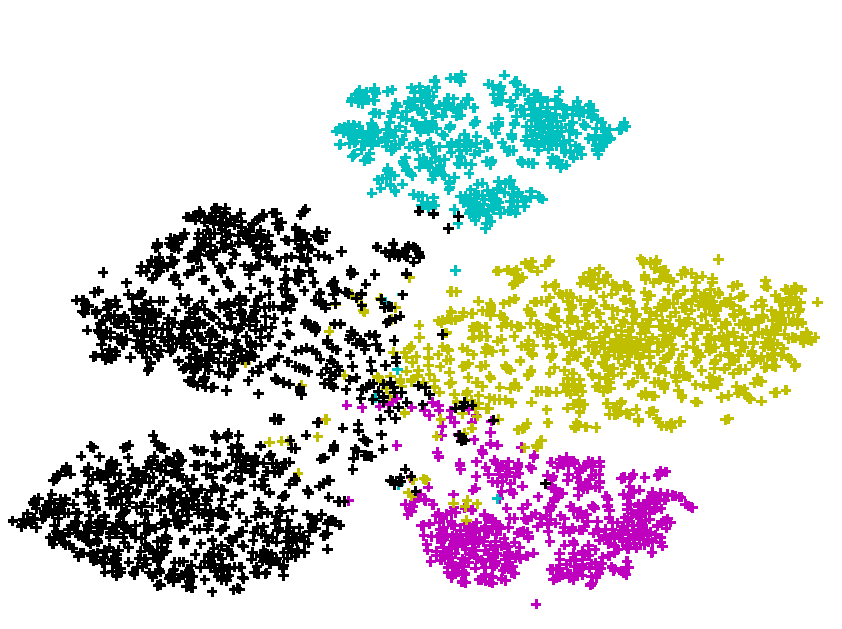
\includegraphics[width=\linewidth]{figure_1}
    \caption{}
    \label{fig:null}
  \end{subfigure}
%
  \begin{subfigure}[b]{0.27\linewidth}
    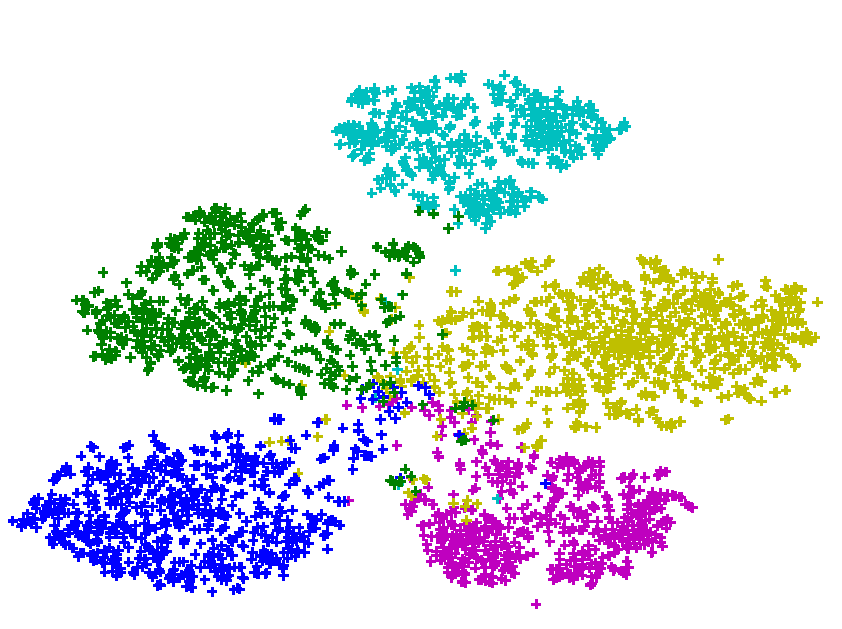
\includegraphics[width=\linewidth]{figure_1_true}
    \caption{}
% \caption{Points colored according to their ground truth labels}
    \label{fig:truth}
  \end{subfigure}
%
  \begin{subfigure}[b]{0.27\linewidth}
    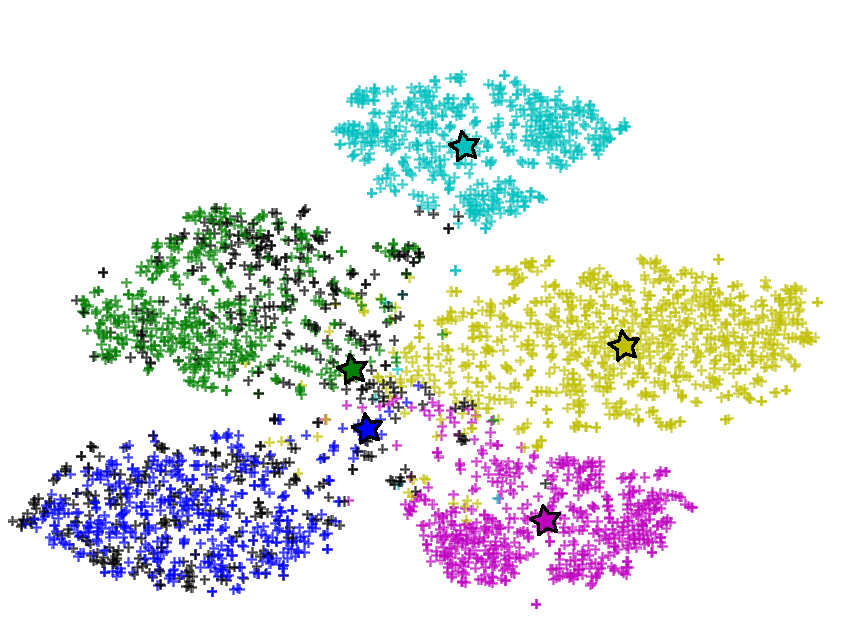
\includegraphics[width=\linewidth]{figure_2}
    % \caption{Signatures mapped to image spacing using Eq. \eqref{eq:dic} and denoted by stars. Then classification done using nearest neighbor}
    \caption{}
\label{fig:knn}
  \end{subfigure}
%
  \begin{subfigure}[b]{0.27\linewidth}
    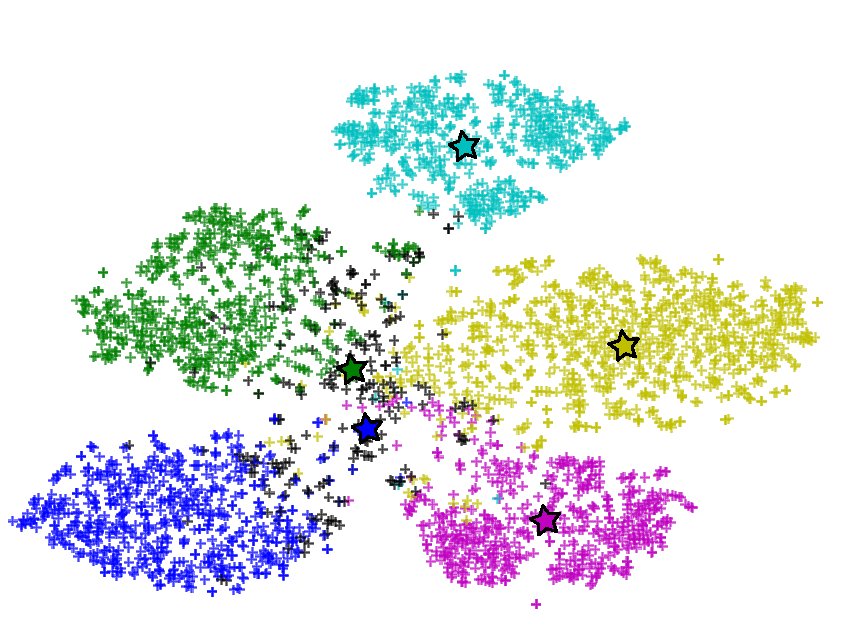
\includegraphics[width=\linewidth]{figure_3_kmeans}
    % \caption{Stars as previous. Classification done by our compatibility function on cluster assignments from k-means}
    \caption{}
\label{fig:kmeans}
  \end{subfigure}
%
  \begin{subfigure}[b]{0.27\linewidth}
    \label{fig:clustering}
    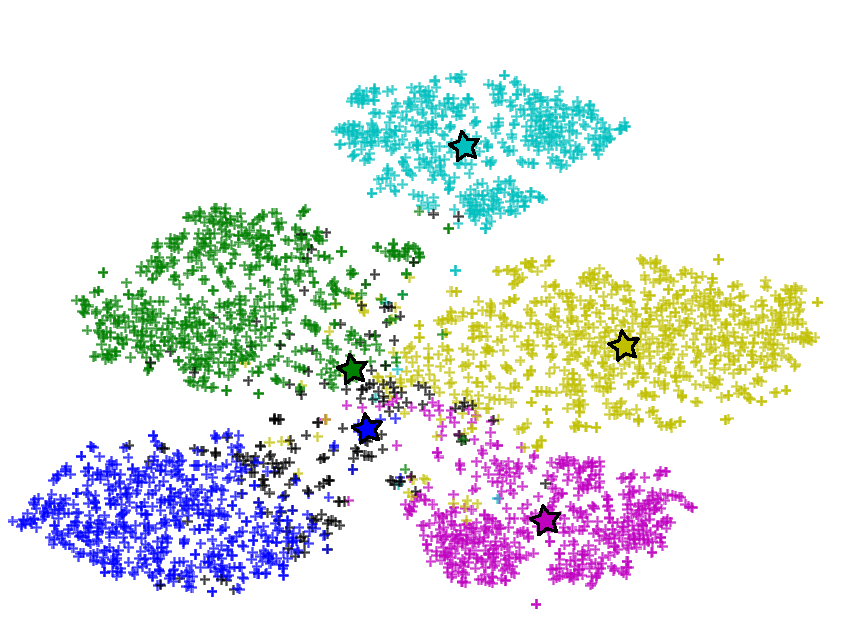
\includegraphics[width=\linewidth]{figure_3}
    \caption{}
% \caption{Stars as previous. Classification by our compatibility function using our supervised clustering}
  \end{subfigure}
%
  \begin{subfigure}[b]{0.27\linewidth}
    \label{fig:joint}
    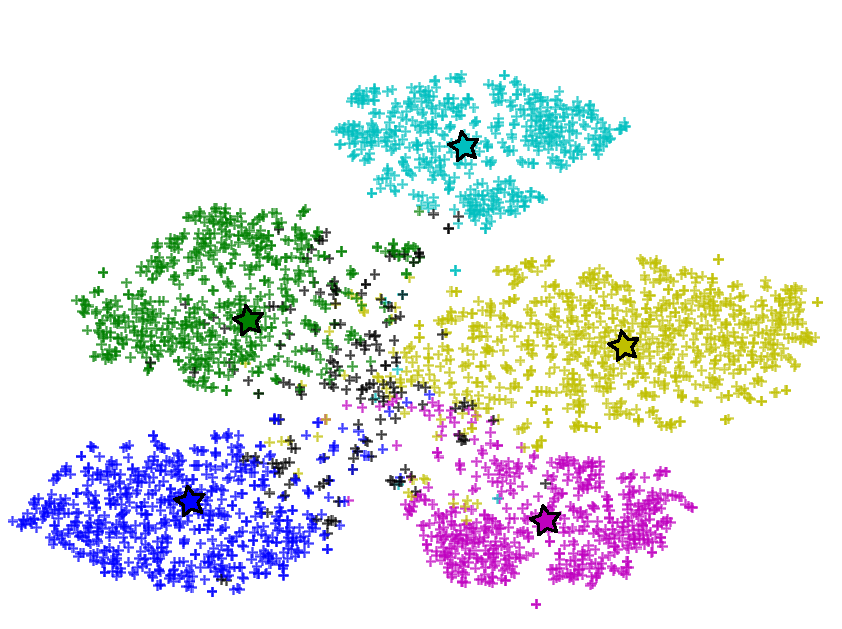
\includegraphics[width=\linewidth]{figure_4}
    \caption{}
% \caption{Class signatures mapped to image space (stars) and cluster assignment by JEaC}
  \end{subfigure}
  \caption{t-SNE embedding of five classes from AwA, three seen: antelope (magenta), grizzly bear (yellow), killer whale (cyan) and two
  unseen: chimpanzee (blue), giant panda (green). Images shown by plus signs and embedding of class signatures in images space by stars.
  in figures b-f black points denote assignment to a class other five classes shown here.
  \textbf{b)} Points colored according to their ground truth labels
  \textbf{c)} Signatures mapped to image spacing using Eq. \eqref{eq:dic}. Then classification done using nearest neighbor
  \textbf{d)} Classification done by our compatibility function on cluster assignments from k-means
  \textbf{e)} Classification by our compatibility function using our supervised clustering
  \textbf{f)} Class signatures mapping and cluster assignment by JEaC
  }
\end{figure*}

% We implemented our method using scikit-learn library \cite{scikit-learn} in Python.
% \footnote{Code is available at online :-?}
%  and used an Intel Core i5 CPU at 3.2 GHz to run the experiments.

\section{Conclusion} \label{conclusion}
In this paper, we proposed semi-supervised methods for zero-shot object recognition. We used the space of deep visual features as a semantic visual space and learned a linear transformation to map class signatures to this space such that the mapped signatures provide good representative of the corresponding instances. We utilized this property that the rich deep visual features provide a representation space in which samples of each class are usually condensed in a cluster. In the proposed method that jointly learns the mapping of class signatures and the class assignments of unlabeled data, we used also unlabeled instances of unseen classes when learning the mapping to alleviate the domain shift problem. Experimental results showed that the proposed method generally outperformed the other recent methods.
%\section*{Acknowledgement}
{\small
\bibliographystyle{ieee}
\bibliography{semi_suepervised_zsl_by_clustering.bib}
}

\end{document}
